\documentclass[twoside]{book}

% Packages required by doxygen
\usepackage{calc}
\usepackage{doxygen}
\usepackage{graphicx}
\usepackage[utf8]{inputenc}
\usepackage{makeidx}
\usepackage{multicol}
\usepackage{multirow}
\usepackage{textcomp}
\usepackage[table]{xcolor}

% NLS support packages
\usepackage[french]{babel}

% Font selection
\usepackage[T1]{fontenc}
\usepackage{mathptmx}
\usepackage[scaled=.90]{helvet}
\usepackage{courier}
\usepackage{amssymb}
\usepackage{sectsty}
\renewcommand{\familydefault}{\sfdefault}
\allsectionsfont{%
  \fontseries{bc}\selectfont%
  \color{darkgray}%
}
\renewcommand{\DoxyLabelFont}{%
  \fontseries{bc}\selectfont%
  \color{darkgray}%
}

% Page & text layout
\usepackage{geometry}
\geometry{%
  a4paper,%
  top=2.5cm,%
  bottom=2.5cm,%
  left=2.5cm,%
  right=2.5cm%
}
\tolerance=750
\hfuzz=15pt
\hbadness=750
\setlength{\emergencystretch}{15pt}
\setlength{\parindent}{0cm}
\setlength{\parskip}{0.2cm}
\makeatletter
\renewcommand{\paragraph}{%
  \@startsection{paragraph}{4}{0ex}{-1.0ex}{1.0ex}{%
    \normalfont\normalsize\bfseries\SS@parafont%
  }%
}
\renewcommand{\subparagraph}{%
  \@startsection{subparagraph}{5}{0ex}{-1.0ex}{1.0ex}{%
    \normalfont\normalsize\bfseries\SS@subparafont%
  }%
}
\makeatother

% Headers & footers
\usepackage{fancyhdr}
\pagestyle{fancyplain}
\fancyhead[LE]{\fancyplain{}{\bfseries\thepage}}
\fancyhead[CE]{\fancyplain{}{}}
\fancyhead[RE]{\fancyplain{}{\bfseries\leftmark}}
\fancyhead[LO]{\fancyplain{}{\bfseries\rightmark}}
\fancyhead[CO]{\fancyplain{}{}}
\fancyhead[RO]{\fancyplain{}{\bfseries\thepage}}
\fancyfoot[LE]{\fancyplain{}{}}
\fancyfoot[CE]{\fancyplain{}{}}
\fancyfoot[RE]{\fancyplain{}{\bfseries\scriptsize Généré le Jeudi Juin 20 2013 23:37:28 pour PreCheck par Doxygen }}
\fancyfoot[LO]{\fancyplain{}{\bfseries\scriptsize Généré le Jeudi Juin 20 2013 23:37:28 pour PreCheck par Doxygen }}
\fancyfoot[CO]{\fancyplain{}{}}
\fancyfoot[RO]{\fancyplain{}{}}
\renewcommand{\footrulewidth}{0.4pt}
\renewcommand{\chaptermark}[1]{%
  \markboth{#1}{}%
}
\renewcommand{\sectionmark}[1]{%
  \markright{\thesection\ #1}%
}

% Indices & bibliography
\usepackage{natbib}
\usepackage[titles]{tocloft}
\setcounter{tocdepth}{3}
\setcounter{secnumdepth}{5}
\makeindex

% Hyperlinks (required, but should be loaded last)
\usepackage{ifpdf}
\ifpdf
  \usepackage[pdftex,pagebackref=true]{hyperref}
\else
  \usepackage[ps2pdf,pagebackref=true]{hyperref}
\fi
\hypersetup{%
  colorlinks=true,%
  linkcolor=blue,%
  citecolor=blue,%
  unicode%
}

% Custom commands
\newcommand{\clearemptydoublepage}{%
  \newpage{\pagestyle{empty}\cleardoublepage}%
}


%===== C O N T E N T S =====

\begin{document}

% Titlepage & ToC
\hypersetup{pageanchor=false}
\pagenumbering{roman}
\begin{titlepage}
\vspace*{7cm}
\begin{center}%
{\Large Pre\-Check \\[1ex]\large 0.\-3 }\\
\vspace*{1cm}
{\large Généré par Doxygen 1.8.4}\\
\vspace*{0.5cm}
{\small Jeudi Juin 20 2013 23:37:28}\\
\end{center}
\end{titlepage}
\clearemptydoublepage
\tableofcontents
\clearemptydoublepage
\pagenumbering{arabic}
\hypersetup{pageanchor=true}

%--- Begin generated contents ---
\chapter{Index des espaces de nommage}
\section{Liste des espaces de nommage}
Liste de tous les espaces de nommage avec une brève description\-:\begin{DoxyCompactList}
\item\contentsline{section}{\hyperlink{namespaceSimpleHotel}{Simple\-Hotel} }{\pageref{namespaceSimpleHotel}}{}
\end{DoxyCompactList}

\chapter{Index hiérarchique}
\section{Hiérarchie des classes}
Cette liste d'héritage est classée approximativement par ordre alphabétique \-:\begin{DoxyCompactList}
\item \contentsline{section}{Application\-Window}{\pageref{classApplicationWindow}}{}
\begin{DoxyCompactList}
\item \contentsline{section}{S\-H\-\_\-app}{\pageref{classSH__app}}{}
\end{DoxyCompactList}
\item \contentsline{section}{Button}{\pageref{classButton}}{}
\begin{DoxyCompactList}
\item \contentsline{section}{S\-H\-\_\-\-Data\-Delegate}{\pageref{classSH__DataDelegate}}{}
\begin{DoxyCompactList}
\item \contentsline{section}{S\-H\-\_\-\-Billings\-Delegate}{\pageref{classSH__BillingsDelegate}}{}
\item \contentsline{section}{S\-H\-\_\-\-Bookings\-Delegate}{\pageref{classSH__BookingsDelegate}}{}
\item \contentsline{section}{S\-H\-\_\-\-Rooms\-Delegate}{\pageref{classSH__RoomsDelegate}}{}
\item \contentsline{section}{S\-H\-\_\-\-Services\-Delegate}{\pageref{classSH__ServicesDelegate}}{}
\item \contentsline{section}{S\-H\-\_\-\-V\-A\-T\-Delegate}{\pageref{classSH__VATDelegate}}{}
\end{DoxyCompactList}
\end{DoxyCompactList}
\item \contentsline{section}{Focus\-Scope}{\pageref{classFocusScope}}{}
\begin{DoxyCompactList}
\item \contentsline{section}{S\-H\-\_\-\-Tri\-State\-Check\-Image}{\pageref{classSH__TriStateCheckImage}}{}
\end{DoxyCompactList}
\item \contentsline{section}{Grid\-Layout}{\pageref{classGridLayout}}{}
\begin{DoxyCompactList}
\item \contentsline{section}{S\-H\-\_\-\-Content\-View}{\pageref{classSH__ContentView}}{}
\item \contentsline{section}{S\-H\-\_\-\-Header\-View}{\pageref{classSH__HeaderView}}{}
\item \contentsline{section}{S\-H\-\_\-\-Keyboard}{\pageref{classSH__Keyboard}}{}
\end{DoxyCompactList}
\item \contentsline{section}{Item}{\pageref{classItem}}{}
\begin{DoxyCompactList}
\item \contentsline{section}{S\-H\-\_\-\-Common\-Page}{\pageref{classSH__CommonPage}}{}
\item \contentsline{section}{S\-H\-\_\-\-Connexion\-Page}{\pageref{classSH__ConnexionPage}}{}
\item \contentsline{section}{S\-H\-\_\-\-Welcome\-Page}{\pageref{classSH__WelcomePage}}{}
\end{DoxyCompactList}
\item \contentsline{section}{Q\-Abstract\-List\-Model}{\pageref{classQAbstractListModel}}{}
\begin{DoxyCompactList}
\item \contentsline{section}{S\-H\-\_\-\-Sql\-Data\-Model}{\pageref{classSH__SqlDataModel}}{}
\end{DoxyCompactList}
\item \contentsline{section}{Q\-Object}{\pageref{classQObject}}{}
\begin{DoxyCompactList}
\item \contentsline{section}{S\-H\-\_\-\-Application\-Core}{\pageref{classSH__ApplicationCore}}{}
\item \contentsline{section}{S\-H\-\_\-\-Company}{\pageref{classSH__Company}}{}
\item \contentsline{section}{S\-H\-\_\-\-Database\-Manager}{\pageref{classSH__DatabaseManager}}{}
\item \contentsline{section}{S\-H\-\_\-\-Extended\-Q\-Qml\-Action}{\pageref{classSH__ExtendedQQmlAction}}{}
\item \contentsline{section}{S\-H\-\_\-\-Message\-Manager}{\pageref{classSH__MessageManager}}{}
\item \contentsline{section}{S\-H\-\_\-\-User}{\pageref{classSH__User}}{}
\begin{DoxyCompactList}
\item \contentsline{section}{S\-H\-\_\-\-Trainee}{\pageref{classSH__Trainee}}{}
\end{DoxyCompactList}
\end{DoxyCompactList}
\item \contentsline{section}{Q\-Quick\-Item}{\pageref{classQQuickItem}}{}
\begin{DoxyCompactList}
\item \contentsline{section}{S\-H\-\_\-\-Sql\-Data\-Fields}{\pageref{classSH__SqlDataFields}}{}
\end{DoxyCompactList}
\item \contentsline{section}{Q\-Sort\-Filter\-Proxy\-Model}{\pageref{classQSortFilterProxyModel}}{}
\begin{DoxyCompactList}
\item \contentsline{section}{S\-H\-\_\-\-Extended\-Proxy\-Model}{\pageref{classSH__ExtendedProxyModel}}{}
\begin{DoxyCompactList}
\item \contentsline{section}{S\-H\-\_\-\-Billings\-Table\-Model}{\pageref{classSH__BillingsTableModel}}{}
\item \contentsline{section}{S\-H\-\_\-\-Bills\-Table\-Model}{\pageref{classSH__BillsTableModel}}{}
\item \contentsline{section}{S\-H\-\_\-\-Bookings\-Table\-Model}{\pageref{classSH__BookingsTableModel}}{}
\item \contentsline{section}{S\-H\-\_\-\-Clients\-Table\-Model}{\pageref{classSH__ClientsTableModel}}{}
\item \contentsline{section}{S\-H\-\_\-\-Groups\-Table\-Model}{\pageref{classSH__GroupsTableModel}}{}
\item \contentsline{section}{S\-H\-\_\-\-Rooms\-Table\-Model}{\pageref{classSH__RoomsTableModel}}{}
\item \contentsline{section}{S\-H\-\_\-\-Services\-Table\-Model}{\pageref{classSH__ServicesTableModel}}{}
\item \contentsline{section}{S\-H\-\_\-\-Trainees\-Table\-Model}{\pageref{classSH__TraineesTableModel}}{}
\item \contentsline{section}{S\-H\-\_\-\-Users\-Table\-Model}{\pageref{classSH__UsersTableModel}}{}
\item \contentsline{section}{S\-H\-\_\-\-V\-A\-T\-Table\-Model}{\pageref{classSH__VATTableModel}}{}
\end{DoxyCompactList}
\end{DoxyCompactList}
\item \contentsline{section}{Q\-State}{\pageref{classQState}}{}
\begin{DoxyCompactList}
\item \contentsline{section}{S\-H\-\_\-\-Generic\-State}{\pageref{classSH__GenericState}}{}
\begin{DoxyCompactList}
\item \contentsline{section}{S\-H\-\_\-\-Adapt\-Database\-State}{\pageref{classSH__AdaptDatabaseState}}{}
\item \contentsline{section}{S\-H\-\_\-\-In\-Out\-State}{\pageref{classSH__InOutState}}{}
\begin{DoxyCompactList}
\item \contentsline{section}{S\-H\-\_\-\-File\-Selection\-State}{\pageref{classSH__FileSelectionState}}{}
\item \contentsline{section}{S\-H\-\_\-\-Question\-State}{\pageref{classSH__QuestionState}}{}
\begin{DoxyCompactList}
\item \contentsline{section}{S\-H\-\_\-\-Database\-Content\-Question\-State}{\pageref{classSH__DatabaseContentQuestionState}}{}
\item \contentsline{section}{S\-H\-\_\-\-Date\-Question\-State}{\pageref{classSH__DateQuestionState}}{}
\item \contentsline{section}{S\-H\-\_\-\-Decimal\-Question\-State}{\pageref{classSH__DecimalQuestionState}}{}
\item \contentsline{section}{S\-H\-\_\-\-Numeric\-Question\-State}{\pageref{classSH__NumericQuestionState}}{}
\item \contentsline{section}{S\-H\-\_\-\-String\-Question\-State}{\pageref{classSH__StringQuestionState}}{}
\begin{DoxyCompactList}
\item \contentsline{section}{S\-H\-\_\-\-Reg\-Exp\-Question\-State}{\pageref{classSH__RegExpQuestionState}}{}
\end{DoxyCompactList}
\end{DoxyCompactList}
\item \contentsline{section}{S\-H\-\_\-\-Statement\-State}{\pageref{classSH__StatementState}}{}
\begin{DoxyCompactList}
\item \contentsline{section}{S\-H\-\_\-\-Confirmation\-State}{\pageref{classSH__ConfirmationState}}{}
\begin{DoxyCompactList}
\item \contentsline{section}{S\-H\-\_\-\-Validation\-State}{\pageref{classSH__ValidationState}}{}
\end{DoxyCompactList}
\end{DoxyCompactList}
\end{DoxyCompactList}
\item \contentsline{section}{S\-H\-\_\-\-Printing\-State}{\pageref{classSH__PrintingState}}{}
\end{DoxyCompactList}
\end{DoxyCompactList}
\item \contentsline{section}{Q\-State\-Machine}{\pageref{classQStateMachine}}{}
\begin{DoxyCompactList}
\item \contentsline{section}{S\-H\-\_\-\-Generic\-State\-Machine}{\pageref{classSH__GenericStateMachine}}{}
\begin{DoxyCompactList}
\item \contentsline{section}{S\-H\-\_\-\-In\-Out\-State\-Machine}{\pageref{classSH__InOutStateMachine}}{}
\begin{DoxyCompactList}
\item \contentsline{section}{S\-H\-\_\-\-Address\-Creation\-State\-Machine}{\pageref{classSH__AddressCreationStateMachine}}{}
\item \contentsline{section}{S\-H\-\_\-\-Billing\-Creation\-State\-Machine}{\pageref{classSH__BillingCreationStateMachine}}{}
\item \contentsline{section}{S\-H\-\_\-\-Client\-Creation\-State\-Machine}{\pageref{classSH__ClientCreationStateMachine}}{}
\item \contentsline{section}{S\-H\-\_\-\-Looping\-In\-Out\-State\-Machine}{\pageref{classSH__LoopingInOutStateMachine}}{}
\begin{DoxyCompactList}
\item \contentsline{section}{S\-H\-\_\-\-Service\-Charging}{\pageref{classSH__ServiceCharging}}{}
\end{DoxyCompactList}
\end{DoxyCompactList}
\end{DoxyCompactList}
\end{DoxyCompactList}
\item \contentsline{section}{Rectangle}{\pageref{classRectangle}}{}
\begin{DoxyCompactList}
\item \contentsline{section}{S\-H\-\_\-\-Calendar\-Dialog}{\pageref{classSH__CalendarDialog}}{}
\item \contentsline{section}{S\-H\-\_\-\-Output\-Zone}{\pageref{classSH__OutputZone}}{}
\item \contentsline{section}{S\-H\-\_\-\-Rooms\-Sections\-Delegate}{\pageref{classSH__RoomsSectionsDelegate}}{}
\item \contentsline{section}{S\-H\-\_\-\-Sql\-Data\-View}{\pageref{classSH__SqlDataView}}{}
\end{DoxyCompactList}
\item \contentsline{section}{S\-H\-\_\-\-Adapt\-Database}{\pageref{namespace_3globalScope_4}}{}
\item \contentsline{section}{S\-H\-\_\-\-Checkable\-Sort\-Filter\-Proxy\-Mode}{\pageref{namespace_3globalScope_4}}{}
\item \contentsline{section}{S\-H\-\_\-\-I\-O\-State}{\pageref{namespace_3globalScope_4}}{}
\item \contentsline{section}{S\-H\-\_\-\-I\-O\-State\-Machine}{\pageref{namespace_3globalScope_4}}{}
\item \contentsline{section}{S\-H\-\_\-\-Looping\-State\-Machine}{\pageref{namespace_3globalScope_4}}{}
\item \contentsline{section}{S\-H\-\_\-\-Named\-Object}{\pageref{classSH__NamedObject}}{}
\begin{DoxyCompactList}
\item \contentsline{section}{S\-H\-\_\-\-Generic\-State}{\pageref{classSH__GenericState}}{}
\item \contentsline{section}{S\-H\-\_\-\-Generic\-State\-Machine}{\pageref{classSH__GenericStateMachine}}{}
\end{DoxyCompactList}
\item \contentsline{section}{S\-H\-\_\-\-Q\-Q\-Quick\-Action}{\pageref{namespace_3globalScope_4}}{}
\item \contentsline{section}{S\-H\-\_\-\-S\-H\-\_\-\-Database\-Manager}{\pageref{namespace_3globalScope_4}}{}
\item \contentsline{section}{Table\-View}{\pageref{classTableView}}{}
\begin{DoxyCompactList}
\item \contentsline{section}{S\-H\-\_\-\-Sql\-Table\-View}{\pageref{classSH__SqlTableView}}{}
\end{DoxyCompactList}
\item \contentsline{section}{Tab\-View}{\pageref{classTabView}}{}
\begin{DoxyCompactList}
\item \contentsline{section}{S\-H\-\_\-\-Tab\-Zone}{\pageref{classSH__TabZone}}{}
\end{DoxyCompactList}
\end{DoxyCompactList}

\chapter{Index des classes}
\section{Liste des classes}
Liste des classes, structures, unions et interfaces avec une brève description \-:\begin{DoxyCompactList}
\item\contentsline{section}{\hyperlink{classApplicationWindow}{Application\-Window} }{\pageref{classApplicationWindow}}{}
\item\contentsline{section}{\hyperlink{classButton}{Button} }{\pageref{classButton}}{}
\item\contentsline{section}{\hyperlink{classFocusScope}{Focus\-Scope} }{\pageref{classFocusScope}}{}
\item\contentsline{section}{\hyperlink{classGridLayout}{Grid\-Layout} }{\pageref{classGridLayout}}{}
\item\contentsline{section}{\hyperlink{classItem}{Item} }{\pageref{classItem}}{}
\item\contentsline{section}{\hyperlink{classQAbstractListModel}{Q\-Abstract\-List\-Model} }{\pageref{classQAbstractListModel}}{}
\item\contentsline{section}{\hyperlink{classQObject}{Q\-Object} }{\pageref{classQObject}}{}
\item\contentsline{section}{\hyperlink{classQQuickItem}{Q\-Quick\-Item} }{\pageref{classQQuickItem}}{}
\item\contentsline{section}{\hyperlink{classQSortFilterProxyModel}{Q\-Sort\-Filter\-Proxy\-Model} }{\pageref{classQSortFilterProxyModel}}{}
\item\contentsline{section}{\hyperlink{classQState}{Q\-State} }{\pageref{classQState}}{}
\item\contentsline{section}{\hyperlink{classQStateMachine}{Q\-State\-Machine} }{\pageref{classQStateMachine}}{}
\item\contentsline{section}{\hyperlink{classRectangle}{Rectangle} }{\pageref{classRectangle}}{}
\item\contentsline{section}{\hyperlink{classSH__AdaptDatabaseState}{S\-H\-\_\-\-Adapt\-Database\-State} }{\pageref{classSH__AdaptDatabaseState}}{}
\item\contentsline{section}{\hyperlink{classSH__AddressCreationStateMachine}{S\-H\-\_\-\-Address\-Creation\-State\-Machine} \\*The \hyperlink{classSH__AddressCreationStateMachine}{S\-H\-\_\-\-Address\-Creation\-State\-Machine} class }{\pageref{classSH__AddressCreationStateMachine}}{}
\item\contentsline{section}{\hyperlink{classSH__app}{S\-H\-\_\-app} }{\pageref{classSH__app}}{}
\item\contentsline{section}{\hyperlink{classSH__ApplicationCore}{S\-H\-\_\-\-Application\-Core} \\*Classe principale du coeur de l'application, avec laquelle communique l'interface graphique }{\pageref{classSH__ApplicationCore}}{}
\item\contentsline{section}{\hyperlink{classSH__BillingCreationStateMachine}{S\-H\-\_\-\-Billing\-Creation\-State\-Machine} \\*The \hyperlink{classSH__BillingCreationStateMachine}{S\-H\-\_\-\-Billing\-Creation\-State\-Machine} class }{\pageref{classSH__BillingCreationStateMachine}}{}
\item\contentsline{section}{\hyperlink{classSH__BillingsDelegate}{S\-H\-\_\-\-Billings\-Delegate} }{\pageref{classSH__BillingsDelegate}}{}
\item\contentsline{section}{\hyperlink{classSH__BillingsTableModel}{S\-H\-\_\-\-Billings\-Table\-Model} }{\pageref{classSH__BillingsTableModel}}{}
\item\contentsline{section}{\hyperlink{classSH__BillsTableModel}{S\-H\-\_\-\-Bills\-Table\-Model} }{\pageref{classSH__BillsTableModel}}{}
\item\contentsline{section}{\hyperlink{classSH__BookingsDelegate}{S\-H\-\_\-\-Bookings\-Delegate} }{\pageref{classSH__BookingsDelegate}}{}
\item\contentsline{section}{\hyperlink{classSH__BookingsTableModel}{S\-H\-\_\-\-Bookings\-Table\-Model} }{\pageref{classSH__BookingsTableModel}}{}
\item\contentsline{section}{\hyperlink{classSH__CalendarDialog}{S\-H\-\_\-\-Calendar\-Dialog} }{\pageref{classSH__CalendarDialog}}{}
\item\contentsline{section}{\hyperlink{classSH__ClientCreationStateMachine}{S\-H\-\_\-\-Client\-Creation\-State\-Machine} \\*The \hyperlink{classSH__ClientCreationStateMachine}{S\-H\-\_\-\-Client\-Creation\-State\-Machine} class }{\pageref{classSH__ClientCreationStateMachine}}{}
\item\contentsline{section}{\hyperlink{classSH__ClientsTableModel}{S\-H\-\_\-\-Clients\-Table\-Model} }{\pageref{classSH__ClientsTableModel}}{}
\item\contentsline{section}{\hyperlink{classSH__CommonPage}{S\-H\-\_\-\-Common\-Page} }{\pageref{classSH__CommonPage}}{}
\item\contentsline{section}{\hyperlink{classSH__Company}{S\-H\-\_\-\-Company} }{\pageref{classSH__Company}}{}
\item\contentsline{section}{\hyperlink{classSH__ConfirmationState}{S\-H\-\_\-\-Confirmation\-State} \\*La class Confirmation\-State représente un état dans lequel le système attend que l'utilisateur appuie sur une touche de confirmation }{\pageref{classSH__ConfirmationState}}{}
\item\contentsline{section}{\hyperlink{classSH__ConnexionPage}{S\-H\-\_\-\-Connexion\-Page} }{\pageref{classSH__ConnexionPage}}{}
\item\contentsline{section}{\hyperlink{classSH__ContentView}{S\-H\-\_\-\-Content\-View} }{\pageref{classSH__ContentView}}{}
\item\contentsline{section}{\hyperlink{classSH__DatabaseContentQuestionState}{S\-H\-\_\-\-Database\-Content\-Question\-State} }{\pageref{classSH__DatabaseContentQuestionState}}{}
\item\contentsline{section}{\hyperlink{classSH__DatabaseManager}{S\-H\-\_\-\-Database\-Manager} }{\pageref{classSH__DatabaseManager}}{}
\item\contentsline{section}{\hyperlink{classSH__DataDelegate}{S\-H\-\_\-\-Data\-Delegate} }{\pageref{classSH__DataDelegate}}{}
\item\contentsline{section}{\hyperlink{classSH__DateQuestionState}{S\-H\-\_\-\-Date\-Question\-State} }{\pageref{classSH__DateQuestionState}}{}
\item\contentsline{section}{\hyperlink{classSH__DecimalQuestionState}{S\-H\-\_\-\-Decimal\-Question\-State} }{\pageref{classSH__DecimalQuestionState}}{}
\item\contentsline{section}{\hyperlink{classSH__ExtendedProxyModel}{S\-H\-\_\-\-Extended\-Proxy\-Model} }{\pageref{classSH__ExtendedProxyModel}}{}
\item\contentsline{section}{\hyperlink{classSH__ExtendedQQmlAction}{S\-H\-\_\-\-Extended\-Q\-Qml\-Action} }{\pageref{classSH__ExtendedQQmlAction}}{}
\item\contentsline{section}{\hyperlink{classSH__FileSelectionState}{S\-H\-\_\-\-File\-Selection\-State} \\*The \hyperlink{classSH__FileSelectionState}{S\-H\-\_\-\-File\-Selection\-State} class }{\pageref{classSH__FileSelectionState}}{}
\item\contentsline{section}{\hyperlink{classSH__GenericState}{S\-H\-\_\-\-Generic\-State} }{\pageref{classSH__GenericState}}{}
\item\contentsline{section}{\hyperlink{classSH__GroupsTableModel}{S\-H\-\_\-\-Groups\-Table\-Model} }{\pageref{classSH__GroupsTableModel}}{}
\item\contentsline{section}{\hyperlink{classSH__HeaderView}{S\-H\-\_\-\-Header\-View} }{\pageref{classSH__HeaderView}}{}
\item\contentsline{section}{\hyperlink{classSH__InOutState}{S\-H\-\_\-\-In\-Out\-State} }{\pageref{classSH__InOutState}}{}
\item\contentsline{section}{\hyperlink{classSH__InOutStateMachine}{S\-H\-\_\-\-In\-Out\-State\-Machine} }{\pageref{classSH__InOutStateMachine}}{}
\item\contentsline{section}{\hyperlink{classSH__Keyboard}{S\-H\-\_\-\-Keyboard} }{\pageref{classSH__Keyboard}}{}
\item\contentsline{section}{\hyperlink{classSh__LoopingInOutStateMachine}{Sh\-\_\-\-Looping\-In\-Out\-State\-Machine} }{\pageref{classSh__LoopingInOutStateMachine}}{}
\item\contentsline{section}{\hyperlink{classSH__MessageManager}{S\-H\-\_\-\-Message\-Manager} }{\pageref{classSH__MessageManager}}{}
\item\contentsline{section}{\hyperlink{classSH__NamedObject}{S\-H\-\_\-\-Named\-Object} }{\pageref{classSH__NamedObject}}{}
\item\contentsline{section}{\hyperlink{classSH__NumericQuestionState}{S\-H\-\_\-\-Numeric\-Question\-State} }{\pageref{classSH__NumericQuestionState}}{}
\item\contentsline{section}{\hyperlink{classSH__OutputZone}{S\-H\-\_\-\-Output\-Zone} }{\pageref{classSH__OutputZone}}{}
\item\contentsline{section}{\hyperlink{classSH__PrintingState}{S\-H\-\_\-\-Printing\-State} }{\pageref{classSH__PrintingState}}{}
\item\contentsline{section}{\hyperlink{classSH__QuestionState}{S\-H\-\_\-\-Question\-State} }{\pageref{classSH__QuestionState}}{}
\item\contentsline{section}{\hyperlink{classSH__RegExpQuestionState}{S\-H\-\_\-\-Reg\-Exp\-Question\-State} \\*The \hyperlink{classSH__RegExpQuestionState}{S\-H\-\_\-\-Reg\-Exp\-Question\-State} class }{\pageref{classSH__RegExpQuestionState}}{}
\item\contentsline{section}{\hyperlink{classSH__RoomsDelegate}{S\-H\-\_\-\-Rooms\-Delegate} }{\pageref{classSH__RoomsDelegate}}{}
\item\contentsline{section}{\hyperlink{classSH__RoomsSectionsDelegate}{S\-H\-\_\-\-Rooms\-Sections\-Delegate} }{\pageref{classSH__RoomsSectionsDelegate}}{}
\item\contentsline{section}{\hyperlink{classSH__RoomsTableModel}{S\-H\-\_\-\-Rooms\-Table\-Model} }{\pageref{classSH__RoomsTableModel}}{}
\item\contentsline{section}{\hyperlink{classSH__ServiceCharging}{S\-H\-\_\-\-Service\-Charging} \\*The \hyperlink{classSH__ServiceCharging}{S\-H\-\_\-\-Service\-Charging} class }{\pageref{classSH__ServiceCharging}}{}
\item\contentsline{section}{\hyperlink{classSH__ServicesDelegate}{S\-H\-\_\-\-Services\-Delegate} }{\pageref{classSH__ServicesDelegate}}{}
\item\contentsline{section}{\hyperlink{classSH__ServicesTableModel}{S\-H\-\_\-\-Services\-Table\-Model} }{\pageref{classSH__ServicesTableModel}}{}
\item\contentsline{section}{\hyperlink{classSH__SqlDataFields}{S\-H\-\_\-\-Sql\-Data\-Fields} }{\pageref{classSH__SqlDataFields}}{}
\item\contentsline{section}{\hyperlink{classSH__SqlDataModel}{S\-H\-\_\-\-Sql\-Data\-Model} }{\pageref{classSH__SqlDataModel}}{}
\item\contentsline{section}{\hyperlink{classSH__SqlDataView}{S\-H\-\_\-\-Sql\-Data\-View} }{\pageref{classSH__SqlDataView}}{}
\item\contentsline{section}{\hyperlink{classSH__SqlTableView}{S\-H\-\_\-\-Sql\-Table\-View} }{\pageref{classSH__SqlTableView}}{}
\item\contentsline{section}{\hyperlink{classSH__StatementState}{S\-H\-\_\-\-Statement\-State} }{\pageref{classSH__StatementState}}{}
\item\contentsline{section}{\hyperlink{classSH__StringQuestionState}{S\-H\-\_\-\-String\-Question\-State} }{\pageref{classSH__StringQuestionState}}{}
\item\contentsline{section}{\hyperlink{classSH__TabZone}{S\-H\-\_\-\-Tab\-Zone} }{\pageref{classSH__TabZone}}{}
\item\contentsline{section}{\hyperlink{classSH__Trainee}{S\-H\-\_\-\-Trainee} }{\pageref{classSH__Trainee}}{}
\item\contentsline{section}{\hyperlink{classSH__TriStateCheckImage}{S\-H\-\_\-\-Tri\-State\-Check\-Image} }{\pageref{classSH__TriStateCheckImage}}{}
\item\contentsline{section}{\hyperlink{classSH__User}{S\-H\-\_\-\-User} }{\pageref{classSH__User}}{}
\item\contentsline{section}{\hyperlink{classSH__ValidationState}{S\-H\-\_\-\-Validation\-State} }{\pageref{classSH__ValidationState}}{}
\item\contentsline{section}{\hyperlink{classSH__WelcomePage}{S\-H\-\_\-\-Welcome\-Page} }{\pageref{classSH__WelcomePage}}{}
\item\contentsline{section}{\hyperlink{classTableView}{Table\-View} }{\pageref{classTableView}}{}
\item\contentsline{section}{\hyperlink{classTabView}{Tab\-View} }{\pageref{classTabView}}{}
\end{DoxyCompactList}

\chapter{Index des fichiers}
\section{Liste des fichiers}
Liste de tous les fichiers avec une brève description \-:\begin{DoxyCompactList}
\item\contentsline{section}{\hyperlink{main_8cpp}{main.\-cpp} }{\pageref{main_8cpp}}{}
\item\contentsline{section}{\hyperlink{SH__ApplicationCore_8cpp}{S\-H\-\_\-\-Application\-Core.\-cpp} }{\pageref{SH__ApplicationCore_8cpp}}{}
\item\contentsline{section}{\hyperlink{SH__ApplicationCore_8h}{S\-H\-\_\-\-Application\-Core.\-h} }{\pageref{SH__ApplicationCore_8h}}{}
\item\contentsline{section}{\hyperlink{SH__DatabaseManager_8cpp}{S\-H\-\_\-\-Database\-Manager.\-cpp} }{\pageref{SH__DatabaseManager_8cpp}}{}
\item\contentsline{section}{\hyperlink{SH__DatabaseManager_8h}{S\-H\-\_\-\-Database\-Manager.\-h} }{\pageref{SH__DatabaseManager_8h}}{}
\item\contentsline{section}{\hyperlink{SH__MessageManager_8cpp}{S\-H\-\_\-\-Message\-Manager.\-cpp} }{\pageref{SH__MessageManager_8cpp}}{}
\item\contentsline{section}{\hyperlink{SH__MessageManager_8h}{S\-H\-\_\-\-Message\-Manager.\-h} }{\pageref{SH__MessageManager_8h}}{}
\item\contentsline{section}{logging/\hyperlink{examplemain_8cpp}{examplemain.\-cpp} }{\pageref{examplemain_8cpp}}{}
\item\contentsline{section}{logging/\hyperlink{QsLog_8cpp}{Qs\-Log.\-cpp} }{\pageref{QsLog_8cpp}}{}
\item\contentsline{section}{logging/\hyperlink{QsLog_8h}{Qs\-Log.\-h} }{\pageref{QsLog_8h}}{}
\item\contentsline{section}{logging/\hyperlink{QsLogDest_8cpp}{Qs\-Log\-Dest.\-cpp} }{\pageref{QsLogDest_8cpp}}{}
\item\contentsline{section}{logging/\hyperlink{QsLogDest_8h}{Qs\-Log\-Dest.\-h} }{\pageref{QsLogDest_8h}}{}
\item\contentsline{section}{logging/\hyperlink{QsLogDestConsole_8cpp}{Qs\-Log\-Dest\-Console.\-cpp} }{\pageref{QsLogDestConsole_8cpp}}{}
\item\contentsline{section}{logging/\hyperlink{QsLogDestConsole_8h}{Qs\-Log\-Dest\-Console.\-h} }{\pageref{QsLogDestConsole_8h}}{}
\item\contentsline{section}{logging/\hyperlink{QsLogDestFile_8cpp}{Qs\-Log\-Dest\-File.\-cpp} }{\pageref{QsLogDestFile_8cpp}}{}
\item\contentsline{section}{logging/\hyperlink{QsLogDestFile_8h}{Qs\-Log\-Dest\-File.\-h} }{\pageref{QsLogDestFile_8h}}{}
\item\contentsline{section}{logging/\hyperlink{QsLogDisableForThisFile_8h}{Qs\-Log\-Disable\-For\-This\-File.\-h} }{\pageref{QsLogDisableForThisFile_8h}}{}
\item\contentsline{section}{logging/\hyperlink{QsLogLevel_8h}{Qs\-Log\-Level.\-h} }{\pageref{QsLogLevel_8h}}{}
\item\contentsline{section}{logic/\hyperlink{SH__AdaptDatabaseState_8cpp}{S\-H\-\_\-\-Adapt\-Database\-State.\-cpp} }{\pageref{SH__AdaptDatabaseState_8cpp}}{}
\item\contentsline{section}{logic/\hyperlink{SH__AdaptDatabaseState_8h}{S\-H\-\_\-\-Adapt\-Database\-State.\-h} }{\pageref{SH__AdaptDatabaseState_8h}}{}
\item\contentsline{section}{logic/\hyperlink{SH__AddressCreation_8cpp}{S\-H\-\_\-\-Address\-Creation.\-cpp} }{\pageref{SH__AddressCreation_8cpp}}{}
\item\contentsline{section}{logic/\hyperlink{SH__AddressCreation_8h}{S\-H\-\_\-\-Address\-Creation.\-h} }{\pageref{SH__AddressCreation_8h}}{}
\item\contentsline{section}{logic/\hyperlink{SH__BillingCreation_8cpp}{S\-H\-\_\-\-Billing\-Creation.\-cpp} }{\pageref{SH__BillingCreation_8cpp}}{}
\item\contentsline{section}{logic/\hyperlink{SH__BillingCreation_8h}{S\-H\-\_\-\-Billing\-Creation.\-h} }{\pageref{SH__BillingCreation_8h}}{}
\item\contentsline{section}{logic/\hyperlink{SH__ClientCreation_8cpp}{S\-H\-\_\-\-Client\-Creation.\-cpp} }{\pageref{SH__ClientCreation_8cpp}}{}
\item\contentsline{section}{logic/\hyperlink{SH__ClientCreation_8h}{S\-H\-\_\-\-Client\-Creation.\-h} }{\pageref{SH__ClientCreation_8h}}{}
\item\contentsline{section}{logic/\hyperlink{SH__ConfirmationState_8cpp}{S\-H\-\_\-\-Confirmation\-State.\-cpp} }{\pageref{SH__ConfirmationState_8cpp}}{}
\item\contentsline{section}{logic/\hyperlink{SH__ConfirmationState_8h}{S\-H\-\_\-\-Confirmation\-State.\-h} }{\pageref{SH__ConfirmationState_8h}}{}
\item\contentsline{section}{logic/\hyperlink{SH__DatabaseContentQuestionState_8cpp}{S\-H\-\_\-\-Database\-Content\-Question\-State.\-cpp} }{\pageref{SH__DatabaseContentQuestionState_8cpp}}{}
\item\contentsline{section}{logic/\hyperlink{SH__DatabaseContentQuestionState_8h}{S\-H\-\_\-\-Database\-Content\-Question\-State.\-h} }{\pageref{SH__DatabaseContentQuestionState_8h}}{}
\item\contentsline{section}{logic/\hyperlink{SH__DateQuestionState_8cpp}{S\-H\-\_\-\-Date\-Question\-State.\-cpp} }{\pageref{SH__DateQuestionState_8cpp}}{}
\item\contentsline{section}{logic/\hyperlink{SH__DateQuestionState_8h}{S\-H\-\_\-\-Date\-Question\-State.\-h} }{\pageref{SH__DateQuestionState_8h}}{}
\item\contentsline{section}{logic/\hyperlink{SH__DecimalQuestionState_8cpp}{S\-H\-\_\-\-Decimal\-Question\-State.\-cpp} }{\pageref{SH__DecimalQuestionState_8cpp}}{}
\item\contentsline{section}{logic/\hyperlink{SH__DecimalQuestionState_8h}{S\-H\-\_\-\-Decimal\-Question\-State.\-h} }{\pageref{SH__DecimalQuestionState_8h}}{}
\item\contentsline{section}{logic/\hyperlink{SH__FileSelectionState_8cpp}{S\-H\-\_\-\-File\-Selection\-State.\-cpp} }{\pageref{SH__FileSelectionState_8cpp}}{}
\item\contentsline{section}{logic/\hyperlink{SH__FileSelectionState_8h}{S\-H\-\_\-\-File\-Selection\-State.\-h} }{\pageref{SH__FileSelectionState_8h}}{}
\item\contentsline{section}{logic/\hyperlink{SH__GenericDebugableState_8cpp}{S\-H\-\_\-\-Generic\-Debugable\-State.\-cpp} }{\pageref{SH__GenericDebugableState_8cpp}}{}
\item\contentsline{section}{logic/\hyperlink{SH__GenericDebugableState_8h}{S\-H\-\_\-\-Generic\-Debugable\-State.\-h} }{\pageref{SH__GenericDebugableState_8h}}{}
\item\contentsline{section}{logic/\hyperlink{SH__IOState_8cpp}{S\-H\-\_\-\-I\-O\-State.\-cpp} }{\pageref{SH__IOState_8cpp}}{}
\item\contentsline{section}{logic/\hyperlink{SH__IOState_8h}{S\-H\-\_\-\-I\-O\-State.\-h} }{\pageref{SH__IOState_8h}}{}
\item\contentsline{section}{logic/\hyperlink{SH__IOStateMachine_8cpp}{S\-H\-\_\-\-I\-O\-State\-Machine.\-cpp} }{\pageref{SH__IOStateMachine_8cpp}}{}
\item\contentsline{section}{logic/\hyperlink{SH__IOStateMachine_8h}{S\-H\-\_\-\-I\-O\-State\-Machine.\-h} }{\pageref{SH__IOStateMachine_8h}}{}
\item\contentsline{section}{logic/\hyperlink{SH__LoopingIOStateMachine_8cpp}{S\-H\-\_\-\-Looping\-I\-O\-State\-Machine.\-cpp} }{\pageref{SH__LoopingIOStateMachine_8cpp}}{}
\item\contentsline{section}{logic/\hyperlink{SH__LoopingIOStateMachine_8h}{S\-H\-\_\-\-Looping\-I\-O\-State\-Machine.\-h} }{\pageref{SH__LoopingIOStateMachine_8h}}{}
\item\contentsline{section}{logic/\hyperlink{SH__NamedObject_8cpp}{S\-H\-\_\-\-Named\-Object.\-cpp} }{\pageref{SH__NamedObject_8cpp}}{}
\item\contentsline{section}{logic/\hyperlink{SH__NamedObject_8h}{S\-H\-\_\-\-Named\-Object.\-h} }{\pageref{SH__NamedObject_8h}}{}
\item\contentsline{section}{logic/\hyperlink{SH__NumericQuestionState_8cpp}{S\-H\-\_\-\-Numeric\-Question\-State.\-cpp} }{\pageref{SH__NumericQuestionState_8cpp}}{}
\item\contentsline{section}{logic/\hyperlink{SH__NumericQuestionState_8h}{S\-H\-\_\-\-Numeric\-Question\-State.\-h} }{\pageref{SH__NumericQuestionState_8h}}{}
\item\contentsline{section}{logic/\hyperlink{SH__PrintingState_8cpp}{S\-H\-\_\-\-Printing\-State.\-cpp} }{\pageref{SH__PrintingState_8cpp}}{}
\item\contentsline{section}{logic/\hyperlink{SH__PrintingState_8h}{S\-H\-\_\-\-Printing\-State.\-h} }{\pageref{SH__PrintingState_8h}}{}
\item\contentsline{section}{logic/\hyperlink{SH__QuestionState_8cpp}{S\-H\-\_\-\-Question\-State.\-cpp} }{\pageref{SH__QuestionState_8cpp}}{}
\item\contentsline{section}{logic/\hyperlink{SH__QuestionState_8h}{S\-H\-\_\-\-Question\-State.\-h} }{\pageref{SH__QuestionState_8h}}{}
\item\contentsline{section}{logic/\hyperlink{SH__RegExpQuestionState_8cpp}{S\-H\-\_\-\-Reg\-Exp\-Question\-State.\-cpp} }{\pageref{SH__RegExpQuestionState_8cpp}}{}
\item\contentsline{section}{logic/\hyperlink{SH__RegExpQuestionState_8h}{S\-H\-\_\-\-Reg\-Exp\-Question\-State.\-h} }{\pageref{SH__RegExpQuestionState_8h}}{}
\item\contentsline{section}{logic/\hyperlink{SH__ServiceCharging_8cpp}{S\-H\-\_\-\-Service\-Charging.\-cpp} }{\pageref{SH__ServiceCharging_8cpp}}{}
\item\contentsline{section}{logic/\hyperlink{SH__ServiceCharging_8h}{S\-H\-\_\-\-Service\-Charging.\-h} }{\pageref{SH__ServiceCharging_8h}}{}
\item\contentsline{section}{logic/\hyperlink{SH__StatementState_8cpp}{S\-H\-\_\-\-Statement\-State.\-cpp} }{\pageref{SH__StatementState_8cpp}}{}
\item\contentsline{section}{logic/\hyperlink{SH__StatementState_8h}{S\-H\-\_\-\-Statement\-State.\-h} }{\pageref{SH__StatementState_8h}}{}
\item\contentsline{section}{logic/\hyperlink{SH__StringQuestionState_8cpp}{S\-H\-\_\-\-String\-Question\-State.\-cpp} }{\pageref{SH__StringQuestionState_8cpp}}{}
\item\contentsline{section}{logic/\hyperlink{SH__StringQuestionState_8h}{S\-H\-\_\-\-String\-Question\-State.\-h} }{\pageref{SH__StringQuestionState_8h}}{}
\item\contentsline{section}{logic/\hyperlink{SH__ValidationState_8cpp}{S\-H\-\_\-\-Validation\-State.\-cpp} }{\pageref{SH__ValidationState_8cpp}}{}
\item\contentsline{section}{logic/\hyperlink{SH__ValidationState_8h}{S\-H\-\_\-\-Validation\-State.\-h} }{\pageref{SH__ValidationState_8h}}{}
\item\contentsline{section}{models/\hyperlink{SH__BillingsTableModel_8cpp}{S\-H\-\_\-\-Billings\-Table\-Model.\-cpp} }{\pageref{SH__BillingsTableModel_8cpp}}{}
\item\contentsline{section}{models/\hyperlink{SH__BillingsTableModel_8h}{S\-H\-\_\-\-Billings\-Table\-Model.\-h} }{\pageref{SH__BillingsTableModel_8h}}{}
\item\contentsline{section}{models/\hyperlink{SH__BillsTableModel_8cpp}{S\-H\-\_\-\-Bills\-Table\-Model.\-cpp} }{\pageref{SH__BillsTableModel_8cpp}}{}
\item\contentsline{section}{models/\hyperlink{SH__BillsTableModel_8h}{S\-H\-\_\-\-Bills\-Table\-Model.\-h} }{\pageref{SH__BillsTableModel_8h}}{}
\item\contentsline{section}{models/\hyperlink{SH__BookingsTableModel_8cpp}{S\-H\-\_\-\-Bookings\-Table\-Model.\-cpp} }{\pageref{SH__BookingsTableModel_8cpp}}{}
\item\contentsline{section}{models/\hyperlink{SH__BookingsTableModel_8h}{S\-H\-\_\-\-Bookings\-Table\-Model.\-h} }{\pageref{SH__BookingsTableModel_8h}}{}
\item\contentsline{section}{models/\hyperlink{SH__ClientsTableModel_8cpp}{S\-H\-\_\-\-Clients\-Table\-Model.\-cpp} }{\pageref{SH__ClientsTableModel_8cpp}}{}
\item\contentsline{section}{models/\hyperlink{SH__ClientsTableModel_8h}{S\-H\-\_\-\-Clients\-Table\-Model.\-h} }{\pageref{SH__ClientsTableModel_8h}}{}
\item\contentsline{section}{models/\hyperlink{SH__Company_8cpp}{S\-H\-\_\-\-Company.\-cpp} }{\pageref{SH__Company_8cpp}}{}
\item\contentsline{section}{models/\hyperlink{SH__Company_8h}{S\-H\-\_\-\-Company.\-h} }{\pageref{SH__Company_8h}}{}
\item\contentsline{section}{models/\hyperlink{SH__ExtendedProxyModel_8cpp}{S\-H\-\_\-\-Extended\-Proxy\-Model.\-cpp} }{\pageref{SH__ExtendedProxyModel_8cpp}}{}
\item\contentsline{section}{models/\hyperlink{SH__ExtendedSqlProxyModel_8h}{S\-H\-\_\-\-Extended\-Sql\-Proxy\-Model.\-h} }{\pageref{SH__ExtendedSqlProxyModel_8h}}{}
\item\contentsline{section}{models/\hyperlink{SH__GroupsTableModel_8cpp}{S\-H\-\_\-\-Groups\-Table\-Model.\-cpp} }{\pageref{SH__GroupsTableModel_8cpp}}{}
\item\contentsline{section}{models/\hyperlink{SH__GroupsTableModel_8h}{S\-H\-\_\-\-Groups\-Table\-Model.\-h} }{\pageref{SH__GroupsTableModel_8h}}{}
\item\contentsline{section}{models/\hyperlink{SH__RoomsTableModel_8cpp}{S\-H\-\_\-\-Rooms\-Table\-Model.\-cpp} }{\pageref{SH__RoomsTableModel_8cpp}}{}
\item\contentsline{section}{models/\hyperlink{SH__RoomsTableModel_8h}{S\-H\-\_\-\-Rooms\-Table\-Model.\-h} }{\pageref{SH__RoomsTableModel_8h}}{}
\item\contentsline{section}{models/\hyperlink{SH__ServicesTableModel_8cpp}{S\-H\-\_\-\-Services\-Table\-Model.\-cpp} }{\pageref{SH__ServicesTableModel_8cpp}}{}
\item\contentsline{section}{models/\hyperlink{SH__ServicesTableModel_8h}{S\-H\-\_\-\-Services\-Table\-Model.\-h} }{\pageref{SH__ServicesTableModel_8h}}{}
\item\contentsline{section}{models/\hyperlink{SH__SqlDataField_8cpp}{S\-H\-\_\-\-Sql\-Data\-Field.\-cpp} }{\pageref{SH__SqlDataField_8cpp}}{}
\item\contentsline{section}{models/\hyperlink{SH__SqlDataField_8h}{S\-H\-\_\-\-Sql\-Data\-Field.\-h} }{\pageref{SH__SqlDataField_8h}}{}
\item\contentsline{section}{models/\hyperlink{SH__SqlDataModel_8cpp}{S\-H\-\_\-\-Sql\-Data\-Model.\-cpp} }{\pageref{SH__SqlDataModel_8cpp}}{}
\item\contentsline{section}{models/\hyperlink{SH__SqlDataModel_8h}{S\-H\-\_\-\-Sql\-Data\-Model.\-h} }{\pageref{SH__SqlDataModel_8h}}{}
\item\contentsline{section}{models/\hyperlink{SH__Trainee_8cpp}{S\-H\-\_\-\-Trainee.\-cpp} }{\pageref{SH__Trainee_8cpp}}{}
\item\contentsline{section}{models/\hyperlink{SH__Trainee_8h}{S\-H\-\_\-\-Trainee.\-h} }{\pageref{SH__Trainee_8h}}{}
\item\contentsline{section}{models/\hyperlink{SH__User_8cpp}{S\-H\-\_\-\-User.\-cpp} }{\pageref{SH__User_8cpp}}{}
\item\contentsline{section}{models/\hyperlink{SH__User_8h}{S\-H\-\_\-\-User.\-h} }{\pageref{SH__User_8h}}{}
\item\contentsline{section}{views/\hyperlink{SH__ExtendedQQmlAction_8cpp}{S\-H\-\_\-\-Extended\-Q\-Qml\-Action.\-cpp} }{\pageref{SH__ExtendedQQmlAction_8cpp}}{}
\item\contentsline{section}{views/\hyperlink{SH__ExtendedQQmlAction_8h}{S\-H\-\_\-\-Extended\-Q\-Qml\-Action.\-h} }{\pageref{SH__ExtendedQQmlAction_8h}}{}
\item\contentsline{section}{views/qml/\hyperlink{AliasButtonStyle_8qml}{Alias\-Button\-Style.\-qml} }{\pageref{AliasButtonStyle_8qml}}{}
\item\contentsline{section}{views/qml/\hyperlink{AliasToolButtonStyle_8qml}{Alias\-Tool\-Button\-Style.\-qml} }{\pageref{AliasToolButtonStyle_8qml}}{}
\item\contentsline{section}{views/qml/\hyperlink{ComplexColumn_8qml}{Complex\-Column.\-qml} }{\pageref{ComplexColumn_8qml}}{}
\item\contentsline{section}{views/qml/\hyperlink{ComplexGridView_8qml}{Complex\-Grid\-View.\-qml} }{\pageref{ComplexGridView_8qml}}{}
\item\contentsline{section}{views/qml/\hyperlink{ComplexRow_8qml}{Complex\-Row.\-qml} }{\pageref{ComplexRow_8qml}}{}
\item\contentsline{section}{views/qml/\hyperlink{KeyboardFromString_8qml}{Keyboard\-From\-String.\-qml} }{\pageref{KeyboardFromString_8qml}}{}
\item\contentsline{section}{views/qml/\hyperlink{Pushable_8qml}{Pushable.\-qml} }{\pageref{Pushable_8qml}}{}
\item\contentsline{section}{views/qml/\hyperlink{SH__app_8qml}{S\-H\-\_\-app.\-qml} }{\pageref{SH__app_8qml}}{}
\item\contentsline{section}{views/qml/\hyperlink{SH__BillingsDelegate_8qml}{S\-H\-\_\-\-Billings\-Delegate.\-qml} }{\pageref{SH__BillingsDelegate_8qml}}{}
\item\contentsline{section}{views/qml/\hyperlink{SH__BookingsDelegate_8qml}{S\-H\-\_\-\-Bookings\-Delegate.\-qml} }{\pageref{SH__BookingsDelegate_8qml}}{}
\item\contentsline{section}{views/qml/\hyperlink{SH__CalendarDialog_8qml}{S\-H\-\_\-\-Calendar\-Dialog.\-qml} }{\pageref{SH__CalendarDialog_8qml}}{}
\item\contentsline{section}{views/qml/\hyperlink{SH__CommonPage_8qml}{S\-H\-\_\-\-Common\-Page.\-qml} }{\pageref{SH__CommonPage_8qml}}{}
\item\contentsline{section}{views/qml/\hyperlink{SH__ConnexionPage_8qml}{S\-H\-\_\-\-Connexion\-Page.\-qml} }{\pageref{SH__ConnexionPage_8qml}}{}
\item\contentsline{section}{views/qml/\hyperlink{SH__ContentView_8qml}{S\-H\-\_\-\-Content\-View.\-qml} }{\pageref{SH__ContentView_8qml}}{}
\item\contentsline{section}{views/qml/\hyperlink{SH__DataDelegate_8qml}{S\-H\-\_\-\-Data\-Delegate.\-qml} }{\pageref{SH__DataDelegate_8qml}}{}
\item\contentsline{section}{views/qml/\hyperlink{SH__HeaderView_8qml}{S\-H\-\_\-\-Header\-View.\-qml} }{\pageref{SH__HeaderView_8qml}}{}
\item\contentsline{section}{views/qml/\hyperlink{SH__Keyboard_8qml}{S\-H\-\_\-\-Keyboard.\-qml} }{\pageref{SH__Keyboard_8qml}}{}
\item\contentsline{section}{views/qml/\hyperlink{SH__OutputZone_8qml}{S\-H\-\_\-\-Output\-Zone.\-qml} }{\pageref{SH__OutputZone_8qml}}{}
\item\contentsline{section}{views/qml/\hyperlink{SH__RoomsDelegate_8qml}{S\-H\-\_\-\-Rooms\-Delegate.\-qml} }{\pageref{SH__RoomsDelegate_8qml}}{}
\item\contentsline{section}{views/qml/\hyperlink{SH__RoomsSectionsDelegate_8qml}{S\-H\-\_\-\-Rooms\-Sections\-Delegate.\-qml} }{\pageref{SH__RoomsSectionsDelegate_8qml}}{}
\item\contentsline{section}{views/qml/\hyperlink{SH__ServicesDelegate_8qml}{S\-H\-\_\-\-Services\-Delegate.\-qml} }{\pageref{SH__ServicesDelegate_8qml}}{}
\item\contentsline{section}{views/qml/\hyperlink{SH__SqlDataView_8qml}{S\-H\-\_\-\-Sql\-Data\-View.\-qml} }{\pageref{SH__SqlDataView_8qml}}{}
\item\contentsline{section}{views/qml/\hyperlink{SH__SqlTableView_8qml}{S\-H\-\_\-\-Sql\-Table\-View.\-qml} }{\pageref{SH__SqlTableView_8qml}}{}
\item\contentsline{section}{views/qml/\hyperlink{SH__TabZone_8qml}{S\-H\-\_\-\-Tab\-Zone.\-qml} }{\pageref{SH__TabZone_8qml}}{}
\item\contentsline{section}{views/qml/\hyperlink{SH__TriStateCheckImage_8qml}{S\-H\-\_\-\-Tri\-State\-Check\-Image.\-qml} }{\pageref{SH__TriStateCheckImage_8qml}}{}
\item\contentsline{section}{views/qml/\hyperlink{SH__WelcomePage_8qml}{S\-H\-\_\-\-Welcome\-Page.\-qml} }{\pageref{SH__WelcomePage_8qml}}{}
\item\contentsline{section}{views/qml/\hyperlink{TouchArea_8qml}{Touch\-Area.\-qml} }{\pageref{TouchArea_8qml}}{}
\item\contentsline{section}{views/qml/\hyperlink{TouchButton_8qml}{Touch\-Button.\-qml} }{\pageref{TouchButton_8qml}}{}
\item\contentsline{section}{views/qml/\hyperlink{UpDownCheckStyle_8qml}{Up\-Down\-Check\-Style.\-qml} }{\pageref{UpDownCheckStyle_8qml}}{}
\item\contentsline{section}{views/qtquick2applicationviewer/\hyperlink{qtquick2applicationviewer_8cpp}{qtquick2applicationviewer.\-cpp} }{\pageref{qtquick2applicationviewer_8cpp}}{}
\item\contentsline{section}{views/qtquick2applicationviewer/\hyperlink{qtquick2applicationviewer_8h}{qtquick2applicationviewer.\-h} }{\pageref{qtquick2applicationviewer_8h}}{}
\end{DoxyCompactList}

\chapter{Documentation des espaces de nommage}
\hypertarget{namespaceQsLogging}{\section{Référence de l'espace de nommage Qs\-Logging}
\label{namespaceQsLogging}\index{Qs\-Logging@{Qs\-Logging}}
}
\subsection*{Classes}
\begin{DoxyCompactItemize}
\item 
class \hyperlink{classQsLogging_1_1DebugOutputDestination}{Debug\-Output\-Destination}
\begin{DoxyCompactList}\small\item\em The \hyperlink{classQsLogging_1_1DebugOutputDestination}{Debug\-Output\-Destination} class. \end{DoxyCompactList}\item 
class \hyperlink{classQsLogging_1_1Destination}{Destination}
\begin{DoxyCompactList}\small\item\em The \hyperlink{classQsLogging_1_1Destination}{Destination} class. \end{DoxyCompactList}\item 
class \hyperlink{classQsLogging_1_1DestinationFactory}{Destination\-Factory}
\item 
class \hyperlink{classQsLogging_1_1FileDestination}{File\-Destination}
\begin{DoxyCompactList}\small\item\em The \hyperlink{classQsLogging_1_1FileDestination}{File\-Destination} class. \end{DoxyCompactList}\item 
class \hyperlink{classQsLogging_1_1Logger}{Logger}
\item 
class \hyperlink{classQsLogging_1_1LoggerImpl}{Logger\-Impl}
\item 
class \hyperlink{classQsLogging_1_1NullRotationStrategy}{Null\-Rotation\-Strategy}
\begin{DoxyCompactList}\small\item\em The \hyperlink{classQsLogging_1_1NullRotationStrategy}{Null\-Rotation\-Strategy} class. \end{DoxyCompactList}\item 
class \hyperlink{classQsLogging_1_1RotationStrategy}{Rotation\-Strategy}
\begin{DoxyCompactList}\small\item\em The \hyperlink{classQsLogging_1_1RotationStrategy}{Rotation\-Strategy} class. \end{DoxyCompactList}\item 
class \hyperlink{classQsLogging_1_1SizeRotationStrategy}{Size\-Rotation\-Strategy}
\begin{DoxyCompactList}\small\item\em The \hyperlink{classQsLogging_1_1SizeRotationStrategy}{Size\-Rotation\-Strategy} class. \end{DoxyCompactList}\end{DoxyCompactItemize}
\subsection*{Définitions de type}
\begin{DoxyCompactItemize}
\item 
typedef Q\-Vector$<$ \hyperlink{namespaceQsLogging_a8fe41cf859d617f1c23515f804d1e8ec}{Destination\-Ptr} $>$ \hyperlink{namespaceQsLogging_a566a41f076f9a05c94cb6980ec554e2c}{Destination\-List}
\item 
typedef Q\-Shared\-Pointer\\*
$<$ \hyperlink{classQsLogging_1_1Destination}{Destination} $>$ \hyperlink{namespaceQsLogging_a8fe41cf859d617f1c23515f804d1e8ec}{Destination\-Ptr}
\begin{DoxyCompactList}\small\item\em Destination\-Ptr. \end{DoxyCompactList}\item 
typedef Q\-Shared\-Pointer\\*
$<$ \hyperlink{classQsLogging_1_1RotationStrategy}{Rotation\-Strategy} $>$ \hyperlink{namespaceQsLogging_a41dc81d39cd3d36d9e15746bd9174be0}{Rotation\-Strategy\-Ptr}
\begin{DoxyCompactList}\small\item\em Rotation\-Strategy\-Ptr. \end{DoxyCompactList}\end{DoxyCompactItemize}
\subsection*{Énumérations}
\begin{DoxyCompactItemize}
\item 
enum \hyperlink{namespaceQsLogging_a38c7dd87e4de6f8eb460763ad0baa033}{Level} \{ \\*
\hyperlink{namespaceQsLogging_a38c7dd87e4de6f8eb460763ad0baa033a187ba10e2b3b400c6ee33afe6fc10915}{Trace\-Level} = 0, 
\hyperlink{namespaceQsLogging_a38c7dd87e4de6f8eb460763ad0baa033a2a6c1ca8703fa87e56dae43e9adbecda}{Debug\-Level}, 
\hyperlink{namespaceQsLogging_a38c7dd87e4de6f8eb460763ad0baa033a6447c84a2844e8e1d0cdb95b55ecac72}{Info\-Level}, 
\hyperlink{namespaceQsLogging_a38c7dd87e4de6f8eb460763ad0baa033ac744dbb976c301fa466a390b808e2eef}{Warn\-Level}, 
\\*
\hyperlink{namespaceQsLogging_a38c7dd87e4de6f8eb460763ad0baa033a3d6b56d79245ec74186a538f2e6b3cf2}{Error\-Level}, 
\hyperlink{namespaceQsLogging_a38c7dd87e4de6f8eb460763ad0baa033ab961256fd76d6571a41516e1794f39de}{Fatal\-Level}, 
\hyperlink{namespaceQsLogging_a38c7dd87e4de6f8eb460763ad0baa033a64b8289ed8a99f811404140cbcb2549c}{Off\-Level}
 \}
\begin{DoxyCompactList}\small\item\em The Level enum. \end{DoxyCompactList}\end{DoxyCompactItemize}
\subsection*{Fonctions}
\begin{DoxyCompactItemize}
\item 
static const Q\-String \hyperlink{namespaceQsLogging_a9123c4017c6160e28fa489e419b23a9c}{fmt\-Date\-Time} (\char`\"{}yyyy-\/M\-M-\/dd\-Thh\-:mm\-:ss.\-zzz\char`\"{})
\item 
static const char $\ast$ \hyperlink{namespaceQsLogging_a8e669585768b47ba483f7325c18d60b8}{Level\-To\-Text} (\hyperlink{namespaceQsLogging_a38c7dd87e4de6f8eb460763ad0baa033}{Level} the\-Level)
\end{DoxyCompactItemize}
\subsection*{Variables}
\begin{DoxyCompactItemize}
\item 
static const char \hyperlink{namespaceQsLogging_a961ecb32f941957f4fb2ce0e244e1dc0}{Debug\-String} \mbox{[}$\,$\mbox{]} = \char`\"{}D\-E\-B\-U\-G\char`\"{}
\item 
static const char \hyperlink{namespaceQsLogging_a81932d0d90f858336dcae9ea81560f51}{Error\-String} \mbox{[}$\,$\mbox{]} = \char`\"{}E\-R\-R\-O\-R\char`\"{}
\item 
static const char \hyperlink{namespaceQsLogging_a6664814676313b529499e9590ed1c476}{Fatal\-String} \mbox{[}$\,$\mbox{]} = \char`\"{}F\-A\-T\-A\-L\char`\"{}
\item 
static const char \hyperlink{namespaceQsLogging_a747ad47c7ca8e96d020e912573d18cd1}{Info\-String} \mbox{[}$\,$\mbox{]} = \char`\"{}I\-N\-F\-O\char`\"{}
\item 
static const char \hyperlink{namespaceQsLogging_a8bb6a67c53ebaad64d3e58c5a5a362ee}{Trace\-String} \mbox{[}$\,$\mbox{]} = \char`\"{}T\-R\-A\-C\-E\char`\"{}
\item 
static const char \hyperlink{namespaceQsLogging_a448066a966f37903f05c519ceb33814f}{Warn\-String} \mbox{[}$\,$\mbox{]} = \char`\"{}W\-A\-R\-N\char`\"{}
\end{DoxyCompactItemize}


\subsection{Documentation des définitions de type}
\hypertarget{namespaceQsLogging_a566a41f076f9a05c94cb6980ec554e2c}{\index{Qs\-Logging@{Qs\-Logging}!Destination\-List@{Destination\-List}}
\index{Destination\-List@{Destination\-List}!QsLogging@{Qs\-Logging}}
\subsubsection[{Destination\-List}]{\setlength{\rightskip}{0pt plus 5cm}{\bf Qs\-Logging\-::\-Destination\-List}}}\label{namespaceQsLogging_a566a41f076f9a05c94cb6980ec554e2c}


Définition à la ligne \hyperlink{QsLog_8cpp_source_l00067}{67} du fichier \hyperlink{QsLog_8cpp_source}{Qs\-Log.\-cpp}.

\hypertarget{namespaceQsLogging_a8fe41cf859d617f1c23515f804d1e8ec}{\index{Qs\-Logging@{Qs\-Logging}!Destination\-Ptr@{Destination\-Ptr}}
\index{Destination\-Ptr@{Destination\-Ptr}!QsLogging@{Qs\-Logging}}
\subsubsection[{Destination\-Ptr}]{\setlength{\rightskip}{0pt plus 5cm}typedef Q\-Shared\-Pointer$<${\bf Destination}$>$ {\bf Qs\-Logging\-::\-Destination\-Ptr}}}\label{namespaceQsLogging_a8fe41cf859d617f1c23515f804d1e8ec}


Destination\-Ptr. 



Définition à la ligne \hyperlink{QsLogDest_8h_source_l00083}{83} du fichier \hyperlink{QsLogDest_8h_source}{Qs\-Log\-Dest.\-h}.

\hypertarget{namespaceQsLogging_a41dc81d39cd3d36d9e15746bd9174be0}{\index{Qs\-Logging@{Qs\-Logging}!Rotation\-Strategy\-Ptr@{Rotation\-Strategy\-Ptr}}
\index{Rotation\-Strategy\-Ptr@{Rotation\-Strategy\-Ptr}!QsLogging@{Qs\-Logging}}
\subsubsection[{Rotation\-Strategy\-Ptr}]{\setlength{\rightskip}{0pt plus 5cm}typedef Q\-Shared\-Pointer$<${\bf Rotation\-Strategy}$>$ {\bf Qs\-Logging\-::\-Rotation\-Strategy\-Ptr}}}\label{namespaceQsLogging_a41dc81d39cd3d36d9e15746bd9174be0}


Rotation\-Strategy\-Ptr. 



Définition à la ligne \hyperlink{QsLogDestFile_8h_source_l00175}{175} du fichier \hyperlink{QsLogDestFile_8h_source}{Qs\-Log\-Dest\-File.\-h}.



\subsection{Documentation du type de l'énumération}
\hypertarget{namespaceQsLogging_a38c7dd87e4de6f8eb460763ad0baa033}{\index{Qs\-Logging@{Qs\-Logging}!Level@{Level}}
\index{Level@{Level}!QsLogging@{Qs\-Logging}}
\subsubsection[{Level}]{\setlength{\rightskip}{0pt plus 5cm}enum {\bf Qs\-Logging\-::\-Level}}}\label{namespaceQsLogging_a38c7dd87e4de6f8eb460763ad0baa033}


The Level enum. 

\begin{Desc}
\item[Valeurs énumérées]\par
\begin{description}
\index{Trace\-Level@{Trace\-Level}!Qs\-Logging@{Qs\-Logging}}\index{Qs\-Logging@{Qs\-Logging}!Trace\-Level@{Trace\-Level}}\item[{\em 
\hypertarget{namespaceQsLogging_a38c7dd87e4de6f8eb460763ad0baa033a187ba10e2b3b400c6ee33afe6fc10915}{Trace\-Level}\label{namespaceQsLogging_a38c7dd87e4de6f8eb460763ad0baa033a187ba10e2b3b400c6ee33afe6fc10915}
}]\index{Debug\-Level@{Debug\-Level}!Qs\-Logging@{Qs\-Logging}}\index{Qs\-Logging@{Qs\-Logging}!Debug\-Level@{Debug\-Level}}\item[{\em 
\hypertarget{namespaceQsLogging_a38c7dd87e4de6f8eb460763ad0baa033a2a6c1ca8703fa87e56dae43e9adbecda}{Debug\-Level}\label{namespaceQsLogging_a38c7dd87e4de6f8eb460763ad0baa033a2a6c1ca8703fa87e56dae43e9adbecda}
}]\index{Info\-Level@{Info\-Level}!Qs\-Logging@{Qs\-Logging}}\index{Qs\-Logging@{Qs\-Logging}!Info\-Level@{Info\-Level}}\item[{\em 
\hypertarget{namespaceQsLogging_a38c7dd87e4de6f8eb460763ad0baa033a6447c84a2844e8e1d0cdb95b55ecac72}{Info\-Level}\label{namespaceQsLogging_a38c7dd87e4de6f8eb460763ad0baa033a6447c84a2844e8e1d0cdb95b55ecac72}
}]\index{Warn\-Level@{Warn\-Level}!Qs\-Logging@{Qs\-Logging}}\index{Qs\-Logging@{Qs\-Logging}!Warn\-Level@{Warn\-Level}}\item[{\em 
\hypertarget{namespaceQsLogging_a38c7dd87e4de6f8eb460763ad0baa033ac744dbb976c301fa466a390b808e2eef}{Warn\-Level}\label{namespaceQsLogging_a38c7dd87e4de6f8eb460763ad0baa033ac744dbb976c301fa466a390b808e2eef}
}]\index{Error\-Level@{Error\-Level}!Qs\-Logging@{Qs\-Logging}}\index{Qs\-Logging@{Qs\-Logging}!Error\-Level@{Error\-Level}}\item[{\em 
\hypertarget{namespaceQsLogging_a38c7dd87e4de6f8eb460763ad0baa033a3d6b56d79245ec74186a538f2e6b3cf2}{Error\-Level}\label{namespaceQsLogging_a38c7dd87e4de6f8eb460763ad0baa033a3d6b56d79245ec74186a538f2e6b3cf2}
}]\index{Fatal\-Level@{Fatal\-Level}!Qs\-Logging@{Qs\-Logging}}\index{Qs\-Logging@{Qs\-Logging}!Fatal\-Level@{Fatal\-Level}}\item[{\em 
\hypertarget{namespaceQsLogging_a38c7dd87e4de6f8eb460763ad0baa033ab961256fd76d6571a41516e1794f39de}{Fatal\-Level}\label{namespaceQsLogging_a38c7dd87e4de6f8eb460763ad0baa033ab961256fd76d6571a41516e1794f39de}
}]\index{Off\-Level@{Off\-Level}!Qs\-Logging@{Qs\-Logging}}\index{Qs\-Logging@{Qs\-Logging}!Off\-Level@{Off\-Level}}\item[{\em 
\hypertarget{namespaceQsLogging_a38c7dd87e4de6f8eb460763ad0baa033a64b8289ed8a99f811404140cbcb2549c}{Off\-Level}\label{namespaceQsLogging_a38c7dd87e4de6f8eb460763ad0baa033a64b8289ed8a99f811404140cbcb2549c}
}]\end{description}
\end{Desc}


Définition à la ligne \hyperlink{QsLogLevel_8h_source_l00056}{56} du fichier \hyperlink{QsLogLevel_8h_source}{Qs\-Log\-Level.\-h}.


\begin{DoxyCode}
00057 \{
00058     \hyperlink{namespaceQsLogging_a38c7dd87e4de6f8eb460763ad0baa033a187ba10e2b3b400c6ee33afe6fc10915}{TraceLevel} = 0,
00059     \hyperlink{namespaceQsLogging_a38c7dd87e4de6f8eb460763ad0baa033a2a6c1ca8703fa87e56dae43e9adbecda}{DebugLevel},
00060     \hyperlink{namespaceQsLogging_a38c7dd87e4de6f8eb460763ad0baa033a6447c84a2844e8e1d0cdb95b55ecac72}{InfoLevel},
00061     \hyperlink{namespaceQsLogging_a38c7dd87e4de6f8eb460763ad0baa033ac744dbb976c301fa466a390b808e2eef}{WarnLevel},
00062     \hyperlink{namespaceQsLogging_a38c7dd87e4de6f8eb460763ad0baa033a3d6b56d79245ec74186a538f2e6b3cf2}{ErrorLevel},
00063     \hyperlink{namespaceQsLogging_a38c7dd87e4de6f8eb460763ad0baa033ab961256fd76d6571a41516e1794f39de}{FatalLevel},
00064     \hyperlink{namespaceQsLogging_a38c7dd87e4de6f8eb460763ad0baa033a64b8289ed8a99f811404140cbcb2549c}{OffLevel}
00065 \};
\end{DoxyCode}


\subsection{Documentation des fonctions}
\hypertarget{namespaceQsLogging_a9123c4017c6160e28fa489e419b23a9c}{\index{Qs\-Logging@{Qs\-Logging}!fmt\-Date\-Time@{fmt\-Date\-Time}}
\index{fmt\-Date\-Time@{fmt\-Date\-Time}!QsLogging@{Qs\-Logging}}
\subsubsection[{fmt\-Date\-Time}]{\setlength{\rightskip}{0pt plus 5cm}static const Q\-String Qs\-Logging\-::fmt\-Date\-Time (
\begin{DoxyParamCaption}
\item[{\char`\"{}yyyy-\/M\-M-\/dd\-Thh\-:mm\-:ss.\-zzz\char`\"{}}]{}
\end{DoxyParamCaption}
)\hspace{0.3cm}{\ttfamily [static]}}}\label{namespaceQsLogging_a9123c4017c6160e28fa489e419b23a9c}


Référencé par \hyperlink{classQsLogging_1_1Logger_1_1Helper_a30e01167d1f088bade18b71a3e85379b}{Qs\-Logging\-::\-Logger\-::\-Helper\-::write\-To\-Log()}.



Voici le graphe des appelants de cette fonction \-:
\nopagebreak
\begin{figure}[H]
\begin{center}
\leavevmode
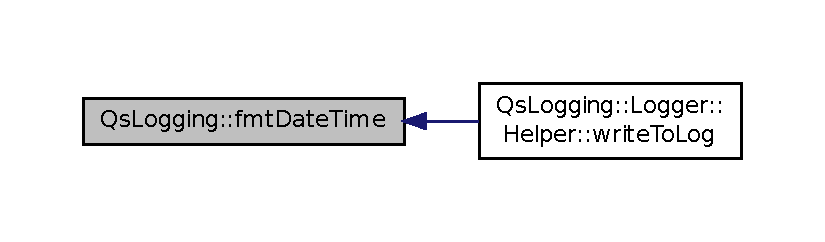
\includegraphics[width=350pt]{namespaceQsLogging_a9123c4017c6160e28fa489e419b23a9c_icgraph}
\end{center}
\end{figure}


\hypertarget{namespaceQsLogging_a8e669585768b47ba483f7325c18d60b8}{\index{Qs\-Logging@{Qs\-Logging}!Level\-To\-Text@{Level\-To\-Text}}
\index{Level\-To\-Text@{Level\-To\-Text}!QsLogging@{Qs\-Logging}}
\subsubsection[{Level\-To\-Text}]{\setlength{\rightskip}{0pt plus 5cm}static const char$\ast$ Qs\-Logging\-::\-Level\-To\-Text (
\begin{DoxyParamCaption}
\item[{Level}]{the\-Level}
\end{DoxyParamCaption}
)\hspace{0.3cm}{\ttfamily [static]}}}\label{namespaceQsLogging_a8e669585768b47ba483f7325c18d60b8}


Définition à la ligne \hyperlink{QsLog_8cpp_source_l00103}{103} du fichier \hyperlink{QsLog_8cpp_source}{Qs\-Log.\-cpp}.



Références \hyperlink{namespaceQsLogging_a38c7dd87e4de6f8eb460763ad0baa033a2a6c1ca8703fa87e56dae43e9adbecda}{Debug\-Level}, \hyperlink{namespaceQsLogging_a961ecb32f941957f4fb2ce0e244e1dc0}{Debug\-String}, \hyperlink{namespaceQsLogging_a38c7dd87e4de6f8eb460763ad0baa033a3d6b56d79245ec74186a538f2e6b3cf2}{Error\-Level}, \hyperlink{namespaceQsLogging_a81932d0d90f858336dcae9ea81560f51}{Error\-String}, \hyperlink{namespaceQsLogging_a38c7dd87e4de6f8eb460763ad0baa033ab961256fd76d6571a41516e1794f39de}{Fatal\-Level}, \hyperlink{namespaceQsLogging_a6664814676313b529499e9590ed1c476}{Fatal\-String}, \hyperlink{namespaceQsLogging_a38c7dd87e4de6f8eb460763ad0baa033a6447c84a2844e8e1d0cdb95b55ecac72}{Info\-Level}, \hyperlink{namespaceQsLogging_a747ad47c7ca8e96d020e912573d18cd1}{Info\-String}, \hyperlink{namespaceQsLogging_a38c7dd87e4de6f8eb460763ad0baa033a64b8289ed8a99f811404140cbcb2549c}{Off\-Level}, \hyperlink{namespaceQsLogging_a38c7dd87e4de6f8eb460763ad0baa033a187ba10e2b3b400c6ee33afe6fc10915}{Trace\-Level}, \hyperlink{namespaceQsLogging_a8bb6a67c53ebaad64d3e58c5a5a362ee}{Trace\-String}, \hyperlink{namespaceQsLogging_a38c7dd87e4de6f8eb460763ad0baa033ac744dbb976c301fa466a390b808e2eef}{Warn\-Level}, et \hyperlink{namespaceQsLogging_a448066a966f37903f05c519ceb33814f}{Warn\-String}.



Référencé par \hyperlink{classQsLogging_1_1Logger_1_1Helper_a30e01167d1f088bade18b71a3e85379b}{Qs\-Logging\-::\-Logger\-::\-Helper\-::write\-To\-Log()}.


\begin{DoxyCode}
00104 \{
00105     \textcolor{keywordflow}{switch} (theLevel) \{
00106     \textcolor{keywordflow}{case} \hyperlink{namespaceQsLogging_a38c7dd87e4de6f8eb460763ad0baa033a187ba10e2b3b400c6ee33afe6fc10915}{TraceLevel}:
00107         \textcolor{keywordflow}{return} \hyperlink{namespaceQsLogging_a8bb6a67c53ebaad64d3e58c5a5a362ee}{TraceString};
00108     \textcolor{keywordflow}{case} \hyperlink{namespaceQsLogging_a38c7dd87e4de6f8eb460763ad0baa033a2a6c1ca8703fa87e56dae43e9adbecda}{DebugLevel}:
00109         \textcolor{keywordflow}{return} \hyperlink{namespaceQsLogging_a961ecb32f941957f4fb2ce0e244e1dc0}{DebugString};
00110     \textcolor{keywordflow}{case} \hyperlink{namespaceQsLogging_a38c7dd87e4de6f8eb460763ad0baa033a6447c84a2844e8e1d0cdb95b55ecac72}{InfoLevel}:
00111         \textcolor{keywordflow}{return} \hyperlink{namespaceQsLogging_a747ad47c7ca8e96d020e912573d18cd1}{InfoString};
00112     \textcolor{keywordflow}{case} \hyperlink{namespaceQsLogging_a38c7dd87e4de6f8eb460763ad0baa033ac744dbb976c301fa466a390b808e2eef}{WarnLevel}:
00113         \textcolor{keywordflow}{return} \hyperlink{namespaceQsLogging_a448066a966f37903f05c519ceb33814f}{WarnString};
00114     \textcolor{keywordflow}{case} \hyperlink{namespaceQsLogging_a38c7dd87e4de6f8eb460763ad0baa033a3d6b56d79245ec74186a538f2e6b3cf2}{ErrorLevel}:
00115         \textcolor{keywordflow}{return} \hyperlink{namespaceQsLogging_a81932d0d90f858336dcae9ea81560f51}{ErrorString};
00116     \textcolor{keywordflow}{case} \hyperlink{namespaceQsLogging_a38c7dd87e4de6f8eb460763ad0baa033ab961256fd76d6571a41516e1794f39de}{FatalLevel}:
00117         \textcolor{keywordflow}{return} \hyperlink{namespaceQsLogging_a6664814676313b529499e9590ed1c476}{FatalString};
00118     \textcolor{keywordflow}{case} \hyperlink{namespaceQsLogging_a38c7dd87e4de6f8eb460763ad0baa033a64b8289ed8a99f811404140cbcb2549c}{OffLevel}:
00119         \textcolor{keywordflow}{return} \textcolor{stringliteral}{""};
00120     \textcolor{keywordflow}{default}: \{
00121         assert(!\textcolor{stringliteral}{"bad log level"});
00122         \textcolor{keywordflow}{return} \hyperlink{namespaceQsLogging_a747ad47c7ca8e96d020e912573d18cd1}{InfoString};
00123     \}
00124     \}
00125 \}
\end{DoxyCode}


Voici le graphe des appelants de cette fonction \-:
\nopagebreak
\begin{figure}[H]
\begin{center}
\leavevmode
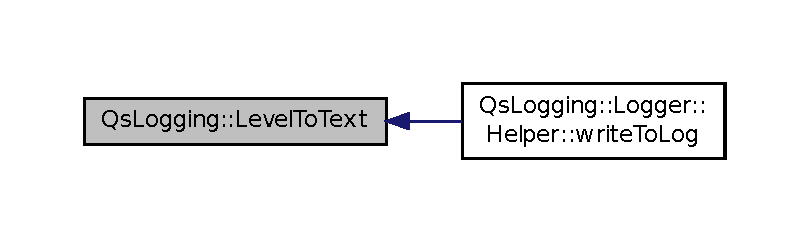
\includegraphics[width=350pt]{namespaceQsLogging_a8e669585768b47ba483f7325c18d60b8_icgraph}
\end{center}
\end{figure}




\subsection{Documentation des variables}
\hypertarget{namespaceQsLogging_a961ecb32f941957f4fb2ce0e244e1dc0}{\index{Qs\-Logging@{Qs\-Logging}!Debug\-String@{Debug\-String}}
\index{Debug\-String@{Debug\-String}!QsLogging@{Qs\-Logging}}
\subsubsection[{Debug\-String}]{\setlength{\rightskip}{0pt plus 5cm}Qs\-Logging\-::\-Debug\-String = \char`\"{}D\-E\-B\-U\-G\char`\"{}\hspace{0.3cm}{\ttfamily [static]}}}\label{namespaceQsLogging_a961ecb32f941957f4fb2ce0e244e1dc0}


Définition à la ligne \hyperlink{QsLog_8cpp_source_l00075}{75} du fichier \hyperlink{QsLog_8cpp_source}{Qs\-Log.\-cpp}.



Référencé par \hyperlink{namespaceQsLogging_a8e669585768b47ba483f7325c18d60b8}{Level\-To\-Text()}.

\hypertarget{namespaceQsLogging_a81932d0d90f858336dcae9ea81560f51}{\index{Qs\-Logging@{Qs\-Logging}!Error\-String@{Error\-String}}
\index{Error\-String@{Error\-String}!QsLogging@{Qs\-Logging}}
\subsubsection[{Error\-String}]{\setlength{\rightskip}{0pt plus 5cm}Qs\-Logging\-::\-Error\-String = \char`\"{}E\-R\-R\-O\-R\char`\"{}\hspace{0.3cm}{\ttfamily [static]}}}\label{namespaceQsLogging_a81932d0d90f858336dcae9ea81560f51}


Définition à la ligne \hyperlink{QsLog_8cpp_source_l00087}{87} du fichier \hyperlink{QsLog_8cpp_source}{Qs\-Log.\-cpp}.



Référencé par \hyperlink{namespaceQsLogging_a8e669585768b47ba483f7325c18d60b8}{Level\-To\-Text()}.

\hypertarget{namespaceQsLogging_a6664814676313b529499e9590ed1c476}{\index{Qs\-Logging@{Qs\-Logging}!Fatal\-String@{Fatal\-String}}
\index{Fatal\-String@{Fatal\-String}!QsLogging@{Qs\-Logging}}
\subsubsection[{Fatal\-String}]{\setlength{\rightskip}{0pt plus 5cm}Qs\-Logging\-::\-Fatal\-String = \char`\"{}F\-A\-T\-A\-L\char`\"{}\hspace{0.3cm}{\ttfamily [static]}}}\label{namespaceQsLogging_a6664814676313b529499e9590ed1c476}


Définition à la ligne \hyperlink{QsLog_8cpp_source_l00091}{91} du fichier \hyperlink{QsLog_8cpp_source}{Qs\-Log.\-cpp}.



Référencé par \hyperlink{namespaceQsLogging_a8e669585768b47ba483f7325c18d60b8}{Level\-To\-Text()}.

\hypertarget{namespaceQsLogging_a747ad47c7ca8e96d020e912573d18cd1}{\index{Qs\-Logging@{Qs\-Logging}!Info\-String@{Info\-String}}
\index{Info\-String@{Info\-String}!QsLogging@{Qs\-Logging}}
\subsubsection[{Info\-String}]{\setlength{\rightskip}{0pt plus 5cm}Qs\-Logging\-::\-Info\-String = \char`\"{}I\-N\-F\-O\char`\"{}\hspace{0.3cm}{\ttfamily [static]}}}\label{namespaceQsLogging_a747ad47c7ca8e96d020e912573d18cd1}


Définition à la ligne \hyperlink{QsLog_8cpp_source_l00079}{79} du fichier \hyperlink{QsLog_8cpp_source}{Qs\-Log.\-cpp}.



Référencé par \hyperlink{namespaceQsLogging_a8e669585768b47ba483f7325c18d60b8}{Level\-To\-Text()}.

\hypertarget{namespaceQsLogging_a8bb6a67c53ebaad64d3e58c5a5a362ee}{\index{Qs\-Logging@{Qs\-Logging}!Trace\-String@{Trace\-String}}
\index{Trace\-String@{Trace\-String}!QsLogging@{Qs\-Logging}}
\subsubsection[{Trace\-String}]{\setlength{\rightskip}{0pt plus 5cm}Qs\-Logging\-::\-Trace\-String = \char`\"{}T\-R\-A\-C\-E\char`\"{}\hspace{0.3cm}{\ttfamily [static]}}}\label{namespaceQsLogging_a8bb6a67c53ebaad64d3e58c5a5a362ee}


Définition à la ligne \hyperlink{QsLog_8cpp_source_l00071}{71} du fichier \hyperlink{QsLog_8cpp_source}{Qs\-Log.\-cpp}.



Référencé par \hyperlink{namespaceQsLogging_a8e669585768b47ba483f7325c18d60b8}{Level\-To\-Text()}.

\hypertarget{namespaceQsLogging_a448066a966f37903f05c519ceb33814f}{\index{Qs\-Logging@{Qs\-Logging}!Warn\-String@{Warn\-String}}
\index{Warn\-String@{Warn\-String}!QsLogging@{Qs\-Logging}}
\subsubsection[{Warn\-String}]{\setlength{\rightskip}{0pt plus 5cm}Qs\-Logging\-::\-Warn\-String = \char`\"{}W\-A\-R\-N\char`\"{}\hspace{0.3cm}{\ttfamily [static]}}}\label{namespaceQsLogging_a448066a966f37903f05c519ceb33814f}


Définition à la ligne \hyperlink{QsLog_8cpp_source_l00083}{83} du fichier \hyperlink{QsLog_8cpp_source}{Qs\-Log.\-cpp}.



Référencé par \hyperlink{namespaceQsLogging_a8e669585768b47ba483f7325c18d60b8}{Level\-To\-Text()}.


\chapter{Documentation des classes}
\hypertarget{classApplicationWindow}{\section{Référence de la classe Application\-Window}
\label{classApplicationWindow}\index{Application\-Window@{Application\-Window}}
}


Graphe d'héritage de Application\-Window\-:\nopagebreak
\begin{figure}[H]
\begin{center}
\leavevmode
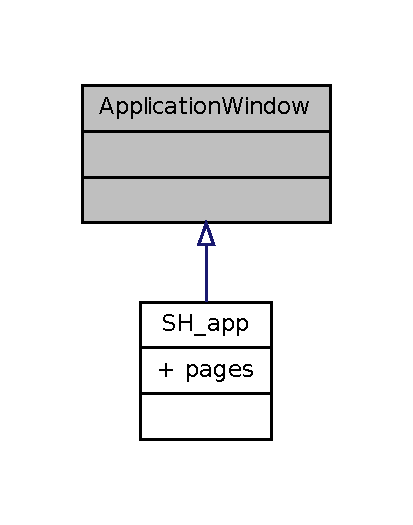
\includegraphics[width=198pt]{classApplicationWindow__inherit__graph}
\end{center}
\end{figure}


Graphe de collaboration de Application\-Window\-:\nopagebreak
\begin{figure}[H]
\begin{center}
\leavevmode
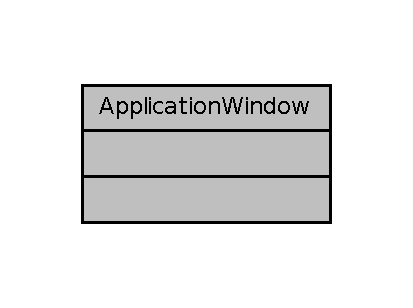
\includegraphics[width=198pt]{classApplicationWindow__coll__graph}
\end{center}
\end{figure}


La documentation de cette classe a été générée à partir du fichier suivant \-:\begin{DoxyCompactItemize}
\item 
/home/tiff/\-Stage-\/\-I\-U\-T/app/simplhotel/hotel-\/precheck/src/\-Pre\-Check/views/qml/\hyperlink{SH__app_8qml}{S\-H\-\_\-app.\-qml}\end{DoxyCompactItemize}

\hypertarget{classButton}{\section{Référence de la classe Button}
\label{classButton}\index{Button@{Button}}
}
Graphe d'héritage de Button\-:\begin{figure}[H]
\begin{center}
\leavevmode
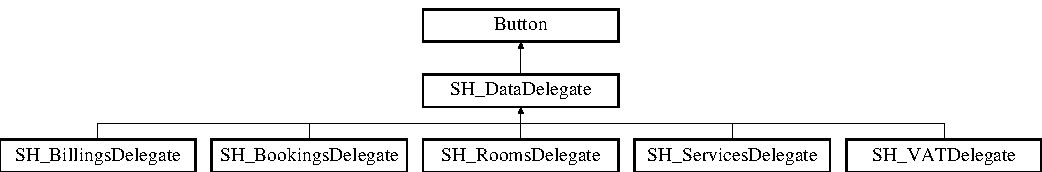
\includegraphics[height=2.317241cm]{classButton}
\end{center}
\end{figure}


La documentation de cette classe a été générée à partir du fichier suivant \-:\begin{DoxyCompactItemize}
\item 
/home/tiff/\-Stage-\/\-I\-U\-T/app/simplhotel/hotel-\/precheck/src/\-Pre\-Check/views/qml/\hyperlink{SH__DataDelegate_8qml}{S\-H\-\_\-\-Data\-Delegate.\-qml}\end{DoxyCompactItemize}

\hypertarget{classColumn}{\section{Référence de la classe Column}
\label{classColumn}\index{Column@{Column}}
}


Graphe d'héritage de Column\-:
\nopagebreak
\begin{figure}[H]
\begin{center}
\leavevmode
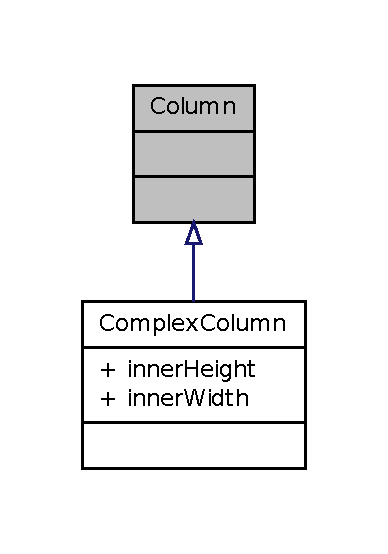
\includegraphics[width=186pt]{classColumn__inherit__graph}
\end{center}
\end{figure}


Graphe de collaboration de Column\-:
\nopagebreak
\begin{figure}[H]
\begin{center}
\leavevmode
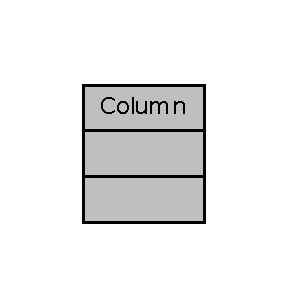
\includegraphics[width=138pt]{classColumn__coll__graph}
\end{center}
\end{figure}


La documentation de cette classe a été générée à partir du fichier suivant \-:\begin{DoxyCompactItemize}
\item 
views/qml/\hyperlink{ComplexColumn_8qml}{Complex\-Column.\-qml}\end{DoxyCompactItemize}

\hypertarget{classComplexColumn}{\section{Référence de la classe Complex\-Column}
\label{classComplexColumn}\index{Complex\-Column@{Complex\-Column}}
}


Graphe d'héritage de Complex\-Column\-:
\nopagebreak
\begin{figure}[H]
\begin{center}
\leavevmode
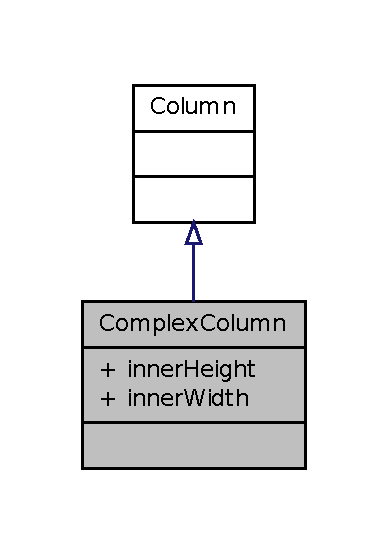
\includegraphics[width=186pt]{classComplexColumn__inherit__graph}
\end{center}
\end{figure}


Graphe de collaboration de Complex\-Column\-:
\nopagebreak
\begin{figure}[H]
\begin{center}
\leavevmode
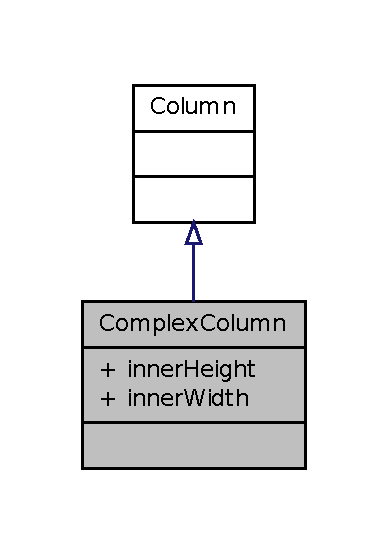
\includegraphics[width=186pt]{classComplexColumn__coll__graph}
\end{center}
\end{figure}
\subsection*{Propriétés}
\begin{DoxyCompactItemize}
\item 
real \hyperlink{classComplexColumn_a8ed7398e27678a9b93bb33f37d6b3836}{inner\-Height}
\item 
real \hyperlink{classComplexColumn_a76206dc1264db4c7af6ed5b7a87a58aa}{inner\-Width}
\end{DoxyCompactItemize}


\subsection{Description détaillée}


Définition à la ligne \hyperlink{ComplexColumn_8qml_source_l00001}{1} du fichier \hyperlink{ComplexColumn_8qml_source}{Complex\-Column.\-qml}.



\subsection{Documentation des propriétés}
\hypertarget{classComplexColumn_a8ed7398e27678a9b93bb33f37d6b3836}{\index{Complex\-Column@{Complex\-Column}!inner\-Height@{inner\-Height}}
\index{inner\-Height@{inner\-Height}!ComplexColumn@{Complex\-Column}}
\subsubsection[{inner\-Height}]{\setlength{\rightskip}{0pt plus 5cm}real Complex\-Column\-::inner\-Height}}\label{classComplexColumn_a8ed7398e27678a9b93bb33f37d6b3836}


Définition à la ligne \hyperlink{ComplexColumn_8qml_source_l00004}{4} du fichier \hyperlink{ComplexColumn_8qml_source}{Complex\-Column.\-qml}.

\hypertarget{classComplexColumn_a76206dc1264db4c7af6ed5b7a87a58aa}{\index{Complex\-Column@{Complex\-Column}!inner\-Width@{inner\-Width}}
\index{inner\-Width@{inner\-Width}!ComplexColumn@{Complex\-Column}}
\subsubsection[{inner\-Width}]{\setlength{\rightskip}{0pt plus 5cm}real Complex\-Column\-::inner\-Width}}\label{classComplexColumn_a76206dc1264db4c7af6ed5b7a87a58aa}


Définition à la ligne \hyperlink{ComplexColumn_8qml_source_l00006}{6} du fichier \hyperlink{ComplexColumn_8qml_source}{Complex\-Column.\-qml}.



La documentation de cette classe a été générée à partir du fichier suivant \-:\begin{DoxyCompactItemize}
\item 
views/qml/\hyperlink{ComplexColumn_8qml}{Complex\-Column.\-qml}\end{DoxyCompactItemize}

\hypertarget{classFocusScope}{\section{Référence de la classe Focus\-Scope}
\label{classFocusScope}\index{Focus\-Scope@{Focus\-Scope}}
}


Graphe d'héritage de Focus\-Scope\-:
\nopagebreak
\begin{figure}[H]
\begin{center}
\leavevmode
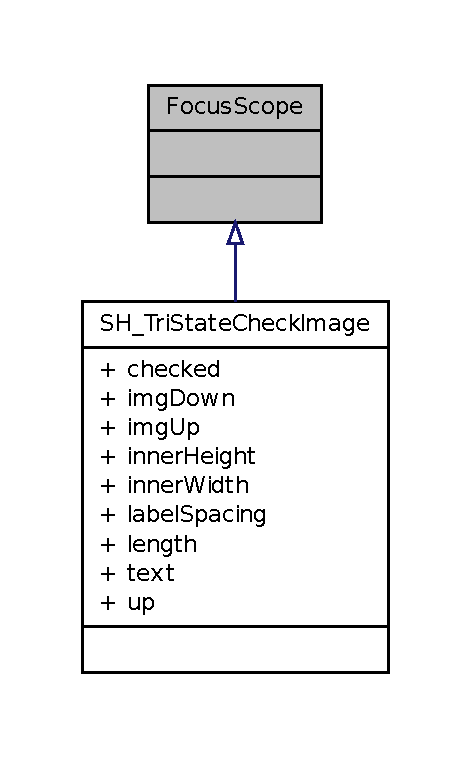
\includegraphics[width=226pt]{classFocusScope__inherit__graph}
\end{center}
\end{figure}


Graphe de collaboration de Focus\-Scope\-:
\nopagebreak
\begin{figure}[H]
\begin{center}
\leavevmode
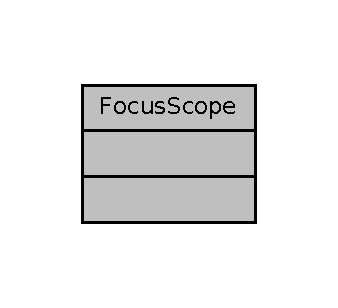
\includegraphics[width=162pt]{classFocusScope__coll__graph}
\end{center}
\end{figure}


La documentation de cette classe a été générée à partir du fichier suivant \-:\begin{DoxyCompactItemize}
\item 
views/qml/\hyperlink{SH__TriStateCheckImage_8qml}{S\-H\-\_\-\-Tri\-State\-Check\-Image.\-qml}\end{DoxyCompactItemize}

\hypertarget{classGridLayout}{\section{Référence de la classe Grid\-Layout}
\label{classGridLayout}\index{Grid\-Layout@{Grid\-Layout}}
}
Graphe d'héritage de Grid\-Layout\-:\begin{figure}[H]
\begin{center}
\leavevmode
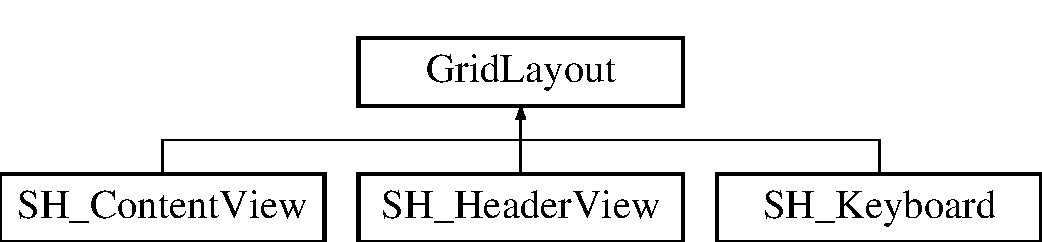
\includegraphics[height=2.000000cm]{classGridLayout}
\end{center}
\end{figure}


La documentation de cette classe a été générée à partir du fichier suivant \-:\begin{DoxyCompactItemize}
\item 
/home/tiff/\-Stage-\/\-I\-U\-T/app/simplhotel/hotel-\/precheck/src/\-Pre\-Check/views/qml/\hyperlink{SH__ContentView_8qml}{S\-H\-\_\-\-Content\-View.\-qml}\end{DoxyCompactItemize}

\hypertarget{classItem}{\section{Référence de la classe Item}
\label{classItem}\index{Item@{Item}}
}
Graphe d'héritage de Item\-:\begin{figure}[H]
\begin{center}
\leavevmode
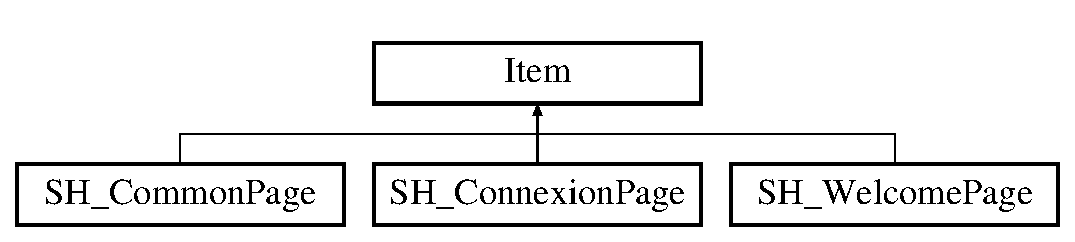
\includegraphics[height=2.000000cm]{classItem}
\end{center}
\end{figure}


La documentation de cette classe a été générée à partir du fichier suivant \-:\begin{DoxyCompactItemize}
\item 
/home/tiff/\-Stage-\/\-I\-U\-T/app/simplhotel/hotel-\/precheck/src/\-Pre\-Check/views/qml/\hyperlink{SH__CommonPage_8qml}{S\-H\-\_\-\-Common\-Page.\-qml}\end{DoxyCompactItemize}

\hypertarget{classQAbstractListModel}{\section{Référence de la classe Q\-Abstract\-List\-Model}
\label{classQAbstractListModel}\index{Q\-Abstract\-List\-Model@{Q\-Abstract\-List\-Model}}
}


Graphe d'héritage de Q\-Abstract\-List\-Model\-:
\nopagebreak
\begin{figure}[H]
\begin{center}
\leavevmode
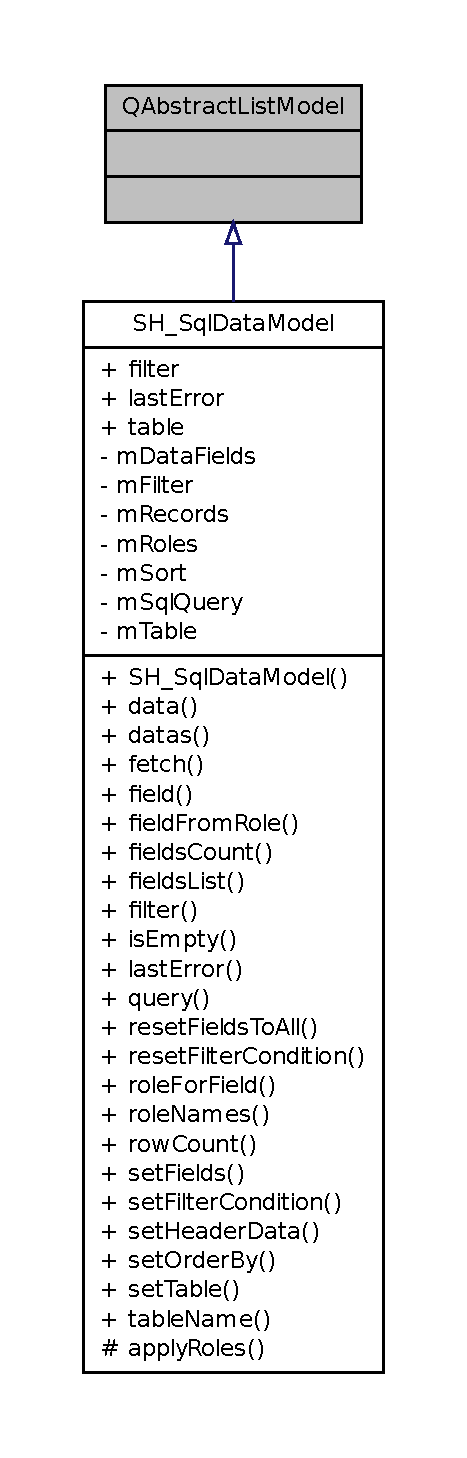
\includegraphics[height=550pt]{classQAbstractListModel__inherit__graph}
\end{center}
\end{figure}


Graphe de collaboration de Q\-Abstract\-List\-Model\-:
\nopagebreak
\begin{figure}[H]
\begin{center}
\leavevmode
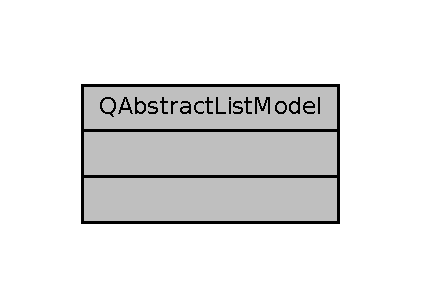
\includegraphics[width=202pt]{classQAbstractListModel__coll__graph}
\end{center}
\end{figure}


La documentation de cette classe a été générée à partir du fichier suivant \-:\begin{DoxyCompactItemize}
\item 
models/\hyperlink{SH__SqlDataModel_8h}{S\-H\-\_\-\-Sql\-Data\-Model.\-h}\end{DoxyCompactItemize}

\hypertarget{classQObject}{\section{Référence de la classe Q\-Object}
\label{classQObject}\index{Q\-Object@{Q\-Object}}
}
Graphe d'héritage de Q\-Object\-:\begin{figure}[H]
\begin{center}
\leavevmode
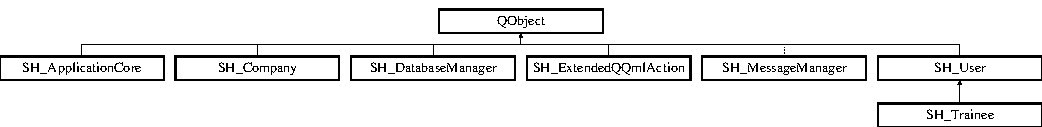
\includegraphics[height=1.707317cm]{classQObject}
\end{center}
\end{figure}


La documentation de cette classe a été générée à partir du fichier suivant \-:\begin{DoxyCompactItemize}
\item 
/home/tiff/\-Stage-\/\-I\-U\-T/app/simplhotel/hotel-\/precheck/src/\-Pre\-Check/\hyperlink{SH__MessageManager_8h}{S\-H\-\_\-\-Message\-Manager.\-h}\end{DoxyCompactItemize}

\hypertarget{classQQuickItem}{\section{Référence de la classe Q\-Quick\-Item}
\label{classQQuickItem}\index{Q\-Quick\-Item@{Q\-Quick\-Item}}
}


Graphe d'héritage de Q\-Quick\-Item\-:\nopagebreak
\begin{figure}[H]
\begin{center}
\leavevmode
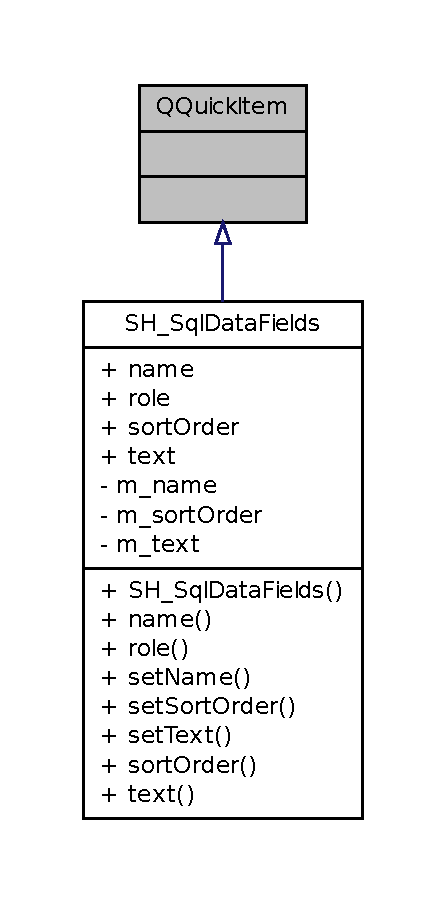
\includegraphics[width=214pt]{classQQuickItem__inherit__graph}
\end{center}
\end{figure}


Graphe de collaboration de Q\-Quick\-Item\-:\nopagebreak
\begin{figure}[H]
\begin{center}
\leavevmode
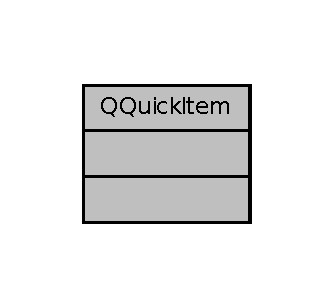
\includegraphics[width=160pt]{classQQuickItem__coll__graph}
\end{center}
\end{figure}


La documentation de cette classe a été générée à partir du fichier suivant \-:\begin{DoxyCompactItemize}
\item 
/home/tiff/\-Stage-\/\-I\-U\-T/app/simplhotel/hotel-\/precheck/src/\-Pre\-Check/models/\hyperlink{SH__SqlDataField_8h}{S\-H\-\_\-\-Sql\-Data\-Field.\-h}\end{DoxyCompactItemize}

\hypertarget{classQsDebugOutput}{\section{Référence de la classe Qs\-Debug\-Output}
\label{classQsDebugOutput}\index{Qs\-Debug\-Output@{Qs\-Debug\-Output}}
}


The \hyperlink{classQsDebugOutput}{Qs\-Debug\-Output} class.  




{\ttfamily \#include $<$Qs\-Log\-Dest\-Console.\-h$>$}



Graphe de collaboration de Qs\-Debug\-Output\-:
\nopagebreak
\begin{figure}[H]
\begin{center}
\leavevmode
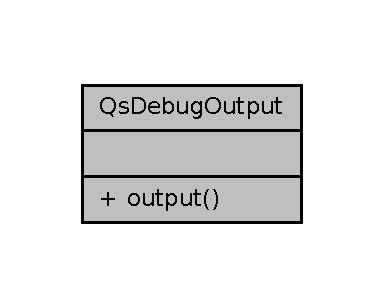
\includegraphics[width=184pt]{classQsDebugOutput__coll__graph}
\end{center}
\end{figure}
\subsection*{Fonctions membres publiques statiques}
\begin{DoxyCompactItemize}
\item 
static void \hyperlink{classQsDebugOutput_a1adecc326b36497c0e6953fae87d1cb1}{output} (const Q\-String \&a\-\_\-message)
\begin{DoxyCompactList}\small\item\em output \end{DoxyCompactList}\end{DoxyCompactItemize}


\subsection{Description détaillée}
The \hyperlink{classQsDebugOutput}{Qs\-Debug\-Output} class. 

Définition à la ligne \hyperlink{QsLogDestConsole_8h_source_l00056}{56} du fichier \hyperlink{QsLogDestConsole_8h_source}{Qs\-Log\-Dest\-Console.\-h}.



\subsection{Documentation des fonctions membres}
\hypertarget{classQsDebugOutput_a1adecc326b36497c0e6953fae87d1cb1}{\index{Qs\-Debug\-Output@{Qs\-Debug\-Output}!output@{output}}
\index{output@{output}!QsDebugOutput@{Qs\-Debug\-Output}}
\subsubsection[{output}]{\setlength{\rightskip}{0pt plus 5cm}static void Qs\-Debug\-Output\-::output (
\begin{DoxyParamCaption}
\item[{const Q\-String \&}]{a\-\_\-message}
\end{DoxyParamCaption}
)\hspace{0.3cm}{\ttfamily [static]}}}\label{classQsDebugOutput_a1adecc326b36497c0e6953fae87d1cb1}


output 


\begin{DoxyParams}{Paramètres}
{\em a\-\_\-message} & \\
\hline
\end{DoxyParams}


Référencé par \hyperlink{classQsLogging_1_1DebugOutputDestination_a72c60cc3a3f6cb9d63dd88528b7e1125}{Qs\-Logging\-::\-Debug\-Output\-Destination\-::write()}.



Voici le graphe des appelants de cette fonction \-:
\nopagebreak
\begin{figure}[H]
\begin{center}
\leavevmode
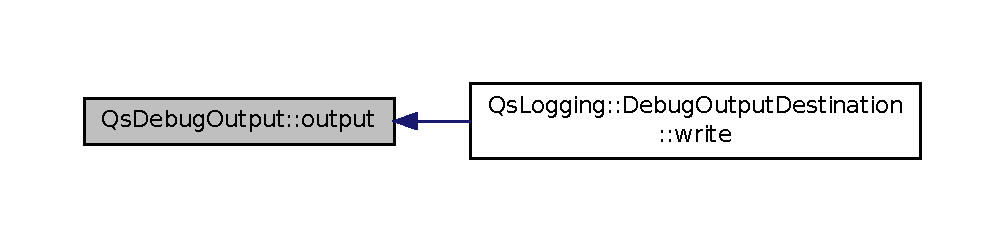
\includegraphics[width=350pt]{classQsDebugOutput_a1adecc326b36497c0e6953fae87d1cb1_icgraph}
\end{center}
\end{figure}




La documentation de cette classe a été générée à partir du fichier suivant \-:\begin{DoxyCompactItemize}
\item 
logging/\hyperlink{QsLogDestConsole_8h}{Qs\-Log\-Dest\-Console.\-h}\end{DoxyCompactItemize}

\hypertarget{classQsLogging_1_1DebugOutputDestination}{\section{Référence de la classe Qs\-Logging\-:\-:Debug\-Output\-Destination}
\label{classQsLogging_1_1DebugOutputDestination}\index{Qs\-Logging\-::\-Debug\-Output\-Destination@{Qs\-Logging\-::\-Debug\-Output\-Destination}}
}


The \hyperlink{classQsLogging_1_1DebugOutputDestination}{Debug\-Output\-Destination} class.  




{\ttfamily \#include $<$Qs\-Log\-Dest\-Console.\-h$>$}



Graphe d'héritage de Qs\-Logging\-:\-:Debug\-Output\-Destination\-:
\nopagebreak
\begin{figure}[H]
\begin{center}
\leavevmode
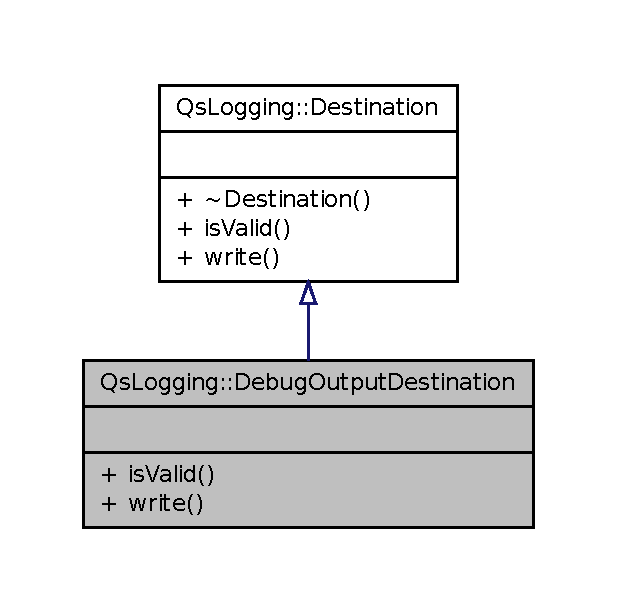
\includegraphics[width=296pt]{classQsLogging_1_1DebugOutputDestination__inherit__graph}
\end{center}
\end{figure}


Graphe de collaboration de Qs\-Logging\-:\-:Debug\-Output\-Destination\-:
\nopagebreak
\begin{figure}[H]
\begin{center}
\leavevmode
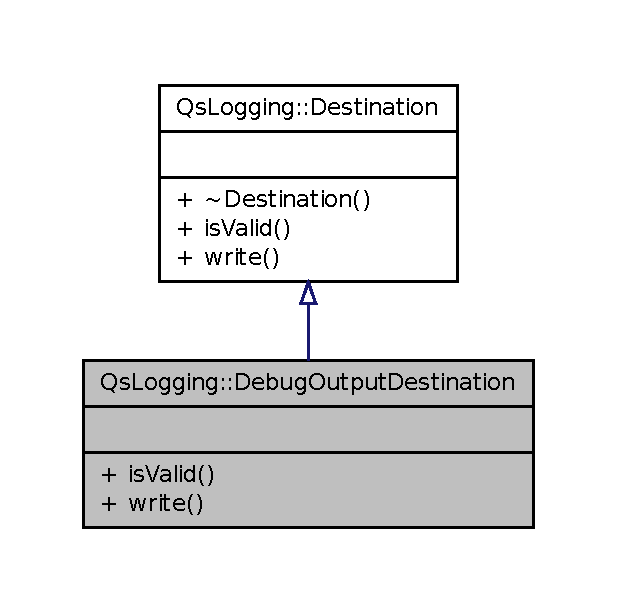
\includegraphics[width=296pt]{classQsLogging_1_1DebugOutputDestination__coll__graph}
\end{center}
\end{figure}
\subsection*{Fonctions membres publiques}
\begin{DoxyCompactItemize}
\item 
virtual bool \hyperlink{classQsLogging_1_1DebugOutputDestination_a7e260f310b5f757ecab216058d0808a9}{is\-Valid} ()
\begin{DoxyCompactList}\small\item\em is\-Valid \end{DoxyCompactList}\item 
virtual void \hyperlink{classQsLogging_1_1DebugOutputDestination_a72c60cc3a3f6cb9d63dd88528b7e1125}{write} (const Q\-String \&message, \hyperlink{namespaceQsLogging_a38c7dd87e4de6f8eb460763ad0baa033}{Level} level)
\begin{DoxyCompactList}\small\item\em write \end{DoxyCompactList}\end{DoxyCompactItemize}


\subsection{Description détaillée}
The \hyperlink{classQsLogging_1_1DebugOutputDestination}{Debug\-Output\-Destination} class. 

Définition à la ligne \hyperlink{QsLogDestConsole_8h_source_l00074}{74} du fichier \hyperlink{QsLogDestConsole_8h_source}{Qs\-Log\-Dest\-Console.\-h}.



\subsection{Documentation des fonctions membres}
\hypertarget{classQsLogging_1_1DebugOutputDestination_a7e260f310b5f757ecab216058d0808a9}{\index{Qs\-Logging\-::\-Debug\-Output\-Destination@{Qs\-Logging\-::\-Debug\-Output\-Destination}!is\-Valid@{is\-Valid}}
\index{is\-Valid@{is\-Valid}!QsLogging::DebugOutputDestination@{Qs\-Logging\-::\-Debug\-Output\-Destination}}
\subsubsection[{is\-Valid}]{\setlength{\rightskip}{0pt plus 5cm}bool Qs\-Logging\-::\-Debug\-Output\-Destination\-::is\-Valid (
\begin{DoxyParamCaption}
{}
\end{DoxyParamCaption}
)\hspace{0.3cm}{\ttfamily [virtual]}}}\label{classQsLogging_1_1DebugOutputDestination_a7e260f310b5f757ecab216058d0808a9}


is\-Valid 

\begin{DoxyReturn}{Renvoie}

\end{DoxyReturn}


Implémente \hyperlink{classQsLogging_1_1Destination_acb3dd81553c59aec5062ec8556b3b407}{Qs\-Logging\-::\-Destination}.



Définition à la ligne \hyperlink{QsLogDestConsole_8cpp_source_l00104}{104} du fichier \hyperlink{QsLogDestConsole_8cpp_source}{Qs\-Log\-Dest\-Console.\-cpp}.


\begin{DoxyCode}
00105 \{
00106     \textcolor{keywordflow}{return} \textcolor{keyword}{true};
00107 \}
\end{DoxyCode}
\hypertarget{classQsLogging_1_1DebugOutputDestination_a72c60cc3a3f6cb9d63dd88528b7e1125}{\index{Qs\-Logging\-::\-Debug\-Output\-Destination@{Qs\-Logging\-::\-Debug\-Output\-Destination}!write@{write}}
\index{write@{write}!QsLogging::DebugOutputDestination@{Qs\-Logging\-::\-Debug\-Output\-Destination}}
\subsubsection[{write}]{\setlength{\rightskip}{0pt plus 5cm}void Qs\-Logging\-::\-Debug\-Output\-Destination\-::write (
\begin{DoxyParamCaption}
\item[{const Q\-String \&}]{message, }
\item[{{\bf Level}}]{level}
\end{DoxyParamCaption}
)\hspace{0.3cm}{\ttfamily [virtual]}}}\label{classQsLogging_1_1DebugOutputDestination_a72c60cc3a3f6cb9d63dd88528b7e1125}


write 


\begin{DoxyParams}{Paramètres}
{\em message} & \\
\hline
{\em level} & \hyperlink{classQsLogging_1_1DebugOutputDestination_a72c60cc3a3f6cb9d63dd88528b7e1125}{Qs\-Logging\-::\-Debug\-Output\-Destination\-::write} \\
\hline
\end{DoxyParams}


Implémente \hyperlink{classQsLogging_1_1Destination_a19306b28686d599f49bb23f88824fd65}{Qs\-Logging\-::\-Destination}.



Définition à la ligne \hyperlink{QsLogDestConsole_8cpp_source_l00099}{99} du fichier \hyperlink{QsLogDestConsole_8cpp_source}{Qs\-Log\-Dest\-Console.\-cpp}.



Références \hyperlink{classQsDebugOutput_a1adecc326b36497c0e6953fae87d1cb1}{Qs\-Debug\-Output\-::output()}.


\begin{DoxyCode}
00100 \{
00101     \hyperlink{classQsDebugOutput_a1adecc326b36497c0e6953fae87d1cb1}{QsDebugOutput::output}(message);
00102 \}
\end{DoxyCode}


Voici le graphe d'appel pour cette fonction \-:
\nopagebreak
\begin{figure}[H]
\begin{center}
\leavevmode
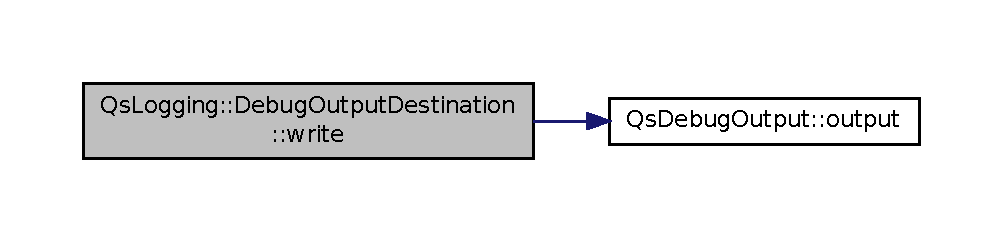
\includegraphics[width=350pt]{classQsLogging_1_1DebugOutputDestination_a72c60cc3a3f6cb9d63dd88528b7e1125_cgraph}
\end{center}
\end{figure}




La documentation de cette classe a été générée à partir des fichiers suivants \-:\begin{DoxyCompactItemize}
\item 
logging/\hyperlink{QsLogDestConsole_8h}{Qs\-Log\-Dest\-Console.\-h}\item 
logging/\hyperlink{QsLogDestConsole_8cpp}{Qs\-Log\-Dest\-Console.\-cpp}\end{DoxyCompactItemize}

\hypertarget{classQsLogging_1_1Destination}{\section{Référence de la classe Qs\-Logging\-:\-:Destination}
\label{classQsLogging_1_1Destination}\index{Qs\-Logging\-::\-Destination@{Qs\-Logging\-::\-Destination}}
}


The \hyperlink{classQsLogging_1_1Destination}{Destination} class.  




{\ttfamily \#include $<$Qs\-Log\-Dest.\-h$>$}



Graphe d'héritage de Qs\-Logging\-:\-:Destination\-:
\nopagebreak
\begin{figure}[H]
\begin{center}
\leavevmode
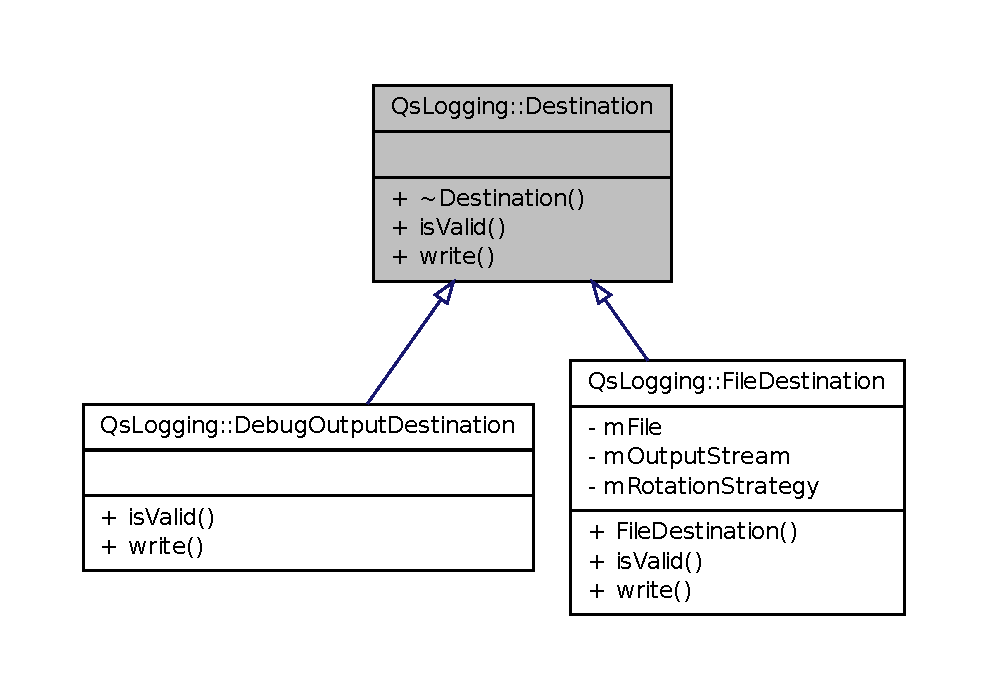
\includegraphics[width=350pt]{classQsLogging_1_1Destination__inherit__graph}
\end{center}
\end{figure}


Graphe de collaboration de Qs\-Logging\-:\-:Destination\-:
\nopagebreak
\begin{figure}[H]
\begin{center}
\leavevmode
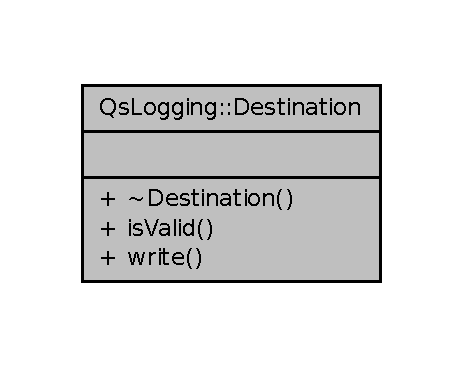
\includegraphics[width=222pt]{classQsLogging_1_1Destination__coll__graph}
\end{center}
\end{figure}
\subsection*{Fonctions membres publiques}
\begin{DoxyCompactItemize}
\item 
virtual \hyperlink{classQsLogging_1_1Destination_ace97f507c02fe9a107306b089e07c3cb}{$\sim$\-Destination} ()
\begin{DoxyCompactList}\small\item\em $\sim$\-Destination \end{DoxyCompactList}\item 
virtual bool \hyperlink{classQsLogging_1_1Destination_acb3dd81553c59aec5062ec8556b3b407}{is\-Valid} ()=0
\begin{DoxyCompactList}\small\item\em is\-Valid \end{DoxyCompactList}\item 
virtual void \hyperlink{classQsLogging_1_1Destination_a19306b28686d599f49bb23f88824fd65}{write} (const Q\-String \&message, \hyperlink{namespaceQsLogging_a38c7dd87e4de6f8eb460763ad0baa033}{Level} level)=0
\begin{DoxyCompactList}\small\item\em write \end{DoxyCompactList}\end{DoxyCompactItemize}


\subsection{Description détaillée}
The \hyperlink{classQsLogging_1_1Destination}{Destination} class. 

Définition à la ligne \hyperlink{QsLogDest_8h_source_l00060}{60} du fichier \hyperlink{QsLogDest_8h_source}{Qs\-Log\-Dest.\-h}.



\subsection{Documentation des constructeurs et destructeur}
\hypertarget{classQsLogging_1_1Destination_ace97f507c02fe9a107306b089e07c3cb}{\index{Qs\-Logging\-::\-Destination@{Qs\-Logging\-::\-Destination}!$\sim$\-Destination@{$\sim$\-Destination}}
\index{$\sim$\-Destination@{$\sim$\-Destination}!QsLogging::Destination@{Qs\-Logging\-::\-Destination}}
\subsubsection[{$\sim$\-Destination}]{\setlength{\rightskip}{0pt plus 5cm}virtual Qs\-Logging\-::\-Destination\-::$\sim$\-Destination (
\begin{DoxyParamCaption}
{}
\end{DoxyParamCaption}
)\hspace{0.3cm}{\ttfamily [inline]}, {\ttfamily [virtual]}}}\label{classQsLogging_1_1Destination_ace97f507c02fe9a107306b089e07c3cb}


$\sim$\-Destination 



Définition à la ligne \hyperlink{QsLogDest_8h_source_l00066}{66} du fichier \hyperlink{QsLogDest_8h_source}{Qs\-Log\-Dest.\-h}.


\begin{DoxyCode}
00066 \{\}
\end{DoxyCode}


\subsection{Documentation des fonctions membres}
\hypertarget{classQsLogging_1_1Destination_acb3dd81553c59aec5062ec8556b3b407}{\index{Qs\-Logging\-::\-Destination@{Qs\-Logging\-::\-Destination}!is\-Valid@{is\-Valid}}
\index{is\-Valid@{is\-Valid}!QsLogging::Destination@{Qs\-Logging\-::\-Destination}}
\subsubsection[{is\-Valid}]{\setlength{\rightskip}{0pt plus 5cm}virtual bool Qs\-Logging\-::\-Destination\-::is\-Valid (
\begin{DoxyParamCaption}
{}
\end{DoxyParamCaption}
)\hspace{0.3cm}{\ttfamily [pure virtual]}}}\label{classQsLogging_1_1Destination_acb3dd81553c59aec5062ec8556b3b407}


is\-Valid 

\begin{DoxyReturn}{Renvoie}

\end{DoxyReturn}


Implémenté dans \hyperlink{classQsLogging_1_1FileDestination_a2d18b70b408910332dcbee9d12c1d394}{Qs\-Logging\-::\-File\-Destination}, et \hyperlink{classQsLogging_1_1DebugOutputDestination_a7e260f310b5f757ecab216058d0808a9}{Qs\-Logging\-::\-Debug\-Output\-Destination}.

\hypertarget{classQsLogging_1_1Destination_a19306b28686d599f49bb23f88824fd65}{\index{Qs\-Logging\-::\-Destination@{Qs\-Logging\-::\-Destination}!write@{write}}
\index{write@{write}!QsLogging::Destination@{Qs\-Logging\-::\-Destination}}
\subsubsection[{write}]{\setlength{\rightskip}{0pt plus 5cm}virtual void Qs\-Logging\-::\-Destination\-::write (
\begin{DoxyParamCaption}
\item[{const Q\-String \&}]{message, }
\item[{{\bf Level}}]{level}
\end{DoxyParamCaption}
)\hspace{0.3cm}{\ttfamily [pure virtual]}}}\label{classQsLogging_1_1Destination_a19306b28686d599f49bb23f88824fd65}


write 


\begin{DoxyParams}{Paramètres}
{\em message} & \\
\hline
{\em level} & \\
\hline
\end{DoxyParams}


Implémenté dans \hyperlink{classQsLogging_1_1FileDestination_a84b076720ccfa4045e1aacc14c5af5dc}{Qs\-Logging\-::\-File\-Destination}, et \hyperlink{classQsLogging_1_1DebugOutputDestination_a72c60cc3a3f6cb9d63dd88528b7e1125}{Qs\-Logging\-::\-Debug\-Output\-Destination}.



La documentation de cette classe a été générée à partir du fichier suivant \-:\begin{DoxyCompactItemize}
\item 
logging/\hyperlink{QsLogDest_8h}{Qs\-Log\-Dest.\-h}\end{DoxyCompactItemize}

\hypertarget{classQsLogging_1_1DestinationFactory}{\section{Référence de la classe Qs\-Logging\-:\-:Destination\-Factory}
\label{classQsLogging_1_1DestinationFactory}\index{Qs\-Logging\-::\-Destination\-Factory@{Qs\-Logging\-::\-Destination\-Factory}}
}


{\ttfamily \#include $<$Qs\-Log\-Dest.\-h$>$}



Graphe de collaboration de Qs\-Logging\-:\-:Destination\-Factory\-:
\nopagebreak
\begin{figure}[H]
\begin{center}
\leavevmode
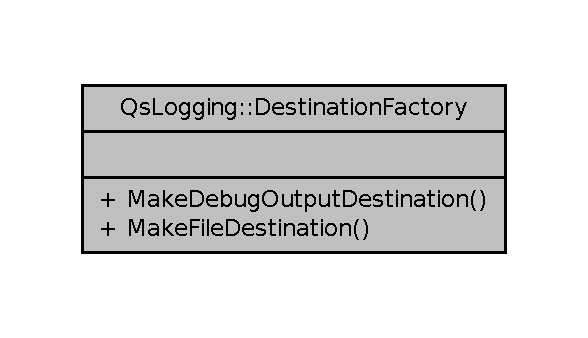
\includegraphics[width=282pt]{classQsLogging_1_1DestinationFactory__coll__graph}
\end{center}
\end{figure}
\subsection*{Fonctions membres publiques statiques}
\begin{DoxyCompactItemize}
\item 
static \hyperlink{namespaceQsLogging_a8fe41cf859d617f1c23515f804d1e8ec}{Destination\-Ptr} \hyperlink{classQsLogging_1_1DestinationFactory_a69eecb9933440870bb809c4e32ac1987}{Make\-Debug\-Output\-Destination} ()
\begin{DoxyCompactList}\small\item\em Make\-Debug\-Output\-Destination. \end{DoxyCompactList}\item 
static \hyperlink{namespaceQsLogging_a8fe41cf859d617f1c23515f804d1e8ec}{Destination\-Ptr} \hyperlink{classQsLogging_1_1DestinationFactory_abc128b6640d5716b91c681df960b878c}{Make\-File\-Destination} (const Q\-String \&file\-Path, bool enable\-Rotation=false, qint64 size\-In\-Bytes\-To\-Rotate\-After=0, int old\-Logs\-To\-Keep=0)
\begin{DoxyCompactList}\small\item\em Make\-File\-Destination. \end{DoxyCompactList}\end{DoxyCompactItemize}


\subsection{Description détaillée}


Définition à la ligne \hyperlink{QsLogDest_8h_source_l00089}{89} du fichier \hyperlink{QsLogDest_8h_source}{Qs\-Log\-Dest.\-h}.



\subsection{Documentation des fonctions membres}
\hypertarget{classQsLogging_1_1DestinationFactory_a69eecb9933440870bb809c4e32ac1987}{\index{Qs\-Logging\-::\-Destination\-Factory@{Qs\-Logging\-::\-Destination\-Factory}!Make\-Debug\-Output\-Destination@{Make\-Debug\-Output\-Destination}}
\index{Make\-Debug\-Output\-Destination@{Make\-Debug\-Output\-Destination}!QsLogging::DestinationFactory@{Qs\-Logging\-::\-Destination\-Factory}}
\subsubsection[{Make\-Debug\-Output\-Destination}]{\setlength{\rightskip}{0pt plus 5cm}{\bf Destination\-Ptr} Qs\-Logging\-::\-Destination\-Factory\-::\-Make\-Debug\-Output\-Destination (
\begin{DoxyParamCaption}
{}
\end{DoxyParamCaption}
)\hspace{0.3cm}{\ttfamily [static]}}}\label{classQsLogging_1_1DestinationFactory_a69eecb9933440870bb809c4e32ac1987}


Make\-Debug\-Output\-Destination. 

\begin{DoxyReturn}{Renvoie}

\end{DoxyReturn}
\hyperlink{classQsLogging_1_1DestinationFactory_a69eecb9933440870bb809c4e32ac1987}{Destination\-Factory\-::\-Make\-Debug\-Output\-Destination} 

Définition à la ligne \hyperlink{QsLogDest_8cpp_source_l00076}{76} du fichier \hyperlink{QsLogDest_8cpp_source}{Qs\-Log\-Dest.\-cpp}.



Référencé par \hyperlink{main_8cpp_ac3c79e35c4fc5c50939ae90485e1483f}{enable\-Logging()}.


\begin{DoxyCode}
00077 \{
00078     \textcolor{keywordflow}{return} \hyperlink{namespaceQsLogging_a8fe41cf859d617f1c23515f804d1e8ec}{DestinationPtr}(\textcolor{keyword}{new} DebugOutputDestination);
00079 \}
\end{DoxyCode}


Voici le graphe des appelants de cette fonction \-:
\nopagebreak
\begin{figure}[H]
\begin{center}
\leavevmode
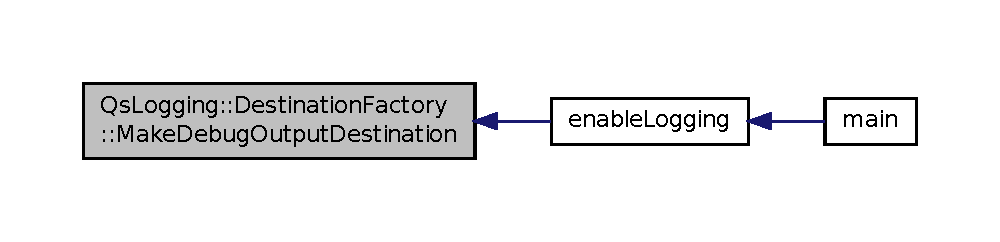
\includegraphics[width=350pt]{classQsLogging_1_1DestinationFactory_a69eecb9933440870bb809c4e32ac1987_icgraph}
\end{center}
\end{figure}


\hypertarget{classQsLogging_1_1DestinationFactory_abc128b6640d5716b91c681df960b878c}{\index{Qs\-Logging\-::\-Destination\-Factory@{Qs\-Logging\-::\-Destination\-Factory}!Make\-File\-Destination@{Make\-File\-Destination}}
\index{Make\-File\-Destination@{Make\-File\-Destination}!QsLogging::DestinationFactory@{Qs\-Logging\-::\-Destination\-Factory}}
\subsubsection[{Make\-File\-Destination}]{\setlength{\rightskip}{0pt plus 5cm}{\bf Destination\-Ptr} Qs\-Logging\-::\-Destination\-Factory\-::\-Make\-File\-Destination (
\begin{DoxyParamCaption}
\item[{const Q\-String \&}]{file\-Path, }
\item[{bool}]{enable\-Rotation = {\ttfamily false}, }
\item[{qint64}]{size\-In\-Bytes\-To\-Rotate\-After = {\ttfamily 0}, }
\item[{int}]{old\-Logs\-To\-Keep = {\ttfamily 0}}
\end{DoxyParamCaption}
)\hspace{0.3cm}{\ttfamily [static]}}}\label{classQsLogging_1_1DestinationFactory_abc128b6640d5716b91c681df960b878c}


Make\-File\-Destination. 

destination factory


\begin{DoxyParams}{Paramètres}
{\em file\-Path} & \\
\hline
{\em enable\-Rotation} & \\
\hline
{\em size\-In\-Bytes\-To\-Rotate\-After} & \\
\hline
{\em old\-Logs\-To\-Keep} & \\
\hline
\end{DoxyParams}
\begin{DoxyReturn}{Renvoie}

\end{DoxyReturn}
\hyperlink{classQsLogging_1_1DestinationFactory_abc128b6640d5716b91c681df960b878c}{Destination\-Factory\-::\-Make\-File\-Destination} 

Définition à la ligne \hyperlink{QsLogDest_8cpp_source_l00060}{60} du fichier \hyperlink{QsLogDest_8cpp_source}{Qs\-Log\-Dest.\-cpp}.



Référencé par \hyperlink{main_8cpp_ac3c79e35c4fc5c50939ae90485e1483f}{enable\-Logging()}.


\begin{DoxyCode}
00062 \{
00063     \textcolor{keywordflow}{if} (enableRotation) \{
00064         QScopedPointer<SizeRotationStrategy> logRotation(\textcolor{keyword}{new} SizeRotationStrategy);
00065         logRotation->setMaximumSizeInBytes(sizeInBytesToRotateAfter);
00066         logRotation->setBackupCount(oldLogsToKeep);
00067 
00068         \textcolor{keywordflow}{return} \hyperlink{namespaceQsLogging_a8fe41cf859d617f1c23515f804d1e8ec}{DestinationPtr}(\textcolor{keyword}{new} FileDestination(filePath, 
      \hyperlink{namespaceQsLogging_a41dc81d39cd3d36d9e15746bd9174be0}{RotationStrategyPtr}(logRotation.take())));
00069     \}
00070 
00071     \textcolor{keywordflow}{return} \hyperlink{namespaceQsLogging_a8fe41cf859d617f1c23515f804d1e8ec}{DestinationPtr}(\textcolor{keyword}{new} FileDestination(filePath, 
      \hyperlink{namespaceQsLogging_a41dc81d39cd3d36d9e15746bd9174be0}{RotationStrategyPtr}(\textcolor{keyword}{new} NullRotationStrategy)));
00072 \}
\end{DoxyCode}


Voici le graphe des appelants de cette fonction \-:
\nopagebreak
\begin{figure}[H]
\begin{center}
\leavevmode
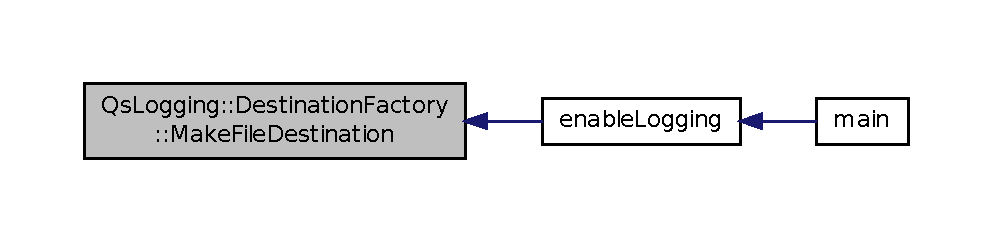
\includegraphics[width=350pt]{classQsLogging_1_1DestinationFactory_abc128b6640d5716b91c681df960b878c_icgraph}
\end{center}
\end{figure}




La documentation de cette classe a été générée à partir des fichiers suivants \-:\begin{DoxyCompactItemize}
\item 
logging/\hyperlink{QsLogDest_8h}{Qs\-Log\-Dest.\-h}\item 
logging/\hyperlink{QsLogDest_8cpp}{Qs\-Log\-Dest.\-cpp}\end{DoxyCompactItemize}

\hypertarget{classQsLogging_1_1FileDestination}{\section{Référence de la classe Qs\-Logging\-:\-:File\-Destination}
\label{classQsLogging_1_1FileDestination}\index{Qs\-Logging\-::\-File\-Destination@{Qs\-Logging\-::\-File\-Destination}}
}


The \hyperlink{classQsLogging_1_1FileDestination}{File\-Destination} class.  




{\ttfamily \#include $<$Qs\-Log\-Dest\-File.\-h$>$}



Graphe d'héritage de Qs\-Logging\-:\-:File\-Destination\-:
\nopagebreak
\begin{figure}[H]
\begin{center}
\leavevmode
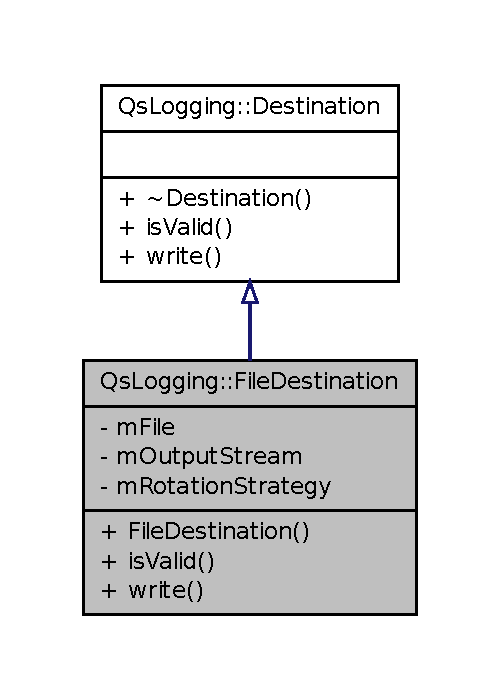
\includegraphics[width=240pt]{classQsLogging_1_1FileDestination__inherit__graph}
\end{center}
\end{figure}


Graphe de collaboration de Qs\-Logging\-:\-:File\-Destination\-:
\nopagebreak
\begin{figure}[H]
\begin{center}
\leavevmode
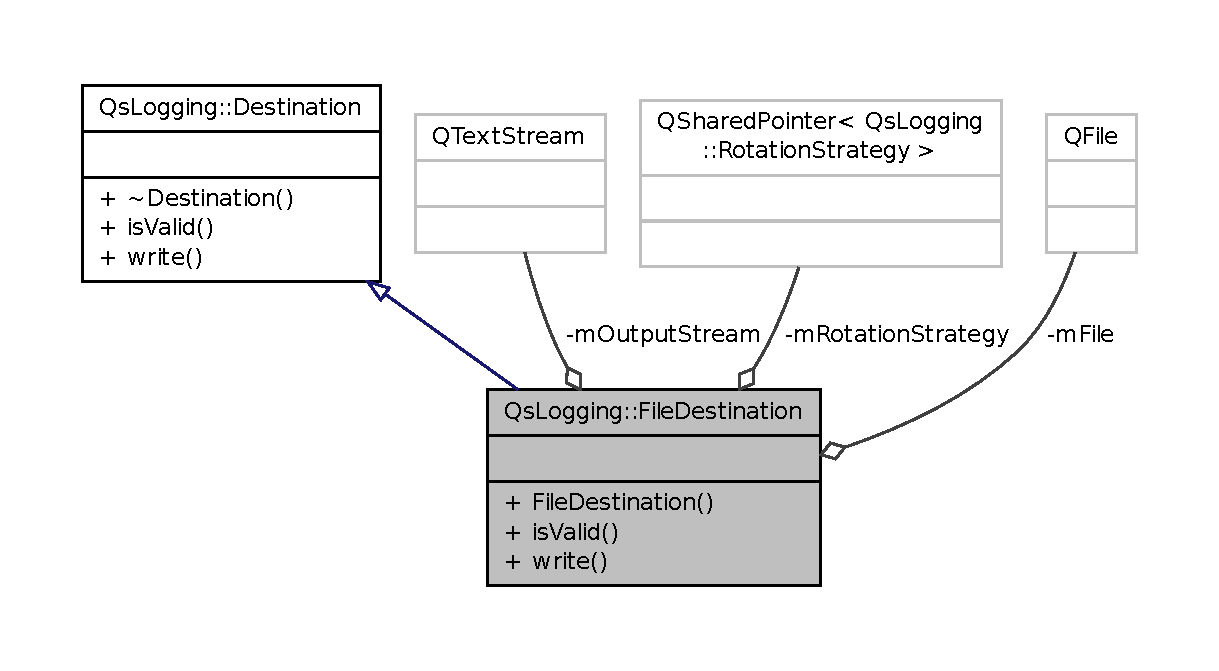
\includegraphics[width=350pt]{classQsLogging_1_1FileDestination__coll__graph}
\end{center}
\end{figure}
\subsection*{Fonctions membres publiques}
\begin{DoxyCompactItemize}
\item 
\hyperlink{classQsLogging_1_1FileDestination_ad42d6551d58f82eeb61ffc6d7d06d5cd}{File\-Destination} (const Q\-String \&file\-Path, \hyperlink{namespaceQsLogging_a41dc81d39cd3d36d9e15746bd9174be0}{Rotation\-Strategy\-Ptr} rotation\-Strategy)
\begin{DoxyCompactList}\small\item\em \hyperlink{classQsLogging_1_1FileDestination}{File\-Destination}. \end{DoxyCompactList}\item 
virtual bool \hyperlink{classQsLogging_1_1FileDestination_a2d18b70b408910332dcbee9d12c1d394}{is\-Valid} ()
\begin{DoxyCompactList}\small\item\em is\-Valid \end{DoxyCompactList}\item 
virtual void \hyperlink{classQsLogging_1_1FileDestination_a84b076720ccfa4045e1aacc14c5af5dc}{write} (const Q\-String \&message, \hyperlink{namespaceQsLogging_a38c7dd87e4de6f8eb460763ad0baa033}{Level} level)
\begin{DoxyCompactList}\small\item\em write \end{DoxyCompactList}\end{DoxyCompactItemize}
\subsection*{Attributs privés}
\begin{DoxyCompactItemize}
\item 
Q\-File \hyperlink{classQsLogging_1_1FileDestination_a1de182fa4efefa21e6545757f1a04eb2}{m\-File}
\begin{DoxyCompactList}\small\item\em m\-File \end{DoxyCompactList}\item 
Q\-Text\-Stream \hyperlink{classQsLogging_1_1FileDestination_a10f0aa5513ec40d3e362179b084a43d6}{m\-Output\-Stream}
\begin{DoxyCompactList}\small\item\em m\-Output\-Stream \end{DoxyCompactList}\item 
Q\-Shared\-Pointer$<$ \hyperlink{classQsLogging_1_1RotationStrategy}{Rotation\-Strategy} $>$ \hyperlink{classQsLogging_1_1FileDestination_ab20945842bd063b5cbe82485168be1f0}{m\-Rotation\-Strategy}
\begin{DoxyCompactList}\small\item\em m\-Rotation\-Strategy \end{DoxyCompactList}\end{DoxyCompactItemize}


\subsection{Description détaillée}
The \hyperlink{classQsLogging_1_1FileDestination}{File\-Destination} class. 

Définition à la ligne \hyperlink{QsLogDestFile_8h_source_l00181}{181} du fichier \hyperlink{QsLogDestFile_8h_source}{Qs\-Log\-Dest\-File.\-h}.



\subsection{Documentation des constructeurs et destructeur}
\hypertarget{classQsLogging_1_1FileDestination_ad42d6551d58f82eeb61ffc6d7d06d5cd}{\index{Qs\-Logging\-::\-File\-Destination@{Qs\-Logging\-::\-File\-Destination}!File\-Destination@{File\-Destination}}
\index{File\-Destination@{File\-Destination}!QsLogging::FileDestination@{Qs\-Logging\-::\-File\-Destination}}
\subsubsection[{File\-Destination}]{\setlength{\rightskip}{0pt plus 5cm}Qs\-Logging\-::\-File\-Destination\-::\-File\-Destination (
\begin{DoxyParamCaption}
\item[{const Q\-String \&}]{file\-Path, }
\item[{{\bf Rotation\-Strategy\-Ptr}}]{rotation\-Strategy}
\end{DoxyParamCaption}
)}}\label{classQsLogging_1_1FileDestination_ad42d6551d58f82eeb61ffc6d7d06d5cd}


\hyperlink{classQsLogging_1_1FileDestination}{File\-Destination}. 


\begin{DoxyParams}{Paramètres}
{\em file\-Path} & \\
\hline
{\em rotation\-Strategy} & \hyperlink{classQsLogging_1_1FileDestination_ad42d6551d58f82eeb61ffc6d7d06d5cd}{Qs\-Logging\-::\-File\-Destination\-::\-File\-Destination} \\
\hline
\end{DoxyParams}


Définition à la ligne \hyperlink{QsLogDestFile_8cpp_source_l00145}{145} du fichier \hyperlink{QsLogDestFile_8cpp_source}{Qs\-Log\-Dest\-File.\-cpp}.



Références \hyperlink{classQsLogging_1_1FileDestination_a1de182fa4efefa21e6545757f1a04eb2}{m\-File}, \hyperlink{classQsLogging_1_1FileDestination_a10f0aa5513ec40d3e362179b084a43d6}{m\-Output\-Stream}, et \hyperlink{classQsLogging_1_1FileDestination_ab20945842bd063b5cbe82485168be1f0}{m\-Rotation\-Strategy}.


\begin{DoxyCode}
00146     : \hyperlink{classQsLogging_1_1FileDestination_ab20945842bd063b5cbe82485168be1f0}{mRotationStrategy}(rotationStrategy)
00147 \{
00148     \hyperlink{classQsLogging_1_1FileDestination_a1de182fa4efefa21e6545757f1a04eb2}{mFile}.setFileName(filePath);
00149     \textcolor{keywordflow}{if} (!\hyperlink{classQsLogging_1_1FileDestination_a1de182fa4efefa21e6545757f1a04eb2}{mFile}.open(QFile::WriteOnly | QFile::Text | \hyperlink{classQsLogging_1_1FileDestination_ab20945842bd063b5cbe82485168be1f0}{mRotationStrategy}->
      recommendedOpenModeFlag()))
00150         std::cerr << \textcolor{stringliteral}{"QsLog: could not open log file "} << qPrintable(filePath);
00151     \hyperlink{classQsLogging_1_1FileDestination_a10f0aa5513ec40d3e362179b084a43d6}{mOutputStream}.setDevice(&\hyperlink{classQsLogging_1_1FileDestination_a1de182fa4efefa21e6545757f1a04eb2}{mFile});
00152     \hyperlink{classQsLogging_1_1FileDestination_a10f0aa5513ec40d3e362179b084a43d6}{mOutputStream}.setCodec(QTextCodec::codecForName(\textcolor{stringliteral}{"UTF-8"}));
00153 
00154     \hyperlink{classQsLogging_1_1FileDestination_ab20945842bd063b5cbe82485168be1f0}{mRotationStrategy}->setInitialInfo(\hyperlink{classQsLogging_1_1FileDestination_a1de182fa4efefa21e6545757f1a04eb2}{mFile});
00155 \}
\end{DoxyCode}


\subsection{Documentation des fonctions membres}
\hypertarget{classQsLogging_1_1FileDestination_a2d18b70b408910332dcbee9d12c1d394}{\index{Qs\-Logging\-::\-File\-Destination@{Qs\-Logging\-::\-File\-Destination}!is\-Valid@{is\-Valid}}
\index{is\-Valid@{is\-Valid}!QsLogging::FileDestination@{Qs\-Logging\-::\-File\-Destination}}
\subsubsection[{is\-Valid}]{\setlength{\rightskip}{0pt plus 5cm}bool Qs\-Logging\-::\-File\-Destination\-::is\-Valid (
\begin{DoxyParamCaption}
{}
\end{DoxyParamCaption}
)\hspace{0.3cm}{\ttfamily [virtual]}}}\label{classQsLogging_1_1FileDestination_a2d18b70b408910332dcbee9d12c1d394}


is\-Valid 

\begin{DoxyReturn}{Renvoie}

\end{DoxyReturn}
\hyperlink{classQsLogging_1_1FileDestination_a2d18b70b408910332dcbee9d12c1d394}{Qs\-Logging\-::\-File\-Destination\-::is\-Valid} 

Implémente \hyperlink{classQsLogging_1_1Destination_acb3dd81553c59aec5062ec8556b3b407}{Qs\-Logging\-::\-Destination}.



Définition à la ligne \hyperlink{QsLogDestFile_8cpp_source_l00178}{178} du fichier \hyperlink{QsLogDestFile_8cpp_source}{Qs\-Log\-Dest\-File.\-cpp}.


\begin{DoxyCode}
00179 \{
00180     \textcolor{keywordflow}{return} \hyperlink{classQsLogging_1_1FileDestination_a1de182fa4efefa21e6545757f1a04eb2}{mFile}.isOpen();
00181 \}
\end{DoxyCode}
\hypertarget{classQsLogging_1_1FileDestination_a84b076720ccfa4045e1aacc14c5af5dc}{\index{Qs\-Logging\-::\-File\-Destination@{Qs\-Logging\-::\-File\-Destination}!write@{write}}
\index{write@{write}!QsLogging::FileDestination@{Qs\-Logging\-::\-File\-Destination}}
\subsubsection[{write}]{\setlength{\rightskip}{0pt plus 5cm}void Qs\-Logging\-::\-File\-Destination\-::write (
\begin{DoxyParamCaption}
\item[{const Q\-String \&}]{message, }
\item[{{\bf Level}}]{level}
\end{DoxyParamCaption}
)\hspace{0.3cm}{\ttfamily [virtual]}}}\label{classQsLogging_1_1FileDestination_a84b076720ccfa4045e1aacc14c5af5dc}


write 


\begin{DoxyParams}{Paramètres}
{\em message} & \\
\hline
{\em level} & \hyperlink{classQsLogging_1_1FileDestination_a84b076720ccfa4045e1aacc14c5af5dc}{Qs\-Logging\-::\-File\-Destination\-::write} \\
\hline
\end{DoxyParams}


Implémente \hyperlink{classQsLogging_1_1Destination_a19306b28686d599f49bb23f88824fd65}{Qs\-Logging\-::\-Destination}.



Définition à la ligne \hyperlink{QsLogDestFile_8cpp_source_l00159}{159} du fichier \hyperlink{QsLogDestFile_8cpp_source}{Qs\-Log\-Dest\-File.\-cpp}.


\begin{DoxyCode}
00160 \{
00161     \hyperlink{classQsLogging_1_1FileDestination_ab20945842bd063b5cbe82485168be1f0}{mRotationStrategy}->includeMessageInCalculation(message);
00162     \textcolor{keywordflow}{if} (\hyperlink{classQsLogging_1_1FileDestination_ab20945842bd063b5cbe82485168be1f0}{mRotationStrategy}->shouldRotate()) \{
00163         \hyperlink{classQsLogging_1_1FileDestination_a10f0aa5513ec40d3e362179b084a43d6}{mOutputStream}.setDevice(NULL);
00164         \hyperlink{classQsLogging_1_1FileDestination_a1de182fa4efefa21e6545757f1a04eb2}{mFile}.close();
00165         \hyperlink{classQsLogging_1_1FileDestination_ab20945842bd063b5cbe82485168be1f0}{mRotationStrategy}->rotate();
00166         \textcolor{keywordflow}{if} (!\hyperlink{classQsLogging_1_1FileDestination_a1de182fa4efefa21e6545757f1a04eb2}{mFile}.open(QFile::WriteOnly | QFile::Text | \hyperlink{classQsLogging_1_1FileDestination_ab20945842bd063b5cbe82485168be1f0}{mRotationStrategy}->
      recommendedOpenModeFlag()))
00167             std::cerr << \textcolor{stringliteral}{"QsLog: could not reopen log file "} << qPrintable(\hyperlink{classQsLogging_1_1FileDestination_a1de182fa4efefa21e6545757f1a04eb2}{mFile}.fileName());
00168         \hyperlink{classQsLogging_1_1FileDestination_ab20945842bd063b5cbe82485168be1f0}{mRotationStrategy}->setInitialInfo(\hyperlink{classQsLogging_1_1FileDestination_a1de182fa4efefa21e6545757f1a04eb2}{mFile});
00169         \hyperlink{classQsLogging_1_1FileDestination_a10f0aa5513ec40d3e362179b084a43d6}{mOutputStream}.setDevice(&\hyperlink{classQsLogging_1_1FileDestination_a1de182fa4efefa21e6545757f1a04eb2}{mFile});
00170     \}
00171 
00172     \hyperlink{classQsLogging_1_1FileDestination_a10f0aa5513ec40d3e362179b084a43d6}{mOutputStream} << message << endl;
00173     \hyperlink{classQsLogging_1_1FileDestination_a10f0aa5513ec40d3e362179b084a43d6}{mOutputStream}.flush();
00174 \}
\end{DoxyCode}


\subsection{Documentation des données membres}
\hypertarget{classQsLogging_1_1FileDestination_a1de182fa4efefa21e6545757f1a04eb2}{\index{Qs\-Logging\-::\-File\-Destination@{Qs\-Logging\-::\-File\-Destination}!m\-File@{m\-File}}
\index{m\-File@{m\-File}!QsLogging::FileDestination@{Qs\-Logging\-::\-File\-Destination}}
\subsubsection[{m\-File}]{\setlength{\rightskip}{0pt plus 5cm}Q\-File Qs\-Logging\-::\-File\-Destination\-::m\-File\hspace{0.3cm}{\ttfamily [private]}}}\label{classQsLogging_1_1FileDestination_a1de182fa4efefa21e6545757f1a04eb2}


m\-File 



Définition à la ligne \hyperlink{QsLogDestFile_8h_source_l00206}{206} du fichier \hyperlink{QsLogDestFile_8h_source}{Qs\-Log\-Dest\-File.\-h}.



Référencé par \hyperlink{classQsLogging_1_1FileDestination_ad42d6551d58f82eeb61ffc6d7d06d5cd}{File\-Destination()}.

\hypertarget{classQsLogging_1_1FileDestination_a10f0aa5513ec40d3e362179b084a43d6}{\index{Qs\-Logging\-::\-File\-Destination@{Qs\-Logging\-::\-File\-Destination}!m\-Output\-Stream@{m\-Output\-Stream}}
\index{m\-Output\-Stream@{m\-Output\-Stream}!QsLogging::FileDestination@{Qs\-Logging\-::\-File\-Destination}}
\subsubsection[{m\-Output\-Stream}]{\setlength{\rightskip}{0pt plus 5cm}Q\-Text\-Stream Qs\-Logging\-::\-File\-Destination\-::m\-Output\-Stream\hspace{0.3cm}{\ttfamily [private]}}}\label{classQsLogging_1_1FileDestination_a10f0aa5513ec40d3e362179b084a43d6}


m\-Output\-Stream 



Définition à la ligne \hyperlink{QsLogDestFile_8h_source_l00210}{210} du fichier \hyperlink{QsLogDestFile_8h_source}{Qs\-Log\-Dest\-File.\-h}.



Référencé par \hyperlink{classQsLogging_1_1FileDestination_ad42d6551d58f82eeb61ffc6d7d06d5cd}{File\-Destination()}.

\hypertarget{classQsLogging_1_1FileDestination_ab20945842bd063b5cbe82485168be1f0}{\index{Qs\-Logging\-::\-File\-Destination@{Qs\-Logging\-::\-File\-Destination}!m\-Rotation\-Strategy@{m\-Rotation\-Strategy}}
\index{m\-Rotation\-Strategy@{m\-Rotation\-Strategy}!QsLogging::FileDestination@{Qs\-Logging\-::\-File\-Destination}}
\subsubsection[{m\-Rotation\-Strategy}]{\setlength{\rightskip}{0pt plus 5cm}Q\-Shared\-Pointer$<${\bf Rotation\-Strategy}$>$ Qs\-Logging\-::\-File\-Destination\-::m\-Rotation\-Strategy\hspace{0.3cm}{\ttfamily [private]}}}\label{classQsLogging_1_1FileDestination_ab20945842bd063b5cbe82485168be1f0}


m\-Rotation\-Strategy 



Définition à la ligne \hyperlink{QsLogDestFile_8h_source_l00214}{214} du fichier \hyperlink{QsLogDestFile_8h_source}{Qs\-Log\-Dest\-File.\-h}.



Référencé par \hyperlink{classQsLogging_1_1FileDestination_ad42d6551d58f82eeb61ffc6d7d06d5cd}{File\-Destination()}.



La documentation de cette classe a été générée à partir des fichiers suivants \-:\begin{DoxyCompactItemize}
\item 
logging/\hyperlink{QsLogDestFile_8h}{Qs\-Log\-Dest\-File.\-h}\item 
logging/\hyperlink{QsLogDestFile_8cpp}{Qs\-Log\-Dest\-File.\-cpp}\end{DoxyCompactItemize}

\hypertarget{classQsLogging_1_1Logger}{\section{Référence de la classe Qs\-Logging\-:\-:Logger}
\label{classQsLogging_1_1Logger}\index{Qs\-Logging\-::\-Logger@{Qs\-Logging\-::\-Logger}}
}


{\ttfamily \#include $<$Qs\-Log.\-h$>$}



Graphe de collaboration de Qs\-Logging\-:\-:Logger\-:
\nopagebreak
\begin{figure}[H]
\begin{center}
\leavevmode
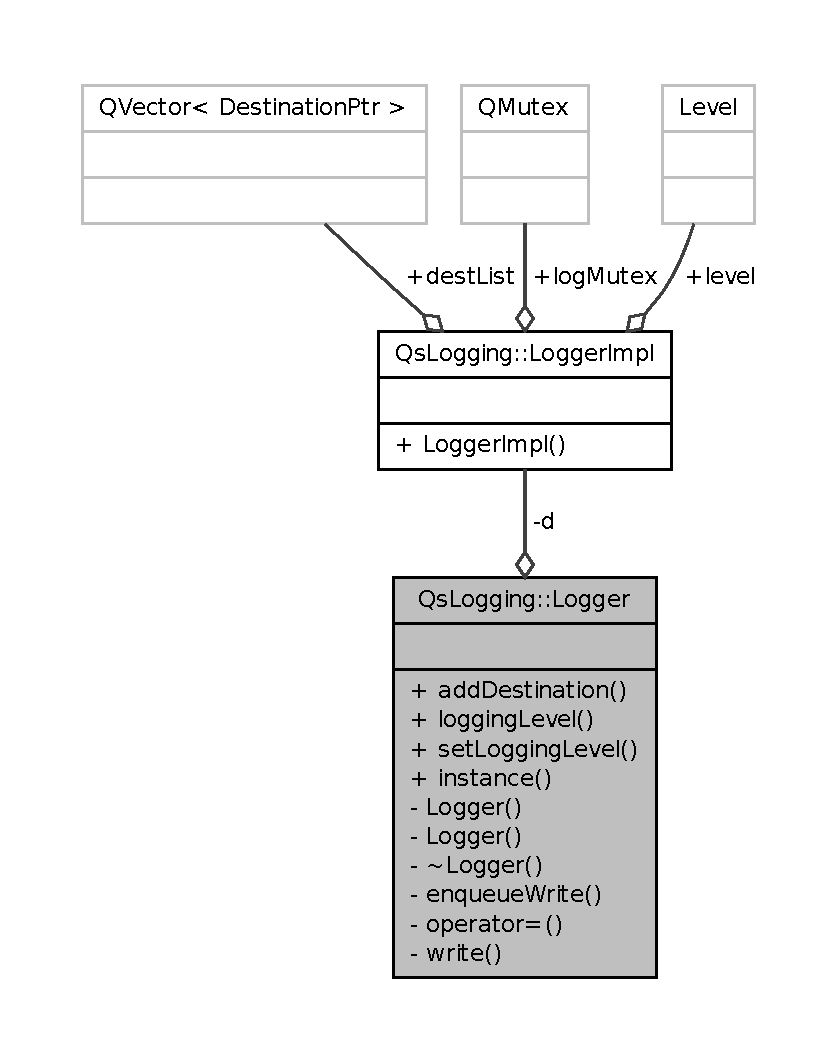
\includegraphics[width=350pt]{classQsLogging_1_1Logger__coll__graph}
\end{center}
\end{figure}
\subsection*{Classes}
\begin{DoxyCompactItemize}
\item 
class \hyperlink{classQsLogging_1_1Logger_1_1Helper}{Helper}
\end{DoxyCompactItemize}
\subsection*{Fonctions membres publiques}
\begin{DoxyCompactItemize}
\item 
void \hyperlink{classQsLogging_1_1Logger_a76a32c839e837547b14bc5e523b4aa45}{add\-Destination} (\hyperlink{namespaceQsLogging_a8fe41cf859d617f1c23515f804d1e8ec}{Destination\-Ptr} destination)
\item 
\hyperlink{namespaceQsLogging_a38c7dd87e4de6f8eb460763ad0baa033}{Level} \hyperlink{classQsLogging_1_1Logger_a5e2b29cf6cd066f1e64eaa4db7373458}{logging\-Level} () const 
\item 
void \hyperlink{classQsLogging_1_1Logger_aa34d1a0d83e180f15e23a03f9de872c6}{set\-Logging\-Level} (\hyperlink{namespaceQsLogging_a38c7dd87e4de6f8eb460763ad0baa033}{Level} new\-Level)
\end{DoxyCompactItemize}
\subsection*{Fonctions membres publiques statiques}
\begin{DoxyCompactItemize}
\item 
static \hyperlink{classQsLogging_1_1Logger}{Logger} \& \hyperlink{classQsLogging_1_1Logger_a26fd3242d362eeeb3b38940a714ea6fa}{instance} ()
\end{DoxyCompactItemize}
\subsection*{Fonctions membres privées}
\begin{DoxyCompactItemize}
\item 
\hyperlink{classQsLogging_1_1Logger_ac9f74e9b0b16e9110386edb0c6eca541}{Logger} ()
\item 
\hyperlink{classQsLogging_1_1Logger_ab7222678ba738772cf06f997243b3d1d}{Logger} (const \hyperlink{classQsLogging_1_1Logger}{Logger} \&)
\item 
\hyperlink{classQsLogging_1_1Logger_a0947daaf6db4f83ba6e5fe155fa84e1f}{$\sim$\-Logger} ()
\item 
void \hyperlink{classQsLogging_1_1Logger_acd6d5d16d6e111eaa960807d75549bf9}{enqueue\-Write} (const Q\-String \&message, \hyperlink{namespaceQsLogging_a38c7dd87e4de6f8eb460763ad0baa033}{Level} level)
\item 
\hyperlink{classQsLogging_1_1Logger}{Logger} \& \hyperlink{classQsLogging_1_1Logger_a1a82528a35b99a5a00b42149ee75be2e}{operator=} (const \hyperlink{classQsLogging_1_1Logger}{Logger} \&)
\item 
void \hyperlink{classQsLogging_1_1Logger_ab9789bba5f1644a3b3b51606533aa20f}{write} (const Q\-String \&message, \hyperlink{namespaceQsLogging_a38c7dd87e4de6f8eb460763ad0baa033}{Level} level)
\end{DoxyCompactItemize}
\subsection*{Attributs privés}
\begin{DoxyCompactItemize}
\item 
\hyperlink{classQsLogging_1_1LoggerImpl}{Logger\-Impl} $\ast$ \hyperlink{classQsLogging_1_1Logger_aab634416e14e5cb4ca3193dc5a9924fa}{d}
\end{DoxyCompactItemize}
\subsection*{Amis}
\begin{DoxyCompactItemize}
\item 
class \hyperlink{classQsLogging_1_1Logger_a27d33fe348fa48f5be163ad876cdb699}{Log\-Writer\-Runnable}
\end{DoxyCompactItemize}


\subsection{Description détaillée}


Définition à la ligne \hyperlink{QsLog_8h_source_l00069}{69} du fichier \hyperlink{QsLog_8h_source}{Qs\-Log.\-h}.



\subsection{Documentation des constructeurs et destructeur}
\hypertarget{classQsLogging_1_1Logger_ac9f74e9b0b16e9110386edb0c6eca541}{\index{Qs\-Logging\-::\-Logger@{Qs\-Logging\-::\-Logger}!Logger@{Logger}}
\index{Logger@{Logger}!QsLogging::Logger@{Qs\-Logging\-::\-Logger}}
\subsubsection[{Logger}]{\setlength{\rightskip}{0pt plus 5cm}Qs\-Logging\-::\-Logger\-::\-Logger (
\begin{DoxyParamCaption}
{}
\end{DoxyParamCaption}
)\hspace{0.3cm}{\ttfamily [private]}}}\label{classQsLogging_1_1Logger_ac9f74e9b0b16e9110386edb0c6eca541}


Définition à la ligne \hyperlink{QsLog_8cpp_source_l00200}{200} du fichier \hyperlink{QsLog_8cpp_source}{Qs\-Log.\-cpp}.


\begin{DoxyCode}
00200                :
00201     \hyperlink{classQsLogging_1_1Logger_aab634416e14e5cb4ca3193dc5a9924fa}{d}(\textcolor{keyword}{new} LoggerImpl)
00202 \{
00203 \}
\end{DoxyCode}
\hypertarget{classQsLogging_1_1Logger_ab7222678ba738772cf06f997243b3d1d}{\index{Qs\-Logging\-::\-Logger@{Qs\-Logging\-::\-Logger}!Logger@{Logger}}
\index{Logger@{Logger}!QsLogging::Logger@{Qs\-Logging\-::\-Logger}}
\subsubsection[{Logger}]{\setlength{\rightskip}{0pt plus 5cm}Qs\-Logging\-::\-Logger\-::\-Logger (
\begin{DoxyParamCaption}
\item[{const {\bf Logger} \&}]{}
\end{DoxyParamCaption}
)\hspace{0.3cm}{\ttfamily [private]}}}\label{classQsLogging_1_1Logger_ab7222678ba738772cf06f997243b3d1d}
\hypertarget{classQsLogging_1_1Logger_a0947daaf6db4f83ba6e5fe155fa84e1f}{\index{Qs\-Logging\-::\-Logger@{Qs\-Logging\-::\-Logger}!$\sim$\-Logger@{$\sim$\-Logger}}
\index{$\sim$\-Logger@{$\sim$\-Logger}!QsLogging::Logger@{Qs\-Logging\-::\-Logger}}
\subsubsection[{$\sim$\-Logger}]{\setlength{\rightskip}{0pt plus 5cm}{\bf S\-H\-\_\-} Qs\-Logging\-::\-Logger\-::$\sim$\-Logger (
\begin{DoxyParamCaption}
{}
\end{DoxyParamCaption}
)\hspace{0.3cm}{\ttfamily [private]}}}\label{classQsLogging_1_1Logger_a0947daaf6db4f83ba6e5fe155fa84e1f}


Définition à la ligne \hyperlink{QsLog_8cpp_source_l00207}{207} du fichier \hyperlink{QsLog_8cpp_source}{Qs\-Log.\-cpp}.



Références \hyperlink{classQsLogging_1_1Logger_aab634416e14e5cb4ca3193dc5a9924fa}{d}.


\begin{DoxyCode}
00208 \{
00209     \textcolor{keyword}{delete} \hyperlink{classQsLogging_1_1Logger_aab634416e14e5cb4ca3193dc5a9924fa}{d};
00210 \}
\end{DoxyCode}


\subsection{Documentation des fonctions membres}
\hypertarget{classQsLogging_1_1Logger_a76a32c839e837547b14bc5e523b4aa45}{\index{Qs\-Logging\-::\-Logger@{Qs\-Logging\-::\-Logger}!add\-Destination@{add\-Destination}}
\index{add\-Destination@{add\-Destination}!QsLogging::Logger@{Qs\-Logging\-::\-Logger}}
\subsubsection[{add\-Destination}]{\setlength{\rightskip}{0pt plus 5cm}void Qs\-Logging\-::\-Logger\-::add\-Destination (
\begin{DoxyParamCaption}
\item[{{\bf Destination\-Ptr}}]{destination}
\end{DoxyParamCaption}
)}}\label{classQsLogging_1_1Logger_a76a32c839e837547b14bc5e523b4aa45}


Définition à la ligne \hyperlink{QsLog_8cpp_source_l00214}{214} du fichier \hyperlink{QsLog_8cpp_source}{Qs\-Log.\-cpp}.



Références \hyperlink{classQsLogging_1_1Logger_aab634416e14e5cb4ca3193dc5a9924fa}{d}, et \hyperlink{classQsLogging_1_1LoggerImpl_acdbde93fec67bd0bcce8da1fc1080ece}{Qs\-Logging\-::\-Logger\-Impl\-::dest\-List}.



Référencé par \hyperlink{main_8cpp_ac3c79e35c4fc5c50939ae90485e1483f}{enable\-Logging()}.


\begin{DoxyCode}
00215 \{
00216     assert(destination.data());
00217     \hyperlink{classQsLogging_1_1Logger_aab634416e14e5cb4ca3193dc5a9924fa}{d}->\hyperlink{classQsLogging_1_1LoggerImpl_acdbde93fec67bd0bcce8da1fc1080ece}{destList}.push\_back(destination);
00218 \}
\end{DoxyCode}


Voici le graphe des appelants de cette fonction \-:
\nopagebreak
\begin{figure}[H]
\begin{center}
\leavevmode
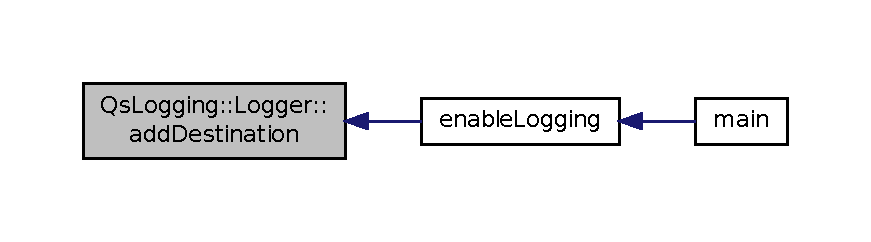
\includegraphics[width=350pt]{classQsLogging_1_1Logger_a76a32c839e837547b14bc5e523b4aa45_icgraph}
\end{center}
\end{figure}


\hypertarget{classQsLogging_1_1Logger_acd6d5d16d6e111eaa960807d75549bf9}{\index{Qs\-Logging\-::\-Logger@{Qs\-Logging\-::\-Logger}!enqueue\-Write@{enqueue\-Write}}
\index{enqueue\-Write@{enqueue\-Write}!QsLogging::Logger@{Qs\-Logging\-::\-Logger}}
\subsubsection[{enqueue\-Write}]{\setlength{\rightskip}{0pt plus 5cm}void Qs\-Logging\-::\-Logger\-::enqueue\-Write (
\begin{DoxyParamCaption}
\item[{const Q\-String \&}]{message, }
\item[{{\bf Level}}]{level}
\end{DoxyParamCaption}
)\hspace{0.3cm}{\ttfamily [private]}}}\label{classQsLogging_1_1Logger_acd6d5d16d6e111eaa960807d75549bf9}


Définition à la ligne \hyperlink{QsLog_8cpp_source_l00269}{269} du fichier \hyperlink{QsLog_8cpp_source}{Qs\-Log.\-cpp}.



Références \hyperlink{classQsLogging_1_1Logger_aab634416e14e5cb4ca3193dc5a9924fa}{d}, \hyperlink{classQsLogging_1_1LoggerImpl_a8feaba4a7a7160106987943313804c35}{Qs\-Logging\-::\-Logger\-Impl\-::log\-Mutex}, \hyperlink{classQsLogging_1_1Logger_a27d33fe348fa48f5be163ad876cdb699}{Log\-Writer\-Runnable}, et \hyperlink{classQsLogging_1_1Logger_ab9789bba5f1644a3b3b51606533aa20f}{write()}.



Référencé par \hyperlink{classQsLogging_1_1Logger_1_1Helper_a30e01167d1f088bade18b71a3e85379b}{Qs\-Logging\-::\-Logger\-::\-Helper\-::write\-To\-Log()}.


\begin{DoxyCode}
00270 \{
00271 \textcolor{preprocessor}{#ifdef QS\_LOG\_SEPARATE\_THREAD}
00272 \textcolor{preprocessor}{}    \hyperlink{classQsLogging_1_1Logger_a27d33fe348fa48f5be163ad876cdb699}{LogWriterRunnable} *r = \textcolor{keyword}{new} \hyperlink{classQsLogging_1_1Logger_a27d33fe348fa48f5be163ad876cdb699}{LogWriterRunnable}(message, level);
00273     \hyperlink{classQsLogging_1_1Logger_aab634416e14e5cb4ca3193dc5a9924fa}{d}->threadPool.start(r);
00274 \textcolor{preprocessor}{#else}
00275 \textcolor{preprocessor}{}    QMutexLocker lock(&\hyperlink{classQsLogging_1_1Logger_aab634416e14e5cb4ca3193dc5a9924fa}{d}->\hyperlink{classQsLogging_1_1LoggerImpl_a8feaba4a7a7160106987943313804c35}{logMutex});
00276     \hyperlink{classQsLogging_1_1Logger_ab9789bba5f1644a3b3b51606533aa20f}{write}(message, level);
00277 \textcolor{preprocessor}{#endif}
00278 \textcolor{preprocessor}{}\}
\end{DoxyCode}


Voici le graphe d'appel pour cette fonction \-:
\nopagebreak
\begin{figure}[H]
\begin{center}
\leavevmode
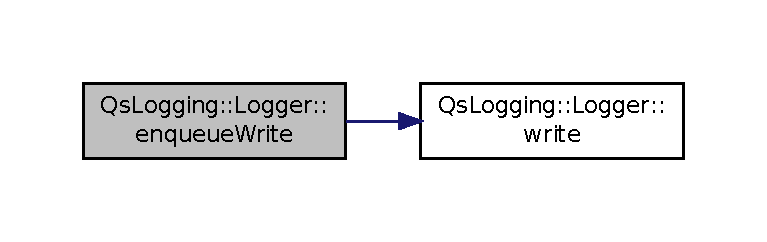
\includegraphics[width=350pt]{classQsLogging_1_1Logger_acd6d5d16d6e111eaa960807d75549bf9_cgraph}
\end{center}
\end{figure}




Voici le graphe des appelants de cette fonction \-:
\nopagebreak
\begin{figure}[H]
\begin{center}
\leavevmode
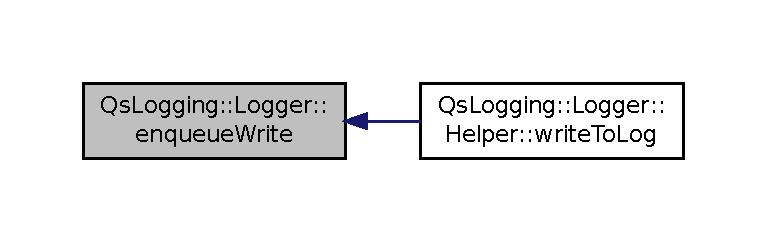
\includegraphics[width=350pt]{classQsLogging_1_1Logger_acd6d5d16d6e111eaa960807d75549bf9_icgraph}
\end{center}
\end{figure}


\hypertarget{classQsLogging_1_1Logger_a26fd3242d362eeeb3b38940a714ea6fa}{\index{Qs\-Logging\-::\-Logger@{Qs\-Logging\-::\-Logger}!instance@{instance}}
\index{instance@{instance}!QsLogging::Logger@{Qs\-Logging\-::\-Logger}}
\subsubsection[{instance}]{\setlength{\rightskip}{0pt plus 5cm}static {\bf Logger}\& Qs\-Logging\-::\-Logger\-::instance (
\begin{DoxyParamCaption}
{}
\end{DoxyParamCaption}
)\hspace{0.3cm}{\ttfamily [inline]}, {\ttfamily [static]}}}\label{classQsLogging_1_1Logger_a26fd3242d362eeeb3b38940a714ea6fa}


Définition à la ligne \hyperlink{QsLog_8h_source_l00078}{78} du fichier \hyperlink{QsLog_8h_source}{Qs\-Log.\-h}.



Référencé par \hyperlink{main_8cpp_ac3c79e35c4fc5c50939ae90485e1483f}{enable\-Logging()}, et \hyperlink{classQsLogging_1_1Logger_1_1Helper_a30e01167d1f088bade18b71a3e85379b}{Qs\-Logging\-::\-Logger\-::\-Helper\-::write\-To\-Log()}.


\begin{DoxyCode}
00079     \{
00080         \textcolor{keyword}{static} \hyperlink{classQsLogging_1_1Logger_ac9f74e9b0b16e9110386edb0c6eca541}{Logger} staticLog;
00081         \textcolor{keywordflow}{return} staticLog;
00082     \}
\end{DoxyCode}


Voici le graphe des appelants de cette fonction \-:
\nopagebreak
\begin{figure}[H]
\begin{center}
\leavevmode
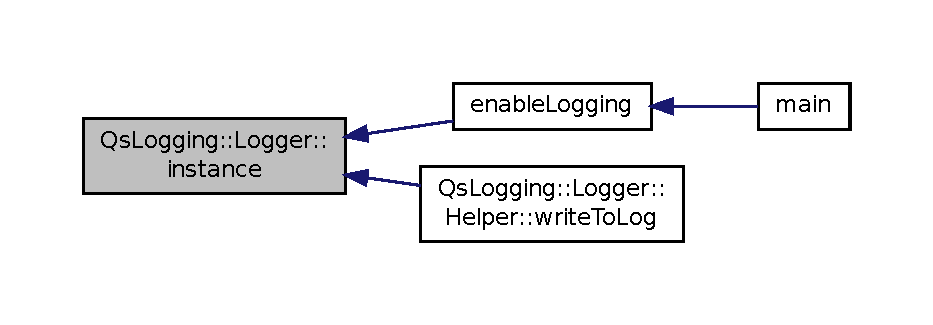
\includegraphics[width=350pt]{classQsLogging_1_1Logger_a26fd3242d362eeeb3b38940a714ea6fa_icgraph}
\end{center}
\end{figure}


\hypertarget{classQsLogging_1_1Logger_a5e2b29cf6cd066f1e64eaa4db7373458}{\index{Qs\-Logging\-::\-Logger@{Qs\-Logging\-::\-Logger}!logging\-Level@{logging\-Level}}
\index{logging\-Level@{logging\-Level}!QsLogging::Logger@{Qs\-Logging\-::\-Logger}}
\subsubsection[{logging\-Level}]{\setlength{\rightskip}{0pt plus 5cm}{\bf Level} Qs\-Logging\-::\-Logger\-::logging\-Level (
\begin{DoxyParamCaption}
{}
\end{DoxyParamCaption}
) const}}\label{classQsLogging_1_1Logger_a5e2b29cf6cd066f1e64eaa4db7373458}


Définition à la ligne \hyperlink{QsLog_8cpp_source_l00229}{229} du fichier \hyperlink{QsLog_8cpp_source}{Qs\-Log.\-cpp}.



Références \hyperlink{classQsLogging_1_1Logger_aab634416e14e5cb4ca3193dc5a9924fa}{d}, et \hyperlink{classQsLogging_1_1LoggerImpl_a4d3c9f4b81baa52df759b6d07bda0a69}{Qs\-Logging\-::\-Logger\-Impl\-::level}.


\begin{DoxyCode}
00230 \{
00231     \textcolor{keywordflow}{return} \hyperlink{classQsLogging_1_1Logger_aab634416e14e5cb4ca3193dc5a9924fa}{d}->\hyperlink{classQsLogging_1_1LoggerImpl_a4d3c9f4b81baa52df759b6d07bda0a69}{level};
00232 \}
\end{DoxyCode}
\hypertarget{classQsLogging_1_1Logger_a1a82528a35b99a5a00b42149ee75be2e}{\index{Qs\-Logging\-::\-Logger@{Qs\-Logging\-::\-Logger}!operator=@{operator=}}
\index{operator=@{operator=}!QsLogging::Logger@{Qs\-Logging\-::\-Logger}}
\subsubsection[{operator=}]{\setlength{\rightskip}{0pt plus 5cm}{\bf Logger}\& Qs\-Logging\-::\-Logger\-::operator= (
\begin{DoxyParamCaption}
\item[{const {\bf Logger} \&}]{}
\end{DoxyParamCaption}
)\hspace{0.3cm}{\ttfamily [private]}}}\label{classQsLogging_1_1Logger_a1a82528a35b99a5a00b42149ee75be2e}
\hypertarget{classQsLogging_1_1Logger_aa34d1a0d83e180f15e23a03f9de872c6}{\index{Qs\-Logging\-::\-Logger@{Qs\-Logging\-::\-Logger}!set\-Logging\-Level@{set\-Logging\-Level}}
\index{set\-Logging\-Level@{set\-Logging\-Level}!QsLogging::Logger@{Qs\-Logging\-::\-Logger}}
\subsubsection[{set\-Logging\-Level}]{\setlength{\rightskip}{0pt plus 5cm}void Qs\-Logging\-::\-Logger\-::set\-Logging\-Level (
\begin{DoxyParamCaption}
\item[{{\bf Level}}]{new\-Level}
\end{DoxyParamCaption}
)}}\label{classQsLogging_1_1Logger_aa34d1a0d83e180f15e23a03f9de872c6}


Définition à la ligne \hyperlink{QsLog_8cpp_source_l00222}{222} du fichier \hyperlink{QsLog_8cpp_source}{Qs\-Log.\-cpp}.



Références \hyperlink{classQsLogging_1_1Logger_aab634416e14e5cb4ca3193dc5a9924fa}{d}, et \hyperlink{classQsLogging_1_1LoggerImpl_a4d3c9f4b81baa52df759b6d07bda0a69}{Qs\-Logging\-::\-Logger\-Impl\-::level}.



Référencé par \hyperlink{main_8cpp_ac3c79e35c4fc5c50939ae90485e1483f}{enable\-Logging()}.


\begin{DoxyCode}
00223 \{
00224     \hyperlink{classQsLogging_1_1Logger_aab634416e14e5cb4ca3193dc5a9924fa}{d}->\hyperlink{classQsLogging_1_1LoggerImpl_a4d3c9f4b81baa52df759b6d07bda0a69}{level} = newLevel;
00225 \}
\end{DoxyCode}


Voici le graphe des appelants de cette fonction \-:
\nopagebreak
\begin{figure}[H]
\begin{center}
\leavevmode
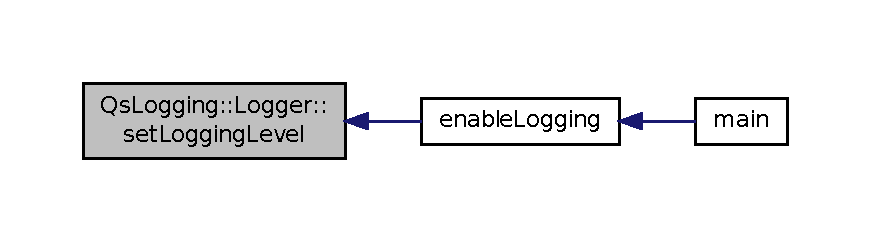
\includegraphics[width=350pt]{classQsLogging_1_1Logger_aa34d1a0d83e180f15e23a03f9de872c6_icgraph}
\end{center}
\end{figure}


\hypertarget{classQsLogging_1_1Logger_ab9789bba5f1644a3b3b51606533aa20f}{\index{Qs\-Logging\-::\-Logger@{Qs\-Logging\-::\-Logger}!write@{write}}
\index{write@{write}!QsLogging::Logger@{Qs\-Logging\-::\-Logger}}
\subsubsection[{write}]{\setlength{\rightskip}{0pt plus 5cm}void Qs\-Logging\-::\-Logger\-::write (
\begin{DoxyParamCaption}
\item[{const Q\-String \&}]{message, }
\item[{{\bf Level}}]{level}
\end{DoxyParamCaption}
)\hspace{0.3cm}{\ttfamily [private]}}}\label{classQsLogging_1_1Logger_ab9789bba5f1644a3b3b51606533aa20f}


Définition à la ligne \hyperlink{QsLog_8cpp_source_l00285}{285} du fichier \hyperlink{QsLog_8cpp_source}{Qs\-Log.\-cpp}.



Références \hyperlink{classQsLogging_1_1Logger_aab634416e14e5cb4ca3193dc5a9924fa}{d}, et \hyperlink{classQsLogging_1_1LoggerImpl_acdbde93fec67bd0bcce8da1fc1080ece}{Qs\-Logging\-::\-Logger\-Impl\-::dest\-List}.



Référencé par \hyperlink{classQsLogging_1_1Logger_acd6d5d16d6e111eaa960807d75549bf9}{enqueue\-Write()}.


\begin{DoxyCode}
00286 \{
00287     \textcolor{keywordflow}{for} (DestinationList::iterator it = \hyperlink{classQsLogging_1_1Logger_aab634416e14e5cb4ca3193dc5a9924fa}{d}->\hyperlink{classQsLogging_1_1LoggerImpl_acdbde93fec67bd0bcce8da1fc1080ece}{destList}.begin(),
00288          endIt = \hyperlink{classQsLogging_1_1Logger_aab634416e14e5cb4ca3193dc5a9924fa}{d}->\hyperlink{classQsLogging_1_1LoggerImpl_acdbde93fec67bd0bcce8da1fc1080ece}{destList}.end();it != endIt;++it) \{
00289         (*it)->write(message, level);
00290     \}
00291 \}
\end{DoxyCode}


Voici le graphe des appelants de cette fonction \-:
\nopagebreak
\begin{figure}[H]
\begin{center}
\leavevmode
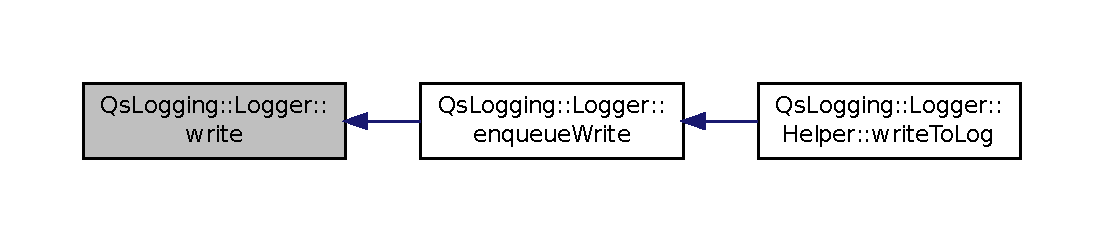
\includegraphics[width=350pt]{classQsLogging_1_1Logger_ab9789bba5f1644a3b3b51606533aa20f_icgraph}
\end{center}
\end{figure}




\subsection{Documentation des fonctions amies et associées}
\hypertarget{classQsLogging_1_1Logger_a27d33fe348fa48f5be163ad876cdb699}{\index{Qs\-Logging\-::\-Logger@{Qs\-Logging\-::\-Logger}!Log\-Writer\-Runnable@{Log\-Writer\-Runnable}}
\index{Log\-Writer\-Runnable@{Log\-Writer\-Runnable}!QsLogging::Logger@{Qs\-Logging\-::\-Logger}}
\subsubsection[{Log\-Writer\-Runnable}]{\setlength{\rightskip}{0pt plus 5cm}friend class Log\-Writer\-Runnable\hspace{0.3cm}{\ttfamily [friend]}}}\label{classQsLogging_1_1Logger_a27d33fe348fa48f5be163ad876cdb699}


Définition à la ligne \hyperlink{QsLog_8h_source_l00210}{210} du fichier \hyperlink{QsLog_8h_source}{Qs\-Log.\-h}.



Référencé par \hyperlink{classQsLogging_1_1Logger_acd6d5d16d6e111eaa960807d75549bf9}{enqueue\-Write()}.



\subsection{Documentation des données membres}
\hypertarget{classQsLogging_1_1Logger_aab634416e14e5cb4ca3193dc5a9924fa}{\index{Qs\-Logging\-::\-Logger@{Qs\-Logging\-::\-Logger}!d@{d}}
\index{d@{d}!QsLogging::Logger@{Qs\-Logging\-::\-Logger}}
\subsubsection[{d}]{\setlength{\rightskip}{0pt plus 5cm}Qs\-Logging\-::\-Logger\-::d\hspace{0.3cm}{\ttfamily [private]}}}\label{classQsLogging_1_1Logger_aab634416e14e5cb4ca3193dc5a9924fa}


Définition à la ligne \hyperlink{QsLog_8h_source_l00209}{209} du fichier \hyperlink{QsLog_8h_source}{Qs\-Log.\-h}.



Référencé par \hyperlink{classQsLogging_1_1Logger_a76a32c839e837547b14bc5e523b4aa45}{add\-Destination()}, \hyperlink{classQsLogging_1_1Logger_acd6d5d16d6e111eaa960807d75549bf9}{enqueue\-Write()}, \hyperlink{classQsLogging_1_1Logger_a5e2b29cf6cd066f1e64eaa4db7373458}{logging\-Level()}, \hyperlink{classQsLogging_1_1Logger_aa34d1a0d83e180f15e23a03f9de872c6}{set\-Logging\-Level()}, \hyperlink{classQsLogging_1_1Logger_ab9789bba5f1644a3b3b51606533aa20f}{write()}, et \hyperlink{classQsLogging_1_1Logger_a0947daaf6db4f83ba6e5fe155fa84e1f}{$\sim$\-Logger()}.



La documentation de cette classe a été générée à partir des fichiers suivants \-:\begin{DoxyCompactItemize}
\item 
logging/\hyperlink{QsLog_8h}{Qs\-Log.\-h}\item 
logging/\hyperlink{QsLog_8cpp}{Qs\-Log.\-cpp}\end{DoxyCompactItemize}

\hypertarget{classQsLogging_1_1Logger_1_1Helper}{\section{Référence de la classe Qs\-Logging\-:\-:Logger\-:\-:Helper}
\label{classQsLogging_1_1Logger_1_1Helper}\index{Qs\-Logging\-::\-Logger\-::\-Helper@{Qs\-Logging\-::\-Logger\-::\-Helper}}
}


{\ttfamily \#include $<$Qs\-Log.\-h$>$}



Graphe de collaboration de Qs\-Logging\-:\-:Logger\-:\-:Helper\-:
\nopagebreak
\begin{figure}[H]
\begin{center}
\leavevmode
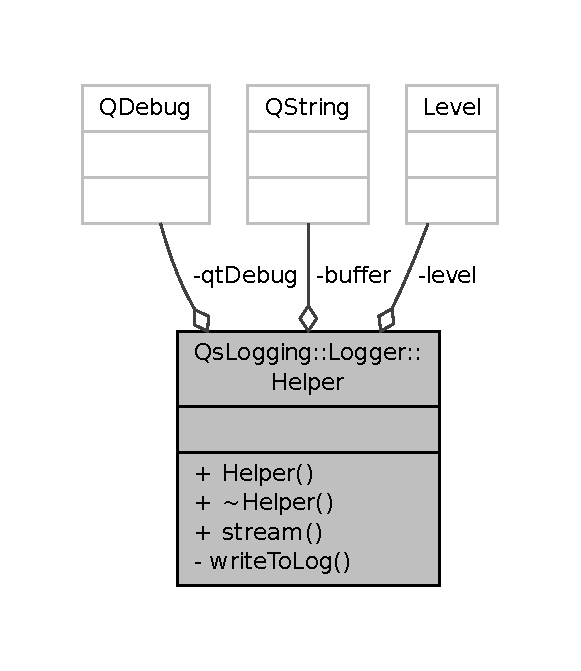
\includegraphics[width=279pt]{classQsLogging_1_1Logger_1_1Helper__coll__graph}
\end{center}
\end{figure}
\subsection*{Fonctions membres publiques}
\begin{DoxyCompactItemize}
\item 
\hyperlink{classQsLogging_1_1Logger_1_1Helper_ad0634422d3a7d8acc4bfd696dc326d18}{Helper} (\hyperlink{namespaceQsLogging_a38c7dd87e4de6f8eb460763ad0baa033}{Level} log\-Level)
\item 
\hyperlink{classQsLogging_1_1Logger_1_1Helper_a6e92fb30ec3d3fb057d2b7b85d6a6ec6}{$\sim$\-Helper} ()
\item 
Q\-Debug \& \hyperlink{classQsLogging_1_1Logger_1_1Helper_a9ed23a587a07da47066130fe2a92891e}{stream} ()
\end{DoxyCompactItemize}
\subsection*{Fonctions membres privées}
\begin{DoxyCompactItemize}
\item 
void \hyperlink{classQsLogging_1_1Logger_1_1Helper_a30e01167d1f088bade18b71a3e85379b}{write\-To\-Log} ()
\end{DoxyCompactItemize}
\subsection*{Attributs privés}
\begin{DoxyCompactItemize}
\item 
Q\-String \hyperlink{classQsLogging_1_1Logger_1_1Helper_ac7ad574c2643ca74519e49ff1f51aad4}{buffer}
\begin{DoxyCompactList}\small\item\em buffer \end{DoxyCompactList}\item 
\hyperlink{namespaceQsLogging_a38c7dd87e4de6f8eb460763ad0baa033}{Level} \hyperlink{classQsLogging_1_1Logger_1_1Helper_a8de516c069064c29643f7bd1face4f32}{level}
\begin{DoxyCompactList}\small\item\em level \end{DoxyCompactList}\item 
Q\-Debug \hyperlink{classQsLogging_1_1Logger_1_1Helper_a5a1c439896fc0737f578a04cbbe6fa65}{qt\-Debug}
\begin{DoxyCompactList}\small\item\em qt\-Debug \end{DoxyCompactList}\end{DoxyCompactItemize}


\subsection{Description détaillée}


Définition à la ligne \hyperlink{QsLog_8h_source_l00114}{114} du fichier \hyperlink{QsLog_8h_source}{Qs\-Log.\-h}.



\subsection{Documentation des constructeurs et destructeur}
\hypertarget{classQsLogging_1_1Logger_1_1Helper_ad0634422d3a7d8acc4bfd696dc326d18}{\index{Qs\-Logging\-::\-Logger\-::\-Helper@{Qs\-Logging\-::\-Logger\-::\-Helper}!Helper@{Helper}}
\index{Helper@{Helper}!QsLogging::Logger::Helper@{Qs\-Logging\-::\-Logger\-::\-Helper}}
\subsubsection[{Helper}]{\setlength{\rightskip}{0pt plus 5cm}Qs\-Logging\-::\-Logger\-::\-Helper\-::\-Helper (
\begin{DoxyParamCaption}
\item[{{\bf Level}}]{log\-Level}
\end{DoxyParamCaption}
)\hspace{0.3cm}{\ttfamily [inline]}, {\ttfamily [explicit]}}}\label{classQsLogging_1_1Logger_1_1Helper_ad0634422d3a7d8acc4bfd696dc326d18}


Définition à la ligne \hyperlink{QsLog_8h_source_l00123}{123} du fichier \hyperlink{QsLog_8h_source}{Qs\-Log.\-h}.


\begin{DoxyCode}
00123                                         :
00124             \hyperlink{classQsLogging_1_1Logger_1_1Helper_a8de516c069064c29643f7bd1face4f32}{level}(logLevel),
00125             \hyperlink{classQsLogging_1_1Logger_1_1Helper_a5a1c439896fc0737f578a04cbbe6fa65}{qtDebug}(&\hyperlink{classQsLogging_1_1Logger_1_1Helper_ac7ad574c2643ca74519e49ff1f51aad4}{buffer}) \{\}
\end{DoxyCode}
\hypertarget{classQsLogging_1_1Logger_1_1Helper_a6e92fb30ec3d3fb057d2b7b85d6a6ec6}{\index{Qs\-Logging\-::\-Logger\-::\-Helper@{Qs\-Logging\-::\-Logger\-::\-Helper}!$\sim$\-Helper@{$\sim$\-Helper}}
\index{$\sim$\-Helper@{$\sim$\-Helper}!QsLogging::Logger::Helper@{Qs\-Logging\-::\-Logger\-::\-Helper}}
\subsubsection[{$\sim$\-Helper}]{\setlength{\rightskip}{0pt plus 5cm}{\bf S\-H\-\_\-} Qs\-Logging\-::\-Logger\-::\-Helper\-::$\sim$\-Helper (
\begin{DoxyParamCaption}
{}
\end{DoxyParamCaption}
)}}\label{classQsLogging_1_1Logger_1_1Helper_a6e92fb30ec3d3fb057d2b7b85d6a6ec6}


Définition à la ligne \hyperlink{QsLog_8cpp_source_l00252}{252} du fichier \hyperlink{QsLog_8cpp_source}{Qs\-Log.\-cpp}.


\begin{DoxyCode}
00253 \{
00254     \textcolor{keywordflow}{try} \{
00255         \hyperlink{classQsLogging_1_1Logger_1_1Helper_a30e01167d1f088bade18b71a3e85379b}{writeToLog}();
00256     \}
00257     \textcolor{keywordflow}{catch}(std::exception&) \{
00258         \textcolor{comment}{/* you shouldn't throw exceptions from a sink */}
00259         assert(!\textcolor{stringliteral}{"exception in logger helper destructor"});
00260         \textcolor{keywordflow}{throw};
00261     \}
00262 \}
\end{DoxyCode}


\subsection{Documentation des fonctions membres}
\hypertarget{classQsLogging_1_1Logger_1_1Helper_a9ed23a587a07da47066130fe2a92891e}{\index{Qs\-Logging\-::\-Logger\-::\-Helper@{Qs\-Logging\-::\-Logger\-::\-Helper}!stream@{stream}}
\index{stream@{stream}!QsLogging::Logger::Helper@{Qs\-Logging\-::\-Logger\-::\-Helper}}
\subsubsection[{stream}]{\setlength{\rightskip}{0pt plus 5cm}Q\-Debug\& Qs\-Logging\-::\-Logger\-::\-Helper\-::stream (
\begin{DoxyParamCaption}
{}
\end{DoxyParamCaption}
)\hspace{0.3cm}{\ttfamily [inline]}}}\label{classQsLogging_1_1Logger_1_1Helper_a9ed23a587a07da47066130fe2a92891e}


Définition à la ligne \hyperlink{QsLog_8h_source_l00138}{138} du fichier \hyperlink{QsLog_8h_source}{Qs\-Log.\-h}.



Références \hyperlink{classQsLogging_1_1Logger_1_1Helper_a5a1c439896fc0737f578a04cbbe6fa65}{qt\-Debug}.


\begin{DoxyCode}
00138 \{ \textcolor{keywordflow}{return} \hyperlink{classQsLogging_1_1Logger_1_1Helper_a5a1c439896fc0737f578a04cbbe6fa65}{qtDebug}; \}
\end{DoxyCode}
\hypertarget{classQsLogging_1_1Logger_1_1Helper_a30e01167d1f088bade18b71a3e85379b}{\index{Qs\-Logging\-::\-Logger\-::\-Helper@{Qs\-Logging\-::\-Logger\-::\-Helper}!write\-To\-Log@{write\-To\-Log}}
\index{write\-To\-Log@{write\-To\-Log}!QsLogging::Logger::Helper@{Qs\-Logging\-::\-Logger\-::\-Helper}}
\subsubsection[{write\-To\-Log}]{\setlength{\rightskip}{0pt plus 5cm}void Qs\-Logging\-::\-Logger\-::\-Helper\-::write\-To\-Log (
\begin{DoxyParamCaption}
{}
\end{DoxyParamCaption}
)\hspace{0.3cm}{\ttfamily [private]}}}\label{classQsLogging_1_1Logger_1_1Helper_a30e01167d1f088bade18b71a3e85379b}


Définition à la ligne \hyperlink{QsLog_8cpp_source_l00238}{238} du fichier \hyperlink{QsLog_8cpp_source}{Qs\-Log.\-cpp}.



Références \hyperlink{classQsLogging_1_1Logger_1_1Helper_ac7ad574c2643ca74519e49ff1f51aad4}{buffer}, \hyperlink{classQsLogging_1_1Logger_acd6d5d16d6e111eaa960807d75549bf9}{Qs\-Logging\-::\-Logger\-::enqueue\-Write()}, \hyperlink{namespaceQsLogging_a9123c4017c6160e28fa489e419b23a9c}{Qs\-Logging\-::fmt\-Date\-Time()}, \hyperlink{classQsLogging_1_1Logger_a26fd3242d362eeeb3b38940a714ea6fa}{Qs\-Logging\-::\-Logger\-::instance()}, \hyperlink{classQsLogging_1_1Logger_1_1Helper_a8de516c069064c29643f7bd1face4f32}{level}, et \hyperlink{namespaceQsLogging_a8e669585768b47ba483f7325c18d60b8}{Qs\-Logging\-::\-Level\-To\-Text()}.


\begin{DoxyCode}
00239 \{
00240     \textcolor{keyword}{const} \textcolor{keywordtype}{char}* \textcolor{keyword}{const} levelName = \hyperlink{namespaceQsLogging_a8e669585768b47ba483f7325c18d60b8}{LevelToText}(\hyperlink{classQsLogging_1_1Logger_1_1Helper_a8de516c069064c29643f7bd1face4f32}{level});
00241     \textcolor{keyword}{const} QString completeMessage(QString(\textcolor{stringliteral}{"%1 %2 %3"})
00242                                   .arg(levelName, 5)
00243                                   .arg(QDateTime::currentDateTime().toString(
      \hyperlink{namespaceQsLogging_a9123c4017c6160e28fa489e419b23a9c}{fmtDateTime}))
00244                                   .arg(\hyperlink{classQsLogging_1_1Logger_1_1Helper_ac7ad574c2643ca74519e49ff1f51aad4}{buffer})
00245                                   );
00246 
00247     \hyperlink{classQsLogging_1_1Logger_a26fd3242d362eeeb3b38940a714ea6fa}{Logger::instance}().\hyperlink{classQsLogging_1_1Logger_acd6d5d16d6e111eaa960807d75549bf9}{enqueueWrite}(completeMessage, 
      \hyperlink{classQsLogging_1_1Logger_1_1Helper_a8de516c069064c29643f7bd1face4f32}{level});
00248 \}
\end{DoxyCode}


Voici le graphe d'appel pour cette fonction \-:
\nopagebreak
\begin{figure}[H]
\begin{center}
\leavevmode
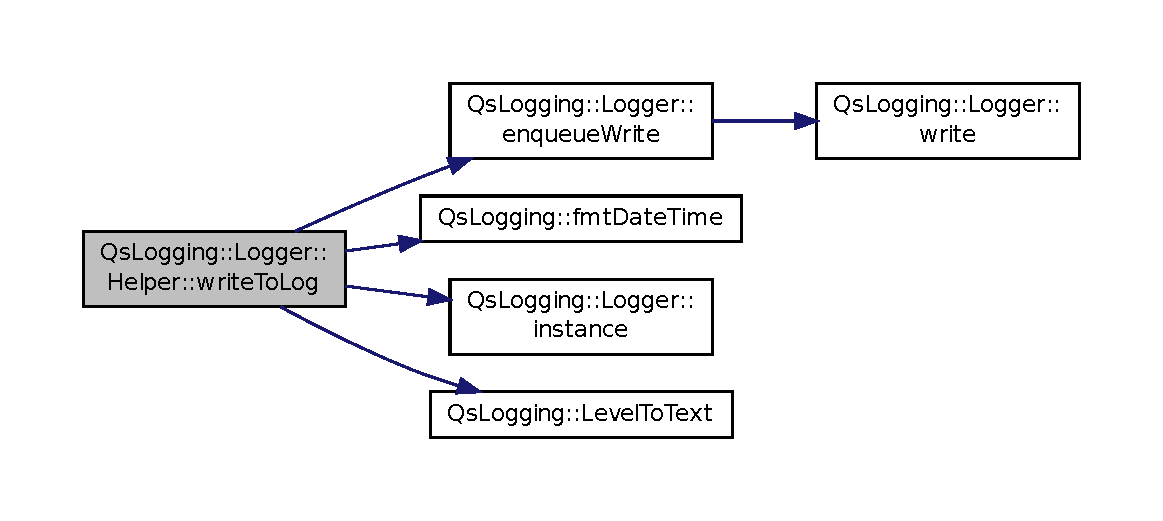
\includegraphics[width=350pt]{classQsLogging_1_1Logger_1_1Helper_a30e01167d1f088bade18b71a3e85379b_cgraph}
\end{center}
\end{figure}




\subsection{Documentation des données membres}
\hypertarget{classQsLogging_1_1Logger_1_1Helper_ac7ad574c2643ca74519e49ff1f51aad4}{\index{Qs\-Logging\-::\-Logger\-::\-Helper@{Qs\-Logging\-::\-Logger\-::\-Helper}!buffer@{buffer}}
\index{buffer@{buffer}!QsLogging::Logger::Helper@{Qs\-Logging\-::\-Logger\-::\-Helper}}
\subsubsection[{buffer}]{\setlength{\rightskip}{0pt plus 5cm}Q\-String Qs\-Logging\-::\-Logger\-::\-Helper\-::buffer\hspace{0.3cm}{\ttfamily [private]}}}\label{classQsLogging_1_1Logger_1_1Helper_ac7ad574c2643ca74519e49ff1f51aad4}


buffer 



Définition à la ligne \hyperlink{QsLog_8h_source_l00154}{154} du fichier \hyperlink{QsLog_8h_source}{Qs\-Log.\-h}.



Référencé par \hyperlink{classQsLogging_1_1Logger_1_1Helper_a30e01167d1f088bade18b71a3e85379b}{write\-To\-Log()}.

\hypertarget{classQsLogging_1_1Logger_1_1Helper_a8de516c069064c29643f7bd1face4f32}{\index{Qs\-Logging\-::\-Logger\-::\-Helper@{Qs\-Logging\-::\-Logger\-::\-Helper}!level@{level}}
\index{level@{level}!QsLogging::Logger::Helper@{Qs\-Logging\-::\-Logger\-::\-Helper}}
\subsubsection[{level}]{\setlength{\rightskip}{0pt plus 5cm}{\bf Level} Qs\-Logging\-::\-Logger\-::\-Helper\-::level\hspace{0.3cm}{\ttfamily [private]}}}\label{classQsLogging_1_1Logger_1_1Helper_a8de516c069064c29643f7bd1face4f32}


level 



Définition à la ligne \hyperlink{QsLog_8h_source_l00150}{150} du fichier \hyperlink{QsLog_8h_source}{Qs\-Log.\-h}.



Référencé par \hyperlink{classQsLogging_1_1Logger_1_1Helper_a30e01167d1f088bade18b71a3e85379b}{write\-To\-Log()}.

\hypertarget{classQsLogging_1_1Logger_1_1Helper_a5a1c439896fc0737f578a04cbbe6fa65}{\index{Qs\-Logging\-::\-Logger\-::\-Helper@{Qs\-Logging\-::\-Logger\-::\-Helper}!qt\-Debug@{qt\-Debug}}
\index{qt\-Debug@{qt\-Debug}!QsLogging::Logger::Helper@{Qs\-Logging\-::\-Logger\-::\-Helper}}
\subsubsection[{qt\-Debug}]{\setlength{\rightskip}{0pt plus 5cm}Q\-Debug Qs\-Logging\-::\-Logger\-::\-Helper\-::qt\-Debug\hspace{0.3cm}{\ttfamily [private]}}}\label{classQsLogging_1_1Logger_1_1Helper_a5a1c439896fc0737f578a04cbbe6fa65}


qt\-Debug 



Définition à la ligne \hyperlink{QsLog_8h_source_l00158}{158} du fichier \hyperlink{QsLog_8h_source}{Qs\-Log.\-h}.



Référencé par \hyperlink{classQsLogging_1_1Logger_1_1Helper_a9ed23a587a07da47066130fe2a92891e}{stream()}.



La documentation de cette classe a été générée à partir des fichiers suivants \-:\begin{DoxyCompactItemize}
\item 
logging/\hyperlink{QsLog_8h}{Qs\-Log.\-h}\item 
logging/\hyperlink{QsLog_8cpp}{Qs\-Log.\-cpp}\end{DoxyCompactItemize}

\hypertarget{classQsLogging_1_1LoggerImpl}{\section{Référence de la classe Qs\-Logging\-:\-:Logger\-Impl}
\label{classQsLogging_1_1LoggerImpl}\index{Qs\-Logging\-::\-Logger\-Impl@{Qs\-Logging\-::\-Logger\-Impl}}
}


Graphe de collaboration de Qs\-Logging\-:\-:Logger\-Impl\-:
\nopagebreak
\begin{figure}[H]
\begin{center}
\leavevmode
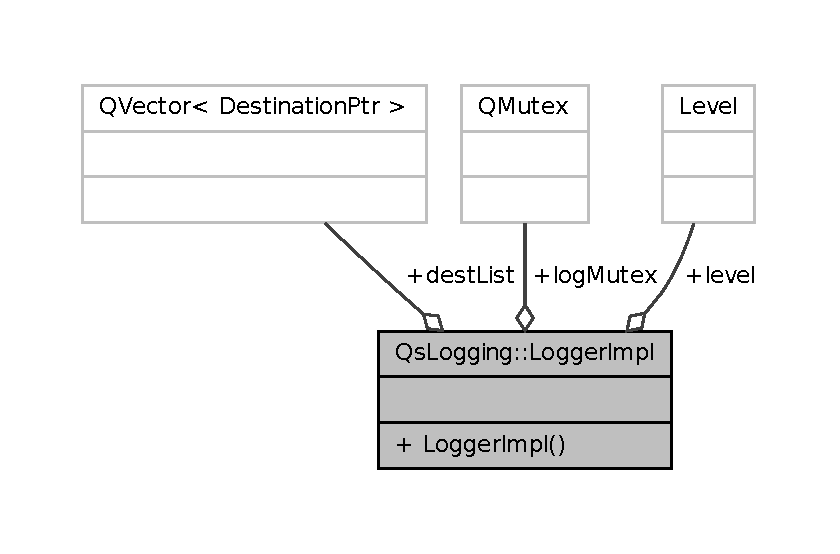
\includegraphics[width=350pt]{classQsLogging_1_1LoggerImpl__coll__graph}
\end{center}
\end{figure}
\subsection*{Fonctions membres publiques}
\begin{DoxyCompactItemize}
\item 
\hyperlink{classQsLogging_1_1LoggerImpl_a97418676fcfcb2fb13c0ebbbae3ef184}{Logger\-Impl} ()
\end{DoxyCompactItemize}
\subsection*{Attributs publics}
\begin{DoxyCompactItemize}
\item 
\hyperlink{namespaceQsLogging_a566a41f076f9a05c94cb6980ec554e2c}{Destination\-List} \hyperlink{classQsLogging_1_1LoggerImpl_acdbde93fec67bd0bcce8da1fc1080ece}{dest\-List}
\item 
\hyperlink{namespaceQsLogging_a38c7dd87e4de6f8eb460763ad0baa033}{Level} \hyperlink{classQsLogging_1_1LoggerImpl_a4d3c9f4b81baa52df759b6d07bda0a69}{level}
\item 
Q\-Mutex \hyperlink{classQsLogging_1_1LoggerImpl_a8feaba4a7a7160106987943313804c35}{log\-Mutex}
\end{DoxyCompactItemize}


\subsection{Description détaillée}


Définition à la ligne \hyperlink{QsLog_8cpp_source_l00164}{164} du fichier \hyperlink{QsLog_8cpp_source}{Qs\-Log.\-cpp}.



\subsection{Documentation des constructeurs et destructeur}
\hypertarget{classQsLogging_1_1LoggerImpl_a97418676fcfcb2fb13c0ebbbae3ef184}{\index{Qs\-Logging\-::\-Logger\-Impl@{Qs\-Logging\-::\-Logger\-Impl}!Logger\-Impl@{Logger\-Impl}}
\index{Logger\-Impl@{Logger\-Impl}!QsLogging::LoggerImpl@{Qs\-Logging\-::\-Logger\-Impl}}
\subsubsection[{Logger\-Impl}]{\setlength{\rightskip}{0pt plus 5cm}Qs\-Logging\-::\-Logger\-Impl\-::\-Logger\-Impl (
\begin{DoxyParamCaption}
{}
\end{DoxyParamCaption}
)\hspace{0.3cm}{\ttfamily [inline]}}}\label{classQsLogging_1_1LoggerImpl_a97418676fcfcb2fb13c0ebbbae3ef184}


Définition à la ligne \hyperlink{QsLog_8cpp_source_l00170}{170} du fichier \hyperlink{QsLog_8cpp_source}{Qs\-Log.\-cpp}.



Références \hyperlink{classQsLogging_1_1LoggerImpl_acdbde93fec67bd0bcce8da1fc1080ece}{dest\-List}.


\begin{DoxyCode}
00170                  :
00171         \hyperlink{classQsLogging_1_1LoggerImpl_a4d3c9f4b81baa52df759b6d07bda0a69}{level}(\hyperlink{namespaceQsLogging_a38c7dd87e4de6f8eb460763ad0baa033a6447c84a2844e8e1d0cdb95b55ecac72}{InfoLevel})
00172     \{
00173         \textcolor{comment}{/* assume at least file + console */}
00174         \hyperlink{classQsLogging_1_1LoggerImpl_acdbde93fec67bd0bcce8da1fc1080ece}{destList}.reserve(2);
00175 \textcolor{preprocessor}{#ifdef QS\_LOG\_SEPARATE\_THREAD}
00176 \textcolor{preprocessor}{}        threadPool.setMaxThreadCount(1);
00177         threadPool.setExpiryTimeout(-1);
00178 \textcolor{preprocessor}{#endif}
00179 \textcolor{preprocessor}{}    \}
\end{DoxyCode}


\subsection{Documentation des données membres}
\hypertarget{classQsLogging_1_1LoggerImpl_acdbde93fec67bd0bcce8da1fc1080ece}{\index{Qs\-Logging\-::\-Logger\-Impl@{Qs\-Logging\-::\-Logger\-Impl}!dest\-List@{dest\-List}}
\index{dest\-List@{dest\-List}!QsLogging::LoggerImpl@{Qs\-Logging\-::\-Logger\-Impl}}
\subsubsection[{dest\-List}]{\setlength{\rightskip}{0pt plus 5cm}Qs\-Logging\-::\-Logger\-Impl\-::dest\-List}}\label{classQsLogging_1_1LoggerImpl_acdbde93fec67bd0bcce8da1fc1080ece}


Définition à la ligne \hyperlink{QsLog_8cpp_source_l00195}{195} du fichier \hyperlink{QsLog_8cpp_source}{Qs\-Log.\-cpp}.



Référencé par \hyperlink{classQsLogging_1_1Logger_a76a32c839e837547b14bc5e523b4aa45}{Qs\-Logging\-::\-Logger\-::add\-Destination()}, \hyperlink{classQsLogging_1_1LoggerImpl_a97418676fcfcb2fb13c0ebbbae3ef184}{Logger\-Impl()}, et \hyperlink{classQsLogging_1_1Logger_ab9789bba5f1644a3b3b51606533aa20f}{Qs\-Logging\-::\-Logger\-::write()}.

\hypertarget{classQsLogging_1_1LoggerImpl_a4d3c9f4b81baa52df759b6d07bda0a69}{\index{Qs\-Logging\-::\-Logger\-Impl@{Qs\-Logging\-::\-Logger\-Impl}!level@{level}}
\index{level@{level}!QsLogging::LoggerImpl@{Qs\-Logging\-::\-Logger\-Impl}}
\subsubsection[{level}]{\setlength{\rightskip}{0pt plus 5cm}Qs\-Logging\-::\-Logger\-Impl\-::level}}\label{classQsLogging_1_1LoggerImpl_a4d3c9f4b81baa52df759b6d07bda0a69}


Définition à la ligne \hyperlink{QsLog_8cpp_source_l00191}{191} du fichier \hyperlink{QsLog_8cpp_source}{Qs\-Log.\-cpp}.



Référencé par \hyperlink{classQsLogging_1_1Logger_a5e2b29cf6cd066f1e64eaa4db7373458}{Qs\-Logging\-::\-Logger\-::logging\-Level()}, et \hyperlink{classQsLogging_1_1Logger_aa34d1a0d83e180f15e23a03f9de872c6}{Qs\-Logging\-::\-Logger\-::set\-Logging\-Level()}.

\hypertarget{classQsLogging_1_1LoggerImpl_a8feaba4a7a7160106987943313804c35}{\index{Qs\-Logging\-::\-Logger\-Impl@{Qs\-Logging\-::\-Logger\-Impl}!log\-Mutex@{log\-Mutex}}
\index{log\-Mutex@{log\-Mutex}!QsLogging::LoggerImpl@{Qs\-Logging\-::\-Logger\-Impl}}
\subsubsection[{log\-Mutex}]{\setlength{\rightskip}{0pt plus 5cm}Qs\-Logging\-::\-Logger\-Impl\-::log\-Mutex}}\label{classQsLogging_1_1LoggerImpl_a8feaba4a7a7160106987943313804c35}


Définition à la ligne \hyperlink{QsLog_8cpp_source_l00186}{186} du fichier \hyperlink{QsLog_8cpp_source}{Qs\-Log.\-cpp}.



Référencé par \hyperlink{classQsLogging_1_1Logger_acd6d5d16d6e111eaa960807d75549bf9}{Qs\-Logging\-::\-Logger\-::enqueue\-Write()}.



La documentation de cette classe a été générée à partir du fichier suivant \-:\begin{DoxyCompactItemize}
\item 
logging/\hyperlink{QsLog_8cpp}{Qs\-Log.\-cpp}\end{DoxyCompactItemize}

\hypertarget{classQsLogging_1_1NullRotationStrategy}{\section{Référence de la classe Qs\-Logging\-:\-:Null\-Rotation\-Strategy}
\label{classQsLogging_1_1NullRotationStrategy}\index{Qs\-Logging\-::\-Null\-Rotation\-Strategy@{Qs\-Logging\-::\-Null\-Rotation\-Strategy}}
}


The \hyperlink{classQsLogging_1_1NullRotationStrategy}{Null\-Rotation\-Strategy} class.  




{\ttfamily \#include $<$Qs\-Log\-Dest\-File.\-h$>$}



Graphe d'héritage de Qs\-Logging\-:\-:Null\-Rotation\-Strategy\-:
\nopagebreak
\begin{figure}[H]
\begin{center}
\leavevmode
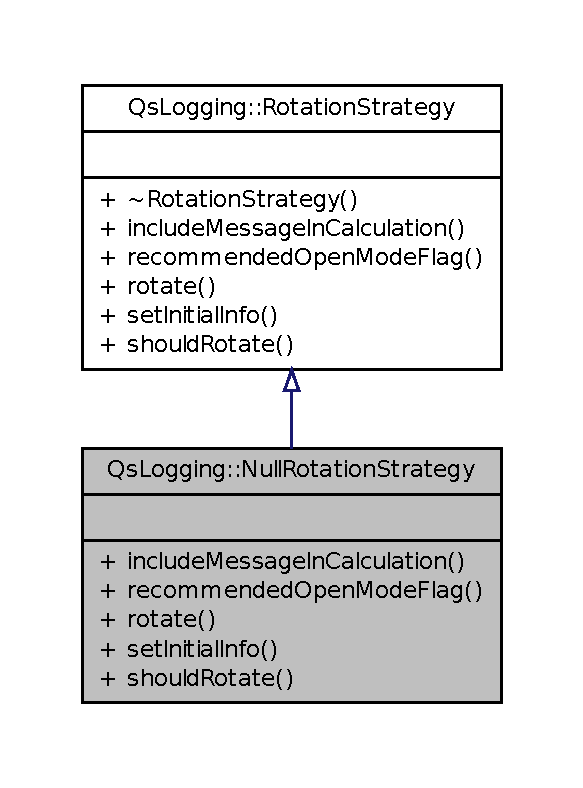
\includegraphics[width=280pt]{classQsLogging_1_1NullRotationStrategy__inherit__graph}
\end{center}
\end{figure}


Graphe de collaboration de Qs\-Logging\-:\-:Null\-Rotation\-Strategy\-:
\nopagebreak
\begin{figure}[H]
\begin{center}
\leavevmode
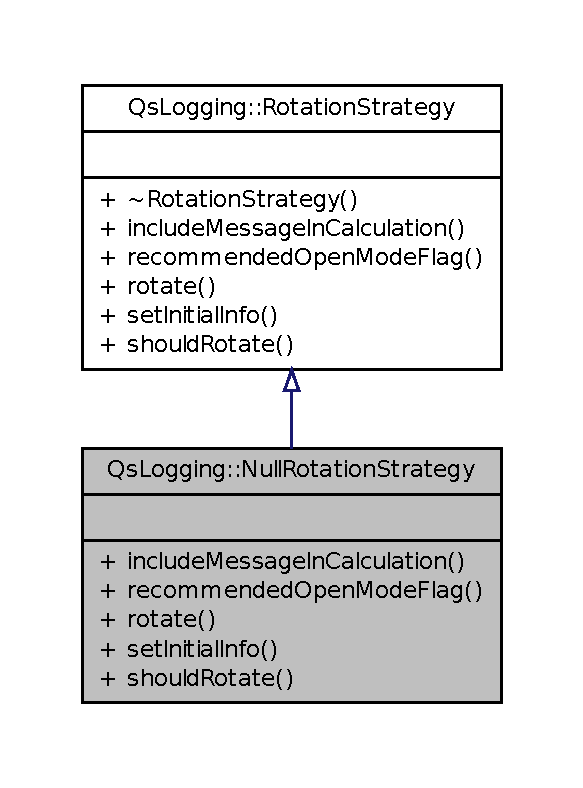
\includegraphics[width=280pt]{classQsLogging_1_1NullRotationStrategy__coll__graph}
\end{center}
\end{figure}
\subsection*{Fonctions membres publiques}
\begin{DoxyCompactItemize}
\item 
virtual void \hyperlink{classQsLogging_1_1NullRotationStrategy_a66753f83f8f42a3c2bb4c5a54d8dd3ff}{include\-Message\-In\-Calculation} (const Q\-String \&)
\begin{DoxyCompactList}\small\item\em include\-Message\-In\-Calculation \end{DoxyCompactList}\item 
virtual Q\-I\-O\-Device\-::\-Open\-Mode \hyperlink{classQsLogging_1_1NullRotationStrategy_adaa0f8706edc50b1b128c81bbc93b6d9}{recommended\-Open\-Mode\-Flag} ()
\begin{DoxyCompactList}\small\item\em recommended\-Open\-Mode\-Flag \end{DoxyCompactList}\item 
virtual void \hyperlink{classQsLogging_1_1NullRotationStrategy_a32dc2cad39aeffbaeedef1f8e7719a68}{rotate} ()
\begin{DoxyCompactList}\small\item\em rotate \end{DoxyCompactList}\item 
virtual void \hyperlink{classQsLogging_1_1NullRotationStrategy_a58a640b52b61dc256250dd40ab4025b0}{set\-Initial\-Info} (const Q\-File \&)
\begin{DoxyCompactList}\small\item\em set\-Initial\-Info \end{DoxyCompactList}\item 
virtual bool \hyperlink{classQsLogging_1_1NullRotationStrategy_a629d6ede50e0cbde108adb4550247ad6}{should\-Rotate} ()
\begin{DoxyCompactList}\small\item\em should\-Rotate \end{DoxyCompactList}\end{DoxyCompactItemize}


\subsection{Description détaillée}
The \hyperlink{classQsLogging_1_1NullRotationStrategy}{Null\-Rotation\-Strategy} class. 

Définition à la ligne \hyperlink{QsLogDestFile_8h_source_l00077}{77} du fichier \hyperlink{QsLogDestFile_8h_source}{Qs\-Log\-Dest\-File.\-h}.



\subsection{Documentation des fonctions membres}
\hypertarget{classQsLogging_1_1NullRotationStrategy_a66753f83f8f42a3c2bb4c5a54d8dd3ff}{\index{Qs\-Logging\-::\-Null\-Rotation\-Strategy@{Qs\-Logging\-::\-Null\-Rotation\-Strategy}!include\-Message\-In\-Calculation@{include\-Message\-In\-Calculation}}
\index{include\-Message\-In\-Calculation@{include\-Message\-In\-Calculation}!QsLogging::NullRotationStrategy@{Qs\-Logging\-::\-Null\-Rotation\-Strategy}}
\subsubsection[{include\-Message\-In\-Calculation}]{\setlength{\rightskip}{0pt plus 5cm}virtual void Qs\-Logging\-::\-Null\-Rotation\-Strategy\-::include\-Message\-In\-Calculation (
\begin{DoxyParamCaption}
\item[{const Q\-String \&}]{}
\end{DoxyParamCaption}
)\hspace{0.3cm}{\ttfamily [inline]}, {\ttfamily [virtual]}}}\label{classQsLogging_1_1NullRotationStrategy_a66753f83f8f42a3c2bb4c5a54d8dd3ff}


include\-Message\-In\-Calculation 



Implémente \hyperlink{classQsLogging_1_1RotationStrategy_a66041e701c257840d3b58ec2fc22c115}{Qs\-Logging\-::\-Rotation\-Strategy}.



Définition à la ligne \hyperlink{QsLogDestFile_8h_source_l00087}{87} du fichier \hyperlink{QsLogDestFile_8h_source}{Qs\-Log\-Dest\-File.\-h}.


\begin{DoxyCode}
00087 \{\}
\end{DoxyCode}
\hypertarget{classQsLogging_1_1NullRotationStrategy_adaa0f8706edc50b1b128c81bbc93b6d9}{\index{Qs\-Logging\-::\-Null\-Rotation\-Strategy@{Qs\-Logging\-::\-Null\-Rotation\-Strategy}!recommended\-Open\-Mode\-Flag@{recommended\-Open\-Mode\-Flag}}
\index{recommended\-Open\-Mode\-Flag@{recommended\-Open\-Mode\-Flag}!QsLogging::NullRotationStrategy@{Qs\-Logging\-::\-Null\-Rotation\-Strategy}}
\subsubsection[{recommended\-Open\-Mode\-Flag}]{\setlength{\rightskip}{0pt plus 5cm}virtual Q\-I\-O\-Device\-::\-Open\-Mode Qs\-Logging\-::\-Null\-Rotation\-Strategy\-::recommended\-Open\-Mode\-Flag (
\begin{DoxyParamCaption}
{}
\end{DoxyParamCaption}
)\hspace{0.3cm}{\ttfamily [inline]}, {\ttfamily [virtual]}}}\label{classQsLogging_1_1NullRotationStrategy_adaa0f8706edc50b1b128c81bbc93b6d9}


recommended\-Open\-Mode\-Flag 

\begin{DoxyReturn}{Renvoie}

\end{DoxyReturn}


Implémente \hyperlink{classQsLogging_1_1RotationStrategy_a8179129cae134717d4483c1903de3bdf}{Qs\-Logging\-::\-Rotation\-Strategy}.



Définition à la ligne \hyperlink{QsLogDestFile_8h_source_l00101}{101} du fichier \hyperlink{QsLogDestFile_8h_source}{Qs\-Log\-Dest\-File.\-h}.


\begin{DoxyCode}
00101 \{ \textcolor{keywordflow}{return} QIODevice::Truncate; \}
\end{DoxyCode}
\hypertarget{classQsLogging_1_1NullRotationStrategy_a32dc2cad39aeffbaeedef1f8e7719a68}{\index{Qs\-Logging\-::\-Null\-Rotation\-Strategy@{Qs\-Logging\-::\-Null\-Rotation\-Strategy}!rotate@{rotate}}
\index{rotate@{rotate}!QsLogging::NullRotationStrategy@{Qs\-Logging\-::\-Null\-Rotation\-Strategy}}
\subsubsection[{rotate}]{\setlength{\rightskip}{0pt plus 5cm}virtual void Qs\-Logging\-::\-Null\-Rotation\-Strategy\-::rotate (
\begin{DoxyParamCaption}
{}
\end{DoxyParamCaption}
)\hspace{0.3cm}{\ttfamily [inline]}, {\ttfamily [virtual]}}}\label{classQsLogging_1_1NullRotationStrategy_a32dc2cad39aeffbaeedef1f8e7719a68}


rotate 



Implémente \hyperlink{classQsLogging_1_1RotationStrategy_a11bc6e7d8af7df658f15abb69b3cc294}{Qs\-Logging\-::\-Rotation\-Strategy}.



Définition à la ligne \hyperlink{QsLogDestFile_8h_source_l00096}{96} du fichier \hyperlink{QsLogDestFile_8h_source}{Qs\-Log\-Dest\-File.\-h}.


\begin{DoxyCode}
00096 \{\}
\end{DoxyCode}
\hypertarget{classQsLogging_1_1NullRotationStrategy_a58a640b52b61dc256250dd40ab4025b0}{\index{Qs\-Logging\-::\-Null\-Rotation\-Strategy@{Qs\-Logging\-::\-Null\-Rotation\-Strategy}!set\-Initial\-Info@{set\-Initial\-Info}}
\index{set\-Initial\-Info@{set\-Initial\-Info}!QsLogging::NullRotationStrategy@{Qs\-Logging\-::\-Null\-Rotation\-Strategy}}
\subsubsection[{set\-Initial\-Info}]{\setlength{\rightskip}{0pt plus 5cm}virtual void Qs\-Logging\-::\-Null\-Rotation\-Strategy\-::set\-Initial\-Info (
\begin{DoxyParamCaption}
\item[{const Q\-File \&}]{}
\end{DoxyParamCaption}
)\hspace{0.3cm}{\ttfamily [inline]}, {\ttfamily [virtual]}}}\label{classQsLogging_1_1NullRotationStrategy_a58a640b52b61dc256250dd40ab4025b0}


set\-Initial\-Info 



Implémente \hyperlink{classQsLogging_1_1RotationStrategy_adde9d4dcbca113233438beb43bab7f89}{Qs\-Logging\-::\-Rotation\-Strategy}.



Définition à la ligne \hyperlink{QsLogDestFile_8h_source_l00083}{83} du fichier \hyperlink{QsLogDestFile_8h_source}{Qs\-Log\-Dest\-File.\-h}.


\begin{DoxyCode}
00083 \{\}
\end{DoxyCode}
\hypertarget{classQsLogging_1_1NullRotationStrategy_a629d6ede50e0cbde108adb4550247ad6}{\index{Qs\-Logging\-::\-Null\-Rotation\-Strategy@{Qs\-Logging\-::\-Null\-Rotation\-Strategy}!should\-Rotate@{should\-Rotate}}
\index{should\-Rotate@{should\-Rotate}!QsLogging::NullRotationStrategy@{Qs\-Logging\-::\-Null\-Rotation\-Strategy}}
\subsubsection[{should\-Rotate}]{\setlength{\rightskip}{0pt plus 5cm}virtual bool Qs\-Logging\-::\-Null\-Rotation\-Strategy\-::should\-Rotate (
\begin{DoxyParamCaption}
{}
\end{DoxyParamCaption}
)\hspace{0.3cm}{\ttfamily [inline]}, {\ttfamily [virtual]}}}\label{classQsLogging_1_1NullRotationStrategy_a629d6ede50e0cbde108adb4550247ad6}


should\-Rotate 

\begin{DoxyReturn}{Renvoie}

\end{DoxyReturn}


Implémente \hyperlink{classQsLogging_1_1RotationStrategy_a53136a1009e8a0b30956ea83c43c4973}{Qs\-Logging\-::\-Rotation\-Strategy}.



Définition à la ligne \hyperlink{QsLogDestFile_8h_source_l00092}{92} du fichier \hyperlink{QsLogDestFile_8h_source}{Qs\-Log\-Dest\-File.\-h}.


\begin{DoxyCode}
00092 \{ \textcolor{keywordflow}{return} \textcolor{keyword}{false}; \}
\end{DoxyCode}


La documentation de cette classe a été générée à partir du fichier suivant \-:\begin{DoxyCompactItemize}
\item 
logging/\hyperlink{QsLogDestFile_8h}{Qs\-Log\-Dest\-File.\-h}\end{DoxyCompactItemize}

\hypertarget{classQsLogging_1_1RotationStrategy}{\section{Référence de la classe Qs\-Logging\-:\-:Rotation\-Strategy}
\label{classQsLogging_1_1RotationStrategy}\index{Qs\-Logging\-::\-Rotation\-Strategy@{Qs\-Logging\-::\-Rotation\-Strategy}}
}


The \hyperlink{classQsLogging_1_1RotationStrategy}{Rotation\-Strategy} class.  




{\ttfamily \#include $<$Qs\-Log\-Dest\-File.\-h$>$}



Graphe d'héritage de Qs\-Logging\-:\-:Rotation\-Strategy\-:
\nopagebreak
\begin{figure}[H]
\begin{center}
\leavevmode
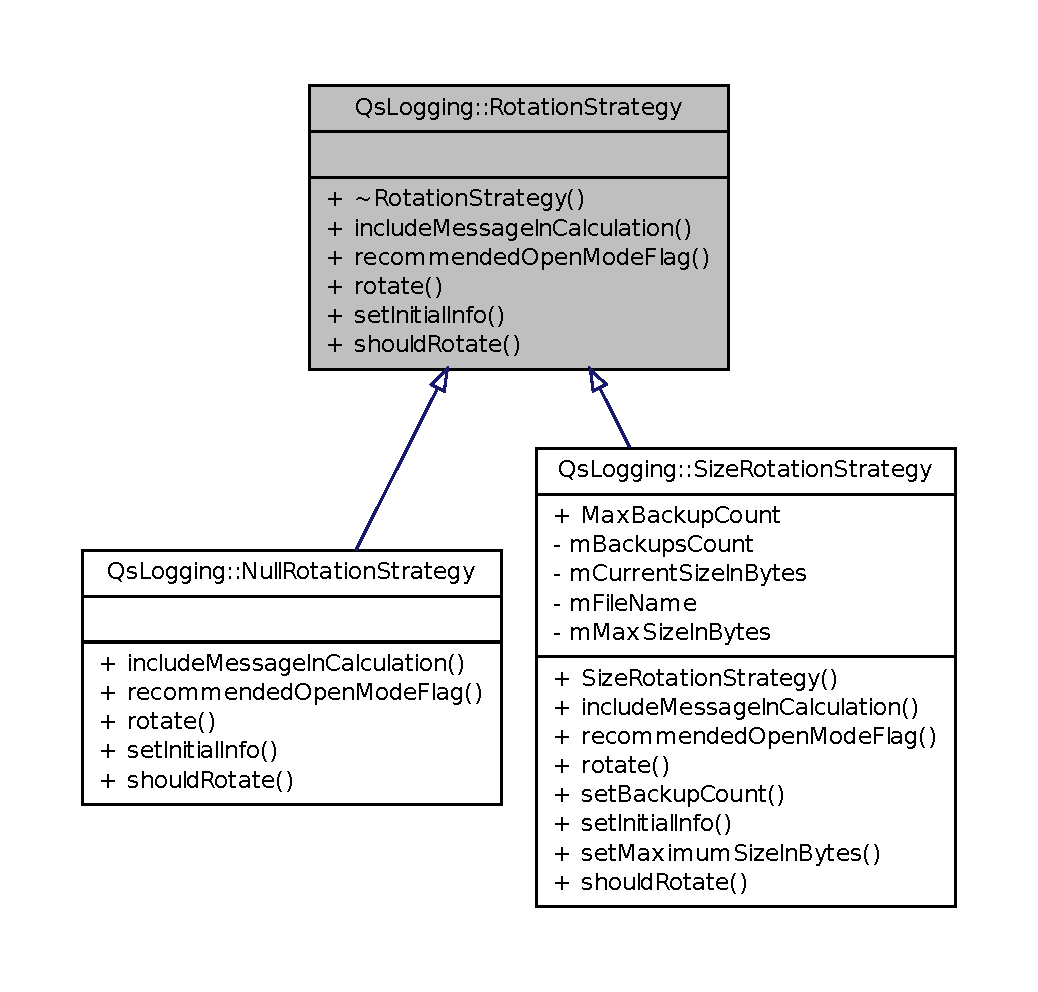
\includegraphics[width=350pt]{classQsLogging_1_1RotationStrategy__inherit__graph}
\end{center}
\end{figure}


Graphe de collaboration de Qs\-Logging\-:\-:Rotation\-Strategy\-:
\nopagebreak
\begin{figure}[H]
\begin{center}
\leavevmode
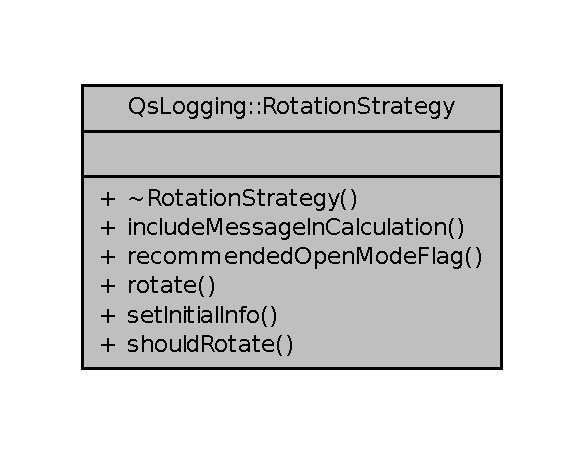
\includegraphics[width=280pt]{classQsLogging_1_1RotationStrategy__coll__graph}
\end{center}
\end{figure}
\subsection*{Fonctions membres publiques}
\begin{DoxyCompactItemize}
\item 
virtual \hyperlink{classQsLogging_1_1RotationStrategy_abd4b37978f48a3c75caa46ee9456b506}{$\sim$\-Rotation\-Strategy} ()
\begin{DoxyCompactList}\small\item\em $\sim$\-Rotation\-Strategy \end{DoxyCompactList}\item 
virtual void \hyperlink{classQsLogging_1_1RotationStrategy_a66041e701c257840d3b58ec2fc22c115}{include\-Message\-In\-Calculation} (const Q\-String \&message)=0
\begin{DoxyCompactList}\small\item\em include\-Message\-In\-Calculation \end{DoxyCompactList}\item 
virtual Q\-I\-O\-Device\-::\-Open\-Mode \hyperlink{classQsLogging_1_1RotationStrategy_a8179129cae134717d4483c1903de3bdf}{recommended\-Open\-Mode\-Flag} ()=0
\begin{DoxyCompactList}\small\item\em recommended\-Open\-Mode\-Flag \end{DoxyCompactList}\item 
virtual void \hyperlink{classQsLogging_1_1RotationStrategy_a11bc6e7d8af7df658f15abb69b3cc294}{rotate} ()=0
\begin{DoxyCompactList}\small\item\em rotate \end{DoxyCompactList}\item 
virtual void \hyperlink{classQsLogging_1_1RotationStrategy_adde9d4dcbca113233438beb43bab7f89}{set\-Initial\-Info} (const Q\-File \&file)=0
\begin{DoxyCompactList}\small\item\em set\-Initial\-Info \end{DoxyCompactList}\item 
virtual bool \hyperlink{classQsLogging_1_1RotationStrategy_a53136a1009e8a0b30956ea83c43c4973}{should\-Rotate} ()=0
\begin{DoxyCompactList}\small\item\em should\-Rotate \end{DoxyCompactList}\end{DoxyCompactItemize}


\subsection{Description détaillée}
The \hyperlink{classQsLogging_1_1RotationStrategy}{Rotation\-Strategy} class. 

Définition à la ligne \hyperlink{QsLogDestFile_8h_source_l00040}{40} du fichier \hyperlink{QsLogDestFile_8h_source}{Qs\-Log\-Dest\-File.\-h}.



\subsection{Documentation des constructeurs et destructeur}
\hypertarget{classQsLogging_1_1RotationStrategy_abd4b37978f48a3c75caa46ee9456b506}{\index{Qs\-Logging\-::\-Rotation\-Strategy@{Qs\-Logging\-::\-Rotation\-Strategy}!$\sim$\-Rotation\-Strategy@{$\sim$\-Rotation\-Strategy}}
\index{$\sim$\-Rotation\-Strategy@{$\sim$\-Rotation\-Strategy}!QsLogging::RotationStrategy@{Qs\-Logging\-::\-Rotation\-Strategy}}
\subsubsection[{$\sim$\-Rotation\-Strategy}]{\setlength{\rightskip}{0pt plus 5cm}Qs\-Logging\-::\-Rotation\-Strategy\-::$\sim$\-Rotation\-Strategy (
\begin{DoxyParamCaption}
{}
\end{DoxyParamCaption}
)\hspace{0.3cm}{\ttfamily [virtual]}}}\label{classQsLogging_1_1RotationStrategy_abd4b37978f48a3c75caa46ee9456b506}


$\sim$\-Rotation\-Strategy 

\hyperlink{classQsLogging_1_1RotationStrategy_abd4b37978f48a3c75caa46ee9456b506}{Qs\-Logging\-::\-Rotation\-Strategy\-::$\sim$\-Rotation\-Strategy} 

Définition à la ligne \hyperlink{QsLogDestFile_8cpp_source_l00038}{38} du fichier \hyperlink{QsLogDestFile_8cpp_source}{Qs\-Log\-Dest\-File.\-cpp}.


\begin{DoxyCode}
00039 \{
00040 \}
\end{DoxyCode}


\subsection{Documentation des fonctions membres}
\hypertarget{classQsLogging_1_1RotationStrategy_a66041e701c257840d3b58ec2fc22c115}{\index{Qs\-Logging\-::\-Rotation\-Strategy@{Qs\-Logging\-::\-Rotation\-Strategy}!include\-Message\-In\-Calculation@{include\-Message\-In\-Calculation}}
\index{include\-Message\-In\-Calculation@{include\-Message\-In\-Calculation}!QsLogging::RotationStrategy@{Qs\-Logging\-::\-Rotation\-Strategy}}
\subsubsection[{include\-Message\-In\-Calculation}]{\setlength{\rightskip}{0pt plus 5cm}virtual void Qs\-Logging\-::\-Rotation\-Strategy\-::include\-Message\-In\-Calculation (
\begin{DoxyParamCaption}
\item[{const Q\-String \&}]{message}
\end{DoxyParamCaption}
)\hspace{0.3cm}{\ttfamily [pure virtual]}}}\label{classQsLogging_1_1RotationStrategy_a66041e701c257840d3b58ec2fc22c115}


include\-Message\-In\-Calculation 


\begin{DoxyParams}{Paramètres}
{\em message} & \\
\hline
\end{DoxyParams}


Implémenté dans \hyperlink{classQsLogging_1_1SizeRotationStrategy_a3f87aec42ff67a771e31695923935486}{Qs\-Logging\-::\-Size\-Rotation\-Strategy}, et \hyperlink{classQsLogging_1_1NullRotationStrategy_a66753f83f8f42a3c2bb4c5a54d8dd3ff}{Qs\-Logging\-::\-Null\-Rotation\-Strategy}.

\hypertarget{classQsLogging_1_1RotationStrategy_a8179129cae134717d4483c1903de3bdf}{\index{Qs\-Logging\-::\-Rotation\-Strategy@{Qs\-Logging\-::\-Rotation\-Strategy}!recommended\-Open\-Mode\-Flag@{recommended\-Open\-Mode\-Flag}}
\index{recommended\-Open\-Mode\-Flag@{recommended\-Open\-Mode\-Flag}!QsLogging::RotationStrategy@{Qs\-Logging\-::\-Rotation\-Strategy}}
\subsubsection[{recommended\-Open\-Mode\-Flag}]{\setlength{\rightskip}{0pt plus 5cm}virtual Q\-I\-O\-Device\-::\-Open\-Mode Qs\-Logging\-::\-Rotation\-Strategy\-::recommended\-Open\-Mode\-Flag (
\begin{DoxyParamCaption}
{}
\end{DoxyParamCaption}
)\hspace{0.3cm}{\ttfamily [pure virtual]}}}\label{classQsLogging_1_1RotationStrategy_a8179129cae134717d4483c1903de3bdf}


recommended\-Open\-Mode\-Flag 

\begin{DoxyReturn}{Renvoie}

\end{DoxyReturn}


Implémenté dans \hyperlink{classQsLogging_1_1SizeRotationStrategy_a456726dba9e9ddd0c823bbbc1a6a7279}{Qs\-Logging\-::\-Size\-Rotation\-Strategy}, et \hyperlink{classQsLogging_1_1NullRotationStrategy_adaa0f8706edc50b1b128c81bbc93b6d9}{Qs\-Logging\-::\-Null\-Rotation\-Strategy}.

\hypertarget{classQsLogging_1_1RotationStrategy_a11bc6e7d8af7df658f15abb69b3cc294}{\index{Qs\-Logging\-::\-Rotation\-Strategy@{Qs\-Logging\-::\-Rotation\-Strategy}!rotate@{rotate}}
\index{rotate@{rotate}!QsLogging::RotationStrategy@{Qs\-Logging\-::\-Rotation\-Strategy}}
\subsubsection[{rotate}]{\setlength{\rightskip}{0pt plus 5cm}virtual void Qs\-Logging\-::\-Rotation\-Strategy\-::rotate (
\begin{DoxyParamCaption}
{}
\end{DoxyParamCaption}
)\hspace{0.3cm}{\ttfamily [pure virtual]}}}\label{classQsLogging_1_1RotationStrategy_a11bc6e7d8af7df658f15abb69b3cc294}


rotate 



Implémenté dans \hyperlink{classQsLogging_1_1SizeRotationStrategy_a044a258f08b3f104ccc7fdd80bf45b1a}{Qs\-Logging\-::\-Size\-Rotation\-Strategy}, et \hyperlink{classQsLogging_1_1NullRotationStrategy_a32dc2cad39aeffbaeedef1f8e7719a68}{Qs\-Logging\-::\-Null\-Rotation\-Strategy}.

\hypertarget{classQsLogging_1_1RotationStrategy_adde9d4dcbca113233438beb43bab7f89}{\index{Qs\-Logging\-::\-Rotation\-Strategy@{Qs\-Logging\-::\-Rotation\-Strategy}!set\-Initial\-Info@{set\-Initial\-Info}}
\index{set\-Initial\-Info@{set\-Initial\-Info}!QsLogging::RotationStrategy@{Qs\-Logging\-::\-Rotation\-Strategy}}
\subsubsection[{set\-Initial\-Info}]{\setlength{\rightskip}{0pt plus 5cm}virtual void Qs\-Logging\-::\-Rotation\-Strategy\-::set\-Initial\-Info (
\begin{DoxyParamCaption}
\item[{const Q\-File \&}]{file}
\end{DoxyParamCaption}
)\hspace{0.3cm}{\ttfamily [pure virtual]}}}\label{classQsLogging_1_1RotationStrategy_adde9d4dcbca113233438beb43bab7f89}


set\-Initial\-Info 


\begin{DoxyParams}{Paramètres}
{\em file} & \\
\hline
\end{DoxyParams}


Implémenté dans \hyperlink{classQsLogging_1_1SizeRotationStrategy_a763f6a2054a6ec5f3600f4e43e07c802}{Qs\-Logging\-::\-Size\-Rotation\-Strategy}, et \hyperlink{classQsLogging_1_1NullRotationStrategy_a58a640b52b61dc256250dd40ab4025b0}{Qs\-Logging\-::\-Null\-Rotation\-Strategy}.

\hypertarget{classQsLogging_1_1RotationStrategy_a53136a1009e8a0b30956ea83c43c4973}{\index{Qs\-Logging\-::\-Rotation\-Strategy@{Qs\-Logging\-::\-Rotation\-Strategy}!should\-Rotate@{should\-Rotate}}
\index{should\-Rotate@{should\-Rotate}!QsLogging::RotationStrategy@{Qs\-Logging\-::\-Rotation\-Strategy}}
\subsubsection[{should\-Rotate}]{\setlength{\rightskip}{0pt plus 5cm}virtual bool Qs\-Logging\-::\-Rotation\-Strategy\-::should\-Rotate (
\begin{DoxyParamCaption}
{}
\end{DoxyParamCaption}
)\hspace{0.3cm}{\ttfamily [pure virtual]}}}\label{classQsLogging_1_1RotationStrategy_a53136a1009e8a0b30956ea83c43c4973}


should\-Rotate 

\begin{DoxyReturn}{Renvoie}

\end{DoxyReturn}


Implémenté dans \hyperlink{classQsLogging_1_1SizeRotationStrategy_aced9d2191e48ae60f039d62fd9c7197f}{Qs\-Logging\-::\-Size\-Rotation\-Strategy}, et \hyperlink{classQsLogging_1_1NullRotationStrategy_a629d6ede50e0cbde108adb4550247ad6}{Qs\-Logging\-::\-Null\-Rotation\-Strategy}.



La documentation de cette classe a été générée à partir des fichiers suivants \-:\begin{DoxyCompactItemize}
\item 
logging/\hyperlink{QsLogDestFile_8h}{Qs\-Log\-Dest\-File.\-h}\item 
logging/\hyperlink{QsLogDestFile_8cpp}{Qs\-Log\-Dest\-File.\-cpp}\end{DoxyCompactItemize}

\hypertarget{classQsLogging_1_1SizeRotationStrategy}{\section{Référence de la classe Qs\-Logging\-:\-:Size\-Rotation\-Strategy}
\label{classQsLogging_1_1SizeRotationStrategy}\index{Qs\-Logging\-::\-Size\-Rotation\-Strategy@{Qs\-Logging\-::\-Size\-Rotation\-Strategy}}
}


The \hyperlink{classQsLogging_1_1SizeRotationStrategy}{Size\-Rotation\-Strategy} class.  




{\ttfamily \#include $<$Qs\-Log\-Dest\-File.\-h$>$}



Graphe d'héritage de Qs\-Logging\-:\-:Size\-Rotation\-Strategy\-:
\nopagebreak
\begin{figure}[H]
\begin{center}
\leavevmode
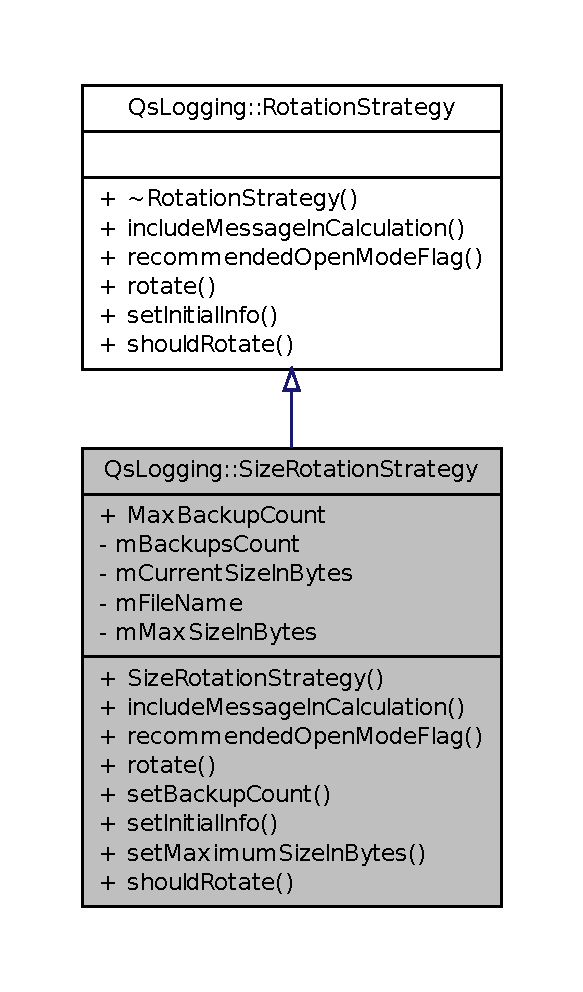
\includegraphics[width=280pt]{classQsLogging_1_1SizeRotationStrategy__inherit__graph}
\end{center}
\end{figure}


Graphe de collaboration de Qs\-Logging\-:\-:Size\-Rotation\-Strategy\-:
\nopagebreak
\begin{figure}[H]
\begin{center}
\leavevmode
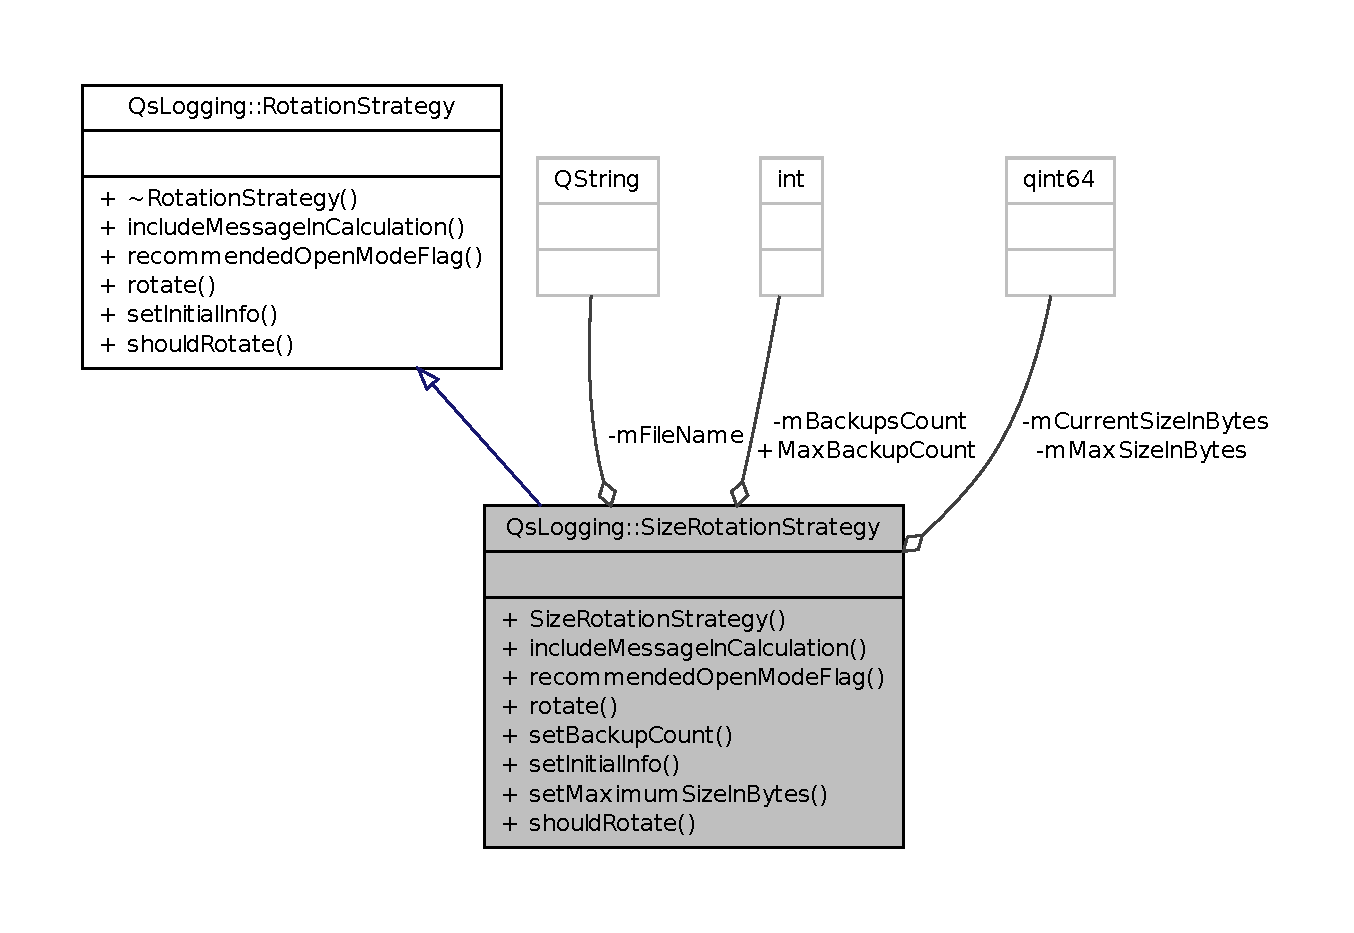
\includegraphics[width=350pt]{classQsLogging_1_1SizeRotationStrategy__coll__graph}
\end{center}
\end{figure}
\subsection*{Fonctions membres publiques}
\begin{DoxyCompactItemize}
\item 
\hyperlink{classQsLogging_1_1SizeRotationStrategy_a669845e1cd8a1656b28fbce8a97620b2}{Size\-Rotation\-Strategy} ()
\begin{DoxyCompactList}\small\item\em \hyperlink{classQsLogging_1_1SizeRotationStrategy}{Size\-Rotation\-Strategy}. \end{DoxyCompactList}\item 
virtual void \hyperlink{classQsLogging_1_1SizeRotationStrategy_a3f87aec42ff67a771e31695923935486}{include\-Message\-In\-Calculation} (const Q\-String \&message)
\begin{DoxyCompactList}\small\item\em include\-Message\-In\-Calculation \end{DoxyCompactList}\item 
virtual Q\-I\-O\-Device\-::\-Open\-Mode \hyperlink{classQsLogging_1_1SizeRotationStrategy_a456726dba9e9ddd0c823bbbc1a6a7279}{recommended\-Open\-Mode\-Flag} ()
\begin{DoxyCompactList}\small\item\em recommended\-Open\-Mode\-Flag \end{DoxyCompactList}\item 
virtual void \hyperlink{classQsLogging_1_1SizeRotationStrategy_a044a258f08b3f104ccc7fdd80bf45b1a}{rotate} ()
\begin{DoxyCompactList}\small\item\em rotate \end{DoxyCompactList}\item 
void \hyperlink{classQsLogging_1_1SizeRotationStrategy_ab50da4fb0397509e5aeb826e791f09f9}{set\-Backup\-Count} (int backups)
\begin{DoxyCompactList}\small\item\em set\-Backup\-Count \end{DoxyCompactList}\item 
virtual void \hyperlink{classQsLogging_1_1SizeRotationStrategy_a763f6a2054a6ec5f3600f4e43e07c802}{set\-Initial\-Info} (const Q\-File \&file)
\begin{DoxyCompactList}\small\item\em set\-Initial\-Info \end{DoxyCompactList}\item 
void \hyperlink{classQsLogging_1_1SizeRotationStrategy_a3d37fd3bcc5aa4a84f8bf30af1d17526}{set\-Maximum\-Size\-In\-Bytes} (qint64 size)
\begin{DoxyCompactList}\small\item\em set\-Maximum\-Size\-In\-Bytes \end{DoxyCompactList}\item 
virtual bool \hyperlink{classQsLogging_1_1SizeRotationStrategy_aced9d2191e48ae60f039d62fd9c7197f}{should\-Rotate} ()
\begin{DoxyCompactList}\small\item\em should\-Rotate \end{DoxyCompactList}\end{DoxyCompactItemize}
\subsection*{Attributs publics statiques}
\begin{DoxyCompactItemize}
\item 
static const int \hyperlink{classQsLogging_1_1SizeRotationStrategy_a9965384f7b98b191d00eef62b2b417bf}{Max\-Backup\-Count} = 10
\begin{DoxyCompactList}\small\item\em Max\-Backup\-Count. \end{DoxyCompactList}\end{DoxyCompactItemize}
\subsection*{Attributs privés}
\begin{DoxyCompactItemize}
\item 
int \hyperlink{classQsLogging_1_1SizeRotationStrategy_a8ffbf6fc9110b82a399c90ce725023e9}{m\-Backups\-Count}
\begin{DoxyCompactList}\small\item\em m\-Backups\-Count \end{DoxyCompactList}\item 
qint64 \hyperlink{classQsLogging_1_1SizeRotationStrategy_a655f57a77d5e6384c49a2dffd899ef33}{m\-Current\-Size\-In\-Bytes}
\begin{DoxyCompactList}\small\item\em m\-Current\-Size\-In\-Bytes \end{DoxyCompactList}\item 
Q\-String \hyperlink{classQsLogging_1_1SizeRotationStrategy_a2a7187b9a1e4d957a9d5718c91a7f1b3}{m\-File\-Name}
\begin{DoxyCompactList}\small\item\em m\-File\-Name \end{DoxyCompactList}\item 
qint64 \hyperlink{classQsLogging_1_1SizeRotationStrategy_ab9b1ed9b39de4c90762f38a32935fe01}{m\-Max\-Size\-In\-Bytes}
\begin{DoxyCompactList}\small\item\em m\-Max\-Size\-In\-Bytes \end{DoxyCompactList}\end{DoxyCompactItemize}


\subsection{Description détaillée}
The \hyperlink{classQsLogging_1_1SizeRotationStrategy}{Size\-Rotation\-Strategy} class. 

Définition à la ligne \hyperlink{QsLogDestFile_8h_source_l00108}{108} du fichier \hyperlink{QsLogDestFile_8h_source}{Qs\-Log\-Dest\-File.\-h}.



\subsection{Documentation des constructeurs et destructeur}
\hypertarget{classQsLogging_1_1SizeRotationStrategy_a669845e1cd8a1656b28fbce8a97620b2}{\index{Qs\-Logging\-::\-Size\-Rotation\-Strategy@{Qs\-Logging\-::\-Size\-Rotation\-Strategy}!Size\-Rotation\-Strategy@{Size\-Rotation\-Strategy}}
\index{Size\-Rotation\-Strategy@{Size\-Rotation\-Strategy}!QsLogging::SizeRotationStrategy@{Qs\-Logging\-::\-Size\-Rotation\-Strategy}}
\subsubsection[{Size\-Rotation\-Strategy}]{\setlength{\rightskip}{0pt plus 5cm}Qs\-Logging\-::\-Size\-Rotation\-Strategy\-::\-Size\-Rotation\-Strategy (
\begin{DoxyParamCaption}
{}
\end{DoxyParamCaption}
)}}\label{classQsLogging_1_1SizeRotationStrategy_a669845e1cd8a1656b28fbce8a97620b2}


\hyperlink{classQsLogging_1_1SizeRotationStrategy}{Size\-Rotation\-Strategy}. 

\hyperlink{classQsLogging_1_1SizeRotationStrategy_a669845e1cd8a1656b28fbce8a97620b2}{Qs\-Logging\-::\-Size\-Rotation\-Strategy\-::\-Size\-Rotation\-Strategy} 

Définition à la ligne \hyperlink{QsLogDestFile_8cpp_source_l00044}{44} du fichier \hyperlink{QsLogDestFile_8cpp_source}{Qs\-Log\-Dest\-File.\-cpp}.


\begin{DoxyCode}
00045     : \hyperlink{classQsLogging_1_1SizeRotationStrategy_a655f57a77d5e6384c49a2dffd899ef33}{mCurrentSizeInBytes}(0)
00046     , \hyperlink{classQsLogging_1_1SizeRotationStrategy_ab9b1ed9b39de4c90762f38a32935fe01}{mMaxSizeInBytes}(0)
00047     , \hyperlink{classQsLogging_1_1SizeRotationStrategy_a8ffbf6fc9110b82a399c90ce725023e9}{mBackupsCount}(0)
00048 \{
00049 \}
\end{DoxyCode}


\subsection{Documentation des fonctions membres}
\hypertarget{classQsLogging_1_1SizeRotationStrategy_a3f87aec42ff67a771e31695923935486}{\index{Qs\-Logging\-::\-Size\-Rotation\-Strategy@{Qs\-Logging\-::\-Size\-Rotation\-Strategy}!include\-Message\-In\-Calculation@{include\-Message\-In\-Calculation}}
\index{include\-Message\-In\-Calculation@{include\-Message\-In\-Calculation}!QsLogging::SizeRotationStrategy@{Qs\-Logging\-::\-Size\-Rotation\-Strategy}}
\subsubsection[{include\-Message\-In\-Calculation}]{\setlength{\rightskip}{0pt plus 5cm}void Qs\-Logging\-::\-Size\-Rotation\-Strategy\-::include\-Message\-In\-Calculation (
\begin{DoxyParamCaption}
\item[{const Q\-String \&}]{message}
\end{DoxyParamCaption}
)\hspace{0.3cm}{\ttfamily [virtual]}}}\label{classQsLogging_1_1SizeRotationStrategy_a3f87aec42ff67a771e31695923935486}


include\-Message\-In\-Calculation 


\begin{DoxyParams}{Paramètres}
{\em message} & \hyperlink{classQsLogging_1_1SizeRotationStrategy_a3f87aec42ff67a771e31695923935486}{Qs\-Logging\-::\-Size\-Rotation\-Strategy\-::include\-Message\-In\-Calculation} \\
\hline
\end{DoxyParams}


Implémente \hyperlink{classQsLogging_1_1RotationStrategy_a66041e701c257840d3b58ec2fc22c115}{Qs\-Logging\-::\-Rotation\-Strategy}.



Définition à la ligne \hyperlink{QsLogDestFile_8cpp_source_l00061}{61} du fichier \hyperlink{QsLogDestFile_8cpp_source}{Qs\-Log\-Dest\-File.\-cpp}.


\begin{DoxyCode}
00062 \{
00063     \hyperlink{classQsLogging_1_1SizeRotationStrategy_a655f57a77d5e6384c49a2dffd899ef33}{mCurrentSizeInBytes} += message.toUtf8().size();
00064 \}
\end{DoxyCode}
\hypertarget{classQsLogging_1_1SizeRotationStrategy_a456726dba9e9ddd0c823bbbc1a6a7279}{\index{Qs\-Logging\-::\-Size\-Rotation\-Strategy@{Qs\-Logging\-::\-Size\-Rotation\-Strategy}!recommended\-Open\-Mode\-Flag@{recommended\-Open\-Mode\-Flag}}
\index{recommended\-Open\-Mode\-Flag@{recommended\-Open\-Mode\-Flag}!QsLogging::SizeRotationStrategy@{Qs\-Logging\-::\-Size\-Rotation\-Strategy}}
\subsubsection[{recommended\-Open\-Mode\-Flag}]{\setlength{\rightskip}{0pt plus 5cm}Q\-I\-O\-Device\-::\-Open\-Mode Qs\-Logging\-::\-Size\-Rotation\-Strategy\-::recommended\-Open\-Mode\-Flag (
\begin{DoxyParamCaption}
{}
\end{DoxyParamCaption}
)\hspace{0.3cm}{\ttfamily [virtual]}}}\label{classQsLogging_1_1SizeRotationStrategy_a456726dba9e9ddd0c823bbbc1a6a7279}


recommended\-Open\-Mode\-Flag 

\begin{DoxyReturn}{Renvoie}

\end{DoxyReturn}
\hyperlink{classQsLogging_1_1SizeRotationStrategy_a456726dba9e9ddd0c823bbbc1a6a7279}{Qs\-Logging\-::\-Size\-Rotation\-Strategy\-::recommended\-Open\-Mode\-Flag} 

Implémente \hyperlink{classQsLogging_1_1RotationStrategy_a8179129cae134717d4483c1903de3bdf}{Qs\-Logging\-::\-Rotation\-Strategy}.



Définition à la ligne \hyperlink{QsLogDestFile_8cpp_source_l00121}{121} du fichier \hyperlink{QsLogDestFile_8cpp_source}{Qs\-Log\-Dest\-File.\-cpp}.


\begin{DoxyCode}
00122 \{
00123     \textcolor{keywordflow}{return} QIODevice::Append;
00124 \}
\end{DoxyCode}
\hypertarget{classQsLogging_1_1SizeRotationStrategy_a044a258f08b3f104ccc7fdd80bf45b1a}{\index{Qs\-Logging\-::\-Size\-Rotation\-Strategy@{Qs\-Logging\-::\-Size\-Rotation\-Strategy}!rotate@{rotate}}
\index{rotate@{rotate}!QsLogging::SizeRotationStrategy@{Qs\-Logging\-::\-Size\-Rotation\-Strategy}}
\subsubsection[{rotate}]{\setlength{\rightskip}{0pt plus 5cm}void Qs\-Logging\-::\-Size\-Rotation\-Strategy\-::rotate (
\begin{DoxyParamCaption}
{}
\end{DoxyParamCaption}
)\hspace{0.3cm}{\ttfamily [virtual]}}}\label{classQsLogging_1_1SizeRotationStrategy_a044a258f08b3f104ccc7fdd80bf45b1a}


rotate 

\hyperlink{classQsLogging_1_1SizeRotationStrategy_a044a258f08b3f104ccc7fdd80bf45b1a}{Qs\-Logging\-::\-Size\-Rotation\-Strategy\-::rotate} 

Implémente \hyperlink{classQsLogging_1_1RotationStrategy_a11bc6e7d8af7df658f15abb69b3cc294}{Qs\-Logging\-::\-Rotation\-Strategy}.



Définition à la ligne \hyperlink{QsLogDestFile_8cpp_source_l00078}{78} du fichier \hyperlink{QsLogDestFile_8cpp_source}{Qs\-Log\-Dest\-File.\-cpp}.


\begin{DoxyCode}
00079 \{
00080     \textcolor{keywordflow}{if} (!\hyperlink{classQsLogging_1_1SizeRotationStrategy_a8ffbf6fc9110b82a399c90ce725023e9}{mBackupsCount}) \{
00081         \textcolor{keywordflow}{if} (!QFile::remove(\hyperlink{classQsLogging_1_1SizeRotationStrategy_a2a7187b9a1e4d957a9d5718c91a7f1b3}{mFileName}))
00082             std::cerr << \textcolor{stringliteral}{"QsLog: backup delete failed "} << qPrintable(\hyperlink{classQsLogging_1_1SizeRotationStrategy_a2a7187b9a1e4d957a9d5718c91a7f1b3}{mFileName});
00083         \textcolor{keywordflow}{return};
00084     \}
00085 
00086      \textcolor{comment}{/* 1. find the last existing backup than can be shifted up*/}
00087      \textcolor{keyword}{const} QString logNamePattern = \hyperlink{classQsLogging_1_1SizeRotationStrategy_a2a7187b9a1e4d957a9d5718c91a7f1b3}{mFileName} + QString::fromUtf8(\textcolor{stringliteral}{".%1"});
00088      \textcolor{keywordtype}{int} lastExistingBackupIndex = 0;
00089      \textcolor{keywordflow}{for} (\textcolor{keywordtype}{int} i = 1;i <= \hyperlink{classQsLogging_1_1SizeRotationStrategy_a8ffbf6fc9110b82a399c90ce725023e9}{mBackupsCount};++i) \{
00090          \textcolor{keyword}{const} QString backupFileName = logNamePattern.arg(i);
00091          \textcolor{keywordflow}{if} (QFile::exists(backupFileName))
00092              lastExistingBackupIndex = qMin(i, \hyperlink{classQsLogging_1_1SizeRotationStrategy_a8ffbf6fc9110b82a399c90ce725023e9}{mBackupsCount} - 1);
00093          \textcolor{keywordflow}{else}
00094              \textcolor{keywordflow}{break};
00095      \}
00096 
00097      \textcolor{comment}{/* 2. shift up*/}
00098      \textcolor{keywordflow}{for} (\textcolor{keywordtype}{int} i = lastExistingBackupIndex;i >= 1;--i) \{
00099          \textcolor{keyword}{const} QString oldName = logNamePattern.arg(i);
00100          \textcolor{keyword}{const} QString newName = logNamePattern.arg(i + 1);
00101          QFile::remove(newName);
00102          \textcolor{keyword}{const} \textcolor{keywordtype}{bool} renamed = QFile::rename(oldName, newName);
00103          \textcolor{keywordflow}{if} (!renamed) \{
00104              std::cerr << \textcolor{stringliteral}{"QsLog: could not rename backup "} << qPrintable(oldName)
00105                        << \textcolor{stringliteral}{" to "} << qPrintable(newName);
00106          \}
00107      \}
00108 
00109      \textcolor{comment}{/* 3. rename current log file*/}
00110      \textcolor{keyword}{const} QString newName = logNamePattern.arg(1);
00111      \textcolor{keywordflow}{if} (QFile::exists(newName))
00112          QFile::remove(newName);
00113      \textcolor{keywordflow}{if} (!QFile::rename(\hyperlink{classQsLogging_1_1SizeRotationStrategy_a2a7187b9a1e4d957a9d5718c91a7f1b3}{mFileName}, newName)) \{
00114          std::cerr << \textcolor{stringliteral}{"QsLog: could not rename log "} << qPrintable(\hyperlink{classQsLogging_1_1SizeRotationStrategy_a2a7187b9a1e4d957a9d5718c91a7f1b3}{mFileName})
00115                    << \textcolor{stringliteral}{" to "} << qPrintable(newName);
00116      \}
00117 \}
\end{DoxyCode}
\hypertarget{classQsLogging_1_1SizeRotationStrategy_ab50da4fb0397509e5aeb826e791f09f9}{\index{Qs\-Logging\-::\-Size\-Rotation\-Strategy@{Qs\-Logging\-::\-Size\-Rotation\-Strategy}!set\-Backup\-Count@{set\-Backup\-Count}}
\index{set\-Backup\-Count@{set\-Backup\-Count}!QsLogging::SizeRotationStrategy@{Qs\-Logging\-::\-Size\-Rotation\-Strategy}}
\subsubsection[{set\-Backup\-Count}]{\setlength{\rightskip}{0pt plus 5cm}void Qs\-Logging\-::\-Size\-Rotation\-Strategy\-::set\-Backup\-Count (
\begin{DoxyParamCaption}
\item[{int}]{backups}
\end{DoxyParamCaption}
)}}\label{classQsLogging_1_1SizeRotationStrategy_ab50da4fb0397509e5aeb826e791f09f9}


set\-Backup\-Count 


\begin{DoxyParams}{Paramètres}
{\em backups} & \hyperlink{classQsLogging_1_1SizeRotationStrategy_ab50da4fb0397509e5aeb826e791f09f9}{Qs\-Logging\-::\-Size\-Rotation\-Strategy\-::set\-Backup\-Count} \\
\hline
\end{DoxyParams}


Définition à la ligne \hyperlink{QsLogDestFile_8cpp_source_l00136}{136} du fichier \hyperlink{QsLogDestFile_8cpp_source}{Qs\-Log\-Dest\-File.\-cpp}.



Références \hyperlink{classQsLogging_1_1SizeRotationStrategy_a9965384f7b98b191d00eef62b2b417bf}{Max\-Backup\-Count}.


\begin{DoxyCode}
00137 \{
00138     Q\_ASSERT(backups >= 0);
00139     \hyperlink{classQsLogging_1_1SizeRotationStrategy_a8ffbf6fc9110b82a399c90ce725023e9}{mBackupsCount} = qMin(backups, 
      \hyperlink{classQsLogging_1_1SizeRotationStrategy_a9965384f7b98b191d00eef62b2b417bf}{SizeRotationStrategy::MaxBackupCount});
00140 \}
\end{DoxyCode}
\hypertarget{classQsLogging_1_1SizeRotationStrategy_a763f6a2054a6ec5f3600f4e43e07c802}{\index{Qs\-Logging\-::\-Size\-Rotation\-Strategy@{Qs\-Logging\-::\-Size\-Rotation\-Strategy}!set\-Initial\-Info@{set\-Initial\-Info}}
\index{set\-Initial\-Info@{set\-Initial\-Info}!QsLogging::SizeRotationStrategy@{Qs\-Logging\-::\-Size\-Rotation\-Strategy}}
\subsubsection[{set\-Initial\-Info}]{\setlength{\rightskip}{0pt plus 5cm}void Qs\-Logging\-::\-Size\-Rotation\-Strategy\-::set\-Initial\-Info (
\begin{DoxyParamCaption}
\item[{const Q\-File \&}]{file}
\end{DoxyParamCaption}
)\hspace{0.3cm}{\ttfamily [virtual]}}}\label{classQsLogging_1_1SizeRotationStrategy_a763f6a2054a6ec5f3600f4e43e07c802}


set\-Initial\-Info 


\begin{DoxyParams}{Paramètres}
{\em file} & \hyperlink{classQsLogging_1_1SizeRotationStrategy_a763f6a2054a6ec5f3600f4e43e07c802}{Qs\-Logging\-::\-Size\-Rotation\-Strategy\-::set\-Initial\-Info} \\
\hline
\end{DoxyParams}


Implémente \hyperlink{classQsLogging_1_1RotationStrategy_adde9d4dcbca113233438beb43bab7f89}{Qs\-Logging\-::\-Rotation\-Strategy}.



Définition à la ligne \hyperlink{QsLogDestFile_8cpp_source_l00053}{53} du fichier \hyperlink{QsLogDestFile_8cpp_source}{Qs\-Log\-Dest\-File.\-cpp}.


\begin{DoxyCode}
00054 \{
00055     \hyperlink{classQsLogging_1_1SizeRotationStrategy_a2a7187b9a1e4d957a9d5718c91a7f1b3}{mFileName} = file.fileName();
00056     \hyperlink{classQsLogging_1_1SizeRotationStrategy_a655f57a77d5e6384c49a2dffd899ef33}{mCurrentSizeInBytes} = file.size();
00057 \}
\end{DoxyCode}
\hypertarget{classQsLogging_1_1SizeRotationStrategy_a3d37fd3bcc5aa4a84f8bf30af1d17526}{\index{Qs\-Logging\-::\-Size\-Rotation\-Strategy@{Qs\-Logging\-::\-Size\-Rotation\-Strategy}!set\-Maximum\-Size\-In\-Bytes@{set\-Maximum\-Size\-In\-Bytes}}
\index{set\-Maximum\-Size\-In\-Bytes@{set\-Maximum\-Size\-In\-Bytes}!QsLogging::SizeRotationStrategy@{Qs\-Logging\-::\-Size\-Rotation\-Strategy}}
\subsubsection[{set\-Maximum\-Size\-In\-Bytes}]{\setlength{\rightskip}{0pt plus 5cm}void Qs\-Logging\-::\-Size\-Rotation\-Strategy\-::set\-Maximum\-Size\-In\-Bytes (
\begin{DoxyParamCaption}
\item[{qint64}]{size}
\end{DoxyParamCaption}
)}}\label{classQsLogging_1_1SizeRotationStrategy_a3d37fd3bcc5aa4a84f8bf30af1d17526}


set\-Maximum\-Size\-In\-Bytes 


\begin{DoxyParams}{Paramètres}
{\em size} & \hyperlink{classQsLogging_1_1SizeRotationStrategy_a3d37fd3bcc5aa4a84f8bf30af1d17526}{Qs\-Logging\-::\-Size\-Rotation\-Strategy\-::set\-Maximum\-Size\-In\-Bytes} \\
\hline
\end{DoxyParams}


Définition à la ligne \hyperlink{QsLogDestFile_8cpp_source_l00128}{128} du fichier \hyperlink{QsLogDestFile_8cpp_source}{Qs\-Log\-Dest\-File.\-cpp}.


\begin{DoxyCode}
00129 \{
00130     Q\_ASSERT(size >= 0);
00131     \hyperlink{classQsLogging_1_1SizeRotationStrategy_ab9b1ed9b39de4c90762f38a32935fe01}{mMaxSizeInBytes} = size;
00132 \}
\end{DoxyCode}
\hypertarget{classQsLogging_1_1SizeRotationStrategy_aced9d2191e48ae60f039d62fd9c7197f}{\index{Qs\-Logging\-::\-Size\-Rotation\-Strategy@{Qs\-Logging\-::\-Size\-Rotation\-Strategy}!should\-Rotate@{should\-Rotate}}
\index{should\-Rotate@{should\-Rotate}!QsLogging::SizeRotationStrategy@{Qs\-Logging\-::\-Size\-Rotation\-Strategy}}
\subsubsection[{should\-Rotate}]{\setlength{\rightskip}{0pt plus 5cm}bool Qs\-Logging\-::\-Size\-Rotation\-Strategy\-::should\-Rotate (
\begin{DoxyParamCaption}
{}
\end{DoxyParamCaption}
)\hspace{0.3cm}{\ttfamily [virtual]}}}\label{classQsLogging_1_1SizeRotationStrategy_aced9d2191e48ae60f039d62fd9c7197f}


should\-Rotate 

\begin{DoxyReturn}{Renvoie}

\end{DoxyReturn}
\hyperlink{classQsLogging_1_1SizeRotationStrategy_aced9d2191e48ae60f039d62fd9c7197f}{Qs\-Logging\-::\-Size\-Rotation\-Strategy\-::should\-Rotate} 

Implémente \hyperlink{classQsLogging_1_1RotationStrategy_a53136a1009e8a0b30956ea83c43c4973}{Qs\-Logging\-::\-Rotation\-Strategy}.



Définition à la ligne \hyperlink{QsLogDestFile_8cpp_source_l00068}{68} du fichier \hyperlink{QsLogDestFile_8cpp_source}{Qs\-Log\-Dest\-File.\-cpp}.


\begin{DoxyCode}
00069 \{
00070     \textcolor{keywordflow}{return} \hyperlink{classQsLogging_1_1SizeRotationStrategy_a655f57a77d5e6384c49a2dffd899ef33}{mCurrentSizeInBytes} > \hyperlink{classQsLogging_1_1SizeRotationStrategy_ab9b1ed9b39de4c90762f38a32935fe01}{mMaxSizeInBytes};
00071 \}
\end{DoxyCode}


\subsection{Documentation des données membres}
\hypertarget{classQsLogging_1_1SizeRotationStrategy_a9965384f7b98b191d00eef62b2b417bf}{\index{Qs\-Logging\-::\-Size\-Rotation\-Strategy@{Qs\-Logging\-::\-Size\-Rotation\-Strategy}!Max\-Backup\-Count@{Max\-Backup\-Count}}
\index{Max\-Backup\-Count@{Max\-Backup\-Count}!QsLogging::SizeRotationStrategy@{Qs\-Logging\-::\-Size\-Rotation\-Strategy}}
\subsubsection[{Max\-Backup\-Count}]{\setlength{\rightskip}{0pt plus 5cm}const int Qs\-Logging\-::\-Size\-Rotation\-Strategy\-::\-Max\-Backup\-Count = 10\hspace{0.3cm}{\ttfamily [static]}}}\label{classQsLogging_1_1SizeRotationStrategy_a9965384f7b98b191d00eef62b2b417bf}


Max\-Backup\-Count. 

\hyperlink{classQsLogging_1_1SizeRotationStrategy_a9965384f7b98b191d00eef62b2b417bf}{Qs\-Logging\-::\-Size\-Rotation\-Strategy\-::\-Max\-Backup\-Count} 

Définition à la ligne \hyperlink{QsLogDestFile_8h_source_l00118}{118} du fichier \hyperlink{QsLogDestFile_8h_source}{Qs\-Log\-Dest\-File.\-h}.



Référencé par \hyperlink{classQsLogging_1_1SizeRotationStrategy_ab50da4fb0397509e5aeb826e791f09f9}{set\-Backup\-Count()}.

\hypertarget{classQsLogging_1_1SizeRotationStrategy_a8ffbf6fc9110b82a399c90ce725023e9}{\index{Qs\-Logging\-::\-Size\-Rotation\-Strategy@{Qs\-Logging\-::\-Size\-Rotation\-Strategy}!m\-Backups\-Count@{m\-Backups\-Count}}
\index{m\-Backups\-Count@{m\-Backups\-Count}!QsLogging::SizeRotationStrategy@{Qs\-Logging\-::\-Size\-Rotation\-Strategy}}
\subsubsection[{m\-Backups\-Count}]{\setlength{\rightskip}{0pt plus 5cm}int Qs\-Logging\-::\-Size\-Rotation\-Strategy\-::m\-Backups\-Count\hspace{0.3cm}{\ttfamily [private]}}}\label{classQsLogging_1_1SizeRotationStrategy_a8ffbf6fc9110b82a399c90ce725023e9}


m\-Backups\-Count 



Définition à la ligne \hyperlink{QsLogDestFile_8h_source_l00170}{170} du fichier \hyperlink{QsLogDestFile_8h_source}{Qs\-Log\-Dest\-File.\-h}.

\hypertarget{classQsLogging_1_1SizeRotationStrategy_a655f57a77d5e6384c49a2dffd899ef33}{\index{Qs\-Logging\-::\-Size\-Rotation\-Strategy@{Qs\-Logging\-::\-Size\-Rotation\-Strategy}!m\-Current\-Size\-In\-Bytes@{m\-Current\-Size\-In\-Bytes}}
\index{m\-Current\-Size\-In\-Bytes@{m\-Current\-Size\-In\-Bytes}!QsLogging::SizeRotationStrategy@{Qs\-Logging\-::\-Size\-Rotation\-Strategy}}
\subsubsection[{m\-Current\-Size\-In\-Bytes}]{\setlength{\rightskip}{0pt plus 5cm}qint64 Qs\-Logging\-::\-Size\-Rotation\-Strategy\-::m\-Current\-Size\-In\-Bytes\hspace{0.3cm}{\ttfamily [private]}}}\label{classQsLogging_1_1SizeRotationStrategy_a655f57a77d5e6384c49a2dffd899ef33}


m\-Current\-Size\-In\-Bytes 



Définition à la ligne \hyperlink{QsLogDestFile_8h_source_l00162}{162} du fichier \hyperlink{QsLogDestFile_8h_source}{Qs\-Log\-Dest\-File.\-h}.

\hypertarget{classQsLogging_1_1SizeRotationStrategy_a2a7187b9a1e4d957a9d5718c91a7f1b3}{\index{Qs\-Logging\-::\-Size\-Rotation\-Strategy@{Qs\-Logging\-::\-Size\-Rotation\-Strategy}!m\-File\-Name@{m\-File\-Name}}
\index{m\-File\-Name@{m\-File\-Name}!QsLogging::SizeRotationStrategy@{Qs\-Logging\-::\-Size\-Rotation\-Strategy}}
\subsubsection[{m\-File\-Name}]{\setlength{\rightskip}{0pt plus 5cm}Q\-String Qs\-Logging\-::\-Size\-Rotation\-Strategy\-::m\-File\-Name\hspace{0.3cm}{\ttfamily [private]}}}\label{classQsLogging_1_1SizeRotationStrategy_a2a7187b9a1e4d957a9d5718c91a7f1b3}


m\-File\-Name 



Définition à la ligne \hyperlink{QsLogDestFile_8h_source_l00158}{158} du fichier \hyperlink{QsLogDestFile_8h_source}{Qs\-Log\-Dest\-File.\-h}.

\hypertarget{classQsLogging_1_1SizeRotationStrategy_ab9b1ed9b39de4c90762f38a32935fe01}{\index{Qs\-Logging\-::\-Size\-Rotation\-Strategy@{Qs\-Logging\-::\-Size\-Rotation\-Strategy}!m\-Max\-Size\-In\-Bytes@{m\-Max\-Size\-In\-Bytes}}
\index{m\-Max\-Size\-In\-Bytes@{m\-Max\-Size\-In\-Bytes}!QsLogging::SizeRotationStrategy@{Qs\-Logging\-::\-Size\-Rotation\-Strategy}}
\subsubsection[{m\-Max\-Size\-In\-Bytes}]{\setlength{\rightskip}{0pt plus 5cm}qint64 Qs\-Logging\-::\-Size\-Rotation\-Strategy\-::m\-Max\-Size\-In\-Bytes\hspace{0.3cm}{\ttfamily [private]}}}\label{classQsLogging_1_1SizeRotationStrategy_ab9b1ed9b39de4c90762f38a32935fe01}


m\-Max\-Size\-In\-Bytes 



Définition à la ligne \hyperlink{QsLogDestFile_8h_source_l00166}{166} du fichier \hyperlink{QsLogDestFile_8h_source}{Qs\-Log\-Dest\-File.\-h}.



La documentation de cette classe a été générée à partir des fichiers suivants \-:\begin{DoxyCompactItemize}
\item 
logging/\hyperlink{QsLogDestFile_8h}{Qs\-Log\-Dest\-File.\-h}\item 
logging/\hyperlink{QsLogDestFile_8cpp}{Qs\-Log\-Dest\-File.\-cpp}\end{DoxyCompactItemize}

\hypertarget{classQSortFilterProxyModel}{\section{Référence de la classe Q\-Sort\-Filter\-Proxy\-Model}
\label{classQSortFilterProxyModel}\index{Q\-Sort\-Filter\-Proxy\-Model@{Q\-Sort\-Filter\-Proxy\-Model}}
}


Graphe d'héritage de Q\-Sort\-Filter\-Proxy\-Model\-:
\nopagebreak
\begin{figure}[H]
\begin{center}
\leavevmode
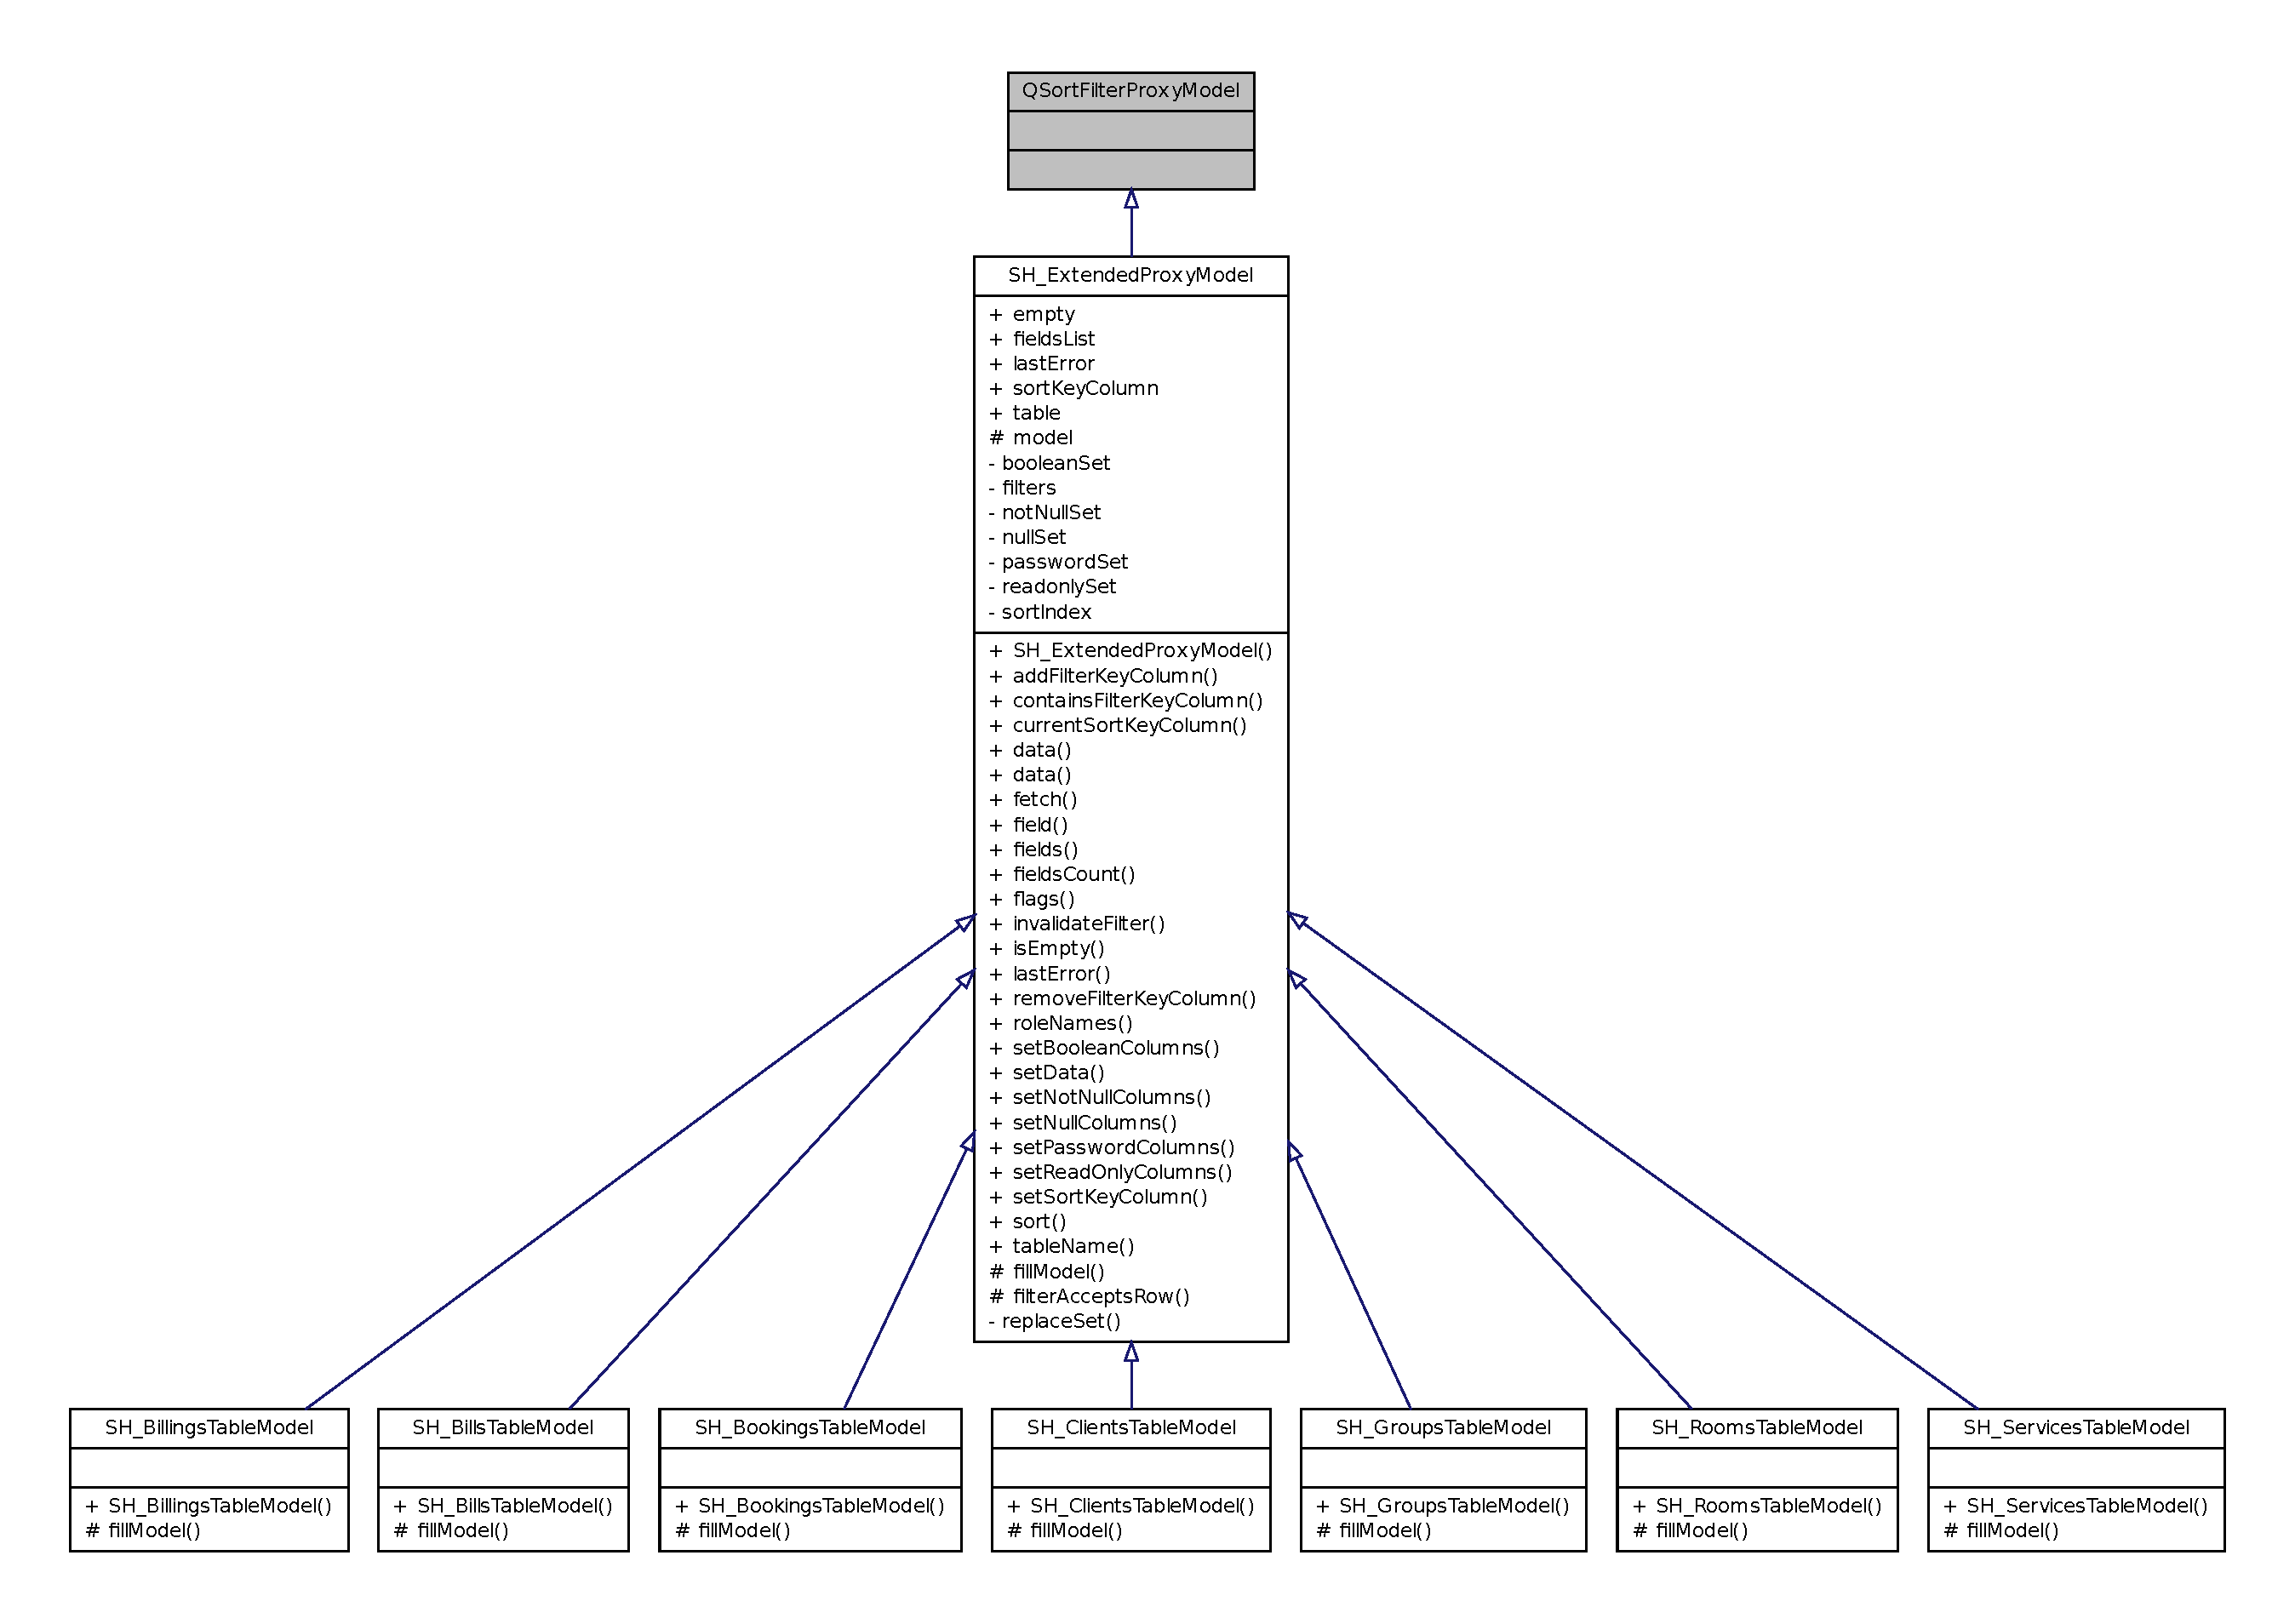
\includegraphics[width=350pt]{classQSortFilterProxyModel__inherit__graph}
\end{center}
\end{figure}


Graphe de collaboration de Q\-Sort\-Filter\-Proxy\-Model\-:
\nopagebreak
\begin{figure}[H]
\begin{center}
\leavevmode
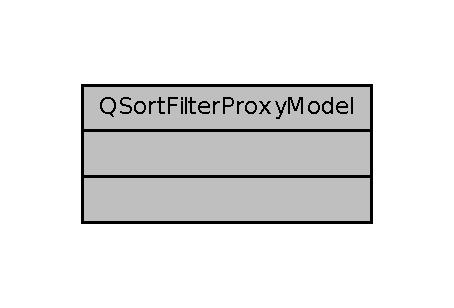
\includegraphics[width=218pt]{classQSortFilterProxyModel__coll__graph}
\end{center}
\end{figure}


La documentation de cette classe a été générée à partir du fichier suivant \-:\begin{DoxyCompactItemize}
\item 
models/\hyperlink{SH__ExtendedSqlProxyModel_8h}{S\-H\-\_\-\-Extended\-Sql\-Proxy\-Model.\-h}\end{DoxyCompactItemize}

\hypertarget{classQState}{\section{Référence de la classe Q\-State}
\label{classQState}\index{Q\-State@{Q\-State}}
}


Graphe d'héritage de Q\-State\-:
\nopagebreak
\begin{figure}[H]
\begin{center}
\leavevmode
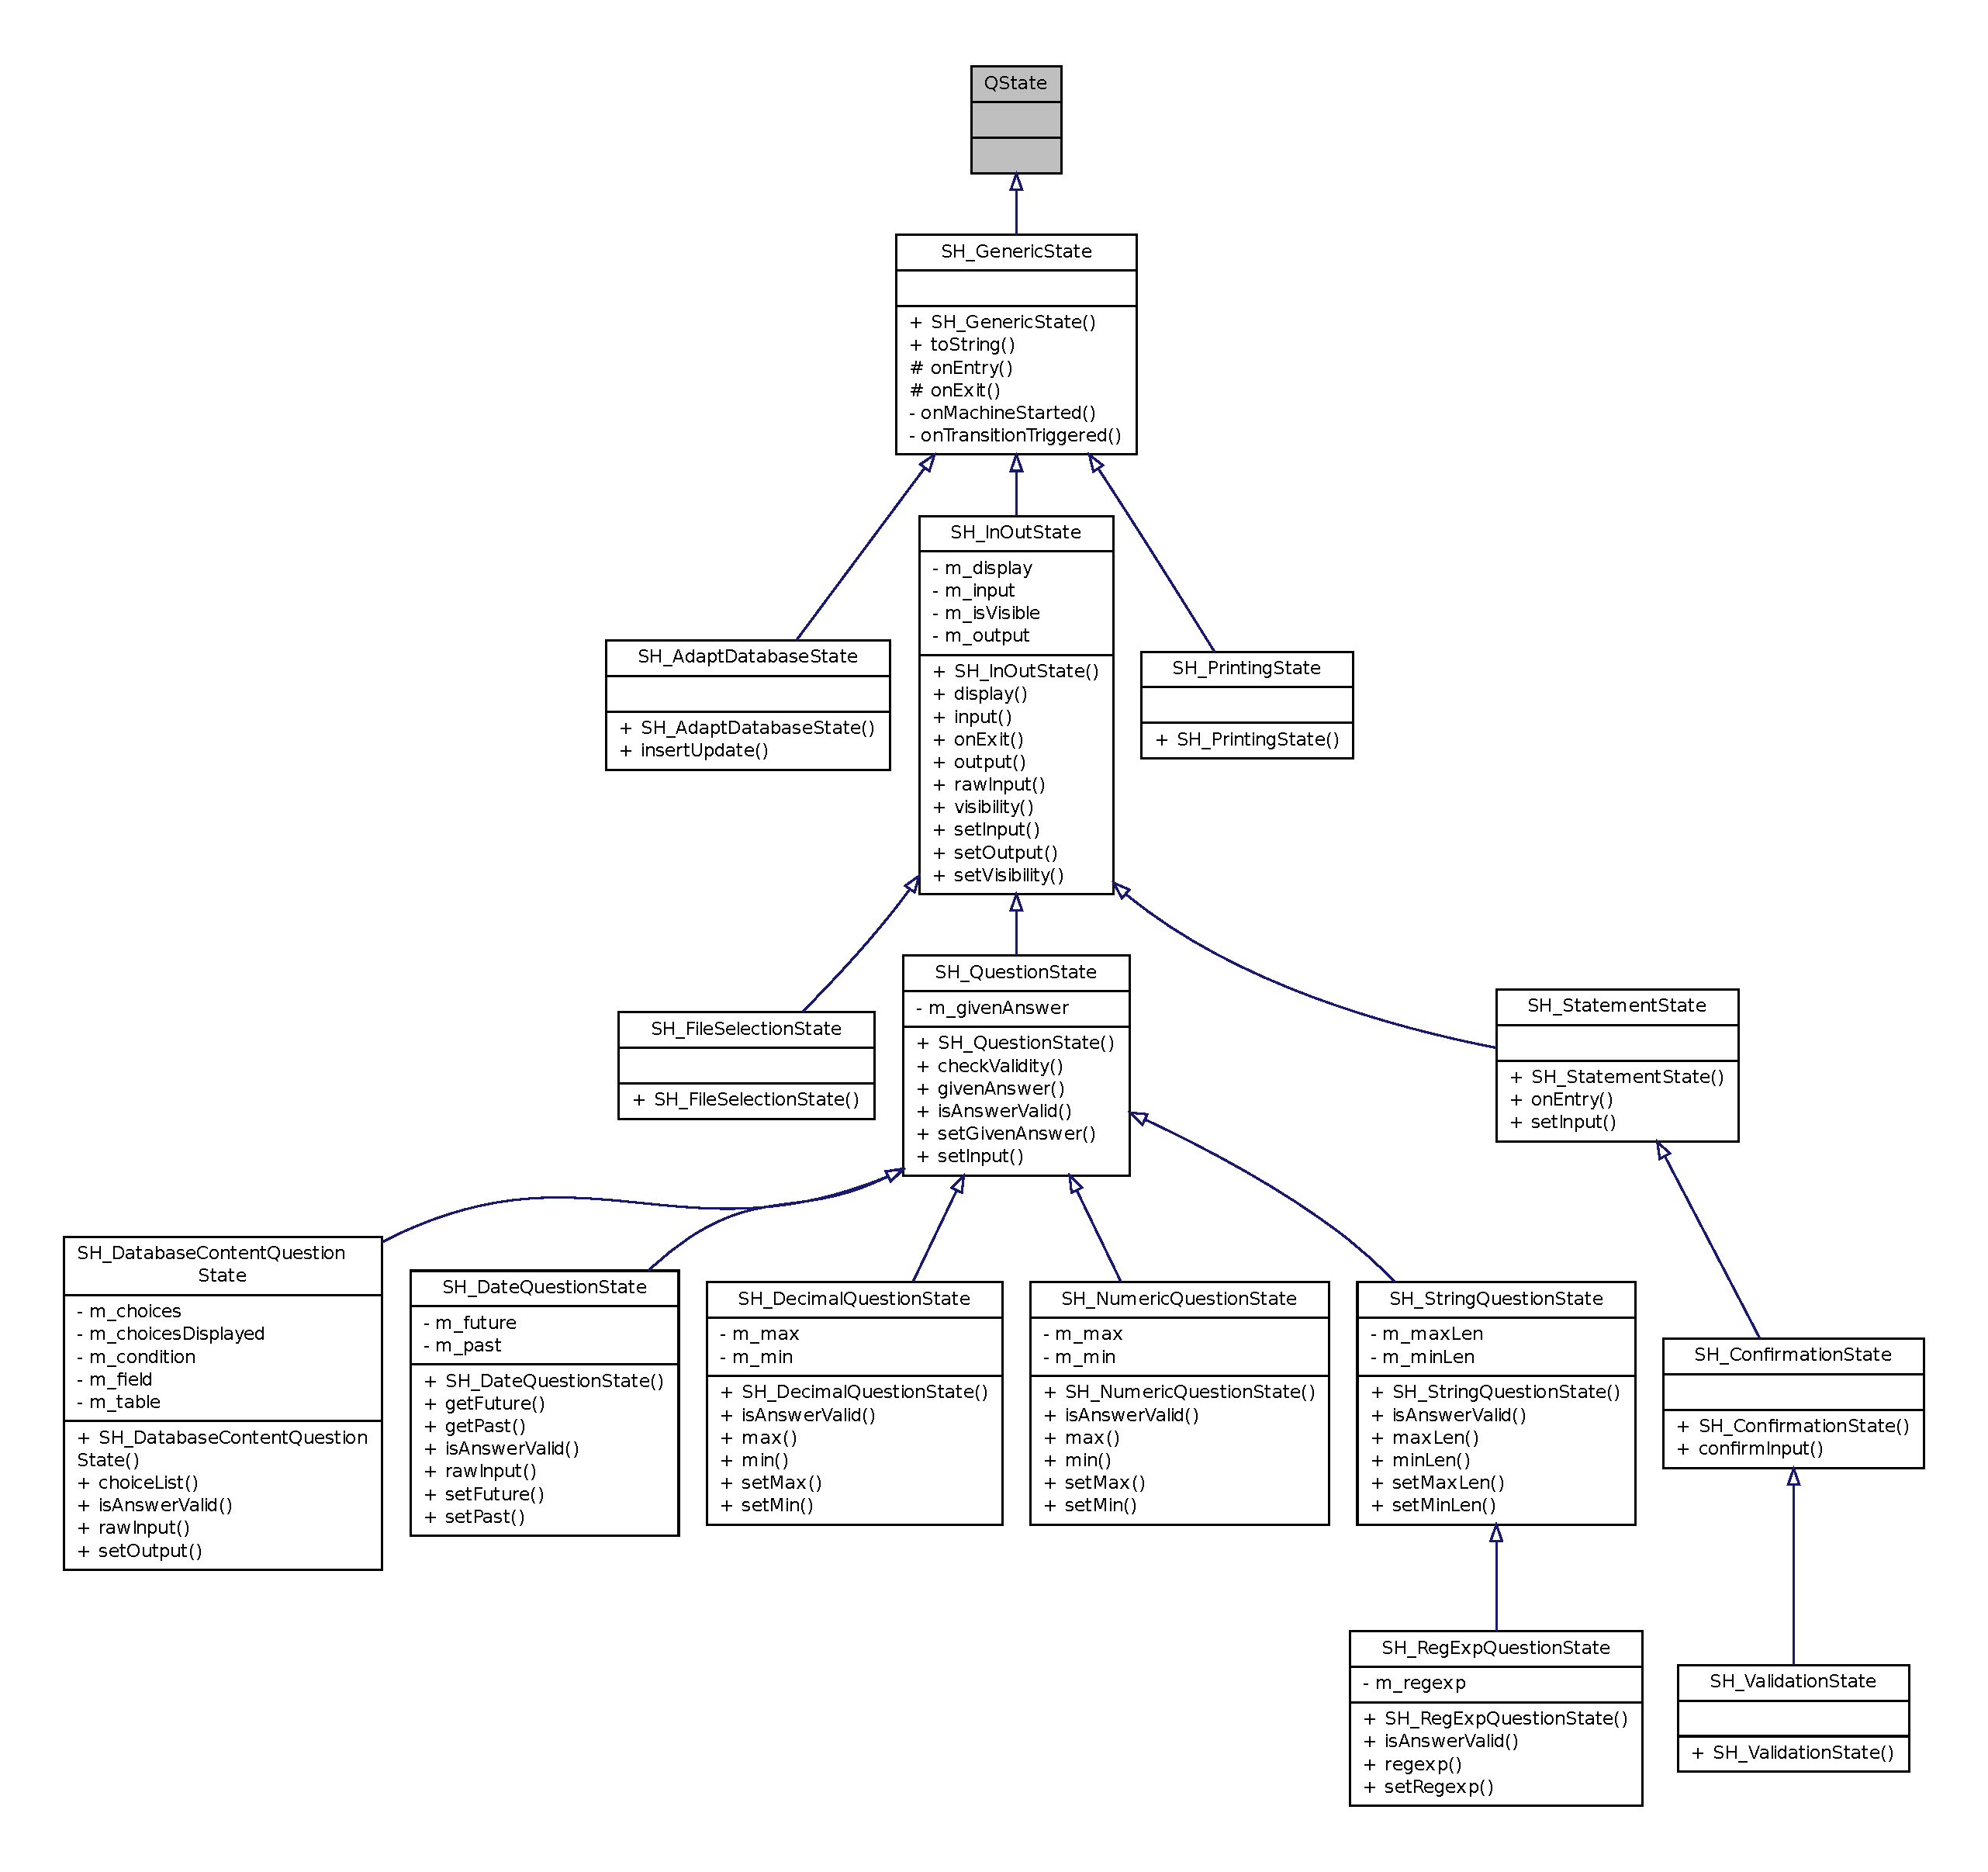
\includegraphics[width=350pt]{classQState__inherit__graph}
\end{center}
\end{figure}


Graphe de collaboration de Q\-State\-:\nopagebreak
\begin{figure}[H]
\begin{center}
\leavevmode
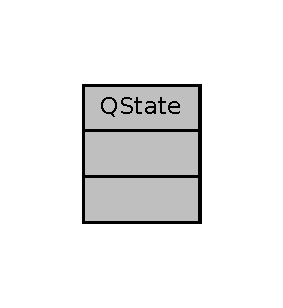
\includegraphics[width=136pt]{classQState__coll__graph}
\end{center}
\end{figure}


La documentation de cette classe a été générée à partir du fichier suivant \-:\begin{DoxyCompactItemize}
\item 
/home/tiff/\-Stage-\/\-I\-U\-T/app/simplhotel/hotel-\/precheck/src/\-Pre\-Check/logic/\hyperlink{SH__GenericDebugableState_8h}{S\-H\-\_\-\-Generic\-Debugable\-State.\-h}\end{DoxyCompactItemize}

\hypertarget{classQStateMachine}{\section{Référence de la classe Q\-State\-Machine}
\label{classQStateMachine}\index{Q\-State\-Machine@{Q\-State\-Machine}}
}


Graphe d'héritage de Q\-State\-Machine\-:
\nopagebreak
\begin{figure}[H]
\begin{center}
\leavevmode
\includegraphics[width=350pt]{classQStateMachine__inherit__graph}
\end{center}
\end{figure}


Graphe de collaboration de Q\-State\-Machine\-:\nopagebreak
\begin{figure}[H]
\begin{center}
\leavevmode
\includegraphics[width=180pt]{classQStateMachine__coll__graph}
\end{center}
\end{figure}


La documentation de cette classe a été générée à partir du fichier suivant \-:\begin{DoxyCompactItemize}
\item 
/home/tiff/\-Stage-\/\-I\-U\-T/app/simplhotel/hotel-\/precheck/src/\-Pre\-Check/logic/\hyperlink{SH__GenericDebugableStateMachine_8h}{S\-H\-\_\-\-Generic\-Debugable\-State\-Machine.\-h}\end{DoxyCompactItemize}

\hypertarget{classRectangle}{\section{Référence de la classe Rectangle}
\label{classRectangle}\index{Rectangle@{Rectangle}}
}
Graphe d'héritage de Rectangle\-:\begin{figure}[H]
\begin{center}
\leavevmode
\includegraphics[height=1.564246cm]{classRectangle}
\end{center}
\end{figure}


La documentation de cette classe a été générée à partir du fichier suivant \-:\begin{DoxyCompactItemize}
\item 
/home/tiff/\-Stage-\/\-I\-U\-T/app/simplhotel/hotel-\/precheck/src/\-Pre\-Check/views/qml/\hyperlink{SH__CalendarDialog_8qml}{S\-H\-\_\-\-Calendar\-Dialog.\-qml}\end{DoxyCompactItemize}

\hypertarget{classSH__AdaptDatabaseState}{\section{Référence de la classe S\-H\-\_\-\-Adapt\-Database\-State}
\label{classSH__AdaptDatabaseState}\index{S\-H\-\_\-\-Adapt\-Database\-State@{S\-H\-\_\-\-Adapt\-Database\-State}}
}


{\ttfamily \#include $<$S\-H\-\_\-\-Adapt\-Database\-State.\-h$>$}

Graphe d'héritage de S\-H\-\_\-\-Adapt\-Database\-State\-:\begin{figure}[H]
\begin{center}
\leavevmode
\includegraphics[height=3.000000cm]{classSH__AdaptDatabaseState}
\end{center}
\end{figure}
\subsection*{Signaux}
\begin{DoxyCompactItemize}
\item 
void \hyperlink{classSH__GenericState_a34c1bebc765cc3a62d66c94c37d4f0c3}{go\-Next} ()
\item 
void \hyperlink{classSH__GenericState_ad5e2a1f3dc129336c8f529cf897c2eb0}{next} ()
\end{DoxyCompactItemize}
\subsection*{Fonctions membres publiques}
\begin{DoxyCompactItemize}
\item 
\hyperlink{classSH__AdaptDatabaseState_aaca9bab6a7263320c40149987b82c024}{S\-H\-\_\-\-Adapt\-Database\-State} (Q\-String \hyperlink{classSH__NamedObject_a9f686c6f2a5bcc08ad03d0cee0151f0f}{name}, \hyperlink{classQState}{Q\-State} $\ast$parent=0)
\item 
Q\-Variant \hyperlink{classSH__AdaptDatabaseState_a037db544ea05f42d21fcbdda758839fe}{insert\-Update} (Q\-String table, Q\-Variant\-Map content)
\begin{DoxyCompactList}\small\item\em Enregistre dans la base de données les valeurs données. \end{DoxyCompactList}\item 
bool \hyperlink{classSH__GenericState_a5f731810dad0cacd28828ccbf1539e4e}{is\-Running} ()
\item 
Q\-String \hyperlink{classSH__GenericState_a7779babbb40f3f8faa71112204d9804f}{to\-String} ()
\end{DoxyCompactItemize}
\subsection*{Fonctions membres protégées}
\begin{DoxyCompactItemize}
\item 
void \hyperlink{classSH__GenericState_a68c67ef95738e01cd34cd5926f4932fb}{on\-Entry} (Q\-Event $\ast$event)
\item 
void \hyperlink{classSH__GenericState_a7f7863859318c70c9b734be5bf5510b0}{on\-Exit} (Q\-Event $\ast$event)
\end{DoxyCompactItemize}


\subsection{Description détaillée}


Définition à la ligne \hyperlink{SH__AdaptDatabaseState_8h_source_l00011}{11} du fichier \hyperlink{SH__AdaptDatabaseState_8h_source}{S\-H\-\_\-\-Adapt\-Database\-State.\-h}.



\subsection{Documentation des constructeurs et destructeur}
\hypertarget{classSH__AdaptDatabaseState_aaca9bab6a7263320c40149987b82c024}{\index{S\-H\-\_\-\-Adapt\-Database\-State@{S\-H\-\_\-\-Adapt\-Database\-State}!S\-H\-\_\-\-Adapt\-Database\-State@{S\-H\-\_\-\-Adapt\-Database\-State}}
\index{S\-H\-\_\-\-Adapt\-Database\-State@{S\-H\-\_\-\-Adapt\-Database\-State}!SH_AdaptDatabaseState@{S\-H\-\_\-\-Adapt\-Database\-State}}
\subsubsection[{S\-H\-\_\-\-Adapt\-Database\-State}]{\setlength{\rightskip}{0pt plus 5cm}S\-H\-\_\-\-Adapt\-Database\-State\-::\-S\-H\-\_\-\-Adapt\-Database\-State (
\begin{DoxyParamCaption}
\item[{Q\-String}]{name, }
\item[{{\bf Q\-State} $\ast$}]{parent = {\ttfamily 0}}
\end{DoxyParamCaption}
)}}\label{classSH__AdaptDatabaseState_aaca9bab6a7263320c40149987b82c024}
Construit une instance de la classe \hyperlink{classSH__AdaptDatabaseState}{S\-H\-\_\-\-Adapt\-Database\-State} 

Définition à la ligne \hyperlink{SH__AdaptDatabaseState_8cpp_source_l00010}{10} du fichier \hyperlink{SH__AdaptDatabaseState_8cpp_source}{S\-H\-\_\-\-Adapt\-Database\-State.\-cpp}.


\begin{DoxyCode}
00010                                                                          :
00011     \hyperlink{classSH__GenericState_a3cc3cb1491b812dfdd032fc6438dfd4e}{SH\_GenericState}(\hyperlink{classSH__NamedObject_a9f686c6f2a5bcc08ad03d0cee0151f0f}{name}, parent)
00012 \{
00013 \}
\end{DoxyCode}


\subsection{Documentation des fonctions membres}
\hypertarget{classSH__GenericState_a34c1bebc765cc3a62d66c94c37d4f0c3}{\index{S\-H\-\_\-\-Adapt\-Database\-State@{S\-H\-\_\-\-Adapt\-Database\-State}!go\-Next@{go\-Next}}
\index{go\-Next@{go\-Next}!SH_AdaptDatabaseState@{S\-H\-\_\-\-Adapt\-Database\-State}}
\subsubsection[{go\-Next}]{\setlength{\rightskip}{0pt plus 5cm}S\-H\-\_\-\-Generic\-State\-::go\-Next (
\begin{DoxyParamCaption}
{}
\end{DoxyParamCaption}
)\hspace{0.3cm}{\ttfamily [signal]}, {\ttfamily [inherited]}}}\label{classSH__GenericState_a34c1bebc765cc3a62d66c94c37d4f0c3}


Référencé par \hyperlink{classSH__QuestionState_a902be003650c33d954d707b2d3ee0bb9}{S\-H\-\_\-\-Question\-State\-::check\-Validity()}, \hyperlink{classSH__ConfirmationState_a039267260de5d102ac7511e6a5fae87f}{S\-H\-\_\-\-Confirmation\-State\-::confirm\-Input()}, \hyperlink{classSH__AdaptDatabaseState_a037db544ea05f42d21fcbdda758839fe}{insert\-Update()}, \hyperlink{classSH__StatementState_ab866a023213fe1bd1857705bf98a8f65}{S\-H\-\_\-\-Statement\-State\-::on\-Entry()}, \hyperlink{classSH__BillingCreationStateMachine_ad62b77fa4aeafe200056ff3974562f83}{S\-H\-\_\-\-Billing\-Creation\-State\-Machine\-::\-S\-H\-\_\-\-Billing\-Creation\-State\-Machine()}, \hyperlink{classSH__GenericState_a3cc3cb1491b812dfdd032fc6438dfd4e}{S\-H\-\_\-\-Generic\-State\-::\-S\-H\-\_\-\-Generic\-State()}, \hyperlink{classSH__InOutState_a5fa88487103a8e197a8453c991bb056b}{S\-H\-\_\-\-In\-Out\-State\-::\-S\-H\-\_\-\-In\-Out\-State()}, et \hyperlink{classSH__ServiceCharging_afa5273d046049b1c2b020a6a19a8290b}{S\-H\-\_\-\-Service\-Charging\-::\-S\-H\-\_\-\-Service\-Charging()}.

\hypertarget{classSH__AdaptDatabaseState_a037db544ea05f42d21fcbdda758839fe}{\index{S\-H\-\_\-\-Adapt\-Database\-State@{S\-H\-\_\-\-Adapt\-Database\-State}!insert\-Update@{insert\-Update}}
\index{insert\-Update@{insert\-Update}!SH_AdaptDatabaseState@{S\-H\-\_\-\-Adapt\-Database\-State}}
\subsubsection[{insert\-Update}]{\setlength{\rightskip}{0pt plus 5cm}S\-H\-\_\-\-Adapt\-Database\-State\-::insert\-Update (
\begin{DoxyParamCaption}
\item[{Q\-String}]{table, }
\item[{Q\-Variant\-Map}]{content}
\end{DoxyParamCaption}
)}}\label{classSH__AdaptDatabaseState_a037db544ea05f42d21fcbdda758839fe}


Enregistre dans la base de données les valeurs données. 

Enregistre dans la base de données les valeurs données, sous forme d'une insertion ou d'une mise à jour, selon le besoin


\begin{DoxyParams}{Paramètres}
{\em table} & Le nom de la table à modifier \\
\hline
{\em content} & Le contenu à enregistrer, sous la forme d'une {\itshape Q\-Variant\-Map} associant les champs de la table aux valeurs à insérer/modifier \\
\hline
\end{DoxyParams}
\begin{DoxyReturn}{Renvoie}
bool Retourne {\itshape true} si l'enregistrement a réussi, {\itshape false} sinon 
\end{DoxyReturn}


Définition à la ligne \hyperlink{SH__AdaptDatabaseState_8cpp_source_l00018}{18} du fichier \hyperlink{SH__AdaptDatabaseState_8cpp_source}{S\-H\-\_\-\-Adapt\-Database\-State.\-cpp}.



Références \hyperlink{classSH__DatabaseManager_a55268fae16792142072af49238f7bb94}{S\-H\-\_\-\-Database\-Manager\-::exec\-Insert\-Returning\-Query()}, \hyperlink{classSH__DatabaseManager_a31198eb4de0f8b18e3fa0eed09f24d19}{S\-H\-\_\-\-Database\-Manager\-::get\-Instance()}, et \hyperlink{classSH__GenericState_a34c1bebc765cc3a62d66c94c37d4f0c3}{S\-H\-\_\-\-Generic\-State\-::go\-Next()}.



Référencé par \hyperlink{classSH__LoopingInOutStateMachine_a0ee122553641721012f3710e71cce234}{S\-H\-\_\-\-Looping\-In\-Out\-State\-Machine\-::set\-States\-Next\-Transition()}, \hyperlink{classSH__InOutStateMachine_a70d6d81c0a8d4afd6aab0a7239edc237}{S\-H\-\_\-\-In\-Out\-State\-Machine\-::set\-States\-Next\-Transition()}, et \hyperlink{classSH__BillingCreationStateMachine_ad62b77fa4aeafe200056ff3974562f83}{S\-H\-\_\-\-Billing\-Creation\-State\-Machine\-::\-S\-H\-\_\-\-Billing\-Creation\-State\-Machine()}.


\begin{DoxyCode}
00019 \{
00020     QVariant \textcolor{keywordtype}{id} = \hyperlink{classSH__DatabaseManager_a31198eb4de0f8b18e3fa0eed09f24d19}{SH\_DatabaseManager::getInstance}()->
      \hyperlink{classSH__DatabaseManager_a55268fae16792142072af49238f7bb94}{execInsertReturningQuery}(table, content, \textcolor{stringliteral}{"id"});
00021     \textcolor{keywordflow}{if}(\textcolor{keywordtype}{id}.isValid()) \{
00022         emit \hyperlink{classSH__GenericState_a34c1bebc765cc3a62d66c94c37d4f0c3}{goNext}();
00023     \}
00024     \textcolor{keywordflow}{return} id;
00025 \}
\end{DoxyCode}
\hypertarget{classSH__GenericState_a5f731810dad0cacd28828ccbf1539e4e}{\index{S\-H\-\_\-\-Adapt\-Database\-State@{S\-H\-\_\-\-Adapt\-Database\-State}!is\-Running@{is\-Running}}
\index{is\-Running@{is\-Running}!SH_AdaptDatabaseState@{S\-H\-\_\-\-Adapt\-Database\-State}}
\subsubsection[{is\-Running}]{\setlength{\rightskip}{0pt plus 5cm}S\-H\-\_\-\-Generic\-State\-::is\-Running (
\begin{DoxyParamCaption}
{}
\end{DoxyParamCaption}
)\hspace{0.3cm}{\ttfamily [inherited]}}}\label{classSH__GenericState_a5f731810dad0cacd28828ccbf1539e4e}
\begin{DoxyReturn}{Renvoie}
bool 
\end{DoxyReturn}


Définition à la ligne \hyperlink{SH__GenericDebugableState_8cpp_source_l00081}{81} du fichier \hyperlink{SH__GenericDebugableState_8cpp_source}{S\-H\-\_\-\-Generic\-Debugable\-State.\-cpp}.



Références \hyperlink{classSH__GenericState_a72ddc905cfbffbed48bb2f2474d5297a}{S\-H\-\_\-\-Generic\-State\-::m\-\_\-is\-Running}.



Référencé par \hyperlink{classSH__QuestionState_a902be003650c33d954d707b2d3ee0bb9}{S\-H\-\_\-\-Question\-State\-::check\-Validity()}, \hyperlink{classSH__ConfirmationState_a039267260de5d102ac7511e6a5fae87f}{S\-H\-\_\-\-Confirmation\-State\-::confirm\-Input()}, \hyperlink{classSH__GenericState_a66d4d4d94ef4fac3eb8d137848290582}{S\-H\-\_\-\-Generic\-State\-::emit\-Go\-Next()}, \hyperlink{classSH__InOutState_ad1695493d39c5194e5b7c6372754ddd7}{S\-H\-\_\-\-In\-Out\-State\-::emit\-Resend\-Input()}, \hyperlink{classSH__InOutState_a40995f4a8201f21d26b7e78b7e7b652e}{S\-H\-\_\-\-In\-Out\-State\-::emit\-Send\-Output()}, \hyperlink{classSH__InOutState_aaec9c2b5ef7c406bff7469461352d47c}{S\-H\-\_\-\-In\-Out\-State\-::set\-Input()}, \hyperlink{classSH__InOutState_af611c84134e262739cd834797b315c80}{S\-H\-\_\-\-In\-Out\-State\-::set\-Output()}, et \hyperlink{classSH__InOutState_a7fdfaa6f600f0ac4a96f238a038ba9ad}{S\-H\-\_\-\-In\-Out\-State\-::set\-Visibility()}.


\begin{DoxyCode}
00082 \{
00083     \textcolor{keywordflow}{return} \hyperlink{classSH__GenericState_a72ddc905cfbffbed48bb2f2474d5297a}{m\_isRunning};
00084 \}
\end{DoxyCode}
\hypertarget{classSH__GenericState_ad5e2a1f3dc129336c8f529cf897c2eb0}{\index{S\-H\-\_\-\-Adapt\-Database\-State@{S\-H\-\_\-\-Adapt\-Database\-State}!next@{next}}
\index{next@{next}!SH_AdaptDatabaseState@{S\-H\-\_\-\-Adapt\-Database\-State}}
\subsubsection[{next}]{\setlength{\rightskip}{0pt plus 5cm}S\-H\-\_\-\-Generic\-State\-::next (
\begin{DoxyParamCaption}
{}
\end{DoxyParamCaption}
)\hspace{0.3cm}{\ttfamily [signal]}, {\ttfamily [inherited]}}}\label{classSH__GenericState_ad5e2a1f3dc129336c8f529cf897c2eb0}


Référencé par \hyperlink{classSH__GenericState_a66d4d4d94ef4fac3eb8d137848290582}{S\-H\-\_\-\-Generic\-State\-::emit\-Go\-Next()}.

\hypertarget{classSH__GenericState_a68c67ef95738e01cd34cd5926f4932fb}{\index{S\-H\-\_\-\-Adapt\-Database\-State@{S\-H\-\_\-\-Adapt\-Database\-State}!on\-Entry@{on\-Entry}}
\index{on\-Entry@{on\-Entry}!SH_AdaptDatabaseState@{S\-H\-\_\-\-Adapt\-Database\-State}}
\subsubsection[{on\-Entry}]{\setlength{\rightskip}{0pt plus 5cm}S\-H\-\_\-\-Generic\-State\-::on\-Entry (
\begin{DoxyParamCaption}
\item[{Q\-Event $\ast$}]{event}
\end{DoxyParamCaption}
)\hspace{0.3cm}{\ttfamily [protected]}, {\ttfamily [inherited]}}}\label{classSH__GenericState_a68c67ef95738e01cd34cd5926f4932fb}

\begin{DoxyParams}{Paramètres}
{\em event} & \\
\hline
\end{DoxyParams}


Définition à la ligne \hyperlink{SH__GenericDebugableState_8cpp_source_l00060}{60} du fichier \hyperlink{SH__GenericDebugableState_8cpp_source}{S\-H\-\_\-\-Generic\-Debugable\-State.\-cpp}.



Références \hyperlink{classSH__MessageManager_a379f2aa0a590a5add34dbe91f98b2ff7}{S\-H\-\_\-\-Message\-Manager\-::debug\-Message()}, \hyperlink{classSH__GenericState_a72ddc905cfbffbed48bb2f2474d5297a}{S\-H\-\_\-\-Generic\-State\-::m\-\_\-is\-Running}, \hyperlink{classSH__NamedObject_a9f686c6f2a5bcc08ad03d0cee0151f0f}{S\-H\-\_\-\-Named\-Object\-::name()}, et \hyperlink{classSH__GenericState_aad4259cc1e6a51681d6a92e995486380}{S\-H\-\_\-\-Generic\-State\-::on\-Transition\-Triggered()}.



Référencé par \hyperlink{classSH__StatementState_ab866a023213fe1bd1857705bf98a8f65}{S\-H\-\_\-\-Statement\-State\-::on\-Entry()}.


\begin{DoxyCode}
00061 \{
00062     Q\_UNUSED(event);
00063     \textcolor{keywordflow}{foreach} (QAbstractTransition* tr, transitions()) \{
00064         connect(tr, SIGNAL(triggered()), \textcolor{keyword}{this}, SLOT(\hyperlink{classSH__GenericState_aad4259cc1e6a51681d6a92e995486380}{onTransitionTriggered}()));
00065     \}
00066     \hyperlink{classSH__GenericState_a72ddc905cfbffbed48bb2f2474d5297a}{m\_isRunning} = \textcolor{keyword}{true};
00067     this->blockSignals(!\hyperlink{classSH__GenericState_a72ddc905cfbffbed48bb2f2474d5297a}{m\_isRunning});
00068     \hyperlink{classSH__MessageManager_a379f2aa0a590a5add34dbe91f98b2ff7}{SH\_MessageManager::debugMessage}(QString(\textcolor{stringliteral}{"Machine: %1, entered state %2"})
      .arg(machine()->objectName()).arg(\hyperlink{classSH__NamedObject_a9f686c6f2a5bcc08ad03d0cee0151f0f}{name}()));
00069 \}
\end{DoxyCode}
\hypertarget{classSH__GenericState_a7f7863859318c70c9b734be5bf5510b0}{\index{S\-H\-\_\-\-Adapt\-Database\-State@{S\-H\-\_\-\-Adapt\-Database\-State}!on\-Exit@{on\-Exit}}
\index{on\-Exit@{on\-Exit}!SH_AdaptDatabaseState@{S\-H\-\_\-\-Adapt\-Database\-State}}
\subsubsection[{on\-Exit}]{\setlength{\rightskip}{0pt plus 5cm}S\-H\-\_\-\-Generic\-State\-::on\-Exit (
\begin{DoxyParamCaption}
\item[{Q\-Event $\ast$}]{event}
\end{DoxyParamCaption}
)\hspace{0.3cm}{\ttfamily [protected]}, {\ttfamily [inherited]}}}\label{classSH__GenericState_a7f7863859318c70c9b734be5bf5510b0}

\begin{DoxyParams}{Paramètres}
{\em event} & \\
\hline
\end{DoxyParams}


Définition à la ligne \hyperlink{SH__GenericDebugableState_8cpp_source_l00074}{74} du fichier \hyperlink{SH__GenericDebugableState_8cpp_source}{S\-H\-\_\-\-Generic\-Debugable\-State.\-cpp}.



Références \hyperlink{classSH__MessageManager_a379f2aa0a590a5add34dbe91f98b2ff7}{S\-H\-\_\-\-Message\-Manager\-::debug\-Message()}, \hyperlink{classSH__GenericState_a72ddc905cfbffbed48bb2f2474d5297a}{S\-H\-\_\-\-Generic\-State\-::m\-\_\-is\-Running}, et \hyperlink{classSH__NamedObject_a9f686c6f2a5bcc08ad03d0cee0151f0f}{S\-H\-\_\-\-Named\-Object\-::name()}.


\begin{DoxyCode}
00075 \{
00076     Q\_UNUSED(event);
00077     \hyperlink{classSH__GenericState_a72ddc905cfbffbed48bb2f2474d5297a}{m\_isRunning} = \textcolor{keyword}{false};
00078     this->blockSignals(!\hyperlink{classSH__GenericState_a72ddc905cfbffbed48bb2f2474d5297a}{m\_isRunning});
00079     \hyperlink{classSH__MessageManager_a379f2aa0a590a5add34dbe91f98b2ff7}{SH\_MessageManager::debugMessage}(QString(\textcolor{stringliteral}{"Machine: %1, exited state %2"}).
      arg(machine()->objectName()).arg(\hyperlink{classSH__NamedObject_a9f686c6f2a5bcc08ad03d0cee0151f0f}{name}()));
00080 \}
\end{DoxyCode}
\hypertarget{classSH__GenericState_a7779babbb40f3f8faa71112204d9804f}{\index{S\-H\-\_\-\-Adapt\-Database\-State@{S\-H\-\_\-\-Adapt\-Database\-State}!to\-String@{to\-String}}
\index{to\-String@{to\-String}!SH_AdaptDatabaseState@{S\-H\-\_\-\-Adapt\-Database\-State}}
\subsubsection[{to\-String}]{\setlength{\rightskip}{0pt plus 5cm}S\-H\-\_\-\-Generic\-State\-::to\-String (
\begin{DoxyParamCaption}
{}
\end{DoxyParamCaption}
)\hspace{0.3cm}{\ttfamily [virtual]}, {\ttfamily [inherited]}}}\label{classSH__GenericState_a7779babbb40f3f8faa71112204d9804f}
\begin{DoxyReturn}{Renvoie}
Q\-String 
\end{DoxyReturn}


Réimplémentée à partir de \hyperlink{classSH__NamedObject_a9f4b19df6a96a17daaf1060b3019ef47}{S\-H\-\_\-\-Named\-Object}.



Définition à la ligne \hyperlink{SH__GenericDebugableState_8cpp_source_l00023}{23} du fichier \hyperlink{SH__GenericDebugableState_8cpp_source}{S\-H\-\_\-\-Generic\-Debugable\-State.\-cpp}.



Références \hyperlink{classSH__NamedObject_a9f4b19df6a96a17daaf1060b3019ef47}{S\-H\-\_\-\-Named\-Object\-::to\-String()}, et \hyperlink{classSH__GenericState_a7779babbb40f3f8faa71112204d9804f}{S\-H\-\_\-\-Generic\-State\-::to\-String()}.



Référencé par \hyperlink{classSH__QuestionState_a902be003650c33d954d707b2d3ee0bb9}{S\-H\-\_\-\-Question\-State\-::check\-Validity()}, \hyperlink{classSH__DateQuestionState_a71917e94cb9ce692f916a848bc8c8892}{S\-H\-\_\-\-Date\-Question\-State\-::raw\-Input()}, \hyperlink{classSH__GenericStateMachine_a85c0c1c9d258ae991f84667412fa47cd}{S\-H\-\_\-\-Generic\-State\-Machine\-::to\-String()}, et \hyperlink{classSH__GenericState_a7779babbb40f3f8faa71112204d9804f}{S\-H\-\_\-\-Generic\-State\-::to\-String()}.


\begin{DoxyCode}
00024 \{
00025     \hyperlink{classQStateMachine}{QStateMachine}* machine = this->machine();
00026     \hyperlink{classSH__GenericState}{SH\_GenericState}* mach = qobject\_cast<\hyperlink{classSH__GenericState}{SH\_GenericState} *>(machine);
00027     \textcolor{keywordflow}{if}(mach) \{
00028         \textcolor{keywordflow}{return} \hyperlink{classSH__NamedObject_a9f4b19df6a96a17daaf1060b3019ef47}{SH\_NamedObject::toString}()+ \textcolor{stringliteral}{" [in "}+mach->
      \hyperlink{classSH__GenericState_a7779babbb40f3f8faa71112204d9804f}{toString}()+\textcolor{stringliteral}{"] "};
00029     \} \textcolor{keywordflow}{else} \{
00030         \textcolor{keywordflow}{return} \hyperlink{classSH__NamedObject_a9f4b19df6a96a17daaf1060b3019ef47}{SH\_NamedObject::toString}();
00031     \}
00032 \}
\end{DoxyCode}


La documentation de cette classe a été générée à partir des fichiers suivants \-:\begin{DoxyCompactItemize}
\item 
/home/tiff/\-Stage-\/\-I\-U\-T/app/simplhotel/hotel-\/precheck/src/\-Pre\-Check/logic/\hyperlink{SH__AdaptDatabaseState_8h}{S\-H\-\_\-\-Adapt\-Database\-State.\-h}\item 
/home/tiff/\-Stage-\/\-I\-U\-T/app/simplhotel/hotel-\/precheck/src/\-Pre\-Check/logic/\hyperlink{SH__AdaptDatabaseState_8cpp}{S\-H\-\_\-\-Adapt\-Database\-State.\-cpp}\end{DoxyCompactItemize}

\hypertarget{classSH__AddressCreationStateMachine}{\section{Référence de la classe S\-H\-\_\-\-Address\-Creation\-State\-Machine}
\label{classSH__AddressCreationStateMachine}\index{S\-H\-\_\-\-Address\-Creation\-State\-Machine@{S\-H\-\_\-\-Address\-Creation\-State\-Machine}}
}


La classe \hyperlink{classSH__AddressCreationStateMachine}{S\-H\-\_\-\-Address\-Creation\-State\-Machine} fournit une machine d'états finis permettant la création d'un entité \char`\"{}adresse\char`\"{} à enregistrer dans la base de données.  




{\ttfamily \#include $<$S\-H\-\_\-\-Address\-Creation.\-h$>$}

Graphe d'héritage de S\-H\-\_\-\-Address\-Creation\-State\-Machine\-:\begin{figure}[H]
\begin{center}
\leavevmode
\includegraphics[height=4.000000cm]{classSH__AddressCreationStateMachine}
\end{center}
\end{figure}
\subsection*{Connecteurs publics}
\begin{DoxyCompactItemize}
\item 
virtual void \hyperlink{classSH__InOutStateMachine_ae0f3b4622d2c70884bb224dee86e95c0}{add\-Children\-Replace\-Transition} (Q\-Abstract\-State $\ast$previous\-State, Q\-Abstract\-State $\ast$next\-State)
\item 
void \hyperlink{classSH__InOutStateMachine_ab6e90f9e187ab70d51ed4e3e1f69f912}{add\-I\-O\-State} (\hyperlink{classSH__InOutState}{S\-H\-\_\-\-In\-Out\-State} $\ast$state, Q\-String field=\char`\"{}\char`\"{})
\item 
virtual void \hyperlink{classSH__InOutStateMachine_a3de9dedcdfd6efab868484c047638f71}{add\-State} (Q\-Abstract\-State $\ast$state)
\item 
virtual void \hyperlink{classSH__InOutStateMachine_a52469f4988c3eb654def2ed237fd10eb}{add\-State} (\hyperlink{classSH__InOutState}{S\-H\-\_\-\-In\-Out\-State} $\ast$astate, Q\-String field=\char`\"{}\char`\"{})
\item 
virtual void \hyperlink{classSH__InOutStateMachine_adcd6eb72b60b2c24aa6701977b5c7c1e}{add\-State} (\hyperlink{classSH__InOutStateMachine}{S\-H\-\_\-\-In\-Out\-State\-Machine} $\ast$astate, Q\-String table=\char`\"{}\char`\"{})
\item 
void \hyperlink{classSH__InOutStateMachine_a0814df2e3f2b776ba210f98cd05be70d}{add\-State\-Machine} (\hyperlink{classSH__InOutStateMachine}{S\-H\-\_\-\-In\-Out\-State\-Machine} $\ast$fsm, Q\-String table=\char`\"{}\char`\"{})
\item 
void \hyperlink{classSH__InOutStateMachine_a9ab1534306b2bdb62743d4bcefe40c17}{set\-Content\-Value} (Q\-Variant content, Q\-String field)
\item 
virtual void \hyperlink{classSH__InOutStateMachine_a70d6d81c0a8d4afd6aab0a7239edc237}{set\-States\-Next\-Transition} (Q\-Abstract\-State $\ast$previous\-State, Q\-Abstract\-State $\ast$next\-State)
\end{DoxyCompactItemize}
\subsection*{Signaux}
\begin{DoxyCompactItemize}
\item 
void \hyperlink{classSH__InOutStateMachine_a035d37535533d4805fe2606f38c19380}{cancel\-Replacement} ()
\item 
void \hyperlink{classSH__InOutStateMachine_aa1d5860888c96ff94c55dc77e0fdfdcf}{clear\-All} ()
\item 
void \hyperlink{classSH__InOutStateMachine_a7f7d9c9300c1d05bce2c26029f28cc31}{confirm\-Input} ()
\item 
void \hyperlink{classSH__InOutStateMachine_ab3a12d1f9b658d8ffdc17669a6c065f2}{display\-Calendar} ()
\item 
void \hyperlink{classSH__InOutStateMachine_ab74b981b0aab09067d7479f2b7e79b0b}{display\-Choice\-List} (Q\-Variant\-List choices)
\item 
void \hyperlink{classSH__InOutStateMachine_abd206c3bc32bb7690df9c3e1cd546ebc}{display\-File\-Dialog} ()
\item 
void \hyperlink{classSH__GenericStateMachine_aec37e33524182ab83bf300f1cc1a064e}{go\-Next} ()
\item 
void \hyperlink{classSH__GenericStateMachine_af4771d31d87951c997fba1633c2d67f6}{next} ()
\item 
void \hyperlink{classSH__InOutStateMachine_a037ed5e13ecfae2123a8d4940292e410}{receive\-Input} (Q\-String input)
\item 
void \hyperlink{classSH__InOutStateMachine_a9fa5db44086de2576c812f631aa4f60a}{replace\-Input} (Q\-String field)
\item 
void \hyperlink{classSH__InOutStateMachine_a526822c66b46aa0cd81ba4473fa5573f}{resend\-Text} (Q\-String text, bool editable=false)
\item 
void \hyperlink{classSH__InOutStateMachine_a5e7f5958bae31696b6a8deab94ad2b4f}{send\-Text} (Q\-String text, bool editable=false)
\item 
void \hyperlink{classSH__InOutStateMachine_aec1b3fef3c1f82499aa1f73beaecd08a}{validate\-Input} ()
\end{DoxyCompactItemize}
\subsection*{Fonctions membres publiques}
\begin{DoxyCompactItemize}
\item 
\hyperlink{classSH__AddressCreationStateMachine_aabbda0fa01d5a59aaff1bd0e7153386d}{S\-H\-\_\-\-Address\-Creation\-State\-Machine} (Q\-String \hyperlink{classSH__NamedObject_a9f686c6f2a5bcc08ad03d0cee0151f0f}{name}, \hyperlink{classQObject}{Q\-Object} $\ast$parent=0)
\item 
Q\-Variant \hyperlink{classSH__InOutStateMachine_aa1a3bd3c0ea8a59b9bc916dc718eb9ca}{get\-Content\-Value} (Q\-String field)
\item 
Q\-History\-State $\ast$ \hyperlink{classSH__InOutStateMachine_af71bfdb3b59b7bf2763588b513b4205f}{history\-Value} (Q\-String field)
\item 
Q\-Variant\-Map \hyperlink{classSH__InOutStateMachine_aaca105fbd5f5cc3bac115389ad3694c5}{io\-Content} () const 
\item 
void \hyperlink{classSH__InOutStateMachine_a8271a7ec7d5f6502449dd3b4da5f4155}{set\-I\-Ocontent} (const Q\-Variant\-Map \&\hyperlink{classSH__InOutStateMachine_aaca105fbd5f5cc3bac115389ad3694c5}{io\-Content})
\item 
void \hyperlink{classSH__InOutStateMachine_acbcce2c4300af1634d928b30e5e9be1c}{set\-I\-O\-State\-History} (Q\-History\-State $\ast$state, Q\-String field)
\item 
void \hyperlink{classSH__InOutStateMachine_a95db31a7e7f31f36a8737adc739ab08c}{set\-Table\-Name} (const Q\-String \&\hyperlink{classSH__InOutStateMachine_a4288a6c86ddf83effefff886675591c9}{table\-Name})
\item 
Q\-String \hyperlink{classSH__InOutStateMachine_a4288a6c86ddf83effefff886675591c9}{table\-Name} () const 
\item 
Q\-String \hyperlink{classSH__GenericStateMachine_a85c0c1c9d258ae991f84667412fa47cd}{to\-String} ()
\end{DoxyCompactItemize}
\subsection*{Connecteurs protégés}
\begin{DoxyCompactItemize}
\item 
void \hyperlink{classSH__GenericStateMachine_a2e162a1da1f694d433cb9072b37ac530}{emit\-Go\-Next} ()
\end{DoxyCompactItemize}
\subsection*{Fonctions membres protégées}
\begin{DoxyCompactItemize}
\item 
Q\-Map$<$ Q\-String, Q\-History\-State $\ast$ $>$ \hyperlink{classSH__InOutStateMachine_a13889998c6dcd17db984dd6ed1454e80}{io\-States\-History} () const 
\item 
bool \hyperlink{classSH__InOutStateMachine_ae6c7448fbe267b035017108a9ffdff2e}{is\-E\-Running} ()
\item 
void \hyperlink{classSH__GenericStateMachine_adfd82f2532595ed7c4bcf21f03cbb951}{on\-Entry} (Q\-Event $\ast$event)
\item 
void \hyperlink{classSH__GenericStateMachine_a4b36d60fa1876908493d3d07f191a30f}{on\-Exit} (Q\-Event $\ast$event)
\end{DoxyCompactItemize}
\subsection*{Attributs protégés}
\begin{DoxyCompactItemize}
\item 
Q\-Variant\-Map \hyperlink{classSH__InOutStateMachine_a8cfbc27eef057bf37b7711bdfef2077e}{m\-\_\-io\-Content}
\item 
Q\-Map$<$ Q\-String, Q\-History\-State $\ast$ $>$ \hyperlink{classSH__InOutStateMachine_ac46ad1af230e1b2156d805275690dec3}{m\-\_\-io\-States\-History}
\item 
Q\-String \hyperlink{classSH__InOutStateMachine_aa009eecc5ab6181358faafb5996b6006}{m\-\_\-table\-Name}
\end{DoxyCompactItemize}


\subsection{Description détaillée}
La classe \hyperlink{classSH__AddressCreationStateMachine}{S\-H\-\_\-\-Address\-Creation\-State\-Machine} fournit une machine d'états finis permettant la création d'un entité \char`\"{}adresse\char`\"{} à enregistrer dans la base de données. 


\begin{DoxyItemize}
\item 
\item 
\end{DoxyItemize}

Définition à la ligne \hyperlink{SH__AddressCreation_8h_source_l00011}{11} du fichier \hyperlink{SH__AddressCreation_8h_source}{S\-H\-\_\-\-Address\-Creation.\-h}.



\subsection{Documentation des constructeurs et destructeur}
\hypertarget{classSH__AddressCreationStateMachine_aabbda0fa01d5a59aaff1bd0e7153386d}{\index{S\-H\-\_\-\-Address\-Creation\-State\-Machine@{S\-H\-\_\-\-Address\-Creation\-State\-Machine}!S\-H\-\_\-\-Address\-Creation\-State\-Machine@{S\-H\-\_\-\-Address\-Creation\-State\-Machine}}
\index{S\-H\-\_\-\-Address\-Creation\-State\-Machine@{S\-H\-\_\-\-Address\-Creation\-State\-Machine}!SH_AddressCreationStateMachine@{S\-H\-\_\-\-Address\-Creation\-State\-Machine}}
\subsubsection[{S\-H\-\_\-\-Address\-Creation\-State\-Machine}]{\setlength{\rightskip}{0pt plus 5cm}S\-H\-\_\-\-Address\-Creation\-State\-Machine\-::\-S\-H\-\_\-\-Address\-Creation\-State\-Machine (
\begin{DoxyParamCaption}
\item[{Q\-String}]{name, }
\item[{{\bf Q\-Object} $\ast$}]{parent = {\ttfamily 0}}
\end{DoxyParamCaption}
)}}\label{classSH__AddressCreationStateMachine_aabbda0fa01d5a59aaff1bd0e7153386d}
Construit une instance de la classe \hyperlink{classSH__AddressCreationStateMachine}{S\-H\-\_\-\-Address\-Creation\-State\-Machine} 

Définition à la ligne \hyperlink{SH__AddressCreation_8cpp_source_l00008}{8} du fichier \hyperlink{SH__AddressCreation_8cpp_source}{S\-H\-\_\-\-Address\-Creation.\-cpp}.



Références \hyperlink{classSH__GenericStateMachine_aec37e33524182ab83bf300f1cc1a064e}{S\-H\-\_\-\-Generic\-State\-Machine\-::go\-Next()}.


\begin{DoxyCode}
00008                                                                                             :
00009     \hyperlink{classSH__InOutStateMachine_abd780037922920c674b43d80c2b50d16}{SH\_InOutStateMachine}(\textcolor{stringliteral}{"ADDRESSES"},\hyperlink{classSH__NamedObject_a9f686c6f2a5bcc08ad03d0cee0151f0f}{name}, parent)
00010 \{
00011     \textcolor{comment}{/*TODO: rue, numéro, code postal, ville, pays, destinataire*/}
00012     emit \hyperlink{classSH__GenericStateMachine_aec37e33524182ab83bf300f1cc1a064e}{goNext}();
00013 \}
\end{DoxyCode}


\subsection{Documentation des fonctions membres}
\hypertarget{classSH__InOutStateMachine_ae0f3b4622d2c70884bb224dee86e95c0}{\index{S\-H\-\_\-\-Address\-Creation\-State\-Machine@{S\-H\-\_\-\-Address\-Creation\-State\-Machine}!add\-Children\-Replace\-Transition@{add\-Children\-Replace\-Transition}}
\index{add\-Children\-Replace\-Transition@{add\-Children\-Replace\-Transition}!SH_AddressCreationStateMachine@{S\-H\-\_\-\-Address\-Creation\-State\-Machine}}
\subsubsection[{add\-Children\-Replace\-Transition}]{\setlength{\rightskip}{0pt plus 5cm}S\-H\-\_\-\-In\-Out\-State\-Machine\-::add\-Children\-Replace\-Transition (
\begin{DoxyParamCaption}
\item[{Q\-Abstract\-State $\ast$}]{previous\-State, }
\item[{Q\-Abstract\-State $\ast$}]{next\-State}
\end{DoxyParamCaption}
)\hspace{0.3cm}{\ttfamily [virtual]}, {\ttfamily [slot]}, {\ttfamily [inherited]}}}\label{classSH__InOutStateMachine_ae0f3b4622d2c70884bb224dee86e95c0}

\begin{DoxyParams}{Paramètres}
{\em previous\-State} & \\
\hline
{\em next\-State} & \\
\hline
\end{DoxyParams}


Définition à la ligne \hyperlink{SH__IOStateMachine_8cpp_source_l00227}{227} du fichier \hyperlink{SH__IOStateMachine_8cpp_source}{S\-H\-\_\-\-I\-O\-State\-Machine.\-cpp}.



Références \hyperlink{classSH__InOutStateMachine_af71bfdb3b59b7bf2763588b513b4205f}{S\-H\-\_\-\-In\-Out\-State\-Machine\-::history\-Value()}, \hyperlink{classSH__GenericStateMachine_af4771d31d87951c997fba1633c2d67f6}{S\-H\-\_\-\-Generic\-State\-Machine\-::next()}, et \hyperlink{classSH__InOutStateMachine_a9fa5db44086de2576c812f631aa4f60a}{S\-H\-\_\-\-In\-Out\-State\-Machine\-::replace\-Input()}.



Référencé par \hyperlink{classSH__LoopingInOutStateMachine_a0ee122553641721012f3710e71cce234}{S\-H\-\_\-\-Looping\-In\-Out\-State\-Machine\-::set\-States\-Next\-Transition()}.


\begin{DoxyCode}
00228 \{
00229     \hyperlink{classSH__GenericState}{SH\_GenericState}* genPreviousState = qobject\_cast<
      \hyperlink{classSH__GenericState}{SH\_GenericState}*>(previousState);
00230     \textcolor{keywordflow}{if}(genPreviousState) \{
00231         \textcolor{comment}{/*connect(this, &SH\_GenericStateMachine::entered, [=]() \{*/}
00232         \textcolor{comment}{/*à faire au moment de l'entrée dans l'état previousState*/}
00233         \textcolor{comment}{/*connect(genPreviousState, &QAbstractState::entered, [=]() \{*/}
00234         connect(\textcolor{keyword}{this}, &\hyperlink{classSH__InOutStateMachine_a9fa5db44086de2576c812f631aa4f60a}{SH\_InOutStateMachine::replaceInput}, [=](QString 
      field) \{
00235             \textcolor{comment}{/*après avoir demandé à revenir sur un état précédent, on attend la fin de l'état actuel puis
       on retourne à l'historique de l'état désiré; celui-ci fini, on passe à l'état qui aurait du suivre celui
       pendant lequel on a demandé à revenir sur un état précédent*/}
00236             QHistoryState* hState = \hyperlink{classSH__InOutStateMachine_af71bfdb3b59b7bf2763588b513b4205f}{historyValue}(field);
00237             \textcolor{keywordflow}{if}(hState) \{
00238                 \textcolor{comment}{/*si l'historique existe (on a déjà quitté l'état voulu)*/}
00239                 hState->parentState()->addTransition(hState->parentState(), SIGNAL(
      \hyperlink{classSH__GenericStateMachine_af4771d31d87951c997fba1633c2d67f6}{next}()), nextState);
00240                 genPreviousState->addTransition(genPreviousState, SIGNAL(\hyperlink{classSH__GenericStateMachine_af4771d31d87951c997fba1633c2d67f6}{next}()), hState);
00241             \}
00242         \});
00243         \textcolor{comment}{/*\});*/}
00244         \textcolor{comment}{/*\});*/}
00245     \}
00246 \}
\end{DoxyCode}
\hypertarget{classSH__InOutStateMachine_ab6e90f9e187ab70d51ed4e3e1f69f912}{\index{S\-H\-\_\-\-Address\-Creation\-State\-Machine@{S\-H\-\_\-\-Address\-Creation\-State\-Machine}!add\-I\-O\-State@{add\-I\-O\-State}}
\index{add\-I\-O\-State@{add\-I\-O\-State}!SH_AddressCreationStateMachine@{S\-H\-\_\-\-Address\-Creation\-State\-Machine}}
\subsubsection[{add\-I\-O\-State}]{\setlength{\rightskip}{0pt plus 5cm}S\-H\-\_\-\-In\-Out\-State\-Machine\-::add\-I\-O\-State (
\begin{DoxyParamCaption}
\item[{{\bf S\-H\-\_\-\-In\-Out\-State} $\ast$}]{state, }
\item[{Q\-String}]{field = {\ttfamily \char`\"{}\char`\"{}}}
\end{DoxyParamCaption}
)\hspace{0.3cm}{\ttfamily [slot]}, {\ttfamily [inherited]}}}\label{classSH__InOutStateMachine_ab6e90f9e187ab70d51ed4e3e1f69f912}

\begin{DoxyParams}{Paramètres}
{\em state} & \\
\hline
{\em field} & \\
\hline
\end{DoxyParams}


Définition à la ligne \hyperlink{SH__IOStateMachine_8cpp_source_l00084}{84} du fichier \hyperlink{SH__IOStateMachine_8cpp_source}{S\-H\-\_\-\-I\-O\-State\-Machine.\-cpp}.



Références \hyperlink{classSH__InOutStateMachine_a3de9dedcdfd6efab868484c047638f71}{S\-H\-\_\-\-In\-Out\-State\-Machine\-::add\-State()}, \hyperlink{classSH__ConfirmationState_a039267260de5d102ac7511e6a5fae87f}{S\-H\-\_\-\-Confirmation\-State\-::confirm\-Input()}, \hyperlink{classSH__MessageManager_a379f2aa0a590a5add34dbe91f98b2ff7}{S\-H\-\_\-\-Message\-Manager\-::debug\-Message()}, \hyperlink{classSH__InOutStateMachine_ab3a12d1f9b658d8ffdc17669a6c065f2}{S\-H\-\_\-\-In\-Out\-State\-Machine\-::display\-Calendar()}, \hyperlink{classSH__DatabaseContentQuestionState_ae1e149ad7ab3d957f3c5df9ef078448b}{S\-H\-\_\-\-Database\-Content\-Question\-State\-::display\-Choice\-List()}, \hyperlink{classSH__InOutStateMachine_ab74b981b0aab09067d7479f2b7e79b0b}{S\-H\-\_\-\-In\-Out\-State\-Machine\-::display\-Choice\-List()}, \hyperlink{classSH__InOutStateMachine_abd206c3bc32bb7690df9c3e1cd546ebc}{S\-H\-\_\-\-In\-Out\-State\-Machine\-::display\-File\-Dialog()}, \hyperlink{classSH__MessageManager_a0b35c2f96e6d69934bf7f7c1e2172ea9}{S\-H\-\_\-\-Message\-Manager\-::info\-Message()}, \hyperlink{classSH__InOutState_a4c674a54f41d2e6ef951b22393dcd89f}{S\-H\-\_\-\-In\-Out\-State\-::raw\-Input()}, \hyperlink{classSH__InOutStateMachine_a037ed5e13ecfae2123a8d4940292e410}{S\-H\-\_\-\-In\-Out\-State\-Machine\-::receive\-Input()}, \hyperlink{classSH__InOutState_a1f00480afefd173002cf56d4c4128048}{S\-H\-\_\-\-In\-Out\-State\-::resend\-Input()}, \hyperlink{classSH__InOutStateMachine_a526822c66b46aa0cd81ba4473fa5573f}{S\-H\-\_\-\-In\-Out\-State\-Machine\-::resend\-Text()}, \hyperlink{classSH__InOutState_a77921c5f42059bc97361f4ff7827da12}{S\-H\-\_\-\-In\-Out\-State\-::send\-Output()}, \hyperlink{classSH__InOutStateMachine_a5e7f5958bae31696b6a8deab94ad2b4f}{S\-H\-\_\-\-In\-Out\-State\-Machine\-::send\-Text()}, \hyperlink{classSH__InOutStateMachine_a9ab1534306b2bdb62743d4bcefe40c17}{S\-H\-\_\-\-In\-Out\-State\-Machine\-::set\-Content\-Value()}, \hyperlink{classSH__InOutState_aaec9c2b5ef7c406bff7469461352d47c}{S\-H\-\_\-\-In\-Out\-State\-::set\-Input()}, \hyperlink{classSH__InOutStateMachine_acbcce2c4300af1634d928b30e5e9be1c}{S\-H\-\_\-\-In\-Out\-State\-Machine\-::set\-I\-O\-State\-History()}, et \hyperlink{classSH__InOutStateMachine_aec1b3fef3c1f82499aa1f73beaecd08a}{S\-H\-\_\-\-In\-Out\-State\-Machine\-::validate\-Input()}.



Référencé par \hyperlink{classSH__InOutStateMachine_a52469f4988c3eb654def2ed237fd10eb}{S\-H\-\_\-\-In\-Out\-State\-Machine\-::add\-State()}.


\begin{DoxyCode}
00085 \{
00086     \hyperlink{classSH__InOutState}{SH\_InOutState}* state = qobject\_cast<\hyperlink{classSH__InOutState}{SH\_InOutState} *>(astate);
00087     \textcolor{keywordflow}{if}(state) \{
00088         \textcolor{comment}{/*connect(this, &SH\_GenericStateMachine::entered, [=]() \{*/}
00089         \textcolor{comment}{/*à faire au moment de l'entrée dans l'état state*/}
00090         \textcolor{comment}{/*connect(state, &QAbstractState::entered, [=]() \{*/}
00091         \textcolor{comment}{/* la réception d'une valeur entraîne son enregistrement comme entrée de l'utilisateur auprès de
       l'état*/}
00092         connect(state, &\hyperlink{classSH__InOutState_a77921c5f42059bc97361f4ff7827da12}{SH\_InOutState::sendOutput}, [=](QVariant out) \{ \textcolor{keywordflow}{if}(out.
      isValid()) \{
00093                 \hyperlink{classSH__MessageManager_a0b35c2f96e6d69934bf7f7c1e2172ea9}{SH\_MessageManager::infoMessage}(out.toString(),\textcolor{stringliteral}{"reçu de l'état
      "});
00094                 emit this->\hyperlink{classSH__InOutStateMachine_a5e7f5958bae31696b6a8deab94ad2b4f}{sendText}(out.toString(), \textcolor{keyword}{false});
00095             \}\});
00096         connect(\textcolor{keyword}{this}, &\hyperlink{classSH__InOutStateMachine_a037ed5e13ecfae2123a8d4940292e410}{SH\_InOutStateMachine::receiveInput}, state, &
      \hyperlink{classSH__InOutState_aaec9c2b5ef7c406bff7469461352d47c}{SH\_InOutState::setInput}, Qt::QueuedConnection);
00097         connect(state, &\hyperlink{classSH__InOutState_a1f00480afefd173002cf56d4c4128048}{SH\_InOutState::resendInput}, [=](QVariant in) \{  \textcolor{keywordflow}{if}(in.
      isValid()) \{
00098                 \hyperlink{classSH__MessageManager_a0b35c2f96e6d69934bf7f7c1e2172ea9}{SH\_MessageManager::infoMessage}(in.toString(),\textcolor{stringliteral}{"envoyé par
       l'état"});
00099                 emit this->\hyperlink{classSH__InOutStateMachine_a526822c66b46aa0cd81ba4473fa5573f}{resendText}(in.toString(), \textcolor{keyword}{true});
00100             \}\});
00101         \hyperlink{classSH__MessageManager_a379f2aa0a590a5add34dbe91f98b2ff7}{SH\_MessageManager::debugMessage}(\textcolor{stringliteral}{"salioute"});
00102         \hyperlink{classSH__ValidationState}{SH\_ValidationState} *validationState = qobject\_cast<
      \hyperlink{classSH__ValidationState}{SH\_ValidationState}*>(astate);
00103         \textcolor{keywordflow}{if}(validationState) \{
00104             connect(\textcolor{keyword}{this}, &\hyperlink{classSH__InOutStateMachine_aec1b3fef3c1f82499aa1f73beaecd08a}{SH\_InOutStateMachine::validateInput}, 
      validationState, &\hyperlink{classSH__ConfirmationState_a039267260de5d102ac7511e6a5fae87f}{SH\_ValidationState::confirmInput}, Qt::QueuedConnection);
00105         \}
00106 
00107         \hyperlink{classSH__ConfirmationState}{SH\_ConfirmationState} *confirmationState = qobject\_cast<
      \hyperlink{classSH__ConfirmationState}{SH\_ConfirmationState}*>(astate);
00108         \textcolor{keywordflow}{if}(confirmationState) \{
00109             connect(\textcolor{keyword}{this}, &\hyperlink{classSH__InOutStateMachine_aec1b3fef3c1f82499aa1f73beaecd08a}{SH\_InOutStateMachine::validateInput}, 
      confirmationState, &\hyperlink{classSH__ConfirmationState_a039267260de5d102ac7511e6a5fae87f}{SH\_ConfirmationState::confirmInput}, Qt::QueuedConnection);
00110         \}
00111 
00112         \hyperlink{classSH__DateQuestionState}{SH\_DateQuestionState} *dateState = qobject\_cast<
      \hyperlink{classSH__DateQuestionState}{SH\_DateQuestionState}*>(astate);
00113         \textcolor{keywordflow}{if}(dateState) \{
00114             emit this->\hyperlink{classSH__InOutStateMachine_ab3a12d1f9b658d8ffdc17669a6c065f2}{displayCalendar}();
00115         \}
00116 
00117         \hyperlink{classSH__DatabaseContentQuestionState}{SH\_DatabaseContentQuestionState} *choiceState = qobject\_cast<
      \hyperlink{classSH__DatabaseContentQuestionState}{SH\_DatabaseContentQuestionState}*>(astate);
00118         \textcolor{keywordflow}{if}(choiceState) \{
00119             connect(\textcolor{keyword}{this}, &\hyperlink{classSH__InOutStateMachine_ab74b981b0aab09067d7479f2b7e79b0b}{SH\_InOutStateMachine::displayChoiceList}, 
      choiceState, &\hyperlink{classSH__DatabaseContentQuestionState_ae1e149ad7ab3d957f3c5df9ef078448b}{SH\_DatabaseContentQuestionState::displayChoiceList}
      , Qt::QueuedConnection);
00120         \}
00121 
00122         \hyperlink{classSH__FileSelectionState}{SH\_FileSelectionState} *fileState = qobject\_cast<
      \hyperlink{classSH__FileSelectionState}{SH\_FileSelectionState}*>(astate);
00123         \textcolor{keywordflow}{if}(fileState) \{
00124             emit this->\hyperlink{classSH__InOutStateMachine_abd206c3bc32bb7690df9c3e1cd546ebc}{displayFileDialog}();
00125         \}
00126         \hyperlink{classSH__MessageManager_a379f2aa0a590a5add34dbe91f98b2ff7}{SH\_MessageManager::debugMessage}(\textcolor{stringliteral}{"salioute bis"});
00127         \textcolor{comment}{/*\});*/}
00128         connect(state, &QAbstractState::exited, [=]() \{
00129             \textcolor{keywordflow}{if}(!field.isEmpty()) \{
00130                 \hyperlink{classSH__InOutStateMachine_a9ab1534306b2bdb62743d4bcefe40c17}{setContentValue}(state->\hyperlink{classSH__InOutState_a4c674a54f41d2e6ef951b22393dcd89f}{rawInput}(), field);
00131 
00132                 \textcolor{comment}{/*gestion de l'historique des états pour pouvoir revenir à l'état state après l'avoir
       quitté*/}
00133                 QHistoryState* hState = \textcolor{keyword}{new} QHistoryState(state);
00134                 \hyperlink{classSH__InOutStateMachine_acbcce2c4300af1634d928b30e5e9be1c}{setIOStateHistory}(hState, field);
00135             \}
00136             \textcolor{comment}{/*plus aucune action sur l'état ne pourra être provoquée par la machine*/}
00137             state->disconnect(\textcolor{keyword}{this});
00138         \});
00139         \textcolor{comment}{/*\});*/}
00140     \}
00141     \hyperlink{classSH__MessageManager_a379f2aa0a590a5add34dbe91f98b2ff7}{SH\_MessageManager::debugMessage}(\textcolor{stringliteral}{"salioute bis bis"});
00142     QAbstractState* abstate = qobject\_cast<QAbstractState *>(astate);
00143     \textcolor{keywordflow}{if}(abstate) \{
00144         \hyperlink{classSH__InOutStateMachine_a3de9dedcdfd6efab868484c047638f71}{SH\_InOutStateMachine::addState}(abstate);
00145     \}
00146 \}
\end{DoxyCode}
\hypertarget{classSH__InOutStateMachine_a3de9dedcdfd6efab868484c047638f71}{\index{S\-H\-\_\-\-Address\-Creation\-State\-Machine@{S\-H\-\_\-\-Address\-Creation\-State\-Machine}!add\-State@{add\-State}}
\index{add\-State@{add\-State}!SH_AddressCreationStateMachine@{S\-H\-\_\-\-Address\-Creation\-State\-Machine}}
\subsubsection[{add\-State}]{\setlength{\rightskip}{0pt plus 5cm}void S\-H\-\_\-\-In\-Out\-State\-Machine\-::add\-State (
\begin{DoxyParamCaption}
\item[{Q\-Abstract\-State $\ast$}]{state}
\end{DoxyParamCaption}
)\hspace{0.3cm}{\ttfamily [virtual]}, {\ttfamily [slot]}, {\ttfamily [inherited]}}}\label{classSH__InOutStateMachine_a3de9dedcdfd6efab868484c047638f71}


Définition à la ligne \hyperlink{SH__IOStateMachine_8cpp_source_l00068}{68} du fichier \hyperlink{SH__IOStateMachine_8cpp_source}{S\-H\-\_\-\-I\-O\-State\-Machine.\-cpp}.



Références \hyperlink{classSH__GenericStateMachine_af4402993e916573a589c9d28158b28d8}{S\-H\-\_\-\-Generic\-State\-Machine\-::add\-State()}, et \hyperlink{classSH__MessageManager_a379f2aa0a590a5add34dbe91f98b2ff7}{S\-H\-\_\-\-Message\-Manager\-::debug\-Message()}.



Référencé par \hyperlink{classSH__InOutStateMachine_ab6e90f9e187ab70d51ed4e3e1f69f912}{S\-H\-\_\-\-In\-Out\-State\-Machine\-::add\-I\-O\-State()}, \hyperlink{classSH__InOutStateMachine_a0814df2e3f2b776ba210f98cd05be70d}{S\-H\-\_\-\-In\-Out\-State\-Machine\-::add\-State\-Machine()}, \hyperlink{classSH__BillingCreationStateMachine_ad62b77fa4aeafe200056ff3974562f83}{S\-H\-\_\-\-Billing\-Creation\-State\-Machine\-::\-S\-H\-\_\-\-Billing\-Creation\-State\-Machine()}, \hyperlink{classSH__ClientCreationStateMachine_a0b406b0f404c0fd33bf35be8ce0cc811}{S\-H\-\_\-\-Client\-Creation\-State\-Machine\-::\-S\-H\-\_\-\-Client\-Creation\-State\-Machine()}, et \hyperlink{classSH__ServiceCharging_afa5273d046049b1c2b020a6a19a8290b}{S\-H\-\_\-\-Service\-Charging\-::\-S\-H\-\_\-\-Service\-Charging()}.


\begin{DoxyCode}
00069 \{
00070     \hyperlink{classSH__MessageManager_a379f2aa0a590a5add34dbe91f98b2ff7}{SH\_MessageManager::debugMessage}(\textcolor{stringliteral}{"chalut"});
00071     \hyperlink{classSH__GenericStateMachine_af4402993e916573a589c9d28158b28d8}{SH\_GenericStateMachine::addState}(state);
00072 \}
\end{DoxyCode}
\hypertarget{classSH__InOutStateMachine_a52469f4988c3eb654def2ed237fd10eb}{\index{S\-H\-\_\-\-Address\-Creation\-State\-Machine@{S\-H\-\_\-\-Address\-Creation\-State\-Machine}!add\-State@{add\-State}}
\index{add\-State@{add\-State}!SH_AddressCreationStateMachine@{S\-H\-\_\-\-Address\-Creation\-State\-Machine}}
\subsubsection[{add\-State}]{\setlength{\rightskip}{0pt plus 5cm}void S\-H\-\_\-\-In\-Out\-State\-Machine\-::add\-State (
\begin{DoxyParamCaption}
\item[{{\bf S\-H\-\_\-\-In\-Out\-State} $\ast$}]{astate, }
\item[{Q\-String}]{field = {\ttfamily \char`\"{}\char`\"{}}}
\end{DoxyParamCaption}
)\hspace{0.3cm}{\ttfamily [virtual]}, {\ttfamily [slot]}, {\ttfamily [inherited]}}}\label{classSH__InOutStateMachine_a52469f4988c3eb654def2ed237fd10eb}


Définition à la ligne \hyperlink{SH__IOStateMachine_8cpp_source_l00074}{74} du fichier \hyperlink{SH__IOStateMachine_8cpp_source}{S\-H\-\_\-\-I\-O\-State\-Machine.\-cpp}.



Références \hyperlink{classSH__InOutStateMachine_ab6e90f9e187ab70d51ed4e3e1f69f912}{S\-H\-\_\-\-In\-Out\-State\-Machine\-::add\-I\-O\-State()}, et \hyperlink{classSH__MessageManager_a379f2aa0a590a5add34dbe91f98b2ff7}{S\-H\-\_\-\-Message\-Manager\-::debug\-Message()}.


\begin{DoxyCode}
00075 \{
00076     \hyperlink{classSH__MessageManager_a379f2aa0a590a5add34dbe91f98b2ff7}{SH\_MessageManager::debugMessage}(\textcolor{stringliteral}{"salioute state"});
00077     \hyperlink{classSH__InOutStateMachine_ab6e90f9e187ab70d51ed4e3e1f69f912}{SH\_InOutStateMachine::addIOState}(state, field);
00078 \}
\end{DoxyCode}
\hypertarget{classSH__InOutStateMachine_adcd6eb72b60b2c24aa6701977b5c7c1e}{\index{S\-H\-\_\-\-Address\-Creation\-State\-Machine@{S\-H\-\_\-\-Address\-Creation\-State\-Machine}!add\-State@{add\-State}}
\index{add\-State@{add\-State}!SH_AddressCreationStateMachine@{S\-H\-\_\-\-Address\-Creation\-State\-Machine}}
\subsubsection[{add\-State}]{\setlength{\rightskip}{0pt plus 5cm}void S\-H\-\_\-\-In\-Out\-State\-Machine\-::add\-State (
\begin{DoxyParamCaption}
\item[{{\bf S\-H\-\_\-\-In\-Out\-State\-Machine} $\ast$}]{astate, }
\item[{Q\-String}]{table = {\ttfamily \char`\"{}\char`\"{}}}
\end{DoxyParamCaption}
)\hspace{0.3cm}{\ttfamily [virtual]}, {\ttfamily [slot]}, {\ttfamily [inherited]}}}\label{classSH__InOutStateMachine_adcd6eb72b60b2c24aa6701977b5c7c1e}


Définition à la ligne \hyperlink{SH__IOStateMachine_8cpp_source_l00152}{152} du fichier \hyperlink{SH__IOStateMachine_8cpp_source}{S\-H\-\_\-\-I\-O\-State\-Machine.\-cpp}.



Références \hyperlink{classSH__InOutStateMachine_a0814df2e3f2b776ba210f98cd05be70d}{S\-H\-\_\-\-In\-Out\-State\-Machine\-::add\-State\-Machine()}.


\begin{DoxyCode}
00153 \{
00154     \hyperlink{classSH__InOutStateMachine_a0814df2e3f2b776ba210f98cd05be70d}{SH\_InOutStateMachine::addStateMachine}(fsm, table);
00155 \}
\end{DoxyCode}
\hypertarget{classSH__InOutStateMachine_a0814df2e3f2b776ba210f98cd05be70d}{\index{S\-H\-\_\-\-Address\-Creation\-State\-Machine@{S\-H\-\_\-\-Address\-Creation\-State\-Machine}!add\-State\-Machine@{add\-State\-Machine}}
\index{add\-State\-Machine@{add\-State\-Machine}!SH_AddressCreationStateMachine@{S\-H\-\_\-\-Address\-Creation\-State\-Machine}}
\subsubsection[{add\-State\-Machine}]{\setlength{\rightskip}{0pt plus 5cm}S\-H\-\_\-\-In\-Out\-State\-Machine\-::add\-State\-Machine (
\begin{DoxyParamCaption}
\item[{{\bf S\-H\-\_\-\-In\-Out\-State\-Machine} $\ast$}]{fsm, }
\item[{Q\-String}]{table = {\ttfamily \char`\"{}\char`\"{}}}
\end{DoxyParamCaption}
)\hspace{0.3cm}{\ttfamily [slot]}, {\ttfamily [inherited]}}}\label{classSH__InOutStateMachine_a0814df2e3f2b776ba210f98cd05be70d}

\begin{DoxyParams}{Paramètres}
{\em fsm} & \\
\hline
\end{DoxyParams}


Définition à la ligne \hyperlink{SH__IOStateMachine_8cpp_source_l00157}{157} du fichier \hyperlink{SH__IOStateMachine_8cpp_source}{S\-H\-\_\-\-I\-O\-State\-Machine.\-cpp}.



Références \hyperlink{classSH__InOutStateMachine_a3de9dedcdfd6efab868484c047638f71}{S\-H\-\_\-\-In\-Out\-State\-Machine\-::add\-State()}, \hyperlink{classSH__InOutStateMachine_a035d37535533d4805fe2606f38c19380}{S\-H\-\_\-\-In\-Out\-State\-Machine\-::cancel\-Replacement()}, \hyperlink{classSH__InOutStateMachine_a7f7d9c9300c1d05bce2c26029f28cc31}{S\-H\-\_\-\-In\-Out\-State\-Machine\-::confirm\-Input()}, \hyperlink{classSH__MessageManager_a379f2aa0a590a5add34dbe91f98b2ff7}{S\-H\-\_\-\-Message\-Manager\-::debug\-Message()}, \hyperlink{classSH__InOutStateMachine_ab3a12d1f9b658d8ffdc17669a6c065f2}{S\-H\-\_\-\-In\-Out\-State\-Machine\-::display\-Calendar()}, \hyperlink{classSH__InOutStateMachine_ab74b981b0aab09067d7479f2b7e79b0b}{S\-H\-\_\-\-In\-Out\-State\-Machine\-::display\-Choice\-List()}, \hyperlink{classSH__InOutStateMachine_a037ed5e13ecfae2123a8d4940292e410}{S\-H\-\_\-\-In\-Out\-State\-Machine\-::receive\-Input()}, \hyperlink{classSH__InOutStateMachine_a9fa5db44086de2576c812f631aa4f60a}{S\-H\-\_\-\-In\-Out\-State\-Machine\-::replace\-Input()}, \hyperlink{classSH__InOutStateMachine_a526822c66b46aa0cd81ba4473fa5573f}{S\-H\-\_\-\-In\-Out\-State\-Machine\-::resend\-Text()}, \hyperlink{classSH__InOutStateMachine_a5e7f5958bae31696b6a8deab94ad2b4f}{S\-H\-\_\-\-In\-Out\-State\-Machine\-::send\-Text()}, \hyperlink{classSH__InOutStateMachine_a95db31a7e7f31f36a8737adc739ab08c}{S\-H\-\_\-\-In\-Out\-State\-Machine\-::set\-Table\-Name()}, et \hyperlink{classSH__InOutStateMachine_aec1b3fef3c1f82499aa1f73beaecd08a}{S\-H\-\_\-\-In\-Out\-State\-Machine\-::validate\-Input()}.



Référencé par \hyperlink{classSH__InOutStateMachine_adcd6eb72b60b2c24aa6701977b5c7c1e}{S\-H\-\_\-\-In\-Out\-State\-Machine\-::add\-State()}.


\begin{DoxyCode}
00157                                                                                       \{
00158     \hyperlink{classSH__MessageManager_a379f2aa0a590a5add34dbe91f98b2ff7}{SH\_MessageManager::debugMessage}(\textcolor{stringliteral}{"salioute machine"});
00159     \hyperlink{classSH__InOutStateMachine}{SH\_InOutStateMachine}* fsm = qobject\_cast<
      \hyperlink{classSH__InOutStateMachine}{SH\_InOutStateMachine} *>(astate);
00160     \textcolor{keywordflow}{if}(fsm) \{
00161         \textcolor{keywordflow}{if}(!table.isEmpty()) \{
00162             fsm->\hyperlink{classSH__InOutStateMachine_a95db31a7e7f31f36a8737adc739ab08c}{setTableName}(table);
00163         \}
00164         \textcolor{comment}{/*connect(this, &SH\_InOutStateMachine::entered, [=]() \{*/}
00165         \textcolor{comment}{/*à faire au moment de l'entrée dans la machine d'état fsm*/}
00166         \textcolor{comment}{/*connect(fsm, &SH\_InOutStateMachine::entered, [=]() \{*/}
00167         connect(\textcolor{keyword}{this}, &\hyperlink{classSH__InOutStateMachine_a037ed5e13ecfae2123a8d4940292e410}{SH\_InOutStateMachine::receiveInput}, fsm, &
      \hyperlink{classSH__InOutStateMachine_a037ed5e13ecfae2123a8d4940292e410}{SH\_InOutStateMachine::receiveInput},Qt::QueuedConnection);
00168         connect(\textcolor{keyword}{this}, &\hyperlink{classSH__InOutStateMachine_a5e7f5958bae31696b6a8deab94ad2b4f}{SH\_InOutStateMachine::sendText}, fsm, &
      \hyperlink{classSH__InOutStateMachine_a5e7f5958bae31696b6a8deab94ad2b4f}{SH\_InOutStateMachine::sendText},Qt::QueuedConnection);
00169         connect(\textcolor{keyword}{this}, &\hyperlink{classSH__InOutStateMachine_a526822c66b46aa0cd81ba4473fa5573f}{SH\_InOutStateMachine::resendText}, fsm, &
      \hyperlink{classSH__InOutStateMachine_a526822c66b46aa0cd81ba4473fa5573f}{SH\_InOutStateMachine::resendText},Qt::QueuedConnection);
00170         connect(\textcolor{keyword}{this}, &\hyperlink{classSH__InOutStateMachine_a7f7d9c9300c1d05bce2c26029f28cc31}{SH\_InOutStateMachine::confirmInput}, fsm, &
      \hyperlink{classSH__InOutStateMachine_a7f7d9c9300c1d05bce2c26029f28cc31}{SH\_InOutStateMachine::confirmInput},Qt::QueuedConnection);
00171         connect(\textcolor{keyword}{this}, &\hyperlink{classSH__InOutStateMachine_aec1b3fef3c1f82499aa1f73beaecd08a}{SH\_InOutStateMachine::validateInput}, fsm, &
      \hyperlink{classSH__InOutStateMachine_aec1b3fef3c1f82499aa1f73beaecd08a}{SH\_InOutStateMachine::validateInput},Qt::QueuedConnection);
00172         connect(\textcolor{keyword}{this}, &\hyperlink{classSH__InOutStateMachine_a9fa5db44086de2576c812f631aa4f60a}{SH\_InOutStateMachine::replaceInput}, fsm, &
      \hyperlink{classSH__InOutStateMachine_a9fa5db44086de2576c812f631aa4f60a}{SH\_InOutStateMachine::replaceInput},Qt::QueuedConnection);
00173         connect(\textcolor{keyword}{this}, &\hyperlink{classSH__InOutStateMachine_a035d37535533d4805fe2606f38c19380}{SH\_InOutStateMachine::cancelReplacement}, fsm,
       &\hyperlink{classSH__InOutStateMachine_a035d37535533d4805fe2606f38c19380}{SH\_InOutStateMachine::cancelReplacement},Qt::QueuedConnection);
00174         connect(\textcolor{keyword}{this}, &\hyperlink{classSH__InOutStateMachine_ab3a12d1f9b658d8ffdc17669a6c065f2}{SH\_InOutStateMachine::displayCalendar}, fsm, &
      \hyperlink{classSH__InOutStateMachine_ab3a12d1f9b658d8ffdc17669a6c065f2}{SH\_InOutStateMachine::displayCalendar},Qt::QueuedConnection);
00175         connect(\textcolor{keyword}{this}, &\hyperlink{classSH__InOutStateMachine_ab74b981b0aab09067d7479f2b7e79b0b}{SH\_InOutStateMachine::displayChoiceList}, fsm,
       &\hyperlink{classSH__InOutStateMachine_ab74b981b0aab09067d7479f2b7e79b0b}{SH\_InOutStateMachine::displayChoiceList},Qt::QueuedConnection);
00176         \textcolor{comment}{/* \});*/}
00177 
00178         \textcolor{comment}{/*à faire au moment de la sortie de la machine d'état fsm*/}
00179         \textcolor{comment}{/*connect(fsm, &SH\_InOutStateMachine::exited, [=]() \{*/}
00180         \textcolor{comment}{/*plus aucune action sur la machine d'état fille ne pourra être provoquée par la machine mère*/}
00181         \textcolor{comment}{/*fsm->disconnect(this);*/}
00182         \textcolor{comment}{/*\});*/}
00183         \textcolor{comment}{/*\});*/}
00184     \}
00185     QAbstractState* abstate = qobject\_cast<QAbstractState *>(astate);
00186     \textcolor{keywordflow}{if}(abstate) \{
00187         \hyperlink{classSH__InOutStateMachine_a3de9dedcdfd6efab868484c047638f71}{SH\_InOutStateMachine::addState}(abstate);
00188     \}
00189 \}
\end{DoxyCode}
\hypertarget{classSH__InOutStateMachine_a035d37535533d4805fe2606f38c19380}{\index{S\-H\-\_\-\-Address\-Creation\-State\-Machine@{S\-H\-\_\-\-Address\-Creation\-State\-Machine}!cancel\-Replacement@{cancel\-Replacement}}
\index{cancel\-Replacement@{cancel\-Replacement}!SH_AddressCreationStateMachine@{S\-H\-\_\-\-Address\-Creation\-State\-Machine}}
\subsubsection[{cancel\-Replacement}]{\setlength{\rightskip}{0pt plus 5cm}S\-H\-\_\-\-In\-Out\-State\-Machine\-::cancel\-Replacement (
\begin{DoxyParamCaption}
{}
\end{DoxyParamCaption}
)\hspace{0.3cm}{\ttfamily [signal]}, {\ttfamily [inherited]}}}\label{classSH__InOutStateMachine_a035d37535533d4805fe2606f38c19380}


Référencé par \hyperlink{classSH__InOutStateMachine_a0814df2e3f2b776ba210f98cd05be70d}{S\-H\-\_\-\-In\-Out\-State\-Machine\-::add\-State\-Machine()}, et \hyperlink{classSH__ApplicationCore_a9976ff6a371d6fe4c97cc37692584ff1}{S\-H\-\_\-\-Application\-Core\-::cancel\-Replacement()}.

\hypertarget{classSH__InOutStateMachine_aa1d5860888c96ff94c55dc77e0fdfdcf}{\index{S\-H\-\_\-\-Address\-Creation\-State\-Machine@{S\-H\-\_\-\-Address\-Creation\-State\-Machine}!clear\-All@{clear\-All}}
\index{clear\-All@{clear\-All}!SH_AddressCreationStateMachine@{S\-H\-\_\-\-Address\-Creation\-State\-Machine}}
\subsubsection[{clear\-All}]{\setlength{\rightskip}{0pt plus 5cm}S\-H\-\_\-\-In\-Out\-State\-Machine\-::clear\-All (
\begin{DoxyParamCaption}
{}
\end{DoxyParamCaption}
)\hspace{0.3cm}{\ttfamily [signal]}, {\ttfamily [inherited]}}}\label{classSH__InOutStateMachine_aa1d5860888c96ff94c55dc77e0fdfdcf}


Référencé par \hyperlink{classSH__ApplicationCore_ac0d2178f5351e1eb12ff5d6c6afb83d6}{S\-H\-\_\-\-Application\-Core\-::launch\-State\-Machine()}, et \hyperlink{classSH__InOutStateMachine_a70d6d81c0a8d4afd6aab0a7239edc237}{S\-H\-\_\-\-In\-Out\-State\-Machine\-::set\-States\-Next\-Transition()}.

\hypertarget{classSH__InOutStateMachine_a7f7d9c9300c1d05bce2c26029f28cc31}{\index{S\-H\-\_\-\-Address\-Creation\-State\-Machine@{S\-H\-\_\-\-Address\-Creation\-State\-Machine}!confirm\-Input@{confirm\-Input}}
\index{confirm\-Input@{confirm\-Input}!SH_AddressCreationStateMachine@{S\-H\-\_\-\-Address\-Creation\-State\-Machine}}
\subsubsection[{confirm\-Input}]{\setlength{\rightskip}{0pt plus 5cm}S\-H\-\_\-\-In\-Out\-State\-Machine\-::confirm\-Input (
\begin{DoxyParamCaption}
{}
\end{DoxyParamCaption}
)\hspace{0.3cm}{\ttfamily [signal]}, {\ttfamily [inherited]}}}\label{classSH__InOutStateMachine_a7f7d9c9300c1d05bce2c26029f28cc31}


Référencé par \hyperlink{classSH__InOutStateMachine_a0814df2e3f2b776ba210f98cd05be70d}{S\-H\-\_\-\-In\-Out\-State\-Machine\-::add\-State\-Machine()}, \hyperlink{classSH__ApplicationCore_a15cce25dbf982bc8fc391ddfb4d1fd24}{S\-H\-\_\-\-Application\-Core\-::receive\-Confirmation()}, \hyperlink{classSH__BillingCreationStateMachine_ad62b77fa4aeafe200056ff3974562f83}{S\-H\-\_\-\-Billing\-Creation\-State\-Machine\-::\-S\-H\-\_\-\-Billing\-Creation\-State\-Machine()}, et \hyperlink{classSH__ServiceCharging_afa5273d046049b1c2b020a6a19a8290b}{S\-H\-\_\-\-Service\-Charging\-::\-S\-H\-\_\-\-Service\-Charging()}.

\hypertarget{classSH__InOutStateMachine_ab3a12d1f9b658d8ffdc17669a6c065f2}{\index{S\-H\-\_\-\-Address\-Creation\-State\-Machine@{S\-H\-\_\-\-Address\-Creation\-State\-Machine}!display\-Calendar@{display\-Calendar}}
\index{display\-Calendar@{display\-Calendar}!SH_AddressCreationStateMachine@{S\-H\-\_\-\-Address\-Creation\-State\-Machine}}
\subsubsection[{display\-Calendar}]{\setlength{\rightskip}{0pt plus 5cm}S\-H\-\_\-\-In\-Out\-State\-Machine\-::display\-Calendar (
\begin{DoxyParamCaption}
{}
\end{DoxyParamCaption}
)\hspace{0.3cm}{\ttfamily [signal]}, {\ttfamily [inherited]}}}\label{classSH__InOutStateMachine_ab3a12d1f9b658d8ffdc17669a6c065f2}


Référencé par \hyperlink{classSH__InOutStateMachine_ab6e90f9e187ab70d51ed4e3e1f69f912}{S\-H\-\_\-\-In\-Out\-State\-Machine\-::add\-I\-O\-State()}, \hyperlink{classSH__InOutStateMachine_a0814df2e3f2b776ba210f98cd05be70d}{S\-H\-\_\-\-In\-Out\-State\-Machine\-::add\-State\-Machine()}, et \hyperlink{classSH__ApplicationCore_ac0d2178f5351e1eb12ff5d6c6afb83d6}{S\-H\-\_\-\-Application\-Core\-::launch\-State\-Machine()}.

\hypertarget{classSH__InOutStateMachine_ab74b981b0aab09067d7479f2b7e79b0b}{\index{S\-H\-\_\-\-Address\-Creation\-State\-Machine@{S\-H\-\_\-\-Address\-Creation\-State\-Machine}!display\-Choice\-List@{display\-Choice\-List}}
\index{display\-Choice\-List@{display\-Choice\-List}!SH_AddressCreationStateMachine@{S\-H\-\_\-\-Address\-Creation\-State\-Machine}}
\subsubsection[{display\-Choice\-List}]{\setlength{\rightskip}{0pt plus 5cm}void S\-H\-\_\-\-In\-Out\-State\-Machine\-::display\-Choice\-List (
\begin{DoxyParamCaption}
\item[{Q\-Variant\-List}]{choices}
\end{DoxyParamCaption}
)\hspace{0.3cm}{\ttfamily [signal]}, {\ttfamily [inherited]}}}\label{classSH__InOutStateMachine_ab74b981b0aab09067d7479f2b7e79b0b}


Référencé par \hyperlink{classSH__InOutStateMachine_ab6e90f9e187ab70d51ed4e3e1f69f912}{S\-H\-\_\-\-In\-Out\-State\-Machine\-::add\-I\-O\-State()}, \hyperlink{classSH__InOutStateMachine_a0814df2e3f2b776ba210f98cd05be70d}{S\-H\-\_\-\-In\-Out\-State\-Machine\-::add\-State\-Machine()}, et \hyperlink{classSH__ApplicationCore_ac0d2178f5351e1eb12ff5d6c6afb83d6}{S\-H\-\_\-\-Application\-Core\-::launch\-State\-Machine()}.

\hypertarget{classSH__InOutStateMachine_abd206c3bc32bb7690df9c3e1cd546ebc}{\index{S\-H\-\_\-\-Address\-Creation\-State\-Machine@{S\-H\-\_\-\-Address\-Creation\-State\-Machine}!display\-File\-Dialog@{display\-File\-Dialog}}
\index{display\-File\-Dialog@{display\-File\-Dialog}!SH_AddressCreationStateMachine@{S\-H\-\_\-\-Address\-Creation\-State\-Machine}}
\subsubsection[{display\-File\-Dialog}]{\setlength{\rightskip}{0pt plus 5cm}S\-H\-\_\-\-In\-Out\-State\-Machine\-::display\-File\-Dialog (
\begin{DoxyParamCaption}
{}
\end{DoxyParamCaption}
)\hspace{0.3cm}{\ttfamily [signal]}, {\ttfamily [inherited]}}}\label{classSH__InOutStateMachine_abd206c3bc32bb7690df9c3e1cd546ebc}


Référencé par \hyperlink{classSH__InOutStateMachine_ab6e90f9e187ab70d51ed4e3e1f69f912}{S\-H\-\_\-\-In\-Out\-State\-Machine\-::add\-I\-O\-State()}, et \hyperlink{classSH__ApplicationCore_ac0d2178f5351e1eb12ff5d6c6afb83d6}{S\-H\-\_\-\-Application\-Core\-::launch\-State\-Machine()}.

\hypertarget{classSH__GenericStateMachine_a2e162a1da1f694d433cb9072b37ac530}{\index{S\-H\-\_\-\-Address\-Creation\-State\-Machine@{S\-H\-\_\-\-Address\-Creation\-State\-Machine}!emit\-Go\-Next@{emit\-Go\-Next}}
\index{emit\-Go\-Next@{emit\-Go\-Next}!SH_AddressCreationStateMachine@{S\-H\-\_\-\-Address\-Creation\-State\-Machine}}
\subsubsection[{emit\-Go\-Next}]{\setlength{\rightskip}{0pt plus 5cm}void S\-H\-\_\-\-Generic\-State\-Machine\-::emit\-Go\-Next (
\begin{DoxyParamCaption}
{}
\end{DoxyParamCaption}
)\hspace{0.3cm}{\ttfamily [protected]}, {\ttfamily [slot]}, {\ttfamily [inherited]}}}\label{classSH__GenericStateMachine_a2e162a1da1f694d433cb9072b37ac530}


Définition à la ligne \hyperlink{SH__GenericDebugableStateMachine_8cpp_source_l00052}{52} du fichier \hyperlink{SH__GenericDebugableStateMachine_8cpp_source}{S\-H\-\_\-\-Generic\-Debugable\-State\-Machine.\-cpp}.



Références \hyperlink{classSH__GenericStateMachine_af4771d31d87951c997fba1633c2d67f6}{S\-H\-\_\-\-Generic\-State\-Machine\-::next()}.



Référencé par \hyperlink{classSH__GenericStateMachine_ac34a1ac375e680e27708097c4f099f59}{S\-H\-\_\-\-Generic\-State\-Machine\-::\-S\-H\-\_\-\-Generic\-State\-Machine()}.


\begin{DoxyCode}
00053 \{
00054     \textcolor{keywordflow}{if}(isRunning()) \{
00055         emit \hyperlink{classSH__GenericStateMachine_af4771d31d87951c997fba1633c2d67f6}{next}();
00056     \}
00057 \}
\end{DoxyCode}
\hypertarget{classSH__InOutStateMachine_aa1a3bd3c0ea8a59b9bc916dc718eb9ca}{\index{S\-H\-\_\-\-Address\-Creation\-State\-Machine@{S\-H\-\_\-\-Address\-Creation\-State\-Machine}!get\-Content\-Value@{get\-Content\-Value}}
\index{get\-Content\-Value@{get\-Content\-Value}!SH_AddressCreationStateMachine@{S\-H\-\_\-\-Address\-Creation\-State\-Machine}}
\subsubsection[{get\-Content\-Value}]{\setlength{\rightskip}{0pt plus 5cm}S\-H\-\_\-\-In\-Out\-State\-Machine\-::get\-Content\-Value (
\begin{DoxyParamCaption}
\item[{Q\-String}]{field}
\end{DoxyParamCaption}
)\hspace{0.3cm}{\ttfamily [inherited]}}}\label{classSH__InOutStateMachine_aa1a3bd3c0ea8a59b9bc916dc718eb9ca}

\begin{DoxyParams}{Paramètres}
{\em field} & \\
\hline
\end{DoxyParams}
\begin{DoxyReturn}{Renvoie}
Q\-Variant 
\end{DoxyReturn}


Définition à la ligne \hyperlink{SH__IOStateMachine_8cpp_source_l00039}{39} du fichier \hyperlink{SH__IOStateMachine_8cpp_source}{S\-H\-\_\-\-I\-O\-State\-Machine.\-cpp}.



Références \hyperlink{classSH__InOutStateMachine_a8cfbc27eef057bf37b7711bdfef2077e}{S\-H\-\_\-\-In\-Out\-State\-Machine\-::m\-\_\-io\-Content}.



Référencé par \hyperlink{classSH__ApplicationCore_a111103d68e1a0f1fdaeef7cd85333896}{S\-H\-\_\-\-Application\-Core\-::bill\-Opened()}, et \hyperlink{classSH__BillingCreationStateMachine_ad62b77fa4aeafe200056ff3974562f83}{S\-H\-\_\-\-Billing\-Creation\-State\-Machine\-::\-S\-H\-\_\-\-Billing\-Creation\-State\-Machine()}.


\begin{DoxyCode}
00040 \{
00041     \textcolor{keywordflow}{return} \hyperlink{classSH__InOutStateMachine_a8cfbc27eef057bf37b7711bdfef2077e}{m\_ioContent}.value(field);
00042 \}
\end{DoxyCode}
\hypertarget{classSH__GenericStateMachine_aec37e33524182ab83bf300f1cc1a064e}{\index{S\-H\-\_\-\-Address\-Creation\-State\-Machine@{S\-H\-\_\-\-Address\-Creation\-State\-Machine}!go\-Next@{go\-Next}}
\index{go\-Next@{go\-Next}!SH_AddressCreationStateMachine@{S\-H\-\_\-\-Address\-Creation\-State\-Machine}}
\subsubsection[{go\-Next}]{\setlength{\rightskip}{0pt plus 5cm}S\-H\-\_\-\-Generic\-State\-Machine\-::go\-Next (
\begin{DoxyParamCaption}
{}
\end{DoxyParamCaption}
)\hspace{0.3cm}{\ttfamily [signal]}, {\ttfamily [inherited]}}}\label{classSH__GenericStateMachine_aec37e33524182ab83bf300f1cc1a064e}


Référencé par \hyperlink{classSH__AddressCreationStateMachine_aabbda0fa01d5a59aaff1bd0e7153386d}{S\-H\-\_\-\-Address\-Creation\-State\-Machine()}, et \hyperlink{classSH__GenericStateMachine_ac34a1ac375e680e27708097c4f099f59}{S\-H\-\_\-\-Generic\-State\-Machine\-::\-S\-H\-\_\-\-Generic\-State\-Machine()}.

\hypertarget{classSH__InOutStateMachine_af71bfdb3b59b7bf2763588b513b4205f}{\index{S\-H\-\_\-\-Address\-Creation\-State\-Machine@{S\-H\-\_\-\-Address\-Creation\-State\-Machine}!history\-Value@{history\-Value}}
\index{history\-Value@{history\-Value}!SH_AddressCreationStateMachine@{S\-H\-\_\-\-Address\-Creation\-State\-Machine}}
\subsubsection[{history\-Value}]{\setlength{\rightskip}{0pt plus 5cm}S\-H\-\_\-\-In\-Out\-State\-Machine\-::history\-Value (
\begin{DoxyParamCaption}
\item[{Q\-String}]{field}
\end{DoxyParamCaption}
)\hspace{0.3cm}{\ttfamily [inherited]}}}\label{classSH__InOutStateMachine_af71bfdb3b59b7bf2763588b513b4205f}

\begin{DoxyParams}{Paramètres}
{\em field} & \\
\hline
\end{DoxyParams}
\begin{DoxyReturn}{Renvoie}
Q\-History\-State 
\end{DoxyReturn}


Définition à la ligne \hyperlink{SH__IOStateMachine_8cpp_source_l00219}{219} du fichier \hyperlink{SH__IOStateMachine_8cpp_source}{S\-H\-\_\-\-I\-O\-State\-Machine.\-cpp}.



Références \hyperlink{classSH__InOutStateMachine_ac46ad1af230e1b2156d805275690dec3}{S\-H\-\_\-\-In\-Out\-State\-Machine\-::m\-\_\-io\-States\-History}.



Référencé par \hyperlink{classSH__InOutStateMachine_ae0f3b4622d2c70884bb224dee86e95c0}{S\-H\-\_\-\-In\-Out\-State\-Machine\-::add\-Children\-Replace\-Transition()}, et \hyperlink{classSH__LoopingInOutStateMachine_a0ee122553641721012f3710e71cce234}{S\-H\-\_\-\-Looping\-In\-Out\-State\-Machine\-::set\-States\-Next\-Transition()}.


\begin{DoxyCode}
00220 \{
00221     \textcolor{keywordflow}{return} \hyperlink{classSH__InOutStateMachine_ac46ad1af230e1b2156d805275690dec3}{m\_ioStatesHistory}.value(field);
00222 \}
\end{DoxyCode}
\hypertarget{classSH__InOutStateMachine_aaca105fbd5f5cc3bac115389ad3694c5}{\index{S\-H\-\_\-\-Address\-Creation\-State\-Machine@{S\-H\-\_\-\-Address\-Creation\-State\-Machine}!io\-Content@{io\-Content}}
\index{io\-Content@{io\-Content}!SH_AddressCreationStateMachine@{S\-H\-\_\-\-Address\-Creation\-State\-Machine}}
\subsubsection[{io\-Content}]{\setlength{\rightskip}{0pt plus 5cm}S\-H\-\_\-\-In\-Out\-State\-Machine\-::io\-Content (
\begin{DoxyParamCaption}
{}
\end{DoxyParamCaption}
) const\hspace{0.3cm}{\ttfamily [inherited]}}}\label{classSH__InOutStateMachine_aaca105fbd5f5cc3bac115389ad3694c5}
\begin{DoxyReturn}{Renvoie}
Q\-Variant\-Map 
\end{DoxyReturn}


Définition à la ligne \hyperlink{SH__IOStateMachine_8cpp_source_l00023}{23} du fichier \hyperlink{SH__IOStateMachine_8cpp_source}{S\-H\-\_\-\-I\-O\-State\-Machine.\-cpp}.



Références \hyperlink{classSH__InOutStateMachine_a8cfbc27eef057bf37b7711bdfef2077e}{S\-H\-\_\-\-In\-Out\-State\-Machine\-::m\-\_\-io\-Content}.



Référencé par \hyperlink{classSH__InOutStateMachine_a8271a7ec7d5f6502449dd3b4da5f4155}{S\-H\-\_\-\-In\-Out\-State\-Machine\-::set\-I\-Ocontent()}.


\begin{DoxyCode}
00024 \{
00025     \textcolor{keywordflow}{return} \hyperlink{classSH__InOutStateMachine_a8cfbc27eef057bf37b7711bdfef2077e}{m\_ioContent};
00026 \}
\end{DoxyCode}
\hypertarget{classSH__InOutStateMachine_a13889998c6dcd17db984dd6ed1454e80}{\index{S\-H\-\_\-\-Address\-Creation\-State\-Machine@{S\-H\-\_\-\-Address\-Creation\-State\-Machine}!io\-States\-History@{io\-States\-History}}
\index{io\-States\-History@{io\-States\-History}!SH_AddressCreationStateMachine@{S\-H\-\_\-\-Address\-Creation\-State\-Machine}}
\subsubsection[{io\-States\-History}]{\setlength{\rightskip}{0pt plus 5cm}S\-H\-\_\-\-In\-Out\-State\-Machine\-::io\-States\-History (
\begin{DoxyParamCaption}
{}
\end{DoxyParamCaption}
) const\hspace{0.3cm}{\ttfamily [protected]}, {\ttfamily [inherited]}}}\label{classSH__InOutStateMachine_a13889998c6dcd17db984dd6ed1454e80}
\begin{DoxyReturn}{Renvoie}
Q\-Map$<$\-Q\-String, Q\-History\-State $\ast$$>$ 
\end{DoxyReturn}


Définition à la ligne \hyperlink{SH__IOStateMachine_8cpp_source_l00194}{194} du fichier \hyperlink{SH__IOStateMachine_8cpp_source}{S\-H\-\_\-\-I\-O\-State\-Machine.\-cpp}.



Références \hyperlink{classSH__InOutStateMachine_ac46ad1af230e1b2156d805275690dec3}{S\-H\-\_\-\-In\-Out\-State\-Machine\-::m\-\_\-io\-States\-History}.



Référencé par \hyperlink{classSH__InOutStateMachine_af51f92c37d00a4eec4da42113cfd7d73}{S\-H\-\_\-\-In\-Out\-State\-Machine\-::set\-I\-O\-States\-History()}.


\begin{DoxyCode}
00195 \{
00196     \textcolor{keywordflow}{return} \hyperlink{classSH__InOutStateMachine_ac46ad1af230e1b2156d805275690dec3}{m\_ioStatesHistory};
00197 \}
\end{DoxyCode}
\hypertarget{classSH__InOutStateMachine_ae6c7448fbe267b035017108a9ffdff2e}{\index{S\-H\-\_\-\-Address\-Creation\-State\-Machine@{S\-H\-\_\-\-Address\-Creation\-State\-Machine}!is\-E\-Running@{is\-E\-Running}}
\index{is\-E\-Running@{is\-E\-Running}!SH_AddressCreationStateMachine@{S\-H\-\_\-\-Address\-Creation\-State\-Machine}}
\subsubsection[{is\-E\-Running}]{\setlength{\rightskip}{0pt plus 5cm}S\-H\-\_\-\-In\-Out\-State\-Machine\-::is\-E\-Running (
\begin{DoxyParamCaption}
{}
\end{DoxyParamCaption}
)\hspace{0.3cm}{\ttfamily [protected]}, {\ttfamily [inherited]}}}\label{classSH__InOutStateMachine_ae6c7448fbe267b035017108a9ffdff2e}
\begin{DoxyReturn}{Renvoie}
bool 
\end{DoxyReturn}
\hypertarget{classSH__GenericStateMachine_af4771d31d87951c997fba1633c2d67f6}{\index{S\-H\-\_\-\-Address\-Creation\-State\-Machine@{S\-H\-\_\-\-Address\-Creation\-State\-Machine}!next@{next}}
\index{next@{next}!SH_AddressCreationStateMachine@{S\-H\-\_\-\-Address\-Creation\-State\-Machine}}
\subsubsection[{next}]{\setlength{\rightskip}{0pt plus 5cm}S\-H\-\_\-\-Generic\-State\-Machine\-::next (
\begin{DoxyParamCaption}
{}
\end{DoxyParamCaption}
)\hspace{0.3cm}{\ttfamily [signal]}, {\ttfamily [inherited]}}}\label{classSH__GenericStateMachine_af4771d31d87951c997fba1633c2d67f6}


Référencé par \hyperlink{classSH__InOutStateMachine_ae0f3b4622d2c70884bb224dee86e95c0}{S\-H\-\_\-\-In\-Out\-State\-Machine\-::add\-Children\-Replace\-Transition()}, \hyperlink{classSH__GenericStateMachine_a2e162a1da1f694d433cb9072b37ac530}{S\-H\-\_\-\-Generic\-State\-Machine\-::emit\-Go\-Next()}, \hyperlink{classSH__GenericStateMachine_a136a71cd1f2de1322ac7694db25f0b53}{S\-H\-\_\-\-Generic\-State\-Machine\-::set\-States\-Next\-Transition()}, et \hyperlink{classSH__LoopingInOutStateMachine_a0ee122553641721012f3710e71cce234}{S\-H\-\_\-\-Looping\-In\-Out\-State\-Machine\-::set\-States\-Next\-Transition()}.

\hypertarget{classSH__GenericStateMachine_adfd82f2532595ed7c4bcf21f03cbb951}{\index{S\-H\-\_\-\-Address\-Creation\-State\-Machine@{S\-H\-\_\-\-Address\-Creation\-State\-Machine}!on\-Entry@{on\-Entry}}
\index{on\-Entry@{on\-Entry}!SH_AddressCreationStateMachine@{S\-H\-\_\-\-Address\-Creation\-State\-Machine}}
\subsubsection[{on\-Entry}]{\setlength{\rightskip}{0pt plus 5cm}S\-H\-\_\-\-Generic\-State\-Machine\-::on\-Entry (
\begin{DoxyParamCaption}
\item[{Q\-Event $\ast$}]{event}
\end{DoxyParamCaption}
)\hspace{0.3cm}{\ttfamily [protected]}, {\ttfamily [inherited]}}}\label{classSH__GenericStateMachine_adfd82f2532595ed7c4bcf21f03cbb951}

\begin{DoxyParams}{Paramètres}
{\em event} & \\
\hline
\end{DoxyParams}


Définition à la ligne \hyperlink{SH__GenericDebugableStateMachine_8cpp_source_l00077}{77} du fichier \hyperlink{SH__GenericDebugableStateMachine_8cpp_source}{S\-H\-\_\-\-Generic\-Debugable\-State\-Machine.\-cpp}.



Références \hyperlink{classSH__MessageManager_a379f2aa0a590a5add34dbe91f98b2ff7}{S\-H\-\_\-\-Message\-Manager\-::debug\-Message()}, et \hyperlink{classSH__NamedObject_a9f686c6f2a5bcc08ad03d0cee0151f0f}{S\-H\-\_\-\-Named\-Object\-::name()}.


\begin{DoxyCode}
00078 \{
00079     Q\_UNUSED(event);
00080     \hyperlink{classSH__MessageManager_a379f2aa0a590a5add34dbe91f98b2ff7}{SH\_MessageManager::debugMessage}(this->\hyperlink{classSH__NamedObject_a9f686c6f2a5bcc08ad03d0cee0151f0f}{name}() + \textcolor{stringliteral}{" entered"});
00081 \}
\end{DoxyCode}
\hypertarget{classSH__GenericStateMachine_a4b36d60fa1876908493d3d07f191a30f}{\index{S\-H\-\_\-\-Address\-Creation\-State\-Machine@{S\-H\-\_\-\-Address\-Creation\-State\-Machine}!on\-Exit@{on\-Exit}}
\index{on\-Exit@{on\-Exit}!SH_AddressCreationStateMachine@{S\-H\-\_\-\-Address\-Creation\-State\-Machine}}
\subsubsection[{on\-Exit}]{\setlength{\rightskip}{0pt plus 5cm}S\-H\-\_\-\-Generic\-State\-Machine\-::on\-Exit (
\begin{DoxyParamCaption}
\item[{Q\-Event $\ast$}]{event}
\end{DoxyParamCaption}
)\hspace{0.3cm}{\ttfamily [protected]}, {\ttfamily [inherited]}}}\label{classSH__GenericStateMachine_a4b36d60fa1876908493d3d07f191a30f}

\begin{DoxyParams}{Paramètres}
{\em event} & \\
\hline
\end{DoxyParams}


Définition à la ligne \hyperlink{SH__GenericDebugableStateMachine_8cpp_source_l00087}{87} du fichier \hyperlink{SH__GenericDebugableStateMachine_8cpp_source}{S\-H\-\_\-\-Generic\-Debugable\-State\-Machine.\-cpp}.



Références \hyperlink{classSH__MessageManager_a379f2aa0a590a5add34dbe91f98b2ff7}{S\-H\-\_\-\-Message\-Manager\-::debug\-Message()}, et \hyperlink{classSH__NamedObject_a9f686c6f2a5bcc08ad03d0cee0151f0f}{S\-H\-\_\-\-Named\-Object\-::name()}.


\begin{DoxyCode}
00088 \{
00089     Q\_UNUSED(event);
00090     \hyperlink{classSH__MessageManager_a379f2aa0a590a5add34dbe91f98b2ff7}{SH\_MessageManager::debugMessage}(this->\hyperlink{classSH__NamedObject_a9f686c6f2a5bcc08ad03d0cee0151f0f}{name}() + \textcolor{stringliteral}{" exited"});
00091 \}
\end{DoxyCode}
\hypertarget{classSH__InOutStateMachine_a037ed5e13ecfae2123a8d4940292e410}{\index{S\-H\-\_\-\-Address\-Creation\-State\-Machine@{S\-H\-\_\-\-Address\-Creation\-State\-Machine}!receive\-Input@{receive\-Input}}
\index{receive\-Input@{receive\-Input}!SH_AddressCreationStateMachine@{S\-H\-\_\-\-Address\-Creation\-State\-Machine}}
\subsubsection[{receive\-Input}]{\setlength{\rightskip}{0pt plus 5cm}S\-H\-\_\-\-In\-Out\-State\-Machine\-::receive\-Input (
\begin{DoxyParamCaption}
\item[{Q\-String}]{input}
\end{DoxyParamCaption}
)\hspace{0.3cm}{\ttfamily [signal]}, {\ttfamily [inherited]}}}\label{classSH__InOutStateMachine_a037ed5e13ecfae2123a8d4940292e410}

\begin{DoxyParams}{Paramètres}
{\em input} & \\
\hline
\end{DoxyParams}


Référencé par \hyperlink{classSH__InOutStateMachine_ab6e90f9e187ab70d51ed4e3e1f69f912}{S\-H\-\_\-\-In\-Out\-State\-Machine\-::add\-I\-O\-State()}, \hyperlink{classSH__InOutStateMachine_a0814df2e3f2b776ba210f98cd05be70d}{S\-H\-\_\-\-In\-Out\-State\-Machine\-::add\-State\-Machine()}, \hyperlink{classSH__ApplicationCore_a2191031eaee203587c1897791ddefbc4}{S\-H\-\_\-\-Application\-Core\-::receive\-Input()}, et \hyperlink{classSH__ServiceCharging_afa5273d046049b1c2b020a6a19a8290b}{S\-H\-\_\-\-Service\-Charging\-::\-S\-H\-\_\-\-Service\-Charging()}.

\hypertarget{classSH__InOutStateMachine_a9fa5db44086de2576c812f631aa4f60a}{\index{S\-H\-\_\-\-Address\-Creation\-State\-Machine@{S\-H\-\_\-\-Address\-Creation\-State\-Machine}!replace\-Input@{replace\-Input}}
\index{replace\-Input@{replace\-Input}!SH_AddressCreationStateMachine@{S\-H\-\_\-\-Address\-Creation\-State\-Machine}}
\subsubsection[{replace\-Input}]{\setlength{\rightskip}{0pt plus 5cm}S\-H\-\_\-\-In\-Out\-State\-Machine\-::replace\-Input (
\begin{DoxyParamCaption}
\item[{Q\-String}]{field}
\end{DoxyParamCaption}
)\hspace{0.3cm}{\ttfamily [signal]}, {\ttfamily [inherited]}}}\label{classSH__InOutStateMachine_a9fa5db44086de2576c812f631aa4f60a}

\begin{DoxyParams}{Paramètres}
{\em field} & \\
\hline
\end{DoxyParams}


Référencé par \hyperlink{classSH__InOutStateMachine_ae0f3b4622d2c70884bb224dee86e95c0}{S\-H\-\_\-\-In\-Out\-State\-Machine\-::add\-Children\-Replace\-Transition()}, \hyperlink{classSH__InOutStateMachine_a0814df2e3f2b776ba210f98cd05be70d}{S\-H\-\_\-\-In\-Out\-State\-Machine\-::add\-State\-Machine()}, \hyperlink{classSH__ApplicationCore_a82123e26fba2d137cbf356b4aaf2078e}{S\-H\-\_\-\-Application\-Core\-::replace\-Input()}, et \hyperlink{classSH__LoopingInOutStateMachine_a0ee122553641721012f3710e71cce234}{S\-H\-\_\-\-Looping\-In\-Out\-State\-Machine\-::set\-States\-Next\-Transition()}.

\hypertarget{classSH__InOutStateMachine_a526822c66b46aa0cd81ba4473fa5573f}{\index{S\-H\-\_\-\-Address\-Creation\-State\-Machine@{S\-H\-\_\-\-Address\-Creation\-State\-Machine}!resend\-Text@{resend\-Text}}
\index{resend\-Text@{resend\-Text}!SH_AddressCreationStateMachine@{S\-H\-\_\-\-Address\-Creation\-State\-Machine}}
\subsubsection[{resend\-Text}]{\setlength{\rightskip}{0pt plus 5cm}void S\-H\-\_\-\-In\-Out\-State\-Machine\-::resend\-Text (
\begin{DoxyParamCaption}
\item[{Q\-String}]{text, }
\item[{bool}]{editable = {\ttfamily false}}
\end{DoxyParamCaption}
)\hspace{0.3cm}{\ttfamily [signal]}, {\ttfamily [inherited]}}}\label{classSH__InOutStateMachine_a526822c66b46aa0cd81ba4473fa5573f}


Référencé par \hyperlink{classSH__InOutStateMachine_ab6e90f9e187ab70d51ed4e3e1f69f912}{S\-H\-\_\-\-In\-Out\-State\-Machine\-::add\-I\-O\-State()}, \hyperlink{classSH__InOutStateMachine_a0814df2e3f2b776ba210f98cd05be70d}{S\-H\-\_\-\-In\-Out\-State\-Machine\-::add\-State\-Machine()}, et \hyperlink{classSH__ApplicationCore_ac0d2178f5351e1eb12ff5d6c6afb83d6}{S\-H\-\_\-\-Application\-Core\-::launch\-State\-Machine()}.

\hypertarget{classSH__InOutStateMachine_a5e7f5958bae31696b6a8deab94ad2b4f}{\index{S\-H\-\_\-\-Address\-Creation\-State\-Machine@{S\-H\-\_\-\-Address\-Creation\-State\-Machine}!send\-Text@{send\-Text}}
\index{send\-Text@{send\-Text}!SH_AddressCreationStateMachine@{S\-H\-\_\-\-Address\-Creation\-State\-Machine}}
\subsubsection[{send\-Text}]{\setlength{\rightskip}{0pt plus 5cm}S\-H\-\_\-\-In\-Out\-State\-Machine\-::send\-Text (
\begin{DoxyParamCaption}
\item[{Q\-String}]{text, }
\item[{bool}]{editable = {\ttfamily false}}
\end{DoxyParamCaption}
)\hspace{0.3cm}{\ttfamily [signal]}, {\ttfamily [inherited]}}}\label{classSH__InOutStateMachine_a5e7f5958bae31696b6a8deab94ad2b4f}

\begin{DoxyParams}{Paramètres}
{\em text} & \\
\hline
{\em editable} & \\
\hline
\end{DoxyParams}


Référencé par \hyperlink{classSH__InOutStateMachine_ab6e90f9e187ab70d51ed4e3e1f69f912}{S\-H\-\_\-\-In\-Out\-State\-Machine\-::add\-I\-O\-State()}, \hyperlink{classSH__InOutStateMachine_a0814df2e3f2b776ba210f98cd05be70d}{S\-H\-\_\-\-In\-Out\-State\-Machine\-::add\-State\-Machine()}, \hyperlink{classSH__ApplicationCore_ac0d2178f5351e1eb12ff5d6c6afb83d6}{S\-H\-\_\-\-Application\-Core\-::launch\-State\-Machine()}, et \hyperlink{classSH__InOutStateMachine_a70d6d81c0a8d4afd6aab0a7239edc237}{S\-H\-\_\-\-In\-Out\-State\-Machine\-::set\-States\-Next\-Transition()}.

\hypertarget{classSH__InOutStateMachine_a9ab1534306b2bdb62743d4bcefe40c17}{\index{S\-H\-\_\-\-Address\-Creation\-State\-Machine@{S\-H\-\_\-\-Address\-Creation\-State\-Machine}!set\-Content\-Value@{set\-Content\-Value}}
\index{set\-Content\-Value@{set\-Content\-Value}!SH_AddressCreationStateMachine@{S\-H\-\_\-\-Address\-Creation\-State\-Machine}}
\subsubsection[{set\-Content\-Value}]{\setlength{\rightskip}{0pt plus 5cm}S\-H\-\_\-\-In\-Out\-State\-Machine\-::set\-Content\-Value (
\begin{DoxyParamCaption}
\item[{Q\-Variant}]{content, }
\item[{Q\-String}]{field}
\end{DoxyParamCaption}
)\hspace{0.3cm}{\ttfamily [slot]}, {\ttfamily [inherited]}}}\label{classSH__InOutStateMachine_a9ab1534306b2bdb62743d4bcefe40c17}

\begin{DoxyParams}{Paramètres}
{\em content} & \\
\hline
{\em field} & \\
\hline
\end{DoxyParams}


Définition à la ligne \hyperlink{SH__IOStateMachine_8cpp_source_l00063}{63} du fichier \hyperlink{SH__IOStateMachine_8cpp_source}{S\-H\-\_\-\-I\-O\-State\-Machine.\-cpp}.



Références \hyperlink{classSH__InOutStateMachine_a8cfbc27eef057bf37b7711bdfef2077e}{S\-H\-\_\-\-In\-Out\-State\-Machine\-::m\-\_\-io\-Content}.



Référencé par \hyperlink{classSH__InOutStateMachine_ab6e90f9e187ab70d51ed4e3e1f69f912}{S\-H\-\_\-\-In\-Out\-State\-Machine\-::add\-I\-O\-State()}, \hyperlink{classSH__ApplicationCore_a74af071d9fefb1f0c3373e6501d04d62}{S\-H\-\_\-\-Application\-Core\-::launch\-Service\-Charging()}, \hyperlink{classSH__LoopingInOutStateMachine_a0ee122553641721012f3710e71cce234}{S\-H\-\_\-\-Looping\-In\-Out\-State\-Machine\-::set\-States\-Next\-Transition()}, \hyperlink{classSH__InOutStateMachine_a70d6d81c0a8d4afd6aab0a7239edc237}{S\-H\-\_\-\-In\-Out\-State\-Machine\-::set\-States\-Next\-Transition()}, et \hyperlink{classSH__BillingCreationStateMachine_ad62b77fa4aeafe200056ff3974562f83}{S\-H\-\_\-\-Billing\-Creation\-State\-Machine\-::\-S\-H\-\_\-\-Billing\-Creation\-State\-Machine()}.


\begin{DoxyCode}
00064 \{
00065     \hyperlink{classSH__InOutStateMachine_a8cfbc27eef057bf37b7711bdfef2077e}{m\_ioContent}.insert(field, content);
00066 \}
\end{DoxyCode}
\hypertarget{classSH__InOutStateMachine_a8271a7ec7d5f6502449dd3b4da5f4155}{\index{S\-H\-\_\-\-Address\-Creation\-State\-Machine@{S\-H\-\_\-\-Address\-Creation\-State\-Machine}!set\-I\-Ocontent@{set\-I\-Ocontent}}
\index{set\-I\-Ocontent@{set\-I\-Ocontent}!SH_AddressCreationStateMachine@{S\-H\-\_\-\-Address\-Creation\-State\-Machine}}
\subsubsection[{set\-I\-Ocontent}]{\setlength{\rightskip}{0pt plus 5cm}S\-H\-\_\-\-In\-Out\-State\-Machine\-::set\-I\-Ocontent (
\begin{DoxyParamCaption}
\item[{const Q\-Variant\-Map \&}]{io\-Content}
\end{DoxyParamCaption}
)\hspace{0.3cm}{\ttfamily [inherited]}}}\label{classSH__InOutStateMachine_a8271a7ec7d5f6502449dd3b4da5f4155}

\begin{DoxyParams}{Paramètres}
{\em io\-Content} & \\
\hline
\end{DoxyParams}


Définition à la ligne \hyperlink{SH__IOStateMachine_8cpp_source_l00031}{31} du fichier \hyperlink{SH__IOStateMachine_8cpp_source}{S\-H\-\_\-\-I\-O\-State\-Machine.\-cpp}.



Références \hyperlink{classSH__InOutStateMachine_aaca105fbd5f5cc3bac115389ad3694c5}{S\-H\-\_\-\-In\-Out\-State\-Machine\-::io\-Content()}, et \hyperlink{classSH__InOutStateMachine_a8cfbc27eef057bf37b7711bdfef2077e}{S\-H\-\_\-\-In\-Out\-State\-Machine\-::m\-\_\-io\-Content}.


\begin{DoxyCode}
00032 \{
00033     \hyperlink{classSH__InOutStateMachine_a8cfbc27eef057bf37b7711bdfef2077e}{m\_ioContent} = \hyperlink{classSH__InOutStateMachine_aaca105fbd5f5cc3bac115389ad3694c5}{ioContent};
00034 \}
\end{DoxyCode}
\hypertarget{classSH__InOutStateMachine_acbcce2c4300af1634d928b30e5e9be1c}{\index{S\-H\-\_\-\-Address\-Creation\-State\-Machine@{S\-H\-\_\-\-Address\-Creation\-State\-Machine}!set\-I\-O\-State\-History@{set\-I\-O\-State\-History}}
\index{set\-I\-O\-State\-History@{set\-I\-O\-State\-History}!SH_AddressCreationStateMachine@{S\-H\-\_\-\-Address\-Creation\-State\-Machine}}
\subsubsection[{set\-I\-O\-State\-History}]{\setlength{\rightskip}{0pt plus 5cm}S\-H\-\_\-\-In\-Out\-State\-Machine\-::set\-I\-O\-State\-History (
\begin{DoxyParamCaption}
\item[{Q\-History\-State $\ast$}]{state, }
\item[{Q\-String}]{field}
\end{DoxyParamCaption}
)\hspace{0.3cm}{\ttfamily [inherited]}}}\label{classSH__InOutStateMachine_acbcce2c4300af1634d928b30e5e9be1c}

\begin{DoxyParams}{Paramètres}
{\em state} & \\
\hline
{\em field} & \\
\hline
\end{DoxyParams}


Définition à la ligne \hyperlink{SH__IOStateMachine_8cpp_source_l00210}{210} du fichier \hyperlink{SH__IOStateMachine_8cpp_source}{S\-H\-\_\-\-I\-O\-State\-Machine.\-cpp}.



Références \hyperlink{classSH__InOutStateMachine_ac46ad1af230e1b2156d805275690dec3}{S\-H\-\_\-\-In\-Out\-State\-Machine\-::m\-\_\-io\-States\-History}.



Référencé par \hyperlink{classSH__InOutStateMachine_ab6e90f9e187ab70d51ed4e3e1f69f912}{S\-H\-\_\-\-In\-Out\-State\-Machine\-::add\-I\-O\-State()}.


\begin{DoxyCode}
00211 \{
00212     \textcolor{comment}{/*remplacement si plusieurs fois, ajout sinon*/}
00213     \hyperlink{classSH__InOutStateMachine_ac46ad1af230e1b2156d805275690dec3}{m\_ioStatesHistory}.insert(field, state);
00214 \}
\end{DoxyCode}
\hypertarget{classSH__InOutStateMachine_a70d6d81c0a8d4afd6aab0a7239edc237}{\index{S\-H\-\_\-\-Address\-Creation\-State\-Machine@{S\-H\-\_\-\-Address\-Creation\-State\-Machine}!set\-States\-Next\-Transition@{set\-States\-Next\-Transition}}
\index{set\-States\-Next\-Transition@{set\-States\-Next\-Transition}!SH_AddressCreationStateMachine@{S\-H\-\_\-\-Address\-Creation\-State\-Machine}}
\subsubsection[{set\-States\-Next\-Transition}]{\setlength{\rightskip}{0pt plus 5cm}void S\-H\-\_\-\-In\-Out\-State\-Machine\-::set\-States\-Next\-Transition (
\begin{DoxyParamCaption}
\item[{Q\-Abstract\-State $\ast$}]{previous\-State, }
\item[{Q\-Abstract\-State $\ast$}]{next\-State}
\end{DoxyParamCaption}
)\hspace{0.3cm}{\ttfamily [virtual]}, {\ttfamily [slot]}, {\ttfamily [inherited]}}}\label{classSH__InOutStateMachine_a70d6d81c0a8d4afd6aab0a7239edc237}


Réimplémentée dans \hyperlink{classSH__LoopingInOutStateMachine_a0ee122553641721012f3710e71cce234}{S\-H\-\_\-\-Looping\-In\-Out\-State\-Machine}.



Définition à la ligne \hyperlink{SH__IOStateMachine_8cpp_source_l00251}{251} du fichier \hyperlink{SH__IOStateMachine_8cpp_source}{S\-H\-\_\-\-I\-O\-State\-Machine.\-cpp}.



Références \hyperlink{classSH__InOutStateMachine_aa1d5860888c96ff94c55dc77e0fdfdcf}{S\-H\-\_\-\-In\-Out\-State\-Machine\-::clear\-All()}, \hyperlink{classSH__AdaptDatabaseState_a037db544ea05f42d21fcbdda758839fe}{S\-H\-\_\-\-Adapt\-Database\-State\-::insert\-Update()}, \hyperlink{classSH__InOutStateMachine_a8cfbc27eef057bf37b7711bdfef2077e}{S\-H\-\_\-\-In\-Out\-State\-Machine\-::m\-\_\-io\-Content}, \hyperlink{classSH__InOutStateMachine_aa009eecc5ab6181358faafb5996b6006}{S\-H\-\_\-\-In\-Out\-State\-Machine\-::m\-\_\-table\-Name}, \hyperlink{classSH__InOutStateMachine_a5e7f5958bae31696b6a8deab94ad2b4f}{S\-H\-\_\-\-In\-Out\-State\-Machine\-::send\-Text()}, \hyperlink{classSH__InOutStateMachine_a9ab1534306b2bdb62743d4bcefe40c17}{S\-H\-\_\-\-In\-Out\-State\-Machine\-::set\-Content\-Value()}, \hyperlink{classSH__GenericStateMachine_a136a71cd1f2de1322ac7694db25f0b53}{S\-H\-\_\-\-Generic\-State\-Machine\-::set\-States\-Next\-Transition()}, et \hyperlink{classSH__GenericStateMachine_a85c0c1c9d258ae991f84667412fa47cd}{S\-H\-\_\-\-Generic\-State\-Machine\-::to\-String()}.



Référencé par \hyperlink{classSH__BillingCreationStateMachine_ad62b77fa4aeafe200056ff3974562f83}{S\-H\-\_\-\-Billing\-Creation\-State\-Machine\-::\-S\-H\-\_\-\-Billing\-Creation\-State\-Machine()}, et \hyperlink{classSH__ClientCreationStateMachine_a0b406b0f404c0fd33bf35be8ce0cc811}{S\-H\-\_\-\-Client\-Creation\-State\-Machine\-::\-S\-H\-\_\-\-Client\-Creation\-State\-Machine()}.


\begin{DoxyCode}
00252 \{
00253     \hyperlink{classSH__GenericStateMachine}{SH\_GenericStateMachine}* fsmPreviousState = qobject\_cast<
      \hyperlink{classSH__GenericStateMachine}{SH\_GenericStateMachine}*>(previousState);
00254     \hyperlink{classSH__GenericState}{SH\_GenericState}* genPreviousState = qobject\_cast<
      \hyperlink{classSH__GenericState}{SH\_GenericState}*>(previousState);
00255     QFinalState* \textcolor{keyword}{final} = qobject\_cast<QFinalState*>(nextState);
00256     \textcolor{keywordflow}{if}(\textcolor{keyword}{final}) \{
00257         \hyperlink{classSH__AdaptDatabaseState}{SH\_AdaptDatabaseState}* saveState = \textcolor{keyword}{new} 
      \hyperlink{classSH__AdaptDatabaseState}{SH\_AdaptDatabaseState}(\textcolor{stringliteral}{"enregistrement de la machine "}+
      \hyperlink{classSH__GenericStateMachine_a85c0c1c9d258ae991f84667412fa47cd}{toString}());
00258         \textcolor{keywordflow}{if}(genPreviousState) \{
00259             \textcolor{comment}{/*connect(this, &SH\_GenericStateMachine::entered, [=]() \{*/}
00260             connect(genPreviousState, &QAbstractState::exited, [=]() \{
00261                 emit this->\hyperlink{classSH__InOutStateMachine_a5e7f5958bae31696b6a8deab94ad2b4f}{sendText}(\textcolor{stringliteral}{"Merci !"});
00262                 \hyperlink{classSH__InOutStateMachine_a9ab1534306b2bdb62743d4bcefe40c17}{setContentValue}(saveState->\hyperlink{classSH__AdaptDatabaseState_a037db544ea05f42d21fcbdda758839fe}{insertUpdate}(
      \hyperlink{classSH__InOutStateMachine_aa009eecc5ab6181358faafb5996b6006}{m\_tableName}, \hyperlink{classSH__InOutStateMachine_a8cfbc27eef057bf37b7711bdfef2077e}{m\_ioContent}), \textcolor{stringliteral}{"ID"});
00263             \});
00264             \textcolor{comment}{/*\});*/}
00265         \}
00266         \textcolor{keywordflow}{if}(fsmPreviousState) \{
00267             \textcolor{comment}{/*connect(this, &SH\_GenericStateMachine::entered, [=]() \{*/}
00268             connect(genPreviousState, &QAbstractState::exited, [=]() \{
00269                 emit this->\hyperlink{classSH__InOutStateMachine_a5e7f5958bae31696b6a8deab94ad2b4f}{sendText}(\textcolor{stringliteral}{"Merci !"});
00270                 \hyperlink{classSH__InOutStateMachine_a9ab1534306b2bdb62743d4bcefe40c17}{setContentValue}(saveState->\hyperlink{classSH__AdaptDatabaseState_a037db544ea05f42d21fcbdda758839fe}{insertUpdate}(
      \hyperlink{classSH__InOutStateMachine_aa009eecc5ab6181358faafb5996b6006}{m\_tableName}, \hyperlink{classSH__InOutStateMachine_a8cfbc27eef057bf37b7711bdfef2077e}{m\_ioContent}), \textcolor{stringliteral}{"ID"});
00271             \});
00272             \textcolor{comment}{/*\});*/}
00273         \}
00274         \textcolor{keywordflow}{if}(genPreviousState || fsmPreviousState) \{
00275             \textcolor{comment}{/*connect(this, &SH\_GenericStateMachine::entered, [=]() \{*/}
00276             connect(saveState, &QAbstractState::exited, [=]() \{
00277                 emit this->\hyperlink{classSH__InOutStateMachine_aa1d5860888c96ff94c55dc77e0fdfdcf}{clearAll}();
00278             \});
00279             \textcolor{comment}{/*\});*/}
00280         \}
00281         \hyperlink{classSH__GenericStateMachine_a136a71cd1f2de1322ac7694db25f0b53}{SH\_GenericStateMachine::setStatesNextTransition}(
      previousState, saveState);
00282         \hyperlink{classSH__GenericStateMachine_a136a71cd1f2de1322ac7694db25f0b53}{SH\_GenericStateMachine::setStatesNextTransition}(
      saveState, \textcolor{keyword}{final});
00283     \} \textcolor{keywordflow}{else} \{
00284         \hyperlink{classSH__GenericStateMachine_a136a71cd1f2de1322ac7694db25f0b53}{SH\_GenericStateMachine::setStatesNextTransition}(
      previousState, nextState);
00285     \}
00286 \}
\end{DoxyCode}
\hypertarget{classSH__InOutStateMachine_a95db31a7e7f31f36a8737adc739ab08c}{\index{S\-H\-\_\-\-Address\-Creation\-State\-Machine@{S\-H\-\_\-\-Address\-Creation\-State\-Machine}!set\-Table\-Name@{set\-Table\-Name}}
\index{set\-Table\-Name@{set\-Table\-Name}!SH_AddressCreationStateMachine@{S\-H\-\_\-\-Address\-Creation\-State\-Machine}}
\subsubsection[{set\-Table\-Name}]{\setlength{\rightskip}{0pt plus 5cm}S\-H\-\_\-\-In\-Out\-State\-Machine\-::set\-Table\-Name (
\begin{DoxyParamCaption}
\item[{const Q\-String \&}]{table\-Name}
\end{DoxyParamCaption}
)\hspace{0.3cm}{\ttfamily [inherited]}}}\label{classSH__InOutStateMachine_a95db31a7e7f31f36a8737adc739ab08c}

\begin{DoxyParams}{Paramètres}
{\em table\-Name} & \\
\hline
\end{DoxyParams}


Définition à la ligne \hyperlink{SH__IOStateMachine_8cpp_source_l00055}{55} du fichier \hyperlink{SH__IOStateMachine_8cpp_source}{S\-H\-\_\-\-I\-O\-State\-Machine.\-cpp}.



Références \hyperlink{classSH__InOutStateMachine_aa009eecc5ab6181358faafb5996b6006}{S\-H\-\_\-\-In\-Out\-State\-Machine\-::m\-\_\-table\-Name}, et \hyperlink{classSH__InOutStateMachine_a4288a6c86ddf83effefff886675591c9}{S\-H\-\_\-\-In\-Out\-State\-Machine\-::table\-Name()}.



Référencé par \hyperlink{classSH__InOutStateMachine_a0814df2e3f2b776ba210f98cd05be70d}{S\-H\-\_\-\-In\-Out\-State\-Machine\-::add\-State\-Machine()}.


\begin{DoxyCode}
00056 \{
00057     \hyperlink{classSH__InOutStateMachine_aa009eecc5ab6181358faafb5996b6006}{m\_tableName} = \hyperlink{classSH__InOutStateMachine_a4288a6c86ddf83effefff886675591c9}{tableName};
00058 \}
\end{DoxyCode}
\hypertarget{classSH__InOutStateMachine_a4288a6c86ddf83effefff886675591c9}{\index{S\-H\-\_\-\-Address\-Creation\-State\-Machine@{S\-H\-\_\-\-Address\-Creation\-State\-Machine}!table\-Name@{table\-Name}}
\index{table\-Name@{table\-Name}!SH_AddressCreationStateMachine@{S\-H\-\_\-\-Address\-Creation\-State\-Machine}}
\subsubsection[{table\-Name}]{\setlength{\rightskip}{0pt plus 5cm}S\-H\-\_\-\-In\-Out\-State\-Machine\-::table\-Name (
\begin{DoxyParamCaption}
{}
\end{DoxyParamCaption}
) const\hspace{0.3cm}{\ttfamily [inherited]}}}\label{classSH__InOutStateMachine_a4288a6c86ddf83effefff886675591c9}
\begin{DoxyReturn}{Renvoie}
Q\-String 
\end{DoxyReturn}


Définition à la ligne \hyperlink{SH__IOStateMachine_8cpp_source_l00047}{47} du fichier \hyperlink{SH__IOStateMachine_8cpp_source}{S\-H\-\_\-\-I\-O\-State\-Machine.\-cpp}.



Références \hyperlink{classSH__InOutStateMachine_aa009eecc5ab6181358faafb5996b6006}{S\-H\-\_\-\-In\-Out\-State\-Machine\-::m\-\_\-table\-Name}.



Référencé par \hyperlink{classSH__InOutStateMachine_a95db31a7e7f31f36a8737adc739ab08c}{S\-H\-\_\-\-In\-Out\-State\-Machine\-::set\-Table\-Name()}.


\begin{DoxyCode}
00048 \{
00049     \textcolor{keywordflow}{return} \hyperlink{classSH__InOutStateMachine_aa009eecc5ab6181358faafb5996b6006}{m\_tableName};
00050 \}
\end{DoxyCode}
\hypertarget{classSH__GenericStateMachine_a85c0c1c9d258ae991f84667412fa47cd}{\index{S\-H\-\_\-\-Address\-Creation\-State\-Machine@{S\-H\-\_\-\-Address\-Creation\-State\-Machine}!to\-String@{to\-String}}
\index{to\-String@{to\-String}!SH_AddressCreationStateMachine@{S\-H\-\_\-\-Address\-Creation\-State\-Machine}}
\subsubsection[{to\-String}]{\setlength{\rightskip}{0pt plus 5cm}S\-H\-\_\-\-Generic\-State\-Machine\-::to\-String (
\begin{DoxyParamCaption}
{}
\end{DoxyParamCaption}
)\hspace{0.3cm}{\ttfamily [virtual]}, {\ttfamily [inherited]}}}\label{classSH__GenericStateMachine_a85c0c1c9d258ae991f84667412fa47cd}
\begin{DoxyReturn}{Renvoie}
Q\-String 
\end{DoxyReturn}


Réimplémentée à partir de \hyperlink{classSH__NamedObject_a9f4b19df6a96a17daaf1060b3019ef47}{S\-H\-\_\-\-Named\-Object}.



Définition à la ligne \hyperlink{SH__GenericDebugableStateMachine_8cpp_source_l00037}{37} du fichier \hyperlink{SH__GenericDebugableStateMachine_8cpp_source}{S\-H\-\_\-\-Generic\-Debugable\-State\-Machine.\-cpp}.



Références \hyperlink{classSH__NamedObject_a9f4b19df6a96a17daaf1060b3019ef47}{S\-H\-\_\-\-Named\-Object\-::to\-String()}, et \hyperlink{classSH__GenericState_a7779babbb40f3f8faa71112204d9804f}{S\-H\-\_\-\-Generic\-State\-::to\-String()}.



Référencé par \hyperlink{classSH__LoopingInOutStateMachine_a0ee122553641721012f3710e71cce234}{S\-H\-\_\-\-Looping\-In\-Out\-State\-Machine\-::set\-States\-Next\-Transition()}, \hyperlink{classSH__InOutStateMachine_a70d6d81c0a8d4afd6aab0a7239edc237}{S\-H\-\_\-\-In\-Out\-State\-Machine\-::set\-States\-Next\-Transition()}, \hyperlink{classSH__BillingCreationStateMachine_ad62b77fa4aeafe200056ff3974562f83}{S\-H\-\_\-\-Billing\-Creation\-State\-Machine\-::\-S\-H\-\_\-\-Billing\-Creation\-State\-Machine()}, et \hyperlink{classSH__GenericStateMachine_ac34a1ac375e680e27708097c4f099f59}{S\-H\-\_\-\-Generic\-State\-Machine\-::\-S\-H\-\_\-\-Generic\-State\-Machine()}.


\begin{DoxyCode}
00038 \{
00039     \hyperlink{classQObject}{QObject}* parent = this->parent();
00040     \hyperlink{classSH__GenericState}{SH\_GenericState}* par = qobject\_cast<\hyperlink{classSH__GenericState}{SH\_GenericState} *>(parent);
00041     \textcolor{keywordflow}{if}(par) \{
00042         \textcolor{keywordflow}{return} \hyperlink{classSH__NamedObject_a9f4b19df6a96a17daaf1060b3019ef47}{SH\_NamedObject::toString}()+ \textcolor{stringliteral}{" [descending from "}+par->
      \hyperlink{classSH__GenericState_a7779babbb40f3f8faa71112204d9804f}{toString}()+\textcolor{stringliteral}{"] "};
00043     \} \textcolor{keywordflow}{else} \{
00044         \textcolor{keywordflow}{return} \hyperlink{classSH__NamedObject_a9f4b19df6a96a17daaf1060b3019ef47}{SH\_NamedObject::toString}();
00045     \}
00046 \}
\end{DoxyCode}
\hypertarget{classSH__InOutStateMachine_aec1b3fef3c1f82499aa1f73beaecd08a}{\index{S\-H\-\_\-\-Address\-Creation\-State\-Machine@{S\-H\-\_\-\-Address\-Creation\-State\-Machine}!validate\-Input@{validate\-Input}}
\index{validate\-Input@{validate\-Input}!SH_AddressCreationStateMachine@{S\-H\-\_\-\-Address\-Creation\-State\-Machine}}
\subsubsection[{validate\-Input}]{\setlength{\rightskip}{0pt plus 5cm}S\-H\-\_\-\-In\-Out\-State\-Machine\-::validate\-Input (
\begin{DoxyParamCaption}
{}
\end{DoxyParamCaption}
)\hspace{0.3cm}{\ttfamily [signal]}, {\ttfamily [inherited]}}}\label{classSH__InOutStateMachine_aec1b3fef3c1f82499aa1f73beaecd08a}


Référencé par \hyperlink{classSH__InOutStateMachine_ab6e90f9e187ab70d51ed4e3e1f69f912}{S\-H\-\_\-\-In\-Out\-State\-Machine\-::add\-I\-O\-State()}, \hyperlink{classSH__InOutStateMachine_a0814df2e3f2b776ba210f98cd05be70d}{S\-H\-\_\-\-In\-Out\-State\-Machine\-::add\-State\-Machine()}, \hyperlink{classSH__ApplicationCore_a6d40bb4cca2fe9e091dd369518d08ce0}{S\-H\-\_\-\-Application\-Core\-::receive\-Validation()}, et \hyperlink{classSH__ServiceCharging_afa5273d046049b1c2b020a6a19a8290b}{S\-H\-\_\-\-Service\-Charging\-::\-S\-H\-\_\-\-Service\-Charging()}.



\subsection{Documentation des données membres}
\hypertarget{classSH__InOutStateMachine_a8cfbc27eef057bf37b7711bdfef2077e}{\index{S\-H\-\_\-\-Address\-Creation\-State\-Machine@{S\-H\-\_\-\-Address\-Creation\-State\-Machine}!m\-\_\-io\-Content@{m\-\_\-io\-Content}}
\index{m\-\_\-io\-Content@{m\-\_\-io\-Content}!SH_AddressCreationStateMachine@{S\-H\-\_\-\-Address\-Creation\-State\-Machine}}
\subsubsection[{m\-\_\-io\-Content}]{\setlength{\rightskip}{0pt plus 5cm}S\-H\-\_\-\-In\-Out\-State\-Machine\-::m\-\_\-io\-Content\hspace{0.3cm}{\ttfamily [protected]}, {\ttfamily [inherited]}}}\label{classSH__InOutStateMachine_a8cfbc27eef057bf37b7711bdfef2077e}


Définition à la ligne \hyperlink{SH__IOStateMachine_8h_source_l00222}{222} du fichier \hyperlink{SH__IOStateMachine_8h_source}{S\-H\-\_\-\-I\-O\-State\-Machine.\-h}.



Référencé par \hyperlink{classSH__InOutStateMachine_aa1a3bd3c0ea8a59b9bc916dc718eb9ca}{S\-H\-\_\-\-In\-Out\-State\-Machine\-::get\-Content\-Value()}, \hyperlink{classSH__InOutStateMachine_aaca105fbd5f5cc3bac115389ad3694c5}{S\-H\-\_\-\-In\-Out\-State\-Machine\-::io\-Content()}, \hyperlink{classSH__InOutStateMachine_a9ab1534306b2bdb62743d4bcefe40c17}{S\-H\-\_\-\-In\-Out\-State\-Machine\-::set\-Content\-Value()}, \hyperlink{classSH__InOutStateMachine_a8271a7ec7d5f6502449dd3b4da5f4155}{S\-H\-\_\-\-In\-Out\-State\-Machine\-::set\-I\-Ocontent()}, \hyperlink{classSH__LoopingInOutStateMachine_a0ee122553641721012f3710e71cce234}{S\-H\-\_\-\-Looping\-In\-Out\-State\-Machine\-::set\-States\-Next\-Transition()}, \hyperlink{classSH__InOutStateMachine_a70d6d81c0a8d4afd6aab0a7239edc237}{S\-H\-\_\-\-In\-Out\-State\-Machine\-::set\-States\-Next\-Transition()}, et \hyperlink{classSH__BillingCreationStateMachine_ad62b77fa4aeafe200056ff3974562f83}{S\-H\-\_\-\-Billing\-Creation\-State\-Machine\-::\-S\-H\-\_\-\-Billing\-Creation\-State\-Machine()}.

\hypertarget{classSH__InOutStateMachine_ac46ad1af230e1b2156d805275690dec3}{\index{S\-H\-\_\-\-Address\-Creation\-State\-Machine@{S\-H\-\_\-\-Address\-Creation\-State\-Machine}!m\-\_\-io\-States\-History@{m\-\_\-io\-States\-History}}
\index{m\-\_\-io\-States\-History@{m\-\_\-io\-States\-History}!SH_AddressCreationStateMachine@{S\-H\-\_\-\-Address\-Creation\-State\-Machine}}
\subsubsection[{m\-\_\-io\-States\-History}]{\setlength{\rightskip}{0pt plus 5cm}S\-H\-\_\-\-In\-Out\-State\-Machine\-::m\-\_\-io\-States\-History\hspace{0.3cm}{\ttfamily [protected]}, {\ttfamily [inherited]}}}\label{classSH__InOutStateMachine_ac46ad1af230e1b2156d805275690dec3}


Définition à la ligne \hyperlink{SH__IOStateMachine_8h_source_l00234}{234} du fichier \hyperlink{SH__IOStateMachine_8h_source}{S\-H\-\_\-\-I\-O\-State\-Machine.\-h}.



Référencé par \hyperlink{classSH__InOutStateMachine_af71bfdb3b59b7bf2763588b513b4205f}{S\-H\-\_\-\-In\-Out\-State\-Machine\-::history\-Value()}, \hyperlink{classSH__InOutStateMachine_a13889998c6dcd17db984dd6ed1454e80}{S\-H\-\_\-\-In\-Out\-State\-Machine\-::io\-States\-History()}, \hyperlink{classSH__InOutStateMachine_acbcce2c4300af1634d928b30e5e9be1c}{S\-H\-\_\-\-In\-Out\-State\-Machine\-::set\-I\-O\-State\-History()}, et \hyperlink{classSH__InOutStateMachine_af51f92c37d00a4eec4da42113cfd7d73}{S\-H\-\_\-\-In\-Out\-State\-Machine\-::set\-I\-O\-States\-History()}.

\hypertarget{classSH__InOutStateMachine_aa009eecc5ab6181358faafb5996b6006}{\index{S\-H\-\_\-\-Address\-Creation\-State\-Machine@{S\-H\-\_\-\-Address\-Creation\-State\-Machine}!m\-\_\-table\-Name@{m\-\_\-table\-Name}}
\index{m\-\_\-table\-Name@{m\-\_\-table\-Name}!SH_AddressCreationStateMachine@{S\-H\-\_\-\-Address\-Creation\-State\-Machine}}
\subsubsection[{m\-\_\-table\-Name}]{\setlength{\rightskip}{0pt plus 5cm}S\-H\-\_\-\-In\-Out\-State\-Machine\-::m\-\_\-table\-Name\hspace{0.3cm}{\ttfamily [protected]}, {\ttfamily [inherited]}}}\label{classSH__InOutStateMachine_aa009eecc5ab6181358faafb5996b6006}


Définition à la ligne \hyperlink{SH__IOStateMachine_8h_source_l00228}{228} du fichier \hyperlink{SH__IOStateMachine_8h_source}{S\-H\-\_\-\-I\-O\-State\-Machine.\-h}.



Référencé par \hyperlink{classSH__LoopingInOutStateMachine_a0ee122553641721012f3710e71cce234}{S\-H\-\_\-\-Looping\-In\-Out\-State\-Machine\-::set\-States\-Next\-Transition()}, \hyperlink{classSH__InOutStateMachine_a70d6d81c0a8d4afd6aab0a7239edc237}{S\-H\-\_\-\-In\-Out\-State\-Machine\-::set\-States\-Next\-Transition()}, \hyperlink{classSH__InOutStateMachine_a95db31a7e7f31f36a8737adc739ab08c}{S\-H\-\_\-\-In\-Out\-State\-Machine\-::set\-Table\-Name()}, \hyperlink{classSH__BillingCreationStateMachine_ad62b77fa4aeafe200056ff3974562f83}{S\-H\-\_\-\-Billing\-Creation\-State\-Machine\-::\-S\-H\-\_\-\-Billing\-Creation\-State\-Machine()}, et \hyperlink{classSH__InOutStateMachine_a4288a6c86ddf83effefff886675591c9}{S\-H\-\_\-\-In\-Out\-State\-Machine\-::table\-Name()}.



La documentation de cette classe a été générée à partir des fichiers suivants \-:\begin{DoxyCompactItemize}
\item 
/home/tiff/\-Stage-\/\-I\-U\-T/app/simplhotel/hotel-\/precheck/src/\-Pre\-Check/logic/\hyperlink{SH__AddressCreation_8h}{S\-H\-\_\-\-Address\-Creation.\-h}\item 
/home/tiff/\-Stage-\/\-I\-U\-T/app/simplhotel/hotel-\/precheck/src/\-Pre\-Check/logic/\hyperlink{SH__AddressCreation_8cpp}{S\-H\-\_\-\-Address\-Creation.\-cpp}\end{DoxyCompactItemize}

\hypertarget{classSH__app}{\section{Référence de la classe S\-H\-\_\-app}
\label{classSH__app}\index{S\-H\-\_\-app@{S\-H\-\_\-app}}
}


fenêtre principale de l'application qui contient tous les éléments de design de l'application  


Graphe d'héritage de S\-H\-\_\-app\-:\begin{figure}[H]
\begin{center}
\leavevmode
\includegraphics[height=2.000000cm]{classSH__app}
\end{center}
\end{figure}
\subsection*{Signaux}
\begin{DoxyCompactItemize}
\item 
void \hyperlink{classSH__app_ac2569b9a00565c4759ffed8cb7f5ff24}{reload} ()
\end{DoxyCompactItemize}
\subsection*{Propriétés}
\begin{DoxyCompactItemize}
\item 
alias \hyperlink{classSH__app_a67890a0d27b3582db64418ed105e9d66}{pages}
\end{DoxyCompactItemize}


\subsection{Description détaillée}
fenêtre principale de l'application qui contient tous les éléments de design de l'application 

Définition à la ligne \hyperlink{SH__app_8qml_source_l00005}{5} du fichier \hyperlink{SH__app_8qml_source}{S\-H\-\_\-app.\-qml}.



\subsection{Documentation des fonctions membres}
\hypertarget{classSH__app_ac2569b9a00565c4759ffed8cb7f5ff24}{\index{S\-H\-\_\-app@{S\-H\-\_\-app}!reload@{reload}}
\index{reload@{reload}!SH_app@{S\-H\-\_\-app}}
\subsubsection[{reload}]{\setlength{\rightskip}{0pt plus 5cm}void S\-H\-\_\-app\-::reload (
\begin{DoxyParamCaption}
{}
\end{DoxyParamCaption}
)\hspace{0.3cm}{\ttfamily [signal]}}}\label{classSH__app_ac2569b9a00565c4759ffed8cb7f5ff24}


\subsection{Documentation des propriétés}
\hypertarget{classSH__app_a67890a0d27b3582db64418ed105e9d66}{\index{S\-H\-\_\-app@{S\-H\-\_\-app}!pages@{pages}}
\index{pages@{pages}!SH_app@{S\-H\-\_\-app}}
\subsubsection[{pages}]{\setlength{\rightskip}{0pt plus 5cm}alias S\-H\-\_\-app\-::pages}}\label{classSH__app_a67890a0d27b3582db64418ed105e9d66}


Définition à la ligne \hyperlink{SH__app_8qml_source_l00008}{8} du fichier \hyperlink{SH__app_8qml_source}{S\-H\-\_\-app.\-qml}.



La documentation de cette classe a été générée à partir du fichier suivant \-:\begin{DoxyCompactItemize}
\item 
/home/tiff/\-Stage-\/\-I\-U\-T/app/simplhotel/hotel-\/precheck/src/\-Pre\-Check/views/qml/\hyperlink{SH__app_8qml}{S\-H\-\_\-app.\-qml}\end{DoxyCompactItemize}

\hypertarget{classSH__ApplicationCore}{\section{Référence de la classe S\-H\-\_\-\-Application\-Core}
\label{classSH__ApplicationCore}\index{S\-H\-\_\-\-Application\-Core@{S\-H\-\_\-\-Application\-Core}}
}


La classe \hyperlink{classSH__ApplicationCore}{S\-H\-\_\-\-Application\-Core} est la classe principale du coeur de l'application; c'est avec elle exclusivement que communique l'interface graphique.  




{\ttfamily \#include $<$S\-H\-\_\-\-Application\-Core.\-h$>$}

Graphe d'héritage de S\-H\-\_\-\-Application\-Core\-:\begin{figure}[H]
\begin{center}
\leavevmode
\includegraphics[height=2.000000cm]{classSH__ApplicationCore}
\end{center}
\end{figure}
\subsection*{Types publics}
\begin{DoxyCompactItemize}
\item 
enum \hyperlink{classSH__ApplicationCore_a6b93b2f83a290305f282616eb2935899}{App\-Mode} \{ \\*
\hyperlink{classSH__ApplicationCore_a6b93b2f83a290305f282616eb2935899a3594de687d70f634e91ef60a63b74172}{C\-O\-N\-N\-E\-X\-I\-O\-N}, 
\hyperlink{classSH__ApplicationCore_a6b93b2f83a290305f282616eb2935899a1892b908076a0887805e80f590ecdef4}{A\-C\-C\-U\-E\-I\-L}, 
\hyperlink{classSH__ApplicationCore_a6b93b2f83a290305f282616eb2935899a16687d65e8feb3b768ff655d73a45916}{R\-E\-C\-E\-P\-T\-I\-O\-N}, 
\hyperlink{classSH__ApplicationCore_a6b93b2f83a290305f282616eb2935899ae3d0d6045024cbde467f9c8cb536c6a8}{M\-A\-N\-A\-G\-E\-M\-E\-N\-T\-\_\-\-X}, 
\\*
\hyperlink{classSH__ApplicationCore_a6b93b2f83a290305f282616eb2935899ad68aea91f508ecc6cc9fe1430ddccaf1}{M\-A\-N\-A\-G\-E\-M\-E\-N\-T\-\_\-\-Z}, 
\hyperlink{classSH__ApplicationCore_a6b93b2f83a290305f282616eb2935899a110d50af3f0d2f505021620359b6163b}{A\-D\-M\-I\-N\-I\-S\-T\-R\-A\-T\-I\-O\-N}
 \}
\begin{DoxyCompactList}\small\item\em \hyperlink{classSH__ApplicationCore_a6b93b2f83a290305f282616eb2935899}{S\-H\-\_\-\-Application\-Core\-::\-App\-Mode} \hyperlink{classSH__ApplicationCore_a6b93b2f83a290305f282616eb2935899a3594de687d70f634e91ef60a63b74172}{S\-H\-\_\-\-Application\-Core\-::\-C\-O\-N\-N\-E\-X\-I\-O\-N} \end{DoxyCompactList}\end{DoxyCompactItemize}
\subsection*{Connecteurs publics}
\begin{DoxyCompactItemize}
\item 
bool \hyperlink{classSH__ApplicationCore_a008b4a797ce77f88df8c59226a151708}{balance\-Log\-Routine} ()
\item 
void \hyperlink{classSH__ApplicationCore_a9976ff6a371d6fe4c97cc37692584ff1}{cancel\-Replacement} ()
\item 
bool \hyperlink{classSH__ApplicationCore_a1877174428cec5165c2c2f317086a9b7}{cancel\-Running\-Thread} ()
\item 
bool \hyperlink{classSH__ApplicationCore_aa0777211696005ec89b2effe06190c3b}{launch\-Billings\-Thread} ()
\item 
bool \hyperlink{classSH__ApplicationCore_ab72fd6cdc47575d47157fc7bdffae8f2}{launch\-Bill\-Thread} ()
\item 
bool \hyperlink{classSH__ApplicationCore_af70c0875c93910b83acbcd49e56bf0fb}{launch\-Bookings\-Thread} ()
\item 
void \hyperlink{classSH__ApplicationCore_a15cce25dbf982bc8fc391ddfb4d1fd24}{receive\-Confirmation} ()
\item 
void \hyperlink{classSH__ApplicationCore_a2191031eaee203587c1897791ddefbc4}{receive\-Input} (Q\-String in)
\item 
void \hyperlink{classSH__ApplicationCore_a6d40bb4cca2fe9e091dd369518d08ce0}{receive\-Validation} ()
\item 
void \hyperlink{classSH__ApplicationCore_a82123e26fba2d137cbf356b4aaf2078e}{replace\-Input} (Q\-String input\-Name)
\item 
bool \hyperlink{classSH__ApplicationCore_a2dd5c029a2ea348f1dfd0a60dea476e4}{set\-User} (Q\-String login, Q\-String pass)
\begin{DoxyCompactList}\small\item\em Modifie l'utilisateur actuel. \end{DoxyCompactList}\item 
bool \hyperlink{classSH__ApplicationCore_a63afe07c7ef380f8709854aba85fdb9e}{user\-Exists} (Q\-String login)
\begin{DoxyCompactList}\small\item\em Vérifie s'il existe un utilisateur avec le pseudo fourni. \end{DoxyCompactList}\item 
bool \hyperlink{classSH__ApplicationCore_a3603a68faa57edb8722f9d1b67767368}{user\-Log\-Out} ()
\begin{DoxyCompactList}\small\item\em \char`\"{}\-Déconnecte\char`\"{} l'utilisateur actuel, et le remplace par un utilisateur invalide \end{DoxyCompactList}\end{DoxyCompactItemize}
\subsection*{Signaux}
\begin{DoxyCompactItemize}
\item 
void \hyperlink{classSH__ApplicationCore_ab03fe18921573a2566d587189173f691}{clear\-All} ()
\item 
void \hyperlink{classSH__ApplicationCore_aac0f404ccc6443d1ddaf9b25dda14416}{current\-F\-S\-Mchanged} ()
\item 
void \hyperlink{classSH__ApplicationCore_acb00dec6d5cc096ca99e8d0235dd8095}{display\-Calendar} ()
\item 
void \hyperlink{classSH__ApplicationCore_ad9ef4e541ba77120b8f1b5f71bbfe717}{mode\-Changed} (Q\-Variant \hyperlink{classSH__ApplicationCore_a5d9ecb0e578e78d84591e36dccdf3d07}{mode})
\item 
void \hyperlink{classSH__ApplicationCore_a1ca7706a2414bcfba6d529f0216dec8f}{open\-Tab} (Q\-Variant tab\-Pos)
\item 
void \hyperlink{classSH__ApplicationCore_a83dbcb859d0d31a6487086150e430d6b}{resend\-Text} (Q\-String text)
\item 
void \hyperlink{classSH__ApplicationCore_aeaf9c78e68e7f55564f75e07d0f327aa}{send\-Text} (Q\-String text)
\item 
void \hyperlink{classSH__ApplicationCore_aeeac6cde618cb677218d72c4ea7ecf18}{user\-Changed} (Q\-Variant name)
\end{DoxyCompactItemize}
\subsection*{Fonctions membres publiques}
\begin{DoxyCompactItemize}
\item 
\hyperlink{classSH__ApplicationCore_a3c33fe8a39bd571c4c809d8c55603156}{S\-H\-\_\-\-Application\-Core} (\hyperlink{classQObject}{Q\-Object} $\ast$parent=0)
\item 
void \hyperlink{classSH__ApplicationCore_acc4f20b555300706bc08424c71c6bf02}{init} ()
\begin{DoxyCompactList}\small\item\em Initialise l'application avec un utilisateur invalide, et le mode {\itshape C\-O\-N\-N\-E\-X\-I\-O\-N}. \end{DoxyCompactList}\item 
\hyperlink{classSH__ApplicationCore_a6b93b2f83a290305f282616eb2935899}{App\-Mode} \hyperlink{classSH__ApplicationCore_a5d9ecb0e578e78d84591e36dccdf3d07}{mode} () const 
\begin{DoxyCompactList}\small\item\em Retourne le mode actuel de l'application. \end{DoxyCompactList}\item 
void \hyperlink{classSH__ApplicationCore_a2bfe19528b27831332559d5d2cd24d25}{set\-Mode} (\hyperlink{classSH__ApplicationCore_a6b93b2f83a290305f282616eb2935899}{App\-Mode} \hyperlink{classSH__ApplicationCore_a5d9ecb0e578e78d84591e36dccdf3d07}{mode})
\begin{DoxyCompactList}\small\item\em Modifie le mode dans lequel se trouve l'application. \end{DoxyCompactList}\item 
\hyperlink{classSH__User}{S\-H\-\_\-\-User} $\ast$ \hyperlink{classSH__ApplicationCore_a57fa0d6b5fd5f4a02f8a129ee470697b}{user} () const 
\begin{DoxyCompactList}\small\item\em retourne l'utilisateur actuellement connecté \end{DoxyCompactList}\end{DoxyCompactItemize}
\subsection*{Fonctions membres protégées}
\begin{DoxyCompactItemize}
\item 
bool \hyperlink{classSH__ApplicationCore_a264c6e0c0c2e25a36a2502d1d9bcb109}{connect\-Running\-Thread} ()
\end{DoxyCompactItemize}
\subsection*{Propriétés}
\begin{DoxyCompactItemize}
\item 
\hyperlink{classSH__ApplicationCore_a6b93b2f83a290305f282616eb2935899}{App\-Mode} \hyperlink{classSH__ApplicationCore_ac83ee9ad9c649105eb8eac5fac74b951}{current\-Mode}
\begin{DoxyCompactList}\small\item\em Le mode actuel de l'application. \end{DoxyCompactList}\item 
\hyperlink{classSH__User}{S\-H\-\_\-\-User} \hyperlink{classSH__ApplicationCore_aaa2609e7bcda83fd65b602e7e211b027}{current\-User}
\begin{DoxyCompactList}\small\item\em L'utilisateur actuellement connecté (un objet S\-H\-\_\-\-U\-Ser invalide si aucun utilisateur n'est connecté) \end{DoxyCompactList}\end{DoxyCompactItemize}
\subsection*{Attributs privés}
\begin{DoxyCompactItemize}
\item 
\hyperlink{classSH__InOutStateMachine}{S\-H\-\_\-\-In\-Out\-State\-Machine} $\ast$ \hyperlink{classSH__ApplicationCore_a8e550daf4a5d49d88714b716953e4957}{m\-\_\-current\-F\-S\-M}
\item 
\hyperlink{classSH__User}{S\-H\-\_\-\-User} $\ast$ \hyperlink{classSH__ApplicationCore_a2bd2432939b96af2a1003630df83da63}{m\-\_\-current\-User}
\item 
\hyperlink{classSH__ApplicationCore_a6b93b2f83a290305f282616eb2935899}{App\-Mode} \hyperlink{classSH__ApplicationCore_ab2bb2bdb19e4969dee699e0d4ae33e25}{m\-\_\-mode}
\end{DoxyCompactItemize}


\subsection{Description détaillée}
La classe \hyperlink{classSH__ApplicationCore}{S\-H\-\_\-\-Application\-Core} est la classe principale du coeur de l'application; c'est avec elle exclusivement que communique l'interface graphique. 

Définition à la ligne \hyperlink{SH__ApplicationCore_8h_source_l00012}{12} du fichier \hyperlink{SH__ApplicationCore_8h_source}{S\-H\-\_\-\-Application\-Core.\-h}.



\subsection{Documentation des énumérations membres}
\hypertarget{classSH__ApplicationCore_a6b93b2f83a290305f282616eb2935899}{\index{S\-H\-\_\-\-Application\-Core@{S\-H\-\_\-\-Application\-Core}!App\-Mode@{App\-Mode}}
\index{App\-Mode@{App\-Mode}!SH_ApplicationCore@{S\-H\-\_\-\-Application\-Core}}
\subsubsection[{App\-Mode}]{\setlength{\rightskip}{0pt plus 5cm}enum {\bf S\-H\-\_\-\-Application\-Core\-::\-App\-Mode}}}\label{classSH__ApplicationCore_a6b93b2f83a290305f282616eb2935899}


\hyperlink{classSH__ApplicationCore_a6b93b2f83a290305f282616eb2935899}{S\-H\-\_\-\-Application\-Core\-::\-App\-Mode} \hyperlink{classSH__ApplicationCore_a6b93b2f83a290305f282616eb2935899a3594de687d70f634e91ef60a63b74172}{S\-H\-\_\-\-Application\-Core\-::\-C\-O\-N\-N\-E\-X\-I\-O\-N} 

Énumération des modes possibles de l'application.

Mode de l'application qui ne contient que le formulaire de connexion

\hyperlink{classSH__ApplicationCore_a6b93b2f83a290305f282616eb2935899}{S\-H\-\_\-\-Application\-Core\-::\-App\-Mode} \hyperlink{classSH__ApplicationCore_a6b93b2f83a290305f282616eb2935899a1892b908076a0887805e80f590ecdef4}{S\-H\-\_\-\-Application\-Core\-::\-A\-C\-C\-U\-E\-I\-L} Mode central de l'application qui permet d'accéder aux autres modes auxquels l'utilisateur a accès /$\ast$!  \hyperlink{classSH__ApplicationCore_a6b93b2f83a290305f282616eb2935899}{S\-H\-\_\-\-Application\-Core\-::\-App\-Mode} \hyperlink{classSH__ApplicationCore_a6b93b2f83a290305f282616eb2935899a16687d65e8feb3b768ff655d73a45916}{S\-H\-\_\-\-Application\-Core\-::\-R\-E\-C\-E\-P\-T\-I\-O\-N} Mode de l'application qui regroupe les interfaces liées aux activités d'un réceptionniste

\hyperlink{classSH__ApplicationCore_a6b93b2f83a290305f282616eb2935899}{S\-H\-\_\-\-Application\-Core\-::\-App\-Mode} \hyperlink{classSH__ApplicationCore_a6b93b2f83a290305f282616eb2935899ae3d0d6045024cbde467f9c8cb536c6a8}{S\-H\-\_\-\-Application\-Core\-::\-M\-A\-N\-A\-G\-E\-M\-E\-N\-T\-\_\-\-X} Mode de l'application qui regroupe les interfaces liées aux activités d'un responsable X (en lecture seulement) du service

\hyperlink{classSH__ApplicationCore_a6b93b2f83a290305f282616eb2935899}{S\-H\-\_\-\-Application\-Core\-::\-App\-Mode} \hyperlink{classSH__ApplicationCore_a6b93b2f83a290305f282616eb2935899ad68aea91f508ecc6cc9fe1430ddccaf1}{S\-H\-\_\-\-Application\-Core\-::\-M\-A\-N\-A\-G\-E\-M\-E\-N\-T\-\_\-\-Z} Mode de l'application qui regroupe les interfaces liées aux activités d'un responsable Z (lecture et modifications) du service

\hyperlink{classSH__ApplicationCore_a6b93b2f83a290305f282616eb2935899}{S\-H\-\_\-\-Application\-Core\-::\-App\-Mode} \hyperlink{classSH__ApplicationCore_a6b93b2f83a290305f282616eb2935899a110d50af3f0d2f505021620359b6163b}{S\-H\-\_\-\-Application\-Core\-::\-A\-D\-M\-I\-N\-I\-S\-T\-R\-A\-T\-I\-O\-N} Mode de l'application qui regroupe les interfaces liées aux activités d'un technicien en charge de paramétrer l'application ou de modifier ses données (comptes utilisateurs, chambres...) \begin{Desc}
\item[Valeurs énumérées]\par
\begin{description}
\index{C\-O\-N\-N\-E\-X\-I\-O\-N@{C\-O\-N\-N\-E\-X\-I\-O\-N}!S\-H\-\_\-\-Application\-Core@{S\-H\-\_\-\-Application\-Core}}\index{S\-H\-\_\-\-Application\-Core@{S\-H\-\_\-\-Application\-Core}!C\-O\-N\-N\-E\-X\-I\-O\-N@{C\-O\-N\-N\-E\-X\-I\-O\-N}}\item[{\em 
\hypertarget{classSH__ApplicationCore_a6b93b2f83a290305f282616eb2935899a3594de687d70f634e91ef60a63b74172}{C\-O\-N\-N\-E\-X\-I\-O\-N}\label{classSH__ApplicationCore_a6b93b2f83a290305f282616eb2935899a3594de687d70f634e91ef60a63b74172}
}]\index{A\-C\-C\-U\-E\-I\-L@{A\-C\-C\-U\-E\-I\-L}!S\-H\-\_\-\-Application\-Core@{S\-H\-\_\-\-Application\-Core}}\index{S\-H\-\_\-\-Application\-Core@{S\-H\-\_\-\-Application\-Core}!A\-C\-C\-U\-E\-I\-L@{A\-C\-C\-U\-E\-I\-L}}\item[{\em 
\hypertarget{classSH__ApplicationCore_a6b93b2f83a290305f282616eb2935899a1892b908076a0887805e80f590ecdef4}{A\-C\-C\-U\-E\-I\-L}\label{classSH__ApplicationCore_a6b93b2f83a290305f282616eb2935899a1892b908076a0887805e80f590ecdef4}
}]\index{R\-E\-C\-E\-P\-T\-I\-O\-N@{R\-E\-C\-E\-P\-T\-I\-O\-N}!S\-H\-\_\-\-Application\-Core@{S\-H\-\_\-\-Application\-Core}}\index{S\-H\-\_\-\-Application\-Core@{S\-H\-\_\-\-Application\-Core}!R\-E\-C\-E\-P\-T\-I\-O\-N@{R\-E\-C\-E\-P\-T\-I\-O\-N}}\item[{\em 
\hypertarget{classSH__ApplicationCore_a6b93b2f83a290305f282616eb2935899a16687d65e8feb3b768ff655d73a45916}{R\-E\-C\-E\-P\-T\-I\-O\-N}\label{classSH__ApplicationCore_a6b93b2f83a290305f282616eb2935899a16687d65e8feb3b768ff655d73a45916}
}]\index{M\-A\-N\-A\-G\-E\-M\-E\-N\-T\-\_\-\-X@{M\-A\-N\-A\-G\-E\-M\-E\-N\-T\-\_\-\-X}!S\-H\-\_\-\-Application\-Core@{S\-H\-\_\-\-Application\-Core}}\index{S\-H\-\_\-\-Application\-Core@{S\-H\-\_\-\-Application\-Core}!M\-A\-N\-A\-G\-E\-M\-E\-N\-T\-\_\-\-X@{M\-A\-N\-A\-G\-E\-M\-E\-N\-T\-\_\-\-X}}\item[{\em 
\hypertarget{classSH__ApplicationCore_a6b93b2f83a290305f282616eb2935899ae3d0d6045024cbde467f9c8cb536c6a8}{M\-A\-N\-A\-G\-E\-M\-E\-N\-T\-\_\-\-X}\label{classSH__ApplicationCore_a6b93b2f83a290305f282616eb2935899ae3d0d6045024cbde467f9c8cb536c6a8}
}]\index{M\-A\-N\-A\-G\-E\-M\-E\-N\-T\-\_\-\-Z@{M\-A\-N\-A\-G\-E\-M\-E\-N\-T\-\_\-\-Z}!S\-H\-\_\-\-Application\-Core@{S\-H\-\_\-\-Application\-Core}}\index{S\-H\-\_\-\-Application\-Core@{S\-H\-\_\-\-Application\-Core}!M\-A\-N\-A\-G\-E\-M\-E\-N\-T\-\_\-\-Z@{M\-A\-N\-A\-G\-E\-M\-E\-N\-T\-\_\-\-Z}}\item[{\em 
\hypertarget{classSH__ApplicationCore_a6b93b2f83a290305f282616eb2935899ad68aea91f508ecc6cc9fe1430ddccaf1}{M\-A\-N\-A\-G\-E\-M\-E\-N\-T\-\_\-\-Z}\label{classSH__ApplicationCore_a6b93b2f83a290305f282616eb2935899ad68aea91f508ecc6cc9fe1430ddccaf1}
}]\index{A\-D\-M\-I\-N\-I\-S\-T\-R\-A\-T\-I\-O\-N@{A\-D\-M\-I\-N\-I\-S\-T\-R\-A\-T\-I\-O\-N}!S\-H\-\_\-\-Application\-Core@{S\-H\-\_\-\-Application\-Core}}\index{S\-H\-\_\-\-Application\-Core@{S\-H\-\_\-\-Application\-Core}!A\-D\-M\-I\-N\-I\-S\-T\-R\-A\-T\-I\-O\-N@{A\-D\-M\-I\-N\-I\-S\-T\-R\-A\-T\-I\-O\-N}}\item[{\em 
\hypertarget{classSH__ApplicationCore_a6b93b2f83a290305f282616eb2935899a110d50af3f0d2f505021620359b6163b}{A\-D\-M\-I\-N\-I\-S\-T\-R\-A\-T\-I\-O\-N}\label{classSH__ApplicationCore_a6b93b2f83a290305f282616eb2935899a110d50af3f0d2f505021620359b6163b}
}]\end{description}
\end{Desc}


Définition à la ligne \hyperlink{SH__ApplicationCore_8h_source_l00057}{57} du fichier \hyperlink{SH__ApplicationCore_8h_source}{S\-H\-\_\-\-Application\-Core.\-h}.


\begin{DoxyCode}
00057 \{ \hyperlink{classSH__ApplicationCore_a6b93b2f83a290305f282616eb2935899a3594de687d70f634e91ef60a63b74172}{CONNEXION}, \hyperlink{classSH__ApplicationCore_a6b93b2f83a290305f282616eb2935899a1892b908076a0887805e80f590ecdef4}{ACCUEIL}, \hyperlink{classSH__ApplicationCore_a6b93b2f83a290305f282616eb2935899a16687d65e8feb3b768ff655d73a45916}{RECEPTION}, \hyperlink{classSH__ApplicationCore_a6b93b2f83a290305f282616eb2935899ae3d0d6045024cbde467f9c8cb536c6a8}{MANAGEMENT\_X}, 
      \hyperlink{classSH__ApplicationCore_a6b93b2f83a290305f282616eb2935899ad68aea91f508ecc6cc9fe1430ddccaf1}{MANAGEMENT\_Z}, \hyperlink{classSH__ApplicationCore_a6b93b2f83a290305f282616eb2935899a110d50af3f0d2f505021620359b6163b}{ADMINISTRATION} \};
\end{DoxyCode}


\subsection{Documentation des constructeurs et destructeur}
\hypertarget{classSH__ApplicationCore_a3c33fe8a39bd571c4c809d8c55603156}{\index{S\-H\-\_\-\-Application\-Core@{S\-H\-\_\-\-Application\-Core}!S\-H\-\_\-\-Application\-Core@{S\-H\-\_\-\-Application\-Core}}
\index{S\-H\-\_\-\-Application\-Core@{S\-H\-\_\-\-Application\-Core}!SH_ApplicationCore@{S\-H\-\_\-\-Application\-Core}}
\subsubsection[{S\-H\-\_\-\-Application\-Core}]{\setlength{\rightskip}{0pt plus 5cm}S\-H\-\_\-\-Application\-Core\-::\-S\-H\-\_\-\-Application\-Core (
\begin{DoxyParamCaption}
\item[{{\bf Q\-Object} $\ast$}]{parent = {\ttfamily 0}}
\end{DoxyParamCaption}
)}}\label{classSH__ApplicationCore_a3c33fe8a39bd571c4c809d8c55603156}


Définition à la ligne \hyperlink{SH__ApplicationCore_8cpp_source_l00014}{14} du fichier \hyperlink{SH__ApplicationCore_8cpp_source}{S\-H\-\_\-\-Application\-Core.\-cpp}.



Références \hyperlink{classSH__ApplicationCore_acc4f20b555300706bc08424c71c6bf02}{init()}.


\begin{DoxyCode}
00014                                                       :
00015     \hyperlink{classQObject}{QObject}(parent)
00016 \{
00017     \hyperlink{classSH__ApplicationCore_acc4f20b555300706bc08424c71c6bf02}{init}();
00018 \}
\end{DoxyCode}


\subsection{Documentation des fonctions membres}
\hypertarget{classSH__ApplicationCore_a008b4a797ce77f88df8c59226a151708}{\index{S\-H\-\_\-\-Application\-Core@{S\-H\-\_\-\-Application\-Core}!balance\-Log\-Routine@{balance\-Log\-Routine}}
\index{balance\-Log\-Routine@{balance\-Log\-Routine}!SH_ApplicationCore@{S\-H\-\_\-\-Application\-Core}}
\subsubsection[{balance\-Log\-Routine}]{\setlength{\rightskip}{0pt plus 5cm}S\-H\-\_\-\-Application\-Core\-::balance\-Log\-Routine (
\begin{DoxyParamCaption}
{}
\end{DoxyParamCaption}
)\hspace{0.3cm}{\ttfamily [slot]}}}\label{classSH__ApplicationCore_a008b4a797ce77f88df8c59226a151708}
\begin{DoxyReturn}{Renvoie}
bool 
\end{DoxyReturn}


Définition à la ligne \hyperlink{SH__ApplicationCore_8cpp_source_l00112}{112} du fichier \hyperlink{SH__ApplicationCore_8cpp_source}{S\-H\-\_\-\-Application\-Core.\-cpp}.


\begin{DoxyCode}
00112                                            \{
00113     \textcolor{comment}{/*SH\_DatabaseManager::getInstance()->getDbConnection().exec("execute procedure logPeriodicBalance(H)");}
00114 \textcolor{comment}{    SH\_DatabaseManager::getInstance()->getDbConnection().exec("execute procedure logPeriodicBalance(D)");}
00115 \textcolor{comment}{    SH\_DatabaseManager::getInstance()->getDbConnection().exec("execute procedure logPeriodicBalance(W)");}
00116 \textcolor{comment}{    SH\_DatabaseManager::getInstance()->getDbConnection().exec("execute procedure logPeriodicBalance(M)");}
00117 \textcolor{comment}{    SH\_DatabaseManager::getInstance()->getDbConnection().exec("execute procedure logPeriodicBalance(Y)");*/}
00118 \}
\end{DoxyCode}
\hypertarget{classSH__ApplicationCore_a9976ff6a371d6fe4c97cc37692584ff1}{\index{S\-H\-\_\-\-Application\-Core@{S\-H\-\_\-\-Application\-Core}!cancel\-Replacement@{cancel\-Replacement}}
\index{cancel\-Replacement@{cancel\-Replacement}!SH_ApplicationCore@{S\-H\-\_\-\-Application\-Core}}
\subsubsection[{cancel\-Replacement}]{\setlength{\rightskip}{0pt plus 5cm}S\-H\-\_\-\-Application\-Core\-::cancel\-Replacement (
\begin{DoxyParamCaption}
{}
\end{DoxyParamCaption}
)\hspace{0.3cm}{\ttfamily [slot]}}}\label{classSH__ApplicationCore_a9976ff6a371d6fe4c97cc37692584ff1}


Définition à la ligne \hyperlink{SH__ApplicationCore_8cpp_source_l00169}{169} du fichier \hyperlink{SH__ApplicationCore_8cpp_source}{S\-H\-\_\-\-Application\-Core.\-cpp}.



Références \hyperlink{classSH__InOutStateMachine_a035d37535533d4805fe2606f38c19380}{S\-H\-\_\-\-In\-Out\-State\-Machine\-::cancel\-Replacement()}, et \hyperlink{classSH__ApplicationCore_a8e550daf4a5d49d88714b716953e4957}{m\-\_\-current\-F\-S\-M}.


\begin{DoxyCode}
00170 \{
00171     \textcolor{keywordflow}{if}(this->\hyperlink{classSH__ApplicationCore_a8e550daf4a5d49d88714b716953e4957}{m\_currentFSM}) \{
00172         emit this->\hyperlink{classSH__ApplicationCore_a8e550daf4a5d49d88714b716953e4957}{m\_currentFSM}->\hyperlink{classSH__InOutStateMachine_a035d37535533d4805fe2606f38c19380}{cancelReplacement}();
00173     \}
00174 \}
\end{DoxyCode}
\hypertarget{classSH__ApplicationCore_a1877174428cec5165c2c2f317086a9b7}{\index{S\-H\-\_\-\-Application\-Core@{S\-H\-\_\-\-Application\-Core}!cancel\-Running\-Thread@{cancel\-Running\-Thread}}
\index{cancel\-Running\-Thread@{cancel\-Running\-Thread}!SH_ApplicationCore@{S\-H\-\_\-\-Application\-Core}}
\subsubsection[{cancel\-Running\-Thread}]{\setlength{\rightskip}{0pt plus 5cm}S\-H\-\_\-\-Application\-Core\-::cancel\-Running\-Thread (
\begin{DoxyParamCaption}
{}
\end{DoxyParamCaption}
)\hspace{0.3cm}{\ttfamily [slot]}}}\label{classSH__ApplicationCore_a1877174428cec5165c2c2f317086a9b7}
\begin{DoxyReturn}{Renvoie}
bool 
\end{DoxyReturn}


Définition à la ligne \hyperlink{SH__ApplicationCore_8cpp_source_l00232}{232} du fichier \hyperlink{SH__ApplicationCore_8cpp_source}{S\-H\-\_\-\-Application\-Core.\-cpp}.



Références \hyperlink{classSH__GenericStateMachine_a7e650d582a4c1b8cf2869fb5873b36a9}{S\-H\-\_\-\-Generic\-State\-Machine\-::is\-Running()}, et \hyperlink{classSH__ApplicationCore_a8e550daf4a5d49d88714b716953e4957}{m\-\_\-current\-F\-S\-M}.


\begin{DoxyCode}
00233 \{
00234     \textcolor{comment}{/*if(!this->m\_currentFSM) \{}
00235 \textcolor{comment}{        return true;}
00236 \textcolor{comment}{    \}*/}
00237     this->\hyperlink{classSH__ApplicationCore_a8e550daf4a5d49d88714b716953e4957}{m\_currentFSM}->stop();
00238     \textcolor{keywordtype}{bool} ok = !this->\hyperlink{classSH__ApplicationCore_a8e550daf4a5d49d88714b716953e4957}{m\_currentFSM}->\hyperlink{classSH__GenericStateMachine_a7e650d582a4c1b8cf2869fb5873b36a9}{isRunning}();
00239     this->\hyperlink{classSH__ApplicationCore_a8e550daf4a5d49d88714b716953e4957}{m\_currentFSM} = NULL;
00240     \textcolor{keywordflow}{return} ok;
00241 \}
\end{DoxyCode}
\hypertarget{classSH__ApplicationCore_ab03fe18921573a2566d587189173f691}{\index{S\-H\-\_\-\-Application\-Core@{S\-H\-\_\-\-Application\-Core}!clear\-All@{clear\-All}}
\index{clear\-All@{clear\-All}!SH_ApplicationCore@{S\-H\-\_\-\-Application\-Core}}
\subsubsection[{clear\-All}]{\setlength{\rightskip}{0pt plus 5cm}S\-H\-\_\-\-Application\-Core\-::clear\-All (
\begin{DoxyParamCaption}
{}
\end{DoxyParamCaption}
)\hspace{0.3cm}{\ttfamily [signal]}}}\label{classSH__ApplicationCore_ab03fe18921573a2566d587189173f691}


Référencé par \hyperlink{classSH__ApplicationCore_a264c6e0c0c2e25a36a2502d1d9bcb109}{connect\-Running\-Thread()}.

\hypertarget{classSH__ApplicationCore_a264c6e0c0c2e25a36a2502d1d9bcb109}{\index{S\-H\-\_\-\-Application\-Core@{S\-H\-\_\-\-Application\-Core}!connect\-Running\-Thread@{connect\-Running\-Thread}}
\index{connect\-Running\-Thread@{connect\-Running\-Thread}!SH_ApplicationCore@{S\-H\-\_\-\-Application\-Core}}
\subsubsection[{connect\-Running\-Thread}]{\setlength{\rightskip}{0pt plus 5cm}S\-H\-\_\-\-Application\-Core\-::connect\-Running\-Thread (
\begin{DoxyParamCaption}
{}
\end{DoxyParamCaption}
)\hspace{0.3cm}{\ttfamily [protected]}}}\label{classSH__ApplicationCore_a264c6e0c0c2e25a36a2502d1d9bcb109}
\begin{DoxyReturn}{Renvoie}
bool 
\end{DoxyReturn}


Définition à la ligne \hyperlink{SH__ApplicationCore_8cpp_source_l00249}{249} du fichier \hyperlink{SH__ApplicationCore_8cpp_source}{S\-H\-\_\-\-Application\-Core.\-cpp}.



Références \hyperlink{classSH__InOutStateMachine_aa1d5860888c96ff94c55dc77e0fdfdcf}{S\-H\-\_\-\-In\-Out\-State\-Machine\-::clear\-All()}, \hyperlink{classSH__ApplicationCore_ab03fe18921573a2566d587189173f691}{clear\-All()}, \hyperlink{classSH__InOutStateMachine_ab3a12d1f9b658d8ffdc17669a6c065f2}{S\-H\-\_\-\-In\-Out\-State\-Machine\-::display\-Calendar()}, \hyperlink{classSH__ApplicationCore_acb00dec6d5cc096ca99e8d0235dd8095}{display\-Calendar()}, \hyperlink{classSH__GenericStateMachine_a7e650d582a4c1b8cf2869fb5873b36a9}{S\-H\-\_\-\-Generic\-State\-Machine\-::is\-Running()}, \hyperlink{classSH__ApplicationCore_a8e550daf4a5d49d88714b716953e4957}{m\-\_\-current\-F\-S\-M}, \hyperlink{classSH__InOutStateMachine_a526822c66b46aa0cd81ba4473fa5573f}{S\-H\-\_\-\-In\-Out\-State\-Machine\-::resend\-Text()}, \hyperlink{classSH__ApplicationCore_a83dbcb859d0d31a6487086150e430d6b}{resend\-Text()}, \hyperlink{classSH__InOutStateMachine_a5e7f5958bae31696b6a8deab94ad2b4f}{S\-H\-\_\-\-In\-Out\-State\-Machine\-::send\-Text()}, et \hyperlink{classSH__ApplicationCore_aeaf9c78e68e7f55564f75e07d0f327aa}{send\-Text()}.



Référencé par \hyperlink{classSH__ApplicationCore_aa0777211696005ec89b2effe06190c3b}{launch\-Billings\-Thread()}, \hyperlink{classSH__ApplicationCore_ab72fd6cdc47575d47157fc7bdffae8f2}{launch\-Bill\-Thread()}, et \hyperlink{classSH__ApplicationCore_af70c0875c93910b83acbcd49e56bf0fb}{launch\-Bookings\-Thread()}.


\begin{DoxyCode}
00250 \{
00251     \textcolor{comment}{/*if(!this->m\_currentFSM) \{}
00252 \textcolor{comment}{        return false;}
00253 \textcolor{comment}{    \}*/}
00254     qDebug() << \textcolor{stringliteral}{"coucou"};
00255     QObject::connect(this->\hyperlink{classSH__ApplicationCore_a8e550daf4a5d49d88714b716953e4957}{m\_currentFSM}, &
      \hyperlink{classSH__InOutStateMachine_a5e7f5958bae31696b6a8deab94ad2b4f}{SH\_InOutStateMachine::sendText}, \textcolor{keyword}{this}, &
      \hyperlink{classSH__ApplicationCore_aeaf9c78e68e7f55564f75e07d0f327aa}{SH\_ApplicationCore::sendText}, Qt::DirectConnection);
00256         QObject::connect(this->\hyperlink{classSH__ApplicationCore_a8e550daf4a5d49d88714b716953e4957}{m\_currentFSM}, &
      \hyperlink{classSH__InOutStateMachine_aa1d5860888c96ff94c55dc77e0fdfdcf}{SH\_InOutStateMachine::clearAll}, \textcolor{keyword}{this}, &
      \hyperlink{classSH__ApplicationCore_ab03fe18921573a2566d587189173f691}{SH\_ApplicationCore::clearAll}, Qt::DirectConnection);
00257         QObject::connect(this->\hyperlink{classSH__ApplicationCore_a8e550daf4a5d49d88714b716953e4957}{m\_currentFSM}, &
      \hyperlink{classSH__InOutStateMachine_a526822c66b46aa0cd81ba4473fa5573f}{SH\_InOutStateMachine::resendText}, \textcolor{keyword}{this}, &
      \hyperlink{classSH__ApplicationCore_a83dbcb859d0d31a6487086150e430d6b}{SH\_ApplicationCore::resendText}, Qt::DirectConnection);
00258     QObject::connect(this->\hyperlink{classSH__ApplicationCore_a8e550daf4a5d49d88714b716953e4957}{m\_currentFSM}, &
      \hyperlink{classSH__InOutStateMachine_ab3a12d1f9b658d8ffdc17669a6c065f2}{SH\_InOutStateMachine::displayCalendar}, \textcolor{keyword}{this}, &
      \hyperlink{classSH__ApplicationCore_acb00dec6d5cc096ca99e8d0235dd8095}{SH\_ApplicationCore::displayCalendar}, Qt::DirectConnection);
00259     \textcolor{keywordflow}{return} this->\hyperlink{classSH__ApplicationCore_a8e550daf4a5d49d88714b716953e4957}{m\_currentFSM}->\hyperlink{classSH__GenericStateMachine_a7e650d582a4c1b8cf2869fb5873b36a9}{isRunning}();
00260 \}
\end{DoxyCode}
\hypertarget{classSH__ApplicationCore_aac0f404ccc6443d1ddaf9b25dda14416}{\index{S\-H\-\_\-\-Application\-Core@{S\-H\-\_\-\-Application\-Core}!current\-F\-S\-Mchanged@{current\-F\-S\-Mchanged}}
\index{current\-F\-S\-Mchanged@{current\-F\-S\-Mchanged}!SH_ApplicationCore@{S\-H\-\_\-\-Application\-Core}}
\subsubsection[{current\-F\-S\-Mchanged}]{\setlength{\rightskip}{0pt plus 5cm}S\-H\-\_\-\-Application\-Core\-::current\-F\-S\-Mchanged (
\begin{DoxyParamCaption}
{}
\end{DoxyParamCaption}
)\hspace{0.3cm}{\ttfamily [signal]}}}\label{classSH__ApplicationCore_aac0f404ccc6443d1ddaf9b25dda14416}
\hypertarget{classSH__ApplicationCore_acb00dec6d5cc096ca99e8d0235dd8095}{\index{S\-H\-\_\-\-Application\-Core@{S\-H\-\_\-\-Application\-Core}!display\-Calendar@{display\-Calendar}}
\index{display\-Calendar@{display\-Calendar}!SH_ApplicationCore@{S\-H\-\_\-\-Application\-Core}}
\subsubsection[{display\-Calendar}]{\setlength{\rightskip}{0pt plus 5cm}S\-H\-\_\-\-Application\-Core\-::display\-Calendar (
\begin{DoxyParamCaption}
{}
\end{DoxyParamCaption}
)\hspace{0.3cm}{\ttfamily [signal]}}}\label{classSH__ApplicationCore_acb00dec6d5cc096ca99e8d0235dd8095}


Référencé par \hyperlink{classSH__ApplicationCore_a264c6e0c0c2e25a36a2502d1d9bcb109}{connect\-Running\-Thread()}.

\hypertarget{classSH__ApplicationCore_acc4f20b555300706bc08424c71c6bf02}{\index{S\-H\-\_\-\-Application\-Core@{S\-H\-\_\-\-Application\-Core}!init@{init}}
\index{init@{init}!SH_ApplicationCore@{S\-H\-\_\-\-Application\-Core}}
\subsubsection[{init}]{\setlength{\rightskip}{0pt plus 5cm}S\-H\-\_\-\-Application\-Core\-::init (
\begin{DoxyParamCaption}
{}
\end{DoxyParamCaption}
)}}\label{classSH__ApplicationCore_acc4f20b555300706bc08424c71c6bf02}


Initialise l'application avec un utilisateur invalide, et le mode {\itshape C\-O\-N\-N\-E\-X\-I\-O\-N}. 



Définition à la ligne \hyperlink{SH__ApplicationCore_8cpp_source_l00035}{35} du fichier \hyperlink{SH__ApplicationCore_8cpp_source}{S\-H\-\_\-\-Application\-Core.\-cpp}.



Références \hyperlink{classSH__ApplicationCore_a2bd2432939b96af2a1003630df83da63}{m\-\_\-current\-User}.



Référencé par \hyperlink{classSH__ApplicationCore_a3c33fe8a39bd571c4c809d8c55603156}{S\-H\-\_\-\-Application\-Core()}.


\begin{DoxyCode}
00035                               \{
00036     this->\hyperlink{classSH__ApplicationCore_a2bd2432939b96af2a1003630df83da63}{m\_currentUser} = \textcolor{keyword}{new} \hyperlink{classSH__User}{SH\_User}();
00037 \}
\end{DoxyCode}
\hypertarget{classSH__ApplicationCore_aa0777211696005ec89b2effe06190c3b}{\index{S\-H\-\_\-\-Application\-Core@{S\-H\-\_\-\-Application\-Core}!launch\-Billings\-Thread@{launch\-Billings\-Thread}}
\index{launch\-Billings\-Thread@{launch\-Billings\-Thread}!SH_ApplicationCore@{S\-H\-\_\-\-Application\-Core}}
\subsubsection[{launch\-Billings\-Thread}]{\setlength{\rightskip}{0pt plus 5cm}S\-H\-\_\-\-Application\-Core\-::launch\-Billings\-Thread (
\begin{DoxyParamCaption}
{}
\end{DoxyParamCaption}
)\hspace{0.3cm}{\ttfamily [slot]}}}\label{classSH__ApplicationCore_aa0777211696005ec89b2effe06190c3b}
\begin{DoxyReturn}{Renvoie}
bool 
\end{DoxyReturn}


Définition à la ligne \hyperlink{SH__ApplicationCore_8cpp_source_l00182}{182} du fichier \hyperlink{SH__ApplicationCore_8cpp_source}{S\-H\-\_\-\-Application\-Core.\-cpp}.



Références \hyperlink{classSH__ApplicationCore_a264c6e0c0c2e25a36a2502d1d9bcb109}{connect\-Running\-Thread()}, \hyperlink{classSH__ApplicationCore_a8e550daf4a5d49d88714b716953e4957}{m\-\_\-current\-F\-S\-M}, et \hyperlink{classSH__GenericStateMachine_a85c0c1c9d258ae991f84667412fa47cd}{S\-H\-\_\-\-Generic\-State\-Machine\-::to\-String()}.


\begin{DoxyCode}
00183 \{
00184     qDebug() << \textcolor{stringliteral}{"Hallo !"};
00185     \textcolor{comment}{/*if(this->m\_currentFSM) \{}
00186 \textcolor{comment}{        return false;}
00187 \textcolor{comment}{    \}*/}
00188     qDebug() << \textcolor{stringliteral}{"Hallo !"};
00189     this->\hyperlink{classSH__ApplicationCore_a8e550daf4a5d49d88714b716953e4957}{m\_currentFSM}= \textcolor{keyword}{new} \hyperlink{classSH__BillingCreationStateMachine}{SH\_BillingCreationStateMachine}(\textcolor{stringliteral}{"
      création facturation"});
00190     this->\hyperlink{classSH__ApplicationCore_a8e550daf4a5d49d88714b716953e4957}{m\_currentFSM}->start();
00191     qDebug() << this->\hyperlink{classSH__ApplicationCore_a8e550daf4a5d49d88714b716953e4957}{m\_currentFSM}->\hyperlink{classSH__GenericStateMachine_a85c0c1c9d258ae991f84667412fa47cd}{toString}() << \textcolor{stringliteral}{" "} << this->
      \hyperlink{classSH__ApplicationCore_a8e550daf4a5d49d88714b716953e4957}{m\_currentFSM}->initialState();
00192     \textcolor{keywordflow}{return} this->\hyperlink{classSH__ApplicationCore_a264c6e0c0c2e25a36a2502d1d9bcb109}{connectRunningThread}();
00193 
00194 \}
\end{DoxyCode}
\hypertarget{classSH__ApplicationCore_ab72fd6cdc47575d47157fc7bdffae8f2}{\index{S\-H\-\_\-\-Application\-Core@{S\-H\-\_\-\-Application\-Core}!launch\-Bill\-Thread@{launch\-Bill\-Thread}}
\index{launch\-Bill\-Thread@{launch\-Bill\-Thread}!SH_ApplicationCore@{S\-H\-\_\-\-Application\-Core}}
\subsubsection[{launch\-Bill\-Thread}]{\setlength{\rightskip}{0pt plus 5cm}S\-H\-\_\-\-Application\-Core\-::launch\-Bill\-Thread (
\begin{DoxyParamCaption}
{}
\end{DoxyParamCaption}
)\hspace{0.3cm}{\ttfamily [slot]}}}\label{classSH__ApplicationCore_ab72fd6cdc47575d47157fc7bdffae8f2}
\begin{DoxyReturn}{Renvoie}
bool 
\end{DoxyReturn}


Définition à la ligne \hyperlink{SH__ApplicationCore_8cpp_source_l00216}{216} du fichier \hyperlink{SH__ApplicationCore_8cpp_source}{S\-H\-\_\-\-Application\-Core.\-cpp}.



Références \hyperlink{classSH__ApplicationCore_a264c6e0c0c2e25a36a2502d1d9bcb109}{connect\-Running\-Thread()}, \hyperlink{classSH__User_a187ee34e1d6d3466f3852e091cdb69e9}{S\-H\-\_\-\-User\-::id}, \hyperlink{classSH__ApplicationCore_a8e550daf4a5d49d88714b716953e4957}{m\-\_\-current\-F\-S\-M}, \hyperlink{classSH__ApplicationCore_a2bd2432939b96af2a1003630df83da63}{m\-\_\-current\-User}, et \hyperlink{classSH__InOutStateMachine_a9ab1534306b2bdb62743d4bcefe40c17}{S\-H\-\_\-\-In\-Out\-State\-Machine\-::set\-Content\-Value()}.


\begin{DoxyCode}
00217 \{
00218     \textcolor{comment}{/*if(this->m\_currentFSM) \{}
00219 \textcolor{comment}{        return false;}
00220 \textcolor{comment}{    \}*/}
00221     this->\hyperlink{classSH__ApplicationCore_a8e550daf4a5d49d88714b716953e4957}{m\_currentFSM}= \textcolor{keyword}{new} \hyperlink{classSH__ServiceCharging}{SH\_ServiceCharging}(\textcolor{stringliteral}{"facturation prestation"});
00222     this->\hyperlink{classSH__ApplicationCore_a8e550daf4a5d49d88714b716953e4957}{m\_currentFSM}->\hyperlink{classSH__InOutStateMachine_a9ab1534306b2bdb62743d4bcefe40c17}{setContentValue}(QVariant(this->
      \hyperlink{classSH__ApplicationCore_a2bd2432939b96af2a1003630df83da63}{m\_currentUser}->\hyperlink{classSH__User_a187ee34e1d6d3466f3852e091cdb69e9}{id}()), \textcolor{stringliteral}{"BILL\_ID"});
00223     this->\hyperlink{classSH__ApplicationCore_a8e550daf4a5d49d88714b716953e4957}{m\_currentFSM}->start();
00224     \textcolor{keywordflow}{return} this->\hyperlink{classSH__ApplicationCore_a264c6e0c0c2e25a36a2502d1d9bcb109}{connectRunningThread}();
00225 \}
\end{DoxyCode}
\hypertarget{classSH__ApplicationCore_af70c0875c93910b83acbcd49e56bf0fb}{\index{S\-H\-\_\-\-Application\-Core@{S\-H\-\_\-\-Application\-Core}!launch\-Bookings\-Thread@{launch\-Bookings\-Thread}}
\index{launch\-Bookings\-Thread@{launch\-Bookings\-Thread}!SH_ApplicationCore@{S\-H\-\_\-\-Application\-Core}}
\subsubsection[{launch\-Bookings\-Thread}]{\setlength{\rightskip}{0pt plus 5cm}S\-H\-\_\-\-Application\-Core\-::launch\-Bookings\-Thread (
\begin{DoxyParamCaption}
{}
\end{DoxyParamCaption}
)\hspace{0.3cm}{\ttfamily [slot]}}}\label{classSH__ApplicationCore_af70c0875c93910b83acbcd49e56bf0fb}
\begin{DoxyReturn}{Renvoie}
bool 
\end{DoxyReturn}


Définition à la ligne \hyperlink{SH__ApplicationCore_8cpp_source_l00201}{201} du fichier \hyperlink{SH__ApplicationCore_8cpp_source}{S\-H\-\_\-\-Application\-Core.\-cpp}.



Références \hyperlink{classSH__ApplicationCore_a264c6e0c0c2e25a36a2502d1d9bcb109}{connect\-Running\-Thread()}.


\begin{DoxyCode}
00202 \{
00203     \textcolor{comment}{/*if(this->m\_currentFSM) \{}
00204 \textcolor{comment}{        return false;}
00205 \textcolor{comment}{    \}*/}
00206     \textcolor{comment}{/*this->m\_currentFSM= new BookingCreationStateMachine("création facturation");*/}
00207     \textcolor{comment}{/*this->m\_currentFSM->start();*/}
00208     \textcolor{keywordflow}{return} this->\hyperlink{classSH__ApplicationCore_a264c6e0c0c2e25a36a2502d1d9bcb109}{connectRunningThread}();
00209 \}
\end{DoxyCode}
\hypertarget{classSH__ApplicationCore_a5d9ecb0e578e78d84591e36dccdf3d07}{\index{S\-H\-\_\-\-Application\-Core@{S\-H\-\_\-\-Application\-Core}!mode@{mode}}
\index{mode@{mode}!SH_ApplicationCore@{S\-H\-\_\-\-Application\-Core}}
\subsubsection[{mode}]{\setlength{\rightskip}{0pt plus 5cm}S\-H\-\_\-\-Application\-Core\-::mode (
\begin{DoxyParamCaption}
{}
\end{DoxyParamCaption}
) const}}\label{classSH__ApplicationCore_a5d9ecb0e578e78d84591e36dccdf3d07}


Retourne le mode actuel de l'application. 

\begin{DoxyReturn}{Renvoie}
App\-Mode 
\end{DoxyReturn}


Définition à la ligne \hyperlink{SH__ApplicationCore_8cpp_source_l00025}{25} du fichier \hyperlink{SH__ApplicationCore_8cpp_source}{S\-H\-\_\-\-Application\-Core.\-cpp}.



Références \hyperlink{classSH__ApplicationCore_ab2bb2bdb19e4969dee699e0d4ae33e25}{m\-\_\-mode}.



Référencé par \hyperlink{classSH__ApplicationCore_a2bfe19528b27831332559d5d2cd24d25}{set\-Mode()}.


\begin{DoxyCode}
00026 \{
00027     \textcolor{keywordflow}{return} \hyperlink{classSH__ApplicationCore_ab2bb2bdb19e4969dee699e0d4ae33e25}{m\_mode};
00028 \}
\end{DoxyCode}
\hypertarget{classSH__ApplicationCore_ad9ef4e541ba77120b8f1b5f71bbfe717}{\index{S\-H\-\_\-\-Application\-Core@{S\-H\-\_\-\-Application\-Core}!mode\-Changed@{mode\-Changed}}
\index{mode\-Changed@{mode\-Changed}!SH_ApplicationCore@{S\-H\-\_\-\-Application\-Core}}
\subsubsection[{mode\-Changed}]{\setlength{\rightskip}{0pt plus 5cm}S\-H\-\_\-\-Application\-Core\-::mode\-Changed (
\begin{DoxyParamCaption}
\item[{Q\-Variant}]{mode}
\end{DoxyParamCaption}
)\hspace{0.3cm}{\ttfamily [signal]}}}\label{classSH__ApplicationCore_ad9ef4e541ba77120b8f1b5f71bbfe717}

\begin{DoxyParams}{Paramètres}
{\em mode} & \\
\hline
\end{DoxyParams}
\hypertarget{classSH__ApplicationCore_a1ca7706a2414bcfba6d529f0216dec8f}{\index{S\-H\-\_\-\-Application\-Core@{S\-H\-\_\-\-Application\-Core}!open\-Tab@{open\-Tab}}
\index{open\-Tab@{open\-Tab}!SH_ApplicationCore@{S\-H\-\_\-\-Application\-Core}}
\subsubsection[{open\-Tab}]{\setlength{\rightskip}{0pt plus 5cm}S\-H\-\_\-\-Application\-Core\-::open\-Tab (
\begin{DoxyParamCaption}
\item[{Q\-Variant}]{tab\-Pos}
\end{DoxyParamCaption}
)\hspace{0.3cm}{\ttfamily [signal]}}}\label{classSH__ApplicationCore_a1ca7706a2414bcfba6d529f0216dec8f}

\begin{DoxyParams}{Paramètres}
{\em tab\-Pos} & \\
\hline
\end{DoxyParams}
\hypertarget{classSH__ApplicationCore_a15cce25dbf982bc8fc391ddfb4d1fd24}{\index{S\-H\-\_\-\-Application\-Core@{S\-H\-\_\-\-Application\-Core}!receive\-Confirmation@{receive\-Confirmation}}
\index{receive\-Confirmation@{receive\-Confirmation}!SH_ApplicationCore@{S\-H\-\_\-\-Application\-Core}}
\subsubsection[{receive\-Confirmation}]{\setlength{\rightskip}{0pt plus 5cm}S\-H\-\_\-\-Application\-Core\-::receive\-Confirmation (
\begin{DoxyParamCaption}
{}
\end{DoxyParamCaption}
)\hspace{0.3cm}{\ttfamily [slot]}}}\label{classSH__ApplicationCore_a15cce25dbf982bc8fc391ddfb4d1fd24}


Définition à la ligne \hyperlink{SH__ApplicationCore_8cpp_source_l00147}{147} du fichier \hyperlink{SH__ApplicationCore_8cpp_source}{S\-H\-\_\-\-Application\-Core.\-cpp}.



Références \hyperlink{classSH__InOutStateMachine_a7f7d9c9300c1d05bce2c26029f28cc31}{S\-H\-\_\-\-In\-Out\-State\-Machine\-::confirm\-Input()}, et \hyperlink{classSH__ApplicationCore_a8e550daf4a5d49d88714b716953e4957}{m\-\_\-current\-F\-S\-M}.


\begin{DoxyCode}
00148 \{
00149 
00150     emit this->\hyperlink{classSH__ApplicationCore_a8e550daf4a5d49d88714b716953e4957}{m\_currentFSM}->\hyperlink{classSH__InOutStateMachine_a7f7d9c9300c1d05bce2c26029f28cc31}{confirmInput}();
00151 
00152 \}
\end{DoxyCode}
\hypertarget{classSH__ApplicationCore_a2191031eaee203587c1897791ddefbc4}{\index{S\-H\-\_\-\-Application\-Core@{S\-H\-\_\-\-Application\-Core}!receive\-Input@{receive\-Input}}
\index{receive\-Input@{receive\-Input}!SH_ApplicationCore@{S\-H\-\_\-\-Application\-Core}}
\subsubsection[{receive\-Input}]{\setlength{\rightskip}{0pt plus 5cm}S\-H\-\_\-\-Application\-Core\-::receive\-Input (
\begin{DoxyParamCaption}
\item[{Q\-String}]{in}
\end{DoxyParamCaption}
)\hspace{0.3cm}{\ttfamily [slot]}}}\label{classSH__ApplicationCore_a2191031eaee203587c1897791ddefbc4}

\begin{DoxyParams}{Paramètres}
{\em in} & \\
\hline
\end{DoxyParams}


Définition à la ligne \hyperlink{SH__ApplicationCore_8cpp_source_l00125}{125} du fichier \hyperlink{SH__ApplicationCore_8cpp_source}{S\-H\-\_\-\-Application\-Core.\-cpp}.



Références \hyperlink{classSH__ApplicationCore_a8e550daf4a5d49d88714b716953e4957}{m\-\_\-current\-F\-S\-M}, et \hyperlink{classSH__InOutStateMachine_a037ed5e13ecfae2123a8d4940292e410}{S\-H\-\_\-\-In\-Out\-State\-Machine\-::receive\-Input()}.


\begin{DoxyCode}
00126 \{
00127     qDebug() << \textcolor{stringliteral}{"input received "}<<in;
00128     emit this->\hyperlink{classSH__ApplicationCore_a8e550daf4a5d49d88714b716953e4957}{m\_currentFSM}->\hyperlink{classSH__InOutStateMachine_a037ed5e13ecfae2123a8d4940292e410}{receiveInput}(in);
00129 
00130 \}
\end{DoxyCode}
\hypertarget{classSH__ApplicationCore_a6d40bb4cca2fe9e091dd369518d08ce0}{\index{S\-H\-\_\-\-Application\-Core@{S\-H\-\_\-\-Application\-Core}!receive\-Validation@{receive\-Validation}}
\index{receive\-Validation@{receive\-Validation}!SH_ApplicationCore@{S\-H\-\_\-\-Application\-Core}}
\subsubsection[{receive\-Validation}]{\setlength{\rightskip}{0pt plus 5cm}S\-H\-\_\-\-Application\-Core\-::receive\-Validation (
\begin{DoxyParamCaption}
{}
\end{DoxyParamCaption}
)\hspace{0.3cm}{\ttfamily [slot]}}}\label{classSH__ApplicationCore_a6d40bb4cca2fe9e091dd369518d08ce0}


Définition à la ligne \hyperlink{SH__ApplicationCore_8cpp_source_l00136}{136} du fichier \hyperlink{SH__ApplicationCore_8cpp_source}{S\-H\-\_\-\-Application\-Core.\-cpp}.



Références \hyperlink{classSH__ApplicationCore_a8e550daf4a5d49d88714b716953e4957}{m\-\_\-current\-F\-S\-M}, et \hyperlink{classSH__InOutStateMachine_aec1b3fef3c1f82499aa1f73beaecd08a}{S\-H\-\_\-\-In\-Out\-State\-Machine\-::validate\-Input()}.


\begin{DoxyCode}
00137 \{
00138 
00139     emit this->\hyperlink{classSH__ApplicationCore_a8e550daf4a5d49d88714b716953e4957}{m\_currentFSM}->\hyperlink{classSH__InOutStateMachine_aec1b3fef3c1f82499aa1f73beaecd08a}{validateInput}();
00140 
00141 \}
\end{DoxyCode}
\hypertarget{classSH__ApplicationCore_a82123e26fba2d137cbf356b4aaf2078e}{\index{S\-H\-\_\-\-Application\-Core@{S\-H\-\_\-\-Application\-Core}!replace\-Input@{replace\-Input}}
\index{replace\-Input@{replace\-Input}!SH_ApplicationCore@{S\-H\-\_\-\-Application\-Core}}
\subsubsection[{replace\-Input}]{\setlength{\rightskip}{0pt plus 5cm}S\-H\-\_\-\-Application\-Core\-::replace\-Input (
\begin{DoxyParamCaption}
\item[{Q\-String}]{input\-Name}
\end{DoxyParamCaption}
)\hspace{0.3cm}{\ttfamily [slot]}}}\label{classSH__ApplicationCore_a82123e26fba2d137cbf356b4aaf2078e}

\begin{DoxyParams}{Paramètres}
{\em input\-Name} & \\
\hline
\end{DoxyParams}


Définition à la ligne \hyperlink{SH__ApplicationCore_8cpp_source_l00158}{158} du fichier \hyperlink{SH__ApplicationCore_8cpp_source}{S\-H\-\_\-\-Application\-Core.\-cpp}.



Références \hyperlink{classSH__ApplicationCore_a8e550daf4a5d49d88714b716953e4957}{m\-\_\-current\-F\-S\-M}, et \hyperlink{classSH__InOutStateMachine_a9fa5db44086de2576c812f631aa4f60a}{S\-H\-\_\-\-In\-Out\-State\-Machine\-::replace\-Input()}.


\begin{DoxyCode}
00159 \{
00160 
00161     emit this->\hyperlink{classSH__ApplicationCore_a8e550daf4a5d49d88714b716953e4957}{m\_currentFSM}->\hyperlink{classSH__InOutStateMachine_a9fa5db44086de2576c812f631aa4f60a}{replaceInput}(inputName);
00162 
00163 \}
\end{DoxyCode}
\hypertarget{classSH__ApplicationCore_a83dbcb859d0d31a6487086150e430d6b}{\index{S\-H\-\_\-\-Application\-Core@{S\-H\-\_\-\-Application\-Core}!resend\-Text@{resend\-Text}}
\index{resend\-Text@{resend\-Text}!SH_ApplicationCore@{S\-H\-\_\-\-Application\-Core}}
\subsubsection[{resend\-Text}]{\setlength{\rightskip}{0pt plus 5cm}S\-H\-\_\-\-Application\-Core\-::resend\-Text (
\begin{DoxyParamCaption}
\item[{Q\-String}]{text}
\end{DoxyParamCaption}
)\hspace{0.3cm}{\ttfamily [signal]}}}\label{classSH__ApplicationCore_a83dbcb859d0d31a6487086150e430d6b}

\begin{DoxyParams}{Paramètres}
{\em text} & \\
\hline
\end{DoxyParams}


Référencé par \hyperlink{classSH__ApplicationCore_a264c6e0c0c2e25a36a2502d1d9bcb109}{connect\-Running\-Thread()}.

\hypertarget{classSH__ApplicationCore_aeaf9c78e68e7f55564f75e07d0f327aa}{\index{S\-H\-\_\-\-Application\-Core@{S\-H\-\_\-\-Application\-Core}!send\-Text@{send\-Text}}
\index{send\-Text@{send\-Text}!SH_ApplicationCore@{S\-H\-\_\-\-Application\-Core}}
\subsubsection[{send\-Text}]{\setlength{\rightskip}{0pt plus 5cm}S\-H\-\_\-\-Application\-Core\-::send\-Text (
\begin{DoxyParamCaption}
\item[{Q\-String}]{text}
\end{DoxyParamCaption}
)\hspace{0.3cm}{\ttfamily [signal]}}}\label{classSH__ApplicationCore_aeaf9c78e68e7f55564f75e07d0f327aa}

\begin{DoxyParams}{Paramètres}
{\em text} & \\
\hline
\end{DoxyParams}


Référencé par \hyperlink{classSH__ApplicationCore_a264c6e0c0c2e25a36a2502d1d9bcb109}{connect\-Running\-Thread()}.

\hypertarget{classSH__ApplicationCore_a2bfe19528b27831332559d5d2cd24d25}{\index{S\-H\-\_\-\-Application\-Core@{S\-H\-\_\-\-Application\-Core}!set\-Mode@{set\-Mode}}
\index{set\-Mode@{set\-Mode}!SH_ApplicationCore@{S\-H\-\_\-\-Application\-Core}}
\subsubsection[{set\-Mode}]{\setlength{\rightskip}{0pt plus 5cm}S\-H\-\_\-\-Application\-Core\-::set\-Mode (
\begin{DoxyParamCaption}
\item[{{\bf S\-H\-\_\-\-Application\-Core\-::\-App\-Mode}}]{mode}
\end{DoxyParamCaption}
)}}\label{classSH__ApplicationCore_a2bfe19528b27831332559d5d2cd24d25}


Modifie le mode dans lequel se trouve l'application. 


\begin{DoxyParams}{Paramètres}
{\em mode} & Le nouveau mode de l'application \\
\hline
\end{DoxyParams}


Définition à la ligne \hyperlink{SH__ApplicationCore_8cpp_source_l00044}{44} du fichier \hyperlink{SH__ApplicationCore_8cpp_source}{S\-H\-\_\-\-Application\-Core.\-cpp}.



Références \hyperlink{classSH__ApplicationCore_a6b93b2f83a290305f282616eb2935899a1892b908076a0887805e80f590ecdef4}{A\-C\-C\-U\-E\-I\-L}, \hyperlink{classSH__ApplicationCore_a6b93b2f83a290305f282616eb2935899a110d50af3f0d2f505021620359b6163b}{A\-D\-M\-I\-N\-I\-S\-T\-R\-A\-T\-I\-O\-N}, \hyperlink{classSH__ApplicationCore_a6b93b2f83a290305f282616eb2935899a3594de687d70f634e91ef60a63b74172}{C\-O\-N\-N\-E\-X\-I\-O\-N}, \hyperlink{classSH__User_aeefcf386df717163d07e17c48205814b}{S\-H\-\_\-\-User\-::exists()}, \hyperlink{classSH__User_a2a9cbd9e27e5047ec108d4f373884de5}{S\-H\-\_\-\-User\-::is\-Administrator()}, \hyperlink{classSH__User_af5e5639aa5f7794b5b169f0ed0333268}{S\-H\-\_\-\-User\-::is\-Manager\-X()}, \hyperlink{classSH__User_a763479597c54bb92ad2490826dedacfa}{S\-H\-\_\-\-User\-::is\-Manager\-Z()}, \hyperlink{classSH__User_a6e78a5559a202eb3f2bd79e50768da7f}{S\-H\-\_\-\-User\-::is\-Receptionist()}, \hyperlink{classSH__ApplicationCore_a2bd2432939b96af2a1003630df83da63}{m\-\_\-current\-User}, \hyperlink{classSH__ApplicationCore_ab2bb2bdb19e4969dee699e0d4ae33e25}{m\-\_\-mode}, \hyperlink{classSH__ApplicationCore_a6b93b2f83a290305f282616eb2935899ae3d0d6045024cbde467f9c8cb536c6a8}{M\-A\-N\-A\-G\-E\-M\-E\-N\-T\-\_\-\-X}, \hyperlink{classSH__ApplicationCore_a6b93b2f83a290305f282616eb2935899ad68aea91f508ecc6cc9fe1430ddccaf1}{M\-A\-N\-A\-G\-E\-M\-E\-N\-T\-\_\-\-Z}, \hyperlink{classSH__ApplicationCore_a5d9ecb0e578e78d84591e36dccdf3d07}{mode()}, \hyperlink{classSH__User_ae32b20d52e62ec32c1f335006f52214e}{S\-H\-\_\-\-User\-::name}, et \hyperlink{classSH__ApplicationCore_a6b93b2f83a290305f282616eb2935899a16687d65e8feb3b768ff655d73a45916}{R\-E\-C\-E\-P\-T\-I\-O\-N}.


\begin{DoxyCode}
00045 \{
00046     \textcolor{keywordflow}{if}(!this->\hyperlink{classSH__ApplicationCore_a2bd2432939b96af2a1003630df83da63}{m\_currentUser} || ! \hyperlink{classSH__User_aeefcf386df717163d07e17c48205814b}{SH\_User::exists}(QVariant(this->
      \hyperlink{classSH__ApplicationCore_a2bd2432939b96af2a1003630df83da63}{m\_currentUser}->\hyperlink{classSH__User_ae32b20d52e62ec32c1f335006f52214e}{name}())).toBool()) \{
00047         this->\hyperlink{classSH__ApplicationCore_ab2bb2bdb19e4969dee699e0d4ae33e25}{m\_mode} = \hyperlink{classSH__ApplicationCore_a6b93b2f83a290305f282616eb2935899a3594de687d70f634e91ef60a63b74172}{CONNEXION};
00048     \} \textcolor{keywordflow}{else} \{
00049         \textcolor{keywordflow}{if}(((\hyperlink{classSH__ApplicationCore_a5d9ecb0e578e78d84591e36dccdf3d07}{mode} == \hyperlink{classSH__ApplicationCore_a6b93b2f83a290305f282616eb2935899a110d50af3f0d2f505021620359b6163b}{ADMINISTRATION}) && (!this->\hyperlink{classSH__ApplicationCore_a2bd2432939b96af2a1003630df83da63}{m\_currentUser}->
      \hyperlink{classSH__User_a2a9cbd9e27e5047ec108d4f373884de5}{isAdministrator}())) ||
00050                 ((\hyperlink{classSH__ApplicationCore_a5d9ecb0e578e78d84591e36dccdf3d07}{mode} == \hyperlink{classSH__ApplicationCore_a6b93b2f83a290305f282616eb2935899ae3d0d6045024cbde467f9c8cb536c6a8}{MANAGEMENT\_X}) && (!this->\hyperlink{classSH__ApplicationCore_a2bd2432939b96af2a1003630df83da63}{m\_currentUser}->
      \hyperlink{classSH__User_af5e5639aa5f7794b5b169f0ed0333268}{isManagerX}())) ||
00051                 ((\hyperlink{classSH__ApplicationCore_a5d9ecb0e578e78d84591e36dccdf3d07}{mode} == \hyperlink{classSH__ApplicationCore_a6b93b2f83a290305f282616eb2935899ad68aea91f508ecc6cc9fe1430ddccaf1}{MANAGEMENT\_Z}) && (!this->\hyperlink{classSH__ApplicationCore_a2bd2432939b96af2a1003630df83da63}{m\_currentUser}->
      \hyperlink{classSH__User_a763479597c54bb92ad2490826dedacfa}{isManagerZ}())) ||
00052                 ((\hyperlink{classSH__ApplicationCore_a5d9ecb0e578e78d84591e36dccdf3d07}{mode} == \hyperlink{classSH__ApplicationCore_a6b93b2f83a290305f282616eb2935899a16687d65e8feb3b768ff655d73a45916}{RECEPTION}) && (!this->\hyperlink{classSH__ApplicationCore_a2bd2432939b96af2a1003630df83da63}{m\_currentUser}->
      \hyperlink{classSH__User_a6e78a5559a202eb3f2bd79e50768da7f}{isReceptionist}()))) \{
00053             this->\hyperlink{classSH__ApplicationCore_ab2bb2bdb19e4969dee699e0d4ae33e25}{m\_mode} = \hyperlink{classSH__ApplicationCore_a6b93b2f83a290305f282616eb2935899a1892b908076a0887805e80f590ecdef4}{ACCUEIL};
00054         \} \textcolor{keywordflow}{else} \{
00055             this->\hyperlink{classSH__ApplicationCore_ab2bb2bdb19e4969dee699e0d4ae33e25}{m\_mode} = \hyperlink{classSH__ApplicationCore_a5d9ecb0e578e78d84591e36dccdf3d07}{mode};
00056         \}
00057     \}
00058 \}
\end{DoxyCode}
\hypertarget{classSH__ApplicationCore_a2dd5c029a2ea348f1dfd0a60dea476e4}{\index{S\-H\-\_\-\-Application\-Core@{S\-H\-\_\-\-Application\-Core}!set\-User@{set\-User}}
\index{set\-User@{set\-User}!SH_ApplicationCore@{S\-H\-\_\-\-Application\-Core}}
\subsubsection[{set\-User}]{\setlength{\rightskip}{0pt plus 5cm}S\-H\-\_\-\-Application\-Core\-::set\-User (
\begin{DoxyParamCaption}
\item[{Q\-String}]{login, }
\item[{Q\-String}]{pass}
\end{DoxyParamCaption}
)\hspace{0.3cm}{\ttfamily [slot]}}}\label{classSH__ApplicationCore_a2dd5c029a2ea348f1dfd0a60dea476e4}


Modifie l'utilisateur actuel. 


\begin{DoxyParams}{Paramètres}
{\em login} & Le nom d'utilisateur du nouvel utilisateur \\
\hline
{\em pass} & Le mot de passe du nouvel utilisateur \\
\hline
\end{DoxyParams}
\begin{DoxyReturn}{Renvoie}
bool Retourne {\itshape true} si un utilisateur correspondant aux pseudo et mot de passe fournis a été trouvé et que l'utilisateur actuel a pu être modifié avec cet utilisateur; {\itshape false} sinon 
\end{DoxyReturn}


Définition à la ligne \hyperlink{SH__ApplicationCore_8cpp_source_l00086}{86} du fichier \hyperlink{SH__ApplicationCore_8cpp_source}{S\-H\-\_\-\-Application\-Core.\-cpp}.



Références \hyperlink{classSH__User_a07de5c02b2a02b3bb2b0aaf0886bb4d9}{S\-H\-\_\-\-User\-::is\-Valid()}, \hyperlink{classSH__User_a98e3e3ca706a6988e6d7af23ce8bb82a}{S\-H\-\_\-\-User\-::log\-In()}, \hyperlink{classSH__ApplicationCore_a2bd2432939b96af2a1003630df83da63}{m\-\_\-current\-User}, \hyperlink{classSH__User_ae32b20d52e62ec32c1f335006f52214e}{S\-H\-\_\-\-User\-::name}, et \hyperlink{classSH__ApplicationCore_aeeac6cde618cb677218d72c4ea7ecf18}{user\-Changed()}.


\begin{DoxyCode}
00087 \{
00088     this->\hyperlink{classSH__ApplicationCore_a2bd2432939b96af2a1003630df83da63}{m\_currentUser} = \hyperlink{classSH__User_a98e3e3ca706a6988e6d7af23ce8bb82a}{SH\_User::logIn}(login,pass);
00089     \textcolor{keywordflow}{if}(this->\hyperlink{classSH__ApplicationCore_a2bd2432939b96af2a1003630df83da63}{m\_currentUser}->\hyperlink{classSH__User_a07de5c02b2a02b3bb2b0aaf0886bb4d9}{isValid}()) \{
00090         emit \hyperlink{classSH__ApplicationCore_aeeac6cde618cb677218d72c4ea7ecf18}{userChanged}(QVariant(this->\hyperlink{classSH__ApplicationCore_a2bd2432939b96af2a1003630df83da63}{m\_currentUser}->
      \hyperlink{classSH__User_ae32b20d52e62ec32c1f335006f52214e}{name}()));
00091         \textcolor{keywordflow}{return} \textcolor{keyword}{true};
00092     \}
00093     \textcolor{keywordflow}{return} \textcolor{keyword}{false};
00094 \}
\end{DoxyCode}
\hypertarget{classSH__ApplicationCore_a57fa0d6b5fd5f4a02f8a129ee470697b}{\index{S\-H\-\_\-\-Application\-Core@{S\-H\-\_\-\-Application\-Core}!user@{user}}
\index{user@{user}!SH_ApplicationCore@{S\-H\-\_\-\-Application\-Core}}
\subsubsection[{user}]{\setlength{\rightskip}{0pt plus 5cm}S\-H\-\_\-\-Application\-Core\-::user (
\begin{DoxyParamCaption}
{}
\end{DoxyParamCaption}
) const}}\label{classSH__ApplicationCore_a57fa0d6b5fd5f4a02f8a129ee470697b}


retourne l'utilisateur actuellement connecté 

\begin{DoxyReturn}{Renvoie}
User 
\end{DoxyReturn}


Définition à la ligne \hyperlink{SH__ApplicationCore_8cpp_source_l00065}{65} du fichier \hyperlink{SH__ApplicationCore_8cpp_source}{S\-H\-\_\-\-Application\-Core.\-cpp}.



Références \hyperlink{classSH__ApplicationCore_a2bd2432939b96af2a1003630df83da63}{m\-\_\-current\-User}.


\begin{DoxyCode}
00066 \{
00067     \textcolor{keywordflow}{return} this->\hyperlink{classSH__ApplicationCore_a2bd2432939b96af2a1003630df83da63}{m\_currentUser};
00068 \}
\end{DoxyCode}
\hypertarget{classSH__ApplicationCore_aeeac6cde618cb677218d72c4ea7ecf18}{\index{S\-H\-\_\-\-Application\-Core@{S\-H\-\_\-\-Application\-Core}!user\-Changed@{user\-Changed}}
\index{user\-Changed@{user\-Changed}!SH_ApplicationCore@{S\-H\-\_\-\-Application\-Core}}
\subsubsection[{user\-Changed}]{\setlength{\rightskip}{0pt plus 5cm}S\-H\-\_\-\-Application\-Core\-::user\-Changed (
\begin{DoxyParamCaption}
\item[{Q\-Variant}]{name}
\end{DoxyParamCaption}
)\hspace{0.3cm}{\ttfamily [signal]}}}\label{classSH__ApplicationCore_aeeac6cde618cb677218d72c4ea7ecf18}

\begin{DoxyParams}{Paramètres}
{\em name} & \\
\hline
\end{DoxyParams}


Référencé par \hyperlink{classSH__ApplicationCore_a2dd5c029a2ea348f1dfd0a60dea476e4}{set\-User()}.

\hypertarget{classSH__ApplicationCore_a63afe07c7ef380f8709854aba85fdb9e}{\index{S\-H\-\_\-\-Application\-Core@{S\-H\-\_\-\-Application\-Core}!user\-Exists@{user\-Exists}}
\index{user\-Exists@{user\-Exists}!SH_ApplicationCore@{S\-H\-\_\-\-Application\-Core}}
\subsubsection[{user\-Exists}]{\setlength{\rightskip}{0pt plus 5cm}S\-H\-\_\-\-Application\-Core\-::user\-Exists (
\begin{DoxyParamCaption}
\item[{Q\-String}]{login}
\end{DoxyParamCaption}
)\hspace{0.3cm}{\ttfamily [slot]}}}\label{classSH__ApplicationCore_a63afe07c7ef380f8709854aba85fdb9e}


Vérifie s'il existe un utilisateur avec le pseudo fourni. 


\begin{DoxyParams}{Paramètres}
{\em login} & Le nom d'utilisateur pour lequel il faut effectuer une vérification \\
\hline
\end{DoxyParams}
\begin{DoxyReturn}{Renvoie}
bool 
\end{DoxyReturn}


Définition à la ligne \hyperlink{SH__ApplicationCore_8cpp_source_l00102}{102} du fichier \hyperlink{SH__ApplicationCore_8cpp_source}{S\-H\-\_\-\-Application\-Core.\-cpp}.



Références \hyperlink{classSH__User_aeefcf386df717163d07e17c48205814b}{S\-H\-\_\-\-User\-::exists()}.


\begin{DoxyCode}
00103 \{
00104     \textcolor{keywordflow}{return} \hyperlink{classSH__User_aeefcf386df717163d07e17c48205814b}{SH\_User::exists}(login).toBool();
00105 \}
\end{DoxyCode}
\hypertarget{classSH__ApplicationCore_a3603a68faa57edb8722f9d1b67767368}{\index{S\-H\-\_\-\-Application\-Core@{S\-H\-\_\-\-Application\-Core}!user\-Log\-Out@{user\-Log\-Out}}
\index{user\-Log\-Out@{user\-Log\-Out}!SH_ApplicationCore@{S\-H\-\_\-\-Application\-Core}}
\subsubsection[{user\-Log\-Out}]{\setlength{\rightskip}{0pt plus 5cm}S\-H\-\_\-\-Application\-Core\-::user\-Log\-Out (
\begin{DoxyParamCaption}
{}
\end{DoxyParamCaption}
)\hspace{0.3cm}{\ttfamily [slot]}}}\label{classSH__ApplicationCore_a3603a68faa57edb8722f9d1b67767368}


\char`\"{}\-Déconnecte\char`\"{} l'utilisateur actuel, et le remplace par un utilisateur invalide 

\begin{DoxyReturn}{Renvoie}
bool Retourne {\itshape true} si le changement a réussi, {\itshape false} sinon 
\end{DoxyReturn}


Définition à la ligne \hyperlink{SH__ApplicationCore_8cpp_source_l00075}{75} du fichier \hyperlink{SH__ApplicationCore_8cpp_source}{S\-H\-\_\-\-Application\-Core.\-cpp}.



Références \hyperlink{classSH__User_a07de5c02b2a02b3bb2b0aaf0886bb4d9}{S\-H\-\_\-\-User\-::is\-Valid()}, et \hyperlink{classSH__ApplicationCore_a2bd2432939b96af2a1003630df83da63}{m\-\_\-current\-User}.


\begin{DoxyCode}
00076 \{
00077     this->\hyperlink{classSH__ApplicationCore_a2bd2432939b96af2a1003630df83da63}{m\_currentUser} = \textcolor{keyword}{new} \hyperlink{classSH__User}{SH\_User}();
00078     \textcolor{keywordflow}{return} !this->\hyperlink{classSH__ApplicationCore_a2bd2432939b96af2a1003630df83da63}{m\_currentUser}->\hyperlink{classSH__User_a07de5c02b2a02b3bb2b0aaf0886bb4d9}{isValid}();
00079 \}
\end{DoxyCode}


\subsection{Documentation des données membres}
\hypertarget{classSH__ApplicationCore_a8e550daf4a5d49d88714b716953e4957}{\index{S\-H\-\_\-\-Application\-Core@{S\-H\-\_\-\-Application\-Core}!m\-\_\-current\-F\-S\-M@{m\-\_\-current\-F\-S\-M}}
\index{m\-\_\-current\-F\-S\-M@{m\-\_\-current\-F\-S\-M}!SH_ApplicationCore@{S\-H\-\_\-\-Application\-Core}}
\subsubsection[{m\-\_\-current\-F\-S\-M}]{\setlength{\rightskip}{0pt plus 5cm}S\-H\-\_\-\-Application\-Core\-::m\-\_\-current\-F\-S\-M\hspace{0.3cm}{\ttfamily [private]}}}\label{classSH__ApplicationCore_a8e550daf4a5d49d88714b716953e4957}


Définition à la ligne \hyperlink{SH__ApplicationCore_8h_source_l00265}{265} du fichier \hyperlink{SH__ApplicationCore_8h_source}{S\-H\-\_\-\-Application\-Core.\-h}.



Référencé par \hyperlink{classSH__ApplicationCore_a9976ff6a371d6fe4c97cc37692584ff1}{cancel\-Replacement()}, \hyperlink{classSH__ApplicationCore_a1877174428cec5165c2c2f317086a9b7}{cancel\-Running\-Thread()}, \hyperlink{classSH__ApplicationCore_a264c6e0c0c2e25a36a2502d1d9bcb109}{connect\-Running\-Thread()}, \hyperlink{classSH__ApplicationCore_aa0777211696005ec89b2effe06190c3b}{launch\-Billings\-Thread()}, \hyperlink{classSH__ApplicationCore_ab72fd6cdc47575d47157fc7bdffae8f2}{launch\-Bill\-Thread()}, \hyperlink{classSH__ApplicationCore_a15cce25dbf982bc8fc391ddfb4d1fd24}{receive\-Confirmation()}, \hyperlink{classSH__ApplicationCore_a2191031eaee203587c1897791ddefbc4}{receive\-Input()}, \hyperlink{classSH__ApplicationCore_a6d40bb4cca2fe9e091dd369518d08ce0}{receive\-Validation()}, et \hyperlink{classSH__ApplicationCore_a82123e26fba2d137cbf356b4aaf2078e}{replace\-Input()}.

\hypertarget{classSH__ApplicationCore_a2bd2432939b96af2a1003630df83da63}{\index{S\-H\-\_\-\-Application\-Core@{S\-H\-\_\-\-Application\-Core}!m\-\_\-current\-User@{m\-\_\-current\-User}}
\index{m\-\_\-current\-User@{m\-\_\-current\-User}!SH_ApplicationCore@{S\-H\-\_\-\-Application\-Core}}
\subsubsection[{m\-\_\-current\-User}]{\setlength{\rightskip}{0pt plus 5cm}S\-H\-\_\-\-Application\-Core\-::m\-\_\-current\-User\hspace{0.3cm}{\ttfamily [private]}}}\label{classSH__ApplicationCore_a2bd2432939b96af2a1003630df83da63}


Définition à la ligne \hyperlink{SH__ApplicationCore_8h_source_l00255}{255} du fichier \hyperlink{SH__ApplicationCore_8h_source}{S\-H\-\_\-\-Application\-Core.\-h}.



Référencé par \hyperlink{classSH__ApplicationCore_acc4f20b555300706bc08424c71c6bf02}{init()}, \hyperlink{classSH__ApplicationCore_ab72fd6cdc47575d47157fc7bdffae8f2}{launch\-Bill\-Thread()}, \hyperlink{classSH__ApplicationCore_a2bfe19528b27831332559d5d2cd24d25}{set\-Mode()}, \hyperlink{classSH__ApplicationCore_a2dd5c029a2ea348f1dfd0a60dea476e4}{set\-User()}, \hyperlink{classSH__ApplicationCore_a57fa0d6b5fd5f4a02f8a129ee470697b}{user()}, et \hyperlink{classSH__ApplicationCore_a3603a68faa57edb8722f9d1b67767368}{user\-Log\-Out()}.

\hypertarget{classSH__ApplicationCore_ab2bb2bdb19e4969dee699e0d4ae33e25}{\index{S\-H\-\_\-\-Application\-Core@{S\-H\-\_\-\-Application\-Core}!m\-\_\-mode@{m\-\_\-mode}}
\index{m\-\_\-mode@{m\-\_\-mode}!SH_ApplicationCore@{S\-H\-\_\-\-Application\-Core}}
\subsubsection[{m\-\_\-mode}]{\setlength{\rightskip}{0pt plus 5cm}S\-H\-\_\-\-Application\-Core\-::m\-\_\-mode\hspace{0.3cm}{\ttfamily [private]}}}\label{classSH__ApplicationCore_ab2bb2bdb19e4969dee699e0d4ae33e25}


Définition à la ligne \hyperlink{SH__ApplicationCore_8h_source_l00260}{260} du fichier \hyperlink{SH__ApplicationCore_8h_source}{S\-H\-\_\-\-Application\-Core.\-h}.



Référencé par \hyperlink{classSH__ApplicationCore_a5d9ecb0e578e78d84591e36dccdf3d07}{mode()}, et \hyperlink{classSH__ApplicationCore_a2bfe19528b27831332559d5d2cd24d25}{set\-Mode()}.



\subsection{Documentation des propriétés}
\hypertarget{classSH__ApplicationCore_ac83ee9ad9c649105eb8eac5fac74b951}{\index{S\-H\-\_\-\-Application\-Core@{S\-H\-\_\-\-Application\-Core}!current\-Mode@{current\-Mode}}
\index{current\-Mode@{current\-Mode}!SH_ApplicationCore@{S\-H\-\_\-\-Application\-Core}}
\subsubsection[{current\-Mode}]{\setlength{\rightskip}{0pt plus 5cm}S\-H\-\_\-\-Application\-Core\-::current\-Mode\hspace{0.3cm}{\ttfamily [read]}, {\ttfamily [write]}}}\label{classSH__ApplicationCore_ac83ee9ad9c649105eb8eac5fac74b951}


Le mode actuel de l'application. 



Définition à la ligne \hyperlink{SH__ApplicationCore_8h_source_l00024}{24} du fichier \hyperlink{SH__ApplicationCore_8h_source}{S\-H\-\_\-\-Application\-Core.\-h}.

\hypertarget{classSH__ApplicationCore_aaa2609e7bcda83fd65b602e7e211b027}{\index{S\-H\-\_\-\-Application\-Core@{S\-H\-\_\-\-Application\-Core}!current\-User@{current\-User}}
\index{current\-User@{current\-User}!SH_ApplicationCore@{S\-H\-\_\-\-Application\-Core}}
\subsubsection[{current\-User}]{\setlength{\rightskip}{0pt plus 5cm}S\-H\-\_\-\-Application\-Core\-::current\-User\hspace{0.3cm}{\ttfamily [read]}}}\label{classSH__ApplicationCore_aaa2609e7bcda83fd65b602e7e211b027}


L'utilisateur actuellement connecté (un objet S\-H\-\_\-\-U\-Ser invalide si aucun utilisateur n'est connecté) 



Définition à la ligne \hyperlink{SH__ApplicationCore_8h_source_l00019}{19} du fichier \hyperlink{SH__ApplicationCore_8h_source}{S\-H\-\_\-\-Application\-Core.\-h}.



La documentation de cette classe a été générée à partir des fichiers suivants \-:\begin{DoxyCompactItemize}
\item 
/home/tiff/\-Stage-\/\-I\-U\-T/app/simplhotel/hotel-\/precheck/src/\-Pre\-Check/\hyperlink{SH__ApplicationCore_8h}{S\-H\-\_\-\-Application\-Core.\-h}\item 
/home/tiff/\-Stage-\/\-I\-U\-T/app/simplhotel/hotel-\/precheck/src/\-Pre\-Check/\hyperlink{SH__ApplicationCore_8cpp}{S\-H\-\_\-\-Application\-Core.\-cpp}\end{DoxyCompactItemize}

\hypertarget{classSH__BillingCreationStateMachine}{\section{Référence de la classe S\-H\-\_\-\-Billing\-Creation\-State\-Machine}
\label{classSH__BillingCreationStateMachine}\index{S\-H\-\_\-\-Billing\-Creation\-State\-Machine@{S\-H\-\_\-\-Billing\-Creation\-State\-Machine}}
}


The \hyperlink{classSH__BillingCreationStateMachine}{S\-H\-\_\-\-Billing\-Creation\-State\-Machine} class.  




{\ttfamily \#include $<$S\-H\-\_\-\-Billing\-Creation.\-h$>$}

Graphe d'héritage de S\-H\-\_\-\-Billing\-Creation\-State\-Machine\-:\begin{figure}[H]
\begin{center}
\leavevmode
\includegraphics[height=4.000000cm]{classSH__BillingCreationStateMachine}
\end{center}
\end{figure}
\subsection*{Connecteurs publics}
\begin{DoxyCompactItemize}
\item 
virtual void \hyperlink{classSH__InOutStateMachine_aa78420f8778d7777809aad77eb8473b4}{add\-Children\-Next\-Transition} (Q\-Abstract\-State $\ast$previous\-State, Q\-Abstract\-State $\ast$next\-State)
\item 
virtual void \hyperlink{classSH__InOutStateMachine_ae0f3b4622d2c70884bb224dee86e95c0}{add\-Children\-Replace\-Transition} (Q\-Abstract\-State $\ast$previous\-State, Q\-Abstract\-State $\ast$next\-State)
\item 
void \hyperlink{classSH__InOutStateMachine_a2528cffddbe6f98c32ebef41423c0118}{add\-I\-O\-State} (\hyperlink{classSH__InOutState}{S\-H\-\_\-\-In\-Out\-State} $\ast$state, Q\-String field)
\item 
void \hyperlink{classSH__InOutStateMachine_a6f65dff277508e650eb697628c857b19}{add\-I\-O\-State\-Machine} (\hyperlink{classSH__InOutStateMachine}{S\-H\-\_\-\-In\-Out\-State\-Machine} $\ast$fsm)
\item 
void \hyperlink{classSH__InOutStateMachine_a9ab1534306b2bdb62743d4bcefe40c17}{set\-Content\-Value} (Q\-Variant content, Q\-String field)
\end{DoxyCompactItemize}
\subsection*{Signaux}
\begin{DoxyCompactItemize}
\item 
void \hyperlink{classSH__InOutStateMachine_a035d37535533d4805fe2606f38c19380}{cancel\-Replacement} ()
\item 
void \hyperlink{classSH__InOutStateMachine_aa1d5860888c96ff94c55dc77e0fdfdcf}{clear\-All} ()
\item 
void \hyperlink{classSH__InOutStateMachine_a7f7d9c9300c1d05bce2c26029f28cc31}{confirm\-Input} ()
\item 
void \hyperlink{classSH__InOutStateMachine_ab3a12d1f9b658d8ffdc17669a6c065f2}{display\-Calendar} ()
\item 
void \hyperlink{classSH__InOutStateMachine_abd206c3bc32bb7690df9c3e1cd546ebc}{display\-File\-Dialog} ()
\item 
void \hyperlink{classSH__GenericStateMachine_aec37e33524182ab83bf300f1cc1a064e}{go\-Next} ()
\item 
void \hyperlink{classSH__GenericStateMachine_af4771d31d87951c997fba1633c2d67f6}{next} ()
\item 
void \hyperlink{classSH__InOutStateMachine_a037ed5e13ecfae2123a8d4940292e410}{receive\-Input} (Q\-String input)
\item 
void \hyperlink{classSH__InOutStateMachine_a9fa5db44086de2576c812f631aa4f60a}{replace\-Input} (Q\-String field)
\item 
void \hyperlink{classSH__InOutStateMachine_a526822c66b46aa0cd81ba4473fa5573f}{resend\-Text} (Q\-String text, bool editable=false)
\item 
void \hyperlink{classSH__InOutStateMachine_a5e7f5958bae31696b6a8deab94ad2b4f}{send\-Text} (Q\-String text, bool editable=false)
\item 
void \hyperlink{classSH__InOutStateMachine_aec1b3fef3c1f82499aa1f73beaecd08a}{validate\-Input} ()
\end{DoxyCompactItemize}
\subsection*{Fonctions membres publiques}
\begin{DoxyCompactItemize}
\item 
\hyperlink{classSH__BillingCreationStateMachine_ad62b77fa4aeafe200056ff3974562f83}{S\-H\-\_\-\-Billing\-Creation\-State\-Machine} (Q\-String \hyperlink{classSH__NamedObject_a9f686c6f2a5bcc08ad03d0cee0151f0f}{name}, \hyperlink{classQObject}{Q\-Object} $\ast$parent=0)
\begin{DoxyCompactList}\small\item\em \hyperlink{classSH__BillingCreationStateMachine}{S\-H\-\_\-\-Billing\-Creation\-State\-Machine}. \end{DoxyCompactList}\item 
Q\-Variant \hyperlink{classSH__InOutStateMachine_aa1a3bd3c0ea8a59b9bc916dc718eb9ca}{get\-Content\-Value} (Q\-String field)
\item 
Q\-History\-State $\ast$ \hyperlink{classSH__InOutStateMachine_af71bfdb3b59b7bf2763588b513b4205f}{history\-Value} (Q\-String field)
\item 
Q\-Variant\-Map \hyperlink{classSH__InOutStateMachine_aaca105fbd5f5cc3bac115389ad3694c5}{io\-Content} () const 
\item 
bool \hyperlink{classSH__GenericStateMachine_a7e650d582a4c1b8cf2869fb5873b36a9}{is\-Running} ()
\item 
void \hyperlink{classSH__InOutStateMachine_a8271a7ec7d5f6502449dd3b4da5f4155}{set\-I\-Ocontent} (const Q\-Variant\-Map \&\hyperlink{classSH__InOutStateMachine_aaca105fbd5f5cc3bac115389ad3694c5}{io\-Content})
\item 
void \hyperlink{classSH__InOutStateMachine_acbcce2c4300af1634d928b30e5e9be1c}{set\-I\-O\-State\-History} (Q\-History\-State $\ast$state, Q\-String field)
\item 
void \hyperlink{classSH__InOutStateMachine_a95db31a7e7f31f36a8737adc739ab08c}{set\-Table\-Name} (const Q\-String \&\hyperlink{classSH__InOutStateMachine_a4288a6c86ddf83effefff886675591c9}{table\-Name})
\item 
Q\-String \hyperlink{classSH__InOutStateMachine_a4288a6c86ddf83effefff886675591c9}{table\-Name} () const 
\item 
Q\-String \hyperlink{classSH__GenericStateMachine_a85c0c1c9d258ae991f84667412fa47cd}{to\-String} ()
\end{DoxyCompactItemize}
\subsection*{Connecteurs protégés}
\begin{DoxyCompactItemize}
\item 
void \hyperlink{classSH__GenericStateMachine_a2e162a1da1f694d433cb9072b37ac530}{emit\-Go\-Next} ()
\end{DoxyCompactItemize}
\subsection*{Fonctions membres protégées}
\begin{DoxyCompactItemize}
\item 
Q\-Map$<$ Q\-String, Q\-History\-State $\ast$ $>$ \hyperlink{classSH__InOutStateMachine_a13889998c6dcd17db984dd6ed1454e80}{io\-States\-History} () const 
\item 
bool \hyperlink{classSH__InOutStateMachine_ae6c7448fbe267b035017108a9ffdff2e}{is\-E\-Running} ()
\item 
void \hyperlink{classSH__GenericStateMachine_adfd82f2532595ed7c4bcf21f03cbb951}{on\-Entry} (Q\-Event $\ast$event)
\item 
void \hyperlink{classSH__GenericStateMachine_a4b36d60fa1876908493d3d07f191a30f}{on\-Exit} (Q\-Event $\ast$event)
\end{DoxyCompactItemize}
\subsection*{Attributs protégés}
\begin{DoxyCompactItemize}
\item 
Q\-Variant\-Map \hyperlink{classSH__InOutStateMachine_a8cfbc27eef057bf37b7711bdfef2077e}{m\-\_\-io\-Content}
\item 
Q\-Map$<$ Q\-String, Q\-History\-State $\ast$ $>$ \hyperlink{classSH__InOutStateMachine_ac46ad1af230e1b2156d805275690dec3}{m\-\_\-io\-States\-History}
\item 
Q\-String \hyperlink{classSH__InOutStateMachine_aa009eecc5ab6181358faafb5996b6006}{m\-\_\-table\-Name}
\end{DoxyCompactItemize}


\subsection{Description détaillée}
The \hyperlink{classSH__BillingCreationStateMachine}{S\-H\-\_\-\-Billing\-Creation\-State\-Machine} class. 

Définition à la ligne \hyperlink{SH__BillingCreation_8h_source_l00007}{7} du fichier \hyperlink{SH__BillingCreation_8h_source}{S\-H\-\_\-\-Billing\-Creation.\-h}.



\subsection{Documentation des constructeurs et destructeur}
\hypertarget{classSH__BillingCreationStateMachine_ad62b77fa4aeafe200056ff3974562f83}{\index{S\-H\-\_\-\-Billing\-Creation\-State\-Machine@{S\-H\-\_\-\-Billing\-Creation\-State\-Machine}!S\-H\-\_\-\-Billing\-Creation\-State\-Machine@{S\-H\-\_\-\-Billing\-Creation\-State\-Machine}}
\index{S\-H\-\_\-\-Billing\-Creation\-State\-Machine@{S\-H\-\_\-\-Billing\-Creation\-State\-Machine}!SH_BillingCreationStateMachine@{S\-H\-\_\-\-Billing\-Creation\-State\-Machine}}
\subsubsection[{S\-H\-\_\-\-Billing\-Creation\-State\-Machine}]{\setlength{\rightskip}{0pt plus 5cm}S\-H\-\_\-\-Billing\-Creation\-State\-Machine\-::\-S\-H\-\_\-\-Billing\-Creation\-State\-Machine (
\begin{DoxyParamCaption}
\item[{Q\-String}]{name, }
\item[{{\bf Q\-Object} $\ast$}]{parent = {\ttfamily 0}}
\end{DoxyParamCaption}
)}}\label{classSH__BillingCreationStateMachine_ad62b77fa4aeafe200056ff3974562f83}


\hyperlink{classSH__BillingCreationStateMachine}{S\-H\-\_\-\-Billing\-Creation\-State\-Machine}. 


\begin{DoxyParams}{Paramètres}
{\em name} & \\
\hline
{\em parent} & \hyperlink{classSH__BillingCreationStateMachine_ad62b77fa4aeafe200056ff3974562f83}{S\-H\-\_\-\-Billing\-Creation\-State\-Machine\-::\-S\-H\-\_\-\-Billing\-Creation\-State\-Machine} \\
\hline
\end{DoxyParams}


Définition à la ligne \hyperlink{SH__BillingCreation_8cpp_source_l00014}{14} du fichier \hyperlink{SH__BillingCreation_8cpp_source}{S\-H\-\_\-\-Billing\-Creation.\-cpp}.



Références \hyperlink{classSH__LoopingInOutStateMachine_abfae9f47019379f270496de46845c729}{S\-H\-\_\-\-Looping\-In\-Out\-State\-Machine\-::add\-Children\-Next\-Transition()}, \hyperlink{classSH__InOutStateMachine_aa78420f8778d7777809aad77eb8473b4}{S\-H\-\_\-\-In\-Out\-State\-Machine\-::add\-Children\-Next\-Transition()}, \hyperlink{classSH__InOutStateMachine_a2528cffddbe6f98c32ebef41423c0118}{S\-H\-\_\-\-In\-Out\-State\-Machine\-::add\-I\-O\-State()}, \hyperlink{classSH__InOutStateMachine_a6f65dff277508e650eb697628c857b19}{S\-H\-\_\-\-In\-Out\-State\-Machine\-::add\-I\-O\-State\-Machine()}, \hyperlink{classSH__QuestionState_a3348a8a683130678ac87a10ba2a25486}{S\-H\-\_\-\-Question\-State\-::answer\-Invalid()}, \hyperlink{classSH__InOutStateMachine_a7f7d9c9300c1d05bce2c26029f28cc31}{S\-H\-\_\-\-In\-Out\-State\-Machine\-::confirm\-Input()}, \hyperlink{classSH__LoopingInOutStateMachine_afce58401195a4941b1939c46f1caa23b}{S\-H\-\_\-\-Looping\-In\-Out\-State\-Machine\-::current()}, \hyperlink{classSH__InOutStateMachine_aa1a3bd3c0ea8a59b9bc916dc718eb9ca}{S\-H\-\_\-\-In\-Out\-State\-Machine\-::get\-Content\-Value()}, \hyperlink{classSH__QuestionState_a29cdea8bc55e39e3ed02d24743c30f8c}{S\-H\-\_\-\-Question\-State\-::given\-Answer()}, \hyperlink{classSH__GenericState_a34c1bebc765cc3a62d66c94c37d4f0c3}{S\-H\-\_\-\-Generic\-State\-::go\-Next()}, \hyperlink{classSH__AdaptDatabaseState_a037db544ea05f42d21fcbdda758839fe}{S\-H\-\_\-\-Adapt\-Database\-State\-::insert\-Update()}, \hyperlink{classSH__InOutStateMachine_a8cfbc27eef057bf37b7711bdfef2077e}{S\-H\-\_\-\-In\-Out\-State\-Machine\-::m\-\_\-io\-Content}, \hyperlink{classSH__InOutStateMachine_aa009eecc5ab6181358faafb5996b6006}{S\-H\-\_\-\-In\-Out\-State\-Machine\-::m\-\_\-table\-Name}, \hyperlink{classSH__GenericStateMachine_af4771d31d87951c997fba1633c2d67f6}{S\-H\-\_\-\-Generic\-State\-Machine\-::next()}, \hyperlink{classSH__InOutStateMachine_a9ab1534306b2bdb62743d4bcefe40c17}{S\-H\-\_\-\-In\-Out\-State\-Machine\-::set\-Content\-Value()}, \hyperlink{classSH__LoopingInOutStateMachine_a6dbf2fbcc6524bba5a70baadb8d61be4}{S\-H\-\_\-\-Looping\-In\-Out\-State\-Machine\-::set\-Limit()}, \hyperlink{classSH__LoopingInOutStateMachine_a99686121d80e3de4c64bebb1d5890ac0}{S\-H\-\_\-\-Looping\-In\-Out\-State\-Machine\-::set\-Persistent\-Content\-Value()}, \hyperlink{classSH__LoopingInOutStateMachine_a73d75e30318da22fec99387e9bf02a9b}{S\-H\-\_\-\-Looping\-In\-Out\-State\-Machine\-::stop\-Looping()}, et \hyperlink{classSH__GenericStateMachine_a85c0c1c9d258ae991f84667412fa47cd}{S\-H\-\_\-\-Generic\-State\-Machine\-::to\-String()}.


\begin{DoxyCode}
00014                                                                                             :
00015     \hyperlink{classSH__InOutStateMachine_abd780037922920c674b43d80c2b50d16}{SH\_InOutStateMachine}(\textcolor{stringliteral}{"BILLINGS"},\hyperlink{classSH__NamedObject_a9f686c6f2a5bcc08ad03d0cee0151f0f}{name}, parent)
00016 \{
00017     qDebug() << \textcolor{stringliteral}{"facturation"};
00018 
00019     \hyperlink{classSH__StatementState}{SH\_StatementState}* intro = \textcolor{keyword}{new} \hyperlink{classSH__StatementState}{SH\_StatementState}(\textcolor{stringliteral}{"Création d'une
       facturation"}, \textcolor{stringliteral}{"intro billing creation"});
00020     \hyperlink{classSH__NumericQuestionState}{SH\_NumericQuestionState}* nbAdults = \textcolor{keyword}{new} 
      \hyperlink{classSH__NumericQuestionState}{SH\_NumericQuestionState}(\textcolor{stringliteral}{"Veuillez entrer le nombre d'adultes"},\textcolor{stringliteral}{"adults billing
       creation"}, 0);
00021     \hyperlink{classSH__NumericQuestionState}{SH\_NumericQuestionState}* nbChildren = \textcolor{keyword}{new} 
      \hyperlink{classSH__NumericQuestionState}{SH\_NumericQuestionState}(\textcolor{stringliteral}{"Veuillez entrer le nombre d'enfants"}, \textcolor{stringliteral}{"children billing
       creation"}, 0);
00022     \hyperlink{classSH__DateQuestionState}{SH\_DateQuestionState}* arrivingDate = \textcolor{keyword}{new} 
      \hyperlink{classSH__DateQuestionState}{SH\_DateQuestionState}(\textcolor{stringliteral}{"Veuillez entrer la date d'arrivée"}, \textcolor{stringliteral}{"arriving date billing
       creation"}, \textcolor{keyword}{true},\textcolor{keyword}{true});
00023     \hyperlink{classSH__DateQuestionState}{SH\_DateQuestionState}* departureDate = \textcolor{keyword}{new} 
      \hyperlink{classSH__DateQuestionState}{SH\_DateQuestionState}(\textcolor{stringliteral}{"Veuillez entrer la date de départ prévue"}, \textcolor{stringliteral}{"departure date
       billing creation"}, \textcolor{keyword}{false},\textcolor{keyword}{true});
00024     \hyperlink{classSH__DatabaseContentQuestionState}{SH\_DatabaseContentQuestionState}* client = \textcolor{keyword}{new} 
      \hyperlink{classSH__DatabaseContentQuestionState}{SH\_DatabaseContentQuestionState}(\textcolor{stringliteral}{"Veuillez entrer le nom du client à facturer
      "},\textcolor{stringliteral}{"main client billing creation"}, \textcolor{stringliteral}{"CLIENTS"}, \textcolor{stringliteral}{"NAME"});
00025     \hyperlink{classSH__ClientCreationStateMachine}{SH\_ClientCreationStateMachine}* clientCreation = \textcolor{keyword}{new} 
      \hyperlink{classSH__ClientCreationStateMachine}{SH\_ClientCreationStateMachine}(\textcolor{stringliteral}{"main client creation in billing creation"});
00026     \hyperlink{classSH__NumericQuestionState}{SH\_NumericQuestionState}* nbRooms = \textcolor{keyword}{new} 
      \hyperlink{classSH__NumericQuestionState}{SH\_NumericQuestionState}(\textcolor{stringliteral}{"Veuillez entrer le nombre de chambres"}, \textcolor{stringliteral}{"nb rooms billing
       creation"}, 1);
00027     \textcolor{comment}{/*DatabaseContentQuestionState* type = new DatabaseContentQuestionState("Veuillez choisir le type de
       facturation","billing type billing creation", "BILLINGSTYPES", "CODE");*/}
00028     \hyperlink{classSH__DatabaseContentQuestionState}{SH\_DatabaseContentQuestionState}* type = \textcolor{keyword}{new} 
      \hyperlink{classSH__DatabaseContentQuestionState}{SH\_DatabaseContentQuestionState}(\textcolor{stringliteral}{"Veuillez choisir le type de facturation"},\textcolor{stringliteral}{"
      billing type billing creation"}, \textcolor{stringliteral}{"BILLINGSTYPES"}, \textcolor{stringliteral}{"ID"});
00029     \hyperlink{classSH__LoopingInOutStateMachine}{SH\_LoopingInOutStateMachine}* roomsAffectation = \textcolor{keyword}{new} 
      \hyperlink{classSH__LoopingInOutStateMachine}{SH\_LoopingInOutStateMachine}(\textcolor{stringliteral}{"ROOMSOCCUPATION"}, \textcolor{stringliteral}{"rooms affectation billing
       creation"});
00030     \hyperlink{classSH__LoopingInOutStateMachine}{SH\_LoopingInOutStateMachine}* billsCreation = \textcolor{keyword}{new} 
      \hyperlink{classSH__LoopingInOutStateMachine}{SH\_LoopingInOutStateMachine}(\textcolor{stringliteral}{"BILLS"}, \textcolor{stringliteral}{"bills creation billing creation"});
00031     \hyperlink{classSH__LoopingInOutStateMachine}{SH\_LoopingInOutStateMachine}* clientList = \textcolor{keyword}{new} 
      \hyperlink{classSH__LoopingInOutStateMachine}{SH\_LoopingInOutStateMachine}(\textcolor{stringliteral}{"CLIENTS"}, \textcolor{stringliteral}{"bills creation billing creation"});
00032     \hyperlink{classSH__ConfirmationState}{SH\_ConfirmationState}* confirmPart1 = \textcolor{keyword}{new} 
      \hyperlink{classSH__ConfirmationState}{SH\_ConfirmationState}(\textcolor{stringliteral}{"Veuillez appuyer sur la touche \(\backslash\)"CONFIRMER\(\backslash\)" pour passer à
       l'étape suivante"}, \textcolor{stringliteral}{"confirm part 1"});
00033     \hyperlink{classSH__AdaptDatabaseState}{SH\_AdaptDatabaseState}* saveState = \textcolor{keyword}{new} 
      \hyperlink{classSH__AdaptDatabaseState}{SH\_AdaptDatabaseState}(\textcolor{stringliteral}{"enregistrement de la machine "}+
      \hyperlink{classSH__GenericStateMachine_a85c0c1c9d258ae991f84667412fa47cd}{toString}());
00034     \hyperlink{classSH__ConfirmationState}{SH\_ConfirmationState}* confirmAll = \textcolor{keyword}{new} 
      \hyperlink{classSH__ConfirmationState}{SH\_ConfirmationState}(\textcolor{stringliteral}{"Veuillez appuyer sur la touche \(\backslash\)"CONFIRMER\(\backslash\)" pour passer à
       l'étape suivante"}, \textcolor{stringliteral}{"confirm all"});
00035     QFinalState* \textcolor{keyword}{final} = \textcolor{keyword}{new} QFinalState();
00036 
00037 
00038 
00039     connect(nbAdults, &SH\_GenericState::exited, [=]() \{
00040         clientList->\hyperlink{classSH__LoopingInOutStateMachine_a6dbf2fbcc6524bba5a70baadb8d61be4}{setLimit}(\hyperlink{classSH__InOutStateMachine_aa1a3bd3c0ea8a59b9bc916dc718eb9ca}{getContentValue}(\textcolor{stringliteral}{"NBADULTS"}).toInt()-1);
00041     \});
00042 
00043     connect(nbRooms, &SH\_GenericState::exited, [=]() \{
00044         roomsAffectation->\hyperlink{classSH__LoopingInOutStateMachine_a6dbf2fbcc6524bba5a70baadb8d61be4}{setLimit}(\hyperlink{classSH__InOutStateMachine_aa1a3bd3c0ea8a59b9bc916dc718eb9ca}{getContentValue}(\textcolor{stringliteral}{"NBROOMS"}).toInt());
00045     \});
00046 
00047     connect(type, &SH\_GenericState::exited, [=]() \{
00048         billsCreation->\hyperlink{classSH__LoopingInOutStateMachine_a6dbf2fbcc6524bba5a70baadb8d61be4}{setLimit}(\hyperlink{classSH__InOutStateMachine_aa1a3bd3c0ea8a59b9bc916dc718eb9ca}{getContentValue}(\textcolor{stringliteral}{"NBROOMS"}).toInt() * (
      \hyperlink{classSH__InOutStateMachine_aa1a3bd3c0ea8a59b9bc916dc718eb9ca}{getContentValue}(\textcolor{stringliteral}{"BILLINGTYPE\_ID"}).toInt() % 3));
00049     \});
00050 
00051     connect(saveState, &SH\_GenericState::exited, [=]() \{
00052         roomsAffectation->\hyperlink{classSH__LoopingInOutStateMachine_a99686121d80e3de4c64bebb1d5890ac0}{setPersistentContentValue}(
      \hyperlink{classSH__InOutStateMachine_aa1a3bd3c0ea8a59b9bc916dc718eb9ca}{getContentValue}(\textcolor{stringliteral}{"ID"}), \textcolor{stringliteral}{"BILLING\_ID"});
00053         billsCreation->\hyperlink{classSH__LoopingInOutStateMachine_a99686121d80e3de4c64bebb1d5890ac0}{setPersistentContentValue}(
      \hyperlink{classSH__InOutStateMachine_aa1a3bd3c0ea8a59b9bc916dc718eb9ca}{getContentValue}(\textcolor{stringliteral}{"ID"}), \textcolor{stringliteral}{"BILLING\_ID"});
00054     \});
00055 
00056 
00057 
00058 
00059 
00060     \hyperlink{classSH__DatabaseContentQuestionState}{SH\_DatabaseContentQuestionState}* rooms = \textcolor{keyword}{new} 
      \hyperlink{classSH__DatabaseContentQuestionState}{SH\_DatabaseContentQuestionState}(\textcolor{stringliteral}{"Veuillez entrer un numéro de chambre"},\textcolor{stringliteral}{"room
       billing creation"}, \textcolor{stringliteral}{"ROOMS"}, \textcolor{stringliteral}{"NUMBER"});
00061     QFinalState* finalRooms = \textcolor{keyword}{new} QFinalState();
00062     roomsAffectation->\hyperlink{classSH__LoopingInOutStateMachine_abfae9f47019379f270496de46845c729}{addChildrenNextTransition}(rooms, finalRooms);
00063     roomsAffectation->\hyperlink{classSH__InOutStateMachine_a2528cffddbe6f98c32ebef41423c0118}{addIOState}(rooms,\textcolor{stringliteral}{"ROOM\_NUMBER"});
00064     roomsAffectation->addState(finalRooms);
00065     roomsAffectation->setInitialState(rooms);
00066 
00067 
00068 
00069     \hyperlink{classSH__DatabaseContentQuestionState}{SH\_DatabaseContentQuestionState}* supplClient = \textcolor{keyword}{new} 
      \hyperlink{classSH__DatabaseContentQuestionState}{SH\_DatabaseContentQuestionState}(\textcolor{stringliteral}{"Veuillez entrer le nom du client (adulte)
       supplémentaire ou appuyer sur la touche \(\backslash\)"CONFIRMER\(\backslash\)" pour passer à la suite de la facturation"},\textcolor{stringliteral}{"other client
       billing creation"}, \textcolor{stringliteral}{"CLIENTS"}, \textcolor{stringliteral}{"NAME"});
00070     \hyperlink{classSH__ClientCreationStateMachine}{SH\_ClientCreationStateMachine}* supplClientCreation = \textcolor{keyword}{new} 
      \hyperlink{classSH__ClientCreationStateMachine}{SH\_ClientCreationStateMachine}(\textcolor{stringliteral}{"other client creation in billing creation"});
00071     connect(clientList, &\hyperlink{classSH__InOutStateMachine_a7f7d9c9300c1d05bce2c26029f28cc31}{SH\_InOutStateMachine::confirmInput}, [=]() \{
00072         clientList->\hyperlink{classSH__LoopingInOutStateMachine_a73d75e30318da22fec99387e9bf02a9b}{stopLooping}();
00073         emit supplClient->\hyperlink{classSH__GenericState_a34c1bebc765cc3a62d66c94c37d4f0c3}{goNext}();
00074     \});
00075     QFinalState* finalClients = \textcolor{keyword}{new} QFinalState();
00076     clientList->\hyperlink{classSH__LoopingInOutStateMachine_abfae9f47019379f270496de46845c729}{addChildrenNextTransition}(supplClient, finalClients);
00077     connect(supplClient, &\hyperlink{classSH__QuestionState_a3348a8a683130678ac87a10ba2a25486}{SH\_QuestionState::answerInvalid}, [=]() \{
00078         supplClientCreation->\hyperlink{classSH__InOutStateMachine_a9ab1534306b2bdb62743d4bcefe40c17}{setContentValue}(supplClient->
      \hyperlink{classSH__QuestionState_a29cdea8bc55e39e3ed02d24743c30f8c}{givenAnswer}(), \textcolor{stringliteral}{"NAME"});
00079         supplClient->addTransition(supplClient, SIGNAL(\hyperlink{classSH__GenericStateMachine_af4771d31d87951c997fba1633c2d67f6}{next}()), supplClientCreation);
00080         emit supplClient->\hyperlink{classSH__GenericState_a34c1bebc765cc3a62d66c94c37d4f0c3}{goNext}();
00081     \});
00082     clientList->\hyperlink{classSH__LoopingInOutStateMachine_abfae9f47019379f270496de46845c729}{addChildrenNextTransition}(supplClientCreation, finalClients);
00083     clientList->addState(finalClients);
00084     clientList->addState(supplClient);
00085     clientList->setInitialState(supplClient);
00086 
00087 
00088 
00089 
00090     QFinalState* finalBills = \textcolor{keyword}{new} QFinalState();
00091     \hyperlink{classSH__GenericState}{SH\_GenericState}* bills = \textcolor{keyword}{new} \hyperlink{classSH__GenericState}{SH\_GenericState}(\textcolor{stringliteral}{"bill id attribution"});
00092     connect(bills, &SH\_GenericState::entered, [=]() \{
00093         this->\hyperlink{classSH__InOutStateMachine_a9ab1534306b2bdb62743d4bcefe40c17}{setContentValue}(QVariant(billsCreation->\hyperlink{classSH__LoopingInOutStateMachine_afce58401195a4941b1939c46f1caa23b}{current}()), \textcolor{stringliteral}{"BILLINGBILL\_ID"});
00094         \textcolor{keywordtype}{int} billingType = \hyperlink{classSH__InOutStateMachine_aa1a3bd3c0ea8a59b9bc916dc718eb9ca}{getContentValue}(\textcolor{stringliteral}{"BILLINGTYPE\_ID"}).toInt();
00095         \textcolor{keywordtype}{int} billType;
00096         \textcolor{keywordflow}{if}(billingType <= 2) \{
00097             billType = 1+billingType; \textcolor{comment}{/*nb facture par chambre*/}
00098         \} \textcolor{keywordflow}{else} \{
00099             billType = (billsCreation->\hyperlink{classSH__LoopingInOutStateMachine_afce58401195a4941b1939c46f1caa23b}{current}() % (1+(billingType % 3)));
00100         \}
00101 
00102         this->\hyperlink{classSH__InOutStateMachine_a9ab1534306b2bdb62743d4bcefe40c17}{setContentValue}(QVariant(billType), \textcolor{stringliteral}{"BILLTYPE\_ID"});
00103         emit bills->\hyperlink{classSH__GenericState_a34c1bebc765cc3a62d66c94c37d4f0c3}{goNext}();
00104     \});
00105     billsCreation->\hyperlink{classSH__LoopingInOutStateMachine_abfae9f47019379f270496de46845c729}{addChildrenNextTransition}(bills, finalBills);
00106     billsCreation->addState(finalBills);
00107     billsCreation->addState(bills);
00108     billsCreation->setInitialState(bills);
00109 
00110 
00111 
00112 
00113     this->\hyperlink{classSH__InOutStateMachine_aa78420f8778d7777809aad77eb8473b4}{addChildrenNextTransition}(intro, nbAdults);
00114     this->\hyperlink{classSH__InOutStateMachine_aa78420f8778d7777809aad77eb8473b4}{addChildrenNextTransition}(nbAdults, nbChildren);
00115     this->\hyperlink{classSH__InOutStateMachine_aa78420f8778d7777809aad77eb8473b4}{addChildrenNextTransition}(nbChildren, arrivingDate);
00116     this->\hyperlink{classSH__InOutStateMachine_aa78420f8778d7777809aad77eb8473b4}{addChildrenNextTransition}(arrivingDate, departureDate);
00117     this->\hyperlink{classSH__InOutStateMachine_aa78420f8778d7777809aad77eb8473b4}{addChildrenNextTransition}(departureDate, client);
00118     this->\hyperlink{classSH__InOutStateMachine_aa78420f8778d7777809aad77eb8473b4}{addChildrenNextTransition}(client, nbRooms);
00119     connect(client, &\hyperlink{classSH__QuestionState_a3348a8a683130678ac87a10ba2a25486}{SH\_QuestionState::answerInvalid}, [=]() \{
00120         clientCreation->\hyperlink{classSH__InOutStateMachine_a9ab1534306b2bdb62743d4bcefe40c17}{setContentValue}(client->\hyperlink{classSH__QuestionState_a29cdea8bc55e39e3ed02d24743c30f8c}{givenAnswer}(),\textcolor{stringliteral}{"NAME"});
00121         client->addTransition(client, SIGNAL(\hyperlink{classSH__GenericStateMachine_af4771d31d87951c997fba1633c2d67f6}{next}()), clientCreation);
00122         emit client->\hyperlink{classSH__GenericState_a34c1bebc765cc3a62d66c94c37d4f0c3}{goNext}();
00123     \});
00124     this->\hyperlink{classSH__InOutStateMachine_aa78420f8778d7777809aad77eb8473b4}{addChildrenNextTransition}(clientCreation, nbRooms);
00125     this->\hyperlink{classSH__InOutStateMachine_aa78420f8778d7777809aad77eb8473b4}{addChildrenNextTransition}(nbRooms, type);
00126     confirmPart1->addTransition(confirmPart1, SIGNAL(\hyperlink{classSH__GenericStateMachine_af4771d31d87951c997fba1633c2d67f6}{next}()), saveState);
00127     connect(confirmPart1, &SH\_GenericState::exited, [=]() \{
00128         \hyperlink{classSH__InOutStateMachine_a9ab1534306b2bdb62743d4bcefe40c17}{setContentValue}(saveState->\hyperlink{classSH__AdaptDatabaseState_a037db544ea05f42d21fcbdda758839fe}{insertUpdate}(
      \hyperlink{classSH__InOutStateMachine_aa009eecc5ab6181358faafb5996b6006}{m\_tableName}, \hyperlink{classSH__InOutStateMachine_a8cfbc27eef057bf37b7711bdfef2077e}{m\_ioContent}), \textcolor{stringliteral}{"ID"});
00129     \});
00130     this->\hyperlink{classSH__InOutStateMachine_aa78420f8778d7777809aad77eb8473b4}{addChildrenNextTransition}(type, confirmPart1);
00131     saveState->addTransition(saveState, SIGNAL(\hyperlink{classSH__GenericStateMachine_af4771d31d87951c997fba1633c2d67f6}{next}()),roomsAffectation);
00132     this->\hyperlink{classSH__InOutStateMachine_aa78420f8778d7777809aad77eb8473b4}{addChildrenNextTransition}(roomsAffectation, billsCreation);
00133     this->\hyperlink{classSH__InOutStateMachine_aa78420f8778d7777809aad77eb8473b4}{addChildrenNextTransition}(billsCreation, clientList);
00134     this->\hyperlink{classSH__InOutStateMachine_aa78420f8778d7777809aad77eb8473b4}{addChildrenNextTransition}(clientList, confirmAll);
00135     this->\hyperlink{classSH__InOutStateMachine_aa78420f8778d7777809aad77eb8473b4}{addChildrenNextTransition}(confirmAll, \textcolor{keyword}{final});
00136 
00137     this->\hyperlink{classSH__InOutStateMachine_a2528cffddbe6f98c32ebef41423c0118}{addIOState}(intro,\textcolor{stringliteral}{""});
00138     this->\hyperlink{classSH__InOutStateMachine_a2528cffddbe6f98c32ebef41423c0118}{addIOState}(nbAdults,\textcolor{stringliteral}{"NBADULTS"});
00139     this->\hyperlink{classSH__InOutStateMachine_a2528cffddbe6f98c32ebef41423c0118}{addIOState}(nbChildren,\textcolor{stringliteral}{"NBCHILDREN"});
00140     this->\hyperlink{classSH__InOutStateMachine_a2528cffddbe6f98c32ebef41423c0118}{addIOState}(arrivingDate,\textcolor{stringliteral}{"ARRIVINGDATE"});
00141     this->\hyperlink{classSH__InOutStateMachine_a2528cffddbe6f98c32ebef41423c0118}{addIOState}(departureDate,\textcolor{stringliteral}{"EXPECTEDDEPARTUREDATE"});
00142     this->\hyperlink{classSH__InOutStateMachine_a2528cffddbe6f98c32ebef41423c0118}{addIOState}(client,\textcolor{stringliteral}{"CLIENT\_ID"});
00143     this->\hyperlink{classSH__InOutStateMachine_a2528cffddbe6f98c32ebef41423c0118}{addIOState}(nbRooms,\textcolor{stringliteral}{"NBROOMS"});
00144     this->\hyperlink{classSH__InOutStateMachine_a2528cffddbe6f98c32ebef41423c0118}{addIOState}(type,\textcolor{stringliteral}{"BILLINGTYPE\_ID"});
00145     this->\hyperlink{classSH__InOutStateMachine_a2528cffddbe6f98c32ebef41423c0118}{addIOState}(confirmPart1,\textcolor{stringliteral}{""});
00146     this->\hyperlink{classSH__InOutStateMachine_a2528cffddbe6f98c32ebef41423c0118}{addIOState}(confirmAll,\textcolor{stringliteral}{""});
00147     this->\hyperlink{classSH__InOutStateMachine_a6f65dff277508e650eb697628c857b19}{addIOStateMachine}(billsCreation);
00148     this->\hyperlink{classSH__InOutStateMachine_a6f65dff277508e650eb697628c857b19}{addIOStateMachine}(roomsAffectation);
00149     this->\hyperlink{classSH__InOutStateMachine_a6f65dff277508e650eb697628c857b19}{addIOStateMachine}(clientList);
00150     this->addState(saveState);
00151     this->addState(\textcolor{keyword}{final});
00152 
00153     this->setInitialState(intro);
00154 \}
\end{DoxyCode}


\subsection{Documentation des fonctions membres}
\hypertarget{classSH__InOutStateMachine_aa78420f8778d7777809aad77eb8473b4}{\index{S\-H\-\_\-\-Billing\-Creation\-State\-Machine@{S\-H\-\_\-\-Billing\-Creation\-State\-Machine}!add\-Children\-Next\-Transition@{add\-Children\-Next\-Transition}}
\index{add\-Children\-Next\-Transition@{add\-Children\-Next\-Transition}!SH_BillingCreationStateMachine@{S\-H\-\_\-\-Billing\-Creation\-State\-Machine}}
\subsubsection[{add\-Children\-Next\-Transition}]{\setlength{\rightskip}{0pt plus 5cm}S\-H\-\_\-\-In\-Out\-State\-Machine\-::add\-Children\-Next\-Transition (
\begin{DoxyParamCaption}
\item[{Q\-Abstract\-State $\ast$}]{previous\-State, }
\item[{Q\-Abstract\-State $\ast$}]{next\-State}
\end{DoxyParamCaption}
)\hspace{0.3cm}{\ttfamily [virtual]}, {\ttfamily [slot]}, {\ttfamily [inherited]}}}\label{classSH__InOutStateMachine_aa78420f8778d7777809aad77eb8473b4}

\begin{DoxyParams}{Paramètres}
{\em previous\-State} & \\
\hline
{\em next\-State} & \\
\hline
\end{DoxyParams}


Réimplémentée dans \hyperlink{classSH__LoopingInOutStateMachine_abfae9f47019379f270496de46845c729}{S\-H\-\_\-\-Looping\-In\-Out\-State\-Machine}.



Définition à la ligne \hyperlink{SH__IOStateMachine_8cpp_source_l00260}{260} du fichier \hyperlink{SH__IOStateMachine_8cpp_source}{S\-H\-\_\-\-I\-O\-State\-Machine.\-cpp}.



Références \hyperlink{classSH__GenericStateMachine_a22433f8df2f41120a05bfa4bbfa9e0ae}{S\-H\-\_\-\-Generic\-State\-Machine\-::add\-Children\-Next\-Transition()}, \hyperlink{classSH__InOutStateMachine_aa1d5860888c96ff94c55dc77e0fdfdcf}{S\-H\-\_\-\-In\-Out\-State\-Machine\-::clear\-All()}, \hyperlink{classSH__AdaptDatabaseState_a037db544ea05f42d21fcbdda758839fe}{S\-H\-\_\-\-Adapt\-Database\-State\-::insert\-Update()}, \hyperlink{classSH__InOutStateMachine_a8cfbc27eef057bf37b7711bdfef2077e}{S\-H\-\_\-\-In\-Out\-State\-Machine\-::m\-\_\-io\-Content}, \hyperlink{classSH__InOutStateMachine_aa009eecc5ab6181358faafb5996b6006}{S\-H\-\_\-\-In\-Out\-State\-Machine\-::m\-\_\-table\-Name}, \hyperlink{classSH__GenericStateMachine_af4771d31d87951c997fba1633c2d67f6}{S\-H\-\_\-\-Generic\-State\-Machine\-::next()}, \hyperlink{classSH__InOutStateMachine_a5e7f5958bae31696b6a8deab94ad2b4f}{S\-H\-\_\-\-In\-Out\-State\-Machine\-::send\-Text()}, \hyperlink{classSH__InOutStateMachine_a9ab1534306b2bdb62743d4bcefe40c17}{S\-H\-\_\-\-In\-Out\-State\-Machine\-::set\-Content\-Value()}, et \hyperlink{classSH__GenericStateMachine_a85c0c1c9d258ae991f84667412fa47cd}{S\-H\-\_\-\-Generic\-State\-Machine\-::to\-String()}.



Référencé par \hyperlink{classSH__BillingCreationStateMachine_ad62b77fa4aeafe200056ff3974562f83}{S\-H\-\_\-\-Billing\-Creation\-State\-Machine()}, et \hyperlink{classSH__ClientCreationStateMachine_a0b406b0f404c0fd33bf35be8ce0cc811}{S\-H\-\_\-\-Client\-Creation\-State\-Machine\-::\-S\-H\-\_\-\-Client\-Creation\-State\-Machine()}.


\begin{DoxyCode}
00261 \{
00262     \hyperlink{classSH__GenericStateMachine}{SH\_GenericStateMachine}* fsmPreviousState = qobject\_cast<
      \hyperlink{classSH__GenericStateMachine}{SH\_GenericStateMachine}*>(previousState);
00263     \hyperlink{classSH__GenericState}{SH\_GenericState}* genPreviousState = qobject\_cast<
      \hyperlink{classSH__GenericState}{SH\_GenericState}*>(previousState);
00264     QFinalState* \textcolor{keyword}{final} = qobject\_cast<QFinalState*>(nextState);
00265     \textcolor{keywordflow}{if}(\textcolor{keyword}{final}) \{
00266         \hyperlink{classSH__AdaptDatabaseState}{SH\_AdaptDatabaseState}* saveState = \textcolor{keyword}{new} 
      \hyperlink{classSH__AdaptDatabaseState}{SH\_AdaptDatabaseState}(\textcolor{stringliteral}{"enregistrement de la machine "}+
      \hyperlink{classSH__GenericStateMachine_a85c0c1c9d258ae991f84667412fa47cd}{toString}());
00267         \textcolor{keywordflow}{if}(genPreviousState) \{
00268             genPreviousState->addTransition(genPreviousState, SIGNAL(\hyperlink{classSH__GenericStateMachine_af4771d31d87951c997fba1633c2d67f6}{next}()), saveState);
00269         \}
00270         \textcolor{keywordflow}{if}(fsmPreviousState) \{
00271             fsmPreviousState->addTransition(fsmPreviousState, SIGNAL(\hyperlink{classSH__GenericStateMachine_af4771d31d87951c997fba1633c2d67f6}{next}()), saveState);
00272         \}
00273         \textcolor{keywordflow}{if}(genPreviousState || fsmPreviousState) \{
00274             connect(previousState, &QAbstractState::exited, [=]() \{
00275                 connect(saveState, &QAbstractState::entered, [=]() \{
00276                     emit this->\hyperlink{classSH__InOutStateMachine_a5e7f5958bae31696b6a8deab94ad2b4f}{sendText}(\textcolor{stringliteral}{"Merci !"});
00277                     \hyperlink{classSH__InOutStateMachine_a9ab1534306b2bdb62743d4bcefe40c17}{setContentValue}(saveState->\hyperlink{classSH__AdaptDatabaseState_a037db544ea05f42d21fcbdda758839fe}{insertUpdate}(
      \hyperlink{classSH__InOutStateMachine_aa009eecc5ab6181358faafb5996b6006}{m\_tableName}, \hyperlink{classSH__InOutStateMachine_a8cfbc27eef057bf37b7711bdfef2077e}{m\_ioContent}), \textcolor{stringliteral}{"ID"});
00278                     emit this->\hyperlink{classSH__InOutStateMachine_aa1d5860888c96ff94c55dc77e0fdfdcf}{clearAll}();
00279                 \});
00280             \});
00281             saveState->addTransition(saveState, SIGNAL(\hyperlink{classSH__GenericStateMachine_af4771d31d87951c997fba1633c2d67f6}{next}()),\textcolor{keyword}{final});
00282         \}
00283     \}
00284     \hyperlink{classSH__GenericStateMachine_a22433f8df2f41120a05bfa4bbfa9e0ae}{SH\_GenericStateMachine::addChildrenNextTransition}(
      previousState, nextState);
00285 \}
\end{DoxyCode}
\hypertarget{classSH__InOutStateMachine_ae0f3b4622d2c70884bb224dee86e95c0}{\index{S\-H\-\_\-\-Billing\-Creation\-State\-Machine@{S\-H\-\_\-\-Billing\-Creation\-State\-Machine}!add\-Children\-Replace\-Transition@{add\-Children\-Replace\-Transition}}
\index{add\-Children\-Replace\-Transition@{add\-Children\-Replace\-Transition}!SH_BillingCreationStateMachine@{S\-H\-\_\-\-Billing\-Creation\-State\-Machine}}
\subsubsection[{add\-Children\-Replace\-Transition}]{\setlength{\rightskip}{0pt plus 5cm}S\-H\-\_\-\-In\-Out\-State\-Machine\-::add\-Children\-Replace\-Transition (
\begin{DoxyParamCaption}
\item[{Q\-Abstract\-State $\ast$}]{previous\-State, }
\item[{Q\-Abstract\-State $\ast$}]{next\-State}
\end{DoxyParamCaption}
)\hspace{0.3cm}{\ttfamily [virtual]}, {\ttfamily [slot]}, {\ttfamily [inherited]}}}\label{classSH__InOutStateMachine_ae0f3b4622d2c70884bb224dee86e95c0}

\begin{DoxyParams}{Paramètres}
{\em previous\-State} & \\
\hline
{\em next\-State} & \\
\hline
\end{DoxyParams}


Définition à la ligne \hyperlink{SH__IOStateMachine_8cpp_source_l00236}{236} du fichier \hyperlink{SH__IOStateMachine_8cpp_source}{S\-H\-\_\-\-I\-O\-State\-Machine.\-cpp}.



Références \hyperlink{classSH__InOutStateMachine_af71bfdb3b59b7bf2763588b513b4205f}{S\-H\-\_\-\-In\-Out\-State\-Machine\-::history\-Value()}, \hyperlink{classSH__GenericState_a5f731810dad0cacd28828ccbf1539e4e}{S\-H\-\_\-\-Generic\-State\-::is\-Running()}, \hyperlink{classSH__GenericStateMachine_af4771d31d87951c997fba1633c2d67f6}{S\-H\-\_\-\-Generic\-State\-Machine\-::next()}, et \hyperlink{classSH__InOutStateMachine_a9fa5db44086de2576c812f631aa4f60a}{S\-H\-\_\-\-In\-Out\-State\-Machine\-::replace\-Input()}.



Référencé par \hyperlink{classSH__LoopingInOutStateMachine_abfae9f47019379f270496de46845c729}{S\-H\-\_\-\-Looping\-In\-Out\-State\-Machine\-::add\-Children\-Next\-Transition()}.


\begin{DoxyCode}
00237 \{
00238         \hyperlink{classSH__GenericState}{SH\_GenericState}* genPreviousState = qobject\_cast<
      \hyperlink{classSH__GenericState}{SH\_GenericState}*>(previousState);
00239     \textcolor{keywordflow}{if}(genPreviousState) \{
00240         \textcolor{comment}{/*à faire au moment de l'entrée dans l'état previousState*/}
00241         connect(\textcolor{keyword}{this}, &\hyperlink{classSH__InOutStateMachine_a9fa5db44086de2576c812f631aa4f60a}{SH\_InOutStateMachine::replaceInput}, [=](QString 
      field) \{
00242             \textcolor{keywordflow}{if}(genPreviousState->\hyperlink{classSH__GenericState_a5f731810dad0cacd28828ccbf1539e4e}{isRunning}()) \{
00243                 \textcolor{comment}{/*après avoir demandé à revenir sur un état précédent, on attend la fin de l'état actuel
       puis on retourne à l'historique de l'état désiré; celui-ci fini, on passe à l'état qui aurait du suivre celui
       pendant lequel on a demandé à revenir sur un état précédent*/}
00244                 QHistoryState* hState = \hyperlink{classSH__InOutStateMachine_af71bfdb3b59b7bf2763588b513b4205f}{historyValue}(field);
00245                 \textcolor{keywordflow}{if}(hState) \{ \textcolor{comment}{/*si l'historique existe (on a déjà quitté l'état voulu)*/}
00246                     hState->parentState()->addTransition(hState->parentState(), SIGNAL(
      \hyperlink{classSH__GenericStateMachine_af4771d31d87951c997fba1633c2d67f6}{next}()), nextState);
00247                     genPreviousState->addTransition(genPreviousState, SIGNAL(
      \hyperlink{classSH__GenericStateMachine_af4771d31d87951c997fba1633c2d67f6}{next}()), hState);
00248                 \}
00249             \}
00250         \});
00251     \}
00252 \}
\end{DoxyCode}
\hypertarget{classSH__InOutStateMachine_a2528cffddbe6f98c32ebef41423c0118}{\index{S\-H\-\_\-\-Billing\-Creation\-State\-Machine@{S\-H\-\_\-\-Billing\-Creation\-State\-Machine}!add\-I\-O\-State@{add\-I\-O\-State}}
\index{add\-I\-O\-State@{add\-I\-O\-State}!SH_BillingCreationStateMachine@{S\-H\-\_\-\-Billing\-Creation\-State\-Machine}}
\subsubsection[{add\-I\-O\-State}]{\setlength{\rightskip}{0pt plus 5cm}S\-H\-\_\-\-In\-Out\-State\-Machine\-::add\-I\-O\-State (
\begin{DoxyParamCaption}
\item[{{\bf S\-H\-\_\-\-In\-Out\-State} $\ast$}]{state, }
\item[{Q\-String}]{field}
\end{DoxyParamCaption}
)\hspace{0.3cm}{\ttfamily [slot]}, {\ttfamily [inherited]}}}\label{classSH__InOutStateMachine_a2528cffddbe6f98c32ebef41423c0118}

\begin{DoxyParams}{Paramètres}
{\em state} & \\
\hline
{\em field} & \\
\hline
\end{DoxyParams}


Définition à la ligne \hyperlink{SH__IOStateMachine_8cpp_source_l00094}{94} du fichier \hyperlink{SH__IOStateMachine_8cpp_source}{S\-H\-\_\-\-I\-O\-State\-Machine.\-cpp}.



Références \hyperlink{classSH__ConfirmationState_a039267260de5d102ac7511e6a5fae87f}{S\-H\-\_\-\-Confirmation\-State\-::confirm\-Input()}, \hyperlink{classSH__InOutState_a616f88b20478b81b2927a9ddc2b4f521}{S\-H\-\_\-\-In\-Out\-State\-::display()}, \hyperlink{classSH__InOutStateMachine_ab3a12d1f9b658d8ffdc17669a6c065f2}{S\-H\-\_\-\-In\-Out\-State\-Machine\-::display\-Calendar()}, \hyperlink{classSH__InOutStateMachine_abd206c3bc32bb7690df9c3e1cd546ebc}{S\-H\-\_\-\-In\-Out\-State\-Machine\-::display\-File\-Dialog()}, \hyperlink{classSH__InOutState_a17ed7eaf5e3ed5af80a4f9fe65d5bfd9}{S\-H\-\_\-\-In\-Out\-State\-::output()}, \hyperlink{classSH__InOutState_a4c674a54f41d2e6ef951b22393dcd89f}{S\-H\-\_\-\-In\-Out\-State\-::raw\-Input()}, \hyperlink{classSH__InOutStateMachine_a037ed5e13ecfae2123a8d4940292e410}{S\-H\-\_\-\-In\-Out\-State\-Machine\-::receive\-Input()}, \hyperlink{classSH__InOutState_a1f00480afefd173002cf56d4c4128048}{S\-H\-\_\-\-In\-Out\-State\-::resend\-Input()}, \hyperlink{classSH__InOutStateMachine_a526822c66b46aa0cd81ba4473fa5573f}{S\-H\-\_\-\-In\-Out\-State\-Machine\-::resend\-Text()}, \hyperlink{classSH__InOutState_a77921c5f42059bc97361f4ff7827da12}{S\-H\-\_\-\-In\-Out\-State\-::send\-Output()}, \hyperlink{classSH__InOutStateMachine_a5e7f5958bae31696b6a8deab94ad2b4f}{S\-H\-\_\-\-In\-Out\-State\-Machine\-::send\-Text()}, \hyperlink{classSH__InOutStateMachine_a9ab1534306b2bdb62743d4bcefe40c17}{S\-H\-\_\-\-In\-Out\-State\-Machine\-::set\-Content\-Value()}, \hyperlink{classSH__InOutState_aaec9c2b5ef7c406bff7469461352d47c}{S\-H\-\_\-\-In\-Out\-State\-::set\-Input()}, \hyperlink{classSH__InOutStateMachine_acbcce2c4300af1634d928b30e5e9be1c}{S\-H\-\_\-\-In\-Out\-State\-Machine\-::set\-I\-O\-State\-History()}, \hyperlink{classSH__InOutState_af611c84134e262739cd834797b315c80}{S\-H\-\_\-\-In\-Out\-State\-::set\-Output()}, \hyperlink{classSH__GenericState_a7779babbb40f3f8faa71112204d9804f}{S\-H\-\_\-\-Generic\-State\-::to\-String()}, \hyperlink{classSH__InOutStateMachine_aec1b3fef3c1f82499aa1f73beaecd08a}{S\-H\-\_\-\-In\-Out\-State\-Machine\-::validate\-Input()}, et \hyperlink{classSH__InOutState_a3a18752c4122c26a2ebf38310c9c1b75}{S\-H\-\_\-\-In\-Out\-State\-::visibility()}.



Référencé par \hyperlink{classSH__BillingCreationStateMachine_ad62b77fa4aeafe200056ff3974562f83}{S\-H\-\_\-\-Billing\-Creation\-State\-Machine()}, \hyperlink{classSH__ClientCreationStateMachine_a0b406b0f404c0fd33bf35be8ce0cc811}{S\-H\-\_\-\-Client\-Creation\-State\-Machine\-::\-S\-H\-\_\-\-Client\-Creation\-State\-Machine()}, et \hyperlink{classSH__ServiceCharging_afa5273d046049b1c2b020a6a19a8290b}{S\-H\-\_\-\-Service\-Charging\-::\-S\-H\-\_\-\-Service\-Charging()}.


\begin{DoxyCode}
00095 \{
00096     \textcolor{comment}{/*à faire au moment de l'entrée dans l'état state*/}
00097     connect(state, &QState::entered, [=]() \{
00098         qDebug() << state->\hyperlink{classSH__GenericState_a7779babbb40f3f8faa71112204d9804f}{toString}() << \textcolor{stringliteral}{"entered !"};
00099         state->\hyperlink{classSH__InOutState_a616f88b20478b81b2927a9ddc2b4f521}{display}(\textcolor{keyword}{true});
00100         connect(\textcolor{keyword}{this}, &\hyperlink{classSH__InOutStateMachine_a037ed5e13ecfae2123a8d4940292e410}{SH\_InOutStateMachine::receiveInput}, state, &
      \hyperlink{classSH__InOutState_aaec9c2b5ef7c406bff7469461352d47c}{SH\_InOutState::setInput}, Qt::QueuedConnection); \textcolor{comment}{/* la réception d'une valeur
       entraîne son enregistrement comme entrée de l'utilisateur auprès de l'état*/}
00101         connect(\textcolor{keyword}{this}, &\hyperlink{classSH__InOutStateMachine_a037ed5e13ecfae2123a8d4940292e410}{SH\_InOutStateMachine::receiveInput}, [=](QString in
      )\{ qDebug() << state->\hyperlink{classSH__GenericState_a7779babbb40f3f8faa71112204d9804f}{toString}() << \textcolor{stringliteral}{"hello world !"}; state->\hyperlink{classSH__InOutState_aaec9c2b5ef7c406bff7469461352d47c}{setInput}(in);\}); \textcolor{comment}{/* la réception
       d'une valeur entraîne son enregistrement comme entrée de l'utilisateur auprès de l'état*/}
00102         connect(state, &\hyperlink{classSH__InOutState_af611c84134e262739cd834797b315c80}{SH\_InOutState::setOutput}, [=](QVariant out) \{qDebug() << 
      state->\hyperlink{classSH__GenericState_a7779babbb40f3f8faa71112204d9804f}{toString}() << \textcolor{stringliteral}{"out !"};\});
00103         connect(state, &\hyperlink{classSH__InOutState_a77921c5f42059bc97361f4ff7827da12}{SH\_InOutState::sendOutput}, [=](QVariant out) \{qDebug() << 
      state->\hyperlink{classSH__GenericState_a7779babbb40f3f8faa71112204d9804f}{toString}() << \textcolor{stringliteral}{"connected !"}; emit this->\hyperlink{classSH__InOutStateMachine_a5e7f5958bae31696b6a8deab94ad2b4f}{sendText}(out.toString(), \textcolor{keyword}{false});\});
00104         connect(state, &\hyperlink{classSH__InOutState_a1f00480afefd173002cf56d4c4128048}{SH\_InOutState::resendInput}, [=](QVariant in) \{emit this->
      \hyperlink{classSH__InOutStateMachine_a526822c66b46aa0cd81ba4473fa5573f}{resendText}(in.toString(), \textcolor{keyword}{true});\});
00105         \textcolor{keywordflow}{if}(state->\hyperlink{classSH__InOutState_a3a18752c4122c26a2ebf38310c9c1b75}{visibility}()) \{
00106             state->\hyperlink{classSH__InOutState_a77921c5f42059bc97361f4ff7827da12}{sendOutput}(QVariant(state->\hyperlink{classSH__InOutState_a17ed7eaf5e3ed5af80a4f9fe65d5bfd9}{output}()));
00107         \} \textcolor{keywordflow}{else} \{
00108             qDebug() << \textcolor{stringliteral}{"invisible"};
00109         \}
00110     \});
00111     \hyperlink{classSH__ValidationState}{SH\_ValidationState} *validationState = qobject\_cast<
      \hyperlink{classSH__ValidationState}{SH\_ValidationState}*>(state);
00112     \textcolor{keywordflow}{if}(validationState) \{
00113         \textcolor{comment}{/*à faire au moment de l'entrée dans l'état state*/}
00114         connect(validationState, &QState::entered, [=]() \{
00115             connect(\textcolor{keyword}{this}, &\hyperlink{classSH__InOutStateMachine_aec1b3fef3c1f82499aa1f73beaecd08a}{SH\_InOutStateMachine::validateInput}, 
      validationState, &\hyperlink{classSH__ConfirmationState_a039267260de5d102ac7511e6a5fae87f}{SH\_ValidationState::confirmInput}, Qt::QueuedConnection);
00116         \});
00117     \}
00118     \hyperlink{classSH__ConfirmationState}{SH\_ConfirmationState} *confirmationState = qobject\_cast<
      \hyperlink{classSH__ConfirmationState}{SH\_ConfirmationState}*>(state);
00119     \textcolor{keywordflow}{if}(confirmationState) \{
00120         \textcolor{comment}{/*à faire au moment de l'entrée dans l'état state*/}
00121         connect(confirmationState, &QState::entered, [=]() \{
00122             connect(\textcolor{keyword}{this}, &\hyperlink{classSH__InOutStateMachine_aec1b3fef3c1f82499aa1f73beaecd08a}{SH\_InOutStateMachine::validateInput}, 
      confirmationState, &\hyperlink{classSH__ConfirmationState_a039267260de5d102ac7511e6a5fae87f}{SH\_ConfirmationState::confirmInput}, Qt::QueuedConnection);
00123         \});
00124     \}
00125     \hyperlink{classSH__DateQuestionState}{SH\_DateQuestionState} *dateState = qobject\_cast<
      \hyperlink{classSH__DateQuestionState}{SH\_DateQuestionState}*>(state);
00126     \textcolor{keywordflow}{if}(dateState) \{
00127         \textcolor{comment}{/*à faire au moment de l'entrée dans l'état state*/}
00128         connect(dateState, &QState::entered, \textcolor{keyword}{this}, &
      \hyperlink{classSH__InOutStateMachine_ab3a12d1f9b658d8ffdc17669a6c065f2}{SH\_InOutStateMachine::displayCalendar}, Qt::QueuedConnection);
00129     \}
00130     \hyperlink{classSH__FileSelectionState}{SH\_FileSelectionState} *fileState = qobject\_cast<
      \hyperlink{classSH__FileSelectionState}{SH\_FileSelectionState}*>(state);
00131     \textcolor{keywordflow}{if}(fileState) \{
00132         \textcolor{comment}{/*à faire au moment de l'entrée dans l'état state*/}
00133         connect(fileState, &QState::entered, \textcolor{keyword}{this}, &
      \hyperlink{classSH__InOutStateMachine_abd206c3bc32bb7690df9c3e1cd546ebc}{SH\_InOutStateMachine::displayFileDialog}, Qt::QueuedConnection);
00134     \}
00135     \textcolor{comment}{/*à faire au moment de la sortie de l'état state*/}
00136     connect(state, &QState::exited, [=]() \{
00137         qDebug() << \textcolor{stringliteral}{"exited !"};
00138         \textcolor{keywordflow}{if}(!field.isEmpty()) \{
00139             \hyperlink{classSH__InOutStateMachine_a9ab1534306b2bdb62743d4bcefe40c17}{setContentValue}(state->\hyperlink{classSH__InOutState_a4c674a54f41d2e6ef951b22393dcd89f}{rawInput}(), field);
00140             \textcolor{comment}{/*gestion de l'historique des états pour pouvoir revenir à l'état state après l'avoir quitté*/}
00141             QHistoryState* hState = \textcolor{keyword}{new} QHistoryState(state);
00142             \hyperlink{classSH__InOutStateMachine_acbcce2c4300af1634d928b30e5e9be1c}{setIOStateHistory}(hState, field);
00143         \}
00144         state->disconnect(\textcolor{keyword}{this}); \textcolor{comment}{/*plus aucune action sur l'état ne pourra être provoquée par la machine*/}
00145     \});
00146 
00147 
00148     QAbstractState* astate = qobject\_cast<QAbstractState *>(state);
00149     \textcolor{keywordflow}{if}(astate) \{
00150         addState(astate);
00151     \}
00152 \}
\end{DoxyCode}
\hypertarget{classSH__InOutStateMachine_a6f65dff277508e650eb697628c857b19}{\index{S\-H\-\_\-\-Billing\-Creation\-State\-Machine@{S\-H\-\_\-\-Billing\-Creation\-State\-Machine}!add\-I\-O\-State\-Machine@{add\-I\-O\-State\-Machine}}
\index{add\-I\-O\-State\-Machine@{add\-I\-O\-State\-Machine}!SH_BillingCreationStateMachine@{S\-H\-\_\-\-Billing\-Creation\-State\-Machine}}
\subsubsection[{add\-I\-O\-State\-Machine}]{\setlength{\rightskip}{0pt plus 5cm}S\-H\-\_\-\-In\-Out\-State\-Machine\-::add\-I\-O\-State\-Machine (
\begin{DoxyParamCaption}
\item[{{\bf S\-H\-\_\-\-In\-Out\-State\-Machine} $\ast$}]{fsm}
\end{DoxyParamCaption}
)\hspace{0.3cm}{\ttfamily [slot]}, {\ttfamily [inherited]}}}\label{classSH__InOutStateMachine_a6f65dff277508e650eb697628c857b19}

\begin{DoxyParams}{Paramètres}
{\em fsm} & \\
\hline
\end{DoxyParams}


Définition à la ligne \hyperlink{SH__IOStateMachine_8cpp_source_l00160}{160} du fichier \hyperlink{SH__IOStateMachine_8cpp_source}{S\-H\-\_\-\-I\-O\-State\-Machine.\-cpp}.



Références \hyperlink{classSH__InOutStateMachine_a035d37535533d4805fe2606f38c19380}{S\-H\-\_\-\-In\-Out\-State\-Machine\-::cancel\-Replacement()}, \hyperlink{classSH__InOutStateMachine_a7f7d9c9300c1d05bce2c26029f28cc31}{S\-H\-\_\-\-In\-Out\-State\-Machine\-::confirm\-Input()}, \hyperlink{classSH__InOutStateMachine_ab3a12d1f9b658d8ffdc17669a6c065f2}{S\-H\-\_\-\-In\-Out\-State\-Machine\-::display\-Calendar()}, \hyperlink{classSH__InOutStateMachine_a037ed5e13ecfae2123a8d4940292e410}{S\-H\-\_\-\-In\-Out\-State\-Machine\-::receive\-Input()}, \hyperlink{classSH__InOutStateMachine_a9fa5db44086de2576c812f631aa4f60a}{S\-H\-\_\-\-In\-Out\-State\-Machine\-::replace\-Input()}, \hyperlink{classSH__InOutStateMachine_a526822c66b46aa0cd81ba4473fa5573f}{S\-H\-\_\-\-In\-Out\-State\-Machine\-::resend\-Text()}, \hyperlink{classSH__InOutStateMachine_a5e7f5958bae31696b6a8deab94ad2b4f}{S\-H\-\_\-\-In\-Out\-State\-Machine\-::send\-Text()}, et \hyperlink{classSH__InOutStateMachine_aec1b3fef3c1f82499aa1f73beaecd08a}{S\-H\-\_\-\-In\-Out\-State\-Machine\-::validate\-Input()}.



Référencé par \hyperlink{classSH__BillingCreationStateMachine_ad62b77fa4aeafe200056ff3974562f83}{S\-H\-\_\-\-Billing\-Creation\-State\-Machine()}.


\begin{DoxyCode}
00161 \{
00162     \textcolor{comment}{/*à faire au moment de l'entrée dans la machine d'état fsm*/}
00163     connect(fsm, &QState::entered, [=]() \{
00164         connect(\textcolor{keyword}{this}, &\hyperlink{classSH__InOutStateMachine_a037ed5e13ecfae2123a8d4940292e410}{SH\_InOutStateMachine::receiveInput}, fsm, &
      \hyperlink{classSH__InOutStateMachine_a037ed5e13ecfae2123a8d4940292e410}{SH\_InOutStateMachine::receiveInput},Qt::QueuedConnection);
00165         connect(\textcolor{keyword}{this}, &\hyperlink{classSH__InOutStateMachine_a5e7f5958bae31696b6a8deab94ad2b4f}{SH\_InOutStateMachine::sendText}, fsm, &
      \hyperlink{classSH__InOutStateMachine_a5e7f5958bae31696b6a8deab94ad2b4f}{SH\_InOutStateMachine::sendText},Qt::QueuedConnection);
00166         connect(\textcolor{keyword}{this}, &\hyperlink{classSH__InOutStateMachine_a526822c66b46aa0cd81ba4473fa5573f}{SH\_InOutStateMachine::resendText}, fsm, &
      \hyperlink{classSH__InOutStateMachine_a526822c66b46aa0cd81ba4473fa5573f}{SH\_InOutStateMachine::resendText},Qt::QueuedConnection);
00167         connect(\textcolor{keyword}{this}, &\hyperlink{classSH__InOutStateMachine_a7f7d9c9300c1d05bce2c26029f28cc31}{SH\_InOutStateMachine::confirmInput}, fsm, &
      \hyperlink{classSH__InOutStateMachine_a7f7d9c9300c1d05bce2c26029f28cc31}{SH\_InOutStateMachine::confirmInput},Qt::QueuedConnection);
00168         connect(\textcolor{keyword}{this}, &\hyperlink{classSH__InOutStateMachine_aec1b3fef3c1f82499aa1f73beaecd08a}{SH\_InOutStateMachine::validateInput}, fsm, &
      \hyperlink{classSH__InOutStateMachine_aec1b3fef3c1f82499aa1f73beaecd08a}{SH\_InOutStateMachine::validateInput},Qt::QueuedConnection);
00169         connect(\textcolor{keyword}{this}, &\hyperlink{classSH__InOutStateMachine_a9fa5db44086de2576c812f631aa4f60a}{SH\_InOutStateMachine::replaceInput}, fsm, &
      \hyperlink{classSH__InOutStateMachine_a9fa5db44086de2576c812f631aa4f60a}{SH\_InOutStateMachine::replaceInput},Qt::QueuedConnection);
00170         connect(\textcolor{keyword}{this}, &\hyperlink{classSH__InOutStateMachine_a035d37535533d4805fe2606f38c19380}{SH\_InOutStateMachine::cancelReplacement}, fsm,
       &\hyperlink{classSH__InOutStateMachine_a035d37535533d4805fe2606f38c19380}{SH\_InOutStateMachine::cancelReplacement},Qt::QueuedConnection);
00171         connect(\textcolor{keyword}{this}, &\hyperlink{classSH__InOutStateMachine_ab3a12d1f9b658d8ffdc17669a6c065f2}{SH\_InOutStateMachine::displayCalendar}, fsm, &
      \hyperlink{classSH__InOutStateMachine_ab3a12d1f9b658d8ffdc17669a6c065f2}{SH\_InOutStateMachine::displayCalendar},Qt::QueuedConnection);
00172     \});
00173     \textcolor{comment}{/*à faire au moment de la sortie de la machine d'état fsm*/}
00174     connect(fsm, &QState::exited, [=]() \{
00175         fsm->disconnect(\textcolor{keyword}{this}); \textcolor{comment}{/*plus aucune action sur la machine d'état fille ne pourra être provoquée
       par la machine mère*/}
00176     \});
00177 
00178 \}
\end{DoxyCode}
\hypertarget{classSH__InOutStateMachine_a035d37535533d4805fe2606f38c19380}{\index{S\-H\-\_\-\-Billing\-Creation\-State\-Machine@{S\-H\-\_\-\-Billing\-Creation\-State\-Machine}!cancel\-Replacement@{cancel\-Replacement}}
\index{cancel\-Replacement@{cancel\-Replacement}!SH_BillingCreationStateMachine@{S\-H\-\_\-\-Billing\-Creation\-State\-Machine}}
\subsubsection[{cancel\-Replacement}]{\setlength{\rightskip}{0pt plus 5cm}S\-H\-\_\-\-In\-Out\-State\-Machine\-::cancel\-Replacement (
\begin{DoxyParamCaption}
{}
\end{DoxyParamCaption}
)\hspace{0.3cm}{\ttfamily [signal]}, {\ttfamily [inherited]}}}\label{classSH__InOutStateMachine_a035d37535533d4805fe2606f38c19380}


Référencé par \hyperlink{classSH__InOutStateMachine_a6f65dff277508e650eb697628c857b19}{S\-H\-\_\-\-In\-Out\-State\-Machine\-::add\-I\-O\-State\-Machine()}, et \hyperlink{classSH__ApplicationCore_a9976ff6a371d6fe4c97cc37692584ff1}{S\-H\-\_\-\-Application\-Core\-::cancel\-Replacement()}.

\hypertarget{classSH__InOutStateMachine_aa1d5860888c96ff94c55dc77e0fdfdcf}{\index{S\-H\-\_\-\-Billing\-Creation\-State\-Machine@{S\-H\-\_\-\-Billing\-Creation\-State\-Machine}!clear\-All@{clear\-All}}
\index{clear\-All@{clear\-All}!SH_BillingCreationStateMachine@{S\-H\-\_\-\-Billing\-Creation\-State\-Machine}}
\subsubsection[{clear\-All}]{\setlength{\rightskip}{0pt plus 5cm}S\-H\-\_\-\-In\-Out\-State\-Machine\-::clear\-All (
\begin{DoxyParamCaption}
{}
\end{DoxyParamCaption}
)\hspace{0.3cm}{\ttfamily [signal]}, {\ttfamily [inherited]}}}\label{classSH__InOutStateMachine_aa1d5860888c96ff94c55dc77e0fdfdcf}


Référencé par \hyperlink{classSH__InOutStateMachine_aa78420f8778d7777809aad77eb8473b4}{S\-H\-\_\-\-In\-Out\-State\-Machine\-::add\-Children\-Next\-Transition()}, et \hyperlink{classSH__ApplicationCore_a264c6e0c0c2e25a36a2502d1d9bcb109}{S\-H\-\_\-\-Application\-Core\-::connect\-Running\-Thread()}.

\hypertarget{classSH__InOutStateMachine_a7f7d9c9300c1d05bce2c26029f28cc31}{\index{S\-H\-\_\-\-Billing\-Creation\-State\-Machine@{S\-H\-\_\-\-Billing\-Creation\-State\-Machine}!confirm\-Input@{confirm\-Input}}
\index{confirm\-Input@{confirm\-Input}!SH_BillingCreationStateMachine@{S\-H\-\_\-\-Billing\-Creation\-State\-Machine}}
\subsubsection[{confirm\-Input}]{\setlength{\rightskip}{0pt plus 5cm}S\-H\-\_\-\-In\-Out\-State\-Machine\-::confirm\-Input (
\begin{DoxyParamCaption}
{}
\end{DoxyParamCaption}
)\hspace{0.3cm}{\ttfamily [signal]}, {\ttfamily [inherited]}}}\label{classSH__InOutStateMachine_a7f7d9c9300c1d05bce2c26029f28cc31}


Référencé par \hyperlink{classSH__InOutStateMachine_a6f65dff277508e650eb697628c857b19}{S\-H\-\_\-\-In\-Out\-State\-Machine\-::add\-I\-O\-State\-Machine()}, \hyperlink{classSH__ApplicationCore_a15cce25dbf982bc8fc391ddfb4d1fd24}{S\-H\-\_\-\-Application\-Core\-::receive\-Confirmation()}, \hyperlink{classSH__BillingCreationStateMachine_ad62b77fa4aeafe200056ff3974562f83}{S\-H\-\_\-\-Billing\-Creation\-State\-Machine()}, et \hyperlink{classSH__ServiceCharging_afa5273d046049b1c2b020a6a19a8290b}{S\-H\-\_\-\-Service\-Charging\-::\-S\-H\-\_\-\-Service\-Charging()}.

\hypertarget{classSH__InOutStateMachine_ab3a12d1f9b658d8ffdc17669a6c065f2}{\index{S\-H\-\_\-\-Billing\-Creation\-State\-Machine@{S\-H\-\_\-\-Billing\-Creation\-State\-Machine}!display\-Calendar@{display\-Calendar}}
\index{display\-Calendar@{display\-Calendar}!SH_BillingCreationStateMachine@{S\-H\-\_\-\-Billing\-Creation\-State\-Machine}}
\subsubsection[{display\-Calendar}]{\setlength{\rightskip}{0pt plus 5cm}S\-H\-\_\-\-In\-Out\-State\-Machine\-::display\-Calendar (
\begin{DoxyParamCaption}
{}
\end{DoxyParamCaption}
)\hspace{0.3cm}{\ttfamily [signal]}, {\ttfamily [inherited]}}}\label{classSH__InOutStateMachine_ab3a12d1f9b658d8ffdc17669a6c065f2}


Référencé par \hyperlink{classSH__InOutStateMachine_a2528cffddbe6f98c32ebef41423c0118}{S\-H\-\_\-\-In\-Out\-State\-Machine\-::add\-I\-O\-State()}, \hyperlink{classSH__InOutStateMachine_a6f65dff277508e650eb697628c857b19}{S\-H\-\_\-\-In\-Out\-State\-Machine\-::add\-I\-O\-State\-Machine()}, et \hyperlink{classSH__ApplicationCore_a264c6e0c0c2e25a36a2502d1d9bcb109}{S\-H\-\_\-\-Application\-Core\-::connect\-Running\-Thread()}.

\hypertarget{classSH__InOutStateMachine_abd206c3bc32bb7690df9c3e1cd546ebc}{\index{S\-H\-\_\-\-Billing\-Creation\-State\-Machine@{S\-H\-\_\-\-Billing\-Creation\-State\-Machine}!display\-File\-Dialog@{display\-File\-Dialog}}
\index{display\-File\-Dialog@{display\-File\-Dialog}!SH_BillingCreationStateMachine@{S\-H\-\_\-\-Billing\-Creation\-State\-Machine}}
\subsubsection[{display\-File\-Dialog}]{\setlength{\rightskip}{0pt plus 5cm}S\-H\-\_\-\-In\-Out\-State\-Machine\-::display\-File\-Dialog (
\begin{DoxyParamCaption}
{}
\end{DoxyParamCaption}
)\hspace{0.3cm}{\ttfamily [signal]}, {\ttfamily [inherited]}}}\label{classSH__InOutStateMachine_abd206c3bc32bb7690df9c3e1cd546ebc}


Référencé par \hyperlink{classSH__InOutStateMachine_a2528cffddbe6f98c32ebef41423c0118}{S\-H\-\_\-\-In\-Out\-State\-Machine\-::add\-I\-O\-State()}.

\hypertarget{classSH__GenericStateMachine_a2e162a1da1f694d433cb9072b37ac530}{\index{S\-H\-\_\-\-Billing\-Creation\-State\-Machine@{S\-H\-\_\-\-Billing\-Creation\-State\-Machine}!emit\-Go\-Next@{emit\-Go\-Next}}
\index{emit\-Go\-Next@{emit\-Go\-Next}!SH_BillingCreationStateMachine@{S\-H\-\_\-\-Billing\-Creation\-State\-Machine}}
\subsubsection[{emit\-Go\-Next}]{\setlength{\rightskip}{0pt plus 5cm}void S\-H\-\_\-\-Generic\-State\-Machine\-::emit\-Go\-Next (
\begin{DoxyParamCaption}
{}
\end{DoxyParamCaption}
)\hspace{0.3cm}{\ttfamily [protected]}, {\ttfamily [slot]}, {\ttfamily [inherited]}}}\label{classSH__GenericStateMachine_a2e162a1da1f694d433cb9072b37ac530}


Définition à la ligne \hyperlink{SH__GenericDebugableStateMachine_8cpp_source_l00058}{58} du fichier \hyperlink{SH__GenericDebugableStateMachine_8cpp_source}{S\-H\-\_\-\-Generic\-Debugable\-State\-Machine.\-cpp}.



Références \hyperlink{classSH__GenericStateMachine_a7e650d582a4c1b8cf2869fb5873b36a9}{S\-H\-\_\-\-Generic\-State\-Machine\-::is\-Running()}, et \hyperlink{classSH__GenericStateMachine_af4771d31d87951c997fba1633c2d67f6}{S\-H\-\_\-\-Generic\-State\-Machine\-::next()}.



Référencé par \hyperlink{classSH__GenericStateMachine_ac34a1ac375e680e27708097c4f099f59}{S\-H\-\_\-\-Generic\-State\-Machine\-::\-S\-H\-\_\-\-Generic\-State\-Machine()}.


\begin{DoxyCode}
00059 \{
00060     \textcolor{keywordflow}{if}(\hyperlink{classSH__GenericStateMachine_a7e650d582a4c1b8cf2869fb5873b36a9}{isRunning}()) \{
00061         emit \hyperlink{classSH__GenericStateMachine_af4771d31d87951c997fba1633c2d67f6}{next}();
00062     \}
00063 \}
\end{DoxyCode}
\hypertarget{classSH__InOutStateMachine_aa1a3bd3c0ea8a59b9bc916dc718eb9ca}{\index{S\-H\-\_\-\-Billing\-Creation\-State\-Machine@{S\-H\-\_\-\-Billing\-Creation\-State\-Machine}!get\-Content\-Value@{get\-Content\-Value}}
\index{get\-Content\-Value@{get\-Content\-Value}!SH_BillingCreationStateMachine@{S\-H\-\_\-\-Billing\-Creation\-State\-Machine}}
\subsubsection[{get\-Content\-Value}]{\setlength{\rightskip}{0pt plus 5cm}S\-H\-\_\-\-In\-Out\-State\-Machine\-::get\-Content\-Value (
\begin{DoxyParamCaption}
\item[{Q\-String}]{field}
\end{DoxyParamCaption}
)\hspace{0.3cm}{\ttfamily [inherited]}}}\label{classSH__InOutStateMachine_aa1a3bd3c0ea8a59b9bc916dc718eb9ca}

\begin{DoxyParams}{Paramètres}
{\em field} & \\
\hline
\end{DoxyParams}
\begin{DoxyReturn}{Renvoie}
Q\-Variant 
\end{DoxyReturn}


Définition à la ligne \hyperlink{SH__IOStateMachine_8cpp_source_l00049}{49} du fichier \hyperlink{SH__IOStateMachine_8cpp_source}{S\-H\-\_\-\-I\-O\-State\-Machine.\-cpp}.



Références \hyperlink{classSH__InOutStateMachine_a8cfbc27eef057bf37b7711bdfef2077e}{S\-H\-\_\-\-In\-Out\-State\-Machine\-::m\-\_\-io\-Content}.



Référencé par \hyperlink{classSH__BillingCreationStateMachine_ad62b77fa4aeafe200056ff3974562f83}{S\-H\-\_\-\-Billing\-Creation\-State\-Machine()}, et \hyperlink{classSH__ClientCreationStateMachine_a0b406b0f404c0fd33bf35be8ce0cc811}{S\-H\-\_\-\-Client\-Creation\-State\-Machine\-::\-S\-H\-\_\-\-Client\-Creation\-State\-Machine()}.


\begin{DoxyCode}
00050 \{
00051     \textcolor{keywordflow}{return} \hyperlink{classSH__InOutStateMachine_a8cfbc27eef057bf37b7711bdfef2077e}{m\_ioContent}.value(field);
00052 \}
\end{DoxyCode}
\hypertarget{classSH__GenericStateMachine_aec37e33524182ab83bf300f1cc1a064e}{\index{S\-H\-\_\-\-Billing\-Creation\-State\-Machine@{S\-H\-\_\-\-Billing\-Creation\-State\-Machine}!go\-Next@{go\-Next}}
\index{go\-Next@{go\-Next}!SH_BillingCreationStateMachine@{S\-H\-\_\-\-Billing\-Creation\-State\-Machine}}
\subsubsection[{go\-Next}]{\setlength{\rightskip}{0pt plus 5cm}S\-H\-\_\-\-Generic\-State\-Machine\-::go\-Next (
\begin{DoxyParamCaption}
{}
\end{DoxyParamCaption}
)\hspace{0.3cm}{\ttfamily [signal]}, {\ttfamily [inherited]}}}\label{classSH__GenericStateMachine_aec37e33524182ab83bf300f1cc1a064e}


Référencé par \hyperlink{classSH__AddressCreationStateMachine_aabbda0fa01d5a59aaff1bd0e7153386d}{S\-H\-\_\-\-Address\-Creation\-State\-Machine\-::\-S\-H\-\_\-\-Address\-Creation\-State\-Machine()}, et \hyperlink{classSH__GenericStateMachine_ac34a1ac375e680e27708097c4f099f59}{S\-H\-\_\-\-Generic\-State\-Machine\-::\-S\-H\-\_\-\-Generic\-State\-Machine()}.

\hypertarget{classSH__InOutStateMachine_af71bfdb3b59b7bf2763588b513b4205f}{\index{S\-H\-\_\-\-Billing\-Creation\-State\-Machine@{S\-H\-\_\-\-Billing\-Creation\-State\-Machine}!history\-Value@{history\-Value}}
\index{history\-Value@{history\-Value}!SH_BillingCreationStateMachine@{S\-H\-\_\-\-Billing\-Creation\-State\-Machine}}
\subsubsection[{history\-Value}]{\setlength{\rightskip}{0pt plus 5cm}S\-H\-\_\-\-In\-Out\-State\-Machine\-::history\-Value (
\begin{DoxyParamCaption}
\item[{Q\-String}]{field}
\end{DoxyParamCaption}
)\hspace{0.3cm}{\ttfamily [inherited]}}}\label{classSH__InOutStateMachine_af71bfdb3b59b7bf2763588b513b4205f}

\begin{DoxyParams}{Paramètres}
{\em field} & \\
\hline
\end{DoxyParams}
\begin{DoxyReturn}{Renvoie}
Q\-History\-State 
\end{DoxyReturn}


Définition à la ligne \hyperlink{SH__IOStateMachine_8cpp_source_l00223}{223} du fichier \hyperlink{SH__IOStateMachine_8cpp_source}{S\-H\-\_\-\-I\-O\-State\-Machine.\-cpp}.



Références \hyperlink{classSH__InOutStateMachine_ac46ad1af230e1b2156d805275690dec3}{S\-H\-\_\-\-In\-Out\-State\-Machine\-::m\-\_\-io\-States\-History}.



Référencé par \hyperlink{classSH__LoopingInOutStateMachine_abfae9f47019379f270496de46845c729}{S\-H\-\_\-\-Looping\-In\-Out\-State\-Machine\-::add\-Children\-Next\-Transition()}, et \hyperlink{classSH__InOutStateMachine_ae0f3b4622d2c70884bb224dee86e95c0}{S\-H\-\_\-\-In\-Out\-State\-Machine\-::add\-Children\-Replace\-Transition()}.


\begin{DoxyCode}
00224 \{
00225     \textcolor{keywordflow}{return} \hyperlink{classSH__InOutStateMachine_ac46ad1af230e1b2156d805275690dec3}{m\_ioStatesHistory}.value(field);
00226 \}
\end{DoxyCode}
\hypertarget{classSH__InOutStateMachine_aaca105fbd5f5cc3bac115389ad3694c5}{\index{S\-H\-\_\-\-Billing\-Creation\-State\-Machine@{S\-H\-\_\-\-Billing\-Creation\-State\-Machine}!io\-Content@{io\-Content}}
\index{io\-Content@{io\-Content}!SH_BillingCreationStateMachine@{S\-H\-\_\-\-Billing\-Creation\-State\-Machine}}
\subsubsection[{io\-Content}]{\setlength{\rightskip}{0pt plus 5cm}S\-H\-\_\-\-In\-Out\-State\-Machine\-::io\-Content (
\begin{DoxyParamCaption}
{}
\end{DoxyParamCaption}
) const\hspace{0.3cm}{\ttfamily [inherited]}}}\label{classSH__InOutStateMachine_aaca105fbd5f5cc3bac115389ad3694c5}
\begin{DoxyReturn}{Renvoie}
Q\-Variant\-Map 
\end{DoxyReturn}


Définition à la ligne \hyperlink{SH__IOStateMachine_8cpp_source_l00027}{27} du fichier \hyperlink{SH__IOStateMachine_8cpp_source}{S\-H\-\_\-\-I\-O\-State\-Machine.\-cpp}.



Références \hyperlink{classSH__InOutStateMachine_a8cfbc27eef057bf37b7711bdfef2077e}{S\-H\-\_\-\-In\-Out\-State\-Machine\-::m\-\_\-io\-Content}.



Référencé par \hyperlink{classSH__InOutStateMachine_a8271a7ec7d5f6502449dd3b4da5f4155}{S\-H\-\_\-\-In\-Out\-State\-Machine\-::set\-I\-Ocontent()}.


\begin{DoxyCode}
00028 \{
00029     \textcolor{keywordflow}{return} \hyperlink{classSH__InOutStateMachine_a8cfbc27eef057bf37b7711bdfef2077e}{m\_ioContent};
00030 \}
\end{DoxyCode}
\hypertarget{classSH__InOutStateMachine_a13889998c6dcd17db984dd6ed1454e80}{\index{S\-H\-\_\-\-Billing\-Creation\-State\-Machine@{S\-H\-\_\-\-Billing\-Creation\-State\-Machine}!io\-States\-History@{io\-States\-History}}
\index{io\-States\-History@{io\-States\-History}!SH_BillingCreationStateMachine@{S\-H\-\_\-\-Billing\-Creation\-State\-Machine}}
\subsubsection[{io\-States\-History}]{\setlength{\rightskip}{0pt plus 5cm}S\-H\-\_\-\-In\-Out\-State\-Machine\-::io\-States\-History (
\begin{DoxyParamCaption}
{}
\end{DoxyParamCaption}
) const\hspace{0.3cm}{\ttfamily [protected]}, {\ttfamily [inherited]}}}\label{classSH__InOutStateMachine_a13889998c6dcd17db984dd6ed1454e80}
\begin{DoxyReturn}{Renvoie}
Q\-Map$<$\-Q\-String, Q\-History\-State $\ast$$>$ 
\end{DoxyReturn}


Définition à la ligne \hyperlink{SH__IOStateMachine_8cpp_source_l00187}{187} du fichier \hyperlink{SH__IOStateMachine_8cpp_source}{S\-H\-\_\-\-I\-O\-State\-Machine.\-cpp}.



Références \hyperlink{classSH__InOutStateMachine_ac46ad1af230e1b2156d805275690dec3}{S\-H\-\_\-\-In\-Out\-State\-Machine\-::m\-\_\-io\-States\-History}.



Référencé par \hyperlink{classSH__InOutStateMachine_af51f92c37d00a4eec4da42113cfd7d73}{S\-H\-\_\-\-In\-Out\-State\-Machine\-::set\-I\-O\-States\-History()}.


\begin{DoxyCode}
00188 \{
00189     \textcolor{keywordflow}{return} \hyperlink{classSH__InOutStateMachine_ac46ad1af230e1b2156d805275690dec3}{m\_ioStatesHistory};
00190 \}
\end{DoxyCode}
\hypertarget{classSH__InOutStateMachine_ae6c7448fbe267b035017108a9ffdff2e}{\index{S\-H\-\_\-\-Billing\-Creation\-State\-Machine@{S\-H\-\_\-\-Billing\-Creation\-State\-Machine}!is\-E\-Running@{is\-E\-Running}}
\index{is\-E\-Running@{is\-E\-Running}!SH_BillingCreationStateMachine@{S\-H\-\_\-\-Billing\-Creation\-State\-Machine}}
\subsubsection[{is\-E\-Running}]{\setlength{\rightskip}{0pt plus 5cm}S\-H\-\_\-\-In\-Out\-State\-Machine\-::is\-E\-Running (
\begin{DoxyParamCaption}
{}
\end{DoxyParamCaption}
)\hspace{0.3cm}{\ttfamily [protected]}, {\ttfamily [inherited]}}}\label{classSH__InOutStateMachine_ae6c7448fbe267b035017108a9ffdff2e}
\begin{DoxyReturn}{Renvoie}
bool 
\end{DoxyReturn}
\hypertarget{classSH__GenericStateMachine_a7e650d582a4c1b8cf2869fb5873b36a9}{\index{S\-H\-\_\-\-Billing\-Creation\-State\-Machine@{S\-H\-\_\-\-Billing\-Creation\-State\-Machine}!is\-Running@{is\-Running}}
\index{is\-Running@{is\-Running}!SH_BillingCreationStateMachine@{S\-H\-\_\-\-Billing\-Creation\-State\-Machine}}
\subsubsection[{is\-Running}]{\setlength{\rightskip}{0pt plus 5cm}S\-H\-\_\-\-Generic\-State\-Machine\-::is\-Running (
\begin{DoxyParamCaption}
{}
\end{DoxyParamCaption}
)\hspace{0.3cm}{\ttfamily [inherited]}}}\label{classSH__GenericStateMachine_a7e650d582a4c1b8cf2869fb5873b36a9}
\begin{DoxyReturn}{Renvoie}
bool 
\end{DoxyReturn}


Définition à la ligne \hyperlink{SH__GenericDebugableStateMachine_8cpp_source_l00047}{47} du fichier \hyperlink{SH__GenericDebugableStateMachine_8cpp_source}{S\-H\-\_\-\-Generic\-Debugable\-State\-Machine.\-cpp}.



Références \hyperlink{classSH__GenericStateMachine_ad03681101e09322e6a2ebb1703bc647b}{S\-H\-\_\-\-Generic\-State\-Machine\-::m\-\_\-is\-Running}.



Référencé par \hyperlink{classSH__ApplicationCore_a1877174428cec5165c2c2f317086a9b7}{S\-H\-\_\-\-Application\-Core\-::cancel\-Running\-Thread()}, \hyperlink{classSH__ApplicationCore_a264c6e0c0c2e25a36a2502d1d9bcb109}{S\-H\-\_\-\-Application\-Core\-::connect\-Running\-Thread()}, et \hyperlink{classSH__GenericStateMachine_a2e162a1da1f694d433cb9072b37ac530}{S\-H\-\_\-\-Generic\-State\-Machine\-::emit\-Go\-Next()}.


\begin{DoxyCode}
00048 \{
00049     \textcolor{keywordflow}{return} \hyperlink{classSH__GenericStateMachine_ad03681101e09322e6a2ebb1703bc647b}{m\_isRunning};
00050 \}
\end{DoxyCode}
\hypertarget{classSH__GenericStateMachine_af4771d31d87951c997fba1633c2d67f6}{\index{S\-H\-\_\-\-Billing\-Creation\-State\-Machine@{S\-H\-\_\-\-Billing\-Creation\-State\-Machine}!next@{next}}
\index{next@{next}!SH_BillingCreationStateMachine@{S\-H\-\_\-\-Billing\-Creation\-State\-Machine}}
\subsubsection[{next}]{\setlength{\rightskip}{0pt plus 5cm}S\-H\-\_\-\-Generic\-State\-Machine\-::next (
\begin{DoxyParamCaption}
{}
\end{DoxyParamCaption}
)\hspace{0.3cm}{\ttfamily [signal]}, {\ttfamily [inherited]}}}\label{classSH__GenericStateMachine_af4771d31d87951c997fba1633c2d67f6}


Référencé par \hyperlink{classSH__GenericStateMachine_a22433f8df2f41120a05bfa4bbfa9e0ae}{S\-H\-\_\-\-Generic\-State\-Machine\-::add\-Children\-Next\-Transition()}, \hyperlink{classSH__LoopingInOutStateMachine_abfae9f47019379f270496de46845c729}{S\-H\-\_\-\-Looping\-In\-Out\-State\-Machine\-::add\-Children\-Next\-Transition()}, \hyperlink{classSH__InOutStateMachine_aa78420f8778d7777809aad77eb8473b4}{S\-H\-\_\-\-In\-Out\-State\-Machine\-::add\-Children\-Next\-Transition()}, \hyperlink{classSH__InOutStateMachine_ae0f3b4622d2c70884bb224dee86e95c0}{S\-H\-\_\-\-In\-Out\-State\-Machine\-::add\-Children\-Replace\-Transition()}, \hyperlink{classSH__GenericStateMachine_a2e162a1da1f694d433cb9072b37ac530}{S\-H\-\_\-\-Generic\-State\-Machine\-::emit\-Go\-Next()}, et \hyperlink{classSH__BillingCreationStateMachine_ad62b77fa4aeafe200056ff3974562f83}{S\-H\-\_\-\-Billing\-Creation\-State\-Machine()}.

\hypertarget{classSH__GenericStateMachine_adfd82f2532595ed7c4bcf21f03cbb951}{\index{S\-H\-\_\-\-Billing\-Creation\-State\-Machine@{S\-H\-\_\-\-Billing\-Creation\-State\-Machine}!on\-Entry@{on\-Entry}}
\index{on\-Entry@{on\-Entry}!SH_BillingCreationStateMachine@{S\-H\-\_\-\-Billing\-Creation\-State\-Machine}}
\subsubsection[{on\-Entry}]{\setlength{\rightskip}{0pt plus 5cm}S\-H\-\_\-\-Generic\-State\-Machine\-::on\-Entry (
\begin{DoxyParamCaption}
\item[{Q\-Event $\ast$}]{event}
\end{DoxyParamCaption}
)\hspace{0.3cm}{\ttfamily [protected]}, {\ttfamily [inherited]}}}\label{classSH__GenericStateMachine_adfd82f2532595ed7c4bcf21f03cbb951}

\begin{DoxyParams}{Paramètres}
{\em event} & \\
\hline
\end{DoxyParams}


Définition à la ligne \hyperlink{SH__GenericDebugableStateMachine_8cpp_source_l00072}{72} du fichier \hyperlink{SH__GenericDebugableStateMachine_8cpp_source}{S\-H\-\_\-\-Generic\-Debugable\-State\-Machine.\-cpp}.



Références \hyperlink{classSH__GenericStateMachine_ad03681101e09322e6a2ebb1703bc647b}{S\-H\-\_\-\-Generic\-State\-Machine\-::m\-\_\-is\-Running}, et \hyperlink{classSH__NamedObject_a9f686c6f2a5bcc08ad03d0cee0151f0f}{S\-H\-\_\-\-Named\-Object\-::name()}.


\begin{DoxyCode}
00073 \{
00074     \hyperlink{classSH__GenericStateMachine_ad03681101e09322e6a2ebb1703bc647b}{m\_isRunning} = \textcolor{keyword}{true};
00075     this->blockSignals(!\hyperlink{classSH__GenericStateMachine_ad03681101e09322e6a2ebb1703bc647b}{m\_isRunning});
00076     qDebug() << \textcolor{stringliteral}{"Machine: "} << machine()->objectName() << \textcolor{stringliteral}{" entered "} << this->
      \hyperlink{classSH__NamedObject_a9f686c6f2a5bcc08ad03d0cee0151f0f}{name}();
00077 \}
\end{DoxyCode}
\hypertarget{classSH__GenericStateMachine_a4b36d60fa1876908493d3d07f191a30f}{\index{S\-H\-\_\-\-Billing\-Creation\-State\-Machine@{S\-H\-\_\-\-Billing\-Creation\-State\-Machine}!on\-Exit@{on\-Exit}}
\index{on\-Exit@{on\-Exit}!SH_BillingCreationStateMachine@{S\-H\-\_\-\-Billing\-Creation\-State\-Machine}}
\subsubsection[{on\-Exit}]{\setlength{\rightskip}{0pt plus 5cm}S\-H\-\_\-\-Generic\-State\-Machine\-::on\-Exit (
\begin{DoxyParamCaption}
\item[{Q\-Event $\ast$}]{event}
\end{DoxyParamCaption}
)\hspace{0.3cm}{\ttfamily [protected]}, {\ttfamily [inherited]}}}\label{classSH__GenericStateMachine_a4b36d60fa1876908493d3d07f191a30f}

\begin{DoxyParams}{Paramètres}
{\em event} & \\
\hline
\end{DoxyParams}


Définition à la ligne \hyperlink{SH__GenericDebugableStateMachine_8cpp_source_l00085}{85} du fichier \hyperlink{SH__GenericDebugableStateMachine_8cpp_source}{S\-H\-\_\-\-Generic\-Debugable\-State\-Machine.\-cpp}.



Références \hyperlink{classSH__GenericStateMachine_ad03681101e09322e6a2ebb1703bc647b}{S\-H\-\_\-\-Generic\-State\-Machine\-::m\-\_\-is\-Running}, et \hyperlink{classSH__NamedObject_a9f686c6f2a5bcc08ad03d0cee0151f0f}{S\-H\-\_\-\-Named\-Object\-::name()}.


\begin{DoxyCode}
00086 \{
00087     \hyperlink{classSH__GenericStateMachine_ad03681101e09322e6a2ebb1703bc647b}{m\_isRunning} = \textcolor{keyword}{false};
00088     this->blockSignals(!\hyperlink{classSH__GenericStateMachine_ad03681101e09322e6a2ebb1703bc647b}{m\_isRunning});
00089     qDebug() << \textcolor{stringliteral}{"Machine: "} << machine()->objectName() << \textcolor{stringliteral}{" exited  "} << \hyperlink{classSH__NamedObject_a9f686c6f2a5bcc08ad03d0cee0151f0f}{name}();
00090 \}
\end{DoxyCode}
\hypertarget{classSH__InOutStateMachine_a037ed5e13ecfae2123a8d4940292e410}{\index{S\-H\-\_\-\-Billing\-Creation\-State\-Machine@{S\-H\-\_\-\-Billing\-Creation\-State\-Machine}!receive\-Input@{receive\-Input}}
\index{receive\-Input@{receive\-Input}!SH_BillingCreationStateMachine@{S\-H\-\_\-\-Billing\-Creation\-State\-Machine}}
\subsubsection[{receive\-Input}]{\setlength{\rightskip}{0pt plus 5cm}S\-H\-\_\-\-In\-Out\-State\-Machine\-::receive\-Input (
\begin{DoxyParamCaption}
\item[{Q\-String}]{input}
\end{DoxyParamCaption}
)\hspace{0.3cm}{\ttfamily [signal]}, {\ttfamily [inherited]}}}\label{classSH__InOutStateMachine_a037ed5e13ecfae2123a8d4940292e410}

\begin{DoxyParams}{Paramètres}
{\em input} & \\
\hline
\end{DoxyParams}


Référencé par \hyperlink{classSH__InOutStateMachine_a2528cffddbe6f98c32ebef41423c0118}{S\-H\-\_\-\-In\-Out\-State\-Machine\-::add\-I\-O\-State()}, \hyperlink{classSH__InOutStateMachine_a6f65dff277508e650eb697628c857b19}{S\-H\-\_\-\-In\-Out\-State\-Machine\-::add\-I\-O\-State\-Machine()}, \hyperlink{classSH__ApplicationCore_a2191031eaee203587c1897791ddefbc4}{S\-H\-\_\-\-Application\-Core\-::receive\-Input()}, et \hyperlink{classSH__ServiceCharging_afa5273d046049b1c2b020a6a19a8290b}{S\-H\-\_\-\-Service\-Charging\-::\-S\-H\-\_\-\-Service\-Charging()}.

\hypertarget{classSH__InOutStateMachine_a9fa5db44086de2576c812f631aa4f60a}{\index{S\-H\-\_\-\-Billing\-Creation\-State\-Machine@{S\-H\-\_\-\-Billing\-Creation\-State\-Machine}!replace\-Input@{replace\-Input}}
\index{replace\-Input@{replace\-Input}!SH_BillingCreationStateMachine@{S\-H\-\_\-\-Billing\-Creation\-State\-Machine}}
\subsubsection[{replace\-Input}]{\setlength{\rightskip}{0pt plus 5cm}S\-H\-\_\-\-In\-Out\-State\-Machine\-::replace\-Input (
\begin{DoxyParamCaption}
\item[{Q\-String}]{field}
\end{DoxyParamCaption}
)\hspace{0.3cm}{\ttfamily [signal]}, {\ttfamily [inherited]}}}\label{classSH__InOutStateMachine_a9fa5db44086de2576c812f631aa4f60a}

\begin{DoxyParams}{Paramètres}
{\em field} & \\
\hline
\end{DoxyParams}


Référencé par \hyperlink{classSH__LoopingInOutStateMachine_abfae9f47019379f270496de46845c729}{S\-H\-\_\-\-Looping\-In\-Out\-State\-Machine\-::add\-Children\-Next\-Transition()}, \hyperlink{classSH__InOutStateMachine_ae0f3b4622d2c70884bb224dee86e95c0}{S\-H\-\_\-\-In\-Out\-State\-Machine\-::add\-Children\-Replace\-Transition()}, \hyperlink{classSH__InOutStateMachine_a6f65dff277508e650eb697628c857b19}{S\-H\-\_\-\-In\-Out\-State\-Machine\-::add\-I\-O\-State\-Machine()}, et \hyperlink{classSH__ApplicationCore_a82123e26fba2d137cbf356b4aaf2078e}{S\-H\-\_\-\-Application\-Core\-::replace\-Input()}.

\hypertarget{classSH__InOutStateMachine_a526822c66b46aa0cd81ba4473fa5573f}{\index{S\-H\-\_\-\-Billing\-Creation\-State\-Machine@{S\-H\-\_\-\-Billing\-Creation\-State\-Machine}!resend\-Text@{resend\-Text}}
\index{resend\-Text@{resend\-Text}!SH_BillingCreationStateMachine@{S\-H\-\_\-\-Billing\-Creation\-State\-Machine}}
\subsubsection[{resend\-Text}]{\setlength{\rightskip}{0pt plus 5cm}void S\-H\-\_\-\-In\-Out\-State\-Machine\-::resend\-Text (
\begin{DoxyParamCaption}
\item[{Q\-String}]{text, }
\item[{bool}]{editable = {\ttfamily false}}
\end{DoxyParamCaption}
)\hspace{0.3cm}{\ttfamily [signal]}, {\ttfamily [inherited]}}}\label{classSH__InOutStateMachine_a526822c66b46aa0cd81ba4473fa5573f}


Référencé par \hyperlink{classSH__InOutStateMachine_a2528cffddbe6f98c32ebef41423c0118}{S\-H\-\_\-\-In\-Out\-State\-Machine\-::add\-I\-O\-State()}, \hyperlink{classSH__InOutStateMachine_a6f65dff277508e650eb697628c857b19}{S\-H\-\_\-\-In\-Out\-State\-Machine\-::add\-I\-O\-State\-Machine()}, et \hyperlink{classSH__ApplicationCore_a264c6e0c0c2e25a36a2502d1d9bcb109}{S\-H\-\_\-\-Application\-Core\-::connect\-Running\-Thread()}.

\hypertarget{classSH__InOutStateMachine_a5e7f5958bae31696b6a8deab94ad2b4f}{\index{S\-H\-\_\-\-Billing\-Creation\-State\-Machine@{S\-H\-\_\-\-Billing\-Creation\-State\-Machine}!send\-Text@{send\-Text}}
\index{send\-Text@{send\-Text}!SH_BillingCreationStateMachine@{S\-H\-\_\-\-Billing\-Creation\-State\-Machine}}
\subsubsection[{send\-Text}]{\setlength{\rightskip}{0pt plus 5cm}S\-H\-\_\-\-In\-Out\-State\-Machine\-::send\-Text (
\begin{DoxyParamCaption}
\item[{Q\-String}]{text, }
\item[{bool}]{editable = {\ttfamily false}}
\end{DoxyParamCaption}
)\hspace{0.3cm}{\ttfamily [signal]}, {\ttfamily [inherited]}}}\label{classSH__InOutStateMachine_a5e7f5958bae31696b6a8deab94ad2b4f}

\begin{DoxyParams}{Paramètres}
{\em text} & \\
\hline
{\em editable} & \\
\hline
\end{DoxyParams}


Référencé par \hyperlink{classSH__InOutStateMachine_aa78420f8778d7777809aad77eb8473b4}{S\-H\-\_\-\-In\-Out\-State\-Machine\-::add\-Children\-Next\-Transition()}, \hyperlink{classSH__InOutStateMachine_a2528cffddbe6f98c32ebef41423c0118}{S\-H\-\_\-\-In\-Out\-State\-Machine\-::add\-I\-O\-State()}, \hyperlink{classSH__InOutStateMachine_a6f65dff277508e650eb697628c857b19}{S\-H\-\_\-\-In\-Out\-State\-Machine\-::add\-I\-O\-State\-Machine()}, et \hyperlink{classSH__ApplicationCore_a264c6e0c0c2e25a36a2502d1d9bcb109}{S\-H\-\_\-\-Application\-Core\-::connect\-Running\-Thread()}.

\hypertarget{classSH__InOutStateMachine_a9ab1534306b2bdb62743d4bcefe40c17}{\index{S\-H\-\_\-\-Billing\-Creation\-State\-Machine@{S\-H\-\_\-\-Billing\-Creation\-State\-Machine}!set\-Content\-Value@{set\-Content\-Value}}
\index{set\-Content\-Value@{set\-Content\-Value}!SH_BillingCreationStateMachine@{S\-H\-\_\-\-Billing\-Creation\-State\-Machine}}
\subsubsection[{set\-Content\-Value}]{\setlength{\rightskip}{0pt plus 5cm}S\-H\-\_\-\-In\-Out\-State\-Machine\-::set\-Content\-Value (
\begin{DoxyParamCaption}
\item[{Q\-Variant}]{content, }
\item[{Q\-String}]{field}
\end{DoxyParamCaption}
)\hspace{0.3cm}{\ttfamily [slot]}, {\ttfamily [inherited]}}}\label{classSH__InOutStateMachine_a9ab1534306b2bdb62743d4bcefe40c17}

\begin{DoxyParams}{Paramètres}
{\em content} & \\
\hline
{\em field} & \\
\hline
\end{DoxyParams}


Définition à la ligne \hyperlink{SH__IOStateMachine_8cpp_source_l00083}{83} du fichier \hyperlink{SH__IOStateMachine_8cpp_source}{S\-H\-\_\-\-I\-O\-State\-Machine.\-cpp}.



Références \hyperlink{classSH__InOutStateMachine_a8cfbc27eef057bf37b7711bdfef2077e}{S\-H\-\_\-\-In\-Out\-State\-Machine\-::m\-\_\-io\-Content}.



Référencé par \hyperlink{classSH__LoopingInOutStateMachine_abfae9f47019379f270496de46845c729}{S\-H\-\_\-\-Looping\-In\-Out\-State\-Machine\-::add\-Children\-Next\-Transition()}, \hyperlink{classSH__InOutStateMachine_aa78420f8778d7777809aad77eb8473b4}{S\-H\-\_\-\-In\-Out\-State\-Machine\-::add\-Children\-Next\-Transition()}, \hyperlink{classSH__InOutStateMachine_a2528cffddbe6f98c32ebef41423c0118}{S\-H\-\_\-\-In\-Out\-State\-Machine\-::add\-I\-O\-State()}, \hyperlink{classSH__ApplicationCore_ab72fd6cdc47575d47157fc7bdffae8f2}{S\-H\-\_\-\-Application\-Core\-::launch\-Bill\-Thread()}, \hyperlink{classSH__BillingCreationStateMachine_ad62b77fa4aeafe200056ff3974562f83}{S\-H\-\_\-\-Billing\-Creation\-State\-Machine()}, et \hyperlink{classSH__ClientCreationStateMachine_a0b406b0f404c0fd33bf35be8ce0cc811}{S\-H\-\_\-\-Client\-Creation\-State\-Machine\-::\-S\-H\-\_\-\-Client\-Creation\-State\-Machine()}.


\begin{DoxyCode}
00084 \{
00085     \hyperlink{classSH__InOutStateMachine_a8cfbc27eef057bf37b7711bdfef2077e}{m\_ioContent}.insert(field, content);
00086 \}
\end{DoxyCode}
\hypertarget{classSH__InOutStateMachine_a8271a7ec7d5f6502449dd3b4da5f4155}{\index{S\-H\-\_\-\-Billing\-Creation\-State\-Machine@{S\-H\-\_\-\-Billing\-Creation\-State\-Machine}!set\-I\-Ocontent@{set\-I\-Ocontent}}
\index{set\-I\-Ocontent@{set\-I\-Ocontent}!SH_BillingCreationStateMachine@{S\-H\-\_\-\-Billing\-Creation\-State\-Machine}}
\subsubsection[{set\-I\-Ocontent}]{\setlength{\rightskip}{0pt plus 5cm}S\-H\-\_\-\-In\-Out\-State\-Machine\-::set\-I\-Ocontent (
\begin{DoxyParamCaption}
\item[{const Q\-Variant\-Map \&}]{io\-Content}
\end{DoxyParamCaption}
)\hspace{0.3cm}{\ttfamily [inherited]}}}\label{classSH__InOutStateMachine_a8271a7ec7d5f6502449dd3b4da5f4155}

\begin{DoxyParams}{Paramètres}
{\em io\-Content} & \\
\hline
\end{DoxyParams}


Définition à la ligne \hyperlink{SH__IOStateMachine_8cpp_source_l00038}{38} du fichier \hyperlink{SH__IOStateMachine_8cpp_source}{S\-H\-\_\-\-I\-O\-State\-Machine.\-cpp}.



Références \hyperlink{classSH__InOutStateMachine_aaca105fbd5f5cc3bac115389ad3694c5}{S\-H\-\_\-\-In\-Out\-State\-Machine\-::io\-Content()}, et \hyperlink{classSH__InOutStateMachine_a8cfbc27eef057bf37b7711bdfef2077e}{S\-H\-\_\-\-In\-Out\-State\-Machine\-::m\-\_\-io\-Content}.


\begin{DoxyCode}
00039 \{
00040     \hyperlink{classSH__InOutStateMachine_a8cfbc27eef057bf37b7711bdfef2077e}{m\_ioContent} = \hyperlink{classSH__InOutStateMachine_aaca105fbd5f5cc3bac115389ad3694c5}{ioContent};
00041 \}
\end{DoxyCode}
\hypertarget{classSH__InOutStateMachine_acbcce2c4300af1634d928b30e5e9be1c}{\index{S\-H\-\_\-\-Billing\-Creation\-State\-Machine@{S\-H\-\_\-\-Billing\-Creation\-State\-Machine}!set\-I\-O\-State\-History@{set\-I\-O\-State\-History}}
\index{set\-I\-O\-State\-History@{set\-I\-O\-State\-History}!SH_BillingCreationStateMachine@{S\-H\-\_\-\-Billing\-Creation\-State\-Machine}}
\subsubsection[{set\-I\-O\-State\-History}]{\setlength{\rightskip}{0pt plus 5cm}S\-H\-\_\-\-In\-Out\-State\-Machine\-::set\-I\-O\-State\-History (
\begin{DoxyParamCaption}
\item[{Q\-History\-State $\ast$}]{state, }
\item[{Q\-String}]{field}
\end{DoxyParamCaption}
)\hspace{0.3cm}{\ttfamily [inherited]}}}\label{classSH__InOutStateMachine_acbcce2c4300af1634d928b30e5e9be1c}

\begin{DoxyParams}{Paramètres}
{\em state} & \\
\hline
{\em field} & \\
\hline
\end{DoxyParams}


Définition à la ligne \hyperlink{SH__IOStateMachine_8cpp_source_l00211}{211} du fichier \hyperlink{SH__IOStateMachine_8cpp_source}{S\-H\-\_\-\-I\-O\-State\-Machine.\-cpp}.



Références \hyperlink{classSH__InOutStateMachine_ac46ad1af230e1b2156d805275690dec3}{S\-H\-\_\-\-In\-Out\-State\-Machine\-::m\-\_\-io\-States\-History}.



Référencé par \hyperlink{classSH__InOutStateMachine_a2528cffddbe6f98c32ebef41423c0118}{S\-H\-\_\-\-In\-Out\-State\-Machine\-::add\-I\-O\-State()}.


\begin{DoxyCode}
00212 \{
00213     \hyperlink{classSH__InOutStateMachine_ac46ad1af230e1b2156d805275690dec3}{m\_ioStatesHistory}.insert(field, state); \textcolor{comment}{/*remplacement si plusieurs fois*/}
00214 \}
\end{DoxyCode}
\hypertarget{classSH__InOutStateMachine_a95db31a7e7f31f36a8737adc739ab08c}{\index{S\-H\-\_\-\-Billing\-Creation\-State\-Machine@{S\-H\-\_\-\-Billing\-Creation\-State\-Machine}!set\-Table\-Name@{set\-Table\-Name}}
\index{set\-Table\-Name@{set\-Table\-Name}!SH_BillingCreationStateMachine@{S\-H\-\_\-\-Billing\-Creation\-State\-Machine}}
\subsubsection[{set\-Table\-Name}]{\setlength{\rightskip}{0pt plus 5cm}S\-H\-\_\-\-In\-Out\-State\-Machine\-::set\-Table\-Name (
\begin{DoxyParamCaption}
\item[{const Q\-String \&}]{table\-Name}
\end{DoxyParamCaption}
)\hspace{0.3cm}{\ttfamily [inherited]}}}\label{classSH__InOutStateMachine_a95db31a7e7f31f36a8737adc739ab08c}

\begin{DoxyParams}{Paramètres}
{\em table\-Name} & \\
\hline
\end{DoxyParams}


Définition à la ligne \hyperlink{SH__IOStateMachine_8cpp_source_l00071}{71} du fichier \hyperlink{SH__IOStateMachine_8cpp_source}{S\-H\-\_\-\-I\-O\-State\-Machine.\-cpp}.



Références \hyperlink{classSH__InOutStateMachine_aa009eecc5ab6181358faafb5996b6006}{S\-H\-\_\-\-In\-Out\-State\-Machine\-::m\-\_\-table\-Name}, et \hyperlink{classSH__InOutStateMachine_a4288a6c86ddf83effefff886675591c9}{S\-H\-\_\-\-In\-Out\-State\-Machine\-::table\-Name()}.


\begin{DoxyCode}
00072 \{
00073     \hyperlink{classSH__InOutStateMachine_aa009eecc5ab6181358faafb5996b6006}{m\_tableName} = \hyperlink{classSH__InOutStateMachine_a4288a6c86ddf83effefff886675591c9}{tableName};
00074 \}
\end{DoxyCode}
\hypertarget{classSH__InOutStateMachine_a4288a6c86ddf83effefff886675591c9}{\index{S\-H\-\_\-\-Billing\-Creation\-State\-Machine@{S\-H\-\_\-\-Billing\-Creation\-State\-Machine}!table\-Name@{table\-Name}}
\index{table\-Name@{table\-Name}!SH_BillingCreationStateMachine@{S\-H\-\_\-\-Billing\-Creation\-State\-Machine}}
\subsubsection[{table\-Name}]{\setlength{\rightskip}{0pt plus 5cm}S\-H\-\_\-\-In\-Out\-State\-Machine\-::table\-Name (
\begin{DoxyParamCaption}
{}
\end{DoxyParamCaption}
) const\hspace{0.3cm}{\ttfamily [inherited]}}}\label{classSH__InOutStateMachine_a4288a6c86ddf83effefff886675591c9}
\begin{DoxyReturn}{Renvoie}
Q\-String 
\end{DoxyReturn}


Définition à la ligne \hyperlink{SH__IOStateMachine_8cpp_source_l00060}{60} du fichier \hyperlink{SH__IOStateMachine_8cpp_source}{S\-H\-\_\-\-I\-O\-State\-Machine.\-cpp}.



Références \hyperlink{classSH__InOutStateMachine_aa009eecc5ab6181358faafb5996b6006}{S\-H\-\_\-\-In\-Out\-State\-Machine\-::m\-\_\-table\-Name}.



Référencé par \hyperlink{classSH__InOutStateMachine_a95db31a7e7f31f36a8737adc739ab08c}{S\-H\-\_\-\-In\-Out\-State\-Machine\-::set\-Table\-Name()}.


\begin{DoxyCode}
00061 \{
00062     \textcolor{keywordflow}{return} \hyperlink{classSH__InOutStateMachine_aa009eecc5ab6181358faafb5996b6006}{m\_tableName};
00063 \}
\end{DoxyCode}
\hypertarget{classSH__GenericStateMachine_a85c0c1c9d258ae991f84667412fa47cd}{\index{S\-H\-\_\-\-Billing\-Creation\-State\-Machine@{S\-H\-\_\-\-Billing\-Creation\-State\-Machine}!to\-String@{to\-String}}
\index{to\-String@{to\-String}!SH_BillingCreationStateMachine@{S\-H\-\_\-\-Billing\-Creation\-State\-Machine}}
\subsubsection[{to\-String}]{\setlength{\rightskip}{0pt plus 5cm}S\-H\-\_\-\-Generic\-State\-Machine\-::to\-String (
\begin{DoxyParamCaption}
{}
\end{DoxyParamCaption}
)\hspace{0.3cm}{\ttfamily [virtual]}, {\ttfamily [inherited]}}}\label{classSH__GenericStateMachine_a85c0c1c9d258ae991f84667412fa47cd}
\begin{DoxyReturn}{Renvoie}
Q\-String 
\end{DoxyReturn}


Réimplémentée à partir de \hyperlink{classSH__NamedObject_a9f4b19df6a96a17daaf1060b3019ef47}{S\-H\-\_\-\-Named\-Object}.



Définition à la ligne \hyperlink{SH__GenericDebugableStateMachine_8cpp_source_l00030}{30} du fichier \hyperlink{SH__GenericDebugableStateMachine_8cpp_source}{S\-H\-\_\-\-Generic\-Debugable\-State\-Machine.\-cpp}.



Références \hyperlink{classSH__NamedObject_a9f4b19df6a96a17daaf1060b3019ef47}{S\-H\-\_\-\-Named\-Object\-::to\-String()}, et \hyperlink{classSH__GenericState_a7779babbb40f3f8faa71112204d9804f}{S\-H\-\_\-\-Generic\-State\-::to\-String()}.



Référencé par \hyperlink{classSH__GenericStateMachine_a22433f8df2f41120a05bfa4bbfa9e0ae}{S\-H\-\_\-\-Generic\-State\-Machine\-::add\-Children\-Next\-Transition()}, \hyperlink{classSH__LoopingInOutStateMachine_abfae9f47019379f270496de46845c729}{S\-H\-\_\-\-Looping\-In\-Out\-State\-Machine\-::add\-Children\-Next\-Transition()}, \hyperlink{classSH__InOutStateMachine_aa78420f8778d7777809aad77eb8473b4}{S\-H\-\_\-\-In\-Out\-State\-Machine\-::add\-Children\-Next\-Transition()}, \hyperlink{classSH__ApplicationCore_aa0777211696005ec89b2effe06190c3b}{S\-H\-\_\-\-Application\-Core\-::launch\-Billings\-Thread()}, \hyperlink{classSH__BillingCreationStateMachine_ad62b77fa4aeafe200056ff3974562f83}{S\-H\-\_\-\-Billing\-Creation\-State\-Machine()}, \hyperlink{classSH__GenericStateMachine_ac34a1ac375e680e27708097c4f099f59}{S\-H\-\_\-\-Generic\-State\-Machine\-::\-S\-H\-\_\-\-Generic\-State\-Machine()}, et \hyperlink{classSH__GenericState_a7779babbb40f3f8faa71112204d9804f}{S\-H\-\_\-\-Generic\-State\-::to\-String()}.


\begin{DoxyCode}
00031 \{
00032     \hyperlink{classQObject}{QObject}* parent = this->parent();
00033     \hyperlink{classSH__GenericState}{SH\_GenericState}* par = qobject\_cast<\hyperlink{classSH__GenericState}{SH\_GenericState} *>(parent);
00034     \textcolor{keywordflow}{if}(par) \{
00035         \textcolor{keywordflow}{return} \hyperlink{classSH__NamedObject_a9f4b19df6a96a17daaf1060b3019ef47}{SH\_NamedObject::toString}()+ \textcolor{stringliteral}{" [descending from "}+par->
      \hyperlink{classSH__GenericState_a7779babbb40f3f8faa71112204d9804f}{toString}()+\textcolor{stringliteral}{"] "};
00036     \} \textcolor{keywordflow}{else} \{
00037         \textcolor{keywordflow}{return} \hyperlink{classSH__NamedObject_a9f4b19df6a96a17daaf1060b3019ef47}{SH\_NamedObject::toString}();
00038     \}
00039 \}
\end{DoxyCode}
\hypertarget{classSH__InOutStateMachine_aec1b3fef3c1f82499aa1f73beaecd08a}{\index{S\-H\-\_\-\-Billing\-Creation\-State\-Machine@{S\-H\-\_\-\-Billing\-Creation\-State\-Machine}!validate\-Input@{validate\-Input}}
\index{validate\-Input@{validate\-Input}!SH_BillingCreationStateMachine@{S\-H\-\_\-\-Billing\-Creation\-State\-Machine}}
\subsubsection[{validate\-Input}]{\setlength{\rightskip}{0pt plus 5cm}S\-H\-\_\-\-In\-Out\-State\-Machine\-::validate\-Input (
\begin{DoxyParamCaption}
{}
\end{DoxyParamCaption}
)\hspace{0.3cm}{\ttfamily [signal]}, {\ttfamily [inherited]}}}\label{classSH__InOutStateMachine_aec1b3fef3c1f82499aa1f73beaecd08a}


Référencé par \hyperlink{classSH__InOutStateMachine_a2528cffddbe6f98c32ebef41423c0118}{S\-H\-\_\-\-In\-Out\-State\-Machine\-::add\-I\-O\-State()}, \hyperlink{classSH__InOutStateMachine_a6f65dff277508e650eb697628c857b19}{S\-H\-\_\-\-In\-Out\-State\-Machine\-::add\-I\-O\-State\-Machine()}, \hyperlink{classSH__ApplicationCore_a6d40bb4cca2fe9e091dd369518d08ce0}{S\-H\-\_\-\-Application\-Core\-::receive\-Validation()}, et \hyperlink{classSH__ServiceCharging_afa5273d046049b1c2b020a6a19a8290b}{S\-H\-\_\-\-Service\-Charging\-::\-S\-H\-\_\-\-Service\-Charging()}.



\subsection{Documentation des données membres}
\hypertarget{classSH__InOutStateMachine_a8cfbc27eef057bf37b7711bdfef2077e}{\index{S\-H\-\_\-\-Billing\-Creation\-State\-Machine@{S\-H\-\_\-\-Billing\-Creation\-State\-Machine}!m\-\_\-io\-Content@{m\-\_\-io\-Content}}
\index{m\-\_\-io\-Content@{m\-\_\-io\-Content}!SH_BillingCreationStateMachine@{S\-H\-\_\-\-Billing\-Creation\-State\-Machine}}
\subsubsection[{m\-\_\-io\-Content}]{\setlength{\rightskip}{0pt plus 5cm}S\-H\-\_\-\-In\-Out\-State\-Machine\-::m\-\_\-io\-Content\hspace{0.3cm}{\ttfamily [protected]}, {\ttfamily [inherited]}}}\label{classSH__InOutStateMachine_a8cfbc27eef057bf37b7711bdfef2077e}


Définition à la ligne \hyperlink{SH__IOStateMachine_8h_source_l00216}{216} du fichier \hyperlink{SH__IOStateMachine_8h_source}{S\-H\-\_\-\-I\-O\-State\-Machine.\-h}.



Référencé par \hyperlink{classSH__LoopingInOutStateMachine_abfae9f47019379f270496de46845c729}{S\-H\-\_\-\-Looping\-In\-Out\-State\-Machine\-::add\-Children\-Next\-Transition()}, \hyperlink{classSH__InOutStateMachine_aa78420f8778d7777809aad77eb8473b4}{S\-H\-\_\-\-In\-Out\-State\-Machine\-::add\-Children\-Next\-Transition()}, \hyperlink{classSH__InOutStateMachine_aa1a3bd3c0ea8a59b9bc916dc718eb9ca}{S\-H\-\_\-\-In\-Out\-State\-Machine\-::get\-Content\-Value()}, \hyperlink{classSH__InOutStateMachine_aaca105fbd5f5cc3bac115389ad3694c5}{S\-H\-\_\-\-In\-Out\-State\-Machine\-::io\-Content()}, \hyperlink{classSH__InOutStateMachine_a9ab1534306b2bdb62743d4bcefe40c17}{S\-H\-\_\-\-In\-Out\-State\-Machine\-::set\-Content\-Value()}, \hyperlink{classSH__InOutStateMachine_a8271a7ec7d5f6502449dd3b4da5f4155}{S\-H\-\_\-\-In\-Out\-State\-Machine\-::set\-I\-Ocontent()}, et \hyperlink{classSH__BillingCreationStateMachine_ad62b77fa4aeafe200056ff3974562f83}{S\-H\-\_\-\-Billing\-Creation\-State\-Machine()}.

\hypertarget{classSH__InOutStateMachine_ac46ad1af230e1b2156d805275690dec3}{\index{S\-H\-\_\-\-Billing\-Creation\-State\-Machine@{S\-H\-\_\-\-Billing\-Creation\-State\-Machine}!m\-\_\-io\-States\-History@{m\-\_\-io\-States\-History}}
\index{m\-\_\-io\-States\-History@{m\-\_\-io\-States\-History}!SH_BillingCreationStateMachine@{S\-H\-\_\-\-Billing\-Creation\-State\-Machine}}
\subsubsection[{m\-\_\-io\-States\-History}]{\setlength{\rightskip}{0pt plus 5cm}S\-H\-\_\-\-In\-Out\-State\-Machine\-::m\-\_\-io\-States\-History\hspace{0.3cm}{\ttfamily [protected]}, {\ttfamily [inherited]}}}\label{classSH__InOutStateMachine_ac46ad1af230e1b2156d805275690dec3}


Définition à la ligne \hyperlink{SH__IOStateMachine_8h_source_l00228}{228} du fichier \hyperlink{SH__IOStateMachine_8h_source}{S\-H\-\_\-\-I\-O\-State\-Machine.\-h}.



Référencé par \hyperlink{classSH__InOutStateMachine_af71bfdb3b59b7bf2763588b513b4205f}{S\-H\-\_\-\-In\-Out\-State\-Machine\-::history\-Value()}, \hyperlink{classSH__InOutStateMachine_a13889998c6dcd17db984dd6ed1454e80}{S\-H\-\_\-\-In\-Out\-State\-Machine\-::io\-States\-History()}, \hyperlink{classSH__InOutStateMachine_acbcce2c4300af1634d928b30e5e9be1c}{S\-H\-\_\-\-In\-Out\-State\-Machine\-::set\-I\-O\-State\-History()}, et \hyperlink{classSH__InOutStateMachine_af51f92c37d00a4eec4da42113cfd7d73}{S\-H\-\_\-\-In\-Out\-State\-Machine\-::set\-I\-O\-States\-History()}.

\hypertarget{classSH__InOutStateMachine_aa009eecc5ab6181358faafb5996b6006}{\index{S\-H\-\_\-\-Billing\-Creation\-State\-Machine@{S\-H\-\_\-\-Billing\-Creation\-State\-Machine}!m\-\_\-table\-Name@{m\-\_\-table\-Name}}
\index{m\-\_\-table\-Name@{m\-\_\-table\-Name}!SH_BillingCreationStateMachine@{S\-H\-\_\-\-Billing\-Creation\-State\-Machine}}
\subsubsection[{m\-\_\-table\-Name}]{\setlength{\rightskip}{0pt plus 5cm}S\-H\-\_\-\-In\-Out\-State\-Machine\-::m\-\_\-table\-Name\hspace{0.3cm}{\ttfamily [protected]}, {\ttfamily [inherited]}}}\label{classSH__InOutStateMachine_aa009eecc5ab6181358faafb5996b6006}


Définition à la ligne \hyperlink{SH__IOStateMachine_8h_source_l00222}{222} du fichier \hyperlink{SH__IOStateMachine_8h_source}{S\-H\-\_\-\-I\-O\-State\-Machine.\-h}.



Référencé par \hyperlink{classSH__LoopingInOutStateMachine_abfae9f47019379f270496de46845c729}{S\-H\-\_\-\-Looping\-In\-Out\-State\-Machine\-::add\-Children\-Next\-Transition()}, \hyperlink{classSH__InOutStateMachine_aa78420f8778d7777809aad77eb8473b4}{S\-H\-\_\-\-In\-Out\-State\-Machine\-::add\-Children\-Next\-Transition()}, \hyperlink{classSH__InOutStateMachine_a95db31a7e7f31f36a8737adc739ab08c}{S\-H\-\_\-\-In\-Out\-State\-Machine\-::set\-Table\-Name()}, \hyperlink{classSH__BillingCreationStateMachine_ad62b77fa4aeafe200056ff3974562f83}{S\-H\-\_\-\-Billing\-Creation\-State\-Machine()}, et \hyperlink{classSH__InOutStateMachine_a4288a6c86ddf83effefff886675591c9}{S\-H\-\_\-\-In\-Out\-State\-Machine\-::table\-Name()}.



La documentation de cette classe a été générée à partir des fichiers suivants \-:\begin{DoxyCompactItemize}
\item 
/home/tiff/\-Stage-\/\-I\-U\-T/app/simplhotel/hotel-\/precheck/src/\-Pre\-Check/logic/\hyperlink{SH__BillingCreation_8h}{S\-H\-\_\-\-Billing\-Creation.\-h}\item 
/home/tiff/\-Stage-\/\-I\-U\-T/app/simplhotel/hotel-\/precheck/src/\-Pre\-Check/logic/\hyperlink{SH__BillingCreation_8cpp}{S\-H\-\_\-\-Billing\-Creation.\-cpp}\end{DoxyCompactItemize}

\hypertarget{classSH__BillingsDelegate}{\section{Référence de la classe S\-H\-\_\-\-Billings\-Delegate}
\label{classSH__BillingsDelegate}\index{S\-H\-\_\-\-Billings\-Delegate@{S\-H\-\_\-\-Billings\-Delegate}}
}


Graphe d'héritage de S\-H\-\_\-\-Billings\-Delegate\-:\nopagebreak
\begin{figure}[H]
\begin{center}
\leavevmode
\includegraphics[width=202pt]{classSH__BillingsDelegate__inherit__graph}
\end{center}
\end{figure}


Graphe de collaboration de S\-H\-\_\-\-Billings\-Delegate\-:\nopagebreak
\begin{figure}[H]
\begin{center}
\leavevmode
\includegraphics[width=202pt]{classSH__BillingsDelegate__coll__graph}
\end{center}
\end{figure}
\subsection*{Propriétés}
\begin{DoxyCompactItemize}
\item 
int \hyperlink{classSH__DataDelegate_afbb41ad9b513c7f27e7b5ad90d82e95b}{font\-Size}
\item 
string \hyperlink{classSH__DataDelegate_acb9da3c73493c88865e08d9575f26482}{value}
\end{DoxyCompactItemize}


\subsection{Description détaillée}


Définition à la ligne \hyperlink{SH__BillingsDelegate_8qml_source_l00004}{4} du fichier \hyperlink{SH__BillingsDelegate_8qml_source}{S\-H\-\_\-\-Billings\-Delegate.\-qml}.



\subsection{Documentation des propriétés}
\hypertarget{classSH__DataDelegate_afbb41ad9b513c7f27e7b5ad90d82e95b}{\index{S\-H\-\_\-\-Billings\-Delegate@{S\-H\-\_\-\-Billings\-Delegate}!font\-Size@{font\-Size}}
\index{font\-Size@{font\-Size}!SH_BillingsDelegate@{S\-H\-\_\-\-Billings\-Delegate}}
\subsubsection[{font\-Size}]{\setlength{\rightskip}{0pt plus 5cm}int S\-H\-\_\-\-Data\-Delegate\-::font\-Size\hspace{0.3cm}{\ttfamily [inherited]}}}\label{classSH__DataDelegate_afbb41ad9b513c7f27e7b5ad90d82e95b}


Définition à la ligne \hyperlink{SH__DataDelegate_8qml_source_l00009}{9} du fichier \hyperlink{SH__DataDelegate_8qml_source}{S\-H\-\_\-\-Data\-Delegate.\-qml}.

\hypertarget{classSH__DataDelegate_acb9da3c73493c88865e08d9575f26482}{\index{S\-H\-\_\-\-Billings\-Delegate@{S\-H\-\_\-\-Billings\-Delegate}!value@{value}}
\index{value@{value}!SH_BillingsDelegate@{S\-H\-\_\-\-Billings\-Delegate}}
\subsubsection[{value}]{\setlength{\rightskip}{0pt plus 5cm}string S\-H\-\_\-\-Data\-Delegate\-::value\hspace{0.3cm}{\ttfamily [inherited]}}}\label{classSH__DataDelegate_acb9da3c73493c88865e08d9575f26482}


Définition à la ligne \hyperlink{SH__DataDelegate_8qml_source_l00007}{7} du fichier \hyperlink{SH__DataDelegate_8qml_source}{S\-H\-\_\-\-Data\-Delegate.\-qml}.



La documentation de cette classe a été générée à partir du fichier suivant \-:\begin{DoxyCompactItemize}
\item 
/home/tiff/\-Stage-\/\-I\-U\-T/app/simplhotel/hotel-\/precheck/src/\-Pre\-Check/views/qml/\hyperlink{SH__BillingsDelegate_8qml}{S\-H\-\_\-\-Billings\-Delegate.\-qml}\end{DoxyCompactItemize}

\hypertarget{classSH__BillingsTableModel}{\section{Référence de la classe S\-H\-\_\-\-Billings\-Table\-Model}
\label{classSH__BillingsTableModel}\index{S\-H\-\_\-\-Billings\-Table\-Model@{S\-H\-\_\-\-Billings\-Table\-Model}}
}


{\ttfamily \#include $<$S\-H\-\_\-\-Billings\-Table\-Model.\-h$>$}



Graphe d'héritage de S\-H\-\_\-\-Billings\-Table\-Model\-:\nopagebreak
\begin{figure}[H]
\begin{center}
\leavevmode
\includegraphics[height=550pt]{classSH__BillingsTableModel__inherit__graph}
\end{center}
\end{figure}


Graphe de collaboration de S\-H\-\_\-\-Billings\-Table\-Model\-:\nopagebreak
\begin{figure}[H]
\begin{center}
\leavevmode
\includegraphics[width=350pt]{classSH__BillingsTableModel__coll__graph}
\end{center}
\end{figure}
\subsection*{Signaux}
\begin{DoxyCompactItemize}
\item 
void \hyperlink{classSH__ExtendedProxyModel_ad34f69425d6c86a2671cf9f85562a724}{sort\-Changed} ()
\end{DoxyCompactItemize}
\subsection*{Fonctions membres publiques}
\begin{DoxyCompactItemize}
\item 
\hyperlink{classSH__BillingsTableModel_a96183b1dd581519136c9b3932607f3d0}{S\-H\-\_\-\-Billings\-Table\-Model} (\hyperlink{classQObject}{Q\-Object} $\ast$parent=0)
\item 
Q\-\_\-\-I\-N\-V\-O\-K\-A\-B\-L\-E void \hyperlink{classSH__ExtendedProxyModel_a7b432fac5c42bf84a005f2942896ca32}{add\-Filter\-Key\-Column} (int column)
\item 
Q\-\_\-\-I\-N\-V\-O\-K\-A\-B\-L\-E bool \hyperlink{classSH__ExtendedProxyModel_a81c40d3ce9710029cae19cc65bf5419d}{contains\-Filter\-Key\-Column} (int column)
\item 
const int \hyperlink{classSH__ExtendedProxyModel_adbbc1e62c72991f4ed14537cf1ba9c8f}{current\-Sort\-Key\-Column} () const 
\item 
Q\-\_\-\-I\-N\-V\-O\-K\-A\-B\-L\-E Q\-Variant \hyperlink{classSH__ExtendedProxyModel_aca6cc510f740e847e0cfc06e0adb5771}{data} (int row, int column) const 
\item 
Q\-\_\-\-I\-N\-V\-O\-K\-A\-B\-L\-E Q\-Variant \hyperlink{classSH__ExtendedProxyModel_afbc947efbe1107fc5bf8926c52902a1c}{data} (const Q\-Model\-Index \&index, int role=Qt\-::\-Display\-Role) const 
\item 
Q\-\_\-\-I\-N\-V\-O\-K\-A\-B\-L\-E bool \hyperlink{classSH__ExtendedProxyModel_a1df5323af8d29e81f22a7118227eeeb8}{fetch} (Q\-String \hyperlink{classSH__ExtendedProxyModel_abb133e196ca7cf90b9c9b57263e898d6}{table\-Name}=\char`\"{}\char`\"{}, Q\-String filter=\char`\"{}\char`\"{}, Q\-String \hyperlink{classSH__ExtendedProxyModel_a2d5fdb58bf67879e3f3130619b93104a}{sort}=\char`\"{}\char`\"{}, Q\-String\-List \hyperlink{classSH__ExtendedProxyModel_a3a69386b6070dacf320ef29e760816c1}{fields}=Q\-String\-List())
\item 
Q\-\_\-\-I\-N\-V\-O\-K\-A\-B\-L\-E \hyperlink{classSH__SqlDataFields}{S\-H\-\_\-\-Sql\-Data\-Fields} $\ast$ \hyperlink{classSH__ExtendedProxyModel_a75081819198741a532eefd5875a90678}{field} (int i) const 
\item 
const Q\-String \hyperlink{classSH__ExtendedProxyModel_a3a69386b6070dacf320ef29e760816c1}{fields} () const 
\item 
Q\-\_\-\-I\-N\-V\-O\-K\-A\-B\-L\-E int \hyperlink{classSH__ExtendedProxyModel_ab935cb0865fd2010ab35f1743adb8633}{fields\-Count} () const 
\item 
Q\-\_\-\-I\-N\-V\-O\-K\-A\-B\-L\-E Qt\-::\-Item\-Flags \hyperlink{classSH__ExtendedProxyModel_aa12f3d989293da24fb47fd96a080cdc0}{flags} (const Q\-Model\-Index \&index) const 
\item 
void \hyperlink{classSH__ExtendedProxyModel_a7cfb1803f839023c7ba6fc67b900d76a}{invalidate\-Filter} ()
\item 
const bool \hyperlink{classSH__ExtendedProxyModel_af8e37132288a46f527be0c67b652fdf5}{is\-Empty} () const 
\item 
const Q\-String \hyperlink{classSH__ExtendedProxyModel_afb11fa89e1181d88843ea0f7fb3fe654}{last\-Error} () const 
\item 
Q\-\_\-\-I\-N\-V\-O\-K\-A\-B\-L\-E void \hyperlink{classSH__ExtendedProxyModel_a631c2a56b4a301b9c8a855facec3ac1c}{remove\-Filter\-Key\-Column} (int column)
\item 
virtual Q\-\_\-\-I\-N\-V\-O\-K\-A\-B\-L\-E Q\-Hash$<$ int, \\*
Q\-Byte\-Array $>$ \hyperlink{classSH__ExtendedProxyModel_aead7c7969b112c3d0443051ae6a4757a}{role\-Names} () const 
\item 
void \hyperlink{classSH__ExtendedProxyModel_a2acefd1604abfef312fdaa65e57c2234}{set\-Boolean\-Columns} (Q\-List$<$ int $>$ bool\-Cols)
\item 
Q\-\_\-\-I\-N\-V\-O\-K\-A\-B\-L\-E bool \hyperlink{classSH__ExtendedProxyModel_aaaddcc27fdce4ef70f242460b8e053da}{set\-Data} (const Q\-Model\-Index \&index, const Q\-Variant \&value, int role=Qt\-::\-Edit\-Role)
\item 
void \hyperlink{classSH__ExtendedProxyModel_a9211b1bc09442298367565d7e0f62de4}{set\-Not\-Null\-Columns} (Q\-List$<$ int $>$ not\-Null\-Cols)
\item 
void \hyperlink{classSH__ExtendedProxyModel_a2a5734c26bb72fb11e50b9036914d987}{set\-Null\-Columns} (Q\-List$<$ int $>$ null\-Cols)
\item 
void \hyperlink{classSH__ExtendedProxyModel_a4bbea95e7483aeeef4709c12e5ef61c5}{set\-Password\-Columns} (Q\-List$<$ int $>$ password\-Cols)
\item 
void \hyperlink{classSH__ExtendedProxyModel_a985d27d4f35a303e0cd453a05910da1d}{set\-Read\-Only\-Columns} (Q\-List$<$ int $>$ readonly\-Cols)
\item 
void \hyperlink{classSH__ExtendedProxyModel_ab8123244a5060aa35f5bce651046b99d}{set\-Sort\-Key\-Column} (int column)
\item 
Q\-\_\-\-I\-N\-V\-O\-K\-A\-B\-L\-E void \hyperlink{classSH__ExtendedProxyModel_a2d5fdb58bf67879e3f3130619b93104a}{sort} (int column, Qt\-::\-Sort\-Order new\-Order=Qt\-::\-Ascending\-Order)
\item 
const Q\-String \hyperlink{classSH__ExtendedProxyModel_abb133e196ca7cf90b9c9b57263e898d6}{table\-Name} () const 
\end{DoxyCompactItemize}
\subsection*{Fonctions membres protégées}
\begin{DoxyCompactItemize}
\item 
void \hyperlink{classSH__BillingsTableModel_abb270d638314e98a5512c68c66bd88f1}{fill\-Model} ()
\item 
bool \hyperlink{classSH__ExtendedProxyModel_a1eda169699702a7bfed4dfa8718c0b86}{filter\-Accepts\-Row} (int source\-\_\-row, const Q\-Model\-Index \&source\-\_\-parent) const 
\end{DoxyCompactItemize}
\subsection*{Attributs protégés}
\begin{DoxyCompactItemize}
\item 
\hyperlink{classSH__SqlDataModel}{S\-H\-\_\-\-Sql\-Data\-Model} $\ast$ \hyperlink{classSH__ExtendedProxyModel_a8c8b8930c6b1abd9bbb1dce1fdc9690b}{model}
\end{DoxyCompactItemize}
\subsection*{Propriétés}
\begin{DoxyCompactItemize}
\item 
bool \hyperlink{classSH__ExtendedProxyModel_a9e22d17af7776aca8052084cc33c3442}{empty}
\item 
Q\-String \hyperlink{classSH__ExtendedProxyModel_a15e779ba92384a57442d6bd79ef3d1d1}{fields\-List}
\item 
Q\-String \hyperlink{classSH__ExtendedProxyModel_a287d34971582bbe68a7f1f0826165de5}{last\-Error}
\item 
int \hyperlink{classSH__ExtendedProxyModel_a47e2d0b99b84fb066438db667dd1ad26}{sort\-Key\-Column}
\item 
Q\-String \hyperlink{classSH__ExtendedProxyModel_a7eef4557a77444e9ce5c24c180392bfa}{table}
\end{DoxyCompactItemize}


\subsection{Description détaillée}


Définition à la ligne \hyperlink{SH__BillingsTableModel_8h_source_l00013}{13} du fichier \hyperlink{SH__BillingsTableModel_8h_source}{S\-H\-\_\-\-Billings\-Table\-Model.\-h}.



\subsection{Documentation des constructeurs et destructeur}
\hypertarget{classSH__BillingsTableModel_a96183b1dd581519136c9b3932607f3d0}{\index{S\-H\-\_\-\-Billings\-Table\-Model@{S\-H\-\_\-\-Billings\-Table\-Model}!S\-H\-\_\-\-Billings\-Table\-Model@{S\-H\-\_\-\-Billings\-Table\-Model}}
\index{S\-H\-\_\-\-Billings\-Table\-Model@{S\-H\-\_\-\-Billings\-Table\-Model}!SH_BillingsTableModel@{S\-H\-\_\-\-Billings\-Table\-Model}}
\subsubsection[{S\-H\-\_\-\-Billings\-Table\-Model}]{\setlength{\rightskip}{0pt plus 5cm}S\-H\-\_\-\-Billings\-Table\-Model\-::\-S\-H\-\_\-\-Billings\-Table\-Model (
\begin{DoxyParamCaption}
\item[{{\bf Q\-Object} $\ast$}]{parent = {\ttfamily 0}}
\end{DoxyParamCaption}
)}}\label{classSH__BillingsTableModel_a96183b1dd581519136c9b3932607f3d0}


Définition à la ligne \hyperlink{SH__BillingsTableModel_8cpp_source_l00010}{10} du fichier \hyperlink{SH__BillingsTableModel_8cpp_source}{S\-H\-\_\-\-Billings\-Table\-Model.\-cpp}.



Références \hyperlink{classSH__ExtendedProxyModel_a8c8b8930c6b1abd9bbb1dce1fdc9690b}{S\-H\-\_\-\-Extended\-Proxy\-Model\-::model}, et \hyperlink{classSH__SqlDataModel_a2c09d14926326a1149c1df7856c9879c}{S\-H\-\_\-\-Sql\-Data\-Model\-::set\-Table()}.


\begin{DoxyCode}
00010                                                            :
00011     \hyperlink{classSH__ExtendedProxyModel_a63b0969a9f5799c9e871e6ceb13cf83e}{SH\_ExtendedProxyModel}(parent)
00012 \{
00013     \hyperlink{classSH__ExtendedProxyModel_a8c8b8930c6b1abd9bbb1dce1fdc9690b}{SH\_ExtendedProxyModel::model}->\hyperlink{classSH__SqlDataModel_a2c09d14926326a1149c1df7856c9879c}{setTable}(\textcolor{stringliteral}{"BILLINGSINFOS"});
00014 \}
\end{DoxyCode}


Voici le graphe d'appel pour cette fonction \-:\nopagebreak
\begin{figure}[H]
\begin{center}
\leavevmode
\includegraphics[width=350pt]{classSH__BillingsTableModel_a96183b1dd581519136c9b3932607f3d0_cgraph}
\end{center}
\end{figure}




\subsection{Documentation des fonctions membres}
\hypertarget{classSH__ExtendedProxyModel_a7b432fac5c42bf84a005f2942896ca32}{\index{S\-H\-\_\-\-Billings\-Table\-Model@{S\-H\-\_\-\-Billings\-Table\-Model}!add\-Filter\-Key\-Column@{add\-Filter\-Key\-Column}}
\index{add\-Filter\-Key\-Column@{add\-Filter\-Key\-Column}!SH_BillingsTableModel@{S\-H\-\_\-\-Billings\-Table\-Model}}
\subsubsection[{add\-Filter\-Key\-Column}]{\setlength{\rightskip}{0pt plus 5cm}S\-H\-\_\-\-Extended\-Proxy\-Model\-::add\-Filter\-Key\-Column (
\begin{DoxyParamCaption}
\item[{int}]{column}
\end{DoxyParamCaption}
)\hspace{0.3cm}{\ttfamily [inherited]}}}\label{classSH__ExtendedProxyModel_a7b432fac5c42bf84a005f2942896ca32}

\begin{DoxyParams}{Paramètres}
{\em column} & \\
\hline
\end{DoxyParams}


Définition à la ligne \hyperlink{SH__ExtendedProxyModel_8cpp_source_l00259}{259} du fichier \hyperlink{SH__ExtendedProxyModel_8cpp_source}{S\-H\-\_\-\-Extended\-Proxy\-Model.\-cpp}.



Références \hyperlink{classSH__ExtendedProxyModel_a99a5c4c6b9d125c87f048c76d22278d3}{S\-H\-\_\-\-Extended\-Proxy\-Model\-::filters}.



Référencé par \hyperlink{classSH__RoomsTableModel_a5ac9fe2af0bda8002387546a0db01e1d}{S\-H\-\_\-\-Rooms\-Table\-Model\-::fill\-Model()}.


\begin{DoxyCode}
00260 \{
00261     this->\hyperlink{classSH__ExtendedProxyModel_a99a5c4c6b9d125c87f048c76d22278d3}{filters}.append(column);
00262 \}
\end{DoxyCode}


Voici le graphe des appelants de cette fonction \-:\nopagebreak
\begin{figure}[H]
\begin{center}
\leavevmode
\includegraphics[width=350pt]{classSH__ExtendedProxyModel_a7b432fac5c42bf84a005f2942896ca32_icgraph}
\end{center}
\end{figure}


\hypertarget{classSH__ExtendedProxyModel_a81c40d3ce9710029cae19cc65bf5419d}{\index{S\-H\-\_\-\-Billings\-Table\-Model@{S\-H\-\_\-\-Billings\-Table\-Model}!contains\-Filter\-Key\-Column@{contains\-Filter\-Key\-Column}}
\index{contains\-Filter\-Key\-Column@{contains\-Filter\-Key\-Column}!SH_BillingsTableModel@{S\-H\-\_\-\-Billings\-Table\-Model}}
\subsubsection[{contains\-Filter\-Key\-Column}]{\setlength{\rightskip}{0pt plus 5cm}S\-H\-\_\-\-Extended\-Proxy\-Model\-::contains\-Filter\-Key\-Column (
\begin{DoxyParamCaption}
\item[{int}]{column}
\end{DoxyParamCaption}
)\hspace{0.3cm}{\ttfamily [inherited]}}}\label{classSH__ExtendedProxyModel_a81c40d3ce9710029cae19cc65bf5419d}

\begin{DoxyParams}{Paramètres}
{\em column} & \\
\hline
\end{DoxyParams}
\begin{DoxyReturn}{Renvoie}
bool 
\end{DoxyReturn}


Définition à la ligne \hyperlink{SH__ExtendedProxyModel_8cpp_source_l00225}{225} du fichier \hyperlink{SH__ExtendedProxyModel_8cpp_source}{S\-H\-\_\-\-Extended\-Proxy\-Model.\-cpp}.



Références \hyperlink{classSH__ExtendedProxyModel_a99a5c4c6b9d125c87f048c76d22278d3}{S\-H\-\_\-\-Extended\-Proxy\-Model\-::filters}.


\begin{DoxyCode}
00226 \{
00227     \textcolor{keywordflow}{return} this->\hyperlink{classSH__ExtendedProxyModel_a99a5c4c6b9d125c87f048c76d22278d3}{filters}.contains(column);
00228 \}
\end{DoxyCode}
\hypertarget{classSH__ExtendedProxyModel_adbbc1e62c72991f4ed14537cf1ba9c8f}{\index{S\-H\-\_\-\-Billings\-Table\-Model@{S\-H\-\_\-\-Billings\-Table\-Model}!current\-Sort\-Key\-Column@{current\-Sort\-Key\-Column}}
\index{current\-Sort\-Key\-Column@{current\-Sort\-Key\-Column}!SH_BillingsTableModel@{S\-H\-\_\-\-Billings\-Table\-Model}}
\subsubsection[{current\-Sort\-Key\-Column}]{\setlength{\rightskip}{0pt plus 5cm}S\-H\-\_\-\-Extended\-Proxy\-Model\-::current\-Sort\-Key\-Column (
\begin{DoxyParamCaption}
{}
\end{DoxyParamCaption}
) const\hspace{0.3cm}{\ttfamily [inline]}, {\ttfamily [inherited]}}}\label{classSH__ExtendedProxyModel_adbbc1e62c72991f4ed14537cf1ba9c8f}
\begin{DoxyReturn}{Renvoie}
const int 
\end{DoxyReturn}


Définition à la ligne \hyperlink{SH__ExtendedSqlProxyModel_8h_source_l00038}{38} du fichier \hyperlink{SH__ExtendedSqlProxyModel_8h_source}{S\-H\-\_\-\-Extended\-Sql\-Proxy\-Model.\-h}.



Références \hyperlink{classSH__ExtendedProxyModel_a83cabe4cf90a26d26c4aaa40e944b2bd}{S\-H\-\_\-\-Extended\-Proxy\-Model\-::sort\-Index}.


\begin{DoxyCode}
00038 \{\textcolor{keywordflow}{return} this->\hyperlink{classSH__ExtendedProxyModel_a83cabe4cf90a26d26c4aaa40e944b2bd}{sortIndex};\}
\end{DoxyCode}
\hypertarget{classSH__ExtendedProxyModel_aca6cc510f740e847e0cfc06e0adb5771}{\index{S\-H\-\_\-\-Billings\-Table\-Model@{S\-H\-\_\-\-Billings\-Table\-Model}!data@{data}}
\index{data@{data}!SH_BillingsTableModel@{S\-H\-\_\-\-Billings\-Table\-Model}}
\subsubsection[{data}]{\setlength{\rightskip}{0pt plus 5cm}Q\-Variant S\-H\-\_\-\-Extended\-Proxy\-Model\-::data (
\begin{DoxyParamCaption}
\item[{int}]{row, }
\item[{int}]{column}
\end{DoxyParamCaption}
) const\hspace{0.3cm}{\ttfamily [inherited]}}}\label{classSH__ExtendedProxyModel_aca6cc510f740e847e0cfc06e0adb5771}


Définition à la ligne \hyperlink{SH__ExtendedProxyModel_8cpp_source_l00269}{269} du fichier \hyperlink{SH__ExtendedProxyModel_8cpp_source}{S\-H\-\_\-\-Extended\-Proxy\-Model.\-cpp}.



Références \hyperlink{classSH__ExtendedProxyModel_a8c8b8930c6b1abd9bbb1dce1fdc9690b}{S\-H\-\_\-\-Extended\-Proxy\-Model\-::model}, et \hyperlink{classSH__SqlDataModel_aa487bb763eaf2544e4eb5822cd666105}{S\-H\-\_\-\-Sql\-Data\-Model\-::role\-For\-Field()}.



Référencé par \hyperlink{classSH__ExtendedProxyModel_aaaddcc27fdce4ef70f242460b8e053da}{S\-H\-\_\-\-Extended\-Proxy\-Model\-::set\-Data()}.


\begin{DoxyCode}
00270 \{
00271     QModelIndex modelIndex = this->index(row, 0);
00272     \textcolor{keywordflow}{return} this->\hyperlink{classSH__ExtendedProxyModel_aca6cc510f740e847e0cfc06e0adb5771}{data}(modelIndex, this->\hyperlink{classSH__ExtendedProxyModel_a8c8b8930c6b1abd9bbb1dce1fdc9690b}{model}->\hyperlink{classSH__SqlDataModel_aa487bb763eaf2544e4eb5822cd666105}{roleForField}(column));
00273 \}
\end{DoxyCode}


Voici le graphe d'appel pour cette fonction \-:\nopagebreak
\begin{figure}[H]
\begin{center}
\leavevmode
\includegraphics[width=350pt]{classSH__ExtendedProxyModel_aca6cc510f740e847e0cfc06e0adb5771_cgraph}
\end{center}
\end{figure}




Voici le graphe des appelants de cette fonction \-:\nopagebreak
\begin{figure}[H]
\begin{center}
\leavevmode
\includegraphics[width=350pt]{classSH__ExtendedProxyModel_aca6cc510f740e847e0cfc06e0adb5771_icgraph}
\end{center}
\end{figure}


\hypertarget{classSH__ExtendedProxyModel_afbc947efbe1107fc5bf8926c52902a1c}{\index{S\-H\-\_\-\-Billings\-Table\-Model@{S\-H\-\_\-\-Billings\-Table\-Model}!data@{data}}
\index{data@{data}!SH_BillingsTableModel@{S\-H\-\_\-\-Billings\-Table\-Model}}
\subsubsection[{data}]{\setlength{\rightskip}{0pt plus 5cm}Q\-Variant S\-H\-\_\-\-Extended\-Proxy\-Model\-::data (
\begin{DoxyParamCaption}
\item[{const Q\-Model\-Index \&}]{index, }
\item[{int}]{role = {\ttfamily Qt\-:\-:DisplayRole}}
\end{DoxyParamCaption}
) const\hspace{0.3cm}{\ttfamily [inherited]}}}\label{classSH__ExtendedProxyModel_afbc947efbe1107fc5bf8926c52902a1c}


Définition à la ligne \hyperlink{SH__ExtendedProxyModel_8cpp_source_l00127}{127} du fichier \hyperlink{SH__ExtendedProxyModel_8cpp_source}{S\-H\-\_\-\-Extended\-Proxy\-Model.\-cpp}.



Références \hyperlink{classSH__ExtendedProxyModel_a7dd9cf1dd153b98220d217e9be1f0916}{S\-H\-\_\-\-Extended\-Proxy\-Model\-::boolean\-Set}, \hyperlink{classSH__SqlDataModel_aa4664329d52c2d2cba2bacc42fa1a564}{S\-H\-\_\-\-Sql\-Data\-Model\-::data()}, \hyperlink{classSH__ExtendedProxyModel_a99a5c4c6b9d125c87f048c76d22278d3}{S\-H\-\_\-\-Extended\-Proxy\-Model\-::filters}, \hyperlink{classSH__ExtendedProxyModel_a8c8b8930c6b1abd9bbb1dce1fdc9690b}{S\-H\-\_\-\-Extended\-Proxy\-Model\-::model}, et \hyperlink{classSH__ExtendedProxyModel_a9616e7be442b560e260e1db9034143bc}{S\-H\-\_\-\-Extended\-Proxy\-Model\-::password\-Set}.


\begin{DoxyCode}
00128 \{
00129     \textcolor{keywordflow}{if} (index.isValid())
00130     \{
00131         \textcolor{keywordflow}{if} (this->\hyperlink{classSH__ExtendedProxyModel_a7dd9cf1dd153b98220d217e9be1f0916}{booleanSet}.contains(role))
00132         \{
00133             \textcolor{keywordflow}{return} index.data(Qt::EditRole).toBool() ? QVariant(Qt::Checked) : QVariant(Qt::Unchecked);
00134         \}
00135         \textcolor{keywordflow}{else} \textcolor{keywordflow}{if} (this->\hyperlink{classSH__ExtendedProxyModel_a9616e7be442b560e260e1db9034143bc}{passwordSet}.contains(role))
00136         \{
00137             \textcolor{keywordflow}{return} QVariant(\textcolor{stringliteral}{"***"});
00138         \}
00139         \textcolor{keywordflow}{else} \textcolor{keywordflow}{if}(!this->\hyperlink{classSH__ExtendedProxyModel_a99a5c4c6b9d125c87f048c76d22278d3}{filters}.contains(role))
00140         \{
00141             QModelIndex source\_index = QSortFilterProxyModel::mapToSource(index);
00142             \textcolor{keywordflow}{if} (source\_index.isValid()) \{
00143                 \textcolor{keywordflow}{return} this->\hyperlink{classSH__ExtendedProxyModel_a8c8b8930c6b1abd9bbb1dce1fdc9690b}{model}->\hyperlink{classSH__SqlDataModel_aa4664329d52c2d2cba2bacc42fa1a564}{data}(source\_index, role);
00144             \}
00145         \}
00146     \}
00147     \textcolor{keywordflow}{return} QVariant();
00148 \}
\end{DoxyCode}


Voici le graphe d'appel pour cette fonction \-:\nopagebreak
\begin{figure}[H]
\begin{center}
\leavevmode
\includegraphics[width=350pt]{classSH__ExtendedProxyModel_afbc947efbe1107fc5bf8926c52902a1c_cgraph}
\end{center}
\end{figure}


\hypertarget{classSH__ExtendedProxyModel_a1df5323af8d29e81f22a7118227eeeb8}{\index{S\-H\-\_\-\-Billings\-Table\-Model@{S\-H\-\_\-\-Billings\-Table\-Model}!fetch@{fetch}}
\index{fetch@{fetch}!SH_BillingsTableModel@{S\-H\-\_\-\-Billings\-Table\-Model}}
\subsubsection[{fetch}]{\setlength{\rightskip}{0pt plus 5cm}S\-H\-\_\-\-Extended\-Proxy\-Model\-::fetch (
\begin{DoxyParamCaption}
\item[{Q\-String}]{table\-Name = {\ttfamily \char`\"{}\char`\"{}}, }
\item[{Q\-String}]{filter = {\ttfamily \char`\"{}\char`\"{}}, }
\item[{Q\-String}]{sort = {\ttfamily \char`\"{}\char`\"{}}, }
\item[{Q\-String\-List}]{fields = {\ttfamily QStringList()}}
\end{DoxyParamCaption}
)\hspace{0.3cm}{\ttfamily [inherited]}}}\label{classSH__ExtendedProxyModel_a1df5323af8d29e81f22a7118227eeeb8}

\begin{DoxyParams}{Paramètres}
{\em table\-Name} & \\
\hline
{\em filter} & \\
\hline
{\em sort} & \\
\hline
{\em fields} & \\
\hline
\end{DoxyParams}
\begin{DoxyReturn}{Renvoie}
bool 
\end{DoxyReturn}


Définition à la ligne \hyperlink{SH__ExtendedProxyModel_8cpp_source_l00280}{280} du fichier \hyperlink{SH__ExtendedProxyModel_8cpp_source}{S\-H\-\_\-\-Extended\-Proxy\-Model.\-cpp}.



Références \hyperlink{classSH__SqlDataModel_ab6c206088250a66ddc8cb8d33a38e421}{S\-H\-\_\-\-Sql\-Data\-Model\-::fetch()}, \hyperlink{classSH__ExtendedProxyModel_ad6b7ea810aa00f42624253d77caafcbb}{S\-H\-\_\-\-Extended\-Proxy\-Model\-::fill\-Model()}, et \hyperlink{classSH__ExtendedProxyModel_a8c8b8930c6b1abd9bbb1dce1fdc9690b}{S\-H\-\_\-\-Extended\-Proxy\-Model\-::model}.


\begin{DoxyCode}
00281 \{
00282     \textcolor{keywordtype}{bool} fetched = this->\hyperlink{classSH__ExtendedProxyModel_a8c8b8930c6b1abd9bbb1dce1fdc9690b}{model}->\hyperlink{classSH__SqlDataModel_ab6c206088250a66ddc8cb8d33a38e421}{fetch}(\hyperlink{classSH__ExtendedProxyModel_abb133e196ca7cf90b9c9b57263e898d6}{tableName}, filter, \hyperlink{classSH__ExtendedProxyModel_a2d5fdb58bf67879e3f3130619b93104a}{sort}, 
      \hyperlink{classSH__ExtendedProxyModel_a3a69386b6070dacf320ef29e760816c1}{fields});
00283     \textcolor{keywordflow}{if} (fetched)
00284     \{
00285         this->\hyperlink{classSH__ExtendedProxyModel_ad6b7ea810aa00f42624253d77caafcbb}{fillModel}();
00286     \}
00287     this->setSourceModel(this->\hyperlink{classSH__ExtendedProxyModel_a8c8b8930c6b1abd9bbb1dce1fdc9690b}{model});
00288     \textcolor{keywordflow}{return} fetched;
00289 \}
\end{DoxyCode}


Voici le graphe d'appel pour cette fonction \-:
\nopagebreak
\begin{figure}[H]
\begin{center}
\leavevmode
\includegraphics[width=350pt]{classSH__ExtendedProxyModel_a1df5323af8d29e81f22a7118227eeeb8_cgraph}
\end{center}
\end{figure}


\hypertarget{classSH__ExtendedProxyModel_a75081819198741a532eefd5875a90678}{\index{S\-H\-\_\-\-Billings\-Table\-Model@{S\-H\-\_\-\-Billings\-Table\-Model}!field@{field}}
\index{field@{field}!SH_BillingsTableModel@{S\-H\-\_\-\-Billings\-Table\-Model}}
\subsubsection[{field}]{\setlength{\rightskip}{0pt plus 5cm}S\-H\-\_\-\-Extended\-Proxy\-Model\-::field (
\begin{DoxyParamCaption}
\item[{int}]{i}
\end{DoxyParamCaption}
) const\hspace{0.3cm}{\ttfamily [inline]}, {\ttfamily [inherited]}}}\label{classSH__ExtendedProxyModel_a75081819198741a532eefd5875a90678}

\begin{DoxyParams}{Paramètres}
{\em i} & \\
\hline
\end{DoxyParams}
\begin{DoxyReturn}{Renvoie}
Sql\-Data\-Fields 
\end{DoxyReturn}


Définition à la ligne \hyperlink{SH__ExtendedSqlProxyModel_8h_source_l00082}{82} du fichier \hyperlink{SH__ExtendedSqlProxyModel_8h_source}{S\-H\-\_\-\-Extended\-Sql\-Proxy\-Model.\-h}.



Références \hyperlink{classSH__SqlDataModel_a92c51d5c1f6aca08a7ee566ece1e4cb6}{S\-H\-\_\-\-Sql\-Data\-Model\-::field()}, et \hyperlink{classSH__ExtendedProxyModel_a8c8b8930c6b1abd9bbb1dce1fdc9690b}{S\-H\-\_\-\-Extended\-Proxy\-Model\-::model}.


\begin{DoxyCode}
00082 \{ \textcolor{keywordflow}{return} this->\hyperlink{classSH__ExtendedProxyModel_a8c8b8930c6b1abd9bbb1dce1fdc9690b}{model}->\hyperlink{classSH__SqlDataModel_a92c51d5c1f6aca08a7ee566ece1e4cb6}{field}(i); \}
\end{DoxyCode}


Voici le graphe d'appel pour cette fonction \-:\nopagebreak
\begin{figure}[H]
\begin{center}
\leavevmode
\includegraphics[width=350pt]{classSH__ExtendedProxyModel_a75081819198741a532eefd5875a90678_cgraph}
\end{center}
\end{figure}


\hypertarget{classSH__ExtendedProxyModel_a3a69386b6070dacf320ef29e760816c1}{\index{S\-H\-\_\-\-Billings\-Table\-Model@{S\-H\-\_\-\-Billings\-Table\-Model}!fields@{fields}}
\index{fields@{fields}!SH_BillingsTableModel@{S\-H\-\_\-\-Billings\-Table\-Model}}
\subsubsection[{fields}]{\setlength{\rightskip}{0pt plus 5cm}S\-H\-\_\-\-Extended\-Proxy\-Model\-::fields (
\begin{DoxyParamCaption}
{}
\end{DoxyParamCaption}
) const\hspace{0.3cm}{\ttfamily [inline]}, {\ttfamily [inherited]}}}\label{classSH__ExtendedProxyModel_a3a69386b6070dacf320ef29e760816c1}
\begin{DoxyReturn}{Renvoie}
const Q\-String 
\end{DoxyReturn}


Définition à la ligne \hyperlink{SH__ExtendedSqlProxyModel_8h_source_l00052}{52} du fichier \hyperlink{SH__ExtendedSqlProxyModel_8h_source}{S\-H\-\_\-\-Extended\-Sql\-Proxy\-Model.\-h}.



Références \hyperlink{classSH__SqlDataModel_a571bdc1f9592bd13f98fd748563d46c0}{S\-H\-\_\-\-Sql\-Data\-Model\-::fields\-List()}, et \hyperlink{classSH__ExtendedProxyModel_a8c8b8930c6b1abd9bbb1dce1fdc9690b}{S\-H\-\_\-\-Extended\-Proxy\-Model\-::model}.


\begin{DoxyCode}
00052 \{ \textcolor{keywordflow}{if}(this->\hyperlink{classSH__ExtendedProxyModel_a8c8b8930c6b1abd9bbb1dce1fdc9690b}{model}->\hyperlink{classSH__SqlDataModel_a571bdc1f9592bd13f98fd748563d46c0}{fieldsList}().isEmpty())\{ \textcolor{keywordflow}{return} \textcolor{stringliteral}{"*"};\} \textcolor{keywordflow}{else} \{ \textcolor{keywordflow}{return} this->
      \hyperlink{classSH__ExtendedProxyModel_a8c8b8930c6b1abd9bbb1dce1fdc9690b}{model}->\hyperlink{classSH__SqlDataModel_a571bdc1f9592bd13f98fd748563d46c0}{fieldsList}().join(\textcolor{stringliteral}{", "});\} \}
\end{DoxyCode}


Voici le graphe d'appel pour cette fonction \-:\nopagebreak
\begin{figure}[H]
\begin{center}
\leavevmode
\includegraphics[width=350pt]{classSH__ExtendedProxyModel_a3a69386b6070dacf320ef29e760816c1_cgraph}
\end{center}
\end{figure}


\hypertarget{classSH__ExtendedProxyModel_ab935cb0865fd2010ab35f1743adb8633}{\index{S\-H\-\_\-\-Billings\-Table\-Model@{S\-H\-\_\-\-Billings\-Table\-Model}!fields\-Count@{fields\-Count}}
\index{fields\-Count@{fields\-Count}!SH_BillingsTableModel@{S\-H\-\_\-\-Billings\-Table\-Model}}
\subsubsection[{fields\-Count}]{\setlength{\rightskip}{0pt plus 5cm}S\-H\-\_\-\-Extended\-Proxy\-Model\-::fields\-Count (
\begin{DoxyParamCaption}
{}
\end{DoxyParamCaption}
) const\hspace{0.3cm}{\ttfamily [inline]}, {\ttfamily [inherited]}}}\label{classSH__ExtendedProxyModel_ab935cb0865fd2010ab35f1743adb8633}
\begin{DoxyReturn}{Renvoie}
int 
\end{DoxyReturn}


Définition à la ligne \hyperlink{SH__ExtendedSqlProxyModel_8h_source_l00089}{89} du fichier \hyperlink{SH__ExtendedSqlProxyModel_8h_source}{S\-H\-\_\-\-Extended\-Sql\-Proxy\-Model.\-h}.



Références \hyperlink{classSH__SqlDataModel_a46f0951fd358e30892a982ebd34e43c2}{S\-H\-\_\-\-Sql\-Data\-Model\-::fields\-Count()}, et \hyperlink{classSH__ExtendedProxyModel_a8c8b8930c6b1abd9bbb1dce1fdc9690b}{S\-H\-\_\-\-Extended\-Proxy\-Model\-::model}.


\begin{DoxyCode}
00089 \{ \textcolor{keywordflow}{return} this->\hyperlink{classSH__ExtendedProxyModel_a8c8b8930c6b1abd9bbb1dce1fdc9690b}{model}->\hyperlink{classSH__SqlDataModel_a46f0951fd358e30892a982ebd34e43c2}{fieldsCount}(); \}
\end{DoxyCode}


Voici le graphe d'appel pour cette fonction \-:\nopagebreak
\begin{figure}[H]
\begin{center}
\leavevmode
\includegraphics[width=350pt]{classSH__ExtendedProxyModel_ab935cb0865fd2010ab35f1743adb8633_cgraph}
\end{center}
\end{figure}


\hypertarget{classSH__BillingsTableModel_abb270d638314e98a5512c68c66bd88f1}{\index{S\-H\-\_\-\-Billings\-Table\-Model@{S\-H\-\_\-\-Billings\-Table\-Model}!fill\-Model@{fill\-Model}}
\index{fill\-Model@{fill\-Model}!SH_BillingsTableModel@{S\-H\-\_\-\-Billings\-Table\-Model}}
\subsubsection[{fill\-Model}]{\setlength{\rightskip}{0pt plus 5cm}S\-H\-\_\-\-Billings\-Table\-Model\-::fill\-Model (
\begin{DoxyParamCaption}
{}
\end{DoxyParamCaption}
)\hspace{0.3cm}{\ttfamily [protected]}, {\ttfamily [virtual]}}}\label{classSH__BillingsTableModel_abb270d638314e98a5512c68c66bd88f1}


Implémente \hyperlink{classSH__ExtendedProxyModel_ad6b7ea810aa00f42624253d77caafcbb}{S\-H\-\_\-\-Extended\-Proxy\-Model}.



Définition à la ligne \hyperlink{SH__BillingsTableModel_8cpp_source_l00022}{22} du fichier \hyperlink{SH__BillingsTableModel_8cpp_source}{S\-H\-\_\-\-Billings\-Table\-Model.\-cpp}.



Références \hyperlink{classSH__SqlDataModel_a92c51d5c1f6aca08a7ee566ece1e4cb6}{S\-H\-\_\-\-Sql\-Data\-Model\-::field()}, \hyperlink{classSH__ExtendedProxyModel_a8c8b8930c6b1abd9bbb1dce1fdc9690b}{S\-H\-\_\-\-Extended\-Proxy\-Model\-::model}, \hyperlink{classSH__SqlDataModel_aae31b72ec89a35a7b8d4175d7bcaa33a}{S\-H\-\_\-\-Sql\-Data\-Model\-::set\-Header\-Data()}, et \hyperlink{classSH__SqlDataFields_a32a7c040a081d39594245e1a4a68f70d}{S\-H\-\_\-\-Sql\-Data\-Fields\-::set\-Sort\-Order()}.


\begin{DoxyCode}
00023 \{
00024     \hyperlink{classSH__ExtendedProxyModel_a8c8b8930c6b1abd9bbb1dce1fdc9690b}{SH\_ExtendedProxyModel::model}->\hyperlink{classSH__SqlDataModel_aae31b72ec89a35a7b8d4175d7bcaa33a}{setHeaderData}(1, Qt::Horizontal,
       QObject::tr(\textcolor{stringliteral}{"Nom client"}));
00025     \hyperlink{classSH__ExtendedProxyModel_a8c8b8930c6b1abd9bbb1dce1fdc9690b}{SH\_ExtendedProxyModel::model}->\hyperlink{classSH__SqlDataModel_aae31b72ec89a35a7b8d4175d7bcaa33a}{setHeaderData}(3, Qt::Horizontal,
       QObject::tr(\textcolor{stringliteral}{"Chambre"}));
00026     \hyperlink{classSH__ExtendedProxyModel_a8c8b8930c6b1abd9bbb1dce1fdc9690b}{SH\_ExtendedProxyModel::model}->\hyperlink{classSH__SqlDataModel_aae31b72ec89a35a7b8d4175d7bcaa33a}{setHeaderData}(4, Qt::Horizontal,
       QObject::tr(\textcolor{stringliteral}{"Date arrivée"}));
00027     \hyperlink{classSH__ExtendedProxyModel_a8c8b8930c6b1abd9bbb1dce1fdc9690b}{SH\_ExtendedProxyModel::model}->\hyperlink{classSH__SqlDataModel_aae31b72ec89a35a7b8d4175d7bcaa33a}{setHeaderData}(5, Qt::Horizontal,
       QObject::tr(\textcolor{stringliteral}{"Date départ prévue"}));
00028     \hyperlink{classSH__ExtendedProxyModel_a8c8b8930c6b1abd9bbb1dce1fdc9690b}{SH\_ExtendedProxyModel::model}->\hyperlink{classSH__SqlDataModel_a92c51d5c1f6aca08a7ee566ece1e4cb6}{field}(4)->
      \hyperlink{classSH__SqlDataFields_a32a7c040a081d39594245e1a4a68f70d}{setSortOrder}(Qt::AscendingOrder);
00029 \}
\end{DoxyCode}


Voici le graphe d'appel pour cette fonction \-:\nopagebreak
\begin{figure}[H]
\begin{center}
\leavevmode
\includegraphics[width=350pt]{classSH__BillingsTableModel_abb270d638314e98a5512c68c66bd88f1_cgraph}
\end{center}
\end{figure}


\hypertarget{classSH__ExtendedProxyModel_a1eda169699702a7bfed4dfa8718c0b86}{\index{S\-H\-\_\-\-Billings\-Table\-Model@{S\-H\-\_\-\-Billings\-Table\-Model}!filter\-Accepts\-Row@{filter\-Accepts\-Row}}
\index{filter\-Accepts\-Row@{filter\-Accepts\-Row}!SH_BillingsTableModel@{S\-H\-\_\-\-Billings\-Table\-Model}}
\subsubsection[{filter\-Accepts\-Row}]{\setlength{\rightskip}{0pt plus 5cm}S\-H\-\_\-\-Extended\-Proxy\-Model\-::filter\-Accepts\-Row (
\begin{DoxyParamCaption}
\item[{int}]{source\-\_\-row, }
\item[{const Q\-Model\-Index \&}]{source\-\_\-parent}
\end{DoxyParamCaption}
) const\hspace{0.3cm}{\ttfamily [protected]}, {\ttfamily [inherited]}}}\label{classSH__ExtendedProxyModel_a1eda169699702a7bfed4dfa8718c0b86}

\begin{DoxyParams}{Paramètres}
{\em source\-\_\-row} & \\
\hline
{\em source\-\_\-parent} & \\
\hline
\end{DoxyParams}
\begin{DoxyReturn}{Renvoie}
bool 
\end{DoxyReturn}


Définition à la ligne \hyperlink{SH__ExtendedProxyModel_8cpp_source_l00092}{92} du fichier \hyperlink{SH__ExtendedProxyModel_8cpp_source}{S\-H\-\_\-\-Extended\-Proxy\-Model.\-cpp}.



Références \hyperlink{classSH__ExtendedProxyModel_ac17eb2c65d47f6dc6dd322e0a39bbe3e}{S\-H\-\_\-\-Extended\-Proxy\-Model\-::not\-Null\-Set}, et \hyperlink{classSH__ExtendedProxyModel_a0a3818c6f8e4b73d1b5b47b2914cb56d}{S\-H\-\_\-\-Extended\-Proxy\-Model\-::null\-Set}.


\begin{DoxyCode}
00093 \{
00094     Q\_UNUSED(source\_parent);
00095 
00096     \textcolor{keywordflow}{if} (!this->\hyperlink{classSH__ExtendedProxyModel_ac17eb2c65d47f6dc6dd322e0a39bbe3e}{notNullSet}.isEmpty())
00097     \{
00098         QSqlQueryModel *m = \textcolor{keyword}{static\_cast<}QSqlQueryModel *\textcolor{keyword}{>}(sourceModel());
00099         \textcolor{keywordflow}{foreach}(\textcolor{keywordtype}{int} column, this->\hyperlink{classSH__ExtendedProxyModel_ac17eb2c65d47f6dc6dd322e0a39bbe3e}{notNullSet})
00100         \{
00101             \textcolor{keywordflow}{if} (m->record(source\_row).isNull(column))
00102             \{
00103                 \textcolor{keywordflow}{return} \textcolor{keyword}{false};
00104             \}
00105         \}
00106     \}
00107 
00108     \textcolor{keywordflow}{if} (!this->\hyperlink{classSH__ExtendedProxyModel_a0a3818c6f8e4b73d1b5b47b2914cb56d}{nullSet}.isEmpty())
00109     \{
00110         QSqlQueryModel *m = \textcolor{keyword}{static\_cast<}QSqlQueryModel *\textcolor{keyword}{>}(sourceModel());
00111         \textcolor{keywordflow}{foreach}(\textcolor{keywordtype}{int} column, this->\hyperlink{classSH__ExtendedProxyModel_a0a3818c6f8e4b73d1b5b47b2914cb56d}{nullSet})
00112         \{
00113             \textcolor{keywordflow}{if} (!m->record(source\_row).isNull(column))
00114             \{
00115                 \textcolor{keywordflow}{return} \textcolor{keyword}{false};
00116             \}
00117         \}
00118     \}
00119     \textcolor{keywordflow}{return} \textcolor{keyword}{true};
00120 \}
\end{DoxyCode}
\hypertarget{classSH__ExtendedProxyModel_aa12f3d989293da24fb47fd96a080cdc0}{\index{S\-H\-\_\-\-Billings\-Table\-Model@{S\-H\-\_\-\-Billings\-Table\-Model}!flags@{flags}}
\index{flags@{flags}!SH_BillingsTableModel@{S\-H\-\_\-\-Billings\-Table\-Model}}
\subsubsection[{flags}]{\setlength{\rightskip}{0pt plus 5cm}S\-H\-\_\-\-Extended\-Proxy\-Model\-::flags (
\begin{DoxyParamCaption}
\item[{const Q\-Model\-Index \&}]{index}
\end{DoxyParamCaption}
) const\hspace{0.3cm}{\ttfamily [inherited]}}}\label{classSH__ExtendedProxyModel_aa12f3d989293da24fb47fd96a080cdc0}

\begin{DoxyParams}{Paramètres}
{\em index} & \\
\hline
\end{DoxyParams}
\begin{DoxyReturn}{Renvoie}
Qt\-::\-Item\-Flags 
\end{DoxyReturn}


Définition à la ligne \hyperlink{SH__ExtendedProxyModel_8cpp_source_l00179}{179} du fichier \hyperlink{SH__ExtendedProxyModel_8cpp_source}{S\-H\-\_\-\-Extended\-Proxy\-Model.\-cpp}.



Références \hyperlink{classSH__ExtendedProxyModel_a7dd9cf1dd153b98220d217e9be1f0916}{S\-H\-\_\-\-Extended\-Proxy\-Model\-::boolean\-Set}, et \hyperlink{classSH__ExtendedProxyModel_ad8e1da8be7d34eefe243a7707be8b166}{S\-H\-\_\-\-Extended\-Proxy\-Model\-::readonly\-Set}.


\begin{DoxyCode}
00180 \{
00181     \textcolor{keywordflow}{if} (!index.isValid())
00182     \{
00183         \textcolor{keywordflow}{return} Qt::ItemIsEnabled;
00184     \}
00185     \textcolor{keywordflow}{if} (!this->\hyperlink{classSH__ExtendedProxyModel_a7dd9cf1dd153b98220d217e9be1f0916}{booleanSet}.isEmpty())
00186     \{
00187         \textcolor{keywordflow}{return} Qt::ItemIsUserCheckable | Qt::ItemIsSelectable | Qt::ItemIsEnabled;
00188     \}
00189     \textcolor{keywordflow}{else} \textcolor{keywordflow}{if} (!this->\hyperlink{classSH__ExtendedProxyModel_ad8e1da8be7d34eefe243a7707be8b166}{readonlySet}.isEmpty())
00190     \{
00191         \textcolor{keywordflow}{return} Qt::ItemIsSelectable;
00192     \}
00193     \textcolor{keywordflow}{else}
00194     \{
00195         \textcolor{keywordflow}{return} QSortFilterProxyModel::flags(index);
00196     \}
00197 
00198 \}
\end{DoxyCode}
\hypertarget{classSH__ExtendedProxyModel_a7cfb1803f839023c7ba6fc67b900d76a}{\index{S\-H\-\_\-\-Billings\-Table\-Model@{S\-H\-\_\-\-Billings\-Table\-Model}!invalidate\-Filter@{invalidate\-Filter}}
\index{invalidate\-Filter@{invalidate\-Filter}!SH_BillingsTableModel@{S\-H\-\_\-\-Billings\-Table\-Model}}
\subsubsection[{invalidate\-Filter}]{\setlength{\rightskip}{0pt plus 5cm}S\-H\-\_\-\-Extended\-Proxy\-Model\-::invalidate\-Filter (
\begin{DoxyParamCaption}
{}
\end{DoxyParamCaption}
)\hspace{0.3cm}{\ttfamily [inherited]}}}\label{classSH__ExtendedProxyModel_a7cfb1803f839023c7ba6fc67b900d76a}


Définition à la ligne \hyperlink{SH__ExtendedProxyModel_8cpp_source_l00205}{205} du fichier \hyperlink{SH__ExtendedProxyModel_8cpp_source}{S\-H\-\_\-\-Extended\-Proxy\-Model.\-cpp}.



Références \hyperlink{classSH__ExtendedProxyModel_a99a5c4c6b9d125c87f048c76d22278d3}{S\-H\-\_\-\-Extended\-Proxy\-Model\-::filters}.


\begin{DoxyCode}
00206 \{
00207     this->\hyperlink{classSH__ExtendedProxyModel_a99a5c4c6b9d125c87f048c76d22278d3}{filters}.clear();
00208 \}
\end{DoxyCode}
\hypertarget{classSH__ExtendedProxyModel_af8e37132288a46f527be0c67b652fdf5}{\index{S\-H\-\_\-\-Billings\-Table\-Model@{S\-H\-\_\-\-Billings\-Table\-Model}!is\-Empty@{is\-Empty}}
\index{is\-Empty@{is\-Empty}!SH_BillingsTableModel@{S\-H\-\_\-\-Billings\-Table\-Model}}
\subsubsection[{is\-Empty}]{\setlength{\rightskip}{0pt plus 5cm}S\-H\-\_\-\-Extended\-Proxy\-Model\-::is\-Empty (
\begin{DoxyParamCaption}
{}
\end{DoxyParamCaption}
) const\hspace{0.3cm}{\ttfamily [inline]}, {\ttfamily [inherited]}}}\label{classSH__ExtendedProxyModel_af8e37132288a46f527be0c67b652fdf5}
\begin{DoxyReturn}{Renvoie}
const bool 
\end{DoxyReturn}


Définition à la ligne \hyperlink{SH__ExtendedSqlProxyModel_8h_source_l00066}{66} du fichier \hyperlink{SH__ExtendedSqlProxyModel_8h_source}{S\-H\-\_\-\-Extended\-Sql\-Proxy\-Model.\-h}.



Références \hyperlink{classSH__SqlDataModel_ad85bfde0f7ffb06172eb5543e26d1331}{S\-H\-\_\-\-Sql\-Data\-Model\-::is\-Empty()}, et \hyperlink{classSH__ExtendedProxyModel_a8c8b8930c6b1abd9bbb1dce1fdc9690b}{S\-H\-\_\-\-Extended\-Proxy\-Model\-::model}.


\begin{DoxyCode}
00066 \{ \textcolor{keywordflow}{return} this->\hyperlink{classSH__ExtendedProxyModel_a8c8b8930c6b1abd9bbb1dce1fdc9690b}{model}->\hyperlink{classSH__SqlDataModel_ad85bfde0f7ffb06172eb5543e26d1331}{isEmpty}(); \}
\end{DoxyCode}


Voici le graphe d'appel pour cette fonction \-:\nopagebreak
\begin{figure}[H]
\begin{center}
\leavevmode
\includegraphics[width=350pt]{classSH__ExtendedProxyModel_af8e37132288a46f527be0c67b652fdf5_cgraph}
\end{center}
\end{figure}


\hypertarget{classSH__ExtendedProxyModel_afb11fa89e1181d88843ea0f7fb3fe654}{\index{S\-H\-\_\-\-Billings\-Table\-Model@{S\-H\-\_\-\-Billings\-Table\-Model}!last\-Error@{last\-Error}}
\index{last\-Error@{last\-Error}!SH_BillingsTableModel@{S\-H\-\_\-\-Billings\-Table\-Model}}
\subsubsection[{last\-Error}]{\setlength{\rightskip}{0pt plus 5cm}const Q\-String S\-H\-\_\-\-Extended\-Proxy\-Model\-::last\-Error (
\begin{DoxyParamCaption}
{}
\end{DoxyParamCaption}
) const\hspace{0.3cm}{\ttfamily [inline]}, {\ttfamily [inherited]}}}\label{classSH__ExtendedProxyModel_afb11fa89e1181d88843ea0f7fb3fe654}


Définition à la ligne \hyperlink{SH__ExtendedSqlProxyModel_8h_source_l00059}{59} du fichier \hyperlink{SH__ExtendedSqlProxyModel_8h_source}{S\-H\-\_\-\-Extended\-Sql\-Proxy\-Model.\-h}.



Références \hyperlink{classSH__SqlDataModel_a28af51642aee51bc7e0ce19b97c57b60}{S\-H\-\_\-\-Sql\-Data\-Model\-::last\-Error}, et \hyperlink{classSH__ExtendedProxyModel_a8c8b8930c6b1abd9bbb1dce1fdc9690b}{S\-H\-\_\-\-Extended\-Proxy\-Model\-::model}.


\begin{DoxyCode}
00059 \{ \textcolor{keywordflow}{return} this->\hyperlink{classSH__ExtendedProxyModel_a8c8b8930c6b1abd9bbb1dce1fdc9690b}{model}->\hyperlink{classSH__SqlDataModel_a28af51642aee51bc7e0ce19b97c57b60}{lastError}(); \}
\end{DoxyCode}
\hypertarget{classSH__ExtendedProxyModel_a631c2a56b4a301b9c8a855facec3ac1c}{\index{S\-H\-\_\-\-Billings\-Table\-Model@{S\-H\-\_\-\-Billings\-Table\-Model}!remove\-Filter\-Key\-Column@{remove\-Filter\-Key\-Column}}
\index{remove\-Filter\-Key\-Column@{remove\-Filter\-Key\-Column}!SH_BillingsTableModel@{S\-H\-\_\-\-Billings\-Table\-Model}}
\subsubsection[{remove\-Filter\-Key\-Column}]{\setlength{\rightskip}{0pt plus 5cm}S\-H\-\_\-\-Extended\-Proxy\-Model\-::remove\-Filter\-Key\-Column (
\begin{DoxyParamCaption}
\item[{int}]{column}
\end{DoxyParamCaption}
)\hspace{0.3cm}{\ttfamily [inherited]}}}\label{classSH__ExtendedProxyModel_a631c2a56b4a301b9c8a855facec3ac1c}

\begin{DoxyParams}{Paramètres}
{\em column} & \\
\hline
\end{DoxyParams}


Définition à la ligne \hyperlink{SH__ExtendedProxyModel_8cpp_source_l00215}{215} du fichier \hyperlink{SH__ExtendedProxyModel_8cpp_source}{S\-H\-\_\-\-Extended\-Proxy\-Model.\-cpp}.



Références \hyperlink{classSH__ExtendedProxyModel_a99a5c4c6b9d125c87f048c76d22278d3}{S\-H\-\_\-\-Extended\-Proxy\-Model\-::filters}.


\begin{DoxyCode}
00216 \{
00217     this->\hyperlink{classSH__ExtendedProxyModel_a99a5c4c6b9d125c87f048c76d22278d3}{filters}.removeAt(this->\hyperlink{classSH__ExtendedProxyModel_a99a5c4c6b9d125c87f048c76d22278d3}{filters}.indexOf(column));
00218 \}
\end{DoxyCode}
\hypertarget{classSH__ExtendedProxyModel_aead7c7969b112c3d0443051ae6a4757a}{\index{S\-H\-\_\-\-Billings\-Table\-Model@{S\-H\-\_\-\-Billings\-Table\-Model}!role\-Names@{role\-Names}}
\index{role\-Names@{role\-Names}!SH_BillingsTableModel@{S\-H\-\_\-\-Billings\-Table\-Model}}
\subsubsection[{role\-Names}]{\setlength{\rightskip}{0pt plus 5cm}S\-H\-\_\-\-Extended\-Proxy\-Model\-::role\-Names (
\begin{DoxyParamCaption}
{}
\end{DoxyParamCaption}
) const\hspace{0.3cm}{\ttfamily [inline]}, {\ttfamily [virtual]}, {\ttfamily [inherited]}}}\label{classSH__ExtendedProxyModel_aead7c7969b112c3d0443051ae6a4757a}
\begin{DoxyReturn}{Renvoie}
Q\-Hash$<$int, Q\-Byte\-Array$>$ 
\end{DoxyReturn}


Définition à la ligne \hyperlink{SH__ExtendedSqlProxyModel_8h_source_l00165}{165} du fichier \hyperlink{SH__ExtendedSqlProxyModel_8h_source}{S\-H\-\_\-\-Extended\-Sql\-Proxy\-Model.\-h}.



Références \hyperlink{classSH__ExtendedProxyModel_a8c8b8930c6b1abd9bbb1dce1fdc9690b}{S\-H\-\_\-\-Extended\-Proxy\-Model\-::model}, et \hyperlink{classSH__SqlDataModel_ac9954bbf92ed14566128c74318e3125b}{S\-H\-\_\-\-Sql\-Data\-Model\-::role\-Names()}.


\begin{DoxyCode}
00165 \{ \textcolor{keywordflow}{return} this->\hyperlink{classSH__ExtendedProxyModel_a8c8b8930c6b1abd9bbb1dce1fdc9690b}{model}->\hyperlink{classSH__SqlDataModel_ac9954bbf92ed14566128c74318e3125b}{roleNames}(); \}
\end{DoxyCode}


Voici le graphe d'appel pour cette fonction \-:\nopagebreak
\begin{figure}[H]
\begin{center}
\leavevmode
\includegraphics[width=350pt]{classSH__ExtendedProxyModel_aead7c7969b112c3d0443051ae6a4757a_cgraph}
\end{center}
\end{figure}


\hypertarget{classSH__ExtendedProxyModel_a2acefd1604abfef312fdaa65e57c2234}{\index{S\-H\-\_\-\-Billings\-Table\-Model@{S\-H\-\_\-\-Billings\-Table\-Model}!set\-Boolean\-Columns@{set\-Boolean\-Columns}}
\index{set\-Boolean\-Columns@{set\-Boolean\-Columns}!SH_BillingsTableModel@{S\-H\-\_\-\-Billings\-Table\-Model}}
\subsubsection[{set\-Boolean\-Columns}]{\setlength{\rightskip}{0pt plus 5cm}S\-H\-\_\-\-Extended\-Proxy\-Model\-::set\-Boolean\-Columns (
\begin{DoxyParamCaption}
\item[{Q\-List$<$ int $>$}]{bool\-Cols}
\end{DoxyParamCaption}
)\hspace{0.3cm}{\ttfamily [inherited]}}}\label{classSH__ExtendedProxyModel_a2acefd1604abfef312fdaa65e57c2234}

\begin{DoxyParams}{Paramètres}
{\em bool\-Cols} & \\
\hline
\end{DoxyParams}


Définition à la ligne \hyperlink{SH__ExtendedProxyModel_8cpp_source_l00041}{41} du fichier \hyperlink{SH__ExtendedProxyModel_8cpp_source}{S\-H\-\_\-\-Extended\-Proxy\-Model.\-cpp}.



Références \hyperlink{classSH__ExtendedProxyModel_a7dd9cf1dd153b98220d217e9be1f0916}{S\-H\-\_\-\-Extended\-Proxy\-Model\-::boolean\-Set}, et \hyperlink{classSH__ExtendedProxyModel_abb0f0b100df006c1c2646833a444b734}{S\-H\-\_\-\-Extended\-Proxy\-Model\-::replace\-Set()}.


\begin{DoxyCode}
00041                                                                  \{
00042     \hyperlink{classSH__ExtendedProxyModel_abb0f0b100df006c1c2646833a444b734}{replaceSet}(this->\hyperlink{classSH__ExtendedProxyModel_a7dd9cf1dd153b98220d217e9be1f0916}{booleanSet}, boolCols);
00043 \}
\end{DoxyCode}


Voici le graphe d'appel pour cette fonction \-:\nopagebreak
\begin{figure}[H]
\begin{center}
\leavevmode
\includegraphics[width=350pt]{classSH__ExtendedProxyModel_a2acefd1604abfef312fdaa65e57c2234_cgraph}
\end{center}
\end{figure}


\hypertarget{classSH__ExtendedProxyModel_aaaddcc27fdce4ef70f242460b8e053da}{\index{S\-H\-\_\-\-Billings\-Table\-Model@{S\-H\-\_\-\-Billings\-Table\-Model}!set\-Data@{set\-Data}}
\index{set\-Data@{set\-Data}!SH_BillingsTableModel@{S\-H\-\_\-\-Billings\-Table\-Model}}
\subsubsection[{set\-Data}]{\setlength{\rightskip}{0pt plus 5cm}S\-H\-\_\-\-Extended\-Proxy\-Model\-::set\-Data (
\begin{DoxyParamCaption}
\item[{const Q\-Model\-Index \&}]{index, }
\item[{const Q\-Variant \&}]{value, }
\item[{int}]{role = {\ttfamily Qt\-:\-:EditRole}}
\end{DoxyParamCaption}
)\hspace{0.3cm}{\ttfamily [inherited]}}}\label{classSH__ExtendedProxyModel_aaaddcc27fdce4ef70f242460b8e053da}

\begin{DoxyParams}{Paramètres}
{\em index} & \\
\hline
{\em value} & \\
\hline
{\em role} & \\
\hline
\end{DoxyParams}
\begin{DoxyReturn}{Renvoie}
bool 
\end{DoxyReturn}


Définition à la ligne \hyperlink{SH__ExtendedProxyModel_8cpp_source_l00156}{156} du fichier \hyperlink{SH__ExtendedProxyModel_8cpp_source}{S\-H\-\_\-\-Extended\-Proxy\-Model.\-cpp}.



Références \hyperlink{classSH__ExtendedProxyModel_a7dd9cf1dd153b98220d217e9be1f0916}{S\-H\-\_\-\-Extended\-Proxy\-Model\-::boolean\-Set}, et \hyperlink{classSH__ExtendedProxyModel_aca6cc510f740e847e0cfc06e0adb5771}{S\-H\-\_\-\-Extended\-Proxy\-Model\-::data()}.


\begin{DoxyCode}
00157 \{
00158     \textcolor{keywordflow}{if} (!index.isValid())
00159         \textcolor{keywordflow}{return} \textcolor{keyword}{false};
00160 
00161     \textcolor{keywordflow}{if} (this->\hyperlink{classSH__ExtendedProxyModel_a7dd9cf1dd153b98220d217e9be1f0916}{booleanSet}.contains(role))
00162     \{
00163         QVariant \hyperlink{classSH__ExtendedProxyModel_aca6cc510f740e847e0cfc06e0adb5771}{data} = (value.toInt() == Qt::Checked) ? QVariant(1) : QVariant(0);
00164         \textcolor{keywordflow}{return} QSortFilterProxyModel::setData(index, data, role);
00165     \}
00166     \textcolor{keywordflow}{else}
00167     \{
00168         \textcolor{keywordflow}{return} QSortFilterProxyModel::setData(index, value, role);
00169     \}
00170 
00171 \}
\end{DoxyCode}


Voici le graphe d'appel pour cette fonction \-:\nopagebreak
\begin{figure}[H]
\begin{center}
\leavevmode
\includegraphics[width=350pt]{classSH__ExtendedProxyModel_aaaddcc27fdce4ef70f242460b8e053da_cgraph}
\end{center}
\end{figure}


\hypertarget{classSH__ExtendedProxyModel_a9211b1bc09442298367565d7e0f62de4}{\index{S\-H\-\_\-\-Billings\-Table\-Model@{S\-H\-\_\-\-Billings\-Table\-Model}!set\-Not\-Null\-Columns@{set\-Not\-Null\-Columns}}
\index{set\-Not\-Null\-Columns@{set\-Not\-Null\-Columns}!SH_BillingsTableModel@{S\-H\-\_\-\-Billings\-Table\-Model}}
\subsubsection[{set\-Not\-Null\-Columns}]{\setlength{\rightskip}{0pt plus 5cm}S\-H\-\_\-\-Extended\-Proxy\-Model\-::set\-Not\-Null\-Columns (
\begin{DoxyParamCaption}
\item[{Q\-List$<$ int $>$}]{not\-Null\-Cols}
\end{DoxyParamCaption}
)\hspace{0.3cm}{\ttfamily [inherited]}}}\label{classSH__ExtendedProxyModel_a9211b1bc09442298367565d7e0f62de4}

\begin{DoxyParams}{Paramètres}
{\em not\-Null\-Cols} & \\
\hline
\end{DoxyParams}


Définition à la ligne \hyperlink{SH__ExtendedProxyModel_8cpp_source_l00080}{80} du fichier \hyperlink{SH__ExtendedProxyModel_8cpp_source}{S\-H\-\_\-\-Extended\-Proxy\-Model.\-cpp}.



Références \hyperlink{classSH__ExtendedProxyModel_ac17eb2c65d47f6dc6dd322e0a39bbe3e}{S\-H\-\_\-\-Extended\-Proxy\-Model\-::not\-Null\-Set}, et \hyperlink{classSH__ExtendedProxyModel_abb0f0b100df006c1c2646833a444b734}{S\-H\-\_\-\-Extended\-Proxy\-Model\-::replace\-Set()}.


\begin{DoxyCode}
00080                                                                     \{
00081     \textcolor{keywordflow}{if} (sourceModel()->inherits(\textcolor{stringliteral}{"QSqlQueryModel"})) \{
00082         \hyperlink{classSH__ExtendedProxyModel_abb0f0b100df006c1c2646833a444b734}{replaceSet}(this->\hyperlink{classSH__ExtendedProxyModel_ac17eb2c65d47f6dc6dd322e0a39bbe3e}{notNullSet}, notNullCols);
00083     \}
00084 \}
\end{DoxyCode}


Voici le graphe d'appel pour cette fonction \-:\nopagebreak
\begin{figure}[H]
\begin{center}
\leavevmode
\includegraphics[width=350pt]{classSH__ExtendedProxyModel_a9211b1bc09442298367565d7e0f62de4_cgraph}
\end{center}
\end{figure}


\hypertarget{classSH__ExtendedProxyModel_a2a5734c26bb72fb11e50b9036914d987}{\index{S\-H\-\_\-\-Billings\-Table\-Model@{S\-H\-\_\-\-Billings\-Table\-Model}!set\-Null\-Columns@{set\-Null\-Columns}}
\index{set\-Null\-Columns@{set\-Null\-Columns}!SH_BillingsTableModel@{S\-H\-\_\-\-Billings\-Table\-Model}}
\subsubsection[{set\-Null\-Columns}]{\setlength{\rightskip}{0pt plus 5cm}S\-H\-\_\-\-Extended\-Proxy\-Model\-::set\-Null\-Columns (
\begin{DoxyParamCaption}
\item[{Q\-List$<$ int $>$}]{null\-Cols}
\end{DoxyParamCaption}
)\hspace{0.3cm}{\ttfamily [inherited]}}}\label{classSH__ExtendedProxyModel_a2a5734c26bb72fb11e50b9036914d987}

\begin{DoxyParams}{Paramètres}
{\em null\-Cols} & \\
\hline
\end{DoxyParams}


Définition à la ligne \hyperlink{SH__ExtendedProxyModel_8cpp_source_l00068}{68} du fichier \hyperlink{SH__ExtendedProxyModel_8cpp_source}{S\-H\-\_\-\-Extended\-Proxy\-Model.\-cpp}.



Références \hyperlink{classSH__ExtendedProxyModel_a0a3818c6f8e4b73d1b5b47b2914cb56d}{S\-H\-\_\-\-Extended\-Proxy\-Model\-::null\-Set}, et \hyperlink{classSH__ExtendedProxyModel_abb0f0b100df006c1c2646833a444b734}{S\-H\-\_\-\-Extended\-Proxy\-Model\-::replace\-Set()}.


\begin{DoxyCode}
00068                                                               \{
00069     \textcolor{keywordflow}{if} (sourceModel()->inherits(\textcolor{stringliteral}{"QSqlQueryModel"})) \{
00070         \hyperlink{classSH__ExtendedProxyModel_abb0f0b100df006c1c2646833a444b734}{replaceSet}(this->\hyperlink{classSH__ExtendedProxyModel_a0a3818c6f8e4b73d1b5b47b2914cb56d}{nullSet}, nullCols);
00071     \}
00072 \}
\end{DoxyCode}


Voici le graphe d'appel pour cette fonction \-:\nopagebreak
\begin{figure}[H]
\begin{center}
\leavevmode
\includegraphics[width=350pt]{classSH__ExtendedProxyModel_a2a5734c26bb72fb11e50b9036914d987_cgraph}
\end{center}
\end{figure}


\hypertarget{classSH__ExtendedProxyModel_a4bbea95e7483aeeef4709c12e5ef61c5}{\index{S\-H\-\_\-\-Billings\-Table\-Model@{S\-H\-\_\-\-Billings\-Table\-Model}!set\-Password\-Columns@{set\-Password\-Columns}}
\index{set\-Password\-Columns@{set\-Password\-Columns}!SH_BillingsTableModel@{S\-H\-\_\-\-Billings\-Table\-Model}}
\subsubsection[{set\-Password\-Columns}]{\setlength{\rightskip}{0pt plus 5cm}S\-H\-\_\-\-Extended\-Proxy\-Model\-::set\-Password\-Columns (
\begin{DoxyParamCaption}
\item[{Q\-List$<$ int $>$}]{password\-Cols}
\end{DoxyParamCaption}
)\hspace{0.3cm}{\ttfamily [inherited]}}}\label{classSH__ExtendedProxyModel_a4bbea95e7483aeeef4709c12e5ef61c5}

\begin{DoxyParams}{Paramètres}
{\em password\-Cols} & \\
\hline
\end{DoxyParams}


Définition à la ligne \hyperlink{SH__ExtendedProxyModel_8cpp_source_l00059}{59} du fichier \hyperlink{SH__ExtendedProxyModel_8cpp_source}{S\-H\-\_\-\-Extended\-Proxy\-Model.\-cpp}.



Références \hyperlink{classSH__ExtendedProxyModel_a9616e7be442b560e260e1db9034143bc}{S\-H\-\_\-\-Extended\-Proxy\-Model\-::password\-Set}, et \hyperlink{classSH__ExtendedProxyModel_abb0f0b100df006c1c2646833a444b734}{S\-H\-\_\-\-Extended\-Proxy\-Model\-::replace\-Set()}.


\begin{DoxyCode}
00059                                                                       \{
00060     \hyperlink{classSH__ExtendedProxyModel_abb0f0b100df006c1c2646833a444b734}{replaceSet}(this->\hyperlink{classSH__ExtendedProxyModel_a9616e7be442b560e260e1db9034143bc}{passwordSet}, passwordCols);
00061 \}
\end{DoxyCode}


Voici le graphe d'appel pour cette fonction \-:\nopagebreak
\begin{figure}[H]
\begin{center}
\leavevmode
\includegraphics[width=350pt]{classSH__ExtendedProxyModel_a4bbea95e7483aeeef4709c12e5ef61c5_cgraph}
\end{center}
\end{figure}


\hypertarget{classSH__ExtendedProxyModel_a985d27d4f35a303e0cd453a05910da1d}{\index{S\-H\-\_\-\-Billings\-Table\-Model@{S\-H\-\_\-\-Billings\-Table\-Model}!set\-Read\-Only\-Columns@{set\-Read\-Only\-Columns}}
\index{set\-Read\-Only\-Columns@{set\-Read\-Only\-Columns}!SH_BillingsTableModel@{S\-H\-\_\-\-Billings\-Table\-Model}}
\subsubsection[{set\-Read\-Only\-Columns}]{\setlength{\rightskip}{0pt plus 5cm}S\-H\-\_\-\-Extended\-Proxy\-Model\-::set\-Read\-Only\-Columns (
\begin{DoxyParamCaption}
\item[{Q\-List$<$ int $>$}]{readonly\-Cols}
\end{DoxyParamCaption}
)\hspace{0.3cm}{\ttfamily [inherited]}}}\label{classSH__ExtendedProxyModel_a985d27d4f35a303e0cd453a05910da1d}

\begin{DoxyParams}{Paramètres}
{\em readonly\-Cols} & \\
\hline
\end{DoxyParams}


Définition à la ligne \hyperlink{SH__ExtendedProxyModel_8cpp_source_l00050}{50} du fichier \hyperlink{SH__ExtendedProxyModel_8cpp_source}{S\-H\-\_\-\-Extended\-Proxy\-Model.\-cpp}.



Références \hyperlink{classSH__ExtendedProxyModel_ad8e1da8be7d34eefe243a7707be8b166}{S\-H\-\_\-\-Extended\-Proxy\-Model\-::readonly\-Set}, et \hyperlink{classSH__ExtendedProxyModel_abb0f0b100df006c1c2646833a444b734}{S\-H\-\_\-\-Extended\-Proxy\-Model\-::replace\-Set()}.


\begin{DoxyCode}
00050                                                                       \{
00051     \hyperlink{classSH__ExtendedProxyModel_abb0f0b100df006c1c2646833a444b734}{replaceSet}(this->\hyperlink{classSH__ExtendedProxyModel_ad8e1da8be7d34eefe243a7707be8b166}{readonlySet}, readonlyCols);
00052 \}
\end{DoxyCode}


Voici le graphe d'appel pour cette fonction \-:\nopagebreak
\begin{figure}[H]
\begin{center}
\leavevmode
\includegraphics[width=350pt]{classSH__ExtendedProxyModel_a985d27d4f35a303e0cd453a05910da1d_cgraph}
\end{center}
\end{figure}


\hypertarget{classSH__ExtendedProxyModel_ab8123244a5060aa35f5bce651046b99d}{\index{S\-H\-\_\-\-Billings\-Table\-Model@{S\-H\-\_\-\-Billings\-Table\-Model}!set\-Sort\-Key\-Column@{set\-Sort\-Key\-Column}}
\index{set\-Sort\-Key\-Column@{set\-Sort\-Key\-Column}!SH_BillingsTableModel@{S\-H\-\_\-\-Billings\-Table\-Model}}
\subsubsection[{set\-Sort\-Key\-Column}]{\setlength{\rightskip}{0pt plus 5cm}S\-H\-\_\-\-Extended\-Proxy\-Model\-::set\-Sort\-Key\-Column (
\begin{DoxyParamCaption}
\item[{int}]{column}
\end{DoxyParamCaption}
)\hspace{0.3cm}{\ttfamily [inherited]}}}\label{classSH__ExtendedProxyModel_ab8123244a5060aa35f5bce651046b99d}

\begin{DoxyParams}{Paramètres}
{\em column} & \\
\hline
\end{DoxyParams}


Définition à la ligne \hyperlink{SH__ExtendedProxyModel_8cpp_source_l00246}{246} du fichier \hyperlink{SH__ExtendedProxyModel_8cpp_source}{S\-H\-\_\-\-Extended\-Proxy\-Model.\-cpp}.



Références \hyperlink{classSH__SqlDataModel_a92c51d5c1f6aca08a7ee566ece1e4cb6}{S\-H\-\_\-\-Sql\-Data\-Model\-::field()}, \hyperlink{classSH__ExtendedProxyModel_a8c8b8930c6b1abd9bbb1dce1fdc9690b}{S\-H\-\_\-\-Extended\-Proxy\-Model\-::model}, \hyperlink{classSH__SqlDataModel_aa487bb763eaf2544e4eb5822cd666105}{S\-H\-\_\-\-Sql\-Data\-Model\-::role\-For\-Field()}, \hyperlink{classSH__ExtendedProxyModel_ad34f69425d6c86a2671cf9f85562a724}{S\-H\-\_\-\-Extended\-Proxy\-Model\-::sort\-Changed()}, \hyperlink{classSH__ExtendedProxyModel_a83cabe4cf90a26d26c4aaa40e944b2bd}{S\-H\-\_\-\-Extended\-Proxy\-Model\-::sort\-Index}, et \hyperlink{classSH__SqlDataFields_a67b20d296535d6b9dda6c85f75427ad1}{S\-H\-\_\-\-Sql\-Data\-Fields\-::sort\-Order}.



Référencé par \hyperlink{classSH__ExtendedProxyModel_a2d5fdb58bf67879e3f3130619b93104a}{S\-H\-\_\-\-Extended\-Proxy\-Model\-::sort()}.


\begin{DoxyCode}
00247 \{
00248     this->\hyperlink{classSH__ExtendedProxyModel_a83cabe4cf90a26d26c4aaa40e944b2bd}{sortIndex} = column;
00249     QSortFilterProxyModel::setSortRole(this->\hyperlink{classSH__ExtendedProxyModel_a8c8b8930c6b1abd9bbb1dce1fdc9690b}{model}->\hyperlink{classSH__SqlDataModel_aa487bb763eaf2544e4eb5822cd666105}{roleForField}(column));
00250     QSortFilterProxyModel::sort(0, this->\hyperlink{classSH__ExtendedProxyModel_a8c8b8930c6b1abd9bbb1dce1fdc9690b}{model}->\hyperlink{classSH__SqlDataModel_a92c51d5c1f6aca08a7ee566ece1e4cb6}{field}(column)->
      \hyperlink{classSH__SqlDataFields_a67b20d296535d6b9dda6c85f75427ad1}{sortOrder}());
00251     emit \hyperlink{classSH__ExtendedProxyModel_ad34f69425d6c86a2671cf9f85562a724}{sortChanged}();
00252 \}
\end{DoxyCode}


Voici le graphe d'appel pour cette fonction \-:\nopagebreak
\begin{figure}[H]
\begin{center}
\leavevmode
\includegraphics[width=350pt]{classSH__ExtendedProxyModel_ab8123244a5060aa35f5bce651046b99d_cgraph}
\end{center}
\end{figure}




Voici le graphe des appelants de cette fonction \-:\nopagebreak
\begin{figure}[H]
\begin{center}
\leavevmode
\includegraphics[width=350pt]{classSH__ExtendedProxyModel_ab8123244a5060aa35f5bce651046b99d_icgraph}
\end{center}
\end{figure}


\hypertarget{classSH__ExtendedProxyModel_a2d5fdb58bf67879e3f3130619b93104a}{\index{S\-H\-\_\-\-Billings\-Table\-Model@{S\-H\-\_\-\-Billings\-Table\-Model}!sort@{sort}}
\index{sort@{sort}!SH_BillingsTableModel@{S\-H\-\_\-\-Billings\-Table\-Model}}
\subsubsection[{sort}]{\setlength{\rightskip}{0pt plus 5cm}S\-H\-\_\-\-Extended\-Proxy\-Model\-::sort (
\begin{DoxyParamCaption}
\item[{int}]{column, }
\item[{Qt\-::\-Sort\-Order}]{new\-Order = {\ttfamily Qt\-:\-:AscendingOrder}}
\end{DoxyParamCaption}
)\hspace{0.3cm}{\ttfamily [inherited]}}}\label{classSH__ExtendedProxyModel_a2d5fdb58bf67879e3f3130619b93104a}

\begin{DoxyParams}{Paramètres}
{\em column} & \\
\hline
{\em new\-Order} & \\
\hline
\end{DoxyParams}


Définition à la ligne \hyperlink{SH__ExtendedProxyModel_8cpp_source_l00235}{235} du fichier \hyperlink{SH__ExtendedProxyModel_8cpp_source}{S\-H\-\_\-\-Extended\-Proxy\-Model.\-cpp}.



Références \hyperlink{classSH__SqlDataModel_a92c51d5c1f6aca08a7ee566ece1e4cb6}{S\-H\-\_\-\-Sql\-Data\-Model\-::field()}, \hyperlink{classSH__ExtendedProxyModel_a8c8b8930c6b1abd9bbb1dce1fdc9690b}{S\-H\-\_\-\-Extended\-Proxy\-Model\-::model}, \hyperlink{classSH__ExtendedProxyModel_ab8123244a5060aa35f5bce651046b99d}{S\-H\-\_\-\-Extended\-Proxy\-Model\-::set\-Sort\-Key\-Column()}, et \hyperlink{classSH__SqlDataFields_a32a7c040a081d39594245e1a4a68f70d}{S\-H\-\_\-\-Sql\-Data\-Fields\-::set\-Sort\-Order()}.



Référencé par \hyperlink{classSH__RoomsTableModel_a5ac9fe2af0bda8002387546a0db01e1d}{S\-H\-\_\-\-Rooms\-Table\-Model\-::fill\-Model()}, et \hyperlink{classSH__ServicesTableModel_a2d18a3b167ded4e34a546e3f337c9c1a}{S\-H\-\_\-\-Services\-Table\-Model\-::fill\-Model()}.


\begin{DoxyCode}
00236 \{
00237     this->\hyperlink{classSH__ExtendedProxyModel_a8c8b8930c6b1abd9bbb1dce1fdc9690b}{model}->\hyperlink{classSH__SqlDataModel_a92c51d5c1f6aca08a7ee566ece1e4cb6}{field}(column)->\hyperlink{classSH__SqlDataFields_a32a7c040a081d39594245e1a4a68f70d}{setSortOrder}(newOrder);
00238     \hyperlink{classSH__ExtendedProxyModel_ab8123244a5060aa35f5bce651046b99d}{SH\_ExtendedProxyModel::setSortKeyColumn}(column);
00239 \}
\end{DoxyCode}


Voici le graphe d'appel pour cette fonction \-:\nopagebreak
\begin{figure}[H]
\begin{center}
\leavevmode
\includegraphics[width=350pt]{classSH__ExtendedProxyModel_a2d5fdb58bf67879e3f3130619b93104a_cgraph}
\end{center}
\end{figure}




Voici le graphe des appelants de cette fonction \-:\nopagebreak
\begin{figure}[H]
\begin{center}
\leavevmode
\includegraphics[width=350pt]{classSH__ExtendedProxyModel_a2d5fdb58bf67879e3f3130619b93104a_icgraph}
\end{center}
\end{figure}


\hypertarget{classSH__ExtendedProxyModel_ad34f69425d6c86a2671cf9f85562a724}{\index{S\-H\-\_\-\-Billings\-Table\-Model@{S\-H\-\_\-\-Billings\-Table\-Model}!sort\-Changed@{sort\-Changed}}
\index{sort\-Changed@{sort\-Changed}!SH_BillingsTableModel@{S\-H\-\_\-\-Billings\-Table\-Model}}
\subsubsection[{sort\-Changed}]{\setlength{\rightskip}{0pt plus 5cm}S\-H\-\_\-\-Extended\-Proxy\-Model\-::sort\-Changed (
\begin{DoxyParamCaption}
{}
\end{DoxyParamCaption}
)\hspace{0.3cm}{\ttfamily [signal]}, {\ttfamily [inherited]}}}\label{classSH__ExtendedProxyModel_ad34f69425d6c86a2671cf9f85562a724}


Référencé par \hyperlink{classSH__ExtendedProxyModel_ab8123244a5060aa35f5bce651046b99d}{S\-H\-\_\-\-Extended\-Proxy\-Model\-::set\-Sort\-Key\-Column()}.



Voici le graphe des appelants de cette fonction \-:\nopagebreak
\begin{figure}[H]
\begin{center}
\leavevmode
\includegraphics[width=350pt]{classSH__ExtendedProxyModel_ad34f69425d6c86a2671cf9f85562a724_icgraph}
\end{center}
\end{figure}


\hypertarget{classSH__ExtendedProxyModel_abb133e196ca7cf90b9c9b57263e898d6}{\index{S\-H\-\_\-\-Billings\-Table\-Model@{S\-H\-\_\-\-Billings\-Table\-Model}!table\-Name@{table\-Name}}
\index{table\-Name@{table\-Name}!SH_BillingsTableModel@{S\-H\-\_\-\-Billings\-Table\-Model}}
\subsubsection[{table\-Name}]{\setlength{\rightskip}{0pt plus 5cm}S\-H\-\_\-\-Extended\-Proxy\-Model\-::table\-Name (
\begin{DoxyParamCaption}
{}
\end{DoxyParamCaption}
) const\hspace{0.3cm}{\ttfamily [inline]}, {\ttfamily [inherited]}}}\label{classSH__ExtendedProxyModel_abb133e196ca7cf90b9c9b57263e898d6}
\begin{DoxyReturn}{Renvoie}
const Q\-String 
\end{DoxyReturn}


Définition à la ligne \hyperlink{SH__ExtendedSqlProxyModel_8h_source_l00045}{45} du fichier \hyperlink{SH__ExtendedSqlProxyModel_8h_source}{S\-H\-\_\-\-Extended\-Sql\-Proxy\-Model.\-h}.



Références \hyperlink{classSH__ExtendedProxyModel_a8c8b8930c6b1abd9bbb1dce1fdc9690b}{S\-H\-\_\-\-Extended\-Proxy\-Model\-::model}, et \hyperlink{classSH__SqlDataModel_afced07f7b9e6fecd349a5428a1a4615e}{S\-H\-\_\-\-Sql\-Data\-Model\-::table\-Name()}.


\begin{DoxyCode}
00045 \{ \textcolor{keywordflow}{return} this->\hyperlink{classSH__ExtendedProxyModel_a8c8b8930c6b1abd9bbb1dce1fdc9690b}{model}->\hyperlink{classSH__SqlDataModel_afced07f7b9e6fecd349a5428a1a4615e}{tableName}(); \}
\end{DoxyCode}


Voici le graphe d'appel pour cette fonction \-:\nopagebreak
\begin{figure}[H]
\begin{center}
\leavevmode
\includegraphics[width=350pt]{classSH__ExtendedProxyModel_abb133e196ca7cf90b9c9b57263e898d6_cgraph}
\end{center}
\end{figure}




\subsection{Documentation des données membres}
\hypertarget{classSH__ExtendedProxyModel_a8c8b8930c6b1abd9bbb1dce1fdc9690b}{\index{S\-H\-\_\-\-Billings\-Table\-Model@{S\-H\-\_\-\-Billings\-Table\-Model}!model@{model}}
\index{model@{model}!SH_BillingsTableModel@{S\-H\-\_\-\-Billings\-Table\-Model}}
\subsubsection[{model}]{\setlength{\rightskip}{0pt plus 5cm}{\bf S\-H\-\_\-\-Sql\-Data\-Model}$\ast$ S\-H\-\_\-\-Extended\-Proxy\-Model\-::model\hspace{0.3cm}{\ttfamily [protected]}, {\ttfamily [inherited]}}}\label{classSH__ExtendedProxyModel_a8c8b8930c6b1abd9bbb1dce1fdc9690b}


Définition à la ligne \hyperlink{SH__ExtendedSqlProxyModel_8h_source_l00241}{241} du fichier \hyperlink{SH__ExtendedSqlProxyModel_8h_source}{S\-H\-\_\-\-Extended\-Sql\-Proxy\-Model.\-h}.



Référencé par \hyperlink{classSH__ExtendedProxyModel_afbc947efbe1107fc5bf8926c52902a1c}{S\-H\-\_\-\-Extended\-Proxy\-Model\-::data()}, \hyperlink{classSH__ExtendedProxyModel_a1df5323af8d29e81f22a7118227eeeb8}{S\-H\-\_\-\-Extended\-Proxy\-Model\-::fetch()}, \hyperlink{classSH__ExtendedProxyModel_a75081819198741a532eefd5875a90678}{S\-H\-\_\-\-Extended\-Proxy\-Model\-::field()}, \hyperlink{classSH__ExtendedProxyModel_a3a69386b6070dacf320ef29e760816c1}{S\-H\-\_\-\-Extended\-Proxy\-Model\-::fields()}, \hyperlink{classSH__ExtendedProxyModel_ab935cb0865fd2010ab35f1743adb8633}{S\-H\-\_\-\-Extended\-Proxy\-Model\-::fields\-Count()}, \hyperlink{classSH__BillingsTableModel_abb270d638314e98a5512c68c66bd88f1}{fill\-Model()}, \hyperlink{classSH__RoomsTableModel_a5ac9fe2af0bda8002387546a0db01e1d}{S\-H\-\_\-\-Rooms\-Table\-Model\-::fill\-Model()}, \hyperlink{classSH__BookingsTableModel_a03e7c5e25dd25bdb0c85c4465ddd95e5}{S\-H\-\_\-\-Bookings\-Table\-Model\-::fill\-Model()}, \hyperlink{classSH__ExtendedProxyModel_af8e37132288a46f527be0c67b652fdf5}{S\-H\-\_\-\-Extended\-Proxy\-Model\-::is\-Empty()}, \hyperlink{classSH__ExtendedProxyModel_afb11fa89e1181d88843ea0f7fb3fe654}{S\-H\-\_\-\-Extended\-Proxy\-Model\-::last\-Error()}, \hyperlink{classSH__ExtendedProxyModel_aead7c7969b112c3d0443051ae6a4757a}{S\-H\-\_\-\-Extended\-Proxy\-Model\-::role\-Names()}, \hyperlink{classSH__ExtendedProxyModel_ab8123244a5060aa35f5bce651046b99d}{S\-H\-\_\-\-Extended\-Proxy\-Model\-::set\-Sort\-Key\-Column()}, \hyperlink{classSH__BillingsTableModel_a96183b1dd581519136c9b3932607f3d0}{S\-H\-\_\-\-Billings\-Table\-Model()}, \hyperlink{classSH__BillsTableModel_ab93c4113bb4f81833f9a3b7d9365ed3f}{S\-H\-\_\-\-Bills\-Table\-Model\-::\-S\-H\-\_\-\-Bills\-Table\-Model()}, \hyperlink{classSH__BookingsTableModel_a870c87c10391ca25985f3b8ea04cbaa6}{S\-H\-\_\-\-Bookings\-Table\-Model\-::\-S\-H\-\_\-\-Bookings\-Table\-Model()}, \hyperlink{classSH__ClientsTableModel_ac0fce2c2880ff26de22fce2abb6432a3}{S\-H\-\_\-\-Clients\-Table\-Model\-::\-S\-H\-\_\-\-Clients\-Table\-Model()}, \hyperlink{classSH__ExtendedProxyModel_a63b0969a9f5799c9e871e6ceb13cf83e}{S\-H\-\_\-\-Extended\-Proxy\-Model\-::\-S\-H\-\_\-\-Extended\-Proxy\-Model()}, \hyperlink{classSH__GroupsTableModel_a038761e5d85ea2d06867f4b28ffc6677}{S\-H\-\_\-\-Groups\-Table\-Model\-::\-S\-H\-\_\-\-Groups\-Table\-Model()}, \hyperlink{classSH__RoomsTableModel_a722f2c372e27e502e73f045b38301368}{S\-H\-\_\-\-Rooms\-Table\-Model\-::\-S\-H\-\_\-\-Rooms\-Table\-Model()}, \hyperlink{classSH__ServicesTableModel_ab21926661cb9374e9116a3236800caa7}{S\-H\-\_\-\-Services\-Table\-Model\-::\-S\-H\-\_\-\-Services\-Table\-Model()}, \hyperlink{classSH__ExtendedProxyModel_a2d5fdb58bf67879e3f3130619b93104a}{S\-H\-\_\-\-Extended\-Proxy\-Model\-::sort()}, et \hyperlink{classSH__ExtendedProxyModel_abb133e196ca7cf90b9c9b57263e898d6}{S\-H\-\_\-\-Extended\-Proxy\-Model\-::table\-Name()}.



\subsection{Documentation des propriétés}
\hypertarget{classSH__ExtendedProxyModel_a9e22d17af7776aca8052084cc33c3442}{\index{S\-H\-\_\-\-Billings\-Table\-Model@{S\-H\-\_\-\-Billings\-Table\-Model}!empty@{empty}}
\index{empty@{empty}!SH_BillingsTableModel@{S\-H\-\_\-\-Billings\-Table\-Model}}
\subsubsection[{empty}]{\setlength{\rightskip}{0pt plus 5cm}bool S\-H\-\_\-\-Extended\-Proxy\-Model\-::empty\hspace{0.3cm}{\ttfamily [read]}, {\ttfamily [inherited]}}}\label{classSH__ExtendedProxyModel_a9e22d17af7776aca8052084cc33c3442}


Définition à la ligne \hyperlink{SH__ExtendedSqlProxyModel_8h_source_l00021}{21} du fichier \hyperlink{SH__ExtendedSqlProxyModel_8h_source}{S\-H\-\_\-\-Extended\-Sql\-Proxy\-Model.\-h}.

\hypertarget{classSH__ExtendedProxyModel_a15e779ba92384a57442d6bd79ef3d1d1}{\index{S\-H\-\_\-\-Billings\-Table\-Model@{S\-H\-\_\-\-Billings\-Table\-Model}!fields\-List@{fields\-List}}
\index{fields\-List@{fields\-List}!SH_BillingsTableModel@{S\-H\-\_\-\-Billings\-Table\-Model}}
\subsubsection[{fields\-List}]{\setlength{\rightskip}{0pt plus 5cm}Q\-String S\-H\-\_\-\-Extended\-Proxy\-Model\-::fields\-List\hspace{0.3cm}{\ttfamily [read]}, {\ttfamily [inherited]}}}\label{classSH__ExtendedProxyModel_a15e779ba92384a57442d6bd79ef3d1d1}


Définition à la ligne \hyperlink{SH__ExtendedSqlProxyModel_8h_source_l00018}{18} du fichier \hyperlink{SH__ExtendedSqlProxyModel_8h_source}{S\-H\-\_\-\-Extended\-Sql\-Proxy\-Model.\-h}.

\hypertarget{classSH__ExtendedProxyModel_a287d34971582bbe68a7f1f0826165de5}{\index{S\-H\-\_\-\-Billings\-Table\-Model@{S\-H\-\_\-\-Billings\-Table\-Model}!last\-Error@{last\-Error}}
\index{last\-Error@{last\-Error}!SH_BillingsTableModel@{S\-H\-\_\-\-Billings\-Table\-Model}}
\subsubsection[{last\-Error}]{\setlength{\rightskip}{0pt plus 5cm}S\-H\-\_\-\-Extended\-Proxy\-Model\-::last\-Error\hspace{0.3cm}{\ttfamily [read]}, {\ttfamily [inherited]}}}\label{classSH__ExtendedProxyModel_a287d34971582bbe68a7f1f0826165de5}
\begin{DoxyReturn}{Renvoie}
const Q\-String 
\end{DoxyReturn}


Définition à la ligne \hyperlink{SH__ExtendedSqlProxyModel_8h_source_l00019}{19} du fichier \hyperlink{SH__ExtendedSqlProxyModel_8h_source}{S\-H\-\_\-\-Extended\-Sql\-Proxy\-Model.\-h}.

\hypertarget{classSH__ExtendedProxyModel_a47e2d0b99b84fb066438db667dd1ad26}{\index{S\-H\-\_\-\-Billings\-Table\-Model@{S\-H\-\_\-\-Billings\-Table\-Model}!sort\-Key\-Column@{sort\-Key\-Column}}
\index{sort\-Key\-Column@{sort\-Key\-Column}!SH_BillingsTableModel@{S\-H\-\_\-\-Billings\-Table\-Model}}
\subsubsection[{sort\-Key\-Column}]{\setlength{\rightskip}{0pt plus 5cm}int S\-H\-\_\-\-Extended\-Proxy\-Model\-::sort\-Key\-Column\hspace{0.3cm}{\ttfamily [read]}, {\ttfamily [write]}, {\ttfamily [inherited]}}}\label{classSH__ExtendedProxyModel_a47e2d0b99b84fb066438db667dd1ad26}


Définition à la ligne \hyperlink{SH__ExtendedSqlProxyModel_8h_source_l00020}{20} du fichier \hyperlink{SH__ExtendedSqlProxyModel_8h_source}{S\-H\-\_\-\-Extended\-Sql\-Proxy\-Model.\-h}.

\hypertarget{classSH__ExtendedProxyModel_a7eef4557a77444e9ce5c24c180392bfa}{\index{S\-H\-\_\-\-Billings\-Table\-Model@{S\-H\-\_\-\-Billings\-Table\-Model}!table@{table}}
\index{table@{table}!SH_BillingsTableModel@{S\-H\-\_\-\-Billings\-Table\-Model}}
\subsubsection[{table}]{\setlength{\rightskip}{0pt plus 5cm}Q\-String S\-H\-\_\-\-Extended\-Proxy\-Model\-::table\hspace{0.3cm}{\ttfamily [read]}, {\ttfamily [inherited]}}}\label{classSH__ExtendedProxyModel_a7eef4557a77444e9ce5c24c180392bfa}


Définition à la ligne \hyperlink{SH__ExtendedSqlProxyModel_8h_source_l00017}{17} du fichier \hyperlink{SH__ExtendedSqlProxyModel_8h_source}{S\-H\-\_\-\-Extended\-Sql\-Proxy\-Model.\-h}.



La documentation de cette classe a été générée à partir des fichiers suivants \-:\begin{DoxyCompactItemize}
\item 
/home/tiff/\-Stage-\/\-I\-U\-T/app/simplhotel/hotel-\/precheck/src/\-Pre\-Check/models/\hyperlink{SH__BillingsTableModel_8h}{S\-H\-\_\-\-Billings\-Table\-Model.\-h}\item 
/home/tiff/\-Stage-\/\-I\-U\-T/app/simplhotel/hotel-\/precheck/src/\-Pre\-Check/models/\hyperlink{SH__BillingsTableModel_8cpp}{S\-H\-\_\-\-Billings\-Table\-Model.\-cpp}\end{DoxyCompactItemize}

\hypertarget{classSH__BillsTableModel}{\section{Référence de la classe S\-H\-\_\-\-Bills\-Table\-Model}
\label{classSH__BillsTableModel}\index{S\-H\-\_\-\-Bills\-Table\-Model@{S\-H\-\_\-\-Bills\-Table\-Model}}
}


{\ttfamily \#include $<$S\-H\-\_\-\-Bills\-Table\-Model.\-h$>$}



Graphe d'héritage de S\-H\-\_\-\-Bills\-Table\-Model\-:\nopagebreak
\begin{figure}[H]
\begin{center}
\leavevmode
\includegraphics[height=550pt]{classSH__BillsTableModel__inherit__graph}
\end{center}
\end{figure}


Graphe de collaboration de S\-H\-\_\-\-Bills\-Table\-Model\-:\nopagebreak
\begin{figure}[H]
\begin{center}
\leavevmode
\includegraphics[width=350pt]{classSH__BillsTableModel__coll__graph}
\end{center}
\end{figure}
\subsection*{Signaux}
\begin{DoxyCompactItemize}
\item 
void \hyperlink{classSH__ExtendedProxyModel_a573590c2763d06d07c6509d4c91a06b2}{sort\-Changed} ()
\end{DoxyCompactItemize}
\subsection*{Fonctions membres publiques}
\begin{DoxyCompactItemize}
\item 
\hyperlink{classSH__BillsTableModel_ab93c4113bb4f81833f9a3b7d9365ed3f}{S\-H\-\_\-\-Bills\-Table\-Model} (\hyperlink{classQObject}{Q\-Object} $\ast$parent=0)
\item 
Q\-\_\-\-I\-N\-V\-O\-K\-A\-B\-L\-E void \hyperlink{classSH__ExtendedProxyModel_a4e98e24b6b94adf31a2c5e935a48f831}{add\-Filter\-Key\-Column} (int column)
\item 
Q\-\_\-\-I\-N\-V\-O\-K\-A\-B\-L\-E bool \hyperlink{classSH__ExtendedProxyModel_a865da9bd795526dc63b8c6447d59cfc0}{contains\-Filter\-Key\-Column} (int column)
\item 
const int \hyperlink{classSH__ExtendedProxyModel_a76786ad4b81dbd521a610c2f6f973a96}{current\-Sort\-Key\-Column} () const 
\item 
Q\-\_\-\-I\-N\-V\-O\-K\-A\-B\-L\-E Q\-Variant \hyperlink{classSH__ExtendedProxyModel_aca6cc510f740e847e0cfc06e0adb5771}{data} (int row, int column) const 
\item 
Q\-\_\-\-I\-N\-V\-O\-K\-A\-B\-L\-E Q\-Variant \hyperlink{classSH__ExtendedProxyModel_afbc947efbe1107fc5bf8926c52902a1c}{data} (const Q\-Model\-Index \&index, int role=Qt\-::\-Display\-Role) const 
\item 
Q\-\_\-\-I\-N\-V\-O\-K\-A\-B\-L\-E bool \hyperlink{classSH__ExtendedProxyModel_a64f684a4a7d35925ff4f4b81984da60e}{fetch} (Q\-String \hyperlink{classSH__ExtendedProxyModel_aba6e6f8bbde17ea533de3e9a127c804a}{table\-Name}=\char`\"{}\char`\"{}, Q\-String filter=\char`\"{}\char`\"{}, Q\-String \hyperlink{classSH__ExtendedProxyModel_a5ed9b14df78667efe8b22d19617d6c4b}{sort}=\char`\"{}\char`\"{}, Q\-String\-List \hyperlink{classSH__ExtendedProxyModel_addbd48beef730fe7adfaffcaca8b256a}{fields}=Q\-String\-List())
\item 
Q\-\_\-\-I\-N\-V\-O\-K\-A\-B\-L\-E \hyperlink{classSH__SqlDataFields}{S\-H\-\_\-\-Sql\-Data\-Fields} $\ast$ \hyperlink{classSH__ExtendedProxyModel_ac73fae31c6ad69663b4df97f65ec945f}{field} (int i) const 
\item 
const Q\-String \hyperlink{classSH__ExtendedProxyModel_addbd48beef730fe7adfaffcaca8b256a}{fields} () const 
\item 
Q\-\_\-\-I\-N\-V\-O\-K\-A\-B\-L\-E int \hyperlink{classSH__ExtendedProxyModel_a5a5e6b84a9a397e096f4404cec5e9e0c}{fields\-Count} () const 
\item 
Q\-\_\-\-I\-N\-V\-O\-K\-A\-B\-L\-E Qt\-::\-Item\-Flags \hyperlink{classSH__ExtendedProxyModel_a0fed636838c17a8a027a3d1968e5bcf0}{flags} (const Q\-Model\-Index \&index) const 
\item 
void \hyperlink{classSH__ExtendedProxyModel_a012a631fa5724bb8446bc5dce10be767}{invalidate\-Filter} ()
\item 
const bool \hyperlink{classSH__ExtendedProxyModel_a1f2183d82782002e73a6573702db030e}{is\-Empty} () const 
\item 
const Q\-String \hyperlink{classSH__ExtendedProxyModel_afb11fa89e1181d88843ea0f7fb3fe654}{last\-Error} () const 
\item 
Q\-\_\-\-I\-N\-V\-O\-K\-A\-B\-L\-E void \hyperlink{classSH__ExtendedProxyModel_a99c5fe8ea4e2327003a4810a1d869dac}{remove\-Filter\-Key\-Column} (int column)
\item 
virtual Q\-\_\-\-I\-N\-V\-O\-K\-A\-B\-L\-E Q\-Hash$<$ int, \\*
Q\-Byte\-Array $>$ \hyperlink{classSH__ExtendedProxyModel_ac7c8ce454ec81726c49ce12e9c4e7bba}{role\-Names} () const 
\item 
void \hyperlink{classSH__ExtendedProxyModel_ac9836a6109137161ef67d5da25e699fe}{set\-Boolean\-Columns} (Q\-List$<$ int $>$ bool\-Cols)
\item 
Q\-\_\-\-I\-N\-V\-O\-K\-A\-B\-L\-E bool \hyperlink{classSH__ExtendedProxyModel_af92835fcefa1917f9cab64307f6b95b8}{set\-Data} (const Q\-Model\-Index \&index, const Q\-Variant \&value, int role=Qt\-::\-Edit\-Role)
\item 
void \hyperlink{classSH__ExtendedProxyModel_aa198a2c1f4bfaae18d9e9dd8dce7e5cc}{set\-Not\-Null\-Columns} (Q\-List$<$ int $>$ not\-Null\-Cols)
\item 
void \hyperlink{classSH__ExtendedProxyModel_acf3e473b4ed806f9daf0ad6e32f0c3af}{set\-Null\-Columns} (Q\-List$<$ int $>$ null\-Cols)
\item 
void \hyperlink{classSH__ExtendedProxyModel_a79389378df6e07a2affb721216ac6961}{set\-Password\-Columns} (Q\-List$<$ int $>$ password\-Cols)
\item 
void \hyperlink{classSH__ExtendedProxyModel_ada56eb3eda9b0a1024d7b54e4f30ddb3}{set\-Read\-Only\-Columns} (Q\-List$<$ int $>$ readonly\-Cols)
\item 
void \hyperlink{classSH__ExtendedProxyModel_ad1eb97a28d23e9aba8174bd5ffd7a5e4}{set\-Sort\-Key\-Column} (int column)
\item 
Q\-\_\-\-I\-N\-V\-O\-K\-A\-B\-L\-E void \hyperlink{classSH__ExtendedProxyModel_a5ed9b14df78667efe8b22d19617d6c4b}{sort} (int column, Qt\-::\-Sort\-Order new\-Order=Qt\-::\-Ascending\-Order)
\item 
const Q\-String \hyperlink{classSH__ExtendedProxyModel_aba6e6f8bbde17ea533de3e9a127c804a}{table\-Name} () const 
\end{DoxyCompactItemize}
\subsection*{Fonctions membres protégées}
\begin{DoxyCompactItemize}
\item 
void \hyperlink{classSH__BillsTableModel_aca5a0247db0eb52036c1c681c0f1f1ed}{fill\-Model} ()
\item 
bool \hyperlink{classSH__ExtendedProxyModel_a5c9a68f10afb83af24896beac56e0ae3}{filter\-Accepts\-Row} (int source\-\_\-row, const Q\-Model\-Index \&source\-\_\-parent) const 
\end{DoxyCompactItemize}
\subsection*{Attributs protégés}
\begin{DoxyCompactItemize}
\item 
\hyperlink{classSH__SqlDataModel}{S\-H\-\_\-\-Sql\-Data\-Model} $\ast$ \hyperlink{classSH__ExtendedProxyModel_a8c8b8930c6b1abd9bbb1dce1fdc9690b}{model}
\end{DoxyCompactItemize}
\subsection*{Propriétés}
\begin{DoxyCompactItemize}
\item 
bool \hyperlink{classSH__ExtendedProxyModel_a9e22d17af7776aca8052084cc33c3442}{empty}
\item 
Q\-String \hyperlink{classSH__ExtendedProxyModel_a15e779ba92384a57442d6bd79ef3d1d1}{fields\-List}
\item 
Q\-String \hyperlink{classSH__ExtendedProxyModel_a1597853dfae8c3972ef3396293d5d0fc}{last\-Error}
\item 
int \hyperlink{classSH__ExtendedProxyModel_a47e2d0b99b84fb066438db667dd1ad26}{sort\-Key\-Column}
\item 
Q\-String \hyperlink{classSH__ExtendedProxyModel_a7eef4557a77444e9ce5c24c180392bfa}{table}
\end{DoxyCompactItemize}


\subsection{Description détaillée}


Définition à la ligne \hyperlink{SH__BillsTableModel_8h_source_l00013}{13} du fichier \hyperlink{SH__BillsTableModel_8h_source}{S\-H\-\_\-\-Bills\-Table\-Model.\-h}.



\subsection{Documentation des constructeurs et destructeur}
\hypertarget{classSH__BillsTableModel_ab93c4113bb4f81833f9a3b7d9365ed3f}{\index{S\-H\-\_\-\-Bills\-Table\-Model@{S\-H\-\_\-\-Bills\-Table\-Model}!S\-H\-\_\-\-Bills\-Table\-Model@{S\-H\-\_\-\-Bills\-Table\-Model}}
\index{S\-H\-\_\-\-Bills\-Table\-Model@{S\-H\-\_\-\-Bills\-Table\-Model}!SH_BillsTableModel@{S\-H\-\_\-\-Bills\-Table\-Model}}
\subsubsection[{S\-H\-\_\-\-Bills\-Table\-Model}]{\setlength{\rightskip}{0pt plus 5cm}S\-H\-\_\-\-Bills\-Table\-Model\-::\-S\-H\-\_\-\-Bills\-Table\-Model (
\begin{DoxyParamCaption}
\item[{{\bf Q\-Object} $\ast$}]{parent = {\ttfamily 0}}
\end{DoxyParamCaption}
)}}\label{classSH__BillsTableModel_ab93c4113bb4f81833f9a3b7d9365ed3f}

\begin{DoxyParams}{Paramètres}
{\em parent} & \\
\hline
\end{DoxyParams}


Définition à la ligne \hyperlink{SH__BillsTableModel_8cpp_source_l00009}{9} du fichier \hyperlink{SH__BillsTableModel_8cpp_source}{S\-H\-\_\-\-Bills\-Table\-Model.\-cpp}.



Références \hyperlink{classSH__ExtendedProxyModel_a8c8b8930c6b1abd9bbb1dce1fdc9690b}{S\-H\-\_\-\-Extended\-Proxy\-Model\-::model}, et \hyperlink{classSH__SqlDataModel_a25a89526277d5ae8ebe2466dd178da8f}{S\-H\-\_\-\-Sql\-Data\-Model\-::set\-Table()}.


\begin{DoxyCode}
00009                                                      :
00010     \hyperlink{classSH__ExtendedProxyModel_a63b0969a9f5799c9e871e6ceb13cf83e}{SH\_ExtendedProxyModel}(parent)
00011 \{
00012     \hyperlink{classSH__ExtendedProxyModel_a8c8b8930c6b1abd9bbb1dce1fdc9690b}{SH\_ExtendedProxyModel::model}->\hyperlink{classSH__SqlDataModel_a25a89526277d5ae8ebe2466dd178da8f}{setTable}(\textcolor{stringliteral}{"BILLS"});
00013 \}
\end{DoxyCode}


Voici le graphe d'appel pour cette fonction \-:\nopagebreak
\begin{figure}[H]
\begin{center}
\leavevmode
\includegraphics[width=350pt]{classSH__BillsTableModel_ab93c4113bb4f81833f9a3b7d9365ed3f_cgraph}
\end{center}
\end{figure}




\subsection{Documentation des fonctions membres}
\hypertarget{classSH__ExtendedProxyModel_a4e98e24b6b94adf31a2c5e935a48f831}{\index{S\-H\-\_\-\-Bills\-Table\-Model@{S\-H\-\_\-\-Bills\-Table\-Model}!add\-Filter\-Key\-Column@{add\-Filter\-Key\-Column}}
\index{add\-Filter\-Key\-Column@{add\-Filter\-Key\-Column}!SH_BillsTableModel@{S\-H\-\_\-\-Bills\-Table\-Model}}
\subsubsection[{add\-Filter\-Key\-Column}]{\setlength{\rightskip}{0pt plus 5cm}void S\-H\-\_\-\-Extended\-Proxy\-Model\-::add\-Filter\-Key\-Column (
\begin{DoxyParamCaption}
\item[{int}]{column}
\end{DoxyParamCaption}
)\hspace{0.3cm}{\ttfamily [inherited]}}}\label{classSH__ExtendedProxyModel_a4e98e24b6b94adf31a2c5e935a48f831}


Définition à la ligne \hyperlink{SH__ExtendedProxyModel_8cpp_source_l00259}{259} du fichier \hyperlink{SH__ExtendedProxyModel_8cpp_source}{S\-H\-\_\-\-Extended\-Proxy\-Model.\-cpp}.



Références \hyperlink{classSH__ExtendedProxyModel_a99a5c4c6b9d125c87f048c76d22278d3}{S\-H\-\_\-\-Extended\-Proxy\-Model\-::filters}.



Référencé par \hyperlink{classSH__RoomsTableModel_ac11a4147485348d4504a8508e6bb5398}{S\-H\-\_\-\-Rooms\-Table\-Model\-::fill\-Model()}.


\begin{DoxyCode}
00260 \{
00261     this->\hyperlink{classSH__ExtendedProxyModel_a99a5c4c6b9d125c87f048c76d22278d3}{filters}.append(column);
00262 \}
\end{DoxyCode}


Voici le graphe des appelants de cette fonction \-:\nopagebreak
\begin{figure}[H]
\begin{center}
\leavevmode
\includegraphics[width=350pt]{classSH__ExtendedProxyModel_a4e98e24b6b94adf31a2c5e935a48f831_icgraph}
\end{center}
\end{figure}


\hypertarget{classSH__ExtendedProxyModel_a865da9bd795526dc63b8c6447d59cfc0}{\index{S\-H\-\_\-\-Bills\-Table\-Model@{S\-H\-\_\-\-Bills\-Table\-Model}!contains\-Filter\-Key\-Column@{contains\-Filter\-Key\-Column}}
\index{contains\-Filter\-Key\-Column@{contains\-Filter\-Key\-Column}!SH_BillsTableModel@{S\-H\-\_\-\-Bills\-Table\-Model}}
\subsubsection[{contains\-Filter\-Key\-Column}]{\setlength{\rightskip}{0pt plus 5cm}bool S\-H\-\_\-\-Extended\-Proxy\-Model\-::contains\-Filter\-Key\-Column (
\begin{DoxyParamCaption}
\item[{int}]{column}
\end{DoxyParamCaption}
)\hspace{0.3cm}{\ttfamily [inherited]}}}\label{classSH__ExtendedProxyModel_a865da9bd795526dc63b8c6447d59cfc0}


Définition à la ligne \hyperlink{SH__ExtendedProxyModel_8cpp_source_l00225}{225} du fichier \hyperlink{SH__ExtendedProxyModel_8cpp_source}{S\-H\-\_\-\-Extended\-Proxy\-Model.\-cpp}.



Références \hyperlink{classSH__ExtendedProxyModel_a99a5c4c6b9d125c87f048c76d22278d3}{S\-H\-\_\-\-Extended\-Proxy\-Model\-::filters}.


\begin{DoxyCode}
00226 \{
00227     \textcolor{keywordflow}{return} this->\hyperlink{classSH__ExtendedProxyModel_a99a5c4c6b9d125c87f048c76d22278d3}{filters}.contains(column);
00228 \}
\end{DoxyCode}
\hypertarget{classSH__ExtendedProxyModel_a76786ad4b81dbd521a610c2f6f973a96}{\index{S\-H\-\_\-\-Bills\-Table\-Model@{S\-H\-\_\-\-Bills\-Table\-Model}!current\-Sort\-Key\-Column@{current\-Sort\-Key\-Column}}
\index{current\-Sort\-Key\-Column@{current\-Sort\-Key\-Column}!SH_BillsTableModel@{S\-H\-\_\-\-Bills\-Table\-Model}}
\subsubsection[{current\-Sort\-Key\-Column}]{\setlength{\rightskip}{0pt plus 5cm}const int S\-H\-\_\-\-Extended\-Proxy\-Model\-::current\-Sort\-Key\-Column (
\begin{DoxyParamCaption}
{}
\end{DoxyParamCaption}
) const\hspace{0.3cm}{\ttfamily [inline]}, {\ttfamily [inherited]}}}\label{classSH__ExtendedProxyModel_a76786ad4b81dbd521a610c2f6f973a96}


Définition à la ligne \hyperlink{SH__ExtendedSqlProxyModel_8h_source_l00038}{38} du fichier \hyperlink{SH__ExtendedSqlProxyModel_8h_source}{S\-H\-\_\-\-Extended\-Sql\-Proxy\-Model.\-h}.



Références \hyperlink{classSH__ExtendedProxyModel_a83cabe4cf90a26d26c4aaa40e944b2bd}{S\-H\-\_\-\-Extended\-Proxy\-Model\-::sort\-Index}.


\begin{DoxyCode}
00038 \{\textcolor{keywordflow}{return} this->\hyperlink{classSH__ExtendedProxyModel_a83cabe4cf90a26d26c4aaa40e944b2bd}{sortIndex};\}
\end{DoxyCode}
\hypertarget{classSH__ExtendedProxyModel_aca6cc510f740e847e0cfc06e0adb5771}{\index{S\-H\-\_\-\-Bills\-Table\-Model@{S\-H\-\_\-\-Bills\-Table\-Model}!data@{data}}
\index{data@{data}!SH_BillsTableModel@{S\-H\-\_\-\-Bills\-Table\-Model}}
\subsubsection[{data}]{\setlength{\rightskip}{0pt plus 5cm}Q\-Variant S\-H\-\_\-\-Extended\-Proxy\-Model\-::data (
\begin{DoxyParamCaption}
\item[{int}]{row, }
\item[{int}]{column}
\end{DoxyParamCaption}
) const\hspace{0.3cm}{\ttfamily [inherited]}}}\label{classSH__ExtendedProxyModel_aca6cc510f740e847e0cfc06e0adb5771}


Définition à la ligne \hyperlink{SH__ExtendedProxyModel_8cpp_source_l00269}{269} du fichier \hyperlink{SH__ExtendedProxyModel_8cpp_source}{S\-H\-\_\-\-Extended\-Proxy\-Model.\-cpp}.



Références \hyperlink{classSH__ExtendedProxyModel_a8c8b8930c6b1abd9bbb1dce1fdc9690b}{S\-H\-\_\-\-Extended\-Proxy\-Model\-::model}, et \hyperlink{classSH__SqlDataModel_a0e05155c3c22c6fef7b91ec57d383ae5}{S\-H\-\_\-\-Sql\-Data\-Model\-::role\-For\-Field()}.



Référencé par \hyperlink{classSH__ExtendedProxyModel_af92835fcefa1917f9cab64307f6b95b8}{S\-H\-\_\-\-Extended\-Proxy\-Model\-::set\-Data()}.


\begin{DoxyCode}
00270 \{
00271     QModelIndex modelIndex = this->index(row, 0);
00272     \textcolor{keywordflow}{return} this->\hyperlink{classSH__ExtendedProxyModel_aca6cc510f740e847e0cfc06e0adb5771}{data}(modelIndex, this->\hyperlink{classSH__ExtendedProxyModel_a8c8b8930c6b1abd9bbb1dce1fdc9690b}{model}->\hyperlink{classSH__SqlDataModel_a0e05155c3c22c6fef7b91ec57d383ae5}{roleForField}(column));
00273 \}
\end{DoxyCode}


Voici le graphe d'appel pour cette fonction \-:\nopagebreak
\begin{figure}[H]
\begin{center}
\leavevmode
\includegraphics[width=350pt]{classSH__ExtendedProxyModel_aca6cc510f740e847e0cfc06e0adb5771_cgraph}
\end{center}
\end{figure}




Voici le graphe des appelants de cette fonction \-:\nopagebreak
\begin{figure}[H]
\begin{center}
\leavevmode
\includegraphics[width=350pt]{classSH__ExtendedProxyModel_aca6cc510f740e847e0cfc06e0adb5771_icgraph}
\end{center}
\end{figure}


\hypertarget{classSH__ExtendedProxyModel_afbc947efbe1107fc5bf8926c52902a1c}{\index{S\-H\-\_\-\-Bills\-Table\-Model@{S\-H\-\_\-\-Bills\-Table\-Model}!data@{data}}
\index{data@{data}!SH_BillsTableModel@{S\-H\-\_\-\-Bills\-Table\-Model}}
\subsubsection[{data}]{\setlength{\rightskip}{0pt plus 5cm}Q\-Variant S\-H\-\_\-\-Extended\-Proxy\-Model\-::data (
\begin{DoxyParamCaption}
\item[{const Q\-Model\-Index \&}]{index, }
\item[{int}]{role = {\ttfamily Qt\-:\-:DisplayRole}}
\end{DoxyParamCaption}
) const\hspace{0.3cm}{\ttfamily [inherited]}}}\label{classSH__ExtendedProxyModel_afbc947efbe1107fc5bf8926c52902a1c}


Définition à la ligne \hyperlink{SH__ExtendedProxyModel_8cpp_source_l00127}{127} du fichier \hyperlink{SH__ExtendedProxyModel_8cpp_source}{S\-H\-\_\-\-Extended\-Proxy\-Model.\-cpp}.



Références \hyperlink{classSH__ExtendedProxyModel_a7dd9cf1dd153b98220d217e9be1f0916}{S\-H\-\_\-\-Extended\-Proxy\-Model\-::boolean\-Set}, \hyperlink{classSH__SqlDataModel_a30cc763618d73a1bb5410c84812c0b9f}{S\-H\-\_\-\-Sql\-Data\-Model\-::data()}, \hyperlink{classSH__ExtendedProxyModel_a99a5c4c6b9d125c87f048c76d22278d3}{S\-H\-\_\-\-Extended\-Proxy\-Model\-::filters}, \hyperlink{classSH__ExtendedProxyModel_a8c8b8930c6b1abd9bbb1dce1fdc9690b}{S\-H\-\_\-\-Extended\-Proxy\-Model\-::model}, et \hyperlink{classSH__ExtendedProxyModel_a9616e7be442b560e260e1db9034143bc}{S\-H\-\_\-\-Extended\-Proxy\-Model\-::password\-Set}.


\begin{DoxyCode}
00128 \{
00129     \textcolor{keywordflow}{if} (index.isValid())
00130     \{
00131         \textcolor{keywordflow}{if} (this->\hyperlink{classSH__ExtendedProxyModel_a7dd9cf1dd153b98220d217e9be1f0916}{booleanSet}.contains(role))
00132         \{
00133             \textcolor{keywordflow}{return} index.data(Qt::EditRole).toBool() ? QVariant(Qt::Checked) : QVariant(Qt::Unchecked);
00134         \}
00135         \textcolor{keywordflow}{else} \textcolor{keywordflow}{if} (this->\hyperlink{classSH__ExtendedProxyModel_a9616e7be442b560e260e1db9034143bc}{passwordSet}.contains(role))
00136         \{
00137             \textcolor{keywordflow}{return} QVariant(\textcolor{stringliteral}{"***"});
00138         \}
00139         \textcolor{keywordflow}{else} \textcolor{keywordflow}{if}(!this->\hyperlink{classSH__ExtendedProxyModel_a99a5c4c6b9d125c87f048c76d22278d3}{filters}.contains(role))
00140         \{
00141             QModelIndex source\_index = QSortFilterProxyModel::mapToSource(index);
00142             \textcolor{keywordflow}{if} (source\_index.isValid()) \{
00143                 \textcolor{keywordflow}{return} this->\hyperlink{classSH__ExtendedProxyModel_a8c8b8930c6b1abd9bbb1dce1fdc9690b}{model}->\hyperlink{classSH__SqlDataModel_a30cc763618d73a1bb5410c84812c0b9f}{data}(source\_index, role);
00144             \}
00145         \}
00146     \}
00147     \textcolor{keywordflow}{return} QVariant();
00148 \}
\end{DoxyCode}


Voici le graphe d'appel pour cette fonction \-:\nopagebreak
\begin{figure}[H]
\begin{center}
\leavevmode
\includegraphics[width=350pt]{classSH__ExtendedProxyModel_afbc947efbe1107fc5bf8926c52902a1c_cgraph}
\end{center}
\end{figure}


\hypertarget{classSH__ExtendedProxyModel_a64f684a4a7d35925ff4f4b81984da60e}{\index{S\-H\-\_\-\-Bills\-Table\-Model@{S\-H\-\_\-\-Bills\-Table\-Model}!fetch@{fetch}}
\index{fetch@{fetch}!SH_BillsTableModel@{S\-H\-\_\-\-Bills\-Table\-Model}}
\subsubsection[{fetch}]{\setlength{\rightskip}{0pt plus 5cm}bool S\-H\-\_\-\-Extended\-Proxy\-Model\-::fetch (
\begin{DoxyParamCaption}
\item[{Q\-String}]{table\-Name = {\ttfamily \char`\"{}\char`\"{}}, }
\item[{Q\-String}]{filter = {\ttfamily \char`\"{}\char`\"{}}, }
\item[{Q\-String}]{sort = {\ttfamily \char`\"{}\char`\"{}}, }
\item[{Q\-String\-List}]{fields = {\ttfamily QStringList()}}
\end{DoxyParamCaption}
)\hspace{0.3cm}{\ttfamily [inherited]}}}\label{classSH__ExtendedProxyModel_a64f684a4a7d35925ff4f4b81984da60e}


Définition à la ligne \hyperlink{SH__ExtendedProxyModel_8cpp_source_l00280}{280} du fichier \hyperlink{SH__ExtendedProxyModel_8cpp_source}{S\-H\-\_\-\-Extended\-Proxy\-Model.\-cpp}.



Références \hyperlink{classSH__SqlDataModel_a8d9b08d282a304945b9ee2f474020980}{S\-H\-\_\-\-Sql\-Data\-Model\-::fetch()}, \hyperlink{classSH__ExtendedProxyModel_aff5c328203f14725f6f13e33a9f245ee}{S\-H\-\_\-\-Extended\-Proxy\-Model\-::fill\-Model()}, et \hyperlink{classSH__ExtendedProxyModel_a8c8b8930c6b1abd9bbb1dce1fdc9690b}{S\-H\-\_\-\-Extended\-Proxy\-Model\-::model}.


\begin{DoxyCode}
00281 \{
00282     \textcolor{keywordtype}{bool} fetched = this->\hyperlink{classSH__ExtendedProxyModel_a8c8b8930c6b1abd9bbb1dce1fdc9690b}{model}->\hyperlink{classSH__SqlDataModel_a8d9b08d282a304945b9ee2f474020980}{fetch}(\hyperlink{classSH__ExtendedProxyModel_aba6e6f8bbde17ea533de3e9a127c804a}{tableName}, filter, \hyperlink{classSH__ExtendedProxyModel_a5ed9b14df78667efe8b22d19617d6c4b}{sort}, 
      \hyperlink{classSH__ExtendedProxyModel_addbd48beef730fe7adfaffcaca8b256a}{fields});
00283     \textcolor{keywordflow}{if} (fetched)
00284     \{
00285         this->\hyperlink{classSH__ExtendedProxyModel_aff5c328203f14725f6f13e33a9f245ee}{fillModel}();
00286     \}
00287     this->setSourceModel(this->\hyperlink{classSH__ExtendedProxyModel_a8c8b8930c6b1abd9bbb1dce1fdc9690b}{model});
00288     \textcolor{keywordflow}{return} fetched;
00289 \}
\end{DoxyCode}


Voici le graphe d'appel pour cette fonction \-:\nopagebreak
\begin{figure}[H]
\begin{center}
\leavevmode
\includegraphics[width=350pt]{classSH__ExtendedProxyModel_a64f684a4a7d35925ff4f4b81984da60e_cgraph}
\end{center}
\end{figure}


\hypertarget{classSH__ExtendedProxyModel_ac73fae31c6ad69663b4df97f65ec945f}{\index{S\-H\-\_\-\-Bills\-Table\-Model@{S\-H\-\_\-\-Bills\-Table\-Model}!field@{field}}
\index{field@{field}!SH_BillsTableModel@{S\-H\-\_\-\-Bills\-Table\-Model}}
\subsubsection[{field}]{\setlength{\rightskip}{0pt plus 5cm}Q\-\_\-\-I\-N\-V\-O\-K\-A\-B\-L\-E {\bf S\-H\-\_\-\-Sql\-Data\-Fields}$\ast$ S\-H\-\_\-\-Extended\-Proxy\-Model\-::field (
\begin{DoxyParamCaption}
\item[{int}]{i}
\end{DoxyParamCaption}
) const\hspace{0.3cm}{\ttfamily [inline]}, {\ttfamily [inherited]}}}\label{classSH__ExtendedProxyModel_ac73fae31c6ad69663b4df97f65ec945f}


Définition à la ligne \hyperlink{SH__ExtendedSqlProxyModel_8h_source_l00082}{82} du fichier \hyperlink{SH__ExtendedSqlProxyModel_8h_source}{S\-H\-\_\-\-Extended\-Sql\-Proxy\-Model.\-h}.



Références \hyperlink{classSH__SqlDataModel_a442cdea9007cb61ed9d2fbdd01ddccbf}{S\-H\-\_\-\-Sql\-Data\-Model\-::field()}, et \hyperlink{classSH__ExtendedProxyModel_a8c8b8930c6b1abd9bbb1dce1fdc9690b}{S\-H\-\_\-\-Extended\-Proxy\-Model\-::model}.


\begin{DoxyCode}
00082 \{ \textcolor{keywordflow}{return} this->\hyperlink{classSH__ExtendedProxyModel_a8c8b8930c6b1abd9bbb1dce1fdc9690b}{model}->\hyperlink{classSH__SqlDataModel_a442cdea9007cb61ed9d2fbdd01ddccbf}{field}(i); \}
\end{DoxyCode}


Voici le graphe d'appel pour cette fonction \-:\nopagebreak
\begin{figure}[H]
\begin{center}
\leavevmode
\includegraphics[width=350pt]{classSH__ExtendedProxyModel_ac73fae31c6ad69663b4df97f65ec945f_cgraph}
\end{center}
\end{figure}


\hypertarget{classSH__ExtendedProxyModel_addbd48beef730fe7adfaffcaca8b256a}{\index{S\-H\-\_\-\-Bills\-Table\-Model@{S\-H\-\_\-\-Bills\-Table\-Model}!fields@{fields}}
\index{fields@{fields}!SH_BillsTableModel@{S\-H\-\_\-\-Bills\-Table\-Model}}
\subsubsection[{fields}]{\setlength{\rightskip}{0pt plus 5cm}const Q\-String S\-H\-\_\-\-Extended\-Proxy\-Model\-::fields (
\begin{DoxyParamCaption}
{}
\end{DoxyParamCaption}
) const\hspace{0.3cm}{\ttfamily [inline]}, {\ttfamily [inherited]}}}\label{classSH__ExtendedProxyModel_addbd48beef730fe7adfaffcaca8b256a}


Définition à la ligne \hyperlink{SH__ExtendedSqlProxyModel_8h_source_l00052}{52} du fichier \hyperlink{SH__ExtendedSqlProxyModel_8h_source}{S\-H\-\_\-\-Extended\-Sql\-Proxy\-Model.\-h}.



Références \hyperlink{classSH__SqlDataModel_aaca5b8197cf2e6a10cdda5e19522ffec}{S\-H\-\_\-\-Sql\-Data\-Model\-::fields\-List()}, et \hyperlink{classSH__ExtendedProxyModel_a8c8b8930c6b1abd9bbb1dce1fdc9690b}{S\-H\-\_\-\-Extended\-Proxy\-Model\-::model}.


\begin{DoxyCode}
00052 \{ \textcolor{keywordflow}{if}(this->\hyperlink{classSH__ExtendedProxyModel_a8c8b8930c6b1abd9bbb1dce1fdc9690b}{model}->\hyperlink{classSH__SqlDataModel_aaca5b8197cf2e6a10cdda5e19522ffec}{fieldsList}().isEmpty())\{ \textcolor{keywordflow}{return} \textcolor{stringliteral}{"*"};\} \textcolor{keywordflow}{else} \{ \textcolor{keywordflow}{return} this->
      \hyperlink{classSH__ExtendedProxyModel_a8c8b8930c6b1abd9bbb1dce1fdc9690b}{model}->\hyperlink{classSH__SqlDataModel_aaca5b8197cf2e6a10cdda5e19522ffec}{fieldsList}().join(\textcolor{stringliteral}{", "});\} \}
\end{DoxyCode}


Voici le graphe d'appel pour cette fonction \-:\nopagebreak
\begin{figure}[H]
\begin{center}
\leavevmode
\includegraphics[width=350pt]{classSH__ExtendedProxyModel_addbd48beef730fe7adfaffcaca8b256a_cgraph}
\end{center}
\end{figure}


\hypertarget{classSH__ExtendedProxyModel_a5a5e6b84a9a397e096f4404cec5e9e0c}{\index{S\-H\-\_\-\-Bills\-Table\-Model@{S\-H\-\_\-\-Bills\-Table\-Model}!fields\-Count@{fields\-Count}}
\index{fields\-Count@{fields\-Count}!SH_BillsTableModel@{S\-H\-\_\-\-Bills\-Table\-Model}}
\subsubsection[{fields\-Count}]{\setlength{\rightskip}{0pt plus 5cm}Q\-\_\-\-I\-N\-V\-O\-K\-A\-B\-L\-E int S\-H\-\_\-\-Extended\-Proxy\-Model\-::fields\-Count (
\begin{DoxyParamCaption}
{}
\end{DoxyParamCaption}
) const\hspace{0.3cm}{\ttfamily [inline]}, {\ttfamily [inherited]}}}\label{classSH__ExtendedProxyModel_a5a5e6b84a9a397e096f4404cec5e9e0c}


Définition à la ligne \hyperlink{SH__ExtendedSqlProxyModel_8h_source_l00089}{89} du fichier \hyperlink{SH__ExtendedSqlProxyModel_8h_source}{S\-H\-\_\-\-Extended\-Sql\-Proxy\-Model.\-h}.



Références \hyperlink{classSH__SqlDataModel_a0fd7bd5380ce0ba9a2ca84033093432d}{S\-H\-\_\-\-Sql\-Data\-Model\-::fields\-Count()}, et \hyperlink{classSH__ExtendedProxyModel_a8c8b8930c6b1abd9bbb1dce1fdc9690b}{S\-H\-\_\-\-Extended\-Proxy\-Model\-::model}.


\begin{DoxyCode}
00089 \{ \textcolor{keywordflow}{return} this->\hyperlink{classSH__ExtendedProxyModel_a8c8b8930c6b1abd9bbb1dce1fdc9690b}{model}->\hyperlink{classSH__SqlDataModel_a0fd7bd5380ce0ba9a2ca84033093432d}{fieldsCount}(); \}
\end{DoxyCode}


Voici le graphe d'appel pour cette fonction \-:\nopagebreak
\begin{figure}[H]
\begin{center}
\leavevmode
\includegraphics[width=350pt]{classSH__ExtendedProxyModel_a5a5e6b84a9a397e096f4404cec5e9e0c_cgraph}
\end{center}
\end{figure}


\hypertarget{classSH__BillsTableModel_aca5a0247db0eb52036c1c681c0f1f1ed}{\index{S\-H\-\_\-\-Bills\-Table\-Model@{S\-H\-\_\-\-Bills\-Table\-Model}!fill\-Model@{fill\-Model}}
\index{fill\-Model@{fill\-Model}!SH_BillsTableModel@{S\-H\-\_\-\-Bills\-Table\-Model}}
\subsubsection[{fill\-Model}]{\setlength{\rightskip}{0pt plus 5cm}void S\-H\-\_\-\-Bills\-Table\-Model\-::fill\-Model (
\begin{DoxyParamCaption}
{}
\end{DoxyParamCaption}
)\hspace{0.3cm}{\ttfamily [protected]}, {\ttfamily [virtual]}}}\label{classSH__BillsTableModel_aca5a0247db0eb52036c1c681c0f1f1ed}


Implémente \hyperlink{classSH__ExtendedProxyModel_aff5c328203f14725f6f13e33a9f245ee}{S\-H\-\_\-\-Extended\-Proxy\-Model}.



Définition à la ligne \hyperlink{SH__BillsTableModel_8cpp_source_l00021}{21} du fichier \hyperlink{SH__BillsTableModel_8cpp_source}{S\-H\-\_\-\-Bills\-Table\-Model.\-cpp}.


\begin{DoxyCode}
00022 \{
00023 \}
\end{DoxyCode}
\hypertarget{classSH__ExtendedProxyModel_a5c9a68f10afb83af24896beac56e0ae3}{\index{S\-H\-\_\-\-Bills\-Table\-Model@{S\-H\-\_\-\-Bills\-Table\-Model}!filter\-Accepts\-Row@{filter\-Accepts\-Row}}
\index{filter\-Accepts\-Row@{filter\-Accepts\-Row}!SH_BillsTableModel@{S\-H\-\_\-\-Bills\-Table\-Model}}
\subsubsection[{filter\-Accepts\-Row}]{\setlength{\rightskip}{0pt plus 5cm}bool S\-H\-\_\-\-Extended\-Proxy\-Model\-::filter\-Accepts\-Row (
\begin{DoxyParamCaption}
\item[{int}]{source\-\_\-row, }
\item[{const Q\-Model\-Index \&}]{source\-\_\-parent}
\end{DoxyParamCaption}
) const\hspace{0.3cm}{\ttfamily [protected]}, {\ttfamily [inherited]}}}\label{classSH__ExtendedProxyModel_a5c9a68f10afb83af24896beac56e0ae3}


Définition à la ligne \hyperlink{SH__ExtendedProxyModel_8cpp_source_l00092}{92} du fichier \hyperlink{SH__ExtendedProxyModel_8cpp_source}{S\-H\-\_\-\-Extended\-Proxy\-Model.\-cpp}.



Références \hyperlink{classSH__ExtendedProxyModel_ac17eb2c65d47f6dc6dd322e0a39bbe3e}{S\-H\-\_\-\-Extended\-Proxy\-Model\-::not\-Null\-Set}, et \hyperlink{classSH__ExtendedProxyModel_a0a3818c6f8e4b73d1b5b47b2914cb56d}{S\-H\-\_\-\-Extended\-Proxy\-Model\-::null\-Set}.


\begin{DoxyCode}
00093 \{
00094     Q\_UNUSED(source\_parent);
00095 
00096     \textcolor{keywordflow}{if} (!this->\hyperlink{classSH__ExtendedProxyModel_ac17eb2c65d47f6dc6dd322e0a39bbe3e}{notNullSet}.isEmpty())
00097     \{
00098         QSqlQueryModel *m = \textcolor{keyword}{static\_cast<}QSqlQueryModel *\textcolor{keyword}{>}(sourceModel());
00099         \textcolor{keywordflow}{foreach}(\textcolor{keywordtype}{int} column, this->\hyperlink{classSH__ExtendedProxyModel_ac17eb2c65d47f6dc6dd322e0a39bbe3e}{notNullSet})
00100         \{
00101             \textcolor{keywordflow}{if} (m->record(source\_row).isNull(column))
00102             \{
00103                 \textcolor{keywordflow}{return} \textcolor{keyword}{false};
00104             \}
00105         \}
00106     \}
00107 
00108     \textcolor{keywordflow}{if} (!this->\hyperlink{classSH__ExtendedProxyModel_a0a3818c6f8e4b73d1b5b47b2914cb56d}{nullSet}.isEmpty())
00109     \{
00110         QSqlQueryModel *m = \textcolor{keyword}{static\_cast<}QSqlQueryModel *\textcolor{keyword}{>}(sourceModel());
00111         \textcolor{keywordflow}{foreach}(\textcolor{keywordtype}{int} column, this->\hyperlink{classSH__ExtendedProxyModel_a0a3818c6f8e4b73d1b5b47b2914cb56d}{nullSet})
00112         \{
00113             \textcolor{keywordflow}{if} (!m->record(source\_row).isNull(column))
00114             \{
00115                 \textcolor{keywordflow}{return} \textcolor{keyword}{false};
00116             \}
00117         \}
00118     \}
00119     \textcolor{keywordflow}{return} \textcolor{keyword}{true};
00120 \}
\end{DoxyCode}
\hypertarget{classSH__ExtendedProxyModel_a0fed636838c17a8a027a3d1968e5bcf0}{\index{S\-H\-\_\-\-Bills\-Table\-Model@{S\-H\-\_\-\-Bills\-Table\-Model}!flags@{flags}}
\index{flags@{flags}!SH_BillsTableModel@{S\-H\-\_\-\-Bills\-Table\-Model}}
\subsubsection[{flags}]{\setlength{\rightskip}{0pt plus 5cm}Qt\-::\-Item\-Flags S\-H\-\_\-\-Extended\-Proxy\-Model\-::flags (
\begin{DoxyParamCaption}
\item[{const Q\-Model\-Index \&}]{index}
\end{DoxyParamCaption}
) const\hspace{0.3cm}{\ttfamily [inherited]}}}\label{classSH__ExtendedProxyModel_a0fed636838c17a8a027a3d1968e5bcf0}


Définition à la ligne \hyperlink{SH__ExtendedProxyModel_8cpp_source_l00179}{179} du fichier \hyperlink{SH__ExtendedProxyModel_8cpp_source}{S\-H\-\_\-\-Extended\-Proxy\-Model.\-cpp}.



Références \hyperlink{classSH__ExtendedProxyModel_a7dd9cf1dd153b98220d217e9be1f0916}{S\-H\-\_\-\-Extended\-Proxy\-Model\-::boolean\-Set}, et \hyperlink{classSH__ExtendedProxyModel_ad8e1da8be7d34eefe243a7707be8b166}{S\-H\-\_\-\-Extended\-Proxy\-Model\-::readonly\-Set}.


\begin{DoxyCode}
00180 \{
00181     \textcolor{keywordflow}{if} (!index.isValid())
00182     \{
00183         \textcolor{keywordflow}{return} Qt::ItemIsEnabled;
00184     \}
00185     \textcolor{keywordflow}{if} (!this->\hyperlink{classSH__ExtendedProxyModel_a7dd9cf1dd153b98220d217e9be1f0916}{booleanSet}.isEmpty())
00186     \{
00187         \textcolor{keywordflow}{return} Qt::ItemIsUserCheckable | Qt::ItemIsSelectable | Qt::ItemIsEnabled;
00188     \}
00189     \textcolor{keywordflow}{else} \textcolor{keywordflow}{if} (!this->\hyperlink{classSH__ExtendedProxyModel_ad8e1da8be7d34eefe243a7707be8b166}{readonlySet}.isEmpty())
00190     \{
00191         \textcolor{keywordflow}{return} Qt::ItemIsSelectable;
00192     \}
00193     \textcolor{keywordflow}{else}
00194     \{
00195         \textcolor{keywordflow}{return} QSortFilterProxyModel::flags(index);
00196     \}
00197 
00198 \}
\end{DoxyCode}
\hypertarget{classSH__ExtendedProxyModel_a012a631fa5724bb8446bc5dce10be767}{\index{S\-H\-\_\-\-Bills\-Table\-Model@{S\-H\-\_\-\-Bills\-Table\-Model}!invalidate\-Filter@{invalidate\-Filter}}
\index{invalidate\-Filter@{invalidate\-Filter}!SH_BillsTableModel@{S\-H\-\_\-\-Bills\-Table\-Model}}
\subsubsection[{invalidate\-Filter}]{\setlength{\rightskip}{0pt plus 5cm}void S\-H\-\_\-\-Extended\-Proxy\-Model\-::invalidate\-Filter (
\begin{DoxyParamCaption}
{}
\end{DoxyParamCaption}
)\hspace{0.3cm}{\ttfamily [inherited]}}}\label{classSH__ExtendedProxyModel_a012a631fa5724bb8446bc5dce10be767}


Définition à la ligne \hyperlink{SH__ExtendedProxyModel_8cpp_source_l00205}{205} du fichier \hyperlink{SH__ExtendedProxyModel_8cpp_source}{S\-H\-\_\-\-Extended\-Proxy\-Model.\-cpp}.



Références \hyperlink{classSH__ExtendedProxyModel_a99a5c4c6b9d125c87f048c76d22278d3}{S\-H\-\_\-\-Extended\-Proxy\-Model\-::filters}.


\begin{DoxyCode}
00206 \{
00207     this->\hyperlink{classSH__ExtendedProxyModel_a99a5c4c6b9d125c87f048c76d22278d3}{filters}.clear();
00208 \}
\end{DoxyCode}
\hypertarget{classSH__ExtendedProxyModel_a1f2183d82782002e73a6573702db030e}{\index{S\-H\-\_\-\-Bills\-Table\-Model@{S\-H\-\_\-\-Bills\-Table\-Model}!is\-Empty@{is\-Empty}}
\index{is\-Empty@{is\-Empty}!SH_BillsTableModel@{S\-H\-\_\-\-Bills\-Table\-Model}}
\subsubsection[{is\-Empty}]{\setlength{\rightskip}{0pt plus 5cm}const bool S\-H\-\_\-\-Extended\-Proxy\-Model\-::is\-Empty (
\begin{DoxyParamCaption}
{}
\end{DoxyParamCaption}
) const\hspace{0.3cm}{\ttfamily [inline]}, {\ttfamily [inherited]}}}\label{classSH__ExtendedProxyModel_a1f2183d82782002e73a6573702db030e}


Définition à la ligne \hyperlink{SH__ExtendedSqlProxyModel_8h_source_l00066}{66} du fichier \hyperlink{SH__ExtendedSqlProxyModel_8h_source}{S\-H\-\_\-\-Extended\-Sql\-Proxy\-Model.\-h}.



Références \hyperlink{classSH__SqlDataModel_a9bc7c550e40c23632445678b87fd4b48}{S\-H\-\_\-\-Sql\-Data\-Model\-::is\-Empty()}, et \hyperlink{classSH__ExtendedProxyModel_a8c8b8930c6b1abd9bbb1dce1fdc9690b}{S\-H\-\_\-\-Extended\-Proxy\-Model\-::model}.


\begin{DoxyCode}
00066 \{ \textcolor{keywordflow}{return} this->\hyperlink{classSH__ExtendedProxyModel_a8c8b8930c6b1abd9bbb1dce1fdc9690b}{model}->\hyperlink{classSH__SqlDataModel_a9bc7c550e40c23632445678b87fd4b48}{isEmpty}(); \}
\end{DoxyCode}


Voici le graphe d'appel pour cette fonction \-:\nopagebreak
\begin{figure}[H]
\begin{center}
\leavevmode
\includegraphics[width=350pt]{classSH__ExtendedProxyModel_a1f2183d82782002e73a6573702db030e_cgraph}
\end{center}
\end{figure}


\hypertarget{classSH__ExtendedProxyModel_afb11fa89e1181d88843ea0f7fb3fe654}{\index{S\-H\-\_\-\-Bills\-Table\-Model@{S\-H\-\_\-\-Bills\-Table\-Model}!last\-Error@{last\-Error}}
\index{last\-Error@{last\-Error}!SH_BillsTableModel@{S\-H\-\_\-\-Bills\-Table\-Model}}
\subsubsection[{last\-Error}]{\setlength{\rightskip}{0pt plus 5cm}const Q\-String S\-H\-\_\-\-Extended\-Proxy\-Model\-::last\-Error (
\begin{DoxyParamCaption}
{}
\end{DoxyParamCaption}
) const\hspace{0.3cm}{\ttfamily [inline]}, {\ttfamily [inherited]}}}\label{classSH__ExtendedProxyModel_afb11fa89e1181d88843ea0f7fb3fe654}


Définition à la ligne \hyperlink{SH__ExtendedSqlProxyModel_8h_source_l00059}{59} du fichier \hyperlink{SH__ExtendedSqlProxyModel_8h_source}{S\-H\-\_\-\-Extended\-Sql\-Proxy\-Model.\-h}.



Références \hyperlink{classSH__SqlDataModel_a43b4b2cca5c2d19fd63b2e528d6c0686}{S\-H\-\_\-\-Sql\-Data\-Model\-::last\-Error}, et \hyperlink{classSH__ExtendedProxyModel_a8c8b8930c6b1abd9bbb1dce1fdc9690b}{S\-H\-\_\-\-Extended\-Proxy\-Model\-::model}.


\begin{DoxyCode}
00059 \{ \textcolor{keywordflow}{return} this->\hyperlink{classSH__ExtendedProxyModel_a8c8b8930c6b1abd9bbb1dce1fdc9690b}{model}->\hyperlink{classSH__SqlDataModel_a43b4b2cca5c2d19fd63b2e528d6c0686}{lastError}(); \}
\end{DoxyCode}
\hypertarget{classSH__ExtendedProxyModel_a99c5fe8ea4e2327003a4810a1d869dac}{\index{S\-H\-\_\-\-Bills\-Table\-Model@{S\-H\-\_\-\-Bills\-Table\-Model}!remove\-Filter\-Key\-Column@{remove\-Filter\-Key\-Column}}
\index{remove\-Filter\-Key\-Column@{remove\-Filter\-Key\-Column}!SH_BillsTableModel@{S\-H\-\_\-\-Bills\-Table\-Model}}
\subsubsection[{remove\-Filter\-Key\-Column}]{\setlength{\rightskip}{0pt plus 5cm}void S\-H\-\_\-\-Extended\-Proxy\-Model\-::remove\-Filter\-Key\-Column (
\begin{DoxyParamCaption}
\item[{int}]{column}
\end{DoxyParamCaption}
)\hspace{0.3cm}{\ttfamily [inherited]}}}\label{classSH__ExtendedProxyModel_a99c5fe8ea4e2327003a4810a1d869dac}


Définition à la ligne \hyperlink{SH__ExtendedProxyModel_8cpp_source_l00215}{215} du fichier \hyperlink{SH__ExtendedProxyModel_8cpp_source}{S\-H\-\_\-\-Extended\-Proxy\-Model.\-cpp}.



Références \hyperlink{classSH__ExtendedProxyModel_a99a5c4c6b9d125c87f048c76d22278d3}{S\-H\-\_\-\-Extended\-Proxy\-Model\-::filters}.


\begin{DoxyCode}
00216 \{
00217     this->\hyperlink{classSH__ExtendedProxyModel_a99a5c4c6b9d125c87f048c76d22278d3}{filters}.removeAt(this->\hyperlink{classSH__ExtendedProxyModel_a99a5c4c6b9d125c87f048c76d22278d3}{filters}.indexOf(column));
00218 \}
\end{DoxyCode}
\hypertarget{classSH__ExtendedProxyModel_ac7c8ce454ec81726c49ce12e9c4e7bba}{\index{S\-H\-\_\-\-Bills\-Table\-Model@{S\-H\-\_\-\-Bills\-Table\-Model}!role\-Names@{role\-Names}}
\index{role\-Names@{role\-Names}!SH_BillsTableModel@{S\-H\-\_\-\-Bills\-Table\-Model}}
\subsubsection[{role\-Names}]{\setlength{\rightskip}{0pt plus 5cm}virtual Q\-\_\-\-I\-N\-V\-O\-K\-A\-B\-L\-E Q\-Hash$<$int, Q\-Byte\-Array$>$ S\-H\-\_\-\-Extended\-Proxy\-Model\-::role\-Names (
\begin{DoxyParamCaption}
{}
\end{DoxyParamCaption}
) const\hspace{0.3cm}{\ttfamily [inline]}, {\ttfamily [virtual]}, {\ttfamily [inherited]}}}\label{classSH__ExtendedProxyModel_ac7c8ce454ec81726c49ce12e9c4e7bba}


Définition à la ligne \hyperlink{SH__ExtendedSqlProxyModel_8h_source_l00165}{165} du fichier \hyperlink{SH__ExtendedSqlProxyModel_8h_source}{S\-H\-\_\-\-Extended\-Sql\-Proxy\-Model.\-h}.



Références \hyperlink{classSH__ExtendedProxyModel_a8c8b8930c6b1abd9bbb1dce1fdc9690b}{S\-H\-\_\-\-Extended\-Proxy\-Model\-::model}, et \hyperlink{classSH__SqlDataModel_a3f45d120bfe91faeb921b160e01a8a3f}{S\-H\-\_\-\-Sql\-Data\-Model\-::role\-Names()}.


\begin{DoxyCode}
00165 \{ \textcolor{keywordflow}{return} this->\hyperlink{classSH__ExtendedProxyModel_a8c8b8930c6b1abd9bbb1dce1fdc9690b}{model}->\hyperlink{classSH__SqlDataModel_a3f45d120bfe91faeb921b160e01a8a3f}{roleNames}(); \}
\end{DoxyCode}


Voici le graphe d'appel pour cette fonction \-:\nopagebreak
\begin{figure}[H]
\begin{center}
\leavevmode
\includegraphics[width=350pt]{classSH__ExtendedProxyModel_ac7c8ce454ec81726c49ce12e9c4e7bba_cgraph}
\end{center}
\end{figure}


\hypertarget{classSH__ExtendedProxyModel_ac9836a6109137161ef67d5da25e699fe}{\index{S\-H\-\_\-\-Bills\-Table\-Model@{S\-H\-\_\-\-Bills\-Table\-Model}!set\-Boolean\-Columns@{set\-Boolean\-Columns}}
\index{set\-Boolean\-Columns@{set\-Boolean\-Columns}!SH_BillsTableModel@{S\-H\-\_\-\-Bills\-Table\-Model}}
\subsubsection[{set\-Boolean\-Columns}]{\setlength{\rightskip}{0pt plus 5cm}void S\-H\-\_\-\-Extended\-Proxy\-Model\-::set\-Boolean\-Columns (
\begin{DoxyParamCaption}
\item[{Q\-List$<$ int $>$}]{bool\-Cols}
\end{DoxyParamCaption}
)\hspace{0.3cm}{\ttfamily [inherited]}}}\label{classSH__ExtendedProxyModel_ac9836a6109137161ef67d5da25e699fe}


Définition à la ligne \hyperlink{SH__ExtendedProxyModel_8cpp_source_l00041}{41} du fichier \hyperlink{SH__ExtendedProxyModel_8cpp_source}{S\-H\-\_\-\-Extended\-Proxy\-Model.\-cpp}.



Références \hyperlink{classSH__ExtendedProxyModel_a7dd9cf1dd153b98220d217e9be1f0916}{S\-H\-\_\-\-Extended\-Proxy\-Model\-::boolean\-Set}, et \hyperlink{classSH__ExtendedProxyModel_a83a4b566cb35e030a501e1ec2b346455}{S\-H\-\_\-\-Extended\-Proxy\-Model\-::replace\-Set()}.


\begin{DoxyCode}
00041                                                                  \{
00042     \hyperlink{classSH__ExtendedProxyModel_a83a4b566cb35e030a501e1ec2b346455}{replaceSet}(this->\hyperlink{classSH__ExtendedProxyModel_a7dd9cf1dd153b98220d217e9be1f0916}{booleanSet}, boolCols);
00043 \}
\end{DoxyCode}


Voici le graphe d'appel pour cette fonction \-:\nopagebreak
\begin{figure}[H]
\begin{center}
\leavevmode
\includegraphics[width=350pt]{classSH__ExtendedProxyModel_ac9836a6109137161ef67d5da25e699fe_cgraph}
\end{center}
\end{figure}


\hypertarget{classSH__ExtendedProxyModel_af92835fcefa1917f9cab64307f6b95b8}{\index{S\-H\-\_\-\-Bills\-Table\-Model@{S\-H\-\_\-\-Bills\-Table\-Model}!set\-Data@{set\-Data}}
\index{set\-Data@{set\-Data}!SH_BillsTableModel@{S\-H\-\_\-\-Bills\-Table\-Model}}
\subsubsection[{set\-Data}]{\setlength{\rightskip}{0pt plus 5cm}bool S\-H\-\_\-\-Extended\-Proxy\-Model\-::set\-Data (
\begin{DoxyParamCaption}
\item[{const Q\-Model\-Index \&}]{index, }
\item[{const Q\-Variant \&}]{value, }
\item[{int}]{role = {\ttfamily Qt\-:\-:EditRole}}
\end{DoxyParamCaption}
)\hspace{0.3cm}{\ttfamily [inherited]}}}\label{classSH__ExtendedProxyModel_af92835fcefa1917f9cab64307f6b95b8}


Définition à la ligne \hyperlink{SH__ExtendedProxyModel_8cpp_source_l00156}{156} du fichier \hyperlink{SH__ExtendedProxyModel_8cpp_source}{S\-H\-\_\-\-Extended\-Proxy\-Model.\-cpp}.



Références \hyperlink{classSH__ExtendedProxyModel_a7dd9cf1dd153b98220d217e9be1f0916}{S\-H\-\_\-\-Extended\-Proxy\-Model\-::boolean\-Set}, et \hyperlink{classSH__ExtendedProxyModel_aca6cc510f740e847e0cfc06e0adb5771}{S\-H\-\_\-\-Extended\-Proxy\-Model\-::data()}.


\begin{DoxyCode}
00157 \{
00158     \textcolor{keywordflow}{if} (!index.isValid())
00159         \textcolor{keywordflow}{return} \textcolor{keyword}{false};
00160 
00161     \textcolor{keywordflow}{if} (this->\hyperlink{classSH__ExtendedProxyModel_a7dd9cf1dd153b98220d217e9be1f0916}{booleanSet}.contains(role))
00162     \{
00163         QVariant \hyperlink{classSH__ExtendedProxyModel_aca6cc510f740e847e0cfc06e0adb5771}{data} = (value.toInt() == Qt::Checked) ? QVariant(1) : QVariant(0);
00164         \textcolor{keywordflow}{return} QSortFilterProxyModel::setData(index, data, role);
00165     \}
00166     \textcolor{keywordflow}{else}
00167     \{
00168         \textcolor{keywordflow}{return} QSortFilterProxyModel::setData(index, value, role);
00169     \}
00170 
00171 \}
\end{DoxyCode}


Voici le graphe d'appel pour cette fonction \-:\nopagebreak
\begin{figure}[H]
\begin{center}
\leavevmode
\includegraphics[width=350pt]{classSH__ExtendedProxyModel_af92835fcefa1917f9cab64307f6b95b8_cgraph}
\end{center}
\end{figure}


\hypertarget{classSH__ExtendedProxyModel_aa198a2c1f4bfaae18d9e9dd8dce7e5cc}{\index{S\-H\-\_\-\-Bills\-Table\-Model@{S\-H\-\_\-\-Bills\-Table\-Model}!set\-Not\-Null\-Columns@{set\-Not\-Null\-Columns}}
\index{set\-Not\-Null\-Columns@{set\-Not\-Null\-Columns}!SH_BillsTableModel@{S\-H\-\_\-\-Bills\-Table\-Model}}
\subsubsection[{set\-Not\-Null\-Columns}]{\setlength{\rightskip}{0pt plus 5cm}void S\-H\-\_\-\-Extended\-Proxy\-Model\-::set\-Not\-Null\-Columns (
\begin{DoxyParamCaption}
\item[{Q\-List$<$ int $>$}]{not\-Null\-Cols}
\end{DoxyParamCaption}
)\hspace{0.3cm}{\ttfamily [inherited]}}}\label{classSH__ExtendedProxyModel_aa198a2c1f4bfaae18d9e9dd8dce7e5cc}


Définition à la ligne \hyperlink{SH__ExtendedProxyModel_8cpp_source_l00080}{80} du fichier \hyperlink{SH__ExtendedProxyModel_8cpp_source}{S\-H\-\_\-\-Extended\-Proxy\-Model.\-cpp}.



Références \hyperlink{classSH__ExtendedProxyModel_ac17eb2c65d47f6dc6dd322e0a39bbe3e}{S\-H\-\_\-\-Extended\-Proxy\-Model\-::not\-Null\-Set}, et \hyperlink{classSH__ExtendedProxyModel_a83a4b566cb35e030a501e1ec2b346455}{S\-H\-\_\-\-Extended\-Proxy\-Model\-::replace\-Set()}.


\begin{DoxyCode}
00080                                                                     \{
00081     \textcolor{keywordflow}{if} (sourceModel()->inherits(\textcolor{stringliteral}{"QSqlQueryModel"})) \{
00082         \hyperlink{classSH__ExtendedProxyModel_a83a4b566cb35e030a501e1ec2b346455}{replaceSet}(this->\hyperlink{classSH__ExtendedProxyModel_ac17eb2c65d47f6dc6dd322e0a39bbe3e}{notNullSet}, notNullCols);
00083     \}
00084 \}
\end{DoxyCode}


Voici le graphe d'appel pour cette fonction \-:\nopagebreak
\begin{figure}[H]
\begin{center}
\leavevmode
\includegraphics[width=350pt]{classSH__ExtendedProxyModel_aa198a2c1f4bfaae18d9e9dd8dce7e5cc_cgraph}
\end{center}
\end{figure}


\hypertarget{classSH__ExtendedProxyModel_acf3e473b4ed806f9daf0ad6e32f0c3af}{\index{S\-H\-\_\-\-Bills\-Table\-Model@{S\-H\-\_\-\-Bills\-Table\-Model}!set\-Null\-Columns@{set\-Null\-Columns}}
\index{set\-Null\-Columns@{set\-Null\-Columns}!SH_BillsTableModel@{S\-H\-\_\-\-Bills\-Table\-Model}}
\subsubsection[{set\-Null\-Columns}]{\setlength{\rightskip}{0pt plus 5cm}void S\-H\-\_\-\-Extended\-Proxy\-Model\-::set\-Null\-Columns (
\begin{DoxyParamCaption}
\item[{Q\-List$<$ int $>$}]{null\-Cols}
\end{DoxyParamCaption}
)\hspace{0.3cm}{\ttfamily [inherited]}}}\label{classSH__ExtendedProxyModel_acf3e473b4ed806f9daf0ad6e32f0c3af}


Définition à la ligne \hyperlink{SH__ExtendedProxyModel_8cpp_source_l00068}{68} du fichier \hyperlink{SH__ExtendedProxyModel_8cpp_source}{S\-H\-\_\-\-Extended\-Proxy\-Model.\-cpp}.



Références \hyperlink{classSH__ExtendedProxyModel_a0a3818c6f8e4b73d1b5b47b2914cb56d}{S\-H\-\_\-\-Extended\-Proxy\-Model\-::null\-Set}, et \hyperlink{classSH__ExtendedProxyModel_a83a4b566cb35e030a501e1ec2b346455}{S\-H\-\_\-\-Extended\-Proxy\-Model\-::replace\-Set()}.


\begin{DoxyCode}
00068                                                               \{
00069     \textcolor{keywordflow}{if} (sourceModel()->inherits(\textcolor{stringliteral}{"QSqlQueryModel"})) \{
00070         \hyperlink{classSH__ExtendedProxyModel_a83a4b566cb35e030a501e1ec2b346455}{replaceSet}(this->\hyperlink{classSH__ExtendedProxyModel_a0a3818c6f8e4b73d1b5b47b2914cb56d}{nullSet}, nullCols);
00071     \}
00072 \}
\end{DoxyCode}


Voici le graphe d'appel pour cette fonction \-:\nopagebreak
\begin{figure}[H]
\begin{center}
\leavevmode
\includegraphics[width=350pt]{classSH__ExtendedProxyModel_acf3e473b4ed806f9daf0ad6e32f0c3af_cgraph}
\end{center}
\end{figure}


\hypertarget{classSH__ExtendedProxyModel_a79389378df6e07a2affb721216ac6961}{\index{S\-H\-\_\-\-Bills\-Table\-Model@{S\-H\-\_\-\-Bills\-Table\-Model}!set\-Password\-Columns@{set\-Password\-Columns}}
\index{set\-Password\-Columns@{set\-Password\-Columns}!SH_BillsTableModel@{S\-H\-\_\-\-Bills\-Table\-Model}}
\subsubsection[{set\-Password\-Columns}]{\setlength{\rightskip}{0pt plus 5cm}void S\-H\-\_\-\-Extended\-Proxy\-Model\-::set\-Password\-Columns (
\begin{DoxyParamCaption}
\item[{Q\-List$<$ int $>$}]{password\-Cols}
\end{DoxyParamCaption}
)\hspace{0.3cm}{\ttfamily [inherited]}}}\label{classSH__ExtendedProxyModel_a79389378df6e07a2affb721216ac6961}


Définition à la ligne \hyperlink{SH__ExtendedProxyModel_8cpp_source_l00059}{59} du fichier \hyperlink{SH__ExtendedProxyModel_8cpp_source}{S\-H\-\_\-\-Extended\-Proxy\-Model.\-cpp}.



Références \hyperlink{classSH__ExtendedProxyModel_a9616e7be442b560e260e1db9034143bc}{S\-H\-\_\-\-Extended\-Proxy\-Model\-::password\-Set}, et \hyperlink{classSH__ExtendedProxyModel_a83a4b566cb35e030a501e1ec2b346455}{S\-H\-\_\-\-Extended\-Proxy\-Model\-::replace\-Set()}.


\begin{DoxyCode}
00059                                                                       \{
00060     \hyperlink{classSH__ExtendedProxyModel_a83a4b566cb35e030a501e1ec2b346455}{replaceSet}(this->\hyperlink{classSH__ExtendedProxyModel_a9616e7be442b560e260e1db9034143bc}{passwordSet}, passwordCols);
00061 \}
\end{DoxyCode}


Voici le graphe d'appel pour cette fonction \-:\nopagebreak
\begin{figure}[H]
\begin{center}
\leavevmode
\includegraphics[width=350pt]{classSH__ExtendedProxyModel_a79389378df6e07a2affb721216ac6961_cgraph}
\end{center}
\end{figure}


\hypertarget{classSH__ExtendedProxyModel_ada56eb3eda9b0a1024d7b54e4f30ddb3}{\index{S\-H\-\_\-\-Bills\-Table\-Model@{S\-H\-\_\-\-Bills\-Table\-Model}!set\-Read\-Only\-Columns@{set\-Read\-Only\-Columns}}
\index{set\-Read\-Only\-Columns@{set\-Read\-Only\-Columns}!SH_BillsTableModel@{S\-H\-\_\-\-Bills\-Table\-Model}}
\subsubsection[{set\-Read\-Only\-Columns}]{\setlength{\rightskip}{0pt plus 5cm}void S\-H\-\_\-\-Extended\-Proxy\-Model\-::set\-Read\-Only\-Columns (
\begin{DoxyParamCaption}
\item[{Q\-List$<$ int $>$}]{readonly\-Cols}
\end{DoxyParamCaption}
)\hspace{0.3cm}{\ttfamily [inherited]}}}\label{classSH__ExtendedProxyModel_ada56eb3eda9b0a1024d7b54e4f30ddb3}


Définition à la ligne \hyperlink{SH__ExtendedProxyModel_8cpp_source_l00050}{50} du fichier \hyperlink{SH__ExtendedProxyModel_8cpp_source}{S\-H\-\_\-\-Extended\-Proxy\-Model.\-cpp}.



Références \hyperlink{classSH__ExtendedProxyModel_ad8e1da8be7d34eefe243a7707be8b166}{S\-H\-\_\-\-Extended\-Proxy\-Model\-::readonly\-Set}, et \hyperlink{classSH__ExtendedProxyModel_a83a4b566cb35e030a501e1ec2b346455}{S\-H\-\_\-\-Extended\-Proxy\-Model\-::replace\-Set()}.


\begin{DoxyCode}
00050                                                                       \{
00051     \hyperlink{classSH__ExtendedProxyModel_a83a4b566cb35e030a501e1ec2b346455}{replaceSet}(this->\hyperlink{classSH__ExtendedProxyModel_ad8e1da8be7d34eefe243a7707be8b166}{readonlySet}, readonlyCols);
00052 \}
\end{DoxyCode}


Voici le graphe d'appel pour cette fonction \-:\nopagebreak
\begin{figure}[H]
\begin{center}
\leavevmode
\includegraphics[width=350pt]{classSH__ExtendedProxyModel_ada56eb3eda9b0a1024d7b54e4f30ddb3_cgraph}
\end{center}
\end{figure}


\hypertarget{classSH__ExtendedProxyModel_ad1eb97a28d23e9aba8174bd5ffd7a5e4}{\index{S\-H\-\_\-\-Bills\-Table\-Model@{S\-H\-\_\-\-Bills\-Table\-Model}!set\-Sort\-Key\-Column@{set\-Sort\-Key\-Column}}
\index{set\-Sort\-Key\-Column@{set\-Sort\-Key\-Column}!SH_BillsTableModel@{S\-H\-\_\-\-Bills\-Table\-Model}}
\subsubsection[{set\-Sort\-Key\-Column}]{\setlength{\rightskip}{0pt plus 5cm}void S\-H\-\_\-\-Extended\-Proxy\-Model\-::set\-Sort\-Key\-Column (
\begin{DoxyParamCaption}
\item[{int}]{column}
\end{DoxyParamCaption}
)\hspace{0.3cm}{\ttfamily [inherited]}}}\label{classSH__ExtendedProxyModel_ad1eb97a28d23e9aba8174bd5ffd7a5e4}


Définition à la ligne \hyperlink{SH__ExtendedProxyModel_8cpp_source_l00246}{246} du fichier \hyperlink{SH__ExtendedProxyModel_8cpp_source}{S\-H\-\_\-\-Extended\-Proxy\-Model.\-cpp}.



Références \hyperlink{classSH__SqlDataModel_a442cdea9007cb61ed9d2fbdd01ddccbf}{S\-H\-\_\-\-Sql\-Data\-Model\-::field()}, \hyperlink{classSH__ExtendedProxyModel_a8c8b8930c6b1abd9bbb1dce1fdc9690b}{S\-H\-\_\-\-Extended\-Proxy\-Model\-::model}, \hyperlink{classSH__SqlDataModel_a0e05155c3c22c6fef7b91ec57d383ae5}{S\-H\-\_\-\-Sql\-Data\-Model\-::role\-For\-Field()}, \hyperlink{classSH__ExtendedProxyModel_a573590c2763d06d07c6509d4c91a06b2}{S\-H\-\_\-\-Extended\-Proxy\-Model\-::sort\-Changed()}, \hyperlink{classSH__ExtendedProxyModel_a83cabe4cf90a26d26c4aaa40e944b2bd}{S\-H\-\_\-\-Extended\-Proxy\-Model\-::sort\-Index}, et \hyperlink{classSH__SqlDataFields_aec4483df7b9edfe22100985047d97bdd}{S\-H\-\_\-\-Sql\-Data\-Fields\-::sort\-Order}.



Référencé par \hyperlink{classSH__ExtendedProxyModel_a5ed9b14df78667efe8b22d19617d6c4b}{S\-H\-\_\-\-Extended\-Proxy\-Model\-::sort()}.


\begin{DoxyCode}
00247 \{
00248     this->\hyperlink{classSH__ExtendedProxyModel_a83cabe4cf90a26d26c4aaa40e944b2bd}{sortIndex} = column;
00249     QSortFilterProxyModel::setSortRole(this->\hyperlink{classSH__ExtendedProxyModel_a8c8b8930c6b1abd9bbb1dce1fdc9690b}{model}->\hyperlink{classSH__SqlDataModel_a0e05155c3c22c6fef7b91ec57d383ae5}{roleForField}(column));
00250     QSortFilterProxyModel::sort(0, this->\hyperlink{classSH__ExtendedProxyModel_a8c8b8930c6b1abd9bbb1dce1fdc9690b}{model}->\hyperlink{classSH__SqlDataModel_a442cdea9007cb61ed9d2fbdd01ddccbf}{field}(column)->
      \hyperlink{classSH__SqlDataFields_aec4483df7b9edfe22100985047d97bdd}{sortOrder}());
00251     emit \hyperlink{classSH__ExtendedProxyModel_a573590c2763d06d07c6509d4c91a06b2}{sortChanged}();
00252 \}
\end{DoxyCode}


Voici le graphe d'appel pour cette fonction \-:\nopagebreak
\begin{figure}[H]
\begin{center}
\leavevmode
\includegraphics[width=350pt]{classSH__ExtendedProxyModel_ad1eb97a28d23e9aba8174bd5ffd7a5e4_cgraph}
\end{center}
\end{figure}




Voici le graphe des appelants de cette fonction \-:\nopagebreak
\begin{figure}[H]
\begin{center}
\leavevmode
\includegraphics[width=350pt]{classSH__ExtendedProxyModel_ad1eb97a28d23e9aba8174bd5ffd7a5e4_icgraph}
\end{center}
\end{figure}


\hypertarget{classSH__ExtendedProxyModel_a5ed9b14df78667efe8b22d19617d6c4b}{\index{S\-H\-\_\-\-Bills\-Table\-Model@{S\-H\-\_\-\-Bills\-Table\-Model}!sort@{sort}}
\index{sort@{sort}!SH_BillsTableModel@{S\-H\-\_\-\-Bills\-Table\-Model}}
\subsubsection[{sort}]{\setlength{\rightskip}{0pt plus 5cm}void S\-H\-\_\-\-Extended\-Proxy\-Model\-::sort (
\begin{DoxyParamCaption}
\item[{int}]{column, }
\item[{Qt\-::\-Sort\-Order}]{new\-Order = {\ttfamily Qt\-:\-:AscendingOrder}}
\end{DoxyParamCaption}
)\hspace{0.3cm}{\ttfamily [inherited]}}}\label{classSH__ExtendedProxyModel_a5ed9b14df78667efe8b22d19617d6c4b}


Définition à la ligne \hyperlink{SH__ExtendedProxyModel_8cpp_source_l00235}{235} du fichier \hyperlink{SH__ExtendedProxyModel_8cpp_source}{S\-H\-\_\-\-Extended\-Proxy\-Model.\-cpp}.



Références \hyperlink{classSH__SqlDataModel_a442cdea9007cb61ed9d2fbdd01ddccbf}{S\-H\-\_\-\-Sql\-Data\-Model\-::field()}, \hyperlink{classSH__ExtendedProxyModel_a8c8b8930c6b1abd9bbb1dce1fdc9690b}{S\-H\-\_\-\-Extended\-Proxy\-Model\-::model}, \hyperlink{classSH__ExtendedProxyModel_ad1eb97a28d23e9aba8174bd5ffd7a5e4}{S\-H\-\_\-\-Extended\-Proxy\-Model\-::set\-Sort\-Key\-Column()}, et \hyperlink{classSH__SqlDataFields_a6ace4d4f29e74ce3ed81f75a2c278e83}{S\-H\-\_\-\-Sql\-Data\-Fields\-::set\-Sort\-Order()}.



Référencé par \hyperlink{classSH__RoomsTableModel_ac11a4147485348d4504a8508e6bb5398}{S\-H\-\_\-\-Rooms\-Table\-Model\-::fill\-Model()}, et \hyperlink{classSH__ServicesTableModel_aa61563f840bc9761343e91ba9e89bbf3}{S\-H\-\_\-\-Services\-Table\-Model\-::fill\-Model()}.


\begin{DoxyCode}
00236 \{
00237     this->\hyperlink{classSH__ExtendedProxyModel_a8c8b8930c6b1abd9bbb1dce1fdc9690b}{model}->\hyperlink{classSH__SqlDataModel_a442cdea9007cb61ed9d2fbdd01ddccbf}{field}(column)->\hyperlink{classSH__SqlDataFields_a6ace4d4f29e74ce3ed81f75a2c278e83}{setSortOrder}(newOrder);
00238     \hyperlink{classSH__ExtendedProxyModel_ad1eb97a28d23e9aba8174bd5ffd7a5e4}{SH\_ExtendedProxyModel::setSortKeyColumn}(column);
00239 \}
\end{DoxyCode}


Voici le graphe d'appel pour cette fonction \-:\nopagebreak
\begin{figure}[H]
\begin{center}
\leavevmode
\includegraphics[width=350pt]{classSH__ExtendedProxyModel_a5ed9b14df78667efe8b22d19617d6c4b_cgraph}
\end{center}
\end{figure}




Voici le graphe des appelants de cette fonction \-:\nopagebreak
\begin{figure}[H]
\begin{center}
\leavevmode
\includegraphics[width=350pt]{classSH__ExtendedProxyModel_a5ed9b14df78667efe8b22d19617d6c4b_icgraph}
\end{center}
\end{figure}


\hypertarget{classSH__ExtendedProxyModel_a573590c2763d06d07c6509d4c91a06b2}{\index{S\-H\-\_\-\-Bills\-Table\-Model@{S\-H\-\_\-\-Bills\-Table\-Model}!sort\-Changed@{sort\-Changed}}
\index{sort\-Changed@{sort\-Changed}!SH_BillsTableModel@{S\-H\-\_\-\-Bills\-Table\-Model}}
\subsubsection[{sort\-Changed}]{\setlength{\rightskip}{0pt plus 5cm}void S\-H\-\_\-\-Extended\-Proxy\-Model\-::sort\-Changed (
\begin{DoxyParamCaption}
{}
\end{DoxyParamCaption}
)\hspace{0.3cm}{\ttfamily [signal]}, {\ttfamily [inherited]}}}\label{classSH__ExtendedProxyModel_a573590c2763d06d07c6509d4c91a06b2}


Référencé par \hyperlink{classSH__ExtendedProxyModel_ad1eb97a28d23e9aba8174bd5ffd7a5e4}{S\-H\-\_\-\-Extended\-Proxy\-Model\-::set\-Sort\-Key\-Column()}.



Voici le graphe des appelants de cette fonction \-:\nopagebreak
\begin{figure}[H]
\begin{center}
\leavevmode
\includegraphics[width=350pt]{classSH__ExtendedProxyModel_a573590c2763d06d07c6509d4c91a06b2_icgraph}
\end{center}
\end{figure}


\hypertarget{classSH__ExtendedProxyModel_aba6e6f8bbde17ea533de3e9a127c804a}{\index{S\-H\-\_\-\-Bills\-Table\-Model@{S\-H\-\_\-\-Bills\-Table\-Model}!table\-Name@{table\-Name}}
\index{table\-Name@{table\-Name}!SH_BillsTableModel@{S\-H\-\_\-\-Bills\-Table\-Model}}
\subsubsection[{table\-Name}]{\setlength{\rightskip}{0pt plus 5cm}const Q\-String S\-H\-\_\-\-Extended\-Proxy\-Model\-::table\-Name (
\begin{DoxyParamCaption}
{}
\end{DoxyParamCaption}
) const\hspace{0.3cm}{\ttfamily [inline]}, {\ttfamily [inherited]}}}\label{classSH__ExtendedProxyModel_aba6e6f8bbde17ea533de3e9a127c804a}


Définition à la ligne \hyperlink{SH__ExtendedSqlProxyModel_8h_source_l00045}{45} du fichier \hyperlink{SH__ExtendedSqlProxyModel_8h_source}{S\-H\-\_\-\-Extended\-Sql\-Proxy\-Model.\-h}.



Références \hyperlink{classSH__ExtendedProxyModel_a8c8b8930c6b1abd9bbb1dce1fdc9690b}{S\-H\-\_\-\-Extended\-Proxy\-Model\-::model}, et \hyperlink{classSH__SqlDataModel_a2497b87a0e4864f3d3e2f10f16ca19f1}{S\-H\-\_\-\-Sql\-Data\-Model\-::table\-Name()}.


\begin{DoxyCode}
00045 \{ \textcolor{keywordflow}{return} this->\hyperlink{classSH__ExtendedProxyModel_a8c8b8930c6b1abd9bbb1dce1fdc9690b}{model}->\hyperlink{classSH__SqlDataModel_a2497b87a0e4864f3d3e2f10f16ca19f1}{tableName}(); \}
\end{DoxyCode}


Voici le graphe d'appel pour cette fonction \-:\nopagebreak
\begin{figure}[H]
\begin{center}
\leavevmode
\includegraphics[width=350pt]{classSH__ExtendedProxyModel_aba6e6f8bbde17ea533de3e9a127c804a_cgraph}
\end{center}
\end{figure}




\subsection{Documentation des données membres}
\hypertarget{classSH__ExtendedProxyModel_a8c8b8930c6b1abd9bbb1dce1fdc9690b}{\index{S\-H\-\_\-\-Bills\-Table\-Model@{S\-H\-\_\-\-Bills\-Table\-Model}!model@{model}}
\index{model@{model}!SH_BillsTableModel@{S\-H\-\_\-\-Bills\-Table\-Model}}
\subsubsection[{model}]{\setlength{\rightskip}{0pt plus 5cm}{\bf S\-H\-\_\-\-Sql\-Data\-Model}$\ast$ S\-H\-\_\-\-Extended\-Proxy\-Model\-::model\hspace{0.3cm}{\ttfamily [protected]}, {\ttfamily [inherited]}}}\label{classSH__ExtendedProxyModel_a8c8b8930c6b1abd9bbb1dce1fdc9690b}


Définition à la ligne \hyperlink{SH__ExtendedSqlProxyModel_8h_source_l00241}{241} du fichier \hyperlink{SH__ExtendedSqlProxyModel_8h_source}{S\-H\-\_\-\-Extended\-Sql\-Proxy\-Model.\-h}.



Référencé par \hyperlink{classSH__ExtendedProxyModel_afbc947efbe1107fc5bf8926c52902a1c}{S\-H\-\_\-\-Extended\-Proxy\-Model\-::data()}, \hyperlink{classSH__ExtendedProxyModel_a64f684a4a7d35925ff4f4b81984da60e}{S\-H\-\_\-\-Extended\-Proxy\-Model\-::fetch()}, \hyperlink{classSH__ExtendedProxyModel_ac73fae31c6ad69663b4df97f65ec945f}{S\-H\-\_\-\-Extended\-Proxy\-Model\-::field()}, \hyperlink{classSH__ExtendedProxyModel_addbd48beef730fe7adfaffcaca8b256a}{S\-H\-\_\-\-Extended\-Proxy\-Model\-::fields()}, \hyperlink{classSH__ExtendedProxyModel_a5a5e6b84a9a397e096f4404cec5e9e0c}{S\-H\-\_\-\-Extended\-Proxy\-Model\-::fields\-Count()}, \hyperlink{classSH__BillingsTableModel_a71a4e8482cf80dfca43a009400d7b96e}{S\-H\-\_\-\-Billings\-Table\-Model\-::fill\-Model()}, \hyperlink{classSH__RoomsTableModel_ac11a4147485348d4504a8508e6bb5398}{S\-H\-\_\-\-Rooms\-Table\-Model\-::fill\-Model()}, \hyperlink{classSH__BookingsTableModel_a3531ec1df4b0fb132b706bab80c29995}{S\-H\-\_\-\-Bookings\-Table\-Model\-::fill\-Model()}, \hyperlink{classSH__ExtendedProxyModel_a1f2183d82782002e73a6573702db030e}{S\-H\-\_\-\-Extended\-Proxy\-Model\-::is\-Empty()}, \hyperlink{classSH__ExtendedProxyModel_afb11fa89e1181d88843ea0f7fb3fe654}{S\-H\-\_\-\-Extended\-Proxy\-Model\-::last\-Error()}, \hyperlink{classSH__ExtendedProxyModel_ac7c8ce454ec81726c49ce12e9c4e7bba}{S\-H\-\_\-\-Extended\-Proxy\-Model\-::role\-Names()}, \hyperlink{classSH__ExtendedProxyModel_ad1eb97a28d23e9aba8174bd5ffd7a5e4}{S\-H\-\_\-\-Extended\-Proxy\-Model\-::set\-Sort\-Key\-Column()}, \hyperlink{classSH__BillingsTableModel_a96183b1dd581519136c9b3932607f3d0}{S\-H\-\_\-\-Billings\-Table\-Model\-::\-S\-H\-\_\-\-Billings\-Table\-Model()}, \hyperlink{classSH__BillsTableModel_ab93c4113bb4f81833f9a3b7d9365ed3f}{S\-H\-\_\-\-Bills\-Table\-Model()}, \hyperlink{classSH__BookingsTableModel_a870c87c10391ca25985f3b8ea04cbaa6}{S\-H\-\_\-\-Bookings\-Table\-Model\-::\-S\-H\-\_\-\-Bookings\-Table\-Model()}, \hyperlink{classSH__ClientsTableModel_ac0fce2c2880ff26de22fce2abb6432a3}{S\-H\-\_\-\-Clients\-Table\-Model\-::\-S\-H\-\_\-\-Clients\-Table\-Model()}, \hyperlink{classSH__ExtendedProxyModel_a63b0969a9f5799c9e871e6ceb13cf83e}{S\-H\-\_\-\-Extended\-Proxy\-Model\-::\-S\-H\-\_\-\-Extended\-Proxy\-Model()}, \hyperlink{classSH__GroupsTableModel_a038761e5d85ea2d06867f4b28ffc6677}{S\-H\-\_\-\-Groups\-Table\-Model\-::\-S\-H\-\_\-\-Groups\-Table\-Model()}, \hyperlink{classSH__RoomsTableModel_a722f2c372e27e502e73f045b38301368}{S\-H\-\_\-\-Rooms\-Table\-Model\-::\-S\-H\-\_\-\-Rooms\-Table\-Model()}, \hyperlink{classSH__ServicesTableModel_ab21926661cb9374e9116a3236800caa7}{S\-H\-\_\-\-Services\-Table\-Model\-::\-S\-H\-\_\-\-Services\-Table\-Model()}, \hyperlink{classSH__ExtendedProxyModel_a5ed9b14df78667efe8b22d19617d6c4b}{S\-H\-\_\-\-Extended\-Proxy\-Model\-::sort()}, et \hyperlink{classSH__ExtendedProxyModel_aba6e6f8bbde17ea533de3e9a127c804a}{S\-H\-\_\-\-Extended\-Proxy\-Model\-::table\-Name()}.



\subsection{Documentation des propriétés}
\hypertarget{classSH__ExtendedProxyModel_a9e22d17af7776aca8052084cc33c3442}{\index{S\-H\-\_\-\-Bills\-Table\-Model@{S\-H\-\_\-\-Bills\-Table\-Model}!empty@{empty}}
\index{empty@{empty}!SH_BillsTableModel@{S\-H\-\_\-\-Bills\-Table\-Model}}
\subsubsection[{empty}]{\setlength{\rightskip}{0pt plus 5cm}bool S\-H\-\_\-\-Extended\-Proxy\-Model\-::empty\hspace{0.3cm}{\ttfamily [read]}, {\ttfamily [inherited]}}}\label{classSH__ExtendedProxyModel_a9e22d17af7776aca8052084cc33c3442}


Définition à la ligne \hyperlink{SH__ExtendedSqlProxyModel_8h_source_l00021}{21} du fichier \hyperlink{SH__ExtendedSqlProxyModel_8h_source}{S\-H\-\_\-\-Extended\-Sql\-Proxy\-Model.\-h}.

\hypertarget{classSH__ExtendedProxyModel_a15e779ba92384a57442d6bd79ef3d1d1}{\index{S\-H\-\_\-\-Bills\-Table\-Model@{S\-H\-\_\-\-Bills\-Table\-Model}!fields\-List@{fields\-List}}
\index{fields\-List@{fields\-List}!SH_BillsTableModel@{S\-H\-\_\-\-Bills\-Table\-Model}}
\subsubsection[{fields\-List}]{\setlength{\rightskip}{0pt plus 5cm}Q\-String S\-H\-\_\-\-Extended\-Proxy\-Model\-::fields\-List\hspace{0.3cm}{\ttfamily [read]}, {\ttfamily [inherited]}}}\label{classSH__ExtendedProxyModel_a15e779ba92384a57442d6bd79ef3d1d1}


Définition à la ligne \hyperlink{SH__ExtendedSqlProxyModel_8h_source_l00018}{18} du fichier \hyperlink{SH__ExtendedSqlProxyModel_8h_source}{S\-H\-\_\-\-Extended\-Sql\-Proxy\-Model.\-h}.

\hypertarget{classSH__ExtendedProxyModel_a1597853dfae8c3972ef3396293d5d0fc}{\index{S\-H\-\_\-\-Bills\-Table\-Model@{S\-H\-\_\-\-Bills\-Table\-Model}!last\-Error@{last\-Error}}
\index{last\-Error@{last\-Error}!SH_BillsTableModel@{S\-H\-\_\-\-Bills\-Table\-Model}}
\subsubsection[{last\-Error}]{\setlength{\rightskip}{0pt plus 5cm}Q\-String S\-H\-\_\-\-Extended\-Proxy\-Model\-::last\-Error\hspace{0.3cm}{\ttfamily [read]}, {\ttfamily [inherited]}}}\label{classSH__ExtendedProxyModel_a1597853dfae8c3972ef3396293d5d0fc}


Définition à la ligne \hyperlink{SH__ExtendedSqlProxyModel_8h_source_l00019}{19} du fichier \hyperlink{SH__ExtendedSqlProxyModel_8h_source}{S\-H\-\_\-\-Extended\-Sql\-Proxy\-Model.\-h}.

\hypertarget{classSH__ExtendedProxyModel_a47e2d0b99b84fb066438db667dd1ad26}{\index{S\-H\-\_\-\-Bills\-Table\-Model@{S\-H\-\_\-\-Bills\-Table\-Model}!sort\-Key\-Column@{sort\-Key\-Column}}
\index{sort\-Key\-Column@{sort\-Key\-Column}!SH_BillsTableModel@{S\-H\-\_\-\-Bills\-Table\-Model}}
\subsubsection[{sort\-Key\-Column}]{\setlength{\rightskip}{0pt plus 5cm}int S\-H\-\_\-\-Extended\-Proxy\-Model\-::sort\-Key\-Column\hspace{0.3cm}{\ttfamily [read]}, {\ttfamily [write]}, {\ttfamily [inherited]}}}\label{classSH__ExtendedProxyModel_a47e2d0b99b84fb066438db667dd1ad26}


Définition à la ligne \hyperlink{SH__ExtendedSqlProxyModel_8h_source_l00020}{20} du fichier \hyperlink{SH__ExtendedSqlProxyModel_8h_source}{S\-H\-\_\-\-Extended\-Sql\-Proxy\-Model.\-h}.

\hypertarget{classSH__ExtendedProxyModel_a7eef4557a77444e9ce5c24c180392bfa}{\index{S\-H\-\_\-\-Bills\-Table\-Model@{S\-H\-\_\-\-Bills\-Table\-Model}!table@{table}}
\index{table@{table}!SH_BillsTableModel@{S\-H\-\_\-\-Bills\-Table\-Model}}
\subsubsection[{table}]{\setlength{\rightskip}{0pt plus 5cm}Q\-String S\-H\-\_\-\-Extended\-Proxy\-Model\-::table\hspace{0.3cm}{\ttfamily [read]}, {\ttfamily [inherited]}}}\label{classSH__ExtendedProxyModel_a7eef4557a77444e9ce5c24c180392bfa}


Définition à la ligne \hyperlink{SH__ExtendedSqlProxyModel_8h_source_l00017}{17} du fichier \hyperlink{SH__ExtendedSqlProxyModel_8h_source}{S\-H\-\_\-\-Extended\-Sql\-Proxy\-Model.\-h}.



La documentation de cette classe a été générée à partir des fichiers suivants \-:\begin{DoxyCompactItemize}
\item 
/home/tiff/\-Stage-\/\-I\-U\-T/app/simplhotel/hotel-\/precheck/src/\-Pre\-Check/models/\hyperlink{SH__BillsTableModel_8h}{S\-H\-\_\-\-Bills\-Table\-Model.\-h}\item 
/home/tiff/\-Stage-\/\-I\-U\-T/app/simplhotel/hotel-\/precheck/src/\-Pre\-Check/models/\hyperlink{SH__BillsTableModel_8cpp}{S\-H\-\_\-\-Bills\-Table\-Model.\-cpp}\end{DoxyCompactItemize}

\hypertarget{classSH__BookingsDelegate}{\section{Référence de la classe S\-H\-\_\-\-Bookings\-Delegate}
\label{classSH__BookingsDelegate}\index{S\-H\-\_\-\-Bookings\-Delegate@{S\-H\-\_\-\-Bookings\-Delegate}}
}


Graphe d'héritage de S\-H\-\_\-\-Bookings\-Delegate\-:\nopagebreak
\begin{figure}[H]
\begin{center}
\leavevmode
\includegraphics[width=216pt]{classSH__BookingsDelegate__inherit__graph}
\end{center}
\end{figure}


Graphe de collaboration de S\-H\-\_\-\-Bookings\-Delegate\-:\nopagebreak
\begin{figure}[H]
\begin{center}
\leavevmode
\includegraphics[width=216pt]{classSH__BookingsDelegate__coll__graph}
\end{center}
\end{figure}
\subsection*{Propriétés}
\begin{DoxyCompactItemize}
\item 
int \hyperlink{classSH__DataDelegate_afbb41ad9b513c7f27e7b5ad90d82e95b}{font\-Size}
\item 
string \hyperlink{classSH__DataDelegate_acb9da3c73493c88865e08d9575f26482}{value}
\end{DoxyCompactItemize}


\subsection{Description détaillée}


Définition à la ligne \hyperlink{SH__BookingsDelegate_8qml_source_l00004}{4} du fichier \hyperlink{SH__BookingsDelegate_8qml_source}{S\-H\-\_\-\-Bookings\-Delegate.\-qml}.



\subsection{Documentation des propriétés}
\hypertarget{classSH__DataDelegate_afbb41ad9b513c7f27e7b5ad90d82e95b}{\index{S\-H\-\_\-\-Bookings\-Delegate@{S\-H\-\_\-\-Bookings\-Delegate}!font\-Size@{font\-Size}}
\index{font\-Size@{font\-Size}!SH_BookingsDelegate@{S\-H\-\_\-\-Bookings\-Delegate}}
\subsubsection[{font\-Size}]{\setlength{\rightskip}{0pt plus 5cm}int S\-H\-\_\-\-Data\-Delegate\-::font\-Size\hspace{0.3cm}{\ttfamily [inherited]}}}\label{classSH__DataDelegate_afbb41ad9b513c7f27e7b5ad90d82e95b}


Définition à la ligne \hyperlink{SH__DataDelegate_8qml_source_l00009}{9} du fichier \hyperlink{SH__DataDelegate_8qml_source}{S\-H\-\_\-\-Data\-Delegate.\-qml}.

\hypertarget{classSH__DataDelegate_acb9da3c73493c88865e08d9575f26482}{\index{S\-H\-\_\-\-Bookings\-Delegate@{S\-H\-\_\-\-Bookings\-Delegate}!value@{value}}
\index{value@{value}!SH_BookingsDelegate@{S\-H\-\_\-\-Bookings\-Delegate}}
\subsubsection[{value}]{\setlength{\rightskip}{0pt plus 5cm}string S\-H\-\_\-\-Data\-Delegate\-::value\hspace{0.3cm}{\ttfamily [inherited]}}}\label{classSH__DataDelegate_acb9da3c73493c88865e08d9575f26482}


Définition à la ligne \hyperlink{SH__DataDelegate_8qml_source_l00007}{7} du fichier \hyperlink{SH__DataDelegate_8qml_source}{S\-H\-\_\-\-Data\-Delegate.\-qml}.



La documentation de cette classe a été générée à partir du fichier suivant \-:\begin{DoxyCompactItemize}
\item 
/home/tiff/\-Stage-\/\-I\-U\-T/app/simplhotel/hotel-\/precheck/src/\-Pre\-Check/views/qml/\hyperlink{SH__BookingsDelegate_8qml}{S\-H\-\_\-\-Bookings\-Delegate.\-qml}\end{DoxyCompactItemize}

\hypertarget{classSH__BookingsTableModel}{\section{Référence de la classe S\-H\-\_\-\-Bookings\-Table\-Model}
\label{classSH__BookingsTableModel}\index{S\-H\-\_\-\-Bookings\-Table\-Model@{S\-H\-\_\-\-Bookings\-Table\-Model}}
}


{\ttfamily \#include $<$S\-H\-\_\-\-Bookings\-Table\-Model.\-h$>$}

Graphe d'héritage de S\-H\-\_\-\-Bookings\-Table\-Model\-:\begin{figure}[H]
\begin{center}
\leavevmode
\includegraphics[height=3.000000cm]{classSH__BookingsTableModel}
\end{center}
\end{figure}
\subsection*{Signaux}
\begin{DoxyCompactItemize}
\item 
void \hyperlink{classSH__ExtendedProxyModel_ad34f69425d6c86a2671cf9f85562a724}{sort\-Changed} ()
\end{DoxyCompactItemize}
\subsection*{Fonctions membres publiques}
\begin{DoxyCompactItemize}
\item 
\hyperlink{classSH__BookingsTableModel_a870c87c10391ca25985f3b8ea04cbaa6}{S\-H\-\_\-\-Bookings\-Table\-Model} (\hyperlink{classQObject}{Q\-Object} $\ast$parent=0)
\item 
Q\-\_\-\-I\-N\-V\-O\-K\-A\-B\-L\-E void \hyperlink{classSH__ExtendedProxyModel_a7b432fac5c42bf84a005f2942896ca32}{add\-Filter\-Key\-Column} (int column)
\item 
Q\-\_\-\-I\-N\-V\-O\-K\-A\-B\-L\-E bool \hyperlink{classSH__ExtendedProxyModel_a81c40d3ce9710029cae19cc65bf5419d}{contains\-Filter\-Key\-Column} (int column)
\item 
const int \hyperlink{classSH__ExtendedProxyModel_adbbc1e62c72991f4ed14537cf1ba9c8f}{current\-Sort\-Key\-Column} () const 
\item 
Q\-\_\-\-I\-N\-V\-O\-K\-A\-B\-L\-E Q\-Variant \hyperlink{classSH__ExtendedProxyModel_aca6cc510f740e847e0cfc06e0adb5771}{data} (int row, int column) const 
\item 
Q\-\_\-\-I\-N\-V\-O\-K\-A\-B\-L\-E Q\-Variant \hyperlink{classSH__ExtendedProxyModel_afbc947efbe1107fc5bf8926c52902a1c}{data} (const Q\-Model\-Index \&index, int role=Qt\-::\-Display\-Role) const 
\item 
Q\-\_\-\-I\-N\-V\-O\-K\-A\-B\-L\-E bool \hyperlink{classSH__ExtendedProxyModel_a1df5323af8d29e81f22a7118227eeeb8}{fetch} (Q\-String \hyperlink{classSH__ExtendedProxyModel_abb133e196ca7cf90b9c9b57263e898d6}{table\-Name}=\char`\"{}\char`\"{}, Q\-String filter=\char`\"{}\char`\"{}, Q\-String \hyperlink{classSH__ExtendedProxyModel_a2d5fdb58bf67879e3f3130619b93104a}{sort}=\char`\"{}\char`\"{}, Q\-String\-List \hyperlink{classSH__ExtendedProxyModel_a3a69386b6070dacf320ef29e760816c1}{fields}=Q\-String\-List())
\item 
Q\-\_\-\-I\-N\-V\-O\-K\-A\-B\-L\-E \hyperlink{classSH__SqlDataFields}{S\-H\-\_\-\-Sql\-Data\-Fields} $\ast$ \hyperlink{classSH__ExtendedProxyModel_a75081819198741a532eefd5875a90678}{field} (int i) const 
\item 
const Q\-String \hyperlink{classSH__ExtendedProxyModel_a3a69386b6070dacf320ef29e760816c1}{fields} () const 
\item 
Q\-\_\-\-I\-N\-V\-O\-K\-A\-B\-L\-E int \hyperlink{classSH__ExtendedProxyModel_ab935cb0865fd2010ab35f1743adb8633}{fields\-Count} () const 
\item 
Q\-\_\-\-I\-N\-V\-O\-K\-A\-B\-L\-E Qt\-::\-Item\-Flags \hyperlink{classSH__ExtendedProxyModel_aa12f3d989293da24fb47fd96a080cdc0}{flags} (const Q\-Model\-Index \&index) const 
\item 
void \hyperlink{classSH__ExtendedProxyModel_a7cfb1803f839023c7ba6fc67b900d76a}{invalidate\-Filter} ()
\item 
const bool \hyperlink{classSH__ExtendedProxyModel_af8e37132288a46f527be0c67b652fdf5}{is\-Empty} () const 
\item 
const Q\-String \hyperlink{classSH__ExtendedProxyModel_afb11fa89e1181d88843ea0f7fb3fe654}{last\-Error} () const 
\item 
Q\-\_\-\-I\-N\-V\-O\-K\-A\-B\-L\-E void \hyperlink{classSH__ExtendedProxyModel_a631c2a56b4a301b9c8a855facec3ac1c}{remove\-Filter\-Key\-Column} (int column)
\item 
virtual Q\-\_\-\-I\-N\-V\-O\-K\-A\-B\-L\-E Q\-Hash$<$ int, \\*
Q\-Byte\-Array $>$ \hyperlink{classSH__ExtendedProxyModel_aead7c7969b112c3d0443051ae6a4757a}{role\-Names} () const 
\item 
void \hyperlink{classSH__ExtendedProxyModel_a2acefd1604abfef312fdaa65e57c2234}{set\-Boolean\-Columns} (Q\-List$<$ int $>$ bool\-Cols)
\item 
Q\-\_\-\-I\-N\-V\-O\-K\-A\-B\-L\-E bool \hyperlink{classSH__ExtendedProxyModel_aaaddcc27fdce4ef70f242460b8e053da}{set\-Data} (const Q\-Model\-Index \&index, const Q\-Variant \&value, int role=Qt\-::\-Edit\-Role)
\item 
void \hyperlink{classSH__ExtendedProxyModel_a9211b1bc09442298367565d7e0f62de4}{set\-Not\-Null\-Columns} (Q\-List$<$ int $>$ not\-Null\-Cols)
\item 
void \hyperlink{classSH__ExtendedProxyModel_a2a5734c26bb72fb11e50b9036914d987}{set\-Null\-Columns} (Q\-List$<$ int $>$ null\-Cols)
\item 
void \hyperlink{classSH__ExtendedProxyModel_a4bbea95e7483aeeef4709c12e5ef61c5}{set\-Password\-Columns} (Q\-List$<$ int $>$ password\-Cols)
\item 
void \hyperlink{classSH__ExtendedProxyModel_a985d27d4f35a303e0cd453a05910da1d}{set\-Read\-Only\-Columns} (Q\-List$<$ int $>$ readonly\-Cols)
\item 
void \hyperlink{classSH__ExtendedProxyModel_ab8123244a5060aa35f5bce651046b99d}{set\-Sort\-Key\-Column} (int column)
\item 
Q\-\_\-\-I\-N\-V\-O\-K\-A\-B\-L\-E void \hyperlink{classSH__ExtendedProxyModel_a2d5fdb58bf67879e3f3130619b93104a}{sort} (int column, Qt\-::\-Sort\-Order new\-Order=Qt\-::\-Ascending\-Order)
\item 
const Q\-String \hyperlink{classSH__ExtendedProxyModel_abb133e196ca7cf90b9c9b57263e898d6}{table\-Name} () const 
\end{DoxyCompactItemize}
\subsection*{Fonctions membres protégées}
\begin{DoxyCompactItemize}
\item 
void \hyperlink{classSH__BookingsTableModel_a03e7c5e25dd25bdb0c85c4465ddd95e5}{fill\-Model} ()
\item 
bool \hyperlink{classSH__ExtendedProxyModel_a1eda169699702a7bfed4dfa8718c0b86}{filter\-Accepts\-Row} (int source\-\_\-row, const Q\-Model\-Index \&source\-\_\-parent) const 
\end{DoxyCompactItemize}
\subsection*{Attributs protégés}
\begin{DoxyCompactItemize}
\item 
\hyperlink{classSH__SqlDataModel}{S\-H\-\_\-\-Sql\-Data\-Model} $\ast$ \hyperlink{classSH__ExtendedProxyModel_a8c8b8930c6b1abd9bbb1dce1fdc9690b}{model}
\end{DoxyCompactItemize}
\subsection*{Propriétés}
\begin{DoxyCompactItemize}
\item 
bool \hyperlink{classSH__ExtendedProxyModel_a9e22d17af7776aca8052084cc33c3442}{empty}
\item 
Q\-String \hyperlink{classSH__ExtendedProxyModel_a15e779ba92384a57442d6bd79ef3d1d1}{fields\-List}
\item 
Q\-String \hyperlink{classSH__ExtendedProxyModel_a287d34971582bbe68a7f1f0826165de5}{last\-Error}
\item 
int \hyperlink{classSH__ExtendedProxyModel_a47e2d0b99b84fb066438db667dd1ad26}{sort\-Key\-Column}
\item 
Q\-String \hyperlink{classSH__ExtendedProxyModel_a7eef4557a77444e9ce5c24c180392bfa}{table}
\end{DoxyCompactItemize}


\subsection{Description détaillée}


Définition à la ligne \hyperlink{SH__BookingsTableModel_8h_source_l00014}{14} du fichier \hyperlink{SH__BookingsTableModel_8h_source}{S\-H\-\_\-\-Bookings\-Table\-Model.\-h}.



\subsection{Documentation des constructeurs et destructeur}
\hypertarget{classSH__BookingsTableModel_a870c87c10391ca25985f3b8ea04cbaa6}{\index{S\-H\-\_\-\-Bookings\-Table\-Model@{S\-H\-\_\-\-Bookings\-Table\-Model}!S\-H\-\_\-\-Bookings\-Table\-Model@{S\-H\-\_\-\-Bookings\-Table\-Model}}
\index{S\-H\-\_\-\-Bookings\-Table\-Model@{S\-H\-\_\-\-Bookings\-Table\-Model}!SH_BookingsTableModel@{S\-H\-\_\-\-Bookings\-Table\-Model}}
\subsubsection[{S\-H\-\_\-\-Bookings\-Table\-Model}]{\setlength{\rightskip}{0pt plus 5cm}S\-H\-\_\-\-Bookings\-Table\-Model\-::\-S\-H\-\_\-\-Bookings\-Table\-Model (
\begin{DoxyParamCaption}
\item[{{\bf Q\-Object} $\ast$}]{parent = {\ttfamily 0}}
\end{DoxyParamCaption}
)}}\label{classSH__BookingsTableModel_a870c87c10391ca25985f3b8ea04cbaa6}


Définition à la ligne \hyperlink{SH__BookingsTableModel_8cpp_source_l00009}{9} du fichier \hyperlink{SH__BookingsTableModel_8cpp_source}{S\-H\-\_\-\-Bookings\-Table\-Model.\-cpp}.



Références \hyperlink{classSH__ExtendedProxyModel_a8c8b8930c6b1abd9bbb1dce1fdc9690b}{S\-H\-\_\-\-Extended\-Proxy\-Model\-::model}, \hyperlink{classSH__SqlDataModel_a99c6317027a7c9f723215b53b69e0647}{S\-H\-\_\-\-Sql\-Data\-Model\-::set\-Filter\-Condition()}, et \hyperlink{classSH__SqlDataModel_a2c09d14926326a1149c1df7856c9879c}{S\-H\-\_\-\-Sql\-Data\-Model\-::set\-Table()}.


\begin{DoxyCode}
00009                                                            :
00010     \hyperlink{classSH__ExtendedProxyModel_a63b0969a9f5799c9e871e6ceb13cf83e}{SH\_ExtendedProxyModel}(parent)
00011 \{
00012     \hyperlink{classSH__ExtendedProxyModel_a8c8b8930c6b1abd9bbb1dce1fdc9690b}{SH\_ExtendedProxyModel::model}->\hyperlink{classSH__SqlDataModel_a2c09d14926326a1149c1df7856c9879c}{setTable}(\textcolor{stringliteral}{"BOOKINGS"});
00013     \hyperlink{classSH__ExtendedProxyModel_a8c8b8930c6b1abd9bbb1dce1fdc9690b}{SH\_ExtendedProxyModel::model}->\hyperlink{classSH__SqlDataModel_a99c6317027a7c9f723215b53b69e0647}{setFilterCondition}(
      QObject::tr(\textcolor{stringliteral}{"ISCONFIRMED"}) + \textcolor{stringliteral}{"='1'"});
00014 \}
\end{DoxyCode}


\subsection{Documentation des fonctions membres}
\hypertarget{classSH__ExtendedProxyModel_a7b432fac5c42bf84a005f2942896ca32}{\index{S\-H\-\_\-\-Bookings\-Table\-Model@{S\-H\-\_\-\-Bookings\-Table\-Model}!add\-Filter\-Key\-Column@{add\-Filter\-Key\-Column}}
\index{add\-Filter\-Key\-Column@{add\-Filter\-Key\-Column}!SH_BookingsTableModel@{S\-H\-\_\-\-Bookings\-Table\-Model}}
\subsubsection[{add\-Filter\-Key\-Column}]{\setlength{\rightskip}{0pt plus 5cm}S\-H\-\_\-\-Extended\-Proxy\-Model\-::add\-Filter\-Key\-Column (
\begin{DoxyParamCaption}
\item[{int}]{column}
\end{DoxyParamCaption}
)\hspace{0.3cm}{\ttfamily [inherited]}}}\label{classSH__ExtendedProxyModel_a7b432fac5c42bf84a005f2942896ca32}

\begin{DoxyParams}{Paramètres}
{\em column} & \\
\hline
\end{DoxyParams}


Définition à la ligne \hyperlink{SH__ExtendedProxyModel_8cpp_source_l00259}{259} du fichier \hyperlink{SH__ExtendedProxyModel_8cpp_source}{S\-H\-\_\-\-Extended\-Proxy\-Model.\-cpp}.



Références \hyperlink{classSH__ExtendedProxyModel_a99a5c4c6b9d125c87f048c76d22278d3}{S\-H\-\_\-\-Extended\-Proxy\-Model\-::filters}.



Référencé par \hyperlink{classSH__RoomsTableModel_a5ac9fe2af0bda8002387546a0db01e1d}{S\-H\-\_\-\-Rooms\-Table\-Model\-::fill\-Model()}.


\begin{DoxyCode}
00260 \{
00261     this->\hyperlink{classSH__ExtendedProxyModel_a99a5c4c6b9d125c87f048c76d22278d3}{filters}.append(column);
00262 \}
\end{DoxyCode}
\hypertarget{classSH__ExtendedProxyModel_a81c40d3ce9710029cae19cc65bf5419d}{\index{S\-H\-\_\-\-Bookings\-Table\-Model@{S\-H\-\_\-\-Bookings\-Table\-Model}!contains\-Filter\-Key\-Column@{contains\-Filter\-Key\-Column}}
\index{contains\-Filter\-Key\-Column@{contains\-Filter\-Key\-Column}!SH_BookingsTableModel@{S\-H\-\_\-\-Bookings\-Table\-Model}}
\subsubsection[{contains\-Filter\-Key\-Column}]{\setlength{\rightskip}{0pt plus 5cm}S\-H\-\_\-\-Extended\-Proxy\-Model\-::contains\-Filter\-Key\-Column (
\begin{DoxyParamCaption}
\item[{int}]{column}
\end{DoxyParamCaption}
)\hspace{0.3cm}{\ttfamily [inherited]}}}\label{classSH__ExtendedProxyModel_a81c40d3ce9710029cae19cc65bf5419d}

\begin{DoxyParams}{Paramètres}
{\em column} & \\
\hline
\end{DoxyParams}
\begin{DoxyReturn}{Renvoie}
bool 
\end{DoxyReturn}


Définition à la ligne \hyperlink{SH__ExtendedProxyModel_8cpp_source_l00225}{225} du fichier \hyperlink{SH__ExtendedProxyModel_8cpp_source}{S\-H\-\_\-\-Extended\-Proxy\-Model.\-cpp}.



Références \hyperlink{classSH__ExtendedProxyModel_a99a5c4c6b9d125c87f048c76d22278d3}{S\-H\-\_\-\-Extended\-Proxy\-Model\-::filters}.


\begin{DoxyCode}
00226 \{
00227     \textcolor{keywordflow}{return} this->\hyperlink{classSH__ExtendedProxyModel_a99a5c4c6b9d125c87f048c76d22278d3}{filters}.contains(column);
00228 \}
\end{DoxyCode}
\hypertarget{classSH__ExtendedProxyModel_adbbc1e62c72991f4ed14537cf1ba9c8f}{\index{S\-H\-\_\-\-Bookings\-Table\-Model@{S\-H\-\_\-\-Bookings\-Table\-Model}!current\-Sort\-Key\-Column@{current\-Sort\-Key\-Column}}
\index{current\-Sort\-Key\-Column@{current\-Sort\-Key\-Column}!SH_BookingsTableModel@{S\-H\-\_\-\-Bookings\-Table\-Model}}
\subsubsection[{current\-Sort\-Key\-Column}]{\setlength{\rightskip}{0pt plus 5cm}S\-H\-\_\-\-Extended\-Proxy\-Model\-::current\-Sort\-Key\-Column (
\begin{DoxyParamCaption}
{}
\end{DoxyParamCaption}
) const\hspace{0.3cm}{\ttfamily [inline]}, {\ttfamily [inherited]}}}\label{classSH__ExtendedProxyModel_adbbc1e62c72991f4ed14537cf1ba9c8f}
\begin{DoxyReturn}{Renvoie}
const int 
\end{DoxyReturn}


Définition à la ligne \hyperlink{SH__ExtendedSqlProxyModel_8h_source_l00038}{38} du fichier \hyperlink{SH__ExtendedSqlProxyModel_8h_source}{S\-H\-\_\-\-Extended\-Sql\-Proxy\-Model.\-h}.



Références \hyperlink{classSH__ExtendedProxyModel_a83cabe4cf90a26d26c4aaa40e944b2bd}{S\-H\-\_\-\-Extended\-Proxy\-Model\-::sort\-Index}.


\begin{DoxyCode}
00038 \{\textcolor{keywordflow}{return} this->\hyperlink{classSH__ExtendedProxyModel_a83cabe4cf90a26d26c4aaa40e944b2bd}{sortIndex};\}
\end{DoxyCode}
\hypertarget{classSH__ExtendedProxyModel_aca6cc510f740e847e0cfc06e0adb5771}{\index{S\-H\-\_\-\-Bookings\-Table\-Model@{S\-H\-\_\-\-Bookings\-Table\-Model}!data@{data}}
\index{data@{data}!SH_BookingsTableModel@{S\-H\-\_\-\-Bookings\-Table\-Model}}
\subsubsection[{data}]{\setlength{\rightskip}{0pt plus 5cm}Q\-Variant S\-H\-\_\-\-Extended\-Proxy\-Model\-::data (
\begin{DoxyParamCaption}
\item[{int}]{row, }
\item[{int}]{column}
\end{DoxyParamCaption}
) const\hspace{0.3cm}{\ttfamily [inherited]}}}\label{classSH__ExtendedProxyModel_aca6cc510f740e847e0cfc06e0adb5771}


Définition à la ligne \hyperlink{SH__ExtendedProxyModel_8cpp_source_l00269}{269} du fichier \hyperlink{SH__ExtendedProxyModel_8cpp_source}{S\-H\-\_\-\-Extended\-Proxy\-Model.\-cpp}.



Références \hyperlink{classSH__ExtendedProxyModel_a8c8b8930c6b1abd9bbb1dce1fdc9690b}{S\-H\-\_\-\-Extended\-Proxy\-Model\-::model}, et \hyperlink{classSH__SqlDataModel_aa487bb763eaf2544e4eb5822cd666105}{S\-H\-\_\-\-Sql\-Data\-Model\-::role\-For\-Field()}.



Référencé par \hyperlink{classSH__ExtendedProxyModel_aaaddcc27fdce4ef70f242460b8e053da}{S\-H\-\_\-\-Extended\-Proxy\-Model\-::set\-Data()}.


\begin{DoxyCode}
00270 \{
00271     QModelIndex modelIndex = this->index(row, 0);
00272     \textcolor{keywordflow}{return} this->\hyperlink{classSH__ExtendedProxyModel_aca6cc510f740e847e0cfc06e0adb5771}{data}(modelIndex, this->\hyperlink{classSH__ExtendedProxyModel_a8c8b8930c6b1abd9bbb1dce1fdc9690b}{model}->\hyperlink{classSH__SqlDataModel_aa487bb763eaf2544e4eb5822cd666105}{roleForField}(column));
00273 \}
\end{DoxyCode}
\hypertarget{classSH__ExtendedProxyModel_afbc947efbe1107fc5bf8926c52902a1c}{\index{S\-H\-\_\-\-Bookings\-Table\-Model@{S\-H\-\_\-\-Bookings\-Table\-Model}!data@{data}}
\index{data@{data}!SH_BookingsTableModel@{S\-H\-\_\-\-Bookings\-Table\-Model}}
\subsubsection[{data}]{\setlength{\rightskip}{0pt plus 5cm}Q\-Variant S\-H\-\_\-\-Extended\-Proxy\-Model\-::data (
\begin{DoxyParamCaption}
\item[{const Q\-Model\-Index \&}]{index, }
\item[{int}]{role = {\ttfamily Qt\-:\-:DisplayRole}}
\end{DoxyParamCaption}
) const\hspace{0.3cm}{\ttfamily [inherited]}}}\label{classSH__ExtendedProxyModel_afbc947efbe1107fc5bf8926c52902a1c}


Définition à la ligne \hyperlink{SH__ExtendedProxyModel_8cpp_source_l00127}{127} du fichier \hyperlink{SH__ExtendedProxyModel_8cpp_source}{S\-H\-\_\-\-Extended\-Proxy\-Model.\-cpp}.



Références \hyperlink{classSH__ExtendedProxyModel_a7dd9cf1dd153b98220d217e9be1f0916}{S\-H\-\_\-\-Extended\-Proxy\-Model\-::boolean\-Set}, \hyperlink{classSH__SqlDataModel_aa4664329d52c2d2cba2bacc42fa1a564}{S\-H\-\_\-\-Sql\-Data\-Model\-::data()}, \hyperlink{classSH__ExtendedProxyModel_a99a5c4c6b9d125c87f048c76d22278d3}{S\-H\-\_\-\-Extended\-Proxy\-Model\-::filters}, \hyperlink{classSH__ExtendedProxyModel_a8c8b8930c6b1abd9bbb1dce1fdc9690b}{S\-H\-\_\-\-Extended\-Proxy\-Model\-::model}, et \hyperlink{classSH__ExtendedProxyModel_a9616e7be442b560e260e1db9034143bc}{S\-H\-\_\-\-Extended\-Proxy\-Model\-::password\-Set}.


\begin{DoxyCode}
00128 \{
00129     \textcolor{keywordflow}{if} (index.isValid())
00130     \{
00131         \textcolor{keywordflow}{if} (this->\hyperlink{classSH__ExtendedProxyModel_a7dd9cf1dd153b98220d217e9be1f0916}{booleanSet}.contains(role))
00132         \{
00133             \textcolor{keywordflow}{return} index.data(Qt::EditRole).toBool() ? QVariant(Qt::Checked) : QVariant(Qt::Unchecked);
00134         \}
00135         \textcolor{keywordflow}{else} \textcolor{keywordflow}{if} (this->\hyperlink{classSH__ExtendedProxyModel_a9616e7be442b560e260e1db9034143bc}{passwordSet}.contains(role))
00136         \{
00137             \textcolor{keywordflow}{return} QVariant(\textcolor{stringliteral}{"***"});
00138         \}
00139         \textcolor{keywordflow}{else} \textcolor{keywordflow}{if}(!this->\hyperlink{classSH__ExtendedProxyModel_a99a5c4c6b9d125c87f048c76d22278d3}{filters}.contains(role))
00140         \{
00141             QModelIndex source\_index = QSortFilterProxyModel::mapToSource(index);
00142             \textcolor{keywordflow}{if} (source\_index.isValid()) \{
00143                 \textcolor{keywordflow}{return} this->\hyperlink{classSH__ExtendedProxyModel_a8c8b8930c6b1abd9bbb1dce1fdc9690b}{model}->\hyperlink{classSH__SqlDataModel_aa4664329d52c2d2cba2bacc42fa1a564}{data}(source\_index, role);
00144             \}
00145         \}
00146     \}
00147     \textcolor{keywordflow}{return} QVariant();
00148 \}
\end{DoxyCode}
\hypertarget{classSH__ExtendedProxyModel_a1df5323af8d29e81f22a7118227eeeb8}{\index{S\-H\-\_\-\-Bookings\-Table\-Model@{S\-H\-\_\-\-Bookings\-Table\-Model}!fetch@{fetch}}
\index{fetch@{fetch}!SH_BookingsTableModel@{S\-H\-\_\-\-Bookings\-Table\-Model}}
\subsubsection[{fetch}]{\setlength{\rightskip}{0pt plus 5cm}S\-H\-\_\-\-Extended\-Proxy\-Model\-::fetch (
\begin{DoxyParamCaption}
\item[{Q\-String}]{table\-Name = {\ttfamily \char`\"{}\char`\"{}}, }
\item[{Q\-String}]{filter = {\ttfamily \char`\"{}\char`\"{}}, }
\item[{Q\-String}]{sort = {\ttfamily \char`\"{}\char`\"{}}, }
\item[{Q\-String\-List}]{fields = {\ttfamily QStringList()}}
\end{DoxyParamCaption}
)\hspace{0.3cm}{\ttfamily [inherited]}}}\label{classSH__ExtendedProxyModel_a1df5323af8d29e81f22a7118227eeeb8}

\begin{DoxyParams}{Paramètres}
{\em table\-Name} & \\
\hline
{\em filter} & \\
\hline
{\em sort} & \\
\hline
{\em fields} & \\
\hline
\end{DoxyParams}
\begin{DoxyReturn}{Renvoie}
bool 
\end{DoxyReturn}


Définition à la ligne \hyperlink{SH__ExtendedProxyModel_8cpp_source_l00280}{280} du fichier \hyperlink{SH__ExtendedProxyModel_8cpp_source}{S\-H\-\_\-\-Extended\-Proxy\-Model.\-cpp}.



Références \hyperlink{classSH__SqlDataModel_ab6c206088250a66ddc8cb8d33a38e421}{S\-H\-\_\-\-Sql\-Data\-Model\-::fetch()}, \hyperlink{classSH__ExtendedProxyModel_ad6b7ea810aa00f42624253d77caafcbb}{S\-H\-\_\-\-Extended\-Proxy\-Model\-::fill\-Model()}, et \hyperlink{classSH__ExtendedProxyModel_a8c8b8930c6b1abd9bbb1dce1fdc9690b}{S\-H\-\_\-\-Extended\-Proxy\-Model\-::model}.


\begin{DoxyCode}
00281 \{
00282     \textcolor{keywordtype}{bool} fetched = this->\hyperlink{classSH__ExtendedProxyModel_a8c8b8930c6b1abd9bbb1dce1fdc9690b}{model}->\hyperlink{classSH__SqlDataModel_ab6c206088250a66ddc8cb8d33a38e421}{fetch}(\hyperlink{classSH__ExtendedProxyModel_abb133e196ca7cf90b9c9b57263e898d6}{tableName}, filter, \hyperlink{classSH__ExtendedProxyModel_a2d5fdb58bf67879e3f3130619b93104a}{sort}, 
      \hyperlink{classSH__ExtendedProxyModel_a3a69386b6070dacf320ef29e760816c1}{fields});
00283     \textcolor{keywordflow}{if} (fetched)
00284     \{
00285         this->\hyperlink{classSH__ExtendedProxyModel_ad6b7ea810aa00f42624253d77caafcbb}{fillModel}();
00286     \}
00287     this->setSourceModel(this->\hyperlink{classSH__ExtendedProxyModel_a8c8b8930c6b1abd9bbb1dce1fdc9690b}{model});
00288     \textcolor{keywordflow}{return} fetched;
00289 \}
\end{DoxyCode}
\hypertarget{classSH__ExtendedProxyModel_a75081819198741a532eefd5875a90678}{\index{S\-H\-\_\-\-Bookings\-Table\-Model@{S\-H\-\_\-\-Bookings\-Table\-Model}!field@{field}}
\index{field@{field}!SH_BookingsTableModel@{S\-H\-\_\-\-Bookings\-Table\-Model}}
\subsubsection[{field}]{\setlength{\rightskip}{0pt plus 5cm}S\-H\-\_\-\-Extended\-Proxy\-Model\-::field (
\begin{DoxyParamCaption}
\item[{int}]{i}
\end{DoxyParamCaption}
) const\hspace{0.3cm}{\ttfamily [inline]}, {\ttfamily [inherited]}}}\label{classSH__ExtendedProxyModel_a75081819198741a532eefd5875a90678}

\begin{DoxyParams}{Paramètres}
{\em i} & \\
\hline
\end{DoxyParams}
\begin{DoxyReturn}{Renvoie}
Sql\-Data\-Fields 
\end{DoxyReturn}


Définition à la ligne \hyperlink{SH__ExtendedSqlProxyModel_8h_source_l00082}{82} du fichier \hyperlink{SH__ExtendedSqlProxyModel_8h_source}{S\-H\-\_\-\-Extended\-Sql\-Proxy\-Model.\-h}.



Références \hyperlink{classSH__SqlDataModel_a92c51d5c1f6aca08a7ee566ece1e4cb6}{S\-H\-\_\-\-Sql\-Data\-Model\-::field()}, et \hyperlink{classSH__ExtendedProxyModel_a8c8b8930c6b1abd9bbb1dce1fdc9690b}{S\-H\-\_\-\-Extended\-Proxy\-Model\-::model}.


\begin{DoxyCode}
00082 \{ \textcolor{keywordflow}{return} this->\hyperlink{classSH__ExtendedProxyModel_a8c8b8930c6b1abd9bbb1dce1fdc9690b}{model}->\hyperlink{classSH__SqlDataModel_a92c51d5c1f6aca08a7ee566ece1e4cb6}{field}(i); \}
\end{DoxyCode}
\hypertarget{classSH__ExtendedProxyModel_a3a69386b6070dacf320ef29e760816c1}{\index{S\-H\-\_\-\-Bookings\-Table\-Model@{S\-H\-\_\-\-Bookings\-Table\-Model}!fields@{fields}}
\index{fields@{fields}!SH_BookingsTableModel@{S\-H\-\_\-\-Bookings\-Table\-Model}}
\subsubsection[{fields}]{\setlength{\rightskip}{0pt plus 5cm}S\-H\-\_\-\-Extended\-Proxy\-Model\-::fields (
\begin{DoxyParamCaption}
{}
\end{DoxyParamCaption}
) const\hspace{0.3cm}{\ttfamily [inline]}, {\ttfamily [inherited]}}}\label{classSH__ExtendedProxyModel_a3a69386b6070dacf320ef29e760816c1}
\begin{DoxyReturn}{Renvoie}
const Q\-String 
\end{DoxyReturn}


Définition à la ligne \hyperlink{SH__ExtendedSqlProxyModel_8h_source_l00052}{52} du fichier \hyperlink{SH__ExtendedSqlProxyModel_8h_source}{S\-H\-\_\-\-Extended\-Sql\-Proxy\-Model.\-h}.



Références \hyperlink{classSH__SqlDataModel_a571bdc1f9592bd13f98fd748563d46c0}{S\-H\-\_\-\-Sql\-Data\-Model\-::fields\-List()}, et \hyperlink{classSH__ExtendedProxyModel_a8c8b8930c6b1abd9bbb1dce1fdc9690b}{S\-H\-\_\-\-Extended\-Proxy\-Model\-::model}.


\begin{DoxyCode}
00052 \{ \textcolor{keywordflow}{if}(this->\hyperlink{classSH__ExtendedProxyModel_a8c8b8930c6b1abd9bbb1dce1fdc9690b}{model}->\hyperlink{classSH__SqlDataModel_a571bdc1f9592bd13f98fd748563d46c0}{fieldsList}().isEmpty())\{ \textcolor{keywordflow}{return} \textcolor{stringliteral}{"*"};\} \textcolor{keywordflow}{else} \{ \textcolor{keywordflow}{return} this->
      \hyperlink{classSH__ExtendedProxyModel_a8c8b8930c6b1abd9bbb1dce1fdc9690b}{model}->\hyperlink{classSH__SqlDataModel_a571bdc1f9592bd13f98fd748563d46c0}{fieldsList}().join(\textcolor{stringliteral}{", "});\} \}
\end{DoxyCode}
\hypertarget{classSH__ExtendedProxyModel_ab935cb0865fd2010ab35f1743adb8633}{\index{S\-H\-\_\-\-Bookings\-Table\-Model@{S\-H\-\_\-\-Bookings\-Table\-Model}!fields\-Count@{fields\-Count}}
\index{fields\-Count@{fields\-Count}!SH_BookingsTableModel@{S\-H\-\_\-\-Bookings\-Table\-Model}}
\subsubsection[{fields\-Count}]{\setlength{\rightskip}{0pt plus 5cm}S\-H\-\_\-\-Extended\-Proxy\-Model\-::fields\-Count (
\begin{DoxyParamCaption}
{}
\end{DoxyParamCaption}
) const\hspace{0.3cm}{\ttfamily [inline]}, {\ttfamily [inherited]}}}\label{classSH__ExtendedProxyModel_ab935cb0865fd2010ab35f1743adb8633}
\begin{DoxyReturn}{Renvoie}
int 
\end{DoxyReturn}


Définition à la ligne \hyperlink{SH__ExtendedSqlProxyModel_8h_source_l00089}{89} du fichier \hyperlink{SH__ExtendedSqlProxyModel_8h_source}{S\-H\-\_\-\-Extended\-Sql\-Proxy\-Model.\-h}.



Références \hyperlink{classSH__SqlDataModel_a46f0951fd358e30892a982ebd34e43c2}{S\-H\-\_\-\-Sql\-Data\-Model\-::fields\-Count()}, et \hyperlink{classSH__ExtendedProxyModel_a8c8b8930c6b1abd9bbb1dce1fdc9690b}{S\-H\-\_\-\-Extended\-Proxy\-Model\-::model}.


\begin{DoxyCode}
00089 \{ \textcolor{keywordflow}{return} this->\hyperlink{classSH__ExtendedProxyModel_a8c8b8930c6b1abd9bbb1dce1fdc9690b}{model}->\hyperlink{classSH__SqlDataModel_a46f0951fd358e30892a982ebd34e43c2}{fieldsCount}(); \}
\end{DoxyCode}
\hypertarget{classSH__BookingsTableModel_a03e7c5e25dd25bdb0c85c4465ddd95e5}{\index{S\-H\-\_\-\-Bookings\-Table\-Model@{S\-H\-\_\-\-Bookings\-Table\-Model}!fill\-Model@{fill\-Model}}
\index{fill\-Model@{fill\-Model}!SH_BookingsTableModel@{S\-H\-\_\-\-Bookings\-Table\-Model}}
\subsubsection[{fill\-Model}]{\setlength{\rightskip}{0pt plus 5cm}S\-H\-\_\-\-Bookings\-Table\-Model\-::fill\-Model (
\begin{DoxyParamCaption}
{}
\end{DoxyParamCaption}
)\hspace{0.3cm}{\ttfamily [protected]}, {\ttfamily [virtual]}}}\label{classSH__BookingsTableModel_a03e7c5e25dd25bdb0c85c4465ddd95e5}


Implémente \hyperlink{classSH__ExtendedProxyModel_ad6b7ea810aa00f42624253d77caafcbb}{S\-H\-\_\-\-Extended\-Proxy\-Model}.



Définition à la ligne \hyperlink{SH__BookingsTableModel_8cpp_source_l00022}{22} du fichier \hyperlink{SH__BookingsTableModel_8cpp_source}{S\-H\-\_\-\-Bookings\-Table\-Model.\-cpp}.



Références \hyperlink{classSH__SqlDataModel_a92c51d5c1f6aca08a7ee566ece1e4cb6}{S\-H\-\_\-\-Sql\-Data\-Model\-::field()}, \hyperlink{classSH__ExtendedProxyModel_a8c8b8930c6b1abd9bbb1dce1fdc9690b}{S\-H\-\_\-\-Extended\-Proxy\-Model\-::model}, \hyperlink{classSH__SqlDataModel_aae31b72ec89a35a7b8d4175d7bcaa33a}{S\-H\-\_\-\-Sql\-Data\-Model\-::set\-Header\-Data()}, et \hyperlink{classSH__SqlDataFields_a32a7c040a081d39594245e1a4a68f70d}{S\-H\-\_\-\-Sql\-Data\-Fields\-::set\-Sort\-Order()}.


\begin{DoxyCode}
00023 \{
00024     \hyperlink{classSH__ExtendedProxyModel_a8c8b8930c6b1abd9bbb1dce1fdc9690b}{SH\_ExtendedProxyModel::model}->\hyperlink{classSH__SqlDataModel_aae31b72ec89a35a7b8d4175d7bcaa33a}{setHeaderData}(0, Qt::Horizontal,
       QObject::tr(\textcolor{stringliteral}{"Date réservation"}));
00025     \hyperlink{classSH__ExtendedProxyModel_a8c8b8930c6b1abd9bbb1dce1fdc9690b}{SH\_ExtendedProxyModel::model}->\hyperlink{classSH__SqlDataModel_aae31b72ec89a35a7b8d4175d7bcaa33a}{setHeaderData}(1, Qt::Horizontal,
       QObject::tr(\textcolor{stringliteral}{"Nom client"}));
00026     \hyperlink{classSH__ExtendedProxyModel_a8c8b8930c6b1abd9bbb1dce1fdc9690b}{SH\_ExtendedProxyModel::model}->\hyperlink{classSH__SqlDataModel_aae31b72ec89a35a7b8d4175d7bcaa33a}{setHeaderData}(2, Qt::Horizontal,
       QObject::tr(\textcolor{stringliteral}{"Date arrivée prévue"}));
00027     \hyperlink{classSH__ExtendedProxyModel_a8c8b8930c6b1abd9bbb1dce1fdc9690b}{SH\_ExtendedProxyModel::model}->\hyperlink{classSH__SqlDataModel_aae31b72ec89a35a7b8d4175d7bcaa33a}{setHeaderData}(3, Qt::Horizontal,
       QObject::tr(\textcolor{stringliteral}{"Nb Personnes"}));
00028 
00029     \hyperlink{classSH__ExtendedProxyModel_a8c8b8930c6b1abd9bbb1dce1fdc9690b}{SH\_ExtendedProxyModel::model}->\hyperlink{classSH__SqlDataModel_a92c51d5c1f6aca08a7ee566ece1e4cb6}{field}(0)->
      \hyperlink{classSH__SqlDataFields_a32a7c040a081d39594245e1a4a68f70d}{setSortOrder}(Qt::AscendingOrder);
00030 \}
\end{DoxyCode}
\hypertarget{classSH__ExtendedProxyModel_a1eda169699702a7bfed4dfa8718c0b86}{\index{S\-H\-\_\-\-Bookings\-Table\-Model@{S\-H\-\_\-\-Bookings\-Table\-Model}!filter\-Accepts\-Row@{filter\-Accepts\-Row}}
\index{filter\-Accepts\-Row@{filter\-Accepts\-Row}!SH_BookingsTableModel@{S\-H\-\_\-\-Bookings\-Table\-Model}}
\subsubsection[{filter\-Accepts\-Row}]{\setlength{\rightskip}{0pt plus 5cm}S\-H\-\_\-\-Extended\-Proxy\-Model\-::filter\-Accepts\-Row (
\begin{DoxyParamCaption}
\item[{int}]{source\-\_\-row, }
\item[{const Q\-Model\-Index \&}]{source\-\_\-parent}
\end{DoxyParamCaption}
) const\hspace{0.3cm}{\ttfamily [protected]}, {\ttfamily [inherited]}}}\label{classSH__ExtendedProxyModel_a1eda169699702a7bfed4dfa8718c0b86}

\begin{DoxyParams}{Paramètres}
{\em source\-\_\-row} & \\
\hline
{\em source\-\_\-parent} & \\
\hline
\end{DoxyParams}
\begin{DoxyReturn}{Renvoie}
bool 
\end{DoxyReturn}


Définition à la ligne \hyperlink{SH__ExtendedProxyModel_8cpp_source_l00092}{92} du fichier \hyperlink{SH__ExtendedProxyModel_8cpp_source}{S\-H\-\_\-\-Extended\-Proxy\-Model.\-cpp}.



Références \hyperlink{classSH__ExtendedProxyModel_ac17eb2c65d47f6dc6dd322e0a39bbe3e}{S\-H\-\_\-\-Extended\-Proxy\-Model\-::not\-Null\-Set}, et \hyperlink{classSH__ExtendedProxyModel_a0a3818c6f8e4b73d1b5b47b2914cb56d}{S\-H\-\_\-\-Extended\-Proxy\-Model\-::null\-Set}.


\begin{DoxyCode}
00093 \{
00094     Q\_UNUSED(source\_parent);
00095 
00096     \textcolor{keywordflow}{if} (!this->\hyperlink{classSH__ExtendedProxyModel_ac17eb2c65d47f6dc6dd322e0a39bbe3e}{notNullSet}.isEmpty())
00097     \{
00098         QSqlQueryModel *m = \textcolor{keyword}{static\_cast<}QSqlQueryModel *\textcolor{keyword}{>}(sourceModel());
00099         \textcolor{keywordflow}{foreach}(\textcolor{keywordtype}{int} column, this->\hyperlink{classSH__ExtendedProxyModel_ac17eb2c65d47f6dc6dd322e0a39bbe3e}{notNullSet})
00100         \{
00101             \textcolor{keywordflow}{if} (m->record(source\_row).isNull(column))
00102             \{
00103                 \textcolor{keywordflow}{return} \textcolor{keyword}{false};
00104             \}
00105         \}
00106     \}
00107 
00108     \textcolor{keywordflow}{if} (!this->\hyperlink{classSH__ExtendedProxyModel_a0a3818c6f8e4b73d1b5b47b2914cb56d}{nullSet}.isEmpty())
00109     \{
00110         QSqlQueryModel *m = \textcolor{keyword}{static\_cast<}QSqlQueryModel *\textcolor{keyword}{>}(sourceModel());
00111         \textcolor{keywordflow}{foreach}(\textcolor{keywordtype}{int} column, this->\hyperlink{classSH__ExtendedProxyModel_a0a3818c6f8e4b73d1b5b47b2914cb56d}{nullSet})
00112         \{
00113             \textcolor{keywordflow}{if} (!m->record(source\_row).isNull(column))
00114             \{
00115                 \textcolor{keywordflow}{return} \textcolor{keyword}{false};
00116             \}
00117         \}
00118     \}
00119     \textcolor{keywordflow}{return} \textcolor{keyword}{true};
00120 \}
\end{DoxyCode}
\hypertarget{classSH__ExtendedProxyModel_aa12f3d989293da24fb47fd96a080cdc0}{\index{S\-H\-\_\-\-Bookings\-Table\-Model@{S\-H\-\_\-\-Bookings\-Table\-Model}!flags@{flags}}
\index{flags@{flags}!SH_BookingsTableModel@{S\-H\-\_\-\-Bookings\-Table\-Model}}
\subsubsection[{flags}]{\setlength{\rightskip}{0pt plus 5cm}S\-H\-\_\-\-Extended\-Proxy\-Model\-::flags (
\begin{DoxyParamCaption}
\item[{const Q\-Model\-Index \&}]{index}
\end{DoxyParamCaption}
) const\hspace{0.3cm}{\ttfamily [inherited]}}}\label{classSH__ExtendedProxyModel_aa12f3d989293da24fb47fd96a080cdc0}

\begin{DoxyParams}{Paramètres}
{\em index} & \\
\hline
\end{DoxyParams}
\begin{DoxyReturn}{Renvoie}
Qt\-::\-Item\-Flags 
\end{DoxyReturn}


Définition à la ligne \hyperlink{SH__ExtendedProxyModel_8cpp_source_l00179}{179} du fichier \hyperlink{SH__ExtendedProxyModel_8cpp_source}{S\-H\-\_\-\-Extended\-Proxy\-Model.\-cpp}.



Références \hyperlink{classSH__ExtendedProxyModel_a7dd9cf1dd153b98220d217e9be1f0916}{S\-H\-\_\-\-Extended\-Proxy\-Model\-::boolean\-Set}, et \hyperlink{classSH__ExtendedProxyModel_ad8e1da8be7d34eefe243a7707be8b166}{S\-H\-\_\-\-Extended\-Proxy\-Model\-::readonly\-Set}.


\begin{DoxyCode}
00180 \{
00181     \textcolor{keywordflow}{if} (!index.isValid())
00182     \{
00183         \textcolor{keywordflow}{return} Qt::ItemIsEnabled;
00184     \}
00185     \textcolor{keywordflow}{if} (!this->\hyperlink{classSH__ExtendedProxyModel_a7dd9cf1dd153b98220d217e9be1f0916}{booleanSet}.isEmpty())
00186     \{
00187         \textcolor{keywordflow}{return} Qt::ItemIsUserCheckable | Qt::ItemIsSelectable | Qt::ItemIsEnabled;
00188     \}
00189     \textcolor{keywordflow}{else} \textcolor{keywordflow}{if} (!this->\hyperlink{classSH__ExtendedProxyModel_ad8e1da8be7d34eefe243a7707be8b166}{readonlySet}.isEmpty())
00190     \{
00191         \textcolor{keywordflow}{return} Qt::ItemIsSelectable;
00192     \}
00193     \textcolor{keywordflow}{else}
00194     \{
00195         \textcolor{keywordflow}{return} QSortFilterProxyModel::flags(index);
00196     \}
00197 
00198 \}
\end{DoxyCode}
\hypertarget{classSH__ExtendedProxyModel_a7cfb1803f839023c7ba6fc67b900d76a}{\index{S\-H\-\_\-\-Bookings\-Table\-Model@{S\-H\-\_\-\-Bookings\-Table\-Model}!invalidate\-Filter@{invalidate\-Filter}}
\index{invalidate\-Filter@{invalidate\-Filter}!SH_BookingsTableModel@{S\-H\-\_\-\-Bookings\-Table\-Model}}
\subsubsection[{invalidate\-Filter}]{\setlength{\rightskip}{0pt plus 5cm}S\-H\-\_\-\-Extended\-Proxy\-Model\-::invalidate\-Filter (
\begin{DoxyParamCaption}
{}
\end{DoxyParamCaption}
)\hspace{0.3cm}{\ttfamily [inherited]}}}\label{classSH__ExtendedProxyModel_a7cfb1803f839023c7ba6fc67b900d76a}


Définition à la ligne \hyperlink{SH__ExtendedProxyModel_8cpp_source_l00205}{205} du fichier \hyperlink{SH__ExtendedProxyModel_8cpp_source}{S\-H\-\_\-\-Extended\-Proxy\-Model.\-cpp}.



Références \hyperlink{classSH__ExtendedProxyModel_a99a5c4c6b9d125c87f048c76d22278d3}{S\-H\-\_\-\-Extended\-Proxy\-Model\-::filters}.


\begin{DoxyCode}
00206 \{
00207     this->\hyperlink{classSH__ExtendedProxyModel_a99a5c4c6b9d125c87f048c76d22278d3}{filters}.clear();
00208 \}
\end{DoxyCode}
\hypertarget{classSH__ExtendedProxyModel_af8e37132288a46f527be0c67b652fdf5}{\index{S\-H\-\_\-\-Bookings\-Table\-Model@{S\-H\-\_\-\-Bookings\-Table\-Model}!is\-Empty@{is\-Empty}}
\index{is\-Empty@{is\-Empty}!SH_BookingsTableModel@{S\-H\-\_\-\-Bookings\-Table\-Model}}
\subsubsection[{is\-Empty}]{\setlength{\rightskip}{0pt plus 5cm}S\-H\-\_\-\-Extended\-Proxy\-Model\-::is\-Empty (
\begin{DoxyParamCaption}
{}
\end{DoxyParamCaption}
) const\hspace{0.3cm}{\ttfamily [inline]}, {\ttfamily [inherited]}}}\label{classSH__ExtendedProxyModel_af8e37132288a46f527be0c67b652fdf5}
\begin{DoxyReturn}{Renvoie}
const bool 
\end{DoxyReturn}


Définition à la ligne \hyperlink{SH__ExtendedSqlProxyModel_8h_source_l00066}{66} du fichier \hyperlink{SH__ExtendedSqlProxyModel_8h_source}{S\-H\-\_\-\-Extended\-Sql\-Proxy\-Model.\-h}.



Références \hyperlink{classSH__SqlDataModel_ad85bfde0f7ffb06172eb5543e26d1331}{S\-H\-\_\-\-Sql\-Data\-Model\-::is\-Empty()}, et \hyperlink{classSH__ExtendedProxyModel_a8c8b8930c6b1abd9bbb1dce1fdc9690b}{S\-H\-\_\-\-Extended\-Proxy\-Model\-::model}.


\begin{DoxyCode}
00066 \{ \textcolor{keywordflow}{return} this->\hyperlink{classSH__ExtendedProxyModel_a8c8b8930c6b1abd9bbb1dce1fdc9690b}{model}->\hyperlink{classSH__SqlDataModel_ad85bfde0f7ffb06172eb5543e26d1331}{isEmpty}(); \}
\end{DoxyCode}
\hypertarget{classSH__ExtendedProxyModel_afb11fa89e1181d88843ea0f7fb3fe654}{\index{S\-H\-\_\-\-Bookings\-Table\-Model@{S\-H\-\_\-\-Bookings\-Table\-Model}!last\-Error@{last\-Error}}
\index{last\-Error@{last\-Error}!SH_BookingsTableModel@{S\-H\-\_\-\-Bookings\-Table\-Model}}
\subsubsection[{last\-Error}]{\setlength{\rightskip}{0pt plus 5cm}const Q\-String S\-H\-\_\-\-Extended\-Proxy\-Model\-::last\-Error (
\begin{DoxyParamCaption}
{}
\end{DoxyParamCaption}
) const\hspace{0.3cm}{\ttfamily [inline]}, {\ttfamily [inherited]}}}\label{classSH__ExtendedProxyModel_afb11fa89e1181d88843ea0f7fb3fe654}


Définition à la ligne \hyperlink{SH__ExtendedSqlProxyModel_8h_source_l00059}{59} du fichier \hyperlink{SH__ExtendedSqlProxyModel_8h_source}{S\-H\-\_\-\-Extended\-Sql\-Proxy\-Model.\-h}.



Références \hyperlink{classSH__SqlDataModel_a28af51642aee51bc7e0ce19b97c57b60}{S\-H\-\_\-\-Sql\-Data\-Model\-::last\-Error}, et \hyperlink{classSH__ExtendedProxyModel_a8c8b8930c6b1abd9bbb1dce1fdc9690b}{S\-H\-\_\-\-Extended\-Proxy\-Model\-::model}.


\begin{DoxyCode}
00059 \{ \textcolor{keywordflow}{return} this->\hyperlink{classSH__ExtendedProxyModel_a8c8b8930c6b1abd9bbb1dce1fdc9690b}{model}->\hyperlink{classSH__SqlDataModel_a28af51642aee51bc7e0ce19b97c57b60}{lastError}(); \}
\end{DoxyCode}
\hypertarget{classSH__ExtendedProxyModel_a631c2a56b4a301b9c8a855facec3ac1c}{\index{S\-H\-\_\-\-Bookings\-Table\-Model@{S\-H\-\_\-\-Bookings\-Table\-Model}!remove\-Filter\-Key\-Column@{remove\-Filter\-Key\-Column}}
\index{remove\-Filter\-Key\-Column@{remove\-Filter\-Key\-Column}!SH_BookingsTableModel@{S\-H\-\_\-\-Bookings\-Table\-Model}}
\subsubsection[{remove\-Filter\-Key\-Column}]{\setlength{\rightskip}{0pt plus 5cm}S\-H\-\_\-\-Extended\-Proxy\-Model\-::remove\-Filter\-Key\-Column (
\begin{DoxyParamCaption}
\item[{int}]{column}
\end{DoxyParamCaption}
)\hspace{0.3cm}{\ttfamily [inherited]}}}\label{classSH__ExtendedProxyModel_a631c2a56b4a301b9c8a855facec3ac1c}

\begin{DoxyParams}{Paramètres}
{\em column} & \\
\hline
\end{DoxyParams}


Définition à la ligne \hyperlink{SH__ExtendedProxyModel_8cpp_source_l00215}{215} du fichier \hyperlink{SH__ExtendedProxyModel_8cpp_source}{S\-H\-\_\-\-Extended\-Proxy\-Model.\-cpp}.



Références \hyperlink{classSH__ExtendedProxyModel_a99a5c4c6b9d125c87f048c76d22278d3}{S\-H\-\_\-\-Extended\-Proxy\-Model\-::filters}.


\begin{DoxyCode}
00216 \{
00217     this->\hyperlink{classSH__ExtendedProxyModel_a99a5c4c6b9d125c87f048c76d22278d3}{filters}.removeAt(this->\hyperlink{classSH__ExtendedProxyModel_a99a5c4c6b9d125c87f048c76d22278d3}{filters}.indexOf(column));
00218 \}
\end{DoxyCode}
\hypertarget{classSH__ExtendedProxyModel_aead7c7969b112c3d0443051ae6a4757a}{\index{S\-H\-\_\-\-Bookings\-Table\-Model@{S\-H\-\_\-\-Bookings\-Table\-Model}!role\-Names@{role\-Names}}
\index{role\-Names@{role\-Names}!SH_BookingsTableModel@{S\-H\-\_\-\-Bookings\-Table\-Model}}
\subsubsection[{role\-Names}]{\setlength{\rightskip}{0pt plus 5cm}S\-H\-\_\-\-Extended\-Proxy\-Model\-::role\-Names (
\begin{DoxyParamCaption}
{}
\end{DoxyParamCaption}
) const\hspace{0.3cm}{\ttfamily [inline]}, {\ttfamily [virtual]}, {\ttfamily [inherited]}}}\label{classSH__ExtendedProxyModel_aead7c7969b112c3d0443051ae6a4757a}
\begin{DoxyReturn}{Renvoie}
Q\-Hash$<$int, Q\-Byte\-Array$>$ 
\end{DoxyReturn}


Définition à la ligne \hyperlink{SH__ExtendedSqlProxyModel_8h_source_l00165}{165} du fichier \hyperlink{SH__ExtendedSqlProxyModel_8h_source}{S\-H\-\_\-\-Extended\-Sql\-Proxy\-Model.\-h}.



Références \hyperlink{classSH__ExtendedProxyModel_a8c8b8930c6b1abd9bbb1dce1fdc9690b}{S\-H\-\_\-\-Extended\-Proxy\-Model\-::model}, et \hyperlink{classSH__SqlDataModel_ac9954bbf92ed14566128c74318e3125b}{S\-H\-\_\-\-Sql\-Data\-Model\-::role\-Names()}.


\begin{DoxyCode}
00165 \{ \textcolor{keywordflow}{return} this->\hyperlink{classSH__ExtendedProxyModel_a8c8b8930c6b1abd9bbb1dce1fdc9690b}{model}->\hyperlink{classSH__SqlDataModel_ac9954bbf92ed14566128c74318e3125b}{roleNames}(); \}
\end{DoxyCode}
\hypertarget{classSH__ExtendedProxyModel_a2acefd1604abfef312fdaa65e57c2234}{\index{S\-H\-\_\-\-Bookings\-Table\-Model@{S\-H\-\_\-\-Bookings\-Table\-Model}!set\-Boolean\-Columns@{set\-Boolean\-Columns}}
\index{set\-Boolean\-Columns@{set\-Boolean\-Columns}!SH_BookingsTableModel@{S\-H\-\_\-\-Bookings\-Table\-Model}}
\subsubsection[{set\-Boolean\-Columns}]{\setlength{\rightskip}{0pt plus 5cm}S\-H\-\_\-\-Extended\-Proxy\-Model\-::set\-Boolean\-Columns (
\begin{DoxyParamCaption}
\item[{Q\-List$<$ int $>$}]{bool\-Cols}
\end{DoxyParamCaption}
)\hspace{0.3cm}{\ttfamily [inherited]}}}\label{classSH__ExtendedProxyModel_a2acefd1604abfef312fdaa65e57c2234}

\begin{DoxyParams}{Paramètres}
{\em bool\-Cols} & \\
\hline
\end{DoxyParams}


Définition à la ligne \hyperlink{SH__ExtendedProxyModel_8cpp_source_l00041}{41} du fichier \hyperlink{SH__ExtendedProxyModel_8cpp_source}{S\-H\-\_\-\-Extended\-Proxy\-Model.\-cpp}.



Références \hyperlink{classSH__ExtendedProxyModel_a7dd9cf1dd153b98220d217e9be1f0916}{S\-H\-\_\-\-Extended\-Proxy\-Model\-::boolean\-Set}, et \hyperlink{classSH__ExtendedProxyModel_abb0f0b100df006c1c2646833a444b734}{S\-H\-\_\-\-Extended\-Proxy\-Model\-::replace\-Set()}.


\begin{DoxyCode}
00041                                                                  \{
00042     \hyperlink{classSH__ExtendedProxyModel_abb0f0b100df006c1c2646833a444b734}{replaceSet}(this->\hyperlink{classSH__ExtendedProxyModel_a7dd9cf1dd153b98220d217e9be1f0916}{booleanSet}, boolCols);
00043 \}
\end{DoxyCode}
\hypertarget{classSH__ExtendedProxyModel_aaaddcc27fdce4ef70f242460b8e053da}{\index{S\-H\-\_\-\-Bookings\-Table\-Model@{S\-H\-\_\-\-Bookings\-Table\-Model}!set\-Data@{set\-Data}}
\index{set\-Data@{set\-Data}!SH_BookingsTableModel@{S\-H\-\_\-\-Bookings\-Table\-Model}}
\subsubsection[{set\-Data}]{\setlength{\rightskip}{0pt plus 5cm}S\-H\-\_\-\-Extended\-Proxy\-Model\-::set\-Data (
\begin{DoxyParamCaption}
\item[{const Q\-Model\-Index \&}]{index, }
\item[{const Q\-Variant \&}]{value, }
\item[{int}]{role = {\ttfamily Qt\-:\-:EditRole}}
\end{DoxyParamCaption}
)\hspace{0.3cm}{\ttfamily [inherited]}}}\label{classSH__ExtendedProxyModel_aaaddcc27fdce4ef70f242460b8e053da}

\begin{DoxyParams}{Paramètres}
{\em index} & \\
\hline
{\em value} & \\
\hline
{\em role} & \\
\hline
\end{DoxyParams}
\begin{DoxyReturn}{Renvoie}
bool 
\end{DoxyReturn}


Définition à la ligne \hyperlink{SH__ExtendedProxyModel_8cpp_source_l00156}{156} du fichier \hyperlink{SH__ExtendedProxyModel_8cpp_source}{S\-H\-\_\-\-Extended\-Proxy\-Model.\-cpp}.



Références \hyperlink{classSH__ExtendedProxyModel_a7dd9cf1dd153b98220d217e9be1f0916}{S\-H\-\_\-\-Extended\-Proxy\-Model\-::boolean\-Set}, et \hyperlink{classSH__ExtendedProxyModel_aca6cc510f740e847e0cfc06e0adb5771}{S\-H\-\_\-\-Extended\-Proxy\-Model\-::data()}.


\begin{DoxyCode}
00157 \{
00158     \textcolor{keywordflow}{if} (!index.isValid())
00159         \textcolor{keywordflow}{return} \textcolor{keyword}{false};
00160 
00161     \textcolor{keywordflow}{if} (this->\hyperlink{classSH__ExtendedProxyModel_a7dd9cf1dd153b98220d217e9be1f0916}{booleanSet}.contains(role))
00162     \{
00163         QVariant \hyperlink{classSH__ExtendedProxyModel_aca6cc510f740e847e0cfc06e0adb5771}{data} = (value.toInt() == Qt::Checked) ? QVariant(1) : QVariant(0);
00164         \textcolor{keywordflow}{return} QSortFilterProxyModel::setData(index, data, role);
00165     \}
00166     \textcolor{keywordflow}{else}
00167     \{
00168         \textcolor{keywordflow}{return} QSortFilterProxyModel::setData(index, value, role);
00169     \}
00170 
00171 \}
\end{DoxyCode}
\hypertarget{classSH__ExtendedProxyModel_a9211b1bc09442298367565d7e0f62de4}{\index{S\-H\-\_\-\-Bookings\-Table\-Model@{S\-H\-\_\-\-Bookings\-Table\-Model}!set\-Not\-Null\-Columns@{set\-Not\-Null\-Columns}}
\index{set\-Not\-Null\-Columns@{set\-Not\-Null\-Columns}!SH_BookingsTableModel@{S\-H\-\_\-\-Bookings\-Table\-Model}}
\subsubsection[{set\-Not\-Null\-Columns}]{\setlength{\rightskip}{0pt plus 5cm}S\-H\-\_\-\-Extended\-Proxy\-Model\-::set\-Not\-Null\-Columns (
\begin{DoxyParamCaption}
\item[{Q\-List$<$ int $>$}]{not\-Null\-Cols}
\end{DoxyParamCaption}
)\hspace{0.3cm}{\ttfamily [inherited]}}}\label{classSH__ExtendedProxyModel_a9211b1bc09442298367565d7e0f62de4}

\begin{DoxyParams}{Paramètres}
{\em not\-Null\-Cols} & \\
\hline
\end{DoxyParams}


Définition à la ligne \hyperlink{SH__ExtendedProxyModel_8cpp_source_l00080}{80} du fichier \hyperlink{SH__ExtendedProxyModel_8cpp_source}{S\-H\-\_\-\-Extended\-Proxy\-Model.\-cpp}.



Références \hyperlink{classSH__ExtendedProxyModel_ac17eb2c65d47f6dc6dd322e0a39bbe3e}{S\-H\-\_\-\-Extended\-Proxy\-Model\-::not\-Null\-Set}, et \hyperlink{classSH__ExtendedProxyModel_abb0f0b100df006c1c2646833a444b734}{S\-H\-\_\-\-Extended\-Proxy\-Model\-::replace\-Set()}.


\begin{DoxyCode}
00080                                                                     \{
00081     \textcolor{keywordflow}{if} (sourceModel()->inherits(\textcolor{stringliteral}{"QSqlQueryModel"})) \{
00082         \hyperlink{classSH__ExtendedProxyModel_abb0f0b100df006c1c2646833a444b734}{replaceSet}(this->\hyperlink{classSH__ExtendedProxyModel_ac17eb2c65d47f6dc6dd322e0a39bbe3e}{notNullSet}, notNullCols);
00083     \}
00084 \}
\end{DoxyCode}
\hypertarget{classSH__ExtendedProxyModel_a2a5734c26bb72fb11e50b9036914d987}{\index{S\-H\-\_\-\-Bookings\-Table\-Model@{S\-H\-\_\-\-Bookings\-Table\-Model}!set\-Null\-Columns@{set\-Null\-Columns}}
\index{set\-Null\-Columns@{set\-Null\-Columns}!SH_BookingsTableModel@{S\-H\-\_\-\-Bookings\-Table\-Model}}
\subsubsection[{set\-Null\-Columns}]{\setlength{\rightskip}{0pt plus 5cm}S\-H\-\_\-\-Extended\-Proxy\-Model\-::set\-Null\-Columns (
\begin{DoxyParamCaption}
\item[{Q\-List$<$ int $>$}]{null\-Cols}
\end{DoxyParamCaption}
)\hspace{0.3cm}{\ttfamily [inherited]}}}\label{classSH__ExtendedProxyModel_a2a5734c26bb72fb11e50b9036914d987}

\begin{DoxyParams}{Paramètres}
{\em null\-Cols} & \\
\hline
\end{DoxyParams}


Définition à la ligne \hyperlink{SH__ExtendedProxyModel_8cpp_source_l00068}{68} du fichier \hyperlink{SH__ExtendedProxyModel_8cpp_source}{S\-H\-\_\-\-Extended\-Proxy\-Model.\-cpp}.



Références \hyperlink{classSH__ExtendedProxyModel_a0a3818c6f8e4b73d1b5b47b2914cb56d}{S\-H\-\_\-\-Extended\-Proxy\-Model\-::null\-Set}, et \hyperlink{classSH__ExtendedProxyModel_abb0f0b100df006c1c2646833a444b734}{S\-H\-\_\-\-Extended\-Proxy\-Model\-::replace\-Set()}.


\begin{DoxyCode}
00068                                                               \{
00069     \textcolor{keywordflow}{if} (sourceModel()->inherits(\textcolor{stringliteral}{"QSqlQueryModel"})) \{
00070         \hyperlink{classSH__ExtendedProxyModel_abb0f0b100df006c1c2646833a444b734}{replaceSet}(this->\hyperlink{classSH__ExtendedProxyModel_a0a3818c6f8e4b73d1b5b47b2914cb56d}{nullSet}, nullCols);
00071     \}
00072 \}
\end{DoxyCode}
\hypertarget{classSH__ExtendedProxyModel_a4bbea95e7483aeeef4709c12e5ef61c5}{\index{S\-H\-\_\-\-Bookings\-Table\-Model@{S\-H\-\_\-\-Bookings\-Table\-Model}!set\-Password\-Columns@{set\-Password\-Columns}}
\index{set\-Password\-Columns@{set\-Password\-Columns}!SH_BookingsTableModel@{S\-H\-\_\-\-Bookings\-Table\-Model}}
\subsubsection[{set\-Password\-Columns}]{\setlength{\rightskip}{0pt plus 5cm}S\-H\-\_\-\-Extended\-Proxy\-Model\-::set\-Password\-Columns (
\begin{DoxyParamCaption}
\item[{Q\-List$<$ int $>$}]{password\-Cols}
\end{DoxyParamCaption}
)\hspace{0.3cm}{\ttfamily [inherited]}}}\label{classSH__ExtendedProxyModel_a4bbea95e7483aeeef4709c12e5ef61c5}

\begin{DoxyParams}{Paramètres}
{\em password\-Cols} & \\
\hline
\end{DoxyParams}


Définition à la ligne \hyperlink{SH__ExtendedProxyModel_8cpp_source_l00059}{59} du fichier \hyperlink{SH__ExtendedProxyModel_8cpp_source}{S\-H\-\_\-\-Extended\-Proxy\-Model.\-cpp}.



Références \hyperlink{classSH__ExtendedProxyModel_a9616e7be442b560e260e1db9034143bc}{S\-H\-\_\-\-Extended\-Proxy\-Model\-::password\-Set}, et \hyperlink{classSH__ExtendedProxyModel_abb0f0b100df006c1c2646833a444b734}{S\-H\-\_\-\-Extended\-Proxy\-Model\-::replace\-Set()}.


\begin{DoxyCode}
00059                                                                       \{
00060     \hyperlink{classSH__ExtendedProxyModel_abb0f0b100df006c1c2646833a444b734}{replaceSet}(this->\hyperlink{classSH__ExtendedProxyModel_a9616e7be442b560e260e1db9034143bc}{passwordSet}, passwordCols);
00061 \}
\end{DoxyCode}
\hypertarget{classSH__ExtendedProxyModel_a985d27d4f35a303e0cd453a05910da1d}{\index{S\-H\-\_\-\-Bookings\-Table\-Model@{S\-H\-\_\-\-Bookings\-Table\-Model}!set\-Read\-Only\-Columns@{set\-Read\-Only\-Columns}}
\index{set\-Read\-Only\-Columns@{set\-Read\-Only\-Columns}!SH_BookingsTableModel@{S\-H\-\_\-\-Bookings\-Table\-Model}}
\subsubsection[{set\-Read\-Only\-Columns}]{\setlength{\rightskip}{0pt plus 5cm}S\-H\-\_\-\-Extended\-Proxy\-Model\-::set\-Read\-Only\-Columns (
\begin{DoxyParamCaption}
\item[{Q\-List$<$ int $>$}]{readonly\-Cols}
\end{DoxyParamCaption}
)\hspace{0.3cm}{\ttfamily [inherited]}}}\label{classSH__ExtendedProxyModel_a985d27d4f35a303e0cd453a05910da1d}

\begin{DoxyParams}{Paramètres}
{\em readonly\-Cols} & \\
\hline
\end{DoxyParams}


Définition à la ligne \hyperlink{SH__ExtendedProxyModel_8cpp_source_l00050}{50} du fichier \hyperlink{SH__ExtendedProxyModel_8cpp_source}{S\-H\-\_\-\-Extended\-Proxy\-Model.\-cpp}.



Références \hyperlink{classSH__ExtendedProxyModel_ad8e1da8be7d34eefe243a7707be8b166}{S\-H\-\_\-\-Extended\-Proxy\-Model\-::readonly\-Set}, et \hyperlink{classSH__ExtendedProxyModel_abb0f0b100df006c1c2646833a444b734}{S\-H\-\_\-\-Extended\-Proxy\-Model\-::replace\-Set()}.


\begin{DoxyCode}
00050                                                                       \{
00051     \hyperlink{classSH__ExtendedProxyModel_abb0f0b100df006c1c2646833a444b734}{replaceSet}(this->\hyperlink{classSH__ExtendedProxyModel_ad8e1da8be7d34eefe243a7707be8b166}{readonlySet}, readonlyCols);
00052 \}
\end{DoxyCode}
\hypertarget{classSH__ExtendedProxyModel_ab8123244a5060aa35f5bce651046b99d}{\index{S\-H\-\_\-\-Bookings\-Table\-Model@{S\-H\-\_\-\-Bookings\-Table\-Model}!set\-Sort\-Key\-Column@{set\-Sort\-Key\-Column}}
\index{set\-Sort\-Key\-Column@{set\-Sort\-Key\-Column}!SH_BookingsTableModel@{S\-H\-\_\-\-Bookings\-Table\-Model}}
\subsubsection[{set\-Sort\-Key\-Column}]{\setlength{\rightskip}{0pt plus 5cm}S\-H\-\_\-\-Extended\-Proxy\-Model\-::set\-Sort\-Key\-Column (
\begin{DoxyParamCaption}
\item[{int}]{column}
\end{DoxyParamCaption}
)\hspace{0.3cm}{\ttfamily [inherited]}}}\label{classSH__ExtendedProxyModel_ab8123244a5060aa35f5bce651046b99d}

\begin{DoxyParams}{Paramètres}
{\em column} & \\
\hline
\end{DoxyParams}


Définition à la ligne \hyperlink{SH__ExtendedProxyModel_8cpp_source_l00246}{246} du fichier \hyperlink{SH__ExtendedProxyModel_8cpp_source}{S\-H\-\_\-\-Extended\-Proxy\-Model.\-cpp}.



Références \hyperlink{classSH__SqlDataModel_a92c51d5c1f6aca08a7ee566ece1e4cb6}{S\-H\-\_\-\-Sql\-Data\-Model\-::field()}, \hyperlink{classSH__ExtendedProxyModel_a8c8b8930c6b1abd9bbb1dce1fdc9690b}{S\-H\-\_\-\-Extended\-Proxy\-Model\-::model}, \hyperlink{classSH__SqlDataModel_aa487bb763eaf2544e4eb5822cd666105}{S\-H\-\_\-\-Sql\-Data\-Model\-::role\-For\-Field()}, \hyperlink{classSH__ExtendedProxyModel_ad34f69425d6c86a2671cf9f85562a724}{S\-H\-\_\-\-Extended\-Proxy\-Model\-::sort\-Changed()}, \hyperlink{classSH__ExtendedProxyModel_a83cabe4cf90a26d26c4aaa40e944b2bd}{S\-H\-\_\-\-Extended\-Proxy\-Model\-::sort\-Index}, et \hyperlink{classSH__SqlDataFields_a67b20d296535d6b9dda6c85f75427ad1}{S\-H\-\_\-\-Sql\-Data\-Fields\-::sort\-Order}.



Référencé par \hyperlink{classSH__ExtendedProxyModel_a2d5fdb58bf67879e3f3130619b93104a}{S\-H\-\_\-\-Extended\-Proxy\-Model\-::sort()}.


\begin{DoxyCode}
00247 \{
00248     this->\hyperlink{classSH__ExtendedProxyModel_a83cabe4cf90a26d26c4aaa40e944b2bd}{sortIndex} = column;
00249     QSortFilterProxyModel::setSortRole(this->\hyperlink{classSH__ExtendedProxyModel_a8c8b8930c6b1abd9bbb1dce1fdc9690b}{model}->\hyperlink{classSH__SqlDataModel_aa487bb763eaf2544e4eb5822cd666105}{roleForField}(column));
00250     QSortFilterProxyModel::sort(0, this->\hyperlink{classSH__ExtendedProxyModel_a8c8b8930c6b1abd9bbb1dce1fdc9690b}{model}->\hyperlink{classSH__SqlDataModel_a92c51d5c1f6aca08a7ee566ece1e4cb6}{field}(column)->
      \hyperlink{classSH__SqlDataFields_a67b20d296535d6b9dda6c85f75427ad1}{sortOrder}());
00251     emit \hyperlink{classSH__ExtendedProxyModel_ad34f69425d6c86a2671cf9f85562a724}{sortChanged}();
00252 \}
\end{DoxyCode}
\hypertarget{classSH__ExtendedProxyModel_a2d5fdb58bf67879e3f3130619b93104a}{\index{S\-H\-\_\-\-Bookings\-Table\-Model@{S\-H\-\_\-\-Bookings\-Table\-Model}!sort@{sort}}
\index{sort@{sort}!SH_BookingsTableModel@{S\-H\-\_\-\-Bookings\-Table\-Model}}
\subsubsection[{sort}]{\setlength{\rightskip}{0pt plus 5cm}S\-H\-\_\-\-Extended\-Proxy\-Model\-::sort (
\begin{DoxyParamCaption}
\item[{int}]{column, }
\item[{Qt\-::\-Sort\-Order}]{new\-Order = {\ttfamily Qt\-:\-:AscendingOrder}}
\end{DoxyParamCaption}
)\hspace{0.3cm}{\ttfamily [inherited]}}}\label{classSH__ExtendedProxyModel_a2d5fdb58bf67879e3f3130619b93104a}

\begin{DoxyParams}{Paramètres}
{\em column} & \\
\hline
{\em new\-Order} & \\
\hline
\end{DoxyParams}


Définition à la ligne \hyperlink{SH__ExtendedProxyModel_8cpp_source_l00235}{235} du fichier \hyperlink{SH__ExtendedProxyModel_8cpp_source}{S\-H\-\_\-\-Extended\-Proxy\-Model.\-cpp}.



Références \hyperlink{classSH__SqlDataModel_a92c51d5c1f6aca08a7ee566ece1e4cb6}{S\-H\-\_\-\-Sql\-Data\-Model\-::field()}, \hyperlink{classSH__ExtendedProxyModel_a8c8b8930c6b1abd9bbb1dce1fdc9690b}{S\-H\-\_\-\-Extended\-Proxy\-Model\-::model}, \hyperlink{classSH__ExtendedProxyModel_ab8123244a5060aa35f5bce651046b99d}{S\-H\-\_\-\-Extended\-Proxy\-Model\-::set\-Sort\-Key\-Column()}, et \hyperlink{classSH__SqlDataFields_a32a7c040a081d39594245e1a4a68f70d}{S\-H\-\_\-\-Sql\-Data\-Fields\-::set\-Sort\-Order()}.



Référencé par \hyperlink{classSH__RoomsTableModel_a5ac9fe2af0bda8002387546a0db01e1d}{S\-H\-\_\-\-Rooms\-Table\-Model\-::fill\-Model()}, et \hyperlink{classSH__ServicesTableModel_a2d18a3b167ded4e34a546e3f337c9c1a}{S\-H\-\_\-\-Services\-Table\-Model\-::fill\-Model()}.


\begin{DoxyCode}
00236 \{
00237     this->\hyperlink{classSH__ExtendedProxyModel_a8c8b8930c6b1abd9bbb1dce1fdc9690b}{model}->\hyperlink{classSH__SqlDataModel_a92c51d5c1f6aca08a7ee566ece1e4cb6}{field}(column)->\hyperlink{classSH__SqlDataFields_a32a7c040a081d39594245e1a4a68f70d}{setSortOrder}(newOrder);
00238     \hyperlink{classSH__ExtendedProxyModel_ab8123244a5060aa35f5bce651046b99d}{SH\_ExtendedProxyModel::setSortKeyColumn}(column);
00239 \}
\end{DoxyCode}
\hypertarget{classSH__ExtendedProxyModel_ad34f69425d6c86a2671cf9f85562a724}{\index{S\-H\-\_\-\-Bookings\-Table\-Model@{S\-H\-\_\-\-Bookings\-Table\-Model}!sort\-Changed@{sort\-Changed}}
\index{sort\-Changed@{sort\-Changed}!SH_BookingsTableModel@{S\-H\-\_\-\-Bookings\-Table\-Model}}
\subsubsection[{sort\-Changed}]{\setlength{\rightskip}{0pt plus 5cm}S\-H\-\_\-\-Extended\-Proxy\-Model\-::sort\-Changed (
\begin{DoxyParamCaption}
{}
\end{DoxyParamCaption}
)\hspace{0.3cm}{\ttfamily [signal]}, {\ttfamily [inherited]}}}\label{classSH__ExtendedProxyModel_ad34f69425d6c86a2671cf9f85562a724}


Référencé par \hyperlink{classSH__ExtendedProxyModel_ab8123244a5060aa35f5bce651046b99d}{S\-H\-\_\-\-Extended\-Proxy\-Model\-::set\-Sort\-Key\-Column()}.

\hypertarget{classSH__ExtendedProxyModel_abb133e196ca7cf90b9c9b57263e898d6}{\index{S\-H\-\_\-\-Bookings\-Table\-Model@{S\-H\-\_\-\-Bookings\-Table\-Model}!table\-Name@{table\-Name}}
\index{table\-Name@{table\-Name}!SH_BookingsTableModel@{S\-H\-\_\-\-Bookings\-Table\-Model}}
\subsubsection[{table\-Name}]{\setlength{\rightskip}{0pt plus 5cm}S\-H\-\_\-\-Extended\-Proxy\-Model\-::table\-Name (
\begin{DoxyParamCaption}
{}
\end{DoxyParamCaption}
) const\hspace{0.3cm}{\ttfamily [inline]}, {\ttfamily [inherited]}}}\label{classSH__ExtendedProxyModel_abb133e196ca7cf90b9c9b57263e898d6}
\begin{DoxyReturn}{Renvoie}
const Q\-String 
\end{DoxyReturn}


Définition à la ligne \hyperlink{SH__ExtendedSqlProxyModel_8h_source_l00045}{45} du fichier \hyperlink{SH__ExtendedSqlProxyModel_8h_source}{S\-H\-\_\-\-Extended\-Sql\-Proxy\-Model.\-h}.



Références \hyperlink{classSH__ExtendedProxyModel_a8c8b8930c6b1abd9bbb1dce1fdc9690b}{S\-H\-\_\-\-Extended\-Proxy\-Model\-::model}, et \hyperlink{classSH__SqlDataModel_afced07f7b9e6fecd349a5428a1a4615e}{S\-H\-\_\-\-Sql\-Data\-Model\-::table\-Name()}.


\begin{DoxyCode}
00045 \{ \textcolor{keywordflow}{return} this->\hyperlink{classSH__ExtendedProxyModel_a8c8b8930c6b1abd9bbb1dce1fdc9690b}{model}->\hyperlink{classSH__SqlDataModel_afced07f7b9e6fecd349a5428a1a4615e}{tableName}(); \}
\end{DoxyCode}


\subsection{Documentation des données membres}
\hypertarget{classSH__ExtendedProxyModel_a8c8b8930c6b1abd9bbb1dce1fdc9690b}{\index{S\-H\-\_\-\-Bookings\-Table\-Model@{S\-H\-\_\-\-Bookings\-Table\-Model}!model@{model}}
\index{model@{model}!SH_BookingsTableModel@{S\-H\-\_\-\-Bookings\-Table\-Model}}
\subsubsection[{model}]{\setlength{\rightskip}{0pt plus 5cm}{\bf S\-H\-\_\-\-Sql\-Data\-Model}$\ast$ S\-H\-\_\-\-Extended\-Proxy\-Model\-::model\hspace{0.3cm}{\ttfamily [protected]}, {\ttfamily [inherited]}}}\label{classSH__ExtendedProxyModel_a8c8b8930c6b1abd9bbb1dce1fdc9690b}


Définition à la ligne \hyperlink{SH__ExtendedSqlProxyModel_8h_source_l00241}{241} du fichier \hyperlink{SH__ExtendedSqlProxyModel_8h_source}{S\-H\-\_\-\-Extended\-Sql\-Proxy\-Model.\-h}.



Référencé par \hyperlink{classSH__ExtendedProxyModel_afbc947efbe1107fc5bf8926c52902a1c}{S\-H\-\_\-\-Extended\-Proxy\-Model\-::data()}, \hyperlink{classSH__ExtendedProxyModel_a1df5323af8d29e81f22a7118227eeeb8}{S\-H\-\_\-\-Extended\-Proxy\-Model\-::fetch()}, \hyperlink{classSH__ExtendedProxyModel_a75081819198741a532eefd5875a90678}{S\-H\-\_\-\-Extended\-Proxy\-Model\-::field()}, \hyperlink{classSH__ExtendedProxyModel_a3a69386b6070dacf320ef29e760816c1}{S\-H\-\_\-\-Extended\-Proxy\-Model\-::fields()}, \hyperlink{classSH__ExtendedProxyModel_ab935cb0865fd2010ab35f1743adb8633}{S\-H\-\_\-\-Extended\-Proxy\-Model\-::fields\-Count()}, \hyperlink{classSH__BillingsTableModel_abb270d638314e98a5512c68c66bd88f1}{S\-H\-\_\-\-Billings\-Table\-Model\-::fill\-Model()}, \hyperlink{classSH__RoomsTableModel_a5ac9fe2af0bda8002387546a0db01e1d}{S\-H\-\_\-\-Rooms\-Table\-Model\-::fill\-Model()}, \hyperlink{classSH__BookingsTableModel_a03e7c5e25dd25bdb0c85c4465ddd95e5}{fill\-Model()}, \hyperlink{classSH__ExtendedProxyModel_af8e37132288a46f527be0c67b652fdf5}{S\-H\-\_\-\-Extended\-Proxy\-Model\-::is\-Empty()}, \hyperlink{classSH__ExtendedProxyModel_afb11fa89e1181d88843ea0f7fb3fe654}{S\-H\-\_\-\-Extended\-Proxy\-Model\-::last\-Error()}, \hyperlink{classSH__ExtendedProxyModel_aead7c7969b112c3d0443051ae6a4757a}{S\-H\-\_\-\-Extended\-Proxy\-Model\-::role\-Names()}, \hyperlink{classSH__ExtendedProxyModel_ab8123244a5060aa35f5bce651046b99d}{S\-H\-\_\-\-Extended\-Proxy\-Model\-::set\-Sort\-Key\-Column()}, \hyperlink{classSH__BillingsTableModel_a96183b1dd581519136c9b3932607f3d0}{S\-H\-\_\-\-Billings\-Table\-Model\-::\-S\-H\-\_\-\-Billings\-Table\-Model()}, \hyperlink{classSH__BillsTableModel_ab93c4113bb4f81833f9a3b7d9365ed3f}{S\-H\-\_\-\-Bills\-Table\-Model\-::\-S\-H\-\_\-\-Bills\-Table\-Model()}, \hyperlink{classSH__BookingsTableModel_a870c87c10391ca25985f3b8ea04cbaa6}{S\-H\-\_\-\-Bookings\-Table\-Model()}, \hyperlink{classSH__ClientsTableModel_ac0fce2c2880ff26de22fce2abb6432a3}{S\-H\-\_\-\-Clients\-Table\-Model\-::\-S\-H\-\_\-\-Clients\-Table\-Model()}, \hyperlink{classSH__ExtendedProxyModel_a63b0969a9f5799c9e871e6ceb13cf83e}{S\-H\-\_\-\-Extended\-Proxy\-Model\-::\-S\-H\-\_\-\-Extended\-Proxy\-Model()}, \hyperlink{classSH__GroupsTableModel_a038761e5d85ea2d06867f4b28ffc6677}{S\-H\-\_\-\-Groups\-Table\-Model\-::\-S\-H\-\_\-\-Groups\-Table\-Model()}, \hyperlink{classSH__RoomsTableModel_a722f2c372e27e502e73f045b38301368}{S\-H\-\_\-\-Rooms\-Table\-Model\-::\-S\-H\-\_\-\-Rooms\-Table\-Model()}, \hyperlink{classSH__ServicesTableModel_ab21926661cb9374e9116a3236800caa7}{S\-H\-\_\-\-Services\-Table\-Model\-::\-S\-H\-\_\-\-Services\-Table\-Model()}, \hyperlink{classSH__ExtendedProxyModel_a2d5fdb58bf67879e3f3130619b93104a}{S\-H\-\_\-\-Extended\-Proxy\-Model\-::sort()}, et \hyperlink{classSH__ExtendedProxyModel_abb133e196ca7cf90b9c9b57263e898d6}{S\-H\-\_\-\-Extended\-Proxy\-Model\-::table\-Name()}.



\subsection{Documentation des propriétés}
\hypertarget{classSH__ExtendedProxyModel_a9e22d17af7776aca8052084cc33c3442}{\index{S\-H\-\_\-\-Bookings\-Table\-Model@{S\-H\-\_\-\-Bookings\-Table\-Model}!empty@{empty}}
\index{empty@{empty}!SH_BookingsTableModel@{S\-H\-\_\-\-Bookings\-Table\-Model}}
\subsubsection[{empty}]{\setlength{\rightskip}{0pt plus 5cm}bool S\-H\-\_\-\-Extended\-Proxy\-Model\-::empty\hspace{0.3cm}{\ttfamily [read]}, {\ttfamily [inherited]}}}\label{classSH__ExtendedProxyModel_a9e22d17af7776aca8052084cc33c3442}


Définition à la ligne \hyperlink{SH__ExtendedSqlProxyModel_8h_source_l00021}{21} du fichier \hyperlink{SH__ExtendedSqlProxyModel_8h_source}{S\-H\-\_\-\-Extended\-Sql\-Proxy\-Model.\-h}.

\hypertarget{classSH__ExtendedProxyModel_a15e779ba92384a57442d6bd79ef3d1d1}{\index{S\-H\-\_\-\-Bookings\-Table\-Model@{S\-H\-\_\-\-Bookings\-Table\-Model}!fields\-List@{fields\-List}}
\index{fields\-List@{fields\-List}!SH_BookingsTableModel@{S\-H\-\_\-\-Bookings\-Table\-Model}}
\subsubsection[{fields\-List}]{\setlength{\rightskip}{0pt plus 5cm}Q\-String S\-H\-\_\-\-Extended\-Proxy\-Model\-::fields\-List\hspace{0.3cm}{\ttfamily [read]}, {\ttfamily [inherited]}}}\label{classSH__ExtendedProxyModel_a15e779ba92384a57442d6bd79ef3d1d1}


Définition à la ligne \hyperlink{SH__ExtendedSqlProxyModel_8h_source_l00018}{18} du fichier \hyperlink{SH__ExtendedSqlProxyModel_8h_source}{S\-H\-\_\-\-Extended\-Sql\-Proxy\-Model.\-h}.

\hypertarget{classSH__ExtendedProxyModel_a287d34971582bbe68a7f1f0826165de5}{\index{S\-H\-\_\-\-Bookings\-Table\-Model@{S\-H\-\_\-\-Bookings\-Table\-Model}!last\-Error@{last\-Error}}
\index{last\-Error@{last\-Error}!SH_BookingsTableModel@{S\-H\-\_\-\-Bookings\-Table\-Model}}
\subsubsection[{last\-Error}]{\setlength{\rightskip}{0pt plus 5cm}S\-H\-\_\-\-Extended\-Proxy\-Model\-::last\-Error\hspace{0.3cm}{\ttfamily [read]}, {\ttfamily [inherited]}}}\label{classSH__ExtendedProxyModel_a287d34971582bbe68a7f1f0826165de5}
\begin{DoxyReturn}{Renvoie}
const Q\-String 
\end{DoxyReturn}


Définition à la ligne \hyperlink{SH__ExtendedSqlProxyModel_8h_source_l00019}{19} du fichier \hyperlink{SH__ExtendedSqlProxyModel_8h_source}{S\-H\-\_\-\-Extended\-Sql\-Proxy\-Model.\-h}.

\hypertarget{classSH__ExtendedProxyModel_a47e2d0b99b84fb066438db667dd1ad26}{\index{S\-H\-\_\-\-Bookings\-Table\-Model@{S\-H\-\_\-\-Bookings\-Table\-Model}!sort\-Key\-Column@{sort\-Key\-Column}}
\index{sort\-Key\-Column@{sort\-Key\-Column}!SH_BookingsTableModel@{S\-H\-\_\-\-Bookings\-Table\-Model}}
\subsubsection[{sort\-Key\-Column}]{\setlength{\rightskip}{0pt plus 5cm}int S\-H\-\_\-\-Extended\-Proxy\-Model\-::sort\-Key\-Column\hspace{0.3cm}{\ttfamily [read]}, {\ttfamily [write]}, {\ttfamily [inherited]}}}\label{classSH__ExtendedProxyModel_a47e2d0b99b84fb066438db667dd1ad26}


Définition à la ligne \hyperlink{SH__ExtendedSqlProxyModel_8h_source_l00020}{20} du fichier \hyperlink{SH__ExtendedSqlProxyModel_8h_source}{S\-H\-\_\-\-Extended\-Sql\-Proxy\-Model.\-h}.

\hypertarget{classSH__ExtendedProxyModel_a7eef4557a77444e9ce5c24c180392bfa}{\index{S\-H\-\_\-\-Bookings\-Table\-Model@{S\-H\-\_\-\-Bookings\-Table\-Model}!table@{table}}
\index{table@{table}!SH_BookingsTableModel@{S\-H\-\_\-\-Bookings\-Table\-Model}}
\subsubsection[{table}]{\setlength{\rightskip}{0pt plus 5cm}Q\-String S\-H\-\_\-\-Extended\-Proxy\-Model\-::table\hspace{0.3cm}{\ttfamily [read]}, {\ttfamily [inherited]}}}\label{classSH__ExtendedProxyModel_a7eef4557a77444e9ce5c24c180392bfa}


Définition à la ligne \hyperlink{SH__ExtendedSqlProxyModel_8h_source_l00017}{17} du fichier \hyperlink{SH__ExtendedSqlProxyModel_8h_source}{S\-H\-\_\-\-Extended\-Sql\-Proxy\-Model.\-h}.



La documentation de cette classe a été générée à partir des fichiers suivants \-:\begin{DoxyCompactItemize}
\item 
/home/tiff/\-Stage-\/\-I\-U\-T/app/simplhotel/hotel-\/precheck/src/\-Pre\-Check/models/\hyperlink{SH__BookingsTableModel_8h}{S\-H\-\_\-\-Bookings\-Table\-Model.\-h}\item 
/home/tiff/\-Stage-\/\-I\-U\-T/app/simplhotel/hotel-\/precheck/src/\-Pre\-Check/models/\hyperlink{SH__BookingsTableModel_8cpp}{S\-H\-\_\-\-Bookings\-Table\-Model.\-cpp}\end{DoxyCompactItemize}

\hypertarget{classSH__CalendarDialog}{\section{Référence de la classe S\-H\-\_\-\-Calendar\-Dialog}
\label{classSH__CalendarDialog}\index{S\-H\-\_\-\-Calendar\-Dialog@{S\-H\-\_\-\-Calendar\-Dialog}}
}


Graphe d'héritage de S\-H\-\_\-\-Calendar\-Dialog\-:
\nopagebreak
\begin{figure}[H]
\begin{center}
\leavevmode
\includegraphics[width=222pt]{classSH__CalendarDialog__inherit__graph}
\end{center}
\end{figure}


Graphe de collaboration de S\-H\-\_\-\-Calendar\-Dialog\-:
\nopagebreak
\begin{figure}[H]
\begin{center}
\leavevmode
\includegraphics[width=222pt]{classSH__CalendarDialog__coll__graph}
\end{center}
\end{figure}
\subsection*{Signaux}
\begin{DoxyCompactItemize}
\item 
void \hyperlink{classSH__CalendarDialog_adc1e1f6d36a960208d514b755d6dcbce}{clicked} (date selected\-Date)
\item 
void \hyperlink{classSH__CalendarDialog_af19f989c106fa3dc9bebfdce81f725a7}{closed} ()
\item 
void \hyperlink{classSH__CalendarDialog_a1d6508a56b50647f3fec511088441728}{opened} ()
\item 
void \hyperlink{classSH__CalendarDialog_a8f5eeb3f224244a233d0c757840cc3ed}{refresh} (date new\-Date)
\item 
void \hyperlink{classSH__CalendarDialog_a4513e8bce3e2bca355c8ce130eacfef1}{selected} (string selected\-Date)
\end{DoxyCompactItemize}
\subsection*{Propriétés}
\begin{DoxyCompactItemize}
\item 
alias \hyperlink{classSH__CalendarDialog_a697b1e3c3faeee03197b575dd17cecdb}{current\-Date}
\item 
alias \hyperlink{classSH__CalendarDialog_a2c0ae47d55757e17551d5d6ea5413bb9}{current\-Day}
\item 
alias \hyperlink{classSH__CalendarDialog_a297eca7b6afa21350ff89a43580ff406}{current\-Month}
\item 
alias \hyperlink{classSH__CalendarDialog_a9708f1f6b6cdcf136c533e206a29d98e}{current\-Month\-Length}
\item 
alias \hyperlink{classSH__CalendarDialog_aa573e78a85228cbf2312b3bd7b776bbd}{current\-Weekday}
\item 
alias \hyperlink{classSH__CalendarDialog_a98760601bdd0a916ee33f4ed7ff185aa}{current\-Year}
\item 
int \hyperlink{classSH__CalendarDialog_ada6f44b6f1a93ae9ef40b2fd3acdabd1}{first\-Weekday\-Index}
\item 
variant \hyperlink{classSH__CalendarDialog_a86a4ef51cbfb7299a55bbddf2ae60f6a}{months\-List}
\item 
string \hyperlink{classSH__CalendarDialog_af074ec0c262421e8bdb58357e06985fa}{text}
\item 
variant \hyperlink{classSH__CalendarDialog_a4ceac0c8c8f2b0d05060ddd66986b8e0}{weekdays\-List}
\end{DoxyCompactItemize}


\subsection{Description détaillée}


Définition à la ligne \hyperlink{SH__CalendarDialog_8qml_source_l00004}{4} du fichier \hyperlink{SH__CalendarDialog_8qml_source}{S\-H\-\_\-\-Calendar\-Dialog.\-qml}.



\subsection{Documentation des fonctions membres}
\hypertarget{classSH__CalendarDialog_adc1e1f6d36a960208d514b755d6dcbce}{\index{S\-H\-\_\-\-Calendar\-Dialog@{S\-H\-\_\-\-Calendar\-Dialog}!clicked@{clicked}}
\index{clicked@{clicked}!SH_CalendarDialog@{S\-H\-\_\-\-Calendar\-Dialog}}
\subsubsection[{clicked}]{\setlength{\rightskip}{0pt plus 5cm}void S\-H\-\_\-\-Calendar\-Dialog\-::clicked (
\begin{DoxyParamCaption}
\item[{date}]{selected\-Date}
\end{DoxyParamCaption}
)\hspace{0.3cm}{\ttfamily [signal]}}}\label{classSH__CalendarDialog_adc1e1f6d36a960208d514b755d6dcbce}
\hypertarget{classSH__CalendarDialog_af19f989c106fa3dc9bebfdce81f725a7}{\index{S\-H\-\_\-\-Calendar\-Dialog@{S\-H\-\_\-\-Calendar\-Dialog}!closed@{closed}}
\index{closed@{closed}!SH_CalendarDialog@{S\-H\-\_\-\-Calendar\-Dialog}}
\subsubsection[{closed}]{\setlength{\rightskip}{0pt plus 5cm}void S\-H\-\_\-\-Calendar\-Dialog\-::closed (
\begin{DoxyParamCaption}
{}
\end{DoxyParamCaption}
)\hspace{0.3cm}{\ttfamily [signal]}}}\label{classSH__CalendarDialog_af19f989c106fa3dc9bebfdce81f725a7}
\hypertarget{classSH__CalendarDialog_a1d6508a56b50647f3fec511088441728}{\index{S\-H\-\_\-\-Calendar\-Dialog@{S\-H\-\_\-\-Calendar\-Dialog}!opened@{opened}}
\index{opened@{opened}!SH_CalendarDialog@{S\-H\-\_\-\-Calendar\-Dialog}}
\subsubsection[{opened}]{\setlength{\rightskip}{0pt plus 5cm}void S\-H\-\_\-\-Calendar\-Dialog\-::opened (
\begin{DoxyParamCaption}
{}
\end{DoxyParamCaption}
)\hspace{0.3cm}{\ttfamily [signal]}}}\label{classSH__CalendarDialog_a1d6508a56b50647f3fec511088441728}
\hypertarget{classSH__CalendarDialog_a8f5eeb3f224244a233d0c757840cc3ed}{\index{S\-H\-\_\-\-Calendar\-Dialog@{S\-H\-\_\-\-Calendar\-Dialog}!refresh@{refresh}}
\index{refresh@{refresh}!SH_CalendarDialog@{S\-H\-\_\-\-Calendar\-Dialog}}
\subsubsection[{refresh}]{\setlength{\rightskip}{0pt plus 5cm}void S\-H\-\_\-\-Calendar\-Dialog\-::refresh (
\begin{DoxyParamCaption}
\item[{date}]{new\-Date}
\end{DoxyParamCaption}
)\hspace{0.3cm}{\ttfamily [signal]}}}\label{classSH__CalendarDialog_a8f5eeb3f224244a233d0c757840cc3ed}
\hypertarget{classSH__CalendarDialog_a4513e8bce3e2bca355c8ce130eacfef1}{\index{S\-H\-\_\-\-Calendar\-Dialog@{S\-H\-\_\-\-Calendar\-Dialog}!selected@{selected}}
\index{selected@{selected}!SH_CalendarDialog@{S\-H\-\_\-\-Calendar\-Dialog}}
\subsubsection[{selected}]{\setlength{\rightskip}{0pt plus 5cm}void S\-H\-\_\-\-Calendar\-Dialog\-::selected (
\begin{DoxyParamCaption}
\item[{string}]{selected\-Date}
\end{DoxyParamCaption}
)\hspace{0.3cm}{\ttfamily [signal]}}}\label{classSH__CalendarDialog_a4513e8bce3e2bca355c8ce130eacfef1}


\subsection{Documentation des propriétés}
\hypertarget{classSH__CalendarDialog_a697b1e3c3faeee03197b575dd17cecdb}{\index{S\-H\-\_\-\-Calendar\-Dialog@{S\-H\-\_\-\-Calendar\-Dialog}!current\-Date@{current\-Date}}
\index{current\-Date@{current\-Date}!SH_CalendarDialog@{S\-H\-\_\-\-Calendar\-Dialog}}
\subsubsection[{current\-Date}]{\setlength{\rightskip}{0pt plus 5cm}alias S\-H\-\_\-\-Calendar\-Dialog\-::current\-Date}}\label{classSH__CalendarDialog_a697b1e3c3faeee03197b575dd17cecdb}


Définition à la ligne \hyperlink{SH__CalendarDialog_8qml_source_l00011}{11} du fichier \hyperlink{SH__CalendarDialog_8qml_source}{S\-H\-\_\-\-Calendar\-Dialog.\-qml}.

\hypertarget{classSH__CalendarDialog_a2c0ae47d55757e17551d5d6ea5413bb9}{\index{S\-H\-\_\-\-Calendar\-Dialog@{S\-H\-\_\-\-Calendar\-Dialog}!current\-Day@{current\-Day}}
\index{current\-Day@{current\-Day}!SH_CalendarDialog@{S\-H\-\_\-\-Calendar\-Dialog}}
\subsubsection[{current\-Day}]{\setlength{\rightskip}{0pt plus 5cm}alias S\-H\-\_\-\-Calendar\-Dialog\-::current\-Day}}\label{classSH__CalendarDialog_a2c0ae47d55757e17551d5d6ea5413bb9}


Définition à la ligne \hyperlink{SH__CalendarDialog_8qml_source_l00015}{15} du fichier \hyperlink{SH__CalendarDialog_8qml_source}{S\-H\-\_\-\-Calendar\-Dialog.\-qml}.

\hypertarget{classSH__CalendarDialog_a297eca7b6afa21350ff89a43580ff406}{\index{S\-H\-\_\-\-Calendar\-Dialog@{S\-H\-\_\-\-Calendar\-Dialog}!current\-Month@{current\-Month}}
\index{current\-Month@{current\-Month}!SH_CalendarDialog@{S\-H\-\_\-\-Calendar\-Dialog}}
\subsubsection[{current\-Month}]{\setlength{\rightskip}{0pt plus 5cm}alias S\-H\-\_\-\-Calendar\-Dialog\-::current\-Month}}\label{classSH__CalendarDialog_a297eca7b6afa21350ff89a43580ff406}


Définition à la ligne \hyperlink{SH__CalendarDialog_8qml_source_l00017}{17} du fichier \hyperlink{SH__CalendarDialog_8qml_source}{S\-H\-\_\-\-Calendar\-Dialog.\-qml}.

\hypertarget{classSH__CalendarDialog_a9708f1f6b6cdcf136c533e206a29d98e}{\index{S\-H\-\_\-\-Calendar\-Dialog@{S\-H\-\_\-\-Calendar\-Dialog}!current\-Month\-Length@{current\-Month\-Length}}
\index{current\-Month\-Length@{current\-Month\-Length}!SH_CalendarDialog@{S\-H\-\_\-\-Calendar\-Dialog}}
\subsubsection[{current\-Month\-Length}]{\setlength{\rightskip}{0pt plus 5cm}alias S\-H\-\_\-\-Calendar\-Dialog\-::current\-Month\-Length}}\label{classSH__CalendarDialog_a9708f1f6b6cdcf136c533e206a29d98e}


Définition à la ligne \hyperlink{SH__CalendarDialog_8qml_source_l00021}{21} du fichier \hyperlink{SH__CalendarDialog_8qml_source}{S\-H\-\_\-\-Calendar\-Dialog.\-qml}.

\hypertarget{classSH__CalendarDialog_aa573e78a85228cbf2312b3bd7b776bbd}{\index{S\-H\-\_\-\-Calendar\-Dialog@{S\-H\-\_\-\-Calendar\-Dialog}!current\-Weekday@{current\-Weekday}}
\index{current\-Weekday@{current\-Weekday}!SH_CalendarDialog@{S\-H\-\_\-\-Calendar\-Dialog}}
\subsubsection[{current\-Weekday}]{\setlength{\rightskip}{0pt plus 5cm}alias S\-H\-\_\-\-Calendar\-Dialog\-::current\-Weekday}}\label{classSH__CalendarDialog_aa573e78a85228cbf2312b3bd7b776bbd}


Définition à la ligne \hyperlink{SH__CalendarDialog_8qml_source_l00013}{13} du fichier \hyperlink{SH__CalendarDialog_8qml_source}{S\-H\-\_\-\-Calendar\-Dialog.\-qml}.

\hypertarget{classSH__CalendarDialog_a98760601bdd0a916ee33f4ed7ff185aa}{\index{S\-H\-\_\-\-Calendar\-Dialog@{S\-H\-\_\-\-Calendar\-Dialog}!current\-Year@{current\-Year}}
\index{current\-Year@{current\-Year}!SH_CalendarDialog@{S\-H\-\_\-\-Calendar\-Dialog}}
\subsubsection[{current\-Year}]{\setlength{\rightskip}{0pt plus 5cm}alias S\-H\-\_\-\-Calendar\-Dialog\-::current\-Year}}\label{classSH__CalendarDialog_a98760601bdd0a916ee33f4ed7ff185aa}


Définition à la ligne \hyperlink{SH__CalendarDialog_8qml_source_l00019}{19} du fichier \hyperlink{SH__CalendarDialog_8qml_source}{S\-H\-\_\-\-Calendar\-Dialog.\-qml}.

\hypertarget{classSH__CalendarDialog_ada6f44b6f1a93ae9ef40b2fd3acdabd1}{\index{S\-H\-\_\-\-Calendar\-Dialog@{S\-H\-\_\-\-Calendar\-Dialog}!first\-Weekday\-Index@{first\-Weekday\-Index}}
\index{first\-Weekday\-Index@{first\-Weekday\-Index}!SH_CalendarDialog@{S\-H\-\_\-\-Calendar\-Dialog}}
\subsubsection[{first\-Weekday\-Index}]{\setlength{\rightskip}{0pt plus 5cm}int S\-H\-\_\-\-Calendar\-Dialog\-::first\-Weekday\-Index}}\label{classSH__CalendarDialog_ada6f44b6f1a93ae9ef40b2fd3acdabd1}


Définition à la ligne \hyperlink{SH__CalendarDialog_8qml_source_l00007}{7} du fichier \hyperlink{SH__CalendarDialog_8qml_source}{S\-H\-\_\-\-Calendar\-Dialog.\-qml}.

\hypertarget{classSH__CalendarDialog_a86a4ef51cbfb7299a55bbddf2ae60f6a}{\index{S\-H\-\_\-\-Calendar\-Dialog@{S\-H\-\_\-\-Calendar\-Dialog}!months\-List@{months\-List}}
\index{months\-List@{months\-List}!SH_CalendarDialog@{S\-H\-\_\-\-Calendar\-Dialog}}
\subsubsection[{months\-List}]{\setlength{\rightskip}{0pt plus 5cm}variant S\-H\-\_\-\-Calendar\-Dialog\-::months\-List}}\label{classSH__CalendarDialog_a86a4ef51cbfb7299a55bbddf2ae60f6a}


Définition à la ligne \hyperlink{SH__CalendarDialog_8qml_source_l00023}{23} du fichier \hyperlink{SH__CalendarDialog_8qml_source}{S\-H\-\_\-\-Calendar\-Dialog.\-qml}.

\hypertarget{classSH__CalendarDialog_af074ec0c262421e8bdb58357e06985fa}{\index{S\-H\-\_\-\-Calendar\-Dialog@{S\-H\-\_\-\-Calendar\-Dialog}!text@{text}}
\index{text@{text}!SH_CalendarDialog@{S\-H\-\_\-\-Calendar\-Dialog}}
\subsubsection[{text}]{\setlength{\rightskip}{0pt plus 5cm}string S\-H\-\_\-\-Calendar\-Dialog\-::text}}\label{classSH__CalendarDialog_af074ec0c262421e8bdb58357e06985fa}


Définition à la ligne \hyperlink{SH__CalendarDialog_8qml_source_l00009}{9} du fichier \hyperlink{SH__CalendarDialog_8qml_source}{S\-H\-\_\-\-Calendar\-Dialog.\-qml}.

\hypertarget{classSH__CalendarDialog_a4ceac0c8c8f2b0d05060ddd66986b8e0}{\index{S\-H\-\_\-\-Calendar\-Dialog@{S\-H\-\_\-\-Calendar\-Dialog}!weekdays\-List@{weekdays\-List}}
\index{weekdays\-List@{weekdays\-List}!SH_CalendarDialog@{S\-H\-\_\-\-Calendar\-Dialog}}
\subsubsection[{weekdays\-List}]{\setlength{\rightskip}{0pt plus 5cm}variant S\-H\-\_\-\-Calendar\-Dialog\-::weekdays\-List}}\label{classSH__CalendarDialog_a4ceac0c8c8f2b0d05060ddd66986b8e0}


Définition à la ligne \hyperlink{SH__CalendarDialog_8qml_source_l00025}{25} du fichier \hyperlink{SH__CalendarDialog_8qml_source}{S\-H\-\_\-\-Calendar\-Dialog.\-qml}.



La documentation de cette classe a été générée à partir du fichier suivant \-:\begin{DoxyCompactItemize}
\item 
views/qml/\hyperlink{SH__CalendarDialog_8qml}{S\-H\-\_\-\-Calendar\-Dialog.\-qml}\end{DoxyCompactItemize}

\hypertarget{classSH__ClientCreationStateMachine}{\section{Référence de la classe S\-H\-\_\-\-Client\-Creation\-State\-Machine}
\label{classSH__ClientCreationStateMachine}\index{S\-H\-\_\-\-Client\-Creation\-State\-Machine@{S\-H\-\_\-\-Client\-Creation\-State\-Machine}}
}


The \hyperlink{classSH__ClientCreationStateMachine}{S\-H\-\_\-\-Client\-Creation\-State\-Machine} class.  




{\ttfamily \#include $<$S\-H\-\_\-\-Client\-Creation.\-h$>$}

Graphe d'héritage de S\-H\-\_\-\-Client\-Creation\-State\-Machine\-:\begin{figure}[H]
\begin{center}
\leavevmode
\includegraphics[height=4.000000cm]{classSH__ClientCreationStateMachine}
\end{center}
\end{figure}
\subsection*{Connecteurs publics}
\begin{DoxyCompactItemize}
\item 
virtual void \hyperlink{classSH__InOutStateMachine_aa78420f8778d7777809aad77eb8473b4}{add\-Children\-Next\-Transition} (Q\-Abstract\-State $\ast$previous\-State, Q\-Abstract\-State $\ast$next\-State)
\item 
virtual void \hyperlink{classSH__InOutStateMachine_ae0f3b4622d2c70884bb224dee86e95c0}{add\-Children\-Replace\-Transition} (Q\-Abstract\-State $\ast$previous\-State, Q\-Abstract\-State $\ast$next\-State)
\item 
void \hyperlink{classSH__InOutStateMachine_a2528cffddbe6f98c32ebef41423c0118}{add\-I\-O\-State} (\hyperlink{classSH__InOutState}{S\-H\-\_\-\-In\-Out\-State} $\ast$state, Q\-String field)
\item 
void \hyperlink{classSH__InOutStateMachine_a6f65dff277508e650eb697628c857b19}{add\-I\-O\-State\-Machine} (\hyperlink{classSH__InOutStateMachine}{S\-H\-\_\-\-In\-Out\-State\-Machine} $\ast$fsm)
\item 
void \hyperlink{classSH__InOutStateMachine_a9ab1534306b2bdb62743d4bcefe40c17}{set\-Content\-Value} (Q\-Variant content, Q\-String field)
\end{DoxyCompactItemize}
\subsection*{Signaux}
\begin{DoxyCompactItemize}
\item 
void \hyperlink{classSH__InOutStateMachine_a035d37535533d4805fe2606f38c19380}{cancel\-Replacement} ()
\item 
void \hyperlink{classSH__InOutStateMachine_aa1d5860888c96ff94c55dc77e0fdfdcf}{clear\-All} ()
\item 
void \hyperlink{classSH__InOutStateMachine_a7f7d9c9300c1d05bce2c26029f28cc31}{confirm\-Input} ()
\item 
void \hyperlink{classSH__InOutStateMachine_ab3a12d1f9b658d8ffdc17669a6c065f2}{display\-Calendar} ()
\item 
void \hyperlink{classSH__InOutStateMachine_abd206c3bc32bb7690df9c3e1cd546ebc}{display\-File\-Dialog} ()
\item 
void \hyperlink{classSH__GenericStateMachine_aec37e33524182ab83bf300f1cc1a064e}{go\-Next} ()
\item 
void \hyperlink{classSH__GenericStateMachine_af4771d31d87951c997fba1633c2d67f6}{next} ()
\item 
void \hyperlink{classSH__InOutStateMachine_a037ed5e13ecfae2123a8d4940292e410}{receive\-Input} (Q\-String input)
\item 
void \hyperlink{classSH__InOutStateMachine_a9fa5db44086de2576c812f631aa4f60a}{replace\-Input} (Q\-String field)
\item 
void \hyperlink{classSH__InOutStateMachine_a526822c66b46aa0cd81ba4473fa5573f}{resend\-Text} (Q\-String text, bool editable=false)
\item 
void \hyperlink{classSH__InOutStateMachine_a5e7f5958bae31696b6a8deab94ad2b4f}{send\-Text} (Q\-String text, bool editable=false)
\item 
void \hyperlink{classSH__InOutStateMachine_aec1b3fef3c1f82499aa1f73beaecd08a}{validate\-Input} ()
\end{DoxyCompactItemize}
\subsection*{Fonctions membres publiques}
\begin{DoxyCompactItemize}
\item 
\hyperlink{classSH__ClientCreationStateMachine_a0b406b0f404c0fd33bf35be8ce0cc811}{S\-H\-\_\-\-Client\-Creation\-State\-Machine} (Q\-String \hyperlink{classSH__NamedObject_a9f686c6f2a5bcc08ad03d0cee0151f0f}{name}, \hyperlink{classQObject}{Q\-Object} $\ast$parent=0)
\item 
Q\-Variant \hyperlink{classSH__InOutStateMachine_aa1a3bd3c0ea8a59b9bc916dc718eb9ca}{get\-Content\-Value} (Q\-String field)
\item 
Q\-History\-State $\ast$ \hyperlink{classSH__InOutStateMachine_af71bfdb3b59b7bf2763588b513b4205f}{history\-Value} (Q\-String field)
\item 
Q\-Variant\-Map \hyperlink{classSH__InOutStateMachine_aaca105fbd5f5cc3bac115389ad3694c5}{io\-Content} () const 
\item 
bool \hyperlink{classSH__GenericStateMachine_a7e650d582a4c1b8cf2869fb5873b36a9}{is\-Running} ()
\item 
void \hyperlink{classSH__InOutStateMachine_a8271a7ec7d5f6502449dd3b4da5f4155}{set\-I\-Ocontent} (const Q\-Variant\-Map \&\hyperlink{classSH__InOutStateMachine_aaca105fbd5f5cc3bac115389ad3694c5}{io\-Content})
\item 
void \hyperlink{classSH__InOutStateMachine_acbcce2c4300af1634d928b30e5e9be1c}{set\-I\-O\-State\-History} (Q\-History\-State $\ast$state, Q\-String field)
\item 
void \hyperlink{classSH__InOutStateMachine_a95db31a7e7f31f36a8737adc739ab08c}{set\-Table\-Name} (const Q\-String \&\hyperlink{classSH__InOutStateMachine_a4288a6c86ddf83effefff886675591c9}{table\-Name})
\item 
Q\-String \hyperlink{classSH__InOutStateMachine_a4288a6c86ddf83effefff886675591c9}{table\-Name} () const 
\item 
Q\-String \hyperlink{classSH__GenericStateMachine_a85c0c1c9d258ae991f84667412fa47cd}{to\-String} ()
\end{DoxyCompactItemize}
\subsection*{Connecteurs protégés}
\begin{DoxyCompactItemize}
\item 
void \hyperlink{classSH__GenericStateMachine_a2e162a1da1f694d433cb9072b37ac530}{emit\-Go\-Next} ()
\end{DoxyCompactItemize}
\subsection*{Fonctions membres protégées}
\begin{DoxyCompactItemize}
\item 
Q\-Map$<$ Q\-String, Q\-History\-State $\ast$ $>$ \hyperlink{classSH__InOutStateMachine_a13889998c6dcd17db984dd6ed1454e80}{io\-States\-History} () const 
\item 
bool \hyperlink{classSH__InOutStateMachine_ae6c7448fbe267b035017108a9ffdff2e}{is\-E\-Running} ()
\item 
void \hyperlink{classSH__GenericStateMachine_adfd82f2532595ed7c4bcf21f03cbb951}{on\-Entry} (Q\-Event $\ast$event)
\item 
void \hyperlink{classSH__GenericStateMachine_a4b36d60fa1876908493d3d07f191a30f}{on\-Exit} (Q\-Event $\ast$event)
\end{DoxyCompactItemize}
\subsection*{Attributs protégés}
\begin{DoxyCompactItemize}
\item 
Q\-Variant\-Map \hyperlink{classSH__InOutStateMachine_a8cfbc27eef057bf37b7711bdfef2077e}{m\-\_\-io\-Content}
\item 
Q\-Map$<$ Q\-String, Q\-History\-State $\ast$ $>$ \hyperlink{classSH__InOutStateMachine_ac46ad1af230e1b2156d805275690dec3}{m\-\_\-io\-States\-History}
\item 
Q\-String \hyperlink{classSH__InOutStateMachine_aa009eecc5ab6181358faafb5996b6006}{m\-\_\-table\-Name}
\end{DoxyCompactItemize}


\subsection{Description détaillée}
The \hyperlink{classSH__ClientCreationStateMachine}{S\-H\-\_\-\-Client\-Creation\-State\-Machine} class. 

Définition à la ligne \hyperlink{SH__ClientCreation_8h_source_l00008}{8} du fichier \hyperlink{SH__ClientCreation_8h_source}{S\-H\-\_\-\-Client\-Creation.\-h}.



\subsection{Documentation des constructeurs et destructeur}
\hypertarget{classSH__ClientCreationStateMachine_a0b406b0f404c0fd33bf35be8ce0cc811}{\index{S\-H\-\_\-\-Client\-Creation\-State\-Machine@{S\-H\-\_\-\-Client\-Creation\-State\-Machine}!S\-H\-\_\-\-Client\-Creation\-State\-Machine@{S\-H\-\_\-\-Client\-Creation\-State\-Machine}}
\index{S\-H\-\_\-\-Client\-Creation\-State\-Machine@{S\-H\-\_\-\-Client\-Creation\-State\-Machine}!SH_ClientCreationStateMachine@{S\-H\-\_\-\-Client\-Creation\-State\-Machine}}
\subsubsection[{S\-H\-\_\-\-Client\-Creation\-State\-Machine}]{\setlength{\rightskip}{0pt plus 5cm}S\-H\-\_\-\-Client\-Creation\-State\-Machine\-::\-S\-H\-\_\-\-Client\-Creation\-State\-Machine (
\begin{DoxyParamCaption}
\item[{Q\-String}]{name, }
\item[{{\bf Q\-Object} $\ast$}]{parent = {\ttfamily 0}}
\end{DoxyParamCaption}
)}}\label{classSH__ClientCreationStateMachine_a0b406b0f404c0fd33bf35be8ce0cc811}


Définition à la ligne \hyperlink{SH__ClientCreation_8cpp_source_l00013}{13} du fichier \hyperlink{SH__ClientCreation_8cpp_source}{S\-H\-\_\-\-Client\-Creation.\-cpp}.



Références \hyperlink{classSH__InOutStateMachine_aa78420f8778d7777809aad77eb8473b4}{S\-H\-\_\-\-In\-Out\-State\-Machine\-::add\-Children\-Next\-Transition()}, \hyperlink{classSH__InOutStateMachine_a2528cffddbe6f98c32ebef41423c0118}{S\-H\-\_\-\-In\-Out\-State\-Machine\-::add\-I\-O\-State()}, \hyperlink{classSH__InOutStateMachine_aa1a3bd3c0ea8a59b9bc916dc718eb9ca}{S\-H\-\_\-\-In\-Out\-State\-Machine\-::get\-Content\-Value()}, et \hyperlink{classSH__InOutStateMachine_a9ab1534306b2bdb62743d4bcefe40c17}{S\-H\-\_\-\-In\-Out\-State\-Machine\-::set\-Content\-Value()}.


\begin{DoxyCode}
00013                                                                                           :
00014     \hyperlink{classSH__InOutStateMachine_abd780037922920c674b43d80c2b50d16}{SH\_InOutStateMachine}(\textcolor{stringliteral}{"CLIENTS"},\hyperlink{classSH__NamedObject_a9f686c6f2a5bcc08ad03d0cee0151f0f}{name}, parent)
00015 \{
00016     \hyperlink{classSH__AddressCreationStateMachine}{SH\_AddressCreationStateMachine}* address = \textcolor{keyword}{new} 
      \hyperlink{classSH__AddressCreationStateMachine}{SH\_AddressCreationStateMachine}(\textcolor{stringliteral}{"address in client creation"});
00017     \hyperlink{classSH__DatabaseContentQuestionState}{SH\_DatabaseContentQuestionState}* nationality = \textcolor{keyword}{new} 
      \hyperlink{classSH__DatabaseContentQuestionState}{SH\_DatabaseContentQuestionState}(\textcolor{stringliteral}{"Veuillez entrer le code de nationalité du
       client"}, \textcolor{stringliteral}{"nationality in client creation"}, \textcolor{stringliteral}{"NATIONALITIES"},\textcolor{stringliteral}{"CODE"});
00018     \hyperlink{classSH__FileSelectionState}{SH\_FileSelectionState}* IDscan = \textcolor{keyword}{new} 
      \hyperlink{classSH__FileSelectionState}{SH\_FileSelectionState}(\textcolor{stringliteral}{"Veuillez sélectionner l'image scannée des papiers d'identité du
       client"},\textcolor{stringliteral}{"ID image in client creation"});
00019     \hyperlink{classSH__RegExpQuestionState}{SH\_RegExpQuestionState}* phone = \textcolor{keyword}{new} 
      \hyperlink{classSH__RegExpQuestionState}{SH\_RegExpQuestionState}(\textcolor{stringliteral}{"Veuillez entrer le numéro de téléphone du client avec le
       préfixe international"},\textcolor{stringliteral}{"phone client creation"},QRegularExpression(\textcolor{stringliteral}{"[[\(\backslash\)+|00][[1-9]]\{3\}\(\backslash\)\(\backslash\)d\{8\}]?"}));
00020     \hyperlink{classSH__RegExpQuestionState}{SH\_RegExpQuestionState}* email = \textcolor{keyword}{new} 
      \hyperlink{classSH__RegExpQuestionState}{SH\_RegExpQuestionState}(\textcolor{stringliteral}{"Veuillez entrer l'adresse email du client"},\textcolor{stringliteral}{"email client
       creation"},QRegularExpression(\textcolor{stringliteral}{"[[\(\backslash\)\(\backslash\)d\(\backslash\)\(\backslash\)w\(\backslash\).\_%\(\backslash\)+\(\backslash\)-]+@[\(\backslash\)\(\backslash\)d\(\backslash\)\(\backslash\)w\(\backslash\).-]+\(\backslash\).[\(\backslash\)\(\backslash\)w]+]?"}));
00021     QFinalState* \textcolor{keyword}{final} = \textcolor{keyword}{new} QFinalState();
00022 
00023     this->addState(\textcolor{keyword}{final});
00024     this->\hyperlink{classSH__InOutStateMachine_a2528cffddbe6f98c32ebef41423c0118}{addIOState}(IDscan, \textcolor{stringliteral}{"IDSCAN"});
00025     this->\hyperlink{classSH__InOutStateMachine_a2528cffddbe6f98c32ebef41423c0118}{addIOState}(nationality, \textcolor{stringliteral}{"NATIONALITY\_CODE"});
00026     this->\hyperlink{classSH__InOutStateMachine_a2528cffddbe6f98c32ebef41423c0118}{addIOState}(phone, \textcolor{stringliteral}{"PHONE"});
00027     this->\hyperlink{classSH__InOutStateMachine_a2528cffddbe6f98c32ebef41423c0118}{addIOState}(email, \textcolor{stringliteral}{"EMAIL"});
00028     connect(address, &SH\_InOutStateMachine::exited, [=]() \{\hyperlink{classSH__InOutStateMachine_a9ab1534306b2bdb62743d4bcefe40c17}{setContentValue}(address->
      \hyperlink{classSH__InOutStateMachine_aa1a3bd3c0ea8a59b9bc916dc718eb9ca}{getContentValue}(\textcolor{stringliteral}{"ID"}),\textcolor{stringliteral}{"HOMEADDRESS\_ID"});\});
00029     this->\hyperlink{classSH__InOutStateMachine_aa78420f8778d7777809aad77eb8473b4}{addChildrenNextTransition}(IDscan, address);
00030     this->\hyperlink{classSH__InOutStateMachine_aa78420f8778d7777809aad77eb8473b4}{addChildrenNextTransition}(address, phone);
00031     this->\hyperlink{classSH__InOutStateMachine_aa78420f8778d7777809aad77eb8473b4}{addChildrenNextTransition}(phone, email);
00032     this->\hyperlink{classSH__InOutStateMachine_aa78420f8778d7777809aad77eb8473b4}{addChildrenNextTransition}(email, nationality);
00033     this->setInitialState(IDscan);
00034 
00035     \textcolor{comment}{/*connect(IDscan,&QState::entered, [=]() \{}
00036 \textcolor{comment}{        connect(this, &IOStateMachine::confirmInput, IDscan, &GenericState::next);}
00037 \textcolor{comment}{    \});*/}
00038 \}
\end{DoxyCode}


\subsection{Documentation des fonctions membres}
\hypertarget{classSH__InOutStateMachine_aa78420f8778d7777809aad77eb8473b4}{\index{S\-H\-\_\-\-Client\-Creation\-State\-Machine@{S\-H\-\_\-\-Client\-Creation\-State\-Machine}!add\-Children\-Next\-Transition@{add\-Children\-Next\-Transition}}
\index{add\-Children\-Next\-Transition@{add\-Children\-Next\-Transition}!SH_ClientCreationStateMachine@{S\-H\-\_\-\-Client\-Creation\-State\-Machine}}
\subsubsection[{add\-Children\-Next\-Transition}]{\setlength{\rightskip}{0pt plus 5cm}S\-H\-\_\-\-In\-Out\-State\-Machine\-::add\-Children\-Next\-Transition (
\begin{DoxyParamCaption}
\item[{Q\-Abstract\-State $\ast$}]{previous\-State, }
\item[{Q\-Abstract\-State $\ast$}]{next\-State}
\end{DoxyParamCaption}
)\hspace{0.3cm}{\ttfamily [virtual]}, {\ttfamily [slot]}, {\ttfamily [inherited]}}}\label{classSH__InOutStateMachine_aa78420f8778d7777809aad77eb8473b4}

\begin{DoxyParams}{Paramètres}
{\em previous\-State} & \\
\hline
{\em next\-State} & \\
\hline
\end{DoxyParams}


Réimplémentée dans \hyperlink{classSH__LoopingInOutStateMachine_abfae9f47019379f270496de46845c729}{S\-H\-\_\-\-Looping\-In\-Out\-State\-Machine}.



Définition à la ligne \hyperlink{SH__IOStateMachine_8cpp_source_l00260}{260} du fichier \hyperlink{SH__IOStateMachine_8cpp_source}{S\-H\-\_\-\-I\-O\-State\-Machine.\-cpp}.



Références \hyperlink{classSH__GenericStateMachine_a22433f8df2f41120a05bfa4bbfa9e0ae}{S\-H\-\_\-\-Generic\-State\-Machine\-::add\-Children\-Next\-Transition()}, \hyperlink{classSH__InOutStateMachine_aa1d5860888c96ff94c55dc77e0fdfdcf}{S\-H\-\_\-\-In\-Out\-State\-Machine\-::clear\-All()}, \hyperlink{classSH__AdaptDatabaseState_a037db544ea05f42d21fcbdda758839fe}{S\-H\-\_\-\-Adapt\-Database\-State\-::insert\-Update()}, \hyperlink{classSH__InOutStateMachine_a8cfbc27eef057bf37b7711bdfef2077e}{S\-H\-\_\-\-In\-Out\-State\-Machine\-::m\-\_\-io\-Content}, \hyperlink{classSH__InOutStateMachine_aa009eecc5ab6181358faafb5996b6006}{S\-H\-\_\-\-In\-Out\-State\-Machine\-::m\-\_\-table\-Name}, \hyperlink{classSH__GenericStateMachine_af4771d31d87951c997fba1633c2d67f6}{S\-H\-\_\-\-Generic\-State\-Machine\-::next()}, \hyperlink{classSH__InOutStateMachine_a5e7f5958bae31696b6a8deab94ad2b4f}{S\-H\-\_\-\-In\-Out\-State\-Machine\-::send\-Text()}, \hyperlink{classSH__InOutStateMachine_a9ab1534306b2bdb62743d4bcefe40c17}{S\-H\-\_\-\-In\-Out\-State\-Machine\-::set\-Content\-Value()}, et \hyperlink{classSH__GenericStateMachine_a85c0c1c9d258ae991f84667412fa47cd}{S\-H\-\_\-\-Generic\-State\-Machine\-::to\-String()}.



Référencé par \hyperlink{classSH__BillingCreationStateMachine_ad62b77fa4aeafe200056ff3974562f83}{S\-H\-\_\-\-Billing\-Creation\-State\-Machine\-::\-S\-H\-\_\-\-Billing\-Creation\-State\-Machine()}, et \hyperlink{classSH__ClientCreationStateMachine_a0b406b0f404c0fd33bf35be8ce0cc811}{S\-H\-\_\-\-Client\-Creation\-State\-Machine()}.


\begin{DoxyCode}
00261 \{
00262     \hyperlink{classSH__GenericStateMachine}{SH\_GenericStateMachine}* fsmPreviousState = qobject\_cast<
      \hyperlink{classSH__GenericStateMachine}{SH\_GenericStateMachine}*>(previousState);
00263     \hyperlink{classSH__GenericState}{SH\_GenericState}* genPreviousState = qobject\_cast<
      \hyperlink{classSH__GenericState}{SH\_GenericState}*>(previousState);
00264     QFinalState* \textcolor{keyword}{final} = qobject\_cast<QFinalState*>(nextState);
00265     \textcolor{keywordflow}{if}(\textcolor{keyword}{final}) \{
00266         \hyperlink{classSH__AdaptDatabaseState}{SH\_AdaptDatabaseState}* saveState = \textcolor{keyword}{new} 
      \hyperlink{classSH__AdaptDatabaseState}{SH\_AdaptDatabaseState}(\textcolor{stringliteral}{"enregistrement de la machine "}+
      \hyperlink{classSH__GenericStateMachine_a85c0c1c9d258ae991f84667412fa47cd}{toString}());
00267         \textcolor{keywordflow}{if}(genPreviousState) \{
00268             genPreviousState->addTransition(genPreviousState, SIGNAL(\hyperlink{classSH__GenericStateMachine_af4771d31d87951c997fba1633c2d67f6}{next}()), saveState);
00269         \}
00270         \textcolor{keywordflow}{if}(fsmPreviousState) \{
00271             fsmPreviousState->addTransition(fsmPreviousState, SIGNAL(\hyperlink{classSH__GenericStateMachine_af4771d31d87951c997fba1633c2d67f6}{next}()), saveState);
00272         \}
00273         \textcolor{keywordflow}{if}(genPreviousState || fsmPreviousState) \{
00274             connect(previousState, &QAbstractState::exited, [=]() \{
00275                 connect(saveState, &QAbstractState::entered, [=]() \{
00276                     emit this->\hyperlink{classSH__InOutStateMachine_a5e7f5958bae31696b6a8deab94ad2b4f}{sendText}(\textcolor{stringliteral}{"Merci !"});
00277                     \hyperlink{classSH__InOutStateMachine_a9ab1534306b2bdb62743d4bcefe40c17}{setContentValue}(saveState->\hyperlink{classSH__AdaptDatabaseState_a037db544ea05f42d21fcbdda758839fe}{insertUpdate}(
      \hyperlink{classSH__InOutStateMachine_aa009eecc5ab6181358faafb5996b6006}{m\_tableName}, \hyperlink{classSH__InOutStateMachine_a8cfbc27eef057bf37b7711bdfef2077e}{m\_ioContent}), \textcolor{stringliteral}{"ID"});
00278                     emit this->\hyperlink{classSH__InOutStateMachine_aa1d5860888c96ff94c55dc77e0fdfdcf}{clearAll}();
00279                 \});
00280             \});
00281             saveState->addTransition(saveState, SIGNAL(\hyperlink{classSH__GenericStateMachine_af4771d31d87951c997fba1633c2d67f6}{next}()),\textcolor{keyword}{final});
00282         \}
00283     \}
00284     \hyperlink{classSH__GenericStateMachine_a22433f8df2f41120a05bfa4bbfa9e0ae}{SH\_GenericStateMachine::addChildrenNextTransition}(
      previousState, nextState);
00285 \}
\end{DoxyCode}
\hypertarget{classSH__InOutStateMachine_ae0f3b4622d2c70884bb224dee86e95c0}{\index{S\-H\-\_\-\-Client\-Creation\-State\-Machine@{S\-H\-\_\-\-Client\-Creation\-State\-Machine}!add\-Children\-Replace\-Transition@{add\-Children\-Replace\-Transition}}
\index{add\-Children\-Replace\-Transition@{add\-Children\-Replace\-Transition}!SH_ClientCreationStateMachine@{S\-H\-\_\-\-Client\-Creation\-State\-Machine}}
\subsubsection[{add\-Children\-Replace\-Transition}]{\setlength{\rightskip}{0pt plus 5cm}S\-H\-\_\-\-In\-Out\-State\-Machine\-::add\-Children\-Replace\-Transition (
\begin{DoxyParamCaption}
\item[{Q\-Abstract\-State $\ast$}]{previous\-State, }
\item[{Q\-Abstract\-State $\ast$}]{next\-State}
\end{DoxyParamCaption}
)\hspace{0.3cm}{\ttfamily [virtual]}, {\ttfamily [slot]}, {\ttfamily [inherited]}}}\label{classSH__InOutStateMachine_ae0f3b4622d2c70884bb224dee86e95c0}

\begin{DoxyParams}{Paramètres}
{\em previous\-State} & \\
\hline
{\em next\-State} & \\
\hline
\end{DoxyParams}


Définition à la ligne \hyperlink{SH__IOStateMachine_8cpp_source_l00236}{236} du fichier \hyperlink{SH__IOStateMachine_8cpp_source}{S\-H\-\_\-\-I\-O\-State\-Machine.\-cpp}.



Références \hyperlink{classSH__InOutStateMachine_af71bfdb3b59b7bf2763588b513b4205f}{S\-H\-\_\-\-In\-Out\-State\-Machine\-::history\-Value()}, \hyperlink{classSH__GenericState_a5f731810dad0cacd28828ccbf1539e4e}{S\-H\-\_\-\-Generic\-State\-::is\-Running()}, \hyperlink{classSH__GenericStateMachine_af4771d31d87951c997fba1633c2d67f6}{S\-H\-\_\-\-Generic\-State\-Machine\-::next()}, et \hyperlink{classSH__InOutStateMachine_a9fa5db44086de2576c812f631aa4f60a}{S\-H\-\_\-\-In\-Out\-State\-Machine\-::replace\-Input()}.



Référencé par \hyperlink{classSH__LoopingInOutStateMachine_abfae9f47019379f270496de46845c729}{S\-H\-\_\-\-Looping\-In\-Out\-State\-Machine\-::add\-Children\-Next\-Transition()}.


\begin{DoxyCode}
00237 \{
00238         \hyperlink{classSH__GenericState}{SH\_GenericState}* genPreviousState = qobject\_cast<
      \hyperlink{classSH__GenericState}{SH\_GenericState}*>(previousState);
00239     \textcolor{keywordflow}{if}(genPreviousState) \{
00240         \textcolor{comment}{/*à faire au moment de l'entrée dans l'état previousState*/}
00241         connect(\textcolor{keyword}{this}, &\hyperlink{classSH__InOutStateMachine_a9fa5db44086de2576c812f631aa4f60a}{SH\_InOutStateMachine::replaceInput}, [=](QString 
      field) \{
00242             \textcolor{keywordflow}{if}(genPreviousState->\hyperlink{classSH__GenericState_a5f731810dad0cacd28828ccbf1539e4e}{isRunning}()) \{
00243                 \textcolor{comment}{/*après avoir demandé à revenir sur un état précédent, on attend la fin de l'état actuel
       puis on retourne à l'historique de l'état désiré; celui-ci fini, on passe à l'état qui aurait du suivre celui
       pendant lequel on a demandé à revenir sur un état précédent*/}
00244                 QHistoryState* hState = \hyperlink{classSH__InOutStateMachine_af71bfdb3b59b7bf2763588b513b4205f}{historyValue}(field);
00245                 \textcolor{keywordflow}{if}(hState) \{ \textcolor{comment}{/*si l'historique existe (on a déjà quitté l'état voulu)*/}
00246                     hState->parentState()->addTransition(hState->parentState(), SIGNAL(
      \hyperlink{classSH__GenericStateMachine_af4771d31d87951c997fba1633c2d67f6}{next}()), nextState);
00247                     genPreviousState->addTransition(genPreviousState, SIGNAL(
      \hyperlink{classSH__GenericStateMachine_af4771d31d87951c997fba1633c2d67f6}{next}()), hState);
00248                 \}
00249             \}
00250         \});
00251     \}
00252 \}
\end{DoxyCode}
\hypertarget{classSH__InOutStateMachine_a2528cffddbe6f98c32ebef41423c0118}{\index{S\-H\-\_\-\-Client\-Creation\-State\-Machine@{S\-H\-\_\-\-Client\-Creation\-State\-Machine}!add\-I\-O\-State@{add\-I\-O\-State}}
\index{add\-I\-O\-State@{add\-I\-O\-State}!SH_ClientCreationStateMachine@{S\-H\-\_\-\-Client\-Creation\-State\-Machine}}
\subsubsection[{add\-I\-O\-State}]{\setlength{\rightskip}{0pt plus 5cm}S\-H\-\_\-\-In\-Out\-State\-Machine\-::add\-I\-O\-State (
\begin{DoxyParamCaption}
\item[{{\bf S\-H\-\_\-\-In\-Out\-State} $\ast$}]{state, }
\item[{Q\-String}]{field}
\end{DoxyParamCaption}
)\hspace{0.3cm}{\ttfamily [slot]}, {\ttfamily [inherited]}}}\label{classSH__InOutStateMachine_a2528cffddbe6f98c32ebef41423c0118}

\begin{DoxyParams}{Paramètres}
{\em state} & \\
\hline
{\em field} & \\
\hline
\end{DoxyParams}


Définition à la ligne \hyperlink{SH__IOStateMachine_8cpp_source_l00094}{94} du fichier \hyperlink{SH__IOStateMachine_8cpp_source}{S\-H\-\_\-\-I\-O\-State\-Machine.\-cpp}.



Références \hyperlink{classSH__ConfirmationState_a039267260de5d102ac7511e6a5fae87f}{S\-H\-\_\-\-Confirmation\-State\-::confirm\-Input()}, \hyperlink{classSH__InOutState_a616f88b20478b81b2927a9ddc2b4f521}{S\-H\-\_\-\-In\-Out\-State\-::display()}, \hyperlink{classSH__InOutStateMachine_ab3a12d1f9b658d8ffdc17669a6c065f2}{S\-H\-\_\-\-In\-Out\-State\-Machine\-::display\-Calendar()}, \hyperlink{classSH__InOutStateMachine_abd206c3bc32bb7690df9c3e1cd546ebc}{S\-H\-\_\-\-In\-Out\-State\-Machine\-::display\-File\-Dialog()}, \hyperlink{classSH__InOutState_a17ed7eaf5e3ed5af80a4f9fe65d5bfd9}{S\-H\-\_\-\-In\-Out\-State\-::output()}, \hyperlink{classSH__InOutState_a4c674a54f41d2e6ef951b22393dcd89f}{S\-H\-\_\-\-In\-Out\-State\-::raw\-Input()}, \hyperlink{classSH__InOutStateMachine_a037ed5e13ecfae2123a8d4940292e410}{S\-H\-\_\-\-In\-Out\-State\-Machine\-::receive\-Input()}, \hyperlink{classSH__InOutState_a1f00480afefd173002cf56d4c4128048}{S\-H\-\_\-\-In\-Out\-State\-::resend\-Input()}, \hyperlink{classSH__InOutStateMachine_a526822c66b46aa0cd81ba4473fa5573f}{S\-H\-\_\-\-In\-Out\-State\-Machine\-::resend\-Text()}, \hyperlink{classSH__InOutState_a77921c5f42059bc97361f4ff7827da12}{S\-H\-\_\-\-In\-Out\-State\-::send\-Output()}, \hyperlink{classSH__InOutStateMachine_a5e7f5958bae31696b6a8deab94ad2b4f}{S\-H\-\_\-\-In\-Out\-State\-Machine\-::send\-Text()}, \hyperlink{classSH__InOutStateMachine_a9ab1534306b2bdb62743d4bcefe40c17}{S\-H\-\_\-\-In\-Out\-State\-Machine\-::set\-Content\-Value()}, \hyperlink{classSH__InOutState_aaec9c2b5ef7c406bff7469461352d47c}{S\-H\-\_\-\-In\-Out\-State\-::set\-Input()}, \hyperlink{classSH__InOutStateMachine_acbcce2c4300af1634d928b30e5e9be1c}{S\-H\-\_\-\-In\-Out\-State\-Machine\-::set\-I\-O\-State\-History()}, \hyperlink{classSH__InOutState_af611c84134e262739cd834797b315c80}{S\-H\-\_\-\-In\-Out\-State\-::set\-Output()}, \hyperlink{classSH__GenericState_a7779babbb40f3f8faa71112204d9804f}{S\-H\-\_\-\-Generic\-State\-::to\-String()}, \hyperlink{classSH__InOutStateMachine_aec1b3fef3c1f82499aa1f73beaecd08a}{S\-H\-\_\-\-In\-Out\-State\-Machine\-::validate\-Input()}, et \hyperlink{classSH__InOutState_a3a18752c4122c26a2ebf38310c9c1b75}{S\-H\-\_\-\-In\-Out\-State\-::visibility()}.



Référencé par \hyperlink{classSH__BillingCreationStateMachine_ad62b77fa4aeafe200056ff3974562f83}{S\-H\-\_\-\-Billing\-Creation\-State\-Machine\-::\-S\-H\-\_\-\-Billing\-Creation\-State\-Machine()}, \hyperlink{classSH__ClientCreationStateMachine_a0b406b0f404c0fd33bf35be8ce0cc811}{S\-H\-\_\-\-Client\-Creation\-State\-Machine()}, et \hyperlink{classSH__ServiceCharging_afa5273d046049b1c2b020a6a19a8290b}{S\-H\-\_\-\-Service\-Charging\-::\-S\-H\-\_\-\-Service\-Charging()}.


\begin{DoxyCode}
00095 \{
00096     \textcolor{comment}{/*à faire au moment de l'entrée dans l'état state*/}
00097     connect(state, &QState::entered, [=]() \{
00098         qDebug() << state->\hyperlink{classSH__GenericState_a7779babbb40f3f8faa71112204d9804f}{toString}() << \textcolor{stringliteral}{"entered !"};
00099         state->\hyperlink{classSH__InOutState_a616f88b20478b81b2927a9ddc2b4f521}{display}(\textcolor{keyword}{true});
00100         connect(\textcolor{keyword}{this}, &\hyperlink{classSH__InOutStateMachine_a037ed5e13ecfae2123a8d4940292e410}{SH\_InOutStateMachine::receiveInput}, state, &
      \hyperlink{classSH__InOutState_aaec9c2b5ef7c406bff7469461352d47c}{SH\_InOutState::setInput}, Qt::QueuedConnection); \textcolor{comment}{/* la réception d'une valeur
       entraîne son enregistrement comme entrée de l'utilisateur auprès de l'état*/}
00101         connect(\textcolor{keyword}{this}, &\hyperlink{classSH__InOutStateMachine_a037ed5e13ecfae2123a8d4940292e410}{SH\_InOutStateMachine::receiveInput}, [=](QString in
      )\{ qDebug() << state->\hyperlink{classSH__GenericState_a7779babbb40f3f8faa71112204d9804f}{toString}() << \textcolor{stringliteral}{"hello world !"}; state->\hyperlink{classSH__InOutState_aaec9c2b5ef7c406bff7469461352d47c}{setInput}(in);\}); \textcolor{comment}{/* la réception
       d'une valeur entraîne son enregistrement comme entrée de l'utilisateur auprès de l'état*/}
00102         connect(state, &\hyperlink{classSH__InOutState_af611c84134e262739cd834797b315c80}{SH\_InOutState::setOutput}, [=](QVariant out) \{qDebug() << 
      state->\hyperlink{classSH__GenericState_a7779babbb40f3f8faa71112204d9804f}{toString}() << \textcolor{stringliteral}{"out !"};\});
00103         connect(state, &\hyperlink{classSH__InOutState_a77921c5f42059bc97361f4ff7827da12}{SH\_InOutState::sendOutput}, [=](QVariant out) \{qDebug() << 
      state->\hyperlink{classSH__GenericState_a7779babbb40f3f8faa71112204d9804f}{toString}() << \textcolor{stringliteral}{"connected !"}; emit this->\hyperlink{classSH__InOutStateMachine_a5e7f5958bae31696b6a8deab94ad2b4f}{sendText}(out.toString(), \textcolor{keyword}{false});\});
00104         connect(state, &\hyperlink{classSH__InOutState_a1f00480afefd173002cf56d4c4128048}{SH\_InOutState::resendInput}, [=](QVariant in) \{emit this->
      \hyperlink{classSH__InOutStateMachine_a526822c66b46aa0cd81ba4473fa5573f}{resendText}(in.toString(), \textcolor{keyword}{true});\});
00105         \textcolor{keywordflow}{if}(state->\hyperlink{classSH__InOutState_a3a18752c4122c26a2ebf38310c9c1b75}{visibility}()) \{
00106             state->\hyperlink{classSH__InOutState_a77921c5f42059bc97361f4ff7827da12}{sendOutput}(QVariant(state->\hyperlink{classSH__InOutState_a17ed7eaf5e3ed5af80a4f9fe65d5bfd9}{output}()));
00107         \} \textcolor{keywordflow}{else} \{
00108             qDebug() << \textcolor{stringliteral}{"invisible"};
00109         \}
00110     \});
00111     \hyperlink{classSH__ValidationState}{SH\_ValidationState} *validationState = qobject\_cast<
      \hyperlink{classSH__ValidationState}{SH\_ValidationState}*>(state);
00112     \textcolor{keywordflow}{if}(validationState) \{
00113         \textcolor{comment}{/*à faire au moment de l'entrée dans l'état state*/}
00114         connect(validationState, &QState::entered, [=]() \{
00115             connect(\textcolor{keyword}{this}, &\hyperlink{classSH__InOutStateMachine_aec1b3fef3c1f82499aa1f73beaecd08a}{SH\_InOutStateMachine::validateInput}, 
      validationState, &\hyperlink{classSH__ConfirmationState_a039267260de5d102ac7511e6a5fae87f}{SH\_ValidationState::confirmInput}, Qt::QueuedConnection);
00116         \});
00117     \}
00118     \hyperlink{classSH__ConfirmationState}{SH\_ConfirmationState} *confirmationState = qobject\_cast<
      \hyperlink{classSH__ConfirmationState}{SH\_ConfirmationState}*>(state);
00119     \textcolor{keywordflow}{if}(confirmationState) \{
00120         \textcolor{comment}{/*à faire au moment de l'entrée dans l'état state*/}
00121         connect(confirmationState, &QState::entered, [=]() \{
00122             connect(\textcolor{keyword}{this}, &\hyperlink{classSH__InOutStateMachine_aec1b3fef3c1f82499aa1f73beaecd08a}{SH\_InOutStateMachine::validateInput}, 
      confirmationState, &\hyperlink{classSH__ConfirmationState_a039267260de5d102ac7511e6a5fae87f}{SH\_ConfirmationState::confirmInput}, Qt::QueuedConnection);
00123         \});
00124     \}
00125     \hyperlink{classSH__DateQuestionState}{SH\_DateQuestionState} *dateState = qobject\_cast<
      \hyperlink{classSH__DateQuestionState}{SH\_DateQuestionState}*>(state);
00126     \textcolor{keywordflow}{if}(dateState) \{
00127         \textcolor{comment}{/*à faire au moment de l'entrée dans l'état state*/}
00128         connect(dateState, &QState::entered, \textcolor{keyword}{this}, &
      \hyperlink{classSH__InOutStateMachine_ab3a12d1f9b658d8ffdc17669a6c065f2}{SH\_InOutStateMachine::displayCalendar}, Qt::QueuedConnection);
00129     \}
00130     \hyperlink{classSH__FileSelectionState}{SH\_FileSelectionState} *fileState = qobject\_cast<
      \hyperlink{classSH__FileSelectionState}{SH\_FileSelectionState}*>(state);
00131     \textcolor{keywordflow}{if}(fileState) \{
00132         \textcolor{comment}{/*à faire au moment de l'entrée dans l'état state*/}
00133         connect(fileState, &QState::entered, \textcolor{keyword}{this}, &
      \hyperlink{classSH__InOutStateMachine_abd206c3bc32bb7690df9c3e1cd546ebc}{SH\_InOutStateMachine::displayFileDialog}, Qt::QueuedConnection);
00134     \}
00135     \textcolor{comment}{/*à faire au moment de la sortie de l'état state*/}
00136     connect(state, &QState::exited, [=]() \{
00137         qDebug() << \textcolor{stringliteral}{"exited !"};
00138         \textcolor{keywordflow}{if}(!field.isEmpty()) \{
00139             \hyperlink{classSH__InOutStateMachine_a9ab1534306b2bdb62743d4bcefe40c17}{setContentValue}(state->\hyperlink{classSH__InOutState_a4c674a54f41d2e6ef951b22393dcd89f}{rawInput}(), field);
00140             \textcolor{comment}{/*gestion de l'historique des états pour pouvoir revenir à l'état state après l'avoir quitté*/}
00141             QHistoryState* hState = \textcolor{keyword}{new} QHistoryState(state);
00142             \hyperlink{classSH__InOutStateMachine_acbcce2c4300af1634d928b30e5e9be1c}{setIOStateHistory}(hState, field);
00143         \}
00144         state->disconnect(\textcolor{keyword}{this}); \textcolor{comment}{/*plus aucune action sur l'état ne pourra être provoquée par la machine*/}
00145     \});
00146 
00147 
00148     QAbstractState* astate = qobject\_cast<QAbstractState *>(state);
00149     \textcolor{keywordflow}{if}(astate) \{
00150         addState(astate);
00151     \}
00152 \}
\end{DoxyCode}
\hypertarget{classSH__InOutStateMachine_a6f65dff277508e650eb697628c857b19}{\index{S\-H\-\_\-\-Client\-Creation\-State\-Machine@{S\-H\-\_\-\-Client\-Creation\-State\-Machine}!add\-I\-O\-State\-Machine@{add\-I\-O\-State\-Machine}}
\index{add\-I\-O\-State\-Machine@{add\-I\-O\-State\-Machine}!SH_ClientCreationStateMachine@{S\-H\-\_\-\-Client\-Creation\-State\-Machine}}
\subsubsection[{add\-I\-O\-State\-Machine}]{\setlength{\rightskip}{0pt plus 5cm}S\-H\-\_\-\-In\-Out\-State\-Machine\-::add\-I\-O\-State\-Machine (
\begin{DoxyParamCaption}
\item[{{\bf S\-H\-\_\-\-In\-Out\-State\-Machine} $\ast$}]{fsm}
\end{DoxyParamCaption}
)\hspace{0.3cm}{\ttfamily [slot]}, {\ttfamily [inherited]}}}\label{classSH__InOutStateMachine_a6f65dff277508e650eb697628c857b19}

\begin{DoxyParams}{Paramètres}
{\em fsm} & \\
\hline
\end{DoxyParams}


Définition à la ligne \hyperlink{SH__IOStateMachine_8cpp_source_l00160}{160} du fichier \hyperlink{SH__IOStateMachine_8cpp_source}{S\-H\-\_\-\-I\-O\-State\-Machine.\-cpp}.



Références \hyperlink{classSH__InOutStateMachine_a035d37535533d4805fe2606f38c19380}{S\-H\-\_\-\-In\-Out\-State\-Machine\-::cancel\-Replacement()}, \hyperlink{classSH__InOutStateMachine_a7f7d9c9300c1d05bce2c26029f28cc31}{S\-H\-\_\-\-In\-Out\-State\-Machine\-::confirm\-Input()}, \hyperlink{classSH__InOutStateMachine_ab3a12d1f9b658d8ffdc17669a6c065f2}{S\-H\-\_\-\-In\-Out\-State\-Machine\-::display\-Calendar()}, \hyperlink{classSH__InOutStateMachine_a037ed5e13ecfae2123a8d4940292e410}{S\-H\-\_\-\-In\-Out\-State\-Machine\-::receive\-Input()}, \hyperlink{classSH__InOutStateMachine_a9fa5db44086de2576c812f631aa4f60a}{S\-H\-\_\-\-In\-Out\-State\-Machine\-::replace\-Input()}, \hyperlink{classSH__InOutStateMachine_a526822c66b46aa0cd81ba4473fa5573f}{S\-H\-\_\-\-In\-Out\-State\-Machine\-::resend\-Text()}, \hyperlink{classSH__InOutStateMachine_a5e7f5958bae31696b6a8deab94ad2b4f}{S\-H\-\_\-\-In\-Out\-State\-Machine\-::send\-Text()}, et \hyperlink{classSH__InOutStateMachine_aec1b3fef3c1f82499aa1f73beaecd08a}{S\-H\-\_\-\-In\-Out\-State\-Machine\-::validate\-Input()}.



Référencé par \hyperlink{classSH__BillingCreationStateMachine_ad62b77fa4aeafe200056ff3974562f83}{S\-H\-\_\-\-Billing\-Creation\-State\-Machine\-::\-S\-H\-\_\-\-Billing\-Creation\-State\-Machine()}.


\begin{DoxyCode}
00161 \{
00162     \textcolor{comment}{/*à faire au moment de l'entrée dans la machine d'état fsm*/}
00163     connect(fsm, &QState::entered, [=]() \{
00164         connect(\textcolor{keyword}{this}, &\hyperlink{classSH__InOutStateMachine_a037ed5e13ecfae2123a8d4940292e410}{SH\_InOutStateMachine::receiveInput}, fsm, &
      \hyperlink{classSH__InOutStateMachine_a037ed5e13ecfae2123a8d4940292e410}{SH\_InOutStateMachine::receiveInput},Qt::QueuedConnection);
00165         connect(\textcolor{keyword}{this}, &\hyperlink{classSH__InOutStateMachine_a5e7f5958bae31696b6a8deab94ad2b4f}{SH\_InOutStateMachine::sendText}, fsm, &
      \hyperlink{classSH__InOutStateMachine_a5e7f5958bae31696b6a8deab94ad2b4f}{SH\_InOutStateMachine::sendText},Qt::QueuedConnection);
00166         connect(\textcolor{keyword}{this}, &\hyperlink{classSH__InOutStateMachine_a526822c66b46aa0cd81ba4473fa5573f}{SH\_InOutStateMachine::resendText}, fsm, &
      \hyperlink{classSH__InOutStateMachine_a526822c66b46aa0cd81ba4473fa5573f}{SH\_InOutStateMachine::resendText},Qt::QueuedConnection);
00167         connect(\textcolor{keyword}{this}, &\hyperlink{classSH__InOutStateMachine_a7f7d9c9300c1d05bce2c26029f28cc31}{SH\_InOutStateMachine::confirmInput}, fsm, &
      \hyperlink{classSH__InOutStateMachine_a7f7d9c9300c1d05bce2c26029f28cc31}{SH\_InOutStateMachine::confirmInput},Qt::QueuedConnection);
00168         connect(\textcolor{keyword}{this}, &\hyperlink{classSH__InOutStateMachine_aec1b3fef3c1f82499aa1f73beaecd08a}{SH\_InOutStateMachine::validateInput}, fsm, &
      \hyperlink{classSH__InOutStateMachine_aec1b3fef3c1f82499aa1f73beaecd08a}{SH\_InOutStateMachine::validateInput},Qt::QueuedConnection);
00169         connect(\textcolor{keyword}{this}, &\hyperlink{classSH__InOutStateMachine_a9fa5db44086de2576c812f631aa4f60a}{SH\_InOutStateMachine::replaceInput}, fsm, &
      \hyperlink{classSH__InOutStateMachine_a9fa5db44086de2576c812f631aa4f60a}{SH\_InOutStateMachine::replaceInput},Qt::QueuedConnection);
00170         connect(\textcolor{keyword}{this}, &\hyperlink{classSH__InOutStateMachine_a035d37535533d4805fe2606f38c19380}{SH\_InOutStateMachine::cancelReplacement}, fsm,
       &\hyperlink{classSH__InOutStateMachine_a035d37535533d4805fe2606f38c19380}{SH\_InOutStateMachine::cancelReplacement},Qt::QueuedConnection);
00171         connect(\textcolor{keyword}{this}, &\hyperlink{classSH__InOutStateMachine_ab3a12d1f9b658d8ffdc17669a6c065f2}{SH\_InOutStateMachine::displayCalendar}, fsm, &
      \hyperlink{classSH__InOutStateMachine_ab3a12d1f9b658d8ffdc17669a6c065f2}{SH\_InOutStateMachine::displayCalendar},Qt::QueuedConnection);
00172     \});
00173     \textcolor{comment}{/*à faire au moment de la sortie de la machine d'état fsm*/}
00174     connect(fsm, &QState::exited, [=]() \{
00175         fsm->disconnect(\textcolor{keyword}{this}); \textcolor{comment}{/*plus aucune action sur la machine d'état fille ne pourra être provoquée
       par la machine mère*/}
00176     \});
00177 
00178 \}
\end{DoxyCode}
\hypertarget{classSH__InOutStateMachine_a035d37535533d4805fe2606f38c19380}{\index{S\-H\-\_\-\-Client\-Creation\-State\-Machine@{S\-H\-\_\-\-Client\-Creation\-State\-Machine}!cancel\-Replacement@{cancel\-Replacement}}
\index{cancel\-Replacement@{cancel\-Replacement}!SH_ClientCreationStateMachine@{S\-H\-\_\-\-Client\-Creation\-State\-Machine}}
\subsubsection[{cancel\-Replacement}]{\setlength{\rightskip}{0pt plus 5cm}S\-H\-\_\-\-In\-Out\-State\-Machine\-::cancel\-Replacement (
\begin{DoxyParamCaption}
{}
\end{DoxyParamCaption}
)\hspace{0.3cm}{\ttfamily [signal]}, {\ttfamily [inherited]}}}\label{classSH__InOutStateMachine_a035d37535533d4805fe2606f38c19380}


Référencé par \hyperlink{classSH__InOutStateMachine_a6f65dff277508e650eb697628c857b19}{S\-H\-\_\-\-In\-Out\-State\-Machine\-::add\-I\-O\-State\-Machine()}, et \hyperlink{classSH__ApplicationCore_a9976ff6a371d6fe4c97cc37692584ff1}{S\-H\-\_\-\-Application\-Core\-::cancel\-Replacement()}.

\hypertarget{classSH__InOutStateMachine_aa1d5860888c96ff94c55dc77e0fdfdcf}{\index{S\-H\-\_\-\-Client\-Creation\-State\-Machine@{S\-H\-\_\-\-Client\-Creation\-State\-Machine}!clear\-All@{clear\-All}}
\index{clear\-All@{clear\-All}!SH_ClientCreationStateMachine@{S\-H\-\_\-\-Client\-Creation\-State\-Machine}}
\subsubsection[{clear\-All}]{\setlength{\rightskip}{0pt plus 5cm}S\-H\-\_\-\-In\-Out\-State\-Machine\-::clear\-All (
\begin{DoxyParamCaption}
{}
\end{DoxyParamCaption}
)\hspace{0.3cm}{\ttfamily [signal]}, {\ttfamily [inherited]}}}\label{classSH__InOutStateMachine_aa1d5860888c96ff94c55dc77e0fdfdcf}


Référencé par \hyperlink{classSH__InOutStateMachine_aa78420f8778d7777809aad77eb8473b4}{S\-H\-\_\-\-In\-Out\-State\-Machine\-::add\-Children\-Next\-Transition()}, et \hyperlink{classSH__ApplicationCore_a264c6e0c0c2e25a36a2502d1d9bcb109}{S\-H\-\_\-\-Application\-Core\-::connect\-Running\-Thread()}.

\hypertarget{classSH__InOutStateMachine_a7f7d9c9300c1d05bce2c26029f28cc31}{\index{S\-H\-\_\-\-Client\-Creation\-State\-Machine@{S\-H\-\_\-\-Client\-Creation\-State\-Machine}!confirm\-Input@{confirm\-Input}}
\index{confirm\-Input@{confirm\-Input}!SH_ClientCreationStateMachine@{S\-H\-\_\-\-Client\-Creation\-State\-Machine}}
\subsubsection[{confirm\-Input}]{\setlength{\rightskip}{0pt plus 5cm}S\-H\-\_\-\-In\-Out\-State\-Machine\-::confirm\-Input (
\begin{DoxyParamCaption}
{}
\end{DoxyParamCaption}
)\hspace{0.3cm}{\ttfamily [signal]}, {\ttfamily [inherited]}}}\label{classSH__InOutStateMachine_a7f7d9c9300c1d05bce2c26029f28cc31}


Référencé par \hyperlink{classSH__InOutStateMachine_a6f65dff277508e650eb697628c857b19}{S\-H\-\_\-\-In\-Out\-State\-Machine\-::add\-I\-O\-State\-Machine()}, \hyperlink{classSH__ApplicationCore_a15cce25dbf982bc8fc391ddfb4d1fd24}{S\-H\-\_\-\-Application\-Core\-::receive\-Confirmation()}, \hyperlink{classSH__BillingCreationStateMachine_ad62b77fa4aeafe200056ff3974562f83}{S\-H\-\_\-\-Billing\-Creation\-State\-Machine\-::\-S\-H\-\_\-\-Billing\-Creation\-State\-Machine()}, et \hyperlink{classSH__ServiceCharging_afa5273d046049b1c2b020a6a19a8290b}{S\-H\-\_\-\-Service\-Charging\-::\-S\-H\-\_\-\-Service\-Charging()}.

\hypertarget{classSH__InOutStateMachine_ab3a12d1f9b658d8ffdc17669a6c065f2}{\index{S\-H\-\_\-\-Client\-Creation\-State\-Machine@{S\-H\-\_\-\-Client\-Creation\-State\-Machine}!display\-Calendar@{display\-Calendar}}
\index{display\-Calendar@{display\-Calendar}!SH_ClientCreationStateMachine@{S\-H\-\_\-\-Client\-Creation\-State\-Machine}}
\subsubsection[{display\-Calendar}]{\setlength{\rightskip}{0pt plus 5cm}S\-H\-\_\-\-In\-Out\-State\-Machine\-::display\-Calendar (
\begin{DoxyParamCaption}
{}
\end{DoxyParamCaption}
)\hspace{0.3cm}{\ttfamily [signal]}, {\ttfamily [inherited]}}}\label{classSH__InOutStateMachine_ab3a12d1f9b658d8ffdc17669a6c065f2}


Référencé par \hyperlink{classSH__InOutStateMachine_a2528cffddbe6f98c32ebef41423c0118}{S\-H\-\_\-\-In\-Out\-State\-Machine\-::add\-I\-O\-State()}, \hyperlink{classSH__InOutStateMachine_a6f65dff277508e650eb697628c857b19}{S\-H\-\_\-\-In\-Out\-State\-Machine\-::add\-I\-O\-State\-Machine()}, et \hyperlink{classSH__ApplicationCore_a264c6e0c0c2e25a36a2502d1d9bcb109}{S\-H\-\_\-\-Application\-Core\-::connect\-Running\-Thread()}.

\hypertarget{classSH__InOutStateMachine_abd206c3bc32bb7690df9c3e1cd546ebc}{\index{S\-H\-\_\-\-Client\-Creation\-State\-Machine@{S\-H\-\_\-\-Client\-Creation\-State\-Machine}!display\-File\-Dialog@{display\-File\-Dialog}}
\index{display\-File\-Dialog@{display\-File\-Dialog}!SH_ClientCreationStateMachine@{S\-H\-\_\-\-Client\-Creation\-State\-Machine}}
\subsubsection[{display\-File\-Dialog}]{\setlength{\rightskip}{0pt plus 5cm}S\-H\-\_\-\-In\-Out\-State\-Machine\-::display\-File\-Dialog (
\begin{DoxyParamCaption}
{}
\end{DoxyParamCaption}
)\hspace{0.3cm}{\ttfamily [signal]}, {\ttfamily [inherited]}}}\label{classSH__InOutStateMachine_abd206c3bc32bb7690df9c3e1cd546ebc}


Référencé par \hyperlink{classSH__InOutStateMachine_a2528cffddbe6f98c32ebef41423c0118}{S\-H\-\_\-\-In\-Out\-State\-Machine\-::add\-I\-O\-State()}.

\hypertarget{classSH__GenericStateMachine_a2e162a1da1f694d433cb9072b37ac530}{\index{S\-H\-\_\-\-Client\-Creation\-State\-Machine@{S\-H\-\_\-\-Client\-Creation\-State\-Machine}!emit\-Go\-Next@{emit\-Go\-Next}}
\index{emit\-Go\-Next@{emit\-Go\-Next}!SH_ClientCreationStateMachine@{S\-H\-\_\-\-Client\-Creation\-State\-Machine}}
\subsubsection[{emit\-Go\-Next}]{\setlength{\rightskip}{0pt plus 5cm}void S\-H\-\_\-\-Generic\-State\-Machine\-::emit\-Go\-Next (
\begin{DoxyParamCaption}
{}
\end{DoxyParamCaption}
)\hspace{0.3cm}{\ttfamily [protected]}, {\ttfamily [slot]}, {\ttfamily [inherited]}}}\label{classSH__GenericStateMachine_a2e162a1da1f694d433cb9072b37ac530}


Définition à la ligne \hyperlink{SH__GenericDebugableStateMachine_8cpp_source_l00058}{58} du fichier \hyperlink{SH__GenericDebugableStateMachine_8cpp_source}{S\-H\-\_\-\-Generic\-Debugable\-State\-Machine.\-cpp}.



Références \hyperlink{classSH__GenericStateMachine_a7e650d582a4c1b8cf2869fb5873b36a9}{S\-H\-\_\-\-Generic\-State\-Machine\-::is\-Running()}, et \hyperlink{classSH__GenericStateMachine_af4771d31d87951c997fba1633c2d67f6}{S\-H\-\_\-\-Generic\-State\-Machine\-::next()}.



Référencé par \hyperlink{classSH__GenericStateMachine_ac34a1ac375e680e27708097c4f099f59}{S\-H\-\_\-\-Generic\-State\-Machine\-::\-S\-H\-\_\-\-Generic\-State\-Machine()}.


\begin{DoxyCode}
00059 \{
00060     \textcolor{keywordflow}{if}(\hyperlink{classSH__GenericStateMachine_a7e650d582a4c1b8cf2869fb5873b36a9}{isRunning}()) \{
00061         emit \hyperlink{classSH__GenericStateMachine_af4771d31d87951c997fba1633c2d67f6}{next}();
00062     \}
00063 \}
\end{DoxyCode}
\hypertarget{classSH__InOutStateMachine_aa1a3bd3c0ea8a59b9bc916dc718eb9ca}{\index{S\-H\-\_\-\-Client\-Creation\-State\-Machine@{S\-H\-\_\-\-Client\-Creation\-State\-Machine}!get\-Content\-Value@{get\-Content\-Value}}
\index{get\-Content\-Value@{get\-Content\-Value}!SH_ClientCreationStateMachine@{S\-H\-\_\-\-Client\-Creation\-State\-Machine}}
\subsubsection[{get\-Content\-Value}]{\setlength{\rightskip}{0pt plus 5cm}S\-H\-\_\-\-In\-Out\-State\-Machine\-::get\-Content\-Value (
\begin{DoxyParamCaption}
\item[{Q\-String}]{field}
\end{DoxyParamCaption}
)\hspace{0.3cm}{\ttfamily [inherited]}}}\label{classSH__InOutStateMachine_aa1a3bd3c0ea8a59b9bc916dc718eb9ca}

\begin{DoxyParams}{Paramètres}
{\em field} & \\
\hline
\end{DoxyParams}
\begin{DoxyReturn}{Renvoie}
Q\-Variant 
\end{DoxyReturn}


Définition à la ligne \hyperlink{SH__IOStateMachine_8cpp_source_l00049}{49} du fichier \hyperlink{SH__IOStateMachine_8cpp_source}{S\-H\-\_\-\-I\-O\-State\-Machine.\-cpp}.



Références \hyperlink{classSH__InOutStateMachine_a8cfbc27eef057bf37b7711bdfef2077e}{S\-H\-\_\-\-In\-Out\-State\-Machine\-::m\-\_\-io\-Content}.



Référencé par \hyperlink{classSH__BillingCreationStateMachine_ad62b77fa4aeafe200056ff3974562f83}{S\-H\-\_\-\-Billing\-Creation\-State\-Machine\-::\-S\-H\-\_\-\-Billing\-Creation\-State\-Machine()}, et \hyperlink{classSH__ClientCreationStateMachine_a0b406b0f404c0fd33bf35be8ce0cc811}{S\-H\-\_\-\-Client\-Creation\-State\-Machine()}.


\begin{DoxyCode}
00050 \{
00051     \textcolor{keywordflow}{return} \hyperlink{classSH__InOutStateMachine_a8cfbc27eef057bf37b7711bdfef2077e}{m\_ioContent}.value(field);
00052 \}
\end{DoxyCode}
\hypertarget{classSH__GenericStateMachine_aec37e33524182ab83bf300f1cc1a064e}{\index{S\-H\-\_\-\-Client\-Creation\-State\-Machine@{S\-H\-\_\-\-Client\-Creation\-State\-Machine}!go\-Next@{go\-Next}}
\index{go\-Next@{go\-Next}!SH_ClientCreationStateMachine@{S\-H\-\_\-\-Client\-Creation\-State\-Machine}}
\subsubsection[{go\-Next}]{\setlength{\rightskip}{0pt plus 5cm}S\-H\-\_\-\-Generic\-State\-Machine\-::go\-Next (
\begin{DoxyParamCaption}
{}
\end{DoxyParamCaption}
)\hspace{0.3cm}{\ttfamily [signal]}, {\ttfamily [inherited]}}}\label{classSH__GenericStateMachine_aec37e33524182ab83bf300f1cc1a064e}


Référencé par \hyperlink{classSH__AddressCreationStateMachine_aabbda0fa01d5a59aaff1bd0e7153386d}{S\-H\-\_\-\-Address\-Creation\-State\-Machine\-::\-S\-H\-\_\-\-Address\-Creation\-State\-Machine()}, et \hyperlink{classSH__GenericStateMachine_ac34a1ac375e680e27708097c4f099f59}{S\-H\-\_\-\-Generic\-State\-Machine\-::\-S\-H\-\_\-\-Generic\-State\-Machine()}.

\hypertarget{classSH__InOutStateMachine_af71bfdb3b59b7bf2763588b513b4205f}{\index{S\-H\-\_\-\-Client\-Creation\-State\-Machine@{S\-H\-\_\-\-Client\-Creation\-State\-Machine}!history\-Value@{history\-Value}}
\index{history\-Value@{history\-Value}!SH_ClientCreationStateMachine@{S\-H\-\_\-\-Client\-Creation\-State\-Machine}}
\subsubsection[{history\-Value}]{\setlength{\rightskip}{0pt plus 5cm}S\-H\-\_\-\-In\-Out\-State\-Machine\-::history\-Value (
\begin{DoxyParamCaption}
\item[{Q\-String}]{field}
\end{DoxyParamCaption}
)\hspace{0.3cm}{\ttfamily [inherited]}}}\label{classSH__InOutStateMachine_af71bfdb3b59b7bf2763588b513b4205f}

\begin{DoxyParams}{Paramètres}
{\em field} & \\
\hline
\end{DoxyParams}
\begin{DoxyReturn}{Renvoie}
Q\-History\-State 
\end{DoxyReturn}


Définition à la ligne \hyperlink{SH__IOStateMachine_8cpp_source_l00223}{223} du fichier \hyperlink{SH__IOStateMachine_8cpp_source}{S\-H\-\_\-\-I\-O\-State\-Machine.\-cpp}.



Références \hyperlink{classSH__InOutStateMachine_ac46ad1af230e1b2156d805275690dec3}{S\-H\-\_\-\-In\-Out\-State\-Machine\-::m\-\_\-io\-States\-History}.



Référencé par \hyperlink{classSH__LoopingInOutStateMachine_abfae9f47019379f270496de46845c729}{S\-H\-\_\-\-Looping\-In\-Out\-State\-Machine\-::add\-Children\-Next\-Transition()}, et \hyperlink{classSH__InOutStateMachine_ae0f3b4622d2c70884bb224dee86e95c0}{S\-H\-\_\-\-In\-Out\-State\-Machine\-::add\-Children\-Replace\-Transition()}.


\begin{DoxyCode}
00224 \{
00225     \textcolor{keywordflow}{return} \hyperlink{classSH__InOutStateMachine_ac46ad1af230e1b2156d805275690dec3}{m\_ioStatesHistory}.value(field);
00226 \}
\end{DoxyCode}
\hypertarget{classSH__InOutStateMachine_aaca105fbd5f5cc3bac115389ad3694c5}{\index{S\-H\-\_\-\-Client\-Creation\-State\-Machine@{S\-H\-\_\-\-Client\-Creation\-State\-Machine}!io\-Content@{io\-Content}}
\index{io\-Content@{io\-Content}!SH_ClientCreationStateMachine@{S\-H\-\_\-\-Client\-Creation\-State\-Machine}}
\subsubsection[{io\-Content}]{\setlength{\rightskip}{0pt plus 5cm}S\-H\-\_\-\-In\-Out\-State\-Machine\-::io\-Content (
\begin{DoxyParamCaption}
{}
\end{DoxyParamCaption}
) const\hspace{0.3cm}{\ttfamily [inherited]}}}\label{classSH__InOutStateMachine_aaca105fbd5f5cc3bac115389ad3694c5}
\begin{DoxyReturn}{Renvoie}
Q\-Variant\-Map 
\end{DoxyReturn}


Définition à la ligne \hyperlink{SH__IOStateMachine_8cpp_source_l00027}{27} du fichier \hyperlink{SH__IOStateMachine_8cpp_source}{S\-H\-\_\-\-I\-O\-State\-Machine.\-cpp}.



Références \hyperlink{classSH__InOutStateMachine_a8cfbc27eef057bf37b7711bdfef2077e}{S\-H\-\_\-\-In\-Out\-State\-Machine\-::m\-\_\-io\-Content}.



Référencé par \hyperlink{classSH__InOutStateMachine_a8271a7ec7d5f6502449dd3b4da5f4155}{S\-H\-\_\-\-In\-Out\-State\-Machine\-::set\-I\-Ocontent()}.


\begin{DoxyCode}
00028 \{
00029     \textcolor{keywordflow}{return} \hyperlink{classSH__InOutStateMachine_a8cfbc27eef057bf37b7711bdfef2077e}{m\_ioContent};
00030 \}
\end{DoxyCode}
\hypertarget{classSH__InOutStateMachine_a13889998c6dcd17db984dd6ed1454e80}{\index{S\-H\-\_\-\-Client\-Creation\-State\-Machine@{S\-H\-\_\-\-Client\-Creation\-State\-Machine}!io\-States\-History@{io\-States\-History}}
\index{io\-States\-History@{io\-States\-History}!SH_ClientCreationStateMachine@{S\-H\-\_\-\-Client\-Creation\-State\-Machine}}
\subsubsection[{io\-States\-History}]{\setlength{\rightskip}{0pt plus 5cm}S\-H\-\_\-\-In\-Out\-State\-Machine\-::io\-States\-History (
\begin{DoxyParamCaption}
{}
\end{DoxyParamCaption}
) const\hspace{0.3cm}{\ttfamily [protected]}, {\ttfamily [inherited]}}}\label{classSH__InOutStateMachine_a13889998c6dcd17db984dd6ed1454e80}
\begin{DoxyReturn}{Renvoie}
Q\-Map$<$\-Q\-String, Q\-History\-State $\ast$$>$ 
\end{DoxyReturn}


Définition à la ligne \hyperlink{SH__IOStateMachine_8cpp_source_l00187}{187} du fichier \hyperlink{SH__IOStateMachine_8cpp_source}{S\-H\-\_\-\-I\-O\-State\-Machine.\-cpp}.



Références \hyperlink{classSH__InOutStateMachine_ac46ad1af230e1b2156d805275690dec3}{S\-H\-\_\-\-In\-Out\-State\-Machine\-::m\-\_\-io\-States\-History}.



Référencé par \hyperlink{classSH__InOutStateMachine_af51f92c37d00a4eec4da42113cfd7d73}{S\-H\-\_\-\-In\-Out\-State\-Machine\-::set\-I\-O\-States\-History()}.


\begin{DoxyCode}
00188 \{
00189     \textcolor{keywordflow}{return} \hyperlink{classSH__InOutStateMachine_ac46ad1af230e1b2156d805275690dec3}{m\_ioStatesHistory};
00190 \}
\end{DoxyCode}
\hypertarget{classSH__InOutStateMachine_ae6c7448fbe267b035017108a9ffdff2e}{\index{S\-H\-\_\-\-Client\-Creation\-State\-Machine@{S\-H\-\_\-\-Client\-Creation\-State\-Machine}!is\-E\-Running@{is\-E\-Running}}
\index{is\-E\-Running@{is\-E\-Running}!SH_ClientCreationStateMachine@{S\-H\-\_\-\-Client\-Creation\-State\-Machine}}
\subsubsection[{is\-E\-Running}]{\setlength{\rightskip}{0pt plus 5cm}S\-H\-\_\-\-In\-Out\-State\-Machine\-::is\-E\-Running (
\begin{DoxyParamCaption}
{}
\end{DoxyParamCaption}
)\hspace{0.3cm}{\ttfamily [protected]}, {\ttfamily [inherited]}}}\label{classSH__InOutStateMachine_ae6c7448fbe267b035017108a9ffdff2e}
\begin{DoxyReturn}{Renvoie}
bool 
\end{DoxyReturn}
\hypertarget{classSH__GenericStateMachine_a7e650d582a4c1b8cf2869fb5873b36a9}{\index{S\-H\-\_\-\-Client\-Creation\-State\-Machine@{S\-H\-\_\-\-Client\-Creation\-State\-Machine}!is\-Running@{is\-Running}}
\index{is\-Running@{is\-Running}!SH_ClientCreationStateMachine@{S\-H\-\_\-\-Client\-Creation\-State\-Machine}}
\subsubsection[{is\-Running}]{\setlength{\rightskip}{0pt plus 5cm}S\-H\-\_\-\-Generic\-State\-Machine\-::is\-Running (
\begin{DoxyParamCaption}
{}
\end{DoxyParamCaption}
)\hspace{0.3cm}{\ttfamily [inherited]}}}\label{classSH__GenericStateMachine_a7e650d582a4c1b8cf2869fb5873b36a9}
\begin{DoxyReturn}{Renvoie}
bool 
\end{DoxyReturn}


Définition à la ligne \hyperlink{SH__GenericDebugableStateMachine_8cpp_source_l00047}{47} du fichier \hyperlink{SH__GenericDebugableStateMachine_8cpp_source}{S\-H\-\_\-\-Generic\-Debugable\-State\-Machine.\-cpp}.



Références \hyperlink{classSH__GenericStateMachine_ad03681101e09322e6a2ebb1703bc647b}{S\-H\-\_\-\-Generic\-State\-Machine\-::m\-\_\-is\-Running}.



Référencé par \hyperlink{classSH__ApplicationCore_a1877174428cec5165c2c2f317086a9b7}{S\-H\-\_\-\-Application\-Core\-::cancel\-Running\-Thread()}, \hyperlink{classSH__ApplicationCore_a264c6e0c0c2e25a36a2502d1d9bcb109}{S\-H\-\_\-\-Application\-Core\-::connect\-Running\-Thread()}, et \hyperlink{classSH__GenericStateMachine_a2e162a1da1f694d433cb9072b37ac530}{S\-H\-\_\-\-Generic\-State\-Machine\-::emit\-Go\-Next()}.


\begin{DoxyCode}
00048 \{
00049     \textcolor{keywordflow}{return} \hyperlink{classSH__GenericStateMachine_ad03681101e09322e6a2ebb1703bc647b}{m\_isRunning};
00050 \}
\end{DoxyCode}
\hypertarget{classSH__GenericStateMachine_af4771d31d87951c997fba1633c2d67f6}{\index{S\-H\-\_\-\-Client\-Creation\-State\-Machine@{S\-H\-\_\-\-Client\-Creation\-State\-Machine}!next@{next}}
\index{next@{next}!SH_ClientCreationStateMachine@{S\-H\-\_\-\-Client\-Creation\-State\-Machine}}
\subsubsection[{next}]{\setlength{\rightskip}{0pt plus 5cm}S\-H\-\_\-\-Generic\-State\-Machine\-::next (
\begin{DoxyParamCaption}
{}
\end{DoxyParamCaption}
)\hspace{0.3cm}{\ttfamily [signal]}, {\ttfamily [inherited]}}}\label{classSH__GenericStateMachine_af4771d31d87951c997fba1633c2d67f6}


Référencé par \hyperlink{classSH__GenericStateMachine_a22433f8df2f41120a05bfa4bbfa9e0ae}{S\-H\-\_\-\-Generic\-State\-Machine\-::add\-Children\-Next\-Transition()}, \hyperlink{classSH__LoopingInOutStateMachine_abfae9f47019379f270496de46845c729}{S\-H\-\_\-\-Looping\-In\-Out\-State\-Machine\-::add\-Children\-Next\-Transition()}, \hyperlink{classSH__InOutStateMachine_aa78420f8778d7777809aad77eb8473b4}{S\-H\-\_\-\-In\-Out\-State\-Machine\-::add\-Children\-Next\-Transition()}, \hyperlink{classSH__InOutStateMachine_ae0f3b4622d2c70884bb224dee86e95c0}{S\-H\-\_\-\-In\-Out\-State\-Machine\-::add\-Children\-Replace\-Transition()}, \hyperlink{classSH__GenericStateMachine_a2e162a1da1f694d433cb9072b37ac530}{S\-H\-\_\-\-Generic\-State\-Machine\-::emit\-Go\-Next()}, et \hyperlink{classSH__BillingCreationStateMachine_ad62b77fa4aeafe200056ff3974562f83}{S\-H\-\_\-\-Billing\-Creation\-State\-Machine\-::\-S\-H\-\_\-\-Billing\-Creation\-State\-Machine()}.

\hypertarget{classSH__GenericStateMachine_adfd82f2532595ed7c4bcf21f03cbb951}{\index{S\-H\-\_\-\-Client\-Creation\-State\-Machine@{S\-H\-\_\-\-Client\-Creation\-State\-Machine}!on\-Entry@{on\-Entry}}
\index{on\-Entry@{on\-Entry}!SH_ClientCreationStateMachine@{S\-H\-\_\-\-Client\-Creation\-State\-Machine}}
\subsubsection[{on\-Entry}]{\setlength{\rightskip}{0pt plus 5cm}S\-H\-\_\-\-Generic\-State\-Machine\-::on\-Entry (
\begin{DoxyParamCaption}
\item[{Q\-Event $\ast$}]{event}
\end{DoxyParamCaption}
)\hspace{0.3cm}{\ttfamily [protected]}, {\ttfamily [inherited]}}}\label{classSH__GenericStateMachine_adfd82f2532595ed7c4bcf21f03cbb951}

\begin{DoxyParams}{Paramètres}
{\em event} & \\
\hline
\end{DoxyParams}


Définition à la ligne \hyperlink{SH__GenericDebugableStateMachine_8cpp_source_l00072}{72} du fichier \hyperlink{SH__GenericDebugableStateMachine_8cpp_source}{S\-H\-\_\-\-Generic\-Debugable\-State\-Machine.\-cpp}.



Références \hyperlink{classSH__GenericStateMachine_ad03681101e09322e6a2ebb1703bc647b}{S\-H\-\_\-\-Generic\-State\-Machine\-::m\-\_\-is\-Running}, et \hyperlink{classSH__NamedObject_a9f686c6f2a5bcc08ad03d0cee0151f0f}{S\-H\-\_\-\-Named\-Object\-::name()}.


\begin{DoxyCode}
00073 \{
00074     \hyperlink{classSH__GenericStateMachine_ad03681101e09322e6a2ebb1703bc647b}{m\_isRunning} = \textcolor{keyword}{true};
00075     this->blockSignals(!\hyperlink{classSH__GenericStateMachine_ad03681101e09322e6a2ebb1703bc647b}{m\_isRunning});
00076     qDebug() << \textcolor{stringliteral}{"Machine: "} << machine()->objectName() << \textcolor{stringliteral}{" entered "} << this->
      \hyperlink{classSH__NamedObject_a9f686c6f2a5bcc08ad03d0cee0151f0f}{name}();
00077 \}
\end{DoxyCode}
\hypertarget{classSH__GenericStateMachine_a4b36d60fa1876908493d3d07f191a30f}{\index{S\-H\-\_\-\-Client\-Creation\-State\-Machine@{S\-H\-\_\-\-Client\-Creation\-State\-Machine}!on\-Exit@{on\-Exit}}
\index{on\-Exit@{on\-Exit}!SH_ClientCreationStateMachine@{S\-H\-\_\-\-Client\-Creation\-State\-Machine}}
\subsubsection[{on\-Exit}]{\setlength{\rightskip}{0pt plus 5cm}S\-H\-\_\-\-Generic\-State\-Machine\-::on\-Exit (
\begin{DoxyParamCaption}
\item[{Q\-Event $\ast$}]{event}
\end{DoxyParamCaption}
)\hspace{0.3cm}{\ttfamily [protected]}, {\ttfamily [inherited]}}}\label{classSH__GenericStateMachine_a4b36d60fa1876908493d3d07f191a30f}

\begin{DoxyParams}{Paramètres}
{\em event} & \\
\hline
\end{DoxyParams}


Définition à la ligne \hyperlink{SH__GenericDebugableStateMachine_8cpp_source_l00085}{85} du fichier \hyperlink{SH__GenericDebugableStateMachine_8cpp_source}{S\-H\-\_\-\-Generic\-Debugable\-State\-Machine.\-cpp}.



Références \hyperlink{classSH__GenericStateMachine_ad03681101e09322e6a2ebb1703bc647b}{S\-H\-\_\-\-Generic\-State\-Machine\-::m\-\_\-is\-Running}, et \hyperlink{classSH__NamedObject_a9f686c6f2a5bcc08ad03d0cee0151f0f}{S\-H\-\_\-\-Named\-Object\-::name()}.


\begin{DoxyCode}
00086 \{
00087     \hyperlink{classSH__GenericStateMachine_ad03681101e09322e6a2ebb1703bc647b}{m\_isRunning} = \textcolor{keyword}{false};
00088     this->blockSignals(!\hyperlink{classSH__GenericStateMachine_ad03681101e09322e6a2ebb1703bc647b}{m\_isRunning});
00089     qDebug() << \textcolor{stringliteral}{"Machine: "} << machine()->objectName() << \textcolor{stringliteral}{" exited  "} << \hyperlink{classSH__NamedObject_a9f686c6f2a5bcc08ad03d0cee0151f0f}{name}();
00090 \}
\end{DoxyCode}
\hypertarget{classSH__InOutStateMachine_a037ed5e13ecfae2123a8d4940292e410}{\index{S\-H\-\_\-\-Client\-Creation\-State\-Machine@{S\-H\-\_\-\-Client\-Creation\-State\-Machine}!receive\-Input@{receive\-Input}}
\index{receive\-Input@{receive\-Input}!SH_ClientCreationStateMachine@{S\-H\-\_\-\-Client\-Creation\-State\-Machine}}
\subsubsection[{receive\-Input}]{\setlength{\rightskip}{0pt plus 5cm}S\-H\-\_\-\-In\-Out\-State\-Machine\-::receive\-Input (
\begin{DoxyParamCaption}
\item[{Q\-String}]{input}
\end{DoxyParamCaption}
)\hspace{0.3cm}{\ttfamily [signal]}, {\ttfamily [inherited]}}}\label{classSH__InOutStateMachine_a037ed5e13ecfae2123a8d4940292e410}

\begin{DoxyParams}{Paramètres}
{\em input} & \\
\hline
\end{DoxyParams}


Référencé par \hyperlink{classSH__InOutStateMachine_a2528cffddbe6f98c32ebef41423c0118}{S\-H\-\_\-\-In\-Out\-State\-Machine\-::add\-I\-O\-State()}, \hyperlink{classSH__InOutStateMachine_a6f65dff277508e650eb697628c857b19}{S\-H\-\_\-\-In\-Out\-State\-Machine\-::add\-I\-O\-State\-Machine()}, \hyperlink{classSH__ApplicationCore_a2191031eaee203587c1897791ddefbc4}{S\-H\-\_\-\-Application\-Core\-::receive\-Input()}, et \hyperlink{classSH__ServiceCharging_afa5273d046049b1c2b020a6a19a8290b}{S\-H\-\_\-\-Service\-Charging\-::\-S\-H\-\_\-\-Service\-Charging()}.

\hypertarget{classSH__InOutStateMachine_a9fa5db44086de2576c812f631aa4f60a}{\index{S\-H\-\_\-\-Client\-Creation\-State\-Machine@{S\-H\-\_\-\-Client\-Creation\-State\-Machine}!replace\-Input@{replace\-Input}}
\index{replace\-Input@{replace\-Input}!SH_ClientCreationStateMachine@{S\-H\-\_\-\-Client\-Creation\-State\-Machine}}
\subsubsection[{replace\-Input}]{\setlength{\rightskip}{0pt plus 5cm}S\-H\-\_\-\-In\-Out\-State\-Machine\-::replace\-Input (
\begin{DoxyParamCaption}
\item[{Q\-String}]{field}
\end{DoxyParamCaption}
)\hspace{0.3cm}{\ttfamily [signal]}, {\ttfamily [inherited]}}}\label{classSH__InOutStateMachine_a9fa5db44086de2576c812f631aa4f60a}

\begin{DoxyParams}{Paramètres}
{\em field} & \\
\hline
\end{DoxyParams}


Référencé par \hyperlink{classSH__LoopingInOutStateMachine_abfae9f47019379f270496de46845c729}{S\-H\-\_\-\-Looping\-In\-Out\-State\-Machine\-::add\-Children\-Next\-Transition()}, \hyperlink{classSH__InOutStateMachine_ae0f3b4622d2c70884bb224dee86e95c0}{S\-H\-\_\-\-In\-Out\-State\-Machine\-::add\-Children\-Replace\-Transition()}, \hyperlink{classSH__InOutStateMachine_a6f65dff277508e650eb697628c857b19}{S\-H\-\_\-\-In\-Out\-State\-Machine\-::add\-I\-O\-State\-Machine()}, et \hyperlink{classSH__ApplicationCore_a82123e26fba2d137cbf356b4aaf2078e}{S\-H\-\_\-\-Application\-Core\-::replace\-Input()}.

\hypertarget{classSH__InOutStateMachine_a526822c66b46aa0cd81ba4473fa5573f}{\index{S\-H\-\_\-\-Client\-Creation\-State\-Machine@{S\-H\-\_\-\-Client\-Creation\-State\-Machine}!resend\-Text@{resend\-Text}}
\index{resend\-Text@{resend\-Text}!SH_ClientCreationStateMachine@{S\-H\-\_\-\-Client\-Creation\-State\-Machine}}
\subsubsection[{resend\-Text}]{\setlength{\rightskip}{0pt plus 5cm}void S\-H\-\_\-\-In\-Out\-State\-Machine\-::resend\-Text (
\begin{DoxyParamCaption}
\item[{Q\-String}]{text, }
\item[{bool}]{editable = {\ttfamily false}}
\end{DoxyParamCaption}
)\hspace{0.3cm}{\ttfamily [signal]}, {\ttfamily [inherited]}}}\label{classSH__InOutStateMachine_a526822c66b46aa0cd81ba4473fa5573f}


Référencé par \hyperlink{classSH__InOutStateMachine_a2528cffddbe6f98c32ebef41423c0118}{S\-H\-\_\-\-In\-Out\-State\-Machine\-::add\-I\-O\-State()}, \hyperlink{classSH__InOutStateMachine_a6f65dff277508e650eb697628c857b19}{S\-H\-\_\-\-In\-Out\-State\-Machine\-::add\-I\-O\-State\-Machine()}, et \hyperlink{classSH__ApplicationCore_a264c6e0c0c2e25a36a2502d1d9bcb109}{S\-H\-\_\-\-Application\-Core\-::connect\-Running\-Thread()}.

\hypertarget{classSH__InOutStateMachine_a5e7f5958bae31696b6a8deab94ad2b4f}{\index{S\-H\-\_\-\-Client\-Creation\-State\-Machine@{S\-H\-\_\-\-Client\-Creation\-State\-Machine}!send\-Text@{send\-Text}}
\index{send\-Text@{send\-Text}!SH_ClientCreationStateMachine@{S\-H\-\_\-\-Client\-Creation\-State\-Machine}}
\subsubsection[{send\-Text}]{\setlength{\rightskip}{0pt plus 5cm}S\-H\-\_\-\-In\-Out\-State\-Machine\-::send\-Text (
\begin{DoxyParamCaption}
\item[{Q\-String}]{text, }
\item[{bool}]{editable = {\ttfamily false}}
\end{DoxyParamCaption}
)\hspace{0.3cm}{\ttfamily [signal]}, {\ttfamily [inherited]}}}\label{classSH__InOutStateMachine_a5e7f5958bae31696b6a8deab94ad2b4f}

\begin{DoxyParams}{Paramètres}
{\em text} & \\
\hline
{\em editable} & \\
\hline
\end{DoxyParams}


Référencé par \hyperlink{classSH__InOutStateMachine_aa78420f8778d7777809aad77eb8473b4}{S\-H\-\_\-\-In\-Out\-State\-Machine\-::add\-Children\-Next\-Transition()}, \hyperlink{classSH__InOutStateMachine_a2528cffddbe6f98c32ebef41423c0118}{S\-H\-\_\-\-In\-Out\-State\-Machine\-::add\-I\-O\-State()}, \hyperlink{classSH__InOutStateMachine_a6f65dff277508e650eb697628c857b19}{S\-H\-\_\-\-In\-Out\-State\-Machine\-::add\-I\-O\-State\-Machine()}, et \hyperlink{classSH__ApplicationCore_a264c6e0c0c2e25a36a2502d1d9bcb109}{S\-H\-\_\-\-Application\-Core\-::connect\-Running\-Thread()}.

\hypertarget{classSH__InOutStateMachine_a9ab1534306b2bdb62743d4bcefe40c17}{\index{S\-H\-\_\-\-Client\-Creation\-State\-Machine@{S\-H\-\_\-\-Client\-Creation\-State\-Machine}!set\-Content\-Value@{set\-Content\-Value}}
\index{set\-Content\-Value@{set\-Content\-Value}!SH_ClientCreationStateMachine@{S\-H\-\_\-\-Client\-Creation\-State\-Machine}}
\subsubsection[{set\-Content\-Value}]{\setlength{\rightskip}{0pt plus 5cm}S\-H\-\_\-\-In\-Out\-State\-Machine\-::set\-Content\-Value (
\begin{DoxyParamCaption}
\item[{Q\-Variant}]{content, }
\item[{Q\-String}]{field}
\end{DoxyParamCaption}
)\hspace{0.3cm}{\ttfamily [slot]}, {\ttfamily [inherited]}}}\label{classSH__InOutStateMachine_a9ab1534306b2bdb62743d4bcefe40c17}

\begin{DoxyParams}{Paramètres}
{\em content} & \\
\hline
{\em field} & \\
\hline
\end{DoxyParams}


Définition à la ligne \hyperlink{SH__IOStateMachine_8cpp_source_l00083}{83} du fichier \hyperlink{SH__IOStateMachine_8cpp_source}{S\-H\-\_\-\-I\-O\-State\-Machine.\-cpp}.



Références \hyperlink{classSH__InOutStateMachine_a8cfbc27eef057bf37b7711bdfef2077e}{S\-H\-\_\-\-In\-Out\-State\-Machine\-::m\-\_\-io\-Content}.



Référencé par \hyperlink{classSH__LoopingInOutStateMachine_abfae9f47019379f270496de46845c729}{S\-H\-\_\-\-Looping\-In\-Out\-State\-Machine\-::add\-Children\-Next\-Transition()}, \hyperlink{classSH__InOutStateMachine_aa78420f8778d7777809aad77eb8473b4}{S\-H\-\_\-\-In\-Out\-State\-Machine\-::add\-Children\-Next\-Transition()}, \hyperlink{classSH__InOutStateMachine_a2528cffddbe6f98c32ebef41423c0118}{S\-H\-\_\-\-In\-Out\-State\-Machine\-::add\-I\-O\-State()}, \hyperlink{classSH__ApplicationCore_ab72fd6cdc47575d47157fc7bdffae8f2}{S\-H\-\_\-\-Application\-Core\-::launch\-Bill\-Thread()}, \hyperlink{classSH__BillingCreationStateMachine_ad62b77fa4aeafe200056ff3974562f83}{S\-H\-\_\-\-Billing\-Creation\-State\-Machine\-::\-S\-H\-\_\-\-Billing\-Creation\-State\-Machine()}, et \hyperlink{classSH__ClientCreationStateMachine_a0b406b0f404c0fd33bf35be8ce0cc811}{S\-H\-\_\-\-Client\-Creation\-State\-Machine()}.


\begin{DoxyCode}
00084 \{
00085     \hyperlink{classSH__InOutStateMachine_a8cfbc27eef057bf37b7711bdfef2077e}{m\_ioContent}.insert(field, content);
00086 \}
\end{DoxyCode}
\hypertarget{classSH__InOutStateMachine_a8271a7ec7d5f6502449dd3b4da5f4155}{\index{S\-H\-\_\-\-Client\-Creation\-State\-Machine@{S\-H\-\_\-\-Client\-Creation\-State\-Machine}!set\-I\-Ocontent@{set\-I\-Ocontent}}
\index{set\-I\-Ocontent@{set\-I\-Ocontent}!SH_ClientCreationStateMachine@{S\-H\-\_\-\-Client\-Creation\-State\-Machine}}
\subsubsection[{set\-I\-Ocontent}]{\setlength{\rightskip}{0pt plus 5cm}S\-H\-\_\-\-In\-Out\-State\-Machine\-::set\-I\-Ocontent (
\begin{DoxyParamCaption}
\item[{const Q\-Variant\-Map \&}]{io\-Content}
\end{DoxyParamCaption}
)\hspace{0.3cm}{\ttfamily [inherited]}}}\label{classSH__InOutStateMachine_a8271a7ec7d5f6502449dd3b4da5f4155}

\begin{DoxyParams}{Paramètres}
{\em io\-Content} & \\
\hline
\end{DoxyParams}


Définition à la ligne \hyperlink{SH__IOStateMachine_8cpp_source_l00038}{38} du fichier \hyperlink{SH__IOStateMachine_8cpp_source}{S\-H\-\_\-\-I\-O\-State\-Machine.\-cpp}.



Références \hyperlink{classSH__InOutStateMachine_aaca105fbd5f5cc3bac115389ad3694c5}{S\-H\-\_\-\-In\-Out\-State\-Machine\-::io\-Content()}, et \hyperlink{classSH__InOutStateMachine_a8cfbc27eef057bf37b7711bdfef2077e}{S\-H\-\_\-\-In\-Out\-State\-Machine\-::m\-\_\-io\-Content}.


\begin{DoxyCode}
00039 \{
00040     \hyperlink{classSH__InOutStateMachine_a8cfbc27eef057bf37b7711bdfef2077e}{m\_ioContent} = \hyperlink{classSH__InOutStateMachine_aaca105fbd5f5cc3bac115389ad3694c5}{ioContent};
00041 \}
\end{DoxyCode}
\hypertarget{classSH__InOutStateMachine_acbcce2c4300af1634d928b30e5e9be1c}{\index{S\-H\-\_\-\-Client\-Creation\-State\-Machine@{S\-H\-\_\-\-Client\-Creation\-State\-Machine}!set\-I\-O\-State\-History@{set\-I\-O\-State\-History}}
\index{set\-I\-O\-State\-History@{set\-I\-O\-State\-History}!SH_ClientCreationStateMachine@{S\-H\-\_\-\-Client\-Creation\-State\-Machine}}
\subsubsection[{set\-I\-O\-State\-History}]{\setlength{\rightskip}{0pt plus 5cm}S\-H\-\_\-\-In\-Out\-State\-Machine\-::set\-I\-O\-State\-History (
\begin{DoxyParamCaption}
\item[{Q\-History\-State $\ast$}]{state, }
\item[{Q\-String}]{field}
\end{DoxyParamCaption}
)\hspace{0.3cm}{\ttfamily [inherited]}}}\label{classSH__InOutStateMachine_acbcce2c4300af1634d928b30e5e9be1c}

\begin{DoxyParams}{Paramètres}
{\em state} & \\
\hline
{\em field} & \\
\hline
\end{DoxyParams}


Définition à la ligne \hyperlink{SH__IOStateMachine_8cpp_source_l00211}{211} du fichier \hyperlink{SH__IOStateMachine_8cpp_source}{S\-H\-\_\-\-I\-O\-State\-Machine.\-cpp}.



Références \hyperlink{classSH__InOutStateMachine_ac46ad1af230e1b2156d805275690dec3}{S\-H\-\_\-\-In\-Out\-State\-Machine\-::m\-\_\-io\-States\-History}.



Référencé par \hyperlink{classSH__InOutStateMachine_a2528cffddbe6f98c32ebef41423c0118}{S\-H\-\_\-\-In\-Out\-State\-Machine\-::add\-I\-O\-State()}.


\begin{DoxyCode}
00212 \{
00213     \hyperlink{classSH__InOutStateMachine_ac46ad1af230e1b2156d805275690dec3}{m\_ioStatesHistory}.insert(field, state); \textcolor{comment}{/*remplacement si plusieurs fois*/}
00214 \}
\end{DoxyCode}
\hypertarget{classSH__InOutStateMachine_a95db31a7e7f31f36a8737adc739ab08c}{\index{S\-H\-\_\-\-Client\-Creation\-State\-Machine@{S\-H\-\_\-\-Client\-Creation\-State\-Machine}!set\-Table\-Name@{set\-Table\-Name}}
\index{set\-Table\-Name@{set\-Table\-Name}!SH_ClientCreationStateMachine@{S\-H\-\_\-\-Client\-Creation\-State\-Machine}}
\subsubsection[{set\-Table\-Name}]{\setlength{\rightskip}{0pt plus 5cm}S\-H\-\_\-\-In\-Out\-State\-Machine\-::set\-Table\-Name (
\begin{DoxyParamCaption}
\item[{const Q\-String \&}]{table\-Name}
\end{DoxyParamCaption}
)\hspace{0.3cm}{\ttfamily [inherited]}}}\label{classSH__InOutStateMachine_a95db31a7e7f31f36a8737adc739ab08c}

\begin{DoxyParams}{Paramètres}
{\em table\-Name} & \\
\hline
\end{DoxyParams}


Définition à la ligne \hyperlink{SH__IOStateMachine_8cpp_source_l00071}{71} du fichier \hyperlink{SH__IOStateMachine_8cpp_source}{S\-H\-\_\-\-I\-O\-State\-Machine.\-cpp}.



Références \hyperlink{classSH__InOutStateMachine_aa009eecc5ab6181358faafb5996b6006}{S\-H\-\_\-\-In\-Out\-State\-Machine\-::m\-\_\-table\-Name}, et \hyperlink{classSH__InOutStateMachine_a4288a6c86ddf83effefff886675591c9}{S\-H\-\_\-\-In\-Out\-State\-Machine\-::table\-Name()}.


\begin{DoxyCode}
00072 \{
00073     \hyperlink{classSH__InOutStateMachine_aa009eecc5ab6181358faafb5996b6006}{m\_tableName} = \hyperlink{classSH__InOutStateMachine_a4288a6c86ddf83effefff886675591c9}{tableName};
00074 \}
\end{DoxyCode}
\hypertarget{classSH__InOutStateMachine_a4288a6c86ddf83effefff886675591c9}{\index{S\-H\-\_\-\-Client\-Creation\-State\-Machine@{S\-H\-\_\-\-Client\-Creation\-State\-Machine}!table\-Name@{table\-Name}}
\index{table\-Name@{table\-Name}!SH_ClientCreationStateMachine@{S\-H\-\_\-\-Client\-Creation\-State\-Machine}}
\subsubsection[{table\-Name}]{\setlength{\rightskip}{0pt plus 5cm}S\-H\-\_\-\-In\-Out\-State\-Machine\-::table\-Name (
\begin{DoxyParamCaption}
{}
\end{DoxyParamCaption}
) const\hspace{0.3cm}{\ttfamily [inherited]}}}\label{classSH__InOutStateMachine_a4288a6c86ddf83effefff886675591c9}
\begin{DoxyReturn}{Renvoie}
Q\-String 
\end{DoxyReturn}


Définition à la ligne \hyperlink{SH__IOStateMachine_8cpp_source_l00060}{60} du fichier \hyperlink{SH__IOStateMachine_8cpp_source}{S\-H\-\_\-\-I\-O\-State\-Machine.\-cpp}.



Références \hyperlink{classSH__InOutStateMachine_aa009eecc5ab6181358faafb5996b6006}{S\-H\-\_\-\-In\-Out\-State\-Machine\-::m\-\_\-table\-Name}.



Référencé par \hyperlink{classSH__InOutStateMachine_a95db31a7e7f31f36a8737adc739ab08c}{S\-H\-\_\-\-In\-Out\-State\-Machine\-::set\-Table\-Name()}.


\begin{DoxyCode}
00061 \{
00062     \textcolor{keywordflow}{return} \hyperlink{classSH__InOutStateMachine_aa009eecc5ab6181358faafb5996b6006}{m\_tableName};
00063 \}
\end{DoxyCode}
\hypertarget{classSH__GenericStateMachine_a85c0c1c9d258ae991f84667412fa47cd}{\index{S\-H\-\_\-\-Client\-Creation\-State\-Machine@{S\-H\-\_\-\-Client\-Creation\-State\-Machine}!to\-String@{to\-String}}
\index{to\-String@{to\-String}!SH_ClientCreationStateMachine@{S\-H\-\_\-\-Client\-Creation\-State\-Machine}}
\subsubsection[{to\-String}]{\setlength{\rightskip}{0pt plus 5cm}S\-H\-\_\-\-Generic\-State\-Machine\-::to\-String (
\begin{DoxyParamCaption}
{}
\end{DoxyParamCaption}
)\hspace{0.3cm}{\ttfamily [virtual]}, {\ttfamily [inherited]}}}\label{classSH__GenericStateMachine_a85c0c1c9d258ae991f84667412fa47cd}
\begin{DoxyReturn}{Renvoie}
Q\-String 
\end{DoxyReturn}


Réimplémentée à partir de \hyperlink{classSH__NamedObject_a9f4b19df6a96a17daaf1060b3019ef47}{S\-H\-\_\-\-Named\-Object}.



Définition à la ligne \hyperlink{SH__GenericDebugableStateMachine_8cpp_source_l00030}{30} du fichier \hyperlink{SH__GenericDebugableStateMachine_8cpp_source}{S\-H\-\_\-\-Generic\-Debugable\-State\-Machine.\-cpp}.



Références \hyperlink{classSH__NamedObject_a9f4b19df6a96a17daaf1060b3019ef47}{S\-H\-\_\-\-Named\-Object\-::to\-String()}, et \hyperlink{classSH__GenericState_a7779babbb40f3f8faa71112204d9804f}{S\-H\-\_\-\-Generic\-State\-::to\-String()}.



Référencé par \hyperlink{classSH__GenericStateMachine_a22433f8df2f41120a05bfa4bbfa9e0ae}{S\-H\-\_\-\-Generic\-State\-Machine\-::add\-Children\-Next\-Transition()}, \hyperlink{classSH__LoopingInOutStateMachine_abfae9f47019379f270496de46845c729}{S\-H\-\_\-\-Looping\-In\-Out\-State\-Machine\-::add\-Children\-Next\-Transition()}, \hyperlink{classSH__InOutStateMachine_aa78420f8778d7777809aad77eb8473b4}{S\-H\-\_\-\-In\-Out\-State\-Machine\-::add\-Children\-Next\-Transition()}, \hyperlink{classSH__ApplicationCore_aa0777211696005ec89b2effe06190c3b}{S\-H\-\_\-\-Application\-Core\-::launch\-Billings\-Thread()}, \hyperlink{classSH__BillingCreationStateMachine_ad62b77fa4aeafe200056ff3974562f83}{S\-H\-\_\-\-Billing\-Creation\-State\-Machine\-::\-S\-H\-\_\-\-Billing\-Creation\-State\-Machine()}, \hyperlink{classSH__GenericStateMachine_ac34a1ac375e680e27708097c4f099f59}{S\-H\-\_\-\-Generic\-State\-Machine\-::\-S\-H\-\_\-\-Generic\-State\-Machine()}, et \hyperlink{classSH__GenericState_a7779babbb40f3f8faa71112204d9804f}{S\-H\-\_\-\-Generic\-State\-::to\-String()}.


\begin{DoxyCode}
00031 \{
00032     \hyperlink{classQObject}{QObject}* parent = this->parent();
00033     \hyperlink{classSH__GenericState}{SH\_GenericState}* par = qobject\_cast<\hyperlink{classSH__GenericState}{SH\_GenericState} *>(parent);
00034     \textcolor{keywordflow}{if}(par) \{
00035         \textcolor{keywordflow}{return} \hyperlink{classSH__NamedObject_a9f4b19df6a96a17daaf1060b3019ef47}{SH\_NamedObject::toString}()+ \textcolor{stringliteral}{" [descending from "}+par->
      \hyperlink{classSH__GenericState_a7779babbb40f3f8faa71112204d9804f}{toString}()+\textcolor{stringliteral}{"] "};
00036     \} \textcolor{keywordflow}{else} \{
00037         \textcolor{keywordflow}{return} \hyperlink{classSH__NamedObject_a9f4b19df6a96a17daaf1060b3019ef47}{SH\_NamedObject::toString}();
00038     \}
00039 \}
\end{DoxyCode}
\hypertarget{classSH__InOutStateMachine_aec1b3fef3c1f82499aa1f73beaecd08a}{\index{S\-H\-\_\-\-Client\-Creation\-State\-Machine@{S\-H\-\_\-\-Client\-Creation\-State\-Machine}!validate\-Input@{validate\-Input}}
\index{validate\-Input@{validate\-Input}!SH_ClientCreationStateMachine@{S\-H\-\_\-\-Client\-Creation\-State\-Machine}}
\subsubsection[{validate\-Input}]{\setlength{\rightskip}{0pt plus 5cm}S\-H\-\_\-\-In\-Out\-State\-Machine\-::validate\-Input (
\begin{DoxyParamCaption}
{}
\end{DoxyParamCaption}
)\hspace{0.3cm}{\ttfamily [signal]}, {\ttfamily [inherited]}}}\label{classSH__InOutStateMachine_aec1b3fef3c1f82499aa1f73beaecd08a}


Référencé par \hyperlink{classSH__InOutStateMachine_a2528cffddbe6f98c32ebef41423c0118}{S\-H\-\_\-\-In\-Out\-State\-Machine\-::add\-I\-O\-State()}, \hyperlink{classSH__InOutStateMachine_a6f65dff277508e650eb697628c857b19}{S\-H\-\_\-\-In\-Out\-State\-Machine\-::add\-I\-O\-State\-Machine()}, \hyperlink{classSH__ApplicationCore_a6d40bb4cca2fe9e091dd369518d08ce0}{S\-H\-\_\-\-Application\-Core\-::receive\-Validation()}, et \hyperlink{classSH__ServiceCharging_afa5273d046049b1c2b020a6a19a8290b}{S\-H\-\_\-\-Service\-Charging\-::\-S\-H\-\_\-\-Service\-Charging()}.



\subsection{Documentation des données membres}
\hypertarget{classSH__InOutStateMachine_a8cfbc27eef057bf37b7711bdfef2077e}{\index{S\-H\-\_\-\-Client\-Creation\-State\-Machine@{S\-H\-\_\-\-Client\-Creation\-State\-Machine}!m\-\_\-io\-Content@{m\-\_\-io\-Content}}
\index{m\-\_\-io\-Content@{m\-\_\-io\-Content}!SH_ClientCreationStateMachine@{S\-H\-\_\-\-Client\-Creation\-State\-Machine}}
\subsubsection[{m\-\_\-io\-Content}]{\setlength{\rightskip}{0pt plus 5cm}S\-H\-\_\-\-In\-Out\-State\-Machine\-::m\-\_\-io\-Content\hspace{0.3cm}{\ttfamily [protected]}, {\ttfamily [inherited]}}}\label{classSH__InOutStateMachine_a8cfbc27eef057bf37b7711bdfef2077e}


Définition à la ligne \hyperlink{SH__IOStateMachine_8h_source_l00216}{216} du fichier \hyperlink{SH__IOStateMachine_8h_source}{S\-H\-\_\-\-I\-O\-State\-Machine.\-h}.



Référencé par \hyperlink{classSH__LoopingInOutStateMachine_abfae9f47019379f270496de46845c729}{S\-H\-\_\-\-Looping\-In\-Out\-State\-Machine\-::add\-Children\-Next\-Transition()}, \hyperlink{classSH__InOutStateMachine_aa78420f8778d7777809aad77eb8473b4}{S\-H\-\_\-\-In\-Out\-State\-Machine\-::add\-Children\-Next\-Transition()}, \hyperlink{classSH__InOutStateMachine_aa1a3bd3c0ea8a59b9bc916dc718eb9ca}{S\-H\-\_\-\-In\-Out\-State\-Machine\-::get\-Content\-Value()}, \hyperlink{classSH__InOutStateMachine_aaca105fbd5f5cc3bac115389ad3694c5}{S\-H\-\_\-\-In\-Out\-State\-Machine\-::io\-Content()}, \hyperlink{classSH__InOutStateMachine_a9ab1534306b2bdb62743d4bcefe40c17}{S\-H\-\_\-\-In\-Out\-State\-Machine\-::set\-Content\-Value()}, \hyperlink{classSH__InOutStateMachine_a8271a7ec7d5f6502449dd3b4da5f4155}{S\-H\-\_\-\-In\-Out\-State\-Machine\-::set\-I\-Ocontent()}, et \hyperlink{classSH__BillingCreationStateMachine_ad62b77fa4aeafe200056ff3974562f83}{S\-H\-\_\-\-Billing\-Creation\-State\-Machine\-::\-S\-H\-\_\-\-Billing\-Creation\-State\-Machine()}.

\hypertarget{classSH__InOutStateMachine_ac46ad1af230e1b2156d805275690dec3}{\index{S\-H\-\_\-\-Client\-Creation\-State\-Machine@{S\-H\-\_\-\-Client\-Creation\-State\-Machine}!m\-\_\-io\-States\-History@{m\-\_\-io\-States\-History}}
\index{m\-\_\-io\-States\-History@{m\-\_\-io\-States\-History}!SH_ClientCreationStateMachine@{S\-H\-\_\-\-Client\-Creation\-State\-Machine}}
\subsubsection[{m\-\_\-io\-States\-History}]{\setlength{\rightskip}{0pt plus 5cm}S\-H\-\_\-\-In\-Out\-State\-Machine\-::m\-\_\-io\-States\-History\hspace{0.3cm}{\ttfamily [protected]}, {\ttfamily [inherited]}}}\label{classSH__InOutStateMachine_ac46ad1af230e1b2156d805275690dec3}


Définition à la ligne \hyperlink{SH__IOStateMachine_8h_source_l00228}{228} du fichier \hyperlink{SH__IOStateMachine_8h_source}{S\-H\-\_\-\-I\-O\-State\-Machine.\-h}.



Référencé par \hyperlink{classSH__InOutStateMachine_af71bfdb3b59b7bf2763588b513b4205f}{S\-H\-\_\-\-In\-Out\-State\-Machine\-::history\-Value()}, \hyperlink{classSH__InOutStateMachine_a13889998c6dcd17db984dd6ed1454e80}{S\-H\-\_\-\-In\-Out\-State\-Machine\-::io\-States\-History()}, \hyperlink{classSH__InOutStateMachine_acbcce2c4300af1634d928b30e5e9be1c}{S\-H\-\_\-\-In\-Out\-State\-Machine\-::set\-I\-O\-State\-History()}, et \hyperlink{classSH__InOutStateMachine_af51f92c37d00a4eec4da42113cfd7d73}{S\-H\-\_\-\-In\-Out\-State\-Machine\-::set\-I\-O\-States\-History()}.

\hypertarget{classSH__InOutStateMachine_aa009eecc5ab6181358faafb5996b6006}{\index{S\-H\-\_\-\-Client\-Creation\-State\-Machine@{S\-H\-\_\-\-Client\-Creation\-State\-Machine}!m\-\_\-table\-Name@{m\-\_\-table\-Name}}
\index{m\-\_\-table\-Name@{m\-\_\-table\-Name}!SH_ClientCreationStateMachine@{S\-H\-\_\-\-Client\-Creation\-State\-Machine}}
\subsubsection[{m\-\_\-table\-Name}]{\setlength{\rightskip}{0pt plus 5cm}S\-H\-\_\-\-In\-Out\-State\-Machine\-::m\-\_\-table\-Name\hspace{0.3cm}{\ttfamily [protected]}, {\ttfamily [inherited]}}}\label{classSH__InOutStateMachine_aa009eecc5ab6181358faafb5996b6006}


Définition à la ligne \hyperlink{SH__IOStateMachine_8h_source_l00222}{222} du fichier \hyperlink{SH__IOStateMachine_8h_source}{S\-H\-\_\-\-I\-O\-State\-Machine.\-h}.



Référencé par \hyperlink{classSH__LoopingInOutStateMachine_abfae9f47019379f270496de46845c729}{S\-H\-\_\-\-Looping\-In\-Out\-State\-Machine\-::add\-Children\-Next\-Transition()}, \hyperlink{classSH__InOutStateMachine_aa78420f8778d7777809aad77eb8473b4}{S\-H\-\_\-\-In\-Out\-State\-Machine\-::add\-Children\-Next\-Transition()}, \hyperlink{classSH__InOutStateMachine_a95db31a7e7f31f36a8737adc739ab08c}{S\-H\-\_\-\-In\-Out\-State\-Machine\-::set\-Table\-Name()}, \hyperlink{classSH__BillingCreationStateMachine_ad62b77fa4aeafe200056ff3974562f83}{S\-H\-\_\-\-Billing\-Creation\-State\-Machine\-::\-S\-H\-\_\-\-Billing\-Creation\-State\-Machine()}, et \hyperlink{classSH__InOutStateMachine_a4288a6c86ddf83effefff886675591c9}{S\-H\-\_\-\-In\-Out\-State\-Machine\-::table\-Name()}.



La documentation de cette classe a été générée à partir des fichiers suivants \-:\begin{DoxyCompactItemize}
\item 
/home/tiff/\-Stage-\/\-I\-U\-T/app/simplhotel/hotel-\/precheck/src/\-Pre\-Check/logic/\hyperlink{SH__ClientCreation_8h}{S\-H\-\_\-\-Client\-Creation.\-h}\item 
/home/tiff/\-Stage-\/\-I\-U\-T/app/simplhotel/hotel-\/precheck/src/\-Pre\-Check/logic/\hyperlink{SH__ClientCreation_8cpp}{S\-H\-\_\-\-Client\-Creation.\-cpp}\end{DoxyCompactItemize}

\hypertarget{classSH__ClientsTableModel}{\section{Référence de la classe S\-H\-\_\-\-Clients\-Table\-Model}
\label{classSH__ClientsTableModel}\index{S\-H\-\_\-\-Clients\-Table\-Model@{S\-H\-\_\-\-Clients\-Table\-Model}}
}


{\ttfamily \#include $<$S\-H\-\_\-\-Clients\-Table\-Model.\-h$>$}



Graphe d'héritage de S\-H\-\_\-\-Clients\-Table\-Model\-:
\nopagebreak
\begin{figure}[H]
\begin{center}
\leavevmode
\includegraphics[height=550pt]{classSH__ClientsTableModel__inherit__graph}
\end{center}
\end{figure}


Graphe de collaboration de S\-H\-\_\-\-Clients\-Table\-Model\-:
\nopagebreak
\begin{figure}[H]
\begin{center}
\leavevmode
\includegraphics[width=350pt]{classSH__ClientsTableModel__coll__graph}
\end{center}
\end{figure}
\subsection*{Signaux}
\begin{DoxyCompactItemize}
\item 
void \hyperlink{classSH__ExtendedProxyModel_a573590c2763d06d07c6509d4c91a06b2}{sort\-Changed} ()
\end{DoxyCompactItemize}
\subsection*{Fonctions membres publiques}
\begin{DoxyCompactItemize}
\item 
\hyperlink{classSH__ClientsTableModel_ac0fce2c2880ff26de22fce2abb6432a3}{S\-H\-\_\-\-Clients\-Table\-Model} (\hyperlink{classQObject}{Q\-Object} $\ast$parent=0)
\item 
Q\-\_\-\-I\-N\-V\-O\-K\-A\-B\-L\-E void \hyperlink{classSH__ExtendedProxyModel_a4e98e24b6b94adf31a2c5e935a48f831}{add\-Filter\-Key\-Column} (int column)
\item 
Q\-\_\-\-I\-N\-V\-O\-K\-A\-B\-L\-E bool \hyperlink{classSH__ExtendedProxyModel_a865da9bd795526dc63b8c6447d59cfc0}{contains\-Filter\-Key\-Column} (int column)
\item 
const int \hyperlink{classSH__ExtendedProxyModel_a76786ad4b81dbd521a610c2f6f973a96}{current\-Sort\-Key\-Column} () const 
\item 
Q\-\_\-\-I\-N\-V\-O\-K\-A\-B\-L\-E Q\-Variant \hyperlink{classSH__ExtendedProxyModel_aca6cc510f740e847e0cfc06e0adb5771}{data} (int row, int column) const 
\item 
Q\-\_\-\-I\-N\-V\-O\-K\-A\-B\-L\-E Q\-Variant \hyperlink{classSH__ExtendedProxyModel_afbc947efbe1107fc5bf8926c52902a1c}{data} (const Q\-Model\-Index \&index, int role=Qt\-::\-Display\-Role) const 
\item 
Q\-\_\-\-I\-N\-V\-O\-K\-A\-B\-L\-E bool \hyperlink{classSH__ExtendedProxyModel_a64f684a4a7d35925ff4f4b81984da60e}{fetch} (Q\-String \hyperlink{classSH__ExtendedProxyModel_aba6e6f8bbde17ea533de3e9a127c804a}{table\-Name}=\char`\"{}\char`\"{}, Q\-String filter=\char`\"{}\char`\"{}, Q\-String \hyperlink{classSH__ExtendedProxyModel_a5ed9b14df78667efe8b22d19617d6c4b}{sort}=\char`\"{}\char`\"{}, Q\-String\-List \hyperlink{classSH__ExtendedProxyModel_addbd48beef730fe7adfaffcaca8b256a}{fields}=Q\-String\-List())
\item 
Q\-\_\-\-I\-N\-V\-O\-K\-A\-B\-L\-E \hyperlink{classSH__SqlDataFields}{S\-H\-\_\-\-Sql\-Data\-Fields} $\ast$ \hyperlink{classSH__ExtendedProxyModel_ac73fae31c6ad69663b4df97f65ec945f}{field} (int i) const 
\item 
const Q\-String \hyperlink{classSH__ExtendedProxyModel_addbd48beef730fe7adfaffcaca8b256a}{fields} () const 
\item 
Q\-\_\-\-I\-N\-V\-O\-K\-A\-B\-L\-E int \hyperlink{classSH__ExtendedProxyModel_a5a5e6b84a9a397e096f4404cec5e9e0c}{fields\-Count} () const 
\item 
Q\-\_\-\-I\-N\-V\-O\-K\-A\-B\-L\-E Qt\-::\-Item\-Flags \hyperlink{classSH__ExtendedProxyModel_a0fed636838c17a8a027a3d1968e5bcf0}{flags} (const Q\-Model\-Index \&index) const 
\item 
void \hyperlink{classSH__ExtendedProxyModel_a012a631fa5724bb8446bc5dce10be767}{invalidate\-Filter} ()
\item 
const bool \hyperlink{classSH__ExtendedProxyModel_a1f2183d82782002e73a6573702db030e}{is\-Empty} () const 
\item 
const Q\-String \hyperlink{classSH__ExtendedProxyModel_afb11fa89e1181d88843ea0f7fb3fe654}{last\-Error} () const 
\item 
Q\-\_\-\-I\-N\-V\-O\-K\-A\-B\-L\-E void \hyperlink{classSH__ExtendedProxyModel_a99c5fe8ea4e2327003a4810a1d869dac}{remove\-Filter\-Key\-Column} (int column)
\item 
virtual Q\-\_\-\-I\-N\-V\-O\-K\-A\-B\-L\-E Q\-Hash$<$ int, \\*
Q\-Byte\-Array $>$ \hyperlink{classSH__ExtendedProxyModel_ac7c8ce454ec81726c49ce12e9c4e7bba}{role\-Names} () const 
\item 
void \hyperlink{classSH__ExtendedProxyModel_ac9836a6109137161ef67d5da25e699fe}{set\-Boolean\-Columns} (Q\-List$<$ int $>$ bool\-Cols)
\item 
Q\-\_\-\-I\-N\-V\-O\-K\-A\-B\-L\-E bool \hyperlink{classSH__ExtendedProxyModel_af92835fcefa1917f9cab64307f6b95b8}{set\-Data} (const Q\-Model\-Index \&index, const Q\-Variant \&value, int role=Qt\-::\-Edit\-Role)
\item 
void \hyperlink{classSH__ExtendedProxyModel_aa198a2c1f4bfaae18d9e9dd8dce7e5cc}{set\-Not\-Null\-Columns} (Q\-List$<$ int $>$ not\-Null\-Cols)
\item 
void \hyperlink{classSH__ExtendedProxyModel_acf3e473b4ed806f9daf0ad6e32f0c3af}{set\-Null\-Columns} (Q\-List$<$ int $>$ null\-Cols)
\item 
void \hyperlink{classSH__ExtendedProxyModel_a79389378df6e07a2affb721216ac6961}{set\-Password\-Columns} (Q\-List$<$ int $>$ password\-Cols)
\item 
void \hyperlink{classSH__ExtendedProxyModel_ada56eb3eda9b0a1024d7b54e4f30ddb3}{set\-Read\-Only\-Columns} (Q\-List$<$ int $>$ readonly\-Cols)
\item 
void \hyperlink{classSH__ExtendedProxyModel_ad1eb97a28d23e9aba8174bd5ffd7a5e4}{set\-Sort\-Key\-Column} (int column)
\item 
Q\-\_\-\-I\-N\-V\-O\-K\-A\-B\-L\-E void \hyperlink{classSH__ExtendedProxyModel_a5ed9b14df78667efe8b22d19617d6c4b}{sort} (int column, Qt\-::\-Sort\-Order new\-Order=Qt\-::\-Ascending\-Order)
\item 
const Q\-String \hyperlink{classSH__ExtendedProxyModel_aba6e6f8bbde17ea533de3e9a127c804a}{table\-Name} () const 
\end{DoxyCompactItemize}
\subsection*{Fonctions membres protégées}
\begin{DoxyCompactItemize}
\item 
void \hyperlink{classSH__ClientsTableModel_ae26e1b2a4e4ae52efbc0929324bf01ed}{fill\-Model} ()
\item 
bool \hyperlink{classSH__ExtendedProxyModel_a5c9a68f10afb83af24896beac56e0ae3}{filter\-Accepts\-Row} (int source\-\_\-row, const Q\-Model\-Index \&source\-\_\-parent) const 
\end{DoxyCompactItemize}
\subsection*{Attributs protégés}
\begin{DoxyCompactItemize}
\item 
\hyperlink{classSH__SqlDataModel}{S\-H\-\_\-\-Sql\-Data\-Model} $\ast$ \hyperlink{classSH__ExtendedProxyModel_a8c8b8930c6b1abd9bbb1dce1fdc9690b}{model}
\end{DoxyCompactItemize}
\subsection*{Propriétés}
\begin{DoxyCompactItemize}
\item 
bool \hyperlink{classSH__ExtendedProxyModel_a9e22d17af7776aca8052084cc33c3442}{empty}
\item 
Q\-String \hyperlink{classSH__ExtendedProxyModel_a15e779ba92384a57442d6bd79ef3d1d1}{fields\-List}
\item 
Q\-String \hyperlink{classSH__ExtendedProxyModel_a1597853dfae8c3972ef3396293d5d0fc}{last\-Error}
\item 
int \hyperlink{classSH__ExtendedProxyModel_a47e2d0b99b84fb066438db667dd1ad26}{sort\-Key\-Column}
\item 
Q\-String \hyperlink{classSH__ExtendedProxyModel_a7eef4557a77444e9ce5c24c180392bfa}{table}
\end{DoxyCompactItemize}


\subsection{Description détaillée}


Définition à la ligne \hyperlink{SH__ClientsTableModel_8h_source_l00014}{14} du fichier \hyperlink{SH__ClientsTableModel_8h_source}{S\-H\-\_\-\-Clients\-Table\-Model.\-h}.



\subsection{Documentation des constructeurs et destructeur}
\hypertarget{classSH__ClientsTableModel_ac0fce2c2880ff26de22fce2abb6432a3}{\index{S\-H\-\_\-\-Clients\-Table\-Model@{S\-H\-\_\-\-Clients\-Table\-Model}!S\-H\-\_\-\-Clients\-Table\-Model@{S\-H\-\_\-\-Clients\-Table\-Model}}
\index{S\-H\-\_\-\-Clients\-Table\-Model@{S\-H\-\_\-\-Clients\-Table\-Model}!SH_ClientsTableModel@{S\-H\-\_\-\-Clients\-Table\-Model}}
\subsubsection[{S\-H\-\_\-\-Clients\-Table\-Model}]{\setlength{\rightskip}{0pt plus 5cm}S\-H\-\_\-\-Clients\-Table\-Model\-::\-S\-H\-\_\-\-Clients\-Table\-Model (
\begin{DoxyParamCaption}
\item[{{\bf Q\-Object} $\ast$}]{parent = {\ttfamily 0}}
\end{DoxyParamCaption}
)}}\label{classSH__ClientsTableModel_ac0fce2c2880ff26de22fce2abb6432a3}

\begin{DoxyParams}{Paramètres}
{\em parent} & \\
\hline
\end{DoxyParams}


Définition à la ligne \hyperlink{SH__ClientsTableModel_8cpp_source_l00009}{9} du fichier \hyperlink{SH__ClientsTableModel_8cpp_source}{S\-H\-\_\-\-Clients\-Table\-Model.\-cpp}.



Références \hyperlink{classSH__ExtendedProxyModel_a8c8b8930c6b1abd9bbb1dce1fdc9690b}{S\-H\-\_\-\-Extended\-Proxy\-Model\-::model}, et \hyperlink{classSH__SqlDataModel_a25a89526277d5ae8ebe2466dd178da8f}{S\-H\-\_\-\-Sql\-Data\-Model\-::set\-Table()}.


\begin{DoxyCode}
00009                                                          :
00010     \hyperlink{classSH__ExtendedProxyModel_a63b0969a9f5799c9e871e6ceb13cf83e}{SH\_ExtendedProxyModel}(parent)
00011 \{
00012     \hyperlink{classSH__ExtendedProxyModel_a8c8b8930c6b1abd9bbb1dce1fdc9690b}{SH\_ExtendedProxyModel::model}->\hyperlink{classSH__SqlDataModel_a25a89526277d5ae8ebe2466dd178da8f}{setTable}(\textcolor{stringliteral}{"CLIENTS"});
00013 \}
\end{DoxyCode}


Voici le graphe d'appel pour cette fonction \-:
\nopagebreak
\begin{figure}[H]
\begin{center}
\leavevmode
\includegraphics[width=350pt]{classSH__ClientsTableModel_ac0fce2c2880ff26de22fce2abb6432a3_cgraph}
\end{center}
\end{figure}




\subsection{Documentation des fonctions membres}
\hypertarget{classSH__ExtendedProxyModel_a4e98e24b6b94adf31a2c5e935a48f831}{\index{S\-H\-\_\-\-Clients\-Table\-Model@{S\-H\-\_\-\-Clients\-Table\-Model}!add\-Filter\-Key\-Column@{add\-Filter\-Key\-Column}}
\index{add\-Filter\-Key\-Column@{add\-Filter\-Key\-Column}!SH_ClientsTableModel@{S\-H\-\_\-\-Clients\-Table\-Model}}
\subsubsection[{add\-Filter\-Key\-Column}]{\setlength{\rightskip}{0pt plus 5cm}void S\-H\-\_\-\-Extended\-Proxy\-Model\-::add\-Filter\-Key\-Column (
\begin{DoxyParamCaption}
\item[{int}]{column}
\end{DoxyParamCaption}
)\hspace{0.3cm}{\ttfamily [inherited]}}}\label{classSH__ExtendedProxyModel_a4e98e24b6b94adf31a2c5e935a48f831}


Définition à la ligne \hyperlink{SH__ExtendedProxyModel_8cpp_source_l00259}{259} du fichier \hyperlink{SH__ExtendedProxyModel_8cpp_source}{S\-H\-\_\-\-Extended\-Proxy\-Model.\-cpp}.



Références \hyperlink{classSH__ExtendedProxyModel_a99a5c4c6b9d125c87f048c76d22278d3}{S\-H\-\_\-\-Extended\-Proxy\-Model\-::filters}.



Référencé par \hyperlink{classSH__RoomsTableModel_ac11a4147485348d4504a8508e6bb5398}{S\-H\-\_\-\-Rooms\-Table\-Model\-::fill\-Model()}.


\begin{DoxyCode}
00260 \{
00261     this->\hyperlink{classSH__ExtendedProxyModel_a99a5c4c6b9d125c87f048c76d22278d3}{filters}.append(column);
00262 \}
\end{DoxyCode}


Voici le graphe des appelants de cette fonction \-:
\nopagebreak
\begin{figure}[H]
\begin{center}
\leavevmode
\includegraphics[width=350pt]{classSH__ExtendedProxyModel_a4e98e24b6b94adf31a2c5e935a48f831_icgraph}
\end{center}
\end{figure}


\hypertarget{classSH__ExtendedProxyModel_a865da9bd795526dc63b8c6447d59cfc0}{\index{S\-H\-\_\-\-Clients\-Table\-Model@{S\-H\-\_\-\-Clients\-Table\-Model}!contains\-Filter\-Key\-Column@{contains\-Filter\-Key\-Column}}
\index{contains\-Filter\-Key\-Column@{contains\-Filter\-Key\-Column}!SH_ClientsTableModel@{S\-H\-\_\-\-Clients\-Table\-Model}}
\subsubsection[{contains\-Filter\-Key\-Column}]{\setlength{\rightskip}{0pt plus 5cm}bool S\-H\-\_\-\-Extended\-Proxy\-Model\-::contains\-Filter\-Key\-Column (
\begin{DoxyParamCaption}
\item[{int}]{column}
\end{DoxyParamCaption}
)\hspace{0.3cm}{\ttfamily [inherited]}}}\label{classSH__ExtendedProxyModel_a865da9bd795526dc63b8c6447d59cfc0}


Définition à la ligne \hyperlink{SH__ExtendedProxyModel_8cpp_source_l00225}{225} du fichier \hyperlink{SH__ExtendedProxyModel_8cpp_source}{S\-H\-\_\-\-Extended\-Proxy\-Model.\-cpp}.



Références \hyperlink{classSH__ExtendedProxyModel_a99a5c4c6b9d125c87f048c76d22278d3}{S\-H\-\_\-\-Extended\-Proxy\-Model\-::filters}.


\begin{DoxyCode}
00226 \{
00227     \textcolor{keywordflow}{return} this->\hyperlink{classSH__ExtendedProxyModel_a99a5c4c6b9d125c87f048c76d22278d3}{filters}.contains(column);
00228 \}
\end{DoxyCode}
\hypertarget{classSH__ExtendedProxyModel_a76786ad4b81dbd521a610c2f6f973a96}{\index{S\-H\-\_\-\-Clients\-Table\-Model@{S\-H\-\_\-\-Clients\-Table\-Model}!current\-Sort\-Key\-Column@{current\-Sort\-Key\-Column}}
\index{current\-Sort\-Key\-Column@{current\-Sort\-Key\-Column}!SH_ClientsTableModel@{S\-H\-\_\-\-Clients\-Table\-Model}}
\subsubsection[{current\-Sort\-Key\-Column}]{\setlength{\rightskip}{0pt plus 5cm}const int S\-H\-\_\-\-Extended\-Proxy\-Model\-::current\-Sort\-Key\-Column (
\begin{DoxyParamCaption}
{}
\end{DoxyParamCaption}
) const\hspace{0.3cm}{\ttfamily [inline]}, {\ttfamily [inherited]}}}\label{classSH__ExtendedProxyModel_a76786ad4b81dbd521a610c2f6f973a96}


Définition à la ligne \hyperlink{SH__ExtendedSqlProxyModel_8h_source_l00038}{38} du fichier \hyperlink{SH__ExtendedSqlProxyModel_8h_source}{S\-H\-\_\-\-Extended\-Sql\-Proxy\-Model.\-h}.



Références \hyperlink{classSH__ExtendedProxyModel_a83cabe4cf90a26d26c4aaa40e944b2bd}{S\-H\-\_\-\-Extended\-Proxy\-Model\-::sort\-Index}.


\begin{DoxyCode}
00038 \{\textcolor{keywordflow}{return} this->\hyperlink{classSH__ExtendedProxyModel_a83cabe4cf90a26d26c4aaa40e944b2bd}{sortIndex};\}
\end{DoxyCode}
\hypertarget{classSH__ExtendedProxyModel_aca6cc510f740e847e0cfc06e0adb5771}{\index{S\-H\-\_\-\-Clients\-Table\-Model@{S\-H\-\_\-\-Clients\-Table\-Model}!data@{data}}
\index{data@{data}!SH_ClientsTableModel@{S\-H\-\_\-\-Clients\-Table\-Model}}
\subsubsection[{data}]{\setlength{\rightskip}{0pt plus 5cm}Q\-Variant S\-H\-\_\-\-Extended\-Proxy\-Model\-::data (
\begin{DoxyParamCaption}
\item[{int}]{row, }
\item[{int}]{column}
\end{DoxyParamCaption}
) const\hspace{0.3cm}{\ttfamily [inherited]}}}\label{classSH__ExtendedProxyModel_aca6cc510f740e847e0cfc06e0adb5771}


Définition à la ligne \hyperlink{SH__ExtendedProxyModel_8cpp_source_l00269}{269} du fichier \hyperlink{SH__ExtendedProxyModel_8cpp_source}{S\-H\-\_\-\-Extended\-Proxy\-Model.\-cpp}.



Références \hyperlink{classSH__ExtendedProxyModel_a8c8b8930c6b1abd9bbb1dce1fdc9690b}{S\-H\-\_\-\-Extended\-Proxy\-Model\-::model}, et \hyperlink{classSH__SqlDataModel_a0e05155c3c22c6fef7b91ec57d383ae5}{S\-H\-\_\-\-Sql\-Data\-Model\-::role\-For\-Field()}.



Référencé par \hyperlink{classSH__ExtendedProxyModel_af92835fcefa1917f9cab64307f6b95b8}{S\-H\-\_\-\-Extended\-Proxy\-Model\-::set\-Data()}.


\begin{DoxyCode}
00270 \{
00271     QModelIndex modelIndex = this->index(row, 0);
00272     \textcolor{keywordflow}{return} this->\hyperlink{classSH__ExtendedProxyModel_aca6cc510f740e847e0cfc06e0adb5771}{data}(modelIndex, this->\hyperlink{classSH__ExtendedProxyModel_a8c8b8930c6b1abd9bbb1dce1fdc9690b}{model}->\hyperlink{classSH__SqlDataModel_a0e05155c3c22c6fef7b91ec57d383ae5}{roleForField}(column));
00273 \}
\end{DoxyCode}


Voici le graphe d'appel pour cette fonction \-:
\nopagebreak
\begin{figure}[H]
\begin{center}
\leavevmode
\includegraphics[width=350pt]{classSH__ExtendedProxyModel_aca6cc510f740e847e0cfc06e0adb5771_cgraph}
\end{center}
\end{figure}




Voici le graphe des appelants de cette fonction \-:
\nopagebreak
\begin{figure}[H]
\begin{center}
\leavevmode
\includegraphics[width=350pt]{classSH__ExtendedProxyModel_aca6cc510f740e847e0cfc06e0adb5771_icgraph}
\end{center}
\end{figure}


\hypertarget{classSH__ExtendedProxyModel_afbc947efbe1107fc5bf8926c52902a1c}{\index{S\-H\-\_\-\-Clients\-Table\-Model@{S\-H\-\_\-\-Clients\-Table\-Model}!data@{data}}
\index{data@{data}!SH_ClientsTableModel@{S\-H\-\_\-\-Clients\-Table\-Model}}
\subsubsection[{data}]{\setlength{\rightskip}{0pt plus 5cm}Q\-Variant S\-H\-\_\-\-Extended\-Proxy\-Model\-::data (
\begin{DoxyParamCaption}
\item[{const Q\-Model\-Index \&}]{index, }
\item[{int}]{role = {\ttfamily Qt\-:\-:DisplayRole}}
\end{DoxyParamCaption}
) const\hspace{0.3cm}{\ttfamily [inherited]}}}\label{classSH__ExtendedProxyModel_afbc947efbe1107fc5bf8926c52902a1c}


Définition à la ligne \hyperlink{SH__ExtendedProxyModel_8cpp_source_l00127}{127} du fichier \hyperlink{SH__ExtendedProxyModel_8cpp_source}{S\-H\-\_\-\-Extended\-Proxy\-Model.\-cpp}.



Références \hyperlink{classSH__ExtendedProxyModel_a7dd9cf1dd153b98220d217e9be1f0916}{S\-H\-\_\-\-Extended\-Proxy\-Model\-::boolean\-Set}, \hyperlink{classSH__SqlDataModel_a30cc763618d73a1bb5410c84812c0b9f}{S\-H\-\_\-\-Sql\-Data\-Model\-::data()}, \hyperlink{classSH__ExtendedProxyModel_a99a5c4c6b9d125c87f048c76d22278d3}{S\-H\-\_\-\-Extended\-Proxy\-Model\-::filters}, \hyperlink{classSH__ExtendedProxyModel_a8c8b8930c6b1abd9bbb1dce1fdc9690b}{S\-H\-\_\-\-Extended\-Proxy\-Model\-::model}, et \hyperlink{classSH__ExtendedProxyModel_a9616e7be442b560e260e1db9034143bc}{S\-H\-\_\-\-Extended\-Proxy\-Model\-::password\-Set}.


\begin{DoxyCode}
00128 \{
00129     \textcolor{keywordflow}{if} (index.isValid())
00130     \{
00131         \textcolor{keywordflow}{if} (this->\hyperlink{classSH__ExtendedProxyModel_a7dd9cf1dd153b98220d217e9be1f0916}{booleanSet}.contains(role))
00132         \{
00133             \textcolor{keywordflow}{return} index.data(Qt::EditRole).toBool() ? QVariant(Qt::Checked) : QVariant(Qt::Unchecked);
00134         \}
00135         \textcolor{keywordflow}{else} \textcolor{keywordflow}{if} (this->\hyperlink{classSH__ExtendedProxyModel_a9616e7be442b560e260e1db9034143bc}{passwordSet}.contains(role))
00136         \{
00137             \textcolor{keywordflow}{return} QVariant(\textcolor{stringliteral}{"***"});
00138         \}
00139         \textcolor{keywordflow}{else} \textcolor{keywordflow}{if}(!this->\hyperlink{classSH__ExtendedProxyModel_a99a5c4c6b9d125c87f048c76d22278d3}{filters}.contains(role))
00140         \{
00141             QModelIndex source\_index = QSortFilterProxyModel::mapToSource(index);
00142             \textcolor{keywordflow}{if} (source\_index.isValid()) \{
00143                 \textcolor{keywordflow}{return} this->\hyperlink{classSH__ExtendedProxyModel_a8c8b8930c6b1abd9bbb1dce1fdc9690b}{model}->\hyperlink{classSH__SqlDataModel_a30cc763618d73a1bb5410c84812c0b9f}{data}(source\_index, role);
00144             \}
00145         \}
00146     \}
00147     \textcolor{keywordflow}{return} QVariant();
00148 \}
\end{DoxyCode}


Voici le graphe d'appel pour cette fonction \-:
\nopagebreak
\begin{figure}[H]
\begin{center}
\leavevmode
\includegraphics[width=350pt]{classSH__ExtendedProxyModel_afbc947efbe1107fc5bf8926c52902a1c_cgraph}
\end{center}
\end{figure}


\hypertarget{classSH__ExtendedProxyModel_a64f684a4a7d35925ff4f4b81984da60e}{\index{S\-H\-\_\-\-Clients\-Table\-Model@{S\-H\-\_\-\-Clients\-Table\-Model}!fetch@{fetch}}
\index{fetch@{fetch}!SH_ClientsTableModel@{S\-H\-\_\-\-Clients\-Table\-Model}}
\subsubsection[{fetch}]{\setlength{\rightskip}{0pt plus 5cm}bool S\-H\-\_\-\-Extended\-Proxy\-Model\-::fetch (
\begin{DoxyParamCaption}
\item[{Q\-String}]{table\-Name = {\ttfamily \char`\"{}\char`\"{}}, }
\item[{Q\-String}]{filter = {\ttfamily \char`\"{}\char`\"{}}, }
\item[{Q\-String}]{sort = {\ttfamily \char`\"{}\char`\"{}}, }
\item[{Q\-String\-List}]{fields = {\ttfamily QStringList()}}
\end{DoxyParamCaption}
)\hspace{0.3cm}{\ttfamily [inherited]}}}\label{classSH__ExtendedProxyModel_a64f684a4a7d35925ff4f4b81984da60e}


Définition à la ligne \hyperlink{SH__ExtendedProxyModel_8cpp_source_l00280}{280} du fichier \hyperlink{SH__ExtendedProxyModel_8cpp_source}{S\-H\-\_\-\-Extended\-Proxy\-Model.\-cpp}.



Références \hyperlink{classSH__SqlDataModel_a8d9b08d282a304945b9ee2f474020980}{S\-H\-\_\-\-Sql\-Data\-Model\-::fetch()}, \hyperlink{classSH__ExtendedProxyModel_aff5c328203f14725f6f13e33a9f245ee}{S\-H\-\_\-\-Extended\-Proxy\-Model\-::fill\-Model()}, et \hyperlink{classSH__ExtendedProxyModel_a8c8b8930c6b1abd9bbb1dce1fdc9690b}{S\-H\-\_\-\-Extended\-Proxy\-Model\-::model}.


\begin{DoxyCode}
00281 \{
00282     \textcolor{keywordtype}{bool} fetched = this->\hyperlink{classSH__ExtendedProxyModel_a8c8b8930c6b1abd9bbb1dce1fdc9690b}{model}->\hyperlink{classSH__SqlDataModel_a8d9b08d282a304945b9ee2f474020980}{fetch}(\hyperlink{classSH__ExtendedProxyModel_aba6e6f8bbde17ea533de3e9a127c804a}{tableName}, filter, \hyperlink{classSH__ExtendedProxyModel_a5ed9b14df78667efe8b22d19617d6c4b}{sort}, 
      \hyperlink{classSH__ExtendedProxyModel_addbd48beef730fe7adfaffcaca8b256a}{fields});
00283     \textcolor{keywordflow}{if} (fetched)
00284     \{
00285         this->\hyperlink{classSH__ExtendedProxyModel_aff5c328203f14725f6f13e33a9f245ee}{fillModel}();
00286     \}
00287     this->setSourceModel(this->\hyperlink{classSH__ExtendedProxyModel_a8c8b8930c6b1abd9bbb1dce1fdc9690b}{model});
00288     \textcolor{keywordflow}{return} fetched;
00289 \}
\end{DoxyCode}


Voici le graphe d'appel pour cette fonction \-:
\nopagebreak
\begin{figure}[H]
\begin{center}
\leavevmode
\includegraphics[width=350pt]{classSH__ExtendedProxyModel_a64f684a4a7d35925ff4f4b81984da60e_cgraph}
\end{center}
\end{figure}


\hypertarget{classSH__ExtendedProxyModel_ac73fae31c6ad69663b4df97f65ec945f}{\index{S\-H\-\_\-\-Clients\-Table\-Model@{S\-H\-\_\-\-Clients\-Table\-Model}!field@{field}}
\index{field@{field}!SH_ClientsTableModel@{S\-H\-\_\-\-Clients\-Table\-Model}}
\subsubsection[{field}]{\setlength{\rightskip}{0pt plus 5cm}Q\-\_\-\-I\-N\-V\-O\-K\-A\-B\-L\-E {\bf S\-H\-\_\-\-Sql\-Data\-Fields}$\ast$ S\-H\-\_\-\-Extended\-Proxy\-Model\-::field (
\begin{DoxyParamCaption}
\item[{int}]{i}
\end{DoxyParamCaption}
) const\hspace{0.3cm}{\ttfamily [inline]}, {\ttfamily [inherited]}}}\label{classSH__ExtendedProxyModel_ac73fae31c6ad69663b4df97f65ec945f}


Définition à la ligne \hyperlink{SH__ExtendedSqlProxyModel_8h_source_l00082}{82} du fichier \hyperlink{SH__ExtendedSqlProxyModel_8h_source}{S\-H\-\_\-\-Extended\-Sql\-Proxy\-Model.\-h}.



Références \hyperlink{classSH__SqlDataModel_a442cdea9007cb61ed9d2fbdd01ddccbf}{S\-H\-\_\-\-Sql\-Data\-Model\-::field()}, et \hyperlink{classSH__ExtendedProxyModel_a8c8b8930c6b1abd9bbb1dce1fdc9690b}{S\-H\-\_\-\-Extended\-Proxy\-Model\-::model}.


\begin{DoxyCode}
00082 \{ \textcolor{keywordflow}{return} this->\hyperlink{classSH__ExtendedProxyModel_a8c8b8930c6b1abd9bbb1dce1fdc9690b}{model}->\hyperlink{classSH__SqlDataModel_a442cdea9007cb61ed9d2fbdd01ddccbf}{field}(i); \}
\end{DoxyCode}


Voici le graphe d'appel pour cette fonction \-:
\nopagebreak
\begin{figure}[H]
\begin{center}
\leavevmode
\includegraphics[width=350pt]{classSH__ExtendedProxyModel_ac73fae31c6ad69663b4df97f65ec945f_cgraph}
\end{center}
\end{figure}


\hypertarget{classSH__ExtendedProxyModel_addbd48beef730fe7adfaffcaca8b256a}{\index{S\-H\-\_\-\-Clients\-Table\-Model@{S\-H\-\_\-\-Clients\-Table\-Model}!fields@{fields}}
\index{fields@{fields}!SH_ClientsTableModel@{S\-H\-\_\-\-Clients\-Table\-Model}}
\subsubsection[{fields}]{\setlength{\rightskip}{0pt plus 5cm}const Q\-String S\-H\-\_\-\-Extended\-Proxy\-Model\-::fields (
\begin{DoxyParamCaption}
{}
\end{DoxyParamCaption}
) const\hspace{0.3cm}{\ttfamily [inline]}, {\ttfamily [inherited]}}}\label{classSH__ExtendedProxyModel_addbd48beef730fe7adfaffcaca8b256a}


Définition à la ligne \hyperlink{SH__ExtendedSqlProxyModel_8h_source_l00052}{52} du fichier \hyperlink{SH__ExtendedSqlProxyModel_8h_source}{S\-H\-\_\-\-Extended\-Sql\-Proxy\-Model.\-h}.



Références \hyperlink{classSH__SqlDataModel_aaca5b8197cf2e6a10cdda5e19522ffec}{S\-H\-\_\-\-Sql\-Data\-Model\-::fields\-List()}, et \hyperlink{classSH__ExtendedProxyModel_a8c8b8930c6b1abd9bbb1dce1fdc9690b}{S\-H\-\_\-\-Extended\-Proxy\-Model\-::model}.


\begin{DoxyCode}
00052 \{ \textcolor{keywordflow}{if}(this->\hyperlink{classSH__ExtendedProxyModel_a8c8b8930c6b1abd9bbb1dce1fdc9690b}{model}->\hyperlink{classSH__SqlDataModel_aaca5b8197cf2e6a10cdda5e19522ffec}{fieldsList}().isEmpty())\{ \textcolor{keywordflow}{return} \textcolor{stringliteral}{"*"};\} \textcolor{keywordflow}{else} \{ \textcolor{keywordflow}{return} this->
      \hyperlink{classSH__ExtendedProxyModel_a8c8b8930c6b1abd9bbb1dce1fdc9690b}{model}->\hyperlink{classSH__SqlDataModel_aaca5b8197cf2e6a10cdda5e19522ffec}{fieldsList}().join(\textcolor{stringliteral}{", "});\} \}
\end{DoxyCode}


Voici le graphe d'appel pour cette fonction \-:
\nopagebreak
\begin{figure}[H]
\begin{center}
\leavevmode
\includegraphics[width=350pt]{classSH__ExtendedProxyModel_addbd48beef730fe7adfaffcaca8b256a_cgraph}
\end{center}
\end{figure}


\hypertarget{classSH__ExtendedProxyModel_a5a5e6b84a9a397e096f4404cec5e9e0c}{\index{S\-H\-\_\-\-Clients\-Table\-Model@{S\-H\-\_\-\-Clients\-Table\-Model}!fields\-Count@{fields\-Count}}
\index{fields\-Count@{fields\-Count}!SH_ClientsTableModel@{S\-H\-\_\-\-Clients\-Table\-Model}}
\subsubsection[{fields\-Count}]{\setlength{\rightskip}{0pt plus 5cm}Q\-\_\-\-I\-N\-V\-O\-K\-A\-B\-L\-E int S\-H\-\_\-\-Extended\-Proxy\-Model\-::fields\-Count (
\begin{DoxyParamCaption}
{}
\end{DoxyParamCaption}
) const\hspace{0.3cm}{\ttfamily [inline]}, {\ttfamily [inherited]}}}\label{classSH__ExtendedProxyModel_a5a5e6b84a9a397e096f4404cec5e9e0c}


Définition à la ligne \hyperlink{SH__ExtendedSqlProxyModel_8h_source_l00089}{89} du fichier \hyperlink{SH__ExtendedSqlProxyModel_8h_source}{S\-H\-\_\-\-Extended\-Sql\-Proxy\-Model.\-h}.



Références \hyperlink{classSH__SqlDataModel_a0fd7bd5380ce0ba9a2ca84033093432d}{S\-H\-\_\-\-Sql\-Data\-Model\-::fields\-Count()}, et \hyperlink{classSH__ExtendedProxyModel_a8c8b8930c6b1abd9bbb1dce1fdc9690b}{S\-H\-\_\-\-Extended\-Proxy\-Model\-::model}.


\begin{DoxyCode}
00089 \{ \textcolor{keywordflow}{return} this->\hyperlink{classSH__ExtendedProxyModel_a8c8b8930c6b1abd9bbb1dce1fdc9690b}{model}->\hyperlink{classSH__SqlDataModel_a0fd7bd5380ce0ba9a2ca84033093432d}{fieldsCount}(); \}
\end{DoxyCode}


Voici le graphe d'appel pour cette fonction \-:
\nopagebreak
\begin{figure}[H]
\begin{center}
\leavevmode
\includegraphics[width=350pt]{classSH__ExtendedProxyModel_a5a5e6b84a9a397e096f4404cec5e9e0c_cgraph}
\end{center}
\end{figure}


\hypertarget{classSH__ClientsTableModel_ae26e1b2a4e4ae52efbc0929324bf01ed}{\index{S\-H\-\_\-\-Clients\-Table\-Model@{S\-H\-\_\-\-Clients\-Table\-Model}!fill\-Model@{fill\-Model}}
\index{fill\-Model@{fill\-Model}!SH_ClientsTableModel@{S\-H\-\_\-\-Clients\-Table\-Model}}
\subsubsection[{fill\-Model}]{\setlength{\rightskip}{0pt plus 5cm}void S\-H\-\_\-\-Clients\-Table\-Model\-::fill\-Model (
\begin{DoxyParamCaption}
{}
\end{DoxyParamCaption}
)\hspace{0.3cm}{\ttfamily [protected]}, {\ttfamily [virtual]}}}\label{classSH__ClientsTableModel_ae26e1b2a4e4ae52efbc0929324bf01ed}


Implémente \hyperlink{classSH__ExtendedProxyModel_aff5c328203f14725f6f13e33a9f245ee}{S\-H\-\_\-\-Extended\-Proxy\-Model}.



Définition à la ligne \hyperlink{SH__ClientsTableModel_8cpp_source_l00021}{21} du fichier \hyperlink{SH__ClientsTableModel_8cpp_source}{S\-H\-\_\-\-Clients\-Table\-Model.\-cpp}.


\begin{DoxyCode}
00022 \{
00023 \}
\end{DoxyCode}
\hypertarget{classSH__ExtendedProxyModel_a5c9a68f10afb83af24896beac56e0ae3}{\index{S\-H\-\_\-\-Clients\-Table\-Model@{S\-H\-\_\-\-Clients\-Table\-Model}!filter\-Accepts\-Row@{filter\-Accepts\-Row}}
\index{filter\-Accepts\-Row@{filter\-Accepts\-Row}!SH_ClientsTableModel@{S\-H\-\_\-\-Clients\-Table\-Model}}
\subsubsection[{filter\-Accepts\-Row}]{\setlength{\rightskip}{0pt plus 5cm}bool S\-H\-\_\-\-Extended\-Proxy\-Model\-::filter\-Accepts\-Row (
\begin{DoxyParamCaption}
\item[{int}]{source\-\_\-row, }
\item[{const Q\-Model\-Index \&}]{source\-\_\-parent}
\end{DoxyParamCaption}
) const\hspace{0.3cm}{\ttfamily [protected]}, {\ttfamily [inherited]}}}\label{classSH__ExtendedProxyModel_a5c9a68f10afb83af24896beac56e0ae3}


Définition à la ligne \hyperlink{SH__ExtendedProxyModel_8cpp_source_l00092}{92} du fichier \hyperlink{SH__ExtendedProxyModel_8cpp_source}{S\-H\-\_\-\-Extended\-Proxy\-Model.\-cpp}.



Références \hyperlink{classSH__ExtendedProxyModel_ac17eb2c65d47f6dc6dd322e0a39bbe3e}{S\-H\-\_\-\-Extended\-Proxy\-Model\-::not\-Null\-Set}, et \hyperlink{classSH__ExtendedProxyModel_a0a3818c6f8e4b73d1b5b47b2914cb56d}{S\-H\-\_\-\-Extended\-Proxy\-Model\-::null\-Set}.


\begin{DoxyCode}
00093 \{
00094     Q\_UNUSED(source\_parent);
00095 
00096     \textcolor{keywordflow}{if} (!this->\hyperlink{classSH__ExtendedProxyModel_ac17eb2c65d47f6dc6dd322e0a39bbe3e}{notNullSet}.isEmpty())
00097     \{
00098         QSqlQueryModel *m = \textcolor{keyword}{static\_cast<}QSqlQueryModel *\textcolor{keyword}{>}(sourceModel());
00099         \textcolor{keywordflow}{foreach}(\textcolor{keywordtype}{int} column, this->\hyperlink{classSH__ExtendedProxyModel_ac17eb2c65d47f6dc6dd322e0a39bbe3e}{notNullSet})
00100         \{
00101             \textcolor{keywordflow}{if} (m->record(source\_row).isNull(column))
00102             \{
00103                 \textcolor{keywordflow}{return} \textcolor{keyword}{false};
00104             \}
00105         \}
00106     \}
00107 
00108     \textcolor{keywordflow}{if} (!this->\hyperlink{classSH__ExtendedProxyModel_a0a3818c6f8e4b73d1b5b47b2914cb56d}{nullSet}.isEmpty())
00109     \{
00110         QSqlQueryModel *m = \textcolor{keyword}{static\_cast<}QSqlQueryModel *\textcolor{keyword}{>}(sourceModel());
00111         \textcolor{keywordflow}{foreach}(\textcolor{keywordtype}{int} column, this->\hyperlink{classSH__ExtendedProxyModel_a0a3818c6f8e4b73d1b5b47b2914cb56d}{nullSet})
00112         \{
00113             \textcolor{keywordflow}{if} (!m->record(source\_row).isNull(column))
00114             \{
00115                 \textcolor{keywordflow}{return} \textcolor{keyword}{false};
00116             \}
00117         \}
00118     \}
00119     \textcolor{keywordflow}{return} \textcolor{keyword}{true};
00120 \}
\end{DoxyCode}
\hypertarget{classSH__ExtendedProxyModel_a0fed636838c17a8a027a3d1968e5bcf0}{\index{S\-H\-\_\-\-Clients\-Table\-Model@{S\-H\-\_\-\-Clients\-Table\-Model}!flags@{flags}}
\index{flags@{flags}!SH_ClientsTableModel@{S\-H\-\_\-\-Clients\-Table\-Model}}
\subsubsection[{flags}]{\setlength{\rightskip}{0pt plus 5cm}Qt\-::\-Item\-Flags S\-H\-\_\-\-Extended\-Proxy\-Model\-::flags (
\begin{DoxyParamCaption}
\item[{const Q\-Model\-Index \&}]{index}
\end{DoxyParamCaption}
) const\hspace{0.3cm}{\ttfamily [inherited]}}}\label{classSH__ExtendedProxyModel_a0fed636838c17a8a027a3d1968e5bcf0}


Définition à la ligne \hyperlink{SH__ExtendedProxyModel_8cpp_source_l00179}{179} du fichier \hyperlink{SH__ExtendedProxyModel_8cpp_source}{S\-H\-\_\-\-Extended\-Proxy\-Model.\-cpp}.



Références \hyperlink{classSH__ExtendedProxyModel_a7dd9cf1dd153b98220d217e9be1f0916}{S\-H\-\_\-\-Extended\-Proxy\-Model\-::boolean\-Set}, et \hyperlink{classSH__ExtendedProxyModel_ad8e1da8be7d34eefe243a7707be8b166}{S\-H\-\_\-\-Extended\-Proxy\-Model\-::readonly\-Set}.


\begin{DoxyCode}
00180 \{
00181     \textcolor{keywordflow}{if} (!index.isValid())
00182     \{
00183         \textcolor{keywordflow}{return} Qt::ItemIsEnabled;
00184     \}
00185     \textcolor{keywordflow}{if} (!this->\hyperlink{classSH__ExtendedProxyModel_a7dd9cf1dd153b98220d217e9be1f0916}{booleanSet}.isEmpty())
00186     \{
00187         \textcolor{keywordflow}{return} Qt::ItemIsUserCheckable | Qt::ItemIsSelectable | Qt::ItemIsEnabled;
00188     \}
00189     \textcolor{keywordflow}{else} \textcolor{keywordflow}{if} (!this->\hyperlink{classSH__ExtendedProxyModel_ad8e1da8be7d34eefe243a7707be8b166}{readonlySet}.isEmpty())
00190     \{
00191         \textcolor{keywordflow}{return} Qt::ItemIsSelectable;
00192     \}
00193     \textcolor{keywordflow}{else}
00194     \{
00195         \textcolor{keywordflow}{return} QSortFilterProxyModel::flags(index);
00196     \}
00197 
00198 \}
\end{DoxyCode}
\hypertarget{classSH__ExtendedProxyModel_a012a631fa5724bb8446bc5dce10be767}{\index{S\-H\-\_\-\-Clients\-Table\-Model@{S\-H\-\_\-\-Clients\-Table\-Model}!invalidate\-Filter@{invalidate\-Filter}}
\index{invalidate\-Filter@{invalidate\-Filter}!SH_ClientsTableModel@{S\-H\-\_\-\-Clients\-Table\-Model}}
\subsubsection[{invalidate\-Filter}]{\setlength{\rightskip}{0pt plus 5cm}void S\-H\-\_\-\-Extended\-Proxy\-Model\-::invalidate\-Filter (
\begin{DoxyParamCaption}
{}
\end{DoxyParamCaption}
)\hspace{0.3cm}{\ttfamily [inherited]}}}\label{classSH__ExtendedProxyModel_a012a631fa5724bb8446bc5dce10be767}


Définition à la ligne \hyperlink{SH__ExtendedProxyModel_8cpp_source_l00205}{205} du fichier \hyperlink{SH__ExtendedProxyModel_8cpp_source}{S\-H\-\_\-\-Extended\-Proxy\-Model.\-cpp}.



Références \hyperlink{classSH__ExtendedProxyModel_a99a5c4c6b9d125c87f048c76d22278d3}{S\-H\-\_\-\-Extended\-Proxy\-Model\-::filters}.


\begin{DoxyCode}
00206 \{
00207     this->\hyperlink{classSH__ExtendedProxyModel_a99a5c4c6b9d125c87f048c76d22278d3}{filters}.clear();
00208 \}
\end{DoxyCode}
\hypertarget{classSH__ExtendedProxyModel_a1f2183d82782002e73a6573702db030e}{\index{S\-H\-\_\-\-Clients\-Table\-Model@{S\-H\-\_\-\-Clients\-Table\-Model}!is\-Empty@{is\-Empty}}
\index{is\-Empty@{is\-Empty}!SH_ClientsTableModel@{S\-H\-\_\-\-Clients\-Table\-Model}}
\subsubsection[{is\-Empty}]{\setlength{\rightskip}{0pt plus 5cm}const bool S\-H\-\_\-\-Extended\-Proxy\-Model\-::is\-Empty (
\begin{DoxyParamCaption}
{}
\end{DoxyParamCaption}
) const\hspace{0.3cm}{\ttfamily [inline]}, {\ttfamily [inherited]}}}\label{classSH__ExtendedProxyModel_a1f2183d82782002e73a6573702db030e}


Définition à la ligne \hyperlink{SH__ExtendedSqlProxyModel_8h_source_l00066}{66} du fichier \hyperlink{SH__ExtendedSqlProxyModel_8h_source}{S\-H\-\_\-\-Extended\-Sql\-Proxy\-Model.\-h}.



Références \hyperlink{classSH__SqlDataModel_a9bc7c550e40c23632445678b87fd4b48}{S\-H\-\_\-\-Sql\-Data\-Model\-::is\-Empty()}, et \hyperlink{classSH__ExtendedProxyModel_a8c8b8930c6b1abd9bbb1dce1fdc9690b}{S\-H\-\_\-\-Extended\-Proxy\-Model\-::model}.


\begin{DoxyCode}
00066 \{ \textcolor{keywordflow}{return} this->\hyperlink{classSH__ExtendedProxyModel_a8c8b8930c6b1abd9bbb1dce1fdc9690b}{model}->\hyperlink{classSH__SqlDataModel_a9bc7c550e40c23632445678b87fd4b48}{isEmpty}(); \}
\end{DoxyCode}


Voici le graphe d'appel pour cette fonction \-:
\nopagebreak
\begin{figure}[H]
\begin{center}
\leavevmode
\includegraphics[width=350pt]{classSH__ExtendedProxyModel_a1f2183d82782002e73a6573702db030e_cgraph}
\end{center}
\end{figure}


\hypertarget{classSH__ExtendedProxyModel_afb11fa89e1181d88843ea0f7fb3fe654}{\index{S\-H\-\_\-\-Clients\-Table\-Model@{S\-H\-\_\-\-Clients\-Table\-Model}!last\-Error@{last\-Error}}
\index{last\-Error@{last\-Error}!SH_ClientsTableModel@{S\-H\-\_\-\-Clients\-Table\-Model}}
\subsubsection[{last\-Error}]{\setlength{\rightskip}{0pt plus 5cm}const Q\-String S\-H\-\_\-\-Extended\-Proxy\-Model\-::last\-Error (
\begin{DoxyParamCaption}
{}
\end{DoxyParamCaption}
) const\hspace{0.3cm}{\ttfamily [inline]}, {\ttfamily [inherited]}}}\label{classSH__ExtendedProxyModel_afb11fa89e1181d88843ea0f7fb3fe654}


Définition à la ligne \hyperlink{SH__ExtendedSqlProxyModel_8h_source_l00059}{59} du fichier \hyperlink{SH__ExtendedSqlProxyModel_8h_source}{S\-H\-\_\-\-Extended\-Sql\-Proxy\-Model.\-h}.



Références \hyperlink{classSH__SqlDataModel_a43b4b2cca5c2d19fd63b2e528d6c0686}{S\-H\-\_\-\-Sql\-Data\-Model\-::last\-Error}, et \hyperlink{classSH__ExtendedProxyModel_a8c8b8930c6b1abd9bbb1dce1fdc9690b}{S\-H\-\_\-\-Extended\-Proxy\-Model\-::model}.


\begin{DoxyCode}
00059 \{ \textcolor{keywordflow}{return} this->\hyperlink{classSH__ExtendedProxyModel_a8c8b8930c6b1abd9bbb1dce1fdc9690b}{model}->\hyperlink{classSH__SqlDataModel_a43b4b2cca5c2d19fd63b2e528d6c0686}{lastError}(); \}
\end{DoxyCode}
\hypertarget{classSH__ExtendedProxyModel_a99c5fe8ea4e2327003a4810a1d869dac}{\index{S\-H\-\_\-\-Clients\-Table\-Model@{S\-H\-\_\-\-Clients\-Table\-Model}!remove\-Filter\-Key\-Column@{remove\-Filter\-Key\-Column}}
\index{remove\-Filter\-Key\-Column@{remove\-Filter\-Key\-Column}!SH_ClientsTableModel@{S\-H\-\_\-\-Clients\-Table\-Model}}
\subsubsection[{remove\-Filter\-Key\-Column}]{\setlength{\rightskip}{0pt plus 5cm}void S\-H\-\_\-\-Extended\-Proxy\-Model\-::remove\-Filter\-Key\-Column (
\begin{DoxyParamCaption}
\item[{int}]{column}
\end{DoxyParamCaption}
)\hspace{0.3cm}{\ttfamily [inherited]}}}\label{classSH__ExtendedProxyModel_a99c5fe8ea4e2327003a4810a1d869dac}


Définition à la ligne \hyperlink{SH__ExtendedProxyModel_8cpp_source_l00215}{215} du fichier \hyperlink{SH__ExtendedProxyModel_8cpp_source}{S\-H\-\_\-\-Extended\-Proxy\-Model.\-cpp}.



Références \hyperlink{classSH__ExtendedProxyModel_a99a5c4c6b9d125c87f048c76d22278d3}{S\-H\-\_\-\-Extended\-Proxy\-Model\-::filters}.


\begin{DoxyCode}
00216 \{
00217     this->\hyperlink{classSH__ExtendedProxyModel_a99a5c4c6b9d125c87f048c76d22278d3}{filters}.removeAt(this->\hyperlink{classSH__ExtendedProxyModel_a99a5c4c6b9d125c87f048c76d22278d3}{filters}.indexOf(column));
00218 \}
\end{DoxyCode}
\hypertarget{classSH__ExtendedProxyModel_ac7c8ce454ec81726c49ce12e9c4e7bba}{\index{S\-H\-\_\-\-Clients\-Table\-Model@{S\-H\-\_\-\-Clients\-Table\-Model}!role\-Names@{role\-Names}}
\index{role\-Names@{role\-Names}!SH_ClientsTableModel@{S\-H\-\_\-\-Clients\-Table\-Model}}
\subsubsection[{role\-Names}]{\setlength{\rightskip}{0pt plus 5cm}virtual Q\-\_\-\-I\-N\-V\-O\-K\-A\-B\-L\-E Q\-Hash$<$int, Q\-Byte\-Array$>$ S\-H\-\_\-\-Extended\-Proxy\-Model\-::role\-Names (
\begin{DoxyParamCaption}
{}
\end{DoxyParamCaption}
) const\hspace{0.3cm}{\ttfamily [inline]}, {\ttfamily [virtual]}, {\ttfamily [inherited]}}}\label{classSH__ExtendedProxyModel_ac7c8ce454ec81726c49ce12e9c4e7bba}


Définition à la ligne \hyperlink{SH__ExtendedSqlProxyModel_8h_source_l00165}{165} du fichier \hyperlink{SH__ExtendedSqlProxyModel_8h_source}{S\-H\-\_\-\-Extended\-Sql\-Proxy\-Model.\-h}.



Références \hyperlink{classSH__ExtendedProxyModel_a8c8b8930c6b1abd9bbb1dce1fdc9690b}{S\-H\-\_\-\-Extended\-Proxy\-Model\-::model}, et \hyperlink{classSH__SqlDataModel_a3f45d120bfe91faeb921b160e01a8a3f}{S\-H\-\_\-\-Sql\-Data\-Model\-::role\-Names()}.


\begin{DoxyCode}
00165 \{ \textcolor{keywordflow}{return} this->\hyperlink{classSH__ExtendedProxyModel_a8c8b8930c6b1abd9bbb1dce1fdc9690b}{model}->\hyperlink{classSH__SqlDataModel_a3f45d120bfe91faeb921b160e01a8a3f}{roleNames}(); \}
\end{DoxyCode}


Voici le graphe d'appel pour cette fonction \-:
\nopagebreak
\begin{figure}[H]
\begin{center}
\leavevmode
\includegraphics[width=350pt]{classSH__ExtendedProxyModel_ac7c8ce454ec81726c49ce12e9c4e7bba_cgraph}
\end{center}
\end{figure}


\hypertarget{classSH__ExtendedProxyModel_ac9836a6109137161ef67d5da25e699fe}{\index{S\-H\-\_\-\-Clients\-Table\-Model@{S\-H\-\_\-\-Clients\-Table\-Model}!set\-Boolean\-Columns@{set\-Boolean\-Columns}}
\index{set\-Boolean\-Columns@{set\-Boolean\-Columns}!SH_ClientsTableModel@{S\-H\-\_\-\-Clients\-Table\-Model}}
\subsubsection[{set\-Boolean\-Columns}]{\setlength{\rightskip}{0pt plus 5cm}void S\-H\-\_\-\-Extended\-Proxy\-Model\-::set\-Boolean\-Columns (
\begin{DoxyParamCaption}
\item[{Q\-List$<$ int $>$}]{bool\-Cols}
\end{DoxyParamCaption}
)\hspace{0.3cm}{\ttfamily [inherited]}}}\label{classSH__ExtendedProxyModel_ac9836a6109137161ef67d5da25e699fe}


Définition à la ligne \hyperlink{SH__ExtendedProxyModel_8cpp_source_l00041}{41} du fichier \hyperlink{SH__ExtendedProxyModel_8cpp_source}{S\-H\-\_\-\-Extended\-Proxy\-Model.\-cpp}.



Références \hyperlink{classSH__ExtendedProxyModel_a7dd9cf1dd153b98220d217e9be1f0916}{S\-H\-\_\-\-Extended\-Proxy\-Model\-::boolean\-Set}, et \hyperlink{classSH__ExtendedProxyModel_a83a4b566cb35e030a501e1ec2b346455}{S\-H\-\_\-\-Extended\-Proxy\-Model\-::replace\-Set()}.


\begin{DoxyCode}
00041                                                                  \{
00042     \hyperlink{classSH__ExtendedProxyModel_a83a4b566cb35e030a501e1ec2b346455}{replaceSet}(this->\hyperlink{classSH__ExtendedProxyModel_a7dd9cf1dd153b98220d217e9be1f0916}{booleanSet}, boolCols);
00043 \}
\end{DoxyCode}


Voici le graphe d'appel pour cette fonction \-:
\nopagebreak
\begin{figure}[H]
\begin{center}
\leavevmode
\includegraphics[width=350pt]{classSH__ExtendedProxyModel_ac9836a6109137161ef67d5da25e699fe_cgraph}
\end{center}
\end{figure}


\hypertarget{classSH__ExtendedProxyModel_af92835fcefa1917f9cab64307f6b95b8}{\index{S\-H\-\_\-\-Clients\-Table\-Model@{S\-H\-\_\-\-Clients\-Table\-Model}!set\-Data@{set\-Data}}
\index{set\-Data@{set\-Data}!SH_ClientsTableModel@{S\-H\-\_\-\-Clients\-Table\-Model}}
\subsubsection[{set\-Data}]{\setlength{\rightskip}{0pt plus 5cm}bool S\-H\-\_\-\-Extended\-Proxy\-Model\-::set\-Data (
\begin{DoxyParamCaption}
\item[{const Q\-Model\-Index \&}]{index, }
\item[{const Q\-Variant \&}]{value, }
\item[{int}]{role = {\ttfamily Qt\-:\-:EditRole}}
\end{DoxyParamCaption}
)\hspace{0.3cm}{\ttfamily [inherited]}}}\label{classSH__ExtendedProxyModel_af92835fcefa1917f9cab64307f6b95b8}


Définition à la ligne \hyperlink{SH__ExtendedProxyModel_8cpp_source_l00156}{156} du fichier \hyperlink{SH__ExtendedProxyModel_8cpp_source}{S\-H\-\_\-\-Extended\-Proxy\-Model.\-cpp}.



Références \hyperlink{classSH__ExtendedProxyModel_a7dd9cf1dd153b98220d217e9be1f0916}{S\-H\-\_\-\-Extended\-Proxy\-Model\-::boolean\-Set}, et \hyperlink{classSH__ExtendedProxyModel_aca6cc510f740e847e0cfc06e0adb5771}{S\-H\-\_\-\-Extended\-Proxy\-Model\-::data()}.


\begin{DoxyCode}
00157 \{
00158     \textcolor{keywordflow}{if} (!index.isValid())
00159         \textcolor{keywordflow}{return} \textcolor{keyword}{false};
00160 
00161     \textcolor{keywordflow}{if} (this->\hyperlink{classSH__ExtendedProxyModel_a7dd9cf1dd153b98220d217e9be1f0916}{booleanSet}.contains(role))
00162     \{
00163         QVariant \hyperlink{classSH__ExtendedProxyModel_aca6cc510f740e847e0cfc06e0adb5771}{data} = (value.toInt() == Qt::Checked) ? QVariant(1) : QVariant(0);
00164         \textcolor{keywordflow}{return} QSortFilterProxyModel::setData(index, data, role);
00165     \}
00166     \textcolor{keywordflow}{else}
00167     \{
00168         \textcolor{keywordflow}{return} QSortFilterProxyModel::setData(index, value, role);
00169     \}
00170 
00171 \}
\end{DoxyCode}


Voici le graphe d'appel pour cette fonction \-:
\nopagebreak
\begin{figure}[H]
\begin{center}
\leavevmode
\includegraphics[width=350pt]{classSH__ExtendedProxyModel_af92835fcefa1917f9cab64307f6b95b8_cgraph}
\end{center}
\end{figure}


\hypertarget{classSH__ExtendedProxyModel_aa198a2c1f4bfaae18d9e9dd8dce7e5cc}{\index{S\-H\-\_\-\-Clients\-Table\-Model@{S\-H\-\_\-\-Clients\-Table\-Model}!set\-Not\-Null\-Columns@{set\-Not\-Null\-Columns}}
\index{set\-Not\-Null\-Columns@{set\-Not\-Null\-Columns}!SH_ClientsTableModel@{S\-H\-\_\-\-Clients\-Table\-Model}}
\subsubsection[{set\-Not\-Null\-Columns}]{\setlength{\rightskip}{0pt plus 5cm}void S\-H\-\_\-\-Extended\-Proxy\-Model\-::set\-Not\-Null\-Columns (
\begin{DoxyParamCaption}
\item[{Q\-List$<$ int $>$}]{not\-Null\-Cols}
\end{DoxyParamCaption}
)\hspace{0.3cm}{\ttfamily [inherited]}}}\label{classSH__ExtendedProxyModel_aa198a2c1f4bfaae18d9e9dd8dce7e5cc}


Définition à la ligne \hyperlink{SH__ExtendedProxyModel_8cpp_source_l00080}{80} du fichier \hyperlink{SH__ExtendedProxyModel_8cpp_source}{S\-H\-\_\-\-Extended\-Proxy\-Model.\-cpp}.



Références \hyperlink{classSH__ExtendedProxyModel_ac17eb2c65d47f6dc6dd322e0a39bbe3e}{S\-H\-\_\-\-Extended\-Proxy\-Model\-::not\-Null\-Set}, et \hyperlink{classSH__ExtendedProxyModel_a83a4b566cb35e030a501e1ec2b346455}{S\-H\-\_\-\-Extended\-Proxy\-Model\-::replace\-Set()}.


\begin{DoxyCode}
00080                                                                     \{
00081     \textcolor{keywordflow}{if} (sourceModel()->inherits(\textcolor{stringliteral}{"QSqlQueryModel"})) \{
00082         \hyperlink{classSH__ExtendedProxyModel_a83a4b566cb35e030a501e1ec2b346455}{replaceSet}(this->\hyperlink{classSH__ExtendedProxyModel_ac17eb2c65d47f6dc6dd322e0a39bbe3e}{notNullSet}, notNullCols);
00083     \}
00084 \}
\end{DoxyCode}


Voici le graphe d'appel pour cette fonction \-:
\nopagebreak
\begin{figure}[H]
\begin{center}
\leavevmode
\includegraphics[width=350pt]{classSH__ExtendedProxyModel_aa198a2c1f4bfaae18d9e9dd8dce7e5cc_cgraph}
\end{center}
\end{figure}


\hypertarget{classSH__ExtendedProxyModel_acf3e473b4ed806f9daf0ad6e32f0c3af}{\index{S\-H\-\_\-\-Clients\-Table\-Model@{S\-H\-\_\-\-Clients\-Table\-Model}!set\-Null\-Columns@{set\-Null\-Columns}}
\index{set\-Null\-Columns@{set\-Null\-Columns}!SH_ClientsTableModel@{S\-H\-\_\-\-Clients\-Table\-Model}}
\subsubsection[{set\-Null\-Columns}]{\setlength{\rightskip}{0pt plus 5cm}void S\-H\-\_\-\-Extended\-Proxy\-Model\-::set\-Null\-Columns (
\begin{DoxyParamCaption}
\item[{Q\-List$<$ int $>$}]{null\-Cols}
\end{DoxyParamCaption}
)\hspace{0.3cm}{\ttfamily [inherited]}}}\label{classSH__ExtendedProxyModel_acf3e473b4ed806f9daf0ad6e32f0c3af}


Définition à la ligne \hyperlink{SH__ExtendedProxyModel_8cpp_source_l00068}{68} du fichier \hyperlink{SH__ExtendedProxyModel_8cpp_source}{S\-H\-\_\-\-Extended\-Proxy\-Model.\-cpp}.



Références \hyperlink{classSH__ExtendedProxyModel_a0a3818c6f8e4b73d1b5b47b2914cb56d}{S\-H\-\_\-\-Extended\-Proxy\-Model\-::null\-Set}, et \hyperlink{classSH__ExtendedProxyModel_a83a4b566cb35e030a501e1ec2b346455}{S\-H\-\_\-\-Extended\-Proxy\-Model\-::replace\-Set()}.


\begin{DoxyCode}
00068                                                               \{
00069     \textcolor{keywordflow}{if} (sourceModel()->inherits(\textcolor{stringliteral}{"QSqlQueryModel"})) \{
00070         \hyperlink{classSH__ExtendedProxyModel_a83a4b566cb35e030a501e1ec2b346455}{replaceSet}(this->\hyperlink{classSH__ExtendedProxyModel_a0a3818c6f8e4b73d1b5b47b2914cb56d}{nullSet}, nullCols);
00071     \}
00072 \}
\end{DoxyCode}


Voici le graphe d'appel pour cette fonction \-:
\nopagebreak
\begin{figure}[H]
\begin{center}
\leavevmode
\includegraphics[width=350pt]{classSH__ExtendedProxyModel_acf3e473b4ed806f9daf0ad6e32f0c3af_cgraph}
\end{center}
\end{figure}


\hypertarget{classSH__ExtendedProxyModel_a79389378df6e07a2affb721216ac6961}{\index{S\-H\-\_\-\-Clients\-Table\-Model@{S\-H\-\_\-\-Clients\-Table\-Model}!set\-Password\-Columns@{set\-Password\-Columns}}
\index{set\-Password\-Columns@{set\-Password\-Columns}!SH_ClientsTableModel@{S\-H\-\_\-\-Clients\-Table\-Model}}
\subsubsection[{set\-Password\-Columns}]{\setlength{\rightskip}{0pt plus 5cm}void S\-H\-\_\-\-Extended\-Proxy\-Model\-::set\-Password\-Columns (
\begin{DoxyParamCaption}
\item[{Q\-List$<$ int $>$}]{password\-Cols}
\end{DoxyParamCaption}
)\hspace{0.3cm}{\ttfamily [inherited]}}}\label{classSH__ExtendedProxyModel_a79389378df6e07a2affb721216ac6961}


Définition à la ligne \hyperlink{SH__ExtendedProxyModel_8cpp_source_l00059}{59} du fichier \hyperlink{SH__ExtendedProxyModel_8cpp_source}{S\-H\-\_\-\-Extended\-Proxy\-Model.\-cpp}.



Références \hyperlink{classSH__ExtendedProxyModel_a9616e7be442b560e260e1db9034143bc}{S\-H\-\_\-\-Extended\-Proxy\-Model\-::password\-Set}, et \hyperlink{classSH__ExtendedProxyModel_a83a4b566cb35e030a501e1ec2b346455}{S\-H\-\_\-\-Extended\-Proxy\-Model\-::replace\-Set()}.


\begin{DoxyCode}
00059                                                                       \{
00060     \hyperlink{classSH__ExtendedProxyModel_a83a4b566cb35e030a501e1ec2b346455}{replaceSet}(this->\hyperlink{classSH__ExtendedProxyModel_a9616e7be442b560e260e1db9034143bc}{passwordSet}, passwordCols);
00061 \}
\end{DoxyCode}


Voici le graphe d'appel pour cette fonction \-:
\nopagebreak
\begin{figure}[H]
\begin{center}
\leavevmode
\includegraphics[width=350pt]{classSH__ExtendedProxyModel_a79389378df6e07a2affb721216ac6961_cgraph}
\end{center}
\end{figure}


\hypertarget{classSH__ExtendedProxyModel_ada56eb3eda9b0a1024d7b54e4f30ddb3}{\index{S\-H\-\_\-\-Clients\-Table\-Model@{S\-H\-\_\-\-Clients\-Table\-Model}!set\-Read\-Only\-Columns@{set\-Read\-Only\-Columns}}
\index{set\-Read\-Only\-Columns@{set\-Read\-Only\-Columns}!SH_ClientsTableModel@{S\-H\-\_\-\-Clients\-Table\-Model}}
\subsubsection[{set\-Read\-Only\-Columns}]{\setlength{\rightskip}{0pt plus 5cm}void S\-H\-\_\-\-Extended\-Proxy\-Model\-::set\-Read\-Only\-Columns (
\begin{DoxyParamCaption}
\item[{Q\-List$<$ int $>$}]{readonly\-Cols}
\end{DoxyParamCaption}
)\hspace{0.3cm}{\ttfamily [inherited]}}}\label{classSH__ExtendedProxyModel_ada56eb3eda9b0a1024d7b54e4f30ddb3}


Définition à la ligne \hyperlink{SH__ExtendedProxyModel_8cpp_source_l00050}{50} du fichier \hyperlink{SH__ExtendedProxyModel_8cpp_source}{S\-H\-\_\-\-Extended\-Proxy\-Model.\-cpp}.



Références \hyperlink{classSH__ExtendedProxyModel_ad8e1da8be7d34eefe243a7707be8b166}{S\-H\-\_\-\-Extended\-Proxy\-Model\-::readonly\-Set}, et \hyperlink{classSH__ExtendedProxyModel_a83a4b566cb35e030a501e1ec2b346455}{S\-H\-\_\-\-Extended\-Proxy\-Model\-::replace\-Set()}.


\begin{DoxyCode}
00050                                                                       \{
00051     \hyperlink{classSH__ExtendedProxyModel_a83a4b566cb35e030a501e1ec2b346455}{replaceSet}(this->\hyperlink{classSH__ExtendedProxyModel_ad8e1da8be7d34eefe243a7707be8b166}{readonlySet}, readonlyCols);
00052 \}
\end{DoxyCode}


Voici le graphe d'appel pour cette fonction \-:
\nopagebreak
\begin{figure}[H]
\begin{center}
\leavevmode
\includegraphics[width=350pt]{classSH__ExtendedProxyModel_ada56eb3eda9b0a1024d7b54e4f30ddb3_cgraph}
\end{center}
\end{figure}


\hypertarget{classSH__ExtendedProxyModel_ad1eb97a28d23e9aba8174bd5ffd7a5e4}{\index{S\-H\-\_\-\-Clients\-Table\-Model@{S\-H\-\_\-\-Clients\-Table\-Model}!set\-Sort\-Key\-Column@{set\-Sort\-Key\-Column}}
\index{set\-Sort\-Key\-Column@{set\-Sort\-Key\-Column}!SH_ClientsTableModel@{S\-H\-\_\-\-Clients\-Table\-Model}}
\subsubsection[{set\-Sort\-Key\-Column}]{\setlength{\rightskip}{0pt plus 5cm}void S\-H\-\_\-\-Extended\-Proxy\-Model\-::set\-Sort\-Key\-Column (
\begin{DoxyParamCaption}
\item[{int}]{column}
\end{DoxyParamCaption}
)\hspace{0.3cm}{\ttfamily [inherited]}}}\label{classSH__ExtendedProxyModel_ad1eb97a28d23e9aba8174bd5ffd7a5e4}


Définition à la ligne \hyperlink{SH__ExtendedProxyModel_8cpp_source_l00246}{246} du fichier \hyperlink{SH__ExtendedProxyModel_8cpp_source}{S\-H\-\_\-\-Extended\-Proxy\-Model.\-cpp}.



Références \hyperlink{classSH__SqlDataModel_a442cdea9007cb61ed9d2fbdd01ddccbf}{S\-H\-\_\-\-Sql\-Data\-Model\-::field()}, \hyperlink{classSH__ExtendedProxyModel_a8c8b8930c6b1abd9bbb1dce1fdc9690b}{S\-H\-\_\-\-Extended\-Proxy\-Model\-::model}, \hyperlink{classSH__SqlDataModel_a0e05155c3c22c6fef7b91ec57d383ae5}{S\-H\-\_\-\-Sql\-Data\-Model\-::role\-For\-Field()}, \hyperlink{classSH__ExtendedProxyModel_a573590c2763d06d07c6509d4c91a06b2}{S\-H\-\_\-\-Extended\-Proxy\-Model\-::sort\-Changed()}, \hyperlink{classSH__ExtendedProxyModel_a83cabe4cf90a26d26c4aaa40e944b2bd}{S\-H\-\_\-\-Extended\-Proxy\-Model\-::sort\-Index}, et \hyperlink{classSH__SqlDataFields_aec4483df7b9edfe22100985047d97bdd}{S\-H\-\_\-\-Sql\-Data\-Fields\-::sort\-Order}.



Référencé par \hyperlink{classSH__ExtendedProxyModel_a5ed9b14df78667efe8b22d19617d6c4b}{S\-H\-\_\-\-Extended\-Proxy\-Model\-::sort()}.


\begin{DoxyCode}
00247 \{
00248     this->\hyperlink{classSH__ExtendedProxyModel_a83cabe4cf90a26d26c4aaa40e944b2bd}{sortIndex} = column;
00249     QSortFilterProxyModel::setSortRole(this->\hyperlink{classSH__ExtendedProxyModel_a8c8b8930c6b1abd9bbb1dce1fdc9690b}{model}->\hyperlink{classSH__SqlDataModel_a0e05155c3c22c6fef7b91ec57d383ae5}{roleForField}(column));
00250     QSortFilterProxyModel::sort(0, this->\hyperlink{classSH__ExtendedProxyModel_a8c8b8930c6b1abd9bbb1dce1fdc9690b}{model}->\hyperlink{classSH__SqlDataModel_a442cdea9007cb61ed9d2fbdd01ddccbf}{field}(column)->
      \hyperlink{classSH__SqlDataFields_aec4483df7b9edfe22100985047d97bdd}{sortOrder}());
00251     emit \hyperlink{classSH__ExtendedProxyModel_a573590c2763d06d07c6509d4c91a06b2}{sortChanged}();
00252 \}
\end{DoxyCode}


Voici le graphe d'appel pour cette fonction \-:
\nopagebreak
\begin{figure}[H]
\begin{center}
\leavevmode
\includegraphics[width=350pt]{classSH__ExtendedProxyModel_ad1eb97a28d23e9aba8174bd5ffd7a5e4_cgraph}
\end{center}
\end{figure}




Voici le graphe des appelants de cette fonction \-:
\nopagebreak
\begin{figure}[H]
\begin{center}
\leavevmode
\includegraphics[width=350pt]{classSH__ExtendedProxyModel_ad1eb97a28d23e9aba8174bd5ffd7a5e4_icgraph}
\end{center}
\end{figure}


\hypertarget{classSH__ExtendedProxyModel_a5ed9b14df78667efe8b22d19617d6c4b}{\index{S\-H\-\_\-\-Clients\-Table\-Model@{S\-H\-\_\-\-Clients\-Table\-Model}!sort@{sort}}
\index{sort@{sort}!SH_ClientsTableModel@{S\-H\-\_\-\-Clients\-Table\-Model}}
\subsubsection[{sort}]{\setlength{\rightskip}{0pt plus 5cm}void S\-H\-\_\-\-Extended\-Proxy\-Model\-::sort (
\begin{DoxyParamCaption}
\item[{int}]{column, }
\item[{Qt\-::\-Sort\-Order}]{new\-Order = {\ttfamily Qt\-:\-:AscendingOrder}}
\end{DoxyParamCaption}
)\hspace{0.3cm}{\ttfamily [inherited]}}}\label{classSH__ExtendedProxyModel_a5ed9b14df78667efe8b22d19617d6c4b}


Définition à la ligne \hyperlink{SH__ExtendedProxyModel_8cpp_source_l00235}{235} du fichier \hyperlink{SH__ExtendedProxyModel_8cpp_source}{S\-H\-\_\-\-Extended\-Proxy\-Model.\-cpp}.



Références \hyperlink{classSH__SqlDataModel_a442cdea9007cb61ed9d2fbdd01ddccbf}{S\-H\-\_\-\-Sql\-Data\-Model\-::field()}, \hyperlink{classSH__ExtendedProxyModel_a8c8b8930c6b1abd9bbb1dce1fdc9690b}{S\-H\-\_\-\-Extended\-Proxy\-Model\-::model}, \hyperlink{classSH__ExtendedProxyModel_ad1eb97a28d23e9aba8174bd5ffd7a5e4}{S\-H\-\_\-\-Extended\-Proxy\-Model\-::set\-Sort\-Key\-Column()}, et \hyperlink{classSH__SqlDataFields_a6ace4d4f29e74ce3ed81f75a2c278e83}{S\-H\-\_\-\-Sql\-Data\-Fields\-::set\-Sort\-Order()}.



Référencé par \hyperlink{classSH__RoomsTableModel_ac11a4147485348d4504a8508e6bb5398}{S\-H\-\_\-\-Rooms\-Table\-Model\-::fill\-Model()}, et \hyperlink{classSH__ServicesTableModel_aa61563f840bc9761343e91ba9e89bbf3}{S\-H\-\_\-\-Services\-Table\-Model\-::fill\-Model()}.


\begin{DoxyCode}
00236 \{
00237     this->\hyperlink{classSH__ExtendedProxyModel_a8c8b8930c6b1abd9bbb1dce1fdc9690b}{model}->\hyperlink{classSH__SqlDataModel_a442cdea9007cb61ed9d2fbdd01ddccbf}{field}(column)->\hyperlink{classSH__SqlDataFields_a6ace4d4f29e74ce3ed81f75a2c278e83}{setSortOrder}(newOrder);
00238     \hyperlink{classSH__ExtendedProxyModel_ad1eb97a28d23e9aba8174bd5ffd7a5e4}{SH\_ExtendedProxyModel::setSortKeyColumn}(column);
00239 \}
\end{DoxyCode}


Voici le graphe d'appel pour cette fonction \-:
\nopagebreak
\begin{figure}[H]
\begin{center}
\leavevmode
\includegraphics[width=350pt]{classSH__ExtendedProxyModel_a5ed9b14df78667efe8b22d19617d6c4b_cgraph}
\end{center}
\end{figure}




Voici le graphe des appelants de cette fonction \-:
\nopagebreak
\begin{figure}[H]
\begin{center}
\leavevmode
\includegraphics[width=350pt]{classSH__ExtendedProxyModel_a5ed9b14df78667efe8b22d19617d6c4b_icgraph}
\end{center}
\end{figure}


\hypertarget{classSH__ExtendedProxyModel_a573590c2763d06d07c6509d4c91a06b2}{\index{S\-H\-\_\-\-Clients\-Table\-Model@{S\-H\-\_\-\-Clients\-Table\-Model}!sort\-Changed@{sort\-Changed}}
\index{sort\-Changed@{sort\-Changed}!SH_ClientsTableModel@{S\-H\-\_\-\-Clients\-Table\-Model}}
\subsubsection[{sort\-Changed}]{\setlength{\rightskip}{0pt plus 5cm}void S\-H\-\_\-\-Extended\-Proxy\-Model\-::sort\-Changed (
\begin{DoxyParamCaption}
{}
\end{DoxyParamCaption}
)\hspace{0.3cm}{\ttfamily [signal]}, {\ttfamily [inherited]}}}\label{classSH__ExtendedProxyModel_a573590c2763d06d07c6509d4c91a06b2}


Référencé par \hyperlink{classSH__ExtendedProxyModel_ad1eb97a28d23e9aba8174bd5ffd7a5e4}{S\-H\-\_\-\-Extended\-Proxy\-Model\-::set\-Sort\-Key\-Column()}.



Voici le graphe des appelants de cette fonction \-:
\nopagebreak
\begin{figure}[H]
\begin{center}
\leavevmode
\includegraphics[width=350pt]{classSH__ExtendedProxyModel_a573590c2763d06d07c6509d4c91a06b2_icgraph}
\end{center}
\end{figure}


\hypertarget{classSH__ExtendedProxyModel_aba6e6f8bbde17ea533de3e9a127c804a}{\index{S\-H\-\_\-\-Clients\-Table\-Model@{S\-H\-\_\-\-Clients\-Table\-Model}!table\-Name@{table\-Name}}
\index{table\-Name@{table\-Name}!SH_ClientsTableModel@{S\-H\-\_\-\-Clients\-Table\-Model}}
\subsubsection[{table\-Name}]{\setlength{\rightskip}{0pt plus 5cm}const Q\-String S\-H\-\_\-\-Extended\-Proxy\-Model\-::table\-Name (
\begin{DoxyParamCaption}
{}
\end{DoxyParamCaption}
) const\hspace{0.3cm}{\ttfamily [inline]}, {\ttfamily [inherited]}}}\label{classSH__ExtendedProxyModel_aba6e6f8bbde17ea533de3e9a127c804a}


Définition à la ligne \hyperlink{SH__ExtendedSqlProxyModel_8h_source_l00045}{45} du fichier \hyperlink{SH__ExtendedSqlProxyModel_8h_source}{S\-H\-\_\-\-Extended\-Sql\-Proxy\-Model.\-h}.



Références \hyperlink{classSH__ExtendedProxyModel_a8c8b8930c6b1abd9bbb1dce1fdc9690b}{S\-H\-\_\-\-Extended\-Proxy\-Model\-::model}, et \hyperlink{classSH__SqlDataModel_a2497b87a0e4864f3d3e2f10f16ca19f1}{S\-H\-\_\-\-Sql\-Data\-Model\-::table\-Name()}.


\begin{DoxyCode}
00045 \{ \textcolor{keywordflow}{return} this->\hyperlink{classSH__ExtendedProxyModel_a8c8b8930c6b1abd9bbb1dce1fdc9690b}{model}->\hyperlink{classSH__SqlDataModel_a2497b87a0e4864f3d3e2f10f16ca19f1}{tableName}(); \}
\end{DoxyCode}


Voici le graphe d'appel pour cette fonction \-:
\nopagebreak
\begin{figure}[H]
\begin{center}
\leavevmode
\includegraphics[width=350pt]{classSH__ExtendedProxyModel_aba6e6f8bbde17ea533de3e9a127c804a_cgraph}
\end{center}
\end{figure}




\subsection{Documentation des données membres}
\hypertarget{classSH__ExtendedProxyModel_a8c8b8930c6b1abd9bbb1dce1fdc9690b}{\index{S\-H\-\_\-\-Clients\-Table\-Model@{S\-H\-\_\-\-Clients\-Table\-Model}!model@{model}}
\index{model@{model}!SH_ClientsTableModel@{S\-H\-\_\-\-Clients\-Table\-Model}}
\subsubsection[{model}]{\setlength{\rightskip}{0pt plus 5cm}{\bf S\-H\-\_\-\-Sql\-Data\-Model}$\ast$ S\-H\-\_\-\-Extended\-Proxy\-Model\-::model\hspace{0.3cm}{\ttfamily [protected]}, {\ttfamily [inherited]}}}\label{classSH__ExtendedProxyModel_a8c8b8930c6b1abd9bbb1dce1fdc9690b}


Définition à la ligne \hyperlink{SH__ExtendedSqlProxyModel_8h_source_l00241}{241} du fichier \hyperlink{SH__ExtendedSqlProxyModel_8h_source}{S\-H\-\_\-\-Extended\-Sql\-Proxy\-Model.\-h}.



Référencé par \hyperlink{classSH__ExtendedProxyModel_afbc947efbe1107fc5bf8926c52902a1c}{S\-H\-\_\-\-Extended\-Proxy\-Model\-::data()}, \hyperlink{classSH__ExtendedProxyModel_a64f684a4a7d35925ff4f4b81984da60e}{S\-H\-\_\-\-Extended\-Proxy\-Model\-::fetch()}, \hyperlink{classSH__ExtendedProxyModel_ac73fae31c6ad69663b4df97f65ec945f}{S\-H\-\_\-\-Extended\-Proxy\-Model\-::field()}, \hyperlink{classSH__ExtendedProxyModel_addbd48beef730fe7adfaffcaca8b256a}{S\-H\-\_\-\-Extended\-Proxy\-Model\-::fields()}, \hyperlink{classSH__ExtendedProxyModel_a5a5e6b84a9a397e096f4404cec5e9e0c}{S\-H\-\_\-\-Extended\-Proxy\-Model\-::fields\-Count()}, \hyperlink{classSH__BillingsTableModel_a71a4e8482cf80dfca43a009400d7b96e}{S\-H\-\_\-\-Billings\-Table\-Model\-::fill\-Model()}, \hyperlink{classSH__RoomsTableModel_ac11a4147485348d4504a8508e6bb5398}{S\-H\-\_\-\-Rooms\-Table\-Model\-::fill\-Model()}, \hyperlink{classSH__BookingsTableModel_a3531ec1df4b0fb132b706bab80c29995}{S\-H\-\_\-\-Bookings\-Table\-Model\-::fill\-Model()}, \hyperlink{classSH__ExtendedProxyModel_a1f2183d82782002e73a6573702db030e}{S\-H\-\_\-\-Extended\-Proxy\-Model\-::is\-Empty()}, \hyperlink{classSH__ExtendedProxyModel_afb11fa89e1181d88843ea0f7fb3fe654}{S\-H\-\_\-\-Extended\-Proxy\-Model\-::last\-Error()}, \hyperlink{classSH__ExtendedProxyModel_ac7c8ce454ec81726c49ce12e9c4e7bba}{S\-H\-\_\-\-Extended\-Proxy\-Model\-::role\-Names()}, \hyperlink{classSH__ExtendedProxyModel_ad1eb97a28d23e9aba8174bd5ffd7a5e4}{S\-H\-\_\-\-Extended\-Proxy\-Model\-::set\-Sort\-Key\-Column()}, \hyperlink{classSH__BillingsTableModel_a96183b1dd581519136c9b3932607f3d0}{S\-H\-\_\-\-Billings\-Table\-Model\-::\-S\-H\-\_\-\-Billings\-Table\-Model()}, \hyperlink{classSH__BillsTableModel_ab93c4113bb4f81833f9a3b7d9365ed3f}{S\-H\-\_\-\-Bills\-Table\-Model\-::\-S\-H\-\_\-\-Bills\-Table\-Model()}, \hyperlink{classSH__BookingsTableModel_a870c87c10391ca25985f3b8ea04cbaa6}{S\-H\-\_\-\-Bookings\-Table\-Model\-::\-S\-H\-\_\-\-Bookings\-Table\-Model()}, \hyperlink{classSH__ClientsTableModel_ac0fce2c2880ff26de22fce2abb6432a3}{S\-H\-\_\-\-Clients\-Table\-Model()}, \hyperlink{classSH__ExtendedProxyModel_a63b0969a9f5799c9e871e6ceb13cf83e}{S\-H\-\_\-\-Extended\-Proxy\-Model\-::\-S\-H\-\_\-\-Extended\-Proxy\-Model()}, \hyperlink{classSH__GroupsTableModel_a038761e5d85ea2d06867f4b28ffc6677}{S\-H\-\_\-\-Groups\-Table\-Model\-::\-S\-H\-\_\-\-Groups\-Table\-Model()}, \hyperlink{classSH__RoomsTableModel_a722f2c372e27e502e73f045b38301368}{S\-H\-\_\-\-Rooms\-Table\-Model\-::\-S\-H\-\_\-\-Rooms\-Table\-Model()}, \hyperlink{classSH__ServicesTableModel_ab21926661cb9374e9116a3236800caa7}{S\-H\-\_\-\-Services\-Table\-Model\-::\-S\-H\-\_\-\-Services\-Table\-Model()}, \hyperlink{classSH__ExtendedProxyModel_a5ed9b14df78667efe8b22d19617d6c4b}{S\-H\-\_\-\-Extended\-Proxy\-Model\-::sort()}, et \hyperlink{classSH__ExtendedProxyModel_aba6e6f8bbde17ea533de3e9a127c804a}{S\-H\-\_\-\-Extended\-Proxy\-Model\-::table\-Name()}.



\subsection{Documentation des propriétés}
\hypertarget{classSH__ExtendedProxyModel_a9e22d17af7776aca8052084cc33c3442}{\index{S\-H\-\_\-\-Clients\-Table\-Model@{S\-H\-\_\-\-Clients\-Table\-Model}!empty@{empty}}
\index{empty@{empty}!SH_ClientsTableModel@{S\-H\-\_\-\-Clients\-Table\-Model}}
\subsubsection[{empty}]{\setlength{\rightskip}{0pt plus 5cm}bool S\-H\-\_\-\-Extended\-Proxy\-Model\-::empty\hspace{0.3cm}{\ttfamily [read]}, {\ttfamily [inherited]}}}\label{classSH__ExtendedProxyModel_a9e22d17af7776aca8052084cc33c3442}


Définition à la ligne \hyperlink{SH__ExtendedSqlProxyModel_8h_source_l00021}{21} du fichier \hyperlink{SH__ExtendedSqlProxyModel_8h_source}{S\-H\-\_\-\-Extended\-Sql\-Proxy\-Model.\-h}.

\hypertarget{classSH__ExtendedProxyModel_a15e779ba92384a57442d6bd79ef3d1d1}{\index{S\-H\-\_\-\-Clients\-Table\-Model@{S\-H\-\_\-\-Clients\-Table\-Model}!fields\-List@{fields\-List}}
\index{fields\-List@{fields\-List}!SH_ClientsTableModel@{S\-H\-\_\-\-Clients\-Table\-Model}}
\subsubsection[{fields\-List}]{\setlength{\rightskip}{0pt plus 5cm}Q\-String S\-H\-\_\-\-Extended\-Proxy\-Model\-::fields\-List\hspace{0.3cm}{\ttfamily [read]}, {\ttfamily [inherited]}}}\label{classSH__ExtendedProxyModel_a15e779ba92384a57442d6bd79ef3d1d1}


Définition à la ligne \hyperlink{SH__ExtendedSqlProxyModel_8h_source_l00018}{18} du fichier \hyperlink{SH__ExtendedSqlProxyModel_8h_source}{S\-H\-\_\-\-Extended\-Sql\-Proxy\-Model.\-h}.

\hypertarget{classSH__ExtendedProxyModel_a1597853dfae8c3972ef3396293d5d0fc}{\index{S\-H\-\_\-\-Clients\-Table\-Model@{S\-H\-\_\-\-Clients\-Table\-Model}!last\-Error@{last\-Error}}
\index{last\-Error@{last\-Error}!SH_ClientsTableModel@{S\-H\-\_\-\-Clients\-Table\-Model}}
\subsubsection[{last\-Error}]{\setlength{\rightskip}{0pt plus 5cm}Q\-String S\-H\-\_\-\-Extended\-Proxy\-Model\-::last\-Error\hspace{0.3cm}{\ttfamily [read]}, {\ttfamily [inherited]}}}\label{classSH__ExtendedProxyModel_a1597853dfae8c3972ef3396293d5d0fc}


Définition à la ligne \hyperlink{SH__ExtendedSqlProxyModel_8h_source_l00019}{19} du fichier \hyperlink{SH__ExtendedSqlProxyModel_8h_source}{S\-H\-\_\-\-Extended\-Sql\-Proxy\-Model.\-h}.

\hypertarget{classSH__ExtendedProxyModel_a47e2d0b99b84fb066438db667dd1ad26}{\index{S\-H\-\_\-\-Clients\-Table\-Model@{S\-H\-\_\-\-Clients\-Table\-Model}!sort\-Key\-Column@{sort\-Key\-Column}}
\index{sort\-Key\-Column@{sort\-Key\-Column}!SH_ClientsTableModel@{S\-H\-\_\-\-Clients\-Table\-Model}}
\subsubsection[{sort\-Key\-Column}]{\setlength{\rightskip}{0pt plus 5cm}int S\-H\-\_\-\-Extended\-Proxy\-Model\-::sort\-Key\-Column\hspace{0.3cm}{\ttfamily [read]}, {\ttfamily [write]}, {\ttfamily [inherited]}}}\label{classSH__ExtendedProxyModel_a47e2d0b99b84fb066438db667dd1ad26}


Définition à la ligne \hyperlink{SH__ExtendedSqlProxyModel_8h_source_l00020}{20} du fichier \hyperlink{SH__ExtendedSqlProxyModel_8h_source}{S\-H\-\_\-\-Extended\-Sql\-Proxy\-Model.\-h}.

\hypertarget{classSH__ExtendedProxyModel_a7eef4557a77444e9ce5c24c180392bfa}{\index{S\-H\-\_\-\-Clients\-Table\-Model@{S\-H\-\_\-\-Clients\-Table\-Model}!table@{table}}
\index{table@{table}!SH_ClientsTableModel@{S\-H\-\_\-\-Clients\-Table\-Model}}
\subsubsection[{table}]{\setlength{\rightskip}{0pt plus 5cm}Q\-String S\-H\-\_\-\-Extended\-Proxy\-Model\-::table\hspace{0.3cm}{\ttfamily [read]}, {\ttfamily [inherited]}}}\label{classSH__ExtendedProxyModel_a7eef4557a77444e9ce5c24c180392bfa}


Définition à la ligne \hyperlink{SH__ExtendedSqlProxyModel_8h_source_l00017}{17} du fichier \hyperlink{SH__ExtendedSqlProxyModel_8h_source}{S\-H\-\_\-\-Extended\-Sql\-Proxy\-Model.\-h}.



La documentation de cette classe a été générée à partir des fichiers suivants \-:\begin{DoxyCompactItemize}
\item 
models/\hyperlink{SH__ClientsTableModel_8h}{S\-H\-\_\-\-Clients\-Table\-Model.\-h}\item 
models/\hyperlink{SH__ClientsTableModel_8cpp}{S\-H\-\_\-\-Clients\-Table\-Model.\-cpp}\end{DoxyCompactItemize}

\hypertarget{classSH__CommonPage}{\section{Référence de la classe S\-H\-\_\-\-Common\-Page}
\label{classSH__CommonPage}\index{S\-H\-\_\-\-Common\-Page@{S\-H\-\_\-\-Common\-Page}}
}
Graphe d'héritage de S\-H\-\_\-\-Common\-Page\-:\begin{figure}[H]
\begin{center}
\leavevmode
\includegraphics[height=2.000000cm]{classSH__CommonPage}
\end{center}
\end{figure}
\subsection*{Signaux}
\begin{DoxyCompactItemize}
\item 
void \hyperlink{classSH__CommonPage_a500427619a33ea991ed173fa0ac3b446}{cancel\-Process} ()
\item 
void \hyperlink{classSH__CommonPage_a5b55fbe80e82ad1a7f06099680ba6595}{cancel\-Replace} ()
\item 
void \hyperlink{classSH__CommonPage_a66387106e42e843b3fd3ffbbcabbb8eb}{confirm} ()
\item 
void \hyperlink{classSH__CommonPage_a073e1151c7ac1c198931d77803d915d3}{key\-Selected} (string selected\-Key)
\item 
void \hyperlink{classSH__CommonPage_a5b15093af63a454ca459407ba1283038}{quit} ()
\item 
void \hyperlink{classSH__CommonPage_a548ff64a01793866cbef6485d1b23f7e}{reload} ()
\item 
void \hyperlink{classSH__CommonPage_a85adde41bfb4344268795d02a27c2e0c}{replace} (string field)
\item 
void \hyperlink{classSH__CommonPage_ab5af66b64fe452dc4e92e97f327ffba5}{selected} (string selected\-Item)
\item 
void \hyperlink{classSH__CommonPage_ad2a5e33acc0a2f0662d342ef44208cca}{validate} ()
\end{DoxyCompactItemize}
\subsection*{Propriétés}
\begin{DoxyCompactItemize}
\item 
Qt\-Object \hyperlink{classSH__CommonPage_af59ae18e73706e3622c000c2005d9550}{stream\-Buffer}
\end{DoxyCompactItemize}


\subsection{Description détaillée}


Définition à la ligne \hyperlink{SH__CommonPage_8qml_source_l00004}{4} du fichier \hyperlink{SH__CommonPage_8qml_source}{S\-H\-\_\-\-Common\-Page.\-qml}.



\subsection{Documentation des fonctions membres}
\hypertarget{classSH__CommonPage_a500427619a33ea991ed173fa0ac3b446}{\index{S\-H\-\_\-\-Common\-Page@{S\-H\-\_\-\-Common\-Page}!cancel\-Process@{cancel\-Process}}
\index{cancel\-Process@{cancel\-Process}!SH_CommonPage@{S\-H\-\_\-\-Common\-Page}}
\subsubsection[{cancel\-Process}]{\setlength{\rightskip}{0pt plus 5cm}void S\-H\-\_\-\-Common\-Page\-::cancel\-Process (
\begin{DoxyParamCaption}
{}
\end{DoxyParamCaption}
)\hspace{0.3cm}{\ttfamily [signal]}}}\label{classSH__CommonPage_a500427619a33ea991ed173fa0ac3b446}
\hypertarget{classSH__CommonPage_a5b55fbe80e82ad1a7f06099680ba6595}{\index{S\-H\-\_\-\-Common\-Page@{S\-H\-\_\-\-Common\-Page}!cancel\-Replace@{cancel\-Replace}}
\index{cancel\-Replace@{cancel\-Replace}!SH_CommonPage@{S\-H\-\_\-\-Common\-Page}}
\subsubsection[{cancel\-Replace}]{\setlength{\rightskip}{0pt plus 5cm}void S\-H\-\_\-\-Common\-Page\-::cancel\-Replace (
\begin{DoxyParamCaption}
{}
\end{DoxyParamCaption}
)\hspace{0.3cm}{\ttfamily [signal]}}}\label{classSH__CommonPage_a5b55fbe80e82ad1a7f06099680ba6595}
\hypertarget{classSH__CommonPage_a66387106e42e843b3fd3ffbbcabbb8eb}{\index{S\-H\-\_\-\-Common\-Page@{S\-H\-\_\-\-Common\-Page}!confirm@{confirm}}
\index{confirm@{confirm}!SH_CommonPage@{S\-H\-\_\-\-Common\-Page}}
\subsubsection[{confirm}]{\setlength{\rightskip}{0pt plus 5cm}void S\-H\-\_\-\-Common\-Page\-::confirm (
\begin{DoxyParamCaption}
{}
\end{DoxyParamCaption}
)\hspace{0.3cm}{\ttfamily [signal]}}}\label{classSH__CommonPage_a66387106e42e843b3fd3ffbbcabbb8eb}
\hypertarget{classSH__CommonPage_a073e1151c7ac1c198931d77803d915d3}{\index{S\-H\-\_\-\-Common\-Page@{S\-H\-\_\-\-Common\-Page}!key\-Selected@{key\-Selected}}
\index{key\-Selected@{key\-Selected}!SH_CommonPage@{S\-H\-\_\-\-Common\-Page}}
\subsubsection[{key\-Selected}]{\setlength{\rightskip}{0pt plus 5cm}void S\-H\-\_\-\-Common\-Page\-::key\-Selected (
\begin{DoxyParamCaption}
\item[{string}]{selected\-Key}
\end{DoxyParamCaption}
)\hspace{0.3cm}{\ttfamily [signal]}}}\label{classSH__CommonPage_a073e1151c7ac1c198931d77803d915d3}
\hypertarget{classSH__CommonPage_a5b15093af63a454ca459407ba1283038}{\index{S\-H\-\_\-\-Common\-Page@{S\-H\-\_\-\-Common\-Page}!quit@{quit}}
\index{quit@{quit}!SH_CommonPage@{S\-H\-\_\-\-Common\-Page}}
\subsubsection[{quit}]{\setlength{\rightskip}{0pt plus 5cm}void S\-H\-\_\-\-Common\-Page\-::quit (
\begin{DoxyParamCaption}
{}
\end{DoxyParamCaption}
)\hspace{0.3cm}{\ttfamily [signal]}}}\label{classSH__CommonPage_a5b15093af63a454ca459407ba1283038}
\hypertarget{classSH__CommonPage_a548ff64a01793866cbef6485d1b23f7e}{\index{S\-H\-\_\-\-Common\-Page@{S\-H\-\_\-\-Common\-Page}!reload@{reload}}
\index{reload@{reload}!SH_CommonPage@{S\-H\-\_\-\-Common\-Page}}
\subsubsection[{reload}]{\setlength{\rightskip}{0pt plus 5cm}void S\-H\-\_\-\-Common\-Page\-::reload (
\begin{DoxyParamCaption}
{}
\end{DoxyParamCaption}
)\hspace{0.3cm}{\ttfamily [signal]}}}\label{classSH__CommonPage_a548ff64a01793866cbef6485d1b23f7e}
\hypertarget{classSH__CommonPage_a85adde41bfb4344268795d02a27c2e0c}{\index{S\-H\-\_\-\-Common\-Page@{S\-H\-\_\-\-Common\-Page}!replace@{replace}}
\index{replace@{replace}!SH_CommonPage@{S\-H\-\_\-\-Common\-Page}}
\subsubsection[{replace}]{\setlength{\rightskip}{0pt plus 5cm}void S\-H\-\_\-\-Common\-Page\-::replace (
\begin{DoxyParamCaption}
\item[{string}]{field}
\end{DoxyParamCaption}
)\hspace{0.3cm}{\ttfamily [signal]}}}\label{classSH__CommonPage_a85adde41bfb4344268795d02a27c2e0c}
\hypertarget{classSH__CommonPage_ab5af66b64fe452dc4e92e97f327ffba5}{\index{S\-H\-\_\-\-Common\-Page@{S\-H\-\_\-\-Common\-Page}!selected@{selected}}
\index{selected@{selected}!SH_CommonPage@{S\-H\-\_\-\-Common\-Page}}
\subsubsection[{selected}]{\setlength{\rightskip}{0pt plus 5cm}void S\-H\-\_\-\-Common\-Page\-::selected (
\begin{DoxyParamCaption}
\item[{string}]{selected\-Item}
\end{DoxyParamCaption}
)\hspace{0.3cm}{\ttfamily [signal]}}}\label{classSH__CommonPage_ab5af66b64fe452dc4e92e97f327ffba5}
\hypertarget{classSH__CommonPage_ad2a5e33acc0a2f0662d342ef44208cca}{\index{S\-H\-\_\-\-Common\-Page@{S\-H\-\_\-\-Common\-Page}!validate@{validate}}
\index{validate@{validate}!SH_CommonPage@{S\-H\-\_\-\-Common\-Page}}
\subsubsection[{validate}]{\setlength{\rightskip}{0pt plus 5cm}void S\-H\-\_\-\-Common\-Page\-::validate (
\begin{DoxyParamCaption}
{}
\end{DoxyParamCaption}
)\hspace{0.3cm}{\ttfamily [signal]}}}\label{classSH__CommonPage_ad2a5e33acc0a2f0662d342ef44208cca}


\subsection{Documentation des propriétés}
\hypertarget{classSH__CommonPage_af59ae18e73706e3622c000c2005d9550}{\index{S\-H\-\_\-\-Common\-Page@{S\-H\-\_\-\-Common\-Page}!stream\-Buffer@{stream\-Buffer}}
\index{stream\-Buffer@{stream\-Buffer}!SH_CommonPage@{S\-H\-\_\-\-Common\-Page}}
\subsubsection[{stream\-Buffer}]{\setlength{\rightskip}{0pt plus 5cm}Qt\-Object S\-H\-\_\-\-Common\-Page\-::stream\-Buffer}}\label{classSH__CommonPage_af59ae18e73706e3622c000c2005d9550}


Définition à la ligne \hyperlink{SH__CommonPage_8qml_source_l00007}{7} du fichier \hyperlink{SH__CommonPage_8qml_source}{S\-H\-\_\-\-Common\-Page.\-qml}.



La documentation de cette classe a été générée à partir du fichier suivant \-:\begin{DoxyCompactItemize}
\item 
/home/tiff/\-Stage-\/\-I\-U\-T/app/simplhotel/hotel-\/precheck/src/\-Pre\-Check/views/qml/\hyperlink{SH__CommonPage_8qml}{S\-H\-\_\-\-Common\-Page.\-qml}\end{DoxyCompactItemize}

\hypertarget{classSH__Company}{\section{Référence de la classe S\-H\-\_\-\-Company}
\label{classSH__Company}\index{S\-H\-\_\-\-Company@{S\-H\-\_\-\-Company}}
}


{\ttfamily \#include $<$S\-H\-\_\-\-Company.\-h$>$}

Graphe d'héritage de S\-H\-\_\-\-Company\-:\begin{figure}[H]
\begin{center}
\leavevmode
\includegraphics[height=2.000000cm]{classSH__Company}
\end{center}
\end{figure}


\subsection{Description détaillée}


Définition à la ligne \hyperlink{SH__Company_8h_source_l00012}{12} du fichier \hyperlink{SH__Company_8h_source}{S\-H\-\_\-\-Company.\-h}.



La documentation de cette classe a été générée à partir du fichier suivant \-:\begin{DoxyCompactItemize}
\item 
/home/tiff/\-Stage-\/\-I\-U\-T/app/simplhotel/hotel-\/precheck/src/\-Pre\-Check/models/\hyperlink{SH__Company_8h}{S\-H\-\_\-\-Company.\-h}\end{DoxyCompactItemize}

\hypertarget{classSH__ConfirmationState}{\section{Référence de la classe S\-H\-\_\-\-Confirmation\-State}
\label{classSH__ConfirmationState}\index{S\-H\-\_\-\-Confirmation\-State@{S\-H\-\_\-\-Confirmation\-State}}
}


La class Confirmation\-State représente un état dans lequel le système attend que l'utilisateur appuie sur une touche de confirmation.  




{\ttfamily \#include $<$S\-H\-\_\-\-Confirmation\-State.\-h$>$}



Graphe d'héritage de S\-H\-\_\-\-Confirmation\-State\-:
\nopagebreak
\begin{figure}[H]
\begin{center}
\leavevmode
\includegraphics[height=550pt]{classSH__ConfirmationState__inherit__graph}
\end{center}
\end{figure}


Graphe de collaboration de S\-H\-\_\-\-Confirmation\-State\-:
\nopagebreak
\begin{figure}[H]
\begin{center}
\leavevmode
\includegraphics[height=550pt]{classSH__ConfirmationState__coll__graph}
\end{center}
\end{figure}
\subsection*{Connecteurs publics}
\begin{DoxyCompactItemize}
\item 
void \hyperlink{classSH__ConfirmationState_a039267260de5d102ac7511e6a5fae87f}{confirm\-Input} ()
\item 
virtual void \hyperlink{classSH__InOutState_af611c84134e262739cd834797b315c80}{set\-Output} (const Q\-String \&\hyperlink{classSH__InOutState_a17ed7eaf5e3ed5af80a4f9fe65d5bfd9}{output})
\item 
virtual void \hyperlink{classSH__InOutState_a7fdfaa6f600f0ac4a96f238a038ba9ad}{set\-Visibility} (bool is\-Visible)
\end{DoxyCompactItemize}
\subsection*{Signaux}
\begin{DoxyCompactItemize}
\item 
void \hyperlink{classSH__GenericState_a34c1bebc765cc3a62d66c94c37d4f0c3}{go\-Next} ()
\item 
void \hyperlink{classSH__GenericState_ad5e2a1f3dc129336c8f529cf897c2eb0}{next} ()
\item 
void \hyperlink{classSH__InOutState_a1f00480afefd173002cf56d4c4128048}{resend\-Input} (Q\-Variant \hyperlink{classSH__InOutState_a8e1b78069343122df7713624a1a5a100}{input})
\item 
void \hyperlink{classSH__InOutState_a77921c5f42059bc97361f4ff7827da12}{send\-Output} (Q\-Variant \hyperlink{classSH__InOutState_a17ed7eaf5e3ed5af80a4f9fe65d5bfd9}{output})
\end{DoxyCompactItemize}
\subsection*{Fonctions membres publiques}
\begin{DoxyCompactItemize}
\item 
\hyperlink{classSH__ConfirmationState_ae20a090cb19782e7def85e02f3275fe3}{S\-H\-\_\-\-Confirmation\-State} (Q\-String \hyperlink{classSH__InOutState_a17ed7eaf5e3ed5af80a4f9fe65d5bfd9}{output}, Q\-String \hyperlink{classSH__NamedObject_a9f686c6f2a5bcc08ad03d0cee0151f0f}{name}, \hyperlink{classQState}{Q\-State} $\ast$parent=0)
\item 
void \hyperlink{classSH__InOutState_a616f88b20478b81b2927a9ddc2b4f521}{display} (bool can\-Display)
\item 
virtual Q\-Variant \hyperlink{classSH__InOutState_a8e1b78069343122df7713624a1a5a100}{input} () const 
\item 
bool \hyperlink{classSH__GenericState_a5f731810dad0cacd28828ccbf1539e4e}{is\-Running} ()
\item 
void \hyperlink{classSH__StatementState_ab866a023213fe1bd1857705bf98a8f65}{on\-Entry} (Q\-Event $\ast$event)
\item 
void \hyperlink{classSH__InOutState_afc0433d63375063a43e39adca641e330}{on\-Exit} (Q\-Event $\ast$event)
\item 
virtual Q\-String \hyperlink{classSH__InOutState_a17ed7eaf5e3ed5af80a4f9fe65d5bfd9}{output} () const 
\item 
virtual Q\-Variant \hyperlink{classSH__InOutState_a4c674a54f41d2e6ef951b22393dcd89f}{raw\-Input} () const 
\item 
void \hyperlink{classSH__StatementState_ac9d6483521908224e4cb3765d680d113}{set\-Input} (const Q\-Variant \&\hyperlink{classSH__InOutState_a8e1b78069343122df7713624a1a5a100}{input})
\item 
Q\-String \hyperlink{classSH__GenericState_a7779babbb40f3f8faa71112204d9804f}{to\-String} ()
\item 
bool \hyperlink{classSH__InOutState_a3a18752c4122c26a2ebf38310c9c1b75}{visibility} ()
\end{DoxyCompactItemize}


\subsection{Description détaillée}
La class Confirmation\-State représente un état dans lequel le système attend que l'utilisateur appuie sur une touche de confirmation. 

L'état Confirmation\-State correspond à un état de quasi-\/déclaration où la seule entrée acceptée de l'utilisateur est une confirmation. 

Définition à la ligne \hyperlink{SH__ConfirmationState_8h_source_l00013}{13} du fichier \hyperlink{SH__ConfirmationState_8h_source}{S\-H\-\_\-\-Confirmation\-State.\-h}.



\subsection{Documentation des constructeurs et destructeur}
\hypertarget{classSH__ConfirmationState_ae20a090cb19782e7def85e02f3275fe3}{\index{S\-H\-\_\-\-Confirmation\-State@{S\-H\-\_\-\-Confirmation\-State}!S\-H\-\_\-\-Confirmation\-State@{S\-H\-\_\-\-Confirmation\-State}}
\index{S\-H\-\_\-\-Confirmation\-State@{S\-H\-\_\-\-Confirmation\-State}!SH_ConfirmationState@{S\-H\-\_\-\-Confirmation\-State}}
\subsubsection[{S\-H\-\_\-\-Confirmation\-State}]{\setlength{\rightskip}{0pt plus 5cm}S\-H\-\_\-\-Confirmation\-State\-::\-S\-H\-\_\-\-Confirmation\-State (
\begin{DoxyParamCaption}
\item[{Q\-String}]{output, }
\item[{Q\-String}]{name, }
\item[{{\bf Q\-State} $\ast$}]{parent = {\ttfamily 0}}
\end{DoxyParamCaption}
)}}\label{classSH__ConfirmationState_ae20a090cb19782e7def85e02f3275fe3}


Définition à la ligne \hyperlink{SH__ConfirmationState_8cpp_source_l00010}{10} du fichier \hyperlink{SH__ConfirmationState_8cpp_source}{S\-H\-\_\-\-Confirmation\-State.\-cpp}.


\begin{DoxyCode}
00010                                                                                        :
00011     \hyperlink{classSH__StatementState_acc888fc333049b693f05ff760e363f27}{SH\_StatementState}(\hyperlink{classSH__InOutState_a17ed7eaf5e3ed5af80a4f9fe65d5bfd9}{output}, \hyperlink{classSH__NamedObject_a9f686c6f2a5bcc08ad03d0cee0151f0f}{name}, parent)
00012 \{
00013 
00014 \}
\end{DoxyCode}


\subsection{Documentation des fonctions membres}
\hypertarget{classSH__ConfirmationState_a039267260de5d102ac7511e6a5fae87f}{\index{S\-H\-\_\-\-Confirmation\-State@{S\-H\-\_\-\-Confirmation\-State}!confirm\-Input@{confirm\-Input}}
\index{confirm\-Input@{confirm\-Input}!SH_ConfirmationState@{S\-H\-\_\-\-Confirmation\-State}}
\subsubsection[{confirm\-Input}]{\setlength{\rightskip}{0pt plus 5cm}S\-H\-\_\-\-Confirmation\-State\-::confirm\-Input (
\begin{DoxyParamCaption}
{}
\end{DoxyParamCaption}
)\hspace{0.3cm}{\ttfamily [slot]}}}\label{classSH__ConfirmationState_a039267260de5d102ac7511e6a5fae87f}


Définition à la ligne \hyperlink{SH__ConfirmationState_8cpp_source_l00021}{21} du fichier \hyperlink{SH__ConfirmationState_8cpp_source}{S\-H\-\_\-\-Confirmation\-State.\-cpp}.



Références \hyperlink{classSH__GenericState_a34c1bebc765cc3a62d66c94c37d4f0c3}{S\-H\-\_\-\-Generic\-State\-::go\-Next()}.



Référencé par \hyperlink{classSH__InOutStateMachine_a2528cffddbe6f98c32ebef41423c0118}{S\-H\-\_\-\-In\-Out\-State\-Machine\-::add\-I\-O\-State()}.


\begin{DoxyCode}
00022 \{
00023     qDebug() << \textcolor{stringliteral}{"confirmatiooooon !"};
00024     emit \hyperlink{classSH__GenericState_a34c1bebc765cc3a62d66c94c37d4f0c3}{goNext}();
00025 \}
\end{DoxyCode}


Voici le graphe des appelants de cette fonction \-:\nopagebreak
\begin{figure}[H]
\begin{center}
\leavevmode
\includegraphics[width=350pt]{classSH__ConfirmationState_a039267260de5d102ac7511e6a5fae87f_icgraph}
\end{center}
\end{figure}


\hypertarget{classSH__InOutState_a616f88b20478b81b2927a9ddc2b4f521}{\index{S\-H\-\_\-\-Confirmation\-State@{S\-H\-\_\-\-Confirmation\-State}!display@{display}}
\index{display@{display}!SH_ConfirmationState@{S\-H\-\_\-\-Confirmation\-State}}
\subsubsection[{display}]{\setlength{\rightskip}{0pt plus 5cm}S\-H\-\_\-\-In\-Out\-State\-::display (
\begin{DoxyParamCaption}
\item[{bool}]{can\-Display}
\end{DoxyParamCaption}
)\hspace{0.3cm}{\ttfamily [inherited]}}}\label{classSH__InOutState_a616f88b20478b81b2927a9ddc2b4f521}

\begin{DoxyParams}{Paramètres}
{\em can\-Display} & \\
\hline
\end{DoxyParams}


Définition à la ligne \hyperlink{SH__IOState_8cpp_source_l00101}{101} du fichier \hyperlink{SH__IOState_8cpp_source}{S\-H\-\_\-\-I\-O\-State.\-cpp}.



Références \hyperlink{classSH__GenericState_a5f731810dad0cacd28828ccbf1539e4e}{S\-H\-\_\-\-Generic\-State\-::is\-Running()}, \hyperlink{classSH__InOutState_a3351fa53593266a1ae4334d33d0b1610}{S\-H\-\_\-\-In\-Out\-State\-::m\-\_\-display}, \hyperlink{classSH__InOutState_a8fd66b185c9a55f0e84daa97e2acf53a}{S\-H\-\_\-\-In\-Out\-State\-::m\-\_\-is\-Visible}, \hyperlink{classSH__InOutState_ae735e741ce229d2600448d8daa0abc2d}{S\-H\-\_\-\-In\-Out\-State\-::m\-\_\-output}, et \hyperlink{classSH__InOutState_a77921c5f42059bc97361f4ff7827da12}{S\-H\-\_\-\-In\-Out\-State\-::send\-Output()}.



Référencé par \hyperlink{classSH__InOutStateMachine_a2528cffddbe6f98c32ebef41423c0118}{S\-H\-\_\-\-In\-Out\-State\-Machine\-::add\-I\-O\-State()}, et \hyperlink{classSH__StatementState_ab866a023213fe1bd1857705bf98a8f65}{S\-H\-\_\-\-Statement\-State\-::on\-Entry()}.


\begin{DoxyCode}
00102 \{
00103     \textcolor{keywordflow}{if}(\hyperlink{classSH__GenericState_a5f731810dad0cacd28828ccbf1539e4e}{isRunning}()) \{
00104         \hyperlink{classSH__InOutState_a3351fa53593266a1ae4334d33d0b1610}{m\_display}=canDisplay;
00105         \textcolor{keywordflow}{if}(\hyperlink{classSH__InOutState_a3351fa53593266a1ae4334d33d0b1610}{m\_display} && !\hyperlink{classSH__InOutState_ae735e741ce229d2600448d8daa0abc2d}{m\_output}.isEmpty() && \hyperlink{classSH__InOutState_a8fd66b185c9a55f0e84daa97e2acf53a}{m\_isVisible}) \{
00106             qDebug() << \textcolor{stringliteral}{"resalut !"} << QVariant(\hyperlink{classSH__InOutState_ae735e741ce229d2600448d8daa0abc2d}{m\_output});
00107             emit \hyperlink{classSH__InOutState_a77921c5f42059bc97361f4ff7827da12}{sendOutput}(QVariant(\hyperlink{classSH__InOutState_ae735e741ce229d2600448d8daa0abc2d}{m\_output}));
00108         \}
00109     \}
00110 \}
\end{DoxyCode}


Voici le graphe d'appel pour cette fonction \-:\nopagebreak
\begin{figure}[H]
\begin{center}
\leavevmode
\includegraphics[width=350pt]{classSH__InOutState_a616f88b20478b81b2927a9ddc2b4f521_cgraph}
\end{center}
\end{figure}




Voici le graphe des appelants de cette fonction \-:\nopagebreak
\begin{figure}[H]
\begin{center}
\leavevmode
\includegraphics[width=350pt]{classSH__InOutState_a616f88b20478b81b2927a9ddc2b4f521_icgraph}
\end{center}
\end{figure}


\hypertarget{classSH__GenericState_a34c1bebc765cc3a62d66c94c37d4f0c3}{\index{S\-H\-\_\-\-Confirmation\-State@{S\-H\-\_\-\-Confirmation\-State}!go\-Next@{go\-Next}}
\index{go\-Next@{go\-Next}!SH_ConfirmationState@{S\-H\-\_\-\-Confirmation\-State}}
\subsubsection[{go\-Next}]{\setlength{\rightskip}{0pt plus 5cm}S\-H\-\_\-\-Generic\-State\-::go\-Next (
\begin{DoxyParamCaption}
{}
\end{DoxyParamCaption}
)\hspace{0.3cm}{\ttfamily [signal]}, {\ttfamily [inherited]}}}\label{classSH__GenericState_a34c1bebc765cc3a62d66c94c37d4f0c3}


Référencé par \hyperlink{classSH__QuestionState_a902be003650c33d954d707b2d3ee0bb9}{S\-H\-\_\-\-Question\-State\-::check\-Validity()}, \hyperlink{classSH__ConfirmationState_a039267260de5d102ac7511e6a5fae87f}{confirm\-Input()}, \hyperlink{classSH__AdaptDatabaseState_a037db544ea05f42d21fcbdda758839fe}{S\-H\-\_\-\-Adapt\-Database\-State\-::insert\-Update()}, \hyperlink{classSH__StatementState_ab866a023213fe1bd1857705bf98a8f65}{S\-H\-\_\-\-Statement\-State\-::on\-Entry()}, \hyperlink{classSH__BillingCreationStateMachine_ad62b77fa4aeafe200056ff3974562f83}{S\-H\-\_\-\-Billing\-Creation\-State\-Machine\-::\-S\-H\-\_\-\-Billing\-Creation\-State\-Machine()}, \hyperlink{classSH__GenericState_a3cc3cb1491b812dfdd032fc6438dfd4e}{S\-H\-\_\-\-Generic\-State\-::\-S\-H\-\_\-\-Generic\-State()}, et \hyperlink{classSH__ServiceCharging_afa5273d046049b1c2b020a6a19a8290b}{S\-H\-\_\-\-Service\-Charging\-::\-S\-H\-\_\-\-Service\-Charging()}.



Voici le graphe des appelants de cette fonction \-:
\nopagebreak
\begin{figure}[H]
\begin{center}
\leavevmode
\includegraphics[width=350pt]{classSH__GenericState_a34c1bebc765cc3a62d66c94c37d4f0c3_icgraph}
\end{center}
\end{figure}


\hypertarget{classSH__InOutState_a8e1b78069343122df7713624a1a5a100}{\index{S\-H\-\_\-\-Confirmation\-State@{S\-H\-\_\-\-Confirmation\-State}!input@{input}}
\index{input@{input}!SH_ConfirmationState@{S\-H\-\_\-\-Confirmation\-State}}
\subsubsection[{input}]{\setlength{\rightskip}{0pt plus 5cm}S\-H\-\_\-\-In\-Out\-State\-::input (
\begin{DoxyParamCaption}
{}
\end{DoxyParamCaption}
) const\hspace{0.3cm}{\ttfamily [virtual]}, {\ttfamily [inherited]}}}\label{classSH__InOutState_a8e1b78069343122df7713624a1a5a100}
\begin{DoxyReturn}{Renvoie}
Q\-Variant 
\end{DoxyReturn}


Définition à la ligne \hyperlink{SH__IOState_8cpp_source_l00020}{20} du fichier \hyperlink{SH__IOState_8cpp_source}{S\-H\-\_\-\-I\-O\-State.\-cpp}.



Références \hyperlink{classSH__InOutState_ae43d6fdc62047f285913837648a1e883}{S\-H\-\_\-\-In\-Out\-State\-::m\-\_\-input}.



Référencé par \hyperlink{classSH__InOutState_a4c674a54f41d2e6ef951b22393dcd89f}{S\-H\-\_\-\-In\-Out\-State\-::raw\-Input()}, \hyperlink{classSH__DateQuestionState_a71917e94cb9ce692f916a848bc8c8892}{S\-H\-\_\-\-Date\-Question\-State\-::raw\-Input()}, et \hyperlink{classSH__InOutState_aaec9c2b5ef7c406bff7469461352d47c}{S\-H\-\_\-\-In\-Out\-State\-::set\-Input()}.


\begin{DoxyCode}
00021 \{
00022     \textcolor{keywordflow}{return} \hyperlink{classSH__InOutState_ae43d6fdc62047f285913837648a1e883}{m\_input};
00023 \}
\end{DoxyCode}


Voici le graphe des appelants de cette fonction \-:\nopagebreak
\begin{figure}[H]
\begin{center}
\leavevmode
\includegraphics[width=350pt]{classSH__InOutState_a8e1b78069343122df7713624a1a5a100_icgraph}
\end{center}
\end{figure}


\hypertarget{classSH__GenericState_a5f731810dad0cacd28828ccbf1539e4e}{\index{S\-H\-\_\-\-Confirmation\-State@{S\-H\-\_\-\-Confirmation\-State}!is\-Running@{is\-Running}}
\index{is\-Running@{is\-Running}!SH_ConfirmationState@{S\-H\-\_\-\-Confirmation\-State}}
\subsubsection[{is\-Running}]{\setlength{\rightskip}{0pt plus 5cm}S\-H\-\_\-\-Generic\-State\-::is\-Running (
\begin{DoxyParamCaption}
{}
\end{DoxyParamCaption}
)\hspace{0.3cm}{\ttfamily [inherited]}}}\label{classSH__GenericState_a5f731810dad0cacd28828ccbf1539e4e}
\begin{DoxyReturn}{Renvoie}
bool 
\end{DoxyReturn}


Définition à la ligne \hyperlink{SH__GenericDebugableState_8cpp_source_l00092}{92} du fichier \hyperlink{SH__GenericDebugableState_8cpp_source}{S\-H\-\_\-\-Generic\-Debugable\-State.\-cpp}.



Références \hyperlink{classSH__GenericState_a72ddc905cfbffbed48bb2f2474d5297a}{S\-H\-\_\-\-Generic\-State\-::m\-\_\-is\-Running}.



Référencé par \hyperlink{classSH__InOutStateMachine_ae0f3b4622d2c70884bb224dee86e95c0}{S\-H\-\_\-\-In\-Out\-State\-Machine\-::add\-Children\-Replace\-Transition()}, \hyperlink{classSH__InOutState_a616f88b20478b81b2927a9ddc2b4f521}{S\-H\-\_\-\-In\-Out\-State\-::display()}, \hyperlink{classSH__GenericState_a66d4d4d94ef4fac3eb8d137848290582}{S\-H\-\_\-\-Generic\-State\-::emit\-Go\-Next()}, \hyperlink{classSH__InOutState_aaec9c2b5ef7c406bff7469461352d47c}{S\-H\-\_\-\-In\-Out\-State\-::set\-Input()}, \hyperlink{classSH__InOutState_af611c84134e262739cd834797b315c80}{S\-H\-\_\-\-In\-Out\-State\-::set\-Output()}, et \hyperlink{classSH__InOutState_a7fdfaa6f600f0ac4a96f238a038ba9ad}{S\-H\-\_\-\-In\-Out\-State\-::set\-Visibility()}.


\begin{DoxyCode}
00093 \{
00094     \textcolor{keywordflow}{return} \hyperlink{classSH__GenericState_a72ddc905cfbffbed48bb2f2474d5297a}{m\_isRunning};
00095 \}
\end{DoxyCode}


Voici le graphe des appelants de cette fonction \-:\nopagebreak
\begin{figure}[H]
\begin{center}
\leavevmode
\includegraphics[width=350pt]{classSH__GenericState_a5f731810dad0cacd28828ccbf1539e4e_icgraph}
\end{center}
\end{figure}


\hypertarget{classSH__GenericState_ad5e2a1f3dc129336c8f529cf897c2eb0}{\index{S\-H\-\_\-\-Confirmation\-State@{S\-H\-\_\-\-Confirmation\-State}!next@{next}}
\index{next@{next}!SH_ConfirmationState@{S\-H\-\_\-\-Confirmation\-State}}
\subsubsection[{next}]{\setlength{\rightskip}{0pt plus 5cm}S\-H\-\_\-\-Generic\-State\-::next (
\begin{DoxyParamCaption}
{}
\end{DoxyParamCaption}
)\hspace{0.3cm}{\ttfamily [signal]}, {\ttfamily [inherited]}}}\label{classSH__GenericState_ad5e2a1f3dc129336c8f529cf897c2eb0}


Référencé par \hyperlink{classSH__GenericState_a66d4d4d94ef4fac3eb8d137848290582}{S\-H\-\_\-\-Generic\-State\-::emit\-Go\-Next()}.



Voici le graphe des appelants de cette fonction \-:\nopagebreak
\begin{figure}[H]
\begin{center}
\leavevmode
\includegraphics[width=350pt]{classSH__GenericState_ad5e2a1f3dc129336c8f529cf897c2eb0_icgraph}
\end{center}
\end{figure}


\hypertarget{classSH__StatementState_ab866a023213fe1bd1857705bf98a8f65}{\index{S\-H\-\_\-\-Confirmation\-State@{S\-H\-\_\-\-Confirmation\-State}!on\-Entry@{on\-Entry}}
\index{on\-Entry@{on\-Entry}!SH_ConfirmationState@{S\-H\-\_\-\-Confirmation\-State}}
\subsubsection[{on\-Entry}]{\setlength{\rightskip}{0pt plus 5cm}S\-H\-\_\-\-Statement\-State\-::on\-Entry (
\begin{DoxyParamCaption}
\item[{Q\-Event $\ast$}]{event}
\end{DoxyParamCaption}
)\hspace{0.3cm}{\ttfamily [inherited]}}}\label{classSH__StatementState_ab866a023213fe1bd1857705bf98a8f65}

\begin{DoxyParams}{Paramètres}
{\em event} & \\
\hline
\end{DoxyParams}


Définition à la ligne \hyperlink{SH__StatementState_8cpp_source_l00033}{33} du fichier \hyperlink{SH__StatementState_8cpp_source}{S\-H\-\_\-\-Statement\-State.\-cpp}.



Références \hyperlink{classSH__InOutState_a616f88b20478b81b2927a9ddc2b4f521}{S\-H\-\_\-\-In\-Out\-State\-::display()}, \hyperlink{classSH__GenericState_a34c1bebc765cc3a62d66c94c37d4f0c3}{S\-H\-\_\-\-Generic\-State\-::go\-Next()}, et \hyperlink{classSH__GenericState_a68c67ef95738e01cd34cd5926f4932fb}{S\-H\-\_\-\-Generic\-State\-::on\-Entry()}.


\begin{DoxyCode}
00034 \{
00035     \hyperlink{classSH__GenericState_a68c67ef95738e01cd34cd5926f4932fb}{SH\_GenericState::onEntry}(event);
00036     \hyperlink{classSH__InOutState_a616f88b20478b81b2927a9ddc2b4f521}{display}(\textcolor{keyword}{true});
00037     emit \hyperlink{classSH__GenericState_a34c1bebc765cc3a62d66c94c37d4f0c3}{goNext}();
00038 \}
\end{DoxyCode}


Voici le graphe d'appel pour cette fonction \-:
\nopagebreak
\begin{figure}[H]
\begin{center}
\leavevmode
\includegraphics[width=350pt]{classSH__StatementState_ab866a023213fe1bd1857705bf98a8f65_cgraph}
\end{center}
\end{figure}


\hypertarget{classSH__InOutState_afc0433d63375063a43e39adca641e330}{\index{S\-H\-\_\-\-Confirmation\-State@{S\-H\-\_\-\-Confirmation\-State}!on\-Exit@{on\-Exit}}
\index{on\-Exit@{on\-Exit}!SH_ConfirmationState@{S\-H\-\_\-\-Confirmation\-State}}
\subsubsection[{on\-Exit}]{\setlength{\rightskip}{0pt plus 5cm}S\-H\-\_\-\-In\-Out\-State\-::on\-Exit (
\begin{DoxyParamCaption}
\item[{Q\-Event $\ast$}]{event}
\end{DoxyParamCaption}
)\hspace{0.3cm}{\ttfamily [inherited]}}}\label{classSH__InOutState_afc0433d63375063a43e39adca641e330}

\begin{DoxyParams}{Paramètres}
{\em event} & \\
\hline
\end{DoxyParams}


Définition à la ligne \hyperlink{SH__IOState_8cpp_source_l00118}{118} du fichier \hyperlink{SH__IOState_8cpp_source}{S\-H\-\_\-\-I\-O\-State.\-cpp}.



Références \hyperlink{classSH__InOutState_ae43d6fdc62047f285913837648a1e883}{S\-H\-\_\-\-In\-Out\-State\-::m\-\_\-input}, \hyperlink{classSH__InOutState_a8fd66b185c9a55f0e84daa97e2acf53a}{S\-H\-\_\-\-In\-Out\-State\-::m\-\_\-is\-Visible}, \hyperlink{classSH__GenericState_a7f7863859318c70c9b734be5bf5510b0}{S\-H\-\_\-\-Generic\-State\-::on\-Exit()}, et \hyperlink{classSH__InOutState_a1f00480afefd173002cf56d4c4128048}{S\-H\-\_\-\-In\-Out\-State\-::resend\-Input()}.


\begin{DoxyCode}
00119 \{
00120     \textcolor{keywordflow}{if}(\hyperlink{classSH__InOutState_a8fd66b185c9a55f0e84daa97e2acf53a}{m\_isVisible}) \{
00121         emit \hyperlink{classSH__InOutState_a1f00480afefd173002cf56d4c4128048}{resendInput}(\hyperlink{classSH__InOutState_ae43d6fdc62047f285913837648a1e883}{m\_input});
00122     \}
00123     \hyperlink{classSH__GenericState_a7f7863859318c70c9b734be5bf5510b0}{SH\_GenericState::onExit}(event);
00124 \}
\end{DoxyCode}


Voici le graphe d'appel pour cette fonction \-:\nopagebreak
\begin{figure}[H]
\begin{center}
\leavevmode
\includegraphics[width=350pt]{classSH__InOutState_afc0433d63375063a43e39adca641e330_cgraph}
\end{center}
\end{figure}


\hypertarget{classSH__InOutState_a17ed7eaf5e3ed5af80a4f9fe65d5bfd9}{\index{S\-H\-\_\-\-Confirmation\-State@{S\-H\-\_\-\-Confirmation\-State}!output@{output}}
\index{output@{output}!SH_ConfirmationState@{S\-H\-\_\-\-Confirmation\-State}}
\subsubsection[{output}]{\setlength{\rightskip}{0pt plus 5cm}S\-H\-\_\-\-In\-Out\-State\-::output (
\begin{DoxyParamCaption}
{}
\end{DoxyParamCaption}
) const\hspace{0.3cm}{\ttfamily [virtual]}, {\ttfamily [inherited]}}}\label{classSH__InOutState_a17ed7eaf5e3ed5af80a4f9fe65d5bfd9}
\begin{DoxyReturn}{Renvoie}
Q\-String 
\end{DoxyReturn}


Définition à la ligne \hyperlink{SH__IOState_8cpp_source_l00058}{58} du fichier \hyperlink{SH__IOState_8cpp_source}{S\-H\-\_\-\-I\-O\-State.\-cpp}.



Références \hyperlink{classSH__InOutState_ae735e741ce229d2600448d8daa0abc2d}{S\-H\-\_\-\-In\-Out\-State\-::m\-\_\-output}.



Référencé par \hyperlink{classSH__InOutStateMachine_a2528cffddbe6f98c32ebef41423c0118}{S\-H\-\_\-\-In\-Out\-State\-Machine\-::add\-I\-O\-State()}, \hyperlink{classSH__InOutState_af611c84134e262739cd834797b315c80}{S\-H\-\_\-\-In\-Out\-State\-::set\-Output()}, et \hyperlink{classSH__StatementState_acc888fc333049b693f05ff760e363f27}{S\-H\-\_\-\-Statement\-State\-::\-S\-H\-\_\-\-Statement\-State()}.


\begin{DoxyCode}
00059 \{
00060     \textcolor{keywordflow}{return} \hyperlink{classSH__InOutState_ae735e741ce229d2600448d8daa0abc2d}{m\_output};
00061 \}
\end{DoxyCode}


Voici le graphe des appelants de cette fonction \-:
\nopagebreak
\begin{figure}[H]
\begin{center}
\leavevmode
\includegraphics[width=350pt]{classSH__InOutState_a17ed7eaf5e3ed5af80a4f9fe65d5bfd9_icgraph}
\end{center}
\end{figure}


\hypertarget{classSH__InOutState_a4c674a54f41d2e6ef951b22393dcd89f}{\index{S\-H\-\_\-\-Confirmation\-State@{S\-H\-\_\-\-Confirmation\-State}!raw\-Input@{raw\-Input}}
\index{raw\-Input@{raw\-Input}!SH_ConfirmationState@{S\-H\-\_\-\-Confirmation\-State}}
\subsubsection[{raw\-Input}]{\setlength{\rightskip}{0pt plus 5cm}S\-H\-\_\-\-In\-Out\-State\-::raw\-Input (
\begin{DoxyParamCaption}
{}
\end{DoxyParamCaption}
) const\hspace{0.3cm}{\ttfamily [virtual]}, {\ttfamily [inherited]}}}\label{classSH__InOutState_a4c674a54f41d2e6ef951b22393dcd89f}
\begin{DoxyReturn}{Renvoie}
Q\-Variant 
\end{DoxyReturn}


Réimplémentée dans \hyperlink{classSH__DateQuestionState_a71917e94cb9ce692f916a848bc8c8892}{S\-H\-\_\-\-Date\-Question\-State}, et \hyperlink{classSH__DatabaseContentQuestionState_aed9d5e4205ca37d32653475ac13fe097}{S\-H\-\_\-\-Database\-Content\-Question\-State}.



Définition à la ligne \hyperlink{SH__IOState_8cpp_source_l00030}{30} du fichier \hyperlink{SH__IOState_8cpp_source}{S\-H\-\_\-\-I\-O\-State.\-cpp}.



Références \hyperlink{classSH__InOutState_a8e1b78069343122df7713624a1a5a100}{S\-H\-\_\-\-In\-Out\-State\-::input()}.



Référencé par \hyperlink{classSH__InOutStateMachine_a2528cffddbe6f98c32ebef41423c0118}{S\-H\-\_\-\-In\-Out\-State\-Machine\-::add\-I\-O\-State()}.


\begin{DoxyCode}
00031 \{
00032     \textcolor{keywordflow}{return} \hyperlink{classSH__InOutState_a8e1b78069343122df7713624a1a5a100}{input}();
00033 \}
\end{DoxyCode}


Voici le graphe d'appel pour cette fonction \-:\nopagebreak
\begin{figure}[H]
\begin{center}
\leavevmode
\includegraphics[width=350pt]{classSH__InOutState_a4c674a54f41d2e6ef951b22393dcd89f_cgraph}
\end{center}
\end{figure}




Voici le graphe des appelants de cette fonction \-:\nopagebreak
\begin{figure}[H]
\begin{center}
\leavevmode
\includegraphics[width=350pt]{classSH__InOutState_a4c674a54f41d2e6ef951b22393dcd89f_icgraph}
\end{center}
\end{figure}


\hypertarget{classSH__InOutState_a1f00480afefd173002cf56d4c4128048}{\index{S\-H\-\_\-\-Confirmation\-State@{S\-H\-\_\-\-Confirmation\-State}!resend\-Input@{resend\-Input}}
\index{resend\-Input@{resend\-Input}!SH_ConfirmationState@{S\-H\-\_\-\-Confirmation\-State}}
\subsubsection[{resend\-Input}]{\setlength{\rightskip}{0pt plus 5cm}S\-H\-\_\-\-In\-Out\-State\-::resend\-Input (
\begin{DoxyParamCaption}
\item[{Q\-Variant}]{input}
\end{DoxyParamCaption}
)\hspace{0.3cm}{\ttfamily [signal]}, {\ttfamily [inherited]}}}\label{classSH__InOutState_a1f00480afefd173002cf56d4c4128048}

\begin{DoxyParams}{Paramètres}
{\em input} & \\
\hline
\end{DoxyParams}


Référencé par \hyperlink{classSH__InOutStateMachine_a2528cffddbe6f98c32ebef41423c0118}{S\-H\-\_\-\-In\-Out\-State\-Machine\-::add\-I\-O\-State()}, \hyperlink{classSH__InOutState_afc0433d63375063a43e39adca641e330}{S\-H\-\_\-\-In\-Out\-State\-::on\-Exit()}, et \hyperlink{classSH__InOutState_aaec9c2b5ef7c406bff7469461352d47c}{S\-H\-\_\-\-In\-Out\-State\-::set\-Input()}.



Voici le graphe des appelants de cette fonction \-:\nopagebreak
\begin{figure}[H]
\begin{center}
\leavevmode
\includegraphics[width=350pt]{classSH__InOutState_a1f00480afefd173002cf56d4c4128048_icgraph}
\end{center}
\end{figure}


\hypertarget{classSH__InOutState_a77921c5f42059bc97361f4ff7827da12}{\index{S\-H\-\_\-\-Confirmation\-State@{S\-H\-\_\-\-Confirmation\-State}!send\-Output@{send\-Output}}
\index{send\-Output@{send\-Output}!SH_ConfirmationState@{S\-H\-\_\-\-Confirmation\-State}}
\subsubsection[{send\-Output}]{\setlength{\rightskip}{0pt plus 5cm}S\-H\-\_\-\-In\-Out\-State\-::send\-Output (
\begin{DoxyParamCaption}
\item[{Q\-Variant}]{output}
\end{DoxyParamCaption}
)\hspace{0.3cm}{\ttfamily [signal]}, {\ttfamily [inherited]}}}\label{classSH__InOutState_a77921c5f42059bc97361f4ff7827da12}

\begin{DoxyParams}{Paramètres}
{\em output} & \\
\hline
\end{DoxyParams}


Référencé par \hyperlink{classSH__InOutStateMachine_a2528cffddbe6f98c32ebef41423c0118}{S\-H\-\_\-\-In\-Out\-State\-Machine\-::add\-I\-O\-State()}, \hyperlink{classSH__InOutState_a616f88b20478b81b2927a9ddc2b4f521}{S\-H\-\_\-\-In\-Out\-State\-::display()}, et \hyperlink{classSH__InOutState_af611c84134e262739cd834797b315c80}{S\-H\-\_\-\-In\-Out\-State\-::set\-Output()}.



Voici le graphe des appelants de cette fonction \-:
\nopagebreak
\begin{figure}[H]
\begin{center}
\leavevmode
\includegraphics[width=350pt]{classSH__InOutState_a77921c5f42059bc97361f4ff7827da12_icgraph}
\end{center}
\end{figure}


\hypertarget{classSH__StatementState_ac9d6483521908224e4cb3765d680d113}{\index{S\-H\-\_\-\-Confirmation\-State@{S\-H\-\_\-\-Confirmation\-State}!set\-Input@{set\-Input}}
\index{set\-Input@{set\-Input}!SH_ConfirmationState@{S\-H\-\_\-\-Confirmation\-State}}
\subsubsection[{set\-Input}]{\setlength{\rightskip}{0pt plus 5cm}S\-H\-\_\-\-Statement\-State\-::set\-Input (
\begin{DoxyParamCaption}
\item[{const Q\-Variant \&}]{input}
\end{DoxyParamCaption}
)\hspace{0.3cm}{\ttfamily [virtual]}, {\ttfamily [inherited]}}}\label{classSH__StatementState_ac9d6483521908224e4cb3765d680d113}

\begin{DoxyParams}{Paramètres}
{\em input} & \\
\hline
\end{DoxyParams}


Réimplémentée à partir de \hyperlink{classSH__InOutState_aaec9c2b5ef7c406bff7469461352d47c}{S\-H\-\_\-\-In\-Out\-State}.



Définition à la ligne \hyperlink{SH__StatementState_8cpp_source_l00021}{21} du fichier \hyperlink{SH__StatementState_8cpp_source}{S\-H\-\_\-\-Statement\-State.\-cpp}.


\begin{DoxyCode}
00022 \{
00023     Q\_UNUSED(\hyperlink{classSH__InOutState_a8e1b78069343122df7713624a1a5a100}{input});
00024     \textcolor{comment}{/*DO NOTHING*/}
00025 \}
\end{DoxyCode}
\hypertarget{classSH__InOutState_af611c84134e262739cd834797b315c80}{\index{S\-H\-\_\-\-Confirmation\-State@{S\-H\-\_\-\-Confirmation\-State}!set\-Output@{set\-Output}}
\index{set\-Output@{set\-Output}!SH_ConfirmationState@{S\-H\-\_\-\-Confirmation\-State}}
\subsubsection[{set\-Output}]{\setlength{\rightskip}{0pt plus 5cm}S\-H\-\_\-\-In\-Out\-State\-::set\-Output (
\begin{DoxyParamCaption}
\item[{const Q\-String \&}]{output}
\end{DoxyParamCaption}
)\hspace{0.3cm}{\ttfamily [virtual]}, {\ttfamily [slot]}, {\ttfamily [inherited]}}}\label{classSH__InOutState_af611c84134e262739cd834797b315c80}

\begin{DoxyParams}{Paramètres}
{\em output} & \\
\hline
\end{DoxyParams}


Réimplémentée dans \hyperlink{classSH__DatabaseContentQuestionState_aaec6c7f8bc78c6beb7447fc41ffe3875}{S\-H\-\_\-\-Database\-Content\-Question\-State}.



Définition à la ligne \hyperlink{SH__IOState_8cpp_source_l00070}{70} du fichier \hyperlink{SH__IOState_8cpp_source}{S\-H\-\_\-\-I\-O\-State.\-cpp}.



Références \hyperlink{classSH__GenericState_a5f731810dad0cacd28828ccbf1539e4e}{S\-H\-\_\-\-Generic\-State\-::is\-Running()}, \hyperlink{classSH__InOutState_a8fd66b185c9a55f0e84daa97e2acf53a}{S\-H\-\_\-\-In\-Out\-State\-::m\-\_\-is\-Visible}, \hyperlink{classSH__InOutState_ae735e741ce229d2600448d8daa0abc2d}{S\-H\-\_\-\-In\-Out\-State\-::m\-\_\-output}, \hyperlink{classSH__InOutState_a17ed7eaf5e3ed5af80a4f9fe65d5bfd9}{S\-H\-\_\-\-In\-Out\-State\-::output()}, et \hyperlink{classSH__InOutState_a77921c5f42059bc97361f4ff7827da12}{S\-H\-\_\-\-In\-Out\-State\-::send\-Output()}.



Référencé par \hyperlink{classSH__InOutStateMachine_a2528cffddbe6f98c32ebef41423c0118}{S\-H\-\_\-\-In\-Out\-State\-Machine\-::add\-I\-O\-State()}, \hyperlink{classSH__DatabaseContentQuestionState_aaec6c7f8bc78c6beb7447fc41ffe3875}{S\-H\-\_\-\-Database\-Content\-Question\-State\-::set\-Output()}, et \hyperlink{classSH__ServiceCharging_afa5273d046049b1c2b020a6a19a8290b}{S\-H\-\_\-\-Service\-Charging\-::\-S\-H\-\_\-\-Service\-Charging()}.


\begin{DoxyCode}
00071 \{
00072     \textcolor{keywordflow}{if}(\hyperlink{classSH__GenericState_a5f731810dad0cacd28828ccbf1539e4e}{isRunning}()) \{
00073         \hyperlink{classSH__InOutState_ae735e741ce229d2600448d8daa0abc2d}{m\_output} = \hyperlink{classSH__InOutState_a17ed7eaf5e3ed5af80a4f9fe65d5bfd9}{output};
00074         \textcolor{keywordflow}{if}(\hyperlink{classSH__InOutState_a8fd66b185c9a55f0e84daa97e2acf53a}{m\_isVisible}) \{
00075             emit \hyperlink{classSH__InOutState_a77921c5f42059bc97361f4ff7827da12}{sendOutput}(QVariant(\hyperlink{classSH__InOutState_ae735e741ce229d2600448d8daa0abc2d}{m\_output}));
00076         \}
00077     \}
00078 \}
\end{DoxyCode}


Voici le graphe d'appel pour cette fonction \-:\nopagebreak
\begin{figure}[H]
\begin{center}
\leavevmode
\includegraphics[width=350pt]{classSH__InOutState_af611c84134e262739cd834797b315c80_cgraph}
\end{center}
\end{figure}




Voici le graphe des appelants de cette fonction \-:\nopagebreak
\begin{figure}[H]
\begin{center}
\leavevmode
\includegraphics[width=350pt]{classSH__InOutState_af611c84134e262739cd834797b315c80_icgraph}
\end{center}
\end{figure}


\hypertarget{classSH__InOutState_a7fdfaa6f600f0ac4a96f238a038ba9ad}{\index{S\-H\-\_\-\-Confirmation\-State@{S\-H\-\_\-\-Confirmation\-State}!set\-Visibility@{set\-Visibility}}
\index{set\-Visibility@{set\-Visibility}!SH_ConfirmationState@{S\-H\-\_\-\-Confirmation\-State}}
\subsubsection[{set\-Visibility}]{\setlength{\rightskip}{0pt plus 5cm}S\-H\-\_\-\-In\-Out\-State\-::set\-Visibility (
\begin{DoxyParamCaption}
\item[{bool}]{is\-Visible}
\end{DoxyParamCaption}
)\hspace{0.3cm}{\ttfamily [virtual]}, {\ttfamily [slot]}, {\ttfamily [inherited]}}}\label{classSH__InOutState_a7fdfaa6f600f0ac4a96f238a038ba9ad}

\begin{DoxyParams}{Paramètres}
{\em is\-Visible} & \\
\hline
\end{DoxyParams}


Définition à la ligne \hyperlink{SH__IOState_8cpp_source_l00085}{85} du fichier \hyperlink{SH__IOState_8cpp_source}{S\-H\-\_\-\-I\-O\-State.\-cpp}.



Références \hyperlink{classSH__GenericState_a5f731810dad0cacd28828ccbf1539e4e}{S\-H\-\_\-\-Generic\-State\-::is\-Running()}, et \hyperlink{classSH__InOutState_a8fd66b185c9a55f0e84daa97e2acf53a}{S\-H\-\_\-\-In\-Out\-State\-::m\-\_\-is\-Visible}.



Référencé par \hyperlink{classSH__ServiceCharging_afa5273d046049b1c2b020a6a19a8290b}{S\-H\-\_\-\-Service\-Charging\-::\-S\-H\-\_\-\-Service\-Charging()}.


\begin{DoxyCode}
00086 \{
00087     \textcolor{keywordflow}{if}(\hyperlink{classSH__GenericState_a5f731810dad0cacd28828ccbf1539e4e}{isRunning}()) \{
00088         \hyperlink{classSH__InOutState_a8fd66b185c9a55f0e84daa97e2acf53a}{m\_isVisible} = isVisible;
00089     \}
00090 \}
\end{DoxyCode}


Voici le graphe d'appel pour cette fonction \-:\nopagebreak
\begin{figure}[H]
\begin{center}
\leavevmode
\includegraphics[width=350pt]{classSH__InOutState_a7fdfaa6f600f0ac4a96f238a038ba9ad_cgraph}
\end{center}
\end{figure}




Voici le graphe des appelants de cette fonction \-:\nopagebreak
\begin{figure}[H]
\begin{center}
\leavevmode
\includegraphics[width=350pt]{classSH__InOutState_a7fdfaa6f600f0ac4a96f238a038ba9ad_icgraph}
\end{center}
\end{figure}


\hypertarget{classSH__GenericState_a7779babbb40f3f8faa71112204d9804f}{\index{S\-H\-\_\-\-Confirmation\-State@{S\-H\-\_\-\-Confirmation\-State}!to\-String@{to\-String}}
\index{to\-String@{to\-String}!SH_ConfirmationState@{S\-H\-\_\-\-Confirmation\-State}}
\subsubsection[{to\-String}]{\setlength{\rightskip}{0pt plus 5cm}S\-H\-\_\-\-Generic\-State\-::to\-String (
\begin{DoxyParamCaption}
{}
\end{DoxyParamCaption}
)\hspace{0.3cm}{\ttfamily [virtual]}, {\ttfamily [inherited]}}}\label{classSH__GenericState_a7779babbb40f3f8faa71112204d9804f}
\begin{DoxyReturn}{Renvoie}
Q\-String 
\end{DoxyReturn}


Réimplémentée à partir de \hyperlink{classSH__NamedObject_a9f4b19df6a96a17daaf1060b3019ef47}{S\-H\-\_\-\-Named\-Object}.



Définition à la ligne \hyperlink{SH__GenericDebugableState_8cpp_source_l00022}{22} du fichier \hyperlink{SH__GenericDebugableState_8cpp_source}{S\-H\-\_\-\-Generic\-Debugable\-State.\-cpp}.



Références \hyperlink{classSH__GenericStateMachine_a85c0c1c9d258ae991f84667412fa47cd}{S\-H\-\_\-\-Generic\-State\-Machine\-::to\-String()}, et \hyperlink{classSH__NamedObject_a9f4b19df6a96a17daaf1060b3019ef47}{S\-H\-\_\-\-Named\-Object\-::to\-String()}.



Référencé par \hyperlink{classSH__GenericStateMachine_a16d844020bc26480bd81d6b794c8364c}{S\-H\-\_\-\-Generic\-State\-Machine\-::add\-Children\-Next\-Transition()}, \hyperlink{classSH__InOutStateMachine_a2528cffddbe6f98c32ebef41423c0118}{S\-H\-\_\-\-In\-Out\-State\-Machine\-::add\-I\-O\-State()}, \hyperlink{classSH__DateQuestionState_a71917e94cb9ce692f916a848bc8c8892}{S\-H\-\_\-\-Date\-Question\-State\-::raw\-Input()}, et \hyperlink{classSH__GenericStateMachine_a85c0c1c9d258ae991f84667412fa47cd}{S\-H\-\_\-\-Generic\-State\-Machine\-::to\-String()}.


\begin{DoxyCode}
00023 \{
00024     \hyperlink{classQStateMachine}{QStateMachine}* machine = this->machine();
00025     \hyperlink{classSH__InOutStateMachine}{SH\_InOutStateMachine}* mach = qobject\_cast<
      \hyperlink{classSH__InOutStateMachine}{SH\_InOutStateMachine} *>(machine);
00026     \textcolor{keywordflow}{if}(mach) \{
00027         \textcolor{keywordflow}{return} \hyperlink{classSH__NamedObject_a9f4b19df6a96a17daaf1060b3019ef47}{SH\_NamedObject::toString}()+ \textcolor{stringliteral}{" [in "}+mach->
      \hyperlink{classSH__GenericStateMachine_a85c0c1c9d258ae991f84667412fa47cd}{toString}()+\textcolor{stringliteral}{"] "};
00028     \} \textcolor{keywordflow}{else} \{
00029         \textcolor{keywordflow}{return} \hyperlink{classSH__NamedObject_a9f4b19df6a96a17daaf1060b3019ef47}{SH\_NamedObject::toString}();
00030     \}
00031 \}
\end{DoxyCode}


Voici le graphe d'appel pour cette fonction \-:\nopagebreak
\begin{figure}[H]
\begin{center}
\leavevmode
\includegraphics[width=350pt]{classSH__GenericState_a7779babbb40f3f8faa71112204d9804f_cgraph}
\end{center}
\end{figure}




Voici le graphe des appelants de cette fonction \-:
\nopagebreak
\begin{figure}[H]
\begin{center}
\leavevmode
\includegraphics[width=350pt]{classSH__GenericState_a7779babbb40f3f8faa71112204d9804f_icgraph}
\end{center}
\end{figure}


\hypertarget{classSH__InOutState_a3a18752c4122c26a2ebf38310c9c1b75}{\index{S\-H\-\_\-\-Confirmation\-State@{S\-H\-\_\-\-Confirmation\-State}!visibility@{visibility}}
\index{visibility@{visibility}!SH_ConfirmationState@{S\-H\-\_\-\-Confirmation\-State}}
\subsubsection[{visibility}]{\setlength{\rightskip}{0pt plus 5cm}S\-H\-\_\-\-In\-Out\-State\-::visibility (
\begin{DoxyParamCaption}
{}
\end{DoxyParamCaption}
)\hspace{0.3cm}{\ttfamily [inherited]}}}\label{classSH__InOutState_a3a18752c4122c26a2ebf38310c9c1b75}
\begin{DoxyReturn}{Renvoie}
bool 
\end{DoxyReturn}


Définition à la ligne \hyperlink{SH__IOState_8cpp_source_l00097}{97} du fichier \hyperlink{SH__IOState_8cpp_source}{S\-H\-\_\-\-I\-O\-State.\-cpp}.



Références \hyperlink{classSH__InOutState_a8fd66b185c9a55f0e84daa97e2acf53a}{S\-H\-\_\-\-In\-Out\-State\-::m\-\_\-is\-Visible}.



Référencé par \hyperlink{classSH__InOutStateMachine_a2528cffddbe6f98c32ebef41423c0118}{S\-H\-\_\-\-In\-Out\-State\-Machine\-::add\-I\-O\-State()}.


\begin{DoxyCode}
00097                                \{
00098     \textcolor{keywordflow}{return} \hyperlink{classSH__InOutState_a8fd66b185c9a55f0e84daa97e2acf53a}{m\_isVisible};
00099 \}
\end{DoxyCode}


Voici le graphe des appelants de cette fonction \-:\nopagebreak
\begin{figure}[H]
\begin{center}
\leavevmode
\includegraphics[width=350pt]{classSH__InOutState_a3a18752c4122c26a2ebf38310c9c1b75_icgraph}
\end{center}
\end{figure}




La documentation de cette classe a été générée à partir des fichiers suivants \-:\begin{DoxyCompactItemize}
\item 
/home/tiff/\-Stage-\/\-I\-U\-T/app/simplhotel/hotel-\/precheck/src/\-Pre\-Check/logic/\hyperlink{SH__ConfirmationState_8h}{S\-H\-\_\-\-Confirmation\-State.\-h}\item 
/home/tiff/\-Stage-\/\-I\-U\-T/app/simplhotel/hotel-\/precheck/src/\-Pre\-Check/logic/\hyperlink{SH__ConfirmationState_8cpp}{S\-H\-\_\-\-Confirmation\-State.\-cpp}\end{DoxyCompactItemize}

\hypertarget{classSH__ConnexionPage}{\section{Référence de la classe S\-H\-\_\-\-Connexion\-Page}
\label{classSH__ConnexionPage}\index{S\-H\-\_\-\-Connexion\-Page@{S\-H\-\_\-\-Connexion\-Page}}
}


Graphe d'héritage de S\-H\-\_\-\-Connexion\-Page\-:
\nopagebreak
\begin{figure}[H]
\begin{center}
\leavevmode
\includegraphics[width=202pt]{classSH__ConnexionPage__inherit__graph}
\end{center}
\end{figure}


Graphe de collaboration de S\-H\-\_\-\-Connexion\-Page\-:
\nopagebreak
\begin{figure}[H]
\begin{center}
\leavevmode
\includegraphics[width=202pt]{classSH__ConnexionPage__coll__graph}
\end{center}
\end{figure}
\subsection*{Signaux}
\begin{DoxyCompactItemize}
\item 
void \hyperlink{classSH__ConnexionPage_a3d6fc8c024e382ed18d1af79ce6c3ca9}{check\-Username} (string name)
\item 
void \hyperlink{classSH__ConnexionPage_a0fcb9a27a635a132af3dae8ea5f27940}{logged\-In} ()
\item 
void \hyperlink{classSH__ConnexionPage_a0d05690176da749882ac537a008f889f}{log\-In} (string login, string password)
\item 
void \hyperlink{classSH__ConnexionPage_a0ae2e9c969961ef79b8a4e3153cc53e0}{reload} ()
\end{DoxyCompactItemize}


\subsection{Description détaillée}


Définition à la ligne \hyperlink{SH__ConnexionPage_8qml_source_l00004}{4} du fichier \hyperlink{SH__ConnexionPage_8qml_source}{S\-H\-\_\-\-Connexion\-Page.\-qml}.



\subsection{Documentation des fonctions membres}
\hypertarget{classSH__ConnexionPage_a3d6fc8c024e382ed18d1af79ce6c3ca9}{\index{S\-H\-\_\-\-Connexion\-Page@{S\-H\-\_\-\-Connexion\-Page}!check\-Username@{check\-Username}}
\index{check\-Username@{check\-Username}!SH_ConnexionPage@{S\-H\-\_\-\-Connexion\-Page}}
\subsubsection[{check\-Username}]{\setlength{\rightskip}{0pt plus 5cm}void S\-H\-\_\-\-Connexion\-Page\-::check\-Username (
\begin{DoxyParamCaption}
\item[{string}]{name}
\end{DoxyParamCaption}
)\hspace{0.3cm}{\ttfamily [signal]}}}\label{classSH__ConnexionPage_a3d6fc8c024e382ed18d1af79ce6c3ca9}
\hypertarget{classSH__ConnexionPage_a0fcb9a27a635a132af3dae8ea5f27940}{\index{S\-H\-\_\-\-Connexion\-Page@{S\-H\-\_\-\-Connexion\-Page}!logged\-In@{logged\-In}}
\index{logged\-In@{logged\-In}!SH_ConnexionPage@{S\-H\-\_\-\-Connexion\-Page}}
\subsubsection[{logged\-In}]{\setlength{\rightskip}{0pt plus 5cm}void S\-H\-\_\-\-Connexion\-Page\-::logged\-In (
\begin{DoxyParamCaption}
{}
\end{DoxyParamCaption}
)\hspace{0.3cm}{\ttfamily [signal]}}}\label{classSH__ConnexionPage_a0fcb9a27a635a132af3dae8ea5f27940}
\hypertarget{classSH__ConnexionPage_a0d05690176da749882ac537a008f889f}{\index{S\-H\-\_\-\-Connexion\-Page@{S\-H\-\_\-\-Connexion\-Page}!log\-In@{log\-In}}
\index{log\-In@{log\-In}!SH_ConnexionPage@{S\-H\-\_\-\-Connexion\-Page}}
\subsubsection[{log\-In}]{\setlength{\rightskip}{0pt plus 5cm}void S\-H\-\_\-\-Connexion\-Page\-::log\-In (
\begin{DoxyParamCaption}
\item[{string}]{login, }
\item[{string}]{password}
\end{DoxyParamCaption}
)\hspace{0.3cm}{\ttfamily [signal]}}}\label{classSH__ConnexionPage_a0d05690176da749882ac537a008f889f}
\hypertarget{classSH__ConnexionPage_a0ae2e9c969961ef79b8a4e3153cc53e0}{\index{S\-H\-\_\-\-Connexion\-Page@{S\-H\-\_\-\-Connexion\-Page}!reload@{reload}}
\index{reload@{reload}!SH_ConnexionPage@{S\-H\-\_\-\-Connexion\-Page}}
\subsubsection[{reload}]{\setlength{\rightskip}{0pt plus 5cm}void S\-H\-\_\-\-Connexion\-Page\-::reload (
\begin{DoxyParamCaption}
{}
\end{DoxyParamCaption}
)\hspace{0.3cm}{\ttfamily [signal]}}}\label{classSH__ConnexionPage_a0ae2e9c969961ef79b8a4e3153cc53e0}


La documentation de cette classe a été générée à partir du fichier suivant \-:\begin{DoxyCompactItemize}
\item 
views/qml/\hyperlink{SH__ConnexionPage_8qml}{S\-H\-\_\-\-Connexion\-Page.\-qml}\end{DoxyCompactItemize}

\hypertarget{classSH__ContentView}{\section{Référence de la classe S\-H\-\_\-\-Content\-View}
\label{classSH__ContentView}\index{S\-H\-\_\-\-Content\-View@{S\-H\-\_\-\-Content\-View}}
}


Graphe d'héritage de S\-H\-\_\-\-Content\-View\-:\nopagebreak
\begin{figure}[H]
\begin{center}
\leavevmode
\includegraphics[width=258pt]{classSH__ContentView__inherit__graph}
\end{center}
\end{figure}


Graphe de collaboration de S\-H\-\_\-\-Content\-View\-:\nopagebreak
\begin{figure}[H]
\begin{center}
\leavevmode
\includegraphics[width=258pt]{classSH__ContentView__coll__graph}
\end{center}
\end{figure}
\subsection*{Signaux}
\begin{DoxyCompactItemize}
\item 
void \hyperlink{classSH__ContentView_a85c8e92ea6e076446a3b0415d758350f}{selected} (string selected\-Item)
\end{DoxyCompactItemize}
\subsection*{Fonctions membres publiques}
\begin{DoxyCompactItemize}
\item 
void \hyperlink{classSH__ContentView_ac6937d4b79d1b7fb205b69f6bd12c29f}{add\-Filter\-Index} (index)
\item 
void \hyperlink{classSH__ContentView_a281e67d2abc15c9e81895284717bce43}{filter} (index, remove)
\item 
void \hyperlink{classSH__ContentView_a9edbc3b09400eed69c0d6d5be1f40e39}{remove\-Filter\-Index} (index)
\item 
void \hyperlink{classSH__ContentView_a32bbe22a5ea495a3fdb935e1dcc97bba}{sort} (index)
\end{DoxyCompactItemize}
\subsection*{Propriétés}
\begin{DoxyCompactItemize}
\item 
variant \hyperlink{classSH__ContentView_a7ea5cf24986d3fb77ebcdfc9c3a3822a}{active\-Filter\-Indicator\-Indexes}
\item 
string \hyperlink{classSH__ContentView_a4587c7cc61cefdb55d96e2f3b05e02b4}{data\-Delegate}
\item 
string \hyperlink{classSH__ContentView_a243657fbb9155fd4af8e14c225795aa8}{empty\-Delegate}
\item 
alias \hyperlink{classSH__ContentView_ace8288902fb10eb93de67293bc8ac57c}{model}
\item 
string \hyperlink{classSH__ContentView_a5a5fa8f42e23b857494f2c88b39d1177}{section\-Delegate}
\item 
alias \hyperlink{classSH__ContentView_a554c2eaf9b48986c87fa8fb0178c0d1d}{section\-Index}
\end{DoxyCompactItemize}


\subsection{Description détaillée}


Définition à la ligne \hyperlink{SH__ContentView_8qml_source_l00004}{4} du fichier \hyperlink{SH__ContentView_8qml_source}{S\-H\-\_\-\-Content\-View.\-qml}.



\subsection{Documentation des fonctions membres}
\hypertarget{classSH__ContentView_ac6937d4b79d1b7fb205b69f6bd12c29f}{\index{S\-H\-\_\-\-Content\-View@{S\-H\-\_\-\-Content\-View}!add\-Filter\-Index@{add\-Filter\-Index}}
\index{add\-Filter\-Index@{add\-Filter\-Index}!SH_ContentView@{S\-H\-\_\-\-Content\-View}}
\subsubsection[{add\-Filter\-Index}]{\setlength{\rightskip}{0pt plus 5cm}void S\-H\-\_\-\-Content\-View\-::add\-Filter\-Index (
\begin{DoxyParamCaption}
\item[{index}]{}
\end{DoxyParamCaption}
)}}\label{classSH__ContentView_ac6937d4b79d1b7fb205b69f6bd12c29f}
\hypertarget{classSH__ContentView_a281e67d2abc15c9e81895284717bce43}{\index{S\-H\-\_\-\-Content\-View@{S\-H\-\_\-\-Content\-View}!filter@{filter}}
\index{filter@{filter}!SH_ContentView@{S\-H\-\_\-\-Content\-View}}
\subsubsection[{filter}]{\setlength{\rightskip}{0pt plus 5cm}void S\-H\-\_\-\-Content\-View\-::filter (
\begin{DoxyParamCaption}
\item[{index}]{, }
\item[{remove}]{}
\end{DoxyParamCaption}
)}}\label{classSH__ContentView_a281e67d2abc15c9e81895284717bce43}
\hypertarget{classSH__ContentView_a9edbc3b09400eed69c0d6d5be1f40e39}{\index{S\-H\-\_\-\-Content\-View@{S\-H\-\_\-\-Content\-View}!remove\-Filter\-Index@{remove\-Filter\-Index}}
\index{remove\-Filter\-Index@{remove\-Filter\-Index}!SH_ContentView@{S\-H\-\_\-\-Content\-View}}
\subsubsection[{remove\-Filter\-Index}]{\setlength{\rightskip}{0pt plus 5cm}void S\-H\-\_\-\-Content\-View\-::remove\-Filter\-Index (
\begin{DoxyParamCaption}
\item[{index}]{}
\end{DoxyParamCaption}
)}}\label{classSH__ContentView_a9edbc3b09400eed69c0d6d5be1f40e39}
\hypertarget{classSH__ContentView_a85c8e92ea6e076446a3b0415d758350f}{\index{S\-H\-\_\-\-Content\-View@{S\-H\-\_\-\-Content\-View}!selected@{selected}}
\index{selected@{selected}!SH_ContentView@{S\-H\-\_\-\-Content\-View}}
\subsubsection[{selected}]{\setlength{\rightskip}{0pt plus 5cm}void S\-H\-\_\-\-Content\-View\-::selected (
\begin{DoxyParamCaption}
\item[{string}]{selected\-Item}
\end{DoxyParamCaption}
)\hspace{0.3cm}{\ttfamily [signal]}}}\label{classSH__ContentView_a85c8e92ea6e076446a3b0415d758350f}
\hypertarget{classSH__ContentView_a32bbe22a5ea495a3fdb935e1dcc97bba}{\index{S\-H\-\_\-\-Content\-View@{S\-H\-\_\-\-Content\-View}!sort@{sort}}
\index{sort@{sort}!SH_ContentView@{S\-H\-\_\-\-Content\-View}}
\subsubsection[{sort}]{\setlength{\rightskip}{0pt plus 5cm}void S\-H\-\_\-\-Content\-View\-::sort (
\begin{DoxyParamCaption}
\item[{index}]{}
\end{DoxyParamCaption}
)}}\label{classSH__ContentView_a32bbe22a5ea495a3fdb935e1dcc97bba}


\subsection{Documentation des propriétés}
\hypertarget{classSH__ContentView_a7ea5cf24986d3fb77ebcdfc9c3a3822a}{\index{S\-H\-\_\-\-Content\-View@{S\-H\-\_\-\-Content\-View}!active\-Filter\-Indicator\-Indexes@{active\-Filter\-Indicator\-Indexes}}
\index{active\-Filter\-Indicator\-Indexes@{active\-Filter\-Indicator\-Indexes}!SH_ContentView@{S\-H\-\_\-\-Content\-View}}
\subsubsection[{active\-Filter\-Indicator\-Indexes}]{\setlength{\rightskip}{0pt plus 5cm}variant S\-H\-\_\-\-Content\-View\-::active\-Filter\-Indicator\-Indexes}}\label{classSH__ContentView_a7ea5cf24986d3fb77ebcdfc9c3a3822a}


Définition à la ligne \hyperlink{SH__ContentView_8qml_source_l00013}{13} du fichier \hyperlink{SH__ContentView_8qml_source}{S\-H\-\_\-\-Content\-View.\-qml}.

\hypertarget{classSH__ContentView_a4587c7cc61cefdb55d96e2f3b05e02b4}{\index{S\-H\-\_\-\-Content\-View@{S\-H\-\_\-\-Content\-View}!data\-Delegate@{data\-Delegate}}
\index{data\-Delegate@{data\-Delegate}!SH_ContentView@{S\-H\-\_\-\-Content\-View}}
\subsubsection[{data\-Delegate}]{\setlength{\rightskip}{0pt plus 5cm}string S\-H\-\_\-\-Content\-View\-::data\-Delegate}}\label{classSH__ContentView_a4587c7cc61cefdb55d96e2f3b05e02b4}


Définition à la ligne \hyperlink{SH__ContentView_8qml_source_l00007}{7} du fichier \hyperlink{SH__ContentView_8qml_source}{S\-H\-\_\-\-Content\-View.\-qml}.

\hypertarget{classSH__ContentView_a243657fbb9155fd4af8e14c225795aa8}{\index{S\-H\-\_\-\-Content\-View@{S\-H\-\_\-\-Content\-View}!empty\-Delegate@{empty\-Delegate}}
\index{empty\-Delegate@{empty\-Delegate}!SH_ContentView@{S\-H\-\_\-\-Content\-View}}
\subsubsection[{empty\-Delegate}]{\setlength{\rightskip}{0pt plus 5cm}string S\-H\-\_\-\-Content\-View\-::empty\-Delegate}}\label{classSH__ContentView_a243657fbb9155fd4af8e14c225795aa8}


Définition à la ligne \hyperlink{SH__ContentView_8qml_source_l00009}{9} du fichier \hyperlink{SH__ContentView_8qml_source}{S\-H\-\_\-\-Content\-View.\-qml}.

\hypertarget{classSH__ContentView_ace8288902fb10eb93de67293bc8ac57c}{\index{S\-H\-\_\-\-Content\-View@{S\-H\-\_\-\-Content\-View}!model@{model}}
\index{model@{model}!SH_ContentView@{S\-H\-\_\-\-Content\-View}}
\subsubsection[{model}]{\setlength{\rightskip}{0pt plus 5cm}alias S\-H\-\_\-\-Content\-View\-::model}}\label{classSH__ContentView_ace8288902fb10eb93de67293bc8ac57c}


Définition à la ligne \hyperlink{SH__ContentView_8qml_source_l00017}{17} du fichier \hyperlink{SH__ContentView_8qml_source}{S\-H\-\_\-\-Content\-View.\-qml}.

\hypertarget{classSH__ContentView_a5a5fa8f42e23b857494f2c88b39d1177}{\index{S\-H\-\_\-\-Content\-View@{S\-H\-\_\-\-Content\-View}!section\-Delegate@{section\-Delegate}}
\index{section\-Delegate@{section\-Delegate}!SH_ContentView@{S\-H\-\_\-\-Content\-View}}
\subsubsection[{section\-Delegate}]{\setlength{\rightskip}{0pt plus 5cm}string S\-H\-\_\-\-Content\-View\-::section\-Delegate}}\label{classSH__ContentView_a5a5fa8f42e23b857494f2c88b39d1177}


Définition à la ligne \hyperlink{SH__ContentView_8qml_source_l00011}{11} du fichier \hyperlink{SH__ContentView_8qml_source}{S\-H\-\_\-\-Content\-View.\-qml}.

\hypertarget{classSH__ContentView_a554c2eaf9b48986c87fa8fb0178c0d1d}{\index{S\-H\-\_\-\-Content\-View@{S\-H\-\_\-\-Content\-View}!section\-Index@{section\-Index}}
\index{section\-Index@{section\-Index}!SH_ContentView@{S\-H\-\_\-\-Content\-View}}
\subsubsection[{section\-Index}]{\setlength{\rightskip}{0pt plus 5cm}alias S\-H\-\_\-\-Content\-View\-::section\-Index}}\label{classSH__ContentView_a554c2eaf9b48986c87fa8fb0178c0d1d}


Définition à la ligne \hyperlink{SH__ContentView_8qml_source_l00015}{15} du fichier \hyperlink{SH__ContentView_8qml_source}{S\-H\-\_\-\-Content\-View.\-qml}.



La documentation de cette classe a été générée à partir du fichier suivant \-:\begin{DoxyCompactItemize}
\item 
/home/tiff/\-Stage-\/\-I\-U\-T/app/simplhotel/hotel-\/precheck/src/\-Pre\-Check/views/qml/\hyperlink{SH__ContentView_8qml}{S\-H\-\_\-\-Content\-View.\-qml}\end{DoxyCompactItemize}

\hypertarget{classSH__DatabaseContentQuestionState}{\section{Référence de la classe S\-H\-\_\-\-Database\-Content\-Question\-State}
\label{classSH__DatabaseContentQuestionState}\index{S\-H\-\_\-\-Database\-Content\-Question\-State@{S\-H\-\_\-\-Database\-Content\-Question\-State}}
}


{\ttfamily \#include $<$S\-H\-\_\-\-Database\-Content\-Question\-State.\-h$>$}

Graphe d'héritage de S\-H\-\_\-\-Database\-Content\-Question\-State\-:\begin{figure}[H]
\begin{center}
\leavevmode
\includegraphics[height=5.000000cm]{classSH__DatabaseContentQuestionState}
\end{center}
\end{figure}
\subsection*{Connecteurs publics}
\begin{DoxyCompactItemize}
\item 
virtual void \hyperlink{classSH__InOutState_a7fdfaa6f600f0ac4a96f238a038ba9ad}{set\-Visibility} (bool is\-Visible)
\end{DoxyCompactItemize}
\subsection*{Signaux}
\begin{DoxyCompactItemize}
\item 
void \hyperlink{classSH__QuestionState_a3348a8a683130678ac87a10ba2a25486}{answer\-Invalid} ()
\begin{DoxyCompactList}\small\item\em answer\-Invalid \end{DoxyCompactList}\item 
void \hyperlink{classSH__QuestionState_a04e259643788d15ab6244bc8a04286d6}{answer\-Valid} ()
\begin{DoxyCompactList}\small\item\em answer\-Valid \end{DoxyCompactList}\item 
void \hyperlink{classSH__DatabaseContentQuestionState_acc79a171c2a70d52120676329a132dc4}{display\-Choice\-List} ()
\item 
void \hyperlink{classSH__GenericState_a34c1bebc765cc3a62d66c94c37d4f0c3}{go\-Next} ()
\item 
void \hyperlink{classSH__GenericState_ad5e2a1f3dc129336c8f529cf897c2eb0}{next} ()
\item 
void \hyperlink{classSH__InOutState_a1f00480afefd173002cf56d4c4128048}{resend\-Input} (Q\-Variant \hyperlink{classSH__InOutState_a8e1b78069343122df7713624a1a5a100}{input})
\item 
void \hyperlink{classSH__InOutState_a77921c5f42059bc97361f4ff7827da12}{send\-Output} (Q\-Variant \hyperlink{classSH__InOutState_a17ed7eaf5e3ed5af80a4f9fe65d5bfd9}{output})
\end{DoxyCompactItemize}
\subsection*{Fonctions membres publiques}
\begin{DoxyCompactItemize}
\item 
\hyperlink{classSH__DatabaseContentQuestionState_ab26490ea519262a8f9ca72c000bf7313}{S\-H\-\_\-\-Database\-Content\-Question\-State} (Q\-String question, Q\-String \hyperlink{classSH__NamedObject_a9f686c6f2a5bcc08ad03d0cee0151f0f}{name}, Q\-String database\-Table, Q\-String table\-Field, Q\-String database\-Condition=\char`\"{}\char`\"{}, \hyperlink{classQState}{Q\-State} $\ast$parent=0)
\item 
bool \hyperlink{classSH__QuestionState_a902be003650c33d954d707b2d3ee0bb9}{check\-Validity} ()
\item 
Q\-Map$<$ int, Q\-Variant $>$ \hyperlink{classSH__DatabaseContentQuestionState_a14ca81b7c20c9e20e9d9e327b513f6ec}{choice\-List} ()
\item 
void \hyperlink{classSH__InOutState_a616f88b20478b81b2927a9ddc2b4f521}{display} (bool can\-Display)
\item 
virtual Q\-Variant \hyperlink{classSH__QuestionState_a29cdea8bc55e39e3ed02d24743c30f8c}{given\-Answer} () const 
\item 
virtual Q\-Variant \hyperlink{classSH__InOutState_a8e1b78069343122df7713624a1a5a100}{input} () const 
\item 
virtual bool \hyperlink{classSH__DatabaseContentQuestionState_a9bd6d20076c08d8e4085d22883ab7d14}{is\-Answer\-Valid} (const Q\-Variant \&\hyperlink{classSH__QuestionState_a29cdea8bc55e39e3ed02d24743c30f8c}{given\-Answer})
\item 
bool \hyperlink{classSH__GenericState_a5f731810dad0cacd28828ccbf1539e4e}{is\-Running} ()
\item 
void \hyperlink{classSH__InOutState_afc0433d63375063a43e39adca641e330}{on\-Exit} (Q\-Event $\ast$event)
\item 
virtual Q\-String \hyperlink{classSH__InOutState_a17ed7eaf5e3ed5af80a4f9fe65d5bfd9}{output} () const 
\item 
virtual Q\-Variant \hyperlink{classSH__DatabaseContentQuestionState_aed9d5e4205ca37d32653475ac13fe097}{raw\-Input} () const 
\item 
virtual void \hyperlink{classSH__QuestionState_a8fec0a91aed0b2b1699db17169873eb0}{set\-Given\-Answer} (const Q\-Variant \&\hyperlink{classSH__QuestionState_a29cdea8bc55e39e3ed02d24743c30f8c}{given\-Answer})
\item 
virtual void \hyperlink{classSH__QuestionState_ab40b6202090d1afcc965e124b2deb88a}{set\-Input} (const Q\-Variant \&\hyperlink{classSH__InOutState_a8e1b78069343122df7713624a1a5a100}{input})
\item 
void \hyperlink{classSH__DatabaseContentQuestionState_aaec6c7f8bc78c6beb7447fc41ffe3875}{set\-Output} (const Q\-String \&\hyperlink{classSH__InOutState_a17ed7eaf5e3ed5af80a4f9fe65d5bfd9}{output})
\item 
Q\-String \hyperlink{classSH__GenericState_a7779babbb40f3f8faa71112204d9804f}{to\-String} ()
\item 
bool \hyperlink{classSH__InOutState_a3a18752c4122c26a2ebf38310c9c1b75}{visibility} ()
\end{DoxyCompactItemize}
\subsection*{Fonctions membres protégées}
\begin{DoxyCompactItemize}
\item 
void \hyperlink{classSH__GenericState_a68c67ef95738e01cd34cd5926f4932fb}{on\-Entry} (Q\-Event $\ast$event)
\end{DoxyCompactItemize}
\subsection*{Attributs privés}
\begin{DoxyCompactItemize}
\item 
Q\-Map$<$ int, Q\-Variant $>$ \hyperlink{classSH__DatabaseContentQuestionState_a0bbbd0d3b22877dc9e78f81136f31618}{m\-\_\-choices}
\begin{DoxyCompactList}\small\item\em m\-\_\-choices \end{DoxyCompactList}\item 
bool \hyperlink{classSH__DatabaseContentQuestionState_aff4d8f402d9299029038ec4f21271b2b}{m\-\_\-choices\-Displayed}
\begin{DoxyCompactList}\small\item\em m\-\_\-choices\-Displayed \end{DoxyCompactList}\item 
Q\-String \hyperlink{classSH__DatabaseContentQuestionState_aaffd467fccc69b6d46194f04831a1edc}{m\-\_\-condition}
\begin{DoxyCompactList}\small\item\em m\-\_\-condition \end{DoxyCompactList}\item 
Q\-String \hyperlink{classSH__DatabaseContentQuestionState_a32b3f4f2cadbc4837add2556c1a926d4}{m\-\_\-field}
\begin{DoxyCompactList}\small\item\em m\-\_\-field \end{DoxyCompactList}\item 
Q\-String \hyperlink{classSH__DatabaseContentQuestionState_a95d8a6ffc051cd9283314a56f7a11296}{m\-\_\-table}
\begin{DoxyCompactList}\small\item\em m\-\_\-table \end{DoxyCompactList}\end{DoxyCompactItemize}


\subsection{Description détaillée}


Définition à la ligne \hyperlink{SH__DatabaseContentQuestionState_8h_source_l00010}{10} du fichier \hyperlink{SH__DatabaseContentQuestionState_8h_source}{S\-H\-\_\-\-Database\-Content\-Question\-State.\-h}.



\subsection{Documentation des constructeurs et destructeur}
\hypertarget{classSH__DatabaseContentQuestionState_ab26490ea519262a8f9ca72c000bf7313}{\index{S\-H\-\_\-\-Database\-Content\-Question\-State@{S\-H\-\_\-\-Database\-Content\-Question\-State}!S\-H\-\_\-\-Database\-Content\-Question\-State@{S\-H\-\_\-\-Database\-Content\-Question\-State}}
\index{S\-H\-\_\-\-Database\-Content\-Question\-State@{S\-H\-\_\-\-Database\-Content\-Question\-State}!SH_DatabaseContentQuestionState@{S\-H\-\_\-\-Database\-Content\-Question\-State}}
\subsubsection[{S\-H\-\_\-\-Database\-Content\-Question\-State}]{\setlength{\rightskip}{0pt plus 5cm}S\-H\-\_\-\-Database\-Content\-Question\-State\-::\-S\-H\-\_\-\-Database\-Content\-Question\-State (
\begin{DoxyParamCaption}
\item[{Q\-String}]{question, }
\item[{Q\-String}]{name, }
\item[{Q\-String}]{database\-Table, }
\item[{Q\-String}]{table\-Field, }
\item[{Q\-String}]{database\-Condition = {\ttfamily \char`\"{}\char`\"{}}, }
\item[{{\bf Q\-State} $\ast$}]{parent = {\ttfamily 0}}
\end{DoxyParamCaption}
)}}\label{classSH__DatabaseContentQuestionState_ab26490ea519262a8f9ca72c000bf7313}


Définition à la ligne \hyperlink{SH__DatabaseContentQuestionState_8cpp_source_l00010}{10} du fichier \hyperlink{SH__DatabaseContentQuestionState_8cpp_source}{S\-H\-\_\-\-Database\-Content\-Question\-State.\-cpp}.



Références \hyperlink{classSH__SqlDataModel_a24db284b370930b57e2261a7a72e2da8}{S\-H\-\_\-\-Sql\-Data\-Model\-::datas()}, \hyperlink{classSH__SqlDataModel_ab6c206088250a66ddc8cb8d33a38e421}{S\-H\-\_\-\-Sql\-Data\-Model\-::fetch()}, \hyperlink{classSH__DatabaseContentQuestionState_a0bbbd0d3b22877dc9e78f81136f31618}{m\-\_\-choices}, \hyperlink{classSH__DatabaseContentQuestionState_aaffd467fccc69b6d46194f04831a1edc}{m\-\_\-condition}, \hyperlink{classSH__DatabaseContentQuestionState_a32b3f4f2cadbc4837add2556c1a926d4}{m\-\_\-field}, et \hyperlink{classSH__DatabaseContentQuestionState_a95d8a6ffc051cd9283314a56f7a11296}{m\-\_\-table}.


\begin{DoxyCode}
00010                                                                                                            
                                                                                :
00011     \hyperlink{classSH__QuestionState_ad7ea575ec284d1dc89da5df9f31cd751}{SH\_QuestionState}(question, \hyperlink{classSH__NamedObject_a9f686c6f2a5bcc08ad03d0cee0151f0f}{name}, parent), \hyperlink{classSH__DatabaseContentQuestionState_a95d8a6ffc051cd9283314a56f7a11296}{m\_table}(databaseTable), 
      \hyperlink{classSH__DatabaseContentQuestionState_aaffd467fccc69b6d46194f04831a1edc}{m\_condition}(databaseCondition), \hyperlink{classSH__DatabaseContentQuestionState_a32b3f4f2cadbc4837add2556c1a926d4}{m\_field}(tableField)
00012 \{
00013     qDebug() << \textcolor{stringliteral}{"multiple choice list with datas from "} << databaseTable << \textcolor{stringliteral}{"!"};
00014     \hyperlink{classSH__SqlDataModel}{SH\_SqlDataModel} *sqlDatas = \textcolor{keyword}{new} \hyperlink{classSH__SqlDataModel}{SH\_SqlDataModel}();
00015     QStringList fields;
00016     fields << \textcolor{stringliteral}{"ID"} << \hyperlink{classSH__DatabaseContentQuestionState_a32b3f4f2cadbc4837add2556c1a926d4}{m\_field};
00017     sqlDatas->\hyperlink{classSH__SqlDataModel_ab6c206088250a66ddc8cb8d33a38e421}{fetch}(\hyperlink{classSH__DatabaseContentQuestionState_a95d8a6ffc051cd9283314a56f7a11296}{m\_table}, \hyperlink{classSH__DatabaseContentQuestionState_aaffd467fccc69b6d46194f04831a1edc}{m\_condition}, \textcolor{stringliteral}{""}, fields);
00018     QVariantMap results = sqlDatas->\hyperlink{classSH__SqlDataModel_a24db284b370930b57e2261a7a72e2da8}{datas}();
00019     QVariantList idValues = results.values(\textcolor{stringliteral}{"ID"});
00020     QVariantList fieldsValues = results.values(m\_field);
00021     \textcolor{keywordflow}{for}(\textcolor{keywordtype}{int} i = 0; i < idValues.length(); i++) \{
00022         qDebug() << \textcolor{stringliteral}{"new choice "} << idValues.at(i).toString() <<  \textcolor{stringliteral}{": "} << fieldsValues.at(i).toString();
00023         \hyperlink{classSH__DatabaseContentQuestionState_a0bbbd0d3b22877dc9e78f81136f31618}{m\_choices}.insert(idValues.at(i).toInt(), fieldsValues.at(i));
00024     \}
00025 \}
\end{DoxyCode}


\subsection{Documentation des fonctions membres}
\hypertarget{classSH__QuestionState_a3348a8a683130678ac87a10ba2a25486}{\index{S\-H\-\_\-\-Database\-Content\-Question\-State@{S\-H\-\_\-\-Database\-Content\-Question\-State}!answer\-Invalid@{answer\-Invalid}}
\index{answer\-Invalid@{answer\-Invalid}!SH_DatabaseContentQuestionState@{S\-H\-\_\-\-Database\-Content\-Question\-State}}
\subsubsection[{answer\-Invalid}]{\setlength{\rightskip}{0pt plus 5cm}void S\-H\-\_\-\-Question\-State\-::answer\-Invalid (
\begin{DoxyParamCaption}
{}
\end{DoxyParamCaption}
)\hspace{0.3cm}{\ttfamily [signal]}, {\ttfamily [inherited]}}}\label{classSH__QuestionState_a3348a8a683130678ac87a10ba2a25486}


answer\-Invalid 



Référencé par \hyperlink{classSH__QuestionState_a902be003650c33d954d707b2d3ee0bb9}{S\-H\-\_\-\-Question\-State\-::check\-Validity()}, \hyperlink{classSH__BillingCreationStateMachine_ad62b77fa4aeafe200056ff3974562f83}{S\-H\-\_\-\-Billing\-Creation\-State\-Machine\-::\-S\-H\-\_\-\-Billing\-Creation\-State\-Machine()}, et \hyperlink{classSH__ServiceCharging_afa5273d046049b1c2b020a6a19a8290b}{S\-H\-\_\-\-Service\-Charging\-::\-S\-H\-\_\-\-Service\-Charging()}.

\hypertarget{classSH__QuestionState_a04e259643788d15ab6244bc8a04286d6}{\index{S\-H\-\_\-\-Database\-Content\-Question\-State@{S\-H\-\_\-\-Database\-Content\-Question\-State}!answer\-Valid@{answer\-Valid}}
\index{answer\-Valid@{answer\-Valid}!SH_DatabaseContentQuestionState@{S\-H\-\_\-\-Database\-Content\-Question\-State}}
\subsubsection[{answer\-Valid}]{\setlength{\rightskip}{0pt plus 5cm}void S\-H\-\_\-\-Question\-State\-::answer\-Valid (
\begin{DoxyParamCaption}
{}
\end{DoxyParamCaption}
)\hspace{0.3cm}{\ttfamily [signal]}, {\ttfamily [inherited]}}}\label{classSH__QuestionState_a04e259643788d15ab6244bc8a04286d6}


answer\-Valid 



Référencé par \hyperlink{classSH__QuestionState_a902be003650c33d954d707b2d3ee0bb9}{S\-H\-\_\-\-Question\-State\-::check\-Validity()}, et \hyperlink{classSH__ServiceCharging_afa5273d046049b1c2b020a6a19a8290b}{S\-H\-\_\-\-Service\-Charging\-::\-S\-H\-\_\-\-Service\-Charging()}.

\hypertarget{classSH__QuestionState_a902be003650c33d954d707b2d3ee0bb9}{\index{S\-H\-\_\-\-Database\-Content\-Question\-State@{S\-H\-\_\-\-Database\-Content\-Question\-State}!check\-Validity@{check\-Validity}}
\index{check\-Validity@{check\-Validity}!SH_DatabaseContentQuestionState@{S\-H\-\_\-\-Database\-Content\-Question\-State}}
\subsubsection[{check\-Validity}]{\setlength{\rightskip}{0pt plus 5cm}S\-H\-\_\-\-Question\-State\-::check\-Validity (
\begin{DoxyParamCaption}
{}
\end{DoxyParamCaption}
)\hspace{0.3cm}{\ttfamily [inherited]}}}\label{classSH__QuestionState_a902be003650c33d954d707b2d3ee0bb9}
\begin{DoxyReturn}{Renvoie}
bool 
\end{DoxyReturn}


Définition à la ligne \hyperlink{SH__QuestionState_8cpp_source_l00020}{20} du fichier \hyperlink{SH__QuestionState_8cpp_source}{S\-H\-\_\-\-Question\-State.\-cpp}.



Références \hyperlink{classSH__QuestionState_a3348a8a683130678ac87a10ba2a25486}{S\-H\-\_\-\-Question\-State\-::answer\-Invalid()}, \hyperlink{classSH__QuestionState_a04e259643788d15ab6244bc8a04286d6}{S\-H\-\_\-\-Question\-State\-::answer\-Valid()}, \hyperlink{classSH__QuestionState_a29cdea8bc55e39e3ed02d24743c30f8c}{S\-H\-\_\-\-Question\-State\-::given\-Answer()}, \hyperlink{classSH__GenericState_a34c1bebc765cc3a62d66c94c37d4f0c3}{S\-H\-\_\-\-Generic\-State\-::go\-Next()}, \hyperlink{classSH__QuestionState_a8780740599e2e183560a670ff9874708}{S\-H\-\_\-\-Question\-State\-::is\-Answer\-Valid()}, et \hyperlink{classSH__InOutState_aaec9c2b5ef7c406bff7469461352d47c}{S\-H\-\_\-\-In\-Out\-State\-::set\-Input()}.



Référencé par \hyperlink{classSH__QuestionState_a8fec0a91aed0b2b1699db17169873eb0}{S\-H\-\_\-\-Question\-State\-::set\-Given\-Answer()}.


\begin{DoxyCode}
00021 \{
00022     \textcolor{keywordtype}{bool} ok = this->\hyperlink{classSH__QuestionState_a8780740599e2e183560a670ff9874708}{isAnswerValid}(this->\hyperlink{classSH__QuestionState_a29cdea8bc55e39e3ed02d24743c30f8c}{givenAnswer}());
00023     \textcolor{keywordflow}{if}(ok) \{
00024         qDebug() << this->\hyperlink{classSH__QuestionState_a29cdea8bc55e39e3ed02d24743c30f8c}{givenAnswer}() << \textcolor{stringliteral}{" answer valid !"};
00025         qDebug() << this->\hyperlink{classSH__QuestionState_a29cdea8bc55e39e3ed02d24743c30f8c}{givenAnswer}();
00026         \hyperlink{classSH__InOutState_aaec9c2b5ef7c406bff7469461352d47c}{SH\_InOutState::setInput}(this->\hyperlink{classSH__QuestionState_a29cdea8bc55e39e3ed02d24743c30f8c}{givenAnswer}());
00027         emit \hyperlink{classSH__QuestionState_a04e259643788d15ab6244bc8a04286d6}{answerValid}();
00028         emit \hyperlink{classSH__GenericState_a34c1bebc765cc3a62d66c94c37d4f0c3}{goNext}();
00029     \} \textcolor{keywordflow}{else} \{
00030         qDebug() << this->\hyperlink{classSH__QuestionState_a29cdea8bc55e39e3ed02d24743c30f8c}{givenAnswer}() << \textcolor{stringliteral}{" answer invalid :-("};
00031         qDebug() << this->\hyperlink{classSH__QuestionState_a29cdea8bc55e39e3ed02d24743c30f8c}{givenAnswer}();
00032         emit \hyperlink{classSH__QuestionState_a3348a8a683130678ac87a10ba2a25486}{answerInvalid}();
00033     \}
00034     \textcolor{keywordflow}{return} ok;
00035 \}
\end{DoxyCode}
\hypertarget{classSH__DatabaseContentQuestionState_a14ca81b7c20c9e20e9d9e327b513f6ec}{\index{S\-H\-\_\-\-Database\-Content\-Question\-State@{S\-H\-\_\-\-Database\-Content\-Question\-State}!choice\-List@{choice\-List}}
\index{choice\-List@{choice\-List}!SH_DatabaseContentQuestionState@{S\-H\-\_\-\-Database\-Content\-Question\-State}}
\subsubsection[{choice\-List}]{\setlength{\rightskip}{0pt plus 5cm}S\-H\-\_\-\-Database\-Content\-Question\-State\-::choice\-List (
\begin{DoxyParamCaption}
{}
\end{DoxyParamCaption}
)}}\label{classSH__DatabaseContentQuestionState_a14ca81b7c20c9e20e9d9e327b513f6ec}
\begin{DoxyReturn}{Renvoie}
Q\-Map$<$int, Q\-Variant$>$ 
\end{DoxyReturn}


Définition à la ligne \hyperlink{SH__DatabaseContentQuestionState_8cpp_source_l00067}{67} du fichier \hyperlink{SH__DatabaseContentQuestionState_8cpp_source}{S\-H\-\_\-\-Database\-Content\-Question\-State.\-cpp}.



Références \hyperlink{classSH__DatabaseContentQuestionState_a0bbbd0d3b22877dc9e78f81136f31618}{m\-\_\-choices}, et \hyperlink{classSH__DatabaseContentQuestionState_aff4d8f402d9299029038ec4f21271b2b}{m\-\_\-choices\-Displayed}.


\begin{DoxyCode}
00067                                                                 \{
00068     \textcolor{keywordflow}{if}(\hyperlink{classSH__DatabaseContentQuestionState_aff4d8f402d9299029038ec4f21271b2b}{m\_choicesDisplayed}) \{
00069         \textcolor{keywordflow}{return} \hyperlink{classSH__DatabaseContentQuestionState_a0bbbd0d3b22877dc9e78f81136f31618}{m\_choices};
00070     \}
00071     \textcolor{keywordflow}{return} QMap<int,QVariant>();
00072 \}
\end{DoxyCode}
\hypertarget{classSH__InOutState_a616f88b20478b81b2927a9ddc2b4f521}{\index{S\-H\-\_\-\-Database\-Content\-Question\-State@{S\-H\-\_\-\-Database\-Content\-Question\-State}!display@{display}}
\index{display@{display}!SH_DatabaseContentQuestionState@{S\-H\-\_\-\-Database\-Content\-Question\-State}}
\subsubsection[{display}]{\setlength{\rightskip}{0pt plus 5cm}S\-H\-\_\-\-In\-Out\-State\-::display (
\begin{DoxyParamCaption}
\item[{bool}]{can\-Display}
\end{DoxyParamCaption}
)\hspace{0.3cm}{\ttfamily [inherited]}}}\label{classSH__InOutState_a616f88b20478b81b2927a9ddc2b4f521}

\begin{DoxyParams}{Paramètres}
{\em can\-Display} & \\
\hline
\end{DoxyParams}


Définition à la ligne \hyperlink{SH__IOState_8cpp_source_l00101}{101} du fichier \hyperlink{SH__IOState_8cpp_source}{S\-H\-\_\-\-I\-O\-State.\-cpp}.



Références \hyperlink{classSH__GenericState_a5f731810dad0cacd28828ccbf1539e4e}{S\-H\-\_\-\-Generic\-State\-::is\-Running()}, \hyperlink{classSH__InOutState_a3351fa53593266a1ae4334d33d0b1610}{S\-H\-\_\-\-In\-Out\-State\-::m\-\_\-display}, \hyperlink{classSH__InOutState_a8fd66b185c9a55f0e84daa97e2acf53a}{S\-H\-\_\-\-In\-Out\-State\-::m\-\_\-is\-Visible}, \hyperlink{classSH__InOutState_ae735e741ce229d2600448d8daa0abc2d}{S\-H\-\_\-\-In\-Out\-State\-::m\-\_\-output}, et \hyperlink{classSH__InOutState_a77921c5f42059bc97361f4ff7827da12}{S\-H\-\_\-\-In\-Out\-State\-::send\-Output()}.



Référencé par \hyperlink{classSH__InOutStateMachine_a2528cffddbe6f98c32ebef41423c0118}{S\-H\-\_\-\-In\-Out\-State\-Machine\-::add\-I\-O\-State()}, et \hyperlink{classSH__StatementState_ab866a023213fe1bd1857705bf98a8f65}{S\-H\-\_\-\-Statement\-State\-::on\-Entry()}.


\begin{DoxyCode}
00102 \{
00103     \textcolor{keywordflow}{if}(\hyperlink{classSH__GenericState_a5f731810dad0cacd28828ccbf1539e4e}{isRunning}()) \{
00104         \hyperlink{classSH__InOutState_a3351fa53593266a1ae4334d33d0b1610}{m\_display}=canDisplay;
00105         \textcolor{keywordflow}{if}(\hyperlink{classSH__InOutState_a3351fa53593266a1ae4334d33d0b1610}{m\_display} && !\hyperlink{classSH__InOutState_ae735e741ce229d2600448d8daa0abc2d}{m\_output}.isEmpty() && \hyperlink{classSH__InOutState_a8fd66b185c9a55f0e84daa97e2acf53a}{m\_isVisible}) \{
00106             qDebug() << \textcolor{stringliteral}{"resalut !"} << QVariant(\hyperlink{classSH__InOutState_ae735e741ce229d2600448d8daa0abc2d}{m\_output});
00107             emit \hyperlink{classSH__InOutState_a77921c5f42059bc97361f4ff7827da12}{sendOutput}(QVariant(\hyperlink{classSH__InOutState_ae735e741ce229d2600448d8daa0abc2d}{m\_output}));
00108         \}
00109     \}
00110 \}
\end{DoxyCode}
\hypertarget{classSH__DatabaseContentQuestionState_acc79a171c2a70d52120676329a132dc4}{\index{S\-H\-\_\-\-Database\-Content\-Question\-State@{S\-H\-\_\-\-Database\-Content\-Question\-State}!display\-Choice\-List@{display\-Choice\-List}}
\index{display\-Choice\-List@{display\-Choice\-List}!SH_DatabaseContentQuestionState@{S\-H\-\_\-\-Database\-Content\-Question\-State}}
\subsubsection[{display\-Choice\-List}]{\setlength{\rightskip}{0pt plus 5cm}S\-H\-\_\-\-Database\-Content\-Question\-State\-::display\-Choice\-List (
\begin{DoxyParamCaption}
{}
\end{DoxyParamCaption}
)\hspace{0.3cm}{\ttfamily [signal]}}}\label{classSH__DatabaseContentQuestionState_acc79a171c2a70d52120676329a132dc4}


Référencé par \hyperlink{classSH__DatabaseContentQuestionState_aaec6c7f8bc78c6beb7447fc41ffe3875}{set\-Output()}.

\hypertarget{classSH__QuestionState_a29cdea8bc55e39e3ed02d24743c30f8c}{\index{S\-H\-\_\-\-Database\-Content\-Question\-State@{S\-H\-\_\-\-Database\-Content\-Question\-State}!given\-Answer@{given\-Answer}}
\index{given\-Answer@{given\-Answer}!SH_DatabaseContentQuestionState@{S\-H\-\_\-\-Database\-Content\-Question\-State}}
\subsubsection[{given\-Answer}]{\setlength{\rightskip}{0pt plus 5cm}S\-H\-\_\-\-Question\-State\-::given\-Answer (
\begin{DoxyParamCaption}
{}
\end{DoxyParamCaption}
) const\hspace{0.3cm}{\ttfamily [virtual]}, {\ttfamily [inherited]}}}\label{classSH__QuestionState_a29cdea8bc55e39e3ed02d24743c30f8c}
\begin{DoxyReturn}{Renvoie}
Q\-Variant 
\end{DoxyReturn}


Définition à la ligne \hyperlink{SH__QuestionState_8cpp_source_l00055}{55} du fichier \hyperlink{SH__QuestionState_8cpp_source}{S\-H\-\_\-\-Question\-State.\-cpp}.



Références \hyperlink{classSH__QuestionState_a309bb96a6aed67d190f9ab995fdc7c61}{S\-H\-\_\-\-Question\-State\-::m\-\_\-given\-Answer}.



Référencé par \hyperlink{classSH__QuestionState_a902be003650c33d954d707b2d3ee0bb9}{S\-H\-\_\-\-Question\-State\-::check\-Validity()}, \hyperlink{classSH__DatabaseContentQuestionState_aed9d5e4205ca37d32653475ac13fe097}{raw\-Input()}, et \hyperlink{classSH__BillingCreationStateMachine_ad62b77fa4aeafe200056ff3974562f83}{S\-H\-\_\-\-Billing\-Creation\-State\-Machine\-::\-S\-H\-\_\-\-Billing\-Creation\-State\-Machine()}.


\begin{DoxyCode}
00056 \{
00057     \textcolor{keywordflow}{return} this->\hyperlink{classSH__QuestionState_a309bb96a6aed67d190f9ab995fdc7c61}{m\_givenAnswer};
00058 \}
\end{DoxyCode}
\hypertarget{classSH__GenericState_a34c1bebc765cc3a62d66c94c37d4f0c3}{\index{S\-H\-\_\-\-Database\-Content\-Question\-State@{S\-H\-\_\-\-Database\-Content\-Question\-State}!go\-Next@{go\-Next}}
\index{go\-Next@{go\-Next}!SH_DatabaseContentQuestionState@{S\-H\-\_\-\-Database\-Content\-Question\-State}}
\subsubsection[{go\-Next}]{\setlength{\rightskip}{0pt plus 5cm}S\-H\-\_\-\-Generic\-State\-::go\-Next (
\begin{DoxyParamCaption}
{}
\end{DoxyParamCaption}
)\hspace{0.3cm}{\ttfamily [signal]}, {\ttfamily [inherited]}}}\label{classSH__GenericState_a34c1bebc765cc3a62d66c94c37d4f0c3}


Référencé par \hyperlink{classSH__QuestionState_a902be003650c33d954d707b2d3ee0bb9}{S\-H\-\_\-\-Question\-State\-::check\-Validity()}, \hyperlink{classSH__ConfirmationState_a039267260de5d102ac7511e6a5fae87f}{S\-H\-\_\-\-Confirmation\-State\-::confirm\-Input()}, \hyperlink{classSH__AdaptDatabaseState_a037db544ea05f42d21fcbdda758839fe}{S\-H\-\_\-\-Adapt\-Database\-State\-::insert\-Update()}, \hyperlink{classSH__StatementState_ab866a023213fe1bd1857705bf98a8f65}{S\-H\-\_\-\-Statement\-State\-::on\-Entry()}, \hyperlink{classSH__BillingCreationStateMachine_ad62b77fa4aeafe200056ff3974562f83}{S\-H\-\_\-\-Billing\-Creation\-State\-Machine\-::\-S\-H\-\_\-\-Billing\-Creation\-State\-Machine()}, \hyperlink{classSH__GenericState_a3cc3cb1491b812dfdd032fc6438dfd4e}{S\-H\-\_\-\-Generic\-State\-::\-S\-H\-\_\-\-Generic\-State()}, et \hyperlink{classSH__ServiceCharging_afa5273d046049b1c2b020a6a19a8290b}{S\-H\-\_\-\-Service\-Charging\-::\-S\-H\-\_\-\-Service\-Charging()}.

\hypertarget{classSH__InOutState_a8e1b78069343122df7713624a1a5a100}{\index{S\-H\-\_\-\-Database\-Content\-Question\-State@{S\-H\-\_\-\-Database\-Content\-Question\-State}!input@{input}}
\index{input@{input}!SH_DatabaseContentQuestionState@{S\-H\-\_\-\-Database\-Content\-Question\-State}}
\subsubsection[{input}]{\setlength{\rightskip}{0pt plus 5cm}S\-H\-\_\-\-In\-Out\-State\-::input (
\begin{DoxyParamCaption}
{}
\end{DoxyParamCaption}
) const\hspace{0.3cm}{\ttfamily [virtual]}, {\ttfamily [inherited]}}}\label{classSH__InOutState_a8e1b78069343122df7713624a1a5a100}
\begin{DoxyReturn}{Renvoie}
Q\-Variant 
\end{DoxyReturn}


Définition à la ligne \hyperlink{SH__IOState_8cpp_source_l00020}{20} du fichier \hyperlink{SH__IOState_8cpp_source}{S\-H\-\_\-\-I\-O\-State.\-cpp}.



Références \hyperlink{classSH__InOutState_ae43d6fdc62047f285913837648a1e883}{S\-H\-\_\-\-In\-Out\-State\-::m\-\_\-input}.



Référencé par \hyperlink{classSH__InOutState_a4c674a54f41d2e6ef951b22393dcd89f}{S\-H\-\_\-\-In\-Out\-State\-::raw\-Input()}, \hyperlink{classSH__DateQuestionState_a71917e94cb9ce692f916a848bc8c8892}{S\-H\-\_\-\-Date\-Question\-State\-::raw\-Input()}, et \hyperlink{classSH__InOutState_aaec9c2b5ef7c406bff7469461352d47c}{S\-H\-\_\-\-In\-Out\-State\-::set\-Input()}.


\begin{DoxyCode}
00021 \{
00022     \textcolor{keywordflow}{return} \hyperlink{classSH__InOutState_ae43d6fdc62047f285913837648a1e883}{m\_input};
00023 \}
\end{DoxyCode}
\hypertarget{classSH__DatabaseContentQuestionState_a9bd6d20076c08d8e4085d22883ab7d14}{\index{S\-H\-\_\-\-Database\-Content\-Question\-State@{S\-H\-\_\-\-Database\-Content\-Question\-State}!is\-Answer\-Valid@{is\-Answer\-Valid}}
\index{is\-Answer\-Valid@{is\-Answer\-Valid}!SH_DatabaseContentQuestionState@{S\-H\-\_\-\-Database\-Content\-Question\-State}}
\subsubsection[{is\-Answer\-Valid}]{\setlength{\rightskip}{0pt plus 5cm}S\-H\-\_\-\-Database\-Content\-Question\-State\-::is\-Answer\-Valid (
\begin{DoxyParamCaption}
\item[{const Q\-Variant \&}]{given\-Answer}
\end{DoxyParamCaption}
)\hspace{0.3cm}{\ttfamily [virtual]}}}\label{classSH__DatabaseContentQuestionState_a9bd6d20076c08d8e4085d22883ab7d14}

\begin{DoxyParams}{Paramètres}
{\em given\-Answer} & \\
\hline
\end{DoxyParams}


Implémente \hyperlink{classSH__QuestionState_a8780740599e2e183560a670ff9874708}{S\-H\-\_\-\-Question\-State}.



Définition à la ligne \hyperlink{SH__DatabaseContentQuestionState_8cpp_source_l00033}{33} du fichier \hyperlink{SH__DatabaseContentQuestionState_8cpp_source}{S\-H\-\_\-\-Database\-Content\-Question\-State.\-cpp}.



Références \hyperlink{classSH__DatabaseContentQuestionState_a0bbbd0d3b22877dc9e78f81136f31618}{m\-\_\-choices}.


\begin{DoxyCode}
00034 \{
00035     qDebug() << \hyperlink{classSH__DatabaseContentQuestionState_a0bbbd0d3b22877dc9e78f81136f31618}{m\_choices}.values();
00036     \textcolor{keywordflow}{return} \hyperlink{classSH__DatabaseContentQuestionState_a0bbbd0d3b22877dc9e78f81136f31618}{m\_choices}.isEmpty() || \hyperlink{classSH__DatabaseContentQuestionState_a0bbbd0d3b22877dc9e78f81136f31618}{m\_choices}.values().contains(
      \hyperlink{classSH__QuestionState_a29cdea8bc55e39e3ed02d24743c30f8c}{givenAnswer});
00037 \}
\end{DoxyCode}
\hypertarget{classSH__GenericState_a5f731810dad0cacd28828ccbf1539e4e}{\index{S\-H\-\_\-\-Database\-Content\-Question\-State@{S\-H\-\_\-\-Database\-Content\-Question\-State}!is\-Running@{is\-Running}}
\index{is\-Running@{is\-Running}!SH_DatabaseContentQuestionState@{S\-H\-\_\-\-Database\-Content\-Question\-State}}
\subsubsection[{is\-Running}]{\setlength{\rightskip}{0pt plus 5cm}S\-H\-\_\-\-Generic\-State\-::is\-Running (
\begin{DoxyParamCaption}
{}
\end{DoxyParamCaption}
)\hspace{0.3cm}{\ttfamily [inherited]}}}\label{classSH__GenericState_a5f731810dad0cacd28828ccbf1539e4e}
\begin{DoxyReturn}{Renvoie}
bool 
\end{DoxyReturn}


Définition à la ligne \hyperlink{SH__GenericDebugableState_8cpp_source_l00092}{92} du fichier \hyperlink{SH__GenericDebugableState_8cpp_source}{S\-H\-\_\-\-Generic\-Debugable\-State.\-cpp}.



Références \hyperlink{classSH__GenericState_a72ddc905cfbffbed48bb2f2474d5297a}{S\-H\-\_\-\-Generic\-State\-::m\-\_\-is\-Running}.



Référencé par \hyperlink{classSH__InOutStateMachine_ae0f3b4622d2c70884bb224dee86e95c0}{S\-H\-\_\-\-In\-Out\-State\-Machine\-::add\-Children\-Replace\-Transition()}, \hyperlink{classSH__InOutState_a616f88b20478b81b2927a9ddc2b4f521}{S\-H\-\_\-\-In\-Out\-State\-::display()}, \hyperlink{classSH__GenericState_a66d4d4d94ef4fac3eb8d137848290582}{S\-H\-\_\-\-Generic\-State\-::emit\-Go\-Next()}, \hyperlink{classSH__InOutState_aaec9c2b5ef7c406bff7469461352d47c}{S\-H\-\_\-\-In\-Out\-State\-::set\-Input()}, \hyperlink{classSH__InOutState_af611c84134e262739cd834797b315c80}{S\-H\-\_\-\-In\-Out\-State\-::set\-Output()}, et \hyperlink{classSH__InOutState_a7fdfaa6f600f0ac4a96f238a038ba9ad}{S\-H\-\_\-\-In\-Out\-State\-::set\-Visibility()}.


\begin{DoxyCode}
00093 \{
00094     \textcolor{keywordflow}{return} \hyperlink{classSH__GenericState_a72ddc905cfbffbed48bb2f2474d5297a}{m\_isRunning};
00095 \}
\end{DoxyCode}
\hypertarget{classSH__GenericState_ad5e2a1f3dc129336c8f529cf897c2eb0}{\index{S\-H\-\_\-\-Database\-Content\-Question\-State@{S\-H\-\_\-\-Database\-Content\-Question\-State}!next@{next}}
\index{next@{next}!SH_DatabaseContentQuestionState@{S\-H\-\_\-\-Database\-Content\-Question\-State}}
\subsubsection[{next}]{\setlength{\rightskip}{0pt plus 5cm}S\-H\-\_\-\-Generic\-State\-::next (
\begin{DoxyParamCaption}
{}
\end{DoxyParamCaption}
)\hspace{0.3cm}{\ttfamily [signal]}, {\ttfamily [inherited]}}}\label{classSH__GenericState_ad5e2a1f3dc129336c8f529cf897c2eb0}


Référencé par \hyperlink{classSH__GenericState_a66d4d4d94ef4fac3eb8d137848290582}{S\-H\-\_\-\-Generic\-State\-::emit\-Go\-Next()}.

\hypertarget{classSH__GenericState_a68c67ef95738e01cd34cd5926f4932fb}{\index{S\-H\-\_\-\-Database\-Content\-Question\-State@{S\-H\-\_\-\-Database\-Content\-Question\-State}!on\-Entry@{on\-Entry}}
\index{on\-Entry@{on\-Entry}!SH_DatabaseContentQuestionState@{S\-H\-\_\-\-Database\-Content\-Question\-State}}
\subsubsection[{on\-Entry}]{\setlength{\rightskip}{0pt plus 5cm}S\-H\-\_\-\-Generic\-State\-::on\-Entry (
\begin{DoxyParamCaption}
\item[{Q\-Event $\ast$}]{event}
\end{DoxyParamCaption}
)\hspace{0.3cm}{\ttfamily [protected]}, {\ttfamily [inherited]}}}\label{classSH__GenericState_a68c67ef95738e01cd34cd5926f4932fb}

\begin{DoxyParams}{Paramètres}
{\em event} & \\
\hline
\end{DoxyParams}


Définition à la ligne \hyperlink{SH__GenericDebugableState_8cpp_source_l00071}{71} du fichier \hyperlink{SH__GenericDebugableState_8cpp_source}{S\-H\-\_\-\-Generic\-Debugable\-State.\-cpp}.



Références \hyperlink{classSH__GenericState_a72ddc905cfbffbed48bb2f2474d5297a}{S\-H\-\_\-\-Generic\-State\-::m\-\_\-is\-Running}, et \hyperlink{classSH__NamedObject_a9f686c6f2a5bcc08ad03d0cee0151f0f}{S\-H\-\_\-\-Named\-Object\-::name()}.



Référencé par \hyperlink{classSH__StatementState_ab866a023213fe1bd1857705bf98a8f65}{S\-H\-\_\-\-Statement\-State\-::on\-Entry()}.


\begin{DoxyCode}
00072 \{
00073     Q\_UNUSED(event);
00074     \hyperlink{classSH__GenericState_a72ddc905cfbffbed48bb2f2474d5297a}{m\_isRunning} = \textcolor{keyword}{true};
00075     this->blockSignals(!\hyperlink{classSH__GenericState_a72ddc905cfbffbed48bb2f2474d5297a}{m\_isRunning});
00076     qDebug() << \textcolor{stringliteral}{"Machine: "} << machine()->objectName() << \textcolor{stringliteral}{" entered "} << \hyperlink{classSH__NamedObject_a9f686c6f2a5bcc08ad03d0cee0151f0f}{name}();
00077 \}
\end{DoxyCode}
\hypertarget{classSH__InOutState_afc0433d63375063a43e39adca641e330}{\index{S\-H\-\_\-\-Database\-Content\-Question\-State@{S\-H\-\_\-\-Database\-Content\-Question\-State}!on\-Exit@{on\-Exit}}
\index{on\-Exit@{on\-Exit}!SH_DatabaseContentQuestionState@{S\-H\-\_\-\-Database\-Content\-Question\-State}}
\subsubsection[{on\-Exit}]{\setlength{\rightskip}{0pt plus 5cm}S\-H\-\_\-\-In\-Out\-State\-::on\-Exit (
\begin{DoxyParamCaption}
\item[{Q\-Event $\ast$}]{event}
\end{DoxyParamCaption}
)\hspace{0.3cm}{\ttfamily [inherited]}}}\label{classSH__InOutState_afc0433d63375063a43e39adca641e330}

\begin{DoxyParams}{Paramètres}
{\em event} & \\
\hline
\end{DoxyParams}


Définition à la ligne \hyperlink{SH__IOState_8cpp_source_l00118}{118} du fichier \hyperlink{SH__IOState_8cpp_source}{S\-H\-\_\-\-I\-O\-State.\-cpp}.



Références \hyperlink{classSH__InOutState_ae43d6fdc62047f285913837648a1e883}{S\-H\-\_\-\-In\-Out\-State\-::m\-\_\-input}, \hyperlink{classSH__InOutState_a8fd66b185c9a55f0e84daa97e2acf53a}{S\-H\-\_\-\-In\-Out\-State\-::m\-\_\-is\-Visible}, \hyperlink{classSH__GenericState_a7f7863859318c70c9b734be5bf5510b0}{S\-H\-\_\-\-Generic\-State\-::on\-Exit()}, et \hyperlink{classSH__InOutState_a1f00480afefd173002cf56d4c4128048}{S\-H\-\_\-\-In\-Out\-State\-::resend\-Input()}.


\begin{DoxyCode}
00119 \{
00120     \textcolor{keywordflow}{if}(\hyperlink{classSH__InOutState_a8fd66b185c9a55f0e84daa97e2acf53a}{m\_isVisible}) \{
00121         emit \hyperlink{classSH__InOutState_a1f00480afefd173002cf56d4c4128048}{resendInput}(\hyperlink{classSH__InOutState_ae43d6fdc62047f285913837648a1e883}{m\_input});
00122     \}
00123     \hyperlink{classSH__GenericState_a7f7863859318c70c9b734be5bf5510b0}{SH\_GenericState::onExit}(event);
00124 \}
\end{DoxyCode}
\hypertarget{classSH__InOutState_a17ed7eaf5e3ed5af80a4f9fe65d5bfd9}{\index{S\-H\-\_\-\-Database\-Content\-Question\-State@{S\-H\-\_\-\-Database\-Content\-Question\-State}!output@{output}}
\index{output@{output}!SH_DatabaseContentQuestionState@{S\-H\-\_\-\-Database\-Content\-Question\-State}}
\subsubsection[{output}]{\setlength{\rightskip}{0pt plus 5cm}S\-H\-\_\-\-In\-Out\-State\-::output (
\begin{DoxyParamCaption}
{}
\end{DoxyParamCaption}
) const\hspace{0.3cm}{\ttfamily [virtual]}, {\ttfamily [inherited]}}}\label{classSH__InOutState_a17ed7eaf5e3ed5af80a4f9fe65d5bfd9}
\begin{DoxyReturn}{Renvoie}
Q\-String 
\end{DoxyReturn}


Définition à la ligne \hyperlink{SH__IOState_8cpp_source_l00058}{58} du fichier \hyperlink{SH__IOState_8cpp_source}{S\-H\-\_\-\-I\-O\-State.\-cpp}.



Références \hyperlink{classSH__InOutState_ae735e741ce229d2600448d8daa0abc2d}{S\-H\-\_\-\-In\-Out\-State\-::m\-\_\-output}.



Référencé par \hyperlink{classSH__InOutStateMachine_a2528cffddbe6f98c32ebef41423c0118}{S\-H\-\_\-\-In\-Out\-State\-Machine\-::add\-I\-O\-State()}, \hyperlink{classSH__InOutState_af611c84134e262739cd834797b315c80}{S\-H\-\_\-\-In\-Out\-State\-::set\-Output()}, et \hyperlink{classSH__StatementState_acc888fc333049b693f05ff760e363f27}{S\-H\-\_\-\-Statement\-State\-::\-S\-H\-\_\-\-Statement\-State()}.


\begin{DoxyCode}
00059 \{
00060     \textcolor{keywordflow}{return} \hyperlink{classSH__InOutState_ae735e741ce229d2600448d8daa0abc2d}{m\_output};
00061 \}
\end{DoxyCode}
\hypertarget{classSH__DatabaseContentQuestionState_aed9d5e4205ca37d32653475ac13fe097}{\index{S\-H\-\_\-\-Database\-Content\-Question\-State@{S\-H\-\_\-\-Database\-Content\-Question\-State}!raw\-Input@{raw\-Input}}
\index{raw\-Input@{raw\-Input}!SH_DatabaseContentQuestionState@{S\-H\-\_\-\-Database\-Content\-Question\-State}}
\subsubsection[{raw\-Input}]{\setlength{\rightskip}{0pt plus 5cm}S\-H\-\_\-\-Database\-Content\-Question\-State\-::raw\-Input (
\begin{DoxyParamCaption}
{}
\end{DoxyParamCaption}
) const\hspace{0.3cm}{\ttfamily [virtual]}}}\label{classSH__DatabaseContentQuestionState_aed9d5e4205ca37d32653475ac13fe097}
\begin{DoxyReturn}{Renvoie}
Q\-Variant 
\end{DoxyReturn}


Réimplémentée à partir de \hyperlink{classSH__InOutState_a4c674a54f41d2e6ef951b22393dcd89f}{S\-H\-\_\-\-In\-Out\-State}.



Définition à la ligne \hyperlink{SH__DatabaseContentQuestionState_8cpp_source_l00057}{57} du fichier \hyperlink{SH__DatabaseContentQuestionState_8cpp_source}{S\-H\-\_\-\-Database\-Content\-Question\-State.\-cpp}.



Références \hyperlink{classSH__QuestionState_a29cdea8bc55e39e3ed02d24743c30f8c}{S\-H\-\_\-\-Question\-State\-::given\-Answer()}, et \hyperlink{classSH__DatabaseContentQuestionState_a0bbbd0d3b22877dc9e78f81136f31618}{m\-\_\-choices}.



Référencé par \hyperlink{classSH__ServiceCharging_afa5273d046049b1c2b020a6a19a8290b}{S\-H\-\_\-\-Service\-Charging\-::\-S\-H\-\_\-\-Service\-Charging()}.


\begin{DoxyCode}
00058 \{
00059     \textcolor{keywordflow}{return} \hyperlink{classSH__DatabaseContentQuestionState_a0bbbd0d3b22877dc9e78f81136f31618}{m\_choices}.key(this->\hyperlink{classSH__QuestionState_a29cdea8bc55e39e3ed02d24743c30f8c}{givenAnswer}());
00060 \}
\end{DoxyCode}
\hypertarget{classSH__InOutState_a1f00480afefd173002cf56d4c4128048}{\index{S\-H\-\_\-\-Database\-Content\-Question\-State@{S\-H\-\_\-\-Database\-Content\-Question\-State}!resend\-Input@{resend\-Input}}
\index{resend\-Input@{resend\-Input}!SH_DatabaseContentQuestionState@{S\-H\-\_\-\-Database\-Content\-Question\-State}}
\subsubsection[{resend\-Input}]{\setlength{\rightskip}{0pt plus 5cm}S\-H\-\_\-\-In\-Out\-State\-::resend\-Input (
\begin{DoxyParamCaption}
\item[{Q\-Variant}]{input}
\end{DoxyParamCaption}
)\hspace{0.3cm}{\ttfamily [signal]}, {\ttfamily [inherited]}}}\label{classSH__InOutState_a1f00480afefd173002cf56d4c4128048}

\begin{DoxyParams}{Paramètres}
{\em input} & \\
\hline
\end{DoxyParams}


Référencé par \hyperlink{classSH__InOutStateMachine_a2528cffddbe6f98c32ebef41423c0118}{S\-H\-\_\-\-In\-Out\-State\-Machine\-::add\-I\-O\-State()}, \hyperlink{classSH__InOutState_afc0433d63375063a43e39adca641e330}{S\-H\-\_\-\-In\-Out\-State\-::on\-Exit()}, et \hyperlink{classSH__InOutState_aaec9c2b5ef7c406bff7469461352d47c}{S\-H\-\_\-\-In\-Out\-State\-::set\-Input()}.

\hypertarget{classSH__InOutState_a77921c5f42059bc97361f4ff7827da12}{\index{S\-H\-\_\-\-Database\-Content\-Question\-State@{S\-H\-\_\-\-Database\-Content\-Question\-State}!send\-Output@{send\-Output}}
\index{send\-Output@{send\-Output}!SH_DatabaseContentQuestionState@{S\-H\-\_\-\-Database\-Content\-Question\-State}}
\subsubsection[{send\-Output}]{\setlength{\rightskip}{0pt plus 5cm}S\-H\-\_\-\-In\-Out\-State\-::send\-Output (
\begin{DoxyParamCaption}
\item[{Q\-Variant}]{output}
\end{DoxyParamCaption}
)\hspace{0.3cm}{\ttfamily [signal]}, {\ttfamily [inherited]}}}\label{classSH__InOutState_a77921c5f42059bc97361f4ff7827da12}

\begin{DoxyParams}{Paramètres}
{\em output} & \\
\hline
\end{DoxyParams}


Référencé par \hyperlink{classSH__InOutStateMachine_a2528cffddbe6f98c32ebef41423c0118}{S\-H\-\_\-\-In\-Out\-State\-Machine\-::add\-I\-O\-State()}, \hyperlink{classSH__InOutState_a616f88b20478b81b2927a9ddc2b4f521}{S\-H\-\_\-\-In\-Out\-State\-::display()}, et \hyperlink{classSH__InOutState_af611c84134e262739cd834797b315c80}{S\-H\-\_\-\-In\-Out\-State\-::set\-Output()}.

\hypertarget{classSH__QuestionState_a8fec0a91aed0b2b1699db17169873eb0}{\index{S\-H\-\_\-\-Database\-Content\-Question\-State@{S\-H\-\_\-\-Database\-Content\-Question\-State}!set\-Given\-Answer@{set\-Given\-Answer}}
\index{set\-Given\-Answer@{set\-Given\-Answer}!SH_DatabaseContentQuestionState@{S\-H\-\_\-\-Database\-Content\-Question\-State}}
\subsubsection[{set\-Given\-Answer}]{\setlength{\rightskip}{0pt plus 5cm}S\-H\-\_\-\-Question\-State\-::set\-Given\-Answer (
\begin{DoxyParamCaption}
\item[{const Q\-Variant \&}]{given\-Answer}
\end{DoxyParamCaption}
)\hspace{0.3cm}{\ttfamily [virtual]}, {\ttfamily [inherited]}}}\label{classSH__QuestionState_a8fec0a91aed0b2b1699db17169873eb0}

\begin{DoxyParams}{Paramètres}
{\em given\-Answer} & \\
\hline
\end{DoxyParams}


Définition à la ligne \hyperlink{SH__QuestionState_8cpp_source_l00066}{66} du fichier \hyperlink{SH__QuestionState_8cpp_source}{S\-H\-\_\-\-Question\-State.\-cpp}.



Références \hyperlink{classSH__QuestionState_a902be003650c33d954d707b2d3ee0bb9}{S\-H\-\_\-\-Question\-State\-::check\-Validity()}, et \hyperlink{classSH__QuestionState_a309bb96a6aed67d190f9ab995fdc7c61}{S\-H\-\_\-\-Question\-State\-::m\-\_\-given\-Answer}.



Référencé par \hyperlink{classSH__QuestionState_ab40b6202090d1afcc965e124b2deb88a}{S\-H\-\_\-\-Question\-State\-::set\-Input()}.


\begin{DoxyCode}
00067 \{
00068     this->\hyperlink{classSH__QuestionState_a309bb96a6aed67d190f9ab995fdc7c61}{m\_givenAnswer} = givenAsnwer;
00069     this->\hyperlink{classSH__QuestionState_a902be003650c33d954d707b2d3ee0bb9}{checkValidity}();
00070 \}
\end{DoxyCode}
\hypertarget{classSH__QuestionState_ab40b6202090d1afcc965e124b2deb88a}{\index{S\-H\-\_\-\-Database\-Content\-Question\-State@{S\-H\-\_\-\-Database\-Content\-Question\-State}!set\-Input@{set\-Input}}
\index{set\-Input@{set\-Input}!SH_DatabaseContentQuestionState@{S\-H\-\_\-\-Database\-Content\-Question\-State}}
\subsubsection[{set\-Input}]{\setlength{\rightskip}{0pt plus 5cm}S\-H\-\_\-\-Question\-State\-::set\-Input (
\begin{DoxyParamCaption}
\item[{const Q\-Variant \&}]{input}
\end{DoxyParamCaption}
)\hspace{0.3cm}{\ttfamily [virtual]}, {\ttfamily [inherited]}}}\label{classSH__QuestionState_ab40b6202090d1afcc965e124b2deb88a}

\begin{DoxyParams}{Paramètres}
{\em input} & \\
\hline
\end{DoxyParams}


Réimplémentée à partir de \hyperlink{classSH__InOutState_aaec9c2b5ef7c406bff7469461352d47c}{S\-H\-\_\-\-In\-Out\-State}.



Définition à la ligne \hyperlink{SH__QuestionState_8cpp_source_l00043}{43} du fichier \hyperlink{SH__QuestionState_8cpp_source}{S\-H\-\_\-\-Question\-State.\-cpp}.



Références \hyperlink{classSH__QuestionState_a8fec0a91aed0b2b1699db17169873eb0}{S\-H\-\_\-\-Question\-State\-::set\-Given\-Answer()}.



Référencé par \hyperlink{classSH__ServiceCharging_afa5273d046049b1c2b020a6a19a8290b}{S\-H\-\_\-\-Service\-Charging\-::\-S\-H\-\_\-\-Service\-Charging()}.


\begin{DoxyCode}
00044 \{
00045     qDebug() << \textcolor{stringliteral}{"new answer "} << \hyperlink{classSH__InOutState_a8e1b78069343122df7713624a1a5a100}{input}.toString();
00046     this->\hyperlink{classSH__QuestionState_a8fec0a91aed0b2b1699db17169873eb0}{setGivenAnswer}(\hyperlink{classSH__InOutState_a8e1b78069343122df7713624a1a5a100}{input});
00047 \}
\end{DoxyCode}
\hypertarget{classSH__DatabaseContentQuestionState_aaec6c7f8bc78c6beb7447fc41ffe3875}{\index{S\-H\-\_\-\-Database\-Content\-Question\-State@{S\-H\-\_\-\-Database\-Content\-Question\-State}!set\-Output@{set\-Output}}
\index{set\-Output@{set\-Output}!SH_DatabaseContentQuestionState@{S\-H\-\_\-\-Database\-Content\-Question\-State}}
\subsubsection[{set\-Output}]{\setlength{\rightskip}{0pt plus 5cm}S\-H\-\_\-\-Database\-Content\-Question\-State\-::set\-Output (
\begin{DoxyParamCaption}
\item[{const Q\-String \&}]{output}
\end{DoxyParamCaption}
)\hspace{0.3cm}{\ttfamily [virtual]}}}\label{classSH__DatabaseContentQuestionState_aaec6c7f8bc78c6beb7447fc41ffe3875}

\begin{DoxyParams}{Paramètres}
{\em output} & \\
\hline
\end{DoxyParams}


Réimplémentée à partir de \hyperlink{classSH__InOutState_af611c84134e262739cd834797b315c80}{S\-H\-\_\-\-In\-Out\-State}.



Définition à la ligne \hyperlink{SH__DatabaseContentQuestionState_8cpp_source_l00043}{43} du fichier \hyperlink{SH__DatabaseContentQuestionState_8cpp_source}{S\-H\-\_\-\-Database\-Content\-Question\-State.\-cpp}.



Références \hyperlink{classSH__DatabaseContentQuestionState_acc79a171c2a70d52120676329a132dc4}{display\-Choice\-List()}, \hyperlink{classSH__DatabaseContentQuestionState_a0bbbd0d3b22877dc9e78f81136f31618}{m\-\_\-choices}, \hyperlink{classSH__DatabaseContentQuestionState_aff4d8f402d9299029038ec4f21271b2b}{m\-\_\-choices\-Displayed}, et \hyperlink{classSH__InOutState_af611c84134e262739cd834797b315c80}{S\-H\-\_\-\-In\-Out\-State\-::set\-Output()}.



Référencé par \hyperlink{classSH__ServiceCharging_afa5273d046049b1c2b020a6a19a8290b}{S\-H\-\_\-\-Service\-Charging\-::\-S\-H\-\_\-\-Service\-Charging()}.


\begin{DoxyCode}
00044 \{
00045     \hyperlink{classSH__InOutState_af611c84134e262739cd834797b315c80}{SH\_QuestionState::setOutput}(\hyperlink{classSH__InOutState_a17ed7eaf5e3ed5af80a4f9fe65d5bfd9}{output});
00046     \textcolor{keywordflow}{if}(\hyperlink{classSH__DatabaseContentQuestionState_a0bbbd0d3b22877dc9e78f81136f31618}{m\_choices}.size() < 8) \{
00047         \hyperlink{classSH__DatabaseContentQuestionState_aff4d8f402d9299029038ec4f21271b2b}{m\_choicesDisplayed} = \textcolor{keyword}{true};
00048         emit \hyperlink{classSH__DatabaseContentQuestionState_acc79a171c2a70d52120676329a132dc4}{displayChoiceList}();
00049     \}
00050 \}
\end{DoxyCode}
\hypertarget{classSH__InOutState_a7fdfaa6f600f0ac4a96f238a038ba9ad}{\index{S\-H\-\_\-\-Database\-Content\-Question\-State@{S\-H\-\_\-\-Database\-Content\-Question\-State}!set\-Visibility@{set\-Visibility}}
\index{set\-Visibility@{set\-Visibility}!SH_DatabaseContentQuestionState@{S\-H\-\_\-\-Database\-Content\-Question\-State}}
\subsubsection[{set\-Visibility}]{\setlength{\rightskip}{0pt plus 5cm}S\-H\-\_\-\-In\-Out\-State\-::set\-Visibility (
\begin{DoxyParamCaption}
\item[{bool}]{is\-Visible}
\end{DoxyParamCaption}
)\hspace{0.3cm}{\ttfamily [virtual]}, {\ttfamily [slot]}, {\ttfamily [inherited]}}}\label{classSH__InOutState_a7fdfaa6f600f0ac4a96f238a038ba9ad}

\begin{DoxyParams}{Paramètres}
{\em is\-Visible} & \\
\hline
\end{DoxyParams}


Définition à la ligne \hyperlink{SH__IOState_8cpp_source_l00085}{85} du fichier \hyperlink{SH__IOState_8cpp_source}{S\-H\-\_\-\-I\-O\-State.\-cpp}.



Références \hyperlink{classSH__GenericState_a5f731810dad0cacd28828ccbf1539e4e}{S\-H\-\_\-\-Generic\-State\-::is\-Running()}, et \hyperlink{classSH__InOutState_a8fd66b185c9a55f0e84daa97e2acf53a}{S\-H\-\_\-\-In\-Out\-State\-::m\-\_\-is\-Visible}.



Référencé par \hyperlink{classSH__ServiceCharging_afa5273d046049b1c2b020a6a19a8290b}{S\-H\-\_\-\-Service\-Charging\-::\-S\-H\-\_\-\-Service\-Charging()}.


\begin{DoxyCode}
00086 \{
00087     \textcolor{keywordflow}{if}(\hyperlink{classSH__GenericState_a5f731810dad0cacd28828ccbf1539e4e}{isRunning}()) \{
00088         \hyperlink{classSH__InOutState_a8fd66b185c9a55f0e84daa97e2acf53a}{m\_isVisible} = isVisible;
00089     \}
00090 \}
\end{DoxyCode}
\hypertarget{classSH__GenericState_a7779babbb40f3f8faa71112204d9804f}{\index{S\-H\-\_\-\-Database\-Content\-Question\-State@{S\-H\-\_\-\-Database\-Content\-Question\-State}!to\-String@{to\-String}}
\index{to\-String@{to\-String}!SH_DatabaseContentQuestionState@{S\-H\-\_\-\-Database\-Content\-Question\-State}}
\subsubsection[{to\-String}]{\setlength{\rightskip}{0pt plus 5cm}S\-H\-\_\-\-Generic\-State\-::to\-String (
\begin{DoxyParamCaption}
{}
\end{DoxyParamCaption}
)\hspace{0.3cm}{\ttfamily [virtual]}, {\ttfamily [inherited]}}}\label{classSH__GenericState_a7779babbb40f3f8faa71112204d9804f}
\begin{DoxyReturn}{Renvoie}
Q\-String 
\end{DoxyReturn}


Réimplémentée à partir de \hyperlink{classSH__NamedObject_a9f4b19df6a96a17daaf1060b3019ef47}{S\-H\-\_\-\-Named\-Object}.



Définition à la ligne \hyperlink{SH__GenericDebugableState_8cpp_source_l00022}{22} du fichier \hyperlink{SH__GenericDebugableState_8cpp_source}{S\-H\-\_\-\-Generic\-Debugable\-State.\-cpp}.



Références \hyperlink{classSH__GenericStateMachine_a85c0c1c9d258ae991f84667412fa47cd}{S\-H\-\_\-\-Generic\-State\-Machine\-::to\-String()}, et \hyperlink{classSH__NamedObject_a9f4b19df6a96a17daaf1060b3019ef47}{S\-H\-\_\-\-Named\-Object\-::to\-String()}.



Référencé par \hyperlink{classSH__GenericStateMachine_a22433f8df2f41120a05bfa4bbfa9e0ae}{S\-H\-\_\-\-Generic\-State\-Machine\-::add\-Children\-Next\-Transition()}, \hyperlink{classSH__InOutStateMachine_a2528cffddbe6f98c32ebef41423c0118}{S\-H\-\_\-\-In\-Out\-State\-Machine\-::add\-I\-O\-State()}, \hyperlink{classSH__DateQuestionState_a71917e94cb9ce692f916a848bc8c8892}{S\-H\-\_\-\-Date\-Question\-State\-::raw\-Input()}, et \hyperlink{classSH__GenericStateMachine_a85c0c1c9d258ae991f84667412fa47cd}{S\-H\-\_\-\-Generic\-State\-Machine\-::to\-String()}.


\begin{DoxyCode}
00023 \{
00024     \hyperlink{classQStateMachine}{QStateMachine}* machine = this->machine();
00025     \hyperlink{classSH__InOutStateMachine}{SH\_InOutStateMachine}* mach = qobject\_cast<
      \hyperlink{classSH__InOutStateMachine}{SH\_InOutStateMachine} *>(machine);
00026     \textcolor{keywordflow}{if}(mach) \{
00027         \textcolor{keywordflow}{return} \hyperlink{classSH__NamedObject_a9f4b19df6a96a17daaf1060b3019ef47}{SH\_NamedObject::toString}()+ \textcolor{stringliteral}{" [in "}+mach->
      \hyperlink{classSH__GenericStateMachine_a85c0c1c9d258ae991f84667412fa47cd}{toString}()+\textcolor{stringliteral}{"] "};
00028     \} \textcolor{keywordflow}{else} \{
00029         \textcolor{keywordflow}{return} \hyperlink{classSH__NamedObject_a9f4b19df6a96a17daaf1060b3019ef47}{SH\_NamedObject::toString}();
00030     \}
00031 \}
\end{DoxyCode}
\hypertarget{classSH__InOutState_a3a18752c4122c26a2ebf38310c9c1b75}{\index{S\-H\-\_\-\-Database\-Content\-Question\-State@{S\-H\-\_\-\-Database\-Content\-Question\-State}!visibility@{visibility}}
\index{visibility@{visibility}!SH_DatabaseContentQuestionState@{S\-H\-\_\-\-Database\-Content\-Question\-State}}
\subsubsection[{visibility}]{\setlength{\rightskip}{0pt plus 5cm}S\-H\-\_\-\-In\-Out\-State\-::visibility (
\begin{DoxyParamCaption}
{}
\end{DoxyParamCaption}
)\hspace{0.3cm}{\ttfamily [inherited]}}}\label{classSH__InOutState_a3a18752c4122c26a2ebf38310c9c1b75}
\begin{DoxyReturn}{Renvoie}
bool 
\end{DoxyReturn}


Définition à la ligne \hyperlink{SH__IOState_8cpp_source_l00097}{97} du fichier \hyperlink{SH__IOState_8cpp_source}{S\-H\-\_\-\-I\-O\-State.\-cpp}.



Références \hyperlink{classSH__InOutState_a8fd66b185c9a55f0e84daa97e2acf53a}{S\-H\-\_\-\-In\-Out\-State\-::m\-\_\-is\-Visible}.



Référencé par \hyperlink{classSH__InOutStateMachine_a2528cffddbe6f98c32ebef41423c0118}{S\-H\-\_\-\-In\-Out\-State\-Machine\-::add\-I\-O\-State()}.


\begin{DoxyCode}
00097                                \{
00098     \textcolor{keywordflow}{return} \hyperlink{classSH__InOutState_a8fd66b185c9a55f0e84daa97e2acf53a}{m\_isVisible};
00099 \}
\end{DoxyCode}


\subsection{Documentation des données membres}
\hypertarget{classSH__DatabaseContentQuestionState_a0bbbd0d3b22877dc9e78f81136f31618}{\index{S\-H\-\_\-\-Database\-Content\-Question\-State@{S\-H\-\_\-\-Database\-Content\-Question\-State}!m\-\_\-choices@{m\-\_\-choices}}
\index{m\-\_\-choices@{m\-\_\-choices}!SH_DatabaseContentQuestionState@{S\-H\-\_\-\-Database\-Content\-Question\-State}}
\subsubsection[{m\-\_\-choices}]{\setlength{\rightskip}{0pt plus 5cm}Q\-Map$<$int, Q\-Variant$>$ S\-H\-\_\-\-Database\-Content\-Question\-State\-::m\-\_\-choices\hspace{0.3cm}{\ttfamily [private]}}}\label{classSH__DatabaseContentQuestionState_a0bbbd0d3b22877dc9e78f81136f31618}


m\-\_\-choices 



Définition à la ligne \hyperlink{SH__DatabaseContentQuestionState_8h_source_l00080}{80} du fichier \hyperlink{SH__DatabaseContentQuestionState_8h_source}{S\-H\-\_\-\-Database\-Content\-Question\-State.\-h}.



Référencé par \hyperlink{classSH__DatabaseContentQuestionState_a14ca81b7c20c9e20e9d9e327b513f6ec}{choice\-List()}, \hyperlink{classSH__DatabaseContentQuestionState_a9bd6d20076c08d8e4085d22883ab7d14}{is\-Answer\-Valid()}, \hyperlink{classSH__DatabaseContentQuestionState_aed9d5e4205ca37d32653475ac13fe097}{raw\-Input()}, \hyperlink{classSH__DatabaseContentQuestionState_aaec6c7f8bc78c6beb7447fc41ffe3875}{set\-Output()}, et \hyperlink{classSH__DatabaseContentQuestionState_ab26490ea519262a8f9ca72c000bf7313}{S\-H\-\_\-\-Database\-Content\-Question\-State()}.

\hypertarget{classSH__DatabaseContentQuestionState_aff4d8f402d9299029038ec4f21271b2b}{\index{S\-H\-\_\-\-Database\-Content\-Question\-State@{S\-H\-\_\-\-Database\-Content\-Question\-State}!m\-\_\-choices\-Displayed@{m\-\_\-choices\-Displayed}}
\index{m\-\_\-choices\-Displayed@{m\-\_\-choices\-Displayed}!SH_DatabaseContentQuestionState@{S\-H\-\_\-\-Database\-Content\-Question\-State}}
\subsubsection[{m\-\_\-choices\-Displayed}]{\setlength{\rightskip}{0pt plus 5cm}bool S\-H\-\_\-\-Database\-Content\-Question\-State\-::m\-\_\-choices\-Displayed\hspace{0.3cm}{\ttfamily [private]}}}\label{classSH__DatabaseContentQuestionState_aff4d8f402d9299029038ec4f21271b2b}


m\-\_\-choices\-Displayed 



Définition à la ligne \hyperlink{SH__DatabaseContentQuestionState_8h_source_l00084}{84} du fichier \hyperlink{SH__DatabaseContentQuestionState_8h_source}{S\-H\-\_\-\-Database\-Content\-Question\-State.\-h}.



Référencé par \hyperlink{classSH__DatabaseContentQuestionState_a14ca81b7c20c9e20e9d9e327b513f6ec}{choice\-List()}, et \hyperlink{classSH__DatabaseContentQuestionState_aaec6c7f8bc78c6beb7447fc41ffe3875}{set\-Output()}.

\hypertarget{classSH__DatabaseContentQuestionState_aaffd467fccc69b6d46194f04831a1edc}{\index{S\-H\-\_\-\-Database\-Content\-Question\-State@{S\-H\-\_\-\-Database\-Content\-Question\-State}!m\-\_\-condition@{m\-\_\-condition}}
\index{m\-\_\-condition@{m\-\_\-condition}!SH_DatabaseContentQuestionState@{S\-H\-\_\-\-Database\-Content\-Question\-State}}
\subsubsection[{m\-\_\-condition}]{\setlength{\rightskip}{0pt plus 5cm}Q\-String S\-H\-\_\-\-Database\-Content\-Question\-State\-::m\-\_\-condition\hspace{0.3cm}{\ttfamily [private]}}}\label{classSH__DatabaseContentQuestionState_aaffd467fccc69b6d46194f04831a1edc}


m\-\_\-condition 



Définition à la ligne \hyperlink{SH__DatabaseContentQuestionState_8h_source_l00072}{72} du fichier \hyperlink{SH__DatabaseContentQuestionState_8h_source}{S\-H\-\_\-\-Database\-Content\-Question\-State.\-h}.



Référencé par \hyperlink{classSH__DatabaseContentQuestionState_ab26490ea519262a8f9ca72c000bf7313}{S\-H\-\_\-\-Database\-Content\-Question\-State()}.

\hypertarget{classSH__DatabaseContentQuestionState_a32b3f4f2cadbc4837add2556c1a926d4}{\index{S\-H\-\_\-\-Database\-Content\-Question\-State@{S\-H\-\_\-\-Database\-Content\-Question\-State}!m\-\_\-field@{m\-\_\-field}}
\index{m\-\_\-field@{m\-\_\-field}!SH_DatabaseContentQuestionState@{S\-H\-\_\-\-Database\-Content\-Question\-State}}
\subsubsection[{m\-\_\-field}]{\setlength{\rightskip}{0pt plus 5cm}Q\-String S\-H\-\_\-\-Database\-Content\-Question\-State\-::m\-\_\-field\hspace{0.3cm}{\ttfamily [private]}}}\label{classSH__DatabaseContentQuestionState_a32b3f4f2cadbc4837add2556c1a926d4}


m\-\_\-field 



Définition à la ligne \hyperlink{SH__DatabaseContentQuestionState_8h_source_l00076}{76} du fichier \hyperlink{SH__DatabaseContentQuestionState_8h_source}{S\-H\-\_\-\-Database\-Content\-Question\-State.\-h}.



Référencé par \hyperlink{classSH__DatabaseContentQuestionState_ab26490ea519262a8f9ca72c000bf7313}{S\-H\-\_\-\-Database\-Content\-Question\-State()}.

\hypertarget{classSH__DatabaseContentQuestionState_a95d8a6ffc051cd9283314a56f7a11296}{\index{S\-H\-\_\-\-Database\-Content\-Question\-State@{S\-H\-\_\-\-Database\-Content\-Question\-State}!m\-\_\-table@{m\-\_\-table}}
\index{m\-\_\-table@{m\-\_\-table}!SH_DatabaseContentQuestionState@{S\-H\-\_\-\-Database\-Content\-Question\-State}}
\subsubsection[{m\-\_\-table}]{\setlength{\rightskip}{0pt plus 5cm}Q\-String S\-H\-\_\-\-Database\-Content\-Question\-State\-::m\-\_\-table\hspace{0.3cm}{\ttfamily [private]}}}\label{classSH__DatabaseContentQuestionState_a95d8a6ffc051cd9283314a56f7a11296}


m\-\_\-table 



Définition à la ligne \hyperlink{SH__DatabaseContentQuestionState_8h_source_l00068}{68} du fichier \hyperlink{SH__DatabaseContentQuestionState_8h_source}{S\-H\-\_\-\-Database\-Content\-Question\-State.\-h}.



Référencé par \hyperlink{classSH__DatabaseContentQuestionState_ab26490ea519262a8f9ca72c000bf7313}{S\-H\-\_\-\-Database\-Content\-Question\-State()}.



La documentation de cette classe a été générée à partir des fichiers suivants \-:\begin{DoxyCompactItemize}
\item 
/home/tiff/\-Stage-\/\-I\-U\-T/app/simplhotel/hotel-\/precheck/src/\-Pre\-Check/logic/\hyperlink{SH__DatabaseContentQuestionState_8h}{S\-H\-\_\-\-Database\-Content\-Question\-State.\-h}\item 
/home/tiff/\-Stage-\/\-I\-U\-T/app/simplhotel/hotel-\/precheck/src/\-Pre\-Check/logic/\hyperlink{SH__DatabaseContentQuestionState_8cpp}{S\-H\-\_\-\-Database\-Content\-Question\-State.\-cpp}\end{DoxyCompactItemize}

\hypertarget{classSH__DatabaseManager}{\section{Référence de la classe S\-H\-\_\-\-Database\-Manager}
\label{classSH__DatabaseManager}\index{S\-H\-\_\-\-Database\-Manager@{S\-H\-\_\-\-Database\-Manager}}
}


{\ttfamily \#include $<$S\-H\-\_\-\-Database\-Manager.\-h$>$}



Graphe d'héritage de S\-H\-\_\-\-Database\-Manager\-:\nopagebreak
\begin{figure}[H]
\begin{center}
\leavevmode
\includegraphics[width=262pt]{classSH__DatabaseManager__inherit__graph}
\end{center}
\end{figure}


Graphe de collaboration de S\-H\-\_\-\-Database\-Manager\-:\nopagebreak
\begin{figure}[H]
\begin{center}
\leavevmode
\includegraphics[width=340pt]{classSH__DatabaseManager__coll__graph}
\end{center}
\end{figure}
\subsection*{Fonctions membres publiques}
\begin{DoxyCompactItemize}
\item 
\hyperlink{classSH__DatabaseManager_ad899140e4638301b6a6ed68a3289b34b}{$\sim$\-S\-H\-\_\-\-Database\-Manager} ()
\item 
int \hyperlink{classSH__DatabaseManager_ad3e372d89b60b43e3f3bae649be6d7fb}{data\-Count} (Q\-String table\-Name, Q\-String filter)
\item 
bool \hyperlink{classSH__DatabaseManager_ab634ce39ef483e7ad2fe08d4b8ba74f7}{db\-Connect} ()
\item 
bool \hyperlink{classSH__DatabaseManager_a096c26457bbb03f92283c5d104401e90}{db\-Disconnect} ()
\item 
Q\-Variant \hyperlink{classSH__DatabaseManager_a55268fae16792142072af49238f7bb94}{exec\-Insert\-Returning\-Query} (Q\-String table\-Name, Q\-Variant\-Map values, Q\-String returning\-Field)
\item 
bool \hyperlink{classSH__DatabaseManager_a25e0f24d7833c2728f55b85be529063d}{exec\-Replace\-Query} (Q\-String table\-Name, Q\-Variant\-Map values)
\item 
Q\-Sql\-Query \hyperlink{classSH__DatabaseManager_ab8f9850cb68444ab9a4e613b36a3b044}{exec\-Select\-Query} (Q\-String table\-Name, Q\-String\-List fields=Q\-String\-List(\char`\"{}$\ast$\char`\"{}), Q\-String condition=\char`\"{}\char`\"{}, Q\-String ordering=\char`\"{}\char`\"{})
\item 
Q\-Sql\-Database \hyperlink{classSH__DatabaseManager_a0ce86f671946975c2e7b4ad50c9a92a2}{get\-Db\-Connection} ()
\item 
bool \hyperlink{classSH__DatabaseManager_aba5832c8be2fe4894781c9bf34be5b8b}{is\-Connected} ()
\item 
bool \hyperlink{classSH__DatabaseManager_ac18f4ee3abd86cb0db25b3cb593e28b8}{table\-Exists} (Q\-String table\-Name)
\end{DoxyCompactItemize}
\subsection*{Fonctions membres publiques statiques}
\begin{DoxyCompactItemize}
\item 
static \hyperlink{classSH__DatabaseManager}{S\-H\-\_\-\-Database\-Manager} $\ast$ \hyperlink{classSH__DatabaseManager_a31198eb4de0f8b18e3fa0eed09f24d19}{get\-Instance} ()
\end{DoxyCompactItemize}
\subsection*{Fonctions membres protégées}
\begin{DoxyCompactItemize}
\item 
\hyperlink{classSH__DatabaseManager_a7b5d0e372c153eb59cdab98588994904}{S\-H\-\_\-\-Database\-Manager} ()
\end{DoxyCompactItemize}
\subsection*{Attributs protégés}
\begin{DoxyCompactItemize}
\item 
Q\-Sql\-Database \hyperlink{classSH__DatabaseManager_a9291f61c3abbba2c4f1567b1d8325f0e}{db\-Connection}
\begin{DoxyCompactList}\small\item\em db\-Connection \end{DoxyCompactList}\end{DoxyCompactItemize}
\subsection*{Fonctions membres privées}
\begin{DoxyCompactItemize}
\item 
void \hyperlink{classSH__DatabaseManager_a4562e0c0027c0adbba645edc433f7fd1}{divide\-Q\-Variant\-Map} (Q\-Variant\-Map values, Q\-String \&fields, Q\-String \&vals)
\end{DoxyCompactItemize}
\subsection*{Attributs privés statiques}
\begin{DoxyCompactItemize}
\item 
static \hyperlink{classSH__DatabaseManager}{S\-H\-\_\-\-Database\-Manager} $\ast$ \hyperlink{classSH__DatabaseManager_a8ca37d0cafa6a181582d60e045a8d5ab}{\-\_\-instance} = 0
\begin{DoxyCompactList}\small\item\em \-\_\-instance \end{DoxyCompactList}\end{DoxyCompactItemize}


\subsection{Description détaillée}


Définition à la ligne \hyperlink{SH__DatabaseManager_8h_source_l00063}{63} du fichier \hyperlink{SH__DatabaseManager_8h_source}{S\-H\-\_\-\-Database\-Manager.\-h}.



\subsection{Documentation des constructeurs et destructeur}
\hypertarget{classSH__DatabaseManager_a7b5d0e372c153eb59cdab98588994904}{\index{S\-H\-\_\-\-Database\-Manager@{S\-H\-\_\-\-Database\-Manager}!S\-H\-\_\-\-Database\-Manager@{S\-H\-\_\-\-Database\-Manager}}
\index{S\-H\-\_\-\-Database\-Manager@{S\-H\-\_\-\-Database\-Manager}!SH_DatabaseManager@{S\-H\-\_\-\-Database\-Manager}}
\subsubsection[{S\-H\-\_\-\-Database\-Manager}]{\setlength{\rightskip}{0pt plus 5cm}S\-H\-\_\-\-Database\-Manager\-::\-S\-H\-\_\-\-Database\-Manager (
\begin{DoxyParamCaption}
{}
\end{DoxyParamCaption}
)\hspace{0.3cm}{\ttfamily [protected]}}}\label{classSH__DatabaseManager_a7b5d0e372c153eb59cdab98588994904}


Définition à la ligne \hyperlink{SH__DatabaseManager_8cpp_source_l00040}{40} du fichier \hyperlink{SH__DatabaseManager_8cpp_source}{S\-H\-\_\-\-Database\-Manager.\-cpp}.



Références \hyperlink{classSH__DatabaseManager_ab634ce39ef483e7ad2fe08d4b8ba74f7}{db\-Connect()}, \hyperlink{classSH__DatabaseManager_a9291f61c3abbba2c4f1567b1d8325f0e}{db\-Connection}, \hyperlink{SH__DatabaseManager_8h_adeeb3449586b533bdd3cd5938d501807}{db\-Driver\-Not\-Exist\-Str}, \hyperlink{SH__DatabaseManager_8h_a867ada6d1926e2ded0e68678e02a19c7}{db\-Driver\-Str}, \hyperlink{SH__DatabaseManager_8h_a6c6a636455d1d86d7215a52de4bc6828}{db\-File\-Name\-Str}, \hyperlink{SH__DatabaseManager_8h_acee79beb6e5aec996fd46b84264d072a}{db\-File\-Path\-Str}, \hyperlink{SH__DatabaseManager_8h_a5dbd4602b69f5a87243d49f9c873ac64}{db\-Password\-Str}, \hyperlink{SH__DatabaseManager_8h_a15964752bd7d7c2075f3bafca2218411}{db\-Username\-Str}, et \hyperlink{classSH__MessageManager_a0cb4f06cf67539457482ba1c8544eb06}{S\-H\-\_\-\-Message\-Manager\-::error\-Message()}.



Référencé par \hyperlink{classSH__DatabaseManager_a31198eb4de0f8b18e3fa0eed09f24d19}{get\-Instance()}.


\begin{DoxyCode}
00041 \{
00042     \textcolor{comment}{/*}
00043 \textcolor{comment}{     *Check the existence of the database driver.
}
00044 \textcolor{comment}{     */}
00045     \textcolor{keywordflow}{if} (!QSqlDatabase::isDriverAvailable(\hyperlink{SH__DatabaseManager_8h_a867ada6d1926e2ded0e68678e02a19c7}{dbDriverStr}))
00046     \{
00047         \textcolor{comment}{/*}
00048 \textcolor{comment}{        *Gui message that informs that the driver does not exist
}
00049 \textcolor{comment}{        */}
00050         \hyperlink{classSH__MessageManager_a0cb4f06cf67539457482ba1c8544eb06}{SH\_MessageManager::errorMessage}(
      \hyperlink{SH__DatabaseManager_8h_adeeb3449586b533bdd3cd5938d501807}{dbDriverNotExistStr});
00051         qDebug() << \hyperlink{classSH__DatabaseManager_a9291f61c3abbba2c4f1567b1d8325f0e}{dbConnection}.lastError();
00052         \textcolor{keywordflow}{for} (\textcolor{keywordtype}{int} i = 0; i < \hyperlink{classSH__DatabaseManager_a9291f61c3abbba2c4f1567b1d8325f0e}{dbConnection}.drivers().count(); i++)
00053         \{
00054             qDebug() << \textcolor{stringliteral}{"AVAILABLE DRIVERS : "} << \hyperlink{classSH__DatabaseManager_a9291f61c3abbba2c4f1567b1d8325f0e}{dbConnection}.drivers()[i] << endl;
00055         \}
00056         exit(1);
00057     \}
00058 
00059     \textcolor{comment}{/*}
00060 \textcolor{comment}{    *Connect to the database with the following driver.
}
00061 \textcolor{comment}{    */}
00062     \hyperlink{classSH__DatabaseManager_a9291f61c3abbba2c4f1567b1d8325f0e}{dbConnection} = QSqlDatabase::addDatabase(\hyperlink{SH__DatabaseManager_8h_a867ada6d1926e2ded0e68678e02a19c7}{dbDriverStr});
00063     \textcolor{keywordflow}{if} (\hyperlink{SH__DatabaseManager_8h_a867ada6d1926e2ded0e68678e02a19c7}{dbDriverStr} == \textcolor{stringliteral}{"QIBASE"})
00064     \{
00065         \hyperlink{classSH__DatabaseManager_a9291f61c3abbba2c4f1567b1d8325f0e}{dbConnection}.setDatabaseName(\hyperlink{SH__DatabaseManager_8h_acee79beb6e5aec996fd46b84264d072a}{dbFilePathStr});
00066     \} \textcolor{keywordflow}{else} \{
00067         \hyperlink{classSH__DatabaseManager_a9291f61c3abbba2c4f1567b1d8325f0e}{dbConnection}.setDatabaseName(\hyperlink{SH__DatabaseManager_8h_a6c6a636455d1d86d7215a52de4bc6828}{dbFileNameStr});
00068     \}
00069 
00070     \hyperlink{classSH__DatabaseManager_a9291f61c3abbba2c4f1567b1d8325f0e}{dbConnection}.setUserName(\hyperlink{SH__DatabaseManager_8h_a15964752bd7d7c2075f3bafca2218411}{dbUsernameStr});
00071     \hyperlink{classSH__DatabaseManager_a9291f61c3abbba2c4f1567b1d8325f0e}{dbConnection}.setPassword(\hyperlink{SH__DatabaseManager_8h_a5dbd4602b69f5a87243d49f9c873ac64}{dbPasswordStr});
00072     \hyperlink{classSH__DatabaseManager_ab634ce39ef483e7ad2fe08d4b8ba74f7}{dbConnect}();
00073 
00074 \}
\end{DoxyCode}


Voici le graphe d'appel pour cette fonction \-:\nopagebreak
\begin{figure}[H]
\begin{center}
\leavevmode
\includegraphics[width=350pt]{classSH__DatabaseManager_a7b5d0e372c153eb59cdab98588994904_cgraph}
\end{center}
\end{figure}




Voici le graphe des appelants de cette fonction \-:
\nopagebreak
\begin{figure}[H]
\begin{center}
\leavevmode
\includegraphics[width=350pt]{classSH__DatabaseManager_a7b5d0e372c153eb59cdab98588994904_icgraph}
\end{center}
\end{figure}


\hypertarget{classSH__DatabaseManager_ad899140e4638301b6a6ed68a3289b34b}{\index{S\-H\-\_\-\-Database\-Manager@{S\-H\-\_\-\-Database\-Manager}!$\sim$\-S\-H\-\_\-\-Database\-Manager@{$\sim$\-S\-H\-\_\-\-Database\-Manager}}
\index{$\sim$\-S\-H\-\_\-\-Database\-Manager@{$\sim$\-S\-H\-\_\-\-Database\-Manager}!SH_DatabaseManager@{S\-H\-\_\-\-Database\-Manager}}
\subsubsection[{$\sim$\-S\-H\-\_\-\-Database\-Manager}]{\setlength{\rightskip}{0pt plus 5cm}S\-H\-\_\-\-Database\-Manager\-::$\sim$\-S\-H\-\_\-\-Database\-Manager (
\begin{DoxyParamCaption}
{}
\end{DoxyParamCaption}
)}}\label{classSH__DatabaseManager_ad899140e4638301b6a6ed68a3289b34b}


Définition à la ligne \hyperlink{SH__DatabaseManager_8cpp_source_l00029}{29} du fichier \hyperlink{SH__DatabaseManager_8cpp_source}{S\-H\-\_\-\-Database\-Manager.\-cpp}.



Références \hyperlink{classSH__DatabaseManager_a096c26457bbb03f92283c5d104401e90}{db\-Disconnect()}.


\begin{DoxyCode}
00030 \{
00031     \hyperlink{classSH__DatabaseManager_a096c26457bbb03f92283c5d104401e90}{dbDisconnect}();
00032 \}
\end{DoxyCode}


Voici le graphe d'appel pour cette fonction \-:\nopagebreak
\begin{figure}[H]
\begin{center}
\leavevmode
\includegraphics[width=350pt]{classSH__DatabaseManager_ad899140e4638301b6a6ed68a3289b34b_cgraph}
\end{center}
\end{figure}




\subsection{Documentation des fonctions membres}
\hypertarget{classSH__DatabaseManager_ad3e372d89b60b43e3f3bae649be6d7fb}{\index{S\-H\-\_\-\-Database\-Manager@{S\-H\-\_\-\-Database\-Manager}!data\-Count@{data\-Count}}
\index{data\-Count@{data\-Count}!SH_DatabaseManager@{S\-H\-\_\-\-Database\-Manager}}
\subsubsection[{data\-Count}]{\setlength{\rightskip}{0pt plus 5cm}int S\-H\-\_\-\-Database\-Manager\-::data\-Count (
\begin{DoxyParamCaption}
\item[{Q\-String}]{table\-Name, }
\item[{Q\-String}]{filter}
\end{DoxyParamCaption}
)}}\label{classSH__DatabaseManager_ad3e372d89b60b43e3f3bae649be6d7fb}


Définition à la ligne \hyperlink{SH__DatabaseManager_8cpp_source_l00166}{166} du fichier \hyperlink{SH__DatabaseManager_8cpp_source}{S\-H\-\_\-\-Database\-Manager.\-cpp}.



Références \hyperlink{classSH__DatabaseManager_a9291f61c3abbba2c4f1567b1d8325f0e}{db\-Connection}, et \hyperlink{classSH__DatabaseManager_ab8f9850cb68444ab9a4e613b36a3b044}{exec\-Select\-Query()}.


\begin{DoxyCode}
00166                                                                    \{
00167     \textcolor{keywordflow}{if}(!tableName.isEmpty() && !filter.isEmpty()) \{
00168         QSqlQuery result = \hyperlink{classSH__DatabaseManager_ab8f9850cb68444ab9a4e613b36a3b044}{execSelectQuery}(tableName, QStringList(\textcolor{stringliteral}{"COUNT(*) AS MATCH"}), 
      filter);
00169         \textcolor{keywordflow}{if}(\hyperlink{classSH__DatabaseManager_a9291f61c3abbba2c4f1567b1d8325f0e}{dbConnection}.driver()->hasFeature(QSqlDriver::QuerySize)) \{
00170             \textcolor{keywordflow}{return} result.size();
00171         \} \textcolor{keywordflow}{else} \{
00172             \textcolor{keywordflow}{if}(result.next()) \{
00173                 QSqlRecord rec = result.record();
00174                 \textcolor{keywordflow}{if}(!rec.isEmpty()  && result.isValid()) \{
00175                     \textcolor{keywordflow}{return} rec.value(rec.indexOf(\textcolor{stringliteral}{"MATCH"})).toInt();
00176                 \}
00177             \}
00178         \}
00179     \}
00180     \textcolor{keywordflow}{return} 0;
00181 \}
\end{DoxyCode}


Voici le graphe d'appel pour cette fonction \-:\nopagebreak
\begin{figure}[H]
\begin{center}
\leavevmode
\includegraphics[width=350pt]{classSH__DatabaseManager_ad3e372d89b60b43e3f3bae649be6d7fb_cgraph}
\end{center}
\end{figure}


\hypertarget{classSH__DatabaseManager_ab634ce39ef483e7ad2fe08d4b8ba74f7}{\index{S\-H\-\_\-\-Database\-Manager@{S\-H\-\_\-\-Database\-Manager}!db\-Connect@{db\-Connect}}
\index{db\-Connect@{db\-Connect}!SH_DatabaseManager@{S\-H\-\_\-\-Database\-Manager}}
\subsubsection[{db\-Connect}]{\setlength{\rightskip}{0pt plus 5cm}S\-H\-\_\-\-Database\-Manager\-::db\-Connect (
\begin{DoxyParamCaption}
{}
\end{DoxyParamCaption}
)}}\label{classSH__DatabaseManager_ab634ce39ef483e7ad2fe08d4b8ba74f7}
\begin{DoxyReturn}{Renvoie}
bool 
\end{DoxyReturn}


Définition à la ligne \hyperlink{SH__DatabaseManager_8cpp_source_l00085}{85} du fichier \hyperlink{SH__DatabaseManager_8cpp_source}{S\-H\-\_\-\-Database\-Manager.\-cpp}.



Références \hyperlink{SH__DatabaseManager_8h_a19d48066a97c8a9a81827ccf23fd736f}{db\-Cannot\-Open\-Str}, \hyperlink{classSH__DatabaseManager_a9291f61c3abbba2c4f1567b1d8325f0e}{db\-Connection}, et \hyperlink{classSH__MessageManager_a0cb4f06cf67539457482ba1c8544eb06}{S\-H\-\_\-\-Message\-Manager\-::error\-Message()}.



Référencé par \hyperlink{classSH__DatabaseManager_a7b5d0e372c153eb59cdab98588994904}{S\-H\-\_\-\-Database\-Manager()}.


\begin{DoxyCode}
00086 \{
00087     \textcolor{comment}{/*}
00088 \textcolor{comment}{            *Open database, if the database cannot open for
}
00089 \textcolor{comment}{            *any reason print a warning.
}
00090 \textcolor{comment}{            */}
00091     \textcolor{keywordflow}{if} (!\hyperlink{classSH__DatabaseManager_a9291f61c3abbba2c4f1567b1d8325f0e}{dbConnection}.open())
00092     \{
00093         \textcolor{comment}{/*}
00094 \textcolor{comment}{                 *Gui message that informs that the database cannot open
}
00095 \textcolor{comment}{                 */}
00096         \hyperlink{classSH__MessageManager_a0cb4f06cf67539457482ba1c8544eb06}{SH\_MessageManager::errorMessage}(
      \hyperlink{SH__DatabaseManager_8h_a19d48066a97c8a9a81827ccf23fd736f}{dbCannotOpenStr});
00097         qDebug() << \hyperlink{classSH__DatabaseManager_a9291f61c3abbba2c4f1567b1d8325f0e}{dbConnection}.lastError();
00098 
00099         \textcolor{comment}{/*}
00100 \textcolor{comment}{                 *@return false if database connection failed.
}
00101 \textcolor{comment}{                 */}
00102         \textcolor{keywordflow}{return} \textcolor{keyword}{false};
00103     \}
00104 
00105     \textcolor{comment}{/*}
00106 \textcolor{comment}{             *@return true if database connection successed
}
00107 \textcolor{comment}{             */}
00108     \textcolor{keywordflow}{return} \hyperlink{classSH__DatabaseManager_a9291f61c3abbba2c4f1567b1d8325f0e}{dbConnection}.isOpen();
00109 \}
\end{DoxyCode}


Voici le graphe d'appel pour cette fonction \-:\nopagebreak
\begin{figure}[H]
\begin{center}
\leavevmode
\includegraphics[width=350pt]{classSH__DatabaseManager_ab634ce39ef483e7ad2fe08d4b8ba74f7_cgraph}
\end{center}
\end{figure}




Voici le graphe des appelants de cette fonction \-:
\nopagebreak
\begin{figure}[H]
\begin{center}
\leavevmode
\includegraphics[width=350pt]{classSH__DatabaseManager_ab634ce39ef483e7ad2fe08d4b8ba74f7_icgraph}
\end{center}
\end{figure}


\hypertarget{classSH__DatabaseManager_a096c26457bbb03f92283c5d104401e90}{\index{S\-H\-\_\-\-Database\-Manager@{S\-H\-\_\-\-Database\-Manager}!db\-Disconnect@{db\-Disconnect}}
\index{db\-Disconnect@{db\-Disconnect}!SH_DatabaseManager@{S\-H\-\_\-\-Database\-Manager}}
\subsubsection[{db\-Disconnect}]{\setlength{\rightskip}{0pt plus 5cm}S\-H\-\_\-\-Database\-Manager\-::db\-Disconnect (
\begin{DoxyParamCaption}
{}
\end{DoxyParamCaption}
)}}\label{classSH__DatabaseManager_a096c26457bbb03f92283c5d104401e90}
\begin{DoxyReturn}{Renvoie}
bool 
\end{DoxyReturn}


Définition à la ligne \hyperlink{SH__DatabaseManager_8cpp_source_l00120}{120} du fichier \hyperlink{SH__DatabaseManager_8cpp_source}{S\-H\-\_\-\-Database\-Manager.\-cpp}.



Références \hyperlink{classSH__DatabaseManager_a9291f61c3abbba2c4f1567b1d8325f0e}{db\-Connection}.



Référencé par \hyperlink{classSH__DatabaseManager_ad899140e4638301b6a6ed68a3289b34b}{$\sim$\-S\-H\-\_\-\-Database\-Manager()}.


\begin{DoxyCode}
00121 \{
00122     \textcolor{comment}{/*}
00123 \textcolor{comment}{             *close database
}
00124 \textcolor{comment}{             */}
00125     \hyperlink{classSH__DatabaseManager_a9291f61c3abbba2c4f1567b1d8325f0e}{dbConnection}.close();
00126     \textcolor{keywordflow}{return} (!\hyperlink{classSH__DatabaseManager_a9291f61c3abbba2c4f1567b1d8325f0e}{dbConnection}.isOpen());
00127 \}
\end{DoxyCode}


Voici le graphe des appelants de cette fonction \-:\nopagebreak
\begin{figure}[H]
\begin{center}
\leavevmode
\includegraphics[width=350pt]{classSH__DatabaseManager_a096c26457bbb03f92283c5d104401e90_icgraph}
\end{center}
\end{figure}


\hypertarget{classSH__DatabaseManager_a4562e0c0027c0adbba645edc433f7fd1}{\index{S\-H\-\_\-\-Database\-Manager@{S\-H\-\_\-\-Database\-Manager}!divide\-Q\-Variant\-Map@{divide\-Q\-Variant\-Map}}
\index{divide\-Q\-Variant\-Map@{divide\-Q\-Variant\-Map}!SH_DatabaseManager@{S\-H\-\_\-\-Database\-Manager}}
\subsubsection[{divide\-Q\-Variant\-Map}]{\setlength{\rightskip}{0pt plus 5cm}S\-H\-\_\-\-Database\-Manager\-::divide\-Q\-Variant\-Map (
\begin{DoxyParamCaption}
\item[{Q\-Variant\-Map}]{values, }
\item[{Q\-String \&}]{fields, }
\item[{Q\-String \&}]{vals}
\end{DoxyParamCaption}
)\hspace{0.3cm}{\ttfamily [private]}}}\label{classSH__DatabaseManager_a4562e0c0027c0adbba645edc433f7fd1}

\begin{DoxyParams}[1]{Paramètres}
\mbox{\tt in}  & {\em values} & \\
\hline
 & {\em ou\mbox{]}} & fields \\
\hline
 & {\em ou\mbox{]}} & vals \\
\hline
\end{DoxyParams}


Définition à la ligne \hyperlink{SH__DatabaseManager_8cpp_source_l00256}{256} du fichier \hyperlink{SH__DatabaseManager_8cpp_source}{S\-H\-\_\-\-Database\-Manager.\-cpp}.



Référencé par \hyperlink{classSH__DatabaseManager_a55268fae16792142072af49238f7bb94}{exec\-Insert\-Returning\-Query()}, et \hyperlink{classSH__DatabaseManager_a25e0f24d7833c2728f55b85be529063d}{exec\-Replace\-Query()}.


\begin{DoxyCode}
00256                                                                                              \{
00257     \textcolor{keywordflow}{for}(\textcolor{keyword}{auto} field : values.keys())
00258     \{
00259         fields += field+\textcolor{stringliteral}{","};
00260         QVariant val = values.value(field);
00261         \textcolor{keywordtype}{bool} ok;
00262         \textcolor{keywordtype}{int} intVal = val.toInt(&ok);
00263         \textcolor{keywordflow}{if}(ok) \{
00264             vals += QString::number(intVal)+\textcolor{stringliteral}{","};
00265         \}
00266         \textcolor{keywordtype}{double} dbVal = val.toDouble(&ok);
00267         \textcolor{keywordflow}{if}(ok) \{
00268             vals += QString::number(dbVal)+\textcolor{stringliteral}{","};
00269         \}
00270         \textcolor{comment}{/*bool boolVal = val.toBool();
}
00271 \textcolor{comment}{                if(boolVal) \{
}
00272 \textcolor{comment}{                    &vals += "'"+1+"'',";
}
00273 \textcolor{comment}{                \}*/}
00274         QDate dateVal = val.toDate();
00275         \textcolor{keywordflow}{if}(dateVal.isValid()) \{
00276             vals += \textcolor{stringliteral}{"'"}+dateVal.toString()+\textcolor{stringliteral}{"'',"}; \textcolor{comment}{/*FIXME adapt date format*/}
00277         \}
00278         QDateTime dateTimeVal = val.toDateTime();
00279         \textcolor{keywordflow}{if}(dateTimeVal.isValid()) \{
00280             vals += \textcolor{stringliteral}{"'"}+dateTimeVal.toString()+\textcolor{stringliteral}{"'',"}; \textcolor{comment}{/*FIXME adapt datetime format*/}
00281         \}
00282         QString stringVal = val.toString();
00283         vals += \textcolor{stringliteral}{"'"}+stringVal+\textcolor{stringliteral}{"'',"};
00284     \}
00285     fields = fields.left(fields.lastIndexOf(\textcolor{charliteral}{','})-1);
00286     vals = vals.left(vals.lastIndexOf(\textcolor{charliteral}{','})-1);
00287 \}
\end{DoxyCode}


Voici le graphe des appelants de cette fonction \-:
\nopagebreak
\begin{figure}[H]
\begin{center}
\leavevmode
\includegraphics[width=350pt]{classSH__DatabaseManager_a4562e0c0027c0adbba645edc433f7fd1_icgraph}
\end{center}
\end{figure}


\hypertarget{classSH__DatabaseManager_a55268fae16792142072af49238f7bb94}{\index{S\-H\-\_\-\-Database\-Manager@{S\-H\-\_\-\-Database\-Manager}!exec\-Insert\-Returning\-Query@{exec\-Insert\-Returning\-Query}}
\index{exec\-Insert\-Returning\-Query@{exec\-Insert\-Returning\-Query}!SH_DatabaseManager@{S\-H\-\_\-\-Database\-Manager}}
\subsubsection[{exec\-Insert\-Returning\-Query}]{\setlength{\rightskip}{0pt plus 5cm}S\-H\-\_\-\-Database\-Manager\-::exec\-Insert\-Returning\-Query (
\begin{DoxyParamCaption}
\item[{Q\-String}]{table\-Name, }
\item[{Q\-Variant\-Map}]{values, }
\item[{Q\-String}]{returning\-Field}
\end{DoxyParamCaption}
)}}\label{classSH__DatabaseManager_a55268fae16792142072af49238f7bb94}

\begin{DoxyParams}{Paramètres}
{\em query} & \\
\hline
{\em returning\-Field} & \\
\hline
\end{DoxyParams}
\begin{DoxyReturn}{Renvoie}
Q\-Variant 
\end{DoxyReturn}


Définition à la ligne \hyperlink{SH__DatabaseManager_8cpp_source_l00233}{233} du fichier \hyperlink{SH__DatabaseManager_8cpp_source}{S\-H\-\_\-\-Database\-Manager.\-cpp}.



Références \hyperlink{classSH__DatabaseManager_a9291f61c3abbba2c4f1567b1d8325f0e}{db\-Connection}, et \hyperlink{classSH__DatabaseManager_a4562e0c0027c0adbba645edc433f7fd1}{divide\-Q\-Variant\-Map()}.



Référencé par \hyperlink{classSH__AdaptDatabaseState_a037db544ea05f42d21fcbdda758839fe}{S\-H\-\_\-\-Adapt\-Database\-State\-::insert\-Update()}.


\begin{DoxyCode}
00233                                                                                                            
              \{
00234     QString fields;
00235     QString vals;
00236     \hyperlink{classSH__DatabaseManager_a4562e0c0027c0adbba645edc433f7fd1}{divideQVariantMap}(values, fields, vals);
00237     QString query;
00238     \textcolor{keywordflow}{if}(\hyperlink{classSH__DatabaseManager_a9291f61c3abbba2c4f1567b1d8325f0e}{dbConnection}.driverName() == \textcolor{stringliteral}{"QIBASE"}) \{
00239         query = QString(\textcolor{stringliteral}{"UPDATE OR INSERT INTO %1(%2) VALUES(%3) MATCHING(ID) RETURNING %4"}).arg(tableName)
      .arg(fields).arg(vals).arg(returningField);
00240     \}
00241     QSqlQuery result = \hyperlink{classSH__DatabaseManager_a9291f61c3abbba2c4f1567b1d8325f0e}{dbConnection}.exec(query);
00242     qDebug() << result.executedQuery() << \textcolor{stringliteral}{" > "} << result.isValid() <<\textcolor{stringliteral}{" "}<< result.isActive();
00243     \textcolor{keywordflow}{if}(result.next()) \{
00244         QSqlRecord rec = result.record();
00245         \textcolor{keywordflow}{if}(!rec.isEmpty()  && result.isValid()) \{
00246             \textcolor{keywordflow}{return} rec.value(rec.indexOf(returningField));
00247         \}
00248     \}
00249     \textcolor{keywordflow}{return} QVariant();
00250 \}
\end{DoxyCode}


Voici le graphe d'appel pour cette fonction \-:\nopagebreak
\begin{figure}[H]
\begin{center}
\leavevmode
\includegraphics[width=350pt]{classSH__DatabaseManager_a55268fae16792142072af49238f7bb94_cgraph}
\end{center}
\end{figure}




Voici le graphe des appelants de cette fonction \-:
\nopagebreak
\begin{figure}[H]
\begin{center}
\leavevmode
\includegraphics[width=350pt]{classSH__DatabaseManager_a55268fae16792142072af49238f7bb94_icgraph}
\end{center}
\end{figure}


\hypertarget{classSH__DatabaseManager_a25e0f24d7833c2728f55b85be529063d}{\index{S\-H\-\_\-\-Database\-Manager@{S\-H\-\_\-\-Database\-Manager}!exec\-Replace\-Query@{exec\-Replace\-Query}}
\index{exec\-Replace\-Query@{exec\-Replace\-Query}!SH_DatabaseManager@{S\-H\-\_\-\-Database\-Manager}}
\subsubsection[{exec\-Replace\-Query}]{\setlength{\rightskip}{0pt plus 5cm}S\-H\-\_\-\-Database\-Manager\-::exec\-Replace\-Query (
\begin{DoxyParamCaption}
\item[{Q\-String}]{table\-Name, }
\item[{Q\-Variant\-Map}]{values}
\end{DoxyParamCaption}
)}}\label{classSH__DatabaseManager_a25e0f24d7833c2728f55b85be529063d}

\begin{DoxyParams}{Paramètres}
{\em query} & \\
\hline
\end{DoxyParams}
\begin{DoxyReturn}{Renvoie}
bool 
\end{DoxyReturn}


Définition à la ligne \hyperlink{SH__DatabaseManager_8cpp_source_l00216}{216} du fichier \hyperlink{SH__DatabaseManager_8cpp_source}{S\-H\-\_\-\-Database\-Manager.\-cpp}.



Références \hyperlink{classSH__DatabaseManager_a9291f61c3abbba2c4f1567b1d8325f0e}{db\-Connection}, et \hyperlink{classSH__DatabaseManager_a4562e0c0027c0adbba645edc433f7fd1}{divide\-Q\-Variant\-Map()}.


\begin{DoxyCode}
00216                                                                                \{
00217     QString fields;
00218     QString vals;
00219     \hyperlink{classSH__DatabaseManager_a4562e0c0027c0adbba645edc433f7fd1}{divideQVariantMap}(values, fields, vals);
00220     QString query;
00221     \textcolor{keywordflow}{if}(\hyperlink{classSH__DatabaseManager_a9291f61c3abbba2c4f1567b1d8325f0e}{dbConnection}.driverName() == \textcolor{stringliteral}{"QIBASE"}) \{
00222         query = QString(\textcolor{stringliteral}{"UPDATE OR INSERT INTO %1(%2) VALUES(%3) MATCHING(ID)"}).arg(tableName).arg(fields).
      arg(vals);
00223     \}
00224     QSqlQuery result = \hyperlink{classSH__DatabaseManager_a9291f61c3abbba2c4f1567b1d8325f0e}{dbConnection}.exec(query);
00225     qDebug() << result.executedQuery() << \textcolor{stringliteral}{" > "} << result.isValid() <<\textcolor{stringliteral}{" "}<< result.isActive();
00226     \textcolor{keywordflow}{return} (result.numRowsAffected() > 0);
00227 \}
\end{DoxyCode}


Voici le graphe d'appel pour cette fonction \-:\nopagebreak
\begin{figure}[H]
\begin{center}
\leavevmode
\includegraphics[width=350pt]{classSH__DatabaseManager_a25e0f24d7833c2728f55b85be529063d_cgraph}
\end{center}
\end{figure}


\hypertarget{classSH__DatabaseManager_ab8f9850cb68444ab9a4e613b36a3b044}{\index{S\-H\-\_\-\-Database\-Manager@{S\-H\-\_\-\-Database\-Manager}!exec\-Select\-Query@{exec\-Select\-Query}}
\index{exec\-Select\-Query@{exec\-Select\-Query}!SH_DatabaseManager@{S\-H\-\_\-\-Database\-Manager}}
\subsubsection[{exec\-Select\-Query}]{\setlength{\rightskip}{0pt plus 5cm}Q\-Sql\-Query S\-H\-\_\-\-Database\-Manager\-::exec\-Select\-Query (
\begin{DoxyParamCaption}
\item[{Q\-String}]{table\-Name, }
\item[{Q\-String\-List}]{fields = {\ttfamily QStringList(\char`\"{}$\ast$\char`\"{})}, }
\item[{Q\-String}]{condition = {\ttfamily \char`\"{}\char`\"{}}, }
\item[{Q\-String}]{ordering = {\ttfamily \char`\"{}\char`\"{}}}
\end{DoxyParamCaption}
)}}\label{classSH__DatabaseManager_ab8f9850cb68444ab9a4e613b36a3b044}


Définition à la ligne \hyperlink{SH__DatabaseManager_8cpp_source_l00189}{189} du fichier \hyperlink{SH__DatabaseManager_8cpp_source}{S\-H\-\_\-\-Database\-Manager.\-cpp}.



Références \hyperlink{classSH__DatabaseManager_a9291f61c3abbba2c4f1567b1d8325f0e}{db\-Connection}.



Référencé par \hyperlink{classSH__DatabaseManager_ad3e372d89b60b43e3f3bae649be6d7fb}{data\-Count()}, \hyperlink{classSH__SqlDataModel_ab6c206088250a66ddc8cb8d33a38e421}{S\-H\-\_\-\-Sql\-Data\-Model\-::fetch()}, \hyperlink{classSH__User_a98e3e3ca706a6988e6d7af23ce8bb82a}{S\-H\-\_\-\-User\-::log\-In()}, et \hyperlink{classSH__ServiceCharging_afa5273d046049b1c2b020a6a19a8290b}{S\-H\-\_\-\-Service\-Charging\-::\-S\-H\-\_\-\-Service\-Charging()}.


\begin{DoxyCode}
00189                                                                                                            
                   \{
00190     \textcolor{keywordflow}{if}(fields.isEmpty()) \{
00191         fields.append(\textcolor{stringliteral}{"*"});
00192     \}
00193 
00194     QString query;
00195     \textcolor{keywordflow}{if}(\hyperlink{classSH__DatabaseManager_a9291f61c3abbba2c4f1567b1d8325f0e}{dbConnection}.driverName() == \textcolor{stringliteral}{"QIBASE"}) \{
00196         query = QString(\textcolor{stringliteral}{"SELECT %1 FROM %2"}).arg(fields.join(\textcolor{stringliteral}{", "})).arg(tableName);
00197         \textcolor{keywordflow}{if}(!condition.isEmpty()) \{
00198             query = QString(\textcolor{stringliteral}{"%1 WHERE %2"}).arg(query).arg(condition);
00199         \}
00200         \textcolor{keywordflow}{if}(!ordering.isEmpty()) \{
00201             query = QString(\textcolor{stringliteral}{"%1 ORDER BY %2"}).arg(query).arg(ordering);
00202         \}
00203     \}
00204     qDebug() << query;
00205     QSqlQuery result;
00206     result.exec(query);
00207     qDebug() << result.executedQuery() << \textcolor{stringliteral}{" > "} << result.isValid() <<\textcolor{stringliteral}{" "}<< result.isActive();
00208     \textcolor{keywordflow}{return} result;
00209 \}
\end{DoxyCode}


Voici le graphe des appelants de cette fonction \-:\nopagebreak
\begin{figure}[H]
\begin{center}
\leavevmode
\includegraphics[width=350pt]{classSH__DatabaseManager_ab8f9850cb68444ab9a4e613b36a3b044_icgraph}
\end{center}
\end{figure}


\hypertarget{classSH__DatabaseManager_a0ce86f671946975c2e7b4ad50c9a92a2}{\index{S\-H\-\_\-\-Database\-Manager@{S\-H\-\_\-\-Database\-Manager}!get\-Db\-Connection@{get\-Db\-Connection}}
\index{get\-Db\-Connection@{get\-Db\-Connection}!SH_DatabaseManager@{S\-H\-\_\-\-Database\-Manager}}
\subsubsection[{get\-Db\-Connection}]{\setlength{\rightskip}{0pt plus 5cm}S\-H\-\_\-\-Database\-Manager\-::get\-Db\-Connection (
\begin{DoxyParamCaption}
{}
\end{DoxyParamCaption}
)}}\label{classSH__DatabaseManager_a0ce86f671946975c2e7b4ad50c9a92a2}
\begin{DoxyReturn}{Renvoie}
Q\-Sql\-Database 
\end{DoxyReturn}


Définition à la ligne \hyperlink{SH__DatabaseManager_8cpp_source_l00146}{146} du fichier \hyperlink{SH__DatabaseManager_8cpp_source}{S\-H\-\_\-\-Database\-Manager.\-cpp}.



Références \hyperlink{classSH__DatabaseManager_a9291f61c3abbba2c4f1567b1d8325f0e}{db\-Connection}.


\begin{DoxyCode}
00147 \{
00148     \textcolor{keywordflow}{return} \hyperlink{classSH__DatabaseManager_a9291f61c3abbba2c4f1567b1d8325f0e}{dbConnection};
00149 \}
\end{DoxyCode}
\hypertarget{classSH__DatabaseManager_a31198eb4de0f8b18e3fa0eed09f24d19}{\index{S\-H\-\_\-\-Database\-Manager@{S\-H\-\_\-\-Database\-Manager}!get\-Instance@{get\-Instance}}
\index{get\-Instance@{get\-Instance}!SH_DatabaseManager@{S\-H\-\_\-\-Database\-Manager}}
\subsubsection[{get\-Instance}]{\setlength{\rightskip}{0pt plus 5cm}S\-H\-\_\-\-Database\-Manager\-::get\-Instance (
\begin{DoxyParamCaption}
{}
\end{DoxyParamCaption}
)\hspace{0.3cm}{\ttfamily [static]}}}\label{classSH__DatabaseManager_a31198eb4de0f8b18e3fa0eed09f24d19}
\begin{DoxyReturn}{Renvoie}
\hyperlink{classSH__DatabaseManager}{S\-H\-\_\-\-Database\-Manager} 
\end{DoxyReturn}


Définition à la ligne \hyperlink{SH__DatabaseManager_8cpp_source_l00013}{13} du fichier \hyperlink{SH__DatabaseManager_8cpp_source}{S\-H\-\_\-\-Database\-Manager.\-cpp}.



Références \hyperlink{classSH__DatabaseManager_a8ca37d0cafa6a181582d60e045a8d5ab}{\-\_\-instance}, \hyperlink{SH__DatabaseManager_8h_acee79beb6e5aec996fd46b84264d072a}{db\-File\-Path\-Str}, et \hyperlink{classSH__DatabaseManager_a7b5d0e372c153eb59cdab98588994904}{S\-H\-\_\-\-Database\-Manager()}.



Référencé par \hyperlink{classSH__SqlDataModel_ab6c206088250a66ddc8cb8d33a38e421}{S\-H\-\_\-\-Sql\-Data\-Model\-::fetch()}, \hyperlink{classSH__AdaptDatabaseState_a037db544ea05f42d21fcbdda758839fe}{S\-H\-\_\-\-Adapt\-Database\-State\-::insert\-Update()}, \hyperlink{classSH__User_a98e3e3ca706a6988e6d7af23ce8bb82a}{S\-H\-\_\-\-User\-::log\-In()}, \hyperlink{classSH__ServiceCharging_afa5273d046049b1c2b020a6a19a8290b}{S\-H\-\_\-\-Service\-Charging\-::\-S\-H\-\_\-\-Service\-Charging()}, \hyperlink{classSH__User_adfc35c967cb405f4a14886676612fbb7}{S\-H\-\_\-\-User\-::trainee\-Exists()}, et \hyperlink{classSH__User_a64161b35866b1c635d5f4214095a2b1e}{S\-H\-\_\-\-User\-::user\-Exists()}.


\begin{DoxyCode}
00014 \{
00015     \textcolor{keywordflow}{if} (\hyperlink{classSH__DatabaseManager_a8ca37d0cafa6a181582d60e045a8d5ab}{\_instance} == 0)
00016     \{
00017         \hyperlink{classSH__DatabaseManager_a8ca37d0cafa6a181582d60e045a8d5ab}{\_instance} = \textcolor{keyword}{new} \hyperlink{classSH__DatabaseManager_a7b5d0e372c153eb59cdab98588994904}{SH\_DatabaseManager};
00018     \}
00019     qDebug() << \hyperlink{SH__DatabaseManager_8h_acee79beb6e5aec996fd46b84264d072a}{dbFilePathStr};
00020     \textcolor{keywordflow}{return} \hyperlink{classSH__DatabaseManager_a8ca37d0cafa6a181582d60e045a8d5ab}{\_instance};
00021 \}
\end{DoxyCode}


Voici le graphe d'appel pour cette fonction \-:\nopagebreak
\begin{figure}[H]
\begin{center}
\leavevmode
\includegraphics[width=350pt]{classSH__DatabaseManager_a31198eb4de0f8b18e3fa0eed09f24d19_cgraph}
\end{center}
\end{figure}




Voici le graphe des appelants de cette fonction \-:
\nopagebreak
\begin{figure}[H]
\begin{center}
\leavevmode
\includegraphics[width=350pt]{classSH__DatabaseManager_a31198eb4de0f8b18e3fa0eed09f24d19_icgraph}
\end{center}
\end{figure}


\hypertarget{classSH__DatabaseManager_aba5832c8be2fe4894781c9bf34be5b8b}{\index{S\-H\-\_\-\-Database\-Manager@{S\-H\-\_\-\-Database\-Manager}!is\-Connected@{is\-Connected}}
\index{is\-Connected@{is\-Connected}!SH_DatabaseManager@{S\-H\-\_\-\-Database\-Manager}}
\subsubsection[{is\-Connected}]{\setlength{\rightskip}{0pt plus 5cm}S\-H\-\_\-\-Database\-Manager\-::is\-Connected (
\begin{DoxyParamCaption}
{}
\end{DoxyParamCaption}
)}}\label{classSH__DatabaseManager_aba5832c8be2fe4894781c9bf34be5b8b}
\begin{DoxyReturn}{Renvoie}
bool 
\end{DoxyReturn}


Définition à la ligne \hyperlink{SH__DatabaseManager_8cpp_source_l00135}{135} du fichier \hyperlink{SH__DatabaseManager_8cpp_source}{S\-H\-\_\-\-Database\-Manager.\-cpp}.



Références \hyperlink{classSH__DatabaseManager_a9291f61c3abbba2c4f1567b1d8325f0e}{db\-Connection}.


\begin{DoxyCode}
00136 \{
00137     \textcolor{keywordflow}{return} \hyperlink{classSH__DatabaseManager_a9291f61c3abbba2c4f1567b1d8325f0e}{dbConnection}.isOpen();
00138 \}
\end{DoxyCode}
\hypertarget{classSH__DatabaseManager_ac18f4ee3abd86cb0db25b3cb593e28b8}{\index{S\-H\-\_\-\-Database\-Manager@{S\-H\-\_\-\-Database\-Manager}!table\-Exists@{table\-Exists}}
\index{table\-Exists@{table\-Exists}!SH_DatabaseManager@{S\-H\-\_\-\-Database\-Manager}}
\subsubsection[{table\-Exists}]{\setlength{\rightskip}{0pt plus 5cm}S\-H\-\_\-\-Database\-Manager\-::table\-Exists (
\begin{DoxyParamCaption}
\item[{Q\-String}]{table\-Name}
\end{DoxyParamCaption}
)}}\label{classSH__DatabaseManager_ac18f4ee3abd86cb0db25b3cb593e28b8}

\begin{DoxyParams}{Paramètres}
{\em table\-Name} & \\
\hline
\end{DoxyParams}
\begin{DoxyReturn}{Renvoie}
bool 
\end{DoxyReturn}


Définition à la ligne \hyperlink{SH__DatabaseManager_8cpp_source_l00156}{156} du fichier \hyperlink{SH__DatabaseManager_8cpp_source}{S\-H\-\_\-\-Database\-Manager.\-cpp}.



Références \hyperlink{classSH__DatabaseManager_a9291f61c3abbba2c4f1567b1d8325f0e}{db\-Connection}.


\begin{DoxyCode}
00157 \{
00158     \textcolor{keywordflow}{return} \hyperlink{classSH__DatabaseManager_a9291f61c3abbba2c4f1567b1d8325f0e}{dbConnection}.tables(QSql::Views).contains(tableName.toUpper(), Qt::CaseInsensitive) 
      || \hyperlink{classSH__DatabaseManager_a9291f61c3abbba2c4f1567b1d8325f0e}{dbConnection}.tables(QSql::Tables).contains(tableName.toUpper(), Qt::CaseInsensitive);
00159 \}
\end{DoxyCode}


\subsection{Documentation des données membres}
\hypertarget{classSH__DatabaseManager_a8ca37d0cafa6a181582d60e045a8d5ab}{\index{S\-H\-\_\-\-Database\-Manager@{S\-H\-\_\-\-Database\-Manager}!\-\_\-instance@{\-\_\-instance}}
\index{\-\_\-instance@{\-\_\-instance}!SH_DatabaseManager@{S\-H\-\_\-\-Database\-Manager}}
\subsubsection[{\-\_\-instance}]{\setlength{\rightskip}{0pt plus 5cm}{\bf S\-H\-\_\-\-Database\-Manager} $\ast$ S\-H\-\_\-\-Database\-Manager\-::\-\_\-instance = 0\hspace{0.3cm}{\ttfamily [static]}, {\ttfamily [private]}}}\label{classSH__DatabaseManager_a8ca37d0cafa6a181582d60e045a8d5ab}


\-\_\-instance 



Définition à la ligne \hyperlink{SH__DatabaseManager_8h_source_l00070}{70} du fichier \hyperlink{SH__DatabaseManager_8h_source}{S\-H\-\_\-\-Database\-Manager.\-h}.



Référencé par \hyperlink{classSH__DatabaseManager_a31198eb4de0f8b18e3fa0eed09f24d19}{get\-Instance()}.

\hypertarget{classSH__DatabaseManager_a9291f61c3abbba2c4f1567b1d8325f0e}{\index{S\-H\-\_\-\-Database\-Manager@{S\-H\-\_\-\-Database\-Manager}!db\-Connection@{db\-Connection}}
\index{db\-Connection@{db\-Connection}!SH_DatabaseManager@{S\-H\-\_\-\-Database\-Manager}}
\subsubsection[{db\-Connection}]{\setlength{\rightskip}{0pt plus 5cm}Q\-Sql\-Database S\-H\-\_\-\-Database\-Manager\-::db\-Connection\hspace{0.3cm}{\ttfamily [protected]}}}\label{classSH__DatabaseManager_a9291f61c3abbba2c4f1567b1d8325f0e}


db\-Connection 



Définition à la ligne \hyperlink{SH__DatabaseManager_8h_source_l00091}{91} du fichier \hyperlink{SH__DatabaseManager_8h_source}{S\-H\-\_\-\-Database\-Manager.\-h}.



Référencé par \hyperlink{classSH__DatabaseManager_ad3e372d89b60b43e3f3bae649be6d7fb}{data\-Count()}, \hyperlink{classSH__DatabaseManager_ab634ce39ef483e7ad2fe08d4b8ba74f7}{db\-Connect()}, \hyperlink{classSH__DatabaseManager_a096c26457bbb03f92283c5d104401e90}{db\-Disconnect()}, \hyperlink{classSH__DatabaseManager_a55268fae16792142072af49238f7bb94}{exec\-Insert\-Returning\-Query()}, \hyperlink{classSH__DatabaseManager_a25e0f24d7833c2728f55b85be529063d}{exec\-Replace\-Query()}, \hyperlink{classSH__DatabaseManager_ab8f9850cb68444ab9a4e613b36a3b044}{exec\-Select\-Query()}, \hyperlink{classSH__DatabaseManager_a0ce86f671946975c2e7b4ad50c9a92a2}{get\-Db\-Connection()}, \hyperlink{classSH__DatabaseManager_aba5832c8be2fe4894781c9bf34be5b8b}{is\-Connected()}, \hyperlink{classSH__DatabaseManager_a7b5d0e372c153eb59cdab98588994904}{S\-H\-\_\-\-Database\-Manager()}, et \hyperlink{classSH__DatabaseManager_ac18f4ee3abd86cb0db25b3cb593e28b8}{table\-Exists()}.



La documentation de cette classe a été générée à partir des fichiers suivants \-:\begin{DoxyCompactItemize}
\item 
/home/tiff/\-Stage-\/\-I\-U\-T/app/simplhotel/hotel-\/precheck/src/\-Pre\-Check/\hyperlink{SH__DatabaseManager_8h}{S\-H\-\_\-\-Database\-Manager.\-h}\item 
/home/tiff/\-Stage-\/\-I\-U\-T/app/simplhotel/hotel-\/precheck/src/\-Pre\-Check/\hyperlink{SH__DatabaseManager_8cpp}{S\-H\-\_\-\-Database\-Manager.\-cpp}\end{DoxyCompactItemize}

\hypertarget{classSH__DataDelegate}{\section{Référence de la classe S\-H\-\_\-\-Data\-Delegate}
\label{classSH__DataDelegate}\index{S\-H\-\_\-\-Data\-Delegate@{S\-H\-\_\-\-Data\-Delegate}}
}


Graphe d'héritage de S\-H\-\_\-\-Data\-Delegate\-:\nopagebreak
\begin{figure}[H]
\begin{center}
\leavevmode
\includegraphics[width=350pt]{classSH__DataDelegate__inherit__graph}
\end{center}
\end{figure}


Graphe de collaboration de S\-H\-\_\-\-Data\-Delegate\-:\nopagebreak
\begin{figure}[H]
\begin{center}
\leavevmode
\includegraphics[width=192pt]{classSH__DataDelegate__coll__graph}
\end{center}
\end{figure}
\subsection*{Propriétés}
\begin{DoxyCompactItemize}
\item 
int \hyperlink{classSH__DataDelegate_afbb41ad9b513c7f27e7b5ad90d82e95b}{font\-Size}
\item 
string \hyperlink{classSH__DataDelegate_acb9da3c73493c88865e08d9575f26482}{value}
\end{DoxyCompactItemize}


\subsection{Description détaillée}


Définition à la ligne \hyperlink{SH__DataDelegate_8qml_source_l00004}{4} du fichier \hyperlink{SH__DataDelegate_8qml_source}{S\-H\-\_\-\-Data\-Delegate.\-qml}.



\subsection{Documentation des propriétés}
\hypertarget{classSH__DataDelegate_afbb41ad9b513c7f27e7b5ad90d82e95b}{\index{S\-H\-\_\-\-Data\-Delegate@{S\-H\-\_\-\-Data\-Delegate}!font\-Size@{font\-Size}}
\index{font\-Size@{font\-Size}!SH_DataDelegate@{S\-H\-\_\-\-Data\-Delegate}}
\subsubsection[{font\-Size}]{\setlength{\rightskip}{0pt plus 5cm}int S\-H\-\_\-\-Data\-Delegate\-::font\-Size}}\label{classSH__DataDelegate_afbb41ad9b513c7f27e7b5ad90d82e95b}


Définition à la ligne \hyperlink{SH__DataDelegate_8qml_source_l00009}{9} du fichier \hyperlink{SH__DataDelegate_8qml_source}{S\-H\-\_\-\-Data\-Delegate.\-qml}.

\hypertarget{classSH__DataDelegate_acb9da3c73493c88865e08d9575f26482}{\index{S\-H\-\_\-\-Data\-Delegate@{S\-H\-\_\-\-Data\-Delegate}!value@{value}}
\index{value@{value}!SH_DataDelegate@{S\-H\-\_\-\-Data\-Delegate}}
\subsubsection[{value}]{\setlength{\rightskip}{0pt plus 5cm}string S\-H\-\_\-\-Data\-Delegate\-::value}}\label{classSH__DataDelegate_acb9da3c73493c88865e08d9575f26482}


Définition à la ligne \hyperlink{SH__DataDelegate_8qml_source_l00007}{7} du fichier \hyperlink{SH__DataDelegate_8qml_source}{S\-H\-\_\-\-Data\-Delegate.\-qml}.



La documentation de cette classe a été générée à partir du fichier suivant \-:\begin{DoxyCompactItemize}
\item 
/home/tiff/\-Stage-\/\-I\-U\-T/app/simplhotel/hotel-\/precheck/src/\-Pre\-Check/views/qml/\hyperlink{SH__DataDelegate_8qml}{S\-H\-\_\-\-Data\-Delegate.\-qml}\end{DoxyCompactItemize}

\hypertarget{classSH__DateQuestionState}{\section{Référence de la classe S\-H\-\_\-\-Date\-Question\-State}
\label{classSH__DateQuestionState}\index{S\-H\-\_\-\-Date\-Question\-State@{S\-H\-\_\-\-Date\-Question\-State}}
}


{\ttfamily \#include $<$S\-H\-\_\-\-Date\-Question\-State.\-h$>$}

Graphe d'héritage de S\-H\-\_\-\-Date\-Question\-State\-:\begin{figure}[H]
\begin{center}
\leavevmode
\includegraphics[height=5.000000cm]{classSH__DateQuestionState}
\end{center}
\end{figure}
\subsection*{Connecteurs publics}
\begin{DoxyCompactItemize}
\item 
virtual void \hyperlink{classSH__InOutState_af611c84134e262739cd834797b315c80}{set\-Output} (const Q\-String \&\hyperlink{classSH__InOutState_a17ed7eaf5e3ed5af80a4f9fe65d5bfd9}{output})
\item 
virtual void \hyperlink{classSH__InOutState_a7fdfaa6f600f0ac4a96f238a038ba9ad}{set\-Visibility} (bool is\-Visible)
\end{DoxyCompactItemize}
\subsection*{Signaux}
\begin{DoxyCompactItemize}
\item 
void \hyperlink{classSH__QuestionState_a3348a8a683130678ac87a10ba2a25486}{answer\-Invalid} ()
\begin{DoxyCompactList}\small\item\em answer\-Invalid \end{DoxyCompactList}\item 
void \hyperlink{classSH__QuestionState_a04e259643788d15ab6244bc8a04286d6}{answer\-Valid} ()
\begin{DoxyCompactList}\small\item\em answer\-Valid \end{DoxyCompactList}\item 
void \hyperlink{classSH__GenericState_a34c1bebc765cc3a62d66c94c37d4f0c3}{go\-Next} ()
\item 
void \hyperlink{classSH__GenericState_ad5e2a1f3dc129336c8f529cf897c2eb0}{next} ()
\item 
void \hyperlink{classSH__InOutState_a1f00480afefd173002cf56d4c4128048}{resend\-Input} (Q\-Variant \hyperlink{classSH__InOutState_a8e1b78069343122df7713624a1a5a100}{input})
\item 
void \hyperlink{classSH__InOutState_a77921c5f42059bc97361f4ff7827da12}{send\-Output} (Q\-Variant \hyperlink{classSH__InOutState_a17ed7eaf5e3ed5af80a4f9fe65d5bfd9}{output})
\end{DoxyCompactItemize}
\subsection*{Fonctions membres publiques}
\begin{DoxyCompactItemize}
\item 
\hyperlink{classSH__DateQuestionState_a9a60060ebcd5994d62f0ca5f0e6b5e98}{S\-H\-\_\-\-Date\-Question\-State} (Q\-String question, Q\-String \hyperlink{classSH__NamedObject_a9f686c6f2a5bcc08ad03d0cee0151f0f}{name}, bool past=true, bool future=false, \hyperlink{classQState}{Q\-State} $\ast$parent=0)
\item 
bool \hyperlink{classSH__QuestionState_a902be003650c33d954d707b2d3ee0bb9}{check\-Validity} ()
\item 
void \hyperlink{classSH__InOutState_a616f88b20478b81b2927a9ddc2b4f521}{display} (bool can\-Display)
\item 
bool \hyperlink{classSH__DateQuestionState_aa7b73f952558aa2aefaec2b94119abbc}{get\-Future} () const 
\item 
bool \hyperlink{classSH__DateQuestionState_a409a85ad6b7d2e37cfc42c3cfdca12ad}{get\-Past} () const 
\item 
virtual Q\-Variant \hyperlink{classSH__QuestionState_a29cdea8bc55e39e3ed02d24743c30f8c}{given\-Answer} () const 
\item 
virtual Q\-Variant \hyperlink{classSH__InOutState_a8e1b78069343122df7713624a1a5a100}{input} () const 
\item 
virtual bool \hyperlink{classSH__DateQuestionState_a303e9f86c37ded79fb3ad4d31d183c21}{is\-Answer\-Valid} (const Q\-Variant \&\hyperlink{classSH__QuestionState_a29cdea8bc55e39e3ed02d24743c30f8c}{given\-Answer})
\item 
bool \hyperlink{classSH__GenericState_a5f731810dad0cacd28828ccbf1539e4e}{is\-Running} ()
\item 
void \hyperlink{classSH__InOutState_afc0433d63375063a43e39adca641e330}{on\-Exit} (Q\-Event $\ast$event)
\item 
virtual Q\-String \hyperlink{classSH__InOutState_a17ed7eaf5e3ed5af80a4f9fe65d5bfd9}{output} () const 
\item 
Q\-Variant \hyperlink{classSH__DateQuestionState_a71917e94cb9ce692f916a848bc8c8892}{raw\-Input} () const 
\item 
void \hyperlink{classSH__DateQuestionState_acda6fa1cdc24ad7c5c012d88c948b819}{set\-Future} (bool value)
\item 
virtual void \hyperlink{classSH__QuestionState_a8fec0a91aed0b2b1699db17169873eb0}{set\-Given\-Answer} (const Q\-Variant \&\hyperlink{classSH__QuestionState_a29cdea8bc55e39e3ed02d24743c30f8c}{given\-Answer})
\item 
virtual void \hyperlink{classSH__QuestionState_ab40b6202090d1afcc965e124b2deb88a}{set\-Input} (const Q\-Variant \&\hyperlink{classSH__InOutState_a8e1b78069343122df7713624a1a5a100}{input})
\item 
void \hyperlink{classSH__DateQuestionState_a6f376c24355deb573b3132d18cf50341}{set\-Past} (bool value)
\item 
Q\-String \hyperlink{classSH__GenericState_a7779babbb40f3f8faa71112204d9804f}{to\-String} ()
\item 
bool \hyperlink{classSH__InOutState_a3a18752c4122c26a2ebf38310c9c1b75}{visibility} ()
\end{DoxyCompactItemize}
\subsection*{Fonctions membres protégées}
\begin{DoxyCompactItemize}
\item 
void \hyperlink{classSH__GenericState_a68c67ef95738e01cd34cd5926f4932fb}{on\-Entry} (Q\-Event $\ast$event)
\end{DoxyCompactItemize}
\subsection*{Attributs privés}
\begin{DoxyCompactItemize}
\item 
bool \hyperlink{classSH__DateQuestionState_a0a1577dc70f9c1120a6d623f8eb635c8}{m\-\_\-future}
\begin{DoxyCompactList}\small\item\em m\-\_\-future \end{DoxyCompactList}\item 
bool \hyperlink{classSH__DateQuestionState_afa33fd208cf539167bcc26c83e57d803}{m\-\_\-past}
\begin{DoxyCompactList}\small\item\em m\-\_\-past \end{DoxyCompactList}\end{DoxyCompactItemize}


\subsection{Description détaillée}


Définition à la ligne \hyperlink{SH__DateQuestionState_8h_source_l00010}{10} du fichier \hyperlink{SH__DateQuestionState_8h_source}{S\-H\-\_\-\-Date\-Question\-State.\-h}.



\subsection{Documentation des constructeurs et destructeur}
\hypertarget{classSH__DateQuestionState_a9a60060ebcd5994d62f0ca5f0e6b5e98}{\index{S\-H\-\_\-\-Date\-Question\-State@{S\-H\-\_\-\-Date\-Question\-State}!S\-H\-\_\-\-Date\-Question\-State@{S\-H\-\_\-\-Date\-Question\-State}}
\index{S\-H\-\_\-\-Date\-Question\-State@{S\-H\-\_\-\-Date\-Question\-State}!SH_DateQuestionState@{S\-H\-\_\-\-Date\-Question\-State}}
\subsubsection[{S\-H\-\_\-\-Date\-Question\-State}]{\setlength{\rightskip}{0pt plus 5cm}S\-H\-\_\-\-Date\-Question\-State\-::\-S\-H\-\_\-\-Date\-Question\-State (
\begin{DoxyParamCaption}
\item[{Q\-String}]{question, }
\item[{Q\-String}]{name, }
\item[{bool}]{past = {\ttfamily true}, }
\item[{bool}]{future = {\ttfamily false}, }
\item[{{\bf Q\-State} $\ast$}]{parent = {\ttfamily 0}}
\end{DoxyParamCaption}
)}}\label{classSH__DateQuestionState_a9a60060ebcd5994d62f0ca5f0e6b5e98}


Définition à la ligne \hyperlink{SH__DateQuestionState_8cpp_source_l00009}{9} du fichier \hyperlink{SH__DateQuestionState_8cpp_source}{S\-H\-\_\-\-Date\-Question\-State.\-cpp}.


\begin{DoxyCode}
00009                                                                                                            
            :
00010     \hyperlink{classSH__QuestionState_ad7ea575ec284d1dc89da5df9f31cd751}{SH\_QuestionState}(question+\textcolor{stringliteral}{" (au format jj-mm-aaaa)"}, \hyperlink{classSH__NamedObject_a9f686c6f2a5bcc08ad03d0cee0151f0f}{name}, parent), 
      \hyperlink{classSH__DateQuestionState_afa33fd208cf539167bcc26c83e57d803}{m\_past}(past), \hyperlink{classSH__DateQuestionState_a0a1577dc70f9c1120a6d623f8eb635c8}{m\_future}(future)
00011 \{
00012 \}
\end{DoxyCode}


\subsection{Documentation des fonctions membres}
\hypertarget{classSH__QuestionState_a3348a8a683130678ac87a10ba2a25486}{\index{S\-H\-\_\-\-Date\-Question\-State@{S\-H\-\_\-\-Date\-Question\-State}!answer\-Invalid@{answer\-Invalid}}
\index{answer\-Invalid@{answer\-Invalid}!SH_DateQuestionState@{S\-H\-\_\-\-Date\-Question\-State}}
\subsubsection[{answer\-Invalid}]{\setlength{\rightskip}{0pt plus 5cm}void S\-H\-\_\-\-Question\-State\-::answer\-Invalid (
\begin{DoxyParamCaption}
{}
\end{DoxyParamCaption}
)\hspace{0.3cm}{\ttfamily [signal]}, {\ttfamily [inherited]}}}\label{classSH__QuestionState_a3348a8a683130678ac87a10ba2a25486}


answer\-Invalid 



Référencé par \hyperlink{classSH__QuestionState_a902be003650c33d954d707b2d3ee0bb9}{S\-H\-\_\-\-Question\-State\-::check\-Validity()}, \hyperlink{classSH__BillingCreationStateMachine_ad62b77fa4aeafe200056ff3974562f83}{S\-H\-\_\-\-Billing\-Creation\-State\-Machine\-::\-S\-H\-\_\-\-Billing\-Creation\-State\-Machine()}, et \hyperlink{classSH__ServiceCharging_afa5273d046049b1c2b020a6a19a8290b}{S\-H\-\_\-\-Service\-Charging\-::\-S\-H\-\_\-\-Service\-Charging()}.

\hypertarget{classSH__QuestionState_a04e259643788d15ab6244bc8a04286d6}{\index{S\-H\-\_\-\-Date\-Question\-State@{S\-H\-\_\-\-Date\-Question\-State}!answer\-Valid@{answer\-Valid}}
\index{answer\-Valid@{answer\-Valid}!SH_DateQuestionState@{S\-H\-\_\-\-Date\-Question\-State}}
\subsubsection[{answer\-Valid}]{\setlength{\rightskip}{0pt plus 5cm}void S\-H\-\_\-\-Question\-State\-::answer\-Valid (
\begin{DoxyParamCaption}
{}
\end{DoxyParamCaption}
)\hspace{0.3cm}{\ttfamily [signal]}, {\ttfamily [inherited]}}}\label{classSH__QuestionState_a04e259643788d15ab6244bc8a04286d6}


answer\-Valid 



Référencé par \hyperlink{classSH__QuestionState_a902be003650c33d954d707b2d3ee0bb9}{S\-H\-\_\-\-Question\-State\-::check\-Validity()}, et \hyperlink{classSH__ServiceCharging_afa5273d046049b1c2b020a6a19a8290b}{S\-H\-\_\-\-Service\-Charging\-::\-S\-H\-\_\-\-Service\-Charging()}.

\hypertarget{classSH__QuestionState_a902be003650c33d954d707b2d3ee0bb9}{\index{S\-H\-\_\-\-Date\-Question\-State@{S\-H\-\_\-\-Date\-Question\-State}!check\-Validity@{check\-Validity}}
\index{check\-Validity@{check\-Validity}!SH_DateQuestionState@{S\-H\-\_\-\-Date\-Question\-State}}
\subsubsection[{check\-Validity}]{\setlength{\rightskip}{0pt plus 5cm}S\-H\-\_\-\-Question\-State\-::check\-Validity (
\begin{DoxyParamCaption}
{}
\end{DoxyParamCaption}
)\hspace{0.3cm}{\ttfamily [inherited]}}}\label{classSH__QuestionState_a902be003650c33d954d707b2d3ee0bb9}
\begin{DoxyReturn}{Renvoie}
bool 
\end{DoxyReturn}


Définition à la ligne \hyperlink{SH__QuestionState_8cpp_source_l00020}{20} du fichier \hyperlink{SH__QuestionState_8cpp_source}{S\-H\-\_\-\-Question\-State.\-cpp}.



Références \hyperlink{classSH__QuestionState_a3348a8a683130678ac87a10ba2a25486}{S\-H\-\_\-\-Question\-State\-::answer\-Invalid()}, \hyperlink{classSH__QuestionState_a04e259643788d15ab6244bc8a04286d6}{S\-H\-\_\-\-Question\-State\-::answer\-Valid()}, \hyperlink{classSH__QuestionState_a29cdea8bc55e39e3ed02d24743c30f8c}{S\-H\-\_\-\-Question\-State\-::given\-Answer()}, \hyperlink{classSH__GenericState_a34c1bebc765cc3a62d66c94c37d4f0c3}{S\-H\-\_\-\-Generic\-State\-::go\-Next()}, \hyperlink{classSH__QuestionState_a8780740599e2e183560a670ff9874708}{S\-H\-\_\-\-Question\-State\-::is\-Answer\-Valid()}, et \hyperlink{classSH__InOutState_aaec9c2b5ef7c406bff7469461352d47c}{S\-H\-\_\-\-In\-Out\-State\-::set\-Input()}.



Référencé par \hyperlink{classSH__QuestionState_a8fec0a91aed0b2b1699db17169873eb0}{S\-H\-\_\-\-Question\-State\-::set\-Given\-Answer()}.


\begin{DoxyCode}
00021 \{
00022     \textcolor{keywordtype}{bool} ok = this->\hyperlink{classSH__QuestionState_a8780740599e2e183560a670ff9874708}{isAnswerValid}(this->\hyperlink{classSH__QuestionState_a29cdea8bc55e39e3ed02d24743c30f8c}{givenAnswer}());
00023     \textcolor{keywordflow}{if}(ok) \{
00024         qDebug() << this->\hyperlink{classSH__QuestionState_a29cdea8bc55e39e3ed02d24743c30f8c}{givenAnswer}() << \textcolor{stringliteral}{" answer valid !"};
00025         qDebug() << this->\hyperlink{classSH__QuestionState_a29cdea8bc55e39e3ed02d24743c30f8c}{givenAnswer}();
00026         \hyperlink{classSH__InOutState_aaec9c2b5ef7c406bff7469461352d47c}{SH\_InOutState::setInput}(this->\hyperlink{classSH__QuestionState_a29cdea8bc55e39e3ed02d24743c30f8c}{givenAnswer}());
00027         emit \hyperlink{classSH__QuestionState_a04e259643788d15ab6244bc8a04286d6}{answerValid}();
00028         emit \hyperlink{classSH__GenericState_a34c1bebc765cc3a62d66c94c37d4f0c3}{goNext}();
00029     \} \textcolor{keywordflow}{else} \{
00030         qDebug() << this->\hyperlink{classSH__QuestionState_a29cdea8bc55e39e3ed02d24743c30f8c}{givenAnswer}() << \textcolor{stringliteral}{" answer invalid :-("};
00031         qDebug() << this->\hyperlink{classSH__QuestionState_a29cdea8bc55e39e3ed02d24743c30f8c}{givenAnswer}();
00032         emit \hyperlink{classSH__QuestionState_a3348a8a683130678ac87a10ba2a25486}{answerInvalid}();
00033     \}
00034     \textcolor{keywordflow}{return} ok;
00035 \}
\end{DoxyCode}
\hypertarget{classSH__InOutState_a616f88b20478b81b2927a9ddc2b4f521}{\index{S\-H\-\_\-\-Date\-Question\-State@{S\-H\-\_\-\-Date\-Question\-State}!display@{display}}
\index{display@{display}!SH_DateQuestionState@{S\-H\-\_\-\-Date\-Question\-State}}
\subsubsection[{display}]{\setlength{\rightskip}{0pt plus 5cm}S\-H\-\_\-\-In\-Out\-State\-::display (
\begin{DoxyParamCaption}
\item[{bool}]{can\-Display}
\end{DoxyParamCaption}
)\hspace{0.3cm}{\ttfamily [inherited]}}}\label{classSH__InOutState_a616f88b20478b81b2927a9ddc2b4f521}

\begin{DoxyParams}{Paramètres}
{\em can\-Display} & \\
\hline
\end{DoxyParams}


Définition à la ligne \hyperlink{SH__IOState_8cpp_source_l00101}{101} du fichier \hyperlink{SH__IOState_8cpp_source}{S\-H\-\_\-\-I\-O\-State.\-cpp}.



Références \hyperlink{classSH__GenericState_a5f731810dad0cacd28828ccbf1539e4e}{S\-H\-\_\-\-Generic\-State\-::is\-Running()}, \hyperlink{classSH__InOutState_a3351fa53593266a1ae4334d33d0b1610}{S\-H\-\_\-\-In\-Out\-State\-::m\-\_\-display}, \hyperlink{classSH__InOutState_a8fd66b185c9a55f0e84daa97e2acf53a}{S\-H\-\_\-\-In\-Out\-State\-::m\-\_\-is\-Visible}, \hyperlink{classSH__InOutState_ae735e741ce229d2600448d8daa0abc2d}{S\-H\-\_\-\-In\-Out\-State\-::m\-\_\-output}, et \hyperlink{classSH__InOutState_a77921c5f42059bc97361f4ff7827da12}{S\-H\-\_\-\-In\-Out\-State\-::send\-Output()}.



Référencé par \hyperlink{classSH__InOutStateMachine_a2528cffddbe6f98c32ebef41423c0118}{S\-H\-\_\-\-In\-Out\-State\-Machine\-::add\-I\-O\-State()}, et \hyperlink{classSH__StatementState_ab866a023213fe1bd1857705bf98a8f65}{S\-H\-\_\-\-Statement\-State\-::on\-Entry()}.


\begin{DoxyCode}
00102 \{
00103     \textcolor{keywordflow}{if}(\hyperlink{classSH__GenericState_a5f731810dad0cacd28828ccbf1539e4e}{isRunning}()) \{
00104         \hyperlink{classSH__InOutState_a3351fa53593266a1ae4334d33d0b1610}{m\_display}=canDisplay;
00105         \textcolor{keywordflow}{if}(\hyperlink{classSH__InOutState_a3351fa53593266a1ae4334d33d0b1610}{m\_display} && !\hyperlink{classSH__InOutState_ae735e741ce229d2600448d8daa0abc2d}{m\_output}.isEmpty() && \hyperlink{classSH__InOutState_a8fd66b185c9a55f0e84daa97e2acf53a}{m\_isVisible}) \{
00106             qDebug() << \textcolor{stringliteral}{"resalut !"} << QVariant(\hyperlink{classSH__InOutState_ae735e741ce229d2600448d8daa0abc2d}{m\_output});
00107             emit \hyperlink{classSH__InOutState_a77921c5f42059bc97361f4ff7827da12}{sendOutput}(QVariant(\hyperlink{classSH__InOutState_ae735e741ce229d2600448d8daa0abc2d}{m\_output}));
00108         \}
00109     \}
00110 \}
\end{DoxyCode}
\hypertarget{classSH__DateQuestionState_aa7b73f952558aa2aefaec2b94119abbc}{\index{S\-H\-\_\-\-Date\-Question\-State@{S\-H\-\_\-\-Date\-Question\-State}!get\-Future@{get\-Future}}
\index{get\-Future@{get\-Future}!SH_DateQuestionState@{S\-H\-\_\-\-Date\-Question\-State}}
\subsubsection[{get\-Future}]{\setlength{\rightskip}{0pt plus 5cm}S\-H\-\_\-\-Date\-Question\-State\-::get\-Future (
\begin{DoxyParamCaption}
{}
\end{DoxyParamCaption}
) const}}\label{classSH__DateQuestionState_aa7b73f952558aa2aefaec2b94119abbc}
\begin{DoxyReturn}{Renvoie}
bool 
\end{DoxyReturn}


Définition à la ligne \hyperlink{SH__DateQuestionState_8cpp_source_l00059}{59} du fichier \hyperlink{SH__DateQuestionState_8cpp_source}{S\-H\-\_\-\-Date\-Question\-State.\-cpp}.



Références \hyperlink{classSH__DateQuestionState_a0a1577dc70f9c1120a6d623f8eb635c8}{m\-\_\-future}.


\begin{DoxyCode}
00060 \{
00061     \textcolor{keywordflow}{return} \hyperlink{classSH__DateQuestionState_a0a1577dc70f9c1120a6d623f8eb635c8}{m\_future};
00062 \}
\end{DoxyCode}
\hypertarget{classSH__DateQuestionState_a409a85ad6b7d2e37cfc42c3cfdca12ad}{\index{S\-H\-\_\-\-Date\-Question\-State@{S\-H\-\_\-\-Date\-Question\-State}!get\-Past@{get\-Past}}
\index{get\-Past@{get\-Past}!SH_DateQuestionState@{S\-H\-\_\-\-Date\-Question\-State}}
\subsubsection[{get\-Past}]{\setlength{\rightskip}{0pt plus 5cm}S\-H\-\_\-\-Date\-Question\-State\-::get\-Past (
\begin{DoxyParamCaption}
{}
\end{DoxyParamCaption}
) const}}\label{classSH__DateQuestionState_a409a85ad6b7d2e37cfc42c3cfdca12ad}
\begin{DoxyReturn}{Renvoie}
bool 
\end{DoxyReturn}


Définition à la ligne \hyperlink{SH__DateQuestionState_8cpp_source_l00037}{37} du fichier \hyperlink{SH__DateQuestionState_8cpp_source}{S\-H\-\_\-\-Date\-Question\-State.\-cpp}.



Références \hyperlink{classSH__DateQuestionState_afa33fd208cf539167bcc26c83e57d803}{m\-\_\-past}.


\begin{DoxyCode}
00038 \{
00039     \textcolor{keywordflow}{return} \hyperlink{classSH__DateQuestionState_afa33fd208cf539167bcc26c83e57d803}{m\_past};
00040 \}
\end{DoxyCode}
\hypertarget{classSH__QuestionState_a29cdea8bc55e39e3ed02d24743c30f8c}{\index{S\-H\-\_\-\-Date\-Question\-State@{S\-H\-\_\-\-Date\-Question\-State}!given\-Answer@{given\-Answer}}
\index{given\-Answer@{given\-Answer}!SH_DateQuestionState@{S\-H\-\_\-\-Date\-Question\-State}}
\subsubsection[{given\-Answer}]{\setlength{\rightskip}{0pt plus 5cm}S\-H\-\_\-\-Question\-State\-::given\-Answer (
\begin{DoxyParamCaption}
{}
\end{DoxyParamCaption}
) const\hspace{0.3cm}{\ttfamily [virtual]}, {\ttfamily [inherited]}}}\label{classSH__QuestionState_a29cdea8bc55e39e3ed02d24743c30f8c}
\begin{DoxyReturn}{Renvoie}
Q\-Variant 
\end{DoxyReturn}


Définition à la ligne \hyperlink{SH__QuestionState_8cpp_source_l00055}{55} du fichier \hyperlink{SH__QuestionState_8cpp_source}{S\-H\-\_\-\-Question\-State.\-cpp}.



Références \hyperlink{classSH__QuestionState_a309bb96a6aed67d190f9ab995fdc7c61}{S\-H\-\_\-\-Question\-State\-::m\-\_\-given\-Answer}.



Référencé par \hyperlink{classSH__QuestionState_a902be003650c33d954d707b2d3ee0bb9}{S\-H\-\_\-\-Question\-State\-::check\-Validity()}, \hyperlink{classSH__DatabaseContentQuestionState_aed9d5e4205ca37d32653475ac13fe097}{S\-H\-\_\-\-Database\-Content\-Question\-State\-::raw\-Input()}, et \hyperlink{classSH__BillingCreationStateMachine_ad62b77fa4aeafe200056ff3974562f83}{S\-H\-\_\-\-Billing\-Creation\-State\-Machine\-::\-S\-H\-\_\-\-Billing\-Creation\-State\-Machine()}.


\begin{DoxyCode}
00056 \{
00057     \textcolor{keywordflow}{return} this->\hyperlink{classSH__QuestionState_a309bb96a6aed67d190f9ab995fdc7c61}{m\_givenAnswer};
00058 \}
\end{DoxyCode}
\hypertarget{classSH__GenericState_a34c1bebc765cc3a62d66c94c37d4f0c3}{\index{S\-H\-\_\-\-Date\-Question\-State@{S\-H\-\_\-\-Date\-Question\-State}!go\-Next@{go\-Next}}
\index{go\-Next@{go\-Next}!SH_DateQuestionState@{S\-H\-\_\-\-Date\-Question\-State}}
\subsubsection[{go\-Next}]{\setlength{\rightskip}{0pt plus 5cm}S\-H\-\_\-\-Generic\-State\-::go\-Next (
\begin{DoxyParamCaption}
{}
\end{DoxyParamCaption}
)\hspace{0.3cm}{\ttfamily [signal]}, {\ttfamily [inherited]}}}\label{classSH__GenericState_a34c1bebc765cc3a62d66c94c37d4f0c3}


Référencé par \hyperlink{classSH__QuestionState_a902be003650c33d954d707b2d3ee0bb9}{S\-H\-\_\-\-Question\-State\-::check\-Validity()}, \hyperlink{classSH__ConfirmationState_a039267260de5d102ac7511e6a5fae87f}{S\-H\-\_\-\-Confirmation\-State\-::confirm\-Input()}, \hyperlink{classSH__AdaptDatabaseState_a037db544ea05f42d21fcbdda758839fe}{S\-H\-\_\-\-Adapt\-Database\-State\-::insert\-Update()}, \hyperlink{classSH__StatementState_ab866a023213fe1bd1857705bf98a8f65}{S\-H\-\_\-\-Statement\-State\-::on\-Entry()}, \hyperlink{classSH__BillingCreationStateMachine_ad62b77fa4aeafe200056ff3974562f83}{S\-H\-\_\-\-Billing\-Creation\-State\-Machine\-::\-S\-H\-\_\-\-Billing\-Creation\-State\-Machine()}, \hyperlink{classSH__GenericState_a3cc3cb1491b812dfdd032fc6438dfd4e}{S\-H\-\_\-\-Generic\-State\-::\-S\-H\-\_\-\-Generic\-State()}, et \hyperlink{classSH__ServiceCharging_afa5273d046049b1c2b020a6a19a8290b}{S\-H\-\_\-\-Service\-Charging\-::\-S\-H\-\_\-\-Service\-Charging()}.

\hypertarget{classSH__InOutState_a8e1b78069343122df7713624a1a5a100}{\index{S\-H\-\_\-\-Date\-Question\-State@{S\-H\-\_\-\-Date\-Question\-State}!input@{input}}
\index{input@{input}!SH_DateQuestionState@{S\-H\-\_\-\-Date\-Question\-State}}
\subsubsection[{input}]{\setlength{\rightskip}{0pt plus 5cm}S\-H\-\_\-\-In\-Out\-State\-::input (
\begin{DoxyParamCaption}
{}
\end{DoxyParamCaption}
) const\hspace{0.3cm}{\ttfamily [virtual]}, {\ttfamily [inherited]}}}\label{classSH__InOutState_a8e1b78069343122df7713624a1a5a100}
\begin{DoxyReturn}{Renvoie}
Q\-Variant 
\end{DoxyReturn}


Définition à la ligne \hyperlink{SH__IOState_8cpp_source_l00020}{20} du fichier \hyperlink{SH__IOState_8cpp_source}{S\-H\-\_\-\-I\-O\-State.\-cpp}.



Références \hyperlink{classSH__InOutState_ae43d6fdc62047f285913837648a1e883}{S\-H\-\_\-\-In\-Out\-State\-::m\-\_\-input}.



Référencé par \hyperlink{classSH__InOutState_a4c674a54f41d2e6ef951b22393dcd89f}{S\-H\-\_\-\-In\-Out\-State\-::raw\-Input()}, \hyperlink{classSH__DateQuestionState_a71917e94cb9ce692f916a848bc8c8892}{raw\-Input()}, et \hyperlink{classSH__InOutState_aaec9c2b5ef7c406bff7469461352d47c}{S\-H\-\_\-\-In\-Out\-State\-::set\-Input()}.


\begin{DoxyCode}
00021 \{
00022     \textcolor{keywordflow}{return} \hyperlink{classSH__InOutState_ae43d6fdc62047f285913837648a1e883}{m\_input};
00023 \}
\end{DoxyCode}
\hypertarget{classSH__DateQuestionState_a303e9f86c37ded79fb3ad4d31d183c21}{\index{S\-H\-\_\-\-Date\-Question\-State@{S\-H\-\_\-\-Date\-Question\-State}!is\-Answer\-Valid@{is\-Answer\-Valid}}
\index{is\-Answer\-Valid@{is\-Answer\-Valid}!SH_DateQuestionState@{S\-H\-\_\-\-Date\-Question\-State}}
\subsubsection[{is\-Answer\-Valid}]{\setlength{\rightskip}{0pt plus 5cm}S\-H\-\_\-\-Date\-Question\-State\-::is\-Answer\-Valid (
\begin{DoxyParamCaption}
\item[{const Q\-Variant \&}]{given\-Answer}
\end{DoxyParamCaption}
)\hspace{0.3cm}{\ttfamily [virtual]}}}\label{classSH__DateQuestionState_a303e9f86c37ded79fb3ad4d31d183c21}

\begin{DoxyParams}{Paramètres}
{\em given\-Answer} & \\
\hline
\end{DoxyParams}


Implémente \hyperlink{classSH__QuestionState_a8780740599e2e183560a670ff9874708}{S\-H\-\_\-\-Question\-State}.



Définition à la ligne \hyperlink{SH__DateQuestionState_8cpp_source_l00020}{20} du fichier \hyperlink{SH__DateQuestionState_8cpp_source}{S\-H\-\_\-\-Date\-Question\-State.\-cpp}.



Références \hyperlink{classSH__DateQuestionState_a0a1577dc70f9c1120a6d623f8eb635c8}{m\-\_\-future}, et \hyperlink{classSH__DateQuestionState_afa33fd208cf539167bcc26c83e57d803}{m\-\_\-past}.


\begin{DoxyCode}
00021 \{
00022     QDate answer = QDate::fromString(\hyperlink{classSH__QuestionState_a29cdea8bc55e39e3ed02d24743c30f8c}{givenAnswer}.toString(),QString(\textcolor{stringliteral}{"dd-MM-yyyy"}));
00023     \textcolor{keywordflow}{if}(answer.isValid()) \{
00024         qDebug() << \textcolor{stringliteral}{"date conforme"};
00025         \textcolor{keywordflow}{return} ((\hyperlink{classSH__DateQuestionState_a0a1577dc70f9c1120a6d623f8eb635c8}{m\_future} && answer >= QDate::currentDate()) || (\hyperlink{classSH__DateQuestionState_afa33fd208cf539167bcc26c83e57d803}{m\_past} && answer <= 
      QDate::currentDate()));
00026     \} \textcolor{keywordflow}{else} \{
00027         \textcolor{keywordflow}{return} \textcolor{keyword}{false};
00028     \}
00029 \}
\end{DoxyCode}
\hypertarget{classSH__GenericState_a5f731810dad0cacd28828ccbf1539e4e}{\index{S\-H\-\_\-\-Date\-Question\-State@{S\-H\-\_\-\-Date\-Question\-State}!is\-Running@{is\-Running}}
\index{is\-Running@{is\-Running}!SH_DateQuestionState@{S\-H\-\_\-\-Date\-Question\-State}}
\subsubsection[{is\-Running}]{\setlength{\rightskip}{0pt plus 5cm}S\-H\-\_\-\-Generic\-State\-::is\-Running (
\begin{DoxyParamCaption}
{}
\end{DoxyParamCaption}
)\hspace{0.3cm}{\ttfamily [inherited]}}}\label{classSH__GenericState_a5f731810dad0cacd28828ccbf1539e4e}
\begin{DoxyReturn}{Renvoie}
bool 
\end{DoxyReturn}


Définition à la ligne \hyperlink{SH__GenericDebugableState_8cpp_source_l00092}{92} du fichier \hyperlink{SH__GenericDebugableState_8cpp_source}{S\-H\-\_\-\-Generic\-Debugable\-State.\-cpp}.



Références \hyperlink{classSH__GenericState_a72ddc905cfbffbed48bb2f2474d5297a}{S\-H\-\_\-\-Generic\-State\-::m\-\_\-is\-Running}.



Référencé par \hyperlink{classSH__InOutStateMachine_ae0f3b4622d2c70884bb224dee86e95c0}{S\-H\-\_\-\-In\-Out\-State\-Machine\-::add\-Children\-Replace\-Transition()}, \hyperlink{classSH__InOutState_a616f88b20478b81b2927a9ddc2b4f521}{S\-H\-\_\-\-In\-Out\-State\-::display()}, \hyperlink{classSH__GenericState_a66d4d4d94ef4fac3eb8d137848290582}{S\-H\-\_\-\-Generic\-State\-::emit\-Go\-Next()}, \hyperlink{classSH__InOutState_aaec9c2b5ef7c406bff7469461352d47c}{S\-H\-\_\-\-In\-Out\-State\-::set\-Input()}, \hyperlink{classSH__InOutState_af611c84134e262739cd834797b315c80}{S\-H\-\_\-\-In\-Out\-State\-::set\-Output()}, et \hyperlink{classSH__InOutState_a7fdfaa6f600f0ac4a96f238a038ba9ad}{S\-H\-\_\-\-In\-Out\-State\-::set\-Visibility()}.


\begin{DoxyCode}
00093 \{
00094     \textcolor{keywordflow}{return} \hyperlink{classSH__GenericState_a72ddc905cfbffbed48bb2f2474d5297a}{m\_isRunning};
00095 \}
\end{DoxyCode}
\hypertarget{classSH__GenericState_ad5e2a1f3dc129336c8f529cf897c2eb0}{\index{S\-H\-\_\-\-Date\-Question\-State@{S\-H\-\_\-\-Date\-Question\-State}!next@{next}}
\index{next@{next}!SH_DateQuestionState@{S\-H\-\_\-\-Date\-Question\-State}}
\subsubsection[{next}]{\setlength{\rightskip}{0pt plus 5cm}S\-H\-\_\-\-Generic\-State\-::next (
\begin{DoxyParamCaption}
{}
\end{DoxyParamCaption}
)\hspace{0.3cm}{\ttfamily [signal]}, {\ttfamily [inherited]}}}\label{classSH__GenericState_ad5e2a1f3dc129336c8f529cf897c2eb0}


Référencé par \hyperlink{classSH__GenericState_a66d4d4d94ef4fac3eb8d137848290582}{S\-H\-\_\-\-Generic\-State\-::emit\-Go\-Next()}.

\hypertarget{classSH__GenericState_a68c67ef95738e01cd34cd5926f4932fb}{\index{S\-H\-\_\-\-Date\-Question\-State@{S\-H\-\_\-\-Date\-Question\-State}!on\-Entry@{on\-Entry}}
\index{on\-Entry@{on\-Entry}!SH_DateQuestionState@{S\-H\-\_\-\-Date\-Question\-State}}
\subsubsection[{on\-Entry}]{\setlength{\rightskip}{0pt plus 5cm}S\-H\-\_\-\-Generic\-State\-::on\-Entry (
\begin{DoxyParamCaption}
\item[{Q\-Event $\ast$}]{event}
\end{DoxyParamCaption}
)\hspace{0.3cm}{\ttfamily [protected]}, {\ttfamily [inherited]}}}\label{classSH__GenericState_a68c67ef95738e01cd34cd5926f4932fb}

\begin{DoxyParams}{Paramètres}
{\em event} & \\
\hline
\end{DoxyParams}


Définition à la ligne \hyperlink{SH__GenericDebugableState_8cpp_source_l00071}{71} du fichier \hyperlink{SH__GenericDebugableState_8cpp_source}{S\-H\-\_\-\-Generic\-Debugable\-State.\-cpp}.



Références \hyperlink{classSH__GenericState_a72ddc905cfbffbed48bb2f2474d5297a}{S\-H\-\_\-\-Generic\-State\-::m\-\_\-is\-Running}, et \hyperlink{classSH__NamedObject_a9f686c6f2a5bcc08ad03d0cee0151f0f}{S\-H\-\_\-\-Named\-Object\-::name()}.



Référencé par \hyperlink{classSH__StatementState_ab866a023213fe1bd1857705bf98a8f65}{S\-H\-\_\-\-Statement\-State\-::on\-Entry()}.


\begin{DoxyCode}
00072 \{
00073     Q\_UNUSED(event);
00074     \hyperlink{classSH__GenericState_a72ddc905cfbffbed48bb2f2474d5297a}{m\_isRunning} = \textcolor{keyword}{true};
00075     this->blockSignals(!\hyperlink{classSH__GenericState_a72ddc905cfbffbed48bb2f2474d5297a}{m\_isRunning});
00076     qDebug() << \textcolor{stringliteral}{"Machine: "} << machine()->objectName() << \textcolor{stringliteral}{" entered "} << \hyperlink{classSH__NamedObject_a9f686c6f2a5bcc08ad03d0cee0151f0f}{name}();
00077 \}
\end{DoxyCode}
\hypertarget{classSH__InOutState_afc0433d63375063a43e39adca641e330}{\index{S\-H\-\_\-\-Date\-Question\-State@{S\-H\-\_\-\-Date\-Question\-State}!on\-Exit@{on\-Exit}}
\index{on\-Exit@{on\-Exit}!SH_DateQuestionState@{S\-H\-\_\-\-Date\-Question\-State}}
\subsubsection[{on\-Exit}]{\setlength{\rightskip}{0pt plus 5cm}S\-H\-\_\-\-In\-Out\-State\-::on\-Exit (
\begin{DoxyParamCaption}
\item[{Q\-Event $\ast$}]{event}
\end{DoxyParamCaption}
)\hspace{0.3cm}{\ttfamily [inherited]}}}\label{classSH__InOutState_afc0433d63375063a43e39adca641e330}

\begin{DoxyParams}{Paramètres}
{\em event} & \\
\hline
\end{DoxyParams}


Définition à la ligne \hyperlink{SH__IOState_8cpp_source_l00118}{118} du fichier \hyperlink{SH__IOState_8cpp_source}{S\-H\-\_\-\-I\-O\-State.\-cpp}.



Références \hyperlink{classSH__InOutState_ae43d6fdc62047f285913837648a1e883}{S\-H\-\_\-\-In\-Out\-State\-::m\-\_\-input}, \hyperlink{classSH__InOutState_a8fd66b185c9a55f0e84daa97e2acf53a}{S\-H\-\_\-\-In\-Out\-State\-::m\-\_\-is\-Visible}, \hyperlink{classSH__GenericState_a7f7863859318c70c9b734be5bf5510b0}{S\-H\-\_\-\-Generic\-State\-::on\-Exit()}, et \hyperlink{classSH__InOutState_a1f00480afefd173002cf56d4c4128048}{S\-H\-\_\-\-In\-Out\-State\-::resend\-Input()}.


\begin{DoxyCode}
00119 \{
00120     \textcolor{keywordflow}{if}(\hyperlink{classSH__InOutState_a8fd66b185c9a55f0e84daa97e2acf53a}{m\_isVisible}) \{
00121         emit \hyperlink{classSH__InOutState_a1f00480afefd173002cf56d4c4128048}{resendInput}(\hyperlink{classSH__InOutState_ae43d6fdc62047f285913837648a1e883}{m\_input});
00122     \}
00123     \hyperlink{classSH__GenericState_a7f7863859318c70c9b734be5bf5510b0}{SH\_GenericState::onExit}(event);
00124 \}
\end{DoxyCode}
\hypertarget{classSH__InOutState_a17ed7eaf5e3ed5af80a4f9fe65d5bfd9}{\index{S\-H\-\_\-\-Date\-Question\-State@{S\-H\-\_\-\-Date\-Question\-State}!output@{output}}
\index{output@{output}!SH_DateQuestionState@{S\-H\-\_\-\-Date\-Question\-State}}
\subsubsection[{output}]{\setlength{\rightskip}{0pt plus 5cm}S\-H\-\_\-\-In\-Out\-State\-::output (
\begin{DoxyParamCaption}
{}
\end{DoxyParamCaption}
) const\hspace{0.3cm}{\ttfamily [virtual]}, {\ttfamily [inherited]}}}\label{classSH__InOutState_a17ed7eaf5e3ed5af80a4f9fe65d5bfd9}
\begin{DoxyReturn}{Renvoie}
Q\-String 
\end{DoxyReturn}


Définition à la ligne \hyperlink{SH__IOState_8cpp_source_l00058}{58} du fichier \hyperlink{SH__IOState_8cpp_source}{S\-H\-\_\-\-I\-O\-State.\-cpp}.



Références \hyperlink{classSH__InOutState_ae735e741ce229d2600448d8daa0abc2d}{S\-H\-\_\-\-In\-Out\-State\-::m\-\_\-output}.



Référencé par \hyperlink{classSH__InOutStateMachine_a2528cffddbe6f98c32ebef41423c0118}{S\-H\-\_\-\-In\-Out\-State\-Machine\-::add\-I\-O\-State()}, \hyperlink{classSH__InOutState_af611c84134e262739cd834797b315c80}{S\-H\-\_\-\-In\-Out\-State\-::set\-Output()}, et \hyperlink{classSH__StatementState_acc888fc333049b693f05ff760e363f27}{S\-H\-\_\-\-Statement\-State\-::\-S\-H\-\_\-\-Statement\-State()}.


\begin{DoxyCode}
00059 \{
00060     \textcolor{keywordflow}{return} \hyperlink{classSH__InOutState_ae735e741ce229d2600448d8daa0abc2d}{m\_output};
00061 \}
\end{DoxyCode}
\hypertarget{classSH__DateQuestionState_a71917e94cb9ce692f916a848bc8c8892}{\index{S\-H\-\_\-\-Date\-Question\-State@{S\-H\-\_\-\-Date\-Question\-State}!raw\-Input@{raw\-Input}}
\index{raw\-Input@{raw\-Input}!SH_DateQuestionState@{S\-H\-\_\-\-Date\-Question\-State}}
\subsubsection[{raw\-Input}]{\setlength{\rightskip}{0pt plus 5cm}S\-H\-\_\-\-Date\-Question\-State\-::raw\-Input (
\begin{DoxyParamCaption}
{}
\end{DoxyParamCaption}
) const\hspace{0.3cm}{\ttfamily [virtual]}}}\label{classSH__DateQuestionState_a71917e94cb9ce692f916a848bc8c8892}
\begin{DoxyReturn}{Renvoie}
Q\-Variant 
\end{DoxyReturn}


Réimplémentée à partir de \hyperlink{classSH__InOutState_a4c674a54f41d2e6ef951b22393dcd89f}{S\-H\-\_\-\-In\-Out\-State}.



Définition à la ligne \hyperlink{SH__DateQuestionState_8cpp_source_l00080}{80} du fichier \hyperlink{SH__DateQuestionState_8cpp_source}{S\-H\-\_\-\-Date\-Question\-State.\-cpp}.



Références \hyperlink{classSH__InOutState_a8e1b78069343122df7713624a1a5a100}{S\-H\-\_\-\-In\-Out\-State\-::input()}, et \hyperlink{classSH__GenericState_a7779babbb40f3f8faa71112204d9804f}{S\-H\-\_\-\-Generic\-State\-::to\-String()}.


\begin{DoxyCode}
00081 \{
00082     \textcolor{keywordflow}{return} QVariant(\hyperlink{classSH__InOutState_a8e1b78069343122df7713624a1a5a100}{input}().toDate().\hyperlink{classSH__GenericState_a7779babbb40f3f8faa71112204d9804f}{toString}()); \textcolor{comment}{/*TODO set format*/}
00083 \}
\end{DoxyCode}
\hypertarget{classSH__InOutState_a1f00480afefd173002cf56d4c4128048}{\index{S\-H\-\_\-\-Date\-Question\-State@{S\-H\-\_\-\-Date\-Question\-State}!resend\-Input@{resend\-Input}}
\index{resend\-Input@{resend\-Input}!SH_DateQuestionState@{S\-H\-\_\-\-Date\-Question\-State}}
\subsubsection[{resend\-Input}]{\setlength{\rightskip}{0pt plus 5cm}S\-H\-\_\-\-In\-Out\-State\-::resend\-Input (
\begin{DoxyParamCaption}
\item[{Q\-Variant}]{input}
\end{DoxyParamCaption}
)\hspace{0.3cm}{\ttfamily [signal]}, {\ttfamily [inherited]}}}\label{classSH__InOutState_a1f00480afefd173002cf56d4c4128048}

\begin{DoxyParams}{Paramètres}
{\em input} & \\
\hline
\end{DoxyParams}


Référencé par \hyperlink{classSH__InOutStateMachine_a2528cffddbe6f98c32ebef41423c0118}{S\-H\-\_\-\-In\-Out\-State\-Machine\-::add\-I\-O\-State()}, \hyperlink{classSH__InOutState_afc0433d63375063a43e39adca641e330}{S\-H\-\_\-\-In\-Out\-State\-::on\-Exit()}, et \hyperlink{classSH__InOutState_aaec9c2b5ef7c406bff7469461352d47c}{S\-H\-\_\-\-In\-Out\-State\-::set\-Input()}.

\hypertarget{classSH__InOutState_a77921c5f42059bc97361f4ff7827da12}{\index{S\-H\-\_\-\-Date\-Question\-State@{S\-H\-\_\-\-Date\-Question\-State}!send\-Output@{send\-Output}}
\index{send\-Output@{send\-Output}!SH_DateQuestionState@{S\-H\-\_\-\-Date\-Question\-State}}
\subsubsection[{send\-Output}]{\setlength{\rightskip}{0pt plus 5cm}S\-H\-\_\-\-In\-Out\-State\-::send\-Output (
\begin{DoxyParamCaption}
\item[{Q\-Variant}]{output}
\end{DoxyParamCaption}
)\hspace{0.3cm}{\ttfamily [signal]}, {\ttfamily [inherited]}}}\label{classSH__InOutState_a77921c5f42059bc97361f4ff7827da12}

\begin{DoxyParams}{Paramètres}
{\em output} & \\
\hline
\end{DoxyParams}


Référencé par \hyperlink{classSH__InOutStateMachine_a2528cffddbe6f98c32ebef41423c0118}{S\-H\-\_\-\-In\-Out\-State\-Machine\-::add\-I\-O\-State()}, \hyperlink{classSH__InOutState_a616f88b20478b81b2927a9ddc2b4f521}{S\-H\-\_\-\-In\-Out\-State\-::display()}, et \hyperlink{classSH__InOutState_af611c84134e262739cd834797b315c80}{S\-H\-\_\-\-In\-Out\-State\-::set\-Output()}.

\hypertarget{classSH__DateQuestionState_acda6fa1cdc24ad7c5c012d88c948b819}{\index{S\-H\-\_\-\-Date\-Question\-State@{S\-H\-\_\-\-Date\-Question\-State}!set\-Future@{set\-Future}}
\index{set\-Future@{set\-Future}!SH_DateQuestionState@{S\-H\-\_\-\-Date\-Question\-State}}
\subsubsection[{set\-Future}]{\setlength{\rightskip}{0pt plus 5cm}S\-H\-\_\-\-Date\-Question\-State\-::set\-Future (
\begin{DoxyParamCaption}
\item[{bool}]{value}
\end{DoxyParamCaption}
)}}\label{classSH__DateQuestionState_acda6fa1cdc24ad7c5c012d88c948b819}

\begin{DoxyParams}{Paramètres}
{\em value} & \\
\hline
\end{DoxyParams}


Définition à la ligne \hyperlink{SH__DateQuestionState_8cpp_source_l00070}{70} du fichier \hyperlink{SH__DateQuestionState_8cpp_source}{S\-H\-\_\-\-Date\-Question\-State.\-cpp}.



Références \hyperlink{classSH__DateQuestionState_a0a1577dc70f9c1120a6d623f8eb635c8}{m\-\_\-future}.


\begin{DoxyCode}
00071 \{
00072     \hyperlink{classSH__DateQuestionState_a0a1577dc70f9c1120a6d623f8eb635c8}{m\_future} = value;
00073 \}
\end{DoxyCode}
\hypertarget{classSH__QuestionState_a8fec0a91aed0b2b1699db17169873eb0}{\index{S\-H\-\_\-\-Date\-Question\-State@{S\-H\-\_\-\-Date\-Question\-State}!set\-Given\-Answer@{set\-Given\-Answer}}
\index{set\-Given\-Answer@{set\-Given\-Answer}!SH_DateQuestionState@{S\-H\-\_\-\-Date\-Question\-State}}
\subsubsection[{set\-Given\-Answer}]{\setlength{\rightskip}{0pt plus 5cm}S\-H\-\_\-\-Question\-State\-::set\-Given\-Answer (
\begin{DoxyParamCaption}
\item[{const Q\-Variant \&}]{given\-Answer}
\end{DoxyParamCaption}
)\hspace{0.3cm}{\ttfamily [virtual]}, {\ttfamily [inherited]}}}\label{classSH__QuestionState_a8fec0a91aed0b2b1699db17169873eb0}

\begin{DoxyParams}{Paramètres}
{\em given\-Answer} & \\
\hline
\end{DoxyParams}


Définition à la ligne \hyperlink{SH__QuestionState_8cpp_source_l00066}{66} du fichier \hyperlink{SH__QuestionState_8cpp_source}{S\-H\-\_\-\-Question\-State.\-cpp}.



Références \hyperlink{classSH__QuestionState_a902be003650c33d954d707b2d3ee0bb9}{S\-H\-\_\-\-Question\-State\-::check\-Validity()}, et \hyperlink{classSH__QuestionState_a309bb96a6aed67d190f9ab995fdc7c61}{S\-H\-\_\-\-Question\-State\-::m\-\_\-given\-Answer}.



Référencé par \hyperlink{classSH__QuestionState_ab40b6202090d1afcc965e124b2deb88a}{S\-H\-\_\-\-Question\-State\-::set\-Input()}.


\begin{DoxyCode}
00067 \{
00068     this->\hyperlink{classSH__QuestionState_a309bb96a6aed67d190f9ab995fdc7c61}{m\_givenAnswer} = givenAsnwer;
00069     this->\hyperlink{classSH__QuestionState_a902be003650c33d954d707b2d3ee0bb9}{checkValidity}();
00070 \}
\end{DoxyCode}
\hypertarget{classSH__QuestionState_ab40b6202090d1afcc965e124b2deb88a}{\index{S\-H\-\_\-\-Date\-Question\-State@{S\-H\-\_\-\-Date\-Question\-State}!set\-Input@{set\-Input}}
\index{set\-Input@{set\-Input}!SH_DateQuestionState@{S\-H\-\_\-\-Date\-Question\-State}}
\subsubsection[{set\-Input}]{\setlength{\rightskip}{0pt plus 5cm}S\-H\-\_\-\-Question\-State\-::set\-Input (
\begin{DoxyParamCaption}
\item[{const Q\-Variant \&}]{input}
\end{DoxyParamCaption}
)\hspace{0.3cm}{\ttfamily [virtual]}, {\ttfamily [inherited]}}}\label{classSH__QuestionState_ab40b6202090d1afcc965e124b2deb88a}

\begin{DoxyParams}{Paramètres}
{\em input} & \\
\hline
\end{DoxyParams}


Réimplémentée à partir de \hyperlink{classSH__InOutState_aaec9c2b5ef7c406bff7469461352d47c}{S\-H\-\_\-\-In\-Out\-State}.



Définition à la ligne \hyperlink{SH__QuestionState_8cpp_source_l00043}{43} du fichier \hyperlink{SH__QuestionState_8cpp_source}{S\-H\-\_\-\-Question\-State.\-cpp}.



Références \hyperlink{classSH__QuestionState_a8fec0a91aed0b2b1699db17169873eb0}{S\-H\-\_\-\-Question\-State\-::set\-Given\-Answer()}.



Référencé par \hyperlink{classSH__ServiceCharging_afa5273d046049b1c2b020a6a19a8290b}{S\-H\-\_\-\-Service\-Charging\-::\-S\-H\-\_\-\-Service\-Charging()}.


\begin{DoxyCode}
00044 \{
00045     qDebug() << \textcolor{stringliteral}{"new answer "} << \hyperlink{classSH__InOutState_a8e1b78069343122df7713624a1a5a100}{input}.toString();
00046     this->\hyperlink{classSH__QuestionState_a8fec0a91aed0b2b1699db17169873eb0}{setGivenAnswer}(\hyperlink{classSH__InOutState_a8e1b78069343122df7713624a1a5a100}{input});
00047 \}
\end{DoxyCode}
\hypertarget{classSH__InOutState_af611c84134e262739cd834797b315c80}{\index{S\-H\-\_\-\-Date\-Question\-State@{S\-H\-\_\-\-Date\-Question\-State}!set\-Output@{set\-Output}}
\index{set\-Output@{set\-Output}!SH_DateQuestionState@{S\-H\-\_\-\-Date\-Question\-State}}
\subsubsection[{set\-Output}]{\setlength{\rightskip}{0pt plus 5cm}S\-H\-\_\-\-In\-Out\-State\-::set\-Output (
\begin{DoxyParamCaption}
\item[{const Q\-String \&}]{output}
\end{DoxyParamCaption}
)\hspace{0.3cm}{\ttfamily [virtual]}, {\ttfamily [slot]}, {\ttfamily [inherited]}}}\label{classSH__InOutState_af611c84134e262739cd834797b315c80}

\begin{DoxyParams}{Paramètres}
{\em output} & \\
\hline
\end{DoxyParams}


Réimplémentée dans \hyperlink{classSH__DatabaseContentQuestionState_aaec6c7f8bc78c6beb7447fc41ffe3875}{S\-H\-\_\-\-Database\-Content\-Question\-State}.



Définition à la ligne \hyperlink{SH__IOState_8cpp_source_l00070}{70} du fichier \hyperlink{SH__IOState_8cpp_source}{S\-H\-\_\-\-I\-O\-State.\-cpp}.



Références \hyperlink{classSH__GenericState_a5f731810dad0cacd28828ccbf1539e4e}{S\-H\-\_\-\-Generic\-State\-::is\-Running()}, \hyperlink{classSH__InOutState_a8fd66b185c9a55f0e84daa97e2acf53a}{S\-H\-\_\-\-In\-Out\-State\-::m\-\_\-is\-Visible}, \hyperlink{classSH__InOutState_ae735e741ce229d2600448d8daa0abc2d}{S\-H\-\_\-\-In\-Out\-State\-::m\-\_\-output}, \hyperlink{classSH__InOutState_a17ed7eaf5e3ed5af80a4f9fe65d5bfd9}{S\-H\-\_\-\-In\-Out\-State\-::output()}, et \hyperlink{classSH__InOutState_a77921c5f42059bc97361f4ff7827da12}{S\-H\-\_\-\-In\-Out\-State\-::send\-Output()}.



Référencé par \hyperlink{classSH__InOutStateMachine_a2528cffddbe6f98c32ebef41423c0118}{S\-H\-\_\-\-In\-Out\-State\-Machine\-::add\-I\-O\-State()}, \hyperlink{classSH__DatabaseContentQuestionState_aaec6c7f8bc78c6beb7447fc41ffe3875}{S\-H\-\_\-\-Database\-Content\-Question\-State\-::set\-Output()}, et \hyperlink{classSH__ServiceCharging_afa5273d046049b1c2b020a6a19a8290b}{S\-H\-\_\-\-Service\-Charging\-::\-S\-H\-\_\-\-Service\-Charging()}.


\begin{DoxyCode}
00071 \{
00072     \textcolor{keywordflow}{if}(\hyperlink{classSH__GenericState_a5f731810dad0cacd28828ccbf1539e4e}{isRunning}()) \{
00073         \hyperlink{classSH__InOutState_ae735e741ce229d2600448d8daa0abc2d}{m\_output} = \hyperlink{classSH__InOutState_a17ed7eaf5e3ed5af80a4f9fe65d5bfd9}{output};
00074         \textcolor{keywordflow}{if}(\hyperlink{classSH__InOutState_a8fd66b185c9a55f0e84daa97e2acf53a}{m\_isVisible}) \{
00075             emit \hyperlink{classSH__InOutState_a77921c5f42059bc97361f4ff7827da12}{sendOutput}(QVariant(\hyperlink{classSH__InOutState_ae735e741ce229d2600448d8daa0abc2d}{m\_output}));
00076         \}
00077     \}
00078 \}
\end{DoxyCode}
\hypertarget{classSH__DateQuestionState_a6f376c24355deb573b3132d18cf50341}{\index{S\-H\-\_\-\-Date\-Question\-State@{S\-H\-\_\-\-Date\-Question\-State}!set\-Past@{set\-Past}}
\index{set\-Past@{set\-Past}!SH_DateQuestionState@{S\-H\-\_\-\-Date\-Question\-State}}
\subsubsection[{set\-Past}]{\setlength{\rightskip}{0pt plus 5cm}S\-H\-\_\-\-Date\-Question\-State\-::set\-Past (
\begin{DoxyParamCaption}
\item[{bool}]{value}
\end{DoxyParamCaption}
)}}\label{classSH__DateQuestionState_a6f376c24355deb573b3132d18cf50341}

\begin{DoxyParams}{Paramètres}
{\em value} & \\
\hline
\end{DoxyParams}


Définition à la ligne \hyperlink{SH__DateQuestionState_8cpp_source_l00048}{48} du fichier \hyperlink{SH__DateQuestionState_8cpp_source}{S\-H\-\_\-\-Date\-Question\-State.\-cpp}.



Références \hyperlink{classSH__DateQuestionState_afa33fd208cf539167bcc26c83e57d803}{m\-\_\-past}.


\begin{DoxyCode}
00049 \{
00050     \hyperlink{classSH__DateQuestionState_afa33fd208cf539167bcc26c83e57d803}{m\_past} = value;
00051 \}
\end{DoxyCode}
\hypertarget{classSH__InOutState_a7fdfaa6f600f0ac4a96f238a038ba9ad}{\index{S\-H\-\_\-\-Date\-Question\-State@{S\-H\-\_\-\-Date\-Question\-State}!set\-Visibility@{set\-Visibility}}
\index{set\-Visibility@{set\-Visibility}!SH_DateQuestionState@{S\-H\-\_\-\-Date\-Question\-State}}
\subsubsection[{set\-Visibility}]{\setlength{\rightskip}{0pt plus 5cm}S\-H\-\_\-\-In\-Out\-State\-::set\-Visibility (
\begin{DoxyParamCaption}
\item[{bool}]{is\-Visible}
\end{DoxyParamCaption}
)\hspace{0.3cm}{\ttfamily [virtual]}, {\ttfamily [slot]}, {\ttfamily [inherited]}}}\label{classSH__InOutState_a7fdfaa6f600f0ac4a96f238a038ba9ad}

\begin{DoxyParams}{Paramètres}
{\em is\-Visible} & \\
\hline
\end{DoxyParams}


Définition à la ligne \hyperlink{SH__IOState_8cpp_source_l00085}{85} du fichier \hyperlink{SH__IOState_8cpp_source}{S\-H\-\_\-\-I\-O\-State.\-cpp}.



Références \hyperlink{classSH__GenericState_a5f731810dad0cacd28828ccbf1539e4e}{S\-H\-\_\-\-Generic\-State\-::is\-Running()}, et \hyperlink{classSH__InOutState_a8fd66b185c9a55f0e84daa97e2acf53a}{S\-H\-\_\-\-In\-Out\-State\-::m\-\_\-is\-Visible}.



Référencé par \hyperlink{classSH__ServiceCharging_afa5273d046049b1c2b020a6a19a8290b}{S\-H\-\_\-\-Service\-Charging\-::\-S\-H\-\_\-\-Service\-Charging()}.


\begin{DoxyCode}
00086 \{
00087     \textcolor{keywordflow}{if}(\hyperlink{classSH__GenericState_a5f731810dad0cacd28828ccbf1539e4e}{isRunning}()) \{
00088         \hyperlink{classSH__InOutState_a8fd66b185c9a55f0e84daa97e2acf53a}{m\_isVisible} = isVisible;
00089     \}
00090 \}
\end{DoxyCode}
\hypertarget{classSH__GenericState_a7779babbb40f3f8faa71112204d9804f}{\index{S\-H\-\_\-\-Date\-Question\-State@{S\-H\-\_\-\-Date\-Question\-State}!to\-String@{to\-String}}
\index{to\-String@{to\-String}!SH_DateQuestionState@{S\-H\-\_\-\-Date\-Question\-State}}
\subsubsection[{to\-String}]{\setlength{\rightskip}{0pt plus 5cm}S\-H\-\_\-\-Generic\-State\-::to\-String (
\begin{DoxyParamCaption}
{}
\end{DoxyParamCaption}
)\hspace{0.3cm}{\ttfamily [virtual]}, {\ttfamily [inherited]}}}\label{classSH__GenericState_a7779babbb40f3f8faa71112204d9804f}
\begin{DoxyReturn}{Renvoie}
Q\-String 
\end{DoxyReturn}


Réimplémentée à partir de \hyperlink{classSH__NamedObject_a9f4b19df6a96a17daaf1060b3019ef47}{S\-H\-\_\-\-Named\-Object}.



Définition à la ligne \hyperlink{SH__GenericDebugableState_8cpp_source_l00022}{22} du fichier \hyperlink{SH__GenericDebugableState_8cpp_source}{S\-H\-\_\-\-Generic\-Debugable\-State.\-cpp}.



Références \hyperlink{classSH__GenericStateMachine_a85c0c1c9d258ae991f84667412fa47cd}{S\-H\-\_\-\-Generic\-State\-Machine\-::to\-String()}, et \hyperlink{classSH__NamedObject_a9f4b19df6a96a17daaf1060b3019ef47}{S\-H\-\_\-\-Named\-Object\-::to\-String()}.



Référencé par \hyperlink{classSH__GenericStateMachine_a22433f8df2f41120a05bfa4bbfa9e0ae}{S\-H\-\_\-\-Generic\-State\-Machine\-::add\-Children\-Next\-Transition()}, \hyperlink{classSH__InOutStateMachine_a2528cffddbe6f98c32ebef41423c0118}{S\-H\-\_\-\-In\-Out\-State\-Machine\-::add\-I\-O\-State()}, \hyperlink{classSH__DateQuestionState_a71917e94cb9ce692f916a848bc8c8892}{raw\-Input()}, et \hyperlink{classSH__GenericStateMachine_a85c0c1c9d258ae991f84667412fa47cd}{S\-H\-\_\-\-Generic\-State\-Machine\-::to\-String()}.


\begin{DoxyCode}
00023 \{
00024     \hyperlink{classQStateMachine}{QStateMachine}* machine = this->machine();
00025     \hyperlink{classSH__InOutStateMachine}{SH\_InOutStateMachine}* mach = qobject\_cast<
      \hyperlink{classSH__InOutStateMachine}{SH\_InOutStateMachine} *>(machine);
00026     \textcolor{keywordflow}{if}(mach) \{
00027         \textcolor{keywordflow}{return} \hyperlink{classSH__NamedObject_a9f4b19df6a96a17daaf1060b3019ef47}{SH\_NamedObject::toString}()+ \textcolor{stringliteral}{" [in "}+mach->
      \hyperlink{classSH__GenericStateMachine_a85c0c1c9d258ae991f84667412fa47cd}{toString}()+\textcolor{stringliteral}{"] "};
00028     \} \textcolor{keywordflow}{else} \{
00029         \textcolor{keywordflow}{return} \hyperlink{classSH__NamedObject_a9f4b19df6a96a17daaf1060b3019ef47}{SH\_NamedObject::toString}();
00030     \}
00031 \}
\end{DoxyCode}
\hypertarget{classSH__InOutState_a3a18752c4122c26a2ebf38310c9c1b75}{\index{S\-H\-\_\-\-Date\-Question\-State@{S\-H\-\_\-\-Date\-Question\-State}!visibility@{visibility}}
\index{visibility@{visibility}!SH_DateQuestionState@{S\-H\-\_\-\-Date\-Question\-State}}
\subsubsection[{visibility}]{\setlength{\rightskip}{0pt plus 5cm}S\-H\-\_\-\-In\-Out\-State\-::visibility (
\begin{DoxyParamCaption}
{}
\end{DoxyParamCaption}
)\hspace{0.3cm}{\ttfamily [inherited]}}}\label{classSH__InOutState_a3a18752c4122c26a2ebf38310c9c1b75}
\begin{DoxyReturn}{Renvoie}
bool 
\end{DoxyReturn}


Définition à la ligne \hyperlink{SH__IOState_8cpp_source_l00097}{97} du fichier \hyperlink{SH__IOState_8cpp_source}{S\-H\-\_\-\-I\-O\-State.\-cpp}.



Références \hyperlink{classSH__InOutState_a8fd66b185c9a55f0e84daa97e2acf53a}{S\-H\-\_\-\-In\-Out\-State\-::m\-\_\-is\-Visible}.



Référencé par \hyperlink{classSH__InOutStateMachine_a2528cffddbe6f98c32ebef41423c0118}{S\-H\-\_\-\-In\-Out\-State\-Machine\-::add\-I\-O\-State()}.


\begin{DoxyCode}
00097                                \{
00098     \textcolor{keywordflow}{return} \hyperlink{classSH__InOutState_a8fd66b185c9a55f0e84daa97e2acf53a}{m\_isVisible};
00099 \}
\end{DoxyCode}


\subsection{Documentation des données membres}
\hypertarget{classSH__DateQuestionState_a0a1577dc70f9c1120a6d623f8eb635c8}{\index{S\-H\-\_\-\-Date\-Question\-State@{S\-H\-\_\-\-Date\-Question\-State}!m\-\_\-future@{m\-\_\-future}}
\index{m\-\_\-future@{m\-\_\-future}!SH_DateQuestionState@{S\-H\-\_\-\-Date\-Question\-State}}
\subsubsection[{m\-\_\-future}]{\setlength{\rightskip}{0pt plus 5cm}bool S\-H\-\_\-\-Date\-Question\-State\-::m\-\_\-future\hspace{0.3cm}{\ttfamily [private]}}}\label{classSH__DateQuestionState_a0a1577dc70f9c1120a6d623f8eb635c8}


m\-\_\-future 



Définition à la ligne \hyperlink{SH__DateQuestionState_8h_source_l00082}{82} du fichier \hyperlink{SH__DateQuestionState_8h_source}{S\-H\-\_\-\-Date\-Question\-State.\-h}.



Référencé par \hyperlink{classSH__DateQuestionState_aa7b73f952558aa2aefaec2b94119abbc}{get\-Future()}, \hyperlink{classSH__DateQuestionState_a303e9f86c37ded79fb3ad4d31d183c21}{is\-Answer\-Valid()}, et \hyperlink{classSH__DateQuestionState_acda6fa1cdc24ad7c5c012d88c948b819}{set\-Future()}.

\hypertarget{classSH__DateQuestionState_afa33fd208cf539167bcc26c83e57d803}{\index{S\-H\-\_\-\-Date\-Question\-State@{S\-H\-\_\-\-Date\-Question\-State}!m\-\_\-past@{m\-\_\-past}}
\index{m\-\_\-past@{m\-\_\-past}!SH_DateQuestionState@{S\-H\-\_\-\-Date\-Question\-State}}
\subsubsection[{m\-\_\-past}]{\setlength{\rightskip}{0pt plus 5cm}bool S\-H\-\_\-\-Date\-Question\-State\-::m\-\_\-past\hspace{0.3cm}{\ttfamily [private]}}}\label{classSH__DateQuestionState_afa33fd208cf539167bcc26c83e57d803}


m\-\_\-past 



Définition à la ligne \hyperlink{SH__DateQuestionState_8h_source_l00078}{78} du fichier \hyperlink{SH__DateQuestionState_8h_source}{S\-H\-\_\-\-Date\-Question\-State.\-h}.



Référencé par \hyperlink{classSH__DateQuestionState_a409a85ad6b7d2e37cfc42c3cfdca12ad}{get\-Past()}, \hyperlink{classSH__DateQuestionState_a303e9f86c37ded79fb3ad4d31d183c21}{is\-Answer\-Valid()}, et \hyperlink{classSH__DateQuestionState_a6f376c24355deb573b3132d18cf50341}{set\-Past()}.



La documentation de cette classe a été générée à partir des fichiers suivants \-:\begin{DoxyCompactItemize}
\item 
/home/tiff/\-Stage-\/\-I\-U\-T/app/simplhotel/hotel-\/precheck/src/\-Pre\-Check/logic/\hyperlink{SH__DateQuestionState_8h}{S\-H\-\_\-\-Date\-Question\-State.\-h}\item 
/home/tiff/\-Stage-\/\-I\-U\-T/app/simplhotel/hotel-\/precheck/src/\-Pre\-Check/logic/\hyperlink{SH__DateQuestionState_8cpp}{S\-H\-\_\-\-Date\-Question\-State.\-cpp}\end{DoxyCompactItemize}

\hypertarget{classSH__DecimalQuestionState}{\section{Référence de la classe S\-H\-\_\-\-Decimal\-Question\-State}
\label{classSH__DecimalQuestionState}\index{S\-H\-\_\-\-Decimal\-Question\-State@{S\-H\-\_\-\-Decimal\-Question\-State}}
}


{\ttfamily \#include $<$S\-H\-\_\-\-Decimal\-Question\-State.\-h$>$}



Graphe d'héritage de S\-H\-\_\-\-Decimal\-Question\-State\-:
\nopagebreak
\begin{figure}[H]
\begin{center}
\leavevmode
\includegraphics[height=550pt]{classSH__DecimalQuestionState__inherit__graph}
\end{center}
\end{figure}


Graphe de collaboration de S\-H\-\_\-\-Decimal\-Question\-State\-:
\nopagebreak
\begin{figure}[H]
\begin{center}
\leavevmode
\includegraphics[height=550pt]{classSH__DecimalQuestionState__coll__graph}
\end{center}
\end{figure}
\subsection*{Connecteurs publics}
\begin{DoxyCompactItemize}
\item 
virtual void \hyperlink{classSH__InOutState_a7dc244d72e09fdbc30eb3a704b05a4d8}{set\-Output} (const Q\-String \&\hyperlink{classSH__InOutState_a1a2fd4f34484125058e20730aaee7e46}{output})
\item 
virtual void \hyperlink{classSH__InOutState_a7706a2ea1367ab3416db27fa0f4794f7}{set\-Visibility} (bool is\-Visible)
\end{DoxyCompactItemize}
\subsection*{Signaux}
\begin{DoxyCompactItemize}
\item 
void \hyperlink{classSH__QuestionState_a3348a8a683130678ac87a10ba2a25486}{answer\-Invalid} ()
\begin{DoxyCompactList}\small\item\em answer\-Invalid \end{DoxyCompactList}\item 
void \hyperlink{classSH__QuestionState_a04e259643788d15ab6244bc8a04286d6}{answer\-Valid} ()
\begin{DoxyCompactList}\small\item\em answer\-Valid \end{DoxyCompactList}\item 
void \hyperlink{classSH__GenericState_a030e67a872956135c52e6876d960a7b5}{next} ()
\item 
void \hyperlink{classSH__InOutState_afa791181eb61a18d4337a04827f9b200}{resend\-Input} (Q\-Variant \hyperlink{classSH__InOutState_a04364c76d2fd8a3781e7b325955e5bd9}{input})
\item 
void \hyperlink{classSH__InOutState_ad40e929a5537eb1d4883d5aa6eee5b15}{send\-Output} (Q\-Variant \hyperlink{classSH__InOutState_a1a2fd4f34484125058e20730aaee7e46}{output})
\end{DoxyCompactItemize}
\subsection*{Fonctions membres publiques}
\begin{DoxyCompactItemize}
\item 
\hyperlink{classSH__DecimalQuestionState_ae327306d90b2a30152f5b64cb75d8a5d}{S\-H\-\_\-\-Decimal\-Question\-State} (Q\-String question, Q\-String \hyperlink{classSH__NamedObject_a970f265df31b28b2179bbbceb6170ac2}{name}, qreal \hyperlink{classSH__DecimalQuestionState_aff7e8db6d441d42ffc9090d7c5ad4d63}{min}=0, qreal \hyperlink{classSH__DecimalQuestionState_acb28682153b9b98a38198bc08a961827}{max}=-\/1, \hyperlink{classQState}{Q\-State} $\ast$parent=0)
\item 
bool \hyperlink{classSH__QuestionState_a3ca5459c20ef591023c0572d8224146c}{check\-Validity} ()
\item 
void \hyperlink{classSH__InOutState_a918e8a7f5fe00dc16004e46eeee1281d}{display} (bool can\-Display)
\item 
virtual Q\-Variant \hyperlink{classSH__QuestionState_abde97c61175be95358ece622fd16593e}{given\-Answer} () const 
\item 
virtual Q\-Variant \hyperlink{classSH__InOutState_a04364c76d2fd8a3781e7b325955e5bd9}{input} () const 
\item 
virtual bool \hyperlink{classSH__DecimalQuestionState_a88db8b4f61fb9ed36f79f799846b7b45}{is\-Answer\-Valid} (const Q\-Variant \&\hyperlink{classSH__QuestionState_abde97c61175be95358ece622fd16593e}{given\-Answer})
\item 
qreal \hyperlink{classSH__DecimalQuestionState_acb28682153b9b98a38198bc08a961827}{max} () const 
\item 
qreal \hyperlink{classSH__DecimalQuestionState_aff7e8db6d441d42ffc9090d7c5ad4d63}{min} () const 
\item 
void \hyperlink{classSH__InOutState_a36636cba0d68476288bce5fd4c041db0}{on\-Exit} (Q\-Event $\ast$event)
\item 
virtual Q\-String \hyperlink{classSH__InOutState_a1a2fd4f34484125058e20730aaee7e46}{output} () const 
\item 
virtual Q\-Variant \hyperlink{classSH__InOutState_a4b1ca094de91c47690ec2d1e95678273}{raw\-Input} () const 
\item 
virtual void \hyperlink{classSH__QuestionState_a9d285a34a7002fd05a7fa8ff9139c264}{set\-Given\-Answer} (const Q\-Variant \&\hyperlink{classSH__QuestionState_abde97c61175be95358ece622fd16593e}{given\-Answer})
\item 
virtual void \hyperlink{classSH__QuestionState_a331222d371d9c97392f35c84a5ef43e1}{set\-Input} (const Q\-Variant \&\hyperlink{classSH__InOutState_a04364c76d2fd8a3781e7b325955e5bd9}{input})
\item 
void \hyperlink{classSH__DecimalQuestionState_a03ba19a67ad1cd08282ab03e7f01e26f}{set\-Max} (const qreal \&\hyperlink{classSH__DecimalQuestionState_acb28682153b9b98a38198bc08a961827}{max})
\item 
void \hyperlink{classSH__DecimalQuestionState_a37336951d5f24fb889b2b5c8a879820a}{set\-Min} (const qreal \&\hyperlink{classSH__DecimalQuestionState_aff7e8db6d441d42ffc9090d7c5ad4d63}{min})
\item 
Q\-String \hyperlink{classSH__GenericState_a5480c5ee725fd801d8f6292cd4c803b8}{to\-String} ()
\item 
bool \hyperlink{classSH__InOutState_a8c496b2fe21a51a587c6e4409c0f37ec}{visibility} ()
\end{DoxyCompactItemize}
\subsection*{Fonctions membres protégées}
\begin{DoxyCompactItemize}
\item 
void \hyperlink{classSH__GenericState_a7c30692635023ce7cf65e5ba5bb18a9c}{on\-Entry} (Q\-Event $\ast$event)
\end{DoxyCompactItemize}
\subsection*{Attributs privés}
\begin{DoxyCompactItemize}
\item 
qreal \hyperlink{classSH__DecimalQuestionState_a9f5763fb66d1c8c2fcdf6b5403d51579}{m\-\_\-max}
\begin{DoxyCompactList}\small\item\em m\-\_\-max \end{DoxyCompactList}\item 
qreal \hyperlink{classSH__DecimalQuestionState_a997b3644b15e2f221e5d68e2ce14a882}{m\-\_\-min}
\begin{DoxyCompactList}\small\item\em m\-\_\-min \end{DoxyCompactList}\end{DoxyCompactItemize}


\subsection{Description détaillée}


Définition à la ligne \hyperlink{SH__DecimalQuestionState_8h_source_l00011}{11} du fichier \hyperlink{SH__DecimalQuestionState_8h_source}{S\-H\-\_\-\-Decimal\-Question\-State.\-h}.



\subsection{Documentation des constructeurs et destructeur}
\hypertarget{classSH__DecimalQuestionState_ae327306d90b2a30152f5b64cb75d8a5d}{\index{S\-H\-\_\-\-Decimal\-Question\-State@{S\-H\-\_\-\-Decimal\-Question\-State}!S\-H\-\_\-\-Decimal\-Question\-State@{S\-H\-\_\-\-Decimal\-Question\-State}}
\index{S\-H\-\_\-\-Decimal\-Question\-State@{S\-H\-\_\-\-Decimal\-Question\-State}!SH_DecimalQuestionState@{S\-H\-\_\-\-Decimal\-Question\-State}}
\subsubsection[{S\-H\-\_\-\-Decimal\-Question\-State}]{\setlength{\rightskip}{0pt plus 5cm}S\-H\-\_\-\-Decimal\-Question\-State\-::\-S\-H\-\_\-\-Decimal\-Question\-State (
\begin{DoxyParamCaption}
\item[{Q\-String}]{question, }
\item[{Q\-String}]{name, }
\item[{qreal}]{min = {\ttfamily 0}, }
\item[{qreal}]{max = {\ttfamily -\/1}, }
\item[{{\bf Q\-State} $\ast$}]{parent = {\ttfamily 0}}
\end{DoxyParamCaption}
)}}\label{classSH__DecimalQuestionState_ae327306d90b2a30152f5b64cb75d8a5d}

\begin{DoxyParams}{Paramètres}
{\em question} & \\
\hline
{\em name} & \\
\hline
{\em min} & \\
\hline
{\em max} & \\
\hline
{\em parent} & \\
\hline
\end{DoxyParams}


Définition à la ligne \hyperlink{SH__DecimalQuestionState_8cpp_source_l00010}{10} du fichier \hyperlink{SH__DecimalQuestionState_8cpp_source}{S\-H\-\_\-\-Decimal\-Question\-State.\-cpp}.


\begin{DoxyCode}
00010                                                                                                            
                :
00011     \hyperlink{classSH__QuestionState_ad7ea575ec284d1dc89da5df9f31cd751}{SH\_QuestionState}(question, \hyperlink{classSH__NamedObject_a970f265df31b28b2179bbbceb6170ac2}{name}, parent), \hyperlink{classSH__DecimalQuestionState_a997b3644b15e2f221e5d68e2ce14a882}{m\_min}(\hyperlink{classSH__DecimalQuestionState_aff7e8db6d441d42ffc9090d7c5ad4d63}{min}), 
      \hyperlink{classSH__DecimalQuestionState_a9f5763fb66d1c8c2fcdf6b5403d51579}{m\_max}(\hyperlink{classSH__DecimalQuestionState_acb28682153b9b98a38198bc08a961827}{max})
00012 \{
00013 
00014 \}
\end{DoxyCode}


\subsection{Documentation des fonctions membres}
\hypertarget{classSH__QuestionState_a3348a8a683130678ac87a10ba2a25486}{\index{S\-H\-\_\-\-Decimal\-Question\-State@{S\-H\-\_\-\-Decimal\-Question\-State}!answer\-Invalid@{answer\-Invalid}}
\index{answer\-Invalid@{answer\-Invalid}!SH_DecimalQuestionState@{S\-H\-\_\-\-Decimal\-Question\-State}}
\subsubsection[{answer\-Invalid}]{\setlength{\rightskip}{0pt plus 5cm}void S\-H\-\_\-\-Question\-State\-::answer\-Invalid (
\begin{DoxyParamCaption}
{}
\end{DoxyParamCaption}
)\hspace{0.3cm}{\ttfamily [signal]}, {\ttfamily [inherited]}}}\label{classSH__QuestionState_a3348a8a683130678ac87a10ba2a25486}


answer\-Invalid 



Référencé par \hyperlink{classSH__QuestionState_a3ca5459c20ef591023c0572d8224146c}{S\-H\-\_\-\-Question\-State\-::check\-Validity()}, \hyperlink{classSH__BillingCreationStateMachine_ad62b77fa4aeafe200056ff3974562f83}{S\-H\-\_\-\-Billing\-Creation\-State\-Machine\-::\-S\-H\-\_\-\-Billing\-Creation\-State\-Machine()}, et \hyperlink{classSH__ServiceCharging_afa5273d046049b1c2b020a6a19a8290b}{S\-H\-\_\-\-Service\-Charging\-::\-S\-H\-\_\-\-Service\-Charging()}.



Voici le graphe des appelants de cette fonction \-:
\nopagebreak
\begin{figure}[H]
\begin{center}
\leavevmode
\includegraphics[width=350pt]{classSH__QuestionState_a3348a8a683130678ac87a10ba2a25486_icgraph}
\end{center}
\end{figure}


\hypertarget{classSH__QuestionState_a04e259643788d15ab6244bc8a04286d6}{\index{S\-H\-\_\-\-Decimal\-Question\-State@{S\-H\-\_\-\-Decimal\-Question\-State}!answer\-Valid@{answer\-Valid}}
\index{answer\-Valid@{answer\-Valid}!SH_DecimalQuestionState@{S\-H\-\_\-\-Decimal\-Question\-State}}
\subsubsection[{answer\-Valid}]{\setlength{\rightskip}{0pt plus 5cm}void S\-H\-\_\-\-Question\-State\-::answer\-Valid (
\begin{DoxyParamCaption}
{}
\end{DoxyParamCaption}
)\hspace{0.3cm}{\ttfamily [signal]}, {\ttfamily [inherited]}}}\label{classSH__QuestionState_a04e259643788d15ab6244bc8a04286d6}


answer\-Valid 



Référencé par \hyperlink{classSH__QuestionState_a3ca5459c20ef591023c0572d8224146c}{S\-H\-\_\-\-Question\-State\-::check\-Validity()}, et \hyperlink{classSH__ServiceCharging_afa5273d046049b1c2b020a6a19a8290b}{S\-H\-\_\-\-Service\-Charging\-::\-S\-H\-\_\-\-Service\-Charging()}.



Voici le graphe des appelants de cette fonction \-:
\nopagebreak
\begin{figure}[H]
\begin{center}
\leavevmode
\includegraphics[width=350pt]{classSH__QuestionState_a04e259643788d15ab6244bc8a04286d6_icgraph}
\end{center}
\end{figure}


\hypertarget{classSH__QuestionState_a3ca5459c20ef591023c0572d8224146c}{\index{S\-H\-\_\-\-Decimal\-Question\-State@{S\-H\-\_\-\-Decimal\-Question\-State}!check\-Validity@{check\-Validity}}
\index{check\-Validity@{check\-Validity}!SH_DecimalQuestionState@{S\-H\-\_\-\-Decimal\-Question\-State}}
\subsubsection[{check\-Validity}]{\setlength{\rightskip}{0pt plus 5cm}bool S\-H\-\_\-\-Question\-State\-::check\-Validity (
\begin{DoxyParamCaption}
{}
\end{DoxyParamCaption}
)\hspace{0.3cm}{\ttfamily [inherited]}}}\label{classSH__QuestionState_a3ca5459c20ef591023c0572d8224146c}


Définition à la ligne \hyperlink{SH__QuestionState_8cpp_source_l00020}{20} du fichier \hyperlink{SH__QuestionState_8cpp_source}{S\-H\-\_\-\-Question\-State.\-cpp}.



Références \hyperlink{classSH__QuestionState_a3348a8a683130678ac87a10ba2a25486}{S\-H\-\_\-\-Question\-State\-::answer\-Invalid()}, \hyperlink{classSH__QuestionState_a04e259643788d15ab6244bc8a04286d6}{S\-H\-\_\-\-Question\-State\-::answer\-Valid()}, \hyperlink{classSH__QuestionState_abde97c61175be95358ece622fd16593e}{S\-H\-\_\-\-Question\-State\-::given\-Answer()}, \hyperlink{classSH__QuestionState_ac195d7ad87a52ab276a7c4a902eab691}{S\-H\-\_\-\-Question\-State\-::is\-Answer\-Valid()}, \hyperlink{classSH__GenericState_a030e67a872956135c52e6876d960a7b5}{S\-H\-\_\-\-Generic\-State\-::next()}, et \hyperlink{classSH__InOutState_a0206ab7d5616f28b0da7bfd5451614e8}{S\-H\-\_\-\-In\-Out\-State\-::set\-Input()}.



Référencé par \hyperlink{classSH__QuestionState_a9d285a34a7002fd05a7fa8ff9139c264}{S\-H\-\_\-\-Question\-State\-::set\-Given\-Answer()}.


\begin{DoxyCode}
00021 \{
00022     \textcolor{keywordtype}{bool} ok = this->\hyperlink{classSH__QuestionState_ac195d7ad87a52ab276a7c4a902eab691}{isAnswerValid}(this->\hyperlink{classSH__QuestionState_abde97c61175be95358ece622fd16593e}{givenAnswer}());
00023     \textcolor{keywordflow}{if}(ok) \{
00024         qDebug() << this->\hyperlink{classSH__QuestionState_abde97c61175be95358ece622fd16593e}{givenAnswer}() << \textcolor{stringliteral}{" answer valid !"};
00025         qDebug() << this->\hyperlink{classSH__QuestionState_abde97c61175be95358ece622fd16593e}{givenAnswer}();
00026         \hyperlink{classSH__InOutState_a0206ab7d5616f28b0da7bfd5451614e8}{SH\_InOutState::setInput}(this->\hyperlink{classSH__QuestionState_abde97c61175be95358ece622fd16593e}{givenAnswer}());
00027         emit \hyperlink{classSH__QuestionState_a04e259643788d15ab6244bc8a04286d6}{answerValid}();
00028         emit \hyperlink{classSH__GenericState_a030e67a872956135c52e6876d960a7b5}{next}();
00029     \} \textcolor{keywordflow}{else} \{
00030         qDebug() << this->\hyperlink{classSH__QuestionState_abde97c61175be95358ece622fd16593e}{givenAnswer}() << \textcolor{stringliteral}{" answer invalid :-("};
00031         qDebug() << this->\hyperlink{classSH__QuestionState_abde97c61175be95358ece622fd16593e}{givenAnswer}();
00032         emit \hyperlink{classSH__QuestionState_a3348a8a683130678ac87a10ba2a25486}{answerInvalid}();
00033     \}
00034     \textcolor{keywordflow}{return} ok;
00035 \}
\end{DoxyCode}


Voici le graphe d'appel pour cette fonction \-:
\nopagebreak
\begin{figure}[H]
\begin{center}
\leavevmode
\includegraphics[width=350pt]{classSH__QuestionState_a3ca5459c20ef591023c0572d8224146c_cgraph}
\end{center}
\end{figure}




Voici le graphe des appelants de cette fonction \-:
\nopagebreak
\begin{figure}[H]
\begin{center}
\leavevmode
\includegraphics[width=350pt]{classSH__QuestionState_a3ca5459c20ef591023c0572d8224146c_icgraph}
\end{center}
\end{figure}


\hypertarget{classSH__InOutState_a918e8a7f5fe00dc16004e46eeee1281d}{\index{S\-H\-\_\-\-Decimal\-Question\-State@{S\-H\-\_\-\-Decimal\-Question\-State}!display@{display}}
\index{display@{display}!SH_DecimalQuestionState@{S\-H\-\_\-\-Decimal\-Question\-State}}
\subsubsection[{display}]{\setlength{\rightskip}{0pt plus 5cm}void S\-H\-\_\-\-In\-Out\-State\-::display (
\begin{DoxyParamCaption}
\item[{bool}]{can\-Display}
\end{DoxyParamCaption}
)\hspace{0.3cm}{\ttfamily [inherited]}}}\label{classSH__InOutState_a918e8a7f5fe00dc16004e46eeee1281d}


Définition à la ligne \hyperlink{SH__IOState_8cpp_source_l00095}{95} du fichier \hyperlink{SH__IOState_8cpp_source}{S\-H\-\_\-\-I\-O\-State.\-cpp}.



Références \hyperlink{classSH__InOutState_a3351fa53593266a1ae4334d33d0b1610}{S\-H\-\_\-\-In\-Out\-State\-::m\-\_\-display}, \hyperlink{classSH__InOutState_a8fd66b185c9a55f0e84daa97e2acf53a}{S\-H\-\_\-\-In\-Out\-State\-::m\-\_\-is\-Visible}, \hyperlink{classSH__InOutState_ae735e741ce229d2600448d8daa0abc2d}{S\-H\-\_\-\-In\-Out\-State\-::m\-\_\-output}, et \hyperlink{classSH__InOutState_ad40e929a5537eb1d4883d5aa6eee5b15}{S\-H\-\_\-\-In\-Out\-State\-::send\-Output()}.



Référencé par \hyperlink{classSH__InOutStateMachine_ad6b778d052f741daee720c047059ce0e}{S\-H\-\_\-\-In\-Out\-State\-Machine\-::add\-I\-O\-State()}, et \hyperlink{classSH__StatementState_ac62f9c27b2966034e56762a6e532dbe4}{S\-H\-\_\-\-Statement\-State\-::on\-Entry()}.


\begin{DoxyCode}
00096 \{
00097     \hyperlink{classSH__InOutState_a3351fa53593266a1ae4334d33d0b1610}{m\_display}=canDisplay;
00098     \textcolor{keywordflow}{if}(\hyperlink{classSH__InOutState_a3351fa53593266a1ae4334d33d0b1610}{m\_display} && !\hyperlink{classSH__InOutState_ae735e741ce229d2600448d8daa0abc2d}{m\_output}.isEmpty() && \hyperlink{classSH__InOutState_a8fd66b185c9a55f0e84daa97e2acf53a}{m\_isVisible}) \{
00099         qDebug() << \textcolor{stringliteral}{"resalut !"} << QVariant(\hyperlink{classSH__InOutState_ae735e741ce229d2600448d8daa0abc2d}{m\_output});
00100         emit \hyperlink{classSH__InOutState_ad40e929a5537eb1d4883d5aa6eee5b15}{sendOutput}(QVariant(\hyperlink{classSH__InOutState_ae735e741ce229d2600448d8daa0abc2d}{m\_output}));
00101     \}
00102 \}
\end{DoxyCode}


Voici le graphe des appelants de cette fonction \-:
\nopagebreak
\begin{figure}[H]
\begin{center}
\leavevmode
\includegraphics[width=350pt]{classSH__InOutState_a918e8a7f5fe00dc16004e46eeee1281d_icgraph}
\end{center}
\end{figure}


\hypertarget{classSH__QuestionState_abde97c61175be95358ece622fd16593e}{\index{S\-H\-\_\-\-Decimal\-Question\-State@{S\-H\-\_\-\-Decimal\-Question\-State}!given\-Answer@{given\-Answer}}
\index{given\-Answer@{given\-Answer}!SH_DecimalQuestionState@{S\-H\-\_\-\-Decimal\-Question\-State}}
\subsubsection[{given\-Answer}]{\setlength{\rightskip}{0pt plus 5cm}Q\-Variant S\-H\-\_\-\-Question\-State\-::given\-Answer (
\begin{DoxyParamCaption}
{}
\end{DoxyParamCaption}
) const\hspace{0.3cm}{\ttfamily [virtual]}, {\ttfamily [inherited]}}}\label{classSH__QuestionState_abde97c61175be95358ece622fd16593e}


Définition à la ligne \hyperlink{SH__QuestionState_8cpp_source_l00055}{55} du fichier \hyperlink{SH__QuestionState_8cpp_source}{S\-H\-\_\-\-Question\-State.\-cpp}.



Références \hyperlink{classSH__QuestionState_a309bb96a6aed67d190f9ab995fdc7c61}{S\-H\-\_\-\-Question\-State\-::m\-\_\-given\-Answer}.



Référencé par \hyperlink{classSH__QuestionState_a3ca5459c20ef591023c0572d8224146c}{S\-H\-\_\-\-Question\-State\-::check\-Validity()}, \hyperlink{classSH__DatabaseContentQuestionState_a344d9109e15509506b1b998d28392cac}{S\-H\-\_\-\-Database\-Content\-Question\-State\-::raw\-Input()}, et \hyperlink{classSH__BillingCreationStateMachine_ad62b77fa4aeafe200056ff3974562f83}{S\-H\-\_\-\-Billing\-Creation\-State\-Machine\-::\-S\-H\-\_\-\-Billing\-Creation\-State\-Machine()}.


\begin{DoxyCode}
00056 \{
00057     \textcolor{keywordflow}{return} this->\hyperlink{classSH__QuestionState_a309bb96a6aed67d190f9ab995fdc7c61}{m\_givenAnswer};
00058 \}
\end{DoxyCode}


Voici le graphe des appelants de cette fonction \-:
\nopagebreak
\begin{figure}[H]
\begin{center}
\leavevmode
\includegraphics[width=350pt]{classSH__QuestionState_abde97c61175be95358ece622fd16593e_icgraph}
\end{center}
\end{figure}


\hypertarget{classSH__InOutState_a04364c76d2fd8a3781e7b325955e5bd9}{\index{S\-H\-\_\-\-Decimal\-Question\-State@{S\-H\-\_\-\-Decimal\-Question\-State}!input@{input}}
\index{input@{input}!SH_DecimalQuestionState@{S\-H\-\_\-\-Decimal\-Question\-State}}
\subsubsection[{input}]{\setlength{\rightskip}{0pt plus 5cm}Q\-Variant S\-H\-\_\-\-In\-Out\-State\-::input (
\begin{DoxyParamCaption}
{}
\end{DoxyParamCaption}
) const\hspace{0.3cm}{\ttfamily [virtual]}, {\ttfamily [inherited]}}}\label{classSH__InOutState_a04364c76d2fd8a3781e7b325955e5bd9}


Définition à la ligne \hyperlink{SH__IOState_8cpp_source_l00020}{20} du fichier \hyperlink{SH__IOState_8cpp_source}{S\-H\-\_\-\-I\-O\-State.\-cpp}.



Références \hyperlink{classSH__InOutState_ae43d6fdc62047f285913837648a1e883}{S\-H\-\_\-\-In\-Out\-State\-::m\-\_\-input}.



Référencé par \hyperlink{classSH__InOutState_a4b1ca094de91c47690ec2d1e95678273}{S\-H\-\_\-\-In\-Out\-State\-::raw\-Input()}, \hyperlink{classSH__DateQuestionState_ac72e5b6b416614631032ff643d3c180e}{S\-H\-\_\-\-Date\-Question\-State\-::raw\-Input()}, et \hyperlink{classSH__InOutState_a0206ab7d5616f28b0da7bfd5451614e8}{S\-H\-\_\-\-In\-Out\-State\-::set\-Input()}.


\begin{DoxyCode}
00021 \{
00022     \textcolor{keywordflow}{return} \hyperlink{classSH__InOutState_ae43d6fdc62047f285913837648a1e883}{m\_input};
00023 \}
\end{DoxyCode}


Voici le graphe des appelants de cette fonction \-:
\nopagebreak
\begin{figure}[H]
\begin{center}
\leavevmode
\includegraphics[width=350pt]{classSH__InOutState_a04364c76d2fd8a3781e7b325955e5bd9_icgraph}
\end{center}
\end{figure}


\hypertarget{classSH__DecimalQuestionState_a88db8b4f61fb9ed36f79f799846b7b45}{\index{S\-H\-\_\-\-Decimal\-Question\-State@{S\-H\-\_\-\-Decimal\-Question\-State}!is\-Answer\-Valid@{is\-Answer\-Valid}}
\index{is\-Answer\-Valid@{is\-Answer\-Valid}!SH_DecimalQuestionState@{S\-H\-\_\-\-Decimal\-Question\-State}}
\subsubsection[{is\-Answer\-Valid}]{\setlength{\rightskip}{0pt plus 5cm}bool S\-H\-\_\-\-Decimal\-Question\-State\-::is\-Answer\-Valid (
\begin{DoxyParamCaption}
\item[{const Q\-Variant \&}]{given\-Answer}
\end{DoxyParamCaption}
)\hspace{0.3cm}{\ttfamily [virtual]}}}\label{classSH__DecimalQuestionState_a88db8b4f61fb9ed36f79f799846b7b45}


Implémente \hyperlink{classSH__QuestionState_ac195d7ad87a52ab276a7c4a902eab691}{S\-H\-\_\-\-Question\-State}.



Définition à la ligne \hyperlink{SH__DecimalQuestionState_8cpp_source_l00022}{22} du fichier \hyperlink{SH__DecimalQuestionState_8cpp_source}{S\-H\-\_\-\-Decimal\-Question\-State.\-cpp}.



Références \hyperlink{classSH__DecimalQuestionState_a9f5763fb66d1c8c2fcdf6b5403d51579}{m\-\_\-max}, et \hyperlink{classSH__DecimalQuestionState_a997b3644b15e2f221e5d68e2ce14a882}{m\-\_\-min}.


\begin{DoxyCode}
00023 \{
00024     \textcolor{keywordtype}{bool} ok;
00025     qreal answer = \hyperlink{classSH__QuestionState_abde97c61175be95358ece622fd16593e}{givenAnswer}.toReal(&ok);
00026     \textcolor{keywordflow}{if}(ok) \{
00027         \textcolor{keywordflow}{return} ((\hyperlink{classSH__DecimalQuestionState_a9f5763fb66d1c8c2fcdf6b5403d51579}{m\_max} <= \hyperlink{classSH__DecimalQuestionState_a997b3644b15e2f221e5d68e2ce14a882}{m\_min} || answer <= \hyperlink{classSH__DecimalQuestionState_a9f5763fb66d1c8c2fcdf6b5403d51579}{m\_max}) && answer >= 
      \hyperlink{classSH__DecimalQuestionState_a997b3644b15e2f221e5d68e2ce14a882}{m\_min});
00028     \} \textcolor{keywordflow}{else} \{
00029         \textcolor{keywordflow}{return} \textcolor{keyword}{false};
00030     \}
00031 \}
\end{DoxyCode}
\hypertarget{classSH__DecimalQuestionState_acb28682153b9b98a38198bc08a961827}{\index{S\-H\-\_\-\-Decimal\-Question\-State@{S\-H\-\_\-\-Decimal\-Question\-State}!max@{max}}
\index{max@{max}!SH_DecimalQuestionState@{S\-H\-\_\-\-Decimal\-Question\-State}}
\subsubsection[{max}]{\setlength{\rightskip}{0pt plus 5cm}qreal S\-H\-\_\-\-Decimal\-Question\-State\-::max (
\begin{DoxyParamCaption}
{}
\end{DoxyParamCaption}
) const}}\label{classSH__DecimalQuestionState_acb28682153b9b98a38198bc08a961827}


Définition à la ligne \hyperlink{SH__DecimalQuestionState_8cpp_source_l00061}{61} du fichier \hyperlink{SH__DecimalQuestionState_8cpp_source}{S\-H\-\_\-\-Decimal\-Question\-State.\-cpp}.



Références \hyperlink{classSH__DecimalQuestionState_a9f5763fb66d1c8c2fcdf6b5403d51579}{m\-\_\-max}.



Référencé par \hyperlink{classSH__DecimalQuestionState_a03ba19a67ad1cd08282ab03e7f01e26f}{set\-Max()}.


\begin{DoxyCode}
00062 \{
00063     \textcolor{keywordflow}{return} \hyperlink{classSH__DecimalQuestionState_a9f5763fb66d1c8c2fcdf6b5403d51579}{m\_max};
00064 \}
\end{DoxyCode}


Voici le graphe des appelants de cette fonction \-:
\nopagebreak
\begin{figure}[H]
\begin{center}
\leavevmode
\includegraphics[width=350pt]{classSH__DecimalQuestionState_acb28682153b9b98a38198bc08a961827_icgraph}
\end{center}
\end{figure}


\hypertarget{classSH__DecimalQuestionState_aff7e8db6d441d42ffc9090d7c5ad4d63}{\index{S\-H\-\_\-\-Decimal\-Question\-State@{S\-H\-\_\-\-Decimal\-Question\-State}!min@{min}}
\index{min@{min}!SH_DecimalQuestionState@{S\-H\-\_\-\-Decimal\-Question\-State}}
\subsubsection[{min}]{\setlength{\rightskip}{0pt plus 5cm}qreal S\-H\-\_\-\-Decimal\-Question\-State\-::min (
\begin{DoxyParamCaption}
{}
\end{DoxyParamCaption}
) const}}\label{classSH__DecimalQuestionState_aff7e8db6d441d42ffc9090d7c5ad4d63}


Définition à la ligne \hyperlink{SH__DecimalQuestionState_8cpp_source_l00039}{39} du fichier \hyperlink{SH__DecimalQuestionState_8cpp_source}{S\-H\-\_\-\-Decimal\-Question\-State.\-cpp}.



Références \hyperlink{classSH__DecimalQuestionState_a997b3644b15e2f221e5d68e2ce14a882}{m\-\_\-min}.



Référencé par \hyperlink{classSH__DecimalQuestionState_a37336951d5f24fb889b2b5c8a879820a}{set\-Min()}.


\begin{DoxyCode}
00040 \{
00041     \textcolor{keywordflow}{return} \hyperlink{classSH__DecimalQuestionState_a997b3644b15e2f221e5d68e2ce14a882}{m\_min};
00042 \}
\end{DoxyCode}


Voici le graphe des appelants de cette fonction \-:
\nopagebreak
\begin{figure}[H]
\begin{center}
\leavevmode
\includegraphics[width=350pt]{classSH__DecimalQuestionState_aff7e8db6d441d42ffc9090d7c5ad4d63_icgraph}
\end{center}
\end{figure}


\hypertarget{classSH__GenericState_a030e67a872956135c52e6876d960a7b5}{\index{S\-H\-\_\-\-Decimal\-Question\-State@{S\-H\-\_\-\-Decimal\-Question\-State}!next@{next}}
\index{next@{next}!SH_DecimalQuestionState@{S\-H\-\_\-\-Decimal\-Question\-State}}
\subsubsection[{next}]{\setlength{\rightskip}{0pt plus 5cm}void S\-H\-\_\-\-Generic\-State\-::next (
\begin{DoxyParamCaption}
{}
\end{DoxyParamCaption}
)\hspace{0.3cm}{\ttfamily [signal]}, {\ttfamily [inherited]}}}\label{classSH__GenericState_a030e67a872956135c52e6876d960a7b5}


Référencé par \hyperlink{classSH__QuestionState_a3ca5459c20ef591023c0572d8224146c}{S\-H\-\_\-\-Question\-State\-::check\-Validity()}, \hyperlink{classSH__ConfirmationState_ae47d89a7fc0ada8eb51d8bef2317b348}{S\-H\-\_\-\-Confirmation\-State\-::confirm\-Input()}, \hyperlink{classSH__AdaptDatabaseState_ab010e64da052db416328d3bcb9ca01d4}{S\-H\-\_\-\-Adapt\-Database\-State\-::insert\-Update()}, \hyperlink{classSH__StatementState_ac62f9c27b2966034e56762a6e532dbe4}{S\-H\-\_\-\-Statement\-State\-::on\-Entry()}, \hyperlink{classSH__BillingCreationStateMachine_ad62b77fa4aeafe200056ff3974562f83}{S\-H\-\_\-\-Billing\-Creation\-State\-Machine\-::\-S\-H\-\_\-\-Billing\-Creation\-State\-Machine()}, et \hyperlink{classSH__ServiceCharging_afa5273d046049b1c2b020a6a19a8290b}{S\-H\-\_\-\-Service\-Charging\-::\-S\-H\-\_\-\-Service\-Charging()}.



Voici le graphe des appelants de cette fonction \-:
\nopagebreak
\begin{figure}[H]
\begin{center}
\leavevmode
\includegraphics[width=350pt]{classSH__GenericState_a030e67a872956135c52e6876d960a7b5_icgraph}
\end{center}
\end{figure}


\hypertarget{classSH__GenericState_a7c30692635023ce7cf65e5ba5bb18a9c}{\index{S\-H\-\_\-\-Decimal\-Question\-State@{S\-H\-\_\-\-Decimal\-Question\-State}!on\-Entry@{on\-Entry}}
\index{on\-Entry@{on\-Entry}!SH_DecimalQuestionState@{S\-H\-\_\-\-Decimal\-Question\-State}}
\subsubsection[{on\-Entry}]{\setlength{\rightskip}{0pt plus 5cm}void S\-H\-\_\-\-Generic\-State\-::on\-Entry (
\begin{DoxyParamCaption}
\item[{Q\-Event $\ast$}]{event}
\end{DoxyParamCaption}
)\hspace{0.3cm}{\ttfamily [protected]}, {\ttfamily [inherited]}}}\label{classSH__GenericState_a7c30692635023ce7cf65e5ba5bb18a9c}


Définition à la ligne \hyperlink{SH__GenericDebugableState_8cpp_source_l00062}{62} du fichier \hyperlink{SH__GenericDebugableState_8cpp_source}{S\-H\-\_\-\-Generic\-Debugable\-State.\-cpp}.



Références \hyperlink{classSH__NamedObject_a970f265df31b28b2179bbbceb6170ac2}{S\-H\-\_\-\-Named\-Object\-::name()}.



Référencé par \hyperlink{classSH__StatementState_ac62f9c27b2966034e56762a6e532dbe4}{S\-H\-\_\-\-Statement\-State\-::on\-Entry()}.


\begin{DoxyCode}
00063 \{
00064     Q\_UNUSED(event);
00065     qDebug() << \textcolor{stringliteral}{"Machine: "} << machine()->objectName() << \textcolor{stringliteral}{" entered "} << \hyperlink{classSH__NamedObject_a970f265df31b28b2179bbbceb6170ac2}{name}();
00066 \}
\end{DoxyCode}


Voici le graphe d'appel pour cette fonction \-:
\nopagebreak
\begin{figure}[H]
\begin{center}
\leavevmode
\includegraphics[width=350pt]{classSH__GenericState_a7c30692635023ce7cf65e5ba5bb18a9c_cgraph}
\end{center}
\end{figure}




Voici le graphe des appelants de cette fonction \-:
\nopagebreak
\begin{figure}[H]
\begin{center}
\leavevmode
\includegraphics[width=350pt]{classSH__GenericState_a7c30692635023ce7cf65e5ba5bb18a9c_icgraph}
\end{center}
\end{figure}


\hypertarget{classSH__InOutState_a36636cba0d68476288bce5fd4c041db0}{\index{S\-H\-\_\-\-Decimal\-Question\-State@{S\-H\-\_\-\-Decimal\-Question\-State}!on\-Exit@{on\-Exit}}
\index{on\-Exit@{on\-Exit}!SH_DecimalQuestionState@{S\-H\-\_\-\-Decimal\-Question\-State}}
\subsubsection[{on\-Exit}]{\setlength{\rightskip}{0pt plus 5cm}void S\-H\-\_\-\-In\-Out\-State\-::on\-Exit (
\begin{DoxyParamCaption}
\item[{Q\-Event $\ast$}]{event}
\end{DoxyParamCaption}
)\hspace{0.3cm}{\ttfamily [inherited]}}}\label{classSH__InOutState_a36636cba0d68476288bce5fd4c041db0}


Définition à la ligne \hyperlink{SH__IOState_8cpp_source_l00110}{110} du fichier \hyperlink{SH__IOState_8cpp_source}{S\-H\-\_\-\-I\-O\-State.\-cpp}.



Références \hyperlink{classSH__InOutState_ae43d6fdc62047f285913837648a1e883}{S\-H\-\_\-\-In\-Out\-State\-::m\-\_\-input}, \hyperlink{classSH__InOutState_a8fd66b185c9a55f0e84daa97e2acf53a}{S\-H\-\_\-\-In\-Out\-State\-::m\-\_\-is\-Visible}, \hyperlink{classSH__GenericState_accf3326011661417fb0ca0eede3ed9a1}{S\-H\-\_\-\-Generic\-State\-::on\-Exit()}, et \hyperlink{classSH__InOutState_afa791181eb61a18d4337a04827f9b200}{S\-H\-\_\-\-In\-Out\-State\-::resend\-Input()}.


\begin{DoxyCode}
00111 \{
00112     \hyperlink{classSH__GenericState_accf3326011661417fb0ca0eede3ed9a1}{SH\_GenericState::onExit}(event);
00113     \textcolor{keywordflow}{if}(\hyperlink{classSH__InOutState_a8fd66b185c9a55f0e84daa97e2acf53a}{m\_isVisible}) \{
00114         emit \hyperlink{classSH__InOutState_afa791181eb61a18d4337a04827f9b200}{resendInput}(\hyperlink{classSH__InOutState_ae43d6fdc62047f285913837648a1e883}{m\_input});
00115     \}
00116 \}
\end{DoxyCode}


Voici le graphe d'appel pour cette fonction \-:
\nopagebreak
\begin{figure}[H]
\begin{center}
\leavevmode
\includegraphics[width=350pt]{classSH__InOutState_a36636cba0d68476288bce5fd4c041db0_cgraph}
\end{center}
\end{figure}


\hypertarget{classSH__InOutState_a1a2fd4f34484125058e20730aaee7e46}{\index{S\-H\-\_\-\-Decimal\-Question\-State@{S\-H\-\_\-\-Decimal\-Question\-State}!output@{output}}
\index{output@{output}!SH_DecimalQuestionState@{S\-H\-\_\-\-Decimal\-Question\-State}}
\subsubsection[{output}]{\setlength{\rightskip}{0pt plus 5cm}Q\-String S\-H\-\_\-\-In\-Out\-State\-::output (
\begin{DoxyParamCaption}
{}
\end{DoxyParamCaption}
) const\hspace{0.3cm}{\ttfamily [virtual]}, {\ttfamily [inherited]}}}\label{classSH__InOutState_a1a2fd4f34484125058e20730aaee7e46}


Définition à la ligne \hyperlink{SH__IOState_8cpp_source_l00056}{56} du fichier \hyperlink{SH__IOState_8cpp_source}{S\-H\-\_\-\-I\-O\-State.\-cpp}.



Références \hyperlink{classSH__InOutState_ae735e741ce229d2600448d8daa0abc2d}{S\-H\-\_\-\-In\-Out\-State\-::m\-\_\-output}.



Référencé par \hyperlink{classSH__InOutStateMachine_ad6b778d052f741daee720c047059ce0e}{S\-H\-\_\-\-In\-Out\-State\-Machine\-::add\-I\-O\-State()}, \hyperlink{classSH__InOutState_a7dc244d72e09fdbc30eb3a704b05a4d8}{S\-H\-\_\-\-In\-Out\-State\-::set\-Output()}, et \hyperlink{classSH__StatementState_acc888fc333049b693f05ff760e363f27}{S\-H\-\_\-\-Statement\-State\-::\-S\-H\-\_\-\-Statement\-State()}.


\begin{DoxyCode}
00057 \{
00058     \textcolor{keywordflow}{return} \hyperlink{classSH__InOutState_ae735e741ce229d2600448d8daa0abc2d}{m\_output};
00059 \}
\end{DoxyCode}


Voici le graphe des appelants de cette fonction \-:
\nopagebreak
\begin{figure}[H]
\begin{center}
\leavevmode
\includegraphics[width=350pt]{classSH__InOutState_a1a2fd4f34484125058e20730aaee7e46_icgraph}
\end{center}
\end{figure}


\hypertarget{classSH__InOutState_a4b1ca094de91c47690ec2d1e95678273}{\index{S\-H\-\_\-\-Decimal\-Question\-State@{S\-H\-\_\-\-Decimal\-Question\-State}!raw\-Input@{raw\-Input}}
\index{raw\-Input@{raw\-Input}!SH_DecimalQuestionState@{S\-H\-\_\-\-Decimal\-Question\-State}}
\subsubsection[{raw\-Input}]{\setlength{\rightskip}{0pt plus 5cm}Q\-Variant S\-H\-\_\-\-In\-Out\-State\-::raw\-Input (
\begin{DoxyParamCaption}
{}
\end{DoxyParamCaption}
) const\hspace{0.3cm}{\ttfamily [virtual]}, {\ttfamily [inherited]}}}\label{classSH__InOutState_a4b1ca094de91c47690ec2d1e95678273}


Réimplémentée dans \hyperlink{classSH__DateQuestionState_ac72e5b6b416614631032ff643d3c180e}{S\-H\-\_\-\-Date\-Question\-State}, et \hyperlink{classSH__DatabaseContentQuestionState_a344d9109e15509506b1b998d28392cac}{S\-H\-\_\-\-Database\-Content\-Question\-State}.



Définition à la ligne \hyperlink{SH__IOState_8cpp_source_l00030}{30} du fichier \hyperlink{SH__IOState_8cpp_source}{S\-H\-\_\-\-I\-O\-State.\-cpp}.



Références \hyperlink{classSH__InOutState_a04364c76d2fd8a3781e7b325955e5bd9}{S\-H\-\_\-\-In\-Out\-State\-::input()}.



Référencé par \hyperlink{classSH__InOutStateMachine_ad6b778d052f741daee720c047059ce0e}{S\-H\-\_\-\-In\-Out\-State\-Machine\-::add\-I\-O\-State()}.


\begin{DoxyCode}
00031 \{
00032     \textcolor{keywordflow}{return} \hyperlink{classSH__InOutState_a04364c76d2fd8a3781e7b325955e5bd9}{input}();
00033 \}
\end{DoxyCode}


Voici le graphe d'appel pour cette fonction \-:
\nopagebreak
\begin{figure}[H]
\begin{center}
\leavevmode
\includegraphics[width=350pt]{classSH__InOutState_a4b1ca094de91c47690ec2d1e95678273_cgraph}
\end{center}
\end{figure}




Voici le graphe des appelants de cette fonction \-:
\nopagebreak
\begin{figure}[H]
\begin{center}
\leavevmode
\includegraphics[width=350pt]{classSH__InOutState_a4b1ca094de91c47690ec2d1e95678273_icgraph}
\end{center}
\end{figure}


\hypertarget{classSH__InOutState_afa791181eb61a18d4337a04827f9b200}{\index{S\-H\-\_\-\-Decimal\-Question\-State@{S\-H\-\_\-\-Decimal\-Question\-State}!resend\-Input@{resend\-Input}}
\index{resend\-Input@{resend\-Input}!SH_DecimalQuestionState@{S\-H\-\_\-\-Decimal\-Question\-State}}
\subsubsection[{resend\-Input}]{\setlength{\rightskip}{0pt plus 5cm}void S\-H\-\_\-\-In\-Out\-State\-::resend\-Input (
\begin{DoxyParamCaption}
\item[{Q\-Variant}]{input}
\end{DoxyParamCaption}
)\hspace{0.3cm}{\ttfamily [signal]}, {\ttfamily [inherited]}}}\label{classSH__InOutState_afa791181eb61a18d4337a04827f9b200}


Référencé par \hyperlink{classSH__InOutStateMachine_ad6b778d052f741daee720c047059ce0e}{S\-H\-\_\-\-In\-Out\-State\-Machine\-::add\-I\-O\-State()}, \hyperlink{classSH__InOutState_a36636cba0d68476288bce5fd4c041db0}{S\-H\-\_\-\-In\-Out\-State\-::on\-Exit()}, et \hyperlink{classSH__InOutState_a0206ab7d5616f28b0da7bfd5451614e8}{S\-H\-\_\-\-In\-Out\-State\-::set\-Input()}.



Voici le graphe des appelants de cette fonction \-:
\nopagebreak
\begin{figure}[H]
\begin{center}
\leavevmode
\includegraphics[width=350pt]{classSH__InOutState_afa791181eb61a18d4337a04827f9b200_icgraph}
\end{center}
\end{figure}


\hypertarget{classSH__InOutState_ad40e929a5537eb1d4883d5aa6eee5b15}{\index{S\-H\-\_\-\-Decimal\-Question\-State@{S\-H\-\_\-\-Decimal\-Question\-State}!send\-Output@{send\-Output}}
\index{send\-Output@{send\-Output}!SH_DecimalQuestionState@{S\-H\-\_\-\-Decimal\-Question\-State}}
\subsubsection[{send\-Output}]{\setlength{\rightskip}{0pt plus 5cm}void S\-H\-\_\-\-In\-Out\-State\-::send\-Output (
\begin{DoxyParamCaption}
\item[{Q\-Variant}]{output}
\end{DoxyParamCaption}
)\hspace{0.3cm}{\ttfamily [signal]}, {\ttfamily [inherited]}}}\label{classSH__InOutState_ad40e929a5537eb1d4883d5aa6eee5b15}


Référencé par \hyperlink{classSH__InOutStateMachine_ad6b778d052f741daee720c047059ce0e}{S\-H\-\_\-\-In\-Out\-State\-Machine\-::add\-I\-O\-State()}, \hyperlink{classSH__InOutState_a918e8a7f5fe00dc16004e46eeee1281d}{S\-H\-\_\-\-In\-Out\-State\-::display()}, et \hyperlink{classSH__InOutState_a7dc244d72e09fdbc30eb3a704b05a4d8}{S\-H\-\_\-\-In\-Out\-State\-::set\-Output()}.



Voici le graphe des appelants de cette fonction \-:
\nopagebreak
\begin{figure}[H]
\begin{center}
\leavevmode
\includegraphics[width=350pt]{classSH__InOutState_ad40e929a5537eb1d4883d5aa6eee5b15_icgraph}
\end{center}
\end{figure}


\hypertarget{classSH__QuestionState_a9d285a34a7002fd05a7fa8ff9139c264}{\index{S\-H\-\_\-\-Decimal\-Question\-State@{S\-H\-\_\-\-Decimal\-Question\-State}!set\-Given\-Answer@{set\-Given\-Answer}}
\index{set\-Given\-Answer@{set\-Given\-Answer}!SH_DecimalQuestionState@{S\-H\-\_\-\-Decimal\-Question\-State}}
\subsubsection[{set\-Given\-Answer}]{\setlength{\rightskip}{0pt plus 5cm}void S\-H\-\_\-\-Question\-State\-::set\-Given\-Answer (
\begin{DoxyParamCaption}
\item[{const Q\-Variant \&}]{given\-Answer}
\end{DoxyParamCaption}
)\hspace{0.3cm}{\ttfamily [virtual]}, {\ttfamily [inherited]}}}\label{classSH__QuestionState_a9d285a34a7002fd05a7fa8ff9139c264}


Définition à la ligne \hyperlink{SH__QuestionState_8cpp_source_l00066}{66} du fichier \hyperlink{SH__QuestionState_8cpp_source}{S\-H\-\_\-\-Question\-State.\-cpp}.



Références \hyperlink{classSH__QuestionState_a3ca5459c20ef591023c0572d8224146c}{S\-H\-\_\-\-Question\-State\-::check\-Validity()}, et \hyperlink{classSH__QuestionState_a309bb96a6aed67d190f9ab995fdc7c61}{S\-H\-\_\-\-Question\-State\-::m\-\_\-given\-Answer}.



Référencé par \hyperlink{classSH__QuestionState_a331222d371d9c97392f35c84a5ef43e1}{S\-H\-\_\-\-Question\-State\-::set\-Input()}.


\begin{DoxyCode}
00067 \{
00068     this->\hyperlink{classSH__QuestionState_a309bb96a6aed67d190f9ab995fdc7c61}{m\_givenAnswer} = givenAsnwer;
00069     this->\hyperlink{classSH__QuestionState_a3ca5459c20ef591023c0572d8224146c}{checkValidity}();
00070 \}
\end{DoxyCode}


Voici le graphe d'appel pour cette fonction \-:
\nopagebreak
\begin{figure}[H]
\begin{center}
\leavevmode
\includegraphics[width=350pt]{classSH__QuestionState_a9d285a34a7002fd05a7fa8ff9139c264_cgraph}
\end{center}
\end{figure}




Voici le graphe des appelants de cette fonction \-:
\nopagebreak
\begin{figure}[H]
\begin{center}
\leavevmode
\includegraphics[width=350pt]{classSH__QuestionState_a9d285a34a7002fd05a7fa8ff9139c264_icgraph}
\end{center}
\end{figure}


\hypertarget{classSH__QuestionState_a331222d371d9c97392f35c84a5ef43e1}{\index{S\-H\-\_\-\-Decimal\-Question\-State@{S\-H\-\_\-\-Decimal\-Question\-State}!set\-Input@{set\-Input}}
\index{set\-Input@{set\-Input}!SH_DecimalQuestionState@{S\-H\-\_\-\-Decimal\-Question\-State}}
\subsubsection[{set\-Input}]{\setlength{\rightskip}{0pt plus 5cm}void S\-H\-\_\-\-Question\-State\-::set\-Input (
\begin{DoxyParamCaption}
\item[{const Q\-Variant \&}]{input}
\end{DoxyParamCaption}
)\hspace{0.3cm}{\ttfamily [virtual]}, {\ttfamily [inherited]}}}\label{classSH__QuestionState_a331222d371d9c97392f35c84a5ef43e1}


Réimplémentée à partir de \hyperlink{classSH__InOutState_a0206ab7d5616f28b0da7bfd5451614e8}{S\-H\-\_\-\-In\-Out\-State}.



Définition à la ligne \hyperlink{SH__QuestionState_8cpp_source_l00043}{43} du fichier \hyperlink{SH__QuestionState_8cpp_source}{S\-H\-\_\-\-Question\-State.\-cpp}.



Références \hyperlink{classSH__QuestionState_a9d285a34a7002fd05a7fa8ff9139c264}{S\-H\-\_\-\-Question\-State\-::set\-Given\-Answer()}.



Référencé par \hyperlink{classSH__ServiceCharging_afa5273d046049b1c2b020a6a19a8290b}{S\-H\-\_\-\-Service\-Charging\-::\-S\-H\-\_\-\-Service\-Charging()}.


\begin{DoxyCode}
00044 \{
00045     qDebug() << \textcolor{stringliteral}{"new answer "} << \hyperlink{classSH__InOutState_a04364c76d2fd8a3781e7b325955e5bd9}{input}.toString();
00046     this->\hyperlink{classSH__QuestionState_a9d285a34a7002fd05a7fa8ff9139c264}{setGivenAnswer}(\hyperlink{classSH__InOutState_a04364c76d2fd8a3781e7b325955e5bd9}{input});
00047 \}
\end{DoxyCode}


Voici le graphe d'appel pour cette fonction \-:
\nopagebreak
\begin{figure}[H]
\begin{center}
\leavevmode
\includegraphics[width=350pt]{classSH__QuestionState_a331222d371d9c97392f35c84a5ef43e1_cgraph}
\end{center}
\end{figure}




Voici le graphe des appelants de cette fonction \-:
\nopagebreak
\begin{figure}[H]
\begin{center}
\leavevmode
\includegraphics[width=350pt]{classSH__QuestionState_a331222d371d9c97392f35c84a5ef43e1_icgraph}
\end{center}
\end{figure}


\hypertarget{classSH__DecimalQuestionState_a03ba19a67ad1cd08282ab03e7f01e26f}{\index{S\-H\-\_\-\-Decimal\-Question\-State@{S\-H\-\_\-\-Decimal\-Question\-State}!set\-Max@{set\-Max}}
\index{set\-Max@{set\-Max}!SH_DecimalQuestionState@{S\-H\-\_\-\-Decimal\-Question\-State}}
\subsubsection[{set\-Max}]{\setlength{\rightskip}{0pt plus 5cm}void S\-H\-\_\-\-Decimal\-Question\-State\-::set\-Max (
\begin{DoxyParamCaption}
\item[{const qreal \&}]{max}
\end{DoxyParamCaption}
)}}\label{classSH__DecimalQuestionState_a03ba19a67ad1cd08282ab03e7f01e26f}


Définition à la ligne \hyperlink{SH__DecimalQuestionState_8cpp_source_l00072}{72} du fichier \hyperlink{SH__DecimalQuestionState_8cpp_source}{S\-H\-\_\-\-Decimal\-Question\-State.\-cpp}.



Références \hyperlink{classSH__DecimalQuestionState_a9f5763fb66d1c8c2fcdf6b5403d51579}{m\-\_\-max}, et \hyperlink{classSH__DecimalQuestionState_acb28682153b9b98a38198bc08a961827}{max()}.


\begin{DoxyCode}
00073 \{
00074     \hyperlink{classSH__DecimalQuestionState_a9f5763fb66d1c8c2fcdf6b5403d51579}{m\_max} = \hyperlink{classSH__DecimalQuestionState_acb28682153b9b98a38198bc08a961827}{max};
00075 \}
\end{DoxyCode}


Voici le graphe d'appel pour cette fonction \-:
\nopagebreak
\begin{figure}[H]
\begin{center}
\leavevmode
\includegraphics[width=350pt]{classSH__DecimalQuestionState_a03ba19a67ad1cd08282ab03e7f01e26f_cgraph}
\end{center}
\end{figure}


\hypertarget{classSH__DecimalQuestionState_a37336951d5f24fb889b2b5c8a879820a}{\index{S\-H\-\_\-\-Decimal\-Question\-State@{S\-H\-\_\-\-Decimal\-Question\-State}!set\-Min@{set\-Min}}
\index{set\-Min@{set\-Min}!SH_DecimalQuestionState@{S\-H\-\_\-\-Decimal\-Question\-State}}
\subsubsection[{set\-Min}]{\setlength{\rightskip}{0pt plus 5cm}void S\-H\-\_\-\-Decimal\-Question\-State\-::set\-Min (
\begin{DoxyParamCaption}
\item[{const qreal \&}]{min}
\end{DoxyParamCaption}
)}}\label{classSH__DecimalQuestionState_a37336951d5f24fb889b2b5c8a879820a}


Définition à la ligne \hyperlink{SH__DecimalQuestionState_8cpp_source_l00050}{50} du fichier \hyperlink{SH__DecimalQuestionState_8cpp_source}{S\-H\-\_\-\-Decimal\-Question\-State.\-cpp}.



Références \hyperlink{classSH__DecimalQuestionState_a997b3644b15e2f221e5d68e2ce14a882}{m\-\_\-min}, et \hyperlink{classSH__DecimalQuestionState_aff7e8db6d441d42ffc9090d7c5ad4d63}{min()}.


\begin{DoxyCode}
00051 \{
00052     \hyperlink{classSH__DecimalQuestionState_a997b3644b15e2f221e5d68e2ce14a882}{m\_min} = \hyperlink{classSH__DecimalQuestionState_aff7e8db6d441d42ffc9090d7c5ad4d63}{min};
00053 \}
\end{DoxyCode}


Voici le graphe d'appel pour cette fonction \-:
\nopagebreak
\begin{figure}[H]
\begin{center}
\leavevmode
\includegraphics[width=350pt]{classSH__DecimalQuestionState_a37336951d5f24fb889b2b5c8a879820a_cgraph}
\end{center}
\end{figure}


\hypertarget{classSH__InOutState_a7dc244d72e09fdbc30eb3a704b05a4d8}{\index{S\-H\-\_\-\-Decimal\-Question\-State@{S\-H\-\_\-\-Decimal\-Question\-State}!set\-Output@{set\-Output}}
\index{set\-Output@{set\-Output}!SH_DecimalQuestionState@{S\-H\-\_\-\-Decimal\-Question\-State}}
\subsubsection[{set\-Output}]{\setlength{\rightskip}{0pt plus 5cm}void S\-H\-\_\-\-In\-Out\-State\-::set\-Output (
\begin{DoxyParamCaption}
\item[{const Q\-String \&}]{output}
\end{DoxyParamCaption}
)\hspace{0.3cm}{\ttfamily [virtual]}, {\ttfamily [slot]}, {\ttfamily [inherited]}}}\label{classSH__InOutState_a7dc244d72e09fdbc30eb3a704b05a4d8}


Réimplémentée dans \hyperlink{classSH__DatabaseContentQuestionState_aff932cdd7974baeea9a477cf0abc5ace}{S\-H\-\_\-\-Database\-Content\-Question\-State}.



Définition à la ligne \hyperlink{SH__IOState_8cpp_source_l00068}{68} du fichier \hyperlink{SH__IOState_8cpp_source}{S\-H\-\_\-\-I\-O\-State.\-cpp}.



Références \hyperlink{classSH__InOutState_a8fd66b185c9a55f0e84daa97e2acf53a}{S\-H\-\_\-\-In\-Out\-State\-::m\-\_\-is\-Visible}, \hyperlink{classSH__InOutState_ae735e741ce229d2600448d8daa0abc2d}{S\-H\-\_\-\-In\-Out\-State\-::m\-\_\-output}, \hyperlink{classSH__InOutState_a1a2fd4f34484125058e20730aaee7e46}{S\-H\-\_\-\-In\-Out\-State\-::output()}, et \hyperlink{classSH__InOutState_ad40e929a5537eb1d4883d5aa6eee5b15}{S\-H\-\_\-\-In\-Out\-State\-::send\-Output()}.



Référencé par \hyperlink{classSH__DatabaseContentQuestionState_aff932cdd7974baeea9a477cf0abc5ace}{S\-H\-\_\-\-Database\-Content\-Question\-State\-::set\-Output()}, et \hyperlink{classSH__ServiceCharging_afa5273d046049b1c2b020a6a19a8290b}{S\-H\-\_\-\-Service\-Charging\-::\-S\-H\-\_\-\-Service\-Charging()}.


\begin{DoxyCode}
00069 \{
00070     \hyperlink{classSH__InOutState_ae735e741ce229d2600448d8daa0abc2d}{m\_output} = \hyperlink{classSH__InOutState_a1a2fd4f34484125058e20730aaee7e46}{output};
00071     \textcolor{keywordflow}{if}(\hyperlink{classSH__InOutState_a8fd66b185c9a55f0e84daa97e2acf53a}{m\_isVisible}) \{
00072         emit \hyperlink{classSH__InOutState_ad40e929a5537eb1d4883d5aa6eee5b15}{sendOutput}(QVariant(\hyperlink{classSH__InOutState_ae735e741ce229d2600448d8daa0abc2d}{m\_output}));
00073     \}
00074 \}
\end{DoxyCode}


Voici le graphe d'appel pour cette fonction \-:
\nopagebreak
\begin{figure}[H]
\begin{center}
\leavevmode
\includegraphics[width=350pt]{classSH__InOutState_a7dc244d72e09fdbc30eb3a704b05a4d8_cgraph}
\end{center}
\end{figure}




Voici le graphe des appelants de cette fonction \-:
\nopagebreak
\begin{figure}[H]
\begin{center}
\leavevmode
\includegraphics[width=350pt]{classSH__InOutState_a7dc244d72e09fdbc30eb3a704b05a4d8_icgraph}
\end{center}
\end{figure}


\hypertarget{classSH__InOutState_a7706a2ea1367ab3416db27fa0f4794f7}{\index{S\-H\-\_\-\-Decimal\-Question\-State@{S\-H\-\_\-\-Decimal\-Question\-State}!set\-Visibility@{set\-Visibility}}
\index{set\-Visibility@{set\-Visibility}!SH_DecimalQuestionState@{S\-H\-\_\-\-Decimal\-Question\-State}}
\subsubsection[{set\-Visibility}]{\setlength{\rightskip}{0pt plus 5cm}void S\-H\-\_\-\-In\-Out\-State\-::set\-Visibility (
\begin{DoxyParamCaption}
\item[{bool}]{is\-Visible}
\end{DoxyParamCaption}
)\hspace{0.3cm}{\ttfamily [virtual]}, {\ttfamily [slot]}, {\ttfamily [inherited]}}}\label{classSH__InOutState_a7706a2ea1367ab3416db27fa0f4794f7}


Définition à la ligne \hyperlink{SH__IOState_8cpp_source_l00081}{81} du fichier \hyperlink{SH__IOState_8cpp_source}{S\-H\-\_\-\-I\-O\-State.\-cpp}.



Références \hyperlink{classSH__InOutState_a8fd66b185c9a55f0e84daa97e2acf53a}{S\-H\-\_\-\-In\-Out\-State\-::m\-\_\-is\-Visible}.



Référencé par \hyperlink{classSH__ServiceCharging_afa5273d046049b1c2b020a6a19a8290b}{S\-H\-\_\-\-Service\-Charging\-::\-S\-H\-\_\-\-Service\-Charging()}.


\begin{DoxyCode}
00082 \{
00083     \hyperlink{classSH__InOutState_a8fd66b185c9a55f0e84daa97e2acf53a}{m\_isVisible} = isVisible;
00084 \}
\end{DoxyCode}


Voici le graphe des appelants de cette fonction \-:
\nopagebreak
\begin{figure}[H]
\begin{center}
\leavevmode
\includegraphics[width=350pt]{classSH__InOutState_a7706a2ea1367ab3416db27fa0f4794f7_icgraph}
\end{center}
\end{figure}


\hypertarget{classSH__GenericState_a5480c5ee725fd801d8f6292cd4c803b8}{\index{S\-H\-\_\-\-Decimal\-Question\-State@{S\-H\-\_\-\-Decimal\-Question\-State}!to\-String@{to\-String}}
\index{to\-String@{to\-String}!SH_DecimalQuestionState@{S\-H\-\_\-\-Decimal\-Question\-State}}
\subsubsection[{to\-String}]{\setlength{\rightskip}{0pt plus 5cm}Q\-String S\-H\-\_\-\-Generic\-State\-::to\-String (
\begin{DoxyParamCaption}
{}
\end{DoxyParamCaption}
)\hspace{0.3cm}{\ttfamily [virtual]}, {\ttfamily [inherited]}}}\label{classSH__GenericState_a5480c5ee725fd801d8f6292cd4c803b8}


Réimplémentée à partir de \hyperlink{classSH__NamedObject_af73e97f6476ca1ef3a22b159d179f5e7}{S\-H\-\_\-\-Named\-Object}.



Définition à la ligne \hyperlink{SH__GenericDebugableState_8cpp_source_l00021}{21} du fichier \hyperlink{SH__GenericDebugableState_8cpp_source}{S\-H\-\_\-\-Generic\-Debugable\-State.\-cpp}.



Références \hyperlink{classSH__NamedObject_af73e97f6476ca1ef3a22b159d179f5e7}{S\-H\-\_\-\-Named\-Object\-::to\-String()}, et \hyperlink{classSH__InOutStateMachine_a60ecd7de03d948e2d1e9cbedb5c3e5fa}{S\-H\-\_\-\-In\-Out\-State\-Machine\-::to\-String()}.



Référencé par \hyperlink{classSH__InOutStateMachine_a689e5513ef6ef3fc1598efacd413372e}{S\-H\-\_\-\-In\-Out\-State\-Machine\-::add\-Children\-Next\-Transition()}, \hyperlink{classSH__DateQuestionState_ac72e5b6b416614631032ff643d3c180e}{S\-H\-\_\-\-Date\-Question\-State\-::raw\-Input()}, et \hyperlink{classSH__InOutStateMachine_a60ecd7de03d948e2d1e9cbedb5c3e5fa}{S\-H\-\_\-\-In\-Out\-State\-Machine\-::to\-String()}.


\begin{DoxyCode}
00022 \{
00023     \hyperlink{classQStateMachine}{QStateMachine}* machine = this->machine();
00024     \hyperlink{classSH__InOutStateMachine}{SH\_InOutStateMachine}* mach = qobject\_cast<
      \hyperlink{classSH__InOutStateMachine}{SH\_InOutStateMachine} *>(machine);
00025     \textcolor{keywordflow}{if}(mach) \{
00026         \textcolor{keywordflow}{return} \hyperlink{classSH__NamedObject_af73e97f6476ca1ef3a22b159d179f5e7}{SH\_NamedObject::toString}()+ \textcolor{stringliteral}{" [in "}+mach->
      \hyperlink{classSH__InOutStateMachine_a60ecd7de03d948e2d1e9cbedb5c3e5fa}{toString}()+\textcolor{stringliteral}{"] "};
00027     \} \textcolor{keywordflow}{else} \{
00028         \textcolor{keywordflow}{return} \hyperlink{classSH__NamedObject_af73e97f6476ca1ef3a22b159d179f5e7}{SH\_NamedObject::toString}();
00029     \}
00030 \}
\end{DoxyCode}


Voici le graphe d'appel pour cette fonction \-:
\nopagebreak
\begin{figure}[H]
\begin{center}
\leavevmode
\includegraphics[width=350pt]{classSH__GenericState_a5480c5ee725fd801d8f6292cd4c803b8_cgraph}
\end{center}
\end{figure}




Voici le graphe des appelants de cette fonction \-:
\nopagebreak
\begin{figure}[H]
\begin{center}
\leavevmode
\includegraphics[width=350pt]{classSH__GenericState_a5480c5ee725fd801d8f6292cd4c803b8_icgraph}
\end{center}
\end{figure}


\hypertarget{classSH__InOutState_a8c496b2fe21a51a587c6e4409c0f37ec}{\index{S\-H\-\_\-\-Decimal\-Question\-State@{S\-H\-\_\-\-Decimal\-Question\-State}!visibility@{visibility}}
\index{visibility@{visibility}!SH_DecimalQuestionState@{S\-H\-\_\-\-Decimal\-Question\-State}}
\subsubsection[{visibility}]{\setlength{\rightskip}{0pt plus 5cm}bool S\-H\-\_\-\-In\-Out\-State\-::visibility (
\begin{DoxyParamCaption}
{}
\end{DoxyParamCaption}
)\hspace{0.3cm}{\ttfamily [inherited]}}}\label{classSH__InOutState_a8c496b2fe21a51a587c6e4409c0f37ec}


Définition à la ligne \hyperlink{SH__IOState_8cpp_source_l00091}{91} du fichier \hyperlink{SH__IOState_8cpp_source}{S\-H\-\_\-\-I\-O\-State.\-cpp}.



Références \hyperlink{classSH__InOutState_a8fd66b185c9a55f0e84daa97e2acf53a}{S\-H\-\_\-\-In\-Out\-State\-::m\-\_\-is\-Visible}.



Référencé par \hyperlink{classSH__InOutStateMachine_ad6b778d052f741daee720c047059ce0e}{S\-H\-\_\-\-In\-Out\-State\-Machine\-::add\-I\-O\-State()}.


\begin{DoxyCode}
00091                                \{
00092     \textcolor{keywordflow}{return} \hyperlink{classSH__InOutState_a8fd66b185c9a55f0e84daa97e2acf53a}{m\_isVisible};
00093 \}
\end{DoxyCode}


Voici le graphe des appelants de cette fonction \-:
\nopagebreak
\begin{figure}[H]
\begin{center}
\leavevmode
\includegraphics[width=350pt]{classSH__InOutState_a8c496b2fe21a51a587c6e4409c0f37ec_icgraph}
\end{center}
\end{figure}




\subsection{Documentation des données membres}
\hypertarget{classSH__DecimalQuestionState_a9f5763fb66d1c8c2fcdf6b5403d51579}{\index{S\-H\-\_\-\-Decimal\-Question\-State@{S\-H\-\_\-\-Decimal\-Question\-State}!m\-\_\-max@{m\-\_\-max}}
\index{m\-\_\-max@{m\-\_\-max}!SH_DecimalQuestionState@{S\-H\-\_\-\-Decimal\-Question\-State}}
\subsubsection[{m\-\_\-max}]{\setlength{\rightskip}{0pt plus 5cm}qreal S\-H\-\_\-\-Decimal\-Question\-State\-::m\-\_\-max\hspace{0.3cm}{\ttfamily [private]}}}\label{classSH__DecimalQuestionState_a9f5763fb66d1c8c2fcdf6b5403d51579}


m\-\_\-max 



Définition à la ligne \hyperlink{SH__DecimalQuestionState_8h_source_l00076}{76} du fichier \hyperlink{SH__DecimalQuestionState_8h_source}{S\-H\-\_\-\-Decimal\-Question\-State.\-h}.



Référencé par \hyperlink{classSH__DecimalQuestionState_a88db8b4f61fb9ed36f79f799846b7b45}{is\-Answer\-Valid()}, \hyperlink{classSH__DecimalQuestionState_acb28682153b9b98a38198bc08a961827}{max()}, et \hyperlink{classSH__DecimalQuestionState_a03ba19a67ad1cd08282ab03e7f01e26f}{set\-Max()}.

\hypertarget{classSH__DecimalQuestionState_a997b3644b15e2f221e5d68e2ce14a882}{\index{S\-H\-\_\-\-Decimal\-Question\-State@{S\-H\-\_\-\-Decimal\-Question\-State}!m\-\_\-min@{m\-\_\-min}}
\index{m\-\_\-min@{m\-\_\-min}!SH_DecimalQuestionState@{S\-H\-\_\-\-Decimal\-Question\-State}}
\subsubsection[{m\-\_\-min}]{\setlength{\rightskip}{0pt plus 5cm}qreal S\-H\-\_\-\-Decimal\-Question\-State\-::m\-\_\-min\hspace{0.3cm}{\ttfamily [private]}}}\label{classSH__DecimalQuestionState_a997b3644b15e2f221e5d68e2ce14a882}


m\-\_\-min 



Définition à la ligne \hyperlink{SH__DecimalQuestionState_8h_source_l00072}{72} du fichier \hyperlink{SH__DecimalQuestionState_8h_source}{S\-H\-\_\-\-Decimal\-Question\-State.\-h}.



Référencé par \hyperlink{classSH__DecimalQuestionState_a88db8b4f61fb9ed36f79f799846b7b45}{is\-Answer\-Valid()}, \hyperlink{classSH__DecimalQuestionState_aff7e8db6d441d42ffc9090d7c5ad4d63}{min()}, et \hyperlink{classSH__DecimalQuestionState_a37336951d5f24fb889b2b5c8a879820a}{set\-Min()}.



La documentation de cette classe a été générée à partir des fichiers suivants \-:\begin{DoxyCompactItemize}
\item 
logic/\hyperlink{SH__DecimalQuestionState_8h}{S\-H\-\_\-\-Decimal\-Question\-State.\-h}\item 
logic/\hyperlink{SH__DecimalQuestionState_8cpp}{S\-H\-\_\-\-Decimal\-Question\-State.\-cpp}\end{DoxyCompactItemize}

\hypertarget{classSH__ExtendedProxyModel}{\section{Référence de la classe S\-H\-\_\-\-Extended\-Proxy\-Model}
\label{classSH__ExtendedProxyModel}\index{S\-H\-\_\-\-Extended\-Proxy\-Model@{S\-H\-\_\-\-Extended\-Proxy\-Model}}
}


{\ttfamily \#include $<$S\-H\-\_\-\-Extended\-Sql\-Proxy\-Model.\-h$>$}



Graphe d'héritage de S\-H\-\_\-\-Extended\-Proxy\-Model\-:\nopagebreak
\begin{figure}[H]
\begin{center}
\leavevmode
\includegraphics[width=350pt]{classSH__ExtendedProxyModel__inherit__graph}
\end{center}
\end{figure}


Graphe de collaboration de S\-H\-\_\-\-Extended\-Proxy\-Model\-:\nopagebreak
\begin{figure}[H]
\begin{center}
\leavevmode
\includegraphics[width=350pt]{classSH__ExtendedProxyModel__coll__graph}
\end{center}
\end{figure}
\subsection*{Signaux}
\begin{DoxyCompactItemize}
\item 
void \hyperlink{classSH__ExtendedProxyModel_a573590c2763d06d07c6509d4c91a06b2}{sort\-Changed} ()
\end{DoxyCompactItemize}
\subsection*{Fonctions membres publiques}
\begin{DoxyCompactItemize}
\item 
\hyperlink{classSH__ExtendedProxyModel_a63b0969a9f5799c9e871e6ceb13cf83e}{S\-H\-\_\-\-Extended\-Proxy\-Model} (\hyperlink{classQObject}{Q\-Object} $\ast$parent=0)
\item 
Q\-\_\-\-I\-N\-V\-O\-K\-A\-B\-L\-E void \hyperlink{classSH__ExtendedProxyModel_a4e98e24b6b94adf31a2c5e935a48f831}{add\-Filter\-Key\-Column} (int column)
\item 
Q\-\_\-\-I\-N\-V\-O\-K\-A\-B\-L\-E bool \hyperlink{classSH__ExtendedProxyModel_a865da9bd795526dc63b8c6447d59cfc0}{contains\-Filter\-Key\-Column} (int column)
\item 
const int \hyperlink{classSH__ExtendedProxyModel_a76786ad4b81dbd521a610c2f6f973a96}{current\-Sort\-Key\-Column} () const 
\item 
Q\-\_\-\-I\-N\-V\-O\-K\-A\-B\-L\-E Q\-Variant \hyperlink{classSH__ExtendedProxyModel_aca6cc510f740e847e0cfc06e0adb5771}{data} (int row, int column) const 
\item 
Q\-\_\-\-I\-N\-V\-O\-K\-A\-B\-L\-E Q\-Variant \hyperlink{classSH__ExtendedProxyModel_afbc947efbe1107fc5bf8926c52902a1c}{data} (const Q\-Model\-Index \&index, int role=Qt\-::\-Display\-Role) const 
\item 
Q\-\_\-\-I\-N\-V\-O\-K\-A\-B\-L\-E bool \hyperlink{classSH__ExtendedProxyModel_a64f684a4a7d35925ff4f4b81984da60e}{fetch} (Q\-String \hyperlink{classSH__ExtendedProxyModel_aba6e6f8bbde17ea533de3e9a127c804a}{table\-Name}=\char`\"{}\char`\"{}, Q\-String filter=\char`\"{}\char`\"{}, Q\-String \hyperlink{classSH__ExtendedProxyModel_a5ed9b14df78667efe8b22d19617d6c4b}{sort}=\char`\"{}\char`\"{}, Q\-String\-List \hyperlink{classSH__ExtendedProxyModel_addbd48beef730fe7adfaffcaca8b256a}{fields}=Q\-String\-List())
\item 
Q\-\_\-\-I\-N\-V\-O\-K\-A\-B\-L\-E \hyperlink{classSH__SqlDataFields}{S\-H\-\_\-\-Sql\-Data\-Fields} $\ast$ \hyperlink{classSH__ExtendedProxyModel_ac73fae31c6ad69663b4df97f65ec945f}{field} (int i) const 
\item 
const Q\-String \hyperlink{classSH__ExtendedProxyModel_addbd48beef730fe7adfaffcaca8b256a}{fields} () const 
\item 
Q\-\_\-\-I\-N\-V\-O\-K\-A\-B\-L\-E int \hyperlink{classSH__ExtendedProxyModel_a5a5e6b84a9a397e096f4404cec5e9e0c}{fields\-Count} () const 
\item 
Q\-\_\-\-I\-N\-V\-O\-K\-A\-B\-L\-E Qt\-::\-Item\-Flags \hyperlink{classSH__ExtendedProxyModel_a0fed636838c17a8a027a3d1968e5bcf0}{flags} (const Q\-Model\-Index \&index) const 
\item 
void \hyperlink{classSH__ExtendedProxyModel_a012a631fa5724bb8446bc5dce10be767}{invalidate\-Filter} ()
\item 
const bool \hyperlink{classSH__ExtendedProxyModel_a1f2183d82782002e73a6573702db030e}{is\-Empty} () const 
\item 
const Q\-String \hyperlink{classSH__ExtendedProxyModel_afb11fa89e1181d88843ea0f7fb3fe654}{last\-Error} () const 
\item 
Q\-\_\-\-I\-N\-V\-O\-K\-A\-B\-L\-E void \hyperlink{classSH__ExtendedProxyModel_a99c5fe8ea4e2327003a4810a1d869dac}{remove\-Filter\-Key\-Column} (int column)
\item 
virtual Q\-\_\-\-I\-N\-V\-O\-K\-A\-B\-L\-E Q\-Hash$<$ int, \\*
Q\-Byte\-Array $>$ \hyperlink{classSH__ExtendedProxyModel_ac7c8ce454ec81726c49ce12e9c4e7bba}{role\-Names} () const 
\item 
void \hyperlink{classSH__ExtendedProxyModel_ac9836a6109137161ef67d5da25e699fe}{set\-Boolean\-Columns} (Q\-List$<$ int $>$ bool\-Cols)
\item 
Q\-\_\-\-I\-N\-V\-O\-K\-A\-B\-L\-E bool \hyperlink{classSH__ExtendedProxyModel_af92835fcefa1917f9cab64307f6b95b8}{set\-Data} (const Q\-Model\-Index \&index, const Q\-Variant \&value, int role=Qt\-::\-Edit\-Role)
\item 
void \hyperlink{classSH__ExtendedProxyModel_aa198a2c1f4bfaae18d9e9dd8dce7e5cc}{set\-Not\-Null\-Columns} (Q\-List$<$ int $>$ not\-Null\-Cols)
\item 
void \hyperlink{classSH__ExtendedProxyModel_acf3e473b4ed806f9daf0ad6e32f0c3af}{set\-Null\-Columns} (Q\-List$<$ int $>$ null\-Cols)
\item 
void \hyperlink{classSH__ExtendedProxyModel_a79389378df6e07a2affb721216ac6961}{set\-Password\-Columns} (Q\-List$<$ int $>$ password\-Cols)
\item 
void \hyperlink{classSH__ExtendedProxyModel_ada56eb3eda9b0a1024d7b54e4f30ddb3}{set\-Read\-Only\-Columns} (Q\-List$<$ int $>$ readonly\-Cols)
\item 
void \hyperlink{classSH__ExtendedProxyModel_ad1eb97a28d23e9aba8174bd5ffd7a5e4}{set\-Sort\-Key\-Column} (int column)
\item 
Q\-\_\-\-I\-N\-V\-O\-K\-A\-B\-L\-E void \hyperlink{classSH__ExtendedProxyModel_a5ed9b14df78667efe8b22d19617d6c4b}{sort} (int column, Qt\-::\-Sort\-Order new\-Order=Qt\-::\-Ascending\-Order)
\item 
const Q\-String \hyperlink{classSH__ExtendedProxyModel_aba6e6f8bbde17ea533de3e9a127c804a}{table\-Name} () const 
\end{DoxyCompactItemize}
\subsection*{Fonctions membres protégées}
\begin{DoxyCompactItemize}
\item 
virtual void \hyperlink{classSH__ExtendedProxyModel_aff5c328203f14725f6f13e33a9f245ee}{fill\-Model} ()=0
\item 
bool \hyperlink{classSH__ExtendedProxyModel_a5c9a68f10afb83af24896beac56e0ae3}{filter\-Accepts\-Row} (int source\-\_\-row, const Q\-Model\-Index \&source\-\_\-parent) const 
\end{DoxyCompactItemize}
\subsection*{Attributs protégés}
\begin{DoxyCompactItemize}
\item 
\hyperlink{classSH__SqlDataModel}{S\-H\-\_\-\-Sql\-Data\-Model} $\ast$ \hyperlink{classSH__ExtendedProxyModel_a8c8b8930c6b1abd9bbb1dce1fdc9690b}{model}
\end{DoxyCompactItemize}
\subsection*{Propriétés}
\begin{DoxyCompactItemize}
\item 
bool \hyperlink{classSH__ExtendedProxyModel_a9e22d17af7776aca8052084cc33c3442}{empty}
\item 
Q\-String \hyperlink{classSH__ExtendedProxyModel_a15e779ba92384a57442d6bd79ef3d1d1}{fields\-List}
\item 
Q\-String \hyperlink{classSH__ExtendedProxyModel_a1597853dfae8c3972ef3396293d5d0fc}{last\-Error}
\item 
int \hyperlink{classSH__ExtendedProxyModel_a47e2d0b99b84fb066438db667dd1ad26}{sort\-Key\-Column}
\item 
Q\-String \hyperlink{classSH__ExtendedProxyModel_a7eef4557a77444e9ce5c24c180392bfa}{table}
\end{DoxyCompactItemize}
\subsection*{Fonctions membres privées}
\begin{DoxyCompactItemize}
\item 
void \hyperlink{classSH__ExtendedProxyModel_a83a4b566cb35e030a501e1ec2b346455}{replace\-Set} (Q\-List$<$ int $>$ \&original\-Set, Q\-List$<$ int $>$ new\-Set)
\end{DoxyCompactItemize}
\subsection*{Attributs privés}
\begin{DoxyCompactItemize}
\item 
Q\-List$<$ int $>$ \hyperlink{classSH__ExtendedProxyModel_a7dd9cf1dd153b98220d217e9be1f0916}{boolean\-Set}
\begin{DoxyCompactList}\small\item\em boolean\-Set \end{DoxyCompactList}\item 
Q\-List$<$ int $>$ \hyperlink{classSH__ExtendedProxyModel_a99a5c4c6b9d125c87f048c76d22278d3}{filters}
\begin{DoxyCompactList}\small\item\em filters \end{DoxyCompactList}\item 
Q\-List$<$ int $>$ \hyperlink{classSH__ExtendedProxyModel_ac17eb2c65d47f6dc6dd322e0a39bbe3e}{not\-Null\-Set}
\begin{DoxyCompactList}\small\item\em not\-Null\-Set \end{DoxyCompactList}\item 
Q\-List$<$ int $>$ \hyperlink{classSH__ExtendedProxyModel_a0a3818c6f8e4b73d1b5b47b2914cb56d}{null\-Set}
\begin{DoxyCompactList}\small\item\em null\-Set \end{DoxyCompactList}\item 
Q\-List$<$ int $>$ \hyperlink{classSH__ExtendedProxyModel_a9616e7be442b560e260e1db9034143bc}{password\-Set}
\begin{DoxyCompactList}\small\item\em password\-Set \end{DoxyCompactList}\item 
Q\-List$<$ int $>$ \hyperlink{classSH__ExtendedProxyModel_ad8e1da8be7d34eefe243a7707be8b166}{readonly\-Set}
\begin{DoxyCompactList}\small\item\em readonly\-Set \end{DoxyCompactList}\item 
int \hyperlink{classSH__ExtendedProxyModel_a83cabe4cf90a26d26c4aaa40e944b2bd}{sort\-Index}
\begin{DoxyCompactList}\small\item\em sort\-Index \end{DoxyCompactList}\end{DoxyCompactItemize}


\subsection{Description détaillée}


Définition à la ligne \hyperlink{SH__ExtendedSqlProxyModel_8h_source_l00013}{13} du fichier \hyperlink{SH__ExtendedSqlProxyModel_8h_source}{S\-H\-\_\-\-Extended\-Sql\-Proxy\-Model.\-h}.



\subsection{Documentation des constructeurs et destructeur}
\hypertarget{classSH__ExtendedProxyModel_a63b0969a9f5799c9e871e6ceb13cf83e}{\index{S\-H\-\_\-\-Extended\-Proxy\-Model@{S\-H\-\_\-\-Extended\-Proxy\-Model}!S\-H\-\_\-\-Extended\-Proxy\-Model@{S\-H\-\_\-\-Extended\-Proxy\-Model}}
\index{S\-H\-\_\-\-Extended\-Proxy\-Model@{S\-H\-\_\-\-Extended\-Proxy\-Model}!SH_ExtendedProxyModel@{S\-H\-\_\-\-Extended\-Proxy\-Model}}
\subsubsection[{S\-H\-\_\-\-Extended\-Proxy\-Model}]{\setlength{\rightskip}{0pt plus 5cm}S\-H\-\_\-\-Extended\-Proxy\-Model\-::\-S\-H\-\_\-\-Extended\-Proxy\-Model (
\begin{DoxyParamCaption}
\item[{{\bf Q\-Object} $\ast$}]{parent = {\ttfamily 0}}
\end{DoxyParamCaption}
)}}\label{classSH__ExtendedProxyModel_a63b0969a9f5799c9e871e6ceb13cf83e}


Définition à la ligne \hyperlink{SH__ExtendedProxyModel_8cpp_source_l00012}{12} du fichier \hyperlink{SH__ExtendedProxyModel_8cpp_source}{S\-H\-\_\-\-Extended\-Proxy\-Model.\-cpp}.



Références \hyperlink{classSH__ExtendedProxyModel_a8c8b8930c6b1abd9bbb1dce1fdc9690b}{model}, et \hyperlink{classSH__ExtendedProxyModel_a83cabe4cf90a26d26c4aaa40e944b2bd}{sort\-Index}.


\begin{DoxyCode}
00012                                                             :
00013     \hyperlink{classQSortFilterProxyModel}{QSortFilterProxyModel}(parent)
00014 \{
00015     this->setDynamicSortFilter(\textcolor{keyword}{false});
00016     this->\hyperlink{classSH__ExtendedProxyModel_a8c8b8930c6b1abd9bbb1dce1fdc9690b}{model} = \textcolor{keyword}{new} \hyperlink{classSH__SqlDataModel}{SH\_SqlDataModel}(parent);
00017     this->setSourceModel(this->\hyperlink{classSH__ExtendedProxyModel_a8c8b8930c6b1abd9bbb1dce1fdc9690b}{model});
00018     this->\hyperlink{classSH__ExtendedProxyModel_a83cabe4cf90a26d26c4aaa40e944b2bd}{sortIndex} = 0;
00019     \textcolor{comment}{/*connect(this->model, tableChanged(), tableName());*/}
00020 \}
\end{DoxyCode}


\subsection{Documentation des fonctions membres}
\hypertarget{classSH__ExtendedProxyModel_a4e98e24b6b94adf31a2c5e935a48f831}{\index{S\-H\-\_\-\-Extended\-Proxy\-Model@{S\-H\-\_\-\-Extended\-Proxy\-Model}!add\-Filter\-Key\-Column@{add\-Filter\-Key\-Column}}
\index{add\-Filter\-Key\-Column@{add\-Filter\-Key\-Column}!SH_ExtendedProxyModel@{S\-H\-\_\-\-Extended\-Proxy\-Model}}
\subsubsection[{add\-Filter\-Key\-Column}]{\setlength{\rightskip}{0pt plus 5cm}void S\-H\-\_\-\-Extended\-Proxy\-Model\-::add\-Filter\-Key\-Column (
\begin{DoxyParamCaption}
\item[{int}]{column}
\end{DoxyParamCaption}
)}}\label{classSH__ExtendedProxyModel_a4e98e24b6b94adf31a2c5e935a48f831}


Définition à la ligne \hyperlink{SH__ExtendedProxyModel_8cpp_source_l00259}{259} du fichier \hyperlink{SH__ExtendedProxyModel_8cpp_source}{S\-H\-\_\-\-Extended\-Proxy\-Model.\-cpp}.



Références \hyperlink{classSH__ExtendedProxyModel_a99a5c4c6b9d125c87f048c76d22278d3}{filters}.



Référencé par \hyperlink{classSH__RoomsTableModel_ac11a4147485348d4504a8508e6bb5398}{S\-H\-\_\-\-Rooms\-Table\-Model\-::fill\-Model()}.


\begin{DoxyCode}
00260 \{
00261     this->\hyperlink{classSH__ExtendedProxyModel_a99a5c4c6b9d125c87f048c76d22278d3}{filters}.append(column);
00262 \}
\end{DoxyCode}


Voici le graphe des appelants de cette fonction \-:\nopagebreak
\begin{figure}[H]
\begin{center}
\leavevmode
\includegraphics[width=350pt]{classSH__ExtendedProxyModel_a4e98e24b6b94adf31a2c5e935a48f831_icgraph}
\end{center}
\end{figure}


\hypertarget{classSH__ExtendedProxyModel_a865da9bd795526dc63b8c6447d59cfc0}{\index{S\-H\-\_\-\-Extended\-Proxy\-Model@{S\-H\-\_\-\-Extended\-Proxy\-Model}!contains\-Filter\-Key\-Column@{contains\-Filter\-Key\-Column}}
\index{contains\-Filter\-Key\-Column@{contains\-Filter\-Key\-Column}!SH_ExtendedProxyModel@{S\-H\-\_\-\-Extended\-Proxy\-Model}}
\subsubsection[{contains\-Filter\-Key\-Column}]{\setlength{\rightskip}{0pt plus 5cm}bool S\-H\-\_\-\-Extended\-Proxy\-Model\-::contains\-Filter\-Key\-Column (
\begin{DoxyParamCaption}
\item[{int}]{column}
\end{DoxyParamCaption}
)}}\label{classSH__ExtendedProxyModel_a865da9bd795526dc63b8c6447d59cfc0}


Définition à la ligne \hyperlink{SH__ExtendedProxyModel_8cpp_source_l00225}{225} du fichier \hyperlink{SH__ExtendedProxyModel_8cpp_source}{S\-H\-\_\-\-Extended\-Proxy\-Model.\-cpp}.



Références \hyperlink{classSH__ExtendedProxyModel_a99a5c4c6b9d125c87f048c76d22278d3}{filters}.


\begin{DoxyCode}
00226 \{
00227     \textcolor{keywordflow}{return} this->\hyperlink{classSH__ExtendedProxyModel_a99a5c4c6b9d125c87f048c76d22278d3}{filters}.contains(column);
00228 \}
\end{DoxyCode}
\hypertarget{classSH__ExtendedProxyModel_a76786ad4b81dbd521a610c2f6f973a96}{\index{S\-H\-\_\-\-Extended\-Proxy\-Model@{S\-H\-\_\-\-Extended\-Proxy\-Model}!current\-Sort\-Key\-Column@{current\-Sort\-Key\-Column}}
\index{current\-Sort\-Key\-Column@{current\-Sort\-Key\-Column}!SH_ExtendedProxyModel@{S\-H\-\_\-\-Extended\-Proxy\-Model}}
\subsubsection[{current\-Sort\-Key\-Column}]{\setlength{\rightskip}{0pt plus 5cm}const int S\-H\-\_\-\-Extended\-Proxy\-Model\-::current\-Sort\-Key\-Column (
\begin{DoxyParamCaption}
{}
\end{DoxyParamCaption}
) const\hspace{0.3cm}{\ttfamily [inline]}}}\label{classSH__ExtendedProxyModel_a76786ad4b81dbd521a610c2f6f973a96}


Définition à la ligne \hyperlink{SH__ExtendedSqlProxyModel_8h_source_l00038}{38} du fichier \hyperlink{SH__ExtendedSqlProxyModel_8h_source}{S\-H\-\_\-\-Extended\-Sql\-Proxy\-Model.\-h}.



Références \hyperlink{classSH__ExtendedProxyModel_a83cabe4cf90a26d26c4aaa40e944b2bd}{sort\-Index}.


\begin{DoxyCode}
00038 \{\textcolor{keywordflow}{return} this->\hyperlink{classSH__ExtendedProxyModel_a83cabe4cf90a26d26c4aaa40e944b2bd}{sortIndex};\}
\end{DoxyCode}
\hypertarget{classSH__ExtendedProxyModel_aca6cc510f740e847e0cfc06e0adb5771}{\index{S\-H\-\_\-\-Extended\-Proxy\-Model@{S\-H\-\_\-\-Extended\-Proxy\-Model}!data@{data}}
\index{data@{data}!SH_ExtendedProxyModel@{S\-H\-\_\-\-Extended\-Proxy\-Model}}
\subsubsection[{data}]{\setlength{\rightskip}{0pt plus 5cm}Q\-Variant S\-H\-\_\-\-Extended\-Proxy\-Model\-::data (
\begin{DoxyParamCaption}
\item[{int}]{row, }
\item[{int}]{column}
\end{DoxyParamCaption}
) const}}\label{classSH__ExtendedProxyModel_aca6cc510f740e847e0cfc06e0adb5771}


Définition à la ligne \hyperlink{SH__ExtendedProxyModel_8cpp_source_l00269}{269} du fichier \hyperlink{SH__ExtendedProxyModel_8cpp_source}{S\-H\-\_\-\-Extended\-Proxy\-Model.\-cpp}.



Références \hyperlink{classSH__ExtendedProxyModel_a8c8b8930c6b1abd9bbb1dce1fdc9690b}{model}, et \hyperlink{classSH__SqlDataModel_a0e05155c3c22c6fef7b91ec57d383ae5}{S\-H\-\_\-\-Sql\-Data\-Model\-::role\-For\-Field()}.



Référencé par \hyperlink{classSH__ExtendedProxyModel_af92835fcefa1917f9cab64307f6b95b8}{set\-Data()}.


\begin{DoxyCode}
00270 \{
00271     QModelIndex modelIndex = this->index(row, 0);
00272     \textcolor{keywordflow}{return} this->\hyperlink{classSH__ExtendedProxyModel_aca6cc510f740e847e0cfc06e0adb5771}{data}(modelIndex, this->\hyperlink{classSH__ExtendedProxyModel_a8c8b8930c6b1abd9bbb1dce1fdc9690b}{model}->\hyperlink{classSH__SqlDataModel_a0e05155c3c22c6fef7b91ec57d383ae5}{roleForField}(column));
00273 \}
\end{DoxyCode}


Voici le graphe d'appel pour cette fonction \-:\nopagebreak
\begin{figure}[H]
\begin{center}
\leavevmode
\includegraphics[width=350pt]{classSH__ExtendedProxyModel_aca6cc510f740e847e0cfc06e0adb5771_cgraph}
\end{center}
\end{figure}




Voici le graphe des appelants de cette fonction \-:\nopagebreak
\begin{figure}[H]
\begin{center}
\leavevmode
\includegraphics[width=350pt]{classSH__ExtendedProxyModel_aca6cc510f740e847e0cfc06e0adb5771_icgraph}
\end{center}
\end{figure}


\hypertarget{classSH__ExtendedProxyModel_afbc947efbe1107fc5bf8926c52902a1c}{\index{S\-H\-\_\-\-Extended\-Proxy\-Model@{S\-H\-\_\-\-Extended\-Proxy\-Model}!data@{data}}
\index{data@{data}!SH_ExtendedProxyModel@{S\-H\-\_\-\-Extended\-Proxy\-Model}}
\subsubsection[{data}]{\setlength{\rightskip}{0pt plus 5cm}Q\-Variant S\-H\-\_\-\-Extended\-Proxy\-Model\-::data (
\begin{DoxyParamCaption}
\item[{const Q\-Model\-Index \&}]{index, }
\item[{int}]{role = {\ttfamily Qt\-:\-:DisplayRole}}
\end{DoxyParamCaption}
) const}}\label{classSH__ExtendedProxyModel_afbc947efbe1107fc5bf8926c52902a1c}


Définition à la ligne \hyperlink{SH__ExtendedProxyModel_8cpp_source_l00127}{127} du fichier \hyperlink{SH__ExtendedProxyModel_8cpp_source}{S\-H\-\_\-\-Extended\-Proxy\-Model.\-cpp}.



Références \hyperlink{classSH__ExtendedProxyModel_a7dd9cf1dd153b98220d217e9be1f0916}{boolean\-Set}, \hyperlink{classSH__SqlDataModel_a30cc763618d73a1bb5410c84812c0b9f}{S\-H\-\_\-\-Sql\-Data\-Model\-::data()}, \hyperlink{classSH__ExtendedProxyModel_a99a5c4c6b9d125c87f048c76d22278d3}{filters}, \hyperlink{classSH__ExtendedProxyModel_a8c8b8930c6b1abd9bbb1dce1fdc9690b}{model}, et \hyperlink{classSH__ExtendedProxyModel_a9616e7be442b560e260e1db9034143bc}{password\-Set}.


\begin{DoxyCode}
00128 \{
00129     \textcolor{keywordflow}{if} (index.isValid())
00130     \{
00131         \textcolor{keywordflow}{if} (this->\hyperlink{classSH__ExtendedProxyModel_a7dd9cf1dd153b98220d217e9be1f0916}{booleanSet}.contains(role))
00132         \{
00133             \textcolor{keywordflow}{return} index.data(Qt::EditRole).toBool() ? QVariant(Qt::Checked) : QVariant(Qt::Unchecked);
00134         \}
00135         \textcolor{keywordflow}{else} \textcolor{keywordflow}{if} (this->\hyperlink{classSH__ExtendedProxyModel_a9616e7be442b560e260e1db9034143bc}{passwordSet}.contains(role))
00136         \{
00137             \textcolor{keywordflow}{return} QVariant(\textcolor{stringliteral}{"***"});
00138         \}
00139         \textcolor{keywordflow}{else} \textcolor{keywordflow}{if}(!this->\hyperlink{classSH__ExtendedProxyModel_a99a5c4c6b9d125c87f048c76d22278d3}{filters}.contains(role))
00140         \{
00141             QModelIndex source\_index = QSortFilterProxyModel::mapToSource(index);
00142             \textcolor{keywordflow}{if} (source\_index.isValid()) \{
00143                 \textcolor{keywordflow}{return} this->\hyperlink{classSH__ExtendedProxyModel_a8c8b8930c6b1abd9bbb1dce1fdc9690b}{model}->\hyperlink{classSH__SqlDataModel_a30cc763618d73a1bb5410c84812c0b9f}{data}(source\_index, role);
00144             \}
00145         \}
00146     \}
00147     \textcolor{keywordflow}{return} QVariant();
00148 \}
\end{DoxyCode}


Voici le graphe d'appel pour cette fonction \-:\nopagebreak
\begin{figure}[H]
\begin{center}
\leavevmode
\includegraphics[width=350pt]{classSH__ExtendedProxyModel_afbc947efbe1107fc5bf8926c52902a1c_cgraph}
\end{center}
\end{figure}


\hypertarget{classSH__ExtendedProxyModel_a64f684a4a7d35925ff4f4b81984da60e}{\index{S\-H\-\_\-\-Extended\-Proxy\-Model@{S\-H\-\_\-\-Extended\-Proxy\-Model}!fetch@{fetch}}
\index{fetch@{fetch}!SH_ExtendedProxyModel@{S\-H\-\_\-\-Extended\-Proxy\-Model}}
\subsubsection[{fetch}]{\setlength{\rightskip}{0pt plus 5cm}bool S\-H\-\_\-\-Extended\-Proxy\-Model\-::fetch (
\begin{DoxyParamCaption}
\item[{Q\-String}]{table\-Name = {\ttfamily \char`\"{}\char`\"{}}, }
\item[{Q\-String}]{filter = {\ttfamily \char`\"{}\char`\"{}}, }
\item[{Q\-String}]{sort = {\ttfamily \char`\"{}\char`\"{}}, }
\item[{Q\-String\-List}]{fields = {\ttfamily QStringList()}}
\end{DoxyParamCaption}
)}}\label{classSH__ExtendedProxyModel_a64f684a4a7d35925ff4f4b81984da60e}


Définition à la ligne \hyperlink{SH__ExtendedProxyModel_8cpp_source_l00280}{280} du fichier \hyperlink{SH__ExtendedProxyModel_8cpp_source}{S\-H\-\_\-\-Extended\-Proxy\-Model.\-cpp}.



Références \hyperlink{classSH__SqlDataModel_a8d9b08d282a304945b9ee2f474020980}{S\-H\-\_\-\-Sql\-Data\-Model\-::fetch()}, \hyperlink{classSH__ExtendedProxyModel_aff5c328203f14725f6f13e33a9f245ee}{fill\-Model()}, et \hyperlink{classSH__ExtendedProxyModel_a8c8b8930c6b1abd9bbb1dce1fdc9690b}{model}.


\begin{DoxyCode}
00281 \{
00282     \textcolor{keywordtype}{bool} fetched = this->\hyperlink{classSH__ExtendedProxyModel_a8c8b8930c6b1abd9bbb1dce1fdc9690b}{model}->\hyperlink{classSH__SqlDataModel_a8d9b08d282a304945b9ee2f474020980}{fetch}(\hyperlink{classSH__ExtendedProxyModel_aba6e6f8bbde17ea533de3e9a127c804a}{tableName}, filter, \hyperlink{classSH__ExtendedProxyModel_a5ed9b14df78667efe8b22d19617d6c4b}{sort}, 
      \hyperlink{classSH__ExtendedProxyModel_addbd48beef730fe7adfaffcaca8b256a}{fields});
00283     \textcolor{keywordflow}{if} (fetched)
00284     \{
00285         this->\hyperlink{classSH__ExtendedProxyModel_aff5c328203f14725f6f13e33a9f245ee}{fillModel}();
00286     \}
00287     this->setSourceModel(this->\hyperlink{classSH__ExtendedProxyModel_a8c8b8930c6b1abd9bbb1dce1fdc9690b}{model});
00288     \textcolor{keywordflow}{return} fetched;
00289 \}
\end{DoxyCode}


Voici le graphe d'appel pour cette fonction \-:
\nopagebreak
\begin{figure}[H]
\begin{center}
\leavevmode
\includegraphics[width=350pt]{classSH__ExtendedProxyModel_a64f684a4a7d35925ff4f4b81984da60e_cgraph}
\end{center}
\end{figure}


\hypertarget{classSH__ExtendedProxyModel_ac73fae31c6ad69663b4df97f65ec945f}{\index{S\-H\-\_\-\-Extended\-Proxy\-Model@{S\-H\-\_\-\-Extended\-Proxy\-Model}!field@{field}}
\index{field@{field}!SH_ExtendedProxyModel@{S\-H\-\_\-\-Extended\-Proxy\-Model}}
\subsubsection[{field}]{\setlength{\rightskip}{0pt plus 5cm}Q\-\_\-\-I\-N\-V\-O\-K\-A\-B\-L\-E {\bf S\-H\-\_\-\-Sql\-Data\-Fields}$\ast$ S\-H\-\_\-\-Extended\-Proxy\-Model\-::field (
\begin{DoxyParamCaption}
\item[{int}]{i}
\end{DoxyParamCaption}
) const\hspace{0.3cm}{\ttfamily [inline]}}}\label{classSH__ExtendedProxyModel_ac73fae31c6ad69663b4df97f65ec945f}


Définition à la ligne \hyperlink{SH__ExtendedSqlProxyModel_8h_source_l00082}{82} du fichier \hyperlink{SH__ExtendedSqlProxyModel_8h_source}{S\-H\-\_\-\-Extended\-Sql\-Proxy\-Model.\-h}.



Références \hyperlink{classSH__SqlDataModel_a442cdea9007cb61ed9d2fbdd01ddccbf}{S\-H\-\_\-\-Sql\-Data\-Model\-::field()}, et \hyperlink{classSH__ExtendedProxyModel_a8c8b8930c6b1abd9bbb1dce1fdc9690b}{model}.


\begin{DoxyCode}
00082 \{ \textcolor{keywordflow}{return} this->\hyperlink{classSH__ExtendedProxyModel_a8c8b8930c6b1abd9bbb1dce1fdc9690b}{model}->\hyperlink{classSH__SqlDataModel_a442cdea9007cb61ed9d2fbdd01ddccbf}{field}(i); \}
\end{DoxyCode}


Voici le graphe d'appel pour cette fonction \-:\nopagebreak
\begin{figure}[H]
\begin{center}
\leavevmode
\includegraphics[width=350pt]{classSH__ExtendedProxyModel_ac73fae31c6ad69663b4df97f65ec945f_cgraph}
\end{center}
\end{figure}


\hypertarget{classSH__ExtendedProxyModel_addbd48beef730fe7adfaffcaca8b256a}{\index{S\-H\-\_\-\-Extended\-Proxy\-Model@{S\-H\-\_\-\-Extended\-Proxy\-Model}!fields@{fields}}
\index{fields@{fields}!SH_ExtendedProxyModel@{S\-H\-\_\-\-Extended\-Proxy\-Model}}
\subsubsection[{fields}]{\setlength{\rightskip}{0pt plus 5cm}const Q\-String S\-H\-\_\-\-Extended\-Proxy\-Model\-::fields (
\begin{DoxyParamCaption}
{}
\end{DoxyParamCaption}
) const\hspace{0.3cm}{\ttfamily [inline]}}}\label{classSH__ExtendedProxyModel_addbd48beef730fe7adfaffcaca8b256a}


Définition à la ligne \hyperlink{SH__ExtendedSqlProxyModel_8h_source_l00052}{52} du fichier \hyperlink{SH__ExtendedSqlProxyModel_8h_source}{S\-H\-\_\-\-Extended\-Sql\-Proxy\-Model.\-h}.



Références \hyperlink{classSH__SqlDataModel_aaca5b8197cf2e6a10cdda5e19522ffec}{S\-H\-\_\-\-Sql\-Data\-Model\-::fields\-List()}, et \hyperlink{classSH__ExtendedProxyModel_a8c8b8930c6b1abd9bbb1dce1fdc9690b}{model}.


\begin{DoxyCode}
00052 \{ \textcolor{keywordflow}{if}(this->\hyperlink{classSH__ExtendedProxyModel_a8c8b8930c6b1abd9bbb1dce1fdc9690b}{model}->\hyperlink{classSH__SqlDataModel_aaca5b8197cf2e6a10cdda5e19522ffec}{fieldsList}().isEmpty())\{ \textcolor{keywordflow}{return} \textcolor{stringliteral}{"*"};\} \textcolor{keywordflow}{else} \{ \textcolor{keywordflow}{return} this->
      \hyperlink{classSH__ExtendedProxyModel_a8c8b8930c6b1abd9bbb1dce1fdc9690b}{model}->\hyperlink{classSH__SqlDataModel_aaca5b8197cf2e6a10cdda5e19522ffec}{fieldsList}().join(\textcolor{stringliteral}{", "});\} \}
\end{DoxyCode}


Voici le graphe d'appel pour cette fonction \-:\nopagebreak
\begin{figure}[H]
\begin{center}
\leavevmode
\includegraphics[width=350pt]{classSH__ExtendedProxyModel_addbd48beef730fe7adfaffcaca8b256a_cgraph}
\end{center}
\end{figure}


\hypertarget{classSH__ExtendedProxyModel_a5a5e6b84a9a397e096f4404cec5e9e0c}{\index{S\-H\-\_\-\-Extended\-Proxy\-Model@{S\-H\-\_\-\-Extended\-Proxy\-Model}!fields\-Count@{fields\-Count}}
\index{fields\-Count@{fields\-Count}!SH_ExtendedProxyModel@{S\-H\-\_\-\-Extended\-Proxy\-Model}}
\subsubsection[{fields\-Count}]{\setlength{\rightskip}{0pt plus 5cm}Q\-\_\-\-I\-N\-V\-O\-K\-A\-B\-L\-E int S\-H\-\_\-\-Extended\-Proxy\-Model\-::fields\-Count (
\begin{DoxyParamCaption}
{}
\end{DoxyParamCaption}
) const\hspace{0.3cm}{\ttfamily [inline]}}}\label{classSH__ExtendedProxyModel_a5a5e6b84a9a397e096f4404cec5e9e0c}


Définition à la ligne \hyperlink{SH__ExtendedSqlProxyModel_8h_source_l00089}{89} du fichier \hyperlink{SH__ExtendedSqlProxyModel_8h_source}{S\-H\-\_\-\-Extended\-Sql\-Proxy\-Model.\-h}.



Références \hyperlink{classSH__SqlDataModel_a0fd7bd5380ce0ba9a2ca84033093432d}{S\-H\-\_\-\-Sql\-Data\-Model\-::fields\-Count()}, et \hyperlink{classSH__ExtendedProxyModel_a8c8b8930c6b1abd9bbb1dce1fdc9690b}{model}.


\begin{DoxyCode}
00089 \{ \textcolor{keywordflow}{return} this->\hyperlink{classSH__ExtendedProxyModel_a8c8b8930c6b1abd9bbb1dce1fdc9690b}{model}->\hyperlink{classSH__SqlDataModel_a0fd7bd5380ce0ba9a2ca84033093432d}{fieldsCount}(); \}
\end{DoxyCode}


Voici le graphe d'appel pour cette fonction \-:\nopagebreak
\begin{figure}[H]
\begin{center}
\leavevmode
\includegraphics[width=350pt]{classSH__ExtendedProxyModel_a5a5e6b84a9a397e096f4404cec5e9e0c_cgraph}
\end{center}
\end{figure}


\hypertarget{classSH__ExtendedProxyModel_aff5c328203f14725f6f13e33a9f245ee}{\index{S\-H\-\_\-\-Extended\-Proxy\-Model@{S\-H\-\_\-\-Extended\-Proxy\-Model}!fill\-Model@{fill\-Model}}
\index{fill\-Model@{fill\-Model}!SH_ExtendedProxyModel@{S\-H\-\_\-\-Extended\-Proxy\-Model}}
\subsubsection[{fill\-Model}]{\setlength{\rightskip}{0pt plus 5cm}virtual void S\-H\-\_\-\-Extended\-Proxy\-Model\-::fill\-Model (
\begin{DoxyParamCaption}
{}
\end{DoxyParamCaption}
)\hspace{0.3cm}{\ttfamily [protected]}, {\ttfamily [pure virtual]}}}\label{classSH__ExtendedProxyModel_aff5c328203f14725f6f13e33a9f245ee}


Implémenté dans \hyperlink{classSH__BookingsTableModel_a3531ec1df4b0fb132b706bab80c29995}{S\-H\-\_\-\-Bookings\-Table\-Model}, \hyperlink{classSH__ClientsTableModel_ae26e1b2a4e4ae52efbc0929324bf01ed}{S\-H\-\_\-\-Clients\-Table\-Model}, \hyperlink{classSH__GroupsTableModel_a0c9ca761a65824926392658d33ad0fa9}{S\-H\-\_\-\-Groups\-Table\-Model}, \hyperlink{classSH__BillingsTableModel_a71a4e8482cf80dfca43a009400d7b96e}{S\-H\-\_\-\-Billings\-Table\-Model}, \hyperlink{classSH__BillsTableModel_aca5a0247db0eb52036c1c681c0f1f1ed}{S\-H\-\_\-\-Bills\-Table\-Model}, \hyperlink{classSH__RoomsTableModel_ac11a4147485348d4504a8508e6bb5398}{S\-H\-\_\-\-Rooms\-Table\-Model}, et \hyperlink{classSH__ServicesTableModel_aa61563f840bc9761343e91ba9e89bbf3}{S\-H\-\_\-\-Services\-Table\-Model}.



Référencé par \hyperlink{classSH__ExtendedProxyModel_a64f684a4a7d35925ff4f4b81984da60e}{fetch()}.



Voici le graphe des appelants de cette fonction \-:\nopagebreak
\begin{figure}[H]
\begin{center}
\leavevmode
\includegraphics[width=350pt]{classSH__ExtendedProxyModel_aff5c328203f14725f6f13e33a9f245ee_icgraph}
\end{center}
\end{figure}


\hypertarget{classSH__ExtendedProxyModel_a5c9a68f10afb83af24896beac56e0ae3}{\index{S\-H\-\_\-\-Extended\-Proxy\-Model@{S\-H\-\_\-\-Extended\-Proxy\-Model}!filter\-Accepts\-Row@{filter\-Accepts\-Row}}
\index{filter\-Accepts\-Row@{filter\-Accepts\-Row}!SH_ExtendedProxyModel@{S\-H\-\_\-\-Extended\-Proxy\-Model}}
\subsubsection[{filter\-Accepts\-Row}]{\setlength{\rightskip}{0pt plus 5cm}bool S\-H\-\_\-\-Extended\-Proxy\-Model\-::filter\-Accepts\-Row (
\begin{DoxyParamCaption}
\item[{int}]{source\-\_\-row, }
\item[{const Q\-Model\-Index \&}]{source\-\_\-parent}
\end{DoxyParamCaption}
) const\hspace{0.3cm}{\ttfamily [protected]}}}\label{classSH__ExtendedProxyModel_a5c9a68f10afb83af24896beac56e0ae3}


Définition à la ligne \hyperlink{SH__ExtendedProxyModel_8cpp_source_l00092}{92} du fichier \hyperlink{SH__ExtendedProxyModel_8cpp_source}{S\-H\-\_\-\-Extended\-Proxy\-Model.\-cpp}.



Références \hyperlink{classSH__ExtendedProxyModel_ac17eb2c65d47f6dc6dd322e0a39bbe3e}{not\-Null\-Set}, et \hyperlink{classSH__ExtendedProxyModel_a0a3818c6f8e4b73d1b5b47b2914cb56d}{null\-Set}.


\begin{DoxyCode}
00093 \{
00094     Q\_UNUSED(source\_parent);
00095 
00096     \textcolor{keywordflow}{if} (!this->\hyperlink{classSH__ExtendedProxyModel_ac17eb2c65d47f6dc6dd322e0a39bbe3e}{notNullSet}.isEmpty())
00097     \{
00098         QSqlQueryModel *m = \textcolor{keyword}{static\_cast<}QSqlQueryModel *\textcolor{keyword}{>}(sourceModel());
00099         \textcolor{keywordflow}{foreach}(\textcolor{keywordtype}{int} column, this->\hyperlink{classSH__ExtendedProxyModel_ac17eb2c65d47f6dc6dd322e0a39bbe3e}{notNullSet})
00100         \{
00101             \textcolor{keywordflow}{if} (m->record(source\_row).isNull(column))
00102             \{
00103                 \textcolor{keywordflow}{return} \textcolor{keyword}{false};
00104             \}
00105         \}
00106     \}
00107 
00108     \textcolor{keywordflow}{if} (!this->\hyperlink{classSH__ExtendedProxyModel_a0a3818c6f8e4b73d1b5b47b2914cb56d}{nullSet}.isEmpty())
00109     \{
00110         QSqlQueryModel *m = \textcolor{keyword}{static\_cast<}QSqlQueryModel *\textcolor{keyword}{>}(sourceModel());
00111         \textcolor{keywordflow}{foreach}(\textcolor{keywordtype}{int} column, this->\hyperlink{classSH__ExtendedProxyModel_a0a3818c6f8e4b73d1b5b47b2914cb56d}{nullSet})
00112         \{
00113             \textcolor{keywordflow}{if} (!m->record(source\_row).isNull(column))
00114             \{
00115                 \textcolor{keywordflow}{return} \textcolor{keyword}{false};
00116             \}
00117         \}
00118     \}
00119     \textcolor{keywordflow}{return} \textcolor{keyword}{true};
00120 \}
\end{DoxyCode}
\hypertarget{classSH__ExtendedProxyModel_a0fed636838c17a8a027a3d1968e5bcf0}{\index{S\-H\-\_\-\-Extended\-Proxy\-Model@{S\-H\-\_\-\-Extended\-Proxy\-Model}!flags@{flags}}
\index{flags@{flags}!SH_ExtendedProxyModel@{S\-H\-\_\-\-Extended\-Proxy\-Model}}
\subsubsection[{flags}]{\setlength{\rightskip}{0pt plus 5cm}Qt\-::\-Item\-Flags S\-H\-\_\-\-Extended\-Proxy\-Model\-::flags (
\begin{DoxyParamCaption}
\item[{const Q\-Model\-Index \&}]{index}
\end{DoxyParamCaption}
) const}}\label{classSH__ExtendedProxyModel_a0fed636838c17a8a027a3d1968e5bcf0}


Définition à la ligne \hyperlink{SH__ExtendedProxyModel_8cpp_source_l00179}{179} du fichier \hyperlink{SH__ExtendedProxyModel_8cpp_source}{S\-H\-\_\-\-Extended\-Proxy\-Model.\-cpp}.



Références \hyperlink{classSH__ExtendedProxyModel_a7dd9cf1dd153b98220d217e9be1f0916}{boolean\-Set}, et \hyperlink{classSH__ExtendedProxyModel_ad8e1da8be7d34eefe243a7707be8b166}{readonly\-Set}.


\begin{DoxyCode}
00180 \{
00181     \textcolor{keywordflow}{if} (!index.isValid())
00182     \{
00183         \textcolor{keywordflow}{return} Qt::ItemIsEnabled;
00184     \}
00185     \textcolor{keywordflow}{if} (!this->\hyperlink{classSH__ExtendedProxyModel_a7dd9cf1dd153b98220d217e9be1f0916}{booleanSet}.isEmpty())
00186     \{
00187         \textcolor{keywordflow}{return} Qt::ItemIsUserCheckable | Qt::ItemIsSelectable | Qt::ItemIsEnabled;
00188     \}
00189     \textcolor{keywordflow}{else} \textcolor{keywordflow}{if} (!this->\hyperlink{classSH__ExtendedProxyModel_ad8e1da8be7d34eefe243a7707be8b166}{readonlySet}.isEmpty())
00190     \{
00191         \textcolor{keywordflow}{return} Qt::ItemIsSelectable;
00192     \}
00193     \textcolor{keywordflow}{else}
00194     \{
00195         \textcolor{keywordflow}{return} QSortFilterProxyModel::flags(index);
00196     \}
00197 
00198 \}
\end{DoxyCode}
\hypertarget{classSH__ExtendedProxyModel_a012a631fa5724bb8446bc5dce10be767}{\index{S\-H\-\_\-\-Extended\-Proxy\-Model@{S\-H\-\_\-\-Extended\-Proxy\-Model}!invalidate\-Filter@{invalidate\-Filter}}
\index{invalidate\-Filter@{invalidate\-Filter}!SH_ExtendedProxyModel@{S\-H\-\_\-\-Extended\-Proxy\-Model}}
\subsubsection[{invalidate\-Filter}]{\setlength{\rightskip}{0pt plus 5cm}void S\-H\-\_\-\-Extended\-Proxy\-Model\-::invalidate\-Filter (
\begin{DoxyParamCaption}
{}
\end{DoxyParamCaption}
)}}\label{classSH__ExtendedProxyModel_a012a631fa5724bb8446bc5dce10be767}


Définition à la ligne \hyperlink{SH__ExtendedProxyModel_8cpp_source_l00205}{205} du fichier \hyperlink{SH__ExtendedProxyModel_8cpp_source}{S\-H\-\_\-\-Extended\-Proxy\-Model.\-cpp}.



Références \hyperlink{classSH__ExtendedProxyModel_a99a5c4c6b9d125c87f048c76d22278d3}{filters}.


\begin{DoxyCode}
00206 \{
00207     this->\hyperlink{classSH__ExtendedProxyModel_a99a5c4c6b9d125c87f048c76d22278d3}{filters}.clear();
00208 \}
\end{DoxyCode}
\hypertarget{classSH__ExtendedProxyModel_a1f2183d82782002e73a6573702db030e}{\index{S\-H\-\_\-\-Extended\-Proxy\-Model@{S\-H\-\_\-\-Extended\-Proxy\-Model}!is\-Empty@{is\-Empty}}
\index{is\-Empty@{is\-Empty}!SH_ExtendedProxyModel@{S\-H\-\_\-\-Extended\-Proxy\-Model}}
\subsubsection[{is\-Empty}]{\setlength{\rightskip}{0pt plus 5cm}const bool S\-H\-\_\-\-Extended\-Proxy\-Model\-::is\-Empty (
\begin{DoxyParamCaption}
{}
\end{DoxyParamCaption}
) const\hspace{0.3cm}{\ttfamily [inline]}}}\label{classSH__ExtendedProxyModel_a1f2183d82782002e73a6573702db030e}


Définition à la ligne \hyperlink{SH__ExtendedSqlProxyModel_8h_source_l00066}{66} du fichier \hyperlink{SH__ExtendedSqlProxyModel_8h_source}{S\-H\-\_\-\-Extended\-Sql\-Proxy\-Model.\-h}.



Références \hyperlink{classSH__SqlDataModel_a9bc7c550e40c23632445678b87fd4b48}{S\-H\-\_\-\-Sql\-Data\-Model\-::is\-Empty()}, et \hyperlink{classSH__ExtendedProxyModel_a8c8b8930c6b1abd9bbb1dce1fdc9690b}{model}.


\begin{DoxyCode}
00066 \{ \textcolor{keywordflow}{return} this->\hyperlink{classSH__ExtendedProxyModel_a8c8b8930c6b1abd9bbb1dce1fdc9690b}{model}->\hyperlink{classSH__SqlDataModel_a9bc7c550e40c23632445678b87fd4b48}{isEmpty}(); \}
\end{DoxyCode}


Voici le graphe d'appel pour cette fonction \-:\nopagebreak
\begin{figure}[H]
\begin{center}
\leavevmode
\includegraphics[width=350pt]{classSH__ExtendedProxyModel_a1f2183d82782002e73a6573702db030e_cgraph}
\end{center}
\end{figure}


\hypertarget{classSH__ExtendedProxyModel_afb11fa89e1181d88843ea0f7fb3fe654}{\index{S\-H\-\_\-\-Extended\-Proxy\-Model@{S\-H\-\_\-\-Extended\-Proxy\-Model}!last\-Error@{last\-Error}}
\index{last\-Error@{last\-Error}!SH_ExtendedProxyModel@{S\-H\-\_\-\-Extended\-Proxy\-Model}}
\subsubsection[{last\-Error}]{\setlength{\rightskip}{0pt plus 5cm}const Q\-String S\-H\-\_\-\-Extended\-Proxy\-Model\-::last\-Error (
\begin{DoxyParamCaption}
{}
\end{DoxyParamCaption}
) const\hspace{0.3cm}{\ttfamily [inline]}}}\label{classSH__ExtendedProxyModel_afb11fa89e1181d88843ea0f7fb3fe654}


Définition à la ligne \hyperlink{SH__ExtendedSqlProxyModel_8h_source_l00059}{59} du fichier \hyperlink{SH__ExtendedSqlProxyModel_8h_source}{S\-H\-\_\-\-Extended\-Sql\-Proxy\-Model.\-h}.



Références \hyperlink{classSH__SqlDataModel_a43b4b2cca5c2d19fd63b2e528d6c0686}{S\-H\-\_\-\-Sql\-Data\-Model\-::last\-Error}, et \hyperlink{classSH__ExtendedProxyModel_a8c8b8930c6b1abd9bbb1dce1fdc9690b}{model}.


\begin{DoxyCode}
00059 \{ \textcolor{keywordflow}{return} this->\hyperlink{classSH__ExtendedProxyModel_a8c8b8930c6b1abd9bbb1dce1fdc9690b}{model}->\hyperlink{classSH__SqlDataModel_a43b4b2cca5c2d19fd63b2e528d6c0686}{lastError}(); \}
\end{DoxyCode}
\hypertarget{classSH__ExtendedProxyModel_a99c5fe8ea4e2327003a4810a1d869dac}{\index{S\-H\-\_\-\-Extended\-Proxy\-Model@{S\-H\-\_\-\-Extended\-Proxy\-Model}!remove\-Filter\-Key\-Column@{remove\-Filter\-Key\-Column}}
\index{remove\-Filter\-Key\-Column@{remove\-Filter\-Key\-Column}!SH_ExtendedProxyModel@{S\-H\-\_\-\-Extended\-Proxy\-Model}}
\subsubsection[{remove\-Filter\-Key\-Column}]{\setlength{\rightskip}{0pt plus 5cm}void S\-H\-\_\-\-Extended\-Proxy\-Model\-::remove\-Filter\-Key\-Column (
\begin{DoxyParamCaption}
\item[{int}]{column}
\end{DoxyParamCaption}
)}}\label{classSH__ExtendedProxyModel_a99c5fe8ea4e2327003a4810a1d869dac}


Définition à la ligne \hyperlink{SH__ExtendedProxyModel_8cpp_source_l00215}{215} du fichier \hyperlink{SH__ExtendedProxyModel_8cpp_source}{S\-H\-\_\-\-Extended\-Proxy\-Model.\-cpp}.



Références \hyperlink{classSH__ExtendedProxyModel_a99a5c4c6b9d125c87f048c76d22278d3}{filters}.


\begin{DoxyCode}
00216 \{
00217     this->\hyperlink{classSH__ExtendedProxyModel_a99a5c4c6b9d125c87f048c76d22278d3}{filters}.removeAt(this->\hyperlink{classSH__ExtendedProxyModel_a99a5c4c6b9d125c87f048c76d22278d3}{filters}.indexOf(column));
00218 \}
\end{DoxyCode}
\hypertarget{classSH__ExtendedProxyModel_a83a4b566cb35e030a501e1ec2b346455}{\index{S\-H\-\_\-\-Extended\-Proxy\-Model@{S\-H\-\_\-\-Extended\-Proxy\-Model}!replace\-Set@{replace\-Set}}
\index{replace\-Set@{replace\-Set}!SH_ExtendedProxyModel@{S\-H\-\_\-\-Extended\-Proxy\-Model}}
\subsubsection[{replace\-Set}]{\setlength{\rightskip}{0pt plus 5cm}void S\-H\-\_\-\-Extended\-Proxy\-Model\-::replace\-Set (
\begin{DoxyParamCaption}
\item[{Q\-List$<$ int $>$ \&}]{original\-Set, }
\item[{Q\-List$<$ int $>$}]{new\-Set}
\end{DoxyParamCaption}
)\hspace{0.3cm}{\ttfamily [private]}}}\label{classSH__ExtendedProxyModel_a83a4b566cb35e030a501e1ec2b346455}


Définition à la ligne \hyperlink{SH__ExtendedProxyModel_8cpp_source_l00027}{27} du fichier \hyperlink{SH__ExtendedProxyModel_8cpp_source}{S\-H\-\_\-\-Extended\-Proxy\-Model.\-cpp}.



Référencé par \hyperlink{classSH__ExtendedProxyModel_ac9836a6109137161ef67d5da25e699fe}{set\-Boolean\-Columns()}, \hyperlink{classSH__ExtendedProxyModel_aa198a2c1f4bfaae18d9e9dd8dce7e5cc}{set\-Not\-Null\-Columns()}, \hyperlink{classSH__ExtendedProxyModel_acf3e473b4ed806f9daf0ad6e32f0c3af}{set\-Null\-Columns()}, \hyperlink{classSH__ExtendedProxyModel_a79389378df6e07a2affb721216ac6961}{set\-Password\-Columns()}, et \hyperlink{classSH__ExtendedProxyModel_ada56eb3eda9b0a1024d7b54e4f30ddb3}{set\-Read\-Only\-Columns()}.


\begin{DoxyCode}
00027                                                                                  \{
00028     originalSet.clear();
00029     \textcolor{keywordflow}{foreach}(\textcolor{keywordtype}{int} col, newSet) \{
00030         \textcolor{keywordflow}{if}(!originalSet.contains(col)) \{
00031             originalSet.append(col);
00032         \}
00033     \}
00034 \}
\end{DoxyCode}


Voici le graphe des appelants de cette fonction \-:\nopagebreak
\begin{figure}[H]
\begin{center}
\leavevmode
\includegraphics[width=350pt]{classSH__ExtendedProxyModel_a83a4b566cb35e030a501e1ec2b346455_icgraph}
\end{center}
\end{figure}


\hypertarget{classSH__ExtendedProxyModel_ac7c8ce454ec81726c49ce12e9c4e7bba}{\index{S\-H\-\_\-\-Extended\-Proxy\-Model@{S\-H\-\_\-\-Extended\-Proxy\-Model}!role\-Names@{role\-Names}}
\index{role\-Names@{role\-Names}!SH_ExtendedProxyModel@{S\-H\-\_\-\-Extended\-Proxy\-Model}}
\subsubsection[{role\-Names}]{\setlength{\rightskip}{0pt plus 5cm}virtual Q\-\_\-\-I\-N\-V\-O\-K\-A\-B\-L\-E Q\-Hash$<$int, Q\-Byte\-Array$>$ S\-H\-\_\-\-Extended\-Proxy\-Model\-::role\-Names (
\begin{DoxyParamCaption}
{}
\end{DoxyParamCaption}
) const\hspace{0.3cm}{\ttfamily [inline]}, {\ttfamily [virtual]}}}\label{classSH__ExtendedProxyModel_ac7c8ce454ec81726c49ce12e9c4e7bba}


Définition à la ligne \hyperlink{SH__ExtendedSqlProxyModel_8h_source_l00165}{165} du fichier \hyperlink{SH__ExtendedSqlProxyModel_8h_source}{S\-H\-\_\-\-Extended\-Sql\-Proxy\-Model.\-h}.



Références \hyperlink{classSH__ExtendedProxyModel_a8c8b8930c6b1abd9bbb1dce1fdc9690b}{model}, et \hyperlink{classSH__SqlDataModel_a3f45d120bfe91faeb921b160e01a8a3f}{S\-H\-\_\-\-Sql\-Data\-Model\-::role\-Names()}.


\begin{DoxyCode}
00165 \{ \textcolor{keywordflow}{return} this->\hyperlink{classSH__ExtendedProxyModel_a8c8b8930c6b1abd9bbb1dce1fdc9690b}{model}->\hyperlink{classSH__SqlDataModel_a3f45d120bfe91faeb921b160e01a8a3f}{roleNames}(); \}
\end{DoxyCode}


Voici le graphe d'appel pour cette fonction \-:\nopagebreak
\begin{figure}[H]
\begin{center}
\leavevmode
\includegraphics[width=350pt]{classSH__ExtendedProxyModel_ac7c8ce454ec81726c49ce12e9c4e7bba_cgraph}
\end{center}
\end{figure}


\hypertarget{classSH__ExtendedProxyModel_ac9836a6109137161ef67d5da25e699fe}{\index{S\-H\-\_\-\-Extended\-Proxy\-Model@{S\-H\-\_\-\-Extended\-Proxy\-Model}!set\-Boolean\-Columns@{set\-Boolean\-Columns}}
\index{set\-Boolean\-Columns@{set\-Boolean\-Columns}!SH_ExtendedProxyModel@{S\-H\-\_\-\-Extended\-Proxy\-Model}}
\subsubsection[{set\-Boolean\-Columns}]{\setlength{\rightskip}{0pt plus 5cm}void S\-H\-\_\-\-Extended\-Proxy\-Model\-::set\-Boolean\-Columns (
\begin{DoxyParamCaption}
\item[{Q\-List$<$ int $>$}]{bool\-Cols}
\end{DoxyParamCaption}
)}}\label{classSH__ExtendedProxyModel_ac9836a6109137161ef67d5da25e699fe}


Définition à la ligne \hyperlink{SH__ExtendedProxyModel_8cpp_source_l00041}{41} du fichier \hyperlink{SH__ExtendedProxyModel_8cpp_source}{S\-H\-\_\-\-Extended\-Proxy\-Model.\-cpp}.



Références \hyperlink{classSH__ExtendedProxyModel_a7dd9cf1dd153b98220d217e9be1f0916}{boolean\-Set}, et \hyperlink{classSH__ExtendedProxyModel_a83a4b566cb35e030a501e1ec2b346455}{replace\-Set()}.


\begin{DoxyCode}
00041                                                                  \{
00042     \hyperlink{classSH__ExtendedProxyModel_a83a4b566cb35e030a501e1ec2b346455}{replaceSet}(this->\hyperlink{classSH__ExtendedProxyModel_a7dd9cf1dd153b98220d217e9be1f0916}{booleanSet}, boolCols);
00043 \}
\end{DoxyCode}


Voici le graphe d'appel pour cette fonction \-:\nopagebreak
\begin{figure}[H]
\begin{center}
\leavevmode
\includegraphics[width=350pt]{classSH__ExtendedProxyModel_ac9836a6109137161ef67d5da25e699fe_cgraph}
\end{center}
\end{figure}


\hypertarget{classSH__ExtendedProxyModel_af92835fcefa1917f9cab64307f6b95b8}{\index{S\-H\-\_\-\-Extended\-Proxy\-Model@{S\-H\-\_\-\-Extended\-Proxy\-Model}!set\-Data@{set\-Data}}
\index{set\-Data@{set\-Data}!SH_ExtendedProxyModel@{S\-H\-\_\-\-Extended\-Proxy\-Model}}
\subsubsection[{set\-Data}]{\setlength{\rightskip}{0pt plus 5cm}bool S\-H\-\_\-\-Extended\-Proxy\-Model\-::set\-Data (
\begin{DoxyParamCaption}
\item[{const Q\-Model\-Index \&}]{index, }
\item[{const Q\-Variant \&}]{value, }
\item[{int}]{role = {\ttfamily Qt\-:\-:EditRole}}
\end{DoxyParamCaption}
)}}\label{classSH__ExtendedProxyModel_af92835fcefa1917f9cab64307f6b95b8}


Définition à la ligne \hyperlink{SH__ExtendedProxyModel_8cpp_source_l00156}{156} du fichier \hyperlink{SH__ExtendedProxyModel_8cpp_source}{S\-H\-\_\-\-Extended\-Proxy\-Model.\-cpp}.



Références \hyperlink{classSH__ExtendedProxyModel_a7dd9cf1dd153b98220d217e9be1f0916}{boolean\-Set}, et \hyperlink{classSH__ExtendedProxyModel_aca6cc510f740e847e0cfc06e0adb5771}{data()}.


\begin{DoxyCode}
00157 \{
00158     \textcolor{keywordflow}{if} (!index.isValid())
00159         \textcolor{keywordflow}{return} \textcolor{keyword}{false};
00160 
00161     \textcolor{keywordflow}{if} (this->\hyperlink{classSH__ExtendedProxyModel_a7dd9cf1dd153b98220d217e9be1f0916}{booleanSet}.contains(role))
00162     \{
00163         QVariant \hyperlink{classSH__ExtendedProxyModel_aca6cc510f740e847e0cfc06e0adb5771}{data} = (value.toInt() == Qt::Checked) ? QVariant(1) : QVariant(0);
00164         \textcolor{keywordflow}{return} QSortFilterProxyModel::setData(index, data, role);
00165     \}
00166     \textcolor{keywordflow}{else}
00167     \{
00168         \textcolor{keywordflow}{return} QSortFilterProxyModel::setData(index, value, role);
00169     \}
00170 
00171 \}
\end{DoxyCode}


Voici le graphe d'appel pour cette fonction \-:\nopagebreak
\begin{figure}[H]
\begin{center}
\leavevmode
\includegraphics[width=350pt]{classSH__ExtendedProxyModel_af92835fcefa1917f9cab64307f6b95b8_cgraph}
\end{center}
\end{figure}


\hypertarget{classSH__ExtendedProxyModel_aa198a2c1f4bfaae18d9e9dd8dce7e5cc}{\index{S\-H\-\_\-\-Extended\-Proxy\-Model@{S\-H\-\_\-\-Extended\-Proxy\-Model}!set\-Not\-Null\-Columns@{set\-Not\-Null\-Columns}}
\index{set\-Not\-Null\-Columns@{set\-Not\-Null\-Columns}!SH_ExtendedProxyModel@{S\-H\-\_\-\-Extended\-Proxy\-Model}}
\subsubsection[{set\-Not\-Null\-Columns}]{\setlength{\rightskip}{0pt plus 5cm}void S\-H\-\_\-\-Extended\-Proxy\-Model\-::set\-Not\-Null\-Columns (
\begin{DoxyParamCaption}
\item[{Q\-List$<$ int $>$}]{not\-Null\-Cols}
\end{DoxyParamCaption}
)}}\label{classSH__ExtendedProxyModel_aa198a2c1f4bfaae18d9e9dd8dce7e5cc}


Définition à la ligne \hyperlink{SH__ExtendedProxyModel_8cpp_source_l00080}{80} du fichier \hyperlink{SH__ExtendedProxyModel_8cpp_source}{S\-H\-\_\-\-Extended\-Proxy\-Model.\-cpp}.



Références \hyperlink{classSH__ExtendedProxyModel_ac17eb2c65d47f6dc6dd322e0a39bbe3e}{not\-Null\-Set}, et \hyperlink{classSH__ExtendedProxyModel_a83a4b566cb35e030a501e1ec2b346455}{replace\-Set()}.


\begin{DoxyCode}
00080                                                                     \{
00081     \textcolor{keywordflow}{if} (sourceModel()->inherits(\textcolor{stringliteral}{"QSqlQueryModel"})) \{
00082         \hyperlink{classSH__ExtendedProxyModel_a83a4b566cb35e030a501e1ec2b346455}{replaceSet}(this->\hyperlink{classSH__ExtendedProxyModel_ac17eb2c65d47f6dc6dd322e0a39bbe3e}{notNullSet}, notNullCols);
00083     \}
00084 \}
\end{DoxyCode}


Voici le graphe d'appel pour cette fonction \-:\nopagebreak
\begin{figure}[H]
\begin{center}
\leavevmode
\includegraphics[width=350pt]{classSH__ExtendedProxyModel_aa198a2c1f4bfaae18d9e9dd8dce7e5cc_cgraph}
\end{center}
\end{figure}


\hypertarget{classSH__ExtendedProxyModel_acf3e473b4ed806f9daf0ad6e32f0c3af}{\index{S\-H\-\_\-\-Extended\-Proxy\-Model@{S\-H\-\_\-\-Extended\-Proxy\-Model}!set\-Null\-Columns@{set\-Null\-Columns}}
\index{set\-Null\-Columns@{set\-Null\-Columns}!SH_ExtendedProxyModel@{S\-H\-\_\-\-Extended\-Proxy\-Model}}
\subsubsection[{set\-Null\-Columns}]{\setlength{\rightskip}{0pt plus 5cm}void S\-H\-\_\-\-Extended\-Proxy\-Model\-::set\-Null\-Columns (
\begin{DoxyParamCaption}
\item[{Q\-List$<$ int $>$}]{null\-Cols}
\end{DoxyParamCaption}
)}}\label{classSH__ExtendedProxyModel_acf3e473b4ed806f9daf0ad6e32f0c3af}


Définition à la ligne \hyperlink{SH__ExtendedProxyModel_8cpp_source_l00068}{68} du fichier \hyperlink{SH__ExtendedProxyModel_8cpp_source}{S\-H\-\_\-\-Extended\-Proxy\-Model.\-cpp}.



Références \hyperlink{classSH__ExtendedProxyModel_a0a3818c6f8e4b73d1b5b47b2914cb56d}{null\-Set}, et \hyperlink{classSH__ExtendedProxyModel_a83a4b566cb35e030a501e1ec2b346455}{replace\-Set()}.


\begin{DoxyCode}
00068                                                               \{
00069     \textcolor{keywordflow}{if} (sourceModel()->inherits(\textcolor{stringliteral}{"QSqlQueryModel"})) \{
00070         \hyperlink{classSH__ExtendedProxyModel_a83a4b566cb35e030a501e1ec2b346455}{replaceSet}(this->\hyperlink{classSH__ExtendedProxyModel_a0a3818c6f8e4b73d1b5b47b2914cb56d}{nullSet}, nullCols);
00071     \}
00072 \}
\end{DoxyCode}


Voici le graphe d'appel pour cette fonction \-:\nopagebreak
\begin{figure}[H]
\begin{center}
\leavevmode
\includegraphics[width=350pt]{classSH__ExtendedProxyModel_acf3e473b4ed806f9daf0ad6e32f0c3af_cgraph}
\end{center}
\end{figure}


\hypertarget{classSH__ExtendedProxyModel_a79389378df6e07a2affb721216ac6961}{\index{S\-H\-\_\-\-Extended\-Proxy\-Model@{S\-H\-\_\-\-Extended\-Proxy\-Model}!set\-Password\-Columns@{set\-Password\-Columns}}
\index{set\-Password\-Columns@{set\-Password\-Columns}!SH_ExtendedProxyModel@{S\-H\-\_\-\-Extended\-Proxy\-Model}}
\subsubsection[{set\-Password\-Columns}]{\setlength{\rightskip}{0pt plus 5cm}void S\-H\-\_\-\-Extended\-Proxy\-Model\-::set\-Password\-Columns (
\begin{DoxyParamCaption}
\item[{Q\-List$<$ int $>$}]{password\-Cols}
\end{DoxyParamCaption}
)}}\label{classSH__ExtendedProxyModel_a79389378df6e07a2affb721216ac6961}


Définition à la ligne \hyperlink{SH__ExtendedProxyModel_8cpp_source_l00059}{59} du fichier \hyperlink{SH__ExtendedProxyModel_8cpp_source}{S\-H\-\_\-\-Extended\-Proxy\-Model.\-cpp}.



Références \hyperlink{classSH__ExtendedProxyModel_a9616e7be442b560e260e1db9034143bc}{password\-Set}, et \hyperlink{classSH__ExtendedProxyModel_a83a4b566cb35e030a501e1ec2b346455}{replace\-Set()}.


\begin{DoxyCode}
00059                                                                       \{
00060     \hyperlink{classSH__ExtendedProxyModel_a83a4b566cb35e030a501e1ec2b346455}{replaceSet}(this->\hyperlink{classSH__ExtendedProxyModel_a9616e7be442b560e260e1db9034143bc}{passwordSet}, passwordCols);
00061 \}
\end{DoxyCode}


Voici le graphe d'appel pour cette fonction \-:\nopagebreak
\begin{figure}[H]
\begin{center}
\leavevmode
\includegraphics[width=350pt]{classSH__ExtendedProxyModel_a79389378df6e07a2affb721216ac6961_cgraph}
\end{center}
\end{figure}


\hypertarget{classSH__ExtendedProxyModel_ada56eb3eda9b0a1024d7b54e4f30ddb3}{\index{S\-H\-\_\-\-Extended\-Proxy\-Model@{S\-H\-\_\-\-Extended\-Proxy\-Model}!set\-Read\-Only\-Columns@{set\-Read\-Only\-Columns}}
\index{set\-Read\-Only\-Columns@{set\-Read\-Only\-Columns}!SH_ExtendedProxyModel@{S\-H\-\_\-\-Extended\-Proxy\-Model}}
\subsubsection[{set\-Read\-Only\-Columns}]{\setlength{\rightskip}{0pt plus 5cm}void S\-H\-\_\-\-Extended\-Proxy\-Model\-::set\-Read\-Only\-Columns (
\begin{DoxyParamCaption}
\item[{Q\-List$<$ int $>$}]{readonly\-Cols}
\end{DoxyParamCaption}
)}}\label{classSH__ExtendedProxyModel_ada56eb3eda9b0a1024d7b54e4f30ddb3}


Définition à la ligne \hyperlink{SH__ExtendedProxyModel_8cpp_source_l00050}{50} du fichier \hyperlink{SH__ExtendedProxyModel_8cpp_source}{S\-H\-\_\-\-Extended\-Proxy\-Model.\-cpp}.



Références \hyperlink{classSH__ExtendedProxyModel_ad8e1da8be7d34eefe243a7707be8b166}{readonly\-Set}, et \hyperlink{classSH__ExtendedProxyModel_a83a4b566cb35e030a501e1ec2b346455}{replace\-Set()}.


\begin{DoxyCode}
00050                                                                       \{
00051     \hyperlink{classSH__ExtendedProxyModel_a83a4b566cb35e030a501e1ec2b346455}{replaceSet}(this->\hyperlink{classSH__ExtendedProxyModel_ad8e1da8be7d34eefe243a7707be8b166}{readonlySet}, readonlyCols);
00052 \}
\end{DoxyCode}


Voici le graphe d'appel pour cette fonction \-:\nopagebreak
\begin{figure}[H]
\begin{center}
\leavevmode
\includegraphics[width=350pt]{classSH__ExtendedProxyModel_ada56eb3eda9b0a1024d7b54e4f30ddb3_cgraph}
\end{center}
\end{figure}


\hypertarget{classSH__ExtendedProxyModel_ad1eb97a28d23e9aba8174bd5ffd7a5e4}{\index{S\-H\-\_\-\-Extended\-Proxy\-Model@{S\-H\-\_\-\-Extended\-Proxy\-Model}!set\-Sort\-Key\-Column@{set\-Sort\-Key\-Column}}
\index{set\-Sort\-Key\-Column@{set\-Sort\-Key\-Column}!SH_ExtendedProxyModel@{S\-H\-\_\-\-Extended\-Proxy\-Model}}
\subsubsection[{set\-Sort\-Key\-Column}]{\setlength{\rightskip}{0pt plus 5cm}void S\-H\-\_\-\-Extended\-Proxy\-Model\-::set\-Sort\-Key\-Column (
\begin{DoxyParamCaption}
\item[{int}]{column}
\end{DoxyParamCaption}
)}}\label{classSH__ExtendedProxyModel_ad1eb97a28d23e9aba8174bd5ffd7a5e4}


Définition à la ligne \hyperlink{SH__ExtendedProxyModel_8cpp_source_l00246}{246} du fichier \hyperlink{SH__ExtendedProxyModel_8cpp_source}{S\-H\-\_\-\-Extended\-Proxy\-Model.\-cpp}.



Références \hyperlink{classSH__SqlDataModel_a442cdea9007cb61ed9d2fbdd01ddccbf}{S\-H\-\_\-\-Sql\-Data\-Model\-::field()}, \hyperlink{classSH__ExtendedProxyModel_a8c8b8930c6b1abd9bbb1dce1fdc9690b}{model}, \hyperlink{classSH__SqlDataModel_a0e05155c3c22c6fef7b91ec57d383ae5}{S\-H\-\_\-\-Sql\-Data\-Model\-::role\-For\-Field()}, \hyperlink{classSH__ExtendedProxyModel_a573590c2763d06d07c6509d4c91a06b2}{sort\-Changed()}, \hyperlink{classSH__ExtendedProxyModel_a83cabe4cf90a26d26c4aaa40e944b2bd}{sort\-Index}, et \hyperlink{classSH__SqlDataFields_aec4483df7b9edfe22100985047d97bdd}{S\-H\-\_\-\-Sql\-Data\-Fields\-::sort\-Order}.



Référencé par \hyperlink{classSH__ExtendedProxyModel_a5ed9b14df78667efe8b22d19617d6c4b}{sort()}.


\begin{DoxyCode}
00247 \{
00248     this->\hyperlink{classSH__ExtendedProxyModel_a83cabe4cf90a26d26c4aaa40e944b2bd}{sortIndex} = column;
00249     QSortFilterProxyModel::setSortRole(this->\hyperlink{classSH__ExtendedProxyModel_a8c8b8930c6b1abd9bbb1dce1fdc9690b}{model}->\hyperlink{classSH__SqlDataModel_a0e05155c3c22c6fef7b91ec57d383ae5}{roleForField}(column));
00250     QSortFilterProxyModel::sort(0, this->\hyperlink{classSH__ExtendedProxyModel_a8c8b8930c6b1abd9bbb1dce1fdc9690b}{model}->\hyperlink{classSH__SqlDataModel_a442cdea9007cb61ed9d2fbdd01ddccbf}{field}(column)->
      \hyperlink{classSH__SqlDataFields_aec4483df7b9edfe22100985047d97bdd}{sortOrder}());
00251     emit \hyperlink{classSH__ExtendedProxyModel_a573590c2763d06d07c6509d4c91a06b2}{sortChanged}();
00252 \}
\end{DoxyCode}


Voici le graphe d'appel pour cette fonction \-:\nopagebreak
\begin{figure}[H]
\begin{center}
\leavevmode
\includegraphics[width=350pt]{classSH__ExtendedProxyModel_ad1eb97a28d23e9aba8174bd5ffd7a5e4_cgraph}
\end{center}
\end{figure}




Voici le graphe des appelants de cette fonction \-:\nopagebreak
\begin{figure}[H]
\begin{center}
\leavevmode
\includegraphics[width=350pt]{classSH__ExtendedProxyModel_ad1eb97a28d23e9aba8174bd5ffd7a5e4_icgraph}
\end{center}
\end{figure}


\hypertarget{classSH__ExtendedProxyModel_a5ed9b14df78667efe8b22d19617d6c4b}{\index{S\-H\-\_\-\-Extended\-Proxy\-Model@{S\-H\-\_\-\-Extended\-Proxy\-Model}!sort@{sort}}
\index{sort@{sort}!SH_ExtendedProxyModel@{S\-H\-\_\-\-Extended\-Proxy\-Model}}
\subsubsection[{sort}]{\setlength{\rightskip}{0pt plus 5cm}void S\-H\-\_\-\-Extended\-Proxy\-Model\-::sort (
\begin{DoxyParamCaption}
\item[{int}]{column, }
\item[{Qt\-::\-Sort\-Order}]{new\-Order = {\ttfamily Qt\-:\-:AscendingOrder}}
\end{DoxyParamCaption}
)}}\label{classSH__ExtendedProxyModel_a5ed9b14df78667efe8b22d19617d6c4b}


Définition à la ligne \hyperlink{SH__ExtendedProxyModel_8cpp_source_l00235}{235} du fichier \hyperlink{SH__ExtendedProxyModel_8cpp_source}{S\-H\-\_\-\-Extended\-Proxy\-Model.\-cpp}.



Références \hyperlink{classSH__SqlDataModel_a442cdea9007cb61ed9d2fbdd01ddccbf}{S\-H\-\_\-\-Sql\-Data\-Model\-::field()}, \hyperlink{classSH__ExtendedProxyModel_a8c8b8930c6b1abd9bbb1dce1fdc9690b}{model}, \hyperlink{classSH__ExtendedProxyModel_ad1eb97a28d23e9aba8174bd5ffd7a5e4}{set\-Sort\-Key\-Column()}, et \hyperlink{classSH__SqlDataFields_a6ace4d4f29e74ce3ed81f75a2c278e83}{S\-H\-\_\-\-Sql\-Data\-Fields\-::set\-Sort\-Order()}.



Référencé par \hyperlink{classSH__RoomsTableModel_ac11a4147485348d4504a8508e6bb5398}{S\-H\-\_\-\-Rooms\-Table\-Model\-::fill\-Model()}, et \hyperlink{classSH__ServicesTableModel_aa61563f840bc9761343e91ba9e89bbf3}{S\-H\-\_\-\-Services\-Table\-Model\-::fill\-Model()}.


\begin{DoxyCode}
00236 \{
00237     this->\hyperlink{classSH__ExtendedProxyModel_a8c8b8930c6b1abd9bbb1dce1fdc9690b}{model}->\hyperlink{classSH__SqlDataModel_a442cdea9007cb61ed9d2fbdd01ddccbf}{field}(column)->\hyperlink{classSH__SqlDataFields_a6ace4d4f29e74ce3ed81f75a2c278e83}{setSortOrder}(newOrder);
00238     \hyperlink{classSH__ExtendedProxyModel_ad1eb97a28d23e9aba8174bd5ffd7a5e4}{SH\_ExtendedProxyModel::setSortKeyColumn}(column);
00239 \}
\end{DoxyCode}


Voici le graphe d'appel pour cette fonction \-:\nopagebreak
\begin{figure}[H]
\begin{center}
\leavevmode
\includegraphics[width=350pt]{classSH__ExtendedProxyModel_a5ed9b14df78667efe8b22d19617d6c4b_cgraph}
\end{center}
\end{figure}




Voici le graphe des appelants de cette fonction \-:\nopagebreak
\begin{figure}[H]
\begin{center}
\leavevmode
\includegraphics[width=350pt]{classSH__ExtendedProxyModel_a5ed9b14df78667efe8b22d19617d6c4b_icgraph}
\end{center}
\end{figure}


\hypertarget{classSH__ExtendedProxyModel_a573590c2763d06d07c6509d4c91a06b2}{\index{S\-H\-\_\-\-Extended\-Proxy\-Model@{S\-H\-\_\-\-Extended\-Proxy\-Model}!sort\-Changed@{sort\-Changed}}
\index{sort\-Changed@{sort\-Changed}!SH_ExtendedProxyModel@{S\-H\-\_\-\-Extended\-Proxy\-Model}}
\subsubsection[{sort\-Changed}]{\setlength{\rightskip}{0pt plus 5cm}void S\-H\-\_\-\-Extended\-Proxy\-Model\-::sort\-Changed (
\begin{DoxyParamCaption}
{}
\end{DoxyParamCaption}
)\hspace{0.3cm}{\ttfamily [signal]}}}\label{classSH__ExtendedProxyModel_a573590c2763d06d07c6509d4c91a06b2}


Référencé par \hyperlink{classSH__ExtendedProxyModel_ad1eb97a28d23e9aba8174bd5ffd7a5e4}{set\-Sort\-Key\-Column()}.



Voici le graphe des appelants de cette fonction \-:\nopagebreak
\begin{figure}[H]
\begin{center}
\leavevmode
\includegraphics[width=350pt]{classSH__ExtendedProxyModel_a573590c2763d06d07c6509d4c91a06b2_icgraph}
\end{center}
\end{figure}


\hypertarget{classSH__ExtendedProxyModel_aba6e6f8bbde17ea533de3e9a127c804a}{\index{S\-H\-\_\-\-Extended\-Proxy\-Model@{S\-H\-\_\-\-Extended\-Proxy\-Model}!table\-Name@{table\-Name}}
\index{table\-Name@{table\-Name}!SH_ExtendedProxyModel@{S\-H\-\_\-\-Extended\-Proxy\-Model}}
\subsubsection[{table\-Name}]{\setlength{\rightskip}{0pt plus 5cm}const Q\-String S\-H\-\_\-\-Extended\-Proxy\-Model\-::table\-Name (
\begin{DoxyParamCaption}
{}
\end{DoxyParamCaption}
) const\hspace{0.3cm}{\ttfamily [inline]}}}\label{classSH__ExtendedProxyModel_aba6e6f8bbde17ea533de3e9a127c804a}


Définition à la ligne \hyperlink{SH__ExtendedSqlProxyModel_8h_source_l00045}{45} du fichier \hyperlink{SH__ExtendedSqlProxyModel_8h_source}{S\-H\-\_\-\-Extended\-Sql\-Proxy\-Model.\-h}.



Références \hyperlink{classSH__ExtendedProxyModel_a8c8b8930c6b1abd9bbb1dce1fdc9690b}{model}, et \hyperlink{classSH__SqlDataModel_a2497b87a0e4864f3d3e2f10f16ca19f1}{S\-H\-\_\-\-Sql\-Data\-Model\-::table\-Name()}.


\begin{DoxyCode}
00045 \{ \textcolor{keywordflow}{return} this->\hyperlink{classSH__ExtendedProxyModel_a8c8b8930c6b1abd9bbb1dce1fdc9690b}{model}->\hyperlink{classSH__SqlDataModel_a2497b87a0e4864f3d3e2f10f16ca19f1}{tableName}(); \}
\end{DoxyCode}


Voici le graphe d'appel pour cette fonction \-:\nopagebreak
\begin{figure}[H]
\begin{center}
\leavevmode
\includegraphics[width=350pt]{classSH__ExtendedProxyModel_aba6e6f8bbde17ea533de3e9a127c804a_cgraph}
\end{center}
\end{figure}




\subsection{Documentation des données membres}
\hypertarget{classSH__ExtendedProxyModel_a7dd9cf1dd153b98220d217e9be1f0916}{\index{S\-H\-\_\-\-Extended\-Proxy\-Model@{S\-H\-\_\-\-Extended\-Proxy\-Model}!boolean\-Set@{boolean\-Set}}
\index{boolean\-Set@{boolean\-Set}!SH_ExtendedProxyModel@{S\-H\-\_\-\-Extended\-Proxy\-Model}}
\subsubsection[{boolean\-Set}]{\setlength{\rightskip}{0pt plus 5cm}Q\-List$<$int$>$ S\-H\-\_\-\-Extended\-Proxy\-Model\-::boolean\-Set\hspace{0.3cm}{\ttfamily [private]}}}\label{classSH__ExtendedProxyModel_a7dd9cf1dd153b98220d217e9be1f0916}


boolean\-Set 



Définition à la ligne \hyperlink{SH__ExtendedSqlProxyModel_8h_source_l00255}{255} du fichier \hyperlink{SH__ExtendedSqlProxyModel_8h_source}{S\-H\-\_\-\-Extended\-Sql\-Proxy\-Model.\-h}.



Référencé par \hyperlink{classSH__ExtendedProxyModel_afbc947efbe1107fc5bf8926c52902a1c}{data()}, \hyperlink{classSH__ExtendedProxyModel_a0fed636838c17a8a027a3d1968e5bcf0}{flags()}, \hyperlink{classSH__ExtendedProxyModel_ac9836a6109137161ef67d5da25e699fe}{set\-Boolean\-Columns()}, et \hyperlink{classSH__ExtendedProxyModel_af92835fcefa1917f9cab64307f6b95b8}{set\-Data()}.

\hypertarget{classSH__ExtendedProxyModel_a99a5c4c6b9d125c87f048c76d22278d3}{\index{S\-H\-\_\-\-Extended\-Proxy\-Model@{S\-H\-\_\-\-Extended\-Proxy\-Model}!filters@{filters}}
\index{filters@{filters}!SH_ExtendedProxyModel@{S\-H\-\_\-\-Extended\-Proxy\-Model}}
\subsubsection[{filters}]{\setlength{\rightskip}{0pt plus 5cm}Q\-List$<$int$>$ S\-H\-\_\-\-Extended\-Proxy\-Model\-::filters\hspace{0.3cm}{\ttfamily [private]}}}\label{classSH__ExtendedProxyModel_a99a5c4c6b9d125c87f048c76d22278d3}


filters 



Définition à la ligne \hyperlink{SH__ExtendedSqlProxyModel_8h_source_l00275}{275} du fichier \hyperlink{SH__ExtendedSqlProxyModel_8h_source}{S\-H\-\_\-\-Extended\-Sql\-Proxy\-Model.\-h}.



Référencé par \hyperlink{classSH__ExtendedProxyModel_a4e98e24b6b94adf31a2c5e935a48f831}{add\-Filter\-Key\-Column()}, \hyperlink{classSH__ExtendedProxyModel_a865da9bd795526dc63b8c6447d59cfc0}{contains\-Filter\-Key\-Column()}, \hyperlink{classSH__ExtendedProxyModel_afbc947efbe1107fc5bf8926c52902a1c}{data()}, \hyperlink{classSH__ExtendedProxyModel_a012a631fa5724bb8446bc5dce10be767}{invalidate\-Filter()}, et \hyperlink{classSH__ExtendedProxyModel_a99c5fe8ea4e2327003a4810a1d869dac}{remove\-Filter\-Key\-Column()}.

\hypertarget{classSH__ExtendedProxyModel_a8c8b8930c6b1abd9bbb1dce1fdc9690b}{\index{S\-H\-\_\-\-Extended\-Proxy\-Model@{S\-H\-\_\-\-Extended\-Proxy\-Model}!model@{model}}
\index{model@{model}!SH_ExtendedProxyModel@{S\-H\-\_\-\-Extended\-Proxy\-Model}}
\subsubsection[{model}]{\setlength{\rightskip}{0pt plus 5cm}{\bf S\-H\-\_\-\-Sql\-Data\-Model}$\ast$ S\-H\-\_\-\-Extended\-Proxy\-Model\-::model\hspace{0.3cm}{\ttfamily [protected]}}}\label{classSH__ExtendedProxyModel_a8c8b8930c6b1abd9bbb1dce1fdc9690b}


Définition à la ligne \hyperlink{SH__ExtendedSqlProxyModel_8h_source_l00241}{241} du fichier \hyperlink{SH__ExtendedSqlProxyModel_8h_source}{S\-H\-\_\-\-Extended\-Sql\-Proxy\-Model.\-h}.



Référencé par \hyperlink{classSH__ExtendedProxyModel_afbc947efbe1107fc5bf8926c52902a1c}{data()}, \hyperlink{classSH__ExtendedProxyModel_a64f684a4a7d35925ff4f4b81984da60e}{fetch()}, \hyperlink{classSH__ExtendedProxyModel_ac73fae31c6ad69663b4df97f65ec945f}{field()}, \hyperlink{classSH__ExtendedProxyModel_addbd48beef730fe7adfaffcaca8b256a}{fields()}, \hyperlink{classSH__ExtendedProxyModel_a5a5e6b84a9a397e096f4404cec5e9e0c}{fields\-Count()}, \hyperlink{classSH__BillingsTableModel_a71a4e8482cf80dfca43a009400d7b96e}{S\-H\-\_\-\-Billings\-Table\-Model\-::fill\-Model()}, \hyperlink{classSH__RoomsTableModel_ac11a4147485348d4504a8508e6bb5398}{S\-H\-\_\-\-Rooms\-Table\-Model\-::fill\-Model()}, \hyperlink{classSH__BookingsTableModel_a3531ec1df4b0fb132b706bab80c29995}{S\-H\-\_\-\-Bookings\-Table\-Model\-::fill\-Model()}, \hyperlink{classSH__ExtendedProxyModel_a1f2183d82782002e73a6573702db030e}{is\-Empty()}, \hyperlink{classSH__ExtendedProxyModel_afb11fa89e1181d88843ea0f7fb3fe654}{last\-Error()}, \hyperlink{classSH__ExtendedProxyModel_ac7c8ce454ec81726c49ce12e9c4e7bba}{role\-Names()}, \hyperlink{classSH__ExtendedProxyModel_ad1eb97a28d23e9aba8174bd5ffd7a5e4}{set\-Sort\-Key\-Column()}, \hyperlink{classSH__BillingsTableModel_a96183b1dd581519136c9b3932607f3d0}{S\-H\-\_\-\-Billings\-Table\-Model\-::\-S\-H\-\_\-\-Billings\-Table\-Model()}, \hyperlink{classSH__BillsTableModel_ab93c4113bb4f81833f9a3b7d9365ed3f}{S\-H\-\_\-\-Bills\-Table\-Model\-::\-S\-H\-\_\-\-Bills\-Table\-Model()}, \hyperlink{classSH__BookingsTableModel_a870c87c10391ca25985f3b8ea04cbaa6}{S\-H\-\_\-\-Bookings\-Table\-Model\-::\-S\-H\-\_\-\-Bookings\-Table\-Model()}, \hyperlink{classSH__ClientsTableModel_ac0fce2c2880ff26de22fce2abb6432a3}{S\-H\-\_\-\-Clients\-Table\-Model\-::\-S\-H\-\_\-\-Clients\-Table\-Model()}, \hyperlink{classSH__ExtendedProxyModel_a63b0969a9f5799c9e871e6ceb13cf83e}{S\-H\-\_\-\-Extended\-Proxy\-Model()}, \hyperlink{classSH__GroupsTableModel_a038761e5d85ea2d06867f4b28ffc6677}{S\-H\-\_\-\-Groups\-Table\-Model\-::\-S\-H\-\_\-\-Groups\-Table\-Model()}, \hyperlink{classSH__RoomsTableModel_a722f2c372e27e502e73f045b38301368}{S\-H\-\_\-\-Rooms\-Table\-Model\-::\-S\-H\-\_\-\-Rooms\-Table\-Model()}, \hyperlink{classSH__ServicesTableModel_ab21926661cb9374e9116a3236800caa7}{S\-H\-\_\-\-Services\-Table\-Model\-::\-S\-H\-\_\-\-Services\-Table\-Model()}, \hyperlink{classSH__ExtendedProxyModel_a5ed9b14df78667efe8b22d19617d6c4b}{sort()}, et \hyperlink{classSH__ExtendedProxyModel_aba6e6f8bbde17ea533de3e9a127c804a}{table\-Name()}.

\hypertarget{classSH__ExtendedProxyModel_ac17eb2c65d47f6dc6dd322e0a39bbe3e}{\index{S\-H\-\_\-\-Extended\-Proxy\-Model@{S\-H\-\_\-\-Extended\-Proxy\-Model}!not\-Null\-Set@{not\-Null\-Set}}
\index{not\-Null\-Set@{not\-Null\-Set}!SH_ExtendedProxyModel@{S\-H\-\_\-\-Extended\-Proxy\-Model}}
\subsubsection[{not\-Null\-Set}]{\setlength{\rightskip}{0pt plus 5cm}Q\-List$<$int$>$ S\-H\-\_\-\-Extended\-Proxy\-Model\-::not\-Null\-Set\hspace{0.3cm}{\ttfamily [private]}}}\label{classSH__ExtendedProxyModel_ac17eb2c65d47f6dc6dd322e0a39bbe3e}


not\-Null\-Set 



Définition à la ligne \hyperlink{SH__ExtendedSqlProxyModel_8h_source_l00267}{267} du fichier \hyperlink{SH__ExtendedSqlProxyModel_8h_source}{S\-H\-\_\-\-Extended\-Sql\-Proxy\-Model.\-h}.



Référencé par \hyperlink{classSH__ExtendedProxyModel_a5c9a68f10afb83af24896beac56e0ae3}{filter\-Accepts\-Row()}, et \hyperlink{classSH__ExtendedProxyModel_aa198a2c1f4bfaae18d9e9dd8dce7e5cc}{set\-Not\-Null\-Columns()}.

\hypertarget{classSH__ExtendedProxyModel_a0a3818c6f8e4b73d1b5b47b2914cb56d}{\index{S\-H\-\_\-\-Extended\-Proxy\-Model@{S\-H\-\_\-\-Extended\-Proxy\-Model}!null\-Set@{null\-Set}}
\index{null\-Set@{null\-Set}!SH_ExtendedProxyModel@{S\-H\-\_\-\-Extended\-Proxy\-Model}}
\subsubsection[{null\-Set}]{\setlength{\rightskip}{0pt plus 5cm}Q\-List$<$int$>$ S\-H\-\_\-\-Extended\-Proxy\-Model\-::null\-Set\hspace{0.3cm}{\ttfamily [private]}}}\label{classSH__ExtendedProxyModel_a0a3818c6f8e4b73d1b5b47b2914cb56d}


null\-Set 



Définition à la ligne \hyperlink{SH__ExtendedSqlProxyModel_8h_source_l00271}{271} du fichier \hyperlink{SH__ExtendedSqlProxyModel_8h_source}{S\-H\-\_\-\-Extended\-Sql\-Proxy\-Model.\-h}.



Référencé par \hyperlink{classSH__ExtendedProxyModel_a5c9a68f10afb83af24896beac56e0ae3}{filter\-Accepts\-Row()}, et \hyperlink{classSH__ExtendedProxyModel_acf3e473b4ed806f9daf0ad6e32f0c3af}{set\-Null\-Columns()}.

\hypertarget{classSH__ExtendedProxyModel_a9616e7be442b560e260e1db9034143bc}{\index{S\-H\-\_\-\-Extended\-Proxy\-Model@{S\-H\-\_\-\-Extended\-Proxy\-Model}!password\-Set@{password\-Set}}
\index{password\-Set@{password\-Set}!SH_ExtendedProxyModel@{S\-H\-\_\-\-Extended\-Proxy\-Model}}
\subsubsection[{password\-Set}]{\setlength{\rightskip}{0pt plus 5cm}Q\-List$<$int$>$ S\-H\-\_\-\-Extended\-Proxy\-Model\-::password\-Set\hspace{0.3cm}{\ttfamily [private]}}}\label{classSH__ExtendedProxyModel_a9616e7be442b560e260e1db9034143bc}


password\-Set 



Définition à la ligne \hyperlink{SH__ExtendedSqlProxyModel_8h_source_l00259}{259} du fichier \hyperlink{SH__ExtendedSqlProxyModel_8h_source}{S\-H\-\_\-\-Extended\-Sql\-Proxy\-Model.\-h}.



Référencé par \hyperlink{classSH__ExtendedProxyModel_afbc947efbe1107fc5bf8926c52902a1c}{data()}, et \hyperlink{classSH__ExtendedProxyModel_a79389378df6e07a2affb721216ac6961}{set\-Password\-Columns()}.

\hypertarget{classSH__ExtendedProxyModel_ad8e1da8be7d34eefe243a7707be8b166}{\index{S\-H\-\_\-\-Extended\-Proxy\-Model@{S\-H\-\_\-\-Extended\-Proxy\-Model}!readonly\-Set@{readonly\-Set}}
\index{readonly\-Set@{readonly\-Set}!SH_ExtendedProxyModel@{S\-H\-\_\-\-Extended\-Proxy\-Model}}
\subsubsection[{readonly\-Set}]{\setlength{\rightskip}{0pt plus 5cm}Q\-List$<$int$>$ S\-H\-\_\-\-Extended\-Proxy\-Model\-::readonly\-Set\hspace{0.3cm}{\ttfamily [private]}}}\label{classSH__ExtendedProxyModel_ad8e1da8be7d34eefe243a7707be8b166}


readonly\-Set 



Définition à la ligne \hyperlink{SH__ExtendedSqlProxyModel_8h_source_l00263}{263} du fichier \hyperlink{SH__ExtendedSqlProxyModel_8h_source}{S\-H\-\_\-\-Extended\-Sql\-Proxy\-Model.\-h}.



Référencé par \hyperlink{classSH__ExtendedProxyModel_a0fed636838c17a8a027a3d1968e5bcf0}{flags()}, et \hyperlink{classSH__ExtendedProxyModel_ada56eb3eda9b0a1024d7b54e4f30ddb3}{set\-Read\-Only\-Columns()}.

\hypertarget{classSH__ExtendedProxyModel_a83cabe4cf90a26d26c4aaa40e944b2bd}{\index{S\-H\-\_\-\-Extended\-Proxy\-Model@{S\-H\-\_\-\-Extended\-Proxy\-Model}!sort\-Index@{sort\-Index}}
\index{sort\-Index@{sort\-Index}!SH_ExtendedProxyModel@{S\-H\-\_\-\-Extended\-Proxy\-Model}}
\subsubsection[{sort\-Index}]{\setlength{\rightskip}{0pt plus 5cm}int S\-H\-\_\-\-Extended\-Proxy\-Model\-::sort\-Index\hspace{0.3cm}{\ttfamily [private]}}}\label{classSH__ExtendedProxyModel_a83cabe4cf90a26d26c4aaa40e944b2bd}


sort\-Index 



Définition à la ligne \hyperlink{SH__ExtendedSqlProxyModel_8h_source_l00279}{279} du fichier \hyperlink{SH__ExtendedSqlProxyModel_8h_source}{S\-H\-\_\-\-Extended\-Sql\-Proxy\-Model.\-h}.



Référencé par \hyperlink{classSH__ExtendedProxyModel_a76786ad4b81dbd521a610c2f6f973a96}{current\-Sort\-Key\-Column()}, \hyperlink{classSH__ExtendedProxyModel_ad1eb97a28d23e9aba8174bd5ffd7a5e4}{set\-Sort\-Key\-Column()}, et \hyperlink{classSH__ExtendedProxyModel_a63b0969a9f5799c9e871e6ceb13cf83e}{S\-H\-\_\-\-Extended\-Proxy\-Model()}.



\subsection{Documentation des propriétés}
\hypertarget{classSH__ExtendedProxyModel_a9e22d17af7776aca8052084cc33c3442}{\index{S\-H\-\_\-\-Extended\-Proxy\-Model@{S\-H\-\_\-\-Extended\-Proxy\-Model}!empty@{empty}}
\index{empty@{empty}!SH_ExtendedProxyModel@{S\-H\-\_\-\-Extended\-Proxy\-Model}}
\subsubsection[{empty}]{\setlength{\rightskip}{0pt plus 5cm}bool S\-H\-\_\-\-Extended\-Proxy\-Model\-::empty\hspace{0.3cm}{\ttfamily [read]}}}\label{classSH__ExtendedProxyModel_a9e22d17af7776aca8052084cc33c3442}


Définition à la ligne \hyperlink{SH__ExtendedSqlProxyModel_8h_source_l00021}{21} du fichier \hyperlink{SH__ExtendedSqlProxyModel_8h_source}{S\-H\-\_\-\-Extended\-Sql\-Proxy\-Model.\-h}.

\hypertarget{classSH__ExtendedProxyModel_a15e779ba92384a57442d6bd79ef3d1d1}{\index{S\-H\-\_\-\-Extended\-Proxy\-Model@{S\-H\-\_\-\-Extended\-Proxy\-Model}!fields\-List@{fields\-List}}
\index{fields\-List@{fields\-List}!SH_ExtendedProxyModel@{S\-H\-\_\-\-Extended\-Proxy\-Model}}
\subsubsection[{fields\-List}]{\setlength{\rightskip}{0pt plus 5cm}Q\-String S\-H\-\_\-\-Extended\-Proxy\-Model\-::fields\-List\hspace{0.3cm}{\ttfamily [read]}}}\label{classSH__ExtendedProxyModel_a15e779ba92384a57442d6bd79ef3d1d1}


Définition à la ligne \hyperlink{SH__ExtendedSqlProxyModel_8h_source_l00018}{18} du fichier \hyperlink{SH__ExtendedSqlProxyModel_8h_source}{S\-H\-\_\-\-Extended\-Sql\-Proxy\-Model.\-h}.

\hypertarget{classSH__ExtendedProxyModel_a1597853dfae8c3972ef3396293d5d0fc}{\index{S\-H\-\_\-\-Extended\-Proxy\-Model@{S\-H\-\_\-\-Extended\-Proxy\-Model}!last\-Error@{last\-Error}}
\index{last\-Error@{last\-Error}!SH_ExtendedProxyModel@{S\-H\-\_\-\-Extended\-Proxy\-Model}}
\subsubsection[{last\-Error}]{\setlength{\rightskip}{0pt plus 5cm}Q\-String S\-H\-\_\-\-Extended\-Proxy\-Model\-::last\-Error\hspace{0.3cm}{\ttfamily [read]}}}\label{classSH__ExtendedProxyModel_a1597853dfae8c3972ef3396293d5d0fc}


Définition à la ligne \hyperlink{SH__ExtendedSqlProxyModel_8h_source_l00019}{19} du fichier \hyperlink{SH__ExtendedSqlProxyModel_8h_source}{S\-H\-\_\-\-Extended\-Sql\-Proxy\-Model.\-h}.

\hypertarget{classSH__ExtendedProxyModel_a47e2d0b99b84fb066438db667dd1ad26}{\index{S\-H\-\_\-\-Extended\-Proxy\-Model@{S\-H\-\_\-\-Extended\-Proxy\-Model}!sort\-Key\-Column@{sort\-Key\-Column}}
\index{sort\-Key\-Column@{sort\-Key\-Column}!SH_ExtendedProxyModel@{S\-H\-\_\-\-Extended\-Proxy\-Model}}
\subsubsection[{sort\-Key\-Column}]{\setlength{\rightskip}{0pt plus 5cm}int S\-H\-\_\-\-Extended\-Proxy\-Model\-::sort\-Key\-Column\hspace{0.3cm}{\ttfamily [read]}, {\ttfamily [write]}}}\label{classSH__ExtendedProxyModel_a47e2d0b99b84fb066438db667dd1ad26}


Définition à la ligne \hyperlink{SH__ExtendedSqlProxyModel_8h_source_l00020}{20} du fichier \hyperlink{SH__ExtendedSqlProxyModel_8h_source}{S\-H\-\_\-\-Extended\-Sql\-Proxy\-Model.\-h}.

\hypertarget{classSH__ExtendedProxyModel_a7eef4557a77444e9ce5c24c180392bfa}{\index{S\-H\-\_\-\-Extended\-Proxy\-Model@{S\-H\-\_\-\-Extended\-Proxy\-Model}!table@{table}}
\index{table@{table}!SH_ExtendedProxyModel@{S\-H\-\_\-\-Extended\-Proxy\-Model}}
\subsubsection[{table}]{\setlength{\rightskip}{0pt plus 5cm}Q\-String S\-H\-\_\-\-Extended\-Proxy\-Model\-::table\hspace{0.3cm}{\ttfamily [read]}}}\label{classSH__ExtendedProxyModel_a7eef4557a77444e9ce5c24c180392bfa}


Définition à la ligne \hyperlink{SH__ExtendedSqlProxyModel_8h_source_l00017}{17} du fichier \hyperlink{SH__ExtendedSqlProxyModel_8h_source}{S\-H\-\_\-\-Extended\-Sql\-Proxy\-Model.\-h}.



La documentation de cette classe a été générée à partir des fichiers suivants \-:\begin{DoxyCompactItemize}
\item 
/home/tiff/\-Stage-\/\-I\-U\-T/app/simplhotel/hotel-\/precheck/src/\-Pre\-Check/models/\hyperlink{SH__ExtendedSqlProxyModel_8h}{S\-H\-\_\-\-Extended\-Sql\-Proxy\-Model.\-h}\item 
/home/tiff/\-Stage-\/\-I\-U\-T/app/simplhotel/hotel-\/precheck/src/\-Pre\-Check/models/\hyperlink{SH__ExtendedProxyModel_8cpp}{S\-H\-\_\-\-Extended\-Proxy\-Model.\-cpp}\end{DoxyCompactItemize}

\hypertarget{classSH__ExtendedQQmlAction}{\section{Référence de la classe S\-H\-\_\-\-Extended\-Q\-Qml\-Action}
\label{classSH__ExtendedQQmlAction}\index{S\-H\-\_\-\-Extended\-Q\-Qml\-Action@{S\-H\-\_\-\-Extended\-Q\-Qml\-Action}}
}


{\ttfamily \#include $<$S\-H\-\_\-\-Extended\-Q\-Qml\-Action.\-h$>$}

Graphe d'héritage de S\-H\-\_\-\-Extended\-Q\-Qml\-Action\-:\begin{figure}[H]
\begin{center}
\leavevmode
\includegraphics[height=2.000000cm]{classSH__ExtendedQQmlAction}
\end{center}
\end{figure}
\subsection*{Connecteurs publics}
\begin{DoxyCompactItemize}
\item 
void \hyperlink{classSH__ExtendedQQmlAction_abf79bb6cb923d27e2fc5dfc05ff513c2}{trigger} ()
\end{DoxyCompactItemize}
\subsection*{Signaux}
\begin{DoxyCompactItemize}
\item 
void \hyperlink{classSH__ExtendedQQmlAction_aa4caaf211f7f26e0d670929b998efb97}{enabled\-Changed} ()
\item 
void \hyperlink{classSH__ExtendedQQmlAction_adb8e4632768121ebabc5a402f6307c8d}{icon\-Changed} ()
\item 
void \hyperlink{classSH__ExtendedQQmlAction_a32deffc45767f5c61949c445ca018156}{icon\-Name\-Changed} ()
\item 
void \hyperlink{classSH__ExtendedQQmlAction_a9f174f4cba5993805b89c2b310f0c5dc}{icon\-Source\-Changed} ()
\item 
void \hyperlink{classSH__ExtendedQQmlAction_a36ec0ecd56fd2eb383ac502eb28b8e8a}{key\-Shortcut\-Changed} (Qt\-::\-Key \hyperlink{classSH__ExtendedQQmlAction_ab7f341734bee947d1550d74bf560b413}{key\-Shortcut})
\item 
void \hyperlink{classSH__ExtendedQQmlAction_a2db5d52edf0a362a13971ebc04b870c1}{shortcut\-Changed} (Q\-String \hyperlink{classSH__ExtendedQQmlAction_a9a0a096f07b5e5a5b3387699daf0358d}{shortcut})
\item 
void \hyperlink{classSH__ExtendedQQmlAction_af07f0daeecec4f12d65bf084e83cc305}{text\-Changed} ()
\item 
void \hyperlink{classSH__ExtendedQQmlAction_a93cf04f1ab82efbbd6fc2e67a325ed42}{toggled} (bool checked)
\item 
void \hyperlink{classSH__ExtendedQQmlAction_a79b7c4c9e03e3b18a16f1fc14a6e8342}{tooltip\-Changed} (Q\-String arg)
\item 
void \hyperlink{classSH__ExtendedQQmlAction_a94a8d72f8d53e12ded7db5b8f6ed6db0}{triggered} ()
\end{DoxyCompactItemize}
\subsection*{Fonctions membres publiques}
\begin{DoxyCompactItemize}
\item 
\hyperlink{classSH__ExtendedQQmlAction_aaecd8af53387938e1d1478f7c1c8f566}{S\-H\-\_\-\-Extended\-Q\-Qml\-Action} (\hyperlink{classQObject}{Q\-Object} $\ast$parent=0)
\item 
\hyperlink{classSH__ExtendedQQmlAction_a03c5eae20747d7a8b444c7939d2ab262}{$\sim$\-S\-H\-\_\-\-Extended\-Q\-Qml\-Action} ()
\item 
bool \hyperlink{classSH__ExtendedQQmlAction_a218053d85e9fc54e06ab39b1bb37dd4b}{event} (Q\-Event $\ast$e)
\item 
Q\-Icon \hyperlink{classSH__ExtendedQQmlAction_a1ad6dd5cce1909ac371f70b5bc57d927}{icon} () const 
\item 
Q\-String \hyperlink{classSH__ExtendedQQmlAction_afaa301943c53a8689ec5447560ffc97f}{icon\-Name} () const 
\item 
Q\-Url \hyperlink{classSH__ExtendedQQmlAction_a4256635783087124d3df6fa9726e7d55}{icon\-Source} () const 
\item 
Q\-Variant \hyperlink{classSH__ExtendedQQmlAction_a53e1244ef9cc77483684fdf57c236c76}{icon\-Variant} () const 
\item 
bool \hyperlink{classSH__ExtendedQQmlAction_a4da1f74b1aa64958ea18b2b55648b7db}{is\-Enabled} () const 
\item 
Q\-Key\-Sequence \hyperlink{classSH__ExtendedQQmlAction_a2efb60c1b33a04e8e58ef9184dccbd2d}{key\-Shortcut} () const 
\item 
void \hyperlink{classSH__ExtendedQQmlAction_aff39518e3dbf185d6b91f827521fa358}{set\-Enabled} (bool e)
\item 
void \hyperlink{classSH__ExtendedQQmlAction_aca3c862c9092a2cd7c2098f2132b0a45}{set\-Icon} (Q\-Icon \hyperlink{classSH__ExtendedQQmlAction_a1ad6dd5cce1909ac371f70b5bc57d927}{icon})
\item 
void \hyperlink{classSH__ExtendedQQmlAction_a348526d65cd47b4ea6378e2a62065135}{set\-Icon\-Name} (const Q\-String \&\hyperlink{classSH__ExtendedQQmlAction_a9107464c9df5a0ae59acd8ccbea7328a}{icon\-Name})
\item 
void \hyperlink{classSH__ExtendedQQmlAction_ae34fe314ba335d65d99932b27f1404f7}{set\-Icon\-Source} (const Q\-Url \&\hyperlink{classSH__ExtendedQQmlAction_a569753d493f0ddc2fc0929e35268b4ff}{icon\-Source})
\item 
void \hyperlink{classSH__ExtendedQQmlAction_aef8b6648357a2ea81a477e134ca885fa}{set\-Key\-Shortcut} (const Qt\-::\-Key \&\hyperlink{classSH__ExtendedQQmlAction_a9a0a096f07b5e5a5b3387699daf0358d}{shortcut})
\item 
void \hyperlink{classSH__ExtendedQQmlAction_a717e828cb0341e3d77eabe05e6143032}{set\-Mnemonic\-From\-Text} (const Q\-String \&mnemonic)
\item 
void \hyperlink{classSH__ExtendedQQmlAction_a3e731c850a34194354e6e043dc249a39}{set\-Shortcut} (const Q\-String \&\hyperlink{classSH__ExtendedQQmlAction_a9a0a096f07b5e5a5b3387699daf0358d}{shortcut})
\item 
void \hyperlink{classSH__ExtendedQQmlAction_a2071b7b2ea7583a21553b28b4be814ef}{set\-Text} (const Q\-String \&\hyperlink{classSH__ExtendedQQmlAction_a7c10b09152a7e72f82e3a8c6251b6284}{text})
\item 
void \hyperlink{classSH__ExtendedQQmlAction_a8c90255e9b7a957e82de4cae2226d3f8}{set\-Tooltip} (const Q\-String \&\hyperlink{classSH__ExtendedQQmlAction_a09728d442bc94953fc35e0eb9ece89c1}{tooltip})
\item 
Q\-String \hyperlink{classSH__ExtendedQQmlAction_a070cac95bfc43b184ca1f0a75592877b}{shortcut} () const 
\item 
Q\-String \hyperlink{classSH__ExtendedQQmlAction_a827915b0ce23a1af60d9aaaf7d052447}{text} () const 
\item 
Q\-String \hyperlink{classSH__ExtendedQQmlAction_ac703f5c565bd0c7a0892627885042f0c}{tooltip} () const 
\end{DoxyCompactItemize}
\subsection*{Fonctions membres protégées}
\begin{DoxyCompactItemize}
\item 
void \hyperlink{classSH__ExtendedQQmlAction_a7d624821268cc19aa44bcda3cd85b967}{set\-Key\-Sequence} (const Q\-Key\-Sequence \&sequence)
\end{DoxyCompactItemize}
\subsection*{Propriétés}
\begin{DoxyCompactItemize}
\item 
Q\-Variant \hyperlink{classSH__ExtendedQQmlAction_ad8ec5e4334cc550e7358eb3dcf1596f0}{\-\_\-\-\_\-icon}
\item 
bool \hyperlink{classSH__ExtendedQQmlAction_ac2d51d5f8e6ee51883a8ea1efe974ad2}{enabled}
\item 
Q\-String \hyperlink{classSH__ExtendedQQmlAction_a9107464c9df5a0ae59acd8ccbea7328a}{icon\-Name}
\item 
Q\-Url \hyperlink{classSH__ExtendedQQmlAction_a569753d493f0ddc2fc0929e35268b4ff}{icon\-Source}
\item 
Qt\-::\-Key \hyperlink{classSH__ExtendedQQmlAction_ab7f341734bee947d1550d74bf560b413}{key\-Shortcut}
\item 
Q\-String \hyperlink{classSH__ExtendedQQmlAction_a9a0a096f07b5e5a5b3387699daf0358d}{shortcut}
\item 
Q\-String \hyperlink{classSH__ExtendedQQmlAction_a7c10b09152a7e72f82e3a8c6251b6284}{text}
\item 
Q\-String \hyperlink{classSH__ExtendedQQmlAction_a09728d442bc94953fc35e0eb9ece89c1}{tooltip}
\end{DoxyCompactItemize}
\subsection*{Attributs privés}
\begin{DoxyCompactItemize}
\item 
bool \hyperlink{classSH__ExtendedQQmlAction_ad93920806001da9e32b7b2a3d3d9213e}{m\-\_\-enabled}
\begin{DoxyCompactList}\small\item\em m\-\_\-enabled \end{DoxyCompactList}\item 
Q\-Icon \hyperlink{classSH__ExtendedQQmlAction_a4386f56e28c2c70cfedd16c1d8c2c4a4}{m\-\_\-icon}
\begin{DoxyCompactList}\small\item\em m\-\_\-icon \end{DoxyCompactList}\item 
Q\-String \hyperlink{classSH__ExtendedQQmlAction_a3375d1504e5ec862ed05500bf529d95c}{m\-\_\-icon\-Name}
\begin{DoxyCompactList}\small\item\em m\-\_\-icon\-Name \end{DoxyCompactList}\item 
Q\-Url \hyperlink{classSH__ExtendedQQmlAction_a61c8633eab1fa3b69752074220e785fc}{m\-\_\-icon\-Source}
\begin{DoxyCompactList}\small\item\em m\-\_\-icon\-Source \end{DoxyCompactList}\item 
Q\-Key\-Sequence \hyperlink{classSH__ExtendedQQmlAction_a7c924c07aa50a7228b6e8f31c4520896}{m\-\_\-mnemonic}
\begin{DoxyCompactList}\small\item\em m\-\_\-mnemonic \end{DoxyCompactList}\item 
Q\-Key\-Sequence \hyperlink{classSH__ExtendedQQmlAction_ac84d3a2113efb715321b905580b08bc5}{m\-\_\-shortcut}
\begin{DoxyCompactList}\small\item\em m\-\_\-shortcut \end{DoxyCompactList}\item 
Q\-String \hyperlink{classSH__ExtendedQQmlAction_a8fd83c5e68691a582fa7e0c62d661c71}{m\-\_\-text}
\begin{DoxyCompactList}\small\item\em m\-\_\-text \end{DoxyCompactList}\item 
Q\-String \hyperlink{classSH__ExtendedQQmlAction_af04bb6a8446dcd4701a98fc667be693f}{m\-\_\-tooltip}
\begin{DoxyCompactList}\small\item\em m\-\_\-tooltip \end{DoxyCompactList}\end{DoxyCompactItemize}


\subsection{Description détaillée}


Définition à la ligne \hyperlink{SH__ExtendedQQmlAction_8h_source_l00015}{15} du fichier \hyperlink{SH__ExtendedQQmlAction_8h_source}{S\-H\-\_\-\-Extended\-Q\-Qml\-Action.\-h}.



\subsection{Documentation des constructeurs et destructeur}
\hypertarget{classSH__ExtendedQQmlAction_aaecd8af53387938e1d1478f7c1c8f566}{\index{S\-H\-\_\-\-Extended\-Q\-Qml\-Action@{S\-H\-\_\-\-Extended\-Q\-Qml\-Action}!S\-H\-\_\-\-Extended\-Q\-Qml\-Action@{S\-H\-\_\-\-Extended\-Q\-Qml\-Action}}
\index{S\-H\-\_\-\-Extended\-Q\-Qml\-Action@{S\-H\-\_\-\-Extended\-Q\-Qml\-Action}!SH_ExtendedQQmlAction@{S\-H\-\_\-\-Extended\-Q\-Qml\-Action}}
\subsubsection[{S\-H\-\_\-\-Extended\-Q\-Qml\-Action}]{\setlength{\rightskip}{0pt plus 5cm}S\-H\-\_\-\-Extended\-Q\-Qml\-Action\-::\-S\-H\-\_\-\-Extended\-Q\-Qml\-Action (
\begin{DoxyParamCaption}
\item[{{\bf Q\-Object} $\ast$}]{parent = {\ttfamily 0}}
\end{DoxyParamCaption}
)\hspace{0.3cm}{\ttfamily [explicit]}}}\label{classSH__ExtendedQQmlAction_aaecd8af53387938e1d1478f7c1c8f566}


Définition à la ligne \hyperlink{SH__ExtendedQQmlAction_8cpp_source_l00012}{12} du fichier \hyperlink{SH__ExtendedQQmlAction_8cpp_source}{S\-H\-\_\-\-Extended\-Q\-Qml\-Action.\-cpp}.


\begin{DoxyCode}
00013     : \hyperlink{classQObject}{QObject}(parent)
00014     , \hyperlink{classSH__ExtendedQQmlAction_ad93920806001da9e32b7b2a3d3d9213e}{m\_enabled}(\textcolor{keyword}{true})
00015 \{
00016 \}
\end{DoxyCode}
\hypertarget{classSH__ExtendedQQmlAction_a03c5eae20747d7a8b444c7939d2ab262}{\index{S\-H\-\_\-\-Extended\-Q\-Qml\-Action@{S\-H\-\_\-\-Extended\-Q\-Qml\-Action}!$\sim$\-S\-H\-\_\-\-Extended\-Q\-Qml\-Action@{$\sim$\-S\-H\-\_\-\-Extended\-Q\-Qml\-Action}}
\index{$\sim$\-S\-H\-\_\-\-Extended\-Q\-Qml\-Action@{$\sim$\-S\-H\-\_\-\-Extended\-Q\-Qml\-Action}!SH_ExtendedQQmlAction@{S\-H\-\_\-\-Extended\-Q\-Qml\-Action}}
\subsubsection[{$\sim$\-S\-H\-\_\-\-Extended\-Q\-Qml\-Action}]{\setlength{\rightskip}{0pt plus 5cm}S\-H\-\_\-\-Extended\-Q\-Qml\-Action\-::$\sim$\-S\-H\-\_\-\-Extended\-Q\-Qml\-Action (
\begin{DoxyParamCaption}
{}
\end{DoxyParamCaption}
)}}\label{classSH__ExtendedQQmlAction_a03c5eae20747d7a8b444c7939d2ab262}


Définition à la ligne \hyperlink{SH__ExtendedQQmlAction_8cpp_source_l00021}{21} du fichier \hyperlink{SH__ExtendedQQmlAction_8cpp_source}{S\-H\-\_\-\-Extended\-Q\-Qml\-Action.\-cpp}.



Références \hyperlink{classSH__ExtendedQQmlAction_aef8b6648357a2ea81a477e134ca885fa}{set\-Key\-Shortcut()}, et \hyperlink{classSH__ExtendedQQmlAction_a717e828cb0341e3d77eabe05e6143032}{set\-Mnemonic\-From\-Text()}.


\begin{DoxyCode}
00022 \{
00023     \hyperlink{classSH__ExtendedQQmlAction_aef8b6648357a2ea81a477e134ca885fa}{setKeyShortcut}(Qt::Key\_unknown);
00024     \hyperlink{classSH__ExtendedQQmlAction_a717e828cb0341e3d77eabe05e6143032}{setMnemonicFromText}(QString());
00025 \}
\end{DoxyCode}


\subsection{Documentation des fonctions membres}
\hypertarget{classSH__ExtendedQQmlAction_aa4caaf211f7f26e0d670929b998efb97}{\index{S\-H\-\_\-\-Extended\-Q\-Qml\-Action@{S\-H\-\_\-\-Extended\-Q\-Qml\-Action}!enabled\-Changed@{enabled\-Changed}}
\index{enabled\-Changed@{enabled\-Changed}!SH_ExtendedQQmlAction@{S\-H\-\_\-\-Extended\-Q\-Qml\-Action}}
\subsubsection[{enabled\-Changed}]{\setlength{\rightskip}{0pt plus 5cm}S\-H\-\_\-\-Extended\-Q\-Qml\-Action\-::enabled\-Changed (
\begin{DoxyParamCaption}
{}
\end{DoxyParamCaption}
)\hspace{0.3cm}{\ttfamily [signal]}}}\label{classSH__ExtendedQQmlAction_aa4caaf211f7f26e0d670929b998efb97}


Référencé par \hyperlink{classSH__ExtendedQQmlAction_aff39518e3dbf185d6b91f827521fa358}{set\-Enabled()}.

\hypertarget{classSH__ExtendedQQmlAction_a218053d85e9fc54e06ab39b1bb37dd4b}{\index{S\-H\-\_\-\-Extended\-Q\-Qml\-Action@{S\-H\-\_\-\-Extended\-Q\-Qml\-Action}!event@{event}}
\index{event@{event}!SH_ExtendedQQmlAction@{S\-H\-\_\-\-Extended\-Q\-Qml\-Action}}
\subsubsection[{event}]{\setlength{\rightskip}{0pt plus 5cm}S\-H\-\_\-\-Extended\-Q\-Qml\-Action\-::event (
\begin{DoxyParamCaption}
\item[{Q\-Event $\ast$}]{e}
\end{DoxyParamCaption}
)}}\label{classSH__ExtendedQQmlAction_a218053d85e9fc54e06ab39b1bb37dd4b}

\begin{DoxyParams}{Paramètres}
{\em e} & \\
\hline
\end{DoxyParams}
\begin{DoxyReturn}{Renvoie}
bool 
\end{DoxyReturn}


Définition à la ligne \hyperlink{SH__ExtendedQQmlAction_8cpp_source_l00192}{192} du fichier \hyperlink{SH__ExtendedQQmlAction_8cpp_source}{S\-H\-\_\-\-Extended\-Q\-Qml\-Action.\-cpp}.



Références \hyperlink{classSH__ExtendedQQmlAction_ad93920806001da9e32b7b2a3d3d9213e}{m\-\_\-enabled}, \hyperlink{classSH__ExtendedQQmlAction_a7c924c07aa50a7228b6e8f31c4520896}{m\-\_\-mnemonic}, \hyperlink{classSH__ExtendedQQmlAction_ac84d3a2113efb715321b905580b08bc5}{m\-\_\-shortcut}, et \hyperlink{classSH__ExtendedQQmlAction_abf79bb6cb923d27e2fc5dfc05ff513c2}{trigger()}.


\begin{DoxyCode}
00193 \{
00194     \textcolor{keywordflow}{if} (!\hyperlink{classSH__ExtendedQQmlAction_ad93920806001da9e32b7b2a3d3d9213e}{m\_enabled})
00195     \textcolor{keywordflow}{return} \textcolor{keyword}{false};
00196     \textcolor{keywordflow}{if} (e->type() != QEvent::Shortcut)
00197     \textcolor{keywordflow}{return} \textcolor{keyword}{false};
00198     QShortcutEvent *se = \textcolor{keyword}{static\_cast<}QShortcutEvent *\textcolor{keyword}{>}(e);
00199     Q\_ASSERT\_X(se->key() == \hyperlink{classSH__ExtendedQQmlAction_ac84d3a2113efb715321b905580b08bc5}{m\_shortcut} || se->key() == \hyperlink{classSH__ExtendedQQmlAction_a7c924c07aa50a7228b6e8f31c4520896}{m\_mnemonic},
00200     \textcolor{stringliteral}{"QQQuickAction::event"},
00201     \textcolor{stringliteral}{"Received shortcut event from incorrect shortcut"});
00202     \textcolor{keywordflow}{if} (se->isAmbiguous()) \{
00203     qWarning(\textcolor{stringliteral}{"QQQuickAction::event: Ambiguous shortcut overload: %s"}, se->key().toString(
      QKeySequence::NativeText).toLatin1().constData());
00204     \textcolor{keywordflow}{return} \textcolor{keyword}{false};
00205     \}
00206     \hyperlink{classSH__ExtendedQQmlAction_abf79bb6cb923d27e2fc5dfc05ff513c2}{trigger}();
00207     \textcolor{keywordflow}{return} \textcolor{keyword}{true};
00208 \}
\end{DoxyCode}
\hypertarget{classSH__ExtendedQQmlAction_a1ad6dd5cce1909ac371f70b5bc57d927}{\index{S\-H\-\_\-\-Extended\-Q\-Qml\-Action@{S\-H\-\_\-\-Extended\-Q\-Qml\-Action}!icon@{icon}}
\index{icon@{icon}!SH_ExtendedQQmlAction@{S\-H\-\_\-\-Extended\-Q\-Qml\-Action}}
\subsubsection[{icon}]{\setlength{\rightskip}{0pt plus 5cm}S\-H\-\_\-\-Extended\-Q\-Qml\-Action\-::icon (
\begin{DoxyParamCaption}
{}
\end{DoxyParamCaption}
) const\hspace{0.3cm}{\ttfamily [inline]}}}\label{classSH__ExtendedQQmlAction_a1ad6dd5cce1909ac371f70b5bc57d927}
\begin{DoxyReturn}{Renvoie}
Q\-Icon 
\end{DoxyReturn}


Définition à la ligne \hyperlink{SH__ExtendedQQmlAction_8h_source_l00153}{153} du fichier \hyperlink{SH__ExtendedQQmlAction_8h_source}{S\-H\-\_\-\-Extended\-Q\-Qml\-Action.\-h}.



Références \hyperlink{classSH__ExtendedQQmlAction_a4386f56e28c2c70cfedd16c1d8c2c4a4}{m\-\_\-icon}.



Référencé par \hyperlink{classSH__ExtendedQQmlAction_aca3c862c9092a2cd7c2098f2132b0a45}{set\-Icon()}.


\begin{DoxyCode}
00153 \{ \textcolor{keywordflow}{return} \hyperlink{classSH__ExtendedQQmlAction_a4386f56e28c2c70cfedd16c1d8c2c4a4}{m\_icon}; \}
\end{DoxyCode}
\hypertarget{classSH__ExtendedQQmlAction_adb8e4632768121ebabc5a402f6307c8d}{\index{S\-H\-\_\-\-Extended\-Q\-Qml\-Action@{S\-H\-\_\-\-Extended\-Q\-Qml\-Action}!icon\-Changed@{icon\-Changed}}
\index{icon\-Changed@{icon\-Changed}!SH_ExtendedQQmlAction@{S\-H\-\_\-\-Extended\-Q\-Qml\-Action}}
\subsubsection[{icon\-Changed}]{\setlength{\rightskip}{0pt plus 5cm}S\-H\-\_\-\-Extended\-Q\-Qml\-Action\-::icon\-Changed (
\begin{DoxyParamCaption}
{}
\end{DoxyParamCaption}
)\hspace{0.3cm}{\ttfamily [signal]}}}\label{classSH__ExtendedQQmlAction_adb8e4632768121ebabc5a402f6307c8d}


Référencé par \hyperlink{classSH__ExtendedQQmlAction_aca3c862c9092a2cd7c2098f2132b0a45}{set\-Icon()}, \hyperlink{classSH__ExtendedQQmlAction_a348526d65cd47b4ea6378e2a62065135}{set\-Icon\-Name()}, et \hyperlink{classSH__ExtendedQQmlAction_ae34fe314ba335d65d99932b27f1404f7}{set\-Icon\-Source()}.

\hypertarget{classSH__ExtendedQQmlAction_afaa301943c53a8689ec5447560ffc97f}{\index{S\-H\-\_\-\-Extended\-Q\-Qml\-Action@{S\-H\-\_\-\-Extended\-Q\-Qml\-Action}!icon\-Name@{icon\-Name}}
\index{icon\-Name@{icon\-Name}!SH_ExtendedQQmlAction@{S\-H\-\_\-\-Extended\-Q\-Qml\-Action}}
\subsubsection[{icon\-Name}]{\setlength{\rightskip}{0pt plus 5cm}Q\-String S\-H\-\_\-\-Extended\-Q\-Qml\-Action\-::icon\-Name (
\begin{DoxyParamCaption}
{}
\end{DoxyParamCaption}
) const}}\label{classSH__ExtendedQQmlAction_afaa301943c53a8689ec5447560ffc97f}


Référencé par \hyperlink{classSH__ExtendedQQmlAction_a348526d65cd47b4ea6378e2a62065135}{set\-Icon\-Name()}.

\hypertarget{classSH__ExtendedQQmlAction_a32deffc45767f5c61949c445ca018156}{\index{S\-H\-\_\-\-Extended\-Q\-Qml\-Action@{S\-H\-\_\-\-Extended\-Q\-Qml\-Action}!icon\-Name\-Changed@{icon\-Name\-Changed}}
\index{icon\-Name\-Changed@{icon\-Name\-Changed}!SH_ExtendedQQmlAction@{S\-H\-\_\-\-Extended\-Q\-Qml\-Action}}
\subsubsection[{icon\-Name\-Changed}]{\setlength{\rightskip}{0pt plus 5cm}S\-H\-\_\-\-Extended\-Q\-Qml\-Action\-::icon\-Name\-Changed (
\begin{DoxyParamCaption}
{}
\end{DoxyParamCaption}
)\hspace{0.3cm}{\ttfamily [signal]}}}\label{classSH__ExtendedQQmlAction_a32deffc45767f5c61949c445ca018156}


Référencé par \hyperlink{classSH__ExtendedQQmlAction_a348526d65cd47b4ea6378e2a62065135}{set\-Icon\-Name()}.

\hypertarget{classSH__ExtendedQQmlAction_a4256635783087124d3df6fa9726e7d55}{\index{S\-H\-\_\-\-Extended\-Q\-Qml\-Action@{S\-H\-\_\-\-Extended\-Q\-Qml\-Action}!icon\-Source@{icon\-Source}}
\index{icon\-Source@{icon\-Source}!SH_ExtendedQQmlAction@{S\-H\-\_\-\-Extended\-Q\-Qml\-Action}}
\subsubsection[{icon\-Source}]{\setlength{\rightskip}{0pt plus 5cm}Q\-Url S\-H\-\_\-\-Extended\-Q\-Qml\-Action\-::icon\-Source (
\begin{DoxyParamCaption}
{}
\end{DoxyParamCaption}
) const\hspace{0.3cm}{\ttfamily [inline]}}}\label{classSH__ExtendedQQmlAction_a4256635783087124d3df6fa9726e7d55}


Définition à la ligne \hyperlink{SH__ExtendedQQmlAction_8h_source_l00111}{111} du fichier \hyperlink{SH__ExtendedQQmlAction_8h_source}{S\-H\-\_\-\-Extended\-Q\-Qml\-Action.\-h}.



Références \hyperlink{classSH__ExtendedQQmlAction_a61c8633eab1fa3b69752074220e785fc}{m\-\_\-icon\-Source}.



Référencé par \hyperlink{classSH__ExtendedQQmlAction_ae34fe314ba335d65d99932b27f1404f7}{set\-Icon\-Source()}.


\begin{DoxyCode}
00111 \{ \textcolor{keywordflow}{return} \hyperlink{classSH__ExtendedQQmlAction_a61c8633eab1fa3b69752074220e785fc}{m\_iconSource}; \}
\end{DoxyCode}
\hypertarget{classSH__ExtendedQQmlAction_a9f174f4cba5993805b89c2b310f0c5dc}{\index{S\-H\-\_\-\-Extended\-Q\-Qml\-Action@{S\-H\-\_\-\-Extended\-Q\-Qml\-Action}!icon\-Source\-Changed@{icon\-Source\-Changed}}
\index{icon\-Source\-Changed@{icon\-Source\-Changed}!SH_ExtendedQQmlAction@{S\-H\-\_\-\-Extended\-Q\-Qml\-Action}}
\subsubsection[{icon\-Source\-Changed}]{\setlength{\rightskip}{0pt plus 5cm}S\-H\-\_\-\-Extended\-Q\-Qml\-Action\-::icon\-Source\-Changed (
\begin{DoxyParamCaption}
{}
\end{DoxyParamCaption}
)\hspace{0.3cm}{\ttfamily [signal]}}}\label{classSH__ExtendedQQmlAction_a9f174f4cba5993805b89c2b310f0c5dc}


Référencé par \hyperlink{classSH__ExtendedQQmlAction_ae34fe314ba335d65d99932b27f1404f7}{set\-Icon\-Source()}.

\hypertarget{classSH__ExtendedQQmlAction_a53e1244ef9cc77483684fdf57c236c76}{\index{S\-H\-\_\-\-Extended\-Q\-Qml\-Action@{S\-H\-\_\-\-Extended\-Q\-Qml\-Action}!icon\-Variant@{icon\-Variant}}
\index{icon\-Variant@{icon\-Variant}!SH_ExtendedQQmlAction@{S\-H\-\_\-\-Extended\-Q\-Qml\-Action}}
\subsubsection[{icon\-Variant}]{\setlength{\rightskip}{0pt plus 5cm}S\-H\-\_\-\-Extended\-Q\-Qml\-Action\-::icon\-Variant (
\begin{DoxyParamCaption}
{}
\end{DoxyParamCaption}
) const\hspace{0.3cm}{\ttfamily [inline]}}}\label{classSH__ExtendedQQmlAction_a53e1244ef9cc77483684fdf57c236c76}
\begin{DoxyReturn}{Renvoie}
Q\-Variant 
\end{DoxyReturn}


Définition à la ligne \hyperlink{SH__ExtendedQQmlAction_8h_source_l00160}{160} du fichier \hyperlink{SH__ExtendedQQmlAction_8h_source}{S\-H\-\_\-\-Extended\-Q\-Qml\-Action.\-h}.



Références \hyperlink{classSH__ExtendedQQmlAction_a4386f56e28c2c70cfedd16c1d8c2c4a4}{m\-\_\-icon}.


\begin{DoxyCode}
00160 \{ \textcolor{keywordflow}{return} QVariant(\hyperlink{classSH__ExtendedQQmlAction_a4386f56e28c2c70cfedd16c1d8c2c4a4}{m\_icon}); \}
\end{DoxyCode}
\hypertarget{classSH__ExtendedQQmlAction_a4da1f74b1aa64958ea18b2b55648b7db}{\index{S\-H\-\_\-\-Extended\-Q\-Qml\-Action@{S\-H\-\_\-\-Extended\-Q\-Qml\-Action}!is\-Enabled@{is\-Enabled}}
\index{is\-Enabled@{is\-Enabled}!SH_ExtendedQQmlAction@{S\-H\-\_\-\-Extended\-Q\-Qml\-Action}}
\subsubsection[{is\-Enabled}]{\setlength{\rightskip}{0pt plus 5cm}S\-H\-\_\-\-Extended\-Q\-Qml\-Action\-::is\-Enabled (
\begin{DoxyParamCaption}
{}
\end{DoxyParamCaption}
) const\hspace{0.3cm}{\ttfamily [inline]}}}\label{classSH__ExtendedQQmlAction_a4da1f74b1aa64958ea18b2b55648b7db}
\begin{DoxyReturn}{Renvoie}
bool 
\end{DoxyReturn}


Définition à la ligne \hyperlink{SH__ExtendedQQmlAction_8h_source_l00139}{139} du fichier \hyperlink{SH__ExtendedQQmlAction_8h_source}{S\-H\-\_\-\-Extended\-Q\-Qml\-Action.\-h}.



Références \hyperlink{classSH__ExtendedQQmlAction_ad93920806001da9e32b7b2a3d3d9213e}{m\-\_\-enabled}.


\begin{DoxyCode}
00139 \{ \textcolor{keywordflow}{return} \hyperlink{classSH__ExtendedQQmlAction_ad93920806001da9e32b7b2a3d3d9213e}{m\_enabled}; \}
\end{DoxyCode}
\hypertarget{classSH__ExtendedQQmlAction_a2efb60c1b33a04e8e58ef9184dccbd2d}{\index{S\-H\-\_\-\-Extended\-Q\-Qml\-Action@{S\-H\-\_\-\-Extended\-Q\-Qml\-Action}!key\-Shortcut@{key\-Shortcut}}
\index{key\-Shortcut@{key\-Shortcut}!SH_ExtendedQQmlAction@{S\-H\-\_\-\-Extended\-Q\-Qml\-Action}}
\subsubsection[{key\-Shortcut}]{\setlength{\rightskip}{0pt plus 5cm}Q\-Key\-Sequence S\-H\-\_\-\-Extended\-Q\-Qml\-Action\-::key\-Shortcut (
\begin{DoxyParamCaption}
{}
\end{DoxyParamCaption}
) const\hspace{0.3cm}{\ttfamily [inline]}}}\label{classSH__ExtendedQQmlAction_a2efb60c1b33a04e8e58ef9184dccbd2d}


Définition à la ligne \hyperlink{SH__ExtendedQQmlAction_8h_source_l00076}{76} du fichier \hyperlink{SH__ExtendedQQmlAction_8h_source}{S\-H\-\_\-\-Extended\-Q\-Qml\-Action.\-h}.



Références \hyperlink{classSH__ExtendedQQmlAction_ac84d3a2113efb715321b905580b08bc5}{m\-\_\-shortcut}.


\begin{DoxyCode}
00076 \{ \textcolor{keywordflow}{return} \hyperlink{classSH__ExtendedQQmlAction_ac84d3a2113efb715321b905580b08bc5}{m\_shortcut}; \}
\end{DoxyCode}
\hypertarget{classSH__ExtendedQQmlAction_a36ec0ecd56fd2eb383ac502eb28b8e8a}{\index{S\-H\-\_\-\-Extended\-Q\-Qml\-Action@{S\-H\-\_\-\-Extended\-Q\-Qml\-Action}!key\-Shortcut\-Changed@{key\-Shortcut\-Changed}}
\index{key\-Shortcut\-Changed@{key\-Shortcut\-Changed}!SH_ExtendedQQmlAction@{S\-H\-\_\-\-Extended\-Q\-Qml\-Action}}
\subsubsection[{key\-Shortcut\-Changed}]{\setlength{\rightskip}{0pt plus 5cm}S\-H\-\_\-\-Extended\-Q\-Qml\-Action\-::key\-Shortcut\-Changed (
\begin{DoxyParamCaption}
\item[{Qt\-::\-Key}]{key\-Shortcut}
\end{DoxyParamCaption}
)\hspace{0.3cm}{\ttfamily [signal]}}}\label{classSH__ExtendedQQmlAction_a36ec0ecd56fd2eb383ac502eb28b8e8a}

\begin{DoxyParams}{Paramètres}
{\em key\-Shortcut} & \\
\hline
\end{DoxyParams}
\hypertarget{classSH__ExtendedQQmlAction_aff39518e3dbf185d6b91f827521fa358}{\index{S\-H\-\_\-\-Extended\-Q\-Qml\-Action@{S\-H\-\_\-\-Extended\-Q\-Qml\-Action}!set\-Enabled@{set\-Enabled}}
\index{set\-Enabled@{set\-Enabled}!SH_ExtendedQQmlAction@{S\-H\-\_\-\-Extended\-Q\-Qml\-Action}}
\subsubsection[{set\-Enabled}]{\setlength{\rightskip}{0pt plus 5cm}S\-H\-\_\-\-Extended\-Q\-Qml\-Action\-::set\-Enabled (
\begin{DoxyParamCaption}
\item[{bool}]{e}
\end{DoxyParamCaption}
)}}\label{classSH__ExtendedQQmlAction_aff39518e3dbf185d6b91f827521fa358}

\begin{DoxyParams}{Paramètres}
{\em e} & \\
\hline
\end{DoxyParams}


Définition à la ligne \hyperlink{SH__ExtendedQQmlAction_8cpp_source_l00180}{180} du fichier \hyperlink{SH__ExtendedQQmlAction_8cpp_source}{S\-H\-\_\-\-Extended\-Q\-Qml\-Action.\-cpp}.



Références \hyperlink{classSH__ExtendedQQmlAction_aa4caaf211f7f26e0d670929b998efb97}{enabled\-Changed()}, et \hyperlink{classSH__ExtendedQQmlAction_ad93920806001da9e32b7b2a3d3d9213e}{m\-\_\-enabled}.


\begin{DoxyCode}
00181 \{
00182     \textcolor{keywordflow}{if} (e == \hyperlink{classSH__ExtendedQQmlAction_ad93920806001da9e32b7b2a3d3d9213e}{m\_enabled})
00183     \textcolor{keywordflow}{return};
00184     \hyperlink{classSH__ExtendedQQmlAction_ad93920806001da9e32b7b2a3d3d9213e}{m\_enabled} = e;
00185     emit \hyperlink{classSH__ExtendedQQmlAction_aa4caaf211f7f26e0d670929b998efb97}{enabledChanged}();
00186 \}
\end{DoxyCode}
\hypertarget{classSH__ExtendedQQmlAction_aca3c862c9092a2cd7c2098f2132b0a45}{\index{S\-H\-\_\-\-Extended\-Q\-Qml\-Action@{S\-H\-\_\-\-Extended\-Q\-Qml\-Action}!set\-Icon@{set\-Icon}}
\index{set\-Icon@{set\-Icon}!SH_ExtendedQQmlAction@{S\-H\-\_\-\-Extended\-Q\-Qml\-Action}}
\subsubsection[{set\-Icon}]{\setlength{\rightskip}{0pt plus 5cm}S\-H\-\_\-\-Extended\-Q\-Qml\-Action\-::set\-Icon (
\begin{DoxyParamCaption}
\item[{Q\-Icon}]{icon}
\end{DoxyParamCaption}
)\hspace{0.3cm}{\ttfamily [inline]}}}\label{classSH__ExtendedQQmlAction_aca3c862c9092a2cd7c2098f2132b0a45}

\begin{DoxyParams}{Paramètres}
{\em icon} & \\
\hline
\end{DoxyParams}


Définition à la ligne \hyperlink{SH__ExtendedQQmlAction_8h_source_l00167}{167} du fichier \hyperlink{SH__ExtendedQQmlAction_8h_source}{S\-H\-\_\-\-Extended\-Q\-Qml\-Action.\-h}.



Références \hyperlink{classSH__ExtendedQQmlAction_a1ad6dd5cce1909ac371f70b5bc57d927}{icon()}, \hyperlink{classSH__ExtendedQQmlAction_adb8e4632768121ebabc5a402f6307c8d}{icon\-Changed()}, et \hyperlink{classSH__ExtendedQQmlAction_a4386f56e28c2c70cfedd16c1d8c2c4a4}{m\-\_\-icon}.


\begin{DoxyCode}
00167 \{ \hyperlink{classSH__ExtendedQQmlAction_a4386f56e28c2c70cfedd16c1d8c2c4a4}{m\_icon} = \hyperlink{classSH__ExtendedQQmlAction_a1ad6dd5cce1909ac371f70b5bc57d927}{icon}; emit \hyperlink{classSH__ExtendedQQmlAction_adb8e4632768121ebabc5a402f6307c8d}{iconChanged}(); \}
\end{DoxyCode}
\hypertarget{classSH__ExtendedQQmlAction_a348526d65cd47b4ea6378e2a62065135}{\index{S\-H\-\_\-\-Extended\-Q\-Qml\-Action@{S\-H\-\_\-\-Extended\-Q\-Qml\-Action}!set\-Icon\-Name@{set\-Icon\-Name}}
\index{set\-Icon\-Name@{set\-Icon\-Name}!SH_ExtendedQQmlAction@{S\-H\-\_\-\-Extended\-Q\-Qml\-Action}}
\subsubsection[{set\-Icon\-Name}]{\setlength{\rightskip}{0pt plus 5cm}S\-H\-\_\-\-Extended\-Q\-Qml\-Action\-::set\-Icon\-Name (
\begin{DoxyParamCaption}
\item[{const Q\-String \&}]{icon\-Name}
\end{DoxyParamCaption}
)}}\label{classSH__ExtendedQQmlAction_a348526d65cd47b4ea6378e2a62065135}

\begin{DoxyParams}{Paramètres}
{\em icon\-Name} & \\
\hline
\end{DoxyParams}


Définition à la ligne \hyperlink{SH__ExtendedQQmlAction_8cpp_source_l00156}{156} du fichier \hyperlink{SH__ExtendedQQmlAction_8cpp_source}{S\-H\-\_\-\-Extended\-Q\-Qml\-Action.\-cpp}.



Références \hyperlink{classSH__ExtendedQQmlAction_adb8e4632768121ebabc5a402f6307c8d}{icon\-Changed()}, \hyperlink{classSH__ExtendedQQmlAction_afaa301943c53a8689ec5447560ffc97f}{icon\-Name()}, \hyperlink{classSH__ExtendedQQmlAction_a32deffc45767f5c61949c445ca018156}{icon\-Name\-Changed()}, \hyperlink{classSH__ExtendedQQmlAction_a4386f56e28c2c70cfedd16c1d8c2c4a4}{m\-\_\-icon}, \hyperlink{classSH__ExtendedQQmlAction_a3375d1504e5ec862ed05500bf529d95c}{m\-\_\-icon\-Name}, et \hyperlink{classSH__ExtendedQQmlAction_a61c8633eab1fa3b69752074220e785fc}{m\-\_\-icon\-Source}.


\begin{DoxyCode}
00157 \{
00158     \textcolor{keywordflow}{if} (\hyperlink{classSH__ExtendedQQmlAction_afaa301943c53a8689ec5447560ffc97f}{iconName} == \hyperlink{classSH__ExtendedQQmlAction_a3375d1504e5ec862ed05500bf529d95c}{m\_iconName})
00159     \textcolor{keywordflow}{return};
00160     \hyperlink{classSH__ExtendedQQmlAction_a3375d1504e5ec862ed05500bf529d95c}{m\_iconName} = \hyperlink{classSH__ExtendedQQmlAction_afaa301943c53a8689ec5447560ffc97f}{iconName};
00161     \hyperlink{classSH__ExtendedQQmlAction_a4386f56e28c2c70cfedd16c1d8c2c4a4}{m\_icon} = QIcon::fromTheme(\hyperlink{classSH__ExtendedQQmlAction_a3375d1504e5ec862ed05500bf529d95c}{m\_iconName}, QIcon(QQmlFile::urlToLocalFileOrQrc(
      \hyperlink{classSH__ExtendedQQmlAction_a61c8633eab1fa3b69752074220e785fc}{m\_iconSource})));
00162     emit \hyperlink{classSH__ExtendedQQmlAction_a32deffc45767f5c61949c445ca018156}{iconNameChanged}();
00163     emit \hyperlink{classSH__ExtendedQQmlAction_adb8e4632768121ebabc5a402f6307c8d}{iconChanged}();
00164 \}
\end{DoxyCode}
\hypertarget{classSH__ExtendedQQmlAction_ae34fe314ba335d65d99932b27f1404f7}{\index{S\-H\-\_\-\-Extended\-Q\-Qml\-Action@{S\-H\-\_\-\-Extended\-Q\-Qml\-Action}!set\-Icon\-Source@{set\-Icon\-Source}}
\index{set\-Icon\-Source@{set\-Icon\-Source}!SH_ExtendedQQmlAction@{S\-H\-\_\-\-Extended\-Q\-Qml\-Action}}
\subsubsection[{set\-Icon\-Source}]{\setlength{\rightskip}{0pt plus 5cm}S\-H\-\_\-\-Extended\-Q\-Qml\-Action\-::set\-Icon\-Source (
\begin{DoxyParamCaption}
\item[{const Q\-Url \&}]{icon\-Source}
\end{DoxyParamCaption}
)}}\label{classSH__ExtendedQQmlAction_ae34fe314ba335d65d99932b27f1404f7}

\begin{DoxyParams}{Paramètres}
{\em icon\-Source} & \\
\hline
\end{DoxyParams}


Définition à la ligne \hyperlink{SH__ExtendedQQmlAction_8cpp_source_l00132}{132} du fichier \hyperlink{SH__ExtendedQQmlAction_8cpp_source}{S\-H\-\_\-\-Extended\-Q\-Qml\-Action.\-cpp}.



Références \hyperlink{classSH__ExtendedQQmlAction_adb8e4632768121ebabc5a402f6307c8d}{icon\-Changed()}, \hyperlink{classSH__ExtendedQQmlAction_a4256635783087124d3df6fa9726e7d55}{icon\-Source()}, \hyperlink{classSH__ExtendedQQmlAction_a9f174f4cba5993805b89c2b310f0c5dc}{icon\-Source\-Changed()}, \hyperlink{classSH__ExtendedQQmlAction_a4386f56e28c2c70cfedd16c1d8c2c4a4}{m\-\_\-icon}, \hyperlink{classSH__ExtendedQQmlAction_a3375d1504e5ec862ed05500bf529d95c}{m\-\_\-icon\-Name}, et \hyperlink{classSH__ExtendedQQmlAction_a61c8633eab1fa3b69752074220e785fc}{m\-\_\-icon\-Source}.


\begin{DoxyCode}
00133 \{
00134     \textcolor{keywordflow}{if} (\hyperlink{classSH__ExtendedQQmlAction_a4256635783087124d3df6fa9726e7d55}{iconSource} == \hyperlink{classSH__ExtendedQQmlAction_a61c8633eab1fa3b69752074220e785fc}{m\_iconSource})
00135     \textcolor{keywordflow}{return};
00136     \hyperlink{classSH__ExtendedQQmlAction_a61c8633eab1fa3b69752074220e785fc}{m\_iconSource} = \hyperlink{classSH__ExtendedQQmlAction_a4256635783087124d3df6fa9726e7d55}{iconSource};
00137     \textcolor{keywordflow}{if} (\hyperlink{classSH__ExtendedQQmlAction_a3375d1504e5ec862ed05500bf529d95c}{m\_iconName}.isEmpty() || \hyperlink{classSH__ExtendedQQmlAction_a4386f56e28c2c70cfedd16c1d8c2c4a4}{m\_icon}.isNull()) \{
00138     QString fileString = QQmlFile::urlToLocalFileOrQrc(\hyperlink{classSH__ExtendedQQmlAction_a4256635783087124d3df6fa9726e7d55}{iconSource});
00139     \hyperlink{classSH__ExtendedQQmlAction_a4386f56e28c2c70cfedd16c1d8c2c4a4}{m\_icon} = QIcon(fileString);
00140     emit \hyperlink{classSH__ExtendedQQmlAction_adb8e4632768121ebabc5a402f6307c8d}{iconChanged}();
00141     \}
00142     emit \hyperlink{classSH__ExtendedQQmlAction_a9f174f4cba5993805b89c2b310f0c5dc}{iconSourceChanged}();
00143 \}
\end{DoxyCode}
\hypertarget{classSH__ExtendedQQmlAction_a7d624821268cc19aa44bcda3cd85b967}{\index{S\-H\-\_\-\-Extended\-Q\-Qml\-Action@{S\-H\-\_\-\-Extended\-Q\-Qml\-Action}!set\-Key\-Sequence@{set\-Key\-Sequence}}
\index{set\-Key\-Sequence@{set\-Key\-Sequence}!SH_ExtendedQQmlAction@{S\-H\-\_\-\-Extended\-Q\-Qml\-Action}}
\subsubsection[{set\-Key\-Sequence}]{\setlength{\rightskip}{0pt plus 5cm}S\-H\-\_\-\-Extended\-Q\-Qml\-Action\-::set\-Key\-Sequence (
\begin{DoxyParamCaption}
\item[{const Q\-Key\-Sequence \&}]{sequence}
\end{DoxyParamCaption}
)\hspace{0.3cm}{\ttfamily [protected]}}}\label{classSH__ExtendedQQmlAction_a7d624821268cc19aa44bcda3cd85b967}

\begin{DoxyParams}{Paramètres}
{\em sequence} & \\
\hline
\end{DoxyParams}


Définition à la ligne \hyperlink{SH__ExtendedQQmlAction_8cpp_source_l00067}{67} du fichier \hyperlink{SH__ExtendedQQmlAction_8cpp_source}{S\-H\-\_\-\-Extended\-Q\-Qml\-Action.\-cpp}.



Références \hyperlink{classSH__ExtendedQQmlAction_ac84d3a2113efb715321b905580b08bc5}{m\-\_\-shortcut}, \hyperlink{classSH__ExtendedQQmlAction_a070cac95bfc43b184ca1f0a75592877b}{shortcut()}, et \hyperlink{classSH__ExtendedQQmlAction_a2db5d52edf0a362a13971ebc04b870c1}{shortcut\-Changed()}.



Référencé par \hyperlink{classSH__ExtendedQQmlAction_aef8b6648357a2ea81a477e134ca885fa}{set\-Key\-Shortcut()}, et \hyperlink{classSH__ExtendedQQmlAction_a3e731c850a34194354e6e043dc249a39}{set\-Shortcut()}.


\begin{DoxyCode}
00067                                                                        \{
00068     \textcolor{keywordflow}{if} (sequence == \hyperlink{classSH__ExtendedQQmlAction_ac84d3a2113efb715321b905580b08bc5}{m\_shortcut})
00069     \textcolor{keywordflow}{return};
00070     
00071 \textcolor{comment}{/*if (!m\_shortcut.isEmpty())}
00072 \textcolor{comment}{    QGuiApplicationPrivate::instance()->shortcutMap.removeShortcut(0, this, m\_shortcut);}
00073 \textcolor{comment}{    */}
00074     \hyperlink{classSH__ExtendedQQmlAction_ac84d3a2113efb715321b905580b08bc5}{m\_shortcut} = sequence;
00075     
00076 \textcolor{comment}{/*if (!m\_shortcut.isEmpty()) \{}
00077 \textcolor{comment}{    Qt::ShortcutContext context = Qt::WindowShortcut;}
00078 \textcolor{comment}{    QGuiApplicationPrivate::instance()->shortcutMap.addShortcut(this, m\_shortcut, context,
       qShortcutContextMatcher);}
00079 \textcolor{comment}{    \}*/}
00080     emit \hyperlink{classSH__ExtendedQQmlAction_a2db5d52edf0a362a13971ebc04b870c1}{shortcutChanged}(\hyperlink{classSH__ExtendedQQmlAction_a070cac95bfc43b184ca1f0a75592877b}{shortcut}());
00081 \}
\end{DoxyCode}
\hypertarget{classSH__ExtendedQQmlAction_aef8b6648357a2ea81a477e134ca885fa}{\index{S\-H\-\_\-\-Extended\-Q\-Qml\-Action@{S\-H\-\_\-\-Extended\-Q\-Qml\-Action}!set\-Key\-Shortcut@{set\-Key\-Shortcut}}
\index{set\-Key\-Shortcut@{set\-Key\-Shortcut}!SH_ExtendedQQmlAction@{S\-H\-\_\-\-Extended\-Q\-Qml\-Action}}
\subsubsection[{set\-Key\-Shortcut}]{\setlength{\rightskip}{0pt plus 5cm}S\-H\-\_\-\-Extended\-Q\-Qml\-Action\-::set\-Key\-Shortcut (
\begin{DoxyParamCaption}
\item[{const Qt\-::\-Key \&}]{shortcut}
\end{DoxyParamCaption}
)}}\label{classSH__ExtendedQQmlAction_aef8b6648357a2ea81a477e134ca885fa}

\begin{DoxyParams}{Paramètres}
{\em shortcut} & \\
\hline
\end{DoxyParams}


Définition à la ligne \hyperlink{SH__ExtendedQQmlAction_8cpp_source_l00086}{86} du fichier \hyperlink{SH__ExtendedQQmlAction_8cpp_source}{S\-H\-\_\-\-Extended\-Q\-Qml\-Action.\-cpp}.



Références \hyperlink{classSH__ExtendedQQmlAction_a7d624821268cc19aa44bcda3cd85b967}{set\-Key\-Sequence()}.



Référencé par \hyperlink{classSH__ExtendedQQmlAction_a03c5eae20747d7a8b444c7939d2ab262}{$\sim$\-S\-H\-\_\-\-Extended\-Q\-Qml\-Action()}.


\begin{DoxyCode}
00087 \{
00088     \hyperlink{classSH__ExtendedQQmlAction_a7d624821268cc19aa44bcda3cd85b967}{setKeySequence}(QKeySequence(\hyperlink{classSH__ExtendedQQmlAction_a070cac95bfc43b184ca1f0a75592877b}{shortcut}));
00089 \}
\end{DoxyCode}
\hypertarget{classSH__ExtendedQQmlAction_a717e828cb0341e3d77eabe05e6143032}{\index{S\-H\-\_\-\-Extended\-Q\-Qml\-Action@{S\-H\-\_\-\-Extended\-Q\-Qml\-Action}!set\-Mnemonic\-From\-Text@{set\-Mnemonic\-From\-Text}}
\index{set\-Mnemonic\-From\-Text@{set\-Mnemonic\-From\-Text}!SH_ExtendedQQmlAction@{S\-H\-\_\-\-Extended\-Q\-Qml\-Action}}
\subsubsection[{set\-Mnemonic\-From\-Text}]{\setlength{\rightskip}{0pt plus 5cm}S\-H\-\_\-\-Extended\-Q\-Qml\-Action\-::set\-Mnemonic\-From\-Text (
\begin{DoxyParamCaption}
\item[{const Q\-String \&}]{mnemonic}
\end{DoxyParamCaption}
)}}\label{classSH__ExtendedQQmlAction_a717e828cb0341e3d77eabe05e6143032}

\begin{DoxyParams}{Paramètres}
{\em mnemonic} & \\
\hline
\end{DoxyParams}


Définition à la ligne \hyperlink{SH__ExtendedQQmlAction_8cpp_source_l00112}{112} du fichier \hyperlink{SH__ExtendedQQmlAction_8cpp_source}{S\-H\-\_\-\-Extended\-Q\-Qml\-Action.\-cpp}.



Références \hyperlink{classSH__ExtendedQQmlAction_a7c924c07aa50a7228b6e8f31c4520896}{m\-\_\-mnemonic}.



Référencé par \hyperlink{classSH__ExtendedQQmlAction_a2071b7b2ea7583a21553b28b4be814ef}{set\-Text()}, et \hyperlink{classSH__ExtendedQQmlAction_a03c5eae20747d7a8b444c7939d2ab262}{$\sim$\-S\-H\-\_\-\-Extended\-Q\-Qml\-Action()}.


\begin{DoxyCode}
00113 \{
00114     QKeySequence sequence = QKeySequence::mnemonic(\hyperlink{classSH__ExtendedQQmlAction_a827915b0ce23a1af60d9aaaf7d052447}{text});
00115     \textcolor{keywordflow}{if} (\hyperlink{classSH__ExtendedQQmlAction_a7c924c07aa50a7228b6e8f31c4520896}{m\_mnemonic} == sequence)
00116     \textcolor{keywordflow}{return};
00117     
00118 \textcolor{comment}{/*if (!m\_mnemonic.isEmpty())}
00119 \textcolor{comment}{    QGuiApplicationPrivate::instance()->shortcutMap.removeShortcut(0, this, m\_mnemonic);}
00120 \textcolor{comment}{    */}
00121     \hyperlink{classSH__ExtendedQQmlAction_a7c924c07aa50a7228b6e8f31c4520896}{m\_mnemonic} = sequence;
00122     
00123 \textcolor{comment}{/*if (!m\_mnemonic.isEmpty()) \{}
00124 \textcolor{comment}{    Qt::ShortcutContext context = Qt::WindowShortcut;}
00125 \textcolor{comment}{    QGuiApplicationPrivate::instance()->shortcutMap.addShortcut(this, m\_mnemonic, context,
       qShortcutContextMatcher);}
00126 \textcolor{comment}{    \}*/}
00127 \}
\end{DoxyCode}
\hypertarget{classSH__ExtendedQQmlAction_a3e731c850a34194354e6e043dc249a39}{\index{S\-H\-\_\-\-Extended\-Q\-Qml\-Action@{S\-H\-\_\-\-Extended\-Q\-Qml\-Action}!set\-Shortcut@{set\-Shortcut}}
\index{set\-Shortcut@{set\-Shortcut}!SH_ExtendedQQmlAction@{S\-H\-\_\-\-Extended\-Q\-Qml\-Action}}
\subsubsection[{set\-Shortcut}]{\setlength{\rightskip}{0pt plus 5cm}S\-H\-\_\-\-Extended\-Q\-Qml\-Action\-::set\-Shortcut (
\begin{DoxyParamCaption}
\item[{const Q\-String \&}]{shortcut}
\end{DoxyParamCaption}
)}}\label{classSH__ExtendedQQmlAction_a3e731c850a34194354e6e043dc249a39}

\begin{DoxyParams}{Paramètres}
{\em shortcut} & \\
\hline
\end{DoxyParams}


Définition à la ligne \hyperlink{SH__ExtendedQQmlAction_8cpp_source_l00102}{102} du fichier \hyperlink{SH__ExtendedQQmlAction_8cpp_source}{S\-H\-\_\-\-Extended\-Q\-Qml\-Action.\-cpp}.



Références \hyperlink{classSH__ExtendedQQmlAction_a7d624821268cc19aa44bcda3cd85b967}{set\-Key\-Sequence()}, et \hyperlink{classSH__ExtendedQQmlAction_a070cac95bfc43b184ca1f0a75592877b}{shortcut()}.


\begin{DoxyCode}
00103 \{
00104     \textcolor{keywordflow}{if}(\hyperlink{classSH__ExtendedQQmlAction_a070cac95bfc43b184ca1f0a75592877b}{shortcut}() == arg)
00105     \textcolor{keywordflow}{return};
00106     \hyperlink{classSH__ExtendedQQmlAction_a7d624821268cc19aa44bcda3cd85b967}{setKeySequence}(QKeySequence::fromString(arg));
00107 \}
\end{DoxyCode}
\hypertarget{classSH__ExtendedQQmlAction_a2071b7b2ea7583a21553b28b4be814ef}{\index{S\-H\-\_\-\-Extended\-Q\-Qml\-Action@{S\-H\-\_\-\-Extended\-Q\-Qml\-Action}!set\-Text@{set\-Text}}
\index{set\-Text@{set\-Text}!SH_ExtendedQQmlAction@{S\-H\-\_\-\-Extended\-Q\-Qml\-Action}}
\subsubsection[{set\-Text}]{\setlength{\rightskip}{0pt plus 5cm}S\-H\-\_\-\-Extended\-Q\-Qml\-Action\-::set\-Text (
\begin{DoxyParamCaption}
\item[{const Q\-String \&}]{text}
\end{DoxyParamCaption}
)}}\label{classSH__ExtendedQQmlAction_a2071b7b2ea7583a21553b28b4be814ef}

\begin{DoxyParams}{Paramètres}
{\em text} & \\
\hline
\end{DoxyParams}


Définition à la ligne \hyperlink{SH__ExtendedQQmlAction_8cpp_source_l00030}{30} du fichier \hyperlink{SH__ExtendedQQmlAction_8cpp_source}{S\-H\-\_\-\-Extended\-Q\-Qml\-Action.\-cpp}.



Références \hyperlink{classSH__ExtendedQQmlAction_a8fd83c5e68691a582fa7e0c62d661c71}{m\-\_\-text}, \hyperlink{classSH__ExtendedQQmlAction_a717e828cb0341e3d77eabe05e6143032}{set\-Mnemonic\-From\-Text()}, \hyperlink{classSH__ExtendedQQmlAction_a827915b0ce23a1af60d9aaaf7d052447}{text()}, et \hyperlink{classSH__ExtendedQQmlAction_af07f0daeecec4f12d65bf084e83cc305}{text\-Changed()}.


\begin{DoxyCode}
00031 \{
00032     \textcolor{keywordflow}{if} (\hyperlink{classSH__ExtendedQQmlAction_a827915b0ce23a1af60d9aaaf7d052447}{text} == \hyperlink{classSH__ExtendedQQmlAction_a8fd83c5e68691a582fa7e0c62d661c71}{m\_text})
00033     \textcolor{keywordflow}{return};
00034     \hyperlink{classSH__ExtendedQQmlAction_a8fd83c5e68691a582fa7e0c62d661c71}{m\_text} = \hyperlink{classSH__ExtendedQQmlAction_a827915b0ce23a1af60d9aaaf7d052447}{text};
00035     \hyperlink{classSH__ExtendedQQmlAction_a717e828cb0341e3d77eabe05e6143032}{setMnemonicFromText}(\hyperlink{classSH__ExtendedQQmlAction_a8fd83c5e68691a582fa7e0c62d661c71}{m\_text});
00036     emit \hyperlink{classSH__ExtendedQQmlAction_af07f0daeecec4f12d65bf084e83cc305}{textChanged}();
00037 \}
\end{DoxyCode}
\hypertarget{classSH__ExtendedQQmlAction_a8c90255e9b7a957e82de4cae2226d3f8}{\index{S\-H\-\_\-\-Extended\-Q\-Qml\-Action@{S\-H\-\_\-\-Extended\-Q\-Qml\-Action}!set\-Tooltip@{set\-Tooltip}}
\index{set\-Tooltip@{set\-Tooltip}!SH_ExtendedQQmlAction@{S\-H\-\_\-\-Extended\-Q\-Qml\-Action}}
\subsubsection[{set\-Tooltip}]{\setlength{\rightskip}{0pt plus 5cm}S\-H\-\_\-\-Extended\-Q\-Qml\-Action\-::set\-Tooltip (
\begin{DoxyParamCaption}
\item[{const Q\-String \&}]{tooltip}
\end{DoxyParamCaption}
)}}\label{classSH__ExtendedQQmlAction_a8c90255e9b7a957e82de4cae2226d3f8}

\begin{DoxyParams}{Paramètres}
{\em tooltip} & \\
\hline
\end{DoxyParams}


Définition à la ligne \hyperlink{SH__ExtendedQQmlAction_8cpp_source_l00169}{169} du fichier \hyperlink{SH__ExtendedQQmlAction_8cpp_source}{S\-H\-\_\-\-Extended\-Q\-Qml\-Action.\-cpp}.



Références \hyperlink{classSH__ExtendedQQmlAction_af04bb6a8446dcd4701a98fc667be693f}{m\-\_\-tooltip}, et \hyperlink{classSH__ExtendedQQmlAction_a79b7c4c9e03e3b18a16f1fc14a6e8342}{tooltip\-Changed()}.


\begin{DoxyCode}
00170 \{
00171     \textcolor{keywordflow}{if} (\hyperlink{classSH__ExtendedQQmlAction_af04bb6a8446dcd4701a98fc667be693f}{m\_tooltip} != arg) \{
00172     \hyperlink{classSH__ExtendedQQmlAction_af04bb6a8446dcd4701a98fc667be693f}{m\_tooltip} = arg;
00173     emit \hyperlink{classSH__ExtendedQQmlAction_a79b7c4c9e03e3b18a16f1fc14a6e8342}{tooltipChanged}(arg);
00174     \}
00175 \}
\end{DoxyCode}
\hypertarget{classSH__ExtendedQQmlAction_a070cac95bfc43b184ca1f0a75592877b}{\index{S\-H\-\_\-\-Extended\-Q\-Qml\-Action@{S\-H\-\_\-\-Extended\-Q\-Qml\-Action}!shortcut@{shortcut}}
\index{shortcut@{shortcut}!SH_ExtendedQQmlAction@{S\-H\-\_\-\-Extended\-Q\-Qml\-Action}}
\subsubsection[{shortcut}]{\setlength{\rightskip}{0pt plus 5cm}Q\-String S\-H\-\_\-\-Extended\-Q\-Qml\-Action\-::shortcut (
\begin{DoxyParamCaption}
{}
\end{DoxyParamCaption}
) const}}\label{classSH__ExtendedQQmlAction_a070cac95bfc43b184ca1f0a75592877b}


Référencé par \hyperlink{classSH__ExtendedQQmlAction_a7d624821268cc19aa44bcda3cd85b967}{set\-Key\-Sequence()}, et \hyperlink{classSH__ExtendedQQmlAction_a3e731c850a34194354e6e043dc249a39}{set\-Shortcut()}.

\hypertarget{classSH__ExtendedQQmlAction_a2db5d52edf0a362a13971ebc04b870c1}{\index{S\-H\-\_\-\-Extended\-Q\-Qml\-Action@{S\-H\-\_\-\-Extended\-Q\-Qml\-Action}!shortcut\-Changed@{shortcut\-Changed}}
\index{shortcut\-Changed@{shortcut\-Changed}!SH_ExtendedQQmlAction@{S\-H\-\_\-\-Extended\-Q\-Qml\-Action}}
\subsubsection[{shortcut\-Changed}]{\setlength{\rightskip}{0pt plus 5cm}S\-H\-\_\-\-Extended\-Q\-Qml\-Action\-::shortcut\-Changed (
\begin{DoxyParamCaption}
\item[{Q\-String}]{shortcut}
\end{DoxyParamCaption}
)\hspace{0.3cm}{\ttfamily [signal]}}}\label{classSH__ExtendedQQmlAction_a2db5d52edf0a362a13971ebc04b870c1}

\begin{DoxyParams}{Paramètres}
{\em shortcut} & \\
\hline
\end{DoxyParams}


Référencé par \hyperlink{classSH__ExtendedQQmlAction_a7d624821268cc19aa44bcda3cd85b967}{set\-Key\-Sequence()}.

\hypertarget{classSH__ExtendedQQmlAction_a827915b0ce23a1af60d9aaaf7d052447}{\index{S\-H\-\_\-\-Extended\-Q\-Qml\-Action@{S\-H\-\_\-\-Extended\-Q\-Qml\-Action}!text@{text}}
\index{text@{text}!SH_ExtendedQQmlAction@{S\-H\-\_\-\-Extended\-Q\-Qml\-Action}}
\subsubsection[{text}]{\setlength{\rightskip}{0pt plus 5cm}Q\-String S\-H\-\_\-\-Extended\-Q\-Qml\-Action\-::text (
\begin{DoxyParamCaption}
{}
\end{DoxyParamCaption}
) const\hspace{0.3cm}{\ttfamily [inline]}}}\label{classSH__ExtendedQQmlAction_a827915b0ce23a1af60d9aaaf7d052447}


Définition à la ligne \hyperlink{SH__ExtendedQQmlAction_8h_source_l00048}{48} du fichier \hyperlink{SH__ExtendedQQmlAction_8h_source}{S\-H\-\_\-\-Extended\-Q\-Qml\-Action.\-h}.



Références \hyperlink{classSH__ExtendedQQmlAction_a8fd83c5e68691a582fa7e0c62d661c71}{m\-\_\-text}.



Référencé par \hyperlink{classSH__ExtendedQQmlAction_a2071b7b2ea7583a21553b28b4be814ef}{set\-Text()}.


\begin{DoxyCode}
00048 \{ \textcolor{keywordflow}{return} \hyperlink{classSH__ExtendedQQmlAction_a8fd83c5e68691a582fa7e0c62d661c71}{m\_text}; \}
\end{DoxyCode}
\hypertarget{classSH__ExtendedQQmlAction_af07f0daeecec4f12d65bf084e83cc305}{\index{S\-H\-\_\-\-Extended\-Q\-Qml\-Action@{S\-H\-\_\-\-Extended\-Q\-Qml\-Action}!text\-Changed@{text\-Changed}}
\index{text\-Changed@{text\-Changed}!SH_ExtendedQQmlAction@{S\-H\-\_\-\-Extended\-Q\-Qml\-Action}}
\subsubsection[{text\-Changed}]{\setlength{\rightskip}{0pt plus 5cm}S\-H\-\_\-\-Extended\-Q\-Qml\-Action\-::text\-Changed (
\begin{DoxyParamCaption}
{}
\end{DoxyParamCaption}
)\hspace{0.3cm}{\ttfamily [signal]}}}\label{classSH__ExtendedQQmlAction_af07f0daeecec4f12d65bf084e83cc305}


Référencé par \hyperlink{classSH__ExtendedQQmlAction_a2071b7b2ea7583a21553b28b4be814ef}{set\-Text()}.

\hypertarget{classSH__ExtendedQQmlAction_a93cf04f1ab82efbbd6fc2e67a325ed42}{\index{S\-H\-\_\-\-Extended\-Q\-Qml\-Action@{S\-H\-\_\-\-Extended\-Q\-Qml\-Action}!toggled@{toggled}}
\index{toggled@{toggled}!SH_ExtendedQQmlAction@{S\-H\-\_\-\-Extended\-Q\-Qml\-Action}}
\subsubsection[{toggled}]{\setlength{\rightskip}{0pt plus 5cm}S\-H\-\_\-\-Extended\-Q\-Qml\-Action\-::toggled (
\begin{DoxyParamCaption}
\item[{bool}]{checked}
\end{DoxyParamCaption}
)\hspace{0.3cm}{\ttfamily [signal]}}}\label{classSH__ExtendedQQmlAction_a93cf04f1ab82efbbd6fc2e67a325ed42}

\begin{DoxyParams}{Paramètres}
{\em checked} & \\
\hline
\end{DoxyParams}
\hypertarget{classSH__ExtendedQQmlAction_ac703f5c565bd0c7a0892627885042f0c}{\index{S\-H\-\_\-\-Extended\-Q\-Qml\-Action@{S\-H\-\_\-\-Extended\-Q\-Qml\-Action}!tooltip@{tooltip}}
\index{tooltip@{tooltip}!SH_ExtendedQQmlAction@{S\-H\-\_\-\-Extended\-Q\-Qml\-Action}}
\subsubsection[{tooltip}]{\setlength{\rightskip}{0pt plus 5cm}Q\-String S\-H\-\_\-\-Extended\-Q\-Qml\-Action\-::tooltip (
\begin{DoxyParamCaption}
{}
\end{DoxyParamCaption}
) const\hspace{0.3cm}{\ttfamily [inline]}}}\label{classSH__ExtendedQQmlAction_ac703f5c565bd0c7a0892627885042f0c}


Définition à la ligne \hyperlink{SH__ExtendedQQmlAction_8h_source_l00125}{125} du fichier \hyperlink{SH__ExtendedQQmlAction_8h_source}{S\-H\-\_\-\-Extended\-Q\-Qml\-Action.\-h}.



Références \hyperlink{classSH__ExtendedQQmlAction_af04bb6a8446dcd4701a98fc667be693f}{m\-\_\-tooltip}.


\begin{DoxyCode}
00125 \{ \textcolor{keywordflow}{return} \hyperlink{classSH__ExtendedQQmlAction_af04bb6a8446dcd4701a98fc667be693f}{m\_tooltip}; \}
\end{DoxyCode}
\hypertarget{classSH__ExtendedQQmlAction_a79b7c4c9e03e3b18a16f1fc14a6e8342}{\index{S\-H\-\_\-\-Extended\-Q\-Qml\-Action@{S\-H\-\_\-\-Extended\-Q\-Qml\-Action}!tooltip\-Changed@{tooltip\-Changed}}
\index{tooltip\-Changed@{tooltip\-Changed}!SH_ExtendedQQmlAction@{S\-H\-\_\-\-Extended\-Q\-Qml\-Action}}
\subsubsection[{tooltip\-Changed}]{\setlength{\rightskip}{0pt plus 5cm}S\-H\-\_\-\-Extended\-Q\-Qml\-Action\-::tooltip\-Changed (
\begin{DoxyParamCaption}
\item[{Q\-String}]{arg}
\end{DoxyParamCaption}
)\hspace{0.3cm}{\ttfamily [signal]}}}\label{classSH__ExtendedQQmlAction_a79b7c4c9e03e3b18a16f1fc14a6e8342}

\begin{DoxyParams}{Paramètres}
{\em arg} & \\
\hline
\end{DoxyParams}


Référencé par \hyperlink{classSH__ExtendedQQmlAction_a8c90255e9b7a957e82de4cae2226d3f8}{set\-Tooltip()}.

\hypertarget{classSH__ExtendedQQmlAction_abf79bb6cb923d27e2fc5dfc05ff513c2}{\index{S\-H\-\_\-\-Extended\-Q\-Qml\-Action@{S\-H\-\_\-\-Extended\-Q\-Qml\-Action}!trigger@{trigger}}
\index{trigger@{trigger}!SH_ExtendedQQmlAction@{S\-H\-\_\-\-Extended\-Q\-Qml\-Action}}
\subsubsection[{trigger}]{\setlength{\rightskip}{0pt plus 5cm}S\-H\-\_\-\-Extended\-Q\-Qml\-Action\-::trigger (
\begin{DoxyParamCaption}
{}
\end{DoxyParamCaption}
)\hspace{0.3cm}{\ttfamily [slot]}}}\label{classSH__ExtendedQQmlAction_abf79bb6cb923d27e2fc5dfc05ff513c2}


Définition à la ligne \hyperlink{SH__ExtendedQQmlAction_8cpp_source_l00213}{213} du fichier \hyperlink{SH__ExtendedQQmlAction_8cpp_source}{S\-H\-\_\-\-Extended\-Q\-Qml\-Action.\-cpp}.



Références \hyperlink{classSH__ExtendedQQmlAction_ad93920806001da9e32b7b2a3d3d9213e}{m\-\_\-enabled}, et \hyperlink{classSH__ExtendedQQmlAction_a94a8d72f8d53e12ded7db5b8f6ed6db0}{triggered()}.



Référencé par \hyperlink{classSH__ExtendedQQmlAction_a218053d85e9fc54e06ab39b1bb37dd4b}{event()}.


\begin{DoxyCode}
00214 \{
00215     \textcolor{keywordflow}{if} (!\hyperlink{classSH__ExtendedQQmlAction_ad93920806001da9e32b7b2a3d3d9213e}{m\_enabled})
00216     \textcolor{keywordflow}{return};
00217     emit \hyperlink{classSH__ExtendedQQmlAction_a94a8d72f8d53e12ded7db5b8f6ed6db0}{triggered}();
00218 \}
\end{DoxyCode}
\hypertarget{classSH__ExtendedQQmlAction_a94a8d72f8d53e12ded7db5b8f6ed6db0}{\index{S\-H\-\_\-\-Extended\-Q\-Qml\-Action@{S\-H\-\_\-\-Extended\-Q\-Qml\-Action}!triggered@{triggered}}
\index{triggered@{triggered}!SH_ExtendedQQmlAction@{S\-H\-\_\-\-Extended\-Q\-Qml\-Action}}
\subsubsection[{triggered}]{\setlength{\rightskip}{0pt plus 5cm}S\-H\-\_\-\-Extended\-Q\-Qml\-Action\-::triggered (
\begin{DoxyParamCaption}
{}
\end{DoxyParamCaption}
)\hspace{0.3cm}{\ttfamily [signal]}}}\label{classSH__ExtendedQQmlAction_a94a8d72f8d53e12ded7db5b8f6ed6db0}


Référencé par \hyperlink{classSH__ExtendedQQmlAction_abf79bb6cb923d27e2fc5dfc05ff513c2}{trigger()}.



\subsection{Documentation des données membres}
\hypertarget{classSH__ExtendedQQmlAction_ad93920806001da9e32b7b2a3d3d9213e}{\index{S\-H\-\_\-\-Extended\-Q\-Qml\-Action@{S\-H\-\_\-\-Extended\-Q\-Qml\-Action}!m\-\_\-enabled@{m\-\_\-enabled}}
\index{m\-\_\-enabled@{m\-\_\-enabled}!SH_ExtendedQQmlAction@{S\-H\-\_\-\-Extended\-Q\-Qml\-Action}}
\subsubsection[{m\-\_\-enabled}]{\setlength{\rightskip}{0pt plus 5cm}bool S\-H\-\_\-\-Extended\-Q\-Qml\-Action\-::m\-\_\-enabled\hspace{0.3cm}{\ttfamily [private]}}}\label{classSH__ExtendedQQmlAction_ad93920806001da9e32b7b2a3d3d9213e}


m\-\_\-enabled 



Définition à la ligne \hyperlink{SH__ExtendedQQmlAction_8h_source_l00281}{281} du fichier \hyperlink{SH__ExtendedQQmlAction_8h_source}{S\-H\-\_\-\-Extended\-Q\-Qml\-Action.\-h}.



Référencé par \hyperlink{classSH__ExtendedQQmlAction_a218053d85e9fc54e06ab39b1bb37dd4b}{event()}, \hyperlink{classSH__ExtendedQQmlAction_a4da1f74b1aa64958ea18b2b55648b7db}{is\-Enabled()}, \hyperlink{classSH__ExtendedQQmlAction_aff39518e3dbf185d6b91f827521fa358}{set\-Enabled()}, et \hyperlink{classSH__ExtendedQQmlAction_abf79bb6cb923d27e2fc5dfc05ff513c2}{trigger()}.

\hypertarget{classSH__ExtendedQQmlAction_a4386f56e28c2c70cfedd16c1d8c2c4a4}{\index{S\-H\-\_\-\-Extended\-Q\-Qml\-Action@{S\-H\-\_\-\-Extended\-Q\-Qml\-Action}!m\-\_\-icon@{m\-\_\-icon}}
\index{m\-\_\-icon@{m\-\_\-icon}!SH_ExtendedQQmlAction@{S\-H\-\_\-\-Extended\-Q\-Qml\-Action}}
\subsubsection[{m\-\_\-icon}]{\setlength{\rightskip}{0pt plus 5cm}Q\-Icon S\-H\-\_\-\-Extended\-Q\-Qml\-Action\-::m\-\_\-icon\hspace{0.3cm}{\ttfamily [private]}}}\label{classSH__ExtendedQQmlAction_a4386f56e28c2c70cfedd16c1d8c2c4a4}


m\-\_\-icon 



Définition à la ligne \hyperlink{SH__ExtendedQQmlAction_8h_source_l00276}{276} du fichier \hyperlink{SH__ExtendedQQmlAction_8h_source}{S\-H\-\_\-\-Extended\-Q\-Qml\-Action.\-h}.



Référencé par \hyperlink{classSH__ExtendedQQmlAction_a1ad6dd5cce1909ac371f70b5bc57d927}{icon()}, \hyperlink{classSH__ExtendedQQmlAction_a53e1244ef9cc77483684fdf57c236c76}{icon\-Variant()}, \hyperlink{classSH__ExtendedQQmlAction_aca3c862c9092a2cd7c2098f2132b0a45}{set\-Icon()}, \hyperlink{classSH__ExtendedQQmlAction_a348526d65cd47b4ea6378e2a62065135}{set\-Icon\-Name()}, et \hyperlink{classSH__ExtendedQQmlAction_ae34fe314ba335d65d99932b27f1404f7}{set\-Icon\-Source()}.

\hypertarget{classSH__ExtendedQQmlAction_a3375d1504e5ec862ed05500bf529d95c}{\index{S\-H\-\_\-\-Extended\-Q\-Qml\-Action@{S\-H\-\_\-\-Extended\-Q\-Qml\-Action}!m\-\_\-icon\-Name@{m\-\_\-icon\-Name}}
\index{m\-\_\-icon\-Name@{m\-\_\-icon\-Name}!SH_ExtendedQQmlAction@{S\-H\-\_\-\-Extended\-Q\-Qml\-Action}}
\subsubsection[{m\-\_\-icon\-Name}]{\setlength{\rightskip}{0pt plus 5cm}Q\-String S\-H\-\_\-\-Extended\-Q\-Qml\-Action\-::m\-\_\-icon\-Name\hspace{0.3cm}{\ttfamily [private]}}}\label{classSH__ExtendedQQmlAction_a3375d1504e5ec862ed05500bf529d95c}


m\-\_\-icon\-Name 



Définition à la ligne \hyperlink{SH__ExtendedQQmlAction_8h_source_l00271}{271} du fichier \hyperlink{SH__ExtendedQQmlAction_8h_source}{S\-H\-\_\-\-Extended\-Q\-Qml\-Action.\-h}.



Référencé par \hyperlink{classSH__ExtendedQQmlAction_a348526d65cd47b4ea6378e2a62065135}{set\-Icon\-Name()}, et \hyperlink{classSH__ExtendedQQmlAction_ae34fe314ba335d65d99932b27f1404f7}{set\-Icon\-Source()}.

\hypertarget{classSH__ExtendedQQmlAction_a61c8633eab1fa3b69752074220e785fc}{\index{S\-H\-\_\-\-Extended\-Q\-Qml\-Action@{S\-H\-\_\-\-Extended\-Q\-Qml\-Action}!m\-\_\-icon\-Source@{m\-\_\-icon\-Source}}
\index{m\-\_\-icon\-Source@{m\-\_\-icon\-Source}!SH_ExtendedQQmlAction@{S\-H\-\_\-\-Extended\-Q\-Qml\-Action}}
\subsubsection[{m\-\_\-icon\-Source}]{\setlength{\rightskip}{0pt plus 5cm}Q\-Url S\-H\-\_\-\-Extended\-Q\-Qml\-Action\-::m\-\_\-icon\-Source\hspace{0.3cm}{\ttfamily [private]}}}\label{classSH__ExtendedQQmlAction_a61c8633eab1fa3b69752074220e785fc}


m\-\_\-icon\-Source 



Définition à la ligne \hyperlink{SH__ExtendedQQmlAction_8h_source_l00266}{266} du fichier \hyperlink{SH__ExtendedQQmlAction_8h_source}{S\-H\-\_\-\-Extended\-Q\-Qml\-Action.\-h}.



Référencé par \hyperlink{classSH__ExtendedQQmlAction_a4256635783087124d3df6fa9726e7d55}{icon\-Source()}, \hyperlink{classSH__ExtendedQQmlAction_a348526d65cd47b4ea6378e2a62065135}{set\-Icon\-Name()}, et \hyperlink{classSH__ExtendedQQmlAction_ae34fe314ba335d65d99932b27f1404f7}{set\-Icon\-Source()}.

\hypertarget{classSH__ExtendedQQmlAction_a7c924c07aa50a7228b6e8f31c4520896}{\index{S\-H\-\_\-\-Extended\-Q\-Qml\-Action@{S\-H\-\_\-\-Extended\-Q\-Qml\-Action}!m\-\_\-mnemonic@{m\-\_\-mnemonic}}
\index{m\-\_\-mnemonic@{m\-\_\-mnemonic}!SH_ExtendedQQmlAction@{S\-H\-\_\-\-Extended\-Q\-Qml\-Action}}
\subsubsection[{m\-\_\-mnemonic}]{\setlength{\rightskip}{0pt plus 5cm}Q\-Key\-Sequence S\-H\-\_\-\-Extended\-Q\-Qml\-Action\-::m\-\_\-mnemonic\hspace{0.3cm}{\ttfamily [private]}}}\label{classSH__ExtendedQQmlAction_a7c924c07aa50a7228b6e8f31c4520896}


m\-\_\-mnemonic 



Définition à la ligne \hyperlink{SH__ExtendedQQmlAction_8h_source_l00291}{291} du fichier \hyperlink{SH__ExtendedQQmlAction_8h_source}{S\-H\-\_\-\-Extended\-Q\-Qml\-Action.\-h}.



Référencé par \hyperlink{classSH__ExtendedQQmlAction_a218053d85e9fc54e06ab39b1bb37dd4b}{event()}, et \hyperlink{classSH__ExtendedQQmlAction_a717e828cb0341e3d77eabe05e6143032}{set\-Mnemonic\-From\-Text()}.

\hypertarget{classSH__ExtendedQQmlAction_ac84d3a2113efb715321b905580b08bc5}{\index{S\-H\-\_\-\-Extended\-Q\-Qml\-Action@{S\-H\-\_\-\-Extended\-Q\-Qml\-Action}!m\-\_\-shortcut@{m\-\_\-shortcut}}
\index{m\-\_\-shortcut@{m\-\_\-shortcut}!SH_ExtendedQQmlAction@{S\-H\-\_\-\-Extended\-Q\-Qml\-Action}}
\subsubsection[{m\-\_\-shortcut}]{\setlength{\rightskip}{0pt plus 5cm}Q\-Key\-Sequence S\-H\-\_\-\-Extended\-Q\-Qml\-Action\-::m\-\_\-shortcut\hspace{0.3cm}{\ttfamily [private]}}}\label{classSH__ExtendedQQmlAction_ac84d3a2113efb715321b905580b08bc5}


m\-\_\-shortcut 



Définition à la ligne \hyperlink{SH__ExtendedQQmlAction_8h_source_l00286}{286} du fichier \hyperlink{SH__ExtendedQQmlAction_8h_source}{S\-H\-\_\-\-Extended\-Q\-Qml\-Action.\-h}.



Référencé par \hyperlink{classSH__ExtendedQQmlAction_a218053d85e9fc54e06ab39b1bb37dd4b}{event()}, \hyperlink{classSH__ExtendedQQmlAction_a2efb60c1b33a04e8e58ef9184dccbd2d}{key\-Shortcut()}, et \hyperlink{classSH__ExtendedQQmlAction_a7d624821268cc19aa44bcda3cd85b967}{set\-Key\-Sequence()}.

\hypertarget{classSH__ExtendedQQmlAction_a8fd83c5e68691a582fa7e0c62d661c71}{\index{S\-H\-\_\-\-Extended\-Q\-Qml\-Action@{S\-H\-\_\-\-Extended\-Q\-Qml\-Action}!m\-\_\-text@{m\-\_\-text}}
\index{m\-\_\-text@{m\-\_\-text}!SH_ExtendedQQmlAction@{S\-H\-\_\-\-Extended\-Q\-Qml\-Action}}
\subsubsection[{m\-\_\-text}]{\setlength{\rightskip}{0pt plus 5cm}Q\-String S\-H\-\_\-\-Extended\-Q\-Qml\-Action\-::m\-\_\-text\hspace{0.3cm}{\ttfamily [private]}}}\label{classSH__ExtendedQQmlAction_a8fd83c5e68691a582fa7e0c62d661c71}


m\-\_\-text 



Définition à la ligne \hyperlink{SH__ExtendedQQmlAction_8h_source_l00261}{261} du fichier \hyperlink{SH__ExtendedQQmlAction_8h_source}{S\-H\-\_\-\-Extended\-Q\-Qml\-Action.\-h}.



Référencé par \hyperlink{classSH__ExtendedQQmlAction_a2071b7b2ea7583a21553b28b4be814ef}{set\-Text()}, et \hyperlink{classSH__ExtendedQQmlAction_a827915b0ce23a1af60d9aaaf7d052447}{text()}.

\hypertarget{classSH__ExtendedQQmlAction_af04bb6a8446dcd4701a98fc667be693f}{\index{S\-H\-\_\-\-Extended\-Q\-Qml\-Action@{S\-H\-\_\-\-Extended\-Q\-Qml\-Action}!m\-\_\-tooltip@{m\-\_\-tooltip}}
\index{m\-\_\-tooltip@{m\-\_\-tooltip}!SH_ExtendedQQmlAction@{S\-H\-\_\-\-Extended\-Q\-Qml\-Action}}
\subsubsection[{m\-\_\-tooltip}]{\setlength{\rightskip}{0pt plus 5cm}Q\-String S\-H\-\_\-\-Extended\-Q\-Qml\-Action\-::m\-\_\-tooltip\hspace{0.3cm}{\ttfamily [private]}}}\label{classSH__ExtendedQQmlAction_af04bb6a8446dcd4701a98fc667be693f}


m\-\_\-tooltip 



Définition à la ligne \hyperlink{SH__ExtendedQQmlAction_8h_source_l00296}{296} du fichier \hyperlink{SH__ExtendedQQmlAction_8h_source}{S\-H\-\_\-\-Extended\-Q\-Qml\-Action.\-h}.



Référencé par \hyperlink{classSH__ExtendedQQmlAction_a8c90255e9b7a957e82de4cae2226d3f8}{set\-Tooltip()}, et \hyperlink{classSH__ExtendedQQmlAction_ac703f5c565bd0c7a0892627885042f0c}{tooltip()}.



\subsection{Documentation des propriétés}
\hypertarget{classSH__ExtendedQQmlAction_ad8ec5e4334cc550e7358eb3dcf1596f0}{\index{S\-H\-\_\-\-Extended\-Q\-Qml\-Action@{S\-H\-\_\-\-Extended\-Q\-Qml\-Action}!\-\_\-\-\_\-icon@{\-\_\-\-\_\-icon}}
\index{\-\_\-\-\_\-icon@{\-\_\-\-\_\-icon}!SH_ExtendedQQmlAction@{S\-H\-\_\-\-Extended\-Q\-Qml\-Action}}
\subsubsection[{\-\_\-\-\_\-icon}]{\setlength{\rightskip}{0pt plus 5cm}Q\-Variant S\-H\-\_\-\-Extended\-Q\-Qml\-Action\-::\-\_\-\-\_\-icon\hspace{0.3cm}{\ttfamily [read]}}}\label{classSH__ExtendedQQmlAction_ad8ec5e4334cc550e7358eb3dcf1596f0}


Définition à la ligne \hyperlink{SH__ExtendedQQmlAction_8h_source_l00021}{21} du fichier \hyperlink{SH__ExtendedQQmlAction_8h_source}{S\-H\-\_\-\-Extended\-Q\-Qml\-Action.\-h}.

\hypertarget{classSH__ExtendedQQmlAction_ac2d51d5f8e6ee51883a8ea1efe974ad2}{\index{S\-H\-\_\-\-Extended\-Q\-Qml\-Action@{S\-H\-\_\-\-Extended\-Q\-Qml\-Action}!enabled@{enabled}}
\index{enabled@{enabled}!SH_ExtendedQQmlAction@{S\-H\-\_\-\-Extended\-Q\-Qml\-Action}}
\subsubsection[{enabled}]{\setlength{\rightskip}{0pt plus 5cm}bool S\-H\-\_\-\-Extended\-Q\-Qml\-Action\-::enabled\hspace{0.3cm}{\ttfamily [read]}, {\ttfamily [write]}}}\label{classSH__ExtendedQQmlAction_ac2d51d5f8e6ee51883a8ea1efe974ad2}


Définition à la ligne \hyperlink{SH__ExtendedQQmlAction_8h_source_l00023}{23} du fichier \hyperlink{SH__ExtendedQQmlAction_8h_source}{S\-H\-\_\-\-Extended\-Q\-Qml\-Action.\-h}.

\hypertarget{classSH__ExtendedQQmlAction_a9107464c9df5a0ae59acd8ccbea7328a}{\index{S\-H\-\_\-\-Extended\-Q\-Qml\-Action@{S\-H\-\_\-\-Extended\-Q\-Qml\-Action}!icon\-Name@{icon\-Name}}
\index{icon\-Name@{icon\-Name}!SH_ExtendedQQmlAction@{S\-H\-\_\-\-Extended\-Q\-Qml\-Action}}
\subsubsection[{icon\-Name}]{\setlength{\rightskip}{0pt plus 5cm}S\-H\-\_\-\-Extended\-Q\-Qml\-Action\-::icon\-Name\hspace{0.3cm}{\ttfamily [read]}, {\ttfamily [write]}}}\label{classSH__ExtendedQQmlAction_a9107464c9df5a0ae59acd8ccbea7328a}
\begin{DoxyReturn}{Renvoie}
Q\-String 
\end{DoxyReturn}


Définition à la ligne \hyperlink{SH__ExtendedQQmlAction_8h_source_l00020}{20} du fichier \hyperlink{SH__ExtendedQQmlAction_8h_source}{S\-H\-\_\-\-Extended\-Q\-Qml\-Action.\-h}.

\hypertarget{classSH__ExtendedQQmlAction_a569753d493f0ddc2fc0929e35268b4ff}{\index{S\-H\-\_\-\-Extended\-Q\-Qml\-Action@{S\-H\-\_\-\-Extended\-Q\-Qml\-Action}!icon\-Source@{icon\-Source}}
\index{icon\-Source@{icon\-Source}!SH_ExtendedQQmlAction@{S\-H\-\_\-\-Extended\-Q\-Qml\-Action}}
\subsubsection[{icon\-Source}]{\setlength{\rightskip}{0pt plus 5cm}S\-H\-\_\-\-Extended\-Q\-Qml\-Action\-::icon\-Source\hspace{0.3cm}{\ttfamily [read]}, {\ttfamily [write]}}}\label{classSH__ExtendedQQmlAction_a569753d493f0ddc2fc0929e35268b4ff}
\begin{DoxyReturn}{Renvoie}
Q\-Url 
\end{DoxyReturn}


Définition à la ligne \hyperlink{SH__ExtendedQQmlAction_8h_source_l00019}{19} du fichier \hyperlink{SH__ExtendedQQmlAction_8h_source}{S\-H\-\_\-\-Extended\-Q\-Qml\-Action.\-h}.

\hypertarget{classSH__ExtendedQQmlAction_ab7f341734bee947d1550d74bf560b413}{\index{S\-H\-\_\-\-Extended\-Q\-Qml\-Action@{S\-H\-\_\-\-Extended\-Q\-Qml\-Action}!key\-Shortcut@{key\-Shortcut}}
\index{key\-Shortcut@{key\-Shortcut}!SH_ExtendedQQmlAction@{S\-H\-\_\-\-Extended\-Q\-Qml\-Action}}
\subsubsection[{key\-Shortcut}]{\setlength{\rightskip}{0pt plus 5cm}S\-H\-\_\-\-Extended\-Q\-Qml\-Action\-::key\-Shortcut\hspace{0.3cm}{\ttfamily [write]}}}\label{classSH__ExtendedQQmlAction_ab7f341734bee947d1550d74bf560b413}
\begin{DoxyReturn}{Renvoie}
Q\-Key\-Sequence 
\end{DoxyReturn}


Définition à la ligne \hyperlink{SH__ExtendedQQmlAction_8h_source_l00026}{26} du fichier \hyperlink{SH__ExtendedQQmlAction_8h_source}{S\-H\-\_\-\-Extended\-Q\-Qml\-Action.\-h}.

\hypertarget{classSH__ExtendedQQmlAction_a9a0a096f07b5e5a5b3387699daf0358d}{\index{S\-H\-\_\-\-Extended\-Q\-Qml\-Action@{S\-H\-\_\-\-Extended\-Q\-Qml\-Action}!shortcut@{shortcut}}
\index{shortcut@{shortcut}!SH_ExtendedQQmlAction@{S\-H\-\_\-\-Extended\-Q\-Qml\-Action}}
\subsubsection[{shortcut}]{\setlength{\rightskip}{0pt plus 5cm}S\-H\-\_\-\-Extended\-Q\-Qml\-Action\-::shortcut\hspace{0.3cm}{\ttfamily [read]}, {\ttfamily [write]}}}\label{classSH__ExtendedQQmlAction_a9a0a096f07b5e5a5b3387699daf0358d}
\begin{DoxyReturn}{Renvoie}
Q\-String 
\end{DoxyReturn}


Définition à la ligne \hyperlink{SH__ExtendedQQmlAction_8h_source_l00025}{25} du fichier \hyperlink{SH__ExtendedQQmlAction_8h_source}{S\-H\-\_\-\-Extended\-Q\-Qml\-Action.\-h}.

\hypertarget{classSH__ExtendedQQmlAction_a7c10b09152a7e72f82e3a8c6251b6284}{\index{S\-H\-\_\-\-Extended\-Q\-Qml\-Action@{S\-H\-\_\-\-Extended\-Q\-Qml\-Action}!text@{text}}
\index{text@{text}!SH_ExtendedQQmlAction@{S\-H\-\_\-\-Extended\-Q\-Qml\-Action}}
\subsubsection[{text}]{\setlength{\rightskip}{0pt plus 5cm}S\-H\-\_\-\-Extended\-Q\-Qml\-Action\-::text\hspace{0.3cm}{\ttfamily [read]}, {\ttfamily [write]}}}\label{classSH__ExtendedQQmlAction_a7c10b09152a7e72f82e3a8c6251b6284}
\begin{DoxyReturn}{Renvoie}
Q\-String 
\end{DoxyReturn}


Définition à la ligne \hyperlink{SH__ExtendedQQmlAction_8h_source_l00018}{18} du fichier \hyperlink{SH__ExtendedQQmlAction_8h_source}{S\-H\-\_\-\-Extended\-Q\-Qml\-Action.\-h}.

\hypertarget{classSH__ExtendedQQmlAction_a09728d442bc94953fc35e0eb9ece89c1}{\index{S\-H\-\_\-\-Extended\-Q\-Qml\-Action@{S\-H\-\_\-\-Extended\-Q\-Qml\-Action}!tooltip@{tooltip}}
\index{tooltip@{tooltip}!SH_ExtendedQQmlAction@{S\-H\-\_\-\-Extended\-Q\-Qml\-Action}}
\subsubsection[{tooltip}]{\setlength{\rightskip}{0pt plus 5cm}S\-H\-\_\-\-Extended\-Q\-Qml\-Action\-::tooltip\hspace{0.3cm}{\ttfamily [read]}, {\ttfamily [write]}}}\label{classSH__ExtendedQQmlAction_a09728d442bc94953fc35e0eb9ece89c1}
\begin{DoxyReturn}{Renvoie}
Q\-String 
\end{DoxyReturn}


Définition à la ligne \hyperlink{SH__ExtendedQQmlAction_8h_source_l00022}{22} du fichier \hyperlink{SH__ExtendedQQmlAction_8h_source}{S\-H\-\_\-\-Extended\-Q\-Qml\-Action.\-h}.



La documentation de cette classe a été générée à partir des fichiers suivants \-:\begin{DoxyCompactItemize}
\item 
/home/tiff/\-Stage-\/\-I\-U\-T/app/simplhotel/hotel-\/precheck/src/\-Pre\-Check/views/\hyperlink{SH__ExtendedQQmlAction_8h}{S\-H\-\_\-\-Extended\-Q\-Qml\-Action.\-h}\item 
/home/tiff/\-Stage-\/\-I\-U\-T/app/simplhotel/hotel-\/precheck/src/\-Pre\-Check/views/\hyperlink{SH__ExtendedQQmlAction_8cpp}{S\-H\-\_\-\-Extended\-Q\-Qml\-Action.\-cpp}\end{DoxyCompactItemize}

\hypertarget{classSH__FileSelectionState}{\section{Référence de la classe S\-H\-\_\-\-File\-Selection\-State}
\label{classSH__FileSelectionState}\index{S\-H\-\_\-\-File\-Selection\-State@{S\-H\-\_\-\-File\-Selection\-State}}
}


The \hyperlink{classSH__FileSelectionState}{S\-H\-\_\-\-File\-Selection\-State} class.  




{\ttfamily \#include $<$S\-H\-\_\-\-File\-Selection\-State.\-h$>$}

Graphe d'héritage de S\-H\-\_\-\-File\-Selection\-State\-:\begin{figure}[H]
\begin{center}
\leavevmode
\includegraphics[height=4.000000cm]{classSH__FileSelectionState}
\end{center}
\end{figure}
\subsection*{Connecteurs publics}
\begin{DoxyCompactItemize}
\item 
virtual void \hyperlink{classSH__InOutState_aaec9c2b5ef7c406bff7469461352d47c}{set\-Input} (const Q\-Variant \&\hyperlink{classSH__InOutState_a8e1b78069343122df7713624a1a5a100}{input})
\item 
virtual void \hyperlink{classSH__InOutState_af611c84134e262739cd834797b315c80}{set\-Output} (const Q\-String \&\hyperlink{classSH__InOutState_a17ed7eaf5e3ed5af80a4f9fe65d5bfd9}{output})
\item 
virtual void \hyperlink{classSH__InOutState_a7fdfaa6f600f0ac4a96f238a038ba9ad}{set\-Visibility} (bool is\-Visible)
\end{DoxyCompactItemize}
\subsection*{Signaux}
\begin{DoxyCompactItemize}
\item 
void \hyperlink{classSH__GenericState_a34c1bebc765cc3a62d66c94c37d4f0c3}{go\-Next} ()
\item 
void \hyperlink{classSH__GenericState_ad5e2a1f3dc129336c8f529cf897c2eb0}{next} ()
\item 
void \hyperlink{classSH__InOutState_a1f00480afefd173002cf56d4c4128048}{resend\-Input} (Q\-Variant \hyperlink{classSH__InOutState_a8e1b78069343122df7713624a1a5a100}{input})
\item 
void \hyperlink{classSH__InOutState_a77921c5f42059bc97361f4ff7827da12}{send\-Output} (Q\-Variant \hyperlink{classSH__InOutState_a17ed7eaf5e3ed5af80a4f9fe65d5bfd9}{output})
\end{DoxyCompactItemize}
\subsection*{Fonctions membres publiques}
\begin{DoxyCompactItemize}
\item 
\hyperlink{classSH__FileSelectionState_ad2043e921f26da5ee2dd3032345028a6}{S\-H\-\_\-\-File\-Selection\-State} (Q\-String \hyperlink{classSH__InOutState_a17ed7eaf5e3ed5af80a4f9fe65d5bfd9}{output}, Q\-String \hyperlink{classSH__NamedObject_a9f686c6f2a5bcc08ad03d0cee0151f0f}{name}, \hyperlink{classQState}{Q\-State} $\ast$parent=0)
\item 
void \hyperlink{classSH__InOutState_a616f88b20478b81b2927a9ddc2b4f521}{display} (bool can\-Display)
\item 
virtual Q\-Variant \hyperlink{classSH__InOutState_a8e1b78069343122df7713624a1a5a100}{input} () const 
\item 
bool \hyperlink{classSH__GenericState_a5f731810dad0cacd28828ccbf1539e4e}{is\-Running} ()
\item 
void \hyperlink{classSH__InOutState_afc0433d63375063a43e39adca641e330}{on\-Exit} (Q\-Event $\ast$event)
\item 
virtual Q\-String \hyperlink{classSH__InOutState_a17ed7eaf5e3ed5af80a4f9fe65d5bfd9}{output} () const 
\item 
virtual Q\-Variant \hyperlink{classSH__InOutState_a4c674a54f41d2e6ef951b22393dcd89f}{raw\-Input} () const 
\item 
Q\-String \hyperlink{classSH__GenericState_a7779babbb40f3f8faa71112204d9804f}{to\-String} ()
\item 
bool \hyperlink{classSH__InOutState_a3a18752c4122c26a2ebf38310c9c1b75}{visibility} ()
\end{DoxyCompactItemize}
\subsection*{Fonctions membres protégées}
\begin{DoxyCompactItemize}
\item 
void \hyperlink{classSH__GenericState_a68c67ef95738e01cd34cd5926f4932fb}{on\-Entry} (Q\-Event $\ast$event)
\end{DoxyCompactItemize}


\subsection{Description détaillée}
The \hyperlink{classSH__FileSelectionState}{S\-H\-\_\-\-File\-Selection\-State} class. 

Définition à la ligne \hyperlink{SH__FileSelectionState_8h_source_l00007}{7} du fichier \hyperlink{SH__FileSelectionState_8h_source}{S\-H\-\_\-\-File\-Selection\-State.\-h}.



\subsection{Documentation des constructeurs et destructeur}
\hypertarget{classSH__FileSelectionState_ad2043e921f26da5ee2dd3032345028a6}{\index{S\-H\-\_\-\-File\-Selection\-State@{S\-H\-\_\-\-File\-Selection\-State}!S\-H\-\_\-\-File\-Selection\-State@{S\-H\-\_\-\-File\-Selection\-State}}
\index{S\-H\-\_\-\-File\-Selection\-State@{S\-H\-\_\-\-File\-Selection\-State}!SH_FileSelectionState@{S\-H\-\_\-\-File\-Selection\-State}}
\subsubsection[{S\-H\-\_\-\-File\-Selection\-State}]{\setlength{\rightskip}{0pt plus 5cm}S\-H\-\_\-\-File\-Selection\-State\-::\-S\-H\-\_\-\-File\-Selection\-State (
\begin{DoxyParamCaption}
\item[{Q\-String}]{output, }
\item[{Q\-String}]{name, }
\item[{{\bf Q\-State} $\ast$}]{parent = {\ttfamily 0}}
\end{DoxyParamCaption}
)}}\label{classSH__FileSelectionState_ad2043e921f26da5ee2dd3032345028a6}


Définition à la ligne \hyperlink{SH__FileSelectionState_8cpp_source_l00008}{8} du fichier \hyperlink{SH__FileSelectionState_8cpp_source}{S\-H\-\_\-\-File\-Selection\-State.\-cpp}.


\begin{DoxyCode}
00008                                                                                          :
00009     \hyperlink{classSH__InOutState_a5fa88487103a8e197a8453c991bb056b}{SH\_InOutState}(\hyperlink{classSH__InOutState_a17ed7eaf5e3ed5af80a4f9fe65d5bfd9}{output}, \hyperlink{classSH__NamedObject_a9f686c6f2a5bcc08ad03d0cee0151f0f}{name}, parent)
00010 \{
00011 
00012 \}
\end{DoxyCode}


\subsection{Documentation des fonctions membres}
\hypertarget{classSH__InOutState_a616f88b20478b81b2927a9ddc2b4f521}{\index{S\-H\-\_\-\-File\-Selection\-State@{S\-H\-\_\-\-File\-Selection\-State}!display@{display}}
\index{display@{display}!SH_FileSelectionState@{S\-H\-\_\-\-File\-Selection\-State}}
\subsubsection[{display}]{\setlength{\rightskip}{0pt plus 5cm}S\-H\-\_\-\-In\-Out\-State\-::display (
\begin{DoxyParamCaption}
\item[{bool}]{can\-Display}
\end{DoxyParamCaption}
)\hspace{0.3cm}{\ttfamily [inherited]}}}\label{classSH__InOutState_a616f88b20478b81b2927a9ddc2b4f521}

\begin{DoxyParams}{Paramètres}
{\em can\-Display} & \\
\hline
\end{DoxyParams}


Définition à la ligne \hyperlink{SH__IOState_8cpp_source_l00101}{101} du fichier \hyperlink{SH__IOState_8cpp_source}{S\-H\-\_\-\-I\-O\-State.\-cpp}.



Références \hyperlink{classSH__GenericState_a5f731810dad0cacd28828ccbf1539e4e}{S\-H\-\_\-\-Generic\-State\-::is\-Running()}, \hyperlink{classSH__InOutState_a3351fa53593266a1ae4334d33d0b1610}{S\-H\-\_\-\-In\-Out\-State\-::m\-\_\-display}, \hyperlink{classSH__InOutState_a8fd66b185c9a55f0e84daa97e2acf53a}{S\-H\-\_\-\-In\-Out\-State\-::m\-\_\-is\-Visible}, \hyperlink{classSH__InOutState_ae735e741ce229d2600448d8daa0abc2d}{S\-H\-\_\-\-In\-Out\-State\-::m\-\_\-output}, et \hyperlink{classSH__InOutState_a77921c5f42059bc97361f4ff7827da12}{S\-H\-\_\-\-In\-Out\-State\-::send\-Output()}.



Référencé par \hyperlink{classSH__InOutStateMachine_a2528cffddbe6f98c32ebef41423c0118}{S\-H\-\_\-\-In\-Out\-State\-Machine\-::add\-I\-O\-State()}, et \hyperlink{classSH__StatementState_ab866a023213fe1bd1857705bf98a8f65}{S\-H\-\_\-\-Statement\-State\-::on\-Entry()}.


\begin{DoxyCode}
00102 \{
00103     \textcolor{keywordflow}{if}(\hyperlink{classSH__GenericState_a5f731810dad0cacd28828ccbf1539e4e}{isRunning}()) \{
00104         \hyperlink{classSH__InOutState_a3351fa53593266a1ae4334d33d0b1610}{m\_display}=canDisplay;
00105         \textcolor{keywordflow}{if}(\hyperlink{classSH__InOutState_a3351fa53593266a1ae4334d33d0b1610}{m\_display} && !\hyperlink{classSH__InOutState_ae735e741ce229d2600448d8daa0abc2d}{m\_output}.isEmpty() && \hyperlink{classSH__InOutState_a8fd66b185c9a55f0e84daa97e2acf53a}{m\_isVisible}) \{
00106             qDebug() << \textcolor{stringliteral}{"resalut !"} << QVariant(\hyperlink{classSH__InOutState_ae735e741ce229d2600448d8daa0abc2d}{m\_output});
00107             emit \hyperlink{classSH__InOutState_a77921c5f42059bc97361f4ff7827da12}{sendOutput}(QVariant(\hyperlink{classSH__InOutState_ae735e741ce229d2600448d8daa0abc2d}{m\_output}));
00108         \}
00109     \}
00110 \}
\end{DoxyCode}
\hypertarget{classSH__GenericState_a34c1bebc765cc3a62d66c94c37d4f0c3}{\index{S\-H\-\_\-\-File\-Selection\-State@{S\-H\-\_\-\-File\-Selection\-State}!go\-Next@{go\-Next}}
\index{go\-Next@{go\-Next}!SH_FileSelectionState@{S\-H\-\_\-\-File\-Selection\-State}}
\subsubsection[{go\-Next}]{\setlength{\rightskip}{0pt plus 5cm}S\-H\-\_\-\-Generic\-State\-::go\-Next (
\begin{DoxyParamCaption}
{}
\end{DoxyParamCaption}
)\hspace{0.3cm}{\ttfamily [signal]}, {\ttfamily [inherited]}}}\label{classSH__GenericState_a34c1bebc765cc3a62d66c94c37d4f0c3}


Référencé par \hyperlink{classSH__QuestionState_a902be003650c33d954d707b2d3ee0bb9}{S\-H\-\_\-\-Question\-State\-::check\-Validity()}, \hyperlink{classSH__ConfirmationState_a039267260de5d102ac7511e6a5fae87f}{S\-H\-\_\-\-Confirmation\-State\-::confirm\-Input()}, \hyperlink{classSH__AdaptDatabaseState_a037db544ea05f42d21fcbdda758839fe}{S\-H\-\_\-\-Adapt\-Database\-State\-::insert\-Update()}, \hyperlink{classSH__StatementState_ab866a023213fe1bd1857705bf98a8f65}{S\-H\-\_\-\-Statement\-State\-::on\-Entry()}, \hyperlink{classSH__BillingCreationStateMachine_ad62b77fa4aeafe200056ff3974562f83}{S\-H\-\_\-\-Billing\-Creation\-State\-Machine\-::\-S\-H\-\_\-\-Billing\-Creation\-State\-Machine()}, \hyperlink{classSH__GenericState_a3cc3cb1491b812dfdd032fc6438dfd4e}{S\-H\-\_\-\-Generic\-State\-::\-S\-H\-\_\-\-Generic\-State()}, et \hyperlink{classSH__ServiceCharging_afa5273d046049b1c2b020a6a19a8290b}{S\-H\-\_\-\-Service\-Charging\-::\-S\-H\-\_\-\-Service\-Charging()}.

\hypertarget{classSH__InOutState_a8e1b78069343122df7713624a1a5a100}{\index{S\-H\-\_\-\-File\-Selection\-State@{S\-H\-\_\-\-File\-Selection\-State}!input@{input}}
\index{input@{input}!SH_FileSelectionState@{S\-H\-\_\-\-File\-Selection\-State}}
\subsubsection[{input}]{\setlength{\rightskip}{0pt plus 5cm}S\-H\-\_\-\-In\-Out\-State\-::input (
\begin{DoxyParamCaption}
{}
\end{DoxyParamCaption}
) const\hspace{0.3cm}{\ttfamily [virtual]}, {\ttfamily [inherited]}}}\label{classSH__InOutState_a8e1b78069343122df7713624a1a5a100}
\begin{DoxyReturn}{Renvoie}
Q\-Variant 
\end{DoxyReturn}


Définition à la ligne \hyperlink{SH__IOState_8cpp_source_l00020}{20} du fichier \hyperlink{SH__IOState_8cpp_source}{S\-H\-\_\-\-I\-O\-State.\-cpp}.



Références \hyperlink{classSH__InOutState_ae43d6fdc62047f285913837648a1e883}{S\-H\-\_\-\-In\-Out\-State\-::m\-\_\-input}.



Référencé par \hyperlink{classSH__InOutState_a4c674a54f41d2e6ef951b22393dcd89f}{S\-H\-\_\-\-In\-Out\-State\-::raw\-Input()}, \hyperlink{classSH__DateQuestionState_a71917e94cb9ce692f916a848bc8c8892}{S\-H\-\_\-\-Date\-Question\-State\-::raw\-Input()}, et \hyperlink{classSH__InOutState_aaec9c2b5ef7c406bff7469461352d47c}{S\-H\-\_\-\-In\-Out\-State\-::set\-Input()}.


\begin{DoxyCode}
00021 \{
00022     \textcolor{keywordflow}{return} \hyperlink{classSH__InOutState_ae43d6fdc62047f285913837648a1e883}{m\_input};
00023 \}
\end{DoxyCode}
\hypertarget{classSH__GenericState_a5f731810dad0cacd28828ccbf1539e4e}{\index{S\-H\-\_\-\-File\-Selection\-State@{S\-H\-\_\-\-File\-Selection\-State}!is\-Running@{is\-Running}}
\index{is\-Running@{is\-Running}!SH_FileSelectionState@{S\-H\-\_\-\-File\-Selection\-State}}
\subsubsection[{is\-Running}]{\setlength{\rightskip}{0pt plus 5cm}S\-H\-\_\-\-Generic\-State\-::is\-Running (
\begin{DoxyParamCaption}
{}
\end{DoxyParamCaption}
)\hspace{0.3cm}{\ttfamily [inherited]}}}\label{classSH__GenericState_a5f731810dad0cacd28828ccbf1539e4e}
\begin{DoxyReturn}{Renvoie}
bool 
\end{DoxyReturn}


Définition à la ligne \hyperlink{SH__GenericDebugableState_8cpp_source_l00092}{92} du fichier \hyperlink{SH__GenericDebugableState_8cpp_source}{S\-H\-\_\-\-Generic\-Debugable\-State.\-cpp}.



Références \hyperlink{classSH__GenericState_a72ddc905cfbffbed48bb2f2474d5297a}{S\-H\-\_\-\-Generic\-State\-::m\-\_\-is\-Running}.



Référencé par \hyperlink{classSH__InOutStateMachine_ae0f3b4622d2c70884bb224dee86e95c0}{S\-H\-\_\-\-In\-Out\-State\-Machine\-::add\-Children\-Replace\-Transition()}, \hyperlink{classSH__InOutState_a616f88b20478b81b2927a9ddc2b4f521}{S\-H\-\_\-\-In\-Out\-State\-::display()}, \hyperlink{classSH__GenericState_a66d4d4d94ef4fac3eb8d137848290582}{S\-H\-\_\-\-Generic\-State\-::emit\-Go\-Next()}, \hyperlink{classSH__InOutState_aaec9c2b5ef7c406bff7469461352d47c}{S\-H\-\_\-\-In\-Out\-State\-::set\-Input()}, \hyperlink{classSH__InOutState_af611c84134e262739cd834797b315c80}{S\-H\-\_\-\-In\-Out\-State\-::set\-Output()}, et \hyperlink{classSH__InOutState_a7fdfaa6f600f0ac4a96f238a038ba9ad}{S\-H\-\_\-\-In\-Out\-State\-::set\-Visibility()}.


\begin{DoxyCode}
00093 \{
00094     \textcolor{keywordflow}{return} \hyperlink{classSH__GenericState_a72ddc905cfbffbed48bb2f2474d5297a}{m\_isRunning};
00095 \}
\end{DoxyCode}
\hypertarget{classSH__GenericState_ad5e2a1f3dc129336c8f529cf897c2eb0}{\index{S\-H\-\_\-\-File\-Selection\-State@{S\-H\-\_\-\-File\-Selection\-State}!next@{next}}
\index{next@{next}!SH_FileSelectionState@{S\-H\-\_\-\-File\-Selection\-State}}
\subsubsection[{next}]{\setlength{\rightskip}{0pt plus 5cm}S\-H\-\_\-\-Generic\-State\-::next (
\begin{DoxyParamCaption}
{}
\end{DoxyParamCaption}
)\hspace{0.3cm}{\ttfamily [signal]}, {\ttfamily [inherited]}}}\label{classSH__GenericState_ad5e2a1f3dc129336c8f529cf897c2eb0}


Référencé par \hyperlink{classSH__GenericState_a66d4d4d94ef4fac3eb8d137848290582}{S\-H\-\_\-\-Generic\-State\-::emit\-Go\-Next()}.

\hypertarget{classSH__GenericState_a68c67ef95738e01cd34cd5926f4932fb}{\index{S\-H\-\_\-\-File\-Selection\-State@{S\-H\-\_\-\-File\-Selection\-State}!on\-Entry@{on\-Entry}}
\index{on\-Entry@{on\-Entry}!SH_FileSelectionState@{S\-H\-\_\-\-File\-Selection\-State}}
\subsubsection[{on\-Entry}]{\setlength{\rightskip}{0pt plus 5cm}S\-H\-\_\-\-Generic\-State\-::on\-Entry (
\begin{DoxyParamCaption}
\item[{Q\-Event $\ast$}]{event}
\end{DoxyParamCaption}
)\hspace{0.3cm}{\ttfamily [protected]}, {\ttfamily [inherited]}}}\label{classSH__GenericState_a68c67ef95738e01cd34cd5926f4932fb}

\begin{DoxyParams}{Paramètres}
{\em event} & \\
\hline
\end{DoxyParams}


Définition à la ligne \hyperlink{SH__GenericDebugableState_8cpp_source_l00071}{71} du fichier \hyperlink{SH__GenericDebugableState_8cpp_source}{S\-H\-\_\-\-Generic\-Debugable\-State.\-cpp}.



Références \hyperlink{classSH__GenericState_a72ddc905cfbffbed48bb2f2474d5297a}{S\-H\-\_\-\-Generic\-State\-::m\-\_\-is\-Running}, et \hyperlink{classSH__NamedObject_a9f686c6f2a5bcc08ad03d0cee0151f0f}{S\-H\-\_\-\-Named\-Object\-::name()}.



Référencé par \hyperlink{classSH__StatementState_ab866a023213fe1bd1857705bf98a8f65}{S\-H\-\_\-\-Statement\-State\-::on\-Entry()}.


\begin{DoxyCode}
00072 \{
00073     Q\_UNUSED(event);
00074     \hyperlink{classSH__GenericState_a72ddc905cfbffbed48bb2f2474d5297a}{m\_isRunning} = \textcolor{keyword}{true};
00075     this->blockSignals(!\hyperlink{classSH__GenericState_a72ddc905cfbffbed48bb2f2474d5297a}{m\_isRunning});
00076     qDebug() << \textcolor{stringliteral}{"Machine: "} << machine()->objectName() << \textcolor{stringliteral}{" entered "} << \hyperlink{classSH__NamedObject_a9f686c6f2a5bcc08ad03d0cee0151f0f}{name}();
00077 \}
\end{DoxyCode}
\hypertarget{classSH__InOutState_afc0433d63375063a43e39adca641e330}{\index{S\-H\-\_\-\-File\-Selection\-State@{S\-H\-\_\-\-File\-Selection\-State}!on\-Exit@{on\-Exit}}
\index{on\-Exit@{on\-Exit}!SH_FileSelectionState@{S\-H\-\_\-\-File\-Selection\-State}}
\subsubsection[{on\-Exit}]{\setlength{\rightskip}{0pt plus 5cm}S\-H\-\_\-\-In\-Out\-State\-::on\-Exit (
\begin{DoxyParamCaption}
\item[{Q\-Event $\ast$}]{event}
\end{DoxyParamCaption}
)\hspace{0.3cm}{\ttfamily [inherited]}}}\label{classSH__InOutState_afc0433d63375063a43e39adca641e330}

\begin{DoxyParams}{Paramètres}
{\em event} & \\
\hline
\end{DoxyParams}


Définition à la ligne \hyperlink{SH__IOState_8cpp_source_l00118}{118} du fichier \hyperlink{SH__IOState_8cpp_source}{S\-H\-\_\-\-I\-O\-State.\-cpp}.



Références \hyperlink{classSH__InOutState_ae43d6fdc62047f285913837648a1e883}{S\-H\-\_\-\-In\-Out\-State\-::m\-\_\-input}, \hyperlink{classSH__InOutState_a8fd66b185c9a55f0e84daa97e2acf53a}{S\-H\-\_\-\-In\-Out\-State\-::m\-\_\-is\-Visible}, \hyperlink{classSH__GenericState_a7f7863859318c70c9b734be5bf5510b0}{S\-H\-\_\-\-Generic\-State\-::on\-Exit()}, et \hyperlink{classSH__InOutState_a1f00480afefd173002cf56d4c4128048}{S\-H\-\_\-\-In\-Out\-State\-::resend\-Input()}.


\begin{DoxyCode}
00119 \{
00120     \textcolor{keywordflow}{if}(\hyperlink{classSH__InOutState_a8fd66b185c9a55f0e84daa97e2acf53a}{m\_isVisible}) \{
00121         emit \hyperlink{classSH__InOutState_a1f00480afefd173002cf56d4c4128048}{resendInput}(\hyperlink{classSH__InOutState_ae43d6fdc62047f285913837648a1e883}{m\_input});
00122     \}
00123     \hyperlink{classSH__GenericState_a7f7863859318c70c9b734be5bf5510b0}{SH\_GenericState::onExit}(event);
00124 \}
\end{DoxyCode}
\hypertarget{classSH__InOutState_a17ed7eaf5e3ed5af80a4f9fe65d5bfd9}{\index{S\-H\-\_\-\-File\-Selection\-State@{S\-H\-\_\-\-File\-Selection\-State}!output@{output}}
\index{output@{output}!SH_FileSelectionState@{S\-H\-\_\-\-File\-Selection\-State}}
\subsubsection[{output}]{\setlength{\rightskip}{0pt plus 5cm}S\-H\-\_\-\-In\-Out\-State\-::output (
\begin{DoxyParamCaption}
{}
\end{DoxyParamCaption}
) const\hspace{0.3cm}{\ttfamily [virtual]}, {\ttfamily [inherited]}}}\label{classSH__InOutState_a17ed7eaf5e3ed5af80a4f9fe65d5bfd9}
\begin{DoxyReturn}{Renvoie}
Q\-String 
\end{DoxyReturn}


Définition à la ligne \hyperlink{SH__IOState_8cpp_source_l00058}{58} du fichier \hyperlink{SH__IOState_8cpp_source}{S\-H\-\_\-\-I\-O\-State.\-cpp}.



Références \hyperlink{classSH__InOutState_ae735e741ce229d2600448d8daa0abc2d}{S\-H\-\_\-\-In\-Out\-State\-::m\-\_\-output}.



Référencé par \hyperlink{classSH__InOutStateMachine_a2528cffddbe6f98c32ebef41423c0118}{S\-H\-\_\-\-In\-Out\-State\-Machine\-::add\-I\-O\-State()}, \hyperlink{classSH__InOutState_af611c84134e262739cd834797b315c80}{S\-H\-\_\-\-In\-Out\-State\-::set\-Output()}, et \hyperlink{classSH__StatementState_acc888fc333049b693f05ff760e363f27}{S\-H\-\_\-\-Statement\-State\-::\-S\-H\-\_\-\-Statement\-State()}.


\begin{DoxyCode}
00059 \{
00060     \textcolor{keywordflow}{return} \hyperlink{classSH__InOutState_ae735e741ce229d2600448d8daa0abc2d}{m\_output};
00061 \}
\end{DoxyCode}
\hypertarget{classSH__InOutState_a4c674a54f41d2e6ef951b22393dcd89f}{\index{S\-H\-\_\-\-File\-Selection\-State@{S\-H\-\_\-\-File\-Selection\-State}!raw\-Input@{raw\-Input}}
\index{raw\-Input@{raw\-Input}!SH_FileSelectionState@{S\-H\-\_\-\-File\-Selection\-State}}
\subsubsection[{raw\-Input}]{\setlength{\rightskip}{0pt plus 5cm}S\-H\-\_\-\-In\-Out\-State\-::raw\-Input (
\begin{DoxyParamCaption}
{}
\end{DoxyParamCaption}
) const\hspace{0.3cm}{\ttfamily [virtual]}, {\ttfamily [inherited]}}}\label{classSH__InOutState_a4c674a54f41d2e6ef951b22393dcd89f}
\begin{DoxyReturn}{Renvoie}
Q\-Variant 
\end{DoxyReturn}


Réimplémentée dans \hyperlink{classSH__DateQuestionState_a71917e94cb9ce692f916a848bc8c8892}{S\-H\-\_\-\-Date\-Question\-State}, et \hyperlink{classSH__DatabaseContentQuestionState_aed9d5e4205ca37d32653475ac13fe097}{S\-H\-\_\-\-Database\-Content\-Question\-State}.



Définition à la ligne \hyperlink{SH__IOState_8cpp_source_l00030}{30} du fichier \hyperlink{SH__IOState_8cpp_source}{S\-H\-\_\-\-I\-O\-State.\-cpp}.



Références \hyperlink{classSH__InOutState_a8e1b78069343122df7713624a1a5a100}{S\-H\-\_\-\-In\-Out\-State\-::input()}.



Référencé par \hyperlink{classSH__InOutStateMachine_a2528cffddbe6f98c32ebef41423c0118}{S\-H\-\_\-\-In\-Out\-State\-Machine\-::add\-I\-O\-State()}.


\begin{DoxyCode}
00031 \{
00032     \textcolor{keywordflow}{return} \hyperlink{classSH__InOutState_a8e1b78069343122df7713624a1a5a100}{input}();
00033 \}
\end{DoxyCode}
\hypertarget{classSH__InOutState_a1f00480afefd173002cf56d4c4128048}{\index{S\-H\-\_\-\-File\-Selection\-State@{S\-H\-\_\-\-File\-Selection\-State}!resend\-Input@{resend\-Input}}
\index{resend\-Input@{resend\-Input}!SH_FileSelectionState@{S\-H\-\_\-\-File\-Selection\-State}}
\subsubsection[{resend\-Input}]{\setlength{\rightskip}{0pt plus 5cm}S\-H\-\_\-\-In\-Out\-State\-::resend\-Input (
\begin{DoxyParamCaption}
\item[{Q\-Variant}]{input}
\end{DoxyParamCaption}
)\hspace{0.3cm}{\ttfamily [signal]}, {\ttfamily [inherited]}}}\label{classSH__InOutState_a1f00480afefd173002cf56d4c4128048}

\begin{DoxyParams}{Paramètres}
{\em input} & \\
\hline
\end{DoxyParams}


Référencé par \hyperlink{classSH__InOutStateMachine_a2528cffddbe6f98c32ebef41423c0118}{S\-H\-\_\-\-In\-Out\-State\-Machine\-::add\-I\-O\-State()}, \hyperlink{classSH__InOutState_afc0433d63375063a43e39adca641e330}{S\-H\-\_\-\-In\-Out\-State\-::on\-Exit()}, et \hyperlink{classSH__InOutState_aaec9c2b5ef7c406bff7469461352d47c}{S\-H\-\_\-\-In\-Out\-State\-::set\-Input()}.

\hypertarget{classSH__InOutState_a77921c5f42059bc97361f4ff7827da12}{\index{S\-H\-\_\-\-File\-Selection\-State@{S\-H\-\_\-\-File\-Selection\-State}!send\-Output@{send\-Output}}
\index{send\-Output@{send\-Output}!SH_FileSelectionState@{S\-H\-\_\-\-File\-Selection\-State}}
\subsubsection[{send\-Output}]{\setlength{\rightskip}{0pt plus 5cm}S\-H\-\_\-\-In\-Out\-State\-::send\-Output (
\begin{DoxyParamCaption}
\item[{Q\-Variant}]{output}
\end{DoxyParamCaption}
)\hspace{0.3cm}{\ttfamily [signal]}, {\ttfamily [inherited]}}}\label{classSH__InOutState_a77921c5f42059bc97361f4ff7827da12}

\begin{DoxyParams}{Paramètres}
{\em output} & \\
\hline
\end{DoxyParams}


Référencé par \hyperlink{classSH__InOutStateMachine_a2528cffddbe6f98c32ebef41423c0118}{S\-H\-\_\-\-In\-Out\-State\-Machine\-::add\-I\-O\-State()}, \hyperlink{classSH__InOutState_a616f88b20478b81b2927a9ddc2b4f521}{S\-H\-\_\-\-In\-Out\-State\-::display()}, et \hyperlink{classSH__InOutState_af611c84134e262739cd834797b315c80}{S\-H\-\_\-\-In\-Out\-State\-::set\-Output()}.

\hypertarget{classSH__InOutState_aaec9c2b5ef7c406bff7469461352d47c}{\index{S\-H\-\_\-\-File\-Selection\-State@{S\-H\-\_\-\-File\-Selection\-State}!set\-Input@{set\-Input}}
\index{set\-Input@{set\-Input}!SH_FileSelectionState@{S\-H\-\_\-\-File\-Selection\-State}}
\subsubsection[{set\-Input}]{\setlength{\rightskip}{0pt plus 5cm}S\-H\-\_\-\-In\-Out\-State\-::set\-Input (
\begin{DoxyParamCaption}
\item[{const Q\-Variant \&}]{input}
\end{DoxyParamCaption}
)\hspace{0.3cm}{\ttfamily [virtual]}, {\ttfamily [slot]}, {\ttfamily [inherited]}}}\label{classSH__InOutState_aaec9c2b5ef7c406bff7469461352d47c}

\begin{DoxyParams}{Paramètres}
{\em input} & \\
\hline
\end{DoxyParams}


Réimplémentée dans \hyperlink{classSH__QuestionState_ab40b6202090d1afcc965e124b2deb88a}{S\-H\-\_\-\-Question\-State}, et \hyperlink{classSH__StatementState_ac9d6483521908224e4cb3765d680d113}{S\-H\-\_\-\-Statement\-State}.



Définition à la ligne \hyperlink{SH__IOState_8cpp_source_l00041}{41} du fichier \hyperlink{SH__IOState_8cpp_source}{S\-H\-\_\-\-I\-O\-State.\-cpp}.



Références \hyperlink{classSH__InOutState_a8e1b78069343122df7713624a1a5a100}{S\-H\-\_\-\-In\-Out\-State\-::input()}, \hyperlink{classSH__GenericState_a5f731810dad0cacd28828ccbf1539e4e}{S\-H\-\_\-\-Generic\-State\-::is\-Running()}, \hyperlink{classSH__InOutState_ae43d6fdc62047f285913837648a1e883}{S\-H\-\_\-\-In\-Out\-State\-::m\-\_\-input}, \hyperlink{classSH__InOutState_a8fd66b185c9a55f0e84daa97e2acf53a}{S\-H\-\_\-\-In\-Out\-State\-::m\-\_\-is\-Visible}, et \hyperlink{classSH__InOutState_a1f00480afefd173002cf56d4c4128048}{S\-H\-\_\-\-In\-Out\-State\-::resend\-Input()}.



Référencé par \hyperlink{classSH__InOutStateMachine_a2528cffddbe6f98c32ebef41423c0118}{S\-H\-\_\-\-In\-Out\-State\-Machine\-::add\-I\-O\-State()}, \hyperlink{classSH__QuestionState_a902be003650c33d954d707b2d3ee0bb9}{S\-H\-\_\-\-Question\-State\-::check\-Validity()}, et \hyperlink{classSH__ServiceCharging_afa5273d046049b1c2b020a6a19a8290b}{S\-H\-\_\-\-Service\-Charging\-::\-S\-H\-\_\-\-Service\-Charging()}.


\begin{DoxyCode}
00042 \{
00043     \textcolor{keywordflow}{if}(\hyperlink{classSH__GenericState_a5f731810dad0cacd28828ccbf1539e4e}{isRunning}()) \{
00044         qDebug() << \textcolor{stringliteral}{"new input "} << \hyperlink{classSH__InOutState_a8e1b78069343122df7713624a1a5a100}{input}.toString();
00045         \hyperlink{classSH__InOutState_ae43d6fdc62047f285913837648a1e883}{m\_input} = \hyperlink{classSH__InOutState_a8e1b78069343122df7713624a1a5a100}{input};
00046         \textcolor{keywordflow}{if}(\hyperlink{classSH__InOutState_a8fd66b185c9a55f0e84daa97e2acf53a}{m\_isVisible}) \{
00047             emit \hyperlink{classSH__InOutState_a1f00480afefd173002cf56d4c4128048}{resendInput}(\hyperlink{classSH__InOutState_ae43d6fdc62047f285913837648a1e883}{m\_input});
00048         \}
00049     \}
00050 \}
\end{DoxyCode}
\hypertarget{classSH__InOutState_af611c84134e262739cd834797b315c80}{\index{S\-H\-\_\-\-File\-Selection\-State@{S\-H\-\_\-\-File\-Selection\-State}!set\-Output@{set\-Output}}
\index{set\-Output@{set\-Output}!SH_FileSelectionState@{S\-H\-\_\-\-File\-Selection\-State}}
\subsubsection[{set\-Output}]{\setlength{\rightskip}{0pt plus 5cm}S\-H\-\_\-\-In\-Out\-State\-::set\-Output (
\begin{DoxyParamCaption}
\item[{const Q\-String \&}]{output}
\end{DoxyParamCaption}
)\hspace{0.3cm}{\ttfamily [virtual]}, {\ttfamily [slot]}, {\ttfamily [inherited]}}}\label{classSH__InOutState_af611c84134e262739cd834797b315c80}

\begin{DoxyParams}{Paramètres}
{\em output} & \\
\hline
\end{DoxyParams}


Réimplémentée dans \hyperlink{classSH__DatabaseContentQuestionState_aaec6c7f8bc78c6beb7447fc41ffe3875}{S\-H\-\_\-\-Database\-Content\-Question\-State}.



Définition à la ligne \hyperlink{SH__IOState_8cpp_source_l00070}{70} du fichier \hyperlink{SH__IOState_8cpp_source}{S\-H\-\_\-\-I\-O\-State.\-cpp}.



Références \hyperlink{classSH__GenericState_a5f731810dad0cacd28828ccbf1539e4e}{S\-H\-\_\-\-Generic\-State\-::is\-Running()}, \hyperlink{classSH__InOutState_a8fd66b185c9a55f0e84daa97e2acf53a}{S\-H\-\_\-\-In\-Out\-State\-::m\-\_\-is\-Visible}, \hyperlink{classSH__InOutState_ae735e741ce229d2600448d8daa0abc2d}{S\-H\-\_\-\-In\-Out\-State\-::m\-\_\-output}, \hyperlink{classSH__InOutState_a17ed7eaf5e3ed5af80a4f9fe65d5bfd9}{S\-H\-\_\-\-In\-Out\-State\-::output()}, et \hyperlink{classSH__InOutState_a77921c5f42059bc97361f4ff7827da12}{S\-H\-\_\-\-In\-Out\-State\-::send\-Output()}.



Référencé par \hyperlink{classSH__InOutStateMachine_a2528cffddbe6f98c32ebef41423c0118}{S\-H\-\_\-\-In\-Out\-State\-Machine\-::add\-I\-O\-State()}, \hyperlink{classSH__DatabaseContentQuestionState_aaec6c7f8bc78c6beb7447fc41ffe3875}{S\-H\-\_\-\-Database\-Content\-Question\-State\-::set\-Output()}, et \hyperlink{classSH__ServiceCharging_afa5273d046049b1c2b020a6a19a8290b}{S\-H\-\_\-\-Service\-Charging\-::\-S\-H\-\_\-\-Service\-Charging()}.


\begin{DoxyCode}
00071 \{
00072     \textcolor{keywordflow}{if}(\hyperlink{classSH__GenericState_a5f731810dad0cacd28828ccbf1539e4e}{isRunning}()) \{
00073         \hyperlink{classSH__InOutState_ae735e741ce229d2600448d8daa0abc2d}{m\_output} = \hyperlink{classSH__InOutState_a17ed7eaf5e3ed5af80a4f9fe65d5bfd9}{output};
00074         \textcolor{keywordflow}{if}(\hyperlink{classSH__InOutState_a8fd66b185c9a55f0e84daa97e2acf53a}{m\_isVisible}) \{
00075             emit \hyperlink{classSH__InOutState_a77921c5f42059bc97361f4ff7827da12}{sendOutput}(QVariant(\hyperlink{classSH__InOutState_ae735e741ce229d2600448d8daa0abc2d}{m\_output}));
00076         \}
00077     \}
00078 \}
\end{DoxyCode}
\hypertarget{classSH__InOutState_a7fdfaa6f600f0ac4a96f238a038ba9ad}{\index{S\-H\-\_\-\-File\-Selection\-State@{S\-H\-\_\-\-File\-Selection\-State}!set\-Visibility@{set\-Visibility}}
\index{set\-Visibility@{set\-Visibility}!SH_FileSelectionState@{S\-H\-\_\-\-File\-Selection\-State}}
\subsubsection[{set\-Visibility}]{\setlength{\rightskip}{0pt plus 5cm}S\-H\-\_\-\-In\-Out\-State\-::set\-Visibility (
\begin{DoxyParamCaption}
\item[{bool}]{is\-Visible}
\end{DoxyParamCaption}
)\hspace{0.3cm}{\ttfamily [virtual]}, {\ttfamily [slot]}, {\ttfamily [inherited]}}}\label{classSH__InOutState_a7fdfaa6f600f0ac4a96f238a038ba9ad}

\begin{DoxyParams}{Paramètres}
{\em is\-Visible} & \\
\hline
\end{DoxyParams}


Définition à la ligne \hyperlink{SH__IOState_8cpp_source_l00085}{85} du fichier \hyperlink{SH__IOState_8cpp_source}{S\-H\-\_\-\-I\-O\-State.\-cpp}.



Références \hyperlink{classSH__GenericState_a5f731810dad0cacd28828ccbf1539e4e}{S\-H\-\_\-\-Generic\-State\-::is\-Running()}, et \hyperlink{classSH__InOutState_a8fd66b185c9a55f0e84daa97e2acf53a}{S\-H\-\_\-\-In\-Out\-State\-::m\-\_\-is\-Visible}.



Référencé par \hyperlink{classSH__ServiceCharging_afa5273d046049b1c2b020a6a19a8290b}{S\-H\-\_\-\-Service\-Charging\-::\-S\-H\-\_\-\-Service\-Charging()}.


\begin{DoxyCode}
00086 \{
00087     \textcolor{keywordflow}{if}(\hyperlink{classSH__GenericState_a5f731810dad0cacd28828ccbf1539e4e}{isRunning}()) \{
00088         \hyperlink{classSH__InOutState_a8fd66b185c9a55f0e84daa97e2acf53a}{m\_isVisible} = isVisible;
00089     \}
00090 \}
\end{DoxyCode}
\hypertarget{classSH__GenericState_a7779babbb40f3f8faa71112204d9804f}{\index{S\-H\-\_\-\-File\-Selection\-State@{S\-H\-\_\-\-File\-Selection\-State}!to\-String@{to\-String}}
\index{to\-String@{to\-String}!SH_FileSelectionState@{S\-H\-\_\-\-File\-Selection\-State}}
\subsubsection[{to\-String}]{\setlength{\rightskip}{0pt plus 5cm}S\-H\-\_\-\-Generic\-State\-::to\-String (
\begin{DoxyParamCaption}
{}
\end{DoxyParamCaption}
)\hspace{0.3cm}{\ttfamily [virtual]}, {\ttfamily [inherited]}}}\label{classSH__GenericState_a7779babbb40f3f8faa71112204d9804f}
\begin{DoxyReturn}{Renvoie}
Q\-String 
\end{DoxyReturn}


Réimplémentée à partir de \hyperlink{classSH__NamedObject_a9f4b19df6a96a17daaf1060b3019ef47}{S\-H\-\_\-\-Named\-Object}.



Définition à la ligne \hyperlink{SH__GenericDebugableState_8cpp_source_l00022}{22} du fichier \hyperlink{SH__GenericDebugableState_8cpp_source}{S\-H\-\_\-\-Generic\-Debugable\-State.\-cpp}.



Références \hyperlink{classSH__GenericStateMachine_a85c0c1c9d258ae991f84667412fa47cd}{S\-H\-\_\-\-Generic\-State\-Machine\-::to\-String()}, et \hyperlink{classSH__NamedObject_a9f4b19df6a96a17daaf1060b3019ef47}{S\-H\-\_\-\-Named\-Object\-::to\-String()}.



Référencé par \hyperlink{classSH__GenericStateMachine_a22433f8df2f41120a05bfa4bbfa9e0ae}{S\-H\-\_\-\-Generic\-State\-Machine\-::add\-Children\-Next\-Transition()}, \hyperlink{classSH__InOutStateMachine_a2528cffddbe6f98c32ebef41423c0118}{S\-H\-\_\-\-In\-Out\-State\-Machine\-::add\-I\-O\-State()}, \hyperlink{classSH__DateQuestionState_a71917e94cb9ce692f916a848bc8c8892}{S\-H\-\_\-\-Date\-Question\-State\-::raw\-Input()}, et \hyperlink{classSH__GenericStateMachine_a85c0c1c9d258ae991f84667412fa47cd}{S\-H\-\_\-\-Generic\-State\-Machine\-::to\-String()}.


\begin{DoxyCode}
00023 \{
00024     \hyperlink{classQStateMachine}{QStateMachine}* machine = this->machine();
00025     \hyperlink{classSH__InOutStateMachine}{SH\_InOutStateMachine}* mach = qobject\_cast<
      \hyperlink{classSH__InOutStateMachine}{SH\_InOutStateMachine} *>(machine);
00026     \textcolor{keywordflow}{if}(mach) \{
00027         \textcolor{keywordflow}{return} \hyperlink{classSH__NamedObject_a9f4b19df6a96a17daaf1060b3019ef47}{SH\_NamedObject::toString}()+ \textcolor{stringliteral}{" [in "}+mach->
      \hyperlink{classSH__GenericStateMachine_a85c0c1c9d258ae991f84667412fa47cd}{toString}()+\textcolor{stringliteral}{"] "};
00028     \} \textcolor{keywordflow}{else} \{
00029         \textcolor{keywordflow}{return} \hyperlink{classSH__NamedObject_a9f4b19df6a96a17daaf1060b3019ef47}{SH\_NamedObject::toString}();
00030     \}
00031 \}
\end{DoxyCode}
\hypertarget{classSH__InOutState_a3a18752c4122c26a2ebf38310c9c1b75}{\index{S\-H\-\_\-\-File\-Selection\-State@{S\-H\-\_\-\-File\-Selection\-State}!visibility@{visibility}}
\index{visibility@{visibility}!SH_FileSelectionState@{S\-H\-\_\-\-File\-Selection\-State}}
\subsubsection[{visibility}]{\setlength{\rightskip}{0pt plus 5cm}S\-H\-\_\-\-In\-Out\-State\-::visibility (
\begin{DoxyParamCaption}
{}
\end{DoxyParamCaption}
)\hspace{0.3cm}{\ttfamily [inherited]}}}\label{classSH__InOutState_a3a18752c4122c26a2ebf38310c9c1b75}
\begin{DoxyReturn}{Renvoie}
bool 
\end{DoxyReturn}


Définition à la ligne \hyperlink{SH__IOState_8cpp_source_l00097}{97} du fichier \hyperlink{SH__IOState_8cpp_source}{S\-H\-\_\-\-I\-O\-State.\-cpp}.



Références \hyperlink{classSH__InOutState_a8fd66b185c9a55f0e84daa97e2acf53a}{S\-H\-\_\-\-In\-Out\-State\-::m\-\_\-is\-Visible}.



Référencé par \hyperlink{classSH__InOutStateMachine_a2528cffddbe6f98c32ebef41423c0118}{S\-H\-\_\-\-In\-Out\-State\-Machine\-::add\-I\-O\-State()}.


\begin{DoxyCode}
00097                                \{
00098     \textcolor{keywordflow}{return} \hyperlink{classSH__InOutState_a8fd66b185c9a55f0e84daa97e2acf53a}{m\_isVisible};
00099 \}
\end{DoxyCode}


La documentation de cette classe a été générée à partir des fichiers suivants \-:\begin{DoxyCompactItemize}
\item 
/home/tiff/\-Stage-\/\-I\-U\-T/app/simplhotel/hotel-\/precheck/src/\-Pre\-Check/logic/\hyperlink{SH__FileSelectionState_8h}{S\-H\-\_\-\-File\-Selection\-State.\-h}\item 
/home/tiff/\-Stage-\/\-I\-U\-T/app/simplhotel/hotel-\/precheck/src/\-Pre\-Check/logic/\hyperlink{SH__FileSelectionState_8cpp}{S\-H\-\_\-\-File\-Selection\-State.\-cpp}\end{DoxyCompactItemize}

\hypertarget{classSH__GenericState}{\section{Référence de la classe S\-H\-\_\-\-Generic\-State}
\label{classSH__GenericState}\index{S\-H\-\_\-\-Generic\-State@{S\-H\-\_\-\-Generic\-State}}
}


{\ttfamily \#include $<$S\-H\-\_\-\-Generic\-Debugable\-State.\-h$>$}



Graphe d'héritage de S\-H\-\_\-\-Generic\-State\-:\nopagebreak
\begin{figure}[H]
\begin{center}
\leavevmode
\includegraphics[width=350pt]{classSH__GenericState__inherit__graph}
\end{center}
\end{figure}


Graphe de collaboration de S\-H\-\_\-\-Generic\-State\-:\nopagebreak
\begin{figure}[H]
\begin{center}
\leavevmode
\includegraphics[width=319pt]{classSH__GenericState__coll__graph}
\end{center}
\end{figure}
\subsection*{Signaux}
\begin{DoxyCompactItemize}
\item 
void \hyperlink{classSH__GenericState_a030e67a872956135c52e6876d960a7b5}{next} ()
\end{DoxyCompactItemize}
\subsection*{Fonctions membres publiques}
\begin{DoxyCompactItemize}
\item 
\hyperlink{classSH__GenericState_a3cc3cb1491b812dfdd032fc6438dfd4e}{S\-H\-\_\-\-Generic\-State} (Q\-String \hyperlink{classSH__NamedObject_a970f265df31b28b2179bbbceb6170ac2}{name}=\char`\"{}\char`\"{}, \hyperlink{classQState}{Q\-State} $\ast$parent=0)
\item 
Q\-String \hyperlink{classSH__GenericState_a5480c5ee725fd801d8f6292cd4c803b8}{to\-String} ()
\end{DoxyCompactItemize}
\subsection*{Fonctions membres protégées}
\begin{DoxyCompactItemize}
\item 
void \hyperlink{classSH__GenericState_a7c30692635023ce7cf65e5ba5bb18a9c}{on\-Entry} (Q\-Event $\ast$event)
\item 
void \hyperlink{classSH__GenericState_accf3326011661417fb0ca0eede3ed9a1}{on\-Exit} (Q\-Event $\ast$event)
\end{DoxyCompactItemize}
\subsection*{Connecteurs privés}
\begin{DoxyCompactItemize}
\item 
void \hyperlink{classSH__GenericState_acb2c9207a5f3c6d32a01b0b7789bb209}{on\-Machine\-Started} ()
\item 
void \hyperlink{classSH__GenericState_addfc0b47a1e83f51b9cd80c86e838be0}{on\-Transition\-Triggered} ()
\end{DoxyCompactItemize}
\subsection*{Fonctions membres privées}
\begin{DoxyCompactItemize}
\item 
virtual Q\-String \hyperlink{classSH__NamedObject_a970f265df31b28b2179bbbceb6170ac2}{name} () const 
\item 
Q\-String \hyperlink{classSH__NamedObject_a98806c492b55a54d01330bbecce5118b}{ptraddress} () const 
\item 
virtual void \hyperlink{classSH__NamedObject_a18e1860b747e029eefa140f8324bb503}{set\-Name} (const Q\-String \&\hyperlink{classSH__NamedObject_a970f265df31b28b2179bbbceb6170ac2}{name})
\end{DoxyCompactItemize}


\subsection{Description détaillée}


Définition à la ligne \hyperlink{SH__GenericDebugableState_8h_source_l00012}{12} du fichier \hyperlink{SH__GenericDebugableState_8h_source}{S\-H\-\_\-\-Generic\-Debugable\-State.\-h}.



\subsection{Documentation des constructeurs et destructeur}
\hypertarget{classSH__GenericState_a3cc3cb1491b812dfdd032fc6438dfd4e}{\index{S\-H\-\_\-\-Generic\-State@{S\-H\-\_\-\-Generic\-State}!S\-H\-\_\-\-Generic\-State@{S\-H\-\_\-\-Generic\-State}}
\index{S\-H\-\_\-\-Generic\-State@{S\-H\-\_\-\-Generic\-State}!SH_GenericState@{S\-H\-\_\-\-Generic\-State}}
\subsubsection[{S\-H\-\_\-\-Generic\-State}]{\setlength{\rightskip}{0pt plus 5cm}S\-H\-\_\-\-Generic\-State\-::\-S\-H\-\_\-\-Generic\-State (
\begin{DoxyParamCaption}
\item[{Q\-String}]{name = {\ttfamily \char`\"{}\char`\"{}}, }
\item[{{\bf Q\-State} $\ast$}]{parent = {\ttfamily 0}}
\end{DoxyParamCaption}
)}}\label{classSH__GenericState_a3cc3cb1491b812dfdd032fc6438dfd4e}

\begin{DoxyParams}{Paramètres}
{\em name} & \\
\hline
{\em parent} & \\
\hline
\end{DoxyParams}


Définition à la ligne \hyperlink{SH__GenericDebugableState_8cpp_source_l00010}{10} du fichier \hyperlink{SH__GenericDebugableState_8cpp_source}{S\-H\-\_\-\-Generic\-Debugable\-State.\-cpp}.


\begin{DoxyCode}
00010                                                              :
00011     \hyperlink{classQState}{QState}(parent), \hyperlink{classSH__NamedObject_a6ceff219e80ad3f5c36db5f4258e74fd}{SH\_NamedObject}(\hyperlink{classSH__NamedObject_a970f265df31b28b2179bbbceb6170ac2}{name})
00012 \{
00013 \}
\end{DoxyCode}


\subsection{Documentation des fonctions membres}
\hypertarget{classSH__NamedObject_a970f265df31b28b2179bbbceb6170ac2}{\index{S\-H\-\_\-\-Generic\-State@{S\-H\-\_\-\-Generic\-State}!name@{name}}
\index{name@{name}!SH_GenericState@{S\-H\-\_\-\-Generic\-State}}
\subsubsection[{name}]{\setlength{\rightskip}{0pt plus 5cm}Q\-String S\-H\-\_\-\-Named\-Object\-::name (
\begin{DoxyParamCaption}
{}
\end{DoxyParamCaption}
) const\hspace{0.3cm}{\ttfamily [virtual]}, {\ttfamily [inherited]}}}\label{classSH__NamedObject_a970f265df31b28b2179bbbceb6170ac2}


Définition à la ligne \hyperlink{SH__NamedObject_8cpp_source_l00032}{32} du fichier \hyperlink{SH__NamedObject_8cpp_source}{S\-H\-\_\-\-Named\-Object.\-cpp}.



Références \hyperlink{classSH__NamedObject_a7f8e3346256986c337a792339ea5a015}{S\-H\-\_\-\-Named\-Object\-::m\-\_\-name}.



Référencé par \hyperlink{classSH__GenericState_a7c30692635023ce7cf65e5ba5bb18a9c}{on\-Entry()}, \hyperlink{classSH__GenericState_accf3326011661417fb0ca0eede3ed9a1}{on\-Exit()}, \hyperlink{classSH__GenericState_addfc0b47a1e83f51b9cd80c86e838be0}{on\-Transition\-Triggered()}, \hyperlink{classSH__NamedObject_a18e1860b747e029eefa140f8324bb503}{S\-H\-\_\-\-Named\-Object\-::set\-Name()}, et \hyperlink{classSH__ServiceCharging_afa5273d046049b1c2b020a6a19a8290b}{S\-H\-\_\-\-Service\-Charging\-::\-S\-H\-\_\-\-Service\-Charging()}.


\begin{DoxyCode}
00033 \{
00034     \textcolor{keywordflow}{return} \hyperlink{classSH__NamedObject_a7f8e3346256986c337a792339ea5a015}{m\_name};
00035 \}
\end{DoxyCode}


Voici le graphe des appelants de cette fonction \-:\nopagebreak
\begin{figure}[H]
\begin{center}
\leavevmode
\includegraphics[width=350pt]{classSH__NamedObject_a970f265df31b28b2179bbbceb6170ac2_icgraph}
\end{center}
\end{figure}


\hypertarget{classSH__GenericState_a030e67a872956135c52e6876d960a7b5}{\index{S\-H\-\_\-\-Generic\-State@{S\-H\-\_\-\-Generic\-State}!next@{next}}
\index{next@{next}!SH_GenericState@{S\-H\-\_\-\-Generic\-State}}
\subsubsection[{next}]{\setlength{\rightskip}{0pt plus 5cm}void S\-H\-\_\-\-Generic\-State\-::next (
\begin{DoxyParamCaption}
{}
\end{DoxyParamCaption}
)\hspace{0.3cm}{\ttfamily [signal]}}}\label{classSH__GenericState_a030e67a872956135c52e6876d960a7b5}


Référencé par \hyperlink{classSH__QuestionState_a3ca5459c20ef591023c0572d8224146c}{S\-H\-\_\-\-Question\-State\-::check\-Validity()}, \hyperlink{classSH__ConfirmationState_ae47d89a7fc0ada8eb51d8bef2317b348}{S\-H\-\_\-\-Confirmation\-State\-::confirm\-Input()}, \hyperlink{classSH__AdaptDatabaseState_ab010e64da052db416328d3bcb9ca01d4}{S\-H\-\_\-\-Adapt\-Database\-State\-::insert\-Update()}, \hyperlink{classSH__StatementState_ac62f9c27b2966034e56762a6e532dbe4}{S\-H\-\_\-\-Statement\-State\-::on\-Entry()}, \hyperlink{classSH__BillingCreationStateMachine_ad62b77fa4aeafe200056ff3974562f83}{S\-H\-\_\-\-Billing\-Creation\-State\-Machine\-::\-S\-H\-\_\-\-Billing\-Creation\-State\-Machine()}, et \hyperlink{classSH__ServiceCharging_afa5273d046049b1c2b020a6a19a8290b}{S\-H\-\_\-\-Service\-Charging\-::\-S\-H\-\_\-\-Service\-Charging()}.



Voici le graphe des appelants de cette fonction \-:\nopagebreak
\begin{figure}[H]
\begin{center}
\leavevmode
\includegraphics[width=350pt]{classSH__GenericState_a030e67a872956135c52e6876d960a7b5_icgraph}
\end{center}
\end{figure}


\hypertarget{classSH__GenericState_a7c30692635023ce7cf65e5ba5bb18a9c}{\index{S\-H\-\_\-\-Generic\-State@{S\-H\-\_\-\-Generic\-State}!on\-Entry@{on\-Entry}}
\index{on\-Entry@{on\-Entry}!SH_GenericState@{S\-H\-\_\-\-Generic\-State}}
\subsubsection[{on\-Entry}]{\setlength{\rightskip}{0pt plus 5cm}void S\-H\-\_\-\-Generic\-State\-::on\-Entry (
\begin{DoxyParamCaption}
\item[{Q\-Event $\ast$}]{event}
\end{DoxyParamCaption}
)\hspace{0.3cm}{\ttfamily [protected]}}}\label{classSH__GenericState_a7c30692635023ce7cf65e5ba5bb18a9c}


Définition à la ligne \hyperlink{SH__GenericDebugableState_8cpp_source_l00062}{62} du fichier \hyperlink{SH__GenericDebugableState_8cpp_source}{S\-H\-\_\-\-Generic\-Debugable\-State.\-cpp}.



Références \hyperlink{classSH__NamedObject_a970f265df31b28b2179bbbceb6170ac2}{S\-H\-\_\-\-Named\-Object\-::name()}.



Référencé par \hyperlink{classSH__StatementState_ac62f9c27b2966034e56762a6e532dbe4}{S\-H\-\_\-\-Statement\-State\-::on\-Entry()}.


\begin{DoxyCode}
00063 \{
00064     Q\_UNUSED(event);
00065     qDebug() << \textcolor{stringliteral}{"Machine: "} << machine()->objectName() << \textcolor{stringliteral}{" entered "} << \hyperlink{classSH__NamedObject_a970f265df31b28b2179bbbceb6170ac2}{name}();
00066 \}
\end{DoxyCode}


Voici le graphe d'appel pour cette fonction \-:\nopagebreak
\begin{figure}[H]
\begin{center}
\leavevmode
\includegraphics[width=350pt]{classSH__GenericState_a7c30692635023ce7cf65e5ba5bb18a9c_cgraph}
\end{center}
\end{figure}




Voici le graphe des appelants de cette fonction \-:\nopagebreak
\begin{figure}[H]
\begin{center}
\leavevmode
\includegraphics[width=350pt]{classSH__GenericState_a7c30692635023ce7cf65e5ba5bb18a9c_icgraph}
\end{center}
\end{figure}


\hypertarget{classSH__GenericState_accf3326011661417fb0ca0eede3ed9a1}{\index{S\-H\-\_\-\-Generic\-State@{S\-H\-\_\-\-Generic\-State}!on\-Exit@{on\-Exit}}
\index{on\-Exit@{on\-Exit}!SH_GenericState@{S\-H\-\_\-\-Generic\-State}}
\subsubsection[{on\-Exit}]{\setlength{\rightskip}{0pt plus 5cm}void S\-H\-\_\-\-Generic\-State\-::on\-Exit (
\begin{DoxyParamCaption}
\item[{Q\-Event $\ast$}]{event}
\end{DoxyParamCaption}
)\hspace{0.3cm}{\ttfamily [protected]}}}\label{classSH__GenericState_accf3326011661417fb0ca0eede3ed9a1}


Définition à la ligne \hyperlink{SH__GenericDebugableState_8cpp_source_l00073}{73} du fichier \hyperlink{SH__GenericDebugableState_8cpp_source}{S\-H\-\_\-\-Generic\-Debugable\-State.\-cpp}.



Références \hyperlink{classSH__NamedObject_a970f265df31b28b2179bbbceb6170ac2}{S\-H\-\_\-\-Named\-Object\-::name()}.



Référencé par \hyperlink{classSH__InOutState_a36636cba0d68476288bce5fd4c041db0}{S\-H\-\_\-\-In\-Out\-State\-::on\-Exit()}.


\begin{DoxyCode}
00074 \{
00075     Q\_UNUSED(event);
00076     qDebug() << \textcolor{stringliteral}{"Machine: "} << machine()->objectName() << \textcolor{stringliteral}{" exited  "} << \hyperlink{classSH__NamedObject_a970f265df31b28b2179bbbceb6170ac2}{name}();
00077 \}
\end{DoxyCode}


Voici le graphe d'appel pour cette fonction \-:\nopagebreak
\begin{figure}[H]
\begin{center}
\leavevmode
\includegraphics[width=350pt]{classSH__GenericState_accf3326011661417fb0ca0eede3ed9a1_cgraph}
\end{center}
\end{figure}




Voici le graphe des appelants de cette fonction \-:\nopagebreak
\begin{figure}[H]
\begin{center}
\leavevmode
\includegraphics[width=350pt]{classSH__GenericState_accf3326011661417fb0ca0eede3ed9a1_icgraph}
\end{center}
\end{figure}


\hypertarget{classSH__GenericState_acb2c9207a5f3c6d32a01b0b7789bb209}{\index{S\-H\-\_\-\-Generic\-State@{S\-H\-\_\-\-Generic\-State}!on\-Machine\-Started@{on\-Machine\-Started}}
\index{on\-Machine\-Started@{on\-Machine\-Started}!SH_GenericState@{S\-H\-\_\-\-Generic\-State}}
\subsubsection[{on\-Machine\-Started}]{\setlength{\rightskip}{0pt plus 5cm}void S\-H\-\_\-\-Generic\-State\-::on\-Machine\-Started (
\begin{DoxyParamCaption}
{}
\end{DoxyParamCaption}
)\hspace{0.3cm}{\ttfamily [private]}, {\ttfamily [slot]}}}\label{classSH__GenericState_acb2c9207a5f3c6d32a01b0b7789bb209}


Définition à la ligne \hyperlink{SH__GenericDebugableState_8cpp_source_l00083}{83} du fichier \hyperlink{SH__GenericDebugableState_8cpp_source}{S\-H\-\_\-\-Generic\-Debugable\-State.\-cpp}.



Références \hyperlink{classSH__GenericState_addfc0b47a1e83f51b9cd80c86e838be0}{on\-Transition\-Triggered()}.


\begin{DoxyCode}
00084 \{
00085     \textcolor{keywordflow}{foreach} (QAbstractTransition* tr, transitions())
00086            connect(tr, SIGNAL(triggered()), \textcolor{keyword}{this}, SLOT(\hyperlink{classSH__GenericState_addfc0b47a1e83f51b9cd80c86e838be0}{onTransitionTriggered}()));
00087 \}
\end{DoxyCode}


Voici le graphe d'appel pour cette fonction \-:\nopagebreak
\begin{figure}[H]
\begin{center}
\leavevmode
\includegraphics[width=350pt]{classSH__GenericState_acb2c9207a5f3c6d32a01b0b7789bb209_cgraph}
\end{center}
\end{figure}


\hypertarget{classSH__GenericState_addfc0b47a1e83f51b9cd80c86e838be0}{\index{S\-H\-\_\-\-Generic\-State@{S\-H\-\_\-\-Generic\-State}!on\-Transition\-Triggered@{on\-Transition\-Triggered}}
\index{on\-Transition\-Triggered@{on\-Transition\-Triggered}!SH_GenericState@{S\-H\-\_\-\-Generic\-State}}
\subsubsection[{on\-Transition\-Triggered}]{\setlength{\rightskip}{0pt plus 5cm}void S\-H\-\_\-\-Generic\-State\-::on\-Transition\-Triggered (
\begin{DoxyParamCaption}
{}
\end{DoxyParamCaption}
)\hspace{0.3cm}{\ttfamily [private]}, {\ttfamily [slot]}}}\label{classSH__GenericState_addfc0b47a1e83f51b9cd80c86e838be0}


Définition à la ligne \hyperlink{SH__GenericDebugableState_8cpp_source_l00036}{36} du fichier \hyperlink{SH__GenericDebugableState_8cpp_source}{S\-H\-\_\-\-Generic\-Debugable\-State.\-cpp}.



Références \hyperlink{classSH__NamedObject_a970f265df31b28b2179bbbceb6170ac2}{S\-H\-\_\-\-Named\-Object\-::name()}.



Référencé par \hyperlink{classSH__GenericState_acb2c9207a5f3c6d32a01b0b7789bb209}{on\-Machine\-Started()}.


\begin{DoxyCode}
00037 \{
00038     QAbstractTransition* tr = qobject\_cast<QAbstractTransition*>(sender());
00039     \textcolor{keywordflow}{if} (tr == 00) \textcolor{keywordflow}{return};
00040 
00041     \hyperlink{classSH__GenericState}{SH\_GenericState}* sourceState = qobject\_cast<\hyperlink{classSH__GenericState}{SH\_GenericState}*>(tr->
      sourceState());
00042     \hyperlink{classSH__GenericState}{SH\_GenericState}* targetState = qobject\_cast<\hyperlink{classSH__GenericState}{SH\_GenericState}*>(tr->
      targetState());
00043 
00044     QString log;
00045     QTextStream logStream(&log);
00046     logStream << machine()->objectName() << \textcolor{stringliteral}{" transition from "};
00047     \textcolor{keywordflow}{if} (sourceState) logStream << sourceState->\hyperlink{classSH__NamedObject_a970f265df31b28b2179bbbceb6170ac2}{name}();
00048     \textcolor{keywordflow}{else} logStream << tr->sourceState();
00049     logStream << \textcolor{stringliteral}{" to "};
00050     \textcolor{keywordflow}{if} (targetState) logStream << targetState->name();
00051     \textcolor{keywordflow}{else} logStream << tr->targetState();
00052     logStream.flush();
00053     qDebug() << \textcolor{stringliteral}{"Machine: "} << log;
00054 \}
\end{DoxyCode}


Voici le graphe d'appel pour cette fonction \-:\nopagebreak
\begin{figure}[H]
\begin{center}
\leavevmode
\includegraphics[width=350pt]{classSH__GenericState_addfc0b47a1e83f51b9cd80c86e838be0_cgraph}
\end{center}
\end{figure}




Voici le graphe des appelants de cette fonction \-:\nopagebreak
\begin{figure}[H]
\begin{center}
\leavevmode
\includegraphics[width=350pt]{classSH__GenericState_addfc0b47a1e83f51b9cd80c86e838be0_icgraph}
\end{center}
\end{figure}


\hypertarget{classSH__NamedObject_a98806c492b55a54d01330bbecce5118b}{\index{S\-H\-\_\-\-Generic\-State@{S\-H\-\_\-\-Generic\-State}!ptraddress@{ptraddress}}
\index{ptraddress@{ptraddress}!SH_GenericState@{S\-H\-\_\-\-Generic\-State}}
\subsubsection[{ptraddress}]{\setlength{\rightskip}{0pt plus 5cm}Q\-String S\-H\-\_\-\-Named\-Object\-::ptraddress (
\begin{DoxyParamCaption}
{}
\end{DoxyParamCaption}
) const\hspace{0.3cm}{\ttfamily [inherited]}}}\label{classSH__NamedObject_a98806c492b55a54d01330bbecce5118b}


Définition à la ligne \hyperlink{SH__NamedObject_8cpp_source_l00054}{54} du fichier \hyperlink{SH__NamedObject_8cpp_source}{S\-H\-\_\-\-Named\-Object.\-cpp}.



Références \hyperlink{classSH__NamedObject_acfc489299f90750082785bf9ac42f4ff}{S\-H\-\_\-\-Named\-Object\-::m\-\_\-ptraddress}.


\begin{DoxyCode}
00055 \{
00056     \textcolor{keywordflow}{return} \hyperlink{classSH__NamedObject_acfc489299f90750082785bf9ac42f4ff}{m\_ptraddress};
00057 \}
\end{DoxyCode}
\hypertarget{classSH__NamedObject_a18e1860b747e029eefa140f8324bb503}{\index{S\-H\-\_\-\-Generic\-State@{S\-H\-\_\-\-Generic\-State}!set\-Name@{set\-Name}}
\index{set\-Name@{set\-Name}!SH_GenericState@{S\-H\-\_\-\-Generic\-State}}
\subsubsection[{set\-Name}]{\setlength{\rightskip}{0pt plus 5cm}void S\-H\-\_\-\-Named\-Object\-::set\-Name (
\begin{DoxyParamCaption}
\item[{const Q\-String \&}]{name}
\end{DoxyParamCaption}
)\hspace{0.3cm}{\ttfamily [virtual]}, {\ttfamily [inherited]}}}\label{classSH__NamedObject_a18e1860b747e029eefa140f8324bb503}


Définition à la ligne \hyperlink{SH__NamedObject_8cpp_source_l00043}{43} du fichier \hyperlink{SH__NamedObject_8cpp_source}{S\-H\-\_\-\-Named\-Object.\-cpp}.



Références \hyperlink{classSH__NamedObject_a7f8e3346256986c337a792339ea5a015}{S\-H\-\_\-\-Named\-Object\-::m\-\_\-name}, et \hyperlink{classSH__NamedObject_a970f265df31b28b2179bbbceb6170ac2}{S\-H\-\_\-\-Named\-Object\-::name()}.


\begin{DoxyCode}
00044 \{
00045     \hyperlink{classSH__NamedObject_a7f8e3346256986c337a792339ea5a015}{m\_name} = \hyperlink{classSH__NamedObject_a970f265df31b28b2179bbbceb6170ac2}{name};
00046 \}
\end{DoxyCode}


Voici le graphe d'appel pour cette fonction \-:\nopagebreak
\begin{figure}[H]
\begin{center}
\leavevmode
\includegraphics[width=350pt]{classSH__NamedObject_a18e1860b747e029eefa140f8324bb503_cgraph}
\end{center}
\end{figure}


\hypertarget{classSH__GenericState_a5480c5ee725fd801d8f6292cd4c803b8}{\index{S\-H\-\_\-\-Generic\-State@{S\-H\-\_\-\-Generic\-State}!to\-String@{to\-String}}
\index{to\-String@{to\-String}!SH_GenericState@{S\-H\-\_\-\-Generic\-State}}
\subsubsection[{to\-String}]{\setlength{\rightskip}{0pt plus 5cm}Q\-String S\-H\-\_\-\-Generic\-State\-::to\-String (
\begin{DoxyParamCaption}
{}
\end{DoxyParamCaption}
)\hspace{0.3cm}{\ttfamily [virtual]}}}\label{classSH__GenericState_a5480c5ee725fd801d8f6292cd4c803b8}


Réimplémentée à partir de \hyperlink{classSH__NamedObject_af73e97f6476ca1ef3a22b159d179f5e7}{S\-H\-\_\-\-Named\-Object}.



Définition à la ligne \hyperlink{SH__GenericDebugableState_8cpp_source_l00021}{21} du fichier \hyperlink{SH__GenericDebugableState_8cpp_source}{S\-H\-\_\-\-Generic\-Debugable\-State.\-cpp}.



Références \hyperlink{classSH__NamedObject_af73e97f6476ca1ef3a22b159d179f5e7}{S\-H\-\_\-\-Named\-Object\-::to\-String()}, et \hyperlink{classSH__InOutStateMachine_a60ecd7de03d948e2d1e9cbedb5c3e5fa}{S\-H\-\_\-\-In\-Out\-State\-Machine\-::to\-String()}.



Référencé par \hyperlink{classSH__InOutStateMachine_a689e5513ef6ef3fc1598efacd413372e}{S\-H\-\_\-\-In\-Out\-State\-Machine\-::add\-Children\-Next\-Transition()}, \hyperlink{classSH__DateQuestionState_ac72e5b6b416614631032ff643d3c180e}{S\-H\-\_\-\-Date\-Question\-State\-::raw\-Input()}, et \hyperlink{classSH__InOutStateMachine_a60ecd7de03d948e2d1e9cbedb5c3e5fa}{S\-H\-\_\-\-In\-Out\-State\-Machine\-::to\-String()}.


\begin{DoxyCode}
00022 \{
00023     \hyperlink{classQStateMachine}{QStateMachine}* machine = this->machine();
00024     \hyperlink{classSH__InOutStateMachine}{SH\_InOutStateMachine}* mach = qobject\_cast<
      \hyperlink{classSH__InOutStateMachine}{SH\_InOutStateMachine} *>(machine);
00025     \textcolor{keywordflow}{if}(mach) \{
00026         \textcolor{keywordflow}{return} \hyperlink{classSH__NamedObject_af73e97f6476ca1ef3a22b159d179f5e7}{SH\_NamedObject::toString}()+ \textcolor{stringliteral}{" [in "}+mach->
      \hyperlink{classSH__InOutStateMachine_a60ecd7de03d948e2d1e9cbedb5c3e5fa}{toString}()+\textcolor{stringliteral}{"] "};
00027     \} \textcolor{keywordflow}{else} \{
00028         \textcolor{keywordflow}{return} \hyperlink{classSH__NamedObject_af73e97f6476ca1ef3a22b159d179f5e7}{SH\_NamedObject::toString}();
00029     \}
00030 \}
\end{DoxyCode}


Voici le graphe d'appel pour cette fonction \-:\nopagebreak
\begin{figure}[H]
\begin{center}
\leavevmode
\includegraphics[width=350pt]{classSH__GenericState_a5480c5ee725fd801d8f6292cd4c803b8_cgraph}
\end{center}
\end{figure}




Voici le graphe des appelants de cette fonction \-:\nopagebreak
\begin{figure}[H]
\begin{center}
\leavevmode
\includegraphics[width=350pt]{classSH__GenericState_a5480c5ee725fd801d8f6292cd4c803b8_icgraph}
\end{center}
\end{figure}




La documentation de cette classe a été générée à partir des fichiers suivants \-:\begin{DoxyCompactItemize}
\item 
/home/tiff/\-Stage-\/\-I\-U\-T/app/simplhotel/hotel-\/precheck/src/\-Pre\-Check/logic/\hyperlink{SH__GenericDebugableState_8h}{S\-H\-\_\-\-Generic\-Debugable\-State.\-h}\item 
/home/tiff/\-Stage-\/\-I\-U\-T/app/simplhotel/hotel-\/precheck/src/\-Pre\-Check/logic/\hyperlink{SH__GenericDebugableState_8cpp}{S\-H\-\_\-\-Generic\-Debugable\-State.\-cpp}\end{DoxyCompactItemize}

\hypertarget{classSH__GroupsTableModel}{\section{Référence de la classe S\-H\-\_\-\-Groups\-Table\-Model}
\label{classSH__GroupsTableModel}\index{S\-H\-\_\-\-Groups\-Table\-Model@{S\-H\-\_\-\-Groups\-Table\-Model}}
}


{\ttfamily \#include $<$S\-H\-\_\-\-Groups\-Table\-Model.\-h$>$}

Graphe d'héritage de S\-H\-\_\-\-Groups\-Table\-Model\-:\begin{figure}[H]
\begin{center}
\leavevmode
\includegraphics[height=3.000000cm]{classSH__GroupsTableModel}
\end{center}
\end{figure}
\subsection*{Signaux}
\begin{DoxyCompactItemize}
\item 
void \hyperlink{classSH__ExtendedProxyModel_ad34f69425d6c86a2671cf9f85562a724}{sort\-Changed} ()
\end{DoxyCompactItemize}
\subsection*{Fonctions membres publiques}
\begin{DoxyCompactItemize}
\item 
\hyperlink{classSH__GroupsTableModel_a038761e5d85ea2d06867f4b28ffc6677}{S\-H\-\_\-\-Groups\-Table\-Model} (\hyperlink{classQObject}{Q\-Object} $\ast$parent=0)
\item 
Q\-\_\-\-I\-N\-V\-O\-K\-A\-B\-L\-E void \hyperlink{classSH__ExtendedProxyModel_a7b432fac5c42bf84a005f2942896ca32}{add\-Filter\-Key\-Column} (int column)
\item 
Q\-\_\-\-I\-N\-V\-O\-K\-A\-B\-L\-E bool \hyperlink{classSH__ExtendedProxyModel_a81c40d3ce9710029cae19cc65bf5419d}{contains\-Filter\-Key\-Column} (int column)
\item 
const int \hyperlink{classSH__ExtendedProxyModel_adbbc1e62c72991f4ed14537cf1ba9c8f}{current\-Sort\-Key\-Column} () const 
\item 
Q\-\_\-\-I\-N\-V\-O\-K\-A\-B\-L\-E Q\-Variant \hyperlink{classSH__ExtendedProxyModel_aca6cc510f740e847e0cfc06e0adb5771}{data} (int row, int column) const 
\item 
Q\-\_\-\-I\-N\-V\-O\-K\-A\-B\-L\-E Q\-Variant \hyperlink{classSH__ExtendedProxyModel_afbc947efbe1107fc5bf8926c52902a1c}{data} (const Q\-Model\-Index \&index, int role=Qt\-::\-Display\-Role) const 
\item 
Q\-\_\-\-I\-N\-V\-O\-K\-A\-B\-L\-E bool \hyperlink{classSH__ExtendedProxyModel_a1df5323af8d29e81f22a7118227eeeb8}{fetch} (Q\-String \hyperlink{classSH__ExtendedProxyModel_abb133e196ca7cf90b9c9b57263e898d6}{table\-Name}=\char`\"{}\char`\"{}, Q\-String filter=\char`\"{}\char`\"{}, Q\-String \hyperlink{classSH__ExtendedProxyModel_a2d5fdb58bf67879e3f3130619b93104a}{sort}=\char`\"{}\char`\"{}, Q\-String\-List \hyperlink{classSH__ExtendedProxyModel_a3a69386b6070dacf320ef29e760816c1}{fields}=Q\-String\-List())
\item 
Q\-\_\-\-I\-N\-V\-O\-K\-A\-B\-L\-E \hyperlink{classSH__SqlDataFields}{S\-H\-\_\-\-Sql\-Data\-Fields} $\ast$ \hyperlink{classSH__ExtendedProxyModel_a75081819198741a532eefd5875a90678}{field} (int i) const 
\item 
const Q\-String \hyperlink{classSH__ExtendedProxyModel_a3a69386b6070dacf320ef29e760816c1}{fields} () const 
\item 
Q\-\_\-\-I\-N\-V\-O\-K\-A\-B\-L\-E int \hyperlink{classSH__ExtendedProxyModel_ab935cb0865fd2010ab35f1743adb8633}{fields\-Count} () const 
\item 
Q\-\_\-\-I\-N\-V\-O\-K\-A\-B\-L\-E Qt\-::\-Item\-Flags \hyperlink{classSH__ExtendedProxyModel_aa12f3d989293da24fb47fd96a080cdc0}{flags} (const Q\-Model\-Index \&index) const 
\item 
void \hyperlink{classSH__ExtendedProxyModel_a7cfb1803f839023c7ba6fc67b900d76a}{invalidate\-Filter} ()
\item 
const bool \hyperlink{classSH__ExtendedProxyModel_af8e37132288a46f527be0c67b652fdf5}{is\-Empty} () const 
\item 
const Q\-String \hyperlink{classSH__ExtendedProxyModel_afb11fa89e1181d88843ea0f7fb3fe654}{last\-Error} () const 
\item 
Q\-\_\-\-I\-N\-V\-O\-K\-A\-B\-L\-E void \hyperlink{classSH__ExtendedProxyModel_a631c2a56b4a301b9c8a855facec3ac1c}{remove\-Filter\-Key\-Column} (int column)
\item 
virtual Q\-\_\-\-I\-N\-V\-O\-K\-A\-B\-L\-E Q\-Hash$<$ int, \\*
Q\-Byte\-Array $>$ \hyperlink{classSH__ExtendedProxyModel_aead7c7969b112c3d0443051ae6a4757a}{role\-Names} () const 
\item 
void \hyperlink{classSH__ExtendedProxyModel_a2acefd1604abfef312fdaa65e57c2234}{set\-Boolean\-Columns} (Q\-List$<$ int $>$ bool\-Cols)
\item 
Q\-\_\-\-I\-N\-V\-O\-K\-A\-B\-L\-E bool \hyperlink{classSH__ExtendedProxyModel_aaaddcc27fdce4ef70f242460b8e053da}{set\-Data} (const Q\-Model\-Index \&index, const Q\-Variant \&value, int role=Qt\-::\-Edit\-Role)
\item 
void \hyperlink{classSH__ExtendedProxyModel_a9211b1bc09442298367565d7e0f62de4}{set\-Not\-Null\-Columns} (Q\-List$<$ int $>$ not\-Null\-Cols)
\item 
void \hyperlink{classSH__ExtendedProxyModel_a2a5734c26bb72fb11e50b9036914d987}{set\-Null\-Columns} (Q\-List$<$ int $>$ null\-Cols)
\item 
void \hyperlink{classSH__ExtendedProxyModel_a4bbea95e7483aeeef4709c12e5ef61c5}{set\-Password\-Columns} (Q\-List$<$ int $>$ password\-Cols)
\item 
void \hyperlink{classSH__ExtendedProxyModel_a985d27d4f35a303e0cd453a05910da1d}{set\-Read\-Only\-Columns} (Q\-List$<$ int $>$ readonly\-Cols)
\item 
void \hyperlink{classSH__ExtendedProxyModel_ab8123244a5060aa35f5bce651046b99d}{set\-Sort\-Key\-Column} (int column)
\item 
Q\-\_\-\-I\-N\-V\-O\-K\-A\-B\-L\-E void \hyperlink{classSH__ExtendedProxyModel_a2d5fdb58bf67879e3f3130619b93104a}{sort} (int column, Qt\-::\-Sort\-Order new\-Order=Qt\-::\-Ascending\-Order)
\item 
const Q\-String \hyperlink{classSH__ExtendedProxyModel_abb133e196ca7cf90b9c9b57263e898d6}{table\-Name} () const 
\end{DoxyCompactItemize}
\subsection*{Fonctions membres protégées}
\begin{DoxyCompactItemize}
\item 
void \hyperlink{classSH__GroupsTableModel_a730d47774f0b6dd4f60000cf186807fb}{fill\-Model} ()
\item 
bool \hyperlink{classSH__ExtendedProxyModel_a1eda169699702a7bfed4dfa8718c0b86}{filter\-Accepts\-Row} (int source\-\_\-row, const Q\-Model\-Index \&source\-\_\-parent) const 
\end{DoxyCompactItemize}
\subsection*{Attributs protégés}
\begin{DoxyCompactItemize}
\item 
\hyperlink{classSH__SqlDataModel}{S\-H\-\_\-\-Sql\-Data\-Model} $\ast$ \hyperlink{classSH__ExtendedProxyModel_a8c8b8930c6b1abd9bbb1dce1fdc9690b}{model}
\end{DoxyCompactItemize}
\subsection*{Propriétés}
\begin{DoxyCompactItemize}
\item 
bool \hyperlink{classSH__ExtendedProxyModel_a9e22d17af7776aca8052084cc33c3442}{empty}
\item 
Q\-String \hyperlink{classSH__ExtendedProxyModel_a15e779ba92384a57442d6bd79ef3d1d1}{fields\-List}
\item 
Q\-String \hyperlink{classSH__ExtendedProxyModel_a287d34971582bbe68a7f1f0826165de5}{last\-Error}
\item 
int \hyperlink{classSH__ExtendedProxyModel_a47e2d0b99b84fb066438db667dd1ad26}{sort\-Key\-Column}
\item 
Q\-String \hyperlink{classSH__ExtendedProxyModel_a7eef4557a77444e9ce5c24c180392bfa}{table}
\end{DoxyCompactItemize}


\subsection{Description détaillée}


Définition à la ligne \hyperlink{SH__GroupsTableModel_8h_source_l00014}{14} du fichier \hyperlink{SH__GroupsTableModel_8h_source}{S\-H\-\_\-\-Groups\-Table\-Model.\-h}.



\subsection{Documentation des constructeurs et destructeur}
\hypertarget{classSH__GroupsTableModel_a038761e5d85ea2d06867f4b28ffc6677}{\index{S\-H\-\_\-\-Groups\-Table\-Model@{S\-H\-\_\-\-Groups\-Table\-Model}!S\-H\-\_\-\-Groups\-Table\-Model@{S\-H\-\_\-\-Groups\-Table\-Model}}
\index{S\-H\-\_\-\-Groups\-Table\-Model@{S\-H\-\_\-\-Groups\-Table\-Model}!SH_GroupsTableModel@{S\-H\-\_\-\-Groups\-Table\-Model}}
\subsubsection[{S\-H\-\_\-\-Groups\-Table\-Model}]{\setlength{\rightskip}{0pt plus 5cm}S\-H\-\_\-\-Groups\-Table\-Model\-::\-S\-H\-\_\-\-Groups\-Table\-Model (
\begin{DoxyParamCaption}
\item[{{\bf Q\-Object} $\ast$}]{parent = {\ttfamily 0}}
\end{DoxyParamCaption}
)}}\label{classSH__GroupsTableModel_a038761e5d85ea2d06867f4b28ffc6677}


Définition à la ligne \hyperlink{SH__GroupsTableModel_8cpp_source_l00009}{9} du fichier \hyperlink{SH__GroupsTableModel_8cpp_source}{S\-H\-\_\-\-Groups\-Table\-Model.\-cpp}.



Références \hyperlink{classSH__ExtendedProxyModel_a8c8b8930c6b1abd9bbb1dce1fdc9690b}{S\-H\-\_\-\-Extended\-Proxy\-Model\-::model}, et \hyperlink{classSH__SqlDataModel_a2c09d14926326a1149c1df7856c9879c}{S\-H\-\_\-\-Sql\-Data\-Model\-::set\-Table()}.


\begin{DoxyCode}
00009                                                        :
00010     \hyperlink{classSH__ExtendedProxyModel_a63b0969a9f5799c9e871e6ceb13cf83e}{SH\_ExtendedProxyModel}(parent)
00011 \{
00012     \hyperlink{classSH__ExtendedProxyModel_a8c8b8930c6b1abd9bbb1dce1fdc9690b}{SH\_ExtendedProxyModel::model}->\hyperlink{classSH__SqlDataModel_a2c09d14926326a1149c1df7856c9879c}{setTable}(\textcolor{stringliteral}{"GROUPS"});
00013 \}
\end{DoxyCode}


\subsection{Documentation des fonctions membres}
\hypertarget{classSH__ExtendedProxyModel_a7b432fac5c42bf84a005f2942896ca32}{\index{S\-H\-\_\-\-Groups\-Table\-Model@{S\-H\-\_\-\-Groups\-Table\-Model}!add\-Filter\-Key\-Column@{add\-Filter\-Key\-Column}}
\index{add\-Filter\-Key\-Column@{add\-Filter\-Key\-Column}!SH_GroupsTableModel@{S\-H\-\_\-\-Groups\-Table\-Model}}
\subsubsection[{add\-Filter\-Key\-Column}]{\setlength{\rightskip}{0pt plus 5cm}S\-H\-\_\-\-Extended\-Proxy\-Model\-::add\-Filter\-Key\-Column (
\begin{DoxyParamCaption}
\item[{int}]{column}
\end{DoxyParamCaption}
)\hspace{0.3cm}{\ttfamily [inherited]}}}\label{classSH__ExtendedProxyModel_a7b432fac5c42bf84a005f2942896ca32}

\begin{DoxyParams}{Paramètres}
{\em column} & \\
\hline
\end{DoxyParams}


Définition à la ligne \hyperlink{SH__ExtendedProxyModel_8cpp_source_l00259}{259} du fichier \hyperlink{SH__ExtendedProxyModel_8cpp_source}{S\-H\-\_\-\-Extended\-Proxy\-Model.\-cpp}.



Références \hyperlink{classSH__ExtendedProxyModel_a99a5c4c6b9d125c87f048c76d22278d3}{S\-H\-\_\-\-Extended\-Proxy\-Model\-::filters}.



Référencé par \hyperlink{classSH__RoomsTableModel_a5ac9fe2af0bda8002387546a0db01e1d}{S\-H\-\_\-\-Rooms\-Table\-Model\-::fill\-Model()}.


\begin{DoxyCode}
00260 \{
00261     this->\hyperlink{classSH__ExtendedProxyModel_a99a5c4c6b9d125c87f048c76d22278d3}{filters}.append(column);
00262 \}
\end{DoxyCode}
\hypertarget{classSH__ExtendedProxyModel_a81c40d3ce9710029cae19cc65bf5419d}{\index{S\-H\-\_\-\-Groups\-Table\-Model@{S\-H\-\_\-\-Groups\-Table\-Model}!contains\-Filter\-Key\-Column@{contains\-Filter\-Key\-Column}}
\index{contains\-Filter\-Key\-Column@{contains\-Filter\-Key\-Column}!SH_GroupsTableModel@{S\-H\-\_\-\-Groups\-Table\-Model}}
\subsubsection[{contains\-Filter\-Key\-Column}]{\setlength{\rightskip}{0pt plus 5cm}S\-H\-\_\-\-Extended\-Proxy\-Model\-::contains\-Filter\-Key\-Column (
\begin{DoxyParamCaption}
\item[{int}]{column}
\end{DoxyParamCaption}
)\hspace{0.3cm}{\ttfamily [inherited]}}}\label{classSH__ExtendedProxyModel_a81c40d3ce9710029cae19cc65bf5419d}

\begin{DoxyParams}{Paramètres}
{\em column} & \\
\hline
\end{DoxyParams}
\begin{DoxyReturn}{Renvoie}
bool 
\end{DoxyReturn}


Définition à la ligne \hyperlink{SH__ExtendedProxyModel_8cpp_source_l00225}{225} du fichier \hyperlink{SH__ExtendedProxyModel_8cpp_source}{S\-H\-\_\-\-Extended\-Proxy\-Model.\-cpp}.



Références \hyperlink{classSH__ExtendedProxyModel_a99a5c4c6b9d125c87f048c76d22278d3}{S\-H\-\_\-\-Extended\-Proxy\-Model\-::filters}.


\begin{DoxyCode}
00226 \{
00227     \textcolor{keywordflow}{return} this->\hyperlink{classSH__ExtendedProxyModel_a99a5c4c6b9d125c87f048c76d22278d3}{filters}.contains(column);
00228 \}
\end{DoxyCode}
\hypertarget{classSH__ExtendedProxyModel_adbbc1e62c72991f4ed14537cf1ba9c8f}{\index{S\-H\-\_\-\-Groups\-Table\-Model@{S\-H\-\_\-\-Groups\-Table\-Model}!current\-Sort\-Key\-Column@{current\-Sort\-Key\-Column}}
\index{current\-Sort\-Key\-Column@{current\-Sort\-Key\-Column}!SH_GroupsTableModel@{S\-H\-\_\-\-Groups\-Table\-Model}}
\subsubsection[{current\-Sort\-Key\-Column}]{\setlength{\rightskip}{0pt plus 5cm}S\-H\-\_\-\-Extended\-Proxy\-Model\-::current\-Sort\-Key\-Column (
\begin{DoxyParamCaption}
{}
\end{DoxyParamCaption}
) const\hspace{0.3cm}{\ttfamily [inline]}, {\ttfamily [inherited]}}}\label{classSH__ExtendedProxyModel_adbbc1e62c72991f4ed14537cf1ba9c8f}
\begin{DoxyReturn}{Renvoie}
const int 
\end{DoxyReturn}


Définition à la ligne \hyperlink{SH__ExtendedSqlProxyModel_8h_source_l00038}{38} du fichier \hyperlink{SH__ExtendedSqlProxyModel_8h_source}{S\-H\-\_\-\-Extended\-Sql\-Proxy\-Model.\-h}.



Références \hyperlink{classSH__ExtendedProxyModel_a83cabe4cf90a26d26c4aaa40e944b2bd}{S\-H\-\_\-\-Extended\-Proxy\-Model\-::sort\-Index}.


\begin{DoxyCode}
00038 \{\textcolor{keywordflow}{return} this->\hyperlink{classSH__ExtendedProxyModel_a83cabe4cf90a26d26c4aaa40e944b2bd}{sortIndex};\}
\end{DoxyCode}
\hypertarget{classSH__ExtendedProxyModel_aca6cc510f740e847e0cfc06e0adb5771}{\index{S\-H\-\_\-\-Groups\-Table\-Model@{S\-H\-\_\-\-Groups\-Table\-Model}!data@{data}}
\index{data@{data}!SH_GroupsTableModel@{S\-H\-\_\-\-Groups\-Table\-Model}}
\subsubsection[{data}]{\setlength{\rightskip}{0pt plus 5cm}Q\-Variant S\-H\-\_\-\-Extended\-Proxy\-Model\-::data (
\begin{DoxyParamCaption}
\item[{int}]{row, }
\item[{int}]{column}
\end{DoxyParamCaption}
) const\hspace{0.3cm}{\ttfamily [inherited]}}}\label{classSH__ExtendedProxyModel_aca6cc510f740e847e0cfc06e0adb5771}


Définition à la ligne \hyperlink{SH__ExtendedProxyModel_8cpp_source_l00269}{269} du fichier \hyperlink{SH__ExtendedProxyModel_8cpp_source}{S\-H\-\_\-\-Extended\-Proxy\-Model.\-cpp}.



Références \hyperlink{classSH__ExtendedProxyModel_a8c8b8930c6b1abd9bbb1dce1fdc9690b}{S\-H\-\_\-\-Extended\-Proxy\-Model\-::model}, et \hyperlink{classSH__SqlDataModel_aa487bb763eaf2544e4eb5822cd666105}{S\-H\-\_\-\-Sql\-Data\-Model\-::role\-For\-Field()}.



Référencé par \hyperlink{classSH__ExtendedProxyModel_aaaddcc27fdce4ef70f242460b8e053da}{S\-H\-\_\-\-Extended\-Proxy\-Model\-::set\-Data()}.


\begin{DoxyCode}
00270 \{
00271     QModelIndex modelIndex = this->index(row, 0);
00272     \textcolor{keywordflow}{return} this->\hyperlink{classSH__ExtendedProxyModel_aca6cc510f740e847e0cfc06e0adb5771}{data}(modelIndex, this->\hyperlink{classSH__ExtendedProxyModel_a8c8b8930c6b1abd9bbb1dce1fdc9690b}{model}->\hyperlink{classSH__SqlDataModel_aa487bb763eaf2544e4eb5822cd666105}{roleForField}(column));
00273 \}
\end{DoxyCode}
\hypertarget{classSH__ExtendedProxyModel_afbc947efbe1107fc5bf8926c52902a1c}{\index{S\-H\-\_\-\-Groups\-Table\-Model@{S\-H\-\_\-\-Groups\-Table\-Model}!data@{data}}
\index{data@{data}!SH_GroupsTableModel@{S\-H\-\_\-\-Groups\-Table\-Model}}
\subsubsection[{data}]{\setlength{\rightskip}{0pt plus 5cm}Q\-Variant S\-H\-\_\-\-Extended\-Proxy\-Model\-::data (
\begin{DoxyParamCaption}
\item[{const Q\-Model\-Index \&}]{index, }
\item[{int}]{role = {\ttfamily Qt\-:\-:DisplayRole}}
\end{DoxyParamCaption}
) const\hspace{0.3cm}{\ttfamily [inherited]}}}\label{classSH__ExtendedProxyModel_afbc947efbe1107fc5bf8926c52902a1c}


Définition à la ligne \hyperlink{SH__ExtendedProxyModel_8cpp_source_l00127}{127} du fichier \hyperlink{SH__ExtendedProxyModel_8cpp_source}{S\-H\-\_\-\-Extended\-Proxy\-Model.\-cpp}.



Références \hyperlink{classSH__ExtendedProxyModel_a7dd9cf1dd153b98220d217e9be1f0916}{S\-H\-\_\-\-Extended\-Proxy\-Model\-::boolean\-Set}, \hyperlink{classSH__SqlDataModel_aa4664329d52c2d2cba2bacc42fa1a564}{S\-H\-\_\-\-Sql\-Data\-Model\-::data()}, \hyperlink{classSH__ExtendedProxyModel_a99a5c4c6b9d125c87f048c76d22278d3}{S\-H\-\_\-\-Extended\-Proxy\-Model\-::filters}, \hyperlink{classSH__ExtendedProxyModel_a8c8b8930c6b1abd9bbb1dce1fdc9690b}{S\-H\-\_\-\-Extended\-Proxy\-Model\-::model}, et \hyperlink{classSH__ExtendedProxyModel_a9616e7be442b560e260e1db9034143bc}{S\-H\-\_\-\-Extended\-Proxy\-Model\-::password\-Set}.


\begin{DoxyCode}
00128 \{
00129     \textcolor{keywordflow}{if} (index.isValid())
00130     \{
00131         \textcolor{keywordflow}{if} (this->\hyperlink{classSH__ExtendedProxyModel_a7dd9cf1dd153b98220d217e9be1f0916}{booleanSet}.contains(role))
00132         \{
00133             \textcolor{keywordflow}{return} index.data(Qt::EditRole).toBool() ? QVariant(Qt::Checked) : QVariant(Qt::Unchecked);
00134         \}
00135         \textcolor{keywordflow}{else} \textcolor{keywordflow}{if} (this->\hyperlink{classSH__ExtendedProxyModel_a9616e7be442b560e260e1db9034143bc}{passwordSet}.contains(role))
00136         \{
00137             \textcolor{keywordflow}{return} QVariant(\textcolor{stringliteral}{"***"});
00138         \}
00139         \textcolor{keywordflow}{else} \textcolor{keywordflow}{if}(!this->\hyperlink{classSH__ExtendedProxyModel_a99a5c4c6b9d125c87f048c76d22278d3}{filters}.contains(role))
00140         \{
00141             QModelIndex source\_index = QSortFilterProxyModel::mapToSource(index);
00142             \textcolor{keywordflow}{if} (source\_index.isValid()) \{
00143                 \textcolor{keywordflow}{return} this->\hyperlink{classSH__ExtendedProxyModel_a8c8b8930c6b1abd9bbb1dce1fdc9690b}{model}->\hyperlink{classSH__SqlDataModel_aa4664329d52c2d2cba2bacc42fa1a564}{data}(source\_index, role);
00144             \}
00145         \}
00146     \}
00147     \textcolor{keywordflow}{return} QVariant();
00148 \}
\end{DoxyCode}
\hypertarget{classSH__ExtendedProxyModel_a1df5323af8d29e81f22a7118227eeeb8}{\index{S\-H\-\_\-\-Groups\-Table\-Model@{S\-H\-\_\-\-Groups\-Table\-Model}!fetch@{fetch}}
\index{fetch@{fetch}!SH_GroupsTableModel@{S\-H\-\_\-\-Groups\-Table\-Model}}
\subsubsection[{fetch}]{\setlength{\rightskip}{0pt plus 5cm}S\-H\-\_\-\-Extended\-Proxy\-Model\-::fetch (
\begin{DoxyParamCaption}
\item[{Q\-String}]{table\-Name = {\ttfamily \char`\"{}\char`\"{}}, }
\item[{Q\-String}]{filter = {\ttfamily \char`\"{}\char`\"{}}, }
\item[{Q\-String}]{sort = {\ttfamily \char`\"{}\char`\"{}}, }
\item[{Q\-String\-List}]{fields = {\ttfamily QStringList()}}
\end{DoxyParamCaption}
)\hspace{0.3cm}{\ttfamily [inherited]}}}\label{classSH__ExtendedProxyModel_a1df5323af8d29e81f22a7118227eeeb8}

\begin{DoxyParams}{Paramètres}
{\em table\-Name} & \\
\hline
{\em filter} & \\
\hline
{\em sort} & \\
\hline
{\em fields} & \\
\hline
\end{DoxyParams}
\begin{DoxyReturn}{Renvoie}
bool 
\end{DoxyReturn}


Définition à la ligne \hyperlink{SH__ExtendedProxyModel_8cpp_source_l00280}{280} du fichier \hyperlink{SH__ExtendedProxyModel_8cpp_source}{S\-H\-\_\-\-Extended\-Proxy\-Model.\-cpp}.



Références \hyperlink{classSH__SqlDataModel_ab6c206088250a66ddc8cb8d33a38e421}{S\-H\-\_\-\-Sql\-Data\-Model\-::fetch()}, \hyperlink{classSH__ExtendedProxyModel_ad6b7ea810aa00f42624253d77caafcbb}{S\-H\-\_\-\-Extended\-Proxy\-Model\-::fill\-Model()}, et \hyperlink{classSH__ExtendedProxyModel_a8c8b8930c6b1abd9bbb1dce1fdc9690b}{S\-H\-\_\-\-Extended\-Proxy\-Model\-::model}.


\begin{DoxyCode}
00281 \{
00282     \textcolor{keywordtype}{bool} fetched = this->\hyperlink{classSH__ExtendedProxyModel_a8c8b8930c6b1abd9bbb1dce1fdc9690b}{model}->\hyperlink{classSH__SqlDataModel_ab6c206088250a66ddc8cb8d33a38e421}{fetch}(\hyperlink{classSH__ExtendedProxyModel_abb133e196ca7cf90b9c9b57263e898d6}{tableName}, filter, \hyperlink{classSH__ExtendedProxyModel_a2d5fdb58bf67879e3f3130619b93104a}{sort}, 
      \hyperlink{classSH__ExtendedProxyModel_a3a69386b6070dacf320ef29e760816c1}{fields});
00283     \textcolor{keywordflow}{if} (fetched)
00284     \{
00285         this->\hyperlink{classSH__ExtendedProxyModel_ad6b7ea810aa00f42624253d77caafcbb}{fillModel}();
00286     \}
00287     this->setSourceModel(this->\hyperlink{classSH__ExtendedProxyModel_a8c8b8930c6b1abd9bbb1dce1fdc9690b}{model});
00288     \textcolor{keywordflow}{return} fetched;
00289 \}
\end{DoxyCode}
\hypertarget{classSH__ExtendedProxyModel_a75081819198741a532eefd5875a90678}{\index{S\-H\-\_\-\-Groups\-Table\-Model@{S\-H\-\_\-\-Groups\-Table\-Model}!field@{field}}
\index{field@{field}!SH_GroupsTableModel@{S\-H\-\_\-\-Groups\-Table\-Model}}
\subsubsection[{field}]{\setlength{\rightskip}{0pt plus 5cm}S\-H\-\_\-\-Extended\-Proxy\-Model\-::field (
\begin{DoxyParamCaption}
\item[{int}]{i}
\end{DoxyParamCaption}
) const\hspace{0.3cm}{\ttfamily [inline]}, {\ttfamily [inherited]}}}\label{classSH__ExtendedProxyModel_a75081819198741a532eefd5875a90678}

\begin{DoxyParams}{Paramètres}
{\em i} & \\
\hline
\end{DoxyParams}
\begin{DoxyReturn}{Renvoie}
Sql\-Data\-Fields 
\end{DoxyReturn}


Définition à la ligne \hyperlink{SH__ExtendedSqlProxyModel_8h_source_l00082}{82} du fichier \hyperlink{SH__ExtendedSqlProxyModel_8h_source}{S\-H\-\_\-\-Extended\-Sql\-Proxy\-Model.\-h}.



Références \hyperlink{classSH__SqlDataModel_a92c51d5c1f6aca08a7ee566ece1e4cb6}{S\-H\-\_\-\-Sql\-Data\-Model\-::field()}, et \hyperlink{classSH__ExtendedProxyModel_a8c8b8930c6b1abd9bbb1dce1fdc9690b}{S\-H\-\_\-\-Extended\-Proxy\-Model\-::model}.


\begin{DoxyCode}
00082 \{ \textcolor{keywordflow}{return} this->\hyperlink{classSH__ExtendedProxyModel_a8c8b8930c6b1abd9bbb1dce1fdc9690b}{model}->\hyperlink{classSH__SqlDataModel_a92c51d5c1f6aca08a7ee566ece1e4cb6}{field}(i); \}
\end{DoxyCode}
\hypertarget{classSH__ExtendedProxyModel_a3a69386b6070dacf320ef29e760816c1}{\index{S\-H\-\_\-\-Groups\-Table\-Model@{S\-H\-\_\-\-Groups\-Table\-Model}!fields@{fields}}
\index{fields@{fields}!SH_GroupsTableModel@{S\-H\-\_\-\-Groups\-Table\-Model}}
\subsubsection[{fields}]{\setlength{\rightskip}{0pt plus 5cm}S\-H\-\_\-\-Extended\-Proxy\-Model\-::fields (
\begin{DoxyParamCaption}
{}
\end{DoxyParamCaption}
) const\hspace{0.3cm}{\ttfamily [inline]}, {\ttfamily [inherited]}}}\label{classSH__ExtendedProxyModel_a3a69386b6070dacf320ef29e760816c1}
\begin{DoxyReturn}{Renvoie}
const Q\-String 
\end{DoxyReturn}


Définition à la ligne \hyperlink{SH__ExtendedSqlProxyModel_8h_source_l00052}{52} du fichier \hyperlink{SH__ExtendedSqlProxyModel_8h_source}{S\-H\-\_\-\-Extended\-Sql\-Proxy\-Model.\-h}.



Références \hyperlink{classSH__SqlDataModel_a571bdc1f9592bd13f98fd748563d46c0}{S\-H\-\_\-\-Sql\-Data\-Model\-::fields\-List()}, et \hyperlink{classSH__ExtendedProxyModel_a8c8b8930c6b1abd9bbb1dce1fdc9690b}{S\-H\-\_\-\-Extended\-Proxy\-Model\-::model}.


\begin{DoxyCode}
00052 \{ \textcolor{keywordflow}{if}(this->\hyperlink{classSH__ExtendedProxyModel_a8c8b8930c6b1abd9bbb1dce1fdc9690b}{model}->\hyperlink{classSH__SqlDataModel_a571bdc1f9592bd13f98fd748563d46c0}{fieldsList}().isEmpty())\{ \textcolor{keywordflow}{return} \textcolor{stringliteral}{"*"};\} \textcolor{keywordflow}{else} \{ \textcolor{keywordflow}{return} this->
      \hyperlink{classSH__ExtendedProxyModel_a8c8b8930c6b1abd9bbb1dce1fdc9690b}{model}->\hyperlink{classSH__SqlDataModel_a571bdc1f9592bd13f98fd748563d46c0}{fieldsList}().join(\textcolor{stringliteral}{", "});\} \}
\end{DoxyCode}
\hypertarget{classSH__ExtendedProxyModel_ab935cb0865fd2010ab35f1743adb8633}{\index{S\-H\-\_\-\-Groups\-Table\-Model@{S\-H\-\_\-\-Groups\-Table\-Model}!fields\-Count@{fields\-Count}}
\index{fields\-Count@{fields\-Count}!SH_GroupsTableModel@{S\-H\-\_\-\-Groups\-Table\-Model}}
\subsubsection[{fields\-Count}]{\setlength{\rightskip}{0pt plus 5cm}S\-H\-\_\-\-Extended\-Proxy\-Model\-::fields\-Count (
\begin{DoxyParamCaption}
{}
\end{DoxyParamCaption}
) const\hspace{0.3cm}{\ttfamily [inline]}, {\ttfamily [inherited]}}}\label{classSH__ExtendedProxyModel_ab935cb0865fd2010ab35f1743adb8633}
\begin{DoxyReturn}{Renvoie}
int 
\end{DoxyReturn}


Définition à la ligne \hyperlink{SH__ExtendedSqlProxyModel_8h_source_l00089}{89} du fichier \hyperlink{SH__ExtendedSqlProxyModel_8h_source}{S\-H\-\_\-\-Extended\-Sql\-Proxy\-Model.\-h}.



Références \hyperlink{classSH__SqlDataModel_a46f0951fd358e30892a982ebd34e43c2}{S\-H\-\_\-\-Sql\-Data\-Model\-::fields\-Count()}, et \hyperlink{classSH__ExtendedProxyModel_a8c8b8930c6b1abd9bbb1dce1fdc9690b}{S\-H\-\_\-\-Extended\-Proxy\-Model\-::model}.


\begin{DoxyCode}
00089 \{ \textcolor{keywordflow}{return} this->\hyperlink{classSH__ExtendedProxyModel_a8c8b8930c6b1abd9bbb1dce1fdc9690b}{model}->\hyperlink{classSH__SqlDataModel_a46f0951fd358e30892a982ebd34e43c2}{fieldsCount}(); \}
\end{DoxyCode}
\hypertarget{classSH__GroupsTableModel_a730d47774f0b6dd4f60000cf186807fb}{\index{S\-H\-\_\-\-Groups\-Table\-Model@{S\-H\-\_\-\-Groups\-Table\-Model}!fill\-Model@{fill\-Model}}
\index{fill\-Model@{fill\-Model}!SH_GroupsTableModel@{S\-H\-\_\-\-Groups\-Table\-Model}}
\subsubsection[{fill\-Model}]{\setlength{\rightskip}{0pt plus 5cm}S\-H\-\_\-\-Groups\-Table\-Model\-::fill\-Model (
\begin{DoxyParamCaption}
{}
\end{DoxyParamCaption}
)\hspace{0.3cm}{\ttfamily [protected]}, {\ttfamily [virtual]}}}\label{classSH__GroupsTableModel_a730d47774f0b6dd4f60000cf186807fb}


Implémente \hyperlink{classSH__ExtendedProxyModel_ad6b7ea810aa00f42624253d77caafcbb}{S\-H\-\_\-\-Extended\-Proxy\-Model}.



Définition à la ligne \hyperlink{SH__GroupsTableModel_8cpp_source_l00020}{20} du fichier \hyperlink{SH__GroupsTableModel_8cpp_source}{S\-H\-\_\-\-Groups\-Table\-Model.\-cpp}.


\begin{DoxyCode}
00021 \{
00022 \}
\end{DoxyCode}
\hypertarget{classSH__ExtendedProxyModel_a1eda169699702a7bfed4dfa8718c0b86}{\index{S\-H\-\_\-\-Groups\-Table\-Model@{S\-H\-\_\-\-Groups\-Table\-Model}!filter\-Accepts\-Row@{filter\-Accepts\-Row}}
\index{filter\-Accepts\-Row@{filter\-Accepts\-Row}!SH_GroupsTableModel@{S\-H\-\_\-\-Groups\-Table\-Model}}
\subsubsection[{filter\-Accepts\-Row}]{\setlength{\rightskip}{0pt plus 5cm}S\-H\-\_\-\-Extended\-Proxy\-Model\-::filter\-Accepts\-Row (
\begin{DoxyParamCaption}
\item[{int}]{source\-\_\-row, }
\item[{const Q\-Model\-Index \&}]{source\-\_\-parent}
\end{DoxyParamCaption}
) const\hspace{0.3cm}{\ttfamily [protected]}, {\ttfamily [inherited]}}}\label{classSH__ExtendedProxyModel_a1eda169699702a7bfed4dfa8718c0b86}

\begin{DoxyParams}{Paramètres}
{\em source\-\_\-row} & \\
\hline
{\em source\-\_\-parent} & \\
\hline
\end{DoxyParams}
\begin{DoxyReturn}{Renvoie}
bool 
\end{DoxyReturn}


Définition à la ligne \hyperlink{SH__ExtendedProxyModel_8cpp_source_l00092}{92} du fichier \hyperlink{SH__ExtendedProxyModel_8cpp_source}{S\-H\-\_\-\-Extended\-Proxy\-Model.\-cpp}.



Références \hyperlink{classSH__ExtendedProxyModel_ac17eb2c65d47f6dc6dd322e0a39bbe3e}{S\-H\-\_\-\-Extended\-Proxy\-Model\-::not\-Null\-Set}, et \hyperlink{classSH__ExtendedProxyModel_a0a3818c6f8e4b73d1b5b47b2914cb56d}{S\-H\-\_\-\-Extended\-Proxy\-Model\-::null\-Set}.


\begin{DoxyCode}
00093 \{
00094     Q\_UNUSED(source\_parent);
00095 
00096     \textcolor{keywordflow}{if} (!this->\hyperlink{classSH__ExtendedProxyModel_ac17eb2c65d47f6dc6dd322e0a39bbe3e}{notNullSet}.isEmpty())
00097     \{
00098         QSqlQueryModel *m = \textcolor{keyword}{static\_cast<}QSqlQueryModel *\textcolor{keyword}{>}(sourceModel());
00099         \textcolor{keywordflow}{foreach}(\textcolor{keywordtype}{int} column, this->\hyperlink{classSH__ExtendedProxyModel_ac17eb2c65d47f6dc6dd322e0a39bbe3e}{notNullSet})
00100         \{
00101             \textcolor{keywordflow}{if} (m->record(source\_row).isNull(column))
00102             \{
00103                 \textcolor{keywordflow}{return} \textcolor{keyword}{false};
00104             \}
00105         \}
00106     \}
00107 
00108     \textcolor{keywordflow}{if} (!this->\hyperlink{classSH__ExtendedProxyModel_a0a3818c6f8e4b73d1b5b47b2914cb56d}{nullSet}.isEmpty())
00109     \{
00110         QSqlQueryModel *m = \textcolor{keyword}{static\_cast<}QSqlQueryModel *\textcolor{keyword}{>}(sourceModel());
00111         \textcolor{keywordflow}{foreach}(\textcolor{keywordtype}{int} column, this->\hyperlink{classSH__ExtendedProxyModel_a0a3818c6f8e4b73d1b5b47b2914cb56d}{nullSet})
00112         \{
00113             \textcolor{keywordflow}{if} (!m->record(source\_row).isNull(column))
00114             \{
00115                 \textcolor{keywordflow}{return} \textcolor{keyword}{false};
00116             \}
00117         \}
00118     \}
00119     \textcolor{keywordflow}{return} \textcolor{keyword}{true};
00120 \}
\end{DoxyCode}
\hypertarget{classSH__ExtendedProxyModel_aa12f3d989293da24fb47fd96a080cdc0}{\index{S\-H\-\_\-\-Groups\-Table\-Model@{S\-H\-\_\-\-Groups\-Table\-Model}!flags@{flags}}
\index{flags@{flags}!SH_GroupsTableModel@{S\-H\-\_\-\-Groups\-Table\-Model}}
\subsubsection[{flags}]{\setlength{\rightskip}{0pt plus 5cm}S\-H\-\_\-\-Extended\-Proxy\-Model\-::flags (
\begin{DoxyParamCaption}
\item[{const Q\-Model\-Index \&}]{index}
\end{DoxyParamCaption}
) const\hspace{0.3cm}{\ttfamily [inherited]}}}\label{classSH__ExtendedProxyModel_aa12f3d989293da24fb47fd96a080cdc0}

\begin{DoxyParams}{Paramètres}
{\em index} & \\
\hline
\end{DoxyParams}
\begin{DoxyReturn}{Renvoie}
Qt\-::\-Item\-Flags 
\end{DoxyReturn}


Définition à la ligne \hyperlink{SH__ExtendedProxyModel_8cpp_source_l00179}{179} du fichier \hyperlink{SH__ExtendedProxyModel_8cpp_source}{S\-H\-\_\-\-Extended\-Proxy\-Model.\-cpp}.



Références \hyperlink{classSH__ExtendedProxyModel_a7dd9cf1dd153b98220d217e9be1f0916}{S\-H\-\_\-\-Extended\-Proxy\-Model\-::boolean\-Set}, et \hyperlink{classSH__ExtendedProxyModel_ad8e1da8be7d34eefe243a7707be8b166}{S\-H\-\_\-\-Extended\-Proxy\-Model\-::readonly\-Set}.


\begin{DoxyCode}
00180 \{
00181     \textcolor{keywordflow}{if} (!index.isValid())
00182     \{
00183         \textcolor{keywordflow}{return} Qt::ItemIsEnabled;
00184     \}
00185     \textcolor{keywordflow}{if} (!this->\hyperlink{classSH__ExtendedProxyModel_a7dd9cf1dd153b98220d217e9be1f0916}{booleanSet}.isEmpty())
00186     \{
00187         \textcolor{keywordflow}{return} Qt::ItemIsUserCheckable | Qt::ItemIsSelectable | Qt::ItemIsEnabled;
00188     \}
00189     \textcolor{keywordflow}{else} \textcolor{keywordflow}{if} (!this->\hyperlink{classSH__ExtendedProxyModel_ad8e1da8be7d34eefe243a7707be8b166}{readonlySet}.isEmpty())
00190     \{
00191         \textcolor{keywordflow}{return} Qt::ItemIsSelectable;
00192     \}
00193     \textcolor{keywordflow}{else}
00194     \{
00195         \textcolor{keywordflow}{return} QSortFilterProxyModel::flags(index);
00196     \}
00197 
00198 \}
\end{DoxyCode}
\hypertarget{classSH__ExtendedProxyModel_a7cfb1803f839023c7ba6fc67b900d76a}{\index{S\-H\-\_\-\-Groups\-Table\-Model@{S\-H\-\_\-\-Groups\-Table\-Model}!invalidate\-Filter@{invalidate\-Filter}}
\index{invalidate\-Filter@{invalidate\-Filter}!SH_GroupsTableModel@{S\-H\-\_\-\-Groups\-Table\-Model}}
\subsubsection[{invalidate\-Filter}]{\setlength{\rightskip}{0pt plus 5cm}S\-H\-\_\-\-Extended\-Proxy\-Model\-::invalidate\-Filter (
\begin{DoxyParamCaption}
{}
\end{DoxyParamCaption}
)\hspace{0.3cm}{\ttfamily [inherited]}}}\label{classSH__ExtendedProxyModel_a7cfb1803f839023c7ba6fc67b900d76a}


Définition à la ligne \hyperlink{SH__ExtendedProxyModel_8cpp_source_l00205}{205} du fichier \hyperlink{SH__ExtendedProxyModel_8cpp_source}{S\-H\-\_\-\-Extended\-Proxy\-Model.\-cpp}.



Références \hyperlink{classSH__ExtendedProxyModel_a99a5c4c6b9d125c87f048c76d22278d3}{S\-H\-\_\-\-Extended\-Proxy\-Model\-::filters}.


\begin{DoxyCode}
00206 \{
00207     this->\hyperlink{classSH__ExtendedProxyModel_a99a5c4c6b9d125c87f048c76d22278d3}{filters}.clear();
00208 \}
\end{DoxyCode}
\hypertarget{classSH__ExtendedProxyModel_af8e37132288a46f527be0c67b652fdf5}{\index{S\-H\-\_\-\-Groups\-Table\-Model@{S\-H\-\_\-\-Groups\-Table\-Model}!is\-Empty@{is\-Empty}}
\index{is\-Empty@{is\-Empty}!SH_GroupsTableModel@{S\-H\-\_\-\-Groups\-Table\-Model}}
\subsubsection[{is\-Empty}]{\setlength{\rightskip}{0pt plus 5cm}S\-H\-\_\-\-Extended\-Proxy\-Model\-::is\-Empty (
\begin{DoxyParamCaption}
{}
\end{DoxyParamCaption}
) const\hspace{0.3cm}{\ttfamily [inline]}, {\ttfamily [inherited]}}}\label{classSH__ExtendedProxyModel_af8e37132288a46f527be0c67b652fdf5}
\begin{DoxyReturn}{Renvoie}
const bool 
\end{DoxyReturn}


Définition à la ligne \hyperlink{SH__ExtendedSqlProxyModel_8h_source_l00066}{66} du fichier \hyperlink{SH__ExtendedSqlProxyModel_8h_source}{S\-H\-\_\-\-Extended\-Sql\-Proxy\-Model.\-h}.



Références \hyperlink{classSH__SqlDataModel_ad85bfde0f7ffb06172eb5543e26d1331}{S\-H\-\_\-\-Sql\-Data\-Model\-::is\-Empty()}, et \hyperlink{classSH__ExtendedProxyModel_a8c8b8930c6b1abd9bbb1dce1fdc9690b}{S\-H\-\_\-\-Extended\-Proxy\-Model\-::model}.


\begin{DoxyCode}
00066 \{ \textcolor{keywordflow}{return} this->\hyperlink{classSH__ExtendedProxyModel_a8c8b8930c6b1abd9bbb1dce1fdc9690b}{model}->\hyperlink{classSH__SqlDataModel_ad85bfde0f7ffb06172eb5543e26d1331}{isEmpty}(); \}
\end{DoxyCode}
\hypertarget{classSH__ExtendedProxyModel_afb11fa89e1181d88843ea0f7fb3fe654}{\index{S\-H\-\_\-\-Groups\-Table\-Model@{S\-H\-\_\-\-Groups\-Table\-Model}!last\-Error@{last\-Error}}
\index{last\-Error@{last\-Error}!SH_GroupsTableModel@{S\-H\-\_\-\-Groups\-Table\-Model}}
\subsubsection[{last\-Error}]{\setlength{\rightskip}{0pt plus 5cm}const Q\-String S\-H\-\_\-\-Extended\-Proxy\-Model\-::last\-Error (
\begin{DoxyParamCaption}
{}
\end{DoxyParamCaption}
) const\hspace{0.3cm}{\ttfamily [inline]}, {\ttfamily [inherited]}}}\label{classSH__ExtendedProxyModel_afb11fa89e1181d88843ea0f7fb3fe654}


Définition à la ligne \hyperlink{SH__ExtendedSqlProxyModel_8h_source_l00059}{59} du fichier \hyperlink{SH__ExtendedSqlProxyModel_8h_source}{S\-H\-\_\-\-Extended\-Sql\-Proxy\-Model.\-h}.



Références \hyperlink{classSH__SqlDataModel_a28af51642aee51bc7e0ce19b97c57b60}{S\-H\-\_\-\-Sql\-Data\-Model\-::last\-Error}, et \hyperlink{classSH__ExtendedProxyModel_a8c8b8930c6b1abd9bbb1dce1fdc9690b}{S\-H\-\_\-\-Extended\-Proxy\-Model\-::model}.


\begin{DoxyCode}
00059 \{ \textcolor{keywordflow}{return} this->\hyperlink{classSH__ExtendedProxyModel_a8c8b8930c6b1abd9bbb1dce1fdc9690b}{model}->\hyperlink{classSH__SqlDataModel_a28af51642aee51bc7e0ce19b97c57b60}{lastError}(); \}
\end{DoxyCode}
\hypertarget{classSH__ExtendedProxyModel_a631c2a56b4a301b9c8a855facec3ac1c}{\index{S\-H\-\_\-\-Groups\-Table\-Model@{S\-H\-\_\-\-Groups\-Table\-Model}!remove\-Filter\-Key\-Column@{remove\-Filter\-Key\-Column}}
\index{remove\-Filter\-Key\-Column@{remove\-Filter\-Key\-Column}!SH_GroupsTableModel@{S\-H\-\_\-\-Groups\-Table\-Model}}
\subsubsection[{remove\-Filter\-Key\-Column}]{\setlength{\rightskip}{0pt plus 5cm}S\-H\-\_\-\-Extended\-Proxy\-Model\-::remove\-Filter\-Key\-Column (
\begin{DoxyParamCaption}
\item[{int}]{column}
\end{DoxyParamCaption}
)\hspace{0.3cm}{\ttfamily [inherited]}}}\label{classSH__ExtendedProxyModel_a631c2a56b4a301b9c8a855facec3ac1c}

\begin{DoxyParams}{Paramètres}
{\em column} & \\
\hline
\end{DoxyParams}


Définition à la ligne \hyperlink{SH__ExtendedProxyModel_8cpp_source_l00215}{215} du fichier \hyperlink{SH__ExtendedProxyModel_8cpp_source}{S\-H\-\_\-\-Extended\-Proxy\-Model.\-cpp}.



Références \hyperlink{classSH__ExtendedProxyModel_a99a5c4c6b9d125c87f048c76d22278d3}{S\-H\-\_\-\-Extended\-Proxy\-Model\-::filters}.


\begin{DoxyCode}
00216 \{
00217     this->\hyperlink{classSH__ExtendedProxyModel_a99a5c4c6b9d125c87f048c76d22278d3}{filters}.removeAt(this->\hyperlink{classSH__ExtendedProxyModel_a99a5c4c6b9d125c87f048c76d22278d3}{filters}.indexOf(column));
00218 \}
\end{DoxyCode}
\hypertarget{classSH__ExtendedProxyModel_aead7c7969b112c3d0443051ae6a4757a}{\index{S\-H\-\_\-\-Groups\-Table\-Model@{S\-H\-\_\-\-Groups\-Table\-Model}!role\-Names@{role\-Names}}
\index{role\-Names@{role\-Names}!SH_GroupsTableModel@{S\-H\-\_\-\-Groups\-Table\-Model}}
\subsubsection[{role\-Names}]{\setlength{\rightskip}{0pt plus 5cm}S\-H\-\_\-\-Extended\-Proxy\-Model\-::role\-Names (
\begin{DoxyParamCaption}
{}
\end{DoxyParamCaption}
) const\hspace{0.3cm}{\ttfamily [inline]}, {\ttfamily [virtual]}, {\ttfamily [inherited]}}}\label{classSH__ExtendedProxyModel_aead7c7969b112c3d0443051ae6a4757a}
\begin{DoxyReturn}{Renvoie}
Q\-Hash$<$int, Q\-Byte\-Array$>$ 
\end{DoxyReturn}


Définition à la ligne \hyperlink{SH__ExtendedSqlProxyModel_8h_source_l00165}{165} du fichier \hyperlink{SH__ExtendedSqlProxyModel_8h_source}{S\-H\-\_\-\-Extended\-Sql\-Proxy\-Model.\-h}.



Références \hyperlink{classSH__ExtendedProxyModel_a8c8b8930c6b1abd9bbb1dce1fdc9690b}{S\-H\-\_\-\-Extended\-Proxy\-Model\-::model}, et \hyperlink{classSH__SqlDataModel_ac9954bbf92ed14566128c74318e3125b}{S\-H\-\_\-\-Sql\-Data\-Model\-::role\-Names()}.


\begin{DoxyCode}
00165 \{ \textcolor{keywordflow}{return} this->\hyperlink{classSH__ExtendedProxyModel_a8c8b8930c6b1abd9bbb1dce1fdc9690b}{model}->\hyperlink{classSH__SqlDataModel_ac9954bbf92ed14566128c74318e3125b}{roleNames}(); \}
\end{DoxyCode}
\hypertarget{classSH__ExtendedProxyModel_a2acefd1604abfef312fdaa65e57c2234}{\index{S\-H\-\_\-\-Groups\-Table\-Model@{S\-H\-\_\-\-Groups\-Table\-Model}!set\-Boolean\-Columns@{set\-Boolean\-Columns}}
\index{set\-Boolean\-Columns@{set\-Boolean\-Columns}!SH_GroupsTableModel@{S\-H\-\_\-\-Groups\-Table\-Model}}
\subsubsection[{set\-Boolean\-Columns}]{\setlength{\rightskip}{0pt plus 5cm}S\-H\-\_\-\-Extended\-Proxy\-Model\-::set\-Boolean\-Columns (
\begin{DoxyParamCaption}
\item[{Q\-List$<$ int $>$}]{bool\-Cols}
\end{DoxyParamCaption}
)\hspace{0.3cm}{\ttfamily [inherited]}}}\label{classSH__ExtendedProxyModel_a2acefd1604abfef312fdaa65e57c2234}

\begin{DoxyParams}{Paramètres}
{\em bool\-Cols} & \\
\hline
\end{DoxyParams}


Définition à la ligne \hyperlink{SH__ExtendedProxyModel_8cpp_source_l00041}{41} du fichier \hyperlink{SH__ExtendedProxyModel_8cpp_source}{S\-H\-\_\-\-Extended\-Proxy\-Model.\-cpp}.



Références \hyperlink{classSH__ExtendedProxyModel_a7dd9cf1dd153b98220d217e9be1f0916}{S\-H\-\_\-\-Extended\-Proxy\-Model\-::boolean\-Set}, et \hyperlink{classSH__ExtendedProxyModel_abb0f0b100df006c1c2646833a444b734}{S\-H\-\_\-\-Extended\-Proxy\-Model\-::replace\-Set()}.


\begin{DoxyCode}
00041                                                                  \{
00042     \hyperlink{classSH__ExtendedProxyModel_abb0f0b100df006c1c2646833a444b734}{replaceSet}(this->\hyperlink{classSH__ExtendedProxyModel_a7dd9cf1dd153b98220d217e9be1f0916}{booleanSet}, boolCols);
00043 \}
\end{DoxyCode}
\hypertarget{classSH__ExtendedProxyModel_aaaddcc27fdce4ef70f242460b8e053da}{\index{S\-H\-\_\-\-Groups\-Table\-Model@{S\-H\-\_\-\-Groups\-Table\-Model}!set\-Data@{set\-Data}}
\index{set\-Data@{set\-Data}!SH_GroupsTableModel@{S\-H\-\_\-\-Groups\-Table\-Model}}
\subsubsection[{set\-Data}]{\setlength{\rightskip}{0pt plus 5cm}S\-H\-\_\-\-Extended\-Proxy\-Model\-::set\-Data (
\begin{DoxyParamCaption}
\item[{const Q\-Model\-Index \&}]{index, }
\item[{const Q\-Variant \&}]{value, }
\item[{int}]{role = {\ttfamily Qt\-:\-:EditRole}}
\end{DoxyParamCaption}
)\hspace{0.3cm}{\ttfamily [inherited]}}}\label{classSH__ExtendedProxyModel_aaaddcc27fdce4ef70f242460b8e053da}

\begin{DoxyParams}{Paramètres}
{\em index} & \\
\hline
{\em value} & \\
\hline
{\em role} & \\
\hline
\end{DoxyParams}
\begin{DoxyReturn}{Renvoie}
bool 
\end{DoxyReturn}


Définition à la ligne \hyperlink{SH__ExtendedProxyModel_8cpp_source_l00156}{156} du fichier \hyperlink{SH__ExtendedProxyModel_8cpp_source}{S\-H\-\_\-\-Extended\-Proxy\-Model.\-cpp}.



Références \hyperlink{classSH__ExtendedProxyModel_a7dd9cf1dd153b98220d217e9be1f0916}{S\-H\-\_\-\-Extended\-Proxy\-Model\-::boolean\-Set}, et \hyperlink{classSH__ExtendedProxyModel_aca6cc510f740e847e0cfc06e0adb5771}{S\-H\-\_\-\-Extended\-Proxy\-Model\-::data()}.


\begin{DoxyCode}
00157 \{
00158     \textcolor{keywordflow}{if} (!index.isValid())
00159         \textcolor{keywordflow}{return} \textcolor{keyword}{false};
00160 
00161     \textcolor{keywordflow}{if} (this->\hyperlink{classSH__ExtendedProxyModel_a7dd9cf1dd153b98220d217e9be1f0916}{booleanSet}.contains(role))
00162     \{
00163         QVariant \hyperlink{classSH__ExtendedProxyModel_aca6cc510f740e847e0cfc06e0adb5771}{data} = (value.toInt() == Qt::Checked) ? QVariant(1) : QVariant(0);
00164         \textcolor{keywordflow}{return} QSortFilterProxyModel::setData(index, data, role);
00165     \}
00166     \textcolor{keywordflow}{else}
00167     \{
00168         \textcolor{keywordflow}{return} QSortFilterProxyModel::setData(index, value, role);
00169     \}
00170 
00171 \}
\end{DoxyCode}
\hypertarget{classSH__ExtendedProxyModel_a9211b1bc09442298367565d7e0f62de4}{\index{S\-H\-\_\-\-Groups\-Table\-Model@{S\-H\-\_\-\-Groups\-Table\-Model}!set\-Not\-Null\-Columns@{set\-Not\-Null\-Columns}}
\index{set\-Not\-Null\-Columns@{set\-Not\-Null\-Columns}!SH_GroupsTableModel@{S\-H\-\_\-\-Groups\-Table\-Model}}
\subsubsection[{set\-Not\-Null\-Columns}]{\setlength{\rightskip}{0pt plus 5cm}S\-H\-\_\-\-Extended\-Proxy\-Model\-::set\-Not\-Null\-Columns (
\begin{DoxyParamCaption}
\item[{Q\-List$<$ int $>$}]{not\-Null\-Cols}
\end{DoxyParamCaption}
)\hspace{0.3cm}{\ttfamily [inherited]}}}\label{classSH__ExtendedProxyModel_a9211b1bc09442298367565d7e0f62de4}

\begin{DoxyParams}{Paramètres}
{\em not\-Null\-Cols} & \\
\hline
\end{DoxyParams}


Définition à la ligne \hyperlink{SH__ExtendedProxyModel_8cpp_source_l00080}{80} du fichier \hyperlink{SH__ExtendedProxyModel_8cpp_source}{S\-H\-\_\-\-Extended\-Proxy\-Model.\-cpp}.



Références \hyperlink{classSH__ExtendedProxyModel_ac17eb2c65d47f6dc6dd322e0a39bbe3e}{S\-H\-\_\-\-Extended\-Proxy\-Model\-::not\-Null\-Set}, et \hyperlink{classSH__ExtendedProxyModel_abb0f0b100df006c1c2646833a444b734}{S\-H\-\_\-\-Extended\-Proxy\-Model\-::replace\-Set()}.


\begin{DoxyCode}
00080                                                                     \{
00081     \textcolor{keywordflow}{if} (sourceModel()->inherits(\textcolor{stringliteral}{"QSqlQueryModel"})) \{
00082         \hyperlink{classSH__ExtendedProxyModel_abb0f0b100df006c1c2646833a444b734}{replaceSet}(this->\hyperlink{classSH__ExtendedProxyModel_ac17eb2c65d47f6dc6dd322e0a39bbe3e}{notNullSet}, notNullCols);
00083     \}
00084 \}
\end{DoxyCode}
\hypertarget{classSH__ExtendedProxyModel_a2a5734c26bb72fb11e50b9036914d987}{\index{S\-H\-\_\-\-Groups\-Table\-Model@{S\-H\-\_\-\-Groups\-Table\-Model}!set\-Null\-Columns@{set\-Null\-Columns}}
\index{set\-Null\-Columns@{set\-Null\-Columns}!SH_GroupsTableModel@{S\-H\-\_\-\-Groups\-Table\-Model}}
\subsubsection[{set\-Null\-Columns}]{\setlength{\rightskip}{0pt plus 5cm}S\-H\-\_\-\-Extended\-Proxy\-Model\-::set\-Null\-Columns (
\begin{DoxyParamCaption}
\item[{Q\-List$<$ int $>$}]{null\-Cols}
\end{DoxyParamCaption}
)\hspace{0.3cm}{\ttfamily [inherited]}}}\label{classSH__ExtendedProxyModel_a2a5734c26bb72fb11e50b9036914d987}

\begin{DoxyParams}{Paramètres}
{\em null\-Cols} & \\
\hline
\end{DoxyParams}


Définition à la ligne \hyperlink{SH__ExtendedProxyModel_8cpp_source_l00068}{68} du fichier \hyperlink{SH__ExtendedProxyModel_8cpp_source}{S\-H\-\_\-\-Extended\-Proxy\-Model.\-cpp}.



Références \hyperlink{classSH__ExtendedProxyModel_a0a3818c6f8e4b73d1b5b47b2914cb56d}{S\-H\-\_\-\-Extended\-Proxy\-Model\-::null\-Set}, et \hyperlink{classSH__ExtendedProxyModel_abb0f0b100df006c1c2646833a444b734}{S\-H\-\_\-\-Extended\-Proxy\-Model\-::replace\-Set()}.


\begin{DoxyCode}
00068                                                               \{
00069     \textcolor{keywordflow}{if} (sourceModel()->inherits(\textcolor{stringliteral}{"QSqlQueryModel"})) \{
00070         \hyperlink{classSH__ExtendedProxyModel_abb0f0b100df006c1c2646833a444b734}{replaceSet}(this->\hyperlink{classSH__ExtendedProxyModel_a0a3818c6f8e4b73d1b5b47b2914cb56d}{nullSet}, nullCols);
00071     \}
00072 \}
\end{DoxyCode}
\hypertarget{classSH__ExtendedProxyModel_a4bbea95e7483aeeef4709c12e5ef61c5}{\index{S\-H\-\_\-\-Groups\-Table\-Model@{S\-H\-\_\-\-Groups\-Table\-Model}!set\-Password\-Columns@{set\-Password\-Columns}}
\index{set\-Password\-Columns@{set\-Password\-Columns}!SH_GroupsTableModel@{S\-H\-\_\-\-Groups\-Table\-Model}}
\subsubsection[{set\-Password\-Columns}]{\setlength{\rightskip}{0pt plus 5cm}S\-H\-\_\-\-Extended\-Proxy\-Model\-::set\-Password\-Columns (
\begin{DoxyParamCaption}
\item[{Q\-List$<$ int $>$}]{password\-Cols}
\end{DoxyParamCaption}
)\hspace{0.3cm}{\ttfamily [inherited]}}}\label{classSH__ExtendedProxyModel_a4bbea95e7483aeeef4709c12e5ef61c5}

\begin{DoxyParams}{Paramètres}
{\em password\-Cols} & \\
\hline
\end{DoxyParams}


Définition à la ligne \hyperlink{SH__ExtendedProxyModel_8cpp_source_l00059}{59} du fichier \hyperlink{SH__ExtendedProxyModel_8cpp_source}{S\-H\-\_\-\-Extended\-Proxy\-Model.\-cpp}.



Références \hyperlink{classSH__ExtendedProxyModel_a9616e7be442b560e260e1db9034143bc}{S\-H\-\_\-\-Extended\-Proxy\-Model\-::password\-Set}, et \hyperlink{classSH__ExtendedProxyModel_abb0f0b100df006c1c2646833a444b734}{S\-H\-\_\-\-Extended\-Proxy\-Model\-::replace\-Set()}.


\begin{DoxyCode}
00059                                                                       \{
00060     \hyperlink{classSH__ExtendedProxyModel_abb0f0b100df006c1c2646833a444b734}{replaceSet}(this->\hyperlink{classSH__ExtendedProxyModel_a9616e7be442b560e260e1db9034143bc}{passwordSet}, passwordCols);
00061 \}
\end{DoxyCode}
\hypertarget{classSH__ExtendedProxyModel_a985d27d4f35a303e0cd453a05910da1d}{\index{S\-H\-\_\-\-Groups\-Table\-Model@{S\-H\-\_\-\-Groups\-Table\-Model}!set\-Read\-Only\-Columns@{set\-Read\-Only\-Columns}}
\index{set\-Read\-Only\-Columns@{set\-Read\-Only\-Columns}!SH_GroupsTableModel@{S\-H\-\_\-\-Groups\-Table\-Model}}
\subsubsection[{set\-Read\-Only\-Columns}]{\setlength{\rightskip}{0pt plus 5cm}S\-H\-\_\-\-Extended\-Proxy\-Model\-::set\-Read\-Only\-Columns (
\begin{DoxyParamCaption}
\item[{Q\-List$<$ int $>$}]{readonly\-Cols}
\end{DoxyParamCaption}
)\hspace{0.3cm}{\ttfamily [inherited]}}}\label{classSH__ExtendedProxyModel_a985d27d4f35a303e0cd453a05910da1d}

\begin{DoxyParams}{Paramètres}
{\em readonly\-Cols} & \\
\hline
\end{DoxyParams}


Définition à la ligne \hyperlink{SH__ExtendedProxyModel_8cpp_source_l00050}{50} du fichier \hyperlink{SH__ExtendedProxyModel_8cpp_source}{S\-H\-\_\-\-Extended\-Proxy\-Model.\-cpp}.



Références \hyperlink{classSH__ExtendedProxyModel_ad8e1da8be7d34eefe243a7707be8b166}{S\-H\-\_\-\-Extended\-Proxy\-Model\-::readonly\-Set}, et \hyperlink{classSH__ExtendedProxyModel_abb0f0b100df006c1c2646833a444b734}{S\-H\-\_\-\-Extended\-Proxy\-Model\-::replace\-Set()}.


\begin{DoxyCode}
00050                                                                       \{
00051     \hyperlink{classSH__ExtendedProxyModel_abb0f0b100df006c1c2646833a444b734}{replaceSet}(this->\hyperlink{classSH__ExtendedProxyModel_ad8e1da8be7d34eefe243a7707be8b166}{readonlySet}, readonlyCols);
00052 \}
\end{DoxyCode}
\hypertarget{classSH__ExtendedProxyModel_ab8123244a5060aa35f5bce651046b99d}{\index{S\-H\-\_\-\-Groups\-Table\-Model@{S\-H\-\_\-\-Groups\-Table\-Model}!set\-Sort\-Key\-Column@{set\-Sort\-Key\-Column}}
\index{set\-Sort\-Key\-Column@{set\-Sort\-Key\-Column}!SH_GroupsTableModel@{S\-H\-\_\-\-Groups\-Table\-Model}}
\subsubsection[{set\-Sort\-Key\-Column}]{\setlength{\rightskip}{0pt plus 5cm}S\-H\-\_\-\-Extended\-Proxy\-Model\-::set\-Sort\-Key\-Column (
\begin{DoxyParamCaption}
\item[{int}]{column}
\end{DoxyParamCaption}
)\hspace{0.3cm}{\ttfamily [inherited]}}}\label{classSH__ExtendedProxyModel_ab8123244a5060aa35f5bce651046b99d}

\begin{DoxyParams}{Paramètres}
{\em column} & \\
\hline
\end{DoxyParams}


Définition à la ligne \hyperlink{SH__ExtendedProxyModel_8cpp_source_l00246}{246} du fichier \hyperlink{SH__ExtendedProxyModel_8cpp_source}{S\-H\-\_\-\-Extended\-Proxy\-Model.\-cpp}.



Références \hyperlink{classSH__SqlDataModel_a92c51d5c1f6aca08a7ee566ece1e4cb6}{S\-H\-\_\-\-Sql\-Data\-Model\-::field()}, \hyperlink{classSH__ExtendedProxyModel_a8c8b8930c6b1abd9bbb1dce1fdc9690b}{S\-H\-\_\-\-Extended\-Proxy\-Model\-::model}, \hyperlink{classSH__SqlDataModel_aa487bb763eaf2544e4eb5822cd666105}{S\-H\-\_\-\-Sql\-Data\-Model\-::role\-For\-Field()}, \hyperlink{classSH__ExtendedProxyModel_ad34f69425d6c86a2671cf9f85562a724}{S\-H\-\_\-\-Extended\-Proxy\-Model\-::sort\-Changed()}, \hyperlink{classSH__ExtendedProxyModel_a83cabe4cf90a26d26c4aaa40e944b2bd}{S\-H\-\_\-\-Extended\-Proxy\-Model\-::sort\-Index}, et \hyperlink{classSH__SqlDataFields_a67b20d296535d6b9dda6c85f75427ad1}{S\-H\-\_\-\-Sql\-Data\-Fields\-::sort\-Order}.



Référencé par \hyperlink{classSH__ExtendedProxyModel_a2d5fdb58bf67879e3f3130619b93104a}{S\-H\-\_\-\-Extended\-Proxy\-Model\-::sort()}.


\begin{DoxyCode}
00247 \{
00248     this->\hyperlink{classSH__ExtendedProxyModel_a83cabe4cf90a26d26c4aaa40e944b2bd}{sortIndex} = column;
00249     QSortFilterProxyModel::setSortRole(this->\hyperlink{classSH__ExtendedProxyModel_a8c8b8930c6b1abd9bbb1dce1fdc9690b}{model}->\hyperlink{classSH__SqlDataModel_aa487bb763eaf2544e4eb5822cd666105}{roleForField}(column));
00250     QSortFilterProxyModel::sort(0, this->\hyperlink{classSH__ExtendedProxyModel_a8c8b8930c6b1abd9bbb1dce1fdc9690b}{model}->\hyperlink{classSH__SqlDataModel_a92c51d5c1f6aca08a7ee566ece1e4cb6}{field}(column)->
      \hyperlink{classSH__SqlDataFields_a67b20d296535d6b9dda6c85f75427ad1}{sortOrder}());
00251     emit \hyperlink{classSH__ExtendedProxyModel_ad34f69425d6c86a2671cf9f85562a724}{sortChanged}();
00252 \}
\end{DoxyCode}
\hypertarget{classSH__ExtendedProxyModel_a2d5fdb58bf67879e3f3130619b93104a}{\index{S\-H\-\_\-\-Groups\-Table\-Model@{S\-H\-\_\-\-Groups\-Table\-Model}!sort@{sort}}
\index{sort@{sort}!SH_GroupsTableModel@{S\-H\-\_\-\-Groups\-Table\-Model}}
\subsubsection[{sort}]{\setlength{\rightskip}{0pt plus 5cm}S\-H\-\_\-\-Extended\-Proxy\-Model\-::sort (
\begin{DoxyParamCaption}
\item[{int}]{column, }
\item[{Qt\-::\-Sort\-Order}]{new\-Order = {\ttfamily Qt\-:\-:AscendingOrder}}
\end{DoxyParamCaption}
)\hspace{0.3cm}{\ttfamily [inherited]}}}\label{classSH__ExtendedProxyModel_a2d5fdb58bf67879e3f3130619b93104a}

\begin{DoxyParams}{Paramètres}
{\em column} & \\
\hline
{\em new\-Order} & \\
\hline
\end{DoxyParams}


Définition à la ligne \hyperlink{SH__ExtendedProxyModel_8cpp_source_l00235}{235} du fichier \hyperlink{SH__ExtendedProxyModel_8cpp_source}{S\-H\-\_\-\-Extended\-Proxy\-Model.\-cpp}.



Références \hyperlink{classSH__SqlDataModel_a92c51d5c1f6aca08a7ee566ece1e4cb6}{S\-H\-\_\-\-Sql\-Data\-Model\-::field()}, \hyperlink{classSH__ExtendedProxyModel_a8c8b8930c6b1abd9bbb1dce1fdc9690b}{S\-H\-\_\-\-Extended\-Proxy\-Model\-::model}, \hyperlink{classSH__ExtendedProxyModel_ab8123244a5060aa35f5bce651046b99d}{S\-H\-\_\-\-Extended\-Proxy\-Model\-::set\-Sort\-Key\-Column()}, et \hyperlink{classSH__SqlDataFields_a32a7c040a081d39594245e1a4a68f70d}{S\-H\-\_\-\-Sql\-Data\-Fields\-::set\-Sort\-Order()}.



Référencé par \hyperlink{classSH__RoomsTableModel_a5ac9fe2af0bda8002387546a0db01e1d}{S\-H\-\_\-\-Rooms\-Table\-Model\-::fill\-Model()}, et \hyperlink{classSH__ServicesTableModel_a2d18a3b167ded4e34a546e3f337c9c1a}{S\-H\-\_\-\-Services\-Table\-Model\-::fill\-Model()}.


\begin{DoxyCode}
00236 \{
00237     this->\hyperlink{classSH__ExtendedProxyModel_a8c8b8930c6b1abd9bbb1dce1fdc9690b}{model}->\hyperlink{classSH__SqlDataModel_a92c51d5c1f6aca08a7ee566ece1e4cb6}{field}(column)->\hyperlink{classSH__SqlDataFields_a32a7c040a081d39594245e1a4a68f70d}{setSortOrder}(newOrder);
00238     \hyperlink{classSH__ExtendedProxyModel_ab8123244a5060aa35f5bce651046b99d}{SH\_ExtendedProxyModel::setSortKeyColumn}(column);
00239 \}
\end{DoxyCode}
\hypertarget{classSH__ExtendedProxyModel_ad34f69425d6c86a2671cf9f85562a724}{\index{S\-H\-\_\-\-Groups\-Table\-Model@{S\-H\-\_\-\-Groups\-Table\-Model}!sort\-Changed@{sort\-Changed}}
\index{sort\-Changed@{sort\-Changed}!SH_GroupsTableModel@{S\-H\-\_\-\-Groups\-Table\-Model}}
\subsubsection[{sort\-Changed}]{\setlength{\rightskip}{0pt plus 5cm}S\-H\-\_\-\-Extended\-Proxy\-Model\-::sort\-Changed (
\begin{DoxyParamCaption}
{}
\end{DoxyParamCaption}
)\hspace{0.3cm}{\ttfamily [signal]}, {\ttfamily [inherited]}}}\label{classSH__ExtendedProxyModel_ad34f69425d6c86a2671cf9f85562a724}


Référencé par \hyperlink{classSH__ExtendedProxyModel_ab8123244a5060aa35f5bce651046b99d}{S\-H\-\_\-\-Extended\-Proxy\-Model\-::set\-Sort\-Key\-Column()}.

\hypertarget{classSH__ExtendedProxyModel_abb133e196ca7cf90b9c9b57263e898d6}{\index{S\-H\-\_\-\-Groups\-Table\-Model@{S\-H\-\_\-\-Groups\-Table\-Model}!table\-Name@{table\-Name}}
\index{table\-Name@{table\-Name}!SH_GroupsTableModel@{S\-H\-\_\-\-Groups\-Table\-Model}}
\subsubsection[{table\-Name}]{\setlength{\rightskip}{0pt plus 5cm}S\-H\-\_\-\-Extended\-Proxy\-Model\-::table\-Name (
\begin{DoxyParamCaption}
{}
\end{DoxyParamCaption}
) const\hspace{0.3cm}{\ttfamily [inline]}, {\ttfamily [inherited]}}}\label{classSH__ExtendedProxyModel_abb133e196ca7cf90b9c9b57263e898d6}
\begin{DoxyReturn}{Renvoie}
const Q\-String 
\end{DoxyReturn}


Définition à la ligne \hyperlink{SH__ExtendedSqlProxyModel_8h_source_l00045}{45} du fichier \hyperlink{SH__ExtendedSqlProxyModel_8h_source}{S\-H\-\_\-\-Extended\-Sql\-Proxy\-Model.\-h}.



Références \hyperlink{classSH__ExtendedProxyModel_a8c8b8930c6b1abd9bbb1dce1fdc9690b}{S\-H\-\_\-\-Extended\-Proxy\-Model\-::model}, et \hyperlink{classSH__SqlDataModel_afced07f7b9e6fecd349a5428a1a4615e}{S\-H\-\_\-\-Sql\-Data\-Model\-::table\-Name()}.


\begin{DoxyCode}
00045 \{ \textcolor{keywordflow}{return} this->\hyperlink{classSH__ExtendedProxyModel_a8c8b8930c6b1abd9bbb1dce1fdc9690b}{model}->\hyperlink{classSH__SqlDataModel_afced07f7b9e6fecd349a5428a1a4615e}{tableName}(); \}
\end{DoxyCode}


\subsection{Documentation des données membres}
\hypertarget{classSH__ExtendedProxyModel_a8c8b8930c6b1abd9bbb1dce1fdc9690b}{\index{S\-H\-\_\-\-Groups\-Table\-Model@{S\-H\-\_\-\-Groups\-Table\-Model}!model@{model}}
\index{model@{model}!SH_GroupsTableModel@{S\-H\-\_\-\-Groups\-Table\-Model}}
\subsubsection[{model}]{\setlength{\rightskip}{0pt plus 5cm}{\bf S\-H\-\_\-\-Sql\-Data\-Model}$\ast$ S\-H\-\_\-\-Extended\-Proxy\-Model\-::model\hspace{0.3cm}{\ttfamily [protected]}, {\ttfamily [inherited]}}}\label{classSH__ExtendedProxyModel_a8c8b8930c6b1abd9bbb1dce1fdc9690b}


Définition à la ligne \hyperlink{SH__ExtendedSqlProxyModel_8h_source_l00241}{241} du fichier \hyperlink{SH__ExtendedSqlProxyModel_8h_source}{S\-H\-\_\-\-Extended\-Sql\-Proxy\-Model.\-h}.



Référencé par \hyperlink{classSH__ExtendedProxyModel_afbc947efbe1107fc5bf8926c52902a1c}{S\-H\-\_\-\-Extended\-Proxy\-Model\-::data()}, \hyperlink{classSH__ExtendedProxyModel_a1df5323af8d29e81f22a7118227eeeb8}{S\-H\-\_\-\-Extended\-Proxy\-Model\-::fetch()}, \hyperlink{classSH__ExtendedProxyModel_a75081819198741a532eefd5875a90678}{S\-H\-\_\-\-Extended\-Proxy\-Model\-::field()}, \hyperlink{classSH__ExtendedProxyModel_a3a69386b6070dacf320ef29e760816c1}{S\-H\-\_\-\-Extended\-Proxy\-Model\-::fields()}, \hyperlink{classSH__ExtendedProxyModel_ab935cb0865fd2010ab35f1743adb8633}{S\-H\-\_\-\-Extended\-Proxy\-Model\-::fields\-Count()}, \hyperlink{classSH__BillingsTableModel_abb270d638314e98a5512c68c66bd88f1}{S\-H\-\_\-\-Billings\-Table\-Model\-::fill\-Model()}, \hyperlink{classSH__RoomsTableModel_a5ac9fe2af0bda8002387546a0db01e1d}{S\-H\-\_\-\-Rooms\-Table\-Model\-::fill\-Model()}, \hyperlink{classSH__BookingsTableModel_a03e7c5e25dd25bdb0c85c4465ddd95e5}{S\-H\-\_\-\-Bookings\-Table\-Model\-::fill\-Model()}, \hyperlink{classSH__ExtendedProxyModel_af8e37132288a46f527be0c67b652fdf5}{S\-H\-\_\-\-Extended\-Proxy\-Model\-::is\-Empty()}, \hyperlink{classSH__ExtendedProxyModel_afb11fa89e1181d88843ea0f7fb3fe654}{S\-H\-\_\-\-Extended\-Proxy\-Model\-::last\-Error()}, \hyperlink{classSH__ExtendedProxyModel_aead7c7969b112c3d0443051ae6a4757a}{S\-H\-\_\-\-Extended\-Proxy\-Model\-::role\-Names()}, \hyperlink{classSH__ExtendedProxyModel_ab8123244a5060aa35f5bce651046b99d}{S\-H\-\_\-\-Extended\-Proxy\-Model\-::set\-Sort\-Key\-Column()}, \hyperlink{classSH__BillingsTableModel_a96183b1dd581519136c9b3932607f3d0}{S\-H\-\_\-\-Billings\-Table\-Model\-::\-S\-H\-\_\-\-Billings\-Table\-Model()}, \hyperlink{classSH__BillsTableModel_ab93c4113bb4f81833f9a3b7d9365ed3f}{S\-H\-\_\-\-Bills\-Table\-Model\-::\-S\-H\-\_\-\-Bills\-Table\-Model()}, \hyperlink{classSH__BookingsTableModel_a870c87c10391ca25985f3b8ea04cbaa6}{S\-H\-\_\-\-Bookings\-Table\-Model\-::\-S\-H\-\_\-\-Bookings\-Table\-Model()}, \hyperlink{classSH__ClientsTableModel_ac0fce2c2880ff26de22fce2abb6432a3}{S\-H\-\_\-\-Clients\-Table\-Model\-::\-S\-H\-\_\-\-Clients\-Table\-Model()}, \hyperlink{classSH__ExtendedProxyModel_a63b0969a9f5799c9e871e6ceb13cf83e}{S\-H\-\_\-\-Extended\-Proxy\-Model\-::\-S\-H\-\_\-\-Extended\-Proxy\-Model()}, \hyperlink{classSH__GroupsTableModel_a038761e5d85ea2d06867f4b28ffc6677}{S\-H\-\_\-\-Groups\-Table\-Model()}, \hyperlink{classSH__RoomsTableModel_a722f2c372e27e502e73f045b38301368}{S\-H\-\_\-\-Rooms\-Table\-Model\-::\-S\-H\-\_\-\-Rooms\-Table\-Model()}, \hyperlink{classSH__ServicesTableModel_ab21926661cb9374e9116a3236800caa7}{S\-H\-\_\-\-Services\-Table\-Model\-::\-S\-H\-\_\-\-Services\-Table\-Model()}, \hyperlink{classSH__ExtendedProxyModel_a2d5fdb58bf67879e3f3130619b93104a}{S\-H\-\_\-\-Extended\-Proxy\-Model\-::sort()}, et \hyperlink{classSH__ExtendedProxyModel_abb133e196ca7cf90b9c9b57263e898d6}{S\-H\-\_\-\-Extended\-Proxy\-Model\-::table\-Name()}.



\subsection{Documentation des propriétés}
\hypertarget{classSH__ExtendedProxyModel_a9e22d17af7776aca8052084cc33c3442}{\index{S\-H\-\_\-\-Groups\-Table\-Model@{S\-H\-\_\-\-Groups\-Table\-Model}!empty@{empty}}
\index{empty@{empty}!SH_GroupsTableModel@{S\-H\-\_\-\-Groups\-Table\-Model}}
\subsubsection[{empty}]{\setlength{\rightskip}{0pt plus 5cm}bool S\-H\-\_\-\-Extended\-Proxy\-Model\-::empty\hspace{0.3cm}{\ttfamily [read]}, {\ttfamily [inherited]}}}\label{classSH__ExtendedProxyModel_a9e22d17af7776aca8052084cc33c3442}


Définition à la ligne \hyperlink{SH__ExtendedSqlProxyModel_8h_source_l00021}{21} du fichier \hyperlink{SH__ExtendedSqlProxyModel_8h_source}{S\-H\-\_\-\-Extended\-Sql\-Proxy\-Model.\-h}.

\hypertarget{classSH__ExtendedProxyModel_a15e779ba92384a57442d6bd79ef3d1d1}{\index{S\-H\-\_\-\-Groups\-Table\-Model@{S\-H\-\_\-\-Groups\-Table\-Model}!fields\-List@{fields\-List}}
\index{fields\-List@{fields\-List}!SH_GroupsTableModel@{S\-H\-\_\-\-Groups\-Table\-Model}}
\subsubsection[{fields\-List}]{\setlength{\rightskip}{0pt plus 5cm}Q\-String S\-H\-\_\-\-Extended\-Proxy\-Model\-::fields\-List\hspace{0.3cm}{\ttfamily [read]}, {\ttfamily [inherited]}}}\label{classSH__ExtendedProxyModel_a15e779ba92384a57442d6bd79ef3d1d1}


Définition à la ligne \hyperlink{SH__ExtendedSqlProxyModel_8h_source_l00018}{18} du fichier \hyperlink{SH__ExtendedSqlProxyModel_8h_source}{S\-H\-\_\-\-Extended\-Sql\-Proxy\-Model.\-h}.

\hypertarget{classSH__ExtendedProxyModel_a287d34971582bbe68a7f1f0826165de5}{\index{S\-H\-\_\-\-Groups\-Table\-Model@{S\-H\-\_\-\-Groups\-Table\-Model}!last\-Error@{last\-Error}}
\index{last\-Error@{last\-Error}!SH_GroupsTableModel@{S\-H\-\_\-\-Groups\-Table\-Model}}
\subsubsection[{last\-Error}]{\setlength{\rightskip}{0pt plus 5cm}S\-H\-\_\-\-Extended\-Proxy\-Model\-::last\-Error\hspace{0.3cm}{\ttfamily [read]}, {\ttfamily [inherited]}}}\label{classSH__ExtendedProxyModel_a287d34971582bbe68a7f1f0826165de5}
\begin{DoxyReturn}{Renvoie}
const Q\-String 
\end{DoxyReturn}


Définition à la ligne \hyperlink{SH__ExtendedSqlProxyModel_8h_source_l00019}{19} du fichier \hyperlink{SH__ExtendedSqlProxyModel_8h_source}{S\-H\-\_\-\-Extended\-Sql\-Proxy\-Model.\-h}.

\hypertarget{classSH__ExtendedProxyModel_a47e2d0b99b84fb066438db667dd1ad26}{\index{S\-H\-\_\-\-Groups\-Table\-Model@{S\-H\-\_\-\-Groups\-Table\-Model}!sort\-Key\-Column@{sort\-Key\-Column}}
\index{sort\-Key\-Column@{sort\-Key\-Column}!SH_GroupsTableModel@{S\-H\-\_\-\-Groups\-Table\-Model}}
\subsubsection[{sort\-Key\-Column}]{\setlength{\rightskip}{0pt plus 5cm}int S\-H\-\_\-\-Extended\-Proxy\-Model\-::sort\-Key\-Column\hspace{0.3cm}{\ttfamily [read]}, {\ttfamily [write]}, {\ttfamily [inherited]}}}\label{classSH__ExtendedProxyModel_a47e2d0b99b84fb066438db667dd1ad26}


Définition à la ligne \hyperlink{SH__ExtendedSqlProxyModel_8h_source_l00020}{20} du fichier \hyperlink{SH__ExtendedSqlProxyModel_8h_source}{S\-H\-\_\-\-Extended\-Sql\-Proxy\-Model.\-h}.

\hypertarget{classSH__ExtendedProxyModel_a7eef4557a77444e9ce5c24c180392bfa}{\index{S\-H\-\_\-\-Groups\-Table\-Model@{S\-H\-\_\-\-Groups\-Table\-Model}!table@{table}}
\index{table@{table}!SH_GroupsTableModel@{S\-H\-\_\-\-Groups\-Table\-Model}}
\subsubsection[{table}]{\setlength{\rightskip}{0pt plus 5cm}Q\-String S\-H\-\_\-\-Extended\-Proxy\-Model\-::table\hspace{0.3cm}{\ttfamily [read]}, {\ttfamily [inherited]}}}\label{classSH__ExtendedProxyModel_a7eef4557a77444e9ce5c24c180392bfa}


Définition à la ligne \hyperlink{SH__ExtendedSqlProxyModel_8h_source_l00017}{17} du fichier \hyperlink{SH__ExtendedSqlProxyModel_8h_source}{S\-H\-\_\-\-Extended\-Sql\-Proxy\-Model.\-h}.



La documentation de cette classe a été générée à partir des fichiers suivants \-:\begin{DoxyCompactItemize}
\item 
/home/tiff/\-Stage-\/\-I\-U\-T/app/simplhotel/hotel-\/precheck/src/\-Pre\-Check/models/\hyperlink{SH__GroupsTableModel_8h}{S\-H\-\_\-\-Groups\-Table\-Model.\-h}\item 
/home/tiff/\-Stage-\/\-I\-U\-T/app/simplhotel/hotel-\/precheck/src/\-Pre\-Check/models/\hyperlink{SH__GroupsTableModel_8cpp}{S\-H\-\_\-\-Groups\-Table\-Model.\-cpp}\end{DoxyCompactItemize}

\hypertarget{classSH__HeaderView}{\section{Référence de la classe S\-H\-\_\-\-Header\-View}
\label{classSH__HeaderView}\index{S\-H\-\_\-\-Header\-View@{S\-H\-\_\-\-Header\-View}}
}


Graphe d'héritage de S\-H\-\_\-\-Header\-View\-:\nopagebreak
\begin{figure}[H]
\begin{center}
\leavevmode
\includegraphics[width=190pt]{classSH__HeaderView__inherit__graph}
\end{center}
\end{figure}


Graphe de collaboration de S\-H\-\_\-\-Header\-View\-:\nopagebreak
\begin{figure}[H]
\begin{center}
\leavevmode
\includegraphics[width=190pt]{classSH__HeaderView__coll__graph}
\end{center}
\end{figure}
\subsection*{Signaux}
\begin{DoxyCompactItemize}
\item 
void \hyperlink{classSH__HeaderView_a2611d41d3701c88a2d54d651a7df96e8}{checked} (int index, bool ch)
\item 
void \hyperlink{classSH__HeaderView_a6f5afde99467a14e7ed30b3c9d4f3f81}{up} (int index)
\end{DoxyCompactItemize}
\subsection*{Propriétés}
\begin{DoxyCompactItemize}
\item 
var \hyperlink{classSH__HeaderView_a95ec60701e7213acbe17fdc477feb83c}{delegate\-Model}
\item 
alias \hyperlink{classSH__HeaderView_abf76f87214384e86fb9413047287161d}{model}
\end{DoxyCompactItemize}


\subsection{Description détaillée}


Définition à la ligne \hyperlink{SH__HeaderView_8qml_source_l00004}{4} du fichier \hyperlink{SH__HeaderView_8qml_source}{S\-H\-\_\-\-Header\-View.\-qml}.



\subsection{Documentation des fonctions membres}
\hypertarget{classSH__HeaderView_a2611d41d3701c88a2d54d651a7df96e8}{\index{S\-H\-\_\-\-Header\-View@{S\-H\-\_\-\-Header\-View}!checked@{checked}}
\index{checked@{checked}!SH_HeaderView@{S\-H\-\_\-\-Header\-View}}
\subsubsection[{checked}]{\setlength{\rightskip}{0pt plus 5cm}void S\-H\-\_\-\-Header\-View\-::checked (
\begin{DoxyParamCaption}
\item[{int}]{index, }
\item[{bool}]{ch}
\end{DoxyParamCaption}
)\hspace{0.3cm}{\ttfamily [signal]}}}\label{classSH__HeaderView_a2611d41d3701c88a2d54d651a7df96e8}
\hypertarget{classSH__HeaderView_a6f5afde99467a14e7ed30b3c9d4f3f81}{\index{S\-H\-\_\-\-Header\-View@{S\-H\-\_\-\-Header\-View}!up@{up}}
\index{up@{up}!SH_HeaderView@{S\-H\-\_\-\-Header\-View}}
\subsubsection[{up}]{\setlength{\rightskip}{0pt plus 5cm}void S\-H\-\_\-\-Header\-View\-::up (
\begin{DoxyParamCaption}
\item[{int}]{index}
\end{DoxyParamCaption}
)\hspace{0.3cm}{\ttfamily [signal]}}}\label{classSH__HeaderView_a6f5afde99467a14e7ed30b3c9d4f3f81}


\subsection{Documentation des propriétés}
\hypertarget{classSH__HeaderView_a95ec60701e7213acbe17fdc477feb83c}{\index{S\-H\-\_\-\-Header\-View@{S\-H\-\_\-\-Header\-View}!delegate\-Model@{delegate\-Model}}
\index{delegate\-Model@{delegate\-Model}!SH_HeaderView@{S\-H\-\_\-\-Header\-View}}
\subsubsection[{delegate\-Model}]{\setlength{\rightskip}{0pt plus 5cm}var S\-H\-\_\-\-Header\-View\-::delegate\-Model}}\label{classSH__HeaderView_a95ec60701e7213acbe17fdc477feb83c}


Définition à la ligne \hyperlink{SH__HeaderView_8qml_source_l00007}{7} du fichier \hyperlink{SH__HeaderView_8qml_source}{S\-H\-\_\-\-Header\-View.\-qml}.

\hypertarget{classSH__HeaderView_abf76f87214384e86fb9413047287161d}{\index{S\-H\-\_\-\-Header\-View@{S\-H\-\_\-\-Header\-View}!model@{model}}
\index{model@{model}!SH_HeaderView@{S\-H\-\_\-\-Header\-View}}
\subsubsection[{model}]{\setlength{\rightskip}{0pt plus 5cm}alias S\-H\-\_\-\-Header\-View\-::model}}\label{classSH__HeaderView_abf76f87214384e86fb9413047287161d}


Définition à la ligne \hyperlink{SH__HeaderView_8qml_source_l00009}{9} du fichier \hyperlink{SH__HeaderView_8qml_source}{S\-H\-\_\-\-Header\-View.\-qml}.



La documentation de cette classe a été générée à partir du fichier suivant \-:\begin{DoxyCompactItemize}
\item 
/home/tiff/\-Stage-\/\-I\-U\-T/app/simplhotel/hotel-\/precheck/src/\-Pre\-Check/views/qml/\hyperlink{SH__HeaderView_8qml}{S\-H\-\_\-\-Header\-View.\-qml}\end{DoxyCompactItemize}

\hypertarget{classSH__InOutState}{\section{Référence de la classe S\-H\-\_\-\-In\-Out\-State}
\label{classSH__InOutState}\index{S\-H\-\_\-\-In\-Out\-State@{S\-H\-\_\-\-In\-Out\-State}}
}


{\ttfamily \#include $<$S\-H\-\_\-\-I\-O\-State.\-h$>$}

Graphe d'héritage de S\-H\-\_\-\-In\-Out\-State\-:\begin{figure}[H]
\begin{center}
\leavevmode
\includegraphics[height=2.568807cm]{classSH__InOutState}
\end{center}
\end{figure}
\subsection*{Connecteurs publics}
\begin{DoxyCompactItemize}
\item 
virtual void \hyperlink{classSH__InOutState_aaec9c2b5ef7c406bff7469461352d47c}{set\-Input} (const Q\-Variant \&\hyperlink{classSH__InOutState_a8e1b78069343122df7713624a1a5a100}{input})
\item 
virtual void \hyperlink{classSH__InOutState_af611c84134e262739cd834797b315c80}{set\-Output} (const Q\-String \&\hyperlink{classSH__InOutState_a17ed7eaf5e3ed5af80a4f9fe65d5bfd9}{output})
\item 
virtual void \hyperlink{classSH__InOutState_a7fdfaa6f600f0ac4a96f238a038ba9ad}{set\-Visibility} (bool is\-Visible)
\end{DoxyCompactItemize}
\subsection*{Signaux}
\begin{DoxyCompactItemize}
\item 
void \hyperlink{classSH__GenericState_a34c1bebc765cc3a62d66c94c37d4f0c3}{go\-Next} ()
\item 
void \hyperlink{classSH__GenericState_ad5e2a1f3dc129336c8f529cf897c2eb0}{next} ()
\item 
void \hyperlink{classSH__InOutState_a1f00480afefd173002cf56d4c4128048}{resend\-Input} (Q\-Variant \hyperlink{classSH__InOutState_a8e1b78069343122df7713624a1a5a100}{input})
\item 
void \hyperlink{classSH__InOutState_a77921c5f42059bc97361f4ff7827da12}{send\-Output} (Q\-Variant \hyperlink{classSH__InOutState_a17ed7eaf5e3ed5af80a4f9fe65d5bfd9}{output})
\end{DoxyCompactItemize}
\subsection*{Fonctions membres publiques}
\begin{DoxyCompactItemize}
\item 
\hyperlink{classSH__InOutState_a5fa88487103a8e197a8453c991bb056b}{S\-H\-\_\-\-In\-Out\-State} (Q\-String \hyperlink{classSH__InOutState_a17ed7eaf5e3ed5af80a4f9fe65d5bfd9}{output}, Q\-String \hyperlink{classSH__NamedObject_a9f686c6f2a5bcc08ad03d0cee0151f0f}{name}, \hyperlink{classQState}{Q\-State} $\ast$parent=0)
\item 
void \hyperlink{classSH__InOutState_a616f88b20478b81b2927a9ddc2b4f521}{display} (bool can\-Display)
\item 
void \hyperlink{classSH__InOutState_ad1695493d39c5194e5b7c6372754ddd7}{emit\-Resend\-Input} ()
\item 
void \hyperlink{classSH__InOutState_a40995f4a8201f21d26b7e78b7e7b652e}{emit\-Send\-Output} ()
\item 
virtual Q\-Variant \hyperlink{classSH__InOutState_a8e1b78069343122df7713624a1a5a100}{input} () const 
\item 
bool \hyperlink{classSH__GenericState_a5f731810dad0cacd28828ccbf1539e4e}{is\-Running} ()
\item 
virtual Q\-String \hyperlink{classSH__InOutState_a17ed7eaf5e3ed5af80a4f9fe65d5bfd9}{output} () const 
\item 
virtual Q\-Variant \hyperlink{classSH__InOutState_a4c674a54f41d2e6ef951b22393dcd89f}{raw\-Input} () const 
\item 
Q\-String \hyperlink{classSH__GenericState_a7779babbb40f3f8faa71112204d9804f}{to\-String} ()
\item 
bool \hyperlink{classSH__InOutState_a3a18752c4122c26a2ebf38310c9c1b75}{visibility} ()
\end{DoxyCompactItemize}
\subsection*{Fonctions membres protégées}
\begin{DoxyCompactItemize}
\item 
void \hyperlink{classSH__GenericState_a68c67ef95738e01cd34cd5926f4932fb}{on\-Entry} (Q\-Event $\ast$event)
\item 
void \hyperlink{classSH__GenericState_a7f7863859318c70c9b734be5bf5510b0}{on\-Exit} (Q\-Event $\ast$event)
\end{DoxyCompactItemize}
\subsection*{Attributs privés}
\begin{DoxyCompactItemize}
\item 
bool \hyperlink{classSH__InOutState_a3351fa53593266a1ae4334d33d0b1610}{m\-\_\-display}
\begin{DoxyCompactList}\small\item\em m\-\_\-display \end{DoxyCompactList}\item 
Q\-Variant \hyperlink{classSH__InOutState_ae43d6fdc62047f285913837648a1e883}{m\-\_\-input}
\begin{DoxyCompactList}\small\item\em m\-\_\-input \end{DoxyCompactList}\item 
bool \hyperlink{classSH__InOutState_a8fd66b185c9a55f0e84daa97e2acf53a}{m\-\_\-is\-Visible}
\begin{DoxyCompactList}\small\item\em m\-\_\-is\-Visible \end{DoxyCompactList}\item 
Q\-String \hyperlink{classSH__InOutState_ae735e741ce229d2600448d8daa0abc2d}{m\-\_\-output}
\begin{DoxyCompactList}\small\item\em m\-\_\-output \end{DoxyCompactList}\end{DoxyCompactItemize}


\subsection{Description détaillée}


Définition à la ligne \hyperlink{SH__IOState_8h_source_l00011}{11} du fichier \hyperlink{SH__IOState_8h_source}{S\-H\-\_\-\-I\-O\-State.\-h}.



\subsection{Documentation des constructeurs et destructeur}
\hypertarget{classSH__InOutState_a5fa88487103a8e197a8453c991bb056b}{\index{S\-H\-\_\-\-In\-Out\-State@{S\-H\-\_\-\-In\-Out\-State}!S\-H\-\_\-\-In\-Out\-State@{S\-H\-\_\-\-In\-Out\-State}}
\index{S\-H\-\_\-\-In\-Out\-State@{S\-H\-\_\-\-In\-Out\-State}!SH_InOutState@{S\-H\-\_\-\-In\-Out\-State}}
\subsubsection[{S\-H\-\_\-\-In\-Out\-State}]{\setlength{\rightskip}{0pt plus 5cm}S\-H\-\_\-\-In\-Out\-State\-::\-S\-H\-\_\-\-In\-Out\-State (
\begin{DoxyParamCaption}
\item[{Q\-String}]{output, }
\item[{Q\-String}]{name, }
\item[{{\bf Q\-State} $\ast$}]{parent = {\ttfamily 0}}
\end{DoxyParamCaption}
)}}\label{classSH__InOutState_a5fa88487103a8e197a8453c991bb056b}


Définition à la ligne \hyperlink{SH__IOState_8cpp_source_l00009}{9} du fichier \hyperlink{SH__IOState_8cpp_source}{S\-H\-\_\-\-I\-O\-State.\-cpp}.



Références \hyperlink{classSH__InOutState_ad1695493d39c5194e5b7c6372754ddd7}{emit\-Resend\-Input()}, \hyperlink{classSH__InOutState_a40995f4a8201f21d26b7e78b7e7b652e}{emit\-Send\-Output()}, et \hyperlink{classSH__GenericState_a34c1bebc765cc3a62d66c94c37d4f0c3}{S\-H\-\_\-\-Generic\-State\-::go\-Next()}.


\begin{DoxyCode}
00009                                                                          :
00010     \hyperlink{classSH__GenericState_a3cc3cb1491b812dfdd032fc6438dfd4e}{SH\_GenericState}(\hyperlink{classSH__NamedObject_a9f686c6f2a5bcc08ad03d0cee0151f0f}{name}, parent), \hyperlink{classSH__InOutState_ae735e741ce229d2600448d8daa0abc2d}{m\_output}(\hyperlink{classSH__InOutState_a17ed7eaf5e3ed5af80a4f9fe65d5bfd9}{output}), 
      \hyperlink{classSH__InOutState_a8fd66b185c9a55f0e84daa97e2acf53a}{m\_isVisible}(\textcolor{keyword}{true}),\hyperlink{classSH__InOutState_a3351fa53593266a1ae4334d33d0b1610}{m\_display}(\textcolor{keyword}{true})
00011 \{
00012     connect(\textcolor{keyword}{this}, &QState::entered, \textcolor{keyword}{this}, &\hyperlink{classSH__InOutState_a40995f4a8201f21d26b7e78b7e7b652e}{SH\_InOutState::emitSendOutput});
00013     connect(\textcolor{keyword}{this}, &\hyperlink{classSH__GenericState_a34c1bebc765cc3a62d66c94c37d4f0c3}{SH\_GenericState::goNext}, \textcolor{keyword}{this}, &
      \hyperlink{classSH__InOutState_ad1695493d39c5194e5b7c6372754ddd7}{SH\_InOutState::emitResendInput});
00014 \}
\end{DoxyCode}


\subsection{Documentation des fonctions membres}
\hypertarget{classSH__InOutState_a616f88b20478b81b2927a9ddc2b4f521}{\index{S\-H\-\_\-\-In\-Out\-State@{S\-H\-\_\-\-In\-Out\-State}!display@{display}}
\index{display@{display}!SH_InOutState@{S\-H\-\_\-\-In\-Out\-State}}
\subsubsection[{display}]{\setlength{\rightskip}{0pt plus 5cm}S\-H\-\_\-\-In\-Out\-State\-::display (
\begin{DoxyParamCaption}
\item[{bool}]{can\-Display}
\end{DoxyParamCaption}
)}}\label{classSH__InOutState_a616f88b20478b81b2927a9ddc2b4f521}

\begin{DoxyParams}{Paramètres}
{\em can\-Display} & \\
\hline
\end{DoxyParams}


Définition à la ligne \hyperlink{SH__IOState_8cpp_source_l00080}{80} du fichier \hyperlink{SH__IOState_8cpp_source}{S\-H\-\_\-\-I\-O\-State.\-cpp}.



Références \hyperlink{classSH__InOutState_a40995f4a8201f21d26b7e78b7e7b652e}{emit\-Send\-Output()}, et \hyperlink{classSH__InOutState_a3351fa53593266a1ae4334d33d0b1610}{m\-\_\-display}.


\begin{DoxyCode}
00081 \{
00082         \hyperlink{classSH__InOutState_a3351fa53593266a1ae4334d33d0b1610}{m\_display}=canDisplay;
00083         \hyperlink{classSH__InOutState_a40995f4a8201f21d26b7e78b7e7b652e}{emitSendOutput}();
00084 \}
\end{DoxyCode}
\hypertarget{classSH__InOutState_ad1695493d39c5194e5b7c6372754ddd7}{\index{S\-H\-\_\-\-In\-Out\-State@{S\-H\-\_\-\-In\-Out\-State}!emit\-Resend\-Input@{emit\-Resend\-Input}}
\index{emit\-Resend\-Input@{emit\-Resend\-Input}!SH_InOutState@{S\-H\-\_\-\-In\-Out\-State}}
\subsubsection[{emit\-Resend\-Input}]{\setlength{\rightskip}{0pt plus 5cm}void S\-H\-\_\-\-In\-Out\-State\-::emit\-Resend\-Input (
\begin{DoxyParamCaption}
{}
\end{DoxyParamCaption}
)}}\label{classSH__InOutState_ad1695493d39c5194e5b7c6372754ddd7}


Définition à la ligne \hyperlink{SH__IOState_8cpp_source_l00092}{92} du fichier \hyperlink{SH__IOState_8cpp_source}{S\-H\-\_\-\-I\-O\-State.\-cpp}.



Références \hyperlink{classSH__GenericState_a5f731810dad0cacd28828ccbf1539e4e}{S\-H\-\_\-\-Generic\-State\-::is\-Running()}, \hyperlink{classSH__InOutState_ae43d6fdc62047f285913837648a1e883}{m\-\_\-input}, \hyperlink{classSH__InOutState_a8fd66b185c9a55f0e84daa97e2acf53a}{m\-\_\-is\-Visible}, et \hyperlink{classSH__InOutState_a1f00480afefd173002cf56d4c4128048}{resend\-Input()}.



Référencé par \hyperlink{classSH__InOutState_aaec9c2b5ef7c406bff7469461352d47c}{set\-Input()}, et \hyperlink{classSH__InOutState_a5fa88487103a8e197a8453c991bb056b}{S\-H\-\_\-\-In\-Out\-State()}.


\begin{DoxyCode}
00092                                     \{
00093     \textcolor{keywordflow}{if}(\hyperlink{classSH__GenericState_a5f731810dad0cacd28828ccbf1539e4e}{isRunning}() && \hyperlink{classSH__InOutState_a8fd66b185c9a55f0e84daa97e2acf53a}{m\_isVisible}) \{
00094         emit \hyperlink{classSH__InOutState_a1f00480afefd173002cf56d4c4128048}{resendInput}(\hyperlink{classSH__InOutState_ae43d6fdc62047f285913837648a1e883}{m\_input});
00095     \}
00096 \}
\end{DoxyCode}
\hypertarget{classSH__InOutState_a40995f4a8201f21d26b7e78b7e7b652e}{\index{S\-H\-\_\-\-In\-Out\-State@{S\-H\-\_\-\-In\-Out\-State}!emit\-Send\-Output@{emit\-Send\-Output}}
\index{emit\-Send\-Output@{emit\-Send\-Output}!SH_InOutState@{S\-H\-\_\-\-In\-Out\-State}}
\subsubsection[{emit\-Send\-Output}]{\setlength{\rightskip}{0pt plus 5cm}void S\-H\-\_\-\-In\-Out\-State\-::emit\-Send\-Output (
\begin{DoxyParamCaption}
{}
\end{DoxyParamCaption}
)}}\label{classSH__InOutState_a40995f4a8201f21d26b7e78b7e7b652e}


Définition à la ligne \hyperlink{SH__IOState_8cpp_source_l00086}{86} du fichier \hyperlink{SH__IOState_8cpp_source}{S\-H\-\_\-\-I\-O\-State.\-cpp}.



Références \hyperlink{classSH__GenericState_a5f731810dad0cacd28828ccbf1539e4e}{S\-H\-\_\-\-Generic\-State\-::is\-Running()}, \hyperlink{classSH__InOutState_a3351fa53593266a1ae4334d33d0b1610}{m\-\_\-display}, \hyperlink{classSH__InOutState_a8fd66b185c9a55f0e84daa97e2acf53a}{m\-\_\-is\-Visible}, \hyperlink{classSH__InOutState_ae735e741ce229d2600448d8daa0abc2d}{m\-\_\-output}, et \hyperlink{classSH__InOutState_a77921c5f42059bc97361f4ff7827da12}{send\-Output()}.



Référencé par \hyperlink{classSH__InOutState_a616f88b20478b81b2927a9ddc2b4f521}{display()}, \hyperlink{classSH__InOutState_af611c84134e262739cd834797b315c80}{set\-Output()}, et \hyperlink{classSH__InOutState_a5fa88487103a8e197a8453c991bb056b}{S\-H\-\_\-\-In\-Out\-State()}.


\begin{DoxyCode}
00086                                    \{
00087     \textcolor{keywordflow}{if}(\hyperlink{classSH__GenericState_a5f731810dad0cacd28828ccbf1539e4e}{isRunning}() && \hyperlink{classSH__InOutState_a3351fa53593266a1ae4334d33d0b1610}{m\_display} && !\hyperlink{classSH__InOutState_ae735e741ce229d2600448d8daa0abc2d}{m\_output}.isEmpty() && 
      \hyperlink{classSH__InOutState_a8fd66b185c9a55f0e84daa97e2acf53a}{m\_isVisible}) \{
00088         emit \hyperlink{classSH__InOutState_a77921c5f42059bc97361f4ff7827da12}{sendOutput}(QVariant(\hyperlink{classSH__InOutState_ae735e741ce229d2600448d8daa0abc2d}{m\_output}));
00089     \}
00090 \}
\end{DoxyCode}
\hypertarget{classSH__GenericState_a34c1bebc765cc3a62d66c94c37d4f0c3}{\index{S\-H\-\_\-\-In\-Out\-State@{S\-H\-\_\-\-In\-Out\-State}!go\-Next@{go\-Next}}
\index{go\-Next@{go\-Next}!SH_InOutState@{S\-H\-\_\-\-In\-Out\-State}}
\subsubsection[{go\-Next}]{\setlength{\rightskip}{0pt plus 5cm}S\-H\-\_\-\-Generic\-State\-::go\-Next (
\begin{DoxyParamCaption}
{}
\end{DoxyParamCaption}
)\hspace{0.3cm}{\ttfamily [signal]}, {\ttfamily [inherited]}}}\label{classSH__GenericState_a34c1bebc765cc3a62d66c94c37d4f0c3}


Référencé par \hyperlink{classSH__QuestionState_a902be003650c33d954d707b2d3ee0bb9}{S\-H\-\_\-\-Question\-State\-::check\-Validity()}, \hyperlink{classSH__ConfirmationState_a039267260de5d102ac7511e6a5fae87f}{S\-H\-\_\-\-Confirmation\-State\-::confirm\-Input()}, \hyperlink{classSH__AdaptDatabaseState_a037db544ea05f42d21fcbdda758839fe}{S\-H\-\_\-\-Adapt\-Database\-State\-::insert\-Update()}, \hyperlink{classSH__StatementState_ab866a023213fe1bd1857705bf98a8f65}{S\-H\-\_\-\-Statement\-State\-::on\-Entry()}, \hyperlink{classSH__BillingCreationStateMachine_ad62b77fa4aeafe200056ff3974562f83}{S\-H\-\_\-\-Billing\-Creation\-State\-Machine\-::\-S\-H\-\_\-\-Billing\-Creation\-State\-Machine()}, \hyperlink{classSH__GenericState_a3cc3cb1491b812dfdd032fc6438dfd4e}{S\-H\-\_\-\-Generic\-State\-::\-S\-H\-\_\-\-Generic\-State()}, \hyperlink{classSH__InOutState_a5fa88487103a8e197a8453c991bb056b}{S\-H\-\_\-\-In\-Out\-State()}, et \hyperlink{classSH__ServiceCharging_afa5273d046049b1c2b020a6a19a8290b}{S\-H\-\_\-\-Service\-Charging\-::\-S\-H\-\_\-\-Service\-Charging()}.

\hypertarget{classSH__InOutState_a8e1b78069343122df7713624a1a5a100}{\index{S\-H\-\_\-\-In\-Out\-State@{S\-H\-\_\-\-In\-Out\-State}!input@{input}}
\index{input@{input}!SH_InOutState@{S\-H\-\_\-\-In\-Out\-State}}
\subsubsection[{input}]{\setlength{\rightskip}{0pt plus 5cm}S\-H\-\_\-\-In\-Out\-State\-::input (
\begin{DoxyParamCaption}
{}
\end{DoxyParamCaption}
) const\hspace{0.3cm}{\ttfamily [virtual]}}}\label{classSH__InOutState_a8e1b78069343122df7713624a1a5a100}
\begin{DoxyReturn}{Renvoie}
Q\-Variant 
\end{DoxyReturn}


Définition à la ligne \hyperlink{SH__IOState_8cpp_source_l00019}{19} du fichier \hyperlink{SH__IOState_8cpp_source}{S\-H\-\_\-\-I\-O\-State.\-cpp}.



Références \hyperlink{classSH__InOutState_ae43d6fdc62047f285913837648a1e883}{m\-\_\-input}.



Référencé par \hyperlink{classSH__InOutState_a4c674a54f41d2e6ef951b22393dcd89f}{raw\-Input()}, \hyperlink{classSH__DateQuestionState_a71917e94cb9ce692f916a848bc8c8892}{S\-H\-\_\-\-Date\-Question\-State\-::raw\-Input()}, et \hyperlink{classSH__InOutState_aaec9c2b5ef7c406bff7469461352d47c}{set\-Input()}.


\begin{DoxyCode}
00020 \{
00021     \textcolor{keywordflow}{return} \hyperlink{classSH__InOutState_ae43d6fdc62047f285913837648a1e883}{m\_input};
00022 \}
\end{DoxyCode}
\hypertarget{classSH__GenericState_a5f731810dad0cacd28828ccbf1539e4e}{\index{S\-H\-\_\-\-In\-Out\-State@{S\-H\-\_\-\-In\-Out\-State}!is\-Running@{is\-Running}}
\index{is\-Running@{is\-Running}!SH_InOutState@{S\-H\-\_\-\-In\-Out\-State}}
\subsubsection[{is\-Running}]{\setlength{\rightskip}{0pt plus 5cm}S\-H\-\_\-\-Generic\-State\-::is\-Running (
\begin{DoxyParamCaption}
{}
\end{DoxyParamCaption}
)\hspace{0.3cm}{\ttfamily [inherited]}}}\label{classSH__GenericState_a5f731810dad0cacd28828ccbf1539e4e}
\begin{DoxyReturn}{Renvoie}
bool 
\end{DoxyReturn}


Définition à la ligne \hyperlink{SH__GenericDebugableState_8cpp_source_l00081}{81} du fichier \hyperlink{SH__GenericDebugableState_8cpp_source}{S\-H\-\_\-\-Generic\-Debugable\-State.\-cpp}.



Références \hyperlink{classSH__GenericState_a72ddc905cfbffbed48bb2f2474d5297a}{S\-H\-\_\-\-Generic\-State\-::m\-\_\-is\-Running}.



Référencé par \hyperlink{classSH__QuestionState_a902be003650c33d954d707b2d3ee0bb9}{S\-H\-\_\-\-Question\-State\-::check\-Validity()}, \hyperlink{classSH__ConfirmationState_a039267260de5d102ac7511e6a5fae87f}{S\-H\-\_\-\-Confirmation\-State\-::confirm\-Input()}, \hyperlink{classSH__GenericState_a66d4d4d94ef4fac3eb8d137848290582}{S\-H\-\_\-\-Generic\-State\-::emit\-Go\-Next()}, \hyperlink{classSH__InOutState_ad1695493d39c5194e5b7c6372754ddd7}{emit\-Resend\-Input()}, \hyperlink{classSH__InOutState_a40995f4a8201f21d26b7e78b7e7b652e}{emit\-Send\-Output()}, \hyperlink{classSH__InOutState_aaec9c2b5ef7c406bff7469461352d47c}{set\-Input()}, \hyperlink{classSH__InOutState_af611c84134e262739cd834797b315c80}{set\-Output()}, et \hyperlink{classSH__InOutState_a7fdfaa6f600f0ac4a96f238a038ba9ad}{set\-Visibility()}.


\begin{DoxyCode}
00082 \{
00083     \textcolor{keywordflow}{return} \hyperlink{classSH__GenericState_a72ddc905cfbffbed48bb2f2474d5297a}{m\_isRunning};
00084 \}
\end{DoxyCode}
\hypertarget{classSH__GenericState_ad5e2a1f3dc129336c8f529cf897c2eb0}{\index{S\-H\-\_\-\-In\-Out\-State@{S\-H\-\_\-\-In\-Out\-State}!next@{next}}
\index{next@{next}!SH_InOutState@{S\-H\-\_\-\-In\-Out\-State}}
\subsubsection[{next}]{\setlength{\rightskip}{0pt plus 5cm}S\-H\-\_\-\-Generic\-State\-::next (
\begin{DoxyParamCaption}
{}
\end{DoxyParamCaption}
)\hspace{0.3cm}{\ttfamily [signal]}, {\ttfamily [inherited]}}}\label{classSH__GenericState_ad5e2a1f3dc129336c8f529cf897c2eb0}


Référencé par \hyperlink{classSH__GenericState_a66d4d4d94ef4fac3eb8d137848290582}{S\-H\-\_\-\-Generic\-State\-::emit\-Go\-Next()}.

\hypertarget{classSH__GenericState_a68c67ef95738e01cd34cd5926f4932fb}{\index{S\-H\-\_\-\-In\-Out\-State@{S\-H\-\_\-\-In\-Out\-State}!on\-Entry@{on\-Entry}}
\index{on\-Entry@{on\-Entry}!SH_InOutState@{S\-H\-\_\-\-In\-Out\-State}}
\subsubsection[{on\-Entry}]{\setlength{\rightskip}{0pt plus 5cm}S\-H\-\_\-\-Generic\-State\-::on\-Entry (
\begin{DoxyParamCaption}
\item[{Q\-Event $\ast$}]{event}
\end{DoxyParamCaption}
)\hspace{0.3cm}{\ttfamily [protected]}, {\ttfamily [inherited]}}}\label{classSH__GenericState_a68c67ef95738e01cd34cd5926f4932fb}

\begin{DoxyParams}{Paramètres}
{\em event} & \\
\hline
\end{DoxyParams}


Définition à la ligne \hyperlink{SH__GenericDebugableState_8cpp_source_l00060}{60} du fichier \hyperlink{SH__GenericDebugableState_8cpp_source}{S\-H\-\_\-\-Generic\-Debugable\-State.\-cpp}.



Références \hyperlink{classSH__MessageManager_a379f2aa0a590a5add34dbe91f98b2ff7}{S\-H\-\_\-\-Message\-Manager\-::debug\-Message()}, \hyperlink{classSH__GenericState_a72ddc905cfbffbed48bb2f2474d5297a}{S\-H\-\_\-\-Generic\-State\-::m\-\_\-is\-Running}, \hyperlink{classSH__NamedObject_a9f686c6f2a5bcc08ad03d0cee0151f0f}{S\-H\-\_\-\-Named\-Object\-::name()}, et \hyperlink{classSH__GenericState_aad4259cc1e6a51681d6a92e995486380}{S\-H\-\_\-\-Generic\-State\-::on\-Transition\-Triggered()}.



Référencé par \hyperlink{classSH__StatementState_ab866a023213fe1bd1857705bf98a8f65}{S\-H\-\_\-\-Statement\-State\-::on\-Entry()}.


\begin{DoxyCode}
00061 \{
00062     Q\_UNUSED(event);
00063     \textcolor{keywordflow}{foreach} (QAbstractTransition* tr, transitions()) \{
00064         connect(tr, SIGNAL(triggered()), \textcolor{keyword}{this}, SLOT(\hyperlink{classSH__GenericState_aad4259cc1e6a51681d6a92e995486380}{onTransitionTriggered}()));
00065     \}
00066     \hyperlink{classSH__GenericState_a72ddc905cfbffbed48bb2f2474d5297a}{m\_isRunning} = \textcolor{keyword}{true};
00067     this->blockSignals(!\hyperlink{classSH__GenericState_a72ddc905cfbffbed48bb2f2474d5297a}{m\_isRunning});
00068     \hyperlink{classSH__MessageManager_a379f2aa0a590a5add34dbe91f98b2ff7}{SH\_MessageManager::debugMessage}(QString(\textcolor{stringliteral}{"Machine: %1, entered state %2"})
      .arg(machine()->objectName()).arg(\hyperlink{classSH__NamedObject_a9f686c6f2a5bcc08ad03d0cee0151f0f}{name}()));
00069 \}
\end{DoxyCode}
\hypertarget{classSH__GenericState_a7f7863859318c70c9b734be5bf5510b0}{\index{S\-H\-\_\-\-In\-Out\-State@{S\-H\-\_\-\-In\-Out\-State}!on\-Exit@{on\-Exit}}
\index{on\-Exit@{on\-Exit}!SH_InOutState@{S\-H\-\_\-\-In\-Out\-State}}
\subsubsection[{on\-Exit}]{\setlength{\rightskip}{0pt plus 5cm}S\-H\-\_\-\-Generic\-State\-::on\-Exit (
\begin{DoxyParamCaption}
\item[{Q\-Event $\ast$}]{event}
\end{DoxyParamCaption}
)\hspace{0.3cm}{\ttfamily [protected]}, {\ttfamily [inherited]}}}\label{classSH__GenericState_a7f7863859318c70c9b734be5bf5510b0}

\begin{DoxyParams}{Paramètres}
{\em event} & \\
\hline
\end{DoxyParams}


Définition à la ligne \hyperlink{SH__GenericDebugableState_8cpp_source_l00074}{74} du fichier \hyperlink{SH__GenericDebugableState_8cpp_source}{S\-H\-\_\-\-Generic\-Debugable\-State.\-cpp}.



Références \hyperlink{classSH__MessageManager_a379f2aa0a590a5add34dbe91f98b2ff7}{S\-H\-\_\-\-Message\-Manager\-::debug\-Message()}, \hyperlink{classSH__GenericState_a72ddc905cfbffbed48bb2f2474d5297a}{S\-H\-\_\-\-Generic\-State\-::m\-\_\-is\-Running}, et \hyperlink{classSH__NamedObject_a9f686c6f2a5bcc08ad03d0cee0151f0f}{S\-H\-\_\-\-Named\-Object\-::name()}.


\begin{DoxyCode}
00075 \{
00076     Q\_UNUSED(event);
00077     \hyperlink{classSH__GenericState_a72ddc905cfbffbed48bb2f2474d5297a}{m\_isRunning} = \textcolor{keyword}{false};
00078     this->blockSignals(!\hyperlink{classSH__GenericState_a72ddc905cfbffbed48bb2f2474d5297a}{m\_isRunning});
00079     \hyperlink{classSH__MessageManager_a379f2aa0a590a5add34dbe91f98b2ff7}{SH\_MessageManager::debugMessage}(QString(\textcolor{stringliteral}{"Machine: %1, exited state %2"}).
      arg(machine()->objectName()).arg(\hyperlink{classSH__NamedObject_a9f686c6f2a5bcc08ad03d0cee0151f0f}{name}()));
00080 \}
\end{DoxyCode}
\hypertarget{classSH__InOutState_a17ed7eaf5e3ed5af80a4f9fe65d5bfd9}{\index{S\-H\-\_\-\-In\-Out\-State@{S\-H\-\_\-\-In\-Out\-State}!output@{output}}
\index{output@{output}!SH_InOutState@{S\-H\-\_\-\-In\-Out\-State}}
\subsubsection[{output}]{\setlength{\rightskip}{0pt plus 5cm}S\-H\-\_\-\-In\-Out\-State\-::output (
\begin{DoxyParamCaption}
{}
\end{DoxyParamCaption}
) const\hspace{0.3cm}{\ttfamily [virtual]}}}\label{classSH__InOutState_a17ed7eaf5e3ed5af80a4f9fe65d5bfd9}
\begin{DoxyReturn}{Renvoie}
Q\-String 
\end{DoxyReturn}


Définition à la ligne \hyperlink{SH__IOState_8cpp_source_l00047}{47} du fichier \hyperlink{SH__IOState_8cpp_source}{S\-H\-\_\-\-I\-O\-State.\-cpp}.



Références \hyperlink{classSH__InOutState_ae735e741ce229d2600448d8daa0abc2d}{m\-\_\-output}.



Référencé par \hyperlink{classSH__QuestionState_a902be003650c33d954d707b2d3ee0bb9}{S\-H\-\_\-\-Question\-State\-::check\-Validity()}, et \hyperlink{classSH__InOutState_af611c84134e262739cd834797b315c80}{set\-Output()}.


\begin{DoxyCode}
00048 \{
00049     \textcolor{keywordflow}{return} \hyperlink{classSH__InOutState_ae735e741ce229d2600448d8daa0abc2d}{m\_output};
00050 \}
\end{DoxyCode}
\hypertarget{classSH__InOutState_a4c674a54f41d2e6ef951b22393dcd89f}{\index{S\-H\-\_\-\-In\-Out\-State@{S\-H\-\_\-\-In\-Out\-State}!raw\-Input@{raw\-Input}}
\index{raw\-Input@{raw\-Input}!SH_InOutState@{S\-H\-\_\-\-In\-Out\-State}}
\subsubsection[{raw\-Input}]{\setlength{\rightskip}{0pt plus 5cm}S\-H\-\_\-\-In\-Out\-State\-::raw\-Input (
\begin{DoxyParamCaption}
{}
\end{DoxyParamCaption}
) const\hspace{0.3cm}{\ttfamily [virtual]}}}\label{classSH__InOutState_a4c674a54f41d2e6ef951b22393dcd89f}
\begin{DoxyReturn}{Renvoie}
Q\-Variant 
\end{DoxyReturn}


Réimplémentée dans \hyperlink{classSH__DateQuestionState_a71917e94cb9ce692f916a848bc8c8892}{S\-H\-\_\-\-Date\-Question\-State}, et \hyperlink{classSH__DatabaseContentQuestionState_a344d9109e15509506b1b998d28392cac}{S\-H\-\_\-\-Database\-Content\-Question\-State}.



Définition à la ligne \hyperlink{SH__IOState_8cpp_source_l00027}{27} du fichier \hyperlink{SH__IOState_8cpp_source}{S\-H\-\_\-\-I\-O\-State.\-cpp}.



Références \hyperlink{classSH__InOutState_a8e1b78069343122df7713624a1a5a100}{input()}.



Référencé par \hyperlink{classSH__InOutStateMachine_ab6e90f9e187ab70d51ed4e3e1f69f912}{S\-H\-\_\-\-In\-Out\-State\-Machine\-::add\-I\-O\-State()}.


\begin{DoxyCode}
00028 \{
00029     \textcolor{keywordflow}{return} \hyperlink{classSH__InOutState_a8e1b78069343122df7713624a1a5a100}{input}();
00030 \}
\end{DoxyCode}
\hypertarget{classSH__InOutState_a1f00480afefd173002cf56d4c4128048}{\index{S\-H\-\_\-\-In\-Out\-State@{S\-H\-\_\-\-In\-Out\-State}!resend\-Input@{resend\-Input}}
\index{resend\-Input@{resend\-Input}!SH_InOutState@{S\-H\-\_\-\-In\-Out\-State}}
\subsubsection[{resend\-Input}]{\setlength{\rightskip}{0pt plus 5cm}S\-H\-\_\-\-In\-Out\-State\-::resend\-Input (
\begin{DoxyParamCaption}
\item[{Q\-Variant}]{input}
\end{DoxyParamCaption}
)\hspace{0.3cm}{\ttfamily [signal]}}}\label{classSH__InOutState_a1f00480afefd173002cf56d4c4128048}

\begin{DoxyParams}{Paramètres}
{\em input} & \\
\hline
\end{DoxyParams}


Référencé par \hyperlink{classSH__InOutStateMachine_ab6e90f9e187ab70d51ed4e3e1f69f912}{S\-H\-\_\-\-In\-Out\-State\-Machine\-::add\-I\-O\-State()}, et \hyperlink{classSH__InOutState_ad1695493d39c5194e5b7c6372754ddd7}{emit\-Resend\-Input()}.

\hypertarget{classSH__InOutState_a77921c5f42059bc97361f4ff7827da12}{\index{S\-H\-\_\-\-In\-Out\-State@{S\-H\-\_\-\-In\-Out\-State}!send\-Output@{send\-Output}}
\index{send\-Output@{send\-Output}!SH_InOutState@{S\-H\-\_\-\-In\-Out\-State}}
\subsubsection[{send\-Output}]{\setlength{\rightskip}{0pt plus 5cm}S\-H\-\_\-\-In\-Out\-State\-::send\-Output (
\begin{DoxyParamCaption}
\item[{Q\-Variant}]{output}
\end{DoxyParamCaption}
)\hspace{0.3cm}{\ttfamily [signal]}}}\label{classSH__InOutState_a77921c5f42059bc97361f4ff7827da12}

\begin{DoxyParams}{Paramètres}
{\em output} & \\
\hline
\end{DoxyParams}


Référencé par \hyperlink{classSH__InOutStateMachine_ab6e90f9e187ab70d51ed4e3e1f69f912}{S\-H\-\_\-\-In\-Out\-State\-Machine\-::add\-I\-O\-State()}, et \hyperlink{classSH__InOutState_a40995f4a8201f21d26b7e78b7e7b652e}{emit\-Send\-Output()}.

\hypertarget{classSH__InOutState_aaec9c2b5ef7c406bff7469461352d47c}{\index{S\-H\-\_\-\-In\-Out\-State@{S\-H\-\_\-\-In\-Out\-State}!set\-Input@{set\-Input}}
\index{set\-Input@{set\-Input}!SH_InOutState@{S\-H\-\_\-\-In\-Out\-State}}
\subsubsection[{set\-Input}]{\setlength{\rightskip}{0pt plus 5cm}S\-H\-\_\-\-In\-Out\-State\-::set\-Input (
\begin{DoxyParamCaption}
\item[{const Q\-Variant \&}]{input}
\end{DoxyParamCaption}
)\hspace{0.3cm}{\ttfamily [virtual]}, {\ttfamily [slot]}}}\label{classSH__InOutState_aaec9c2b5ef7c406bff7469461352d47c}

\begin{DoxyParams}{Paramètres}
{\em input} & \\
\hline
\end{DoxyParams}


Réimplémentée dans \hyperlink{classSH__QuestionState_ab40b6202090d1afcc965e124b2deb88a}{S\-H\-\_\-\-Question\-State}, et \hyperlink{classSH__StatementState_ac9d6483521908224e4cb3765d680d113}{S\-H\-\_\-\-Statement\-State}.



Définition à la ligne \hyperlink{SH__IOState_8cpp_source_l00035}{35} du fichier \hyperlink{SH__IOState_8cpp_source}{S\-H\-\_\-\-I\-O\-State.\-cpp}.



Références \hyperlink{classSH__InOutState_ad1695493d39c5194e5b7c6372754ddd7}{emit\-Resend\-Input()}, \hyperlink{classSH__InOutState_a8e1b78069343122df7713624a1a5a100}{input()}, \hyperlink{classSH__GenericState_a5f731810dad0cacd28828ccbf1539e4e}{S\-H\-\_\-\-Generic\-State\-::is\-Running()}, et \hyperlink{classSH__InOutState_ae43d6fdc62047f285913837648a1e883}{m\-\_\-input}.



Référencé par \hyperlink{classSH__InOutStateMachine_ab6e90f9e187ab70d51ed4e3e1f69f912}{S\-H\-\_\-\-In\-Out\-State\-Machine\-::add\-I\-O\-State()}, \hyperlink{classSH__QuestionState_a902be003650c33d954d707b2d3ee0bb9}{S\-H\-\_\-\-Question\-State\-::check\-Validity()}, et \hyperlink{classSH__ServiceCharging_afa5273d046049b1c2b020a6a19a8290b}{S\-H\-\_\-\-Service\-Charging\-::\-S\-H\-\_\-\-Service\-Charging()}.


\begin{DoxyCode}
00036 \{
00037     \textcolor{keywordflow}{if}(\hyperlink{classSH__GenericState_a5f731810dad0cacd28828ccbf1539e4e}{isRunning}() && \hyperlink{classSH__InOutState_a8e1b78069343122df7713624a1a5a100}{input} != this->\hyperlink{classSH__InOutState_a8e1b78069343122df7713624a1a5a100}{input}()) \{
00038         \textcolor{comment}{//SH\_MessageManager::infoMessage("new input " + input.toString());}
00039         \hyperlink{classSH__InOutState_ae43d6fdc62047f285913837648a1e883}{m\_input} = \hyperlink{classSH__InOutState_a8e1b78069343122df7713624a1a5a100}{input};
00040         \hyperlink{classSH__InOutState_ad1695493d39c5194e5b7c6372754ddd7}{emitResendInput}();
00041     \}
00042 \}
\end{DoxyCode}
\hypertarget{classSH__InOutState_af611c84134e262739cd834797b315c80}{\index{S\-H\-\_\-\-In\-Out\-State@{S\-H\-\_\-\-In\-Out\-State}!set\-Output@{set\-Output}}
\index{set\-Output@{set\-Output}!SH_InOutState@{S\-H\-\_\-\-In\-Out\-State}}
\subsubsection[{set\-Output}]{\setlength{\rightskip}{0pt plus 5cm}S\-H\-\_\-\-In\-Out\-State\-::set\-Output (
\begin{DoxyParamCaption}
\item[{const Q\-String \&}]{output}
\end{DoxyParamCaption}
)\hspace{0.3cm}{\ttfamily [virtual]}, {\ttfamily [slot]}}}\label{classSH__InOutState_af611c84134e262739cd834797b315c80}

\begin{DoxyParams}{Paramètres}
{\em output} & \\
\hline
\end{DoxyParams}


Réimplémentée dans \hyperlink{classSH__DatabaseContentQuestionState_aff932cdd7974baeea9a477cf0abc5ace}{S\-H\-\_\-\-Database\-Content\-Question\-State}.



Définition à la ligne \hyperlink{SH__IOState_8cpp_source_l00055}{55} du fichier \hyperlink{SH__IOState_8cpp_source}{S\-H\-\_\-\-I\-O\-State.\-cpp}.



Références \hyperlink{classSH__InOutState_a40995f4a8201f21d26b7e78b7e7b652e}{emit\-Send\-Output()}, \hyperlink{classSH__GenericState_a5f731810dad0cacd28828ccbf1539e4e}{S\-H\-\_\-\-Generic\-State\-::is\-Running()}, \hyperlink{classSH__InOutState_ae735e741ce229d2600448d8daa0abc2d}{m\-\_\-output}, et \hyperlink{classSH__InOutState_a17ed7eaf5e3ed5af80a4f9fe65d5bfd9}{output()}.



Référencé par \hyperlink{classSH__DatabaseContentQuestionState_aff932cdd7974baeea9a477cf0abc5ace}{S\-H\-\_\-\-Database\-Content\-Question\-State\-::set\-Output()}, et \hyperlink{classSH__ServiceCharging_afa5273d046049b1c2b020a6a19a8290b}{S\-H\-\_\-\-Service\-Charging\-::\-S\-H\-\_\-\-Service\-Charging()}.


\begin{DoxyCode}
00056 \{
00057     \textcolor{keywordflow}{if}(\hyperlink{classSH__GenericState_a5f731810dad0cacd28828ccbf1539e4e}{isRunning}() && \hyperlink{classSH__InOutState_a17ed7eaf5e3ed5af80a4f9fe65d5bfd9}{output} != this->\hyperlink{classSH__InOutState_a17ed7eaf5e3ed5af80a4f9fe65d5bfd9}{output}()) \{
00058         \hyperlink{classSH__InOutState_ae735e741ce229d2600448d8daa0abc2d}{m\_output} = \hyperlink{classSH__InOutState_a17ed7eaf5e3ed5af80a4f9fe65d5bfd9}{output};
00059         \hyperlink{classSH__InOutState_a40995f4a8201f21d26b7e78b7e7b652e}{emitSendOutput}();
00060     \}
00061 \}
\end{DoxyCode}
\hypertarget{classSH__InOutState_a7fdfaa6f600f0ac4a96f238a038ba9ad}{\index{S\-H\-\_\-\-In\-Out\-State@{S\-H\-\_\-\-In\-Out\-State}!set\-Visibility@{set\-Visibility}}
\index{set\-Visibility@{set\-Visibility}!SH_InOutState@{S\-H\-\_\-\-In\-Out\-State}}
\subsubsection[{set\-Visibility}]{\setlength{\rightskip}{0pt plus 5cm}S\-H\-\_\-\-In\-Out\-State\-::set\-Visibility (
\begin{DoxyParamCaption}
\item[{bool}]{is\-Visible}
\end{DoxyParamCaption}
)\hspace{0.3cm}{\ttfamily [virtual]}, {\ttfamily [slot]}}}\label{classSH__InOutState_a7fdfaa6f600f0ac4a96f238a038ba9ad}

\begin{DoxyParams}{Paramètres}
{\em is\-Visible} & \\
\hline
\end{DoxyParams}


Définition à la ligne \hyperlink{SH__IOState_8cpp_source_l00066}{66} du fichier \hyperlink{SH__IOState_8cpp_source}{S\-H\-\_\-\-I\-O\-State.\-cpp}.



Références \hyperlink{classSH__GenericState_a5f731810dad0cacd28828ccbf1539e4e}{S\-H\-\_\-\-Generic\-State\-::is\-Running()}, \hyperlink{classSH__InOutState_a8fd66b185c9a55f0e84daa97e2acf53a}{m\-\_\-is\-Visible}, et \hyperlink{classSH__InOutState_a3a18752c4122c26a2ebf38310c9c1b75}{visibility()}.



Référencé par \hyperlink{classSH__ServiceCharging_afa5273d046049b1c2b020a6a19a8290b}{S\-H\-\_\-\-Service\-Charging\-::\-S\-H\-\_\-\-Service\-Charging()}.


\begin{DoxyCode}
00067 \{
00068     \textcolor{keywordflow}{if}(\hyperlink{classSH__GenericState_a5f731810dad0cacd28828ccbf1539e4e}{isRunning}() && isVisible!=this->\hyperlink{classSH__InOutState_a3a18752c4122c26a2ebf38310c9c1b75}{visibility}()) \{
00069         \hyperlink{classSH__InOutState_a8fd66b185c9a55f0e84daa97e2acf53a}{m\_isVisible} = isVisible;
00070     \}
00071 \}
\end{DoxyCode}
\hypertarget{classSH__GenericState_a7779babbb40f3f8faa71112204d9804f}{\index{S\-H\-\_\-\-In\-Out\-State@{S\-H\-\_\-\-In\-Out\-State}!to\-String@{to\-String}}
\index{to\-String@{to\-String}!SH_InOutState@{S\-H\-\_\-\-In\-Out\-State}}
\subsubsection[{to\-String}]{\setlength{\rightskip}{0pt plus 5cm}S\-H\-\_\-\-Generic\-State\-::to\-String (
\begin{DoxyParamCaption}
{}
\end{DoxyParamCaption}
)\hspace{0.3cm}{\ttfamily [virtual]}, {\ttfamily [inherited]}}}\label{classSH__GenericState_a7779babbb40f3f8faa71112204d9804f}
\begin{DoxyReturn}{Renvoie}
Q\-String 
\end{DoxyReturn}


Réimplémentée à partir de \hyperlink{classSH__NamedObject_a9f4b19df6a96a17daaf1060b3019ef47}{S\-H\-\_\-\-Named\-Object}.



Définition à la ligne \hyperlink{SH__GenericDebugableState_8cpp_source_l00023}{23} du fichier \hyperlink{SH__GenericDebugableState_8cpp_source}{S\-H\-\_\-\-Generic\-Debugable\-State.\-cpp}.



Références \hyperlink{classSH__NamedObject_a9f4b19df6a96a17daaf1060b3019ef47}{S\-H\-\_\-\-Named\-Object\-::to\-String()}, et \hyperlink{classSH__GenericState_a7779babbb40f3f8faa71112204d9804f}{S\-H\-\_\-\-Generic\-State\-::to\-String()}.



Référencé par \hyperlink{classSH__QuestionState_a902be003650c33d954d707b2d3ee0bb9}{S\-H\-\_\-\-Question\-State\-::check\-Validity()}, \hyperlink{classSH__DateQuestionState_a71917e94cb9ce692f916a848bc8c8892}{S\-H\-\_\-\-Date\-Question\-State\-::raw\-Input()}, \hyperlink{classSH__GenericStateMachine_a85c0c1c9d258ae991f84667412fa47cd}{S\-H\-\_\-\-Generic\-State\-Machine\-::to\-String()}, et \hyperlink{classSH__GenericState_a7779babbb40f3f8faa71112204d9804f}{S\-H\-\_\-\-Generic\-State\-::to\-String()}.


\begin{DoxyCode}
00024 \{
00025     \hyperlink{classQStateMachine}{QStateMachine}* machine = this->machine();
00026     \hyperlink{classSH__GenericState}{SH\_GenericState}* mach = qobject\_cast<\hyperlink{classSH__GenericState}{SH\_GenericState} *>(machine);
00027     \textcolor{keywordflow}{if}(mach) \{
00028         \textcolor{keywordflow}{return} \hyperlink{classSH__NamedObject_a9f4b19df6a96a17daaf1060b3019ef47}{SH\_NamedObject::toString}()+ \textcolor{stringliteral}{" [in "}+mach->
      \hyperlink{classSH__GenericState_a7779babbb40f3f8faa71112204d9804f}{toString}()+\textcolor{stringliteral}{"] "};
00029     \} \textcolor{keywordflow}{else} \{
00030         \textcolor{keywordflow}{return} \hyperlink{classSH__NamedObject_a9f4b19df6a96a17daaf1060b3019ef47}{SH\_NamedObject::toString}();
00031     \}
00032 \}
\end{DoxyCode}
\hypertarget{classSH__InOutState_a3a18752c4122c26a2ebf38310c9c1b75}{\index{S\-H\-\_\-\-In\-Out\-State@{S\-H\-\_\-\-In\-Out\-State}!visibility@{visibility}}
\index{visibility@{visibility}!SH_InOutState@{S\-H\-\_\-\-In\-Out\-State}}
\subsubsection[{visibility}]{\setlength{\rightskip}{0pt plus 5cm}S\-H\-\_\-\-In\-Out\-State\-::visibility (
\begin{DoxyParamCaption}
{}
\end{DoxyParamCaption}
)}}\label{classSH__InOutState_a3a18752c4122c26a2ebf38310c9c1b75}
\begin{DoxyReturn}{Renvoie}
bool 
\end{DoxyReturn}


Définition à la ligne \hyperlink{SH__IOState_8cpp_source_l00076}{76} du fichier \hyperlink{SH__IOState_8cpp_source}{S\-H\-\_\-\-I\-O\-State.\-cpp}.



Références \hyperlink{classSH__InOutState_a8fd66b185c9a55f0e84daa97e2acf53a}{m\-\_\-is\-Visible}.



Référencé par \hyperlink{classSH__InOutState_a7fdfaa6f600f0ac4a96f238a038ba9ad}{set\-Visibility()}.


\begin{DoxyCode}
00076                                \{
00077     \textcolor{keywordflow}{return} \hyperlink{classSH__InOutState_a8fd66b185c9a55f0e84daa97e2acf53a}{m\_isVisible};
00078 \}
\end{DoxyCode}


\subsection{Documentation des données membres}
\hypertarget{classSH__InOutState_a3351fa53593266a1ae4334d33d0b1610}{\index{S\-H\-\_\-\-In\-Out\-State@{S\-H\-\_\-\-In\-Out\-State}!m\-\_\-display@{m\-\_\-display}}
\index{m\-\_\-display@{m\-\_\-display}!SH_InOutState@{S\-H\-\_\-\-In\-Out\-State}}
\subsubsection[{m\-\_\-display}]{\setlength{\rightskip}{0pt plus 5cm}bool S\-H\-\_\-\-In\-Out\-State\-::m\-\_\-display\hspace{0.3cm}{\ttfamily [private]}}}\label{classSH__InOutState_a3351fa53593266a1ae4334d33d0b1610}


m\-\_\-display 



Définition à la ligne \hyperlink{SH__IOState_8h_source_l00121}{121} du fichier \hyperlink{SH__IOState_8h_source}{S\-H\-\_\-\-I\-O\-State.\-h}.



Référencé par \hyperlink{classSH__InOutState_a616f88b20478b81b2927a9ddc2b4f521}{display()}, et \hyperlink{classSH__InOutState_a40995f4a8201f21d26b7e78b7e7b652e}{emit\-Send\-Output()}.

\hypertarget{classSH__InOutState_ae43d6fdc62047f285913837648a1e883}{\index{S\-H\-\_\-\-In\-Out\-State@{S\-H\-\_\-\-In\-Out\-State}!m\-\_\-input@{m\-\_\-input}}
\index{m\-\_\-input@{m\-\_\-input}!SH_InOutState@{S\-H\-\_\-\-In\-Out\-State}}
\subsubsection[{m\-\_\-input}]{\setlength{\rightskip}{0pt plus 5cm}Q\-Variant S\-H\-\_\-\-In\-Out\-State\-::m\-\_\-input\hspace{0.3cm}{\ttfamily [private]}}}\label{classSH__InOutState_ae43d6fdc62047f285913837648a1e883}


m\-\_\-input 



Définition à la ligne \hyperlink{SH__IOState_8h_source_l00106}{106} du fichier \hyperlink{SH__IOState_8h_source}{S\-H\-\_\-\-I\-O\-State.\-h}.



Référencé par \hyperlink{classSH__InOutState_ad1695493d39c5194e5b7c6372754ddd7}{emit\-Resend\-Input()}, \hyperlink{classSH__InOutState_a8e1b78069343122df7713624a1a5a100}{input()}, et \hyperlink{classSH__InOutState_aaec9c2b5ef7c406bff7469461352d47c}{set\-Input()}.

\hypertarget{classSH__InOutState_a8fd66b185c9a55f0e84daa97e2acf53a}{\index{S\-H\-\_\-\-In\-Out\-State@{S\-H\-\_\-\-In\-Out\-State}!m\-\_\-is\-Visible@{m\-\_\-is\-Visible}}
\index{m\-\_\-is\-Visible@{m\-\_\-is\-Visible}!SH_InOutState@{S\-H\-\_\-\-In\-Out\-State}}
\subsubsection[{m\-\_\-is\-Visible}]{\setlength{\rightskip}{0pt plus 5cm}bool S\-H\-\_\-\-In\-Out\-State\-::m\-\_\-is\-Visible\hspace{0.3cm}{\ttfamily [private]}}}\label{classSH__InOutState_a8fd66b185c9a55f0e84daa97e2acf53a}


m\-\_\-is\-Visible 



Définition à la ligne \hyperlink{SH__IOState_8h_source_l00116}{116} du fichier \hyperlink{SH__IOState_8h_source}{S\-H\-\_\-\-I\-O\-State.\-h}.



Référencé par \hyperlink{classSH__InOutState_ad1695493d39c5194e5b7c6372754ddd7}{emit\-Resend\-Input()}, \hyperlink{classSH__InOutState_a40995f4a8201f21d26b7e78b7e7b652e}{emit\-Send\-Output()}, \hyperlink{classSH__InOutState_a7fdfaa6f600f0ac4a96f238a038ba9ad}{set\-Visibility()}, et \hyperlink{classSH__InOutState_a3a18752c4122c26a2ebf38310c9c1b75}{visibility()}.

\hypertarget{classSH__InOutState_ae735e741ce229d2600448d8daa0abc2d}{\index{S\-H\-\_\-\-In\-Out\-State@{S\-H\-\_\-\-In\-Out\-State}!m\-\_\-output@{m\-\_\-output}}
\index{m\-\_\-output@{m\-\_\-output}!SH_InOutState@{S\-H\-\_\-\-In\-Out\-State}}
\subsubsection[{m\-\_\-output}]{\setlength{\rightskip}{0pt plus 5cm}Q\-String S\-H\-\_\-\-In\-Out\-State\-::m\-\_\-output\hspace{0.3cm}{\ttfamily [private]}}}\label{classSH__InOutState_ae735e741ce229d2600448d8daa0abc2d}


m\-\_\-output 



Définition à la ligne \hyperlink{SH__IOState_8h_source_l00111}{111} du fichier \hyperlink{SH__IOState_8h_source}{S\-H\-\_\-\-I\-O\-State.\-h}.



Référencé par \hyperlink{classSH__InOutState_a40995f4a8201f21d26b7e78b7e7b652e}{emit\-Send\-Output()}, \hyperlink{classSH__InOutState_a17ed7eaf5e3ed5af80a4f9fe65d5bfd9}{output()}, et \hyperlink{classSH__InOutState_af611c84134e262739cd834797b315c80}{set\-Output()}.



La documentation de cette classe a été générée à partir des fichiers suivants \-:\begin{DoxyCompactItemize}
\item 
/home/tiff/\-Stage-\/\-I\-U\-T/app/simplhotel/hotel-\/precheck/src/\-Pre\-Check/logic/\hyperlink{SH__IOState_8h}{S\-H\-\_\-\-I\-O\-State.\-h}\item 
/home/tiff/\-Stage-\/\-I\-U\-T/app/simplhotel/hotel-\/precheck/src/\-Pre\-Check/logic/\hyperlink{SH__IOState_8cpp}{S\-H\-\_\-\-I\-O\-State.\-cpp}\end{DoxyCompactItemize}

\hypertarget{classSH__InOutStateMachine}{\section{Référence de la classe S\-H\-\_\-\-In\-Out\-State\-Machine}
\label{classSH__InOutStateMachine}\index{S\-H\-\_\-\-In\-Out\-State\-Machine@{S\-H\-\_\-\-In\-Out\-State\-Machine}}
}


{\ttfamily \#include $<$S\-H\-\_\-\-I\-O\-State\-Machine.\-h$>$}



Graphe d'héritage de S\-H\-\_\-\-In\-Out\-State\-Machine\-:
\nopagebreak
\begin{figure}[H]
\begin{center}
\leavevmode
\includegraphics[width=350pt]{classSH__InOutStateMachine__inherit__graph}
\end{center}
\end{figure}


Graphe de collaboration de S\-H\-\_\-\-In\-Out\-State\-Machine\-:
\nopagebreak
\begin{figure}[H]
\begin{center}
\leavevmode
\includegraphics[width=350pt]{classSH__InOutStateMachine__coll__graph}
\end{center}
\end{figure}
\subsection*{Connecteurs publics}
\begin{DoxyCompactItemize}
\item 
void \hyperlink{classSH__InOutStateMachine_a689e5513ef6ef3fc1598efacd413372e}{add\-Children\-Next\-Transition} (Q\-Abstract\-State $\ast$previous\-State, Q\-Abstract\-State $\ast$next\-State)
\item 
void \hyperlink{classSH__InOutStateMachine_ad6b778d052f741daee720c047059ce0e}{add\-I\-O\-State} (\hyperlink{classSH__InOutState}{S\-H\-\_\-\-In\-Out\-State} $\ast$state, Q\-String field)
\item 
void \hyperlink{classSH__InOutStateMachine_a56954869252c7f1980abf37df9919b5e}{add\-I\-O\-State\-Machine} (\hyperlink{classSH__InOutStateMachine}{S\-H\-\_\-\-In\-Out\-State\-Machine} $\ast$fsm)
\item 
void \hyperlink{classSH__InOutStateMachine_aa2766b7a7ba39c35a10df7fc0c151b4f}{set\-Content\-Value} (Q\-Variant content, Q\-String field)
\end{DoxyCompactItemize}
\subsection*{Signaux}
\begin{DoxyCompactItemize}
\item 
void \hyperlink{classSH__InOutStateMachine_a67ce246a765ad91fef76f70ece12213f}{cancel\-Replacement} ()
\item 
void \hyperlink{classSH__InOutStateMachine_ad722deb53285919796b04db5af6e51b4}{clear\-All} ()
\item 
void \hyperlink{classSH__InOutStateMachine_a0fb4c4d63ccb19df48f1e060d02d8ae3}{confirm\-Input} ()
\item 
void \hyperlink{classSH__InOutStateMachine_a0d241868828cbf9798233a8c74c69851}{display\-Calendar} ()
\item 
void \hyperlink{classSH__InOutStateMachine_aeddfbc098f5ee8ac05eadbaf37803fb1}{display\-File\-Dialog} ()
\item 
void \hyperlink{classSH__InOutStateMachine_aa9ee51efe0e17dcf5366c8a97b523892}{next} ()
\item 
void \hyperlink{classSH__InOutStateMachine_ab224e4a6ab99c15770bc63e1b8fdb771}{receive\-Input} (Q\-String input)
\item 
void \hyperlink{classSH__InOutStateMachine_af5f82970faef3bca48a147863dba2ee1}{replace\-Input} (Q\-String field)
\item 
void \hyperlink{classSH__InOutStateMachine_a526822c66b46aa0cd81ba4473fa5573f}{resend\-Text} (Q\-String text, bool editable=false)
\item 
void \hyperlink{classSH__InOutStateMachine_ae2cbbe3cd207158668dcb4838938c7ad}{send\-Text} (Q\-String text, bool editable=false)
\item 
void \hyperlink{classSH__InOutStateMachine_a5a5804bd32a04d25926f6e323b906887}{validate\-Input} ()
\end{DoxyCompactItemize}
\subsection*{Fonctions membres publiques}
\begin{DoxyCompactItemize}
\item 
\hyperlink{classSH__InOutStateMachine_abd780037922920c674b43d80c2b50d16}{S\-H\-\_\-\-In\-Out\-State\-Machine} (Q\-String \hyperlink{classSH__InOutStateMachine_a18b07a985695100612bbcbda870933b4}{table\-Name}, Q\-String \hyperlink{classSH__NamedObject_a970f265df31b28b2179bbbceb6170ac2}{name}=\char`\"{}\char`\"{}, \hyperlink{classQObject}{Q\-Object} $\ast$parent=0)
\item 
Q\-Variant \hyperlink{classSH__InOutStateMachine_a2cdd914f1e597ac52d021106eec75c89}{get\-Content\-Value} (Q\-String field)
\item 
Q\-History\-State $\ast$ \hyperlink{classSH__InOutStateMachine_a84fb2b2c2105cae9c590c0d15960854a}{history\-Value} (Q\-String field)
\item 
Q\-Variant\-Map \hyperlink{classSH__InOutStateMachine_a79b456cb2e353cb61ef9fe19c97fc8fb}{io\-Content} () const 
\item 
void \hyperlink{classSH__InOutStateMachine_a23a925522339132a51d16a7cff9074b9}{set\-I\-Ocontent} (const Q\-Variant\-Map \&\hyperlink{classSH__InOutStateMachine_a79b456cb2e353cb61ef9fe19c97fc8fb}{io\-Content})
\item 
void \hyperlink{classSH__InOutStateMachine_a4b72e6da839782a211692a4d728c3925}{set\-I\-O\-State\-History} (Q\-History\-State $\ast$state, Q\-String field)
\item 
void \hyperlink{classSH__InOutStateMachine_a437a730d07ddd15bd96314ab0b6cf40e}{set\-Table\-Name} (const Q\-String \&\hyperlink{classSH__InOutStateMachine_a18b07a985695100612bbcbda870933b4}{table\-Name})
\item 
Q\-String \hyperlink{classSH__InOutStateMachine_a18b07a985695100612bbcbda870933b4}{table\-Name} () const 
\item 
Q\-String \hyperlink{classSH__InOutStateMachine_a60ecd7de03d948e2d1e9cbedb5c3e5fa}{to\-String} ()
\end{DoxyCompactItemize}
\subsection*{Fonctions membres protégées}
\begin{DoxyCompactItemize}
\item 
Q\-Map$<$ Q\-String, Q\-History\-State $\ast$ $>$ \hyperlink{classSH__InOutStateMachine_a4ec3ebb4c40ea57c63afdf5976e62a94}{io\-States\-History} () const 
\end{DoxyCompactItemize}
\subsection*{Attributs protégés}
\begin{DoxyCompactItemize}
\item 
Q\-Variant\-Map \hyperlink{classSH__InOutStateMachine_a661a1c7bd3b1086b3b5cd60ca957ecbd}{m\-\_\-io\-Content}
\begin{DoxyCompactList}\small\item\em m\-\_\-io\-Content \end{DoxyCompactList}\item 
Q\-Map$<$ Q\-String, Q\-History\-State $\ast$ $>$ \hyperlink{classSH__InOutStateMachine_aaca2ea542b3f5b4cd238396b07492455}{m\-\_\-io\-States\-History}
\begin{DoxyCompactList}\small\item\em m\-\_\-io\-States\-History \end{DoxyCompactList}\item 
Q\-String \hyperlink{classSH__InOutStateMachine_acc0f5d5133af2dcca30939f53ec8837b}{m\-\_\-table\-Name}
\begin{DoxyCompactList}\small\item\em m\-\_\-table\-Name \end{DoxyCompactList}\end{DoxyCompactItemize}
\subsection*{Fonctions membres privées}
\begin{DoxyCompactItemize}
\item 
virtual Q\-String \hyperlink{classSH__NamedObject_a970f265df31b28b2179bbbceb6170ac2}{name} () const 
\item 
Q\-String \hyperlink{classSH__NamedObject_a98806c492b55a54d01330bbecce5118b}{ptraddress} () const 
\item 
void \hyperlink{classSH__InOutStateMachine_ab35839e7880506286ebb5a11c2a924c2}{set\-I\-O\-States\-History} (const Q\-Map$<$ Q\-String, Q\-History\-State $\ast$ $>$ \&\hyperlink{classSH__InOutStateMachine_a4ec3ebb4c40ea57c63afdf5976e62a94}{io\-States\-History})
\item 
virtual void \hyperlink{classSH__NamedObject_a18e1860b747e029eefa140f8324bb503}{set\-Name} (const Q\-String \&\hyperlink{classSH__NamedObject_a970f265df31b28b2179bbbceb6170ac2}{name})
\end{DoxyCompactItemize}


\subsection{Description détaillée}


Définition à la ligne \hyperlink{SH__IOStateMachine_8h_source_l00015}{15} du fichier \hyperlink{SH__IOStateMachine_8h_source}{S\-H\-\_\-\-I\-O\-State\-Machine.\-h}.



\subsection{Documentation des constructeurs et destructeur}
\hypertarget{classSH__InOutStateMachine_abd780037922920c674b43d80c2b50d16}{\index{S\-H\-\_\-\-In\-Out\-State\-Machine@{S\-H\-\_\-\-In\-Out\-State\-Machine}!S\-H\-\_\-\-In\-Out\-State\-Machine@{S\-H\-\_\-\-In\-Out\-State\-Machine}}
\index{S\-H\-\_\-\-In\-Out\-State\-Machine@{S\-H\-\_\-\-In\-Out\-State\-Machine}!SH_InOutStateMachine@{S\-H\-\_\-\-In\-Out\-State\-Machine}}
\subsubsection[{S\-H\-\_\-\-In\-Out\-State\-Machine}]{\setlength{\rightskip}{0pt plus 5cm}S\-H\-\_\-\-In\-Out\-State\-Machine\-::\-S\-H\-\_\-\-In\-Out\-State\-Machine (
\begin{DoxyParamCaption}
\item[{Q\-String}]{table\-Name, }
\item[{Q\-String}]{name = {\ttfamily \char`\"{}\char`\"{}}, }
\item[{{\bf Q\-Object} $\ast$}]{parent = {\ttfamily 0}}
\end{DoxyParamCaption}
)}}\label{classSH__InOutStateMachine_abd780037922920c674b43d80c2b50d16}


Définition à la ligne \hyperlink{SH__IOStateMachine_8cpp_source_l00014}{14} du fichier \hyperlink{SH__IOStateMachine_8cpp_source}{S\-H\-\_\-\-I\-O\-State\-Machine.\-cpp}.


\begin{DoxyCode}
00014                                                                                            :
00015     \hyperlink{classQStateMachine}{QStateMachine}(parent), \hyperlink{classSH__NamedObject_a6ceff219e80ad3f5c36db5f4258e74fd}{SH\_NamedObject}(\hyperlink{classSH__NamedObject_a970f265df31b28b2179bbbceb6170ac2}{name}), 
      \hyperlink{classSH__InOutStateMachine_acc0f5d5133af2dcca30939f53ec8837b}{m\_tableName}(\hyperlink{classSH__InOutStateMachine_a18b07a985695100612bbcbda870933b4}{tableName})
00016 \{
00017     qDebug() << \textcolor{stringliteral}{"nouvelle IOStateMachine"};
00018 \}
\end{DoxyCode}


\subsection{Documentation des fonctions membres}
\hypertarget{classSH__InOutStateMachine_a689e5513ef6ef3fc1598efacd413372e}{\index{S\-H\-\_\-\-In\-Out\-State\-Machine@{S\-H\-\_\-\-In\-Out\-State\-Machine}!add\-Children\-Next\-Transition@{add\-Children\-Next\-Transition}}
\index{add\-Children\-Next\-Transition@{add\-Children\-Next\-Transition}!SH_InOutStateMachine@{S\-H\-\_\-\-In\-Out\-State\-Machine}}
\subsubsection[{add\-Children\-Next\-Transition}]{\setlength{\rightskip}{0pt plus 5cm}void S\-H\-\_\-\-In\-Out\-State\-Machine\-::add\-Children\-Next\-Transition (
\begin{DoxyParamCaption}
\item[{Q\-Abstract\-State $\ast$}]{previous\-State, }
\item[{Q\-Abstract\-State $\ast$}]{next\-State}
\end{DoxyParamCaption}
)\hspace{0.3cm}{\ttfamily [slot]}}}\label{classSH__InOutStateMachine_a689e5513ef6ef3fc1598efacd413372e}


Définition à la ligne \hyperlink{SH__IOStateMachine_8cpp_source_l00250}{250} du fichier \hyperlink{SH__IOStateMachine_8cpp_source}{S\-H\-\_\-\-I\-O\-State\-Machine.\-cpp}.



Références \hyperlink{classSH__InOutStateMachine_ad722deb53285919796b04db5af6e51b4}{clear\-All()}, \hyperlink{classSH__InOutStateMachine_a84fb2b2c2105cae9c590c0d15960854a}{history\-Value()}, \hyperlink{classSH__AdaptDatabaseState_ab010e64da052db416328d3bcb9ca01d4}{S\-H\-\_\-\-Adapt\-Database\-State\-::insert\-Update()}, \hyperlink{classSH__InOutStateMachine_a661a1c7bd3b1086b3b5cd60ca957ecbd}{m\-\_\-io\-Content}, \hyperlink{classSH__InOutStateMachine_acc0f5d5133af2dcca30939f53ec8837b}{m\-\_\-table\-Name}, \hyperlink{classSH__InOutStateMachine_aa9ee51efe0e17dcf5366c8a97b523892}{next()}, \hyperlink{classSH__InOutStateMachine_af5f82970faef3bca48a147863dba2ee1}{replace\-Input()}, \hyperlink{classSH__InOutStateMachine_ae2cbbe3cd207158668dcb4838938c7ad}{send\-Text()}, \hyperlink{classSH__InOutStateMachine_aa2766b7a7ba39c35a10df7fc0c151b4f}{set\-Content\-Value()}, \hyperlink{classSH__GenericState_a5480c5ee725fd801d8f6292cd4c803b8}{S\-H\-\_\-\-Generic\-State\-::to\-String()}, et \hyperlink{classSH__InOutStateMachine_a60ecd7de03d948e2d1e9cbedb5c3e5fa}{to\-String()}.



Référencé par \hyperlink{classSH__BillingCreationStateMachine_ad62b77fa4aeafe200056ff3974562f83}{S\-H\-\_\-\-Billing\-Creation\-State\-Machine\-::\-S\-H\-\_\-\-Billing\-Creation\-State\-Machine()}, et \hyperlink{classSH__ClientCreationStateMachine_a0b406b0f404c0fd33bf35be8ce0cc811}{S\-H\-\_\-\-Client\-Creation\-State\-Machine\-::\-S\-H\-\_\-\-Client\-Creation\-State\-Machine()}.


\begin{DoxyCode}
00251 \{
00252     \hyperlink{classSH__InOutStateMachine}{SH\_InOutStateMachine}* fsmPreviousState = qobject\_cast<
      \hyperlink{classSH__InOutStateMachine}{SH\_InOutStateMachine}*>(previousState);
00253     \hyperlink{classSH__GenericState}{SH\_GenericState}* genPreviousState = qobject\_cast<
      \hyperlink{classSH__GenericState}{SH\_GenericState}*>(previousState);
00254     QFinalState* \textcolor{keyword}{final} = qobject\_cast<QFinalState*>(nextState);
00255     \textcolor{keywordflow}{if}(\textcolor{keyword}{final}) \{
00256         \hyperlink{classSH__AdaptDatabaseState}{SH\_AdaptDatabaseState}* saveState = \textcolor{keyword}{new} 
      \hyperlink{classSH__AdaptDatabaseState}{SH\_AdaptDatabaseState}(\textcolor{stringliteral}{"enregistrement de la machine "}+
      \hyperlink{classSH__InOutStateMachine_a60ecd7de03d948e2d1e9cbedb5c3e5fa}{toString}());
00257         \textcolor{keywordflow}{if}(genPreviousState) \{
00258             genPreviousState->addTransition(genPreviousState, SIGNAL(\hyperlink{classSH__InOutStateMachine_aa9ee51efe0e17dcf5366c8a97b523892}{next}()), saveState);
00259         \}
00260         \textcolor{keywordflow}{if}(fsmPreviousState) \{
00261             fsmPreviousState->addTransition(fsmPreviousState, SIGNAL(\hyperlink{classSH__InOutStateMachine_aa9ee51efe0e17dcf5366c8a97b523892}{next}()), saveState);
00262         \}
00263         \textcolor{keywordflow}{if}(genPreviousState || fsmPreviousState) \{
00264             connect(previousState, &QAbstractState::exited, [=]() \{
00265                 connect(saveState, &QAbstractState::entered, [=]() \{
00266                     emit this->\hyperlink{classSH__InOutStateMachine_ae2cbbe3cd207158668dcb4838938c7ad}{sendText}(\textcolor{stringliteral}{"Merci !"});
00267                     \hyperlink{classSH__InOutStateMachine_aa2766b7a7ba39c35a10df7fc0c151b4f}{setContentValue}(saveState->\hyperlink{classSH__AdaptDatabaseState_ab010e64da052db416328d3bcb9ca01d4}{insertUpdate}(
      \hyperlink{classSH__InOutStateMachine_acc0f5d5133af2dcca30939f53ec8837b}{m\_tableName}, \hyperlink{classSH__InOutStateMachine_a661a1c7bd3b1086b3b5cd60ca957ecbd}{m\_ioContent}), \textcolor{stringliteral}{"ID"});
00268                     emit this->\hyperlink{classSH__InOutStateMachine_ad722deb53285919796b04db5af6e51b4}{clearAll}();
00269                 \});
00270             \});
00271             saveState->addTransition(saveState, SIGNAL(\hyperlink{classSH__InOutStateMachine_aa9ee51efe0e17dcf5366c8a97b523892}{next}()),\textcolor{keyword}{final});
00272         \}
00273     \} \textcolor{keywordflow}{else} \{
00274         \textcolor{keywordflow}{if}(genPreviousState) \{
00275             qDebug() << \textcolor{stringliteral}{"next transition between "} << genPreviousState->\hyperlink{classSH__GenericState_a5480c5ee725fd801d8f6292cd4c803b8}{toString}() << \textcolor{stringliteral}{" and "} << 
      nextState;
00276             genPreviousState->addTransition(genPreviousState, SIGNAL(\hyperlink{classSH__InOutStateMachine_aa9ee51efe0e17dcf5366c8a97b523892}{next}()), nextState);
00277         \}
00278         \textcolor{keywordflow}{if}(fsmPreviousState) \{
00279             qDebug() << \textcolor{stringliteral}{"next transition between "} << fsmPreviousState->\hyperlink{classSH__InOutStateMachine_a60ecd7de03d948e2d1e9cbedb5c3e5fa}{toString}() << \textcolor{stringliteral}{" and "} << 
      nextState;
00280             fsmPreviousState->addTransition(fsmPreviousState, SIGNAL(\hyperlink{classSH__InOutStateMachine_aa9ee51efe0e17dcf5366c8a97b523892}{next}()), nextState);
00281         \}
00282     \}
00283     \textcolor{keywordflow}{if}(genPreviousState) \{
00284         \textcolor{comment}{/*à faire au moment de l'entrée dans l'état previousState*/}
00285         connect(genPreviousState, &QAbstractState::entered, [=]() \{
00286             connect(\textcolor{keyword}{this}, &\hyperlink{classSH__InOutStateMachine_af5f82970faef3bca48a147863dba2ee1}{SH\_InOutStateMachine::replaceInput}, [=](
      QString field) \{
00287                 \textcolor{comment}{/*après avoir demandé à revenir sur un état précédent, on attend la fin de l'état actuel
       puis on retourne à l'historique de l'état désiré; celui-ci fini, on passe à l'état qui aurait du suivre celui
       pendant lequel on a demandé à revenir sur un état précédent*/}
00288                 QHistoryState* hState = \hyperlink{classSH__InOutStateMachine_a84fb2b2c2105cae9c590c0d15960854a}{historyValue}(field);
00289                 \textcolor{keywordflow}{if}(hState) \{ \textcolor{comment}{/*si l'historique existe (on a déjà quitté l'état voulu)*/}
00290                     hState->parentState()->addTransition(hState->parentState(), SIGNAL(
      \hyperlink{classSH__InOutStateMachine_aa9ee51efe0e17dcf5366c8a97b523892}{next}()), nextState);
00291                     genPreviousState->addTransition(genPreviousState, SIGNAL(
      \hyperlink{classSH__InOutStateMachine_aa9ee51efe0e17dcf5366c8a97b523892}{next}()), hState);
00292                 \}
00293             \});
00294         \});
00295     \}
00296 \}
\end{DoxyCode}


Voici le graphe d'appel pour cette fonction \-:
\nopagebreak
\begin{figure}[H]
\begin{center}
\leavevmode
\includegraphics[width=350pt]{classSH__InOutStateMachine_a689e5513ef6ef3fc1598efacd413372e_cgraph}
\end{center}
\end{figure}




Voici le graphe des appelants de cette fonction \-:
\nopagebreak
\begin{figure}[H]
\begin{center}
\leavevmode
\includegraphics[width=350pt]{classSH__InOutStateMachine_a689e5513ef6ef3fc1598efacd413372e_icgraph}
\end{center}
\end{figure}


\hypertarget{classSH__InOutStateMachine_ad6b778d052f741daee720c047059ce0e}{\index{S\-H\-\_\-\-In\-Out\-State\-Machine@{S\-H\-\_\-\-In\-Out\-State\-Machine}!add\-I\-O\-State@{add\-I\-O\-State}}
\index{add\-I\-O\-State@{add\-I\-O\-State}!SH_InOutStateMachine@{S\-H\-\_\-\-In\-Out\-State\-Machine}}
\subsubsection[{add\-I\-O\-State}]{\setlength{\rightskip}{0pt plus 5cm}void S\-H\-\_\-\-In\-Out\-State\-Machine\-::add\-I\-O\-State (
\begin{DoxyParamCaption}
\item[{{\bf S\-H\-\_\-\-In\-Out\-State} $\ast$}]{state, }
\item[{Q\-String}]{field}
\end{DoxyParamCaption}
)\hspace{0.3cm}{\ttfamily [slot]}}}\label{classSH__InOutStateMachine_ad6b778d052f741daee720c047059ce0e}


Définition à la ligne \hyperlink{SH__IOStateMachine_8cpp_source_l00110}{110} du fichier \hyperlink{SH__IOStateMachine_8cpp_source}{S\-H\-\_\-\-I\-O\-State\-Machine.\-cpp}.



Références \hyperlink{classSH__ConfirmationState_ae47d89a7fc0ada8eb51d8bef2317b348}{S\-H\-\_\-\-Confirmation\-State\-::confirm\-Input()}, \hyperlink{classSH__InOutState_a918e8a7f5fe00dc16004e46eeee1281d}{S\-H\-\_\-\-In\-Out\-State\-::display()}, \hyperlink{classSH__InOutStateMachine_a0d241868828cbf9798233a8c74c69851}{display\-Calendar()}, \hyperlink{classSH__InOutStateMachine_aeddfbc098f5ee8ac05eadbaf37803fb1}{display\-File\-Dialog()}, \hyperlink{classSH__InOutState_a1a2fd4f34484125058e20730aaee7e46}{S\-H\-\_\-\-In\-Out\-State\-::output()}, \hyperlink{classSH__InOutState_a4b1ca094de91c47690ec2d1e95678273}{S\-H\-\_\-\-In\-Out\-State\-::raw\-Input()}, \hyperlink{classSH__InOutStateMachine_ab224e4a6ab99c15770bc63e1b8fdb771}{receive\-Input()}, \hyperlink{classSH__InOutState_afa791181eb61a18d4337a04827f9b200}{S\-H\-\_\-\-In\-Out\-State\-::resend\-Input()}, \hyperlink{classSH__InOutStateMachine_a526822c66b46aa0cd81ba4473fa5573f}{resend\-Text()}, \hyperlink{classSH__InOutState_ad40e929a5537eb1d4883d5aa6eee5b15}{S\-H\-\_\-\-In\-Out\-State\-::send\-Output()}, \hyperlink{classSH__InOutStateMachine_ae2cbbe3cd207158668dcb4838938c7ad}{send\-Text()}, \hyperlink{classSH__InOutStateMachine_aa2766b7a7ba39c35a10df7fc0c151b4f}{set\-Content\-Value()}, \hyperlink{classSH__InOutState_a0206ab7d5616f28b0da7bfd5451614e8}{S\-H\-\_\-\-In\-Out\-State\-::set\-Input()}, \hyperlink{classSH__InOutStateMachine_a4b72e6da839782a211692a4d728c3925}{set\-I\-O\-State\-History()}, \hyperlink{classSH__InOutStateMachine_a5a5804bd32a04d25926f6e323b906887}{validate\-Input()}, et \hyperlink{classSH__InOutState_a8c496b2fe21a51a587c6e4409c0f37ec}{S\-H\-\_\-\-In\-Out\-State\-::visibility()}.



Référencé par \hyperlink{classSH__BillingCreationStateMachine_ad62b77fa4aeafe200056ff3974562f83}{S\-H\-\_\-\-Billing\-Creation\-State\-Machine\-::\-S\-H\-\_\-\-Billing\-Creation\-State\-Machine()}, \hyperlink{classSH__ClientCreationStateMachine_a0b406b0f404c0fd33bf35be8ce0cc811}{S\-H\-\_\-\-Client\-Creation\-State\-Machine\-::\-S\-H\-\_\-\-Client\-Creation\-State\-Machine()}, et \hyperlink{classSH__ServiceCharging_afa5273d046049b1c2b020a6a19a8290b}{S\-H\-\_\-\-Service\-Charging\-::\-S\-H\-\_\-\-Service\-Charging()}.


\begin{DoxyCode}
00111 \{
00112     \textcolor{comment}{/*à faire au moment de l'entrée dans l'état state*/}
00113     connect(state, &QState::entered, [=]() \{
00114         qDebug() << \textcolor{stringliteral}{"entered !"};
00115         state->\hyperlink{classSH__InOutState_a918e8a7f5fe00dc16004e46eeee1281d}{display}(\textcolor{keyword}{true});
00116         connect(\textcolor{keyword}{this}, &\hyperlink{classSH__InOutStateMachine_ab224e4a6ab99c15770bc63e1b8fdb771}{SH\_InOutStateMachine::receiveInput}, state, &
      \hyperlink{classSH__InOutState_a0206ab7d5616f28b0da7bfd5451614e8}{SH\_InOutState::setInput}); \textcolor{comment}{/* la réception d'une valeur entraîne son enregistrement
       comme entrée de l'utilisateur auprès de l'état*/}
00117         connect(\textcolor{keyword}{this}, &\hyperlink{classSH__InOutStateMachine_ab224e4a6ab99c15770bc63e1b8fdb771}{SH\_InOutStateMachine::receiveInput}, [=](QString in
      )\{ qDebug() << \textcolor{stringliteral}{"hello world !"}; state->\hyperlink{classSH__InOutState_a0206ab7d5616f28b0da7bfd5451614e8}{setInput}(in);\}); \textcolor{comment}{/* la réception d'une valeur entraîne son
       enregistrement comme entrée de l'utilisateur auprès de l'état*/}
00118         connect(state, &\hyperlink{classSH__InOutState_ad40e929a5537eb1d4883d5aa6eee5b15}{SH\_InOutState::sendOutput}, [=](QVariant out) \{qDebug() << \textcolor{stringliteral}{
      "connected !"}; emit this->\hyperlink{classSH__InOutStateMachine_ae2cbbe3cd207158668dcb4838938c7ad}{sendText}(out.toString(), \textcolor{keyword}{false});\});
00119         connect(state, &\hyperlink{classSH__InOutState_afa791181eb61a18d4337a04827f9b200}{SH\_InOutState::resendInput}, [=](QVariant in) \{emit this->
      \hyperlink{classSH__InOutStateMachine_a526822c66b46aa0cd81ba4473fa5573f}{resendText}(in.toString(), \textcolor{keyword}{true});\});
00120         \textcolor{keywordflow}{if}(state->\hyperlink{classSH__InOutState_a8c496b2fe21a51a587c6e4409c0f37ec}{visibility}()) \{
00121             state->\hyperlink{classSH__InOutState_ad40e929a5537eb1d4883d5aa6eee5b15}{sendOutput}(QVariant(state->\hyperlink{classSH__InOutState_a1a2fd4f34484125058e20730aaee7e46}{output}()));
00122         \} \textcolor{keywordflow}{else} \{
00123             qDebug() << \textcolor{stringliteral}{"invisible"};
00124         \}
00125     \});
00126     \hyperlink{classSH__ValidationState}{SH\_ValidationState} *validationState = qobject\_cast<
      \hyperlink{classSH__ValidationState}{SH\_ValidationState}*>(state);
00127     \textcolor{keywordflow}{if}(validationState) \{
00128         \textcolor{comment}{/*à faire au moment de l'entrée dans l'état state*/}
00129         connect(validationState, &QState::entered, [=]() \{
00130             connect(\textcolor{keyword}{this}, &\hyperlink{classSH__InOutStateMachine_a5a5804bd32a04d25926f6e323b906887}{SH\_InOutStateMachine::validateInput}, 
      validationState, &\hyperlink{classSH__ConfirmationState_ae47d89a7fc0ada8eb51d8bef2317b348}{SH\_ValidationState::confirmInput});
00131         \});
00132     \}
00133     \hyperlink{classSH__ConfirmationState}{SH\_ConfirmationState} *confirmationState = qobject\_cast<
      \hyperlink{classSH__ConfirmationState}{SH\_ConfirmationState}*>(state);
00134     \textcolor{keywordflow}{if}(confirmationState) \{
00135         \textcolor{comment}{/*à faire au moment de l'entrée dans l'état state*/}
00136         connect(confirmationState, &QState::entered, [=]() \{
00137             connect(\textcolor{keyword}{this}, &\hyperlink{classSH__InOutStateMachine_a5a5804bd32a04d25926f6e323b906887}{SH\_InOutStateMachine::validateInput}, 
      confirmationState, &\hyperlink{classSH__ConfirmationState_ae47d89a7fc0ada8eb51d8bef2317b348}{SH\_ConfirmationState::confirmInput});
00138         \});
00139     \}
00140     \hyperlink{classSH__DateQuestionState}{SH\_DateQuestionState} *dateState = qobject\_cast<
      \hyperlink{classSH__DateQuestionState}{SH\_DateQuestionState}*>(state);
00141     \textcolor{keywordflow}{if}(dateState) \{
00142         \textcolor{comment}{/*à faire au moment de l'entrée dans l'état state*/}
00143         connect(dateState, &QState::entered, \textcolor{keyword}{this}, &
      \hyperlink{classSH__InOutStateMachine_a0d241868828cbf9798233a8c74c69851}{SH\_InOutStateMachine::displayCalendar});
00144     \}
00145     \hyperlink{classSH__FileSelectionState}{SH\_FileSelectionState} *fileState = qobject\_cast<
      \hyperlink{classSH__FileSelectionState}{SH\_FileSelectionState}*>(state);
00146     \textcolor{keywordflow}{if}(fileState) \{
00147         \textcolor{comment}{/*à faire au moment de l'entrée dans l'état state*/}
00148         connect(fileState, &QState::entered, \textcolor{keyword}{this}, &
      \hyperlink{classSH__InOutStateMachine_aeddfbc098f5ee8ac05eadbaf37803fb1}{SH\_InOutStateMachine::displayFileDialog});
00149     \}
00150     \textcolor{comment}{/*à faire au moment de la sortie de l'état state*/}
00151     connect(state, &QState::exited, [=]() \{
00152         qDebug() << \textcolor{stringliteral}{"exited !"};
00153         \textcolor{keywordflow}{if}(!field.isEmpty()) \{
00154             \hyperlink{classSH__InOutStateMachine_aa2766b7a7ba39c35a10df7fc0c151b4f}{setContentValue}(state->\hyperlink{classSH__InOutState_a4b1ca094de91c47690ec2d1e95678273}{rawInput}(), field);
00155             \textcolor{comment}{/*gestion de l'historique des états pour pouvoir revenir à l'état state après l'avoir quitté*/}
00156             QHistoryState* hState = \textcolor{keyword}{new} QHistoryState(state);
00157             \hyperlink{classSH__InOutStateMachine_a4b72e6da839782a211692a4d728c3925}{setIOStateHistory}(hState, field);
00158         \}
00159         state->disconnect(\textcolor{keyword}{this}); \textcolor{comment}{/*plus aucune action sur l'état ne pourra être provoquée par la machine*/}
00160     \});
00161 
00162 
00163     QAbstractState* astate = qobject\_cast<QAbstractState *>(state);
00164     \textcolor{keywordflow}{if}(astate) \{
00165         addState(astate);
00166     \}
00167 \}
\end{DoxyCode}


Voici le graphe d'appel pour cette fonction \-:
\nopagebreak
\begin{figure}[H]
\begin{center}
\leavevmode
\includegraphics[width=350pt]{classSH__InOutStateMachine_ad6b778d052f741daee720c047059ce0e_cgraph}
\end{center}
\end{figure}




Voici le graphe des appelants de cette fonction \-:
\nopagebreak
\begin{figure}[H]
\begin{center}
\leavevmode
\includegraphics[width=350pt]{classSH__InOutStateMachine_ad6b778d052f741daee720c047059ce0e_icgraph}
\end{center}
\end{figure}


\hypertarget{classSH__InOutStateMachine_a56954869252c7f1980abf37df9919b5e}{\index{S\-H\-\_\-\-In\-Out\-State\-Machine@{S\-H\-\_\-\-In\-Out\-State\-Machine}!add\-I\-O\-State\-Machine@{add\-I\-O\-State\-Machine}}
\index{add\-I\-O\-State\-Machine@{add\-I\-O\-State\-Machine}!SH_InOutStateMachine@{S\-H\-\_\-\-In\-Out\-State\-Machine}}
\subsubsection[{add\-I\-O\-State\-Machine}]{\setlength{\rightskip}{0pt plus 5cm}void S\-H\-\_\-\-In\-Out\-State\-Machine\-::add\-I\-O\-State\-Machine (
\begin{DoxyParamCaption}
\item[{{\bf S\-H\-\_\-\-In\-Out\-State\-Machine} $\ast$}]{fsm}
\end{DoxyParamCaption}
)\hspace{0.3cm}{\ttfamily [slot]}}}\label{classSH__InOutStateMachine_a56954869252c7f1980abf37df9919b5e}


Définition à la ligne \hyperlink{SH__IOStateMachine_8cpp_source_l00175}{175} du fichier \hyperlink{SH__IOStateMachine_8cpp_source}{S\-H\-\_\-\-I\-O\-State\-Machine.\-cpp}.



Références \hyperlink{classSH__InOutStateMachine_a67ce246a765ad91fef76f70ece12213f}{cancel\-Replacement()}, \hyperlink{classSH__InOutStateMachine_a0fb4c4d63ccb19df48f1e060d02d8ae3}{confirm\-Input()}, \hyperlink{classSH__InOutStateMachine_a0d241868828cbf9798233a8c74c69851}{display\-Calendar()}, \hyperlink{classSH__InOutStateMachine_ab224e4a6ab99c15770bc63e1b8fdb771}{receive\-Input()}, \hyperlink{classSH__InOutStateMachine_af5f82970faef3bca48a147863dba2ee1}{replace\-Input()}, \hyperlink{classSH__InOutStateMachine_a526822c66b46aa0cd81ba4473fa5573f}{resend\-Text()}, \hyperlink{classSH__InOutStateMachine_ae2cbbe3cd207158668dcb4838938c7ad}{send\-Text()}, et \hyperlink{classSH__InOutStateMachine_a5a5804bd32a04d25926f6e323b906887}{validate\-Input()}.



Référencé par \hyperlink{classSH__BillingCreationStateMachine_ad62b77fa4aeafe200056ff3974562f83}{S\-H\-\_\-\-Billing\-Creation\-State\-Machine\-::\-S\-H\-\_\-\-Billing\-Creation\-State\-Machine()}.


\begin{DoxyCode}
00176 \{
00177     \textcolor{comment}{/*à faire au moment de l'entrée dans la machine d'état fsm*/}
00178     connect(fsm, &QState::entered, [=]() \{
00179         connect(\textcolor{keyword}{this}, &\hyperlink{classSH__InOutStateMachine_ab224e4a6ab99c15770bc63e1b8fdb771}{SH\_InOutStateMachine::receiveInput}, fsm, &
      \hyperlink{classSH__InOutStateMachine_ab224e4a6ab99c15770bc63e1b8fdb771}{SH\_InOutStateMachine::receiveInput});
00180         connect(\textcolor{keyword}{this}, &\hyperlink{classSH__InOutStateMachine_ae2cbbe3cd207158668dcb4838938c7ad}{SH\_InOutStateMachine::sendText}, fsm, &
      \hyperlink{classSH__InOutStateMachine_ae2cbbe3cd207158668dcb4838938c7ad}{SH\_InOutStateMachine::sendText});
00181         connect(\textcolor{keyword}{this}, &\hyperlink{classSH__InOutStateMachine_a526822c66b46aa0cd81ba4473fa5573f}{SH\_InOutStateMachine::resendText}, fsm, &
      \hyperlink{classSH__InOutStateMachine_a526822c66b46aa0cd81ba4473fa5573f}{SH\_InOutStateMachine::resendText});
00182         connect(\textcolor{keyword}{this}, &\hyperlink{classSH__InOutStateMachine_a0fb4c4d63ccb19df48f1e060d02d8ae3}{SH\_InOutStateMachine::confirmInput}, fsm, &
      \hyperlink{classSH__InOutStateMachine_a0fb4c4d63ccb19df48f1e060d02d8ae3}{SH\_InOutStateMachine::confirmInput});
00183         connect(\textcolor{keyword}{this}, &\hyperlink{classSH__InOutStateMachine_a5a5804bd32a04d25926f6e323b906887}{SH\_InOutStateMachine::validateInput}, fsm, &
      \hyperlink{classSH__InOutStateMachine_a5a5804bd32a04d25926f6e323b906887}{SH\_InOutStateMachine::validateInput});
00184         connect(\textcolor{keyword}{this}, &\hyperlink{classSH__InOutStateMachine_af5f82970faef3bca48a147863dba2ee1}{SH\_InOutStateMachine::replaceInput}, fsm, &
      \hyperlink{classSH__InOutStateMachine_af5f82970faef3bca48a147863dba2ee1}{SH\_InOutStateMachine::replaceInput});
00185         connect(\textcolor{keyword}{this}, &\hyperlink{classSH__InOutStateMachine_a67ce246a765ad91fef76f70ece12213f}{SH\_InOutStateMachine::cancelReplacement}, fsm,
       &\hyperlink{classSH__InOutStateMachine_a67ce246a765ad91fef76f70ece12213f}{SH\_InOutStateMachine::cancelReplacement});
00186         connect(\textcolor{keyword}{this}, &\hyperlink{classSH__InOutStateMachine_a0d241868828cbf9798233a8c74c69851}{SH\_InOutStateMachine::displayCalendar}, fsm, &
      \hyperlink{classSH__InOutStateMachine_a0d241868828cbf9798233a8c74c69851}{SH\_InOutStateMachine::displayCalendar});
00187     \});
00188     \textcolor{comment}{/*à faire au moment de la sortie de la machine d'état fsm*/}
00189     connect(fsm, &QState::exited, [=]() \{
00190         fsm->disconnect(\textcolor{keyword}{this}); \textcolor{comment}{/*plus aucune action sur la machine d'état fille ne pourra être provoquée
       par la machine mère*/}
00191     \});
00192 
00193 \}
\end{DoxyCode}


Voici le graphe des appelants de cette fonction \-:
\nopagebreak
\begin{figure}[H]
\begin{center}
\leavevmode
\includegraphics[width=350pt]{classSH__InOutStateMachine_a56954869252c7f1980abf37df9919b5e_icgraph}
\end{center}
\end{figure}


\hypertarget{classSH__InOutStateMachine_a67ce246a765ad91fef76f70ece12213f}{\index{S\-H\-\_\-\-In\-Out\-State\-Machine@{S\-H\-\_\-\-In\-Out\-State\-Machine}!cancel\-Replacement@{cancel\-Replacement}}
\index{cancel\-Replacement@{cancel\-Replacement}!SH_InOutStateMachine@{S\-H\-\_\-\-In\-Out\-State\-Machine}}
\subsubsection[{cancel\-Replacement}]{\setlength{\rightskip}{0pt plus 5cm}void S\-H\-\_\-\-In\-Out\-State\-Machine\-::cancel\-Replacement (
\begin{DoxyParamCaption}
{}
\end{DoxyParamCaption}
)\hspace{0.3cm}{\ttfamily [signal]}}}\label{classSH__InOutStateMachine_a67ce246a765ad91fef76f70ece12213f}


Référencé par \hyperlink{classSH__InOutStateMachine_a56954869252c7f1980abf37df9919b5e}{add\-I\-O\-State\-Machine()}, et \hyperlink{classSH__ApplicationCore_a5b788738972737e1d9b52daeb41e8788}{S\-H\-\_\-\-Application\-Core\-::cancel\-Replacement()}.



Voici le graphe des appelants de cette fonction \-:
\nopagebreak
\begin{figure}[H]
\begin{center}
\leavevmode
\includegraphics[width=350pt]{classSH__InOutStateMachine_a67ce246a765ad91fef76f70ece12213f_icgraph}
\end{center}
\end{figure}


\hypertarget{classSH__InOutStateMachine_ad722deb53285919796b04db5af6e51b4}{\index{S\-H\-\_\-\-In\-Out\-State\-Machine@{S\-H\-\_\-\-In\-Out\-State\-Machine}!clear\-All@{clear\-All}}
\index{clear\-All@{clear\-All}!SH_InOutStateMachine@{S\-H\-\_\-\-In\-Out\-State\-Machine}}
\subsubsection[{clear\-All}]{\setlength{\rightskip}{0pt plus 5cm}void S\-H\-\_\-\-In\-Out\-State\-Machine\-::clear\-All (
\begin{DoxyParamCaption}
{}
\end{DoxyParamCaption}
)\hspace{0.3cm}{\ttfamily [signal]}}}\label{classSH__InOutStateMachine_ad722deb53285919796b04db5af6e51b4}


Référencé par \hyperlink{classSH__InOutStateMachine_a689e5513ef6ef3fc1598efacd413372e}{add\-Children\-Next\-Transition()}, et \hyperlink{classSH__ApplicationCore_a3a10c2d662707140340d7a827d119c8d}{S\-H\-\_\-\-Application\-Core\-::connect\-Running\-Thread()}.



Voici le graphe des appelants de cette fonction \-:
\nopagebreak
\begin{figure}[H]
\begin{center}
\leavevmode
\includegraphics[width=350pt]{classSH__InOutStateMachine_ad722deb53285919796b04db5af6e51b4_icgraph}
\end{center}
\end{figure}


\hypertarget{classSH__InOutStateMachine_a0fb4c4d63ccb19df48f1e060d02d8ae3}{\index{S\-H\-\_\-\-In\-Out\-State\-Machine@{S\-H\-\_\-\-In\-Out\-State\-Machine}!confirm\-Input@{confirm\-Input}}
\index{confirm\-Input@{confirm\-Input}!SH_InOutStateMachine@{S\-H\-\_\-\-In\-Out\-State\-Machine}}
\subsubsection[{confirm\-Input}]{\setlength{\rightskip}{0pt plus 5cm}void S\-H\-\_\-\-In\-Out\-State\-Machine\-::confirm\-Input (
\begin{DoxyParamCaption}
{}
\end{DoxyParamCaption}
)\hspace{0.3cm}{\ttfamily [signal]}}}\label{classSH__InOutStateMachine_a0fb4c4d63ccb19df48f1e060d02d8ae3}


Référencé par \hyperlink{classSH__InOutStateMachine_a56954869252c7f1980abf37df9919b5e}{add\-I\-O\-State\-Machine()}, \hyperlink{classSH__ApplicationCore_a942eacab69b9fe54442591c07773c908}{S\-H\-\_\-\-Application\-Core\-::receive\-Confirmation()}, \hyperlink{classSH__BillingCreationStateMachine_ad62b77fa4aeafe200056ff3974562f83}{S\-H\-\_\-\-Billing\-Creation\-State\-Machine\-::\-S\-H\-\_\-\-Billing\-Creation\-State\-Machine()}, et \hyperlink{classSH__ServiceCharging_afa5273d046049b1c2b020a6a19a8290b}{S\-H\-\_\-\-Service\-Charging\-::\-S\-H\-\_\-\-Service\-Charging()}.



Voici le graphe des appelants de cette fonction \-:
\nopagebreak
\begin{figure}[H]
\begin{center}
\leavevmode
\includegraphics[width=350pt]{classSH__InOutStateMachine_a0fb4c4d63ccb19df48f1e060d02d8ae3_icgraph}
\end{center}
\end{figure}


\hypertarget{classSH__InOutStateMachine_a0d241868828cbf9798233a8c74c69851}{\index{S\-H\-\_\-\-In\-Out\-State\-Machine@{S\-H\-\_\-\-In\-Out\-State\-Machine}!display\-Calendar@{display\-Calendar}}
\index{display\-Calendar@{display\-Calendar}!SH_InOutStateMachine@{S\-H\-\_\-\-In\-Out\-State\-Machine}}
\subsubsection[{display\-Calendar}]{\setlength{\rightskip}{0pt plus 5cm}void S\-H\-\_\-\-In\-Out\-State\-Machine\-::display\-Calendar (
\begin{DoxyParamCaption}
{}
\end{DoxyParamCaption}
)\hspace{0.3cm}{\ttfamily [signal]}}}\label{classSH__InOutStateMachine_a0d241868828cbf9798233a8c74c69851}


Référencé par \hyperlink{classSH__InOutStateMachine_ad6b778d052f741daee720c047059ce0e}{add\-I\-O\-State()}, \hyperlink{classSH__InOutStateMachine_a56954869252c7f1980abf37df9919b5e}{add\-I\-O\-State\-Machine()}, et \hyperlink{classSH__ApplicationCore_a3a10c2d662707140340d7a827d119c8d}{S\-H\-\_\-\-Application\-Core\-::connect\-Running\-Thread()}.



Voici le graphe des appelants de cette fonction \-:
\nopagebreak
\begin{figure}[H]
\begin{center}
\leavevmode
\includegraphics[width=350pt]{classSH__InOutStateMachine_a0d241868828cbf9798233a8c74c69851_icgraph}
\end{center}
\end{figure}


\hypertarget{classSH__InOutStateMachine_aeddfbc098f5ee8ac05eadbaf37803fb1}{\index{S\-H\-\_\-\-In\-Out\-State\-Machine@{S\-H\-\_\-\-In\-Out\-State\-Machine}!display\-File\-Dialog@{display\-File\-Dialog}}
\index{display\-File\-Dialog@{display\-File\-Dialog}!SH_InOutStateMachine@{S\-H\-\_\-\-In\-Out\-State\-Machine}}
\subsubsection[{display\-File\-Dialog}]{\setlength{\rightskip}{0pt plus 5cm}void S\-H\-\_\-\-In\-Out\-State\-Machine\-::display\-File\-Dialog (
\begin{DoxyParamCaption}
{}
\end{DoxyParamCaption}
)\hspace{0.3cm}{\ttfamily [signal]}}}\label{classSH__InOutStateMachine_aeddfbc098f5ee8ac05eadbaf37803fb1}


Référencé par \hyperlink{classSH__InOutStateMachine_ad6b778d052f741daee720c047059ce0e}{add\-I\-O\-State()}.



Voici le graphe des appelants de cette fonction \-:
\nopagebreak
\begin{figure}[H]
\begin{center}
\leavevmode
\includegraphics[width=350pt]{classSH__InOutStateMachine_aeddfbc098f5ee8ac05eadbaf37803fb1_icgraph}
\end{center}
\end{figure}


\hypertarget{classSH__InOutStateMachine_a2cdd914f1e597ac52d021106eec75c89}{\index{S\-H\-\_\-\-In\-Out\-State\-Machine@{S\-H\-\_\-\-In\-Out\-State\-Machine}!get\-Content\-Value@{get\-Content\-Value}}
\index{get\-Content\-Value@{get\-Content\-Value}!SH_InOutStateMachine@{S\-H\-\_\-\-In\-Out\-State\-Machine}}
\subsubsection[{get\-Content\-Value}]{\setlength{\rightskip}{0pt plus 5cm}Q\-Variant S\-H\-\_\-\-In\-Out\-State\-Machine\-::get\-Content\-Value (
\begin{DoxyParamCaption}
\item[{Q\-String}]{field}
\end{DoxyParamCaption}
)}}\label{classSH__InOutStateMachine_a2cdd914f1e597ac52d021106eec75c89}


Définition à la ligne \hyperlink{SH__IOStateMachine_8cpp_source_l00065}{65} du fichier \hyperlink{SH__IOStateMachine_8cpp_source}{S\-H\-\_\-\-I\-O\-State\-Machine.\-cpp}.



Références \hyperlink{classSH__InOutStateMachine_a661a1c7bd3b1086b3b5cd60ca957ecbd}{m\-\_\-io\-Content}.



Référencé par \hyperlink{classSH__BillingCreationStateMachine_ad62b77fa4aeafe200056ff3974562f83}{S\-H\-\_\-\-Billing\-Creation\-State\-Machine\-::\-S\-H\-\_\-\-Billing\-Creation\-State\-Machine()}, et \hyperlink{classSH__ClientCreationStateMachine_a0b406b0f404c0fd33bf35be8ce0cc811}{S\-H\-\_\-\-Client\-Creation\-State\-Machine\-::\-S\-H\-\_\-\-Client\-Creation\-State\-Machine()}.


\begin{DoxyCode}
00066 \{
00067     \textcolor{keywordflow}{return} \hyperlink{classSH__InOutStateMachine_a661a1c7bd3b1086b3b5cd60ca957ecbd}{m\_ioContent}.value(field);
00068 \}
\end{DoxyCode}


Voici le graphe des appelants de cette fonction \-:
\nopagebreak
\begin{figure}[H]
\begin{center}
\leavevmode
\includegraphics[width=350pt]{classSH__InOutStateMachine_a2cdd914f1e597ac52d021106eec75c89_icgraph}
\end{center}
\end{figure}


\hypertarget{classSH__InOutStateMachine_a84fb2b2c2105cae9c590c0d15960854a}{\index{S\-H\-\_\-\-In\-Out\-State\-Machine@{S\-H\-\_\-\-In\-Out\-State\-Machine}!history\-Value@{history\-Value}}
\index{history\-Value@{history\-Value}!SH_InOutStateMachine@{S\-H\-\_\-\-In\-Out\-State\-Machine}}
\subsubsection[{history\-Value}]{\setlength{\rightskip}{0pt plus 5cm}Q\-History\-State $\ast$ S\-H\-\_\-\-In\-Out\-State\-Machine\-::history\-Value (
\begin{DoxyParamCaption}
\item[{Q\-String}]{field}
\end{DoxyParamCaption}
)}}\label{classSH__InOutStateMachine_a84fb2b2c2105cae9c590c0d15960854a}


Définition à la ligne \hyperlink{SH__IOStateMachine_8cpp_source_l00238}{238} du fichier \hyperlink{SH__IOStateMachine_8cpp_source}{S\-H\-\_\-\-I\-O\-State\-Machine.\-cpp}.



Références \hyperlink{classSH__InOutStateMachine_aaca2ea542b3f5b4cd238396b07492455}{m\-\_\-io\-States\-History}.



Référencé par \hyperlink{classSh__LoopingInOutStateMachine_acfd8d0711c793b13c759f6c50be6a315}{Sh\-\_\-\-Looping\-In\-Out\-State\-Machine\-::add\-Children\-Next\-Transition()}, et \hyperlink{classSH__InOutStateMachine_a689e5513ef6ef3fc1598efacd413372e}{add\-Children\-Next\-Transition()}.


\begin{DoxyCode}
00239 \{
00240     \textcolor{keywordflow}{return} \hyperlink{classSH__InOutStateMachine_aaca2ea542b3f5b4cd238396b07492455}{m\_ioStatesHistory}.value(field);
00241 \}
\end{DoxyCode}


Voici le graphe des appelants de cette fonction \-:
\nopagebreak
\begin{figure}[H]
\begin{center}
\leavevmode
\includegraphics[width=350pt]{classSH__InOutStateMachine_a84fb2b2c2105cae9c590c0d15960854a_icgraph}
\end{center}
\end{figure}


\hypertarget{classSH__InOutStateMachine_a79b456cb2e353cb61ef9fe19c97fc8fb}{\index{S\-H\-\_\-\-In\-Out\-State\-Machine@{S\-H\-\_\-\-In\-Out\-State\-Machine}!io\-Content@{io\-Content}}
\index{io\-Content@{io\-Content}!SH_InOutStateMachine@{S\-H\-\_\-\-In\-Out\-State\-Machine}}
\subsubsection[{io\-Content}]{\setlength{\rightskip}{0pt plus 5cm}Q\-Variant\-Map S\-H\-\_\-\-In\-Out\-State\-Machine\-::io\-Content (
\begin{DoxyParamCaption}
{}
\end{DoxyParamCaption}
) const}}\label{classSH__InOutStateMachine_a79b456cb2e353cb61ef9fe19c97fc8fb}


Définition à la ligne \hyperlink{SH__IOStateMachine_8cpp_source_l00043}{43} du fichier \hyperlink{SH__IOStateMachine_8cpp_source}{S\-H\-\_\-\-I\-O\-State\-Machine.\-cpp}.



Références \hyperlink{classSH__InOutStateMachine_a661a1c7bd3b1086b3b5cd60ca957ecbd}{m\-\_\-io\-Content}.



Référencé par \hyperlink{classSH__InOutStateMachine_a23a925522339132a51d16a7cff9074b9}{set\-I\-Ocontent()}.


\begin{DoxyCode}
00044 \{
00045     \textcolor{keywordflow}{return} \hyperlink{classSH__InOutStateMachine_a661a1c7bd3b1086b3b5cd60ca957ecbd}{m\_ioContent};
00046 \}
\end{DoxyCode}


Voici le graphe des appelants de cette fonction \-:
\nopagebreak
\begin{figure}[H]
\begin{center}
\leavevmode
\includegraphics[width=350pt]{classSH__InOutStateMachine_a79b456cb2e353cb61ef9fe19c97fc8fb_icgraph}
\end{center}
\end{figure}


\hypertarget{classSH__InOutStateMachine_a4ec3ebb4c40ea57c63afdf5976e62a94}{\index{S\-H\-\_\-\-In\-Out\-State\-Machine@{S\-H\-\_\-\-In\-Out\-State\-Machine}!io\-States\-History@{io\-States\-History}}
\index{io\-States\-History@{io\-States\-History}!SH_InOutStateMachine@{S\-H\-\_\-\-In\-Out\-State\-Machine}}
\subsubsection[{io\-States\-History}]{\setlength{\rightskip}{0pt plus 5cm}Q\-Map$<$ Q\-String, Q\-History\-State $\ast$ $>$ S\-H\-\_\-\-In\-Out\-State\-Machine\-::io\-States\-History (
\begin{DoxyParamCaption}
{}
\end{DoxyParamCaption}
) const\hspace{0.3cm}{\ttfamily [protected]}}}\label{classSH__InOutStateMachine_a4ec3ebb4c40ea57c63afdf5976e62a94}


Définition à la ligne \hyperlink{SH__IOStateMachine_8cpp_source_l00202}{202} du fichier \hyperlink{SH__IOStateMachine_8cpp_source}{S\-H\-\_\-\-I\-O\-State\-Machine.\-cpp}.



Références \hyperlink{classSH__InOutStateMachine_aaca2ea542b3f5b4cd238396b07492455}{m\-\_\-io\-States\-History}.



Référencé par \hyperlink{classSH__InOutStateMachine_ab35839e7880506286ebb5a11c2a924c2}{set\-I\-O\-States\-History()}.


\begin{DoxyCode}
00203 \{
00204     \textcolor{keywordflow}{return} \hyperlink{classSH__InOutStateMachine_aaca2ea542b3f5b4cd238396b07492455}{m\_ioStatesHistory};
00205 \}
\end{DoxyCode}


Voici le graphe des appelants de cette fonction \-:
\nopagebreak
\begin{figure}[H]
\begin{center}
\leavevmode
\includegraphics[width=350pt]{classSH__InOutStateMachine_a4ec3ebb4c40ea57c63afdf5976e62a94_icgraph}
\end{center}
\end{figure}


\hypertarget{classSH__NamedObject_a970f265df31b28b2179bbbceb6170ac2}{\index{S\-H\-\_\-\-In\-Out\-State\-Machine@{S\-H\-\_\-\-In\-Out\-State\-Machine}!name@{name}}
\index{name@{name}!SH_InOutStateMachine@{S\-H\-\_\-\-In\-Out\-State\-Machine}}
\subsubsection[{name}]{\setlength{\rightskip}{0pt plus 5cm}Q\-String S\-H\-\_\-\-Named\-Object\-::name (
\begin{DoxyParamCaption}
{}
\end{DoxyParamCaption}
) const\hspace{0.3cm}{\ttfamily [virtual]}, {\ttfamily [inherited]}}}\label{classSH__NamedObject_a970f265df31b28b2179bbbceb6170ac2}


Définition à la ligne \hyperlink{SH__NamedObject_8cpp_source_l00032}{32} du fichier \hyperlink{SH__NamedObject_8cpp_source}{S\-H\-\_\-\-Named\-Object.\-cpp}.



Références \hyperlink{classSH__NamedObject_a7f8e3346256986c337a792339ea5a015}{S\-H\-\_\-\-Named\-Object\-::m\-\_\-name}.



Référencé par \hyperlink{classSH__GenericState_a7c30692635023ce7cf65e5ba5bb18a9c}{S\-H\-\_\-\-Generic\-State\-::on\-Entry()}, \hyperlink{classSH__GenericState_accf3326011661417fb0ca0eede3ed9a1}{S\-H\-\_\-\-Generic\-State\-::on\-Exit()}, \hyperlink{classSH__GenericState_addfc0b47a1e83f51b9cd80c86e838be0}{S\-H\-\_\-\-Generic\-State\-::on\-Transition\-Triggered()}, \hyperlink{classSH__NamedObject_a18e1860b747e029eefa140f8324bb503}{S\-H\-\_\-\-Named\-Object\-::set\-Name()}, et \hyperlink{classSH__ServiceCharging_afa5273d046049b1c2b020a6a19a8290b}{S\-H\-\_\-\-Service\-Charging\-::\-S\-H\-\_\-\-Service\-Charging()}.


\begin{DoxyCode}
00033 \{
00034     \textcolor{keywordflow}{return} \hyperlink{classSH__NamedObject_a7f8e3346256986c337a792339ea5a015}{m\_name};
00035 \}
\end{DoxyCode}


Voici le graphe des appelants de cette fonction \-:
\nopagebreak
\begin{figure}[H]
\begin{center}
\leavevmode
\includegraphics[width=350pt]{classSH__NamedObject_a970f265df31b28b2179bbbceb6170ac2_icgraph}
\end{center}
\end{figure}


\hypertarget{classSH__InOutStateMachine_aa9ee51efe0e17dcf5366c8a97b523892}{\index{S\-H\-\_\-\-In\-Out\-State\-Machine@{S\-H\-\_\-\-In\-Out\-State\-Machine}!next@{next}}
\index{next@{next}!SH_InOutStateMachine@{S\-H\-\_\-\-In\-Out\-State\-Machine}}
\subsubsection[{next}]{\setlength{\rightskip}{0pt plus 5cm}void S\-H\-\_\-\-In\-Out\-State\-Machine\-::next (
\begin{DoxyParamCaption}
{}
\end{DoxyParamCaption}
)\hspace{0.3cm}{\ttfamily [signal]}}}\label{classSH__InOutStateMachine_aa9ee51efe0e17dcf5366c8a97b523892}


Référencé par \hyperlink{classSh__LoopingInOutStateMachine_acfd8d0711c793b13c759f6c50be6a315}{Sh\-\_\-\-Looping\-In\-Out\-State\-Machine\-::add\-Children\-Next\-Transition()}, \hyperlink{classSH__InOutStateMachine_a689e5513ef6ef3fc1598efacd413372e}{add\-Children\-Next\-Transition()}, \hyperlink{classSH__AddressCreationStateMachine_aabbda0fa01d5a59aaff1bd0e7153386d}{S\-H\-\_\-\-Address\-Creation\-State\-Machine\-::\-S\-H\-\_\-\-Address\-Creation\-State\-Machine()}, et \hyperlink{classSH__BillingCreationStateMachine_ad62b77fa4aeafe200056ff3974562f83}{S\-H\-\_\-\-Billing\-Creation\-State\-Machine\-::\-S\-H\-\_\-\-Billing\-Creation\-State\-Machine()}.



Voici le graphe des appelants de cette fonction \-:
\nopagebreak
\begin{figure}[H]
\begin{center}
\leavevmode
\includegraphics[width=350pt]{classSH__InOutStateMachine_aa9ee51efe0e17dcf5366c8a97b523892_icgraph}
\end{center}
\end{figure}


\hypertarget{classSH__NamedObject_a98806c492b55a54d01330bbecce5118b}{\index{S\-H\-\_\-\-In\-Out\-State\-Machine@{S\-H\-\_\-\-In\-Out\-State\-Machine}!ptraddress@{ptraddress}}
\index{ptraddress@{ptraddress}!SH_InOutStateMachine@{S\-H\-\_\-\-In\-Out\-State\-Machine}}
\subsubsection[{ptraddress}]{\setlength{\rightskip}{0pt plus 5cm}Q\-String S\-H\-\_\-\-Named\-Object\-::ptraddress (
\begin{DoxyParamCaption}
{}
\end{DoxyParamCaption}
) const\hspace{0.3cm}{\ttfamily [inherited]}}}\label{classSH__NamedObject_a98806c492b55a54d01330bbecce5118b}


Définition à la ligne \hyperlink{SH__NamedObject_8cpp_source_l00054}{54} du fichier \hyperlink{SH__NamedObject_8cpp_source}{S\-H\-\_\-\-Named\-Object.\-cpp}.



Références \hyperlink{classSH__NamedObject_acfc489299f90750082785bf9ac42f4ff}{S\-H\-\_\-\-Named\-Object\-::m\-\_\-ptraddress}.


\begin{DoxyCode}
00055 \{
00056     \textcolor{keywordflow}{return} \hyperlink{classSH__NamedObject_acfc489299f90750082785bf9ac42f4ff}{m\_ptraddress};
00057 \}
\end{DoxyCode}
\hypertarget{classSH__InOutStateMachine_ab224e4a6ab99c15770bc63e1b8fdb771}{\index{S\-H\-\_\-\-In\-Out\-State\-Machine@{S\-H\-\_\-\-In\-Out\-State\-Machine}!receive\-Input@{receive\-Input}}
\index{receive\-Input@{receive\-Input}!SH_InOutStateMachine@{S\-H\-\_\-\-In\-Out\-State\-Machine}}
\subsubsection[{receive\-Input}]{\setlength{\rightskip}{0pt plus 5cm}void S\-H\-\_\-\-In\-Out\-State\-Machine\-::receive\-Input (
\begin{DoxyParamCaption}
\item[{Q\-String}]{input}
\end{DoxyParamCaption}
)\hspace{0.3cm}{\ttfamily [signal]}}}\label{classSH__InOutStateMachine_ab224e4a6ab99c15770bc63e1b8fdb771}


Référencé par \hyperlink{classSH__InOutStateMachine_ad6b778d052f741daee720c047059ce0e}{add\-I\-O\-State()}, \hyperlink{classSH__InOutStateMachine_a56954869252c7f1980abf37df9919b5e}{add\-I\-O\-State\-Machine()}, \hyperlink{classSH__ApplicationCore_ae53ffaee0269f03c3c938595b9b4b39f}{S\-H\-\_\-\-Application\-Core\-::receive\-Input()}, et \hyperlink{classSH__ServiceCharging_afa5273d046049b1c2b020a6a19a8290b}{S\-H\-\_\-\-Service\-Charging\-::\-S\-H\-\_\-\-Service\-Charging()}.



Voici le graphe des appelants de cette fonction \-:
\nopagebreak
\begin{figure}[H]
\begin{center}
\leavevmode
\includegraphics[width=350pt]{classSH__InOutStateMachine_ab224e4a6ab99c15770bc63e1b8fdb771_icgraph}
\end{center}
\end{figure}


\hypertarget{classSH__InOutStateMachine_af5f82970faef3bca48a147863dba2ee1}{\index{S\-H\-\_\-\-In\-Out\-State\-Machine@{S\-H\-\_\-\-In\-Out\-State\-Machine}!replace\-Input@{replace\-Input}}
\index{replace\-Input@{replace\-Input}!SH_InOutStateMachine@{S\-H\-\_\-\-In\-Out\-State\-Machine}}
\subsubsection[{replace\-Input}]{\setlength{\rightskip}{0pt plus 5cm}void S\-H\-\_\-\-In\-Out\-State\-Machine\-::replace\-Input (
\begin{DoxyParamCaption}
\item[{Q\-String}]{field}
\end{DoxyParamCaption}
)\hspace{0.3cm}{\ttfamily [signal]}}}\label{classSH__InOutStateMachine_af5f82970faef3bca48a147863dba2ee1}


Référencé par \hyperlink{classSh__LoopingInOutStateMachine_acfd8d0711c793b13c759f6c50be6a315}{Sh\-\_\-\-Looping\-In\-Out\-State\-Machine\-::add\-Children\-Next\-Transition()}, \hyperlink{classSH__InOutStateMachine_a689e5513ef6ef3fc1598efacd413372e}{add\-Children\-Next\-Transition()}, \hyperlink{classSH__InOutStateMachine_a56954869252c7f1980abf37df9919b5e}{add\-I\-O\-State\-Machine()}, et \hyperlink{classSH__ApplicationCore_ae8bcd097ea219fc9a54f7d0d9ff9c335}{S\-H\-\_\-\-Application\-Core\-::replace\-Input()}.



Voici le graphe des appelants de cette fonction \-:
\nopagebreak
\begin{figure}[H]
\begin{center}
\leavevmode
\includegraphics[width=350pt]{classSH__InOutStateMachine_af5f82970faef3bca48a147863dba2ee1_icgraph}
\end{center}
\end{figure}


\hypertarget{classSH__InOutStateMachine_a526822c66b46aa0cd81ba4473fa5573f}{\index{S\-H\-\_\-\-In\-Out\-State\-Machine@{S\-H\-\_\-\-In\-Out\-State\-Machine}!resend\-Text@{resend\-Text}}
\index{resend\-Text@{resend\-Text}!SH_InOutStateMachine@{S\-H\-\_\-\-In\-Out\-State\-Machine}}
\subsubsection[{resend\-Text}]{\setlength{\rightskip}{0pt plus 5cm}void S\-H\-\_\-\-In\-Out\-State\-Machine\-::resend\-Text (
\begin{DoxyParamCaption}
\item[{Q\-String}]{text, }
\item[{bool}]{editable = {\ttfamily false}}
\end{DoxyParamCaption}
)\hspace{0.3cm}{\ttfamily [signal]}}}\label{classSH__InOutStateMachine_a526822c66b46aa0cd81ba4473fa5573f}


Référencé par \hyperlink{classSH__InOutStateMachine_ad6b778d052f741daee720c047059ce0e}{add\-I\-O\-State()}, \hyperlink{classSH__InOutStateMachine_a56954869252c7f1980abf37df9919b5e}{add\-I\-O\-State\-Machine()}, et \hyperlink{classSH__ApplicationCore_a3a10c2d662707140340d7a827d119c8d}{S\-H\-\_\-\-Application\-Core\-::connect\-Running\-Thread()}.



Voici le graphe des appelants de cette fonction \-:
\nopagebreak
\begin{figure}[H]
\begin{center}
\leavevmode
\includegraphics[width=350pt]{classSH__InOutStateMachine_a526822c66b46aa0cd81ba4473fa5573f_icgraph}
\end{center}
\end{figure}


\hypertarget{classSH__InOutStateMachine_ae2cbbe3cd207158668dcb4838938c7ad}{\index{S\-H\-\_\-\-In\-Out\-State\-Machine@{S\-H\-\_\-\-In\-Out\-State\-Machine}!send\-Text@{send\-Text}}
\index{send\-Text@{send\-Text}!SH_InOutStateMachine@{S\-H\-\_\-\-In\-Out\-State\-Machine}}
\subsubsection[{send\-Text}]{\setlength{\rightskip}{0pt plus 5cm}void S\-H\-\_\-\-In\-Out\-State\-Machine\-::send\-Text (
\begin{DoxyParamCaption}
\item[{Q\-String}]{text, }
\item[{bool}]{editable = {\ttfamily false}}
\end{DoxyParamCaption}
)\hspace{0.3cm}{\ttfamily [signal]}}}\label{classSH__InOutStateMachine_ae2cbbe3cd207158668dcb4838938c7ad}


Référencé par \hyperlink{classSH__InOutStateMachine_a689e5513ef6ef3fc1598efacd413372e}{add\-Children\-Next\-Transition()}, \hyperlink{classSH__InOutStateMachine_ad6b778d052f741daee720c047059ce0e}{add\-I\-O\-State()}, \hyperlink{classSH__InOutStateMachine_a56954869252c7f1980abf37df9919b5e}{add\-I\-O\-State\-Machine()}, et \hyperlink{classSH__ApplicationCore_a3a10c2d662707140340d7a827d119c8d}{S\-H\-\_\-\-Application\-Core\-::connect\-Running\-Thread()}.



Voici le graphe des appelants de cette fonction \-:
\nopagebreak
\begin{figure}[H]
\begin{center}
\leavevmode
\includegraphics[width=350pt]{classSH__InOutStateMachine_ae2cbbe3cd207158668dcb4838938c7ad_icgraph}
\end{center}
\end{figure}


\hypertarget{classSH__InOutStateMachine_aa2766b7a7ba39c35a10df7fc0c151b4f}{\index{S\-H\-\_\-\-In\-Out\-State\-Machine@{S\-H\-\_\-\-In\-Out\-State\-Machine}!set\-Content\-Value@{set\-Content\-Value}}
\index{set\-Content\-Value@{set\-Content\-Value}!SH_InOutStateMachine@{S\-H\-\_\-\-In\-Out\-State\-Machine}}
\subsubsection[{set\-Content\-Value}]{\setlength{\rightskip}{0pt plus 5cm}void S\-H\-\_\-\-In\-Out\-State\-Machine\-::set\-Content\-Value (
\begin{DoxyParamCaption}
\item[{Q\-Variant}]{content, }
\item[{Q\-String}]{field}
\end{DoxyParamCaption}
)\hspace{0.3cm}{\ttfamily [slot]}}}\label{classSH__InOutStateMachine_aa2766b7a7ba39c35a10df7fc0c151b4f}


Définition à la ligne \hyperlink{SH__IOStateMachine_8cpp_source_l00099}{99} du fichier \hyperlink{SH__IOStateMachine_8cpp_source}{S\-H\-\_\-\-I\-O\-State\-Machine.\-cpp}.



Références \hyperlink{classSH__InOutStateMachine_a661a1c7bd3b1086b3b5cd60ca957ecbd}{m\-\_\-io\-Content}.



Référencé par \hyperlink{classSh__LoopingInOutStateMachine_acfd8d0711c793b13c759f6c50be6a315}{Sh\-\_\-\-Looping\-In\-Out\-State\-Machine\-::add\-Children\-Next\-Transition()}, \hyperlink{classSH__InOutStateMachine_a689e5513ef6ef3fc1598efacd413372e}{add\-Children\-Next\-Transition()}, \hyperlink{classSH__InOutStateMachine_ad6b778d052f741daee720c047059ce0e}{add\-I\-O\-State()}, \hyperlink{classSH__ApplicationCore_a17a048025bc51a96663029e58c722741}{S\-H\-\_\-\-Application\-Core\-::launch\-Bill\-Thread()}, \hyperlink{classSH__BillingCreationStateMachine_ad62b77fa4aeafe200056ff3974562f83}{S\-H\-\_\-\-Billing\-Creation\-State\-Machine\-::\-S\-H\-\_\-\-Billing\-Creation\-State\-Machine()}, et \hyperlink{classSH__ClientCreationStateMachine_a0b406b0f404c0fd33bf35be8ce0cc811}{S\-H\-\_\-\-Client\-Creation\-State\-Machine\-::\-S\-H\-\_\-\-Client\-Creation\-State\-Machine()}.


\begin{DoxyCode}
00100 \{
00101     \hyperlink{classSH__InOutStateMachine_a661a1c7bd3b1086b3b5cd60ca957ecbd}{m\_ioContent}.insert(field, content);
00102 \}
\end{DoxyCode}


Voici le graphe des appelants de cette fonction \-:
\nopagebreak
\begin{figure}[H]
\begin{center}
\leavevmode
\includegraphics[width=350pt]{classSH__InOutStateMachine_aa2766b7a7ba39c35a10df7fc0c151b4f_icgraph}
\end{center}
\end{figure}


\hypertarget{classSH__InOutStateMachine_a23a925522339132a51d16a7cff9074b9}{\index{S\-H\-\_\-\-In\-Out\-State\-Machine@{S\-H\-\_\-\-In\-Out\-State\-Machine}!set\-I\-Ocontent@{set\-I\-Ocontent}}
\index{set\-I\-Ocontent@{set\-I\-Ocontent}!SH_InOutStateMachine@{S\-H\-\_\-\-In\-Out\-State\-Machine}}
\subsubsection[{set\-I\-Ocontent}]{\setlength{\rightskip}{0pt plus 5cm}void S\-H\-\_\-\-In\-Out\-State\-Machine\-::set\-I\-Ocontent (
\begin{DoxyParamCaption}
\item[{const Q\-Variant\-Map \&}]{io\-Content}
\end{DoxyParamCaption}
)}}\label{classSH__InOutStateMachine_a23a925522339132a51d16a7cff9074b9}


Définition à la ligne \hyperlink{SH__IOStateMachine_8cpp_source_l00054}{54} du fichier \hyperlink{SH__IOStateMachine_8cpp_source}{S\-H\-\_\-\-I\-O\-State\-Machine.\-cpp}.



Références \hyperlink{classSH__InOutStateMachine_a79b456cb2e353cb61ef9fe19c97fc8fb}{io\-Content()}, et \hyperlink{classSH__InOutStateMachine_a661a1c7bd3b1086b3b5cd60ca957ecbd}{m\-\_\-io\-Content}.


\begin{DoxyCode}
00055 \{
00056     \hyperlink{classSH__InOutStateMachine_a661a1c7bd3b1086b3b5cd60ca957ecbd}{m\_ioContent} = \hyperlink{classSH__InOutStateMachine_a79b456cb2e353cb61ef9fe19c97fc8fb}{ioContent};
00057 \}
\end{DoxyCode}


Voici le graphe d'appel pour cette fonction \-:
\nopagebreak
\begin{figure}[H]
\begin{center}
\leavevmode
\includegraphics[width=350pt]{classSH__InOutStateMachine_a23a925522339132a51d16a7cff9074b9_cgraph}
\end{center}
\end{figure}


\hypertarget{classSH__InOutStateMachine_a4b72e6da839782a211692a4d728c3925}{\index{S\-H\-\_\-\-In\-Out\-State\-Machine@{S\-H\-\_\-\-In\-Out\-State\-Machine}!set\-I\-O\-State\-History@{set\-I\-O\-State\-History}}
\index{set\-I\-O\-State\-History@{set\-I\-O\-State\-History}!SH_InOutStateMachine@{S\-H\-\_\-\-In\-Out\-State\-Machine}}
\subsubsection[{set\-I\-O\-State\-History}]{\setlength{\rightskip}{0pt plus 5cm}void S\-H\-\_\-\-In\-Out\-State\-Machine\-::set\-I\-O\-State\-History (
\begin{DoxyParamCaption}
\item[{Q\-History\-State $\ast$}]{state, }
\item[{Q\-String}]{field}
\end{DoxyParamCaption}
)}}\label{classSH__InOutStateMachine_a4b72e6da839782a211692a4d728c3925}


Définition à la ligne \hyperlink{SH__IOStateMachine_8cpp_source_l00226}{226} du fichier \hyperlink{SH__IOStateMachine_8cpp_source}{S\-H\-\_\-\-I\-O\-State\-Machine.\-cpp}.



Références \hyperlink{classSH__InOutStateMachine_aaca2ea542b3f5b4cd238396b07492455}{m\-\_\-io\-States\-History}.



Référencé par \hyperlink{classSH__InOutStateMachine_ad6b778d052f741daee720c047059ce0e}{add\-I\-O\-State()}.


\begin{DoxyCode}
00227 \{
00228     \hyperlink{classSH__InOutStateMachine_aaca2ea542b3f5b4cd238396b07492455}{m\_ioStatesHistory}.insert(field, state); \textcolor{comment}{/*remplacement si plusieurs fois*/}
00229 \}
\end{DoxyCode}


Voici le graphe des appelants de cette fonction \-:
\nopagebreak
\begin{figure}[H]
\begin{center}
\leavevmode
\includegraphics[width=350pt]{classSH__InOutStateMachine_a4b72e6da839782a211692a4d728c3925_icgraph}
\end{center}
\end{figure}


\hypertarget{classSH__InOutStateMachine_ab35839e7880506286ebb5a11c2a924c2}{\index{S\-H\-\_\-\-In\-Out\-State\-Machine@{S\-H\-\_\-\-In\-Out\-State\-Machine}!set\-I\-O\-States\-History@{set\-I\-O\-States\-History}}
\index{set\-I\-O\-States\-History@{set\-I\-O\-States\-History}!SH_InOutStateMachine@{S\-H\-\_\-\-In\-Out\-State\-Machine}}
\subsubsection[{set\-I\-O\-States\-History}]{\setlength{\rightskip}{0pt plus 5cm}void S\-H\-\_\-\-In\-Out\-State\-Machine\-::set\-I\-O\-States\-History (
\begin{DoxyParamCaption}
\item[{const Q\-Map$<$ Q\-String, Q\-History\-State $\ast$ $>$ \&}]{io\-States\-History}
\end{DoxyParamCaption}
)\hspace{0.3cm}{\ttfamily [private]}}}\label{classSH__InOutStateMachine_ab35839e7880506286ebb5a11c2a924c2}


Définition à la ligne \hyperlink{SH__IOStateMachine_8cpp_source_l00214}{214} du fichier \hyperlink{SH__IOStateMachine_8cpp_source}{S\-H\-\_\-\-I\-O\-State\-Machine.\-cpp}.



Références \hyperlink{classSH__InOutStateMachine_a4ec3ebb4c40ea57c63afdf5976e62a94}{io\-States\-History()}, et \hyperlink{classSH__InOutStateMachine_aaca2ea542b3f5b4cd238396b07492455}{m\-\_\-io\-States\-History}.


\begin{DoxyCode}
00215 \{
00216     \hyperlink{classSH__InOutStateMachine_aaca2ea542b3f5b4cd238396b07492455}{m\_ioStatesHistory} = \hyperlink{classSH__InOutStateMachine_a4ec3ebb4c40ea57c63afdf5976e62a94}{ioStatesHistory};
00217 \}
\end{DoxyCode}


Voici le graphe d'appel pour cette fonction \-:
\nopagebreak
\begin{figure}[H]
\begin{center}
\leavevmode
\includegraphics[width=350pt]{classSH__InOutStateMachine_ab35839e7880506286ebb5a11c2a924c2_cgraph}
\end{center}
\end{figure}


\hypertarget{classSH__NamedObject_a18e1860b747e029eefa140f8324bb503}{\index{S\-H\-\_\-\-In\-Out\-State\-Machine@{S\-H\-\_\-\-In\-Out\-State\-Machine}!set\-Name@{set\-Name}}
\index{set\-Name@{set\-Name}!SH_InOutStateMachine@{S\-H\-\_\-\-In\-Out\-State\-Machine}}
\subsubsection[{set\-Name}]{\setlength{\rightskip}{0pt plus 5cm}void S\-H\-\_\-\-Named\-Object\-::set\-Name (
\begin{DoxyParamCaption}
\item[{const Q\-String \&}]{name}
\end{DoxyParamCaption}
)\hspace{0.3cm}{\ttfamily [virtual]}, {\ttfamily [inherited]}}}\label{classSH__NamedObject_a18e1860b747e029eefa140f8324bb503}


Définition à la ligne \hyperlink{SH__NamedObject_8cpp_source_l00043}{43} du fichier \hyperlink{SH__NamedObject_8cpp_source}{S\-H\-\_\-\-Named\-Object.\-cpp}.



Références \hyperlink{classSH__NamedObject_a7f8e3346256986c337a792339ea5a015}{S\-H\-\_\-\-Named\-Object\-::m\-\_\-name}, et \hyperlink{classSH__NamedObject_a970f265df31b28b2179bbbceb6170ac2}{S\-H\-\_\-\-Named\-Object\-::name()}.


\begin{DoxyCode}
00044 \{
00045     \hyperlink{classSH__NamedObject_a7f8e3346256986c337a792339ea5a015}{m\_name} = \hyperlink{classSH__NamedObject_a970f265df31b28b2179bbbceb6170ac2}{name};
00046 \}
\end{DoxyCode}


Voici le graphe d'appel pour cette fonction \-:
\nopagebreak
\begin{figure}[H]
\begin{center}
\leavevmode
\includegraphics[width=350pt]{classSH__NamedObject_a18e1860b747e029eefa140f8324bb503_cgraph}
\end{center}
\end{figure}


\hypertarget{classSH__InOutStateMachine_a437a730d07ddd15bd96314ab0b6cf40e}{\index{S\-H\-\_\-\-In\-Out\-State\-Machine@{S\-H\-\_\-\-In\-Out\-State\-Machine}!set\-Table\-Name@{set\-Table\-Name}}
\index{set\-Table\-Name@{set\-Table\-Name}!SH_InOutStateMachine@{S\-H\-\_\-\-In\-Out\-State\-Machine}}
\subsubsection[{set\-Table\-Name}]{\setlength{\rightskip}{0pt plus 5cm}void S\-H\-\_\-\-In\-Out\-State\-Machine\-::set\-Table\-Name (
\begin{DoxyParamCaption}
\item[{const Q\-String \&}]{table\-Name}
\end{DoxyParamCaption}
)}}\label{classSH__InOutStateMachine_a437a730d07ddd15bd96314ab0b6cf40e}


Définition à la ligne \hyperlink{SH__IOStateMachine_8cpp_source_l00087}{87} du fichier \hyperlink{SH__IOStateMachine_8cpp_source}{S\-H\-\_\-\-I\-O\-State\-Machine.\-cpp}.



Références \hyperlink{classSH__InOutStateMachine_acc0f5d5133af2dcca30939f53ec8837b}{m\-\_\-table\-Name}, et \hyperlink{classSH__InOutStateMachine_a18b07a985695100612bbcbda870933b4}{table\-Name()}.


\begin{DoxyCode}
00088 \{
00089     \hyperlink{classSH__InOutStateMachine_acc0f5d5133af2dcca30939f53ec8837b}{m\_tableName} = \hyperlink{classSH__InOutStateMachine_a18b07a985695100612bbcbda870933b4}{tableName};
00090 \}
\end{DoxyCode}


Voici le graphe d'appel pour cette fonction \-:
\nopagebreak
\begin{figure}[H]
\begin{center}
\leavevmode
\includegraphics[width=350pt]{classSH__InOutStateMachine_a437a730d07ddd15bd96314ab0b6cf40e_cgraph}
\end{center}
\end{figure}


\hypertarget{classSH__InOutStateMachine_a18b07a985695100612bbcbda870933b4}{\index{S\-H\-\_\-\-In\-Out\-State\-Machine@{S\-H\-\_\-\-In\-Out\-State\-Machine}!table\-Name@{table\-Name}}
\index{table\-Name@{table\-Name}!SH_InOutStateMachine@{S\-H\-\_\-\-In\-Out\-State\-Machine}}
\subsubsection[{table\-Name}]{\setlength{\rightskip}{0pt plus 5cm}Q\-String S\-H\-\_\-\-In\-Out\-State\-Machine\-::table\-Name (
\begin{DoxyParamCaption}
{}
\end{DoxyParamCaption}
) const}}\label{classSH__InOutStateMachine_a18b07a985695100612bbcbda870933b4}


Définition à la ligne \hyperlink{SH__IOStateMachine_8cpp_source_l00076}{76} du fichier \hyperlink{SH__IOStateMachine_8cpp_source}{S\-H\-\_\-\-I\-O\-State\-Machine.\-cpp}.



Références \hyperlink{classSH__InOutStateMachine_acc0f5d5133af2dcca30939f53ec8837b}{m\-\_\-table\-Name}.



Référencé par \hyperlink{classSH__InOutStateMachine_a437a730d07ddd15bd96314ab0b6cf40e}{set\-Table\-Name()}.


\begin{DoxyCode}
00077 \{
00078     \textcolor{keywordflow}{return} \hyperlink{classSH__InOutStateMachine_acc0f5d5133af2dcca30939f53ec8837b}{m\_tableName};
00079 \}
\end{DoxyCode}


Voici le graphe des appelants de cette fonction \-:
\nopagebreak
\begin{figure}[H]
\begin{center}
\leavevmode
\includegraphics[width=350pt]{classSH__InOutStateMachine_a18b07a985695100612bbcbda870933b4_icgraph}
\end{center}
\end{figure}


\hypertarget{classSH__InOutStateMachine_a60ecd7de03d948e2d1e9cbedb5c3e5fa}{\index{S\-H\-\_\-\-In\-Out\-State\-Machine@{S\-H\-\_\-\-In\-Out\-State\-Machine}!to\-String@{to\-String}}
\index{to\-String@{to\-String}!SH_InOutStateMachine@{S\-H\-\_\-\-In\-Out\-State\-Machine}}
\subsubsection[{to\-String}]{\setlength{\rightskip}{0pt plus 5cm}Q\-String S\-H\-\_\-\-In\-Out\-State\-Machine\-::to\-String (
\begin{DoxyParamCaption}
{}
\end{DoxyParamCaption}
)\hspace{0.3cm}{\ttfamily [virtual]}}}\label{classSH__InOutStateMachine_a60ecd7de03d948e2d1e9cbedb5c3e5fa}


Réimplémentée à partir de \hyperlink{classSH__NamedObject_af73e97f6476ca1ef3a22b159d179f5e7}{S\-H\-\_\-\-Named\-Object}.



Définition à la ligne \hyperlink{SH__IOStateMachine_8cpp_source_l00026}{26} du fichier \hyperlink{SH__IOStateMachine_8cpp_source}{S\-H\-\_\-\-I\-O\-State\-Machine.\-cpp}.



Références \hyperlink{classSH__NamedObject_af73e97f6476ca1ef3a22b159d179f5e7}{S\-H\-\_\-\-Named\-Object\-::to\-String()}, et \hyperlink{classSH__GenericState_a5480c5ee725fd801d8f6292cd4c803b8}{S\-H\-\_\-\-Generic\-State\-::to\-String()}.



Référencé par \hyperlink{classSh__LoopingInOutStateMachine_acfd8d0711c793b13c759f6c50be6a315}{Sh\-\_\-\-Looping\-In\-Out\-State\-Machine\-::add\-Children\-Next\-Transition()}, \hyperlink{classSH__InOutStateMachine_a689e5513ef6ef3fc1598efacd413372e}{add\-Children\-Next\-Transition()}, \hyperlink{classSH__ApplicationCore_a30738281acefd721fe9d06db46dcf123}{S\-H\-\_\-\-Application\-Core\-::launch\-Billings\-Thread()}, \hyperlink{classSH__BillingCreationStateMachine_ad62b77fa4aeafe200056ff3974562f83}{S\-H\-\_\-\-Billing\-Creation\-State\-Machine\-::\-S\-H\-\_\-\-Billing\-Creation\-State\-Machine()}, et \hyperlink{classSH__GenericState_a5480c5ee725fd801d8f6292cd4c803b8}{S\-H\-\_\-\-Generic\-State\-::to\-String()}.


\begin{DoxyCode}
00027 \{
00028     \hyperlink{classQObject}{QObject}* parent = this->parent();
00029     \hyperlink{classSH__GenericState}{SH\_GenericState}* par = qobject\_cast<\hyperlink{classSH__GenericState}{SH\_GenericState} *>(parent);
00030     \textcolor{keywordflow}{if}(par) \{
00031         \textcolor{keywordflow}{return} \hyperlink{classSH__NamedObject_af73e97f6476ca1ef3a22b159d179f5e7}{SH\_NamedObject::toString}()+ \textcolor{stringliteral}{" [descending from "}+par->
      \hyperlink{classSH__GenericState_a5480c5ee725fd801d8f6292cd4c803b8}{toString}()+\textcolor{stringliteral}{"] "};
00032     \} \textcolor{keywordflow}{else} \{
00033         \textcolor{keywordflow}{return} \hyperlink{classSH__NamedObject_af73e97f6476ca1ef3a22b159d179f5e7}{SH\_NamedObject::toString}();
00034     \}
00035 \}
\end{DoxyCode}


Voici le graphe d'appel pour cette fonction \-:
\nopagebreak
\begin{figure}[H]
\begin{center}
\leavevmode
\includegraphics[width=350pt]{classSH__InOutStateMachine_a60ecd7de03d948e2d1e9cbedb5c3e5fa_cgraph}
\end{center}
\end{figure}




Voici le graphe des appelants de cette fonction \-:
\nopagebreak
\begin{figure}[H]
\begin{center}
\leavevmode
\includegraphics[width=350pt]{classSH__InOutStateMachine_a60ecd7de03d948e2d1e9cbedb5c3e5fa_icgraph}
\end{center}
\end{figure}


\hypertarget{classSH__InOutStateMachine_a5a5804bd32a04d25926f6e323b906887}{\index{S\-H\-\_\-\-In\-Out\-State\-Machine@{S\-H\-\_\-\-In\-Out\-State\-Machine}!validate\-Input@{validate\-Input}}
\index{validate\-Input@{validate\-Input}!SH_InOutStateMachine@{S\-H\-\_\-\-In\-Out\-State\-Machine}}
\subsubsection[{validate\-Input}]{\setlength{\rightskip}{0pt plus 5cm}void S\-H\-\_\-\-In\-Out\-State\-Machine\-::validate\-Input (
\begin{DoxyParamCaption}
{}
\end{DoxyParamCaption}
)\hspace{0.3cm}{\ttfamily [signal]}}}\label{classSH__InOutStateMachine_a5a5804bd32a04d25926f6e323b906887}


Référencé par \hyperlink{classSH__InOutStateMachine_ad6b778d052f741daee720c047059ce0e}{add\-I\-O\-State()}, \hyperlink{classSH__InOutStateMachine_a56954869252c7f1980abf37df9919b5e}{add\-I\-O\-State\-Machine()}, \hyperlink{classSH__ApplicationCore_af450727db378ebec9ec61457b2e13664}{S\-H\-\_\-\-Application\-Core\-::receive\-Validation()}, et \hyperlink{classSH__ServiceCharging_afa5273d046049b1c2b020a6a19a8290b}{S\-H\-\_\-\-Service\-Charging\-::\-S\-H\-\_\-\-Service\-Charging()}.



Voici le graphe des appelants de cette fonction \-:
\nopagebreak
\begin{figure}[H]
\begin{center}
\leavevmode
\includegraphics[width=350pt]{classSH__InOutStateMachine_a5a5804bd32a04d25926f6e323b906887_icgraph}
\end{center}
\end{figure}




\subsection{Documentation des données membres}
\hypertarget{classSH__InOutStateMachine_a661a1c7bd3b1086b3b5cd60ca957ecbd}{\index{S\-H\-\_\-\-In\-Out\-State\-Machine@{S\-H\-\_\-\-In\-Out\-State\-Machine}!m\-\_\-io\-Content@{m\-\_\-io\-Content}}
\index{m\-\_\-io\-Content@{m\-\_\-io\-Content}!SH_InOutStateMachine@{S\-H\-\_\-\-In\-Out\-State\-Machine}}
\subsubsection[{m\-\_\-io\-Content}]{\setlength{\rightskip}{0pt plus 5cm}Q\-Variant\-Map S\-H\-\_\-\-In\-Out\-State\-Machine\-::m\-\_\-io\-Content\hspace{0.3cm}{\ttfamily [protected]}}}\label{classSH__InOutStateMachine_a661a1c7bd3b1086b3b5cd60ca957ecbd}


m\-\_\-io\-Content 



Définition à la ligne \hyperlink{SH__IOStateMachine_8h_source_l00209}{209} du fichier \hyperlink{SH__IOStateMachine_8h_source}{S\-H\-\_\-\-I\-O\-State\-Machine.\-h}.



Référencé par \hyperlink{classSh__LoopingInOutStateMachine_acfd8d0711c793b13c759f6c50be6a315}{Sh\-\_\-\-Looping\-In\-Out\-State\-Machine\-::add\-Children\-Next\-Transition()}, \hyperlink{classSH__InOutStateMachine_a689e5513ef6ef3fc1598efacd413372e}{add\-Children\-Next\-Transition()}, \hyperlink{classSH__InOutStateMachine_a2cdd914f1e597ac52d021106eec75c89}{get\-Content\-Value()}, \hyperlink{classSH__InOutStateMachine_a79b456cb2e353cb61ef9fe19c97fc8fb}{io\-Content()}, \hyperlink{classSH__InOutStateMachine_aa2766b7a7ba39c35a10df7fc0c151b4f}{set\-Content\-Value()}, \hyperlink{classSH__InOutStateMachine_a23a925522339132a51d16a7cff9074b9}{set\-I\-Ocontent()}, et \hyperlink{classSH__BillingCreationStateMachine_ad62b77fa4aeafe200056ff3974562f83}{S\-H\-\_\-\-Billing\-Creation\-State\-Machine\-::\-S\-H\-\_\-\-Billing\-Creation\-State\-Machine()}.

\hypertarget{classSH__InOutStateMachine_aaca2ea542b3f5b4cd238396b07492455}{\index{S\-H\-\_\-\-In\-Out\-State\-Machine@{S\-H\-\_\-\-In\-Out\-State\-Machine}!m\-\_\-io\-States\-History@{m\-\_\-io\-States\-History}}
\index{m\-\_\-io\-States\-History@{m\-\_\-io\-States\-History}!SH_InOutStateMachine@{S\-H\-\_\-\-In\-Out\-State\-Machine}}
\subsubsection[{m\-\_\-io\-States\-History}]{\setlength{\rightskip}{0pt plus 5cm}Q\-Map$<$Q\-String, Q\-History\-State$\ast$$>$ S\-H\-\_\-\-In\-Out\-State\-Machine\-::m\-\_\-io\-States\-History\hspace{0.3cm}{\ttfamily [protected]}}}\label{classSH__InOutStateMachine_aaca2ea542b3f5b4cd238396b07492455}


m\-\_\-io\-States\-History 



Définition à la ligne \hyperlink{SH__IOStateMachine_8h_source_l00217}{217} du fichier \hyperlink{SH__IOStateMachine_8h_source}{S\-H\-\_\-\-I\-O\-State\-Machine.\-h}.



Référencé par \hyperlink{classSH__InOutStateMachine_a84fb2b2c2105cae9c590c0d15960854a}{history\-Value()}, \hyperlink{classSH__InOutStateMachine_a4ec3ebb4c40ea57c63afdf5976e62a94}{io\-States\-History()}, \hyperlink{classSH__InOutStateMachine_a4b72e6da839782a211692a4d728c3925}{set\-I\-O\-State\-History()}, et \hyperlink{classSH__InOutStateMachine_ab35839e7880506286ebb5a11c2a924c2}{set\-I\-O\-States\-History()}.

\hypertarget{classSH__InOutStateMachine_acc0f5d5133af2dcca30939f53ec8837b}{\index{S\-H\-\_\-\-In\-Out\-State\-Machine@{S\-H\-\_\-\-In\-Out\-State\-Machine}!m\-\_\-table\-Name@{m\-\_\-table\-Name}}
\index{m\-\_\-table\-Name@{m\-\_\-table\-Name}!SH_InOutStateMachine@{S\-H\-\_\-\-In\-Out\-State\-Machine}}
\subsubsection[{m\-\_\-table\-Name}]{\setlength{\rightskip}{0pt plus 5cm}Q\-String S\-H\-\_\-\-In\-Out\-State\-Machine\-::m\-\_\-table\-Name\hspace{0.3cm}{\ttfamily [protected]}}}\label{classSH__InOutStateMachine_acc0f5d5133af2dcca30939f53ec8837b}


m\-\_\-table\-Name 



Définition à la ligne \hyperlink{SH__IOStateMachine_8h_source_l00213}{213} du fichier \hyperlink{SH__IOStateMachine_8h_source}{S\-H\-\_\-\-I\-O\-State\-Machine.\-h}.



Référencé par \hyperlink{classSh__LoopingInOutStateMachine_acfd8d0711c793b13c759f6c50be6a315}{Sh\-\_\-\-Looping\-In\-Out\-State\-Machine\-::add\-Children\-Next\-Transition()}, \hyperlink{classSH__InOutStateMachine_a689e5513ef6ef3fc1598efacd413372e}{add\-Children\-Next\-Transition()}, \hyperlink{classSH__InOutStateMachine_a437a730d07ddd15bd96314ab0b6cf40e}{set\-Table\-Name()}, \hyperlink{classSH__BillingCreationStateMachine_ad62b77fa4aeafe200056ff3974562f83}{S\-H\-\_\-\-Billing\-Creation\-State\-Machine\-::\-S\-H\-\_\-\-Billing\-Creation\-State\-Machine()}, et \hyperlink{classSH__InOutStateMachine_a18b07a985695100612bbcbda870933b4}{table\-Name()}.



La documentation de cette classe a été générée à partir des fichiers suivants \-:\begin{DoxyCompactItemize}
\item 
logic/\hyperlink{SH__IOStateMachine_8h}{S\-H\-\_\-\-I\-O\-State\-Machine.\-h}\item 
logic/\hyperlink{SH__IOStateMachine_8cpp}{S\-H\-\_\-\-I\-O\-State\-Machine.\-cpp}\end{DoxyCompactItemize}

\hypertarget{classSH__Keyboard}{\section{Référence de la classe S\-H\-\_\-\-Keyboard}
\label{classSH__Keyboard}\index{S\-H\-\_\-\-Keyboard@{S\-H\-\_\-\-Keyboard}}
}
Graphe d'héritage de S\-H\-\_\-\-Keyboard\-:\begin{figure}[H]
\begin{center}
\leavevmode
\includegraphics[height=2.000000cm]{classSH__Keyboard}
\end{center}
\end{figure}
\subsection*{Propriétés}
\begin{DoxyCompactItemize}
\item 
var \hyperlink{classSH__Keyboard_a0fafeb62ceee0f38c8d7d9d5919795e5}{actions\-List}
\end{DoxyCompactItemize}


\subsection{Description détaillée}


Définition à la ligne \hyperlink{SH__Keyboard_8qml_source_l00004}{4} du fichier \hyperlink{SH__Keyboard_8qml_source}{S\-H\-\_\-\-Keyboard.\-qml}.



\subsection{Documentation des propriétés}
\hypertarget{classSH__Keyboard_a0fafeb62ceee0f38c8d7d9d5919795e5}{\index{S\-H\-\_\-\-Keyboard@{S\-H\-\_\-\-Keyboard}!actions\-List@{actions\-List}}
\index{actions\-List@{actions\-List}!SH_Keyboard@{S\-H\-\_\-\-Keyboard}}
\subsubsection[{actions\-List}]{\setlength{\rightskip}{0pt plus 5cm}var S\-H\-\_\-\-Keyboard\-::actions\-List}}\label{classSH__Keyboard_a0fafeb62ceee0f38c8d7d9d5919795e5}


Définition à la ligne \hyperlink{SH__Keyboard_8qml_source_l00007}{7} du fichier \hyperlink{SH__Keyboard_8qml_source}{S\-H\-\_\-\-Keyboard.\-qml}.



La documentation de cette classe a été générée à partir du fichier suivant \-:\begin{DoxyCompactItemize}
\item 
/home/tiff/\-Stage-\/\-I\-U\-T/app/simplhotel/hotel-\/precheck/src/\-Pre\-Check/views/qml/\hyperlink{SH__Keyboard_8qml}{S\-H\-\_\-\-Keyboard.\-qml}\end{DoxyCompactItemize}

\hypertarget{classSh__LoopingInOutStateMachine}{\section{Référence de la classe Sh\-\_\-\-Looping\-In\-Out\-State\-Machine}
\label{classSh__LoopingInOutStateMachine}\index{Sh\-\_\-\-Looping\-In\-Out\-State\-Machine@{Sh\-\_\-\-Looping\-In\-Out\-State\-Machine}}
}


{\ttfamily \#include $<$S\-H\-\_\-\-Looping\-I\-O\-State\-Machine.\-h$>$}



Graphe d'héritage de Sh\-\_\-\-Looping\-In\-Out\-State\-Machine\-:
\nopagebreak
\begin{figure}[H]
\begin{center}
\leavevmode
\includegraphics[height=550pt]{classSh__LoopingInOutStateMachine__inherit__graph}
\end{center}
\end{figure}


Graphe de collaboration de Sh\-\_\-\-Looping\-In\-Out\-State\-Machine\-:
\nopagebreak
\begin{figure}[H]
\begin{center}
\leavevmode
\includegraphics[width=350pt]{classSh__LoopingInOutStateMachine__coll__graph}
\end{center}
\end{figure}
\subsection*{Connecteurs publics}
\begin{DoxyCompactItemize}
\item 
void \hyperlink{classSH__InOutStateMachine_ad6b778d052f741daee720c047059ce0e}{add\-I\-O\-State} (\hyperlink{classSH__InOutState}{S\-H\-\_\-\-In\-Out\-State} $\ast$state, Q\-String field)
\item 
void \hyperlink{classSH__InOutStateMachine_a56954869252c7f1980abf37df9919b5e}{add\-I\-O\-State\-Machine} (\hyperlink{classSH__InOutStateMachine}{S\-H\-\_\-\-In\-Out\-State\-Machine} $\ast$fsm)
\item 
void \hyperlink{classSH__InOutStateMachine_aa2766b7a7ba39c35a10df7fc0c151b4f}{set\-Content\-Value} (Q\-Variant content, Q\-String field)
\end{DoxyCompactItemize}
\subsection*{Signaux}
\begin{DoxyCompactItemize}
\item 
void \hyperlink{classSH__InOutStateMachine_a67ce246a765ad91fef76f70ece12213f}{cancel\-Replacement} ()
\item 
void \hyperlink{classSH__InOutStateMachine_ad722deb53285919796b04db5af6e51b4}{clear\-All} ()
\item 
void \hyperlink{classSH__InOutStateMachine_a0fb4c4d63ccb19df48f1e060d02d8ae3}{confirm\-Input} ()
\item 
void \hyperlink{classSH__InOutStateMachine_a0d241868828cbf9798233a8c74c69851}{display\-Calendar} ()
\item 
void \hyperlink{classSH__InOutStateMachine_aeddfbc098f5ee8ac05eadbaf37803fb1}{display\-File\-Dialog} ()
\item 
void \hyperlink{classSh__LoopingInOutStateMachine_a5b65ad7a49294022ff781c71c4702157}{limit\-Changed} ()
\item 
void \hyperlink{classSH__InOutStateMachine_aa9ee51efe0e17dcf5366c8a97b523892}{next} ()
\item 
void \hyperlink{classSH__InOutStateMachine_ab224e4a6ab99c15770bc63e1b8fdb771}{receive\-Input} (Q\-String input)
\item 
void \hyperlink{classSH__InOutStateMachine_af5f82970faef3bca48a147863dba2ee1}{replace\-Input} (Q\-String field)
\item 
void \hyperlink{classSH__InOutStateMachine_a526822c66b46aa0cd81ba4473fa5573f}{resend\-Text} (Q\-String text, bool editable=false)
\item 
void \hyperlink{classSH__InOutStateMachine_ae2cbbe3cd207158668dcb4838938c7ad}{send\-Text} (Q\-String text, bool editable=false)
\item 
void \hyperlink{classSH__InOutStateMachine_a5a5804bd32a04d25926f6e323b906887}{validate\-Input} ()
\end{DoxyCompactItemize}
\subsection*{Fonctions membres publiques}
\begin{DoxyCompactItemize}
\item 
\hyperlink{classSh__LoopingInOutStateMachine_a5de32ba5bb4fd034036a16665f91cdb4}{Sh\-\_\-\-Looping\-In\-Out\-State\-Machine} (Q\-String \hyperlink{classSH__InOutStateMachine_a18b07a985695100612bbcbda870933b4}{table\-Name}, Q\-String \hyperlink{classSH__NamedObject_a970f265df31b28b2179bbbceb6170ac2}{name}=\char`\"{}looping\char`\"{}, int \hyperlink{classSh__LoopingInOutStateMachine_aea47cac4b5f895ba85604cdce1160ccd}{limit}=0, \hyperlink{classQObject}{Q\-Object} $\ast$parent=0)
\item 
void \hyperlink{classSh__LoopingInOutStateMachine_acfd8d0711c793b13c759f6c50be6a315}{add\-Children\-Next\-Transition} (Q\-Abstract\-State $\ast$previous\-State, Q\-Abstract\-State $\ast$next\-State)
\item 
int \hyperlink{classSh__LoopingInOutStateMachine_a1b4661f92617e9cdbacc1be354f2a54a}{current} () const 
\item 
Q\-Variant \hyperlink{classSH__InOutStateMachine_a2cdd914f1e597ac52d021106eec75c89}{get\-Content\-Value} (Q\-String field)
\item 
Q\-History\-State $\ast$ \hyperlink{classSH__InOutStateMachine_a84fb2b2c2105cae9c590c0d15960854a}{history\-Value} (Q\-String field)
\item 
Q\-Variant\-Map \hyperlink{classSH__InOutStateMachine_a79b456cb2e353cb61ef9fe19c97fc8fb}{io\-Content} () const 
\item 
int \hyperlink{classSh__LoopingInOutStateMachine_ac44b7158256f09b878c8958cf3ae3bf8}{limit} () const 
\item 
void \hyperlink{classSh__LoopingInOutStateMachine_ac94dde3e948b7b86a575e421cce2b9ba}{set\-Current} (int \hyperlink{classSh__LoopingInOutStateMachine_a1b4661f92617e9cdbacc1be354f2a54a}{current})
\item 
void \hyperlink{classSH__InOutStateMachine_a23a925522339132a51d16a7cff9074b9}{set\-I\-Ocontent} (const Q\-Variant\-Map \&\hyperlink{classSH__InOutStateMachine_a79b456cb2e353cb61ef9fe19c97fc8fb}{io\-Content})
\item 
void \hyperlink{classSH__InOutStateMachine_a4b72e6da839782a211692a4d728c3925}{set\-I\-O\-State\-History} (Q\-History\-State $\ast$state, Q\-String field)
\item 
void \hyperlink{classSh__LoopingInOutStateMachine_ab5e9ac94cbd9a47a45dcb50e777c398b}{set\-Limit} (int \hyperlink{classSh__LoopingInOutStateMachine_aea47cac4b5f895ba85604cdce1160ccd}{limit})
\item 
void \hyperlink{classSh__LoopingInOutStateMachine_aa7d8c9cc870607ed9ef75319bff88500}{set\-Persistent\-Content\-Value} (Q\-Variant value, Q\-String field)
\item 
void \hyperlink{classSH__InOutStateMachine_a437a730d07ddd15bd96314ab0b6cf40e}{set\-Table\-Name} (const Q\-String \&\hyperlink{classSH__InOutStateMachine_a18b07a985695100612bbcbda870933b4}{table\-Name})
\item 
void \hyperlink{classSh__LoopingInOutStateMachine_a8788fa9e4c3149bcf7554e2a2b960c51}{stop\-Looping} ()
\item 
Q\-String \hyperlink{classSH__InOutStateMachine_a18b07a985695100612bbcbda870933b4}{table\-Name} () const 
\item 
Q\-String \hyperlink{classSH__InOutStateMachine_a60ecd7de03d948e2d1e9cbedb5c3e5fa}{to\-String} ()
\end{DoxyCompactItemize}
\subsection*{Fonctions membres protégées}
\begin{DoxyCompactItemize}
\item 
Q\-Map$<$ Q\-String, Q\-History\-State $\ast$ $>$ \hyperlink{classSH__InOutStateMachine_a4ec3ebb4c40ea57c63afdf5976e62a94}{io\-States\-History} () const 
\end{DoxyCompactItemize}
\subsection*{Attributs protégés}
\begin{DoxyCompactItemize}
\item 
Q\-Variant\-Map \hyperlink{classSH__InOutStateMachine_a661a1c7bd3b1086b3b5cd60ca957ecbd}{m\-\_\-io\-Content}
\begin{DoxyCompactList}\small\item\em m\-\_\-io\-Content \end{DoxyCompactList}\item 
Q\-Map$<$ Q\-String, Q\-History\-State $\ast$ $>$ \hyperlink{classSH__InOutStateMachine_aaca2ea542b3f5b4cd238396b07492455}{m\-\_\-io\-States\-History}
\begin{DoxyCompactList}\small\item\em m\-\_\-io\-States\-History \end{DoxyCompactList}\item 
Q\-String \hyperlink{classSH__InOutStateMachine_acc0f5d5133af2dcca30939f53ec8837b}{m\-\_\-table\-Name}
\begin{DoxyCompactList}\small\item\em m\-\_\-table\-Name \end{DoxyCompactList}\end{DoxyCompactItemize}
\subsection*{Propriétés}
\begin{DoxyCompactItemize}
\item 
int \hyperlink{classSh__LoopingInOutStateMachine_aea47cac4b5f895ba85604cdce1160ccd}{limit}
\end{DoxyCompactItemize}
\subsection*{Attributs privés}
\begin{DoxyCompactItemize}
\item 
Q\-List$<$ Q\-Variant\-Map $>$ \hyperlink{classSh__LoopingInOutStateMachine_a267e7cbcb3d6a137e2a4e1f93fb57e68}{m\-\_\-contents}
\begin{DoxyCompactList}\small\item\em m\-\_\-contents \end{DoxyCompactList}\item 
int \hyperlink{classSh__LoopingInOutStateMachine_a6bcf7bcfe684dbd4d11ed327948e161b}{m\-\_\-current}
\begin{DoxyCompactList}\small\item\em m\-\_\-current \end{DoxyCompactList}\item 
int \hyperlink{classSh__LoopingInOutStateMachine_a320ece6cf74c2667c70059b9421117fb}{m\-\_\-limit}
\begin{DoxyCompactList}\small\item\em m\-\_\-limit \end{DoxyCompactList}\item 
Q\-Variant\-Map \hyperlink{classSh__LoopingInOutStateMachine_ad9c0db5b057a6ba340ffcaddce60d6da}{m\-\_\-persistent\-Content}
\begin{DoxyCompactList}\small\item\em m\-\_\-persistent\-Content \end{DoxyCompactList}\end{DoxyCompactItemize}


\subsection{Description détaillée}


Définition à la ligne \hyperlink{SH__LoopingIOStateMachine_8h_source_l00010}{10} du fichier \hyperlink{SH__LoopingIOStateMachine_8h_source}{S\-H\-\_\-\-Looping\-I\-O\-State\-Machine.\-h}.



\subsection{Documentation des constructeurs et destructeur}
\hypertarget{classSh__LoopingInOutStateMachine_a5de32ba5bb4fd034036a16665f91cdb4}{\index{Sh\-\_\-\-Looping\-In\-Out\-State\-Machine@{Sh\-\_\-\-Looping\-In\-Out\-State\-Machine}!Sh\-\_\-\-Looping\-In\-Out\-State\-Machine@{Sh\-\_\-\-Looping\-In\-Out\-State\-Machine}}
\index{Sh\-\_\-\-Looping\-In\-Out\-State\-Machine@{Sh\-\_\-\-Looping\-In\-Out\-State\-Machine}!Sh_LoopingInOutStateMachine@{Sh\-\_\-\-Looping\-In\-Out\-State\-Machine}}
\subsubsection[{Sh\-\_\-\-Looping\-In\-Out\-State\-Machine}]{\setlength{\rightskip}{0pt plus 5cm}Sh\-\_\-\-Looping\-In\-Out\-State\-Machine\-::\-Sh\-\_\-\-Looping\-In\-Out\-State\-Machine (
\begin{DoxyParamCaption}
\item[{Q\-String}]{table\-Name, }
\item[{Q\-String}]{name = {\ttfamily \char`\"{}looping\char`\"{}}, }
\item[{int}]{limit = {\ttfamily 0}, }
\item[{{\bf Q\-Object} $\ast$}]{parent = {\ttfamily 0}}
\end{DoxyParamCaption}
)}}\label{classSh__LoopingInOutStateMachine_a5de32ba5bb4fd034036a16665f91cdb4}


Définition à la ligne \hyperlink{SH__LoopingIOStateMachine_8cpp_source_l00010}{10} du fichier \hyperlink{SH__LoopingIOStateMachine_8cpp_source}{S\-H\-\_\-\-Looping\-I\-O\-State\-Machine.\-cpp}.


\begin{DoxyCode}
00010                                                                                                            
               :
00011     \hyperlink{classSH__InOutStateMachine_abd780037922920c674b43d80c2b50d16}{SH\_InOutStateMachine}(\hyperlink{classSH__InOutStateMachine_a18b07a985695100612bbcbda870933b4}{tableName}, \hyperlink{classSH__NamedObject_a970f265df31b28b2179bbbceb6170ac2}{name}, parent), 
      \hyperlink{classSh__LoopingInOutStateMachine_a320ece6cf74c2667c70059b9421117fb}{m\_limit}(\hyperlink{classSh__LoopingInOutStateMachine_ac44b7158256f09b878c8958cf3ae3bf8}{limit}), \hyperlink{classSh__LoopingInOutStateMachine_a6bcf7bcfe684dbd4d11ed327948e161b}{m\_current}(-1)
00012 \{
00013 
00014 \}
\end{DoxyCode}


\subsection{Documentation des fonctions membres}
\hypertarget{classSh__LoopingInOutStateMachine_acfd8d0711c793b13c759f6c50be6a315}{\index{Sh\-\_\-\-Looping\-In\-Out\-State\-Machine@{Sh\-\_\-\-Looping\-In\-Out\-State\-Machine}!add\-Children\-Next\-Transition@{add\-Children\-Next\-Transition}}
\index{add\-Children\-Next\-Transition@{add\-Children\-Next\-Transition}!Sh_LoopingInOutStateMachine@{Sh\-\_\-\-Looping\-In\-Out\-State\-Machine}}
\subsubsection[{add\-Children\-Next\-Transition}]{\setlength{\rightskip}{0pt plus 5cm}void Sh\-\_\-\-Looping\-In\-Out\-State\-Machine\-::add\-Children\-Next\-Transition (
\begin{DoxyParamCaption}
\item[{Q\-Abstract\-State $\ast$}]{previous\-State, }
\item[{Q\-Abstract\-State $\ast$}]{next\-State}
\end{DoxyParamCaption}
)}}\label{classSh__LoopingInOutStateMachine_acfd8d0711c793b13c759f6c50be6a315}


Définition à la ligne \hyperlink{SH__LoopingIOStateMachine_8cpp_source_l00086}{86} du fichier \hyperlink{SH__LoopingIOStateMachine_8cpp_source}{S\-H\-\_\-\-Looping\-I\-O\-State\-Machine.\-cpp}.



Références \hyperlink{classSH__InOutStateMachine_a84fb2b2c2105cae9c590c0d15960854a}{S\-H\-\_\-\-In\-Out\-State\-Machine\-::history\-Value()}, \hyperlink{classSH__AdaptDatabaseState_ab010e64da052db416328d3bcb9ca01d4}{S\-H\-\_\-\-Adapt\-Database\-State\-::insert\-Update()}, \hyperlink{classSh__LoopingInOutStateMachine_a267e7cbcb3d6a137e2a4e1f93fb57e68}{m\-\_\-contents}, \hyperlink{classSh__LoopingInOutStateMachine_a6bcf7bcfe684dbd4d11ed327948e161b}{m\-\_\-current}, \hyperlink{classSH__InOutStateMachine_a661a1c7bd3b1086b3b5cd60ca957ecbd}{S\-H\-\_\-\-In\-Out\-State\-Machine\-::m\-\_\-io\-Content}, \hyperlink{classSh__LoopingInOutStateMachine_a320ece6cf74c2667c70059b9421117fb}{m\-\_\-limit}, \hyperlink{classSh__LoopingInOutStateMachine_ad9c0db5b057a6ba340ffcaddce60d6da}{m\-\_\-persistent\-Content}, \hyperlink{classSH__InOutStateMachine_acc0f5d5133af2dcca30939f53ec8837b}{S\-H\-\_\-\-In\-Out\-State\-Machine\-::m\-\_\-table\-Name}, \hyperlink{classSH__InOutStateMachine_aa9ee51efe0e17dcf5366c8a97b523892}{S\-H\-\_\-\-In\-Out\-State\-Machine\-::next()}, \hyperlink{classSH__InOutStateMachine_af5f82970faef3bca48a147863dba2ee1}{S\-H\-\_\-\-In\-Out\-State\-Machine\-::replace\-Input()}, \hyperlink{classSH__InOutStateMachine_aa2766b7a7ba39c35a10df7fc0c151b4f}{S\-H\-\_\-\-In\-Out\-State\-Machine\-::set\-Content\-Value()}, et \hyperlink{classSH__InOutStateMachine_a60ecd7de03d948e2d1e9cbedb5c3e5fa}{S\-H\-\_\-\-In\-Out\-State\-Machine\-::to\-String()}.



Référencé par \hyperlink{classSH__BillingCreationStateMachine_ad62b77fa4aeafe200056ff3974562f83}{S\-H\-\_\-\-Billing\-Creation\-State\-Machine\-::\-S\-H\-\_\-\-Billing\-Creation\-State\-Machine()}, et \hyperlink{classSH__ServiceCharging_afa5273d046049b1c2b020a6a19a8290b}{S\-H\-\_\-\-Service\-Charging\-::\-S\-H\-\_\-\-Service\-Charging()}.


\begin{DoxyCode}
00087 \{
00088     \hyperlink{classSH__GenericState}{SH\_GenericState}* genPreviousState = qobject\_cast<
      \hyperlink{classSH__GenericState}{SH\_GenericState}*>(previousState);
00089     \hyperlink{classSH__InOutStateMachine}{SH\_InOutStateMachine}* fsmPreviousState = qobject\_cast<
      \hyperlink{classSH__InOutStateMachine}{SH\_InOutStateMachine}*>(previousState);
00090     QFinalState* \textcolor{keyword}{final} = qobject\_cast<QFinalState*>(nextState);
00091     \textcolor{keywordflow}{if}(\textcolor{keyword}{final}) \{
00092         \textcolor{comment}{/*à faire au moment de l'entrée dans l'état previousState*/}
00093         connect(previousState, &QAbstractState::entered, [=]() \{
00094             \hyperlink{classSh__LoopingInOutStateMachine_a6bcf7bcfe684dbd4d11ed327948e161b}{m\_current}++;
00095             \hyperlink{classSh__LoopingInOutStateMachine_a267e7cbcb3d6a137e2a4e1f93fb57e68}{m\_contents}.append(\hyperlink{classSH__InOutStateMachine_a661a1c7bd3b1086b3b5cd60ca957ecbd}{m\_ioContent});
00096             \hyperlink{classSH__InOutStateMachine_a661a1c7bd3b1086b3b5cd60ca957ecbd}{m\_ioContent}.clear();
00097             \hyperlink{classSH__InOutStateMachine_a661a1c7bd3b1086b3b5cd60ca957ecbd}{m\_ioContent} = \hyperlink{classSh__LoopingInOutStateMachine_ad9c0db5b057a6ba340ffcaddce60d6da}{m\_persistentContent};
00098             \textcolor{keywordflow}{if}(\hyperlink{classSh__LoopingInOutStateMachine_a320ece6cf74c2667c70059b9421117fb}{m\_limit} == 0 || \hyperlink{classSh__LoopingInOutStateMachine_a6bcf7bcfe684dbd4d11ed327948e161b}{m\_current} < \hyperlink{classSh__LoopingInOutStateMachine_a320ece6cf74c2667c70059b9421117fb}{m\_limit}) \{
00099                 \textcolor{keywordflow}{if}(genPreviousState) \{
00100                     connect(genPreviousState, &QAbstractState::entered, [=]() \{
00101                         genPreviousState->addTransition(genPreviousState, SIGNAL(
      \hyperlink{classSH__InOutStateMachine_aa9ee51efe0e17dcf5366c8a97b523892}{next}()), initialState());
00102                     \});
00103                 \}
00104                 \textcolor{keywordflow}{if}(fsmPreviousState) \{
00105                     connect(fsmPreviousState, &QAbstractState::entered, [=]() \{
00106                         fsmPreviousState->addTransition(fsmPreviousState, SIGNAL(
      \hyperlink{classSH__InOutStateMachine_aa9ee51efe0e17dcf5366c8a97b523892}{next}()), initialState());
00107                     \});
00108                 \}
00109             \} \textcolor{keywordflow}{else} \{
00110                 \hyperlink{classSH__AdaptDatabaseState}{SH\_AdaptDatabaseState}* nextSaveState = \textcolor{keyword}{new} 
      \hyperlink{classSH__AdaptDatabaseState}{SH\_AdaptDatabaseState}(\textcolor{stringliteral}{"enregistrement 0 de la machine "}+
      \hyperlink{classSH__InOutStateMachine_a60ecd7de03d948e2d1e9cbedb5c3e5fa}{toString}());
00111                 \textcolor{keywordflow}{if}(genPreviousState) \{
00112                     genPreviousState->addTransition(genPreviousState, SIGNAL(
      \hyperlink{classSH__InOutStateMachine_aa9ee51efe0e17dcf5366c8a97b523892}{next}()), nextSaveState);
00113                 \}
00114                 \textcolor{keywordflow}{if}(fsmPreviousState) \{
00115                     fsmPreviousState->addTransition(fsmPreviousState, SIGNAL(
      \hyperlink{classSH__InOutStateMachine_aa9ee51efe0e17dcf5366c8a97b523892}{next}()), nextSaveState);
00116                 \}
00117                 \textcolor{keywordflow}{if}(genPreviousState || fsmPreviousState) \{
00118                     \textcolor{keywordflow}{for}(\textcolor{keywordtype}{int} i = 1; i < \hyperlink{classSh__LoopingInOutStateMachine_a320ece6cf74c2667c70059b9421117fb}{m\_limit}; i++) \{
00119                         \hyperlink{classSH__AdaptDatabaseState}{SH\_AdaptDatabaseState}* saveState = nextSaveState;
00120                         nextSaveState = \textcolor{keyword}{new} \hyperlink{classSH__AdaptDatabaseState}{SH\_AdaptDatabaseState}(QString(\textcolor{stringliteral}{"
      enregistrement %1 de la machine %2"}).arg(QString::number(i)).arg(\hyperlink{classSH__InOutStateMachine_a60ecd7de03d948e2d1e9cbedb5c3e5fa}{toString}()));
00121                         saveState->addTransition(saveState, SIGNAL(\hyperlink{classSH__InOutStateMachine_aa9ee51efe0e17dcf5366c8a97b523892}{next}()),nextSaveState);
00122                         connect(saveState, &QAbstractState::exited, [=]() \{
00123                             connect(nextSaveState, &QAbstractState::entered, [=]() \{
00124                                 \hyperlink{classSH__InOutStateMachine_aa2766b7a7ba39c35a10df7fc0c151b4f}{setContentValue}(nextSaveState->
      \hyperlink{classSH__AdaptDatabaseState_ab010e64da052db416328d3bcb9ca01d4}{insertUpdate}(\hyperlink{classSH__InOutStateMachine_acc0f5d5133af2dcca30939f53ec8837b}{m\_tableName}, \hyperlink{classSh__LoopingInOutStateMachine_a267e7cbcb3d6a137e2a4e1f93fb57e68}{m\_contents}[i]), \textcolor{stringliteral}{"ID"});
00125                             \});
00126                         \});
00127                     \}
00128                     nextSaveState->addTransition(nextSaveState, SIGNAL(\hyperlink{classSH__InOutStateMachine_aa9ee51efe0e17dcf5366c8a97b523892}{next}()),\textcolor{keyword}{final});
00129                 \}
00130             \}
00131         \});
00132     \} \textcolor{keywordflow}{else} \{
00133         \textcolor{keywordflow}{if}(genPreviousState) \{
00134             genPreviousState->addTransition(genPreviousState, SIGNAL(\hyperlink{classSH__InOutStateMachine_aa9ee51efe0e17dcf5366c8a97b523892}{next}()), nextState);
00135         \}
00136         \textcolor{keywordflow}{if}(fsmPreviousState) \{
00137             fsmPreviousState->addTransition(fsmPreviousState, SIGNAL(\hyperlink{classSH__InOutStateMachine_aa9ee51efe0e17dcf5366c8a97b523892}{next}()), nextState);
00138         \}
00139     \}
00140     \textcolor{keywordflow}{if}(genPreviousState) \{
00141         \textcolor{comment}{/*à faire au moment de l'entrée dans l'état previousState*/}
00142         connect(genPreviousState, &QAbstractState::entered, [=]() \{
00143             connect(\textcolor{keyword}{this}, &\hyperlink{classSH__InOutStateMachine_af5f82970faef3bca48a147863dba2ee1}{SH\_InOutStateMachine::replaceInput}, [=](
      QString field) \{
00144                 \textcolor{comment}{/*après avoir demandé à revenir sur un état précédent, on attend la fin de l'état actuel
       puis on retourne à l'historique de l'état désiré; celui-ci fini, on passe à l'état qui aurait du suivre celui
       pendant lequel on a demandé à revenir sur un état précédent*/}
00145                 QHistoryState* hState = \hyperlink{classSH__InOutStateMachine_a84fb2b2c2105cae9c590c0d15960854a}{historyValue}(field);
00146                 \textcolor{keywordflow}{if}(hState) \{ \textcolor{comment}{/*si l'historique existe (on a déjà quitté l'état voulu)*/}
00147                     hState->parentState()->addTransition(hState->parentState(), SIGNAL(
      \hyperlink{classSH__InOutStateMachine_aa9ee51efe0e17dcf5366c8a97b523892}{next}()), nextState);
00148                     genPreviousState->addTransition(genPreviousState, SIGNAL(
      \hyperlink{classSH__InOutStateMachine_aa9ee51efe0e17dcf5366c8a97b523892}{next}()), hState);
00149                 \}
00150             \});
00151         \});
00152     \}
00153 \}
\end{DoxyCode}


Voici le graphe d'appel pour cette fonction \-:
\nopagebreak
\begin{figure}[H]
\begin{center}
\leavevmode
\includegraphics[width=350pt]{classSh__LoopingInOutStateMachine_acfd8d0711c793b13c759f6c50be6a315_cgraph}
\end{center}
\end{figure}




Voici le graphe des appelants de cette fonction \-:
\nopagebreak
\begin{figure}[H]
\begin{center}
\leavevmode
\includegraphics[width=350pt]{classSh__LoopingInOutStateMachine_acfd8d0711c793b13c759f6c50be6a315_icgraph}
\end{center}
\end{figure}


\hypertarget{classSH__InOutStateMachine_ad6b778d052f741daee720c047059ce0e}{\index{Sh\-\_\-\-Looping\-In\-Out\-State\-Machine@{Sh\-\_\-\-Looping\-In\-Out\-State\-Machine}!add\-I\-O\-State@{add\-I\-O\-State}}
\index{add\-I\-O\-State@{add\-I\-O\-State}!Sh_LoopingInOutStateMachine@{Sh\-\_\-\-Looping\-In\-Out\-State\-Machine}}
\subsubsection[{add\-I\-O\-State}]{\setlength{\rightskip}{0pt plus 5cm}void S\-H\-\_\-\-In\-Out\-State\-Machine\-::add\-I\-O\-State (
\begin{DoxyParamCaption}
\item[{{\bf S\-H\-\_\-\-In\-Out\-State} $\ast$}]{state, }
\item[{Q\-String}]{field}
\end{DoxyParamCaption}
)\hspace{0.3cm}{\ttfamily [slot]}, {\ttfamily [inherited]}}}\label{classSH__InOutStateMachine_ad6b778d052f741daee720c047059ce0e}


Définition à la ligne \hyperlink{SH__IOStateMachine_8cpp_source_l00110}{110} du fichier \hyperlink{SH__IOStateMachine_8cpp_source}{S\-H\-\_\-\-I\-O\-State\-Machine.\-cpp}.



Références \hyperlink{classSH__ConfirmationState_ae47d89a7fc0ada8eb51d8bef2317b348}{S\-H\-\_\-\-Confirmation\-State\-::confirm\-Input()}, \hyperlink{classSH__InOutState_a918e8a7f5fe00dc16004e46eeee1281d}{S\-H\-\_\-\-In\-Out\-State\-::display()}, \hyperlink{classSH__InOutStateMachine_a0d241868828cbf9798233a8c74c69851}{S\-H\-\_\-\-In\-Out\-State\-Machine\-::display\-Calendar()}, \hyperlink{classSH__InOutStateMachine_aeddfbc098f5ee8ac05eadbaf37803fb1}{S\-H\-\_\-\-In\-Out\-State\-Machine\-::display\-File\-Dialog()}, \hyperlink{classSH__InOutState_a1a2fd4f34484125058e20730aaee7e46}{S\-H\-\_\-\-In\-Out\-State\-::output()}, \hyperlink{classSH__InOutState_a4b1ca094de91c47690ec2d1e95678273}{S\-H\-\_\-\-In\-Out\-State\-::raw\-Input()}, \hyperlink{classSH__InOutStateMachine_ab224e4a6ab99c15770bc63e1b8fdb771}{S\-H\-\_\-\-In\-Out\-State\-Machine\-::receive\-Input()}, \hyperlink{classSH__InOutState_afa791181eb61a18d4337a04827f9b200}{S\-H\-\_\-\-In\-Out\-State\-::resend\-Input()}, \hyperlink{classSH__InOutStateMachine_a526822c66b46aa0cd81ba4473fa5573f}{S\-H\-\_\-\-In\-Out\-State\-Machine\-::resend\-Text()}, \hyperlink{classSH__InOutState_ad40e929a5537eb1d4883d5aa6eee5b15}{S\-H\-\_\-\-In\-Out\-State\-::send\-Output()}, \hyperlink{classSH__InOutStateMachine_ae2cbbe3cd207158668dcb4838938c7ad}{S\-H\-\_\-\-In\-Out\-State\-Machine\-::send\-Text()}, \hyperlink{classSH__InOutStateMachine_aa2766b7a7ba39c35a10df7fc0c151b4f}{S\-H\-\_\-\-In\-Out\-State\-Machine\-::set\-Content\-Value()}, \hyperlink{classSH__InOutState_a0206ab7d5616f28b0da7bfd5451614e8}{S\-H\-\_\-\-In\-Out\-State\-::set\-Input()}, \hyperlink{classSH__InOutStateMachine_a4b72e6da839782a211692a4d728c3925}{S\-H\-\_\-\-In\-Out\-State\-Machine\-::set\-I\-O\-State\-History()}, \hyperlink{classSH__InOutStateMachine_a5a5804bd32a04d25926f6e323b906887}{S\-H\-\_\-\-In\-Out\-State\-Machine\-::validate\-Input()}, et \hyperlink{classSH__InOutState_a8c496b2fe21a51a587c6e4409c0f37ec}{S\-H\-\_\-\-In\-Out\-State\-::visibility()}.



Référencé par \hyperlink{classSH__BillingCreationStateMachine_ad62b77fa4aeafe200056ff3974562f83}{S\-H\-\_\-\-Billing\-Creation\-State\-Machine\-::\-S\-H\-\_\-\-Billing\-Creation\-State\-Machine()}, \hyperlink{classSH__ClientCreationStateMachine_a0b406b0f404c0fd33bf35be8ce0cc811}{S\-H\-\_\-\-Client\-Creation\-State\-Machine\-::\-S\-H\-\_\-\-Client\-Creation\-State\-Machine()}, et \hyperlink{classSH__ServiceCharging_afa5273d046049b1c2b020a6a19a8290b}{S\-H\-\_\-\-Service\-Charging\-::\-S\-H\-\_\-\-Service\-Charging()}.


\begin{DoxyCode}
00111 \{
00112     \textcolor{comment}{/*à faire au moment de l'entrée dans l'état state*/}
00113     connect(state, &QState::entered, [=]() \{
00114         qDebug() << \textcolor{stringliteral}{"entered !"};
00115         state->\hyperlink{classSH__InOutState_a918e8a7f5fe00dc16004e46eeee1281d}{display}(\textcolor{keyword}{true});
00116         connect(\textcolor{keyword}{this}, &\hyperlink{classSH__InOutStateMachine_ab224e4a6ab99c15770bc63e1b8fdb771}{SH\_InOutStateMachine::receiveInput}, state, &
      \hyperlink{classSH__InOutState_a0206ab7d5616f28b0da7bfd5451614e8}{SH\_InOutState::setInput}); \textcolor{comment}{/* la réception d'une valeur entraîne son enregistrement
       comme entrée de l'utilisateur auprès de l'état*/}
00117         connect(\textcolor{keyword}{this}, &\hyperlink{classSH__InOutStateMachine_ab224e4a6ab99c15770bc63e1b8fdb771}{SH\_InOutStateMachine::receiveInput}, [=](QString in
      )\{ qDebug() << \textcolor{stringliteral}{"hello world !"}; state->\hyperlink{classSH__InOutState_a0206ab7d5616f28b0da7bfd5451614e8}{setInput}(in);\}); \textcolor{comment}{/* la réception d'une valeur entraîne son
       enregistrement comme entrée de l'utilisateur auprès de l'état*/}
00118         connect(state, &\hyperlink{classSH__InOutState_ad40e929a5537eb1d4883d5aa6eee5b15}{SH\_InOutState::sendOutput}, [=](QVariant out) \{qDebug() << \textcolor{stringliteral}{
      "connected !"}; emit this->\hyperlink{classSH__InOutStateMachine_ae2cbbe3cd207158668dcb4838938c7ad}{sendText}(out.toString(), \textcolor{keyword}{false});\});
00119         connect(state, &\hyperlink{classSH__InOutState_afa791181eb61a18d4337a04827f9b200}{SH\_InOutState::resendInput}, [=](QVariant in) \{emit this->
      \hyperlink{classSH__InOutStateMachine_a526822c66b46aa0cd81ba4473fa5573f}{resendText}(in.toString(), \textcolor{keyword}{true});\});
00120         \textcolor{keywordflow}{if}(state->\hyperlink{classSH__InOutState_a8c496b2fe21a51a587c6e4409c0f37ec}{visibility}()) \{
00121             state->\hyperlink{classSH__InOutState_ad40e929a5537eb1d4883d5aa6eee5b15}{sendOutput}(QVariant(state->\hyperlink{classSH__InOutState_a1a2fd4f34484125058e20730aaee7e46}{output}()));
00122         \} \textcolor{keywordflow}{else} \{
00123             qDebug() << \textcolor{stringliteral}{"invisible"};
00124         \}
00125     \});
00126     \hyperlink{classSH__ValidationState}{SH\_ValidationState} *validationState = qobject\_cast<
      \hyperlink{classSH__ValidationState}{SH\_ValidationState}*>(state);
00127     \textcolor{keywordflow}{if}(validationState) \{
00128         \textcolor{comment}{/*à faire au moment de l'entrée dans l'état state*/}
00129         connect(validationState, &QState::entered, [=]() \{
00130             connect(\textcolor{keyword}{this}, &\hyperlink{classSH__InOutStateMachine_a5a5804bd32a04d25926f6e323b906887}{SH\_InOutStateMachine::validateInput}, 
      validationState, &\hyperlink{classSH__ConfirmationState_ae47d89a7fc0ada8eb51d8bef2317b348}{SH\_ValidationState::confirmInput});
00131         \});
00132     \}
00133     \hyperlink{classSH__ConfirmationState}{SH\_ConfirmationState} *confirmationState = qobject\_cast<
      \hyperlink{classSH__ConfirmationState}{SH\_ConfirmationState}*>(state);
00134     \textcolor{keywordflow}{if}(confirmationState) \{
00135         \textcolor{comment}{/*à faire au moment de l'entrée dans l'état state*/}
00136         connect(confirmationState, &QState::entered, [=]() \{
00137             connect(\textcolor{keyword}{this}, &\hyperlink{classSH__InOutStateMachine_a5a5804bd32a04d25926f6e323b906887}{SH\_InOutStateMachine::validateInput}, 
      confirmationState, &\hyperlink{classSH__ConfirmationState_ae47d89a7fc0ada8eb51d8bef2317b348}{SH\_ConfirmationState::confirmInput});
00138         \});
00139     \}
00140     \hyperlink{classSH__DateQuestionState}{SH\_DateQuestionState} *dateState = qobject\_cast<
      \hyperlink{classSH__DateQuestionState}{SH\_DateQuestionState}*>(state);
00141     \textcolor{keywordflow}{if}(dateState) \{
00142         \textcolor{comment}{/*à faire au moment de l'entrée dans l'état state*/}
00143         connect(dateState, &QState::entered, \textcolor{keyword}{this}, &
      \hyperlink{classSH__InOutStateMachine_a0d241868828cbf9798233a8c74c69851}{SH\_InOutStateMachine::displayCalendar});
00144     \}
00145     \hyperlink{classSH__FileSelectionState}{SH\_FileSelectionState} *fileState = qobject\_cast<
      \hyperlink{classSH__FileSelectionState}{SH\_FileSelectionState}*>(state);
00146     \textcolor{keywordflow}{if}(fileState) \{
00147         \textcolor{comment}{/*à faire au moment de l'entrée dans l'état state*/}
00148         connect(fileState, &QState::entered, \textcolor{keyword}{this}, &
      \hyperlink{classSH__InOutStateMachine_aeddfbc098f5ee8ac05eadbaf37803fb1}{SH\_InOutStateMachine::displayFileDialog});
00149     \}
00150     \textcolor{comment}{/*à faire au moment de la sortie de l'état state*/}
00151     connect(state, &QState::exited, [=]() \{
00152         qDebug() << \textcolor{stringliteral}{"exited !"};
00153         \textcolor{keywordflow}{if}(!field.isEmpty()) \{
00154             \hyperlink{classSH__InOutStateMachine_aa2766b7a7ba39c35a10df7fc0c151b4f}{setContentValue}(state->\hyperlink{classSH__InOutState_a4b1ca094de91c47690ec2d1e95678273}{rawInput}(), field);
00155             \textcolor{comment}{/*gestion de l'historique des états pour pouvoir revenir à l'état state après l'avoir quitté*/}
00156             QHistoryState* hState = \textcolor{keyword}{new} QHistoryState(state);
00157             \hyperlink{classSH__InOutStateMachine_a4b72e6da839782a211692a4d728c3925}{setIOStateHistory}(hState, field);
00158         \}
00159         state->disconnect(\textcolor{keyword}{this}); \textcolor{comment}{/*plus aucune action sur l'état ne pourra être provoquée par la machine*/}
00160     \});
00161 
00162 
00163     QAbstractState* astate = qobject\_cast<QAbstractState *>(state);
00164     \textcolor{keywordflow}{if}(astate) \{
00165         addState(astate);
00166     \}
00167 \}
\end{DoxyCode}


Voici le graphe d'appel pour cette fonction \-:
\nopagebreak
\begin{figure}[H]
\begin{center}
\leavevmode
\includegraphics[width=350pt]{classSH__InOutStateMachine_ad6b778d052f741daee720c047059ce0e_cgraph}
\end{center}
\end{figure}




Voici le graphe des appelants de cette fonction \-:
\nopagebreak
\begin{figure}[H]
\begin{center}
\leavevmode
\includegraphics[width=350pt]{classSH__InOutStateMachine_ad6b778d052f741daee720c047059ce0e_icgraph}
\end{center}
\end{figure}


\hypertarget{classSH__InOutStateMachine_a56954869252c7f1980abf37df9919b5e}{\index{Sh\-\_\-\-Looping\-In\-Out\-State\-Machine@{Sh\-\_\-\-Looping\-In\-Out\-State\-Machine}!add\-I\-O\-State\-Machine@{add\-I\-O\-State\-Machine}}
\index{add\-I\-O\-State\-Machine@{add\-I\-O\-State\-Machine}!Sh_LoopingInOutStateMachine@{Sh\-\_\-\-Looping\-In\-Out\-State\-Machine}}
\subsubsection[{add\-I\-O\-State\-Machine}]{\setlength{\rightskip}{0pt plus 5cm}void S\-H\-\_\-\-In\-Out\-State\-Machine\-::add\-I\-O\-State\-Machine (
\begin{DoxyParamCaption}
\item[{{\bf S\-H\-\_\-\-In\-Out\-State\-Machine} $\ast$}]{fsm}
\end{DoxyParamCaption}
)\hspace{0.3cm}{\ttfamily [slot]}, {\ttfamily [inherited]}}}\label{classSH__InOutStateMachine_a56954869252c7f1980abf37df9919b5e}


Définition à la ligne \hyperlink{SH__IOStateMachine_8cpp_source_l00175}{175} du fichier \hyperlink{SH__IOStateMachine_8cpp_source}{S\-H\-\_\-\-I\-O\-State\-Machine.\-cpp}.



Références \hyperlink{classSH__InOutStateMachine_a67ce246a765ad91fef76f70ece12213f}{S\-H\-\_\-\-In\-Out\-State\-Machine\-::cancel\-Replacement()}, \hyperlink{classSH__InOutStateMachine_a0fb4c4d63ccb19df48f1e060d02d8ae3}{S\-H\-\_\-\-In\-Out\-State\-Machine\-::confirm\-Input()}, \hyperlink{classSH__InOutStateMachine_a0d241868828cbf9798233a8c74c69851}{S\-H\-\_\-\-In\-Out\-State\-Machine\-::display\-Calendar()}, \hyperlink{classSH__InOutStateMachine_ab224e4a6ab99c15770bc63e1b8fdb771}{S\-H\-\_\-\-In\-Out\-State\-Machine\-::receive\-Input()}, \hyperlink{classSH__InOutStateMachine_af5f82970faef3bca48a147863dba2ee1}{S\-H\-\_\-\-In\-Out\-State\-Machine\-::replace\-Input()}, \hyperlink{classSH__InOutStateMachine_a526822c66b46aa0cd81ba4473fa5573f}{S\-H\-\_\-\-In\-Out\-State\-Machine\-::resend\-Text()}, \hyperlink{classSH__InOutStateMachine_ae2cbbe3cd207158668dcb4838938c7ad}{S\-H\-\_\-\-In\-Out\-State\-Machine\-::send\-Text()}, et \hyperlink{classSH__InOutStateMachine_a5a5804bd32a04d25926f6e323b906887}{S\-H\-\_\-\-In\-Out\-State\-Machine\-::validate\-Input()}.



Référencé par \hyperlink{classSH__BillingCreationStateMachine_ad62b77fa4aeafe200056ff3974562f83}{S\-H\-\_\-\-Billing\-Creation\-State\-Machine\-::\-S\-H\-\_\-\-Billing\-Creation\-State\-Machine()}.


\begin{DoxyCode}
00176 \{
00177     \textcolor{comment}{/*à faire au moment de l'entrée dans la machine d'état fsm*/}
00178     connect(fsm, &QState::entered, [=]() \{
00179         connect(\textcolor{keyword}{this}, &\hyperlink{classSH__InOutStateMachine_ab224e4a6ab99c15770bc63e1b8fdb771}{SH\_InOutStateMachine::receiveInput}, fsm, &
      \hyperlink{classSH__InOutStateMachine_ab224e4a6ab99c15770bc63e1b8fdb771}{SH\_InOutStateMachine::receiveInput});
00180         connect(\textcolor{keyword}{this}, &\hyperlink{classSH__InOutStateMachine_ae2cbbe3cd207158668dcb4838938c7ad}{SH\_InOutStateMachine::sendText}, fsm, &
      \hyperlink{classSH__InOutStateMachine_ae2cbbe3cd207158668dcb4838938c7ad}{SH\_InOutStateMachine::sendText});
00181         connect(\textcolor{keyword}{this}, &\hyperlink{classSH__InOutStateMachine_a526822c66b46aa0cd81ba4473fa5573f}{SH\_InOutStateMachine::resendText}, fsm, &
      \hyperlink{classSH__InOutStateMachine_a526822c66b46aa0cd81ba4473fa5573f}{SH\_InOutStateMachine::resendText});
00182         connect(\textcolor{keyword}{this}, &\hyperlink{classSH__InOutStateMachine_a0fb4c4d63ccb19df48f1e060d02d8ae3}{SH\_InOutStateMachine::confirmInput}, fsm, &
      \hyperlink{classSH__InOutStateMachine_a0fb4c4d63ccb19df48f1e060d02d8ae3}{SH\_InOutStateMachine::confirmInput});
00183         connect(\textcolor{keyword}{this}, &\hyperlink{classSH__InOutStateMachine_a5a5804bd32a04d25926f6e323b906887}{SH\_InOutStateMachine::validateInput}, fsm, &
      \hyperlink{classSH__InOutStateMachine_a5a5804bd32a04d25926f6e323b906887}{SH\_InOutStateMachine::validateInput});
00184         connect(\textcolor{keyword}{this}, &\hyperlink{classSH__InOutStateMachine_af5f82970faef3bca48a147863dba2ee1}{SH\_InOutStateMachine::replaceInput}, fsm, &
      \hyperlink{classSH__InOutStateMachine_af5f82970faef3bca48a147863dba2ee1}{SH\_InOutStateMachine::replaceInput});
00185         connect(\textcolor{keyword}{this}, &\hyperlink{classSH__InOutStateMachine_a67ce246a765ad91fef76f70ece12213f}{SH\_InOutStateMachine::cancelReplacement}, fsm,
       &\hyperlink{classSH__InOutStateMachine_a67ce246a765ad91fef76f70ece12213f}{SH\_InOutStateMachine::cancelReplacement});
00186         connect(\textcolor{keyword}{this}, &\hyperlink{classSH__InOutStateMachine_a0d241868828cbf9798233a8c74c69851}{SH\_InOutStateMachine::displayCalendar}, fsm, &
      \hyperlink{classSH__InOutStateMachine_a0d241868828cbf9798233a8c74c69851}{SH\_InOutStateMachine::displayCalendar});
00187     \});
00188     \textcolor{comment}{/*à faire au moment de la sortie de la machine d'état fsm*/}
00189     connect(fsm, &QState::exited, [=]() \{
00190         fsm->disconnect(\textcolor{keyword}{this}); \textcolor{comment}{/*plus aucune action sur la machine d'état fille ne pourra être provoquée
       par la machine mère*/}
00191     \});
00192 
00193 \}
\end{DoxyCode}


Voici le graphe des appelants de cette fonction \-:
\nopagebreak
\begin{figure}[H]
\begin{center}
\leavevmode
\includegraphics[width=350pt]{classSH__InOutStateMachine_a56954869252c7f1980abf37df9919b5e_icgraph}
\end{center}
\end{figure}


\hypertarget{classSH__InOutStateMachine_a67ce246a765ad91fef76f70ece12213f}{\index{Sh\-\_\-\-Looping\-In\-Out\-State\-Machine@{Sh\-\_\-\-Looping\-In\-Out\-State\-Machine}!cancel\-Replacement@{cancel\-Replacement}}
\index{cancel\-Replacement@{cancel\-Replacement}!Sh_LoopingInOutStateMachine@{Sh\-\_\-\-Looping\-In\-Out\-State\-Machine}}
\subsubsection[{cancel\-Replacement}]{\setlength{\rightskip}{0pt plus 5cm}void S\-H\-\_\-\-In\-Out\-State\-Machine\-::cancel\-Replacement (
\begin{DoxyParamCaption}
{}
\end{DoxyParamCaption}
)\hspace{0.3cm}{\ttfamily [signal]}, {\ttfamily [inherited]}}}\label{classSH__InOutStateMachine_a67ce246a765ad91fef76f70ece12213f}


Référencé par \hyperlink{classSH__InOutStateMachine_a56954869252c7f1980abf37df9919b5e}{S\-H\-\_\-\-In\-Out\-State\-Machine\-::add\-I\-O\-State\-Machine()}, et \hyperlink{classSH__ApplicationCore_a5b788738972737e1d9b52daeb41e8788}{S\-H\-\_\-\-Application\-Core\-::cancel\-Replacement()}.



Voici le graphe des appelants de cette fonction \-:
\nopagebreak
\begin{figure}[H]
\begin{center}
\leavevmode
\includegraphics[width=350pt]{classSH__InOutStateMachine_a67ce246a765ad91fef76f70ece12213f_icgraph}
\end{center}
\end{figure}


\hypertarget{classSH__InOutStateMachine_ad722deb53285919796b04db5af6e51b4}{\index{Sh\-\_\-\-Looping\-In\-Out\-State\-Machine@{Sh\-\_\-\-Looping\-In\-Out\-State\-Machine}!clear\-All@{clear\-All}}
\index{clear\-All@{clear\-All}!Sh_LoopingInOutStateMachine@{Sh\-\_\-\-Looping\-In\-Out\-State\-Machine}}
\subsubsection[{clear\-All}]{\setlength{\rightskip}{0pt plus 5cm}void S\-H\-\_\-\-In\-Out\-State\-Machine\-::clear\-All (
\begin{DoxyParamCaption}
{}
\end{DoxyParamCaption}
)\hspace{0.3cm}{\ttfamily [signal]}, {\ttfamily [inherited]}}}\label{classSH__InOutStateMachine_ad722deb53285919796b04db5af6e51b4}


Référencé par \hyperlink{classSH__InOutStateMachine_a689e5513ef6ef3fc1598efacd413372e}{S\-H\-\_\-\-In\-Out\-State\-Machine\-::add\-Children\-Next\-Transition()}, et \hyperlink{classSH__ApplicationCore_a3a10c2d662707140340d7a827d119c8d}{S\-H\-\_\-\-Application\-Core\-::connect\-Running\-Thread()}.



Voici le graphe des appelants de cette fonction \-:
\nopagebreak
\begin{figure}[H]
\begin{center}
\leavevmode
\includegraphics[width=350pt]{classSH__InOutStateMachine_ad722deb53285919796b04db5af6e51b4_icgraph}
\end{center}
\end{figure}


\hypertarget{classSH__InOutStateMachine_a0fb4c4d63ccb19df48f1e060d02d8ae3}{\index{Sh\-\_\-\-Looping\-In\-Out\-State\-Machine@{Sh\-\_\-\-Looping\-In\-Out\-State\-Machine}!confirm\-Input@{confirm\-Input}}
\index{confirm\-Input@{confirm\-Input}!Sh_LoopingInOutStateMachine@{Sh\-\_\-\-Looping\-In\-Out\-State\-Machine}}
\subsubsection[{confirm\-Input}]{\setlength{\rightskip}{0pt plus 5cm}void S\-H\-\_\-\-In\-Out\-State\-Machine\-::confirm\-Input (
\begin{DoxyParamCaption}
{}
\end{DoxyParamCaption}
)\hspace{0.3cm}{\ttfamily [signal]}, {\ttfamily [inherited]}}}\label{classSH__InOutStateMachine_a0fb4c4d63ccb19df48f1e060d02d8ae3}


Référencé par \hyperlink{classSH__InOutStateMachine_a56954869252c7f1980abf37df9919b5e}{S\-H\-\_\-\-In\-Out\-State\-Machine\-::add\-I\-O\-State\-Machine()}, \hyperlink{classSH__ApplicationCore_a942eacab69b9fe54442591c07773c908}{S\-H\-\_\-\-Application\-Core\-::receive\-Confirmation()}, \hyperlink{classSH__BillingCreationStateMachine_ad62b77fa4aeafe200056ff3974562f83}{S\-H\-\_\-\-Billing\-Creation\-State\-Machine\-::\-S\-H\-\_\-\-Billing\-Creation\-State\-Machine()}, et \hyperlink{classSH__ServiceCharging_afa5273d046049b1c2b020a6a19a8290b}{S\-H\-\_\-\-Service\-Charging\-::\-S\-H\-\_\-\-Service\-Charging()}.



Voici le graphe des appelants de cette fonction \-:
\nopagebreak
\begin{figure}[H]
\begin{center}
\leavevmode
\includegraphics[width=350pt]{classSH__InOutStateMachine_a0fb4c4d63ccb19df48f1e060d02d8ae3_icgraph}
\end{center}
\end{figure}


\hypertarget{classSh__LoopingInOutStateMachine_a1b4661f92617e9cdbacc1be354f2a54a}{\index{Sh\-\_\-\-Looping\-In\-Out\-State\-Machine@{Sh\-\_\-\-Looping\-In\-Out\-State\-Machine}!current@{current}}
\index{current@{current}!Sh_LoopingInOutStateMachine@{Sh\-\_\-\-Looping\-In\-Out\-State\-Machine}}
\subsubsection[{current}]{\setlength{\rightskip}{0pt plus 5cm}int Sh\-\_\-\-Looping\-In\-Out\-State\-Machine\-::current (
\begin{DoxyParamCaption}
{}
\end{DoxyParamCaption}
) const}}\label{classSh__LoopingInOutStateMachine_a1b4661f92617e9cdbacc1be354f2a54a}


Définition à la ligne \hyperlink{SH__LoopingIOStateMachine_8cpp_source_l00023}{23} du fichier \hyperlink{SH__LoopingIOStateMachine_8cpp_source}{S\-H\-\_\-\-Looping\-I\-O\-State\-Machine.\-cpp}.



Références \hyperlink{classSh__LoopingInOutStateMachine_a6bcf7bcfe684dbd4d11ed327948e161b}{m\-\_\-current}.



Référencé par \hyperlink{classSh__LoopingInOutStateMachine_ac94dde3e948b7b86a575e421cce2b9ba}{set\-Current()}, et \hyperlink{classSH__BillingCreationStateMachine_ad62b77fa4aeafe200056ff3974562f83}{S\-H\-\_\-\-Billing\-Creation\-State\-Machine\-::\-S\-H\-\_\-\-Billing\-Creation\-State\-Machine()}.


\begin{DoxyCode}
00024 \{
00025     \textcolor{keywordflow}{return} \hyperlink{classSh__LoopingInOutStateMachine_a6bcf7bcfe684dbd4d11ed327948e161b}{m\_current};
00026 \}
\end{DoxyCode}


Voici le graphe des appelants de cette fonction \-:
\nopagebreak
\begin{figure}[H]
\begin{center}
\leavevmode
\includegraphics[width=350pt]{classSh__LoopingInOutStateMachine_a1b4661f92617e9cdbacc1be354f2a54a_icgraph}
\end{center}
\end{figure}


\hypertarget{classSH__InOutStateMachine_a0d241868828cbf9798233a8c74c69851}{\index{Sh\-\_\-\-Looping\-In\-Out\-State\-Machine@{Sh\-\_\-\-Looping\-In\-Out\-State\-Machine}!display\-Calendar@{display\-Calendar}}
\index{display\-Calendar@{display\-Calendar}!Sh_LoopingInOutStateMachine@{Sh\-\_\-\-Looping\-In\-Out\-State\-Machine}}
\subsubsection[{display\-Calendar}]{\setlength{\rightskip}{0pt plus 5cm}void S\-H\-\_\-\-In\-Out\-State\-Machine\-::display\-Calendar (
\begin{DoxyParamCaption}
{}
\end{DoxyParamCaption}
)\hspace{0.3cm}{\ttfamily [signal]}, {\ttfamily [inherited]}}}\label{classSH__InOutStateMachine_a0d241868828cbf9798233a8c74c69851}


Référencé par \hyperlink{classSH__InOutStateMachine_ad6b778d052f741daee720c047059ce0e}{S\-H\-\_\-\-In\-Out\-State\-Machine\-::add\-I\-O\-State()}, \hyperlink{classSH__InOutStateMachine_a56954869252c7f1980abf37df9919b5e}{S\-H\-\_\-\-In\-Out\-State\-Machine\-::add\-I\-O\-State\-Machine()}, et \hyperlink{classSH__ApplicationCore_a3a10c2d662707140340d7a827d119c8d}{S\-H\-\_\-\-Application\-Core\-::connect\-Running\-Thread()}.



Voici le graphe des appelants de cette fonction \-:
\nopagebreak
\begin{figure}[H]
\begin{center}
\leavevmode
\includegraphics[width=350pt]{classSH__InOutStateMachine_a0d241868828cbf9798233a8c74c69851_icgraph}
\end{center}
\end{figure}


\hypertarget{classSH__InOutStateMachine_aeddfbc098f5ee8ac05eadbaf37803fb1}{\index{Sh\-\_\-\-Looping\-In\-Out\-State\-Machine@{Sh\-\_\-\-Looping\-In\-Out\-State\-Machine}!display\-File\-Dialog@{display\-File\-Dialog}}
\index{display\-File\-Dialog@{display\-File\-Dialog}!Sh_LoopingInOutStateMachine@{Sh\-\_\-\-Looping\-In\-Out\-State\-Machine}}
\subsubsection[{display\-File\-Dialog}]{\setlength{\rightskip}{0pt plus 5cm}void S\-H\-\_\-\-In\-Out\-State\-Machine\-::display\-File\-Dialog (
\begin{DoxyParamCaption}
{}
\end{DoxyParamCaption}
)\hspace{0.3cm}{\ttfamily [signal]}, {\ttfamily [inherited]}}}\label{classSH__InOutStateMachine_aeddfbc098f5ee8ac05eadbaf37803fb1}


Référencé par \hyperlink{classSH__InOutStateMachine_ad6b778d052f741daee720c047059ce0e}{S\-H\-\_\-\-In\-Out\-State\-Machine\-::add\-I\-O\-State()}.



Voici le graphe des appelants de cette fonction \-:
\nopagebreak
\begin{figure}[H]
\begin{center}
\leavevmode
\includegraphics[width=350pt]{classSH__InOutStateMachine_aeddfbc098f5ee8ac05eadbaf37803fb1_icgraph}
\end{center}
\end{figure}


\hypertarget{classSH__InOutStateMachine_a2cdd914f1e597ac52d021106eec75c89}{\index{Sh\-\_\-\-Looping\-In\-Out\-State\-Machine@{Sh\-\_\-\-Looping\-In\-Out\-State\-Machine}!get\-Content\-Value@{get\-Content\-Value}}
\index{get\-Content\-Value@{get\-Content\-Value}!Sh_LoopingInOutStateMachine@{Sh\-\_\-\-Looping\-In\-Out\-State\-Machine}}
\subsubsection[{get\-Content\-Value}]{\setlength{\rightskip}{0pt plus 5cm}Q\-Variant S\-H\-\_\-\-In\-Out\-State\-Machine\-::get\-Content\-Value (
\begin{DoxyParamCaption}
\item[{Q\-String}]{field}
\end{DoxyParamCaption}
)\hspace{0.3cm}{\ttfamily [inherited]}}}\label{classSH__InOutStateMachine_a2cdd914f1e597ac52d021106eec75c89}


Définition à la ligne \hyperlink{SH__IOStateMachine_8cpp_source_l00065}{65} du fichier \hyperlink{SH__IOStateMachine_8cpp_source}{S\-H\-\_\-\-I\-O\-State\-Machine.\-cpp}.



Références \hyperlink{classSH__InOutStateMachine_a661a1c7bd3b1086b3b5cd60ca957ecbd}{S\-H\-\_\-\-In\-Out\-State\-Machine\-::m\-\_\-io\-Content}.



Référencé par \hyperlink{classSH__BillingCreationStateMachine_ad62b77fa4aeafe200056ff3974562f83}{S\-H\-\_\-\-Billing\-Creation\-State\-Machine\-::\-S\-H\-\_\-\-Billing\-Creation\-State\-Machine()}, et \hyperlink{classSH__ClientCreationStateMachine_a0b406b0f404c0fd33bf35be8ce0cc811}{S\-H\-\_\-\-Client\-Creation\-State\-Machine\-::\-S\-H\-\_\-\-Client\-Creation\-State\-Machine()}.


\begin{DoxyCode}
00066 \{
00067     \textcolor{keywordflow}{return} \hyperlink{classSH__InOutStateMachine_a661a1c7bd3b1086b3b5cd60ca957ecbd}{m\_ioContent}.value(field);
00068 \}
\end{DoxyCode}


Voici le graphe des appelants de cette fonction \-:
\nopagebreak
\begin{figure}[H]
\begin{center}
\leavevmode
\includegraphics[width=350pt]{classSH__InOutStateMachine_a2cdd914f1e597ac52d021106eec75c89_icgraph}
\end{center}
\end{figure}


\hypertarget{classSH__InOutStateMachine_a84fb2b2c2105cae9c590c0d15960854a}{\index{Sh\-\_\-\-Looping\-In\-Out\-State\-Machine@{Sh\-\_\-\-Looping\-In\-Out\-State\-Machine}!history\-Value@{history\-Value}}
\index{history\-Value@{history\-Value}!Sh_LoopingInOutStateMachine@{Sh\-\_\-\-Looping\-In\-Out\-State\-Machine}}
\subsubsection[{history\-Value}]{\setlength{\rightskip}{0pt plus 5cm}Q\-History\-State $\ast$ S\-H\-\_\-\-In\-Out\-State\-Machine\-::history\-Value (
\begin{DoxyParamCaption}
\item[{Q\-String}]{field}
\end{DoxyParamCaption}
)\hspace{0.3cm}{\ttfamily [inherited]}}}\label{classSH__InOutStateMachine_a84fb2b2c2105cae9c590c0d15960854a}


Définition à la ligne \hyperlink{SH__IOStateMachine_8cpp_source_l00238}{238} du fichier \hyperlink{SH__IOStateMachine_8cpp_source}{S\-H\-\_\-\-I\-O\-State\-Machine.\-cpp}.



Références \hyperlink{classSH__InOutStateMachine_aaca2ea542b3f5b4cd238396b07492455}{S\-H\-\_\-\-In\-Out\-State\-Machine\-::m\-\_\-io\-States\-History}.



Référencé par \hyperlink{classSh__LoopingInOutStateMachine_acfd8d0711c793b13c759f6c50be6a315}{add\-Children\-Next\-Transition()}, et \hyperlink{classSH__InOutStateMachine_a689e5513ef6ef3fc1598efacd413372e}{S\-H\-\_\-\-In\-Out\-State\-Machine\-::add\-Children\-Next\-Transition()}.


\begin{DoxyCode}
00239 \{
00240     \textcolor{keywordflow}{return} \hyperlink{classSH__InOutStateMachine_aaca2ea542b3f5b4cd238396b07492455}{m\_ioStatesHistory}.value(field);
00241 \}
\end{DoxyCode}


Voici le graphe des appelants de cette fonction \-:
\nopagebreak
\begin{figure}[H]
\begin{center}
\leavevmode
\includegraphics[width=350pt]{classSH__InOutStateMachine_a84fb2b2c2105cae9c590c0d15960854a_icgraph}
\end{center}
\end{figure}


\hypertarget{classSH__InOutStateMachine_a79b456cb2e353cb61ef9fe19c97fc8fb}{\index{Sh\-\_\-\-Looping\-In\-Out\-State\-Machine@{Sh\-\_\-\-Looping\-In\-Out\-State\-Machine}!io\-Content@{io\-Content}}
\index{io\-Content@{io\-Content}!Sh_LoopingInOutStateMachine@{Sh\-\_\-\-Looping\-In\-Out\-State\-Machine}}
\subsubsection[{io\-Content}]{\setlength{\rightskip}{0pt plus 5cm}Q\-Variant\-Map S\-H\-\_\-\-In\-Out\-State\-Machine\-::io\-Content (
\begin{DoxyParamCaption}
{}
\end{DoxyParamCaption}
) const\hspace{0.3cm}{\ttfamily [inherited]}}}\label{classSH__InOutStateMachine_a79b456cb2e353cb61ef9fe19c97fc8fb}


Définition à la ligne \hyperlink{SH__IOStateMachine_8cpp_source_l00043}{43} du fichier \hyperlink{SH__IOStateMachine_8cpp_source}{S\-H\-\_\-\-I\-O\-State\-Machine.\-cpp}.



Références \hyperlink{classSH__InOutStateMachine_a661a1c7bd3b1086b3b5cd60ca957ecbd}{S\-H\-\_\-\-In\-Out\-State\-Machine\-::m\-\_\-io\-Content}.



Référencé par \hyperlink{classSH__InOutStateMachine_a23a925522339132a51d16a7cff9074b9}{S\-H\-\_\-\-In\-Out\-State\-Machine\-::set\-I\-Ocontent()}.


\begin{DoxyCode}
00044 \{
00045     \textcolor{keywordflow}{return} \hyperlink{classSH__InOutStateMachine_a661a1c7bd3b1086b3b5cd60ca957ecbd}{m\_ioContent};
00046 \}
\end{DoxyCode}


Voici le graphe des appelants de cette fonction \-:
\nopagebreak
\begin{figure}[H]
\begin{center}
\leavevmode
\includegraphics[width=350pt]{classSH__InOutStateMachine_a79b456cb2e353cb61ef9fe19c97fc8fb_icgraph}
\end{center}
\end{figure}


\hypertarget{classSH__InOutStateMachine_a4ec3ebb4c40ea57c63afdf5976e62a94}{\index{Sh\-\_\-\-Looping\-In\-Out\-State\-Machine@{Sh\-\_\-\-Looping\-In\-Out\-State\-Machine}!io\-States\-History@{io\-States\-History}}
\index{io\-States\-History@{io\-States\-History}!Sh_LoopingInOutStateMachine@{Sh\-\_\-\-Looping\-In\-Out\-State\-Machine}}
\subsubsection[{io\-States\-History}]{\setlength{\rightskip}{0pt plus 5cm}Q\-Map$<$ Q\-String, Q\-History\-State $\ast$ $>$ S\-H\-\_\-\-In\-Out\-State\-Machine\-::io\-States\-History (
\begin{DoxyParamCaption}
{}
\end{DoxyParamCaption}
) const\hspace{0.3cm}{\ttfamily [protected]}, {\ttfamily [inherited]}}}\label{classSH__InOutStateMachine_a4ec3ebb4c40ea57c63afdf5976e62a94}


Définition à la ligne \hyperlink{SH__IOStateMachine_8cpp_source_l00202}{202} du fichier \hyperlink{SH__IOStateMachine_8cpp_source}{S\-H\-\_\-\-I\-O\-State\-Machine.\-cpp}.



Références \hyperlink{classSH__InOutStateMachine_aaca2ea542b3f5b4cd238396b07492455}{S\-H\-\_\-\-In\-Out\-State\-Machine\-::m\-\_\-io\-States\-History}.



Référencé par \hyperlink{classSH__InOutStateMachine_ab35839e7880506286ebb5a11c2a924c2}{S\-H\-\_\-\-In\-Out\-State\-Machine\-::set\-I\-O\-States\-History()}.


\begin{DoxyCode}
00203 \{
00204     \textcolor{keywordflow}{return} \hyperlink{classSH__InOutStateMachine_aaca2ea542b3f5b4cd238396b07492455}{m\_ioStatesHistory};
00205 \}
\end{DoxyCode}


Voici le graphe des appelants de cette fonction \-:
\nopagebreak
\begin{figure}[H]
\begin{center}
\leavevmode
\includegraphics[width=350pt]{classSH__InOutStateMachine_a4ec3ebb4c40ea57c63afdf5976e62a94_icgraph}
\end{center}
\end{figure}


\hypertarget{classSh__LoopingInOutStateMachine_ac44b7158256f09b878c8958cf3ae3bf8}{\index{Sh\-\_\-\-Looping\-In\-Out\-State\-Machine@{Sh\-\_\-\-Looping\-In\-Out\-State\-Machine}!limit@{limit}}
\index{limit@{limit}!Sh_LoopingInOutStateMachine@{Sh\-\_\-\-Looping\-In\-Out\-State\-Machine}}
\subsubsection[{limit}]{\setlength{\rightskip}{0pt plus 5cm}int Sh\-\_\-\-Looping\-In\-Out\-State\-Machine\-::limit (
\begin{DoxyParamCaption}
{}
\end{DoxyParamCaption}
) const}}\label{classSh__LoopingInOutStateMachine_ac44b7158256f09b878c8958cf3ae3bf8}


Référencé par \hyperlink{classSh__LoopingInOutStateMachine_ab5e9ac94cbd9a47a45dcb50e777c398b}{set\-Limit()}.



Voici le graphe des appelants de cette fonction \-:
\nopagebreak
\begin{figure}[H]
\begin{center}
\leavevmode
\includegraphics[width=350pt]{classSh__LoopingInOutStateMachine_ac44b7158256f09b878c8958cf3ae3bf8_icgraph}
\end{center}
\end{figure}


\hypertarget{classSh__LoopingInOutStateMachine_a5b65ad7a49294022ff781c71c4702157}{\index{Sh\-\_\-\-Looping\-In\-Out\-State\-Machine@{Sh\-\_\-\-Looping\-In\-Out\-State\-Machine}!limit\-Changed@{limit\-Changed}}
\index{limit\-Changed@{limit\-Changed}!Sh_LoopingInOutStateMachine@{Sh\-\_\-\-Looping\-In\-Out\-State\-Machine}}
\subsubsection[{limit\-Changed}]{\setlength{\rightskip}{0pt plus 5cm}void Sh\-\_\-\-Looping\-In\-Out\-State\-Machine\-::limit\-Changed (
\begin{DoxyParamCaption}
{}
\end{DoxyParamCaption}
)\hspace{0.3cm}{\ttfamily [signal]}}}\label{classSh__LoopingInOutStateMachine_a5b65ad7a49294022ff781c71c4702157}


Référencé par \hyperlink{classSh__LoopingInOutStateMachine_ab5e9ac94cbd9a47a45dcb50e777c398b}{set\-Limit()}.



Voici le graphe des appelants de cette fonction \-:
\nopagebreak
\begin{figure}[H]
\begin{center}
\leavevmode
\includegraphics[width=350pt]{classSh__LoopingInOutStateMachine_a5b65ad7a49294022ff781c71c4702157_icgraph}
\end{center}
\end{figure}


\hypertarget{classSH__InOutStateMachine_aa9ee51efe0e17dcf5366c8a97b523892}{\index{Sh\-\_\-\-Looping\-In\-Out\-State\-Machine@{Sh\-\_\-\-Looping\-In\-Out\-State\-Machine}!next@{next}}
\index{next@{next}!Sh_LoopingInOutStateMachine@{Sh\-\_\-\-Looping\-In\-Out\-State\-Machine}}
\subsubsection[{next}]{\setlength{\rightskip}{0pt plus 5cm}void S\-H\-\_\-\-In\-Out\-State\-Machine\-::next (
\begin{DoxyParamCaption}
{}
\end{DoxyParamCaption}
)\hspace{0.3cm}{\ttfamily [signal]}, {\ttfamily [inherited]}}}\label{classSH__InOutStateMachine_aa9ee51efe0e17dcf5366c8a97b523892}


Référencé par \hyperlink{classSh__LoopingInOutStateMachine_acfd8d0711c793b13c759f6c50be6a315}{add\-Children\-Next\-Transition()}, \hyperlink{classSH__InOutStateMachine_a689e5513ef6ef3fc1598efacd413372e}{S\-H\-\_\-\-In\-Out\-State\-Machine\-::add\-Children\-Next\-Transition()}, \hyperlink{classSH__AddressCreationStateMachine_aabbda0fa01d5a59aaff1bd0e7153386d}{S\-H\-\_\-\-Address\-Creation\-State\-Machine\-::\-S\-H\-\_\-\-Address\-Creation\-State\-Machine()}, et \hyperlink{classSH__BillingCreationStateMachine_ad62b77fa4aeafe200056ff3974562f83}{S\-H\-\_\-\-Billing\-Creation\-State\-Machine\-::\-S\-H\-\_\-\-Billing\-Creation\-State\-Machine()}.



Voici le graphe des appelants de cette fonction \-:
\nopagebreak
\begin{figure}[H]
\begin{center}
\leavevmode
\includegraphics[width=350pt]{classSH__InOutStateMachine_aa9ee51efe0e17dcf5366c8a97b523892_icgraph}
\end{center}
\end{figure}


\hypertarget{classSH__InOutStateMachine_ab224e4a6ab99c15770bc63e1b8fdb771}{\index{Sh\-\_\-\-Looping\-In\-Out\-State\-Machine@{Sh\-\_\-\-Looping\-In\-Out\-State\-Machine}!receive\-Input@{receive\-Input}}
\index{receive\-Input@{receive\-Input}!Sh_LoopingInOutStateMachine@{Sh\-\_\-\-Looping\-In\-Out\-State\-Machine}}
\subsubsection[{receive\-Input}]{\setlength{\rightskip}{0pt plus 5cm}void S\-H\-\_\-\-In\-Out\-State\-Machine\-::receive\-Input (
\begin{DoxyParamCaption}
\item[{Q\-String}]{input}
\end{DoxyParamCaption}
)\hspace{0.3cm}{\ttfamily [signal]}, {\ttfamily [inherited]}}}\label{classSH__InOutStateMachine_ab224e4a6ab99c15770bc63e1b8fdb771}


Référencé par \hyperlink{classSH__InOutStateMachine_ad6b778d052f741daee720c047059ce0e}{S\-H\-\_\-\-In\-Out\-State\-Machine\-::add\-I\-O\-State()}, \hyperlink{classSH__InOutStateMachine_a56954869252c7f1980abf37df9919b5e}{S\-H\-\_\-\-In\-Out\-State\-Machine\-::add\-I\-O\-State\-Machine()}, \hyperlink{classSH__ApplicationCore_ae53ffaee0269f03c3c938595b9b4b39f}{S\-H\-\_\-\-Application\-Core\-::receive\-Input()}, et \hyperlink{classSH__ServiceCharging_afa5273d046049b1c2b020a6a19a8290b}{S\-H\-\_\-\-Service\-Charging\-::\-S\-H\-\_\-\-Service\-Charging()}.



Voici le graphe des appelants de cette fonction \-:
\nopagebreak
\begin{figure}[H]
\begin{center}
\leavevmode
\includegraphics[width=350pt]{classSH__InOutStateMachine_ab224e4a6ab99c15770bc63e1b8fdb771_icgraph}
\end{center}
\end{figure}


\hypertarget{classSH__InOutStateMachine_af5f82970faef3bca48a147863dba2ee1}{\index{Sh\-\_\-\-Looping\-In\-Out\-State\-Machine@{Sh\-\_\-\-Looping\-In\-Out\-State\-Machine}!replace\-Input@{replace\-Input}}
\index{replace\-Input@{replace\-Input}!Sh_LoopingInOutStateMachine@{Sh\-\_\-\-Looping\-In\-Out\-State\-Machine}}
\subsubsection[{replace\-Input}]{\setlength{\rightskip}{0pt plus 5cm}void S\-H\-\_\-\-In\-Out\-State\-Machine\-::replace\-Input (
\begin{DoxyParamCaption}
\item[{Q\-String}]{field}
\end{DoxyParamCaption}
)\hspace{0.3cm}{\ttfamily [signal]}, {\ttfamily [inherited]}}}\label{classSH__InOutStateMachine_af5f82970faef3bca48a147863dba2ee1}


Référencé par \hyperlink{classSh__LoopingInOutStateMachine_acfd8d0711c793b13c759f6c50be6a315}{add\-Children\-Next\-Transition()}, \hyperlink{classSH__InOutStateMachine_a689e5513ef6ef3fc1598efacd413372e}{S\-H\-\_\-\-In\-Out\-State\-Machine\-::add\-Children\-Next\-Transition()}, \hyperlink{classSH__InOutStateMachine_a56954869252c7f1980abf37df9919b5e}{S\-H\-\_\-\-In\-Out\-State\-Machine\-::add\-I\-O\-State\-Machine()}, et \hyperlink{classSH__ApplicationCore_ae8bcd097ea219fc9a54f7d0d9ff9c335}{S\-H\-\_\-\-Application\-Core\-::replace\-Input()}.



Voici le graphe des appelants de cette fonction \-:
\nopagebreak
\begin{figure}[H]
\begin{center}
\leavevmode
\includegraphics[width=350pt]{classSH__InOutStateMachine_af5f82970faef3bca48a147863dba2ee1_icgraph}
\end{center}
\end{figure}


\hypertarget{classSH__InOutStateMachine_a526822c66b46aa0cd81ba4473fa5573f}{\index{Sh\-\_\-\-Looping\-In\-Out\-State\-Machine@{Sh\-\_\-\-Looping\-In\-Out\-State\-Machine}!resend\-Text@{resend\-Text}}
\index{resend\-Text@{resend\-Text}!Sh_LoopingInOutStateMachine@{Sh\-\_\-\-Looping\-In\-Out\-State\-Machine}}
\subsubsection[{resend\-Text}]{\setlength{\rightskip}{0pt plus 5cm}void S\-H\-\_\-\-In\-Out\-State\-Machine\-::resend\-Text (
\begin{DoxyParamCaption}
\item[{Q\-String}]{text, }
\item[{bool}]{editable = {\ttfamily false}}
\end{DoxyParamCaption}
)\hspace{0.3cm}{\ttfamily [signal]}, {\ttfamily [inherited]}}}\label{classSH__InOutStateMachine_a526822c66b46aa0cd81ba4473fa5573f}


Référencé par \hyperlink{classSH__InOutStateMachine_ad6b778d052f741daee720c047059ce0e}{S\-H\-\_\-\-In\-Out\-State\-Machine\-::add\-I\-O\-State()}, \hyperlink{classSH__InOutStateMachine_a56954869252c7f1980abf37df9919b5e}{S\-H\-\_\-\-In\-Out\-State\-Machine\-::add\-I\-O\-State\-Machine()}, et \hyperlink{classSH__ApplicationCore_a3a10c2d662707140340d7a827d119c8d}{S\-H\-\_\-\-Application\-Core\-::connect\-Running\-Thread()}.



Voici le graphe des appelants de cette fonction \-:
\nopagebreak
\begin{figure}[H]
\begin{center}
\leavevmode
\includegraphics[width=350pt]{classSH__InOutStateMachine_a526822c66b46aa0cd81ba4473fa5573f_icgraph}
\end{center}
\end{figure}


\hypertarget{classSH__InOutStateMachine_ae2cbbe3cd207158668dcb4838938c7ad}{\index{Sh\-\_\-\-Looping\-In\-Out\-State\-Machine@{Sh\-\_\-\-Looping\-In\-Out\-State\-Machine}!send\-Text@{send\-Text}}
\index{send\-Text@{send\-Text}!Sh_LoopingInOutStateMachine@{Sh\-\_\-\-Looping\-In\-Out\-State\-Machine}}
\subsubsection[{send\-Text}]{\setlength{\rightskip}{0pt plus 5cm}void S\-H\-\_\-\-In\-Out\-State\-Machine\-::send\-Text (
\begin{DoxyParamCaption}
\item[{Q\-String}]{text, }
\item[{bool}]{editable = {\ttfamily false}}
\end{DoxyParamCaption}
)\hspace{0.3cm}{\ttfamily [signal]}, {\ttfamily [inherited]}}}\label{classSH__InOutStateMachine_ae2cbbe3cd207158668dcb4838938c7ad}


Référencé par \hyperlink{classSH__InOutStateMachine_a689e5513ef6ef3fc1598efacd413372e}{S\-H\-\_\-\-In\-Out\-State\-Machine\-::add\-Children\-Next\-Transition()}, \hyperlink{classSH__InOutStateMachine_ad6b778d052f741daee720c047059ce0e}{S\-H\-\_\-\-In\-Out\-State\-Machine\-::add\-I\-O\-State()}, \hyperlink{classSH__InOutStateMachine_a56954869252c7f1980abf37df9919b5e}{S\-H\-\_\-\-In\-Out\-State\-Machine\-::add\-I\-O\-State\-Machine()}, et \hyperlink{classSH__ApplicationCore_a3a10c2d662707140340d7a827d119c8d}{S\-H\-\_\-\-Application\-Core\-::connect\-Running\-Thread()}.



Voici le graphe des appelants de cette fonction \-:
\nopagebreak
\begin{figure}[H]
\begin{center}
\leavevmode
\includegraphics[width=350pt]{classSH__InOutStateMachine_ae2cbbe3cd207158668dcb4838938c7ad_icgraph}
\end{center}
\end{figure}


\hypertarget{classSH__InOutStateMachine_aa2766b7a7ba39c35a10df7fc0c151b4f}{\index{Sh\-\_\-\-Looping\-In\-Out\-State\-Machine@{Sh\-\_\-\-Looping\-In\-Out\-State\-Machine}!set\-Content\-Value@{set\-Content\-Value}}
\index{set\-Content\-Value@{set\-Content\-Value}!Sh_LoopingInOutStateMachine@{Sh\-\_\-\-Looping\-In\-Out\-State\-Machine}}
\subsubsection[{set\-Content\-Value}]{\setlength{\rightskip}{0pt plus 5cm}void S\-H\-\_\-\-In\-Out\-State\-Machine\-::set\-Content\-Value (
\begin{DoxyParamCaption}
\item[{Q\-Variant}]{content, }
\item[{Q\-String}]{field}
\end{DoxyParamCaption}
)\hspace{0.3cm}{\ttfamily [slot]}, {\ttfamily [inherited]}}}\label{classSH__InOutStateMachine_aa2766b7a7ba39c35a10df7fc0c151b4f}


Définition à la ligne \hyperlink{SH__IOStateMachine_8cpp_source_l00099}{99} du fichier \hyperlink{SH__IOStateMachine_8cpp_source}{S\-H\-\_\-\-I\-O\-State\-Machine.\-cpp}.



Références \hyperlink{classSH__InOutStateMachine_a661a1c7bd3b1086b3b5cd60ca957ecbd}{S\-H\-\_\-\-In\-Out\-State\-Machine\-::m\-\_\-io\-Content}.



Référencé par \hyperlink{classSh__LoopingInOutStateMachine_acfd8d0711c793b13c759f6c50be6a315}{add\-Children\-Next\-Transition()}, \hyperlink{classSH__InOutStateMachine_a689e5513ef6ef3fc1598efacd413372e}{S\-H\-\_\-\-In\-Out\-State\-Machine\-::add\-Children\-Next\-Transition()}, \hyperlink{classSH__InOutStateMachine_ad6b778d052f741daee720c047059ce0e}{S\-H\-\_\-\-In\-Out\-State\-Machine\-::add\-I\-O\-State()}, \hyperlink{classSH__ApplicationCore_a17a048025bc51a96663029e58c722741}{S\-H\-\_\-\-Application\-Core\-::launch\-Bill\-Thread()}, \hyperlink{classSH__BillingCreationStateMachine_ad62b77fa4aeafe200056ff3974562f83}{S\-H\-\_\-\-Billing\-Creation\-State\-Machine\-::\-S\-H\-\_\-\-Billing\-Creation\-State\-Machine()}, et \hyperlink{classSH__ClientCreationStateMachine_a0b406b0f404c0fd33bf35be8ce0cc811}{S\-H\-\_\-\-Client\-Creation\-State\-Machine\-::\-S\-H\-\_\-\-Client\-Creation\-State\-Machine()}.


\begin{DoxyCode}
00100 \{
00101     \hyperlink{classSH__InOutStateMachine_a661a1c7bd3b1086b3b5cd60ca957ecbd}{m\_ioContent}.insert(field, content);
00102 \}
\end{DoxyCode}


Voici le graphe des appelants de cette fonction \-:
\nopagebreak
\begin{figure}[H]
\begin{center}
\leavevmode
\includegraphics[width=350pt]{classSH__InOutStateMachine_aa2766b7a7ba39c35a10df7fc0c151b4f_icgraph}
\end{center}
\end{figure}


\hypertarget{classSh__LoopingInOutStateMachine_ac94dde3e948b7b86a575e421cce2b9ba}{\index{Sh\-\_\-\-Looping\-In\-Out\-State\-Machine@{Sh\-\_\-\-Looping\-In\-Out\-State\-Machine}!set\-Current@{set\-Current}}
\index{set\-Current@{set\-Current}!Sh_LoopingInOutStateMachine@{Sh\-\_\-\-Looping\-In\-Out\-State\-Machine}}
\subsubsection[{set\-Current}]{\setlength{\rightskip}{0pt plus 5cm}void Sh\-\_\-\-Looping\-In\-Out\-State\-Machine\-::set\-Current (
\begin{DoxyParamCaption}
\item[{int}]{current}
\end{DoxyParamCaption}
)}}\label{classSh__LoopingInOutStateMachine_ac94dde3e948b7b86a575e421cce2b9ba}


Définition à la ligne \hyperlink{SH__LoopingIOStateMachine_8cpp_source_l00034}{34} du fichier \hyperlink{SH__LoopingIOStateMachine_8cpp_source}{S\-H\-\_\-\-Looping\-I\-O\-State\-Machine.\-cpp}.



Références \hyperlink{classSh__LoopingInOutStateMachine_a1b4661f92617e9cdbacc1be354f2a54a}{current()}, et \hyperlink{classSh__LoopingInOutStateMachine_a6bcf7bcfe684dbd4d11ed327948e161b}{m\-\_\-current}.


\begin{DoxyCode}
00035 \{
00036     \hyperlink{classSh__LoopingInOutStateMachine_a6bcf7bcfe684dbd4d11ed327948e161b}{m\_current} = \hyperlink{classSh__LoopingInOutStateMachine_a1b4661f92617e9cdbacc1be354f2a54a}{current};
00037 \}
\end{DoxyCode}


Voici le graphe d'appel pour cette fonction \-:
\nopagebreak
\begin{figure}[H]
\begin{center}
\leavevmode
\includegraphics[width=350pt]{classSh__LoopingInOutStateMachine_ac94dde3e948b7b86a575e421cce2b9ba_cgraph}
\end{center}
\end{figure}


\hypertarget{classSH__InOutStateMachine_a23a925522339132a51d16a7cff9074b9}{\index{Sh\-\_\-\-Looping\-In\-Out\-State\-Machine@{Sh\-\_\-\-Looping\-In\-Out\-State\-Machine}!set\-I\-Ocontent@{set\-I\-Ocontent}}
\index{set\-I\-Ocontent@{set\-I\-Ocontent}!Sh_LoopingInOutStateMachine@{Sh\-\_\-\-Looping\-In\-Out\-State\-Machine}}
\subsubsection[{set\-I\-Ocontent}]{\setlength{\rightskip}{0pt plus 5cm}void S\-H\-\_\-\-In\-Out\-State\-Machine\-::set\-I\-Ocontent (
\begin{DoxyParamCaption}
\item[{const Q\-Variant\-Map \&}]{io\-Content}
\end{DoxyParamCaption}
)\hspace{0.3cm}{\ttfamily [inherited]}}}\label{classSH__InOutStateMachine_a23a925522339132a51d16a7cff9074b9}


Définition à la ligne \hyperlink{SH__IOStateMachine_8cpp_source_l00054}{54} du fichier \hyperlink{SH__IOStateMachine_8cpp_source}{S\-H\-\_\-\-I\-O\-State\-Machine.\-cpp}.



Références \hyperlink{classSH__InOutStateMachine_a79b456cb2e353cb61ef9fe19c97fc8fb}{S\-H\-\_\-\-In\-Out\-State\-Machine\-::io\-Content()}, et \hyperlink{classSH__InOutStateMachine_a661a1c7bd3b1086b3b5cd60ca957ecbd}{S\-H\-\_\-\-In\-Out\-State\-Machine\-::m\-\_\-io\-Content}.


\begin{DoxyCode}
00055 \{
00056     \hyperlink{classSH__InOutStateMachine_a661a1c7bd3b1086b3b5cd60ca957ecbd}{m\_ioContent} = \hyperlink{classSH__InOutStateMachine_a79b456cb2e353cb61ef9fe19c97fc8fb}{ioContent};
00057 \}
\end{DoxyCode}


Voici le graphe d'appel pour cette fonction \-:
\nopagebreak
\begin{figure}[H]
\begin{center}
\leavevmode
\includegraphics[width=350pt]{classSH__InOutStateMachine_a23a925522339132a51d16a7cff9074b9_cgraph}
\end{center}
\end{figure}


\hypertarget{classSH__InOutStateMachine_a4b72e6da839782a211692a4d728c3925}{\index{Sh\-\_\-\-Looping\-In\-Out\-State\-Machine@{Sh\-\_\-\-Looping\-In\-Out\-State\-Machine}!set\-I\-O\-State\-History@{set\-I\-O\-State\-History}}
\index{set\-I\-O\-State\-History@{set\-I\-O\-State\-History}!Sh_LoopingInOutStateMachine@{Sh\-\_\-\-Looping\-In\-Out\-State\-Machine}}
\subsubsection[{set\-I\-O\-State\-History}]{\setlength{\rightskip}{0pt plus 5cm}void S\-H\-\_\-\-In\-Out\-State\-Machine\-::set\-I\-O\-State\-History (
\begin{DoxyParamCaption}
\item[{Q\-History\-State $\ast$}]{state, }
\item[{Q\-String}]{field}
\end{DoxyParamCaption}
)\hspace{0.3cm}{\ttfamily [inherited]}}}\label{classSH__InOutStateMachine_a4b72e6da839782a211692a4d728c3925}


Définition à la ligne \hyperlink{SH__IOStateMachine_8cpp_source_l00226}{226} du fichier \hyperlink{SH__IOStateMachine_8cpp_source}{S\-H\-\_\-\-I\-O\-State\-Machine.\-cpp}.



Références \hyperlink{classSH__InOutStateMachine_aaca2ea542b3f5b4cd238396b07492455}{S\-H\-\_\-\-In\-Out\-State\-Machine\-::m\-\_\-io\-States\-History}.



Référencé par \hyperlink{classSH__InOutStateMachine_ad6b778d052f741daee720c047059ce0e}{S\-H\-\_\-\-In\-Out\-State\-Machine\-::add\-I\-O\-State()}.


\begin{DoxyCode}
00227 \{
00228     \hyperlink{classSH__InOutStateMachine_aaca2ea542b3f5b4cd238396b07492455}{m\_ioStatesHistory}.insert(field, state); \textcolor{comment}{/*remplacement si plusieurs fois*/}
00229 \}
\end{DoxyCode}


Voici le graphe des appelants de cette fonction \-:
\nopagebreak
\begin{figure}[H]
\begin{center}
\leavevmode
\includegraphics[width=350pt]{classSH__InOutStateMachine_a4b72e6da839782a211692a4d728c3925_icgraph}
\end{center}
\end{figure}


\hypertarget{classSh__LoopingInOutStateMachine_ab5e9ac94cbd9a47a45dcb50e777c398b}{\index{Sh\-\_\-\-Looping\-In\-Out\-State\-Machine@{Sh\-\_\-\-Looping\-In\-Out\-State\-Machine}!set\-Limit@{set\-Limit}}
\index{set\-Limit@{set\-Limit}!Sh_LoopingInOutStateMachine@{Sh\-\_\-\-Looping\-In\-Out\-State\-Machine}}
\subsubsection[{set\-Limit}]{\setlength{\rightskip}{0pt plus 5cm}void Sh\-\_\-\-Looping\-In\-Out\-State\-Machine\-::set\-Limit (
\begin{DoxyParamCaption}
\item[{int}]{limit}
\end{DoxyParamCaption}
)}}\label{classSh__LoopingInOutStateMachine_ab5e9ac94cbd9a47a45dcb50e777c398b}


Définition à la ligne \hyperlink{SH__LoopingIOStateMachine_8cpp_source_l00061}{61} du fichier \hyperlink{SH__LoopingIOStateMachine_8cpp_source}{S\-H\-\_\-\-Looping\-I\-O\-State\-Machine.\-cpp}.



Références \hyperlink{classSh__LoopingInOutStateMachine_ac44b7158256f09b878c8958cf3ae3bf8}{limit()}, \hyperlink{classSh__LoopingInOutStateMachine_a5b65ad7a49294022ff781c71c4702157}{limit\-Changed()}, et \hyperlink{classSh__LoopingInOutStateMachine_a320ece6cf74c2667c70059b9421117fb}{m\-\_\-limit}.



Référencé par \hyperlink{classSH__BillingCreationStateMachine_ad62b77fa4aeafe200056ff3974562f83}{S\-H\-\_\-\-Billing\-Creation\-State\-Machine\-::\-S\-H\-\_\-\-Billing\-Creation\-State\-Machine()}.


\begin{DoxyCode}
00062 \{
00063     \hyperlink{classSh__LoopingInOutStateMachine_a320ece6cf74c2667c70059b9421117fb}{m\_limit} = \hyperlink{classSh__LoopingInOutStateMachine_ac44b7158256f09b878c8958cf3ae3bf8}{limit};
00064     emit \hyperlink{classSh__LoopingInOutStateMachine_a5b65ad7a49294022ff781c71c4702157}{limitChanged}();
00065 \}
\end{DoxyCode}


Voici le graphe d'appel pour cette fonction \-:
\nopagebreak
\begin{figure}[H]
\begin{center}
\leavevmode
\includegraphics[width=350pt]{classSh__LoopingInOutStateMachine_ab5e9ac94cbd9a47a45dcb50e777c398b_cgraph}
\end{center}
\end{figure}




Voici le graphe des appelants de cette fonction \-:
\nopagebreak
\begin{figure}[H]
\begin{center}
\leavevmode
\includegraphics[width=350pt]{classSh__LoopingInOutStateMachine_ab5e9ac94cbd9a47a45dcb50e777c398b_icgraph}
\end{center}
\end{figure}


\hypertarget{classSh__LoopingInOutStateMachine_aa7d8c9cc870607ed9ef75319bff88500}{\index{Sh\-\_\-\-Looping\-In\-Out\-State\-Machine@{Sh\-\_\-\-Looping\-In\-Out\-State\-Machine}!set\-Persistent\-Content\-Value@{set\-Persistent\-Content\-Value}}
\index{set\-Persistent\-Content\-Value@{set\-Persistent\-Content\-Value}!Sh_LoopingInOutStateMachine@{Sh\-\_\-\-Looping\-In\-Out\-State\-Machine}}
\subsubsection[{set\-Persistent\-Content\-Value}]{\setlength{\rightskip}{0pt plus 5cm}void Sh\-\_\-\-Looping\-In\-Out\-State\-Machine\-::set\-Persistent\-Content\-Value (
\begin{DoxyParamCaption}
\item[{Q\-Variant}]{value, }
\item[{Q\-String}]{field}
\end{DoxyParamCaption}
)}}\label{classSh__LoopingInOutStateMachine_aa7d8c9cc870607ed9ef75319bff88500}


Définition à la ligne \hyperlink{SH__LoopingIOStateMachine_8cpp_source_l00039}{39} du fichier \hyperlink{SH__LoopingIOStateMachine_8cpp_source}{S\-H\-\_\-\-Looping\-I\-O\-State\-Machine.\-cpp}.



Références \hyperlink{classSh__LoopingInOutStateMachine_ad9c0db5b057a6ba340ffcaddce60d6da}{m\-\_\-persistent\-Content}.



Référencé par \hyperlink{classSH__BillingCreationStateMachine_ad62b77fa4aeafe200056ff3974562f83}{S\-H\-\_\-\-Billing\-Creation\-State\-Machine\-::\-S\-H\-\_\-\-Billing\-Creation\-State\-Machine()}.


\begin{DoxyCode}
00040 \{
00041     \hyperlink{classSh__LoopingInOutStateMachine_ad9c0db5b057a6ba340ffcaddce60d6da}{m\_persistentContent}.insert(field, value);
00042 \}
\end{DoxyCode}


Voici le graphe des appelants de cette fonction \-:
\nopagebreak
\begin{figure}[H]
\begin{center}
\leavevmode
\includegraphics[width=350pt]{classSh__LoopingInOutStateMachine_aa7d8c9cc870607ed9ef75319bff88500_icgraph}
\end{center}
\end{figure}


\hypertarget{classSH__InOutStateMachine_a437a730d07ddd15bd96314ab0b6cf40e}{\index{Sh\-\_\-\-Looping\-In\-Out\-State\-Machine@{Sh\-\_\-\-Looping\-In\-Out\-State\-Machine}!set\-Table\-Name@{set\-Table\-Name}}
\index{set\-Table\-Name@{set\-Table\-Name}!Sh_LoopingInOutStateMachine@{Sh\-\_\-\-Looping\-In\-Out\-State\-Machine}}
\subsubsection[{set\-Table\-Name}]{\setlength{\rightskip}{0pt plus 5cm}void S\-H\-\_\-\-In\-Out\-State\-Machine\-::set\-Table\-Name (
\begin{DoxyParamCaption}
\item[{const Q\-String \&}]{table\-Name}
\end{DoxyParamCaption}
)\hspace{0.3cm}{\ttfamily [inherited]}}}\label{classSH__InOutStateMachine_a437a730d07ddd15bd96314ab0b6cf40e}


Définition à la ligne \hyperlink{SH__IOStateMachine_8cpp_source_l00087}{87} du fichier \hyperlink{SH__IOStateMachine_8cpp_source}{S\-H\-\_\-\-I\-O\-State\-Machine.\-cpp}.



Références \hyperlink{classSH__InOutStateMachine_acc0f5d5133af2dcca30939f53ec8837b}{S\-H\-\_\-\-In\-Out\-State\-Machine\-::m\-\_\-table\-Name}, et \hyperlink{classSH__InOutStateMachine_a18b07a985695100612bbcbda870933b4}{S\-H\-\_\-\-In\-Out\-State\-Machine\-::table\-Name()}.


\begin{DoxyCode}
00088 \{
00089     \hyperlink{classSH__InOutStateMachine_acc0f5d5133af2dcca30939f53ec8837b}{m\_tableName} = \hyperlink{classSH__InOutStateMachine_a18b07a985695100612bbcbda870933b4}{tableName};
00090 \}
\end{DoxyCode}


Voici le graphe d'appel pour cette fonction \-:
\nopagebreak
\begin{figure}[H]
\begin{center}
\leavevmode
\includegraphics[width=350pt]{classSH__InOutStateMachine_a437a730d07ddd15bd96314ab0b6cf40e_cgraph}
\end{center}
\end{figure}


\hypertarget{classSh__LoopingInOutStateMachine_a8788fa9e4c3149bcf7554e2a2b960c51}{\index{Sh\-\_\-\-Looping\-In\-Out\-State\-Machine@{Sh\-\_\-\-Looping\-In\-Out\-State\-Machine}!stop\-Looping@{stop\-Looping}}
\index{stop\-Looping@{stop\-Looping}!Sh_LoopingInOutStateMachine@{Sh\-\_\-\-Looping\-In\-Out\-State\-Machine}}
\subsubsection[{stop\-Looping}]{\setlength{\rightskip}{0pt plus 5cm}void Sh\-\_\-\-Looping\-In\-Out\-State\-Machine\-::stop\-Looping (
\begin{DoxyParamCaption}
{}
\end{DoxyParamCaption}
)}}\label{classSh__LoopingInOutStateMachine_a8788fa9e4c3149bcf7554e2a2b960c51}


Définition à la ligne \hyperlink{SH__LoopingIOStateMachine_8cpp_source_l00072}{72} du fichier \hyperlink{SH__LoopingIOStateMachine_8cpp_source}{S\-H\-\_\-\-Looping\-I\-O\-State\-Machine.\-cpp}.



Références \hyperlink{classSh__LoopingInOutStateMachine_a6bcf7bcfe684dbd4d11ed327948e161b}{m\-\_\-current}, et \hyperlink{classSh__LoopingInOutStateMachine_a320ece6cf74c2667c70059b9421117fb}{m\-\_\-limit}.



Référencé par \hyperlink{classSH__BillingCreationStateMachine_ad62b77fa4aeafe200056ff3974562f83}{S\-H\-\_\-\-Billing\-Creation\-State\-Machine\-::\-S\-H\-\_\-\-Billing\-Creation\-State\-Machine()}, et \hyperlink{classSH__ServiceCharging_afa5273d046049b1c2b020a6a19a8290b}{S\-H\-\_\-\-Service\-Charging\-::\-S\-H\-\_\-\-Service\-Charging()}.


\begin{DoxyCode}
00072                                               \{
00073     \textcolor{keywordflow}{if}(\hyperlink{classSh__LoopingInOutStateMachine_a320ece6cf74c2667c70059b9421117fb}{m\_limit} = 0) \{
00074         \hyperlink{classSh__LoopingInOutStateMachine_a320ece6cf74c2667c70059b9421117fb}{m\_limit} = \hyperlink{classSh__LoopingInOutStateMachine_a6bcf7bcfe684dbd4d11ed327948e161b}{m\_current} + 1;
00075     \} \textcolor{keywordflow}{else} \{
00076         \hyperlink{classSh__LoopingInOutStateMachine_a6bcf7bcfe684dbd4d11ed327948e161b}{m\_current} = \hyperlink{classSh__LoopingInOutStateMachine_a320ece6cf74c2667c70059b9421117fb}{m\_limit} - 1;
00077     \}
00078 \}
\end{DoxyCode}


Voici le graphe des appelants de cette fonction \-:
\nopagebreak
\begin{figure}[H]
\begin{center}
\leavevmode
\includegraphics[width=350pt]{classSh__LoopingInOutStateMachine_a8788fa9e4c3149bcf7554e2a2b960c51_icgraph}
\end{center}
\end{figure}


\hypertarget{classSH__InOutStateMachine_a18b07a985695100612bbcbda870933b4}{\index{Sh\-\_\-\-Looping\-In\-Out\-State\-Machine@{Sh\-\_\-\-Looping\-In\-Out\-State\-Machine}!table\-Name@{table\-Name}}
\index{table\-Name@{table\-Name}!Sh_LoopingInOutStateMachine@{Sh\-\_\-\-Looping\-In\-Out\-State\-Machine}}
\subsubsection[{table\-Name}]{\setlength{\rightskip}{0pt plus 5cm}Q\-String S\-H\-\_\-\-In\-Out\-State\-Machine\-::table\-Name (
\begin{DoxyParamCaption}
{}
\end{DoxyParamCaption}
) const\hspace{0.3cm}{\ttfamily [inherited]}}}\label{classSH__InOutStateMachine_a18b07a985695100612bbcbda870933b4}


Définition à la ligne \hyperlink{SH__IOStateMachine_8cpp_source_l00076}{76} du fichier \hyperlink{SH__IOStateMachine_8cpp_source}{S\-H\-\_\-\-I\-O\-State\-Machine.\-cpp}.



Références \hyperlink{classSH__InOutStateMachine_acc0f5d5133af2dcca30939f53ec8837b}{S\-H\-\_\-\-In\-Out\-State\-Machine\-::m\-\_\-table\-Name}.



Référencé par \hyperlink{classSH__InOutStateMachine_a437a730d07ddd15bd96314ab0b6cf40e}{S\-H\-\_\-\-In\-Out\-State\-Machine\-::set\-Table\-Name()}.


\begin{DoxyCode}
00077 \{
00078     \textcolor{keywordflow}{return} \hyperlink{classSH__InOutStateMachine_acc0f5d5133af2dcca30939f53ec8837b}{m\_tableName};
00079 \}
\end{DoxyCode}


Voici le graphe des appelants de cette fonction \-:
\nopagebreak
\begin{figure}[H]
\begin{center}
\leavevmode
\includegraphics[width=350pt]{classSH__InOutStateMachine_a18b07a985695100612bbcbda870933b4_icgraph}
\end{center}
\end{figure}


\hypertarget{classSH__InOutStateMachine_a60ecd7de03d948e2d1e9cbedb5c3e5fa}{\index{Sh\-\_\-\-Looping\-In\-Out\-State\-Machine@{Sh\-\_\-\-Looping\-In\-Out\-State\-Machine}!to\-String@{to\-String}}
\index{to\-String@{to\-String}!Sh_LoopingInOutStateMachine@{Sh\-\_\-\-Looping\-In\-Out\-State\-Machine}}
\subsubsection[{to\-String}]{\setlength{\rightskip}{0pt plus 5cm}Q\-String S\-H\-\_\-\-In\-Out\-State\-Machine\-::to\-String (
\begin{DoxyParamCaption}
{}
\end{DoxyParamCaption}
)\hspace{0.3cm}{\ttfamily [virtual]}, {\ttfamily [inherited]}}}\label{classSH__InOutStateMachine_a60ecd7de03d948e2d1e9cbedb5c3e5fa}


Réimplémentée à partir de \hyperlink{classSH__NamedObject_af73e97f6476ca1ef3a22b159d179f5e7}{S\-H\-\_\-\-Named\-Object}.



Définition à la ligne \hyperlink{SH__IOStateMachine_8cpp_source_l00026}{26} du fichier \hyperlink{SH__IOStateMachine_8cpp_source}{S\-H\-\_\-\-I\-O\-State\-Machine.\-cpp}.



Références \hyperlink{classSH__NamedObject_af73e97f6476ca1ef3a22b159d179f5e7}{S\-H\-\_\-\-Named\-Object\-::to\-String()}, et \hyperlink{classSH__GenericState_a5480c5ee725fd801d8f6292cd4c803b8}{S\-H\-\_\-\-Generic\-State\-::to\-String()}.



Référencé par \hyperlink{classSh__LoopingInOutStateMachine_acfd8d0711c793b13c759f6c50be6a315}{add\-Children\-Next\-Transition()}, \hyperlink{classSH__InOutStateMachine_a689e5513ef6ef3fc1598efacd413372e}{S\-H\-\_\-\-In\-Out\-State\-Machine\-::add\-Children\-Next\-Transition()}, \hyperlink{classSH__ApplicationCore_a30738281acefd721fe9d06db46dcf123}{S\-H\-\_\-\-Application\-Core\-::launch\-Billings\-Thread()}, \hyperlink{classSH__BillingCreationStateMachine_ad62b77fa4aeafe200056ff3974562f83}{S\-H\-\_\-\-Billing\-Creation\-State\-Machine\-::\-S\-H\-\_\-\-Billing\-Creation\-State\-Machine()}, et \hyperlink{classSH__GenericState_a5480c5ee725fd801d8f6292cd4c803b8}{S\-H\-\_\-\-Generic\-State\-::to\-String()}.


\begin{DoxyCode}
00027 \{
00028     \hyperlink{classQObject}{QObject}* parent = this->parent();
00029     \hyperlink{classSH__GenericState}{SH\_GenericState}* par = qobject\_cast<\hyperlink{classSH__GenericState}{SH\_GenericState} *>(parent);
00030     \textcolor{keywordflow}{if}(par) \{
00031         \textcolor{keywordflow}{return} \hyperlink{classSH__NamedObject_af73e97f6476ca1ef3a22b159d179f5e7}{SH\_NamedObject::toString}()+ \textcolor{stringliteral}{" [descending from "}+par->
      \hyperlink{classSH__GenericState_a5480c5ee725fd801d8f6292cd4c803b8}{toString}()+\textcolor{stringliteral}{"] "};
00032     \} \textcolor{keywordflow}{else} \{
00033         \textcolor{keywordflow}{return} \hyperlink{classSH__NamedObject_af73e97f6476ca1ef3a22b159d179f5e7}{SH\_NamedObject::toString}();
00034     \}
00035 \}
\end{DoxyCode}


Voici le graphe d'appel pour cette fonction \-:
\nopagebreak
\begin{figure}[H]
\begin{center}
\leavevmode
\includegraphics[width=350pt]{classSH__InOutStateMachine_a60ecd7de03d948e2d1e9cbedb5c3e5fa_cgraph}
\end{center}
\end{figure}




Voici le graphe des appelants de cette fonction \-:
\nopagebreak
\begin{figure}[H]
\begin{center}
\leavevmode
\includegraphics[width=350pt]{classSH__InOutStateMachine_a60ecd7de03d948e2d1e9cbedb5c3e5fa_icgraph}
\end{center}
\end{figure}


\hypertarget{classSH__InOutStateMachine_a5a5804bd32a04d25926f6e323b906887}{\index{Sh\-\_\-\-Looping\-In\-Out\-State\-Machine@{Sh\-\_\-\-Looping\-In\-Out\-State\-Machine}!validate\-Input@{validate\-Input}}
\index{validate\-Input@{validate\-Input}!Sh_LoopingInOutStateMachine@{Sh\-\_\-\-Looping\-In\-Out\-State\-Machine}}
\subsubsection[{validate\-Input}]{\setlength{\rightskip}{0pt plus 5cm}void S\-H\-\_\-\-In\-Out\-State\-Machine\-::validate\-Input (
\begin{DoxyParamCaption}
{}
\end{DoxyParamCaption}
)\hspace{0.3cm}{\ttfamily [signal]}, {\ttfamily [inherited]}}}\label{classSH__InOutStateMachine_a5a5804bd32a04d25926f6e323b906887}


Référencé par \hyperlink{classSH__InOutStateMachine_ad6b778d052f741daee720c047059ce0e}{S\-H\-\_\-\-In\-Out\-State\-Machine\-::add\-I\-O\-State()}, \hyperlink{classSH__InOutStateMachine_a56954869252c7f1980abf37df9919b5e}{S\-H\-\_\-\-In\-Out\-State\-Machine\-::add\-I\-O\-State\-Machine()}, \hyperlink{classSH__ApplicationCore_af450727db378ebec9ec61457b2e13664}{S\-H\-\_\-\-Application\-Core\-::receive\-Validation()}, et \hyperlink{classSH__ServiceCharging_afa5273d046049b1c2b020a6a19a8290b}{S\-H\-\_\-\-Service\-Charging\-::\-S\-H\-\_\-\-Service\-Charging()}.



Voici le graphe des appelants de cette fonction \-:
\nopagebreak
\begin{figure}[H]
\begin{center}
\leavevmode
\includegraphics[width=350pt]{classSH__InOutStateMachine_a5a5804bd32a04d25926f6e323b906887_icgraph}
\end{center}
\end{figure}




\subsection{Documentation des données membres}
\hypertarget{classSh__LoopingInOutStateMachine_a267e7cbcb3d6a137e2a4e1f93fb57e68}{\index{Sh\-\_\-\-Looping\-In\-Out\-State\-Machine@{Sh\-\_\-\-Looping\-In\-Out\-State\-Machine}!m\-\_\-contents@{m\-\_\-contents}}
\index{m\-\_\-contents@{m\-\_\-contents}!Sh_LoopingInOutStateMachine@{Sh\-\_\-\-Looping\-In\-Out\-State\-Machine}}
\subsubsection[{m\-\_\-contents}]{\setlength{\rightskip}{0pt plus 5cm}Q\-List$<$Q\-Variant\-Map$>$ Sh\-\_\-\-Looping\-In\-Out\-State\-Machine\-::m\-\_\-contents\hspace{0.3cm}{\ttfamily [private]}}}\label{classSh__LoopingInOutStateMachine_a267e7cbcb3d6a137e2a4e1f93fb57e68}


m\-\_\-contents 



Définition à la ligne \hyperlink{SH__LoopingIOStateMachine_8h_source_l00099}{99} du fichier \hyperlink{SH__LoopingIOStateMachine_8h_source}{S\-H\-\_\-\-Looping\-I\-O\-State\-Machine.\-h}.



Référencé par \hyperlink{classSh__LoopingInOutStateMachine_acfd8d0711c793b13c759f6c50be6a315}{add\-Children\-Next\-Transition()}.

\hypertarget{classSh__LoopingInOutStateMachine_a6bcf7bcfe684dbd4d11ed327948e161b}{\index{Sh\-\_\-\-Looping\-In\-Out\-State\-Machine@{Sh\-\_\-\-Looping\-In\-Out\-State\-Machine}!m\-\_\-current@{m\-\_\-current}}
\index{m\-\_\-current@{m\-\_\-current}!Sh_LoopingInOutStateMachine@{Sh\-\_\-\-Looping\-In\-Out\-State\-Machine}}
\subsubsection[{m\-\_\-current}]{\setlength{\rightskip}{0pt plus 5cm}int Sh\-\_\-\-Looping\-In\-Out\-State\-Machine\-::m\-\_\-current\hspace{0.3cm}{\ttfamily [private]}}}\label{classSh__LoopingInOutStateMachine_a6bcf7bcfe684dbd4d11ed327948e161b}


m\-\_\-current 



Définition à la ligne \hyperlink{SH__LoopingIOStateMachine_8h_source_l00095}{95} du fichier \hyperlink{SH__LoopingIOStateMachine_8h_source}{S\-H\-\_\-\-Looping\-I\-O\-State\-Machine.\-h}.



Référencé par \hyperlink{classSh__LoopingInOutStateMachine_acfd8d0711c793b13c759f6c50be6a315}{add\-Children\-Next\-Transition()}, \hyperlink{classSh__LoopingInOutStateMachine_a1b4661f92617e9cdbacc1be354f2a54a}{current()}, \hyperlink{classSh__LoopingInOutStateMachine_ac94dde3e948b7b86a575e421cce2b9ba}{set\-Current()}, et \hyperlink{classSh__LoopingInOutStateMachine_a8788fa9e4c3149bcf7554e2a2b960c51}{stop\-Looping()}.

\hypertarget{classSH__InOutStateMachine_a661a1c7bd3b1086b3b5cd60ca957ecbd}{\index{Sh\-\_\-\-Looping\-In\-Out\-State\-Machine@{Sh\-\_\-\-Looping\-In\-Out\-State\-Machine}!m\-\_\-io\-Content@{m\-\_\-io\-Content}}
\index{m\-\_\-io\-Content@{m\-\_\-io\-Content}!Sh_LoopingInOutStateMachine@{Sh\-\_\-\-Looping\-In\-Out\-State\-Machine}}
\subsubsection[{m\-\_\-io\-Content}]{\setlength{\rightskip}{0pt plus 5cm}Q\-Variant\-Map S\-H\-\_\-\-In\-Out\-State\-Machine\-::m\-\_\-io\-Content\hspace{0.3cm}{\ttfamily [protected]}, {\ttfamily [inherited]}}}\label{classSH__InOutStateMachine_a661a1c7bd3b1086b3b5cd60ca957ecbd}


m\-\_\-io\-Content 



Définition à la ligne \hyperlink{SH__IOStateMachine_8h_source_l00209}{209} du fichier \hyperlink{SH__IOStateMachine_8h_source}{S\-H\-\_\-\-I\-O\-State\-Machine.\-h}.



Référencé par \hyperlink{classSh__LoopingInOutStateMachine_acfd8d0711c793b13c759f6c50be6a315}{add\-Children\-Next\-Transition()}, \hyperlink{classSH__InOutStateMachine_a689e5513ef6ef3fc1598efacd413372e}{S\-H\-\_\-\-In\-Out\-State\-Machine\-::add\-Children\-Next\-Transition()}, \hyperlink{classSH__InOutStateMachine_a2cdd914f1e597ac52d021106eec75c89}{S\-H\-\_\-\-In\-Out\-State\-Machine\-::get\-Content\-Value()}, \hyperlink{classSH__InOutStateMachine_a79b456cb2e353cb61ef9fe19c97fc8fb}{S\-H\-\_\-\-In\-Out\-State\-Machine\-::io\-Content()}, \hyperlink{classSH__InOutStateMachine_aa2766b7a7ba39c35a10df7fc0c151b4f}{S\-H\-\_\-\-In\-Out\-State\-Machine\-::set\-Content\-Value()}, \hyperlink{classSH__InOutStateMachine_a23a925522339132a51d16a7cff9074b9}{S\-H\-\_\-\-In\-Out\-State\-Machine\-::set\-I\-Ocontent()}, et \hyperlink{classSH__BillingCreationStateMachine_ad62b77fa4aeafe200056ff3974562f83}{S\-H\-\_\-\-Billing\-Creation\-State\-Machine\-::\-S\-H\-\_\-\-Billing\-Creation\-State\-Machine()}.

\hypertarget{classSH__InOutStateMachine_aaca2ea542b3f5b4cd238396b07492455}{\index{Sh\-\_\-\-Looping\-In\-Out\-State\-Machine@{Sh\-\_\-\-Looping\-In\-Out\-State\-Machine}!m\-\_\-io\-States\-History@{m\-\_\-io\-States\-History}}
\index{m\-\_\-io\-States\-History@{m\-\_\-io\-States\-History}!Sh_LoopingInOutStateMachine@{Sh\-\_\-\-Looping\-In\-Out\-State\-Machine}}
\subsubsection[{m\-\_\-io\-States\-History}]{\setlength{\rightskip}{0pt plus 5cm}Q\-Map$<$Q\-String, Q\-History\-State$\ast$$>$ S\-H\-\_\-\-In\-Out\-State\-Machine\-::m\-\_\-io\-States\-History\hspace{0.3cm}{\ttfamily [protected]}, {\ttfamily [inherited]}}}\label{classSH__InOutStateMachine_aaca2ea542b3f5b4cd238396b07492455}


m\-\_\-io\-States\-History 



Définition à la ligne \hyperlink{SH__IOStateMachine_8h_source_l00217}{217} du fichier \hyperlink{SH__IOStateMachine_8h_source}{S\-H\-\_\-\-I\-O\-State\-Machine.\-h}.



Référencé par \hyperlink{classSH__InOutStateMachine_a84fb2b2c2105cae9c590c0d15960854a}{S\-H\-\_\-\-In\-Out\-State\-Machine\-::history\-Value()}, \hyperlink{classSH__InOutStateMachine_a4ec3ebb4c40ea57c63afdf5976e62a94}{S\-H\-\_\-\-In\-Out\-State\-Machine\-::io\-States\-History()}, \hyperlink{classSH__InOutStateMachine_a4b72e6da839782a211692a4d728c3925}{S\-H\-\_\-\-In\-Out\-State\-Machine\-::set\-I\-O\-State\-History()}, et \hyperlink{classSH__InOutStateMachine_ab35839e7880506286ebb5a11c2a924c2}{S\-H\-\_\-\-In\-Out\-State\-Machine\-::set\-I\-O\-States\-History()}.

\hypertarget{classSh__LoopingInOutStateMachine_a320ece6cf74c2667c70059b9421117fb}{\index{Sh\-\_\-\-Looping\-In\-Out\-State\-Machine@{Sh\-\_\-\-Looping\-In\-Out\-State\-Machine}!m\-\_\-limit@{m\-\_\-limit}}
\index{m\-\_\-limit@{m\-\_\-limit}!Sh_LoopingInOutStateMachine@{Sh\-\_\-\-Looping\-In\-Out\-State\-Machine}}
\subsubsection[{m\-\_\-limit}]{\setlength{\rightskip}{0pt plus 5cm}int Sh\-\_\-\-Looping\-In\-Out\-State\-Machine\-::m\-\_\-limit\hspace{0.3cm}{\ttfamily [private]}}}\label{classSh__LoopingInOutStateMachine_a320ece6cf74c2667c70059b9421117fb}


m\-\_\-limit 



Définition à la ligne \hyperlink{SH__LoopingIOStateMachine_8h_source_l00091}{91} du fichier \hyperlink{SH__LoopingIOStateMachine_8h_source}{S\-H\-\_\-\-Looping\-I\-O\-State\-Machine.\-h}.



Référencé par \hyperlink{classSh__LoopingInOutStateMachine_acfd8d0711c793b13c759f6c50be6a315}{add\-Children\-Next\-Transition()}, \hyperlink{classSh__LoopingInOutStateMachine_ab5e9ac94cbd9a47a45dcb50e777c398b}{set\-Limit()}, et \hyperlink{classSh__LoopingInOutStateMachine_a8788fa9e4c3149bcf7554e2a2b960c51}{stop\-Looping()}.

\hypertarget{classSh__LoopingInOutStateMachine_ad9c0db5b057a6ba340ffcaddce60d6da}{\index{Sh\-\_\-\-Looping\-In\-Out\-State\-Machine@{Sh\-\_\-\-Looping\-In\-Out\-State\-Machine}!m\-\_\-persistent\-Content@{m\-\_\-persistent\-Content}}
\index{m\-\_\-persistent\-Content@{m\-\_\-persistent\-Content}!Sh_LoopingInOutStateMachine@{Sh\-\_\-\-Looping\-In\-Out\-State\-Machine}}
\subsubsection[{m\-\_\-persistent\-Content}]{\setlength{\rightskip}{0pt plus 5cm}Q\-Variant\-Map Sh\-\_\-\-Looping\-In\-Out\-State\-Machine\-::m\-\_\-persistent\-Content\hspace{0.3cm}{\ttfamily [private]}}}\label{classSh__LoopingInOutStateMachine_ad9c0db5b057a6ba340ffcaddce60d6da}


m\-\_\-persistent\-Content 



Définition à la ligne \hyperlink{SH__LoopingIOStateMachine_8h_source_l00103}{103} du fichier \hyperlink{SH__LoopingIOStateMachine_8h_source}{S\-H\-\_\-\-Looping\-I\-O\-State\-Machine.\-h}.



Référencé par \hyperlink{classSh__LoopingInOutStateMachine_acfd8d0711c793b13c759f6c50be6a315}{add\-Children\-Next\-Transition()}, et \hyperlink{classSh__LoopingInOutStateMachine_aa7d8c9cc870607ed9ef75319bff88500}{set\-Persistent\-Content\-Value()}.

\hypertarget{classSH__InOutStateMachine_acc0f5d5133af2dcca30939f53ec8837b}{\index{Sh\-\_\-\-Looping\-In\-Out\-State\-Machine@{Sh\-\_\-\-Looping\-In\-Out\-State\-Machine}!m\-\_\-table\-Name@{m\-\_\-table\-Name}}
\index{m\-\_\-table\-Name@{m\-\_\-table\-Name}!Sh_LoopingInOutStateMachine@{Sh\-\_\-\-Looping\-In\-Out\-State\-Machine}}
\subsubsection[{m\-\_\-table\-Name}]{\setlength{\rightskip}{0pt plus 5cm}Q\-String S\-H\-\_\-\-In\-Out\-State\-Machine\-::m\-\_\-table\-Name\hspace{0.3cm}{\ttfamily [protected]}, {\ttfamily [inherited]}}}\label{classSH__InOutStateMachine_acc0f5d5133af2dcca30939f53ec8837b}


m\-\_\-table\-Name 



Définition à la ligne \hyperlink{SH__IOStateMachine_8h_source_l00213}{213} du fichier \hyperlink{SH__IOStateMachine_8h_source}{S\-H\-\_\-\-I\-O\-State\-Machine.\-h}.



Référencé par \hyperlink{classSh__LoopingInOutStateMachine_acfd8d0711c793b13c759f6c50be6a315}{add\-Children\-Next\-Transition()}, \hyperlink{classSH__InOutStateMachine_a689e5513ef6ef3fc1598efacd413372e}{S\-H\-\_\-\-In\-Out\-State\-Machine\-::add\-Children\-Next\-Transition()}, \hyperlink{classSH__InOutStateMachine_a437a730d07ddd15bd96314ab0b6cf40e}{S\-H\-\_\-\-In\-Out\-State\-Machine\-::set\-Table\-Name()}, \hyperlink{classSH__BillingCreationStateMachine_ad62b77fa4aeafe200056ff3974562f83}{S\-H\-\_\-\-Billing\-Creation\-State\-Machine\-::\-S\-H\-\_\-\-Billing\-Creation\-State\-Machine()}, et \hyperlink{classSH__InOutStateMachine_a18b07a985695100612bbcbda870933b4}{S\-H\-\_\-\-In\-Out\-State\-Machine\-::table\-Name()}.



\subsection{Documentation des propriétés}
\hypertarget{classSh__LoopingInOutStateMachine_aea47cac4b5f895ba85604cdce1160ccd}{\index{Sh\-\_\-\-Looping\-In\-Out\-State\-Machine@{Sh\-\_\-\-Looping\-In\-Out\-State\-Machine}!limit@{limit}}
\index{limit@{limit}!Sh_LoopingInOutStateMachine@{Sh\-\_\-\-Looping\-In\-Out\-State\-Machine}}
\subsubsection[{limit}]{\setlength{\rightskip}{0pt plus 5cm}int Sh\-\_\-\-Looping\-In\-Out\-State\-Machine\-::limit\hspace{0.3cm}{\ttfamily [read]}, {\ttfamily [write]}}}\label{classSh__LoopingInOutStateMachine_aea47cac4b5f895ba85604cdce1160ccd}


Définition à la ligne \hyperlink{SH__LoopingIOStateMachine_8h_source_l00013}{13} du fichier \hyperlink{SH__LoopingIOStateMachine_8h_source}{S\-H\-\_\-\-Looping\-I\-O\-State\-Machine.\-h}.



La documentation de cette classe a été générée à partir des fichiers suivants \-:\begin{DoxyCompactItemize}
\item 
logic/\hyperlink{SH__LoopingIOStateMachine_8h}{S\-H\-\_\-\-Looping\-I\-O\-State\-Machine.\-h}\item 
logic/\hyperlink{SH__LoopingIOStateMachine_8cpp}{S\-H\-\_\-\-Looping\-I\-O\-State\-Machine.\-cpp}\end{DoxyCompactItemize}

\hypertarget{classSH__MessageManager}{\section{Référence de la classe S\-H\-\_\-\-Message\-Manager}
\label{classSH__MessageManager}\index{S\-H\-\_\-\-Message\-Manager@{S\-H\-\_\-\-Message\-Manager}}
}


{\ttfamily \#include $<$S\-H\-\_\-\-Message\-Manager.\-h$>$}



Graphe d'héritage de S\-H\-\_\-\-Message\-Manager\-:\nopagebreak
\begin{figure}[H]
\begin{center}
\leavevmode
\includegraphics[width=214pt]{classSH__MessageManager__inherit__graph}
\end{center}
\end{figure}


Graphe de collaboration de S\-H\-\_\-\-Message\-Manager\-:\nopagebreak
\begin{figure}[H]
\begin{center}
\leavevmode
\includegraphics[width=214pt]{classSH__MessageManager__coll__graph}
\end{center}
\end{figure}
\subsection*{Types publics}
\begin{DoxyCompactItemize}
\item 
enum \hyperlink{classSH__MessageManager_a13742daa1342475d4fcee295b9dee4ee}{Error\-Mode} \{ \\*
\hyperlink{classSH__MessageManager_a13742daa1342475d4fcee295b9dee4eeaed8e377759e5f203a417dbd267cbc33a}{E\-R\-R\-O\-R}, 
\hyperlink{classSH__MessageManager_a13742daa1342475d4fcee295b9dee4eea20e4a860505461ef78ebb902cac1bbc7}{T\-E\-S\-T}, 
\hyperlink{classSH__MessageManager_a13742daa1342475d4fcee295b9dee4eeac1f651f46ed4faeccbb6ce75f31c6123}{D\-E\-B\-U\-G}, 
\hyperlink{classSH__MessageManager_a13742daa1342475d4fcee295b9dee4eea10b19d57d9a8572101d39b51cdca79d0}{D\-E\-B\-U\-G\-\_\-\-V\-E\-R\-B\-O\-S\-E}, 
\\*
\hyperlink{classSH__MessageManager_a13742daa1342475d4fcee295b9dee4eea81df11b9abe47d3c95d300a3ff71227e}{R\-E\-L\-E\-A\-S\-E}
 \}
\end{DoxyCompactItemize}
\subsection*{Fonctions membres publiques statiques}
\begin{DoxyCompactItemize}
\item 
static void \hyperlink{classSH__MessageManager_acb5615cc90f198f4768da800a5d32362}{error\-Message} (Q\-String message, Q\-String title=\char`\"{}Erreur\char`\"{})
\item 
static void \hyperlink{classSH__MessageManager_a5d9271c143593ccfddce6162b84f8207}{info\-Message} (Q\-String message, Q\-String title=\char`\"{}Info\char`\"{})
\item 
static void \hyperlink{classSH__MessageManager_a7d69b7cb8082f97cd3b6c8d446058959}{success\-Message} (Q\-String message, Q\-String title=\char`\"{}Réussite\char`\"{})
\end{DoxyCompactItemize}


\subsection{Description détaillée}


Définition à la ligne \hyperlink{SH__MessageManager_8h_source_l00011}{11} du fichier \hyperlink{SH__MessageManager_8h_source}{S\-H\-\_\-\-Message\-Manager.\-h}.



\subsection{Documentation des énumérations membres}
\hypertarget{classSH__MessageManager_a13742daa1342475d4fcee295b9dee4ee}{\index{S\-H\-\_\-\-Message\-Manager@{S\-H\-\_\-\-Message\-Manager}!Error\-Mode@{Error\-Mode}}
\index{Error\-Mode@{Error\-Mode}!SH_MessageManager@{S\-H\-\_\-\-Message\-Manager}}
\subsubsection[{Error\-Mode}]{\setlength{\rightskip}{0pt plus 5cm}enum {\bf S\-H\-\_\-\-Message\-Manager\-::\-Error\-Mode}}}\label{classSH__MessageManager_a13742daa1342475d4fcee295b9dee4ee}
\begin{Desc}
\item[Valeurs énumérées]\par
\begin{description}
\index{E\-R\-R\-O\-R@{E\-R\-R\-O\-R}!S\-H\-\_\-\-Message\-Manager@{S\-H\-\_\-\-Message\-Manager}}\index{S\-H\-\_\-\-Message\-Manager@{S\-H\-\_\-\-Message\-Manager}!E\-R\-R\-O\-R@{E\-R\-R\-O\-R}}\item[{\em 
\hypertarget{classSH__MessageManager_a13742daa1342475d4fcee295b9dee4eeaed8e377759e5f203a417dbd267cbc33a}{E\-R\-R\-O\-R}\label{classSH__MessageManager_a13742daa1342475d4fcee295b9dee4eeaed8e377759e5f203a417dbd267cbc33a}
}]\index{T\-E\-S\-T@{T\-E\-S\-T}!S\-H\-\_\-\-Message\-Manager@{S\-H\-\_\-\-Message\-Manager}}\index{S\-H\-\_\-\-Message\-Manager@{S\-H\-\_\-\-Message\-Manager}!T\-E\-S\-T@{T\-E\-S\-T}}\item[{\em 
\hypertarget{classSH__MessageManager_a13742daa1342475d4fcee295b9dee4eea20e4a860505461ef78ebb902cac1bbc7}{T\-E\-S\-T}\label{classSH__MessageManager_a13742daa1342475d4fcee295b9dee4eea20e4a860505461ef78ebb902cac1bbc7}
}]\index{D\-E\-B\-U\-G@{D\-E\-B\-U\-G}!S\-H\-\_\-\-Message\-Manager@{S\-H\-\_\-\-Message\-Manager}}\index{S\-H\-\_\-\-Message\-Manager@{S\-H\-\_\-\-Message\-Manager}!D\-E\-B\-U\-G@{D\-E\-B\-U\-G}}\item[{\em 
\hypertarget{classSH__MessageManager_a13742daa1342475d4fcee295b9dee4eeac1f651f46ed4faeccbb6ce75f31c6123}{D\-E\-B\-U\-G}\label{classSH__MessageManager_a13742daa1342475d4fcee295b9dee4eeac1f651f46ed4faeccbb6ce75f31c6123}
}]\index{D\-E\-B\-U\-G\-\_\-\-V\-E\-R\-B\-O\-S\-E@{D\-E\-B\-U\-G\-\_\-\-V\-E\-R\-B\-O\-S\-E}!S\-H\-\_\-\-Message\-Manager@{S\-H\-\_\-\-Message\-Manager}}\index{S\-H\-\_\-\-Message\-Manager@{S\-H\-\_\-\-Message\-Manager}!D\-E\-B\-U\-G\-\_\-\-V\-E\-R\-B\-O\-S\-E@{D\-E\-B\-U\-G\-\_\-\-V\-E\-R\-B\-O\-S\-E}}\item[{\em 
\hypertarget{classSH__MessageManager_a13742daa1342475d4fcee295b9dee4eea10b19d57d9a8572101d39b51cdca79d0}{D\-E\-B\-U\-G\-\_\-\-V\-E\-R\-B\-O\-S\-E}\label{classSH__MessageManager_a13742daa1342475d4fcee295b9dee4eea10b19d57d9a8572101d39b51cdca79d0}
}]\index{R\-E\-L\-E\-A\-S\-E@{R\-E\-L\-E\-A\-S\-E}!S\-H\-\_\-\-Message\-Manager@{S\-H\-\_\-\-Message\-Manager}}\index{S\-H\-\_\-\-Message\-Manager@{S\-H\-\_\-\-Message\-Manager}!R\-E\-L\-E\-A\-S\-E@{R\-E\-L\-E\-A\-S\-E}}\item[{\em 
\hypertarget{classSH__MessageManager_a13742daa1342475d4fcee295b9dee4eea81df11b9abe47d3c95d300a3ff71227e}{R\-E\-L\-E\-A\-S\-E}\label{classSH__MessageManager_a13742daa1342475d4fcee295b9dee4eea81df11b9abe47d3c95d300a3ff71227e}
}]\end{description}
\end{Desc}


Définition à la ligne \hyperlink{SH__MessageManager_8h_source_l00023}{23} du fichier \hyperlink{SH__MessageManager_8h_source}{S\-H\-\_\-\-Message\-Manager.\-h}.


\begin{DoxyCode}
00023 \{ \hyperlink{classSH__MessageManager_a13742daa1342475d4fcee295b9dee4eeaed8e377759e5f203a417dbd267cbc33a}{ERROR}, \hyperlink{classSH__MessageManager_a13742daa1342475d4fcee295b9dee4eea20e4a860505461ef78ebb902cac1bbc7}{TEST}, \hyperlink{classSH__MessageManager_a13742daa1342475d4fcee295b9dee4eeac1f651f46ed4faeccbb6ce75f31c6123}{DEBUG}, \hyperlink{classSH__MessageManager_a13742daa1342475d4fcee295b9dee4eea10b19d57d9a8572101d39b51cdca79d0}{DEBUG\_VERBOSE}, \hyperlink{classSH__MessageManager_a13742daa1342475d4fcee295b9dee4eea81df11b9abe47d3c95d300a3ff71227e}{RELEASE} \};
\end{DoxyCode}


\subsection{Documentation des fonctions membres}
\hypertarget{classSH__MessageManager_acb5615cc90f198f4768da800a5d32362}{\index{S\-H\-\_\-\-Message\-Manager@{S\-H\-\_\-\-Message\-Manager}!error\-Message@{error\-Message}}
\index{error\-Message@{error\-Message}!SH_MessageManager@{S\-H\-\_\-\-Message\-Manager}}
\subsubsection[{error\-Message}]{\setlength{\rightskip}{0pt plus 5cm}void S\-H\-\_\-\-Message\-Manager\-::error\-Message (
\begin{DoxyParamCaption}
\item[{Q\-String}]{message, }
\item[{Q\-String}]{title = {\ttfamily \char`\"{}Erreur\char`\"{}}}
\end{DoxyParamCaption}
)\hspace{0.3cm}{\ttfamily [static]}}}\label{classSH__MessageManager_acb5615cc90f198f4768da800a5d32362}


Définition à la ligne \hyperlink{SH__MessageManager_8cpp_source_l00016}{16} du fichier \hyperlink{SH__MessageManager_8cpp_source}{S\-H\-\_\-\-Message\-Manager.\-cpp}.



Référencé par \hyperlink{classSH__SqlDataModel_a30cc763618d73a1bb5410c84812c0b9f}{S\-H\-\_\-\-Sql\-Data\-Model\-::data()}, \hyperlink{classSH__DatabaseManager_aeb077fe5437f435c0cbe8d77d96dd846}{S\-H\-\_\-\-Database\-Manager\-::db\-Connect()}, \hyperlink{classSH__SqlDataModel_a8d9b08d282a304945b9ee2f474020980}{S\-H\-\_\-\-Sql\-Data\-Model\-::fetch()}, \hyperlink{main_8cpp_a3c04138a5bfe5d72780bb7e82a18e627}{main()}, et \hyperlink{classSH__DatabaseManager_a7b5d0e372c153eb59cdab98588994904}{S\-H\-\_\-\-Database\-Manager\-::\-S\-H\-\_\-\-Database\-Manager()}.


\begin{DoxyCode}
00017 \{
00018     \textcolor{keywordflow}{if}(!message.isEmpty()) \{
00019 \textcolor{preprocessor}{#ifdef DEBUG
}
00020 \textcolor{preprocessor}{}        qWarning() << QObject::tr(\textcolor{stringliteral}{"%L1 : %L2"}).arg(title).arg(message);
00021 \textcolor{preprocessor}{#else
}
00022 \textcolor{preprocessor}{}        QMessageBox::critical(0,QObject::tr(\textcolor{stringliteral}{"%L1"}).arg(title),QObject::tr(\textcolor{stringliteral}{"%L2"}).arg(message));
00023 \textcolor{preprocessor}{#endif
}
00024 \textcolor{preprocessor}{}    \}
00025 \}
\end{DoxyCode}


Voici le graphe des appelants de cette fonction \-:\nopagebreak
\begin{figure}[H]
\begin{center}
\leavevmode
\includegraphics[width=350pt]{classSH__MessageManager_acb5615cc90f198f4768da800a5d32362_icgraph}
\end{center}
\end{figure}


\hypertarget{classSH__MessageManager_a5d9271c143593ccfddce6162b84f8207}{\index{S\-H\-\_\-\-Message\-Manager@{S\-H\-\_\-\-Message\-Manager}!info\-Message@{info\-Message}}
\index{info\-Message@{info\-Message}!SH_MessageManager@{S\-H\-\_\-\-Message\-Manager}}
\subsubsection[{info\-Message}]{\setlength{\rightskip}{0pt plus 5cm}void S\-H\-\_\-\-Message\-Manager\-::info\-Message (
\begin{DoxyParamCaption}
\item[{Q\-String}]{message, }
\item[{Q\-String}]{title = {\ttfamily \char`\"{}Info\char`\"{}}}
\end{DoxyParamCaption}
)\hspace{0.3cm}{\ttfamily [static]}}}\label{classSH__MessageManager_a5d9271c143593ccfddce6162b84f8207}


Définition à la ligne \hyperlink{SH__MessageManager_8cpp_source_l00054}{54} du fichier \hyperlink{SH__MessageManager_8cpp_source}{S\-H\-\_\-\-Message\-Manager.\-cpp}.



Référencé par \hyperlink{classSH__SqlDataModel_a30cc763618d73a1bb5410c84812c0b9f}{S\-H\-\_\-\-Sql\-Data\-Model\-::data()}, et \hyperlink{classSH__SqlDataModel_a8d9b08d282a304945b9ee2f474020980}{S\-H\-\_\-\-Sql\-Data\-Model\-::fetch()}.


\begin{DoxyCode}
00055 \{
00056     \textcolor{keywordflow}{if}(!message.isEmpty()) \{
00057         \textcolor{comment}{/*switch(errorMode) \{
}
00058 \textcolor{comment}{    case DEBUG:*/}
00059         qDebug() << QObject::tr(\textcolor{stringliteral}{"%L1 : %L2"}).arg(title).arg(message);
00060         \textcolor{comment}{/*break;
}
00061 \textcolor{comment}{    case TEST:
}
00062 \textcolor{comment}{    case RELEASE:
}
00063 \textcolor{comment}{        QMessageBox::information(0,QObject::tr("%L1).arg(title),QObject::tr("%L2).arg(message));
}
00064 \textcolor{comment}{    default:
}
00065 \textcolor{comment}{        console.log(title+" : " + message);
}
00066 \textcolor{comment}{    \}*/}
00067     \}
00068 \}
\end{DoxyCode}


Voici le graphe des appelants de cette fonction \-:\nopagebreak
\begin{figure}[H]
\begin{center}
\leavevmode
\includegraphics[width=350pt]{classSH__MessageManager_a5d9271c143593ccfddce6162b84f8207_icgraph}
\end{center}
\end{figure}


\hypertarget{classSH__MessageManager_a7d69b7cb8082f97cd3b6c8d446058959}{\index{S\-H\-\_\-\-Message\-Manager@{S\-H\-\_\-\-Message\-Manager}!success\-Message@{success\-Message}}
\index{success\-Message@{success\-Message}!SH_MessageManager@{S\-H\-\_\-\-Message\-Manager}}
\subsubsection[{success\-Message}]{\setlength{\rightskip}{0pt plus 5cm}void S\-H\-\_\-\-Message\-Manager\-::success\-Message (
\begin{DoxyParamCaption}
\item[{Q\-String}]{message, }
\item[{Q\-String}]{title = {\ttfamily \char`\"{}Réussite\char`\"{}}}
\end{DoxyParamCaption}
)\hspace{0.3cm}{\ttfamily [static]}}}\label{classSH__MessageManager_a7d69b7cb8082f97cd3b6c8d446058959}


Définition à la ligne \hyperlink{SH__MessageManager_8cpp_source_l00033}{33} du fichier \hyperlink{SH__MessageManager_8cpp_source}{S\-H\-\_\-\-Message\-Manager.\-cpp}.


\begin{DoxyCode}
00034 \{
00035     \textcolor{keywordflow}{if}(!message.isEmpty()) \{
00036         \textcolor{comment}{/*switch(errorMode) \{
}
00037 \textcolor{comment}{    case DEBUG:*/}
00038         qDebug() << QObject::tr(\textcolor{stringliteral}{"%L1 : %L2"}).arg(title).arg(message);
00039         \textcolor{comment}{/*break;
}
00040 \textcolor{comment}{    case TEST:
}
00041 \textcolor{comment}{    case RELEASE:
}
00042 \textcolor{comment}{        QMessageBox::information(0,QObject::tr("%L1).arg(title),QObject::tr("%L2).arg(message));
}
00043 \textcolor{comment}{    default:
}
00044 \textcolor{comment}{        console.log(title+" : " + message);
}
00045 \textcolor{comment}{    \}*/}
00046     \}
00047 \}
\end{DoxyCode}


La documentation de cette classe a été générée à partir des fichiers suivants \-:\begin{DoxyCompactItemize}
\item 
/home/tiff/\-Stage-\/\-I\-U\-T/app/simplhotel/hotel-\/precheck/src/\-Pre\-Check/\hyperlink{SH__MessageManager_8h}{S\-H\-\_\-\-Message\-Manager.\-h}\item 
/home/tiff/\-Stage-\/\-I\-U\-T/app/simplhotel/hotel-\/precheck/src/\-Pre\-Check/\hyperlink{SH__MessageManager_8cpp}{S\-H\-\_\-\-Message\-Manager.\-cpp}\end{DoxyCompactItemize}

\hypertarget{classSH__NamedObject}{\section{Référence de la classe S\-H\-\_\-\-Named\-Object}
\label{classSH__NamedObject}\index{S\-H\-\_\-\-Named\-Object@{S\-H\-\_\-\-Named\-Object}}
}


{\ttfamily \#include $<$S\-H\-\_\-\-Named\-Object.\-h$>$}

Graphe d'héritage de S\-H\-\_\-\-Named\-Object\-:\begin{figure}[H]
\begin{center}
\leavevmode
\includegraphics[height=1.541284cm]{classSH__NamedObject}
\end{center}
\end{figure}
\subsection*{Fonctions membres publiques}
\begin{DoxyCompactItemize}
\item 
\hyperlink{classSH__NamedObject_a6ceff219e80ad3f5c36db5f4258e74fd}{S\-H\-\_\-\-Named\-Object} (Q\-String \hyperlink{classSH__NamedObject_a9f686c6f2a5bcc08ad03d0cee0151f0f}{name})
\item 
virtual Q\-String \hyperlink{classSH__NamedObject_a9f686c6f2a5bcc08ad03d0cee0151f0f}{name} () const 
\item 
Q\-String \hyperlink{classSH__NamedObject_a147d0e52d9f0fc1d3a423d02f82325f5}{ptraddress} () const 
\item 
virtual void \hyperlink{classSH__NamedObject_a6bc164e6fa10ae190770529af75d1775}{set\-Name} (const Q\-String \&\hyperlink{classSH__NamedObject_a9f686c6f2a5bcc08ad03d0cee0151f0f}{name})
\item 
virtual Q\-String \hyperlink{classSH__NamedObject_a9f4b19df6a96a17daaf1060b3019ef47}{to\-String} ()
\end{DoxyCompactItemize}
\subsection*{Attributs privés}
\begin{DoxyCompactItemize}
\item 
Q\-String \hyperlink{classSH__NamedObject_a7f8e3346256986c337a792339ea5a015}{m\-\_\-name}
\begin{DoxyCompactList}\small\item\em m\-\_\-name \end{DoxyCompactList}\item 
Q\-String \hyperlink{classSH__NamedObject_acfc489299f90750082785bf9ac42f4ff}{m\-\_\-ptraddress}
\begin{DoxyCompactList}\small\item\em m\-\_\-ptraddress \end{DoxyCompactList}\end{DoxyCompactItemize}


\subsection{Description détaillée}


Définition à la ligne \hyperlink{SH__NamedObject_8h_source_l00010}{10} du fichier \hyperlink{SH__NamedObject_8h_source}{S\-H\-\_\-\-Named\-Object.\-h}.



\subsection{Documentation des constructeurs et destructeur}
\hypertarget{classSH__NamedObject_a6ceff219e80ad3f5c36db5f4258e74fd}{\index{S\-H\-\_\-\-Named\-Object@{S\-H\-\_\-\-Named\-Object}!S\-H\-\_\-\-Named\-Object@{S\-H\-\_\-\-Named\-Object}}
\index{S\-H\-\_\-\-Named\-Object@{S\-H\-\_\-\-Named\-Object}!SH_NamedObject@{S\-H\-\_\-\-Named\-Object}}
\subsubsection[{S\-H\-\_\-\-Named\-Object}]{\setlength{\rightskip}{0pt plus 5cm}S\-H\-\_\-\-Named\-Object\-::\-S\-H\-\_\-\-Named\-Object (
\begin{DoxyParamCaption}
\item[{Q\-String}]{name}
\end{DoxyParamCaption}
)}}\label{classSH__NamedObject_a6ceff219e80ad3f5c36db5f4258e74fd}


Définition à la ligne \hyperlink{SH__NamedObject_8cpp_source_l00008}{8} du fichier \hyperlink{SH__NamedObject_8cpp_source}{S\-H\-\_\-\-Named\-Object.\-cpp}.


\begin{DoxyCode}
00008                                            :
00009     \hyperlink{classSH__NamedObject_a7f8e3346256986c337a792339ea5a015}{m\_name}(\hyperlink{classSH__NamedObject_a9f686c6f2a5bcc08ad03d0cee0151f0f}{name})
00010 \{
00011 
00012     \textcolor{comment}{/*m\_ptraddress = QString(&this);*/}
00013 \}
\end{DoxyCode}


\subsection{Documentation des fonctions membres}
\hypertarget{classSH__NamedObject_a9f686c6f2a5bcc08ad03d0cee0151f0f}{\index{S\-H\-\_\-\-Named\-Object@{S\-H\-\_\-\-Named\-Object}!name@{name}}
\index{name@{name}!SH_NamedObject@{S\-H\-\_\-\-Named\-Object}}
\subsubsection[{name}]{\setlength{\rightskip}{0pt plus 5cm}S\-H\-\_\-\-Named\-Object\-::name (
\begin{DoxyParamCaption}
{}
\end{DoxyParamCaption}
) const\hspace{0.3cm}{\ttfamily [virtual]}}}\label{classSH__NamedObject_a9f686c6f2a5bcc08ad03d0cee0151f0f}
\begin{DoxyReturn}{Renvoie}
Q\-String 
\end{DoxyReturn}


Définition à la ligne \hyperlink{SH__NamedObject_8cpp_source_l00026}{26} du fichier \hyperlink{SH__NamedObject_8cpp_source}{S\-H\-\_\-\-Named\-Object.\-cpp}.



Références \hyperlink{classSH__NamedObject_a7f8e3346256986c337a792339ea5a015}{m\-\_\-name}.



Référencé par \hyperlink{classSH__GenericStateMachine_adfd82f2532595ed7c4bcf21f03cbb951}{S\-H\-\_\-\-Generic\-State\-Machine\-::on\-Entry()}, \hyperlink{classSH__GenericState_a68c67ef95738e01cd34cd5926f4932fb}{S\-H\-\_\-\-Generic\-State\-::on\-Entry()}, \hyperlink{classSH__GenericStateMachine_a4b36d60fa1876908493d3d07f191a30f}{S\-H\-\_\-\-Generic\-State\-Machine\-::on\-Exit()}, \hyperlink{classSH__GenericState_a7f7863859318c70c9b734be5bf5510b0}{S\-H\-\_\-\-Generic\-State\-::on\-Exit()}, \hyperlink{classSH__NamedObject_a6bc164e6fa10ae190770529af75d1775}{set\-Name()}, et \hyperlink{classSH__ServiceCharging_afa5273d046049b1c2b020a6a19a8290b}{S\-H\-\_\-\-Service\-Charging\-::\-S\-H\-\_\-\-Service\-Charging()}.


\begin{DoxyCode}
00027 \{
00028     \textcolor{keywordflow}{return} \hyperlink{classSH__NamedObject_a7f8e3346256986c337a792339ea5a015}{m\_name};
00029 \}
\end{DoxyCode}
\hypertarget{classSH__NamedObject_a147d0e52d9f0fc1d3a423d02f82325f5}{\index{S\-H\-\_\-\-Named\-Object@{S\-H\-\_\-\-Named\-Object}!ptraddress@{ptraddress}}
\index{ptraddress@{ptraddress}!SH_NamedObject@{S\-H\-\_\-\-Named\-Object}}
\subsubsection[{ptraddress}]{\setlength{\rightskip}{0pt plus 5cm}S\-H\-\_\-\-Named\-Object\-::ptraddress (
\begin{DoxyParamCaption}
{}
\end{DoxyParamCaption}
) const}}\label{classSH__NamedObject_a147d0e52d9f0fc1d3a423d02f82325f5}
\begin{DoxyReturn}{Renvoie}
Q\-String 
\end{DoxyReturn}


Définition à la ligne \hyperlink{SH__NamedObject_8cpp_source_l00042}{42} du fichier \hyperlink{SH__NamedObject_8cpp_source}{S\-H\-\_\-\-Named\-Object.\-cpp}.



Références \hyperlink{classSH__NamedObject_acfc489299f90750082785bf9ac42f4ff}{m\-\_\-ptraddress}.


\begin{DoxyCode}
00043 \{
00044     \textcolor{keywordflow}{return} \hyperlink{classSH__NamedObject_acfc489299f90750082785bf9ac42f4ff}{m\_ptraddress};
00045 \}
\end{DoxyCode}
\hypertarget{classSH__NamedObject_a6bc164e6fa10ae190770529af75d1775}{\index{S\-H\-\_\-\-Named\-Object@{S\-H\-\_\-\-Named\-Object}!set\-Name@{set\-Name}}
\index{set\-Name@{set\-Name}!SH_NamedObject@{S\-H\-\_\-\-Named\-Object}}
\subsubsection[{set\-Name}]{\setlength{\rightskip}{0pt plus 5cm}S\-H\-\_\-\-Named\-Object\-::set\-Name (
\begin{DoxyParamCaption}
\item[{const Q\-String \&}]{name}
\end{DoxyParamCaption}
)\hspace{0.3cm}{\ttfamily [virtual]}}}\label{classSH__NamedObject_a6bc164e6fa10ae190770529af75d1775}

\begin{DoxyParams}{Paramètres}
{\em name} & \\
\hline
\end{DoxyParams}


Définition à la ligne \hyperlink{SH__NamedObject_8cpp_source_l00034}{34} du fichier \hyperlink{SH__NamedObject_8cpp_source}{S\-H\-\_\-\-Named\-Object.\-cpp}.



Références \hyperlink{classSH__NamedObject_a7f8e3346256986c337a792339ea5a015}{m\-\_\-name}, et \hyperlink{classSH__NamedObject_a9f686c6f2a5bcc08ad03d0cee0151f0f}{name()}.


\begin{DoxyCode}
00035 \{
00036     \hyperlink{classSH__NamedObject_a7f8e3346256986c337a792339ea5a015}{m\_name} = \hyperlink{classSH__NamedObject_a9f686c6f2a5bcc08ad03d0cee0151f0f}{name};
00037 \}
\end{DoxyCode}
\hypertarget{classSH__NamedObject_a9f4b19df6a96a17daaf1060b3019ef47}{\index{S\-H\-\_\-\-Named\-Object@{S\-H\-\_\-\-Named\-Object}!to\-String@{to\-String}}
\index{to\-String@{to\-String}!SH_NamedObject@{S\-H\-\_\-\-Named\-Object}}
\subsubsection[{to\-String}]{\setlength{\rightskip}{0pt plus 5cm}S\-H\-\_\-\-Named\-Object\-::to\-String (
\begin{DoxyParamCaption}
{}
\end{DoxyParamCaption}
)\hspace{0.3cm}{\ttfamily [virtual]}}}\label{classSH__NamedObject_a9f4b19df6a96a17daaf1060b3019ef47}
\begin{DoxyReturn}{Renvoie}
Q\-String 
\end{DoxyReturn}


Réimplémentée dans \hyperlink{classSH__GenericState_a7779babbb40f3f8faa71112204d9804f}{S\-H\-\_\-\-Generic\-State}, et \hyperlink{classSH__GenericStateMachine_a85c0c1c9d258ae991f84667412fa47cd}{S\-H\-\_\-\-Generic\-State\-Machine}.



Définition à la ligne \hyperlink{SH__NamedObject_8cpp_source_l00018}{18} du fichier \hyperlink{SH__NamedObject_8cpp_source}{S\-H\-\_\-\-Named\-Object.\-cpp}.



Références \hyperlink{classSH__NamedObject_a7f8e3346256986c337a792339ea5a015}{m\-\_\-name}.



Référencé par \hyperlink{classSH__GenericStateMachine_a85c0c1c9d258ae991f84667412fa47cd}{S\-H\-\_\-\-Generic\-State\-Machine\-::to\-String()}, et \hyperlink{classSH__GenericState_a7779babbb40f3f8faa71112204d9804f}{S\-H\-\_\-\-Generic\-State\-::to\-String()}.


\begin{DoxyCode}
00019 \{
00020     \textcolor{keywordflow}{return} this->\hyperlink{classSH__NamedObject_a7f8e3346256986c337a792339ea5a015}{m\_name};
00021 \}
\end{DoxyCode}


\subsection{Documentation des données membres}
\hypertarget{classSH__NamedObject_a7f8e3346256986c337a792339ea5a015}{\index{S\-H\-\_\-\-Named\-Object@{S\-H\-\_\-\-Named\-Object}!m\-\_\-name@{m\-\_\-name}}
\index{m\-\_\-name@{m\-\_\-name}!SH_NamedObject@{S\-H\-\_\-\-Named\-Object}}
\subsubsection[{m\-\_\-name}]{\setlength{\rightskip}{0pt plus 5cm}Q\-String S\-H\-\_\-\-Named\-Object\-::m\-\_\-name\hspace{0.3cm}{\ttfamily [private]}}}\label{classSH__NamedObject_a7f8e3346256986c337a792339ea5a015}


m\-\_\-name 



Définition à la ligne \hyperlink{SH__NamedObject_8h_source_l00052}{52} du fichier \hyperlink{SH__NamedObject_8h_source}{S\-H\-\_\-\-Named\-Object.\-h}.



Référencé par \hyperlink{classSH__NamedObject_a9f686c6f2a5bcc08ad03d0cee0151f0f}{name()}, \hyperlink{classSH__NamedObject_a6bc164e6fa10ae190770529af75d1775}{set\-Name()}, et \hyperlink{classSH__NamedObject_a9f4b19df6a96a17daaf1060b3019ef47}{to\-String()}.

\hypertarget{classSH__NamedObject_acfc489299f90750082785bf9ac42f4ff}{\index{S\-H\-\_\-\-Named\-Object@{S\-H\-\_\-\-Named\-Object}!m\-\_\-ptraddress@{m\-\_\-ptraddress}}
\index{m\-\_\-ptraddress@{m\-\_\-ptraddress}!SH_NamedObject@{S\-H\-\_\-\-Named\-Object}}
\subsubsection[{m\-\_\-ptraddress}]{\setlength{\rightskip}{0pt plus 5cm}Q\-String S\-H\-\_\-\-Named\-Object\-::m\-\_\-ptraddress\hspace{0.3cm}{\ttfamily [private]}}}\label{classSH__NamedObject_acfc489299f90750082785bf9ac42f4ff}


m\-\_\-ptraddress 



Définition à la ligne \hyperlink{SH__NamedObject_8h_source_l00057}{57} du fichier \hyperlink{SH__NamedObject_8h_source}{S\-H\-\_\-\-Named\-Object.\-h}.



Référencé par \hyperlink{classSH__NamedObject_a147d0e52d9f0fc1d3a423d02f82325f5}{ptraddress()}.



La documentation de cette classe a été générée à partir des fichiers suivants \-:\begin{DoxyCompactItemize}
\item 
/home/tiff/\-Stage-\/\-I\-U\-T/app/simplhotel/hotel-\/precheck/src/\-Pre\-Check/logic/\hyperlink{SH__NamedObject_8h}{S\-H\-\_\-\-Named\-Object.\-h}\item 
/home/tiff/\-Stage-\/\-I\-U\-T/app/simplhotel/hotel-\/precheck/src/\-Pre\-Check/logic/\hyperlink{SH__NamedObject_8cpp}{S\-H\-\_\-\-Named\-Object.\-cpp}\end{DoxyCompactItemize}

\hypertarget{classSH__NumericQuestionState}{\section{Référence de la classe S\-H\-\_\-\-Numeric\-Question\-State}
\label{classSH__NumericQuestionState}\index{S\-H\-\_\-\-Numeric\-Question\-State@{S\-H\-\_\-\-Numeric\-Question\-State}}
}


{\ttfamily \#include $<$S\-H\-\_\-\-Numeric\-Question\-State.\-h$>$}

Graphe d'héritage de S\-H\-\_\-\-Numeric\-Question\-State\-:\begin{figure}[H]
\begin{center}
\leavevmode
\includegraphics[height=5.000000cm]{classSH__NumericQuestionState}
\end{center}
\end{figure}
\subsection*{Connecteurs publics}
\begin{DoxyCompactItemize}
\item 
virtual void \hyperlink{classSH__InOutState_af611c84134e262739cd834797b315c80}{set\-Output} (const Q\-String \&\hyperlink{classSH__InOutState_a17ed7eaf5e3ed5af80a4f9fe65d5bfd9}{output})
\item 
virtual void \hyperlink{classSH__InOutState_a7fdfaa6f600f0ac4a96f238a038ba9ad}{set\-Visibility} (bool is\-Visible)
\end{DoxyCompactItemize}
\subsection*{Signaux}
\begin{DoxyCompactItemize}
\item 
void \hyperlink{classSH__QuestionState_a3348a8a683130678ac87a10ba2a25486}{answer\-Invalid} ()
\begin{DoxyCompactList}\small\item\em answer\-Invalid \end{DoxyCompactList}\item 
void \hyperlink{classSH__QuestionState_a04e259643788d15ab6244bc8a04286d6}{answer\-Valid} ()
\begin{DoxyCompactList}\small\item\em answer\-Valid \end{DoxyCompactList}\item 
void \hyperlink{classSH__GenericState_a34c1bebc765cc3a62d66c94c37d4f0c3}{go\-Next} ()
\item 
void \hyperlink{classSH__GenericState_ad5e2a1f3dc129336c8f529cf897c2eb0}{next} ()
\item 
void \hyperlink{classSH__InOutState_a1f00480afefd173002cf56d4c4128048}{resend\-Input} (Q\-Variant \hyperlink{classSH__InOutState_a8e1b78069343122df7713624a1a5a100}{input})
\item 
void \hyperlink{classSH__InOutState_a77921c5f42059bc97361f4ff7827da12}{send\-Output} (Q\-Variant \hyperlink{classSH__InOutState_a17ed7eaf5e3ed5af80a4f9fe65d5bfd9}{output})
\end{DoxyCompactItemize}
\subsection*{Fonctions membres publiques}
\begin{DoxyCompactItemize}
\item 
\hyperlink{classSH__NumericQuestionState_a848096e00f892bb8c7310943980a6c61}{S\-H\-\_\-\-Numeric\-Question\-State} (Q\-String question, Q\-String \hyperlink{classSH__NamedObject_a9f686c6f2a5bcc08ad03d0cee0151f0f}{name}, int \hyperlink{classSH__NumericQuestionState_a0009413f1bd199864ad0ac5d4d7c4527}{min}=0, int \hyperlink{classSH__NumericQuestionState_ad728f30d51b325d362968e0bbd50e4f2}{max}=-\/1, \hyperlink{classQState}{Q\-State} $\ast$parent=0)
\item 
bool \hyperlink{classSH__QuestionState_a902be003650c33d954d707b2d3ee0bb9}{check\-Validity} ()
\item 
void \hyperlink{classSH__InOutState_a616f88b20478b81b2927a9ddc2b4f521}{display} (bool can\-Display)
\item 
void \hyperlink{classSH__InOutState_ad1695493d39c5194e5b7c6372754ddd7}{emit\-Resend\-Input} ()
\item 
void \hyperlink{classSH__InOutState_a40995f4a8201f21d26b7e78b7e7b652e}{emit\-Send\-Output} ()
\item 
virtual Q\-Variant \hyperlink{classSH__QuestionState_a29cdea8bc55e39e3ed02d24743c30f8c}{given\-Answer} () const 
\item 
virtual Q\-Variant \hyperlink{classSH__InOutState_a8e1b78069343122df7713624a1a5a100}{input} () const 
\item 
virtual bool \hyperlink{classSH__NumericQuestionState_a3676dec63a4da7cecf3fc28d8a197843}{is\-Answer\-Valid} (const Q\-Variant \&\hyperlink{classSH__QuestionState_a29cdea8bc55e39e3ed02d24743c30f8c}{given\-Answer})
\item 
bool \hyperlink{classSH__GenericState_a5f731810dad0cacd28828ccbf1539e4e}{is\-Running} ()
\item 
int \hyperlink{classSH__NumericQuestionState_ad728f30d51b325d362968e0bbd50e4f2}{max} () const 
\item 
int \hyperlink{classSH__NumericQuestionState_a0009413f1bd199864ad0ac5d4d7c4527}{min} () const 
\item 
virtual Q\-String \hyperlink{classSH__InOutState_a17ed7eaf5e3ed5af80a4f9fe65d5bfd9}{output} () const 
\item 
virtual Q\-Variant \hyperlink{classSH__InOutState_a4c674a54f41d2e6ef951b22393dcd89f}{raw\-Input} () const 
\item 
virtual void \hyperlink{classSH__QuestionState_a8fec0a91aed0b2b1699db17169873eb0}{set\-Given\-Answer} (const Q\-Variant \&\hyperlink{classSH__QuestionState_a29cdea8bc55e39e3ed02d24743c30f8c}{given\-Answer})
\item 
virtual void \hyperlink{classSH__QuestionState_ab40b6202090d1afcc965e124b2deb88a}{set\-Input} (const Q\-Variant \&\hyperlink{classSH__InOutState_a8e1b78069343122df7713624a1a5a100}{input})
\item 
void \hyperlink{classSH__NumericQuestionState_a0d87ada43daef76cc5a005e277c8eea0}{set\-Max} (int \hyperlink{classSH__NumericQuestionState_ad728f30d51b325d362968e0bbd50e4f2}{max})
\item 
void \hyperlink{classSH__NumericQuestionState_a8bd47f1f69fde0e4ac2ff8e90feb65a3}{set\-Min} (int \hyperlink{classSH__NumericQuestionState_a0009413f1bd199864ad0ac5d4d7c4527}{min})
\item 
Q\-String \hyperlink{classSH__GenericState_a7779babbb40f3f8faa71112204d9804f}{to\-String} ()
\item 
bool \hyperlink{classSH__InOutState_a3a18752c4122c26a2ebf38310c9c1b75}{visibility} ()
\end{DoxyCompactItemize}
\subsection*{Fonctions membres protégées}
\begin{DoxyCompactItemize}
\item 
void \hyperlink{classSH__GenericState_a68c67ef95738e01cd34cd5926f4932fb}{on\-Entry} (Q\-Event $\ast$event)
\item 
void \hyperlink{classSH__GenericState_a7f7863859318c70c9b734be5bf5510b0}{on\-Exit} (Q\-Event $\ast$event)
\end{DoxyCompactItemize}
\subsection*{Attributs privés}
\begin{DoxyCompactItemize}
\item 
int \hyperlink{classSH__NumericQuestionState_a7c30cee8a2ff7807e9c9af7916a0ec24}{m\-\_\-max}
\begin{DoxyCompactList}\small\item\em m\-\_\-max \end{DoxyCompactList}\item 
int \hyperlink{classSH__NumericQuestionState_a4e5fe957a054249989acc1efbb79c6d8}{m\-\_\-min}
\begin{DoxyCompactList}\small\item\em m\-\_\-min \end{DoxyCompactList}\end{DoxyCompactItemize}


\subsection{Description détaillée}


Définition à la ligne \hyperlink{SH__NumericQuestionState_8h_source_l00010}{10} du fichier \hyperlink{SH__NumericQuestionState_8h_source}{S\-H\-\_\-\-Numeric\-Question\-State.\-h}.



\subsection{Documentation des constructeurs et destructeur}
\hypertarget{classSH__NumericQuestionState_a848096e00f892bb8c7310943980a6c61}{\index{S\-H\-\_\-\-Numeric\-Question\-State@{S\-H\-\_\-\-Numeric\-Question\-State}!S\-H\-\_\-\-Numeric\-Question\-State@{S\-H\-\_\-\-Numeric\-Question\-State}}
\index{S\-H\-\_\-\-Numeric\-Question\-State@{S\-H\-\_\-\-Numeric\-Question\-State}!SH_NumericQuestionState@{S\-H\-\_\-\-Numeric\-Question\-State}}
\subsubsection[{S\-H\-\_\-\-Numeric\-Question\-State}]{\setlength{\rightskip}{0pt plus 5cm}S\-H\-\_\-\-Numeric\-Question\-State\-::\-S\-H\-\_\-\-Numeric\-Question\-State (
\begin{DoxyParamCaption}
\item[{Q\-String}]{question, }
\item[{Q\-String}]{name, }
\item[{int}]{min = {\ttfamily 0}, }
\item[{int}]{max = {\ttfamily -\/1}, }
\item[{{\bf Q\-State} $\ast$}]{parent = {\ttfamily 0}}
\end{DoxyParamCaption}
)}}\label{classSH__NumericQuestionState_a848096e00f892bb8c7310943980a6c61}


Définition à la ligne \hyperlink{SH__NumericQuestionState_8cpp_source_l00009}{9} du fichier \hyperlink{SH__NumericQuestionState_8cpp_source}{S\-H\-\_\-\-Numeric\-Question\-State.\-cpp}.


\begin{DoxyCode}
00009                                                                                                            
            :
00010     \hyperlink{classSH__QuestionState_ad7ea575ec284d1dc89da5df9f31cd751}{SH\_QuestionState}(question, \hyperlink{classSH__NamedObject_a9f686c6f2a5bcc08ad03d0cee0151f0f}{name}, parent), \hyperlink{classSH__NumericQuestionState_a4e5fe957a054249989acc1efbb79c6d8}{m\_min}(\hyperlink{classSH__NumericQuestionState_a0009413f1bd199864ad0ac5d4d7c4527}{min}), 
      \hyperlink{classSH__NumericQuestionState_a7c30cee8a2ff7807e9c9af7916a0ec24}{m\_max}(\hyperlink{classSH__NumericQuestionState_ad728f30d51b325d362968e0bbd50e4f2}{max})
00011 \{
00012 \}
\end{DoxyCode}


\subsection{Documentation des fonctions membres}
\hypertarget{classSH__QuestionState_a3348a8a683130678ac87a10ba2a25486}{\index{S\-H\-\_\-\-Numeric\-Question\-State@{S\-H\-\_\-\-Numeric\-Question\-State}!answer\-Invalid@{answer\-Invalid}}
\index{answer\-Invalid@{answer\-Invalid}!SH_NumericQuestionState@{S\-H\-\_\-\-Numeric\-Question\-State}}
\subsubsection[{answer\-Invalid}]{\setlength{\rightskip}{0pt plus 5cm}void S\-H\-\_\-\-Question\-State\-::answer\-Invalid (
\begin{DoxyParamCaption}
{}
\end{DoxyParamCaption}
)\hspace{0.3cm}{\ttfamily [signal]}, {\ttfamily [inherited]}}}\label{classSH__QuestionState_a3348a8a683130678ac87a10ba2a25486}


answer\-Invalid 



Référencé par \hyperlink{classSH__QuestionState_a902be003650c33d954d707b2d3ee0bb9}{S\-H\-\_\-\-Question\-State\-::check\-Validity()}, \hyperlink{classSH__BillingCreationStateMachine_ad62b77fa4aeafe200056ff3974562f83}{S\-H\-\_\-\-Billing\-Creation\-State\-Machine\-::\-S\-H\-\_\-\-Billing\-Creation\-State\-Machine()}, et \hyperlink{classSH__ServiceCharging_afa5273d046049b1c2b020a6a19a8290b}{S\-H\-\_\-\-Service\-Charging\-::\-S\-H\-\_\-\-Service\-Charging()}.

\hypertarget{classSH__QuestionState_a04e259643788d15ab6244bc8a04286d6}{\index{S\-H\-\_\-\-Numeric\-Question\-State@{S\-H\-\_\-\-Numeric\-Question\-State}!answer\-Valid@{answer\-Valid}}
\index{answer\-Valid@{answer\-Valid}!SH_NumericQuestionState@{S\-H\-\_\-\-Numeric\-Question\-State}}
\subsubsection[{answer\-Valid}]{\setlength{\rightskip}{0pt plus 5cm}void S\-H\-\_\-\-Question\-State\-::answer\-Valid (
\begin{DoxyParamCaption}
{}
\end{DoxyParamCaption}
)\hspace{0.3cm}{\ttfamily [signal]}, {\ttfamily [inherited]}}}\label{classSH__QuestionState_a04e259643788d15ab6244bc8a04286d6}


answer\-Valid 



Référencé par \hyperlink{classSH__QuestionState_a902be003650c33d954d707b2d3ee0bb9}{S\-H\-\_\-\-Question\-State\-::check\-Validity()}, et \hyperlink{classSH__ServiceCharging_afa5273d046049b1c2b020a6a19a8290b}{S\-H\-\_\-\-Service\-Charging\-::\-S\-H\-\_\-\-Service\-Charging()}.

\hypertarget{classSH__QuestionState_a902be003650c33d954d707b2d3ee0bb9}{\index{S\-H\-\_\-\-Numeric\-Question\-State@{S\-H\-\_\-\-Numeric\-Question\-State}!check\-Validity@{check\-Validity}}
\index{check\-Validity@{check\-Validity}!SH_NumericQuestionState@{S\-H\-\_\-\-Numeric\-Question\-State}}
\subsubsection[{check\-Validity}]{\setlength{\rightskip}{0pt plus 5cm}S\-H\-\_\-\-Question\-State\-::check\-Validity (
\begin{DoxyParamCaption}
{}
\end{DoxyParamCaption}
)\hspace{0.3cm}{\ttfamily [inherited]}}}\label{classSH__QuestionState_a902be003650c33d954d707b2d3ee0bb9}
\begin{DoxyReturn}{Renvoie}
bool 
\end{DoxyReturn}


Définition à la ligne \hyperlink{SH__QuestionState_8cpp_source_l00017}{17} du fichier \hyperlink{SH__QuestionState_8cpp_source}{S\-H\-\_\-\-Question\-State.\-cpp}.



Références \hyperlink{classSH__QuestionState_a3348a8a683130678ac87a10ba2a25486}{S\-H\-\_\-\-Question\-State\-::answer\-Invalid()}, \hyperlink{classSH__QuestionState_a04e259643788d15ab6244bc8a04286d6}{S\-H\-\_\-\-Question\-State\-::answer\-Valid()}, \hyperlink{classSH__QuestionState_a29cdea8bc55e39e3ed02d24743c30f8c}{S\-H\-\_\-\-Question\-State\-::given\-Answer()}, \hyperlink{classSH__GenericState_a34c1bebc765cc3a62d66c94c37d4f0c3}{S\-H\-\_\-\-Generic\-State\-::go\-Next()}, \hyperlink{classSH__MessageManager_a0b35c2f96e6d69934bf7f7c1e2172ea9}{S\-H\-\_\-\-Message\-Manager\-::info\-Message()}, \hyperlink{classSH__QuestionState_a8780740599e2e183560a670ff9874708}{S\-H\-\_\-\-Question\-State\-::is\-Answer\-Valid()}, \hyperlink{classSH__GenericState_a5f731810dad0cacd28828ccbf1539e4e}{S\-H\-\_\-\-Generic\-State\-::is\-Running()}, \hyperlink{classSH__InOutState_a17ed7eaf5e3ed5af80a4f9fe65d5bfd9}{S\-H\-\_\-\-In\-Out\-State\-::output()}, \hyperlink{classSH__InOutState_aaec9c2b5ef7c406bff7469461352d47c}{S\-H\-\_\-\-In\-Out\-State\-::set\-Input()}, et \hyperlink{classSH__GenericState_a7779babbb40f3f8faa71112204d9804f}{S\-H\-\_\-\-Generic\-State\-::to\-String()}.



Référencé par \hyperlink{classSH__QuestionState_a8fec0a91aed0b2b1699db17169873eb0}{S\-H\-\_\-\-Question\-State\-::set\-Given\-Answer()}.


\begin{DoxyCode}
00018 \{
00019     \textcolor{keywordtype}{bool} ok = \textcolor{keyword}{false};
00020     \textcolor{keywordflow}{if}(\hyperlink{classSH__GenericState_a5f731810dad0cacd28828ccbf1539e4e}{isRunning}()) \{
00021         ok = this->\hyperlink{classSH__QuestionState_a8780740599e2e183560a670ff9874708}{isAnswerValid}(this->\hyperlink{classSH__QuestionState_a29cdea8bc55e39e3ed02d24743c30f8c}{givenAnswer}());
00022         \textcolor{keywordflow}{if}(ok) \{
00023             \hyperlink{classSH__MessageManager_a0b35c2f96e6d69934bf7f7c1e2172ea9}{SH\_MessageManager::infoMessage}(QString(\textcolor{stringliteral}{"%1 is a VALID answer for
       question '%2'!"}).arg(this->\hyperlink{classSH__QuestionState_a29cdea8bc55e39e3ed02d24743c30f8c}{givenAnswer}().\hyperlink{classSH__GenericState_a7779babbb40f3f8faa71112204d9804f}{toString}()).arg(this->
      \hyperlink{classSH__InOutState_a17ed7eaf5e3ed5af80a4f9fe65d5bfd9}{output}()));
00024             \hyperlink{classSH__InOutState_aaec9c2b5ef7c406bff7469461352d47c}{SH\_InOutState::setInput}(this->\hyperlink{classSH__QuestionState_a29cdea8bc55e39e3ed02d24743c30f8c}{givenAnswer}());
00025             emit \hyperlink{classSH__QuestionState_a04e259643788d15ab6244bc8a04286d6}{answerValid}();
00026             emit \hyperlink{classSH__GenericState_a34c1bebc765cc3a62d66c94c37d4f0c3}{goNext}();
00027         \} \textcolor{keywordflow}{else} \{
00028             \hyperlink{classSH__MessageManager_a0b35c2f96e6d69934bf7f7c1e2172ea9}{SH\_MessageManager::infoMessage}(QString(\textcolor{stringliteral}{"%1 is an INvalid :-(
       answer for question '%2'"}).arg(this->\hyperlink{classSH__QuestionState_a29cdea8bc55e39e3ed02d24743c30f8c}{givenAnswer}().\hyperlink{classSH__GenericState_a7779babbb40f3f8faa71112204d9804f}{toString}()).arg(this->
      \hyperlink{classSH__InOutState_a17ed7eaf5e3ed5af80a4f9fe65d5bfd9}{output}()));
00029             emit \hyperlink{classSH__QuestionState_a3348a8a683130678ac87a10ba2a25486}{answerInvalid}();
00030         \}
00031     \}
00032     \textcolor{keywordflow}{return} ok;
00033 \}
\end{DoxyCode}
\hypertarget{classSH__InOutState_a616f88b20478b81b2927a9ddc2b4f521}{\index{S\-H\-\_\-\-Numeric\-Question\-State@{S\-H\-\_\-\-Numeric\-Question\-State}!display@{display}}
\index{display@{display}!SH_NumericQuestionState@{S\-H\-\_\-\-Numeric\-Question\-State}}
\subsubsection[{display}]{\setlength{\rightskip}{0pt plus 5cm}S\-H\-\_\-\-In\-Out\-State\-::display (
\begin{DoxyParamCaption}
\item[{bool}]{can\-Display}
\end{DoxyParamCaption}
)\hspace{0.3cm}{\ttfamily [inherited]}}}\label{classSH__InOutState_a616f88b20478b81b2927a9ddc2b4f521}

\begin{DoxyParams}{Paramètres}
{\em can\-Display} & \\
\hline
\end{DoxyParams}


Définition à la ligne \hyperlink{SH__IOState_8cpp_source_l00080}{80} du fichier \hyperlink{SH__IOState_8cpp_source}{S\-H\-\_\-\-I\-O\-State.\-cpp}.



Références \hyperlink{classSH__InOutState_a40995f4a8201f21d26b7e78b7e7b652e}{S\-H\-\_\-\-In\-Out\-State\-::emit\-Send\-Output()}, et \hyperlink{classSH__InOutState_a3351fa53593266a1ae4334d33d0b1610}{S\-H\-\_\-\-In\-Out\-State\-::m\-\_\-display}.


\begin{DoxyCode}
00081 \{
00082         \hyperlink{classSH__InOutState_a3351fa53593266a1ae4334d33d0b1610}{m\_display}=canDisplay;
00083         \hyperlink{classSH__InOutState_a40995f4a8201f21d26b7e78b7e7b652e}{emitSendOutput}();
00084 \}
\end{DoxyCode}
\hypertarget{classSH__InOutState_ad1695493d39c5194e5b7c6372754ddd7}{\index{S\-H\-\_\-\-Numeric\-Question\-State@{S\-H\-\_\-\-Numeric\-Question\-State}!emit\-Resend\-Input@{emit\-Resend\-Input}}
\index{emit\-Resend\-Input@{emit\-Resend\-Input}!SH_NumericQuestionState@{S\-H\-\_\-\-Numeric\-Question\-State}}
\subsubsection[{emit\-Resend\-Input}]{\setlength{\rightskip}{0pt plus 5cm}void S\-H\-\_\-\-In\-Out\-State\-::emit\-Resend\-Input (
\begin{DoxyParamCaption}
{}
\end{DoxyParamCaption}
)\hspace{0.3cm}{\ttfamily [inherited]}}}\label{classSH__InOutState_ad1695493d39c5194e5b7c6372754ddd7}


Définition à la ligne \hyperlink{SH__IOState_8cpp_source_l00092}{92} du fichier \hyperlink{SH__IOState_8cpp_source}{S\-H\-\_\-\-I\-O\-State.\-cpp}.



Références \hyperlink{classSH__GenericState_a5f731810dad0cacd28828ccbf1539e4e}{S\-H\-\_\-\-Generic\-State\-::is\-Running()}, \hyperlink{classSH__InOutState_ae43d6fdc62047f285913837648a1e883}{S\-H\-\_\-\-In\-Out\-State\-::m\-\_\-input}, \hyperlink{classSH__InOutState_a8fd66b185c9a55f0e84daa97e2acf53a}{S\-H\-\_\-\-In\-Out\-State\-::m\-\_\-is\-Visible}, et \hyperlink{classSH__InOutState_a1f00480afefd173002cf56d4c4128048}{S\-H\-\_\-\-In\-Out\-State\-::resend\-Input()}.



Référencé par \hyperlink{classSH__InOutState_aaec9c2b5ef7c406bff7469461352d47c}{S\-H\-\_\-\-In\-Out\-State\-::set\-Input()}, et \hyperlink{classSH__InOutState_a5fa88487103a8e197a8453c991bb056b}{S\-H\-\_\-\-In\-Out\-State\-::\-S\-H\-\_\-\-In\-Out\-State()}.


\begin{DoxyCode}
00092                                     \{
00093     \textcolor{keywordflow}{if}(\hyperlink{classSH__GenericState_a5f731810dad0cacd28828ccbf1539e4e}{isRunning}() && \hyperlink{classSH__InOutState_a8fd66b185c9a55f0e84daa97e2acf53a}{m\_isVisible}) \{
00094         emit \hyperlink{classSH__InOutState_a1f00480afefd173002cf56d4c4128048}{resendInput}(\hyperlink{classSH__InOutState_ae43d6fdc62047f285913837648a1e883}{m\_input});
00095     \}
00096 \}
\end{DoxyCode}
\hypertarget{classSH__InOutState_a40995f4a8201f21d26b7e78b7e7b652e}{\index{S\-H\-\_\-\-Numeric\-Question\-State@{S\-H\-\_\-\-Numeric\-Question\-State}!emit\-Send\-Output@{emit\-Send\-Output}}
\index{emit\-Send\-Output@{emit\-Send\-Output}!SH_NumericQuestionState@{S\-H\-\_\-\-Numeric\-Question\-State}}
\subsubsection[{emit\-Send\-Output}]{\setlength{\rightskip}{0pt plus 5cm}void S\-H\-\_\-\-In\-Out\-State\-::emit\-Send\-Output (
\begin{DoxyParamCaption}
{}
\end{DoxyParamCaption}
)\hspace{0.3cm}{\ttfamily [inherited]}}}\label{classSH__InOutState_a40995f4a8201f21d26b7e78b7e7b652e}


Définition à la ligne \hyperlink{SH__IOState_8cpp_source_l00086}{86} du fichier \hyperlink{SH__IOState_8cpp_source}{S\-H\-\_\-\-I\-O\-State.\-cpp}.



Références \hyperlink{classSH__GenericState_a5f731810dad0cacd28828ccbf1539e4e}{S\-H\-\_\-\-Generic\-State\-::is\-Running()}, \hyperlink{classSH__InOutState_a3351fa53593266a1ae4334d33d0b1610}{S\-H\-\_\-\-In\-Out\-State\-::m\-\_\-display}, \hyperlink{classSH__InOutState_a8fd66b185c9a55f0e84daa97e2acf53a}{S\-H\-\_\-\-In\-Out\-State\-::m\-\_\-is\-Visible}, \hyperlink{classSH__InOutState_ae735e741ce229d2600448d8daa0abc2d}{S\-H\-\_\-\-In\-Out\-State\-::m\-\_\-output}, et \hyperlink{classSH__InOutState_a77921c5f42059bc97361f4ff7827da12}{S\-H\-\_\-\-In\-Out\-State\-::send\-Output()}.



Référencé par \hyperlink{classSH__InOutState_a616f88b20478b81b2927a9ddc2b4f521}{S\-H\-\_\-\-In\-Out\-State\-::display()}, \hyperlink{classSH__InOutState_af611c84134e262739cd834797b315c80}{S\-H\-\_\-\-In\-Out\-State\-::set\-Output()}, et \hyperlink{classSH__InOutState_a5fa88487103a8e197a8453c991bb056b}{S\-H\-\_\-\-In\-Out\-State\-::\-S\-H\-\_\-\-In\-Out\-State()}.


\begin{DoxyCode}
00086                                    \{
00087     \textcolor{keywordflow}{if}(\hyperlink{classSH__GenericState_a5f731810dad0cacd28828ccbf1539e4e}{isRunning}() && \hyperlink{classSH__InOutState_a3351fa53593266a1ae4334d33d0b1610}{m\_display} && !\hyperlink{classSH__InOutState_ae735e741ce229d2600448d8daa0abc2d}{m\_output}.isEmpty() && 
      \hyperlink{classSH__InOutState_a8fd66b185c9a55f0e84daa97e2acf53a}{m\_isVisible}) \{
00088         emit \hyperlink{classSH__InOutState_a77921c5f42059bc97361f4ff7827da12}{sendOutput}(QVariant(\hyperlink{classSH__InOutState_ae735e741ce229d2600448d8daa0abc2d}{m\_output}));
00089     \}
00090 \}
\end{DoxyCode}
\hypertarget{classSH__QuestionState_a29cdea8bc55e39e3ed02d24743c30f8c}{\index{S\-H\-\_\-\-Numeric\-Question\-State@{S\-H\-\_\-\-Numeric\-Question\-State}!given\-Answer@{given\-Answer}}
\index{given\-Answer@{given\-Answer}!SH_NumericQuestionState@{S\-H\-\_\-\-Numeric\-Question\-State}}
\subsubsection[{given\-Answer}]{\setlength{\rightskip}{0pt plus 5cm}S\-H\-\_\-\-Question\-State\-::given\-Answer (
\begin{DoxyParamCaption}
{}
\end{DoxyParamCaption}
) const\hspace{0.3cm}{\ttfamily [virtual]}, {\ttfamily [inherited]}}}\label{classSH__QuestionState_a29cdea8bc55e39e3ed02d24743c30f8c}
\begin{DoxyReturn}{Renvoie}
Q\-Variant 
\end{DoxyReturn}


Définition à la ligne \hyperlink{SH__QuestionState_8cpp_source_l00048}{48} du fichier \hyperlink{SH__QuestionState_8cpp_source}{S\-H\-\_\-\-Question\-State.\-cpp}.



Références \hyperlink{classSH__QuestionState_a309bb96a6aed67d190f9ab995fdc7c61}{S\-H\-\_\-\-Question\-State\-::m\-\_\-given\-Answer}.



Référencé par \hyperlink{classSH__QuestionState_a902be003650c33d954d707b2d3ee0bb9}{S\-H\-\_\-\-Question\-State\-::check\-Validity()}, \hyperlink{classSH__DatabaseContentQuestionState_a344d9109e15509506b1b998d28392cac}{S\-H\-\_\-\-Database\-Content\-Question\-State\-::raw\-Input()}, \hyperlink{classSH__QuestionState_a8fec0a91aed0b2b1699db17169873eb0}{S\-H\-\_\-\-Question\-State\-::set\-Given\-Answer()}, \hyperlink{classSH__QuestionState_ab40b6202090d1afcc965e124b2deb88a}{S\-H\-\_\-\-Question\-State\-::set\-Input()}, et \hyperlink{classSH__BillingCreationStateMachine_ad62b77fa4aeafe200056ff3974562f83}{S\-H\-\_\-\-Billing\-Creation\-State\-Machine\-::\-S\-H\-\_\-\-Billing\-Creation\-State\-Machine()}.


\begin{DoxyCode}
00049 \{
00050     \textcolor{keywordflow}{return} this->\hyperlink{classSH__QuestionState_a309bb96a6aed67d190f9ab995fdc7c61}{m\_givenAnswer};
00051 \}
\end{DoxyCode}
\hypertarget{classSH__GenericState_a34c1bebc765cc3a62d66c94c37d4f0c3}{\index{S\-H\-\_\-\-Numeric\-Question\-State@{S\-H\-\_\-\-Numeric\-Question\-State}!go\-Next@{go\-Next}}
\index{go\-Next@{go\-Next}!SH_NumericQuestionState@{S\-H\-\_\-\-Numeric\-Question\-State}}
\subsubsection[{go\-Next}]{\setlength{\rightskip}{0pt plus 5cm}S\-H\-\_\-\-Generic\-State\-::go\-Next (
\begin{DoxyParamCaption}
{}
\end{DoxyParamCaption}
)\hspace{0.3cm}{\ttfamily [signal]}, {\ttfamily [inherited]}}}\label{classSH__GenericState_a34c1bebc765cc3a62d66c94c37d4f0c3}


Référencé par \hyperlink{classSH__QuestionState_a902be003650c33d954d707b2d3ee0bb9}{S\-H\-\_\-\-Question\-State\-::check\-Validity()}, \hyperlink{classSH__ConfirmationState_a039267260de5d102ac7511e6a5fae87f}{S\-H\-\_\-\-Confirmation\-State\-::confirm\-Input()}, \hyperlink{classSH__AdaptDatabaseState_a037db544ea05f42d21fcbdda758839fe}{S\-H\-\_\-\-Adapt\-Database\-State\-::insert\-Update()}, \hyperlink{classSH__StatementState_ab866a023213fe1bd1857705bf98a8f65}{S\-H\-\_\-\-Statement\-State\-::on\-Entry()}, \hyperlink{classSH__BillingCreationStateMachine_ad62b77fa4aeafe200056ff3974562f83}{S\-H\-\_\-\-Billing\-Creation\-State\-Machine\-::\-S\-H\-\_\-\-Billing\-Creation\-State\-Machine()}, \hyperlink{classSH__GenericState_a3cc3cb1491b812dfdd032fc6438dfd4e}{S\-H\-\_\-\-Generic\-State\-::\-S\-H\-\_\-\-Generic\-State()}, \hyperlink{classSH__InOutState_a5fa88487103a8e197a8453c991bb056b}{S\-H\-\_\-\-In\-Out\-State\-::\-S\-H\-\_\-\-In\-Out\-State()}, et \hyperlink{classSH__ServiceCharging_afa5273d046049b1c2b020a6a19a8290b}{S\-H\-\_\-\-Service\-Charging\-::\-S\-H\-\_\-\-Service\-Charging()}.

\hypertarget{classSH__InOutState_a8e1b78069343122df7713624a1a5a100}{\index{S\-H\-\_\-\-Numeric\-Question\-State@{S\-H\-\_\-\-Numeric\-Question\-State}!input@{input}}
\index{input@{input}!SH_NumericQuestionState@{S\-H\-\_\-\-Numeric\-Question\-State}}
\subsubsection[{input}]{\setlength{\rightskip}{0pt plus 5cm}S\-H\-\_\-\-In\-Out\-State\-::input (
\begin{DoxyParamCaption}
{}
\end{DoxyParamCaption}
) const\hspace{0.3cm}{\ttfamily [virtual]}, {\ttfamily [inherited]}}}\label{classSH__InOutState_a8e1b78069343122df7713624a1a5a100}
\begin{DoxyReturn}{Renvoie}
Q\-Variant 
\end{DoxyReturn}


Définition à la ligne \hyperlink{SH__IOState_8cpp_source_l00019}{19} du fichier \hyperlink{SH__IOState_8cpp_source}{S\-H\-\_\-\-I\-O\-State.\-cpp}.



Références \hyperlink{classSH__InOutState_ae43d6fdc62047f285913837648a1e883}{S\-H\-\_\-\-In\-Out\-State\-::m\-\_\-input}.



Référencé par \hyperlink{classSH__InOutState_a4c674a54f41d2e6ef951b22393dcd89f}{S\-H\-\_\-\-In\-Out\-State\-::raw\-Input()}, \hyperlink{classSH__DateQuestionState_a71917e94cb9ce692f916a848bc8c8892}{S\-H\-\_\-\-Date\-Question\-State\-::raw\-Input()}, et \hyperlink{classSH__InOutState_aaec9c2b5ef7c406bff7469461352d47c}{S\-H\-\_\-\-In\-Out\-State\-::set\-Input()}.


\begin{DoxyCode}
00020 \{
00021     \textcolor{keywordflow}{return} \hyperlink{classSH__InOutState_ae43d6fdc62047f285913837648a1e883}{m\_input};
00022 \}
\end{DoxyCode}
\hypertarget{classSH__NumericQuestionState_a3676dec63a4da7cecf3fc28d8a197843}{\index{S\-H\-\_\-\-Numeric\-Question\-State@{S\-H\-\_\-\-Numeric\-Question\-State}!is\-Answer\-Valid@{is\-Answer\-Valid}}
\index{is\-Answer\-Valid@{is\-Answer\-Valid}!SH_NumericQuestionState@{S\-H\-\_\-\-Numeric\-Question\-State}}
\subsubsection[{is\-Answer\-Valid}]{\setlength{\rightskip}{0pt plus 5cm}S\-H\-\_\-\-Numeric\-Question\-State\-::is\-Answer\-Valid (
\begin{DoxyParamCaption}
\item[{const Q\-Variant \&}]{given\-Answer}
\end{DoxyParamCaption}
)\hspace{0.3cm}{\ttfamily [virtual]}}}\label{classSH__NumericQuestionState_a3676dec63a4da7cecf3fc28d8a197843}

\begin{DoxyParams}{Paramètres}
{\em given\-Answer} & \\
\hline
\end{DoxyParams}


Implémente \hyperlink{classSH__QuestionState_a8780740599e2e183560a670ff9874708}{S\-H\-\_\-\-Question\-State}.



Définition à la ligne \hyperlink{SH__NumericQuestionState_8cpp_source_l00017}{17} du fichier \hyperlink{SH__NumericQuestionState_8cpp_source}{S\-H\-\_\-\-Numeric\-Question\-State.\-cpp}.



Références \hyperlink{classSH__MessageManager_a379f2aa0a590a5add34dbe91f98b2ff7}{S\-H\-\_\-\-Message\-Manager\-::debug\-Message()}, \hyperlink{classSH__NumericQuestionState_a7c30cee8a2ff7807e9c9af7916a0ec24}{m\-\_\-max}, et \hyperlink{classSH__NumericQuestionState_a4e5fe957a054249989acc1efbb79c6d8}{m\-\_\-min}.


\begin{DoxyCode}
00018 \{
00019     \hyperlink{classSH__MessageManager_a379f2aa0a590a5add34dbe91f98b2ff7}{SH\_MessageManager::debugMessage}(\textcolor{stringliteral}{"is answer valid ?"});
00020     \textcolor{keywordtype}{bool} ok;
00021     \textcolor{keywordtype}{int} answer = \hyperlink{classSH__QuestionState_a29cdea8bc55e39e3ed02d24743c30f8c}{givenAnswer}.toInt(&ok);
00022     \textcolor{keywordflow}{if}(ok) \{
00023     \textcolor{keywordflow}{return} ((\hyperlink{classSH__NumericQuestionState_a7c30cee8a2ff7807e9c9af7916a0ec24}{m\_max} <= \hyperlink{classSH__NumericQuestionState_a4e5fe957a054249989acc1efbb79c6d8}{m\_min} || answer <= \hyperlink{classSH__NumericQuestionState_a7c30cee8a2ff7807e9c9af7916a0ec24}{m\_max}) && answer >= 
      \hyperlink{classSH__NumericQuestionState_a4e5fe957a054249989acc1efbb79c6d8}{m\_min});
00024     \} \textcolor{keywordflow}{else} \{
00025     \textcolor{keywordflow}{return} \textcolor{keyword}{false};
00026     \}
00027 \}
\end{DoxyCode}
\hypertarget{classSH__GenericState_a5f731810dad0cacd28828ccbf1539e4e}{\index{S\-H\-\_\-\-Numeric\-Question\-State@{S\-H\-\_\-\-Numeric\-Question\-State}!is\-Running@{is\-Running}}
\index{is\-Running@{is\-Running}!SH_NumericQuestionState@{S\-H\-\_\-\-Numeric\-Question\-State}}
\subsubsection[{is\-Running}]{\setlength{\rightskip}{0pt plus 5cm}S\-H\-\_\-\-Generic\-State\-::is\-Running (
\begin{DoxyParamCaption}
{}
\end{DoxyParamCaption}
)\hspace{0.3cm}{\ttfamily [inherited]}}}\label{classSH__GenericState_a5f731810dad0cacd28828ccbf1539e4e}
\begin{DoxyReturn}{Renvoie}
bool 
\end{DoxyReturn}


Définition à la ligne \hyperlink{SH__GenericDebugableState_8cpp_source_l00081}{81} du fichier \hyperlink{SH__GenericDebugableState_8cpp_source}{S\-H\-\_\-\-Generic\-Debugable\-State.\-cpp}.



Références \hyperlink{classSH__GenericState_a72ddc905cfbffbed48bb2f2474d5297a}{S\-H\-\_\-\-Generic\-State\-::m\-\_\-is\-Running}.



Référencé par \hyperlink{classSH__QuestionState_a902be003650c33d954d707b2d3ee0bb9}{S\-H\-\_\-\-Question\-State\-::check\-Validity()}, \hyperlink{classSH__ConfirmationState_a039267260de5d102ac7511e6a5fae87f}{S\-H\-\_\-\-Confirmation\-State\-::confirm\-Input()}, \hyperlink{classSH__GenericState_a66d4d4d94ef4fac3eb8d137848290582}{S\-H\-\_\-\-Generic\-State\-::emit\-Go\-Next()}, \hyperlink{classSH__InOutState_ad1695493d39c5194e5b7c6372754ddd7}{S\-H\-\_\-\-In\-Out\-State\-::emit\-Resend\-Input()}, \hyperlink{classSH__InOutState_a40995f4a8201f21d26b7e78b7e7b652e}{S\-H\-\_\-\-In\-Out\-State\-::emit\-Send\-Output()}, \hyperlink{classSH__InOutState_aaec9c2b5ef7c406bff7469461352d47c}{S\-H\-\_\-\-In\-Out\-State\-::set\-Input()}, \hyperlink{classSH__InOutState_af611c84134e262739cd834797b315c80}{S\-H\-\_\-\-In\-Out\-State\-::set\-Output()}, et \hyperlink{classSH__InOutState_a7fdfaa6f600f0ac4a96f238a038ba9ad}{S\-H\-\_\-\-In\-Out\-State\-::set\-Visibility()}.


\begin{DoxyCode}
00082 \{
00083     \textcolor{keywordflow}{return} \hyperlink{classSH__GenericState_a72ddc905cfbffbed48bb2f2474d5297a}{m\_isRunning};
00084 \}
\end{DoxyCode}
\hypertarget{classSH__NumericQuestionState_ad728f30d51b325d362968e0bbd50e4f2}{\index{S\-H\-\_\-\-Numeric\-Question\-State@{S\-H\-\_\-\-Numeric\-Question\-State}!max@{max}}
\index{max@{max}!SH_NumericQuestionState@{S\-H\-\_\-\-Numeric\-Question\-State}}
\subsubsection[{max}]{\setlength{\rightskip}{0pt plus 5cm}S\-H\-\_\-\-Numeric\-Question\-State\-::max (
\begin{DoxyParamCaption}
{}
\end{DoxyParamCaption}
) const}}\label{classSH__NumericQuestionState_ad728f30d51b325d362968e0bbd50e4f2}
\begin{DoxyReturn}{Renvoie}
int 
\end{DoxyReturn}


Définition à la ligne \hyperlink{SH__NumericQuestionState_8cpp_source_l00048}{48} du fichier \hyperlink{SH__NumericQuestionState_8cpp_source}{S\-H\-\_\-\-Numeric\-Question\-State.\-cpp}.



Références \hyperlink{classSH__NumericQuestionState_a7c30cee8a2ff7807e9c9af7916a0ec24}{m\-\_\-max}.



Référencé par \hyperlink{classSH__NumericQuestionState_a0d87ada43daef76cc5a005e277c8eea0}{set\-Max()}.


\begin{DoxyCode}
00049 \{
00050     \textcolor{keywordflow}{return} \hyperlink{classSH__NumericQuestionState_a7c30cee8a2ff7807e9c9af7916a0ec24}{m\_max};
00051 \}
\end{DoxyCode}
\hypertarget{classSH__NumericQuestionState_a0009413f1bd199864ad0ac5d4d7c4527}{\index{S\-H\-\_\-\-Numeric\-Question\-State@{S\-H\-\_\-\-Numeric\-Question\-State}!min@{min}}
\index{min@{min}!SH_NumericQuestionState@{S\-H\-\_\-\-Numeric\-Question\-State}}
\subsubsection[{min}]{\setlength{\rightskip}{0pt plus 5cm}S\-H\-\_\-\-Numeric\-Question\-State\-::min (
\begin{DoxyParamCaption}
{}
\end{DoxyParamCaption}
) const}}\label{classSH__NumericQuestionState_a0009413f1bd199864ad0ac5d4d7c4527}
\begin{DoxyReturn}{Renvoie}
int 
\end{DoxyReturn}


Définition à la ligne \hyperlink{SH__NumericQuestionState_8cpp_source_l00032}{32} du fichier \hyperlink{SH__NumericQuestionState_8cpp_source}{S\-H\-\_\-\-Numeric\-Question\-State.\-cpp}.



Références \hyperlink{classSH__NumericQuestionState_a4e5fe957a054249989acc1efbb79c6d8}{m\-\_\-min}.



Référencé par \hyperlink{classSH__NumericQuestionState_a8bd47f1f69fde0e4ac2ff8e90feb65a3}{set\-Min()}.


\begin{DoxyCode}
00033 \{
00034     \textcolor{keywordflow}{return} \hyperlink{classSH__NumericQuestionState_a4e5fe957a054249989acc1efbb79c6d8}{m\_min};
00035 \}
\end{DoxyCode}
\hypertarget{classSH__GenericState_ad5e2a1f3dc129336c8f529cf897c2eb0}{\index{S\-H\-\_\-\-Numeric\-Question\-State@{S\-H\-\_\-\-Numeric\-Question\-State}!next@{next}}
\index{next@{next}!SH_NumericQuestionState@{S\-H\-\_\-\-Numeric\-Question\-State}}
\subsubsection[{next}]{\setlength{\rightskip}{0pt plus 5cm}S\-H\-\_\-\-Generic\-State\-::next (
\begin{DoxyParamCaption}
{}
\end{DoxyParamCaption}
)\hspace{0.3cm}{\ttfamily [signal]}, {\ttfamily [inherited]}}}\label{classSH__GenericState_ad5e2a1f3dc129336c8f529cf897c2eb0}


Référencé par \hyperlink{classSH__GenericState_a66d4d4d94ef4fac3eb8d137848290582}{S\-H\-\_\-\-Generic\-State\-::emit\-Go\-Next()}.

\hypertarget{classSH__GenericState_a68c67ef95738e01cd34cd5926f4932fb}{\index{S\-H\-\_\-\-Numeric\-Question\-State@{S\-H\-\_\-\-Numeric\-Question\-State}!on\-Entry@{on\-Entry}}
\index{on\-Entry@{on\-Entry}!SH_NumericQuestionState@{S\-H\-\_\-\-Numeric\-Question\-State}}
\subsubsection[{on\-Entry}]{\setlength{\rightskip}{0pt plus 5cm}S\-H\-\_\-\-Generic\-State\-::on\-Entry (
\begin{DoxyParamCaption}
\item[{Q\-Event $\ast$}]{event}
\end{DoxyParamCaption}
)\hspace{0.3cm}{\ttfamily [protected]}, {\ttfamily [inherited]}}}\label{classSH__GenericState_a68c67ef95738e01cd34cd5926f4932fb}

\begin{DoxyParams}{Paramètres}
{\em event} & \\
\hline
\end{DoxyParams}


Définition à la ligne \hyperlink{SH__GenericDebugableState_8cpp_source_l00060}{60} du fichier \hyperlink{SH__GenericDebugableState_8cpp_source}{S\-H\-\_\-\-Generic\-Debugable\-State.\-cpp}.



Références \hyperlink{classSH__MessageManager_a379f2aa0a590a5add34dbe91f98b2ff7}{S\-H\-\_\-\-Message\-Manager\-::debug\-Message()}, \hyperlink{classSH__GenericState_a72ddc905cfbffbed48bb2f2474d5297a}{S\-H\-\_\-\-Generic\-State\-::m\-\_\-is\-Running}, \hyperlink{classSH__NamedObject_a9f686c6f2a5bcc08ad03d0cee0151f0f}{S\-H\-\_\-\-Named\-Object\-::name()}, et \hyperlink{classSH__GenericState_aad4259cc1e6a51681d6a92e995486380}{S\-H\-\_\-\-Generic\-State\-::on\-Transition\-Triggered()}.



Référencé par \hyperlink{classSH__StatementState_ab866a023213fe1bd1857705bf98a8f65}{S\-H\-\_\-\-Statement\-State\-::on\-Entry()}.


\begin{DoxyCode}
00061 \{
00062     Q\_UNUSED(event);
00063     \textcolor{keywordflow}{foreach} (QAbstractTransition* tr, transitions()) \{
00064         connect(tr, SIGNAL(triggered()), \textcolor{keyword}{this}, SLOT(\hyperlink{classSH__GenericState_aad4259cc1e6a51681d6a92e995486380}{onTransitionTriggered}()));
00065     \}
00066     \hyperlink{classSH__GenericState_a72ddc905cfbffbed48bb2f2474d5297a}{m\_isRunning} = \textcolor{keyword}{true};
00067     this->blockSignals(!\hyperlink{classSH__GenericState_a72ddc905cfbffbed48bb2f2474d5297a}{m\_isRunning});
00068     \hyperlink{classSH__MessageManager_a379f2aa0a590a5add34dbe91f98b2ff7}{SH\_MessageManager::debugMessage}(QString(\textcolor{stringliteral}{"Machine: %1, entered state %2"})
      .arg(machine()->objectName()).arg(\hyperlink{classSH__NamedObject_a9f686c6f2a5bcc08ad03d0cee0151f0f}{name}()));
00069 \}
\end{DoxyCode}
\hypertarget{classSH__GenericState_a7f7863859318c70c9b734be5bf5510b0}{\index{S\-H\-\_\-\-Numeric\-Question\-State@{S\-H\-\_\-\-Numeric\-Question\-State}!on\-Exit@{on\-Exit}}
\index{on\-Exit@{on\-Exit}!SH_NumericQuestionState@{S\-H\-\_\-\-Numeric\-Question\-State}}
\subsubsection[{on\-Exit}]{\setlength{\rightskip}{0pt plus 5cm}S\-H\-\_\-\-Generic\-State\-::on\-Exit (
\begin{DoxyParamCaption}
\item[{Q\-Event $\ast$}]{event}
\end{DoxyParamCaption}
)\hspace{0.3cm}{\ttfamily [protected]}, {\ttfamily [inherited]}}}\label{classSH__GenericState_a7f7863859318c70c9b734be5bf5510b0}

\begin{DoxyParams}{Paramètres}
{\em event} & \\
\hline
\end{DoxyParams}


Définition à la ligne \hyperlink{SH__GenericDebugableState_8cpp_source_l00074}{74} du fichier \hyperlink{SH__GenericDebugableState_8cpp_source}{S\-H\-\_\-\-Generic\-Debugable\-State.\-cpp}.



Références \hyperlink{classSH__MessageManager_a379f2aa0a590a5add34dbe91f98b2ff7}{S\-H\-\_\-\-Message\-Manager\-::debug\-Message()}, \hyperlink{classSH__GenericState_a72ddc905cfbffbed48bb2f2474d5297a}{S\-H\-\_\-\-Generic\-State\-::m\-\_\-is\-Running}, et \hyperlink{classSH__NamedObject_a9f686c6f2a5bcc08ad03d0cee0151f0f}{S\-H\-\_\-\-Named\-Object\-::name()}.


\begin{DoxyCode}
00075 \{
00076     Q\_UNUSED(event);
00077     \hyperlink{classSH__GenericState_a72ddc905cfbffbed48bb2f2474d5297a}{m\_isRunning} = \textcolor{keyword}{false};
00078     this->blockSignals(!\hyperlink{classSH__GenericState_a72ddc905cfbffbed48bb2f2474d5297a}{m\_isRunning});
00079     \hyperlink{classSH__MessageManager_a379f2aa0a590a5add34dbe91f98b2ff7}{SH\_MessageManager::debugMessage}(QString(\textcolor{stringliteral}{"Machine: %1, exited state %2"}).
      arg(machine()->objectName()).arg(\hyperlink{classSH__NamedObject_a9f686c6f2a5bcc08ad03d0cee0151f0f}{name}()));
00080 \}
\end{DoxyCode}
\hypertarget{classSH__InOutState_a17ed7eaf5e3ed5af80a4f9fe65d5bfd9}{\index{S\-H\-\_\-\-Numeric\-Question\-State@{S\-H\-\_\-\-Numeric\-Question\-State}!output@{output}}
\index{output@{output}!SH_NumericQuestionState@{S\-H\-\_\-\-Numeric\-Question\-State}}
\subsubsection[{output}]{\setlength{\rightskip}{0pt plus 5cm}S\-H\-\_\-\-In\-Out\-State\-::output (
\begin{DoxyParamCaption}
{}
\end{DoxyParamCaption}
) const\hspace{0.3cm}{\ttfamily [virtual]}, {\ttfamily [inherited]}}}\label{classSH__InOutState_a17ed7eaf5e3ed5af80a4f9fe65d5bfd9}
\begin{DoxyReturn}{Renvoie}
Q\-String 
\end{DoxyReturn}


Définition à la ligne \hyperlink{SH__IOState_8cpp_source_l00047}{47} du fichier \hyperlink{SH__IOState_8cpp_source}{S\-H\-\_\-\-I\-O\-State.\-cpp}.



Références \hyperlink{classSH__InOutState_ae735e741ce229d2600448d8daa0abc2d}{S\-H\-\_\-\-In\-Out\-State\-::m\-\_\-output}.



Référencé par \hyperlink{classSH__QuestionState_a902be003650c33d954d707b2d3ee0bb9}{S\-H\-\_\-\-Question\-State\-::check\-Validity()}, et \hyperlink{classSH__InOutState_af611c84134e262739cd834797b315c80}{S\-H\-\_\-\-In\-Out\-State\-::set\-Output()}.


\begin{DoxyCode}
00048 \{
00049     \textcolor{keywordflow}{return} \hyperlink{classSH__InOutState_ae735e741ce229d2600448d8daa0abc2d}{m\_output};
00050 \}
\end{DoxyCode}
\hypertarget{classSH__InOutState_a4c674a54f41d2e6ef951b22393dcd89f}{\index{S\-H\-\_\-\-Numeric\-Question\-State@{S\-H\-\_\-\-Numeric\-Question\-State}!raw\-Input@{raw\-Input}}
\index{raw\-Input@{raw\-Input}!SH_NumericQuestionState@{S\-H\-\_\-\-Numeric\-Question\-State}}
\subsubsection[{raw\-Input}]{\setlength{\rightskip}{0pt plus 5cm}S\-H\-\_\-\-In\-Out\-State\-::raw\-Input (
\begin{DoxyParamCaption}
{}
\end{DoxyParamCaption}
) const\hspace{0.3cm}{\ttfamily [virtual]}, {\ttfamily [inherited]}}}\label{classSH__InOutState_a4c674a54f41d2e6ef951b22393dcd89f}
\begin{DoxyReturn}{Renvoie}
Q\-Variant 
\end{DoxyReturn}


Réimplémentée dans \hyperlink{classSH__DateQuestionState_a71917e94cb9ce692f916a848bc8c8892}{S\-H\-\_\-\-Date\-Question\-State}, et \hyperlink{classSH__DatabaseContentQuestionState_a344d9109e15509506b1b998d28392cac}{S\-H\-\_\-\-Database\-Content\-Question\-State}.



Définition à la ligne \hyperlink{SH__IOState_8cpp_source_l00027}{27} du fichier \hyperlink{SH__IOState_8cpp_source}{S\-H\-\_\-\-I\-O\-State.\-cpp}.



Références \hyperlink{classSH__InOutState_a8e1b78069343122df7713624a1a5a100}{S\-H\-\_\-\-In\-Out\-State\-::input()}.



Référencé par \hyperlink{classSH__InOutStateMachine_ab6e90f9e187ab70d51ed4e3e1f69f912}{S\-H\-\_\-\-In\-Out\-State\-Machine\-::add\-I\-O\-State()}.


\begin{DoxyCode}
00028 \{
00029     \textcolor{keywordflow}{return} \hyperlink{classSH__InOutState_a8e1b78069343122df7713624a1a5a100}{input}();
00030 \}
\end{DoxyCode}
\hypertarget{classSH__InOutState_a1f00480afefd173002cf56d4c4128048}{\index{S\-H\-\_\-\-Numeric\-Question\-State@{S\-H\-\_\-\-Numeric\-Question\-State}!resend\-Input@{resend\-Input}}
\index{resend\-Input@{resend\-Input}!SH_NumericQuestionState@{S\-H\-\_\-\-Numeric\-Question\-State}}
\subsubsection[{resend\-Input}]{\setlength{\rightskip}{0pt plus 5cm}S\-H\-\_\-\-In\-Out\-State\-::resend\-Input (
\begin{DoxyParamCaption}
\item[{Q\-Variant}]{input}
\end{DoxyParamCaption}
)\hspace{0.3cm}{\ttfamily [signal]}, {\ttfamily [inherited]}}}\label{classSH__InOutState_a1f00480afefd173002cf56d4c4128048}

\begin{DoxyParams}{Paramètres}
{\em input} & \\
\hline
\end{DoxyParams}


Référencé par \hyperlink{classSH__InOutStateMachine_ab6e90f9e187ab70d51ed4e3e1f69f912}{S\-H\-\_\-\-In\-Out\-State\-Machine\-::add\-I\-O\-State()}, et \hyperlink{classSH__InOutState_ad1695493d39c5194e5b7c6372754ddd7}{S\-H\-\_\-\-In\-Out\-State\-::emit\-Resend\-Input()}.

\hypertarget{classSH__InOutState_a77921c5f42059bc97361f4ff7827da12}{\index{S\-H\-\_\-\-Numeric\-Question\-State@{S\-H\-\_\-\-Numeric\-Question\-State}!send\-Output@{send\-Output}}
\index{send\-Output@{send\-Output}!SH_NumericQuestionState@{S\-H\-\_\-\-Numeric\-Question\-State}}
\subsubsection[{send\-Output}]{\setlength{\rightskip}{0pt plus 5cm}S\-H\-\_\-\-In\-Out\-State\-::send\-Output (
\begin{DoxyParamCaption}
\item[{Q\-Variant}]{output}
\end{DoxyParamCaption}
)\hspace{0.3cm}{\ttfamily [signal]}, {\ttfamily [inherited]}}}\label{classSH__InOutState_a77921c5f42059bc97361f4ff7827da12}

\begin{DoxyParams}{Paramètres}
{\em output} & \\
\hline
\end{DoxyParams}


Référencé par \hyperlink{classSH__InOutStateMachine_ab6e90f9e187ab70d51ed4e3e1f69f912}{S\-H\-\_\-\-In\-Out\-State\-Machine\-::add\-I\-O\-State()}, et \hyperlink{classSH__InOutState_a40995f4a8201f21d26b7e78b7e7b652e}{S\-H\-\_\-\-In\-Out\-State\-::emit\-Send\-Output()}.

\hypertarget{classSH__QuestionState_a8fec0a91aed0b2b1699db17169873eb0}{\index{S\-H\-\_\-\-Numeric\-Question\-State@{S\-H\-\_\-\-Numeric\-Question\-State}!set\-Given\-Answer@{set\-Given\-Answer}}
\index{set\-Given\-Answer@{set\-Given\-Answer}!SH_NumericQuestionState@{S\-H\-\_\-\-Numeric\-Question\-State}}
\subsubsection[{set\-Given\-Answer}]{\setlength{\rightskip}{0pt plus 5cm}S\-H\-\_\-\-Question\-State\-::set\-Given\-Answer (
\begin{DoxyParamCaption}
\item[{const Q\-Variant \&}]{given\-Answer}
\end{DoxyParamCaption}
)\hspace{0.3cm}{\ttfamily [virtual]}, {\ttfamily [inherited]}}}\label{classSH__QuestionState_a8fec0a91aed0b2b1699db17169873eb0}

\begin{DoxyParams}{Paramètres}
{\em given\-Answer} & \\
\hline
\end{DoxyParams}


Définition à la ligne \hyperlink{SH__QuestionState_8cpp_source_l00056}{56} du fichier \hyperlink{SH__QuestionState_8cpp_source}{S\-H\-\_\-\-Question\-State.\-cpp}.



Références \hyperlink{classSH__QuestionState_a902be003650c33d954d707b2d3ee0bb9}{S\-H\-\_\-\-Question\-State\-::check\-Validity()}, \hyperlink{classSH__QuestionState_a29cdea8bc55e39e3ed02d24743c30f8c}{S\-H\-\_\-\-Question\-State\-::given\-Answer()}, et \hyperlink{classSH__QuestionState_a309bb96a6aed67d190f9ab995fdc7c61}{S\-H\-\_\-\-Question\-State\-::m\-\_\-given\-Answer}.



Référencé par \hyperlink{classSH__QuestionState_ab40b6202090d1afcc965e124b2deb88a}{S\-H\-\_\-\-Question\-State\-::set\-Input()}.


\begin{DoxyCode}
00057 \{
00058     \textcolor{keywordflow}{if}(\hyperlink{classSH__QuestionState_a29cdea8bc55e39e3ed02d24743c30f8c}{givenAnswer} != this->\hyperlink{classSH__QuestionState_a29cdea8bc55e39e3ed02d24743c30f8c}{givenAnswer}()) \{
00059         this->\hyperlink{classSH__QuestionState_a309bb96a6aed67d190f9ab995fdc7c61}{m\_givenAnswer} = \hyperlink{classSH__QuestionState_a29cdea8bc55e39e3ed02d24743c30f8c}{givenAnswer};
00060         this->\hyperlink{classSH__QuestionState_a902be003650c33d954d707b2d3ee0bb9}{checkValidity}();
00061     \}
00062 \}
\end{DoxyCode}
\hypertarget{classSH__QuestionState_ab40b6202090d1afcc965e124b2deb88a}{\index{S\-H\-\_\-\-Numeric\-Question\-State@{S\-H\-\_\-\-Numeric\-Question\-State}!set\-Input@{set\-Input}}
\index{set\-Input@{set\-Input}!SH_NumericQuestionState@{S\-H\-\_\-\-Numeric\-Question\-State}}
\subsubsection[{set\-Input}]{\setlength{\rightskip}{0pt plus 5cm}S\-H\-\_\-\-Question\-State\-::set\-Input (
\begin{DoxyParamCaption}
\item[{const Q\-Variant \&}]{input}
\end{DoxyParamCaption}
)\hspace{0.3cm}{\ttfamily [virtual]}, {\ttfamily [inherited]}}}\label{classSH__QuestionState_ab40b6202090d1afcc965e124b2deb88a}

\begin{DoxyParams}{Paramètres}
{\em input} & \\
\hline
\end{DoxyParams}


Réimplémentée à partir de \hyperlink{classSH__InOutState_aaec9c2b5ef7c406bff7469461352d47c}{S\-H\-\_\-\-In\-Out\-State}.



Définition à la ligne \hyperlink{SH__QuestionState_8cpp_source_l00038}{38} du fichier \hyperlink{SH__QuestionState_8cpp_source}{S\-H\-\_\-\-Question\-State.\-cpp}.



Références \hyperlink{classSH__QuestionState_a29cdea8bc55e39e3ed02d24743c30f8c}{S\-H\-\_\-\-Question\-State\-::given\-Answer()}, et \hyperlink{classSH__QuestionState_a8fec0a91aed0b2b1699db17169873eb0}{S\-H\-\_\-\-Question\-State\-::set\-Given\-Answer()}.



Référencé par \hyperlink{classSH__ServiceCharging_afa5273d046049b1c2b020a6a19a8290b}{S\-H\-\_\-\-Service\-Charging\-::\-S\-H\-\_\-\-Service\-Charging()}.


\begin{DoxyCode}
00039 \{
00040     \textcolor{keywordflow}{if}(\hyperlink{classSH__InOutState_a8e1b78069343122df7713624a1a5a100}{input} != this->\hyperlink{classSH__QuestionState_a29cdea8bc55e39e3ed02d24743c30f8c}{givenAnswer}()) \{
00041         this->\hyperlink{classSH__QuestionState_a8fec0a91aed0b2b1699db17169873eb0}{setGivenAnswer}(\hyperlink{classSH__InOutState_a8e1b78069343122df7713624a1a5a100}{input});
00042     \}
00043 \}
\end{DoxyCode}
\hypertarget{classSH__NumericQuestionState_a0d87ada43daef76cc5a005e277c8eea0}{\index{S\-H\-\_\-\-Numeric\-Question\-State@{S\-H\-\_\-\-Numeric\-Question\-State}!set\-Max@{set\-Max}}
\index{set\-Max@{set\-Max}!SH_NumericQuestionState@{S\-H\-\_\-\-Numeric\-Question\-State}}
\subsubsection[{set\-Max}]{\setlength{\rightskip}{0pt plus 5cm}S\-H\-\_\-\-Numeric\-Question\-State\-::set\-Max (
\begin{DoxyParamCaption}
\item[{int}]{max}
\end{DoxyParamCaption}
)}}\label{classSH__NumericQuestionState_a0d87ada43daef76cc5a005e277c8eea0}

\begin{DoxyParams}{Paramètres}
{\em max} & \\
\hline
\end{DoxyParams}


Définition à la ligne \hyperlink{SH__NumericQuestionState_8cpp_source_l00056}{56} du fichier \hyperlink{SH__NumericQuestionState_8cpp_source}{S\-H\-\_\-\-Numeric\-Question\-State.\-cpp}.



Références \hyperlink{classSH__NumericQuestionState_a7c30cee8a2ff7807e9c9af7916a0ec24}{m\-\_\-max}, et \hyperlink{classSH__NumericQuestionState_ad728f30d51b325d362968e0bbd50e4f2}{max()}.


\begin{DoxyCode}
00057 \{
00058     \hyperlink{classSH__NumericQuestionState_a7c30cee8a2ff7807e9c9af7916a0ec24}{m\_max} = \hyperlink{classSH__NumericQuestionState_ad728f30d51b325d362968e0bbd50e4f2}{max};
00059 \}
\end{DoxyCode}
\hypertarget{classSH__NumericQuestionState_a8bd47f1f69fde0e4ac2ff8e90feb65a3}{\index{S\-H\-\_\-\-Numeric\-Question\-State@{S\-H\-\_\-\-Numeric\-Question\-State}!set\-Min@{set\-Min}}
\index{set\-Min@{set\-Min}!SH_NumericQuestionState@{S\-H\-\_\-\-Numeric\-Question\-State}}
\subsubsection[{set\-Min}]{\setlength{\rightskip}{0pt plus 5cm}S\-H\-\_\-\-Numeric\-Question\-State\-::set\-Min (
\begin{DoxyParamCaption}
\item[{int}]{min}
\end{DoxyParamCaption}
)}}\label{classSH__NumericQuestionState_a8bd47f1f69fde0e4ac2ff8e90feb65a3}

\begin{DoxyParams}{Paramètres}
{\em min} & \\
\hline
\end{DoxyParams}


Définition à la ligne \hyperlink{SH__NumericQuestionState_8cpp_source_l00040}{40} du fichier \hyperlink{SH__NumericQuestionState_8cpp_source}{S\-H\-\_\-\-Numeric\-Question\-State.\-cpp}.



Références \hyperlink{classSH__NumericQuestionState_a4e5fe957a054249989acc1efbb79c6d8}{m\-\_\-min}, et \hyperlink{classSH__NumericQuestionState_a0009413f1bd199864ad0ac5d4d7c4527}{min()}.


\begin{DoxyCode}
00041 \{
00042     \hyperlink{classSH__NumericQuestionState_a4e5fe957a054249989acc1efbb79c6d8}{m\_min} = \hyperlink{classSH__NumericQuestionState_a0009413f1bd199864ad0ac5d4d7c4527}{min};
00043 \}
\end{DoxyCode}
\hypertarget{classSH__InOutState_af611c84134e262739cd834797b315c80}{\index{S\-H\-\_\-\-Numeric\-Question\-State@{S\-H\-\_\-\-Numeric\-Question\-State}!set\-Output@{set\-Output}}
\index{set\-Output@{set\-Output}!SH_NumericQuestionState@{S\-H\-\_\-\-Numeric\-Question\-State}}
\subsubsection[{set\-Output}]{\setlength{\rightskip}{0pt plus 5cm}S\-H\-\_\-\-In\-Out\-State\-::set\-Output (
\begin{DoxyParamCaption}
\item[{const Q\-String \&}]{output}
\end{DoxyParamCaption}
)\hspace{0.3cm}{\ttfamily [virtual]}, {\ttfamily [slot]}, {\ttfamily [inherited]}}}\label{classSH__InOutState_af611c84134e262739cd834797b315c80}

\begin{DoxyParams}{Paramètres}
{\em output} & \\
\hline
\end{DoxyParams}


Réimplémentée dans \hyperlink{classSH__DatabaseContentQuestionState_aff932cdd7974baeea9a477cf0abc5ace}{S\-H\-\_\-\-Database\-Content\-Question\-State}.



Définition à la ligne \hyperlink{SH__IOState_8cpp_source_l00055}{55} du fichier \hyperlink{SH__IOState_8cpp_source}{S\-H\-\_\-\-I\-O\-State.\-cpp}.



Références \hyperlink{classSH__InOutState_a40995f4a8201f21d26b7e78b7e7b652e}{S\-H\-\_\-\-In\-Out\-State\-::emit\-Send\-Output()}, \hyperlink{classSH__GenericState_a5f731810dad0cacd28828ccbf1539e4e}{S\-H\-\_\-\-Generic\-State\-::is\-Running()}, \hyperlink{classSH__InOutState_ae735e741ce229d2600448d8daa0abc2d}{S\-H\-\_\-\-In\-Out\-State\-::m\-\_\-output}, et \hyperlink{classSH__InOutState_a17ed7eaf5e3ed5af80a4f9fe65d5bfd9}{S\-H\-\_\-\-In\-Out\-State\-::output()}.



Référencé par \hyperlink{classSH__DatabaseContentQuestionState_aff932cdd7974baeea9a477cf0abc5ace}{S\-H\-\_\-\-Database\-Content\-Question\-State\-::set\-Output()}, et \hyperlink{classSH__ServiceCharging_afa5273d046049b1c2b020a6a19a8290b}{S\-H\-\_\-\-Service\-Charging\-::\-S\-H\-\_\-\-Service\-Charging()}.


\begin{DoxyCode}
00056 \{
00057     \textcolor{keywordflow}{if}(\hyperlink{classSH__GenericState_a5f731810dad0cacd28828ccbf1539e4e}{isRunning}() && \hyperlink{classSH__InOutState_a17ed7eaf5e3ed5af80a4f9fe65d5bfd9}{output} != this->\hyperlink{classSH__InOutState_a17ed7eaf5e3ed5af80a4f9fe65d5bfd9}{output}()) \{
00058         \hyperlink{classSH__InOutState_ae735e741ce229d2600448d8daa0abc2d}{m\_output} = \hyperlink{classSH__InOutState_a17ed7eaf5e3ed5af80a4f9fe65d5bfd9}{output};
00059         \hyperlink{classSH__InOutState_a40995f4a8201f21d26b7e78b7e7b652e}{emitSendOutput}();
00060     \}
00061 \}
\end{DoxyCode}
\hypertarget{classSH__InOutState_a7fdfaa6f600f0ac4a96f238a038ba9ad}{\index{S\-H\-\_\-\-Numeric\-Question\-State@{S\-H\-\_\-\-Numeric\-Question\-State}!set\-Visibility@{set\-Visibility}}
\index{set\-Visibility@{set\-Visibility}!SH_NumericQuestionState@{S\-H\-\_\-\-Numeric\-Question\-State}}
\subsubsection[{set\-Visibility}]{\setlength{\rightskip}{0pt plus 5cm}S\-H\-\_\-\-In\-Out\-State\-::set\-Visibility (
\begin{DoxyParamCaption}
\item[{bool}]{is\-Visible}
\end{DoxyParamCaption}
)\hspace{0.3cm}{\ttfamily [virtual]}, {\ttfamily [slot]}, {\ttfamily [inherited]}}}\label{classSH__InOutState_a7fdfaa6f600f0ac4a96f238a038ba9ad}

\begin{DoxyParams}{Paramètres}
{\em is\-Visible} & \\
\hline
\end{DoxyParams}


Définition à la ligne \hyperlink{SH__IOState_8cpp_source_l00066}{66} du fichier \hyperlink{SH__IOState_8cpp_source}{S\-H\-\_\-\-I\-O\-State.\-cpp}.



Références \hyperlink{classSH__GenericState_a5f731810dad0cacd28828ccbf1539e4e}{S\-H\-\_\-\-Generic\-State\-::is\-Running()}, \hyperlink{classSH__InOutState_a8fd66b185c9a55f0e84daa97e2acf53a}{S\-H\-\_\-\-In\-Out\-State\-::m\-\_\-is\-Visible}, et \hyperlink{classSH__InOutState_a3a18752c4122c26a2ebf38310c9c1b75}{S\-H\-\_\-\-In\-Out\-State\-::visibility()}.



Référencé par \hyperlink{classSH__ServiceCharging_afa5273d046049b1c2b020a6a19a8290b}{S\-H\-\_\-\-Service\-Charging\-::\-S\-H\-\_\-\-Service\-Charging()}.


\begin{DoxyCode}
00067 \{
00068     \textcolor{keywordflow}{if}(\hyperlink{classSH__GenericState_a5f731810dad0cacd28828ccbf1539e4e}{isRunning}() && isVisible!=this->\hyperlink{classSH__InOutState_a3a18752c4122c26a2ebf38310c9c1b75}{visibility}()) \{
00069         \hyperlink{classSH__InOutState_a8fd66b185c9a55f0e84daa97e2acf53a}{m\_isVisible} = isVisible;
00070     \}
00071 \}
\end{DoxyCode}
\hypertarget{classSH__GenericState_a7779babbb40f3f8faa71112204d9804f}{\index{S\-H\-\_\-\-Numeric\-Question\-State@{S\-H\-\_\-\-Numeric\-Question\-State}!to\-String@{to\-String}}
\index{to\-String@{to\-String}!SH_NumericQuestionState@{S\-H\-\_\-\-Numeric\-Question\-State}}
\subsubsection[{to\-String}]{\setlength{\rightskip}{0pt plus 5cm}S\-H\-\_\-\-Generic\-State\-::to\-String (
\begin{DoxyParamCaption}
{}
\end{DoxyParamCaption}
)\hspace{0.3cm}{\ttfamily [virtual]}, {\ttfamily [inherited]}}}\label{classSH__GenericState_a7779babbb40f3f8faa71112204d9804f}
\begin{DoxyReturn}{Renvoie}
Q\-String 
\end{DoxyReturn}


Réimplémentée à partir de \hyperlink{classSH__NamedObject_a9f4b19df6a96a17daaf1060b3019ef47}{S\-H\-\_\-\-Named\-Object}.



Définition à la ligne \hyperlink{SH__GenericDebugableState_8cpp_source_l00023}{23} du fichier \hyperlink{SH__GenericDebugableState_8cpp_source}{S\-H\-\_\-\-Generic\-Debugable\-State.\-cpp}.



Références \hyperlink{classSH__NamedObject_a9f4b19df6a96a17daaf1060b3019ef47}{S\-H\-\_\-\-Named\-Object\-::to\-String()}, et \hyperlink{classSH__GenericState_a7779babbb40f3f8faa71112204d9804f}{S\-H\-\_\-\-Generic\-State\-::to\-String()}.



Référencé par \hyperlink{classSH__QuestionState_a902be003650c33d954d707b2d3ee0bb9}{S\-H\-\_\-\-Question\-State\-::check\-Validity()}, \hyperlink{classSH__DateQuestionState_a71917e94cb9ce692f916a848bc8c8892}{S\-H\-\_\-\-Date\-Question\-State\-::raw\-Input()}, \hyperlink{classSH__GenericStateMachine_a85c0c1c9d258ae991f84667412fa47cd}{S\-H\-\_\-\-Generic\-State\-Machine\-::to\-String()}, et \hyperlink{classSH__GenericState_a7779babbb40f3f8faa71112204d9804f}{S\-H\-\_\-\-Generic\-State\-::to\-String()}.


\begin{DoxyCode}
00024 \{
00025     \hyperlink{classQStateMachine}{QStateMachine}* machine = this->machine();
00026     \hyperlink{classSH__GenericState}{SH\_GenericState}* mach = qobject\_cast<\hyperlink{classSH__GenericState}{SH\_GenericState} *>(machine);
00027     \textcolor{keywordflow}{if}(mach) \{
00028         \textcolor{keywordflow}{return} \hyperlink{classSH__NamedObject_a9f4b19df6a96a17daaf1060b3019ef47}{SH\_NamedObject::toString}()+ \textcolor{stringliteral}{" [in "}+mach->
      \hyperlink{classSH__GenericState_a7779babbb40f3f8faa71112204d9804f}{toString}()+\textcolor{stringliteral}{"] "};
00029     \} \textcolor{keywordflow}{else} \{
00030         \textcolor{keywordflow}{return} \hyperlink{classSH__NamedObject_a9f4b19df6a96a17daaf1060b3019ef47}{SH\_NamedObject::toString}();
00031     \}
00032 \}
\end{DoxyCode}
\hypertarget{classSH__InOutState_a3a18752c4122c26a2ebf38310c9c1b75}{\index{S\-H\-\_\-\-Numeric\-Question\-State@{S\-H\-\_\-\-Numeric\-Question\-State}!visibility@{visibility}}
\index{visibility@{visibility}!SH_NumericQuestionState@{S\-H\-\_\-\-Numeric\-Question\-State}}
\subsubsection[{visibility}]{\setlength{\rightskip}{0pt plus 5cm}S\-H\-\_\-\-In\-Out\-State\-::visibility (
\begin{DoxyParamCaption}
{}
\end{DoxyParamCaption}
)\hspace{0.3cm}{\ttfamily [inherited]}}}\label{classSH__InOutState_a3a18752c4122c26a2ebf38310c9c1b75}
\begin{DoxyReturn}{Renvoie}
bool 
\end{DoxyReturn}


Définition à la ligne \hyperlink{SH__IOState_8cpp_source_l00076}{76} du fichier \hyperlink{SH__IOState_8cpp_source}{S\-H\-\_\-\-I\-O\-State.\-cpp}.



Références \hyperlink{classSH__InOutState_a8fd66b185c9a55f0e84daa97e2acf53a}{S\-H\-\_\-\-In\-Out\-State\-::m\-\_\-is\-Visible}.



Référencé par \hyperlink{classSH__InOutState_a7fdfaa6f600f0ac4a96f238a038ba9ad}{S\-H\-\_\-\-In\-Out\-State\-::set\-Visibility()}.


\begin{DoxyCode}
00076                                \{
00077     \textcolor{keywordflow}{return} \hyperlink{classSH__InOutState_a8fd66b185c9a55f0e84daa97e2acf53a}{m\_isVisible};
00078 \}
\end{DoxyCode}


\subsection{Documentation des données membres}
\hypertarget{classSH__NumericQuestionState_a7c30cee8a2ff7807e9c9af7916a0ec24}{\index{S\-H\-\_\-\-Numeric\-Question\-State@{S\-H\-\_\-\-Numeric\-Question\-State}!m\-\_\-max@{m\-\_\-max}}
\index{m\-\_\-max@{m\-\_\-max}!SH_NumericQuestionState@{S\-H\-\_\-\-Numeric\-Question\-State}}
\subsubsection[{m\-\_\-max}]{\setlength{\rightskip}{0pt plus 5cm}int S\-H\-\_\-\-Numeric\-Question\-State\-::m\-\_\-max\hspace{0.3cm}{\ttfamily [private]}}}\label{classSH__NumericQuestionState_a7c30cee8a2ff7807e9c9af7916a0ec24}


m\-\_\-max 



Définition à la ligne \hyperlink{SH__NumericQuestionState_8h_source_l00064}{64} du fichier \hyperlink{SH__NumericQuestionState_8h_source}{S\-H\-\_\-\-Numeric\-Question\-State.\-h}.



Référencé par \hyperlink{classSH__NumericQuestionState_a3676dec63a4da7cecf3fc28d8a197843}{is\-Answer\-Valid()}, \hyperlink{classSH__NumericQuestionState_ad728f30d51b325d362968e0bbd50e4f2}{max()}, et \hyperlink{classSH__NumericQuestionState_a0d87ada43daef76cc5a005e277c8eea0}{set\-Max()}.

\hypertarget{classSH__NumericQuestionState_a4e5fe957a054249989acc1efbb79c6d8}{\index{S\-H\-\_\-\-Numeric\-Question\-State@{S\-H\-\_\-\-Numeric\-Question\-State}!m\-\_\-min@{m\-\_\-min}}
\index{m\-\_\-min@{m\-\_\-min}!SH_NumericQuestionState@{S\-H\-\_\-\-Numeric\-Question\-State}}
\subsubsection[{m\-\_\-min}]{\setlength{\rightskip}{0pt plus 5cm}int S\-H\-\_\-\-Numeric\-Question\-State\-::m\-\_\-min\hspace{0.3cm}{\ttfamily [private]}}}\label{classSH__NumericQuestionState_a4e5fe957a054249989acc1efbb79c6d8}


m\-\_\-min 



Définition à la ligne \hyperlink{SH__NumericQuestionState_8h_source_l00060}{60} du fichier \hyperlink{SH__NumericQuestionState_8h_source}{S\-H\-\_\-\-Numeric\-Question\-State.\-h}.



Référencé par \hyperlink{classSH__NumericQuestionState_a3676dec63a4da7cecf3fc28d8a197843}{is\-Answer\-Valid()}, \hyperlink{classSH__NumericQuestionState_a0009413f1bd199864ad0ac5d4d7c4527}{min()}, et \hyperlink{classSH__NumericQuestionState_a8bd47f1f69fde0e4ac2ff8e90feb65a3}{set\-Min()}.



La documentation de cette classe a été générée à partir des fichiers suivants \-:\begin{DoxyCompactItemize}
\item 
/home/tiff/\-Stage-\/\-I\-U\-T/app/simplhotel/hotel-\/precheck/src/\-Pre\-Check/logic/\hyperlink{SH__NumericQuestionState_8h}{S\-H\-\_\-\-Numeric\-Question\-State.\-h}\item 
/home/tiff/\-Stage-\/\-I\-U\-T/app/simplhotel/hotel-\/precheck/src/\-Pre\-Check/logic/\hyperlink{SH__NumericQuestionState_8cpp}{S\-H\-\_\-\-Numeric\-Question\-State.\-cpp}\end{DoxyCompactItemize}

\hypertarget{classSH__OutputZone}{\section{Référence de la classe S\-H\-\_\-\-Output\-Zone}
\label{classSH__OutputZone}\index{S\-H\-\_\-\-Output\-Zone@{S\-H\-\_\-\-Output\-Zone}}
}
Graphe d'héritage de S\-H\-\_\-\-Output\-Zone\-:\begin{figure}[H]
\begin{center}
\leavevmode
\includegraphics[height=2.000000cm]{classSH__OutputZone}
\end{center}
\end{figure}
\subsection*{Signaux}
\begin{DoxyCompactItemize}
\item 
void \hyperlink{classSH__OutputZone_a137f08121743a873a4b803378564b831}{display} (string text)
\item 
void \hyperlink{classSH__OutputZone_ae5a2247f1c3223e5a73de52fdbdb821b}{display\-New} (string text, bool editable)
\item 
void \hyperlink{classSH__OutputZone_a899a18d02081f15ec88699652926d1b2}{display\-New\-Fixed} (string text)
\item 
void \hyperlink{classSH__OutputZone_ad3182752fc9999b2f907af5d07e2575d}{display\-Sql\-Datas} (variant sql\-Data)
\item 
void \hyperlink{classSH__OutputZone_af5abdd0bd587e4df3ed9278192978da5}{replace} (string text)
\item 
void \hyperlink{classSH__OutputZone_a41c89f3ac170cc1fa3f2946c155da958}{selected} (string selected\-Item)
\item 
void \hyperlink{classSH__OutputZone_a5906ca386b615db53fa8dca07c8f9f89}{selected\-For\-Detail} (var sql\-Datas)
\end{DoxyCompactItemize}
\subsection*{Fonctions membres publiques}
\begin{DoxyCompactItemize}
\item 
void \hyperlink{classSH__OutputZone_a5e060d86ebcea9f4dd4acfd203d324de}{clear} (row)
\item 
void \hyperlink{classSH__OutputZone_a90e3b3d2bdd58bef244d5a347ddcf74a}{clear\-All} ()
\item 
void \hyperlink{classSH__OutputZone_a3fb363c9732edb963b97a0af893378a7}{display\-Calendar} ()
\item 
void \hyperlink{classSH__OutputZone_a2643d4fe88a476c2296f9e7a44da6c62}{display\-Text} (text)
\end{DoxyCompactItemize}
\subsection*{Propriétés}
\begin{DoxyCompactItemize}
\item 
int \hyperlink{classSH__OutputZone_ae324bcdd20ad4a9e435678d045964dc9}{last\-Visible\-Row}
\end{DoxyCompactItemize}


\subsection{Description détaillée}


Définition à la ligne \hyperlink{SH__OutputZone_8qml_source_l00004}{4} du fichier \hyperlink{SH__OutputZone_8qml_source}{S\-H\-\_\-\-Output\-Zone.\-qml}.



\subsection{Documentation des fonctions membres}
\hypertarget{classSH__OutputZone_a5e060d86ebcea9f4dd4acfd203d324de}{\index{S\-H\-\_\-\-Output\-Zone@{S\-H\-\_\-\-Output\-Zone}!clear@{clear}}
\index{clear@{clear}!SH_OutputZone@{S\-H\-\_\-\-Output\-Zone}}
\subsubsection[{clear}]{\setlength{\rightskip}{0pt plus 5cm}void S\-H\-\_\-\-Output\-Zone\-::clear (
\begin{DoxyParamCaption}
\item[{row}]{}
\end{DoxyParamCaption}
)}}\label{classSH__OutputZone_a5e060d86ebcea9f4dd4acfd203d324de}
\hypertarget{classSH__OutputZone_a90e3b3d2bdd58bef244d5a347ddcf74a}{\index{S\-H\-\_\-\-Output\-Zone@{S\-H\-\_\-\-Output\-Zone}!clear\-All@{clear\-All}}
\index{clear\-All@{clear\-All}!SH_OutputZone@{S\-H\-\_\-\-Output\-Zone}}
\subsubsection[{clear\-All}]{\setlength{\rightskip}{0pt plus 5cm}void S\-H\-\_\-\-Output\-Zone\-::clear\-All (
\begin{DoxyParamCaption}
{}
\end{DoxyParamCaption}
)}}\label{classSH__OutputZone_a90e3b3d2bdd58bef244d5a347ddcf74a}
\hypertarget{classSH__OutputZone_a137f08121743a873a4b803378564b831}{\index{S\-H\-\_\-\-Output\-Zone@{S\-H\-\_\-\-Output\-Zone}!display@{display}}
\index{display@{display}!SH_OutputZone@{S\-H\-\_\-\-Output\-Zone}}
\subsubsection[{display}]{\setlength{\rightskip}{0pt plus 5cm}void S\-H\-\_\-\-Output\-Zone\-::display (
\begin{DoxyParamCaption}
\item[{string}]{text}
\end{DoxyParamCaption}
)\hspace{0.3cm}{\ttfamily [signal]}}}\label{classSH__OutputZone_a137f08121743a873a4b803378564b831}
\hypertarget{classSH__OutputZone_a3fb363c9732edb963b97a0af893378a7}{\index{S\-H\-\_\-\-Output\-Zone@{S\-H\-\_\-\-Output\-Zone}!display\-Calendar@{display\-Calendar}}
\index{display\-Calendar@{display\-Calendar}!SH_OutputZone@{S\-H\-\_\-\-Output\-Zone}}
\subsubsection[{display\-Calendar}]{\setlength{\rightskip}{0pt plus 5cm}void S\-H\-\_\-\-Output\-Zone\-::display\-Calendar (
\begin{DoxyParamCaption}
{}
\end{DoxyParamCaption}
)}}\label{classSH__OutputZone_a3fb363c9732edb963b97a0af893378a7}
\hypertarget{classSH__OutputZone_ae5a2247f1c3223e5a73de52fdbdb821b}{\index{S\-H\-\_\-\-Output\-Zone@{S\-H\-\_\-\-Output\-Zone}!display\-New@{display\-New}}
\index{display\-New@{display\-New}!SH_OutputZone@{S\-H\-\_\-\-Output\-Zone}}
\subsubsection[{display\-New}]{\setlength{\rightskip}{0pt plus 5cm}void S\-H\-\_\-\-Output\-Zone\-::display\-New (
\begin{DoxyParamCaption}
\item[{string}]{text, }
\item[{bool}]{editable}
\end{DoxyParamCaption}
)\hspace{0.3cm}{\ttfamily [signal]}}}\label{classSH__OutputZone_ae5a2247f1c3223e5a73de52fdbdb821b}
\hypertarget{classSH__OutputZone_a899a18d02081f15ec88699652926d1b2}{\index{S\-H\-\_\-\-Output\-Zone@{S\-H\-\_\-\-Output\-Zone}!display\-New\-Fixed@{display\-New\-Fixed}}
\index{display\-New\-Fixed@{display\-New\-Fixed}!SH_OutputZone@{S\-H\-\_\-\-Output\-Zone}}
\subsubsection[{display\-New\-Fixed}]{\setlength{\rightskip}{0pt plus 5cm}void S\-H\-\_\-\-Output\-Zone\-::display\-New\-Fixed (
\begin{DoxyParamCaption}
\item[{string}]{text}
\end{DoxyParamCaption}
)\hspace{0.3cm}{\ttfamily [signal]}}}\label{classSH__OutputZone_a899a18d02081f15ec88699652926d1b2}
\hypertarget{classSH__OutputZone_ad3182752fc9999b2f907af5d07e2575d}{\index{S\-H\-\_\-\-Output\-Zone@{S\-H\-\_\-\-Output\-Zone}!display\-Sql\-Datas@{display\-Sql\-Datas}}
\index{display\-Sql\-Datas@{display\-Sql\-Datas}!SH_OutputZone@{S\-H\-\_\-\-Output\-Zone}}
\subsubsection[{display\-Sql\-Datas}]{\setlength{\rightskip}{0pt plus 5cm}void S\-H\-\_\-\-Output\-Zone\-::display\-Sql\-Datas (
\begin{DoxyParamCaption}
\item[{variant}]{sql\-Data}
\end{DoxyParamCaption}
)\hspace{0.3cm}{\ttfamily [signal]}}}\label{classSH__OutputZone_ad3182752fc9999b2f907af5d07e2575d}
\hypertarget{classSH__OutputZone_a2643d4fe88a476c2296f9e7a44da6c62}{\index{S\-H\-\_\-\-Output\-Zone@{S\-H\-\_\-\-Output\-Zone}!display\-Text@{display\-Text}}
\index{display\-Text@{display\-Text}!SH_OutputZone@{S\-H\-\_\-\-Output\-Zone}}
\subsubsection[{display\-Text}]{\setlength{\rightskip}{0pt plus 5cm}void S\-H\-\_\-\-Output\-Zone\-::display\-Text (
\begin{DoxyParamCaption}
\item[{text}]{}
\end{DoxyParamCaption}
)}}\label{classSH__OutputZone_a2643d4fe88a476c2296f9e7a44da6c62}
\hypertarget{classSH__OutputZone_af5abdd0bd587e4df3ed9278192978da5}{\index{S\-H\-\_\-\-Output\-Zone@{S\-H\-\_\-\-Output\-Zone}!replace@{replace}}
\index{replace@{replace}!SH_OutputZone@{S\-H\-\_\-\-Output\-Zone}}
\subsubsection[{replace}]{\setlength{\rightskip}{0pt plus 5cm}void S\-H\-\_\-\-Output\-Zone\-::replace (
\begin{DoxyParamCaption}
\item[{string}]{text}
\end{DoxyParamCaption}
)\hspace{0.3cm}{\ttfamily [signal]}}}\label{classSH__OutputZone_af5abdd0bd587e4df3ed9278192978da5}
\hypertarget{classSH__OutputZone_a41c89f3ac170cc1fa3f2946c155da958}{\index{S\-H\-\_\-\-Output\-Zone@{S\-H\-\_\-\-Output\-Zone}!selected@{selected}}
\index{selected@{selected}!SH_OutputZone@{S\-H\-\_\-\-Output\-Zone}}
\subsubsection[{selected}]{\setlength{\rightskip}{0pt plus 5cm}void S\-H\-\_\-\-Output\-Zone\-::selected (
\begin{DoxyParamCaption}
\item[{string}]{selected\-Item}
\end{DoxyParamCaption}
)\hspace{0.3cm}{\ttfamily [signal]}}}\label{classSH__OutputZone_a41c89f3ac170cc1fa3f2946c155da958}
\hypertarget{classSH__OutputZone_a5906ca386b615db53fa8dca07c8f9f89}{\index{S\-H\-\_\-\-Output\-Zone@{S\-H\-\_\-\-Output\-Zone}!selected\-For\-Detail@{selected\-For\-Detail}}
\index{selected\-For\-Detail@{selected\-For\-Detail}!SH_OutputZone@{S\-H\-\_\-\-Output\-Zone}}
\subsubsection[{selected\-For\-Detail}]{\setlength{\rightskip}{0pt plus 5cm}void S\-H\-\_\-\-Output\-Zone\-::selected\-For\-Detail (
\begin{DoxyParamCaption}
\item[{var}]{sql\-Datas}
\end{DoxyParamCaption}
)\hspace{0.3cm}{\ttfamily [signal]}}}\label{classSH__OutputZone_a5906ca386b615db53fa8dca07c8f9f89}


\subsection{Documentation des propriétés}
\hypertarget{classSH__OutputZone_ae324bcdd20ad4a9e435678d045964dc9}{\index{S\-H\-\_\-\-Output\-Zone@{S\-H\-\_\-\-Output\-Zone}!last\-Visible\-Row@{last\-Visible\-Row}}
\index{last\-Visible\-Row@{last\-Visible\-Row}!SH_OutputZone@{S\-H\-\_\-\-Output\-Zone}}
\subsubsection[{last\-Visible\-Row}]{\setlength{\rightskip}{0pt plus 5cm}int S\-H\-\_\-\-Output\-Zone\-::last\-Visible\-Row}}\label{classSH__OutputZone_ae324bcdd20ad4a9e435678d045964dc9}


Définition à la ligne \hyperlink{SH__OutputZone_8qml_source_l00007}{7} du fichier \hyperlink{SH__OutputZone_8qml_source}{S\-H\-\_\-\-Output\-Zone.\-qml}.



La documentation de cette classe a été générée à partir du fichier suivant \-:\begin{DoxyCompactItemize}
\item 
/home/tiff/\-Stage-\/\-I\-U\-T/app/simplhotel/hotel-\/precheck/src/\-Pre\-Check/views/qml/\hyperlink{SH__OutputZone_8qml}{S\-H\-\_\-\-Output\-Zone.\-qml}\end{DoxyCompactItemize}

\hypertarget{classSH__PrintingState}{\section{Référence de la classe S\-H\-\_\-\-Printing\-State}
\label{classSH__PrintingState}\index{S\-H\-\_\-\-Printing\-State@{S\-H\-\_\-\-Printing\-State}}
}


{\ttfamily \#include $<$S\-H\-\_\-\-Printing\-State.\-h$>$}



Graphe d'héritage de S\-H\-\_\-\-Printing\-State\-:\nopagebreak
\begin{figure}[H]
\begin{center}
\leavevmode
\includegraphics[width=290pt]{classSH__PrintingState__inherit__graph}
\end{center}
\end{figure}


Graphe de collaboration de S\-H\-\_\-\-Printing\-State\-:\nopagebreak
\begin{figure}[H]
\begin{center}
\leavevmode
\includegraphics[height=550pt]{classSH__PrintingState__coll__graph}
\end{center}
\end{figure}
\subsection*{Signaux}
\begin{DoxyCompactItemize}
\item 
void \hyperlink{classSH__GenericState_a030e67a872956135c52e6876d960a7b5}{next} ()
\item 
void \hyperlink{classSH__PrintingState_a3a12f5717071986937cb793e55139a39}{print\-Finished} ()
\item 
void \hyperlink{classSH__PrintingState_a51bd1a03f394b69c753b5e435a525ff2}{print\-Started} ()
\end{DoxyCompactItemize}
\subsection*{Fonctions membres publiques}
\begin{DoxyCompactItemize}
\item 
\hyperlink{classSH__PrintingState_a7de0648d781bf21f03769d975fff0c38}{S\-H\-\_\-\-Printing\-State} (Q\-String \hyperlink{classSH__NamedObject_a970f265df31b28b2179bbbceb6170ac2}{name}, \hyperlink{classQState}{Q\-State} $\ast$parent=0)
\item 
Q\-String \hyperlink{classSH__GenericState_a5480c5ee725fd801d8f6292cd4c803b8}{to\-String} ()
\end{DoxyCompactItemize}
\subsection*{Fonctions membres protégées}
\begin{DoxyCompactItemize}
\item 
void \hyperlink{classSH__GenericState_a7c30692635023ce7cf65e5ba5bb18a9c}{on\-Entry} (Q\-Event $\ast$event)
\item 
void \hyperlink{classSH__GenericState_accf3326011661417fb0ca0eede3ed9a1}{on\-Exit} (Q\-Event $\ast$event)
\end{DoxyCompactItemize}


\subsection{Description détaillée}


Définition à la ligne \hyperlink{SH__PrintingState_8h_source_l00010}{10} du fichier \hyperlink{SH__PrintingState_8h_source}{S\-H\-\_\-\-Printing\-State.\-h}.



\subsection{Documentation des constructeurs et destructeur}
\hypertarget{classSH__PrintingState_a7de0648d781bf21f03769d975fff0c38}{\index{S\-H\-\_\-\-Printing\-State@{S\-H\-\_\-\-Printing\-State}!S\-H\-\_\-\-Printing\-State@{S\-H\-\_\-\-Printing\-State}}
\index{S\-H\-\_\-\-Printing\-State@{S\-H\-\_\-\-Printing\-State}!SH_PrintingState@{S\-H\-\_\-\-Printing\-State}}
\subsubsection[{S\-H\-\_\-\-Printing\-State}]{\setlength{\rightskip}{0pt plus 5cm}S\-H\-\_\-\-Printing\-State\-::\-S\-H\-\_\-\-Printing\-State (
\begin{DoxyParamCaption}
\item[{Q\-String}]{name, }
\item[{{\bf Q\-State} $\ast$}]{parent = {\ttfamily 0}}
\end{DoxyParamCaption}
)}}\label{classSH__PrintingState_a7de0648d781bf21f03769d975fff0c38}

\begin{DoxyParams}{Paramètres}
{\em name} & \\
\hline
{\em parent} & \\
\hline
\end{DoxyParams}


Définition à la ligne \hyperlink{SH__PrintingState_8cpp_source_l00009}{9} du fichier \hyperlink{SH__PrintingState_8cpp_source}{S\-H\-\_\-\-Printing\-State.\-cpp}.


\begin{DoxyCode}
00009                                                                :
00010     \hyperlink{classSH__GenericState_a3cc3cb1491b812dfdd032fc6438dfd4e}{SH\_GenericState}(\hyperlink{classSH__NamedObject_a970f265df31b28b2179bbbceb6170ac2}{name}, parent)
00011 \{
00012 \}
\end{DoxyCode}


\subsection{Documentation des fonctions membres}
\hypertarget{classSH__GenericState_a030e67a872956135c52e6876d960a7b5}{\index{S\-H\-\_\-\-Printing\-State@{S\-H\-\_\-\-Printing\-State}!next@{next}}
\index{next@{next}!SH_PrintingState@{S\-H\-\_\-\-Printing\-State}}
\subsubsection[{next}]{\setlength{\rightskip}{0pt plus 5cm}void S\-H\-\_\-\-Generic\-State\-::next (
\begin{DoxyParamCaption}
{}
\end{DoxyParamCaption}
)\hspace{0.3cm}{\ttfamily [signal]}, {\ttfamily [inherited]}}}\label{classSH__GenericState_a030e67a872956135c52e6876d960a7b5}


Référencé par \hyperlink{classSH__QuestionState_a3ca5459c20ef591023c0572d8224146c}{S\-H\-\_\-\-Question\-State\-::check\-Validity()}, \hyperlink{classSH__ConfirmationState_ae47d89a7fc0ada8eb51d8bef2317b348}{S\-H\-\_\-\-Confirmation\-State\-::confirm\-Input()}, \hyperlink{classSH__AdaptDatabaseState_ab010e64da052db416328d3bcb9ca01d4}{S\-H\-\_\-\-Adapt\-Database\-State\-::insert\-Update()}, \hyperlink{classSH__StatementState_ac62f9c27b2966034e56762a6e532dbe4}{S\-H\-\_\-\-Statement\-State\-::on\-Entry()}, \hyperlink{classSH__BillingCreationStateMachine_ad62b77fa4aeafe200056ff3974562f83}{S\-H\-\_\-\-Billing\-Creation\-State\-Machine\-::\-S\-H\-\_\-\-Billing\-Creation\-State\-Machine()}, et \hyperlink{classSH__ServiceCharging_afa5273d046049b1c2b020a6a19a8290b}{S\-H\-\_\-\-Service\-Charging\-::\-S\-H\-\_\-\-Service\-Charging()}.



Voici le graphe des appelants de cette fonction \-:\nopagebreak
\begin{figure}[H]
\begin{center}
\leavevmode
\includegraphics[width=350pt]{classSH__GenericState_a030e67a872956135c52e6876d960a7b5_icgraph}
\end{center}
\end{figure}


\hypertarget{classSH__GenericState_a7c30692635023ce7cf65e5ba5bb18a9c}{\index{S\-H\-\_\-\-Printing\-State@{S\-H\-\_\-\-Printing\-State}!on\-Entry@{on\-Entry}}
\index{on\-Entry@{on\-Entry}!SH_PrintingState@{S\-H\-\_\-\-Printing\-State}}
\subsubsection[{on\-Entry}]{\setlength{\rightskip}{0pt plus 5cm}void S\-H\-\_\-\-Generic\-State\-::on\-Entry (
\begin{DoxyParamCaption}
\item[{Q\-Event $\ast$}]{event}
\end{DoxyParamCaption}
)\hspace{0.3cm}{\ttfamily [protected]}, {\ttfamily [inherited]}}}\label{classSH__GenericState_a7c30692635023ce7cf65e5ba5bb18a9c}


Définition à la ligne \hyperlink{SH__GenericDebugableState_8cpp_source_l00062}{62} du fichier \hyperlink{SH__GenericDebugableState_8cpp_source}{S\-H\-\_\-\-Generic\-Debugable\-State.\-cpp}.



Références \hyperlink{classSH__NamedObject_a970f265df31b28b2179bbbceb6170ac2}{S\-H\-\_\-\-Named\-Object\-::name()}.



Référencé par \hyperlink{classSH__StatementState_ac62f9c27b2966034e56762a6e532dbe4}{S\-H\-\_\-\-Statement\-State\-::on\-Entry()}.


\begin{DoxyCode}
00063 \{
00064     Q\_UNUSED(event);
00065     qDebug() << \textcolor{stringliteral}{"Machine: "} << machine()->objectName() << \textcolor{stringliteral}{" entered "} << \hyperlink{classSH__NamedObject_a970f265df31b28b2179bbbceb6170ac2}{name}();
00066 \}
\end{DoxyCode}


Voici le graphe d'appel pour cette fonction \-:\nopagebreak
\begin{figure}[H]
\begin{center}
\leavevmode
\includegraphics[width=350pt]{classSH__GenericState_a7c30692635023ce7cf65e5ba5bb18a9c_cgraph}
\end{center}
\end{figure}




Voici le graphe des appelants de cette fonction \-:\nopagebreak
\begin{figure}[H]
\begin{center}
\leavevmode
\includegraphics[width=350pt]{classSH__GenericState_a7c30692635023ce7cf65e5ba5bb18a9c_icgraph}
\end{center}
\end{figure}


\hypertarget{classSH__GenericState_accf3326011661417fb0ca0eede3ed9a1}{\index{S\-H\-\_\-\-Printing\-State@{S\-H\-\_\-\-Printing\-State}!on\-Exit@{on\-Exit}}
\index{on\-Exit@{on\-Exit}!SH_PrintingState@{S\-H\-\_\-\-Printing\-State}}
\subsubsection[{on\-Exit}]{\setlength{\rightskip}{0pt plus 5cm}void S\-H\-\_\-\-Generic\-State\-::on\-Exit (
\begin{DoxyParamCaption}
\item[{Q\-Event $\ast$}]{event}
\end{DoxyParamCaption}
)\hspace{0.3cm}{\ttfamily [protected]}, {\ttfamily [inherited]}}}\label{classSH__GenericState_accf3326011661417fb0ca0eede3ed9a1}


Définition à la ligne \hyperlink{SH__GenericDebugableState_8cpp_source_l00073}{73} du fichier \hyperlink{SH__GenericDebugableState_8cpp_source}{S\-H\-\_\-\-Generic\-Debugable\-State.\-cpp}.



Références \hyperlink{classSH__NamedObject_a970f265df31b28b2179bbbceb6170ac2}{S\-H\-\_\-\-Named\-Object\-::name()}.



Référencé par \hyperlink{classSH__InOutState_a36636cba0d68476288bce5fd4c041db0}{S\-H\-\_\-\-In\-Out\-State\-::on\-Exit()}.


\begin{DoxyCode}
00074 \{
00075     Q\_UNUSED(event);
00076     qDebug() << \textcolor{stringliteral}{"Machine: "} << machine()->objectName() << \textcolor{stringliteral}{" exited  "} << \hyperlink{classSH__NamedObject_a970f265df31b28b2179bbbceb6170ac2}{name}();
00077 \}
\end{DoxyCode}


Voici le graphe d'appel pour cette fonction \-:\nopagebreak
\begin{figure}[H]
\begin{center}
\leavevmode
\includegraphics[width=350pt]{classSH__GenericState_accf3326011661417fb0ca0eede3ed9a1_cgraph}
\end{center}
\end{figure}




Voici le graphe des appelants de cette fonction \-:\nopagebreak
\begin{figure}[H]
\begin{center}
\leavevmode
\includegraphics[width=350pt]{classSH__GenericState_accf3326011661417fb0ca0eede3ed9a1_icgraph}
\end{center}
\end{figure}


\hypertarget{classSH__PrintingState_a3a12f5717071986937cb793e55139a39}{\index{S\-H\-\_\-\-Printing\-State@{S\-H\-\_\-\-Printing\-State}!print\-Finished@{print\-Finished}}
\index{print\-Finished@{print\-Finished}!SH_PrintingState@{S\-H\-\_\-\-Printing\-State}}
\subsubsection[{print\-Finished}]{\setlength{\rightskip}{0pt plus 5cm}void S\-H\-\_\-\-Printing\-State\-::print\-Finished (
\begin{DoxyParamCaption}
{}
\end{DoxyParamCaption}
)\hspace{0.3cm}{\ttfamily [signal]}}}\label{classSH__PrintingState_a3a12f5717071986937cb793e55139a39}
\hypertarget{classSH__PrintingState_a51bd1a03f394b69c753b5e435a525ff2}{\index{S\-H\-\_\-\-Printing\-State@{S\-H\-\_\-\-Printing\-State}!print\-Started@{print\-Started}}
\index{print\-Started@{print\-Started}!SH_PrintingState@{S\-H\-\_\-\-Printing\-State}}
\subsubsection[{print\-Started}]{\setlength{\rightskip}{0pt plus 5cm}void S\-H\-\_\-\-Printing\-State\-::print\-Started (
\begin{DoxyParamCaption}
{}
\end{DoxyParamCaption}
)\hspace{0.3cm}{\ttfamily [signal]}}}\label{classSH__PrintingState_a51bd1a03f394b69c753b5e435a525ff2}
\hypertarget{classSH__GenericState_a5480c5ee725fd801d8f6292cd4c803b8}{\index{S\-H\-\_\-\-Printing\-State@{S\-H\-\_\-\-Printing\-State}!to\-String@{to\-String}}
\index{to\-String@{to\-String}!SH_PrintingState@{S\-H\-\_\-\-Printing\-State}}
\subsubsection[{to\-String}]{\setlength{\rightskip}{0pt plus 5cm}Q\-String S\-H\-\_\-\-Generic\-State\-::to\-String (
\begin{DoxyParamCaption}
{}
\end{DoxyParamCaption}
)\hspace{0.3cm}{\ttfamily [virtual]}, {\ttfamily [inherited]}}}\label{classSH__GenericState_a5480c5ee725fd801d8f6292cd4c803b8}


Réimplémentée à partir de \hyperlink{classSH__NamedObject_af73e97f6476ca1ef3a22b159d179f5e7}{S\-H\-\_\-\-Named\-Object}.



Définition à la ligne \hyperlink{SH__GenericDebugableState_8cpp_source_l00021}{21} du fichier \hyperlink{SH__GenericDebugableState_8cpp_source}{S\-H\-\_\-\-Generic\-Debugable\-State.\-cpp}.



Références \hyperlink{classSH__NamedObject_af73e97f6476ca1ef3a22b159d179f5e7}{S\-H\-\_\-\-Named\-Object\-::to\-String()}, et \hyperlink{classSH__InOutStateMachine_a60ecd7de03d948e2d1e9cbedb5c3e5fa}{S\-H\-\_\-\-In\-Out\-State\-Machine\-::to\-String()}.



Référencé par \hyperlink{classSH__InOutStateMachine_a689e5513ef6ef3fc1598efacd413372e}{S\-H\-\_\-\-In\-Out\-State\-Machine\-::add\-Children\-Next\-Transition()}, \hyperlink{classSH__DateQuestionState_ac72e5b6b416614631032ff643d3c180e}{S\-H\-\_\-\-Date\-Question\-State\-::raw\-Input()}, et \hyperlink{classSH__InOutStateMachine_a60ecd7de03d948e2d1e9cbedb5c3e5fa}{S\-H\-\_\-\-In\-Out\-State\-Machine\-::to\-String()}.


\begin{DoxyCode}
00022 \{
00023     \hyperlink{classQStateMachine}{QStateMachine}* machine = this->machine();
00024     \hyperlink{classSH__InOutStateMachine}{SH\_InOutStateMachine}* mach = qobject\_cast<
      \hyperlink{classSH__InOutStateMachine}{SH\_InOutStateMachine} *>(machine);
00025     \textcolor{keywordflow}{if}(mach) \{
00026         \textcolor{keywordflow}{return} \hyperlink{classSH__NamedObject_af73e97f6476ca1ef3a22b159d179f5e7}{SH\_NamedObject::toString}()+ \textcolor{stringliteral}{" [in "}+mach->
      \hyperlink{classSH__InOutStateMachine_a60ecd7de03d948e2d1e9cbedb5c3e5fa}{toString}()+\textcolor{stringliteral}{"] "};
00027     \} \textcolor{keywordflow}{else} \{
00028         \textcolor{keywordflow}{return} \hyperlink{classSH__NamedObject_af73e97f6476ca1ef3a22b159d179f5e7}{SH\_NamedObject::toString}();
00029     \}
00030 \}
\end{DoxyCode}


Voici le graphe d'appel pour cette fonction \-:\nopagebreak
\begin{figure}[H]
\begin{center}
\leavevmode
\includegraphics[width=350pt]{classSH__GenericState_a5480c5ee725fd801d8f6292cd4c803b8_cgraph}
\end{center}
\end{figure}




Voici le graphe des appelants de cette fonction \-:\nopagebreak
\begin{figure}[H]
\begin{center}
\leavevmode
\includegraphics[width=350pt]{classSH__GenericState_a5480c5ee725fd801d8f6292cd4c803b8_icgraph}
\end{center}
\end{figure}




La documentation de cette classe a été générée à partir des fichiers suivants \-:\begin{DoxyCompactItemize}
\item 
/home/tiff/\-Stage-\/\-I\-U\-T/app/simplhotel/hotel-\/precheck/src/\-Pre\-Check/logic/\hyperlink{SH__PrintingState_8h}{S\-H\-\_\-\-Printing\-State.\-h}\item 
/home/tiff/\-Stage-\/\-I\-U\-T/app/simplhotel/hotel-\/precheck/src/\-Pre\-Check/logic/\hyperlink{SH__PrintingState_8cpp}{S\-H\-\_\-\-Printing\-State.\-cpp}\end{DoxyCompactItemize}

\hypertarget{classSH__QuestionState}{\section{Référence de la classe S\-H\-\_\-\-Question\-State}
\label{classSH__QuestionState}\index{S\-H\-\_\-\-Question\-State@{S\-H\-\_\-\-Question\-State}}
}


{\ttfamily \#include $<$S\-H\-\_\-\-Question\-State.\-h$>$}

Graphe d'héritage de S\-H\-\_\-\-Question\-State\-:\begin{figure}[H]
\begin{center}
\leavevmode
\includegraphics[height=3.082569cm]{classSH__QuestionState}
\end{center}
\end{figure}
\subsection*{Connecteurs publics}
\begin{DoxyCompactItemize}
\item 
virtual void \hyperlink{classSH__InOutState_af611c84134e262739cd834797b315c80}{set\-Output} (const Q\-String \&\hyperlink{classSH__InOutState_a17ed7eaf5e3ed5af80a4f9fe65d5bfd9}{output})
\item 
virtual void \hyperlink{classSH__InOutState_a7fdfaa6f600f0ac4a96f238a038ba9ad}{set\-Visibility} (bool is\-Visible)
\end{DoxyCompactItemize}
\subsection*{Signaux}
\begin{DoxyCompactItemize}
\item 
void \hyperlink{classSH__QuestionState_a3348a8a683130678ac87a10ba2a25486}{answer\-Invalid} ()
\begin{DoxyCompactList}\small\item\em answer\-Invalid \end{DoxyCompactList}\item 
void \hyperlink{classSH__QuestionState_a04e259643788d15ab6244bc8a04286d6}{answer\-Valid} ()
\begin{DoxyCompactList}\small\item\em answer\-Valid \end{DoxyCompactList}\item 
void \hyperlink{classSH__GenericState_a34c1bebc765cc3a62d66c94c37d4f0c3}{go\-Next} ()
\item 
void \hyperlink{classSH__GenericState_ad5e2a1f3dc129336c8f529cf897c2eb0}{next} ()
\item 
void \hyperlink{classSH__InOutState_a1f00480afefd173002cf56d4c4128048}{resend\-Input} (Q\-Variant \hyperlink{classSH__InOutState_a8e1b78069343122df7713624a1a5a100}{input})
\item 
void \hyperlink{classSH__InOutState_a77921c5f42059bc97361f4ff7827da12}{send\-Output} (Q\-Variant \hyperlink{classSH__InOutState_a17ed7eaf5e3ed5af80a4f9fe65d5bfd9}{output})
\end{DoxyCompactItemize}
\subsection*{Fonctions membres publiques}
\begin{DoxyCompactItemize}
\item 
\hyperlink{classSH__QuestionState_ad7ea575ec284d1dc89da5df9f31cd751}{S\-H\-\_\-\-Question\-State} (Q\-String question, Q\-String \hyperlink{classSH__NamedObject_a9f686c6f2a5bcc08ad03d0cee0151f0f}{name}, \hyperlink{classQState}{Q\-State} $\ast$parent=0)
\item 
bool \hyperlink{classSH__QuestionState_a902be003650c33d954d707b2d3ee0bb9}{check\-Validity} ()
\item 
void \hyperlink{classSH__InOutState_a616f88b20478b81b2927a9ddc2b4f521}{display} (bool can\-Display)
\item 
void \hyperlink{classSH__InOutState_ad1695493d39c5194e5b7c6372754ddd7}{emit\-Resend\-Input} ()
\item 
void \hyperlink{classSH__InOutState_a40995f4a8201f21d26b7e78b7e7b652e}{emit\-Send\-Output} ()
\item 
virtual Q\-Variant \hyperlink{classSH__QuestionState_a29cdea8bc55e39e3ed02d24743c30f8c}{given\-Answer} () const 
\item 
virtual Q\-Variant \hyperlink{classSH__InOutState_a8e1b78069343122df7713624a1a5a100}{input} () const 
\item 
virtual bool \hyperlink{classSH__QuestionState_a8780740599e2e183560a670ff9874708}{is\-Answer\-Valid} (const Q\-Variant \&\hyperlink{classSH__QuestionState_a29cdea8bc55e39e3ed02d24743c30f8c}{given\-Answer})=0
\item 
bool \hyperlink{classSH__GenericState_a5f731810dad0cacd28828ccbf1539e4e}{is\-Running} ()
\item 
virtual Q\-String \hyperlink{classSH__InOutState_a17ed7eaf5e3ed5af80a4f9fe65d5bfd9}{output} () const 
\item 
virtual Q\-Variant \hyperlink{classSH__InOutState_a4c674a54f41d2e6ef951b22393dcd89f}{raw\-Input} () const 
\item 
virtual void \hyperlink{classSH__QuestionState_a8fec0a91aed0b2b1699db17169873eb0}{set\-Given\-Answer} (const Q\-Variant \&\hyperlink{classSH__QuestionState_a29cdea8bc55e39e3ed02d24743c30f8c}{given\-Answer})
\item 
virtual void \hyperlink{classSH__QuestionState_ab40b6202090d1afcc965e124b2deb88a}{set\-Input} (const Q\-Variant \&\hyperlink{classSH__InOutState_a8e1b78069343122df7713624a1a5a100}{input})
\item 
Q\-String \hyperlink{classSH__GenericState_a7779babbb40f3f8faa71112204d9804f}{to\-String} ()
\item 
bool \hyperlink{classSH__InOutState_a3a18752c4122c26a2ebf38310c9c1b75}{visibility} ()
\end{DoxyCompactItemize}
\subsection*{Fonctions membres protégées}
\begin{DoxyCompactItemize}
\item 
void \hyperlink{classSH__GenericState_a68c67ef95738e01cd34cd5926f4932fb}{on\-Entry} (Q\-Event $\ast$event)
\item 
void \hyperlink{classSH__GenericState_a7f7863859318c70c9b734be5bf5510b0}{on\-Exit} (Q\-Event $\ast$event)
\end{DoxyCompactItemize}
\subsection*{Attributs privés}
\begin{DoxyCompactItemize}
\item 
Q\-Variant \hyperlink{classSH__QuestionState_a309bb96a6aed67d190f9ab995fdc7c61}{m\-\_\-given\-Answer}
\begin{DoxyCompactList}\small\item\em m\-\_\-given\-Answer \end{DoxyCompactList}\end{DoxyCompactItemize}


\subsection{Description détaillée}


Définition à la ligne \hyperlink{SH__QuestionState_8h_source_l00011}{11} du fichier \hyperlink{SH__QuestionState_8h_source}{S\-H\-\_\-\-Question\-State.\-h}.



\subsection{Documentation des constructeurs et destructeur}
\hypertarget{classSH__QuestionState_ad7ea575ec284d1dc89da5df9f31cd751}{\index{S\-H\-\_\-\-Question\-State@{S\-H\-\_\-\-Question\-State}!S\-H\-\_\-\-Question\-State@{S\-H\-\_\-\-Question\-State}}
\index{S\-H\-\_\-\-Question\-State@{S\-H\-\_\-\-Question\-State}!SH_QuestionState@{S\-H\-\_\-\-Question\-State}}
\subsubsection[{S\-H\-\_\-\-Question\-State}]{\setlength{\rightskip}{0pt plus 5cm}S\-H\-\_\-\-Question\-State\-::\-S\-H\-\_\-\-Question\-State (
\begin{DoxyParamCaption}
\item[{Q\-String}]{question, }
\item[{Q\-String}]{name, }
\item[{{\bf Q\-State} $\ast$}]{parent = {\ttfamily 0}}
\end{DoxyParamCaption}
)}}\label{classSH__QuestionState_ad7ea575ec284d1dc89da5df9f31cd751}


Définition à la ligne \hyperlink{SH__QuestionState_8cpp_source_l00009}{9} du fichier \hyperlink{SH__QuestionState_8cpp_source}{S\-H\-\_\-\-Question\-State.\-cpp}.


\begin{DoxyCode}
00009                                                                                  :
00010     \hyperlink{classSH__InOutState_a5fa88487103a8e197a8453c991bb056b}{SH\_InOutState}(question, \hyperlink{classSH__NamedObject_a9f686c6f2a5bcc08ad03d0cee0151f0f}{name}, parent)
00011 \{
00012 \}
\end{DoxyCode}


\subsection{Documentation des fonctions membres}
\hypertarget{classSH__QuestionState_a3348a8a683130678ac87a10ba2a25486}{\index{S\-H\-\_\-\-Question\-State@{S\-H\-\_\-\-Question\-State}!answer\-Invalid@{answer\-Invalid}}
\index{answer\-Invalid@{answer\-Invalid}!SH_QuestionState@{S\-H\-\_\-\-Question\-State}}
\subsubsection[{answer\-Invalid}]{\setlength{\rightskip}{0pt plus 5cm}void S\-H\-\_\-\-Question\-State\-::answer\-Invalid (
\begin{DoxyParamCaption}
{}
\end{DoxyParamCaption}
)\hspace{0.3cm}{\ttfamily [signal]}}}\label{classSH__QuestionState_a3348a8a683130678ac87a10ba2a25486}


answer\-Invalid 



Référencé par \hyperlink{classSH__QuestionState_a902be003650c33d954d707b2d3ee0bb9}{check\-Validity()}, \hyperlink{classSH__BillingCreationStateMachine_ad62b77fa4aeafe200056ff3974562f83}{S\-H\-\_\-\-Billing\-Creation\-State\-Machine\-::\-S\-H\-\_\-\-Billing\-Creation\-State\-Machine()}, et \hyperlink{classSH__ServiceCharging_afa5273d046049b1c2b020a6a19a8290b}{S\-H\-\_\-\-Service\-Charging\-::\-S\-H\-\_\-\-Service\-Charging()}.

\hypertarget{classSH__QuestionState_a04e259643788d15ab6244bc8a04286d6}{\index{S\-H\-\_\-\-Question\-State@{S\-H\-\_\-\-Question\-State}!answer\-Valid@{answer\-Valid}}
\index{answer\-Valid@{answer\-Valid}!SH_QuestionState@{S\-H\-\_\-\-Question\-State}}
\subsubsection[{answer\-Valid}]{\setlength{\rightskip}{0pt plus 5cm}void S\-H\-\_\-\-Question\-State\-::answer\-Valid (
\begin{DoxyParamCaption}
{}
\end{DoxyParamCaption}
)\hspace{0.3cm}{\ttfamily [signal]}}}\label{classSH__QuestionState_a04e259643788d15ab6244bc8a04286d6}


answer\-Valid 



Référencé par \hyperlink{classSH__QuestionState_a902be003650c33d954d707b2d3ee0bb9}{check\-Validity()}, et \hyperlink{classSH__ServiceCharging_afa5273d046049b1c2b020a6a19a8290b}{S\-H\-\_\-\-Service\-Charging\-::\-S\-H\-\_\-\-Service\-Charging()}.

\hypertarget{classSH__QuestionState_a902be003650c33d954d707b2d3ee0bb9}{\index{S\-H\-\_\-\-Question\-State@{S\-H\-\_\-\-Question\-State}!check\-Validity@{check\-Validity}}
\index{check\-Validity@{check\-Validity}!SH_QuestionState@{S\-H\-\_\-\-Question\-State}}
\subsubsection[{check\-Validity}]{\setlength{\rightskip}{0pt plus 5cm}S\-H\-\_\-\-Question\-State\-::check\-Validity (
\begin{DoxyParamCaption}
{}
\end{DoxyParamCaption}
)}}\label{classSH__QuestionState_a902be003650c33d954d707b2d3ee0bb9}
\begin{DoxyReturn}{Renvoie}
bool 
\end{DoxyReturn}


Définition à la ligne \hyperlink{SH__QuestionState_8cpp_source_l00017}{17} du fichier \hyperlink{SH__QuestionState_8cpp_source}{S\-H\-\_\-\-Question\-State.\-cpp}.



Références \hyperlink{classSH__QuestionState_a3348a8a683130678ac87a10ba2a25486}{answer\-Invalid()}, \hyperlink{classSH__QuestionState_a04e259643788d15ab6244bc8a04286d6}{answer\-Valid()}, \hyperlink{classSH__QuestionState_a29cdea8bc55e39e3ed02d24743c30f8c}{given\-Answer()}, \hyperlink{classSH__GenericState_a34c1bebc765cc3a62d66c94c37d4f0c3}{S\-H\-\_\-\-Generic\-State\-::go\-Next()}, \hyperlink{classSH__MessageManager_a0b35c2f96e6d69934bf7f7c1e2172ea9}{S\-H\-\_\-\-Message\-Manager\-::info\-Message()}, \hyperlink{classSH__QuestionState_a8780740599e2e183560a670ff9874708}{is\-Answer\-Valid()}, \hyperlink{classSH__GenericState_a5f731810dad0cacd28828ccbf1539e4e}{S\-H\-\_\-\-Generic\-State\-::is\-Running()}, \hyperlink{classSH__InOutState_a17ed7eaf5e3ed5af80a4f9fe65d5bfd9}{S\-H\-\_\-\-In\-Out\-State\-::output()}, \hyperlink{classSH__InOutState_aaec9c2b5ef7c406bff7469461352d47c}{S\-H\-\_\-\-In\-Out\-State\-::set\-Input()}, et \hyperlink{classSH__GenericState_a7779babbb40f3f8faa71112204d9804f}{S\-H\-\_\-\-Generic\-State\-::to\-String()}.



Référencé par \hyperlink{classSH__QuestionState_a8fec0a91aed0b2b1699db17169873eb0}{set\-Given\-Answer()}.


\begin{DoxyCode}
00018 \{
00019     \textcolor{keywordtype}{bool} ok = \textcolor{keyword}{false};
00020     \textcolor{keywordflow}{if}(\hyperlink{classSH__GenericState_a5f731810dad0cacd28828ccbf1539e4e}{isRunning}()) \{
00021         ok = this->\hyperlink{classSH__QuestionState_a8780740599e2e183560a670ff9874708}{isAnswerValid}(this->\hyperlink{classSH__QuestionState_a29cdea8bc55e39e3ed02d24743c30f8c}{givenAnswer}());
00022         \textcolor{keywordflow}{if}(ok) \{
00023             \hyperlink{classSH__MessageManager_a0b35c2f96e6d69934bf7f7c1e2172ea9}{SH\_MessageManager::infoMessage}(QString(\textcolor{stringliteral}{"%1 is a VALID answer for
       question '%2'!"}).arg(this->\hyperlink{classSH__QuestionState_a29cdea8bc55e39e3ed02d24743c30f8c}{givenAnswer}().\hyperlink{classSH__GenericState_a7779babbb40f3f8faa71112204d9804f}{toString}()).arg(this->
      \hyperlink{classSH__InOutState_a17ed7eaf5e3ed5af80a4f9fe65d5bfd9}{output}()));
00024             \hyperlink{classSH__InOutState_aaec9c2b5ef7c406bff7469461352d47c}{SH\_InOutState::setInput}(this->\hyperlink{classSH__QuestionState_a29cdea8bc55e39e3ed02d24743c30f8c}{givenAnswer}());
00025             emit \hyperlink{classSH__QuestionState_a04e259643788d15ab6244bc8a04286d6}{answerValid}();
00026             emit \hyperlink{classSH__GenericState_a34c1bebc765cc3a62d66c94c37d4f0c3}{goNext}();
00027         \} \textcolor{keywordflow}{else} \{
00028             \hyperlink{classSH__MessageManager_a0b35c2f96e6d69934bf7f7c1e2172ea9}{SH\_MessageManager::infoMessage}(QString(\textcolor{stringliteral}{"%1 is an INvalid :-(
       answer for question '%2'"}).arg(this->\hyperlink{classSH__QuestionState_a29cdea8bc55e39e3ed02d24743c30f8c}{givenAnswer}().\hyperlink{classSH__GenericState_a7779babbb40f3f8faa71112204d9804f}{toString}()).arg(this->
      \hyperlink{classSH__InOutState_a17ed7eaf5e3ed5af80a4f9fe65d5bfd9}{output}()));
00029             emit \hyperlink{classSH__QuestionState_a3348a8a683130678ac87a10ba2a25486}{answerInvalid}();
00030         \}
00031     \}
00032     \textcolor{keywordflow}{return} ok;
00033 \}
\end{DoxyCode}
\hypertarget{classSH__InOutState_a616f88b20478b81b2927a9ddc2b4f521}{\index{S\-H\-\_\-\-Question\-State@{S\-H\-\_\-\-Question\-State}!display@{display}}
\index{display@{display}!SH_QuestionState@{S\-H\-\_\-\-Question\-State}}
\subsubsection[{display}]{\setlength{\rightskip}{0pt plus 5cm}S\-H\-\_\-\-In\-Out\-State\-::display (
\begin{DoxyParamCaption}
\item[{bool}]{can\-Display}
\end{DoxyParamCaption}
)\hspace{0.3cm}{\ttfamily [inherited]}}}\label{classSH__InOutState_a616f88b20478b81b2927a9ddc2b4f521}

\begin{DoxyParams}{Paramètres}
{\em can\-Display} & \\
\hline
\end{DoxyParams}


Définition à la ligne \hyperlink{SH__IOState_8cpp_source_l00080}{80} du fichier \hyperlink{SH__IOState_8cpp_source}{S\-H\-\_\-\-I\-O\-State.\-cpp}.



Références \hyperlink{classSH__InOutState_a40995f4a8201f21d26b7e78b7e7b652e}{S\-H\-\_\-\-In\-Out\-State\-::emit\-Send\-Output()}, et \hyperlink{classSH__InOutState_a3351fa53593266a1ae4334d33d0b1610}{S\-H\-\_\-\-In\-Out\-State\-::m\-\_\-display}.


\begin{DoxyCode}
00081 \{
00082         \hyperlink{classSH__InOutState_a3351fa53593266a1ae4334d33d0b1610}{m\_display}=canDisplay;
00083         \hyperlink{classSH__InOutState_a40995f4a8201f21d26b7e78b7e7b652e}{emitSendOutput}();
00084 \}
\end{DoxyCode}
\hypertarget{classSH__InOutState_ad1695493d39c5194e5b7c6372754ddd7}{\index{S\-H\-\_\-\-Question\-State@{S\-H\-\_\-\-Question\-State}!emit\-Resend\-Input@{emit\-Resend\-Input}}
\index{emit\-Resend\-Input@{emit\-Resend\-Input}!SH_QuestionState@{S\-H\-\_\-\-Question\-State}}
\subsubsection[{emit\-Resend\-Input}]{\setlength{\rightskip}{0pt plus 5cm}void S\-H\-\_\-\-In\-Out\-State\-::emit\-Resend\-Input (
\begin{DoxyParamCaption}
{}
\end{DoxyParamCaption}
)\hspace{0.3cm}{\ttfamily [inherited]}}}\label{classSH__InOutState_ad1695493d39c5194e5b7c6372754ddd7}


Définition à la ligne \hyperlink{SH__IOState_8cpp_source_l00092}{92} du fichier \hyperlink{SH__IOState_8cpp_source}{S\-H\-\_\-\-I\-O\-State.\-cpp}.



Références \hyperlink{classSH__GenericState_a5f731810dad0cacd28828ccbf1539e4e}{S\-H\-\_\-\-Generic\-State\-::is\-Running()}, \hyperlink{classSH__InOutState_ae43d6fdc62047f285913837648a1e883}{S\-H\-\_\-\-In\-Out\-State\-::m\-\_\-input}, \hyperlink{classSH__InOutState_a8fd66b185c9a55f0e84daa97e2acf53a}{S\-H\-\_\-\-In\-Out\-State\-::m\-\_\-is\-Visible}, et \hyperlink{classSH__InOutState_a1f00480afefd173002cf56d4c4128048}{S\-H\-\_\-\-In\-Out\-State\-::resend\-Input()}.



Référencé par \hyperlink{classSH__InOutState_aaec9c2b5ef7c406bff7469461352d47c}{S\-H\-\_\-\-In\-Out\-State\-::set\-Input()}, et \hyperlink{classSH__InOutState_a5fa88487103a8e197a8453c991bb056b}{S\-H\-\_\-\-In\-Out\-State\-::\-S\-H\-\_\-\-In\-Out\-State()}.


\begin{DoxyCode}
00092                                     \{
00093     \textcolor{keywordflow}{if}(\hyperlink{classSH__GenericState_a5f731810dad0cacd28828ccbf1539e4e}{isRunning}() && \hyperlink{classSH__InOutState_a8fd66b185c9a55f0e84daa97e2acf53a}{m\_isVisible}) \{
00094         emit \hyperlink{classSH__InOutState_a1f00480afefd173002cf56d4c4128048}{resendInput}(\hyperlink{classSH__InOutState_ae43d6fdc62047f285913837648a1e883}{m\_input});
00095     \}
00096 \}
\end{DoxyCode}
\hypertarget{classSH__InOutState_a40995f4a8201f21d26b7e78b7e7b652e}{\index{S\-H\-\_\-\-Question\-State@{S\-H\-\_\-\-Question\-State}!emit\-Send\-Output@{emit\-Send\-Output}}
\index{emit\-Send\-Output@{emit\-Send\-Output}!SH_QuestionState@{S\-H\-\_\-\-Question\-State}}
\subsubsection[{emit\-Send\-Output}]{\setlength{\rightskip}{0pt plus 5cm}void S\-H\-\_\-\-In\-Out\-State\-::emit\-Send\-Output (
\begin{DoxyParamCaption}
{}
\end{DoxyParamCaption}
)\hspace{0.3cm}{\ttfamily [inherited]}}}\label{classSH__InOutState_a40995f4a8201f21d26b7e78b7e7b652e}


Définition à la ligne \hyperlink{SH__IOState_8cpp_source_l00086}{86} du fichier \hyperlink{SH__IOState_8cpp_source}{S\-H\-\_\-\-I\-O\-State.\-cpp}.



Références \hyperlink{classSH__GenericState_a5f731810dad0cacd28828ccbf1539e4e}{S\-H\-\_\-\-Generic\-State\-::is\-Running()}, \hyperlink{classSH__InOutState_a3351fa53593266a1ae4334d33d0b1610}{S\-H\-\_\-\-In\-Out\-State\-::m\-\_\-display}, \hyperlink{classSH__InOutState_a8fd66b185c9a55f0e84daa97e2acf53a}{S\-H\-\_\-\-In\-Out\-State\-::m\-\_\-is\-Visible}, \hyperlink{classSH__InOutState_ae735e741ce229d2600448d8daa0abc2d}{S\-H\-\_\-\-In\-Out\-State\-::m\-\_\-output}, et \hyperlink{classSH__InOutState_a77921c5f42059bc97361f4ff7827da12}{S\-H\-\_\-\-In\-Out\-State\-::send\-Output()}.



Référencé par \hyperlink{classSH__InOutState_a616f88b20478b81b2927a9ddc2b4f521}{S\-H\-\_\-\-In\-Out\-State\-::display()}, \hyperlink{classSH__InOutState_af611c84134e262739cd834797b315c80}{S\-H\-\_\-\-In\-Out\-State\-::set\-Output()}, et \hyperlink{classSH__InOutState_a5fa88487103a8e197a8453c991bb056b}{S\-H\-\_\-\-In\-Out\-State\-::\-S\-H\-\_\-\-In\-Out\-State()}.


\begin{DoxyCode}
00086                                    \{
00087     \textcolor{keywordflow}{if}(\hyperlink{classSH__GenericState_a5f731810dad0cacd28828ccbf1539e4e}{isRunning}() && \hyperlink{classSH__InOutState_a3351fa53593266a1ae4334d33d0b1610}{m\_display} && !\hyperlink{classSH__InOutState_ae735e741ce229d2600448d8daa0abc2d}{m\_output}.isEmpty() && 
      \hyperlink{classSH__InOutState_a8fd66b185c9a55f0e84daa97e2acf53a}{m\_isVisible}) \{
00088         emit \hyperlink{classSH__InOutState_a77921c5f42059bc97361f4ff7827da12}{sendOutput}(QVariant(\hyperlink{classSH__InOutState_ae735e741ce229d2600448d8daa0abc2d}{m\_output}));
00089     \}
00090 \}
\end{DoxyCode}
\hypertarget{classSH__QuestionState_a29cdea8bc55e39e3ed02d24743c30f8c}{\index{S\-H\-\_\-\-Question\-State@{S\-H\-\_\-\-Question\-State}!given\-Answer@{given\-Answer}}
\index{given\-Answer@{given\-Answer}!SH_QuestionState@{S\-H\-\_\-\-Question\-State}}
\subsubsection[{given\-Answer}]{\setlength{\rightskip}{0pt plus 5cm}S\-H\-\_\-\-Question\-State\-::given\-Answer (
\begin{DoxyParamCaption}
{}
\end{DoxyParamCaption}
) const\hspace{0.3cm}{\ttfamily [virtual]}}}\label{classSH__QuestionState_a29cdea8bc55e39e3ed02d24743c30f8c}
\begin{DoxyReturn}{Renvoie}
Q\-Variant 
\end{DoxyReturn}


Définition à la ligne \hyperlink{SH__QuestionState_8cpp_source_l00048}{48} du fichier \hyperlink{SH__QuestionState_8cpp_source}{S\-H\-\_\-\-Question\-State.\-cpp}.



Références \hyperlink{classSH__QuestionState_a309bb96a6aed67d190f9ab995fdc7c61}{m\-\_\-given\-Answer}.



Référencé par \hyperlink{classSH__QuestionState_a902be003650c33d954d707b2d3ee0bb9}{check\-Validity()}, \hyperlink{classSH__DatabaseContentQuestionState_a344d9109e15509506b1b998d28392cac}{S\-H\-\_\-\-Database\-Content\-Question\-State\-::raw\-Input()}, \hyperlink{classSH__QuestionState_a8fec0a91aed0b2b1699db17169873eb0}{set\-Given\-Answer()}, \hyperlink{classSH__QuestionState_ab40b6202090d1afcc965e124b2deb88a}{set\-Input()}, et \hyperlink{classSH__BillingCreationStateMachine_ad62b77fa4aeafe200056ff3974562f83}{S\-H\-\_\-\-Billing\-Creation\-State\-Machine\-::\-S\-H\-\_\-\-Billing\-Creation\-State\-Machine()}.


\begin{DoxyCode}
00049 \{
00050     \textcolor{keywordflow}{return} this->\hyperlink{classSH__QuestionState_a309bb96a6aed67d190f9ab995fdc7c61}{m\_givenAnswer};
00051 \}
\end{DoxyCode}
\hypertarget{classSH__GenericState_a34c1bebc765cc3a62d66c94c37d4f0c3}{\index{S\-H\-\_\-\-Question\-State@{S\-H\-\_\-\-Question\-State}!go\-Next@{go\-Next}}
\index{go\-Next@{go\-Next}!SH_QuestionState@{S\-H\-\_\-\-Question\-State}}
\subsubsection[{go\-Next}]{\setlength{\rightskip}{0pt plus 5cm}S\-H\-\_\-\-Generic\-State\-::go\-Next (
\begin{DoxyParamCaption}
{}
\end{DoxyParamCaption}
)\hspace{0.3cm}{\ttfamily [signal]}, {\ttfamily [inherited]}}}\label{classSH__GenericState_a34c1bebc765cc3a62d66c94c37d4f0c3}


Référencé par \hyperlink{classSH__QuestionState_a902be003650c33d954d707b2d3ee0bb9}{check\-Validity()}, \hyperlink{classSH__ConfirmationState_a039267260de5d102ac7511e6a5fae87f}{S\-H\-\_\-\-Confirmation\-State\-::confirm\-Input()}, \hyperlink{classSH__AdaptDatabaseState_a037db544ea05f42d21fcbdda758839fe}{S\-H\-\_\-\-Adapt\-Database\-State\-::insert\-Update()}, \hyperlink{classSH__StatementState_ab866a023213fe1bd1857705bf98a8f65}{S\-H\-\_\-\-Statement\-State\-::on\-Entry()}, \hyperlink{classSH__BillingCreationStateMachine_ad62b77fa4aeafe200056ff3974562f83}{S\-H\-\_\-\-Billing\-Creation\-State\-Machine\-::\-S\-H\-\_\-\-Billing\-Creation\-State\-Machine()}, \hyperlink{classSH__GenericState_a3cc3cb1491b812dfdd032fc6438dfd4e}{S\-H\-\_\-\-Generic\-State\-::\-S\-H\-\_\-\-Generic\-State()}, \hyperlink{classSH__InOutState_a5fa88487103a8e197a8453c991bb056b}{S\-H\-\_\-\-In\-Out\-State\-::\-S\-H\-\_\-\-In\-Out\-State()}, et \hyperlink{classSH__ServiceCharging_afa5273d046049b1c2b020a6a19a8290b}{S\-H\-\_\-\-Service\-Charging\-::\-S\-H\-\_\-\-Service\-Charging()}.

\hypertarget{classSH__InOutState_a8e1b78069343122df7713624a1a5a100}{\index{S\-H\-\_\-\-Question\-State@{S\-H\-\_\-\-Question\-State}!input@{input}}
\index{input@{input}!SH_QuestionState@{S\-H\-\_\-\-Question\-State}}
\subsubsection[{input}]{\setlength{\rightskip}{0pt plus 5cm}S\-H\-\_\-\-In\-Out\-State\-::input (
\begin{DoxyParamCaption}
{}
\end{DoxyParamCaption}
) const\hspace{0.3cm}{\ttfamily [virtual]}, {\ttfamily [inherited]}}}\label{classSH__InOutState_a8e1b78069343122df7713624a1a5a100}
\begin{DoxyReturn}{Renvoie}
Q\-Variant 
\end{DoxyReturn}


Définition à la ligne \hyperlink{SH__IOState_8cpp_source_l00019}{19} du fichier \hyperlink{SH__IOState_8cpp_source}{S\-H\-\_\-\-I\-O\-State.\-cpp}.



Références \hyperlink{classSH__InOutState_ae43d6fdc62047f285913837648a1e883}{S\-H\-\_\-\-In\-Out\-State\-::m\-\_\-input}.



Référencé par \hyperlink{classSH__InOutState_a4c674a54f41d2e6ef951b22393dcd89f}{S\-H\-\_\-\-In\-Out\-State\-::raw\-Input()}, \hyperlink{classSH__DateQuestionState_a71917e94cb9ce692f916a848bc8c8892}{S\-H\-\_\-\-Date\-Question\-State\-::raw\-Input()}, et \hyperlink{classSH__InOutState_aaec9c2b5ef7c406bff7469461352d47c}{S\-H\-\_\-\-In\-Out\-State\-::set\-Input()}.


\begin{DoxyCode}
00020 \{
00021     \textcolor{keywordflow}{return} \hyperlink{classSH__InOutState_ae43d6fdc62047f285913837648a1e883}{m\_input};
00022 \}
\end{DoxyCode}
\hypertarget{classSH__QuestionState_a8780740599e2e183560a670ff9874708}{\index{S\-H\-\_\-\-Question\-State@{S\-H\-\_\-\-Question\-State}!is\-Answer\-Valid@{is\-Answer\-Valid}}
\index{is\-Answer\-Valid@{is\-Answer\-Valid}!SH_QuestionState@{S\-H\-\_\-\-Question\-State}}
\subsubsection[{is\-Answer\-Valid}]{\setlength{\rightskip}{0pt plus 5cm}S\-H\-\_\-\-Question\-State\-::is\-Answer\-Valid (
\begin{DoxyParamCaption}
\item[{const Q\-Variant \&}]{given\-Answer}
\end{DoxyParamCaption}
)\hspace{0.3cm}{\ttfamily [pure virtual]}}}\label{classSH__QuestionState_a8780740599e2e183560a670ff9874708}

\begin{DoxyParams}{Paramètres}
{\em given\-Answer} & \\
\hline
\end{DoxyParams}
\begin{DoxyReturn}{Renvoie}
bool 
\end{DoxyReturn}


Implémenté dans \hyperlink{classSH__DatabaseContentQuestionState_a9262aeba84c1bb7feff540ca5edb27a7}{S\-H\-\_\-\-Database\-Content\-Question\-State}, \hyperlink{classSH__DateQuestionState_a303e9f86c37ded79fb3ad4d31d183c21}{S\-H\-\_\-\-Date\-Question\-State}, \hyperlink{classSH__DecimalQuestionState_a99f815a5101340867400f093e89f2210}{S\-H\-\_\-\-Decimal\-Question\-State}, \hyperlink{classSH__NumericQuestionState_a3676dec63a4da7cecf3fc28d8a197843}{S\-H\-\_\-\-Numeric\-Question\-State}, \hyperlink{classSH__StringQuestionState_a51448b87ffdb9279eaa5e7cc3ff73ce9}{S\-H\-\_\-\-String\-Question\-State}, et \hyperlink{classSH__RegExpQuestionState_ae0bb330572247ce10fb961d183eb5720}{S\-H\-\_\-\-Reg\-Exp\-Question\-State}.



Référencé par \hyperlink{classSH__QuestionState_a902be003650c33d954d707b2d3ee0bb9}{check\-Validity()}.

\hypertarget{classSH__GenericState_a5f731810dad0cacd28828ccbf1539e4e}{\index{S\-H\-\_\-\-Question\-State@{S\-H\-\_\-\-Question\-State}!is\-Running@{is\-Running}}
\index{is\-Running@{is\-Running}!SH_QuestionState@{S\-H\-\_\-\-Question\-State}}
\subsubsection[{is\-Running}]{\setlength{\rightskip}{0pt plus 5cm}S\-H\-\_\-\-Generic\-State\-::is\-Running (
\begin{DoxyParamCaption}
{}
\end{DoxyParamCaption}
)\hspace{0.3cm}{\ttfamily [inherited]}}}\label{classSH__GenericState_a5f731810dad0cacd28828ccbf1539e4e}
\begin{DoxyReturn}{Renvoie}
bool 
\end{DoxyReturn}


Définition à la ligne \hyperlink{SH__GenericDebugableState_8cpp_source_l00081}{81} du fichier \hyperlink{SH__GenericDebugableState_8cpp_source}{S\-H\-\_\-\-Generic\-Debugable\-State.\-cpp}.



Références \hyperlink{classSH__GenericState_a72ddc905cfbffbed48bb2f2474d5297a}{S\-H\-\_\-\-Generic\-State\-::m\-\_\-is\-Running}.



Référencé par \hyperlink{classSH__QuestionState_a902be003650c33d954d707b2d3ee0bb9}{check\-Validity()}, \hyperlink{classSH__ConfirmationState_a039267260de5d102ac7511e6a5fae87f}{S\-H\-\_\-\-Confirmation\-State\-::confirm\-Input()}, \hyperlink{classSH__GenericState_a66d4d4d94ef4fac3eb8d137848290582}{S\-H\-\_\-\-Generic\-State\-::emit\-Go\-Next()}, \hyperlink{classSH__InOutState_ad1695493d39c5194e5b7c6372754ddd7}{S\-H\-\_\-\-In\-Out\-State\-::emit\-Resend\-Input()}, \hyperlink{classSH__InOutState_a40995f4a8201f21d26b7e78b7e7b652e}{S\-H\-\_\-\-In\-Out\-State\-::emit\-Send\-Output()}, \hyperlink{classSH__InOutState_aaec9c2b5ef7c406bff7469461352d47c}{S\-H\-\_\-\-In\-Out\-State\-::set\-Input()}, \hyperlink{classSH__InOutState_af611c84134e262739cd834797b315c80}{S\-H\-\_\-\-In\-Out\-State\-::set\-Output()}, et \hyperlink{classSH__InOutState_a7fdfaa6f600f0ac4a96f238a038ba9ad}{S\-H\-\_\-\-In\-Out\-State\-::set\-Visibility()}.


\begin{DoxyCode}
00082 \{
00083     \textcolor{keywordflow}{return} \hyperlink{classSH__GenericState_a72ddc905cfbffbed48bb2f2474d5297a}{m\_isRunning};
00084 \}
\end{DoxyCode}
\hypertarget{classSH__GenericState_ad5e2a1f3dc129336c8f529cf897c2eb0}{\index{S\-H\-\_\-\-Question\-State@{S\-H\-\_\-\-Question\-State}!next@{next}}
\index{next@{next}!SH_QuestionState@{S\-H\-\_\-\-Question\-State}}
\subsubsection[{next}]{\setlength{\rightskip}{0pt plus 5cm}S\-H\-\_\-\-Generic\-State\-::next (
\begin{DoxyParamCaption}
{}
\end{DoxyParamCaption}
)\hspace{0.3cm}{\ttfamily [signal]}, {\ttfamily [inherited]}}}\label{classSH__GenericState_ad5e2a1f3dc129336c8f529cf897c2eb0}


Référencé par \hyperlink{classSH__GenericState_a66d4d4d94ef4fac3eb8d137848290582}{S\-H\-\_\-\-Generic\-State\-::emit\-Go\-Next()}.

\hypertarget{classSH__GenericState_a68c67ef95738e01cd34cd5926f4932fb}{\index{S\-H\-\_\-\-Question\-State@{S\-H\-\_\-\-Question\-State}!on\-Entry@{on\-Entry}}
\index{on\-Entry@{on\-Entry}!SH_QuestionState@{S\-H\-\_\-\-Question\-State}}
\subsubsection[{on\-Entry}]{\setlength{\rightskip}{0pt plus 5cm}S\-H\-\_\-\-Generic\-State\-::on\-Entry (
\begin{DoxyParamCaption}
\item[{Q\-Event $\ast$}]{event}
\end{DoxyParamCaption}
)\hspace{0.3cm}{\ttfamily [protected]}, {\ttfamily [inherited]}}}\label{classSH__GenericState_a68c67ef95738e01cd34cd5926f4932fb}

\begin{DoxyParams}{Paramètres}
{\em event} & \\
\hline
\end{DoxyParams}


Définition à la ligne \hyperlink{SH__GenericDebugableState_8cpp_source_l00060}{60} du fichier \hyperlink{SH__GenericDebugableState_8cpp_source}{S\-H\-\_\-\-Generic\-Debugable\-State.\-cpp}.



Références \hyperlink{classSH__MessageManager_a379f2aa0a590a5add34dbe91f98b2ff7}{S\-H\-\_\-\-Message\-Manager\-::debug\-Message()}, \hyperlink{classSH__GenericState_a72ddc905cfbffbed48bb2f2474d5297a}{S\-H\-\_\-\-Generic\-State\-::m\-\_\-is\-Running}, \hyperlink{classSH__NamedObject_a9f686c6f2a5bcc08ad03d0cee0151f0f}{S\-H\-\_\-\-Named\-Object\-::name()}, et \hyperlink{classSH__GenericState_aad4259cc1e6a51681d6a92e995486380}{S\-H\-\_\-\-Generic\-State\-::on\-Transition\-Triggered()}.



Référencé par \hyperlink{classSH__StatementState_ab866a023213fe1bd1857705bf98a8f65}{S\-H\-\_\-\-Statement\-State\-::on\-Entry()}.


\begin{DoxyCode}
00061 \{
00062     Q\_UNUSED(event);
00063     \textcolor{keywordflow}{foreach} (QAbstractTransition* tr, transitions()) \{
00064         connect(tr, SIGNAL(triggered()), \textcolor{keyword}{this}, SLOT(\hyperlink{classSH__GenericState_aad4259cc1e6a51681d6a92e995486380}{onTransitionTriggered}()));
00065     \}
00066     \hyperlink{classSH__GenericState_a72ddc905cfbffbed48bb2f2474d5297a}{m\_isRunning} = \textcolor{keyword}{true};
00067     this->blockSignals(!\hyperlink{classSH__GenericState_a72ddc905cfbffbed48bb2f2474d5297a}{m\_isRunning});
00068     \hyperlink{classSH__MessageManager_a379f2aa0a590a5add34dbe91f98b2ff7}{SH\_MessageManager::debugMessage}(QString(\textcolor{stringliteral}{"Machine: %1, entered state %2"})
      .arg(machine()->objectName()).arg(\hyperlink{classSH__NamedObject_a9f686c6f2a5bcc08ad03d0cee0151f0f}{name}()));
00069 \}
\end{DoxyCode}
\hypertarget{classSH__GenericState_a7f7863859318c70c9b734be5bf5510b0}{\index{S\-H\-\_\-\-Question\-State@{S\-H\-\_\-\-Question\-State}!on\-Exit@{on\-Exit}}
\index{on\-Exit@{on\-Exit}!SH_QuestionState@{S\-H\-\_\-\-Question\-State}}
\subsubsection[{on\-Exit}]{\setlength{\rightskip}{0pt plus 5cm}S\-H\-\_\-\-Generic\-State\-::on\-Exit (
\begin{DoxyParamCaption}
\item[{Q\-Event $\ast$}]{event}
\end{DoxyParamCaption}
)\hspace{0.3cm}{\ttfamily [protected]}, {\ttfamily [inherited]}}}\label{classSH__GenericState_a7f7863859318c70c9b734be5bf5510b0}

\begin{DoxyParams}{Paramètres}
{\em event} & \\
\hline
\end{DoxyParams}


Définition à la ligne \hyperlink{SH__GenericDebugableState_8cpp_source_l00074}{74} du fichier \hyperlink{SH__GenericDebugableState_8cpp_source}{S\-H\-\_\-\-Generic\-Debugable\-State.\-cpp}.



Références \hyperlink{classSH__MessageManager_a379f2aa0a590a5add34dbe91f98b2ff7}{S\-H\-\_\-\-Message\-Manager\-::debug\-Message()}, \hyperlink{classSH__GenericState_a72ddc905cfbffbed48bb2f2474d5297a}{S\-H\-\_\-\-Generic\-State\-::m\-\_\-is\-Running}, et \hyperlink{classSH__NamedObject_a9f686c6f2a5bcc08ad03d0cee0151f0f}{S\-H\-\_\-\-Named\-Object\-::name()}.


\begin{DoxyCode}
00075 \{
00076     Q\_UNUSED(event);
00077     \hyperlink{classSH__GenericState_a72ddc905cfbffbed48bb2f2474d5297a}{m\_isRunning} = \textcolor{keyword}{false};
00078     this->blockSignals(!\hyperlink{classSH__GenericState_a72ddc905cfbffbed48bb2f2474d5297a}{m\_isRunning});
00079     \hyperlink{classSH__MessageManager_a379f2aa0a590a5add34dbe91f98b2ff7}{SH\_MessageManager::debugMessage}(QString(\textcolor{stringliteral}{"Machine: %1, exited state %2"}).
      arg(machine()->objectName()).arg(\hyperlink{classSH__NamedObject_a9f686c6f2a5bcc08ad03d0cee0151f0f}{name}()));
00080 \}
\end{DoxyCode}
\hypertarget{classSH__InOutState_a17ed7eaf5e3ed5af80a4f9fe65d5bfd9}{\index{S\-H\-\_\-\-Question\-State@{S\-H\-\_\-\-Question\-State}!output@{output}}
\index{output@{output}!SH_QuestionState@{S\-H\-\_\-\-Question\-State}}
\subsubsection[{output}]{\setlength{\rightskip}{0pt plus 5cm}S\-H\-\_\-\-In\-Out\-State\-::output (
\begin{DoxyParamCaption}
{}
\end{DoxyParamCaption}
) const\hspace{0.3cm}{\ttfamily [virtual]}, {\ttfamily [inherited]}}}\label{classSH__InOutState_a17ed7eaf5e3ed5af80a4f9fe65d5bfd9}
\begin{DoxyReturn}{Renvoie}
Q\-String 
\end{DoxyReturn}


Définition à la ligne \hyperlink{SH__IOState_8cpp_source_l00047}{47} du fichier \hyperlink{SH__IOState_8cpp_source}{S\-H\-\_\-\-I\-O\-State.\-cpp}.



Références \hyperlink{classSH__InOutState_ae735e741ce229d2600448d8daa0abc2d}{S\-H\-\_\-\-In\-Out\-State\-::m\-\_\-output}.



Référencé par \hyperlink{classSH__QuestionState_a902be003650c33d954d707b2d3ee0bb9}{check\-Validity()}, et \hyperlink{classSH__InOutState_af611c84134e262739cd834797b315c80}{S\-H\-\_\-\-In\-Out\-State\-::set\-Output()}.


\begin{DoxyCode}
00048 \{
00049     \textcolor{keywordflow}{return} \hyperlink{classSH__InOutState_ae735e741ce229d2600448d8daa0abc2d}{m\_output};
00050 \}
\end{DoxyCode}
\hypertarget{classSH__InOutState_a4c674a54f41d2e6ef951b22393dcd89f}{\index{S\-H\-\_\-\-Question\-State@{S\-H\-\_\-\-Question\-State}!raw\-Input@{raw\-Input}}
\index{raw\-Input@{raw\-Input}!SH_QuestionState@{S\-H\-\_\-\-Question\-State}}
\subsubsection[{raw\-Input}]{\setlength{\rightskip}{0pt plus 5cm}S\-H\-\_\-\-In\-Out\-State\-::raw\-Input (
\begin{DoxyParamCaption}
{}
\end{DoxyParamCaption}
) const\hspace{0.3cm}{\ttfamily [virtual]}, {\ttfamily [inherited]}}}\label{classSH__InOutState_a4c674a54f41d2e6ef951b22393dcd89f}
\begin{DoxyReturn}{Renvoie}
Q\-Variant 
\end{DoxyReturn}


Réimplémentée dans \hyperlink{classSH__DateQuestionState_a71917e94cb9ce692f916a848bc8c8892}{S\-H\-\_\-\-Date\-Question\-State}, et \hyperlink{classSH__DatabaseContentQuestionState_a344d9109e15509506b1b998d28392cac}{S\-H\-\_\-\-Database\-Content\-Question\-State}.



Définition à la ligne \hyperlink{SH__IOState_8cpp_source_l00027}{27} du fichier \hyperlink{SH__IOState_8cpp_source}{S\-H\-\_\-\-I\-O\-State.\-cpp}.



Références \hyperlink{classSH__InOutState_a8e1b78069343122df7713624a1a5a100}{S\-H\-\_\-\-In\-Out\-State\-::input()}.



Référencé par \hyperlink{classSH__InOutStateMachine_ab6e90f9e187ab70d51ed4e3e1f69f912}{S\-H\-\_\-\-In\-Out\-State\-Machine\-::add\-I\-O\-State()}.


\begin{DoxyCode}
00028 \{
00029     \textcolor{keywordflow}{return} \hyperlink{classSH__InOutState_a8e1b78069343122df7713624a1a5a100}{input}();
00030 \}
\end{DoxyCode}
\hypertarget{classSH__InOutState_a1f00480afefd173002cf56d4c4128048}{\index{S\-H\-\_\-\-Question\-State@{S\-H\-\_\-\-Question\-State}!resend\-Input@{resend\-Input}}
\index{resend\-Input@{resend\-Input}!SH_QuestionState@{S\-H\-\_\-\-Question\-State}}
\subsubsection[{resend\-Input}]{\setlength{\rightskip}{0pt plus 5cm}S\-H\-\_\-\-In\-Out\-State\-::resend\-Input (
\begin{DoxyParamCaption}
\item[{Q\-Variant}]{input}
\end{DoxyParamCaption}
)\hspace{0.3cm}{\ttfamily [signal]}, {\ttfamily [inherited]}}}\label{classSH__InOutState_a1f00480afefd173002cf56d4c4128048}

\begin{DoxyParams}{Paramètres}
{\em input} & \\
\hline
\end{DoxyParams}


Référencé par \hyperlink{classSH__InOutStateMachine_ab6e90f9e187ab70d51ed4e3e1f69f912}{S\-H\-\_\-\-In\-Out\-State\-Machine\-::add\-I\-O\-State()}, et \hyperlink{classSH__InOutState_ad1695493d39c5194e5b7c6372754ddd7}{S\-H\-\_\-\-In\-Out\-State\-::emit\-Resend\-Input()}.

\hypertarget{classSH__InOutState_a77921c5f42059bc97361f4ff7827da12}{\index{S\-H\-\_\-\-Question\-State@{S\-H\-\_\-\-Question\-State}!send\-Output@{send\-Output}}
\index{send\-Output@{send\-Output}!SH_QuestionState@{S\-H\-\_\-\-Question\-State}}
\subsubsection[{send\-Output}]{\setlength{\rightskip}{0pt plus 5cm}S\-H\-\_\-\-In\-Out\-State\-::send\-Output (
\begin{DoxyParamCaption}
\item[{Q\-Variant}]{output}
\end{DoxyParamCaption}
)\hspace{0.3cm}{\ttfamily [signal]}, {\ttfamily [inherited]}}}\label{classSH__InOutState_a77921c5f42059bc97361f4ff7827da12}

\begin{DoxyParams}{Paramètres}
{\em output} & \\
\hline
\end{DoxyParams}


Référencé par \hyperlink{classSH__InOutStateMachine_ab6e90f9e187ab70d51ed4e3e1f69f912}{S\-H\-\_\-\-In\-Out\-State\-Machine\-::add\-I\-O\-State()}, et \hyperlink{classSH__InOutState_a40995f4a8201f21d26b7e78b7e7b652e}{S\-H\-\_\-\-In\-Out\-State\-::emit\-Send\-Output()}.

\hypertarget{classSH__QuestionState_a8fec0a91aed0b2b1699db17169873eb0}{\index{S\-H\-\_\-\-Question\-State@{S\-H\-\_\-\-Question\-State}!set\-Given\-Answer@{set\-Given\-Answer}}
\index{set\-Given\-Answer@{set\-Given\-Answer}!SH_QuestionState@{S\-H\-\_\-\-Question\-State}}
\subsubsection[{set\-Given\-Answer}]{\setlength{\rightskip}{0pt plus 5cm}S\-H\-\_\-\-Question\-State\-::set\-Given\-Answer (
\begin{DoxyParamCaption}
\item[{const Q\-Variant \&}]{given\-Answer}
\end{DoxyParamCaption}
)\hspace{0.3cm}{\ttfamily [virtual]}}}\label{classSH__QuestionState_a8fec0a91aed0b2b1699db17169873eb0}

\begin{DoxyParams}{Paramètres}
{\em given\-Answer} & \\
\hline
\end{DoxyParams}


Définition à la ligne \hyperlink{SH__QuestionState_8cpp_source_l00056}{56} du fichier \hyperlink{SH__QuestionState_8cpp_source}{S\-H\-\_\-\-Question\-State.\-cpp}.



Références \hyperlink{classSH__QuestionState_a902be003650c33d954d707b2d3ee0bb9}{check\-Validity()}, \hyperlink{classSH__QuestionState_a29cdea8bc55e39e3ed02d24743c30f8c}{given\-Answer()}, et \hyperlink{classSH__QuestionState_a309bb96a6aed67d190f9ab995fdc7c61}{m\-\_\-given\-Answer}.



Référencé par \hyperlink{classSH__QuestionState_ab40b6202090d1afcc965e124b2deb88a}{set\-Input()}.


\begin{DoxyCode}
00057 \{
00058     \textcolor{keywordflow}{if}(\hyperlink{classSH__QuestionState_a29cdea8bc55e39e3ed02d24743c30f8c}{givenAnswer} != this->\hyperlink{classSH__QuestionState_a29cdea8bc55e39e3ed02d24743c30f8c}{givenAnswer}()) \{
00059         this->\hyperlink{classSH__QuestionState_a309bb96a6aed67d190f9ab995fdc7c61}{m\_givenAnswer} = \hyperlink{classSH__QuestionState_a29cdea8bc55e39e3ed02d24743c30f8c}{givenAnswer};
00060         this->\hyperlink{classSH__QuestionState_a902be003650c33d954d707b2d3ee0bb9}{checkValidity}();
00061     \}
00062 \}
\end{DoxyCode}
\hypertarget{classSH__QuestionState_ab40b6202090d1afcc965e124b2deb88a}{\index{S\-H\-\_\-\-Question\-State@{S\-H\-\_\-\-Question\-State}!set\-Input@{set\-Input}}
\index{set\-Input@{set\-Input}!SH_QuestionState@{S\-H\-\_\-\-Question\-State}}
\subsubsection[{set\-Input}]{\setlength{\rightskip}{0pt plus 5cm}S\-H\-\_\-\-Question\-State\-::set\-Input (
\begin{DoxyParamCaption}
\item[{const Q\-Variant \&}]{input}
\end{DoxyParamCaption}
)\hspace{0.3cm}{\ttfamily [virtual]}}}\label{classSH__QuestionState_ab40b6202090d1afcc965e124b2deb88a}

\begin{DoxyParams}{Paramètres}
{\em input} & \\
\hline
\end{DoxyParams}


Réimplémentée à partir de \hyperlink{classSH__InOutState_aaec9c2b5ef7c406bff7469461352d47c}{S\-H\-\_\-\-In\-Out\-State}.



Définition à la ligne \hyperlink{SH__QuestionState_8cpp_source_l00038}{38} du fichier \hyperlink{SH__QuestionState_8cpp_source}{S\-H\-\_\-\-Question\-State.\-cpp}.



Références \hyperlink{classSH__QuestionState_a29cdea8bc55e39e3ed02d24743c30f8c}{given\-Answer()}, et \hyperlink{classSH__QuestionState_a8fec0a91aed0b2b1699db17169873eb0}{set\-Given\-Answer()}.



Référencé par \hyperlink{classSH__ServiceCharging_afa5273d046049b1c2b020a6a19a8290b}{S\-H\-\_\-\-Service\-Charging\-::\-S\-H\-\_\-\-Service\-Charging()}.


\begin{DoxyCode}
00039 \{
00040     \textcolor{keywordflow}{if}(\hyperlink{classSH__InOutState_a8e1b78069343122df7713624a1a5a100}{input} != this->\hyperlink{classSH__QuestionState_a29cdea8bc55e39e3ed02d24743c30f8c}{givenAnswer}()) \{
00041         this->\hyperlink{classSH__QuestionState_a8fec0a91aed0b2b1699db17169873eb0}{setGivenAnswer}(\hyperlink{classSH__InOutState_a8e1b78069343122df7713624a1a5a100}{input});
00042     \}
00043 \}
\end{DoxyCode}
\hypertarget{classSH__InOutState_af611c84134e262739cd834797b315c80}{\index{S\-H\-\_\-\-Question\-State@{S\-H\-\_\-\-Question\-State}!set\-Output@{set\-Output}}
\index{set\-Output@{set\-Output}!SH_QuestionState@{S\-H\-\_\-\-Question\-State}}
\subsubsection[{set\-Output}]{\setlength{\rightskip}{0pt plus 5cm}S\-H\-\_\-\-In\-Out\-State\-::set\-Output (
\begin{DoxyParamCaption}
\item[{const Q\-String \&}]{output}
\end{DoxyParamCaption}
)\hspace{0.3cm}{\ttfamily [virtual]}, {\ttfamily [slot]}, {\ttfamily [inherited]}}}\label{classSH__InOutState_af611c84134e262739cd834797b315c80}

\begin{DoxyParams}{Paramètres}
{\em output} & \\
\hline
\end{DoxyParams}


Réimplémentée dans \hyperlink{classSH__DatabaseContentQuestionState_aff932cdd7974baeea9a477cf0abc5ace}{S\-H\-\_\-\-Database\-Content\-Question\-State}.



Définition à la ligne \hyperlink{SH__IOState_8cpp_source_l00055}{55} du fichier \hyperlink{SH__IOState_8cpp_source}{S\-H\-\_\-\-I\-O\-State.\-cpp}.



Références \hyperlink{classSH__InOutState_a40995f4a8201f21d26b7e78b7e7b652e}{S\-H\-\_\-\-In\-Out\-State\-::emit\-Send\-Output()}, \hyperlink{classSH__GenericState_a5f731810dad0cacd28828ccbf1539e4e}{S\-H\-\_\-\-Generic\-State\-::is\-Running()}, \hyperlink{classSH__InOutState_ae735e741ce229d2600448d8daa0abc2d}{S\-H\-\_\-\-In\-Out\-State\-::m\-\_\-output}, et \hyperlink{classSH__InOutState_a17ed7eaf5e3ed5af80a4f9fe65d5bfd9}{S\-H\-\_\-\-In\-Out\-State\-::output()}.



Référencé par \hyperlink{classSH__DatabaseContentQuestionState_aff932cdd7974baeea9a477cf0abc5ace}{S\-H\-\_\-\-Database\-Content\-Question\-State\-::set\-Output()}, et \hyperlink{classSH__ServiceCharging_afa5273d046049b1c2b020a6a19a8290b}{S\-H\-\_\-\-Service\-Charging\-::\-S\-H\-\_\-\-Service\-Charging()}.


\begin{DoxyCode}
00056 \{
00057     \textcolor{keywordflow}{if}(\hyperlink{classSH__GenericState_a5f731810dad0cacd28828ccbf1539e4e}{isRunning}() && \hyperlink{classSH__InOutState_a17ed7eaf5e3ed5af80a4f9fe65d5bfd9}{output} != this->\hyperlink{classSH__InOutState_a17ed7eaf5e3ed5af80a4f9fe65d5bfd9}{output}()) \{
00058         \hyperlink{classSH__InOutState_ae735e741ce229d2600448d8daa0abc2d}{m\_output} = \hyperlink{classSH__InOutState_a17ed7eaf5e3ed5af80a4f9fe65d5bfd9}{output};
00059         \hyperlink{classSH__InOutState_a40995f4a8201f21d26b7e78b7e7b652e}{emitSendOutput}();
00060     \}
00061 \}
\end{DoxyCode}
\hypertarget{classSH__InOutState_a7fdfaa6f600f0ac4a96f238a038ba9ad}{\index{S\-H\-\_\-\-Question\-State@{S\-H\-\_\-\-Question\-State}!set\-Visibility@{set\-Visibility}}
\index{set\-Visibility@{set\-Visibility}!SH_QuestionState@{S\-H\-\_\-\-Question\-State}}
\subsubsection[{set\-Visibility}]{\setlength{\rightskip}{0pt plus 5cm}S\-H\-\_\-\-In\-Out\-State\-::set\-Visibility (
\begin{DoxyParamCaption}
\item[{bool}]{is\-Visible}
\end{DoxyParamCaption}
)\hspace{0.3cm}{\ttfamily [virtual]}, {\ttfamily [slot]}, {\ttfamily [inherited]}}}\label{classSH__InOutState_a7fdfaa6f600f0ac4a96f238a038ba9ad}

\begin{DoxyParams}{Paramètres}
{\em is\-Visible} & \\
\hline
\end{DoxyParams}


Définition à la ligne \hyperlink{SH__IOState_8cpp_source_l00066}{66} du fichier \hyperlink{SH__IOState_8cpp_source}{S\-H\-\_\-\-I\-O\-State.\-cpp}.



Références \hyperlink{classSH__GenericState_a5f731810dad0cacd28828ccbf1539e4e}{S\-H\-\_\-\-Generic\-State\-::is\-Running()}, \hyperlink{classSH__InOutState_a8fd66b185c9a55f0e84daa97e2acf53a}{S\-H\-\_\-\-In\-Out\-State\-::m\-\_\-is\-Visible}, et \hyperlink{classSH__InOutState_a3a18752c4122c26a2ebf38310c9c1b75}{S\-H\-\_\-\-In\-Out\-State\-::visibility()}.



Référencé par \hyperlink{classSH__ServiceCharging_afa5273d046049b1c2b020a6a19a8290b}{S\-H\-\_\-\-Service\-Charging\-::\-S\-H\-\_\-\-Service\-Charging()}.


\begin{DoxyCode}
00067 \{
00068     \textcolor{keywordflow}{if}(\hyperlink{classSH__GenericState_a5f731810dad0cacd28828ccbf1539e4e}{isRunning}() && isVisible!=this->\hyperlink{classSH__InOutState_a3a18752c4122c26a2ebf38310c9c1b75}{visibility}()) \{
00069         \hyperlink{classSH__InOutState_a8fd66b185c9a55f0e84daa97e2acf53a}{m\_isVisible} = isVisible;
00070     \}
00071 \}
\end{DoxyCode}
\hypertarget{classSH__GenericState_a7779babbb40f3f8faa71112204d9804f}{\index{S\-H\-\_\-\-Question\-State@{S\-H\-\_\-\-Question\-State}!to\-String@{to\-String}}
\index{to\-String@{to\-String}!SH_QuestionState@{S\-H\-\_\-\-Question\-State}}
\subsubsection[{to\-String}]{\setlength{\rightskip}{0pt plus 5cm}S\-H\-\_\-\-Generic\-State\-::to\-String (
\begin{DoxyParamCaption}
{}
\end{DoxyParamCaption}
)\hspace{0.3cm}{\ttfamily [virtual]}, {\ttfamily [inherited]}}}\label{classSH__GenericState_a7779babbb40f3f8faa71112204d9804f}
\begin{DoxyReturn}{Renvoie}
Q\-String 
\end{DoxyReturn}


Réimplémentée à partir de \hyperlink{classSH__NamedObject_a9f4b19df6a96a17daaf1060b3019ef47}{S\-H\-\_\-\-Named\-Object}.



Définition à la ligne \hyperlink{SH__GenericDebugableState_8cpp_source_l00023}{23} du fichier \hyperlink{SH__GenericDebugableState_8cpp_source}{S\-H\-\_\-\-Generic\-Debugable\-State.\-cpp}.



Références \hyperlink{classSH__NamedObject_a9f4b19df6a96a17daaf1060b3019ef47}{S\-H\-\_\-\-Named\-Object\-::to\-String()}, et \hyperlink{classSH__GenericState_a7779babbb40f3f8faa71112204d9804f}{S\-H\-\_\-\-Generic\-State\-::to\-String()}.



Référencé par \hyperlink{classSH__QuestionState_a902be003650c33d954d707b2d3ee0bb9}{check\-Validity()}, \hyperlink{classSH__DateQuestionState_a71917e94cb9ce692f916a848bc8c8892}{S\-H\-\_\-\-Date\-Question\-State\-::raw\-Input()}, \hyperlink{classSH__GenericStateMachine_a85c0c1c9d258ae991f84667412fa47cd}{S\-H\-\_\-\-Generic\-State\-Machine\-::to\-String()}, et \hyperlink{classSH__GenericState_a7779babbb40f3f8faa71112204d9804f}{S\-H\-\_\-\-Generic\-State\-::to\-String()}.


\begin{DoxyCode}
00024 \{
00025     \hyperlink{classQStateMachine}{QStateMachine}* machine = this->machine();
00026     \hyperlink{classSH__GenericState}{SH\_GenericState}* mach = qobject\_cast<\hyperlink{classSH__GenericState}{SH\_GenericState} *>(machine);
00027     \textcolor{keywordflow}{if}(mach) \{
00028         \textcolor{keywordflow}{return} \hyperlink{classSH__NamedObject_a9f4b19df6a96a17daaf1060b3019ef47}{SH\_NamedObject::toString}()+ \textcolor{stringliteral}{" [in "}+mach->
      \hyperlink{classSH__GenericState_a7779babbb40f3f8faa71112204d9804f}{toString}()+\textcolor{stringliteral}{"] "};
00029     \} \textcolor{keywordflow}{else} \{
00030         \textcolor{keywordflow}{return} \hyperlink{classSH__NamedObject_a9f4b19df6a96a17daaf1060b3019ef47}{SH\_NamedObject::toString}();
00031     \}
00032 \}
\end{DoxyCode}
\hypertarget{classSH__InOutState_a3a18752c4122c26a2ebf38310c9c1b75}{\index{S\-H\-\_\-\-Question\-State@{S\-H\-\_\-\-Question\-State}!visibility@{visibility}}
\index{visibility@{visibility}!SH_QuestionState@{S\-H\-\_\-\-Question\-State}}
\subsubsection[{visibility}]{\setlength{\rightskip}{0pt plus 5cm}S\-H\-\_\-\-In\-Out\-State\-::visibility (
\begin{DoxyParamCaption}
{}
\end{DoxyParamCaption}
)\hspace{0.3cm}{\ttfamily [inherited]}}}\label{classSH__InOutState_a3a18752c4122c26a2ebf38310c9c1b75}
\begin{DoxyReturn}{Renvoie}
bool 
\end{DoxyReturn}


Définition à la ligne \hyperlink{SH__IOState_8cpp_source_l00076}{76} du fichier \hyperlink{SH__IOState_8cpp_source}{S\-H\-\_\-\-I\-O\-State.\-cpp}.



Références \hyperlink{classSH__InOutState_a8fd66b185c9a55f0e84daa97e2acf53a}{S\-H\-\_\-\-In\-Out\-State\-::m\-\_\-is\-Visible}.



Référencé par \hyperlink{classSH__InOutState_a7fdfaa6f600f0ac4a96f238a038ba9ad}{S\-H\-\_\-\-In\-Out\-State\-::set\-Visibility()}.


\begin{DoxyCode}
00076                                \{
00077     \textcolor{keywordflow}{return} \hyperlink{classSH__InOutState_a8fd66b185c9a55f0e84daa97e2acf53a}{m\_isVisible};
00078 \}
\end{DoxyCode}


\subsection{Documentation des données membres}
\hypertarget{classSH__QuestionState_a309bb96a6aed67d190f9ab995fdc7c61}{\index{S\-H\-\_\-\-Question\-State@{S\-H\-\_\-\-Question\-State}!m\-\_\-given\-Answer@{m\-\_\-given\-Answer}}
\index{m\-\_\-given\-Answer@{m\-\_\-given\-Answer}!SH_QuestionState@{S\-H\-\_\-\-Question\-State}}
\subsubsection[{m\-\_\-given\-Answer}]{\setlength{\rightskip}{0pt plus 5cm}Q\-Variant S\-H\-\_\-\-Question\-State\-::m\-\_\-given\-Answer\hspace{0.3cm}{\ttfamily [private]}}}\label{classSH__QuestionState_a309bb96a6aed67d190f9ab995fdc7c61}


m\-\_\-given\-Answer 



Définition à la ligne \hyperlink{SH__QuestionState_8h_source_l00076}{76} du fichier \hyperlink{SH__QuestionState_8h_source}{S\-H\-\_\-\-Question\-State.\-h}.



Référencé par \hyperlink{classSH__QuestionState_a29cdea8bc55e39e3ed02d24743c30f8c}{given\-Answer()}, et \hyperlink{classSH__QuestionState_a8fec0a91aed0b2b1699db17169873eb0}{set\-Given\-Answer()}.



La documentation de cette classe a été générée à partir des fichiers suivants \-:\begin{DoxyCompactItemize}
\item 
/home/tiff/\-Stage-\/\-I\-U\-T/app/simplhotel/hotel-\/precheck/src/\-Pre\-Check/logic/\hyperlink{SH__QuestionState_8h}{S\-H\-\_\-\-Question\-State.\-h}\item 
/home/tiff/\-Stage-\/\-I\-U\-T/app/simplhotel/hotel-\/precheck/src/\-Pre\-Check/logic/\hyperlink{SH__QuestionState_8cpp}{S\-H\-\_\-\-Question\-State.\-cpp}\end{DoxyCompactItemize}

\hypertarget{classSH__RegExpQuestionState}{\section{Référence de la classe S\-H\-\_\-\-Reg\-Exp\-Question\-State}
\label{classSH__RegExpQuestionState}\index{S\-H\-\_\-\-Reg\-Exp\-Question\-State@{S\-H\-\_\-\-Reg\-Exp\-Question\-State}}
}


The \hyperlink{classSH__RegExpQuestionState}{S\-H\-\_\-\-Reg\-Exp\-Question\-State} class.  




{\ttfamily \#include $<$S\-H\-\_\-\-Reg\-Exp\-Question\-State.\-h$>$}



Graphe d'héritage de S\-H\-\_\-\-Reg\-Exp\-Question\-State\-:
\nopagebreak
\begin{figure}[H]
\begin{center}
\leavevmode
\includegraphics[height=550pt]{classSH__RegExpQuestionState__inherit__graph}
\end{center}
\end{figure}


Graphe de collaboration de S\-H\-\_\-\-Reg\-Exp\-Question\-State\-:
\nopagebreak
\begin{figure}[H]
\begin{center}
\leavevmode
\includegraphics[height=550pt]{classSH__RegExpQuestionState__coll__graph}
\end{center}
\end{figure}
\subsection*{Connecteurs publics}
\begin{DoxyCompactItemize}
\item 
virtual void \hyperlink{classSH__InOutState_a7dc244d72e09fdbc30eb3a704b05a4d8}{set\-Output} (const Q\-String \&\hyperlink{classSH__InOutState_a1a2fd4f34484125058e20730aaee7e46}{output})
\item 
virtual void \hyperlink{classSH__InOutState_a7706a2ea1367ab3416db27fa0f4794f7}{set\-Visibility} (bool is\-Visible)
\end{DoxyCompactItemize}
\subsection*{Signaux}
\begin{DoxyCompactItemize}
\item 
void \hyperlink{classSH__QuestionState_a3348a8a683130678ac87a10ba2a25486}{answer\-Invalid} ()
\begin{DoxyCompactList}\small\item\em answer\-Invalid \end{DoxyCompactList}\item 
void \hyperlink{classSH__QuestionState_a04e259643788d15ab6244bc8a04286d6}{answer\-Valid} ()
\begin{DoxyCompactList}\small\item\em answer\-Valid \end{DoxyCompactList}\item 
void \hyperlink{classSH__GenericState_a030e67a872956135c52e6876d960a7b5}{next} ()
\item 
void \hyperlink{classSH__InOutState_afa791181eb61a18d4337a04827f9b200}{resend\-Input} (Q\-Variant \hyperlink{classSH__InOutState_a04364c76d2fd8a3781e7b325955e5bd9}{input})
\item 
void \hyperlink{classSH__InOutState_ad40e929a5537eb1d4883d5aa6eee5b15}{send\-Output} (Q\-Variant \hyperlink{classSH__InOutState_a1a2fd4f34484125058e20730aaee7e46}{output})
\end{DoxyCompactItemize}
\subsection*{Fonctions membres publiques}
\begin{DoxyCompactItemize}
\item 
\hyperlink{classSH__RegExpQuestionState_a4b4263f6933e16d2535b7c04b7a8dc3a}{S\-H\-\_\-\-Reg\-Exp\-Question\-State} (Q\-String question, Q\-String \hyperlink{classSH__NamedObject_a970f265df31b28b2179bbbceb6170ac2}{name}, Q\-Regular\-Expression regex=Q\-Regular\-Expression(), \hyperlink{classQState}{Q\-State} $\ast$parent=0)
\item 
bool \hyperlink{classSH__QuestionState_a3ca5459c20ef591023c0572d8224146c}{check\-Validity} ()
\item 
void \hyperlink{classSH__InOutState_a918e8a7f5fe00dc16004e46eeee1281d}{display} (bool can\-Display)
\item 
virtual Q\-Variant \hyperlink{classSH__QuestionState_abde97c61175be95358ece622fd16593e}{given\-Answer} () const 
\item 
virtual Q\-Variant \hyperlink{classSH__InOutState_a04364c76d2fd8a3781e7b325955e5bd9}{input} () const 
\item 
virtual bool \hyperlink{classSH__RegExpQuestionState_a6625c6720ebcad6b6411e5275c36157b}{is\-Answer\-Valid} (const Q\-Variant \&\hyperlink{classSH__QuestionState_abde97c61175be95358ece622fd16593e}{given\-Answer})
\item 
int \hyperlink{classSH__StringQuestionState_a51f49c3563bacbcc92ca7bed0631269e}{max\-Len} () const 
\item 
int \hyperlink{classSH__StringQuestionState_a4f988ca17ec5e74db4ef1f83997606d9}{min\-Len} () const 
\item 
void \hyperlink{classSH__InOutState_a36636cba0d68476288bce5fd4c041db0}{on\-Exit} (Q\-Event $\ast$event)
\item 
virtual Q\-String \hyperlink{classSH__InOutState_a1a2fd4f34484125058e20730aaee7e46}{output} () const 
\item 
virtual Q\-Variant \hyperlink{classSH__InOutState_a4b1ca094de91c47690ec2d1e95678273}{raw\-Input} () const 
\item 
Q\-Regular\-Expression \hyperlink{classSH__RegExpQuestionState_a5fe3fd070e922885a127029ce2e80b6c}{regexp} () const 
\item 
virtual void \hyperlink{classSH__QuestionState_a9d285a34a7002fd05a7fa8ff9139c264}{set\-Given\-Answer} (const Q\-Variant \&\hyperlink{classSH__QuestionState_abde97c61175be95358ece622fd16593e}{given\-Answer})
\item 
virtual void \hyperlink{classSH__QuestionState_a331222d371d9c97392f35c84a5ef43e1}{set\-Input} (const Q\-Variant \&\hyperlink{classSH__InOutState_a04364c76d2fd8a3781e7b325955e5bd9}{input})
\item 
void \hyperlink{classSH__StringQuestionState_a8dbbcbc28c409a997fcb481cb47847c4}{set\-Max\-Len} (int \hyperlink{classSH__StringQuestionState_a51f49c3563bacbcc92ca7bed0631269e}{max\-Len})
\item 
void \hyperlink{classSH__StringQuestionState_a05b9d1eb5727461f34fea2f0857e33e1}{set\-Min\-Len} (int \hyperlink{classSH__StringQuestionState_a4f988ca17ec5e74db4ef1f83997606d9}{min\-Len})
\item 
void \hyperlink{classSH__RegExpQuestionState_af2d648d2bd8c3435d83c8e331bbbfcfb}{set\-Regexp} (const Q\-Regular\-Expression \&\hyperlink{classSH__RegExpQuestionState_a5fe3fd070e922885a127029ce2e80b6c}{regexp})
\item 
Q\-String \hyperlink{classSH__GenericState_a5480c5ee725fd801d8f6292cd4c803b8}{to\-String} ()
\item 
bool \hyperlink{classSH__InOutState_a8c496b2fe21a51a587c6e4409c0f37ec}{visibility} ()
\end{DoxyCompactItemize}
\subsection*{Fonctions membres protégées}
\begin{DoxyCompactItemize}
\item 
void \hyperlink{classSH__GenericState_a7c30692635023ce7cf65e5ba5bb18a9c}{on\-Entry} (Q\-Event $\ast$event)
\end{DoxyCompactItemize}
\subsection*{Attributs privés}
\begin{DoxyCompactItemize}
\item 
Q\-Regular\-Expression \hyperlink{classSH__RegExpQuestionState_a82543a3535f8dcb09942bfab8acf3323}{m\-\_\-regexp}
\begin{DoxyCompactList}\small\item\em m\-\_\-regexp \end{DoxyCompactList}\end{DoxyCompactItemize}


\subsection{Description détaillée}
The \hyperlink{classSH__RegExpQuestionState}{S\-H\-\_\-\-Reg\-Exp\-Question\-State} class. 

Définition à la ligne \hyperlink{SH__RegExpQuestionState_8h_source_l00008}{8} du fichier \hyperlink{SH__RegExpQuestionState_8h_source}{S\-H\-\_\-\-Reg\-Exp\-Question\-State.\-h}.



\subsection{Documentation des constructeurs et destructeur}
\hypertarget{classSH__RegExpQuestionState_a4b4263f6933e16d2535b7c04b7a8dc3a}{\index{S\-H\-\_\-\-Reg\-Exp\-Question\-State@{S\-H\-\_\-\-Reg\-Exp\-Question\-State}!S\-H\-\_\-\-Reg\-Exp\-Question\-State@{S\-H\-\_\-\-Reg\-Exp\-Question\-State}}
\index{S\-H\-\_\-\-Reg\-Exp\-Question\-State@{S\-H\-\_\-\-Reg\-Exp\-Question\-State}!SH_RegExpQuestionState@{S\-H\-\_\-\-Reg\-Exp\-Question\-State}}
\subsubsection[{S\-H\-\_\-\-Reg\-Exp\-Question\-State}]{\setlength{\rightskip}{0pt plus 5cm}S\-H\-\_\-\-Reg\-Exp\-Question\-State\-::\-S\-H\-\_\-\-Reg\-Exp\-Question\-State (
\begin{DoxyParamCaption}
\item[{Q\-String}]{question, }
\item[{Q\-String}]{name, }
\item[{Q\-Regular\-Expression}]{regex = {\ttfamily QRegularExpression()}, }
\item[{{\bf Q\-State} $\ast$}]{parent = {\ttfamily 0}}
\end{DoxyParamCaption}
)}}\label{classSH__RegExpQuestionState_a4b4263f6933e16d2535b7c04b7a8dc3a}


Définition à la ligne \hyperlink{SH__RegExpQuestionState_8cpp_source_l00008}{8} du fichier \hyperlink{SH__RegExpQuestionState_8cpp_source}{S\-H\-\_\-\-Reg\-Exp\-Question\-State.\-cpp}.


\begin{DoxyCode}
00008                                                                                                            
                  :
00009     \hyperlink{classSH__StringQuestionState_a83431733b36f67df8691b46cc93a1ea6}{SH\_StringQuestionState}(question, \hyperlink{classSH__NamedObject_a970f265df31b28b2179bbbceb6170ac2}{name}, 0,-1,parent)
00010 \{
00011 \}
\end{DoxyCode}


\subsection{Documentation des fonctions membres}
\hypertarget{classSH__QuestionState_a3348a8a683130678ac87a10ba2a25486}{\index{S\-H\-\_\-\-Reg\-Exp\-Question\-State@{S\-H\-\_\-\-Reg\-Exp\-Question\-State}!answer\-Invalid@{answer\-Invalid}}
\index{answer\-Invalid@{answer\-Invalid}!SH_RegExpQuestionState@{S\-H\-\_\-\-Reg\-Exp\-Question\-State}}
\subsubsection[{answer\-Invalid}]{\setlength{\rightskip}{0pt plus 5cm}void S\-H\-\_\-\-Question\-State\-::answer\-Invalid (
\begin{DoxyParamCaption}
{}
\end{DoxyParamCaption}
)\hspace{0.3cm}{\ttfamily [signal]}, {\ttfamily [inherited]}}}\label{classSH__QuestionState_a3348a8a683130678ac87a10ba2a25486}


answer\-Invalid 



Référencé par \hyperlink{classSH__QuestionState_a3ca5459c20ef591023c0572d8224146c}{S\-H\-\_\-\-Question\-State\-::check\-Validity()}, \hyperlink{classSH__BillingCreationStateMachine_ad62b77fa4aeafe200056ff3974562f83}{S\-H\-\_\-\-Billing\-Creation\-State\-Machine\-::\-S\-H\-\_\-\-Billing\-Creation\-State\-Machine()}, et \hyperlink{classSH__ServiceCharging_afa5273d046049b1c2b020a6a19a8290b}{S\-H\-\_\-\-Service\-Charging\-::\-S\-H\-\_\-\-Service\-Charging()}.



Voici le graphe des appelants de cette fonction \-:
\nopagebreak
\begin{figure}[H]
\begin{center}
\leavevmode
\includegraphics[width=350pt]{classSH__QuestionState_a3348a8a683130678ac87a10ba2a25486_icgraph}
\end{center}
\end{figure}


\hypertarget{classSH__QuestionState_a04e259643788d15ab6244bc8a04286d6}{\index{S\-H\-\_\-\-Reg\-Exp\-Question\-State@{S\-H\-\_\-\-Reg\-Exp\-Question\-State}!answer\-Valid@{answer\-Valid}}
\index{answer\-Valid@{answer\-Valid}!SH_RegExpQuestionState@{S\-H\-\_\-\-Reg\-Exp\-Question\-State}}
\subsubsection[{answer\-Valid}]{\setlength{\rightskip}{0pt plus 5cm}void S\-H\-\_\-\-Question\-State\-::answer\-Valid (
\begin{DoxyParamCaption}
{}
\end{DoxyParamCaption}
)\hspace{0.3cm}{\ttfamily [signal]}, {\ttfamily [inherited]}}}\label{classSH__QuestionState_a04e259643788d15ab6244bc8a04286d6}


answer\-Valid 



Référencé par \hyperlink{classSH__QuestionState_a3ca5459c20ef591023c0572d8224146c}{S\-H\-\_\-\-Question\-State\-::check\-Validity()}, et \hyperlink{classSH__ServiceCharging_afa5273d046049b1c2b020a6a19a8290b}{S\-H\-\_\-\-Service\-Charging\-::\-S\-H\-\_\-\-Service\-Charging()}.



Voici le graphe des appelants de cette fonction \-:
\nopagebreak
\begin{figure}[H]
\begin{center}
\leavevmode
\includegraphics[width=350pt]{classSH__QuestionState_a04e259643788d15ab6244bc8a04286d6_icgraph}
\end{center}
\end{figure}


\hypertarget{classSH__QuestionState_a3ca5459c20ef591023c0572d8224146c}{\index{S\-H\-\_\-\-Reg\-Exp\-Question\-State@{S\-H\-\_\-\-Reg\-Exp\-Question\-State}!check\-Validity@{check\-Validity}}
\index{check\-Validity@{check\-Validity}!SH_RegExpQuestionState@{S\-H\-\_\-\-Reg\-Exp\-Question\-State}}
\subsubsection[{check\-Validity}]{\setlength{\rightskip}{0pt plus 5cm}bool S\-H\-\_\-\-Question\-State\-::check\-Validity (
\begin{DoxyParamCaption}
{}
\end{DoxyParamCaption}
)\hspace{0.3cm}{\ttfamily [inherited]}}}\label{classSH__QuestionState_a3ca5459c20ef591023c0572d8224146c}


Définition à la ligne \hyperlink{SH__QuestionState_8cpp_source_l00020}{20} du fichier \hyperlink{SH__QuestionState_8cpp_source}{S\-H\-\_\-\-Question\-State.\-cpp}.



Références \hyperlink{classSH__QuestionState_a3348a8a683130678ac87a10ba2a25486}{S\-H\-\_\-\-Question\-State\-::answer\-Invalid()}, \hyperlink{classSH__QuestionState_a04e259643788d15ab6244bc8a04286d6}{S\-H\-\_\-\-Question\-State\-::answer\-Valid()}, \hyperlink{classSH__QuestionState_abde97c61175be95358ece622fd16593e}{S\-H\-\_\-\-Question\-State\-::given\-Answer()}, \hyperlink{classSH__QuestionState_ac195d7ad87a52ab276a7c4a902eab691}{S\-H\-\_\-\-Question\-State\-::is\-Answer\-Valid()}, \hyperlink{classSH__GenericState_a030e67a872956135c52e6876d960a7b5}{S\-H\-\_\-\-Generic\-State\-::next()}, et \hyperlink{classSH__InOutState_a0206ab7d5616f28b0da7bfd5451614e8}{S\-H\-\_\-\-In\-Out\-State\-::set\-Input()}.



Référencé par \hyperlink{classSH__QuestionState_a9d285a34a7002fd05a7fa8ff9139c264}{S\-H\-\_\-\-Question\-State\-::set\-Given\-Answer()}.


\begin{DoxyCode}
00021 \{
00022     \textcolor{keywordtype}{bool} ok = this->\hyperlink{classSH__QuestionState_ac195d7ad87a52ab276a7c4a902eab691}{isAnswerValid}(this->\hyperlink{classSH__QuestionState_abde97c61175be95358ece622fd16593e}{givenAnswer}());
00023     \textcolor{keywordflow}{if}(ok) \{
00024         qDebug() << this->\hyperlink{classSH__QuestionState_abde97c61175be95358ece622fd16593e}{givenAnswer}() << \textcolor{stringliteral}{" answer valid !"};
00025         qDebug() << this->\hyperlink{classSH__QuestionState_abde97c61175be95358ece622fd16593e}{givenAnswer}();
00026         \hyperlink{classSH__InOutState_a0206ab7d5616f28b0da7bfd5451614e8}{SH\_InOutState::setInput}(this->\hyperlink{classSH__QuestionState_abde97c61175be95358ece622fd16593e}{givenAnswer}());
00027         emit \hyperlink{classSH__QuestionState_a04e259643788d15ab6244bc8a04286d6}{answerValid}();
00028         emit \hyperlink{classSH__GenericState_a030e67a872956135c52e6876d960a7b5}{next}();
00029     \} \textcolor{keywordflow}{else} \{
00030         qDebug() << this->\hyperlink{classSH__QuestionState_abde97c61175be95358ece622fd16593e}{givenAnswer}() << \textcolor{stringliteral}{" answer invalid :-("};
00031         qDebug() << this->\hyperlink{classSH__QuestionState_abde97c61175be95358ece622fd16593e}{givenAnswer}();
00032         emit \hyperlink{classSH__QuestionState_a3348a8a683130678ac87a10ba2a25486}{answerInvalid}();
00033     \}
00034     \textcolor{keywordflow}{return} ok;
00035 \}
\end{DoxyCode}


Voici le graphe d'appel pour cette fonction \-:
\nopagebreak
\begin{figure}[H]
\begin{center}
\leavevmode
\includegraphics[width=350pt]{classSH__QuestionState_a3ca5459c20ef591023c0572d8224146c_cgraph}
\end{center}
\end{figure}




Voici le graphe des appelants de cette fonction \-:
\nopagebreak
\begin{figure}[H]
\begin{center}
\leavevmode
\includegraphics[width=350pt]{classSH__QuestionState_a3ca5459c20ef591023c0572d8224146c_icgraph}
\end{center}
\end{figure}


\hypertarget{classSH__InOutState_a918e8a7f5fe00dc16004e46eeee1281d}{\index{S\-H\-\_\-\-Reg\-Exp\-Question\-State@{S\-H\-\_\-\-Reg\-Exp\-Question\-State}!display@{display}}
\index{display@{display}!SH_RegExpQuestionState@{S\-H\-\_\-\-Reg\-Exp\-Question\-State}}
\subsubsection[{display}]{\setlength{\rightskip}{0pt plus 5cm}void S\-H\-\_\-\-In\-Out\-State\-::display (
\begin{DoxyParamCaption}
\item[{bool}]{can\-Display}
\end{DoxyParamCaption}
)\hspace{0.3cm}{\ttfamily [inherited]}}}\label{classSH__InOutState_a918e8a7f5fe00dc16004e46eeee1281d}


Définition à la ligne \hyperlink{SH__IOState_8cpp_source_l00095}{95} du fichier \hyperlink{SH__IOState_8cpp_source}{S\-H\-\_\-\-I\-O\-State.\-cpp}.



Références \hyperlink{classSH__InOutState_a3351fa53593266a1ae4334d33d0b1610}{S\-H\-\_\-\-In\-Out\-State\-::m\-\_\-display}, \hyperlink{classSH__InOutState_a8fd66b185c9a55f0e84daa97e2acf53a}{S\-H\-\_\-\-In\-Out\-State\-::m\-\_\-is\-Visible}, \hyperlink{classSH__InOutState_ae735e741ce229d2600448d8daa0abc2d}{S\-H\-\_\-\-In\-Out\-State\-::m\-\_\-output}, et \hyperlink{classSH__InOutState_ad40e929a5537eb1d4883d5aa6eee5b15}{S\-H\-\_\-\-In\-Out\-State\-::send\-Output()}.



Référencé par \hyperlink{classSH__InOutStateMachine_ad6b778d052f741daee720c047059ce0e}{S\-H\-\_\-\-In\-Out\-State\-Machine\-::add\-I\-O\-State()}, et \hyperlink{classSH__StatementState_ac62f9c27b2966034e56762a6e532dbe4}{S\-H\-\_\-\-Statement\-State\-::on\-Entry()}.


\begin{DoxyCode}
00096 \{
00097     \hyperlink{classSH__InOutState_a3351fa53593266a1ae4334d33d0b1610}{m\_display}=canDisplay;
00098     \textcolor{keywordflow}{if}(\hyperlink{classSH__InOutState_a3351fa53593266a1ae4334d33d0b1610}{m\_display} && !\hyperlink{classSH__InOutState_ae735e741ce229d2600448d8daa0abc2d}{m\_output}.isEmpty() && \hyperlink{classSH__InOutState_a8fd66b185c9a55f0e84daa97e2acf53a}{m\_isVisible}) \{
00099         qDebug() << \textcolor{stringliteral}{"resalut !"} << QVariant(\hyperlink{classSH__InOutState_ae735e741ce229d2600448d8daa0abc2d}{m\_output});
00100         emit \hyperlink{classSH__InOutState_ad40e929a5537eb1d4883d5aa6eee5b15}{sendOutput}(QVariant(\hyperlink{classSH__InOutState_ae735e741ce229d2600448d8daa0abc2d}{m\_output}));
00101     \}
00102 \}
\end{DoxyCode}


Voici le graphe des appelants de cette fonction \-:
\nopagebreak
\begin{figure}[H]
\begin{center}
\leavevmode
\includegraphics[width=350pt]{classSH__InOutState_a918e8a7f5fe00dc16004e46eeee1281d_icgraph}
\end{center}
\end{figure}


\hypertarget{classSH__QuestionState_abde97c61175be95358ece622fd16593e}{\index{S\-H\-\_\-\-Reg\-Exp\-Question\-State@{S\-H\-\_\-\-Reg\-Exp\-Question\-State}!given\-Answer@{given\-Answer}}
\index{given\-Answer@{given\-Answer}!SH_RegExpQuestionState@{S\-H\-\_\-\-Reg\-Exp\-Question\-State}}
\subsubsection[{given\-Answer}]{\setlength{\rightskip}{0pt plus 5cm}Q\-Variant S\-H\-\_\-\-Question\-State\-::given\-Answer (
\begin{DoxyParamCaption}
{}
\end{DoxyParamCaption}
) const\hspace{0.3cm}{\ttfamily [virtual]}, {\ttfamily [inherited]}}}\label{classSH__QuestionState_abde97c61175be95358ece622fd16593e}


Définition à la ligne \hyperlink{SH__QuestionState_8cpp_source_l00055}{55} du fichier \hyperlink{SH__QuestionState_8cpp_source}{S\-H\-\_\-\-Question\-State.\-cpp}.



Références \hyperlink{classSH__QuestionState_a309bb96a6aed67d190f9ab995fdc7c61}{S\-H\-\_\-\-Question\-State\-::m\-\_\-given\-Answer}.



Référencé par \hyperlink{classSH__QuestionState_a3ca5459c20ef591023c0572d8224146c}{S\-H\-\_\-\-Question\-State\-::check\-Validity()}, \hyperlink{classSH__DatabaseContentQuestionState_a344d9109e15509506b1b998d28392cac}{S\-H\-\_\-\-Database\-Content\-Question\-State\-::raw\-Input()}, et \hyperlink{classSH__BillingCreationStateMachine_ad62b77fa4aeafe200056ff3974562f83}{S\-H\-\_\-\-Billing\-Creation\-State\-Machine\-::\-S\-H\-\_\-\-Billing\-Creation\-State\-Machine()}.


\begin{DoxyCode}
00056 \{
00057     \textcolor{keywordflow}{return} this->\hyperlink{classSH__QuestionState_a309bb96a6aed67d190f9ab995fdc7c61}{m\_givenAnswer};
00058 \}
\end{DoxyCode}


Voici le graphe des appelants de cette fonction \-:
\nopagebreak
\begin{figure}[H]
\begin{center}
\leavevmode
\includegraphics[width=350pt]{classSH__QuestionState_abde97c61175be95358ece622fd16593e_icgraph}
\end{center}
\end{figure}


\hypertarget{classSH__InOutState_a04364c76d2fd8a3781e7b325955e5bd9}{\index{S\-H\-\_\-\-Reg\-Exp\-Question\-State@{S\-H\-\_\-\-Reg\-Exp\-Question\-State}!input@{input}}
\index{input@{input}!SH_RegExpQuestionState@{S\-H\-\_\-\-Reg\-Exp\-Question\-State}}
\subsubsection[{input}]{\setlength{\rightskip}{0pt plus 5cm}Q\-Variant S\-H\-\_\-\-In\-Out\-State\-::input (
\begin{DoxyParamCaption}
{}
\end{DoxyParamCaption}
) const\hspace{0.3cm}{\ttfamily [virtual]}, {\ttfamily [inherited]}}}\label{classSH__InOutState_a04364c76d2fd8a3781e7b325955e5bd9}


Définition à la ligne \hyperlink{SH__IOState_8cpp_source_l00020}{20} du fichier \hyperlink{SH__IOState_8cpp_source}{S\-H\-\_\-\-I\-O\-State.\-cpp}.



Références \hyperlink{classSH__InOutState_ae43d6fdc62047f285913837648a1e883}{S\-H\-\_\-\-In\-Out\-State\-::m\-\_\-input}.



Référencé par \hyperlink{classSH__InOutState_a4b1ca094de91c47690ec2d1e95678273}{S\-H\-\_\-\-In\-Out\-State\-::raw\-Input()}, \hyperlink{classSH__DateQuestionState_ac72e5b6b416614631032ff643d3c180e}{S\-H\-\_\-\-Date\-Question\-State\-::raw\-Input()}, et \hyperlink{classSH__InOutState_a0206ab7d5616f28b0da7bfd5451614e8}{S\-H\-\_\-\-In\-Out\-State\-::set\-Input()}.


\begin{DoxyCode}
00021 \{
00022     \textcolor{keywordflow}{return} \hyperlink{classSH__InOutState_ae43d6fdc62047f285913837648a1e883}{m\_input};
00023 \}
\end{DoxyCode}


Voici le graphe des appelants de cette fonction \-:
\nopagebreak
\begin{figure}[H]
\begin{center}
\leavevmode
\includegraphics[width=350pt]{classSH__InOutState_a04364c76d2fd8a3781e7b325955e5bd9_icgraph}
\end{center}
\end{figure}


\hypertarget{classSH__RegExpQuestionState_a6625c6720ebcad6b6411e5275c36157b}{\index{S\-H\-\_\-\-Reg\-Exp\-Question\-State@{S\-H\-\_\-\-Reg\-Exp\-Question\-State}!is\-Answer\-Valid@{is\-Answer\-Valid}}
\index{is\-Answer\-Valid@{is\-Answer\-Valid}!SH_RegExpQuestionState@{S\-H\-\_\-\-Reg\-Exp\-Question\-State}}
\subsubsection[{is\-Answer\-Valid}]{\setlength{\rightskip}{0pt plus 5cm}bool S\-H\-\_\-\-Reg\-Exp\-Question\-State\-::is\-Answer\-Valid (
\begin{DoxyParamCaption}
\item[{const Q\-Variant \&}]{given\-Answer}
\end{DoxyParamCaption}
)\hspace{0.3cm}{\ttfamily [virtual]}}}\label{classSH__RegExpQuestionState_a6625c6720ebcad6b6411e5275c36157b}


Réimplémentée à partir de \hyperlink{classSH__StringQuestionState_adb2a6506163e9def2cae2acb7197ebb9}{S\-H\-\_\-\-String\-Question\-State}.



Définition à la ligne \hyperlink{SH__RegExpQuestionState_8cpp_source_l00018}{18} du fichier \hyperlink{SH__RegExpQuestionState_8cpp_source}{S\-H\-\_\-\-Reg\-Exp\-Question\-State.\-cpp}.



Références \hyperlink{classSH__RegExpQuestionState_a82543a3535f8dcb09942bfab8acf3323}{m\-\_\-regexp}.


\begin{DoxyCode}
00019 \{
00020     QString answer = \hyperlink{classSH__QuestionState_abde97c61175be95358ece622fd16593e}{givenAnswer}.toString();
00021     QRegularExpressionMatch found = \hyperlink{classSH__RegExpQuestionState_a82543a3535f8dcb09942bfab8acf3323}{m\_regexp}.match(answer);
00022     \textcolor{keywordflow}{return} (found.hasMatch() && (found.captured(0) == answer));
00023 \}
\end{DoxyCode}
\hypertarget{classSH__StringQuestionState_a51f49c3563bacbcc92ca7bed0631269e}{\index{S\-H\-\_\-\-Reg\-Exp\-Question\-State@{S\-H\-\_\-\-Reg\-Exp\-Question\-State}!max\-Len@{max\-Len}}
\index{max\-Len@{max\-Len}!SH_RegExpQuestionState@{S\-H\-\_\-\-Reg\-Exp\-Question\-State}}
\subsubsection[{max\-Len}]{\setlength{\rightskip}{0pt plus 5cm}int S\-H\-\_\-\-String\-Question\-State\-::max\-Len (
\begin{DoxyParamCaption}
{}
\end{DoxyParamCaption}
) const\hspace{0.3cm}{\ttfamily [inherited]}}}\label{classSH__StringQuestionState_a51f49c3563bacbcc92ca7bed0631269e}


Définition à la ligne \hyperlink{SH__StringQuestionState_8cpp_source_l00039}{39} du fichier \hyperlink{SH__StringQuestionState_8cpp_source}{S\-H\-\_\-\-String\-Question\-State.\-cpp}.



Références \hyperlink{classSH__StringQuestionState_ac001a12ae5939116282ec21920a8e7d1}{S\-H\-\_\-\-String\-Question\-State\-::m\-\_\-max\-Len}.



Référencé par \hyperlink{classSH__StringQuestionState_a8dbbcbc28c409a997fcb481cb47847c4}{S\-H\-\_\-\-String\-Question\-State\-::set\-Max\-Len()}.


\begin{DoxyCode}
00040 \{
00041     \textcolor{keywordflow}{return} \hyperlink{classSH__StringQuestionState_ac001a12ae5939116282ec21920a8e7d1}{m\_maxLen};
00042 \}
\end{DoxyCode}


Voici le graphe des appelants de cette fonction \-:
\nopagebreak
\begin{figure}[H]
\begin{center}
\leavevmode
\includegraphics[width=350pt]{classSH__StringQuestionState_a51f49c3563bacbcc92ca7bed0631269e_icgraph}
\end{center}
\end{figure}


\hypertarget{classSH__StringQuestionState_a4f988ca17ec5e74db4ef1f83997606d9}{\index{S\-H\-\_\-\-Reg\-Exp\-Question\-State@{S\-H\-\_\-\-Reg\-Exp\-Question\-State}!min\-Len@{min\-Len}}
\index{min\-Len@{min\-Len}!SH_RegExpQuestionState@{S\-H\-\_\-\-Reg\-Exp\-Question\-State}}
\subsubsection[{min\-Len}]{\setlength{\rightskip}{0pt plus 5cm}int S\-H\-\_\-\-String\-Question\-State\-::min\-Len (
\begin{DoxyParamCaption}
{}
\end{DoxyParamCaption}
) const\hspace{0.3cm}{\ttfamily [inherited]}}}\label{classSH__StringQuestionState_a4f988ca17ec5e74db4ef1f83997606d9}


Définition à la ligne \hyperlink{SH__StringQuestionState_8cpp_source_l00061}{61} du fichier \hyperlink{SH__StringQuestionState_8cpp_source}{S\-H\-\_\-\-String\-Question\-State.\-cpp}.



Références \hyperlink{classSH__StringQuestionState_a0efb97212b868551f4d46487fa3b0464}{S\-H\-\_\-\-String\-Question\-State\-::m\-\_\-min\-Len}.



Référencé par \hyperlink{classSH__StringQuestionState_a05b9d1eb5727461f34fea2f0857e33e1}{S\-H\-\_\-\-String\-Question\-State\-::set\-Min\-Len()}.


\begin{DoxyCode}
00062 \{
00063     \textcolor{keywordflow}{return} \hyperlink{classSH__StringQuestionState_a0efb97212b868551f4d46487fa3b0464}{m\_minLen};
00064 \}
\end{DoxyCode}


Voici le graphe des appelants de cette fonction \-:
\nopagebreak
\begin{figure}[H]
\begin{center}
\leavevmode
\includegraphics[width=350pt]{classSH__StringQuestionState_a4f988ca17ec5e74db4ef1f83997606d9_icgraph}
\end{center}
\end{figure}


\hypertarget{classSH__GenericState_a030e67a872956135c52e6876d960a7b5}{\index{S\-H\-\_\-\-Reg\-Exp\-Question\-State@{S\-H\-\_\-\-Reg\-Exp\-Question\-State}!next@{next}}
\index{next@{next}!SH_RegExpQuestionState@{S\-H\-\_\-\-Reg\-Exp\-Question\-State}}
\subsubsection[{next}]{\setlength{\rightskip}{0pt plus 5cm}void S\-H\-\_\-\-Generic\-State\-::next (
\begin{DoxyParamCaption}
{}
\end{DoxyParamCaption}
)\hspace{0.3cm}{\ttfamily [signal]}, {\ttfamily [inherited]}}}\label{classSH__GenericState_a030e67a872956135c52e6876d960a7b5}


Référencé par \hyperlink{classSH__QuestionState_a3ca5459c20ef591023c0572d8224146c}{S\-H\-\_\-\-Question\-State\-::check\-Validity()}, \hyperlink{classSH__ConfirmationState_ae47d89a7fc0ada8eb51d8bef2317b348}{S\-H\-\_\-\-Confirmation\-State\-::confirm\-Input()}, \hyperlink{classSH__AdaptDatabaseState_ab010e64da052db416328d3bcb9ca01d4}{S\-H\-\_\-\-Adapt\-Database\-State\-::insert\-Update()}, \hyperlink{classSH__StatementState_ac62f9c27b2966034e56762a6e532dbe4}{S\-H\-\_\-\-Statement\-State\-::on\-Entry()}, \hyperlink{classSH__BillingCreationStateMachine_ad62b77fa4aeafe200056ff3974562f83}{S\-H\-\_\-\-Billing\-Creation\-State\-Machine\-::\-S\-H\-\_\-\-Billing\-Creation\-State\-Machine()}, et \hyperlink{classSH__ServiceCharging_afa5273d046049b1c2b020a6a19a8290b}{S\-H\-\_\-\-Service\-Charging\-::\-S\-H\-\_\-\-Service\-Charging()}.



Voici le graphe des appelants de cette fonction \-:
\nopagebreak
\begin{figure}[H]
\begin{center}
\leavevmode
\includegraphics[width=350pt]{classSH__GenericState_a030e67a872956135c52e6876d960a7b5_icgraph}
\end{center}
\end{figure}


\hypertarget{classSH__GenericState_a7c30692635023ce7cf65e5ba5bb18a9c}{\index{S\-H\-\_\-\-Reg\-Exp\-Question\-State@{S\-H\-\_\-\-Reg\-Exp\-Question\-State}!on\-Entry@{on\-Entry}}
\index{on\-Entry@{on\-Entry}!SH_RegExpQuestionState@{S\-H\-\_\-\-Reg\-Exp\-Question\-State}}
\subsubsection[{on\-Entry}]{\setlength{\rightskip}{0pt plus 5cm}void S\-H\-\_\-\-Generic\-State\-::on\-Entry (
\begin{DoxyParamCaption}
\item[{Q\-Event $\ast$}]{event}
\end{DoxyParamCaption}
)\hspace{0.3cm}{\ttfamily [protected]}, {\ttfamily [inherited]}}}\label{classSH__GenericState_a7c30692635023ce7cf65e5ba5bb18a9c}


Définition à la ligne \hyperlink{SH__GenericDebugableState_8cpp_source_l00062}{62} du fichier \hyperlink{SH__GenericDebugableState_8cpp_source}{S\-H\-\_\-\-Generic\-Debugable\-State.\-cpp}.



Références \hyperlink{classSH__NamedObject_a970f265df31b28b2179bbbceb6170ac2}{S\-H\-\_\-\-Named\-Object\-::name()}.



Référencé par \hyperlink{classSH__StatementState_ac62f9c27b2966034e56762a6e532dbe4}{S\-H\-\_\-\-Statement\-State\-::on\-Entry()}.


\begin{DoxyCode}
00063 \{
00064     Q\_UNUSED(event);
00065     qDebug() << \textcolor{stringliteral}{"Machine: "} << machine()->objectName() << \textcolor{stringliteral}{" entered "} << \hyperlink{classSH__NamedObject_a970f265df31b28b2179bbbceb6170ac2}{name}();
00066 \}
\end{DoxyCode}


Voici le graphe d'appel pour cette fonction \-:
\nopagebreak
\begin{figure}[H]
\begin{center}
\leavevmode
\includegraphics[width=350pt]{classSH__GenericState_a7c30692635023ce7cf65e5ba5bb18a9c_cgraph}
\end{center}
\end{figure}




Voici le graphe des appelants de cette fonction \-:
\nopagebreak
\begin{figure}[H]
\begin{center}
\leavevmode
\includegraphics[width=350pt]{classSH__GenericState_a7c30692635023ce7cf65e5ba5bb18a9c_icgraph}
\end{center}
\end{figure}


\hypertarget{classSH__InOutState_a36636cba0d68476288bce5fd4c041db0}{\index{S\-H\-\_\-\-Reg\-Exp\-Question\-State@{S\-H\-\_\-\-Reg\-Exp\-Question\-State}!on\-Exit@{on\-Exit}}
\index{on\-Exit@{on\-Exit}!SH_RegExpQuestionState@{S\-H\-\_\-\-Reg\-Exp\-Question\-State}}
\subsubsection[{on\-Exit}]{\setlength{\rightskip}{0pt plus 5cm}void S\-H\-\_\-\-In\-Out\-State\-::on\-Exit (
\begin{DoxyParamCaption}
\item[{Q\-Event $\ast$}]{event}
\end{DoxyParamCaption}
)\hspace{0.3cm}{\ttfamily [inherited]}}}\label{classSH__InOutState_a36636cba0d68476288bce5fd4c041db0}


Définition à la ligne \hyperlink{SH__IOState_8cpp_source_l00110}{110} du fichier \hyperlink{SH__IOState_8cpp_source}{S\-H\-\_\-\-I\-O\-State.\-cpp}.



Références \hyperlink{classSH__InOutState_ae43d6fdc62047f285913837648a1e883}{S\-H\-\_\-\-In\-Out\-State\-::m\-\_\-input}, \hyperlink{classSH__InOutState_a8fd66b185c9a55f0e84daa97e2acf53a}{S\-H\-\_\-\-In\-Out\-State\-::m\-\_\-is\-Visible}, \hyperlink{classSH__GenericState_accf3326011661417fb0ca0eede3ed9a1}{S\-H\-\_\-\-Generic\-State\-::on\-Exit()}, et \hyperlink{classSH__InOutState_afa791181eb61a18d4337a04827f9b200}{S\-H\-\_\-\-In\-Out\-State\-::resend\-Input()}.


\begin{DoxyCode}
00111 \{
00112     \hyperlink{classSH__GenericState_accf3326011661417fb0ca0eede3ed9a1}{SH\_GenericState::onExit}(event);
00113     \textcolor{keywordflow}{if}(\hyperlink{classSH__InOutState_a8fd66b185c9a55f0e84daa97e2acf53a}{m\_isVisible}) \{
00114         emit \hyperlink{classSH__InOutState_afa791181eb61a18d4337a04827f9b200}{resendInput}(\hyperlink{classSH__InOutState_ae43d6fdc62047f285913837648a1e883}{m\_input});
00115     \}
00116 \}
\end{DoxyCode}


Voici le graphe d'appel pour cette fonction \-:
\nopagebreak
\begin{figure}[H]
\begin{center}
\leavevmode
\includegraphics[width=350pt]{classSH__InOutState_a36636cba0d68476288bce5fd4c041db0_cgraph}
\end{center}
\end{figure}


\hypertarget{classSH__InOutState_a1a2fd4f34484125058e20730aaee7e46}{\index{S\-H\-\_\-\-Reg\-Exp\-Question\-State@{S\-H\-\_\-\-Reg\-Exp\-Question\-State}!output@{output}}
\index{output@{output}!SH_RegExpQuestionState@{S\-H\-\_\-\-Reg\-Exp\-Question\-State}}
\subsubsection[{output}]{\setlength{\rightskip}{0pt plus 5cm}Q\-String S\-H\-\_\-\-In\-Out\-State\-::output (
\begin{DoxyParamCaption}
{}
\end{DoxyParamCaption}
) const\hspace{0.3cm}{\ttfamily [virtual]}, {\ttfamily [inherited]}}}\label{classSH__InOutState_a1a2fd4f34484125058e20730aaee7e46}


Définition à la ligne \hyperlink{SH__IOState_8cpp_source_l00056}{56} du fichier \hyperlink{SH__IOState_8cpp_source}{S\-H\-\_\-\-I\-O\-State.\-cpp}.



Références \hyperlink{classSH__InOutState_ae735e741ce229d2600448d8daa0abc2d}{S\-H\-\_\-\-In\-Out\-State\-::m\-\_\-output}.



Référencé par \hyperlink{classSH__InOutStateMachine_ad6b778d052f741daee720c047059ce0e}{S\-H\-\_\-\-In\-Out\-State\-Machine\-::add\-I\-O\-State()}, \hyperlink{classSH__InOutState_a7dc244d72e09fdbc30eb3a704b05a4d8}{S\-H\-\_\-\-In\-Out\-State\-::set\-Output()}, et \hyperlink{classSH__StatementState_acc888fc333049b693f05ff760e363f27}{S\-H\-\_\-\-Statement\-State\-::\-S\-H\-\_\-\-Statement\-State()}.


\begin{DoxyCode}
00057 \{
00058     \textcolor{keywordflow}{return} \hyperlink{classSH__InOutState_ae735e741ce229d2600448d8daa0abc2d}{m\_output};
00059 \}
\end{DoxyCode}


Voici le graphe des appelants de cette fonction \-:
\nopagebreak
\begin{figure}[H]
\begin{center}
\leavevmode
\includegraphics[width=350pt]{classSH__InOutState_a1a2fd4f34484125058e20730aaee7e46_icgraph}
\end{center}
\end{figure}


\hypertarget{classSH__InOutState_a4b1ca094de91c47690ec2d1e95678273}{\index{S\-H\-\_\-\-Reg\-Exp\-Question\-State@{S\-H\-\_\-\-Reg\-Exp\-Question\-State}!raw\-Input@{raw\-Input}}
\index{raw\-Input@{raw\-Input}!SH_RegExpQuestionState@{S\-H\-\_\-\-Reg\-Exp\-Question\-State}}
\subsubsection[{raw\-Input}]{\setlength{\rightskip}{0pt plus 5cm}Q\-Variant S\-H\-\_\-\-In\-Out\-State\-::raw\-Input (
\begin{DoxyParamCaption}
{}
\end{DoxyParamCaption}
) const\hspace{0.3cm}{\ttfamily [virtual]}, {\ttfamily [inherited]}}}\label{classSH__InOutState_a4b1ca094de91c47690ec2d1e95678273}


Réimplémentée dans \hyperlink{classSH__DateQuestionState_ac72e5b6b416614631032ff643d3c180e}{S\-H\-\_\-\-Date\-Question\-State}, et \hyperlink{classSH__DatabaseContentQuestionState_a344d9109e15509506b1b998d28392cac}{S\-H\-\_\-\-Database\-Content\-Question\-State}.



Définition à la ligne \hyperlink{SH__IOState_8cpp_source_l00030}{30} du fichier \hyperlink{SH__IOState_8cpp_source}{S\-H\-\_\-\-I\-O\-State.\-cpp}.



Références \hyperlink{classSH__InOutState_a04364c76d2fd8a3781e7b325955e5bd9}{S\-H\-\_\-\-In\-Out\-State\-::input()}.



Référencé par \hyperlink{classSH__InOutStateMachine_ad6b778d052f741daee720c047059ce0e}{S\-H\-\_\-\-In\-Out\-State\-Machine\-::add\-I\-O\-State()}.


\begin{DoxyCode}
00031 \{
00032     \textcolor{keywordflow}{return} \hyperlink{classSH__InOutState_a04364c76d2fd8a3781e7b325955e5bd9}{input}();
00033 \}
\end{DoxyCode}


Voici le graphe d'appel pour cette fonction \-:
\nopagebreak
\begin{figure}[H]
\begin{center}
\leavevmode
\includegraphics[width=350pt]{classSH__InOutState_a4b1ca094de91c47690ec2d1e95678273_cgraph}
\end{center}
\end{figure}




Voici le graphe des appelants de cette fonction \-:
\nopagebreak
\begin{figure}[H]
\begin{center}
\leavevmode
\includegraphics[width=350pt]{classSH__InOutState_a4b1ca094de91c47690ec2d1e95678273_icgraph}
\end{center}
\end{figure}


\hypertarget{classSH__RegExpQuestionState_a5fe3fd070e922885a127029ce2e80b6c}{\index{S\-H\-\_\-\-Reg\-Exp\-Question\-State@{S\-H\-\_\-\-Reg\-Exp\-Question\-State}!regexp@{regexp}}
\index{regexp@{regexp}!SH_RegExpQuestionState@{S\-H\-\_\-\-Reg\-Exp\-Question\-State}}
\subsubsection[{regexp}]{\setlength{\rightskip}{0pt plus 5cm}Q\-Regular\-Expression S\-H\-\_\-\-Reg\-Exp\-Question\-State\-::regexp (
\begin{DoxyParamCaption}
{}
\end{DoxyParamCaption}
) const}}\label{classSH__RegExpQuestionState_a5fe3fd070e922885a127029ce2e80b6c}


Définition à la ligne \hyperlink{SH__RegExpQuestionState_8cpp_source_l00031}{31} du fichier \hyperlink{SH__RegExpQuestionState_8cpp_source}{S\-H\-\_\-\-Reg\-Exp\-Question\-State.\-cpp}.



Références \hyperlink{classSH__RegExpQuestionState_a82543a3535f8dcb09942bfab8acf3323}{m\-\_\-regexp}.



Référencé par \hyperlink{classSH__RegExpQuestionState_af2d648d2bd8c3435d83c8e331bbbfcfb}{set\-Regexp()}.


\begin{DoxyCode}
00032 \{
00033     \textcolor{keywordflow}{return} \hyperlink{classSH__RegExpQuestionState_a82543a3535f8dcb09942bfab8acf3323}{m\_regexp};
00034 \}
\end{DoxyCode}


Voici le graphe des appelants de cette fonction \-:
\nopagebreak
\begin{figure}[H]
\begin{center}
\leavevmode
\includegraphics[width=350pt]{classSH__RegExpQuestionState_a5fe3fd070e922885a127029ce2e80b6c_icgraph}
\end{center}
\end{figure}


\hypertarget{classSH__InOutState_afa791181eb61a18d4337a04827f9b200}{\index{S\-H\-\_\-\-Reg\-Exp\-Question\-State@{S\-H\-\_\-\-Reg\-Exp\-Question\-State}!resend\-Input@{resend\-Input}}
\index{resend\-Input@{resend\-Input}!SH_RegExpQuestionState@{S\-H\-\_\-\-Reg\-Exp\-Question\-State}}
\subsubsection[{resend\-Input}]{\setlength{\rightskip}{0pt plus 5cm}void S\-H\-\_\-\-In\-Out\-State\-::resend\-Input (
\begin{DoxyParamCaption}
\item[{Q\-Variant}]{input}
\end{DoxyParamCaption}
)\hspace{0.3cm}{\ttfamily [signal]}, {\ttfamily [inherited]}}}\label{classSH__InOutState_afa791181eb61a18d4337a04827f9b200}


Référencé par \hyperlink{classSH__InOutStateMachine_ad6b778d052f741daee720c047059ce0e}{S\-H\-\_\-\-In\-Out\-State\-Machine\-::add\-I\-O\-State()}, \hyperlink{classSH__InOutState_a36636cba0d68476288bce5fd4c041db0}{S\-H\-\_\-\-In\-Out\-State\-::on\-Exit()}, et \hyperlink{classSH__InOutState_a0206ab7d5616f28b0da7bfd5451614e8}{S\-H\-\_\-\-In\-Out\-State\-::set\-Input()}.



Voici le graphe des appelants de cette fonction \-:
\nopagebreak
\begin{figure}[H]
\begin{center}
\leavevmode
\includegraphics[width=350pt]{classSH__InOutState_afa791181eb61a18d4337a04827f9b200_icgraph}
\end{center}
\end{figure}


\hypertarget{classSH__InOutState_ad40e929a5537eb1d4883d5aa6eee5b15}{\index{S\-H\-\_\-\-Reg\-Exp\-Question\-State@{S\-H\-\_\-\-Reg\-Exp\-Question\-State}!send\-Output@{send\-Output}}
\index{send\-Output@{send\-Output}!SH_RegExpQuestionState@{S\-H\-\_\-\-Reg\-Exp\-Question\-State}}
\subsubsection[{send\-Output}]{\setlength{\rightskip}{0pt plus 5cm}void S\-H\-\_\-\-In\-Out\-State\-::send\-Output (
\begin{DoxyParamCaption}
\item[{Q\-Variant}]{output}
\end{DoxyParamCaption}
)\hspace{0.3cm}{\ttfamily [signal]}, {\ttfamily [inherited]}}}\label{classSH__InOutState_ad40e929a5537eb1d4883d5aa6eee5b15}


Référencé par \hyperlink{classSH__InOutStateMachine_ad6b778d052f741daee720c047059ce0e}{S\-H\-\_\-\-In\-Out\-State\-Machine\-::add\-I\-O\-State()}, \hyperlink{classSH__InOutState_a918e8a7f5fe00dc16004e46eeee1281d}{S\-H\-\_\-\-In\-Out\-State\-::display()}, et \hyperlink{classSH__InOutState_a7dc244d72e09fdbc30eb3a704b05a4d8}{S\-H\-\_\-\-In\-Out\-State\-::set\-Output()}.



Voici le graphe des appelants de cette fonction \-:
\nopagebreak
\begin{figure}[H]
\begin{center}
\leavevmode
\includegraphics[width=350pt]{classSH__InOutState_ad40e929a5537eb1d4883d5aa6eee5b15_icgraph}
\end{center}
\end{figure}


\hypertarget{classSH__QuestionState_a9d285a34a7002fd05a7fa8ff9139c264}{\index{S\-H\-\_\-\-Reg\-Exp\-Question\-State@{S\-H\-\_\-\-Reg\-Exp\-Question\-State}!set\-Given\-Answer@{set\-Given\-Answer}}
\index{set\-Given\-Answer@{set\-Given\-Answer}!SH_RegExpQuestionState@{S\-H\-\_\-\-Reg\-Exp\-Question\-State}}
\subsubsection[{set\-Given\-Answer}]{\setlength{\rightskip}{0pt plus 5cm}void S\-H\-\_\-\-Question\-State\-::set\-Given\-Answer (
\begin{DoxyParamCaption}
\item[{const Q\-Variant \&}]{given\-Answer}
\end{DoxyParamCaption}
)\hspace{0.3cm}{\ttfamily [virtual]}, {\ttfamily [inherited]}}}\label{classSH__QuestionState_a9d285a34a7002fd05a7fa8ff9139c264}


Définition à la ligne \hyperlink{SH__QuestionState_8cpp_source_l00066}{66} du fichier \hyperlink{SH__QuestionState_8cpp_source}{S\-H\-\_\-\-Question\-State.\-cpp}.



Références \hyperlink{classSH__QuestionState_a3ca5459c20ef591023c0572d8224146c}{S\-H\-\_\-\-Question\-State\-::check\-Validity()}, et \hyperlink{classSH__QuestionState_a309bb96a6aed67d190f9ab995fdc7c61}{S\-H\-\_\-\-Question\-State\-::m\-\_\-given\-Answer}.



Référencé par \hyperlink{classSH__QuestionState_a331222d371d9c97392f35c84a5ef43e1}{S\-H\-\_\-\-Question\-State\-::set\-Input()}.


\begin{DoxyCode}
00067 \{
00068     this->\hyperlink{classSH__QuestionState_a309bb96a6aed67d190f9ab995fdc7c61}{m\_givenAnswer} = givenAsnwer;
00069     this->\hyperlink{classSH__QuestionState_a3ca5459c20ef591023c0572d8224146c}{checkValidity}();
00070 \}
\end{DoxyCode}


Voici le graphe d'appel pour cette fonction \-:
\nopagebreak
\begin{figure}[H]
\begin{center}
\leavevmode
\includegraphics[width=350pt]{classSH__QuestionState_a9d285a34a7002fd05a7fa8ff9139c264_cgraph}
\end{center}
\end{figure}




Voici le graphe des appelants de cette fonction \-:
\nopagebreak
\begin{figure}[H]
\begin{center}
\leavevmode
\includegraphics[width=350pt]{classSH__QuestionState_a9d285a34a7002fd05a7fa8ff9139c264_icgraph}
\end{center}
\end{figure}


\hypertarget{classSH__QuestionState_a331222d371d9c97392f35c84a5ef43e1}{\index{S\-H\-\_\-\-Reg\-Exp\-Question\-State@{S\-H\-\_\-\-Reg\-Exp\-Question\-State}!set\-Input@{set\-Input}}
\index{set\-Input@{set\-Input}!SH_RegExpQuestionState@{S\-H\-\_\-\-Reg\-Exp\-Question\-State}}
\subsubsection[{set\-Input}]{\setlength{\rightskip}{0pt plus 5cm}void S\-H\-\_\-\-Question\-State\-::set\-Input (
\begin{DoxyParamCaption}
\item[{const Q\-Variant \&}]{input}
\end{DoxyParamCaption}
)\hspace{0.3cm}{\ttfamily [virtual]}, {\ttfamily [inherited]}}}\label{classSH__QuestionState_a331222d371d9c97392f35c84a5ef43e1}


Réimplémentée à partir de \hyperlink{classSH__InOutState_a0206ab7d5616f28b0da7bfd5451614e8}{S\-H\-\_\-\-In\-Out\-State}.



Définition à la ligne \hyperlink{SH__QuestionState_8cpp_source_l00043}{43} du fichier \hyperlink{SH__QuestionState_8cpp_source}{S\-H\-\_\-\-Question\-State.\-cpp}.



Références \hyperlink{classSH__QuestionState_a9d285a34a7002fd05a7fa8ff9139c264}{S\-H\-\_\-\-Question\-State\-::set\-Given\-Answer()}.



Référencé par \hyperlink{classSH__ServiceCharging_afa5273d046049b1c2b020a6a19a8290b}{S\-H\-\_\-\-Service\-Charging\-::\-S\-H\-\_\-\-Service\-Charging()}.


\begin{DoxyCode}
00044 \{
00045     qDebug() << \textcolor{stringliteral}{"new answer "} << \hyperlink{classSH__InOutState_a04364c76d2fd8a3781e7b325955e5bd9}{input}.toString();
00046     this->\hyperlink{classSH__QuestionState_a9d285a34a7002fd05a7fa8ff9139c264}{setGivenAnswer}(\hyperlink{classSH__InOutState_a04364c76d2fd8a3781e7b325955e5bd9}{input});
00047 \}
\end{DoxyCode}


Voici le graphe d'appel pour cette fonction \-:
\nopagebreak
\begin{figure}[H]
\begin{center}
\leavevmode
\includegraphics[width=350pt]{classSH__QuestionState_a331222d371d9c97392f35c84a5ef43e1_cgraph}
\end{center}
\end{figure}




Voici le graphe des appelants de cette fonction \-:
\nopagebreak
\begin{figure}[H]
\begin{center}
\leavevmode
\includegraphics[width=350pt]{classSH__QuestionState_a331222d371d9c97392f35c84a5ef43e1_icgraph}
\end{center}
\end{figure}


\hypertarget{classSH__StringQuestionState_a8dbbcbc28c409a997fcb481cb47847c4}{\index{S\-H\-\_\-\-Reg\-Exp\-Question\-State@{S\-H\-\_\-\-Reg\-Exp\-Question\-State}!set\-Max\-Len@{set\-Max\-Len}}
\index{set\-Max\-Len@{set\-Max\-Len}!SH_RegExpQuestionState@{S\-H\-\_\-\-Reg\-Exp\-Question\-State}}
\subsubsection[{set\-Max\-Len}]{\setlength{\rightskip}{0pt plus 5cm}void S\-H\-\_\-\-String\-Question\-State\-::set\-Max\-Len (
\begin{DoxyParamCaption}
\item[{int}]{max\-Len}
\end{DoxyParamCaption}
)\hspace{0.3cm}{\ttfamily [inherited]}}}\label{classSH__StringQuestionState_a8dbbcbc28c409a997fcb481cb47847c4}


Définition à la ligne \hyperlink{SH__StringQuestionState_8cpp_source_l00050}{50} du fichier \hyperlink{SH__StringQuestionState_8cpp_source}{S\-H\-\_\-\-String\-Question\-State.\-cpp}.



Références \hyperlink{classSH__StringQuestionState_ac001a12ae5939116282ec21920a8e7d1}{S\-H\-\_\-\-String\-Question\-State\-::m\-\_\-max\-Len}, et \hyperlink{classSH__StringQuestionState_a51f49c3563bacbcc92ca7bed0631269e}{S\-H\-\_\-\-String\-Question\-State\-::max\-Len()}.


\begin{DoxyCode}
00051 \{
00052     \hyperlink{classSH__StringQuestionState_ac001a12ae5939116282ec21920a8e7d1}{m\_maxLen} = \hyperlink{classSH__StringQuestionState_a51f49c3563bacbcc92ca7bed0631269e}{maxLen};
00053 \}
\end{DoxyCode}


Voici le graphe d'appel pour cette fonction \-:
\nopagebreak
\begin{figure}[H]
\begin{center}
\leavevmode
\includegraphics[width=350pt]{classSH__StringQuestionState_a8dbbcbc28c409a997fcb481cb47847c4_cgraph}
\end{center}
\end{figure}


\hypertarget{classSH__StringQuestionState_a05b9d1eb5727461f34fea2f0857e33e1}{\index{S\-H\-\_\-\-Reg\-Exp\-Question\-State@{S\-H\-\_\-\-Reg\-Exp\-Question\-State}!set\-Min\-Len@{set\-Min\-Len}}
\index{set\-Min\-Len@{set\-Min\-Len}!SH_RegExpQuestionState@{S\-H\-\_\-\-Reg\-Exp\-Question\-State}}
\subsubsection[{set\-Min\-Len}]{\setlength{\rightskip}{0pt plus 5cm}void S\-H\-\_\-\-String\-Question\-State\-::set\-Min\-Len (
\begin{DoxyParamCaption}
\item[{int}]{min\-Len}
\end{DoxyParamCaption}
)\hspace{0.3cm}{\ttfamily [inherited]}}}\label{classSH__StringQuestionState_a05b9d1eb5727461f34fea2f0857e33e1}


Définition à la ligne \hyperlink{SH__StringQuestionState_8cpp_source_l00072}{72} du fichier \hyperlink{SH__StringQuestionState_8cpp_source}{S\-H\-\_\-\-String\-Question\-State.\-cpp}.



Références \hyperlink{classSH__StringQuestionState_a0efb97212b868551f4d46487fa3b0464}{S\-H\-\_\-\-String\-Question\-State\-::m\-\_\-min\-Len}, et \hyperlink{classSH__StringQuestionState_a4f988ca17ec5e74db4ef1f83997606d9}{S\-H\-\_\-\-String\-Question\-State\-::min\-Len()}.


\begin{DoxyCode}
00073 \{
00074     \hyperlink{classSH__StringQuestionState_a0efb97212b868551f4d46487fa3b0464}{m\_minLen} = \hyperlink{classSH__StringQuestionState_a4f988ca17ec5e74db4ef1f83997606d9}{minLen};
00075 \}
\end{DoxyCode}


Voici le graphe d'appel pour cette fonction \-:
\nopagebreak
\begin{figure}[H]
\begin{center}
\leavevmode
\includegraphics[width=350pt]{classSH__StringQuestionState_a05b9d1eb5727461f34fea2f0857e33e1_cgraph}
\end{center}
\end{figure}


\hypertarget{classSH__InOutState_a7dc244d72e09fdbc30eb3a704b05a4d8}{\index{S\-H\-\_\-\-Reg\-Exp\-Question\-State@{S\-H\-\_\-\-Reg\-Exp\-Question\-State}!set\-Output@{set\-Output}}
\index{set\-Output@{set\-Output}!SH_RegExpQuestionState@{S\-H\-\_\-\-Reg\-Exp\-Question\-State}}
\subsubsection[{set\-Output}]{\setlength{\rightskip}{0pt plus 5cm}void S\-H\-\_\-\-In\-Out\-State\-::set\-Output (
\begin{DoxyParamCaption}
\item[{const Q\-String \&}]{output}
\end{DoxyParamCaption}
)\hspace{0.3cm}{\ttfamily [virtual]}, {\ttfamily [slot]}, {\ttfamily [inherited]}}}\label{classSH__InOutState_a7dc244d72e09fdbc30eb3a704b05a4d8}


Réimplémentée dans \hyperlink{classSH__DatabaseContentQuestionState_aff932cdd7974baeea9a477cf0abc5ace}{S\-H\-\_\-\-Database\-Content\-Question\-State}.



Définition à la ligne \hyperlink{SH__IOState_8cpp_source_l00068}{68} du fichier \hyperlink{SH__IOState_8cpp_source}{S\-H\-\_\-\-I\-O\-State.\-cpp}.



Références \hyperlink{classSH__InOutState_a8fd66b185c9a55f0e84daa97e2acf53a}{S\-H\-\_\-\-In\-Out\-State\-::m\-\_\-is\-Visible}, \hyperlink{classSH__InOutState_ae735e741ce229d2600448d8daa0abc2d}{S\-H\-\_\-\-In\-Out\-State\-::m\-\_\-output}, \hyperlink{classSH__InOutState_a1a2fd4f34484125058e20730aaee7e46}{S\-H\-\_\-\-In\-Out\-State\-::output()}, et \hyperlink{classSH__InOutState_ad40e929a5537eb1d4883d5aa6eee5b15}{S\-H\-\_\-\-In\-Out\-State\-::send\-Output()}.



Référencé par \hyperlink{classSH__DatabaseContentQuestionState_aff932cdd7974baeea9a477cf0abc5ace}{S\-H\-\_\-\-Database\-Content\-Question\-State\-::set\-Output()}, et \hyperlink{classSH__ServiceCharging_afa5273d046049b1c2b020a6a19a8290b}{S\-H\-\_\-\-Service\-Charging\-::\-S\-H\-\_\-\-Service\-Charging()}.


\begin{DoxyCode}
00069 \{
00070     \hyperlink{classSH__InOutState_ae735e741ce229d2600448d8daa0abc2d}{m\_output} = \hyperlink{classSH__InOutState_a1a2fd4f34484125058e20730aaee7e46}{output};
00071     \textcolor{keywordflow}{if}(\hyperlink{classSH__InOutState_a8fd66b185c9a55f0e84daa97e2acf53a}{m\_isVisible}) \{
00072         emit \hyperlink{classSH__InOutState_ad40e929a5537eb1d4883d5aa6eee5b15}{sendOutput}(QVariant(\hyperlink{classSH__InOutState_ae735e741ce229d2600448d8daa0abc2d}{m\_output}));
00073     \}
00074 \}
\end{DoxyCode}


Voici le graphe d'appel pour cette fonction \-:
\nopagebreak
\begin{figure}[H]
\begin{center}
\leavevmode
\includegraphics[width=350pt]{classSH__InOutState_a7dc244d72e09fdbc30eb3a704b05a4d8_cgraph}
\end{center}
\end{figure}




Voici le graphe des appelants de cette fonction \-:
\nopagebreak
\begin{figure}[H]
\begin{center}
\leavevmode
\includegraphics[width=350pt]{classSH__InOutState_a7dc244d72e09fdbc30eb3a704b05a4d8_icgraph}
\end{center}
\end{figure}


\hypertarget{classSH__RegExpQuestionState_af2d648d2bd8c3435d83c8e331bbbfcfb}{\index{S\-H\-\_\-\-Reg\-Exp\-Question\-State@{S\-H\-\_\-\-Reg\-Exp\-Question\-State}!set\-Regexp@{set\-Regexp}}
\index{set\-Regexp@{set\-Regexp}!SH_RegExpQuestionState@{S\-H\-\_\-\-Reg\-Exp\-Question\-State}}
\subsubsection[{set\-Regexp}]{\setlength{\rightskip}{0pt plus 5cm}void S\-H\-\_\-\-Reg\-Exp\-Question\-State\-::set\-Regexp (
\begin{DoxyParamCaption}
\item[{const Q\-Regular\-Expression \&}]{regexp}
\end{DoxyParamCaption}
)}}\label{classSH__RegExpQuestionState_af2d648d2bd8c3435d83c8e331bbbfcfb}


Définition à la ligne \hyperlink{SH__RegExpQuestionState_8cpp_source_l00041}{41} du fichier \hyperlink{SH__RegExpQuestionState_8cpp_source}{S\-H\-\_\-\-Reg\-Exp\-Question\-State.\-cpp}.



Références \hyperlink{classSH__RegExpQuestionState_a82543a3535f8dcb09942bfab8acf3323}{m\-\_\-regexp}, et \hyperlink{classSH__RegExpQuestionState_a5fe3fd070e922885a127029ce2e80b6c}{regexp()}.


\begin{DoxyCode}
00042 \{
00043     \hyperlink{classSH__RegExpQuestionState_a82543a3535f8dcb09942bfab8acf3323}{m\_regexp} = \hyperlink{classSH__RegExpQuestionState_a5fe3fd070e922885a127029ce2e80b6c}{regexp};
00044 \}
\end{DoxyCode}


Voici le graphe d'appel pour cette fonction \-:
\nopagebreak
\begin{figure}[H]
\begin{center}
\leavevmode
\includegraphics[width=350pt]{classSH__RegExpQuestionState_af2d648d2bd8c3435d83c8e331bbbfcfb_cgraph}
\end{center}
\end{figure}


\hypertarget{classSH__InOutState_a7706a2ea1367ab3416db27fa0f4794f7}{\index{S\-H\-\_\-\-Reg\-Exp\-Question\-State@{S\-H\-\_\-\-Reg\-Exp\-Question\-State}!set\-Visibility@{set\-Visibility}}
\index{set\-Visibility@{set\-Visibility}!SH_RegExpQuestionState@{S\-H\-\_\-\-Reg\-Exp\-Question\-State}}
\subsubsection[{set\-Visibility}]{\setlength{\rightskip}{0pt plus 5cm}void S\-H\-\_\-\-In\-Out\-State\-::set\-Visibility (
\begin{DoxyParamCaption}
\item[{bool}]{is\-Visible}
\end{DoxyParamCaption}
)\hspace{0.3cm}{\ttfamily [virtual]}, {\ttfamily [slot]}, {\ttfamily [inherited]}}}\label{classSH__InOutState_a7706a2ea1367ab3416db27fa0f4794f7}


Définition à la ligne \hyperlink{SH__IOState_8cpp_source_l00081}{81} du fichier \hyperlink{SH__IOState_8cpp_source}{S\-H\-\_\-\-I\-O\-State.\-cpp}.



Références \hyperlink{classSH__InOutState_a8fd66b185c9a55f0e84daa97e2acf53a}{S\-H\-\_\-\-In\-Out\-State\-::m\-\_\-is\-Visible}.



Référencé par \hyperlink{classSH__ServiceCharging_afa5273d046049b1c2b020a6a19a8290b}{S\-H\-\_\-\-Service\-Charging\-::\-S\-H\-\_\-\-Service\-Charging()}.


\begin{DoxyCode}
00082 \{
00083     \hyperlink{classSH__InOutState_a8fd66b185c9a55f0e84daa97e2acf53a}{m\_isVisible} = isVisible;
00084 \}
\end{DoxyCode}


Voici le graphe des appelants de cette fonction \-:
\nopagebreak
\begin{figure}[H]
\begin{center}
\leavevmode
\includegraphics[width=350pt]{classSH__InOutState_a7706a2ea1367ab3416db27fa0f4794f7_icgraph}
\end{center}
\end{figure}


\hypertarget{classSH__GenericState_a5480c5ee725fd801d8f6292cd4c803b8}{\index{S\-H\-\_\-\-Reg\-Exp\-Question\-State@{S\-H\-\_\-\-Reg\-Exp\-Question\-State}!to\-String@{to\-String}}
\index{to\-String@{to\-String}!SH_RegExpQuestionState@{S\-H\-\_\-\-Reg\-Exp\-Question\-State}}
\subsubsection[{to\-String}]{\setlength{\rightskip}{0pt plus 5cm}Q\-String S\-H\-\_\-\-Generic\-State\-::to\-String (
\begin{DoxyParamCaption}
{}
\end{DoxyParamCaption}
)\hspace{0.3cm}{\ttfamily [virtual]}, {\ttfamily [inherited]}}}\label{classSH__GenericState_a5480c5ee725fd801d8f6292cd4c803b8}


Réimplémentée à partir de \hyperlink{classSH__NamedObject_af73e97f6476ca1ef3a22b159d179f5e7}{S\-H\-\_\-\-Named\-Object}.



Définition à la ligne \hyperlink{SH__GenericDebugableState_8cpp_source_l00021}{21} du fichier \hyperlink{SH__GenericDebugableState_8cpp_source}{S\-H\-\_\-\-Generic\-Debugable\-State.\-cpp}.



Références \hyperlink{classSH__NamedObject_af73e97f6476ca1ef3a22b159d179f5e7}{S\-H\-\_\-\-Named\-Object\-::to\-String()}, et \hyperlink{classSH__InOutStateMachine_a60ecd7de03d948e2d1e9cbedb5c3e5fa}{S\-H\-\_\-\-In\-Out\-State\-Machine\-::to\-String()}.



Référencé par \hyperlink{classSH__InOutStateMachine_a689e5513ef6ef3fc1598efacd413372e}{S\-H\-\_\-\-In\-Out\-State\-Machine\-::add\-Children\-Next\-Transition()}, \hyperlink{classSH__DateQuestionState_ac72e5b6b416614631032ff643d3c180e}{S\-H\-\_\-\-Date\-Question\-State\-::raw\-Input()}, et \hyperlink{classSH__InOutStateMachine_a60ecd7de03d948e2d1e9cbedb5c3e5fa}{S\-H\-\_\-\-In\-Out\-State\-Machine\-::to\-String()}.


\begin{DoxyCode}
00022 \{
00023     \hyperlink{classQStateMachine}{QStateMachine}* machine = this->machine();
00024     \hyperlink{classSH__InOutStateMachine}{SH\_InOutStateMachine}* mach = qobject\_cast<
      \hyperlink{classSH__InOutStateMachine}{SH\_InOutStateMachine} *>(machine);
00025     \textcolor{keywordflow}{if}(mach) \{
00026         \textcolor{keywordflow}{return} \hyperlink{classSH__NamedObject_af73e97f6476ca1ef3a22b159d179f5e7}{SH\_NamedObject::toString}()+ \textcolor{stringliteral}{" [in "}+mach->
      \hyperlink{classSH__InOutStateMachine_a60ecd7de03d948e2d1e9cbedb5c3e5fa}{toString}()+\textcolor{stringliteral}{"] "};
00027     \} \textcolor{keywordflow}{else} \{
00028         \textcolor{keywordflow}{return} \hyperlink{classSH__NamedObject_af73e97f6476ca1ef3a22b159d179f5e7}{SH\_NamedObject::toString}();
00029     \}
00030 \}
\end{DoxyCode}


Voici le graphe d'appel pour cette fonction \-:
\nopagebreak
\begin{figure}[H]
\begin{center}
\leavevmode
\includegraphics[width=350pt]{classSH__GenericState_a5480c5ee725fd801d8f6292cd4c803b8_cgraph}
\end{center}
\end{figure}




Voici le graphe des appelants de cette fonction \-:
\nopagebreak
\begin{figure}[H]
\begin{center}
\leavevmode
\includegraphics[width=350pt]{classSH__GenericState_a5480c5ee725fd801d8f6292cd4c803b8_icgraph}
\end{center}
\end{figure}


\hypertarget{classSH__InOutState_a8c496b2fe21a51a587c6e4409c0f37ec}{\index{S\-H\-\_\-\-Reg\-Exp\-Question\-State@{S\-H\-\_\-\-Reg\-Exp\-Question\-State}!visibility@{visibility}}
\index{visibility@{visibility}!SH_RegExpQuestionState@{S\-H\-\_\-\-Reg\-Exp\-Question\-State}}
\subsubsection[{visibility}]{\setlength{\rightskip}{0pt plus 5cm}bool S\-H\-\_\-\-In\-Out\-State\-::visibility (
\begin{DoxyParamCaption}
{}
\end{DoxyParamCaption}
)\hspace{0.3cm}{\ttfamily [inherited]}}}\label{classSH__InOutState_a8c496b2fe21a51a587c6e4409c0f37ec}


Définition à la ligne \hyperlink{SH__IOState_8cpp_source_l00091}{91} du fichier \hyperlink{SH__IOState_8cpp_source}{S\-H\-\_\-\-I\-O\-State.\-cpp}.



Références \hyperlink{classSH__InOutState_a8fd66b185c9a55f0e84daa97e2acf53a}{S\-H\-\_\-\-In\-Out\-State\-::m\-\_\-is\-Visible}.



Référencé par \hyperlink{classSH__InOutStateMachine_ad6b778d052f741daee720c047059ce0e}{S\-H\-\_\-\-In\-Out\-State\-Machine\-::add\-I\-O\-State()}.


\begin{DoxyCode}
00091                                \{
00092     \textcolor{keywordflow}{return} \hyperlink{classSH__InOutState_a8fd66b185c9a55f0e84daa97e2acf53a}{m\_isVisible};
00093 \}
\end{DoxyCode}


Voici le graphe des appelants de cette fonction \-:
\nopagebreak
\begin{figure}[H]
\begin{center}
\leavevmode
\includegraphics[width=350pt]{classSH__InOutState_a8c496b2fe21a51a587c6e4409c0f37ec_icgraph}
\end{center}
\end{figure}




\subsection{Documentation des données membres}
\hypertarget{classSH__RegExpQuestionState_a82543a3535f8dcb09942bfab8acf3323}{\index{S\-H\-\_\-\-Reg\-Exp\-Question\-State@{S\-H\-\_\-\-Reg\-Exp\-Question\-State}!m\-\_\-regexp@{m\-\_\-regexp}}
\index{m\-\_\-regexp@{m\-\_\-regexp}!SH_RegExpQuestionState@{S\-H\-\_\-\-Reg\-Exp\-Question\-State}}
\subsubsection[{m\-\_\-regexp}]{\setlength{\rightskip}{0pt plus 5cm}Q\-Regular\-Expression S\-H\-\_\-\-Reg\-Exp\-Question\-State\-::m\-\_\-regexp\hspace{0.3cm}{\ttfamily [private]}}}\label{classSH__RegExpQuestionState_a82543a3535f8dcb09942bfab8acf3323}


m\-\_\-regexp 



Définition à la ligne \hyperlink{SH__RegExpQuestionState_8h_source_l00051}{51} du fichier \hyperlink{SH__RegExpQuestionState_8h_source}{S\-H\-\_\-\-Reg\-Exp\-Question\-State.\-h}.



Référencé par \hyperlink{classSH__RegExpQuestionState_a6625c6720ebcad6b6411e5275c36157b}{is\-Answer\-Valid()}, \hyperlink{classSH__RegExpQuestionState_a5fe3fd070e922885a127029ce2e80b6c}{regexp()}, et \hyperlink{classSH__RegExpQuestionState_af2d648d2bd8c3435d83c8e331bbbfcfb}{set\-Regexp()}.



La documentation de cette classe a été générée à partir des fichiers suivants \-:\begin{DoxyCompactItemize}
\item 
logic/\hyperlink{SH__RegExpQuestionState_8h}{S\-H\-\_\-\-Reg\-Exp\-Question\-State.\-h}\item 
logic/\hyperlink{SH__RegExpQuestionState_8cpp}{S\-H\-\_\-\-Reg\-Exp\-Question\-State.\-cpp}\end{DoxyCompactItemize}

\hypertarget{classSH__RoomsDelegate}{\section{Référence de la classe S\-H\-\_\-\-Rooms\-Delegate}
\label{classSH__RoomsDelegate}\index{S\-H\-\_\-\-Rooms\-Delegate@{S\-H\-\_\-\-Rooms\-Delegate}}
}


Graphe d'héritage de S\-H\-\_\-\-Rooms\-Delegate\-:
\nopagebreak
\begin{figure}[H]
\begin{center}
\leavevmode
\includegraphics[width=204pt]{classSH__RoomsDelegate__inherit__graph}
\end{center}
\end{figure}


Graphe de collaboration de S\-H\-\_\-\-Rooms\-Delegate\-:
\nopagebreak
\begin{figure}[H]
\begin{center}
\leavevmode
\includegraphics[width=204pt]{classSH__RoomsDelegate__coll__graph}
\end{center}
\end{figure}
\subsection*{Propriétés}
\begin{DoxyCompactItemize}
\item 
int \hyperlink{classSH__DataDelegate_afbb41ad9b513c7f27e7b5ad90d82e95b}{font\-Size}
\item 
string \hyperlink{classSH__DataDelegate_acb9da3c73493c88865e08d9575f26482}{value}
\end{DoxyCompactItemize}


\subsection{Description détaillée}


Définition à la ligne \hyperlink{SH__RoomsDelegate_8qml_source_l00004}{4} du fichier \hyperlink{SH__RoomsDelegate_8qml_source}{S\-H\-\_\-\-Rooms\-Delegate.\-qml}.



\subsection{Documentation des propriétés}
\hypertarget{classSH__DataDelegate_afbb41ad9b513c7f27e7b5ad90d82e95b}{\index{S\-H\-\_\-\-Rooms\-Delegate@{S\-H\-\_\-\-Rooms\-Delegate}!font\-Size@{font\-Size}}
\index{font\-Size@{font\-Size}!SH_RoomsDelegate@{S\-H\-\_\-\-Rooms\-Delegate}}
\subsubsection[{font\-Size}]{\setlength{\rightskip}{0pt plus 5cm}int S\-H\-\_\-\-Data\-Delegate\-::font\-Size\hspace{0.3cm}{\ttfamily [inherited]}}}\label{classSH__DataDelegate_afbb41ad9b513c7f27e7b5ad90d82e95b}


Définition à la ligne \hyperlink{SH__DataDelegate_8qml_source_l00009}{9} du fichier \hyperlink{SH__DataDelegate_8qml_source}{S\-H\-\_\-\-Data\-Delegate.\-qml}.

\hypertarget{classSH__DataDelegate_acb9da3c73493c88865e08d9575f26482}{\index{S\-H\-\_\-\-Rooms\-Delegate@{S\-H\-\_\-\-Rooms\-Delegate}!value@{value}}
\index{value@{value}!SH_RoomsDelegate@{S\-H\-\_\-\-Rooms\-Delegate}}
\subsubsection[{value}]{\setlength{\rightskip}{0pt plus 5cm}string S\-H\-\_\-\-Data\-Delegate\-::value\hspace{0.3cm}{\ttfamily [inherited]}}}\label{classSH__DataDelegate_acb9da3c73493c88865e08d9575f26482}


Définition à la ligne \hyperlink{SH__DataDelegate_8qml_source_l00007}{7} du fichier \hyperlink{SH__DataDelegate_8qml_source}{S\-H\-\_\-\-Data\-Delegate.\-qml}.



La documentation de cette classe a été générée à partir du fichier suivant \-:\begin{DoxyCompactItemize}
\item 
views/qml/\hyperlink{SH__RoomsDelegate_8qml}{S\-H\-\_\-\-Rooms\-Delegate.\-qml}\end{DoxyCompactItemize}

\hypertarget{classSH__RoomsSectionsDelegate}{\section{Référence de la classe S\-H\-\_\-\-Rooms\-Sections\-Delegate}
\label{classSH__RoomsSectionsDelegate}\index{S\-H\-\_\-\-Rooms\-Sections\-Delegate@{S\-H\-\_\-\-Rooms\-Sections\-Delegate}}
}


Graphe d'héritage de S\-H\-\_\-\-Rooms\-Sections\-Delegate\-:
\nopagebreak
\begin{figure}[H]
\begin{center}
\leavevmode
\includegraphics[width=250pt]{classSH__RoomsSectionsDelegate__inherit__graph}
\end{center}
\end{figure}


Graphe de collaboration de S\-H\-\_\-\-Rooms\-Sections\-Delegate\-:
\nopagebreak
\begin{figure}[H]
\begin{center}
\leavevmode
\includegraphics[width=250pt]{classSH__RoomsSectionsDelegate__coll__graph}
\end{center}
\end{figure}
\subsection*{Propriétés}
\begin{DoxyCompactItemize}
\item 
string \hyperlink{classSH__RoomsSectionsDelegate_a4d550c8d2c0adc9c76ae6d2a4e5a6acd}{value}
\end{DoxyCompactItemize}


\subsection{Description détaillée}


Définition à la ligne \hyperlink{SH__RoomsSectionsDelegate_8qml_source_l00004}{4} du fichier \hyperlink{SH__RoomsSectionsDelegate_8qml_source}{S\-H\-\_\-\-Rooms\-Sections\-Delegate.\-qml}.



\subsection{Documentation des propriétés}
\hypertarget{classSH__RoomsSectionsDelegate_a4d550c8d2c0adc9c76ae6d2a4e5a6acd}{\index{S\-H\-\_\-\-Rooms\-Sections\-Delegate@{S\-H\-\_\-\-Rooms\-Sections\-Delegate}!value@{value}}
\index{value@{value}!SH_RoomsSectionsDelegate@{S\-H\-\_\-\-Rooms\-Sections\-Delegate}}
\subsubsection[{value}]{\setlength{\rightskip}{0pt plus 5cm}string S\-H\-\_\-\-Rooms\-Sections\-Delegate\-::value}}\label{classSH__RoomsSectionsDelegate_a4d550c8d2c0adc9c76ae6d2a4e5a6acd}


Définition à la ligne \hyperlink{SH__RoomsSectionsDelegate_8qml_source_l00007}{7} du fichier \hyperlink{SH__RoomsSectionsDelegate_8qml_source}{S\-H\-\_\-\-Rooms\-Sections\-Delegate.\-qml}.



La documentation de cette classe a été générée à partir du fichier suivant \-:\begin{DoxyCompactItemize}
\item 
views/qml/\hyperlink{SH__RoomsSectionsDelegate_8qml}{S\-H\-\_\-\-Rooms\-Sections\-Delegate.\-qml}\end{DoxyCompactItemize}

\hypertarget{classSH__RoomsTableModel}{\section{Référence de la classe S\-H\-\_\-\-Rooms\-Table\-Model}
\label{classSH__RoomsTableModel}\index{S\-H\-\_\-\-Rooms\-Table\-Model@{S\-H\-\_\-\-Rooms\-Table\-Model}}
}


{\ttfamily \#include $<$S\-H\-\_\-\-Rooms\-Table\-Model.\-h$>$}



Graphe d'héritage de S\-H\-\_\-\-Rooms\-Table\-Model\-:
\nopagebreak
\begin{figure}[H]
\begin{center}
\leavevmode
\includegraphics[height=550pt]{classSH__RoomsTableModel__inherit__graph}
\end{center}
\end{figure}


Graphe de collaboration de S\-H\-\_\-\-Rooms\-Table\-Model\-:
\nopagebreak
\begin{figure}[H]
\begin{center}
\leavevmode
\includegraphics[width=350pt]{classSH__RoomsTableModel__coll__graph}
\end{center}
\end{figure}
\subsection*{Signaux}
\begin{DoxyCompactItemize}
\item 
void \hyperlink{classSH__ExtendedProxyModel_a573590c2763d06d07c6509d4c91a06b2}{sort\-Changed} ()
\end{DoxyCompactItemize}
\subsection*{Fonctions membres publiques}
\begin{DoxyCompactItemize}
\item 
\hyperlink{classSH__RoomsTableModel_a722f2c372e27e502e73f045b38301368}{S\-H\-\_\-\-Rooms\-Table\-Model} (\hyperlink{classQObject}{Q\-Object} $\ast$parent=0)
\item 
Q\-\_\-\-I\-N\-V\-O\-K\-A\-B\-L\-E void \hyperlink{classSH__ExtendedProxyModel_a4e98e24b6b94adf31a2c5e935a48f831}{add\-Filter\-Key\-Column} (int column)
\item 
Q\-\_\-\-I\-N\-V\-O\-K\-A\-B\-L\-E bool \hyperlink{classSH__ExtendedProxyModel_a865da9bd795526dc63b8c6447d59cfc0}{contains\-Filter\-Key\-Column} (int column)
\item 
const int \hyperlink{classSH__ExtendedProxyModel_a76786ad4b81dbd521a610c2f6f973a96}{current\-Sort\-Key\-Column} () const 
\item 
Q\-\_\-\-I\-N\-V\-O\-K\-A\-B\-L\-E Q\-Variant \hyperlink{classSH__ExtendedProxyModel_aca6cc510f740e847e0cfc06e0adb5771}{data} (int row, int column) const 
\item 
Q\-\_\-\-I\-N\-V\-O\-K\-A\-B\-L\-E Q\-Variant \hyperlink{classSH__ExtendedProxyModel_afbc947efbe1107fc5bf8926c52902a1c}{data} (const Q\-Model\-Index \&index, int role=Qt\-::\-Display\-Role) const 
\item 
Q\-\_\-\-I\-N\-V\-O\-K\-A\-B\-L\-E bool \hyperlink{classSH__ExtendedProxyModel_a64f684a4a7d35925ff4f4b81984da60e}{fetch} (Q\-String \hyperlink{classSH__ExtendedProxyModel_aba6e6f8bbde17ea533de3e9a127c804a}{table\-Name}=\char`\"{}\char`\"{}, Q\-String filter=\char`\"{}\char`\"{}, Q\-String \hyperlink{classSH__ExtendedProxyModel_a5ed9b14df78667efe8b22d19617d6c4b}{sort}=\char`\"{}\char`\"{}, Q\-String\-List \hyperlink{classSH__ExtendedProxyModel_addbd48beef730fe7adfaffcaca8b256a}{fields}=Q\-String\-List())
\item 
Q\-\_\-\-I\-N\-V\-O\-K\-A\-B\-L\-E \hyperlink{classSH__SqlDataFields}{S\-H\-\_\-\-Sql\-Data\-Fields} $\ast$ \hyperlink{classSH__ExtendedProxyModel_ac73fae31c6ad69663b4df97f65ec945f}{field} (int i) const 
\item 
const Q\-String \hyperlink{classSH__ExtendedProxyModel_addbd48beef730fe7adfaffcaca8b256a}{fields} () const 
\item 
Q\-\_\-\-I\-N\-V\-O\-K\-A\-B\-L\-E int \hyperlink{classSH__ExtendedProxyModel_a5a5e6b84a9a397e096f4404cec5e9e0c}{fields\-Count} () const 
\item 
Q\-\_\-\-I\-N\-V\-O\-K\-A\-B\-L\-E Qt\-::\-Item\-Flags \hyperlink{classSH__ExtendedProxyModel_a0fed636838c17a8a027a3d1968e5bcf0}{flags} (const Q\-Model\-Index \&index) const 
\item 
void \hyperlink{classSH__ExtendedProxyModel_a012a631fa5724bb8446bc5dce10be767}{invalidate\-Filter} ()
\item 
const bool \hyperlink{classSH__ExtendedProxyModel_a1f2183d82782002e73a6573702db030e}{is\-Empty} () const 
\item 
const Q\-String \hyperlink{classSH__ExtendedProxyModel_afb11fa89e1181d88843ea0f7fb3fe654}{last\-Error} () const 
\item 
Q\-\_\-\-I\-N\-V\-O\-K\-A\-B\-L\-E void \hyperlink{classSH__ExtendedProxyModel_a99c5fe8ea4e2327003a4810a1d869dac}{remove\-Filter\-Key\-Column} (int column)
\item 
virtual Q\-\_\-\-I\-N\-V\-O\-K\-A\-B\-L\-E Q\-Hash$<$ int, \\*
Q\-Byte\-Array $>$ \hyperlink{classSH__ExtendedProxyModel_ac7c8ce454ec81726c49ce12e9c4e7bba}{role\-Names} () const 
\item 
void \hyperlink{classSH__ExtendedProxyModel_ac9836a6109137161ef67d5da25e699fe}{set\-Boolean\-Columns} (Q\-List$<$ int $>$ bool\-Cols)
\item 
Q\-\_\-\-I\-N\-V\-O\-K\-A\-B\-L\-E bool \hyperlink{classSH__ExtendedProxyModel_af92835fcefa1917f9cab64307f6b95b8}{set\-Data} (const Q\-Model\-Index \&index, const Q\-Variant \&value, int role=Qt\-::\-Edit\-Role)
\item 
void \hyperlink{classSH__ExtendedProxyModel_aa198a2c1f4bfaae18d9e9dd8dce7e5cc}{set\-Not\-Null\-Columns} (Q\-List$<$ int $>$ not\-Null\-Cols)
\item 
void \hyperlink{classSH__ExtendedProxyModel_acf3e473b4ed806f9daf0ad6e32f0c3af}{set\-Null\-Columns} (Q\-List$<$ int $>$ null\-Cols)
\item 
void \hyperlink{classSH__ExtendedProxyModel_a79389378df6e07a2affb721216ac6961}{set\-Password\-Columns} (Q\-List$<$ int $>$ password\-Cols)
\item 
void \hyperlink{classSH__ExtendedProxyModel_ada56eb3eda9b0a1024d7b54e4f30ddb3}{set\-Read\-Only\-Columns} (Q\-List$<$ int $>$ readonly\-Cols)
\item 
void \hyperlink{classSH__ExtendedProxyModel_ad1eb97a28d23e9aba8174bd5ffd7a5e4}{set\-Sort\-Key\-Column} (int column)
\item 
Q\-\_\-\-I\-N\-V\-O\-K\-A\-B\-L\-E void \hyperlink{classSH__ExtendedProxyModel_a5ed9b14df78667efe8b22d19617d6c4b}{sort} (int column, Qt\-::\-Sort\-Order new\-Order=Qt\-::\-Ascending\-Order)
\item 
const Q\-String \hyperlink{classSH__ExtendedProxyModel_aba6e6f8bbde17ea533de3e9a127c804a}{table\-Name} () const 
\end{DoxyCompactItemize}
\subsection*{Fonctions membres protégées}
\begin{DoxyCompactItemize}
\item 
virtual void \hyperlink{classSH__RoomsTableModel_ac11a4147485348d4504a8508e6bb5398}{fill\-Model} ()
\item 
bool \hyperlink{classSH__ExtendedProxyModel_a5c9a68f10afb83af24896beac56e0ae3}{filter\-Accepts\-Row} (int source\-\_\-row, const Q\-Model\-Index \&source\-\_\-parent) const 
\end{DoxyCompactItemize}
\subsection*{Attributs protégés}
\begin{DoxyCompactItemize}
\item 
\hyperlink{classSH__SqlDataModel}{S\-H\-\_\-\-Sql\-Data\-Model} $\ast$ \hyperlink{classSH__ExtendedProxyModel_a8c8b8930c6b1abd9bbb1dce1fdc9690b}{model}
\end{DoxyCompactItemize}
\subsection*{Propriétés}
\begin{DoxyCompactItemize}
\item 
bool \hyperlink{classSH__ExtendedProxyModel_a9e22d17af7776aca8052084cc33c3442}{empty}
\item 
Q\-String \hyperlink{classSH__ExtendedProxyModel_a15e779ba92384a57442d6bd79ef3d1d1}{fields\-List}
\item 
Q\-String \hyperlink{classSH__ExtendedProxyModel_a1597853dfae8c3972ef3396293d5d0fc}{last\-Error}
\item 
int \hyperlink{classSH__ExtendedProxyModel_a47e2d0b99b84fb066438db667dd1ad26}{sort\-Key\-Column}
\item 
Q\-String \hyperlink{classSH__ExtendedProxyModel_a7eef4557a77444e9ce5c24c180392bfa}{table}
\end{DoxyCompactItemize}


\subsection{Description détaillée}


Définition à la ligne \hyperlink{SH__RoomsTableModel_8h_source_l00016}{16} du fichier \hyperlink{SH__RoomsTableModel_8h_source}{S\-H\-\_\-\-Rooms\-Table\-Model.\-h}.



\subsection{Documentation des constructeurs et destructeur}
\hypertarget{classSH__RoomsTableModel_a722f2c372e27e502e73f045b38301368}{\index{S\-H\-\_\-\-Rooms\-Table\-Model@{S\-H\-\_\-\-Rooms\-Table\-Model}!S\-H\-\_\-\-Rooms\-Table\-Model@{S\-H\-\_\-\-Rooms\-Table\-Model}}
\index{S\-H\-\_\-\-Rooms\-Table\-Model@{S\-H\-\_\-\-Rooms\-Table\-Model}!SH_RoomsTableModel@{S\-H\-\_\-\-Rooms\-Table\-Model}}
\subsubsection[{S\-H\-\_\-\-Rooms\-Table\-Model}]{\setlength{\rightskip}{0pt plus 5cm}S\-H\-\_\-\-Rooms\-Table\-Model\-::\-S\-H\-\_\-\-Rooms\-Table\-Model (
\begin{DoxyParamCaption}
\item[{{\bf Q\-Object} $\ast$}]{parent = {\ttfamily 0}}
\end{DoxyParamCaption}
)}}\label{classSH__RoomsTableModel_a722f2c372e27e502e73f045b38301368}

\begin{DoxyParams}{Paramètres}
{\em parent} & \\
\hline
\end{DoxyParams}


Définition à la ligne \hyperlink{SH__RoomsTableModel_8cpp_source_l00010}{10} du fichier \hyperlink{SH__RoomsTableModel_8cpp_source}{S\-H\-\_\-\-Rooms\-Table\-Model.\-cpp}.



Références \hyperlink{classSH__ExtendedProxyModel_a8c8b8930c6b1abd9bbb1dce1fdc9690b}{S\-H\-\_\-\-Extended\-Proxy\-Model\-::model}, \hyperlink{classSH__SqlDataModel_a34cae2fefa659a4bfefbfb3a6328e832}{S\-H\-\_\-\-Sql\-Data\-Model\-::set\-Order\-By()}, et \hyperlink{classSH__SqlDataModel_a25a89526277d5ae8ebe2466dd178da8f}{S\-H\-\_\-\-Sql\-Data\-Model\-::set\-Table()}.


\begin{DoxyCode}
00010                                                      :
00011     \hyperlink{classSH__ExtendedProxyModel_a63b0969a9f5799c9e871e6ceb13cf83e}{SH\_ExtendedProxyModel}(parent)
00012 \{
00013     \hyperlink{classSH__ExtendedProxyModel_a8c8b8930c6b1abd9bbb1dce1fdc9690b}{SH\_ExtendedProxyModel::model}->\hyperlink{classSH__SqlDataModel_a25a89526277d5ae8ebe2466dd178da8f}{setTable}(\textcolor{stringliteral}{"ROOMSINFOS"});
00014     \hyperlink{classSH__ExtendedProxyModel_a8c8b8930c6b1abd9bbb1dce1fdc9690b}{SH\_ExtendedProxyModel::model}->\hyperlink{classSH__SqlDataModel_a34cae2fefa659a4bfefbfb3a6328e832}{setOrderBy}(\textcolor{stringliteral}{"FLOOR ASC, NUMBER ASC"})
      ;
00015 \}
\end{DoxyCode}


Voici le graphe d'appel pour cette fonction \-:
\nopagebreak
\begin{figure}[H]
\begin{center}
\leavevmode
\includegraphics[width=350pt]{classSH__RoomsTableModel_a722f2c372e27e502e73f045b38301368_cgraph}
\end{center}
\end{figure}




\subsection{Documentation des fonctions membres}
\hypertarget{classSH__ExtendedProxyModel_a4e98e24b6b94adf31a2c5e935a48f831}{\index{S\-H\-\_\-\-Rooms\-Table\-Model@{S\-H\-\_\-\-Rooms\-Table\-Model}!add\-Filter\-Key\-Column@{add\-Filter\-Key\-Column}}
\index{add\-Filter\-Key\-Column@{add\-Filter\-Key\-Column}!SH_RoomsTableModel@{S\-H\-\_\-\-Rooms\-Table\-Model}}
\subsubsection[{add\-Filter\-Key\-Column}]{\setlength{\rightskip}{0pt plus 5cm}void S\-H\-\_\-\-Extended\-Proxy\-Model\-::add\-Filter\-Key\-Column (
\begin{DoxyParamCaption}
\item[{int}]{column}
\end{DoxyParamCaption}
)\hspace{0.3cm}{\ttfamily [inherited]}}}\label{classSH__ExtendedProxyModel_a4e98e24b6b94adf31a2c5e935a48f831}


Définition à la ligne \hyperlink{SH__ExtendedProxyModel_8cpp_source_l00259}{259} du fichier \hyperlink{SH__ExtendedProxyModel_8cpp_source}{S\-H\-\_\-\-Extended\-Proxy\-Model.\-cpp}.



Références \hyperlink{classSH__ExtendedProxyModel_a99a5c4c6b9d125c87f048c76d22278d3}{S\-H\-\_\-\-Extended\-Proxy\-Model\-::filters}.



Référencé par \hyperlink{classSH__RoomsTableModel_ac11a4147485348d4504a8508e6bb5398}{fill\-Model()}.


\begin{DoxyCode}
00260 \{
00261     this->\hyperlink{classSH__ExtendedProxyModel_a99a5c4c6b9d125c87f048c76d22278d3}{filters}.append(column);
00262 \}
\end{DoxyCode}


Voici le graphe des appelants de cette fonction \-:
\nopagebreak
\begin{figure}[H]
\begin{center}
\leavevmode
\includegraphics[width=350pt]{classSH__ExtendedProxyModel_a4e98e24b6b94adf31a2c5e935a48f831_icgraph}
\end{center}
\end{figure}


\hypertarget{classSH__ExtendedProxyModel_a865da9bd795526dc63b8c6447d59cfc0}{\index{S\-H\-\_\-\-Rooms\-Table\-Model@{S\-H\-\_\-\-Rooms\-Table\-Model}!contains\-Filter\-Key\-Column@{contains\-Filter\-Key\-Column}}
\index{contains\-Filter\-Key\-Column@{contains\-Filter\-Key\-Column}!SH_RoomsTableModel@{S\-H\-\_\-\-Rooms\-Table\-Model}}
\subsubsection[{contains\-Filter\-Key\-Column}]{\setlength{\rightskip}{0pt plus 5cm}bool S\-H\-\_\-\-Extended\-Proxy\-Model\-::contains\-Filter\-Key\-Column (
\begin{DoxyParamCaption}
\item[{int}]{column}
\end{DoxyParamCaption}
)\hspace{0.3cm}{\ttfamily [inherited]}}}\label{classSH__ExtendedProxyModel_a865da9bd795526dc63b8c6447d59cfc0}


Définition à la ligne \hyperlink{SH__ExtendedProxyModel_8cpp_source_l00225}{225} du fichier \hyperlink{SH__ExtendedProxyModel_8cpp_source}{S\-H\-\_\-\-Extended\-Proxy\-Model.\-cpp}.



Références \hyperlink{classSH__ExtendedProxyModel_a99a5c4c6b9d125c87f048c76d22278d3}{S\-H\-\_\-\-Extended\-Proxy\-Model\-::filters}.


\begin{DoxyCode}
00226 \{
00227     \textcolor{keywordflow}{return} this->\hyperlink{classSH__ExtendedProxyModel_a99a5c4c6b9d125c87f048c76d22278d3}{filters}.contains(column);
00228 \}
\end{DoxyCode}
\hypertarget{classSH__ExtendedProxyModel_a76786ad4b81dbd521a610c2f6f973a96}{\index{S\-H\-\_\-\-Rooms\-Table\-Model@{S\-H\-\_\-\-Rooms\-Table\-Model}!current\-Sort\-Key\-Column@{current\-Sort\-Key\-Column}}
\index{current\-Sort\-Key\-Column@{current\-Sort\-Key\-Column}!SH_RoomsTableModel@{S\-H\-\_\-\-Rooms\-Table\-Model}}
\subsubsection[{current\-Sort\-Key\-Column}]{\setlength{\rightskip}{0pt plus 5cm}const int S\-H\-\_\-\-Extended\-Proxy\-Model\-::current\-Sort\-Key\-Column (
\begin{DoxyParamCaption}
{}
\end{DoxyParamCaption}
) const\hspace{0.3cm}{\ttfamily [inline]}, {\ttfamily [inherited]}}}\label{classSH__ExtendedProxyModel_a76786ad4b81dbd521a610c2f6f973a96}


Définition à la ligne \hyperlink{SH__ExtendedSqlProxyModel_8h_source_l00038}{38} du fichier \hyperlink{SH__ExtendedSqlProxyModel_8h_source}{S\-H\-\_\-\-Extended\-Sql\-Proxy\-Model.\-h}.



Références \hyperlink{classSH__ExtendedProxyModel_a83cabe4cf90a26d26c4aaa40e944b2bd}{S\-H\-\_\-\-Extended\-Proxy\-Model\-::sort\-Index}.


\begin{DoxyCode}
00038 \{\textcolor{keywordflow}{return} this->\hyperlink{classSH__ExtendedProxyModel_a83cabe4cf90a26d26c4aaa40e944b2bd}{sortIndex};\}
\end{DoxyCode}
\hypertarget{classSH__ExtendedProxyModel_aca6cc510f740e847e0cfc06e0adb5771}{\index{S\-H\-\_\-\-Rooms\-Table\-Model@{S\-H\-\_\-\-Rooms\-Table\-Model}!data@{data}}
\index{data@{data}!SH_RoomsTableModel@{S\-H\-\_\-\-Rooms\-Table\-Model}}
\subsubsection[{data}]{\setlength{\rightskip}{0pt plus 5cm}Q\-Variant S\-H\-\_\-\-Extended\-Proxy\-Model\-::data (
\begin{DoxyParamCaption}
\item[{int}]{row, }
\item[{int}]{column}
\end{DoxyParamCaption}
) const\hspace{0.3cm}{\ttfamily [inherited]}}}\label{classSH__ExtendedProxyModel_aca6cc510f740e847e0cfc06e0adb5771}


Définition à la ligne \hyperlink{SH__ExtendedProxyModel_8cpp_source_l00269}{269} du fichier \hyperlink{SH__ExtendedProxyModel_8cpp_source}{S\-H\-\_\-\-Extended\-Proxy\-Model.\-cpp}.



Références \hyperlink{classSH__ExtendedProxyModel_a8c8b8930c6b1abd9bbb1dce1fdc9690b}{S\-H\-\_\-\-Extended\-Proxy\-Model\-::model}, et \hyperlink{classSH__SqlDataModel_a0e05155c3c22c6fef7b91ec57d383ae5}{S\-H\-\_\-\-Sql\-Data\-Model\-::role\-For\-Field()}.



Référencé par \hyperlink{classSH__ExtendedProxyModel_af92835fcefa1917f9cab64307f6b95b8}{S\-H\-\_\-\-Extended\-Proxy\-Model\-::set\-Data()}.


\begin{DoxyCode}
00270 \{
00271     QModelIndex modelIndex = this->index(row, 0);
00272     \textcolor{keywordflow}{return} this->\hyperlink{classSH__ExtendedProxyModel_aca6cc510f740e847e0cfc06e0adb5771}{data}(modelIndex, this->\hyperlink{classSH__ExtendedProxyModel_a8c8b8930c6b1abd9bbb1dce1fdc9690b}{model}->\hyperlink{classSH__SqlDataModel_a0e05155c3c22c6fef7b91ec57d383ae5}{roleForField}(column));
00273 \}
\end{DoxyCode}


Voici le graphe d'appel pour cette fonction \-:
\nopagebreak
\begin{figure}[H]
\begin{center}
\leavevmode
\includegraphics[width=350pt]{classSH__ExtendedProxyModel_aca6cc510f740e847e0cfc06e0adb5771_cgraph}
\end{center}
\end{figure}




Voici le graphe des appelants de cette fonction \-:
\nopagebreak
\begin{figure}[H]
\begin{center}
\leavevmode
\includegraphics[width=350pt]{classSH__ExtendedProxyModel_aca6cc510f740e847e0cfc06e0adb5771_icgraph}
\end{center}
\end{figure}


\hypertarget{classSH__ExtendedProxyModel_afbc947efbe1107fc5bf8926c52902a1c}{\index{S\-H\-\_\-\-Rooms\-Table\-Model@{S\-H\-\_\-\-Rooms\-Table\-Model}!data@{data}}
\index{data@{data}!SH_RoomsTableModel@{S\-H\-\_\-\-Rooms\-Table\-Model}}
\subsubsection[{data}]{\setlength{\rightskip}{0pt plus 5cm}Q\-Variant S\-H\-\_\-\-Extended\-Proxy\-Model\-::data (
\begin{DoxyParamCaption}
\item[{const Q\-Model\-Index \&}]{index, }
\item[{int}]{role = {\ttfamily Qt\-:\-:DisplayRole}}
\end{DoxyParamCaption}
) const\hspace{0.3cm}{\ttfamily [inherited]}}}\label{classSH__ExtendedProxyModel_afbc947efbe1107fc5bf8926c52902a1c}


Définition à la ligne \hyperlink{SH__ExtendedProxyModel_8cpp_source_l00127}{127} du fichier \hyperlink{SH__ExtendedProxyModel_8cpp_source}{S\-H\-\_\-\-Extended\-Proxy\-Model.\-cpp}.



Références \hyperlink{classSH__ExtendedProxyModel_a7dd9cf1dd153b98220d217e9be1f0916}{S\-H\-\_\-\-Extended\-Proxy\-Model\-::boolean\-Set}, \hyperlink{classSH__SqlDataModel_a30cc763618d73a1bb5410c84812c0b9f}{S\-H\-\_\-\-Sql\-Data\-Model\-::data()}, \hyperlink{classSH__ExtendedProxyModel_a99a5c4c6b9d125c87f048c76d22278d3}{S\-H\-\_\-\-Extended\-Proxy\-Model\-::filters}, \hyperlink{classSH__ExtendedProxyModel_a8c8b8930c6b1abd9bbb1dce1fdc9690b}{S\-H\-\_\-\-Extended\-Proxy\-Model\-::model}, et \hyperlink{classSH__ExtendedProxyModel_a9616e7be442b560e260e1db9034143bc}{S\-H\-\_\-\-Extended\-Proxy\-Model\-::password\-Set}.


\begin{DoxyCode}
00128 \{
00129     \textcolor{keywordflow}{if} (index.isValid())
00130     \{
00131         \textcolor{keywordflow}{if} (this->\hyperlink{classSH__ExtendedProxyModel_a7dd9cf1dd153b98220d217e9be1f0916}{booleanSet}.contains(role))
00132         \{
00133             \textcolor{keywordflow}{return} index.data(Qt::EditRole).toBool() ? QVariant(Qt::Checked) : QVariant(Qt::Unchecked);
00134         \}
00135         \textcolor{keywordflow}{else} \textcolor{keywordflow}{if} (this->\hyperlink{classSH__ExtendedProxyModel_a9616e7be442b560e260e1db9034143bc}{passwordSet}.contains(role))
00136         \{
00137             \textcolor{keywordflow}{return} QVariant(\textcolor{stringliteral}{"***"});
00138         \}
00139         \textcolor{keywordflow}{else} \textcolor{keywordflow}{if}(!this->\hyperlink{classSH__ExtendedProxyModel_a99a5c4c6b9d125c87f048c76d22278d3}{filters}.contains(role))
00140         \{
00141             QModelIndex source\_index = QSortFilterProxyModel::mapToSource(index);
00142             \textcolor{keywordflow}{if} (source\_index.isValid()) \{
00143                 \textcolor{keywordflow}{return} this->\hyperlink{classSH__ExtendedProxyModel_a8c8b8930c6b1abd9bbb1dce1fdc9690b}{model}->\hyperlink{classSH__SqlDataModel_a30cc763618d73a1bb5410c84812c0b9f}{data}(source\_index, role);
00144             \}
00145         \}
00146     \}
00147     \textcolor{keywordflow}{return} QVariant();
00148 \}
\end{DoxyCode}


Voici le graphe d'appel pour cette fonction \-:
\nopagebreak
\begin{figure}[H]
\begin{center}
\leavevmode
\includegraphics[width=350pt]{classSH__ExtendedProxyModel_afbc947efbe1107fc5bf8926c52902a1c_cgraph}
\end{center}
\end{figure}


\hypertarget{classSH__ExtendedProxyModel_a64f684a4a7d35925ff4f4b81984da60e}{\index{S\-H\-\_\-\-Rooms\-Table\-Model@{S\-H\-\_\-\-Rooms\-Table\-Model}!fetch@{fetch}}
\index{fetch@{fetch}!SH_RoomsTableModel@{S\-H\-\_\-\-Rooms\-Table\-Model}}
\subsubsection[{fetch}]{\setlength{\rightskip}{0pt plus 5cm}bool S\-H\-\_\-\-Extended\-Proxy\-Model\-::fetch (
\begin{DoxyParamCaption}
\item[{Q\-String}]{table\-Name = {\ttfamily \char`\"{}\char`\"{}}, }
\item[{Q\-String}]{filter = {\ttfamily \char`\"{}\char`\"{}}, }
\item[{Q\-String}]{sort = {\ttfamily \char`\"{}\char`\"{}}, }
\item[{Q\-String\-List}]{fields = {\ttfamily QStringList()}}
\end{DoxyParamCaption}
)\hspace{0.3cm}{\ttfamily [inherited]}}}\label{classSH__ExtendedProxyModel_a64f684a4a7d35925ff4f4b81984da60e}


Définition à la ligne \hyperlink{SH__ExtendedProxyModel_8cpp_source_l00280}{280} du fichier \hyperlink{SH__ExtendedProxyModel_8cpp_source}{S\-H\-\_\-\-Extended\-Proxy\-Model.\-cpp}.



Références \hyperlink{classSH__SqlDataModel_a8d9b08d282a304945b9ee2f474020980}{S\-H\-\_\-\-Sql\-Data\-Model\-::fetch()}, \hyperlink{classSH__ExtendedProxyModel_aff5c328203f14725f6f13e33a9f245ee}{S\-H\-\_\-\-Extended\-Proxy\-Model\-::fill\-Model()}, et \hyperlink{classSH__ExtendedProxyModel_a8c8b8930c6b1abd9bbb1dce1fdc9690b}{S\-H\-\_\-\-Extended\-Proxy\-Model\-::model}.


\begin{DoxyCode}
00281 \{
00282     \textcolor{keywordtype}{bool} fetched = this->\hyperlink{classSH__ExtendedProxyModel_a8c8b8930c6b1abd9bbb1dce1fdc9690b}{model}->\hyperlink{classSH__SqlDataModel_a8d9b08d282a304945b9ee2f474020980}{fetch}(\hyperlink{classSH__ExtendedProxyModel_aba6e6f8bbde17ea533de3e9a127c804a}{tableName}, filter, \hyperlink{classSH__ExtendedProxyModel_a5ed9b14df78667efe8b22d19617d6c4b}{sort}, 
      \hyperlink{classSH__ExtendedProxyModel_addbd48beef730fe7adfaffcaca8b256a}{fields});
00283     \textcolor{keywordflow}{if} (fetched)
00284     \{
00285         this->\hyperlink{classSH__ExtendedProxyModel_aff5c328203f14725f6f13e33a9f245ee}{fillModel}();
00286     \}
00287     this->setSourceModel(this->\hyperlink{classSH__ExtendedProxyModel_a8c8b8930c6b1abd9bbb1dce1fdc9690b}{model});
00288     \textcolor{keywordflow}{return} fetched;
00289 \}
\end{DoxyCode}


Voici le graphe d'appel pour cette fonction \-:
\nopagebreak
\begin{figure}[H]
\begin{center}
\leavevmode
\includegraphics[width=350pt]{classSH__ExtendedProxyModel_a64f684a4a7d35925ff4f4b81984da60e_cgraph}
\end{center}
\end{figure}


\hypertarget{classSH__ExtendedProxyModel_ac73fae31c6ad69663b4df97f65ec945f}{\index{S\-H\-\_\-\-Rooms\-Table\-Model@{S\-H\-\_\-\-Rooms\-Table\-Model}!field@{field}}
\index{field@{field}!SH_RoomsTableModel@{S\-H\-\_\-\-Rooms\-Table\-Model}}
\subsubsection[{field}]{\setlength{\rightskip}{0pt plus 5cm}Q\-\_\-\-I\-N\-V\-O\-K\-A\-B\-L\-E {\bf S\-H\-\_\-\-Sql\-Data\-Fields}$\ast$ S\-H\-\_\-\-Extended\-Proxy\-Model\-::field (
\begin{DoxyParamCaption}
\item[{int}]{i}
\end{DoxyParamCaption}
) const\hspace{0.3cm}{\ttfamily [inline]}, {\ttfamily [inherited]}}}\label{classSH__ExtendedProxyModel_ac73fae31c6ad69663b4df97f65ec945f}


Définition à la ligne \hyperlink{SH__ExtendedSqlProxyModel_8h_source_l00082}{82} du fichier \hyperlink{SH__ExtendedSqlProxyModel_8h_source}{S\-H\-\_\-\-Extended\-Sql\-Proxy\-Model.\-h}.



Références \hyperlink{classSH__SqlDataModel_a442cdea9007cb61ed9d2fbdd01ddccbf}{S\-H\-\_\-\-Sql\-Data\-Model\-::field()}, et \hyperlink{classSH__ExtendedProxyModel_a8c8b8930c6b1abd9bbb1dce1fdc9690b}{S\-H\-\_\-\-Extended\-Proxy\-Model\-::model}.


\begin{DoxyCode}
00082 \{ \textcolor{keywordflow}{return} this->\hyperlink{classSH__ExtendedProxyModel_a8c8b8930c6b1abd9bbb1dce1fdc9690b}{model}->\hyperlink{classSH__SqlDataModel_a442cdea9007cb61ed9d2fbdd01ddccbf}{field}(i); \}
\end{DoxyCode}


Voici le graphe d'appel pour cette fonction \-:
\nopagebreak
\begin{figure}[H]
\begin{center}
\leavevmode
\includegraphics[width=350pt]{classSH__ExtendedProxyModel_ac73fae31c6ad69663b4df97f65ec945f_cgraph}
\end{center}
\end{figure}


\hypertarget{classSH__ExtendedProxyModel_addbd48beef730fe7adfaffcaca8b256a}{\index{S\-H\-\_\-\-Rooms\-Table\-Model@{S\-H\-\_\-\-Rooms\-Table\-Model}!fields@{fields}}
\index{fields@{fields}!SH_RoomsTableModel@{S\-H\-\_\-\-Rooms\-Table\-Model}}
\subsubsection[{fields}]{\setlength{\rightskip}{0pt plus 5cm}const Q\-String S\-H\-\_\-\-Extended\-Proxy\-Model\-::fields (
\begin{DoxyParamCaption}
{}
\end{DoxyParamCaption}
) const\hspace{0.3cm}{\ttfamily [inline]}, {\ttfamily [inherited]}}}\label{classSH__ExtendedProxyModel_addbd48beef730fe7adfaffcaca8b256a}


Définition à la ligne \hyperlink{SH__ExtendedSqlProxyModel_8h_source_l00052}{52} du fichier \hyperlink{SH__ExtendedSqlProxyModel_8h_source}{S\-H\-\_\-\-Extended\-Sql\-Proxy\-Model.\-h}.



Références \hyperlink{classSH__SqlDataModel_aaca5b8197cf2e6a10cdda5e19522ffec}{S\-H\-\_\-\-Sql\-Data\-Model\-::fields\-List()}, et \hyperlink{classSH__ExtendedProxyModel_a8c8b8930c6b1abd9bbb1dce1fdc9690b}{S\-H\-\_\-\-Extended\-Proxy\-Model\-::model}.


\begin{DoxyCode}
00052 \{ \textcolor{keywordflow}{if}(this->\hyperlink{classSH__ExtendedProxyModel_a8c8b8930c6b1abd9bbb1dce1fdc9690b}{model}->\hyperlink{classSH__SqlDataModel_aaca5b8197cf2e6a10cdda5e19522ffec}{fieldsList}().isEmpty())\{ \textcolor{keywordflow}{return} \textcolor{stringliteral}{"*"};\} \textcolor{keywordflow}{else} \{ \textcolor{keywordflow}{return} this->
      \hyperlink{classSH__ExtendedProxyModel_a8c8b8930c6b1abd9bbb1dce1fdc9690b}{model}->\hyperlink{classSH__SqlDataModel_aaca5b8197cf2e6a10cdda5e19522ffec}{fieldsList}().join(\textcolor{stringliteral}{", "});\} \}
\end{DoxyCode}


Voici le graphe d'appel pour cette fonction \-:
\nopagebreak
\begin{figure}[H]
\begin{center}
\leavevmode
\includegraphics[width=350pt]{classSH__ExtendedProxyModel_addbd48beef730fe7adfaffcaca8b256a_cgraph}
\end{center}
\end{figure}


\hypertarget{classSH__ExtendedProxyModel_a5a5e6b84a9a397e096f4404cec5e9e0c}{\index{S\-H\-\_\-\-Rooms\-Table\-Model@{S\-H\-\_\-\-Rooms\-Table\-Model}!fields\-Count@{fields\-Count}}
\index{fields\-Count@{fields\-Count}!SH_RoomsTableModel@{S\-H\-\_\-\-Rooms\-Table\-Model}}
\subsubsection[{fields\-Count}]{\setlength{\rightskip}{0pt plus 5cm}Q\-\_\-\-I\-N\-V\-O\-K\-A\-B\-L\-E int S\-H\-\_\-\-Extended\-Proxy\-Model\-::fields\-Count (
\begin{DoxyParamCaption}
{}
\end{DoxyParamCaption}
) const\hspace{0.3cm}{\ttfamily [inline]}, {\ttfamily [inherited]}}}\label{classSH__ExtendedProxyModel_a5a5e6b84a9a397e096f4404cec5e9e0c}


Définition à la ligne \hyperlink{SH__ExtendedSqlProxyModel_8h_source_l00089}{89} du fichier \hyperlink{SH__ExtendedSqlProxyModel_8h_source}{S\-H\-\_\-\-Extended\-Sql\-Proxy\-Model.\-h}.



Références \hyperlink{classSH__SqlDataModel_a0fd7bd5380ce0ba9a2ca84033093432d}{S\-H\-\_\-\-Sql\-Data\-Model\-::fields\-Count()}, et \hyperlink{classSH__ExtendedProxyModel_a8c8b8930c6b1abd9bbb1dce1fdc9690b}{S\-H\-\_\-\-Extended\-Proxy\-Model\-::model}.


\begin{DoxyCode}
00089 \{ \textcolor{keywordflow}{return} this->\hyperlink{classSH__ExtendedProxyModel_a8c8b8930c6b1abd9bbb1dce1fdc9690b}{model}->\hyperlink{classSH__SqlDataModel_a0fd7bd5380ce0ba9a2ca84033093432d}{fieldsCount}(); \}
\end{DoxyCode}


Voici le graphe d'appel pour cette fonction \-:
\nopagebreak
\begin{figure}[H]
\begin{center}
\leavevmode
\includegraphics[width=350pt]{classSH__ExtendedProxyModel_a5a5e6b84a9a397e096f4404cec5e9e0c_cgraph}
\end{center}
\end{figure}


\hypertarget{classSH__RoomsTableModel_ac11a4147485348d4504a8508e6bb5398}{\index{S\-H\-\_\-\-Rooms\-Table\-Model@{S\-H\-\_\-\-Rooms\-Table\-Model}!fill\-Model@{fill\-Model}}
\index{fill\-Model@{fill\-Model}!SH_RoomsTableModel@{S\-H\-\_\-\-Rooms\-Table\-Model}}
\subsubsection[{fill\-Model}]{\setlength{\rightskip}{0pt plus 5cm}void S\-H\-\_\-\-Rooms\-Table\-Model\-::fill\-Model (
\begin{DoxyParamCaption}
{}
\end{DoxyParamCaption}
)\hspace{0.3cm}{\ttfamily [protected]}, {\ttfamily [virtual]}}}\label{classSH__RoomsTableModel_ac11a4147485348d4504a8508e6bb5398}


Implémente \hyperlink{classSH__ExtendedProxyModel_aff5c328203f14725f6f13e33a9f245ee}{S\-H\-\_\-\-Extended\-Proxy\-Model}.



Définition à la ligne \hyperlink{SH__RoomsTableModel_8cpp_source_l00022}{22} du fichier \hyperlink{SH__RoomsTableModel_8cpp_source}{S\-H\-\_\-\-Rooms\-Table\-Model.\-cpp}.



Références \hyperlink{classSH__ExtendedProxyModel_a4e98e24b6b94adf31a2c5e935a48f831}{S\-H\-\_\-\-Extended\-Proxy\-Model\-::add\-Filter\-Key\-Column()}, \hyperlink{classSH__ExtendedProxyModel_a8c8b8930c6b1abd9bbb1dce1fdc9690b}{S\-H\-\_\-\-Extended\-Proxy\-Model\-::model}, \hyperlink{classSH__SqlDataModel_aa9ad9f29681bffdec372db4bba0aa82f}{S\-H\-\_\-\-Sql\-Data\-Model\-::set\-Header\-Data()}, et \hyperlink{classSH__ExtendedProxyModel_a5ed9b14df78667efe8b22d19617d6c4b}{S\-H\-\_\-\-Extended\-Proxy\-Model\-::sort()}.


\begin{DoxyCode}
00023 \{
00024     \hyperlink{classSH__ExtendedProxyModel_a8c8b8930c6b1abd9bbb1dce1fdc9690b}{SH\_ExtendedProxyModel::model}->\hyperlink{classSH__SqlDataModel_aa9ad9f29681bffdec372db4bba0aa82f}{setHeaderData}(0, Qt::Horizontal,
       QObject::tr(\textcolor{stringliteral}{"ID"}));
00025     \hyperlink{classSH__ExtendedProxyModel_a8c8b8930c6b1abd9bbb1dce1fdc9690b}{SH\_ExtendedProxyModel::model}->\hyperlink{classSH__SqlDataModel_aa9ad9f29681bffdec372db4bba0aa82f}{setHeaderData}(1, Qt::Horizontal,
       QObject::tr(\textcolor{stringliteral}{"Numéro de chambre"}));
00026     \hyperlink{classSH__ExtendedProxyModel_a8c8b8930c6b1abd9bbb1dce1fdc9690b}{SH\_ExtendedProxyModel::model}->\hyperlink{classSH__SqlDataModel_aa9ad9f29681bffdec372db4bba0aa82f}{setHeaderData}(2, Qt::Horizontal,
       QObject::tr(\textcolor{stringliteral}{"Étage"}));
00027     \hyperlink{classSH__ExtendedProxyModel_a8c8b8930c6b1abd9bbb1dce1fdc9690b}{SH\_ExtendedProxyModel::model}->\hyperlink{classSH__SqlDataModel_aa9ad9f29681bffdec372db4bba0aa82f}{setHeaderData}(3, Qt::Horizontal,
       QObject::tr(\textcolor{stringliteral}{"Type de chambre"}));
00028     \hyperlink{classSH__ExtendedProxyModel_a8c8b8930c6b1abd9bbb1dce1fdc9690b}{SH\_ExtendedProxyModel::model}->\hyperlink{classSH__SqlDataModel_aa9ad9f29681bffdec372db4bba0aa82f}{setHeaderData}(4, Qt::Horizontal,
       QObject::tr(\textcolor{stringliteral}{"Détail"}));
00029     \hyperlink{classSH__ExtendedProxyModel_a8c8b8930c6b1abd9bbb1dce1fdc9690b}{SH\_ExtendedProxyModel::model}->\hyperlink{classSH__SqlDataModel_aa9ad9f29681bffdec372db4bba0aa82f}{setHeaderData}(5, Qt::Horizontal,
       QObject::tr(\textcolor{stringliteral}{"Prix minimum"}));
00030     \hyperlink{classSH__ExtendedProxyModel_a8c8b8930c6b1abd9bbb1dce1fdc9690b}{SH\_ExtendedProxyModel::model}->\hyperlink{classSH__SqlDataModel_aa9ad9f29681bffdec372db4bba0aa82f}{setHeaderData}(6, Qt::Horizontal,
       QObject::tr(\textcolor{stringliteral}{"Prix maximum"}));
00031     \hyperlink{classSH__ExtendedProxyModel_a5ed9b14df78667efe8b22d19617d6c4b}{SH\_ExtendedProxyModel::sort}(2,Qt::AscendingOrder);
00032     \hyperlink{classSH__ExtendedProxyModel_a4e98e24b6b94adf31a2c5e935a48f831}{SH\_ExtendedProxyModel::addFilterKeyColumn}(0);
00033     \hyperlink{classSH__ExtendedProxyModel_a4e98e24b6b94adf31a2c5e935a48f831}{SH\_ExtendedProxyModel::addFilterKeyColumn}(7);
00034 \}
\end{DoxyCode}


Voici le graphe d'appel pour cette fonction \-:
\nopagebreak
\begin{figure}[H]
\begin{center}
\leavevmode
\includegraphics[width=350pt]{classSH__RoomsTableModel_ac11a4147485348d4504a8508e6bb5398_cgraph}
\end{center}
\end{figure}


\hypertarget{classSH__ExtendedProxyModel_a5c9a68f10afb83af24896beac56e0ae3}{\index{S\-H\-\_\-\-Rooms\-Table\-Model@{S\-H\-\_\-\-Rooms\-Table\-Model}!filter\-Accepts\-Row@{filter\-Accepts\-Row}}
\index{filter\-Accepts\-Row@{filter\-Accepts\-Row}!SH_RoomsTableModel@{S\-H\-\_\-\-Rooms\-Table\-Model}}
\subsubsection[{filter\-Accepts\-Row}]{\setlength{\rightskip}{0pt plus 5cm}bool S\-H\-\_\-\-Extended\-Proxy\-Model\-::filter\-Accepts\-Row (
\begin{DoxyParamCaption}
\item[{int}]{source\-\_\-row, }
\item[{const Q\-Model\-Index \&}]{source\-\_\-parent}
\end{DoxyParamCaption}
) const\hspace{0.3cm}{\ttfamily [protected]}, {\ttfamily [inherited]}}}\label{classSH__ExtendedProxyModel_a5c9a68f10afb83af24896beac56e0ae3}


Définition à la ligne \hyperlink{SH__ExtendedProxyModel_8cpp_source_l00092}{92} du fichier \hyperlink{SH__ExtendedProxyModel_8cpp_source}{S\-H\-\_\-\-Extended\-Proxy\-Model.\-cpp}.



Références \hyperlink{classSH__ExtendedProxyModel_ac17eb2c65d47f6dc6dd322e0a39bbe3e}{S\-H\-\_\-\-Extended\-Proxy\-Model\-::not\-Null\-Set}, et \hyperlink{classSH__ExtendedProxyModel_a0a3818c6f8e4b73d1b5b47b2914cb56d}{S\-H\-\_\-\-Extended\-Proxy\-Model\-::null\-Set}.


\begin{DoxyCode}
00093 \{
00094     Q\_UNUSED(source\_parent);
00095 
00096     \textcolor{keywordflow}{if} (!this->\hyperlink{classSH__ExtendedProxyModel_ac17eb2c65d47f6dc6dd322e0a39bbe3e}{notNullSet}.isEmpty())
00097     \{
00098         QSqlQueryModel *m = \textcolor{keyword}{static\_cast<}QSqlQueryModel *\textcolor{keyword}{>}(sourceModel());
00099         \textcolor{keywordflow}{foreach}(\textcolor{keywordtype}{int} column, this->\hyperlink{classSH__ExtendedProxyModel_ac17eb2c65d47f6dc6dd322e0a39bbe3e}{notNullSet})
00100         \{
00101             \textcolor{keywordflow}{if} (m->record(source\_row).isNull(column))
00102             \{
00103                 \textcolor{keywordflow}{return} \textcolor{keyword}{false};
00104             \}
00105         \}
00106     \}
00107 
00108     \textcolor{keywordflow}{if} (!this->\hyperlink{classSH__ExtendedProxyModel_a0a3818c6f8e4b73d1b5b47b2914cb56d}{nullSet}.isEmpty())
00109     \{
00110         QSqlQueryModel *m = \textcolor{keyword}{static\_cast<}QSqlQueryModel *\textcolor{keyword}{>}(sourceModel());
00111         \textcolor{keywordflow}{foreach}(\textcolor{keywordtype}{int} column, this->\hyperlink{classSH__ExtendedProxyModel_a0a3818c6f8e4b73d1b5b47b2914cb56d}{nullSet})
00112         \{
00113             \textcolor{keywordflow}{if} (!m->record(source\_row).isNull(column))
00114             \{
00115                 \textcolor{keywordflow}{return} \textcolor{keyword}{false};
00116             \}
00117         \}
00118     \}
00119     \textcolor{keywordflow}{return} \textcolor{keyword}{true};
00120 \}
\end{DoxyCode}
\hypertarget{classSH__ExtendedProxyModel_a0fed636838c17a8a027a3d1968e5bcf0}{\index{S\-H\-\_\-\-Rooms\-Table\-Model@{S\-H\-\_\-\-Rooms\-Table\-Model}!flags@{flags}}
\index{flags@{flags}!SH_RoomsTableModel@{S\-H\-\_\-\-Rooms\-Table\-Model}}
\subsubsection[{flags}]{\setlength{\rightskip}{0pt plus 5cm}Qt\-::\-Item\-Flags S\-H\-\_\-\-Extended\-Proxy\-Model\-::flags (
\begin{DoxyParamCaption}
\item[{const Q\-Model\-Index \&}]{index}
\end{DoxyParamCaption}
) const\hspace{0.3cm}{\ttfamily [inherited]}}}\label{classSH__ExtendedProxyModel_a0fed636838c17a8a027a3d1968e5bcf0}


Définition à la ligne \hyperlink{SH__ExtendedProxyModel_8cpp_source_l00179}{179} du fichier \hyperlink{SH__ExtendedProxyModel_8cpp_source}{S\-H\-\_\-\-Extended\-Proxy\-Model.\-cpp}.



Références \hyperlink{classSH__ExtendedProxyModel_a7dd9cf1dd153b98220d217e9be1f0916}{S\-H\-\_\-\-Extended\-Proxy\-Model\-::boolean\-Set}, et \hyperlink{classSH__ExtendedProxyModel_ad8e1da8be7d34eefe243a7707be8b166}{S\-H\-\_\-\-Extended\-Proxy\-Model\-::readonly\-Set}.


\begin{DoxyCode}
00180 \{
00181     \textcolor{keywordflow}{if} (!index.isValid())
00182     \{
00183         \textcolor{keywordflow}{return} Qt::ItemIsEnabled;
00184     \}
00185     \textcolor{keywordflow}{if} (!this->\hyperlink{classSH__ExtendedProxyModel_a7dd9cf1dd153b98220d217e9be1f0916}{booleanSet}.isEmpty())
00186     \{
00187         \textcolor{keywordflow}{return} Qt::ItemIsUserCheckable | Qt::ItemIsSelectable | Qt::ItemIsEnabled;
00188     \}
00189     \textcolor{keywordflow}{else} \textcolor{keywordflow}{if} (!this->\hyperlink{classSH__ExtendedProxyModel_ad8e1da8be7d34eefe243a7707be8b166}{readonlySet}.isEmpty())
00190     \{
00191         \textcolor{keywordflow}{return} Qt::ItemIsSelectable;
00192     \}
00193     \textcolor{keywordflow}{else}
00194     \{
00195         \textcolor{keywordflow}{return} QSortFilterProxyModel::flags(index);
00196     \}
00197 
00198 \}
\end{DoxyCode}
\hypertarget{classSH__ExtendedProxyModel_a012a631fa5724bb8446bc5dce10be767}{\index{S\-H\-\_\-\-Rooms\-Table\-Model@{S\-H\-\_\-\-Rooms\-Table\-Model}!invalidate\-Filter@{invalidate\-Filter}}
\index{invalidate\-Filter@{invalidate\-Filter}!SH_RoomsTableModel@{S\-H\-\_\-\-Rooms\-Table\-Model}}
\subsubsection[{invalidate\-Filter}]{\setlength{\rightskip}{0pt plus 5cm}void S\-H\-\_\-\-Extended\-Proxy\-Model\-::invalidate\-Filter (
\begin{DoxyParamCaption}
{}
\end{DoxyParamCaption}
)\hspace{0.3cm}{\ttfamily [inherited]}}}\label{classSH__ExtendedProxyModel_a012a631fa5724bb8446bc5dce10be767}


Définition à la ligne \hyperlink{SH__ExtendedProxyModel_8cpp_source_l00205}{205} du fichier \hyperlink{SH__ExtendedProxyModel_8cpp_source}{S\-H\-\_\-\-Extended\-Proxy\-Model.\-cpp}.



Références \hyperlink{classSH__ExtendedProxyModel_a99a5c4c6b9d125c87f048c76d22278d3}{S\-H\-\_\-\-Extended\-Proxy\-Model\-::filters}.


\begin{DoxyCode}
00206 \{
00207     this->\hyperlink{classSH__ExtendedProxyModel_a99a5c4c6b9d125c87f048c76d22278d3}{filters}.clear();
00208 \}
\end{DoxyCode}
\hypertarget{classSH__ExtendedProxyModel_a1f2183d82782002e73a6573702db030e}{\index{S\-H\-\_\-\-Rooms\-Table\-Model@{S\-H\-\_\-\-Rooms\-Table\-Model}!is\-Empty@{is\-Empty}}
\index{is\-Empty@{is\-Empty}!SH_RoomsTableModel@{S\-H\-\_\-\-Rooms\-Table\-Model}}
\subsubsection[{is\-Empty}]{\setlength{\rightskip}{0pt plus 5cm}const bool S\-H\-\_\-\-Extended\-Proxy\-Model\-::is\-Empty (
\begin{DoxyParamCaption}
{}
\end{DoxyParamCaption}
) const\hspace{0.3cm}{\ttfamily [inline]}, {\ttfamily [inherited]}}}\label{classSH__ExtendedProxyModel_a1f2183d82782002e73a6573702db030e}


Définition à la ligne \hyperlink{SH__ExtendedSqlProxyModel_8h_source_l00066}{66} du fichier \hyperlink{SH__ExtendedSqlProxyModel_8h_source}{S\-H\-\_\-\-Extended\-Sql\-Proxy\-Model.\-h}.



Références \hyperlink{classSH__SqlDataModel_a9bc7c550e40c23632445678b87fd4b48}{S\-H\-\_\-\-Sql\-Data\-Model\-::is\-Empty()}, et \hyperlink{classSH__ExtendedProxyModel_a8c8b8930c6b1abd9bbb1dce1fdc9690b}{S\-H\-\_\-\-Extended\-Proxy\-Model\-::model}.


\begin{DoxyCode}
00066 \{ \textcolor{keywordflow}{return} this->\hyperlink{classSH__ExtendedProxyModel_a8c8b8930c6b1abd9bbb1dce1fdc9690b}{model}->\hyperlink{classSH__SqlDataModel_a9bc7c550e40c23632445678b87fd4b48}{isEmpty}(); \}
\end{DoxyCode}


Voici le graphe d'appel pour cette fonction \-:
\nopagebreak
\begin{figure}[H]
\begin{center}
\leavevmode
\includegraphics[width=350pt]{classSH__ExtendedProxyModel_a1f2183d82782002e73a6573702db030e_cgraph}
\end{center}
\end{figure}


\hypertarget{classSH__ExtendedProxyModel_afb11fa89e1181d88843ea0f7fb3fe654}{\index{S\-H\-\_\-\-Rooms\-Table\-Model@{S\-H\-\_\-\-Rooms\-Table\-Model}!last\-Error@{last\-Error}}
\index{last\-Error@{last\-Error}!SH_RoomsTableModel@{S\-H\-\_\-\-Rooms\-Table\-Model}}
\subsubsection[{last\-Error}]{\setlength{\rightskip}{0pt plus 5cm}const Q\-String S\-H\-\_\-\-Extended\-Proxy\-Model\-::last\-Error (
\begin{DoxyParamCaption}
{}
\end{DoxyParamCaption}
) const\hspace{0.3cm}{\ttfamily [inline]}, {\ttfamily [inherited]}}}\label{classSH__ExtendedProxyModel_afb11fa89e1181d88843ea0f7fb3fe654}


Définition à la ligne \hyperlink{SH__ExtendedSqlProxyModel_8h_source_l00059}{59} du fichier \hyperlink{SH__ExtendedSqlProxyModel_8h_source}{S\-H\-\_\-\-Extended\-Sql\-Proxy\-Model.\-h}.



Références \hyperlink{classSH__SqlDataModel_a43b4b2cca5c2d19fd63b2e528d6c0686}{S\-H\-\_\-\-Sql\-Data\-Model\-::last\-Error}, et \hyperlink{classSH__ExtendedProxyModel_a8c8b8930c6b1abd9bbb1dce1fdc9690b}{S\-H\-\_\-\-Extended\-Proxy\-Model\-::model}.


\begin{DoxyCode}
00059 \{ \textcolor{keywordflow}{return} this->\hyperlink{classSH__ExtendedProxyModel_a8c8b8930c6b1abd9bbb1dce1fdc9690b}{model}->\hyperlink{classSH__SqlDataModel_a43b4b2cca5c2d19fd63b2e528d6c0686}{lastError}(); \}
\end{DoxyCode}
\hypertarget{classSH__ExtendedProxyModel_a99c5fe8ea4e2327003a4810a1d869dac}{\index{S\-H\-\_\-\-Rooms\-Table\-Model@{S\-H\-\_\-\-Rooms\-Table\-Model}!remove\-Filter\-Key\-Column@{remove\-Filter\-Key\-Column}}
\index{remove\-Filter\-Key\-Column@{remove\-Filter\-Key\-Column}!SH_RoomsTableModel@{S\-H\-\_\-\-Rooms\-Table\-Model}}
\subsubsection[{remove\-Filter\-Key\-Column}]{\setlength{\rightskip}{0pt plus 5cm}void S\-H\-\_\-\-Extended\-Proxy\-Model\-::remove\-Filter\-Key\-Column (
\begin{DoxyParamCaption}
\item[{int}]{column}
\end{DoxyParamCaption}
)\hspace{0.3cm}{\ttfamily [inherited]}}}\label{classSH__ExtendedProxyModel_a99c5fe8ea4e2327003a4810a1d869dac}


Définition à la ligne \hyperlink{SH__ExtendedProxyModel_8cpp_source_l00215}{215} du fichier \hyperlink{SH__ExtendedProxyModel_8cpp_source}{S\-H\-\_\-\-Extended\-Proxy\-Model.\-cpp}.



Références \hyperlink{classSH__ExtendedProxyModel_a99a5c4c6b9d125c87f048c76d22278d3}{S\-H\-\_\-\-Extended\-Proxy\-Model\-::filters}.


\begin{DoxyCode}
00216 \{
00217     this->\hyperlink{classSH__ExtendedProxyModel_a99a5c4c6b9d125c87f048c76d22278d3}{filters}.removeAt(this->\hyperlink{classSH__ExtendedProxyModel_a99a5c4c6b9d125c87f048c76d22278d3}{filters}.indexOf(column));
00218 \}
\end{DoxyCode}
\hypertarget{classSH__ExtendedProxyModel_ac7c8ce454ec81726c49ce12e9c4e7bba}{\index{S\-H\-\_\-\-Rooms\-Table\-Model@{S\-H\-\_\-\-Rooms\-Table\-Model}!role\-Names@{role\-Names}}
\index{role\-Names@{role\-Names}!SH_RoomsTableModel@{S\-H\-\_\-\-Rooms\-Table\-Model}}
\subsubsection[{role\-Names}]{\setlength{\rightskip}{0pt plus 5cm}virtual Q\-\_\-\-I\-N\-V\-O\-K\-A\-B\-L\-E Q\-Hash$<$int, Q\-Byte\-Array$>$ S\-H\-\_\-\-Extended\-Proxy\-Model\-::role\-Names (
\begin{DoxyParamCaption}
{}
\end{DoxyParamCaption}
) const\hspace{0.3cm}{\ttfamily [inline]}, {\ttfamily [virtual]}, {\ttfamily [inherited]}}}\label{classSH__ExtendedProxyModel_ac7c8ce454ec81726c49ce12e9c4e7bba}


Définition à la ligne \hyperlink{SH__ExtendedSqlProxyModel_8h_source_l00165}{165} du fichier \hyperlink{SH__ExtendedSqlProxyModel_8h_source}{S\-H\-\_\-\-Extended\-Sql\-Proxy\-Model.\-h}.



Références \hyperlink{classSH__ExtendedProxyModel_a8c8b8930c6b1abd9bbb1dce1fdc9690b}{S\-H\-\_\-\-Extended\-Proxy\-Model\-::model}, et \hyperlink{classSH__SqlDataModel_a3f45d120bfe91faeb921b160e01a8a3f}{S\-H\-\_\-\-Sql\-Data\-Model\-::role\-Names()}.


\begin{DoxyCode}
00165 \{ \textcolor{keywordflow}{return} this->\hyperlink{classSH__ExtendedProxyModel_a8c8b8930c6b1abd9bbb1dce1fdc9690b}{model}->\hyperlink{classSH__SqlDataModel_a3f45d120bfe91faeb921b160e01a8a3f}{roleNames}(); \}
\end{DoxyCode}


Voici le graphe d'appel pour cette fonction \-:
\nopagebreak
\begin{figure}[H]
\begin{center}
\leavevmode
\includegraphics[width=350pt]{classSH__ExtendedProxyModel_ac7c8ce454ec81726c49ce12e9c4e7bba_cgraph}
\end{center}
\end{figure}


\hypertarget{classSH__ExtendedProxyModel_ac9836a6109137161ef67d5da25e699fe}{\index{S\-H\-\_\-\-Rooms\-Table\-Model@{S\-H\-\_\-\-Rooms\-Table\-Model}!set\-Boolean\-Columns@{set\-Boolean\-Columns}}
\index{set\-Boolean\-Columns@{set\-Boolean\-Columns}!SH_RoomsTableModel@{S\-H\-\_\-\-Rooms\-Table\-Model}}
\subsubsection[{set\-Boolean\-Columns}]{\setlength{\rightskip}{0pt plus 5cm}void S\-H\-\_\-\-Extended\-Proxy\-Model\-::set\-Boolean\-Columns (
\begin{DoxyParamCaption}
\item[{Q\-List$<$ int $>$}]{bool\-Cols}
\end{DoxyParamCaption}
)\hspace{0.3cm}{\ttfamily [inherited]}}}\label{classSH__ExtendedProxyModel_ac9836a6109137161ef67d5da25e699fe}


Définition à la ligne \hyperlink{SH__ExtendedProxyModel_8cpp_source_l00041}{41} du fichier \hyperlink{SH__ExtendedProxyModel_8cpp_source}{S\-H\-\_\-\-Extended\-Proxy\-Model.\-cpp}.



Références \hyperlink{classSH__ExtendedProxyModel_a7dd9cf1dd153b98220d217e9be1f0916}{S\-H\-\_\-\-Extended\-Proxy\-Model\-::boolean\-Set}, et \hyperlink{classSH__ExtendedProxyModel_a83a4b566cb35e030a501e1ec2b346455}{S\-H\-\_\-\-Extended\-Proxy\-Model\-::replace\-Set()}.


\begin{DoxyCode}
00041                                                                  \{
00042     \hyperlink{classSH__ExtendedProxyModel_a83a4b566cb35e030a501e1ec2b346455}{replaceSet}(this->\hyperlink{classSH__ExtendedProxyModel_a7dd9cf1dd153b98220d217e9be1f0916}{booleanSet}, boolCols);
00043 \}
\end{DoxyCode}


Voici le graphe d'appel pour cette fonction \-:
\nopagebreak
\begin{figure}[H]
\begin{center}
\leavevmode
\includegraphics[width=350pt]{classSH__ExtendedProxyModel_ac9836a6109137161ef67d5da25e699fe_cgraph}
\end{center}
\end{figure}


\hypertarget{classSH__ExtendedProxyModel_af92835fcefa1917f9cab64307f6b95b8}{\index{S\-H\-\_\-\-Rooms\-Table\-Model@{S\-H\-\_\-\-Rooms\-Table\-Model}!set\-Data@{set\-Data}}
\index{set\-Data@{set\-Data}!SH_RoomsTableModel@{S\-H\-\_\-\-Rooms\-Table\-Model}}
\subsubsection[{set\-Data}]{\setlength{\rightskip}{0pt plus 5cm}bool S\-H\-\_\-\-Extended\-Proxy\-Model\-::set\-Data (
\begin{DoxyParamCaption}
\item[{const Q\-Model\-Index \&}]{index, }
\item[{const Q\-Variant \&}]{value, }
\item[{int}]{role = {\ttfamily Qt\-:\-:EditRole}}
\end{DoxyParamCaption}
)\hspace{0.3cm}{\ttfamily [inherited]}}}\label{classSH__ExtendedProxyModel_af92835fcefa1917f9cab64307f6b95b8}


Définition à la ligne \hyperlink{SH__ExtendedProxyModel_8cpp_source_l00156}{156} du fichier \hyperlink{SH__ExtendedProxyModel_8cpp_source}{S\-H\-\_\-\-Extended\-Proxy\-Model.\-cpp}.



Références \hyperlink{classSH__ExtendedProxyModel_a7dd9cf1dd153b98220d217e9be1f0916}{S\-H\-\_\-\-Extended\-Proxy\-Model\-::boolean\-Set}, et \hyperlink{classSH__ExtendedProxyModel_aca6cc510f740e847e0cfc06e0adb5771}{S\-H\-\_\-\-Extended\-Proxy\-Model\-::data()}.


\begin{DoxyCode}
00157 \{
00158     \textcolor{keywordflow}{if} (!index.isValid())
00159         \textcolor{keywordflow}{return} \textcolor{keyword}{false};
00160 
00161     \textcolor{keywordflow}{if} (this->\hyperlink{classSH__ExtendedProxyModel_a7dd9cf1dd153b98220d217e9be1f0916}{booleanSet}.contains(role))
00162     \{
00163         QVariant \hyperlink{classSH__ExtendedProxyModel_aca6cc510f740e847e0cfc06e0adb5771}{data} = (value.toInt() == Qt::Checked) ? QVariant(1) : QVariant(0);
00164         \textcolor{keywordflow}{return} QSortFilterProxyModel::setData(index, data, role);
00165     \}
00166     \textcolor{keywordflow}{else}
00167     \{
00168         \textcolor{keywordflow}{return} QSortFilterProxyModel::setData(index, value, role);
00169     \}
00170 
00171 \}
\end{DoxyCode}


Voici le graphe d'appel pour cette fonction \-:
\nopagebreak
\begin{figure}[H]
\begin{center}
\leavevmode
\includegraphics[width=350pt]{classSH__ExtendedProxyModel_af92835fcefa1917f9cab64307f6b95b8_cgraph}
\end{center}
\end{figure}


\hypertarget{classSH__ExtendedProxyModel_aa198a2c1f4bfaae18d9e9dd8dce7e5cc}{\index{S\-H\-\_\-\-Rooms\-Table\-Model@{S\-H\-\_\-\-Rooms\-Table\-Model}!set\-Not\-Null\-Columns@{set\-Not\-Null\-Columns}}
\index{set\-Not\-Null\-Columns@{set\-Not\-Null\-Columns}!SH_RoomsTableModel@{S\-H\-\_\-\-Rooms\-Table\-Model}}
\subsubsection[{set\-Not\-Null\-Columns}]{\setlength{\rightskip}{0pt plus 5cm}void S\-H\-\_\-\-Extended\-Proxy\-Model\-::set\-Not\-Null\-Columns (
\begin{DoxyParamCaption}
\item[{Q\-List$<$ int $>$}]{not\-Null\-Cols}
\end{DoxyParamCaption}
)\hspace{0.3cm}{\ttfamily [inherited]}}}\label{classSH__ExtendedProxyModel_aa198a2c1f4bfaae18d9e9dd8dce7e5cc}


Définition à la ligne \hyperlink{SH__ExtendedProxyModel_8cpp_source_l00080}{80} du fichier \hyperlink{SH__ExtendedProxyModel_8cpp_source}{S\-H\-\_\-\-Extended\-Proxy\-Model.\-cpp}.



Références \hyperlink{classSH__ExtendedProxyModel_ac17eb2c65d47f6dc6dd322e0a39bbe3e}{S\-H\-\_\-\-Extended\-Proxy\-Model\-::not\-Null\-Set}, et \hyperlink{classSH__ExtendedProxyModel_a83a4b566cb35e030a501e1ec2b346455}{S\-H\-\_\-\-Extended\-Proxy\-Model\-::replace\-Set()}.


\begin{DoxyCode}
00080                                                                     \{
00081     \textcolor{keywordflow}{if} (sourceModel()->inherits(\textcolor{stringliteral}{"QSqlQueryModel"})) \{
00082         \hyperlink{classSH__ExtendedProxyModel_a83a4b566cb35e030a501e1ec2b346455}{replaceSet}(this->\hyperlink{classSH__ExtendedProxyModel_ac17eb2c65d47f6dc6dd322e0a39bbe3e}{notNullSet}, notNullCols);
00083     \}
00084 \}
\end{DoxyCode}


Voici le graphe d'appel pour cette fonction \-:
\nopagebreak
\begin{figure}[H]
\begin{center}
\leavevmode
\includegraphics[width=350pt]{classSH__ExtendedProxyModel_aa198a2c1f4bfaae18d9e9dd8dce7e5cc_cgraph}
\end{center}
\end{figure}


\hypertarget{classSH__ExtendedProxyModel_acf3e473b4ed806f9daf0ad6e32f0c3af}{\index{S\-H\-\_\-\-Rooms\-Table\-Model@{S\-H\-\_\-\-Rooms\-Table\-Model}!set\-Null\-Columns@{set\-Null\-Columns}}
\index{set\-Null\-Columns@{set\-Null\-Columns}!SH_RoomsTableModel@{S\-H\-\_\-\-Rooms\-Table\-Model}}
\subsubsection[{set\-Null\-Columns}]{\setlength{\rightskip}{0pt plus 5cm}void S\-H\-\_\-\-Extended\-Proxy\-Model\-::set\-Null\-Columns (
\begin{DoxyParamCaption}
\item[{Q\-List$<$ int $>$}]{null\-Cols}
\end{DoxyParamCaption}
)\hspace{0.3cm}{\ttfamily [inherited]}}}\label{classSH__ExtendedProxyModel_acf3e473b4ed806f9daf0ad6e32f0c3af}


Définition à la ligne \hyperlink{SH__ExtendedProxyModel_8cpp_source_l00068}{68} du fichier \hyperlink{SH__ExtendedProxyModel_8cpp_source}{S\-H\-\_\-\-Extended\-Proxy\-Model.\-cpp}.



Références \hyperlink{classSH__ExtendedProxyModel_a0a3818c6f8e4b73d1b5b47b2914cb56d}{S\-H\-\_\-\-Extended\-Proxy\-Model\-::null\-Set}, et \hyperlink{classSH__ExtendedProxyModel_a83a4b566cb35e030a501e1ec2b346455}{S\-H\-\_\-\-Extended\-Proxy\-Model\-::replace\-Set()}.


\begin{DoxyCode}
00068                                                               \{
00069     \textcolor{keywordflow}{if} (sourceModel()->inherits(\textcolor{stringliteral}{"QSqlQueryModel"})) \{
00070         \hyperlink{classSH__ExtendedProxyModel_a83a4b566cb35e030a501e1ec2b346455}{replaceSet}(this->\hyperlink{classSH__ExtendedProxyModel_a0a3818c6f8e4b73d1b5b47b2914cb56d}{nullSet}, nullCols);
00071     \}
00072 \}
\end{DoxyCode}


Voici le graphe d'appel pour cette fonction \-:
\nopagebreak
\begin{figure}[H]
\begin{center}
\leavevmode
\includegraphics[width=350pt]{classSH__ExtendedProxyModel_acf3e473b4ed806f9daf0ad6e32f0c3af_cgraph}
\end{center}
\end{figure}


\hypertarget{classSH__ExtendedProxyModel_a79389378df6e07a2affb721216ac6961}{\index{S\-H\-\_\-\-Rooms\-Table\-Model@{S\-H\-\_\-\-Rooms\-Table\-Model}!set\-Password\-Columns@{set\-Password\-Columns}}
\index{set\-Password\-Columns@{set\-Password\-Columns}!SH_RoomsTableModel@{S\-H\-\_\-\-Rooms\-Table\-Model}}
\subsubsection[{set\-Password\-Columns}]{\setlength{\rightskip}{0pt plus 5cm}void S\-H\-\_\-\-Extended\-Proxy\-Model\-::set\-Password\-Columns (
\begin{DoxyParamCaption}
\item[{Q\-List$<$ int $>$}]{password\-Cols}
\end{DoxyParamCaption}
)\hspace{0.3cm}{\ttfamily [inherited]}}}\label{classSH__ExtendedProxyModel_a79389378df6e07a2affb721216ac6961}


Définition à la ligne \hyperlink{SH__ExtendedProxyModel_8cpp_source_l00059}{59} du fichier \hyperlink{SH__ExtendedProxyModel_8cpp_source}{S\-H\-\_\-\-Extended\-Proxy\-Model.\-cpp}.



Références \hyperlink{classSH__ExtendedProxyModel_a9616e7be442b560e260e1db9034143bc}{S\-H\-\_\-\-Extended\-Proxy\-Model\-::password\-Set}, et \hyperlink{classSH__ExtendedProxyModel_a83a4b566cb35e030a501e1ec2b346455}{S\-H\-\_\-\-Extended\-Proxy\-Model\-::replace\-Set()}.


\begin{DoxyCode}
00059                                                                       \{
00060     \hyperlink{classSH__ExtendedProxyModel_a83a4b566cb35e030a501e1ec2b346455}{replaceSet}(this->\hyperlink{classSH__ExtendedProxyModel_a9616e7be442b560e260e1db9034143bc}{passwordSet}, passwordCols);
00061 \}
\end{DoxyCode}


Voici le graphe d'appel pour cette fonction \-:
\nopagebreak
\begin{figure}[H]
\begin{center}
\leavevmode
\includegraphics[width=350pt]{classSH__ExtendedProxyModel_a79389378df6e07a2affb721216ac6961_cgraph}
\end{center}
\end{figure}


\hypertarget{classSH__ExtendedProxyModel_ada56eb3eda9b0a1024d7b54e4f30ddb3}{\index{S\-H\-\_\-\-Rooms\-Table\-Model@{S\-H\-\_\-\-Rooms\-Table\-Model}!set\-Read\-Only\-Columns@{set\-Read\-Only\-Columns}}
\index{set\-Read\-Only\-Columns@{set\-Read\-Only\-Columns}!SH_RoomsTableModel@{S\-H\-\_\-\-Rooms\-Table\-Model}}
\subsubsection[{set\-Read\-Only\-Columns}]{\setlength{\rightskip}{0pt plus 5cm}void S\-H\-\_\-\-Extended\-Proxy\-Model\-::set\-Read\-Only\-Columns (
\begin{DoxyParamCaption}
\item[{Q\-List$<$ int $>$}]{readonly\-Cols}
\end{DoxyParamCaption}
)\hspace{0.3cm}{\ttfamily [inherited]}}}\label{classSH__ExtendedProxyModel_ada56eb3eda9b0a1024d7b54e4f30ddb3}


Définition à la ligne \hyperlink{SH__ExtendedProxyModel_8cpp_source_l00050}{50} du fichier \hyperlink{SH__ExtendedProxyModel_8cpp_source}{S\-H\-\_\-\-Extended\-Proxy\-Model.\-cpp}.



Références \hyperlink{classSH__ExtendedProxyModel_ad8e1da8be7d34eefe243a7707be8b166}{S\-H\-\_\-\-Extended\-Proxy\-Model\-::readonly\-Set}, et \hyperlink{classSH__ExtendedProxyModel_a83a4b566cb35e030a501e1ec2b346455}{S\-H\-\_\-\-Extended\-Proxy\-Model\-::replace\-Set()}.


\begin{DoxyCode}
00050                                                                       \{
00051     \hyperlink{classSH__ExtendedProxyModel_a83a4b566cb35e030a501e1ec2b346455}{replaceSet}(this->\hyperlink{classSH__ExtendedProxyModel_ad8e1da8be7d34eefe243a7707be8b166}{readonlySet}, readonlyCols);
00052 \}
\end{DoxyCode}


Voici le graphe d'appel pour cette fonction \-:
\nopagebreak
\begin{figure}[H]
\begin{center}
\leavevmode
\includegraphics[width=350pt]{classSH__ExtendedProxyModel_ada56eb3eda9b0a1024d7b54e4f30ddb3_cgraph}
\end{center}
\end{figure}


\hypertarget{classSH__ExtendedProxyModel_ad1eb97a28d23e9aba8174bd5ffd7a5e4}{\index{S\-H\-\_\-\-Rooms\-Table\-Model@{S\-H\-\_\-\-Rooms\-Table\-Model}!set\-Sort\-Key\-Column@{set\-Sort\-Key\-Column}}
\index{set\-Sort\-Key\-Column@{set\-Sort\-Key\-Column}!SH_RoomsTableModel@{S\-H\-\_\-\-Rooms\-Table\-Model}}
\subsubsection[{set\-Sort\-Key\-Column}]{\setlength{\rightskip}{0pt plus 5cm}void S\-H\-\_\-\-Extended\-Proxy\-Model\-::set\-Sort\-Key\-Column (
\begin{DoxyParamCaption}
\item[{int}]{column}
\end{DoxyParamCaption}
)\hspace{0.3cm}{\ttfamily [inherited]}}}\label{classSH__ExtendedProxyModel_ad1eb97a28d23e9aba8174bd5ffd7a5e4}


Définition à la ligne \hyperlink{SH__ExtendedProxyModel_8cpp_source_l00246}{246} du fichier \hyperlink{SH__ExtendedProxyModel_8cpp_source}{S\-H\-\_\-\-Extended\-Proxy\-Model.\-cpp}.



Références \hyperlink{classSH__SqlDataModel_a442cdea9007cb61ed9d2fbdd01ddccbf}{S\-H\-\_\-\-Sql\-Data\-Model\-::field()}, \hyperlink{classSH__ExtendedProxyModel_a8c8b8930c6b1abd9bbb1dce1fdc9690b}{S\-H\-\_\-\-Extended\-Proxy\-Model\-::model}, \hyperlink{classSH__SqlDataModel_a0e05155c3c22c6fef7b91ec57d383ae5}{S\-H\-\_\-\-Sql\-Data\-Model\-::role\-For\-Field()}, \hyperlink{classSH__ExtendedProxyModel_a573590c2763d06d07c6509d4c91a06b2}{S\-H\-\_\-\-Extended\-Proxy\-Model\-::sort\-Changed()}, \hyperlink{classSH__ExtendedProxyModel_a83cabe4cf90a26d26c4aaa40e944b2bd}{S\-H\-\_\-\-Extended\-Proxy\-Model\-::sort\-Index}, et \hyperlink{classSH__SqlDataFields_aec4483df7b9edfe22100985047d97bdd}{S\-H\-\_\-\-Sql\-Data\-Fields\-::sort\-Order}.



Référencé par \hyperlink{classSH__ExtendedProxyModel_a5ed9b14df78667efe8b22d19617d6c4b}{S\-H\-\_\-\-Extended\-Proxy\-Model\-::sort()}.


\begin{DoxyCode}
00247 \{
00248     this->\hyperlink{classSH__ExtendedProxyModel_a83cabe4cf90a26d26c4aaa40e944b2bd}{sortIndex} = column;
00249     QSortFilterProxyModel::setSortRole(this->\hyperlink{classSH__ExtendedProxyModel_a8c8b8930c6b1abd9bbb1dce1fdc9690b}{model}->\hyperlink{classSH__SqlDataModel_a0e05155c3c22c6fef7b91ec57d383ae5}{roleForField}(column));
00250     QSortFilterProxyModel::sort(0, this->\hyperlink{classSH__ExtendedProxyModel_a8c8b8930c6b1abd9bbb1dce1fdc9690b}{model}->\hyperlink{classSH__SqlDataModel_a442cdea9007cb61ed9d2fbdd01ddccbf}{field}(column)->
      \hyperlink{classSH__SqlDataFields_aec4483df7b9edfe22100985047d97bdd}{sortOrder}());
00251     emit \hyperlink{classSH__ExtendedProxyModel_a573590c2763d06d07c6509d4c91a06b2}{sortChanged}();
00252 \}
\end{DoxyCode}


Voici le graphe d'appel pour cette fonction \-:
\nopagebreak
\begin{figure}[H]
\begin{center}
\leavevmode
\includegraphics[width=350pt]{classSH__ExtendedProxyModel_ad1eb97a28d23e9aba8174bd5ffd7a5e4_cgraph}
\end{center}
\end{figure}




Voici le graphe des appelants de cette fonction \-:
\nopagebreak
\begin{figure}[H]
\begin{center}
\leavevmode
\includegraphics[width=350pt]{classSH__ExtendedProxyModel_ad1eb97a28d23e9aba8174bd5ffd7a5e4_icgraph}
\end{center}
\end{figure}


\hypertarget{classSH__ExtendedProxyModel_a5ed9b14df78667efe8b22d19617d6c4b}{\index{S\-H\-\_\-\-Rooms\-Table\-Model@{S\-H\-\_\-\-Rooms\-Table\-Model}!sort@{sort}}
\index{sort@{sort}!SH_RoomsTableModel@{S\-H\-\_\-\-Rooms\-Table\-Model}}
\subsubsection[{sort}]{\setlength{\rightskip}{0pt plus 5cm}void S\-H\-\_\-\-Extended\-Proxy\-Model\-::sort (
\begin{DoxyParamCaption}
\item[{int}]{column, }
\item[{Qt\-::\-Sort\-Order}]{new\-Order = {\ttfamily Qt\-:\-:AscendingOrder}}
\end{DoxyParamCaption}
)\hspace{0.3cm}{\ttfamily [inherited]}}}\label{classSH__ExtendedProxyModel_a5ed9b14df78667efe8b22d19617d6c4b}


Définition à la ligne \hyperlink{SH__ExtendedProxyModel_8cpp_source_l00235}{235} du fichier \hyperlink{SH__ExtendedProxyModel_8cpp_source}{S\-H\-\_\-\-Extended\-Proxy\-Model.\-cpp}.



Références \hyperlink{classSH__SqlDataModel_a442cdea9007cb61ed9d2fbdd01ddccbf}{S\-H\-\_\-\-Sql\-Data\-Model\-::field()}, \hyperlink{classSH__ExtendedProxyModel_a8c8b8930c6b1abd9bbb1dce1fdc9690b}{S\-H\-\_\-\-Extended\-Proxy\-Model\-::model}, \hyperlink{classSH__ExtendedProxyModel_ad1eb97a28d23e9aba8174bd5ffd7a5e4}{S\-H\-\_\-\-Extended\-Proxy\-Model\-::set\-Sort\-Key\-Column()}, et \hyperlink{classSH__SqlDataFields_a6ace4d4f29e74ce3ed81f75a2c278e83}{S\-H\-\_\-\-Sql\-Data\-Fields\-::set\-Sort\-Order()}.



Référencé par \hyperlink{classSH__RoomsTableModel_ac11a4147485348d4504a8508e6bb5398}{fill\-Model()}, et \hyperlink{classSH__ServicesTableModel_aa61563f840bc9761343e91ba9e89bbf3}{S\-H\-\_\-\-Services\-Table\-Model\-::fill\-Model()}.


\begin{DoxyCode}
00236 \{
00237     this->\hyperlink{classSH__ExtendedProxyModel_a8c8b8930c6b1abd9bbb1dce1fdc9690b}{model}->\hyperlink{classSH__SqlDataModel_a442cdea9007cb61ed9d2fbdd01ddccbf}{field}(column)->\hyperlink{classSH__SqlDataFields_a6ace4d4f29e74ce3ed81f75a2c278e83}{setSortOrder}(newOrder);
00238     \hyperlink{classSH__ExtendedProxyModel_ad1eb97a28d23e9aba8174bd5ffd7a5e4}{SH\_ExtendedProxyModel::setSortKeyColumn}(column);
00239 \}
\end{DoxyCode}


Voici le graphe d'appel pour cette fonction \-:
\nopagebreak
\begin{figure}[H]
\begin{center}
\leavevmode
\includegraphics[width=350pt]{classSH__ExtendedProxyModel_a5ed9b14df78667efe8b22d19617d6c4b_cgraph}
\end{center}
\end{figure}




Voici le graphe des appelants de cette fonction \-:
\nopagebreak
\begin{figure}[H]
\begin{center}
\leavevmode
\includegraphics[width=350pt]{classSH__ExtendedProxyModel_a5ed9b14df78667efe8b22d19617d6c4b_icgraph}
\end{center}
\end{figure}


\hypertarget{classSH__ExtendedProxyModel_a573590c2763d06d07c6509d4c91a06b2}{\index{S\-H\-\_\-\-Rooms\-Table\-Model@{S\-H\-\_\-\-Rooms\-Table\-Model}!sort\-Changed@{sort\-Changed}}
\index{sort\-Changed@{sort\-Changed}!SH_RoomsTableModel@{S\-H\-\_\-\-Rooms\-Table\-Model}}
\subsubsection[{sort\-Changed}]{\setlength{\rightskip}{0pt plus 5cm}void S\-H\-\_\-\-Extended\-Proxy\-Model\-::sort\-Changed (
\begin{DoxyParamCaption}
{}
\end{DoxyParamCaption}
)\hspace{0.3cm}{\ttfamily [signal]}, {\ttfamily [inherited]}}}\label{classSH__ExtendedProxyModel_a573590c2763d06d07c6509d4c91a06b2}


Référencé par \hyperlink{classSH__ExtendedProxyModel_ad1eb97a28d23e9aba8174bd5ffd7a5e4}{S\-H\-\_\-\-Extended\-Proxy\-Model\-::set\-Sort\-Key\-Column()}.



Voici le graphe des appelants de cette fonction \-:
\nopagebreak
\begin{figure}[H]
\begin{center}
\leavevmode
\includegraphics[width=350pt]{classSH__ExtendedProxyModel_a573590c2763d06d07c6509d4c91a06b2_icgraph}
\end{center}
\end{figure}


\hypertarget{classSH__ExtendedProxyModel_aba6e6f8bbde17ea533de3e9a127c804a}{\index{S\-H\-\_\-\-Rooms\-Table\-Model@{S\-H\-\_\-\-Rooms\-Table\-Model}!table\-Name@{table\-Name}}
\index{table\-Name@{table\-Name}!SH_RoomsTableModel@{S\-H\-\_\-\-Rooms\-Table\-Model}}
\subsubsection[{table\-Name}]{\setlength{\rightskip}{0pt plus 5cm}const Q\-String S\-H\-\_\-\-Extended\-Proxy\-Model\-::table\-Name (
\begin{DoxyParamCaption}
{}
\end{DoxyParamCaption}
) const\hspace{0.3cm}{\ttfamily [inline]}, {\ttfamily [inherited]}}}\label{classSH__ExtendedProxyModel_aba6e6f8bbde17ea533de3e9a127c804a}


Définition à la ligne \hyperlink{SH__ExtendedSqlProxyModel_8h_source_l00045}{45} du fichier \hyperlink{SH__ExtendedSqlProxyModel_8h_source}{S\-H\-\_\-\-Extended\-Sql\-Proxy\-Model.\-h}.



Références \hyperlink{classSH__ExtendedProxyModel_a8c8b8930c6b1abd9bbb1dce1fdc9690b}{S\-H\-\_\-\-Extended\-Proxy\-Model\-::model}, et \hyperlink{classSH__SqlDataModel_a2497b87a0e4864f3d3e2f10f16ca19f1}{S\-H\-\_\-\-Sql\-Data\-Model\-::table\-Name()}.


\begin{DoxyCode}
00045 \{ \textcolor{keywordflow}{return} this->\hyperlink{classSH__ExtendedProxyModel_a8c8b8930c6b1abd9bbb1dce1fdc9690b}{model}->\hyperlink{classSH__SqlDataModel_a2497b87a0e4864f3d3e2f10f16ca19f1}{tableName}(); \}
\end{DoxyCode}


Voici le graphe d'appel pour cette fonction \-:
\nopagebreak
\begin{figure}[H]
\begin{center}
\leavevmode
\includegraphics[width=350pt]{classSH__ExtendedProxyModel_aba6e6f8bbde17ea533de3e9a127c804a_cgraph}
\end{center}
\end{figure}




\subsection{Documentation des données membres}
\hypertarget{classSH__ExtendedProxyModel_a8c8b8930c6b1abd9bbb1dce1fdc9690b}{\index{S\-H\-\_\-\-Rooms\-Table\-Model@{S\-H\-\_\-\-Rooms\-Table\-Model}!model@{model}}
\index{model@{model}!SH_RoomsTableModel@{S\-H\-\_\-\-Rooms\-Table\-Model}}
\subsubsection[{model}]{\setlength{\rightskip}{0pt plus 5cm}{\bf S\-H\-\_\-\-Sql\-Data\-Model}$\ast$ S\-H\-\_\-\-Extended\-Proxy\-Model\-::model\hspace{0.3cm}{\ttfamily [protected]}, {\ttfamily [inherited]}}}\label{classSH__ExtendedProxyModel_a8c8b8930c6b1abd9bbb1dce1fdc9690b}


Définition à la ligne \hyperlink{SH__ExtendedSqlProxyModel_8h_source_l00241}{241} du fichier \hyperlink{SH__ExtendedSqlProxyModel_8h_source}{S\-H\-\_\-\-Extended\-Sql\-Proxy\-Model.\-h}.



Référencé par \hyperlink{classSH__ExtendedProxyModel_afbc947efbe1107fc5bf8926c52902a1c}{S\-H\-\_\-\-Extended\-Proxy\-Model\-::data()}, \hyperlink{classSH__ExtendedProxyModel_a64f684a4a7d35925ff4f4b81984da60e}{S\-H\-\_\-\-Extended\-Proxy\-Model\-::fetch()}, \hyperlink{classSH__ExtendedProxyModel_ac73fae31c6ad69663b4df97f65ec945f}{S\-H\-\_\-\-Extended\-Proxy\-Model\-::field()}, \hyperlink{classSH__ExtendedProxyModel_addbd48beef730fe7adfaffcaca8b256a}{S\-H\-\_\-\-Extended\-Proxy\-Model\-::fields()}, \hyperlink{classSH__ExtendedProxyModel_a5a5e6b84a9a397e096f4404cec5e9e0c}{S\-H\-\_\-\-Extended\-Proxy\-Model\-::fields\-Count()}, \hyperlink{classSH__BillingsTableModel_a71a4e8482cf80dfca43a009400d7b96e}{S\-H\-\_\-\-Billings\-Table\-Model\-::fill\-Model()}, \hyperlink{classSH__RoomsTableModel_ac11a4147485348d4504a8508e6bb5398}{fill\-Model()}, \hyperlink{classSH__BookingsTableModel_a3531ec1df4b0fb132b706bab80c29995}{S\-H\-\_\-\-Bookings\-Table\-Model\-::fill\-Model()}, \hyperlink{classSH__ExtendedProxyModel_a1f2183d82782002e73a6573702db030e}{S\-H\-\_\-\-Extended\-Proxy\-Model\-::is\-Empty()}, \hyperlink{classSH__ExtendedProxyModel_afb11fa89e1181d88843ea0f7fb3fe654}{S\-H\-\_\-\-Extended\-Proxy\-Model\-::last\-Error()}, \hyperlink{classSH__ExtendedProxyModel_ac7c8ce454ec81726c49ce12e9c4e7bba}{S\-H\-\_\-\-Extended\-Proxy\-Model\-::role\-Names()}, \hyperlink{classSH__ExtendedProxyModel_ad1eb97a28d23e9aba8174bd5ffd7a5e4}{S\-H\-\_\-\-Extended\-Proxy\-Model\-::set\-Sort\-Key\-Column()}, \hyperlink{classSH__BillingsTableModel_a96183b1dd581519136c9b3932607f3d0}{S\-H\-\_\-\-Billings\-Table\-Model\-::\-S\-H\-\_\-\-Billings\-Table\-Model()}, \hyperlink{classSH__BillsTableModel_ab93c4113bb4f81833f9a3b7d9365ed3f}{S\-H\-\_\-\-Bills\-Table\-Model\-::\-S\-H\-\_\-\-Bills\-Table\-Model()}, \hyperlink{classSH__BookingsTableModel_a870c87c10391ca25985f3b8ea04cbaa6}{S\-H\-\_\-\-Bookings\-Table\-Model\-::\-S\-H\-\_\-\-Bookings\-Table\-Model()}, \hyperlink{classSH__ClientsTableModel_ac0fce2c2880ff26de22fce2abb6432a3}{S\-H\-\_\-\-Clients\-Table\-Model\-::\-S\-H\-\_\-\-Clients\-Table\-Model()}, \hyperlink{classSH__ExtendedProxyModel_a63b0969a9f5799c9e871e6ceb13cf83e}{S\-H\-\_\-\-Extended\-Proxy\-Model\-::\-S\-H\-\_\-\-Extended\-Proxy\-Model()}, \hyperlink{classSH__GroupsTableModel_a038761e5d85ea2d06867f4b28ffc6677}{S\-H\-\_\-\-Groups\-Table\-Model\-::\-S\-H\-\_\-\-Groups\-Table\-Model()}, \hyperlink{classSH__RoomsTableModel_a722f2c372e27e502e73f045b38301368}{S\-H\-\_\-\-Rooms\-Table\-Model()}, \hyperlink{classSH__ServicesTableModel_ab21926661cb9374e9116a3236800caa7}{S\-H\-\_\-\-Services\-Table\-Model\-::\-S\-H\-\_\-\-Services\-Table\-Model()}, \hyperlink{classSH__ExtendedProxyModel_a5ed9b14df78667efe8b22d19617d6c4b}{S\-H\-\_\-\-Extended\-Proxy\-Model\-::sort()}, et \hyperlink{classSH__ExtendedProxyModel_aba6e6f8bbde17ea533de3e9a127c804a}{S\-H\-\_\-\-Extended\-Proxy\-Model\-::table\-Name()}.



\subsection{Documentation des propriétés}
\hypertarget{classSH__ExtendedProxyModel_a9e22d17af7776aca8052084cc33c3442}{\index{S\-H\-\_\-\-Rooms\-Table\-Model@{S\-H\-\_\-\-Rooms\-Table\-Model}!empty@{empty}}
\index{empty@{empty}!SH_RoomsTableModel@{S\-H\-\_\-\-Rooms\-Table\-Model}}
\subsubsection[{empty}]{\setlength{\rightskip}{0pt plus 5cm}bool S\-H\-\_\-\-Extended\-Proxy\-Model\-::empty\hspace{0.3cm}{\ttfamily [read]}, {\ttfamily [inherited]}}}\label{classSH__ExtendedProxyModel_a9e22d17af7776aca8052084cc33c3442}


Définition à la ligne \hyperlink{SH__ExtendedSqlProxyModel_8h_source_l00021}{21} du fichier \hyperlink{SH__ExtendedSqlProxyModel_8h_source}{S\-H\-\_\-\-Extended\-Sql\-Proxy\-Model.\-h}.

\hypertarget{classSH__ExtendedProxyModel_a15e779ba92384a57442d6bd79ef3d1d1}{\index{S\-H\-\_\-\-Rooms\-Table\-Model@{S\-H\-\_\-\-Rooms\-Table\-Model}!fields\-List@{fields\-List}}
\index{fields\-List@{fields\-List}!SH_RoomsTableModel@{S\-H\-\_\-\-Rooms\-Table\-Model}}
\subsubsection[{fields\-List}]{\setlength{\rightskip}{0pt plus 5cm}Q\-String S\-H\-\_\-\-Extended\-Proxy\-Model\-::fields\-List\hspace{0.3cm}{\ttfamily [read]}, {\ttfamily [inherited]}}}\label{classSH__ExtendedProxyModel_a15e779ba92384a57442d6bd79ef3d1d1}


Définition à la ligne \hyperlink{SH__ExtendedSqlProxyModel_8h_source_l00018}{18} du fichier \hyperlink{SH__ExtendedSqlProxyModel_8h_source}{S\-H\-\_\-\-Extended\-Sql\-Proxy\-Model.\-h}.

\hypertarget{classSH__ExtendedProxyModel_a1597853dfae8c3972ef3396293d5d0fc}{\index{S\-H\-\_\-\-Rooms\-Table\-Model@{S\-H\-\_\-\-Rooms\-Table\-Model}!last\-Error@{last\-Error}}
\index{last\-Error@{last\-Error}!SH_RoomsTableModel@{S\-H\-\_\-\-Rooms\-Table\-Model}}
\subsubsection[{last\-Error}]{\setlength{\rightskip}{0pt plus 5cm}Q\-String S\-H\-\_\-\-Extended\-Proxy\-Model\-::last\-Error\hspace{0.3cm}{\ttfamily [read]}, {\ttfamily [inherited]}}}\label{classSH__ExtendedProxyModel_a1597853dfae8c3972ef3396293d5d0fc}


Définition à la ligne \hyperlink{SH__ExtendedSqlProxyModel_8h_source_l00019}{19} du fichier \hyperlink{SH__ExtendedSqlProxyModel_8h_source}{S\-H\-\_\-\-Extended\-Sql\-Proxy\-Model.\-h}.

\hypertarget{classSH__ExtendedProxyModel_a47e2d0b99b84fb066438db667dd1ad26}{\index{S\-H\-\_\-\-Rooms\-Table\-Model@{S\-H\-\_\-\-Rooms\-Table\-Model}!sort\-Key\-Column@{sort\-Key\-Column}}
\index{sort\-Key\-Column@{sort\-Key\-Column}!SH_RoomsTableModel@{S\-H\-\_\-\-Rooms\-Table\-Model}}
\subsubsection[{sort\-Key\-Column}]{\setlength{\rightskip}{0pt plus 5cm}int S\-H\-\_\-\-Extended\-Proxy\-Model\-::sort\-Key\-Column\hspace{0.3cm}{\ttfamily [read]}, {\ttfamily [write]}, {\ttfamily [inherited]}}}\label{classSH__ExtendedProxyModel_a47e2d0b99b84fb066438db667dd1ad26}


Définition à la ligne \hyperlink{SH__ExtendedSqlProxyModel_8h_source_l00020}{20} du fichier \hyperlink{SH__ExtendedSqlProxyModel_8h_source}{S\-H\-\_\-\-Extended\-Sql\-Proxy\-Model.\-h}.

\hypertarget{classSH__ExtendedProxyModel_a7eef4557a77444e9ce5c24c180392bfa}{\index{S\-H\-\_\-\-Rooms\-Table\-Model@{S\-H\-\_\-\-Rooms\-Table\-Model}!table@{table}}
\index{table@{table}!SH_RoomsTableModel@{S\-H\-\_\-\-Rooms\-Table\-Model}}
\subsubsection[{table}]{\setlength{\rightskip}{0pt plus 5cm}Q\-String S\-H\-\_\-\-Extended\-Proxy\-Model\-::table\hspace{0.3cm}{\ttfamily [read]}, {\ttfamily [inherited]}}}\label{classSH__ExtendedProxyModel_a7eef4557a77444e9ce5c24c180392bfa}


Définition à la ligne \hyperlink{SH__ExtendedSqlProxyModel_8h_source_l00017}{17} du fichier \hyperlink{SH__ExtendedSqlProxyModel_8h_source}{S\-H\-\_\-\-Extended\-Sql\-Proxy\-Model.\-h}.



La documentation de cette classe a été générée à partir des fichiers suivants \-:\begin{DoxyCompactItemize}
\item 
models/\hyperlink{SH__RoomsTableModel_8h}{S\-H\-\_\-\-Rooms\-Table\-Model.\-h}\item 
models/\hyperlink{SH__RoomsTableModel_8cpp}{S\-H\-\_\-\-Rooms\-Table\-Model.\-cpp}\end{DoxyCompactItemize}

\hypertarget{classSH__ServiceCharging}{\section{Référence de la classe S\-H\-\_\-\-Service\-Charging}
\label{classSH__ServiceCharging}\index{S\-H\-\_\-\-Service\-Charging@{S\-H\-\_\-\-Service\-Charging}}
}


The \hyperlink{classSH__ServiceCharging}{S\-H\-\_\-\-Service\-Charging} class.  




{\ttfamily \#include $<$S\-H\-\_\-\-Service\-Charging.\-h$>$}



Graphe d'héritage de S\-H\-\_\-\-Service\-Charging\-:\nopagebreak
\begin{figure}[H]
\begin{center}
\leavevmode
\includegraphics[height=550pt]{classSH__ServiceCharging__inherit__graph}
\end{center}
\end{figure}


Graphe de collaboration de S\-H\-\_\-\-Service\-Charging\-:\nopagebreak
\begin{figure}[H]
\begin{center}
\leavevmode
\includegraphics[width=350pt]{classSH__ServiceCharging__coll__graph}
\end{center}
\end{figure}
\subsection*{Connecteurs publics}
\begin{DoxyCompactItemize}
\item 
void \hyperlink{classSH__InOutStateMachine_ad6b778d052f741daee720c047059ce0e}{add\-I\-O\-State} (\hyperlink{classSH__InOutState}{S\-H\-\_\-\-In\-Out\-State} $\ast$state, Q\-String field)
\item 
void \hyperlink{classSH__InOutStateMachine_a56954869252c7f1980abf37df9919b5e}{add\-I\-O\-State\-Machine} (\hyperlink{classSH__InOutStateMachine}{S\-H\-\_\-\-In\-Out\-State\-Machine} $\ast$fsm)
\item 
void \hyperlink{classSH__InOutStateMachine_aa2766b7a7ba39c35a10df7fc0c151b4f}{set\-Content\-Value} (Q\-Variant content, Q\-String field)
\end{DoxyCompactItemize}
\subsection*{Signaux}
\begin{DoxyCompactItemize}
\item 
void \hyperlink{classSH__InOutStateMachine_a67ce246a765ad91fef76f70ece12213f}{cancel\-Replacement} ()
\item 
void \hyperlink{classSH__InOutStateMachine_ad722deb53285919796b04db5af6e51b4}{clear\-All} ()
\item 
void \hyperlink{classSH__InOutStateMachine_a0fb4c4d63ccb19df48f1e060d02d8ae3}{confirm\-Input} ()
\item 
void \hyperlink{classSH__InOutStateMachine_a0d241868828cbf9798233a8c74c69851}{display\-Calendar} ()
\item 
void \hyperlink{classSH__InOutStateMachine_aeddfbc098f5ee8ac05eadbaf37803fb1}{display\-File\-Dialog} ()
\item 
void \hyperlink{classSh__LoopingInOutStateMachine_a5b65ad7a49294022ff781c71c4702157}{limit\-Changed} ()
\item 
void \hyperlink{classSH__InOutStateMachine_aa9ee51efe0e17dcf5366c8a97b523892}{next} ()
\item 
void \hyperlink{classSH__InOutStateMachine_ab224e4a6ab99c15770bc63e1b8fdb771}{receive\-Input} (Q\-String input)
\item 
void \hyperlink{classSH__InOutStateMachine_af5f82970faef3bca48a147863dba2ee1}{replace\-Input} (Q\-String field)
\item 
void \hyperlink{classSH__InOutStateMachine_a526822c66b46aa0cd81ba4473fa5573f}{resend\-Text} (Q\-String text, bool editable=false)
\item 
void \hyperlink{classSH__InOutStateMachine_ae2cbbe3cd207158668dcb4838938c7ad}{send\-Text} (Q\-String text, bool editable=false)
\item 
void \hyperlink{classSH__InOutStateMachine_a5a5804bd32a04d25926f6e323b906887}{validate\-Input} ()
\end{DoxyCompactItemize}
\subsection*{Fonctions membres publiques}
\begin{DoxyCompactItemize}
\item 
\hyperlink{classSH__ServiceCharging_afa5273d046049b1c2b020a6a19a8290b}{S\-H\-\_\-\-Service\-Charging} (Q\-String \hyperlink{classSH__NamedObject_a970f265df31b28b2179bbbceb6170ac2}{name}, \hyperlink{classQObject}{Q\-Object} $\ast$parent=0)
\begin{DoxyCompactList}\small\item\em \hyperlink{classSH__ServiceCharging}{S\-H\-\_\-\-Service\-Charging}. \end{DoxyCompactList}\item 
void \hyperlink{classSh__LoopingInOutStateMachine_acfd8d0711c793b13c759f6c50be6a315}{add\-Children\-Next\-Transition} (Q\-Abstract\-State $\ast$previous\-State, Q\-Abstract\-State $\ast$next\-State)
\item 
int \hyperlink{classSh__LoopingInOutStateMachine_a1b4661f92617e9cdbacc1be354f2a54a}{current} () const 
\item 
Q\-Variant \hyperlink{classSH__InOutStateMachine_a2cdd914f1e597ac52d021106eec75c89}{get\-Content\-Value} (Q\-String field)
\item 
Q\-History\-State $\ast$ \hyperlink{classSH__InOutStateMachine_a84fb2b2c2105cae9c590c0d15960854a}{history\-Value} (Q\-String field)
\item 
Q\-Variant\-Map \hyperlink{classSH__InOutStateMachine_a79b456cb2e353cb61ef9fe19c97fc8fb}{io\-Content} () const 
\item 
int \hyperlink{classSh__LoopingInOutStateMachine_ac44b7158256f09b878c8958cf3ae3bf8}{limit} () const 
\item 
void \hyperlink{classSh__LoopingInOutStateMachine_ac94dde3e948b7b86a575e421cce2b9ba}{set\-Current} (int \hyperlink{classSh__LoopingInOutStateMachine_a1b4661f92617e9cdbacc1be354f2a54a}{current})
\item 
void \hyperlink{classSH__InOutStateMachine_a23a925522339132a51d16a7cff9074b9}{set\-I\-Ocontent} (const Q\-Variant\-Map \&\hyperlink{classSH__InOutStateMachine_a79b456cb2e353cb61ef9fe19c97fc8fb}{io\-Content})
\item 
void \hyperlink{classSH__InOutStateMachine_a4b72e6da839782a211692a4d728c3925}{set\-I\-O\-State\-History} (Q\-History\-State $\ast$state, Q\-String field)
\item 
void \hyperlink{classSh__LoopingInOutStateMachine_ab5e9ac94cbd9a47a45dcb50e777c398b}{set\-Limit} (int \hyperlink{classSh__LoopingInOutStateMachine_aea47cac4b5f895ba85604cdce1160ccd}{limit})
\item 
void \hyperlink{classSh__LoopingInOutStateMachine_aa7d8c9cc870607ed9ef75319bff88500}{set\-Persistent\-Content\-Value} (Q\-Variant value, Q\-String field)
\item 
void \hyperlink{classSH__InOutStateMachine_a437a730d07ddd15bd96314ab0b6cf40e}{set\-Table\-Name} (const Q\-String \&\hyperlink{classSH__InOutStateMachine_a18b07a985695100612bbcbda870933b4}{table\-Name})
\item 
void \hyperlink{classSh__LoopingInOutStateMachine_a8788fa9e4c3149bcf7554e2a2b960c51}{stop\-Looping} ()
\item 
Q\-String \hyperlink{classSH__InOutStateMachine_a18b07a985695100612bbcbda870933b4}{table\-Name} () const 
\item 
Q\-String \hyperlink{classSH__InOutStateMachine_a60ecd7de03d948e2d1e9cbedb5c3e5fa}{to\-String} ()
\end{DoxyCompactItemize}
\subsection*{Fonctions membres protégées}
\begin{DoxyCompactItemize}
\item 
Q\-Map$<$ Q\-String, Q\-History\-State $\ast$ $>$ \hyperlink{classSH__InOutStateMachine_a4ec3ebb4c40ea57c63afdf5976e62a94}{io\-States\-History} () const 
\end{DoxyCompactItemize}
\subsection*{Attributs protégés}
\begin{DoxyCompactItemize}
\item 
Q\-Variant\-Map \hyperlink{classSH__InOutStateMachine_a661a1c7bd3b1086b3b5cd60ca957ecbd}{m\-\_\-io\-Content}
\begin{DoxyCompactList}\small\item\em m\-\_\-io\-Content \end{DoxyCompactList}\item 
Q\-Map$<$ Q\-String, Q\-History\-State $\ast$ $>$ \hyperlink{classSH__InOutStateMachine_aaca2ea542b3f5b4cd238396b07492455}{m\-\_\-io\-States\-History}
\begin{DoxyCompactList}\small\item\em m\-\_\-io\-States\-History \end{DoxyCompactList}\item 
Q\-String \hyperlink{classSH__InOutStateMachine_acc0f5d5133af2dcca30939f53ec8837b}{m\-\_\-table\-Name}
\begin{DoxyCompactList}\small\item\em m\-\_\-table\-Name \end{DoxyCompactList}\end{DoxyCompactItemize}
\subsection*{Propriétés}
\begin{DoxyCompactItemize}
\item 
int \hyperlink{classSh__LoopingInOutStateMachine_aea47cac4b5f895ba85604cdce1160ccd}{limit}
\end{DoxyCompactItemize}
\subsection*{Attributs privés}
\begin{DoxyCompactItemize}
\item 
qreal \hyperlink{classSH__ServiceCharging_a44584a7ff1edd6ae03c4f77544136c13}{m\-\_\-price\-Min}
\begin{DoxyCompactList}\small\item\em m\-\_\-price\-Min \end{DoxyCompactList}\item 
qreal \hyperlink{classSH__ServiceCharging_ae2fa75c56883dc4af6b0bbcbb86d0861}{m\-\_\-vat}
\begin{DoxyCompactList}\small\item\em m\-\_\-vat \end{DoxyCompactList}\end{DoxyCompactItemize}


\subsection{Description détaillée}
The \hyperlink{classSH__ServiceCharging}{S\-H\-\_\-\-Service\-Charging} class. 

Définition à la ligne \hyperlink{SH__ServiceCharging_8h_source_l00008}{8} du fichier \hyperlink{SH__ServiceCharging_8h_source}{S\-H\-\_\-\-Service\-Charging.\-h}.



\subsection{Documentation des constructeurs et destructeur}
\hypertarget{classSH__ServiceCharging_afa5273d046049b1c2b020a6a19a8290b}{\index{S\-H\-\_\-\-Service\-Charging@{S\-H\-\_\-\-Service\-Charging}!S\-H\-\_\-\-Service\-Charging@{S\-H\-\_\-\-Service\-Charging}}
\index{S\-H\-\_\-\-Service\-Charging@{S\-H\-\_\-\-Service\-Charging}!SH_ServiceCharging@{S\-H\-\_\-\-Service\-Charging}}
\subsubsection[{S\-H\-\_\-\-Service\-Charging}]{\setlength{\rightskip}{0pt plus 5cm}S\-H\-\_\-\-Service\-Charging\-::\-S\-H\-\_\-\-Service\-Charging (
\begin{DoxyParamCaption}
\item[{Q\-String}]{name, }
\item[{{\bf Q\-Object} $\ast$}]{parent = {\ttfamily 0}}
\end{DoxyParamCaption}
)}}\label{classSH__ServiceCharging_afa5273d046049b1c2b020a6a19a8290b}


\hyperlink{classSH__ServiceCharging}{S\-H\-\_\-\-Service\-Charging}. 


\begin{DoxyParams}{Paramètres}
{\em name} & \\
\hline
{\em parent} & \hyperlink{classSH__ServiceCharging_afa5273d046049b1c2b020a6a19a8290b}{S\-H\-\_\-\-Service\-Charging\-::\-S\-H\-\_\-\-Service\-Charging} \\
\hline
\end{DoxyParams}


Définition à la ligne \hyperlink{SH__ServiceCharging_8cpp_source_l00012}{12} du fichier \hyperlink{SH__ServiceCharging_8cpp_source}{S\-H\-\_\-\-Service\-Charging.\-cpp}.



Références \hyperlink{classSh__LoopingInOutStateMachine_acfd8d0711c793b13c759f6c50be6a315}{Sh\-\_\-\-Looping\-In\-Out\-State\-Machine\-::add\-Children\-Next\-Transition()}, \hyperlink{classSH__InOutStateMachine_ad6b778d052f741daee720c047059ce0e}{S\-H\-\_\-\-In\-Out\-State\-Machine\-::add\-I\-O\-State()}, \hyperlink{classSH__QuestionState_a3348a8a683130678ac87a10ba2a25486}{S\-H\-\_\-\-Question\-State\-::answer\-Invalid()}, \hyperlink{classSH__QuestionState_a04e259643788d15ab6244bc8a04286d6}{S\-H\-\_\-\-Question\-State\-::answer\-Valid()}, \hyperlink{classSH__InOutStateMachine_a0fb4c4d63ccb19df48f1e060d02d8ae3}{S\-H\-\_\-\-In\-Out\-State\-Machine\-::confirm\-Input()}, \hyperlink{classSH__DatabaseManager_ab8f9850cb68444ab9a4e613b36a3b044}{S\-H\-\_\-\-Database\-Manager\-::exec\-Select\-Query()}, \hyperlink{classSH__DatabaseManager_a638369a15265ab0aa053080a32d2ca39}{S\-H\-\_\-\-Database\-Manager\-::get\-Instance()}, \hyperlink{classSH__ServiceCharging_a44584a7ff1edd6ae03c4f77544136c13}{m\-\_\-price\-Min}, \hyperlink{classSH__ServiceCharging_ae2fa75c56883dc4af6b0bbcbb86d0861}{m\-\_\-vat}, \hyperlink{classSH__NamedObject_a970f265df31b28b2179bbbceb6170ac2}{S\-H\-\_\-\-Named\-Object\-::name()}, \hyperlink{classSH__GenericState_a030e67a872956135c52e6876d960a7b5}{S\-H\-\_\-\-Generic\-State\-::next()}, \hyperlink{classSH__DatabaseContentQuestionState_a344d9109e15509506b1b998d28392cac}{S\-H\-\_\-\-Database\-Content\-Question\-State\-::raw\-Input()}, \hyperlink{classSH__InOutStateMachine_ab224e4a6ab99c15770bc63e1b8fdb771}{S\-H\-\_\-\-In\-Out\-State\-Machine\-::receive\-Input()}, \hyperlink{classSH__QuestionState_a331222d371d9c97392f35c84a5ef43e1}{S\-H\-\_\-\-Question\-State\-::set\-Input()}, \hyperlink{classSH__InOutState_a0206ab7d5616f28b0da7bfd5451614e8}{S\-H\-\_\-\-In\-Out\-State\-::set\-Input()}, \hyperlink{classSH__DatabaseContentQuestionState_aff932cdd7974baeea9a477cf0abc5ace}{S\-H\-\_\-\-Database\-Content\-Question\-State\-::set\-Output()}, \hyperlink{classSH__InOutState_a7dc244d72e09fdbc30eb3a704b05a4d8}{S\-H\-\_\-\-In\-Out\-State\-::set\-Output()}, \hyperlink{classSH__InOutState_a7706a2ea1367ab3416db27fa0f4794f7}{S\-H\-\_\-\-In\-Out\-State\-::set\-Visibility()}, \hyperlink{classSh__LoopingInOutStateMachine_a8788fa9e4c3149bcf7554e2a2b960c51}{Sh\-\_\-\-Looping\-In\-Out\-State\-Machine\-::stop\-Looping()}, et \hyperlink{classSH__InOutStateMachine_a5a5804bd32a04d25926f6e323b906887}{S\-H\-\_\-\-In\-Out\-State\-Machine\-::validate\-Input()}.


\begin{DoxyCode}
00012                                                                     :
00013     \hyperlink{classSh__LoopingInOutStateMachine_a5de32ba5bb4fd034036a16665f91cdb4}{Sh\_LoopingInOutStateMachine}(\textcolor{stringliteral}{"CHARGEDSERVICES"},
      \hyperlink{classSH__NamedObject_a970f265df31b28b2179bbbceb6170ac2}{name}, 0, parent), \hyperlink{classSH__ServiceCharging_a44584a7ff1edd6ae03c4f77544136c13}{m\_priceMin}(0.0)
00014 \{
00015     \hyperlink{classSH__DatabaseContentQuestionState}{SH\_DatabaseContentQuestionState}* service = \textcolor{keyword}{new} 
      \hyperlink{classSH__DatabaseContentQuestionState}{SH\_DatabaseContentQuestionState}(\textcolor{stringliteral}{"Veuillez sélectionner une prestation ou
       appuyer sur la touche \(\backslash\)"VALIDER\(\backslash\)" pour cesser d'ajouter des prestations"}, \textcolor{stringliteral}{"choose service in service charging"},\textcolor{stringliteral}{
      "SERVICES"},\textcolor{stringliteral}{"CODE"});
00016     \hyperlink{classSH__InOutState}{SH\_InOutState}*serviceId = \textcolor{keyword}{new} \hyperlink{classSH__InOutState}{SH\_InOutState}(\textcolor{stringliteral}{""},\textcolor{stringliteral}{"service id in service
       charging"});
00017     serviceId->\hyperlink{classSH__InOutState_a7706a2ea1367ab3416db27fa0f4794f7}{setVisibility}(\textcolor{keyword}{false});
00018     \hyperlink{classSH__StringQuestionState}{SH\_StringQuestionState}* serviceName = \textcolor{keyword}{new} 
      \hyperlink{classSH__StringQuestionState}{SH\_StringQuestionState}(\textcolor{stringliteral}{"Veuillez entrer ce qui sera affiché sur la facture"}, \textcolor{stringliteral}{"service
       name in service charging"},1);
00019     \hyperlink{classSH__DecimalQuestionState}{SH\_DecimalQuestionState}* price = \textcolor{keyword}{new} 
      \hyperlink{classSH__DecimalQuestionState}{SH\_DecimalQuestionState}(\textcolor{stringliteral}{""}, \textcolor{stringliteral}{"price in service charging"},-Q\_INFINITY,Q\_INFINITY);
00020     \hyperlink{classSH__DecimalQuestionState}{SH\_DecimalQuestionState}* quantity = \textcolor{keyword}{new} 
      \hyperlink{classSH__DecimalQuestionState}{SH\_DecimalQuestionState}(\textcolor{stringliteral}{""}, \textcolor{stringliteral}{"quantity in service charging"},1);
00021     \hyperlink{classSH__DatabaseContentQuestionState}{SH\_DatabaseContentQuestionState}* vat = \textcolor{keyword}{new} 
      \hyperlink{classSH__DatabaseContentQuestionState}{SH\_DatabaseContentQuestionState}(\textcolor{stringliteral}{""}, \textcolor{stringliteral}{"vat in service charging"},\textcolor{stringliteral}{"TAXES"},\textcolor{stringliteral}{"
      PERCENTAGE"},\textcolor{stringliteral}{"ENABLED='1'"});
00022     QFinalState* \textcolor{keyword}{final} = \textcolor{keyword}{new} QFinalState();
00023 
00024 
00025     connect(service, &\hyperlink{classSH__QuestionState_a3348a8a683130678ac87a10ba2a25486}{SH\_QuestionState::answerInvalid}, [=]() \{
00026         \textcolor{keywordtype}{int} in = service->\hyperlink{classSH__DatabaseContentQuestionState_a344d9109e15509506b1b998d28392cac}{rawInput}().toInt();
00027         \textcolor{keywordflow}{if}(in == -1 || in == 0) \{
00028             emit service->\hyperlink{classSH__GenericState_a030e67a872956135c52e6876d960a7b5}{next}();
00029         \}
00030     \});
00031     connect(service, &\hyperlink{classSH__QuestionState_a04e259643788d15ab6244bc8a04286d6}{SH\_QuestionState::answerValid}, [=]() \{
00032         \textcolor{keywordflow}{if}(service->\hyperlink{classSH__DatabaseContentQuestionState_a344d9109e15509506b1b998d28392cac}{rawInput}().toInt() > -1) \{
00033             QString \hyperlink{classSH__NamedObject_a970f265df31b28b2179bbbceb6170ac2}{name};
00034             QStringList list;
00035             list.append(\textcolor{stringliteral}{"PRINTEDNAME"});
00036             list.append(\textcolor{stringliteral}{"PRICEMIN"});
00037             list.append(\textcolor{stringliteral}{"PRICEMAX"});
00038             list.append(\textcolor{stringliteral}{"VAT\_PERCENTAGE"});
00039             list.append(\textcolor{stringliteral}{"ID"});
00040             QSqlQuery result = \hyperlink{classSH__DatabaseManager_a638369a15265ab0aa053080a32d2ca39}{SH\_DatabaseManager::getInstance}()->
      \hyperlink{classSH__DatabaseManager_ab8f9850cb68444ab9a4e613b36a3b044}{execSelectQuery}(\textcolor{stringliteral}{"SERVICESINFOS"}, list, QString(\textcolor{stringliteral}{"CODE=%1"}).arg(service->
      \hyperlink{classSH__DatabaseContentQuestionState_a344d9109e15509506b1b998d28392cac}{rawInput}().toString()));
00041             result.next();
00042             QSqlRecord record = result.record();
00043             name= record.value(0).toString();
00044             \hyperlink{classSH__ServiceCharging_a44584a7ff1edd6ae03c4f77544136c13}{m\_priceMin} =record.value(1).toDouble();
00045             \hyperlink{classSH__ServiceCharging_ae2fa75c56883dc4af6b0bbcbb86d0861}{m\_vat} =record.value(3).toDouble();
00046             serviceId->\hyperlink{classSH__InOutState_a0206ab7d5616f28b0da7bfd5451614e8}{setInput}(record.value(4).toInt());
00047             serviceName->\hyperlink{classSH__QuestionState_a331222d371d9c97392f35c84a5ef43e1}{setInput}(name);
00048             price->\hyperlink{classSH__InOutState_a7dc244d72e09fdbc30eb3a704b05a4d8}{setOutput}(QString(\textcolor{stringliteral}{"Le prix proposé pour cette prestation est : %1. Son prix
       minimum est %1 et son prix maximum %2.\(\backslash\)nVeuillez entrer un nouveau prix ou appuyer sur la touche \(\backslash\)"CONFIRMER\(\backslash\)""}
      ).arg(record.value(1).toString()).arg(record.value(2).toString()));
00049             vat->\hyperlink{classSH__DatabaseContentQuestionState_aff932cdd7974baeea9a477cf0abc5ace}{setOutput}(QString(\textcolor{stringliteral}{"Cette prestation est associée à une TVA de %1\(\backslash\)%.\(\backslash\)nVeuillez
       entrer une autre TVA à appliquer ou appuyer sur la touche \(\backslash\)"CONFIRMER\(\backslash\)""}).arg(record.value(3).toString()));
00050             serviceName->\hyperlink{classSH__InOutState_a7706a2ea1367ab3416db27fa0f4794f7}{setVisibility}(\textcolor{keyword}{false});
00051         \}
00052     \});
00053     connect(quantity, &QState::entered, [=]() \{
00054         connect(\textcolor{keyword}{this}, &\hyperlink{classSH__InOutStateMachine_ab224e4a6ab99c15770bc63e1b8fdb771}{SH\_InOutStateMachine::receiveInput}, [=](QString in
      ) \{
00055             QString newInput;
00056             \textcolor{keywordflow}{if}(in.right(in.length() - 1).toInt() != 0) \{
00057                 newInput = in.right(in.length() - 1);
00058             \}
00059             emit \hyperlink{classSH__InOutStateMachine_ab224e4a6ab99c15770bc63e1b8fdb771}{receiveInput}(newInput);
00060         \});
00061     \});
00062     connect(price, &QState::entered, [=]() \{
00063         connect(\textcolor{keyword}{this}, &\hyperlink{classSH__InOutStateMachine_a0fb4c4d63ccb19df48f1e060d02d8ae3}{SH\_InOutStateMachine::confirmInput}, [=]() \{
00064             price->\hyperlink{classSH__QuestionState_a331222d371d9c97392f35c84a5ef43e1}{setInput}(\hyperlink{classSH__ServiceCharging_a44584a7ff1edd6ae03c4f77544136c13}{m\_priceMin});
00065         \});
00066     \});
00067     connect(vat, &QState::entered, [=]() \{
00068         connect(\textcolor{keyword}{this}, &\hyperlink{classSH__InOutStateMachine_a0fb4c4d63ccb19df48f1e060d02d8ae3}{SH\_InOutStateMachine::confirmInput}, [=]() \{
00069             vat->\hyperlink{classSH__QuestionState_a331222d371d9c97392f35c84a5ef43e1}{setInput}(\hyperlink{classSH__ServiceCharging_ae2fa75c56883dc4af6b0bbcbb86d0861}{m\_vat});
00070         \});
00071     \});
00072 
00073 
00074     this->addState(\textcolor{keyword}{final});
00075     this->\hyperlink{classSH__InOutStateMachine_ad6b778d052f741daee720c047059ce0e}{addIOState}(service, \textcolor{stringliteral}{""});
00076     this->\hyperlink{classSH__InOutStateMachine_ad6b778d052f741daee720c047059ce0e}{addIOState}(serviceId, \textcolor{stringliteral}{"SERVICE\_ID"});
00077     this->\hyperlink{classSH__InOutStateMachine_ad6b778d052f741daee720c047059ce0e}{addIOState}(serviceName, \textcolor{stringliteral}{"PRINTEDNAME"});
00078     this->\hyperlink{classSH__InOutStateMachine_ad6b778d052f741daee720c047059ce0e}{addIOState}(price, \textcolor{stringliteral}{"CHARGEDUNITPRICE"});
00079     this->\hyperlink{classSH__InOutStateMachine_ad6b778d052f741daee720c047059ce0e}{addIOState}(quantity, \textcolor{stringliteral}{"QUANTITY"});
00080     this->\hyperlink{classSH__InOutStateMachine_ad6b778d052f741daee720c047059ce0e}{addIOState}(vat, \textcolor{stringliteral}{"CHARGEDVAT"});
00081     this->\hyperlink{classSh__LoopingInOutStateMachine_acfd8d0711c793b13c759f6c50be6a315}{addChildrenNextTransition}(service, serviceId);
00082     this->\hyperlink{classSh__LoopingInOutStateMachine_acfd8d0711c793b13c759f6c50be6a315}{addChildrenNextTransition}(serviceId, serviceName);
00083     this->\hyperlink{classSh__LoopingInOutStateMachine_acfd8d0711c793b13c759f6c50be6a315}{addChildrenNextTransition}(serviceName, quantity);
00084     this->\hyperlink{classSh__LoopingInOutStateMachine_acfd8d0711c793b13c759f6c50be6a315}{addChildrenNextTransition}(quantity, price);
00085     this->\hyperlink{classSh__LoopingInOutStateMachine_acfd8d0711c793b13c759f6c50be6a315}{addChildrenNextTransition}(price, vat);
00086     this->\hyperlink{classSh__LoopingInOutStateMachine_acfd8d0711c793b13c759f6c50be6a315}{addChildrenNextTransition}(vat, \textcolor{keyword}{final});
00087     this->setInitialState(service);
00088     connect(\textcolor{keyword}{this}, &\hyperlink{classSH__InOutStateMachine_a5a5804bd32a04d25926f6e323b906887}{SH\_InOutStateMachine::validateInput}, \textcolor{keyword}{this}, &
      \hyperlink{classSh__LoopingInOutStateMachine_a8788fa9e4c3149bcf7554e2a2b960c51}{Sh\_LoopingInOutStateMachine::stopLooping});
00089 \}
\end{DoxyCode}


Voici le graphe d'appel pour cette fonction \-:\nopagebreak
\begin{figure}[H]
\begin{center}
\leavevmode
\includegraphics[width=350pt]{classSH__ServiceCharging_afa5273d046049b1c2b020a6a19a8290b_cgraph}
\end{center}
\end{figure}




\subsection{Documentation des fonctions membres}
\hypertarget{classSh__LoopingInOutStateMachine_acfd8d0711c793b13c759f6c50be6a315}{\index{S\-H\-\_\-\-Service\-Charging@{S\-H\-\_\-\-Service\-Charging}!add\-Children\-Next\-Transition@{add\-Children\-Next\-Transition}}
\index{add\-Children\-Next\-Transition@{add\-Children\-Next\-Transition}!SH_ServiceCharging@{S\-H\-\_\-\-Service\-Charging}}
\subsubsection[{add\-Children\-Next\-Transition}]{\setlength{\rightskip}{0pt plus 5cm}void Sh\-\_\-\-Looping\-In\-Out\-State\-Machine\-::add\-Children\-Next\-Transition (
\begin{DoxyParamCaption}
\item[{Q\-Abstract\-State $\ast$}]{previous\-State, }
\item[{Q\-Abstract\-State $\ast$}]{next\-State}
\end{DoxyParamCaption}
)\hspace{0.3cm}{\ttfamily [inherited]}}}\label{classSh__LoopingInOutStateMachine_acfd8d0711c793b13c759f6c50be6a315}


Définition à la ligne \hyperlink{SH__LoopingIOStateMachine_8cpp_source_l00086}{86} du fichier \hyperlink{SH__LoopingIOStateMachine_8cpp_source}{S\-H\-\_\-\-Looping\-I\-O\-State\-Machine.\-cpp}.



Références \hyperlink{classSH__InOutStateMachine_a84fb2b2c2105cae9c590c0d15960854a}{S\-H\-\_\-\-In\-Out\-State\-Machine\-::history\-Value()}, \hyperlink{classSH__AdaptDatabaseState_ab010e64da052db416328d3bcb9ca01d4}{S\-H\-\_\-\-Adapt\-Database\-State\-::insert\-Update()}, \hyperlink{classSh__LoopingInOutStateMachine_a267e7cbcb3d6a137e2a4e1f93fb57e68}{Sh\-\_\-\-Looping\-In\-Out\-State\-Machine\-::m\-\_\-contents}, \hyperlink{classSh__LoopingInOutStateMachine_a6bcf7bcfe684dbd4d11ed327948e161b}{Sh\-\_\-\-Looping\-In\-Out\-State\-Machine\-::m\-\_\-current}, \hyperlink{classSH__InOutStateMachine_a661a1c7bd3b1086b3b5cd60ca957ecbd}{S\-H\-\_\-\-In\-Out\-State\-Machine\-::m\-\_\-io\-Content}, \hyperlink{classSh__LoopingInOutStateMachine_a320ece6cf74c2667c70059b9421117fb}{Sh\-\_\-\-Looping\-In\-Out\-State\-Machine\-::m\-\_\-limit}, \hyperlink{classSh__LoopingInOutStateMachine_ad9c0db5b057a6ba340ffcaddce60d6da}{Sh\-\_\-\-Looping\-In\-Out\-State\-Machine\-::m\-\_\-persistent\-Content}, \hyperlink{classSH__InOutStateMachine_acc0f5d5133af2dcca30939f53ec8837b}{S\-H\-\_\-\-In\-Out\-State\-Machine\-::m\-\_\-table\-Name}, \hyperlink{classSH__InOutStateMachine_aa9ee51efe0e17dcf5366c8a97b523892}{S\-H\-\_\-\-In\-Out\-State\-Machine\-::next()}, \hyperlink{classSH__InOutStateMachine_af5f82970faef3bca48a147863dba2ee1}{S\-H\-\_\-\-In\-Out\-State\-Machine\-::replace\-Input()}, \hyperlink{classSH__InOutStateMachine_aa2766b7a7ba39c35a10df7fc0c151b4f}{S\-H\-\_\-\-In\-Out\-State\-Machine\-::set\-Content\-Value()}, et \hyperlink{classSH__InOutStateMachine_a60ecd7de03d948e2d1e9cbedb5c3e5fa}{S\-H\-\_\-\-In\-Out\-State\-Machine\-::to\-String()}.



Référencé par \hyperlink{classSH__BillingCreationStateMachine_ad62b77fa4aeafe200056ff3974562f83}{S\-H\-\_\-\-Billing\-Creation\-State\-Machine\-::\-S\-H\-\_\-\-Billing\-Creation\-State\-Machine()}, et \hyperlink{classSH__ServiceCharging_afa5273d046049b1c2b020a6a19a8290b}{S\-H\-\_\-\-Service\-Charging()}.


\begin{DoxyCode}
00087 \{
00088     \hyperlink{classSH__GenericState}{SH\_GenericState}* genPreviousState = qobject\_cast<
      \hyperlink{classSH__GenericState}{SH\_GenericState}*>(previousState);
00089     \hyperlink{classSH__InOutStateMachine}{SH\_InOutStateMachine}* fsmPreviousState = qobject\_cast<
      \hyperlink{classSH__InOutStateMachine}{SH\_InOutStateMachine}*>(previousState);
00090     QFinalState* \textcolor{keyword}{final} = qobject\_cast<QFinalState*>(nextState);
00091     \textcolor{keywordflow}{if}(\textcolor{keyword}{final}) \{
00092         \textcolor{comment}{/*à faire au moment de l'entrée dans l'état previousState*/}
00093         connect(previousState, &QAbstractState::entered, [=]() \{
00094             \hyperlink{classSh__LoopingInOutStateMachine_a6bcf7bcfe684dbd4d11ed327948e161b}{m\_current}++;
00095             \hyperlink{classSh__LoopingInOutStateMachine_a267e7cbcb3d6a137e2a4e1f93fb57e68}{m\_contents}.append(\hyperlink{classSH__InOutStateMachine_a661a1c7bd3b1086b3b5cd60ca957ecbd}{m\_ioContent});
00096             \hyperlink{classSH__InOutStateMachine_a661a1c7bd3b1086b3b5cd60ca957ecbd}{m\_ioContent}.clear();
00097             \hyperlink{classSH__InOutStateMachine_a661a1c7bd3b1086b3b5cd60ca957ecbd}{m\_ioContent} = \hyperlink{classSh__LoopingInOutStateMachine_ad9c0db5b057a6ba340ffcaddce60d6da}{m\_persistentContent};
00098             \textcolor{keywordflow}{if}(\hyperlink{classSh__LoopingInOutStateMachine_a320ece6cf74c2667c70059b9421117fb}{m\_limit} == 0 || \hyperlink{classSh__LoopingInOutStateMachine_a6bcf7bcfe684dbd4d11ed327948e161b}{m\_current} < \hyperlink{classSh__LoopingInOutStateMachine_a320ece6cf74c2667c70059b9421117fb}{m\_limit}) \{
00099                 \textcolor{keywordflow}{if}(genPreviousState) \{
00100                     connect(genPreviousState, &QAbstractState::entered, [=]() \{
00101                         genPreviousState->addTransition(genPreviousState, SIGNAL(
      \hyperlink{classSH__InOutStateMachine_aa9ee51efe0e17dcf5366c8a97b523892}{next}()), initialState());
00102                     \});
00103                 \}
00104                 \textcolor{keywordflow}{if}(fsmPreviousState) \{
00105                     connect(fsmPreviousState, &QAbstractState::entered, [=]() \{
00106                         fsmPreviousState->addTransition(fsmPreviousState, SIGNAL(
      \hyperlink{classSH__InOutStateMachine_aa9ee51efe0e17dcf5366c8a97b523892}{next}()), initialState());
00107                     \});
00108                 \}
00109             \} \textcolor{keywordflow}{else} \{
00110                 \hyperlink{classSH__AdaptDatabaseState}{SH\_AdaptDatabaseState}* nextSaveState = \textcolor{keyword}{new} 
      \hyperlink{classSH__AdaptDatabaseState}{SH\_AdaptDatabaseState}(\textcolor{stringliteral}{"enregistrement 0 de la machine "}+
      \hyperlink{classSH__InOutStateMachine_a60ecd7de03d948e2d1e9cbedb5c3e5fa}{toString}());
00111                 \textcolor{keywordflow}{if}(genPreviousState) \{
00112                     genPreviousState->addTransition(genPreviousState, SIGNAL(
      \hyperlink{classSH__InOutStateMachine_aa9ee51efe0e17dcf5366c8a97b523892}{next}()), nextSaveState);
00113                 \}
00114                 \textcolor{keywordflow}{if}(fsmPreviousState) \{
00115                     fsmPreviousState->addTransition(fsmPreviousState, SIGNAL(
      \hyperlink{classSH__InOutStateMachine_aa9ee51efe0e17dcf5366c8a97b523892}{next}()), nextSaveState);
00116                 \}
00117                 \textcolor{keywordflow}{if}(genPreviousState || fsmPreviousState) \{
00118                     \textcolor{keywordflow}{for}(\textcolor{keywordtype}{int} i = 1; i < \hyperlink{classSh__LoopingInOutStateMachine_a320ece6cf74c2667c70059b9421117fb}{m\_limit}; i++) \{
00119                         \hyperlink{classSH__AdaptDatabaseState}{SH\_AdaptDatabaseState}* saveState = nextSaveState;
00120                         nextSaveState = \textcolor{keyword}{new} \hyperlink{classSH__AdaptDatabaseState}{SH\_AdaptDatabaseState}(QString(\textcolor{stringliteral}{"
      enregistrement %1 de la machine %2"}).arg(QString::number(i)).arg(\hyperlink{classSH__InOutStateMachine_a60ecd7de03d948e2d1e9cbedb5c3e5fa}{toString}()));
00121                         saveState->addTransition(saveState, SIGNAL(\hyperlink{classSH__InOutStateMachine_aa9ee51efe0e17dcf5366c8a97b523892}{next}()),nextSaveState);
00122                         connect(saveState, &QAbstractState::exited, [=]() \{
00123                             connect(nextSaveState, &QAbstractState::entered, [=]() \{
00124                                 \hyperlink{classSH__InOutStateMachine_aa2766b7a7ba39c35a10df7fc0c151b4f}{setContentValue}(nextSaveState->
      \hyperlink{classSH__AdaptDatabaseState_ab010e64da052db416328d3bcb9ca01d4}{insertUpdate}(\hyperlink{classSH__InOutStateMachine_acc0f5d5133af2dcca30939f53ec8837b}{m\_tableName}, \hyperlink{classSh__LoopingInOutStateMachine_a267e7cbcb3d6a137e2a4e1f93fb57e68}{m\_contents}[i]), \textcolor{stringliteral}{"ID"});
00125                             \});
00126                         \});
00127                     \}
00128                     nextSaveState->addTransition(nextSaveState, SIGNAL(\hyperlink{classSH__InOutStateMachine_aa9ee51efe0e17dcf5366c8a97b523892}{next}()),\textcolor{keyword}{final});
00129                 \}
00130             \}
00131         \});
00132     \} \textcolor{keywordflow}{else} \{
00133         \textcolor{keywordflow}{if}(genPreviousState) \{
00134             genPreviousState->addTransition(genPreviousState, SIGNAL(\hyperlink{classSH__InOutStateMachine_aa9ee51efe0e17dcf5366c8a97b523892}{next}()), nextState);
00135         \}
00136         \textcolor{keywordflow}{if}(fsmPreviousState) \{
00137             fsmPreviousState->addTransition(fsmPreviousState, SIGNAL(\hyperlink{classSH__InOutStateMachine_aa9ee51efe0e17dcf5366c8a97b523892}{next}()), nextState);
00138         \}
00139     \}
00140     \textcolor{keywordflow}{if}(genPreviousState) \{
00141         \textcolor{comment}{/*à faire au moment de l'entrée dans l'état previousState*/}
00142         connect(genPreviousState, &QAbstractState::entered, [=]() \{
00143             connect(\textcolor{keyword}{this}, &\hyperlink{classSH__InOutStateMachine_af5f82970faef3bca48a147863dba2ee1}{SH\_InOutStateMachine::replaceInput}, [=](
      QString field) \{
00144                 \textcolor{comment}{/*après avoir demandé à revenir sur un état précédent, on attend la fin de l'état actuel
       puis on retourne à l'historique de l'état désiré; celui-ci fini, on passe à l'état qui aurait du suivre celui
       pendant lequel on a demandé à revenir sur un état précédent*/}
00145                 QHistoryState* hState = \hyperlink{classSH__InOutStateMachine_a84fb2b2c2105cae9c590c0d15960854a}{historyValue}(field);
00146                 \textcolor{keywordflow}{if}(hState) \{ \textcolor{comment}{/*si l'historique existe (on a déjà quitté l'état voulu)*/}
00147                     hState->parentState()->addTransition(hState->parentState(), SIGNAL(
      \hyperlink{classSH__InOutStateMachine_aa9ee51efe0e17dcf5366c8a97b523892}{next}()), nextState);
00148                     genPreviousState->addTransition(genPreviousState, SIGNAL(
      \hyperlink{classSH__InOutStateMachine_aa9ee51efe0e17dcf5366c8a97b523892}{next}()), hState);
00149                 \}
00150             \});
00151         \});
00152     \}
00153 \}
\end{DoxyCode}


Voici le graphe d'appel pour cette fonction \-:\nopagebreak
\begin{figure}[H]
\begin{center}
\leavevmode
\includegraphics[width=350pt]{classSh__LoopingInOutStateMachine_acfd8d0711c793b13c759f6c50be6a315_cgraph}
\end{center}
\end{figure}




Voici le graphe des appelants de cette fonction \-:\nopagebreak
\begin{figure}[H]
\begin{center}
\leavevmode
\includegraphics[width=350pt]{classSh__LoopingInOutStateMachine_acfd8d0711c793b13c759f6c50be6a315_icgraph}
\end{center}
\end{figure}


\hypertarget{classSH__InOutStateMachine_ad6b778d052f741daee720c047059ce0e}{\index{S\-H\-\_\-\-Service\-Charging@{S\-H\-\_\-\-Service\-Charging}!add\-I\-O\-State@{add\-I\-O\-State}}
\index{add\-I\-O\-State@{add\-I\-O\-State}!SH_ServiceCharging@{S\-H\-\_\-\-Service\-Charging}}
\subsubsection[{add\-I\-O\-State}]{\setlength{\rightskip}{0pt plus 5cm}void S\-H\-\_\-\-In\-Out\-State\-Machine\-::add\-I\-O\-State (
\begin{DoxyParamCaption}
\item[{{\bf S\-H\-\_\-\-In\-Out\-State} $\ast$}]{state, }
\item[{Q\-String}]{field}
\end{DoxyParamCaption}
)\hspace{0.3cm}{\ttfamily [slot]}, {\ttfamily [inherited]}}}\label{classSH__InOutStateMachine_ad6b778d052f741daee720c047059ce0e}


Définition à la ligne \hyperlink{SH__IOStateMachine_8cpp_source_l00110}{110} du fichier \hyperlink{SH__IOStateMachine_8cpp_source}{S\-H\-\_\-\-I\-O\-State\-Machine.\-cpp}.



Références \hyperlink{classSH__ConfirmationState_ae47d89a7fc0ada8eb51d8bef2317b348}{S\-H\-\_\-\-Confirmation\-State\-::confirm\-Input()}, \hyperlink{classSH__InOutState_a918e8a7f5fe00dc16004e46eeee1281d}{S\-H\-\_\-\-In\-Out\-State\-::display()}, \hyperlink{classSH__InOutStateMachine_a0d241868828cbf9798233a8c74c69851}{S\-H\-\_\-\-In\-Out\-State\-Machine\-::display\-Calendar()}, \hyperlink{classSH__InOutStateMachine_aeddfbc098f5ee8ac05eadbaf37803fb1}{S\-H\-\_\-\-In\-Out\-State\-Machine\-::display\-File\-Dialog()}, \hyperlink{classSH__InOutState_a1a2fd4f34484125058e20730aaee7e46}{S\-H\-\_\-\-In\-Out\-State\-::output()}, \hyperlink{classSH__InOutState_a4b1ca094de91c47690ec2d1e95678273}{S\-H\-\_\-\-In\-Out\-State\-::raw\-Input()}, \hyperlink{classSH__InOutStateMachine_ab224e4a6ab99c15770bc63e1b8fdb771}{S\-H\-\_\-\-In\-Out\-State\-Machine\-::receive\-Input()}, \hyperlink{classSH__InOutState_afa791181eb61a18d4337a04827f9b200}{S\-H\-\_\-\-In\-Out\-State\-::resend\-Input()}, \hyperlink{classSH__InOutStateMachine_a526822c66b46aa0cd81ba4473fa5573f}{S\-H\-\_\-\-In\-Out\-State\-Machine\-::resend\-Text()}, \hyperlink{classSH__InOutState_ad40e929a5537eb1d4883d5aa6eee5b15}{S\-H\-\_\-\-In\-Out\-State\-::send\-Output()}, \hyperlink{classSH__InOutStateMachine_ae2cbbe3cd207158668dcb4838938c7ad}{S\-H\-\_\-\-In\-Out\-State\-Machine\-::send\-Text()}, \hyperlink{classSH__InOutStateMachine_aa2766b7a7ba39c35a10df7fc0c151b4f}{S\-H\-\_\-\-In\-Out\-State\-Machine\-::set\-Content\-Value()}, \hyperlink{classSH__InOutState_a0206ab7d5616f28b0da7bfd5451614e8}{S\-H\-\_\-\-In\-Out\-State\-::set\-Input()}, \hyperlink{classSH__InOutStateMachine_a4b72e6da839782a211692a4d728c3925}{S\-H\-\_\-\-In\-Out\-State\-Machine\-::set\-I\-O\-State\-History()}, \hyperlink{classSH__InOutStateMachine_a5a5804bd32a04d25926f6e323b906887}{S\-H\-\_\-\-In\-Out\-State\-Machine\-::validate\-Input()}, et \hyperlink{classSH__InOutState_a8c496b2fe21a51a587c6e4409c0f37ec}{S\-H\-\_\-\-In\-Out\-State\-::visibility()}.



Référencé par \hyperlink{classSH__BillingCreationStateMachine_ad62b77fa4aeafe200056ff3974562f83}{S\-H\-\_\-\-Billing\-Creation\-State\-Machine\-::\-S\-H\-\_\-\-Billing\-Creation\-State\-Machine()}, \hyperlink{classSH__ClientCreationStateMachine_a0b406b0f404c0fd33bf35be8ce0cc811}{S\-H\-\_\-\-Client\-Creation\-State\-Machine\-::\-S\-H\-\_\-\-Client\-Creation\-State\-Machine()}, et \hyperlink{classSH__ServiceCharging_afa5273d046049b1c2b020a6a19a8290b}{S\-H\-\_\-\-Service\-Charging()}.


\begin{DoxyCode}
00111 \{
00112     \textcolor{comment}{/*à faire au moment de l'entrée dans l'état state*/}
00113     connect(state, &QState::entered, [=]() \{
00114         qDebug() << \textcolor{stringliteral}{"entered !"};
00115         state->\hyperlink{classSH__InOutState_a918e8a7f5fe00dc16004e46eeee1281d}{display}(\textcolor{keyword}{true});
00116         connect(\textcolor{keyword}{this}, &\hyperlink{classSH__InOutStateMachine_ab224e4a6ab99c15770bc63e1b8fdb771}{SH\_InOutStateMachine::receiveInput}, state, &
      \hyperlink{classSH__InOutState_a0206ab7d5616f28b0da7bfd5451614e8}{SH\_InOutState::setInput}); \textcolor{comment}{/* la réception d'une valeur entraîne son enregistrement
       comme entrée de l'utilisateur auprès de l'état*/}
00117         connect(\textcolor{keyword}{this}, &\hyperlink{classSH__InOutStateMachine_ab224e4a6ab99c15770bc63e1b8fdb771}{SH\_InOutStateMachine::receiveInput}, [=](QString in
      )\{ qDebug() << \textcolor{stringliteral}{"hello world !"}; state->\hyperlink{classSH__InOutState_a0206ab7d5616f28b0da7bfd5451614e8}{setInput}(in);\}); \textcolor{comment}{/* la réception d'une valeur entraîne son
       enregistrement comme entrée de l'utilisateur auprès de l'état*/}
00118         connect(state, &\hyperlink{classSH__InOutState_ad40e929a5537eb1d4883d5aa6eee5b15}{SH\_InOutState::sendOutput}, [=](QVariant out) \{qDebug() << \textcolor{stringliteral}{
      "connected !"}; emit this->\hyperlink{classSH__InOutStateMachine_ae2cbbe3cd207158668dcb4838938c7ad}{sendText}(out.toString(), \textcolor{keyword}{false});\});
00119         connect(state, &\hyperlink{classSH__InOutState_afa791181eb61a18d4337a04827f9b200}{SH\_InOutState::resendInput}, [=](QVariant in) \{emit this->
      \hyperlink{classSH__InOutStateMachine_a526822c66b46aa0cd81ba4473fa5573f}{resendText}(in.toString(), \textcolor{keyword}{true});\});
00120         \textcolor{keywordflow}{if}(state->\hyperlink{classSH__InOutState_a8c496b2fe21a51a587c6e4409c0f37ec}{visibility}()) \{
00121             state->\hyperlink{classSH__InOutState_ad40e929a5537eb1d4883d5aa6eee5b15}{sendOutput}(QVariant(state->\hyperlink{classSH__InOutState_a1a2fd4f34484125058e20730aaee7e46}{output}()));
00122         \} \textcolor{keywordflow}{else} \{
00123             qDebug() << \textcolor{stringliteral}{"invisible"};
00124         \}
00125     \});
00126     \hyperlink{classSH__ValidationState}{SH\_ValidationState} *validationState = qobject\_cast<
      \hyperlink{classSH__ValidationState}{SH\_ValidationState}*>(state);
00127     \textcolor{keywordflow}{if}(validationState) \{
00128         \textcolor{comment}{/*à faire au moment de l'entrée dans l'état state*/}
00129         connect(validationState, &QState::entered, [=]() \{
00130             connect(\textcolor{keyword}{this}, &\hyperlink{classSH__InOutStateMachine_a5a5804bd32a04d25926f6e323b906887}{SH\_InOutStateMachine::validateInput}, 
      validationState, &\hyperlink{classSH__ConfirmationState_ae47d89a7fc0ada8eb51d8bef2317b348}{SH\_ValidationState::confirmInput});
00131         \});
00132     \}
00133     \hyperlink{classSH__ConfirmationState}{SH\_ConfirmationState} *confirmationState = qobject\_cast<
      \hyperlink{classSH__ConfirmationState}{SH\_ConfirmationState}*>(state);
00134     \textcolor{keywordflow}{if}(confirmationState) \{
00135         \textcolor{comment}{/*à faire au moment de l'entrée dans l'état state*/}
00136         connect(confirmationState, &QState::entered, [=]() \{
00137             connect(\textcolor{keyword}{this}, &\hyperlink{classSH__InOutStateMachine_a5a5804bd32a04d25926f6e323b906887}{SH\_InOutStateMachine::validateInput}, 
      confirmationState, &\hyperlink{classSH__ConfirmationState_ae47d89a7fc0ada8eb51d8bef2317b348}{SH\_ConfirmationState::confirmInput});
00138         \});
00139     \}
00140     \hyperlink{classSH__DateQuestionState}{SH\_DateQuestionState} *dateState = qobject\_cast<
      \hyperlink{classSH__DateQuestionState}{SH\_DateQuestionState}*>(state);
00141     \textcolor{keywordflow}{if}(dateState) \{
00142         \textcolor{comment}{/*à faire au moment de l'entrée dans l'état state*/}
00143         connect(dateState, &QState::entered, \textcolor{keyword}{this}, &
      \hyperlink{classSH__InOutStateMachine_a0d241868828cbf9798233a8c74c69851}{SH\_InOutStateMachine::displayCalendar});
00144     \}
00145     \hyperlink{classSH__FileSelectionState}{SH\_FileSelectionState} *fileState = qobject\_cast<
      \hyperlink{classSH__FileSelectionState}{SH\_FileSelectionState}*>(state);
00146     \textcolor{keywordflow}{if}(fileState) \{
00147         \textcolor{comment}{/*à faire au moment de l'entrée dans l'état state*/}
00148         connect(fileState, &QState::entered, \textcolor{keyword}{this}, &
      \hyperlink{classSH__InOutStateMachine_aeddfbc098f5ee8ac05eadbaf37803fb1}{SH\_InOutStateMachine::displayFileDialog});
00149     \}
00150     \textcolor{comment}{/*à faire au moment de la sortie de l'état state*/}
00151     connect(state, &QState::exited, [=]() \{
00152         qDebug() << \textcolor{stringliteral}{"exited !"};
00153         \textcolor{keywordflow}{if}(!field.isEmpty()) \{
00154             \hyperlink{classSH__InOutStateMachine_aa2766b7a7ba39c35a10df7fc0c151b4f}{setContentValue}(state->\hyperlink{classSH__InOutState_a4b1ca094de91c47690ec2d1e95678273}{rawInput}(), field);
00155             \textcolor{comment}{/*gestion de l'historique des états pour pouvoir revenir à l'état state après l'avoir quitté*/}
00156             QHistoryState* hState = \textcolor{keyword}{new} QHistoryState(state);
00157             \hyperlink{classSH__InOutStateMachine_a4b72e6da839782a211692a4d728c3925}{setIOStateHistory}(hState, field);
00158         \}
00159         state->disconnect(\textcolor{keyword}{this}); \textcolor{comment}{/*plus aucune action sur l'état ne pourra être provoquée par la machine*/}
00160     \});
00161 
00162 
00163     QAbstractState* astate = qobject\_cast<QAbstractState *>(state);
00164     \textcolor{keywordflow}{if}(astate) \{
00165         addState(astate);
00166     \}
00167 \}
\end{DoxyCode}


Voici le graphe d'appel pour cette fonction \-:\nopagebreak
\begin{figure}[H]
\begin{center}
\leavevmode
\includegraphics[width=350pt]{classSH__InOutStateMachine_ad6b778d052f741daee720c047059ce0e_cgraph}
\end{center}
\end{figure}




Voici le graphe des appelants de cette fonction \-:\nopagebreak
\begin{figure}[H]
\begin{center}
\leavevmode
\includegraphics[width=350pt]{classSH__InOutStateMachine_ad6b778d052f741daee720c047059ce0e_icgraph}
\end{center}
\end{figure}


\hypertarget{classSH__InOutStateMachine_a56954869252c7f1980abf37df9919b5e}{\index{S\-H\-\_\-\-Service\-Charging@{S\-H\-\_\-\-Service\-Charging}!add\-I\-O\-State\-Machine@{add\-I\-O\-State\-Machine}}
\index{add\-I\-O\-State\-Machine@{add\-I\-O\-State\-Machine}!SH_ServiceCharging@{S\-H\-\_\-\-Service\-Charging}}
\subsubsection[{add\-I\-O\-State\-Machine}]{\setlength{\rightskip}{0pt plus 5cm}void S\-H\-\_\-\-In\-Out\-State\-Machine\-::add\-I\-O\-State\-Machine (
\begin{DoxyParamCaption}
\item[{{\bf S\-H\-\_\-\-In\-Out\-State\-Machine} $\ast$}]{fsm}
\end{DoxyParamCaption}
)\hspace{0.3cm}{\ttfamily [slot]}, {\ttfamily [inherited]}}}\label{classSH__InOutStateMachine_a56954869252c7f1980abf37df9919b5e}


Définition à la ligne \hyperlink{SH__IOStateMachine_8cpp_source_l00175}{175} du fichier \hyperlink{SH__IOStateMachine_8cpp_source}{S\-H\-\_\-\-I\-O\-State\-Machine.\-cpp}.



Références \hyperlink{classSH__InOutStateMachine_a67ce246a765ad91fef76f70ece12213f}{S\-H\-\_\-\-In\-Out\-State\-Machine\-::cancel\-Replacement()}, \hyperlink{classSH__InOutStateMachine_a0fb4c4d63ccb19df48f1e060d02d8ae3}{S\-H\-\_\-\-In\-Out\-State\-Machine\-::confirm\-Input()}, \hyperlink{classSH__InOutStateMachine_a0d241868828cbf9798233a8c74c69851}{S\-H\-\_\-\-In\-Out\-State\-Machine\-::display\-Calendar()}, \hyperlink{classSH__InOutStateMachine_ab224e4a6ab99c15770bc63e1b8fdb771}{S\-H\-\_\-\-In\-Out\-State\-Machine\-::receive\-Input()}, \hyperlink{classSH__InOutStateMachine_af5f82970faef3bca48a147863dba2ee1}{S\-H\-\_\-\-In\-Out\-State\-Machine\-::replace\-Input()}, \hyperlink{classSH__InOutStateMachine_a526822c66b46aa0cd81ba4473fa5573f}{S\-H\-\_\-\-In\-Out\-State\-Machine\-::resend\-Text()}, \hyperlink{classSH__InOutStateMachine_ae2cbbe3cd207158668dcb4838938c7ad}{S\-H\-\_\-\-In\-Out\-State\-Machine\-::send\-Text()}, et \hyperlink{classSH__InOutStateMachine_a5a5804bd32a04d25926f6e323b906887}{S\-H\-\_\-\-In\-Out\-State\-Machine\-::validate\-Input()}.



Référencé par \hyperlink{classSH__BillingCreationStateMachine_ad62b77fa4aeafe200056ff3974562f83}{S\-H\-\_\-\-Billing\-Creation\-State\-Machine\-::\-S\-H\-\_\-\-Billing\-Creation\-State\-Machine()}.


\begin{DoxyCode}
00176 \{
00177     \textcolor{comment}{/*à faire au moment de l'entrée dans la machine d'état fsm*/}
00178     connect(fsm, &QState::entered, [=]() \{
00179         connect(\textcolor{keyword}{this}, &\hyperlink{classSH__InOutStateMachine_ab224e4a6ab99c15770bc63e1b8fdb771}{SH\_InOutStateMachine::receiveInput}, fsm, &
      \hyperlink{classSH__InOutStateMachine_ab224e4a6ab99c15770bc63e1b8fdb771}{SH\_InOutStateMachine::receiveInput});
00180         connect(\textcolor{keyword}{this}, &\hyperlink{classSH__InOutStateMachine_ae2cbbe3cd207158668dcb4838938c7ad}{SH\_InOutStateMachine::sendText}, fsm, &
      \hyperlink{classSH__InOutStateMachine_ae2cbbe3cd207158668dcb4838938c7ad}{SH\_InOutStateMachine::sendText});
00181         connect(\textcolor{keyword}{this}, &\hyperlink{classSH__InOutStateMachine_a526822c66b46aa0cd81ba4473fa5573f}{SH\_InOutStateMachine::resendText}, fsm, &
      \hyperlink{classSH__InOutStateMachine_a526822c66b46aa0cd81ba4473fa5573f}{SH\_InOutStateMachine::resendText});
00182         connect(\textcolor{keyword}{this}, &\hyperlink{classSH__InOutStateMachine_a0fb4c4d63ccb19df48f1e060d02d8ae3}{SH\_InOutStateMachine::confirmInput}, fsm, &
      \hyperlink{classSH__InOutStateMachine_a0fb4c4d63ccb19df48f1e060d02d8ae3}{SH\_InOutStateMachine::confirmInput});
00183         connect(\textcolor{keyword}{this}, &\hyperlink{classSH__InOutStateMachine_a5a5804bd32a04d25926f6e323b906887}{SH\_InOutStateMachine::validateInput}, fsm, &
      \hyperlink{classSH__InOutStateMachine_a5a5804bd32a04d25926f6e323b906887}{SH\_InOutStateMachine::validateInput});
00184         connect(\textcolor{keyword}{this}, &\hyperlink{classSH__InOutStateMachine_af5f82970faef3bca48a147863dba2ee1}{SH\_InOutStateMachine::replaceInput}, fsm, &
      \hyperlink{classSH__InOutStateMachine_af5f82970faef3bca48a147863dba2ee1}{SH\_InOutStateMachine::replaceInput});
00185         connect(\textcolor{keyword}{this}, &\hyperlink{classSH__InOutStateMachine_a67ce246a765ad91fef76f70ece12213f}{SH\_InOutStateMachine::cancelReplacement}, fsm,
       &\hyperlink{classSH__InOutStateMachine_a67ce246a765ad91fef76f70ece12213f}{SH\_InOutStateMachine::cancelReplacement});
00186         connect(\textcolor{keyword}{this}, &\hyperlink{classSH__InOutStateMachine_a0d241868828cbf9798233a8c74c69851}{SH\_InOutStateMachine::displayCalendar}, fsm, &
      \hyperlink{classSH__InOutStateMachine_a0d241868828cbf9798233a8c74c69851}{SH\_InOutStateMachine::displayCalendar});
00187     \});
00188     \textcolor{comment}{/*à faire au moment de la sortie de la machine d'état fsm*/}
00189     connect(fsm, &QState::exited, [=]() \{
00190         fsm->disconnect(\textcolor{keyword}{this}); \textcolor{comment}{/*plus aucune action sur la machine d'état fille ne pourra être provoquée
       par la machine mère*/}
00191     \});
00192 
00193 \}
\end{DoxyCode}


Voici le graphe des appelants de cette fonction \-:\nopagebreak
\begin{figure}[H]
\begin{center}
\leavevmode
\includegraphics[width=350pt]{classSH__InOutStateMachine_a56954869252c7f1980abf37df9919b5e_icgraph}
\end{center}
\end{figure}


\hypertarget{classSH__InOutStateMachine_a67ce246a765ad91fef76f70ece12213f}{\index{S\-H\-\_\-\-Service\-Charging@{S\-H\-\_\-\-Service\-Charging}!cancel\-Replacement@{cancel\-Replacement}}
\index{cancel\-Replacement@{cancel\-Replacement}!SH_ServiceCharging@{S\-H\-\_\-\-Service\-Charging}}
\subsubsection[{cancel\-Replacement}]{\setlength{\rightskip}{0pt plus 5cm}void S\-H\-\_\-\-In\-Out\-State\-Machine\-::cancel\-Replacement (
\begin{DoxyParamCaption}
{}
\end{DoxyParamCaption}
)\hspace{0.3cm}{\ttfamily [signal]}, {\ttfamily [inherited]}}}\label{classSH__InOutStateMachine_a67ce246a765ad91fef76f70ece12213f}


Référencé par \hyperlink{classSH__InOutStateMachine_a56954869252c7f1980abf37df9919b5e}{S\-H\-\_\-\-In\-Out\-State\-Machine\-::add\-I\-O\-State\-Machine()}, et \hyperlink{classSH__ApplicationCore_a5b788738972737e1d9b52daeb41e8788}{S\-H\-\_\-\-Application\-Core\-::cancel\-Replacement()}.



Voici le graphe des appelants de cette fonction \-:\nopagebreak
\begin{figure}[H]
\begin{center}
\leavevmode
\includegraphics[width=350pt]{classSH__InOutStateMachine_a67ce246a765ad91fef76f70ece12213f_icgraph}
\end{center}
\end{figure}


\hypertarget{classSH__InOutStateMachine_ad722deb53285919796b04db5af6e51b4}{\index{S\-H\-\_\-\-Service\-Charging@{S\-H\-\_\-\-Service\-Charging}!clear\-All@{clear\-All}}
\index{clear\-All@{clear\-All}!SH_ServiceCharging@{S\-H\-\_\-\-Service\-Charging}}
\subsubsection[{clear\-All}]{\setlength{\rightskip}{0pt plus 5cm}void S\-H\-\_\-\-In\-Out\-State\-Machine\-::clear\-All (
\begin{DoxyParamCaption}
{}
\end{DoxyParamCaption}
)\hspace{0.3cm}{\ttfamily [signal]}, {\ttfamily [inherited]}}}\label{classSH__InOutStateMachine_ad722deb53285919796b04db5af6e51b4}


Référencé par \hyperlink{classSH__InOutStateMachine_a689e5513ef6ef3fc1598efacd413372e}{S\-H\-\_\-\-In\-Out\-State\-Machine\-::add\-Children\-Next\-Transition()}, et \hyperlink{classSH__ApplicationCore_a3a10c2d662707140340d7a827d119c8d}{S\-H\-\_\-\-Application\-Core\-::connect\-Running\-Thread()}.



Voici le graphe des appelants de cette fonction \-:\nopagebreak
\begin{figure}[H]
\begin{center}
\leavevmode
\includegraphics[width=350pt]{classSH__InOutStateMachine_ad722deb53285919796b04db5af6e51b4_icgraph}
\end{center}
\end{figure}


\hypertarget{classSH__InOutStateMachine_a0fb4c4d63ccb19df48f1e060d02d8ae3}{\index{S\-H\-\_\-\-Service\-Charging@{S\-H\-\_\-\-Service\-Charging}!confirm\-Input@{confirm\-Input}}
\index{confirm\-Input@{confirm\-Input}!SH_ServiceCharging@{S\-H\-\_\-\-Service\-Charging}}
\subsubsection[{confirm\-Input}]{\setlength{\rightskip}{0pt plus 5cm}void S\-H\-\_\-\-In\-Out\-State\-Machine\-::confirm\-Input (
\begin{DoxyParamCaption}
{}
\end{DoxyParamCaption}
)\hspace{0.3cm}{\ttfamily [signal]}, {\ttfamily [inherited]}}}\label{classSH__InOutStateMachine_a0fb4c4d63ccb19df48f1e060d02d8ae3}


Référencé par \hyperlink{classSH__InOutStateMachine_a56954869252c7f1980abf37df9919b5e}{S\-H\-\_\-\-In\-Out\-State\-Machine\-::add\-I\-O\-State\-Machine()}, \hyperlink{classSH__ApplicationCore_a942eacab69b9fe54442591c07773c908}{S\-H\-\_\-\-Application\-Core\-::receive\-Confirmation()}, \hyperlink{classSH__BillingCreationStateMachine_ad62b77fa4aeafe200056ff3974562f83}{S\-H\-\_\-\-Billing\-Creation\-State\-Machine\-::\-S\-H\-\_\-\-Billing\-Creation\-State\-Machine()}, et \hyperlink{classSH__ServiceCharging_afa5273d046049b1c2b020a6a19a8290b}{S\-H\-\_\-\-Service\-Charging()}.



Voici le graphe des appelants de cette fonction \-:\nopagebreak
\begin{figure}[H]
\begin{center}
\leavevmode
\includegraphics[width=350pt]{classSH__InOutStateMachine_a0fb4c4d63ccb19df48f1e060d02d8ae3_icgraph}
\end{center}
\end{figure}


\hypertarget{classSh__LoopingInOutStateMachine_a1b4661f92617e9cdbacc1be354f2a54a}{\index{S\-H\-\_\-\-Service\-Charging@{S\-H\-\_\-\-Service\-Charging}!current@{current}}
\index{current@{current}!SH_ServiceCharging@{S\-H\-\_\-\-Service\-Charging}}
\subsubsection[{current}]{\setlength{\rightskip}{0pt plus 5cm}int Sh\-\_\-\-Looping\-In\-Out\-State\-Machine\-::current (
\begin{DoxyParamCaption}
{}
\end{DoxyParamCaption}
) const\hspace{0.3cm}{\ttfamily [inherited]}}}\label{classSh__LoopingInOutStateMachine_a1b4661f92617e9cdbacc1be354f2a54a}


Définition à la ligne \hyperlink{SH__LoopingIOStateMachine_8cpp_source_l00023}{23} du fichier \hyperlink{SH__LoopingIOStateMachine_8cpp_source}{S\-H\-\_\-\-Looping\-I\-O\-State\-Machine.\-cpp}.



Références \hyperlink{classSh__LoopingInOutStateMachine_a6bcf7bcfe684dbd4d11ed327948e161b}{Sh\-\_\-\-Looping\-In\-Out\-State\-Machine\-::m\-\_\-current}.



Référencé par \hyperlink{classSh__LoopingInOutStateMachine_ac94dde3e948b7b86a575e421cce2b9ba}{Sh\-\_\-\-Looping\-In\-Out\-State\-Machine\-::set\-Current()}, et \hyperlink{classSH__BillingCreationStateMachine_ad62b77fa4aeafe200056ff3974562f83}{S\-H\-\_\-\-Billing\-Creation\-State\-Machine\-::\-S\-H\-\_\-\-Billing\-Creation\-State\-Machine()}.


\begin{DoxyCode}
00024 \{
00025     \textcolor{keywordflow}{return} \hyperlink{classSh__LoopingInOutStateMachine_a6bcf7bcfe684dbd4d11ed327948e161b}{m\_current};
00026 \}
\end{DoxyCode}


Voici le graphe des appelants de cette fonction \-:\nopagebreak
\begin{figure}[H]
\begin{center}
\leavevmode
\includegraphics[width=350pt]{classSh__LoopingInOutStateMachine_a1b4661f92617e9cdbacc1be354f2a54a_icgraph}
\end{center}
\end{figure}


\hypertarget{classSH__InOutStateMachine_a0d241868828cbf9798233a8c74c69851}{\index{S\-H\-\_\-\-Service\-Charging@{S\-H\-\_\-\-Service\-Charging}!display\-Calendar@{display\-Calendar}}
\index{display\-Calendar@{display\-Calendar}!SH_ServiceCharging@{S\-H\-\_\-\-Service\-Charging}}
\subsubsection[{display\-Calendar}]{\setlength{\rightskip}{0pt plus 5cm}void S\-H\-\_\-\-In\-Out\-State\-Machine\-::display\-Calendar (
\begin{DoxyParamCaption}
{}
\end{DoxyParamCaption}
)\hspace{0.3cm}{\ttfamily [signal]}, {\ttfamily [inherited]}}}\label{classSH__InOutStateMachine_a0d241868828cbf9798233a8c74c69851}


Référencé par \hyperlink{classSH__InOutStateMachine_ad6b778d052f741daee720c047059ce0e}{S\-H\-\_\-\-In\-Out\-State\-Machine\-::add\-I\-O\-State()}, \hyperlink{classSH__InOutStateMachine_a56954869252c7f1980abf37df9919b5e}{S\-H\-\_\-\-In\-Out\-State\-Machine\-::add\-I\-O\-State\-Machine()}, et \hyperlink{classSH__ApplicationCore_a3a10c2d662707140340d7a827d119c8d}{S\-H\-\_\-\-Application\-Core\-::connect\-Running\-Thread()}.



Voici le graphe des appelants de cette fonction \-:\nopagebreak
\begin{figure}[H]
\begin{center}
\leavevmode
\includegraphics[width=350pt]{classSH__InOutStateMachine_a0d241868828cbf9798233a8c74c69851_icgraph}
\end{center}
\end{figure}


\hypertarget{classSH__InOutStateMachine_aeddfbc098f5ee8ac05eadbaf37803fb1}{\index{S\-H\-\_\-\-Service\-Charging@{S\-H\-\_\-\-Service\-Charging}!display\-File\-Dialog@{display\-File\-Dialog}}
\index{display\-File\-Dialog@{display\-File\-Dialog}!SH_ServiceCharging@{S\-H\-\_\-\-Service\-Charging}}
\subsubsection[{display\-File\-Dialog}]{\setlength{\rightskip}{0pt plus 5cm}void S\-H\-\_\-\-In\-Out\-State\-Machine\-::display\-File\-Dialog (
\begin{DoxyParamCaption}
{}
\end{DoxyParamCaption}
)\hspace{0.3cm}{\ttfamily [signal]}, {\ttfamily [inherited]}}}\label{classSH__InOutStateMachine_aeddfbc098f5ee8ac05eadbaf37803fb1}


Référencé par \hyperlink{classSH__InOutStateMachine_ad6b778d052f741daee720c047059ce0e}{S\-H\-\_\-\-In\-Out\-State\-Machine\-::add\-I\-O\-State()}.



Voici le graphe des appelants de cette fonction \-:\nopagebreak
\begin{figure}[H]
\begin{center}
\leavevmode
\includegraphics[width=350pt]{classSH__InOutStateMachine_aeddfbc098f5ee8ac05eadbaf37803fb1_icgraph}
\end{center}
\end{figure}


\hypertarget{classSH__InOutStateMachine_a2cdd914f1e597ac52d021106eec75c89}{\index{S\-H\-\_\-\-Service\-Charging@{S\-H\-\_\-\-Service\-Charging}!get\-Content\-Value@{get\-Content\-Value}}
\index{get\-Content\-Value@{get\-Content\-Value}!SH_ServiceCharging@{S\-H\-\_\-\-Service\-Charging}}
\subsubsection[{get\-Content\-Value}]{\setlength{\rightskip}{0pt plus 5cm}Q\-Variant S\-H\-\_\-\-In\-Out\-State\-Machine\-::get\-Content\-Value (
\begin{DoxyParamCaption}
\item[{Q\-String}]{field}
\end{DoxyParamCaption}
)\hspace{0.3cm}{\ttfamily [inherited]}}}\label{classSH__InOutStateMachine_a2cdd914f1e597ac52d021106eec75c89}


Définition à la ligne \hyperlink{SH__IOStateMachine_8cpp_source_l00065}{65} du fichier \hyperlink{SH__IOStateMachine_8cpp_source}{S\-H\-\_\-\-I\-O\-State\-Machine.\-cpp}.



Références \hyperlink{classSH__InOutStateMachine_a661a1c7bd3b1086b3b5cd60ca957ecbd}{S\-H\-\_\-\-In\-Out\-State\-Machine\-::m\-\_\-io\-Content}.



Référencé par \hyperlink{classSH__BillingCreationStateMachine_ad62b77fa4aeafe200056ff3974562f83}{S\-H\-\_\-\-Billing\-Creation\-State\-Machine\-::\-S\-H\-\_\-\-Billing\-Creation\-State\-Machine()}, et \hyperlink{classSH__ClientCreationStateMachine_a0b406b0f404c0fd33bf35be8ce0cc811}{S\-H\-\_\-\-Client\-Creation\-State\-Machine\-::\-S\-H\-\_\-\-Client\-Creation\-State\-Machine()}.


\begin{DoxyCode}
00066 \{
00067     \textcolor{keywordflow}{return} \hyperlink{classSH__InOutStateMachine_a661a1c7bd3b1086b3b5cd60ca957ecbd}{m\_ioContent}.value(field);
00068 \}
\end{DoxyCode}


Voici le graphe des appelants de cette fonction \-:\nopagebreak
\begin{figure}[H]
\begin{center}
\leavevmode
\includegraphics[width=350pt]{classSH__InOutStateMachine_a2cdd914f1e597ac52d021106eec75c89_icgraph}
\end{center}
\end{figure}


\hypertarget{classSH__InOutStateMachine_a84fb2b2c2105cae9c590c0d15960854a}{\index{S\-H\-\_\-\-Service\-Charging@{S\-H\-\_\-\-Service\-Charging}!history\-Value@{history\-Value}}
\index{history\-Value@{history\-Value}!SH_ServiceCharging@{S\-H\-\_\-\-Service\-Charging}}
\subsubsection[{history\-Value}]{\setlength{\rightskip}{0pt plus 5cm}Q\-History\-State $\ast$ S\-H\-\_\-\-In\-Out\-State\-Machine\-::history\-Value (
\begin{DoxyParamCaption}
\item[{Q\-String}]{field}
\end{DoxyParamCaption}
)\hspace{0.3cm}{\ttfamily [inherited]}}}\label{classSH__InOutStateMachine_a84fb2b2c2105cae9c590c0d15960854a}


Définition à la ligne \hyperlink{SH__IOStateMachine_8cpp_source_l00238}{238} du fichier \hyperlink{SH__IOStateMachine_8cpp_source}{S\-H\-\_\-\-I\-O\-State\-Machine.\-cpp}.



Références \hyperlink{classSH__InOutStateMachine_aaca2ea542b3f5b4cd238396b07492455}{S\-H\-\_\-\-In\-Out\-State\-Machine\-::m\-\_\-io\-States\-History}.



Référencé par \hyperlink{classSh__LoopingInOutStateMachine_acfd8d0711c793b13c759f6c50be6a315}{Sh\-\_\-\-Looping\-In\-Out\-State\-Machine\-::add\-Children\-Next\-Transition()}, et \hyperlink{classSH__InOutStateMachine_a689e5513ef6ef3fc1598efacd413372e}{S\-H\-\_\-\-In\-Out\-State\-Machine\-::add\-Children\-Next\-Transition()}.


\begin{DoxyCode}
00239 \{
00240     \textcolor{keywordflow}{return} \hyperlink{classSH__InOutStateMachine_aaca2ea542b3f5b4cd238396b07492455}{m\_ioStatesHistory}.value(field);
00241 \}
\end{DoxyCode}


Voici le graphe des appelants de cette fonction \-:\nopagebreak
\begin{figure}[H]
\begin{center}
\leavevmode
\includegraphics[width=350pt]{classSH__InOutStateMachine_a84fb2b2c2105cae9c590c0d15960854a_icgraph}
\end{center}
\end{figure}


\hypertarget{classSH__InOutStateMachine_a79b456cb2e353cb61ef9fe19c97fc8fb}{\index{S\-H\-\_\-\-Service\-Charging@{S\-H\-\_\-\-Service\-Charging}!io\-Content@{io\-Content}}
\index{io\-Content@{io\-Content}!SH_ServiceCharging@{S\-H\-\_\-\-Service\-Charging}}
\subsubsection[{io\-Content}]{\setlength{\rightskip}{0pt plus 5cm}Q\-Variant\-Map S\-H\-\_\-\-In\-Out\-State\-Machine\-::io\-Content (
\begin{DoxyParamCaption}
{}
\end{DoxyParamCaption}
) const\hspace{0.3cm}{\ttfamily [inherited]}}}\label{classSH__InOutStateMachine_a79b456cb2e353cb61ef9fe19c97fc8fb}


Définition à la ligne \hyperlink{SH__IOStateMachine_8cpp_source_l00043}{43} du fichier \hyperlink{SH__IOStateMachine_8cpp_source}{S\-H\-\_\-\-I\-O\-State\-Machine.\-cpp}.



Références \hyperlink{classSH__InOutStateMachine_a661a1c7bd3b1086b3b5cd60ca957ecbd}{S\-H\-\_\-\-In\-Out\-State\-Machine\-::m\-\_\-io\-Content}.



Référencé par \hyperlink{classSH__InOutStateMachine_a23a925522339132a51d16a7cff9074b9}{S\-H\-\_\-\-In\-Out\-State\-Machine\-::set\-I\-Ocontent()}.


\begin{DoxyCode}
00044 \{
00045     \textcolor{keywordflow}{return} \hyperlink{classSH__InOutStateMachine_a661a1c7bd3b1086b3b5cd60ca957ecbd}{m\_ioContent};
00046 \}
\end{DoxyCode}


Voici le graphe des appelants de cette fonction \-:\nopagebreak
\begin{figure}[H]
\begin{center}
\leavevmode
\includegraphics[width=350pt]{classSH__InOutStateMachine_a79b456cb2e353cb61ef9fe19c97fc8fb_icgraph}
\end{center}
\end{figure}


\hypertarget{classSH__InOutStateMachine_a4ec3ebb4c40ea57c63afdf5976e62a94}{\index{S\-H\-\_\-\-Service\-Charging@{S\-H\-\_\-\-Service\-Charging}!io\-States\-History@{io\-States\-History}}
\index{io\-States\-History@{io\-States\-History}!SH_ServiceCharging@{S\-H\-\_\-\-Service\-Charging}}
\subsubsection[{io\-States\-History}]{\setlength{\rightskip}{0pt plus 5cm}Q\-Map$<$ Q\-String, Q\-History\-State $\ast$ $>$ S\-H\-\_\-\-In\-Out\-State\-Machine\-::io\-States\-History (
\begin{DoxyParamCaption}
{}
\end{DoxyParamCaption}
) const\hspace{0.3cm}{\ttfamily [protected]}, {\ttfamily [inherited]}}}\label{classSH__InOutStateMachine_a4ec3ebb4c40ea57c63afdf5976e62a94}


Définition à la ligne \hyperlink{SH__IOStateMachine_8cpp_source_l00202}{202} du fichier \hyperlink{SH__IOStateMachine_8cpp_source}{S\-H\-\_\-\-I\-O\-State\-Machine.\-cpp}.



Références \hyperlink{classSH__InOutStateMachine_aaca2ea542b3f5b4cd238396b07492455}{S\-H\-\_\-\-In\-Out\-State\-Machine\-::m\-\_\-io\-States\-History}.



Référencé par \hyperlink{classSH__InOutStateMachine_ab35839e7880506286ebb5a11c2a924c2}{S\-H\-\_\-\-In\-Out\-State\-Machine\-::set\-I\-O\-States\-History()}.


\begin{DoxyCode}
00203 \{
00204     \textcolor{keywordflow}{return} \hyperlink{classSH__InOutStateMachine_aaca2ea542b3f5b4cd238396b07492455}{m\_ioStatesHistory};
00205 \}
\end{DoxyCode}


Voici le graphe des appelants de cette fonction \-:\nopagebreak
\begin{figure}[H]
\begin{center}
\leavevmode
\includegraphics[width=350pt]{classSH__InOutStateMachine_a4ec3ebb4c40ea57c63afdf5976e62a94_icgraph}
\end{center}
\end{figure}


\hypertarget{classSh__LoopingInOutStateMachine_ac44b7158256f09b878c8958cf3ae3bf8}{\index{S\-H\-\_\-\-Service\-Charging@{S\-H\-\_\-\-Service\-Charging}!limit@{limit}}
\index{limit@{limit}!SH_ServiceCharging@{S\-H\-\_\-\-Service\-Charging}}
\subsubsection[{limit}]{\setlength{\rightskip}{0pt plus 5cm}int Sh\-\_\-\-Looping\-In\-Out\-State\-Machine\-::limit (
\begin{DoxyParamCaption}
{}
\end{DoxyParamCaption}
) const\hspace{0.3cm}{\ttfamily [inherited]}}}\label{classSh__LoopingInOutStateMachine_ac44b7158256f09b878c8958cf3ae3bf8}


Référencé par \hyperlink{classSh__LoopingInOutStateMachine_ab5e9ac94cbd9a47a45dcb50e777c398b}{Sh\-\_\-\-Looping\-In\-Out\-State\-Machine\-::set\-Limit()}.



Voici le graphe des appelants de cette fonction \-:\nopagebreak
\begin{figure}[H]
\begin{center}
\leavevmode
\includegraphics[width=350pt]{classSh__LoopingInOutStateMachine_ac44b7158256f09b878c8958cf3ae3bf8_icgraph}
\end{center}
\end{figure}


\hypertarget{classSh__LoopingInOutStateMachine_a5b65ad7a49294022ff781c71c4702157}{\index{S\-H\-\_\-\-Service\-Charging@{S\-H\-\_\-\-Service\-Charging}!limit\-Changed@{limit\-Changed}}
\index{limit\-Changed@{limit\-Changed}!SH_ServiceCharging@{S\-H\-\_\-\-Service\-Charging}}
\subsubsection[{limit\-Changed}]{\setlength{\rightskip}{0pt plus 5cm}void Sh\-\_\-\-Looping\-In\-Out\-State\-Machine\-::limit\-Changed (
\begin{DoxyParamCaption}
{}
\end{DoxyParamCaption}
)\hspace{0.3cm}{\ttfamily [signal]}, {\ttfamily [inherited]}}}\label{classSh__LoopingInOutStateMachine_a5b65ad7a49294022ff781c71c4702157}


Référencé par \hyperlink{classSh__LoopingInOutStateMachine_ab5e9ac94cbd9a47a45dcb50e777c398b}{Sh\-\_\-\-Looping\-In\-Out\-State\-Machine\-::set\-Limit()}.



Voici le graphe des appelants de cette fonction \-:\nopagebreak
\begin{figure}[H]
\begin{center}
\leavevmode
\includegraphics[width=350pt]{classSh__LoopingInOutStateMachine_a5b65ad7a49294022ff781c71c4702157_icgraph}
\end{center}
\end{figure}


\hypertarget{classSH__InOutStateMachine_aa9ee51efe0e17dcf5366c8a97b523892}{\index{S\-H\-\_\-\-Service\-Charging@{S\-H\-\_\-\-Service\-Charging}!next@{next}}
\index{next@{next}!SH_ServiceCharging@{S\-H\-\_\-\-Service\-Charging}}
\subsubsection[{next}]{\setlength{\rightskip}{0pt plus 5cm}void S\-H\-\_\-\-In\-Out\-State\-Machine\-::next (
\begin{DoxyParamCaption}
{}
\end{DoxyParamCaption}
)\hspace{0.3cm}{\ttfamily [signal]}, {\ttfamily [inherited]}}}\label{classSH__InOutStateMachine_aa9ee51efe0e17dcf5366c8a97b523892}


Référencé par \hyperlink{classSh__LoopingInOutStateMachine_acfd8d0711c793b13c759f6c50be6a315}{Sh\-\_\-\-Looping\-In\-Out\-State\-Machine\-::add\-Children\-Next\-Transition()}, \hyperlink{classSH__InOutStateMachine_a689e5513ef6ef3fc1598efacd413372e}{S\-H\-\_\-\-In\-Out\-State\-Machine\-::add\-Children\-Next\-Transition()}, \hyperlink{classSH__AddressCreationStateMachine_aabbda0fa01d5a59aaff1bd0e7153386d}{S\-H\-\_\-\-Address\-Creation\-State\-Machine\-::\-S\-H\-\_\-\-Address\-Creation\-State\-Machine()}, et \hyperlink{classSH__BillingCreationStateMachine_ad62b77fa4aeafe200056ff3974562f83}{S\-H\-\_\-\-Billing\-Creation\-State\-Machine\-::\-S\-H\-\_\-\-Billing\-Creation\-State\-Machine()}.



Voici le graphe des appelants de cette fonction \-:\nopagebreak
\begin{figure}[H]
\begin{center}
\leavevmode
\includegraphics[width=350pt]{classSH__InOutStateMachine_aa9ee51efe0e17dcf5366c8a97b523892_icgraph}
\end{center}
\end{figure}


\hypertarget{classSH__InOutStateMachine_ab224e4a6ab99c15770bc63e1b8fdb771}{\index{S\-H\-\_\-\-Service\-Charging@{S\-H\-\_\-\-Service\-Charging}!receive\-Input@{receive\-Input}}
\index{receive\-Input@{receive\-Input}!SH_ServiceCharging@{S\-H\-\_\-\-Service\-Charging}}
\subsubsection[{receive\-Input}]{\setlength{\rightskip}{0pt plus 5cm}void S\-H\-\_\-\-In\-Out\-State\-Machine\-::receive\-Input (
\begin{DoxyParamCaption}
\item[{Q\-String}]{input}
\end{DoxyParamCaption}
)\hspace{0.3cm}{\ttfamily [signal]}, {\ttfamily [inherited]}}}\label{classSH__InOutStateMachine_ab224e4a6ab99c15770bc63e1b8fdb771}


Référencé par \hyperlink{classSH__InOutStateMachine_ad6b778d052f741daee720c047059ce0e}{S\-H\-\_\-\-In\-Out\-State\-Machine\-::add\-I\-O\-State()}, \hyperlink{classSH__InOutStateMachine_a56954869252c7f1980abf37df9919b5e}{S\-H\-\_\-\-In\-Out\-State\-Machine\-::add\-I\-O\-State\-Machine()}, \hyperlink{classSH__ApplicationCore_ae53ffaee0269f03c3c938595b9b4b39f}{S\-H\-\_\-\-Application\-Core\-::receive\-Input()}, et \hyperlink{classSH__ServiceCharging_afa5273d046049b1c2b020a6a19a8290b}{S\-H\-\_\-\-Service\-Charging()}.



Voici le graphe des appelants de cette fonction \-:\nopagebreak
\begin{figure}[H]
\begin{center}
\leavevmode
\includegraphics[width=350pt]{classSH__InOutStateMachine_ab224e4a6ab99c15770bc63e1b8fdb771_icgraph}
\end{center}
\end{figure}


\hypertarget{classSH__InOutStateMachine_af5f82970faef3bca48a147863dba2ee1}{\index{S\-H\-\_\-\-Service\-Charging@{S\-H\-\_\-\-Service\-Charging}!replace\-Input@{replace\-Input}}
\index{replace\-Input@{replace\-Input}!SH_ServiceCharging@{S\-H\-\_\-\-Service\-Charging}}
\subsubsection[{replace\-Input}]{\setlength{\rightskip}{0pt plus 5cm}void S\-H\-\_\-\-In\-Out\-State\-Machine\-::replace\-Input (
\begin{DoxyParamCaption}
\item[{Q\-String}]{field}
\end{DoxyParamCaption}
)\hspace{0.3cm}{\ttfamily [signal]}, {\ttfamily [inherited]}}}\label{classSH__InOutStateMachine_af5f82970faef3bca48a147863dba2ee1}


Référencé par \hyperlink{classSh__LoopingInOutStateMachine_acfd8d0711c793b13c759f6c50be6a315}{Sh\-\_\-\-Looping\-In\-Out\-State\-Machine\-::add\-Children\-Next\-Transition()}, \hyperlink{classSH__InOutStateMachine_a689e5513ef6ef3fc1598efacd413372e}{S\-H\-\_\-\-In\-Out\-State\-Machine\-::add\-Children\-Next\-Transition()}, \hyperlink{classSH__InOutStateMachine_a56954869252c7f1980abf37df9919b5e}{S\-H\-\_\-\-In\-Out\-State\-Machine\-::add\-I\-O\-State\-Machine()}, et \hyperlink{classSH__ApplicationCore_ae8bcd097ea219fc9a54f7d0d9ff9c335}{S\-H\-\_\-\-Application\-Core\-::replace\-Input()}.



Voici le graphe des appelants de cette fonction \-:\nopagebreak
\begin{figure}[H]
\begin{center}
\leavevmode
\includegraphics[width=350pt]{classSH__InOutStateMachine_af5f82970faef3bca48a147863dba2ee1_icgraph}
\end{center}
\end{figure}


\hypertarget{classSH__InOutStateMachine_a526822c66b46aa0cd81ba4473fa5573f}{\index{S\-H\-\_\-\-Service\-Charging@{S\-H\-\_\-\-Service\-Charging}!resend\-Text@{resend\-Text}}
\index{resend\-Text@{resend\-Text}!SH_ServiceCharging@{S\-H\-\_\-\-Service\-Charging}}
\subsubsection[{resend\-Text}]{\setlength{\rightskip}{0pt plus 5cm}void S\-H\-\_\-\-In\-Out\-State\-Machine\-::resend\-Text (
\begin{DoxyParamCaption}
\item[{Q\-String}]{text, }
\item[{bool}]{editable = {\ttfamily false}}
\end{DoxyParamCaption}
)\hspace{0.3cm}{\ttfamily [signal]}, {\ttfamily [inherited]}}}\label{classSH__InOutStateMachine_a526822c66b46aa0cd81ba4473fa5573f}


Référencé par \hyperlink{classSH__InOutStateMachine_ad6b778d052f741daee720c047059ce0e}{S\-H\-\_\-\-In\-Out\-State\-Machine\-::add\-I\-O\-State()}, \hyperlink{classSH__InOutStateMachine_a56954869252c7f1980abf37df9919b5e}{S\-H\-\_\-\-In\-Out\-State\-Machine\-::add\-I\-O\-State\-Machine()}, et \hyperlink{classSH__ApplicationCore_a3a10c2d662707140340d7a827d119c8d}{S\-H\-\_\-\-Application\-Core\-::connect\-Running\-Thread()}.



Voici le graphe des appelants de cette fonction \-:\nopagebreak
\begin{figure}[H]
\begin{center}
\leavevmode
\includegraphics[width=350pt]{classSH__InOutStateMachine_a526822c66b46aa0cd81ba4473fa5573f_icgraph}
\end{center}
\end{figure}


\hypertarget{classSH__InOutStateMachine_ae2cbbe3cd207158668dcb4838938c7ad}{\index{S\-H\-\_\-\-Service\-Charging@{S\-H\-\_\-\-Service\-Charging}!send\-Text@{send\-Text}}
\index{send\-Text@{send\-Text}!SH_ServiceCharging@{S\-H\-\_\-\-Service\-Charging}}
\subsubsection[{send\-Text}]{\setlength{\rightskip}{0pt plus 5cm}void S\-H\-\_\-\-In\-Out\-State\-Machine\-::send\-Text (
\begin{DoxyParamCaption}
\item[{Q\-String}]{text, }
\item[{bool}]{editable = {\ttfamily false}}
\end{DoxyParamCaption}
)\hspace{0.3cm}{\ttfamily [signal]}, {\ttfamily [inherited]}}}\label{classSH__InOutStateMachine_ae2cbbe3cd207158668dcb4838938c7ad}


Référencé par \hyperlink{classSH__InOutStateMachine_a689e5513ef6ef3fc1598efacd413372e}{S\-H\-\_\-\-In\-Out\-State\-Machine\-::add\-Children\-Next\-Transition()}, \hyperlink{classSH__InOutStateMachine_ad6b778d052f741daee720c047059ce0e}{S\-H\-\_\-\-In\-Out\-State\-Machine\-::add\-I\-O\-State()}, \hyperlink{classSH__InOutStateMachine_a56954869252c7f1980abf37df9919b5e}{S\-H\-\_\-\-In\-Out\-State\-Machine\-::add\-I\-O\-State\-Machine()}, et \hyperlink{classSH__ApplicationCore_a3a10c2d662707140340d7a827d119c8d}{S\-H\-\_\-\-Application\-Core\-::connect\-Running\-Thread()}.



Voici le graphe des appelants de cette fonction \-:\nopagebreak
\begin{figure}[H]
\begin{center}
\leavevmode
\includegraphics[width=350pt]{classSH__InOutStateMachine_ae2cbbe3cd207158668dcb4838938c7ad_icgraph}
\end{center}
\end{figure}


\hypertarget{classSH__InOutStateMachine_aa2766b7a7ba39c35a10df7fc0c151b4f}{\index{S\-H\-\_\-\-Service\-Charging@{S\-H\-\_\-\-Service\-Charging}!set\-Content\-Value@{set\-Content\-Value}}
\index{set\-Content\-Value@{set\-Content\-Value}!SH_ServiceCharging@{S\-H\-\_\-\-Service\-Charging}}
\subsubsection[{set\-Content\-Value}]{\setlength{\rightskip}{0pt plus 5cm}void S\-H\-\_\-\-In\-Out\-State\-Machine\-::set\-Content\-Value (
\begin{DoxyParamCaption}
\item[{Q\-Variant}]{content, }
\item[{Q\-String}]{field}
\end{DoxyParamCaption}
)\hspace{0.3cm}{\ttfamily [slot]}, {\ttfamily [inherited]}}}\label{classSH__InOutStateMachine_aa2766b7a7ba39c35a10df7fc0c151b4f}


Définition à la ligne \hyperlink{SH__IOStateMachine_8cpp_source_l00099}{99} du fichier \hyperlink{SH__IOStateMachine_8cpp_source}{S\-H\-\_\-\-I\-O\-State\-Machine.\-cpp}.



Références \hyperlink{classSH__InOutStateMachine_a661a1c7bd3b1086b3b5cd60ca957ecbd}{S\-H\-\_\-\-In\-Out\-State\-Machine\-::m\-\_\-io\-Content}.



Référencé par \hyperlink{classSh__LoopingInOutStateMachine_acfd8d0711c793b13c759f6c50be6a315}{Sh\-\_\-\-Looping\-In\-Out\-State\-Machine\-::add\-Children\-Next\-Transition()}, \hyperlink{classSH__InOutStateMachine_a689e5513ef6ef3fc1598efacd413372e}{S\-H\-\_\-\-In\-Out\-State\-Machine\-::add\-Children\-Next\-Transition()}, \hyperlink{classSH__InOutStateMachine_ad6b778d052f741daee720c047059ce0e}{S\-H\-\_\-\-In\-Out\-State\-Machine\-::add\-I\-O\-State()}, \hyperlink{classSH__ApplicationCore_a17a048025bc51a96663029e58c722741}{S\-H\-\_\-\-Application\-Core\-::launch\-Bill\-Thread()}, \hyperlink{classSH__BillingCreationStateMachine_ad62b77fa4aeafe200056ff3974562f83}{S\-H\-\_\-\-Billing\-Creation\-State\-Machine\-::\-S\-H\-\_\-\-Billing\-Creation\-State\-Machine()}, et \hyperlink{classSH__ClientCreationStateMachine_a0b406b0f404c0fd33bf35be8ce0cc811}{S\-H\-\_\-\-Client\-Creation\-State\-Machine\-::\-S\-H\-\_\-\-Client\-Creation\-State\-Machine()}.


\begin{DoxyCode}
00100 \{
00101     \hyperlink{classSH__InOutStateMachine_a661a1c7bd3b1086b3b5cd60ca957ecbd}{m\_ioContent}.insert(field, content);
00102 \}
\end{DoxyCode}


Voici le graphe des appelants de cette fonction \-:\nopagebreak
\begin{figure}[H]
\begin{center}
\leavevmode
\includegraphics[width=350pt]{classSH__InOutStateMachine_aa2766b7a7ba39c35a10df7fc0c151b4f_icgraph}
\end{center}
\end{figure}


\hypertarget{classSh__LoopingInOutStateMachine_ac94dde3e948b7b86a575e421cce2b9ba}{\index{S\-H\-\_\-\-Service\-Charging@{S\-H\-\_\-\-Service\-Charging}!set\-Current@{set\-Current}}
\index{set\-Current@{set\-Current}!SH_ServiceCharging@{S\-H\-\_\-\-Service\-Charging}}
\subsubsection[{set\-Current}]{\setlength{\rightskip}{0pt plus 5cm}void Sh\-\_\-\-Looping\-In\-Out\-State\-Machine\-::set\-Current (
\begin{DoxyParamCaption}
\item[{int}]{current}
\end{DoxyParamCaption}
)\hspace{0.3cm}{\ttfamily [inherited]}}}\label{classSh__LoopingInOutStateMachine_ac94dde3e948b7b86a575e421cce2b9ba}


Définition à la ligne \hyperlink{SH__LoopingIOStateMachine_8cpp_source_l00034}{34} du fichier \hyperlink{SH__LoopingIOStateMachine_8cpp_source}{S\-H\-\_\-\-Looping\-I\-O\-State\-Machine.\-cpp}.



Références \hyperlink{classSh__LoopingInOutStateMachine_a1b4661f92617e9cdbacc1be354f2a54a}{Sh\-\_\-\-Looping\-In\-Out\-State\-Machine\-::current()}, et \hyperlink{classSh__LoopingInOutStateMachine_a6bcf7bcfe684dbd4d11ed327948e161b}{Sh\-\_\-\-Looping\-In\-Out\-State\-Machine\-::m\-\_\-current}.


\begin{DoxyCode}
00035 \{
00036     \hyperlink{classSh__LoopingInOutStateMachine_a6bcf7bcfe684dbd4d11ed327948e161b}{m\_current} = \hyperlink{classSh__LoopingInOutStateMachine_a1b4661f92617e9cdbacc1be354f2a54a}{current};
00037 \}
\end{DoxyCode}


Voici le graphe d'appel pour cette fonction \-:\nopagebreak
\begin{figure}[H]
\begin{center}
\leavevmode
\includegraphics[width=350pt]{classSh__LoopingInOutStateMachine_ac94dde3e948b7b86a575e421cce2b9ba_cgraph}
\end{center}
\end{figure}


\hypertarget{classSH__InOutStateMachine_a23a925522339132a51d16a7cff9074b9}{\index{S\-H\-\_\-\-Service\-Charging@{S\-H\-\_\-\-Service\-Charging}!set\-I\-Ocontent@{set\-I\-Ocontent}}
\index{set\-I\-Ocontent@{set\-I\-Ocontent}!SH_ServiceCharging@{S\-H\-\_\-\-Service\-Charging}}
\subsubsection[{set\-I\-Ocontent}]{\setlength{\rightskip}{0pt plus 5cm}void S\-H\-\_\-\-In\-Out\-State\-Machine\-::set\-I\-Ocontent (
\begin{DoxyParamCaption}
\item[{const Q\-Variant\-Map \&}]{io\-Content}
\end{DoxyParamCaption}
)\hspace{0.3cm}{\ttfamily [inherited]}}}\label{classSH__InOutStateMachine_a23a925522339132a51d16a7cff9074b9}


Définition à la ligne \hyperlink{SH__IOStateMachine_8cpp_source_l00054}{54} du fichier \hyperlink{SH__IOStateMachine_8cpp_source}{S\-H\-\_\-\-I\-O\-State\-Machine.\-cpp}.



Références \hyperlink{classSH__InOutStateMachine_a79b456cb2e353cb61ef9fe19c97fc8fb}{S\-H\-\_\-\-In\-Out\-State\-Machine\-::io\-Content()}, et \hyperlink{classSH__InOutStateMachine_a661a1c7bd3b1086b3b5cd60ca957ecbd}{S\-H\-\_\-\-In\-Out\-State\-Machine\-::m\-\_\-io\-Content}.


\begin{DoxyCode}
00055 \{
00056     \hyperlink{classSH__InOutStateMachine_a661a1c7bd3b1086b3b5cd60ca957ecbd}{m\_ioContent} = \hyperlink{classSH__InOutStateMachine_a79b456cb2e353cb61ef9fe19c97fc8fb}{ioContent};
00057 \}
\end{DoxyCode}


Voici le graphe d'appel pour cette fonction \-:\nopagebreak
\begin{figure}[H]
\begin{center}
\leavevmode
\includegraphics[width=350pt]{classSH__InOutStateMachine_a23a925522339132a51d16a7cff9074b9_cgraph}
\end{center}
\end{figure}


\hypertarget{classSH__InOutStateMachine_a4b72e6da839782a211692a4d728c3925}{\index{S\-H\-\_\-\-Service\-Charging@{S\-H\-\_\-\-Service\-Charging}!set\-I\-O\-State\-History@{set\-I\-O\-State\-History}}
\index{set\-I\-O\-State\-History@{set\-I\-O\-State\-History}!SH_ServiceCharging@{S\-H\-\_\-\-Service\-Charging}}
\subsubsection[{set\-I\-O\-State\-History}]{\setlength{\rightskip}{0pt plus 5cm}void S\-H\-\_\-\-In\-Out\-State\-Machine\-::set\-I\-O\-State\-History (
\begin{DoxyParamCaption}
\item[{Q\-History\-State $\ast$}]{state, }
\item[{Q\-String}]{field}
\end{DoxyParamCaption}
)\hspace{0.3cm}{\ttfamily [inherited]}}}\label{classSH__InOutStateMachine_a4b72e6da839782a211692a4d728c3925}


Définition à la ligne \hyperlink{SH__IOStateMachine_8cpp_source_l00226}{226} du fichier \hyperlink{SH__IOStateMachine_8cpp_source}{S\-H\-\_\-\-I\-O\-State\-Machine.\-cpp}.



Références \hyperlink{classSH__InOutStateMachine_aaca2ea542b3f5b4cd238396b07492455}{S\-H\-\_\-\-In\-Out\-State\-Machine\-::m\-\_\-io\-States\-History}.



Référencé par \hyperlink{classSH__InOutStateMachine_ad6b778d052f741daee720c047059ce0e}{S\-H\-\_\-\-In\-Out\-State\-Machine\-::add\-I\-O\-State()}.


\begin{DoxyCode}
00227 \{
00228     \hyperlink{classSH__InOutStateMachine_aaca2ea542b3f5b4cd238396b07492455}{m\_ioStatesHistory}.insert(field, state); \textcolor{comment}{/*remplacement si plusieurs fois*/}
00229 \}
\end{DoxyCode}


Voici le graphe des appelants de cette fonction \-:\nopagebreak
\begin{figure}[H]
\begin{center}
\leavevmode
\includegraphics[width=350pt]{classSH__InOutStateMachine_a4b72e6da839782a211692a4d728c3925_icgraph}
\end{center}
\end{figure}


\hypertarget{classSh__LoopingInOutStateMachine_ab5e9ac94cbd9a47a45dcb50e777c398b}{\index{S\-H\-\_\-\-Service\-Charging@{S\-H\-\_\-\-Service\-Charging}!set\-Limit@{set\-Limit}}
\index{set\-Limit@{set\-Limit}!SH_ServiceCharging@{S\-H\-\_\-\-Service\-Charging}}
\subsubsection[{set\-Limit}]{\setlength{\rightskip}{0pt plus 5cm}void Sh\-\_\-\-Looping\-In\-Out\-State\-Machine\-::set\-Limit (
\begin{DoxyParamCaption}
\item[{int}]{limit}
\end{DoxyParamCaption}
)\hspace{0.3cm}{\ttfamily [inherited]}}}\label{classSh__LoopingInOutStateMachine_ab5e9ac94cbd9a47a45dcb50e777c398b}


Définition à la ligne \hyperlink{SH__LoopingIOStateMachine_8cpp_source_l00061}{61} du fichier \hyperlink{SH__LoopingIOStateMachine_8cpp_source}{S\-H\-\_\-\-Looping\-I\-O\-State\-Machine.\-cpp}.



Références \hyperlink{classSh__LoopingInOutStateMachine_ac44b7158256f09b878c8958cf3ae3bf8}{Sh\-\_\-\-Looping\-In\-Out\-State\-Machine\-::limit()}, \hyperlink{classSh__LoopingInOutStateMachine_a5b65ad7a49294022ff781c71c4702157}{Sh\-\_\-\-Looping\-In\-Out\-State\-Machine\-::limit\-Changed()}, et \hyperlink{classSh__LoopingInOutStateMachine_a320ece6cf74c2667c70059b9421117fb}{Sh\-\_\-\-Looping\-In\-Out\-State\-Machine\-::m\-\_\-limit}.



Référencé par \hyperlink{classSH__BillingCreationStateMachine_ad62b77fa4aeafe200056ff3974562f83}{S\-H\-\_\-\-Billing\-Creation\-State\-Machine\-::\-S\-H\-\_\-\-Billing\-Creation\-State\-Machine()}.


\begin{DoxyCode}
00062 \{
00063     \hyperlink{classSh__LoopingInOutStateMachine_a320ece6cf74c2667c70059b9421117fb}{m\_limit} = \hyperlink{classSh__LoopingInOutStateMachine_ac44b7158256f09b878c8958cf3ae3bf8}{limit};
00064     emit \hyperlink{classSh__LoopingInOutStateMachine_a5b65ad7a49294022ff781c71c4702157}{limitChanged}();
00065 \}
\end{DoxyCode}


Voici le graphe d'appel pour cette fonction \-:\nopagebreak
\begin{figure}[H]
\begin{center}
\leavevmode
\includegraphics[width=350pt]{classSh__LoopingInOutStateMachine_ab5e9ac94cbd9a47a45dcb50e777c398b_cgraph}
\end{center}
\end{figure}




Voici le graphe des appelants de cette fonction \-:\nopagebreak
\begin{figure}[H]
\begin{center}
\leavevmode
\includegraphics[width=350pt]{classSh__LoopingInOutStateMachine_ab5e9ac94cbd9a47a45dcb50e777c398b_icgraph}
\end{center}
\end{figure}


\hypertarget{classSh__LoopingInOutStateMachine_aa7d8c9cc870607ed9ef75319bff88500}{\index{S\-H\-\_\-\-Service\-Charging@{S\-H\-\_\-\-Service\-Charging}!set\-Persistent\-Content\-Value@{set\-Persistent\-Content\-Value}}
\index{set\-Persistent\-Content\-Value@{set\-Persistent\-Content\-Value}!SH_ServiceCharging@{S\-H\-\_\-\-Service\-Charging}}
\subsubsection[{set\-Persistent\-Content\-Value}]{\setlength{\rightskip}{0pt plus 5cm}void Sh\-\_\-\-Looping\-In\-Out\-State\-Machine\-::set\-Persistent\-Content\-Value (
\begin{DoxyParamCaption}
\item[{Q\-Variant}]{value, }
\item[{Q\-String}]{field}
\end{DoxyParamCaption}
)\hspace{0.3cm}{\ttfamily [inherited]}}}\label{classSh__LoopingInOutStateMachine_aa7d8c9cc870607ed9ef75319bff88500}


Définition à la ligne \hyperlink{SH__LoopingIOStateMachine_8cpp_source_l00039}{39} du fichier \hyperlink{SH__LoopingIOStateMachine_8cpp_source}{S\-H\-\_\-\-Looping\-I\-O\-State\-Machine.\-cpp}.



Références \hyperlink{classSh__LoopingInOutStateMachine_ad9c0db5b057a6ba340ffcaddce60d6da}{Sh\-\_\-\-Looping\-In\-Out\-State\-Machine\-::m\-\_\-persistent\-Content}.



Référencé par \hyperlink{classSH__BillingCreationStateMachine_ad62b77fa4aeafe200056ff3974562f83}{S\-H\-\_\-\-Billing\-Creation\-State\-Machine\-::\-S\-H\-\_\-\-Billing\-Creation\-State\-Machine()}.


\begin{DoxyCode}
00040 \{
00041     \hyperlink{classSh__LoopingInOutStateMachine_ad9c0db5b057a6ba340ffcaddce60d6da}{m\_persistentContent}.insert(field, value);
00042 \}
\end{DoxyCode}


Voici le graphe des appelants de cette fonction \-:\nopagebreak
\begin{figure}[H]
\begin{center}
\leavevmode
\includegraphics[width=350pt]{classSh__LoopingInOutStateMachine_aa7d8c9cc870607ed9ef75319bff88500_icgraph}
\end{center}
\end{figure}


\hypertarget{classSH__InOutStateMachine_a437a730d07ddd15bd96314ab0b6cf40e}{\index{S\-H\-\_\-\-Service\-Charging@{S\-H\-\_\-\-Service\-Charging}!set\-Table\-Name@{set\-Table\-Name}}
\index{set\-Table\-Name@{set\-Table\-Name}!SH_ServiceCharging@{S\-H\-\_\-\-Service\-Charging}}
\subsubsection[{set\-Table\-Name}]{\setlength{\rightskip}{0pt plus 5cm}void S\-H\-\_\-\-In\-Out\-State\-Machine\-::set\-Table\-Name (
\begin{DoxyParamCaption}
\item[{const Q\-String \&}]{table\-Name}
\end{DoxyParamCaption}
)\hspace{0.3cm}{\ttfamily [inherited]}}}\label{classSH__InOutStateMachine_a437a730d07ddd15bd96314ab0b6cf40e}


Définition à la ligne \hyperlink{SH__IOStateMachine_8cpp_source_l00087}{87} du fichier \hyperlink{SH__IOStateMachine_8cpp_source}{S\-H\-\_\-\-I\-O\-State\-Machine.\-cpp}.



Références \hyperlink{classSH__InOutStateMachine_acc0f5d5133af2dcca30939f53ec8837b}{S\-H\-\_\-\-In\-Out\-State\-Machine\-::m\-\_\-table\-Name}, et \hyperlink{classSH__InOutStateMachine_a18b07a985695100612bbcbda870933b4}{S\-H\-\_\-\-In\-Out\-State\-Machine\-::table\-Name()}.


\begin{DoxyCode}
00088 \{
00089     \hyperlink{classSH__InOutStateMachine_acc0f5d5133af2dcca30939f53ec8837b}{m\_tableName} = \hyperlink{classSH__InOutStateMachine_a18b07a985695100612bbcbda870933b4}{tableName};
00090 \}
\end{DoxyCode}


Voici le graphe d'appel pour cette fonction \-:\nopagebreak
\begin{figure}[H]
\begin{center}
\leavevmode
\includegraphics[width=350pt]{classSH__InOutStateMachine_a437a730d07ddd15bd96314ab0b6cf40e_cgraph}
\end{center}
\end{figure}


\hypertarget{classSh__LoopingInOutStateMachine_a8788fa9e4c3149bcf7554e2a2b960c51}{\index{S\-H\-\_\-\-Service\-Charging@{S\-H\-\_\-\-Service\-Charging}!stop\-Looping@{stop\-Looping}}
\index{stop\-Looping@{stop\-Looping}!SH_ServiceCharging@{S\-H\-\_\-\-Service\-Charging}}
\subsubsection[{stop\-Looping}]{\setlength{\rightskip}{0pt plus 5cm}void Sh\-\_\-\-Looping\-In\-Out\-State\-Machine\-::stop\-Looping (
\begin{DoxyParamCaption}
{}
\end{DoxyParamCaption}
)\hspace{0.3cm}{\ttfamily [inherited]}}}\label{classSh__LoopingInOutStateMachine_a8788fa9e4c3149bcf7554e2a2b960c51}


Définition à la ligne \hyperlink{SH__LoopingIOStateMachine_8cpp_source_l00072}{72} du fichier \hyperlink{SH__LoopingIOStateMachine_8cpp_source}{S\-H\-\_\-\-Looping\-I\-O\-State\-Machine.\-cpp}.



Références \hyperlink{classSh__LoopingInOutStateMachine_a6bcf7bcfe684dbd4d11ed327948e161b}{Sh\-\_\-\-Looping\-In\-Out\-State\-Machine\-::m\-\_\-current}, et \hyperlink{classSh__LoopingInOutStateMachine_a320ece6cf74c2667c70059b9421117fb}{Sh\-\_\-\-Looping\-In\-Out\-State\-Machine\-::m\-\_\-limit}.



Référencé par \hyperlink{classSH__BillingCreationStateMachine_ad62b77fa4aeafe200056ff3974562f83}{S\-H\-\_\-\-Billing\-Creation\-State\-Machine\-::\-S\-H\-\_\-\-Billing\-Creation\-State\-Machine()}, et \hyperlink{classSH__ServiceCharging_afa5273d046049b1c2b020a6a19a8290b}{S\-H\-\_\-\-Service\-Charging()}.


\begin{DoxyCode}
00072                                               \{
00073     \textcolor{keywordflow}{if}(\hyperlink{classSh__LoopingInOutStateMachine_a320ece6cf74c2667c70059b9421117fb}{m\_limit} = 0) \{
00074         \hyperlink{classSh__LoopingInOutStateMachine_a320ece6cf74c2667c70059b9421117fb}{m\_limit} = \hyperlink{classSh__LoopingInOutStateMachine_a6bcf7bcfe684dbd4d11ed327948e161b}{m\_current} + 1;
00075     \} \textcolor{keywordflow}{else} \{
00076         \hyperlink{classSh__LoopingInOutStateMachine_a6bcf7bcfe684dbd4d11ed327948e161b}{m\_current} = \hyperlink{classSh__LoopingInOutStateMachine_a320ece6cf74c2667c70059b9421117fb}{m\_limit} - 1;
00077     \}
00078 \}
\end{DoxyCode}


Voici le graphe des appelants de cette fonction \-:\nopagebreak
\begin{figure}[H]
\begin{center}
\leavevmode
\includegraphics[width=350pt]{classSh__LoopingInOutStateMachine_a8788fa9e4c3149bcf7554e2a2b960c51_icgraph}
\end{center}
\end{figure}


\hypertarget{classSH__InOutStateMachine_a18b07a985695100612bbcbda870933b4}{\index{S\-H\-\_\-\-Service\-Charging@{S\-H\-\_\-\-Service\-Charging}!table\-Name@{table\-Name}}
\index{table\-Name@{table\-Name}!SH_ServiceCharging@{S\-H\-\_\-\-Service\-Charging}}
\subsubsection[{table\-Name}]{\setlength{\rightskip}{0pt plus 5cm}Q\-String S\-H\-\_\-\-In\-Out\-State\-Machine\-::table\-Name (
\begin{DoxyParamCaption}
{}
\end{DoxyParamCaption}
) const\hspace{0.3cm}{\ttfamily [inherited]}}}\label{classSH__InOutStateMachine_a18b07a985695100612bbcbda870933b4}


Définition à la ligne \hyperlink{SH__IOStateMachine_8cpp_source_l00076}{76} du fichier \hyperlink{SH__IOStateMachine_8cpp_source}{S\-H\-\_\-\-I\-O\-State\-Machine.\-cpp}.



Références \hyperlink{classSH__InOutStateMachine_acc0f5d5133af2dcca30939f53ec8837b}{S\-H\-\_\-\-In\-Out\-State\-Machine\-::m\-\_\-table\-Name}.



Référencé par \hyperlink{classSH__InOutStateMachine_a437a730d07ddd15bd96314ab0b6cf40e}{S\-H\-\_\-\-In\-Out\-State\-Machine\-::set\-Table\-Name()}.


\begin{DoxyCode}
00077 \{
00078     \textcolor{keywordflow}{return} \hyperlink{classSH__InOutStateMachine_acc0f5d5133af2dcca30939f53ec8837b}{m\_tableName};
00079 \}
\end{DoxyCode}


Voici le graphe des appelants de cette fonction \-:\nopagebreak
\begin{figure}[H]
\begin{center}
\leavevmode
\includegraphics[width=350pt]{classSH__InOutStateMachine_a18b07a985695100612bbcbda870933b4_icgraph}
\end{center}
\end{figure}


\hypertarget{classSH__InOutStateMachine_a60ecd7de03d948e2d1e9cbedb5c3e5fa}{\index{S\-H\-\_\-\-Service\-Charging@{S\-H\-\_\-\-Service\-Charging}!to\-String@{to\-String}}
\index{to\-String@{to\-String}!SH_ServiceCharging@{S\-H\-\_\-\-Service\-Charging}}
\subsubsection[{to\-String}]{\setlength{\rightskip}{0pt plus 5cm}Q\-String S\-H\-\_\-\-In\-Out\-State\-Machine\-::to\-String (
\begin{DoxyParamCaption}
{}
\end{DoxyParamCaption}
)\hspace{0.3cm}{\ttfamily [virtual]}, {\ttfamily [inherited]}}}\label{classSH__InOutStateMachine_a60ecd7de03d948e2d1e9cbedb5c3e5fa}


Réimplémentée à partir de \hyperlink{classSH__NamedObject_af73e97f6476ca1ef3a22b159d179f5e7}{S\-H\-\_\-\-Named\-Object}.



Définition à la ligne \hyperlink{SH__IOStateMachine_8cpp_source_l00026}{26} du fichier \hyperlink{SH__IOStateMachine_8cpp_source}{S\-H\-\_\-\-I\-O\-State\-Machine.\-cpp}.



Références \hyperlink{classSH__NamedObject_af73e97f6476ca1ef3a22b159d179f5e7}{S\-H\-\_\-\-Named\-Object\-::to\-String()}, et \hyperlink{classSH__GenericState_a5480c5ee725fd801d8f6292cd4c803b8}{S\-H\-\_\-\-Generic\-State\-::to\-String()}.



Référencé par \hyperlink{classSh__LoopingInOutStateMachine_acfd8d0711c793b13c759f6c50be6a315}{Sh\-\_\-\-Looping\-In\-Out\-State\-Machine\-::add\-Children\-Next\-Transition()}, \hyperlink{classSH__InOutStateMachine_a689e5513ef6ef3fc1598efacd413372e}{S\-H\-\_\-\-In\-Out\-State\-Machine\-::add\-Children\-Next\-Transition()}, \hyperlink{classSH__ApplicationCore_a30738281acefd721fe9d06db46dcf123}{S\-H\-\_\-\-Application\-Core\-::launch\-Billings\-Thread()}, \hyperlink{classSH__BillingCreationStateMachine_ad62b77fa4aeafe200056ff3974562f83}{S\-H\-\_\-\-Billing\-Creation\-State\-Machine\-::\-S\-H\-\_\-\-Billing\-Creation\-State\-Machine()}, et \hyperlink{classSH__GenericState_a5480c5ee725fd801d8f6292cd4c803b8}{S\-H\-\_\-\-Generic\-State\-::to\-String()}.


\begin{DoxyCode}
00027 \{
00028     \hyperlink{classQObject}{QObject}* parent = this->parent();
00029     \hyperlink{classSH__GenericState}{SH\_GenericState}* par = qobject\_cast<\hyperlink{classSH__GenericState}{SH\_GenericState} *>(parent);
00030     \textcolor{keywordflow}{if}(par) \{
00031         \textcolor{keywordflow}{return} \hyperlink{classSH__NamedObject_af73e97f6476ca1ef3a22b159d179f5e7}{SH\_NamedObject::toString}()+ \textcolor{stringliteral}{" [descending from "}+par->
      \hyperlink{classSH__GenericState_a5480c5ee725fd801d8f6292cd4c803b8}{toString}()+\textcolor{stringliteral}{"] "};
00032     \} \textcolor{keywordflow}{else} \{
00033         \textcolor{keywordflow}{return} \hyperlink{classSH__NamedObject_af73e97f6476ca1ef3a22b159d179f5e7}{SH\_NamedObject::toString}();
00034     \}
00035 \}
\end{DoxyCode}


Voici le graphe d'appel pour cette fonction \-:\nopagebreak
\begin{figure}[H]
\begin{center}
\leavevmode
\includegraphics[width=350pt]{classSH__InOutStateMachine_a60ecd7de03d948e2d1e9cbedb5c3e5fa_cgraph}
\end{center}
\end{figure}




Voici le graphe des appelants de cette fonction \-:\nopagebreak
\begin{figure}[H]
\begin{center}
\leavevmode
\includegraphics[width=350pt]{classSH__InOutStateMachine_a60ecd7de03d948e2d1e9cbedb5c3e5fa_icgraph}
\end{center}
\end{figure}


\hypertarget{classSH__InOutStateMachine_a5a5804bd32a04d25926f6e323b906887}{\index{S\-H\-\_\-\-Service\-Charging@{S\-H\-\_\-\-Service\-Charging}!validate\-Input@{validate\-Input}}
\index{validate\-Input@{validate\-Input}!SH_ServiceCharging@{S\-H\-\_\-\-Service\-Charging}}
\subsubsection[{validate\-Input}]{\setlength{\rightskip}{0pt plus 5cm}void S\-H\-\_\-\-In\-Out\-State\-Machine\-::validate\-Input (
\begin{DoxyParamCaption}
{}
\end{DoxyParamCaption}
)\hspace{0.3cm}{\ttfamily [signal]}, {\ttfamily [inherited]}}}\label{classSH__InOutStateMachine_a5a5804bd32a04d25926f6e323b906887}


Référencé par \hyperlink{classSH__InOutStateMachine_ad6b778d052f741daee720c047059ce0e}{S\-H\-\_\-\-In\-Out\-State\-Machine\-::add\-I\-O\-State()}, \hyperlink{classSH__InOutStateMachine_a56954869252c7f1980abf37df9919b5e}{S\-H\-\_\-\-In\-Out\-State\-Machine\-::add\-I\-O\-State\-Machine()}, \hyperlink{classSH__ApplicationCore_af450727db378ebec9ec61457b2e13664}{S\-H\-\_\-\-Application\-Core\-::receive\-Validation()}, et \hyperlink{classSH__ServiceCharging_afa5273d046049b1c2b020a6a19a8290b}{S\-H\-\_\-\-Service\-Charging()}.



Voici le graphe des appelants de cette fonction \-:\nopagebreak
\begin{figure}[H]
\begin{center}
\leavevmode
\includegraphics[width=350pt]{classSH__InOutStateMachine_a5a5804bd32a04d25926f6e323b906887_icgraph}
\end{center}
\end{figure}




\subsection{Documentation des données membres}
\hypertarget{classSH__InOutStateMachine_a661a1c7bd3b1086b3b5cd60ca957ecbd}{\index{S\-H\-\_\-\-Service\-Charging@{S\-H\-\_\-\-Service\-Charging}!m\-\_\-io\-Content@{m\-\_\-io\-Content}}
\index{m\-\_\-io\-Content@{m\-\_\-io\-Content}!SH_ServiceCharging@{S\-H\-\_\-\-Service\-Charging}}
\subsubsection[{m\-\_\-io\-Content}]{\setlength{\rightskip}{0pt plus 5cm}Q\-Variant\-Map S\-H\-\_\-\-In\-Out\-State\-Machine\-::m\-\_\-io\-Content\hspace{0.3cm}{\ttfamily [protected]}, {\ttfamily [inherited]}}}\label{classSH__InOutStateMachine_a661a1c7bd3b1086b3b5cd60ca957ecbd}


m\-\_\-io\-Content 



Définition à la ligne \hyperlink{SH__IOStateMachine_8h_source_l00209}{209} du fichier \hyperlink{SH__IOStateMachine_8h_source}{S\-H\-\_\-\-I\-O\-State\-Machine.\-h}.



Référencé par \hyperlink{classSh__LoopingInOutStateMachine_acfd8d0711c793b13c759f6c50be6a315}{Sh\-\_\-\-Looping\-In\-Out\-State\-Machine\-::add\-Children\-Next\-Transition()}, \hyperlink{classSH__InOutStateMachine_a689e5513ef6ef3fc1598efacd413372e}{S\-H\-\_\-\-In\-Out\-State\-Machine\-::add\-Children\-Next\-Transition()}, \hyperlink{classSH__InOutStateMachine_a2cdd914f1e597ac52d021106eec75c89}{S\-H\-\_\-\-In\-Out\-State\-Machine\-::get\-Content\-Value()}, \hyperlink{classSH__InOutStateMachine_a79b456cb2e353cb61ef9fe19c97fc8fb}{S\-H\-\_\-\-In\-Out\-State\-Machine\-::io\-Content()}, \hyperlink{classSH__InOutStateMachine_aa2766b7a7ba39c35a10df7fc0c151b4f}{S\-H\-\_\-\-In\-Out\-State\-Machine\-::set\-Content\-Value()}, \hyperlink{classSH__InOutStateMachine_a23a925522339132a51d16a7cff9074b9}{S\-H\-\_\-\-In\-Out\-State\-Machine\-::set\-I\-Ocontent()}, et \hyperlink{classSH__BillingCreationStateMachine_ad62b77fa4aeafe200056ff3974562f83}{S\-H\-\_\-\-Billing\-Creation\-State\-Machine\-::\-S\-H\-\_\-\-Billing\-Creation\-State\-Machine()}.

\hypertarget{classSH__InOutStateMachine_aaca2ea542b3f5b4cd238396b07492455}{\index{S\-H\-\_\-\-Service\-Charging@{S\-H\-\_\-\-Service\-Charging}!m\-\_\-io\-States\-History@{m\-\_\-io\-States\-History}}
\index{m\-\_\-io\-States\-History@{m\-\_\-io\-States\-History}!SH_ServiceCharging@{S\-H\-\_\-\-Service\-Charging}}
\subsubsection[{m\-\_\-io\-States\-History}]{\setlength{\rightskip}{0pt plus 5cm}Q\-Map$<$Q\-String, Q\-History\-State$\ast$$>$ S\-H\-\_\-\-In\-Out\-State\-Machine\-::m\-\_\-io\-States\-History\hspace{0.3cm}{\ttfamily [protected]}, {\ttfamily [inherited]}}}\label{classSH__InOutStateMachine_aaca2ea542b3f5b4cd238396b07492455}


m\-\_\-io\-States\-History 



Définition à la ligne \hyperlink{SH__IOStateMachine_8h_source_l00217}{217} du fichier \hyperlink{SH__IOStateMachine_8h_source}{S\-H\-\_\-\-I\-O\-State\-Machine.\-h}.



Référencé par \hyperlink{classSH__InOutStateMachine_a84fb2b2c2105cae9c590c0d15960854a}{S\-H\-\_\-\-In\-Out\-State\-Machine\-::history\-Value()}, \hyperlink{classSH__InOutStateMachine_a4ec3ebb4c40ea57c63afdf5976e62a94}{S\-H\-\_\-\-In\-Out\-State\-Machine\-::io\-States\-History()}, \hyperlink{classSH__InOutStateMachine_a4b72e6da839782a211692a4d728c3925}{S\-H\-\_\-\-In\-Out\-State\-Machine\-::set\-I\-O\-State\-History()}, et \hyperlink{classSH__InOutStateMachine_ab35839e7880506286ebb5a11c2a924c2}{S\-H\-\_\-\-In\-Out\-State\-Machine\-::set\-I\-O\-States\-History()}.

\hypertarget{classSH__ServiceCharging_a44584a7ff1edd6ae03c4f77544136c13}{\index{S\-H\-\_\-\-Service\-Charging@{S\-H\-\_\-\-Service\-Charging}!m\-\_\-price\-Min@{m\-\_\-price\-Min}}
\index{m\-\_\-price\-Min@{m\-\_\-price\-Min}!SH_ServiceCharging@{S\-H\-\_\-\-Service\-Charging}}
\subsubsection[{m\-\_\-price\-Min}]{\setlength{\rightskip}{0pt plus 5cm}qreal S\-H\-\_\-\-Service\-Charging\-::m\-\_\-price\-Min\hspace{0.3cm}{\ttfamily [private]}}}\label{classSH__ServiceCharging_a44584a7ff1edd6ae03c4f77544136c13}


m\-\_\-price\-Min 



Définition à la ligne \hyperlink{SH__ServiceCharging_8h_source_l00027}{27} du fichier \hyperlink{SH__ServiceCharging_8h_source}{S\-H\-\_\-\-Service\-Charging.\-h}.



Référencé par \hyperlink{classSH__ServiceCharging_afa5273d046049b1c2b020a6a19a8290b}{S\-H\-\_\-\-Service\-Charging()}.

\hypertarget{classSH__InOutStateMachine_acc0f5d5133af2dcca30939f53ec8837b}{\index{S\-H\-\_\-\-Service\-Charging@{S\-H\-\_\-\-Service\-Charging}!m\-\_\-table\-Name@{m\-\_\-table\-Name}}
\index{m\-\_\-table\-Name@{m\-\_\-table\-Name}!SH_ServiceCharging@{S\-H\-\_\-\-Service\-Charging}}
\subsubsection[{m\-\_\-table\-Name}]{\setlength{\rightskip}{0pt plus 5cm}Q\-String S\-H\-\_\-\-In\-Out\-State\-Machine\-::m\-\_\-table\-Name\hspace{0.3cm}{\ttfamily [protected]}, {\ttfamily [inherited]}}}\label{classSH__InOutStateMachine_acc0f5d5133af2dcca30939f53ec8837b}


m\-\_\-table\-Name 



Définition à la ligne \hyperlink{SH__IOStateMachine_8h_source_l00213}{213} du fichier \hyperlink{SH__IOStateMachine_8h_source}{S\-H\-\_\-\-I\-O\-State\-Machine.\-h}.



Référencé par \hyperlink{classSh__LoopingInOutStateMachine_acfd8d0711c793b13c759f6c50be6a315}{Sh\-\_\-\-Looping\-In\-Out\-State\-Machine\-::add\-Children\-Next\-Transition()}, \hyperlink{classSH__InOutStateMachine_a689e5513ef6ef3fc1598efacd413372e}{S\-H\-\_\-\-In\-Out\-State\-Machine\-::add\-Children\-Next\-Transition()}, \hyperlink{classSH__InOutStateMachine_a437a730d07ddd15bd96314ab0b6cf40e}{S\-H\-\_\-\-In\-Out\-State\-Machine\-::set\-Table\-Name()}, \hyperlink{classSH__BillingCreationStateMachine_ad62b77fa4aeafe200056ff3974562f83}{S\-H\-\_\-\-Billing\-Creation\-State\-Machine\-::\-S\-H\-\_\-\-Billing\-Creation\-State\-Machine()}, et \hyperlink{classSH__InOutStateMachine_a18b07a985695100612bbcbda870933b4}{S\-H\-\_\-\-In\-Out\-State\-Machine\-::table\-Name()}.

\hypertarget{classSH__ServiceCharging_ae2fa75c56883dc4af6b0bbcbb86d0861}{\index{S\-H\-\_\-\-Service\-Charging@{S\-H\-\_\-\-Service\-Charging}!m\-\_\-vat@{m\-\_\-vat}}
\index{m\-\_\-vat@{m\-\_\-vat}!SH_ServiceCharging@{S\-H\-\_\-\-Service\-Charging}}
\subsubsection[{m\-\_\-vat}]{\setlength{\rightskip}{0pt plus 5cm}qreal S\-H\-\_\-\-Service\-Charging\-::m\-\_\-vat\hspace{0.3cm}{\ttfamily [private]}}}\label{classSH__ServiceCharging_ae2fa75c56883dc4af6b0bbcbb86d0861}


m\-\_\-vat 



Définition à la ligne \hyperlink{SH__ServiceCharging_8h_source_l00031}{31} du fichier \hyperlink{SH__ServiceCharging_8h_source}{S\-H\-\_\-\-Service\-Charging.\-h}.



Référencé par \hyperlink{classSH__ServiceCharging_afa5273d046049b1c2b020a6a19a8290b}{S\-H\-\_\-\-Service\-Charging()}.



\subsection{Documentation des propriétés}
\hypertarget{classSh__LoopingInOutStateMachine_aea47cac4b5f895ba85604cdce1160ccd}{\index{S\-H\-\_\-\-Service\-Charging@{S\-H\-\_\-\-Service\-Charging}!limit@{limit}}
\index{limit@{limit}!SH_ServiceCharging@{S\-H\-\_\-\-Service\-Charging}}
\subsubsection[{limit}]{\setlength{\rightskip}{0pt plus 5cm}int Sh\-\_\-\-Looping\-In\-Out\-State\-Machine\-::limit\hspace{0.3cm}{\ttfamily [read]}, {\ttfamily [write]}, {\ttfamily [inherited]}}}\label{classSh__LoopingInOutStateMachine_aea47cac4b5f895ba85604cdce1160ccd}


Définition à la ligne \hyperlink{SH__LoopingIOStateMachine_8h_source_l00013}{13} du fichier \hyperlink{SH__LoopingIOStateMachine_8h_source}{S\-H\-\_\-\-Looping\-I\-O\-State\-Machine.\-h}.



La documentation de cette classe a été générée à partir des fichiers suivants \-:\begin{DoxyCompactItemize}
\item 
/home/tiff/\-Stage-\/\-I\-U\-T/app/simplhotel/hotel-\/precheck/src/\-Pre\-Check/logic/\hyperlink{SH__ServiceCharging_8h}{S\-H\-\_\-\-Service\-Charging.\-h}\item 
/home/tiff/\-Stage-\/\-I\-U\-T/app/simplhotel/hotel-\/precheck/src/\-Pre\-Check/logic/\hyperlink{SH__ServiceCharging_8cpp}{S\-H\-\_\-\-Service\-Charging.\-cpp}\end{DoxyCompactItemize}

\hypertarget{classSH__ServicesDelegate}{\section{Référence de la classe S\-H\-\_\-\-Services\-Delegate}
\label{classSH__ServicesDelegate}\index{S\-H\-\_\-\-Services\-Delegate@{S\-H\-\_\-\-Services\-Delegate}}
}
Graphe d'héritage de S\-H\-\_\-\-Services\-Delegate\-:\begin{figure}[H]
\begin{center}
\leavevmode
\includegraphics[height=3.000000cm]{classSH__ServicesDelegate}
\end{center}
\end{figure}
\subsection*{Propriétés}
\begin{DoxyCompactItemize}
\item 
int \hyperlink{classSH__DataDelegate_afbb41ad9b513c7f27e7b5ad90d82e95b}{font\-Size}
\item 
string \hyperlink{classSH__DataDelegate_acb9da3c73493c88865e08d9575f26482}{value}
\end{DoxyCompactItemize}


\subsection{Description détaillée}


Définition à la ligne \hyperlink{SH__ServicesDelegate_8qml_source_l00004}{4} du fichier \hyperlink{SH__ServicesDelegate_8qml_source}{S\-H\-\_\-\-Services\-Delegate.\-qml}.



\subsection{Documentation des propriétés}
\hypertarget{classSH__DataDelegate_afbb41ad9b513c7f27e7b5ad90d82e95b}{\index{S\-H\-\_\-\-Services\-Delegate@{S\-H\-\_\-\-Services\-Delegate}!font\-Size@{font\-Size}}
\index{font\-Size@{font\-Size}!SH_ServicesDelegate@{S\-H\-\_\-\-Services\-Delegate}}
\subsubsection[{font\-Size}]{\setlength{\rightskip}{0pt plus 5cm}int S\-H\-\_\-\-Data\-Delegate\-::font\-Size\hspace{0.3cm}{\ttfamily [inherited]}}}\label{classSH__DataDelegate_afbb41ad9b513c7f27e7b5ad90d82e95b}


Définition à la ligne \hyperlink{SH__DataDelegate_8qml_source_l00009}{9} du fichier \hyperlink{SH__DataDelegate_8qml_source}{S\-H\-\_\-\-Data\-Delegate.\-qml}.

\hypertarget{classSH__DataDelegate_acb9da3c73493c88865e08d9575f26482}{\index{S\-H\-\_\-\-Services\-Delegate@{S\-H\-\_\-\-Services\-Delegate}!value@{value}}
\index{value@{value}!SH_ServicesDelegate@{S\-H\-\_\-\-Services\-Delegate}}
\subsubsection[{value}]{\setlength{\rightskip}{0pt plus 5cm}string S\-H\-\_\-\-Data\-Delegate\-::value\hspace{0.3cm}{\ttfamily [inherited]}}}\label{classSH__DataDelegate_acb9da3c73493c88865e08d9575f26482}


Définition à la ligne \hyperlink{SH__DataDelegate_8qml_source_l00007}{7} du fichier \hyperlink{SH__DataDelegate_8qml_source}{S\-H\-\_\-\-Data\-Delegate.\-qml}.



La documentation de cette classe a été générée à partir du fichier suivant \-:\begin{DoxyCompactItemize}
\item 
/home/tiff/\-Stage-\/\-I\-U\-T/app/simplhotel/hotel-\/precheck/src/\-Pre\-Check/views/qml/\hyperlink{SH__ServicesDelegate_8qml}{S\-H\-\_\-\-Services\-Delegate.\-qml}\end{DoxyCompactItemize}

\hypertarget{classSH__ServicesTableModel}{\section{Référence de la classe S\-H\-\_\-\-Services\-Table\-Model}
\label{classSH__ServicesTableModel}\index{S\-H\-\_\-\-Services\-Table\-Model@{S\-H\-\_\-\-Services\-Table\-Model}}
}


{\ttfamily \#include $<$S\-H\-\_\-\-Services\-Table\-Model.\-h$>$}

Graphe d'héritage de S\-H\-\_\-\-Services\-Table\-Model\-:\begin{figure}[H]
\begin{center}
\leavevmode
\includegraphics[height=3.000000cm]{classSH__ServicesTableModel}
\end{center}
\end{figure}
\subsection*{Signaux}
\begin{DoxyCompactItemize}
\item 
void \hyperlink{classSH__ExtendedProxyModel_ad34f69425d6c86a2671cf9f85562a724}{sort\-Changed} ()
\end{DoxyCompactItemize}
\subsection*{Fonctions membres publiques}
\begin{DoxyCompactItemize}
\item 
\hyperlink{classSH__ServicesTableModel_ab21926661cb9374e9116a3236800caa7}{S\-H\-\_\-\-Services\-Table\-Model} (\hyperlink{classQObject}{Q\-Object} $\ast$parent=0)
\item 
Q\-\_\-\-I\-N\-V\-O\-K\-A\-B\-L\-E void \hyperlink{classSH__ExtendedProxyModel_a7b432fac5c42bf84a005f2942896ca32}{add\-Filter\-Key\-Column} (int column)
\item 
Q\-\_\-\-I\-N\-V\-O\-K\-A\-B\-L\-E bool \hyperlink{classSH__ExtendedProxyModel_a81c40d3ce9710029cae19cc65bf5419d}{contains\-Filter\-Key\-Column} (int column)
\item 
int \hyperlink{classSH__ExtendedProxyModel_adbbc1e62c72991f4ed14537cf1ba9c8f}{current\-Sort\-Key\-Column} () const 
\item 
Q\-\_\-\-I\-N\-V\-O\-K\-A\-B\-L\-E Q\-Variant \hyperlink{classSH__ExtendedProxyModel_a9fd2e16750c7c8c4cbd8f357b00ed008}{data} (int row, int column=-\/1) const 
\item 
Q\-\_\-\-I\-N\-V\-O\-K\-A\-B\-L\-E Q\-Variant \hyperlink{classSH__ExtendedProxyModel_afbc947efbe1107fc5bf8926c52902a1c}{data} (const Q\-Model\-Index \&index, int role=Qt\-::\-Display\-Role) const 
\item 
Q\-\_\-\-I\-N\-V\-O\-K\-A\-B\-L\-E bool \hyperlink{classSH__ExtendedProxyModel_a1df5323af8d29e81f22a7118227eeeb8}{fetch} (Q\-String \hyperlink{classSH__ExtendedProxyModel_abb133e196ca7cf90b9c9b57263e898d6}{table\-Name}=\char`\"{}\char`\"{}, Q\-String filter=\char`\"{}\char`\"{}, Q\-String \hyperlink{classSH__ExtendedProxyModel_a2d5fdb58bf67879e3f3130619b93104a}{sort}=\char`\"{}\char`\"{}, Q\-String\-List \hyperlink{classSH__ExtendedProxyModel_a3a69386b6070dacf320ef29e760816c1}{fields}=Q\-String\-List())
\item 
Q\-\_\-\-I\-N\-V\-O\-K\-A\-B\-L\-E \hyperlink{classSH__SqlDataFields}{S\-H\-\_\-\-Sql\-Data\-Fields} $\ast$ \hyperlink{classSH__ExtendedProxyModel_a75081819198741a532eefd5875a90678}{field} (int i) const 
\item 
const Q\-String \hyperlink{classSH__ExtendedProxyModel_a3a69386b6070dacf320ef29e760816c1}{fields} () const 
\item 
Q\-\_\-\-I\-N\-V\-O\-K\-A\-B\-L\-E int \hyperlink{classSH__ExtendedProxyModel_ab935cb0865fd2010ab35f1743adb8633}{fields\-Count} () const 
\item 
Q\-\_\-\-I\-N\-V\-O\-K\-A\-B\-L\-E Qt\-::\-Item\-Flags \hyperlink{classSH__ExtendedProxyModel_aa12f3d989293da24fb47fd96a080cdc0}{flags} (const Q\-Model\-Index \&index) const 
\item 
void \hyperlink{classSH__ExtendedProxyModel_a7cfb1803f839023c7ba6fc67b900d76a}{invalidate\-Filter} ()
\item 
bool \hyperlink{classSH__ExtendedProxyModel_af8e37132288a46f527be0c67b652fdf5}{is\-Empty} () const 
\item 
const Q\-String \hyperlink{classSH__ExtendedProxyModel_afb11fa89e1181d88843ea0f7fb3fe654}{last\-Error} () const 
\item 
Q\-\_\-\-I\-N\-V\-O\-K\-A\-B\-L\-E void \hyperlink{classSH__ExtendedProxyModel_a631c2a56b4a301b9c8a855facec3ac1c}{remove\-Filter\-Key\-Column} (int column)
\item 
virtual Q\-\_\-\-I\-N\-V\-O\-K\-A\-B\-L\-E Q\-Hash$<$ int, \\*
Q\-Byte\-Array $>$ \hyperlink{classSH__ExtendedProxyModel_aead7c7969b112c3d0443051ae6a4757a}{role\-Names} () const 
\item 
void \hyperlink{classSH__ExtendedProxyModel_a2acefd1604abfef312fdaa65e57c2234}{set\-Boolean\-Columns} (Q\-List$<$ int $>$ bool\-Cols)
\item 
Q\-\_\-\-I\-N\-V\-O\-K\-A\-B\-L\-E bool \hyperlink{classSH__ExtendedProxyModel_aaaddcc27fdce4ef70f242460b8e053da}{set\-Data} (const Q\-Model\-Index \&index, const Q\-Variant \&value, int role=Qt\-::\-Edit\-Role)
\item 
void \hyperlink{classSH__ExtendedProxyModel_a9211b1bc09442298367565d7e0f62de4}{set\-Not\-Null\-Columns} (Q\-List$<$ int $>$ not\-Null\-Cols)
\item 
void \hyperlink{classSH__ExtendedProxyModel_a2a5734c26bb72fb11e50b9036914d987}{set\-Null\-Columns} (Q\-List$<$ int $>$ null\-Cols)
\item 
void \hyperlink{classSH__ExtendedProxyModel_a4bbea95e7483aeeef4709c12e5ef61c5}{set\-Password\-Columns} (Q\-List$<$ int $>$ password\-Cols)
\item 
void \hyperlink{classSH__ExtendedProxyModel_a985d27d4f35a303e0cd453a05910da1d}{set\-Read\-Only\-Columns} (Q\-List$<$ int $>$ readonly\-Cols)
\item 
void \hyperlink{classSH__ExtendedProxyModel_ab8123244a5060aa35f5bce651046b99d}{set\-Sort\-Key\-Column} (int column)
\item 
Q\-\_\-\-I\-N\-V\-O\-K\-A\-B\-L\-E void \hyperlink{classSH__ExtendedProxyModel_a2d5fdb58bf67879e3f3130619b93104a}{sort} (int column, Qt\-::\-Sort\-Order new\-Order=Qt\-::\-Ascending\-Order)
\item 
const Q\-String \hyperlink{classSH__ExtendedProxyModel_abb133e196ca7cf90b9c9b57263e898d6}{table\-Name} () const 
\end{DoxyCompactItemize}
\subsection*{Fonctions membres protégées}
\begin{DoxyCompactItemize}
\item 
void \hyperlink{classSH__ServicesTableModel_a2d18a3b167ded4e34a546e3f337c9c1a}{fill\-Model} ()
\item 
bool \hyperlink{classSH__ExtendedProxyModel_a1eda169699702a7bfed4dfa8718c0b86}{filter\-Accepts\-Row} (int source\-\_\-row, const Q\-Model\-Index \&source\-\_\-parent) const 
\end{DoxyCompactItemize}
\subsection*{Attributs protégés}
\begin{DoxyCompactItemize}
\item 
\hyperlink{classSH__SqlDataModel}{S\-H\-\_\-\-Sql\-Data\-Model} $\ast$ \hyperlink{classSH__ExtendedProxyModel_a8c8b8930c6b1abd9bbb1dce1fdc9690b}{model}
\end{DoxyCompactItemize}
\subsection*{Propriétés}
\begin{DoxyCompactItemize}
\item 
bool \hyperlink{classSH__ExtendedProxyModel_a9e22d17af7776aca8052084cc33c3442}{empty}
\item 
Q\-String \hyperlink{classSH__ExtendedProxyModel_a15e779ba92384a57442d6bd79ef3d1d1}{fields\-List}
\item 
Q\-String \hyperlink{classSH__ExtendedProxyModel_a287d34971582bbe68a7f1f0826165de5}{last\-Error}
\item 
int \hyperlink{classSH__ExtendedProxyModel_a47e2d0b99b84fb066438db667dd1ad26}{sort\-Key\-Column}
\item 
Q\-String \hyperlink{classSH__ExtendedProxyModel_a7eef4557a77444e9ce5c24c180392bfa}{table}
\end{DoxyCompactItemize}


\subsection{Description détaillée}


Définition à la ligne \hyperlink{SH__ServicesTableModel_8h_source_l00014}{14} du fichier \hyperlink{SH__ServicesTableModel_8h_source}{S\-H\-\_\-\-Services\-Table\-Model.\-h}.



\subsection{Documentation des constructeurs et destructeur}
\hypertarget{classSH__ServicesTableModel_ab21926661cb9374e9116a3236800caa7}{\index{S\-H\-\_\-\-Services\-Table\-Model@{S\-H\-\_\-\-Services\-Table\-Model}!S\-H\-\_\-\-Services\-Table\-Model@{S\-H\-\_\-\-Services\-Table\-Model}}
\index{S\-H\-\_\-\-Services\-Table\-Model@{S\-H\-\_\-\-Services\-Table\-Model}!SH_ServicesTableModel@{S\-H\-\_\-\-Services\-Table\-Model}}
\subsubsection[{S\-H\-\_\-\-Services\-Table\-Model}]{\setlength{\rightskip}{0pt plus 5cm}S\-H\-\_\-\-Services\-Table\-Model\-::\-S\-H\-\_\-\-Services\-Table\-Model (
\begin{DoxyParamCaption}
\item[{{\bf Q\-Object} $\ast$}]{parent = {\ttfamily 0}}
\end{DoxyParamCaption}
)}}\label{classSH__ServicesTableModel_ab21926661cb9374e9116a3236800caa7}


Définition à la ligne \hyperlink{SH__ServicesTableModel_8cpp_source_l00009}{9} du fichier \hyperlink{SH__ServicesTableModel_8cpp_source}{S\-H\-\_\-\-Services\-Table\-Model.\-cpp}.



Références \hyperlink{classSH__ExtendedProxyModel_a8c8b8930c6b1abd9bbb1dce1fdc9690b}{S\-H\-\_\-\-Extended\-Proxy\-Model\-::model}, et \hyperlink{classSH__SqlDataModel_a2c09d14926326a1149c1df7856c9879c}{S\-H\-\_\-\-Sql\-Data\-Model\-::set\-Table()}.


\begin{DoxyCode}
00009                                                            :
00010     \hyperlink{classSH__ExtendedProxyModel_a63b0969a9f5799c9e871e6ceb13cf83e}{SH\_ExtendedProxyModel}(parent)
00011 \{
00012     \hyperlink{classSH__ExtendedProxyModel_a8c8b8930c6b1abd9bbb1dce1fdc9690b}{SH\_ExtendedProxyModel::model}->\hyperlink{classSH__SqlDataModel_a2c09d14926326a1149c1df7856c9879c}{setTable}(\textcolor{stringliteral}{"SERVICESINFOS"});
00013 \}
\end{DoxyCode}


\subsection{Documentation des fonctions membres}
\hypertarget{classSH__ExtendedProxyModel_a7b432fac5c42bf84a005f2942896ca32}{\index{S\-H\-\_\-\-Services\-Table\-Model@{S\-H\-\_\-\-Services\-Table\-Model}!add\-Filter\-Key\-Column@{add\-Filter\-Key\-Column}}
\index{add\-Filter\-Key\-Column@{add\-Filter\-Key\-Column}!SH_ServicesTableModel@{S\-H\-\_\-\-Services\-Table\-Model}}
\subsubsection[{add\-Filter\-Key\-Column}]{\setlength{\rightskip}{0pt plus 5cm}S\-H\-\_\-\-Extended\-Proxy\-Model\-::add\-Filter\-Key\-Column (
\begin{DoxyParamCaption}
\item[{int}]{column}
\end{DoxyParamCaption}
)\hspace{0.3cm}{\ttfamily [inherited]}}}\label{classSH__ExtendedProxyModel_a7b432fac5c42bf84a005f2942896ca32}

\begin{DoxyParams}{Paramètres}
{\em column} & \\
\hline
\end{DoxyParams}


Définition à la ligne \hyperlink{SH__ExtendedSqlProxyModel_8cpp_source_l00259}{259} du fichier \hyperlink{SH__ExtendedSqlProxyModel_8cpp_source}{S\-H\-\_\-\-Extended\-Sql\-Proxy\-Model.\-cpp}.



Références \hyperlink{classSH__ExtendedProxyModel_a99a5c4c6b9d125c87f048c76d22278d3}{S\-H\-\_\-\-Extended\-Proxy\-Model\-::filters}.



Référencé par \hyperlink{classSH__ExtendedProxyModel_a1df5323af8d29e81f22a7118227eeeb8}{S\-H\-\_\-\-Extended\-Proxy\-Model\-::fetch()}, \hyperlink{classSH__VATTableModel_a88ae41a95c657e74498bd3bbc1adcb6e}{S\-H\-\_\-\-V\-A\-T\-Table\-Model\-::fill\-Model()}, \hyperlink{classSH__TraineesTableModel_a5610a2065e5679a9268816b208b5acb3}{S\-H\-\_\-\-Trainees\-Table\-Model\-::fill\-Model()}, \hyperlink{classSH__RoomsTableModel_a5ac9fe2af0bda8002387546a0db01e1d}{S\-H\-\_\-\-Rooms\-Table\-Model\-::fill\-Model()}, et \hyperlink{classSH__UsersTableModel_ab0df5f2a1d0b636e0fe8bae1b81be23e}{S\-H\-\_\-\-Users\-Table\-Model\-::fill\-Model()}.


\begin{DoxyCode}
00260 \{
00261     this->\hyperlink{classSH__ExtendedProxyModel_a99a5c4c6b9d125c87f048c76d22278d3}{filters}.append(column);
00262 \}
\end{DoxyCode}
\hypertarget{classSH__ExtendedProxyModel_a81c40d3ce9710029cae19cc65bf5419d}{\index{S\-H\-\_\-\-Services\-Table\-Model@{S\-H\-\_\-\-Services\-Table\-Model}!contains\-Filter\-Key\-Column@{contains\-Filter\-Key\-Column}}
\index{contains\-Filter\-Key\-Column@{contains\-Filter\-Key\-Column}!SH_ServicesTableModel@{S\-H\-\_\-\-Services\-Table\-Model}}
\subsubsection[{contains\-Filter\-Key\-Column}]{\setlength{\rightskip}{0pt plus 5cm}S\-H\-\_\-\-Extended\-Proxy\-Model\-::contains\-Filter\-Key\-Column (
\begin{DoxyParamCaption}
\item[{int}]{column}
\end{DoxyParamCaption}
)\hspace{0.3cm}{\ttfamily [inherited]}}}\label{classSH__ExtendedProxyModel_a81c40d3ce9710029cae19cc65bf5419d}

\begin{DoxyParams}{Paramètres}
{\em column} & \\
\hline
\end{DoxyParams}
\begin{DoxyReturn}{Renvoie}
bool 
\end{DoxyReturn}


Définition à la ligne \hyperlink{SH__ExtendedSqlProxyModel_8cpp_source_l00226}{226} du fichier \hyperlink{SH__ExtendedSqlProxyModel_8cpp_source}{S\-H\-\_\-\-Extended\-Sql\-Proxy\-Model.\-cpp}.



Références \hyperlink{classSH__ExtendedProxyModel_a99a5c4c6b9d125c87f048c76d22278d3}{S\-H\-\_\-\-Extended\-Proxy\-Model\-::filters}.


\begin{DoxyCode}
00227 \{
00228     \textcolor{keywordflow}{return} this->\hyperlink{classSH__ExtendedProxyModel_a99a5c4c6b9d125c87f048c76d22278d3}{filters}.contains(column);
00229 \}
\end{DoxyCode}
\hypertarget{classSH__ExtendedProxyModel_adbbc1e62c72991f4ed14537cf1ba9c8f}{\index{S\-H\-\_\-\-Services\-Table\-Model@{S\-H\-\_\-\-Services\-Table\-Model}!current\-Sort\-Key\-Column@{current\-Sort\-Key\-Column}}
\index{current\-Sort\-Key\-Column@{current\-Sort\-Key\-Column}!SH_ServicesTableModel@{S\-H\-\_\-\-Services\-Table\-Model}}
\subsubsection[{current\-Sort\-Key\-Column}]{\setlength{\rightskip}{0pt plus 5cm}S\-H\-\_\-\-Extended\-Proxy\-Model\-::current\-Sort\-Key\-Column (
\begin{DoxyParamCaption}
{}
\end{DoxyParamCaption}
) const\hspace{0.3cm}{\ttfamily [inline]}, {\ttfamily [inherited]}}}\label{classSH__ExtendedProxyModel_adbbc1e62c72991f4ed14537cf1ba9c8f}
\begin{DoxyReturn}{Renvoie}
const int 
\end{DoxyReturn}


Définition à la ligne \hyperlink{SH__ExtendedSqlProxyModel_8h_source_l00041}{41} du fichier \hyperlink{SH__ExtendedSqlProxyModel_8h_source}{S\-H\-\_\-\-Extended\-Sql\-Proxy\-Model.\-h}.



Références \hyperlink{classSH__ExtendedProxyModel_a83cabe4cf90a26d26c4aaa40e944b2bd}{S\-H\-\_\-\-Extended\-Proxy\-Model\-::sort\-Index}.


\begin{DoxyCode}
00041 \{\textcolor{keywordflow}{return} this->\hyperlink{classSH__ExtendedProxyModel_a83cabe4cf90a26d26c4aaa40e944b2bd}{sortIndex};\}
\end{DoxyCode}
\hypertarget{classSH__ExtendedProxyModel_a9fd2e16750c7c8c4cbd8f357b00ed008}{\index{S\-H\-\_\-\-Services\-Table\-Model@{S\-H\-\_\-\-Services\-Table\-Model}!data@{data}}
\index{data@{data}!SH_ServicesTableModel@{S\-H\-\_\-\-Services\-Table\-Model}}
\subsubsection[{data}]{\setlength{\rightskip}{0pt plus 5cm}Q\-Variant S\-H\-\_\-\-Extended\-Proxy\-Model\-::data (
\begin{DoxyParamCaption}
\item[{int}]{row, }
\item[{int}]{column = {\ttfamily -\/1}}
\end{DoxyParamCaption}
) const\hspace{0.3cm}{\ttfamily [inherited]}}}\label{classSH__ExtendedProxyModel_a9fd2e16750c7c8c4cbd8f357b00ed008}


Définition à la ligne \hyperlink{SH__ExtendedSqlProxyModel_8cpp_source_l00278}{278} du fichier \hyperlink{SH__ExtendedSqlProxyModel_8cpp_source}{S\-H\-\_\-\-Extended\-Sql\-Proxy\-Model.\-cpp}.



Références \hyperlink{classSH__ExtendedProxyModel_a75081819198741a532eefd5875a90678}{S\-H\-\_\-\-Extended\-Proxy\-Model\-::field()}, \hyperlink{classSH__SqlDataModel_a571bdc1f9592bd13f98fd748563d46c0}{S\-H\-\_\-\-Sql\-Data\-Model\-::fields\-List()}, \hyperlink{classSH__ExtendedProxyModel_a8c8b8930c6b1abd9bbb1dce1fdc9690b}{S\-H\-\_\-\-Extended\-Proxy\-Model\-::model}, et \hyperlink{classSH__SqlDataModel_aa487bb763eaf2544e4eb5822cd666105}{S\-H\-\_\-\-Sql\-Data\-Model\-::role\-For\-Field()}.



Référencé par \hyperlink{classSH__ExtendedProxyModel_aaaddcc27fdce4ef70f242460b8e053da}{S\-H\-\_\-\-Extended\-Proxy\-Model\-::set\-Data()}.


\begin{DoxyCode}
00279 \{
00280     QModelIndex modelIndex = this->index(row, 0);
00281     \textcolor{keywordflow}{if}(column !=-1) \{
00282         \textcolor{keywordflow}{return} this->\hyperlink{classSH__ExtendedProxyModel_a9fd2e16750c7c8c4cbd8f357b00ed008}{data}(modelIndex, this->\hyperlink{classSH__ExtendedProxyModel_a8c8b8930c6b1abd9bbb1dce1fdc9690b}{model}->\hyperlink{classSH__SqlDataModel_aa487bb763eaf2544e4eb5822cd666105}{roleForField}(column));
00283     \} \textcolor{keywordflow}{else} \{
00284         QVariantMap map;
00285         QStringList list =  this->\hyperlink{classSH__ExtendedProxyModel_a8c8b8930c6b1abd9bbb1dce1fdc9690b}{model}->\hyperlink{classSH__SqlDataModel_a571bdc1f9592bd13f98fd748563d46c0}{fieldsList}();
00286         \textcolor{keywordflow}{foreach}(QString \hyperlink{classSH__ExtendedProxyModel_a75081819198741a532eefd5875a90678}{field}, list) \{
00287             map.insert(field,this->\hyperlink{classSH__ExtendedProxyModel_a9fd2e16750c7c8c4cbd8f357b00ed008}{data}(modelIndex, this->\hyperlink{classSH__ExtendedProxyModel_a8c8b8930c6b1abd9bbb1dce1fdc9690b}{model}->
      \hyperlink{classSH__SqlDataModel_aa487bb763eaf2544e4eb5822cd666105}{roleForField}(list.indexOf(field))));
00288         \}
00289         \textcolor{keywordflow}{return} QVariant(map);
00290     \}
00291 \}
\end{DoxyCode}
\hypertarget{classSH__ExtendedProxyModel_afbc947efbe1107fc5bf8926c52902a1c}{\index{S\-H\-\_\-\-Services\-Table\-Model@{S\-H\-\_\-\-Services\-Table\-Model}!data@{data}}
\index{data@{data}!SH_ServicesTableModel@{S\-H\-\_\-\-Services\-Table\-Model}}
\subsubsection[{data}]{\setlength{\rightskip}{0pt plus 5cm}Q\-Variant S\-H\-\_\-\-Extended\-Proxy\-Model\-::data (
\begin{DoxyParamCaption}
\item[{const Q\-Model\-Index \&}]{index, }
\item[{int}]{role = {\ttfamily Qt\-:\-:DisplayRole}}
\end{DoxyParamCaption}
) const\hspace{0.3cm}{\ttfamily [inherited]}}}\label{classSH__ExtendedProxyModel_afbc947efbe1107fc5bf8926c52902a1c}


Définition à la ligne \hyperlink{SH__ExtendedSqlProxyModel_8cpp_source_l00128}{128} du fichier \hyperlink{SH__ExtendedSqlProxyModel_8cpp_source}{S\-H\-\_\-\-Extended\-Sql\-Proxy\-Model.\-cpp}.



Références \hyperlink{classSH__ExtendedProxyModel_a7dd9cf1dd153b98220d217e9be1f0916}{S\-H\-\_\-\-Extended\-Proxy\-Model\-::boolean\-Set}, \hyperlink{classSH__SqlDataModel_aa4664329d52c2d2cba2bacc42fa1a564}{S\-H\-\_\-\-Sql\-Data\-Model\-::data()}, \hyperlink{classSH__ExtendedProxyModel_a99a5c4c6b9d125c87f048c76d22278d3}{S\-H\-\_\-\-Extended\-Proxy\-Model\-::filters}, \hyperlink{classSH__ExtendedProxyModel_a8c8b8930c6b1abd9bbb1dce1fdc9690b}{S\-H\-\_\-\-Extended\-Proxy\-Model\-::model}, et \hyperlink{classSH__ExtendedProxyModel_a9616e7be442b560e260e1db9034143bc}{S\-H\-\_\-\-Extended\-Proxy\-Model\-::password\-Set}.


\begin{DoxyCode}
00129 \{
00130     \textcolor{keywordflow}{if} (index.isValid())
00131     \{
00132         \textcolor{keywordflow}{if} (this->\hyperlink{classSH__ExtendedProxyModel_a7dd9cf1dd153b98220d217e9be1f0916}{booleanSet}.contains(role))
00133         \{
00134             \textcolor{keywordflow}{return} index.data(Qt::EditRole).toBool() ? QVariant(Qt::Checked) : QVariant(Qt::Unchecked);
00135         \}
00136         \textcolor{keywordflow}{else} \textcolor{keywordflow}{if} (this->\hyperlink{classSH__ExtendedProxyModel_a9616e7be442b560e260e1db9034143bc}{passwordSet}.contains(role))
00137         \{
00138             \textcolor{keywordflow}{return} QVariant(\textcolor{stringliteral}{"***"});
00139         \}
00140         \textcolor{keywordflow}{else} \textcolor{keywordflow}{if}(!this->\hyperlink{classSH__ExtendedProxyModel_a99a5c4c6b9d125c87f048c76d22278d3}{filters}.contains(role))
00141         \{
00142             QModelIndex source\_index = QSortFilterProxyModel::mapToSource(index);
00143             \textcolor{keywordflow}{if} (source\_index.isValid()) \{
00144                 \textcolor{keywordflow}{return} this->\hyperlink{classSH__ExtendedProxyModel_a8c8b8930c6b1abd9bbb1dce1fdc9690b}{model}->\hyperlink{classSH__SqlDataModel_aa4664329d52c2d2cba2bacc42fa1a564}{data}(source\_index, role);
00145             \}
00146         \}
00147     \}
00148     \textcolor{keywordflow}{return} QVariant();
00149 \}
\end{DoxyCode}
\hypertarget{classSH__ExtendedProxyModel_a1df5323af8d29e81f22a7118227eeeb8}{\index{S\-H\-\_\-\-Services\-Table\-Model@{S\-H\-\_\-\-Services\-Table\-Model}!fetch@{fetch}}
\index{fetch@{fetch}!SH_ServicesTableModel@{S\-H\-\_\-\-Services\-Table\-Model}}
\subsubsection[{fetch}]{\setlength{\rightskip}{0pt plus 5cm}S\-H\-\_\-\-Extended\-Proxy\-Model\-::fetch (
\begin{DoxyParamCaption}
\item[{Q\-String}]{table\-Name = {\ttfamily \char`\"{}\char`\"{}}, }
\item[{Q\-String}]{filter = {\ttfamily \char`\"{}\char`\"{}}, }
\item[{Q\-String}]{sort = {\ttfamily \char`\"{}\char`\"{}}, }
\item[{Q\-String\-List}]{fields = {\ttfamily QStringList()}}
\end{DoxyParamCaption}
)\hspace{0.3cm}{\ttfamily [inherited]}}}\label{classSH__ExtendedProxyModel_a1df5323af8d29e81f22a7118227eeeb8}

\begin{DoxyParams}{Paramètres}
{\em table\-Name} & \\
\hline
{\em filter} & \\
\hline
{\em sort} & \\
\hline
{\em fields} & \\
\hline
\end{DoxyParams}
\begin{DoxyReturn}{Renvoie}
bool 
\end{DoxyReturn}


Définition à la ligne \hyperlink{SH__ExtendedSqlProxyModel_8cpp_source_l00298}{298} du fichier \hyperlink{SH__ExtendedSqlProxyModel_8cpp_source}{S\-H\-\_\-\-Extended\-Sql\-Proxy\-Model.\-cpp}.



Références \hyperlink{classSH__ExtendedProxyModel_a7b432fac5c42bf84a005f2942896ca32}{S\-H\-\_\-\-Extended\-Proxy\-Model\-::add\-Filter\-Key\-Column()}, \hyperlink{classSH__SqlDataModel_ab6c206088250a66ddc8cb8d33a38e421}{S\-H\-\_\-\-Sql\-Data\-Model\-::fetch()}, \hyperlink{classSH__ExtendedProxyModel_a75081819198741a532eefd5875a90678}{S\-H\-\_\-\-Extended\-Proxy\-Model\-::field()}, \hyperlink{classSH__SqlDataModel_a571bdc1f9592bd13f98fd748563d46c0}{S\-H\-\_\-\-Sql\-Data\-Model\-::fields\-List()}, \hyperlink{classSH__ExtendedProxyModel_ad6b7ea810aa00f42624253d77caafcbb}{S\-H\-\_\-\-Extended\-Proxy\-Model\-::fill\-Model()}, et \hyperlink{classSH__ExtendedProxyModel_a8c8b8930c6b1abd9bbb1dce1fdc9690b}{S\-H\-\_\-\-Extended\-Proxy\-Model\-::model}.


\begin{DoxyCode}
00299 \{
00300     \textcolor{keywordtype}{bool} fetched = this->\hyperlink{classSH__ExtendedProxyModel_a8c8b8930c6b1abd9bbb1dce1fdc9690b}{model}->\hyperlink{classSH__SqlDataModel_ab6c206088250a66ddc8cb8d33a38e421}{fetch}(\hyperlink{classSH__ExtendedProxyModel_abb133e196ca7cf90b9c9b57263e898d6}{tableName}, filter, \hyperlink{classSH__ExtendedProxyModel_a2d5fdb58bf67879e3f3130619b93104a}{sort}, 
      \hyperlink{classSH__ExtendedProxyModel_a3a69386b6070dacf320ef29e760816c1}{fields});
00301     \textcolor{keywordflow}{if} (fetched)
00302     \{
00303         this->\hyperlink{classSH__ExtendedProxyModel_ad6b7ea810aa00f42624253d77caafcbb}{fillModel}();
00304         QStringList fieldList = this->\hyperlink{classSH__ExtendedProxyModel_a8c8b8930c6b1abd9bbb1dce1fdc9690b}{model}->\hyperlink{classSH__SqlDataModel_a571bdc1f9592bd13f98fd748563d46c0}{fieldsList}();
00305         \textcolor{keywordflow}{foreach}(QString \hyperlink{classSH__ExtendedProxyModel_a75081819198741a532eefd5875a90678}{field}, fieldList) \{
00306             \textcolor{keywordtype}{int} fieldIndex = fieldList.indexOf(field);
00307             \textcolor{keywordflow}{if}(this->headerData(fieldIndex, Qt::Horizontal).toString() == field) \{
00308                 this->\hyperlink{classSH__ExtendedProxyModel_a7b432fac5c42bf84a005f2942896ca32}{addFilterKeyColumn}(fieldIndex);
00309             \}
00310         \}
00311     \}
00312     this->setSourceModel(this->\hyperlink{classSH__ExtendedProxyModel_a8c8b8930c6b1abd9bbb1dce1fdc9690b}{model});
00313     \textcolor{keywordflow}{return} fetched;
00314 \}
\end{DoxyCode}
\hypertarget{classSH__ExtendedProxyModel_a75081819198741a532eefd5875a90678}{\index{S\-H\-\_\-\-Services\-Table\-Model@{S\-H\-\_\-\-Services\-Table\-Model}!field@{field}}
\index{field@{field}!SH_ServicesTableModel@{S\-H\-\_\-\-Services\-Table\-Model}}
\subsubsection[{field}]{\setlength{\rightskip}{0pt plus 5cm}S\-H\-\_\-\-Extended\-Proxy\-Model\-::field (
\begin{DoxyParamCaption}
\item[{int}]{i}
\end{DoxyParamCaption}
) const\hspace{0.3cm}{\ttfamily [inline]}, {\ttfamily [inherited]}}}\label{classSH__ExtendedProxyModel_a75081819198741a532eefd5875a90678}

\begin{DoxyParams}{Paramètres}
{\em i} & \\
\hline
\end{DoxyParams}
\begin{DoxyReturn}{Renvoie}
Sql\-Data\-Fields 
\end{DoxyReturn}


Définition à la ligne \hyperlink{SH__ExtendedSqlProxyModel_8h_source_l00091}{91} du fichier \hyperlink{SH__ExtendedSqlProxyModel_8h_source}{S\-H\-\_\-\-Extended\-Sql\-Proxy\-Model.\-h}.



Références \hyperlink{classSH__SqlDataModel_a92c51d5c1f6aca08a7ee566ece1e4cb6}{S\-H\-\_\-\-Sql\-Data\-Model\-::field()}, et \hyperlink{classSH__ExtendedProxyModel_a8c8b8930c6b1abd9bbb1dce1fdc9690b}{S\-H\-\_\-\-Extended\-Proxy\-Model\-::model}.



Référencé par \hyperlink{classSH__ExtendedProxyModel_a9fd2e16750c7c8c4cbd8f357b00ed008}{S\-H\-\_\-\-Extended\-Proxy\-Model\-::data()}, et \hyperlink{classSH__ExtendedProxyModel_a1df5323af8d29e81f22a7118227eeeb8}{S\-H\-\_\-\-Extended\-Proxy\-Model\-::fetch()}.


\begin{DoxyCode}
00091 \{ \textcolor{keywordflow}{return} this->\hyperlink{classSH__ExtendedProxyModel_a8c8b8930c6b1abd9bbb1dce1fdc9690b}{model}->\hyperlink{classSH__SqlDataModel_a92c51d5c1f6aca08a7ee566ece1e4cb6}{field}(i); \}
\end{DoxyCode}
\hypertarget{classSH__ExtendedProxyModel_a3a69386b6070dacf320ef29e760816c1}{\index{S\-H\-\_\-\-Services\-Table\-Model@{S\-H\-\_\-\-Services\-Table\-Model}!fields@{fields}}
\index{fields@{fields}!SH_ServicesTableModel@{S\-H\-\_\-\-Services\-Table\-Model}}
\subsubsection[{fields}]{\setlength{\rightskip}{0pt plus 5cm}S\-H\-\_\-\-Extended\-Proxy\-Model\-::fields (
\begin{DoxyParamCaption}
{}
\end{DoxyParamCaption}
) const\hspace{0.3cm}{\ttfamily [inline]}, {\ttfamily [inherited]}}}\label{classSH__ExtendedProxyModel_a3a69386b6070dacf320ef29e760816c1}
\begin{DoxyReturn}{Renvoie}
const Q\-String 
\end{DoxyReturn}


Définition à la ligne \hyperlink{SH__ExtendedSqlProxyModel_8h_source_l00057}{57} du fichier \hyperlink{SH__ExtendedSqlProxyModel_8h_source}{S\-H\-\_\-\-Extended\-Sql\-Proxy\-Model.\-h}.



Références \hyperlink{classSH__SqlDataModel_a571bdc1f9592bd13f98fd748563d46c0}{S\-H\-\_\-\-Sql\-Data\-Model\-::fields\-List()}, et \hyperlink{classSH__ExtendedProxyModel_a8c8b8930c6b1abd9bbb1dce1fdc9690b}{S\-H\-\_\-\-Extended\-Proxy\-Model\-::model}.



Référencé par \hyperlink{classSH__BillingsTableModel_abb270d638314e98a5512c68c66bd88f1}{S\-H\-\_\-\-Billings\-Table\-Model\-::fill\-Model()}, \hyperlink{classSH__VATTableModel_a88ae41a95c657e74498bd3bbc1adcb6e}{S\-H\-\_\-\-V\-A\-T\-Table\-Model\-::fill\-Model()}, \hyperlink{classSH__ServicesTableModel_a2d18a3b167ded4e34a546e3f337c9c1a}{fill\-Model()}, \hyperlink{classSH__TraineesTableModel_a5610a2065e5679a9268816b208b5acb3}{S\-H\-\_\-\-Trainees\-Table\-Model\-::fill\-Model()}, \hyperlink{classSH__RoomsTableModel_a5ac9fe2af0bda8002387546a0db01e1d}{S\-H\-\_\-\-Rooms\-Table\-Model\-::fill\-Model()}, et \hyperlink{classSH__UsersTableModel_ab0df5f2a1d0b636e0fe8bae1b81be23e}{S\-H\-\_\-\-Users\-Table\-Model\-::fill\-Model()}.


\begin{DoxyCode}
00057 \{ \textcolor{keywordflow}{if}(this->\hyperlink{classSH__ExtendedProxyModel_a8c8b8930c6b1abd9bbb1dce1fdc9690b}{model}->\hyperlink{classSH__SqlDataModel_a571bdc1f9592bd13f98fd748563d46c0}{fieldsList}().isEmpty())\{ \textcolor{keywordflow}{return} \textcolor{stringliteral}{"*"};\} \textcolor{keywordflow}{else} \{ \textcolor{keywordflow}{return} this->
      \hyperlink{classSH__ExtendedProxyModel_a8c8b8930c6b1abd9bbb1dce1fdc9690b}{model}->\hyperlink{classSH__SqlDataModel_a571bdc1f9592bd13f98fd748563d46c0}{fieldsList}().join(\textcolor{stringliteral}{", "});\} \}
\end{DoxyCode}
\hypertarget{classSH__ExtendedProxyModel_ab935cb0865fd2010ab35f1743adb8633}{\index{S\-H\-\_\-\-Services\-Table\-Model@{S\-H\-\_\-\-Services\-Table\-Model}!fields\-Count@{fields\-Count}}
\index{fields\-Count@{fields\-Count}!SH_ServicesTableModel@{S\-H\-\_\-\-Services\-Table\-Model}}
\subsubsection[{fields\-Count}]{\setlength{\rightskip}{0pt plus 5cm}S\-H\-\_\-\-Extended\-Proxy\-Model\-::fields\-Count (
\begin{DoxyParamCaption}
{}
\end{DoxyParamCaption}
) const\hspace{0.3cm}{\ttfamily [inline]}, {\ttfamily [inherited]}}}\label{classSH__ExtendedProxyModel_ab935cb0865fd2010ab35f1743adb8633}
\begin{DoxyReturn}{Renvoie}
int 
\end{DoxyReturn}


Définition à la ligne \hyperlink{SH__ExtendedSqlProxyModel_8h_source_l00099}{99} du fichier \hyperlink{SH__ExtendedSqlProxyModel_8h_source}{S\-H\-\_\-\-Extended\-Sql\-Proxy\-Model.\-h}.



Références \hyperlink{classSH__SqlDataModel_a46f0951fd358e30892a982ebd34e43c2}{S\-H\-\_\-\-Sql\-Data\-Model\-::fields\-Count()}, et \hyperlink{classSH__ExtendedProxyModel_a8c8b8930c6b1abd9bbb1dce1fdc9690b}{S\-H\-\_\-\-Extended\-Proxy\-Model\-::model}.


\begin{DoxyCode}
00099 \{ \textcolor{keywordflow}{return} this->\hyperlink{classSH__ExtendedProxyModel_a8c8b8930c6b1abd9bbb1dce1fdc9690b}{model}->\hyperlink{classSH__SqlDataModel_a46f0951fd358e30892a982ebd34e43c2}{fieldsCount}(); \}
\end{DoxyCode}
\hypertarget{classSH__ServicesTableModel_a2d18a3b167ded4e34a546e3f337c9c1a}{\index{S\-H\-\_\-\-Services\-Table\-Model@{S\-H\-\_\-\-Services\-Table\-Model}!fill\-Model@{fill\-Model}}
\index{fill\-Model@{fill\-Model}!SH_ServicesTableModel@{S\-H\-\_\-\-Services\-Table\-Model}}
\subsubsection[{fill\-Model}]{\setlength{\rightskip}{0pt plus 5cm}S\-H\-\_\-\-Services\-Table\-Model\-::fill\-Model (
\begin{DoxyParamCaption}
{}
\end{DoxyParamCaption}
)\hspace{0.3cm}{\ttfamily [protected]}, {\ttfamily [virtual]}}}\label{classSH__ServicesTableModel_a2d18a3b167ded4e34a546e3f337c9c1a}


Implémente \hyperlink{classSH__ExtendedProxyModel_ad6b7ea810aa00f42624253d77caafcbb}{S\-H\-\_\-\-Extended\-Proxy\-Model}.



Définition à la ligne \hyperlink{SH__ServicesTableModel_8cpp_source_l00021}{21} du fichier \hyperlink{SH__ServicesTableModel_8cpp_source}{S\-H\-\_\-\-Services\-Table\-Model.\-cpp}.



Références \hyperlink{classSH__ExtendedProxyModel_a3a69386b6070dacf320ef29e760816c1}{S\-H\-\_\-\-Extended\-Proxy\-Model\-::fields()}, \hyperlink{classSH__SqlDataModel_a571bdc1f9592bd13f98fd748563d46c0}{S\-H\-\_\-\-Sql\-Data\-Model\-::fields\-List()}, \hyperlink{classSH__ExtendedProxyModel_a8c8b8930c6b1abd9bbb1dce1fdc9690b}{S\-H\-\_\-\-Extended\-Proxy\-Model\-::model}, et \hyperlink{classSH__ExtendedProxyModel_a2d5fdb58bf67879e3f3130619b93104a}{S\-H\-\_\-\-Extended\-Proxy\-Model\-::sort()}.


\begin{DoxyCode}
00022 \{
00023     QStringList \hyperlink{classSH__ExtendedProxyModel_a3a69386b6070dacf320ef29e760816c1}{fields} = \hyperlink{classSH__ExtendedProxyModel_a8c8b8930c6b1abd9bbb1dce1fdc9690b}{SH\_ExtendedProxyModel::model}->
      \hyperlink{classSH__SqlDataModel_a571bdc1f9592bd13f98fd748563d46c0}{fieldsList}();
00024     \hyperlink{classSH__ExtendedProxyModel_a2d5fdb58bf67879e3f3130619b93104a}{SH\_ExtendedProxyModel::sort}(fields.indexOf(\textcolor{stringliteral}{"SERVICETYPE"}),Qt::AscendingOrder
      );
00025 \}
\end{DoxyCode}
\hypertarget{classSH__ExtendedProxyModel_a1eda169699702a7bfed4dfa8718c0b86}{\index{S\-H\-\_\-\-Services\-Table\-Model@{S\-H\-\_\-\-Services\-Table\-Model}!filter\-Accepts\-Row@{filter\-Accepts\-Row}}
\index{filter\-Accepts\-Row@{filter\-Accepts\-Row}!SH_ServicesTableModel@{S\-H\-\_\-\-Services\-Table\-Model}}
\subsubsection[{filter\-Accepts\-Row}]{\setlength{\rightskip}{0pt plus 5cm}S\-H\-\_\-\-Extended\-Proxy\-Model\-::filter\-Accepts\-Row (
\begin{DoxyParamCaption}
\item[{int}]{source\-\_\-row, }
\item[{const Q\-Model\-Index \&}]{source\-\_\-parent}
\end{DoxyParamCaption}
) const\hspace{0.3cm}{\ttfamily [protected]}, {\ttfamily [inherited]}}}\label{classSH__ExtendedProxyModel_a1eda169699702a7bfed4dfa8718c0b86}

\begin{DoxyParams}{Paramètres}
{\em source\-\_\-row} & \\
\hline
{\em source\-\_\-parent} & \\
\hline
\end{DoxyParams}
\begin{DoxyReturn}{Renvoie}
bool 
\end{DoxyReturn}


Définition à la ligne \hyperlink{SH__ExtendedSqlProxyModel_8cpp_source_l00093}{93} du fichier \hyperlink{SH__ExtendedSqlProxyModel_8cpp_source}{S\-H\-\_\-\-Extended\-Sql\-Proxy\-Model.\-cpp}.



Références \hyperlink{classSH__ExtendedProxyModel_ac17eb2c65d47f6dc6dd322e0a39bbe3e}{S\-H\-\_\-\-Extended\-Proxy\-Model\-::not\-Null\-Set}, et \hyperlink{classSH__ExtendedProxyModel_a0a3818c6f8e4b73d1b5b47b2914cb56d}{S\-H\-\_\-\-Extended\-Proxy\-Model\-::null\-Set}.


\begin{DoxyCode}
00094 \{
00095     Q\_UNUSED(source\_parent);
00096 
00097     \textcolor{keywordflow}{if} (!this->\hyperlink{classSH__ExtendedProxyModel_ac17eb2c65d47f6dc6dd322e0a39bbe3e}{notNullSet}.isEmpty())
00098     \{
00099         QSqlQueryModel *m = \textcolor{keyword}{static\_cast<}QSqlQueryModel *\textcolor{keyword}{>}(sourceModel());
00100         \textcolor{keywordflow}{foreach}(\textcolor{keywordtype}{int} column, this->\hyperlink{classSH__ExtendedProxyModel_ac17eb2c65d47f6dc6dd322e0a39bbe3e}{notNullSet})
00101         \{
00102             \textcolor{keywordflow}{if} (m->record(source\_row).isNull(column))
00103             \{
00104                 \textcolor{keywordflow}{return} \textcolor{keyword}{false};
00105             \}
00106         \}
00107     \}
00108 
00109     \textcolor{keywordflow}{if} (!this->\hyperlink{classSH__ExtendedProxyModel_a0a3818c6f8e4b73d1b5b47b2914cb56d}{nullSet}.isEmpty())
00110     \{
00111         QSqlQueryModel *m = \textcolor{keyword}{static\_cast<}QSqlQueryModel *\textcolor{keyword}{>}(sourceModel());
00112         \textcolor{keywordflow}{foreach}(\textcolor{keywordtype}{int} column, this->\hyperlink{classSH__ExtendedProxyModel_a0a3818c6f8e4b73d1b5b47b2914cb56d}{nullSet})
00113         \{
00114             \textcolor{keywordflow}{if} (!m->record(source\_row).isNull(column))
00115             \{
00116                 \textcolor{keywordflow}{return} \textcolor{keyword}{false};
00117             \}
00118         \}
00119     \}
00120     \textcolor{keywordflow}{return} \textcolor{keyword}{true};
00121 \}
\end{DoxyCode}
\hypertarget{classSH__ExtendedProxyModel_aa12f3d989293da24fb47fd96a080cdc0}{\index{S\-H\-\_\-\-Services\-Table\-Model@{S\-H\-\_\-\-Services\-Table\-Model}!flags@{flags}}
\index{flags@{flags}!SH_ServicesTableModel@{S\-H\-\_\-\-Services\-Table\-Model}}
\subsubsection[{flags}]{\setlength{\rightskip}{0pt plus 5cm}S\-H\-\_\-\-Extended\-Proxy\-Model\-::flags (
\begin{DoxyParamCaption}
\item[{const Q\-Model\-Index \&}]{index}
\end{DoxyParamCaption}
) const\hspace{0.3cm}{\ttfamily [inherited]}}}\label{classSH__ExtendedProxyModel_aa12f3d989293da24fb47fd96a080cdc0}

\begin{DoxyParams}{Paramètres}
{\em index} & \\
\hline
\end{DoxyParams}
\begin{DoxyReturn}{Renvoie}
Qt\-::\-Item\-Flags 
\end{DoxyReturn}


Définition à la ligne \hyperlink{SH__ExtendedSqlProxyModel_8cpp_source_l00180}{180} du fichier \hyperlink{SH__ExtendedSqlProxyModel_8cpp_source}{S\-H\-\_\-\-Extended\-Sql\-Proxy\-Model.\-cpp}.



Références \hyperlink{classSH__ExtendedProxyModel_a7dd9cf1dd153b98220d217e9be1f0916}{S\-H\-\_\-\-Extended\-Proxy\-Model\-::boolean\-Set}, et \hyperlink{classSH__ExtendedProxyModel_ad8e1da8be7d34eefe243a7707be8b166}{S\-H\-\_\-\-Extended\-Proxy\-Model\-::readonly\-Set}.


\begin{DoxyCode}
00181 \{
00182     \textcolor{keywordflow}{if} (!index.isValid())
00183     \{
00184         \textcolor{keywordflow}{return} Qt::ItemIsEnabled;
00185     \}
00186     \textcolor{keywordflow}{if} (!this->\hyperlink{classSH__ExtendedProxyModel_a7dd9cf1dd153b98220d217e9be1f0916}{booleanSet}.isEmpty())
00187     \{
00188         \textcolor{keywordflow}{return} Qt::ItemIsUserCheckable | Qt::ItemIsSelectable | Qt::ItemIsEnabled;
00189     \}
00190     \textcolor{keywordflow}{else} \textcolor{keywordflow}{if} (!this->\hyperlink{classSH__ExtendedProxyModel_ad8e1da8be7d34eefe243a7707be8b166}{readonlySet}.isEmpty())
00191     \{
00192         \textcolor{keywordflow}{return} Qt::ItemIsSelectable;
00193     \}
00194     \textcolor{keywordflow}{else}
00195     \{
00196         \textcolor{keywordflow}{return} QSortFilterProxyModel::flags(index);
00197     \}
00198 
00199 \}
\end{DoxyCode}
\hypertarget{classSH__ExtendedProxyModel_a7cfb1803f839023c7ba6fc67b900d76a}{\index{S\-H\-\_\-\-Services\-Table\-Model@{S\-H\-\_\-\-Services\-Table\-Model}!invalidate\-Filter@{invalidate\-Filter}}
\index{invalidate\-Filter@{invalidate\-Filter}!SH_ServicesTableModel@{S\-H\-\_\-\-Services\-Table\-Model}}
\subsubsection[{invalidate\-Filter}]{\setlength{\rightskip}{0pt plus 5cm}S\-H\-\_\-\-Extended\-Proxy\-Model\-::invalidate\-Filter (
\begin{DoxyParamCaption}
{}
\end{DoxyParamCaption}
)\hspace{0.3cm}{\ttfamily [inherited]}}}\label{classSH__ExtendedProxyModel_a7cfb1803f839023c7ba6fc67b900d76a}


Définition à la ligne \hyperlink{SH__ExtendedSqlProxyModel_8cpp_source_l00206}{206} du fichier \hyperlink{SH__ExtendedSqlProxyModel_8cpp_source}{S\-H\-\_\-\-Extended\-Sql\-Proxy\-Model.\-cpp}.



Références \hyperlink{classSH__ExtendedProxyModel_a99a5c4c6b9d125c87f048c76d22278d3}{S\-H\-\_\-\-Extended\-Proxy\-Model\-::filters}.


\begin{DoxyCode}
00207 \{
00208     this->\hyperlink{classSH__ExtendedProxyModel_a99a5c4c6b9d125c87f048c76d22278d3}{filters}.clear();
00209 \}
\end{DoxyCode}
\hypertarget{classSH__ExtendedProxyModel_af8e37132288a46f527be0c67b652fdf5}{\index{S\-H\-\_\-\-Services\-Table\-Model@{S\-H\-\_\-\-Services\-Table\-Model}!is\-Empty@{is\-Empty}}
\index{is\-Empty@{is\-Empty}!SH_ServicesTableModel@{S\-H\-\_\-\-Services\-Table\-Model}}
\subsubsection[{is\-Empty}]{\setlength{\rightskip}{0pt plus 5cm}S\-H\-\_\-\-Extended\-Proxy\-Model\-::is\-Empty (
\begin{DoxyParamCaption}
{}
\end{DoxyParamCaption}
) const\hspace{0.3cm}{\ttfamily [inline]}, {\ttfamily [inherited]}}}\label{classSH__ExtendedProxyModel_af8e37132288a46f527be0c67b652fdf5}
\begin{DoxyReturn}{Renvoie}
const bool 
\end{DoxyReturn}


Définition à la ligne \hyperlink{SH__ExtendedSqlProxyModel_8h_source_l00073}{73} du fichier \hyperlink{SH__ExtendedSqlProxyModel_8h_source}{S\-H\-\_\-\-Extended\-Sql\-Proxy\-Model.\-h}.



Références \hyperlink{classSH__SqlDataModel_ad85bfde0f7ffb06172eb5543e26d1331}{S\-H\-\_\-\-Sql\-Data\-Model\-::is\-Empty()}, et \hyperlink{classSH__ExtendedProxyModel_a8c8b8930c6b1abd9bbb1dce1fdc9690b}{S\-H\-\_\-\-Extended\-Proxy\-Model\-::model}.


\begin{DoxyCode}
00073 \{ \textcolor{keywordflow}{return} this->\hyperlink{classSH__ExtendedProxyModel_a8c8b8930c6b1abd9bbb1dce1fdc9690b}{model}->\hyperlink{classSH__SqlDataModel_ad85bfde0f7ffb06172eb5543e26d1331}{isEmpty}(); \}
\end{DoxyCode}
\hypertarget{classSH__ExtendedProxyModel_afb11fa89e1181d88843ea0f7fb3fe654}{\index{S\-H\-\_\-\-Services\-Table\-Model@{S\-H\-\_\-\-Services\-Table\-Model}!last\-Error@{last\-Error}}
\index{last\-Error@{last\-Error}!SH_ServicesTableModel@{S\-H\-\_\-\-Services\-Table\-Model}}
\subsubsection[{last\-Error}]{\setlength{\rightskip}{0pt plus 5cm}const Q\-String S\-H\-\_\-\-Extended\-Proxy\-Model\-::last\-Error (
\begin{DoxyParamCaption}
{}
\end{DoxyParamCaption}
) const\hspace{0.3cm}{\ttfamily [inline]}, {\ttfamily [inherited]}}}\label{classSH__ExtendedProxyModel_afb11fa89e1181d88843ea0f7fb3fe654}


Définition à la ligne \hyperlink{SH__ExtendedSqlProxyModel_8h_source_l00065}{65} du fichier \hyperlink{SH__ExtendedSqlProxyModel_8h_source}{S\-H\-\_\-\-Extended\-Sql\-Proxy\-Model.\-h}.



Références \hyperlink{classSH__SqlDataModel_a28af51642aee51bc7e0ce19b97c57b60}{S\-H\-\_\-\-Sql\-Data\-Model\-::last\-Error}, et \hyperlink{classSH__ExtendedProxyModel_a8c8b8930c6b1abd9bbb1dce1fdc9690b}{S\-H\-\_\-\-Extended\-Proxy\-Model\-::model}.


\begin{DoxyCode}
00065 \{ \textcolor{keywordflow}{return} this->\hyperlink{classSH__ExtendedProxyModel_a8c8b8930c6b1abd9bbb1dce1fdc9690b}{model}->\hyperlink{classSH__SqlDataModel_a28af51642aee51bc7e0ce19b97c57b60}{lastError}(); \}
\end{DoxyCode}
\hypertarget{classSH__ExtendedProxyModel_a631c2a56b4a301b9c8a855facec3ac1c}{\index{S\-H\-\_\-\-Services\-Table\-Model@{S\-H\-\_\-\-Services\-Table\-Model}!remove\-Filter\-Key\-Column@{remove\-Filter\-Key\-Column}}
\index{remove\-Filter\-Key\-Column@{remove\-Filter\-Key\-Column}!SH_ServicesTableModel@{S\-H\-\_\-\-Services\-Table\-Model}}
\subsubsection[{remove\-Filter\-Key\-Column}]{\setlength{\rightskip}{0pt plus 5cm}S\-H\-\_\-\-Extended\-Proxy\-Model\-::remove\-Filter\-Key\-Column (
\begin{DoxyParamCaption}
\item[{int}]{column}
\end{DoxyParamCaption}
)\hspace{0.3cm}{\ttfamily [inherited]}}}\label{classSH__ExtendedProxyModel_a631c2a56b4a301b9c8a855facec3ac1c}

\begin{DoxyParams}{Paramètres}
{\em column} & \\
\hline
\end{DoxyParams}


Définition à la ligne \hyperlink{SH__ExtendedSqlProxyModel_8cpp_source_l00216}{216} du fichier \hyperlink{SH__ExtendedSqlProxyModel_8cpp_source}{S\-H\-\_\-\-Extended\-Sql\-Proxy\-Model.\-cpp}.



Références \hyperlink{classSH__ExtendedProxyModel_a99a5c4c6b9d125c87f048c76d22278d3}{S\-H\-\_\-\-Extended\-Proxy\-Model\-::filters}.


\begin{DoxyCode}
00217 \{
00218     this->\hyperlink{classSH__ExtendedProxyModel_a99a5c4c6b9d125c87f048c76d22278d3}{filters}.removeAt(this->\hyperlink{classSH__ExtendedProxyModel_a99a5c4c6b9d125c87f048c76d22278d3}{filters}.indexOf(column));
00219 \}
\end{DoxyCode}
\hypertarget{classSH__ExtendedProxyModel_aead7c7969b112c3d0443051ae6a4757a}{\index{S\-H\-\_\-\-Services\-Table\-Model@{S\-H\-\_\-\-Services\-Table\-Model}!role\-Names@{role\-Names}}
\index{role\-Names@{role\-Names}!SH_ServicesTableModel@{S\-H\-\_\-\-Services\-Table\-Model}}
\subsubsection[{role\-Names}]{\setlength{\rightskip}{0pt plus 5cm}S\-H\-\_\-\-Extended\-Proxy\-Model\-::role\-Names (
\begin{DoxyParamCaption}
{}
\end{DoxyParamCaption}
) const\hspace{0.3cm}{\ttfamily [inline]}, {\ttfamily [virtual]}, {\ttfamily [inherited]}}}\label{classSH__ExtendedProxyModel_aead7c7969b112c3d0443051ae6a4757a}
\begin{DoxyReturn}{Renvoie}
Q\-Hash$<$int, Q\-Byte\-Array$>$ 
\end{DoxyReturn}


Définition à la ligne \hyperlink{SH__ExtendedSqlProxyModel_8h_source_l00184}{184} du fichier \hyperlink{SH__ExtendedSqlProxyModel_8h_source}{S\-H\-\_\-\-Extended\-Sql\-Proxy\-Model.\-h}.



Références \hyperlink{classSH__ExtendedProxyModel_a8c8b8930c6b1abd9bbb1dce1fdc9690b}{S\-H\-\_\-\-Extended\-Proxy\-Model\-::model}, et \hyperlink{classSH__SqlDataModel_ac9954bbf92ed14566128c74318e3125b}{S\-H\-\_\-\-Sql\-Data\-Model\-::role\-Names()}.


\begin{DoxyCode}
00184 \{ \textcolor{keywordflow}{return} this->\hyperlink{classSH__ExtendedProxyModel_a8c8b8930c6b1abd9bbb1dce1fdc9690b}{model}->\hyperlink{classSH__SqlDataModel_ac9954bbf92ed14566128c74318e3125b}{roleNames}(); \}
\end{DoxyCode}
\hypertarget{classSH__ExtendedProxyModel_a2acefd1604abfef312fdaa65e57c2234}{\index{S\-H\-\_\-\-Services\-Table\-Model@{S\-H\-\_\-\-Services\-Table\-Model}!set\-Boolean\-Columns@{set\-Boolean\-Columns}}
\index{set\-Boolean\-Columns@{set\-Boolean\-Columns}!SH_ServicesTableModel@{S\-H\-\_\-\-Services\-Table\-Model}}
\subsubsection[{set\-Boolean\-Columns}]{\setlength{\rightskip}{0pt plus 5cm}S\-H\-\_\-\-Extended\-Proxy\-Model\-::set\-Boolean\-Columns (
\begin{DoxyParamCaption}
\item[{Q\-List$<$ int $>$}]{bool\-Cols}
\end{DoxyParamCaption}
)\hspace{0.3cm}{\ttfamily [inherited]}}}\label{classSH__ExtendedProxyModel_a2acefd1604abfef312fdaa65e57c2234}

\begin{DoxyParams}{Paramètres}
{\em bool\-Cols} & \\
\hline
\end{DoxyParams}


Définition à la ligne \hyperlink{SH__ExtendedSqlProxyModel_8cpp_source_l00042}{42} du fichier \hyperlink{SH__ExtendedSqlProxyModel_8cpp_source}{S\-H\-\_\-\-Extended\-Sql\-Proxy\-Model.\-cpp}.



Références \hyperlink{classSH__ExtendedProxyModel_a7dd9cf1dd153b98220d217e9be1f0916}{S\-H\-\_\-\-Extended\-Proxy\-Model\-::boolean\-Set}, et \hyperlink{classSH__ExtendedProxyModel_abb0f0b100df006c1c2646833a444b734}{S\-H\-\_\-\-Extended\-Proxy\-Model\-::replace\-Set()}.



Référencé par \hyperlink{classSH__UsersTableModel_ab0df5f2a1d0b636e0fe8bae1b81be23e}{S\-H\-\_\-\-Users\-Table\-Model\-::fill\-Model()}.


\begin{DoxyCode}
00042                                                                  \{
00043     \hyperlink{classSH__ExtendedProxyModel_abb0f0b100df006c1c2646833a444b734}{replaceSet}(this->\hyperlink{classSH__ExtendedProxyModel_a7dd9cf1dd153b98220d217e9be1f0916}{booleanSet}, boolCols);
00044 \}
\end{DoxyCode}
\hypertarget{classSH__ExtendedProxyModel_aaaddcc27fdce4ef70f242460b8e053da}{\index{S\-H\-\_\-\-Services\-Table\-Model@{S\-H\-\_\-\-Services\-Table\-Model}!set\-Data@{set\-Data}}
\index{set\-Data@{set\-Data}!SH_ServicesTableModel@{S\-H\-\_\-\-Services\-Table\-Model}}
\subsubsection[{set\-Data}]{\setlength{\rightskip}{0pt plus 5cm}S\-H\-\_\-\-Extended\-Proxy\-Model\-::set\-Data (
\begin{DoxyParamCaption}
\item[{const Q\-Model\-Index \&}]{index, }
\item[{const Q\-Variant \&}]{value, }
\item[{int}]{role = {\ttfamily Qt\-:\-:EditRole}}
\end{DoxyParamCaption}
)\hspace{0.3cm}{\ttfamily [inherited]}}}\label{classSH__ExtendedProxyModel_aaaddcc27fdce4ef70f242460b8e053da}

\begin{DoxyParams}{Paramètres}
{\em index} & \\
\hline
{\em value} & \\
\hline
{\em role} & \\
\hline
\end{DoxyParams}
\begin{DoxyReturn}{Renvoie}
bool 
\end{DoxyReturn}


Définition à la ligne \hyperlink{SH__ExtendedSqlProxyModel_8cpp_source_l00157}{157} du fichier \hyperlink{SH__ExtendedSqlProxyModel_8cpp_source}{S\-H\-\_\-\-Extended\-Sql\-Proxy\-Model.\-cpp}.



Références \hyperlink{classSH__ExtendedProxyModel_a7dd9cf1dd153b98220d217e9be1f0916}{S\-H\-\_\-\-Extended\-Proxy\-Model\-::boolean\-Set}, et \hyperlink{classSH__ExtendedProxyModel_a9fd2e16750c7c8c4cbd8f357b00ed008}{S\-H\-\_\-\-Extended\-Proxy\-Model\-::data()}.


\begin{DoxyCode}
00158 \{
00159     \textcolor{keywordflow}{if} (!index.isValid())
00160         \textcolor{keywordflow}{return} \textcolor{keyword}{false};
00161 
00162     \textcolor{keywordflow}{if} (this->\hyperlink{classSH__ExtendedProxyModel_a7dd9cf1dd153b98220d217e9be1f0916}{booleanSet}.contains(role))
00163     \{
00164         QVariant \hyperlink{classSH__ExtendedProxyModel_a9fd2e16750c7c8c4cbd8f357b00ed008}{data} = (value.toInt() == Qt::Checked) ? QVariant(1) : QVariant(0);
00165         \textcolor{keywordflow}{return} QSortFilterProxyModel::setData(index, data, role);
00166     \}
00167     \textcolor{keywordflow}{else}
00168     \{
00169         \textcolor{keywordflow}{return} QSortFilterProxyModel::setData(index, value, role);
00170     \}
00171 
00172 \}
\end{DoxyCode}
\hypertarget{classSH__ExtendedProxyModel_a9211b1bc09442298367565d7e0f62de4}{\index{S\-H\-\_\-\-Services\-Table\-Model@{S\-H\-\_\-\-Services\-Table\-Model}!set\-Not\-Null\-Columns@{set\-Not\-Null\-Columns}}
\index{set\-Not\-Null\-Columns@{set\-Not\-Null\-Columns}!SH_ServicesTableModel@{S\-H\-\_\-\-Services\-Table\-Model}}
\subsubsection[{set\-Not\-Null\-Columns}]{\setlength{\rightskip}{0pt plus 5cm}S\-H\-\_\-\-Extended\-Proxy\-Model\-::set\-Not\-Null\-Columns (
\begin{DoxyParamCaption}
\item[{Q\-List$<$ int $>$}]{not\-Null\-Cols}
\end{DoxyParamCaption}
)\hspace{0.3cm}{\ttfamily [inherited]}}}\label{classSH__ExtendedProxyModel_a9211b1bc09442298367565d7e0f62de4}

\begin{DoxyParams}{Paramètres}
{\em not\-Null\-Cols} & \\
\hline
\end{DoxyParams}


Définition à la ligne \hyperlink{SH__ExtendedSqlProxyModel_8cpp_source_l00081}{81} du fichier \hyperlink{SH__ExtendedSqlProxyModel_8cpp_source}{S\-H\-\_\-\-Extended\-Sql\-Proxy\-Model.\-cpp}.



Références \hyperlink{classSH__ExtendedProxyModel_ac17eb2c65d47f6dc6dd322e0a39bbe3e}{S\-H\-\_\-\-Extended\-Proxy\-Model\-::not\-Null\-Set}, et \hyperlink{classSH__ExtendedProxyModel_abb0f0b100df006c1c2646833a444b734}{S\-H\-\_\-\-Extended\-Proxy\-Model\-::replace\-Set()}.


\begin{DoxyCode}
00081                                                                     \{
00082     \textcolor{keywordflow}{if} (sourceModel()->inherits(\textcolor{stringliteral}{"QSqlQueryModel"})) \{
00083         \hyperlink{classSH__ExtendedProxyModel_abb0f0b100df006c1c2646833a444b734}{replaceSet}(this->\hyperlink{classSH__ExtendedProxyModel_ac17eb2c65d47f6dc6dd322e0a39bbe3e}{notNullSet}, notNullCols);
00084     \}
00085 \}
\end{DoxyCode}
\hypertarget{classSH__ExtendedProxyModel_a2a5734c26bb72fb11e50b9036914d987}{\index{S\-H\-\_\-\-Services\-Table\-Model@{S\-H\-\_\-\-Services\-Table\-Model}!set\-Null\-Columns@{set\-Null\-Columns}}
\index{set\-Null\-Columns@{set\-Null\-Columns}!SH_ServicesTableModel@{S\-H\-\_\-\-Services\-Table\-Model}}
\subsubsection[{set\-Null\-Columns}]{\setlength{\rightskip}{0pt plus 5cm}S\-H\-\_\-\-Extended\-Proxy\-Model\-::set\-Null\-Columns (
\begin{DoxyParamCaption}
\item[{Q\-List$<$ int $>$}]{null\-Cols}
\end{DoxyParamCaption}
)\hspace{0.3cm}{\ttfamily [inherited]}}}\label{classSH__ExtendedProxyModel_a2a5734c26bb72fb11e50b9036914d987}

\begin{DoxyParams}{Paramètres}
{\em null\-Cols} & \\
\hline
\end{DoxyParams}


Définition à la ligne \hyperlink{SH__ExtendedSqlProxyModel_8cpp_source_l00069}{69} du fichier \hyperlink{SH__ExtendedSqlProxyModel_8cpp_source}{S\-H\-\_\-\-Extended\-Sql\-Proxy\-Model.\-cpp}.



Références \hyperlink{classSH__ExtendedProxyModel_a0a3818c6f8e4b73d1b5b47b2914cb56d}{S\-H\-\_\-\-Extended\-Proxy\-Model\-::null\-Set}, et \hyperlink{classSH__ExtendedProxyModel_abb0f0b100df006c1c2646833a444b734}{S\-H\-\_\-\-Extended\-Proxy\-Model\-::replace\-Set()}.


\begin{DoxyCode}
00069                                                               \{
00070     \textcolor{keywordflow}{if} (sourceModel()->inherits(\textcolor{stringliteral}{"QSqlQueryModel"})) \{
00071         \hyperlink{classSH__ExtendedProxyModel_abb0f0b100df006c1c2646833a444b734}{replaceSet}(this->\hyperlink{classSH__ExtendedProxyModel_a0a3818c6f8e4b73d1b5b47b2914cb56d}{nullSet}, nullCols);
00072     \}
00073 \}
\end{DoxyCode}
\hypertarget{classSH__ExtendedProxyModel_a4bbea95e7483aeeef4709c12e5ef61c5}{\index{S\-H\-\_\-\-Services\-Table\-Model@{S\-H\-\_\-\-Services\-Table\-Model}!set\-Password\-Columns@{set\-Password\-Columns}}
\index{set\-Password\-Columns@{set\-Password\-Columns}!SH_ServicesTableModel@{S\-H\-\_\-\-Services\-Table\-Model}}
\subsubsection[{set\-Password\-Columns}]{\setlength{\rightskip}{0pt plus 5cm}S\-H\-\_\-\-Extended\-Proxy\-Model\-::set\-Password\-Columns (
\begin{DoxyParamCaption}
\item[{Q\-List$<$ int $>$}]{password\-Cols}
\end{DoxyParamCaption}
)\hspace{0.3cm}{\ttfamily [inherited]}}}\label{classSH__ExtendedProxyModel_a4bbea95e7483aeeef4709c12e5ef61c5}

\begin{DoxyParams}{Paramètres}
{\em password\-Cols} & \\
\hline
\end{DoxyParams}


Définition à la ligne \hyperlink{SH__ExtendedSqlProxyModel_8cpp_source_l00060}{60} du fichier \hyperlink{SH__ExtendedSqlProxyModel_8cpp_source}{S\-H\-\_\-\-Extended\-Sql\-Proxy\-Model.\-cpp}.



Références \hyperlink{classSH__ExtendedProxyModel_a9616e7be442b560e260e1db9034143bc}{S\-H\-\_\-\-Extended\-Proxy\-Model\-::password\-Set}, et \hyperlink{classSH__ExtendedProxyModel_abb0f0b100df006c1c2646833a444b734}{S\-H\-\_\-\-Extended\-Proxy\-Model\-::replace\-Set()}.


\begin{DoxyCode}
00060                                                                       \{
00061     \hyperlink{classSH__ExtendedProxyModel_abb0f0b100df006c1c2646833a444b734}{replaceSet}(this->\hyperlink{classSH__ExtendedProxyModel_a9616e7be442b560e260e1db9034143bc}{passwordSet}, passwordCols);
00062 \}
\end{DoxyCode}
\hypertarget{classSH__ExtendedProxyModel_a985d27d4f35a303e0cd453a05910da1d}{\index{S\-H\-\_\-\-Services\-Table\-Model@{S\-H\-\_\-\-Services\-Table\-Model}!set\-Read\-Only\-Columns@{set\-Read\-Only\-Columns}}
\index{set\-Read\-Only\-Columns@{set\-Read\-Only\-Columns}!SH_ServicesTableModel@{S\-H\-\_\-\-Services\-Table\-Model}}
\subsubsection[{set\-Read\-Only\-Columns}]{\setlength{\rightskip}{0pt plus 5cm}S\-H\-\_\-\-Extended\-Proxy\-Model\-::set\-Read\-Only\-Columns (
\begin{DoxyParamCaption}
\item[{Q\-List$<$ int $>$}]{readonly\-Cols}
\end{DoxyParamCaption}
)\hspace{0.3cm}{\ttfamily [inherited]}}}\label{classSH__ExtendedProxyModel_a985d27d4f35a303e0cd453a05910da1d}

\begin{DoxyParams}{Paramètres}
{\em readonly\-Cols} & \\
\hline
\end{DoxyParams}


Définition à la ligne \hyperlink{SH__ExtendedSqlProxyModel_8cpp_source_l00051}{51} du fichier \hyperlink{SH__ExtendedSqlProxyModel_8cpp_source}{S\-H\-\_\-\-Extended\-Sql\-Proxy\-Model.\-cpp}.



Références \hyperlink{classSH__ExtendedProxyModel_ad8e1da8be7d34eefe243a7707be8b166}{S\-H\-\_\-\-Extended\-Proxy\-Model\-::readonly\-Set}, et \hyperlink{classSH__ExtendedProxyModel_abb0f0b100df006c1c2646833a444b734}{S\-H\-\_\-\-Extended\-Proxy\-Model\-::replace\-Set()}.


\begin{DoxyCode}
00051                                                                       \{
00052     \hyperlink{classSH__ExtendedProxyModel_abb0f0b100df006c1c2646833a444b734}{replaceSet}(this->\hyperlink{classSH__ExtendedProxyModel_ad8e1da8be7d34eefe243a7707be8b166}{readonlySet}, readonlyCols);
00053 \}
\end{DoxyCode}
\hypertarget{classSH__ExtendedProxyModel_ab8123244a5060aa35f5bce651046b99d}{\index{S\-H\-\_\-\-Services\-Table\-Model@{S\-H\-\_\-\-Services\-Table\-Model}!set\-Sort\-Key\-Column@{set\-Sort\-Key\-Column}}
\index{set\-Sort\-Key\-Column@{set\-Sort\-Key\-Column}!SH_ServicesTableModel@{S\-H\-\_\-\-Services\-Table\-Model}}
\subsubsection[{set\-Sort\-Key\-Column}]{\setlength{\rightskip}{0pt plus 5cm}S\-H\-\_\-\-Extended\-Proxy\-Model\-::set\-Sort\-Key\-Column (
\begin{DoxyParamCaption}
\item[{int}]{column}
\end{DoxyParamCaption}
)\hspace{0.3cm}{\ttfamily [inherited]}}}\label{classSH__ExtendedProxyModel_ab8123244a5060aa35f5bce651046b99d}

\begin{DoxyParams}{Paramètres}
{\em column} & \\
\hline
\end{DoxyParams}


Définition à la ligne \hyperlink{SH__ExtendedSqlProxyModel_8cpp_source_l00246}{246} du fichier \hyperlink{SH__ExtendedSqlProxyModel_8cpp_source}{S\-H\-\_\-\-Extended\-Sql\-Proxy\-Model.\-cpp}.



Références \hyperlink{classSH__SqlDataModel_a92c51d5c1f6aca08a7ee566ece1e4cb6}{S\-H\-\_\-\-Sql\-Data\-Model\-::field()}, \hyperlink{classSH__ExtendedProxyModel_a8c8b8930c6b1abd9bbb1dce1fdc9690b}{S\-H\-\_\-\-Extended\-Proxy\-Model\-::model}, \hyperlink{classSH__SqlDataModel_aa487bb763eaf2544e4eb5822cd666105}{S\-H\-\_\-\-Sql\-Data\-Model\-::role\-For\-Field()}, \hyperlink{classSH__ExtendedProxyModel_ad34f69425d6c86a2671cf9f85562a724}{S\-H\-\_\-\-Extended\-Proxy\-Model\-::sort\-Changed()}, \hyperlink{classSH__ExtendedProxyModel_a83cabe4cf90a26d26c4aaa40e944b2bd}{S\-H\-\_\-\-Extended\-Proxy\-Model\-::sort\-Index}, et \hyperlink{classSH__SqlDataFields_a67b20d296535d6b9dda6c85f75427ad1}{S\-H\-\_\-\-Sql\-Data\-Fields\-::sort\-Order}.



Référencé par \hyperlink{classSH__ExtendedProxyModel_a2d5fdb58bf67879e3f3130619b93104a}{S\-H\-\_\-\-Extended\-Proxy\-Model\-::sort()}.


\begin{DoxyCode}
00247 \{
00248     this->\hyperlink{classSH__ExtendedProxyModel_a83cabe4cf90a26d26c4aaa40e944b2bd}{sortIndex} = column;
00249     QSortFilterProxyModel::setSortRole(this->\hyperlink{classSH__ExtendedProxyModel_a8c8b8930c6b1abd9bbb1dce1fdc9690b}{model}->\hyperlink{classSH__SqlDataModel_aa487bb763eaf2544e4eb5822cd666105}{roleForField}(column));
00250     QSortFilterProxyModel::sort(0, this->\hyperlink{classSH__ExtendedProxyModel_a8c8b8930c6b1abd9bbb1dce1fdc9690b}{model}->\hyperlink{classSH__SqlDataModel_a92c51d5c1f6aca08a7ee566ece1e4cb6}{field}(column)->
      \hyperlink{classSH__SqlDataFields_a67b20d296535d6b9dda6c85f75427ad1}{sortOrder}());
00251     emit \hyperlink{classSH__ExtendedProxyModel_ad34f69425d6c86a2671cf9f85562a724}{sortChanged}();
00252 \}
\end{DoxyCode}
\hypertarget{classSH__ExtendedProxyModel_a2d5fdb58bf67879e3f3130619b93104a}{\index{S\-H\-\_\-\-Services\-Table\-Model@{S\-H\-\_\-\-Services\-Table\-Model}!sort@{sort}}
\index{sort@{sort}!SH_ServicesTableModel@{S\-H\-\_\-\-Services\-Table\-Model}}
\subsubsection[{sort}]{\setlength{\rightskip}{0pt plus 5cm}S\-H\-\_\-\-Extended\-Proxy\-Model\-::sort (
\begin{DoxyParamCaption}
\item[{int}]{column, }
\item[{Qt\-::\-Sort\-Order}]{new\-Order = {\ttfamily Qt\-:\-:AscendingOrder}}
\end{DoxyParamCaption}
)\hspace{0.3cm}{\ttfamily [inherited]}}}\label{classSH__ExtendedProxyModel_a2d5fdb58bf67879e3f3130619b93104a}

\begin{DoxyParams}{Paramètres}
{\em column} & \\
\hline
{\em new\-Order} & \\
\hline
\end{DoxyParams}


Définition à la ligne \hyperlink{SH__ExtendedSqlProxyModel_8cpp_source_l00236}{236} du fichier \hyperlink{SH__ExtendedSqlProxyModel_8cpp_source}{S\-H\-\_\-\-Extended\-Sql\-Proxy\-Model.\-cpp}.



Références \hyperlink{classSH__SqlDataModel_a92c51d5c1f6aca08a7ee566ece1e4cb6}{S\-H\-\_\-\-Sql\-Data\-Model\-::field()}, \hyperlink{classSH__ExtendedProxyModel_a8c8b8930c6b1abd9bbb1dce1fdc9690b}{S\-H\-\_\-\-Extended\-Proxy\-Model\-::model}, \hyperlink{classSH__ExtendedProxyModel_ab8123244a5060aa35f5bce651046b99d}{S\-H\-\_\-\-Extended\-Proxy\-Model\-::set\-Sort\-Key\-Column()}, et \hyperlink{classSH__SqlDataFields_a32a7c040a081d39594245e1a4a68f70d}{S\-H\-\_\-\-Sql\-Data\-Fields\-::set\-Sort\-Order()}.



Référencé par \hyperlink{classSH__RoomsTableModel_a5ac9fe2af0bda8002387546a0db01e1d}{S\-H\-\_\-\-Rooms\-Table\-Model\-::fill\-Model()}, et \hyperlink{classSH__ServicesTableModel_a2d18a3b167ded4e34a546e3f337c9c1a}{fill\-Model()}.


\begin{DoxyCode}
00237 \{
00238     this->\hyperlink{classSH__ExtendedProxyModel_a8c8b8930c6b1abd9bbb1dce1fdc9690b}{model}->\hyperlink{classSH__SqlDataModel_a92c51d5c1f6aca08a7ee566ece1e4cb6}{field}(column)->\hyperlink{classSH__SqlDataFields_a32a7c040a081d39594245e1a4a68f70d}{setSortOrder}(newOrder);
00239     \hyperlink{classSH__ExtendedProxyModel_ab8123244a5060aa35f5bce651046b99d}{SH\_ExtendedProxyModel::setSortKeyColumn}(column);
00240 \}
\end{DoxyCode}
\hypertarget{classSH__ExtendedProxyModel_ad34f69425d6c86a2671cf9f85562a724}{\index{S\-H\-\_\-\-Services\-Table\-Model@{S\-H\-\_\-\-Services\-Table\-Model}!sort\-Changed@{sort\-Changed}}
\index{sort\-Changed@{sort\-Changed}!SH_ServicesTableModel@{S\-H\-\_\-\-Services\-Table\-Model}}
\subsubsection[{sort\-Changed}]{\setlength{\rightskip}{0pt plus 5cm}S\-H\-\_\-\-Extended\-Proxy\-Model\-::sort\-Changed (
\begin{DoxyParamCaption}
{}
\end{DoxyParamCaption}
)\hspace{0.3cm}{\ttfamily [signal]}, {\ttfamily [inherited]}}}\label{classSH__ExtendedProxyModel_ad34f69425d6c86a2671cf9f85562a724}


Référencé par \hyperlink{classSH__ExtendedProxyModel_ab8123244a5060aa35f5bce651046b99d}{S\-H\-\_\-\-Extended\-Proxy\-Model\-::set\-Sort\-Key\-Column()}.

\hypertarget{classSH__ExtendedProxyModel_abb133e196ca7cf90b9c9b57263e898d6}{\index{S\-H\-\_\-\-Services\-Table\-Model@{S\-H\-\_\-\-Services\-Table\-Model}!table\-Name@{table\-Name}}
\index{table\-Name@{table\-Name}!SH_ServicesTableModel@{S\-H\-\_\-\-Services\-Table\-Model}}
\subsubsection[{table\-Name}]{\setlength{\rightskip}{0pt plus 5cm}S\-H\-\_\-\-Extended\-Proxy\-Model\-::table\-Name (
\begin{DoxyParamCaption}
{}
\end{DoxyParamCaption}
) const\hspace{0.3cm}{\ttfamily [inline]}, {\ttfamily [inherited]}}}\label{classSH__ExtendedProxyModel_abb133e196ca7cf90b9c9b57263e898d6}
\begin{DoxyReturn}{Renvoie}
const Q\-String 
\end{DoxyReturn}


Définition à la ligne \hyperlink{SH__ExtendedSqlProxyModel_8h_source_l00049}{49} du fichier \hyperlink{SH__ExtendedSqlProxyModel_8h_source}{S\-H\-\_\-\-Extended\-Sql\-Proxy\-Model.\-h}.



Références \hyperlink{classSH__ExtendedProxyModel_a8c8b8930c6b1abd9bbb1dce1fdc9690b}{S\-H\-\_\-\-Extended\-Proxy\-Model\-::model}, et \hyperlink{classSH__SqlDataModel_afced07f7b9e6fecd349a5428a1a4615e}{S\-H\-\_\-\-Sql\-Data\-Model\-::table\-Name()}.


\begin{DoxyCode}
00049 \{ \textcolor{keywordflow}{return} this->\hyperlink{classSH__ExtendedProxyModel_a8c8b8930c6b1abd9bbb1dce1fdc9690b}{model}->\hyperlink{classSH__SqlDataModel_afced07f7b9e6fecd349a5428a1a4615e}{tableName}(); \}
\end{DoxyCode}


\subsection{Documentation des données membres}
\hypertarget{classSH__ExtendedProxyModel_a8c8b8930c6b1abd9bbb1dce1fdc9690b}{\index{S\-H\-\_\-\-Services\-Table\-Model@{S\-H\-\_\-\-Services\-Table\-Model}!model@{model}}
\index{model@{model}!SH_ServicesTableModel@{S\-H\-\_\-\-Services\-Table\-Model}}
\subsubsection[{model}]{\setlength{\rightskip}{0pt plus 5cm}{\bf S\-H\-\_\-\-Sql\-Data\-Model}$\ast$ S\-H\-\_\-\-Extended\-Proxy\-Model\-::model\hspace{0.3cm}{\ttfamily [protected]}, {\ttfamily [inherited]}}}\label{classSH__ExtendedProxyModel_a8c8b8930c6b1abd9bbb1dce1fdc9690b}


Définition à la ligne \hyperlink{SH__ExtendedSqlProxyModel_8h_source_l00270}{270} du fichier \hyperlink{SH__ExtendedSqlProxyModel_8h_source}{S\-H\-\_\-\-Extended\-Sql\-Proxy\-Model.\-h}.



Référencé par \hyperlink{classSH__ExtendedProxyModel_afbc947efbe1107fc5bf8926c52902a1c}{S\-H\-\_\-\-Extended\-Proxy\-Model\-::data()}, \hyperlink{classSH__ExtendedProxyModel_a1df5323af8d29e81f22a7118227eeeb8}{S\-H\-\_\-\-Extended\-Proxy\-Model\-::fetch()}, \hyperlink{classSH__ExtendedProxyModel_a75081819198741a532eefd5875a90678}{S\-H\-\_\-\-Extended\-Proxy\-Model\-::field()}, \hyperlink{classSH__ExtendedProxyModel_a3a69386b6070dacf320ef29e760816c1}{S\-H\-\_\-\-Extended\-Proxy\-Model\-::fields()}, \hyperlink{classSH__ExtendedProxyModel_ab935cb0865fd2010ab35f1743adb8633}{S\-H\-\_\-\-Extended\-Proxy\-Model\-::fields\-Count()}, \hyperlink{classSH__BillingsTableModel_abb270d638314e98a5512c68c66bd88f1}{S\-H\-\_\-\-Billings\-Table\-Model\-::fill\-Model()}, \hyperlink{classSH__BookingsTableModel_a03e7c5e25dd25bdb0c85c4465ddd95e5}{S\-H\-\_\-\-Bookings\-Table\-Model\-::fill\-Model()}, \hyperlink{classSH__RoomsTableModel_a5ac9fe2af0bda8002387546a0db01e1d}{S\-H\-\_\-\-Rooms\-Table\-Model\-::fill\-Model()}, \hyperlink{classSH__ServicesTableModel_a2d18a3b167ded4e34a546e3f337c9c1a}{fill\-Model()}, \hyperlink{classSH__TraineesTableModel_a5610a2065e5679a9268816b208b5acb3}{S\-H\-\_\-\-Trainees\-Table\-Model\-::fill\-Model()}, \hyperlink{classSH__VATTableModel_a88ae41a95c657e74498bd3bbc1adcb6e}{S\-H\-\_\-\-V\-A\-T\-Table\-Model\-::fill\-Model()}, \hyperlink{classSH__UsersTableModel_ab0df5f2a1d0b636e0fe8bae1b81be23e}{S\-H\-\_\-\-Users\-Table\-Model\-::fill\-Model()}, \hyperlink{classSH__ExtendedProxyModel_af8e37132288a46f527be0c67b652fdf5}{S\-H\-\_\-\-Extended\-Proxy\-Model\-::is\-Empty()}, \hyperlink{classSH__ExtendedProxyModel_afb11fa89e1181d88843ea0f7fb3fe654}{S\-H\-\_\-\-Extended\-Proxy\-Model\-::last\-Error()}, \hyperlink{classSH__ExtendedProxyModel_aead7c7969b112c3d0443051ae6a4757a}{S\-H\-\_\-\-Extended\-Proxy\-Model\-::role\-Names()}, \hyperlink{classSH__ExtendedProxyModel_ab8123244a5060aa35f5bce651046b99d}{S\-H\-\_\-\-Extended\-Proxy\-Model\-::set\-Sort\-Key\-Column()}, \hyperlink{classSH__BillingsTableModel_a96183b1dd581519136c9b3932607f3d0}{S\-H\-\_\-\-Billings\-Table\-Model\-::\-S\-H\-\_\-\-Billings\-Table\-Model()}, \hyperlink{classSH__BillsTableModel_ab93c4113bb4f81833f9a3b7d9365ed3f}{S\-H\-\_\-\-Bills\-Table\-Model\-::\-S\-H\-\_\-\-Bills\-Table\-Model()}, \hyperlink{classSH__BookingsTableModel_a870c87c10391ca25985f3b8ea04cbaa6}{S\-H\-\_\-\-Bookings\-Table\-Model\-::\-S\-H\-\_\-\-Bookings\-Table\-Model()}, \hyperlink{classSH__ClientsTableModel_ac0fce2c2880ff26de22fce2abb6432a3}{S\-H\-\_\-\-Clients\-Table\-Model\-::\-S\-H\-\_\-\-Clients\-Table\-Model()}, \hyperlink{classSH__ExtendedProxyModel_a63b0969a9f5799c9e871e6ceb13cf83e}{S\-H\-\_\-\-Extended\-Proxy\-Model\-::\-S\-H\-\_\-\-Extended\-Proxy\-Model()}, \hyperlink{classSH__GroupsTableModel_a038761e5d85ea2d06867f4b28ffc6677}{S\-H\-\_\-\-Groups\-Table\-Model\-::\-S\-H\-\_\-\-Groups\-Table\-Model()}, \hyperlink{classSH__RoomsTableModel_a722f2c372e27e502e73f045b38301368}{S\-H\-\_\-\-Rooms\-Table\-Model\-::\-S\-H\-\_\-\-Rooms\-Table\-Model()}, \hyperlink{classSH__ServicesTableModel_ab21926661cb9374e9116a3236800caa7}{S\-H\-\_\-\-Services\-Table\-Model()}, \hyperlink{classSH__TraineesTableModel_aa28ee863afaf81efdc5c6979060321e3}{S\-H\-\_\-\-Trainees\-Table\-Model\-::\-S\-H\-\_\-\-Trainees\-Table\-Model()}, \hyperlink{classSH__UsersTableModel_a04927caa4b15b925b2f30f362af25433}{S\-H\-\_\-\-Users\-Table\-Model\-::\-S\-H\-\_\-\-Users\-Table\-Model()}, \hyperlink{classSH__VATTableModel_a64afdd54a316c5c4dbf7f700de3f5708}{S\-H\-\_\-\-V\-A\-T\-Table\-Model\-::\-S\-H\-\_\-\-V\-A\-T\-Table\-Model()}, \hyperlink{classSH__ExtendedProxyModel_a2d5fdb58bf67879e3f3130619b93104a}{S\-H\-\_\-\-Extended\-Proxy\-Model\-::sort()}, et \hyperlink{classSH__ExtendedProxyModel_abb133e196ca7cf90b9c9b57263e898d6}{S\-H\-\_\-\-Extended\-Proxy\-Model\-::table\-Name()}.



\subsection{Documentation des propriétés}
\hypertarget{classSH__ExtendedProxyModel_a9e22d17af7776aca8052084cc33c3442}{\index{S\-H\-\_\-\-Services\-Table\-Model@{S\-H\-\_\-\-Services\-Table\-Model}!empty@{empty}}
\index{empty@{empty}!SH_ServicesTableModel@{S\-H\-\_\-\-Services\-Table\-Model}}
\subsubsection[{empty}]{\setlength{\rightskip}{0pt plus 5cm}bool S\-H\-\_\-\-Extended\-Proxy\-Model\-::empty\hspace{0.3cm}{\ttfamily [read]}, {\ttfamily [inherited]}}}\label{classSH__ExtendedProxyModel_a9e22d17af7776aca8052084cc33c3442}


Définition à la ligne \hyperlink{SH__ExtendedSqlProxyModel_8h_source_l00023}{23} du fichier \hyperlink{SH__ExtendedSqlProxyModel_8h_source}{S\-H\-\_\-\-Extended\-Sql\-Proxy\-Model.\-h}.

\hypertarget{classSH__ExtendedProxyModel_a15e779ba92384a57442d6bd79ef3d1d1}{\index{S\-H\-\_\-\-Services\-Table\-Model@{S\-H\-\_\-\-Services\-Table\-Model}!fields\-List@{fields\-List}}
\index{fields\-List@{fields\-List}!SH_ServicesTableModel@{S\-H\-\_\-\-Services\-Table\-Model}}
\subsubsection[{fields\-List}]{\setlength{\rightskip}{0pt plus 5cm}Q\-String S\-H\-\_\-\-Extended\-Proxy\-Model\-::fields\-List\hspace{0.3cm}{\ttfamily [read]}, {\ttfamily [inherited]}}}\label{classSH__ExtendedProxyModel_a15e779ba92384a57442d6bd79ef3d1d1}


Définition à la ligne \hyperlink{SH__ExtendedSqlProxyModel_8h_source_l00020}{20} du fichier \hyperlink{SH__ExtendedSqlProxyModel_8h_source}{S\-H\-\_\-\-Extended\-Sql\-Proxy\-Model.\-h}.

\hypertarget{classSH__ExtendedProxyModel_a287d34971582bbe68a7f1f0826165de5}{\index{S\-H\-\_\-\-Services\-Table\-Model@{S\-H\-\_\-\-Services\-Table\-Model}!last\-Error@{last\-Error}}
\index{last\-Error@{last\-Error}!SH_ServicesTableModel@{S\-H\-\_\-\-Services\-Table\-Model}}
\subsubsection[{last\-Error}]{\setlength{\rightskip}{0pt plus 5cm}S\-H\-\_\-\-Extended\-Proxy\-Model\-::last\-Error\hspace{0.3cm}{\ttfamily [read]}, {\ttfamily [inherited]}}}\label{classSH__ExtendedProxyModel_a287d34971582bbe68a7f1f0826165de5}
\begin{DoxyReturn}{Renvoie}
const Q\-String 
\end{DoxyReturn}


Définition à la ligne \hyperlink{SH__ExtendedSqlProxyModel_8h_source_l00021}{21} du fichier \hyperlink{SH__ExtendedSqlProxyModel_8h_source}{S\-H\-\_\-\-Extended\-Sql\-Proxy\-Model.\-h}.

\hypertarget{classSH__ExtendedProxyModel_a47e2d0b99b84fb066438db667dd1ad26}{\index{S\-H\-\_\-\-Services\-Table\-Model@{S\-H\-\_\-\-Services\-Table\-Model}!sort\-Key\-Column@{sort\-Key\-Column}}
\index{sort\-Key\-Column@{sort\-Key\-Column}!SH_ServicesTableModel@{S\-H\-\_\-\-Services\-Table\-Model}}
\subsubsection[{sort\-Key\-Column}]{\setlength{\rightskip}{0pt plus 5cm}int S\-H\-\_\-\-Extended\-Proxy\-Model\-::sort\-Key\-Column\hspace{0.3cm}{\ttfamily [read]}, {\ttfamily [write]}, {\ttfamily [inherited]}}}\label{classSH__ExtendedProxyModel_a47e2d0b99b84fb066438db667dd1ad26}


Définition à la ligne \hyperlink{SH__ExtendedSqlProxyModel_8h_source_l00022}{22} du fichier \hyperlink{SH__ExtendedSqlProxyModel_8h_source}{S\-H\-\_\-\-Extended\-Sql\-Proxy\-Model.\-h}.

\hypertarget{classSH__ExtendedProxyModel_a7eef4557a77444e9ce5c24c180392bfa}{\index{S\-H\-\_\-\-Services\-Table\-Model@{S\-H\-\_\-\-Services\-Table\-Model}!table@{table}}
\index{table@{table}!SH_ServicesTableModel@{S\-H\-\_\-\-Services\-Table\-Model}}
\subsubsection[{table}]{\setlength{\rightskip}{0pt plus 5cm}Q\-String S\-H\-\_\-\-Extended\-Proxy\-Model\-::table\hspace{0.3cm}{\ttfamily [read]}, {\ttfamily [inherited]}}}\label{classSH__ExtendedProxyModel_a7eef4557a77444e9ce5c24c180392bfa}


Définition à la ligne \hyperlink{SH__ExtendedSqlProxyModel_8h_source_l00019}{19} du fichier \hyperlink{SH__ExtendedSqlProxyModel_8h_source}{S\-H\-\_\-\-Extended\-Sql\-Proxy\-Model.\-h}.



La documentation de cette classe a été générée à partir des fichiers suivants \-:\begin{DoxyCompactItemize}
\item 
/home/tiff/\-Stage-\/\-I\-U\-T/app/simplhotel/hotel-\/precheck/src/\-Pre\-Check/models/\hyperlink{SH__ServicesTableModel_8h}{S\-H\-\_\-\-Services\-Table\-Model.\-h}\item 
/home/tiff/\-Stage-\/\-I\-U\-T/app/simplhotel/hotel-\/precheck/src/\-Pre\-Check/models/\hyperlink{SH__ServicesTableModel_8cpp}{S\-H\-\_\-\-Services\-Table\-Model.\-cpp}\end{DoxyCompactItemize}

\hypertarget{classSH__SqlDataFields}{\section{Référence de la classe S\-H\-\_\-\-Sql\-Data\-Fields}
\label{classSH__SqlDataFields}\index{S\-H\-\_\-\-Sql\-Data\-Fields@{S\-H\-\_\-\-Sql\-Data\-Fields}}
}


{\ttfamily \#include $<$S\-H\-\_\-\-Sql\-Data\-Field.\-h$>$}

Graphe d'héritage de S\-H\-\_\-\-Sql\-Data\-Fields\-:\begin{figure}[H]
\begin{center}
\leavevmode
\includegraphics[height=2.000000cm]{classSH__SqlDataFields}
\end{center}
\end{figure}
\subsection*{Signaux}
\begin{DoxyCompactItemize}
\item 
void \hyperlink{classSH__SqlDataFields_a2769afd59dde74e989bc28ed98bb04d8}{name\-Changed} ()
\item 
void \hyperlink{classSH__SqlDataFields_a6059e1ea44ad77f9b7b92e3c5e0da99c}{role\-Changed} ()
\item 
void \hyperlink{classSH__SqlDataFields_a0b98b00a8e7eb421e423c15bddd12e36}{sort\-Order\-Changed} ()
\item 
void \hyperlink{classSH__SqlDataFields_ae9e241e4389dd1e2fd4f7c7d797c1ab0}{text\-Changed} ()
\end{DoxyCompactItemize}
\subsection*{Fonctions membres publiques}
\begin{DoxyCompactItemize}
\item 
\hyperlink{classSH__SqlDataFields_a484883a960eddc6d6d33831681252a97}{S\-H\-\_\-\-Sql\-Data\-Fields} (\hyperlink{classQQuickItem}{Q\-Quick\-Item} $\ast$parent=0)
\item 
Q\-String \hyperlink{classSH__SqlDataFields_a4951291928ce837435411166d66a5a3f}{name} () const 
\item 
Q\-Byte\-Array \hyperlink{classSH__SqlDataFields_a6e5a9b95f0249a85ccf2fd0844ab7170}{role} () const 
\item 
void \hyperlink{classSH__SqlDataFields_a8d7b864a4ad5513af9e4c47a0d9919e8}{set\-Name} (Q\-String new\-Name)
\item 
void \hyperlink{classSH__SqlDataFields_a32a7c040a081d39594245e1a4a68f70d}{set\-Sort\-Order} (Qt\-::\-Sort\-Order new\-Sort\-Order)
\item 
void \hyperlink{classSH__SqlDataFields_ae098408de73ecbd532de8f44dea2b6d0}{set\-Text} (Q\-String new\-Text)
\item 
Qt\-::\-Sort\-Order \hyperlink{classSH__SqlDataFields_af7ecc3a493545e81e6959d778352d9ac}{sort\-Order} () const 
\item 
Q\-String \hyperlink{classSH__SqlDataFields_a7d8b3f434dc35ee83a9d8d9811e0e8eb}{text} () const 
\end{DoxyCompactItemize}
\subsection*{Propriétés}
\begin{DoxyCompactItemize}
\item 
Q\-String \hyperlink{classSH__SqlDataFields_ac7823e9c229edea389fc55ed73bf071b}{name}
\item 
Q\-Byte\-Array \hyperlink{classSH__SqlDataFields_ab6e952a2dfb87525307e7aff36ac8abc}{role}
\item 
Qt\-::\-Sort\-Order \hyperlink{classSH__SqlDataFields_a67b20d296535d6b9dda6c85f75427ad1}{sort\-Order}
\item 
Q\-String \hyperlink{classSH__SqlDataFields_aaffdb7a0a20775a3ea44a4c3eb5dc23d}{text}
\end{DoxyCompactItemize}
\subsection*{Attributs privés}
\begin{DoxyCompactItemize}
\item 
Q\-String \hyperlink{classSH__SqlDataFields_a3c0e82a8b6652335bdc53b211d39d4e2}{m\-\_\-name}
\begin{DoxyCompactList}\small\item\em m\-\_\-name \end{DoxyCompactList}\item 
Qt\-::\-Sort\-Order \hyperlink{classSH__SqlDataFields_aa5dbfa2beef7114fba275d61135a6760}{m\-\_\-sort\-Order}
\begin{DoxyCompactList}\small\item\em m\-\_\-sort\-Order \end{DoxyCompactList}\item 
Q\-String \hyperlink{classSH__SqlDataFields_a55352d3aea0863fcab26c948babe8523}{m\-\_\-text}
\begin{DoxyCompactList}\small\item\em m\-\_\-text \end{DoxyCompactList}\end{DoxyCompactItemize}


\subsection{Description détaillée}


Définition à la ligne \hyperlink{SH__SqlDataField_8h_source_l00011}{11} du fichier \hyperlink{SH__SqlDataField_8h_source}{S\-H\-\_\-\-Sql\-Data\-Field.\-h}.



\subsection{Documentation des constructeurs et destructeur}
\hypertarget{classSH__SqlDataFields_a484883a960eddc6d6d33831681252a97}{\index{S\-H\-\_\-\-Sql\-Data\-Fields@{S\-H\-\_\-\-Sql\-Data\-Fields}!S\-H\-\_\-\-Sql\-Data\-Fields@{S\-H\-\_\-\-Sql\-Data\-Fields}}
\index{S\-H\-\_\-\-Sql\-Data\-Fields@{S\-H\-\_\-\-Sql\-Data\-Fields}!SH_SqlDataFields@{S\-H\-\_\-\-Sql\-Data\-Fields}}
\subsubsection[{S\-H\-\_\-\-Sql\-Data\-Fields}]{\setlength{\rightskip}{0pt plus 5cm}S\-H\-\_\-\-Sql\-Data\-Fields\-::\-S\-H\-\_\-\-Sql\-Data\-Fields (
\begin{DoxyParamCaption}
\item[{{\bf Q\-Quick\-Item} $\ast$}]{parent = {\ttfamily 0}}
\end{DoxyParamCaption}
)\hspace{0.3cm}{\ttfamily [explicit]}}}\label{classSH__SqlDataFields_a484883a960eddc6d6d33831681252a97}


Définition à la ligne \hyperlink{SH__SqlDataField_8cpp_source_l00008}{8} du fichier \hyperlink{SH__SqlDataField_8cpp_source}{S\-H\-\_\-\-Sql\-Data\-Field.\-cpp}.


\begin{DoxyCode}
00008                                                      :
00009     \hyperlink{classQQuickItem}{QQuickItem}(parent)
00010 \{
00011     this->setHeight(15);
00012 \}
\end{DoxyCode}


\subsection{Documentation des fonctions membres}
\hypertarget{classSH__SqlDataFields_a4951291928ce837435411166d66a5a3f}{\index{S\-H\-\_\-\-Sql\-Data\-Fields@{S\-H\-\_\-\-Sql\-Data\-Fields}!name@{name}}
\index{name@{name}!SH_SqlDataFields@{S\-H\-\_\-\-Sql\-Data\-Fields}}
\subsubsection[{name}]{\setlength{\rightskip}{0pt plus 5cm}Q\-String S\-H\-\_\-\-Sql\-Data\-Fields\-::name (
\begin{DoxyParamCaption}
{}
\end{DoxyParamCaption}
) const\hspace{0.3cm}{\ttfamily [inline]}}}\label{classSH__SqlDataFields_a4951291928ce837435411166d66a5a3f}


Définition à la ligne \hyperlink{SH__SqlDataField_8h_source_l00039}{39} du fichier \hyperlink{SH__SqlDataField_8h_source}{S\-H\-\_\-\-Sql\-Data\-Field.\-h}.



Références \hyperlink{classSH__SqlDataFields_a3c0e82a8b6652335bdc53b211d39d4e2}{m\-\_\-name}.


\begin{DoxyCode}
00039 \{ \textcolor{keywordflow}{return} \hyperlink{classSH__SqlDataFields_a3c0e82a8b6652335bdc53b211d39d4e2}{m\_name}; \}
\end{DoxyCode}
\hypertarget{classSH__SqlDataFields_a2769afd59dde74e989bc28ed98bb04d8}{\index{S\-H\-\_\-\-Sql\-Data\-Fields@{S\-H\-\_\-\-Sql\-Data\-Fields}!name\-Changed@{name\-Changed}}
\index{name\-Changed@{name\-Changed}!SH_SqlDataFields@{S\-H\-\_\-\-Sql\-Data\-Fields}}
\subsubsection[{name\-Changed}]{\setlength{\rightskip}{0pt plus 5cm}S\-H\-\_\-\-Sql\-Data\-Fields\-::name\-Changed (
\begin{DoxyParamCaption}
{}
\end{DoxyParamCaption}
)\hspace{0.3cm}{\ttfamily [signal]}}}\label{classSH__SqlDataFields_a2769afd59dde74e989bc28ed98bb04d8}


Référencé par \hyperlink{classSH__SqlDataFields_a8d7b864a4ad5513af9e4c47a0d9919e8}{set\-Name()}.

\hypertarget{classSH__SqlDataFields_a6e5a9b95f0249a85ccf2fd0844ab7170}{\index{S\-H\-\_\-\-Sql\-Data\-Fields@{S\-H\-\_\-\-Sql\-Data\-Fields}!role@{role}}
\index{role@{role}!SH_SqlDataFields@{S\-H\-\_\-\-Sql\-Data\-Fields}}
\subsubsection[{role}]{\setlength{\rightskip}{0pt plus 5cm}Q\-Byte\-Array S\-H\-\_\-\-Sql\-Data\-Fields\-::role (
\begin{DoxyParamCaption}
{}
\end{DoxyParamCaption}
) const\hspace{0.3cm}{\ttfamily [inline]}}}\label{classSH__SqlDataFields_a6e5a9b95f0249a85ccf2fd0844ab7170}


Définition à la ligne \hyperlink{SH__SqlDataField_8h_source_l00046}{46} du fichier \hyperlink{SH__SqlDataField_8h_source}{S\-H\-\_\-\-Sql\-Data\-Field.\-h}.



Références \hyperlink{classSH__SqlDataFields_a3c0e82a8b6652335bdc53b211d39d4e2}{m\-\_\-name}.


\begin{DoxyCode}
00046 \{ \textcolor{keywordflow}{return} QByteArray(\hyperlink{classSH__SqlDataFields_a3c0e82a8b6652335bdc53b211d39d4e2}{m\_name}.toUpper().toStdString().c\_str()); \}
\end{DoxyCode}
\hypertarget{classSH__SqlDataFields_a6059e1ea44ad77f9b7b92e3c5e0da99c}{\index{S\-H\-\_\-\-Sql\-Data\-Fields@{S\-H\-\_\-\-Sql\-Data\-Fields}!role\-Changed@{role\-Changed}}
\index{role\-Changed@{role\-Changed}!SH_SqlDataFields@{S\-H\-\_\-\-Sql\-Data\-Fields}}
\subsubsection[{role\-Changed}]{\setlength{\rightskip}{0pt plus 5cm}S\-H\-\_\-\-Sql\-Data\-Fields\-::role\-Changed (
\begin{DoxyParamCaption}
{}
\end{DoxyParamCaption}
)\hspace{0.3cm}{\ttfamily [signal]}}}\label{classSH__SqlDataFields_a6059e1ea44ad77f9b7b92e3c5e0da99c}


Référencé par \hyperlink{classSH__SqlDataFields_a8d7b864a4ad5513af9e4c47a0d9919e8}{set\-Name()}.

\hypertarget{classSH__SqlDataFields_a8d7b864a4ad5513af9e4c47a0d9919e8}{\index{S\-H\-\_\-\-Sql\-Data\-Fields@{S\-H\-\_\-\-Sql\-Data\-Fields}!set\-Name@{set\-Name}}
\index{set\-Name@{set\-Name}!SH_SqlDataFields@{S\-H\-\_\-\-Sql\-Data\-Fields}}
\subsubsection[{set\-Name}]{\setlength{\rightskip}{0pt plus 5cm}S\-H\-\_\-\-Sql\-Data\-Fields\-::set\-Name (
\begin{DoxyParamCaption}
\item[{Q\-String}]{new\-Name}
\end{DoxyParamCaption}
)}}\label{classSH__SqlDataFields_a8d7b864a4ad5513af9e4c47a0d9919e8}

\begin{DoxyParams}{Paramètres}
{\em new\-Name} & \\
\hline
\end{DoxyParams}


Définition à la ligne \hyperlink{SH__SqlDataField_8cpp_source_l00030}{30} du fichier \hyperlink{SH__SqlDataField_8cpp_source}{S\-H\-\_\-\-Sql\-Data\-Field.\-cpp}.



Références \hyperlink{classSH__SqlDataFields_a3c0e82a8b6652335bdc53b211d39d4e2}{m\-\_\-name}, \hyperlink{classSH__SqlDataFields_a55352d3aea0863fcab26c948babe8523}{m\-\_\-text}, \hyperlink{classSH__SqlDataFields_a2769afd59dde74e989bc28ed98bb04d8}{name\-Changed()}, \hyperlink{classSH__SqlDataFields_a6059e1ea44ad77f9b7b92e3c5e0da99c}{role\-Changed()}, \hyperlink{classSH__SqlDataFields_a32a7c040a081d39594245e1a4a68f70d}{set\-Sort\-Order()}, et \hyperlink{classSH__SqlDataFields_ae098408de73ecbd532de8f44dea2b6d0}{set\-Text()}.



Référencé par \hyperlink{classSH__SqlDataModel_ab6c206088250a66ddc8cb8d33a38e421}{S\-H\-\_\-\-Sql\-Data\-Model\-::fetch()}, \hyperlink{classSH__SqlDataModel_ad297d359375d55e66493ce8935f8ff05}{S\-H\-\_\-\-Sql\-Data\-Model\-::set\-Fields()}, et \hyperlink{classSH__SqlDataFields_ae098408de73ecbd532de8f44dea2b6d0}{set\-Text()}.


\begin{DoxyCode}
00031 \{
00032     \hyperlink{classSH__SqlDataFields_a3c0e82a8b6652335bdc53b211d39d4e2}{m\_name} = newName;
00033     this->\hyperlink{classSH__SqlDataFields_a32a7c040a081d39594245e1a4a68f70d}{setSortOrder}(Qt::AscendingOrder);
00034     \textcolor{keywordflow}{if} (\hyperlink{classSH__SqlDataFields_a55352d3aea0863fcab26c948babe8523}{m\_text} == \textcolor{stringliteral}{""})
00035     \{
00036     this->\hyperlink{classSH__SqlDataFields_ae098408de73ecbd532de8f44dea2b6d0}{setText}(\hyperlink{classSH__SqlDataFields_a3c0e82a8b6652335bdc53b211d39d4e2}{m\_name});
00037     \}
00038     emit \hyperlink{classSH__SqlDataFields_a2769afd59dde74e989bc28ed98bb04d8}{nameChanged}();
00039     emit \hyperlink{classSH__SqlDataFields_a6059e1ea44ad77f9b7b92e3c5e0da99c}{roleChanged}();
00040 \}
\end{DoxyCode}
\hypertarget{classSH__SqlDataFields_a32a7c040a081d39594245e1a4a68f70d}{\index{S\-H\-\_\-\-Sql\-Data\-Fields@{S\-H\-\_\-\-Sql\-Data\-Fields}!set\-Sort\-Order@{set\-Sort\-Order}}
\index{set\-Sort\-Order@{set\-Sort\-Order}!SH_SqlDataFields@{S\-H\-\_\-\-Sql\-Data\-Fields}}
\subsubsection[{set\-Sort\-Order}]{\setlength{\rightskip}{0pt plus 5cm}S\-H\-\_\-\-Sql\-Data\-Fields\-::set\-Sort\-Order (
\begin{DoxyParamCaption}
\item[{Qt\-::\-Sort\-Order}]{new\-Sort\-Order}
\end{DoxyParamCaption}
)}}\label{classSH__SqlDataFields_a32a7c040a081d39594245e1a4a68f70d}

\begin{DoxyParams}{Paramètres}
{\em new\-Sort\-Order} & \\
\hline
\end{DoxyParams}


Définition à la ligne \hyperlink{SH__SqlDataField_8cpp_source_l00045}{45} du fichier \hyperlink{SH__SqlDataField_8cpp_source}{S\-H\-\_\-\-Sql\-Data\-Field.\-cpp}.



Références \hyperlink{classSH__SqlDataFields_aa5dbfa2beef7114fba275d61135a6760}{m\-\_\-sort\-Order}, et \hyperlink{classSH__SqlDataFields_a0b98b00a8e7eb421e423c15bddd12e36}{sort\-Order\-Changed()}.



Référencé par \hyperlink{classSH__BillingsTableModel_abb270d638314e98a5512c68c66bd88f1}{S\-H\-\_\-\-Billings\-Table\-Model\-::fill\-Model()}, \hyperlink{classSH__BookingsTableModel_a03e7c5e25dd25bdb0c85c4465ddd95e5}{S\-H\-\_\-\-Bookings\-Table\-Model\-::fill\-Model()}, \hyperlink{classSH__SqlDataFields_a8d7b864a4ad5513af9e4c47a0d9919e8}{set\-Name()}, et \hyperlink{classSH__ExtendedProxyModel_a2d5fdb58bf67879e3f3130619b93104a}{S\-H\-\_\-\-Extended\-Proxy\-Model\-::sort()}.


\begin{DoxyCode}
00046 \{
00047     \hyperlink{classSH__SqlDataFields_aa5dbfa2beef7114fba275d61135a6760}{m\_sortOrder} = newSortOrder;
00048     emit \hyperlink{classSH__SqlDataFields_a0b98b00a8e7eb421e423c15bddd12e36}{sortOrderChanged}();
00049 \}
\end{DoxyCode}
\hypertarget{classSH__SqlDataFields_ae098408de73ecbd532de8f44dea2b6d0}{\index{S\-H\-\_\-\-Sql\-Data\-Fields@{S\-H\-\_\-\-Sql\-Data\-Fields}!set\-Text@{set\-Text}}
\index{set\-Text@{set\-Text}!SH_SqlDataFields@{S\-H\-\_\-\-Sql\-Data\-Fields}}
\subsubsection[{set\-Text}]{\setlength{\rightskip}{0pt plus 5cm}S\-H\-\_\-\-Sql\-Data\-Fields\-::set\-Text (
\begin{DoxyParamCaption}
\item[{Q\-String}]{new\-Text}
\end{DoxyParamCaption}
)}}\label{classSH__SqlDataFields_ae098408de73ecbd532de8f44dea2b6d0}

\begin{DoxyParams}{Paramètres}
{\em new\-Text} & \\
\hline
\end{DoxyParams}


Définition à la ligne \hyperlink{SH__SqlDataField_8cpp_source_l00017}{17} du fichier \hyperlink{SH__SqlDataField_8cpp_source}{S\-H\-\_\-\-Sql\-Data\-Field.\-cpp}.



Références \hyperlink{classSH__SqlDataFields_a3c0e82a8b6652335bdc53b211d39d4e2}{m\-\_\-name}, \hyperlink{classSH__SqlDataFields_a55352d3aea0863fcab26c948babe8523}{m\-\_\-text}, \hyperlink{classSH__SqlDataFields_a8d7b864a4ad5513af9e4c47a0d9919e8}{set\-Name()}, et \hyperlink{classSH__SqlDataFields_ae9e241e4389dd1e2fd4f7c7d797c1ab0}{text\-Changed()}.



Référencé par \hyperlink{classSH__SqlDataFields_a8d7b864a4ad5513af9e4c47a0d9919e8}{set\-Name()}.


\begin{DoxyCode}
00018 \{
00019     \hyperlink{classSH__SqlDataFields_a55352d3aea0863fcab26c948babe8523}{m\_text} = newText;
00020     \textcolor{keywordflow}{if} (\hyperlink{classSH__SqlDataFields_a3c0e82a8b6652335bdc53b211d39d4e2}{m\_name} == \textcolor{stringliteral}{""})
00021     \{
00022     this->\hyperlink{classSH__SqlDataFields_a8d7b864a4ad5513af9e4c47a0d9919e8}{setName}(\hyperlink{classSH__SqlDataFields_a55352d3aea0863fcab26c948babe8523}{m\_text}.toUpper());
00023     \}
00024     emit \hyperlink{classSH__SqlDataFields_ae9e241e4389dd1e2fd4f7c7d797c1ab0}{textChanged}();
00025 \}
\end{DoxyCode}
\hypertarget{classSH__SqlDataFields_af7ecc3a493545e81e6959d778352d9ac}{\index{S\-H\-\_\-\-Sql\-Data\-Fields@{S\-H\-\_\-\-Sql\-Data\-Fields}!sort\-Order@{sort\-Order}}
\index{sort\-Order@{sort\-Order}!SH_SqlDataFields@{S\-H\-\_\-\-Sql\-Data\-Fields}}
\subsubsection[{sort\-Order}]{\setlength{\rightskip}{0pt plus 5cm}Qt\-::\-Sort\-Order S\-H\-\_\-\-Sql\-Data\-Fields\-::sort\-Order (
\begin{DoxyParamCaption}
{}
\end{DoxyParamCaption}
) const\hspace{0.3cm}{\ttfamily [inline]}}}\label{classSH__SqlDataFields_af7ecc3a493545e81e6959d778352d9ac}


Définition à la ligne \hyperlink{SH__SqlDataField_8h_source_l00053}{53} du fichier \hyperlink{SH__SqlDataField_8h_source}{S\-H\-\_\-\-Sql\-Data\-Field.\-h}.



Références \hyperlink{classSH__SqlDataFields_aa5dbfa2beef7114fba275d61135a6760}{m\-\_\-sort\-Order}.


\begin{DoxyCode}
00053 \{ \textcolor{keywordflow}{return} \hyperlink{classSH__SqlDataFields_aa5dbfa2beef7114fba275d61135a6760}{m\_sortOrder}; \}
\end{DoxyCode}
\hypertarget{classSH__SqlDataFields_a0b98b00a8e7eb421e423c15bddd12e36}{\index{S\-H\-\_\-\-Sql\-Data\-Fields@{S\-H\-\_\-\-Sql\-Data\-Fields}!sort\-Order\-Changed@{sort\-Order\-Changed}}
\index{sort\-Order\-Changed@{sort\-Order\-Changed}!SH_SqlDataFields@{S\-H\-\_\-\-Sql\-Data\-Fields}}
\subsubsection[{sort\-Order\-Changed}]{\setlength{\rightskip}{0pt plus 5cm}S\-H\-\_\-\-Sql\-Data\-Fields\-::sort\-Order\-Changed (
\begin{DoxyParamCaption}
{}
\end{DoxyParamCaption}
)\hspace{0.3cm}{\ttfamily [signal]}}}\label{classSH__SqlDataFields_a0b98b00a8e7eb421e423c15bddd12e36}


Référencé par \hyperlink{classSH__SqlDataFields_a32a7c040a081d39594245e1a4a68f70d}{set\-Sort\-Order()}.

\hypertarget{classSH__SqlDataFields_a7d8b3f434dc35ee83a9d8d9811e0e8eb}{\index{S\-H\-\_\-\-Sql\-Data\-Fields@{S\-H\-\_\-\-Sql\-Data\-Fields}!text@{text}}
\index{text@{text}!SH_SqlDataFields@{S\-H\-\_\-\-Sql\-Data\-Fields}}
\subsubsection[{text}]{\setlength{\rightskip}{0pt plus 5cm}Q\-String S\-H\-\_\-\-Sql\-Data\-Fields\-::text (
\begin{DoxyParamCaption}
{}
\end{DoxyParamCaption}
) const\hspace{0.3cm}{\ttfamily [inline]}}}\label{classSH__SqlDataFields_a7d8b3f434dc35ee83a9d8d9811e0e8eb}


Définition à la ligne \hyperlink{SH__SqlDataField_8h_source_l00032}{32} du fichier \hyperlink{SH__SqlDataField_8h_source}{S\-H\-\_\-\-Sql\-Data\-Field.\-h}.



Références \hyperlink{classSH__SqlDataFields_a55352d3aea0863fcab26c948babe8523}{m\-\_\-text}.


\begin{DoxyCode}
00032 \{ \textcolor{keywordflow}{return} \hyperlink{classSH__SqlDataFields_a55352d3aea0863fcab26c948babe8523}{m\_text}; \}
\end{DoxyCode}
\hypertarget{classSH__SqlDataFields_ae9e241e4389dd1e2fd4f7c7d797c1ab0}{\index{S\-H\-\_\-\-Sql\-Data\-Fields@{S\-H\-\_\-\-Sql\-Data\-Fields}!text\-Changed@{text\-Changed}}
\index{text\-Changed@{text\-Changed}!SH_SqlDataFields@{S\-H\-\_\-\-Sql\-Data\-Fields}}
\subsubsection[{text\-Changed}]{\setlength{\rightskip}{0pt plus 5cm}S\-H\-\_\-\-Sql\-Data\-Fields\-::text\-Changed (
\begin{DoxyParamCaption}
{}
\end{DoxyParamCaption}
)\hspace{0.3cm}{\ttfamily [signal]}}}\label{classSH__SqlDataFields_ae9e241e4389dd1e2fd4f7c7d797c1ab0}


Référencé par \hyperlink{classSH__SqlDataFields_ae098408de73ecbd532de8f44dea2b6d0}{set\-Text()}.



\subsection{Documentation des données membres}
\hypertarget{classSH__SqlDataFields_a3c0e82a8b6652335bdc53b211d39d4e2}{\index{S\-H\-\_\-\-Sql\-Data\-Fields@{S\-H\-\_\-\-Sql\-Data\-Fields}!m\-\_\-name@{m\-\_\-name}}
\index{m\-\_\-name@{m\-\_\-name}!SH_SqlDataFields@{S\-H\-\_\-\-Sql\-Data\-Fields}}
\subsubsection[{m\-\_\-name}]{\setlength{\rightskip}{0pt plus 5cm}Q\-String S\-H\-\_\-\-Sql\-Data\-Fields\-::m\-\_\-name\hspace{0.3cm}{\ttfamily [private]}}}\label{classSH__SqlDataFields_a3c0e82a8b6652335bdc53b211d39d4e2}


m\-\_\-name 



Définition à la ligne \hyperlink{SH__SqlDataField_8h_source_l00085}{85} du fichier \hyperlink{SH__SqlDataField_8h_source}{S\-H\-\_\-\-Sql\-Data\-Field.\-h}.



Référencé par \hyperlink{classSH__SqlDataFields_a4951291928ce837435411166d66a5a3f}{name()}, \hyperlink{classSH__SqlDataFields_a6e5a9b95f0249a85ccf2fd0844ab7170}{role()}, \hyperlink{classSH__SqlDataFields_a8d7b864a4ad5513af9e4c47a0d9919e8}{set\-Name()}, et \hyperlink{classSH__SqlDataFields_ae098408de73ecbd532de8f44dea2b6d0}{set\-Text()}.

\hypertarget{classSH__SqlDataFields_aa5dbfa2beef7114fba275d61135a6760}{\index{S\-H\-\_\-\-Sql\-Data\-Fields@{S\-H\-\_\-\-Sql\-Data\-Fields}!m\-\_\-sort\-Order@{m\-\_\-sort\-Order}}
\index{m\-\_\-sort\-Order@{m\-\_\-sort\-Order}!SH_SqlDataFields@{S\-H\-\_\-\-Sql\-Data\-Fields}}
\subsubsection[{m\-\_\-sort\-Order}]{\setlength{\rightskip}{0pt plus 5cm}Qt\-::\-Sort\-Order S\-H\-\_\-\-Sql\-Data\-Fields\-::m\-\_\-sort\-Order\hspace{0.3cm}{\ttfamily [private]}}}\label{classSH__SqlDataFields_aa5dbfa2beef7114fba275d61135a6760}


m\-\_\-sort\-Order 



Définition à la ligne \hyperlink{SH__SqlDataField_8h_source_l00090}{90} du fichier \hyperlink{SH__SqlDataField_8h_source}{S\-H\-\_\-\-Sql\-Data\-Field.\-h}.



Référencé par \hyperlink{classSH__SqlDataFields_a32a7c040a081d39594245e1a4a68f70d}{set\-Sort\-Order()}, et \hyperlink{classSH__SqlDataFields_af7ecc3a493545e81e6959d778352d9ac}{sort\-Order()}.

\hypertarget{classSH__SqlDataFields_a55352d3aea0863fcab26c948babe8523}{\index{S\-H\-\_\-\-Sql\-Data\-Fields@{S\-H\-\_\-\-Sql\-Data\-Fields}!m\-\_\-text@{m\-\_\-text}}
\index{m\-\_\-text@{m\-\_\-text}!SH_SqlDataFields@{S\-H\-\_\-\-Sql\-Data\-Fields}}
\subsubsection[{m\-\_\-text}]{\setlength{\rightskip}{0pt plus 5cm}Q\-String S\-H\-\_\-\-Sql\-Data\-Fields\-::m\-\_\-text\hspace{0.3cm}{\ttfamily [private]}}}\label{classSH__SqlDataFields_a55352d3aea0863fcab26c948babe8523}


m\-\_\-text 



Définition à la ligne \hyperlink{SH__SqlDataField_8h_source_l00080}{80} du fichier \hyperlink{SH__SqlDataField_8h_source}{S\-H\-\_\-\-Sql\-Data\-Field.\-h}.



Référencé par \hyperlink{classSH__SqlDataFields_a8d7b864a4ad5513af9e4c47a0d9919e8}{set\-Name()}, \hyperlink{classSH__SqlDataFields_ae098408de73ecbd532de8f44dea2b6d0}{set\-Text()}, et \hyperlink{classSH__SqlDataFields_a7d8b3f434dc35ee83a9d8d9811e0e8eb}{text()}.



\subsection{Documentation des propriétés}
\hypertarget{classSH__SqlDataFields_ac7823e9c229edea389fc55ed73bf071b}{\index{S\-H\-\_\-\-Sql\-Data\-Fields@{S\-H\-\_\-\-Sql\-Data\-Fields}!name@{name}}
\index{name@{name}!SH_SqlDataFields@{S\-H\-\_\-\-Sql\-Data\-Fields}}
\subsubsection[{name}]{\setlength{\rightskip}{0pt plus 5cm}S\-H\-\_\-\-Sql\-Data\-Fields\-::name\hspace{0.3cm}{\ttfamily [read]}, {\ttfamily [write]}}}\label{classSH__SqlDataFields_ac7823e9c229edea389fc55ed73bf071b}
\begin{DoxyReturn}{Renvoie}
Q\-String 
\end{DoxyReturn}


Définition à la ligne \hyperlink{SH__SqlDataField_8h_source_l00014}{14} du fichier \hyperlink{SH__SqlDataField_8h_source}{S\-H\-\_\-\-Sql\-Data\-Field.\-h}.

\hypertarget{classSH__SqlDataFields_ab6e952a2dfb87525307e7aff36ac8abc}{\index{S\-H\-\_\-\-Sql\-Data\-Fields@{S\-H\-\_\-\-Sql\-Data\-Fields}!role@{role}}
\index{role@{role}!SH_SqlDataFields@{S\-H\-\_\-\-Sql\-Data\-Fields}}
\subsubsection[{role}]{\setlength{\rightskip}{0pt plus 5cm}S\-H\-\_\-\-Sql\-Data\-Fields\-::role\hspace{0.3cm}{\ttfamily [read]}}}\label{classSH__SqlDataFields_ab6e952a2dfb87525307e7aff36ac8abc}
\begin{DoxyReturn}{Renvoie}
Q\-Byte\-Array 
\end{DoxyReturn}


Définition à la ligne \hyperlink{SH__SqlDataField_8h_source_l00016}{16} du fichier \hyperlink{SH__SqlDataField_8h_source}{S\-H\-\_\-\-Sql\-Data\-Field.\-h}.

\hypertarget{classSH__SqlDataFields_a67b20d296535d6b9dda6c85f75427ad1}{\index{S\-H\-\_\-\-Sql\-Data\-Fields@{S\-H\-\_\-\-Sql\-Data\-Fields}!sort\-Order@{sort\-Order}}
\index{sort\-Order@{sort\-Order}!SH_SqlDataFields@{S\-H\-\_\-\-Sql\-Data\-Fields}}
\subsubsection[{sort\-Order}]{\setlength{\rightskip}{0pt plus 5cm}S\-H\-\_\-\-Sql\-Data\-Fields\-::sort\-Order\hspace{0.3cm}{\ttfamily [read]}, {\ttfamily [write]}}}\label{classSH__SqlDataFields_a67b20d296535d6b9dda6c85f75427ad1}
\begin{DoxyReturn}{Renvoie}
Qt\-::\-Sort\-Order 
\end{DoxyReturn}


Définition à la ligne \hyperlink{SH__SqlDataField_8h_source_l00017}{17} du fichier \hyperlink{SH__SqlDataField_8h_source}{S\-H\-\_\-\-Sql\-Data\-Field.\-h}.



Référencé par \hyperlink{classSH__ExtendedProxyModel_ab8123244a5060aa35f5bce651046b99d}{S\-H\-\_\-\-Extended\-Proxy\-Model\-::set\-Sort\-Key\-Column()}.

\hypertarget{classSH__SqlDataFields_aaffdb7a0a20775a3ea44a4c3eb5dc23d}{\index{S\-H\-\_\-\-Sql\-Data\-Fields@{S\-H\-\_\-\-Sql\-Data\-Fields}!text@{text}}
\index{text@{text}!SH_SqlDataFields@{S\-H\-\_\-\-Sql\-Data\-Fields}}
\subsubsection[{text}]{\setlength{\rightskip}{0pt plus 5cm}S\-H\-\_\-\-Sql\-Data\-Fields\-::text\hspace{0.3cm}{\ttfamily [read]}, {\ttfamily [write]}}}\label{classSH__SqlDataFields_aaffdb7a0a20775a3ea44a4c3eb5dc23d}
\begin{DoxyReturn}{Renvoie}
Q\-String 
\end{DoxyReturn}


Définition à la ligne \hyperlink{SH__SqlDataField_8h_source_l00015}{15} du fichier \hyperlink{SH__SqlDataField_8h_source}{S\-H\-\_\-\-Sql\-Data\-Field.\-h}.



La documentation de cette classe a été générée à partir des fichiers suivants \-:\begin{DoxyCompactItemize}
\item 
/home/tiff/\-Stage-\/\-I\-U\-T/app/simplhotel/hotel-\/precheck/src/\-Pre\-Check/models/\hyperlink{SH__SqlDataField_8h}{S\-H\-\_\-\-Sql\-Data\-Field.\-h}\item 
/home/tiff/\-Stage-\/\-I\-U\-T/app/simplhotel/hotel-\/precheck/src/\-Pre\-Check/models/\hyperlink{SH__SqlDataField_8cpp}{S\-H\-\_\-\-Sql\-Data\-Field.\-cpp}\end{DoxyCompactItemize}

\hypertarget{classSH__SqlDataModel}{\section{Référence de la classe S\-H\-\_\-\-Sql\-Data\-Model}
\label{classSH__SqlDataModel}\index{S\-H\-\_\-\-Sql\-Data\-Model@{S\-H\-\_\-\-Sql\-Data\-Model}}
}


{\ttfamily \#include $<$S\-H\-\_\-\-Sql\-Data\-Model.\-h$>$}



Graphe d'héritage de S\-H\-\_\-\-Sql\-Data\-Model\-:\nopagebreak
\begin{figure}[H]
\begin{center}
\leavevmode
\includegraphics[height=550pt]{classSH__SqlDataModel__inherit__graph}
\end{center}
\end{figure}


Graphe de collaboration de S\-H\-\_\-\-Sql\-Data\-Model\-:\nopagebreak
\begin{figure}[H]
\begin{center}
\leavevmode
\includegraphics[width=350pt]{classSH__SqlDataModel__coll__graph}
\end{center}
\end{figure}
\subsection*{Signaux}
\begin{DoxyCompactItemize}
\item 
void \hyperlink{classSH__SqlDataModel_a34a4750c1fb9c7ed05fe869d6de84e28}{fields\-Changed} ()
\item 
void \hyperlink{classSH__SqlDataModel_ab7bf039eba1e085b137509b7b93ea39b}{filter\-Changed} ()
\item 
void \hyperlink{classSH__SqlDataModel_a16f5316d5ca383f137d0d571931e4cc5}{last\-Error\-Changed} ()
\item 
void \hyperlink{classSH__SqlDataModel_acf85dacdcc946ef27377d221b16b0e41}{roles\-Changed} ()
\item 
void \hyperlink{classSH__SqlDataModel_a791a6cc9d8a2ba109fe5f54ab287dc80}{table\-Changed} ()
\end{DoxyCompactItemize}
\subsection*{Fonctions membres publiques}
\begin{DoxyCompactItemize}
\item 
\hyperlink{classSH__SqlDataModel_a946716dc9b74e3ec4a70778319ceb3f8}{S\-H\-\_\-\-Sql\-Data\-Model} (\hyperlink{classQObject}{Q\-Object} $\ast$parent=0)
\item 
Q\-Variant \hyperlink{classSH__SqlDataModel_aa4664329d52c2d2cba2bacc42fa1a564}{data} (const Q\-Model\-Index \&index, int role) const 
\item 
Q\-Variant\-Map \hyperlink{classSH__SqlDataModel_a24db284b370930b57e2261a7a72e2da8}{datas} () const 
\item 
bool \hyperlink{classSH__SqlDataModel_ab6c206088250a66ddc8cb8d33a38e421}{fetch} (Q\-String \hyperlink{classSH__SqlDataModel_afced07f7b9e6fecd349a5428a1a4615e}{table\-Name}=\char`\"{}\char`\"{}, Q\-String \hyperlink{classSH__SqlDataModel_a1f3b35273198f9c67ca4bca5b29876e9}{filter}=\char`\"{}\char`\"{}, Q\-String sort=\char`\"{}\char`\"{}, Q\-String\-List fields=Q\-String\-List())
\item 
\hyperlink{classSH__SqlDataFields}{S\-H\-\_\-\-Sql\-Data\-Fields} $\ast$ \hyperlink{classSH__SqlDataModel_a92c51d5c1f6aca08a7ee566ece1e4cb6}{field} (int i) const 
\item 
int \hyperlink{classSH__SqlDataModel_a3c6539114dd06aa8043e7a4e9762f6f4}{field\-From\-Role} (int role) const 
\item 
int \hyperlink{classSH__SqlDataModel_a46f0951fd358e30892a982ebd34e43c2}{fields\-Count} () const 
\item 
const Q\-String\-List \hyperlink{classSH__SqlDataModel_a571bdc1f9592bd13f98fd748563d46c0}{fields\-List} () const 
\item 
const Q\-String \& \hyperlink{classSH__SqlDataModel_aa86018df823c85798574ec8d63413c1a}{filter} () const 
\item 
bool \hyperlink{classSH__SqlDataModel_ad85bfde0f7ffb06172eb5543e26d1331}{is\-Empty} () const 
\item 
const Q\-String \& \hyperlink{classSH__SqlDataModel_ade915650ffbdb8d026e00893d1f5a195}{last\-Error} ()
\item 
const Q\-String \& \hyperlink{classSH__SqlDataModel_aee909d0a29715d02d920fcf854bfbba2}{query} () const 
\item 
void \hyperlink{classSH__SqlDataModel_ad0477d16e78ba808250e2054952f9833}{reset\-Fields\-To\-All} ()
\item 
void \hyperlink{classSH__SqlDataModel_a0bf147a87376fc3aa436562f94661679}{reset\-Filter\-Condition} ()
\item 
int \hyperlink{classSH__SqlDataModel_aa487bb763eaf2544e4eb5822cd666105}{role\-For\-Field} (int field\-Index) const 
\item 
virtual Q\-Hash$<$ int, Q\-Byte\-Array $>$ \hyperlink{classSH__SqlDataModel_ac9954bbf92ed14566128c74318e3125b}{role\-Names} () const 
\begin{DoxyCompactList}\small\item\em This function allows mapping of role identifiers to role property names in scripting languages. \end{DoxyCompactList}\item 
int \hyperlink{classSH__SqlDataModel_a48d361600552aa4f80af693a68fc41dd}{row\-Count} (const Q\-Model\-Index \&parent) const 
\item 
void \hyperlink{classSH__SqlDataModel_ad297d359375d55e66493ce8935f8ff05}{set\-Fields} (Q\-String\-List field\-List)
\item 
void \hyperlink{classSH__SqlDataModel_a99c6317027a7c9f723215b53b69e0647}{set\-Filter\-Condition} (const Q\-String \&\hyperlink{classSH__SqlDataModel_a1f3b35273198f9c67ca4bca5b29876e9}{filter})
\item 
bool \hyperlink{classSH__SqlDataModel_aae31b72ec89a35a7b8d4175d7bcaa33a}{set\-Header\-Data} (int section, Qt\-::\-Orientation orientation, const Q\-Variant \&value, int role=Qt\-::\-Edit\-Role)
\item 
void \hyperlink{classSH__SqlDataModel_ab443cd7935993270c37f9bd977b33875}{set\-Order\-By} (Q\-String sort)
\item 
void \hyperlink{classSH__SqlDataModel_a2c09d14926326a1149c1df7856c9879c}{set\-Table} (const Q\-String \&\hyperlink{classSH__SqlDataModel_afced07f7b9e6fecd349a5428a1a4615e}{table\-Name})
\item 
const Q\-String \& \hyperlink{classSH__SqlDataModel_afced07f7b9e6fecd349a5428a1a4615e}{table\-Name} () const 
\end{DoxyCompactItemize}
\subsection*{Fonctions membres protégées}
\begin{DoxyCompactItemize}
\item 
void \hyperlink{classSH__SqlDataModel_ad4f032ceb7c2f70b2d7388e3afd161ab}{apply\-Roles} ()
\end{DoxyCompactItemize}
\subsection*{Propriétés}
\begin{DoxyCompactItemize}
\item 
Q\-String \hyperlink{classSH__SqlDataModel_a1f3b35273198f9c67ca4bca5b29876e9}{filter}
\item 
Q\-String \hyperlink{classSH__SqlDataModel_a28af51642aee51bc7e0ce19b97c57b60}{last\-Error}
\item 
Q\-String \hyperlink{classSH__SqlDataModel_afd3e2e62c847463c5177ccad35ad4992}{table}
\end{DoxyCompactItemize}
\subsection*{Attributs privés}
\begin{DoxyCompactItemize}
\item 
Q\-List$<$ \hyperlink{classSH__SqlDataFields}{S\-H\-\_\-\-Sql\-Data\-Fields} $\ast$ $>$ \hyperlink{classSH__SqlDataModel_a3e998f75dd5b3193783612002461888d}{m\-Data\-Fields}
\begin{DoxyCompactList}\small\item\em m\-Data\-Fields \end{DoxyCompactList}\item 
Q\-String \hyperlink{classSH__SqlDataModel_af83c15ae3ad1dc4617dd58f2a852a1e2}{m\-Filter}
\begin{DoxyCompactList}\small\item\em m\-Filter \end{DoxyCompactList}\item 
Q\-List$<$ Q\-Sql\-Record $>$ \hyperlink{classSH__SqlDataModel_aa58096989daac3cd3fdea5e6dd4f27ee}{m\-Records}
\begin{DoxyCompactList}\small\item\em m\-Records \end{DoxyCompactList}\item 
Q\-Hash$<$ int, Q\-Byte\-Array $>$ \hyperlink{classSH__SqlDataModel_ad1e46c72a6aeb83e3e7bb0c3110d12a4}{m\-Roles}
\begin{DoxyCompactList}\small\item\em m\-Roles \end{DoxyCompactList}\item 
Q\-String \hyperlink{classSH__SqlDataModel_a7e36fd116b7cb50e949ee56af0c31772}{m\-Sort}
\begin{DoxyCompactList}\small\item\em m\-Sort \end{DoxyCompactList}\item 
Q\-Sql\-Query \hyperlink{classSH__SqlDataModel_a54f0cf057e3200f6b199508958e43fec}{m\-Sql\-Query}
\begin{DoxyCompactList}\small\item\em m\-Sql\-Query \end{DoxyCompactList}\item 
Q\-String \hyperlink{classSH__SqlDataModel_a88b8738a0d2803c94295c90c83d65f32}{m\-Table}
\begin{DoxyCompactList}\small\item\em m\-Table \end{DoxyCompactList}\end{DoxyCompactItemize}


\subsection{Description détaillée}


Définition à la ligne \hyperlink{SH__SqlDataModel_8h_source_l00014}{14} du fichier \hyperlink{SH__SqlDataModel_8h_source}{S\-H\-\_\-\-Sql\-Data\-Model.\-h}.



\subsection{Documentation des constructeurs et destructeur}
\hypertarget{classSH__SqlDataModel_a946716dc9b74e3ec4a70778319ceb3f8}{\index{S\-H\-\_\-\-Sql\-Data\-Model@{S\-H\-\_\-\-Sql\-Data\-Model}!S\-H\-\_\-\-Sql\-Data\-Model@{S\-H\-\_\-\-Sql\-Data\-Model}}
\index{S\-H\-\_\-\-Sql\-Data\-Model@{S\-H\-\_\-\-Sql\-Data\-Model}!SH_SqlDataModel@{S\-H\-\_\-\-Sql\-Data\-Model}}
\subsubsection[{S\-H\-\_\-\-Sql\-Data\-Model}]{\setlength{\rightskip}{0pt plus 5cm}S\-H\-\_\-\-Sql\-Data\-Model\-::\-S\-H\-\_\-\-Sql\-Data\-Model (
\begin{DoxyParamCaption}
\item[{{\bf Q\-Object} $\ast$}]{parent = {\ttfamily 0}}
\end{DoxyParamCaption}
)\hspace{0.3cm}{\ttfamily [explicit]}}}\label{classSH__SqlDataModel_a946716dc9b74e3ec4a70778319ceb3f8}


Définition à la ligne \hyperlink{SH__SqlDataModel_8cpp_source_l00016}{16} du fichier \hyperlink{SH__SqlDataModel_8cpp_source}{S\-H\-\_\-\-Sql\-Data\-Model.\-cpp}.


\begin{DoxyCode}
00016                                                 :
00017     \hyperlink{classQAbstractListModel}{QAbstractListModel}(parent)
00018 \{
00019 \}
\end{DoxyCode}


\subsection{Documentation des fonctions membres}
\hypertarget{classSH__SqlDataModel_ad4f032ceb7c2f70b2d7388e3afd161ab}{\index{S\-H\-\_\-\-Sql\-Data\-Model@{S\-H\-\_\-\-Sql\-Data\-Model}!apply\-Roles@{apply\-Roles}}
\index{apply\-Roles@{apply\-Roles}!SH_SqlDataModel@{S\-H\-\_\-\-Sql\-Data\-Model}}
\subsubsection[{apply\-Roles}]{\setlength{\rightskip}{0pt plus 5cm}S\-H\-\_\-\-Sql\-Data\-Model\-::apply\-Roles (
\begin{DoxyParamCaption}
{}
\end{DoxyParamCaption}
)\hspace{0.3cm}{\ttfamily [protected]}}}\label{classSH__SqlDataModel_ad4f032ceb7c2f70b2d7388e3afd161ab}


Définition à la ligne \hyperlink{SH__SqlDataModel_8cpp_source_l00339}{339} du fichier \hyperlink{SH__SqlDataModel_8cpp_source}{S\-H\-\_\-\-Sql\-Data\-Model.\-cpp}.



Références \hyperlink{classSH__SqlDataModel_a3e998f75dd5b3193783612002461888d}{m\-Data\-Fields}, \hyperlink{classSH__SqlDataModel_ad1e46c72a6aeb83e3e7bb0c3110d12a4}{m\-Roles}, \hyperlink{classSH__SqlDataModel_aa487bb763eaf2544e4eb5822cd666105}{role\-For\-Field()}, et \hyperlink{classSH__SqlDataModel_acf85dacdcc946ef27377d221b16b0e41}{roles\-Changed()}.



Référencé par \hyperlink{classSH__SqlDataModel_ab6c206088250a66ddc8cb8d33a38e421}{fetch()}, \hyperlink{classSH__SqlDataModel_ad0477d16e78ba808250e2054952f9833}{reset\-Fields\-To\-All()}, et \hyperlink{classSH__SqlDataModel_ad297d359375d55e66493ce8935f8ff05}{set\-Fields()}.


\begin{DoxyCode}
00340 \{
00341     this->\hyperlink{classSH__SqlDataModel_ad1e46c72a6aeb83e3e7bb0c3110d12a4}{mRoles}.clear();
00342     \textcolor{keywordtype}{int} nbFields = this->\hyperlink{classSH__SqlDataModel_a3e998f75dd5b3193783612002461888d}{mDataFields}.count();
00343     \textcolor{keywordflow}{for} (\textcolor{keywordtype}{int} i = 0; i < nbFields; i++)
00344     \{
00345         \textcolor{comment}{/*MessageManager::infoMessage(QString("nouveau rôle :
       %1").arg(QString(this->mDataFields.at(i)->role())));*/}
00346         this->\hyperlink{classSH__SqlDataModel_ad1e46c72a6aeb83e3e7bb0c3110d12a4}{mRoles}.insert(this->\hyperlink{classSH__SqlDataModel_aa487bb763eaf2544e4eb5822cd666105}{roleForField}(i), this->
      \hyperlink{classSH__SqlDataModel_a3e998f75dd5b3193783612002461888d}{mDataFields}.at(i)->role());
00347     \}
00348     emit \hyperlink{classSH__SqlDataModel_acf85dacdcc946ef27377d221b16b0e41}{rolesChanged}();
00349 \}
\end{DoxyCode}


Voici le graphe d'appel pour cette fonction \-:\nopagebreak
\begin{figure}[H]
\begin{center}
\leavevmode
\includegraphics[width=350pt]{classSH__SqlDataModel_ad4f032ceb7c2f70b2d7388e3afd161ab_cgraph}
\end{center}
\end{figure}




Voici le graphe des appelants de cette fonction \-:\nopagebreak
\begin{figure}[H]
\begin{center}
\leavevmode
\includegraphics[width=350pt]{classSH__SqlDataModel_ad4f032ceb7c2f70b2d7388e3afd161ab_icgraph}
\end{center}
\end{figure}


\hypertarget{classSH__SqlDataModel_aa4664329d52c2d2cba2bacc42fa1a564}{\index{S\-H\-\_\-\-Sql\-Data\-Model@{S\-H\-\_\-\-Sql\-Data\-Model}!data@{data}}
\index{data@{data}!SH_SqlDataModel@{S\-H\-\_\-\-Sql\-Data\-Model}}
\subsubsection[{data}]{\setlength{\rightskip}{0pt plus 5cm}S\-H\-\_\-\-Sql\-Data\-Model\-::data (
\begin{DoxyParamCaption}
\item[{const Q\-Model\-Index \&}]{index, }
\item[{int}]{role}
\end{DoxyParamCaption}
) const}}\label{classSH__SqlDataModel_aa4664329d52c2d2cba2bacc42fa1a564}

\begin{DoxyParams}{Paramètres}
{\em index} & \\
\hline
{\em role} & \\
\hline
\end{DoxyParams}
\begin{DoxyReturn}{Renvoie}
Q\-Variant 
\end{DoxyReturn}


Définition à la ligne \hyperlink{SH__SqlDataModel_8cpp_source_l00039}{39} du fichier \hyperlink{SH__SqlDataModel_8cpp_source}{S\-H\-\_\-\-Sql\-Data\-Model.\-cpp}.



Références \hyperlink{classSH__MessageManager_a0cb4f06cf67539457482ba1c8544eb06}{S\-H\-\_\-\-Message\-Manager\-::error\-Message()}, \hyperlink{classSH__SqlDataModel_a3c6539114dd06aa8043e7a4e9762f6f4}{field\-From\-Role()}, \hyperlink{classSH__MessageManager_a0b35c2f96e6d69934bf7f7c1e2172ea9}{S\-H\-\_\-\-Message\-Manager\-::info\-Message()}, \hyperlink{classSH__SqlDataModel_a3e998f75dd5b3193783612002461888d}{m\-Data\-Fields}, \hyperlink{classSH__SqlDataModel_aa58096989daac3cd3fdea5e6dd4f27ee}{m\-Records}, et \hyperlink{classSH__SqlDataModel_ad1e46c72a6aeb83e3e7bb0c3110d12a4}{m\-Roles}.



Référencé par \hyperlink{classSH__ExtendedProxyModel_afbc947efbe1107fc5bf8926c52902a1c}{S\-H\-\_\-\-Extended\-Proxy\-Model\-::data()}.


\begin{DoxyCode}
00040 \{
00041     \textcolor{keywordflow}{if} (this->\hyperlink{classSH__SqlDataModel_aa58096989daac3cd3fdea5e6dd4f27ee}{mRecords}.count() > 0)
00042     \{
00043         \textcolor{keywordtype}{int} row = index.row();
00044         \textcolor{keywordtype}{int} column = this->\hyperlink{classSH__SqlDataModel_a3c6539114dd06aa8043e7a4e9762f6f4}{fieldFromRole}(role);
00045         \textcolor{keywordtype}{int} nbCols = this->\hyperlink{classSH__SqlDataModel_ad1e46c72a6aeb83e3e7bb0c3110d12a4}{mRoles}.count();
00046         \textcolor{keywordflow}{if}(column >= 0 && column < nbCols) \{
00047             \hyperlink{classSH__MessageManager_a0b35c2f96e6d69934bf7f7c1e2172ea9}{SH\_MessageManager::infoMessage}(QString(\textcolor{stringliteral}{"row : %1, column : %2,
       field: %3 (%4), value : %5\(\backslash\)n"}).arg(index.row()).arg(index.column()).arg(column).arg(QString(this->
      \hyperlink{classSH__SqlDataModel_a3e998f75dd5b3193783612002461888d}{mDataFields}.at(column)->role())).arg(this->\hyperlink{classSH__SqlDataModel_aa58096989daac3cd3fdea5e6dd4f27ee}{mRecords}.at(row).value(column).toString()));
00048             \textcolor{keywordflow}{return} this->\hyperlink{classSH__SqlDataModel_aa58096989daac3cd3fdea5e6dd4f27ee}{mRecords}.at(row).value(column);
00049         \} \textcolor{keywordflow}{else}\{
00050             \hyperlink{classSH__MessageManager_a0cb4f06cf67539457482ba1c8544eb06}{SH\_MessageManager::errorMessage}(QString(\textcolor{stringliteral}{"rien à retourner pour
       %1x%2x%3 (%4>=%5)"}).arg(index.row()).arg(index.column()).arg(role).arg(column).arg(nbCols));
00051         \}
00052     \}
00053     \hyperlink{classSH__MessageManager_a0cb4f06cf67539457482ba1c8544eb06}{SH\_MessageManager::errorMessage}(\textcolor{stringliteral}{"modèle vide"});
00054     \textcolor{keywordflow}{return} QVariant();
00055 \}
\end{DoxyCode}


Voici le graphe d'appel pour cette fonction \-:\nopagebreak
\begin{figure}[H]
\begin{center}
\leavevmode
\includegraphics[width=350pt]{classSH__SqlDataModel_aa4664329d52c2d2cba2bacc42fa1a564_cgraph}
\end{center}
\end{figure}




Voici le graphe des appelants de cette fonction \-:\nopagebreak
\begin{figure}[H]
\begin{center}
\leavevmode
\includegraphics[width=350pt]{classSH__SqlDataModel_aa4664329d52c2d2cba2bacc42fa1a564_icgraph}
\end{center}
\end{figure}


\hypertarget{classSH__SqlDataModel_a24db284b370930b57e2261a7a72e2da8}{\index{S\-H\-\_\-\-Sql\-Data\-Model@{S\-H\-\_\-\-Sql\-Data\-Model}!datas@{datas}}
\index{datas@{datas}!SH_SqlDataModel@{S\-H\-\_\-\-Sql\-Data\-Model}}
\subsubsection[{datas}]{\setlength{\rightskip}{0pt plus 5cm}S\-H\-\_\-\-Sql\-Data\-Model\-::datas (
\begin{DoxyParamCaption}
{}
\end{DoxyParamCaption}
) const}}\label{classSH__SqlDataModel_a24db284b370930b57e2261a7a72e2da8}

\begin{DoxyParams}{Paramètres}
{\em index} & \\
\hline
{\em role} & \\
\hline
\end{DoxyParams}
\begin{DoxyReturn}{Renvoie}
Q\-Variant 
\end{DoxyReturn}


Définition à la ligne \hyperlink{SH__SqlDataModel_8cpp_source_l00062}{62} du fichier \hyperlink{SH__SqlDataModel_8cpp_source}{S\-H\-\_\-\-Sql\-Data\-Model.\-cpp}.



Références \hyperlink{classSH__SqlDataModel_aa58096989daac3cd3fdea5e6dd4f27ee}{m\-Records}, et \hyperlink{classSH__SqlDataModel_ad1e46c72a6aeb83e3e7bb0c3110d12a4}{m\-Roles}.



Référencé par \hyperlink{classSH__DatabaseContentQuestionState_ab26490ea519262a8f9ca72c000bf7313}{S\-H\-\_\-\-Database\-Content\-Question\-State\-::\-S\-H\-\_\-\-Database\-Content\-Question\-State()}.


\begin{DoxyCode}
00063 \{
00064     qDebug() << \textcolor{stringliteral}{"datas"};
00065     QVariantMap result;
00066     \textcolor{keywordflow}{if} (this->\hyperlink{classSH__SqlDataModel_aa58096989daac3cd3fdea5e6dd4f27ee}{mRecords}.count() > 0)
00067     \{
00068         qDebug() << \textcolor{stringliteral}{"datas ok"};
00069         \textcolor{keywordflow}{for}(\textcolor{keywordtype}{int} column = 0; column < this->\hyperlink{classSH__SqlDataModel_ad1e46c72a6aeb83e3e7bb0c3110d12a4}{mRoles}.count(); column++) \{
00070             \textcolor{keywordflow}{for}(\textcolor{keywordtype}{int} row = 0; row < this->\hyperlink{classSH__SqlDataModel_aa58096989daac3cd3fdea5e6dd4f27ee}{mRecords}.count();row++) \{
00071                 qDebug() << \textcolor{stringliteral}{"data inserted"};
00072                 result.insertMulti(this->\hyperlink{classSH__SqlDataModel_ad1e46c72a6aeb83e3e7bb0c3110d12a4}{mRoles}.value(column),this->
      \hyperlink{classSH__SqlDataModel_aa58096989daac3cd3fdea5e6dd4f27ee}{mRecords}.at(row).value(column));
00073             \}
00074         \}
00075     \}
00076     \textcolor{keywordflow}{return} result;
00077 \}
\end{DoxyCode}


Voici le graphe des appelants de cette fonction \-:\nopagebreak
\begin{figure}[H]
\begin{center}
\leavevmode
\includegraphics[width=350pt]{classSH__SqlDataModel_a24db284b370930b57e2261a7a72e2da8_icgraph}
\end{center}
\end{figure}


\hypertarget{classSH__SqlDataModel_ab6c206088250a66ddc8cb8d33a38e421}{\index{S\-H\-\_\-\-Sql\-Data\-Model@{S\-H\-\_\-\-Sql\-Data\-Model}!fetch@{fetch}}
\index{fetch@{fetch}!SH_SqlDataModel@{S\-H\-\_\-\-Sql\-Data\-Model}}
\subsubsection[{fetch}]{\setlength{\rightskip}{0pt plus 5cm}S\-H\-\_\-\-Sql\-Data\-Model\-::fetch (
\begin{DoxyParamCaption}
\item[{Q\-String}]{table\-Name = {\ttfamily \char`\"{}\char`\"{}}, }
\item[{Q\-String}]{filter = {\ttfamily \char`\"{}\char`\"{}}, }
\item[{Q\-String}]{sort = {\ttfamily \char`\"{}\char`\"{}}, }
\item[{Q\-String\-List}]{fields = {\ttfamily QStringList()}}
\end{DoxyParamCaption}
)}}\label{classSH__SqlDataModel_ab6c206088250a66ddc8cb8d33a38e421}

\begin{DoxyParams}{Paramètres}
{\em table\-Name} & \\
\hline
{\em filter} & \\
\hline
{\em sort} & \\
\hline
{\em fields} & \\
\hline
\end{DoxyParams}
\begin{DoxyReturn}{Renvoie}
bool 
\end{DoxyReturn}


Définition à la ligne \hyperlink{SH__SqlDataModel_8cpp_source_l00194}{194} du fichier \hyperlink{SH__SqlDataModel_8cpp_source}{S\-H\-\_\-\-Sql\-Data\-Model.\-cpp}.



Références \hyperlink{classSH__SqlDataModel_ad4f032ceb7c2f70b2d7388e3afd161ab}{apply\-Roles()}, \hyperlink{classSH__MessageManager_a0cb4f06cf67539457482ba1c8544eb06}{S\-H\-\_\-\-Message\-Manager\-::error\-Message()}, \hyperlink{classSH__DatabaseManager_ab8f9850cb68444ab9a4e613b36a3b044}{S\-H\-\_\-\-Database\-Manager\-::exec\-Select\-Query()}, \hyperlink{classSH__SqlDataModel_a92c51d5c1f6aca08a7ee566ece1e4cb6}{field()}, \hyperlink{classSH__SqlDataModel_a34a4750c1fb9c7ed05fe869d6de84e28}{fields\-Changed()}, \hyperlink{classSH__SqlDataModel_a571bdc1f9592bd13f98fd748563d46c0}{fields\-List()}, \hyperlink{classSH__DatabaseManager_a31198eb4de0f8b18e3fa0eed09f24d19}{S\-H\-\_\-\-Database\-Manager\-::get\-Instance()}, \hyperlink{classSH__MessageManager_a0b35c2f96e6d69934bf7f7c1e2172ea9}{S\-H\-\_\-\-Message\-Manager\-::info\-Message()}, \hyperlink{classSH__SqlDataModel_ad85bfde0f7ffb06172eb5543e26d1331}{is\-Empty()}, \hyperlink{classSH__SqlDataModel_ade915650ffbdb8d026e00893d1f5a195}{last\-Error()}, \hyperlink{classSH__SqlDataModel_a3e998f75dd5b3193783612002461888d}{m\-Data\-Fields}, \hyperlink{classSH__SqlDataModel_af83c15ae3ad1dc4617dd58f2a852a1e2}{m\-Filter}, \hyperlink{classSH__SqlDataModel_aa58096989daac3cd3fdea5e6dd4f27ee}{m\-Records}, \hyperlink{classSH__SqlDataModel_a7e36fd116b7cb50e949ee56af0c31772}{m\-Sort}, \hyperlink{classSH__SqlDataModel_a54f0cf057e3200f6b199508958e43fec}{m\-Sql\-Query}, \hyperlink{classSH__SqlDataModel_a88b8738a0d2803c94295c90c83d65f32}{m\-Table}, \hyperlink{classSH__SqlDataFields_ac7823e9c229edea389fc55ed73bf071b}{S\-H\-\_\-\-Sql\-Data\-Fields\-::name}, \hyperlink{classSH__SqlDataModel_ad297d359375d55e66493ce8935f8ff05}{set\-Fields()}, \hyperlink{classSH__SqlDataModel_a99c6317027a7c9f723215b53b69e0647}{set\-Filter\-Condition()}, \hyperlink{classSH__SqlDataFields_a8d7b864a4ad5513af9e4c47a0d9919e8}{S\-H\-\_\-\-Sql\-Data\-Fields\-::set\-Name()}, \hyperlink{classSH__SqlDataModel_ab443cd7935993270c37f9bd977b33875}{set\-Order\-By()}, et \hyperlink{classSH__SqlDataModel_a2c09d14926326a1149c1df7856c9879c}{set\-Table()}.



Référencé par \hyperlink{classSH__ExtendedProxyModel_a1df5323af8d29e81f22a7118227eeeb8}{S\-H\-\_\-\-Extended\-Proxy\-Model\-::fetch()}, et \hyperlink{classSH__DatabaseContentQuestionState_ab26490ea519262a8f9ca72c000bf7313}{S\-H\-\_\-\-Database\-Content\-Question\-State\-::\-S\-H\-\_\-\-Database\-Content\-Question\-State()}.


\begin{DoxyCode}
00195 \{
00196     \textcolor{keywordflow}{if}(!\hyperlink{classSH__SqlDataModel_a88b8738a0d2803c94295c90c83d65f32}{mTable}.isEmpty() || !\hyperlink{classSH__SqlDataModel_afced07f7b9e6fecd349a5428a1a4615e}{tableName}.isEmpty()) \{
00197         \hyperlink{classSH__MessageManager_a0b35c2f96e6d69934bf7f7c1e2172ea9}{SH\_MessageManager::infoMessage}(\textcolor{stringliteral}{"Bienvenue dans fetch"});
00198         qDebug() << \hyperlink{classSH__SqlDataModel_a88b8738a0d2803c94295c90c83d65f32}{mTable} << \textcolor{stringliteral}{" "} << this->\hyperlink{classSH__SqlDataModel_a571bdc1f9592bd13f98fd748563d46c0}{fieldsList}().join(\textcolor{stringliteral}{", "}) << \textcolor{stringliteral}{" "} << 
      \hyperlink{classSH__SqlDataModel_af83c15ae3ad1dc4617dd58f2a852a1e2}{mFilter} << \textcolor{stringliteral}{" "} << \hyperlink{classSH__SqlDataModel_a7e36fd116b7cb50e949ee56af0c31772}{mSort};
00199         this->\hyperlink{classSH__SqlDataModel_ad297d359375d55e66493ce8935f8ff05}{setFields}(\hyperlink{classSH__SqlDataModel_a571bdc1f9592bd13f98fd748563d46c0}{fieldsList});
00200         this->\hyperlink{classSH__SqlDataModel_a2c09d14926326a1149c1df7856c9879c}{setTable}(\hyperlink{classSH__SqlDataModel_afced07f7b9e6fecd349a5428a1a4615e}{tableName});
00201         this->\hyperlink{classSH__SqlDataModel_a99c6317027a7c9f723215b53b69e0647}{setFilterCondition}(\hyperlink{classSH__SqlDataModel_aa86018df823c85798574ec8d63413c1a}{filter});
00202         this->\hyperlink{classSH__SqlDataModel_ab443cd7935993270c37f9bd977b33875}{setOrderBy}(sort);
00203         qDebug() << \hyperlink{classSH__SqlDataModel_afced07f7b9e6fecd349a5428a1a4615e}{tableName} << \textcolor{stringliteral}{" "} << \hyperlink{classSH__SqlDataModel_aa86018df823c85798574ec8d63413c1a}{filter} << \textcolor{stringliteral}{" "} << sort << \textcolor{stringliteral}{" "} << 
      \hyperlink{classSH__SqlDataModel_a571bdc1f9592bd13f98fd748563d46c0}{fieldsList}.join(\textcolor{stringliteral}{", "});
00204         \textcolor{keywordflow}{try}
00205         \{
00206             beginResetModel();
00207             \hyperlink{classSH__SqlDataModel_aa58096989daac3cd3fdea5e6dd4f27ee}{mRecords}.clear();
00208             endResetModel();
00209             qDebug() << \hyperlink{classSH__SqlDataModel_a88b8738a0d2803c94295c90c83d65f32}{mTable} << \textcolor{stringliteral}{" "} << this->\hyperlink{classSH__SqlDataModel_a571bdc1f9592bd13f98fd748563d46c0}{fieldsList}() << \textcolor{stringliteral}{" "} << 
      \hyperlink{classSH__SqlDataModel_af83c15ae3ad1dc4617dd58f2a852a1e2}{mFilter} << \textcolor{stringliteral}{" "} << \hyperlink{classSH__SqlDataModel_a7e36fd116b7cb50e949ee56af0c31772}{mSort};
00210             \hyperlink{classSH__SqlDataModel_a54f0cf057e3200f6b199508958e43fec}{mSqlQuery} = \hyperlink{classSH__DatabaseManager_a31198eb4de0f8b18e3fa0eed09f24d19}{SH\_DatabaseManager::getInstance}()->
      \hyperlink{classSH__DatabaseManager_ab8f9850cb68444ab9a4e613b36a3b044}{execSelectQuery}(\hyperlink{classSH__SqlDataModel_a88b8738a0d2803c94295c90c83d65f32}{mTable}, this->\hyperlink{classSH__SqlDataModel_a571bdc1f9592bd13f98fd748563d46c0}{fieldsList}(), 
      \hyperlink{classSH__SqlDataModel_af83c15ae3ad1dc4617dd58f2a852a1e2}{mFilter}, mSort);
00211             qDebug() << \hyperlink{classSH__SqlDataModel_a54f0cf057e3200f6b199508958e43fec}{mSqlQuery}.executedQuery();
00212             \textcolor{keywordtype}{bool} next = \hyperlink{classSH__SqlDataModel_a54f0cf057e3200f6b199508958e43fec}{mSqlQuery}.next();
00213             \textcolor{keywordflow}{if}(next) \{
00214                 qDebug() << \textcolor{stringliteral}{"next ok"};
00215             \}
00216             \textcolor{keywordflow}{while} (next) \textcolor{comment}{/* && mSqlQuery.isActive())*/}
00217             \{
00218                 QSqlRecord record = \hyperlink{classSH__SqlDataModel_a54f0cf057e3200f6b199508958e43fec}{mSqlQuery}.record();
00219                 qDebug() << \textcolor{stringliteral}{"\(\backslash\)n\(\backslash\)n"};
00220                 \hyperlink{classSH__MessageManager_a0b35c2f96e6d69934bf7f7c1e2172ea9}{SH\_MessageManager::infoMessage}(\textcolor{stringliteral}{"Nouvelle ligne récupérée"});
00221                 \hyperlink{classSH__MessageManager_a0b35c2f96e6d69934bf7f7c1e2172ea9}{SH\_MessageManager::infoMessage}(QString(\textcolor{stringliteral}{"%1 champs"}).arg(
      record.count()));
00222                 \textcolor{keywordflow}{if} (\hyperlink{classSH__SqlDataModel_a54f0cf057e3200f6b199508958e43fec}{mSqlQuery}.isValid() && (!record.isEmpty()) && (record.count() > 0))
00223                 \{
00224                     beginInsertRows(QModelIndex(), 0, 0);
00225                     \hyperlink{classSH__SqlDataModel_aa58096989daac3cd3fdea5e6dd4f27ee}{mRecords}.append(record);
00226                     \textcolor{keywordtype}{int} nbFields = record.count();
00227                     \textcolor{keywordflow}{for} (\textcolor{keywordtype}{int} i = 0; i < nbFields; i++)
00228                     \{
00229                         \hyperlink{classSH__MessageManager_a0b35c2f96e6d69934bf7f7c1e2172ea9}{SH\_MessageManager::infoMessage}(QString(\textcolor{stringliteral}{"%1 : %2"}).arg
      (record.fieldName(i)).arg(record.value(i).toString()));
00230                     \}
00231                     \textcolor{keywordflow}{if} (\hyperlink{classSH__SqlDataModel_a3e998f75dd5b3193783612002461888d}{mDataFields}.empty())
00232                     \{
00233                         \textcolor{keywordtype}{int} nbFields = record.count();
00234                         \textcolor{keywordflow}{for} (\textcolor{keywordtype}{int} i = 0; i < nbFields; i++)
00235                         \{
00236                             \hyperlink{classSH__SqlDataFields}{SH\_SqlDataFields} *\hyperlink{classSH__SqlDataModel_a92c51d5c1f6aca08a7ee566ece1e4cb6}{field} = \textcolor{keyword}{new} 
      \hyperlink{classSH__SqlDataFields}{SH\_SqlDataFields}();
00237                             field->\hyperlink{classSH__SqlDataFields_a8d7b864a4ad5513af9e4c47a0d9919e8}{setName}(record.fieldName(i));
00238                             \hyperlink{classSH__MessageManager_a0b35c2f96e6d69934bf7f7c1e2172ea9}{SH\_MessageManager::infoMessage}(QString(\textcolor{stringliteral}{"nouveau
       champ (le n°%1): %2"}).arg(i).arg(field->\hyperlink{classSH__SqlDataFields_ac7823e9c229edea389fc55ed73bf071b}{name}()));
00239                             \hyperlink{classSH__SqlDataModel_a3e998f75dd5b3193783612002461888d}{mDataFields}.append(field);
00240                         \}
00241                         this->\hyperlink{classSH__SqlDataModel_ad4f032ceb7c2f70b2d7388e3afd161ab}{applyRoles}();
00242                         emit \hyperlink{classSH__SqlDataModel_a34a4750c1fb9c7ed05fe869d6de84e28}{fieldsChanged}();
00243                     \}
00244                     endInsertRows();
00245                 \}
00246                 next = \hyperlink{classSH__SqlDataModel_a54f0cf057e3200f6b199508958e43fec}{mSqlQuery}.next();
00247             \}
00248         \}
00249         \textcolor{keywordflow}{catch} (\textcolor{keyword}{const} std::exception &e)
00250         \{
00251             \hyperlink{classSH__MessageManager_a0cb4f06cf67539457482ba1c8544eb06}{SH\_MessageManager::errorMessage}(e.what(), \textcolor{stringliteral}{"exception"});
00252             \textcolor{keywordflow}{if} (this->\hyperlink{classSH__SqlDataModel_ade915650ffbdb8d026e00893d1f5a195}{lastError}().isEmpty())
00253             \{
00254                 \hyperlink{classSH__MessageManager_a0cb4f06cf67539457482ba1c8544eb06}{SH\_MessageManager::errorMessage}(this->
      \hyperlink{classSH__SqlDataModel_ade915650ffbdb8d026e00893d1f5a195}{lastError}(), \textcolor{stringliteral}{"erreur SQL"});
00255             \}
00256         \}
00257         \textcolor{keywordflow}{if} (this->\hyperlink{classSH__SqlDataModel_ade915650ffbdb8d026e00893d1f5a195}{lastError}().\hyperlink{classSH__SqlDataModel_ad85bfde0f7ffb06172eb5543e26d1331}{isEmpty}())
00258         \{
00259             \hyperlink{classSH__MessageManager_a0cb4f06cf67539457482ba1c8544eb06}{SH\_MessageManager::errorMessage}(this->
      \hyperlink{classSH__SqlDataModel_ade915650ffbdb8d026e00893d1f5a195}{lastError}(), \textcolor{stringliteral}{"erreur SQL"});
00260         \}
00261     \}
00262     \textcolor{keywordflow}{return} (!this->\hyperlink{classSH__SqlDataModel_ad85bfde0f7ffb06172eb5543e26d1331}{isEmpty}());
00263 \}
\end{DoxyCode}


Voici le graphe d'appel pour cette fonction \-:\nopagebreak
\begin{figure}[H]
\begin{center}
\leavevmode
\includegraphics[width=350pt]{classSH__SqlDataModel_ab6c206088250a66ddc8cb8d33a38e421_cgraph}
\end{center}
\end{figure}




Voici le graphe des appelants de cette fonction \-:\nopagebreak
\begin{figure}[H]
\begin{center}
\leavevmode
\includegraphics[width=350pt]{classSH__SqlDataModel_ab6c206088250a66ddc8cb8d33a38e421_icgraph}
\end{center}
\end{figure}


\hypertarget{classSH__SqlDataModel_a92c51d5c1f6aca08a7ee566ece1e4cb6}{\index{S\-H\-\_\-\-Sql\-Data\-Model@{S\-H\-\_\-\-Sql\-Data\-Model}!field@{field}}
\index{field@{field}!SH_SqlDataModel@{S\-H\-\_\-\-Sql\-Data\-Model}}
\subsubsection[{field}]{\setlength{\rightskip}{0pt plus 5cm}S\-H\-\_\-\-Sql\-Data\-Model\-::field (
\begin{DoxyParamCaption}
\item[{int}]{i}
\end{DoxyParamCaption}
) const}}\label{classSH__SqlDataModel_a92c51d5c1f6aca08a7ee566ece1e4cb6}

\begin{DoxyParams}{Paramètres}
{\em i} & \\
\hline
\end{DoxyParams}
\begin{DoxyReturn}{Renvoie}
Sql\-Data\-Fields 
\end{DoxyReturn}


Définition à la ligne \hyperlink{SH__SqlDataModel_8cpp_source_l00271}{271} du fichier \hyperlink{SH__SqlDataModel_8cpp_source}{S\-H\-\_\-\-Sql\-Data\-Model.\-cpp}.



Références \hyperlink{classSH__SqlDataModel_a46f0951fd358e30892a982ebd34e43c2}{fields\-Count()}, et \hyperlink{classSH__SqlDataModel_a3e998f75dd5b3193783612002461888d}{m\-Data\-Fields}.



Référencé par \hyperlink{classSH__SqlDataModel_ab6c206088250a66ddc8cb8d33a38e421}{fetch()}, \hyperlink{classSH__ExtendedProxyModel_a75081819198741a532eefd5875a90678}{S\-H\-\_\-\-Extended\-Proxy\-Model\-::field()}, \hyperlink{classSH__BillingsTableModel_abb270d638314e98a5512c68c66bd88f1}{S\-H\-\_\-\-Billings\-Table\-Model\-::fill\-Model()}, \hyperlink{classSH__BookingsTableModel_a03e7c5e25dd25bdb0c85c4465ddd95e5}{S\-H\-\_\-\-Bookings\-Table\-Model\-::fill\-Model()}, \hyperlink{classSH__SqlDataModel_ad297d359375d55e66493ce8935f8ff05}{set\-Fields()}, \hyperlink{classSH__ExtendedProxyModel_ab8123244a5060aa35f5bce651046b99d}{S\-H\-\_\-\-Extended\-Proxy\-Model\-::set\-Sort\-Key\-Column()}, et \hyperlink{classSH__ExtendedProxyModel_a2d5fdb58bf67879e3f3130619b93104a}{S\-H\-\_\-\-Extended\-Proxy\-Model\-::sort()}.


\begin{DoxyCode}
00272 \{
00273     i = qMin(i, this->\hyperlink{classSH__SqlDataModel_a46f0951fd358e30892a982ebd34e43c2}{fieldsCount}()-1);
00274     i = qMax(i, 0);
00275     \textcolor{keywordflow}{return} this->\hyperlink{classSH__SqlDataModel_a3e998f75dd5b3193783612002461888d}{mDataFields}.at(i);
00276 \}
\end{DoxyCode}


Voici le graphe d'appel pour cette fonction \-:\nopagebreak
\begin{figure}[H]
\begin{center}
\leavevmode
\includegraphics[width=350pt]{classSH__SqlDataModel_a92c51d5c1f6aca08a7ee566ece1e4cb6_cgraph}
\end{center}
\end{figure}




Voici le graphe des appelants de cette fonction \-:\nopagebreak
\begin{figure}[H]
\begin{center}
\leavevmode
\includegraphics[width=350pt]{classSH__SqlDataModel_a92c51d5c1f6aca08a7ee566ece1e4cb6_icgraph}
\end{center}
\end{figure}


\hypertarget{classSH__SqlDataModel_a3c6539114dd06aa8043e7a4e9762f6f4}{\index{S\-H\-\_\-\-Sql\-Data\-Model@{S\-H\-\_\-\-Sql\-Data\-Model}!field\-From\-Role@{field\-From\-Role}}
\index{field\-From\-Role@{field\-From\-Role}!SH_SqlDataModel@{S\-H\-\_\-\-Sql\-Data\-Model}}
\subsubsection[{field\-From\-Role}]{\setlength{\rightskip}{0pt plus 5cm}S\-H\-\_\-\-Sql\-Data\-Model\-::field\-From\-Role (
\begin{DoxyParamCaption}
\item[{int}]{role}
\end{DoxyParamCaption}
) const\hspace{0.3cm}{\ttfamily [inline]}}}\label{classSH__SqlDataModel_a3c6539114dd06aa8043e7a4e9762f6f4}

\begin{DoxyParams}{Paramètres}
{\em role} & \\
\hline
\end{DoxyParams}
\begin{DoxyReturn}{Renvoie}
int 
\end{DoxyReturn}


Définition à la ligne \hyperlink{SH__SqlDataModel_8h_source_l00081}{81} du fichier \hyperlink{SH__SqlDataModel_8h_source}{S\-H\-\_\-\-Sql\-Data\-Model.\-h}.



Référencé par \hyperlink{classSH__SqlDataModel_aa4664329d52c2d2cba2bacc42fa1a564}{data()}.


\begin{DoxyCode}
00081 \{ \textcolor{keywordflow}{return} role - Qt::UserRole; \}
\end{DoxyCode}


Voici le graphe des appelants de cette fonction \-:\nopagebreak
\begin{figure}[H]
\begin{center}
\leavevmode
\includegraphics[width=350pt]{classSH__SqlDataModel_a3c6539114dd06aa8043e7a4e9762f6f4_icgraph}
\end{center}
\end{figure}


\hypertarget{classSH__SqlDataModel_a34a4750c1fb9c7ed05fe869d6de84e28}{\index{S\-H\-\_\-\-Sql\-Data\-Model@{S\-H\-\_\-\-Sql\-Data\-Model}!fields\-Changed@{fields\-Changed}}
\index{fields\-Changed@{fields\-Changed}!SH_SqlDataModel@{S\-H\-\_\-\-Sql\-Data\-Model}}
\subsubsection[{fields\-Changed}]{\setlength{\rightskip}{0pt plus 5cm}S\-H\-\_\-\-Sql\-Data\-Model\-::fields\-Changed (
\begin{DoxyParamCaption}
{}
\end{DoxyParamCaption}
)\hspace{0.3cm}{\ttfamily [signal]}}}\label{classSH__SqlDataModel_a34a4750c1fb9c7ed05fe869d6de84e28}


Référencé par \hyperlink{classSH__SqlDataModel_ab6c206088250a66ddc8cb8d33a38e421}{fetch()}, \hyperlink{classSH__SqlDataModel_ad0477d16e78ba808250e2054952f9833}{reset\-Fields\-To\-All()}, et \hyperlink{classSH__SqlDataModel_ad297d359375d55e66493ce8935f8ff05}{set\-Fields()}.



Voici le graphe des appelants de cette fonction \-:\nopagebreak
\begin{figure}[H]
\begin{center}
\leavevmode
\includegraphics[width=350pt]{classSH__SqlDataModel_a34a4750c1fb9c7ed05fe869d6de84e28_icgraph}
\end{center}
\end{figure}


\hypertarget{classSH__SqlDataModel_a46f0951fd358e30892a982ebd34e43c2}{\index{S\-H\-\_\-\-Sql\-Data\-Model@{S\-H\-\_\-\-Sql\-Data\-Model}!fields\-Count@{fields\-Count}}
\index{fields\-Count@{fields\-Count}!SH_SqlDataModel@{S\-H\-\_\-\-Sql\-Data\-Model}}
\subsubsection[{fields\-Count}]{\setlength{\rightskip}{0pt plus 5cm}S\-H\-\_\-\-Sql\-Data\-Model\-::fields\-Count (
\begin{DoxyParamCaption}
{}
\end{DoxyParamCaption}
) const}}\label{classSH__SqlDataModel_a46f0951fd358e30892a982ebd34e43c2}
\begin{DoxyReturn}{Renvoie}
int 
\end{DoxyReturn}


Définition à la ligne \hyperlink{SH__SqlDataModel_8cpp_source_l00358}{358} du fichier \hyperlink{SH__SqlDataModel_8cpp_source}{S\-H\-\_\-\-Sql\-Data\-Model.\-cpp}.



Références \hyperlink{classSH__SqlDataModel_a3e998f75dd5b3193783612002461888d}{m\-Data\-Fields}.



Référencé par \hyperlink{classSH__SqlDataModel_a92c51d5c1f6aca08a7ee566ece1e4cb6}{field()}, et \hyperlink{classSH__ExtendedProxyModel_ab935cb0865fd2010ab35f1743adb8633}{S\-H\-\_\-\-Extended\-Proxy\-Model\-::fields\-Count()}.


\begin{DoxyCode}
00359 \{
00360     \textcolor{keywordflow}{return} \hyperlink{classSH__SqlDataModel_a3e998f75dd5b3193783612002461888d}{mDataFields}.count();
00361 \}
\end{DoxyCode}


Voici le graphe des appelants de cette fonction \-:\nopagebreak
\begin{figure}[H]
\begin{center}
\leavevmode
\includegraphics[width=350pt]{classSH__SqlDataModel_a46f0951fd358e30892a982ebd34e43c2_icgraph}
\end{center}
\end{figure}


\hypertarget{classSH__SqlDataModel_a571bdc1f9592bd13f98fd748563d46c0}{\index{S\-H\-\_\-\-Sql\-Data\-Model@{S\-H\-\_\-\-Sql\-Data\-Model}!fields\-List@{fields\-List}}
\index{fields\-List@{fields\-List}!SH_SqlDataModel@{S\-H\-\_\-\-Sql\-Data\-Model}}
\subsubsection[{fields\-List}]{\setlength{\rightskip}{0pt plus 5cm}S\-H\-\_\-\-Sql\-Data\-Model\-::fields\-List (
\begin{DoxyParamCaption}
{}
\end{DoxyParamCaption}
) const}}\label{classSH__SqlDataModel_a571bdc1f9592bd13f98fd748563d46c0}
\begin{DoxyReturn}{Renvoie}
const Q\-String 
\end{DoxyReturn}


Définition à la ligne \hyperlink{SH__SqlDataModel_8cpp_source_l00134}{134} du fichier \hyperlink{SH__SqlDataModel_8cpp_source}{S\-H\-\_\-\-Sql\-Data\-Model.\-cpp}.



Références \hyperlink{classSH__SqlDataModel_a3e998f75dd5b3193783612002461888d}{m\-Data\-Fields}.



Référencé par \hyperlink{classSH__SqlDataModel_ab6c206088250a66ddc8cb8d33a38e421}{fetch()}, et \hyperlink{classSH__ExtendedProxyModel_a3a69386b6070dacf320ef29e760816c1}{S\-H\-\_\-\-Extended\-Proxy\-Model\-::fields()}.


\begin{DoxyCode}
00135 \{
00136     QStringList fields;
00137     \textcolor{keywordflow}{if}(!this->\hyperlink{classSH__SqlDataModel_a3e998f75dd5b3193783612002461888d}{mDataFields}.isEmpty()) \{
00138         \textcolor{keywordtype}{int} c = \hyperlink{classSH__SqlDataModel_a3e998f75dd5b3193783612002461888d}{mDataFields}.count();
00139         \textcolor{keywordflow}{for} (\textcolor{keywordtype}{int} i = 0; i < c; i++)
00140         \{
00141             fields .append(this->\hyperlink{classSH__SqlDataModel_a3e998f75dd5b3193783612002461888d}{mDataFields}.at(i)->name());
00142         \}
00143     \}
00144     \textcolor{keywordflow}{return} fields;
00145 \}
\end{DoxyCode}


Voici le graphe des appelants de cette fonction \-:\nopagebreak
\begin{figure}[H]
\begin{center}
\leavevmode
\includegraphics[width=350pt]{classSH__SqlDataModel_a571bdc1f9592bd13f98fd748563d46c0_icgraph}
\end{center}
\end{figure}


\hypertarget{classSH__SqlDataModel_aa86018df823c85798574ec8d63413c1a}{\index{S\-H\-\_\-\-Sql\-Data\-Model@{S\-H\-\_\-\-Sql\-Data\-Model}!filter@{filter}}
\index{filter@{filter}!SH_SqlDataModel@{S\-H\-\_\-\-Sql\-Data\-Model}}
\subsubsection[{filter}]{\setlength{\rightskip}{0pt plus 5cm}const Q\-String\& S\-H\-\_\-\-Sql\-Data\-Model\-::filter (
\begin{DoxyParamCaption}
{}
\end{DoxyParamCaption}
) const}}\label{classSH__SqlDataModel_aa86018df823c85798574ec8d63413c1a}


Référencé par \hyperlink{classSH__SqlDataModel_a99c6317027a7c9f723215b53b69e0647}{set\-Filter\-Condition()}.



Voici le graphe des appelants de cette fonction \-:\nopagebreak
\begin{figure}[H]
\begin{center}
\leavevmode
\includegraphics[width=350pt]{classSH__SqlDataModel_aa86018df823c85798574ec8d63413c1a_icgraph}
\end{center}
\end{figure}


\hypertarget{classSH__SqlDataModel_ab7bf039eba1e085b137509b7b93ea39b}{\index{S\-H\-\_\-\-Sql\-Data\-Model@{S\-H\-\_\-\-Sql\-Data\-Model}!filter\-Changed@{filter\-Changed}}
\index{filter\-Changed@{filter\-Changed}!SH_SqlDataModel@{S\-H\-\_\-\-Sql\-Data\-Model}}
\subsubsection[{filter\-Changed}]{\setlength{\rightskip}{0pt plus 5cm}S\-H\-\_\-\-Sql\-Data\-Model\-::filter\-Changed (
\begin{DoxyParamCaption}
{}
\end{DoxyParamCaption}
)\hspace{0.3cm}{\ttfamily [signal]}}}\label{classSH__SqlDataModel_ab7bf039eba1e085b137509b7b93ea39b}


Référencé par \hyperlink{classSH__SqlDataModel_a0bf147a87376fc3aa436562f94661679}{reset\-Filter\-Condition()}, et \hyperlink{classSH__SqlDataModel_a99c6317027a7c9f723215b53b69e0647}{set\-Filter\-Condition()}.



Voici le graphe des appelants de cette fonction \-:\nopagebreak
\begin{figure}[H]
\begin{center}
\leavevmode
\includegraphics[width=350pt]{classSH__SqlDataModel_ab7bf039eba1e085b137509b7b93ea39b_icgraph}
\end{center}
\end{figure}


\hypertarget{classSH__SqlDataModel_ad85bfde0f7ffb06172eb5543e26d1331}{\index{S\-H\-\_\-\-Sql\-Data\-Model@{S\-H\-\_\-\-Sql\-Data\-Model}!is\-Empty@{is\-Empty}}
\index{is\-Empty@{is\-Empty}!SH_SqlDataModel@{S\-H\-\_\-\-Sql\-Data\-Model}}
\subsubsection[{is\-Empty}]{\setlength{\rightskip}{0pt plus 5cm}S\-H\-\_\-\-Sql\-Data\-Model\-::is\-Empty (
\begin{DoxyParamCaption}
{}
\end{DoxyParamCaption}
) const}}\label{classSH__SqlDataModel_ad85bfde0f7ffb06172eb5543e26d1331}
\begin{DoxyReturn}{Renvoie}
bool 
\end{DoxyReturn}


Définition à la ligne \hyperlink{SH__SqlDataModel_8cpp_source_l00380}{380} du fichier \hyperlink{SH__SqlDataModel_8cpp_source}{S\-H\-\_\-\-Sql\-Data\-Model.\-cpp}.



Références \hyperlink{classSH__SqlDataModel_aa58096989daac3cd3fdea5e6dd4f27ee}{m\-Records}.



Référencé par \hyperlink{classSH__SqlDataModel_ab6c206088250a66ddc8cb8d33a38e421}{fetch()}, et \hyperlink{classSH__ExtendedProxyModel_af8e37132288a46f527be0c67b652fdf5}{S\-H\-\_\-\-Extended\-Proxy\-Model\-::is\-Empty()}.


\begin{DoxyCode}
00381 \{
00382     \textcolor{keywordflow}{return} \hyperlink{classSH__SqlDataModel_aa58096989daac3cd3fdea5e6dd4f27ee}{mRecords}.empty();
00383 \}
\end{DoxyCode}


Voici le graphe des appelants de cette fonction \-:\nopagebreak
\begin{figure}[H]
\begin{center}
\leavevmode
\includegraphics[width=350pt]{classSH__SqlDataModel_ad85bfde0f7ffb06172eb5543e26d1331_icgraph}
\end{center}
\end{figure}


\hypertarget{classSH__SqlDataModel_ade915650ffbdb8d026e00893d1f5a195}{\index{S\-H\-\_\-\-Sql\-Data\-Model@{S\-H\-\_\-\-Sql\-Data\-Model}!last\-Error@{last\-Error}}
\index{last\-Error@{last\-Error}!SH_SqlDataModel@{S\-H\-\_\-\-Sql\-Data\-Model}}
\subsubsection[{last\-Error}]{\setlength{\rightskip}{0pt plus 5cm}const Q\-String\& S\-H\-\_\-\-Sql\-Data\-Model\-::last\-Error (
\begin{DoxyParamCaption}
{}
\end{DoxyParamCaption}
)}}\label{classSH__SqlDataModel_ade915650ffbdb8d026e00893d1f5a195}


Référencé par \hyperlink{classSH__SqlDataModel_ab6c206088250a66ddc8cb8d33a38e421}{fetch()}.



Voici le graphe des appelants de cette fonction \-:\nopagebreak
\begin{figure}[H]
\begin{center}
\leavevmode
\includegraphics[width=350pt]{classSH__SqlDataModel_ade915650ffbdb8d026e00893d1f5a195_icgraph}
\end{center}
\end{figure}


\hypertarget{classSH__SqlDataModel_a16f5316d5ca383f137d0d571931e4cc5}{\index{S\-H\-\_\-\-Sql\-Data\-Model@{S\-H\-\_\-\-Sql\-Data\-Model}!last\-Error\-Changed@{last\-Error\-Changed}}
\index{last\-Error\-Changed@{last\-Error\-Changed}!SH_SqlDataModel@{S\-H\-\_\-\-Sql\-Data\-Model}}
\subsubsection[{last\-Error\-Changed}]{\setlength{\rightskip}{0pt plus 5cm}S\-H\-\_\-\-Sql\-Data\-Model\-::last\-Error\-Changed (
\begin{DoxyParamCaption}
{}
\end{DoxyParamCaption}
)\hspace{0.3cm}{\ttfamily [signal]}}}\label{classSH__SqlDataModel_a16f5316d5ca383f137d0d571931e4cc5}
\hypertarget{classSH__SqlDataModel_aee909d0a29715d02d920fcf854bfbba2}{\index{S\-H\-\_\-\-Sql\-Data\-Model@{S\-H\-\_\-\-Sql\-Data\-Model}!query@{query}}
\index{query@{query}!SH_SqlDataModel@{S\-H\-\_\-\-Sql\-Data\-Model}}
\subsubsection[{query}]{\setlength{\rightskip}{0pt plus 5cm}S\-H\-\_\-\-Sql\-Data\-Model\-::query (
\begin{DoxyParamCaption}
{}
\end{DoxyParamCaption}
) const}}\label{classSH__SqlDataModel_aee909d0a29715d02d920fcf854bfbba2}
\begin{DoxyReturn}{Renvoie}
const Q\-String 
\end{DoxyReturn}


Définition à la ligne \hyperlink{SH__SqlDataModel_8cpp_source_l00101}{101} du fichier \hyperlink{SH__SqlDataModel_8cpp_source}{S\-H\-\_\-\-Sql\-Data\-Model.\-cpp}.



Références \hyperlink{classSH__SqlDataModel_a54f0cf057e3200f6b199508958e43fec}{m\-Sql\-Query}.


\begin{DoxyCode}
00102 \{
00103     \textcolor{keywordflow}{return} \hyperlink{classSH__SqlDataModel_a54f0cf057e3200f6b199508958e43fec}{mSqlQuery}.lastQuery();
00104 \}
\end{DoxyCode}
\hypertarget{classSH__SqlDataModel_ad0477d16e78ba808250e2054952f9833}{\index{S\-H\-\_\-\-Sql\-Data\-Model@{S\-H\-\_\-\-Sql\-Data\-Model}!reset\-Fields\-To\-All@{reset\-Fields\-To\-All}}
\index{reset\-Fields\-To\-All@{reset\-Fields\-To\-All}!SH_SqlDataModel@{S\-H\-\_\-\-Sql\-Data\-Model}}
\subsubsection[{reset\-Fields\-To\-All}]{\setlength{\rightskip}{0pt plus 5cm}S\-H\-\_\-\-Sql\-Data\-Model\-::reset\-Fields\-To\-All (
\begin{DoxyParamCaption}
{}
\end{DoxyParamCaption}
)}}\label{classSH__SqlDataModel_ad0477d16e78ba808250e2054952f9833}


Définition à la ligne \hyperlink{SH__SqlDataModel_8cpp_source_l00306}{306} du fichier \hyperlink{SH__SqlDataModel_8cpp_source}{S\-H\-\_\-\-Sql\-Data\-Model.\-cpp}.



Références \hyperlink{classSH__SqlDataModel_ad4f032ceb7c2f70b2d7388e3afd161ab}{apply\-Roles()}, \hyperlink{classSH__SqlDataModel_a34a4750c1fb9c7ed05fe869d6de84e28}{fields\-Changed()}, et \hyperlink{classSH__SqlDataModel_a3e998f75dd5b3193783612002461888d}{m\-Data\-Fields}.


\begin{DoxyCode}
00307 \{
00308     \hyperlink{classSH__SqlDataModel_a3e998f75dd5b3193783612002461888d}{mDataFields}.clear();
00309     this->\hyperlink{classSH__SqlDataModel_ad4f032ceb7c2f70b2d7388e3afd161ab}{applyRoles}();
00310     emit \hyperlink{classSH__SqlDataModel_a34a4750c1fb9c7ed05fe869d6de84e28}{fieldsChanged}();
00311 \}
\end{DoxyCode}


Voici le graphe d'appel pour cette fonction \-:\nopagebreak
\begin{figure}[H]
\begin{center}
\leavevmode
\includegraphics[width=350pt]{classSH__SqlDataModel_ad0477d16e78ba808250e2054952f9833_cgraph}
\end{center}
\end{figure}


\hypertarget{classSH__SqlDataModel_a0bf147a87376fc3aa436562f94661679}{\index{S\-H\-\_\-\-Sql\-Data\-Model@{S\-H\-\_\-\-Sql\-Data\-Model}!reset\-Filter\-Condition@{reset\-Filter\-Condition}}
\index{reset\-Filter\-Condition@{reset\-Filter\-Condition}!SH_SqlDataModel@{S\-H\-\_\-\-Sql\-Data\-Model}}
\subsubsection[{reset\-Filter\-Condition}]{\setlength{\rightskip}{0pt plus 5cm}S\-H\-\_\-\-Sql\-Data\-Model\-::reset\-Filter\-Condition (
\begin{DoxyParamCaption}
{}
\end{DoxyParamCaption}
)}}\label{classSH__SqlDataModel_a0bf147a87376fc3aa436562f94661679}


Définition à la ligne \hyperlink{SH__SqlDataModel_8cpp_source_l00182}{182} du fichier \hyperlink{SH__SqlDataModel_8cpp_source}{S\-H\-\_\-\-Sql\-Data\-Model.\-cpp}.



Références \hyperlink{classSH__SqlDataModel_ab7bf039eba1e085b137509b7b93ea39b}{filter\-Changed()}, et \hyperlink{classSH__SqlDataModel_af83c15ae3ad1dc4617dd58f2a852a1e2}{m\-Filter}.


\begin{DoxyCode}
00183 \{
00184     \hyperlink{classSH__SqlDataModel_af83c15ae3ad1dc4617dd58f2a852a1e2}{mFilter} = \textcolor{stringliteral}{""};
00185     emit \hyperlink{classSH__SqlDataModel_ab7bf039eba1e085b137509b7b93ea39b}{filterChanged}();
00186 \}
\end{DoxyCode}
\hypertarget{classSH__SqlDataModel_aa487bb763eaf2544e4eb5822cd666105}{\index{S\-H\-\_\-\-Sql\-Data\-Model@{S\-H\-\_\-\-Sql\-Data\-Model}!role\-For\-Field@{role\-For\-Field}}
\index{role\-For\-Field@{role\-For\-Field}!SH_SqlDataModel@{S\-H\-\_\-\-Sql\-Data\-Model}}
\subsubsection[{role\-For\-Field}]{\setlength{\rightskip}{0pt plus 5cm}S\-H\-\_\-\-Sql\-Data\-Model\-::role\-For\-Field (
\begin{DoxyParamCaption}
\item[{int}]{field\-Index}
\end{DoxyParamCaption}
) const\hspace{0.3cm}{\ttfamily [inline]}}}\label{classSH__SqlDataModel_aa487bb763eaf2544e4eb5822cd666105}

\begin{DoxyParams}{Paramètres}
{\em field\-Index} & \\
\hline
\end{DoxyParams}
\begin{DoxyReturn}{Renvoie}
int 
\end{DoxyReturn}


Définition à la ligne \hyperlink{SH__SqlDataModel_8h_source_l00073}{73} du fichier \hyperlink{SH__SqlDataModel_8h_source}{S\-H\-\_\-\-Sql\-Data\-Model.\-h}.



Référencé par \hyperlink{classSH__SqlDataModel_ad4f032ceb7c2f70b2d7388e3afd161ab}{apply\-Roles()}, \hyperlink{classSH__ExtendedProxyModel_aca6cc510f740e847e0cfc06e0adb5771}{S\-H\-\_\-\-Extended\-Proxy\-Model\-::data()}, et \hyperlink{classSH__ExtendedProxyModel_ab8123244a5060aa35f5bce651046b99d}{S\-H\-\_\-\-Extended\-Proxy\-Model\-::set\-Sort\-Key\-Column()}.


\begin{DoxyCode}
00073 \{ \textcolor{keywordflow}{return} Qt::UserRole + fieldIndex;\}
\end{DoxyCode}


Voici le graphe des appelants de cette fonction \-:\nopagebreak
\begin{figure}[H]
\begin{center}
\leavevmode
\includegraphics[width=350pt]{classSH__SqlDataModel_aa487bb763eaf2544e4eb5822cd666105_icgraph}
\end{center}
\end{figure}


\hypertarget{classSH__SqlDataModel_ac9954bbf92ed14566128c74318e3125b}{\index{S\-H\-\_\-\-Sql\-Data\-Model@{S\-H\-\_\-\-Sql\-Data\-Model}!role\-Names@{role\-Names}}
\index{role\-Names@{role\-Names}!SH_SqlDataModel@{S\-H\-\_\-\-Sql\-Data\-Model}}
\subsubsection[{role\-Names}]{\setlength{\rightskip}{0pt plus 5cm}S\-H\-\_\-\-Sql\-Data\-Model\-::role\-Names (
\begin{DoxyParamCaption}
{}
\end{DoxyParamCaption}
) const\hspace{0.3cm}{\ttfamily [inline]}, {\ttfamily [virtual]}}}\label{classSH__SqlDataModel_ac9954bbf92ed14566128c74318e3125b}


This function allows mapping of role identifiers to role property names in scripting languages. 

!

\begin{DoxyReturn}{Renvoie}
Q\-Hash$<$int, Q\-Byte\-Array$>$ 
\end{DoxyReturn}


Définition à la ligne \hyperlink{SH__SqlDataModel_8h_source_l00179}{179} du fichier \hyperlink{SH__SqlDataModel_8h_source}{S\-H\-\_\-\-Sql\-Data\-Model.\-h}.



Références \hyperlink{classSH__SqlDataModel_ad1e46c72a6aeb83e3e7bb0c3110d12a4}{m\-Roles}.



Référencé par \hyperlink{classSH__ExtendedProxyModel_aead7c7969b112c3d0443051ae6a4757a}{S\-H\-\_\-\-Extended\-Proxy\-Model\-::role\-Names()}.


\begin{DoxyCode}
00179 \{ \textcolor{keywordflow}{return} this->\hyperlink{classSH__SqlDataModel_ad1e46c72a6aeb83e3e7bb0c3110d12a4}{mRoles}; \}
\end{DoxyCode}


Voici le graphe des appelants de cette fonction \-:\nopagebreak
\begin{figure}[H]
\begin{center}
\leavevmode
\includegraphics[width=350pt]{classSH__SqlDataModel_ac9954bbf92ed14566128c74318e3125b_icgraph}
\end{center}
\end{figure}


\hypertarget{classSH__SqlDataModel_acf85dacdcc946ef27377d221b16b0e41}{\index{S\-H\-\_\-\-Sql\-Data\-Model@{S\-H\-\_\-\-Sql\-Data\-Model}!roles\-Changed@{roles\-Changed}}
\index{roles\-Changed@{roles\-Changed}!SH_SqlDataModel@{S\-H\-\_\-\-Sql\-Data\-Model}}
\subsubsection[{roles\-Changed}]{\setlength{\rightskip}{0pt plus 5cm}S\-H\-\_\-\-Sql\-Data\-Model\-::roles\-Changed (
\begin{DoxyParamCaption}
{}
\end{DoxyParamCaption}
)\hspace{0.3cm}{\ttfamily [signal]}}}\label{classSH__SqlDataModel_acf85dacdcc946ef27377d221b16b0e41}


Référencé par \hyperlink{classSH__SqlDataModel_ad4f032ceb7c2f70b2d7388e3afd161ab}{apply\-Roles()}.



Voici le graphe des appelants de cette fonction \-:\nopagebreak
\begin{figure}[H]
\begin{center}
\leavevmode
\includegraphics[width=350pt]{classSH__SqlDataModel_acf85dacdcc946ef27377d221b16b0e41_icgraph}
\end{center}
\end{figure}


\hypertarget{classSH__SqlDataModel_a48d361600552aa4f80af693a68fc41dd}{\index{S\-H\-\_\-\-Sql\-Data\-Model@{S\-H\-\_\-\-Sql\-Data\-Model}!row\-Count@{row\-Count}}
\index{row\-Count@{row\-Count}!SH_SqlDataModel@{S\-H\-\_\-\-Sql\-Data\-Model}}
\subsubsection[{row\-Count}]{\setlength{\rightskip}{0pt plus 5cm}S\-H\-\_\-\-Sql\-Data\-Model\-::row\-Count (
\begin{DoxyParamCaption}
\item[{const Q\-Model\-Index \&}]{parent}
\end{DoxyParamCaption}
) const}}\label{classSH__SqlDataModel_a48d361600552aa4f80af693a68fc41dd}

\begin{DoxyParams}{Paramètres}
{\em parent} & \\
\hline
\end{DoxyParams}
\begin{DoxyReturn}{Renvoie}
int 
\end{DoxyReturn}


Définition à la ligne \hyperlink{SH__SqlDataModel_8cpp_source_l00027}{27} du fichier \hyperlink{SH__SqlDataModel_8cpp_source}{S\-H\-\_\-\-Sql\-Data\-Model.\-cpp}.



Références \hyperlink{classSH__SqlDataModel_aa58096989daac3cd3fdea5e6dd4f27ee}{m\-Records}.


\begin{DoxyCode}
00028 \{
00029     \textcolor{keywordflow}{return} \hyperlink{classSH__SqlDataModel_aa58096989daac3cd3fdea5e6dd4f27ee}{mRecords}.count();
00030 \}
\end{DoxyCode}
\hypertarget{classSH__SqlDataModel_ad297d359375d55e66493ce8935f8ff05}{\index{S\-H\-\_\-\-Sql\-Data\-Model@{S\-H\-\_\-\-Sql\-Data\-Model}!set\-Fields@{set\-Fields}}
\index{set\-Fields@{set\-Fields}!SH_SqlDataModel@{S\-H\-\_\-\-Sql\-Data\-Model}}
\subsubsection[{set\-Fields}]{\setlength{\rightskip}{0pt plus 5cm}S\-H\-\_\-\-Sql\-Data\-Model\-::set\-Fields (
\begin{DoxyParamCaption}
\item[{Q\-String\-List}]{field\-List}
\end{DoxyParamCaption}
)}}\label{classSH__SqlDataModel_ad297d359375d55e66493ce8935f8ff05}

\begin{DoxyParams}{Paramètres}
{\em field\-List} & \\
\hline
\end{DoxyParams}


Définition à la ligne \hyperlink{SH__SqlDataModel_8cpp_source_l00284}{284} du fichier \hyperlink{SH__SqlDataModel_8cpp_source}{S\-H\-\_\-\-Sql\-Data\-Model.\-cpp}.



Références \hyperlink{classSH__SqlDataModel_ad4f032ceb7c2f70b2d7388e3afd161ab}{apply\-Roles()}, \hyperlink{classSH__SqlDataModel_a92c51d5c1f6aca08a7ee566ece1e4cb6}{field()}, \hyperlink{classSH__SqlDataModel_a34a4750c1fb9c7ed05fe869d6de84e28}{fields\-Changed()}, \hyperlink{classSH__SqlDataModel_a3e998f75dd5b3193783612002461888d}{m\-Data\-Fields}, et \hyperlink{classSH__SqlDataFields_a8d7b864a4ad5513af9e4c47a0d9919e8}{S\-H\-\_\-\-Sql\-Data\-Fields\-::set\-Name()}.



Référencé par \hyperlink{classSH__SqlDataModel_ab6c206088250a66ddc8cb8d33a38e421}{fetch()}.


\begin{DoxyCode}
00285 \{
00286     fields.removeDuplicates();
00287     \textcolor{keywordtype}{int} nbFields = fields.count();
00288     \textcolor{keywordflow}{if} (nbFields > 0)
00289     \{
00290         \textcolor{keywordflow}{for} (\textcolor{keywordtype}{int} i = 0; i < nbFields; i++)
00291         \{
00292             \hyperlink{classSH__SqlDataFields}{SH\_SqlDataFields} *\hyperlink{classSH__SqlDataModel_a92c51d5c1f6aca08a7ee566ece1e4cb6}{field} = \textcolor{keyword}{new} \hyperlink{classSH__SqlDataFields}{SH\_SqlDataFields}();
00293             field->\hyperlink{classSH__SqlDataFields_a8d7b864a4ad5513af9e4c47a0d9919e8}{setName}(fields.at(i));
00294             \hyperlink{classSH__SqlDataModel_a3e998f75dd5b3193783612002461888d}{mDataFields}.append(field);
00295         \}
00296         this->\hyperlink{classSH__SqlDataModel_ad4f032ceb7c2f70b2d7388e3afd161ab}{applyRoles}();
00297         emit \hyperlink{classSH__SqlDataModel_a34a4750c1fb9c7ed05fe869d6de84e28}{fieldsChanged}();
00298     \}
00299 \}
\end{DoxyCode}


Voici le graphe d'appel pour cette fonction \-:\nopagebreak
\begin{figure}[H]
\begin{center}
\leavevmode
\includegraphics[width=350pt]{classSH__SqlDataModel_ad297d359375d55e66493ce8935f8ff05_cgraph}
\end{center}
\end{figure}




Voici le graphe des appelants de cette fonction \-:\nopagebreak
\begin{figure}[H]
\begin{center}
\leavevmode
\includegraphics[width=350pt]{classSH__SqlDataModel_ad297d359375d55e66493ce8935f8ff05_icgraph}
\end{center}
\end{figure}


\hypertarget{classSH__SqlDataModel_a99c6317027a7c9f723215b53b69e0647}{\index{S\-H\-\_\-\-Sql\-Data\-Model@{S\-H\-\_\-\-Sql\-Data\-Model}!set\-Filter\-Condition@{set\-Filter\-Condition}}
\index{set\-Filter\-Condition@{set\-Filter\-Condition}!SH_SqlDataModel@{S\-H\-\_\-\-Sql\-Data\-Model}}
\subsubsection[{set\-Filter\-Condition}]{\setlength{\rightskip}{0pt plus 5cm}S\-H\-\_\-\-Sql\-Data\-Model\-::set\-Filter\-Condition (
\begin{DoxyParamCaption}
\item[{const Q\-String \&}]{filter}
\end{DoxyParamCaption}
)}}\label{classSH__SqlDataModel_a99c6317027a7c9f723215b53b69e0647}

\begin{DoxyParams}{Paramètres}
{\em filter} & \\
\hline
\end{DoxyParams}


Définition à la ligne \hyperlink{SH__SqlDataModel_8cpp_source_l00168}{168} du fichier \hyperlink{SH__SqlDataModel_8cpp_source}{S\-H\-\_\-\-Sql\-Data\-Model.\-cpp}.



Références \hyperlink{classSH__SqlDataModel_aa86018df823c85798574ec8d63413c1a}{filter()}, \hyperlink{classSH__SqlDataModel_ab7bf039eba1e085b137509b7b93ea39b}{filter\-Changed()}, et \hyperlink{classSH__SqlDataModel_af83c15ae3ad1dc4617dd58f2a852a1e2}{m\-Filter}.



Référencé par \hyperlink{classSH__SqlDataModel_ab6c206088250a66ddc8cb8d33a38e421}{fetch()}, et \hyperlink{classSH__BookingsTableModel_a870c87c10391ca25985f3b8ea04cbaa6}{S\-H\-\_\-\-Bookings\-Table\-Model\-::\-S\-H\-\_\-\-Bookings\-Table\-Model()}.


\begin{DoxyCode}
00169 \{
00170     \textcolor{keywordflow}{if} (\hyperlink{classSH__SqlDataModel_af83c15ae3ad1dc4617dd58f2a852a1e2}{mFilter} != \hyperlink{classSH__SqlDataModel_aa86018df823c85798574ec8d63413c1a}{filter} && \hyperlink{classSH__SqlDataModel_aa86018df823c85798574ec8d63413c1a}{filter} != \textcolor{stringliteral}{""})
00171     \{
00172         \hyperlink{classSH__SqlDataModel_af83c15ae3ad1dc4617dd58f2a852a1e2}{mFilter} = \hyperlink{classSH__SqlDataModel_aa86018df823c85798574ec8d63413c1a}{filter};
00173         emit \hyperlink{classSH__SqlDataModel_ab7bf039eba1e085b137509b7b93ea39b}{filterChanged}();
00174     \}
00175 \}
\end{DoxyCode}


Voici le graphe d'appel pour cette fonction \-:\nopagebreak
\begin{figure}[H]
\begin{center}
\leavevmode
\includegraphics[width=350pt]{classSH__SqlDataModel_a99c6317027a7c9f723215b53b69e0647_cgraph}
\end{center}
\end{figure}




Voici le graphe des appelants de cette fonction \-:\nopagebreak
\begin{figure}[H]
\begin{center}
\leavevmode
\includegraphics[width=350pt]{classSH__SqlDataModel_a99c6317027a7c9f723215b53b69e0647_icgraph}
\end{center}
\end{figure}


\hypertarget{classSH__SqlDataModel_aae31b72ec89a35a7b8d4175d7bcaa33a}{\index{S\-H\-\_\-\-Sql\-Data\-Model@{S\-H\-\_\-\-Sql\-Data\-Model}!set\-Header\-Data@{set\-Header\-Data}}
\index{set\-Header\-Data@{set\-Header\-Data}!SH_SqlDataModel@{S\-H\-\_\-\-Sql\-Data\-Model}}
\subsubsection[{set\-Header\-Data}]{\setlength{\rightskip}{0pt plus 5cm}S\-H\-\_\-\-Sql\-Data\-Model\-::set\-Header\-Data (
\begin{DoxyParamCaption}
\item[{int}]{section, }
\item[{Qt\-::\-Orientation}]{orientation, }
\item[{const Q\-Variant \&}]{value, }
\item[{int}]{role = {\ttfamily Qt\-:\-:EditRole}}
\end{DoxyParamCaption}
)}}\label{classSH__SqlDataModel_aae31b72ec89a35a7b8d4175d7bcaa33a}

\begin{DoxyParams}{Paramètres}
{\em section} & \\
\hline
{\em orientation} & \\
\hline
{\em value} & \\
\hline
{\em role} & \\
\hline
\end{DoxyParams}
\begin{DoxyReturn}{Renvoie}
bool 
\end{DoxyReturn}


Définition à la ligne \hyperlink{SH__SqlDataModel_8cpp_source_l00085}{85} du fichier \hyperlink{SH__SqlDataModel_8cpp_source}{S\-H\-\_\-\-Sql\-Data\-Model.\-cpp}.



Références \hyperlink{classSH__SqlDataModel_a3e998f75dd5b3193783612002461888d}{m\-Data\-Fields}.



Référencé par \hyperlink{classSH__BillingsTableModel_abb270d638314e98a5512c68c66bd88f1}{S\-H\-\_\-\-Billings\-Table\-Model\-::fill\-Model()}, \hyperlink{classSH__RoomsTableModel_a5ac9fe2af0bda8002387546a0db01e1d}{S\-H\-\_\-\-Rooms\-Table\-Model\-::fill\-Model()}, et \hyperlink{classSH__BookingsTableModel_a03e7c5e25dd25bdb0c85c4465ddd95e5}{S\-H\-\_\-\-Bookings\-Table\-Model\-::fill\-Model()}.


\begin{DoxyCode}
00086 \{
00087     Q\_UNUSED(role);
00088     \textcolor{keywordflow}{if} (orientation == Qt::Horizontal)
00089     \{
00090         this->\hyperlink{classSH__SqlDataModel_a3e998f75dd5b3193783612002461888d}{mDataFields}.at(section)->setText(value.toString());
00091         \textcolor{keywordflow}{return} (this->\hyperlink{classSH__SqlDataModel_a3e998f75dd5b3193783612002461888d}{mDataFields}.at(section)->text() == value.toString());
00092     \}
00093     \textcolor{keywordflow}{return} \textcolor{keyword}{false};
00094 \}
\end{DoxyCode}


Voici le graphe des appelants de cette fonction \-:\nopagebreak
\begin{figure}[H]
\begin{center}
\leavevmode
\includegraphics[width=350pt]{classSH__SqlDataModel_aae31b72ec89a35a7b8d4175d7bcaa33a_icgraph}
\end{center}
\end{figure}


\hypertarget{classSH__SqlDataModel_ab443cd7935993270c37f9bd977b33875}{\index{S\-H\-\_\-\-Sql\-Data\-Model@{S\-H\-\_\-\-Sql\-Data\-Model}!set\-Order\-By@{set\-Order\-By}}
\index{set\-Order\-By@{set\-Order\-By}!SH_SqlDataModel@{S\-H\-\_\-\-Sql\-Data\-Model}}
\subsubsection[{set\-Order\-By}]{\setlength{\rightskip}{0pt plus 5cm}S\-H\-\_\-\-Sql\-Data\-Model\-::set\-Order\-By (
\begin{DoxyParamCaption}
\item[{Q\-String}]{sort}
\end{DoxyParamCaption}
)}}\label{classSH__SqlDataModel_ab443cd7935993270c37f9bd977b33875}

\begin{DoxyParams}{Paramètres}
{\em sort} & \\
\hline
\end{DoxyParams}


Définition à la ligne \hyperlink{SH__SqlDataModel_8cpp_source_l00369}{369} du fichier \hyperlink{SH__SqlDataModel_8cpp_source}{S\-H\-\_\-\-Sql\-Data\-Model.\-cpp}.



Références \hyperlink{classSH__SqlDataModel_a7e36fd116b7cb50e949ee56af0c31772}{m\-Sort}.



Référencé par \hyperlink{classSH__SqlDataModel_ab6c206088250a66ddc8cb8d33a38e421}{fetch()}, et \hyperlink{classSH__RoomsTableModel_a722f2c372e27e502e73f045b38301368}{S\-H\-\_\-\-Rooms\-Table\-Model\-::\-S\-H\-\_\-\-Rooms\-Table\-Model()}.


\begin{DoxyCode}
00370 \{
00371     this->\hyperlink{classSH__SqlDataModel_a7e36fd116b7cb50e949ee56af0c31772}{mSort} = sort;
00372 \}
\end{DoxyCode}


Voici le graphe des appelants de cette fonction \-:\nopagebreak
\begin{figure}[H]
\begin{center}
\leavevmode
\includegraphics[width=350pt]{classSH__SqlDataModel_ab443cd7935993270c37f9bd977b33875_icgraph}
\end{center}
\end{figure}


\hypertarget{classSH__SqlDataModel_a2c09d14926326a1149c1df7856c9879c}{\index{S\-H\-\_\-\-Sql\-Data\-Model@{S\-H\-\_\-\-Sql\-Data\-Model}!set\-Table@{set\-Table}}
\index{set\-Table@{set\-Table}!SH_SqlDataModel@{S\-H\-\_\-\-Sql\-Data\-Model}}
\subsubsection[{set\-Table}]{\setlength{\rightskip}{0pt plus 5cm}S\-H\-\_\-\-Sql\-Data\-Model\-::set\-Table (
\begin{DoxyParamCaption}
\item[{const Q\-String \&}]{table\-Name}
\end{DoxyParamCaption}
)}}\label{classSH__SqlDataModel_a2c09d14926326a1149c1df7856c9879c}

\begin{DoxyParams}{Paramètres}
{\em table\-Name} & \\
\hline
\end{DoxyParams}


Définition à la ligne \hyperlink{SH__SqlDataModel_8cpp_source_l00153}{153} du fichier \hyperlink{SH__SqlDataModel_8cpp_source}{S\-H\-\_\-\-Sql\-Data\-Model.\-cpp}.



Références \hyperlink{classSH__SqlDataModel_a88b8738a0d2803c94295c90c83d65f32}{m\-Table}, et \hyperlink{classSH__SqlDataModel_a791a6cc9d8a2ba109fe5f54ab287dc80}{table\-Changed()}.



Référencé par \hyperlink{classSH__SqlDataModel_ab6c206088250a66ddc8cb8d33a38e421}{fetch()}, \hyperlink{classSH__BillingsTableModel_a96183b1dd581519136c9b3932607f3d0}{S\-H\-\_\-\-Billings\-Table\-Model\-::\-S\-H\-\_\-\-Billings\-Table\-Model()}, \hyperlink{classSH__BillsTableModel_ab93c4113bb4f81833f9a3b7d9365ed3f}{S\-H\-\_\-\-Bills\-Table\-Model\-::\-S\-H\-\_\-\-Bills\-Table\-Model()}, \hyperlink{classSH__BookingsTableModel_a870c87c10391ca25985f3b8ea04cbaa6}{S\-H\-\_\-\-Bookings\-Table\-Model\-::\-S\-H\-\_\-\-Bookings\-Table\-Model()}, \hyperlink{classSH__ClientsTableModel_ac0fce2c2880ff26de22fce2abb6432a3}{S\-H\-\_\-\-Clients\-Table\-Model\-::\-S\-H\-\_\-\-Clients\-Table\-Model()}, \hyperlink{classSH__GroupsTableModel_a038761e5d85ea2d06867f4b28ffc6677}{S\-H\-\_\-\-Groups\-Table\-Model\-::\-S\-H\-\_\-\-Groups\-Table\-Model()}, \hyperlink{classSH__RoomsTableModel_a722f2c372e27e502e73f045b38301368}{S\-H\-\_\-\-Rooms\-Table\-Model\-::\-S\-H\-\_\-\-Rooms\-Table\-Model()}, et \hyperlink{classSH__ServicesTableModel_ab21926661cb9374e9116a3236800caa7}{S\-H\-\_\-\-Services\-Table\-Model\-::\-S\-H\-\_\-\-Services\-Table\-Model()}.


\begin{DoxyCode}
00154 \{
00155     \textcolor{keywordflow}{if} (\hyperlink{classSH__SqlDataModel_a88b8738a0d2803c94295c90c83d65f32}{mTable}.toUpper() != \hyperlink{classSH__SqlDataModel_afced07f7b9e6fecd349a5428a1a4615e}{tableName}.toUpper() && \hyperlink{classSH__SqlDataModel_afced07f7b9e6fecd349a5428a1a4615e}{tableName} != \textcolor{stringliteral}{""})
00156     \{
00157         \hyperlink{classSH__SqlDataModel_a88b8738a0d2803c94295c90c83d65f32}{mTable} = \hyperlink{classSH__SqlDataModel_afced07f7b9e6fecd349a5428a1a4615e}{tableName}.toUpper();
00158         emit \hyperlink{classSH__SqlDataModel_a791a6cc9d8a2ba109fe5f54ab287dc80}{tableChanged}();
00159     \}
00160 \}
\end{DoxyCode}


Voici le graphe des appelants de cette fonction \-:\nopagebreak
\begin{figure}[H]
\begin{center}
\leavevmode
\includegraphics[width=350pt]{classSH__SqlDataModel_a2c09d14926326a1149c1df7856c9879c_icgraph}
\end{center}
\end{figure}


\hypertarget{classSH__SqlDataModel_a791a6cc9d8a2ba109fe5f54ab287dc80}{\index{S\-H\-\_\-\-Sql\-Data\-Model@{S\-H\-\_\-\-Sql\-Data\-Model}!table\-Changed@{table\-Changed}}
\index{table\-Changed@{table\-Changed}!SH_SqlDataModel@{S\-H\-\_\-\-Sql\-Data\-Model}}
\subsubsection[{table\-Changed}]{\setlength{\rightskip}{0pt plus 5cm}S\-H\-\_\-\-Sql\-Data\-Model\-::table\-Changed (
\begin{DoxyParamCaption}
{}
\end{DoxyParamCaption}
)\hspace{0.3cm}{\ttfamily [signal]}}}\label{classSH__SqlDataModel_a791a6cc9d8a2ba109fe5f54ab287dc80}


Référencé par \hyperlink{classSH__SqlDataModel_a2c09d14926326a1149c1df7856c9879c}{set\-Table()}.



Voici le graphe des appelants de cette fonction \-:\nopagebreak
\begin{figure}[H]
\begin{center}
\leavevmode
\includegraphics[width=350pt]{classSH__SqlDataModel_a791a6cc9d8a2ba109fe5f54ab287dc80_icgraph}
\end{center}
\end{figure}


\hypertarget{classSH__SqlDataModel_afced07f7b9e6fecd349a5428a1a4615e}{\index{S\-H\-\_\-\-Sql\-Data\-Model@{S\-H\-\_\-\-Sql\-Data\-Model}!table\-Name@{table\-Name}}
\index{table\-Name@{table\-Name}!SH_SqlDataModel@{S\-H\-\_\-\-Sql\-Data\-Model}}
\subsubsection[{table\-Name}]{\setlength{\rightskip}{0pt plus 5cm}S\-H\-\_\-\-Sql\-Data\-Model\-::table\-Name (
\begin{DoxyParamCaption}
{}
\end{DoxyParamCaption}
) const}}\label{classSH__SqlDataModel_afced07f7b9e6fecd349a5428a1a4615e}
\begin{DoxyReturn}{Renvoie}
const Q\-String 
\end{DoxyReturn}


Définition à la ligne \hyperlink{SH__SqlDataModel_8cpp_source_l00112}{112} du fichier \hyperlink{SH__SqlDataModel_8cpp_source}{S\-H\-\_\-\-Sql\-Data\-Model.\-cpp}.



Références \hyperlink{classSH__SqlDataModel_a88b8738a0d2803c94295c90c83d65f32}{m\-Table}.



Référencé par \hyperlink{classSH__ExtendedProxyModel_abb133e196ca7cf90b9c9b57263e898d6}{S\-H\-\_\-\-Extended\-Proxy\-Model\-::table\-Name()}.


\begin{DoxyCode}
00113 \{
00114     \textcolor{keywordflow}{return} \hyperlink{classSH__SqlDataModel_a88b8738a0d2803c94295c90c83d65f32}{mTable};
00115 \}
\end{DoxyCode}


Voici le graphe des appelants de cette fonction \-:\nopagebreak
\begin{figure}[H]
\begin{center}
\leavevmode
\includegraphics[width=350pt]{classSH__SqlDataModel_afced07f7b9e6fecd349a5428a1a4615e_icgraph}
\end{center}
\end{figure}




\subsection{Documentation des données membres}
\hypertarget{classSH__SqlDataModel_a3e998f75dd5b3193783612002461888d}{\index{S\-H\-\_\-\-Sql\-Data\-Model@{S\-H\-\_\-\-Sql\-Data\-Model}!m\-Data\-Fields@{m\-Data\-Fields}}
\index{m\-Data\-Fields@{m\-Data\-Fields}!SH_SqlDataModel@{S\-H\-\_\-\-Sql\-Data\-Model}}
\subsubsection[{m\-Data\-Fields}]{\setlength{\rightskip}{0pt plus 5cm}Q\-List$<${\bf S\-H\-\_\-\-Sql\-Data\-Fields} $\ast$$>$ S\-H\-\_\-\-Sql\-Data\-Model\-::m\-Data\-Fields\hspace{0.3cm}{\ttfamily [private]}}}\label{classSH__SqlDataModel_a3e998f75dd5b3193783612002461888d}


m\-Data\-Fields 



Définition à la ligne \hyperlink{SH__SqlDataModel_8h_source_l00258}{258} du fichier \hyperlink{SH__SqlDataModel_8h_source}{S\-H\-\_\-\-Sql\-Data\-Model.\-h}.



Référencé par \hyperlink{classSH__SqlDataModel_ad4f032ceb7c2f70b2d7388e3afd161ab}{apply\-Roles()}, \hyperlink{classSH__SqlDataModel_aa4664329d52c2d2cba2bacc42fa1a564}{data()}, \hyperlink{classSH__SqlDataModel_ab6c206088250a66ddc8cb8d33a38e421}{fetch()}, \hyperlink{classSH__SqlDataModel_a92c51d5c1f6aca08a7ee566ece1e4cb6}{field()}, \hyperlink{classSH__SqlDataModel_a46f0951fd358e30892a982ebd34e43c2}{fields\-Count()}, \hyperlink{classSH__SqlDataModel_a571bdc1f9592bd13f98fd748563d46c0}{fields\-List()}, \hyperlink{classSH__SqlDataModel_ad0477d16e78ba808250e2054952f9833}{reset\-Fields\-To\-All()}, \hyperlink{classSH__SqlDataModel_ad297d359375d55e66493ce8935f8ff05}{set\-Fields()}, et \hyperlink{classSH__SqlDataModel_aae31b72ec89a35a7b8d4175d7bcaa33a}{set\-Header\-Data()}.

\hypertarget{classSH__SqlDataModel_af83c15ae3ad1dc4617dd58f2a852a1e2}{\index{S\-H\-\_\-\-Sql\-Data\-Model@{S\-H\-\_\-\-Sql\-Data\-Model}!m\-Filter@{m\-Filter}}
\index{m\-Filter@{m\-Filter}!SH_SqlDataModel@{S\-H\-\_\-\-Sql\-Data\-Model}}
\subsubsection[{m\-Filter}]{\setlength{\rightskip}{0pt plus 5cm}Q\-String S\-H\-\_\-\-Sql\-Data\-Model\-::m\-Filter\hspace{0.3cm}{\ttfamily [private]}}}\label{classSH__SqlDataModel_af83c15ae3ad1dc4617dd58f2a852a1e2}


m\-Filter 



Définition à la ligne \hyperlink{SH__SqlDataModel_8h_source_l00250}{250} du fichier \hyperlink{SH__SqlDataModel_8h_source}{S\-H\-\_\-\-Sql\-Data\-Model.\-h}.



Référencé par \hyperlink{classSH__SqlDataModel_ab6c206088250a66ddc8cb8d33a38e421}{fetch()}, \hyperlink{classSH__SqlDataModel_a0bf147a87376fc3aa436562f94661679}{reset\-Filter\-Condition()}, et \hyperlink{classSH__SqlDataModel_a99c6317027a7c9f723215b53b69e0647}{set\-Filter\-Condition()}.

\hypertarget{classSH__SqlDataModel_aa58096989daac3cd3fdea5e6dd4f27ee}{\index{S\-H\-\_\-\-Sql\-Data\-Model@{S\-H\-\_\-\-Sql\-Data\-Model}!m\-Records@{m\-Records}}
\index{m\-Records@{m\-Records}!SH_SqlDataModel@{S\-H\-\_\-\-Sql\-Data\-Model}}
\subsubsection[{m\-Records}]{\setlength{\rightskip}{0pt plus 5cm}Q\-List$<$Q\-Sql\-Record$>$ S\-H\-\_\-\-Sql\-Data\-Model\-::m\-Records\hspace{0.3cm}{\ttfamily [private]}}}\label{classSH__SqlDataModel_aa58096989daac3cd3fdea5e6dd4f27ee}


m\-Records 



Définition à la ligne \hyperlink{SH__SqlDataModel_8h_source_l00270}{270} du fichier \hyperlink{SH__SqlDataModel_8h_source}{S\-H\-\_\-\-Sql\-Data\-Model.\-h}.



Référencé par \hyperlink{classSH__SqlDataModel_aa4664329d52c2d2cba2bacc42fa1a564}{data()}, \hyperlink{classSH__SqlDataModel_a24db284b370930b57e2261a7a72e2da8}{datas()}, \hyperlink{classSH__SqlDataModel_ab6c206088250a66ddc8cb8d33a38e421}{fetch()}, \hyperlink{classSH__SqlDataModel_ad85bfde0f7ffb06172eb5543e26d1331}{is\-Empty()}, et \hyperlink{classSH__SqlDataModel_a48d361600552aa4f80af693a68fc41dd}{row\-Count()}.

\hypertarget{classSH__SqlDataModel_ad1e46c72a6aeb83e3e7bb0c3110d12a4}{\index{S\-H\-\_\-\-Sql\-Data\-Model@{S\-H\-\_\-\-Sql\-Data\-Model}!m\-Roles@{m\-Roles}}
\index{m\-Roles@{m\-Roles}!SH_SqlDataModel@{S\-H\-\_\-\-Sql\-Data\-Model}}
\subsubsection[{m\-Roles}]{\setlength{\rightskip}{0pt plus 5cm}Q\-Hash$<$int, Q\-Byte\-Array$>$ S\-H\-\_\-\-Sql\-Data\-Model\-::m\-Roles\hspace{0.3cm}{\ttfamily [private]}}}\label{classSH__SqlDataModel_ad1e46c72a6aeb83e3e7bb0c3110d12a4}


m\-Roles 



Définition à la ligne \hyperlink{SH__SqlDataModel_8h_source_l00262}{262} du fichier \hyperlink{SH__SqlDataModel_8h_source}{S\-H\-\_\-\-Sql\-Data\-Model.\-h}.



Référencé par \hyperlink{classSH__SqlDataModel_ad4f032ceb7c2f70b2d7388e3afd161ab}{apply\-Roles()}, \hyperlink{classSH__SqlDataModel_aa4664329d52c2d2cba2bacc42fa1a564}{data()}, \hyperlink{classSH__SqlDataModel_a24db284b370930b57e2261a7a72e2da8}{datas()}, et \hyperlink{classSH__SqlDataModel_ac9954bbf92ed14566128c74318e3125b}{role\-Names()}.

\hypertarget{classSH__SqlDataModel_a7e36fd116b7cb50e949ee56af0c31772}{\index{S\-H\-\_\-\-Sql\-Data\-Model@{S\-H\-\_\-\-Sql\-Data\-Model}!m\-Sort@{m\-Sort}}
\index{m\-Sort@{m\-Sort}!SH_SqlDataModel@{S\-H\-\_\-\-Sql\-Data\-Model}}
\subsubsection[{m\-Sort}]{\setlength{\rightskip}{0pt plus 5cm}Q\-String S\-H\-\_\-\-Sql\-Data\-Model\-::m\-Sort\hspace{0.3cm}{\ttfamily [private]}}}\label{classSH__SqlDataModel_a7e36fd116b7cb50e949ee56af0c31772}


m\-Sort 



Définition à la ligne \hyperlink{SH__SqlDataModel_8h_source_l00254}{254} du fichier \hyperlink{SH__SqlDataModel_8h_source}{S\-H\-\_\-\-Sql\-Data\-Model.\-h}.



Référencé par \hyperlink{classSH__SqlDataModel_ab6c206088250a66ddc8cb8d33a38e421}{fetch()}, et \hyperlink{classSH__SqlDataModel_ab443cd7935993270c37f9bd977b33875}{set\-Order\-By()}.

\hypertarget{classSH__SqlDataModel_a54f0cf057e3200f6b199508958e43fec}{\index{S\-H\-\_\-\-Sql\-Data\-Model@{S\-H\-\_\-\-Sql\-Data\-Model}!m\-Sql\-Query@{m\-Sql\-Query}}
\index{m\-Sql\-Query@{m\-Sql\-Query}!SH_SqlDataModel@{S\-H\-\_\-\-Sql\-Data\-Model}}
\subsubsection[{m\-Sql\-Query}]{\setlength{\rightskip}{0pt plus 5cm}Q\-Sql\-Query S\-H\-\_\-\-Sql\-Data\-Model\-::m\-Sql\-Query\hspace{0.3cm}{\ttfamily [private]}}}\label{classSH__SqlDataModel_a54f0cf057e3200f6b199508958e43fec}


m\-Sql\-Query 



Définition à la ligne \hyperlink{SH__SqlDataModel_8h_source_l00266}{266} du fichier \hyperlink{SH__SqlDataModel_8h_source}{S\-H\-\_\-\-Sql\-Data\-Model.\-h}.



Référencé par \hyperlink{classSH__SqlDataModel_ab6c206088250a66ddc8cb8d33a38e421}{fetch()}, et \hyperlink{classSH__SqlDataModel_aee909d0a29715d02d920fcf854bfbba2}{query()}.

\hypertarget{classSH__SqlDataModel_a88b8738a0d2803c94295c90c83d65f32}{\index{S\-H\-\_\-\-Sql\-Data\-Model@{S\-H\-\_\-\-Sql\-Data\-Model}!m\-Table@{m\-Table}}
\index{m\-Table@{m\-Table}!SH_SqlDataModel@{S\-H\-\_\-\-Sql\-Data\-Model}}
\subsubsection[{m\-Table}]{\setlength{\rightskip}{0pt plus 5cm}Q\-String S\-H\-\_\-\-Sql\-Data\-Model\-::m\-Table\hspace{0.3cm}{\ttfamily [private]}}}\label{classSH__SqlDataModel_a88b8738a0d2803c94295c90c83d65f32}


m\-Table 



Définition à la ligne \hyperlink{SH__SqlDataModel_8h_source_l00246}{246} du fichier \hyperlink{SH__SqlDataModel_8h_source}{S\-H\-\_\-\-Sql\-Data\-Model.\-h}.



Référencé par \hyperlink{classSH__SqlDataModel_ab6c206088250a66ddc8cb8d33a38e421}{fetch()}, \hyperlink{classSH__SqlDataModel_a2c09d14926326a1149c1df7856c9879c}{set\-Table()}, et \hyperlink{classSH__SqlDataModel_afced07f7b9e6fecd349a5428a1a4615e}{table\-Name()}.



\subsection{Documentation des propriétés}
\hypertarget{classSH__SqlDataModel_a1f3b35273198f9c67ca4bca5b29876e9}{\index{S\-H\-\_\-\-Sql\-Data\-Model@{S\-H\-\_\-\-Sql\-Data\-Model}!filter@{filter}}
\index{filter@{filter}!SH_SqlDataModel@{S\-H\-\_\-\-Sql\-Data\-Model}}
\subsubsection[{filter}]{\setlength{\rightskip}{0pt plus 5cm}S\-H\-\_\-\-Sql\-Data\-Model\-::filter\hspace{0.3cm}{\ttfamily [read]}, {\ttfamily [write]}}}\label{classSH__SqlDataModel_a1f3b35273198f9c67ca4bca5b29876e9}
\begin{DoxyReturn}{Renvoie}
const Q\-String 
\end{DoxyReturn}


Définition à la ligne \hyperlink{SH__SqlDataModel_8h_source_l00018}{18} du fichier \hyperlink{SH__SqlDataModel_8h_source}{S\-H\-\_\-\-Sql\-Data\-Model.\-h}.

\hypertarget{classSH__SqlDataModel_a28af51642aee51bc7e0ce19b97c57b60}{\index{S\-H\-\_\-\-Sql\-Data\-Model@{S\-H\-\_\-\-Sql\-Data\-Model}!last\-Error@{last\-Error}}
\index{last\-Error@{last\-Error}!SH_SqlDataModel@{S\-H\-\_\-\-Sql\-Data\-Model}}
\subsubsection[{last\-Error}]{\setlength{\rightskip}{0pt plus 5cm}S\-H\-\_\-\-Sql\-Data\-Model\-::last\-Error\hspace{0.3cm}{\ttfamily [read]}}}\label{classSH__SqlDataModel_a28af51642aee51bc7e0ce19b97c57b60}
\begin{DoxyReturn}{Renvoie}
const Q\-String 
\end{DoxyReturn}


Définition à la ligne \hyperlink{SH__SqlDataModel_8h_source_l00019}{19} du fichier \hyperlink{SH__SqlDataModel_8h_source}{S\-H\-\_\-\-Sql\-Data\-Model.\-h}.



Référencé par \hyperlink{classSH__ExtendedProxyModel_afb11fa89e1181d88843ea0f7fb3fe654}{S\-H\-\_\-\-Extended\-Proxy\-Model\-::last\-Error()}.

\hypertarget{classSH__SqlDataModel_afd3e2e62c847463c5177ccad35ad4992}{\index{S\-H\-\_\-\-Sql\-Data\-Model@{S\-H\-\_\-\-Sql\-Data\-Model}!table@{table}}
\index{table@{table}!SH_SqlDataModel@{S\-H\-\_\-\-Sql\-Data\-Model}}
\subsubsection[{table}]{\setlength{\rightskip}{0pt plus 5cm}Q\-String S\-H\-\_\-\-Sql\-Data\-Model\-::table\hspace{0.3cm}{\ttfamily [read]}, {\ttfamily [write]}}}\label{classSH__SqlDataModel_afd3e2e62c847463c5177ccad35ad4992}


Définition à la ligne \hyperlink{SH__SqlDataModel_8h_source_l00017}{17} du fichier \hyperlink{SH__SqlDataModel_8h_source}{S\-H\-\_\-\-Sql\-Data\-Model.\-h}.



La documentation de cette classe a été générée à partir des fichiers suivants \-:\begin{DoxyCompactItemize}
\item 
/home/tiff/\-Stage-\/\-I\-U\-T/app/simplhotel/hotel-\/precheck/src/\-Pre\-Check/models/\hyperlink{SH__SqlDataModel_8h}{S\-H\-\_\-\-Sql\-Data\-Model.\-h}\item 
/home/tiff/\-Stage-\/\-I\-U\-T/app/simplhotel/hotel-\/precheck/src/\-Pre\-Check/models/\hyperlink{SH__SqlDataModel_8cpp}{S\-H\-\_\-\-Sql\-Data\-Model.\-cpp}\end{DoxyCompactItemize}

\hypertarget{classSH__SqlDataView}{\section{Référence de la classe S\-H\-\_\-\-Sql\-Data\-View}
\label{classSH__SqlDataView}\index{S\-H\-\_\-\-Sql\-Data\-View@{S\-H\-\_\-\-Sql\-Data\-View}}
}


Graphe d'héritage de S\-H\-\_\-\-Sql\-Data\-View\-:
\nopagebreak
\begin{figure}[H]
\begin{center}
\leavevmode
\includegraphics[width=226pt]{classSH__SqlDataView__inherit__graph}
\end{center}
\end{figure}


Graphe de collaboration de S\-H\-\_\-\-Sql\-Data\-View\-:
\nopagebreak
\begin{figure}[H]
\begin{center}
\leavevmode
\includegraphics[width=226pt]{classSH__SqlDataView__coll__graph}
\end{center}
\end{figure}
\subsection*{Signaux}
\begin{DoxyCompactItemize}
\item 
void \hyperlink{classSH__SqlDataView_a8ce529551e776f86ee76d29da47f9914}{new\-Item} ()
\item 
void \hyperlink{classSH__SqlDataView_a95366e3f65b183e8c82381e90b5ddc94}{selected} (string selected\-Item)
\end{DoxyCompactItemize}
\subsection*{Propriétés}
\begin{DoxyCompactItemize}
\item 
string \hyperlink{classSH__SqlDataView_af2c0c75bb57606451699027fa74eeda2}{empty\-Delegate}
\item 
bool \hyperlink{classSH__SqlDataView_afdc0805dc2ce3af4e9ce5331a81d7e13}{filter\-Indicators\-Visibles}
\item 
string \hyperlink{classSH__SqlDataView_a96eb074075b9ba561603a081992a1cfc}{filters\-Title}
\item 
bool \hyperlink{classSH__SqlDataView_a3ceaf016d4dace986a92e2e77772bac9}{is\-Empty}
\item 
string \hyperlink{classSH__SqlDataView_a7ae6767ae8a82bd33b942c774c534a33}{item\-Delegate}
\item 
string \hyperlink{classSH__SqlDataView_a60486947b034f5fca72a2d5775ad1767}{section\-Delegate}
\item 
var \hyperlink{classSH__SqlDataView_ad538d6f1dd43a7d01c7960a74ca131dc}{sql\-Model}
\end{DoxyCompactItemize}


\subsection{Description détaillée}


Définition à la ligne \hyperlink{SH__SqlDataView_8qml_source_l00004}{4} du fichier \hyperlink{SH__SqlDataView_8qml_source}{S\-H\-\_\-\-Sql\-Data\-View.\-qml}.



\subsection{Documentation des fonctions membres}
\hypertarget{classSH__SqlDataView_a8ce529551e776f86ee76d29da47f9914}{\index{S\-H\-\_\-\-Sql\-Data\-View@{S\-H\-\_\-\-Sql\-Data\-View}!new\-Item@{new\-Item}}
\index{new\-Item@{new\-Item}!SH_SqlDataView@{S\-H\-\_\-\-Sql\-Data\-View}}
\subsubsection[{new\-Item}]{\setlength{\rightskip}{0pt plus 5cm}void S\-H\-\_\-\-Sql\-Data\-View\-::new\-Item (
\begin{DoxyParamCaption}
{}
\end{DoxyParamCaption}
)\hspace{0.3cm}{\ttfamily [signal]}}}\label{classSH__SqlDataView_a8ce529551e776f86ee76d29da47f9914}
\hypertarget{classSH__SqlDataView_a95366e3f65b183e8c82381e90b5ddc94}{\index{S\-H\-\_\-\-Sql\-Data\-View@{S\-H\-\_\-\-Sql\-Data\-View}!selected@{selected}}
\index{selected@{selected}!SH_SqlDataView@{S\-H\-\_\-\-Sql\-Data\-View}}
\subsubsection[{selected}]{\setlength{\rightskip}{0pt plus 5cm}void S\-H\-\_\-\-Sql\-Data\-View\-::selected (
\begin{DoxyParamCaption}
\item[{string}]{selected\-Item}
\end{DoxyParamCaption}
)\hspace{0.3cm}{\ttfamily [signal]}}}\label{classSH__SqlDataView_a95366e3f65b183e8c82381e90b5ddc94}


\subsection{Documentation des propriétés}
\hypertarget{classSH__SqlDataView_af2c0c75bb57606451699027fa74eeda2}{\index{S\-H\-\_\-\-Sql\-Data\-View@{S\-H\-\_\-\-Sql\-Data\-View}!empty\-Delegate@{empty\-Delegate}}
\index{empty\-Delegate@{empty\-Delegate}!SH_SqlDataView@{S\-H\-\_\-\-Sql\-Data\-View}}
\subsubsection[{empty\-Delegate}]{\setlength{\rightskip}{0pt plus 5cm}string S\-H\-\_\-\-Sql\-Data\-View\-::empty\-Delegate}}\label{classSH__SqlDataView_af2c0c75bb57606451699027fa74eeda2}


Définition à la ligne \hyperlink{SH__SqlDataView_8qml_source_l00011}{11} du fichier \hyperlink{SH__SqlDataView_8qml_source}{S\-H\-\_\-\-Sql\-Data\-View.\-qml}.

\hypertarget{classSH__SqlDataView_afdc0805dc2ce3af4e9ce5331a81d7e13}{\index{S\-H\-\_\-\-Sql\-Data\-View@{S\-H\-\_\-\-Sql\-Data\-View}!filter\-Indicators\-Visibles@{filter\-Indicators\-Visibles}}
\index{filter\-Indicators\-Visibles@{filter\-Indicators\-Visibles}!SH_SqlDataView@{S\-H\-\_\-\-Sql\-Data\-View}}
\subsubsection[{filter\-Indicators\-Visibles}]{\setlength{\rightskip}{0pt plus 5cm}bool S\-H\-\_\-\-Sql\-Data\-View\-::filter\-Indicators\-Visibles}}\label{classSH__SqlDataView_afdc0805dc2ce3af4e9ce5331a81d7e13}
type\-: bool visibilité des cases à cocher permettant le tri du modèle 

Définition à la ligne \hyperlink{SH__SqlDataView_8qml_source_l00017}{17} du fichier \hyperlink{SH__SqlDataView_8qml_source}{S\-H\-\_\-\-Sql\-Data\-View.\-qml}.

\hypertarget{classSH__SqlDataView_a96eb074075b9ba561603a081992a1cfc}{\index{S\-H\-\_\-\-Sql\-Data\-View@{S\-H\-\_\-\-Sql\-Data\-View}!filters\-Title@{filters\-Title}}
\index{filters\-Title@{filters\-Title}!SH_SqlDataView@{S\-H\-\_\-\-Sql\-Data\-View}}
\subsubsection[{filters\-Title}]{\setlength{\rightskip}{0pt plus 5cm}string S\-H\-\_\-\-Sql\-Data\-View\-::filters\-Title}}\label{classSH__SqlDataView_a96eb074075b9ba561603a081992a1cfc}


Définition à la ligne \hyperlink{SH__SqlDataView_8qml_source_l00019}{19} du fichier \hyperlink{SH__SqlDataView_8qml_source}{S\-H\-\_\-\-Sql\-Data\-View.\-qml}.

\hypertarget{classSH__SqlDataView_a3ceaf016d4dace986a92e2e77772bac9}{\index{S\-H\-\_\-\-Sql\-Data\-View@{S\-H\-\_\-\-Sql\-Data\-View}!is\-Empty@{is\-Empty}}
\index{is\-Empty@{is\-Empty}!SH_SqlDataView@{S\-H\-\_\-\-Sql\-Data\-View}}
\subsubsection[{is\-Empty}]{\setlength{\rightskip}{0pt plus 5cm}bool S\-H\-\_\-\-Sql\-Data\-View\-::is\-Empty}}\label{classSH__SqlDataView_a3ceaf016d4dace986a92e2e77772bac9}


Définition à la ligne \hyperlink{SH__SqlDataView_8qml_source_l00021}{21} du fichier \hyperlink{SH__SqlDataView_8qml_source}{S\-H\-\_\-\-Sql\-Data\-View.\-qml}.

\hypertarget{classSH__SqlDataView_a7ae6767ae8a82bd33b942c774c534a33}{\index{S\-H\-\_\-\-Sql\-Data\-View@{S\-H\-\_\-\-Sql\-Data\-View}!item\-Delegate@{item\-Delegate}}
\index{item\-Delegate@{item\-Delegate}!SH_SqlDataView@{S\-H\-\_\-\-Sql\-Data\-View}}
\subsubsection[{item\-Delegate}]{\setlength{\rightskip}{0pt plus 5cm}string S\-H\-\_\-\-Sql\-Data\-View\-::item\-Delegate}}\label{classSH__SqlDataView_a7ae6767ae8a82bd33b942c774c534a33}


Définition à la ligne \hyperlink{SH__SqlDataView_8qml_source_l00009}{9} du fichier \hyperlink{SH__SqlDataView_8qml_source}{S\-H\-\_\-\-Sql\-Data\-View.\-qml}.

\hypertarget{classSH__SqlDataView_a60486947b034f5fca72a2d5775ad1767}{\index{S\-H\-\_\-\-Sql\-Data\-View@{S\-H\-\_\-\-Sql\-Data\-View}!section\-Delegate@{section\-Delegate}}
\index{section\-Delegate@{section\-Delegate}!SH_SqlDataView@{S\-H\-\_\-\-Sql\-Data\-View}}
\subsubsection[{section\-Delegate}]{\setlength{\rightskip}{0pt plus 5cm}string S\-H\-\_\-\-Sql\-Data\-View\-::section\-Delegate}}\label{classSH__SqlDataView_a60486947b034f5fca72a2d5775ad1767}


Définition à la ligne \hyperlink{SH__SqlDataView_8qml_source_l00013}{13} du fichier \hyperlink{SH__SqlDataView_8qml_source}{S\-H\-\_\-\-Sql\-Data\-View.\-qml}.

\hypertarget{classSH__SqlDataView_ad538d6f1dd43a7d01c7960a74ca131dc}{\index{S\-H\-\_\-\-Sql\-Data\-View@{S\-H\-\_\-\-Sql\-Data\-View}!sql\-Model@{sql\-Model}}
\index{sql\-Model@{sql\-Model}!SH_SqlDataView@{S\-H\-\_\-\-Sql\-Data\-View}}
\subsubsection[{sql\-Model}]{\setlength{\rightskip}{0pt plus 5cm}var S\-H\-\_\-\-Sql\-Data\-View\-::sql\-Model}}\label{classSH__SqlDataView_ad538d6f1dd43a7d01c7960a74ca131dc}


Définition à la ligne \hyperlink{SH__SqlDataView_8qml_source_l00007}{7} du fichier \hyperlink{SH__SqlDataView_8qml_source}{S\-H\-\_\-\-Sql\-Data\-View.\-qml}.



La documentation de cette classe a été générée à partir du fichier suivant \-:\begin{DoxyCompactItemize}
\item 
views/qml/\hyperlink{SH__SqlDataView_8qml}{S\-H\-\_\-\-Sql\-Data\-View.\-qml}\end{DoxyCompactItemize}

\hypertarget{classSH__SqlTableView}{\section{Référence de la classe S\-H\-\_\-\-Sql\-Table\-View}
\label{classSH__SqlTableView}\index{S\-H\-\_\-\-Sql\-Table\-View@{S\-H\-\_\-\-Sql\-Table\-View}}
}
Graphe d'héritage de S\-H\-\_\-\-Sql\-Table\-View\-:\begin{figure}[H]
\begin{center}
\leavevmode
\includegraphics[height=2.000000cm]{classSH__SqlTableView}
\end{center}
\end{figure}
\subsection*{Signaux}
\begin{DoxyCompactItemize}
\item 
void \hyperlink{classSH__SqlTableView_a7cf9bda3771eb25c491d305b8e499bb2}{selected} (string selected\-Item)
\end{DoxyCompactItemize}


\subsection{Description détaillée}


Définition à la ligne \hyperlink{SH__SqlTableView_8qml_source_l00004}{4} du fichier \hyperlink{SH__SqlTableView_8qml_source}{S\-H\-\_\-\-Sql\-Table\-View.\-qml}.



\subsection{Documentation des fonctions membres}
\hypertarget{classSH__SqlTableView_a7cf9bda3771eb25c491d305b8e499bb2}{\index{S\-H\-\_\-\-Sql\-Table\-View@{S\-H\-\_\-\-Sql\-Table\-View}!selected@{selected}}
\index{selected@{selected}!SH_SqlTableView@{S\-H\-\_\-\-Sql\-Table\-View}}
\subsubsection[{selected}]{\setlength{\rightskip}{0pt plus 5cm}void S\-H\-\_\-\-Sql\-Table\-View\-::selected (
\begin{DoxyParamCaption}
\item[{string}]{selected\-Item}
\end{DoxyParamCaption}
)\hspace{0.3cm}{\ttfamily [signal]}}}\label{classSH__SqlTableView_a7cf9bda3771eb25c491d305b8e499bb2}


La documentation de cette classe a été générée à partir du fichier suivant \-:\begin{DoxyCompactItemize}
\item 
/home/tiff/\-Stage-\/\-I\-U\-T/app/simplhotel/hotel-\/precheck/src/\-Pre\-Check/views/qml/\hyperlink{SH__SqlTableView_8qml}{S\-H\-\_\-\-Sql\-Table\-View.\-qml}\end{DoxyCompactItemize}

\hypertarget{classSH__StatementState}{\section{Référence de la classe S\-H\-\_\-\-Statement\-State}
\label{classSH__StatementState}\index{S\-H\-\_\-\-Statement\-State@{S\-H\-\_\-\-Statement\-State}}
}


{\ttfamily \#include $<$S\-H\-\_\-\-Statement\-State.\-h$>$}



Graphe d'héritage de S\-H\-\_\-\-Statement\-State\-:
\nopagebreak
\begin{figure}[H]
\begin{center}
\leavevmode
\includegraphics[height=550pt]{classSH__StatementState__inherit__graph}
\end{center}
\end{figure}


Graphe de collaboration de S\-H\-\_\-\-Statement\-State\-:
\nopagebreak
\begin{figure}[H]
\begin{center}
\leavevmode
\includegraphics[height=550pt]{classSH__StatementState__coll__graph}
\end{center}
\end{figure}
\subsection*{Connecteurs publics}
\begin{DoxyCompactItemize}
\item 
virtual void \hyperlink{classSH__InOutState_a7dc244d72e09fdbc30eb3a704b05a4d8}{set\-Output} (const Q\-String \&\hyperlink{classSH__InOutState_a1a2fd4f34484125058e20730aaee7e46}{output})
\item 
virtual void \hyperlink{classSH__InOutState_a7706a2ea1367ab3416db27fa0f4794f7}{set\-Visibility} (bool is\-Visible)
\end{DoxyCompactItemize}
\subsection*{Signaux}
\begin{DoxyCompactItemize}
\item 
void \hyperlink{classSH__GenericState_a030e67a872956135c52e6876d960a7b5}{next} ()
\item 
void \hyperlink{classSH__InOutState_afa791181eb61a18d4337a04827f9b200}{resend\-Input} (Q\-Variant \hyperlink{classSH__InOutState_a04364c76d2fd8a3781e7b325955e5bd9}{input})
\item 
void \hyperlink{classSH__InOutState_ad40e929a5537eb1d4883d5aa6eee5b15}{send\-Output} (Q\-Variant \hyperlink{classSH__InOutState_a1a2fd4f34484125058e20730aaee7e46}{output})
\end{DoxyCompactItemize}
\subsection*{Fonctions membres publiques}
\begin{DoxyCompactItemize}
\item 
\hyperlink{classSH__StatementState_acc888fc333049b693f05ff760e363f27}{S\-H\-\_\-\-Statement\-State} (Q\-String \hyperlink{classSH__InOutState_a1a2fd4f34484125058e20730aaee7e46}{output}, Q\-String \hyperlink{classSH__NamedObject_a970f265df31b28b2179bbbceb6170ac2}{name}, \hyperlink{classQState}{Q\-State} $\ast$parent=0)
\item 
void \hyperlink{classSH__InOutState_a918e8a7f5fe00dc16004e46eeee1281d}{display} (bool can\-Display)
\item 
virtual Q\-Variant \hyperlink{classSH__InOutState_a04364c76d2fd8a3781e7b325955e5bd9}{input} () const 
\item 
void \hyperlink{classSH__StatementState_ac62f9c27b2966034e56762a6e532dbe4}{on\-Entry} (Q\-Event $\ast$event)
\item 
void \hyperlink{classSH__InOutState_a36636cba0d68476288bce5fd4c041db0}{on\-Exit} (Q\-Event $\ast$event)
\item 
virtual Q\-String \hyperlink{classSH__InOutState_a1a2fd4f34484125058e20730aaee7e46}{output} () const 
\item 
virtual Q\-Variant \hyperlink{classSH__InOutState_a4b1ca094de91c47690ec2d1e95678273}{raw\-Input} () const 
\item 
void \hyperlink{classSH__StatementState_a20e5cf0df2d918a16f73a50a5c7d065e}{set\-Input} (const Q\-Variant \&\hyperlink{classSH__InOutState_a04364c76d2fd8a3781e7b325955e5bd9}{input})
\item 
Q\-String \hyperlink{classSH__GenericState_a5480c5ee725fd801d8f6292cd4c803b8}{to\-String} ()
\item 
bool \hyperlink{classSH__InOutState_a8c496b2fe21a51a587c6e4409c0f37ec}{visibility} ()
\end{DoxyCompactItemize}


\subsection{Description détaillée}


Définition à la ligne \hyperlink{SH__StatementState_8h_source_l00010}{10} du fichier \hyperlink{SH__StatementState_8h_source}{S\-H\-\_\-\-Statement\-State.\-h}.



\subsection{Documentation des constructeurs et destructeur}
\hypertarget{classSH__StatementState_acc888fc333049b693f05ff760e363f27}{\index{S\-H\-\_\-\-Statement\-State@{S\-H\-\_\-\-Statement\-State}!S\-H\-\_\-\-Statement\-State@{S\-H\-\_\-\-Statement\-State}}
\index{S\-H\-\_\-\-Statement\-State@{S\-H\-\_\-\-Statement\-State}!SH_StatementState@{S\-H\-\_\-\-Statement\-State}}
\subsubsection[{S\-H\-\_\-\-Statement\-State}]{\setlength{\rightskip}{0pt plus 5cm}S\-H\-\_\-\-Statement\-State\-::\-S\-H\-\_\-\-Statement\-State (
\begin{DoxyParamCaption}
\item[{Q\-String}]{output, }
\item[{Q\-String}]{name, }
\item[{{\bf Q\-State} $\ast$}]{parent = {\ttfamily 0}}
\end{DoxyParamCaption}
)}}\label{classSH__StatementState_acc888fc333049b693f05ff760e363f27}

\begin{DoxyParams}{Paramètres}
{\em output} & \\
\hline
{\em name} & \\
\hline
{\em parent} & \\
\hline
\end{DoxyParams}


Définition à la ligne \hyperlink{SH__StatementState_8cpp_source_l00009}{9} du fichier \hyperlink{SH__StatementState_8cpp_source}{S\-H\-\_\-\-Statement\-State.\-cpp}.



Références \hyperlink{classSH__InOutState_a1a2fd4f34484125058e20730aaee7e46}{S\-H\-\_\-\-In\-Out\-State\-::output()}.


\begin{DoxyCode}
00009                                                                                  :
00010     \hyperlink{classSH__InOutState_a5fa88487103a8e197a8453c991bb056b}{SH\_InOutState}(\hyperlink{classSH__InOutState_a1a2fd4f34484125058e20730aaee7e46}{output}, \hyperlink{classSH__NamedObject_a970f265df31b28b2179bbbceb6170ac2}{name}, parent)
00011 \{
00012     qDebug() << \textcolor{stringliteral}{"salut ! "}<< \hyperlink{classSH__InOutState_a1a2fd4f34484125058e20730aaee7e46}{output};
00013 \}
\end{DoxyCode}


Voici le graphe d'appel pour cette fonction \-:
\nopagebreak
\begin{figure}[H]
\begin{center}
\leavevmode
\includegraphics[width=350pt]{classSH__StatementState_acc888fc333049b693f05ff760e363f27_cgraph}
\end{center}
\end{figure}




\subsection{Documentation des fonctions membres}
\hypertarget{classSH__InOutState_a918e8a7f5fe00dc16004e46eeee1281d}{\index{S\-H\-\_\-\-Statement\-State@{S\-H\-\_\-\-Statement\-State}!display@{display}}
\index{display@{display}!SH_StatementState@{S\-H\-\_\-\-Statement\-State}}
\subsubsection[{display}]{\setlength{\rightskip}{0pt plus 5cm}void S\-H\-\_\-\-In\-Out\-State\-::display (
\begin{DoxyParamCaption}
\item[{bool}]{can\-Display}
\end{DoxyParamCaption}
)\hspace{0.3cm}{\ttfamily [inherited]}}}\label{classSH__InOutState_a918e8a7f5fe00dc16004e46eeee1281d}


Définition à la ligne \hyperlink{SH__IOState_8cpp_source_l00095}{95} du fichier \hyperlink{SH__IOState_8cpp_source}{S\-H\-\_\-\-I\-O\-State.\-cpp}.



Références \hyperlink{classSH__InOutState_a3351fa53593266a1ae4334d33d0b1610}{S\-H\-\_\-\-In\-Out\-State\-::m\-\_\-display}, \hyperlink{classSH__InOutState_a8fd66b185c9a55f0e84daa97e2acf53a}{S\-H\-\_\-\-In\-Out\-State\-::m\-\_\-is\-Visible}, \hyperlink{classSH__InOutState_ae735e741ce229d2600448d8daa0abc2d}{S\-H\-\_\-\-In\-Out\-State\-::m\-\_\-output}, et \hyperlink{classSH__InOutState_ad40e929a5537eb1d4883d5aa6eee5b15}{S\-H\-\_\-\-In\-Out\-State\-::send\-Output()}.



Référencé par \hyperlink{classSH__InOutStateMachine_ad6b778d052f741daee720c047059ce0e}{S\-H\-\_\-\-In\-Out\-State\-Machine\-::add\-I\-O\-State()}, et \hyperlink{classSH__StatementState_ac62f9c27b2966034e56762a6e532dbe4}{on\-Entry()}.


\begin{DoxyCode}
00096 \{
00097     \hyperlink{classSH__InOutState_a3351fa53593266a1ae4334d33d0b1610}{m\_display}=canDisplay;
00098     \textcolor{keywordflow}{if}(\hyperlink{classSH__InOutState_a3351fa53593266a1ae4334d33d0b1610}{m\_display} && !\hyperlink{classSH__InOutState_ae735e741ce229d2600448d8daa0abc2d}{m\_output}.isEmpty() && \hyperlink{classSH__InOutState_a8fd66b185c9a55f0e84daa97e2acf53a}{m\_isVisible}) \{
00099         qDebug() << \textcolor{stringliteral}{"resalut !"} << QVariant(\hyperlink{classSH__InOutState_ae735e741ce229d2600448d8daa0abc2d}{m\_output});
00100         emit \hyperlink{classSH__InOutState_ad40e929a5537eb1d4883d5aa6eee5b15}{sendOutput}(QVariant(\hyperlink{classSH__InOutState_ae735e741ce229d2600448d8daa0abc2d}{m\_output}));
00101     \}
00102 \}
\end{DoxyCode}


Voici le graphe des appelants de cette fonction \-:
\nopagebreak
\begin{figure}[H]
\begin{center}
\leavevmode
\includegraphics[width=350pt]{classSH__InOutState_a918e8a7f5fe00dc16004e46eeee1281d_icgraph}
\end{center}
\end{figure}


\hypertarget{classSH__InOutState_a04364c76d2fd8a3781e7b325955e5bd9}{\index{S\-H\-\_\-\-Statement\-State@{S\-H\-\_\-\-Statement\-State}!input@{input}}
\index{input@{input}!SH_StatementState@{S\-H\-\_\-\-Statement\-State}}
\subsubsection[{input}]{\setlength{\rightskip}{0pt plus 5cm}Q\-Variant S\-H\-\_\-\-In\-Out\-State\-::input (
\begin{DoxyParamCaption}
{}
\end{DoxyParamCaption}
) const\hspace{0.3cm}{\ttfamily [virtual]}, {\ttfamily [inherited]}}}\label{classSH__InOutState_a04364c76d2fd8a3781e7b325955e5bd9}


Définition à la ligne \hyperlink{SH__IOState_8cpp_source_l00020}{20} du fichier \hyperlink{SH__IOState_8cpp_source}{S\-H\-\_\-\-I\-O\-State.\-cpp}.



Références \hyperlink{classSH__InOutState_ae43d6fdc62047f285913837648a1e883}{S\-H\-\_\-\-In\-Out\-State\-::m\-\_\-input}.



Référencé par \hyperlink{classSH__InOutState_a4b1ca094de91c47690ec2d1e95678273}{S\-H\-\_\-\-In\-Out\-State\-::raw\-Input()}, \hyperlink{classSH__DateQuestionState_ac72e5b6b416614631032ff643d3c180e}{S\-H\-\_\-\-Date\-Question\-State\-::raw\-Input()}, et \hyperlink{classSH__InOutState_a0206ab7d5616f28b0da7bfd5451614e8}{S\-H\-\_\-\-In\-Out\-State\-::set\-Input()}.


\begin{DoxyCode}
00021 \{
00022     \textcolor{keywordflow}{return} \hyperlink{classSH__InOutState_ae43d6fdc62047f285913837648a1e883}{m\_input};
00023 \}
\end{DoxyCode}


Voici le graphe des appelants de cette fonction \-:
\nopagebreak
\begin{figure}[H]
\begin{center}
\leavevmode
\includegraphics[width=350pt]{classSH__InOutState_a04364c76d2fd8a3781e7b325955e5bd9_icgraph}
\end{center}
\end{figure}


\hypertarget{classSH__GenericState_a030e67a872956135c52e6876d960a7b5}{\index{S\-H\-\_\-\-Statement\-State@{S\-H\-\_\-\-Statement\-State}!next@{next}}
\index{next@{next}!SH_StatementState@{S\-H\-\_\-\-Statement\-State}}
\subsubsection[{next}]{\setlength{\rightskip}{0pt plus 5cm}void S\-H\-\_\-\-Generic\-State\-::next (
\begin{DoxyParamCaption}
{}
\end{DoxyParamCaption}
)\hspace{0.3cm}{\ttfamily [signal]}, {\ttfamily [inherited]}}}\label{classSH__GenericState_a030e67a872956135c52e6876d960a7b5}


Référencé par \hyperlink{classSH__QuestionState_a3ca5459c20ef591023c0572d8224146c}{S\-H\-\_\-\-Question\-State\-::check\-Validity()}, \hyperlink{classSH__ConfirmationState_ae47d89a7fc0ada8eb51d8bef2317b348}{S\-H\-\_\-\-Confirmation\-State\-::confirm\-Input()}, \hyperlink{classSH__AdaptDatabaseState_ab010e64da052db416328d3bcb9ca01d4}{S\-H\-\_\-\-Adapt\-Database\-State\-::insert\-Update()}, \hyperlink{classSH__StatementState_ac62f9c27b2966034e56762a6e532dbe4}{on\-Entry()}, \hyperlink{classSH__BillingCreationStateMachine_ad62b77fa4aeafe200056ff3974562f83}{S\-H\-\_\-\-Billing\-Creation\-State\-Machine\-::\-S\-H\-\_\-\-Billing\-Creation\-State\-Machine()}, et \hyperlink{classSH__ServiceCharging_afa5273d046049b1c2b020a6a19a8290b}{S\-H\-\_\-\-Service\-Charging\-::\-S\-H\-\_\-\-Service\-Charging()}.



Voici le graphe des appelants de cette fonction \-:
\nopagebreak
\begin{figure}[H]
\begin{center}
\leavevmode
\includegraphics[width=350pt]{classSH__GenericState_a030e67a872956135c52e6876d960a7b5_icgraph}
\end{center}
\end{figure}


\hypertarget{classSH__StatementState_ac62f9c27b2966034e56762a6e532dbe4}{\index{S\-H\-\_\-\-Statement\-State@{S\-H\-\_\-\-Statement\-State}!on\-Entry@{on\-Entry}}
\index{on\-Entry@{on\-Entry}!SH_StatementState@{S\-H\-\_\-\-Statement\-State}}
\subsubsection[{on\-Entry}]{\setlength{\rightskip}{0pt plus 5cm}void S\-H\-\_\-\-Statement\-State\-::on\-Entry (
\begin{DoxyParamCaption}
\item[{Q\-Event $\ast$}]{event}
\end{DoxyParamCaption}
)}}\label{classSH__StatementState_ac62f9c27b2966034e56762a6e532dbe4}


Définition à la ligne \hyperlink{SH__StatementState_8cpp_source_l00033}{33} du fichier \hyperlink{SH__StatementState_8cpp_source}{S\-H\-\_\-\-Statement\-State.\-cpp}.



Références \hyperlink{classSH__InOutState_a918e8a7f5fe00dc16004e46eeee1281d}{S\-H\-\_\-\-In\-Out\-State\-::display()}, \hyperlink{classSH__GenericState_a030e67a872956135c52e6876d960a7b5}{S\-H\-\_\-\-Generic\-State\-::next()}, et \hyperlink{classSH__GenericState_a7c30692635023ce7cf65e5ba5bb18a9c}{S\-H\-\_\-\-Generic\-State\-::on\-Entry()}.


\begin{DoxyCode}
00034 \{
00035     \hyperlink{classSH__GenericState_a7c30692635023ce7cf65e5ba5bb18a9c}{SH\_GenericState::onEntry}(event);
00036     \hyperlink{classSH__InOutState_a918e8a7f5fe00dc16004e46eeee1281d}{display}(\textcolor{keyword}{true});
00037     emit \hyperlink{classSH__GenericState_a030e67a872956135c52e6876d960a7b5}{next}();
00038 \}
\end{DoxyCode}


Voici le graphe d'appel pour cette fonction \-:
\nopagebreak
\begin{figure}[H]
\begin{center}
\leavevmode
\includegraphics[width=350pt]{classSH__StatementState_ac62f9c27b2966034e56762a6e532dbe4_cgraph}
\end{center}
\end{figure}


\hypertarget{classSH__InOutState_a36636cba0d68476288bce5fd4c041db0}{\index{S\-H\-\_\-\-Statement\-State@{S\-H\-\_\-\-Statement\-State}!on\-Exit@{on\-Exit}}
\index{on\-Exit@{on\-Exit}!SH_StatementState@{S\-H\-\_\-\-Statement\-State}}
\subsubsection[{on\-Exit}]{\setlength{\rightskip}{0pt plus 5cm}void S\-H\-\_\-\-In\-Out\-State\-::on\-Exit (
\begin{DoxyParamCaption}
\item[{Q\-Event $\ast$}]{event}
\end{DoxyParamCaption}
)\hspace{0.3cm}{\ttfamily [inherited]}}}\label{classSH__InOutState_a36636cba0d68476288bce5fd4c041db0}


Définition à la ligne \hyperlink{SH__IOState_8cpp_source_l00110}{110} du fichier \hyperlink{SH__IOState_8cpp_source}{S\-H\-\_\-\-I\-O\-State.\-cpp}.



Références \hyperlink{classSH__InOutState_ae43d6fdc62047f285913837648a1e883}{S\-H\-\_\-\-In\-Out\-State\-::m\-\_\-input}, \hyperlink{classSH__InOutState_a8fd66b185c9a55f0e84daa97e2acf53a}{S\-H\-\_\-\-In\-Out\-State\-::m\-\_\-is\-Visible}, \hyperlink{classSH__GenericState_accf3326011661417fb0ca0eede3ed9a1}{S\-H\-\_\-\-Generic\-State\-::on\-Exit()}, et \hyperlink{classSH__InOutState_afa791181eb61a18d4337a04827f9b200}{S\-H\-\_\-\-In\-Out\-State\-::resend\-Input()}.


\begin{DoxyCode}
00111 \{
00112     \hyperlink{classSH__GenericState_accf3326011661417fb0ca0eede3ed9a1}{SH\_GenericState::onExit}(event);
00113     \textcolor{keywordflow}{if}(\hyperlink{classSH__InOutState_a8fd66b185c9a55f0e84daa97e2acf53a}{m\_isVisible}) \{
00114         emit \hyperlink{classSH__InOutState_afa791181eb61a18d4337a04827f9b200}{resendInput}(\hyperlink{classSH__InOutState_ae43d6fdc62047f285913837648a1e883}{m\_input});
00115     \}
00116 \}
\end{DoxyCode}


Voici le graphe d'appel pour cette fonction \-:
\nopagebreak
\begin{figure}[H]
\begin{center}
\leavevmode
\includegraphics[width=350pt]{classSH__InOutState_a36636cba0d68476288bce5fd4c041db0_cgraph}
\end{center}
\end{figure}


\hypertarget{classSH__InOutState_a1a2fd4f34484125058e20730aaee7e46}{\index{S\-H\-\_\-\-Statement\-State@{S\-H\-\_\-\-Statement\-State}!output@{output}}
\index{output@{output}!SH_StatementState@{S\-H\-\_\-\-Statement\-State}}
\subsubsection[{output}]{\setlength{\rightskip}{0pt plus 5cm}Q\-String S\-H\-\_\-\-In\-Out\-State\-::output (
\begin{DoxyParamCaption}
{}
\end{DoxyParamCaption}
) const\hspace{0.3cm}{\ttfamily [virtual]}, {\ttfamily [inherited]}}}\label{classSH__InOutState_a1a2fd4f34484125058e20730aaee7e46}


Définition à la ligne \hyperlink{SH__IOState_8cpp_source_l00056}{56} du fichier \hyperlink{SH__IOState_8cpp_source}{S\-H\-\_\-\-I\-O\-State.\-cpp}.



Références \hyperlink{classSH__InOutState_ae735e741ce229d2600448d8daa0abc2d}{S\-H\-\_\-\-In\-Out\-State\-::m\-\_\-output}.



Référencé par \hyperlink{classSH__InOutStateMachine_ad6b778d052f741daee720c047059ce0e}{S\-H\-\_\-\-In\-Out\-State\-Machine\-::add\-I\-O\-State()}, \hyperlink{classSH__InOutState_a7dc244d72e09fdbc30eb3a704b05a4d8}{S\-H\-\_\-\-In\-Out\-State\-::set\-Output()}, et \hyperlink{classSH__StatementState_acc888fc333049b693f05ff760e363f27}{S\-H\-\_\-\-Statement\-State()}.


\begin{DoxyCode}
00057 \{
00058     \textcolor{keywordflow}{return} \hyperlink{classSH__InOutState_ae735e741ce229d2600448d8daa0abc2d}{m\_output};
00059 \}
\end{DoxyCode}


Voici le graphe des appelants de cette fonction \-:
\nopagebreak
\begin{figure}[H]
\begin{center}
\leavevmode
\includegraphics[width=350pt]{classSH__InOutState_a1a2fd4f34484125058e20730aaee7e46_icgraph}
\end{center}
\end{figure}


\hypertarget{classSH__InOutState_a4b1ca094de91c47690ec2d1e95678273}{\index{S\-H\-\_\-\-Statement\-State@{S\-H\-\_\-\-Statement\-State}!raw\-Input@{raw\-Input}}
\index{raw\-Input@{raw\-Input}!SH_StatementState@{S\-H\-\_\-\-Statement\-State}}
\subsubsection[{raw\-Input}]{\setlength{\rightskip}{0pt plus 5cm}Q\-Variant S\-H\-\_\-\-In\-Out\-State\-::raw\-Input (
\begin{DoxyParamCaption}
{}
\end{DoxyParamCaption}
) const\hspace{0.3cm}{\ttfamily [virtual]}, {\ttfamily [inherited]}}}\label{classSH__InOutState_a4b1ca094de91c47690ec2d1e95678273}


Réimplémentée dans \hyperlink{classSH__DateQuestionState_ac72e5b6b416614631032ff643d3c180e}{S\-H\-\_\-\-Date\-Question\-State}, et \hyperlink{classSH__DatabaseContentQuestionState_a344d9109e15509506b1b998d28392cac}{S\-H\-\_\-\-Database\-Content\-Question\-State}.



Définition à la ligne \hyperlink{SH__IOState_8cpp_source_l00030}{30} du fichier \hyperlink{SH__IOState_8cpp_source}{S\-H\-\_\-\-I\-O\-State.\-cpp}.



Références \hyperlink{classSH__InOutState_a04364c76d2fd8a3781e7b325955e5bd9}{S\-H\-\_\-\-In\-Out\-State\-::input()}.



Référencé par \hyperlink{classSH__InOutStateMachine_ad6b778d052f741daee720c047059ce0e}{S\-H\-\_\-\-In\-Out\-State\-Machine\-::add\-I\-O\-State()}.


\begin{DoxyCode}
00031 \{
00032     \textcolor{keywordflow}{return} \hyperlink{classSH__InOutState_a04364c76d2fd8a3781e7b325955e5bd9}{input}();
00033 \}
\end{DoxyCode}


Voici le graphe d'appel pour cette fonction \-:
\nopagebreak
\begin{figure}[H]
\begin{center}
\leavevmode
\includegraphics[width=350pt]{classSH__InOutState_a4b1ca094de91c47690ec2d1e95678273_cgraph}
\end{center}
\end{figure}




Voici le graphe des appelants de cette fonction \-:
\nopagebreak
\begin{figure}[H]
\begin{center}
\leavevmode
\includegraphics[width=350pt]{classSH__InOutState_a4b1ca094de91c47690ec2d1e95678273_icgraph}
\end{center}
\end{figure}


\hypertarget{classSH__InOutState_afa791181eb61a18d4337a04827f9b200}{\index{S\-H\-\_\-\-Statement\-State@{S\-H\-\_\-\-Statement\-State}!resend\-Input@{resend\-Input}}
\index{resend\-Input@{resend\-Input}!SH_StatementState@{S\-H\-\_\-\-Statement\-State}}
\subsubsection[{resend\-Input}]{\setlength{\rightskip}{0pt plus 5cm}void S\-H\-\_\-\-In\-Out\-State\-::resend\-Input (
\begin{DoxyParamCaption}
\item[{Q\-Variant}]{input}
\end{DoxyParamCaption}
)\hspace{0.3cm}{\ttfamily [signal]}, {\ttfamily [inherited]}}}\label{classSH__InOutState_afa791181eb61a18d4337a04827f9b200}


Référencé par \hyperlink{classSH__InOutStateMachine_ad6b778d052f741daee720c047059ce0e}{S\-H\-\_\-\-In\-Out\-State\-Machine\-::add\-I\-O\-State()}, \hyperlink{classSH__InOutState_a36636cba0d68476288bce5fd4c041db0}{S\-H\-\_\-\-In\-Out\-State\-::on\-Exit()}, et \hyperlink{classSH__InOutState_a0206ab7d5616f28b0da7bfd5451614e8}{S\-H\-\_\-\-In\-Out\-State\-::set\-Input()}.



Voici le graphe des appelants de cette fonction \-:
\nopagebreak
\begin{figure}[H]
\begin{center}
\leavevmode
\includegraphics[width=350pt]{classSH__InOutState_afa791181eb61a18d4337a04827f9b200_icgraph}
\end{center}
\end{figure}


\hypertarget{classSH__InOutState_ad40e929a5537eb1d4883d5aa6eee5b15}{\index{S\-H\-\_\-\-Statement\-State@{S\-H\-\_\-\-Statement\-State}!send\-Output@{send\-Output}}
\index{send\-Output@{send\-Output}!SH_StatementState@{S\-H\-\_\-\-Statement\-State}}
\subsubsection[{send\-Output}]{\setlength{\rightskip}{0pt plus 5cm}void S\-H\-\_\-\-In\-Out\-State\-::send\-Output (
\begin{DoxyParamCaption}
\item[{Q\-Variant}]{output}
\end{DoxyParamCaption}
)\hspace{0.3cm}{\ttfamily [signal]}, {\ttfamily [inherited]}}}\label{classSH__InOutState_ad40e929a5537eb1d4883d5aa6eee5b15}


Référencé par \hyperlink{classSH__InOutStateMachine_ad6b778d052f741daee720c047059ce0e}{S\-H\-\_\-\-In\-Out\-State\-Machine\-::add\-I\-O\-State()}, \hyperlink{classSH__InOutState_a918e8a7f5fe00dc16004e46eeee1281d}{S\-H\-\_\-\-In\-Out\-State\-::display()}, et \hyperlink{classSH__InOutState_a7dc244d72e09fdbc30eb3a704b05a4d8}{S\-H\-\_\-\-In\-Out\-State\-::set\-Output()}.



Voici le graphe des appelants de cette fonction \-:
\nopagebreak
\begin{figure}[H]
\begin{center}
\leavevmode
\includegraphics[width=350pt]{classSH__InOutState_ad40e929a5537eb1d4883d5aa6eee5b15_icgraph}
\end{center}
\end{figure}


\hypertarget{classSH__StatementState_a20e5cf0df2d918a16f73a50a5c7d065e}{\index{S\-H\-\_\-\-Statement\-State@{S\-H\-\_\-\-Statement\-State}!set\-Input@{set\-Input}}
\index{set\-Input@{set\-Input}!SH_StatementState@{S\-H\-\_\-\-Statement\-State}}
\subsubsection[{set\-Input}]{\setlength{\rightskip}{0pt plus 5cm}void S\-H\-\_\-\-Statement\-State\-::set\-Input (
\begin{DoxyParamCaption}
\item[{const Q\-Variant \&}]{input}
\end{DoxyParamCaption}
)\hspace{0.3cm}{\ttfamily [virtual]}}}\label{classSH__StatementState_a20e5cf0df2d918a16f73a50a5c7d065e}


Réimplémentée à partir de \hyperlink{classSH__InOutState_a0206ab7d5616f28b0da7bfd5451614e8}{S\-H\-\_\-\-In\-Out\-State}.



Définition à la ligne \hyperlink{SH__StatementState_8cpp_source_l00021}{21} du fichier \hyperlink{SH__StatementState_8cpp_source}{S\-H\-\_\-\-Statement\-State.\-cpp}.


\begin{DoxyCode}
00022 \{
00023     Q\_UNUSED(\hyperlink{classSH__InOutState_a04364c76d2fd8a3781e7b325955e5bd9}{input});
00024     \textcolor{comment}{/*DO NOTHING*/}
00025 \}
\end{DoxyCode}
\hypertarget{classSH__InOutState_a7dc244d72e09fdbc30eb3a704b05a4d8}{\index{S\-H\-\_\-\-Statement\-State@{S\-H\-\_\-\-Statement\-State}!set\-Output@{set\-Output}}
\index{set\-Output@{set\-Output}!SH_StatementState@{S\-H\-\_\-\-Statement\-State}}
\subsubsection[{set\-Output}]{\setlength{\rightskip}{0pt plus 5cm}void S\-H\-\_\-\-In\-Out\-State\-::set\-Output (
\begin{DoxyParamCaption}
\item[{const Q\-String \&}]{output}
\end{DoxyParamCaption}
)\hspace{0.3cm}{\ttfamily [virtual]}, {\ttfamily [slot]}, {\ttfamily [inherited]}}}\label{classSH__InOutState_a7dc244d72e09fdbc30eb3a704b05a4d8}


Réimplémentée dans \hyperlink{classSH__DatabaseContentQuestionState_aff932cdd7974baeea9a477cf0abc5ace}{S\-H\-\_\-\-Database\-Content\-Question\-State}.



Définition à la ligne \hyperlink{SH__IOState_8cpp_source_l00068}{68} du fichier \hyperlink{SH__IOState_8cpp_source}{S\-H\-\_\-\-I\-O\-State.\-cpp}.



Références \hyperlink{classSH__InOutState_a8fd66b185c9a55f0e84daa97e2acf53a}{S\-H\-\_\-\-In\-Out\-State\-::m\-\_\-is\-Visible}, \hyperlink{classSH__InOutState_ae735e741ce229d2600448d8daa0abc2d}{S\-H\-\_\-\-In\-Out\-State\-::m\-\_\-output}, \hyperlink{classSH__InOutState_a1a2fd4f34484125058e20730aaee7e46}{S\-H\-\_\-\-In\-Out\-State\-::output()}, et \hyperlink{classSH__InOutState_ad40e929a5537eb1d4883d5aa6eee5b15}{S\-H\-\_\-\-In\-Out\-State\-::send\-Output()}.



Référencé par \hyperlink{classSH__DatabaseContentQuestionState_aff932cdd7974baeea9a477cf0abc5ace}{S\-H\-\_\-\-Database\-Content\-Question\-State\-::set\-Output()}, et \hyperlink{classSH__ServiceCharging_afa5273d046049b1c2b020a6a19a8290b}{S\-H\-\_\-\-Service\-Charging\-::\-S\-H\-\_\-\-Service\-Charging()}.


\begin{DoxyCode}
00069 \{
00070     \hyperlink{classSH__InOutState_ae735e741ce229d2600448d8daa0abc2d}{m\_output} = \hyperlink{classSH__InOutState_a1a2fd4f34484125058e20730aaee7e46}{output};
00071     \textcolor{keywordflow}{if}(\hyperlink{classSH__InOutState_a8fd66b185c9a55f0e84daa97e2acf53a}{m\_isVisible}) \{
00072         emit \hyperlink{classSH__InOutState_ad40e929a5537eb1d4883d5aa6eee5b15}{sendOutput}(QVariant(\hyperlink{classSH__InOutState_ae735e741ce229d2600448d8daa0abc2d}{m\_output}));
00073     \}
00074 \}
\end{DoxyCode}


Voici le graphe d'appel pour cette fonction \-:
\nopagebreak
\begin{figure}[H]
\begin{center}
\leavevmode
\includegraphics[width=350pt]{classSH__InOutState_a7dc244d72e09fdbc30eb3a704b05a4d8_cgraph}
\end{center}
\end{figure}




Voici le graphe des appelants de cette fonction \-:
\nopagebreak
\begin{figure}[H]
\begin{center}
\leavevmode
\includegraphics[width=350pt]{classSH__InOutState_a7dc244d72e09fdbc30eb3a704b05a4d8_icgraph}
\end{center}
\end{figure}


\hypertarget{classSH__InOutState_a7706a2ea1367ab3416db27fa0f4794f7}{\index{S\-H\-\_\-\-Statement\-State@{S\-H\-\_\-\-Statement\-State}!set\-Visibility@{set\-Visibility}}
\index{set\-Visibility@{set\-Visibility}!SH_StatementState@{S\-H\-\_\-\-Statement\-State}}
\subsubsection[{set\-Visibility}]{\setlength{\rightskip}{0pt plus 5cm}void S\-H\-\_\-\-In\-Out\-State\-::set\-Visibility (
\begin{DoxyParamCaption}
\item[{bool}]{is\-Visible}
\end{DoxyParamCaption}
)\hspace{0.3cm}{\ttfamily [virtual]}, {\ttfamily [slot]}, {\ttfamily [inherited]}}}\label{classSH__InOutState_a7706a2ea1367ab3416db27fa0f4794f7}


Définition à la ligne \hyperlink{SH__IOState_8cpp_source_l00081}{81} du fichier \hyperlink{SH__IOState_8cpp_source}{S\-H\-\_\-\-I\-O\-State.\-cpp}.



Références \hyperlink{classSH__InOutState_a8fd66b185c9a55f0e84daa97e2acf53a}{S\-H\-\_\-\-In\-Out\-State\-::m\-\_\-is\-Visible}.



Référencé par \hyperlink{classSH__ServiceCharging_afa5273d046049b1c2b020a6a19a8290b}{S\-H\-\_\-\-Service\-Charging\-::\-S\-H\-\_\-\-Service\-Charging()}.


\begin{DoxyCode}
00082 \{
00083     \hyperlink{classSH__InOutState_a8fd66b185c9a55f0e84daa97e2acf53a}{m\_isVisible} = isVisible;
00084 \}
\end{DoxyCode}


Voici le graphe des appelants de cette fonction \-:
\nopagebreak
\begin{figure}[H]
\begin{center}
\leavevmode
\includegraphics[width=350pt]{classSH__InOutState_a7706a2ea1367ab3416db27fa0f4794f7_icgraph}
\end{center}
\end{figure}


\hypertarget{classSH__GenericState_a5480c5ee725fd801d8f6292cd4c803b8}{\index{S\-H\-\_\-\-Statement\-State@{S\-H\-\_\-\-Statement\-State}!to\-String@{to\-String}}
\index{to\-String@{to\-String}!SH_StatementState@{S\-H\-\_\-\-Statement\-State}}
\subsubsection[{to\-String}]{\setlength{\rightskip}{0pt plus 5cm}Q\-String S\-H\-\_\-\-Generic\-State\-::to\-String (
\begin{DoxyParamCaption}
{}
\end{DoxyParamCaption}
)\hspace{0.3cm}{\ttfamily [virtual]}, {\ttfamily [inherited]}}}\label{classSH__GenericState_a5480c5ee725fd801d8f6292cd4c803b8}


Réimplémentée à partir de \hyperlink{classSH__NamedObject_af73e97f6476ca1ef3a22b159d179f5e7}{S\-H\-\_\-\-Named\-Object}.



Définition à la ligne \hyperlink{SH__GenericDebugableState_8cpp_source_l00021}{21} du fichier \hyperlink{SH__GenericDebugableState_8cpp_source}{S\-H\-\_\-\-Generic\-Debugable\-State.\-cpp}.



Références \hyperlink{classSH__NamedObject_af73e97f6476ca1ef3a22b159d179f5e7}{S\-H\-\_\-\-Named\-Object\-::to\-String()}, et \hyperlink{classSH__InOutStateMachine_a60ecd7de03d948e2d1e9cbedb5c3e5fa}{S\-H\-\_\-\-In\-Out\-State\-Machine\-::to\-String()}.



Référencé par \hyperlink{classSH__InOutStateMachine_a689e5513ef6ef3fc1598efacd413372e}{S\-H\-\_\-\-In\-Out\-State\-Machine\-::add\-Children\-Next\-Transition()}, \hyperlink{classSH__DateQuestionState_ac72e5b6b416614631032ff643d3c180e}{S\-H\-\_\-\-Date\-Question\-State\-::raw\-Input()}, et \hyperlink{classSH__InOutStateMachine_a60ecd7de03d948e2d1e9cbedb5c3e5fa}{S\-H\-\_\-\-In\-Out\-State\-Machine\-::to\-String()}.


\begin{DoxyCode}
00022 \{
00023     \hyperlink{classQStateMachine}{QStateMachine}* machine = this->machine();
00024     \hyperlink{classSH__InOutStateMachine}{SH\_InOutStateMachine}* mach = qobject\_cast<
      \hyperlink{classSH__InOutStateMachine}{SH\_InOutStateMachine} *>(machine);
00025     \textcolor{keywordflow}{if}(mach) \{
00026         \textcolor{keywordflow}{return} \hyperlink{classSH__NamedObject_af73e97f6476ca1ef3a22b159d179f5e7}{SH\_NamedObject::toString}()+ \textcolor{stringliteral}{" [in "}+mach->
      \hyperlink{classSH__InOutStateMachine_a60ecd7de03d948e2d1e9cbedb5c3e5fa}{toString}()+\textcolor{stringliteral}{"] "};
00027     \} \textcolor{keywordflow}{else} \{
00028         \textcolor{keywordflow}{return} \hyperlink{classSH__NamedObject_af73e97f6476ca1ef3a22b159d179f5e7}{SH\_NamedObject::toString}();
00029     \}
00030 \}
\end{DoxyCode}


Voici le graphe d'appel pour cette fonction \-:
\nopagebreak
\begin{figure}[H]
\begin{center}
\leavevmode
\includegraphics[width=350pt]{classSH__GenericState_a5480c5ee725fd801d8f6292cd4c803b8_cgraph}
\end{center}
\end{figure}




Voici le graphe des appelants de cette fonction \-:
\nopagebreak
\begin{figure}[H]
\begin{center}
\leavevmode
\includegraphics[width=350pt]{classSH__GenericState_a5480c5ee725fd801d8f6292cd4c803b8_icgraph}
\end{center}
\end{figure}


\hypertarget{classSH__InOutState_a8c496b2fe21a51a587c6e4409c0f37ec}{\index{S\-H\-\_\-\-Statement\-State@{S\-H\-\_\-\-Statement\-State}!visibility@{visibility}}
\index{visibility@{visibility}!SH_StatementState@{S\-H\-\_\-\-Statement\-State}}
\subsubsection[{visibility}]{\setlength{\rightskip}{0pt plus 5cm}bool S\-H\-\_\-\-In\-Out\-State\-::visibility (
\begin{DoxyParamCaption}
{}
\end{DoxyParamCaption}
)\hspace{0.3cm}{\ttfamily [inherited]}}}\label{classSH__InOutState_a8c496b2fe21a51a587c6e4409c0f37ec}


Définition à la ligne \hyperlink{SH__IOState_8cpp_source_l00091}{91} du fichier \hyperlink{SH__IOState_8cpp_source}{S\-H\-\_\-\-I\-O\-State.\-cpp}.



Références \hyperlink{classSH__InOutState_a8fd66b185c9a55f0e84daa97e2acf53a}{S\-H\-\_\-\-In\-Out\-State\-::m\-\_\-is\-Visible}.



Référencé par \hyperlink{classSH__InOutStateMachine_ad6b778d052f741daee720c047059ce0e}{S\-H\-\_\-\-In\-Out\-State\-Machine\-::add\-I\-O\-State()}.


\begin{DoxyCode}
00091                                \{
00092     \textcolor{keywordflow}{return} \hyperlink{classSH__InOutState_a8fd66b185c9a55f0e84daa97e2acf53a}{m\_isVisible};
00093 \}
\end{DoxyCode}


Voici le graphe des appelants de cette fonction \-:
\nopagebreak
\begin{figure}[H]
\begin{center}
\leavevmode
\includegraphics[width=350pt]{classSH__InOutState_a8c496b2fe21a51a587c6e4409c0f37ec_icgraph}
\end{center}
\end{figure}




La documentation de cette classe a été générée à partir des fichiers suivants \-:\begin{DoxyCompactItemize}
\item 
logic/\hyperlink{SH__StatementState_8h}{S\-H\-\_\-\-Statement\-State.\-h}\item 
logic/\hyperlink{SH__StatementState_8cpp}{S\-H\-\_\-\-Statement\-State.\-cpp}\end{DoxyCompactItemize}

\hypertarget{classSH__StringQuestionState}{\section{Référence de la classe S\-H\-\_\-\-String\-Question\-State}
\label{classSH__StringQuestionState}\index{S\-H\-\_\-\-String\-Question\-State@{S\-H\-\_\-\-String\-Question\-State}}
}


{\ttfamily \#include $<$S\-H\-\_\-\-String\-Question\-State.\-h$>$}

Graphe d'héritage de S\-H\-\_\-\-String\-Question\-State\-:\begin{figure}[H]
\begin{center}
\leavevmode
\includegraphics[height=6.000000cm]{classSH__StringQuestionState}
\end{center}
\end{figure}
\subsection*{Connecteurs publics}
\begin{DoxyCompactItemize}
\item 
virtual void \hyperlink{classSH__InOutState_af611c84134e262739cd834797b315c80}{set\-Output} (const Q\-String \&\hyperlink{classSH__InOutState_a17ed7eaf5e3ed5af80a4f9fe65d5bfd9}{output})
\item 
virtual void \hyperlink{classSH__InOutState_a7fdfaa6f600f0ac4a96f238a038ba9ad}{set\-Visibility} (bool is\-Visible)
\end{DoxyCompactItemize}
\subsection*{Signaux}
\begin{DoxyCompactItemize}
\item 
void \hyperlink{classSH__QuestionState_a3348a8a683130678ac87a10ba2a25486}{answer\-Invalid} ()
\begin{DoxyCompactList}\small\item\em answer\-Invalid \end{DoxyCompactList}\item 
void \hyperlink{classSH__QuestionState_a04e259643788d15ab6244bc8a04286d6}{answer\-Valid} ()
\begin{DoxyCompactList}\small\item\em answer\-Valid \end{DoxyCompactList}\item 
void \hyperlink{classSH__GenericState_a34c1bebc765cc3a62d66c94c37d4f0c3}{go\-Next} ()
\item 
void \hyperlink{classSH__GenericState_ad5e2a1f3dc129336c8f529cf897c2eb0}{next} ()
\item 
void \hyperlink{classSH__InOutState_a1f00480afefd173002cf56d4c4128048}{resend\-Input} (Q\-Variant \hyperlink{classSH__InOutState_a8e1b78069343122df7713624a1a5a100}{input})
\item 
void \hyperlink{classSH__InOutState_a77921c5f42059bc97361f4ff7827da12}{send\-Output} (Q\-Variant \hyperlink{classSH__InOutState_a17ed7eaf5e3ed5af80a4f9fe65d5bfd9}{output})
\end{DoxyCompactItemize}
\subsection*{Fonctions membres publiques}
\begin{DoxyCompactItemize}
\item 
\hyperlink{classSH__StringQuestionState_a83431733b36f67df8691b46cc93a1ea6}{S\-H\-\_\-\-String\-Question\-State} (Q\-String question, Q\-String \hyperlink{classSH__NamedObject_a9f686c6f2a5bcc08ad03d0cee0151f0f}{name}, int min\-Length=0, int max\-Length=-\/1, \hyperlink{classQState}{Q\-State} $\ast$parent=0)
\item 
bool \hyperlink{classSH__QuestionState_a902be003650c33d954d707b2d3ee0bb9}{check\-Validity} ()
\item 
void \hyperlink{classSH__InOutState_a616f88b20478b81b2927a9ddc2b4f521}{display} (bool can\-Display)
\item 
virtual Q\-Variant \hyperlink{classSH__QuestionState_a29cdea8bc55e39e3ed02d24743c30f8c}{given\-Answer} () const 
\item 
virtual Q\-Variant \hyperlink{classSH__InOutState_a8e1b78069343122df7713624a1a5a100}{input} () const 
\item 
virtual bool \hyperlink{classSH__StringQuestionState_a51448b87ffdb9279eaa5e7cc3ff73ce9}{is\-Answer\-Valid} (const Q\-Variant \&\hyperlink{classSH__QuestionState_a29cdea8bc55e39e3ed02d24743c30f8c}{given\-Answer})
\item 
bool \hyperlink{classSH__GenericState_a5f731810dad0cacd28828ccbf1539e4e}{is\-Running} ()
\item 
int \hyperlink{classSH__StringQuestionState_a6dce486c3484c28406b234b5f2f91288}{max\-Len} () const 
\item 
int \hyperlink{classSH__StringQuestionState_a24a95c3ce141e5e26f789720c59d2d3e}{min\-Len} () const 
\item 
void \hyperlink{classSH__InOutState_afc0433d63375063a43e39adca641e330}{on\-Exit} (Q\-Event $\ast$event)
\item 
virtual Q\-String \hyperlink{classSH__InOutState_a17ed7eaf5e3ed5af80a4f9fe65d5bfd9}{output} () const 
\item 
virtual Q\-Variant \hyperlink{classSH__InOutState_a4c674a54f41d2e6ef951b22393dcd89f}{raw\-Input} () const 
\item 
virtual void \hyperlink{classSH__QuestionState_a8fec0a91aed0b2b1699db17169873eb0}{set\-Given\-Answer} (const Q\-Variant \&\hyperlink{classSH__QuestionState_a29cdea8bc55e39e3ed02d24743c30f8c}{given\-Answer})
\item 
virtual void \hyperlink{classSH__QuestionState_ab40b6202090d1afcc965e124b2deb88a}{set\-Input} (const Q\-Variant \&\hyperlink{classSH__InOutState_a8e1b78069343122df7713624a1a5a100}{input})
\item 
void \hyperlink{classSH__StringQuestionState_a7b8ca17302c0953e0ce4a5412f3b96b5}{set\-Max\-Len} (int \hyperlink{classSH__StringQuestionState_a6dce486c3484c28406b234b5f2f91288}{max\-Len})
\item 
void \hyperlink{classSH__StringQuestionState_adf29a14672e2913642f75e61bfed5818}{set\-Min\-Len} (int \hyperlink{classSH__StringQuestionState_a24a95c3ce141e5e26f789720c59d2d3e}{min\-Len})
\item 
Q\-String \hyperlink{classSH__GenericState_a7779babbb40f3f8faa71112204d9804f}{to\-String} ()
\item 
bool \hyperlink{classSH__InOutState_a3a18752c4122c26a2ebf38310c9c1b75}{visibility} ()
\end{DoxyCompactItemize}
\subsection*{Fonctions membres protégées}
\begin{DoxyCompactItemize}
\item 
void \hyperlink{classSH__GenericState_a68c67ef95738e01cd34cd5926f4932fb}{on\-Entry} (Q\-Event $\ast$event)
\end{DoxyCompactItemize}
\subsection*{Attributs privés}
\begin{DoxyCompactItemize}
\item 
int \hyperlink{classSH__StringQuestionState_ac001a12ae5939116282ec21920a8e7d1}{m\-\_\-max\-Len}
\begin{DoxyCompactList}\small\item\em m\-\_\-max\-Len \end{DoxyCompactList}\item 
int \hyperlink{classSH__StringQuestionState_a0efb97212b868551f4d46487fa3b0464}{m\-\_\-min\-Len}
\begin{DoxyCompactList}\small\item\em m\-\_\-min\-Len \end{DoxyCompactList}\end{DoxyCompactItemize}


\subsection{Description détaillée}


Définition à la ligne \hyperlink{SH__StringQuestionState_8h_source_l00010}{10} du fichier \hyperlink{SH__StringQuestionState_8h_source}{S\-H\-\_\-\-String\-Question\-State.\-h}.



\subsection{Documentation des constructeurs et destructeur}
\hypertarget{classSH__StringQuestionState_a83431733b36f67df8691b46cc93a1ea6}{\index{S\-H\-\_\-\-String\-Question\-State@{S\-H\-\_\-\-String\-Question\-State}!S\-H\-\_\-\-String\-Question\-State@{S\-H\-\_\-\-String\-Question\-State}}
\index{S\-H\-\_\-\-String\-Question\-State@{S\-H\-\_\-\-String\-Question\-State}!SH_StringQuestionState@{S\-H\-\_\-\-String\-Question\-State}}
\subsubsection[{S\-H\-\_\-\-String\-Question\-State}]{\setlength{\rightskip}{0pt plus 5cm}S\-H\-\_\-\-String\-Question\-State\-::\-S\-H\-\_\-\-String\-Question\-State (
\begin{DoxyParamCaption}
\item[{Q\-String}]{question, }
\item[{Q\-String}]{name, }
\item[{int}]{min\-Length = {\ttfamily 0}, }
\item[{int}]{max\-Length = {\ttfamily -\/1}, }
\item[{{\bf Q\-State} $\ast$}]{parent = {\ttfamily 0}}
\end{DoxyParamCaption}
)}}\label{classSH__StringQuestionState_a83431733b36f67df8691b46cc93a1ea6}


Définition à la ligne \hyperlink{SH__StringQuestionState_8cpp_source_l00010}{10} du fichier \hyperlink{SH__StringQuestionState_8cpp_source}{S\-H\-\_\-\-String\-Question\-State.\-cpp}.


\begin{DoxyCode}
00010                                                                                                            
                      :
00011     \hyperlink{classSH__QuestionState_ad7ea575ec284d1dc89da5df9f31cd751}{SH\_QuestionState}(question, \hyperlink{classSH__NamedObject_a9f686c6f2a5bcc08ad03d0cee0151f0f}{name}, parent), \hyperlink{classSH__StringQuestionState_a0efb97212b868551f4d46487fa3b0464}{m\_minLen}(minLength), 
      \hyperlink{classSH__StringQuestionState_ac001a12ae5939116282ec21920a8e7d1}{m\_maxLen}(maxLength)
00012 \{
00013 
00014 \}
\end{DoxyCode}


\subsection{Documentation des fonctions membres}
\hypertarget{classSH__QuestionState_a3348a8a683130678ac87a10ba2a25486}{\index{S\-H\-\_\-\-String\-Question\-State@{S\-H\-\_\-\-String\-Question\-State}!answer\-Invalid@{answer\-Invalid}}
\index{answer\-Invalid@{answer\-Invalid}!SH_StringQuestionState@{S\-H\-\_\-\-String\-Question\-State}}
\subsubsection[{answer\-Invalid}]{\setlength{\rightskip}{0pt plus 5cm}void S\-H\-\_\-\-Question\-State\-::answer\-Invalid (
\begin{DoxyParamCaption}
{}
\end{DoxyParamCaption}
)\hspace{0.3cm}{\ttfamily [signal]}, {\ttfamily [inherited]}}}\label{classSH__QuestionState_a3348a8a683130678ac87a10ba2a25486}


answer\-Invalid 



Référencé par \hyperlink{classSH__QuestionState_a902be003650c33d954d707b2d3ee0bb9}{S\-H\-\_\-\-Question\-State\-::check\-Validity()}, \hyperlink{classSH__BillingCreationStateMachine_ad62b77fa4aeafe200056ff3974562f83}{S\-H\-\_\-\-Billing\-Creation\-State\-Machine\-::\-S\-H\-\_\-\-Billing\-Creation\-State\-Machine()}, et \hyperlink{classSH__ServiceCharging_afa5273d046049b1c2b020a6a19a8290b}{S\-H\-\_\-\-Service\-Charging\-::\-S\-H\-\_\-\-Service\-Charging()}.

\hypertarget{classSH__QuestionState_a04e259643788d15ab6244bc8a04286d6}{\index{S\-H\-\_\-\-String\-Question\-State@{S\-H\-\_\-\-String\-Question\-State}!answer\-Valid@{answer\-Valid}}
\index{answer\-Valid@{answer\-Valid}!SH_StringQuestionState@{S\-H\-\_\-\-String\-Question\-State}}
\subsubsection[{answer\-Valid}]{\setlength{\rightskip}{0pt plus 5cm}void S\-H\-\_\-\-Question\-State\-::answer\-Valid (
\begin{DoxyParamCaption}
{}
\end{DoxyParamCaption}
)\hspace{0.3cm}{\ttfamily [signal]}, {\ttfamily [inherited]}}}\label{classSH__QuestionState_a04e259643788d15ab6244bc8a04286d6}


answer\-Valid 



Référencé par \hyperlink{classSH__QuestionState_a902be003650c33d954d707b2d3ee0bb9}{S\-H\-\_\-\-Question\-State\-::check\-Validity()}, et \hyperlink{classSH__ServiceCharging_afa5273d046049b1c2b020a6a19a8290b}{S\-H\-\_\-\-Service\-Charging\-::\-S\-H\-\_\-\-Service\-Charging()}.

\hypertarget{classSH__QuestionState_a902be003650c33d954d707b2d3ee0bb9}{\index{S\-H\-\_\-\-String\-Question\-State@{S\-H\-\_\-\-String\-Question\-State}!check\-Validity@{check\-Validity}}
\index{check\-Validity@{check\-Validity}!SH_StringQuestionState@{S\-H\-\_\-\-String\-Question\-State}}
\subsubsection[{check\-Validity}]{\setlength{\rightskip}{0pt plus 5cm}S\-H\-\_\-\-Question\-State\-::check\-Validity (
\begin{DoxyParamCaption}
{}
\end{DoxyParamCaption}
)\hspace{0.3cm}{\ttfamily [inherited]}}}\label{classSH__QuestionState_a902be003650c33d954d707b2d3ee0bb9}
\begin{DoxyReturn}{Renvoie}
bool 
\end{DoxyReturn}


Définition à la ligne \hyperlink{SH__QuestionState_8cpp_source_l00020}{20} du fichier \hyperlink{SH__QuestionState_8cpp_source}{S\-H\-\_\-\-Question\-State.\-cpp}.



Références \hyperlink{classSH__QuestionState_a3348a8a683130678ac87a10ba2a25486}{S\-H\-\_\-\-Question\-State\-::answer\-Invalid()}, \hyperlink{classSH__QuestionState_a04e259643788d15ab6244bc8a04286d6}{S\-H\-\_\-\-Question\-State\-::answer\-Valid()}, \hyperlink{classSH__QuestionState_a29cdea8bc55e39e3ed02d24743c30f8c}{S\-H\-\_\-\-Question\-State\-::given\-Answer()}, \hyperlink{classSH__GenericState_a34c1bebc765cc3a62d66c94c37d4f0c3}{S\-H\-\_\-\-Generic\-State\-::go\-Next()}, \hyperlink{classSH__QuestionState_a8780740599e2e183560a670ff9874708}{S\-H\-\_\-\-Question\-State\-::is\-Answer\-Valid()}, et \hyperlink{classSH__InOutState_aaec9c2b5ef7c406bff7469461352d47c}{S\-H\-\_\-\-In\-Out\-State\-::set\-Input()}.



Référencé par \hyperlink{classSH__QuestionState_a8fec0a91aed0b2b1699db17169873eb0}{S\-H\-\_\-\-Question\-State\-::set\-Given\-Answer()}.


\begin{DoxyCode}
00021 \{
00022     \textcolor{keywordtype}{bool} ok = this->\hyperlink{classSH__QuestionState_a8780740599e2e183560a670ff9874708}{isAnswerValid}(this->\hyperlink{classSH__QuestionState_a29cdea8bc55e39e3ed02d24743c30f8c}{givenAnswer}());
00023     \textcolor{keywordflow}{if}(ok) \{
00024         qDebug() << this->\hyperlink{classSH__QuestionState_a29cdea8bc55e39e3ed02d24743c30f8c}{givenAnswer}() << \textcolor{stringliteral}{" answer valid !"};
00025         qDebug() << this->\hyperlink{classSH__QuestionState_a29cdea8bc55e39e3ed02d24743c30f8c}{givenAnswer}();
00026         \hyperlink{classSH__InOutState_aaec9c2b5ef7c406bff7469461352d47c}{SH\_InOutState::setInput}(this->\hyperlink{classSH__QuestionState_a29cdea8bc55e39e3ed02d24743c30f8c}{givenAnswer}());
00027         emit \hyperlink{classSH__QuestionState_a04e259643788d15ab6244bc8a04286d6}{answerValid}();
00028         emit \hyperlink{classSH__GenericState_a34c1bebc765cc3a62d66c94c37d4f0c3}{goNext}();
00029     \} \textcolor{keywordflow}{else} \{
00030         qDebug() << this->\hyperlink{classSH__QuestionState_a29cdea8bc55e39e3ed02d24743c30f8c}{givenAnswer}() << \textcolor{stringliteral}{" answer invalid :-("};
00031         qDebug() << this->\hyperlink{classSH__QuestionState_a29cdea8bc55e39e3ed02d24743c30f8c}{givenAnswer}();
00032         emit \hyperlink{classSH__QuestionState_a3348a8a683130678ac87a10ba2a25486}{answerInvalid}();
00033     \}
00034     \textcolor{keywordflow}{return} ok;
00035 \}
\end{DoxyCode}
\hypertarget{classSH__InOutState_a616f88b20478b81b2927a9ddc2b4f521}{\index{S\-H\-\_\-\-String\-Question\-State@{S\-H\-\_\-\-String\-Question\-State}!display@{display}}
\index{display@{display}!SH_StringQuestionState@{S\-H\-\_\-\-String\-Question\-State}}
\subsubsection[{display}]{\setlength{\rightskip}{0pt plus 5cm}S\-H\-\_\-\-In\-Out\-State\-::display (
\begin{DoxyParamCaption}
\item[{bool}]{can\-Display}
\end{DoxyParamCaption}
)\hspace{0.3cm}{\ttfamily [inherited]}}}\label{classSH__InOutState_a616f88b20478b81b2927a9ddc2b4f521}

\begin{DoxyParams}{Paramètres}
{\em can\-Display} & \\
\hline
\end{DoxyParams}


Définition à la ligne \hyperlink{SH__IOState_8cpp_source_l00101}{101} du fichier \hyperlink{SH__IOState_8cpp_source}{S\-H\-\_\-\-I\-O\-State.\-cpp}.



Références \hyperlink{classSH__GenericState_a5f731810dad0cacd28828ccbf1539e4e}{S\-H\-\_\-\-Generic\-State\-::is\-Running()}, \hyperlink{classSH__InOutState_a3351fa53593266a1ae4334d33d0b1610}{S\-H\-\_\-\-In\-Out\-State\-::m\-\_\-display}, \hyperlink{classSH__InOutState_a8fd66b185c9a55f0e84daa97e2acf53a}{S\-H\-\_\-\-In\-Out\-State\-::m\-\_\-is\-Visible}, \hyperlink{classSH__InOutState_ae735e741ce229d2600448d8daa0abc2d}{S\-H\-\_\-\-In\-Out\-State\-::m\-\_\-output}, et \hyperlink{classSH__InOutState_a77921c5f42059bc97361f4ff7827da12}{S\-H\-\_\-\-In\-Out\-State\-::send\-Output()}.



Référencé par \hyperlink{classSH__InOutStateMachine_a2528cffddbe6f98c32ebef41423c0118}{S\-H\-\_\-\-In\-Out\-State\-Machine\-::add\-I\-O\-State()}, et \hyperlink{classSH__StatementState_ab866a023213fe1bd1857705bf98a8f65}{S\-H\-\_\-\-Statement\-State\-::on\-Entry()}.


\begin{DoxyCode}
00102 \{
00103     \textcolor{keywordflow}{if}(\hyperlink{classSH__GenericState_a5f731810dad0cacd28828ccbf1539e4e}{isRunning}()) \{
00104         \hyperlink{classSH__InOutState_a3351fa53593266a1ae4334d33d0b1610}{m\_display}=canDisplay;
00105         \textcolor{keywordflow}{if}(\hyperlink{classSH__InOutState_a3351fa53593266a1ae4334d33d0b1610}{m\_display} && !\hyperlink{classSH__InOutState_ae735e741ce229d2600448d8daa0abc2d}{m\_output}.isEmpty() && \hyperlink{classSH__InOutState_a8fd66b185c9a55f0e84daa97e2acf53a}{m\_isVisible}) \{
00106             qDebug() << \textcolor{stringliteral}{"resalut !"} << QVariant(\hyperlink{classSH__InOutState_ae735e741ce229d2600448d8daa0abc2d}{m\_output});
00107             emit \hyperlink{classSH__InOutState_a77921c5f42059bc97361f4ff7827da12}{sendOutput}(QVariant(\hyperlink{classSH__InOutState_ae735e741ce229d2600448d8daa0abc2d}{m\_output}));
00108         \}
00109     \}
00110 \}
\end{DoxyCode}
\hypertarget{classSH__QuestionState_a29cdea8bc55e39e3ed02d24743c30f8c}{\index{S\-H\-\_\-\-String\-Question\-State@{S\-H\-\_\-\-String\-Question\-State}!given\-Answer@{given\-Answer}}
\index{given\-Answer@{given\-Answer}!SH_StringQuestionState@{S\-H\-\_\-\-String\-Question\-State}}
\subsubsection[{given\-Answer}]{\setlength{\rightskip}{0pt plus 5cm}S\-H\-\_\-\-Question\-State\-::given\-Answer (
\begin{DoxyParamCaption}
{}
\end{DoxyParamCaption}
) const\hspace{0.3cm}{\ttfamily [virtual]}, {\ttfamily [inherited]}}}\label{classSH__QuestionState_a29cdea8bc55e39e3ed02d24743c30f8c}
\begin{DoxyReturn}{Renvoie}
Q\-Variant 
\end{DoxyReturn}


Définition à la ligne \hyperlink{SH__QuestionState_8cpp_source_l00055}{55} du fichier \hyperlink{SH__QuestionState_8cpp_source}{S\-H\-\_\-\-Question\-State.\-cpp}.



Références \hyperlink{classSH__QuestionState_a309bb96a6aed67d190f9ab995fdc7c61}{S\-H\-\_\-\-Question\-State\-::m\-\_\-given\-Answer}.



Référencé par \hyperlink{classSH__QuestionState_a902be003650c33d954d707b2d3ee0bb9}{S\-H\-\_\-\-Question\-State\-::check\-Validity()}, \hyperlink{classSH__DatabaseContentQuestionState_aed9d5e4205ca37d32653475ac13fe097}{S\-H\-\_\-\-Database\-Content\-Question\-State\-::raw\-Input()}, et \hyperlink{classSH__BillingCreationStateMachine_ad62b77fa4aeafe200056ff3974562f83}{S\-H\-\_\-\-Billing\-Creation\-State\-Machine\-::\-S\-H\-\_\-\-Billing\-Creation\-State\-Machine()}.


\begin{DoxyCode}
00056 \{
00057     \textcolor{keywordflow}{return} this->\hyperlink{classSH__QuestionState_a309bb96a6aed67d190f9ab995fdc7c61}{m\_givenAnswer};
00058 \}
\end{DoxyCode}
\hypertarget{classSH__GenericState_a34c1bebc765cc3a62d66c94c37d4f0c3}{\index{S\-H\-\_\-\-String\-Question\-State@{S\-H\-\_\-\-String\-Question\-State}!go\-Next@{go\-Next}}
\index{go\-Next@{go\-Next}!SH_StringQuestionState@{S\-H\-\_\-\-String\-Question\-State}}
\subsubsection[{go\-Next}]{\setlength{\rightskip}{0pt plus 5cm}S\-H\-\_\-\-Generic\-State\-::go\-Next (
\begin{DoxyParamCaption}
{}
\end{DoxyParamCaption}
)\hspace{0.3cm}{\ttfamily [signal]}, {\ttfamily [inherited]}}}\label{classSH__GenericState_a34c1bebc765cc3a62d66c94c37d4f0c3}


Référencé par \hyperlink{classSH__QuestionState_a902be003650c33d954d707b2d3ee0bb9}{S\-H\-\_\-\-Question\-State\-::check\-Validity()}, \hyperlink{classSH__ConfirmationState_a039267260de5d102ac7511e6a5fae87f}{S\-H\-\_\-\-Confirmation\-State\-::confirm\-Input()}, \hyperlink{classSH__AdaptDatabaseState_a037db544ea05f42d21fcbdda758839fe}{S\-H\-\_\-\-Adapt\-Database\-State\-::insert\-Update()}, \hyperlink{classSH__StatementState_ab866a023213fe1bd1857705bf98a8f65}{S\-H\-\_\-\-Statement\-State\-::on\-Entry()}, \hyperlink{classSH__BillingCreationStateMachine_ad62b77fa4aeafe200056ff3974562f83}{S\-H\-\_\-\-Billing\-Creation\-State\-Machine\-::\-S\-H\-\_\-\-Billing\-Creation\-State\-Machine()}, \hyperlink{classSH__GenericState_a3cc3cb1491b812dfdd032fc6438dfd4e}{S\-H\-\_\-\-Generic\-State\-::\-S\-H\-\_\-\-Generic\-State()}, et \hyperlink{classSH__ServiceCharging_afa5273d046049b1c2b020a6a19a8290b}{S\-H\-\_\-\-Service\-Charging\-::\-S\-H\-\_\-\-Service\-Charging()}.

\hypertarget{classSH__InOutState_a8e1b78069343122df7713624a1a5a100}{\index{S\-H\-\_\-\-String\-Question\-State@{S\-H\-\_\-\-String\-Question\-State}!input@{input}}
\index{input@{input}!SH_StringQuestionState@{S\-H\-\_\-\-String\-Question\-State}}
\subsubsection[{input}]{\setlength{\rightskip}{0pt plus 5cm}S\-H\-\_\-\-In\-Out\-State\-::input (
\begin{DoxyParamCaption}
{}
\end{DoxyParamCaption}
) const\hspace{0.3cm}{\ttfamily [virtual]}, {\ttfamily [inherited]}}}\label{classSH__InOutState_a8e1b78069343122df7713624a1a5a100}
\begin{DoxyReturn}{Renvoie}
Q\-Variant 
\end{DoxyReturn}


Définition à la ligne \hyperlink{SH__IOState_8cpp_source_l00020}{20} du fichier \hyperlink{SH__IOState_8cpp_source}{S\-H\-\_\-\-I\-O\-State.\-cpp}.



Références \hyperlink{classSH__InOutState_ae43d6fdc62047f285913837648a1e883}{S\-H\-\_\-\-In\-Out\-State\-::m\-\_\-input}.



Référencé par \hyperlink{classSH__InOutState_a4c674a54f41d2e6ef951b22393dcd89f}{S\-H\-\_\-\-In\-Out\-State\-::raw\-Input()}, \hyperlink{classSH__DateQuestionState_a71917e94cb9ce692f916a848bc8c8892}{S\-H\-\_\-\-Date\-Question\-State\-::raw\-Input()}, et \hyperlink{classSH__InOutState_aaec9c2b5ef7c406bff7469461352d47c}{S\-H\-\_\-\-In\-Out\-State\-::set\-Input()}.


\begin{DoxyCode}
00021 \{
00022     \textcolor{keywordflow}{return} \hyperlink{classSH__InOutState_ae43d6fdc62047f285913837648a1e883}{m\_input};
00023 \}
\end{DoxyCode}
\hypertarget{classSH__StringQuestionState_a51448b87ffdb9279eaa5e7cc3ff73ce9}{\index{S\-H\-\_\-\-String\-Question\-State@{S\-H\-\_\-\-String\-Question\-State}!is\-Answer\-Valid@{is\-Answer\-Valid}}
\index{is\-Answer\-Valid@{is\-Answer\-Valid}!SH_StringQuestionState@{S\-H\-\_\-\-String\-Question\-State}}
\subsubsection[{is\-Answer\-Valid}]{\setlength{\rightskip}{0pt plus 5cm}S\-H\-\_\-\-String\-Question\-State\-::is\-Answer\-Valid (
\begin{DoxyParamCaption}
\item[{const Q\-Variant \&}]{given\-Answer}
\end{DoxyParamCaption}
)\hspace{0.3cm}{\ttfamily [virtual]}}}\label{classSH__StringQuestionState_a51448b87ffdb9279eaa5e7cc3ff73ce9}

\begin{DoxyParams}{Paramètres}
{\em given\-Answer} & \\
\hline
\end{DoxyParams}


Implémente \hyperlink{classSH__QuestionState_a8780740599e2e183560a670ff9874708}{S\-H\-\_\-\-Question\-State}.



Réimplémentée dans \hyperlink{classSH__RegExpQuestionState_ae0bb330572247ce10fb961d183eb5720}{S\-H\-\_\-\-Reg\-Exp\-Question\-State}.



Définition à la ligne \hyperlink{SH__StringQuestionState_8cpp_source_l00022}{22} du fichier \hyperlink{SH__StringQuestionState_8cpp_source}{S\-H\-\_\-\-String\-Question\-State.\-cpp}.



Références \hyperlink{classSH__StringQuestionState_ac001a12ae5939116282ec21920a8e7d1}{m\-\_\-max\-Len}, et \hyperlink{classSH__StringQuestionState_a0efb97212b868551f4d46487fa3b0464}{m\-\_\-min\-Len}.


\begin{DoxyCode}
00023 \{
00024     QString answer = \hyperlink{classSH__QuestionState_a29cdea8bc55e39e3ed02d24743c30f8c}{givenAnswer}.toString();
00025     \textcolor{keywordflow}{if}(!answer.isEmpty()) \{
00026         \textcolor{keywordtype}{int} answerLength= answer.length();
00027         \textcolor{keywordflow}{return} ((\hyperlink{classSH__StringQuestionState_ac001a12ae5939116282ec21920a8e7d1}{m\_maxLen} <= \hyperlink{classSH__StringQuestionState_a0efb97212b868551f4d46487fa3b0464}{m\_minLen} || answerLength <= 
      \hyperlink{classSH__StringQuestionState_ac001a12ae5939116282ec21920a8e7d1}{m\_maxLen}) && answerLength >= \hyperlink{classSH__StringQuestionState_a0efb97212b868551f4d46487fa3b0464}{m\_minLen});
00028     \} \textcolor{keywordflow}{else} \{
00029         \textcolor{keywordflow}{return} \textcolor{keyword}{false};
00030     \}
00031 \}
\end{DoxyCode}
\hypertarget{classSH__GenericState_a5f731810dad0cacd28828ccbf1539e4e}{\index{S\-H\-\_\-\-String\-Question\-State@{S\-H\-\_\-\-String\-Question\-State}!is\-Running@{is\-Running}}
\index{is\-Running@{is\-Running}!SH_StringQuestionState@{S\-H\-\_\-\-String\-Question\-State}}
\subsubsection[{is\-Running}]{\setlength{\rightskip}{0pt plus 5cm}S\-H\-\_\-\-Generic\-State\-::is\-Running (
\begin{DoxyParamCaption}
{}
\end{DoxyParamCaption}
)\hspace{0.3cm}{\ttfamily [inherited]}}}\label{classSH__GenericState_a5f731810dad0cacd28828ccbf1539e4e}
\begin{DoxyReturn}{Renvoie}
bool 
\end{DoxyReturn}


Définition à la ligne \hyperlink{SH__GenericDebugableState_8cpp_source_l00092}{92} du fichier \hyperlink{SH__GenericDebugableState_8cpp_source}{S\-H\-\_\-\-Generic\-Debugable\-State.\-cpp}.



Références \hyperlink{classSH__GenericState_a72ddc905cfbffbed48bb2f2474d5297a}{S\-H\-\_\-\-Generic\-State\-::m\-\_\-is\-Running}.



Référencé par \hyperlink{classSH__InOutStateMachine_ae0f3b4622d2c70884bb224dee86e95c0}{S\-H\-\_\-\-In\-Out\-State\-Machine\-::add\-Children\-Replace\-Transition()}, \hyperlink{classSH__InOutState_a616f88b20478b81b2927a9ddc2b4f521}{S\-H\-\_\-\-In\-Out\-State\-::display()}, \hyperlink{classSH__GenericState_a66d4d4d94ef4fac3eb8d137848290582}{S\-H\-\_\-\-Generic\-State\-::emit\-Go\-Next()}, \hyperlink{classSH__InOutState_aaec9c2b5ef7c406bff7469461352d47c}{S\-H\-\_\-\-In\-Out\-State\-::set\-Input()}, \hyperlink{classSH__InOutState_af611c84134e262739cd834797b315c80}{S\-H\-\_\-\-In\-Out\-State\-::set\-Output()}, et \hyperlink{classSH__InOutState_a7fdfaa6f600f0ac4a96f238a038ba9ad}{S\-H\-\_\-\-In\-Out\-State\-::set\-Visibility()}.


\begin{DoxyCode}
00093 \{
00094     \textcolor{keywordflow}{return} \hyperlink{classSH__GenericState_a72ddc905cfbffbed48bb2f2474d5297a}{m\_isRunning};
00095 \}
\end{DoxyCode}
\hypertarget{classSH__StringQuestionState_a6dce486c3484c28406b234b5f2f91288}{\index{S\-H\-\_\-\-String\-Question\-State@{S\-H\-\_\-\-String\-Question\-State}!max\-Len@{max\-Len}}
\index{max\-Len@{max\-Len}!SH_StringQuestionState@{S\-H\-\_\-\-String\-Question\-State}}
\subsubsection[{max\-Len}]{\setlength{\rightskip}{0pt plus 5cm}S\-H\-\_\-\-String\-Question\-State\-::max\-Len (
\begin{DoxyParamCaption}
{}
\end{DoxyParamCaption}
) const}}\label{classSH__StringQuestionState_a6dce486c3484c28406b234b5f2f91288}
\begin{DoxyReturn}{Renvoie}
int 
\end{DoxyReturn}


Définition à la ligne \hyperlink{SH__StringQuestionState_8cpp_source_l00039}{39} du fichier \hyperlink{SH__StringQuestionState_8cpp_source}{S\-H\-\_\-\-String\-Question\-State.\-cpp}.



Références \hyperlink{classSH__StringQuestionState_ac001a12ae5939116282ec21920a8e7d1}{m\-\_\-max\-Len}.



Référencé par \hyperlink{classSH__StringQuestionState_a7b8ca17302c0953e0ce4a5412f3b96b5}{set\-Max\-Len()}.


\begin{DoxyCode}
00040 \{
00041     \textcolor{keywordflow}{return} \hyperlink{classSH__StringQuestionState_ac001a12ae5939116282ec21920a8e7d1}{m\_maxLen};
00042 \}
\end{DoxyCode}
\hypertarget{classSH__StringQuestionState_a24a95c3ce141e5e26f789720c59d2d3e}{\index{S\-H\-\_\-\-String\-Question\-State@{S\-H\-\_\-\-String\-Question\-State}!min\-Len@{min\-Len}}
\index{min\-Len@{min\-Len}!SH_StringQuestionState@{S\-H\-\_\-\-String\-Question\-State}}
\subsubsection[{min\-Len}]{\setlength{\rightskip}{0pt plus 5cm}S\-H\-\_\-\-String\-Question\-State\-::min\-Len (
\begin{DoxyParamCaption}
{}
\end{DoxyParamCaption}
) const}}\label{classSH__StringQuestionState_a24a95c3ce141e5e26f789720c59d2d3e}
\begin{DoxyReturn}{Renvoie}
int 
\end{DoxyReturn}


Définition à la ligne \hyperlink{SH__StringQuestionState_8cpp_source_l00061}{61} du fichier \hyperlink{SH__StringQuestionState_8cpp_source}{S\-H\-\_\-\-String\-Question\-State.\-cpp}.



Références \hyperlink{classSH__StringQuestionState_a0efb97212b868551f4d46487fa3b0464}{m\-\_\-min\-Len}.



Référencé par \hyperlink{classSH__StringQuestionState_adf29a14672e2913642f75e61bfed5818}{set\-Min\-Len()}.


\begin{DoxyCode}
00062 \{
00063     \textcolor{keywordflow}{return} \hyperlink{classSH__StringQuestionState_a0efb97212b868551f4d46487fa3b0464}{m\_minLen};
00064 \}
\end{DoxyCode}
\hypertarget{classSH__GenericState_ad5e2a1f3dc129336c8f529cf897c2eb0}{\index{S\-H\-\_\-\-String\-Question\-State@{S\-H\-\_\-\-String\-Question\-State}!next@{next}}
\index{next@{next}!SH_StringQuestionState@{S\-H\-\_\-\-String\-Question\-State}}
\subsubsection[{next}]{\setlength{\rightskip}{0pt plus 5cm}S\-H\-\_\-\-Generic\-State\-::next (
\begin{DoxyParamCaption}
{}
\end{DoxyParamCaption}
)\hspace{0.3cm}{\ttfamily [signal]}, {\ttfamily [inherited]}}}\label{classSH__GenericState_ad5e2a1f3dc129336c8f529cf897c2eb0}


Référencé par \hyperlink{classSH__GenericState_a66d4d4d94ef4fac3eb8d137848290582}{S\-H\-\_\-\-Generic\-State\-::emit\-Go\-Next()}.

\hypertarget{classSH__GenericState_a68c67ef95738e01cd34cd5926f4932fb}{\index{S\-H\-\_\-\-String\-Question\-State@{S\-H\-\_\-\-String\-Question\-State}!on\-Entry@{on\-Entry}}
\index{on\-Entry@{on\-Entry}!SH_StringQuestionState@{S\-H\-\_\-\-String\-Question\-State}}
\subsubsection[{on\-Entry}]{\setlength{\rightskip}{0pt plus 5cm}S\-H\-\_\-\-Generic\-State\-::on\-Entry (
\begin{DoxyParamCaption}
\item[{Q\-Event $\ast$}]{event}
\end{DoxyParamCaption}
)\hspace{0.3cm}{\ttfamily [protected]}, {\ttfamily [inherited]}}}\label{classSH__GenericState_a68c67ef95738e01cd34cd5926f4932fb}

\begin{DoxyParams}{Paramètres}
{\em event} & \\
\hline
\end{DoxyParams}


Définition à la ligne \hyperlink{SH__GenericDebugableState_8cpp_source_l00071}{71} du fichier \hyperlink{SH__GenericDebugableState_8cpp_source}{S\-H\-\_\-\-Generic\-Debugable\-State.\-cpp}.



Références \hyperlink{classSH__GenericState_a72ddc905cfbffbed48bb2f2474d5297a}{S\-H\-\_\-\-Generic\-State\-::m\-\_\-is\-Running}, et \hyperlink{classSH__NamedObject_a9f686c6f2a5bcc08ad03d0cee0151f0f}{S\-H\-\_\-\-Named\-Object\-::name()}.



Référencé par \hyperlink{classSH__StatementState_ab866a023213fe1bd1857705bf98a8f65}{S\-H\-\_\-\-Statement\-State\-::on\-Entry()}.


\begin{DoxyCode}
00072 \{
00073     Q\_UNUSED(event);
00074     \hyperlink{classSH__GenericState_a72ddc905cfbffbed48bb2f2474d5297a}{m\_isRunning} = \textcolor{keyword}{true};
00075     this->blockSignals(!\hyperlink{classSH__GenericState_a72ddc905cfbffbed48bb2f2474d5297a}{m\_isRunning});
00076     qDebug() << \textcolor{stringliteral}{"Machine: "} << machine()->objectName() << \textcolor{stringliteral}{" entered "} << \hyperlink{classSH__NamedObject_a9f686c6f2a5bcc08ad03d0cee0151f0f}{name}();
00077 \}
\end{DoxyCode}
\hypertarget{classSH__InOutState_afc0433d63375063a43e39adca641e330}{\index{S\-H\-\_\-\-String\-Question\-State@{S\-H\-\_\-\-String\-Question\-State}!on\-Exit@{on\-Exit}}
\index{on\-Exit@{on\-Exit}!SH_StringQuestionState@{S\-H\-\_\-\-String\-Question\-State}}
\subsubsection[{on\-Exit}]{\setlength{\rightskip}{0pt plus 5cm}S\-H\-\_\-\-In\-Out\-State\-::on\-Exit (
\begin{DoxyParamCaption}
\item[{Q\-Event $\ast$}]{event}
\end{DoxyParamCaption}
)\hspace{0.3cm}{\ttfamily [inherited]}}}\label{classSH__InOutState_afc0433d63375063a43e39adca641e330}

\begin{DoxyParams}{Paramètres}
{\em event} & \\
\hline
\end{DoxyParams}


Définition à la ligne \hyperlink{SH__IOState_8cpp_source_l00118}{118} du fichier \hyperlink{SH__IOState_8cpp_source}{S\-H\-\_\-\-I\-O\-State.\-cpp}.



Références \hyperlink{classSH__InOutState_ae43d6fdc62047f285913837648a1e883}{S\-H\-\_\-\-In\-Out\-State\-::m\-\_\-input}, \hyperlink{classSH__InOutState_a8fd66b185c9a55f0e84daa97e2acf53a}{S\-H\-\_\-\-In\-Out\-State\-::m\-\_\-is\-Visible}, \hyperlink{classSH__GenericState_a7f7863859318c70c9b734be5bf5510b0}{S\-H\-\_\-\-Generic\-State\-::on\-Exit()}, et \hyperlink{classSH__InOutState_a1f00480afefd173002cf56d4c4128048}{S\-H\-\_\-\-In\-Out\-State\-::resend\-Input()}.


\begin{DoxyCode}
00119 \{
00120     \textcolor{keywordflow}{if}(\hyperlink{classSH__InOutState_a8fd66b185c9a55f0e84daa97e2acf53a}{m\_isVisible}) \{
00121         emit \hyperlink{classSH__InOutState_a1f00480afefd173002cf56d4c4128048}{resendInput}(\hyperlink{classSH__InOutState_ae43d6fdc62047f285913837648a1e883}{m\_input});
00122     \}
00123     \hyperlink{classSH__GenericState_a7f7863859318c70c9b734be5bf5510b0}{SH\_GenericState::onExit}(event);
00124 \}
\end{DoxyCode}
\hypertarget{classSH__InOutState_a17ed7eaf5e3ed5af80a4f9fe65d5bfd9}{\index{S\-H\-\_\-\-String\-Question\-State@{S\-H\-\_\-\-String\-Question\-State}!output@{output}}
\index{output@{output}!SH_StringQuestionState@{S\-H\-\_\-\-String\-Question\-State}}
\subsubsection[{output}]{\setlength{\rightskip}{0pt plus 5cm}S\-H\-\_\-\-In\-Out\-State\-::output (
\begin{DoxyParamCaption}
{}
\end{DoxyParamCaption}
) const\hspace{0.3cm}{\ttfamily [virtual]}, {\ttfamily [inherited]}}}\label{classSH__InOutState_a17ed7eaf5e3ed5af80a4f9fe65d5bfd9}
\begin{DoxyReturn}{Renvoie}
Q\-String 
\end{DoxyReturn}


Définition à la ligne \hyperlink{SH__IOState_8cpp_source_l00058}{58} du fichier \hyperlink{SH__IOState_8cpp_source}{S\-H\-\_\-\-I\-O\-State.\-cpp}.



Références \hyperlink{classSH__InOutState_ae735e741ce229d2600448d8daa0abc2d}{S\-H\-\_\-\-In\-Out\-State\-::m\-\_\-output}.



Référencé par \hyperlink{classSH__InOutStateMachine_a2528cffddbe6f98c32ebef41423c0118}{S\-H\-\_\-\-In\-Out\-State\-Machine\-::add\-I\-O\-State()}, \hyperlink{classSH__InOutState_af611c84134e262739cd834797b315c80}{S\-H\-\_\-\-In\-Out\-State\-::set\-Output()}, et \hyperlink{classSH__StatementState_acc888fc333049b693f05ff760e363f27}{S\-H\-\_\-\-Statement\-State\-::\-S\-H\-\_\-\-Statement\-State()}.


\begin{DoxyCode}
00059 \{
00060     \textcolor{keywordflow}{return} \hyperlink{classSH__InOutState_ae735e741ce229d2600448d8daa0abc2d}{m\_output};
00061 \}
\end{DoxyCode}
\hypertarget{classSH__InOutState_a4c674a54f41d2e6ef951b22393dcd89f}{\index{S\-H\-\_\-\-String\-Question\-State@{S\-H\-\_\-\-String\-Question\-State}!raw\-Input@{raw\-Input}}
\index{raw\-Input@{raw\-Input}!SH_StringQuestionState@{S\-H\-\_\-\-String\-Question\-State}}
\subsubsection[{raw\-Input}]{\setlength{\rightskip}{0pt plus 5cm}S\-H\-\_\-\-In\-Out\-State\-::raw\-Input (
\begin{DoxyParamCaption}
{}
\end{DoxyParamCaption}
) const\hspace{0.3cm}{\ttfamily [virtual]}, {\ttfamily [inherited]}}}\label{classSH__InOutState_a4c674a54f41d2e6ef951b22393dcd89f}
\begin{DoxyReturn}{Renvoie}
Q\-Variant 
\end{DoxyReturn}


Réimplémentée dans \hyperlink{classSH__DateQuestionState_a71917e94cb9ce692f916a848bc8c8892}{S\-H\-\_\-\-Date\-Question\-State}, et \hyperlink{classSH__DatabaseContentQuestionState_aed9d5e4205ca37d32653475ac13fe097}{S\-H\-\_\-\-Database\-Content\-Question\-State}.



Définition à la ligne \hyperlink{SH__IOState_8cpp_source_l00030}{30} du fichier \hyperlink{SH__IOState_8cpp_source}{S\-H\-\_\-\-I\-O\-State.\-cpp}.



Références \hyperlink{classSH__InOutState_a8e1b78069343122df7713624a1a5a100}{S\-H\-\_\-\-In\-Out\-State\-::input()}.



Référencé par \hyperlink{classSH__InOutStateMachine_a2528cffddbe6f98c32ebef41423c0118}{S\-H\-\_\-\-In\-Out\-State\-Machine\-::add\-I\-O\-State()}.


\begin{DoxyCode}
00031 \{
00032     \textcolor{keywordflow}{return} \hyperlink{classSH__InOutState_a8e1b78069343122df7713624a1a5a100}{input}();
00033 \}
\end{DoxyCode}
\hypertarget{classSH__InOutState_a1f00480afefd173002cf56d4c4128048}{\index{S\-H\-\_\-\-String\-Question\-State@{S\-H\-\_\-\-String\-Question\-State}!resend\-Input@{resend\-Input}}
\index{resend\-Input@{resend\-Input}!SH_StringQuestionState@{S\-H\-\_\-\-String\-Question\-State}}
\subsubsection[{resend\-Input}]{\setlength{\rightskip}{0pt plus 5cm}S\-H\-\_\-\-In\-Out\-State\-::resend\-Input (
\begin{DoxyParamCaption}
\item[{Q\-Variant}]{input}
\end{DoxyParamCaption}
)\hspace{0.3cm}{\ttfamily [signal]}, {\ttfamily [inherited]}}}\label{classSH__InOutState_a1f00480afefd173002cf56d4c4128048}

\begin{DoxyParams}{Paramètres}
{\em input} & \\
\hline
\end{DoxyParams}


Référencé par \hyperlink{classSH__InOutStateMachine_a2528cffddbe6f98c32ebef41423c0118}{S\-H\-\_\-\-In\-Out\-State\-Machine\-::add\-I\-O\-State()}, \hyperlink{classSH__InOutState_afc0433d63375063a43e39adca641e330}{S\-H\-\_\-\-In\-Out\-State\-::on\-Exit()}, et \hyperlink{classSH__InOutState_aaec9c2b5ef7c406bff7469461352d47c}{S\-H\-\_\-\-In\-Out\-State\-::set\-Input()}.

\hypertarget{classSH__InOutState_a77921c5f42059bc97361f4ff7827da12}{\index{S\-H\-\_\-\-String\-Question\-State@{S\-H\-\_\-\-String\-Question\-State}!send\-Output@{send\-Output}}
\index{send\-Output@{send\-Output}!SH_StringQuestionState@{S\-H\-\_\-\-String\-Question\-State}}
\subsubsection[{send\-Output}]{\setlength{\rightskip}{0pt plus 5cm}S\-H\-\_\-\-In\-Out\-State\-::send\-Output (
\begin{DoxyParamCaption}
\item[{Q\-Variant}]{output}
\end{DoxyParamCaption}
)\hspace{0.3cm}{\ttfamily [signal]}, {\ttfamily [inherited]}}}\label{classSH__InOutState_a77921c5f42059bc97361f4ff7827da12}

\begin{DoxyParams}{Paramètres}
{\em output} & \\
\hline
\end{DoxyParams}


Référencé par \hyperlink{classSH__InOutStateMachine_a2528cffddbe6f98c32ebef41423c0118}{S\-H\-\_\-\-In\-Out\-State\-Machine\-::add\-I\-O\-State()}, \hyperlink{classSH__InOutState_a616f88b20478b81b2927a9ddc2b4f521}{S\-H\-\_\-\-In\-Out\-State\-::display()}, et \hyperlink{classSH__InOutState_af611c84134e262739cd834797b315c80}{S\-H\-\_\-\-In\-Out\-State\-::set\-Output()}.

\hypertarget{classSH__QuestionState_a8fec0a91aed0b2b1699db17169873eb0}{\index{S\-H\-\_\-\-String\-Question\-State@{S\-H\-\_\-\-String\-Question\-State}!set\-Given\-Answer@{set\-Given\-Answer}}
\index{set\-Given\-Answer@{set\-Given\-Answer}!SH_StringQuestionState@{S\-H\-\_\-\-String\-Question\-State}}
\subsubsection[{set\-Given\-Answer}]{\setlength{\rightskip}{0pt plus 5cm}S\-H\-\_\-\-Question\-State\-::set\-Given\-Answer (
\begin{DoxyParamCaption}
\item[{const Q\-Variant \&}]{given\-Answer}
\end{DoxyParamCaption}
)\hspace{0.3cm}{\ttfamily [virtual]}, {\ttfamily [inherited]}}}\label{classSH__QuestionState_a8fec0a91aed0b2b1699db17169873eb0}

\begin{DoxyParams}{Paramètres}
{\em given\-Answer} & \\
\hline
\end{DoxyParams}


Définition à la ligne \hyperlink{SH__QuestionState_8cpp_source_l00066}{66} du fichier \hyperlink{SH__QuestionState_8cpp_source}{S\-H\-\_\-\-Question\-State.\-cpp}.



Références \hyperlink{classSH__QuestionState_a902be003650c33d954d707b2d3ee0bb9}{S\-H\-\_\-\-Question\-State\-::check\-Validity()}, et \hyperlink{classSH__QuestionState_a309bb96a6aed67d190f9ab995fdc7c61}{S\-H\-\_\-\-Question\-State\-::m\-\_\-given\-Answer}.



Référencé par \hyperlink{classSH__QuestionState_ab40b6202090d1afcc965e124b2deb88a}{S\-H\-\_\-\-Question\-State\-::set\-Input()}.


\begin{DoxyCode}
00067 \{
00068     this->\hyperlink{classSH__QuestionState_a309bb96a6aed67d190f9ab995fdc7c61}{m\_givenAnswer} = givenAsnwer;
00069     this->\hyperlink{classSH__QuestionState_a902be003650c33d954d707b2d3ee0bb9}{checkValidity}();
00070 \}
\end{DoxyCode}
\hypertarget{classSH__QuestionState_ab40b6202090d1afcc965e124b2deb88a}{\index{S\-H\-\_\-\-String\-Question\-State@{S\-H\-\_\-\-String\-Question\-State}!set\-Input@{set\-Input}}
\index{set\-Input@{set\-Input}!SH_StringQuestionState@{S\-H\-\_\-\-String\-Question\-State}}
\subsubsection[{set\-Input}]{\setlength{\rightskip}{0pt plus 5cm}S\-H\-\_\-\-Question\-State\-::set\-Input (
\begin{DoxyParamCaption}
\item[{const Q\-Variant \&}]{input}
\end{DoxyParamCaption}
)\hspace{0.3cm}{\ttfamily [virtual]}, {\ttfamily [inherited]}}}\label{classSH__QuestionState_ab40b6202090d1afcc965e124b2deb88a}

\begin{DoxyParams}{Paramètres}
{\em input} & \\
\hline
\end{DoxyParams}


Réimplémentée à partir de \hyperlink{classSH__InOutState_aaec9c2b5ef7c406bff7469461352d47c}{S\-H\-\_\-\-In\-Out\-State}.



Définition à la ligne \hyperlink{SH__QuestionState_8cpp_source_l00043}{43} du fichier \hyperlink{SH__QuestionState_8cpp_source}{S\-H\-\_\-\-Question\-State.\-cpp}.



Références \hyperlink{classSH__QuestionState_a8fec0a91aed0b2b1699db17169873eb0}{S\-H\-\_\-\-Question\-State\-::set\-Given\-Answer()}.



Référencé par \hyperlink{classSH__ServiceCharging_afa5273d046049b1c2b020a6a19a8290b}{S\-H\-\_\-\-Service\-Charging\-::\-S\-H\-\_\-\-Service\-Charging()}.


\begin{DoxyCode}
00044 \{
00045     qDebug() << \textcolor{stringliteral}{"new answer "} << \hyperlink{classSH__InOutState_a8e1b78069343122df7713624a1a5a100}{input}.toString();
00046     this->\hyperlink{classSH__QuestionState_a8fec0a91aed0b2b1699db17169873eb0}{setGivenAnswer}(\hyperlink{classSH__InOutState_a8e1b78069343122df7713624a1a5a100}{input});
00047 \}
\end{DoxyCode}
\hypertarget{classSH__StringQuestionState_a7b8ca17302c0953e0ce4a5412f3b96b5}{\index{S\-H\-\_\-\-String\-Question\-State@{S\-H\-\_\-\-String\-Question\-State}!set\-Max\-Len@{set\-Max\-Len}}
\index{set\-Max\-Len@{set\-Max\-Len}!SH_StringQuestionState@{S\-H\-\_\-\-String\-Question\-State}}
\subsubsection[{set\-Max\-Len}]{\setlength{\rightskip}{0pt plus 5cm}S\-H\-\_\-\-String\-Question\-State\-::set\-Max\-Len (
\begin{DoxyParamCaption}
\item[{int}]{max\-Len}
\end{DoxyParamCaption}
)}}\label{classSH__StringQuestionState_a7b8ca17302c0953e0ce4a5412f3b96b5}

\begin{DoxyParams}{Paramètres}
{\em max\-Len} & \\
\hline
\end{DoxyParams}


Définition à la ligne \hyperlink{SH__StringQuestionState_8cpp_source_l00050}{50} du fichier \hyperlink{SH__StringQuestionState_8cpp_source}{S\-H\-\_\-\-String\-Question\-State.\-cpp}.



Références \hyperlink{classSH__StringQuestionState_ac001a12ae5939116282ec21920a8e7d1}{m\-\_\-max\-Len}, et \hyperlink{classSH__StringQuestionState_a6dce486c3484c28406b234b5f2f91288}{max\-Len()}.


\begin{DoxyCode}
00051 \{
00052     \hyperlink{classSH__StringQuestionState_ac001a12ae5939116282ec21920a8e7d1}{m\_maxLen} = \hyperlink{classSH__StringQuestionState_a6dce486c3484c28406b234b5f2f91288}{maxLen};
00053 \}
\end{DoxyCode}
\hypertarget{classSH__StringQuestionState_adf29a14672e2913642f75e61bfed5818}{\index{S\-H\-\_\-\-String\-Question\-State@{S\-H\-\_\-\-String\-Question\-State}!set\-Min\-Len@{set\-Min\-Len}}
\index{set\-Min\-Len@{set\-Min\-Len}!SH_StringQuestionState@{S\-H\-\_\-\-String\-Question\-State}}
\subsubsection[{set\-Min\-Len}]{\setlength{\rightskip}{0pt plus 5cm}S\-H\-\_\-\-String\-Question\-State\-::set\-Min\-Len (
\begin{DoxyParamCaption}
\item[{int}]{min\-Len}
\end{DoxyParamCaption}
)}}\label{classSH__StringQuestionState_adf29a14672e2913642f75e61bfed5818}

\begin{DoxyParams}{Paramètres}
{\em min\-Len} & \\
\hline
\end{DoxyParams}


Définition à la ligne \hyperlink{SH__StringQuestionState_8cpp_source_l00072}{72} du fichier \hyperlink{SH__StringQuestionState_8cpp_source}{S\-H\-\_\-\-String\-Question\-State.\-cpp}.



Références \hyperlink{classSH__StringQuestionState_a0efb97212b868551f4d46487fa3b0464}{m\-\_\-min\-Len}, et \hyperlink{classSH__StringQuestionState_a24a95c3ce141e5e26f789720c59d2d3e}{min\-Len()}.


\begin{DoxyCode}
00073 \{
00074     \hyperlink{classSH__StringQuestionState_a0efb97212b868551f4d46487fa3b0464}{m\_minLen} = \hyperlink{classSH__StringQuestionState_a24a95c3ce141e5e26f789720c59d2d3e}{minLen};
00075 \}
\end{DoxyCode}
\hypertarget{classSH__InOutState_af611c84134e262739cd834797b315c80}{\index{S\-H\-\_\-\-String\-Question\-State@{S\-H\-\_\-\-String\-Question\-State}!set\-Output@{set\-Output}}
\index{set\-Output@{set\-Output}!SH_StringQuestionState@{S\-H\-\_\-\-String\-Question\-State}}
\subsubsection[{set\-Output}]{\setlength{\rightskip}{0pt plus 5cm}S\-H\-\_\-\-In\-Out\-State\-::set\-Output (
\begin{DoxyParamCaption}
\item[{const Q\-String \&}]{output}
\end{DoxyParamCaption}
)\hspace{0.3cm}{\ttfamily [virtual]}, {\ttfamily [slot]}, {\ttfamily [inherited]}}}\label{classSH__InOutState_af611c84134e262739cd834797b315c80}

\begin{DoxyParams}{Paramètres}
{\em output} & \\
\hline
\end{DoxyParams}


Réimplémentée dans \hyperlink{classSH__DatabaseContentQuestionState_aaec6c7f8bc78c6beb7447fc41ffe3875}{S\-H\-\_\-\-Database\-Content\-Question\-State}.



Définition à la ligne \hyperlink{SH__IOState_8cpp_source_l00070}{70} du fichier \hyperlink{SH__IOState_8cpp_source}{S\-H\-\_\-\-I\-O\-State.\-cpp}.



Références \hyperlink{classSH__GenericState_a5f731810dad0cacd28828ccbf1539e4e}{S\-H\-\_\-\-Generic\-State\-::is\-Running()}, \hyperlink{classSH__InOutState_a8fd66b185c9a55f0e84daa97e2acf53a}{S\-H\-\_\-\-In\-Out\-State\-::m\-\_\-is\-Visible}, \hyperlink{classSH__InOutState_ae735e741ce229d2600448d8daa0abc2d}{S\-H\-\_\-\-In\-Out\-State\-::m\-\_\-output}, \hyperlink{classSH__InOutState_a17ed7eaf5e3ed5af80a4f9fe65d5bfd9}{S\-H\-\_\-\-In\-Out\-State\-::output()}, et \hyperlink{classSH__InOutState_a77921c5f42059bc97361f4ff7827da12}{S\-H\-\_\-\-In\-Out\-State\-::send\-Output()}.



Référencé par \hyperlink{classSH__InOutStateMachine_a2528cffddbe6f98c32ebef41423c0118}{S\-H\-\_\-\-In\-Out\-State\-Machine\-::add\-I\-O\-State()}, \hyperlink{classSH__DatabaseContentQuestionState_aaec6c7f8bc78c6beb7447fc41ffe3875}{S\-H\-\_\-\-Database\-Content\-Question\-State\-::set\-Output()}, et \hyperlink{classSH__ServiceCharging_afa5273d046049b1c2b020a6a19a8290b}{S\-H\-\_\-\-Service\-Charging\-::\-S\-H\-\_\-\-Service\-Charging()}.


\begin{DoxyCode}
00071 \{
00072     \textcolor{keywordflow}{if}(\hyperlink{classSH__GenericState_a5f731810dad0cacd28828ccbf1539e4e}{isRunning}()) \{
00073         \hyperlink{classSH__InOutState_ae735e741ce229d2600448d8daa0abc2d}{m\_output} = \hyperlink{classSH__InOutState_a17ed7eaf5e3ed5af80a4f9fe65d5bfd9}{output};
00074         \textcolor{keywordflow}{if}(\hyperlink{classSH__InOutState_a8fd66b185c9a55f0e84daa97e2acf53a}{m\_isVisible}) \{
00075             emit \hyperlink{classSH__InOutState_a77921c5f42059bc97361f4ff7827da12}{sendOutput}(QVariant(\hyperlink{classSH__InOutState_ae735e741ce229d2600448d8daa0abc2d}{m\_output}));
00076         \}
00077     \}
00078 \}
\end{DoxyCode}
\hypertarget{classSH__InOutState_a7fdfaa6f600f0ac4a96f238a038ba9ad}{\index{S\-H\-\_\-\-String\-Question\-State@{S\-H\-\_\-\-String\-Question\-State}!set\-Visibility@{set\-Visibility}}
\index{set\-Visibility@{set\-Visibility}!SH_StringQuestionState@{S\-H\-\_\-\-String\-Question\-State}}
\subsubsection[{set\-Visibility}]{\setlength{\rightskip}{0pt plus 5cm}S\-H\-\_\-\-In\-Out\-State\-::set\-Visibility (
\begin{DoxyParamCaption}
\item[{bool}]{is\-Visible}
\end{DoxyParamCaption}
)\hspace{0.3cm}{\ttfamily [virtual]}, {\ttfamily [slot]}, {\ttfamily [inherited]}}}\label{classSH__InOutState_a7fdfaa6f600f0ac4a96f238a038ba9ad}

\begin{DoxyParams}{Paramètres}
{\em is\-Visible} & \\
\hline
\end{DoxyParams}


Définition à la ligne \hyperlink{SH__IOState_8cpp_source_l00085}{85} du fichier \hyperlink{SH__IOState_8cpp_source}{S\-H\-\_\-\-I\-O\-State.\-cpp}.



Références \hyperlink{classSH__GenericState_a5f731810dad0cacd28828ccbf1539e4e}{S\-H\-\_\-\-Generic\-State\-::is\-Running()}, et \hyperlink{classSH__InOutState_a8fd66b185c9a55f0e84daa97e2acf53a}{S\-H\-\_\-\-In\-Out\-State\-::m\-\_\-is\-Visible}.



Référencé par \hyperlink{classSH__ServiceCharging_afa5273d046049b1c2b020a6a19a8290b}{S\-H\-\_\-\-Service\-Charging\-::\-S\-H\-\_\-\-Service\-Charging()}.


\begin{DoxyCode}
00086 \{
00087     \textcolor{keywordflow}{if}(\hyperlink{classSH__GenericState_a5f731810dad0cacd28828ccbf1539e4e}{isRunning}()) \{
00088         \hyperlink{classSH__InOutState_a8fd66b185c9a55f0e84daa97e2acf53a}{m\_isVisible} = isVisible;
00089     \}
00090 \}
\end{DoxyCode}
\hypertarget{classSH__GenericState_a7779babbb40f3f8faa71112204d9804f}{\index{S\-H\-\_\-\-String\-Question\-State@{S\-H\-\_\-\-String\-Question\-State}!to\-String@{to\-String}}
\index{to\-String@{to\-String}!SH_StringQuestionState@{S\-H\-\_\-\-String\-Question\-State}}
\subsubsection[{to\-String}]{\setlength{\rightskip}{0pt plus 5cm}S\-H\-\_\-\-Generic\-State\-::to\-String (
\begin{DoxyParamCaption}
{}
\end{DoxyParamCaption}
)\hspace{0.3cm}{\ttfamily [virtual]}, {\ttfamily [inherited]}}}\label{classSH__GenericState_a7779babbb40f3f8faa71112204d9804f}
\begin{DoxyReturn}{Renvoie}
Q\-String 
\end{DoxyReturn}


Réimplémentée à partir de \hyperlink{classSH__NamedObject_a9f4b19df6a96a17daaf1060b3019ef47}{S\-H\-\_\-\-Named\-Object}.



Définition à la ligne \hyperlink{SH__GenericDebugableState_8cpp_source_l00022}{22} du fichier \hyperlink{SH__GenericDebugableState_8cpp_source}{S\-H\-\_\-\-Generic\-Debugable\-State.\-cpp}.



Références \hyperlink{classSH__GenericStateMachine_a85c0c1c9d258ae991f84667412fa47cd}{S\-H\-\_\-\-Generic\-State\-Machine\-::to\-String()}, et \hyperlink{classSH__NamedObject_a9f4b19df6a96a17daaf1060b3019ef47}{S\-H\-\_\-\-Named\-Object\-::to\-String()}.



Référencé par \hyperlink{classSH__GenericStateMachine_a22433f8df2f41120a05bfa4bbfa9e0ae}{S\-H\-\_\-\-Generic\-State\-Machine\-::add\-Children\-Next\-Transition()}, \hyperlink{classSH__InOutStateMachine_a2528cffddbe6f98c32ebef41423c0118}{S\-H\-\_\-\-In\-Out\-State\-Machine\-::add\-I\-O\-State()}, \hyperlink{classSH__DateQuestionState_a71917e94cb9ce692f916a848bc8c8892}{S\-H\-\_\-\-Date\-Question\-State\-::raw\-Input()}, et \hyperlink{classSH__GenericStateMachine_a85c0c1c9d258ae991f84667412fa47cd}{S\-H\-\_\-\-Generic\-State\-Machine\-::to\-String()}.


\begin{DoxyCode}
00023 \{
00024     \hyperlink{classQStateMachine}{QStateMachine}* machine = this->machine();
00025     \hyperlink{classSH__InOutStateMachine}{SH\_InOutStateMachine}* mach = qobject\_cast<
      \hyperlink{classSH__InOutStateMachine}{SH\_InOutStateMachine} *>(machine);
00026     \textcolor{keywordflow}{if}(mach) \{
00027         \textcolor{keywordflow}{return} \hyperlink{classSH__NamedObject_a9f4b19df6a96a17daaf1060b3019ef47}{SH\_NamedObject::toString}()+ \textcolor{stringliteral}{" [in "}+mach->
      \hyperlink{classSH__GenericStateMachine_a85c0c1c9d258ae991f84667412fa47cd}{toString}()+\textcolor{stringliteral}{"] "};
00028     \} \textcolor{keywordflow}{else} \{
00029         \textcolor{keywordflow}{return} \hyperlink{classSH__NamedObject_a9f4b19df6a96a17daaf1060b3019ef47}{SH\_NamedObject::toString}();
00030     \}
00031 \}
\end{DoxyCode}
\hypertarget{classSH__InOutState_a3a18752c4122c26a2ebf38310c9c1b75}{\index{S\-H\-\_\-\-String\-Question\-State@{S\-H\-\_\-\-String\-Question\-State}!visibility@{visibility}}
\index{visibility@{visibility}!SH_StringQuestionState@{S\-H\-\_\-\-String\-Question\-State}}
\subsubsection[{visibility}]{\setlength{\rightskip}{0pt plus 5cm}S\-H\-\_\-\-In\-Out\-State\-::visibility (
\begin{DoxyParamCaption}
{}
\end{DoxyParamCaption}
)\hspace{0.3cm}{\ttfamily [inherited]}}}\label{classSH__InOutState_a3a18752c4122c26a2ebf38310c9c1b75}
\begin{DoxyReturn}{Renvoie}
bool 
\end{DoxyReturn}


Définition à la ligne \hyperlink{SH__IOState_8cpp_source_l00097}{97} du fichier \hyperlink{SH__IOState_8cpp_source}{S\-H\-\_\-\-I\-O\-State.\-cpp}.



Références \hyperlink{classSH__InOutState_a8fd66b185c9a55f0e84daa97e2acf53a}{S\-H\-\_\-\-In\-Out\-State\-::m\-\_\-is\-Visible}.



Référencé par \hyperlink{classSH__InOutStateMachine_a2528cffddbe6f98c32ebef41423c0118}{S\-H\-\_\-\-In\-Out\-State\-Machine\-::add\-I\-O\-State()}.


\begin{DoxyCode}
00097                                \{
00098     \textcolor{keywordflow}{return} \hyperlink{classSH__InOutState_a8fd66b185c9a55f0e84daa97e2acf53a}{m\_isVisible};
00099 \}
\end{DoxyCode}


\subsection{Documentation des données membres}
\hypertarget{classSH__StringQuestionState_ac001a12ae5939116282ec21920a8e7d1}{\index{S\-H\-\_\-\-String\-Question\-State@{S\-H\-\_\-\-String\-Question\-State}!m\-\_\-max\-Len@{m\-\_\-max\-Len}}
\index{m\-\_\-max\-Len@{m\-\_\-max\-Len}!SH_StringQuestionState@{S\-H\-\_\-\-String\-Question\-State}}
\subsubsection[{m\-\_\-max\-Len}]{\setlength{\rightskip}{0pt plus 5cm}int S\-H\-\_\-\-String\-Question\-State\-::m\-\_\-max\-Len\hspace{0.3cm}{\ttfamily [private]}}}\label{classSH__StringQuestionState_ac001a12ae5939116282ec21920a8e7d1}


m\-\_\-max\-Len 



Définition à la ligne \hyperlink{SH__StringQuestionState_8h_source_l00075}{75} du fichier \hyperlink{SH__StringQuestionState_8h_source}{S\-H\-\_\-\-String\-Question\-State.\-h}.



Référencé par \hyperlink{classSH__StringQuestionState_a51448b87ffdb9279eaa5e7cc3ff73ce9}{is\-Answer\-Valid()}, \hyperlink{classSH__StringQuestionState_a6dce486c3484c28406b234b5f2f91288}{max\-Len()}, et \hyperlink{classSH__StringQuestionState_a7b8ca17302c0953e0ce4a5412f3b96b5}{set\-Max\-Len()}.

\hypertarget{classSH__StringQuestionState_a0efb97212b868551f4d46487fa3b0464}{\index{S\-H\-\_\-\-String\-Question\-State@{S\-H\-\_\-\-String\-Question\-State}!m\-\_\-min\-Len@{m\-\_\-min\-Len}}
\index{m\-\_\-min\-Len@{m\-\_\-min\-Len}!SH_StringQuestionState@{S\-H\-\_\-\-String\-Question\-State}}
\subsubsection[{m\-\_\-min\-Len}]{\setlength{\rightskip}{0pt plus 5cm}int S\-H\-\_\-\-String\-Question\-State\-::m\-\_\-min\-Len\hspace{0.3cm}{\ttfamily [private]}}}\label{classSH__StringQuestionState_a0efb97212b868551f4d46487fa3b0464}


m\-\_\-min\-Len 



Définition à la ligne \hyperlink{SH__StringQuestionState_8h_source_l00071}{71} du fichier \hyperlink{SH__StringQuestionState_8h_source}{S\-H\-\_\-\-String\-Question\-State.\-h}.



Référencé par \hyperlink{classSH__StringQuestionState_a51448b87ffdb9279eaa5e7cc3ff73ce9}{is\-Answer\-Valid()}, \hyperlink{classSH__StringQuestionState_a24a95c3ce141e5e26f789720c59d2d3e}{min\-Len()}, et \hyperlink{classSH__StringQuestionState_adf29a14672e2913642f75e61bfed5818}{set\-Min\-Len()}.



La documentation de cette classe a été générée à partir des fichiers suivants \-:\begin{DoxyCompactItemize}
\item 
/home/tiff/\-Stage-\/\-I\-U\-T/app/simplhotel/hotel-\/precheck/src/\-Pre\-Check/logic/\hyperlink{SH__StringQuestionState_8h}{S\-H\-\_\-\-String\-Question\-State.\-h}\item 
/home/tiff/\-Stage-\/\-I\-U\-T/app/simplhotel/hotel-\/precheck/src/\-Pre\-Check/logic/\hyperlink{SH__StringQuestionState_8cpp}{S\-H\-\_\-\-String\-Question\-State.\-cpp}\end{DoxyCompactItemize}

\hypertarget{classSH__TabZone}{\section{Référence de la classe S\-H\-\_\-\-Tab\-Zone}
\label{classSH__TabZone}\index{S\-H\-\_\-\-Tab\-Zone@{S\-H\-\_\-\-Tab\-Zone}}
}


Graphe d'héritage de S\-H\-\_\-\-Tab\-Zone\-:
\nopagebreak
\begin{figure}[H]
\begin{center}
\leavevmode
\includegraphics[width=178pt]{classSH__TabZone__inherit__graph}
\end{center}
\end{figure}


Graphe de collaboration de S\-H\-\_\-\-Tab\-Zone\-:
\nopagebreak
\begin{figure}[H]
\begin{center}
\leavevmode
\includegraphics[width=178pt]{classSH__TabZone__coll__graph}
\end{center}
\end{figure}
\subsection*{Signaux}
\begin{DoxyCompactItemize}
\item 
void \hyperlink{classSH__TabZone_a6dce834477f22e68a3c35269d69d942f}{new\-Billing} ()
\item 
void \hyperlink{classSH__TabZone_aa83131a41d95f9cd16747d89c2c530aa}{new\-Booking} ()
\item 
void \hyperlink{classSH__TabZone_a12ef2e459df85b55e462a0461a5bc15b}{new\-Selling} ()
\item 
void \hyperlink{classSH__TabZone_a22fe45dad2c65c83b794df80fe34c131}{reload} ()
\item 
void \hyperlink{classSH__TabZone_ad500416727acbeb29222c15f99edb496}{selected} (string selected\-Item)
\item 
void \hyperlink{classSH__TabZone_abe3e575582494b892f3011363e8117c6}{selected\-For\-Detail} (var data)
\end{DoxyCompactItemize}
\subsection*{Fonctions membres publiques}
\begin{DoxyCompactItemize}
\item 
void \hyperlink{classSH__TabZone_a51e85d29cf8076ebd9a89304815068e3}{open\-Tab} (tab\-Index)
\end{DoxyCompactItemize}
\subsection*{Propriétés}
\begin{DoxyCompactItemize}
\item 
var \hyperlink{classSH__TabZone_a23223ca4d8158e2f50564d92364f6e14}{std\-Keyboard}
\end{DoxyCompactItemize}


\subsection{Description détaillée}


Définition à la ligne \hyperlink{SH__TabZone_8qml_source_l00004}{4} du fichier \hyperlink{SH__TabZone_8qml_source}{S\-H\-\_\-\-Tab\-Zone.\-qml}.



\subsection{Documentation des fonctions membres}
\hypertarget{classSH__TabZone_a6dce834477f22e68a3c35269d69d942f}{\index{S\-H\-\_\-\-Tab\-Zone@{S\-H\-\_\-\-Tab\-Zone}!new\-Billing@{new\-Billing}}
\index{new\-Billing@{new\-Billing}!SH_TabZone@{S\-H\-\_\-\-Tab\-Zone}}
\subsubsection[{new\-Billing}]{\setlength{\rightskip}{0pt plus 5cm}void S\-H\-\_\-\-Tab\-Zone\-::new\-Billing (
\begin{DoxyParamCaption}
{}
\end{DoxyParamCaption}
)\hspace{0.3cm}{\ttfamily [signal]}}}\label{classSH__TabZone_a6dce834477f22e68a3c35269d69d942f}
\hypertarget{classSH__TabZone_aa83131a41d95f9cd16747d89c2c530aa}{\index{S\-H\-\_\-\-Tab\-Zone@{S\-H\-\_\-\-Tab\-Zone}!new\-Booking@{new\-Booking}}
\index{new\-Booking@{new\-Booking}!SH_TabZone@{S\-H\-\_\-\-Tab\-Zone}}
\subsubsection[{new\-Booking}]{\setlength{\rightskip}{0pt plus 5cm}void S\-H\-\_\-\-Tab\-Zone\-::new\-Booking (
\begin{DoxyParamCaption}
{}
\end{DoxyParamCaption}
)\hspace{0.3cm}{\ttfamily [signal]}}}\label{classSH__TabZone_aa83131a41d95f9cd16747d89c2c530aa}
\hypertarget{classSH__TabZone_a12ef2e459df85b55e462a0461a5bc15b}{\index{S\-H\-\_\-\-Tab\-Zone@{S\-H\-\_\-\-Tab\-Zone}!new\-Selling@{new\-Selling}}
\index{new\-Selling@{new\-Selling}!SH_TabZone@{S\-H\-\_\-\-Tab\-Zone}}
\subsubsection[{new\-Selling}]{\setlength{\rightskip}{0pt plus 5cm}void S\-H\-\_\-\-Tab\-Zone\-::new\-Selling (
\begin{DoxyParamCaption}
{}
\end{DoxyParamCaption}
)\hspace{0.3cm}{\ttfamily [signal]}}}\label{classSH__TabZone_a12ef2e459df85b55e462a0461a5bc15b}
\hypertarget{classSH__TabZone_a51e85d29cf8076ebd9a89304815068e3}{\index{S\-H\-\_\-\-Tab\-Zone@{S\-H\-\_\-\-Tab\-Zone}!open\-Tab@{open\-Tab}}
\index{open\-Tab@{open\-Tab}!SH_TabZone@{S\-H\-\_\-\-Tab\-Zone}}
\subsubsection[{open\-Tab}]{\setlength{\rightskip}{0pt plus 5cm}void S\-H\-\_\-\-Tab\-Zone\-::open\-Tab (
\begin{DoxyParamCaption}
\item[{tab\-Index}]{}
\end{DoxyParamCaption}
)}}\label{classSH__TabZone_a51e85d29cf8076ebd9a89304815068e3}
\hypertarget{classSH__TabZone_a22fe45dad2c65c83b794df80fe34c131}{\index{S\-H\-\_\-\-Tab\-Zone@{S\-H\-\_\-\-Tab\-Zone}!reload@{reload}}
\index{reload@{reload}!SH_TabZone@{S\-H\-\_\-\-Tab\-Zone}}
\subsubsection[{reload}]{\setlength{\rightskip}{0pt plus 5cm}void S\-H\-\_\-\-Tab\-Zone\-::reload (
\begin{DoxyParamCaption}
{}
\end{DoxyParamCaption}
)\hspace{0.3cm}{\ttfamily [signal]}}}\label{classSH__TabZone_a22fe45dad2c65c83b794df80fe34c131}
\hypertarget{classSH__TabZone_ad500416727acbeb29222c15f99edb496}{\index{S\-H\-\_\-\-Tab\-Zone@{S\-H\-\_\-\-Tab\-Zone}!selected@{selected}}
\index{selected@{selected}!SH_TabZone@{S\-H\-\_\-\-Tab\-Zone}}
\subsubsection[{selected}]{\setlength{\rightskip}{0pt plus 5cm}void S\-H\-\_\-\-Tab\-Zone\-::selected (
\begin{DoxyParamCaption}
\item[{string}]{selected\-Item}
\end{DoxyParamCaption}
)\hspace{0.3cm}{\ttfamily [signal]}}}\label{classSH__TabZone_ad500416727acbeb29222c15f99edb496}
\hypertarget{classSH__TabZone_abe3e575582494b892f3011363e8117c6}{\index{S\-H\-\_\-\-Tab\-Zone@{S\-H\-\_\-\-Tab\-Zone}!selected\-For\-Detail@{selected\-For\-Detail}}
\index{selected\-For\-Detail@{selected\-For\-Detail}!SH_TabZone@{S\-H\-\_\-\-Tab\-Zone}}
\subsubsection[{selected\-For\-Detail}]{\setlength{\rightskip}{0pt plus 5cm}void S\-H\-\_\-\-Tab\-Zone\-::selected\-For\-Detail (
\begin{DoxyParamCaption}
\item[{var}]{data}
\end{DoxyParamCaption}
)\hspace{0.3cm}{\ttfamily [signal]}}}\label{classSH__TabZone_abe3e575582494b892f3011363e8117c6}


\subsection{Documentation des propriétés}
\hypertarget{classSH__TabZone_a23223ca4d8158e2f50564d92364f6e14}{\index{S\-H\-\_\-\-Tab\-Zone@{S\-H\-\_\-\-Tab\-Zone}!std\-Keyboard@{std\-Keyboard}}
\index{std\-Keyboard@{std\-Keyboard}!SH_TabZone@{S\-H\-\_\-\-Tab\-Zone}}
\subsubsection[{std\-Keyboard}]{\setlength{\rightskip}{0pt plus 5cm}var S\-H\-\_\-\-Tab\-Zone\-::std\-Keyboard}}\label{classSH__TabZone_a23223ca4d8158e2f50564d92364f6e14}


Définition à la ligne \hyperlink{SH__TabZone_8qml_source_l00007}{7} du fichier \hyperlink{SH__TabZone_8qml_source}{S\-H\-\_\-\-Tab\-Zone.\-qml}.



La documentation de cette classe a été générée à partir du fichier suivant \-:\begin{DoxyCompactItemize}
\item 
views/qml/\hyperlink{SH__TabZone_8qml}{S\-H\-\_\-\-Tab\-Zone.\-qml}\end{DoxyCompactItemize}

\hypertarget{classSH__Trainee}{\section{Référence de la classe S\-H\-\_\-\-Trainee}
\label{classSH__Trainee}\index{S\-H\-\_\-\-Trainee@{S\-H\-\_\-\-Trainee}}
}


{\ttfamily \#include $<$S\-H\-\_\-\-Trainee.\-h$>$}



Graphe d'héritage de S\-H\-\_\-\-Trainee\-:\nopagebreak
\begin{figure}[H]
\begin{center}
\leavevmode
\includegraphics[height=550pt]{classSH__Trainee__inherit__graph}
\end{center}
\end{figure}


Graphe de collaboration de S\-H\-\_\-\-Trainee\-:\nopagebreak
\begin{figure}[H]
\begin{center}
\leavevmode
\includegraphics[height=550pt]{classSH__Trainee__coll__graph}
\end{center}
\end{figure}
\subsection*{Connecteurs publics}
\begin{DoxyCompactItemize}
\item 
static Q\-Variant \hyperlink{classSH__User_aeefcf386df717163d07e17c48205814b}{exists} (Q\-Variant login)
\end{DoxyCompactItemize}
\subsection*{Signaux}
\begin{DoxyCompactItemize}
\item 
void \hyperlink{classSH__User_a02445292383053e7413df52ad89dad21}{name\-Changed} ()
\item 
void \hyperlink{classSH__User_aa6c441f9147186a7af987cd600c3ac33}{roles\-Changed} ()
\item 
void \hyperlink{classSH__User_a2b36efbf2a2127f7c6ab98c112d49dc0}{validity\-Changed} ()
\end{DoxyCompactItemize}
\subsection*{Fonctions membres publiques}
\begin{DoxyCompactItemize}
\item 
\hyperlink{classSH__Trainee_a2715e0da8758c1f9674bfe86951a35c5}{S\-H\-\_\-\-Trainee} (Q\-String \hyperlink{classSH__User_ae32b20d52e62ec32c1f335006f52214e}{name}, int \hyperlink{classSH__User_a187ee34e1d6d3466f3852e091cdb69e9}{id}, \hyperlink{classQObject}{Q\-Object} $\ast$parent=0)
\item 
int \hyperlink{classSH__User_addf3cb1d491eea2df592dee5c9081d32}{id} () const 
\item 
bool \hyperlink{classSH__User_a2a9cbd9e27e5047ec108d4f373884de5}{is\-Administrator} () const 
\item 
bool \hyperlink{classSH__User_af5e5639aa5f7794b5b169f0ed0333268}{is\-Manager\-X} () const 
\item 
bool \hyperlink{classSH__User_a763479597c54bb92ad2490826dedacfa}{is\-Manager\-Z} () const 
\item 
bool \hyperlink{classSH__User_a6e78a5559a202eb3f2bd79e50768da7f}{is\-Receptionist} () const 
\item 
bool \hyperlink{classSH__User_a07de5c02b2a02b3bb2b0aaf0886bb4d9}{is\-Valid} () const 
\item 
Q\-String \hyperlink{classSH__User_ae91e70207f4057846667af6e1c300d96}{name} () const 
\item 
int \hyperlink{classSH__User_a4b58db36176601136130aa91e87548ee}{roles} () const 
\end{DoxyCompactItemize}
\subsection*{Fonctions membres publiques statiques}
\begin{DoxyCompactItemize}
\item 
static \hyperlink{classSH__User}{S\-H\-\_\-\-User} $\ast$ \hyperlink{classSH__User_a98e3e3ca706a6988e6d7af23ce8bb82a}{log\-In} (Q\-String login, Q\-String pass)
\item 
static bool \hyperlink{classSH__User_adfc35c967cb405f4a14886676612fbb7}{trainee\-Exists} (Q\-String login)
\item 
static bool \hyperlink{classSH__User_a64161b35866b1c635d5f4214095a2b1e}{user\-Exists} (Q\-String login)
\end{DoxyCompactItemize}
\subsection*{Propriétés}
\begin{DoxyCompactItemize}
\item 
bool \hyperlink{classSH__User_ab57f23cf224a8c5bdd191ca501549220}{administrator}
\item 
int \hyperlink{classSH__User_a187ee34e1d6d3466f3852e091cdb69e9}{id}
\item 
bool \hyperlink{classSH__User_a1794a1229076bcaf2de708146db574b3}{manager\-X}
\item 
bool \hyperlink{classSH__User_ad5e987610bea0bd50bbc0a1d1ac0aed5}{manager\-Z}
\item 
Q\-String \hyperlink{classSH__User_ae32b20d52e62ec32c1f335006f52214e}{name}
\item 
bool \hyperlink{classSH__User_ad9970fff1a6be03101fd87f9c60081ee}{receptionist}
\item 
int \hyperlink{classSH__User_af21eafacfa21aa325f7e68a065ce14de}{roles}
\item 
bool \hyperlink{classSH__User_a91cae1175894bf2eef629405638db01c}{valid}
\end{DoxyCompactItemize}


\subsection{Description détaillée}


Définition à la ligne \hyperlink{SH__Trainee_8h_source_l00014}{14} du fichier \hyperlink{SH__Trainee_8h_source}{S\-H\-\_\-\-Trainee.\-h}.



\subsection{Documentation des constructeurs et destructeur}
\hypertarget{classSH__Trainee_a2715e0da8758c1f9674bfe86951a35c5}{\index{S\-H\-\_\-\-Trainee@{S\-H\-\_\-\-Trainee}!S\-H\-\_\-\-Trainee@{S\-H\-\_\-\-Trainee}}
\index{S\-H\-\_\-\-Trainee@{S\-H\-\_\-\-Trainee}!SH_Trainee@{S\-H\-\_\-\-Trainee}}
\subsubsection[{S\-H\-\_\-\-Trainee}]{\setlength{\rightskip}{0pt plus 5cm}S\-H\-\_\-\-Trainee\-::\-S\-H\-\_\-\-Trainee (
\begin{DoxyParamCaption}
\item[{Q\-String}]{name, }
\item[{int}]{id, }
\item[{{\bf Q\-Object} $\ast$}]{parent = {\ttfamily 0}}
\end{DoxyParamCaption}
)}}\label{classSH__Trainee_a2715e0da8758c1f9674bfe86951a35c5}


Définition à la ligne \hyperlink{SH__Trainee_8cpp_source_l00009}{9} du fichier \hyperlink{SH__Trainee_8cpp_source}{S\-H\-\_\-\-Trainee.\-cpp}.


\begin{DoxyCode}
00009                                                             : \hyperlink{classSH__User_a96c0ebb3f11c1654935aaecb92295724}{SH\_User}(
      \hyperlink{classSH__User_ae91e70207f4057846667af6e1c300d96}{name}, \textcolor{keywordtype}{id}, \textcolor{keyword}{true}, \textcolor{keyword}{false}, \textcolor{keyword}{false}, \textcolor{keyword}{false}, parent)
00010 \{
00011 
00012 \}
\end{DoxyCode}


\subsection{Documentation des fonctions membres}
\hypertarget{classSH__User_aeefcf386df717163d07e17c48205814b}{\index{S\-H\-\_\-\-Trainee@{S\-H\-\_\-\-Trainee}!exists@{exists}}
\index{exists@{exists}!SH_Trainee@{S\-H\-\_\-\-Trainee}}
\subsubsection[{exists}]{\setlength{\rightskip}{0pt plus 5cm}S\-H\-\_\-\-User\-::exists (
\begin{DoxyParamCaption}
\item[{Q\-Variant}]{login}
\end{DoxyParamCaption}
)\hspace{0.3cm}{\ttfamily [inline]}, {\ttfamily [static]}, {\ttfamily [slot]}, {\ttfamily [inherited]}}}\label{classSH__User_aeefcf386df717163d07e17c48205814b}

\begin{DoxyParams}{Paramètres}
{\em login} & \\
\hline
\end{DoxyParams}
\begin{DoxyReturn}{Renvoie}
Q\-Variant 
\end{DoxyReturn}


Définition à la ligne \hyperlink{SH__User_8h_source_l00132}{132} du fichier \hyperlink{SH__User_8h_source}{S\-H\-\_\-\-User.\-h}.



Références \hyperlink{classSH__User_adfc35c967cb405f4a14886676612fbb7}{S\-H\-\_\-\-User\-::trainee\-Exists()}, et \hyperlink{classSH__User_a64161b35866b1c635d5f4214095a2b1e}{S\-H\-\_\-\-User\-::user\-Exists()}.



Référencé par \hyperlink{classSH__ApplicationCore_a2bfe19528b27831332559d5d2cd24d25}{S\-H\-\_\-\-Application\-Core\-::set\-Mode()}, et \hyperlink{classSH__ApplicationCore_a63afe07c7ef380f8709854aba85fdb9e}{S\-H\-\_\-\-Application\-Core\-::user\-Exists()}.


\begin{DoxyCode}
00132 \{\textcolor{keywordflow}{return} QVariant(\hyperlink{classSH__User_a64161b35866b1c635d5f4214095a2b1e}{SH\_User::userExists}(login.toString()) || 
      \hyperlink{classSH__User_adfc35c967cb405f4a14886676612fbb7}{SH\_User::traineeExists}(login.toString()));\}
\end{DoxyCode}


Voici le graphe d'appel pour cette fonction \-:\nopagebreak
\begin{figure}[H]
\begin{center}
\leavevmode
\includegraphics[width=350pt]{classSH__User_aeefcf386df717163d07e17c48205814b_cgraph}
\end{center}
\end{figure}




Voici le graphe des appelants de cette fonction \-:\nopagebreak
\begin{figure}[H]
\begin{center}
\leavevmode
\includegraphics[width=342pt]{classSH__User_aeefcf386df717163d07e17c48205814b_icgraph}
\end{center}
\end{figure}


\hypertarget{classSH__User_addf3cb1d491eea2df592dee5c9081d32}{\index{S\-H\-\_\-\-Trainee@{S\-H\-\_\-\-Trainee}!id@{id}}
\index{id@{id}!SH_Trainee@{S\-H\-\_\-\-Trainee}}
\subsubsection[{id}]{\setlength{\rightskip}{0pt plus 5cm}int S\-H\-\_\-\-User\-::id (
\begin{DoxyParamCaption}
{}
\end{DoxyParamCaption}
) const\hspace{0.3cm}{\ttfamily [inline]}, {\ttfamily [inherited]}}}\label{classSH__User_addf3cb1d491eea2df592dee5c9081d32}


Définition à la ligne \hyperlink{SH__User_8h_source_l00054}{54} du fichier \hyperlink{SH__User_8h_source}{S\-H\-\_\-\-User.\-h}.



Références \hyperlink{classSH__User_a701e1d1238c488e46e8d1dcc7dbe8dc0}{S\-H\-\_\-\-User\-::m\-\_\-id}.



Référencé par \hyperlink{classSH__User_ad3195a7010669a0d007cf95606562eb3}{S\-H\-\_\-\-User\-::set\-I\-D()}.


\begin{DoxyCode}
00054 \{ \textcolor{keywordflow}{return} this->\hyperlink{classSH__User_a701e1d1238c488e46e8d1dcc7dbe8dc0}{m\_id}; \}
\end{DoxyCode}


Voici le graphe des appelants de cette fonction \-:\nopagebreak
\begin{figure}[H]
\begin{center}
\leavevmode
\includegraphics[width=350pt]{classSH__User_addf3cb1d491eea2df592dee5c9081d32_icgraph}
\end{center}
\end{figure}


\hypertarget{classSH__User_a2a9cbd9e27e5047ec108d4f373884de5}{\index{S\-H\-\_\-\-Trainee@{S\-H\-\_\-\-Trainee}!is\-Administrator@{is\-Administrator}}
\index{is\-Administrator@{is\-Administrator}!SH_Trainee@{S\-H\-\_\-\-Trainee}}
\subsubsection[{is\-Administrator}]{\setlength{\rightskip}{0pt plus 5cm}S\-H\-\_\-\-User\-::is\-Administrator (
\begin{DoxyParamCaption}
{}
\end{DoxyParamCaption}
) const\hspace{0.3cm}{\ttfamily [inline]}, {\ttfamily [inherited]}}}\label{classSH__User_a2a9cbd9e27e5047ec108d4f373884de5}
\begin{DoxyReturn}{Renvoie}
bool 
\end{DoxyReturn}


Définition à la ligne \hyperlink{SH__User_8h_source_l00082}{82} du fichier \hyperlink{SH__User_8h_source}{S\-H\-\_\-\-User.\-h}.



Références \hyperlink{classSH__User_af1e8d755b1bdfd9ab41a9cfc14b4c95e}{S\-H\-\_\-\-User\-::m\-\_\-administrator}.



Référencé par \hyperlink{classSH__ApplicationCore_a2bfe19528b27831332559d5d2cd24d25}{S\-H\-\_\-\-Application\-Core\-::set\-Mode()}, et \hyperlink{classSH__User_a96c0ebb3f11c1654935aaecb92295724}{S\-H\-\_\-\-User\-::\-S\-H\-\_\-\-User()}.


\begin{DoxyCode}
00082 \{ \textcolor{keywordflow}{return} this->\hyperlink{classSH__User_af1e8d755b1bdfd9ab41a9cfc14b4c95e}{m\_administrator}; \}
\end{DoxyCode}


Voici le graphe des appelants de cette fonction \-:\nopagebreak
\begin{figure}[H]
\begin{center}
\leavevmode
\includegraphics[width=350pt]{classSH__User_a2a9cbd9e27e5047ec108d4f373884de5_icgraph}
\end{center}
\end{figure}


\hypertarget{classSH__User_af5e5639aa5f7794b5b169f0ed0333268}{\index{S\-H\-\_\-\-Trainee@{S\-H\-\_\-\-Trainee}!is\-Manager\-X@{is\-Manager\-X}}
\index{is\-Manager\-X@{is\-Manager\-X}!SH_Trainee@{S\-H\-\_\-\-Trainee}}
\subsubsection[{is\-Manager\-X}]{\setlength{\rightskip}{0pt plus 5cm}S\-H\-\_\-\-User\-::is\-Manager\-X (
\begin{DoxyParamCaption}
{}
\end{DoxyParamCaption}
) const\hspace{0.3cm}{\ttfamily [inline]}, {\ttfamily [inherited]}}}\label{classSH__User_af5e5639aa5f7794b5b169f0ed0333268}
\begin{DoxyReturn}{Renvoie}
bool 
\end{DoxyReturn}


Définition à la ligne \hyperlink{SH__User_8h_source_l00068}{68} du fichier \hyperlink{SH__User_8h_source}{S\-H\-\_\-\-User.\-h}.



Références \hyperlink{classSH__User_ab9c9475b85e1449da1476eb7b4157a4d}{S\-H\-\_\-\-User\-::m\-\_\-manager\-X}.



Référencé par \hyperlink{classSH__ApplicationCore_a2bfe19528b27831332559d5d2cd24d25}{S\-H\-\_\-\-Application\-Core\-::set\-Mode()}, et \hyperlink{classSH__User_a96c0ebb3f11c1654935aaecb92295724}{S\-H\-\_\-\-User\-::\-S\-H\-\_\-\-User()}.


\begin{DoxyCode}
00068 \{ \textcolor{keywordflow}{return} this->\hyperlink{classSH__User_ab9c9475b85e1449da1476eb7b4157a4d}{m\_managerX}; \}
\end{DoxyCode}


Voici le graphe des appelants de cette fonction \-:\nopagebreak
\begin{figure}[H]
\begin{center}
\leavevmode
\includegraphics[width=350pt]{classSH__User_af5e5639aa5f7794b5b169f0ed0333268_icgraph}
\end{center}
\end{figure}


\hypertarget{classSH__User_a763479597c54bb92ad2490826dedacfa}{\index{S\-H\-\_\-\-Trainee@{S\-H\-\_\-\-Trainee}!is\-Manager\-Z@{is\-Manager\-Z}}
\index{is\-Manager\-Z@{is\-Manager\-Z}!SH_Trainee@{S\-H\-\_\-\-Trainee}}
\subsubsection[{is\-Manager\-Z}]{\setlength{\rightskip}{0pt plus 5cm}S\-H\-\_\-\-User\-::is\-Manager\-Z (
\begin{DoxyParamCaption}
{}
\end{DoxyParamCaption}
) const\hspace{0.3cm}{\ttfamily [inline]}, {\ttfamily [inherited]}}}\label{classSH__User_a763479597c54bb92ad2490826dedacfa}
\begin{DoxyReturn}{Renvoie}
bool 
\end{DoxyReturn}


Définition à la ligne \hyperlink{SH__User_8h_source_l00075}{75} du fichier \hyperlink{SH__User_8h_source}{S\-H\-\_\-\-User.\-h}.



Références \hyperlink{classSH__User_aff16f3d1a135c4b6673b69c42cffe86d}{S\-H\-\_\-\-User\-::m\-\_\-manager\-Z}.



Référencé par \hyperlink{classSH__ApplicationCore_a2bfe19528b27831332559d5d2cd24d25}{S\-H\-\_\-\-Application\-Core\-::set\-Mode()}, et \hyperlink{classSH__User_a96c0ebb3f11c1654935aaecb92295724}{S\-H\-\_\-\-User\-::\-S\-H\-\_\-\-User()}.


\begin{DoxyCode}
00075 \{ \textcolor{keywordflow}{return} this->\hyperlink{classSH__User_aff16f3d1a135c4b6673b69c42cffe86d}{m\_managerZ}; \}
\end{DoxyCode}


Voici le graphe des appelants de cette fonction \-:\nopagebreak
\begin{figure}[H]
\begin{center}
\leavevmode
\includegraphics[width=350pt]{classSH__User_a763479597c54bb92ad2490826dedacfa_icgraph}
\end{center}
\end{figure}


\hypertarget{classSH__User_a6e78a5559a202eb3f2bd79e50768da7f}{\index{S\-H\-\_\-\-Trainee@{S\-H\-\_\-\-Trainee}!is\-Receptionist@{is\-Receptionist}}
\index{is\-Receptionist@{is\-Receptionist}!SH_Trainee@{S\-H\-\_\-\-Trainee}}
\subsubsection[{is\-Receptionist}]{\setlength{\rightskip}{0pt plus 5cm}S\-H\-\_\-\-User\-::is\-Receptionist (
\begin{DoxyParamCaption}
{}
\end{DoxyParamCaption}
) const\hspace{0.3cm}{\ttfamily [inherited]}}}\label{classSH__User_a6e78a5559a202eb3f2bd79e50768da7f}
\begin{DoxyReturn}{Renvoie}
bool 
\end{DoxyReturn}


Définition à la ligne \hyperlink{SH__User_8cpp_source_l00064}{64} du fichier \hyperlink{SH__User_8cpp_source}{S\-H\-\_\-\-User.\-cpp}.



Références \hyperlink{classSH__User_a86a5f8feb41c4238c5f022e9fbbe2e44}{S\-H\-\_\-\-User\-::m\-\_\-receptionist}.



Référencé par \hyperlink{classSH__ApplicationCore_a2bfe19528b27831332559d5d2cd24d25}{S\-H\-\_\-\-Application\-Core\-::set\-Mode()}, et \hyperlink{classSH__User_a96c0ebb3f11c1654935aaecb92295724}{S\-H\-\_\-\-User\-::\-S\-H\-\_\-\-User()}.


\begin{DoxyCode}
00065 \{
00066     \textcolor{keywordflow}{return} this->\hyperlink{classSH__User_a86a5f8feb41c4238c5f022e9fbbe2e44}{m\_receptionist};
00067 \}
\end{DoxyCode}


Voici le graphe des appelants de cette fonction \-:\nopagebreak
\begin{figure}[H]
\begin{center}
\leavevmode
\includegraphics[width=350pt]{classSH__User_a6e78a5559a202eb3f2bd79e50768da7f_icgraph}
\end{center}
\end{figure}


\hypertarget{classSH__User_a07de5c02b2a02b3bb2b0aaf0886bb4d9}{\index{S\-H\-\_\-\-Trainee@{S\-H\-\_\-\-Trainee}!is\-Valid@{is\-Valid}}
\index{is\-Valid@{is\-Valid}!SH_Trainee@{S\-H\-\_\-\-Trainee}}
\subsubsection[{is\-Valid}]{\setlength{\rightskip}{0pt plus 5cm}S\-H\-\_\-\-User\-::is\-Valid (
\begin{DoxyParamCaption}
{}
\end{DoxyParamCaption}
) const\hspace{0.3cm}{\ttfamily [inherited]}}}\label{classSH__User_a07de5c02b2a02b3bb2b0aaf0886bb4d9}
\begin{DoxyReturn}{Renvoie}
bool 
\end{DoxyReturn}


Définition à la ligne \hyperlink{SH__User_8cpp_source_l00032}{32} du fichier \hyperlink{SH__User_8cpp_source}{S\-H\-\_\-\-User.\-cpp}.



Références \hyperlink{classSH__User_a701e1d1238c488e46e8d1dcc7dbe8dc0}{S\-H\-\_\-\-User\-::m\-\_\-id}, et \hyperlink{classSH__User_abaf53f509224bdd7f8224259bffea2d6}{S\-H\-\_\-\-User\-::m\-\_\-name}.



Référencé par \hyperlink{classSH__User_a98e3e3ca706a6988e6d7af23ce8bb82a}{S\-H\-\_\-\-User\-::log\-In()}, \hyperlink{classSH__ApplicationCore_a2dd5c029a2ea348f1dfd0a60dea476e4}{S\-H\-\_\-\-Application\-Core\-::set\-User()}, et \hyperlink{classSH__ApplicationCore_a3603a68faa57edb8722f9d1b67767368}{S\-H\-\_\-\-Application\-Core\-::user\-Log\-Out()}.


\begin{DoxyCode}
00032                             \{
00033     \textcolor{keywordflow}{return} ((!this->\hyperlink{classSH__User_abaf53f509224bdd7f8224259bffea2d6}{m\_name}.isEmpty()) && (this->\hyperlink{classSH__User_a701e1d1238c488e46e8d1dcc7dbe8dc0}{m\_id} != 0));
00034 \}
\end{DoxyCode}


Voici le graphe des appelants de cette fonction \-:\nopagebreak
\begin{figure}[H]
\begin{center}
\leavevmode
\includegraphics[width=350pt]{classSH__User_a07de5c02b2a02b3bb2b0aaf0886bb4d9_icgraph}
\end{center}
\end{figure}


\hypertarget{classSH__User_a98e3e3ca706a6988e6d7af23ce8bb82a}{\index{S\-H\-\_\-\-Trainee@{S\-H\-\_\-\-Trainee}!log\-In@{log\-In}}
\index{log\-In@{log\-In}!SH_Trainee@{S\-H\-\_\-\-Trainee}}
\subsubsection[{log\-In}]{\setlength{\rightskip}{0pt plus 5cm}S\-H\-\_\-\-User\-::log\-In (
\begin{DoxyParamCaption}
\item[{Q\-String}]{login, }
\item[{Q\-String}]{pass}
\end{DoxyParamCaption}
)\hspace{0.3cm}{\ttfamily [static]}, {\ttfamily [inherited]}}}\label{classSH__User_a98e3e3ca706a6988e6d7af23ce8bb82a}

\begin{DoxyParams}{Paramètres}
{\em login} & \\
\hline
{\em pass} & \\
\hline
\end{DoxyParams}
\begin{DoxyReturn}{Renvoie}
User 
\end{DoxyReturn}


Définition à la ligne \hyperlink{SH__User_8cpp_source_l00132}{132} du fichier \hyperlink{SH__User_8cpp_source}{S\-H\-\_\-\-User.\-cpp}.



Références \hyperlink{classSH__DatabaseManager_ab8f9850cb68444ab9a4e613b36a3b044}{S\-H\-\_\-\-Database\-Manager\-::exec\-Select\-Query()}, \hyperlink{classSH__DatabaseManager_a31198eb4de0f8b18e3fa0eed09f24d19}{S\-H\-\_\-\-Database\-Manager\-::get\-Instance()}, \hyperlink{classSH__User_a07de5c02b2a02b3bb2b0aaf0886bb4d9}{S\-H\-\_\-\-User\-::is\-Valid()}, \hyperlink{classSH__User_a96c0ebb3f11c1654935aaecb92295724}{S\-H\-\_\-\-User\-::\-S\-H\-\_\-\-User()}, \hyperlink{classSH__User_adfc35c967cb405f4a14886676612fbb7}{S\-H\-\_\-\-User\-::trainee\-Exists()}, et \hyperlink{classSH__User_a64161b35866b1c635d5f4214095a2b1e}{S\-H\-\_\-\-User\-::user\-Exists()}.



Référencé par \hyperlink{classSH__ApplicationCore_a2dd5c029a2ea348f1dfd0a60dea476e4}{S\-H\-\_\-\-Application\-Core\-::set\-User()}.


\begin{DoxyCode}
00133 \{
00134     qDebug() << \textcolor{stringliteral}{"log in"};
00135     \textcolor{keywordtype}{bool} \hyperlink{classSH__User_a07de5c02b2a02b3bb2b0aaf0886bb4d9}{isValid} = \textcolor{keyword}{false};
00136     QCryptographicHash encPass(QCryptographicHash::Sha512);
00137     encPass.addData(pass.toUtf8());
00138     \textcolor{keywordtype}{bool} trainee=\textcolor{keyword}{false};
00139     QStringList fields;
00140     QString table;
00141     \textcolor{keywordflow}{if}(\hyperlink{classSH__User_a64161b35866b1c635d5f4214095a2b1e}{userExists}(login)) \{
00142         fields << \textcolor{stringliteral}{"ID"} << \textcolor{stringliteral}{"LOGIN"} << \textcolor{stringliteral}{"ISRECEPTIONIST"} << \textcolor{stringliteral}{"ISMANAGERX"} << \textcolor{stringliteral}{"ISMANAGERZ"} << \textcolor{stringliteral}{"ISADMINISTRATOR"};
00143         table =\textcolor{stringliteral}{"USERS"};
00144     \} \textcolor{keywordflow}{else} \textcolor{keywordflow}{if}(\hyperlink{classSH__User_adfc35c967cb405f4a14886676612fbb7}{traineeExists}(login)) \{
00145         fields << \textcolor{stringliteral}{"ID"} << \textcolor{stringliteral}{"LOGIN"};
00146         table =\textcolor{stringliteral}{"TRAINEES"};
00147         trainee=\textcolor{keyword}{true};
00148     \}
00149     QSqlQuery result = \hyperlink{classSH__DatabaseManager_a31198eb4de0f8b18e3fa0eed09f24d19}{SH\_DatabaseManager::getInstance}()->
      \hyperlink{classSH__DatabaseManager_ab8f9850cb68444ab9a4e613b36a3b044}{execSelectQuery}(table,fields,\textcolor{stringliteral}{"LOGIN='"}+login+\textcolor{stringliteral}{"' AND ENCRYPTEDPASS='"}+QString::fromLatin1(
      encPass.result().toHex()).toUpper()+\textcolor{stringliteral}{"'"});
00150     \textcolor{keywordflow}{if}(result.next()) \{
00151         QSqlRecord rec = result.record();
00152         \textcolor{keywordflow}{if}(rec.isEmpty() || !result.isValid()) \{
00153             isValid = \textcolor{keyword}{false};
00154         \} \textcolor{keywordflow}{else} \{
00155             isValid = (rec.value(rec.indexOf(\textcolor{stringliteral}{"LOGIN"})).toString() == login);
00156         \}
00157 
00158         \textcolor{keywordflow}{if}(isValid) \{
00159             \textcolor{keywordflow}{if}(trainee) \{
00160                 \textcolor{keywordflow}{return} \textcolor{keyword}{new} \hyperlink{classSH__Trainee}{SH\_Trainee}(rec.value(rec.indexOf(\textcolor{stringliteral}{"LOGIN"})).toString(),rec.value(rec.
      indexOf(\textcolor{stringliteral}{"ID"})).toInt());
00161             \} \textcolor{keywordflow}{else} \{
00162                 \textcolor{keywordflow}{return} \textcolor{keyword}{new} \hyperlink{classSH__User_a96c0ebb3f11c1654935aaecb92295724}{SH\_User}(rec.value(rec.indexOf(\textcolor{stringliteral}{"LOGIN"})).toString(),rec.value(rec.indexOf(\textcolor{stringliteral}{
      "ID"})).toInt(),(rec.value(rec.indexOf(\textcolor{stringliteral}{"ISRECEPTIONIST"})).toString()==\textcolor{stringliteral}{"1"}),(rec.value(rec.indexOf(\textcolor{stringliteral}{"ISMANAGERX
      "})).toString()==\textcolor{stringliteral}{"1"}),(rec.value(rec.indexOf(\textcolor{stringliteral}{"ISMANAGERZ"})).toString()==\textcolor{stringliteral}{"1"}),(rec.value(rec.indexOf(\textcolor{stringliteral}{"
      ISADMINISTRATOR"})).toString()==\textcolor{stringliteral}{"1"}));
00163             \}
00164         \}
00165     \}
00166     \textcolor{keywordflow}{return} \textcolor{keyword}{new} \hyperlink{classSH__User_a96c0ebb3f11c1654935aaecb92295724}{SH\_User}();
00167 \}
\end{DoxyCode}


Voici le graphe d'appel pour cette fonction \-:
\nopagebreak
\begin{figure}[H]
\begin{center}
\leavevmode
\includegraphics[width=350pt]{classSH__User_a98e3e3ca706a6988e6d7af23ce8bb82a_cgraph}
\end{center}
\end{figure}




Voici le graphe des appelants de cette fonction \-:\nopagebreak
\begin{figure}[H]
\begin{center}
\leavevmode
\includegraphics[width=334pt]{classSH__User_a98e3e3ca706a6988e6d7af23ce8bb82a_icgraph}
\end{center}
\end{figure}


\hypertarget{classSH__User_ae91e70207f4057846667af6e1c300d96}{\index{S\-H\-\_\-\-Trainee@{S\-H\-\_\-\-Trainee}!name@{name}}
\index{name@{name}!SH_Trainee@{S\-H\-\_\-\-Trainee}}
\subsubsection[{name}]{\setlength{\rightskip}{0pt plus 5cm}Q\-String S\-H\-\_\-\-User\-::name (
\begin{DoxyParamCaption}
{}
\end{DoxyParamCaption}
) const\hspace{0.3cm}{\ttfamily [inherited]}}}\label{classSH__User_ae91e70207f4057846667af6e1c300d96}


Référencé par \hyperlink{classSH__User_af5037c555cb6fc44f2968ca2db35635f}{S\-H\-\_\-\-User\-::set\-Name()}.



Voici le graphe des appelants de cette fonction \-:\nopagebreak
\begin{figure}[H]
\begin{center}
\leavevmode
\includegraphics[width=350pt]{classSH__User_ae91e70207f4057846667af6e1c300d96_icgraph}
\end{center}
\end{figure}


\hypertarget{classSH__User_a02445292383053e7413df52ad89dad21}{\index{S\-H\-\_\-\-Trainee@{S\-H\-\_\-\-Trainee}!name\-Changed@{name\-Changed}}
\index{name\-Changed@{name\-Changed}!SH_Trainee@{S\-H\-\_\-\-Trainee}}
\subsubsection[{name\-Changed}]{\setlength{\rightskip}{0pt plus 5cm}S\-H\-\_\-\-User\-::name\-Changed (
\begin{DoxyParamCaption}
{}
\end{DoxyParamCaption}
)\hspace{0.3cm}{\ttfamily [signal]}, {\ttfamily [inherited]}}}\label{classSH__User_a02445292383053e7413df52ad89dad21}
\hypertarget{classSH__User_a4b58db36176601136130aa91e87548ee}{\index{S\-H\-\_\-\-Trainee@{S\-H\-\_\-\-Trainee}!roles@{roles}}
\index{roles@{roles}!SH_Trainee@{S\-H\-\_\-\-Trainee}}
\subsubsection[{roles}]{\setlength{\rightskip}{0pt plus 5cm}int S\-H\-\_\-\-User\-::roles (
\begin{DoxyParamCaption}
{}
\end{DoxyParamCaption}
) const\hspace{0.3cm}{\ttfamily [inherited]}}}\label{classSH__User_a4b58db36176601136130aa91e87548ee}
\hypertarget{classSH__User_aa6c441f9147186a7af987cd600c3ac33}{\index{S\-H\-\_\-\-Trainee@{S\-H\-\_\-\-Trainee}!roles\-Changed@{roles\-Changed}}
\index{roles\-Changed@{roles\-Changed}!SH_Trainee@{S\-H\-\_\-\-Trainee}}
\subsubsection[{roles\-Changed}]{\setlength{\rightskip}{0pt plus 5cm}S\-H\-\_\-\-User\-::roles\-Changed (
\begin{DoxyParamCaption}
{}
\end{DoxyParamCaption}
)\hspace{0.3cm}{\ttfamily [signal]}, {\ttfamily [inherited]}}}\label{classSH__User_aa6c441f9147186a7af987cd600c3ac33}
\hypertarget{classSH__User_adfc35c967cb405f4a14886676612fbb7}{\index{S\-H\-\_\-\-Trainee@{S\-H\-\_\-\-Trainee}!trainee\-Exists@{trainee\-Exists}}
\index{trainee\-Exists@{trainee\-Exists}!SH_Trainee@{S\-H\-\_\-\-Trainee}}
\subsubsection[{trainee\-Exists}]{\setlength{\rightskip}{0pt plus 5cm}S\-H\-\_\-\-User\-::trainee\-Exists (
\begin{DoxyParamCaption}
\item[{Q\-String}]{login}
\end{DoxyParamCaption}
)\hspace{0.3cm}{\ttfamily [static]}, {\ttfamily [inherited]}}}\label{classSH__User_adfc35c967cb405f4a14886676612fbb7}

\begin{DoxyParams}{Paramètres}
{\em login} & \\
\hline
\end{DoxyParams}
\begin{DoxyReturn}{Renvoie}
bool 
\end{DoxyReturn}


Définition à la ligne \hyperlink{SH__User_8cpp_source_l00121}{121} du fichier \hyperlink{SH__User_8cpp_source}{S\-H\-\_\-\-User.\-cpp}.



Références \hyperlink{classSH__DatabaseManager_a31198eb4de0f8b18e3fa0eed09f24d19}{S\-H\-\_\-\-Database\-Manager\-::get\-Instance()}.



Référencé par \hyperlink{classSH__User_aeefcf386df717163d07e17c48205814b}{S\-H\-\_\-\-User\-::exists()}, et \hyperlink{classSH__User_a98e3e3ca706a6988e6d7af23ce8bb82a}{S\-H\-\_\-\-User\-::log\-In()}.


\begin{DoxyCode}
00121                                          \{
00122     qDebug() << \textcolor{stringliteral}{"trainee exists"};
00123     \textcolor{keywordflow}{return} (\hyperlink{classSH__DatabaseManager_a31198eb4de0f8b18e3fa0eed09f24d19}{SH\_DatabaseManager::getInstance}()->dataCount(\textcolor{stringliteral}{"TRAINEES"}, \textcolor{stringliteral}{"
      LOGIN='"}+login+\textcolor{stringliteral}{"'"}) == 1);
00124 \}
\end{DoxyCode}


Voici le graphe d'appel pour cette fonction \-:\nopagebreak
\begin{figure}[H]
\begin{center}
\leavevmode
\includegraphics[width=350pt]{classSH__User_adfc35c967cb405f4a14886676612fbb7_cgraph}
\end{center}
\end{figure}




Voici le graphe des appelants de cette fonction \-:\nopagebreak
\begin{figure}[H]
\begin{center}
\leavevmode
\includegraphics[width=350pt]{classSH__User_adfc35c967cb405f4a14886676612fbb7_icgraph}
\end{center}
\end{figure}


\hypertarget{classSH__User_a64161b35866b1c635d5f4214095a2b1e}{\index{S\-H\-\_\-\-Trainee@{S\-H\-\_\-\-Trainee}!user\-Exists@{user\-Exists}}
\index{user\-Exists@{user\-Exists}!SH_Trainee@{S\-H\-\_\-\-Trainee}}
\subsubsection[{user\-Exists}]{\setlength{\rightskip}{0pt plus 5cm}S\-H\-\_\-\-User\-::user\-Exists (
\begin{DoxyParamCaption}
\item[{Q\-String}]{login}
\end{DoxyParamCaption}
)\hspace{0.3cm}{\ttfamily [static]}, {\ttfamily [inherited]}}}\label{classSH__User_a64161b35866b1c635d5f4214095a2b1e}

\begin{DoxyParams}{Paramètres}
{\em login} & \\
\hline
\end{DoxyParams}
\begin{DoxyReturn}{Renvoie}
bool 
\end{DoxyReturn}


Définition à la ligne \hyperlink{SH__User_8cpp_source_l00110}{110} du fichier \hyperlink{SH__User_8cpp_source}{S\-H\-\_\-\-User.\-cpp}.



Références \hyperlink{classSH__DatabaseManager_a31198eb4de0f8b18e3fa0eed09f24d19}{S\-H\-\_\-\-Database\-Manager\-::get\-Instance()}.



Référencé par \hyperlink{classSH__User_aeefcf386df717163d07e17c48205814b}{S\-H\-\_\-\-User\-::exists()}, et \hyperlink{classSH__User_a98e3e3ca706a6988e6d7af23ce8bb82a}{S\-H\-\_\-\-User\-::log\-In()}.


\begin{DoxyCode}
00110                                       \{
00111     qDebug() << \textcolor{stringliteral}{"user exists"};
00112     \textcolor{keywordflow}{return} (\hyperlink{classSH__DatabaseManager_a31198eb4de0f8b18e3fa0eed09f24d19}{SH\_DatabaseManager::getInstance}()->dataCount(\textcolor{stringliteral}{"USERS"}, \textcolor{stringliteral}{"LOGIN='"}+
      login+\textcolor{stringliteral}{"'"}) == 1);
00113 \}
\end{DoxyCode}


Voici le graphe d'appel pour cette fonction \-:\nopagebreak
\begin{figure}[H]
\begin{center}
\leavevmode
\includegraphics[width=350pt]{classSH__User_a64161b35866b1c635d5f4214095a2b1e_cgraph}
\end{center}
\end{figure}




Voici le graphe des appelants de cette fonction \-:\nopagebreak
\begin{figure}[H]
\begin{center}
\leavevmode
\includegraphics[width=350pt]{classSH__User_a64161b35866b1c635d5f4214095a2b1e_icgraph}
\end{center}
\end{figure}


\hypertarget{classSH__User_a2b36efbf2a2127f7c6ab98c112d49dc0}{\index{S\-H\-\_\-\-Trainee@{S\-H\-\_\-\-Trainee}!validity\-Changed@{validity\-Changed}}
\index{validity\-Changed@{validity\-Changed}!SH_Trainee@{S\-H\-\_\-\-Trainee}}
\subsubsection[{validity\-Changed}]{\setlength{\rightskip}{0pt plus 5cm}S\-H\-\_\-\-User\-::validity\-Changed (
\begin{DoxyParamCaption}
{}
\end{DoxyParamCaption}
)\hspace{0.3cm}{\ttfamily [signal]}, {\ttfamily [inherited]}}}\label{classSH__User_a2b36efbf2a2127f7c6ab98c112d49dc0}


\subsection{Documentation des propriétés}
\hypertarget{classSH__User_ab57f23cf224a8c5bdd191ca501549220}{\index{S\-H\-\_\-\-Trainee@{S\-H\-\_\-\-Trainee}!administrator@{administrator}}
\index{administrator@{administrator}!SH_Trainee@{S\-H\-\_\-\-Trainee}}
\subsubsection[{administrator}]{\setlength{\rightskip}{0pt plus 5cm}bool S\-H\-\_\-\-User\-::administrator\hspace{0.3cm}{\ttfamily [read]}, {\ttfamily [inherited]}}}\label{classSH__User_ab57f23cf224a8c5bdd191ca501549220}


Définition à la ligne \hyperlink{SH__User_8h_source_l00023}{23} du fichier \hyperlink{SH__User_8h_source}{S\-H\-\_\-\-User.\-h}.

\hypertarget{classSH__User_a187ee34e1d6d3466f3852e091cdb69e9}{\index{S\-H\-\_\-\-Trainee@{S\-H\-\_\-\-Trainee}!id@{id}}
\index{id@{id}!SH_Trainee@{S\-H\-\_\-\-Trainee}}
\subsubsection[{id}]{\setlength{\rightskip}{0pt plus 5cm}S\-H\-\_\-\-User\-::id\hspace{0.3cm}{\ttfamily [read]}, {\ttfamily [inherited]}}}\label{classSH__User_a187ee34e1d6d3466f3852e091cdb69e9}
\begin{DoxyReturn}{Renvoie}
int 
\end{DoxyReturn}


Définition à la ligne \hyperlink{SH__User_8h_source_l00018}{18} du fichier \hyperlink{SH__User_8h_source}{S\-H\-\_\-\-User.\-h}.



Référencé par \hyperlink{classSH__ApplicationCore_ab72fd6cdc47575d47157fc7bdffae8f2}{S\-H\-\_\-\-Application\-Core\-::launch\-Bill\-Thread()}.

\hypertarget{classSH__User_a1794a1229076bcaf2de708146db574b3}{\index{S\-H\-\_\-\-Trainee@{S\-H\-\_\-\-Trainee}!manager\-X@{manager\-X}}
\index{manager\-X@{manager\-X}!SH_Trainee@{S\-H\-\_\-\-Trainee}}
\subsubsection[{manager\-X}]{\setlength{\rightskip}{0pt plus 5cm}bool S\-H\-\_\-\-User\-::manager\-X\hspace{0.3cm}{\ttfamily [read]}, {\ttfamily [inherited]}}}\label{classSH__User_a1794a1229076bcaf2de708146db574b3}


Définition à la ligne \hyperlink{SH__User_8h_source_l00021}{21} du fichier \hyperlink{SH__User_8h_source}{S\-H\-\_\-\-User.\-h}.

\hypertarget{classSH__User_ad5e987610bea0bd50bbc0a1d1ac0aed5}{\index{S\-H\-\_\-\-Trainee@{S\-H\-\_\-\-Trainee}!manager\-Z@{manager\-Z}}
\index{manager\-Z@{manager\-Z}!SH_Trainee@{S\-H\-\_\-\-Trainee}}
\subsubsection[{manager\-Z}]{\setlength{\rightskip}{0pt plus 5cm}bool S\-H\-\_\-\-User\-::manager\-Z\hspace{0.3cm}{\ttfamily [read]}, {\ttfamily [inherited]}}}\label{classSH__User_ad5e987610bea0bd50bbc0a1d1ac0aed5}


Définition à la ligne \hyperlink{SH__User_8h_source_l00022}{22} du fichier \hyperlink{SH__User_8h_source}{S\-H\-\_\-\-User.\-h}.

\hypertarget{classSH__User_ae32b20d52e62ec32c1f335006f52214e}{\index{S\-H\-\_\-\-Trainee@{S\-H\-\_\-\-Trainee}!name@{name}}
\index{name@{name}!SH_Trainee@{S\-H\-\_\-\-Trainee}}
\subsubsection[{name}]{\setlength{\rightskip}{0pt plus 5cm}S\-H\-\_\-\-User\-::name\hspace{0.3cm}{\ttfamily [read]}, {\ttfamily [inherited]}}}\label{classSH__User_ae32b20d52e62ec32c1f335006f52214e}
\begin{DoxyReturn}{Renvoie}
Q\-String 
\end{DoxyReturn}


Définition à la ligne \hyperlink{SH__User_8h_source_l00019}{19} du fichier \hyperlink{SH__User_8h_source}{S\-H\-\_\-\-User.\-h}.



Référencé par \hyperlink{classSH__ApplicationCore_a2bfe19528b27831332559d5d2cd24d25}{S\-H\-\_\-\-Application\-Core\-::set\-Mode()}, et \hyperlink{classSH__ApplicationCore_a2dd5c029a2ea348f1dfd0a60dea476e4}{S\-H\-\_\-\-Application\-Core\-::set\-User()}.

\hypertarget{classSH__User_ad9970fff1a6be03101fd87f9c60081ee}{\index{S\-H\-\_\-\-Trainee@{S\-H\-\_\-\-Trainee}!receptionist@{receptionist}}
\index{receptionist@{receptionist}!SH_Trainee@{S\-H\-\_\-\-Trainee}}
\subsubsection[{receptionist}]{\setlength{\rightskip}{0pt plus 5cm}bool S\-H\-\_\-\-User\-::receptionist\hspace{0.3cm}{\ttfamily [read]}, {\ttfamily [inherited]}}}\label{classSH__User_ad9970fff1a6be03101fd87f9c60081ee}


Définition à la ligne \hyperlink{SH__User_8h_source_l00020}{20} du fichier \hyperlink{SH__User_8h_source}{S\-H\-\_\-\-User.\-h}.

\hypertarget{classSH__User_af21eafacfa21aa325f7e68a065ce14de}{\index{S\-H\-\_\-\-Trainee@{S\-H\-\_\-\-Trainee}!roles@{roles}}
\index{roles@{roles}!SH_Trainee@{S\-H\-\_\-\-Trainee}}
\subsubsection[{roles}]{\setlength{\rightskip}{0pt plus 5cm}S\-H\-\_\-\-User\-::roles\hspace{0.3cm}{\ttfamily [read]}, {\ttfamily [inherited]}}}\label{classSH__User_af21eafacfa21aa325f7e68a065ce14de}
\begin{DoxyReturn}{Renvoie}
int 
\end{DoxyReturn}


Définition à la ligne \hyperlink{SH__User_8h_source_l00024}{24} du fichier \hyperlink{SH__User_8h_source}{S\-H\-\_\-\-User.\-h}.

\hypertarget{classSH__User_a91cae1175894bf2eef629405638db01c}{\index{S\-H\-\_\-\-Trainee@{S\-H\-\_\-\-Trainee}!valid@{valid}}
\index{valid@{valid}!SH_Trainee@{S\-H\-\_\-\-Trainee}}
\subsubsection[{valid}]{\setlength{\rightskip}{0pt plus 5cm}bool S\-H\-\_\-\-User\-::valid\hspace{0.3cm}{\ttfamily [read]}, {\ttfamily [inherited]}}}\label{classSH__User_a91cae1175894bf2eef629405638db01c}


Définition à la ligne \hyperlink{SH__User_8h_source_l00025}{25} du fichier \hyperlink{SH__User_8h_source}{S\-H\-\_\-\-User.\-h}.



La documentation de cette classe a été générée à partir des fichiers suivants \-:\begin{DoxyCompactItemize}
\item 
/home/tiff/\-Stage-\/\-I\-U\-T/app/simplhotel/hotel-\/precheck/src/\-Pre\-Check/models/\hyperlink{SH__Trainee_8h}{S\-H\-\_\-\-Trainee.\-h}\item 
/home/tiff/\-Stage-\/\-I\-U\-T/app/simplhotel/hotel-\/precheck/src/\-Pre\-Check/models/\hyperlink{SH__Trainee_8cpp}{S\-H\-\_\-\-Trainee.\-cpp}\end{DoxyCompactItemize}

\hypertarget{classSH__TriStateCheckImage}{\section{Référence de la classe S\-H\-\_\-\-Tri\-State\-Check\-Image}
\label{classSH__TriStateCheckImage}\index{S\-H\-\_\-\-Tri\-State\-Check\-Image@{S\-H\-\_\-\-Tri\-State\-Check\-Image}}
}
Graphe d'héritage de S\-H\-\_\-\-Tri\-State\-Check\-Image\-:\begin{figure}[H]
\begin{center}
\leavevmode
\includegraphics[height=2.000000cm]{classSH__TriStateCheckImage}
\end{center}
\end{figure}
\subsection*{Signaux}
\begin{DoxyCompactItemize}
\item 
void \hyperlink{classSH__TriStateCheckImage_aad96452a92df7b35ed1cec9eebf6d2ba}{pressed} ()
\end{DoxyCompactItemize}
\subsection*{Propriétés}
\begin{DoxyCompactItemize}
\item 
bool \hyperlink{classSH__TriStateCheckImage_af51c5a98710ecd059fd02bd955443d4c}{checked}
\item 
string \hyperlink{classSH__TriStateCheckImage_a1dd7b1fbd15c10d427d72a9bd0d1e4d5}{img\-Down}
\item 
string \hyperlink{classSH__TriStateCheckImage_a94f6100793509e72d00079b4566a74f8}{img\-Up}
\item 
real \hyperlink{classSH__TriStateCheckImage_a4adf1659a5328f5e26243cd58f1d6ee7}{inner\-Height}
\item 
real \hyperlink{classSH__TriStateCheckImage_a34d45a4093bca7a689f72b1e9f4d8247}{inner\-Width}
\item 
real \hyperlink{classSH__TriStateCheckImage_afb0d31a1bf26dffbb2a186c82ab8e58d}{label\-Spacing}
\item 
real \hyperlink{classSH__TriStateCheckImage_aa4fa21a8c9124188a7ea87b4a922c617}{length}
\item 
alias \hyperlink{classSH__TriStateCheckImage_af1e4845c499b61447425538898cf9dbb}{text}
\item 
bool \hyperlink{classSH__TriStateCheckImage_a8a6a37f71149d3f918f642fa9d3e432c}{up}
\end{DoxyCompactItemize}


\subsection{Description détaillée}


Définition à la ligne \hyperlink{SH__TriStateCheckImage_8qml_source_l00004}{4} du fichier \hyperlink{SH__TriStateCheckImage_8qml_source}{S\-H\-\_\-\-Tri\-State\-Check\-Image.\-qml}.



\subsection{Documentation des fonctions membres}
\hypertarget{classSH__TriStateCheckImage_aad96452a92df7b35ed1cec9eebf6d2ba}{\index{S\-H\-\_\-\-Tri\-State\-Check\-Image@{S\-H\-\_\-\-Tri\-State\-Check\-Image}!pressed@{pressed}}
\index{pressed@{pressed}!SH_TriStateCheckImage@{S\-H\-\_\-\-Tri\-State\-Check\-Image}}
\subsubsection[{pressed}]{\setlength{\rightskip}{0pt plus 5cm}void S\-H\-\_\-\-Tri\-State\-Check\-Image\-::pressed (
\begin{DoxyParamCaption}
{}
\end{DoxyParamCaption}
)\hspace{0.3cm}{\ttfamily [signal]}}}\label{classSH__TriStateCheckImage_aad96452a92df7b35ed1cec9eebf6d2ba}


\subsection{Documentation des propriétés}
\hypertarget{classSH__TriStateCheckImage_af51c5a98710ecd059fd02bd955443d4c}{\index{S\-H\-\_\-\-Tri\-State\-Check\-Image@{S\-H\-\_\-\-Tri\-State\-Check\-Image}!checked@{checked}}
\index{checked@{checked}!SH_TriStateCheckImage@{S\-H\-\_\-\-Tri\-State\-Check\-Image}}
\subsubsection[{checked}]{\setlength{\rightskip}{0pt plus 5cm}bool S\-H\-\_\-\-Tri\-State\-Check\-Image\-::checked}}\label{classSH__TriStateCheckImage_af51c5a98710ecd059fd02bd955443d4c}


Définition à la ligne \hyperlink{SH__TriStateCheckImage_8qml_source_l00007}{7} du fichier \hyperlink{SH__TriStateCheckImage_8qml_source}{S\-H\-\_\-\-Tri\-State\-Check\-Image.\-qml}.

\hypertarget{classSH__TriStateCheckImage_a1dd7b1fbd15c10d427d72a9bd0d1e4d5}{\index{S\-H\-\_\-\-Tri\-State\-Check\-Image@{S\-H\-\_\-\-Tri\-State\-Check\-Image}!img\-Down@{img\-Down}}
\index{img\-Down@{img\-Down}!SH_TriStateCheckImage@{S\-H\-\_\-\-Tri\-State\-Check\-Image}}
\subsubsection[{img\-Down}]{\setlength{\rightskip}{0pt plus 5cm}string S\-H\-\_\-\-Tri\-State\-Check\-Image\-::img\-Down}}\label{classSH__TriStateCheckImage_a1dd7b1fbd15c10d427d72a9bd0d1e4d5}


Définition à la ligne \hyperlink{SH__TriStateCheckImage_8qml_source_l00017}{17} du fichier \hyperlink{SH__TriStateCheckImage_8qml_source}{S\-H\-\_\-\-Tri\-State\-Check\-Image.\-qml}.

\hypertarget{classSH__TriStateCheckImage_a94f6100793509e72d00079b4566a74f8}{\index{S\-H\-\_\-\-Tri\-State\-Check\-Image@{S\-H\-\_\-\-Tri\-State\-Check\-Image}!img\-Up@{img\-Up}}
\index{img\-Up@{img\-Up}!SH_TriStateCheckImage@{S\-H\-\_\-\-Tri\-State\-Check\-Image}}
\subsubsection[{img\-Up}]{\setlength{\rightskip}{0pt plus 5cm}string S\-H\-\_\-\-Tri\-State\-Check\-Image\-::img\-Up}}\label{classSH__TriStateCheckImage_a94f6100793509e72d00079b4566a74f8}


Définition à la ligne \hyperlink{SH__TriStateCheckImage_8qml_source_l00015}{15} du fichier \hyperlink{SH__TriStateCheckImage_8qml_source}{S\-H\-\_\-\-Tri\-State\-Check\-Image.\-qml}.

\hypertarget{classSH__TriStateCheckImage_a4adf1659a5328f5e26243cd58f1d6ee7}{\index{S\-H\-\_\-\-Tri\-State\-Check\-Image@{S\-H\-\_\-\-Tri\-State\-Check\-Image}!inner\-Height@{inner\-Height}}
\index{inner\-Height@{inner\-Height}!SH_TriStateCheckImage@{S\-H\-\_\-\-Tri\-State\-Check\-Image}}
\subsubsection[{inner\-Height}]{\setlength{\rightskip}{0pt plus 5cm}real S\-H\-\_\-\-Tri\-State\-Check\-Image\-::inner\-Height}}\label{classSH__TriStateCheckImage_a4adf1659a5328f5e26243cd58f1d6ee7}


Définition à la ligne \hyperlink{SH__TriStateCheckImage_8qml_source_l00021}{21} du fichier \hyperlink{SH__TriStateCheckImage_8qml_source}{S\-H\-\_\-\-Tri\-State\-Check\-Image.\-qml}.

\hypertarget{classSH__TriStateCheckImage_a34d45a4093bca7a689f72b1e9f4d8247}{\index{S\-H\-\_\-\-Tri\-State\-Check\-Image@{S\-H\-\_\-\-Tri\-State\-Check\-Image}!inner\-Width@{inner\-Width}}
\index{inner\-Width@{inner\-Width}!SH_TriStateCheckImage@{S\-H\-\_\-\-Tri\-State\-Check\-Image}}
\subsubsection[{inner\-Width}]{\setlength{\rightskip}{0pt plus 5cm}real S\-H\-\_\-\-Tri\-State\-Check\-Image\-::inner\-Width}}\label{classSH__TriStateCheckImage_a34d45a4093bca7a689f72b1e9f4d8247}


Définition à la ligne \hyperlink{SH__TriStateCheckImage_8qml_source_l00023}{23} du fichier \hyperlink{SH__TriStateCheckImage_8qml_source}{S\-H\-\_\-\-Tri\-State\-Check\-Image.\-qml}.

\hypertarget{classSH__TriStateCheckImage_afb0d31a1bf26dffbb2a186c82ab8e58d}{\index{S\-H\-\_\-\-Tri\-State\-Check\-Image@{S\-H\-\_\-\-Tri\-State\-Check\-Image}!label\-Spacing@{label\-Spacing}}
\index{label\-Spacing@{label\-Spacing}!SH_TriStateCheckImage@{S\-H\-\_\-\-Tri\-State\-Check\-Image}}
\subsubsection[{label\-Spacing}]{\setlength{\rightskip}{0pt plus 5cm}real S\-H\-\_\-\-Tri\-State\-Check\-Image\-::label\-Spacing}}\label{classSH__TriStateCheckImage_afb0d31a1bf26dffbb2a186c82ab8e58d}


Définition à la ligne \hyperlink{SH__TriStateCheckImage_8qml_source_l00011}{11} du fichier \hyperlink{SH__TriStateCheckImage_8qml_source}{S\-H\-\_\-\-Tri\-State\-Check\-Image.\-qml}.

\hypertarget{classSH__TriStateCheckImage_aa4fa21a8c9124188a7ea87b4a922c617}{\index{S\-H\-\_\-\-Tri\-State\-Check\-Image@{S\-H\-\_\-\-Tri\-State\-Check\-Image}!length@{length}}
\index{length@{length}!SH_TriStateCheckImage@{S\-H\-\_\-\-Tri\-State\-Check\-Image}}
\subsubsection[{length}]{\setlength{\rightskip}{0pt plus 5cm}real S\-H\-\_\-\-Tri\-State\-Check\-Image\-::length}}\label{classSH__TriStateCheckImage_aa4fa21a8c9124188a7ea87b4a922c617}


Définition à la ligne \hyperlink{SH__TriStateCheckImage_8qml_source_l00019}{19} du fichier \hyperlink{SH__TriStateCheckImage_8qml_source}{S\-H\-\_\-\-Tri\-State\-Check\-Image.\-qml}.

\hypertarget{classSH__TriStateCheckImage_af1e4845c499b61447425538898cf9dbb}{\index{S\-H\-\_\-\-Tri\-State\-Check\-Image@{S\-H\-\_\-\-Tri\-State\-Check\-Image}!text@{text}}
\index{text@{text}!SH_TriStateCheckImage@{S\-H\-\_\-\-Tri\-State\-Check\-Image}}
\subsubsection[{text}]{\setlength{\rightskip}{0pt plus 5cm}alias S\-H\-\_\-\-Tri\-State\-Check\-Image\-::text}}\label{classSH__TriStateCheckImage_af1e4845c499b61447425538898cf9dbb}


Définition à la ligne \hyperlink{SH__TriStateCheckImage_8qml_source_l00013}{13} du fichier \hyperlink{SH__TriStateCheckImage_8qml_source}{S\-H\-\_\-\-Tri\-State\-Check\-Image.\-qml}.

\hypertarget{classSH__TriStateCheckImage_a8a6a37f71149d3f918f642fa9d3e432c}{\index{S\-H\-\_\-\-Tri\-State\-Check\-Image@{S\-H\-\_\-\-Tri\-State\-Check\-Image}!up@{up}}
\index{up@{up}!SH_TriStateCheckImage@{S\-H\-\_\-\-Tri\-State\-Check\-Image}}
\subsubsection[{up}]{\setlength{\rightskip}{0pt plus 5cm}bool S\-H\-\_\-\-Tri\-State\-Check\-Image\-::up}}\label{classSH__TriStateCheckImage_a8a6a37f71149d3f918f642fa9d3e432c}


Définition à la ligne \hyperlink{SH__TriStateCheckImage_8qml_source_l00009}{9} du fichier \hyperlink{SH__TriStateCheckImage_8qml_source}{S\-H\-\_\-\-Tri\-State\-Check\-Image.\-qml}.



La documentation de cette classe a été générée à partir du fichier suivant \-:\begin{DoxyCompactItemize}
\item 
/home/tiff/\-Stage-\/\-I\-U\-T/app/simplhotel/hotel-\/precheck/src/\-Pre\-Check/views/qml/\hyperlink{SH__TriStateCheckImage_8qml}{S\-H\-\_\-\-Tri\-State\-Check\-Image.\-qml}\end{DoxyCompactItemize}

\hypertarget{classSH__User}{\section{Référence de la classe S\-H\-\_\-\-User}
\label{classSH__User}\index{S\-H\-\_\-\-User@{S\-H\-\_\-\-User}}
}


{\ttfamily \#include $<$S\-H\-\_\-\-User.\-h$>$}

Graphe d'héritage de S\-H\-\_\-\-User\-:\begin{figure}[H]
\begin{center}
\leavevmode
\includegraphics[height=3.000000cm]{classSH__User}
\end{center}
\end{figure}
\subsection*{Connecteurs publics}
\begin{DoxyCompactItemize}
\item 
static Q\-Variant \hyperlink{classSH__User_aeefcf386df717163d07e17c48205814b}{exists} (Q\-Variant login)
\end{DoxyCompactItemize}
\subsection*{Signaux}
\begin{DoxyCompactItemize}
\item 
void \hyperlink{classSH__User_a02445292383053e7413df52ad89dad21}{name\-Changed} ()
\item 
void \hyperlink{classSH__User_aa6c441f9147186a7af987cd600c3ac33}{roles\-Changed} ()
\item 
void \hyperlink{classSH__User_a2b36efbf2a2127f7c6ab98c112d49dc0}{validity\-Changed} ()
\end{DoxyCompactItemize}
\subsection*{Fonctions membres publiques}
\begin{DoxyCompactItemize}
\item 
\hyperlink{classSH__User_a96c0ebb3f11c1654935aaecb92295724}{S\-H\-\_\-\-User} (Q\-String \hyperlink{classSH__User_ae32b20d52e62ec32c1f335006f52214e}{name}=\char`\"{}\char`\"{}, int \hyperlink{classSH__User_a187ee34e1d6d3466f3852e091cdb69e9}{id}=0, bool \hyperlink{classSH__User_a6e78a5559a202eb3f2bd79e50768da7f}{is\-Receptionist}=false, bool \hyperlink{classSH__User_af5e5639aa5f7794b5b169f0ed0333268}{is\-Manager\-X}=false, bool \hyperlink{classSH__User_a763479597c54bb92ad2490826dedacfa}{is\-Manager\-Z}=false, bool \hyperlink{classSH__User_a2a9cbd9e27e5047ec108d4f373884de5}{is\-Administrator}=false, \hyperlink{classQObject}{Q\-Object} $\ast$parent=0)
\item 
int \hyperlink{classSH__User_addf3cb1d491eea2df592dee5c9081d32}{id} () const 
\item 
bool \hyperlink{classSH__User_a2a9cbd9e27e5047ec108d4f373884de5}{is\-Administrator} () const 
\item 
bool \hyperlink{classSH__User_af5e5639aa5f7794b5b169f0ed0333268}{is\-Manager\-X} () const 
\item 
bool \hyperlink{classSH__User_a763479597c54bb92ad2490826dedacfa}{is\-Manager\-Z} () const 
\item 
bool \hyperlink{classSH__User_a6e78a5559a202eb3f2bd79e50768da7f}{is\-Receptionist} () const 
\item 
bool \hyperlink{classSH__User_a07de5c02b2a02b3bb2b0aaf0886bb4d9}{is\-Valid} () const 
\item 
Q\-String \hyperlink{classSH__User_ae91e70207f4057846667af6e1c300d96}{name} () const 
\item 
int \hyperlink{classSH__User_a4b58db36176601136130aa91e87548ee}{roles} () const 
\end{DoxyCompactItemize}
\subsection*{Fonctions membres publiques statiques}
\begin{DoxyCompactItemize}
\item 
static \hyperlink{classSH__User}{S\-H\-\_\-\-User} $\ast$ \hyperlink{classSH__User_a98e3e3ca706a6988e6d7af23ce8bb82a}{log\-In} (Q\-String login, Q\-String pass)
\item 
static bool \hyperlink{classSH__User_adfc35c967cb405f4a14886676612fbb7}{trainee\-Exists} (Q\-String login)
\item 
static bool \hyperlink{classSH__User_a64161b35866b1c635d5f4214095a2b1e}{user\-Exists} (Q\-String login)
\end{DoxyCompactItemize}
\subsection*{Propriétés}
\begin{DoxyCompactItemize}
\item 
bool \hyperlink{classSH__User_ab57f23cf224a8c5bdd191ca501549220}{administrator}
\item 
int \hyperlink{classSH__User_a187ee34e1d6d3466f3852e091cdb69e9}{id}
\item 
bool \hyperlink{classSH__User_a1794a1229076bcaf2de708146db574b3}{manager\-X}
\item 
bool \hyperlink{classSH__User_ad5e987610bea0bd50bbc0a1d1ac0aed5}{manager\-Z}
\item 
Q\-String \hyperlink{classSH__User_ae32b20d52e62ec32c1f335006f52214e}{name}
\item 
bool \hyperlink{classSH__User_ad9970fff1a6be03101fd87f9c60081ee}{receptionist}
\item 
int \hyperlink{classSH__User_af21eafacfa21aa325f7e68a065ce14de}{roles}
\item 
bool \hyperlink{classSH__User_a91cae1175894bf2eef629405638db01c}{valid}
\end{DoxyCompactItemize}
\subsection*{Fonctions membres privées}
\begin{DoxyCompactItemize}
\item 
void \hyperlink{classSH__User_ad3195a7010669a0d007cf95606562eb3}{set\-I\-D} (int \hyperlink{classSH__User_a187ee34e1d6d3466f3852e091cdb69e9}{id})
\item 
void \hyperlink{classSH__User_af5037c555cb6fc44f2968ca2db35635f}{set\-Name} (Q\-String \hyperlink{classSH__User_ae32b20d52e62ec32c1f335006f52214e}{name})
\end{DoxyCompactItemize}
\subsection*{Attributs privés}
\begin{DoxyCompactItemize}
\item 
bool \hyperlink{classSH__User_af1e8d755b1bdfd9ab41a9cfc14b4c95e}{m\-\_\-administrator}
\begin{DoxyCompactList}\small\item\em m\-\_\-administrator \end{DoxyCompactList}\item 
int \hyperlink{classSH__User_a701e1d1238c488e46e8d1dcc7dbe8dc0}{m\-\_\-id}
\begin{DoxyCompactList}\small\item\em m\-\_\-id \end{DoxyCompactList}\item 
bool \hyperlink{classSH__User_ab9c9475b85e1449da1476eb7b4157a4d}{m\-\_\-manager\-X}
\begin{DoxyCompactList}\small\item\em m\-\_\-manager\-X \end{DoxyCompactList}\item 
bool \hyperlink{classSH__User_aff16f3d1a135c4b6673b69c42cffe86d}{m\-\_\-manager\-Z}
\begin{DoxyCompactList}\small\item\em m\-\_\-manager\-Z \end{DoxyCompactList}\item 
Q\-String \hyperlink{classSH__User_abaf53f509224bdd7f8224259bffea2d6}{m\-\_\-name}
\begin{DoxyCompactList}\small\item\em m\-\_\-name \end{DoxyCompactList}\item 
bool \hyperlink{classSH__User_a86a5f8feb41c4238c5f022e9fbbe2e44}{m\-\_\-receptionist}
\begin{DoxyCompactList}\small\item\em m\-\_\-receptionist \end{DoxyCompactList}\end{DoxyCompactItemize}


\subsection{Description détaillée}


Définition à la ligne \hyperlink{SH__User_8h_source_l00015}{15} du fichier \hyperlink{SH__User_8h_source}{S\-H\-\_\-\-User.\-h}.



\subsection{Documentation des constructeurs et destructeur}
\hypertarget{classSH__User_a96c0ebb3f11c1654935aaecb92295724}{\index{S\-H\-\_\-\-User@{S\-H\-\_\-\-User}!S\-H\-\_\-\-User@{S\-H\-\_\-\-User}}
\index{S\-H\-\_\-\-User@{S\-H\-\_\-\-User}!SH_User@{S\-H\-\_\-\-User}}
\subsubsection[{S\-H\-\_\-\-User}]{\setlength{\rightskip}{0pt plus 5cm}S\-H\-\_\-\-User\-::\-S\-H\-\_\-\-User (
\begin{DoxyParamCaption}
\item[{Q\-String}]{name = {\ttfamily \char`\"{}\char`\"{}}, }
\item[{int}]{id = {\ttfamily 0}, }
\item[{bool}]{is\-Receptionist = {\ttfamily false}, }
\item[{bool}]{is\-Manager\-X = {\ttfamily false}, }
\item[{bool}]{is\-Manager\-Z = {\ttfamily false}, }
\item[{bool}]{is\-Administrator = {\ttfamily false}, }
\item[{{\bf Q\-Object} $\ast$}]{parent = {\ttfamily 0}}
\end{DoxyParamCaption}
)}}\label{classSH__User_a96c0ebb3f11c1654935aaecb92295724}


Définition à la ligne \hyperlink{SH__User_8cpp_source_l00015}{15} du fichier \hyperlink{SH__User_8cpp_source}{S\-H\-\_\-\-User.\-cpp}.



Références \hyperlink{classSH__User_a2a9cbd9e27e5047ec108d4f373884de5}{is\-Administrator()}, \hyperlink{classSH__User_af5e5639aa5f7794b5b169f0ed0333268}{is\-Manager\-X()}, \hyperlink{classSH__User_a763479597c54bb92ad2490826dedacfa}{is\-Manager\-Z()}, \hyperlink{classSH__User_a6e78a5559a202eb3f2bd79e50768da7f}{is\-Receptionist()}, \hyperlink{classSH__User_af1e8d755b1bdfd9ab41a9cfc14b4c95e}{m\-\_\-administrator}, \hyperlink{classSH__User_ab9c9475b85e1449da1476eb7b4157a4d}{m\-\_\-manager\-X}, \hyperlink{classSH__User_aff16f3d1a135c4b6673b69c42cffe86d}{m\-\_\-manager\-Z}, \hyperlink{classSH__User_a86a5f8feb41c4238c5f022e9fbbe2e44}{m\-\_\-receptionist}, \hyperlink{classSH__User_ad3195a7010669a0d007cf95606562eb3}{set\-I\-D()}, et \hyperlink{classSH__User_af5037c555cb6fc44f2968ca2db35635f}{set\-Name()}.



Référencé par \hyperlink{classSH__User_a98e3e3ca706a6988e6d7af23ce8bb82a}{log\-In()}.


\begin{DoxyCode}
00016     : \hyperlink{classQObject}{QObject}(parent)
00017 \{
00018     this->\hyperlink{classSH__User_af5037c555cb6fc44f2968ca2db35635f}{setName}(\hyperlink{classSH__User_ae91e70207f4057846667af6e1c300d96}{name});
00019     this->\hyperlink{classSH__User_ad3195a7010669a0d007cf95606562eb3}{setID}(\textcolor{keywordtype}{id});
00020     this->\hyperlink{classSH__User_a86a5f8feb41c4238c5f022e9fbbe2e44}{m\_receptionist} = \hyperlink{classSH__User_a6e78a5559a202eb3f2bd79e50768da7f}{isReceptionist};
00021     this->\hyperlink{classSH__User_ab9c9475b85e1449da1476eb7b4157a4d}{m\_managerX} = \hyperlink{classSH__User_af5e5639aa5f7794b5b169f0ed0333268}{isManagerX};
00022     this->\hyperlink{classSH__User_aff16f3d1a135c4b6673b69c42cffe86d}{m\_managerZ} = \hyperlink{classSH__User_a763479597c54bb92ad2490826dedacfa}{isManagerZ};
00023     this->\hyperlink{classSH__User_af1e8d755b1bdfd9ab41a9cfc14b4c95e}{m\_administrator} = \hyperlink{classSH__User_a2a9cbd9e27e5047ec108d4f373884de5}{isAdministrator};
00024 \}
\end{DoxyCode}


\subsection{Documentation des fonctions membres}
\hypertarget{classSH__User_aeefcf386df717163d07e17c48205814b}{\index{S\-H\-\_\-\-User@{S\-H\-\_\-\-User}!exists@{exists}}
\index{exists@{exists}!SH_User@{S\-H\-\_\-\-User}}
\subsubsection[{exists}]{\setlength{\rightskip}{0pt plus 5cm}S\-H\-\_\-\-User\-::exists (
\begin{DoxyParamCaption}
\item[{Q\-Variant}]{login}
\end{DoxyParamCaption}
)\hspace{0.3cm}{\ttfamily [inline]}, {\ttfamily [static]}, {\ttfamily [slot]}}}\label{classSH__User_aeefcf386df717163d07e17c48205814b}

\begin{DoxyParams}{Paramètres}
{\em login} & \\
\hline
\end{DoxyParams}
\begin{DoxyReturn}{Renvoie}
Q\-Variant 
\end{DoxyReturn}


Définition à la ligne \hyperlink{SH__User_8h_source_l00132}{132} du fichier \hyperlink{SH__User_8h_source}{S\-H\-\_\-\-User.\-h}.



Références \hyperlink{classSH__User_adfc35c967cb405f4a14886676612fbb7}{trainee\-Exists()}, et \hyperlink{classSH__User_a64161b35866b1c635d5f4214095a2b1e}{user\-Exists()}.



Référencé par \hyperlink{classSH__ApplicationCore_a2bfe19528b27831332559d5d2cd24d25}{S\-H\-\_\-\-Application\-Core\-::set\-Mode()}, et \hyperlink{classSH__ApplicationCore_a63afe07c7ef380f8709854aba85fdb9e}{S\-H\-\_\-\-Application\-Core\-::user\-Exists()}.


\begin{DoxyCode}
00132 \{\textcolor{keywordflow}{return} QVariant(\hyperlink{classSH__User_a64161b35866b1c635d5f4214095a2b1e}{SH\_User::userExists}(login.toString()) || 
      \hyperlink{classSH__User_adfc35c967cb405f4a14886676612fbb7}{SH\_User::traineeExists}(login.toString()));\}
\end{DoxyCode}
\hypertarget{classSH__User_addf3cb1d491eea2df592dee5c9081d32}{\index{S\-H\-\_\-\-User@{S\-H\-\_\-\-User}!id@{id}}
\index{id@{id}!SH_User@{S\-H\-\_\-\-User}}
\subsubsection[{id}]{\setlength{\rightskip}{0pt plus 5cm}int S\-H\-\_\-\-User\-::id (
\begin{DoxyParamCaption}
{}
\end{DoxyParamCaption}
) const\hspace{0.3cm}{\ttfamily [inline]}}}\label{classSH__User_addf3cb1d491eea2df592dee5c9081d32}


Définition à la ligne \hyperlink{SH__User_8h_source_l00054}{54} du fichier \hyperlink{SH__User_8h_source}{S\-H\-\_\-\-User.\-h}.



Références \hyperlink{classSH__User_a701e1d1238c488e46e8d1dcc7dbe8dc0}{m\-\_\-id}.



Référencé par \hyperlink{classSH__User_ad3195a7010669a0d007cf95606562eb3}{set\-I\-D()}.


\begin{DoxyCode}
00054 \{ \textcolor{keywordflow}{return} this->\hyperlink{classSH__User_a701e1d1238c488e46e8d1dcc7dbe8dc0}{m\_id}; \}
\end{DoxyCode}
\hypertarget{classSH__User_a2a9cbd9e27e5047ec108d4f373884de5}{\index{S\-H\-\_\-\-User@{S\-H\-\_\-\-User}!is\-Administrator@{is\-Administrator}}
\index{is\-Administrator@{is\-Administrator}!SH_User@{S\-H\-\_\-\-User}}
\subsubsection[{is\-Administrator}]{\setlength{\rightskip}{0pt plus 5cm}S\-H\-\_\-\-User\-::is\-Administrator (
\begin{DoxyParamCaption}
{}
\end{DoxyParamCaption}
) const\hspace{0.3cm}{\ttfamily [inline]}}}\label{classSH__User_a2a9cbd9e27e5047ec108d4f373884de5}
\begin{DoxyReturn}{Renvoie}
bool 
\end{DoxyReturn}


Définition à la ligne \hyperlink{SH__User_8h_source_l00082}{82} du fichier \hyperlink{SH__User_8h_source}{S\-H\-\_\-\-User.\-h}.



Références \hyperlink{classSH__User_af1e8d755b1bdfd9ab41a9cfc14b4c95e}{m\-\_\-administrator}.



Référencé par \hyperlink{classSH__ApplicationCore_a2bfe19528b27831332559d5d2cd24d25}{S\-H\-\_\-\-Application\-Core\-::set\-Mode()}, et \hyperlink{classSH__User_a96c0ebb3f11c1654935aaecb92295724}{S\-H\-\_\-\-User()}.


\begin{DoxyCode}
00082 \{ \textcolor{keywordflow}{return} this->\hyperlink{classSH__User_af1e8d755b1bdfd9ab41a9cfc14b4c95e}{m\_administrator}; \}
\end{DoxyCode}
\hypertarget{classSH__User_af5e5639aa5f7794b5b169f0ed0333268}{\index{S\-H\-\_\-\-User@{S\-H\-\_\-\-User}!is\-Manager\-X@{is\-Manager\-X}}
\index{is\-Manager\-X@{is\-Manager\-X}!SH_User@{S\-H\-\_\-\-User}}
\subsubsection[{is\-Manager\-X}]{\setlength{\rightskip}{0pt plus 5cm}S\-H\-\_\-\-User\-::is\-Manager\-X (
\begin{DoxyParamCaption}
{}
\end{DoxyParamCaption}
) const\hspace{0.3cm}{\ttfamily [inline]}}}\label{classSH__User_af5e5639aa5f7794b5b169f0ed0333268}
\begin{DoxyReturn}{Renvoie}
bool 
\end{DoxyReturn}


Définition à la ligne \hyperlink{SH__User_8h_source_l00068}{68} du fichier \hyperlink{SH__User_8h_source}{S\-H\-\_\-\-User.\-h}.



Références \hyperlink{classSH__User_ab9c9475b85e1449da1476eb7b4157a4d}{m\-\_\-manager\-X}.



Référencé par \hyperlink{classSH__ApplicationCore_a2bfe19528b27831332559d5d2cd24d25}{S\-H\-\_\-\-Application\-Core\-::set\-Mode()}, et \hyperlink{classSH__User_a96c0ebb3f11c1654935aaecb92295724}{S\-H\-\_\-\-User()}.


\begin{DoxyCode}
00068 \{ \textcolor{keywordflow}{return} this->\hyperlink{classSH__User_ab9c9475b85e1449da1476eb7b4157a4d}{m\_managerX}; \}
\end{DoxyCode}
\hypertarget{classSH__User_a763479597c54bb92ad2490826dedacfa}{\index{S\-H\-\_\-\-User@{S\-H\-\_\-\-User}!is\-Manager\-Z@{is\-Manager\-Z}}
\index{is\-Manager\-Z@{is\-Manager\-Z}!SH_User@{S\-H\-\_\-\-User}}
\subsubsection[{is\-Manager\-Z}]{\setlength{\rightskip}{0pt plus 5cm}S\-H\-\_\-\-User\-::is\-Manager\-Z (
\begin{DoxyParamCaption}
{}
\end{DoxyParamCaption}
) const\hspace{0.3cm}{\ttfamily [inline]}}}\label{classSH__User_a763479597c54bb92ad2490826dedacfa}
\begin{DoxyReturn}{Renvoie}
bool 
\end{DoxyReturn}


Définition à la ligne \hyperlink{SH__User_8h_source_l00075}{75} du fichier \hyperlink{SH__User_8h_source}{S\-H\-\_\-\-User.\-h}.



Références \hyperlink{classSH__User_aff16f3d1a135c4b6673b69c42cffe86d}{m\-\_\-manager\-Z}.



Référencé par \hyperlink{classSH__ApplicationCore_a2bfe19528b27831332559d5d2cd24d25}{S\-H\-\_\-\-Application\-Core\-::set\-Mode()}, et \hyperlink{classSH__User_a96c0ebb3f11c1654935aaecb92295724}{S\-H\-\_\-\-User()}.


\begin{DoxyCode}
00075 \{ \textcolor{keywordflow}{return} this->\hyperlink{classSH__User_aff16f3d1a135c4b6673b69c42cffe86d}{m\_managerZ}; \}
\end{DoxyCode}
\hypertarget{classSH__User_a6e78a5559a202eb3f2bd79e50768da7f}{\index{S\-H\-\_\-\-User@{S\-H\-\_\-\-User}!is\-Receptionist@{is\-Receptionist}}
\index{is\-Receptionist@{is\-Receptionist}!SH_User@{S\-H\-\_\-\-User}}
\subsubsection[{is\-Receptionist}]{\setlength{\rightskip}{0pt plus 5cm}S\-H\-\_\-\-User\-::is\-Receptionist (
\begin{DoxyParamCaption}
{}
\end{DoxyParamCaption}
) const}}\label{classSH__User_a6e78a5559a202eb3f2bd79e50768da7f}
\begin{DoxyReturn}{Renvoie}
bool 
\end{DoxyReturn}


Définition à la ligne \hyperlink{SH__User_8cpp_source_l00064}{64} du fichier \hyperlink{SH__User_8cpp_source}{S\-H\-\_\-\-User.\-cpp}.



Références \hyperlink{classSH__User_a86a5f8feb41c4238c5f022e9fbbe2e44}{m\-\_\-receptionist}.



Référencé par \hyperlink{classSH__ApplicationCore_a2bfe19528b27831332559d5d2cd24d25}{S\-H\-\_\-\-Application\-Core\-::set\-Mode()}, et \hyperlink{classSH__User_a96c0ebb3f11c1654935aaecb92295724}{S\-H\-\_\-\-User()}.


\begin{DoxyCode}
00065 \{
00066     \textcolor{keywordflow}{return} this->\hyperlink{classSH__User_a86a5f8feb41c4238c5f022e9fbbe2e44}{m\_receptionist};
00067 \}
\end{DoxyCode}
\hypertarget{classSH__User_a07de5c02b2a02b3bb2b0aaf0886bb4d9}{\index{S\-H\-\_\-\-User@{S\-H\-\_\-\-User}!is\-Valid@{is\-Valid}}
\index{is\-Valid@{is\-Valid}!SH_User@{S\-H\-\_\-\-User}}
\subsubsection[{is\-Valid}]{\setlength{\rightskip}{0pt plus 5cm}S\-H\-\_\-\-User\-::is\-Valid (
\begin{DoxyParamCaption}
{}
\end{DoxyParamCaption}
) const}}\label{classSH__User_a07de5c02b2a02b3bb2b0aaf0886bb4d9}
\begin{DoxyReturn}{Renvoie}
bool 
\end{DoxyReturn}


Définition à la ligne \hyperlink{SH__User_8cpp_source_l00032}{32} du fichier \hyperlink{SH__User_8cpp_source}{S\-H\-\_\-\-User.\-cpp}.



Références \hyperlink{classSH__User_a701e1d1238c488e46e8d1dcc7dbe8dc0}{m\-\_\-id}, et \hyperlink{classSH__User_abaf53f509224bdd7f8224259bffea2d6}{m\-\_\-name}.



Référencé par \hyperlink{classSH__User_a98e3e3ca706a6988e6d7af23ce8bb82a}{log\-In()}, \hyperlink{classSH__ApplicationCore_a2dd5c029a2ea348f1dfd0a60dea476e4}{S\-H\-\_\-\-Application\-Core\-::set\-User()}, et \hyperlink{classSH__ApplicationCore_a3603a68faa57edb8722f9d1b67767368}{S\-H\-\_\-\-Application\-Core\-::user\-Log\-Out()}.


\begin{DoxyCode}
00032                             \{
00033     \textcolor{keywordflow}{return} ((!this->\hyperlink{classSH__User_abaf53f509224bdd7f8224259bffea2d6}{m\_name}.isEmpty()) && (this->\hyperlink{classSH__User_a701e1d1238c488e46e8d1dcc7dbe8dc0}{m\_id} != 0));
00034 \}
\end{DoxyCode}
\hypertarget{classSH__User_a98e3e3ca706a6988e6d7af23ce8bb82a}{\index{S\-H\-\_\-\-User@{S\-H\-\_\-\-User}!log\-In@{log\-In}}
\index{log\-In@{log\-In}!SH_User@{S\-H\-\_\-\-User}}
\subsubsection[{log\-In}]{\setlength{\rightskip}{0pt plus 5cm}S\-H\-\_\-\-User\-::log\-In (
\begin{DoxyParamCaption}
\item[{Q\-String}]{login, }
\item[{Q\-String}]{pass}
\end{DoxyParamCaption}
)\hspace{0.3cm}{\ttfamily [static]}}}\label{classSH__User_a98e3e3ca706a6988e6d7af23ce8bb82a}

\begin{DoxyParams}{Paramètres}
{\em login} & \\
\hline
{\em pass} & \\
\hline
\end{DoxyParams}
\begin{DoxyReturn}{Renvoie}
User 
\end{DoxyReturn}


Définition à la ligne \hyperlink{SH__User_8cpp_source_l00132}{132} du fichier \hyperlink{SH__User_8cpp_source}{S\-H\-\_\-\-User.\-cpp}.



Références \hyperlink{classSH__DatabaseManager_ab8f9850cb68444ab9a4e613b36a3b044}{S\-H\-\_\-\-Database\-Manager\-::exec\-Select\-Query()}, \hyperlink{classSH__DatabaseManager_a31198eb4de0f8b18e3fa0eed09f24d19}{S\-H\-\_\-\-Database\-Manager\-::get\-Instance()}, \hyperlink{classSH__User_a07de5c02b2a02b3bb2b0aaf0886bb4d9}{is\-Valid()}, \hyperlink{classSH__User_a96c0ebb3f11c1654935aaecb92295724}{S\-H\-\_\-\-User()}, \hyperlink{classSH__User_adfc35c967cb405f4a14886676612fbb7}{trainee\-Exists()}, et \hyperlink{classSH__User_a64161b35866b1c635d5f4214095a2b1e}{user\-Exists()}.



Référencé par \hyperlink{classSH__ApplicationCore_a2dd5c029a2ea348f1dfd0a60dea476e4}{S\-H\-\_\-\-Application\-Core\-::set\-User()}.


\begin{DoxyCode}
00133 \{
00134     qDebug() << \textcolor{stringliteral}{"log in"};
00135     \textcolor{keywordtype}{bool} \hyperlink{classSH__User_a07de5c02b2a02b3bb2b0aaf0886bb4d9}{isValid} = \textcolor{keyword}{false};
00136     QCryptographicHash encPass(QCryptographicHash::Sha512);
00137     encPass.addData(pass.toUtf8());
00138     \textcolor{keywordtype}{bool} trainee=\textcolor{keyword}{false};
00139     QStringList fields;
00140     QString table;
00141     \textcolor{keywordflow}{if}(\hyperlink{classSH__User_a64161b35866b1c635d5f4214095a2b1e}{userExists}(login)) \{
00142         fields << \textcolor{stringliteral}{"ID"} << \textcolor{stringliteral}{"LOGIN"} << \textcolor{stringliteral}{"ISRECEPTIONIST"} << \textcolor{stringliteral}{"ISMANAGERX"} << \textcolor{stringliteral}{"ISMANAGERZ"} << \textcolor{stringliteral}{"ISADMINISTRATOR"};
00143         table =\textcolor{stringliteral}{"USERS"};
00144     \} \textcolor{keywordflow}{else} \textcolor{keywordflow}{if}(\hyperlink{classSH__User_adfc35c967cb405f4a14886676612fbb7}{traineeExists}(login)) \{
00145         fields << \textcolor{stringliteral}{"ID"} << \textcolor{stringliteral}{"LOGIN"};
00146         table =\textcolor{stringliteral}{"TRAINEES"};
00147         trainee=\textcolor{keyword}{true};
00148     \}
00149     QSqlQuery result = \hyperlink{classSH__DatabaseManager_a31198eb4de0f8b18e3fa0eed09f24d19}{SH\_DatabaseManager::getInstance}()->
      \hyperlink{classSH__DatabaseManager_ab8f9850cb68444ab9a4e613b36a3b044}{execSelectQuery}(table,fields,\textcolor{stringliteral}{"LOGIN='"}+login+\textcolor{stringliteral}{"' AND ENCRYPTEDPASS='"}+QString::fromLatin1(
      encPass.result().toHex()).toUpper()+\textcolor{stringliteral}{"'"});
00150     \textcolor{keywordflow}{if}(result.next()) \{
00151         QSqlRecord rec = result.record();
00152         \textcolor{keywordflow}{if}(rec.isEmpty() || !result.isValid()) \{
00153             isValid = \textcolor{keyword}{false};
00154         \} \textcolor{keywordflow}{else} \{
00155             isValid = (rec.value(rec.indexOf(\textcolor{stringliteral}{"LOGIN"})).toString() == login);
00156         \}
00157 
00158         \textcolor{keywordflow}{if}(isValid) \{
00159             \textcolor{keywordflow}{if}(trainee) \{
00160                 \textcolor{keywordflow}{return} \textcolor{keyword}{new} \hyperlink{classSH__Trainee}{SH\_Trainee}(rec.value(rec.indexOf(\textcolor{stringliteral}{"LOGIN"})).toString(),rec.value(rec.
      indexOf(\textcolor{stringliteral}{"ID"})).toInt());
00161             \} \textcolor{keywordflow}{else} \{
00162                 \textcolor{keywordflow}{return} \textcolor{keyword}{new} \hyperlink{classSH__User_a96c0ebb3f11c1654935aaecb92295724}{SH\_User}(rec.value(rec.indexOf(\textcolor{stringliteral}{"LOGIN"})).toString(),rec.value(rec.indexOf(\textcolor{stringliteral}{
      "ID"})).toInt(),(rec.value(rec.indexOf(\textcolor{stringliteral}{"ISRECEPTIONIST"})).toString()==\textcolor{stringliteral}{"1"}),(rec.value(rec.indexOf(\textcolor{stringliteral}{"ISMANAGERX
      "})).toString()==\textcolor{stringliteral}{"1"}),(rec.value(rec.indexOf(\textcolor{stringliteral}{"ISMANAGERZ"})).toString()==\textcolor{stringliteral}{"1"}),(rec.value(rec.indexOf(\textcolor{stringliteral}{"
      ISADMINISTRATOR"})).toString()==\textcolor{stringliteral}{"1"}));
00163             \}
00164         \}
00165     \}
00166     \textcolor{keywordflow}{return} \textcolor{keyword}{new} \hyperlink{classSH__User_a96c0ebb3f11c1654935aaecb92295724}{SH\_User}();
00167 \}
\end{DoxyCode}
\hypertarget{classSH__User_ae91e70207f4057846667af6e1c300d96}{\index{S\-H\-\_\-\-User@{S\-H\-\_\-\-User}!name@{name}}
\index{name@{name}!SH_User@{S\-H\-\_\-\-User}}
\subsubsection[{name}]{\setlength{\rightskip}{0pt plus 5cm}Q\-String S\-H\-\_\-\-User\-::name (
\begin{DoxyParamCaption}
{}
\end{DoxyParamCaption}
) const}}\label{classSH__User_ae91e70207f4057846667af6e1c300d96}


Référencé par \hyperlink{classSH__User_af5037c555cb6fc44f2968ca2db35635f}{set\-Name()}.

\hypertarget{classSH__User_a02445292383053e7413df52ad89dad21}{\index{S\-H\-\_\-\-User@{S\-H\-\_\-\-User}!name\-Changed@{name\-Changed}}
\index{name\-Changed@{name\-Changed}!SH_User@{S\-H\-\_\-\-User}}
\subsubsection[{name\-Changed}]{\setlength{\rightskip}{0pt plus 5cm}S\-H\-\_\-\-User\-::name\-Changed (
\begin{DoxyParamCaption}
{}
\end{DoxyParamCaption}
)\hspace{0.3cm}{\ttfamily [signal]}}}\label{classSH__User_a02445292383053e7413df52ad89dad21}
\hypertarget{classSH__User_a4b58db36176601136130aa91e87548ee}{\index{S\-H\-\_\-\-User@{S\-H\-\_\-\-User}!roles@{roles}}
\index{roles@{roles}!SH_User@{S\-H\-\_\-\-User}}
\subsubsection[{roles}]{\setlength{\rightskip}{0pt plus 5cm}int S\-H\-\_\-\-User\-::roles (
\begin{DoxyParamCaption}
{}
\end{DoxyParamCaption}
) const}}\label{classSH__User_a4b58db36176601136130aa91e87548ee}
\hypertarget{classSH__User_aa6c441f9147186a7af987cd600c3ac33}{\index{S\-H\-\_\-\-User@{S\-H\-\_\-\-User}!roles\-Changed@{roles\-Changed}}
\index{roles\-Changed@{roles\-Changed}!SH_User@{S\-H\-\_\-\-User}}
\subsubsection[{roles\-Changed}]{\setlength{\rightskip}{0pt plus 5cm}S\-H\-\_\-\-User\-::roles\-Changed (
\begin{DoxyParamCaption}
{}
\end{DoxyParamCaption}
)\hspace{0.3cm}{\ttfamily [signal]}}}\label{classSH__User_aa6c441f9147186a7af987cd600c3ac33}
\hypertarget{classSH__User_ad3195a7010669a0d007cf95606562eb3}{\index{S\-H\-\_\-\-User@{S\-H\-\_\-\-User}!set\-I\-D@{set\-I\-D}}
\index{set\-I\-D@{set\-I\-D}!SH_User@{S\-H\-\_\-\-User}}
\subsubsection[{set\-I\-D}]{\setlength{\rightskip}{0pt plus 5cm}S\-H\-\_\-\-User\-::set\-I\-D (
\begin{DoxyParamCaption}
\item[{int}]{id}
\end{DoxyParamCaption}
)\hspace{0.3cm}{\ttfamily [private]}}}\label{classSH__User_ad3195a7010669a0d007cf95606562eb3}

\begin{DoxyParams}{Paramètres}
{\em id} & \\
\hline
\end{DoxyParams}


Définition à la ligne \hyperlink{SH__User_8cpp_source_l00099}{99} du fichier \hyperlink{SH__User_8cpp_source}{S\-H\-\_\-\-User.\-cpp}.



Références \hyperlink{classSH__User_addf3cb1d491eea2df592dee5c9081d32}{id()}, et \hyperlink{classSH__User_a701e1d1238c488e46e8d1dcc7dbe8dc0}{m\-\_\-id}.



Référencé par \hyperlink{classSH__User_a96c0ebb3f11c1654935aaecb92295724}{S\-H\-\_\-\-User()}.


\begin{DoxyCode}
00100 \{
00101     \hyperlink{classSH__User_a701e1d1238c488e46e8d1dcc7dbe8dc0}{m\_id} = \hyperlink{classSH__User_addf3cb1d491eea2df592dee5c9081d32}{id};
00102 \}
\end{DoxyCode}
\hypertarget{classSH__User_af5037c555cb6fc44f2968ca2db35635f}{\index{S\-H\-\_\-\-User@{S\-H\-\_\-\-User}!set\-Name@{set\-Name}}
\index{set\-Name@{set\-Name}!SH_User@{S\-H\-\_\-\-User}}
\subsubsection[{set\-Name}]{\setlength{\rightskip}{0pt plus 5cm}S\-H\-\_\-\-User\-::set\-Name (
\begin{DoxyParamCaption}
\item[{Q\-String}]{name}
\end{DoxyParamCaption}
)\hspace{0.3cm}{\ttfamily [private]}}}\label{classSH__User_af5037c555cb6fc44f2968ca2db35635f}

\begin{DoxyParams}{Paramètres}
{\em name} & \\
\hline
\end{DoxyParams}


Définition à la ligne \hyperlink{SH__User_8cpp_source_l00042}{42} du fichier \hyperlink{SH__User_8cpp_source}{S\-H\-\_\-\-User.\-cpp}.



Références \hyperlink{classSH__User_abaf53f509224bdd7f8224259bffea2d6}{m\-\_\-name}, et \hyperlink{classSH__User_ae91e70207f4057846667af6e1c300d96}{name()}.



Référencé par \hyperlink{classSH__User_a96c0ebb3f11c1654935aaecb92295724}{S\-H\-\_\-\-User()}.


\begin{DoxyCode}
00043 \{
00044     \hyperlink{classSH__User_abaf53f509224bdd7f8224259bffea2d6}{m\_name} = \hyperlink{classSH__User_ae91e70207f4057846667af6e1c300d96}{name};
00045 \}
\end{DoxyCode}
\hypertarget{classSH__User_adfc35c967cb405f4a14886676612fbb7}{\index{S\-H\-\_\-\-User@{S\-H\-\_\-\-User}!trainee\-Exists@{trainee\-Exists}}
\index{trainee\-Exists@{trainee\-Exists}!SH_User@{S\-H\-\_\-\-User}}
\subsubsection[{trainee\-Exists}]{\setlength{\rightskip}{0pt plus 5cm}S\-H\-\_\-\-User\-::trainee\-Exists (
\begin{DoxyParamCaption}
\item[{Q\-String}]{login}
\end{DoxyParamCaption}
)\hspace{0.3cm}{\ttfamily [static]}}}\label{classSH__User_adfc35c967cb405f4a14886676612fbb7}

\begin{DoxyParams}{Paramètres}
{\em login} & \\
\hline
\end{DoxyParams}
\begin{DoxyReturn}{Renvoie}
bool 
\end{DoxyReturn}


Définition à la ligne \hyperlink{SH__User_8cpp_source_l00121}{121} du fichier \hyperlink{SH__User_8cpp_source}{S\-H\-\_\-\-User.\-cpp}.



Références \hyperlink{classSH__DatabaseManager_a31198eb4de0f8b18e3fa0eed09f24d19}{S\-H\-\_\-\-Database\-Manager\-::get\-Instance()}.



Référencé par \hyperlink{classSH__User_aeefcf386df717163d07e17c48205814b}{exists()}, et \hyperlink{classSH__User_a98e3e3ca706a6988e6d7af23ce8bb82a}{log\-In()}.


\begin{DoxyCode}
00121                                          \{
00122     qDebug() << \textcolor{stringliteral}{"trainee exists"};
00123     \textcolor{keywordflow}{return} (\hyperlink{classSH__DatabaseManager_a31198eb4de0f8b18e3fa0eed09f24d19}{SH\_DatabaseManager::getInstance}()->dataCount(\textcolor{stringliteral}{"TRAINEES"}, \textcolor{stringliteral}{"
      LOGIN='"}+login+\textcolor{stringliteral}{"'"}) == 1);
00124 \}
\end{DoxyCode}
\hypertarget{classSH__User_a64161b35866b1c635d5f4214095a2b1e}{\index{S\-H\-\_\-\-User@{S\-H\-\_\-\-User}!user\-Exists@{user\-Exists}}
\index{user\-Exists@{user\-Exists}!SH_User@{S\-H\-\_\-\-User}}
\subsubsection[{user\-Exists}]{\setlength{\rightskip}{0pt plus 5cm}S\-H\-\_\-\-User\-::user\-Exists (
\begin{DoxyParamCaption}
\item[{Q\-String}]{login}
\end{DoxyParamCaption}
)\hspace{0.3cm}{\ttfamily [static]}}}\label{classSH__User_a64161b35866b1c635d5f4214095a2b1e}

\begin{DoxyParams}{Paramètres}
{\em login} & \\
\hline
\end{DoxyParams}
\begin{DoxyReturn}{Renvoie}
bool 
\end{DoxyReturn}


Définition à la ligne \hyperlink{SH__User_8cpp_source_l00110}{110} du fichier \hyperlink{SH__User_8cpp_source}{S\-H\-\_\-\-User.\-cpp}.



Références \hyperlink{classSH__DatabaseManager_a31198eb4de0f8b18e3fa0eed09f24d19}{S\-H\-\_\-\-Database\-Manager\-::get\-Instance()}.



Référencé par \hyperlink{classSH__User_aeefcf386df717163d07e17c48205814b}{exists()}, et \hyperlink{classSH__User_a98e3e3ca706a6988e6d7af23ce8bb82a}{log\-In()}.


\begin{DoxyCode}
00110                                       \{
00111     qDebug() << \textcolor{stringliteral}{"user exists"};
00112     \textcolor{keywordflow}{return} (\hyperlink{classSH__DatabaseManager_a31198eb4de0f8b18e3fa0eed09f24d19}{SH\_DatabaseManager::getInstance}()->dataCount(\textcolor{stringliteral}{"USERS"}, \textcolor{stringliteral}{"LOGIN='"}+
      login+\textcolor{stringliteral}{"'"}) == 1);
00113 \}
\end{DoxyCode}
\hypertarget{classSH__User_a2b36efbf2a2127f7c6ab98c112d49dc0}{\index{S\-H\-\_\-\-User@{S\-H\-\_\-\-User}!validity\-Changed@{validity\-Changed}}
\index{validity\-Changed@{validity\-Changed}!SH_User@{S\-H\-\_\-\-User}}
\subsubsection[{validity\-Changed}]{\setlength{\rightskip}{0pt plus 5cm}S\-H\-\_\-\-User\-::validity\-Changed (
\begin{DoxyParamCaption}
{}
\end{DoxyParamCaption}
)\hspace{0.3cm}{\ttfamily [signal]}}}\label{classSH__User_a2b36efbf2a2127f7c6ab98c112d49dc0}


\subsection{Documentation des données membres}
\hypertarget{classSH__User_af1e8d755b1bdfd9ab41a9cfc14b4c95e}{\index{S\-H\-\_\-\-User@{S\-H\-\_\-\-User}!m\-\_\-administrator@{m\-\_\-administrator}}
\index{m\-\_\-administrator@{m\-\_\-administrator}!SH_User@{S\-H\-\_\-\-User}}
\subsubsection[{m\-\_\-administrator}]{\setlength{\rightskip}{0pt plus 5cm}bool S\-H\-\_\-\-User\-::m\-\_\-administrator\hspace{0.3cm}{\ttfamily [private]}}}\label{classSH__User_af1e8d755b1bdfd9ab41a9cfc14b4c95e}


m\-\_\-administrator 



Définition à la ligne \hyperlink{SH__User_8h_source_l00188}{188} du fichier \hyperlink{SH__User_8h_source}{S\-H\-\_\-\-User.\-h}.



Référencé par \hyperlink{classSH__User_a2a9cbd9e27e5047ec108d4f373884de5}{is\-Administrator()}, et \hyperlink{classSH__User_a96c0ebb3f11c1654935aaecb92295724}{S\-H\-\_\-\-User()}.

\hypertarget{classSH__User_a701e1d1238c488e46e8d1dcc7dbe8dc0}{\index{S\-H\-\_\-\-User@{S\-H\-\_\-\-User}!m\-\_\-id@{m\-\_\-id}}
\index{m\-\_\-id@{m\-\_\-id}!SH_User@{S\-H\-\_\-\-User}}
\subsubsection[{m\-\_\-id}]{\setlength{\rightskip}{0pt plus 5cm}int S\-H\-\_\-\-User\-::m\-\_\-id\hspace{0.3cm}{\ttfamily [private]}}}\label{classSH__User_a701e1d1238c488e46e8d1dcc7dbe8dc0}


m\-\_\-id 



Définition à la ligne \hyperlink{SH__User_8h_source_l00192}{192} du fichier \hyperlink{SH__User_8h_source}{S\-H\-\_\-\-User.\-h}.



Référencé par \hyperlink{classSH__User_addf3cb1d491eea2df592dee5c9081d32}{id()}, \hyperlink{classSH__User_a07de5c02b2a02b3bb2b0aaf0886bb4d9}{is\-Valid()}, et \hyperlink{classSH__User_ad3195a7010669a0d007cf95606562eb3}{set\-I\-D()}.

\hypertarget{classSH__User_ab9c9475b85e1449da1476eb7b4157a4d}{\index{S\-H\-\_\-\-User@{S\-H\-\_\-\-User}!m\-\_\-manager\-X@{m\-\_\-manager\-X}}
\index{m\-\_\-manager\-X@{m\-\_\-manager\-X}!SH_User@{S\-H\-\_\-\-User}}
\subsubsection[{m\-\_\-manager\-X}]{\setlength{\rightskip}{0pt plus 5cm}bool S\-H\-\_\-\-User\-::m\-\_\-manager\-X\hspace{0.3cm}{\ttfamily [private]}}}\label{classSH__User_ab9c9475b85e1449da1476eb7b4157a4d}


m\-\_\-manager\-X 



Définition à la ligne \hyperlink{SH__User_8h_source_l00180}{180} du fichier \hyperlink{SH__User_8h_source}{S\-H\-\_\-\-User.\-h}.



Référencé par \hyperlink{classSH__User_af5e5639aa5f7794b5b169f0ed0333268}{is\-Manager\-X()}, et \hyperlink{classSH__User_a96c0ebb3f11c1654935aaecb92295724}{S\-H\-\_\-\-User()}.

\hypertarget{classSH__User_aff16f3d1a135c4b6673b69c42cffe86d}{\index{S\-H\-\_\-\-User@{S\-H\-\_\-\-User}!m\-\_\-manager\-Z@{m\-\_\-manager\-Z}}
\index{m\-\_\-manager\-Z@{m\-\_\-manager\-Z}!SH_User@{S\-H\-\_\-\-User}}
\subsubsection[{m\-\_\-manager\-Z}]{\setlength{\rightskip}{0pt plus 5cm}bool S\-H\-\_\-\-User\-::m\-\_\-manager\-Z\hspace{0.3cm}{\ttfamily [private]}}}\label{classSH__User_aff16f3d1a135c4b6673b69c42cffe86d}


m\-\_\-manager\-Z 



Définition à la ligne \hyperlink{SH__User_8h_source_l00184}{184} du fichier \hyperlink{SH__User_8h_source}{S\-H\-\_\-\-User.\-h}.



Référencé par \hyperlink{classSH__User_a763479597c54bb92ad2490826dedacfa}{is\-Manager\-Z()}, et \hyperlink{classSH__User_a96c0ebb3f11c1654935aaecb92295724}{S\-H\-\_\-\-User()}.

\hypertarget{classSH__User_abaf53f509224bdd7f8224259bffea2d6}{\index{S\-H\-\_\-\-User@{S\-H\-\_\-\-User}!m\-\_\-name@{m\-\_\-name}}
\index{m\-\_\-name@{m\-\_\-name}!SH_User@{S\-H\-\_\-\-User}}
\subsubsection[{m\-\_\-name}]{\setlength{\rightskip}{0pt plus 5cm}Q\-String S\-H\-\_\-\-User\-::m\-\_\-name\hspace{0.3cm}{\ttfamily [private]}}}\label{classSH__User_abaf53f509224bdd7f8224259bffea2d6}


m\-\_\-name 



Définition à la ligne \hyperlink{SH__User_8h_source_l00172}{172} du fichier \hyperlink{SH__User_8h_source}{S\-H\-\_\-\-User.\-h}.



Référencé par \hyperlink{classSH__User_a07de5c02b2a02b3bb2b0aaf0886bb4d9}{is\-Valid()}, et \hyperlink{classSH__User_af5037c555cb6fc44f2968ca2db35635f}{set\-Name()}.

\hypertarget{classSH__User_a86a5f8feb41c4238c5f022e9fbbe2e44}{\index{S\-H\-\_\-\-User@{S\-H\-\_\-\-User}!m\-\_\-receptionist@{m\-\_\-receptionist}}
\index{m\-\_\-receptionist@{m\-\_\-receptionist}!SH_User@{S\-H\-\_\-\-User}}
\subsubsection[{m\-\_\-receptionist}]{\setlength{\rightskip}{0pt plus 5cm}bool S\-H\-\_\-\-User\-::m\-\_\-receptionist\hspace{0.3cm}{\ttfamily [private]}}}\label{classSH__User_a86a5f8feb41c4238c5f022e9fbbe2e44}


m\-\_\-receptionist 



Définition à la ligne \hyperlink{SH__User_8h_source_l00176}{176} du fichier \hyperlink{SH__User_8h_source}{S\-H\-\_\-\-User.\-h}.



Référencé par \hyperlink{classSH__User_a6e78a5559a202eb3f2bd79e50768da7f}{is\-Receptionist()}, et \hyperlink{classSH__User_a96c0ebb3f11c1654935aaecb92295724}{S\-H\-\_\-\-User()}.



\subsection{Documentation des propriétés}
\hypertarget{classSH__User_ab57f23cf224a8c5bdd191ca501549220}{\index{S\-H\-\_\-\-User@{S\-H\-\_\-\-User}!administrator@{administrator}}
\index{administrator@{administrator}!SH_User@{S\-H\-\_\-\-User}}
\subsubsection[{administrator}]{\setlength{\rightskip}{0pt plus 5cm}bool S\-H\-\_\-\-User\-::administrator\hspace{0.3cm}{\ttfamily [read]}}}\label{classSH__User_ab57f23cf224a8c5bdd191ca501549220}


Définition à la ligne \hyperlink{SH__User_8h_source_l00023}{23} du fichier \hyperlink{SH__User_8h_source}{S\-H\-\_\-\-User.\-h}.

\hypertarget{classSH__User_a187ee34e1d6d3466f3852e091cdb69e9}{\index{S\-H\-\_\-\-User@{S\-H\-\_\-\-User}!id@{id}}
\index{id@{id}!SH_User@{S\-H\-\_\-\-User}}
\subsubsection[{id}]{\setlength{\rightskip}{0pt plus 5cm}S\-H\-\_\-\-User\-::id\hspace{0.3cm}{\ttfamily [read]}}}\label{classSH__User_a187ee34e1d6d3466f3852e091cdb69e9}
\begin{DoxyReturn}{Renvoie}
int 
\end{DoxyReturn}


Définition à la ligne \hyperlink{SH__User_8h_source_l00018}{18} du fichier \hyperlink{SH__User_8h_source}{S\-H\-\_\-\-User.\-h}.



Référencé par \hyperlink{classSH__ApplicationCore_ab72fd6cdc47575d47157fc7bdffae8f2}{S\-H\-\_\-\-Application\-Core\-::launch\-Bill\-Thread()}.

\hypertarget{classSH__User_a1794a1229076bcaf2de708146db574b3}{\index{S\-H\-\_\-\-User@{S\-H\-\_\-\-User}!manager\-X@{manager\-X}}
\index{manager\-X@{manager\-X}!SH_User@{S\-H\-\_\-\-User}}
\subsubsection[{manager\-X}]{\setlength{\rightskip}{0pt plus 5cm}bool S\-H\-\_\-\-User\-::manager\-X\hspace{0.3cm}{\ttfamily [read]}}}\label{classSH__User_a1794a1229076bcaf2de708146db574b3}


Définition à la ligne \hyperlink{SH__User_8h_source_l00021}{21} du fichier \hyperlink{SH__User_8h_source}{S\-H\-\_\-\-User.\-h}.

\hypertarget{classSH__User_ad5e987610bea0bd50bbc0a1d1ac0aed5}{\index{S\-H\-\_\-\-User@{S\-H\-\_\-\-User}!manager\-Z@{manager\-Z}}
\index{manager\-Z@{manager\-Z}!SH_User@{S\-H\-\_\-\-User}}
\subsubsection[{manager\-Z}]{\setlength{\rightskip}{0pt plus 5cm}bool S\-H\-\_\-\-User\-::manager\-Z\hspace{0.3cm}{\ttfamily [read]}}}\label{classSH__User_ad5e987610bea0bd50bbc0a1d1ac0aed5}


Définition à la ligne \hyperlink{SH__User_8h_source_l00022}{22} du fichier \hyperlink{SH__User_8h_source}{S\-H\-\_\-\-User.\-h}.

\hypertarget{classSH__User_ae32b20d52e62ec32c1f335006f52214e}{\index{S\-H\-\_\-\-User@{S\-H\-\_\-\-User}!name@{name}}
\index{name@{name}!SH_User@{S\-H\-\_\-\-User}}
\subsubsection[{name}]{\setlength{\rightskip}{0pt plus 5cm}S\-H\-\_\-\-User\-::name\hspace{0.3cm}{\ttfamily [read]}}}\label{classSH__User_ae32b20d52e62ec32c1f335006f52214e}
\begin{DoxyReturn}{Renvoie}
Q\-String 
\end{DoxyReturn}


Définition à la ligne \hyperlink{SH__User_8h_source_l00019}{19} du fichier \hyperlink{SH__User_8h_source}{S\-H\-\_\-\-User.\-h}.



Référencé par \hyperlink{classSH__ApplicationCore_a2bfe19528b27831332559d5d2cd24d25}{S\-H\-\_\-\-Application\-Core\-::set\-Mode()}, et \hyperlink{classSH__ApplicationCore_a2dd5c029a2ea348f1dfd0a60dea476e4}{S\-H\-\_\-\-Application\-Core\-::set\-User()}.

\hypertarget{classSH__User_ad9970fff1a6be03101fd87f9c60081ee}{\index{S\-H\-\_\-\-User@{S\-H\-\_\-\-User}!receptionist@{receptionist}}
\index{receptionist@{receptionist}!SH_User@{S\-H\-\_\-\-User}}
\subsubsection[{receptionist}]{\setlength{\rightskip}{0pt plus 5cm}bool S\-H\-\_\-\-User\-::receptionist\hspace{0.3cm}{\ttfamily [read]}}}\label{classSH__User_ad9970fff1a6be03101fd87f9c60081ee}


Définition à la ligne \hyperlink{SH__User_8h_source_l00020}{20} du fichier \hyperlink{SH__User_8h_source}{S\-H\-\_\-\-User.\-h}.

\hypertarget{classSH__User_af21eafacfa21aa325f7e68a065ce14de}{\index{S\-H\-\_\-\-User@{S\-H\-\_\-\-User}!roles@{roles}}
\index{roles@{roles}!SH_User@{S\-H\-\_\-\-User}}
\subsubsection[{roles}]{\setlength{\rightskip}{0pt plus 5cm}S\-H\-\_\-\-User\-::roles\hspace{0.3cm}{\ttfamily [read]}}}\label{classSH__User_af21eafacfa21aa325f7e68a065ce14de}
\begin{DoxyReturn}{Renvoie}
int 
\end{DoxyReturn}


Définition à la ligne \hyperlink{SH__User_8h_source_l00024}{24} du fichier \hyperlink{SH__User_8h_source}{S\-H\-\_\-\-User.\-h}.

\hypertarget{classSH__User_a91cae1175894bf2eef629405638db01c}{\index{S\-H\-\_\-\-User@{S\-H\-\_\-\-User}!valid@{valid}}
\index{valid@{valid}!SH_User@{S\-H\-\_\-\-User}}
\subsubsection[{valid}]{\setlength{\rightskip}{0pt plus 5cm}bool S\-H\-\_\-\-User\-::valid\hspace{0.3cm}{\ttfamily [read]}}}\label{classSH__User_a91cae1175894bf2eef629405638db01c}


Définition à la ligne \hyperlink{SH__User_8h_source_l00025}{25} du fichier \hyperlink{SH__User_8h_source}{S\-H\-\_\-\-User.\-h}.



La documentation de cette classe a été générée à partir des fichiers suivants \-:\begin{DoxyCompactItemize}
\item 
/home/tiff/\-Stage-\/\-I\-U\-T/app/simplhotel/hotel-\/precheck/src/\-Pre\-Check/models/\hyperlink{SH__User_8h}{S\-H\-\_\-\-User.\-h}\item 
/home/tiff/\-Stage-\/\-I\-U\-T/app/simplhotel/hotel-\/precheck/src/\-Pre\-Check/models/\hyperlink{SH__User_8cpp}{S\-H\-\_\-\-User.\-cpp}\end{DoxyCompactItemize}

\hypertarget{classSH__ValidationState}{\section{Référence de la classe S\-H\-\_\-\-Validation\-State}
\label{classSH__ValidationState}\index{S\-H\-\_\-\-Validation\-State@{S\-H\-\_\-\-Validation\-State}}
}


{\ttfamily \#include $<$S\-H\-\_\-\-Validation\-State.\-h$>$}

Graphe d'héritage de S\-H\-\_\-\-Validation\-State\-:\begin{figure}[H]
\begin{center}
\leavevmode
\includegraphics[height=6.000000cm]{classSH__ValidationState}
\end{center}
\end{figure}
\subsection*{Connecteurs publics}
\begin{DoxyCompactItemize}
\item 
void \hyperlink{classSH__ConfirmationState_a039267260de5d102ac7511e6a5fae87f}{confirm\-Input} ()
\item 
virtual void \hyperlink{classSH__InOutState_af611c84134e262739cd834797b315c80}{set\-Output} (const Q\-String \&\hyperlink{classSH__InOutState_a17ed7eaf5e3ed5af80a4f9fe65d5bfd9}{output})
\item 
virtual void \hyperlink{classSH__InOutState_a7fdfaa6f600f0ac4a96f238a038ba9ad}{set\-Visibility} (bool is\-Visible)
\end{DoxyCompactItemize}
\subsection*{Signaux}
\begin{DoxyCompactItemize}
\item 
void \hyperlink{classSH__GenericState_a34c1bebc765cc3a62d66c94c37d4f0c3}{go\-Next} ()
\item 
void \hyperlink{classSH__GenericState_ad5e2a1f3dc129336c8f529cf897c2eb0}{next} ()
\item 
void \hyperlink{classSH__InOutState_a1f00480afefd173002cf56d4c4128048}{resend\-Input} (Q\-Variant \hyperlink{classSH__InOutState_a8e1b78069343122df7713624a1a5a100}{input})
\item 
void \hyperlink{classSH__InOutState_a77921c5f42059bc97361f4ff7827da12}{send\-Output} (Q\-Variant \hyperlink{classSH__InOutState_a17ed7eaf5e3ed5af80a4f9fe65d5bfd9}{output})
\end{DoxyCompactItemize}
\subsection*{Fonctions membres publiques}
\begin{DoxyCompactItemize}
\item 
\hyperlink{classSH__ValidationState_a30c9abf800fa392148b75136d32afa23}{S\-H\-\_\-\-Validation\-State} (Q\-String \hyperlink{classSH__InOutState_a17ed7eaf5e3ed5af80a4f9fe65d5bfd9}{output}, Q\-String \hyperlink{classSH__NamedObject_a9f686c6f2a5bcc08ad03d0cee0151f0f}{name}, \hyperlink{classQState}{Q\-State} $\ast$parent=0)
\item 
void \hyperlink{classSH__InOutState_a616f88b20478b81b2927a9ddc2b4f521}{display} (bool can\-Display)
\item 
virtual Q\-Variant \hyperlink{classSH__InOutState_a8e1b78069343122df7713624a1a5a100}{input} () const 
\item 
bool \hyperlink{classSH__GenericState_a5f731810dad0cacd28828ccbf1539e4e}{is\-Running} ()
\item 
void \hyperlink{classSH__StatementState_ab866a023213fe1bd1857705bf98a8f65}{on\-Entry} (Q\-Event $\ast$event)
\item 
void \hyperlink{classSH__InOutState_afc0433d63375063a43e39adca641e330}{on\-Exit} (Q\-Event $\ast$event)
\item 
virtual Q\-String \hyperlink{classSH__InOutState_a17ed7eaf5e3ed5af80a4f9fe65d5bfd9}{output} () const 
\item 
virtual Q\-Variant \hyperlink{classSH__InOutState_a4c674a54f41d2e6ef951b22393dcd89f}{raw\-Input} () const 
\item 
void \hyperlink{classSH__StatementState_ac9d6483521908224e4cb3765d680d113}{set\-Input} (const Q\-Variant \&\hyperlink{classSH__InOutState_a8e1b78069343122df7713624a1a5a100}{input})
\item 
Q\-String \hyperlink{classSH__GenericState_a7779babbb40f3f8faa71112204d9804f}{to\-String} ()
\item 
bool \hyperlink{classSH__InOutState_a3a18752c4122c26a2ebf38310c9c1b75}{visibility} ()
\end{DoxyCompactItemize}


\subsection{Description détaillée}


Définition à la ligne \hyperlink{SH__ValidationState_8h_source_l00010}{10} du fichier \hyperlink{SH__ValidationState_8h_source}{S\-H\-\_\-\-Validation\-State.\-h}.



\subsection{Documentation des constructeurs et destructeur}
\hypertarget{classSH__ValidationState_a30c9abf800fa392148b75136d32afa23}{\index{S\-H\-\_\-\-Validation\-State@{S\-H\-\_\-\-Validation\-State}!S\-H\-\_\-\-Validation\-State@{S\-H\-\_\-\-Validation\-State}}
\index{S\-H\-\_\-\-Validation\-State@{S\-H\-\_\-\-Validation\-State}!SH_ValidationState@{S\-H\-\_\-\-Validation\-State}}
\subsubsection[{S\-H\-\_\-\-Validation\-State}]{\setlength{\rightskip}{0pt plus 5cm}S\-H\-\_\-\-Validation\-State\-::\-S\-H\-\_\-\-Validation\-State (
\begin{DoxyParamCaption}
\item[{Q\-String}]{output, }
\item[{Q\-String}]{name, }
\item[{{\bf Q\-State} $\ast$}]{parent = {\ttfamily 0}}
\end{DoxyParamCaption}
)}}\label{classSH__ValidationState_a30c9abf800fa392148b75136d32afa23}


Définition à la ligne \hyperlink{SH__ValidationState_8cpp_source_l00011}{11} du fichier \hyperlink{SH__ValidationState_8cpp_source}{S\-H\-\_\-\-Validation\-State.\-cpp}.


\begin{DoxyCode}
00011                                                                                    :
00012     \hyperlink{classSH__ConfirmationState_ae20a090cb19782e7def85e02f3275fe3}{SH\_ConfirmationState}(\hyperlink{classSH__InOutState_a17ed7eaf5e3ed5af80a4f9fe65d5bfd9}{output}, \hyperlink{classSH__NamedObject_a9f686c6f2a5bcc08ad03d0cee0151f0f}{name}, parent)
00013 \{
00014 
00015 \}
\end{DoxyCode}


\subsection{Documentation des fonctions membres}
\hypertarget{classSH__ConfirmationState_a039267260de5d102ac7511e6a5fae87f}{\index{S\-H\-\_\-\-Validation\-State@{S\-H\-\_\-\-Validation\-State}!confirm\-Input@{confirm\-Input}}
\index{confirm\-Input@{confirm\-Input}!SH_ValidationState@{S\-H\-\_\-\-Validation\-State}}
\subsubsection[{confirm\-Input}]{\setlength{\rightskip}{0pt plus 5cm}S\-H\-\_\-\-Confirmation\-State\-::confirm\-Input (
\begin{DoxyParamCaption}
{}
\end{DoxyParamCaption}
)\hspace{0.3cm}{\ttfamily [slot]}, {\ttfamily [inherited]}}}\label{classSH__ConfirmationState_a039267260de5d102ac7511e6a5fae87f}


Définition à la ligne \hyperlink{SH__ConfirmationState_8cpp_source_l00021}{21} du fichier \hyperlink{SH__ConfirmationState_8cpp_source}{S\-H\-\_\-\-Confirmation\-State.\-cpp}.



Références \hyperlink{classSH__GenericState_a34c1bebc765cc3a62d66c94c37d4f0c3}{S\-H\-\_\-\-Generic\-State\-::go\-Next()}.



Référencé par \hyperlink{classSH__InOutStateMachine_a2528cffddbe6f98c32ebef41423c0118}{S\-H\-\_\-\-In\-Out\-State\-Machine\-::add\-I\-O\-State()}.


\begin{DoxyCode}
00022 \{
00023     qDebug() << \textcolor{stringliteral}{"confirmatiooooon !"};
00024     emit \hyperlink{classSH__GenericState_a34c1bebc765cc3a62d66c94c37d4f0c3}{goNext}();
00025 \}
\end{DoxyCode}
\hypertarget{classSH__InOutState_a616f88b20478b81b2927a9ddc2b4f521}{\index{S\-H\-\_\-\-Validation\-State@{S\-H\-\_\-\-Validation\-State}!display@{display}}
\index{display@{display}!SH_ValidationState@{S\-H\-\_\-\-Validation\-State}}
\subsubsection[{display}]{\setlength{\rightskip}{0pt plus 5cm}S\-H\-\_\-\-In\-Out\-State\-::display (
\begin{DoxyParamCaption}
\item[{bool}]{can\-Display}
\end{DoxyParamCaption}
)\hspace{0.3cm}{\ttfamily [inherited]}}}\label{classSH__InOutState_a616f88b20478b81b2927a9ddc2b4f521}

\begin{DoxyParams}{Paramètres}
{\em can\-Display} & \\
\hline
\end{DoxyParams}


Définition à la ligne \hyperlink{SH__IOState_8cpp_source_l00101}{101} du fichier \hyperlink{SH__IOState_8cpp_source}{S\-H\-\_\-\-I\-O\-State.\-cpp}.



Références \hyperlink{classSH__GenericState_a5f731810dad0cacd28828ccbf1539e4e}{S\-H\-\_\-\-Generic\-State\-::is\-Running()}, \hyperlink{classSH__InOutState_a3351fa53593266a1ae4334d33d0b1610}{S\-H\-\_\-\-In\-Out\-State\-::m\-\_\-display}, \hyperlink{classSH__InOutState_a8fd66b185c9a55f0e84daa97e2acf53a}{S\-H\-\_\-\-In\-Out\-State\-::m\-\_\-is\-Visible}, \hyperlink{classSH__InOutState_ae735e741ce229d2600448d8daa0abc2d}{S\-H\-\_\-\-In\-Out\-State\-::m\-\_\-output}, et \hyperlink{classSH__InOutState_a77921c5f42059bc97361f4ff7827da12}{S\-H\-\_\-\-In\-Out\-State\-::send\-Output()}.



Référencé par \hyperlink{classSH__InOutStateMachine_a2528cffddbe6f98c32ebef41423c0118}{S\-H\-\_\-\-In\-Out\-State\-Machine\-::add\-I\-O\-State()}, et \hyperlink{classSH__StatementState_ab866a023213fe1bd1857705bf98a8f65}{S\-H\-\_\-\-Statement\-State\-::on\-Entry()}.


\begin{DoxyCode}
00102 \{
00103     \textcolor{keywordflow}{if}(\hyperlink{classSH__GenericState_a5f731810dad0cacd28828ccbf1539e4e}{isRunning}()) \{
00104         \hyperlink{classSH__InOutState_a3351fa53593266a1ae4334d33d0b1610}{m\_display}=canDisplay;
00105         \textcolor{keywordflow}{if}(\hyperlink{classSH__InOutState_a3351fa53593266a1ae4334d33d0b1610}{m\_display} && !\hyperlink{classSH__InOutState_ae735e741ce229d2600448d8daa0abc2d}{m\_output}.isEmpty() && \hyperlink{classSH__InOutState_a8fd66b185c9a55f0e84daa97e2acf53a}{m\_isVisible}) \{
00106             qDebug() << \textcolor{stringliteral}{"resalut !"} << QVariant(\hyperlink{classSH__InOutState_ae735e741ce229d2600448d8daa0abc2d}{m\_output});
00107             emit \hyperlink{classSH__InOutState_a77921c5f42059bc97361f4ff7827da12}{sendOutput}(QVariant(\hyperlink{classSH__InOutState_ae735e741ce229d2600448d8daa0abc2d}{m\_output}));
00108         \}
00109     \}
00110 \}
\end{DoxyCode}
\hypertarget{classSH__GenericState_a34c1bebc765cc3a62d66c94c37d4f0c3}{\index{S\-H\-\_\-\-Validation\-State@{S\-H\-\_\-\-Validation\-State}!go\-Next@{go\-Next}}
\index{go\-Next@{go\-Next}!SH_ValidationState@{S\-H\-\_\-\-Validation\-State}}
\subsubsection[{go\-Next}]{\setlength{\rightskip}{0pt plus 5cm}S\-H\-\_\-\-Generic\-State\-::go\-Next (
\begin{DoxyParamCaption}
{}
\end{DoxyParamCaption}
)\hspace{0.3cm}{\ttfamily [signal]}, {\ttfamily [inherited]}}}\label{classSH__GenericState_a34c1bebc765cc3a62d66c94c37d4f0c3}


Référencé par \hyperlink{classSH__QuestionState_a902be003650c33d954d707b2d3ee0bb9}{S\-H\-\_\-\-Question\-State\-::check\-Validity()}, \hyperlink{classSH__ConfirmationState_a039267260de5d102ac7511e6a5fae87f}{S\-H\-\_\-\-Confirmation\-State\-::confirm\-Input()}, \hyperlink{classSH__AdaptDatabaseState_a037db544ea05f42d21fcbdda758839fe}{S\-H\-\_\-\-Adapt\-Database\-State\-::insert\-Update()}, \hyperlink{classSH__StatementState_ab866a023213fe1bd1857705bf98a8f65}{S\-H\-\_\-\-Statement\-State\-::on\-Entry()}, \hyperlink{classSH__BillingCreationStateMachine_ad62b77fa4aeafe200056ff3974562f83}{S\-H\-\_\-\-Billing\-Creation\-State\-Machine\-::\-S\-H\-\_\-\-Billing\-Creation\-State\-Machine()}, \hyperlink{classSH__GenericState_a3cc3cb1491b812dfdd032fc6438dfd4e}{S\-H\-\_\-\-Generic\-State\-::\-S\-H\-\_\-\-Generic\-State()}, et \hyperlink{classSH__ServiceCharging_afa5273d046049b1c2b020a6a19a8290b}{S\-H\-\_\-\-Service\-Charging\-::\-S\-H\-\_\-\-Service\-Charging()}.

\hypertarget{classSH__InOutState_a8e1b78069343122df7713624a1a5a100}{\index{S\-H\-\_\-\-Validation\-State@{S\-H\-\_\-\-Validation\-State}!input@{input}}
\index{input@{input}!SH_ValidationState@{S\-H\-\_\-\-Validation\-State}}
\subsubsection[{input}]{\setlength{\rightskip}{0pt plus 5cm}S\-H\-\_\-\-In\-Out\-State\-::input (
\begin{DoxyParamCaption}
{}
\end{DoxyParamCaption}
) const\hspace{0.3cm}{\ttfamily [virtual]}, {\ttfamily [inherited]}}}\label{classSH__InOutState_a8e1b78069343122df7713624a1a5a100}
\begin{DoxyReturn}{Renvoie}
Q\-Variant 
\end{DoxyReturn}


Définition à la ligne \hyperlink{SH__IOState_8cpp_source_l00020}{20} du fichier \hyperlink{SH__IOState_8cpp_source}{S\-H\-\_\-\-I\-O\-State.\-cpp}.



Références \hyperlink{classSH__InOutState_ae43d6fdc62047f285913837648a1e883}{S\-H\-\_\-\-In\-Out\-State\-::m\-\_\-input}.



Référencé par \hyperlink{classSH__InOutState_a4c674a54f41d2e6ef951b22393dcd89f}{S\-H\-\_\-\-In\-Out\-State\-::raw\-Input()}, \hyperlink{classSH__DateQuestionState_a71917e94cb9ce692f916a848bc8c8892}{S\-H\-\_\-\-Date\-Question\-State\-::raw\-Input()}, et \hyperlink{classSH__InOutState_aaec9c2b5ef7c406bff7469461352d47c}{S\-H\-\_\-\-In\-Out\-State\-::set\-Input()}.


\begin{DoxyCode}
00021 \{
00022     \textcolor{keywordflow}{return} \hyperlink{classSH__InOutState_ae43d6fdc62047f285913837648a1e883}{m\_input};
00023 \}
\end{DoxyCode}
\hypertarget{classSH__GenericState_a5f731810dad0cacd28828ccbf1539e4e}{\index{S\-H\-\_\-\-Validation\-State@{S\-H\-\_\-\-Validation\-State}!is\-Running@{is\-Running}}
\index{is\-Running@{is\-Running}!SH_ValidationState@{S\-H\-\_\-\-Validation\-State}}
\subsubsection[{is\-Running}]{\setlength{\rightskip}{0pt plus 5cm}S\-H\-\_\-\-Generic\-State\-::is\-Running (
\begin{DoxyParamCaption}
{}
\end{DoxyParamCaption}
)\hspace{0.3cm}{\ttfamily [inherited]}}}\label{classSH__GenericState_a5f731810dad0cacd28828ccbf1539e4e}
\begin{DoxyReturn}{Renvoie}
bool 
\end{DoxyReturn}


Définition à la ligne \hyperlink{SH__GenericDebugableState_8cpp_source_l00092}{92} du fichier \hyperlink{SH__GenericDebugableState_8cpp_source}{S\-H\-\_\-\-Generic\-Debugable\-State.\-cpp}.



Références \hyperlink{classSH__GenericState_a72ddc905cfbffbed48bb2f2474d5297a}{S\-H\-\_\-\-Generic\-State\-::m\-\_\-is\-Running}.



Référencé par \hyperlink{classSH__InOutStateMachine_ae0f3b4622d2c70884bb224dee86e95c0}{S\-H\-\_\-\-In\-Out\-State\-Machine\-::add\-Children\-Replace\-Transition()}, \hyperlink{classSH__InOutState_a616f88b20478b81b2927a9ddc2b4f521}{S\-H\-\_\-\-In\-Out\-State\-::display()}, \hyperlink{classSH__GenericState_a66d4d4d94ef4fac3eb8d137848290582}{S\-H\-\_\-\-Generic\-State\-::emit\-Go\-Next()}, \hyperlink{classSH__InOutState_aaec9c2b5ef7c406bff7469461352d47c}{S\-H\-\_\-\-In\-Out\-State\-::set\-Input()}, \hyperlink{classSH__InOutState_af611c84134e262739cd834797b315c80}{S\-H\-\_\-\-In\-Out\-State\-::set\-Output()}, et \hyperlink{classSH__InOutState_a7fdfaa6f600f0ac4a96f238a038ba9ad}{S\-H\-\_\-\-In\-Out\-State\-::set\-Visibility()}.


\begin{DoxyCode}
00093 \{
00094     \textcolor{keywordflow}{return} \hyperlink{classSH__GenericState_a72ddc905cfbffbed48bb2f2474d5297a}{m\_isRunning};
00095 \}
\end{DoxyCode}
\hypertarget{classSH__GenericState_ad5e2a1f3dc129336c8f529cf897c2eb0}{\index{S\-H\-\_\-\-Validation\-State@{S\-H\-\_\-\-Validation\-State}!next@{next}}
\index{next@{next}!SH_ValidationState@{S\-H\-\_\-\-Validation\-State}}
\subsubsection[{next}]{\setlength{\rightskip}{0pt plus 5cm}S\-H\-\_\-\-Generic\-State\-::next (
\begin{DoxyParamCaption}
{}
\end{DoxyParamCaption}
)\hspace{0.3cm}{\ttfamily [signal]}, {\ttfamily [inherited]}}}\label{classSH__GenericState_ad5e2a1f3dc129336c8f529cf897c2eb0}


Référencé par \hyperlink{classSH__GenericState_a66d4d4d94ef4fac3eb8d137848290582}{S\-H\-\_\-\-Generic\-State\-::emit\-Go\-Next()}.

\hypertarget{classSH__StatementState_ab866a023213fe1bd1857705bf98a8f65}{\index{S\-H\-\_\-\-Validation\-State@{S\-H\-\_\-\-Validation\-State}!on\-Entry@{on\-Entry}}
\index{on\-Entry@{on\-Entry}!SH_ValidationState@{S\-H\-\_\-\-Validation\-State}}
\subsubsection[{on\-Entry}]{\setlength{\rightskip}{0pt plus 5cm}S\-H\-\_\-\-Statement\-State\-::on\-Entry (
\begin{DoxyParamCaption}
\item[{Q\-Event $\ast$}]{event}
\end{DoxyParamCaption}
)\hspace{0.3cm}{\ttfamily [inherited]}}}\label{classSH__StatementState_ab866a023213fe1bd1857705bf98a8f65}

\begin{DoxyParams}{Paramètres}
{\em event} & \\
\hline
\end{DoxyParams}


Définition à la ligne \hyperlink{SH__StatementState_8cpp_source_l00033}{33} du fichier \hyperlink{SH__StatementState_8cpp_source}{S\-H\-\_\-\-Statement\-State.\-cpp}.



Références \hyperlink{classSH__InOutState_a616f88b20478b81b2927a9ddc2b4f521}{S\-H\-\_\-\-In\-Out\-State\-::display()}, \hyperlink{classSH__GenericState_a34c1bebc765cc3a62d66c94c37d4f0c3}{S\-H\-\_\-\-Generic\-State\-::go\-Next()}, et \hyperlink{classSH__GenericState_a68c67ef95738e01cd34cd5926f4932fb}{S\-H\-\_\-\-Generic\-State\-::on\-Entry()}.


\begin{DoxyCode}
00034 \{
00035     \hyperlink{classSH__GenericState_a68c67ef95738e01cd34cd5926f4932fb}{SH\_GenericState::onEntry}(event);
00036     \hyperlink{classSH__InOutState_a616f88b20478b81b2927a9ddc2b4f521}{display}(\textcolor{keyword}{true});
00037     emit \hyperlink{classSH__GenericState_a34c1bebc765cc3a62d66c94c37d4f0c3}{goNext}();
00038 \}
\end{DoxyCode}
\hypertarget{classSH__InOutState_afc0433d63375063a43e39adca641e330}{\index{S\-H\-\_\-\-Validation\-State@{S\-H\-\_\-\-Validation\-State}!on\-Exit@{on\-Exit}}
\index{on\-Exit@{on\-Exit}!SH_ValidationState@{S\-H\-\_\-\-Validation\-State}}
\subsubsection[{on\-Exit}]{\setlength{\rightskip}{0pt plus 5cm}S\-H\-\_\-\-In\-Out\-State\-::on\-Exit (
\begin{DoxyParamCaption}
\item[{Q\-Event $\ast$}]{event}
\end{DoxyParamCaption}
)\hspace{0.3cm}{\ttfamily [inherited]}}}\label{classSH__InOutState_afc0433d63375063a43e39adca641e330}

\begin{DoxyParams}{Paramètres}
{\em event} & \\
\hline
\end{DoxyParams}


Définition à la ligne \hyperlink{SH__IOState_8cpp_source_l00118}{118} du fichier \hyperlink{SH__IOState_8cpp_source}{S\-H\-\_\-\-I\-O\-State.\-cpp}.



Références \hyperlink{classSH__InOutState_ae43d6fdc62047f285913837648a1e883}{S\-H\-\_\-\-In\-Out\-State\-::m\-\_\-input}, \hyperlink{classSH__InOutState_a8fd66b185c9a55f0e84daa97e2acf53a}{S\-H\-\_\-\-In\-Out\-State\-::m\-\_\-is\-Visible}, \hyperlink{classSH__GenericState_a7f7863859318c70c9b734be5bf5510b0}{S\-H\-\_\-\-Generic\-State\-::on\-Exit()}, et \hyperlink{classSH__InOutState_a1f00480afefd173002cf56d4c4128048}{S\-H\-\_\-\-In\-Out\-State\-::resend\-Input()}.


\begin{DoxyCode}
00119 \{
00120     \textcolor{keywordflow}{if}(\hyperlink{classSH__InOutState_a8fd66b185c9a55f0e84daa97e2acf53a}{m\_isVisible}) \{
00121         emit \hyperlink{classSH__InOutState_a1f00480afefd173002cf56d4c4128048}{resendInput}(\hyperlink{classSH__InOutState_ae43d6fdc62047f285913837648a1e883}{m\_input});
00122     \}
00123     \hyperlink{classSH__GenericState_a7f7863859318c70c9b734be5bf5510b0}{SH\_GenericState::onExit}(event);
00124 \}
\end{DoxyCode}
\hypertarget{classSH__InOutState_a17ed7eaf5e3ed5af80a4f9fe65d5bfd9}{\index{S\-H\-\_\-\-Validation\-State@{S\-H\-\_\-\-Validation\-State}!output@{output}}
\index{output@{output}!SH_ValidationState@{S\-H\-\_\-\-Validation\-State}}
\subsubsection[{output}]{\setlength{\rightskip}{0pt plus 5cm}S\-H\-\_\-\-In\-Out\-State\-::output (
\begin{DoxyParamCaption}
{}
\end{DoxyParamCaption}
) const\hspace{0.3cm}{\ttfamily [virtual]}, {\ttfamily [inherited]}}}\label{classSH__InOutState_a17ed7eaf5e3ed5af80a4f9fe65d5bfd9}
\begin{DoxyReturn}{Renvoie}
Q\-String 
\end{DoxyReturn}


Définition à la ligne \hyperlink{SH__IOState_8cpp_source_l00058}{58} du fichier \hyperlink{SH__IOState_8cpp_source}{S\-H\-\_\-\-I\-O\-State.\-cpp}.



Références \hyperlink{classSH__InOutState_ae735e741ce229d2600448d8daa0abc2d}{S\-H\-\_\-\-In\-Out\-State\-::m\-\_\-output}.



Référencé par \hyperlink{classSH__InOutStateMachine_a2528cffddbe6f98c32ebef41423c0118}{S\-H\-\_\-\-In\-Out\-State\-Machine\-::add\-I\-O\-State()}, \hyperlink{classSH__InOutState_af611c84134e262739cd834797b315c80}{S\-H\-\_\-\-In\-Out\-State\-::set\-Output()}, et \hyperlink{classSH__StatementState_acc888fc333049b693f05ff760e363f27}{S\-H\-\_\-\-Statement\-State\-::\-S\-H\-\_\-\-Statement\-State()}.


\begin{DoxyCode}
00059 \{
00060     \textcolor{keywordflow}{return} \hyperlink{classSH__InOutState_ae735e741ce229d2600448d8daa0abc2d}{m\_output};
00061 \}
\end{DoxyCode}
\hypertarget{classSH__InOutState_a4c674a54f41d2e6ef951b22393dcd89f}{\index{S\-H\-\_\-\-Validation\-State@{S\-H\-\_\-\-Validation\-State}!raw\-Input@{raw\-Input}}
\index{raw\-Input@{raw\-Input}!SH_ValidationState@{S\-H\-\_\-\-Validation\-State}}
\subsubsection[{raw\-Input}]{\setlength{\rightskip}{0pt plus 5cm}S\-H\-\_\-\-In\-Out\-State\-::raw\-Input (
\begin{DoxyParamCaption}
{}
\end{DoxyParamCaption}
) const\hspace{0.3cm}{\ttfamily [virtual]}, {\ttfamily [inherited]}}}\label{classSH__InOutState_a4c674a54f41d2e6ef951b22393dcd89f}
\begin{DoxyReturn}{Renvoie}
Q\-Variant 
\end{DoxyReturn}


Réimplémentée dans \hyperlink{classSH__DateQuestionState_a71917e94cb9ce692f916a848bc8c8892}{S\-H\-\_\-\-Date\-Question\-State}, et \hyperlink{classSH__DatabaseContentQuestionState_aed9d5e4205ca37d32653475ac13fe097}{S\-H\-\_\-\-Database\-Content\-Question\-State}.



Définition à la ligne \hyperlink{SH__IOState_8cpp_source_l00030}{30} du fichier \hyperlink{SH__IOState_8cpp_source}{S\-H\-\_\-\-I\-O\-State.\-cpp}.



Références \hyperlink{classSH__InOutState_a8e1b78069343122df7713624a1a5a100}{S\-H\-\_\-\-In\-Out\-State\-::input()}.



Référencé par \hyperlink{classSH__InOutStateMachine_a2528cffddbe6f98c32ebef41423c0118}{S\-H\-\_\-\-In\-Out\-State\-Machine\-::add\-I\-O\-State()}.


\begin{DoxyCode}
00031 \{
00032     \textcolor{keywordflow}{return} \hyperlink{classSH__InOutState_a8e1b78069343122df7713624a1a5a100}{input}();
00033 \}
\end{DoxyCode}
\hypertarget{classSH__InOutState_a1f00480afefd173002cf56d4c4128048}{\index{S\-H\-\_\-\-Validation\-State@{S\-H\-\_\-\-Validation\-State}!resend\-Input@{resend\-Input}}
\index{resend\-Input@{resend\-Input}!SH_ValidationState@{S\-H\-\_\-\-Validation\-State}}
\subsubsection[{resend\-Input}]{\setlength{\rightskip}{0pt plus 5cm}S\-H\-\_\-\-In\-Out\-State\-::resend\-Input (
\begin{DoxyParamCaption}
\item[{Q\-Variant}]{input}
\end{DoxyParamCaption}
)\hspace{0.3cm}{\ttfamily [signal]}, {\ttfamily [inherited]}}}\label{classSH__InOutState_a1f00480afefd173002cf56d4c4128048}

\begin{DoxyParams}{Paramètres}
{\em input} & \\
\hline
\end{DoxyParams}


Référencé par \hyperlink{classSH__InOutStateMachine_a2528cffddbe6f98c32ebef41423c0118}{S\-H\-\_\-\-In\-Out\-State\-Machine\-::add\-I\-O\-State()}, \hyperlink{classSH__InOutState_afc0433d63375063a43e39adca641e330}{S\-H\-\_\-\-In\-Out\-State\-::on\-Exit()}, et \hyperlink{classSH__InOutState_aaec9c2b5ef7c406bff7469461352d47c}{S\-H\-\_\-\-In\-Out\-State\-::set\-Input()}.

\hypertarget{classSH__InOutState_a77921c5f42059bc97361f4ff7827da12}{\index{S\-H\-\_\-\-Validation\-State@{S\-H\-\_\-\-Validation\-State}!send\-Output@{send\-Output}}
\index{send\-Output@{send\-Output}!SH_ValidationState@{S\-H\-\_\-\-Validation\-State}}
\subsubsection[{send\-Output}]{\setlength{\rightskip}{0pt plus 5cm}S\-H\-\_\-\-In\-Out\-State\-::send\-Output (
\begin{DoxyParamCaption}
\item[{Q\-Variant}]{output}
\end{DoxyParamCaption}
)\hspace{0.3cm}{\ttfamily [signal]}, {\ttfamily [inherited]}}}\label{classSH__InOutState_a77921c5f42059bc97361f4ff7827da12}

\begin{DoxyParams}{Paramètres}
{\em output} & \\
\hline
\end{DoxyParams}


Référencé par \hyperlink{classSH__InOutStateMachine_a2528cffddbe6f98c32ebef41423c0118}{S\-H\-\_\-\-In\-Out\-State\-Machine\-::add\-I\-O\-State()}, \hyperlink{classSH__InOutState_a616f88b20478b81b2927a9ddc2b4f521}{S\-H\-\_\-\-In\-Out\-State\-::display()}, et \hyperlink{classSH__InOutState_af611c84134e262739cd834797b315c80}{S\-H\-\_\-\-In\-Out\-State\-::set\-Output()}.

\hypertarget{classSH__StatementState_ac9d6483521908224e4cb3765d680d113}{\index{S\-H\-\_\-\-Validation\-State@{S\-H\-\_\-\-Validation\-State}!set\-Input@{set\-Input}}
\index{set\-Input@{set\-Input}!SH_ValidationState@{S\-H\-\_\-\-Validation\-State}}
\subsubsection[{set\-Input}]{\setlength{\rightskip}{0pt plus 5cm}S\-H\-\_\-\-Statement\-State\-::set\-Input (
\begin{DoxyParamCaption}
\item[{const Q\-Variant \&}]{input}
\end{DoxyParamCaption}
)\hspace{0.3cm}{\ttfamily [virtual]}, {\ttfamily [inherited]}}}\label{classSH__StatementState_ac9d6483521908224e4cb3765d680d113}

\begin{DoxyParams}{Paramètres}
{\em input} & \\
\hline
\end{DoxyParams}


Réimplémentée à partir de \hyperlink{classSH__InOutState_aaec9c2b5ef7c406bff7469461352d47c}{S\-H\-\_\-\-In\-Out\-State}.



Définition à la ligne \hyperlink{SH__StatementState_8cpp_source_l00021}{21} du fichier \hyperlink{SH__StatementState_8cpp_source}{S\-H\-\_\-\-Statement\-State.\-cpp}.


\begin{DoxyCode}
00022 \{
00023     Q\_UNUSED(\hyperlink{classSH__InOutState_a8e1b78069343122df7713624a1a5a100}{input});
00024     \textcolor{comment}{/*DO NOTHING*/}
00025 \}
\end{DoxyCode}
\hypertarget{classSH__InOutState_af611c84134e262739cd834797b315c80}{\index{S\-H\-\_\-\-Validation\-State@{S\-H\-\_\-\-Validation\-State}!set\-Output@{set\-Output}}
\index{set\-Output@{set\-Output}!SH_ValidationState@{S\-H\-\_\-\-Validation\-State}}
\subsubsection[{set\-Output}]{\setlength{\rightskip}{0pt plus 5cm}S\-H\-\_\-\-In\-Out\-State\-::set\-Output (
\begin{DoxyParamCaption}
\item[{const Q\-String \&}]{output}
\end{DoxyParamCaption}
)\hspace{0.3cm}{\ttfamily [virtual]}, {\ttfamily [slot]}, {\ttfamily [inherited]}}}\label{classSH__InOutState_af611c84134e262739cd834797b315c80}

\begin{DoxyParams}{Paramètres}
{\em output} & \\
\hline
\end{DoxyParams}


Réimplémentée dans \hyperlink{classSH__DatabaseContentQuestionState_aaec6c7f8bc78c6beb7447fc41ffe3875}{S\-H\-\_\-\-Database\-Content\-Question\-State}.



Définition à la ligne \hyperlink{SH__IOState_8cpp_source_l00070}{70} du fichier \hyperlink{SH__IOState_8cpp_source}{S\-H\-\_\-\-I\-O\-State.\-cpp}.



Références \hyperlink{classSH__GenericState_a5f731810dad0cacd28828ccbf1539e4e}{S\-H\-\_\-\-Generic\-State\-::is\-Running()}, \hyperlink{classSH__InOutState_a8fd66b185c9a55f0e84daa97e2acf53a}{S\-H\-\_\-\-In\-Out\-State\-::m\-\_\-is\-Visible}, \hyperlink{classSH__InOutState_ae735e741ce229d2600448d8daa0abc2d}{S\-H\-\_\-\-In\-Out\-State\-::m\-\_\-output}, \hyperlink{classSH__InOutState_a17ed7eaf5e3ed5af80a4f9fe65d5bfd9}{S\-H\-\_\-\-In\-Out\-State\-::output()}, et \hyperlink{classSH__InOutState_a77921c5f42059bc97361f4ff7827da12}{S\-H\-\_\-\-In\-Out\-State\-::send\-Output()}.



Référencé par \hyperlink{classSH__InOutStateMachine_a2528cffddbe6f98c32ebef41423c0118}{S\-H\-\_\-\-In\-Out\-State\-Machine\-::add\-I\-O\-State()}, \hyperlink{classSH__DatabaseContentQuestionState_aaec6c7f8bc78c6beb7447fc41ffe3875}{S\-H\-\_\-\-Database\-Content\-Question\-State\-::set\-Output()}, et \hyperlink{classSH__ServiceCharging_afa5273d046049b1c2b020a6a19a8290b}{S\-H\-\_\-\-Service\-Charging\-::\-S\-H\-\_\-\-Service\-Charging()}.


\begin{DoxyCode}
00071 \{
00072     \textcolor{keywordflow}{if}(\hyperlink{classSH__GenericState_a5f731810dad0cacd28828ccbf1539e4e}{isRunning}()) \{
00073         \hyperlink{classSH__InOutState_ae735e741ce229d2600448d8daa0abc2d}{m\_output} = \hyperlink{classSH__InOutState_a17ed7eaf5e3ed5af80a4f9fe65d5bfd9}{output};
00074         \textcolor{keywordflow}{if}(\hyperlink{classSH__InOutState_a8fd66b185c9a55f0e84daa97e2acf53a}{m\_isVisible}) \{
00075             emit \hyperlink{classSH__InOutState_a77921c5f42059bc97361f4ff7827da12}{sendOutput}(QVariant(\hyperlink{classSH__InOutState_ae735e741ce229d2600448d8daa0abc2d}{m\_output}));
00076         \}
00077     \}
00078 \}
\end{DoxyCode}
\hypertarget{classSH__InOutState_a7fdfaa6f600f0ac4a96f238a038ba9ad}{\index{S\-H\-\_\-\-Validation\-State@{S\-H\-\_\-\-Validation\-State}!set\-Visibility@{set\-Visibility}}
\index{set\-Visibility@{set\-Visibility}!SH_ValidationState@{S\-H\-\_\-\-Validation\-State}}
\subsubsection[{set\-Visibility}]{\setlength{\rightskip}{0pt plus 5cm}S\-H\-\_\-\-In\-Out\-State\-::set\-Visibility (
\begin{DoxyParamCaption}
\item[{bool}]{is\-Visible}
\end{DoxyParamCaption}
)\hspace{0.3cm}{\ttfamily [virtual]}, {\ttfamily [slot]}, {\ttfamily [inherited]}}}\label{classSH__InOutState_a7fdfaa6f600f0ac4a96f238a038ba9ad}

\begin{DoxyParams}{Paramètres}
{\em is\-Visible} & \\
\hline
\end{DoxyParams}


Définition à la ligne \hyperlink{SH__IOState_8cpp_source_l00085}{85} du fichier \hyperlink{SH__IOState_8cpp_source}{S\-H\-\_\-\-I\-O\-State.\-cpp}.



Références \hyperlink{classSH__GenericState_a5f731810dad0cacd28828ccbf1539e4e}{S\-H\-\_\-\-Generic\-State\-::is\-Running()}, et \hyperlink{classSH__InOutState_a8fd66b185c9a55f0e84daa97e2acf53a}{S\-H\-\_\-\-In\-Out\-State\-::m\-\_\-is\-Visible}.



Référencé par \hyperlink{classSH__ServiceCharging_afa5273d046049b1c2b020a6a19a8290b}{S\-H\-\_\-\-Service\-Charging\-::\-S\-H\-\_\-\-Service\-Charging()}.


\begin{DoxyCode}
00086 \{
00087     \textcolor{keywordflow}{if}(\hyperlink{classSH__GenericState_a5f731810dad0cacd28828ccbf1539e4e}{isRunning}()) \{
00088         \hyperlink{classSH__InOutState_a8fd66b185c9a55f0e84daa97e2acf53a}{m\_isVisible} = isVisible;
00089     \}
00090 \}
\end{DoxyCode}
\hypertarget{classSH__GenericState_a7779babbb40f3f8faa71112204d9804f}{\index{S\-H\-\_\-\-Validation\-State@{S\-H\-\_\-\-Validation\-State}!to\-String@{to\-String}}
\index{to\-String@{to\-String}!SH_ValidationState@{S\-H\-\_\-\-Validation\-State}}
\subsubsection[{to\-String}]{\setlength{\rightskip}{0pt plus 5cm}S\-H\-\_\-\-Generic\-State\-::to\-String (
\begin{DoxyParamCaption}
{}
\end{DoxyParamCaption}
)\hspace{0.3cm}{\ttfamily [virtual]}, {\ttfamily [inherited]}}}\label{classSH__GenericState_a7779babbb40f3f8faa71112204d9804f}
\begin{DoxyReturn}{Renvoie}
Q\-String 
\end{DoxyReturn}


Réimplémentée à partir de \hyperlink{classSH__NamedObject_a9f4b19df6a96a17daaf1060b3019ef47}{S\-H\-\_\-\-Named\-Object}.



Définition à la ligne \hyperlink{SH__GenericDebugableState_8cpp_source_l00022}{22} du fichier \hyperlink{SH__GenericDebugableState_8cpp_source}{S\-H\-\_\-\-Generic\-Debugable\-State.\-cpp}.



Références \hyperlink{classSH__GenericStateMachine_a85c0c1c9d258ae991f84667412fa47cd}{S\-H\-\_\-\-Generic\-State\-Machine\-::to\-String()}, et \hyperlink{classSH__NamedObject_a9f4b19df6a96a17daaf1060b3019ef47}{S\-H\-\_\-\-Named\-Object\-::to\-String()}.



Référencé par \hyperlink{classSH__GenericStateMachine_a22433f8df2f41120a05bfa4bbfa9e0ae}{S\-H\-\_\-\-Generic\-State\-Machine\-::add\-Children\-Next\-Transition()}, \hyperlink{classSH__InOutStateMachine_a2528cffddbe6f98c32ebef41423c0118}{S\-H\-\_\-\-In\-Out\-State\-Machine\-::add\-I\-O\-State()}, \hyperlink{classSH__DateQuestionState_a71917e94cb9ce692f916a848bc8c8892}{S\-H\-\_\-\-Date\-Question\-State\-::raw\-Input()}, et \hyperlink{classSH__GenericStateMachine_a85c0c1c9d258ae991f84667412fa47cd}{S\-H\-\_\-\-Generic\-State\-Machine\-::to\-String()}.


\begin{DoxyCode}
00023 \{
00024     \hyperlink{classQStateMachine}{QStateMachine}* machine = this->machine();
00025     \hyperlink{classSH__InOutStateMachine}{SH\_InOutStateMachine}* mach = qobject\_cast<
      \hyperlink{classSH__InOutStateMachine}{SH\_InOutStateMachine} *>(machine);
00026     \textcolor{keywordflow}{if}(mach) \{
00027         \textcolor{keywordflow}{return} \hyperlink{classSH__NamedObject_a9f4b19df6a96a17daaf1060b3019ef47}{SH\_NamedObject::toString}()+ \textcolor{stringliteral}{" [in "}+mach->
      \hyperlink{classSH__GenericStateMachine_a85c0c1c9d258ae991f84667412fa47cd}{toString}()+\textcolor{stringliteral}{"] "};
00028     \} \textcolor{keywordflow}{else} \{
00029         \textcolor{keywordflow}{return} \hyperlink{classSH__NamedObject_a9f4b19df6a96a17daaf1060b3019ef47}{SH\_NamedObject::toString}();
00030     \}
00031 \}
\end{DoxyCode}
\hypertarget{classSH__InOutState_a3a18752c4122c26a2ebf38310c9c1b75}{\index{S\-H\-\_\-\-Validation\-State@{S\-H\-\_\-\-Validation\-State}!visibility@{visibility}}
\index{visibility@{visibility}!SH_ValidationState@{S\-H\-\_\-\-Validation\-State}}
\subsubsection[{visibility}]{\setlength{\rightskip}{0pt plus 5cm}S\-H\-\_\-\-In\-Out\-State\-::visibility (
\begin{DoxyParamCaption}
{}
\end{DoxyParamCaption}
)\hspace{0.3cm}{\ttfamily [inherited]}}}\label{classSH__InOutState_a3a18752c4122c26a2ebf38310c9c1b75}
\begin{DoxyReturn}{Renvoie}
bool 
\end{DoxyReturn}


Définition à la ligne \hyperlink{SH__IOState_8cpp_source_l00097}{97} du fichier \hyperlink{SH__IOState_8cpp_source}{S\-H\-\_\-\-I\-O\-State.\-cpp}.



Références \hyperlink{classSH__InOutState_a8fd66b185c9a55f0e84daa97e2acf53a}{S\-H\-\_\-\-In\-Out\-State\-::m\-\_\-is\-Visible}.



Référencé par \hyperlink{classSH__InOutStateMachine_a2528cffddbe6f98c32ebef41423c0118}{S\-H\-\_\-\-In\-Out\-State\-Machine\-::add\-I\-O\-State()}.


\begin{DoxyCode}
00097                                \{
00098     \textcolor{keywordflow}{return} \hyperlink{classSH__InOutState_a8fd66b185c9a55f0e84daa97e2acf53a}{m\_isVisible};
00099 \}
\end{DoxyCode}


La documentation de cette classe a été générée à partir des fichiers suivants \-:\begin{DoxyCompactItemize}
\item 
/home/tiff/\-Stage-\/\-I\-U\-T/app/simplhotel/hotel-\/precheck/src/\-Pre\-Check/logic/\hyperlink{SH__ValidationState_8h}{S\-H\-\_\-\-Validation\-State.\-h}\item 
/home/tiff/\-Stage-\/\-I\-U\-T/app/simplhotel/hotel-\/precheck/src/\-Pre\-Check/logic/\hyperlink{SH__ValidationState_8cpp}{S\-H\-\_\-\-Validation\-State.\-cpp}\end{DoxyCompactItemize}

\hypertarget{classSH__WelcomePage}{\section{Référence de la classe S\-H\-\_\-\-Welcome\-Page}
\label{classSH__WelcomePage}\index{S\-H\-\_\-\-Welcome\-Page@{S\-H\-\_\-\-Welcome\-Page}}
}


Graphe d'héritage de S\-H\-\_\-\-Welcome\-Page\-:
\nopagebreak
\begin{figure}[H]
\begin{center}
\leavevmode
\includegraphics[width=194pt]{classSH__WelcomePage__inherit__graph}
\end{center}
\end{figure}


Graphe de collaboration de S\-H\-\_\-\-Welcome\-Page\-:
\nopagebreak
\begin{figure}[H]
\begin{center}
\leavevmode
\includegraphics[width=194pt]{classSH__WelcomePage__coll__graph}
\end{center}
\end{figure}
\subsection*{Signaux}
\begin{DoxyCompactItemize}
\item 
void \hyperlink{classSH__WelcomePage_ade32805350cd52bc84195cd3f5e2d842}{clicked} ()
\item 
void \hyperlink{classSH__WelcomePage_a0d6f94c400b567418f49fce4eab0fa2a}{logged\-Out} ()
\item 
void \hyperlink{classSH__WelcomePage_a5393010ddb7d9a8fba6486d979a0cf38}{log\-Out} ()
\item 
void \hyperlink{classSH__WelcomePage_add4c38249bbc1cdf0d3ff7aed9049a6f}{quit} ()
\item 
void \hyperlink{classSH__WelcomePage_aa839ab56913f730ddd457e14fca1adf3}{reload} ()
\end{DoxyCompactItemize}


\subsection{Description détaillée}


Définition à la ligne \hyperlink{SH__WelcomePage_8qml_source_l00004}{4} du fichier \hyperlink{SH__WelcomePage_8qml_source}{S\-H\-\_\-\-Welcome\-Page.\-qml}.



\subsection{Documentation des fonctions membres}
\hypertarget{classSH__WelcomePage_ade32805350cd52bc84195cd3f5e2d842}{\index{S\-H\-\_\-\-Welcome\-Page@{S\-H\-\_\-\-Welcome\-Page}!clicked@{clicked}}
\index{clicked@{clicked}!SH_WelcomePage@{S\-H\-\_\-\-Welcome\-Page}}
\subsubsection[{clicked}]{\setlength{\rightskip}{0pt plus 5cm}void S\-H\-\_\-\-Welcome\-Page\-::clicked (
\begin{DoxyParamCaption}
{}
\end{DoxyParamCaption}
)\hspace{0.3cm}{\ttfamily [signal]}}}\label{classSH__WelcomePage_ade32805350cd52bc84195cd3f5e2d842}
\hypertarget{classSH__WelcomePage_a0d6f94c400b567418f49fce4eab0fa2a}{\index{S\-H\-\_\-\-Welcome\-Page@{S\-H\-\_\-\-Welcome\-Page}!logged\-Out@{logged\-Out}}
\index{logged\-Out@{logged\-Out}!SH_WelcomePage@{S\-H\-\_\-\-Welcome\-Page}}
\subsubsection[{logged\-Out}]{\setlength{\rightskip}{0pt plus 5cm}void S\-H\-\_\-\-Welcome\-Page\-::logged\-Out (
\begin{DoxyParamCaption}
{}
\end{DoxyParamCaption}
)\hspace{0.3cm}{\ttfamily [signal]}}}\label{classSH__WelcomePage_a0d6f94c400b567418f49fce4eab0fa2a}
\hypertarget{classSH__WelcomePage_a5393010ddb7d9a8fba6486d979a0cf38}{\index{S\-H\-\_\-\-Welcome\-Page@{S\-H\-\_\-\-Welcome\-Page}!log\-Out@{log\-Out}}
\index{log\-Out@{log\-Out}!SH_WelcomePage@{S\-H\-\_\-\-Welcome\-Page}}
\subsubsection[{log\-Out}]{\setlength{\rightskip}{0pt plus 5cm}void S\-H\-\_\-\-Welcome\-Page\-::log\-Out (
\begin{DoxyParamCaption}
{}
\end{DoxyParamCaption}
)\hspace{0.3cm}{\ttfamily [signal]}}}\label{classSH__WelcomePage_a5393010ddb7d9a8fba6486d979a0cf38}
\hypertarget{classSH__WelcomePage_add4c38249bbc1cdf0d3ff7aed9049a6f}{\index{S\-H\-\_\-\-Welcome\-Page@{S\-H\-\_\-\-Welcome\-Page}!quit@{quit}}
\index{quit@{quit}!SH_WelcomePage@{S\-H\-\_\-\-Welcome\-Page}}
\subsubsection[{quit}]{\setlength{\rightskip}{0pt plus 5cm}void S\-H\-\_\-\-Welcome\-Page\-::quit (
\begin{DoxyParamCaption}
{}
\end{DoxyParamCaption}
)\hspace{0.3cm}{\ttfamily [signal]}}}\label{classSH__WelcomePage_add4c38249bbc1cdf0d3ff7aed9049a6f}
\hypertarget{classSH__WelcomePage_aa839ab56913f730ddd457e14fca1adf3}{\index{S\-H\-\_\-\-Welcome\-Page@{S\-H\-\_\-\-Welcome\-Page}!reload@{reload}}
\index{reload@{reload}!SH_WelcomePage@{S\-H\-\_\-\-Welcome\-Page}}
\subsubsection[{reload}]{\setlength{\rightskip}{0pt plus 5cm}void S\-H\-\_\-\-Welcome\-Page\-::reload (
\begin{DoxyParamCaption}
{}
\end{DoxyParamCaption}
)\hspace{0.3cm}{\ttfamily [signal]}}}\label{classSH__WelcomePage_aa839ab56913f730ddd457e14fca1adf3}


La documentation de cette classe a été générée à partir du fichier suivant \-:\begin{DoxyCompactItemize}
\item 
views/qml/\hyperlink{SH__WelcomePage_8qml}{S\-H\-\_\-\-Welcome\-Page.\-qml}\end{DoxyCompactItemize}

\hypertarget{classTableView}{\section{Référence de la classe Table\-View}
\label{classTableView}\index{Table\-View@{Table\-View}}
}


Graphe d'héritage de Table\-View\-:
\nopagebreak
\begin{figure}[H]
\begin{center}
\leavevmode
\includegraphics[width=188pt]{classTableView__inherit__graph}
\end{center}
\end{figure}


Graphe de collaboration de Table\-View\-:
\nopagebreak
\begin{figure}[H]
\begin{center}
\leavevmode
\includegraphics[width=150pt]{classTableView__coll__graph}
\end{center}
\end{figure}


La documentation de cette classe a été générée à partir du fichier suivant \-:\begin{DoxyCompactItemize}
\item 
views/qml/\hyperlink{SH__SqlTableView_8qml}{S\-H\-\_\-\-Sql\-Table\-View.\-qml}\end{DoxyCompactItemize}

\hypertarget{classTabView}{\section{Référence de la classe Tab\-View}
\label{classTabView}\index{Tab\-View@{Tab\-View}}
}
Graphe d'héritage de Tab\-View\-:\begin{figure}[H]
\begin{center}
\leavevmode
\includegraphics[height=2.000000cm]{classTabView}
\end{center}
\end{figure}


La documentation de cette classe a été générée à partir du fichier suivant \-:\begin{DoxyCompactItemize}
\item 
/home/tiff/\-Stage-\/\-I\-U\-T/app/simplhotel/hotel-\/precheck/src/\-Pre\-Check/views/qml/\hyperlink{SH__TabZone_8qml}{S\-H\-\_\-\-Tab\-Zone.\-qml}\end{DoxyCompactItemize}

\chapter{Documentation des fichiers}
\hypertarget{examplemain_8cpp}{\section{Référence du fichier logging/examplemain.cpp}
\label{examplemain_8cpp}\index{logging/examplemain.\-cpp@{logging/examplemain.\-cpp}}
}

\hypertarget{examplemain_8cpp}{\section{examplemain.\-cpp}
\label{examplemain_8cpp}\index{logging/examplemain.\-cpp@{logging/examplemain.\-cpp}}
}

\begin{DoxyCode}
00001 \textcolor{preprocessor}{#ifndef DOXYGEN\_SHOULD\_SKIP\_THIS}
00002 \textcolor{preprocessor}{}
00003 \textcolor{preprocessor}{#include "\hyperlink{QsLog_8h}{QsLog.h}"}
00004 \textcolor{preprocessor}{#include "\hyperlink{QsLogDest_8h}{QsLogDest.h}"}
00005 \textcolor{preprocessor}{#include <QtCore/QCoreApplication>}
00006 \textcolor{preprocessor}{#include <QtCore/QDir>}
00007 \textcolor{preprocessor}{#include <iostream>}
00008 
00009 \textcolor{keywordtype}{int} \hyperlink{main_8cpp_a3c04138a5bfe5d72780bb7e82a18e627}{main}(\textcolor{keywordtype}{int} argc, \textcolor{keywordtype}{char} *argv[])
00010 \{
00011    QCoreApplication a(argc, argv);
00012 
00013    \textcolor{comment}{/* init the logging mechanism}
00014 \textcolor{comment}{*/}
00015    \hyperlink{classQsLogging_1_1Logger}{QsLogging::Logger}& logger = \hyperlink{classQsLogging_1_1Logger_a26fd3242d362eeeb3b38940a714ea6fa}{QsLogging::Logger::instance}();
00016    logger.\hyperlink{classQsLogging_1_1Logger_aa34d1a0d83e180f15e23a03f9de872c6}{setLoggingLevel}(\hyperlink{namespaceQsLogging_a38c7dd87e4de6f8eb460763ad0baa033a187ba10e2b3b400c6ee33afe6fc10915}{QsLogging::TraceLevel});
00017    \textcolor{keyword}{const} QString sLogPath(QDir(a.applicationDirPath()).filePath(\textcolor{stringliteral}{"log.txt"}));
00018 
00019    \hyperlink{namespaceQsLogging_a8fe41cf859d617f1c23515f804d1e8ec}{QsLogging::DestinationPtr} fileDestination(
00020       \hyperlink{classQsLogging_1_1DestinationFactory_abc128b6640d5716b91c681df960b878c}{QsLogging::DestinationFactory::MakeFileDestination}(
      sLogPath, \textcolor{keyword}{true}, 512, 2) );
00021    \hyperlink{namespaceQsLogging_a8fe41cf859d617f1c23515f804d1e8ec}{QsLogging::DestinationPtr} debugDestination(
00022       \hyperlink{classQsLogging_1_1DestinationFactory_a69eecb9933440870bb809c4e32ac1987}{QsLogging::DestinationFactory::MakeDebugOutputDestination}
      () );
00023    logger.\hyperlink{classQsLogging_1_1Logger_a76a32c839e837547b14bc5e523b4aa45}{addDestination}(debugDestination);
00024    logger.\hyperlink{classQsLogging_1_1Logger_a76a32c839e837547b14bc5e523b4aa45}{addDestination}(fileDestination);
00025 
00026    \hyperlink{QsLog_8h_ad8aec737ba0e3607fb5be7590c6ab0ff}{QLOG\_INFO}() << \textcolor{stringliteral}{"Program started"};
00027    \hyperlink{QsLog_8h_ad8aec737ba0e3607fb5be7590c6ab0ff}{QLOG\_INFO}() << \textcolor{stringliteral}{"Built with Qt"} << QT\_VERSION\_STR << \textcolor{stringliteral}{"running on"} << qVersion();
00028 
00029    \hyperlink{QsLog_8h_ae92d90bd8b64e6cfe285f7dfe4c6a138}{QLOG\_TRACE}() << \textcolor{stringliteral}{"Here's a"} << QString::fromUtf8(\textcolor{stringliteral}{"trace"}) << \textcolor{stringliteral}{"message"};
00030    \hyperlink{QsLog_8h_abd6d078a03c308c28a48cc1e9bf44e54}{QLOG\_DEBUG}() << \textcolor{stringliteral}{"Here's a"} << \textcolor{keyword}{static\_cast<}\textcolor{keywordtype}{int}\textcolor{keyword}{>}(
      \hyperlink{namespaceQsLogging_a38c7dd87e4de6f8eb460763ad0baa033a2a6c1ca8703fa87e56dae43e9adbecda}{QsLogging::DebugLevel}) << \textcolor{stringliteral}{"message"};
00031    \hyperlink{QsLog_8h_ac9af894fe2ccff345615aa0de4b48a64}{QLOG\_WARN}()  << \textcolor{stringliteral}{"Uh-oh!"};
00032    qDebug() << \textcolor{stringliteral}{"This message won't be picked up by the logger"};
00033    \hyperlink{QsLog_8h_a9a46ec93e4716bae7d3c5e8894793970}{QLOG\_ERROR}() << \textcolor{stringliteral}{"An error has occurred"};
00034    qWarning() << \textcolor{stringliteral}{"Neither will this one"};
00035    \hyperlink{QsLog_8h_ac4c2ea9af6f62e92c7e26b4028ae20df}{QLOG\_FATAL}() << \textcolor{stringliteral}{"Fatal error!"};
00036 
00037    logger.\hyperlink{classQsLogging_1_1Logger_aa34d1a0d83e180f15e23a03f9de872c6}{setLoggingLevel}(\hyperlink{namespaceQsLogging_a38c7dd87e4de6f8eb460763ad0baa033a64b8289ed8a99f811404140cbcb2549c}{QsLogging::OffLevel});
00038    \textcolor{keywordflow}{for} (\textcolor{keywordtype}{int} i = 0;i < 10000000;++i) \{
00039        \hyperlink{QsLog_8h_a9a46ec93e4716bae7d3c5e8894793970}{QLOG\_ERROR}() << QString::fromUtf8(\textcolor{stringliteral}{"logging is turned off"});
00040    \}
00041 
00042    \textcolor{keywordflow}{return} 0;
00043 \}
00044 
00045 \textcolor{preprocessor}{#endif }\textcolor{comment}{/* DOXYGEN\_SHOULD\_SKIP\_THIS */}\textcolor{preprocessor}{}
\end{DoxyCode}

\hypertarget{QsLog_8cpp}{\section{Référence du fichier logging/\-Qs\-Log.cpp}
\label{QsLog_8cpp}\index{logging/\-Qs\-Log.\-cpp@{logging/\-Qs\-Log.\-cpp}}
}
{\ttfamily \#include \char`\"{}Qs\-Log.\-h\char`\"{}}\\*
{\ttfamily \#include \char`\"{}Qs\-Log\-Dest.\-h\char`\"{}}\\*
{\ttfamily \#include $<$Q\-Mutex$>$}\\*
{\ttfamily \#include $<$Q\-Vector$>$}\\*
{\ttfamily \#include $<$Q\-Date\-Time$>$}\\*
{\ttfamily \#include $<$Qt\-Global$>$}\\*
{\ttfamily \#include $<$cassert$>$}\\*
{\ttfamily \#include $<$cstdlib$>$}\\*
{\ttfamily \#include $<$stdexcept$>$}\\*
Graphe des dépendances par inclusion de Qs\-Log.\-cpp\-:
\nopagebreak
\begin{figure}[H]
\begin{center}
\leavevmode
\includegraphics[width=350pt]{QsLog_8cpp__incl}
\end{center}
\end{figure}
\subsection*{Classes}
\begin{DoxyCompactItemize}
\item 
class \hyperlink{classQsLogging_1_1LoggerImpl}{Qs\-Logging\-::\-Logger\-Impl}
\end{DoxyCompactItemize}
\subsection*{Espaces de nommage}
\begin{DoxyCompactItemize}
\item 
\hyperlink{namespaceQsLogging}{Qs\-Logging}
\end{DoxyCompactItemize}
\subsection*{Définitions de type}
\begin{DoxyCompactItemize}
\item 
typedef Q\-Vector$<$ Destination\-Ptr $>$ \hyperlink{namespaceQsLogging_a566a41f076f9a05c94cb6980ec554e2c}{Qs\-Logging\-::\-Destination\-List}
\end{DoxyCompactItemize}
\subsection*{Fonctions}
\begin{DoxyCompactItemize}
\item 
static const Q\-String \hyperlink{namespaceQsLogging_a9123c4017c6160e28fa489e419b23a9c}{Qs\-Logging\-::fmt\-Date\-Time} (\char`\"{}yyyy-\/M\-M-\/dd\-Thh\-:mm\-:ss.\-zzz\char`\"{})
\item 
static const char $\ast$ \hyperlink{namespaceQsLogging_a8e669585768b47ba483f7325c18d60b8}{Qs\-Logging\-::\-Level\-To\-Text} (Level the\-Level)
\end{DoxyCompactItemize}
\subsection*{Variables}
\begin{DoxyCompactItemize}
\item 
static const char \hyperlink{namespaceQsLogging_a961ecb32f941957f4fb2ce0e244e1dc0}{Qs\-Logging\-::\-Debug\-String} \mbox{[}$\,$\mbox{]} = \char`\"{}D\-E\-B\-U\-G\char`\"{}
\item 
static const char \hyperlink{namespaceQsLogging_a81932d0d90f858336dcae9ea81560f51}{Qs\-Logging\-::\-Error\-String} \mbox{[}$\,$\mbox{]} = \char`\"{}E\-R\-R\-O\-R\char`\"{}
\item 
static const char \hyperlink{namespaceQsLogging_a6664814676313b529499e9590ed1c476}{Qs\-Logging\-::\-Fatal\-String} \mbox{[}$\,$\mbox{]} = \char`\"{}F\-A\-T\-A\-L\char`\"{}
\item 
static const char \hyperlink{namespaceQsLogging_a747ad47c7ca8e96d020e912573d18cd1}{Qs\-Logging\-::\-Info\-String} \mbox{[}$\,$\mbox{]} = \char`\"{}I\-N\-F\-O\char`\"{}
\item 
static const char \hyperlink{namespaceQsLogging_a8bb6a67c53ebaad64d3e58c5a5a362ee}{Qs\-Logging\-::\-Trace\-String} \mbox{[}$\,$\mbox{]} = \char`\"{}T\-R\-A\-C\-E\char`\"{}
\item 
static const char \hyperlink{namespaceQsLogging_a448066a966f37903f05c519ceb33814f}{Qs\-Logging\-::\-Warn\-String} \mbox{[}$\,$\mbox{]} = \char`\"{}W\-A\-R\-N\char`\"{}
\end{DoxyCompactItemize}

\hypertarget{QsLog_8cpp}{\section{Qs\-Log.\-cpp}
\label{QsLog_8cpp}\index{logging/\-Qs\-Log.\-cpp@{logging/\-Qs\-Log.\-cpp}}
}

\begin{DoxyCode}
00001 \textcolor{comment}{/* Copyright (c) 2013, Razvan Petru}
00002 \textcolor{comment}{*/}
00003 \textcolor{comment}{/* All rights reserved.}
00004 \textcolor{comment}{*/}
00005 
00006 \textcolor{comment}{/* Redistribution and use in source and binary forms, with or without modification,}
00007 \textcolor{comment}{*/}
00008 \textcolor{comment}{/* are permitted provided that the following conditions are met:}
00009 \textcolor{comment}{*/}
00010 
00011 \textcolor{comment}{/* * Redistributions of source code must retain the above copyright notice, this}
00012 \textcolor{comment}{*/}
00013 \textcolor{comment}{/*   list of conditions and the following disclaimer.}
00014 \textcolor{comment}{*/}
00015 \textcolor{comment}{/* * Redistributions in binary form must reproduce the above copyright notice, this}
00016 \textcolor{comment}{*/}
00017 \textcolor{comment}{/*   list of conditions and the following disclaimer in the documentation and/or other}
00018 \textcolor{comment}{*/}
00019 \textcolor{comment}{/*   materials provided with the distribution.}
00020 \textcolor{comment}{*/}
00021 \textcolor{comment}{/* * The name of the contributors may not be used to endorse or promote products}
00022 \textcolor{comment}{*/}
00023 \textcolor{comment}{/*   derived from this software without specific prior written permission.}
00024 \textcolor{comment}{*/}
00025 
00026 \textcolor{comment}{/* THIS SOFTWARE IS PROVIDED BY THE COPYRIGHT HOLDERS AND CONTRIBUTORS "AS IS" AND}
00027 \textcolor{comment}{*/}
00028 \textcolor{comment}{/* ANY EXPRESS OR IMPLIED WARRANTIES, INCLUDING, BUT NOT LIMITED TO, THE IMPLIED}
00029 \textcolor{comment}{*/}
00030 \textcolor{comment}{/* WARRANTIES OF MERCHANTABILITY AND FITNESS FOR A PARTICULAR PURPOSE ARE DISCLAIMED.}
00031 \textcolor{comment}{*/}
00032 \textcolor{comment}{/* IN NO EVENT SHALL THE COPYRIGHT HOLDER OR CONTRIBUTORS BE LIABLE FOR ANY DIRECT,}
00033 \textcolor{comment}{*/}
00034 \textcolor{comment}{/* INDIRECT, INCIDENTAL, SPECIAL, EXEMPLARY, OR CONSEQUENTIAL DAMAGES (INCLUDING,}
00035 \textcolor{comment}{*/}
00036 \textcolor{comment}{/* BUT NOT LIMITED TO, PROCUREMENT OF SUBSTITUTE GOODS OR SERVICES; LOSS OF USE,}
00037 \textcolor{comment}{*/}
00038 \textcolor{comment}{/* DATA, OR PROFITS; OR BUSINESS INTERRUPTION) HOWEVER CAUSED AND ON ANY THEORY OF}
00039 \textcolor{comment}{*/}
00040 \textcolor{comment}{/* LIABILITY, WHETHER IN CONTRACT, STRICT LIABILITY, OR TORT (INCLUDING NEGLIGENCE}
00041 \textcolor{comment}{*/}
00042 \textcolor{comment}{/* OR OTHERWISE) ARISING IN ANY WAY OUT OF THE USE OF THIS SOFTWARE, EVEN IF ADVISED}
00043 \textcolor{comment}{*/}
00044 \textcolor{comment}{/* OF THE POSSIBILITY OF SUCH DAMAGE.}
00045 \textcolor{comment}{*/}
00046 
00047 \textcolor{preprocessor}{#include "\hyperlink{QsLog_8h}{QsLog.h}"}
00048 \textcolor{preprocessor}{#include "\hyperlink{QsLogDest_8h}{QsLogDest.h}"}
00049 \textcolor{preprocessor}{#ifdef QS\_LOG\_SEPARATE\_THREAD}
00050 \textcolor{preprocessor}{}\textcolor{preprocessor}{#include <QThreadPool>}
00051 \textcolor{preprocessor}{#include <QRunnable>}
00052 \textcolor{preprocessor}{#else}
00053 \textcolor{preprocessor}{}\textcolor{preprocessor}{#include <QMutex>}
00054 \textcolor{preprocessor}{#endif}
00055 \textcolor{preprocessor}{}\textcolor{preprocessor}{#include <QVector>}
00056 \textcolor{preprocessor}{#include <QDateTime>}
00057 \textcolor{preprocessor}{#include <QtGlobal>}
00058 \textcolor{preprocessor}{#include <cassert>}
00059 \textcolor{preprocessor}{#include <cstdlib>}
00060 \textcolor{preprocessor}{#include <stdexcept>}
00061 
\hypertarget{QsLog_8cpp_source_l00062}{}\hyperlink{namespaceQsLogging}{00062} \textcolor{keyword}{namespace }QsLogging
00063 \{
\hypertarget{QsLog_8cpp_source_l00067}{}\hyperlink{namespaceQsLogging_a566a41f076f9a05c94cb6980ec554e2c}{00067} \textcolor{keyword}{typedef} QVector<DestinationPtr> \hyperlink{namespaceQsLogging_a566a41f076f9a05c94cb6980ec554e2c}{DestinationList};
\hypertarget{QsLog_8cpp_source_l00071}{}\hyperlink{namespaceQsLogging_a8bb6a67c53ebaad64d3e58c5a5a362ee}{00071} \textcolor{keyword}{static} \textcolor{keyword}{const} \textcolor{keywordtype}{char} \hyperlink{namespaceQsLogging_a8bb6a67c53ebaad64d3e58c5a5a362ee}{TraceString}[] = \textcolor{stringliteral}{"TRACE"};
\hypertarget{QsLog_8cpp_source_l00075}{}\hyperlink{namespaceQsLogging_a961ecb32f941957f4fb2ce0e244e1dc0}{00075} \textcolor{keyword}{static} \textcolor{keyword}{const} \textcolor{keywordtype}{char} \hyperlink{namespaceQsLogging_a961ecb32f941957f4fb2ce0e244e1dc0}{DebugString}[] = \textcolor{stringliteral}{"DEBUG"};
\hypertarget{QsLog_8cpp_source_l00079}{}\hyperlink{namespaceQsLogging_a747ad47c7ca8e96d020e912573d18cd1}{00079} \textcolor{keyword}{static} \textcolor{keyword}{const} \textcolor{keywordtype}{char} \hyperlink{namespaceQsLogging_a747ad47c7ca8e96d020e912573d18cd1}{InfoString}[]  = \textcolor{stringliteral}{"INFO"};
\hypertarget{QsLog_8cpp_source_l00083}{}\hyperlink{namespaceQsLogging_a448066a966f37903f05c519ceb33814f}{00083} \textcolor{keyword}{static} \textcolor{keyword}{const} \textcolor{keywordtype}{char} \hyperlink{namespaceQsLogging_a448066a966f37903f05c519ceb33814f}{WarnString}[]  = \textcolor{stringliteral}{"WARN"};
\hypertarget{QsLog_8cpp_source_l00087}{}\hyperlink{namespaceQsLogging_a81932d0d90f858336dcae9ea81560f51}{00087} \textcolor{keyword}{static} \textcolor{keyword}{const} \textcolor{keywordtype}{char} \hyperlink{namespaceQsLogging_a81932d0d90f858336dcae9ea81560f51}{ErrorString}[] = \textcolor{stringliteral}{"ERROR"};
\hypertarget{QsLog_8cpp_source_l00091}{}\hyperlink{namespaceQsLogging_a6664814676313b529499e9590ed1c476}{00091} \textcolor{keyword}{static} \textcolor{keyword}{const} \textcolor{keywordtype}{char} \hyperlink{namespaceQsLogging_a6664814676313b529499e9590ed1c476}{FatalString}[] = \textcolor{stringliteral}{"FATAL"};
00092 
00097 \textcolor{keyword}{static} \textcolor{keyword}{const} QString \hyperlink{namespaceQsLogging_a9123c4017c6160e28fa489e419b23a9c}{fmtDateTime}(\textcolor{stringliteral}{"yyyy-MM-ddThh:mm:ss.zzz"});
\hypertarget{QsLog_8cpp_source_l00103}{}\hyperlink{namespaceQsLogging_a8e669585768b47ba483f7325c18d60b8}{00103} \textcolor{keyword}{static} \textcolor{keyword}{const} \textcolor{keywordtype}{char}* \hyperlink{namespaceQsLogging_a8e669585768b47ba483f7325c18d60b8}{LevelToText}(\hyperlink{namespaceQsLogging_a38c7dd87e4de6f8eb460763ad0baa033}{Level} theLevel)
00104 \{
00105     \textcolor{keywordflow}{switch} (theLevel) \{
00106     \textcolor{keywordflow}{case} \hyperlink{namespaceQsLogging_a38c7dd87e4de6f8eb460763ad0baa033a187ba10e2b3b400c6ee33afe6fc10915}{TraceLevel}:
00107         \textcolor{keywordflow}{return} \hyperlink{namespaceQsLogging_a8bb6a67c53ebaad64d3e58c5a5a362ee}{TraceString};
00108     \textcolor{keywordflow}{case} \hyperlink{namespaceQsLogging_a38c7dd87e4de6f8eb460763ad0baa033a2a6c1ca8703fa87e56dae43e9adbecda}{DebugLevel}:
00109         \textcolor{keywordflow}{return} \hyperlink{namespaceQsLogging_a961ecb32f941957f4fb2ce0e244e1dc0}{DebugString};
00110     \textcolor{keywordflow}{case} \hyperlink{namespaceQsLogging_a38c7dd87e4de6f8eb460763ad0baa033a6447c84a2844e8e1d0cdb95b55ecac72}{InfoLevel}:
00111         \textcolor{keywordflow}{return} \hyperlink{namespaceQsLogging_a747ad47c7ca8e96d020e912573d18cd1}{InfoString};
00112     \textcolor{keywordflow}{case} \hyperlink{namespaceQsLogging_a38c7dd87e4de6f8eb460763ad0baa033ac744dbb976c301fa466a390b808e2eef}{WarnLevel}:
00113         \textcolor{keywordflow}{return} \hyperlink{namespaceQsLogging_a448066a966f37903f05c519ceb33814f}{WarnString};
00114     \textcolor{keywordflow}{case} \hyperlink{namespaceQsLogging_a38c7dd87e4de6f8eb460763ad0baa033a3d6b56d79245ec74186a538f2e6b3cf2}{ErrorLevel}:
00115         \textcolor{keywordflow}{return} \hyperlink{namespaceQsLogging_a81932d0d90f858336dcae9ea81560f51}{ErrorString};
00116     \textcolor{keywordflow}{case} \hyperlink{namespaceQsLogging_a38c7dd87e4de6f8eb460763ad0baa033ab961256fd76d6571a41516e1794f39de}{FatalLevel}:
00117         \textcolor{keywordflow}{return} \hyperlink{namespaceQsLogging_a6664814676313b529499e9590ed1c476}{FatalString};
00118     \textcolor{keywordflow}{case} \hyperlink{namespaceQsLogging_a38c7dd87e4de6f8eb460763ad0baa033a64b8289ed8a99f811404140cbcb2549c}{OffLevel}:
00119         \textcolor{keywordflow}{return} \textcolor{stringliteral}{""};
00120     \textcolor{keywordflow}{default}: \{
00121         assert(!\textcolor{stringliteral}{"bad log level"});
00122         \textcolor{keywordflow}{return} \hyperlink{namespaceQsLogging_a747ad47c7ca8e96d020e912573d18cd1}{InfoString};
00123     \}
00124     \}
00125 \}
00126 
00127 \textcolor{preprocessor}{#ifdef QS\_LOG\_SEPARATE\_THREAD}
00128 \textcolor{preprocessor}{}
00131 \textcolor{keyword}{class }LogWriterRunnable : \textcolor{keyword}{public} QRunnable
00132 \{
00133 \textcolor{keyword}{public}:
00139     LogWriterRunnable(\textcolor{keyword}{const} QString &message, \hyperlink{namespaceQsLogging_a38c7dd87e4de6f8eb460763ad0baa033}{Level} level)
00140         : mMessage(message)
00141         , mLevel(level) \{\}
00145     \textcolor{keyword}{virtual} \textcolor{keywordtype}{void} run()
00146     \{
00147         \hyperlink{classQsLogging_1_1Logger_a26fd3242d362eeeb3b38940a714ea6fa}{Logger::instance}().\hyperlink{classQsLogging_1_1Logger_ab9789bba5f1644a3b3b51606533aa20f}{write}(mMessage, mLevel);
00148     \}
00149 
00150 \textcolor{keyword}{private}:
00154     QString mMessage;
00158     \hyperlink{namespaceQsLogging_a38c7dd87e4de6f8eb460763ad0baa033}{Level} mLevel;
00159 \};
00160 \textcolor{preprocessor}{#endif}
00161 \textcolor{preprocessor}{}
\hypertarget{QsLog_8cpp_source_l00164}{}\hyperlink{classQsLogging_1_1LoggerImpl}{00164} \textcolor{keyword}{class }\hyperlink{classQsLogging_1_1LoggerImpl}{LoggerImpl}
00165 \{
00166 \textcolor{keyword}{public}:
\hypertarget{QsLog_8cpp_source_l00170}{}\hyperlink{classQsLogging_1_1LoggerImpl_a97418676fcfcb2fb13c0ebbbae3ef184}{00170}     \hyperlink{classQsLogging_1_1LoggerImpl_a97418676fcfcb2fb13c0ebbbae3ef184}{LoggerImpl}() :
00171         \hyperlink{classQsLogging_1_1LoggerImpl_a4d3c9f4b81baa52df759b6d07bda0a69}{level}(\hyperlink{namespaceQsLogging_a38c7dd87e4de6f8eb460763ad0baa033a6447c84a2844e8e1d0cdb95b55ecac72}{InfoLevel})
00172     \{
00173         \textcolor{comment}{/* assume at least file + console */}
00174         \hyperlink{classQsLogging_1_1LoggerImpl_acdbde93fec67bd0bcce8da1fc1080ece}{destList}.reserve(2);
00175 \textcolor{preprocessor}{#ifdef QS\_LOG\_SEPARATE\_THREAD}
00176 \textcolor{preprocessor}{}        threadPool.setMaxThreadCount(1);
00177         threadPool.setExpiryTimeout(-1);
00178 \textcolor{preprocessor}{#endif}
00179 \textcolor{preprocessor}{}    \}
00180 \textcolor{preprocessor}{#ifdef QS\_LOG\_SEPARATE\_THREAD}
00181 \textcolor{preprocessor}{}    QThreadPool threadPool;
00182 \textcolor{preprocessor}{#else}
00183 \textcolor{preprocessor}{}
\hypertarget{QsLog_8cpp_source_l00186}{}\hyperlink{classQsLogging_1_1LoggerImpl_a8feaba4a7a7160106987943313804c35}{00186}     QMutex \hyperlink{classQsLogging_1_1LoggerImpl_a8feaba4a7a7160106987943313804c35}{logMutex};
00187 \textcolor{preprocessor}{#endif}
00188 \textcolor{preprocessor}{}
\hypertarget{QsLog_8cpp_source_l00191}{}\hyperlink{classQsLogging_1_1LoggerImpl_a4d3c9f4b81baa52df759b6d07bda0a69}{00191}     \hyperlink{namespaceQsLogging_a38c7dd87e4de6f8eb460763ad0baa033}{Level} \hyperlink{classQsLogging_1_1LoggerImpl_a4d3c9f4b81baa52df759b6d07bda0a69}{level};
\hypertarget{QsLog_8cpp_source_l00195}{}\hyperlink{classQsLogging_1_1LoggerImpl_acdbde93fec67bd0bcce8da1fc1080ece}{00195}     \hyperlink{namespaceQsLogging_a566a41f076f9a05c94cb6980ec554e2c}{DestinationList} \hyperlink{classQsLogging_1_1LoggerImpl_acdbde93fec67bd0bcce8da1fc1080ece}{destList};
00196 \};
\hypertarget{QsLog_8cpp_source_l00200}{}\hyperlink{classQsLogging_1_1Logger_ac9f74e9b0b16e9110386edb0c6eca541}{00200} \hyperlink{classQsLogging_1_1Logger_ac9f74e9b0b16e9110386edb0c6eca541}{Logger::Logger}() :
00201     d(new \hyperlink{classQsLogging_1_1LoggerImpl}{LoggerImpl})
00202 \{
00203 \}
\hypertarget{QsLog_8cpp_source_l00207}{}\hyperlink{classQsLogging_1_1Logger_a0947daaf6db4f83ba6e5fe155fa84e1f}{00207} \hyperlink{classQsLogging_1_1Logger_a0947daaf6db4f83ba6e5fe155fa84e1f}{Logger::~Logger}()
00208 \{
00209     \textcolor{keyword}{delete} \hyperlink{classQsLogging_1_1Logger_aab634416e14e5cb4ca3193dc5a9924fa}{d};
00210 \}
\hypertarget{QsLog_8cpp_source_l00214}{}\hyperlink{classQsLogging_1_1Logger_a76a32c839e837547b14bc5e523b4aa45}{00214} \textcolor{keywordtype}{void} \hyperlink{classQsLogging_1_1Logger_a76a32c839e837547b14bc5e523b4aa45}{Logger::addDestination}(\hyperlink{namespaceQsLogging_a8fe41cf859d617f1c23515f804d1e8ec}{DestinationPtr} destination)
00215 \{
00216     assert(destination.data());
00217     \hyperlink{classQsLogging_1_1Logger_aab634416e14e5cb4ca3193dc5a9924fa}{d}->\hyperlink{classQsLogging_1_1LoggerImpl_acdbde93fec67bd0bcce8da1fc1080ece}{destList}.push\_back(destination);
00218 \}
\hypertarget{QsLog_8cpp_source_l00222}{}\hyperlink{classQsLogging_1_1Logger_aa34d1a0d83e180f15e23a03f9de872c6}{00222} \textcolor{keywordtype}{void} \hyperlink{classQsLogging_1_1Logger_aa34d1a0d83e180f15e23a03f9de872c6}{Logger::setLoggingLevel}(\hyperlink{namespaceQsLogging_a38c7dd87e4de6f8eb460763ad0baa033}{Level} newLevel)
00223 \{
00224     \hyperlink{classQsLogging_1_1Logger_aab634416e14e5cb4ca3193dc5a9924fa}{d}->\hyperlink{classQsLogging_1_1LoggerImpl_a4d3c9f4b81baa52df759b6d07bda0a69}{level} = newLevel;
00225 \}
\hypertarget{QsLog_8cpp_source_l00229}{}\hyperlink{classQsLogging_1_1Logger_a5e2b29cf6cd066f1e64eaa4db7373458}{00229} \hyperlink{namespaceQsLogging_a38c7dd87e4de6f8eb460763ad0baa033}{Level} \hyperlink{classQsLogging_1_1Logger_a5e2b29cf6cd066f1e64eaa4db7373458}{Logger::loggingLevel}()\textcolor{keyword}{ const}
00230 \textcolor{keyword}{}\{
00231     \textcolor{keywordflow}{return} \hyperlink{classQsLogging_1_1Logger_aab634416e14e5cb4ca3193dc5a9924fa}{d}->\hyperlink{classQsLogging_1_1LoggerImpl_a4d3c9f4b81baa52df759b6d07bda0a69}{level};
00232 \}
00233 
\hypertarget{QsLog_8cpp_source_l00238}{}\hyperlink{classQsLogging_1_1Logger_1_1Helper_a30e01167d1f088bade18b71a3e85379b}{00238} \textcolor{keywordtype}{void} \hyperlink{classQsLogging_1_1Logger_1_1Helper_a30e01167d1f088bade18b71a3e85379b}{Logger::Helper::writeToLog}()
00239 \{
00240     \textcolor{keyword}{const} \textcolor{keywordtype}{char}* \textcolor{keyword}{const} levelName = \hyperlink{namespaceQsLogging_a8e669585768b47ba483f7325c18d60b8}{LevelToText}(\hyperlink{classQsLogging_1_1Logger_1_1Helper_a8de516c069064c29643f7bd1face4f32}{level});
00241     \textcolor{keyword}{const} QString completeMessage(QString(\textcolor{stringliteral}{"%1 %2 %3"})
00242                                   .arg(levelName, 5)
00243                                   .arg(QDateTime::currentDateTime().toString(
      \hyperlink{namespaceQsLogging_a9123c4017c6160e28fa489e419b23a9c}{fmtDateTime}))
00244                                   .arg(\hyperlink{classQsLogging_1_1Logger_1_1Helper_ac7ad574c2643ca74519e49ff1f51aad4}{buffer})
00245                                   );
00246 
00247     \hyperlink{classQsLogging_1_1Logger_a26fd3242d362eeeb3b38940a714ea6fa}{Logger::instance}().\hyperlink{classQsLogging_1_1Logger_acd6d5d16d6e111eaa960807d75549bf9}{enqueueWrite}(completeMessage, 
      \hyperlink{classQsLogging_1_1Logger_1_1Helper_a8de516c069064c29643f7bd1face4f32}{level});
00248 \}
\hypertarget{QsLog_8cpp_source_l00252}{}\hyperlink{classQsLogging_1_1Logger_1_1Helper_a6e92fb30ec3d3fb057d2b7b85d6a6ec6}{00252} \hyperlink{classQsLogging_1_1Logger_1_1Helper_a6e92fb30ec3d3fb057d2b7b85d6a6ec6}{Logger::Helper::~Helper}()
00253 \{
00254     \textcolor{keywordflow}{try} \{
00255         writeToLog();
00256     \}
00257     \textcolor{keywordflow}{catch}(std::exception&) \{
00258         \textcolor{comment}{/* you shouldn't throw exceptions from a sink */}
00259         assert(!\textcolor{stringliteral}{"exception in logger helper destructor"});
00260         \textcolor{keywordflow}{throw};
00261     \}
00262 \}
00263 
00264 
\hypertarget{QsLog_8cpp_source_l00269}{}\hyperlink{classQsLogging_1_1Logger_acd6d5d16d6e111eaa960807d75549bf9}{00269} \textcolor{keywordtype}{void} \hyperlink{classQsLogging_1_1Logger_acd6d5d16d6e111eaa960807d75549bf9}{Logger::enqueueWrite}(\textcolor{keyword}{const} QString& message, \hyperlink{namespaceQsLogging_a38c7dd87e4de6f8eb460763ad0baa033}{Level} level)
00270 \{
00271 \textcolor{preprocessor}{#ifdef QS\_LOG\_SEPARATE\_THREAD}
00272 \textcolor{preprocessor}{}    \hyperlink{classQsLogging_1_1Logger_a27d33fe348fa48f5be163ad876cdb699}{LogWriterRunnable} *r = \textcolor{keyword}{new} \hyperlink{classQsLogging_1_1Logger_a27d33fe348fa48f5be163ad876cdb699}{LogWriterRunnable}(message, level);
00273     \hyperlink{classQsLogging_1_1Logger_aab634416e14e5cb4ca3193dc5a9924fa}{d}->threadPool.start(r);
00274 \textcolor{preprocessor}{#else}
00275 \textcolor{preprocessor}{}    QMutexLocker lock(&\hyperlink{classQsLogging_1_1Logger_aab634416e14e5cb4ca3193dc5a9924fa}{d}->\hyperlink{classQsLogging_1_1LoggerImpl_a8feaba4a7a7160106987943313804c35}{logMutex});
00276     \hyperlink{classQsLogging_1_1Logger_ab9789bba5f1644a3b3b51606533aa20f}{write}(message, level);
00277 \textcolor{preprocessor}{#endif}
00278 \textcolor{preprocessor}{}\}
00279 
00280 
\hypertarget{QsLog_8cpp_source_l00285}{}\hyperlink{classQsLogging_1_1Logger_ab9789bba5f1644a3b3b51606533aa20f}{00285} \textcolor{keywordtype}{void} \hyperlink{classQsLogging_1_1Logger_ab9789bba5f1644a3b3b51606533aa20f}{Logger::write}(\textcolor{keyword}{const} QString& message, \hyperlink{namespaceQsLogging_a38c7dd87e4de6f8eb460763ad0baa033}{Level} level)
00286 \{
00287     \textcolor{keywordflow}{for} (DestinationList::iterator it = \hyperlink{classQsLogging_1_1Logger_aab634416e14e5cb4ca3193dc5a9924fa}{d}->\hyperlink{classQsLogging_1_1LoggerImpl_acdbde93fec67bd0bcce8da1fc1080ece}{destList}.begin(),
00288          endIt = \hyperlink{classQsLogging_1_1Logger_aab634416e14e5cb4ca3193dc5a9924fa}{d}->\hyperlink{classQsLogging_1_1LoggerImpl_acdbde93fec67bd0bcce8da1fc1080ece}{destList}.end();it != endIt;++it) \{
00289         (*it)->write(message, level);
00290     \}
00291 \}
00292 
00293 \} \textcolor{comment}{/* end namespace}
00294 \textcolor{comment}{*/}
\end{DoxyCode}

\hypertarget{QsLog_8h}{\section{Référence du fichier logging/\-Qs\-Log.h}
\label{QsLog_8h}\index{logging/\-Qs\-Log.\-h@{logging/\-Qs\-Log.\-h}}
}
{\ttfamily \#include \char`\"{}Qs\-Log\-Level.\-h\char`\"{}}\\*
{\ttfamily \#include \char`\"{}Qs\-Log\-Dest.\-h\char`\"{}}\\*
{\ttfamily \#include $<$Q\-Debug$>$}\\*
{\ttfamily \#include $<$Q\-String$>$}\\*
Graphe des dépendances par inclusion de Qs\-Log.\-h\-:
\nopagebreak
\begin{figure}[H]
\begin{center}
\leavevmode
\includegraphics[width=350pt]{QsLog_8h__incl}
\end{center}
\end{figure}
Ce graphe montre quels fichiers incluent directement ou indirectement ce fichier \-:
\nopagebreak
\begin{figure}[H]
\begin{center}
\leavevmode
\includegraphics[width=280pt]{QsLog_8h__dep__incl}
\end{center}
\end{figure}
\subsection*{Classes}
\begin{DoxyCompactItemize}
\item 
class \hyperlink{classQsLogging_1_1Logger}{Qs\-Logging\-::\-Logger}
\item 
class \hyperlink{classQsLogging_1_1Logger_1_1Helper}{Qs\-Logging\-::\-Logger\-::\-Helper}
\end{DoxyCompactItemize}
\subsection*{Espaces de nommage}
\begin{DoxyCompactItemize}
\item 
\hyperlink{namespaceQsLogging}{Qs\-Logging}
\end{DoxyCompactItemize}
\subsection*{Macros}
\begin{DoxyCompactItemize}
\item 
\#define \hyperlink{QsLog_8h_abd6d078a03c308c28a48cc1e9bf44e54}{Q\-L\-O\-G\-\_\-\-D\-E\-B\-U\-G}()
\item 
\#define \hyperlink{QsLog_8h_a9a46ec93e4716bae7d3c5e8894793970}{Q\-L\-O\-G\-\_\-\-E\-R\-R\-O\-R}()
\item 
\#define \hyperlink{QsLog_8h_ac4c2ea9af6f62e92c7e26b4028ae20df}{Q\-L\-O\-G\-\_\-\-F\-A\-T\-A\-L}()
\item 
\#define \hyperlink{QsLog_8h_ad8aec737ba0e3607fb5be7590c6ab0ff}{Q\-L\-O\-G\-\_\-\-I\-N\-F\-O}()
\item 
\#define \hyperlink{QsLog_8h_ae92d90bd8b64e6cfe285f7dfe4c6a138}{Q\-L\-O\-G\-\_\-\-T\-R\-A\-C\-E}()
\item 
\#define \hyperlink{QsLog_8h_ac9af894fe2ccff345615aa0de4b48a64}{Q\-L\-O\-G\-\_\-\-W\-A\-R\-N}()
\item 
\#define \hyperlink{QsLog_8h_a5fc2cc4fdb91bb7676873c2e3d27edd3}{Q\-S\-\_\-\-L\-O\-G\-\_\-\-V\-E\-R\-S\-I\-O\-N}~\char`\"{}2.\-0b1\char`\"{}
\end{DoxyCompactItemize}


\subsection{Documentation des macros}
\hypertarget{QsLog_8h_abd6d078a03c308c28a48cc1e9bf44e54}{\index{Qs\-Log.\-h@{Qs\-Log.\-h}!Q\-L\-O\-G\-\_\-\-D\-E\-B\-U\-G@{Q\-L\-O\-G\-\_\-\-D\-E\-B\-U\-G}}
\index{Q\-L\-O\-G\-\_\-\-D\-E\-B\-U\-G@{Q\-L\-O\-G\-\_\-\-D\-E\-B\-U\-G}!QsLog.h@{Qs\-Log.\-h}}
\subsubsection[{Q\-L\-O\-G\-\_\-\-D\-E\-B\-U\-G}]{\setlength{\rightskip}{0pt plus 5cm}\#define Q\-L\-O\-G\-\_\-\-D\-E\-B\-U\-G(
\begin{DoxyParamCaption}
{}
\end{DoxyParamCaption}
)}}\label{QsLog_8h_abd6d078a03c308c28a48cc1e9bf44e54}
{\bfseries Valeur \-:}
\begin{DoxyCode}
\textcolor{keywordflow}{if} (\hyperlink{classQsLogging_1_1Logger_a26fd3242d362eeeb3b38940a714ea6fa}{QsLogging::Logger::instance}().loggingLevel() > 
      \hyperlink{namespaceQsLogging_a38c7dd87e4de6f8eb460763ad0baa033a2a6c1ca8703fa87e56dae43e9adbecda}{QsLogging::DebugLevel}) \{\} \(\backslash\)
    else \hyperlink{classQsLogging_1_1Logger_1_1Helper}{QsLogging::Logger::Helper}(
      \hyperlink{namespaceQsLogging_a38c7dd87e4de6f8eb460763ad0baa033a2a6c1ca8703fa87e56dae43e9adbecda}{QsLogging::DebugLevel}).\hyperlink{classQsLogging_1_1Logger_1_1Helper_a9ed23a587a07da47066130fe2a92891e}{stream}()
\end{DoxyCode}


Définition à la ligne \hyperlink{QsLog_8h_source_l00221}{221} du fichier \hyperlink{QsLog_8h_source}{Qs\-Log.\-h}.

\hypertarget{QsLog_8h_a9a46ec93e4716bae7d3c5e8894793970}{\index{Qs\-Log.\-h@{Qs\-Log.\-h}!Q\-L\-O\-G\-\_\-\-E\-R\-R\-O\-R@{Q\-L\-O\-G\-\_\-\-E\-R\-R\-O\-R}}
\index{Q\-L\-O\-G\-\_\-\-E\-R\-R\-O\-R@{Q\-L\-O\-G\-\_\-\-E\-R\-R\-O\-R}!QsLog.h@{Qs\-Log.\-h}}
\subsubsection[{Q\-L\-O\-G\-\_\-\-E\-R\-R\-O\-R}]{\setlength{\rightskip}{0pt plus 5cm}\#define Q\-L\-O\-G\-\_\-\-E\-R\-R\-O\-R(
\begin{DoxyParamCaption}
{}
\end{DoxyParamCaption}
)}}\label{QsLog_8h_a9a46ec93e4716bae7d3c5e8894793970}
{\bfseries Valeur \-:}
\begin{DoxyCode}
\textcolor{keywordflow}{if} (\hyperlink{classQsLogging_1_1Logger_a26fd3242d362eeeb3b38940a714ea6fa}{QsLogging::Logger::instance}().loggingLevel() > 
      \hyperlink{namespaceQsLogging_a38c7dd87e4de6f8eb460763ad0baa033a3d6b56d79245ec74186a538f2e6b3cf2}{QsLogging::ErrorLevel}) \{\} \(\backslash\)
    else \hyperlink{classQsLogging_1_1Logger_1_1Helper}{QsLogging::Logger::Helper}(
      \hyperlink{namespaceQsLogging_a38c7dd87e4de6f8eb460763ad0baa033a3d6b56d79245ec74186a538f2e6b3cf2}{QsLogging::ErrorLevel}).\hyperlink{classQsLogging_1_1Logger_1_1Helper_a9ed23a587a07da47066130fe2a92891e}{stream}()
\end{DoxyCode}


Définition à la ligne \hyperlink{QsLog_8h_source_l00230}{230} du fichier \hyperlink{QsLog_8h_source}{Qs\-Log.\-h}.

\hypertarget{QsLog_8h_ac4c2ea9af6f62e92c7e26b4028ae20df}{\index{Qs\-Log.\-h@{Qs\-Log.\-h}!Q\-L\-O\-G\-\_\-\-F\-A\-T\-A\-L@{Q\-L\-O\-G\-\_\-\-F\-A\-T\-A\-L}}
\index{Q\-L\-O\-G\-\_\-\-F\-A\-T\-A\-L@{Q\-L\-O\-G\-\_\-\-F\-A\-T\-A\-L}!QsLog.h@{Qs\-Log.\-h}}
\subsubsection[{Q\-L\-O\-G\-\_\-\-F\-A\-T\-A\-L}]{\setlength{\rightskip}{0pt plus 5cm}\#define Q\-L\-O\-G\-\_\-\-F\-A\-T\-A\-L(
\begin{DoxyParamCaption}
{}
\end{DoxyParamCaption}
)}}\label{QsLog_8h_ac4c2ea9af6f62e92c7e26b4028ae20df}
{\bfseries Valeur \-:}
\begin{DoxyCode}
\textcolor{keywordflow}{if} (\hyperlink{classQsLogging_1_1Logger_a26fd3242d362eeeb3b38940a714ea6fa}{QsLogging::Logger::instance}().loggingLevel() > 
      \hyperlink{namespaceQsLogging_a38c7dd87e4de6f8eb460763ad0baa033ab961256fd76d6571a41516e1794f39de}{QsLogging::FatalLevel}) \{\} \(\backslash\)
    else \hyperlink{classQsLogging_1_1Logger_1_1Helper}{QsLogging::Logger::Helper}(
      \hyperlink{namespaceQsLogging_a38c7dd87e4de6f8eb460763ad0baa033ab961256fd76d6571a41516e1794f39de}{QsLogging::FatalLevel}).\hyperlink{classQsLogging_1_1Logger_1_1Helper_a9ed23a587a07da47066130fe2a92891e}{stream}()
\end{DoxyCode}


Définition à la ligne \hyperlink{QsLog_8h_source_l00233}{233} du fichier \hyperlink{QsLog_8h_source}{Qs\-Log.\-h}.

\hypertarget{QsLog_8h_ad8aec737ba0e3607fb5be7590c6ab0ff}{\index{Qs\-Log.\-h@{Qs\-Log.\-h}!Q\-L\-O\-G\-\_\-\-I\-N\-F\-O@{Q\-L\-O\-G\-\_\-\-I\-N\-F\-O}}
\index{Q\-L\-O\-G\-\_\-\-I\-N\-F\-O@{Q\-L\-O\-G\-\_\-\-I\-N\-F\-O}!QsLog.h@{Qs\-Log.\-h}}
\subsubsection[{Q\-L\-O\-G\-\_\-\-I\-N\-F\-O}]{\setlength{\rightskip}{0pt plus 5cm}\#define Q\-L\-O\-G\-\_\-\-I\-N\-F\-O(
\begin{DoxyParamCaption}
{}
\end{DoxyParamCaption}
)}}\label{QsLog_8h_ad8aec737ba0e3607fb5be7590c6ab0ff}
{\bfseries Valeur \-:}
\begin{DoxyCode}
\textcolor{keywordflow}{if} (\hyperlink{classQsLogging_1_1Logger_a26fd3242d362eeeb3b38940a714ea6fa}{QsLogging::Logger::instance}().loggingLevel() > 
      \hyperlink{namespaceQsLogging_a38c7dd87e4de6f8eb460763ad0baa033a6447c84a2844e8e1d0cdb95b55ecac72}{QsLogging::InfoLevel}) \{\} \(\backslash\)
    else \hyperlink{classQsLogging_1_1Logger_1_1Helper}{QsLogging::Logger::Helper}(\hyperlink{namespaceQsLogging_a38c7dd87e4de6f8eb460763ad0baa033a6447c84a2844e8e1d0cdb95b55ecac72}{QsLogging::InfoLevel}).
      \hyperlink{classQsLogging_1_1Logger_1_1Helper_a9ed23a587a07da47066130fe2a92891e}{stream}()
\end{DoxyCode}


Définition à la ligne \hyperlink{QsLog_8h_source_l00224}{224} du fichier \hyperlink{QsLog_8h_source}{Qs\-Log.\-h}.



Référencé par \hyperlink{main_8cpp_a3c04138a5bfe5d72780bb7e82a18e627}{main()}.

\hypertarget{QsLog_8h_ae92d90bd8b64e6cfe285f7dfe4c6a138}{\index{Qs\-Log.\-h@{Qs\-Log.\-h}!Q\-L\-O\-G\-\_\-\-T\-R\-A\-C\-E@{Q\-L\-O\-G\-\_\-\-T\-R\-A\-C\-E}}
\index{Q\-L\-O\-G\-\_\-\-T\-R\-A\-C\-E@{Q\-L\-O\-G\-\_\-\-T\-R\-A\-C\-E}!QsLog.h@{Qs\-Log.\-h}}
\subsubsection[{Q\-L\-O\-G\-\_\-\-T\-R\-A\-C\-E}]{\setlength{\rightskip}{0pt plus 5cm}\#define Q\-L\-O\-G\-\_\-\-T\-R\-A\-C\-E(
\begin{DoxyParamCaption}
{}
\end{DoxyParamCaption}
)}}\label{QsLog_8h_ae92d90bd8b64e6cfe285f7dfe4c6a138}
{\bfseries Valeur \-:}
\begin{DoxyCode}
\textcolor{keywordflow}{if} (\hyperlink{classQsLogging_1_1Logger_a26fd3242d362eeeb3b38940a714ea6fa}{QsLogging::Logger::instance}().loggingLevel() > 
      \hyperlink{namespaceQsLogging_a38c7dd87e4de6f8eb460763ad0baa033a187ba10e2b3b400c6ee33afe6fc10915}{QsLogging::TraceLevel}) \{\} \(\backslash\)
    else \hyperlink{classQsLogging_1_1Logger_1_1Helper}{QsLogging::Logger::Helper}(
      \hyperlink{namespaceQsLogging_a38c7dd87e4de6f8eb460763ad0baa033a187ba10e2b3b400c6ee33afe6fc10915}{QsLogging::TraceLevel}).\hyperlink{classQsLogging_1_1Logger_1_1Helper_a9ed23a587a07da47066130fe2a92891e}{stream}()
\end{DoxyCode}


Définition à la ligne \hyperlink{QsLog_8h_source_l00218}{218} du fichier \hyperlink{QsLog_8h_source}{Qs\-Log.\-h}.

\hypertarget{QsLog_8h_ac9af894fe2ccff345615aa0de4b48a64}{\index{Qs\-Log.\-h@{Qs\-Log.\-h}!Q\-L\-O\-G\-\_\-\-W\-A\-R\-N@{Q\-L\-O\-G\-\_\-\-W\-A\-R\-N}}
\index{Q\-L\-O\-G\-\_\-\-W\-A\-R\-N@{Q\-L\-O\-G\-\_\-\-W\-A\-R\-N}!QsLog.h@{Qs\-Log.\-h}}
\subsubsection[{Q\-L\-O\-G\-\_\-\-W\-A\-R\-N}]{\setlength{\rightskip}{0pt plus 5cm}\#define Q\-L\-O\-G\-\_\-\-W\-A\-R\-N(
\begin{DoxyParamCaption}
{}
\end{DoxyParamCaption}
)}}\label{QsLog_8h_ac9af894fe2ccff345615aa0de4b48a64}
{\bfseries Valeur \-:}
\begin{DoxyCode}
\textcolor{keywordflow}{if} (\hyperlink{classQsLogging_1_1Logger_a26fd3242d362eeeb3b38940a714ea6fa}{QsLogging::Logger::instance}().loggingLevel() > 
      \hyperlink{namespaceQsLogging_a38c7dd87e4de6f8eb460763ad0baa033ac744dbb976c301fa466a390b808e2eef}{QsLogging::WarnLevel}) \{\} \(\backslash\)
    else \hyperlink{classQsLogging_1_1Logger_1_1Helper}{QsLogging::Logger::Helper}(\hyperlink{namespaceQsLogging_a38c7dd87e4de6f8eb460763ad0baa033ac744dbb976c301fa466a390b808e2eef}{QsLogging::WarnLevel}).
      \hyperlink{classQsLogging_1_1Logger_1_1Helper_a9ed23a587a07da47066130fe2a92891e}{stream}()
\end{DoxyCode}


Définition à la ligne \hyperlink{QsLog_8h_source_l00227}{227} du fichier \hyperlink{QsLog_8h_source}{Qs\-Log.\-h}.

\hypertarget{QsLog_8h_a5fc2cc4fdb91bb7676873c2e3d27edd3}{\index{Qs\-Log.\-h@{Qs\-Log.\-h}!Q\-S\-\_\-\-L\-O\-G\-\_\-\-V\-E\-R\-S\-I\-O\-N@{Q\-S\-\_\-\-L\-O\-G\-\_\-\-V\-E\-R\-S\-I\-O\-N}}
\index{Q\-S\-\_\-\-L\-O\-G\-\_\-\-V\-E\-R\-S\-I\-O\-N@{Q\-S\-\_\-\-L\-O\-G\-\_\-\-V\-E\-R\-S\-I\-O\-N}!QsLog.h@{Qs\-Log.\-h}}
\subsubsection[{Q\-S\-\_\-\-L\-O\-G\-\_\-\-V\-E\-R\-S\-I\-O\-N}]{\setlength{\rightskip}{0pt plus 5cm}\#define Q\-S\-\_\-\-L\-O\-G\-\_\-\-V\-E\-R\-S\-I\-O\-N~\char`\"{}2.\-0b1\char`\"{}}}\label{QsLog_8h_a5fc2cc4fdb91bb7676873c2e3d27edd3}


Définition à la ligne \hyperlink{QsLog_8h_source_l00055}{55} du fichier \hyperlink{QsLog_8h_source}{Qs\-Log.\-h}.


\hypertarget{QsLog_8h}{\section{Qs\-Log.\-h}
\label{QsLog_8h}\index{logging/\-Qs\-Log.\-h@{logging/\-Qs\-Log.\-h}}
}

\begin{DoxyCode}
00001 \textcolor{comment}{/* Copyright (c) 2013, Razvan Petru}
00002 \textcolor{comment}{*/}
00003 \textcolor{comment}{/* All rights reserved.}
00004 \textcolor{comment}{*/}
00005 
00006 \textcolor{comment}{/* Redistribution and use in source and binary forms, with or without modification,}
00007 \textcolor{comment}{*/}
00008 \textcolor{comment}{/* are permitted provided that the following conditions are met:}
00009 \textcolor{comment}{*/}
00010 
00011 \textcolor{comment}{/* * Redistributions of source code must retain the above copyright notice, this}
00012 \textcolor{comment}{*/}
00013 \textcolor{comment}{/*   list of conditions and the following disclaimer.}
00014 \textcolor{comment}{*/}
00015 \textcolor{comment}{/* * Redistributions in binary form must reproduce the above copyright notice, this}
00016 \textcolor{comment}{*/}
00017 \textcolor{comment}{/*   list of conditions and the following disclaimer in the documentation and/or other}
00018 \textcolor{comment}{*/}
00019 \textcolor{comment}{/*   materials provided with the distribution.}
00020 \textcolor{comment}{*/}
00021 \textcolor{comment}{/* * The name of the contributors may not be used to endorse or promote products}
00022 \textcolor{comment}{*/}
00023 \textcolor{comment}{/*   derived from this software without specific prior written permission.}
00024 \textcolor{comment}{*/}
00025 
00026 \textcolor{comment}{/* THIS SOFTWARE IS PROVIDED BY THE COPYRIGHT HOLDERS AND CONTRIBUTORS "AS IS" AND}
00027 \textcolor{comment}{*/}
00028 \textcolor{comment}{/* ANY EXPRESS OR IMPLIED WARRANTIES, INCLUDING, BUT NOT LIMITED TO, THE IMPLIED}
00029 \textcolor{comment}{*/}
00030 \textcolor{comment}{/* WARRANTIES OF MERCHANTABILITY AND FITNESS FOR A PARTICULAR PURPOSE ARE DISCLAIMED.}
00031 \textcolor{comment}{*/}
00032 \textcolor{comment}{/* IN NO EVENT SHALL THE COPYRIGHT HOLDER OR CONTRIBUTORS BE LIABLE FOR ANY DIRECT,}
00033 \textcolor{comment}{*/}
00034 \textcolor{comment}{/* INDIRECT, INCIDENTAL, SPECIAL, EXEMPLARY, OR CONSEQUENTIAL DAMAGES (INCLUDING,}
00035 \textcolor{comment}{*/}
00036 \textcolor{comment}{/* BUT NOT LIMITED TO, PROCUREMENT OF SUBSTITUTE GOODS OR SERVICES; LOSS OF USE,}
00037 \textcolor{comment}{*/}
00038 \textcolor{comment}{/* DATA, OR PROFITS; OR BUSINESS INTERRUPTION) HOWEVER CAUSED AND ON ANY THEORY OF}
00039 \textcolor{comment}{*/}
00040 \textcolor{comment}{/* LIABILITY, WHETHER IN CONTRACT, STRICT LIABILITY, OR TORT (INCLUDING NEGLIGENCE}
00041 \textcolor{comment}{*/}
00042 \textcolor{comment}{/* OR OTHERWISE) ARISING IN ANY WAY OUT OF THE USE OF THIS SOFTWARE, EVEN IF ADVISED}
00043 \textcolor{comment}{*/}
00044 \textcolor{comment}{/* OF THE POSSIBILITY OF SUCH DAMAGE.}
00045 \textcolor{comment}{*/}
00046 
00047 \textcolor{preprocessor}{#ifndef QSLOG\_H}
00048 \textcolor{preprocessor}{}\textcolor{preprocessor}{#define QSLOG\_H}
00049 \textcolor{preprocessor}{}
00050 \textcolor{preprocessor}{#include "\hyperlink{QsLogLevel_8h}{QsLogLevel.h}"}
00051 \textcolor{preprocessor}{#include "\hyperlink{QsLogDest_8h}{QsLogDest.h}"}
00052 \textcolor{preprocessor}{#include <QDebug>}
00053 \textcolor{preprocessor}{#include <QString>}
00054 
\hypertarget{QsLog_8h_source_l00055}{}\hyperlink{QsLog_8h_a5fc2cc4fdb91bb7676873c2e3d27edd3}{00055} \textcolor{preprocessor}{#define QS\_LOG\_VERSION "2.0b1"}
00056 \textcolor{preprocessor}{}
00057 \textcolor{keyword}{namespace }QsLogging
00058 \{
00059 \textcolor{keyword}{class }Destination;
\hypertarget{QsLog_8h_source_l00060}{}\hyperlink{namespace_3globalScope_4}{00060} \textcolor{keyword}{class }LoggerImpl; \textcolor{comment}{/* d pointer}
00061 \textcolor{comment}{*/}
00062 
\hypertarget{QsLog_8h_source_l00069}{}\hyperlink{classQsLogging_1_1Logger}{00069} \textcolor{keyword}{class }\hyperlink{classQsLogging_1_1Logger}{Logger}
00070 \{
00071 \textcolor{keyword}{public}:
\hypertarget{QsLog_8h_source_l00078}{}\hyperlink{classQsLogging_1_1Logger_a26fd3242d362eeeb3b38940a714ea6fa}{00078}     \textcolor{keyword}{static} \hyperlink{classQsLogging_1_1Logger}{Logger}& \hyperlink{classQsLogging_1_1Logger_a26fd3242d362eeeb3b38940a714ea6fa}{instance}()
00079     \{
00080         \textcolor{keyword}{static} \hyperlink{classQsLogging_1_1Logger}{Logger} staticLog;
00081         \textcolor{keywordflow}{return} staticLog;
00082     \}
00083 
00090     \textcolor{keywordtype}{void} \hyperlink{classQsLogging_1_1Logger_a76a32c839e837547b14bc5e523b4aa45}{addDestination}(\hyperlink{namespaceQsLogging_a8fe41cf859d617f1c23515f804d1e8ec}{DestinationPtr} destination);
00091 
00098     \textcolor{keywordtype}{void} \hyperlink{classQsLogging_1_1Logger_aa34d1a0d83e180f15e23a03f9de872c6}{setLoggingLevel}(\hyperlink{namespaceQsLogging_a38c7dd87e4de6f8eb460763ad0baa033}{Level} newLevel);
00099 
00106     \hyperlink{namespaceQsLogging_a38c7dd87e4de6f8eb460763ad0baa033}{Level} \hyperlink{classQsLogging_1_1Logger_a5e2b29cf6cd066f1e64eaa4db7373458}{loggingLevel}() \textcolor{keyword}{const};
00107 
\hypertarget{QsLog_8h_source_l00114}{}\hyperlink{classQsLogging_1_1Logger_1_1Helper}{00114}     \textcolor{keyword}{class }\hyperlink{classQsLogging_1_1Logger_1_1Helper}{Helper}
00115     \{
00116     \textcolor{keyword}{public}:
\hypertarget{QsLog_8h_source_l00123}{}\hyperlink{classQsLogging_1_1Logger_1_1Helper_ad0634422d3a7d8acc4bfd696dc326d18}{00123}         \textcolor{keyword}{explicit} \hyperlink{classQsLogging_1_1Logger_1_1Helper_ad0634422d3a7d8acc4bfd696dc326d18}{Helper}(\hyperlink{namespaceQsLogging_a38c7dd87e4de6f8eb460763ad0baa033}{Level} logLevel) :
00124             \hyperlink{classQsLogging_1_1Logger_1_1Helper_a8de516c069064c29643f7bd1face4f32}{level}(logLevel),
00125             \hyperlink{classQsLogging_1_1Logger_1_1Helper_a5a1c439896fc0737f578a04cbbe6fa65}{qtDebug}(&\hyperlink{classQsLogging_1_1Logger_1_1Helper_ac7ad574c2643ca74519e49ff1f51aad4}{buffer}) \{\}
00131         \hyperlink{classQsLogging_1_1Logger_1_1Helper_a6e92fb30ec3d3fb057d2b7b85d6a6ec6}{~Helper}();
\hypertarget{QsLog_8h_source_l00138}{}\hyperlink{classQsLogging_1_1Logger_1_1Helper_a9ed23a587a07da47066130fe2a92891e}{00138}         QDebug& \hyperlink{classQsLogging_1_1Logger_1_1Helper_a9ed23a587a07da47066130fe2a92891e}{stream}()\{ \textcolor{keywordflow}{return} \hyperlink{classQsLogging_1_1Logger_1_1Helper_a5a1c439896fc0737f578a04cbbe6fa65}{qtDebug}; \}
00139 
00140     \textcolor{keyword}{private}:
00146         \textcolor{keywordtype}{void} \hyperlink{classQsLogging_1_1Logger_1_1Helper_a30e01167d1f088bade18b71a3e85379b}{writeToLog}();
\hypertarget{QsLog_8h_source_l00150}{}\hyperlink{classQsLogging_1_1Logger_1_1Helper_a8de516c069064c29643f7bd1face4f32}{00150}         \hyperlink{namespaceQsLogging_a38c7dd87e4de6f8eb460763ad0baa033}{Level} \hyperlink{classQsLogging_1_1Logger_1_1Helper_a8de516c069064c29643f7bd1face4f32}{level};
\hypertarget{QsLog_8h_source_l00154}{}\hyperlink{classQsLogging_1_1Logger_1_1Helper_ac7ad574c2643ca74519e49ff1f51aad4}{00154}         QString \hyperlink{classQsLogging_1_1Logger_1_1Helper_ac7ad574c2643ca74519e49ff1f51aad4}{buffer};
\hypertarget{QsLog_8h_source_l00158}{}\hyperlink{classQsLogging_1_1Logger_1_1Helper_a5a1c439896fc0737f578a04cbbe6fa65}{00158}         QDebug \hyperlink{classQsLogging_1_1Logger_1_1Helper_a5a1c439896fc0737f578a04cbbe6fa65}{qtDebug};
00159     \};
00160 
00161 \textcolor{keyword}{private}:
00166     \hyperlink{classQsLogging_1_1Logger_ac9f74e9b0b16e9110386edb0c6eca541}{Logger}();
00167 
00174     \hyperlink{classQsLogging_1_1Logger_ac9f74e9b0b16e9110386edb0c6eca541}{Logger}(\textcolor{keyword}{const} \hyperlink{classQsLogging_1_1Logger}{Logger}&);
00182     \hyperlink{classQsLogging_1_1Logger}{Logger}& \hyperlink{classQsLogging_1_1Logger_a1a82528a35b99a5a00b42149ee75be2e}{operator=}(\textcolor{keyword}{const} \hyperlink{classQsLogging_1_1Logger}{Logger}&);
00188     \hyperlink{classQsLogging_1_1Logger_a0947daaf6db4f83ba6e5fe155fa84e1f}{~Logger}();
00189 
00197     \textcolor{keywordtype}{void} \hyperlink{classQsLogging_1_1Logger_acd6d5d16d6e111eaa960807d75549bf9}{enqueueWrite}(\textcolor{keyword}{const} QString& message, \hyperlink{namespaceQsLogging_a38c7dd87e4de6f8eb460763ad0baa033}{Level} level);
00205     \textcolor{keywordtype}{void} \hyperlink{classQsLogging_1_1Logger_ab9789bba5f1644a3b3b51606533aa20f}{write}(\textcolor{keyword}{const} QString& message, \hyperlink{namespaceQsLogging_a38c7dd87e4de6f8eb460763ad0baa033}{Level} level);
\hypertarget{QsLog_8h_source_l00209}{}\hyperlink{classQsLogging_1_1Logger_aab634416e14e5cb4ca3193dc5a9924fa}{00209}     \hyperlink{classQsLogging_1_1LoggerImpl}{LoggerImpl}* \hyperlink{classQsLogging_1_1Logger_aab634416e14e5cb4ca3193dc5a9924fa}{d};
\hypertarget{QsLog_8h_source_l00210}{}\hyperlink{classQsLogging_1_1Logger_a27d33fe348fa48f5be163ad876cdb699}{00210}     \textcolor{keyword}{friend} \textcolor{keyword}{class }\hyperlink{classQsLogging_1_1Logger_a27d33fe348fa48f5be163ad876cdb699}{LogWriterRunnable};
00211 \};
00212 
00213 \} \textcolor{comment}{/* end namespace */}
00214 
00215 \textcolor{comment}{/* Logging macros: define QS\_LOG\_LINE\_NUMBERS to get the file and line number}
00216 \textcolor{comment}{    in the log output. */}
00217 \textcolor{preprocessor}{#ifndef QS\_LOG\_LINE\_NUMBERS}
\hypertarget{QsLog_8h_source_l00218}{}\hyperlink{QsLog_8h_ae92d90bd8b64e6cfe285f7dfe4c6a138}{00218} \textcolor{preprocessor}{}\textcolor{preprocessor}{#define QLOG\_TRACE() \(\backslash\)}
00219 \textcolor{preprocessor}{    if (QsLogging::Logger::instance().loggingLevel() > QsLogging::TraceLevel) \{\} \(\backslash\)}
00220 \textcolor{preprocessor}{    else QsLogging::Logger::Helper(QsLogging::TraceLevel).stream()}
\hypertarget{QsLog_8h_source_l00221}{}\hyperlink{QsLog_8h_abd6d078a03c308c28a48cc1e9bf44e54}{00221} \textcolor{preprocessor}{}\textcolor{preprocessor}{#define QLOG\_DEBUG() \(\backslash\)}
00222 \textcolor{preprocessor}{    if (QsLogging::Logger::instance().loggingLevel() > QsLogging::DebugLevel) \{\} \(\backslash\)}
00223 \textcolor{preprocessor}{    else QsLogging::Logger::Helper(QsLogging::DebugLevel).stream()}
\hypertarget{QsLog_8h_source_l00224}{}\hyperlink{QsLog_8h_ad8aec737ba0e3607fb5be7590c6ab0ff}{00224} \textcolor{preprocessor}{}\textcolor{preprocessor}{#define QLOG\_INFO()  \(\backslash\)}
00225 \textcolor{preprocessor}{    if (QsLogging::Logger::instance().loggingLevel() > QsLogging::InfoLevel) \{\} \(\backslash\)}
00226 \textcolor{preprocessor}{    else QsLogging::Logger::Helper(QsLogging::InfoLevel).stream()}
\hypertarget{QsLog_8h_source_l00227}{}\hyperlink{QsLog_8h_ac9af894fe2ccff345615aa0de4b48a64}{00227} \textcolor{preprocessor}{}\textcolor{preprocessor}{#define QLOG\_WARN()  \(\backslash\)}
00228 \textcolor{preprocessor}{    if (QsLogging::Logger::instance().loggingLevel() > QsLogging::WarnLevel) \{\} \(\backslash\)}
00229 \textcolor{preprocessor}{    else QsLogging::Logger::Helper(QsLogging::WarnLevel).stream()}
\hypertarget{QsLog_8h_source_l00230}{}\hyperlink{QsLog_8h_a9a46ec93e4716bae7d3c5e8894793970}{00230} \textcolor{preprocessor}{}\textcolor{preprocessor}{#define QLOG\_ERROR() \(\backslash\)}
00231 \textcolor{preprocessor}{    if (QsLogging::Logger::instance().loggingLevel() > QsLogging::ErrorLevel) \{\} \(\backslash\)}
00232 \textcolor{preprocessor}{    else QsLogging::Logger::Helper(QsLogging::ErrorLevel).stream()}
\hypertarget{QsLog_8h_source_l00233}{}\hyperlink{QsLog_8h_ac4c2ea9af6f62e92c7e26b4028ae20df}{00233} \textcolor{preprocessor}{}\textcolor{preprocessor}{#define QLOG\_FATAL() \(\backslash\)}
00234 \textcolor{preprocessor}{    if (QsLogging::Logger::instance().loggingLevel() > QsLogging::FatalLevel) \{\} \(\backslash\)}
00235 \textcolor{preprocessor}{    else QsLogging::Logger::Helper(QsLogging::FatalLevel).stream()}
00236 \textcolor{preprocessor}{}\textcolor{preprocessor}{#else}
00237 \textcolor{preprocessor}{}\textcolor{preprocessor}{#define QLOG\_TRACE() \(\backslash\)}
00238 \textcolor{preprocessor}{    if (QsLogging::Logger::instance().loggingLevel() > QsLogging::TraceLevel) \{\} \(\backslash\)}
00239 \textcolor{preprocessor}{    else  QsLogging::Logger::Helper(QsLogging::TraceLevel).stream() << \_\_FILE\_\_ << '@' << \_\_LINE\_\_}
00240 \textcolor{preprocessor}{}\textcolor{preprocessor}{#define QLOG\_DEBUG() \(\backslash\)}
00241 \textcolor{preprocessor}{    if (QsLogging::Logger::instance().loggingLevel() > QsLogging::DebugLevel) \{\} \(\backslash\)}
00242 \textcolor{preprocessor}{    else QsLogging::Logger::Helper(QsLogging::DebugLevel).stream() << \_\_FILE\_\_ << '@' << \_\_LINE\_\_}
00243 \textcolor{preprocessor}{}\textcolor{preprocessor}{#define QLOG\_INFO()  \(\backslash\)}
00244 \textcolor{preprocessor}{    if (QsLogging::Logger::instance().loggingLevel() > QsLogging::InfoLevel) \{\} \(\backslash\)}
00245 \textcolor{preprocessor}{    else QsLogging::Logger::Helper(QsLogging::InfoLevel).stream() << \_\_FILE\_\_ << '@' << \_\_LINE\_\_}
00246 \textcolor{preprocessor}{}\textcolor{preprocessor}{#define QLOG\_WARN()  \(\backslash\)}
00247 \textcolor{preprocessor}{    if (QsLogging::Logger::instance().loggingLevel() > QsLogging::WarnLevel) \{\} \(\backslash\)}
00248 \textcolor{preprocessor}{    else QsLogging::Logger::Helper(QsLogging::WarnLevel).stream() << \_\_FILE\_\_ << '@' << \_\_LINE\_\_}
00249 \textcolor{preprocessor}{}\textcolor{preprocessor}{#define QLOG\_ERROR() \(\backslash\)}
00250 \textcolor{preprocessor}{    if (QsLogging::Logger::instance().loggingLevel() > QsLogging::ErrorLevel) \{\} \(\backslash\)}
00251 \textcolor{preprocessor}{    else QsLogging::Logger::Helper(QsLogging::ErrorLevel).stream() << \_\_FILE\_\_ << '@' << \_\_LINE\_\_}
00252 \textcolor{preprocessor}{}\textcolor{preprocessor}{#define QLOG\_FATAL() \(\backslash\)}
00253 \textcolor{preprocessor}{    if (QsLogging::Logger::instance().loggingLevel() > QsLogging::FatalLevel) \{\} \(\backslash\)}
00254 \textcolor{preprocessor}{    else QsLogging::Logger::Helper(QsLogging::FatalLevel).stream() << \_\_FILE\_\_ << '@' << \_\_LINE\_\_}
00255 \textcolor{preprocessor}{}\textcolor{preprocessor}{#endif}
00256 \textcolor{preprocessor}{}
00257 \textcolor{preprocessor}{#ifdef QS\_LOG\_DISABLE}
00258 \textcolor{preprocessor}{}\textcolor{preprocessor}{#include "\hyperlink{QsLogDisableForThisFile_8h}{QsLogDisableForThisFile.h}"}
00259 \textcolor{preprocessor}{#endif}
00260 \textcolor{preprocessor}{}
00261 \textcolor{preprocessor}{#endif }\textcolor{comment}{/* QSLOG\_H}
00262 \textcolor{comment}{    */}\textcolor{preprocessor}{}
\end{DoxyCode}

\hypertarget{QsLogDest_8cpp}{\section{Référence du fichier logging/\-Qs\-Log\-Dest.cpp}
\label{QsLogDest_8cpp}\index{logging/\-Qs\-Log\-Dest.\-cpp@{logging/\-Qs\-Log\-Dest.\-cpp}}
}
{\ttfamily \#include \char`\"{}Qs\-Log\-Dest.\-h\char`\"{}}\\*
{\ttfamily \#include \char`\"{}Qs\-Log\-Dest\-Console.\-h\char`\"{}}\\*
{\ttfamily \#include \char`\"{}Qs\-Log\-Dest\-File.\-h\char`\"{}}\\*
{\ttfamily \#include $<$Q\-String$>$}\\*
Graphe des dépendances par inclusion de Qs\-Log\-Dest.\-cpp\-:
\nopagebreak
\begin{figure}[H]
\begin{center}
\leavevmode
\includegraphics[width=350pt]{QsLogDest_8cpp__incl}
\end{center}
\end{figure}
\subsection*{Espaces de nommage}
\begin{DoxyCompactItemize}
\item 
\hyperlink{namespaceQsLogging}{Qs\-Logging}
\end{DoxyCompactItemize}

\hypertarget{QsLogDest_8cpp}{\section{Qs\-Log\-Dest.\-cpp}
\label{QsLogDest_8cpp}\index{logging/\-Qs\-Log\-Dest.\-cpp@{logging/\-Qs\-Log\-Dest.\-cpp}}
}

\begin{DoxyCode}
00001 \textcolor{comment}{/* Copyright (c) 2013, Razvan Petru}
00002 \textcolor{comment}{*/}
00003 \textcolor{comment}{/* All rights reserved.}
00004 \textcolor{comment}{*/}
00005 
00006 \textcolor{comment}{/* Redistribution and use in source and binary forms, with or without modification,}
00007 \textcolor{comment}{*/}
00008 \textcolor{comment}{/* are permitted provided that the following conditions are met:}
00009 \textcolor{comment}{*/}
00010 
00011 \textcolor{comment}{/* * Redistributions of source code must retain the above copyright notice, this}
00012 \textcolor{comment}{*/}
00013 \textcolor{comment}{/*   list of conditions and the following disclaimer.}
00014 \textcolor{comment}{*/}
00015 \textcolor{comment}{/* * Redistributions in binary form must reproduce the above copyright notice, this}
00016 \textcolor{comment}{*/}
00017 \textcolor{comment}{/*   list of conditions and the following disclaimer in the documentation and/or other}
00018 \textcolor{comment}{*/}
00019 \textcolor{comment}{/*   materials provided with the distribution.}
00020 \textcolor{comment}{*/}
00021 \textcolor{comment}{/* * The name of the contributors may not be used to endorse or promote products}
00022 \textcolor{comment}{*/}
00023 \textcolor{comment}{/*   derived from this software without specific prior written permission.}
00024 \textcolor{comment}{*/}
00025 
00026 \textcolor{comment}{/* THIS SOFTWARE IS PROVIDED BY THE COPYRIGHT HOLDERS AND CONTRIBUTORS "AS IS" AND}
00027 \textcolor{comment}{*/}
00028 \textcolor{comment}{/* ANY EXPRESS OR IMPLIED WARRANTIES, INCLUDING, BUT NOT LIMITED TO, THE IMPLIED}
00029 \textcolor{comment}{*/}
00030 \textcolor{comment}{/* WARRANTIES OF MERCHANTABILITY AND FITNESS FOR A PARTICULAR PURPOSE ARE DISCLAIMED.}
00031 \textcolor{comment}{*/}
00032 \textcolor{comment}{/* IN NO EVENT SHALL THE COPYRIGHT HOLDER OR CONTRIBUTORS BE LIABLE FOR ANY DIRECT,}
00033 \textcolor{comment}{*/}
00034 \textcolor{comment}{/* INDIRECT, INCIDENTAL, SPECIAL, EXEMPLARY, OR CONSEQUENTIAL DAMAGES (INCLUDING,}
00035 \textcolor{comment}{*/}
00036 \textcolor{comment}{/* BUT NOT LIMITED TO, PROCUREMENT OF SUBSTITUTE GOODS OR SERVICES; LOSS OF USE,}
00037 \textcolor{comment}{*/}
00038 \textcolor{comment}{/* DATA, OR PROFITS; OR BUSINESS INTERRUPTION) HOWEVER CAUSED AND ON ANY THEORY OF}
00039 \textcolor{comment}{*/}
00040 \textcolor{comment}{/* LIABILITY, WHETHER IN CONTRACT, STRICT LIABILITY, OR TORT (INCLUDING NEGLIGENCE}
00041 \textcolor{comment}{*/}
00042 \textcolor{comment}{/* OR OTHERWISE) ARISING IN ANY WAY OUT OF THE USE OF THIS SOFTWARE, EVEN IF ADVISED}
00043 \textcolor{comment}{*/}
00044 \textcolor{comment}{/* OF THE POSSIBILITY OF SUCH DAMAGE.}
00045 \textcolor{comment}{*/}
00046 
00047 \textcolor{preprocessor}{#include "\hyperlink{QsLogDest_8h}{QsLogDest.h}"}
00048 \textcolor{preprocessor}{#include "\hyperlink{QsLogDestConsole_8h}{QsLogDestConsole.h}"}
00049 \textcolor{preprocessor}{#include "\hyperlink{QsLogDestFile_8h}{QsLogDestFile.h}"}
00050 \textcolor{preprocessor}{#include <QString>}
00051 
00052 \textcolor{keyword}{namespace }QsLogging
00053 \{
00054 
\hypertarget{QsLogDest_8cpp_source_l00060}{}\hyperlink{classQsLogging_1_1DestinationFactory_abc128b6640d5716b91c681df960b878c}{00060} \hyperlink{namespaceQsLogging_a8fe41cf859d617f1c23515f804d1e8ec}{DestinationPtr} \hyperlink{classQsLogging_1_1DestinationFactory_abc128b6640d5716b91c681df960b878c}{DestinationFactory::MakeFileDestination}
      (\textcolor{keyword}{const} QString& filePath, \textcolor{keywordtype}{bool} enableRotation,
00061                                                        qint64 sizeInBytesToRotateAfter, \textcolor{keywordtype}{int} oldLogsToKeep)
00062 \{
00063     \textcolor{keywordflow}{if} (enableRotation) \{
00064         QScopedPointer<SizeRotationStrategy> logRotation(\textcolor{keyword}{new} 
      \hyperlink{classQsLogging_1_1SizeRotationStrategy}{SizeRotationStrategy});
00065         logRotation->setMaximumSizeInBytes(sizeInBytesToRotateAfter);
00066         logRotation->setBackupCount(oldLogsToKeep);
00067 
00068         \textcolor{keywordflow}{return} \hyperlink{namespaceQsLogging_a8fe41cf859d617f1c23515f804d1e8ec}{DestinationPtr}(\textcolor{keyword}{new} \hyperlink{classQsLogging_1_1FileDestination}{FileDestination}(filePath, 
      \hyperlink{namespaceQsLogging_a41dc81d39cd3d36d9e15746bd9174be0}{RotationStrategyPtr}(logRotation.take())));
00069     \}
00070 
00071     \textcolor{keywordflow}{return} \hyperlink{namespaceQsLogging_a8fe41cf859d617f1c23515f804d1e8ec}{DestinationPtr}(\textcolor{keyword}{new} \hyperlink{classQsLogging_1_1FileDestination}{FileDestination}(filePath, 
      \hyperlink{namespaceQsLogging_a41dc81d39cd3d36d9e15746bd9174be0}{RotationStrategyPtr}(\textcolor{keyword}{new} \hyperlink{classQsLogging_1_1NullRotationStrategy}{NullRotationStrategy})));
00072 \}
\hypertarget{QsLogDest_8cpp_source_l00076}{}\hyperlink{classQsLogging_1_1DestinationFactory_a69eecb9933440870bb809c4e32ac1987}{00076} \hyperlink{namespaceQsLogging_a8fe41cf859d617f1c23515f804d1e8ec}{DestinationPtr} \hyperlink{classQsLogging_1_1DestinationFactory_a69eecb9933440870bb809c4e32ac1987}{DestinationFactory::MakeDebugOutputDestination}
      ()
00077 \{
00078     \textcolor{keywordflow}{return} \hyperlink{namespaceQsLogging_a8fe41cf859d617f1c23515f804d1e8ec}{DestinationPtr}(\textcolor{keyword}{new} \hyperlink{classQsLogging_1_1DebugOutputDestination}{DebugOutputDestination});
00079 \}
00080 
00081 \} \textcolor{comment}{/* end namespace}
00082 \textcolor{comment}{*/}
\end{DoxyCode}

\hypertarget{QsLogDest_8h}{\section{Référence du fichier logging/\-Qs\-Log\-Dest.h}
\label{QsLogDest_8h}\index{logging/\-Qs\-Log\-Dest.\-h@{logging/\-Qs\-Log\-Dest.\-h}}
}
{\ttfamily \#include \char`\"{}Qs\-Log\-Level.\-h\char`\"{}}\\*
{\ttfamily \#include $<$Q\-Shared\-Pointer$>$}\\*
{\ttfamily \#include $<$Qt\-Global$>$}\\*
Graphe des dépendances par inclusion de Qs\-Log\-Dest.\-h\-:
\nopagebreak
\begin{figure}[H]
\begin{center}
\leavevmode
\includegraphics[width=350pt]{QsLogDest_8h__incl}
\end{center}
\end{figure}
Ce graphe montre quels fichiers incluent directement ou indirectement ce fichier \-:
\nopagebreak
\begin{figure}[H]
\begin{center}
\leavevmode
\includegraphics[width=350pt]{QsLogDest_8h__dep__incl}
\end{center}
\end{figure}
\subsection*{Classes}
\begin{DoxyCompactItemize}
\item 
class \hyperlink{classQsLogging_1_1Destination}{Qs\-Logging\-::\-Destination}
\begin{DoxyCompactList}\small\item\em The \hyperlink{classQsLogging_1_1Destination}{Destination} class. \end{DoxyCompactList}\item 
class \hyperlink{classQsLogging_1_1DestinationFactory}{Qs\-Logging\-::\-Destination\-Factory}
\end{DoxyCompactItemize}
\subsection*{Espaces de nommage}
\begin{DoxyCompactItemize}
\item 
\hyperlink{namespaceQsLogging}{Qs\-Logging}
\end{DoxyCompactItemize}
\subsection*{Définitions de type}
\begin{DoxyCompactItemize}
\item 
typedef Q\-Shared\-Pointer\\*
$<$ Destination $>$ \hyperlink{namespaceQsLogging_a8fe41cf859d617f1c23515f804d1e8ec}{Qs\-Logging\-::\-Destination\-Ptr}
\begin{DoxyCompactList}\small\item\em Destination\-Ptr. \end{DoxyCompactList}\end{DoxyCompactItemize}

\hypertarget{QsLogDest_8h}{\section{Qs\-Log\-Dest.\-h}
\label{QsLogDest_8h}\index{logging/\-Qs\-Log\-Dest.\-h@{logging/\-Qs\-Log\-Dest.\-h}}
}

\begin{DoxyCode}
00001 \textcolor{comment}{/* Copyright (c) 2013, Razvan Petru}
00002 \textcolor{comment}{*/}
00003 \textcolor{comment}{/* All rights reserved.}
00004 \textcolor{comment}{*/}
00005 
00006 \textcolor{comment}{/* Redistribution and use in source and binary forms, with or without modification,}
00007 \textcolor{comment}{*/}
00008 \textcolor{comment}{/* are permitted provided that the following conditions are met:}
00009 \textcolor{comment}{*/}
00010 
00011 \textcolor{comment}{/* * Redistributions of source code must retain the above copyright notice, this}
00012 \textcolor{comment}{*/}
00013 \textcolor{comment}{/*   list of conditions and the following disclaimer.}
00014 \textcolor{comment}{*/}
00015 \textcolor{comment}{/* * Redistributions in binary form must reproduce the above copyright notice, this}
00016 \textcolor{comment}{*/}
00017 \textcolor{comment}{/*   list of conditions and the following disclaimer in the documentation and/or other}
00018 \textcolor{comment}{*/}
00019 \textcolor{comment}{/*   materials provided with the distribution.}
00020 \textcolor{comment}{*/}
00021 \textcolor{comment}{/* * The name of the contributors may not be used to endorse or promote products}
00022 \textcolor{comment}{*/}
00023 \textcolor{comment}{/*   derived from this software without specific prior written permission.}
00024 \textcolor{comment}{*/}
00025 
00026 \textcolor{comment}{/* THIS SOFTWARE IS PROVIDED BY THE COPYRIGHT HOLDERS AND CONTRIBUTORS "AS IS" AND}
00027 \textcolor{comment}{*/}
00028 \textcolor{comment}{/* ANY EXPRESS OR IMPLIED WARRANTIES, INCLUDING, BUT NOT LIMITED TO, THE IMPLIED}
00029 \textcolor{comment}{*/}
00030 \textcolor{comment}{/* WARRANTIES OF MERCHANTABILITY AND FITNESS FOR A PARTICULAR PURPOSE ARE DISCLAIMED.}
00031 \textcolor{comment}{*/}
00032 \textcolor{comment}{/* IN NO EVENT SHALL THE COPYRIGHT HOLDER OR CONTRIBUTORS BE LIABLE FOR ANY DIRECT,}
00033 \textcolor{comment}{*/}
00034 \textcolor{comment}{/* INDIRECT, INCIDENTAL, SPECIAL, EXEMPLARY, OR CONSEQUENTIAL DAMAGES (INCLUDING,}
00035 \textcolor{comment}{*/}
00036 \textcolor{comment}{/* BUT NOT LIMITED TO, PROCUREMENT OF SUBSTITUTE GOODS OR SERVICES; LOSS OF USE,}
00037 \textcolor{comment}{*/}
00038 \textcolor{comment}{/* DATA, OR PROFITS; OR BUSINESS INTERRUPTION) HOWEVER CAUSED AND ON ANY THEORY OF}
00039 \textcolor{comment}{*/}
00040 \textcolor{comment}{/* LIABILITY, WHETHER IN CONTRACT, STRICT LIABILITY, OR TORT (INCLUDING NEGLIGENCE}
00041 \textcolor{comment}{*/}
00042 \textcolor{comment}{/* OR OTHERWISE) ARISING IN ANY WAY OUT OF THE USE OF THIS SOFTWARE, EVEN IF ADVISED}
00043 \textcolor{comment}{*/}
00044 \textcolor{comment}{/* OF THE POSSIBILITY OF SUCH DAMAGE.}
00045 \textcolor{comment}{*/}
00046 
00047 \textcolor{preprocessor}{#ifndef QSLOGDEST\_H}
00048 \textcolor{preprocessor}{}\textcolor{preprocessor}{#define QSLOGDEST\_H}
00049 \textcolor{preprocessor}{}
00050 \textcolor{preprocessor}{#include "\hyperlink{QsLogLevel_8h}{QsLogLevel.h}"}
00051 \textcolor{preprocessor}{#include <QSharedPointer>}
00052 \textcolor{preprocessor}{#include <QtGlobal>}
00053 \textcolor{keyword}{class }QString;
00054 
00055 \textcolor{keyword}{namespace }QsLogging
00056 \{
\hypertarget{QsLogDest_8h_source_l00060}{}\hyperlink{classQsLogging_1_1Destination}{00060} \textcolor{keyword}{class }\hyperlink{classQsLogging_1_1Destination}{Destination}
00061 \{
00062 \textcolor{keyword}{public}:
\hypertarget{QsLogDest_8h_source_l00066}{}\hyperlink{classQsLogging_1_1Destination_ace97f507c02fe9a107306b089e07c3cb}{00066}     \textcolor{keyword}{virtual} \hyperlink{classQsLogging_1_1Destination_ace97f507c02fe9a107306b089e07c3cb}{~Destination}()\{\}
00072     \textcolor{keyword}{virtual} \textcolor{keywordtype}{void} \hyperlink{classQsLogging_1_1Destination_a19306b28686d599f49bb23f88824fd65}{write}(\textcolor{keyword}{const} QString& message, \hyperlink{namespaceQsLogging_a38c7dd87e4de6f8eb460763ad0baa033}{Level} level) = 0;
00077     \textcolor{keyword}{virtual} \textcolor{keywordtype}{bool} \hyperlink{classQsLogging_1_1Destination_acb3dd81553c59aec5062ec8556b3b407}{isValid}() = 0; \textcolor{comment}{/* returns whether the destination was created correctly}
00078 \textcolor{comment}{*/}
00079 \};
\hypertarget{QsLogDest_8h_source_l00083}{}\hyperlink{namespaceQsLogging_a8fe41cf859d617f1c23515f804d1e8ec}{00083} \textcolor{keyword}{typedef} QSharedPointer<Destination> \hyperlink{namespaceQsLogging_a8fe41cf859d617f1c23515f804d1e8ec}{DestinationPtr};
00084 
\hypertarget{QsLogDest_8h_source_l00089}{}\hyperlink{classQsLogging_1_1DestinationFactory}{00089} \textcolor{keyword}{class }\hyperlink{classQsLogging_1_1DestinationFactory}{DestinationFactory}
00090 \{
00091 \textcolor{keyword}{public}:
00100     \textcolor{keyword}{static} \hyperlink{namespaceQsLogging_a8fe41cf859d617f1c23515f804d1e8ec}{DestinationPtr} \hyperlink{classQsLogging_1_1DestinationFactory_abc128b6640d5716b91c681df960b878c}{MakeFileDestination}(\textcolor{keyword}{const} QString& filePath, \textcolor{keywordtype}{
      bool} enableRotation = \textcolor{keyword}{false}, qint64 sizeInBytesToRotateAfter = 0, \textcolor{keywordtype}{int} oldLogsToKeep = 0);
00105     \textcolor{keyword}{static} \hyperlink{namespaceQsLogging_a8fe41cf859d617f1c23515f804d1e8ec}{DestinationPtr} \hyperlink{classQsLogging_1_1DestinationFactory_a69eecb9933440870bb809c4e32ac1987}{MakeDebugOutputDestination}();
00106 \};
00107 
00108 \} \textcolor{comment}{/* end namespace}
00109 \textcolor{comment}{*/}
00110 
00111 \textcolor{preprocessor}{#endif }\textcolor{comment}{/* QSLOGDEST\_H}
00112 \textcolor{comment}{*/}\textcolor{preprocessor}{}
\end{DoxyCode}

\hypertarget{QsLogDestConsole_8cpp}{\section{Référence du fichier logging/\-Qs\-Log\-Dest\-Console.cpp}
\label{QsLogDestConsole_8cpp}\index{logging/\-Qs\-Log\-Dest\-Console.\-cpp@{logging/\-Qs\-Log\-Dest\-Console.\-cpp}}
}
{\ttfamily \#include \char`\"{}Qs\-Log\-Dest\-Console.\-h\char`\"{}}\\*
{\ttfamily \#include $<$Q\-String$>$}\\*
{\ttfamily \#include $<$Qt\-Global$>$}\\*
Graphe des dépendances par inclusion de Qs\-Log\-Dest\-Console.\-cpp\-:
\nopagebreak
\begin{figure}[H]
\begin{center}
\leavevmode
\includegraphics[width=350pt]{QsLogDestConsole_8cpp__incl}
\end{center}
\end{figure}

\hypertarget{QsLogDestConsole_8cpp}{\section{Qs\-Log\-Dest\-Console.\-cpp}
\label{QsLogDestConsole_8cpp}\index{logging/\-Qs\-Log\-Dest\-Console.\-cpp@{logging/\-Qs\-Log\-Dest\-Console.\-cpp}}
}

\begin{DoxyCode}
00001 \textcolor{comment}{/* Copyright (c) 2013, Razvan Petru}
00002 \textcolor{comment}{*/}
00003 \textcolor{comment}{/* All rights reserved.}
00004 \textcolor{comment}{*/}
00005 
00006 \textcolor{comment}{/* Redistribution and use in source and binary forms, with or without modification,}
00007 \textcolor{comment}{*/}
00008 \textcolor{comment}{/* are permitted provided that the following conditions are met:}
00009 \textcolor{comment}{*/}
00010 
00011 \textcolor{comment}{/* * Redistributions of source code must retain the above copyright notice, this}
00012 \textcolor{comment}{*/}
00013 \textcolor{comment}{/*   list of conditions and the following disclaimer.}
00014 \textcolor{comment}{*/}
00015 \textcolor{comment}{/* * Redistributions in binary form must reproduce the above copyright notice, this}
00016 \textcolor{comment}{*/}
00017 \textcolor{comment}{/*   list of conditions and the following disclaimer in the documentation and/or other}
00018 \textcolor{comment}{*/}
00019 \textcolor{comment}{/*   materials provided with the distribution.}
00020 \textcolor{comment}{*/}
00021 \textcolor{comment}{/* * The name of the contributors may not be used to endorse or promote products}
00022 \textcolor{comment}{*/}
00023 \textcolor{comment}{/*   derived from this software without specific prior written permission.}
00024 \textcolor{comment}{*/}
00025 
00026 \textcolor{comment}{/* THIS SOFTWARE IS PROVIDED BY THE COPYRIGHT HOLDERS AND CONTRIBUTORS "AS IS" AND}
00027 \textcolor{comment}{*/}
00028 \textcolor{comment}{/* ANY EXPRESS OR IMPLIED WARRANTIES, INCLUDING, BUT NOT LIMITED TO, THE IMPLIED}
00029 \textcolor{comment}{*/}
00030 \textcolor{comment}{/* WARRANTIES OF MERCHANTABILITY AND FITNESS FOR A PARTICULAR PURPOSE ARE DISCLAIMED.}
00031 \textcolor{comment}{*/}
00032 \textcolor{comment}{/* IN NO EVENT SHALL THE COPYRIGHT HOLDER OR CONTRIBUTORS BE LIABLE FOR ANY DIRECT,}
00033 \textcolor{comment}{*/}
00034 \textcolor{comment}{/* INDIRECT, INCIDENTAL, SPECIAL, EXEMPLARY, OR CONSEQUENTIAL DAMAGES (INCLUDING,}
00035 \textcolor{comment}{*/}
00036 \textcolor{comment}{/* BUT NOT LIMITED TO, PROCUREMENT OF SUBSTITUTE GOODS OR SERVICES; LOSS OF USE,}
00037 \textcolor{comment}{*/}
00038 \textcolor{comment}{/* DATA, OR PROFITS; OR BUSINESS INTERRUPTION) HOWEVER CAUSED AND ON ANY THEORY OF}
00039 \textcolor{comment}{*/}
00040 \textcolor{comment}{/* LIABILITY, WHETHER IN CONTRACT, STRICT LIABILITY, OR TORT (INCLUDING NEGLIGENCE}
00041 \textcolor{comment}{*/}
00042 \textcolor{comment}{/* OR OTHERWISE) ARISING IN ANY WAY OUT OF THE USE OF THIS SOFTWARE, EVEN IF ADVISED}
00043 \textcolor{comment}{*/}
00044 \textcolor{comment}{/* OF THE POSSIBILITY OF SUCH DAMAGE.}
00045 \textcolor{comment}{*/}
00046 
00047 \textcolor{preprocessor}{#include "\hyperlink{QsLogDestConsole_8h}{QsLogDestConsole.h}"}
00048 \textcolor{preprocessor}{#include <QString>}
00049 \textcolor{preprocessor}{#include <QtGlobal>}
00050 
00051 \textcolor{preprocessor}{#if defined(Q\_OS\_WIN)}
00052 \textcolor{preprocessor}{}\textcolor{preprocessor}{#define WIN32\_LEAN\_AND\_MEAN}
00053 \textcolor{preprocessor}{}\textcolor{preprocessor}{#include <Windows.h>}
00057 \textcolor{keywordtype}{void} \hyperlink{classQsDebugOutput_a1adecc326b36497c0e6953fae87d1cb1}{QsDebugOutput::output}( \textcolor{keyword}{const} QString& message )
00058 \{
00059    OutputDebugStringW(reinterpret\_cast<const WCHAR*>(message.utf16()));
00060    OutputDebugStringW(L\textcolor{stringliteral}{"\(\backslash\)n"});
00061 \}
00062 \textcolor{preprocessor}{#elif defined(Q\_OS\_SYMBIAN)}
00063 \textcolor{preprocessor}{}\textcolor{preprocessor}{#include <e32debug.h>}
00067 \textcolor{keywordtype}{void} \hyperlink{classQsDebugOutput_a1adecc326b36497c0e6953fae87d1cb1}{QsDebugOutput::output}( \textcolor{keyword}{const} QString& message )
00068 \{
00069     \textcolor{keyword}{const} \textcolor{keywordtype}{int} maxPrintSize = 256;
00070     \textcolor{keywordflow}{if} (message.size() <= maxPrintSize) \{
00071         TPtrC16 symbianMessage(reinterpret\_cast<const TUint16*>(message.utf16()));
00072         RDebug::RawPrint(symbianMessage);
00073     \} \textcolor{keywordflow}{else} \{
00074         QString slicedMessage = message;
00075         \textcolor{keywordflow}{while} (!slicedMessage.isEmpty()) \{
00076             \textcolor{keyword}{const} \textcolor{keywordtype}{int} sliceSize = qMin(maxPrintSize, slicedMessage.size());
00077             \textcolor{keyword}{const} QString slice = slicedMessage.left(sliceSize);
00078             slicedMessage.remove(0, sliceSize);
00079 
00080             TPtrC16 symbianSlice(reinterpret\_cast<const TUint16*>(slice.utf16()));
00081             RDebug::RawPrint(symbianSlice);
00082         \}
00083     \}
00084 \}
00085 \textcolor{preprocessor}{#elif defined(Q\_OS\_UNIX)}
00086 \textcolor{preprocessor}{}\textcolor{preprocessor}{#include <cstdio>}
00090 \textcolor{keywordtype}{void} \hyperlink{classQsDebugOutput_a1adecc326b36497c0e6953fae87d1cb1}{QsDebugOutput::output}( \textcolor{keyword}{const} QString& message )
00091 \{
00092    fprintf(stderr, \textcolor{stringliteral}{"%s\(\backslash\)n"}, qPrintable(message));
00093    fflush(stderr);
00094 \}
00095 \textcolor{preprocessor}{#endif}
00096 \textcolor{preprocessor}{}
\hypertarget{QsLogDestConsole_8cpp_source_l00099}{}\hyperlink{classQsLogging_1_1DebugOutputDestination_a72c60cc3a3f6cb9d63dd88528b7e1125}{00099} \textcolor{keywordtype}{void} \hyperlink{classQsLogging_1_1DebugOutputDestination_a72c60cc3a3f6cb9d63dd88528b7e1125}{QsLogging::DebugOutputDestination::write}(\textcolor{keyword}{const} QString& 
      message, \hyperlink{namespaceQsLogging_a38c7dd87e4de6f8eb460763ad0baa033}{Level})
00100 \{
00101     \hyperlink{classQsDebugOutput_a1adecc326b36497c0e6953fae87d1cb1}{QsDebugOutput::output}(message);
00102 \}
00103 
\hypertarget{QsLogDestConsole_8cpp_source_l00104}{}\hyperlink{classQsLogging_1_1DebugOutputDestination_a7e260f310b5f757ecab216058d0808a9}{00104} \textcolor{keywordtype}{bool} \hyperlink{classQsLogging_1_1DebugOutputDestination_a7e260f310b5f757ecab216058d0808a9}{QsLogging::DebugOutputDestination::isValid}()
00105 \{
00106     \textcolor{keywordflow}{return} \textcolor{keyword}{true};
00107 \}
\end{DoxyCode}

\hypertarget{QsLogDestConsole_8h}{\section{Référence du fichier logging/\-Qs\-Log\-Dest\-Console.h}
\label{QsLogDestConsole_8h}\index{logging/\-Qs\-Log\-Dest\-Console.\-h@{logging/\-Qs\-Log\-Dest\-Console.\-h}}
}
{\ttfamily \#include \char`\"{}Qs\-Log\-Dest.\-h\char`\"{}}\\*
Graphe des dépendances par inclusion de Qs\-Log\-Dest\-Console.\-h\-:
\nopagebreak
\begin{figure}[H]
\begin{center}
\leavevmode
\includegraphics[width=350pt]{QsLogDestConsole_8h__incl}
\end{center}
\end{figure}
Ce graphe montre quels fichiers incluent directement ou indirectement ce fichier \-:
\nopagebreak
\begin{figure}[H]
\begin{center}
\leavevmode
\includegraphics[width=350pt]{QsLogDestConsole_8h__dep__incl}
\end{center}
\end{figure}
\subsection*{Classes}
\begin{DoxyCompactItemize}
\item 
class \hyperlink{classQsDebugOutput}{Qs\-Debug\-Output}
\begin{DoxyCompactList}\small\item\em The \hyperlink{classQsDebugOutput}{Qs\-Debug\-Output} class. \end{DoxyCompactList}\item 
class \hyperlink{classQsLogging_1_1DebugOutputDestination}{Qs\-Logging\-::\-Debug\-Output\-Destination}
\begin{DoxyCompactList}\small\item\em The \hyperlink{classQsLogging_1_1DebugOutputDestination}{Debug\-Output\-Destination} class. \end{DoxyCompactList}\end{DoxyCompactItemize}
\subsection*{Espaces de nommage}
\begin{DoxyCompactItemize}
\item 
\hyperlink{namespaceQsLogging}{Qs\-Logging}
\end{DoxyCompactItemize}

\hypertarget{QsLogDestConsole_8h}{\section{Qs\-Log\-Dest\-Console.\-h}
\label{QsLogDestConsole_8h}\index{logging/\-Qs\-Log\-Dest\-Console.\-h@{logging/\-Qs\-Log\-Dest\-Console.\-h}}
}

\begin{DoxyCode}
00001 \textcolor{comment}{/* Copyright (c) 2013, Razvan Petru}
00002 \textcolor{comment}{*/}
00003 \textcolor{comment}{/* All rights reserved.}
00004 \textcolor{comment}{*/}
00005 
00006 \textcolor{comment}{/* Redistribution and use in source and binary forms, with or without modification,}
00007 \textcolor{comment}{*/}
00008 \textcolor{comment}{/* are permitted provided that the following conditions are met:}
00009 \textcolor{comment}{*/}
00010 
00011 \textcolor{comment}{/* * Redistributions of source code must retain the above copyright notice, this}
00012 \textcolor{comment}{*/}
00013 \textcolor{comment}{/*   list of conditions and the following disclaimer.}
00014 \textcolor{comment}{*/}
00015 \textcolor{comment}{/* * Redistributions in binary form must reproduce the above copyright notice, this}
00016 \textcolor{comment}{*/}
00017 \textcolor{comment}{/*   list of conditions and the following disclaimer in the documentation and/or other}
00018 \textcolor{comment}{*/}
00019 \textcolor{comment}{/*   materials provided with the distribution.}
00020 \textcolor{comment}{*/}
00021 \textcolor{comment}{/* * The name of the contributors may not be used to endorse or promote products}
00022 \textcolor{comment}{*/}
00023 \textcolor{comment}{/*   derived from this software without specific prior written permission.}
00024 \textcolor{comment}{*/}
00025 
00026 \textcolor{comment}{/* THIS SOFTWARE IS PROVIDED BY THE COPYRIGHT HOLDERS AND CONTRIBUTORS "AS IS" AND}
00027 \textcolor{comment}{*/}
00028 \textcolor{comment}{/* ANY EXPRESS OR IMPLIED WARRANTIES, INCLUDING, BUT NOT LIMITED TO, THE IMPLIED}
00029 \textcolor{comment}{*/}
00030 \textcolor{comment}{/* WARRANTIES OF MERCHANTABILITY AND FITNESS FOR A PARTICULAR PURPOSE ARE DISCLAIMED.}
00031 \textcolor{comment}{*/}
00032 \textcolor{comment}{/* IN NO EVENT SHALL THE COPYRIGHT HOLDER OR CONTRIBUTORS BE LIABLE FOR ANY DIRECT,}
00033 \textcolor{comment}{*/}
00034 \textcolor{comment}{/* INDIRECT, INCIDENTAL, SPECIAL, EXEMPLARY, OR CONSEQUENTIAL DAMAGES (INCLUDING,}
00035 \textcolor{comment}{*/}
00036 \textcolor{comment}{/* BUT NOT LIMITED TO, PROCUREMENT OF SUBSTITUTE GOODS OR SERVICES; LOSS OF USE,}
00037 \textcolor{comment}{*/}
00038 \textcolor{comment}{/* DATA, OR PROFITS; OR BUSINESS INTERRUPTION) HOWEVER CAUSED AND ON ANY THEORY OF}
00039 \textcolor{comment}{*/}
00040 \textcolor{comment}{/* LIABILITY, WHETHER IN CONTRACT, STRICT LIABILITY, OR TORT (INCLUDING NEGLIGENCE}
00041 \textcolor{comment}{*/}
00042 \textcolor{comment}{/* OR OTHERWISE) ARISING IN ANY WAY OUT OF THE USE OF THIS SOFTWARE, EVEN IF ADVISED}
00043 \textcolor{comment}{*/}
00044 \textcolor{comment}{/* OF THE POSSIBILITY OF SUCH DAMAGE.}
00045 \textcolor{comment}{*/}
00046 
00047 \textcolor{preprocessor}{#ifndef QSLOGDESTCONSOLE\_H}
00048 \textcolor{preprocessor}{}\textcolor{preprocessor}{#define QSLOGDESTCONSOLE\_H}
00049 \textcolor{preprocessor}{}
00050 \textcolor{preprocessor}{#include "\hyperlink{QsLogDest_8h}{QsLogDest.h}"}
00051 
00052 \textcolor{keyword}{class }QString;
\hypertarget{QsLogDestConsole_8h_source_l00056}{}\hyperlink{classQsDebugOutput}{00056} \textcolor{keyword}{class }\hyperlink{classQsDebugOutput}{QsDebugOutput}
00057 \{
00058 \textcolor{keyword}{public}:
00063    \textcolor{keyword}{static} \textcolor{keywordtype}{void} \hyperlink{classQsDebugOutput_a1adecc326b36497c0e6953fae87d1cb1}{output}(\textcolor{keyword}{const} QString& a\_message);
00064 \};
00065 
00066 \textcolor{keyword}{namespace }QsLogging
00067 \{
00068 
00069 \textcolor{comment}{/* debugger sink}
00070 \textcolor{comment}{*/}
\hypertarget{QsLogDestConsole_8h_source_l00074}{}\hyperlink{classQsLogging_1_1DebugOutputDestination}{00074} \textcolor{keyword}{class }\hyperlink{classQsLogging_1_1DebugOutputDestination}{DebugOutputDestination} : \textcolor{keyword}{public} \hyperlink{classQsLogging_1_1Destination}{Destination}
00075 \{
00076 \textcolor{keyword}{public}:
00082     \textcolor{keyword}{virtual} \textcolor{keywordtype}{void} \hyperlink{classQsLogging_1_1DebugOutputDestination_a72c60cc3a3f6cb9d63dd88528b7e1125}{write}(\textcolor{keyword}{const} QString& message, \hyperlink{namespaceQsLogging_a38c7dd87e4de6f8eb460763ad0baa033}{Level} level);
00087     \textcolor{keyword}{virtual} \textcolor{keywordtype}{bool} \hyperlink{classQsLogging_1_1DebugOutputDestination_a7e260f310b5f757ecab216058d0808a9}{isValid}();
00088 \};
00089 
00090 \}
00091 
00092 \textcolor{preprocessor}{#endif }\textcolor{comment}{/* QSLOGDESTCONSOLE\_H}
00093 \textcolor{comment}{*/}\textcolor{preprocessor}{}
\end{DoxyCode}

\hypertarget{QsLogDestFile_8cpp}{\section{Référence du fichier logging/\-Qs\-Log\-Dest\-File.cpp}
\label{QsLogDestFile_8cpp}\index{logging/\-Qs\-Log\-Dest\-File.\-cpp@{logging/\-Qs\-Log\-Dest\-File.\-cpp}}
}
{\ttfamily \#include \char`\"{}Qs\-Log\-Dest\-File.\-h\char`\"{}}\\*
{\ttfamily \#include $<$Q\-Text\-Codec$>$}\\*
{\ttfamily \#include $<$Q\-Date\-Time$>$}\\*
{\ttfamily \#include $<$Qt\-Global$>$}\\*
{\ttfamily \#include $<$iostream$>$}\\*
Graphe des dépendances par inclusion de Qs\-Log\-Dest\-File.\-cpp\-:
\nopagebreak
\begin{figure}[H]
\begin{center}
\leavevmode
\includegraphics[width=350pt]{QsLogDestFile_8cpp__incl}
\end{center}
\end{figure}

\hypertarget{QsLogDestFile_8cpp}{\section{Qs\-Log\-Dest\-File.\-cpp}
\label{QsLogDestFile_8cpp}\index{logging/\-Qs\-Log\-Dest\-File.\-cpp@{logging/\-Qs\-Log\-Dest\-File.\-cpp}}
}

\begin{DoxyCode}
00001 \textcolor{comment}{/* Copyright (c) 2013, Razvan Petru*/}
00002 \textcolor{comment}{/* All rights reserved.*/}
00003 
00004 \textcolor{comment}{/* Redistribution and use in source and binary forms, with or without modification,*/}
00005 \textcolor{comment}{/* are permitted provided that the following conditions are met:*/}
00006 
00007 \textcolor{comment}{/* * Redistributions of source code must retain the above copyright notice, this*/}
00008 \textcolor{comment}{/*   list of conditions and the following disclaimer.*/}
00009 \textcolor{comment}{/* * Redistributions in binary form must reproduce the above copyright notice, this*/}
00010 \textcolor{comment}{/*   list of conditions and the following disclaimer in the documentation and/or other*/}
00011 \textcolor{comment}{/*   materials provided with the distribution.*/}
00012 \textcolor{comment}{/* * The name of the contributors may not be used to endorse or promote products*/}
00013 \textcolor{comment}{/*   derived from this software without specific prior written permission.*/}
00014 
00015 \textcolor{comment}{/* THIS SOFTWARE IS PROVIDED BY THE COPYRIGHT HOLDERS AND CONTRIBUTORS "AS IS" AND*/}
00016 \textcolor{comment}{/* ANY EXPRESS OR IMPLIED WARRANTIES, INCLUDING, BUT NOT LIMITED TO, THE IMPLIED*/}
00017 \textcolor{comment}{/* WARRANTIES OF MERCHANTABILITY AND FITNESS FOR A PARTICULAR PURPOSE ARE DISCLAIMED.*/}
00018 \textcolor{comment}{/* IN NO EVENT SHALL THE COPYRIGHT HOLDER OR CONTRIBUTORS BE LIABLE FOR ANY DIRECT,*/}
00019 \textcolor{comment}{/* INDIRECT, INCIDENTAL, SPECIAL, EXEMPLARY, OR CONSEQUENTIAL DAMAGES (INCLUDING,*/}
00020 \textcolor{comment}{/* BUT NOT LIMITED TO, PROCUREMENT OF SUBSTITUTE GOODS OR SERVICES; LOSS OF USE,*/}
00021 \textcolor{comment}{/* DATA, OR PROFITS; OR BUSINESS INTERRUPTION) HOWEVER CAUSED AND ON ANY THEORY OF*/}
00022 \textcolor{comment}{/* LIABILITY, WHETHER IN CONTRACT, STRICT LIABILITY, OR TORT (INCLUDING NEGLIGENCE*/}
00023 \textcolor{comment}{/* OR OTHERWISE) ARISING IN ANY WAY OUT OF THE USE OF THIS SOFTWARE, EVEN IF ADVISED*/}
00024 \textcolor{comment}{/* OF THE POSSIBILITY OF SUCH DAMAGE.*/}
00025 
00026 \textcolor{preprocessor}{#include "\hyperlink{QsLogDestFile_8h}{QsLogDestFile.h}"}
00027 \textcolor{preprocessor}{#include <QTextCodec>}
00028 \textcolor{preprocessor}{#include <QDateTime>}
00029 \textcolor{preprocessor}{#include <QtGlobal>}
00030 \textcolor{preprocessor}{#include <iostream>}
00034 \textcolor{keyword}{const} \textcolor{keywordtype}{int} \hyperlink{classQsLogging_1_1SizeRotationStrategy_a9965384f7b98b191d00eef62b2b417bf}{QsLogging::SizeRotationStrategy::MaxBackupCount} = 
      10;
\hypertarget{QsLogDestFile_8cpp_source_l00038}{}\hyperlink{classQsLogging_1_1RotationStrategy_abd4b37978f48a3c75caa46ee9456b506}{00038} \hyperlink{classQsLogging_1_1RotationStrategy_abd4b37978f48a3c75caa46ee9456b506}{QsLogging::RotationStrategy::~RotationStrategy}()
00039 \{
00040 \}
\hypertarget{QsLogDestFile_8cpp_source_l00044}{}\hyperlink{classQsLogging_1_1SizeRotationStrategy_a669845e1cd8a1656b28fbce8a97620b2}{00044} \hyperlink{classQsLogging_1_1SizeRotationStrategy_a669845e1cd8a1656b28fbce8a97620b2}{QsLogging::SizeRotationStrategy::SizeRotationStrategy}(
      )
00045     : mCurrentSizeInBytes(0)
00046     , mMaxSizeInBytes(0)
00047     , mBackupsCount(0)
00048 \{
00049 \}
\hypertarget{QsLogDestFile_8cpp_source_l00053}{}\hyperlink{classQsLogging_1_1SizeRotationStrategy_a763f6a2054a6ec5f3600f4e43e07c802}{00053} \textcolor{keywordtype}{void} \hyperlink{classQsLogging_1_1SizeRotationStrategy_a763f6a2054a6ec5f3600f4e43e07c802}{QsLogging::SizeRotationStrategy::setInitialInfo}(\textcolor{keyword}{const} 
      QFile &file)
00054 \{
00055     mFileName = file.fileName();
00056     mCurrentSizeInBytes = file.size();
00057 \}
\hypertarget{QsLogDestFile_8cpp_source_l00061}{}\hyperlink{classQsLogging_1_1SizeRotationStrategy_a3f87aec42ff67a771e31695923935486}{00061} \textcolor{keywordtype}{void} \hyperlink{classQsLogging_1_1SizeRotationStrategy_a3f87aec42ff67a771e31695923935486}{QsLogging::SizeRotationStrategy::includeMessageInCalculation}
      (\textcolor{keyword}{const} QString &message)
00062 \{
00063     mCurrentSizeInBytes += message.toUtf8().size();
00064 \}
\hypertarget{QsLogDestFile_8cpp_source_l00068}{}\hyperlink{classQsLogging_1_1SizeRotationStrategy_aced9d2191e48ae60f039d62fd9c7197f}{00068} \textcolor{keywordtype}{bool} \hyperlink{classQsLogging_1_1SizeRotationStrategy_aced9d2191e48ae60f039d62fd9c7197f}{QsLogging::SizeRotationStrategy::shouldRotate}()
00069 \{
00070     \textcolor{keywordflow}{return} mCurrentSizeInBytes > mMaxSizeInBytes;
00071 \}
00072 
00073 \textcolor{comment}{/* Algorithm assumes backups will be named filename.X, where 1 <= X <= mBackupsCount.*/}
00074 \textcolor{comment}{/* All X's will be shifted up.*/}
\hypertarget{QsLogDestFile_8cpp_source_l00078}{}\hyperlink{classQsLogging_1_1SizeRotationStrategy_a044a258f08b3f104ccc7fdd80bf45b1a}{00078} \textcolor{keywordtype}{void} \hyperlink{classQsLogging_1_1SizeRotationStrategy_a044a258f08b3f104ccc7fdd80bf45b1a}{QsLogging::SizeRotationStrategy::rotate}()
00079 \{
00080     \textcolor{keywordflow}{if} (!mBackupsCount) \{
00081         \textcolor{keywordflow}{if} (!QFile::remove(mFileName))
00082             std::cerr << \textcolor{stringliteral}{"QsLog: backup delete failed "} << qPrintable(mFileName);
00083         \textcolor{keywordflow}{return};
00084     \}
00085 
00086      \textcolor{comment}{/* 1. find the last existing backup than can be shifted up*/}
00087      \textcolor{keyword}{const} QString logNamePattern = mFileName + QString::fromUtf8(\textcolor{stringliteral}{".%1"});
00088      \textcolor{keywordtype}{int} lastExistingBackupIndex = 0;
00089      \textcolor{keywordflow}{for} (\textcolor{keywordtype}{int} i = 1;i <= mBackupsCount;++i) \{
00090          \textcolor{keyword}{const} QString backupFileName = logNamePattern.arg(i);
00091          \textcolor{keywordflow}{if} (QFile::exists(backupFileName))
00092              lastExistingBackupIndex = qMin(i, mBackupsCount - 1);
00093          \textcolor{keywordflow}{else}
00094              \textcolor{keywordflow}{break};
00095      \}
00096 
00097      \textcolor{comment}{/* 2. shift up*/}
00098      \textcolor{keywordflow}{for} (\textcolor{keywordtype}{int} i = lastExistingBackupIndex;i >= 1;--i) \{
00099          \textcolor{keyword}{const} QString oldName = logNamePattern.arg(i);
00100          \textcolor{keyword}{const} QString newName = logNamePattern.arg(i + 1);
00101          QFile::remove(newName);
00102          \textcolor{keyword}{const} \textcolor{keywordtype}{bool} renamed = QFile::rename(oldName, newName);
00103          \textcolor{keywordflow}{if} (!renamed) \{
00104              std::cerr << \textcolor{stringliteral}{"QsLog: could not rename backup "} << qPrintable(oldName)
00105                        << \textcolor{stringliteral}{" to "} << qPrintable(newName);
00106          \}
00107      \}
00108 
00109      \textcolor{comment}{/* 3. rename current log file*/}
00110      \textcolor{keyword}{const} QString newName = logNamePattern.arg(1);
00111      \textcolor{keywordflow}{if} (QFile::exists(newName))
00112          QFile::remove(newName);
00113      \textcolor{keywordflow}{if} (!QFile::rename(mFileName, newName)) \{
00114          std::cerr << \textcolor{stringliteral}{"QsLog: could not rename log "} << qPrintable(mFileName)
00115                    << \textcolor{stringliteral}{" to "} << qPrintable(newName);
00116      \}
00117 \}
\hypertarget{QsLogDestFile_8cpp_source_l00121}{}\hyperlink{classQsLogging_1_1SizeRotationStrategy_a456726dba9e9ddd0c823bbbc1a6a7279}{00121} QIODevice::OpenMode \hyperlink{classQsLogging_1_1SizeRotationStrategy_a456726dba9e9ddd0c823bbbc1a6a7279}{QsLogging::SizeRotationStrategy::recommendedOpenModeFlag}
      ()
00122 \{
00123     \textcolor{keywordflow}{return} QIODevice::Append;
00124 \}
\hypertarget{QsLogDestFile_8cpp_source_l00128}{}\hyperlink{classQsLogging_1_1SizeRotationStrategy_a3d37fd3bcc5aa4a84f8bf30af1d17526}{00128} \textcolor{keywordtype}{void} \hyperlink{classQsLogging_1_1SizeRotationStrategy_a3d37fd3bcc5aa4a84f8bf30af1d17526}{QsLogging::SizeRotationStrategy::setMaximumSizeInBytes}
      (qint64 size)
00129 \{
00130     Q\_ASSERT(size >= 0);
00131     mMaxSizeInBytes = size;
00132 \}
\hypertarget{QsLogDestFile_8cpp_source_l00136}{}\hyperlink{classQsLogging_1_1SizeRotationStrategy_ab50da4fb0397509e5aeb826e791f09f9}{00136} \textcolor{keywordtype}{void} \hyperlink{classQsLogging_1_1SizeRotationStrategy_ab50da4fb0397509e5aeb826e791f09f9}{QsLogging::SizeRotationStrategy::setBackupCount}(\textcolor{keywordtype}{int} 
      backups)
00137 \{
00138     Q\_ASSERT(backups >= 0);
00139     mBackupsCount = qMin(backups, \hyperlink{classQsLogging_1_1SizeRotationStrategy_a9965384f7b98b191d00eef62b2b417bf}{SizeRotationStrategy::MaxBackupCount})
      ;
00140 \}
00141 
\hypertarget{QsLogDestFile_8cpp_source_l00145}{}\hyperlink{classQsLogging_1_1FileDestination_ad42d6551d58f82eeb61ffc6d7d06d5cd}{00145} \hyperlink{classQsLogging_1_1FileDestination_ad42d6551d58f82eeb61ffc6d7d06d5cd}{QsLogging::FileDestination::FileDestination}(\textcolor{keyword}{const} QString& 
      filePath, \hyperlink{namespaceQsLogging_a41dc81d39cd3d36d9e15746bd9174be0}{RotationStrategyPtr} rotationStrategy)
00146     : mRotationStrategy(rotationStrategy)
00147 \{
00148     \hyperlink{classQsLogging_1_1FileDestination_a1de182fa4efefa21e6545757f1a04eb2}{mFile}.setFileName(filePath);
00149     \textcolor{keywordflow}{if} (!\hyperlink{classQsLogging_1_1FileDestination_a1de182fa4efefa21e6545757f1a04eb2}{mFile}.open(QFile::WriteOnly | QFile::Text | \hyperlink{classQsLogging_1_1FileDestination_ab20945842bd063b5cbe82485168be1f0}{mRotationStrategy}->
      recommendedOpenModeFlag()))
00150         std::cerr << \textcolor{stringliteral}{"QsLog: could not open log file "} << qPrintable(filePath);
00151     \hyperlink{classQsLogging_1_1FileDestination_a10f0aa5513ec40d3e362179b084a43d6}{mOutputStream}.setDevice(&\hyperlink{classQsLogging_1_1FileDestination_a1de182fa4efefa21e6545757f1a04eb2}{mFile});
00152     \hyperlink{classQsLogging_1_1FileDestination_a10f0aa5513ec40d3e362179b084a43d6}{mOutputStream}.setCodec(QTextCodec::codecForName(\textcolor{stringliteral}{"UTF-8"}));
00153 
00154     \hyperlink{classQsLogging_1_1FileDestination_ab20945842bd063b5cbe82485168be1f0}{mRotationStrategy}->setInitialInfo(\hyperlink{classQsLogging_1_1FileDestination_a1de182fa4efefa21e6545757f1a04eb2}{mFile});
00155 \}
\hypertarget{QsLogDestFile_8cpp_source_l00159}{}\hyperlink{classQsLogging_1_1FileDestination_a84b076720ccfa4045e1aacc14c5af5dc}{00159} \textcolor{keywordtype}{void} \hyperlink{classQsLogging_1_1FileDestination_a84b076720ccfa4045e1aacc14c5af5dc}{QsLogging::FileDestination::write}(\textcolor{keyword}{const} QString& message, 
      \hyperlink{namespaceQsLogging_a38c7dd87e4de6f8eb460763ad0baa033}{Level})
00160 \{
00161     mRotationStrategy->includeMessageInCalculation(message);
00162     \textcolor{keywordflow}{if} (mRotationStrategy->shouldRotate()) \{
00163         mOutputStream.setDevice(NULL);
00164         mFile.close();
00165         mRotationStrategy->rotate();
00166         \textcolor{keywordflow}{if} (!mFile.open(QFile::WriteOnly | QFile::Text | mRotationStrategy->recommendedOpenModeFlag()))
00167             std::cerr << \textcolor{stringliteral}{"QsLog: could not reopen log file "} << qPrintable(mFile.fileName());
00168         mRotationStrategy->setInitialInfo(mFile);
00169         mOutputStream.setDevice(&mFile);
00170     \}
00171 
00172     mOutputStream << message << endl;
00173     mOutputStream.flush();
00174 \}
\hypertarget{QsLogDestFile_8cpp_source_l00178}{}\hyperlink{classQsLogging_1_1FileDestination_a2d18b70b408910332dcbee9d12c1d394}{00178} \textcolor{keywordtype}{bool} \hyperlink{classQsLogging_1_1FileDestination_a2d18b70b408910332dcbee9d12c1d394}{QsLogging::FileDestination::isValid}()
00179 \{
00180     \textcolor{keywordflow}{return} mFile.isOpen();
00181 \}
00182 
\end{DoxyCode}

\hypertarget{QsLogDestFile_8h}{\section{Référence du fichier logging/\-Qs\-Log\-Dest\-File.h}
\label{QsLogDestFile_8h}\index{logging/\-Qs\-Log\-Dest\-File.\-h@{logging/\-Qs\-Log\-Dest\-File.\-h}}
}
{\ttfamily \#include \char`\"{}Qs\-Log\-Dest.\-h\char`\"{}}\\*
{\ttfamily \#include $<$Q\-File$>$}\\*
{\ttfamily \#include $<$Q\-Text\-Stream$>$}\\*
{\ttfamily \#include $<$Qt\-Global$>$}\\*
{\ttfamily \#include $<$Q\-Shared\-Pointer$>$}\\*
Graphe des dépendances par inclusion de Qs\-Log\-Dest\-File.\-h\-:
\nopagebreak
\begin{figure}[H]
\begin{center}
\leavevmode
\includegraphics[width=350pt]{QsLogDestFile_8h__incl}
\end{center}
\end{figure}
Ce graphe montre quels fichiers incluent directement ou indirectement ce fichier \-:
\nopagebreak
\begin{figure}[H]
\begin{center}
\leavevmode
\includegraphics[width=350pt]{QsLogDestFile_8h__dep__incl}
\end{center}
\end{figure}
\subsection*{Classes}
\begin{DoxyCompactItemize}
\item 
class \hyperlink{classQsLogging_1_1FileDestination}{Qs\-Logging\-::\-File\-Destination}
\begin{DoxyCompactList}\small\item\em The \hyperlink{classQsLogging_1_1FileDestination}{File\-Destination} class. \end{DoxyCompactList}\item 
class \hyperlink{classQsLogging_1_1NullRotationStrategy}{Qs\-Logging\-::\-Null\-Rotation\-Strategy}
\begin{DoxyCompactList}\small\item\em The \hyperlink{classQsLogging_1_1NullRotationStrategy}{Null\-Rotation\-Strategy} class. \end{DoxyCompactList}\item 
class \hyperlink{classQsLogging_1_1RotationStrategy}{Qs\-Logging\-::\-Rotation\-Strategy}
\begin{DoxyCompactList}\small\item\em The \hyperlink{classQsLogging_1_1RotationStrategy}{Rotation\-Strategy} class. \end{DoxyCompactList}\item 
class \hyperlink{classQsLogging_1_1SizeRotationStrategy}{Qs\-Logging\-::\-Size\-Rotation\-Strategy}
\begin{DoxyCompactList}\small\item\em The \hyperlink{classQsLogging_1_1SizeRotationStrategy}{Size\-Rotation\-Strategy} class. \end{DoxyCompactList}\end{DoxyCompactItemize}
\subsection*{Espaces de nommage}
\begin{DoxyCompactItemize}
\item 
\hyperlink{namespaceQsLogging}{Qs\-Logging}
\end{DoxyCompactItemize}
\subsection*{Définitions de type}
\begin{DoxyCompactItemize}
\item 
typedef Q\-Shared\-Pointer\\*
$<$ Rotation\-Strategy $>$ \hyperlink{namespaceQsLogging_a41dc81d39cd3d36d9e15746bd9174be0}{Qs\-Logging\-::\-Rotation\-Strategy\-Ptr}
\begin{DoxyCompactList}\small\item\em Rotation\-Strategy\-Ptr. \end{DoxyCompactList}\end{DoxyCompactItemize}

\hypertarget{QsLogDestFile_8h}{\section{Qs\-Log\-Dest\-File.\-h}
\label{QsLogDestFile_8h}\index{logging/\-Qs\-Log\-Dest\-File.\-h@{logging/\-Qs\-Log\-Dest\-File.\-h}}
}

\begin{DoxyCode}
00001 \textcolor{comment}{/* Copyright (c) 2013, Razvan Petru*/}
00002 \textcolor{comment}{/* All rights reserved.*/}
00003 
00004 \textcolor{comment}{/* Redistribution and use in source and binary forms, with or without modification,*/}
00005 \textcolor{comment}{/* are permitted provided that the following conditions are met:*/}
00006 
00007 \textcolor{comment}{/* * Redistributions of source code must retain the above copyright notice, this*/}
00008 \textcolor{comment}{/*   list of conditions and the following disclaimer.*/}
00009 \textcolor{comment}{/* * Redistributions in binary form must reproduce the above copyright notice, this*/}
00010 \textcolor{comment}{/*   list of conditions and the following disclaimer in the documentation and/or other*/}
00011 \textcolor{comment}{/*   materials provided with the distribution.*/}
00012 \textcolor{comment}{/* * The name of the contributors may not be used to endorse or promote products*/}
00013 \textcolor{comment}{/*   derived from this software without specific prior written permission.*/}
00014 
00015 \textcolor{comment}{/* THIS SOFTWARE IS PROVIDED BY THE COPYRIGHT HOLDERS AND CONTRIBUTORS "AS IS" AND*/}
00016 \textcolor{comment}{/* ANY EXPRESS OR IMPLIED WARRANTIES, INCLUDING, BUT NOT LIMITED TO, THE IMPLIED*/}
00017 \textcolor{comment}{/* WARRANTIES OF MERCHANTABILITY AND FITNESS FOR A PARTICULAR PURPOSE ARE DISCLAIMED.*/}
00018 \textcolor{comment}{/* IN NO EVENT SHALL THE COPYRIGHT HOLDER OR CONTRIBUTORS BE LIABLE FOR ANY DIRECT,*/}
00019 \textcolor{comment}{/* INDIRECT, INCIDENTAL, SPECIAL, EXEMPLARY, OR CONSEQUENTIAL DAMAGES (INCLUDING,*/}
00020 \textcolor{comment}{/* BUT NOT LIMITED TO, PROCUREMENT OF SUBSTITUTE GOODS OR SERVICES; LOSS OF USE,*/}
00021 \textcolor{comment}{/* DATA, OR PROFITS; OR BUSINESS INTERRUPTION) HOWEVER CAUSED AND ON ANY THEORY OF*/}
00022 \textcolor{comment}{/* LIABILITY, WHETHER IN CONTRACT, STRICT LIABILITY, OR TORT (INCLUDING NEGLIGENCE*/}
00023 \textcolor{comment}{/* OR OTHERWISE) ARISING IN ANY WAY OUT OF THE USE OF THIS SOFTWARE, EVEN IF ADVISED*/}
00024 \textcolor{comment}{/* OF THE POSSIBILITY OF SUCH DAMAGE.*/}
00025 
00026 \textcolor{preprocessor}{#ifndef QSLOGDESTFILE\_H}
00027 \textcolor{preprocessor}{}\textcolor{preprocessor}{#define QSLOGDESTFILE\_H}
00028 \textcolor{preprocessor}{}
00029 \textcolor{preprocessor}{#include "\hyperlink{QsLogDest_8h}{QsLogDest.h}"}
00030 \textcolor{preprocessor}{#include <QFile>}
00031 \textcolor{preprocessor}{#include <QTextStream>}
00032 \textcolor{preprocessor}{#include <QtGlobal>}
00033 \textcolor{preprocessor}{#include <QSharedPointer>}
00034 
00035 \textcolor{keyword}{namespace }QsLogging
00036 \{
\hypertarget{QsLogDestFile_8h_source_l00040}{}\hyperlink{classQsLogging_1_1RotationStrategy}{00040} \textcolor{keyword}{class }\hyperlink{classQsLogging_1_1RotationStrategy}{RotationStrategy}
00041 \{
00042 \textcolor{keyword}{public}:
00046     \textcolor{keyword}{virtual} \hyperlink{classQsLogging_1_1RotationStrategy_abd4b37978f48a3c75caa46ee9456b506}{~RotationStrategy}();
00051     \textcolor{keyword}{virtual} \textcolor{keywordtype}{void} \hyperlink{classQsLogging_1_1RotationStrategy_adde9d4dcbca113233438beb43bab7f89}{setInitialInfo}(\textcolor{keyword}{const} QFile &file) = 0;
00056     \textcolor{keyword}{virtual} \textcolor{keywordtype}{void} \hyperlink{classQsLogging_1_1RotationStrategy_a66041e701c257840d3b58ec2fc22c115}{includeMessageInCalculation}(\textcolor{keyword}{const} QString &message) = 0;
00061     \textcolor{keyword}{virtual} \textcolor{keywordtype}{bool} \hyperlink{classQsLogging_1_1RotationStrategy_a53136a1009e8a0b30956ea83c43c4973}{shouldRotate}() = 0;
00065     \textcolor{keyword}{virtual} \textcolor{keywordtype}{void} \hyperlink{classQsLogging_1_1RotationStrategy_a11bc6e7d8af7df658f15abb69b3cc294}{rotate}() = 0;
00070     \textcolor{keyword}{virtual} QIODevice::OpenMode \hyperlink{classQsLogging_1_1RotationStrategy_a8179129cae134717d4483c1903de3bdf}{recommendedOpenModeFlag}() = 0;
00071 \};
00072 
00073 \textcolor{comment}{/* Never rotates file, overwrites existing file.*/}
\hypertarget{QsLogDestFile_8h_source_l00077}{}\hyperlink{classQsLogging_1_1NullRotationStrategy}{00077} \textcolor{keyword}{class }\hyperlink{classQsLogging_1_1NullRotationStrategy}{NullRotationStrategy} : \textcolor{keyword}{public} \hyperlink{classQsLogging_1_1RotationStrategy}{RotationStrategy}
00078 \{
00079 \textcolor{keyword}{public}:
\hypertarget{QsLogDestFile_8h_source_l00083}{}\hyperlink{classQsLogging_1_1NullRotationStrategy_a58a640b52b61dc256250dd40ab4025b0}{00083}     \textcolor{keyword}{virtual} \textcolor{keywordtype}{void} \hyperlink{classQsLogging_1_1NullRotationStrategy_a58a640b52b61dc256250dd40ab4025b0}{setInitialInfo}(\textcolor{keyword}{const} QFile &) \{\}
\hypertarget{QsLogDestFile_8h_source_l00087}{}\hyperlink{classQsLogging_1_1NullRotationStrategy_a66753f83f8f42a3c2bb4c5a54d8dd3ff}{00087}     \textcolor{keyword}{virtual} \textcolor{keywordtype}{void} \hyperlink{classQsLogging_1_1NullRotationStrategy_a66753f83f8f42a3c2bb4c5a54d8dd3ff}{includeMessageInCalculation}(\textcolor{keyword}{const} QString &) \{\}
\hypertarget{QsLogDestFile_8h_source_l00092}{}\hyperlink{classQsLogging_1_1NullRotationStrategy_a629d6ede50e0cbde108adb4550247ad6}{00092}     \textcolor{keyword}{virtual} \textcolor{keywordtype}{bool} \hyperlink{classQsLogging_1_1NullRotationStrategy_a629d6ede50e0cbde108adb4550247ad6}{shouldRotate}() \{ \textcolor{keywordflow}{return} \textcolor{keyword}{false}; \}
\hypertarget{QsLogDestFile_8h_source_l00096}{}\hyperlink{classQsLogging_1_1NullRotationStrategy_a32dc2cad39aeffbaeedef1f8e7719a68}{00096}     \textcolor{keyword}{virtual} \textcolor{keywordtype}{void} \hyperlink{classQsLogging_1_1NullRotationStrategy_a32dc2cad39aeffbaeedef1f8e7719a68}{rotate}() \{\}
\hypertarget{QsLogDestFile_8h_source_l00101}{}\hyperlink{classQsLogging_1_1NullRotationStrategy_adaa0f8706edc50b1b128c81bbc93b6d9}{00101}     \textcolor{keyword}{virtual} QIODevice::OpenMode \hyperlink{classQsLogging_1_1NullRotationStrategy_adaa0f8706edc50b1b128c81bbc93b6d9}{recommendedOpenModeFlag}() \{ \textcolor{keywordflow}{return} 
      QIODevice::Truncate; \}
00102 \};
00103 
00104 \textcolor{comment}{/* Rotates after a size is reached, keeps a number of <= 10 backups, appends to existing file.*/}
\hypertarget{QsLogDestFile_8h_source_l00108}{}\hyperlink{classQsLogging_1_1SizeRotationStrategy}{00108} \textcolor{keyword}{class }\hyperlink{classQsLogging_1_1SizeRotationStrategy}{SizeRotationStrategy} : \textcolor{keyword}{public} \hyperlink{classQsLogging_1_1RotationStrategy}{RotationStrategy}
00109 \{
00110 \textcolor{keyword}{public}:
00114     \hyperlink{classQsLogging_1_1SizeRotationStrategy_a669845e1cd8a1656b28fbce8a97620b2}{SizeRotationStrategy}();
\hypertarget{QsLogDestFile_8h_source_l00118}{}\hyperlink{classQsLogging_1_1SizeRotationStrategy_a9965384f7b98b191d00eef62b2b417bf}{00118}     \textcolor{keyword}{static} \textcolor{keyword}{const} \textcolor{keywordtype}{int} \hyperlink{classQsLogging_1_1SizeRotationStrategy_a9965384f7b98b191d00eef62b2b417bf}{MaxBackupCount};
00123     \textcolor{keyword}{virtual} \textcolor{keywordtype}{void} \hyperlink{classQsLogging_1_1SizeRotationStrategy_a763f6a2054a6ec5f3600f4e43e07c802}{setInitialInfo}(\textcolor{keyword}{const} QFile &file);
00128     \textcolor{keyword}{virtual} \textcolor{keywordtype}{void} \hyperlink{classQsLogging_1_1SizeRotationStrategy_a3f87aec42ff67a771e31695923935486}{includeMessageInCalculation}(\textcolor{keyword}{const} QString &message);
00133     \textcolor{keyword}{virtual} \textcolor{keywordtype}{bool} \hyperlink{classQsLogging_1_1SizeRotationStrategy_aced9d2191e48ae60f039d62fd9c7197f}{shouldRotate}();
00137     \textcolor{keyword}{virtual} \textcolor{keywordtype}{void} \hyperlink{classQsLogging_1_1SizeRotationStrategy_a044a258f08b3f104ccc7fdd80bf45b1a}{rotate}();
00142     \textcolor{keyword}{virtual} QIODevice::OpenMode \hyperlink{classQsLogging_1_1SizeRotationStrategy_a456726dba9e9ddd0c823bbbc1a6a7279}{recommendedOpenModeFlag}();
00147     \textcolor{keywordtype}{void} \hyperlink{classQsLogging_1_1SizeRotationStrategy_a3d37fd3bcc5aa4a84f8bf30af1d17526}{setMaximumSizeInBytes}(qint64 size);
00152     \textcolor{keywordtype}{void} \hyperlink{classQsLogging_1_1SizeRotationStrategy_ab50da4fb0397509e5aeb826e791f09f9}{setBackupCount}(\textcolor{keywordtype}{int} backups);
00153 
00154 \textcolor{keyword}{private}:
\hypertarget{QsLogDestFile_8h_source_l00158}{}\hyperlink{classQsLogging_1_1SizeRotationStrategy_a2a7187b9a1e4d957a9d5718c91a7f1b3}{00158}     QString \hyperlink{classQsLogging_1_1SizeRotationStrategy_a2a7187b9a1e4d957a9d5718c91a7f1b3}{mFileName};
\hypertarget{QsLogDestFile_8h_source_l00162}{}\hyperlink{classQsLogging_1_1SizeRotationStrategy_a655f57a77d5e6384c49a2dffd899ef33}{00162}     qint64 \hyperlink{classQsLogging_1_1SizeRotationStrategy_a655f57a77d5e6384c49a2dffd899ef33}{mCurrentSizeInBytes};
\hypertarget{QsLogDestFile_8h_source_l00166}{}\hyperlink{classQsLogging_1_1SizeRotationStrategy_ab9b1ed9b39de4c90762f38a32935fe01}{00166}     qint64 \hyperlink{classQsLogging_1_1SizeRotationStrategy_ab9b1ed9b39de4c90762f38a32935fe01}{mMaxSizeInBytes};
\hypertarget{QsLogDestFile_8h_source_l00170}{}\hyperlink{classQsLogging_1_1SizeRotationStrategy_a8ffbf6fc9110b82a399c90ce725023e9}{00170}     \textcolor{keywordtype}{int} \hyperlink{classQsLogging_1_1SizeRotationStrategy_a8ffbf6fc9110b82a399c90ce725023e9}{mBackupsCount};
00171 \};
\hypertarget{QsLogDestFile_8h_source_l00175}{}\hyperlink{namespaceQsLogging_a41dc81d39cd3d36d9e15746bd9174be0}{00175} \textcolor{keyword}{typedef} QSharedPointer<RotationStrategy> \hyperlink{namespaceQsLogging_a41dc81d39cd3d36d9e15746bd9174be0}{RotationStrategyPtr};
00176 
00177 \textcolor{comment}{/* file message sink*/}
\hypertarget{QsLogDestFile_8h_source_l00181}{}\hyperlink{classQsLogging_1_1FileDestination}{00181} \textcolor{keyword}{class }\hyperlink{classQsLogging_1_1FileDestination}{FileDestination} : \textcolor{keyword}{public} \hyperlink{classQsLogging_1_1Destination}{Destination}
00182 \{
00183 \textcolor{keyword}{public}:
00189     \hyperlink{classQsLogging_1_1FileDestination_ad42d6551d58f82eeb61ffc6d7d06d5cd}{FileDestination}(\textcolor{keyword}{const} QString& filePath, \hyperlink{namespaceQsLogging_a41dc81d39cd3d36d9e15746bd9174be0}{RotationStrategyPtr} 
      rotationStrategy);
00195     \textcolor{keyword}{virtual} \textcolor{keywordtype}{void} \hyperlink{classQsLogging_1_1FileDestination_a84b076720ccfa4045e1aacc14c5af5dc}{write}(\textcolor{keyword}{const} QString& message, \hyperlink{namespaceQsLogging_a38c7dd87e4de6f8eb460763ad0baa033}{Level} level);
00200     \textcolor{keyword}{virtual} \textcolor{keywordtype}{bool} \hyperlink{classQsLogging_1_1FileDestination_a2d18b70b408910332dcbee9d12c1d394}{isValid}();
00201 
00202 \textcolor{keyword}{private}:
\hypertarget{QsLogDestFile_8h_source_l00206}{}\hyperlink{classQsLogging_1_1FileDestination_a1de182fa4efefa21e6545757f1a04eb2}{00206}     QFile \hyperlink{classQsLogging_1_1FileDestination_a1de182fa4efefa21e6545757f1a04eb2}{mFile};
\hypertarget{QsLogDestFile_8h_source_l00210}{}\hyperlink{classQsLogging_1_1FileDestination_a10f0aa5513ec40d3e362179b084a43d6}{00210}     QTextStream \hyperlink{classQsLogging_1_1FileDestination_a10f0aa5513ec40d3e362179b084a43d6}{mOutputStream};
\hypertarget{QsLogDestFile_8h_source_l00214}{}\hyperlink{classQsLogging_1_1FileDestination_ab20945842bd063b5cbe82485168be1f0}{00214}     QSharedPointer<RotationStrategy> \hyperlink{classQsLogging_1_1FileDestination_ab20945842bd063b5cbe82485168be1f0}{mRotationStrategy};
00215 \};
00216 
00217 \}
00218 
00219 \textcolor{preprocessor}{#endif }\textcolor{comment}{/* QSLOGDESTFILE\_H*/}\textcolor{preprocessor}{}
\end{DoxyCode}

\hypertarget{QsLogDisableForThisFile_8h}{\section{Référence du fichier logging/\-Qs\-Log\-Disable\-For\-This\-File.h}
\label{QsLogDisableForThisFile_8h}\index{logging/\-Qs\-Log\-Disable\-For\-This\-File.\-h@{logging/\-Qs\-Log\-Disable\-For\-This\-File.\-h}}
}
{\ttfamily \#include $<$Qt\-Debug$>$}\\*
Graphe des dépendances par inclusion de Qs\-Log\-Disable\-For\-This\-File.\-h\-:
\nopagebreak
\begin{figure}[H]
\begin{center}
\leavevmode
\includegraphics[width=252pt]{QsLogDisableForThisFile_8h__incl}
\end{center}
\end{figure}
\subsection*{Macros}
\begin{DoxyCompactItemize}
\item 
\#define \hyperlink{QsLogDisableForThisFile_8h_abd6d078a03c308c28a48cc1e9bf44e54}{Q\-L\-O\-G\-\_\-\-D\-E\-B\-U\-G}()~if (1) \{\} else q\-Debug()
\item 
\#define \hyperlink{QsLogDisableForThisFile_8h_a9a46ec93e4716bae7d3c5e8894793970}{Q\-L\-O\-G\-\_\-\-E\-R\-R\-O\-R}()~if (1) \{\} else q\-Debug()
\item 
\#define \hyperlink{QsLogDisableForThisFile_8h_ac4c2ea9af6f62e92c7e26b4028ae20df}{Q\-L\-O\-G\-\_\-\-F\-A\-T\-A\-L}()~if (1) \{\} else q\-Debug()
\item 
\#define \hyperlink{QsLogDisableForThisFile_8h_ad8aec737ba0e3607fb5be7590c6ab0ff}{Q\-L\-O\-G\-\_\-\-I\-N\-F\-O}()~if (1) \{\} else q\-Debug()
\item 
\#define \hyperlink{QsLogDisableForThisFile_8h_ae92d90bd8b64e6cfe285f7dfe4c6a138}{Q\-L\-O\-G\-\_\-\-T\-R\-A\-C\-E}()~if (1) \{\} else q\-Debug()
\item 
\#define \hyperlink{QsLogDisableForThisFile_8h_ac9af894fe2ccff345615aa0de4b48a64}{Q\-L\-O\-G\-\_\-\-W\-A\-R\-N}()~if (1) \{\} else q\-Debug()
\end{DoxyCompactItemize}


\subsection{Documentation des macros}
\hypertarget{QsLogDisableForThisFile_8h_abd6d078a03c308c28a48cc1e9bf44e54}{\index{Qs\-Log\-Disable\-For\-This\-File.\-h@{Qs\-Log\-Disable\-For\-This\-File.\-h}!Q\-L\-O\-G\-\_\-\-D\-E\-B\-U\-G@{Q\-L\-O\-G\-\_\-\-D\-E\-B\-U\-G}}
\index{Q\-L\-O\-G\-\_\-\-D\-E\-B\-U\-G@{Q\-L\-O\-G\-\_\-\-D\-E\-B\-U\-G}!QsLogDisableForThisFile.h@{Qs\-Log\-Disable\-For\-This\-File.\-h}}
\subsubsection[{Q\-L\-O\-G\-\_\-\-D\-E\-B\-U\-G}]{\setlength{\rightskip}{0pt plus 5cm}\#define Q\-L\-O\-G\-\_\-\-D\-E\-B\-U\-G(
\begin{DoxyParamCaption}
{}
\end{DoxyParamCaption}
)~if (1) \{\} else q\-Debug()}}\label{QsLogDisableForThisFile_8h_abd6d078a03c308c28a48cc1e9bf44e54}


Définition à la ligne \hyperlink{QsLogDisableForThisFile_8h_source_l00016}{16} du fichier \hyperlink{QsLogDisableForThisFile_8h_source}{Qs\-Log\-Disable\-For\-This\-File.\-h}.

\hypertarget{QsLogDisableForThisFile_8h_a9a46ec93e4716bae7d3c5e8894793970}{\index{Qs\-Log\-Disable\-For\-This\-File.\-h@{Qs\-Log\-Disable\-For\-This\-File.\-h}!Q\-L\-O\-G\-\_\-\-E\-R\-R\-O\-R@{Q\-L\-O\-G\-\_\-\-E\-R\-R\-O\-R}}
\index{Q\-L\-O\-G\-\_\-\-E\-R\-R\-O\-R@{Q\-L\-O\-G\-\_\-\-E\-R\-R\-O\-R}!QsLogDisableForThisFile.h@{Qs\-Log\-Disable\-For\-This\-File.\-h}}
\subsubsection[{Q\-L\-O\-G\-\_\-\-E\-R\-R\-O\-R}]{\setlength{\rightskip}{0pt plus 5cm}\#define Q\-L\-O\-G\-\_\-\-E\-R\-R\-O\-R(
\begin{DoxyParamCaption}
{}
\end{DoxyParamCaption}
)~if (1) \{\} else q\-Debug()}}\label{QsLogDisableForThisFile_8h_a9a46ec93e4716bae7d3c5e8894793970}


Définition à la ligne \hyperlink{QsLogDisableForThisFile_8h_source_l00019}{19} du fichier \hyperlink{QsLogDisableForThisFile_8h_source}{Qs\-Log\-Disable\-For\-This\-File.\-h}.

\hypertarget{QsLogDisableForThisFile_8h_ac4c2ea9af6f62e92c7e26b4028ae20df}{\index{Qs\-Log\-Disable\-For\-This\-File.\-h@{Qs\-Log\-Disable\-For\-This\-File.\-h}!Q\-L\-O\-G\-\_\-\-F\-A\-T\-A\-L@{Q\-L\-O\-G\-\_\-\-F\-A\-T\-A\-L}}
\index{Q\-L\-O\-G\-\_\-\-F\-A\-T\-A\-L@{Q\-L\-O\-G\-\_\-\-F\-A\-T\-A\-L}!QsLogDisableForThisFile.h@{Qs\-Log\-Disable\-For\-This\-File.\-h}}
\subsubsection[{Q\-L\-O\-G\-\_\-\-F\-A\-T\-A\-L}]{\setlength{\rightskip}{0pt plus 5cm}\#define Q\-L\-O\-G\-\_\-\-F\-A\-T\-A\-L(
\begin{DoxyParamCaption}
{}
\end{DoxyParamCaption}
)~if (1) \{\} else q\-Debug()}}\label{QsLogDisableForThisFile_8h_ac4c2ea9af6f62e92c7e26b4028ae20df}


Définition à la ligne \hyperlink{QsLogDisableForThisFile_8h_source_l00020}{20} du fichier \hyperlink{QsLogDisableForThisFile_8h_source}{Qs\-Log\-Disable\-For\-This\-File.\-h}.

\hypertarget{QsLogDisableForThisFile_8h_ad8aec737ba0e3607fb5be7590c6ab0ff}{\index{Qs\-Log\-Disable\-For\-This\-File.\-h@{Qs\-Log\-Disable\-For\-This\-File.\-h}!Q\-L\-O\-G\-\_\-\-I\-N\-F\-O@{Q\-L\-O\-G\-\_\-\-I\-N\-F\-O}}
\index{Q\-L\-O\-G\-\_\-\-I\-N\-F\-O@{Q\-L\-O\-G\-\_\-\-I\-N\-F\-O}!QsLogDisableForThisFile.h@{Qs\-Log\-Disable\-For\-This\-File.\-h}}
\subsubsection[{Q\-L\-O\-G\-\_\-\-I\-N\-F\-O}]{\setlength{\rightskip}{0pt plus 5cm}\#define Q\-L\-O\-G\-\_\-\-I\-N\-F\-O(
\begin{DoxyParamCaption}
{}
\end{DoxyParamCaption}
)~if (1) \{\} else q\-Debug()}}\label{QsLogDisableForThisFile_8h_ad8aec737ba0e3607fb5be7590c6ab0ff}


Définition à la ligne \hyperlink{QsLogDisableForThisFile_8h_source_l00017}{17} du fichier \hyperlink{QsLogDisableForThisFile_8h_source}{Qs\-Log\-Disable\-For\-This\-File.\-h}.

\hypertarget{QsLogDisableForThisFile_8h_ae92d90bd8b64e6cfe285f7dfe4c6a138}{\index{Qs\-Log\-Disable\-For\-This\-File.\-h@{Qs\-Log\-Disable\-For\-This\-File.\-h}!Q\-L\-O\-G\-\_\-\-T\-R\-A\-C\-E@{Q\-L\-O\-G\-\_\-\-T\-R\-A\-C\-E}}
\index{Q\-L\-O\-G\-\_\-\-T\-R\-A\-C\-E@{Q\-L\-O\-G\-\_\-\-T\-R\-A\-C\-E}!QsLogDisableForThisFile.h@{Qs\-Log\-Disable\-For\-This\-File.\-h}}
\subsubsection[{Q\-L\-O\-G\-\_\-\-T\-R\-A\-C\-E}]{\setlength{\rightskip}{0pt plus 5cm}\#define Q\-L\-O\-G\-\_\-\-T\-R\-A\-C\-E(
\begin{DoxyParamCaption}
{}
\end{DoxyParamCaption}
)~if (1) \{\} else q\-Debug()}}\label{QsLogDisableForThisFile_8h_ae92d90bd8b64e6cfe285f7dfe4c6a138}


Définition à la ligne \hyperlink{QsLogDisableForThisFile_8h_source_l00015}{15} du fichier \hyperlink{QsLogDisableForThisFile_8h_source}{Qs\-Log\-Disable\-For\-This\-File.\-h}.

\hypertarget{QsLogDisableForThisFile_8h_ac9af894fe2ccff345615aa0de4b48a64}{\index{Qs\-Log\-Disable\-For\-This\-File.\-h@{Qs\-Log\-Disable\-For\-This\-File.\-h}!Q\-L\-O\-G\-\_\-\-W\-A\-R\-N@{Q\-L\-O\-G\-\_\-\-W\-A\-R\-N}}
\index{Q\-L\-O\-G\-\_\-\-W\-A\-R\-N@{Q\-L\-O\-G\-\_\-\-W\-A\-R\-N}!QsLogDisableForThisFile.h@{Qs\-Log\-Disable\-For\-This\-File.\-h}}
\subsubsection[{Q\-L\-O\-G\-\_\-\-W\-A\-R\-N}]{\setlength{\rightskip}{0pt plus 5cm}\#define Q\-L\-O\-G\-\_\-\-W\-A\-R\-N(
\begin{DoxyParamCaption}
{}
\end{DoxyParamCaption}
)~if (1) \{\} else q\-Debug()}}\label{QsLogDisableForThisFile_8h_ac9af894fe2ccff345615aa0de4b48a64}


Définition à la ligne \hyperlink{QsLogDisableForThisFile_8h_source_l00018}{18} du fichier \hyperlink{QsLogDisableForThisFile_8h_source}{Qs\-Log\-Disable\-For\-This\-File.\-h}.


\hypertarget{QsLogDisableForThisFile_8h}{\section{Qs\-Log\-Disable\-For\-This\-File.\-h}
\label{QsLogDisableForThisFile_8h}\index{logging/\-Qs\-Log\-Disable\-For\-This\-File.\-h@{logging/\-Qs\-Log\-Disable\-For\-This\-File.\-h}}
}

\begin{DoxyCode}
00001 \textcolor{preprocessor}{#ifndef QSLOGDISABLEFORTHISFILE\_H}
00002 \textcolor{preprocessor}{}\textcolor{preprocessor}{#define QSLOGDISABLEFORTHISFILE\_H}
00003 \textcolor{preprocessor}{}
00004 \textcolor{preprocessor}{#include <QtDebug>}
00005 \textcolor{comment}{/* When included AFTER QsLog.h, this file will disable logging in that C++ file. When included*/}
00006 \textcolor{comment}{/* before, it will lead to compiler warnings or errors about macro redefinitions.*/}
00007 
00008 \textcolor{preprocessor}{#undef QLOG\_TRACE}
00009 \textcolor{preprocessor}{}\textcolor{preprocessor}{#undef QLOG\_DEBUG}
00010 \textcolor{preprocessor}{}\textcolor{preprocessor}{#undef QLOG\_INFO}
00011 \textcolor{preprocessor}{}\textcolor{preprocessor}{#undef QLOG\_WARN}
00012 \textcolor{preprocessor}{}\textcolor{preprocessor}{#undef QLOG\_ERROR}
00013 \textcolor{preprocessor}{}\textcolor{preprocessor}{#undef QLOG\_FATAL}
00014 \textcolor{preprocessor}{}
\hypertarget{QsLogDisableForThisFile_8h_source_l00015}{}\hyperlink{QsLogDisableForThisFile_8h_ae92d90bd8b64e6cfe285f7dfe4c6a138}{00015} \textcolor{preprocessor}{#define QLOG\_TRACE() if (1) \{\} else qDebug()}
\hypertarget{QsLogDisableForThisFile_8h_source_l00016}{}\hyperlink{QsLogDisableForThisFile_8h_abd6d078a03c308c28a48cc1e9bf44e54}{00016} \textcolor{preprocessor}{}\textcolor{preprocessor}{#define QLOG\_DEBUG() if (1) \{\} else qDebug()}
\hypertarget{QsLogDisableForThisFile_8h_source_l00017}{}\hyperlink{QsLogDisableForThisFile_8h_ad8aec737ba0e3607fb5be7590c6ab0ff}{00017} \textcolor{preprocessor}{}\textcolor{preprocessor}{#define QLOG\_INFO()  if (1) \{\} else qDebug()}
\hypertarget{QsLogDisableForThisFile_8h_source_l00018}{}\hyperlink{QsLogDisableForThisFile_8h_ac9af894fe2ccff345615aa0de4b48a64}{00018} \textcolor{preprocessor}{}\textcolor{preprocessor}{#define QLOG\_WARN()  if (1) \{\} else qDebug()}
\hypertarget{QsLogDisableForThisFile_8h_source_l00019}{}\hyperlink{QsLogDisableForThisFile_8h_a9a46ec93e4716bae7d3c5e8894793970}{00019} \textcolor{preprocessor}{}\textcolor{preprocessor}{#define QLOG\_ERROR() if (1) \{\} else qDebug()}
\hypertarget{QsLogDisableForThisFile_8h_source_l00020}{}\hyperlink{QsLogDisableForThisFile_8h_ac4c2ea9af6f62e92c7e26b4028ae20df}{00020} \textcolor{preprocessor}{}\textcolor{preprocessor}{#define QLOG\_FATAL() if (1) \{\} else qDebug()}
00021 \textcolor{preprocessor}{}
00022 \textcolor{preprocessor}{#endif }\textcolor{comment}{/* QSLOGDISABLEFORTHISFILE\_H*/}\textcolor{preprocessor}{}
\end{DoxyCode}

\hypertarget{QsLogLevel_8h}{\section{Référence du fichier logging/\-Qs\-Log\-Level.h}
\label{QsLogLevel_8h}\index{logging/\-Qs\-Log\-Level.\-h@{logging/\-Qs\-Log\-Level.\-h}}
}
Ce graphe montre quels fichiers incluent directement ou indirectement ce fichier \-:
\nopagebreak
\begin{figure}[H]
\begin{center}
\leavevmode
\includegraphics[width=350pt]{QsLogLevel_8h__dep__incl}
\end{center}
\end{figure}
\subsection*{Espaces de nommage}
\begin{DoxyCompactItemize}
\item 
\hyperlink{namespaceQsLogging}{Qs\-Logging}
\end{DoxyCompactItemize}
\subsection*{Énumérations}
\begin{DoxyCompactItemize}
\item 
enum \hyperlink{namespaceQsLogging_a38c7dd87e4de6f8eb460763ad0baa033}{Qs\-Logging\-::\-Level} \{ \\*
\hyperlink{namespaceQsLogging_a38c7dd87e4de6f8eb460763ad0baa033a187ba10e2b3b400c6ee33afe6fc10915}{Qs\-Logging\-::\-Trace\-Level} = 0, 
\hyperlink{namespaceQsLogging_a38c7dd87e4de6f8eb460763ad0baa033a2a6c1ca8703fa87e56dae43e9adbecda}{Qs\-Logging\-::\-Debug\-Level}, 
\hyperlink{namespaceQsLogging_a38c7dd87e4de6f8eb460763ad0baa033a6447c84a2844e8e1d0cdb95b55ecac72}{Qs\-Logging\-::\-Info\-Level}, 
\hyperlink{namespaceQsLogging_a38c7dd87e4de6f8eb460763ad0baa033ac744dbb976c301fa466a390b808e2eef}{Qs\-Logging\-::\-Warn\-Level}, 
\\*
\hyperlink{namespaceQsLogging_a38c7dd87e4de6f8eb460763ad0baa033a3d6b56d79245ec74186a538f2e6b3cf2}{Qs\-Logging\-::\-Error\-Level}, 
\hyperlink{namespaceQsLogging_a38c7dd87e4de6f8eb460763ad0baa033ab961256fd76d6571a41516e1794f39de}{Qs\-Logging\-::\-Fatal\-Level}, 
\hyperlink{namespaceQsLogging_a38c7dd87e4de6f8eb460763ad0baa033a64b8289ed8a99f811404140cbcb2549c}{Qs\-Logging\-::\-Off\-Level}
 \}
\begin{DoxyCompactList}\small\item\em The Level enum. \end{DoxyCompactList}\end{DoxyCompactItemize}

\hypertarget{QsLogLevel_8h}{\section{Qs\-Log\-Level.\-h}
\label{QsLogLevel_8h}\index{logging/\-Qs\-Log\-Level.\-h@{logging/\-Qs\-Log\-Level.\-h}}
}

\begin{DoxyCode}
00001 \textcolor{comment}{/* Copyright (c) 2013, Razvan Petru}
00002 \textcolor{comment}{*/}
00003 \textcolor{comment}{/* All rights reserved.}
00004 \textcolor{comment}{*/}
00005 
00006 \textcolor{comment}{/* Redistribution and use in source and binary forms, with or without modification,}
00007 \textcolor{comment}{*/}
00008 \textcolor{comment}{/* are permitted provided that the following conditions are met:}
00009 \textcolor{comment}{*/}
00010 
00011 \textcolor{comment}{/* * Redistributions of source code must retain the above copyright notice, this}
00012 \textcolor{comment}{*/}
00013 \textcolor{comment}{/*   list of conditions and the following disclaimer.}
00014 \textcolor{comment}{*/}
00015 \textcolor{comment}{/* * Redistributions in binary form must reproduce the above copyright notice, this}
00016 \textcolor{comment}{*/}
00017 \textcolor{comment}{/*   list of conditions and the following disclaimer in the documentation and/or other}
00018 \textcolor{comment}{*/}
00019 \textcolor{comment}{/*   materials provided with the distribution.}
00020 \textcolor{comment}{*/}
00021 \textcolor{comment}{/* * The name of the contributors may not be used to endorse or promote products}
00022 \textcolor{comment}{*/}
00023 \textcolor{comment}{/*   derived from this software without specific prior written permission.}
00024 \textcolor{comment}{*/}
00025 
00026 \textcolor{comment}{/* THIS SOFTWARE IS PROVIDED BY THE COPYRIGHT HOLDERS AND CONTRIBUTORS "AS IS" AND}
00027 \textcolor{comment}{*/}
00028 \textcolor{comment}{/* ANY EXPRESS OR IMPLIED WARRANTIES, INCLUDING, BUT NOT LIMITED TO, THE IMPLIED}
00029 \textcolor{comment}{*/}
00030 \textcolor{comment}{/* WARRANTIES OF MERCHANTABILITY AND FITNESS FOR A PARTICULAR PURPOSE ARE DISCLAIMED.}
00031 \textcolor{comment}{*/}
00032 \textcolor{comment}{/* IN NO EVENT SHALL THE COPYRIGHT HOLDER OR CONTRIBUTORS BE LIABLE FOR ANY DIRECT,}
00033 \textcolor{comment}{*/}
00034 \textcolor{comment}{/* INDIRECT, INCIDENTAL, SPECIAL, EXEMPLARY, OR CONSEQUENTIAL DAMAGES (INCLUDING,}
00035 \textcolor{comment}{*/}
00036 \textcolor{comment}{/* BUT NOT LIMITED TO, PROCUREMENT OF SUBSTITUTE GOODS OR SERVICES; LOSS OF USE,}
00037 \textcolor{comment}{*/}
00038 \textcolor{comment}{/* DATA, OR PROFITS; OR BUSINESS INTERRUPTION) HOWEVER CAUSED AND ON ANY THEORY OF}
00039 \textcolor{comment}{*/}
00040 \textcolor{comment}{/* LIABILITY, WHETHER IN CONTRACT, STRICT LIABILITY, OR TORT (INCLUDING NEGLIGENCE}
00041 \textcolor{comment}{*/}
00042 \textcolor{comment}{/* OR OTHERWISE) ARISING IN ANY WAY OUT OF THE USE OF THIS SOFTWARE, EVEN IF ADVISED}
00043 \textcolor{comment}{*/}
00044 \textcolor{comment}{/* OF THE POSSIBILITY OF SUCH DAMAGE.}
00045 \textcolor{comment}{*/}
00046 
00047 \textcolor{preprocessor}{#ifndef QSLOGLEVEL\_H}
00048 \textcolor{preprocessor}{}\textcolor{preprocessor}{#define QSLOGLEVEL\_H}
00049 \textcolor{preprocessor}{}
00050 \textcolor{keyword}{namespace }QsLogging
00051 \{
\hypertarget{QsLogLevel_8h_source_l00056}{}\hyperlink{namespaceQsLogging_a38c7dd87e4de6f8eb460763ad0baa033}{00056} \textcolor{keyword}{enum} \hyperlink{namespaceQsLogging_a38c7dd87e4de6f8eb460763ad0baa033}{Level}
00057 \{
\hypertarget{QsLogLevel_8h_source_l00058}{}\hyperlink{namespaceQsLogging_a38c7dd87e4de6f8eb460763ad0baa033a187ba10e2b3b400c6ee33afe6fc10915}{00058}     \hyperlink{namespaceQsLogging_a38c7dd87e4de6f8eb460763ad0baa033a187ba10e2b3b400c6ee33afe6fc10915}{TraceLevel} = 0,
\hypertarget{QsLogLevel_8h_source_l00059}{}\hyperlink{namespaceQsLogging_a38c7dd87e4de6f8eb460763ad0baa033a2a6c1ca8703fa87e56dae43e9adbecda}{00059}     \hyperlink{namespaceQsLogging_a38c7dd87e4de6f8eb460763ad0baa033a2a6c1ca8703fa87e56dae43e9adbecda}{DebugLevel},
\hypertarget{QsLogLevel_8h_source_l00060}{}\hyperlink{namespaceQsLogging_a38c7dd87e4de6f8eb460763ad0baa033a6447c84a2844e8e1d0cdb95b55ecac72}{00060}     \hyperlink{namespaceQsLogging_a38c7dd87e4de6f8eb460763ad0baa033a6447c84a2844e8e1d0cdb95b55ecac72}{InfoLevel},
\hypertarget{QsLogLevel_8h_source_l00061}{}\hyperlink{namespaceQsLogging_a38c7dd87e4de6f8eb460763ad0baa033ac744dbb976c301fa466a390b808e2eef}{00061}     \hyperlink{namespaceQsLogging_a38c7dd87e4de6f8eb460763ad0baa033ac744dbb976c301fa466a390b808e2eef}{WarnLevel},
\hypertarget{QsLogLevel_8h_source_l00062}{}\hyperlink{namespaceQsLogging_a38c7dd87e4de6f8eb460763ad0baa033a3d6b56d79245ec74186a538f2e6b3cf2}{00062}     \hyperlink{namespaceQsLogging_a38c7dd87e4de6f8eb460763ad0baa033a3d6b56d79245ec74186a538f2e6b3cf2}{ErrorLevel},
\hypertarget{QsLogLevel_8h_source_l00063}{}\hyperlink{namespaceQsLogging_a38c7dd87e4de6f8eb460763ad0baa033ab961256fd76d6571a41516e1794f39de}{00063}     \hyperlink{namespaceQsLogging_a38c7dd87e4de6f8eb460763ad0baa033ab961256fd76d6571a41516e1794f39de}{FatalLevel},
\hypertarget{QsLogLevel_8h_source_l00064}{}\hyperlink{namespaceQsLogging_a38c7dd87e4de6f8eb460763ad0baa033a64b8289ed8a99f811404140cbcb2549c}{00064}     \hyperlink{namespaceQsLogging_a38c7dd87e4de6f8eb460763ad0baa033a64b8289ed8a99f811404140cbcb2549c}{OffLevel}
00065 \};
00066 
00067 \}
00068 
00069 \textcolor{preprocessor}{#endif }\textcolor{comment}{/* QSLOGLEVEL\_H}
00070 \textcolor{comment}{*/}\textcolor{preprocessor}{}
\end{DoxyCode}

\hypertarget{SH__AdaptDatabaseState_8cpp}{\section{Référence du fichier /home/tiff/\-Stage-\/\-I\-U\-T/app/simplhotel/hotel-\/precheck/src/\-Pre\-Check/logic/\-S\-H\-\_\-\-Adapt\-Database\-State.cpp}
\label{SH__AdaptDatabaseState_8cpp}\index{/home/tiff/\-Stage-\/\-I\-U\-T/app/simplhotel/hotel-\/precheck/src/\-Pre\-Check/logic/\-S\-H\-\_\-\-Adapt\-Database\-State.\-cpp@{/home/tiff/\-Stage-\/\-I\-U\-T/app/simplhotel/hotel-\/precheck/src/\-Pre\-Check/logic/\-S\-H\-\_\-\-Adapt\-Database\-State.\-cpp}}
}
{\ttfamily \#include \char`\"{}S\-H\-\_\-\-Adapt\-Database\-State.\-h\char`\"{}}\\*
{\ttfamily \#include \char`\"{}S\-H\-\_\-\-Database\-Manager.\-h\char`\"{}}\\*
{\ttfamily \#include $<$Qt\-Core$>$}\\*
Graphe des dépendances par inclusion de S\-H\-\_\-\-Adapt\-Database\-State.\-cpp\-:
\nopagebreak
\begin{figure}[H]
\begin{center}
\leavevmode
\includegraphics[width=350pt]{SH__AdaptDatabaseState_8cpp__incl}
\end{center}
\end{figure}

\hypertarget{SH__AdaptDatabaseState_8cpp}{\section{S\-H\-\_\-\-Adapt\-Database\-State.\-cpp}
\label{SH__AdaptDatabaseState_8cpp}\index{/home/tiff/\-Stage-\/\-I\-U\-T/app/simplhotel/hotel-\/precheck/src/\-Pre\-Check/logic/\-S\-H\-\_\-\-Adapt\-Database\-State.\-cpp@{/home/tiff/\-Stage-\/\-I\-U\-T/app/simplhotel/hotel-\/precheck/src/\-Pre\-Check/logic/\-S\-H\-\_\-\-Adapt\-Database\-State.\-cpp}}
}

\begin{DoxyCode}
00001 \textcolor{preprocessor}{#include "\hyperlink{SH__AdaptDatabaseState_8h}{SH\_AdaptDatabaseState.h}"}
00002 \textcolor{preprocessor}{#include "\hyperlink{SH__DatabaseManager_8h}{SH\_DatabaseManager.h}"}
00003 \textcolor{preprocessor}{#include <QtCore>}
00004 
\hypertarget{SH__AdaptDatabaseState_8cpp_source_l00009}{}\hyperlink{classSH__AdaptDatabaseState_aaca9bab6a7263320c40149987b82c024}{00009} \hyperlink{classSH__AdaptDatabaseState_aaca9bab6a7263320c40149987b82c024}{SH\_AdaptDatabaseState::SH\_AdaptDatabaseState}(QString name, 
      \hyperlink{classQState}{QState} *parent) :
00010     \hyperlink{classSH__GenericState}{SH\_GenericState}(name, parent)
00011 \{
00012 \}
00013 
\hypertarget{SH__AdaptDatabaseState_8cpp_source_l00018}{}\hyperlink{classSH__AdaptDatabaseState_ab010e64da052db416328d3bcb9ca01d4}{00018} QVariant \hyperlink{classSH__AdaptDatabaseState_ab010e64da052db416328d3bcb9ca01d4}{SH\_AdaptDatabaseState::insertUpdate}(QString table, QVariantMap 
      content)
00019 \{
00020     QVariant \textcolor{keywordtype}{id} = \hyperlink{classSH__DatabaseManager_a638369a15265ab0aa053080a32d2ca39}{SH\_DatabaseManager::getInstance}()->
      \hyperlink{classSH__DatabaseManager_a1c0399265021ed79a1c07a0e01c7a5dc}{execInsertReturningQuery}(table, content, \textcolor{stringliteral}{"id"});
00021     \textcolor{keywordflow}{if}(\textcolor{keywordtype}{id}.isValid()) \{
00022         emit \hyperlink{classSH__GenericState_a030e67a872956135c52e6876d960a7b5}{next}();
00023     \}
00024     \textcolor{keywordflow}{return} id;
00025 \}
\end{DoxyCode}

\hypertarget{SH__AdaptDatabaseState_8h}{\section{Référence du fichier logic/\-S\-H\-\_\-\-Adapt\-Database\-State.h}
\label{SH__AdaptDatabaseState_8h}\index{logic/\-S\-H\-\_\-\-Adapt\-Database\-State.\-h@{logic/\-S\-H\-\_\-\-Adapt\-Database\-State.\-h}}
}
{\ttfamily \#include \char`\"{}S\-H\-\_\-\-Generic\-Debugable\-State.\-h\char`\"{}}\\*
Graphe des dépendances par inclusion de S\-H\-\_\-\-Adapt\-Database\-State.\-h\-:
\nopagebreak
\begin{figure}[H]
\begin{center}
\leavevmode
\includegraphics[width=291pt]{SH__AdaptDatabaseState_8h__incl}
\end{center}
\end{figure}
Ce graphe montre quels fichiers incluent directement ou indirectement ce fichier \-:
\nopagebreak
\begin{figure}[H]
\begin{center}
\leavevmode
\includegraphics[width=350pt]{SH__AdaptDatabaseState_8h__dep__incl}
\end{center}
\end{figure}
\subsection*{Classes}
\begin{DoxyCompactItemize}
\item 
class \hyperlink{classSH__AdaptDatabaseState}{S\-H\-\_\-\-Adapt\-Database\-State}
\end{DoxyCompactItemize}

\hypertarget{SH__AdaptDatabaseState_8h}{\section{S\-H\-\_\-\-Adapt\-Database\-State.\-h}
\label{SH__AdaptDatabaseState_8h}\index{logic/\-S\-H\-\_\-\-Adapt\-Database\-State.\-h@{logic/\-S\-H\-\_\-\-Adapt\-Database\-State.\-h}}
}

\begin{DoxyCode}
00001 \textcolor{preprocessor}{#ifndef ADAPTDATABASE\_H}
00002 \textcolor{preprocessor}{}\textcolor{preprocessor}{#define ADAPTDATABASE\_H}
00003 \textcolor{preprocessor}{}\textcolor{preprocessor}{#include "\hyperlink{SH__GenericDebugableState_8h}{SH\_GenericDebugableState.h}"}
00004 
\hypertarget{SH__AdaptDatabaseState_8h_source_l00009}{}\hyperlink{classSH__AdaptDatabaseState}{00009} \textcolor{keyword}{class }\hyperlink{classSH__AdaptDatabaseState}{SH\_AdaptDatabaseState} : \textcolor{keyword}{public} \hyperlink{classSH__GenericState}{SH\_GenericState}
00010 \{
00011     Q\_OBJECT
00012 \textcolor{keyword}{public}:
00019     \hyperlink{classSH__AdaptDatabaseState_aaca9bab6a7263320c40149987b82c024}{SH\_AdaptDatabaseState}(QString \hyperlink{classSH__NamedObject_a970f265df31b28b2179bbbceb6170ac2}{name}, \hyperlink{classQState}{QState} *parent = 0);
00020 
00028     QVariant \hyperlink{classSH__AdaptDatabaseState_ab010e64da052db416328d3bcb9ca01d4}{insertUpdate}(QString table, QVariantMap content);
00029 
00030 signals:
00031 
00032 \textcolor{keyword}{public} slots:
00033 
00034 \};
00035 
00036 \textcolor{preprocessor}{#endif }\textcolor{comment}{/* ADAPTDATABASE\_H*/}\textcolor{preprocessor}{}
\end{DoxyCode}

\hypertarget{SH__AddressCreation_8cpp}{\section{Référence du fichier logic/\-S\-H\-\_\-\-Address\-Creation.cpp}
\label{SH__AddressCreation_8cpp}\index{logic/\-S\-H\-\_\-\-Address\-Creation.\-cpp@{logic/\-S\-H\-\_\-\-Address\-Creation.\-cpp}}
}
{\ttfamily \#include \char`\"{}S\-H\-\_\-\-Address\-Creation.\-h\char`\"{}}\\*
Graphe des dépendances par inclusion de S\-H\-\_\-\-Address\-Creation.\-cpp\-:
\nopagebreak
\begin{figure}[H]
\begin{center}
\leavevmode
\includegraphics[width=350pt]{SH__AddressCreation_8cpp__incl}
\end{center}
\end{figure}

\hypertarget{SH__AddressCreation_8cpp}{\section{S\-H\-\_\-\-Address\-Creation.\-cpp}
\label{SH__AddressCreation_8cpp}\index{/home/tiff/\-Stage-\/\-I\-U\-T/app/simplhotel/hotel-\/precheck/src/\-Pre\-Check/logic/\-S\-H\-\_\-\-Address\-Creation.\-cpp@{/home/tiff/\-Stage-\/\-I\-U\-T/app/simplhotel/hotel-\/precheck/src/\-Pre\-Check/logic/\-S\-H\-\_\-\-Address\-Creation.\-cpp}}
}

\begin{DoxyCode}
00001 \textcolor{preprocessor}{#include "\hyperlink{SH__AddressCreation_8h}{SH\_AddressCreation.h}"}
00002 \textcolor{comment}{/*namespace SimplHotel}
00003 \textcolor{comment}{\{*/}
\hypertarget{SH__AddressCreation_8cpp_source_l00008}{}\hyperlink{classSH__AddressCreationStateMachine_aabbda0fa01d5a59aaff1bd0e7153386d}{00008} \hyperlink{classSH__AddressCreationStateMachine_aabbda0fa01d5a59aaff1bd0e7153386d}{SH\_AddressCreationStateMachine::SH\_AddressCreationStateMachine}
      (QString name, \hyperlink{classQObject}{QObject} *parent) :
00009     \hyperlink{classSH__InOutStateMachine}{SH\_InOutStateMachine}(\textcolor{stringliteral}{"ADDRESSES"},name, parent)
00010 \{
00011     \textcolor{comment}{/*TODO: rue, numéro, code postal, ville, pays, destinataire*/}
00012     emit \hyperlink{classSH__GenericStateMachine_aec37e33524182ab83bf300f1cc1a064e}{goNext}();
00013 \}
00014 \textcolor{comment}{/*\}*/}
\end{DoxyCode}

\hypertarget{SH__AddressCreation_8h}{\section{Référence du fichier /home/tiff/\-Stage-\/\-I\-U\-T/app/simplhotel/hotel-\/precheck/src/\-Pre\-Check/logic/\-S\-H\-\_\-\-Address\-Creation.h}
\label{SH__AddressCreation_8h}\index{/home/tiff/\-Stage-\/\-I\-U\-T/app/simplhotel/hotel-\/precheck/src/\-Pre\-Check/logic/\-S\-H\-\_\-\-Address\-Creation.\-h@{/home/tiff/\-Stage-\/\-I\-U\-T/app/simplhotel/hotel-\/precheck/src/\-Pre\-Check/logic/\-S\-H\-\_\-\-Address\-Creation.\-h}}
}
{\ttfamily \#include \char`\"{}S\-H\-\_\-\-I\-O\-State\-Machine.\-h\char`\"{}}\\*
Graphe des dépendances par inclusion de S\-H\-\_\-\-Address\-Creation.\-h\-:\nopagebreak
\begin{figure}[H]
\begin{center}
\leavevmode
\includegraphics[width=350pt]{SH__AddressCreation_8h__incl}
\end{center}
\end{figure}
Ce graphe montre quels fichiers incluent directement ou indirectement ce fichier \-:\nopagebreak
\begin{figure}[H]
\begin{center}
\leavevmode
\includegraphics[width=350pt]{SH__AddressCreation_8h__dep__incl}
\end{center}
\end{figure}
\subsection*{Classes}
\begin{DoxyCompactItemize}
\item 
class \hyperlink{classSH__AddressCreationStateMachine}{S\-H\-\_\-\-Address\-Creation\-State\-Machine}
\begin{DoxyCompactList}\small\item\em The \hyperlink{classSH__AddressCreationStateMachine}{S\-H\-\_\-\-Address\-Creation\-State\-Machine} class. \end{DoxyCompactList}\end{DoxyCompactItemize}

\hypertarget{SH__AddressCreation_8h}{\section{S\-H\-\_\-\-Address\-Creation.\-h}
\label{SH__AddressCreation_8h}\index{/home/tiff/\-Stage-\/\-I\-U\-T/app/simplhotel/hotel-\/precheck/src/\-Pre\-Check/logic/\-S\-H\-\_\-\-Address\-Creation.\-h@{/home/tiff/\-Stage-\/\-I\-U\-T/app/simplhotel/hotel-\/precheck/src/\-Pre\-Check/logic/\-S\-H\-\_\-\-Address\-Creation.\-h}}
}

\begin{DoxyCode}
00001 \textcolor{preprocessor}{#ifndef ADDRESSCREATION\_H}
00002 \textcolor{preprocessor}{}\textcolor{preprocessor}{#define ADDRESSCREATION\_H}
00003 \textcolor{preprocessor}{}\textcolor{preprocessor}{#include "\hyperlink{SH__IOStateMachine_8h}{SH\_IOStateMachine.h}"}
00004 \textcolor{comment}{/*namespace SimplHotel}
00005 \textcolor{comment}{\{*/}
\hypertarget{SH__AddressCreation_8h_source_l00011}{}\hyperlink{classSH__AddressCreationStateMachine}{00011} \textcolor{keyword}{class }\hyperlink{classSH__AddressCreationStateMachine}{SH\_AddressCreationStateMachine} : \textcolor{keyword}{public} 
      \hyperlink{classSH__InOutStateMachine}{SH\_InOutStateMachine}
00012 \{
00013     Q\_OBJECT
00014 \textcolor{keyword}{public}:
00021     \hyperlink{classSH__AddressCreationStateMachine_aabbda0fa01d5a59aaff1bd0e7153386d}{SH\_AddressCreationStateMachine}(QString \hyperlink{classSH__NamedObject_a9f686c6f2a5bcc08ad03d0cee0151f0f}{name}, 
      \hyperlink{classQObject}{QObject} *parent = 0);
00022 signals:
00023 \textcolor{keyword}{public} slots:
00024 \};
00025 \textcolor{comment}{/*\}*/}
00026 \textcolor{preprocessor}{#endif }\textcolor{comment}{/* ADDRESSCREATION\_H*/}\textcolor{preprocessor}{}
\end{DoxyCode}

\hypertarget{SH__BillingCreation_8cpp}{\section{Référence du fichier /home/tiff/\-Stage-\/\-I\-U\-T/app/simplhotel/hotel-\/precheck/src/\-Pre\-Check/logic/\-S\-H\-\_\-\-Billing\-Creation.cpp}
\label{SH__BillingCreation_8cpp}\index{/home/tiff/\-Stage-\/\-I\-U\-T/app/simplhotel/hotel-\/precheck/src/\-Pre\-Check/logic/\-S\-H\-\_\-\-Billing\-Creation.\-cpp@{/home/tiff/\-Stage-\/\-I\-U\-T/app/simplhotel/hotel-\/precheck/src/\-Pre\-Check/logic/\-S\-H\-\_\-\-Billing\-Creation.\-cpp}}
}
{\ttfamily \#include \char`\"{}S\-H\-\_\-\-Billing\-Creation.\-h\char`\"{}}\\*
{\ttfamily \#include \char`\"{}S\-H\-\_\-\-Statement\-State.\-h\char`\"{}}\\*
{\ttfamily \#include \char`\"{}S\-H\-\_\-\-Numeric\-Question\-State.\-h\char`\"{}}\\*
{\ttfamily \#include \char`\"{}S\-H\-\_\-\-Date\-Question\-State.\-h\char`\"{}}\\*
{\ttfamily \#include \char`\"{}S\-H\-\_\-\-Database\-Content\-Question\-State.\-h\char`\"{}}\\*
{\ttfamily \#include \char`\"{}S\-H\-\_\-\-Confirmation\-State.\-h\char`\"{}}\\*
{\ttfamily \#include \char`\"{}S\-H\-\_\-\-Looping\-I\-O\-State\-Machine.\-h\char`\"{}}\\*
{\ttfamily \#include \char`\"{}S\-H\-\_\-\-Adapt\-Database\-State.\-h\char`\"{}}\\*
{\ttfamily \#include \char`\"{}S\-H\-\_\-\-Client\-Creation.\-h\char`\"{}}\\*
Graphe des dépendances par inclusion de S\-H\-\_\-\-Billing\-Creation.\-cpp\-:
\nopagebreak
\begin{figure}[H]
\begin{center}
\leavevmode
\includegraphics[width=350pt]{SH__BillingCreation_8cpp__incl}
\end{center}
\end{figure}

\hypertarget{SH__BillingCreation_8cpp}{\section{S\-H\-\_\-\-Billing\-Creation.\-cpp}
\label{SH__BillingCreation_8cpp}\index{/home/tiff/\-Stage-\/\-I\-U\-T/app/simplhotel/hotel-\/precheck/src/\-Pre\-Check/logic/\-S\-H\-\_\-\-Billing\-Creation.\-cpp@{/home/tiff/\-Stage-\/\-I\-U\-T/app/simplhotel/hotel-\/precheck/src/\-Pre\-Check/logic/\-S\-H\-\_\-\-Billing\-Creation.\-cpp}}
}

\begin{DoxyCode}
00001 \textcolor{preprocessor}{#include "\hyperlink{SH__BillingCreation_8h}{SH\_BillingCreation.h}"}
00002 \textcolor{preprocessor}{#include "\hyperlink{SH__StatementState_8h}{SH\_StatementState.h}"}
00003 \textcolor{preprocessor}{#include "\hyperlink{SH__NumericQuestionState_8h}{SH\_NumericQuestionState.h}"}
00004 \textcolor{preprocessor}{#include "\hyperlink{SH__DateQuestionState_8h}{SH\_DateQuestionState.h}"}
00005 \textcolor{preprocessor}{#include "\hyperlink{SH__DatabaseContentQuestionState_8h}{SH\_DatabaseContentQuestionState.h}"}
00006 \textcolor{preprocessor}{#include "\hyperlink{SH__ConfirmationState_8h}{SH\_ConfirmationState.h}"}
00007 \textcolor{preprocessor}{#include "\hyperlink{SH__LoopingIOStateMachine_8h}{SH\_LoopingIOStateMachine.h}"}
00008 \textcolor{preprocessor}{#include "\hyperlink{SH__AdaptDatabaseState_8h}{SH\_AdaptDatabaseState.h}"}
00009 \textcolor{preprocessor}{#include "\hyperlink{SH__ClientCreation_8h}{SH\_ClientCreation.h}"}
00010 
\hypertarget{SH__BillingCreation_8cpp_source_l00014}{}\hyperlink{classSH__BillingCreationStateMachine_ad62b77fa4aeafe200056ff3974562f83}{00014} \hyperlink{classSH__BillingCreationStateMachine_ad62b77fa4aeafe200056ff3974562f83}{SH\_BillingCreationStateMachine::SH\_BillingCreationStateMachine}
      (QString name, \hyperlink{classQObject}{QObject} *parent) :
00015     \hyperlink{classSH__InOutStateMachine}{SH\_InOutStateMachine}(\textcolor{stringliteral}{"BILLINGS"},name, parent)
00016 \{
00017     qDebug() << \textcolor{stringliteral}{"facturation"};
00018 
00019     \hyperlink{classSH__StatementState}{SH\_StatementState}* intro = \textcolor{keyword}{new} \hyperlink{classSH__StatementState}{SH\_StatementState}(\textcolor{stringliteral}{"Création d'une
       facturation"}, \textcolor{stringliteral}{"intro billing creation"});
00020     \hyperlink{classSH__NumericQuestionState}{SH\_NumericQuestionState}* nbAdults = \textcolor{keyword}{new} 
      \hyperlink{classSH__NumericQuestionState}{SH\_NumericQuestionState}(\textcolor{stringliteral}{"Veuillez entrer le nombre d'adultes"},\textcolor{stringliteral}{"adults billing
       creation"}, 0);
00021     \hyperlink{classSH__NumericQuestionState}{SH\_NumericQuestionState}* nbChildren = \textcolor{keyword}{new} 
      \hyperlink{classSH__NumericQuestionState}{SH\_NumericQuestionState}(\textcolor{stringliteral}{"Veuillez entrer le nombre d'enfants"}, \textcolor{stringliteral}{"children billing
       creation"}, 0);
00022     \hyperlink{classSH__DateQuestionState}{SH\_DateQuestionState}* arrivingDate = \textcolor{keyword}{new} 
      \hyperlink{classSH__DateQuestionState}{SH\_DateQuestionState}(\textcolor{stringliteral}{"Veuillez entrer la date d'arrivée"}, \textcolor{stringliteral}{"arriving date billing
       creation"}, \textcolor{keyword}{true},\textcolor{keyword}{true});
00023     \hyperlink{classSH__DateQuestionState}{SH\_DateQuestionState}* departureDate = \textcolor{keyword}{new} 
      \hyperlink{classSH__DateQuestionState}{SH\_DateQuestionState}(\textcolor{stringliteral}{"Veuillez entrer la date de départ prévue"}, \textcolor{stringliteral}{"departure date
       billing creation"}, \textcolor{keyword}{false},\textcolor{keyword}{true});
00024     \hyperlink{classSH__DatabaseContentQuestionState}{SH\_DatabaseContentQuestionState}* client = \textcolor{keyword}{new} 
      \hyperlink{classSH__DatabaseContentQuestionState}{SH\_DatabaseContentQuestionState}(\textcolor{stringliteral}{"Veuillez entrer le nom du client à facturer
      "},\textcolor{stringliteral}{"main client billing creation"}, \textcolor{stringliteral}{"CLIENTS"}, \textcolor{stringliteral}{"NAME"});
00025     \hyperlink{classSH__ClientCreationStateMachine}{SH\_ClientCreationStateMachine}* clientCreation = \textcolor{keyword}{new} 
      \hyperlink{classSH__ClientCreationStateMachine}{SH\_ClientCreationStateMachine}(\textcolor{stringliteral}{"main client creation in billing creation"});
00026     \hyperlink{classSH__NumericQuestionState}{SH\_NumericQuestionState}* nbRooms = \textcolor{keyword}{new} 
      \hyperlink{classSH__NumericQuestionState}{SH\_NumericQuestionState}(\textcolor{stringliteral}{"Veuillez entrer le nombre de chambres"}, \textcolor{stringliteral}{"nb rooms billing
       creation"}, 1);
00027     \textcolor{comment}{/*DatabaseContentQuestionState* type = new DatabaseContentQuestionState("Veuillez choisir le type de
       facturation","billing type billing creation", "BILLINGSTYPES", "CODE");*/}
00028         \hyperlink{classSH__DatabaseContentQuestionState}{SH\_DatabaseContentQuestionState}* type = \textcolor{keyword}{new} 
      \hyperlink{classSH__DatabaseContentQuestionState}{SH\_DatabaseContentQuestionState}(\textcolor{stringliteral}{"Veuillez choisir le type de facturation"},\textcolor{stringliteral}{"
      billing type billing creation"}, \textcolor{stringliteral}{"BILLINGSTYPES"}, \textcolor{stringliteral}{"ID"});
00029     \hyperlink{classSh__LoopingInOutStateMachine}{Sh\_LoopingInOutStateMachine}* roomsAffectation = \textcolor{keyword}{new} 
      \hyperlink{classSh__LoopingInOutStateMachine}{Sh\_LoopingInOutStateMachine}(\textcolor{stringliteral}{"ROOMSOCCUPATION"}, \textcolor{stringliteral}{"rooms affectation billing
       creation"});
00030     \hyperlink{classSh__LoopingInOutStateMachine}{Sh\_LoopingInOutStateMachine}* billsCreation = \textcolor{keyword}{new} 
      \hyperlink{classSh__LoopingInOutStateMachine}{Sh\_LoopingInOutStateMachine}(\textcolor{stringliteral}{"BILLS"}, \textcolor{stringliteral}{"bills creation billing creation"});
00031     \hyperlink{classSh__LoopingInOutStateMachine}{Sh\_LoopingInOutStateMachine}* clientList = \textcolor{keyword}{new} 
      \hyperlink{classSh__LoopingInOutStateMachine}{Sh\_LoopingInOutStateMachine}(\textcolor{stringliteral}{"CLIENTS"}, \textcolor{stringliteral}{"bills creation billing creation"});
00032     \hyperlink{classSH__ConfirmationState}{SH\_ConfirmationState}* confirmPart1 = \textcolor{keyword}{new} 
      \hyperlink{classSH__ConfirmationState}{SH\_ConfirmationState}(\textcolor{stringliteral}{"Veuillez appuyer sur la touche \(\backslash\)"CONFIRMER\(\backslash\)" pour passer à
       l'étape suivante"}, \textcolor{stringliteral}{"confirm part 1"});
00033     \hyperlink{classSH__AdaptDatabaseState}{SH\_AdaptDatabaseState}* saveState = \textcolor{keyword}{new} 
      \hyperlink{classSH__AdaptDatabaseState}{SH\_AdaptDatabaseState}(\textcolor{stringliteral}{"enregistrement de la machine "}+
      \hyperlink{classSH__InOutStateMachine_a60ecd7de03d948e2d1e9cbedb5c3e5fa}{toString}());
00034     \hyperlink{classSH__ConfirmationState}{SH\_ConfirmationState}* confirmAll = \textcolor{keyword}{new} 
      \hyperlink{classSH__ConfirmationState}{SH\_ConfirmationState}(\textcolor{stringliteral}{"Veuillez appuyer sur la touche \(\backslash\)"CONFIRMER\(\backslash\)" pour passer à
       l'étape suivante"}, \textcolor{stringliteral}{"confirm all"});
00035     QFinalState* \textcolor{keyword}{final} = \textcolor{keyword}{new} QFinalState();
00036 
00037 
00038 
00039     connect(nbAdults, &SH\_GenericState::exited, [=]() \{
00040         clientList->\hyperlink{classSh__LoopingInOutStateMachine_ab5e9ac94cbd9a47a45dcb50e777c398b}{setLimit}(\hyperlink{classSH__InOutStateMachine_a2cdd914f1e597ac52d021106eec75c89}{getContentValue}(\textcolor{stringliteral}{"NBADULTS"}).toInt()-1);
00041     \});
00042 
00043     connect(nbRooms, &SH\_GenericState::exited, [=]() \{
00044         roomsAffectation->\hyperlink{classSh__LoopingInOutStateMachine_ab5e9ac94cbd9a47a45dcb50e777c398b}{setLimit}(\hyperlink{classSH__InOutStateMachine_a2cdd914f1e597ac52d021106eec75c89}{getContentValue}(\textcolor{stringliteral}{"NBROOMS"}).toInt());
00045     \});
00046 
00047     connect(type, &SH\_GenericState::exited, [=]() \{
00048         billsCreation->\hyperlink{classSh__LoopingInOutStateMachine_ab5e9ac94cbd9a47a45dcb50e777c398b}{setLimit}(\hyperlink{classSH__InOutStateMachine_a2cdd914f1e597ac52d021106eec75c89}{getContentValue}(\textcolor{stringliteral}{"NBROOMS"}).toInt() * (
      \hyperlink{classSH__InOutStateMachine_a2cdd914f1e597ac52d021106eec75c89}{getContentValue}(\textcolor{stringliteral}{"BILLINGTYPE\_ID"}).toInt() % 3));
00049     \});
00050 
00051     connect(saveState, &SH\_GenericState::exited, [=]() \{
00052         roomsAffectation->\hyperlink{classSh__LoopingInOutStateMachine_aa7d8c9cc870607ed9ef75319bff88500}{setPersistentContentValue}(
      \hyperlink{classSH__InOutStateMachine_a2cdd914f1e597ac52d021106eec75c89}{getContentValue}(\textcolor{stringliteral}{"ID"}), \textcolor{stringliteral}{"BILLING\_ID"});
00053         billsCreation->\hyperlink{classSh__LoopingInOutStateMachine_aa7d8c9cc870607ed9ef75319bff88500}{setPersistentContentValue}(
      \hyperlink{classSH__InOutStateMachine_a2cdd914f1e597ac52d021106eec75c89}{getContentValue}(\textcolor{stringliteral}{"ID"}), \textcolor{stringliteral}{"BILLING\_ID"});
00054     \});
00055 
00056 
00057 
00058 
00059 
00060     \hyperlink{classSH__DatabaseContentQuestionState}{SH\_DatabaseContentQuestionState}* rooms = \textcolor{keyword}{new} 
      \hyperlink{classSH__DatabaseContentQuestionState}{SH\_DatabaseContentQuestionState}(\textcolor{stringliteral}{"Veuillez entrer un numéro de chambre"},\textcolor{stringliteral}{"room
       billing creation"}, \textcolor{stringliteral}{"ROOMS"}, \textcolor{stringliteral}{"NUMBER"});
00061     QFinalState* finalRooms = \textcolor{keyword}{new} QFinalState();
00062     roomsAffectation->\hyperlink{classSh__LoopingInOutStateMachine_acfd8d0711c793b13c759f6c50be6a315}{addChildrenNextTransition}(rooms, finalRooms);
00063     roomsAffectation->\hyperlink{classSH__InOutStateMachine_ad6b778d052f741daee720c047059ce0e}{addIOState}(rooms,\textcolor{stringliteral}{"ROOM\_NUMBER"});
00064     roomsAffectation->addState(finalRooms);
00065     roomsAffectation->setInitialState(rooms);
00066 
00067 
00068 
00069     \hyperlink{classSH__DatabaseContentQuestionState}{SH\_DatabaseContentQuestionState}* supplClient = \textcolor{keyword}{new} 
      \hyperlink{classSH__DatabaseContentQuestionState}{SH\_DatabaseContentQuestionState}(\textcolor{stringliteral}{"Veuillez entrer le nom du client (adulte)
       supplémentaire ou appuyer sur la touche \(\backslash\)"CONFIRMER\(\backslash\)" pour passer à la suite de la facturation"},\textcolor{stringliteral}{"other client
       billing creation"}, \textcolor{stringliteral}{"CLIENTS"}, \textcolor{stringliteral}{"NAME"});
00070     \hyperlink{classSH__ClientCreationStateMachine}{SH\_ClientCreationStateMachine}* supplClientCreation = \textcolor{keyword}{new} 
      \hyperlink{classSH__ClientCreationStateMachine}{SH\_ClientCreationStateMachine}(\textcolor{stringliteral}{"other client creation in billing creation"});
00071     connect(clientList, &\hyperlink{classSH__InOutStateMachine_a0fb4c4d63ccb19df48f1e060d02d8ae3}{SH\_InOutStateMachine::confirmInput}, [=]() \{
00072         clientList->\hyperlink{classSh__LoopingInOutStateMachine_a8788fa9e4c3149bcf7554e2a2b960c51}{stopLooping}();
00073         supplClient->\hyperlink{classSH__GenericState_a030e67a872956135c52e6876d960a7b5}{next}();
00074     \});
00075     QFinalState* finalClients = \textcolor{keyword}{new} QFinalState();
00076     clientList->\hyperlink{classSh__LoopingInOutStateMachine_acfd8d0711c793b13c759f6c50be6a315}{addChildrenNextTransition}(supplClient, finalClients);
00077     connect(supplClient, &\hyperlink{classSH__QuestionState_a3348a8a683130678ac87a10ba2a25486}{SH\_QuestionState::answerInvalid}, [=]() \{
00078         supplClientCreation->\hyperlink{classSH__InOutStateMachine_aa2766b7a7ba39c35a10df7fc0c151b4f}{setContentValue}(supplClient->
      \hyperlink{classSH__QuestionState_abde97c61175be95358ece622fd16593e}{givenAnswer}(), \textcolor{stringliteral}{"NAME"});
00079         supplClient->addTransition(supplClient, SIGNAL(\hyperlink{classSH__InOutStateMachine_aa9ee51efe0e17dcf5366c8a97b523892}{next}()), supplClientCreation);
00080         emit supplClient->\hyperlink{classSH__GenericState_a030e67a872956135c52e6876d960a7b5}{next}();
00081     \});
00082     clientList->\hyperlink{classSh__LoopingInOutStateMachine_acfd8d0711c793b13c759f6c50be6a315}{addChildrenNextTransition}(supplClientCreation, finalClients);
00083     clientList->addState(finalClients);
00084     clientList->addState(supplClient);
00085     clientList->setInitialState(supplClient);
00086 
00087 
00088 
00089 
00090     QFinalState* finalBills = \textcolor{keyword}{new} QFinalState();
00091     \hyperlink{classSH__GenericState}{SH\_GenericState}* bills = \textcolor{keyword}{new} \hyperlink{classSH__GenericState}{SH\_GenericState}(\textcolor{stringliteral}{"bill id attribution"});
00092     connect(bills, &SH\_GenericState::entered, [=]() \{
00093         this->\hyperlink{classSH__InOutStateMachine_aa2766b7a7ba39c35a10df7fc0c151b4f}{setContentValue}(QVariant(billsCreation->\hyperlink{classSh__LoopingInOutStateMachine_a1b4661f92617e9cdbacc1be354f2a54a}{current}()), \textcolor{stringliteral}{"BILLINGBILL\_ID"});
00094         \textcolor{keywordtype}{int} billingType = \hyperlink{classSH__InOutStateMachine_a2cdd914f1e597ac52d021106eec75c89}{getContentValue}(\textcolor{stringliteral}{"BILLINGTYPE\_ID"}).toInt();
00095         \textcolor{keywordtype}{int} billType;
00096         \textcolor{keywordflow}{if}(billingType <= 2) \{
00097             billType = 1+billingType; \textcolor{comment}{/*nb facture par chambre*/}
00098         \} \textcolor{keywordflow}{else} \{
00099             billType = (billsCreation->\hyperlink{classSh__LoopingInOutStateMachine_a1b4661f92617e9cdbacc1be354f2a54a}{current}() % (1+(billingType % 3)));
00100         \}
00101 
00102         this->\hyperlink{classSH__InOutStateMachine_aa2766b7a7ba39c35a10df7fc0c151b4f}{setContentValue}(QVariant(billType), \textcolor{stringliteral}{"BILLTYPE\_ID"});
00103         emit bills->\hyperlink{classSH__GenericState_a030e67a872956135c52e6876d960a7b5}{next}();
00104     \});
00105     billsCreation->\hyperlink{classSh__LoopingInOutStateMachine_acfd8d0711c793b13c759f6c50be6a315}{addChildrenNextTransition}(bills, finalBills);
00106     billsCreation->addState(finalBills);
00107     billsCreation->addState(bills);
00108     billsCreation->setInitialState(bills);
00109 
00110 
00111 
00112 
00113     this->\hyperlink{classSH__InOutStateMachine_a689e5513ef6ef3fc1598efacd413372e}{addChildrenNextTransition}(intro, nbAdults);
00114     this->\hyperlink{classSH__InOutStateMachine_a689e5513ef6ef3fc1598efacd413372e}{addChildrenNextTransition}(nbAdults, nbChildren);
00115     this->\hyperlink{classSH__InOutStateMachine_a689e5513ef6ef3fc1598efacd413372e}{addChildrenNextTransition}(nbChildren, arrivingDate);
00116     this->\hyperlink{classSH__InOutStateMachine_a689e5513ef6ef3fc1598efacd413372e}{addChildrenNextTransition}(arrivingDate, departureDate);
00117     this->\hyperlink{classSH__InOutStateMachine_a689e5513ef6ef3fc1598efacd413372e}{addChildrenNextTransition}(departureDate, client);
00118     this->\hyperlink{classSH__InOutStateMachine_a689e5513ef6ef3fc1598efacd413372e}{addChildrenNextTransition}(client, nbRooms);
00119     connect(client, &\hyperlink{classSH__QuestionState_a3348a8a683130678ac87a10ba2a25486}{SH\_QuestionState::answerInvalid}, [=]() \{
00120         clientCreation->\hyperlink{classSH__InOutStateMachine_aa2766b7a7ba39c35a10df7fc0c151b4f}{setContentValue}(client->\hyperlink{classSH__QuestionState_abde97c61175be95358ece622fd16593e}{givenAnswer}(),\textcolor{stringliteral}{"NAME"});
00121         client->addTransition(client, SIGNAL(\hyperlink{classSH__InOutStateMachine_aa9ee51efe0e17dcf5366c8a97b523892}{next}()), clientCreation);
00122         emit client->\hyperlink{classSH__GenericState_a030e67a872956135c52e6876d960a7b5}{next}();
00123     \});
00124     this->\hyperlink{classSH__InOutStateMachine_a689e5513ef6ef3fc1598efacd413372e}{addChildrenNextTransition}(clientCreation, nbRooms);
00125     this->\hyperlink{classSH__InOutStateMachine_a689e5513ef6ef3fc1598efacd413372e}{addChildrenNextTransition}(nbRooms, type);
00126     \textcolor{comment}{/*this->addChildrenNextTransition(type, final);*/}
00127     this->\hyperlink{classSH__InOutStateMachine_a689e5513ef6ef3fc1598efacd413372e}{addChildrenNextTransition}(type, confirmPart1);
00128     confirmPart1->addTransition(confirmPart1, SIGNAL(\hyperlink{classSH__InOutStateMachine_aa9ee51efe0e17dcf5366c8a97b523892}{next}()), confirmPart1);
00129     connect(confirmPart1, &SH\_GenericState::exited, [=]() \{
00130         connect(saveState, &SH\_GenericState::entered, [=]() \{
00131             \hyperlink{classSH__InOutStateMachine_aa2766b7a7ba39c35a10df7fc0c151b4f}{setContentValue}(saveState->\hyperlink{classSH__AdaptDatabaseState_ab010e64da052db416328d3bcb9ca01d4}{insertUpdate}(
      \hyperlink{classSH__InOutStateMachine_acc0f5d5133af2dcca30939f53ec8837b}{m\_tableName}, \hyperlink{classSH__InOutStateMachine_a661a1c7bd3b1086b3b5cd60ca957ecbd}{m\_ioContent}), \textcolor{stringliteral}{"ID"});
00132         \});
00133     \});
00134     saveState->addTransition(saveState, SIGNAL(\hyperlink{classSH__InOutStateMachine_aa9ee51efe0e17dcf5366c8a97b523892}{next}()),confirmAll);
00135     saveState->addTransition(saveState, SIGNAL(\hyperlink{classSH__InOutStateMachine_aa9ee51efe0e17dcf5366c8a97b523892}{next}()),roomsAffectation);
00136     this->\hyperlink{classSH__InOutStateMachine_a689e5513ef6ef3fc1598efacd413372e}{addChildrenNextTransition}(roomsAffectation, billsCreation);
00137     this->\hyperlink{classSH__InOutStateMachine_a689e5513ef6ef3fc1598efacd413372e}{addChildrenNextTransition}(billsCreation, clientList);
00138     this->\hyperlink{classSH__InOutStateMachine_a689e5513ef6ef3fc1598efacd413372e}{addChildrenNextTransition}(clientList, confirmAll);
00139     this->\hyperlink{classSH__InOutStateMachine_a689e5513ef6ef3fc1598efacd413372e}{addChildrenNextTransition}(confirmAll, \textcolor{keyword}{final});
00140 
00141     this->\hyperlink{classSH__InOutStateMachine_ad6b778d052f741daee720c047059ce0e}{addIOState}(intro,\textcolor{stringliteral}{""});
00142     this->\hyperlink{classSH__InOutStateMachine_ad6b778d052f741daee720c047059ce0e}{addIOState}(nbAdults,\textcolor{stringliteral}{"NBADULTS"});
00143     this->\hyperlink{classSH__InOutStateMachine_ad6b778d052f741daee720c047059ce0e}{addIOState}(nbChildren,\textcolor{stringliteral}{"NBCHILDREN"});
00144     this->\hyperlink{classSH__InOutStateMachine_ad6b778d052f741daee720c047059ce0e}{addIOState}(arrivingDate,\textcolor{stringliteral}{"ARRIVINGDATE"});
00145     this->\hyperlink{classSH__InOutStateMachine_ad6b778d052f741daee720c047059ce0e}{addIOState}(departureDate,\textcolor{stringliteral}{"EXPECTEDDEPARTUREDATE"});
00146     this->\hyperlink{classSH__InOutStateMachine_ad6b778d052f741daee720c047059ce0e}{addIOState}(client,\textcolor{stringliteral}{"CLIENT\_ID"});
00147     this->\hyperlink{classSH__InOutStateMachine_ad6b778d052f741daee720c047059ce0e}{addIOState}(nbRooms,\textcolor{stringliteral}{"NBROOMS"});
00148     this->\hyperlink{classSH__InOutStateMachine_ad6b778d052f741daee720c047059ce0e}{addIOState}(type,\textcolor{stringliteral}{"BILLINGTYPE\_ID"});
00149     this->\hyperlink{classSH__InOutStateMachine_ad6b778d052f741daee720c047059ce0e}{addIOState}(confirmPart1,\textcolor{stringliteral}{""});
00150     this->\hyperlink{classSH__InOutStateMachine_ad6b778d052f741daee720c047059ce0e}{addIOState}(confirmAll,\textcolor{stringliteral}{""});
00151     this->\hyperlink{classSH__InOutStateMachine_a56954869252c7f1980abf37df9919b5e}{addIOStateMachine}(billsCreation);
00152     this->\hyperlink{classSH__InOutStateMachine_a56954869252c7f1980abf37df9919b5e}{addIOStateMachine}(roomsAffectation);
00153     this->\hyperlink{classSH__InOutStateMachine_a56954869252c7f1980abf37df9919b5e}{addIOStateMachine}(clientList);
00154     this->addState(\textcolor{keyword}{final});
00155 
00156     this->setInitialState(intro);
00157 \}
\end{DoxyCode}

\hypertarget{SH__BillingCreation_8h}{\section{Référence du fichier /home/tiff/\-Stage-\/\-I\-U\-T/app/simplhotel/hotel-\/precheck/src/\-Pre\-Check/logic/\-S\-H\-\_\-\-Billing\-Creation.h}
\label{SH__BillingCreation_8h}\index{/home/tiff/\-Stage-\/\-I\-U\-T/app/simplhotel/hotel-\/precheck/src/\-Pre\-Check/logic/\-S\-H\-\_\-\-Billing\-Creation.\-h@{/home/tiff/\-Stage-\/\-I\-U\-T/app/simplhotel/hotel-\/precheck/src/\-Pre\-Check/logic/\-S\-H\-\_\-\-Billing\-Creation.\-h}}
}
{\ttfamily \#include \char`\"{}S\-H\-\_\-\-I\-O\-State\-Machine.\-h\char`\"{}}\\*
Graphe des dépendances par inclusion de S\-H\-\_\-\-Billing\-Creation.\-h\-:
\nopagebreak
\begin{figure}[H]
\begin{center}
\leavevmode
\includegraphics[width=350pt]{SH__BillingCreation_8h__incl}
\end{center}
\end{figure}
Ce graphe montre quels fichiers incluent directement ou indirectement ce fichier \-:
\nopagebreak
\begin{figure}[H]
\begin{center}
\leavevmode
\includegraphics[width=350pt]{SH__BillingCreation_8h__dep__incl}
\end{center}
\end{figure}
\subsection*{Classes}
\begin{DoxyCompactItemize}
\item 
class \hyperlink{classSH__BillingCreationStateMachine}{S\-H\-\_\-\-Billing\-Creation\-State\-Machine}
\begin{DoxyCompactList}\small\item\em The \hyperlink{classSH__BillingCreationStateMachine}{S\-H\-\_\-\-Billing\-Creation\-State\-Machine} class. \end{DoxyCompactList}\end{DoxyCompactItemize}

\hypertarget{SH__BillingCreation_8h}{\section{S\-H\-\_\-\-Billing\-Creation.\-h}
\label{SH__BillingCreation_8h}\index{logic/\-S\-H\-\_\-\-Billing\-Creation.\-h@{logic/\-S\-H\-\_\-\-Billing\-Creation.\-h}}
}

\begin{DoxyCode}
00001 \textcolor{preprocessor}{#ifndef BILLINGCREATIONSTATEMACHINE\_H}
00002 \textcolor{preprocessor}{}\textcolor{preprocessor}{#define BILLINGCREATIONSTATEMACHINE\_H}
00003 \textcolor{preprocessor}{}\textcolor{preprocessor}{#include "\hyperlink{SH__IOStateMachine_8h}{SH\_IOStateMachine.h}"}
\hypertarget{SH__BillingCreation_8h_source_l00007}{}\hyperlink{classSH__BillingCreationStateMachine}{00007} \textcolor{keyword}{class }\hyperlink{classSH__BillingCreationStateMachine}{SH\_BillingCreationStateMachine} : \textcolor{keyword}{public} 
      \hyperlink{classSH__InOutStateMachine}{SH\_InOutStateMachine}
00008 \{
00009     Q\_OBJECT
00010 \textcolor{keyword}{public}:
00016     \hyperlink{classSH__BillingCreationStateMachine_ad62b77fa4aeafe200056ff3974562f83}{SH\_BillingCreationStateMachine}(QString \hyperlink{classSH__NamedObject_a970f265df31b28b2179bbbceb6170ac2}{name}, 
      \hyperlink{classQObject}{QObject} *parent = 0);
00017 
00018 signals:
00019 
00020 \textcolor{keyword}{public} slots:
00021 
00022 \};
00023 
00024 \textcolor{preprocessor}{#endif }\textcolor{comment}{/* BILLINGCREATIONSTATEMACHINE\_H*/}\textcolor{preprocessor}{}
\end{DoxyCode}

\hypertarget{SH__ClientCreation_8cpp}{\section{Référence du fichier /home/tiff/\-Stage-\/\-I\-U\-T/app/simplhotel/hotel-\/precheck/src/\-Pre\-Check/logic/\-S\-H\-\_\-\-Client\-Creation.cpp}
\label{SH__ClientCreation_8cpp}\index{/home/tiff/\-Stage-\/\-I\-U\-T/app/simplhotel/hotel-\/precheck/src/\-Pre\-Check/logic/\-S\-H\-\_\-\-Client\-Creation.\-cpp@{/home/tiff/\-Stage-\/\-I\-U\-T/app/simplhotel/hotel-\/precheck/src/\-Pre\-Check/logic/\-S\-H\-\_\-\-Client\-Creation.\-cpp}}
}
{\ttfamily \#include $<$Q\-Regular\-Expression$>$}\\*
{\ttfamily \#include \char`\"{}S\-H\-\_\-\-Client\-Creation.\-h\char`\"{}}\\*
{\ttfamily \#include \char`\"{}S\-H\-\_\-\-Database\-Content\-Question\-State.\-h\char`\"{}}\\*
{\ttfamily \#include \char`\"{}S\-H\-\_\-\-String\-Question\-State.\-h\char`\"{}}\\*
{\ttfamily \#include \char`\"{}S\-H\-\_\-\-File\-Selection\-State.\-h\char`\"{}}\\*
{\ttfamily \#include \char`\"{}S\-H\-\_\-\-Reg\-Exp\-Question\-State.\-h\char`\"{}}\\*
{\ttfamily \#include \char`\"{}S\-H\-\_\-\-Address\-Creation.\-h\char`\"{}}\\*

\hypertarget{SH__ClientCreation_8cpp}{\section{S\-H\-\_\-\-Client\-Creation.\-cpp}
\label{SH__ClientCreation_8cpp}\index{/home/tiff/\-Stage-\/\-I\-U\-T/app/simplhotel/hotel-\/precheck/src/\-Pre\-Check/logic/\-S\-H\-\_\-\-Client\-Creation.\-cpp@{/home/tiff/\-Stage-\/\-I\-U\-T/app/simplhotel/hotel-\/precheck/src/\-Pre\-Check/logic/\-S\-H\-\_\-\-Client\-Creation.\-cpp}}
}

\begin{DoxyCode}
00001 \textcolor{preprocessor}{#include <QRegularExpression>}
00002 \textcolor{preprocessor}{#include "\hyperlink{SH__ClientCreation_8h}{SH\_ClientCreation.h}"}
00003 \textcolor{preprocessor}{#include "\hyperlink{SH__DatabaseContentQuestionState_8h}{SH\_DatabaseContentQuestionState.h}"}
00004 \textcolor{preprocessor}{#include "\hyperlink{SH__StringQuestionState_8h}{SH\_StringQuestionState.h}"}
00005 \textcolor{preprocessor}{#include "\hyperlink{SH__FileSelectionState_8h}{SH\_FileSelectionState.h}"}
00006 \textcolor{preprocessor}{#include "\hyperlink{SH__RegExpQuestionState_8h}{SH\_RegExpQuestionState.h}"}
00007 \textcolor{preprocessor}{#include "\hyperlink{SH__AddressCreation_8h}{SH\_AddressCreation.h}"}
00008 
\hypertarget{SH__ClientCreation_8cpp_source_l00013}{}\hyperlink{classSH__ClientCreationStateMachine_a0b406b0f404c0fd33bf35be8ce0cc811}{00013} \hyperlink{classSH__ClientCreationStateMachine_a0b406b0f404c0fd33bf35be8ce0cc811}{SH\_ClientCreationStateMachine::SH\_ClientCreationStateMachine}
      (QString name, \hyperlink{classQObject}{QObject} *parent) :
00014     \hyperlink{classSH__InOutStateMachine}{SH\_InOutStateMachine}(\textcolor{stringliteral}{"CLIENTS"},name, parent)
00015 \{
00016     \hyperlink{classSH__AddressCreationStateMachine}{SH\_AddressCreationStateMachine}* address = \textcolor{keyword}{new} 
      \hyperlink{classSH__AddressCreationStateMachine}{SH\_AddressCreationStateMachine}(\textcolor{stringliteral}{"address in client creation"});
00017     \hyperlink{classSH__DatabaseContentQuestionState}{SH\_DatabaseContentQuestionState}* nationality = \textcolor{keyword}{new} 
      \hyperlink{classSH__DatabaseContentQuestionState}{SH\_DatabaseContentQuestionState}(\textcolor{stringliteral}{"Veuillez entrer le code de nationalité du
       client"}, \textcolor{stringliteral}{"nationality in client creation"}, \textcolor{stringliteral}{"NATIONALITIES"},\textcolor{stringliteral}{"CODE"});
00018     \hyperlink{classSH__FileSelectionState}{SH\_FileSelectionState}* IDscan = \textcolor{keyword}{new} 
      \hyperlink{classSH__FileSelectionState}{SH\_FileSelectionState}(\textcolor{stringliteral}{"Veuillez sélectionner l'image scannée des papiers d'identité du
       client"},\textcolor{stringliteral}{"ID image in client creation"});
00019     \hyperlink{classSH__RegExpQuestionState}{SH\_RegExpQuestionState}* phone = \textcolor{keyword}{new} 
      \hyperlink{classSH__RegExpQuestionState}{SH\_RegExpQuestionState}(\textcolor{stringliteral}{"Veuillez entrer le numéro de téléphone du client avec le
       préfixe international"},\textcolor{stringliteral}{"phone client creation"},QRegularExpression(\textcolor{stringliteral}{"[[\(\backslash\)+|00][[1-9]]\{3\}\(\backslash\)\(\backslash\)d\{8\}]?"}));
00020     \hyperlink{classSH__RegExpQuestionState}{SH\_RegExpQuestionState}* email = \textcolor{keyword}{new} 
      \hyperlink{classSH__RegExpQuestionState}{SH\_RegExpQuestionState}(\textcolor{stringliteral}{"Veuillez entrer l'adresse email du client"},\textcolor{stringliteral}{"email client
       creation"},QRegularExpression(\textcolor{stringliteral}{"[[\(\backslash\)\(\backslash\)d\(\backslash\)\(\backslash\)w\(\backslash\).\_%\(\backslash\)+\(\backslash\)-]+@[\(\backslash\)\(\backslash\)d\(\backslash\)\(\backslash\)w\(\backslash\).-]+\(\backslash\).[\(\backslash\)\(\backslash\)w]+]?"}));
00021     QFinalState* \textcolor{keyword}{final} = \textcolor{keyword}{new} QFinalState();
00022 
00023     this->addState(\textcolor{keyword}{final});
00024     this->\hyperlink{classSH__InOutStateMachine_ad6b778d052f741daee720c047059ce0e}{addIOState}(IDscan, \textcolor{stringliteral}{"IDSCAN"});
00025     this->\hyperlink{classSH__InOutStateMachine_ad6b778d052f741daee720c047059ce0e}{addIOState}(nationality, \textcolor{stringliteral}{"NATIONALITY\_CODE"});
00026     this->\hyperlink{classSH__InOutStateMachine_ad6b778d052f741daee720c047059ce0e}{addIOState}(phone, \textcolor{stringliteral}{"PHONE"});
00027     this->\hyperlink{classSH__InOutStateMachine_ad6b778d052f741daee720c047059ce0e}{addIOState}(email, \textcolor{stringliteral}{"EMAIL"});
00028     connect(address, &SH\_InOutStateMachine::exited, [=]() \{\hyperlink{classSH__InOutStateMachine_aa2766b7a7ba39c35a10df7fc0c151b4f}{setContentValue}(address->
      \hyperlink{classSH__InOutStateMachine_a2cdd914f1e597ac52d021106eec75c89}{getContentValue}(\textcolor{stringliteral}{"ID"}),\textcolor{stringliteral}{"HOMEADDRESS\_ID"});\});
00029     this->\hyperlink{classSH__InOutStateMachine_a689e5513ef6ef3fc1598efacd413372e}{addChildrenNextTransition}(IDscan, address);
00030     this->\hyperlink{classSH__InOutStateMachine_a689e5513ef6ef3fc1598efacd413372e}{addChildrenNextTransition}(address, phone);
00031     this->\hyperlink{classSH__InOutStateMachine_a689e5513ef6ef3fc1598efacd413372e}{addChildrenNextTransition}(phone, email);
00032     this->\hyperlink{classSH__InOutStateMachine_a689e5513ef6ef3fc1598efacd413372e}{addChildrenNextTransition}(email, nationality);
00033     this->setInitialState(IDscan);
00034 
00035     \textcolor{comment}{/*connect(IDscan,&QState::entered, [=]() \{}
00036 \textcolor{comment}{        connect(this, &IOStateMachine::confirmInput, IDscan, &GenericState::next);}
00037 \textcolor{comment}{    \});*/}
00038 \}
\end{DoxyCode}

\hypertarget{SH__ClientCreation_8h}{\section{Référence du fichier /home/tiff/\-Stage-\/\-I\-U\-T/app/simplhotel/hotel-\/precheck/src/\-Pre\-Check/logic/\-S\-H\-\_\-\-Client\-Creation.h}
\label{SH__ClientCreation_8h}\index{/home/tiff/\-Stage-\/\-I\-U\-T/app/simplhotel/hotel-\/precheck/src/\-Pre\-Check/logic/\-S\-H\-\_\-\-Client\-Creation.\-h@{/home/tiff/\-Stage-\/\-I\-U\-T/app/simplhotel/hotel-\/precheck/src/\-Pre\-Check/logic/\-S\-H\-\_\-\-Client\-Creation.\-h}}
}
{\ttfamily \#include \char`\"{}S\-H\-\_\-\-I\-O\-State\-Machine.\-h\char`\"{}}\\*
Graphe des dépendances par inclusion de S\-H\-\_\-\-Client\-Creation.\-h\-:
\nopagebreak
\begin{figure}[H]
\begin{center}
\leavevmode
\includegraphics[width=350pt]{SH__ClientCreation_8h__incl}
\end{center}
\end{figure}
Ce graphe montre quels fichiers incluent directement ou indirectement ce fichier \-:
\nopagebreak
\begin{figure}[H]
\begin{center}
\leavevmode
\includegraphics[width=350pt]{SH__ClientCreation_8h__dep__incl}
\end{center}
\end{figure}
\subsection*{Classes}
\begin{DoxyCompactItemize}
\item 
class \hyperlink{classSH__ClientCreationStateMachine}{S\-H\-\_\-\-Client\-Creation\-State\-Machine}
\begin{DoxyCompactList}\small\item\em The \hyperlink{classSH__ClientCreationStateMachine}{S\-H\-\_\-\-Client\-Creation\-State\-Machine} class. \end{DoxyCompactList}\end{DoxyCompactItemize}

\hypertarget{SH__ClientCreation_8h}{\section{S\-H\-\_\-\-Client\-Creation.\-h}
\label{SH__ClientCreation_8h}\index{/home/tiff/\-Stage-\/\-I\-U\-T/app/simplhotel/hotel-\/precheck/src/\-Pre\-Check/logic/\-S\-H\-\_\-\-Client\-Creation.\-h@{/home/tiff/\-Stage-\/\-I\-U\-T/app/simplhotel/hotel-\/precheck/src/\-Pre\-Check/logic/\-S\-H\-\_\-\-Client\-Creation.\-h}}
}

\begin{DoxyCode}
00001 \textcolor{preprocessor}{#ifndef CLIENTCREATION\_H}
00002 \textcolor{preprocessor}{}\textcolor{preprocessor}{#define CLIENTCREATION\_H}
00003 \textcolor{preprocessor}{}\textcolor{preprocessor}{#include "\hyperlink{SH__IOStateMachine_8h}{SH\_IOStateMachine.h}"}
00004 
\hypertarget{SH__ClientCreation_8h_source_l00008}{}\hyperlink{classSH__ClientCreationStateMachine}{00008} \textcolor{keyword}{class }\hyperlink{classSH__ClientCreationStateMachine}{SH\_ClientCreationStateMachine} : \textcolor{keyword}{public} 
      \hyperlink{classSH__InOutStateMachine}{SH\_InOutStateMachine}
00009 \{
00010     Q\_OBJECT
00011 \textcolor{keyword}{public}:
00018     \hyperlink{classSH__ClientCreationStateMachine_a0b406b0f404c0fd33bf35be8ce0cc811}{SH\_ClientCreationStateMachine}(QString \hyperlink{classSH__NamedObject_a9f686c6f2a5bcc08ad03d0cee0151f0f}{name}, 
      \hyperlink{classQObject}{QObject} *parent = 0);
00019 
00020 signals:
00021 
00022 \textcolor{keyword}{public} slots:
00023 
00024 \};
00025 
00026 \textcolor{preprocessor}{#endif }\textcolor{comment}{/* CLIENTCREATION\_H*/}\textcolor{preprocessor}{}
\end{DoxyCode}

\hypertarget{SH__ConfirmationState_8cpp}{\section{Référence du fichier /home/tiff/\-Stage-\/\-I\-U\-T/app/simplhotel/hotel-\/precheck/src/\-Pre\-Check/logic/\-S\-H\-\_\-\-Confirmation\-State.cpp}
\label{SH__ConfirmationState_8cpp}\index{/home/tiff/\-Stage-\/\-I\-U\-T/app/simplhotel/hotel-\/precheck/src/\-Pre\-Check/logic/\-S\-H\-\_\-\-Confirmation\-State.\-cpp@{/home/tiff/\-Stage-\/\-I\-U\-T/app/simplhotel/hotel-\/precheck/src/\-Pre\-Check/logic/\-S\-H\-\_\-\-Confirmation\-State.\-cpp}}
}
{\ttfamily \#include \char`\"{}S\-H\-\_\-\-Confirmation\-State.\-h\char`\"{}}\\*
Graphe des dépendances par inclusion de S\-H\-\_\-\-Confirmation\-State.\-cpp\-:\nopagebreak
\begin{figure}[H]
\begin{center}
\leavevmode
\includegraphics[width=333pt]{SH__ConfirmationState_8cpp__incl}
\end{center}
\end{figure}

\hypertarget{SH__ConfirmationState_8cpp}{\section{S\-H\-\_\-\-Confirmation\-State.\-cpp}
\label{SH__ConfirmationState_8cpp}\index{/home/tiff/\-Stage-\/\-I\-U\-T/app/simplhotel/hotel-\/precheck/src/\-Pre\-Check/logic/\-S\-H\-\_\-\-Confirmation\-State.\-cpp@{/home/tiff/\-Stage-\/\-I\-U\-T/app/simplhotel/hotel-\/precheck/src/\-Pre\-Check/logic/\-S\-H\-\_\-\-Confirmation\-State.\-cpp}}
}

\begin{DoxyCode}
00001 \textcolor{preprocessor}{#include "\hyperlink{SH__ConfirmationState_8h}{SH\_ConfirmationState.h}"}
00002 
00003 
\hypertarget{SH__ConfirmationState_8cpp_source_l00010}{}\hyperlink{classSH__ConfirmationState_ae20a090cb19782e7def85e02f3275fe3}{00010} \hyperlink{classSH__ConfirmationState_ae20a090cb19782e7def85e02f3275fe3}{SH\_ConfirmationState::SH\_ConfirmationState}(QString output, 
      QString name, \hyperlink{classQState}{QState} *parent) :
00011     \hyperlink{classSH__StatementState}{SH\_StatementState}(output, name, parent)
00012 \{
00013 
00014 \}
00015 
\hypertarget{SH__ConfirmationState_8cpp_source_l00021}{}\hyperlink{classSH__ConfirmationState_a039267260de5d102ac7511e6a5fae87f}{00021} \textcolor{keywordtype}{void} \hyperlink{classSH__ConfirmationState_a039267260de5d102ac7511e6a5fae87f}{SH\_ConfirmationState::confirmInput}()
00022 \{
00023     qDebug() << \textcolor{stringliteral}{"confirmatiooooon !"};
00024     emit \hyperlink{classSH__GenericState_a34c1bebc765cc3a62d66c94c37d4f0c3}{goNext}();
00025 \}
\end{DoxyCode}

\hypertarget{SH__ConfirmationState_8h}{\section{Référence du fichier /home/tiff/\-Stage-\/\-I\-U\-T/app/simplhotel/hotel-\/precheck/src/\-Pre\-Check/logic/\-S\-H\-\_\-\-Confirmation\-State.h}
\label{SH__ConfirmationState_8h}\index{/home/tiff/\-Stage-\/\-I\-U\-T/app/simplhotel/hotel-\/precheck/src/\-Pre\-Check/logic/\-S\-H\-\_\-\-Confirmation\-State.\-h@{/home/tiff/\-Stage-\/\-I\-U\-T/app/simplhotel/hotel-\/precheck/src/\-Pre\-Check/logic/\-S\-H\-\_\-\-Confirmation\-State.\-h}}
}
{\ttfamily \#include \char`\"{}S\-H\-\_\-\-Statement\-State.\-h\char`\"{}}\\*
\subsection*{Classes}
\begin{DoxyCompactItemize}
\item 
class \hyperlink{classSH__ConfirmationState}{S\-H\-\_\-\-Confirmation\-State}
\begin{DoxyCompactList}\small\item\em La class Confirmation\-State représente un état dans lequel le système attend que l'utilisateur appuie sur une touche de confirmation

L'état Confirmation\-State correspond à un état de quasi-\/déclaration où la seule entrée acceptée de l'utilisateur est une confirmation. \end{DoxyCompactList}\end{DoxyCompactItemize}

\hypertarget{SH__ConfirmationState_8h}{\section{S\-H\-\_\-\-Confirmation\-State.\-h}
\label{SH__ConfirmationState_8h}\index{logic/\-S\-H\-\_\-\-Confirmation\-State.\-h@{logic/\-S\-H\-\_\-\-Confirmation\-State.\-h}}
}

\begin{DoxyCode}
00001 \textcolor{preprocessor}{#ifndef CONFIRMATIONSTATE\_H}
00002 \textcolor{preprocessor}{}\textcolor{preprocessor}{#define CONFIRMATIONSTATE\_H}
00003 \textcolor{preprocessor}{}\textcolor{preprocessor}{#include "\hyperlink{SH__StatementState_8h}{SH\_StatementState.h}"}
00004 
\hypertarget{SH__ConfirmationState_8h_source_l00013}{}\hyperlink{classSH__ConfirmationState}{00013} \textcolor{keyword}{class }\hyperlink{classSH__ConfirmationState}{SH\_ConfirmationState} : \textcolor{keyword}{public} \hyperlink{classSH__StatementState}{SH\_StatementState}
00014 \{
00015     Q\_OBJECT
00016 \textcolor{keyword}{public}:
00025     \hyperlink{classSH__ConfirmationState_ae20a090cb19782e7def85e02f3275fe3}{SH\_ConfirmationState}(QString \hyperlink{classSH__InOutState_a1a2fd4f34484125058e20730aaee7e46}{output}, QString \hyperlink{classSH__NamedObject_a970f265df31b28b2179bbbceb6170ac2}{name}, 
      \hyperlink{classQState}{QState} *parent = 0);
00026 
00027 
00028 
00029 signals:
00030 
00031 \textcolor{keyword}{public} slots:
00037     \textcolor{keywordtype}{void} \hyperlink{classSH__ConfirmationState_ae47d89a7fc0ada8eb51d8bef2317b348}{confirmInput}();
00038 
00039 \};
00040 
00041 \textcolor{preprocessor}{#endif }\textcolor{comment}{/* CONFIRMATIONSTATE\_H*/}\textcolor{preprocessor}{}
\end{DoxyCode}

\hypertarget{SH__DatabaseContentQuestionState_8cpp}{\section{Référence du fichier /home/tiff/\-Stage-\/\-I\-U\-T/app/simplhotel/hotel-\/precheck/src/\-Pre\-Check/logic/\-S\-H\-\_\-\-Database\-Content\-Question\-State.cpp}
\label{SH__DatabaseContentQuestionState_8cpp}\index{/home/tiff/\-Stage-\/\-I\-U\-T/app/simplhotel/hotel-\/precheck/src/\-Pre\-Check/logic/\-S\-H\-\_\-\-Database\-Content\-Question\-State.\-cpp@{/home/tiff/\-Stage-\/\-I\-U\-T/app/simplhotel/hotel-\/precheck/src/\-Pre\-Check/logic/\-S\-H\-\_\-\-Database\-Content\-Question\-State.\-cpp}}
}
{\ttfamily \#include \char`\"{}S\-H\-\_\-\-Database\-Content\-Question\-State.\-h\char`\"{}}\\*
{\ttfamily \#include \char`\"{}models/\-S\-H\-\_\-\-Sql\-Data\-Model.\-h\char`\"{}}\\*
Graphe des dépendances par inclusion de S\-H\-\_\-\-Database\-Content\-Question\-State.\-cpp\-:\nopagebreak
\begin{figure}[H]
\begin{center}
\leavevmode
\includegraphics[width=350pt]{SH__DatabaseContentQuestionState_8cpp__incl}
\end{center}
\end{figure}

\hypertarget{SH__DatabaseContentQuestionState_8cpp}{\section{S\-H\-\_\-\-Database\-Content\-Question\-State.\-cpp}
\label{SH__DatabaseContentQuestionState_8cpp}\index{/home/tiff/\-Stage-\/\-I\-U\-T/app/simplhotel/hotel-\/precheck/src/\-Pre\-Check/logic/\-S\-H\-\_\-\-Database\-Content\-Question\-State.\-cpp@{/home/tiff/\-Stage-\/\-I\-U\-T/app/simplhotel/hotel-\/precheck/src/\-Pre\-Check/logic/\-S\-H\-\_\-\-Database\-Content\-Question\-State.\-cpp}}
}

\begin{DoxyCode}
00001 \textcolor{preprocessor}{#include "\hyperlink{SH__DatabaseContentQuestionState_8h}{SH\_DatabaseContentQuestionState.h}"}
00002 \textcolor{preprocessor}{#include "\hyperlink{SH__SqlDataModel_8h}{models/SH\_SqlDataModel.h}"}
00003 
\hypertarget{SH__DatabaseContentQuestionState_8cpp_source_l00010}{}\hyperlink{classSH__DatabaseContentQuestionState_ab26490ea519262a8f9ca72c000bf7313}{00010} \hyperlink{classSH__DatabaseContentQuestionState_ab26490ea519262a8f9ca72c000bf7313}{SH\_DatabaseContentQuestionState::SH\_DatabaseContentQuestionState}
      (QString question, QString name, QString databaseTable, QString tableField, QString databaseCondition, 
      \hyperlink{classQState}{QState} *parent) :
00011     \hyperlink{classSH__QuestionState}{SH\_QuestionState}(question, name, parent), m\_table(databaseTable), m\_condition(
      databaseCondition), m\_field(tableField)
00012 \{
00013     qDebug() << \textcolor{stringliteral}{"multiple choice list with datas from "} << databaseTable << \textcolor{stringliteral}{"!"};
00014     \hyperlink{classSH__SqlDataModel}{SH\_SqlDataModel} *sqlDatas = \textcolor{keyword}{new} \hyperlink{classSH__SqlDataModel}{SH\_SqlDataModel}();
00015     QStringList fields;
00016     fields << \textcolor{stringliteral}{"ID"} << \hyperlink{classSH__DatabaseContentQuestionState_a32b3f4f2cadbc4837add2556c1a926d4}{m\_field};
00017     sqlDatas->\hyperlink{classSH__SqlDataModel_ab6c206088250a66ddc8cb8d33a38e421}{fetch}(\hyperlink{classSH__DatabaseContentQuestionState_a95d8a6ffc051cd9283314a56f7a11296}{m\_table}, \hyperlink{classSH__DatabaseContentQuestionState_aaffd467fccc69b6d46194f04831a1edc}{m\_condition}, \textcolor{stringliteral}{""}, fields);
00018     QVariantMap results = sqlDatas->\hyperlink{classSH__SqlDataModel_a24db284b370930b57e2261a7a72e2da8}{datas}();
00019     QVariantList idValues = results.values(\textcolor{stringliteral}{"ID"});
00020     QVariantList fieldsValues = results.values(m\_field);
00021     \textcolor{keywordflow}{for}(\textcolor{keywordtype}{int} i = 0; i < idValues.length(); i++) \{
00022         qDebug() << \textcolor{stringliteral}{"new choice "} << idValues.at(i).toString() <<  \textcolor{stringliteral}{": "} << fieldsValues.at(i).toString();
00023         \hyperlink{classSH__DatabaseContentQuestionState_a0bbbd0d3b22877dc9e78f81136f31618}{m\_choices}.insert(idValues.at(i).toInt(), fieldsValues.at(i));
00024     \}
00025 \}
00026 
\hypertarget{SH__DatabaseContentQuestionState_8cpp_source_l00033}{}\hyperlink{classSH__DatabaseContentQuestionState_a9bd6d20076c08d8e4085d22883ab7d14}{00033} \textcolor{keywordtype}{bool} \hyperlink{classSH__DatabaseContentQuestionState_a9bd6d20076c08d8e4085d22883ab7d14}{SH\_DatabaseContentQuestionState::isAnswerValid}(\textcolor{keyword}{const} 
      QVariant &givenAnswer)
00034 \{
00035     qDebug() << \hyperlink{classSH__DatabaseContentQuestionState_a0bbbd0d3b22877dc9e78f81136f31618}{m\_choices}.values();
00036     \textcolor{keywordflow}{return} \hyperlink{classSH__DatabaseContentQuestionState_a0bbbd0d3b22877dc9e78f81136f31618}{m\_choices}.isEmpty() || \hyperlink{classSH__DatabaseContentQuestionState_a0bbbd0d3b22877dc9e78f81136f31618}{m\_choices}.values().contains(givenAnswer);
00037 \}
00038 
\hypertarget{SH__DatabaseContentQuestionState_8cpp_source_l00043}{}\hyperlink{classSH__DatabaseContentQuestionState_aaec6c7f8bc78c6beb7447fc41ffe3875}{00043} \textcolor{keywordtype}{void} \hyperlink{classSH__DatabaseContentQuestionState_aaec6c7f8bc78c6beb7447fc41ffe3875}{SH\_DatabaseContentQuestionState::setOutput}(\textcolor{keyword}{const} QString &
      output)
00044 \{
00045     \hyperlink{classSH__InOutState_af611c84134e262739cd834797b315c80}{SH\_QuestionState::setOutput}(output);
00046     \textcolor{keywordflow}{if}(\hyperlink{classSH__DatabaseContentQuestionState_a0bbbd0d3b22877dc9e78f81136f31618}{m\_choices}.size() < 8) \{
00047         \hyperlink{classSH__DatabaseContentQuestionState_aff4d8f402d9299029038ec4f21271b2b}{m\_choicesDisplayed} = \textcolor{keyword}{true};
00048         emit \hyperlink{classSH__DatabaseContentQuestionState_acc79a171c2a70d52120676329a132dc4}{displayChoiceList}();
00049     \}
00050 \}
00051 
\hypertarget{SH__DatabaseContentQuestionState_8cpp_source_l00057}{}\hyperlink{classSH__DatabaseContentQuestionState_aed9d5e4205ca37d32653475ac13fe097}{00057} QVariant \hyperlink{classSH__DatabaseContentQuestionState_aed9d5e4205ca37d32653475ac13fe097}{SH\_DatabaseContentQuestionState::rawInput}()\textcolor{keyword}{ const}
00058 \textcolor{keyword}{}\{
00059     \textcolor{keywordflow}{return} \hyperlink{classSH__DatabaseContentQuestionState_a0bbbd0d3b22877dc9e78f81136f31618}{m\_choices}.key(this->\hyperlink{classSH__QuestionState_a29cdea8bc55e39e3ed02d24743c30f8c}{givenAnswer}());
00060 \}
00061 
\hypertarget{SH__DatabaseContentQuestionState_8cpp_source_l00067}{}\hyperlink{classSH__DatabaseContentQuestionState_a14ca81b7c20c9e20e9d9e327b513f6ec}{00067} QMap<int, QVariant> \hyperlink{classSH__DatabaseContentQuestionState_a14ca81b7c20c9e20e9d9e327b513f6ec}{SH\_DatabaseContentQuestionState::choiceList}(
      ) \{
00068     \textcolor{keywordflow}{if}(\hyperlink{classSH__DatabaseContentQuestionState_aff4d8f402d9299029038ec4f21271b2b}{m\_choicesDisplayed}) \{
00069         \textcolor{keywordflow}{return} \hyperlink{classSH__DatabaseContentQuestionState_a0bbbd0d3b22877dc9e78f81136f31618}{m\_choices};
00070     \}
00071     \textcolor{keywordflow}{return} QMap<int,QVariant>();
00072 \}
\end{DoxyCode}

\hypertarget{SH__DatabaseContentQuestionState_8h}{\section{Référence du fichier logic/\-S\-H\-\_\-\-Database\-Content\-Question\-State.h}
\label{SH__DatabaseContentQuestionState_8h}\index{logic/\-S\-H\-\_\-\-Database\-Content\-Question\-State.\-h@{logic/\-S\-H\-\_\-\-Database\-Content\-Question\-State.\-h}}
}
{\ttfamily \#include \char`\"{}S\-H\-\_\-\-Question\-State.\-h\char`\"{}}\\*
Graphe des dépendances par inclusion de S\-H\-\_\-\-Database\-Content\-Question\-State.\-h\-:
\nopagebreak
\begin{figure}[H]
\begin{center}
\leavevmode
\includegraphics[width=332pt]{SH__DatabaseContentQuestionState_8h__incl}
\end{center}
\end{figure}
Ce graphe montre quels fichiers incluent directement ou indirectement ce fichier \-:
\nopagebreak
\begin{figure}[H]
\begin{center}
\leavevmode
\includegraphics[width=350pt]{SH__DatabaseContentQuestionState_8h__dep__incl}
\end{center}
\end{figure}
\subsection*{Classes}
\begin{DoxyCompactItemize}
\item 
class \hyperlink{classSH__DatabaseContentQuestionState}{S\-H\-\_\-\-Database\-Content\-Question\-State}
\end{DoxyCompactItemize}

\hypertarget{SH__DatabaseContentQuestionState_8h}{\section{S\-H\-\_\-\-Database\-Content\-Question\-State.\-h}
\label{SH__DatabaseContentQuestionState_8h}\index{/home/tiff/\-Stage-\/\-I\-U\-T/app/simplhotel/hotel-\/precheck/src/\-Pre\-Check/logic/\-S\-H\-\_\-\-Database\-Content\-Question\-State.\-h@{/home/tiff/\-Stage-\/\-I\-U\-T/app/simplhotel/hotel-\/precheck/src/\-Pre\-Check/logic/\-S\-H\-\_\-\-Database\-Content\-Question\-State.\-h}}
}

\begin{DoxyCode}
00001 \textcolor{preprocessor}{#ifndef DATABASECONTENTQUESTIONSTATE\_H}
00002 \textcolor{preprocessor}{}\textcolor{preprocessor}{#define DATABASECONTENTQUESTIONSTATE\_H}
00003 \textcolor{preprocessor}{}\textcolor{preprocessor}{#include "\hyperlink{SH__QuestionState_8h}{SH\_QuestionState.h}"}
00004 
\hypertarget{SH__DatabaseContentQuestionState_8h_source_l00010}{}\hyperlink{classSH__DatabaseContentQuestionState}{00010} \textcolor{keyword}{class }\hyperlink{classSH__DatabaseContentQuestionState}{SH\_DatabaseContentQuestionState} : \textcolor{keyword}{public} 
      \hyperlink{classSH__QuestionState}{SH\_QuestionState}
00011 \{
00012     Q\_OBJECT
00013 \textcolor{keyword}{public}:
00025     \hyperlink{classSH__DatabaseContentQuestionState_ab26490ea519262a8f9ca72c000bf7313}{SH\_DatabaseContentQuestionState}(QString question, QString 
      \hyperlink{classSH__NamedObject_a9f686c6f2a5bcc08ad03d0cee0151f0f}{name}, QString databaseTable, QString tableField, QString databaseCondition = \textcolor{stringliteral}{""}, 
      \hyperlink{classQState}{QState} *parent = 0);
00032     \textcolor{keyword}{virtual} \textcolor{keywordtype}{bool} \hyperlink{classSH__DatabaseContentQuestionState_a9bd6d20076c08d8e4085d22883ab7d14}{isAnswerValid}(\textcolor{keyword}{const} QVariant &\hyperlink{classSH__QuestionState_a29cdea8bc55e39e3ed02d24743c30f8c}{givenAnswer});
00033 
00034 
00040     \textcolor{keywordtype}{void} \hyperlink{classSH__DatabaseContentQuestionState_aaec6c7f8bc78c6beb7447fc41ffe3875}{setOutput}(\textcolor{keyword}{const} QString &\hyperlink{classSH__InOutState_a17ed7eaf5e3ed5af80a4f9fe65d5bfd9}{output});
00041 
00047     \textcolor{keyword}{virtual} QVariant \hyperlink{classSH__DatabaseContentQuestionState_aed9d5e4205ca37d32653475ac13fe097}{rawInput}() \textcolor{keyword}{const};
00048 
00054     QMap<int, QVariant> \hyperlink{classSH__DatabaseContentQuestionState_a14ca81b7c20c9e20e9d9e327b513f6ec}{choiceList}();
00055 
00056 signals:
00061     \textcolor{keywordtype}{void} \hyperlink{classSH__DatabaseContentQuestionState_acc79a171c2a70d52120676329a132dc4}{displayChoiceList}();
00062 \textcolor{keyword}{public} slots:
00063 
00064 \textcolor{keyword}{private}:
\hypertarget{SH__DatabaseContentQuestionState_8h_source_l00068}{}\hyperlink{classSH__DatabaseContentQuestionState_a95d8a6ffc051cd9283314a56f7a11296}{00068}     QString \hyperlink{classSH__DatabaseContentQuestionState_a95d8a6ffc051cd9283314a56f7a11296}{m\_table};
\hypertarget{SH__DatabaseContentQuestionState_8h_source_l00072}{}\hyperlink{classSH__DatabaseContentQuestionState_aaffd467fccc69b6d46194f04831a1edc}{00072}     QString \hyperlink{classSH__DatabaseContentQuestionState_aaffd467fccc69b6d46194f04831a1edc}{m\_condition};
\hypertarget{SH__DatabaseContentQuestionState_8h_source_l00076}{}\hyperlink{classSH__DatabaseContentQuestionState_a32b3f4f2cadbc4837add2556c1a926d4}{00076}     QString \hyperlink{classSH__DatabaseContentQuestionState_a32b3f4f2cadbc4837add2556c1a926d4}{m\_field};
\hypertarget{SH__DatabaseContentQuestionState_8h_source_l00080}{}\hyperlink{classSH__DatabaseContentQuestionState_a0bbbd0d3b22877dc9e78f81136f31618}{00080}     QMap<int, QVariant> \hyperlink{classSH__DatabaseContentQuestionState_a0bbbd0d3b22877dc9e78f81136f31618}{m\_choices};
\hypertarget{SH__DatabaseContentQuestionState_8h_source_l00084}{}\hyperlink{classSH__DatabaseContentQuestionState_aff4d8f402d9299029038ec4f21271b2b}{00084}     \textcolor{keywordtype}{bool} \hyperlink{classSH__DatabaseContentQuestionState_aff4d8f402d9299029038ec4f21271b2b}{m\_choicesDisplayed};
00085 \};
00086 
00087 \textcolor{preprocessor}{#endif }\textcolor{comment}{/* DATABASECONTENTQUESTIONSTATE\_H*/}\textcolor{preprocessor}{}
\end{DoxyCode}

\hypertarget{SH__DateQuestionState_8cpp}{\section{Référence du fichier /home/tiff/\-Stage-\/\-I\-U\-T/app/simplhotel/hotel-\/precheck/src/\-Pre\-Check/logic/\-S\-H\-\_\-\-Date\-Question\-State.cpp}
\label{SH__DateQuestionState_8cpp}\index{/home/tiff/\-Stage-\/\-I\-U\-T/app/simplhotel/hotel-\/precheck/src/\-Pre\-Check/logic/\-S\-H\-\_\-\-Date\-Question\-State.\-cpp@{/home/tiff/\-Stage-\/\-I\-U\-T/app/simplhotel/hotel-\/precheck/src/\-Pre\-Check/logic/\-S\-H\-\_\-\-Date\-Question\-State.\-cpp}}
}
{\ttfamily \#include \char`\"{}S\-H\-\_\-\-Date\-Question\-State.\-h\char`\"{}}\\*
Graphe des dépendances par inclusion de S\-H\-\_\-\-Date\-Question\-State.\-cpp\-:
\nopagebreak
\begin{figure}[H]
\begin{center}
\leavevmode
\includegraphics[width=335pt]{SH__DateQuestionState_8cpp__incl}
\end{center}
\end{figure}

\hypertarget{SH__DateQuestionState_8cpp}{\section{S\-H\-\_\-\-Date\-Question\-State.\-cpp}
\label{SH__DateQuestionState_8cpp}\index{logic/\-S\-H\-\_\-\-Date\-Question\-State.\-cpp@{logic/\-S\-H\-\_\-\-Date\-Question\-State.\-cpp}}
}

\begin{DoxyCode}
00001 \textcolor{preprocessor}{#include "\hyperlink{SH__DateQuestionState_8h}{SH\_DateQuestionState.h}"}
00002 
\hypertarget{SH__DateQuestionState_8cpp_source_l00009}{}\hyperlink{classSH__DateQuestionState_a9a60060ebcd5994d62f0ca5f0e6b5e98}{00009} \hyperlink{classSH__DateQuestionState_a9a60060ebcd5994d62f0ca5f0e6b5e98}{SH\_DateQuestionState::SH\_DateQuestionState}(QString question, 
      QString name, \textcolor{keywordtype}{bool} past, \textcolor{keywordtype}{bool} future, \hyperlink{classQState}{QState} *parent) :
00010     \hyperlink{classSH__QuestionState}{SH\_QuestionState}(question+\textcolor{stringliteral}{" (au format jj-mm-aaaa)"}, name, parent), m\_past(past), 
      m\_future(future)
00011 \{
00012 \}
00013 
\hypertarget{SH__DateQuestionState_8cpp_source_l00020}{}\hyperlink{classSH__DateQuestionState_aacd24891431755fb857c17a864d39ba9}{00020} \textcolor{keywordtype}{bool} \hyperlink{classSH__DateQuestionState_aacd24891431755fb857c17a864d39ba9}{SH\_DateQuestionState::isAnswerValid}(\textcolor{keyword}{const} QVariant &givenAnswer)
00021 \{
00022     QDate answer = QDate::fromString(givenAnswer.toString(),QString(\textcolor{stringliteral}{"dd-MM-yyyy"}));
00023     \textcolor{keywordflow}{if}(answer.isValid()) \{
00024         qDebug() << \textcolor{stringliteral}{"date conforme"};
00025         \textcolor{keywordflow}{return} ((\hyperlink{classSH__DateQuestionState_a0a1577dc70f9c1120a6d623f8eb635c8}{m\_future} && answer >= QDate::currentDate()) || (\hyperlink{classSH__DateQuestionState_afa33fd208cf539167bcc26c83e57d803}{m\_past} && answer <= 
      QDate::currentDate()));
00026     \} \textcolor{keywordflow}{else} \{
00027         \textcolor{keywordflow}{return} \textcolor{keyword}{false};
00028     \}
00029 \}
00030 
\hypertarget{SH__DateQuestionState_8cpp_source_l00037}{}\hyperlink{classSH__DateQuestionState_a13b9815a4c8b0f5bd78426efdc754b8c}{00037} \textcolor{keywordtype}{bool} \hyperlink{classSH__DateQuestionState_a13b9815a4c8b0f5bd78426efdc754b8c}{SH\_DateQuestionState::getPast}()\textcolor{keyword}{ const}
00038 \textcolor{keyword}{}\{
00039     \textcolor{keywordflow}{return} \hyperlink{classSH__DateQuestionState_afa33fd208cf539167bcc26c83e57d803}{m\_past};
00040 \}
00041 
\hypertarget{SH__DateQuestionState_8cpp_source_l00048}{}\hyperlink{classSH__DateQuestionState_a06f77c3d6449354c0d1135cc9755dd41}{00048} \textcolor{keywordtype}{void} \hyperlink{classSH__DateQuestionState_a06f77c3d6449354c0d1135cc9755dd41}{SH\_DateQuestionState::setPast}(\textcolor{keywordtype}{bool} value)
00049 \{
00050     \hyperlink{classSH__DateQuestionState_afa33fd208cf539167bcc26c83e57d803}{m\_past} = value;
00051 \}
00052 
\hypertarget{SH__DateQuestionState_8cpp_source_l00059}{}\hyperlink{classSH__DateQuestionState_aa0ac7bfdd8528fdbc7b517d7f2f1fcc7}{00059} \textcolor{keywordtype}{bool} \hyperlink{classSH__DateQuestionState_aa0ac7bfdd8528fdbc7b517d7f2f1fcc7}{SH\_DateQuestionState::getFuture}()\textcolor{keyword}{ const}
00060 \textcolor{keyword}{}\{
00061     \textcolor{keywordflow}{return} \hyperlink{classSH__DateQuestionState_a0a1577dc70f9c1120a6d623f8eb635c8}{m\_future};
00062 \}
00063 
\hypertarget{SH__DateQuestionState_8cpp_source_l00070}{}\hyperlink{classSH__DateQuestionState_ae160da14278cb25ce255f108f481d5eb}{00070} \textcolor{keywordtype}{void} \hyperlink{classSH__DateQuestionState_ae160da14278cb25ce255f108f481d5eb}{SH\_DateQuestionState::setFuture}(\textcolor{keywordtype}{bool} value)
00071 \{
00072     \hyperlink{classSH__DateQuestionState_a0a1577dc70f9c1120a6d623f8eb635c8}{m\_future} = value;
00073 \}
00074 
\hypertarget{SH__DateQuestionState_8cpp_source_l00080}{}\hyperlink{classSH__DateQuestionState_ac72e5b6b416614631032ff643d3c180e}{00080} QVariant \hyperlink{classSH__DateQuestionState_ac72e5b6b416614631032ff643d3c180e}{SH\_DateQuestionState::rawInput}()\textcolor{keyword}{ const}
00081 \textcolor{keyword}{}\{
00082     \textcolor{keywordflow}{return} QVariant(\hyperlink{classSH__InOutState_a04364c76d2fd8a3781e7b325955e5bd9}{input}().toDate().\hyperlink{classSH__GenericState_a5480c5ee725fd801d8f6292cd4c803b8}{toString}()); \textcolor{comment}{/*TODO set format*/}
00083 \}
\end{DoxyCode}

\hypertarget{SH__DateQuestionState_8h}{\section{Référence du fichier /home/tiff/\-Stage-\/\-I\-U\-T/app/simplhotel/hotel-\/precheck/src/\-Pre\-Check/logic/\-S\-H\-\_\-\-Date\-Question\-State.h}
\label{SH__DateQuestionState_8h}\index{/home/tiff/\-Stage-\/\-I\-U\-T/app/simplhotel/hotel-\/precheck/src/\-Pre\-Check/logic/\-S\-H\-\_\-\-Date\-Question\-State.\-h@{/home/tiff/\-Stage-\/\-I\-U\-T/app/simplhotel/hotel-\/precheck/src/\-Pre\-Check/logic/\-S\-H\-\_\-\-Date\-Question\-State.\-h}}
}
{\ttfamily \#include \char`\"{}S\-H\-\_\-\-Question\-State.\-h\char`\"{}}\\*
\subsection*{Classes}
\begin{DoxyCompactItemize}
\item 
class \hyperlink{classSH__DateQuestionState}{S\-H\-\_\-\-Date\-Question\-State}
\end{DoxyCompactItemize}

\hypertarget{SH__DateQuestionState_8h}{\section{S\-H\-\_\-\-Date\-Question\-State.\-h}
\label{SH__DateQuestionState_8h}\index{logic/\-S\-H\-\_\-\-Date\-Question\-State.\-h@{logic/\-S\-H\-\_\-\-Date\-Question\-State.\-h}}
}

\begin{DoxyCode}
00001 \textcolor{preprocessor}{#ifndef DATEQUESTIONSTATE\_H}
00002 \textcolor{preprocessor}{}\textcolor{preprocessor}{#define DATEQUESTIONSTATE\_H}
00003 \textcolor{preprocessor}{}\textcolor{preprocessor}{#include "\hyperlink{SH__QuestionState_8h}{SH\_QuestionState.h}"}
00004 
\hypertarget{SH__DateQuestionState_8h_source_l00010}{}\hyperlink{classSH__DateQuestionState}{00010} \textcolor{keyword}{class }\hyperlink{classSH__DateQuestionState}{SH\_DateQuestionState} : \textcolor{keyword}{public} \hyperlink{classSH__QuestionState}{SH\_QuestionState}
00011 \{
00012     Q\_OBJECT
00013 \textcolor{keyword}{public}:
00024     \hyperlink{classSH__DateQuestionState_a9a60060ebcd5994d62f0ca5f0e6b5e98}{SH\_DateQuestionState}(QString question, QString \hyperlink{classSH__NamedObject_a970f265df31b28b2179bbbceb6170ac2}{name}, \textcolor{keywordtype}{bool} past = \textcolor{keyword}{true}, \textcolor{keywordtype}{bool} 
      future = \textcolor{keyword}{false}, \hyperlink{classQState}{QState} *parent = 0);
00031 \textcolor{keyword}{virtual} \textcolor{keywordtype}{bool} \hyperlink{classSH__DateQuestionState_aacd24891431755fb857c17a864d39ba9}{isAnswerValid}(\textcolor{keyword}{const} QVariant &\hyperlink{classSH__QuestionState_abde97c61175be95358ece622fd16593e}{givenAnswer});
00032 
00039 \textcolor{keywordtype}{bool} \hyperlink{classSH__DateQuestionState_a13b9815a4c8b0f5bd78426efdc754b8c}{getPast}() \textcolor{keyword}{const};
00046 \textcolor{keywordtype}{void} \hyperlink{classSH__DateQuestionState_a06f77c3d6449354c0d1135cc9755dd41}{setPast}(\textcolor{keywordtype}{bool} value);
00047 
00054 \textcolor{keywordtype}{bool} \hyperlink{classSH__DateQuestionState_aa0ac7bfdd8528fdbc7b517d7f2f1fcc7}{getFuture}() \textcolor{keyword}{const};
00061 \textcolor{keywordtype}{void} \hyperlink{classSH__DateQuestionState_ae160da14278cb25ce255f108f481d5eb}{setFuture}(\textcolor{keywordtype}{bool} value);
00062 
00068 QVariant \hyperlink{classSH__DateQuestionState_ac72e5b6b416614631032ff643d3c180e}{rawInput}() \textcolor{keyword}{const};
00069 signals:
00070 
00071 \textcolor{keyword}{public} slots:
00072 
00073 
00074 \textcolor{keyword}{private}:
\hypertarget{SH__DateQuestionState_8h_source_l00078}{}\hyperlink{classSH__DateQuestionState_afa33fd208cf539167bcc26c83e57d803}{00078} \textcolor{keywordtype}{bool} \hyperlink{classSH__DateQuestionState_afa33fd208cf539167bcc26c83e57d803}{m\_past};
\hypertarget{SH__DateQuestionState_8h_source_l00082}{}\hyperlink{classSH__DateQuestionState_a0a1577dc70f9c1120a6d623f8eb635c8}{00082} \textcolor{keywordtype}{bool} \hyperlink{classSH__DateQuestionState_a0a1577dc70f9c1120a6d623f8eb635c8}{m\_future};
00083 \};
00084 
00085 \textcolor{preprocessor}{#endif }\textcolor{comment}{/* DATEQUESTIONSTATE\_H*/}\textcolor{preprocessor}{}
\end{DoxyCode}

\hypertarget{SH__DecimalQuestionState_8cpp}{\section{Référence du fichier /home/tiff/\-Stage-\/\-I\-U\-T/app/simplhotel/hotel-\/precheck/src/\-Pre\-Check/logic/\-S\-H\-\_\-\-Decimal\-Question\-State.cpp}
\label{SH__DecimalQuestionState_8cpp}\index{/home/tiff/\-Stage-\/\-I\-U\-T/app/simplhotel/hotel-\/precheck/src/\-Pre\-Check/logic/\-S\-H\-\_\-\-Decimal\-Question\-State.\-cpp@{/home/tiff/\-Stage-\/\-I\-U\-T/app/simplhotel/hotel-\/precheck/src/\-Pre\-Check/logic/\-S\-H\-\_\-\-Decimal\-Question\-State.\-cpp}}
}
{\ttfamily \#include \char`\"{}S\-H\-\_\-\-Decimal\-Question\-State.\-h\char`\"{}}\\*
Graphe des dépendances par inclusion de S\-H\-\_\-\-Decimal\-Question\-State.\-cpp\-:\nopagebreak
\begin{figure}[H]
\begin{center}
\leavevmode
\includegraphics[width=343pt]{SH__DecimalQuestionState_8cpp__incl}
\end{center}
\end{figure}

\hypertarget{SH__DecimalQuestionState_8cpp}{\section{S\-H\-\_\-\-Decimal\-Question\-State.\-cpp}
\label{SH__DecimalQuestionState_8cpp}\index{logic/\-S\-H\-\_\-\-Decimal\-Question\-State.\-cpp@{logic/\-S\-H\-\_\-\-Decimal\-Question\-State.\-cpp}}
}

\begin{DoxyCode}
00001 \textcolor{preprocessor}{#include "\hyperlink{SH__DecimalQuestionState_8h}{SH\_DecimalQuestionState.h}"}
00002 
00003 
\hypertarget{SH__DecimalQuestionState_8cpp_source_l00010}{}\hyperlink{classSH__DecimalQuestionState_ae327306d90b2a30152f5b64cb75d8a5d}{00010} \hyperlink{classSH__DecimalQuestionState_ae327306d90b2a30152f5b64cb75d8a5d}{SH\_DecimalQuestionState::SH\_DecimalQuestionState}(QString 
      question, QString name, qreal min, qreal max, \hyperlink{classQState}{QState} *parent) :
00011     \hyperlink{classSH__QuestionState}{SH\_QuestionState}(question, name, parent), m\_min(min), m\_max(max)
00012 \{
00013 
00014 \}
00015 
\hypertarget{SH__DecimalQuestionState_8cpp_source_l00022}{}\hyperlink{classSH__DecimalQuestionState_a88db8b4f61fb9ed36f79f799846b7b45}{00022} \textcolor{keywordtype}{bool} \hyperlink{classSH__DecimalQuestionState_a88db8b4f61fb9ed36f79f799846b7b45}{SH\_DecimalQuestionState::isAnswerValid}(\textcolor{keyword}{const} QVariant &
      givenAnswer)
00023 \{
00024     \textcolor{keywordtype}{bool} ok;
00025     qreal answer = givenAnswer.toReal(&ok);
00026     \textcolor{keywordflow}{if}(ok) \{
00027         \textcolor{keywordflow}{return} ((\hyperlink{classSH__DecimalQuestionState_a9f5763fb66d1c8c2fcdf6b5403d51579}{m\_max} <= \hyperlink{classSH__DecimalQuestionState_a997b3644b15e2f221e5d68e2ce14a882}{m\_min} || answer <= \hyperlink{classSH__DecimalQuestionState_a9f5763fb66d1c8c2fcdf6b5403d51579}{m\_max}) && answer >= 
      \hyperlink{classSH__DecimalQuestionState_a997b3644b15e2f221e5d68e2ce14a882}{m\_min});
00028     \} \textcolor{keywordflow}{else} \{
00029         \textcolor{keywordflow}{return} \textcolor{keyword}{false};
00030     \}
00031 \}
00032 
\hypertarget{SH__DecimalQuestionState_8cpp_source_l00039}{}\hyperlink{classSH__DecimalQuestionState_aff7e8db6d441d42ffc9090d7c5ad4d63}{00039} qreal \hyperlink{classSH__DecimalQuestionState_aff7e8db6d441d42ffc9090d7c5ad4d63}{SH\_DecimalQuestionState::min}()\textcolor{keyword}{ const}
00040 \textcolor{keyword}{}\{
00041     \textcolor{keywordflow}{return} \hyperlink{classSH__DecimalQuestionState_a997b3644b15e2f221e5d68e2ce14a882}{m\_min};
00042 \}
00043 
\hypertarget{SH__DecimalQuestionState_8cpp_source_l00050}{}\hyperlink{classSH__DecimalQuestionState_a37336951d5f24fb889b2b5c8a879820a}{00050} \textcolor{keywordtype}{void} \hyperlink{classSH__DecimalQuestionState_a37336951d5f24fb889b2b5c8a879820a}{SH\_DecimalQuestionState::setMin}(\textcolor{keyword}{const} qreal &min)
00051 \{
00052     \hyperlink{classSH__DecimalQuestionState_a997b3644b15e2f221e5d68e2ce14a882}{m\_min} = \hyperlink{classSH__DecimalQuestionState_aff7e8db6d441d42ffc9090d7c5ad4d63}{min};
00053 \}
00054 
\hypertarget{SH__DecimalQuestionState_8cpp_source_l00061}{}\hyperlink{classSH__DecimalQuestionState_acb28682153b9b98a38198bc08a961827}{00061} qreal \hyperlink{classSH__DecimalQuestionState_acb28682153b9b98a38198bc08a961827}{SH\_DecimalQuestionState::max}()\textcolor{keyword}{ const}
00062 \textcolor{keyword}{}\{
00063     \textcolor{keywordflow}{return} \hyperlink{classSH__DecimalQuestionState_a9f5763fb66d1c8c2fcdf6b5403d51579}{m\_max};
00064 \}
00065 
\hypertarget{SH__DecimalQuestionState_8cpp_source_l00072}{}\hyperlink{classSH__DecimalQuestionState_a03ba19a67ad1cd08282ab03e7f01e26f}{00072} \textcolor{keywordtype}{void} \hyperlink{classSH__DecimalQuestionState_a03ba19a67ad1cd08282ab03e7f01e26f}{SH\_DecimalQuestionState::setMax}(\textcolor{keyword}{const} qreal &max)
00073 \{
00074     \hyperlink{classSH__DecimalQuestionState_a9f5763fb66d1c8c2fcdf6b5403d51579}{m\_max} = \hyperlink{classSH__DecimalQuestionState_acb28682153b9b98a38198bc08a961827}{max};
00075 \}
\end{DoxyCode}

\hypertarget{SH__DecimalQuestionState_8h}{\section{Référence du fichier /home/tiff/\-Stage-\/\-I\-U\-T/app/simplhotel/hotel-\/precheck/src/\-Pre\-Check/logic/\-S\-H\-\_\-\-Decimal\-Question\-State.h}
\label{SH__DecimalQuestionState_8h}\index{/home/tiff/\-Stage-\/\-I\-U\-T/app/simplhotel/hotel-\/precheck/src/\-Pre\-Check/logic/\-S\-H\-\_\-\-Decimal\-Question\-State.\-h@{/home/tiff/\-Stage-\/\-I\-U\-T/app/simplhotel/hotel-\/precheck/src/\-Pre\-Check/logic/\-S\-H\-\_\-\-Decimal\-Question\-State.\-h}}
}
{\ttfamily \#include \char`\"{}S\-H\-\_\-\-Question\-State.\-h\char`\"{}}\\*
Graphe des dépendances par inclusion de S\-H\-\_\-\-Decimal\-Question\-State.\-h\-:\nopagebreak
\begin{figure}[H]
\begin{center}
\leavevmode
\includegraphics[width=337pt]{SH__DecimalQuestionState_8h__incl}
\end{center}
\end{figure}
Ce graphe montre quels fichiers incluent directement ou indirectement ce fichier \-:\nopagebreak
\begin{figure}[H]
\begin{center}
\leavevmode
\includegraphics[width=350pt]{SH__DecimalQuestionState_8h__dep__incl}
\end{center}
\end{figure}
\subsection*{Classes}
\begin{DoxyCompactItemize}
\item 
class \hyperlink{classSH__DecimalQuestionState}{S\-H\-\_\-\-Decimal\-Question\-State}
\end{DoxyCompactItemize}

\hypertarget{SH__DecimalQuestionState_8h}{\section{S\-H\-\_\-\-Decimal\-Question\-State.\-h}
\label{SH__DecimalQuestionState_8h}\index{logic/\-S\-H\-\_\-\-Decimal\-Question\-State.\-h@{logic/\-S\-H\-\_\-\-Decimal\-Question\-State.\-h}}
}

\begin{DoxyCode}
00001 \textcolor{preprocessor}{#ifndef DECIMALQUESTIONSTATE\_H}
00002 \textcolor{preprocessor}{}\textcolor{preprocessor}{#define DECIMALQUESTIONSTATE\_H}
00003 \textcolor{preprocessor}{}\textcolor{preprocessor}{#include "\hyperlink{SH__QuestionState_8h}{SH\_QuestionState.h}"}
00004 
\hypertarget{SH__DecimalQuestionState_8h_source_l00011}{}\hyperlink{classSH__DecimalQuestionState}{00011} \textcolor{keyword}{class }\hyperlink{classSH__DecimalQuestionState}{SH\_DecimalQuestionState} : \textcolor{keyword}{public} \hyperlink{classSH__QuestionState}{SH\_QuestionState}
00012 \{
00013     Q\_OBJECT
00014 \textcolor{keyword}{public}:
00025     \hyperlink{classSH__DecimalQuestionState_ae327306d90b2a30152f5b64cb75d8a5d}{SH\_DecimalQuestionState}(QString question, QString 
      \hyperlink{classSH__NamedObject_a970f265df31b28b2179bbbceb6170ac2}{name}, qreal \hyperlink{classSH__DecimalQuestionState_aff7e8db6d441d42ffc9090d7c5ad4d63}{min}=0, qreal \hyperlink{classSH__DecimalQuestionState_acb28682153b9b98a38198bc08a961827}{max}=-1, \hyperlink{classQState}{QState} *parent = 0);
00032     \textcolor{keyword}{virtual} \textcolor{keywordtype}{bool} \hyperlink{classSH__DecimalQuestionState_a88db8b4f61fb9ed36f79f799846b7b45}{isAnswerValid}(\textcolor{keyword}{const} QVariant &\hyperlink{classSH__QuestionState_abde97c61175be95358ece622fd16593e}{givenAnswer});
00033 
00040     qreal \hyperlink{classSH__DecimalQuestionState_aff7e8db6d441d42ffc9090d7c5ad4d63}{min}() \textcolor{keyword}{const};
00047     \textcolor{keywordtype}{void} \hyperlink{classSH__DecimalQuestionState_a37336951d5f24fb889b2b5c8a879820a}{setMin}(\textcolor{keyword}{const} qreal &min);
00048 
00055     qreal \hyperlink{classSH__DecimalQuestionState_acb28682153b9b98a38198bc08a961827}{max}() \textcolor{keyword}{const};
00062     \textcolor{keywordtype}{void} \hyperlink{classSH__DecimalQuestionState_a03ba19a67ad1cd08282ab03e7f01e26f}{setMax}(\textcolor{keyword}{const} qreal &max);
00063 
00064 signals:
00065 
00066 \textcolor{keyword}{public} slots:
00067 
00068 \textcolor{keyword}{private}:
\hypertarget{SH__DecimalQuestionState_8h_source_l00072}{}\hyperlink{classSH__DecimalQuestionState_a997b3644b15e2f221e5d68e2ce14a882}{00072}     qreal \hyperlink{classSH__DecimalQuestionState_a997b3644b15e2f221e5d68e2ce14a882}{m\_min};
\hypertarget{SH__DecimalQuestionState_8h_source_l00076}{}\hyperlink{classSH__DecimalQuestionState_a9f5763fb66d1c8c2fcdf6b5403d51579}{00076}     qreal \hyperlink{classSH__DecimalQuestionState_a9f5763fb66d1c8c2fcdf6b5403d51579}{m\_max};
00077 \};
00078 
00079 \textcolor{preprocessor}{#endif }\textcolor{comment}{/* DECIMALQUESTIONSTATE\_H*/}\textcolor{preprocessor}{}
\end{DoxyCode}

\hypertarget{SH__FileSelectionState_8cpp}{\section{Référence du fichier /home/tiff/\-Stage-\/\-I\-U\-T/app/simplhotel/hotel-\/precheck/src/\-Pre\-Check/logic/\-S\-H\-\_\-\-File\-Selection\-State.cpp}
\label{SH__FileSelectionState_8cpp}\index{/home/tiff/\-Stage-\/\-I\-U\-T/app/simplhotel/hotel-\/precheck/src/\-Pre\-Check/logic/\-S\-H\-\_\-\-File\-Selection\-State.\-cpp@{/home/tiff/\-Stage-\/\-I\-U\-T/app/simplhotel/hotel-\/precheck/src/\-Pre\-Check/logic/\-S\-H\-\_\-\-File\-Selection\-State.\-cpp}}
}
{\ttfamily \#include \char`\"{}S\-H\-\_\-\-File\-Selection\-State.\-h\char`\"{}}\\*
Graphe des dépendances par inclusion de S\-H\-\_\-\-File\-Selection\-State.\-cpp\-:
\nopagebreak
\begin{figure}[H]
\begin{center}
\leavevmode
\includegraphics[width=332pt]{SH__FileSelectionState_8cpp__incl}
\end{center}
\end{figure}

\hypertarget{SH__FileSelectionState_8cpp}{\section{S\-H\-\_\-\-File\-Selection\-State.\-cpp}
\label{SH__FileSelectionState_8cpp}\index{logic/\-S\-H\-\_\-\-File\-Selection\-State.\-cpp@{logic/\-S\-H\-\_\-\-File\-Selection\-State.\-cpp}}
}

\begin{DoxyCode}
00001 \textcolor{preprocessor}{#include "\hyperlink{SH__FileSelectionState_8h}{SH\_FileSelectionState.h}"}
00002 
\hypertarget{SH__FileSelectionState_8cpp_source_l00008}{}\hyperlink{classSH__FileSelectionState_ad2043e921f26da5ee2dd3032345028a6}{00008} \hyperlink{classSH__FileSelectionState_ad2043e921f26da5ee2dd3032345028a6}{SH\_FileSelectionState::SH\_FileSelectionState}(QString output, 
      QString name, \hyperlink{classQState}{QState} *parent) :
00009     \hyperlink{classSH__InOutState}{SH\_InOutState}(output, name, parent)
00010 \{
00011 
00012 \}
\end{DoxyCode}

\hypertarget{SH__FileSelectionState_8h}{\section{Référence du fichier /home/tiff/\-Stage-\/\-I\-U\-T/app/simplhotel/hotel-\/precheck/src/\-Pre\-Check/logic/\-S\-H\-\_\-\-File\-Selection\-State.h}
\label{SH__FileSelectionState_8h}\index{/home/tiff/\-Stage-\/\-I\-U\-T/app/simplhotel/hotel-\/precheck/src/\-Pre\-Check/logic/\-S\-H\-\_\-\-File\-Selection\-State.\-h@{/home/tiff/\-Stage-\/\-I\-U\-T/app/simplhotel/hotel-\/precheck/src/\-Pre\-Check/logic/\-S\-H\-\_\-\-File\-Selection\-State.\-h}}
}
{\ttfamily \#include \char`\"{}S\-H\-\_\-\-I\-O\-State.\-h\char`\"{}}\\*
\subsection*{Classes}
\begin{DoxyCompactItemize}
\item 
class \hyperlink{classSH__FileSelectionState}{S\-H\-\_\-\-File\-Selection\-State}
\begin{DoxyCompactList}\small\item\em The \hyperlink{classSH__FileSelectionState}{S\-H\-\_\-\-File\-Selection\-State} class. \end{DoxyCompactList}\end{DoxyCompactItemize}

\hypertarget{SH__FileSelectionState_8h}{\section{S\-H\-\_\-\-File\-Selection\-State.\-h}
\label{SH__FileSelectionState_8h}\index{/home/tiff/\-Stage-\/\-I\-U\-T/app/simplhotel/hotel-\/precheck/src/\-Pre\-Check/logic/\-S\-H\-\_\-\-File\-Selection\-State.\-h@{/home/tiff/\-Stage-\/\-I\-U\-T/app/simplhotel/hotel-\/precheck/src/\-Pre\-Check/logic/\-S\-H\-\_\-\-File\-Selection\-State.\-h}}
}

\begin{DoxyCode}
00001 \textcolor{preprocessor}{#ifndef FILESELECTIONSTATE\_H}
00002 \textcolor{preprocessor}{}\textcolor{preprocessor}{#define FILESELECTIONSTATE\_H}
00003 \textcolor{preprocessor}{}\textcolor{preprocessor}{#include "\hyperlink{SH__IOState_8h}{SH\_IOState.h}"}
00004 \textcolor{comment}{/*namespace SimplHotel}
00005 \textcolor{comment}{\{*/}
\hypertarget{SH__FileSelectionState_8h_source_l00009}{}\hyperlink{classSH__FileSelectionState}{00009} \textcolor{keyword}{class }\hyperlink{classSH__FileSelectionState}{SH\_FileSelectionState} : \textcolor{keyword}{public} \hyperlink{classSH__InOutState}{SH\_InOutState}
00010 \{
00011     Q\_OBJECT
00012 \textcolor{keyword}{public}:
00020     \hyperlink{classSH__FileSelectionState_ad2043e921f26da5ee2dd3032345028a6}{SH\_FileSelectionState}(QString \hyperlink{classSH__InOutState_a17ed7eaf5e3ed5af80a4f9fe65d5bfd9}{output}, QString 
      \hyperlink{classSH__NamedObject_a9f686c6f2a5bcc08ad03d0cee0151f0f}{name}, \hyperlink{classQState}{QState} *parent = 0);
00021 signals:
00022 \textcolor{keyword}{public} slots:
00023 \};
00024 \textcolor{comment}{/*\}*/}
00025 \textcolor{preprocessor}{#endif }\textcolor{comment}{/* FILESELECTIONSTATE\_H*/}\textcolor{preprocessor}{}
\end{DoxyCode}

\hypertarget{SH__GenericDebugableState_8cpp}{\section{Référence du fichier /home/tiff/\-Stage-\/\-I\-U\-T/app/simplhotel/hotel-\/precheck/src/\-Pre\-Check/logic/\-S\-H\-\_\-\-Generic\-Debugable\-State.cpp}
\label{SH__GenericDebugableState_8cpp}\index{/home/tiff/\-Stage-\/\-I\-U\-T/app/simplhotel/hotel-\/precheck/src/\-Pre\-Check/logic/\-S\-H\-\_\-\-Generic\-Debugable\-State.\-cpp@{/home/tiff/\-Stage-\/\-I\-U\-T/app/simplhotel/hotel-\/precheck/src/\-Pre\-Check/logic/\-S\-H\-\_\-\-Generic\-Debugable\-State.\-cpp}}
}
{\ttfamily \#include \char`\"{}S\-H\-\_\-\-Generic\-Debugable\-State.\-h\char`\"{}}\\*
{\ttfamily \#include \char`\"{}S\-H\-\_\-\-I\-O\-State\-Machine.\-h\char`\"{}}\\*
Graphe des dépendances par inclusion de S\-H\-\_\-\-Generic\-Debugable\-State.\-cpp\-:
\nopagebreak
\begin{figure}[H]
\begin{center}
\leavevmode
\includegraphics[width=350pt]{SH__GenericDebugableState_8cpp__incl}
\end{center}
\end{figure}

\hypertarget{SH__GenericDebugableState_8cpp}{\section{S\-H\-\_\-\-Generic\-Debugable\-State.\-cpp}
\label{SH__GenericDebugableState_8cpp}\index{logic/\-S\-H\-\_\-\-Generic\-Debugable\-State.\-cpp@{logic/\-S\-H\-\_\-\-Generic\-Debugable\-State.\-cpp}}
}

\begin{DoxyCode}
00001 \textcolor{preprocessor}{#include "\hyperlink{SH__GenericDebugableState_8h}{SH\_GenericDebugableState.h}"}
00002 \textcolor{preprocessor}{#include "\hyperlink{SH__IOStateMachine_8h}{SH\_IOStateMachine.h}"}
00003 
\hypertarget{SH__GenericDebugableState_8cpp_source_l00010}{}\hyperlink{classSH__GenericState_a3cc3cb1491b812dfdd032fc6438dfd4e}{00010} \hyperlink{classSH__GenericState_a3cc3cb1491b812dfdd032fc6438dfd4e}{SH\_GenericState::SH\_GenericState}(QString name, 
      \hyperlink{classQState}{QState} *parent) :
00011     \hyperlink{classQState}{QState}(parent), \hyperlink{classSH__NamedObject}{SH\_NamedObject}(name)
00012 \{
00013 \}
00014 
\hypertarget{SH__GenericDebugableState_8cpp_source_l00021}{}\hyperlink{classSH__GenericState_a5480c5ee725fd801d8f6292cd4c803b8}{00021} QString \hyperlink{classSH__GenericState_a5480c5ee725fd801d8f6292cd4c803b8}{SH\_GenericState::toString}()
00022 \{
00023     \hyperlink{classQStateMachine}{QStateMachine}* machine = this->machine();
00024     \hyperlink{classSH__InOutStateMachine}{SH\_InOutStateMachine}* mach = qobject\_cast<
      \hyperlink{classSH__InOutStateMachine}{SH\_InOutStateMachine} *>(machine);
00025     \textcolor{keywordflow}{if}(mach) \{
00026         \textcolor{keywordflow}{return} \hyperlink{classSH__NamedObject_af73e97f6476ca1ef3a22b159d179f5e7}{SH\_NamedObject::toString}()+ \textcolor{stringliteral}{" [in "}+mach->
      \hyperlink{classSH__InOutStateMachine_a60ecd7de03d948e2d1e9cbedb5c3e5fa}{toString}()+\textcolor{stringliteral}{"] "};
00027     \} \textcolor{keywordflow}{else} \{
00028         \textcolor{keywordflow}{return} \hyperlink{classSH__NamedObject_af73e97f6476ca1ef3a22b159d179f5e7}{SH\_NamedObject::toString}();
00029     \}
00030 \}
00031 
\hypertarget{SH__GenericDebugableState_8cpp_source_l00036}{}\hyperlink{classSH__GenericState_addfc0b47a1e83f51b9cd80c86e838be0}{00036} \textcolor{keywordtype}{void} \hyperlink{classSH__GenericState_addfc0b47a1e83f51b9cd80c86e838be0}{SH\_GenericState::onTransitionTriggered}()
00037 \{
00038     QAbstractTransition* tr = qobject\_cast<QAbstractTransition*>(sender());
00039     \textcolor{keywordflow}{if} (tr == 00) \textcolor{keywordflow}{return};
00040 
00041     \hyperlink{classSH__GenericState}{SH\_GenericState}* sourceState = qobject\_cast<\hyperlink{classSH__GenericState}{SH\_GenericState}*>(tr->
      sourceState());
00042     \hyperlink{classSH__GenericState}{SH\_GenericState}* targetState = qobject\_cast<\hyperlink{classSH__GenericState}{SH\_GenericState}*>(tr->
      targetState());
00043 
00044     QString log;
00045     QTextStream logStream(&log);
00046     logStream << machine()->objectName() << \textcolor{stringliteral}{" transition from "};
00047     \textcolor{keywordflow}{if} (sourceState) logStream << sourceState->\hyperlink{classSH__NamedObject_a970f265df31b28b2179bbbceb6170ac2}{name}();
00048     \textcolor{keywordflow}{else} logStream << tr->sourceState();
00049     logStream << \textcolor{stringliteral}{" to "};
00050     \textcolor{keywordflow}{if} (targetState) logStream << targetState->name();
00051     \textcolor{keywordflow}{else} logStream << tr->targetState();
00052     logStream.flush();
00053     qDebug() << \textcolor{stringliteral}{"Machine: "} << log;
00054 \}
00055 
00056 
\hypertarget{SH__GenericDebugableState_8cpp_source_l00062}{}\hyperlink{classSH__GenericState_a7c30692635023ce7cf65e5ba5bb18a9c}{00062} \textcolor{keywordtype}{void} \hyperlink{classSH__GenericState_a7c30692635023ce7cf65e5ba5bb18a9c}{SH\_GenericState::onEntry}(QEvent *event)
00063 \{
00064     Q\_UNUSED(event);
00065     qDebug() << \textcolor{stringliteral}{"Machine: "} << machine()->objectName() << \textcolor{stringliteral}{" entered "} << \hyperlink{classSH__NamedObject_a970f265df31b28b2179bbbceb6170ac2}{name}();
00066 \}
00067 
\hypertarget{SH__GenericDebugableState_8cpp_source_l00073}{}\hyperlink{classSH__GenericState_accf3326011661417fb0ca0eede3ed9a1}{00073} \textcolor{keywordtype}{void} \hyperlink{classSH__GenericState_accf3326011661417fb0ca0eede3ed9a1}{SH\_GenericState::onExit}(QEvent *event)
00074 \{
00075     Q\_UNUSED(event);
00076     qDebug() << \textcolor{stringliteral}{"Machine: "} << machine()->objectName() << \textcolor{stringliteral}{" exited  "} << \hyperlink{classSH__NamedObject_a970f265df31b28b2179bbbceb6170ac2}{name}();
00077 \}
00078 
\hypertarget{SH__GenericDebugableState_8cpp_source_l00083}{}\hyperlink{classSH__GenericState_acb2c9207a5f3c6d32a01b0b7789bb209}{00083} \textcolor{keywordtype}{void} \hyperlink{classSH__GenericState_acb2c9207a5f3c6d32a01b0b7789bb209}{SH\_GenericState::onMachineStarted}()
00084 \{
00085     \textcolor{keywordflow}{foreach} (QAbstractTransition* tr, transitions())
00086            connect(tr, SIGNAL(triggered()), \textcolor{keyword}{this}, SLOT(\hyperlink{classSH__GenericState_addfc0b47a1e83f51b9cd80c86e838be0}{onTransitionTriggered}()));
00087 \}
\end{DoxyCode}

\hypertarget{SH__GenericDebugableState_8h}{\section{Référence du fichier logic/\-S\-H\-\_\-\-Generic\-Debugable\-State.h}
\label{SH__GenericDebugableState_8h}\index{logic/\-S\-H\-\_\-\-Generic\-Debugable\-State.\-h@{logic/\-S\-H\-\_\-\-Generic\-Debugable\-State.\-h}}
}
{\ttfamily \#include $<$Q\-State$>$}\\*
{\ttfamily \#include \char`\"{}S\-H\-\_\-\-Named\-Object.\-h\char`\"{}}\\*
Graphe des dépendances par inclusion de S\-H\-\_\-\-Generic\-Debugable\-State.\-h\-:
\nopagebreak
\begin{figure}[H]
\begin{center}
\leavevmode
\includegraphics[width=279pt]{SH__GenericDebugableState_8h__incl}
\end{center}
\end{figure}
Ce graphe montre quels fichiers incluent directement ou indirectement ce fichier \-:
\nopagebreak
\begin{figure}[H]
\begin{center}
\leavevmode
\includegraphics[width=350pt]{SH__GenericDebugableState_8h__dep__incl}
\end{center}
\end{figure}
\subsection*{Classes}
\begin{DoxyCompactItemize}
\item 
class \hyperlink{classSH__GenericState}{S\-H\-\_\-\-Generic\-State}
\end{DoxyCompactItemize}

\hypertarget{SH__GenericDebugableState_8h}{\section{S\-H\-\_\-\-Generic\-Debugable\-State.\-h}
\label{SH__GenericDebugableState_8h}\index{/home/tiff/\-Stage-\/\-I\-U\-T/app/simplhotel/hotel-\/precheck/src/\-Pre\-Check/logic/\-S\-H\-\_\-\-Generic\-Debugable\-State.\-h@{/home/tiff/\-Stage-\/\-I\-U\-T/app/simplhotel/hotel-\/precheck/src/\-Pre\-Check/logic/\-S\-H\-\_\-\-Generic\-Debugable\-State.\-h}}
}

\begin{DoxyCode}
00001 \textcolor{preprocessor}{#ifndef GENERICSTATE\_H}
00002 \textcolor{preprocessor}{}\textcolor{preprocessor}{#define GENERICSTATE\_H}
00003 \textcolor{preprocessor}{}
00004 \textcolor{preprocessor}{#include <QState>}
00005 \textcolor{preprocessor}{#include "\hyperlink{SH__NamedObject_8h}{SH\_NamedObject.h}"}
00006 
\hypertarget{SH__GenericDebugableState_8h_source_l00013}{}\hyperlink{classSH__GenericState}{00013} \textcolor{keyword}{class }\hyperlink{classSH__GenericState}{SH\_GenericState} : \textcolor{keyword}{public} \hyperlink{classQState}{QState},\hyperlink{classSH__NamedObject}{SH\_NamedObject}
00014 \{
00015     Q\_OBJECT
00016 \textcolor{keyword}{public}:
00023     \hyperlink{classSH__GenericState_a3cc3cb1491b812dfdd032fc6438dfd4e}{SH\_GenericState}(QString \hyperlink{classSH__NamedObject_a9f686c6f2a5bcc08ad03d0cee0151f0f}{name}=\textcolor{stringliteral}{""}, \hyperlink{classQState}{QState} *parent = 0);
00024 
00030     QString \hyperlink{classSH__GenericState_a7779babbb40f3f8faa71112204d9804f}{toString}();
00031 
00037     \textcolor{keywordtype}{bool} \hyperlink{classSH__GenericState_a5f731810dad0cacd28828ccbf1539e4e}{isRunning}();
00038 
00039 
00040 \textcolor{keyword}{private} slots:
00046     \textcolor{keywordtype}{void} \hyperlink{classSH__GenericState_a66d4d4d94ef4fac3eb8d137848290582}{emitGoNext}();
00047 
00048 signals:
00053     \textcolor{keywordtype}{void} \hyperlink{classSH__GenericState_ad5e2a1f3dc129336c8f529cf897c2eb0}{next}();
00054 
00059     \textcolor{keywordtype}{void} \hyperlink{classSH__GenericState_a34c1bebc765cc3a62d66c94c37d4f0c3}{goNext}();
00060 
00061 \textcolor{keyword}{protected}:
00067     \textcolor{keywordtype}{void} \hyperlink{classSH__GenericState_a68c67ef95738e01cd34cd5926f4932fb}{onEntry}(QEvent *event);
00073     \textcolor{keywordtype}{void} \hyperlink{classSH__GenericState_a7f7863859318c70c9b734be5bf5510b0}{onExit}(QEvent *event);
00074 
00075 \textcolor{keyword}{private} slots:
00080     \textcolor{keywordtype}{void} \hyperlink{classSH__GenericState_a4bf70be0a8f92cd7d6dacd953df90f52}{onMachineStarted}();
00085     \textcolor{keywordtype}{void} \hyperlink{classSH__GenericState_aad4259cc1e6a51681d6a92e995486380}{onTransitionTriggered}();
00086 
00087 \textcolor{keyword}{private}:
\hypertarget{SH__GenericDebugableState_8h_source_l00092}{}\hyperlink{classSH__GenericState_a72ddc905cfbffbed48bb2f2474d5297a}{00092}     \textcolor{keywordtype}{bool} \hyperlink{classSH__GenericState_a72ddc905cfbffbed48bb2f2474d5297a}{m\_isRunning};
00093 
00094 \};
00095 
00096 \textcolor{preprocessor}{#endif }\textcolor{comment}{/* GENERICSTATE\_H*/}\textcolor{preprocessor}{}
\end{DoxyCode}

\hypertarget{SH__IOState_8cpp}{\section{Référence du fichier /home/tiff/\-Stage-\/\-I\-U\-T/app/simplhotel/hotel-\/precheck/src/\-Pre\-Check/logic/\-S\-H\-\_\-\-I\-O\-State.cpp}
\label{SH__IOState_8cpp}\index{/home/tiff/\-Stage-\/\-I\-U\-T/app/simplhotel/hotel-\/precheck/src/\-Pre\-Check/logic/\-S\-H\-\_\-\-I\-O\-State.\-cpp@{/home/tiff/\-Stage-\/\-I\-U\-T/app/simplhotel/hotel-\/precheck/src/\-Pre\-Check/logic/\-S\-H\-\_\-\-I\-O\-State.\-cpp}}
}
{\ttfamily \#include \char`\"{}S\-H\-\_\-\-I\-O\-State.\-h\char`\"{}}\\*
Graphe des dépendances par inclusion de S\-H\-\_\-\-I\-O\-State.\-cpp\-:\nopagebreak
\begin{figure}[H]
\begin{center}
\leavevmode
\includegraphics[width=332pt]{SH__IOState_8cpp__incl}
\end{center}
\end{figure}

\hypertarget{SH__IOState_8cpp}{\section{S\-H\-\_\-\-I\-O\-State.\-cpp}
\label{SH__IOState_8cpp}\index{logic/\-S\-H\-\_\-\-I\-O\-State.\-cpp@{logic/\-S\-H\-\_\-\-I\-O\-State.\-cpp}}
}

\begin{DoxyCode}
00001 \textcolor{preprocessor}{#include "\hyperlink{SH__IOState_8h}{SH\_IOState.h}"}
00002 
\hypertarget{SH__IOState_8cpp_source_l00009}{}\hyperlink{classSH__InOutState_a5fa88487103a8e197a8453c991bb056b}{00009} \hyperlink{classSH__InOutState_a5fa88487103a8e197a8453c991bb056b}{SH\_InOutState::SH\_InOutState}(QString output, QString name, 
      \hyperlink{classQState}{QState} *parent) :
00010     \hyperlink{classSH__GenericState}{SH\_GenericState}(name, parent), m\_output(output), m\_isVisible(true)
00011 \{
00012 \}
00013 
\hypertarget{SH__IOState_8cpp_source_l00020}{}\hyperlink{classSH__InOutState_a04364c76d2fd8a3781e7b325955e5bd9}{00020} QVariant \hyperlink{classSH__InOutState_a04364c76d2fd8a3781e7b325955e5bd9}{SH\_InOutState::input}()\textcolor{keyword}{ const}
00021 \textcolor{keyword}{}\{
00022     \textcolor{keywordflow}{return} \hyperlink{classSH__InOutState_ae43d6fdc62047f285913837648a1e883}{m\_input};
00023 \}
00024 
\hypertarget{SH__IOState_8cpp_source_l00030}{}\hyperlink{classSH__InOutState_a4b1ca094de91c47690ec2d1e95678273}{00030} QVariant \hyperlink{classSH__InOutState_a4b1ca094de91c47690ec2d1e95678273}{SH\_InOutState::rawInput}()\textcolor{keyword}{ const}
00031 \textcolor{keyword}{}\{
00032     \textcolor{keywordflow}{return} \hyperlink{classSH__InOutState_a04364c76d2fd8a3781e7b325955e5bd9}{input}();
00033 \}
00034 
\hypertarget{SH__IOState_8cpp_source_l00041}{}\hyperlink{classSH__InOutState_a0206ab7d5616f28b0da7bfd5451614e8}{00041} \textcolor{keywordtype}{void} \hyperlink{classSH__InOutState_a0206ab7d5616f28b0da7bfd5451614e8}{SH\_InOutState::setInput}(\textcolor{keyword}{const} QVariant &input)
00042 \{
00043     qDebug() << \textcolor{stringliteral}{"new input "} << input.toString();
00044     \hyperlink{classSH__InOutState_ae43d6fdc62047f285913837648a1e883}{m\_input} = \hyperlink{classSH__InOutState_a04364c76d2fd8a3781e7b325955e5bd9}{input};
00045     \textcolor{keywordflow}{if}(\hyperlink{classSH__InOutState_a8fd66b185c9a55f0e84daa97e2acf53a}{m\_isVisible}) \{
00046         emit \hyperlink{classSH__InOutState_afa791181eb61a18d4337a04827f9b200}{resendInput}(\hyperlink{classSH__InOutState_ae43d6fdc62047f285913837648a1e883}{m\_input});
00047     \}
00048 \}
00049 
\hypertarget{SH__IOState_8cpp_source_l00056}{}\hyperlink{classSH__InOutState_a1a2fd4f34484125058e20730aaee7e46}{00056} QString \hyperlink{classSH__InOutState_a1a2fd4f34484125058e20730aaee7e46}{SH\_InOutState::output}()\textcolor{keyword}{ const}
00057 \textcolor{keyword}{}\{
00058     \textcolor{keywordflow}{return} \hyperlink{classSH__InOutState_ae735e741ce229d2600448d8daa0abc2d}{m\_output};
00059 \}
00060 
00061 
\hypertarget{SH__IOState_8cpp_source_l00068}{}\hyperlink{classSH__InOutState_a7dc244d72e09fdbc30eb3a704b05a4d8}{00068} \textcolor{keywordtype}{void} \hyperlink{classSH__InOutState_a7dc244d72e09fdbc30eb3a704b05a4d8}{SH\_InOutState::setOutput}(\textcolor{keyword}{const} QString &output)
00069 \{
00070     \hyperlink{classSH__InOutState_ae735e741ce229d2600448d8daa0abc2d}{m\_output} = \hyperlink{classSH__InOutState_a1a2fd4f34484125058e20730aaee7e46}{output};
00071     \textcolor{keywordflow}{if}(\hyperlink{classSH__InOutState_a8fd66b185c9a55f0e84daa97e2acf53a}{m\_isVisible}) \{
00072         emit \hyperlink{classSH__InOutState_ad40e929a5537eb1d4883d5aa6eee5b15}{sendOutput}(QVariant(\hyperlink{classSH__InOutState_ae735e741ce229d2600448d8daa0abc2d}{m\_output}));
00073     \}
00074 \}
00075 
\hypertarget{SH__IOState_8cpp_source_l00081}{}\hyperlink{classSH__InOutState_a7706a2ea1367ab3416db27fa0f4794f7}{00081} \textcolor{keywordtype}{void} \hyperlink{classSH__InOutState_a7706a2ea1367ab3416db27fa0f4794f7}{SH\_InOutState::setVisibility}(\textcolor{keywordtype}{bool} isVisible)
00082 \{
00083     \hyperlink{classSH__InOutState_a8fd66b185c9a55f0e84daa97e2acf53a}{m\_isVisible} = isVisible;
00084 \}
00085 
\hypertarget{SH__IOState_8cpp_source_l00091}{}\hyperlink{classSH__InOutState_a8c496b2fe21a51a587c6e4409c0f37ec}{00091} \textcolor{keywordtype}{bool} \hyperlink{classSH__InOutState_a8c496b2fe21a51a587c6e4409c0f37ec}{SH\_InOutState::visibility}() \{
00092     \textcolor{keywordflow}{return} \hyperlink{classSH__InOutState_a8fd66b185c9a55f0e84daa97e2acf53a}{m\_isVisible};
00093 \}
00094 
\hypertarget{SH__IOState_8cpp_source_l00095}{}\hyperlink{classSH__InOutState_a918e8a7f5fe00dc16004e46eeee1281d}{00095} \textcolor{keywordtype}{void} \hyperlink{classSH__InOutState_a918e8a7f5fe00dc16004e46eeee1281d}{SH\_InOutState::display}(\textcolor{keywordtype}{bool} canDisplay)
00096 \{
00097     \hyperlink{classSH__InOutState_a3351fa53593266a1ae4334d33d0b1610}{m\_display}=canDisplay;
00098     \textcolor{keywordflow}{if}(\hyperlink{classSH__InOutState_a3351fa53593266a1ae4334d33d0b1610}{m\_display} && !\hyperlink{classSH__InOutState_ae735e741ce229d2600448d8daa0abc2d}{m\_output}.isEmpty() && \hyperlink{classSH__InOutState_a8fd66b185c9a55f0e84daa97e2acf53a}{m\_isVisible}) \{
00099         qDebug() << \textcolor{stringliteral}{"resalut !"} << QVariant(\hyperlink{classSH__InOutState_ae735e741ce229d2600448d8daa0abc2d}{m\_output});
00100         emit \hyperlink{classSH__InOutState_ad40e929a5537eb1d4883d5aa6eee5b15}{sendOutput}(QVariant(\hyperlink{classSH__InOutState_ae735e741ce229d2600448d8daa0abc2d}{m\_output}));
00101     \}
00102 \}
00103 
\hypertarget{SH__IOState_8cpp_source_l00110}{}\hyperlink{classSH__InOutState_a36636cba0d68476288bce5fd4c041db0}{00110} \textcolor{keywordtype}{void} \hyperlink{classSH__InOutState_a36636cba0d68476288bce5fd4c041db0}{SH\_InOutState::onExit}(QEvent *event)
00111 \{
00112     \hyperlink{classSH__GenericState_accf3326011661417fb0ca0eede3ed9a1}{SH\_GenericState::onExit}(event);
00113     \textcolor{keywordflow}{if}(\hyperlink{classSH__InOutState_a8fd66b185c9a55f0e84daa97e2acf53a}{m\_isVisible}) \{
00114         emit \hyperlink{classSH__InOutState_afa791181eb61a18d4337a04827f9b200}{resendInput}(\hyperlink{classSH__InOutState_ae43d6fdc62047f285913837648a1e883}{m\_input});
00115     \}
00116 \}
\end{DoxyCode}

\hypertarget{SH__IOState_8h}{\section{Référence du fichier /home/tiff/\-Stage-\/\-I\-U\-T/app/simplhotel/hotel-\/precheck/src/\-Pre\-Check/logic/\-S\-H\-\_\-\-I\-O\-State.h}
\label{SH__IOState_8h}\index{/home/tiff/\-Stage-\/\-I\-U\-T/app/simplhotel/hotel-\/precheck/src/\-Pre\-Check/logic/\-S\-H\-\_\-\-I\-O\-State.\-h@{/home/tiff/\-Stage-\/\-I\-U\-T/app/simplhotel/hotel-\/precheck/src/\-Pre\-Check/logic/\-S\-H\-\_\-\-I\-O\-State.\-h}}
}
{\ttfamily \#include \char`\"{}S\-H\-\_\-\-Generic\-Debugable\-State.\-h\char`\"{}}\\*
{\ttfamily \#include $<$Qt\-Core$>$}\\*
Graphe des dépendances par inclusion de S\-H\-\_\-\-I\-O\-State.\-h\-:
\nopagebreak
\begin{figure}[H]
\begin{center}
\leavevmode
\includegraphics[width=332pt]{SH__IOState_8h__incl}
\end{center}
\end{figure}
Ce graphe montre quels fichiers incluent directement ou indirectement ce fichier \-:
\nopagebreak
\begin{figure}[H]
\begin{center}
\leavevmode
\includegraphics[width=350pt]{SH__IOState_8h__dep__incl}
\end{center}
\end{figure}
\subsection*{Classes}
\begin{DoxyCompactItemize}
\item 
class \hyperlink{classSH__InOutState}{S\-H\-\_\-\-In\-Out\-State}
\end{DoxyCompactItemize}

\hypertarget{SH__IOState_8h}{\section{S\-H\-\_\-\-I\-O\-State.\-h}
\label{SH__IOState_8h}\index{/home/tiff/\-Stage-\/\-I\-U\-T/app/simplhotel/hotel-\/precheck/src/\-Pre\-Check/logic/\-S\-H\-\_\-\-I\-O\-State.\-h@{/home/tiff/\-Stage-\/\-I\-U\-T/app/simplhotel/hotel-\/precheck/src/\-Pre\-Check/logic/\-S\-H\-\_\-\-I\-O\-State.\-h}}
}

\begin{DoxyCode}
00001 \textcolor{preprocessor}{#ifndef IOSTATE\_H}
00002 \textcolor{preprocessor}{}\textcolor{preprocessor}{#define IOSTATE\_H}
00003 \textcolor{preprocessor}{}\textcolor{preprocessor}{#include "\hyperlink{SH__GenericDebugableState_8h}{SH\_GenericDebugableState.h}"}
00004 \textcolor{preprocessor}{#include <QtCore>}
00005 \textcolor{comment}{/*namespace SimplHotel}
00006 \textcolor{comment}{\{*/}
\hypertarget{SH__IOState_8h_source_l00011}{}\hyperlink{classSH__InOutState}{00011} \textcolor{keyword}{class }\hyperlink{classSH__InOutState}{SH\_InOutState} : \textcolor{keyword}{public} \hyperlink{classSH__GenericState}{SH\_GenericState}
00012 \{
00013     Q\_OBJECT
00014 \textcolor{keyword}{public}:
00015 
00023     \hyperlink{classSH__InOutState_a5fa88487103a8e197a8453c991bb056b}{SH\_InOutState}(QString \hyperlink{classSH__InOutState_a17ed7eaf5e3ed5af80a4f9fe65d5bfd9}{output}, QString \hyperlink{classSH__NamedObject_a9f686c6f2a5bcc08ad03d0cee0151f0f}{name}, \hyperlink{classQState}{QState} *parent = 0);
00024 
00030     \textcolor{keyword}{virtual} QVariant \hyperlink{classSH__InOutState_a8e1b78069343122df7713624a1a5a100}{input}() \textcolor{keyword}{const};
00031 
00037     \textcolor{keyword}{virtual} QVariant \hyperlink{classSH__InOutState_a4c674a54f41d2e6ef951b22393dcd89f}{rawInput}() \textcolor{keyword}{const};
00038 
00044     \textcolor{keyword}{virtual} QString \hyperlink{classSH__InOutState_a17ed7eaf5e3ed5af80a4f9fe65d5bfd9}{output}() \textcolor{keyword}{const};
00045 
00051     \textcolor{keywordtype}{bool} \hyperlink{classSH__InOutState_a3a18752c4122c26a2ebf38310c9c1b75}{visibility}();
00052 
00058     \textcolor{keywordtype}{void} \hyperlink{classSH__InOutState_a616f88b20478b81b2927a9ddc2b4f521}{display}(\textcolor{keywordtype}{bool} canDisplay);
00059 
00060     \textcolor{keywordtype}{void} \hyperlink{classSH__InOutState_a40995f4a8201f21d26b7e78b7e7b652e}{emitSendOutput}();
00061 
00062     \textcolor{keywordtype}{void} \hyperlink{classSH__InOutState_ad1695493d39c5194e5b7c6372754ddd7}{emitResendInput}();
00063 
00064 signals:
00065 
00071     \textcolor{keywordtype}{void} \hyperlink{classSH__InOutState_a77921c5f42059bc97361f4ff7827da12}{sendOutput}(QVariant output);
00072 
00078     \textcolor{keywordtype}{void} \hyperlink{classSH__InOutState_a1f00480afefd173002cf56d4c4128048}{resendInput}(QVariant input);
00079 \textcolor{keyword}{public} slots:
00080 
00086     \textcolor{keyword}{virtual} \textcolor{keywordtype}{void} \hyperlink{classSH__InOutState_aaec9c2b5ef7c406bff7469461352d47c}{setInput}(\textcolor{keyword}{const} QVariant &input);
00087 
00093     \textcolor{keyword}{virtual} \textcolor{keywordtype}{void} \hyperlink{classSH__InOutState_af611c84134e262739cd834797b315c80}{setOutput}(\textcolor{keyword}{const} QString &output);
00094 
00100     \textcolor{keyword}{virtual} \textcolor{keywordtype}{void} \hyperlink{classSH__InOutState_a7fdfaa6f600f0ac4a96f238a038ba9ad}{setVisibility}(\textcolor{keywordtype}{bool} isVisible);
00101 \textcolor{keyword}{private}:
00102 
\hypertarget{SH__IOState_8h_source_l00106}{}\hyperlink{classSH__InOutState_ae43d6fdc62047f285913837648a1e883}{00106}     QVariant \hyperlink{classSH__InOutState_ae43d6fdc62047f285913837648a1e883}{m\_input};
00107 
\hypertarget{SH__IOState_8h_source_l00111}{}\hyperlink{classSH__InOutState_ae735e741ce229d2600448d8daa0abc2d}{00111}     QString \hyperlink{classSH__InOutState_ae735e741ce229d2600448d8daa0abc2d}{m\_output};
00112 
\hypertarget{SH__IOState_8h_source_l00116}{}\hyperlink{classSH__InOutState_a8fd66b185c9a55f0e84daa97e2acf53a}{00116}     \textcolor{keywordtype}{bool} \hyperlink{classSH__InOutState_a8fd66b185c9a55f0e84daa97e2acf53a}{m\_isVisible};
00117 
\hypertarget{SH__IOState_8h_source_l00121}{}\hyperlink{classSH__InOutState_a3351fa53593266a1ae4334d33d0b1610}{00121}     \textcolor{keywordtype}{bool} \hyperlink{classSH__InOutState_a3351fa53593266a1ae4334d33d0b1610}{m\_display};
00122 \};
00123 \textcolor{comment}{/*\}*/}
00124 \textcolor{preprocessor}{#endif }\textcolor{comment}{/* IOSTATE\_H*/}\textcolor{preprocessor}{}
\end{DoxyCode}

\hypertarget{SH__IOStateMachine_8cpp}{\section{Référence du fichier /home/tiff/\-Stage-\/\-I\-U\-T/app/simplhotel/hotel-\/precheck/src/\-Pre\-Check/logic/\-S\-H\-\_\-\-I\-O\-State\-Machine.cpp}
\label{SH__IOStateMachine_8cpp}\index{/home/tiff/\-Stage-\/\-I\-U\-T/app/simplhotel/hotel-\/precheck/src/\-Pre\-Check/logic/\-S\-H\-\_\-\-I\-O\-State\-Machine.\-cpp@{/home/tiff/\-Stage-\/\-I\-U\-T/app/simplhotel/hotel-\/precheck/src/\-Pre\-Check/logic/\-S\-H\-\_\-\-I\-O\-State\-Machine.\-cpp}}
}
{\ttfamily \#include \char`\"{}S\-H\-\_\-\-I\-O\-State\-Machine.\-h\char`\"{}}\\*
{\ttfamily \#include \char`\"{}S\-H\-\_\-\-Validation\-State.\-h\char`\"{}}\\*
{\ttfamily \#include \char`\"{}S\-H\-\_\-\-Confirmation\-State.\-h\char`\"{}}\\*
{\ttfamily \#include \char`\"{}S\-H\-\_\-\-File\-Selection\-State.\-h\char`\"{}}\\*
{\ttfamily \#include \char`\"{}S\-H\-\_\-\-Date\-Question\-State.\-h\char`\"{}}\\*
{\ttfamily \#include \char`\"{}S\-H\-\_\-\-Adapt\-Database\-State.\-h\char`\"{}}\\*
{\ttfamily \#include \char`\"{}S\-H\-\_\-\-Database\-Content\-Question\-State.\-h\char`\"{}}\\*
{\ttfamily \#include \char`\"{}S\-H\-\_\-\-Message\-Manager.\-h\char`\"{}}\\*

\hypertarget{SH__IOStateMachine_8cpp}{\section{S\-H\-\_\-\-I\-O\-State\-Machine.\-cpp}
\label{SH__IOStateMachine_8cpp}\index{logic/\-S\-H\-\_\-\-I\-O\-State\-Machine.\-cpp@{logic/\-S\-H\-\_\-\-I\-O\-State\-Machine.\-cpp}}
}

\begin{DoxyCode}
00001 \textcolor{preprocessor}{#include "\hyperlink{SH__IOStateMachine_8h}{SH\_IOStateMachine.h}"}
00002 \textcolor{preprocessor}{#include "\hyperlink{SH__ValidationState_8h}{SH\_ValidationState.h}"}
00003 \textcolor{preprocessor}{#include "\hyperlink{SH__ConfirmationState_8h}{SH\_ConfirmationState.h}"}
00004 \textcolor{preprocessor}{#include "\hyperlink{SH__FileSelectionState_8h}{SH\_FileSelectionState.h}"}
00005 \textcolor{preprocessor}{#include "\hyperlink{SH__DateQuestionState_8h}{SH\_DateQuestionState.h}"}
00006 \textcolor{preprocessor}{#include "\hyperlink{SH__AdaptDatabaseState_8h}{SH\_AdaptDatabaseState.h}"}
00007 
\hypertarget{SH__IOStateMachine_8cpp_source_l00014}{}\hyperlink{classSH__InOutStateMachine_abd780037922920c674b43d80c2b50d16}{00014} \hyperlink{classSH__InOutStateMachine_abd780037922920c674b43d80c2b50d16}{SH\_InOutStateMachine::SH\_InOutStateMachine}(QString tableName, 
      QString name, \hyperlink{classQObject}{QObject} *parent) :
00015     \hyperlink{classQStateMachine}{QStateMachine}(parent), \hyperlink{classSH__NamedObject}{SH\_NamedObject}(name), m\_tableName(tableName)
00016 \{
00017     qDebug() << \textcolor{stringliteral}{"nouvelle IOStateMachine"};
00018 \}
00019 
\hypertarget{SH__IOStateMachine_8cpp_source_l00026}{}\hyperlink{classSH__InOutStateMachine_a60ecd7de03d948e2d1e9cbedb5c3e5fa}{00026} QString \hyperlink{classSH__InOutStateMachine_a60ecd7de03d948e2d1e9cbedb5c3e5fa}{SH\_InOutStateMachine::toString}()
00027 \{
00028     \hyperlink{classQObject}{QObject}* parent = this->parent();
00029     \hyperlink{classSH__GenericState}{SH\_GenericState}* par = qobject\_cast<\hyperlink{classSH__GenericState}{SH\_GenericState} *>(parent);
00030     \textcolor{keywordflow}{if}(par) \{
00031         \textcolor{keywordflow}{return} \hyperlink{classSH__NamedObject_af73e97f6476ca1ef3a22b159d179f5e7}{SH\_NamedObject::toString}()+ \textcolor{stringliteral}{" [descending from "}+par->
      \hyperlink{classSH__GenericState_a5480c5ee725fd801d8f6292cd4c803b8}{toString}()+\textcolor{stringliteral}{"] "};
00032     \} \textcolor{keywordflow}{else} \{
00033         \textcolor{keywordflow}{return} \hyperlink{classSH__NamedObject_af73e97f6476ca1ef3a22b159d179f5e7}{SH\_NamedObject::toString}();
00034     \}
00035 \}
00036 
\hypertarget{SH__IOStateMachine_8cpp_source_l00043}{}\hyperlink{classSH__InOutStateMachine_a79b456cb2e353cb61ef9fe19c97fc8fb}{00043} QVariantMap \hyperlink{classSH__InOutStateMachine_a79b456cb2e353cb61ef9fe19c97fc8fb}{SH\_InOutStateMachine::ioContent}()\textcolor{keyword}{ const}
00044 \textcolor{keyword}{}\{
00045     \textcolor{keywordflow}{return} \hyperlink{classSH__InOutStateMachine_a661a1c7bd3b1086b3b5cd60ca957ecbd}{m\_ioContent};
00046 \}
00047 
\hypertarget{SH__IOStateMachine_8cpp_source_l00054}{}\hyperlink{classSH__InOutStateMachine_a23a925522339132a51d16a7cff9074b9}{00054} \textcolor{keywordtype}{void} \hyperlink{classSH__InOutStateMachine_a23a925522339132a51d16a7cff9074b9}{SH\_InOutStateMachine::setIOcontent}(\textcolor{keyword}{const} QVariantMap &ioContent)
00055 \{
00056     \hyperlink{classSH__InOutStateMachine_a661a1c7bd3b1086b3b5cd60ca957ecbd}{m\_ioContent} = \hyperlink{classSH__InOutStateMachine_a79b456cb2e353cb61ef9fe19c97fc8fb}{ioContent};
00057 \}
00058 
\hypertarget{SH__IOStateMachine_8cpp_source_l00065}{}\hyperlink{classSH__InOutStateMachine_a2cdd914f1e597ac52d021106eec75c89}{00065} QVariant \hyperlink{classSH__InOutStateMachine_a2cdd914f1e597ac52d021106eec75c89}{SH\_InOutStateMachine::getContentValue}(QString field)
00066 \{
00067     \textcolor{keywordflow}{return} \hyperlink{classSH__InOutStateMachine_a661a1c7bd3b1086b3b5cd60ca957ecbd}{m\_ioContent}.value(field);
00068 \}
00069 
\hypertarget{SH__IOStateMachine_8cpp_source_l00076}{}\hyperlink{classSH__InOutStateMachine_a18b07a985695100612bbcbda870933b4}{00076} QString \hyperlink{classSH__InOutStateMachine_a18b07a985695100612bbcbda870933b4}{SH\_InOutStateMachine::tableName}()\textcolor{keyword}{ const}
00077 \textcolor{keyword}{}\{
00078     \textcolor{keywordflow}{return} \hyperlink{classSH__InOutStateMachine_acc0f5d5133af2dcca30939f53ec8837b}{m\_tableName};
00079 \}
00080 
\hypertarget{SH__IOStateMachine_8cpp_source_l00087}{}\hyperlink{classSH__InOutStateMachine_a437a730d07ddd15bd96314ab0b6cf40e}{00087} \textcolor{keywordtype}{void} \hyperlink{classSH__InOutStateMachine_a437a730d07ddd15bd96314ab0b6cf40e}{SH\_InOutStateMachine::setTableName}(\textcolor{keyword}{const} QString &tableName)
00088 \{
00089     \hyperlink{classSH__InOutStateMachine_acc0f5d5133af2dcca30939f53ec8837b}{m\_tableName} = \hyperlink{classSH__InOutStateMachine_a18b07a985695100612bbcbda870933b4}{tableName};
00090 \}
00091 
00092 
\hypertarget{SH__IOStateMachine_8cpp_source_l00099}{}\hyperlink{classSH__InOutStateMachine_aa2766b7a7ba39c35a10df7fc0c151b4f}{00099} \textcolor{keywordtype}{void} \hyperlink{classSH__InOutStateMachine_aa2766b7a7ba39c35a10df7fc0c151b4f}{SH\_InOutStateMachine::setContentValue}(QVariant content, QString 
      field)
00100 \{
00101     \hyperlink{classSH__InOutStateMachine_a661a1c7bd3b1086b3b5cd60ca957ecbd}{m\_ioContent}.insert(field, content);
00102 \}
00103 
\hypertarget{SH__IOStateMachine_8cpp_source_l00110}{}\hyperlink{classSH__InOutStateMachine_ad6b778d052f741daee720c047059ce0e}{00110} \textcolor{keywordtype}{void} \hyperlink{classSH__InOutStateMachine_ad6b778d052f741daee720c047059ce0e}{SH\_InOutStateMachine::addIOState}(
      \hyperlink{classSH__InOutState}{SH\_InOutState} *state, QString field)
00111 \{
00112     \textcolor{comment}{/*à faire au moment de l'entrée dans l'état state*/}
00113     connect(state, &QState::entered, [=]() \{
00114         qDebug() << \textcolor{stringliteral}{"entered !"};
00115         state->\hyperlink{classSH__InOutState_a918e8a7f5fe00dc16004e46eeee1281d}{display}(\textcolor{keyword}{true});
00116         connect(\textcolor{keyword}{this}, &\hyperlink{classSH__InOutStateMachine_ab224e4a6ab99c15770bc63e1b8fdb771}{SH\_InOutStateMachine::receiveInput}, state, &
      \hyperlink{classSH__InOutState_a0206ab7d5616f28b0da7bfd5451614e8}{SH\_InOutState::setInput}); \textcolor{comment}{/* la réception d'une valeur entraîne son enregistrement
       comme entrée de l'utilisateur auprès de l'état*/}
00117         connect(\textcolor{keyword}{this}, &\hyperlink{classSH__InOutStateMachine_ab224e4a6ab99c15770bc63e1b8fdb771}{SH\_InOutStateMachine::receiveInput}, [=](QString in
      )\{ qDebug() << \textcolor{stringliteral}{"hello world !"}; state->\hyperlink{classSH__InOutState_a0206ab7d5616f28b0da7bfd5451614e8}{setInput}(in);\}); \textcolor{comment}{/* la réception d'une valeur entraîne son
       enregistrement comme entrée de l'utilisateur auprès de l'état*/}
00118         connect(state, &\hyperlink{classSH__InOutState_ad40e929a5537eb1d4883d5aa6eee5b15}{SH\_InOutState::sendOutput}, [=](QVariant out) \{qDebug() << \textcolor{stringliteral}{
      "connected !"}; emit this->\hyperlink{classSH__InOutStateMachine_ae2cbbe3cd207158668dcb4838938c7ad}{sendText}(out.toString(), \textcolor{keyword}{false});\});
00119         connect(state, &\hyperlink{classSH__InOutState_afa791181eb61a18d4337a04827f9b200}{SH\_InOutState::resendInput}, [=](QVariant in) \{emit this->
      \hyperlink{classSH__InOutStateMachine_a526822c66b46aa0cd81ba4473fa5573f}{resendText}(in.toString(), \textcolor{keyword}{true});\});
00120         \textcolor{keywordflow}{if}(state->\hyperlink{classSH__InOutState_a8c496b2fe21a51a587c6e4409c0f37ec}{visibility}()) \{
00121             state->\hyperlink{classSH__InOutState_ad40e929a5537eb1d4883d5aa6eee5b15}{sendOutput}(QVariant(state->\hyperlink{classSH__InOutState_a1a2fd4f34484125058e20730aaee7e46}{output}()));
00122         \} \textcolor{keywordflow}{else} \{
00123             qDebug() << \textcolor{stringliteral}{"invisible"};
00124         \}
00125     \});
00126     \hyperlink{classSH__ValidationState}{SH\_ValidationState} *validationState = qobject\_cast<
      \hyperlink{classSH__ValidationState}{SH\_ValidationState}*>(state);
00127     \textcolor{keywordflow}{if}(validationState) \{
00128         \textcolor{comment}{/*à faire au moment de l'entrée dans l'état state*/}
00129         connect(validationState, &QState::entered, [=]() \{
00130             connect(\textcolor{keyword}{this}, &\hyperlink{classSH__InOutStateMachine_a5a5804bd32a04d25926f6e323b906887}{SH\_InOutStateMachine::validateInput}, 
      validationState, &\hyperlink{classSH__ConfirmationState_ae47d89a7fc0ada8eb51d8bef2317b348}{SH\_ValidationState::confirmInput});
00131         \});
00132     \}
00133     \hyperlink{classSH__ConfirmationState}{SH\_ConfirmationState} *confirmationState = qobject\_cast<
      \hyperlink{classSH__ConfirmationState}{SH\_ConfirmationState}*>(state);
00134     \textcolor{keywordflow}{if}(confirmationState) \{
00135         \textcolor{comment}{/*à faire au moment de l'entrée dans l'état state*/}
00136         connect(confirmationState, &QState::entered, [=]() \{
00137             connect(\textcolor{keyword}{this}, &\hyperlink{classSH__InOutStateMachine_a5a5804bd32a04d25926f6e323b906887}{SH\_InOutStateMachine::validateInput}, 
      confirmationState, &\hyperlink{classSH__ConfirmationState_ae47d89a7fc0ada8eb51d8bef2317b348}{SH\_ConfirmationState::confirmInput});
00138         \});
00139     \}
00140     \hyperlink{classSH__DateQuestionState}{SH\_DateQuestionState} *dateState = qobject\_cast<
      \hyperlink{classSH__DateQuestionState}{SH\_DateQuestionState}*>(state);
00141     \textcolor{keywordflow}{if}(dateState) \{
00142         \textcolor{comment}{/*à faire au moment de l'entrée dans l'état state*/}
00143         connect(dateState, &QState::entered, \textcolor{keyword}{this}, &
      \hyperlink{classSH__InOutStateMachine_a0d241868828cbf9798233a8c74c69851}{SH\_InOutStateMachine::displayCalendar});
00144     \}
00145     \hyperlink{classSH__FileSelectionState}{SH\_FileSelectionState} *fileState = qobject\_cast<
      \hyperlink{classSH__FileSelectionState}{SH\_FileSelectionState}*>(state);
00146     \textcolor{keywordflow}{if}(fileState) \{
00147         \textcolor{comment}{/*à faire au moment de l'entrée dans l'état state*/}
00148         connect(fileState, &QState::entered, \textcolor{keyword}{this}, &
      \hyperlink{classSH__InOutStateMachine_aeddfbc098f5ee8ac05eadbaf37803fb1}{SH\_InOutStateMachine::displayFileDialog});
00149     \}
00150     \textcolor{comment}{/*à faire au moment de la sortie de l'état state*/}
00151     connect(state, &QState::exited, [=]() \{
00152         qDebug() << \textcolor{stringliteral}{"exited !"};
00153         \textcolor{keywordflow}{if}(!field.isEmpty()) \{
00154             \hyperlink{classSH__InOutStateMachine_aa2766b7a7ba39c35a10df7fc0c151b4f}{setContentValue}(state->\hyperlink{classSH__InOutState_a4b1ca094de91c47690ec2d1e95678273}{rawInput}(), field);
00155             \textcolor{comment}{/*gestion de l'historique des états pour pouvoir revenir à l'état state après l'avoir quitté*/}
00156             QHistoryState* hState = \textcolor{keyword}{new} QHistoryState(state);
00157             \hyperlink{classSH__InOutStateMachine_a4b72e6da839782a211692a4d728c3925}{setIOStateHistory}(hState, field);
00158         \}
00159         state->disconnect(\textcolor{keyword}{this}); \textcolor{comment}{/*plus aucune action sur l'état ne pourra être provoquée par la machine*/}
00160     \});
00161 
00162 
00163     QAbstractState* astate = qobject\_cast<QAbstractState *>(state);
00164     \textcolor{keywordflow}{if}(astate) \{
00165         addState(astate);
00166     \}
00167 \}
00168 
\hypertarget{SH__IOStateMachine_8cpp_source_l00175}{}\hyperlink{classSH__InOutStateMachine_a56954869252c7f1980abf37df9919b5e}{00175} \textcolor{keywordtype}{void} \hyperlink{classSH__InOutStateMachine_a56954869252c7f1980abf37df9919b5e}{SH\_InOutStateMachine::addIOStateMachine}(
      \hyperlink{classSH__InOutStateMachine}{SH\_InOutStateMachine} *fsm)
00176 \{
00177     \textcolor{comment}{/*à faire au moment de l'entrée dans la machine d'état fsm*/}
00178     connect(fsm, &QState::entered, [=]() \{
00179         connect(\textcolor{keyword}{this}, &\hyperlink{classSH__InOutStateMachine_ab224e4a6ab99c15770bc63e1b8fdb771}{SH\_InOutStateMachine::receiveInput}, fsm, &
      \hyperlink{classSH__InOutStateMachine_ab224e4a6ab99c15770bc63e1b8fdb771}{SH\_InOutStateMachine::receiveInput});
00180         connect(\textcolor{keyword}{this}, &\hyperlink{classSH__InOutStateMachine_ae2cbbe3cd207158668dcb4838938c7ad}{SH\_InOutStateMachine::sendText}, fsm, &
      \hyperlink{classSH__InOutStateMachine_ae2cbbe3cd207158668dcb4838938c7ad}{SH\_InOutStateMachine::sendText});
00181         connect(\textcolor{keyword}{this}, &\hyperlink{classSH__InOutStateMachine_a526822c66b46aa0cd81ba4473fa5573f}{SH\_InOutStateMachine::resendText}, fsm, &
      \hyperlink{classSH__InOutStateMachine_a526822c66b46aa0cd81ba4473fa5573f}{SH\_InOutStateMachine::resendText});
00182         connect(\textcolor{keyword}{this}, &\hyperlink{classSH__InOutStateMachine_a0fb4c4d63ccb19df48f1e060d02d8ae3}{SH\_InOutStateMachine::confirmInput}, fsm, &
      \hyperlink{classSH__InOutStateMachine_a0fb4c4d63ccb19df48f1e060d02d8ae3}{SH\_InOutStateMachine::confirmInput});
00183         connect(\textcolor{keyword}{this}, &\hyperlink{classSH__InOutStateMachine_a5a5804bd32a04d25926f6e323b906887}{SH\_InOutStateMachine::validateInput}, fsm, &
      \hyperlink{classSH__InOutStateMachine_a5a5804bd32a04d25926f6e323b906887}{SH\_InOutStateMachine::validateInput});
00184         connect(\textcolor{keyword}{this}, &\hyperlink{classSH__InOutStateMachine_af5f82970faef3bca48a147863dba2ee1}{SH\_InOutStateMachine::replaceInput}, fsm, &
      \hyperlink{classSH__InOutStateMachine_af5f82970faef3bca48a147863dba2ee1}{SH\_InOutStateMachine::replaceInput});
00185         connect(\textcolor{keyword}{this}, &\hyperlink{classSH__InOutStateMachine_a67ce246a765ad91fef76f70ece12213f}{SH\_InOutStateMachine::cancelReplacement}, fsm,
       &\hyperlink{classSH__InOutStateMachine_a67ce246a765ad91fef76f70ece12213f}{SH\_InOutStateMachine::cancelReplacement});
00186         connect(\textcolor{keyword}{this}, &\hyperlink{classSH__InOutStateMachine_a0d241868828cbf9798233a8c74c69851}{SH\_InOutStateMachine::displayCalendar}, fsm, &
      \hyperlink{classSH__InOutStateMachine_a0d241868828cbf9798233a8c74c69851}{SH\_InOutStateMachine::displayCalendar});
00187     \});
00188     \textcolor{comment}{/*à faire au moment de la sortie de la machine d'état fsm*/}
00189     connect(fsm, &QState::exited, [=]() \{
00190         fsm->disconnect(\textcolor{keyword}{this}); \textcolor{comment}{/*plus aucune action sur la machine d'état fille ne pourra être provoquée
       par la machine mère*/}
00191     \});
00192 
00193 \}
00194 
00195 
\hypertarget{SH__IOStateMachine_8cpp_source_l00202}{}\hyperlink{classSH__InOutStateMachine_a4ec3ebb4c40ea57c63afdf5976e62a94}{00202} QMap<QString, QHistoryState *> \hyperlink{classSH__InOutStateMachine_a4ec3ebb4c40ea57c63afdf5976e62a94}{SH\_InOutStateMachine::ioStatesHistory}()\textcolor{keyword}{
       const}
00203 \textcolor{keyword}{}\{
00204     \textcolor{keywordflow}{return} \hyperlink{classSH__InOutStateMachine_aaca2ea542b3f5b4cd238396b07492455}{m\_ioStatesHistory};
00205 \}
00206 
00207 
\hypertarget{SH__IOStateMachine_8cpp_source_l00214}{}\hyperlink{classSH__InOutStateMachine_ab35839e7880506286ebb5a11c2a924c2}{00214} \textcolor{keywordtype}{void} \hyperlink{classSH__InOutStateMachine_ab35839e7880506286ebb5a11c2a924c2}{SH\_InOutStateMachine::setIOStatesHistory}(\textcolor{keyword}{const} QMap<QString,
       QHistoryState *> &ioStatesHistory)
00215 \{
00216     \hyperlink{classSH__InOutStateMachine_aaca2ea542b3f5b4cd238396b07492455}{m\_ioStatesHistory} = \hyperlink{classSH__InOutStateMachine_a4ec3ebb4c40ea57c63afdf5976e62a94}{ioStatesHistory};
00217 \}
00218 
00219 
\hypertarget{SH__IOStateMachine_8cpp_source_l00226}{}\hyperlink{classSH__InOutStateMachine_a4b72e6da839782a211692a4d728c3925}{00226} \textcolor{keywordtype}{void} \hyperlink{classSH__InOutStateMachine_a4b72e6da839782a211692a4d728c3925}{SH\_InOutStateMachine::setIOStateHistory}(QHistoryState *state, 
      QString field)
00227 \{
00228     \hyperlink{classSH__InOutStateMachine_aaca2ea542b3f5b4cd238396b07492455}{m\_ioStatesHistory}.insert(field, state); \textcolor{comment}{/*remplacement si plusieurs fois*/}
00229 \}
00230 
00231 
\hypertarget{SH__IOStateMachine_8cpp_source_l00238}{}\hyperlink{classSH__InOutStateMachine_a84fb2b2c2105cae9c590c0d15960854a}{00238} QHistoryState *\hyperlink{classSH__InOutStateMachine_a84fb2b2c2105cae9c590c0d15960854a}{SH\_InOutStateMachine::historyValue}(QString field)
00239 \{
00240     \textcolor{keywordflow}{return} \hyperlink{classSH__InOutStateMachine_aaca2ea542b3f5b4cd238396b07492455}{m\_ioStatesHistory}.value(field);
00241 \}
00242 
00243 
\hypertarget{SH__IOStateMachine_8cpp_source_l00250}{}\hyperlink{classSH__InOutStateMachine_a689e5513ef6ef3fc1598efacd413372e}{00250} \textcolor{keywordtype}{void} \hyperlink{classSH__InOutStateMachine_a689e5513ef6ef3fc1598efacd413372e}{SH\_InOutStateMachine::addChildrenNextTransition}(
      QAbstractState *previousState, QAbstractState *nextState)
00251 \{
00252     \hyperlink{classSH__InOutStateMachine}{SH\_InOutStateMachine}* fsmPreviousState = qobject\_cast<
      \hyperlink{classSH__InOutStateMachine}{SH\_InOutStateMachine}*>(previousState);
00253     \hyperlink{classSH__GenericState}{SH\_GenericState}* genPreviousState = qobject\_cast<
      \hyperlink{classSH__GenericState}{SH\_GenericState}*>(previousState);
00254     QFinalState* \textcolor{keyword}{final} = qobject\_cast<QFinalState*>(nextState);
00255     \textcolor{keywordflow}{if}(\textcolor{keyword}{final}) \{
00256         \hyperlink{classSH__AdaptDatabaseState}{SH\_AdaptDatabaseState}* saveState = \textcolor{keyword}{new} 
      \hyperlink{classSH__AdaptDatabaseState}{SH\_AdaptDatabaseState}(\textcolor{stringliteral}{"enregistrement de la machine "}+
      \hyperlink{classSH__InOutStateMachine_a60ecd7de03d948e2d1e9cbedb5c3e5fa}{toString}());
00257         \textcolor{keywordflow}{if}(genPreviousState) \{
00258             genPreviousState->addTransition(genPreviousState, SIGNAL(\hyperlink{classSH__InOutStateMachine_aa9ee51efe0e17dcf5366c8a97b523892}{next}()), saveState);
00259         \}
00260         \textcolor{keywordflow}{if}(fsmPreviousState) \{
00261             fsmPreviousState->addTransition(fsmPreviousState, SIGNAL(\hyperlink{classSH__InOutStateMachine_aa9ee51efe0e17dcf5366c8a97b523892}{next}()), saveState);
00262         \}
00263         \textcolor{keywordflow}{if}(genPreviousState || fsmPreviousState) \{
00264             connect(previousState, &QAbstractState::exited, [=]() \{
00265                 connect(saveState, &QAbstractState::entered, [=]() \{
00266                     emit this->\hyperlink{classSH__InOutStateMachine_ae2cbbe3cd207158668dcb4838938c7ad}{sendText}(\textcolor{stringliteral}{"Merci !"});
00267                     \hyperlink{classSH__InOutStateMachine_aa2766b7a7ba39c35a10df7fc0c151b4f}{setContentValue}(saveState->\hyperlink{classSH__AdaptDatabaseState_ab010e64da052db416328d3bcb9ca01d4}{insertUpdate}(
      \hyperlink{classSH__InOutStateMachine_acc0f5d5133af2dcca30939f53ec8837b}{m\_tableName}, \hyperlink{classSH__InOutStateMachine_a661a1c7bd3b1086b3b5cd60ca957ecbd}{m\_ioContent}), \textcolor{stringliteral}{"ID"});
00268                     emit this->\hyperlink{classSH__InOutStateMachine_ad722deb53285919796b04db5af6e51b4}{clearAll}();
00269                 \});
00270             \});
00271             saveState->addTransition(saveState, SIGNAL(\hyperlink{classSH__InOutStateMachine_aa9ee51efe0e17dcf5366c8a97b523892}{next}()),\textcolor{keyword}{final});
00272         \}
00273     \} \textcolor{keywordflow}{else} \{
00274         \textcolor{keywordflow}{if}(genPreviousState) \{
00275             qDebug() << \textcolor{stringliteral}{"next transition between "} << genPreviousState->\hyperlink{classSH__GenericState_a5480c5ee725fd801d8f6292cd4c803b8}{toString}() << \textcolor{stringliteral}{" and "} << 
      nextState;
00276             genPreviousState->addTransition(genPreviousState, SIGNAL(\hyperlink{classSH__InOutStateMachine_aa9ee51efe0e17dcf5366c8a97b523892}{next}()), nextState);
00277         \}
00278         \textcolor{keywordflow}{if}(fsmPreviousState) \{
00279             qDebug() << \textcolor{stringliteral}{"next transition between "} << fsmPreviousState->\hyperlink{classSH__InOutStateMachine_a60ecd7de03d948e2d1e9cbedb5c3e5fa}{toString}() << \textcolor{stringliteral}{" and "} << 
      nextState;
00280             fsmPreviousState->addTransition(fsmPreviousState, SIGNAL(\hyperlink{classSH__InOutStateMachine_aa9ee51efe0e17dcf5366c8a97b523892}{next}()), nextState);
00281         \}
00282     \}
00283     \textcolor{keywordflow}{if}(genPreviousState) \{
00284         \textcolor{comment}{/*à faire au moment de l'entrée dans l'état previousState*/}
00285         connect(genPreviousState, &QAbstractState::entered, [=]() \{
00286             connect(\textcolor{keyword}{this}, &\hyperlink{classSH__InOutStateMachine_af5f82970faef3bca48a147863dba2ee1}{SH\_InOutStateMachine::replaceInput}, [=](
      QString field) \{
00287                 \textcolor{comment}{/*après avoir demandé à revenir sur un état précédent, on attend la fin de l'état actuel
       puis on retourne à l'historique de l'état désiré; celui-ci fini, on passe à l'état qui aurait du suivre celui
       pendant lequel on a demandé à revenir sur un état précédent*/}
00288                 QHistoryState* hState = \hyperlink{classSH__InOutStateMachine_a84fb2b2c2105cae9c590c0d15960854a}{historyValue}(field);
00289                 \textcolor{keywordflow}{if}(hState) \{ \textcolor{comment}{/*si l'historique existe (on a déjà quitté l'état voulu)*/}
00290                     hState->parentState()->addTransition(hState->parentState(), SIGNAL(
      \hyperlink{classSH__InOutStateMachine_aa9ee51efe0e17dcf5366c8a97b523892}{next}()), nextState);
00291                     genPreviousState->addTransition(genPreviousState, SIGNAL(
      \hyperlink{classSH__InOutStateMachine_aa9ee51efe0e17dcf5366c8a97b523892}{next}()), hState);
00292                 \}
00293             \});
00294         \});
00295     \}
00296 \}
\end{DoxyCode}

\hypertarget{SH__IOStateMachine_8h}{\section{Référence du fichier /home/tiff/\-Stage-\/\-I\-U\-T/app/simplhotel/hotel-\/precheck/src/\-Pre\-Check/logic/\-S\-H\-\_\-\-I\-O\-State\-Machine.h}
\label{SH__IOStateMachine_8h}\index{/home/tiff/\-Stage-\/\-I\-U\-T/app/simplhotel/hotel-\/precheck/src/\-Pre\-Check/logic/\-S\-H\-\_\-\-I\-O\-State\-Machine.\-h@{/home/tiff/\-Stage-\/\-I\-U\-T/app/simplhotel/hotel-\/precheck/src/\-Pre\-Check/logic/\-S\-H\-\_\-\-I\-O\-State\-Machine.\-h}}
}
{\ttfamily \#include $<$Q\-State\-Machine$>$}\\*
{\ttfamily \#include $<$Q\-History\-State$>$}\\*
{\ttfamily \#include $<$Qt\-Core$>$}\\*
{\ttfamily \#include \char`\"{}S\-H\-\_\-\-Generic\-Debugable\-State\-Machine.\-h\char`\"{}}\\*
{\ttfamily \#include \char`\"{}S\-H\-\_\-\-I\-O\-State.\-h\char`\"{}}\\*
\subsection*{Classes}
\begin{DoxyCompactItemize}
\item 
class \hyperlink{classSH__InOutStateMachine}{S\-H\-\_\-\-In\-Out\-State\-Machine}
\end{DoxyCompactItemize}

\hypertarget{SH__IOStateMachine_8h}{\section{S\-H\-\_\-\-I\-O\-State\-Machine.\-h}
\label{SH__IOStateMachine_8h}\index{/home/tiff/\-Stage-\/\-I\-U\-T/app/simplhotel/hotel-\/precheck/src/\-Pre\-Check/logic/\-S\-H\-\_\-\-I\-O\-State\-Machine.\-h@{/home/tiff/\-Stage-\/\-I\-U\-T/app/simplhotel/hotel-\/precheck/src/\-Pre\-Check/logic/\-S\-H\-\_\-\-I\-O\-State\-Machine.\-h}}
}

\begin{DoxyCode}
00001 \textcolor{preprocessor}{#ifndef IOSTATEMACHINE\_H}
00002 \textcolor{preprocessor}{}\textcolor{preprocessor}{#define IOSTATEMACHINE\_H}
00003 \textcolor{preprocessor}{}\textcolor{preprocessor}{#include <QStateMachine>}
00004 \textcolor{preprocessor}{#include <QHistoryState>}
00005 \textcolor{preprocessor}{#include <QtCore>}
00006 \textcolor{preprocessor}{#include "\hyperlink{SH__GenericDebugableStateMachine_8h}{SH\_GenericDebugableStateMachine.h}"}
00007 \textcolor{preprocessor}{#include "\hyperlink{SH__IOState_8h}{SH\_IOState.h}"}
00008 \textcolor{comment}{/*namespace SimplHotel}
00009 \textcolor{comment}{\{*/}
\hypertarget{SH__IOStateMachine_8h_source_l00014}{}\hyperlink{classSH__InOutStateMachine}{00014} \textcolor{keyword}{class }\hyperlink{classSH__InOutStateMachine}{SH\_InOutStateMachine} : \textcolor{keyword}{public} \hyperlink{classSH__GenericStateMachine}{SH\_GenericStateMachine}
00015 \{
00016     Q\_OBJECT
00017 \textcolor{keyword}{public}:
00018 
00026     \hyperlink{classSH__InOutStateMachine_abd780037922920c674b43d80c2b50d16}{SH\_InOutStateMachine}(QString \hyperlink{classSH__InOutStateMachine_a4288a6c86ddf83effefff886675591c9}{tableName}, QString 
      \hyperlink{classSH__NamedObject_a9f686c6f2a5bcc08ad03d0cee0151f0f}{name}=\textcolor{stringliteral}{""}, \hyperlink{classQObject}{QObject} *parent = 0);
00027 
00033     QVariantMap \hyperlink{classSH__InOutStateMachine_aaca105fbd5f5cc3bac115389ad3694c5}{ioContent}() \textcolor{keyword}{const};
00034 
00040     \textcolor{keywordtype}{void} \hyperlink{classSH__InOutStateMachine_a8271a7ec7d5f6502449dd3b4da5f4155}{setIOcontent}(\textcolor{keyword}{const} QVariantMap &ioContent);
00041 
00048     QVariant \hyperlink{classSH__InOutStateMachine_aa1a3bd3c0ea8a59b9bc916dc718eb9ca}{getContentValue}(QString field);
00049 
00055     QString \hyperlink{classSH__InOutStateMachine_a4288a6c86ddf83effefff886675591c9}{tableName}() \textcolor{keyword}{const};
00056 
00062     \textcolor{keywordtype}{void} \hyperlink{classSH__InOutStateMachine_a95db31a7e7f31f36a8737adc739ab08c}{setTableName}(\textcolor{keyword}{const} QString &tableName);
00063 
00070     \textcolor{keywordtype}{void} \hyperlink{classSH__InOutStateMachine_acbcce2c4300af1634d928b30e5e9be1c}{setIOStateHistory}(QHistoryState *state, QString field);
00071 
00078     QHistoryState* \hyperlink{classSH__InOutStateMachine_af71bfdb3b59b7bf2763588b513b4205f}{historyValue}(QString field);
00079 
00080 signals:
00081     \textcolor{comment}{/*signaux : messagers à envoyer ou transmettre*/}
00082 
00087     \textcolor{keywordtype}{void} \hyperlink{classSH__InOutStateMachine_aa1d5860888c96ff94c55dc77e0fdfdcf}{clearAll}();
00088 
00095     \textcolor{keywordtype}{void} \hyperlink{classSH__InOutStateMachine_a5e7f5958bae31696b6a8deab94ad2b4f}{sendText}(QString text, \textcolor{keywordtype}{bool} editable=\textcolor{keyword}{false});
00096 
00102     \textcolor{keywordtype}{void} \hyperlink{classSH__InOutStateMachine_a526822c66b46aa0cd81ba4473fa5573f}{resendText}(QString text, \textcolor{keywordtype}{bool} editable=\textcolor{keyword}{false});
00103 
00109     \textcolor{keywordtype}{void} \hyperlink{classSH__InOutStateMachine_a037ed5e13ecfae2123a8d4940292e410}{receiveInput}(QString input);
00110 
00115     \textcolor{keywordtype}{void} \hyperlink{classSH__InOutStateMachine_a7f7d9c9300c1d05bce2c26029f28cc31}{confirmInput}();
00116 
00121     \textcolor{keywordtype}{void} \hyperlink{classSH__InOutStateMachine_aec1b3fef3c1f82499aa1f73beaecd08a}{validateInput}();
00122 
00128     \textcolor{keywordtype}{void} \hyperlink{classSH__InOutStateMachine_a9fa5db44086de2576c812f631aa4f60a}{replaceInput}(QString field);
00129 
00134     \textcolor{keywordtype}{void} \hyperlink{classSH__InOutStateMachine_a035d37535533d4805fe2606f38c19380}{cancelReplacement}();
00135 
00140     \textcolor{keywordtype}{void} \hyperlink{classSH__InOutStateMachine_ab3a12d1f9b658d8ffdc17669a6c065f2}{displayCalendar}();
00141 
00146     \textcolor{keywordtype}{void} \hyperlink{classSH__InOutStateMachine_abd206c3bc32bb7690df9c3e1cd546ebc}{displayFileDialog}();
00147 
00148     \textcolor{keywordtype}{void} \hyperlink{classSH__InOutStateMachine_ab74b981b0aab09067d7479f2b7e79b0b}{displayChoiceList}(QVariantList choices);
00149 \textcolor{keyword}{public} slots:
00150     \textcolor{comment}{/*connecteurs : récepteurs de signaux*/}
00151 
00158     \textcolor{keywordtype}{void} \hyperlink{classSH__InOutStateMachine_a9ab1534306b2bdb62743d4bcefe40c17}{setContentValue}(QVariant content, QString field);
00159 
00160     \textcolor{keyword}{virtual} \textcolor{keywordtype}{void} \hyperlink{classSH__InOutStateMachine_a3de9dedcdfd6efab868484c047638f71}{addState}(QAbstractState *state);
00161 
00169     \textcolor{keyword}{virtual} \textcolor{keywordtype}{void} \hyperlink{classSH__InOutStateMachine_a3de9dedcdfd6efab868484c047638f71}{addState}(\hyperlink{classSH__InOutState}{SH\_InOutState} *astate, QString field=\textcolor{stringliteral}{""});
00177     \textcolor{keywordtype}{void} \hyperlink{classSH__InOutStateMachine_ab6e90f9e187ab70d51ed4e3e1f69f912}{addIOState}(\hyperlink{classSH__InOutState}{SH\_InOutState} *state, QString field=\textcolor{stringliteral}{""});
00178 
00179     \textcolor{keyword}{virtual} \textcolor{keywordtype}{void} \hyperlink{classSH__InOutStateMachine_a3de9dedcdfd6efab868484c047638f71}{addState}(\hyperlink{classSH__InOutStateMachine}{SH\_InOutStateMachine} *astate, QString table=\textcolor{stringliteral}{""});
00185     \textcolor{keywordtype}{void} \hyperlink{classSH__InOutStateMachine_a0814df2e3f2b776ba210f98cd05be70d}{addStateMachine}(\hyperlink{classSH__InOutStateMachine}{SH\_InOutStateMachine}* fsm, QString table=\textcolor{stringliteral}{""});
00186 
00193     \textcolor{keyword}{virtual} \textcolor{keywordtype}{void} \hyperlink{classSH__InOutStateMachine_a70d6d81c0a8d4afd6aab0a7239edc237}{setStatesNextTransition}(QAbstractState* previousState, 
      QAbstractState *nextState);
00194 
00201     \textcolor{keyword}{virtual} \textcolor{keywordtype}{void} \hyperlink{classSH__InOutStateMachine_ae0f3b4622d2c70884bb224dee86e95c0}{addChildrenReplaceTransition}(QAbstractState *previousState, 
      QAbstractState *nextState);
00202 \textcolor{keyword}{protected}:
00203 
00209     QMap<QString, QHistoryState *> \hyperlink{classSH__InOutStateMachine_a13889998c6dcd17db984dd6ed1454e80}{ioStatesHistory}() \textcolor{keyword}{const};
00210 
00216     \textcolor{keywordtype}{bool} \hyperlink{classSH__InOutStateMachine_ae6c7448fbe267b035017108a9ffdff2e}{isERunning}();
00217 
\hypertarget{SH__IOStateMachine_8h_source_l00222}{}\hyperlink{classSH__InOutStateMachine_a8cfbc27eef057bf37b7711bdfef2077e}{00222}     QVariantMap \hyperlink{classSH__InOutStateMachine_a8cfbc27eef057bf37b7711bdfef2077e}{m\_ioContent};
00223 
\hypertarget{SH__IOStateMachine_8h_source_l00228}{}\hyperlink{classSH__InOutStateMachine_aa009eecc5ab6181358faafb5996b6006}{00228}     QString \hyperlink{classSH__InOutStateMachine_aa009eecc5ab6181358faafb5996b6006}{m\_tableName};
00229 
\hypertarget{SH__IOStateMachine_8h_source_l00234}{}\hyperlink{classSH__InOutStateMachine_ac46ad1af230e1b2156d805275690dec3}{00234}     QMap<QString, QHistoryState*> \hyperlink{classSH__InOutStateMachine_ac46ad1af230e1b2156d805275690dec3}{m\_ioStatesHistory};
00235 \textcolor{keyword}{private}:
00236 
00243     \textcolor{keywordtype}{void} \hyperlink{classSH__InOutStateMachine_af51f92c37d00a4eec4da42113cfd7d73}{setIOStatesHistory}(\textcolor{keyword}{const} QMap<QString, QHistoryState *> &ioStatesHistory);
00244 \};
00245 \textcolor{comment}{/*\}*/}
00246 \textcolor{preprocessor}{#endif }\textcolor{comment}{/* IOSTATEMACHINE\_H*/}\textcolor{preprocessor}{}
\end{DoxyCode}

\hypertarget{SH__LoopingIOStateMachine_8cpp}{\section{Référence du fichier /home/tiff/\-Stage-\/\-I\-U\-T/app/simplhotel/hotel-\/precheck/src/\-Pre\-Check/logic/\-S\-H\-\_\-\-Looping\-I\-O\-State\-Machine.cpp}
\label{SH__LoopingIOStateMachine_8cpp}\index{/home/tiff/\-Stage-\/\-I\-U\-T/app/simplhotel/hotel-\/precheck/src/\-Pre\-Check/logic/\-S\-H\-\_\-\-Looping\-I\-O\-State\-Machine.\-cpp@{/home/tiff/\-Stage-\/\-I\-U\-T/app/simplhotel/hotel-\/precheck/src/\-Pre\-Check/logic/\-S\-H\-\_\-\-Looping\-I\-O\-State\-Machine.\-cpp}}
}
{\ttfamily \#include \char`\"{}S\-H\-\_\-\-Looping\-I\-O\-State\-Machine.\-h\char`\"{}}\\*
{\ttfamily \#include \char`\"{}S\-H\-\_\-\-Adapt\-Database\-State.\-h\char`\"{}}\\*
Graphe des dépendances par inclusion de S\-H\-\_\-\-Looping\-I\-O\-State\-Machine.\-cpp\-:
\nopagebreak
\begin{figure}[H]
\begin{center}
\leavevmode
\includegraphics[width=350pt]{SH__LoopingIOStateMachine_8cpp__incl}
\end{center}
\end{figure}

\hypertarget{SH__LoopingIOStateMachine_8cpp}{\section{S\-H\-\_\-\-Looping\-I\-O\-State\-Machine.\-cpp}
\label{SH__LoopingIOStateMachine_8cpp}\index{logic/\-S\-H\-\_\-\-Looping\-I\-O\-State\-Machine.\-cpp@{logic/\-S\-H\-\_\-\-Looping\-I\-O\-State\-Machine.\-cpp}}
}

\begin{DoxyCode}
00001 \textcolor{preprocessor}{#include "\hyperlink{SH__LoopingIOStateMachine_8h}{SH\_LoopingIOStateMachine.h}"}
00002 \textcolor{preprocessor}{#include "\hyperlink{SH__AdaptDatabaseState_8h}{SH\_AdaptDatabaseState.h}"}
00003 
\hypertarget{SH__LoopingIOStateMachine_8cpp_source_l00010}{}\hyperlink{classSh__LoopingInOutStateMachine_a5de32ba5bb4fd034036a16665f91cdb4}{00010} \hyperlink{classSh__LoopingInOutStateMachine_a5de32ba5bb4fd034036a16665f91cdb4}{Sh\_LoopingInOutStateMachine::Sh\_LoopingInOutStateMachine}
      (QString tableName, QString name, \textcolor{keywordtype}{int} limit, \hyperlink{classQObject}{QObject} *parent) :
00011     \hyperlink{classSH__InOutStateMachine}{SH\_InOutStateMachine}(tableName, name, parent), m\_limit(limit), m\_current(-1)
00012 \{
00013 
00014 \}
00015 
00016 
\hypertarget{SH__LoopingIOStateMachine_8cpp_source_l00023}{}\hyperlink{classSh__LoopingInOutStateMachine_a1b4661f92617e9cdbacc1be354f2a54a}{00023} \textcolor{keywordtype}{int} \hyperlink{classSh__LoopingInOutStateMachine_a1b4661f92617e9cdbacc1be354f2a54a}{Sh\_LoopingInOutStateMachine::current}()\textcolor{keyword}{ const}
00024 \textcolor{keyword}{}\{
00025     \textcolor{keywordflow}{return} \hyperlink{classSh__LoopingInOutStateMachine_a6bcf7bcfe684dbd4d11ed327948e161b}{m\_current};
00026 \}
00027 
\hypertarget{SH__LoopingIOStateMachine_8cpp_source_l00034}{}\hyperlink{classSh__LoopingInOutStateMachine_ac94dde3e948b7b86a575e421cce2b9ba}{00034} \textcolor{keywordtype}{void} \hyperlink{classSh__LoopingInOutStateMachine_ac94dde3e948b7b86a575e421cce2b9ba}{Sh\_LoopingInOutStateMachine::setCurrent}(\textcolor{keywordtype}{int} current)
00035 \{
00036     \hyperlink{classSh__LoopingInOutStateMachine_a6bcf7bcfe684dbd4d11ed327948e161b}{m\_current} = \hyperlink{classSh__LoopingInOutStateMachine_a1b4661f92617e9cdbacc1be354f2a54a}{current};
00037 \}
00038 
\hypertarget{SH__LoopingIOStateMachine_8cpp_source_l00039}{}\hyperlink{classSh__LoopingInOutStateMachine_aa7d8c9cc870607ed9ef75319bff88500}{00039} \textcolor{keywordtype}{void} \hyperlink{classSh__LoopingInOutStateMachine_aa7d8c9cc870607ed9ef75319bff88500}{Sh\_LoopingInOutStateMachine::setPersistentContentValue}
      (QVariant value, QString field)
00040 \{
00041     \hyperlink{classSh__LoopingInOutStateMachine_ad9c0db5b057a6ba340ffcaddce60d6da}{m\_persistentContent}.insert(field, value);
00042 \}
00043 
00050 \textcolor{keywordtype}{int} \hyperlink{classSh__LoopingInOutStateMachine_ac44b7158256f09b878c8958cf3ae3bf8}{Sh\_LoopingInOutStateMachine::limit}()\textcolor{keyword}{ const}
00051 \textcolor{keyword}{}\{
00052     \textcolor{keywordflow}{return} \hyperlink{classSh__LoopingInOutStateMachine_a320ece6cf74c2667c70059b9421117fb}{m\_limit};
00053 \}
00054 
\hypertarget{SH__LoopingIOStateMachine_8cpp_source_l00061}{}\hyperlink{classSh__LoopingInOutStateMachine_ab5e9ac94cbd9a47a45dcb50e777c398b}{00061} \textcolor{keywordtype}{void} \hyperlink{classSh__LoopingInOutStateMachine_ab5e9ac94cbd9a47a45dcb50e777c398b}{Sh\_LoopingInOutStateMachine::setLimit}(\textcolor{keywordtype}{int} limit)
00062 \{
00063     \hyperlink{classSh__LoopingInOutStateMachine_a320ece6cf74c2667c70059b9421117fb}{m\_limit} = \hyperlink{classSh__LoopingInOutStateMachine_ac44b7158256f09b878c8958cf3ae3bf8}{limit};
00064     emit \hyperlink{classSh__LoopingInOutStateMachine_a5b65ad7a49294022ff781c71c4702157}{limitChanged}();
00065 \}
00066 
00067 
\hypertarget{SH__LoopingIOStateMachine_8cpp_source_l00072}{}\hyperlink{classSh__LoopingInOutStateMachine_a8788fa9e4c3149bcf7554e2a2b960c51}{00072} \textcolor{keywordtype}{void} \hyperlink{classSh__LoopingInOutStateMachine_a8788fa9e4c3149bcf7554e2a2b960c51}{Sh\_LoopingInOutStateMachine::stopLooping}() \{
00073     \textcolor{keywordflow}{if}(\hyperlink{classSh__LoopingInOutStateMachine_a320ece6cf74c2667c70059b9421117fb}{m\_limit} = 0) \{
00074         \hyperlink{classSh__LoopingInOutStateMachine_a320ece6cf74c2667c70059b9421117fb}{m\_limit} = \hyperlink{classSh__LoopingInOutStateMachine_a6bcf7bcfe684dbd4d11ed327948e161b}{m\_current} + 1;
00075     \} \textcolor{keywordflow}{else} \{
00076         \hyperlink{classSh__LoopingInOutStateMachine_a6bcf7bcfe684dbd4d11ed327948e161b}{m\_current} = \hyperlink{classSh__LoopingInOutStateMachine_a320ece6cf74c2667c70059b9421117fb}{m\_limit} - 1;
00077     \}
00078 \}
00079 
\hypertarget{SH__LoopingIOStateMachine_8cpp_source_l00086}{}\hyperlink{classSh__LoopingInOutStateMachine_acfd8d0711c793b13c759f6c50be6a315}{00086} \textcolor{keywordtype}{void} \hyperlink{classSh__LoopingInOutStateMachine_acfd8d0711c793b13c759f6c50be6a315}{Sh\_LoopingInOutStateMachine::addChildrenNextTransition}
      (QAbstractState *previousState, QAbstractState *nextState)
00087 \{
00088     \hyperlink{classSH__GenericState}{SH\_GenericState}* genPreviousState = qobject\_cast<
      \hyperlink{classSH__GenericState}{SH\_GenericState}*>(previousState);
00089     \hyperlink{classSH__InOutStateMachine}{SH\_InOutStateMachine}* fsmPreviousState = qobject\_cast<
      \hyperlink{classSH__InOutStateMachine}{SH\_InOutStateMachine}*>(previousState);
00090     QFinalState* \textcolor{keyword}{final} = qobject\_cast<QFinalState*>(nextState);
00091     \textcolor{keywordflow}{if}(\textcolor{keyword}{final}) \{
00092         \textcolor{comment}{/*à faire au moment de l'entrée dans l'état previousState*/}
00093         connect(previousState, &QAbstractState::entered, [=]() \{
00094             \hyperlink{classSh__LoopingInOutStateMachine_a6bcf7bcfe684dbd4d11ed327948e161b}{m\_current}++;
00095             \hyperlink{classSh__LoopingInOutStateMachine_a267e7cbcb3d6a137e2a4e1f93fb57e68}{m\_contents}.append(\hyperlink{classSH__InOutStateMachine_a661a1c7bd3b1086b3b5cd60ca957ecbd}{m\_ioContent});
00096             \hyperlink{classSH__InOutStateMachine_a661a1c7bd3b1086b3b5cd60ca957ecbd}{m\_ioContent}.clear();
00097             \hyperlink{classSH__InOutStateMachine_a661a1c7bd3b1086b3b5cd60ca957ecbd}{m\_ioContent} = \hyperlink{classSh__LoopingInOutStateMachine_ad9c0db5b057a6ba340ffcaddce60d6da}{m\_persistentContent};
00098             \textcolor{keywordflow}{if}(\hyperlink{classSh__LoopingInOutStateMachine_a320ece6cf74c2667c70059b9421117fb}{m\_limit} == 0 || \hyperlink{classSh__LoopingInOutStateMachine_a6bcf7bcfe684dbd4d11ed327948e161b}{m\_current} < \hyperlink{classSh__LoopingInOutStateMachine_a320ece6cf74c2667c70059b9421117fb}{m\_limit}) \{
00099                 \textcolor{keywordflow}{if}(genPreviousState) \{
00100                     connect(genPreviousState, &QAbstractState::entered, [=]() \{
00101                         genPreviousState->addTransition(genPreviousState, SIGNAL(
      \hyperlink{classSH__InOutStateMachine_aa9ee51efe0e17dcf5366c8a97b523892}{next}()), initialState());
00102                     \});
00103                 \}
00104                 \textcolor{keywordflow}{if}(fsmPreviousState) \{
00105                     connect(fsmPreviousState, &QAbstractState::entered, [=]() \{
00106                         fsmPreviousState->addTransition(fsmPreviousState, SIGNAL(
      \hyperlink{classSH__InOutStateMachine_aa9ee51efe0e17dcf5366c8a97b523892}{next}()), initialState());
00107                     \});
00108                 \}
00109             \} \textcolor{keywordflow}{else} \{
00110                 \hyperlink{classSH__AdaptDatabaseState}{SH\_AdaptDatabaseState}* nextSaveState = \textcolor{keyword}{new} 
      \hyperlink{classSH__AdaptDatabaseState}{SH\_AdaptDatabaseState}(\textcolor{stringliteral}{"enregistrement 0 de la machine "}+
      \hyperlink{classSH__InOutStateMachine_a60ecd7de03d948e2d1e9cbedb5c3e5fa}{toString}());
00111                 \textcolor{keywordflow}{if}(genPreviousState) \{
00112                     genPreviousState->addTransition(genPreviousState, SIGNAL(
      \hyperlink{classSH__InOutStateMachine_aa9ee51efe0e17dcf5366c8a97b523892}{next}()), nextSaveState);
00113                 \}
00114                 \textcolor{keywordflow}{if}(fsmPreviousState) \{
00115                     fsmPreviousState->addTransition(fsmPreviousState, SIGNAL(
      \hyperlink{classSH__InOutStateMachine_aa9ee51efe0e17dcf5366c8a97b523892}{next}()), nextSaveState);
00116                 \}
00117                 \textcolor{keywordflow}{if}(genPreviousState || fsmPreviousState) \{
00118                     \textcolor{keywordflow}{for}(\textcolor{keywordtype}{int} i = 1; i < \hyperlink{classSh__LoopingInOutStateMachine_a320ece6cf74c2667c70059b9421117fb}{m\_limit}; i++) \{
00119                         \hyperlink{classSH__AdaptDatabaseState}{SH\_AdaptDatabaseState}* saveState = nextSaveState;
00120                         nextSaveState = \textcolor{keyword}{new} \hyperlink{classSH__AdaptDatabaseState}{SH\_AdaptDatabaseState}(QString(\textcolor{stringliteral}{"
      enregistrement %1 de la machine %2"}).arg(QString::number(i)).arg(\hyperlink{classSH__InOutStateMachine_a60ecd7de03d948e2d1e9cbedb5c3e5fa}{toString}()));
00121                         saveState->addTransition(saveState, SIGNAL(\hyperlink{classSH__InOutStateMachine_aa9ee51efe0e17dcf5366c8a97b523892}{next}()),nextSaveState);
00122                         connect(saveState, &QAbstractState::exited, [=]() \{
00123                             connect(nextSaveState, &QAbstractState::entered, [=]() \{
00124                                 \hyperlink{classSH__InOutStateMachine_aa2766b7a7ba39c35a10df7fc0c151b4f}{setContentValue}(nextSaveState->
      \hyperlink{classSH__AdaptDatabaseState_ab010e64da052db416328d3bcb9ca01d4}{insertUpdate}(\hyperlink{classSH__InOutStateMachine_acc0f5d5133af2dcca30939f53ec8837b}{m\_tableName}, \hyperlink{classSh__LoopingInOutStateMachine_a267e7cbcb3d6a137e2a4e1f93fb57e68}{m\_contents}[i]), \textcolor{stringliteral}{"ID"});
00125                             \});
00126                         \});
00127                     \}
00128                     nextSaveState->addTransition(nextSaveState, SIGNAL(\hyperlink{classSH__InOutStateMachine_aa9ee51efe0e17dcf5366c8a97b523892}{next}()),\textcolor{keyword}{final});
00129                 \}
00130             \}
00131         \});
00132     \} \textcolor{keywordflow}{else} \{
00133         \textcolor{keywordflow}{if}(genPreviousState) \{
00134             genPreviousState->addTransition(genPreviousState, SIGNAL(\hyperlink{classSH__InOutStateMachine_aa9ee51efe0e17dcf5366c8a97b523892}{next}()), nextState);
00135         \}
00136         \textcolor{keywordflow}{if}(fsmPreviousState) \{
00137             fsmPreviousState->addTransition(fsmPreviousState, SIGNAL(\hyperlink{classSH__InOutStateMachine_aa9ee51efe0e17dcf5366c8a97b523892}{next}()), nextState);
00138         \}
00139     \}
00140     \textcolor{keywordflow}{if}(genPreviousState) \{
00141         \textcolor{comment}{/*à faire au moment de l'entrée dans l'état previousState*/}
00142         connect(genPreviousState, &QAbstractState::entered, [=]() \{
00143             connect(\textcolor{keyword}{this}, &\hyperlink{classSH__InOutStateMachine_af5f82970faef3bca48a147863dba2ee1}{SH\_InOutStateMachine::replaceInput}, [=](
      QString field) \{
00144                 \textcolor{comment}{/*après avoir demandé à revenir sur un état précédent, on attend la fin de l'état actuel
       puis on retourne à l'historique de l'état désiré; celui-ci fini, on passe à l'état qui aurait du suivre celui
       pendant lequel on a demandé à revenir sur un état précédent*/}
00145                 QHistoryState* hState = \hyperlink{classSH__InOutStateMachine_a84fb2b2c2105cae9c590c0d15960854a}{historyValue}(field);
00146                 \textcolor{keywordflow}{if}(hState) \{ \textcolor{comment}{/*si l'historique existe (on a déjà quitté l'état voulu)*/}
00147                     hState->parentState()->addTransition(hState->parentState(), SIGNAL(
      \hyperlink{classSH__InOutStateMachine_aa9ee51efe0e17dcf5366c8a97b523892}{next}()), nextState);
00148                     genPreviousState->addTransition(genPreviousState, SIGNAL(
      \hyperlink{classSH__InOutStateMachine_aa9ee51efe0e17dcf5366c8a97b523892}{next}()), hState);
00149                 \}
00150             \});
00151         \});
00152     \}
00153 \}
\end{DoxyCode}

\hypertarget{SH__LoopingIOStateMachine_8h}{\section{Référence du fichier logic/\-S\-H\-\_\-\-Looping\-I\-O\-State\-Machine.h}
\label{SH__LoopingIOStateMachine_8h}\index{logic/\-S\-H\-\_\-\-Looping\-I\-O\-State\-Machine.\-h@{logic/\-S\-H\-\_\-\-Looping\-I\-O\-State\-Machine.\-h}}
}
{\ttfamily \#include \char`\"{}S\-H\-\_\-\-I\-O\-State\-Machine.\-h\char`\"{}}\\*
Graphe des dépendances par inclusion de S\-H\-\_\-\-Looping\-I\-O\-State\-Machine.\-h\-:
\nopagebreak
\begin{figure}[H]
\begin{center}
\leavevmode
\includegraphics[width=350pt]{SH__LoopingIOStateMachine_8h__incl}
\end{center}
\end{figure}
Ce graphe montre quels fichiers incluent directement ou indirectement ce fichier \-:
\nopagebreak
\begin{figure}[H]
\begin{center}
\leavevmode
\includegraphics[width=350pt]{SH__LoopingIOStateMachine_8h__dep__incl}
\end{center}
\end{figure}
\subsection*{Classes}
\begin{DoxyCompactItemize}
\item 
class \hyperlink{classSh__LoopingInOutStateMachine}{Sh\-\_\-\-Looping\-In\-Out\-State\-Machine}
\end{DoxyCompactItemize}

\hypertarget{SH__LoopingIOStateMachine_8h}{\section{S\-H\-\_\-\-Looping\-I\-O\-State\-Machine.\-h}
\label{SH__LoopingIOStateMachine_8h}\index{/home/tiff/\-Stage-\/\-I\-U\-T/app/simplhotel/hotel-\/precheck/src/\-Pre\-Check/logic/\-S\-H\-\_\-\-Looping\-I\-O\-State\-Machine.\-h@{/home/tiff/\-Stage-\/\-I\-U\-T/app/simplhotel/hotel-\/precheck/src/\-Pre\-Check/logic/\-S\-H\-\_\-\-Looping\-I\-O\-State\-Machine.\-h}}
}

\begin{DoxyCode}
00001 \textcolor{preprocessor}{#ifndef LOOPINGSTATEMACHINE\_H}
00002 \textcolor{preprocessor}{}\textcolor{preprocessor}{#define LOOPINGSTATEMACHINE\_H}
00003 \textcolor{preprocessor}{}\textcolor{preprocessor}{#include "\hyperlink{SH__IOStateMachine_8h}{SH\_IOStateMachine.h}"}
00004 
\hypertarget{SH__LoopingIOStateMachine_8h_source_l00010}{}\hyperlink{classSh__LoopingInOutStateMachine}{00010} \textcolor{keyword}{class }\hyperlink{classSh__LoopingInOutStateMachine}{Sh\_LoopingInOutStateMachine} : \textcolor{keyword}{public} 
      \hyperlink{classSH__InOutStateMachine}{SH\_InOutStateMachine}
00011 \{
00012     Q\_OBJECT
\hypertarget{SH__LoopingIOStateMachine_8h_source_l00013}{}\hyperlink{classSh__LoopingInOutStateMachine_aea47cac4b5f895ba85604cdce1160ccd}{00013}     Q\_PROPERTY(\textcolor{keywordtype}{int} \hyperlink{classSh__LoopingInOutStateMachine_ac44b7158256f09b878c8958cf3ae3bf8}{limit} READ \hyperlink{classSh__LoopingInOutStateMachine_ac44b7158256f09b878c8958cf3ae3bf8}{limit} WRITE \hyperlink{classSh__LoopingInOutStateMachine_ab5e9ac94cbd9a47a45dcb50e777c398b}{setLimit} NOTIFY 
      \hyperlink{classSh__LoopingInOutStateMachine_a5b65ad7a49294022ff781c71c4702157}{limitChanged})
00014 
00015 \textcolor{keyword}{public}:
00025     \hyperlink{classSh__LoopingInOutStateMachine_a5de32ba5bb4fd034036a16665f91cdb4}{Sh\_LoopingInOutStateMachine}(QString \hyperlink{classSH__InOutStateMachine_a18b07a985695100612bbcbda870933b4}{tableName}, QString 
      \hyperlink{classSH__NamedObject_a970f265df31b28b2179bbbceb6170ac2}{name}=\textcolor{stringliteral}{"looping"}, \textcolor{keywordtype}{int} \hyperlink{classSh__LoopingInOutStateMachine_ac44b7158256f09b878c8958cf3ae3bf8}{limit}=0, \hyperlink{classQObject}{QObject} *parent = 0);
00026 
00033     \textcolor{keywordtype}{int} \hyperlink{classSh__LoopingInOutStateMachine_a1b4661f92617e9cdbacc1be354f2a54a}{current}() \textcolor{keyword}{const};
00040     \textcolor{keywordtype}{void} \hyperlink{classSh__LoopingInOutStateMachine_ac94dde3e948b7b86a575e421cce2b9ba}{setCurrent}(\textcolor{keywordtype}{int} \hyperlink{classSh__LoopingInOutStateMachine_a1b4661f92617e9cdbacc1be354f2a54a}{current});
00041 
00049     \textcolor{keywordtype}{void} \hyperlink{classSh__LoopingInOutStateMachine_aa7d8c9cc870607ed9ef75319bff88500}{setPersistentContentValue}(QVariant value, QString field);
00050 
00057     \textcolor{keywordtype}{int} \hyperlink{classSh__LoopingInOutStateMachine_ac44b7158256f09b878c8958cf3ae3bf8}{limit}() \textcolor{keyword}{const};
00064     \textcolor{keywordtype}{void} \hyperlink{classSh__LoopingInOutStateMachine_ab5e9ac94cbd9a47a45dcb50e777c398b}{setLimit}(\textcolor{keywordtype}{int} \hyperlink{classSh__LoopingInOutStateMachine_ac44b7158256f09b878c8958cf3ae3bf8}{limit});
00065 
00072     \textcolor{keywordtype}{void} \hyperlink{classSh__LoopingInOutStateMachine_acfd8d0711c793b13c759f6c50be6a315}{addChildrenNextTransition}(QAbstractState *previousState, QAbstractState *
      nextState);
00077     \textcolor{keywordtype}{void} \hyperlink{classSh__LoopingInOutStateMachine_a8788fa9e4c3149bcf7554e2a2b960c51}{stopLooping}();
00078 signals:
00083     \textcolor{keywordtype}{void} \hyperlink{classSh__LoopingInOutStateMachine_a5b65ad7a49294022ff781c71c4702157}{limitChanged}();
00084 
00085 \textcolor{keyword}{public} slots:
00086 
00087 \textcolor{keyword}{private}:
\hypertarget{SH__LoopingIOStateMachine_8h_source_l00091}{}\hyperlink{classSh__LoopingInOutStateMachine_a320ece6cf74c2667c70059b9421117fb}{00091}     \textcolor{keywordtype}{int} \hyperlink{classSh__LoopingInOutStateMachine_a320ece6cf74c2667c70059b9421117fb}{m\_limit};
\hypertarget{SH__LoopingIOStateMachine_8h_source_l00095}{}\hyperlink{classSh__LoopingInOutStateMachine_a6bcf7bcfe684dbd4d11ed327948e161b}{00095}     \textcolor{keywordtype}{int} \hyperlink{classSh__LoopingInOutStateMachine_a6bcf7bcfe684dbd4d11ed327948e161b}{m\_current};
\hypertarget{SH__LoopingIOStateMachine_8h_source_l00099}{}\hyperlink{classSh__LoopingInOutStateMachine_a267e7cbcb3d6a137e2a4e1f93fb57e68}{00099}     QList<QVariantMap> \hyperlink{classSh__LoopingInOutStateMachine_a267e7cbcb3d6a137e2a4e1f93fb57e68}{m\_contents};
\hypertarget{SH__LoopingIOStateMachine_8h_source_l00103}{}\hyperlink{classSh__LoopingInOutStateMachine_ad9c0db5b057a6ba340ffcaddce60d6da}{00103}     QVariantMap \hyperlink{classSh__LoopingInOutStateMachine_ad9c0db5b057a6ba340ffcaddce60d6da}{m\_persistentContent};
00104 \};
00105 
00106 \textcolor{preprocessor}{#endif }\textcolor{comment}{/* LOOPINGSTATEMACHINE\_H*/}\textcolor{preprocessor}{}
\end{DoxyCode}

\hypertarget{SH__NamedObject_8cpp}{\section{Référence du fichier logic/\-S\-H\-\_\-\-Named\-Object.cpp}
\label{SH__NamedObject_8cpp}\index{logic/\-S\-H\-\_\-\-Named\-Object.\-cpp@{logic/\-S\-H\-\_\-\-Named\-Object.\-cpp}}
}
{\ttfamily \#include \char`\"{}S\-H\-\_\-\-Named\-Object.\-h\char`\"{}}\\*
Graphe des dépendances par inclusion de S\-H\-\_\-\-Named\-Object.\-cpp\-:
\nopagebreak
\begin{figure}[H]
\begin{center}
\leavevmode
\includegraphics[width=244pt]{SH__NamedObject_8cpp__incl}
\end{center}
\end{figure}

\hypertarget{SH__NamedObject_8cpp}{\section{S\-H\-\_\-\-Named\-Object.\-cpp}
\label{SH__NamedObject_8cpp}\index{logic/\-S\-H\-\_\-\-Named\-Object.\-cpp@{logic/\-S\-H\-\_\-\-Named\-Object.\-cpp}}
}

\begin{DoxyCode}
00001 \textcolor{preprocessor}{#include "\hyperlink{SH__NamedObject_8h}{SH\_NamedObject.h}"}
00002 
\hypertarget{SH__NamedObject_8cpp_source_l00009}{}\hyperlink{classSH__NamedObject_a6ceff219e80ad3f5c36db5f4258e74fd}{00009} \hyperlink{classSH__NamedObject_a6ceff219e80ad3f5c36db5f4258e74fd}{SH\_NamedObject::SH\_NamedObject}(QString name) :
00010     m\_name(name)
00011 \{
00012     \textcolor{comment}{/*m\_ptraddress = QString(&this);*/}
00013 \}
00014 
\hypertarget{SH__NamedObject_8cpp_source_l00021}{}\hyperlink{classSH__NamedObject_af73e97f6476ca1ef3a22b159d179f5e7}{00021} QString \hyperlink{classSH__NamedObject_af73e97f6476ca1ef3a22b159d179f5e7}{SH\_NamedObject::toString}()
00022 \{
00023     \textcolor{keywordflow}{return} this->\hyperlink{classSH__NamedObject_a7f8e3346256986c337a792339ea5a015}{m\_name};
00024 \}
00025 
\hypertarget{SH__NamedObject_8cpp_source_l00032}{}\hyperlink{classSH__NamedObject_a970f265df31b28b2179bbbceb6170ac2}{00032} QString \hyperlink{classSH__NamedObject_a970f265df31b28b2179bbbceb6170ac2}{SH\_NamedObject::name}()\textcolor{keyword}{ const}
00033 \textcolor{keyword}{}\{
00034     \textcolor{keywordflow}{return} \hyperlink{classSH__NamedObject_a7f8e3346256986c337a792339ea5a015}{m\_name};
00035 \}
00036 
\hypertarget{SH__NamedObject_8cpp_source_l00043}{}\hyperlink{classSH__NamedObject_a18e1860b747e029eefa140f8324bb503}{00043} \textcolor{keywordtype}{void} \hyperlink{classSH__NamedObject_a18e1860b747e029eefa140f8324bb503}{SH\_NamedObject::setName}(\textcolor{keyword}{const} QString &name)
00044 \{
00045     \hyperlink{classSH__NamedObject_a7f8e3346256986c337a792339ea5a015}{m\_name} = \hyperlink{classSH__NamedObject_a970f265df31b28b2179bbbceb6170ac2}{name};
00046 \}
00047 
\hypertarget{SH__NamedObject_8cpp_source_l00054}{}\hyperlink{classSH__NamedObject_a98806c492b55a54d01330bbecce5118b}{00054} QString \hyperlink{classSH__NamedObject_a98806c492b55a54d01330bbecce5118b}{SH\_NamedObject::ptraddress}()\textcolor{keyword}{ const}
00055 \textcolor{keyword}{}\{
00056     \textcolor{keywordflow}{return} \hyperlink{classSH__NamedObject_acfc489299f90750082785bf9ac42f4ff}{m\_ptraddress};
00057 \}
\end{DoxyCode}

\hypertarget{SH__NamedObject_8h}{\section{Référence du fichier logic/\-S\-H\-\_\-\-Named\-Object.h}
\label{SH__NamedObject_8h}\index{logic/\-S\-H\-\_\-\-Named\-Object.\-h@{logic/\-S\-H\-\_\-\-Named\-Object.\-h}}
}
{\ttfamily \#include $<$Q\-String$>$}\\*
Graphe des dépendances par inclusion de S\-H\-\_\-\-Named\-Object.\-h\-:
\nopagebreak
\begin{figure}[H]
\begin{center}
\leavevmode
\includegraphics[width=232pt]{SH__NamedObject_8h__incl}
\end{center}
\end{figure}
Ce graphe montre quels fichiers incluent directement ou indirectement ce fichier \-:
\nopagebreak
\begin{figure}[H]
\begin{center}
\leavevmode
\includegraphics[width=350pt]{SH__NamedObject_8h__dep__incl}
\end{center}
\end{figure}
\subsection*{Classes}
\begin{DoxyCompactItemize}
\item 
class \hyperlink{classSH__NamedObject}{S\-H\-\_\-\-Named\-Object}
\end{DoxyCompactItemize}

\hypertarget{SH__NamedObject_8h}{\section{S\-H\-\_\-\-Named\-Object.\-h}
\label{SH__NamedObject_8h}\index{/home/tiff/\-Stage-\/\-I\-U\-T/app/simplhotel/hotel-\/precheck/src/\-Pre\-Check/logic/\-S\-H\-\_\-\-Named\-Object.\-h@{/home/tiff/\-Stage-\/\-I\-U\-T/app/simplhotel/hotel-\/precheck/src/\-Pre\-Check/logic/\-S\-H\-\_\-\-Named\-Object.\-h}}
}

\begin{DoxyCode}
00001 \textcolor{preprocessor}{#ifndef NAMEDOBJECT\_H}
00002 \textcolor{preprocessor}{}\textcolor{preprocessor}{#define NAMEDOBJECT\_H}
00003 \textcolor{preprocessor}{}\textcolor{preprocessor}{#include <QString>}
00004 
\hypertarget{SH__NamedObject_8h_source_l00010}{}\hyperlink{classSH__NamedObject}{00010} \textcolor{keyword}{class }\hyperlink{classSH__NamedObject}{SH\_NamedObject}
00011 \{
00012 \textcolor{keyword}{public}:
00019     \hyperlink{classSH__NamedObject_a6ceff219e80ad3f5c36db5f4258e74fd}{SH\_NamedObject}(QString \hyperlink{classSH__NamedObject_a9f686c6f2a5bcc08ad03d0cee0151f0f}{name});
00026     \textcolor{keyword}{virtual} QString \hyperlink{classSH__NamedObject_a9f4b19df6a96a17daaf1060b3019ef47}{toString}();
00027 
00034     \textcolor{keyword}{virtual} QString \hyperlink{classSH__NamedObject_a9f686c6f2a5bcc08ad03d0cee0151f0f}{name}() \textcolor{keyword}{const};
00041     \textcolor{keyword}{virtual} \textcolor{keywordtype}{void} \hyperlink{classSH__NamedObject_a6bc164e6fa10ae190770529af75d1775}{setName}(\textcolor{keyword}{const} QString &name);
00042 
00049     QString \hyperlink{classSH__NamedObject_a147d0e52d9f0fc1d3a423d02f82325f5}{ptraddress}() \textcolor{keyword}{const};
00050 
00051 \textcolor{keyword}{private}:
\hypertarget{SH__NamedObject_8h_source_l00055}{}\hyperlink{classSH__NamedObject_a7f8e3346256986c337a792339ea5a015}{00055}     QString \hyperlink{classSH__NamedObject_a7f8e3346256986c337a792339ea5a015}{m\_name};
\hypertarget{SH__NamedObject_8h_source_l00059}{}\hyperlink{classSH__NamedObject_acfc489299f90750082785bf9ac42f4ff}{00059}     QString \hyperlink{classSH__NamedObject_acfc489299f90750082785bf9ac42f4ff}{m\_ptraddress};
00060 \};
00061 
00062 \textcolor{preprocessor}{#endif }\textcolor{comment}{/* NAMEDOBJECT\_H*/}\textcolor{preprocessor}{}
\end{DoxyCode}

\hypertarget{SH__NumericQuestionState_8cpp}{\section{Référence du fichier /home/tiff/\-Stage-\/\-I\-U\-T/app/simplhotel/hotel-\/precheck/src/\-Pre\-Check/logic/\-S\-H\-\_\-\-Numeric\-Question\-State.cpp}
\label{SH__NumericQuestionState_8cpp}\index{/home/tiff/\-Stage-\/\-I\-U\-T/app/simplhotel/hotel-\/precheck/src/\-Pre\-Check/logic/\-S\-H\-\_\-\-Numeric\-Question\-State.\-cpp@{/home/tiff/\-Stage-\/\-I\-U\-T/app/simplhotel/hotel-\/precheck/src/\-Pre\-Check/logic/\-S\-H\-\_\-\-Numeric\-Question\-State.\-cpp}}
}
{\ttfamily \#include \char`\"{}S\-H\-\_\-\-Numeric\-Question\-State.\-h\char`\"{}}\\*
Graphe des dépendances par inclusion de S\-H\-\_\-\-Numeric\-Question\-State.\-cpp\-:
\nopagebreak
\begin{figure}[H]
\begin{center}
\leavevmode
\includegraphics[width=345pt]{SH__NumericQuestionState_8cpp__incl}
\end{center}
\end{figure}

\hypertarget{SH__NumericQuestionState_8cpp}{\section{S\-H\-\_\-\-Numeric\-Question\-State.\-cpp}
\label{SH__NumericQuestionState_8cpp}\index{/home/tiff/\-Stage-\/\-I\-U\-T/app/simplhotel/hotel-\/precheck/src/\-Pre\-Check/logic/\-S\-H\-\_\-\-Numeric\-Question\-State.\-cpp@{/home/tiff/\-Stage-\/\-I\-U\-T/app/simplhotel/hotel-\/precheck/src/\-Pre\-Check/logic/\-S\-H\-\_\-\-Numeric\-Question\-State.\-cpp}}
}

\begin{DoxyCode}
00001 \textcolor{preprocessor}{#include "\hyperlink{SH__NumericQuestionState_8h}{SH\_NumericQuestionState.h}"}
00002 \textcolor{preprocessor}{#include "\hyperlink{SH__MessageManager_8h}{SH\_MessageManager.h}"}
00003 \textcolor{comment}{/*namespace SimplHotel}
00004 \textcolor{comment}{\{*/}
\hypertarget{SH__NumericQuestionState_8cpp_source_l00009}{}\hyperlink{classSH__NumericQuestionState_a848096e00f892bb8c7310943980a6c61}{00009} \hyperlink{classSH__NumericQuestionState_a848096e00f892bb8c7310943980a6c61}{SH\_NumericQuestionState::SH\_NumericQuestionState}(QString 
      question, QString name, \textcolor{keywordtype}{int} min, \textcolor{keywordtype}{int} max, \hyperlink{classQState}{QState} *parent) :
00010     \hyperlink{classSH__QuestionState}{SH\_QuestionState}(question, name, parent), m\_min(min), m\_max(max)
00011 \{
00012 \}
\hypertarget{SH__NumericQuestionState_8cpp_source_l00017}{}\hyperlink{classSH__NumericQuestionState_a3676dec63a4da7cecf3fc28d8a197843}{00017} \textcolor{keywordtype}{bool} \hyperlink{classSH__NumericQuestionState_a3676dec63a4da7cecf3fc28d8a197843}{SH\_NumericQuestionState::isAnswerValid}(\textcolor{keyword}{const} QVariant &
      givenAnswer)
00018 \{
00019     \hyperlink{classSH__MessageManager_a379f2aa0a590a5add34dbe91f98b2ff7}{SH\_MessageManager::debugMessage}(\textcolor{stringliteral}{"is answer valid ?"});
00020     \textcolor{keywordtype}{bool} ok;
00021     \textcolor{keywordtype}{int} answer = givenAnswer.toInt(&ok);
00022     \textcolor{keywordflow}{if}(ok) \{
00023     \textcolor{keywordflow}{return} ((\hyperlink{classSH__NumericQuestionState_a7c30cee8a2ff7807e9c9af7916a0ec24}{m\_max} <= \hyperlink{classSH__NumericQuestionState_a4e5fe957a054249989acc1efbb79c6d8}{m\_min} || answer <= \hyperlink{classSH__NumericQuestionState_a7c30cee8a2ff7807e9c9af7916a0ec24}{m\_max}) && answer >= 
      \hyperlink{classSH__NumericQuestionState_a4e5fe957a054249989acc1efbb79c6d8}{m\_min});
00024     \} \textcolor{keywordflow}{else} \{
00025     \textcolor{keywordflow}{return} \textcolor{keyword}{false};
00026     \}
00027 \}
\hypertarget{SH__NumericQuestionState_8cpp_source_l00032}{}\hyperlink{classSH__NumericQuestionState_a0009413f1bd199864ad0ac5d4d7c4527}{00032} \textcolor{keywordtype}{int} \hyperlink{classSH__NumericQuestionState_a0009413f1bd199864ad0ac5d4d7c4527}{SH\_NumericQuestionState::min}()\textcolor{keyword}{ const}
00033 \textcolor{keyword}{}\{
00034     \textcolor{keywordflow}{return} \hyperlink{classSH__NumericQuestionState_a4e5fe957a054249989acc1efbb79c6d8}{m\_min};
00035 \}
\hypertarget{SH__NumericQuestionState_8cpp_source_l00040}{}\hyperlink{classSH__NumericQuestionState_a8bd47f1f69fde0e4ac2ff8e90feb65a3}{00040} \textcolor{keywordtype}{void} \hyperlink{classSH__NumericQuestionState_a8bd47f1f69fde0e4ac2ff8e90feb65a3}{SH\_NumericQuestionState::setMin}(\textcolor{keywordtype}{int} min)
00041 \{
00042     \hyperlink{classSH__NumericQuestionState_a4e5fe957a054249989acc1efbb79c6d8}{m\_min} = \hyperlink{classSH__NumericQuestionState_a0009413f1bd199864ad0ac5d4d7c4527}{min};
00043 \}
\hypertarget{SH__NumericQuestionState_8cpp_source_l00048}{}\hyperlink{classSH__NumericQuestionState_ad728f30d51b325d362968e0bbd50e4f2}{00048} \textcolor{keywordtype}{int} \hyperlink{classSH__NumericQuestionState_ad728f30d51b325d362968e0bbd50e4f2}{SH\_NumericQuestionState::max}()\textcolor{keyword}{ const}
00049 \textcolor{keyword}{}\{
00050     \textcolor{keywordflow}{return} \hyperlink{classSH__NumericQuestionState_a7c30cee8a2ff7807e9c9af7916a0ec24}{m\_max};
00051 \}
\hypertarget{SH__NumericQuestionState_8cpp_source_l00056}{}\hyperlink{classSH__NumericQuestionState_a0d87ada43daef76cc5a005e277c8eea0}{00056} \textcolor{keywordtype}{void} \hyperlink{classSH__NumericQuestionState_a0d87ada43daef76cc5a005e277c8eea0}{SH\_NumericQuestionState::setMax}(\textcolor{keywordtype}{int} max)
00057 \{
00058     \hyperlink{classSH__NumericQuestionState_a7c30cee8a2ff7807e9c9af7916a0ec24}{m\_max} = \hyperlink{classSH__NumericQuestionState_ad728f30d51b325d362968e0bbd50e4f2}{max};
00059 \}
00060 \textcolor{comment}{/*\}*/}
\end{DoxyCode}

\hypertarget{SH__NumericQuestionState_8h}{\section{Référence du fichier /home/tiff/\-Stage-\/\-I\-U\-T/app/simplhotel/hotel-\/precheck/src/\-Pre\-Check/logic/\-S\-H\-\_\-\-Numeric\-Question\-State.h}
\label{SH__NumericQuestionState_8h}\index{/home/tiff/\-Stage-\/\-I\-U\-T/app/simplhotel/hotel-\/precheck/src/\-Pre\-Check/logic/\-S\-H\-\_\-\-Numeric\-Question\-State.\-h@{/home/tiff/\-Stage-\/\-I\-U\-T/app/simplhotel/hotel-\/precheck/src/\-Pre\-Check/logic/\-S\-H\-\_\-\-Numeric\-Question\-State.\-h}}
}
{\ttfamily \#include \char`\"{}S\-H\-\_\-\-Question\-State.\-h\char`\"{}}\\*
\subsection*{Classes}
\begin{DoxyCompactItemize}
\item 
class \hyperlink{classSH__NumericQuestionState}{S\-H\-\_\-\-Numeric\-Question\-State}
\end{DoxyCompactItemize}

\hypertarget{SH__NumericQuestionState_8h}{\section{S\-H\-\_\-\-Numeric\-Question\-State.\-h}
\label{SH__NumericQuestionState_8h}\index{/home/tiff/\-Stage-\/\-I\-U\-T/app/simplhotel/hotel-\/precheck/src/\-Pre\-Check/logic/\-S\-H\-\_\-\-Numeric\-Question\-State.\-h@{/home/tiff/\-Stage-\/\-I\-U\-T/app/simplhotel/hotel-\/precheck/src/\-Pre\-Check/logic/\-S\-H\-\_\-\-Numeric\-Question\-State.\-h}}
}

\begin{DoxyCode}
00001 \textcolor{preprocessor}{#ifndef NUMERICQUESTIONSTATE\_H}
00002 \textcolor{preprocessor}{}\textcolor{preprocessor}{#define NUMERICQUESTIONSTATE\_H}
00003 \textcolor{preprocessor}{}\textcolor{preprocessor}{#include "\hyperlink{SH__QuestionState_8h}{SH\_QuestionState.h}"}
00004 
\hypertarget{SH__NumericQuestionState_8h_source_l00010}{}\hyperlink{classSH__NumericQuestionState}{00010} \textcolor{keyword}{class }\hyperlink{classSH__NumericQuestionState}{SH\_NumericQuestionState} : \textcolor{keyword}{public} \hyperlink{classSH__QuestionState}{SH\_QuestionState}
00011 \{
00012     Q\_OBJECT
00013 \textcolor{keyword}{public}:
00024     \hyperlink{classSH__NumericQuestionState_a848096e00f892bb8c7310943980a6c61}{SH\_NumericQuestionState}(QString question, QString 
      \hyperlink{classSH__NamedObject_a970f265df31b28b2179bbbceb6170ac2}{name}, \textcolor{keywordtype}{int} \hyperlink{classSH__NumericQuestionState_a5acb66d7a0365c9850195e5b9a2d5145}{min}=0, \textcolor{keywordtype}{int} \hyperlink{classSH__NumericQuestionState_ac042a94900f79aba298fb013e3ec059b}{max}=-1, \hyperlink{classQState}{QState} *parent = 0);
00031 \textcolor{keyword}{virtual} \textcolor{keywordtype}{bool} \hyperlink{classSH__NumericQuestionState_afa783a2ebc3875bc6b8c3d823e24e30b}{isAnswerValid}(\textcolor{keyword}{const} QVariant &\hyperlink{classSH__QuestionState_abde97c61175be95358ece622fd16593e}{givenAnswer});
00032 
00039 \textcolor{keywordtype}{int} \hyperlink{classSH__NumericQuestionState_a5acb66d7a0365c9850195e5b9a2d5145}{min}() \textcolor{keyword}{const};
00046 \textcolor{keywordtype}{void} \hyperlink{classSH__NumericQuestionState_a62180ba1751ef8e523cb1e73c58b3ab6}{setMin}(\textcolor{keywordtype}{int} min);
00047 
00054 \textcolor{keywordtype}{int} \hyperlink{classSH__NumericQuestionState_ac042a94900f79aba298fb013e3ec059b}{max}() \textcolor{keyword}{const};
00061 \textcolor{keywordtype}{void} \hyperlink{classSH__NumericQuestionState_aced35da171964ceffc22ed7d6f6a7a9f}{setMax}(\textcolor{keywordtype}{int} max);
00062 
00063 signals:
00064 
00065 \textcolor{keyword}{public} slots:
00066 
00067 
00068 \textcolor{keyword}{private}:
\hypertarget{SH__NumericQuestionState_8h_source_l00072}{}\hyperlink{classSH__NumericQuestionState_a4e5fe957a054249989acc1efbb79c6d8}{00072} \textcolor{keywordtype}{int} \hyperlink{classSH__NumericQuestionState_a4e5fe957a054249989acc1efbb79c6d8}{m\_min};
\hypertarget{SH__NumericQuestionState_8h_source_l00076}{}\hyperlink{classSH__NumericQuestionState_a7c30cee8a2ff7807e9c9af7916a0ec24}{00076} \textcolor{keywordtype}{int} \hyperlink{classSH__NumericQuestionState_a7c30cee8a2ff7807e9c9af7916a0ec24}{m\_max};
00077 \};
00078 
00079 \textcolor{preprocessor}{#endif }\textcolor{comment}{/* NUMERICQUESTIONSTATE\_H*/}\textcolor{preprocessor}{}
\end{DoxyCode}

\hypertarget{SH__PrintingState_8cpp}{\section{Référence du fichier /home/tiff/\-Stage-\/\-I\-U\-T/app/simplhotel/hotel-\/precheck/src/\-Pre\-Check/logic/\-S\-H\-\_\-\-Printing\-State.cpp}
\label{SH__PrintingState_8cpp}\index{/home/tiff/\-Stage-\/\-I\-U\-T/app/simplhotel/hotel-\/precheck/src/\-Pre\-Check/logic/\-S\-H\-\_\-\-Printing\-State.\-cpp@{/home/tiff/\-Stage-\/\-I\-U\-T/app/simplhotel/hotel-\/precheck/src/\-Pre\-Check/logic/\-S\-H\-\_\-\-Printing\-State.\-cpp}}
}
{\ttfamily \#include \char`\"{}S\-H\-\_\-\-Printing\-State.\-h\char`\"{}}\\*

\hypertarget{SH__PrintingState_8cpp}{\section{S\-H\-\_\-\-Printing\-State.\-cpp}
\label{SH__PrintingState_8cpp}\index{logic/\-S\-H\-\_\-\-Printing\-State.\-cpp@{logic/\-S\-H\-\_\-\-Printing\-State.\-cpp}}
}

\begin{DoxyCode}
00001 \textcolor{preprocessor}{#include "\hyperlink{SH__PrintingState_8h}{SH\_PrintingState.h}"}
00002 
\hypertarget{SH__PrintingState_8cpp_source_l00009}{}\hyperlink{classSH__PrintingState_a7de0648d781bf21f03769d975fff0c38}{00009} \hyperlink{classSH__PrintingState_a7de0648d781bf21f03769d975fff0c38}{SH\_PrintingState::SH\_PrintingState}(QString name, 
      \hyperlink{classQState}{QState} *parent) :
00010     \hyperlink{classSH__GenericState}{SH\_GenericState}(name, parent)
00011 \{
00012 \}
\end{DoxyCode}

\hypertarget{SH__PrintingState_8h}{\section{Référence du fichier /home/tiff/\-Stage-\/\-I\-U\-T/app/simplhotel/hotel-\/precheck/src/\-Pre\-Check/logic/\-S\-H\-\_\-\-Printing\-State.h}
\label{SH__PrintingState_8h}\index{/home/tiff/\-Stage-\/\-I\-U\-T/app/simplhotel/hotel-\/precheck/src/\-Pre\-Check/logic/\-S\-H\-\_\-\-Printing\-State.\-h@{/home/tiff/\-Stage-\/\-I\-U\-T/app/simplhotel/hotel-\/precheck/src/\-Pre\-Check/logic/\-S\-H\-\_\-\-Printing\-State.\-h}}
}
{\ttfamily \#include \char`\"{}S\-H\-\_\-\-Generic\-Debugable\-State.\-h\char`\"{}}\\*
Graphe des dépendances par inclusion de S\-H\-\_\-\-Printing\-State.\-h\-:
\nopagebreak
\begin{figure}[H]
\begin{center}
\leavevmode
\includegraphics[width=285pt]{SH__PrintingState_8h__incl}
\end{center}
\end{figure}
Ce graphe montre quels fichiers incluent directement ou indirectement ce fichier \-:
\nopagebreak
\begin{figure}[H]
\begin{center}
\leavevmode
\includegraphics[width=244pt]{SH__PrintingState_8h__dep__incl}
\end{center}
\end{figure}
\subsection*{Classes}
\begin{DoxyCompactItemize}
\item 
class \hyperlink{classSH__PrintingState}{S\-H\-\_\-\-Printing\-State}
\end{DoxyCompactItemize}

\hypertarget{SH__PrintingState_8h}{\section{S\-H\-\_\-\-Printing\-State.\-h}
\label{SH__PrintingState_8h}\index{/home/tiff/\-Stage-\/\-I\-U\-T/app/simplhotel/hotel-\/precheck/src/\-Pre\-Check/logic/\-S\-H\-\_\-\-Printing\-State.\-h@{/home/tiff/\-Stage-\/\-I\-U\-T/app/simplhotel/hotel-\/precheck/src/\-Pre\-Check/logic/\-S\-H\-\_\-\-Printing\-State.\-h}}
}

\begin{DoxyCode}
00001 \textcolor{preprocessor}{#ifndef PRINTINGSTATE\_H}
00002 \textcolor{preprocessor}{}\textcolor{preprocessor}{#define PRINTINGSTATE\_H}
00003 \textcolor{preprocessor}{}\textcolor{preprocessor}{#include "\hyperlink{SH__GenericDebugableState_8h}{SH\_GenericDebugableState.h}"}
00004 
\hypertarget{SH__PrintingState_8h_source_l00010}{}\hyperlink{classSH__PrintingState}{00010} \textcolor{keyword}{class }\hyperlink{classSH__PrintingState}{SH\_PrintingState} : \textcolor{keyword}{public} \hyperlink{classSH__GenericState}{SH\_GenericState}
00011 \{
00012     Q\_OBJECT
00013 \textcolor{keyword}{public}:
00021     \hyperlink{classSH__PrintingState_a7de0648d781bf21f03769d975fff0c38}{SH\_PrintingState}(QString \hyperlink{classSH__NamedObject_a9f686c6f2a5bcc08ad03d0cee0151f0f}{name}, \hyperlink{classQState}{QState} *parent = 0);
00022 
00023 signals:
00029     \textcolor{keywordtype}{void} \hyperlink{classSH__PrintingState_a59679f51ced1c4a956e752999526d7fe}{printStarted}();
00035     \textcolor{keywordtype}{void} \hyperlink{classSH__PrintingState_a2d3819c50a51e825ca27b2d320af4828}{printFinished}();
00036 
00037 \textcolor{keyword}{public} slots:
00038 
00039 \};
00040 
00041 \textcolor{preprocessor}{#endif }\textcolor{comment}{/* PRINTINGSTATE\_H*/}\textcolor{preprocessor}{}
\end{DoxyCode}

\hypertarget{SH__QuestionState_8cpp}{\section{Référence du fichier /home/tiff/\-Stage-\/\-I\-U\-T/app/simplhotel/hotel-\/precheck/src/\-Pre\-Check/logic/\-S\-H\-\_\-\-Question\-State.cpp}
\label{SH__QuestionState_8cpp}\index{/home/tiff/\-Stage-\/\-I\-U\-T/app/simplhotel/hotel-\/precheck/src/\-Pre\-Check/logic/\-S\-H\-\_\-\-Question\-State.\-cpp@{/home/tiff/\-Stage-\/\-I\-U\-T/app/simplhotel/hotel-\/precheck/src/\-Pre\-Check/logic/\-S\-H\-\_\-\-Question\-State.\-cpp}}
}
{\ttfamily \#include \char`\"{}S\-H\-\_\-\-Question\-State.\-h\char`\"{}}\\*
{\ttfamily \#include \char`\"{}S\-H\-\_\-\-Message\-Manager.\-h\char`\"{}}\\*

\hypertarget{SH__QuestionState_8cpp}{\section{S\-H\-\_\-\-Question\-State.\-cpp}
\label{SH__QuestionState_8cpp}\index{/home/tiff/\-Stage-\/\-I\-U\-T/app/simplhotel/hotel-\/precheck/src/\-Pre\-Check/logic/\-S\-H\-\_\-\-Question\-State.\-cpp@{/home/tiff/\-Stage-\/\-I\-U\-T/app/simplhotel/hotel-\/precheck/src/\-Pre\-Check/logic/\-S\-H\-\_\-\-Question\-State.\-cpp}}
}

\begin{DoxyCode}
00001 \textcolor{preprocessor}{#include "\hyperlink{SH__QuestionState_8h}{SH\_QuestionState.h}"}
00002 \textcolor{preprocessor}{#include "\hyperlink{SH__MessageManager_8h}{SH\_MessageManager.h}"}
00003 \textcolor{comment}{/*namespace SimplHotel}
00004 \textcolor{comment}{\{*/}
\hypertarget{SH__QuestionState_8cpp_source_l00009}{}\hyperlink{classSH__QuestionState_ad7ea575ec284d1dc89da5df9f31cd751}{00009} \hyperlink{classSH__QuestionState_ad7ea575ec284d1dc89da5df9f31cd751}{SH\_QuestionState::SH\_QuestionState}(QString question, QString name, 
      \hyperlink{classQState}{QState} *parent) :
00010     \hyperlink{classSH__InOutState}{SH\_InOutState}(question, name, parent)
00011 \{
00012 \}
\hypertarget{SH__QuestionState_8cpp_source_l00017}{}\hyperlink{classSH__QuestionState_a902be003650c33d954d707b2d3ee0bb9}{00017} \textcolor{keywordtype}{bool} \hyperlink{classSH__QuestionState_a902be003650c33d954d707b2d3ee0bb9}{SH\_QuestionState::checkValidity}()
00018 \{
00019     \textcolor{keywordtype}{bool} ok = \textcolor{keyword}{false};
00020     \textcolor{keywordflow}{if}(\hyperlink{classSH__GenericState_a5f731810dad0cacd28828ccbf1539e4e}{isRunning}()) \{
00021         ok = this->\hyperlink{classSH__QuestionState_a8780740599e2e183560a670ff9874708}{isAnswerValid}(this->\hyperlink{classSH__QuestionState_a29cdea8bc55e39e3ed02d24743c30f8c}{givenAnswer}());
00022         \textcolor{keywordflow}{if}(ok) \{
00023             \hyperlink{classSH__MessageManager_a0b35c2f96e6d69934bf7f7c1e2172ea9}{SH\_MessageManager::infoMessage}(QString(\textcolor{stringliteral}{"%1 is a VALID answer for
       question '%2'!"}).arg(this->\hyperlink{classSH__QuestionState_a29cdea8bc55e39e3ed02d24743c30f8c}{givenAnswer}().\hyperlink{classSH__GenericState_a7779babbb40f3f8faa71112204d9804f}{toString}()).arg(this->
      \hyperlink{classSH__InOutState_a17ed7eaf5e3ed5af80a4f9fe65d5bfd9}{output}()));
00024             \hyperlink{classSH__InOutState_aaec9c2b5ef7c406bff7469461352d47c}{SH\_InOutState::setInput}(this->\hyperlink{classSH__QuestionState_a29cdea8bc55e39e3ed02d24743c30f8c}{givenAnswer}());
00025             emit \hyperlink{classSH__QuestionState_a04e259643788d15ab6244bc8a04286d6}{answerValid}();
00026             emit \hyperlink{classSH__GenericState_a34c1bebc765cc3a62d66c94c37d4f0c3}{goNext}();
00027         \} \textcolor{keywordflow}{else} \{
00028             \hyperlink{classSH__MessageManager_a0b35c2f96e6d69934bf7f7c1e2172ea9}{SH\_MessageManager::infoMessage}(QString(\textcolor{stringliteral}{"%1 is an INvalid :-(
       answer for question '%2'"}).arg(this->\hyperlink{classSH__QuestionState_a29cdea8bc55e39e3ed02d24743c30f8c}{givenAnswer}().\hyperlink{classSH__GenericState_a7779babbb40f3f8faa71112204d9804f}{toString}()).arg(this->
      \hyperlink{classSH__InOutState_a17ed7eaf5e3ed5af80a4f9fe65d5bfd9}{output}()));
00029             emit \hyperlink{classSH__QuestionState_a3348a8a683130678ac87a10ba2a25486}{answerInvalid}();
00030         \}
00031     \}
00032     \textcolor{keywordflow}{return} ok;
00033 \}
\hypertarget{SH__QuestionState_8cpp_source_l00038}{}\hyperlink{classSH__QuestionState_ab40b6202090d1afcc965e124b2deb88a}{00038} \textcolor{keywordtype}{void} \hyperlink{classSH__QuestionState_ab40b6202090d1afcc965e124b2deb88a}{SH\_QuestionState::setInput}(\textcolor{keyword}{const} QVariant &input)
00039 \{
00040     \textcolor{keywordflow}{if}(input != this->\hyperlink{classSH__QuestionState_a29cdea8bc55e39e3ed02d24743c30f8c}{givenAnswer}()) \{
00041         this->\hyperlink{classSH__QuestionState_a8fec0a91aed0b2b1699db17169873eb0}{setGivenAnswer}(input);
00042     \}
00043 \}
\hypertarget{SH__QuestionState_8cpp_source_l00048}{}\hyperlink{classSH__QuestionState_a29cdea8bc55e39e3ed02d24743c30f8c}{00048} QVariant \hyperlink{classSH__QuestionState_a29cdea8bc55e39e3ed02d24743c30f8c}{SH\_QuestionState::givenAnswer}()\textcolor{keyword}{ const}
00049 \textcolor{keyword}{}\{
00050     \textcolor{keywordflow}{return} this->\hyperlink{classSH__QuestionState_a309bb96a6aed67d190f9ab995fdc7c61}{m\_givenAnswer};
00051 \}
\hypertarget{SH__QuestionState_8cpp_source_l00056}{}\hyperlink{classSH__QuestionState_a8fec0a91aed0b2b1699db17169873eb0}{00056} \textcolor{keywordtype}{void} \hyperlink{classSH__QuestionState_a8fec0a91aed0b2b1699db17169873eb0}{SH\_QuestionState::setGivenAnswer}(\textcolor{keyword}{const} QVariant &givenAnswer)
00057 \{
00058     \textcolor{keywordflow}{if}(givenAnswer != this->\hyperlink{classSH__QuestionState_a29cdea8bc55e39e3ed02d24743c30f8c}{givenAnswer}()) \{
00059         this->\hyperlink{classSH__QuestionState_a309bb96a6aed67d190f9ab995fdc7c61}{m\_givenAnswer} = \hyperlink{classSH__QuestionState_a29cdea8bc55e39e3ed02d24743c30f8c}{givenAnswer};
00060         this->\hyperlink{classSH__QuestionState_a902be003650c33d954d707b2d3ee0bb9}{checkValidity}();
00061     \}
00062 \}
00063 \textcolor{comment}{/*\}*/}
\end{DoxyCode}

\hypertarget{SH__QuestionState_8h}{\section{Référence du fichier logic/\-S\-H\-\_\-\-Question\-State.h}
\label{SH__QuestionState_8h}\index{logic/\-S\-H\-\_\-\-Question\-State.\-h@{logic/\-S\-H\-\_\-\-Question\-State.\-h}}
}
{\ttfamily \#include \char`\"{}S\-H\-\_\-\-I\-O\-State.\-h\char`\"{}}\\*
Graphe des dépendances par inclusion de S\-H\-\_\-\-Question\-State.\-h\-:
\nopagebreak
\begin{figure}[H]
\begin{center}
\leavevmode
\includegraphics[width=332pt]{SH__QuestionState_8h__incl}
\end{center}
\end{figure}
Ce graphe montre quels fichiers incluent directement ou indirectement ce fichier \-:
\nopagebreak
\begin{figure}[H]
\begin{center}
\leavevmode
\includegraphics[width=350pt]{SH__QuestionState_8h__dep__incl}
\end{center}
\end{figure}
\subsection*{Classes}
\begin{DoxyCompactItemize}
\item 
class \hyperlink{classSH__QuestionState}{S\-H\-\_\-\-Question\-State}
\end{DoxyCompactItemize}

\hypertarget{SH__QuestionState_8h}{\section{S\-H\-\_\-\-Question\-State.\-h}
\label{SH__QuestionState_8h}\index{/home/tiff/\-Stage-\/\-I\-U\-T/app/simplhotel/hotel-\/precheck/src/\-Pre\-Check/logic/\-S\-H\-\_\-\-Question\-State.\-h@{/home/tiff/\-Stage-\/\-I\-U\-T/app/simplhotel/hotel-\/precheck/src/\-Pre\-Check/logic/\-S\-H\-\_\-\-Question\-State.\-h}}
}

\begin{DoxyCode}
00001 \textcolor{preprocessor}{#ifndef QUESTIONSTATE\_H}
00002 \textcolor{preprocessor}{}\textcolor{preprocessor}{#define QUESTIONSTATE\_H}
00003 \textcolor{preprocessor}{}\textcolor{preprocessor}{#include "\hyperlink{SH__IOState_8h}{SH\_IOState.h}"}
00004 \textcolor{comment}{/*namespace SimplHotel}
00005 \textcolor{comment}{\{*/}
\hypertarget{SH__QuestionState_8h_source_l00011}{}\hyperlink{classSH__QuestionState}{00011} \textcolor{keyword}{class }\hyperlink{classSH__QuestionState}{SH\_QuestionState} : \textcolor{keyword}{public} \hyperlink{classSH__InOutState}{SH\_InOutState}
00012 \{
00013     Q\_OBJECT
00014 \textcolor{keyword}{public}:
00022     \hyperlink{classSH__QuestionState_ad7ea575ec284d1dc89da5df9f31cd751}{SH\_QuestionState}(QString question, QString \hyperlink{classSH__NamedObject_a9f686c6f2a5bcc08ad03d0cee0151f0f}{name}, \hyperlink{classQState}{QState} *parent = 0);
00023 
00029     \textcolor{keywordtype}{bool} \hyperlink{classSH__QuestionState_a902be003650c33d954d707b2d3ee0bb9}{checkValidity}();
00030 
00036     \textcolor{keyword}{virtual} QVariant \hyperlink{classSH__QuestionState_a29cdea8bc55e39e3ed02d24743c30f8c}{givenAnswer}() \textcolor{keyword}{const};
00037 
00043     \textcolor{keyword}{virtual} \textcolor{keywordtype}{void} \hyperlink{classSH__QuestionState_a8fec0a91aed0b2b1699db17169873eb0}{setGivenAnswer}(\textcolor{keyword}{const} QVariant &givenAnswer);
00044 
00050     \textcolor{keyword}{virtual} \textcolor{keywordtype}{void} \hyperlink{classSH__QuestionState_ab40b6202090d1afcc965e124b2deb88a}{setInput}(\textcolor{keyword}{const} QVariant &\hyperlink{classSH__InOutState_a8e1b78069343122df7713624a1a5a100}{input});
00051 
00058     \textcolor{keyword}{virtual} \textcolor{keywordtype}{bool} \hyperlink{classSH__QuestionState_a8780740599e2e183560a670ff9874708}{isAnswerValid}(\textcolor{keyword}{const} QVariant &givenAnswer) = 0;
00059 signals:
00060 
00064     \textcolor{keywordtype}{void} \hyperlink{classSH__QuestionState_a04e259643788d15ab6244bc8a04286d6}{answerValid}();
00065 
00069     \textcolor{keywordtype}{void} \hyperlink{classSH__QuestionState_a3348a8a683130678ac87a10ba2a25486}{answerInvalid}();
00070 \textcolor{keyword}{public} slots:
00071 \textcolor{keyword}{private}:
00072 
\hypertarget{SH__QuestionState_8h_source_l00076}{}\hyperlink{classSH__QuestionState_a309bb96a6aed67d190f9ab995fdc7c61}{00076}     QVariant \hyperlink{classSH__QuestionState_a309bb96a6aed67d190f9ab995fdc7c61}{m\_givenAnswer};
00077 \};
00078 \textcolor{comment}{/*\}*/}
00079 \textcolor{preprocessor}{#endif }\textcolor{comment}{/* QUESTIONSTATE\_H*/}\textcolor{preprocessor}{}
\end{DoxyCode}

\hypertarget{SH__RegExpQuestionState_8cpp}{\section{Référence du fichier /home/tiff/\-Stage-\/\-I\-U\-T/app/simplhotel/hotel-\/precheck/src/\-Pre\-Check/logic/\-S\-H\-\_\-\-Reg\-Exp\-Question\-State.cpp}
\label{SH__RegExpQuestionState_8cpp}\index{/home/tiff/\-Stage-\/\-I\-U\-T/app/simplhotel/hotel-\/precheck/src/\-Pre\-Check/logic/\-S\-H\-\_\-\-Reg\-Exp\-Question\-State.\-cpp@{/home/tiff/\-Stage-\/\-I\-U\-T/app/simplhotel/hotel-\/precheck/src/\-Pre\-Check/logic/\-S\-H\-\_\-\-Reg\-Exp\-Question\-State.\-cpp}}
}
{\ttfamily \#include \char`\"{}S\-H\-\_\-\-Reg\-Exp\-Question\-State.\-h\char`\"{}}\\*
Graphe des dépendances par inclusion de S\-H\-\_\-\-Reg\-Exp\-Question\-State.\-cpp\-:
\nopagebreak
\begin{figure}[H]
\begin{center}
\leavevmode
\includegraphics[height=550pt]{SH__RegExpQuestionState_8cpp__incl}
\end{center}
\end{figure}

\hypertarget{SH__RegExpQuestionState_8cpp}{\section{S\-H\-\_\-\-Reg\-Exp\-Question\-State.\-cpp}
\label{SH__RegExpQuestionState_8cpp}\index{/home/tiff/\-Stage-\/\-I\-U\-T/app/simplhotel/hotel-\/precheck/src/\-Pre\-Check/logic/\-S\-H\-\_\-\-Reg\-Exp\-Question\-State.\-cpp@{/home/tiff/\-Stage-\/\-I\-U\-T/app/simplhotel/hotel-\/precheck/src/\-Pre\-Check/logic/\-S\-H\-\_\-\-Reg\-Exp\-Question\-State.\-cpp}}
}

\begin{DoxyCode}
00001 \textcolor{preprocessor}{#include "\hyperlink{SH__RegExpQuestionState_8h}{SH\_RegExpQuestionState.h}"}
00002 \textcolor{comment}{/*namespace SimplHotel}
00003 \textcolor{comment}{\{*/}
\hypertarget{SH__RegExpQuestionState_8cpp_source_l00008}{}\hyperlink{classSH__RegExpQuestionState_a4b4263f6933e16d2535b7c04b7a8dc3a}{00008} \hyperlink{classSH__RegExpQuestionState_a4b4263f6933e16d2535b7c04b7a8dc3a}{SH\_RegExpQuestionState::SH\_RegExpQuestionState}(QString 
      question, QString name, QRegularExpression regex, \hyperlink{classQState}{QState} *parent) :
00009     \hyperlink{classSH__StringQuestionState}{SH\_StringQuestionState}(question, name, 0,-1,parent), m\_regexp(regex)
00010 \{
00011 \}
\hypertarget{SH__RegExpQuestionState_8cpp_source_l00016}{}\hyperlink{classSH__RegExpQuestionState_ae0bb330572247ce10fb961d183eb5720}{00016} \textcolor{keywordtype}{bool} \hyperlink{classSH__RegExpQuestionState_ae0bb330572247ce10fb961d183eb5720}{SH\_RegExpQuestionState::isAnswerValid}(\textcolor{keyword}{const} QVariant &givenAnswer
      )
00017 \{
00018     QString answer = givenAnswer.toString();
00019     QRegularExpressionMatch found = \hyperlink{classSH__RegExpQuestionState_a82543a3535f8dcb09942bfab8acf3323}{m\_regexp}.match(answer);
00020     \textcolor{keywordflow}{return} (found.hasMatch() && (found.captured(0) == answer));
00021 \}
\hypertarget{SH__RegExpQuestionState_8cpp_source_l00026}{}\hyperlink{classSH__RegExpQuestionState_ab6c04f9e67ad6759b12c889815618bdd}{00026} QRegularExpression \hyperlink{classSH__RegExpQuestionState_ab6c04f9e67ad6759b12c889815618bdd}{SH\_RegExpQuestionState::regexp}()\textcolor{keyword}{ const}
00027 \textcolor{keyword}{}\{
00028     \textcolor{keywordflow}{return} \hyperlink{classSH__RegExpQuestionState_a82543a3535f8dcb09942bfab8acf3323}{m\_regexp};
00029 \}
\hypertarget{SH__RegExpQuestionState_8cpp_source_l00034}{}\hyperlink{classSH__RegExpQuestionState_afa04f3a85226430e1a250bd5390e7c95}{00034} \textcolor{keywordtype}{void} \hyperlink{classSH__RegExpQuestionState_afa04f3a85226430e1a250bd5390e7c95}{SH\_RegExpQuestionState::setRegexp}(\textcolor{keyword}{const} QRegularExpression &regexp)
00035 \{
00036     \hyperlink{classSH__RegExpQuestionState_a82543a3535f8dcb09942bfab8acf3323}{m\_regexp} = \hyperlink{classSH__RegExpQuestionState_ab6c04f9e67ad6759b12c889815618bdd}{regexp};
00037 \}
00038 \textcolor{comment}{/*\}*/}
\end{DoxyCode}

\hypertarget{SH__RegExpQuestionState_8h}{\section{Référence du fichier /home/tiff/\-Stage-\/\-I\-U\-T/app/simplhotel/hotel-\/precheck/src/\-Pre\-Check/logic/\-S\-H\-\_\-\-Reg\-Exp\-Question\-State.h}
\label{SH__RegExpQuestionState_8h}\index{/home/tiff/\-Stage-\/\-I\-U\-T/app/simplhotel/hotel-\/precheck/src/\-Pre\-Check/logic/\-S\-H\-\_\-\-Reg\-Exp\-Question\-State.\-h@{/home/tiff/\-Stage-\/\-I\-U\-T/app/simplhotel/hotel-\/precheck/src/\-Pre\-Check/logic/\-S\-H\-\_\-\-Reg\-Exp\-Question\-State.\-h}}
}
{\ttfamily \#include \char`\"{}S\-H\-\_\-\-String\-Question\-State.\-h\char`\"{}}\\*
Graphe des dépendances par inclusion de S\-H\-\_\-\-Reg\-Exp\-Question\-State.\-h\-:\nopagebreak
\begin{figure}[H]
\begin{center}
\leavevmode
\includegraphics[width=336pt]{SH__RegExpQuestionState_8h__incl}
\end{center}
\end{figure}
Ce graphe montre quels fichiers incluent directement ou indirectement ce fichier \-:\nopagebreak
\begin{figure}[H]
\begin{center}
\leavevmode
\includegraphics[width=350pt]{SH__RegExpQuestionState_8h__dep__incl}
\end{center}
\end{figure}
\subsection*{Classes}
\begin{DoxyCompactItemize}
\item 
class \hyperlink{classSH__RegExpQuestionState}{S\-H\-\_\-\-Reg\-Exp\-Question\-State}
\begin{DoxyCompactList}\small\item\em The \hyperlink{classSH__RegExpQuestionState}{S\-H\-\_\-\-Reg\-Exp\-Question\-State} class. \end{DoxyCompactList}\end{DoxyCompactItemize}

\hypertarget{SH__RegExpQuestionState_8h}{\section{S\-H\-\_\-\-Reg\-Exp\-Question\-State.\-h}
\label{SH__RegExpQuestionState_8h}\index{/home/tiff/\-Stage-\/\-I\-U\-T/app/simplhotel/hotel-\/precheck/src/\-Pre\-Check/logic/\-S\-H\-\_\-\-Reg\-Exp\-Question\-State.\-h@{/home/tiff/\-Stage-\/\-I\-U\-T/app/simplhotel/hotel-\/precheck/src/\-Pre\-Check/logic/\-S\-H\-\_\-\-Reg\-Exp\-Question\-State.\-h}}
}

\begin{DoxyCode}
00001 \textcolor{preprocessor}{#ifndef REGEXQUESTIONSTATE\_H}
00002 \textcolor{preprocessor}{}\textcolor{preprocessor}{#define REGEXQUESTIONSTATE\_H}
00003 \textcolor{preprocessor}{}\textcolor{preprocessor}{#include "\hyperlink{SH__StringQuestionState_8h}{SH\_StringQuestionState.h}"}
00004 \textcolor{comment}{/*namespace SimplHotel}
00005 \textcolor{comment}{\{*/}
\hypertarget{SH__RegExpQuestionState_8h_source_l00009}{}\hyperlink{classSH__RegExpQuestionState}{00009} \textcolor{keyword}{class }\hyperlink{classSH__RegExpQuestionState}{SH\_RegExpQuestionState} : \textcolor{keyword}{public} 
      \hyperlink{classSH__StringQuestionState}{SH\_StringQuestionState}
00010 \{
00011     Q\_OBJECT
00012 \textcolor{keyword}{public}:
00021     \hyperlink{classSH__RegExpQuestionState_a4b4263f6933e16d2535b7c04b7a8dc3a}{SH\_RegExpQuestionState}(QString question, QString \hyperlink{classSH__NamedObject_a9f686c6f2a5bcc08ad03d0cee0151f0f}{name}, QRegularExpression 
      regex = QRegularExpression(), \hyperlink{classQState}{QState} *parent = 0);
00022     
00028     \textcolor{keyword}{virtual} \textcolor{keywordtype}{bool} \hyperlink{classSH__RegExpQuestionState_ae0bb330572247ce10fb961d183eb5720}{isAnswerValid}(\textcolor{keyword}{const} QVariant &\hyperlink{classSH__QuestionState_a29cdea8bc55e39e3ed02d24743c30f8c}{givenAnswer});
00029     
00035     QRegularExpression \hyperlink{classSH__RegExpQuestionState_ab6c04f9e67ad6759b12c889815618bdd}{regexp}() \textcolor{keyword}{const};
00036     
00042     \textcolor{keywordtype}{void} \hyperlink{classSH__RegExpQuestionState_afa04f3a85226430e1a250bd5390e7c95}{setRegexp}(\textcolor{keyword}{const} QRegularExpression &regexp);
00043 signals:
00044 \textcolor{keyword}{public} slots:
00045 \textcolor{keyword}{private}:
00046     
\hypertarget{SH__RegExpQuestionState_8h_source_l00050}{}\hyperlink{classSH__RegExpQuestionState_a82543a3535f8dcb09942bfab8acf3323}{00050}     QRegularExpression \hyperlink{classSH__RegExpQuestionState_a82543a3535f8dcb09942bfab8acf3323}{m\_regexp};
00051 \};
00052 \textcolor{comment}{/*\}*/}
00053 \textcolor{preprocessor}{#endif }\textcolor{comment}{/* REGEXQUESTIONSTATE\_H*/}\textcolor{preprocessor}{}
\end{DoxyCode}

\hypertarget{SH__ServiceCharging_8cpp}{\section{Référence du fichier logic/\-S\-H\-\_\-\-Service\-Charging.cpp}
\label{SH__ServiceCharging_8cpp}\index{logic/\-S\-H\-\_\-\-Service\-Charging.\-cpp@{logic/\-S\-H\-\_\-\-Service\-Charging.\-cpp}}
}
{\ttfamily \#include \char`\"{}S\-H\-\_\-\-Service\-Charging.\-h\char`\"{}}\\*
{\ttfamily \#include \char`\"{}S\-H\-\_\-\-Validation\-State.\-h\char`\"{}}\\*
{\ttfamily \#include \char`\"{}S\-H\-\_\-\-Database\-Content\-Question\-State.\-h\char`\"{}}\\*
{\ttfamily \#include \char`\"{}S\-H\-\_\-\-String\-Question\-State.\-h\char`\"{}}\\*
{\ttfamily \#include \char`\"{}S\-H\-\_\-\-Decimal\-Question\-State.\-h\char`\"{}}\\*
{\ttfamily \#include \char`\"{}S\-H\-\_\-\-Database\-Manager.\-h\char`\"{}}\\*
{\ttfamily \#include $<$Qt\-Sql$>$}\\*
Graphe des dépendances par inclusion de S\-H\-\_\-\-Service\-Charging.\-cpp\-:
\nopagebreak
\begin{figure}[H]
\begin{center}
\leavevmode
\includegraphics[width=350pt]{SH__ServiceCharging_8cpp__incl}
\end{center}
\end{figure}

\hypertarget{SH__ServiceCharging_8cpp}{\section{S\-H\-\_\-\-Service\-Charging.\-cpp}
\label{SH__ServiceCharging_8cpp}\index{logic/\-S\-H\-\_\-\-Service\-Charging.\-cpp@{logic/\-S\-H\-\_\-\-Service\-Charging.\-cpp}}
}

\begin{DoxyCode}
00001 \textcolor{preprocessor}{#include "\hyperlink{SH__ServiceCharging_8h}{SH\_ServiceCharging.h}"}
00002 \textcolor{preprocessor}{#include "\hyperlink{SH__ValidationState_8h}{SH\_ValidationState.h}"}
00003 \textcolor{preprocessor}{#include "\hyperlink{SH__DatabaseContentQuestionState_8h}{SH\_DatabaseContentQuestionState.h}"}
00004 \textcolor{preprocessor}{#include "\hyperlink{SH__StringQuestionState_8h}{SH\_StringQuestionState.h}"}
00005 \textcolor{preprocessor}{#include "\hyperlink{SH__DecimalQuestionState_8h}{SH\_DecimalQuestionState.h}"}
00006 \textcolor{preprocessor}{#include "\hyperlink{SH__DatabaseManager_8h}{SH\_DatabaseManager.h}"}
00007 \textcolor{preprocessor}{#include <QtSql>}
00008 
\hypertarget{SH__ServiceCharging_8cpp_source_l00012}{}\hyperlink{classSH__ServiceCharging_afa5273d046049b1c2b020a6a19a8290b}{00012} \hyperlink{classSH__ServiceCharging_afa5273d046049b1c2b020a6a19a8290b}{SH\_ServiceCharging::SH\_ServiceCharging}(QString name, 
      \hyperlink{classQObject}{QObject} *parent) :
00013     \hyperlink{classSh__LoopingInOutStateMachine}{Sh\_LoopingInOutStateMachine}(\textcolor{stringliteral}{"CHARGEDSERVICES"},name, 0, parent), m\_priceMin(0
      .0)
00014 \{
00015     \hyperlink{classSH__DatabaseContentQuestionState}{SH\_DatabaseContentQuestionState}* service = \textcolor{keyword}{new} 
      \hyperlink{classSH__DatabaseContentQuestionState}{SH\_DatabaseContentQuestionState}(\textcolor{stringliteral}{"Veuillez sélectionner une prestation ou
       appuyer sur la touche \(\backslash\)"VALIDER\(\backslash\)" pour cesser d'ajouter des prestations"}, \textcolor{stringliteral}{"choose service in service charging"},\textcolor{stringliteral}{
      "SERVICES"},\textcolor{stringliteral}{"CODE"});
00016     \hyperlink{classSH__InOutState}{SH\_InOutState}*serviceId = \textcolor{keyword}{new} \hyperlink{classSH__InOutState}{SH\_InOutState}(\textcolor{stringliteral}{""},\textcolor{stringliteral}{"service id in service
       charging"});
00017     serviceId->\hyperlink{classSH__InOutState_a7706a2ea1367ab3416db27fa0f4794f7}{setVisibility}(\textcolor{keyword}{false});
00018     \hyperlink{classSH__StringQuestionState}{SH\_StringQuestionState}* serviceName = \textcolor{keyword}{new} 
      \hyperlink{classSH__StringQuestionState}{SH\_StringQuestionState}(\textcolor{stringliteral}{"Veuillez entrer ce qui sera affiché sur la facture"}, \textcolor{stringliteral}{"service
       name in service charging"},1);
00019     \hyperlink{classSH__DecimalQuestionState}{SH\_DecimalQuestionState}* price = \textcolor{keyword}{new} 
      \hyperlink{classSH__DecimalQuestionState}{SH\_DecimalQuestionState}(\textcolor{stringliteral}{""}, \textcolor{stringliteral}{"price in service charging"},-Q\_INFINITY,Q\_INFINITY);
00020     \hyperlink{classSH__DecimalQuestionState}{SH\_DecimalQuestionState}* quantity = \textcolor{keyword}{new} 
      \hyperlink{classSH__DecimalQuestionState}{SH\_DecimalQuestionState}(\textcolor{stringliteral}{""}, \textcolor{stringliteral}{"quantity in service charging"},1);
00021     \hyperlink{classSH__DatabaseContentQuestionState}{SH\_DatabaseContentQuestionState}* vat = \textcolor{keyword}{new} 
      \hyperlink{classSH__DatabaseContentQuestionState}{SH\_DatabaseContentQuestionState}(\textcolor{stringliteral}{""}, \textcolor{stringliteral}{"vat in service charging"},\textcolor{stringliteral}{"TAXES"},\textcolor{stringliteral}{"
      PERCENTAGE"},\textcolor{stringliteral}{"ENABLED='1'"});
00022     QFinalState* \textcolor{keyword}{final} = \textcolor{keyword}{new} QFinalState();
00023 
00024 
00025     connect(service, &\hyperlink{classSH__QuestionState_a3348a8a683130678ac87a10ba2a25486}{SH\_QuestionState::answerInvalid}, [=]() \{
00026         \textcolor{keywordtype}{int} in = service->\hyperlink{classSH__DatabaseContentQuestionState_a344d9109e15509506b1b998d28392cac}{rawInput}().toInt();
00027         \textcolor{keywordflow}{if}(in == -1 || in == 0) \{
00028             emit service->\hyperlink{classSH__GenericState_a030e67a872956135c52e6876d960a7b5}{next}();
00029         \}
00030     \});
00031     connect(service, &\hyperlink{classSH__QuestionState_a04e259643788d15ab6244bc8a04286d6}{SH\_QuestionState::answerValid}, [=]() \{
00032         \textcolor{keywordflow}{if}(service->\hyperlink{classSH__DatabaseContentQuestionState_a344d9109e15509506b1b998d28392cac}{rawInput}().toInt() > -1) \{
00033             QString \hyperlink{classSH__NamedObject_a970f265df31b28b2179bbbceb6170ac2}{name};
00034             QStringList list;
00035             list.append(\textcolor{stringliteral}{"PRINTEDNAME"});
00036             list.append(\textcolor{stringliteral}{"PRICEMIN"});
00037             list.append(\textcolor{stringliteral}{"PRICEMAX"});
00038             list.append(\textcolor{stringliteral}{"VAT\_PERCENTAGE"});
00039             list.append(\textcolor{stringliteral}{"ID"});
00040             QSqlQuery result = \hyperlink{classSH__DatabaseManager_a638369a15265ab0aa053080a32d2ca39}{SH\_DatabaseManager::getInstance}()->
      \hyperlink{classSH__DatabaseManager_ab8f9850cb68444ab9a4e613b36a3b044}{execSelectQuery}(\textcolor{stringliteral}{"SERVICESINFOS"}, list, QString(\textcolor{stringliteral}{"CODE=%1"}).arg(service->
      \hyperlink{classSH__DatabaseContentQuestionState_a344d9109e15509506b1b998d28392cac}{rawInput}().toString()));
00041             result.next();
00042             QSqlRecord record = result.record();
00043             name= record.value(0).toString();
00044             \hyperlink{classSH__ServiceCharging_a44584a7ff1edd6ae03c4f77544136c13}{m\_priceMin} =record.value(1).toDouble();
00045             \hyperlink{classSH__ServiceCharging_ae2fa75c56883dc4af6b0bbcbb86d0861}{m\_vat} =record.value(3).toDouble();
00046             serviceId->\hyperlink{classSH__InOutState_a0206ab7d5616f28b0da7bfd5451614e8}{setInput}(record.value(4).toInt());
00047             serviceName->\hyperlink{classSH__QuestionState_a331222d371d9c97392f35c84a5ef43e1}{setInput}(name);
00048             price->\hyperlink{classSH__InOutState_a7dc244d72e09fdbc30eb3a704b05a4d8}{setOutput}(QString(\textcolor{stringliteral}{"Le prix proposé pour cette prestation est : %1. Son prix
       minimum est %1 et son prix maximum %2.\(\backslash\)nVeuillez entrer un nouveau prix ou appuyer sur la touche \(\backslash\)"CONFIRMER\(\backslash\)""}
      ).arg(record.value(1).toString()).arg(record.value(2).toString()));
00049             vat->\hyperlink{classSH__DatabaseContentQuestionState_aff932cdd7974baeea9a477cf0abc5ace}{setOutput}(QString(\textcolor{stringliteral}{"Cette prestation est associée à une TVA de %1\(\backslash\)%.\(\backslash\)nVeuillez
       entrer une autre TVA à appliquer ou appuyer sur la touche \(\backslash\)"CONFIRMER\(\backslash\)""}).arg(record.value(3).toString()));
00050             serviceName->\hyperlink{classSH__InOutState_a7706a2ea1367ab3416db27fa0f4794f7}{setVisibility}(\textcolor{keyword}{false});
00051         \}
00052     \});
00053     connect(quantity, &QState::entered, [=]() \{
00054         connect(\textcolor{keyword}{this}, &\hyperlink{classSH__InOutStateMachine_ab224e4a6ab99c15770bc63e1b8fdb771}{SH\_InOutStateMachine::receiveInput}, [=](QString in
      ) \{
00055             QString newInput;
00056             \textcolor{keywordflow}{if}(in.right(in.length() - 1).toInt() != 0) \{
00057                 newInput = in.right(in.length() - 1);
00058             \}
00059             emit \hyperlink{classSH__InOutStateMachine_ab224e4a6ab99c15770bc63e1b8fdb771}{receiveInput}(newInput);
00060         \});
00061     \});
00062     connect(price, &QState::entered, [=]() \{
00063         connect(\textcolor{keyword}{this}, &\hyperlink{classSH__InOutStateMachine_a0fb4c4d63ccb19df48f1e060d02d8ae3}{SH\_InOutStateMachine::confirmInput}, [=]() \{
00064             price->\hyperlink{classSH__QuestionState_a331222d371d9c97392f35c84a5ef43e1}{setInput}(\hyperlink{classSH__ServiceCharging_a44584a7ff1edd6ae03c4f77544136c13}{m\_priceMin});
00065         \});
00066     \});
00067     connect(vat, &QState::entered, [=]() \{
00068         connect(\textcolor{keyword}{this}, &\hyperlink{classSH__InOutStateMachine_a0fb4c4d63ccb19df48f1e060d02d8ae3}{SH\_InOutStateMachine::confirmInput}, [=]() \{
00069             vat->\hyperlink{classSH__QuestionState_a331222d371d9c97392f35c84a5ef43e1}{setInput}(\hyperlink{classSH__ServiceCharging_ae2fa75c56883dc4af6b0bbcbb86d0861}{m\_vat});
00070         \});
00071     \});
00072 
00073 
00074     this->addState(\textcolor{keyword}{final});
00075     this->\hyperlink{classSH__InOutStateMachine_ad6b778d052f741daee720c047059ce0e}{addIOState}(service, \textcolor{stringliteral}{""});
00076     this->\hyperlink{classSH__InOutStateMachine_ad6b778d052f741daee720c047059ce0e}{addIOState}(serviceId, \textcolor{stringliteral}{"SERVICE\_ID"});
00077     this->\hyperlink{classSH__InOutStateMachine_ad6b778d052f741daee720c047059ce0e}{addIOState}(serviceName, \textcolor{stringliteral}{"PRINTEDNAME"});
00078     this->\hyperlink{classSH__InOutStateMachine_ad6b778d052f741daee720c047059ce0e}{addIOState}(price, \textcolor{stringliteral}{"CHARGEDUNITPRICE"});
00079     this->\hyperlink{classSH__InOutStateMachine_ad6b778d052f741daee720c047059ce0e}{addIOState}(quantity, \textcolor{stringliteral}{"QUANTITY"});
00080     this->\hyperlink{classSH__InOutStateMachine_ad6b778d052f741daee720c047059ce0e}{addIOState}(vat, \textcolor{stringliteral}{"CHARGEDVAT"});
00081     this->\hyperlink{classSh__LoopingInOutStateMachine_acfd8d0711c793b13c759f6c50be6a315}{addChildrenNextTransition}(service, serviceId);
00082     this->\hyperlink{classSh__LoopingInOutStateMachine_acfd8d0711c793b13c759f6c50be6a315}{addChildrenNextTransition}(serviceId, serviceName);
00083     this->\hyperlink{classSh__LoopingInOutStateMachine_acfd8d0711c793b13c759f6c50be6a315}{addChildrenNextTransition}(serviceName, quantity);
00084     this->\hyperlink{classSh__LoopingInOutStateMachine_acfd8d0711c793b13c759f6c50be6a315}{addChildrenNextTransition}(quantity, price);
00085     this->\hyperlink{classSh__LoopingInOutStateMachine_acfd8d0711c793b13c759f6c50be6a315}{addChildrenNextTransition}(price, vat);
00086     this->\hyperlink{classSh__LoopingInOutStateMachine_acfd8d0711c793b13c759f6c50be6a315}{addChildrenNextTransition}(vat, \textcolor{keyword}{final});
00087     this->setInitialState(service);
00088     connect(\textcolor{keyword}{this}, &\hyperlink{classSH__InOutStateMachine_a5a5804bd32a04d25926f6e323b906887}{SH\_InOutStateMachine::validateInput}, \textcolor{keyword}{this}, &
      \hyperlink{classSh__LoopingInOutStateMachine_a8788fa9e4c3149bcf7554e2a2b960c51}{Sh\_LoopingInOutStateMachine::stopLooping});
00089 \}
\end{DoxyCode}

\hypertarget{SH__ServiceCharging_8h}{\section{Référence du fichier /home/tiff/\-Stage-\/\-I\-U\-T/app/simplhotel/hotel-\/precheck/src/\-Pre\-Check/logic/\-S\-H\-\_\-\-Service\-Charging.h}
\label{SH__ServiceCharging_8h}\index{/home/tiff/\-Stage-\/\-I\-U\-T/app/simplhotel/hotel-\/precheck/src/\-Pre\-Check/logic/\-S\-H\-\_\-\-Service\-Charging.\-h@{/home/tiff/\-Stage-\/\-I\-U\-T/app/simplhotel/hotel-\/precheck/src/\-Pre\-Check/logic/\-S\-H\-\_\-\-Service\-Charging.\-h}}
}
{\ttfamily \#include \char`\"{}S\-H\-\_\-\-Looping\-I\-O\-State\-Machine.\-h\char`\"{}}\\*
\subsection*{Classes}
\begin{DoxyCompactItemize}
\item 
class \hyperlink{classSH__ServiceCharging}{S\-H\-\_\-\-Service\-Charging}
\begin{DoxyCompactList}\small\item\em The \hyperlink{classSH__ServiceCharging}{S\-H\-\_\-\-Service\-Charging} class. \end{DoxyCompactList}\end{DoxyCompactItemize}

\hypertarget{SH__ServiceCharging_8h}{\section{S\-H\-\_\-\-Service\-Charging.\-h}
\label{SH__ServiceCharging_8h}\index{logic/\-S\-H\-\_\-\-Service\-Charging.\-h@{logic/\-S\-H\-\_\-\-Service\-Charging.\-h}}
}

\begin{DoxyCode}
00001 \textcolor{preprocessor}{#ifndef SERVICECHARGING\_H}
00002 \textcolor{preprocessor}{}\textcolor{preprocessor}{#define SERVICECHARGING\_H}
00003 \textcolor{preprocessor}{}\textcolor{preprocessor}{#include "\hyperlink{SH__LoopingIOStateMachine_8h}{SH\_LoopingIOStateMachine.h}"}
00004 
\hypertarget{SH__ServiceCharging_8h_source_l00008}{}\hyperlink{classSH__ServiceCharging}{00008} \textcolor{keyword}{class }\hyperlink{classSH__ServiceCharging}{SH\_ServiceCharging} : \textcolor{keyword}{public} \hyperlink{classSh__LoopingInOutStateMachine}{Sh\_LoopingInOutStateMachine}
00009 \{
00010     Q\_OBJECT
00011 \textcolor{keyword}{public}:
00017     \hyperlink{classSH__ServiceCharging_afa5273d046049b1c2b020a6a19a8290b}{SH\_ServiceCharging}(QString \hyperlink{classSH__NamedObject_a970f265df31b28b2179bbbceb6170ac2}{name}, \hyperlink{classQObject}{QObject} *parent = 0);
00018 
00019 signals:
00020 
00021 \textcolor{keyword}{public} slots:
00022 
00023 \textcolor{keyword}{private}:
\hypertarget{SH__ServiceCharging_8h_source_l00027}{}\hyperlink{classSH__ServiceCharging_a44584a7ff1edd6ae03c4f77544136c13}{00027}     qreal \hyperlink{classSH__ServiceCharging_a44584a7ff1edd6ae03c4f77544136c13}{m\_priceMin};
\hypertarget{SH__ServiceCharging_8h_source_l00031}{}\hyperlink{classSH__ServiceCharging_ae2fa75c56883dc4af6b0bbcbb86d0861}{00031}     qreal \hyperlink{classSH__ServiceCharging_ae2fa75c56883dc4af6b0bbcbb86d0861}{m\_vat};
00032 
00033 \};
00034 
00035 \textcolor{preprocessor}{#endif }\textcolor{comment}{/* SERVICECHARGING\_H*/}\textcolor{preprocessor}{}
\end{DoxyCode}

\hypertarget{SH__StatementState_8cpp}{\section{Référence du fichier logic/\-S\-H\-\_\-\-Statement\-State.cpp}
\label{SH__StatementState_8cpp}\index{logic/\-S\-H\-\_\-\-Statement\-State.\-cpp@{logic/\-S\-H\-\_\-\-Statement\-State.\-cpp}}
}
{\ttfamily \#include \char`\"{}S\-H\-\_\-\-Statement\-State.\-h\char`\"{}}\\*
Graphe des dépendances par inclusion de S\-H\-\_\-\-Statement\-State.\-cpp\-:
\nopagebreak
\begin{figure}[H]
\begin{center}
\leavevmode
\includegraphics[width=332pt]{SH__StatementState_8cpp__incl}
\end{center}
\end{figure}

\hypertarget{SH__StatementState_8cpp}{\section{S\-H\-\_\-\-Statement\-State.\-cpp}
\label{SH__StatementState_8cpp}\index{/home/tiff/\-Stage-\/\-I\-U\-T/app/simplhotel/hotel-\/precheck/src/\-Pre\-Check/logic/\-S\-H\-\_\-\-Statement\-State.\-cpp@{/home/tiff/\-Stage-\/\-I\-U\-T/app/simplhotel/hotel-\/precheck/src/\-Pre\-Check/logic/\-S\-H\-\_\-\-Statement\-State.\-cpp}}
}

\begin{DoxyCode}
00001 \textcolor{preprocessor}{#include "\hyperlink{SH__StatementState_8h}{SH\_StatementState.h}"}
00002 
\hypertarget{SH__StatementState_8cpp_source_l00009}{}\hyperlink{classSH__StatementState_acc888fc333049b693f05ff760e363f27}{00009} \hyperlink{classSH__StatementState_acc888fc333049b693f05ff760e363f27}{SH\_StatementState::SH\_StatementState}(QString output, QString name, 
      \hyperlink{classQState}{QState} *parent) :
00010     \hyperlink{classSH__InOutState}{SH\_InOutState}(output, name, parent)
00011 \{
00012     qDebug() << \textcolor{stringliteral}{"salut ! "}<< \hyperlink{classSH__InOutState_a17ed7eaf5e3ed5af80a4f9fe65d5bfd9}{output};
00013 \}
00014 
\hypertarget{SH__StatementState_8cpp_source_l00021}{}\hyperlink{classSH__StatementState_ac9d6483521908224e4cb3765d680d113}{00021} \textcolor{keywordtype}{void} \hyperlink{classSH__StatementState_ac9d6483521908224e4cb3765d680d113}{SH\_StatementState::setInput}(\textcolor{keyword}{const} QVariant &input)
00022 \{
00023     Q\_UNUSED(input);
00024     \textcolor{comment}{/*DO NOTHING*/}
00025 \}
00026 
\hypertarget{SH__StatementState_8cpp_source_l00033}{}\hyperlink{classSH__StatementState_ab866a023213fe1bd1857705bf98a8f65}{00033} \textcolor{keywordtype}{void} \hyperlink{classSH__StatementState_ab866a023213fe1bd1857705bf98a8f65}{SH\_StatementState::onEntry}(QEvent *event)
00034 \{
00035     \hyperlink{classSH__GenericState_a68c67ef95738e01cd34cd5926f4932fb}{SH\_GenericState::onEntry}(event);
00036     \hyperlink{classSH__InOutState_a616f88b20478b81b2927a9ddc2b4f521}{display}(\textcolor{keyword}{true});
00037     emit \hyperlink{classSH__GenericState_a34c1bebc765cc3a62d66c94c37d4f0c3}{goNext}();
00038 \}
\end{DoxyCode}

\hypertarget{SH__StatementState_8h}{\section{Référence du fichier /home/tiff/\-Stage-\/\-I\-U\-T/app/simplhotel/hotel-\/precheck/src/\-Pre\-Check/logic/\-S\-H\-\_\-\-Statement\-State.h}
\label{SH__StatementState_8h}\index{/home/tiff/\-Stage-\/\-I\-U\-T/app/simplhotel/hotel-\/precheck/src/\-Pre\-Check/logic/\-S\-H\-\_\-\-Statement\-State.\-h@{/home/tiff/\-Stage-\/\-I\-U\-T/app/simplhotel/hotel-\/precheck/src/\-Pre\-Check/logic/\-S\-H\-\_\-\-Statement\-State.\-h}}
}
{\ttfamily \#include \char`\"{}S\-H\-\_\-\-I\-O\-State.\-h\char`\"{}}\\*
Graphe des dépendances par inclusion de S\-H\-\_\-\-Statement\-State.\-h\-:
\nopagebreak
\begin{figure}[H]
\begin{center}
\leavevmode
\includegraphics[width=332pt]{SH__StatementState_8h__incl}
\end{center}
\end{figure}
Ce graphe montre quels fichiers incluent directement ou indirectement ce fichier \-:
\nopagebreak
\begin{figure}[H]
\begin{center}
\leavevmode
\includegraphics[width=350pt]{SH__StatementState_8h__dep__incl}
\end{center}
\end{figure}
\subsection*{Classes}
\begin{DoxyCompactItemize}
\item 
class \hyperlink{classSH__StatementState}{S\-H\-\_\-\-Statement\-State}
\end{DoxyCompactItemize}

\hypertarget{SH__StatementState_8h}{\section{S\-H\-\_\-\-Statement\-State.\-h}
\label{SH__StatementState_8h}\index{/home/tiff/\-Stage-\/\-I\-U\-T/app/simplhotel/hotel-\/precheck/src/\-Pre\-Check/logic/\-S\-H\-\_\-\-Statement\-State.\-h@{/home/tiff/\-Stage-\/\-I\-U\-T/app/simplhotel/hotel-\/precheck/src/\-Pre\-Check/logic/\-S\-H\-\_\-\-Statement\-State.\-h}}
}

\begin{DoxyCode}
00001 \textcolor{preprocessor}{#ifndef STATEMENTSTATE\_H}
00002 \textcolor{preprocessor}{}\textcolor{preprocessor}{#define STATEMENTSTATE\_H}
00003 \textcolor{preprocessor}{}\textcolor{preprocessor}{#include "\hyperlink{SH__IOState_8h}{SH\_IOState.h}"}
00004 
\hypertarget{SH__StatementState_8h_source_l00010}{}\hyperlink{classSH__StatementState}{00010} \textcolor{keyword}{class }\hyperlink{classSH__StatementState}{SH\_StatementState} : \textcolor{keyword}{public} \hyperlink{classSH__InOutState}{SH\_InOutState}
00011 \{
00012     Q\_OBJECT
00013 \textcolor{keyword}{public}:
00022     \hyperlink{classSH__StatementState_acc888fc333049b693f05ff760e363f27}{SH\_StatementState}(QString \hyperlink{classSH__InOutState_a1a2fd4f34484125058e20730aaee7e46}{output}, QString \hyperlink{classSH__NamedObject_a970f265df31b28b2179bbbceb6170ac2}{name}, 
      \hyperlink{classQState}{QState} *parent = 0);
00023 
00030     \textcolor{keywordtype}{void} \hyperlink{classSH__StatementState_a20e5cf0df2d918a16f73a50a5c7d065e}{setInput}(\textcolor{keyword}{const} QVariant &\hyperlink{classSH__InOutState_a04364c76d2fd8a3781e7b325955e5bd9}{input});
00037     \textcolor{keywordtype}{void} \hyperlink{classSH__StatementState_ac62f9c27b2966034e56762a6e532dbe4}{onEntry}(QEvent *event);
00038 
00039 signals:
00040 
00041 \textcolor{keyword}{public} slots:
00042 
00043 \};
00044 
00045 \textcolor{preprocessor}{#endif }\textcolor{comment}{/* STATEMENTSTATE\_H*/}\textcolor{preprocessor}{}
\end{DoxyCode}

\hypertarget{SH__StringQuestionState_8cpp}{\section{Référence du fichier /home/tiff/\-Stage-\/\-I\-U\-T/app/simplhotel/hotel-\/precheck/src/\-Pre\-Check/logic/\-S\-H\-\_\-\-String\-Question\-State.cpp}
\label{SH__StringQuestionState_8cpp}\index{/home/tiff/\-Stage-\/\-I\-U\-T/app/simplhotel/hotel-\/precheck/src/\-Pre\-Check/logic/\-S\-H\-\_\-\-String\-Question\-State.\-cpp@{/home/tiff/\-Stage-\/\-I\-U\-T/app/simplhotel/hotel-\/precheck/src/\-Pre\-Check/logic/\-S\-H\-\_\-\-String\-Question\-State.\-cpp}}
}
{\ttfamily \#include \char`\"{}S\-H\-\_\-\-String\-Question\-State.\-h\char`\"{}}\\*
Graphe des dépendances par inclusion de S\-H\-\_\-\-String\-Question\-State.\-cpp\-:
\nopagebreak
\begin{figure}[H]
\begin{center}
\leavevmode
\includegraphics[width=338pt]{SH__StringQuestionState_8cpp__incl}
\end{center}
\end{figure}

\hypertarget{SH__StringQuestionState_8cpp}{\section{S\-H\-\_\-\-String\-Question\-State.\-cpp}
\label{SH__StringQuestionState_8cpp}\index{/home/tiff/\-Stage-\/\-I\-U\-T/app/simplhotel/hotel-\/precheck/src/\-Pre\-Check/logic/\-S\-H\-\_\-\-String\-Question\-State.\-cpp@{/home/tiff/\-Stage-\/\-I\-U\-T/app/simplhotel/hotel-\/precheck/src/\-Pre\-Check/logic/\-S\-H\-\_\-\-String\-Question\-State.\-cpp}}
}

\begin{DoxyCode}
00001 \textcolor{preprocessor}{#include "\hyperlink{SH__StringQuestionState_8h}{SH\_StringQuestionState.h}"}
00002 
00003 
\hypertarget{SH__StringQuestionState_8cpp_source_l00010}{}\hyperlink{classSH__StringQuestionState_a83431733b36f67df8691b46cc93a1ea6}{00010} \hyperlink{classSH__StringQuestionState_a83431733b36f67df8691b46cc93a1ea6}{SH\_StringQuestionState::SH\_StringQuestionState}(QString 
      question, QString name, \textcolor{keywordtype}{int} minLength, \textcolor{keywordtype}{int} maxLength, \hyperlink{classQState}{QState} *parent) :
00011     \hyperlink{classSH__QuestionState}{SH\_QuestionState}(question, name, parent), m\_minLen(minLength), m\_maxLen(maxLength)
00012 \{
00013 
00014 \}
00015 
\hypertarget{SH__StringQuestionState_8cpp_source_l00022}{}\hyperlink{classSH__StringQuestionState_adb2a6506163e9def2cae2acb7197ebb9}{00022} \textcolor{keywordtype}{bool} \hyperlink{classSH__StringQuestionState_adb2a6506163e9def2cae2acb7197ebb9}{SH\_StringQuestionState::isAnswerValid}(\textcolor{keyword}{const} QVariant &givenAnswer
      )
00023 \{
00024     QString answer = givenAnswer.toString();
00025     \textcolor{keywordflow}{if}(!answer.isEmpty()) \{
00026         \textcolor{keywordtype}{int} answerLength= answer.length();
00027         \textcolor{keywordflow}{return} ((\hyperlink{classSH__StringQuestionState_ac001a12ae5939116282ec21920a8e7d1}{m\_maxLen} <= \hyperlink{classSH__StringQuestionState_a0efb97212b868551f4d46487fa3b0464}{m\_minLen} || answerLength <= 
      \hyperlink{classSH__StringQuestionState_ac001a12ae5939116282ec21920a8e7d1}{m\_maxLen}) && answerLength >= \hyperlink{classSH__StringQuestionState_a0efb97212b868551f4d46487fa3b0464}{m\_minLen});
00028     \} \textcolor{keywordflow}{else} \{
00029         \textcolor{keywordflow}{return} \textcolor{keyword}{false};
00030     \}
00031 \}
00032 
\hypertarget{SH__StringQuestionState_8cpp_source_l00039}{}\hyperlink{classSH__StringQuestionState_a51f49c3563bacbcc92ca7bed0631269e}{00039} \textcolor{keywordtype}{int} \hyperlink{classSH__StringQuestionState_a51f49c3563bacbcc92ca7bed0631269e}{SH\_StringQuestionState::maxLen}()\textcolor{keyword}{ const}
00040 \textcolor{keyword}{}\{
00041     \textcolor{keywordflow}{return} \hyperlink{classSH__StringQuestionState_ac001a12ae5939116282ec21920a8e7d1}{m\_maxLen};
00042 \}
00043 
\hypertarget{SH__StringQuestionState_8cpp_source_l00050}{}\hyperlink{classSH__StringQuestionState_a8dbbcbc28c409a997fcb481cb47847c4}{00050} \textcolor{keywordtype}{void} \hyperlink{classSH__StringQuestionState_a8dbbcbc28c409a997fcb481cb47847c4}{SH\_StringQuestionState::setMaxLen}(\textcolor{keywordtype}{int} maxLen)
00051 \{
00052     \hyperlink{classSH__StringQuestionState_ac001a12ae5939116282ec21920a8e7d1}{m\_maxLen} = \hyperlink{classSH__StringQuestionState_a51f49c3563bacbcc92ca7bed0631269e}{maxLen};
00053 \}
00054 
\hypertarget{SH__StringQuestionState_8cpp_source_l00061}{}\hyperlink{classSH__StringQuestionState_a4f988ca17ec5e74db4ef1f83997606d9}{00061} \textcolor{keywordtype}{int} \hyperlink{classSH__StringQuestionState_a4f988ca17ec5e74db4ef1f83997606d9}{SH\_StringQuestionState::minLen}()\textcolor{keyword}{ const}
00062 \textcolor{keyword}{}\{
00063     \textcolor{keywordflow}{return} \hyperlink{classSH__StringQuestionState_a0efb97212b868551f4d46487fa3b0464}{m\_minLen};
00064 \}
00065 
\hypertarget{SH__StringQuestionState_8cpp_source_l00072}{}\hyperlink{classSH__StringQuestionState_a05b9d1eb5727461f34fea2f0857e33e1}{00072} \textcolor{keywordtype}{void} \hyperlink{classSH__StringQuestionState_a05b9d1eb5727461f34fea2f0857e33e1}{SH\_StringQuestionState::setMinLen}(\textcolor{keywordtype}{int} minLen)
00073 \{
00074     \hyperlink{classSH__StringQuestionState_a0efb97212b868551f4d46487fa3b0464}{m\_minLen} = \hyperlink{classSH__StringQuestionState_a4f988ca17ec5e74db4ef1f83997606d9}{minLen};
00075 \}
\end{DoxyCode}

\hypertarget{SH__StringQuestionState_8h}{\section{Référence du fichier /home/tiff/\-Stage-\/\-I\-U\-T/app/simplhotel/hotel-\/precheck/src/\-Pre\-Check/logic/\-S\-H\-\_\-\-String\-Question\-State.h}
\label{SH__StringQuestionState_8h}\index{/home/tiff/\-Stage-\/\-I\-U\-T/app/simplhotel/hotel-\/precheck/src/\-Pre\-Check/logic/\-S\-H\-\_\-\-String\-Question\-State.\-h@{/home/tiff/\-Stage-\/\-I\-U\-T/app/simplhotel/hotel-\/precheck/src/\-Pre\-Check/logic/\-S\-H\-\_\-\-String\-Question\-State.\-h}}
}
{\ttfamily \#include \char`\"{}S\-H\-\_\-\-Question\-State.\-h\char`\"{}}\\*
Graphe des dépendances par inclusion de S\-H\-\_\-\-String\-Question\-State.\-h\-:\nopagebreak
\begin{figure}[H]
\begin{center}
\leavevmode
\includegraphics[width=332pt]{SH__StringQuestionState_8h__incl}
\end{center}
\end{figure}
Ce graphe montre quels fichiers incluent directement ou indirectement ce fichier \-:\nopagebreak
\begin{figure}[H]
\begin{center}
\leavevmode
\includegraphics[width=350pt]{SH__StringQuestionState_8h__dep__incl}
\end{center}
\end{figure}
\subsection*{Classes}
\begin{DoxyCompactItemize}
\item 
class \hyperlink{classSH__StringQuestionState}{S\-H\-\_\-\-String\-Question\-State}
\end{DoxyCompactItemize}

\hypertarget{SH__StringQuestionState_8h}{\section{S\-H\-\_\-\-String\-Question\-State.\-h}
\label{SH__StringQuestionState_8h}\index{/home/tiff/\-Stage-\/\-I\-U\-T/app/simplhotel/hotel-\/precheck/src/\-Pre\-Check/logic/\-S\-H\-\_\-\-String\-Question\-State.\-h@{/home/tiff/\-Stage-\/\-I\-U\-T/app/simplhotel/hotel-\/precheck/src/\-Pre\-Check/logic/\-S\-H\-\_\-\-String\-Question\-State.\-h}}
}

\begin{DoxyCode}
00001 \textcolor{preprocessor}{#ifndef STRINGQUESTIONSTATE\_H}
00002 \textcolor{preprocessor}{}\textcolor{preprocessor}{#define STRINGQUESTIONSTATE\_H}
00003 \textcolor{preprocessor}{}\textcolor{preprocessor}{#include "\hyperlink{SH__QuestionState_8h}{SH\_QuestionState.h}"}
00004 
\hypertarget{SH__StringQuestionState_8h_source_l00010}{}\hyperlink{classSH__StringQuestionState}{00010} \textcolor{keyword}{class }\hyperlink{classSH__StringQuestionState}{SH\_StringQuestionState} : \textcolor{keyword}{public} \hyperlink{classSH__QuestionState}{SH\_QuestionState}
00011 \{
00012     Q\_OBJECT
00013 \textcolor{keyword}{public}:
00024     \hyperlink{classSH__StringQuestionState_a83431733b36f67df8691b46cc93a1ea6}{SH\_StringQuestionState}(QString question, QString \hyperlink{classSH__NamedObject_a9f686c6f2a5bcc08ad03d0cee0151f0f}{name}, \textcolor{keywordtype}{int} minLength = 0, \textcolor{keywordtype}{int}
       maxLength = -1, \hyperlink{classQState}{QState} *parent = 0);
00031 \textcolor{keyword}{virtual} \textcolor{keywordtype}{bool} \hyperlink{classSH__StringQuestionState_a51448b87ffdb9279eaa5e7cc3ff73ce9}{isAnswerValid}(\textcolor{keyword}{const} QVariant &\hyperlink{classSH__QuestionState_a29cdea8bc55e39e3ed02d24743c30f8c}{givenAnswer});
00032 
00039 \textcolor{keywordtype}{int} \hyperlink{classSH__StringQuestionState_a6dce486c3484c28406b234b5f2f91288}{maxLen}() \textcolor{keyword}{const};
00046 \textcolor{keywordtype}{void} \hyperlink{classSH__StringQuestionState_a7b8ca17302c0953e0ce4a5412f3b96b5}{setMaxLen}(\textcolor{keywordtype}{int} maxLen);
00047 
00054 \textcolor{keywordtype}{int} \hyperlink{classSH__StringQuestionState_a24a95c3ce141e5e26f789720c59d2d3e}{minLen}() \textcolor{keyword}{const};
00061 \textcolor{keywordtype}{void} \hyperlink{classSH__StringQuestionState_adf29a14672e2913642f75e61bfed5818}{setMinLen}(\textcolor{keywordtype}{int} minLen);
00062 
00063 signals:
00064 
00065 \textcolor{keyword}{public} slots:
00066 
00067 \textcolor{keyword}{private}:
\hypertarget{SH__StringQuestionState_8h_source_l00071}{}\hyperlink{classSH__StringQuestionState_a0efb97212b868551f4d46487fa3b0464}{00071} \textcolor{keywordtype}{int} \hyperlink{classSH__StringQuestionState_a0efb97212b868551f4d46487fa3b0464}{m\_minLen};
\hypertarget{SH__StringQuestionState_8h_source_l00075}{}\hyperlink{classSH__StringQuestionState_ac001a12ae5939116282ec21920a8e7d1}{00075} \textcolor{keywordtype}{int} \hyperlink{classSH__StringQuestionState_ac001a12ae5939116282ec21920a8e7d1}{m\_maxLen};
00076 
00077 \};
00078 
00079 \textcolor{preprocessor}{#endif }\textcolor{comment}{/* STRINGQUESTIONSTATE\_H*/}\textcolor{preprocessor}{}
\end{DoxyCode}

\hypertarget{SH__ValidationState_8cpp}{\section{Référence du fichier /home/tiff/\-Stage-\/\-I\-U\-T/app/simplhotel/hotel-\/precheck/src/\-Pre\-Check/logic/\-S\-H\-\_\-\-Validation\-State.cpp}
\label{SH__ValidationState_8cpp}\index{/home/tiff/\-Stage-\/\-I\-U\-T/app/simplhotel/hotel-\/precheck/src/\-Pre\-Check/logic/\-S\-H\-\_\-\-Validation\-State.\-cpp@{/home/tiff/\-Stage-\/\-I\-U\-T/app/simplhotel/hotel-\/precheck/src/\-Pre\-Check/logic/\-S\-H\-\_\-\-Validation\-State.\-cpp}}
}
{\ttfamily \#include \char`\"{}S\-H\-\_\-\-Validation\-State.\-h\char`\"{}}\\*
Graphe des dépendances par inclusion de S\-H\-\_\-\-Validation\-State.\-cpp\-:
\nopagebreak
\begin{figure}[H]
\begin{center}
\leavevmode
\includegraphics[height=550pt]{SH__ValidationState_8cpp__incl}
\end{center}
\end{figure}

\hypertarget{SH__ValidationState_8cpp}{\section{S\-H\-\_\-\-Validation\-State.\-cpp}
\label{SH__ValidationState_8cpp}\index{/home/tiff/\-Stage-\/\-I\-U\-T/app/simplhotel/hotel-\/precheck/src/\-Pre\-Check/logic/\-S\-H\-\_\-\-Validation\-State.\-cpp@{/home/tiff/\-Stage-\/\-I\-U\-T/app/simplhotel/hotel-\/precheck/src/\-Pre\-Check/logic/\-S\-H\-\_\-\-Validation\-State.\-cpp}}
}

\begin{DoxyCode}
00001 \textcolor{preprocessor}{#include "\hyperlink{SH__ValidationState_8h}{SH\_ValidationState.h}"}
00002 \textcolor{comment}{/*namespace SimplHotel}
00003 \textcolor{comment}{\{*/}
\hypertarget{SH__ValidationState_8cpp_source_l00008}{}\hyperlink{classSH__ValidationState_a30c9abf800fa392148b75136d32afa23}{00008} \hyperlink{classSH__ValidationState_a30c9abf800fa392148b75136d32afa23}{SH\_ValidationState::SH\_ValidationState}(QString output, QString name, 
      \hyperlink{classQState}{QState} *parent) :
00009     \hyperlink{classSH__ConfirmationState}{SH\_ConfirmationState}(output, name, parent)
00010 \{
00011 \}
00012 \textcolor{comment}{/*\}*/}
\end{DoxyCode}

\hypertarget{SH__ValidationState_8h}{\section{Référence du fichier /home/tiff/\-Stage-\/\-I\-U\-T/app/simplhotel/hotel-\/precheck/src/\-Pre\-Check/logic/\-S\-H\-\_\-\-Validation\-State.h}
\label{SH__ValidationState_8h}\index{/home/tiff/\-Stage-\/\-I\-U\-T/app/simplhotel/hotel-\/precheck/src/\-Pre\-Check/logic/\-S\-H\-\_\-\-Validation\-State.\-h@{/home/tiff/\-Stage-\/\-I\-U\-T/app/simplhotel/hotel-\/precheck/src/\-Pre\-Check/logic/\-S\-H\-\_\-\-Validation\-State.\-h}}
}
{\ttfamily \#include \char`\"{}S\-H\-\_\-\-Confirmation\-State.\-h\char`\"{}}\\*
\subsection*{Classes}
\begin{DoxyCompactItemize}
\item 
class \hyperlink{classSH__ValidationState}{S\-H\-\_\-\-Validation\-State}
\end{DoxyCompactItemize}

\hypertarget{SH__ValidationState_8h}{\section{S\-H\-\_\-\-Validation\-State.\-h}
\label{SH__ValidationState_8h}\index{logic/\-S\-H\-\_\-\-Validation\-State.\-h@{logic/\-S\-H\-\_\-\-Validation\-State.\-h}}
}

\begin{DoxyCode}
00001 \textcolor{preprocessor}{#ifndef VALIDATIONSTATE\_H}
00002 \textcolor{preprocessor}{}\textcolor{preprocessor}{#define VALIDATIONSTATE\_H}
00003 \textcolor{preprocessor}{}\textcolor{preprocessor}{#include "\hyperlink{SH__ConfirmationState_8h}{SH\_ConfirmationState.h}"}
00004 
\hypertarget{SH__ValidationState_8h_source_l00010}{}\hyperlink{classSH__ValidationState}{00010} \textcolor{keyword}{class }\hyperlink{classSH__ValidationState}{SH\_ValidationState} : \textcolor{keyword}{public} \hyperlink{classSH__ConfirmationState}{SH\_ConfirmationState}
00011 \{
00012     Q\_OBJECT
00013 \textcolor{keyword}{public}:
00022     \hyperlink{classSH__ValidationState_a30c9abf800fa392148b75136d32afa23}{SH\_ValidationState}(QString \hyperlink{classSH__InOutState_a1a2fd4f34484125058e20730aaee7e46}{output}, QString \hyperlink{classSH__NamedObject_a970f265df31b28b2179bbbceb6170ac2}{name}, 
      \hyperlink{classQState}{QState} *parent = 0);
00023 
00024 signals:
00025 
00026 \textcolor{keyword}{public} slots:
00027 
00028 \};
00029 
00030 \textcolor{preprocessor}{#endif }\textcolor{comment}{/* VALIDATIONSTATE\_H*/}\textcolor{preprocessor}{}
\end{DoxyCode}

\hypertarget{main_8cpp}{\section{Référence du fichier /home/tiff/\-Stage-\/\-I\-U\-T/app/simplhotel/hotel-\/precheck/src/\-Pre\-Check/main.cpp}
\label{main_8cpp}\index{/home/tiff/\-Stage-\/\-I\-U\-T/app/simplhotel/hotel-\/precheck/src/\-Pre\-Check/main.\-cpp@{/home/tiff/\-Stage-\/\-I\-U\-T/app/simplhotel/hotel-\/precheck/src/\-Pre\-Check/main.\-cpp}}
}
{\ttfamily \#include $<$Qt\-Widgets/\-Q\-Application$>$}\\*
{\ttfamily \#include $<$Qt\-Qml$>$}\\*
{\ttfamily \#include $<$Qt\-Quick$>$}\\*
{\ttfamily \#include $<$Q\-Progress\-Dialog$>$}\\*
{\ttfamily \#include \char`\"{}S\-H\-\_\-\-Message\-Manager.\-h\char`\"{}}\\*
{\ttfamily \#include \char`\"{}S\-H\-\_\-\-Application\-Core.\-h\char`\"{}}\\*
{\ttfamily \#include \char`\"{}models/\-S\-H\-\_\-\-Extended\-Sql\-Proxy\-Model.\-h\char`\"{}}\\*
{\ttfamily \#include \char`\"{}models/\-S\-H\-\_\-\-Rooms\-Table\-Model.\-h\char`\"{}}\\*
{\ttfamily \#include \char`\"{}models/\-S\-H\-\_\-\-Sql\-Data\-Field.\-h\char`\"{}}\\*
{\ttfamily \#include \char`\"{}models/\-S\-H\-\_\-\-Billings\-Table\-Model.\-h\char`\"{}}\\*
{\ttfamily \#include \char`\"{}models/\-S\-H\-\_\-\-Bills\-Table\-Model.\-h\char`\"{}}\\*
{\ttfamily \#include \char`\"{}models/\-S\-H\-\_\-\-Bookings\-Table\-Model.\-h\char`\"{}}\\*
{\ttfamily \#include \char`\"{}models/\-S\-H\-\_\-\-Clients\-Table\-Model.\-h\char`\"{}}\\*
{\ttfamily \#include \char`\"{}models/\-S\-H\-\_\-\-Services\-Table\-Model.\-h\char`\"{}}\\*
{\ttfamily \#include \char`\"{}models/\-S\-H\-\_\-\-Groups\-Table\-Model.\-h\char`\"{}}\\*
{\ttfamily \#include \char`\"{}models/\-S\-H\-\_\-\-User.\-h\char`\"{}}\\*
{\ttfamily \#include \char`\"{}views/\-S\-H\-\_\-\-Extended\-Q\-Qml\-Action.\-h\char`\"{}}\\*
{\ttfamily \#include \char`\"{}logging/\-Qs\-Log.\-h\char`\"{}}\\*
{\ttfamily \#include \char`\"{}logging/\-Qs\-Log\-Dest.\-h\char`\"{}}\\*
Graphe des dépendances par inclusion de main.\-cpp\-:
\nopagebreak
\begin{figure}[H]
\begin{center}
\leavevmode
\includegraphics[width=350pt]{main_8cpp__incl}
\end{center}
\end{figure}
\subsection*{Fonctions}
\begin{DoxyCompactItemize}
\item 
void \hyperlink{main_8cpp_ac3c79e35c4fc5c50939ae90485e1483f}{enable\-Logging} (const Q\-String s\-Log\-Path)
\item 
void \hyperlink{main_8cpp_a5e94203dceafb66df570cbbc79cb52bc}{exportlog} (Qt\-Msg\-Type type, const Q\-Message\-Log\-Context \&context, const Q\-String \&msg)
\item 
int \hyperlink{main_8cpp_a3c04138a5bfe5d72780bb7e82a18e627}{main} (int argc, char $\ast$$\ast$argv)
\item 
void \hyperlink{main_8cpp_ae410a0b90b40ede93034f3ec13d27b8e}{spin} (int \&iteration)
\item 
void \hyperlink{main_8cpp_aaf7c4666a49fc2890c12b6ae393b8deb}{status\-Changed} (Q\-Qml\-Component $\ast$component, Q\-Qml\-Component\-::\-Status status)
\end{DoxyCompactItemize}
\subsection*{Variables}
\begin{DoxyCompactItemize}
\item 
const int \hyperlink{main_8cpp_aab83ac6564fd72e82c62b21733ca0e1b}{iterations} = 20
\end{DoxyCompactItemize}


\subsection{Documentation des fonctions}
\hypertarget{main_8cpp_ac3c79e35c4fc5c50939ae90485e1483f}{\index{main.\-cpp@{main.\-cpp}!enable\-Logging@{enable\-Logging}}
\index{enable\-Logging@{enable\-Logging}!main.cpp@{main.\-cpp}}
\subsubsection[{enable\-Logging}]{\setlength{\rightskip}{0pt plus 5cm}void enable\-Logging (
\begin{DoxyParamCaption}
\item[{const Q\-String}]{s\-Log\-Path}
\end{DoxyParamCaption}
)}}\label{main_8cpp_ac3c79e35c4fc5c50939ae90485e1483f}
enable\-Logging 
\begin{DoxyParams}{Paramètres}
{\em s\-Log\-Path} & \\
\hline
\end{DoxyParams}


Définition à la ligne \hyperlink{main_8cpp_source_l00071}{71} du fichier \hyperlink{main_8cpp_source}{main.\-cpp}.



Référencé par \hyperlink{main_8cpp_a3c04138a5bfe5d72780bb7e82a18e627}{main()}.


\begin{DoxyCode}
00072 \{
00073     \textcolor{comment}{/* init the logging mechanism*/}
00074     QsLogging::Logger& logger = QsLogging::Logger::instance();
00075     logger.setLoggingLevel(QsLogging::TraceLevel);
00076 
00077     QsLogging::DestinationPtr fileDestination(
00078                 QsLogging::DestinationFactory::MakeFileDestination(sLogPath, \textcolor{keyword}{true}, 512, 2) );
00079     QsLogging::DestinationPtr debugDestination(
00080                 QsLogging::DestinationFactory::MakeDebugOutputDestination() );
00081     logger.addDestination(debugDestination);
00082     logger.addDestination(fileDestination);
00083 
00084     logger.setLoggingLevel(QsLogging::OffLevel); \textcolor{comment}{/*truning logging off*/}
00085 
00086 
00087     \textcolor{comment}{/*qInstallMessageHandler(exportlog);*/}
00088 
00089     \textcolor{comment}{/* QLOG\_INFO() << "Here is some information";
}
00090 \textcolor{comment}{}
00091 \textcolor{comment}{        QLOG\_TRACE() << "Here's a" << QString::fromUtf8("trace") << "message";
}
00092 \textcolor{comment}{        QLOG\_DEBUG() << "Here's a" << static\_cast<int>(QsLogging::DebugLevel) << "message";
}
00093 \textcolor{comment}{        QLOG\_WARN()  << "Uh-oh!";
}
00094 \textcolor{comment}{        qDebug() << "This message won't be picked up by the logger";
}
00095 \textcolor{comment}{        QLOG\_ERROR() << "An example error has occurred";
}
00096 \textcolor{comment}{        qWarning() << "Neither will this one";
}
00097 \textcolor{comment}{        QLOG\_FATAL() << "Fatal error example!";*/}
00098 \}
\end{DoxyCode}


Voici le graphe des appelants de cette fonction \-:\nopagebreak
\begin{figure}[H]
\begin{center}
\leavevmode
\includegraphics[width=256pt]{main_8cpp_ac3c79e35c4fc5c50939ae90485e1483f_icgraph}
\end{center}
\end{figure}


\hypertarget{main_8cpp_a5e94203dceafb66df570cbbc79cb52bc}{\index{main.\-cpp@{main.\-cpp}!exportlog@{exportlog}}
\index{exportlog@{exportlog}!main.cpp@{main.\-cpp}}
\subsubsection[{exportlog}]{\setlength{\rightskip}{0pt plus 5cm}void exportlog (
\begin{DoxyParamCaption}
\item[{Qt\-Msg\-Type}]{type, }
\item[{const Q\-Message\-Log\-Context \&}]{context, }
\item[{const Q\-String \&}]{msg}
\end{DoxyParamCaption}
)}}\label{main_8cpp_a5e94203dceafb66df570cbbc79cb52bc}


Définition à la ligne \hyperlink{main_8cpp_source_l00046}{46} du fichier \hyperlink{main_8cpp_source}{main.\-cpp}.


\begin{DoxyCode}
00046                                                                                       \{
00047     QFile file(QApplication::applicationDirPath()+\textcolor{stringliteral}{"/"}+qAppName()+\textcolor{stringliteral}{".log"});
00048     file.open(QIODevice::WriteOnly | QIODevice::Append);
00049     file.write(QString(\textcolor{stringliteral}{"["}).toUtf8()+QDateTime::currentDateTime().toString().toUtf8()+QString(\textcolor{stringliteral}{"] "}).toUtf8(
      ));
00050     QString typeName;
00051     \textcolor{keywordflow}{switch} (type) \{
00052     \textcolor{keywordflow}{case} QtDebugMsg:
00053         typeName = QObject::tr(\textcolor{stringliteral}{"Debug"});
00054         \textcolor{keywordflow}{break};
00055     \textcolor{keywordflow}{case} QtWarningMsg:
00056         typeName = QObject::tr(\textcolor{stringliteral}{"Warning"});
00057         \textcolor{keywordflow}{break};
00058     \}
00059     file.write(QObject::tr(\textcolor{stringliteral}{"%1: %2\(\backslash\)r\(\backslash\)n"}).arg(typeName).arg(msg).toUtf8());
00060 \}
\end{DoxyCode}
\hypertarget{main_8cpp_a3c04138a5bfe5d72780bb7e82a18e627}{\index{main.\-cpp@{main.\-cpp}!main@{main}}
\index{main@{main}!main.cpp@{main.\-cpp}}
\subsubsection[{main}]{\setlength{\rightskip}{0pt plus 5cm}int main (
\begin{DoxyParamCaption}
\item[{int}]{argc, }
\item[{char $\ast$$\ast$}]{argv}
\end{DoxyParamCaption}
)}}\label{main_8cpp_a3c04138a5bfe5d72780bb7e82a18e627}


Définition à la ligne \hyperlink{main_8cpp_source_l00125}{125} du fichier \hyperlink{main_8cpp_source}{main.\-cpp}.



Références \hyperlink{main_8cpp_ac3c79e35c4fc5c50939ae90485e1483f}{enable\-Logging()}, et \hyperlink{classSH__MessageManager_a0cb4f06cf67539457482ba1c8544eb06}{S\-H\-\_\-\-Message\-Manager\-::error\-Message()}.


\begin{DoxyCode}
00126 \{
00127     \textcolor{keywordflow}{try}
00128     \{
00129         qDebug();  \textcolor{comment}{/* Un simple retour à la ligne pour un affichage propre dans la console*/}
00130 
00131         QApplication app(argc, argv);
00132 
00133         \textcolor{keyword}{const} QString sLogPath(QDir::cleanPath(app.applicationDirPath()+\textcolor{stringliteral}{"
      /../../../src/PreCheck/debugLog.txt"}));
00134         qDebug() << app.applicationDirPath();
00135         qDebug() << QDir::cleanPath(app.applicationDirPath()+\textcolor{stringliteral}{"/../../../src/PreCheck/debugLog.txt"});
00136         \hyperlink{main_8cpp_ac3c79e35c4fc5c50939ae90485e1483f}{enableLogging}(sLogPath);
00137 
00138         QString appName = QString(QObject::tr(\textcolor{stringliteral}{"precheck"}));
00139         QString locale = QLocale::system().name();
00140         QTranslator translator;
00141         \textcolor{keywordflow}{if} (!QFile::exists(appName + \textcolor{stringliteral}{"\_"} + locale + \textcolor{stringliteral}{".qm"}))
00142         \{
00143             locale = locale.section(\textcolor{charliteral}{'\_'}, 0, 0);
00144         \}
00145         \textcolor{keywordflow}{if} (QFile::exists(appName + \textcolor{stringliteral}{"\_"} + locale + \textcolor{stringliteral}{".qm"}))
00146         \{
00147             translator.load(appName + \textcolor{stringliteral}{"\_"} + locale);
00148             app.installTranslator(&translator);
00149         \}
00150 
00151         QQmlEngine engine;
00152 
00153         qmlRegisterUncreatableType<SH\_ApplicationCore>(\textcolor{stringliteral}{"PreCheck"}, 1, 0, \textcolor{stringliteral}{"AppMode"},\textcolor{stringliteral}{"pour enum AppMode"});
00154         qmlRegisterType<SH\_User>(\textcolor{stringliteral}{"PreCheck"}, 1, 0, \textcolor{stringliteral}{"User"});
00155         \hyperlink{classSH__ApplicationCore}{SH\_ApplicationCore}* appManager = \textcolor{keyword}{new} 
      \hyperlink{classSH__ApplicationCore}{SH\_ApplicationCore}();
00156         engine.rootContext()->setContextProperty(\textcolor{stringliteral}{"App"}, appManager);
00157 
00158         qmlRegisterType<SH\_RoomsTableModel>(\textcolor{stringliteral}{"PreCheck"}, 1, 0, \textcolor{stringliteral}{"SH\_RoomsModel"});
00159         qmlRegisterType<SH\_BillingsTableModel>(\textcolor{stringliteral}{"PreCheck"}, 1, 0, \textcolor{stringliteral}{"SH\_BillingsModel"});
00160         qmlRegisterType<SH\_BillsTableModel>(\textcolor{stringliteral}{"PreCheck"}, 1, 0, \textcolor{stringliteral}{"SH\_BillsModel"});
00161         qmlRegisterType<SH\_BookingsTableModel>(\textcolor{stringliteral}{"PreCheck"}, 1, 0, \textcolor{stringliteral}{"SH\_BookingsModel"});
00162         qmlRegisterType<SH\_ServicesTableModel>(\textcolor{stringliteral}{"PreCheck"}, 1, 0, \textcolor{stringliteral}{"SH\_ServicesModel"});
00163         qmlRegisterType<SH\_ClientsTableModel>(\textcolor{stringliteral}{"PreCheck"}, 1, 0, \textcolor{stringliteral}{"SH\_ClientsModel"});
00164         qmlRegisterType<SH\_GroupsTableModel>(\textcolor{stringliteral}{"PreCheck"}, 1, 0, \textcolor{stringliteral}{"SH\_GroupsModel"});
00165         qmlRegisterType<SH\_SqlDataFields>(\textcolor{stringliteral}{"PreCheck"}, 1, 0, \textcolor{stringliteral}{"SH\_SqlDataField"});
00166         qmlRegisterType<SH\_ExtendedQQmlAction>(\textcolor{stringliteral}{"PreCheck"}, 1, 0, \textcolor{stringliteral}{"SH\_ComplexAction"});
00167 
00168         QQmlComponent component(&engine);
00169         component.loadUrl(QUrl(\textcolor{stringliteral}{"qrc:/qml/SH\_app.qml"}));
00170         \textcolor{keywordflow}{if} (!component.isReady())
00171         \{
00172             qWarning(\textcolor{stringliteral}{"%s"}, qPrintable(component.errorString()));
00173             \textcolor{keywordflow}{return} -1;
00174         \}
00175         \hyperlink{classQObject}{QObject} *topLevel = component.create();
00176         QQuickWindow *window = qobject\_cast<QQuickWindow *>(topLevel);
00177         \textcolor{keywordflow}{if} (!window)
00178         \{
00179             qWarning(\textcolor{stringliteral}{"Error: Your root item has to be a Window."});
00180             \textcolor{keywordflow}{return} -1;
00181         \}
00182         QObject::connect(&engine, SIGNAL(quit()), &app, SLOT(quit()));
00183 
00184 
00185         \hyperlink{classQObject}{QObject} * commonPage = window->findChild<\hyperlink{classQObject}{QObject} *>(\textcolor{stringliteral}{"Common"});
00186         \hyperlink{classQObject}{QObject} * tabsZone = commonPage->findChild<\hyperlink{classQObject}{QObject} *>(\textcolor{stringliteral}{"TabView"});
00187         \hyperlink{classQObject}{QObject} * displayZone = commonPage->findChild<\hyperlink{classQObject}{QObject} *>(\textcolor{stringliteral}{"RightOutput"});
00188 
00189         QObject::connect(appManager, SIGNAL(openTab(QVariant)), tabsZone, SLOT(openTab(QVariant)), 
      Qt::DirectConnection);
00190         QObject::connect(appManager, SIGNAL(sendText(QString)), displayZone, SIGNAL(displayNewFixed(QString
      )), Qt::DirectConnection);
00191         QObject::connect(appManager, SIGNAL(sendText(QString)), displayZone, SIGNAL(replace(QString)), 
      Qt::DirectConnection);
00192         QObject::connect(appManager, SIGNAL(clearAll()), displayZone, SLOT(clearAll()), 
      Qt::QueuedConnection);
00193         \textcolor{comment}{/*QObject::connect(appManager, SIGNAL(displayCalendar()), displayZone, SLOT(displayCalendar()),
       Qt::DirectConnection);*/}
00194 
00195         window->show();
00196         QLOG\_INFO() << \textcolor{stringliteral}{"Program built with Qt"} << QT\_VERSION\_STR << \textcolor{stringliteral}{"running on"} << qVersion();
00197         \textcolor{keywordflow}{return} app.exec();
00198 
00199     \}
00200     \textcolor{keywordflow}{catch} (\textcolor{keyword}{const} std::exception &e)
00201     \{
00202         \hyperlink{classSH__MessageManager_a0cb4f06cf67539457482ba1c8544eb06}{SH\_MessageManager::errorMessage}(e.what());
00203     \}
00204 \}
\end{DoxyCode}


Voici le graphe d'appel pour cette fonction \-:\nopagebreak
\begin{figure}[H]
\begin{center}
\leavevmode
\includegraphics[width=304pt]{main_8cpp_a3c04138a5bfe5d72780bb7e82a18e627_cgraph}
\end{center}
\end{figure}


\hypertarget{main_8cpp_ae410a0b90b40ede93034f3ec13d27b8e}{\index{main.\-cpp@{main.\-cpp}!spin@{spin}}
\index{spin@{spin}!main.cpp@{main.\-cpp}}
\subsubsection[{spin}]{\setlength{\rightskip}{0pt plus 5cm}void spin (
\begin{DoxyParamCaption}
\item[{int \&}]{iteration}
\end{DoxyParamCaption}
)}}\label{main_8cpp_ae410a0b90b40ede93034f3ec13d27b8e}


Définition à la ligne \hyperlink{main_8cpp_source_l00108}{108} du fichier \hyperlink{main_8cpp_source}{main.\-cpp}.


\begin{DoxyCode}
00109 \{
00110     \textcolor{keyword}{const} \textcolor{keywordtype}{int} work = 1000 * 1000 * 40;
00111     \textcolor{keyword}{volatile} \textcolor{keywordtype}{int} v = 0;
00112     \textcolor{keywordflow}{for} (\textcolor{keywordtype}{int} j = 0; j < work; ++j)
00113         ++v;
00114 
00115     qDebug() << \textcolor{stringliteral}{"iteration"} << iteration << \textcolor{stringliteral}{"in thread"} << QThread::currentThreadId();
00116 \}
\end{DoxyCode}
\hypertarget{main_8cpp_aaf7c4666a49fc2890c12b6ae393b8deb}{\index{main.\-cpp@{main.\-cpp}!status\-Changed@{status\-Changed}}
\index{status\-Changed@{status\-Changed}!main.cpp@{main.\-cpp}}
\subsubsection[{status\-Changed}]{\setlength{\rightskip}{0pt plus 5cm}void status\-Changed (
\begin{DoxyParamCaption}
\item[{Q\-Qml\-Component $\ast$}]{component, }
\item[{Q\-Qml\-Component\-::\-Status}]{status}
\end{DoxyParamCaption}
)}}\label{main_8cpp_aaf7c4666a49fc2890c12b6ae393b8deb}


Définition à la ligne \hyperlink{main_8cpp_source_l00031}{31} du fichier \hyperlink{main_8cpp_source}{main.\-cpp}.


\begin{DoxyCode}
00031                                                                          \{
00032     \textcolor{keywordflow}{if} (status == QQmlComponent::Error) \{
00033         \textcolor{keywordflow}{foreach} (\textcolor{keyword}{const} QQmlError &error, component->errors()) \{
00034             \textcolor{keyword}{const} QByteArray file = error.url().toEncoded();
00035             QMessageLogger(file.constData(), error.line(), 0).debug() << error.description();
00036         \}
00037     \}
00038 \}
\end{DoxyCode}


\subsection{Documentation des variables}
\hypertarget{main_8cpp_aab83ac6564fd72e82c62b21733ca0e1b}{\index{main.\-cpp@{main.\-cpp}!iterations@{iterations}}
\index{iterations@{iterations}!main.cpp@{main.\-cpp}}
\subsubsection[{iterations}]{\setlength{\rightskip}{0pt plus 5cm}const int iterations = 20}}\label{main_8cpp_aab83ac6564fd72e82c62b21733ca0e1b}


Définition à la ligne \hyperlink{main_8cpp_source_l00023}{23} du fichier \hyperlink{main_8cpp_source}{main.\-cpp}.


\hypertarget{main_8cpp}{\section{main.\-cpp}
\label{main_8cpp}\index{/home/tiff/\-Stage-\/\-I\-U\-T/app/simplhotel/hotel-\/precheck/src/\-Pre\-Check/main.\-cpp@{/home/tiff/\-Stage-\/\-I\-U\-T/app/simplhotel/hotel-\/precheck/src/\-Pre\-Check/main.\-cpp}}
}

\begin{DoxyCode}
00001 \textcolor{preprocessor}{#include <QtWidgets/QApplication>}
00002 \textcolor{preprocessor}{#include <QtQml>}
00003 \textcolor{preprocessor}{#include <QtQuick>}
00004 \textcolor{preprocessor}{#include <QProgressDialog>}
00005 \textcolor{preprocessor}{#include "\hyperlink{SH__MessageManager_8h}{SH\_MessageManager.h}"}
00006 \textcolor{preprocessor}{#include "\hyperlink{SH__ApplicationCore_8h}{SH\_ApplicationCore.h}"}
00007 \textcolor{preprocessor}{#include "\hyperlink{SH__ExtendedSqlProxyModel_8h}{models/SH\_ExtendedSqlProxyModel.h}"}
00008 \textcolor{preprocessor}{#include "\hyperlink{SH__RoomsTableModel_8h}{models/SH\_RoomsTableModel.h}"}
00009 \textcolor{preprocessor}{#include "\hyperlink{SH__SqlDataField_8h}{models/SH\_SqlDataField.h}"}
00010 \textcolor{preprocessor}{#include "\hyperlink{SH__BillingsTableModel_8h}{models/SH\_BillingsTableModel.h}"}
00011 \textcolor{preprocessor}{#include "\hyperlink{SH__BillsTableModel_8h}{models/SH\_BillsTableModel.h}"}
00012 \textcolor{preprocessor}{#include "\hyperlink{SH__BookingsTableModel_8h}{models/SH\_BookingsTableModel.h}"}
00013 \textcolor{preprocessor}{#include "\hyperlink{SH__RoomsTableModel_8h}{models/SH\_RoomsTableModel.h}"}
00014 \textcolor{preprocessor}{#include "\hyperlink{SH__ClientsTableModel_8h}{models/SH\_ClientsTableModel.h}"}
00015 \textcolor{preprocessor}{#include "\hyperlink{SH__ServicesTableModel_8h}{models/SH\_ServicesTableModel.h}"}
00016 \textcolor{preprocessor}{#include "\hyperlink{SH__GroupsTableModel_8h}{models/SH\_GroupsTableModel.h}"}
00017 \textcolor{preprocessor}{#include "\hyperlink{SH__User_8h}{models/SH\_User.h}"}
00018 \textcolor{preprocessor}{#include "\hyperlink{SH__ExtendedQQmlAction_8h}{views/SH\_ExtendedQQmlAction.h}"}
00019 \textcolor{preprocessor}{#include "logging/QsLog.h"}
00020 \textcolor{preprocessor}{#include "logging/QsLogDest.h"}
00021 
00022 
\hypertarget{main_8cpp_source_l00023}{}\hyperlink{main_8cpp_aab83ac6564fd72e82c62b21733ca0e1b}{00023} \textcolor{keyword}{const} \textcolor{keywordtype}{int} \hyperlink{main_8cpp_aab83ac6564fd72e82c62b21733ca0e1b}{iterations} = 20;
00024 
00025 
\hypertarget{main_8cpp_source_l00031}{}\hyperlink{main_8cpp_aaf7c4666a49fc2890c12b6ae393b8deb}{00031} \textcolor{keywordtype}{void} \hyperlink{main_8cpp_aaf7c4666a49fc2890c12b6ae393b8deb}{statusChanged}(QQmlComponent* component, QQmlComponent::Status status) \{
00032     \textcolor{keywordflow}{if} (status == QQmlComponent::Error) \{
00033         \textcolor{keywordflow}{foreach} (\textcolor{keyword}{const} QQmlError &error, component->errors()) \{
00034             \textcolor{keyword}{const} QByteArray file = error.url().toEncoded();
00035             QMessageLogger(file.constData(), error.line(), 0).debug() << error.description();
00036         \}
00037     \}
00038 \}
00039 
\hypertarget{main_8cpp_source_l00046}{}\hyperlink{main_8cpp_a5e94203dceafb66df570cbbc79cb52bc}{00046} \textcolor{keywordtype}{void} \hyperlink{main_8cpp_a5e94203dceafb66df570cbbc79cb52bc}{exportlog}(QtMsgType type, \textcolor{keyword}{const} QMessageLogContext &context, \textcolor{keyword}{const} QString &msg) \{
00047     QFile file(QApplication::applicationDirPath()+\textcolor{stringliteral}{"/"}+qAppName()+\textcolor{stringliteral}{".log"});
00048     file.open(QIODevice::WriteOnly | QIODevice::Append);
00049     file.write(QString(\textcolor{stringliteral}{"["}).toUtf8()+QDateTime::currentDateTime().toString().toUtf8()+QString(\textcolor{stringliteral}{"] "}).toUtf8(
      ));
00050     QString typeName;
00051     \textcolor{keywordflow}{switch} (type) \{
00052     \textcolor{keywordflow}{case} QtDebugMsg:
00053         typeName = QObject::tr(\textcolor{stringliteral}{"Debug"});
00054         \textcolor{keywordflow}{break};
00055     \textcolor{keywordflow}{case} QtWarningMsg:
00056         typeName = QObject::tr(\textcolor{stringliteral}{"Warning"});
00057         \textcolor{keywordflow}{break};
00058     \}
00059     file.write(QObject::tr(\textcolor{stringliteral}{"%1: %2\(\backslash\)r\(\backslash\)n"}).arg(typeName).arg(msg).toUtf8());
00060 \}
00061 
00062 
\hypertarget{main_8cpp_source_l00071}{}\hyperlink{main_8cpp_ac3c79e35c4fc5c50939ae90485e1483f}{00071} \textcolor{keywordtype}{void} \hyperlink{main_8cpp_ac3c79e35c4fc5c50939ae90485e1483f}{enableLogging}(\textcolor{keyword}{const} QString sLogPath)
00072 \{
00073     \textcolor{comment}{/* init the logging mechanism*/}
00074     QsLogging::Logger& logger = QsLogging::Logger::instance();
00075     logger.setLoggingLevel(QsLogging::TraceLevel);
00076 
00077     QsLogging::DestinationPtr fileDestination(
00078                 QsLogging::DestinationFactory::MakeFileDestination(sLogPath, \textcolor{keyword}{true}, 512, 2) );
00079     QsLogging::DestinationPtr debugDestination(
00080                 QsLogging::DestinationFactory::MakeDebugOutputDestination() );
00081     logger.addDestination(debugDestination);
00082     logger.addDestination(fileDestination);
00083 
00084     logger.setLoggingLevel(QsLogging::OffLevel); \textcolor{comment}{/*truning logging off*/}
00085 
00086 
00087     \textcolor{comment}{/*qInstallMessageHandler(exportlog);*/}
00088 
00089     \textcolor{comment}{/* QLOG\_INFO() << "Here is some information";}
00090 \textcolor{comment}{}
00091 \textcolor{comment}{        QLOG\_TRACE() << "Here's a" << QString::fromUtf8("trace") << "message";}
00092 \textcolor{comment}{        QLOG\_DEBUG() << "Here's a" << static\_cast<int>(QsLogging::DebugLevel) << "message";}
00093 \textcolor{comment}{        QLOG\_WARN()  << "Uh-oh!";}
00094 \textcolor{comment}{        qDebug() << "This message won't be picked up by the logger";}
00095 \textcolor{comment}{        QLOG\_ERROR() << "An example error has occurred";}
00096 \textcolor{comment}{        qWarning() << "Neither will this one";}
00097 \textcolor{comment}{        QLOG\_FATAL() << "Fatal error example!";*/}
00098 \}
00099 
00100 
00101 
00102 
\hypertarget{main_8cpp_source_l00108}{}\hyperlink{main_8cpp_ae410a0b90b40ede93034f3ec13d27b8e}{00108} \textcolor{keywordtype}{void} \hyperlink{main_8cpp_ae410a0b90b40ede93034f3ec13d27b8e}{spin}(\textcolor{keywordtype}{int} &iteration)
00109 \{
00110     \textcolor{keyword}{const} \textcolor{keywordtype}{int} work = 1000 * 1000 * 40;
00111     \textcolor{keyword}{volatile} \textcolor{keywordtype}{int} v = 0;
00112     \textcolor{keywordflow}{for} (\textcolor{keywordtype}{int} j = 0; j < work; ++j)
00113         ++v;
00114 
00115     qDebug() << \textcolor{stringliteral}{"iteration"} << iteration << \textcolor{stringliteral}{"in thread"} << QThread::currentThreadId();
00116 \}
00117 
\hypertarget{main_8cpp_source_l00125}{}\hyperlink{main_8cpp_a3c04138a5bfe5d72780bb7e82a18e627}{00125} \textcolor{keywordtype}{int} \hyperlink{main_8cpp_a3c04138a5bfe5d72780bb7e82a18e627}{main}(\textcolor{keywordtype}{int} argc, \textcolor{keywordtype}{char} **argv)
00126 \{
00127     \textcolor{keywordflow}{try}
00128     \{
00129         qDebug();  \textcolor{comment}{/* Un simple retour à la ligne pour un affichage propre dans la console*/}
00130 
00131         QApplication app(argc, argv);
00132 
00133         \textcolor{keyword}{const} QString sLogPath(QDir::cleanPath(app.applicationDirPath()+\textcolor{stringliteral}{"
      /../../../src/PreCheck/debugLog.txt"}));
00134         qDebug() << app.applicationDirPath();
00135         qDebug() << QDir::cleanPath(app.applicationDirPath()+\textcolor{stringliteral}{"/../../../src/PreCheck/debugLog.txt"});
00136         \hyperlink{main_8cpp_ac3c79e35c4fc5c50939ae90485e1483f}{enableLogging}(sLogPath);
00137 
00138         QString appName = QString(QObject::tr(\textcolor{stringliteral}{"precheck"}));
00139         QString locale = QLocale::system().name();
00140         QTranslator translator;
00141         \textcolor{keywordflow}{if} (!QFile::exists(appName + \textcolor{stringliteral}{"\_"} + locale + \textcolor{stringliteral}{".qm"}))
00142         \{
00143             locale = locale.section(\textcolor{charliteral}{'\_'}, 0, 0);
00144         \}
00145         \textcolor{keywordflow}{if} (QFile::exists(appName + \textcolor{stringliteral}{"\_"} + locale + \textcolor{stringliteral}{".qm"}))
00146         \{
00147             translator.load(appName + \textcolor{stringliteral}{"\_"} + locale);
00148             app.installTranslator(&translator);
00149         \}
00150 
00151         QQmlEngine engine;
00152 
00153         qmlRegisterUncreatableType<SH\_ApplicationCore>(\textcolor{stringliteral}{"PreCheck"}, 1, 0, \textcolor{stringliteral}{"AppMode"},\textcolor{stringliteral}{"pour enum AppMode"});
00154         qmlRegisterType<SH\_User>(\textcolor{stringliteral}{"PreCheck"}, 1, 0, \textcolor{stringliteral}{"User"});
00155         \hyperlink{classSH__ApplicationCore}{SH\_ApplicationCore}* appManager = \textcolor{keyword}{new} 
      \hyperlink{classSH__ApplicationCore}{SH\_ApplicationCore}();
00156         engine.rootContext()->setContextProperty(\textcolor{stringliteral}{"SH\_App"}, appManager);
00157 
00158         qmlRegisterType<SH\_RoomsTableModel>(\textcolor{stringliteral}{"PreCheck"}, 1, 0, \textcolor{stringliteral}{"SH\_RoomsModel"});
00159         qmlRegisterType<SH\_BillingsTableModel>(\textcolor{stringliteral}{"PreCheck"}, 1, 0, \textcolor{stringliteral}{"SH\_BillingsModel"});
00160         qmlRegisterType<SH\_BillsTableModel>(\textcolor{stringliteral}{"PreCheck"}, 1, 0, \textcolor{stringliteral}{"SH\_BillsModel"});
00161         qmlRegisterType<SH\_BookingsTableModel>(\textcolor{stringliteral}{"PreCheck"}, 1, 0, \textcolor{stringliteral}{"SH\_BookingsModel"});
00162         qmlRegisterType<SH\_ServicesTableModel>(\textcolor{stringliteral}{"PreCheck"}, 1, 0, \textcolor{stringliteral}{"SH\_ServicesModel"});
00163         qmlRegisterType<SH\_ClientsTableModel>(\textcolor{stringliteral}{"PreCheck"}, 1, 0, \textcolor{stringliteral}{"SH\_ClientsModel"});
00164         qmlRegisterType<SH\_GroupsTableModel>(\textcolor{stringliteral}{"PreCheck"}, 1, 0, \textcolor{stringliteral}{"SH\_GroupsModel"});
00165         qmlRegisterType<SH\_SqlDataFields>(\textcolor{stringliteral}{"PreCheck"}, 1, 0, \textcolor{stringliteral}{"SH\_SqlDataField"});
00166         qmlRegisterType<SH\_ExtendedQQmlAction>(\textcolor{stringliteral}{"PreCheck"}, 1, 0, \textcolor{stringliteral}{"SH\_ComplexAction"});
00167 
00168         QQmlComponent component(&engine);
00169         component.loadUrl(QUrl(\textcolor{stringliteral}{"qrc:/qml/SH\_app.qml"}));
00170         \textcolor{keywordflow}{if} (!component.isReady())
00171         \{
00172             qWarning(\textcolor{stringliteral}{"%s"}, qPrintable(component.errorString()));
00173             \textcolor{keywordflow}{return} -1;
00174         \}
00175         \hyperlink{classQObject}{QObject} *topLevel = component.create();
00176         QQuickWindow *window = qobject\_cast<QQuickWindow *>(topLevel);
00177         \textcolor{keywordflow}{if} (!window)
00178         \{
00179             qWarning(\textcolor{stringliteral}{"Error: Your root item has to be a Window."});
00180             \textcolor{keywordflow}{return} -1;
00181         \}
00182         QObject::connect(&engine, SIGNAL(quit()), &app, SLOT(quit()));
00183 
00184 
00185         \hyperlink{classQObject}{QObject} * commonPage = window->findChild<\hyperlink{classQObject}{QObject} *>(\textcolor{stringliteral}{"Common"});
00186         \hyperlink{classQObject}{QObject} * tabsZone = commonPage->findChild<\hyperlink{classQObject}{QObject} *>(\textcolor{stringliteral}{"TabView"});
00187         \hyperlink{classQObject}{QObject} * displayZone = commonPage->findChild<\hyperlink{classQObject}{QObject} *>(\textcolor{stringliteral}{"RightOutput"});
00188 
00189         QObject::connect(appManager, SIGNAL(openTab(QVariant)), tabsZone, SLOT(openTab(QVariant)), 
      Qt::DirectConnection);
00190         QObject::connect(appManager, SIGNAL(sendText(QString)), displayZone, SIGNAL(displayNewFixed(QString
      )), Qt::DirectConnection);
00191         QObject::connect(appManager, SIGNAL(sendText(QString)), displayZone, SIGNAL(replace(QString)), 
      Qt::DirectConnection);
00192         QObject::connect(appManager, SIGNAL(clearAll()), displayZone, SLOT(clearAll()), 
      Qt::QueuedConnection);
00193         \textcolor{comment}{/*QObject::connect(appManager, SIGNAL(displayCalendar()), displayZone, SLOT(displayCalendar()),
       Qt::DirectConnection);*/}
00194 
00195         window->show();
00196         QLOG\_INFO() << \textcolor{stringliteral}{"Program built with Qt"} << QT\_VERSION\_STR << \textcolor{stringliteral}{"running on"} << qVersion();
00197         \textcolor{keywordflow}{return} app.exec();
00198 
00199     \}
00200     \textcolor{keywordflow}{catch} (\textcolor{keyword}{const} std::exception &e)
00201     \{
00202         \hyperlink{classSH__MessageManager_acb5615cc90f198f4768da800a5d32362}{SH\_MessageManager::errorMessage}(e.what());
00203     \}
00204 \}
\end{DoxyCode}

\hypertarget{SH__BillingsTableModel_8cpp}{\section{Référence du fichier models/\-S\-H\-\_\-\-Billings\-Table\-Model.cpp}
\label{SH__BillingsTableModel_8cpp}\index{models/\-S\-H\-\_\-\-Billings\-Table\-Model.\-cpp@{models/\-S\-H\-\_\-\-Billings\-Table\-Model.\-cpp}}
}
{\ttfamily \#include \char`\"{}S\-H\-\_\-\-Billings\-Table\-Model.\-h\char`\"{}}\\*
Graphe des dépendances par inclusion de S\-H\-\_\-\-Billings\-Table\-Model.\-cpp\-:
\nopagebreak
\begin{figure}[H]
\begin{center}
\leavevmode
\includegraphics[width=350pt]{SH__BillingsTableModel_8cpp__incl}
\end{center}
\end{figure}

\hypertarget{SH__BillingsTableModel_8cpp}{\section{S\-H\-\_\-\-Billings\-Table\-Model.\-cpp}
\label{SH__BillingsTableModel_8cpp}\index{/home/tiff/\-Stage-\/\-I\-U\-T/app/simplhotel/hotel-\/precheck/src/\-Pre\-Check/models/\-S\-H\-\_\-\-Billings\-Table\-Model.\-cpp@{/home/tiff/\-Stage-\/\-I\-U\-T/app/simplhotel/hotel-\/precheck/src/\-Pre\-Check/models/\-S\-H\-\_\-\-Billings\-Table\-Model.\-cpp}}
}

\begin{DoxyCode}
00001 \textcolor{preprocessor}{#include "\hyperlink{SH__BillingsTableModel_8h}{SH\_BillingsTableModel.h}"}
00002 
00003 
00004 
\hypertarget{SH__BillingsTableModel_8cpp_source_l00010}{}\hyperlink{classSH__BillingsTableModel_a96183b1dd581519136c9b3932607f3d0}{00010} \hyperlink{classSH__BillingsTableModel_a96183b1dd581519136c9b3932607f3d0}{SH\_BillingsTableModel::SH\_BillingsTableModel}(
      \hyperlink{classQObject}{QObject} *parent):
00011     \hyperlink{classSH__ExtendedProxyModel}{SH\_ExtendedProxyModel}(parent)
00012 \{
00013     \hyperlink{classSH__ExtendedProxyModel_a8c8b8930c6b1abd9bbb1dce1fdc9690b}{SH\_ExtendedProxyModel::model}->\hyperlink{classSH__SqlDataModel_a2c09d14926326a1149c1df7856c9879c}{setTable}(\textcolor{stringliteral}{"BILLINGSINFOS"});
00014 \}
00015 
00016 
\hypertarget{SH__BillingsTableModel_8cpp_source_l00022}{}\hyperlink{classSH__BillingsTableModel_abb270d638314e98a5512c68c66bd88f1}{00022} \textcolor{keywordtype}{void} \hyperlink{classSH__BillingsTableModel_abb270d638314e98a5512c68c66bd88f1}{SH\_BillingsTableModel::fillModel}()
00023 \{
00024     \hyperlink{classSH__ExtendedProxyModel_a8c8b8930c6b1abd9bbb1dce1fdc9690b}{SH\_ExtendedProxyModel::model}->\hyperlink{classSH__SqlDataModel_aae31b72ec89a35a7b8d4175d7bcaa33a}{setHeaderData}(1, Qt::Horizontal,
       QObject::tr(\textcolor{stringliteral}{"Nom client"}));
00025     \hyperlink{classSH__ExtendedProxyModel_a8c8b8930c6b1abd9bbb1dce1fdc9690b}{SH\_ExtendedProxyModel::model}->\hyperlink{classSH__SqlDataModel_aae31b72ec89a35a7b8d4175d7bcaa33a}{setHeaderData}(3, Qt::Horizontal,
       QObject::tr(\textcolor{stringliteral}{"Chambre"}));
00026     \hyperlink{classSH__ExtendedProxyModel_a8c8b8930c6b1abd9bbb1dce1fdc9690b}{SH\_ExtendedProxyModel::model}->\hyperlink{classSH__SqlDataModel_aae31b72ec89a35a7b8d4175d7bcaa33a}{setHeaderData}(4, Qt::Horizontal,
       QObject::tr(\textcolor{stringliteral}{"Date arrivée"}));
00027     \hyperlink{classSH__ExtendedProxyModel_a8c8b8930c6b1abd9bbb1dce1fdc9690b}{SH\_ExtendedProxyModel::model}->\hyperlink{classSH__SqlDataModel_aae31b72ec89a35a7b8d4175d7bcaa33a}{setHeaderData}(5, Qt::Horizontal,
       QObject::tr(\textcolor{stringliteral}{"Date départ prévue"}));
00028     \hyperlink{classSH__ExtendedProxyModel_a8c8b8930c6b1abd9bbb1dce1fdc9690b}{SH\_ExtendedProxyModel::model}->\hyperlink{classSH__SqlDataModel_a92c51d5c1f6aca08a7ee566ece1e4cb6}{field}(4)->
      \hyperlink{classSH__SqlDataFields_a32a7c040a081d39594245e1a4a68f70d}{setSortOrder}(Qt::AscendingOrder);
00029 \}
\end{DoxyCode}

\hypertarget{SH__BillingsTableModel_8h}{\section{Référence du fichier models/\-S\-H\-\_\-\-Billings\-Table\-Model.h}
\label{SH__BillingsTableModel_8h}\index{models/\-S\-H\-\_\-\-Billings\-Table\-Model.\-h@{models/\-S\-H\-\_\-\-Billings\-Table\-Model.\-h}}
}
{\ttfamily \#include $<$Qt\-Sql/\-Q\-Sql\-Relational\-Table\-Model$>$}\\*
{\ttfamily \#include \char`\"{}S\-H\-\_\-\-Extended\-Sql\-Proxy\-Model.\-h\char`\"{}}\\*
Graphe des dépendances par inclusion de S\-H\-\_\-\-Billings\-Table\-Model.\-h\-:
\nopagebreak
\begin{figure}[H]
\begin{center}
\leavevmode
\includegraphics[width=350pt]{SH__BillingsTableModel_8h__incl}
\end{center}
\end{figure}
Ce graphe montre quels fichiers incluent directement ou indirectement ce fichier \-:
\nopagebreak
\begin{figure}[H]
\begin{center}
\leavevmode
\includegraphics[width=350pt]{SH__BillingsTableModel_8h__dep__incl}
\end{center}
\end{figure}
\subsection*{Classes}
\begin{DoxyCompactItemize}
\item 
class \hyperlink{classSH__BillingsTableModel}{S\-H\-\_\-\-Billings\-Table\-Model}
\end{DoxyCompactItemize}

\hypertarget{SH__BillingsTableModel_8h}{\section{S\-H\-\_\-\-Billings\-Table\-Model.\-h}
\label{SH__BillingsTableModel_8h}\index{/home/tiff/\-Stage-\/\-I\-U\-T/app/simplhotel/hotel-\/precheck/src/\-Pre\-Check/models/\-S\-H\-\_\-\-Billings\-Table\-Model.\-h@{/home/tiff/\-Stage-\/\-I\-U\-T/app/simplhotel/hotel-\/precheck/src/\-Pre\-Check/models/\-S\-H\-\_\-\-Billings\-Table\-Model.\-h}}
}

\begin{DoxyCode}
00001 \textcolor{preprocessor}{#ifndef RENT\_H}
00002 \textcolor{preprocessor}{}\textcolor{preprocessor}{#define RENT\_H}
00003 \textcolor{preprocessor}{}\textcolor{preprocessor}{#include <QtSql/QSqlRelationalTableModel>}
00004 \textcolor{preprocessor}{#include "\hyperlink{SH__ExtendedSqlProxyModel_8h}{SH\_ExtendedSqlProxyModel.h}"}
00005 
00006 
00007 
\hypertarget{SH__BillingsTableModel_8h_source_l00013}{}\hyperlink{classSH__BillingsTableModel}{00013} \textcolor{keyword}{class }\hyperlink{classSH__BillingsTableModel}{SH\_BillingsTableModel} : \textcolor{keyword}{public} \hyperlink{classSH__ExtendedProxyModel}{SH\_ExtendedProxyModel}
00014 \{
00015     Q\_OBJECT
00016 \textcolor{keyword}{public}:
00017 
00018 
00025     \hyperlink{classSH__BillingsTableModel_a96183b1dd581519136c9b3932607f3d0}{SH\_BillingsTableModel}(\hyperlink{classQObject}{QObject} *parent = 0);
00026 
00027 \textcolor{keyword}{protected}:
00028 
00029 
00035     \textcolor{keywordtype}{void} \hyperlink{classSH__BillingsTableModel_abb270d638314e98a5512c68c66bd88f1}{fillModel}();
00036 
00037 \};
00038 
00039 \textcolor{preprocessor}{#endif }\textcolor{comment}{/* RENT\_H*/}\textcolor{preprocessor}{}
\end{DoxyCode}

\hypertarget{SH__BillsTableModel_8cpp}{\section{Référence du fichier models/\-S\-H\-\_\-\-Bills\-Table\-Model.cpp}
\label{SH__BillsTableModel_8cpp}\index{models/\-S\-H\-\_\-\-Bills\-Table\-Model.\-cpp@{models/\-S\-H\-\_\-\-Bills\-Table\-Model.\-cpp}}
}
{\ttfamily \#include \char`\"{}S\-H\-\_\-\-Bills\-Table\-Model.\-h\char`\"{}}\\*
Graphe des dépendances par inclusion de S\-H\-\_\-\-Bills\-Table\-Model.\-cpp\-:
\nopagebreak
\begin{figure}[H]
\begin{center}
\leavevmode
\includegraphics[width=350pt]{SH__BillsTableModel_8cpp__incl}
\end{center}
\end{figure}

\hypertarget{SH__BillsTableModel_8cpp}{\section{S\-H\-\_\-\-Bills\-Table\-Model.\-cpp}
\label{SH__BillsTableModel_8cpp}\index{/home/tiff/\-Stage-\/\-I\-U\-T/app/simplhotel/hotel-\/precheck/src/\-Pre\-Check/models/\-S\-H\-\_\-\-Bills\-Table\-Model.\-cpp@{/home/tiff/\-Stage-\/\-I\-U\-T/app/simplhotel/hotel-\/precheck/src/\-Pre\-Check/models/\-S\-H\-\_\-\-Bills\-Table\-Model.\-cpp}}
}

\begin{DoxyCode}
00001 \textcolor{preprocessor}{#include "\hyperlink{SH__BillsTableModel_8h}{SH\_BillsTableModel.h}"}
00002 
00003 
\hypertarget{SH__BillsTableModel_8cpp_source_l00009}{}\hyperlink{classSH__BillsTableModel_ab93c4113bb4f81833f9a3b7d9365ed3f}{00009} \hyperlink{classSH__BillsTableModel_ab93c4113bb4f81833f9a3b7d9365ed3f}{SH\_BillsTableModel::SH\_BillsTableModel}(
      \hyperlink{classQObject}{QObject} *parent):
00010     \hyperlink{classSH__ExtendedProxyModel}{SH\_ExtendedProxyModel}(parent)
00011 \{
00012     \hyperlink{classSH__ExtendedProxyModel_a8c8b8930c6b1abd9bbb1dce1fdc9690b}{SH\_ExtendedProxyModel::model}->\hyperlink{classSH__SqlDataModel_a2c09d14926326a1149c1df7856c9879c}{setTable}(\textcolor{stringliteral}{"BILLS"});
00013 \}
00014 
00015 
\hypertarget{SH__BillsTableModel_8cpp_source_l00021}{}\hyperlink{classSH__BillsTableModel_a0d9ba594d2be8b7af5856d2c4debad1a}{00021} \textcolor{keywordtype}{void} \hyperlink{classSH__BillsTableModel_a0d9ba594d2be8b7af5856d2c4debad1a}{SH\_BillsTableModel::fillModel}()
00022 \{
00023 \}
\end{DoxyCode}

\hypertarget{SH__BillsTableModel_8h}{\section{Référence du fichier /home/tiff/\-Stage-\/\-I\-U\-T/app/simplhotel/hotel-\/precheck/src/\-Pre\-Check/models/\-S\-H\-\_\-\-Bills\-Table\-Model.h}
\label{SH__BillsTableModel_8h}\index{/home/tiff/\-Stage-\/\-I\-U\-T/app/simplhotel/hotel-\/precheck/src/\-Pre\-Check/models/\-S\-H\-\_\-\-Bills\-Table\-Model.\-h@{/home/tiff/\-Stage-\/\-I\-U\-T/app/simplhotel/hotel-\/precheck/src/\-Pre\-Check/models/\-S\-H\-\_\-\-Bills\-Table\-Model.\-h}}
}
{\ttfamily \#include $<$Qt\-Sql/\-Q\-Sql\-Relational\-Table\-Model$>$}\\*
{\ttfamily \#include \char`\"{}S\-H\-\_\-\-Extended\-Sql\-Proxy\-Model.\-h\char`\"{}}\\*
Graphe des dépendances par inclusion de S\-H\-\_\-\-Bills\-Table\-Model.\-h\-:
\nopagebreak
\begin{figure}[H]
\begin{center}
\leavevmode
\includegraphics[width=350pt]{SH__BillsTableModel_8h__incl}
\end{center}
\end{figure}
Ce graphe montre quels fichiers incluent directement ou indirectement ce fichier \-:
\nopagebreak
\begin{figure}[H]
\begin{center}
\leavevmode
\includegraphics[width=350pt]{SH__BillsTableModel_8h__dep__incl}
\end{center}
\end{figure}
\subsection*{Classes}
\begin{DoxyCompactItemize}
\item 
class \hyperlink{classSH__BillsTableModel}{S\-H\-\_\-\-Bills\-Table\-Model}
\end{DoxyCompactItemize}

\hypertarget{SH__BillsTableModel_8h}{\section{S\-H\-\_\-\-Bills\-Table\-Model.\-h}
\label{SH__BillsTableModel_8h}\index{/home/tiff/\-Stage-\/\-I\-U\-T/app/simplhotel/hotel-\/precheck/src/\-Pre\-Check/models/\-S\-H\-\_\-\-Bills\-Table\-Model.\-h@{/home/tiff/\-Stage-\/\-I\-U\-T/app/simplhotel/hotel-\/precheck/src/\-Pre\-Check/models/\-S\-H\-\_\-\-Bills\-Table\-Model.\-h}}
}

\begin{DoxyCode}
00001 \textcolor{preprocessor}{#ifndef BILLS\_H}
00002 \textcolor{preprocessor}{}\textcolor{preprocessor}{#define BILLS\_H}
00003 \textcolor{preprocessor}{}\textcolor{preprocessor}{#include <QtSql/QSqlRelationalTableModel>}
00004 \textcolor{preprocessor}{#include "\hyperlink{SH__ExtendedSqlProxyModel_8h}{SH\_ExtendedSqlProxyModel.h}"}
00005 
00006 \textcolor{comment}{/*namespace SimplHotel}
00007 \textcolor{comment}{\{*/}
\hypertarget{SH__BillsTableModel_8h_source_l00012}{}\hyperlink{classSH__BillsTableModel}{00012} \textcolor{keyword}{class }\hyperlink{classSH__BillsTableModel}{SH\_BillsTableModel} : \textcolor{keyword}{public} \hyperlink{classSH__ExtendedProxyModel}{SH\_ExtendedProxyModel}
00013 \{
00014     Q\_OBJECT
00015 
00016     \textcolor{keyword}{public}:
00017 
00023     \hyperlink{classSH__BillsTableModel_ab93c4113bb4f81833f9a3b7d9365ed3f}{SH\_BillsTableModel}(\hyperlink{classQObject}{QObject} *parent = 0);
00024 
00025     \textcolor{keyword}{protected}:
00026 
00027 
00028     
00033     \textcolor{keywordtype}{void} \hyperlink{classSH__BillsTableModel_a0d9ba594d2be8b7af5856d2c4debad1a}{fillModel}();
00034 \};
00035 \textcolor{comment}{/*\}*/}
00036 \textcolor{preprocessor}{#endif }\textcolor{comment}{/* BILLS\_H*/}\textcolor{preprocessor}{}
\end{DoxyCode}

\hypertarget{SH__BookingsTableModel_8cpp}{\section{Référence du fichier models/\-S\-H\-\_\-\-Bookings\-Table\-Model.cpp}
\label{SH__BookingsTableModel_8cpp}\index{models/\-S\-H\-\_\-\-Bookings\-Table\-Model.\-cpp@{models/\-S\-H\-\_\-\-Bookings\-Table\-Model.\-cpp}}
}
{\ttfamily \#include \char`\"{}S\-H\-\_\-\-Bookings\-Table\-Model.\-h\char`\"{}}\\*
Graphe des dépendances par inclusion de S\-H\-\_\-\-Bookings\-Table\-Model.\-cpp\-:
\nopagebreak
\begin{figure}[H]
\begin{center}
\leavevmode
\includegraphics[width=350pt]{SH__BookingsTableModel_8cpp__incl}
\end{center}
\end{figure}

\hypertarget{SH__BookingsTableModel_8cpp}{\section{S\-H\-\_\-\-Bookings\-Table\-Model.\-cpp}
\label{SH__BookingsTableModel_8cpp}\index{/home/tiff/\-Stage-\/\-I\-U\-T/app/simplhotel/hotel-\/precheck/src/\-Pre\-Check/models/\-S\-H\-\_\-\-Bookings\-Table\-Model.\-cpp@{/home/tiff/\-Stage-\/\-I\-U\-T/app/simplhotel/hotel-\/precheck/src/\-Pre\-Check/models/\-S\-H\-\_\-\-Bookings\-Table\-Model.\-cpp}}
}

\begin{DoxyCode}
00001 \textcolor{preprocessor}{#include "\hyperlink{SH__BookingsTableModel_8h}{SH\_BookingsTableModel.h}"}
00002 
00003 
\hypertarget{SH__BookingsTableModel_8cpp_source_l00009}{}\hyperlink{classSH__BookingsTableModel_a870c87c10391ca25985f3b8ea04cbaa6}{00009} \hyperlink{classSH__BookingsTableModel_a870c87c10391ca25985f3b8ea04cbaa6}{SH\_BookingsTableModel::SH\_BookingsTableModel}(
      \hyperlink{classQObject}{QObject} *parent):
00010     \hyperlink{classSH__ExtendedProxyModel}{SH\_ExtendedProxyModel}(parent)
00011 \{
00012     \hyperlink{classSH__ExtendedProxyModel_a8c8b8930c6b1abd9bbb1dce1fdc9690b}{SH\_ExtendedProxyModel::model}->\hyperlink{classSH__SqlDataModel_a2c09d14926326a1149c1df7856c9879c}{setTable}(\textcolor{stringliteral}{"BOOKINGS"});
00013     \hyperlink{classSH__ExtendedProxyModel_a8c8b8930c6b1abd9bbb1dce1fdc9690b}{SH\_ExtendedProxyModel::model}->\hyperlink{classSH__SqlDataModel_a99c6317027a7c9f723215b53b69e0647}{setFilterCondition}(
      QObject::tr(\textcolor{stringliteral}{"ISCONFIRMED"}) + \textcolor{stringliteral}{"='1'"});
00014 \}
00015 
00016 
\hypertarget{SH__BookingsTableModel_8cpp_source_l00022}{}\hyperlink{classSH__BookingsTableModel_a03e7c5e25dd25bdb0c85c4465ddd95e5}{00022} \textcolor{keywordtype}{void} \hyperlink{classSH__BookingsTableModel_a03e7c5e25dd25bdb0c85c4465ddd95e5}{SH\_BookingsTableModel::fillModel}()
00023 \{
00024     \hyperlink{classSH__ExtendedProxyModel_a8c8b8930c6b1abd9bbb1dce1fdc9690b}{SH\_ExtendedProxyModel::model}->\hyperlink{classSH__SqlDataModel_aae31b72ec89a35a7b8d4175d7bcaa33a}{setHeaderData}(0, Qt::Horizontal,
       QObject::tr(\textcolor{stringliteral}{"Date réservation"}));
00025     \hyperlink{classSH__ExtendedProxyModel_a8c8b8930c6b1abd9bbb1dce1fdc9690b}{SH\_ExtendedProxyModel::model}->\hyperlink{classSH__SqlDataModel_aae31b72ec89a35a7b8d4175d7bcaa33a}{setHeaderData}(1, Qt::Horizontal,
       QObject::tr(\textcolor{stringliteral}{"Nom client"}));
00026     \hyperlink{classSH__ExtendedProxyModel_a8c8b8930c6b1abd9bbb1dce1fdc9690b}{SH\_ExtendedProxyModel::model}->\hyperlink{classSH__SqlDataModel_aae31b72ec89a35a7b8d4175d7bcaa33a}{setHeaderData}(2, Qt::Horizontal,
       QObject::tr(\textcolor{stringliteral}{"Date arrivée prévue"}));
00027     \hyperlink{classSH__ExtendedProxyModel_a8c8b8930c6b1abd9bbb1dce1fdc9690b}{SH\_ExtendedProxyModel::model}->\hyperlink{classSH__SqlDataModel_aae31b72ec89a35a7b8d4175d7bcaa33a}{setHeaderData}(3, Qt::Horizontal,
       QObject::tr(\textcolor{stringliteral}{"Nb Personnes"}));
00028 
00029     \hyperlink{classSH__ExtendedProxyModel_a8c8b8930c6b1abd9bbb1dce1fdc9690b}{SH\_ExtendedProxyModel::model}->\hyperlink{classSH__SqlDataModel_a92c51d5c1f6aca08a7ee566ece1e4cb6}{field}(0)->
      \hyperlink{classSH__SqlDataFields_a32a7c040a081d39594245e1a4a68f70d}{setSortOrder}(Qt::AscendingOrder);
00030 \}
\end{DoxyCode}

\hypertarget{SH__BookingsTableModel_8h}{\section{Référence du fichier /home/tiff/\-Stage-\/\-I\-U\-T/app/simplhotel/hotel-\/precheck/src/\-Pre\-Check/models/\-S\-H\-\_\-\-Bookings\-Table\-Model.h}
\label{SH__BookingsTableModel_8h}\index{/home/tiff/\-Stage-\/\-I\-U\-T/app/simplhotel/hotel-\/precheck/src/\-Pre\-Check/models/\-S\-H\-\_\-\-Bookings\-Table\-Model.\-h@{/home/tiff/\-Stage-\/\-I\-U\-T/app/simplhotel/hotel-\/precheck/src/\-Pre\-Check/models/\-S\-H\-\_\-\-Bookings\-Table\-Model.\-h}}
}
{\ttfamily \#include $<$Qt\-Sql/\-Q\-Sql\-Relational\-Table\-Model$>$}\\*
{\ttfamily \#include \char`\"{}S\-H\-\_\-\-Extended\-Sql\-Proxy\-Model.\-h\char`\"{}}\\*
Graphe des dépendances par inclusion de S\-H\-\_\-\-Bookings\-Table\-Model.\-h\-:
\nopagebreak
\begin{figure}[H]
\begin{center}
\leavevmode
\includegraphics[width=350pt]{SH__BookingsTableModel_8h__incl}
\end{center}
\end{figure}
Ce graphe montre quels fichiers incluent directement ou indirectement ce fichier \-:
\nopagebreak
\begin{figure}[H]
\begin{center}
\leavevmode
\includegraphics[width=350pt]{SH__BookingsTableModel_8h__dep__incl}
\end{center}
\end{figure}
\subsection*{Classes}
\begin{DoxyCompactItemize}
\item 
class \hyperlink{classSH__BookingsTableModel}{S\-H\-\_\-\-Bookings\-Table\-Model}
\end{DoxyCompactItemize}

\hypertarget{SH__BookingsTableModel_8h}{\section{S\-H\-\_\-\-Bookings\-Table\-Model.\-h}
\label{SH__BookingsTableModel_8h}\index{/home/tiff/\-Stage-\/\-I\-U\-T/app/simplhotel/hotel-\/precheck/src/\-Pre\-Check/models/\-S\-H\-\_\-\-Bookings\-Table\-Model.\-h@{/home/tiff/\-Stage-\/\-I\-U\-T/app/simplhotel/hotel-\/precheck/src/\-Pre\-Check/models/\-S\-H\-\_\-\-Bookings\-Table\-Model.\-h}}
}

\begin{DoxyCode}
00001 \textcolor{preprocessor}{#include <QtSql/QSqlRelationalTableModel>}
00002 \textcolor{preprocessor}{#ifndef BOOKING\_H}
00003 \textcolor{preprocessor}{}\textcolor{preprocessor}{#define BOOKING\_H}
00004 \textcolor{preprocessor}{}
00005 \textcolor{preprocessor}{#include "\hyperlink{SH__ExtendedSqlProxyModel_8h}{SH\_ExtendedSqlProxyModel.h}"}
00006 \textcolor{comment}{/*namespace SimplHotel}
00007 \textcolor{comment}{\{*/}
\hypertarget{SH__BookingsTableModel_8h_source_l00013}{}\hyperlink{classSH__BookingsTableModel}{00013} \textcolor{keyword}{class }\hyperlink{classSH__BookingsTableModel}{SH\_BookingsTableModel} : \textcolor{keyword}{public} \hyperlink{classSH__ExtendedProxyModel}{SH\_ExtendedProxyModel}
00014 \{
00015     Q\_OBJECT
00016     \textcolor{keyword}{public}:
00017 
00018 
00024     \hyperlink{classSH__BookingsTableModel_a870c87c10391ca25985f3b8ea04cbaa6}{SH\_BookingsTableModel}(\hyperlink{classQObject}{QObject} *parent = 0);
00025 
00026 
00027     \textcolor{keyword}{protected}:
00028 
00029 
00030     
00035     \textcolor{keywordtype}{void} \hyperlink{classSH__BookingsTableModel_a03e7c5e25dd25bdb0c85c4465ddd95e5}{fillModel}();
00036 \};
00037 \textcolor{comment}{/*\}*/}
00038 \textcolor{preprocessor}{#endif }\textcolor{comment}{/* BOOKING\_H*/}\textcolor{preprocessor}{}
\end{DoxyCode}

\hypertarget{SH__ClientsTableModel_8cpp}{\section{Référence du fichier /home/tiff/\-Stage-\/\-I\-U\-T/app/simplhotel/hotel-\/precheck/src/\-Pre\-Check/models/\-S\-H\-\_\-\-Clients\-Table\-Model.cpp}
\label{SH__ClientsTableModel_8cpp}\index{/home/tiff/\-Stage-\/\-I\-U\-T/app/simplhotel/hotel-\/precheck/src/\-Pre\-Check/models/\-S\-H\-\_\-\-Clients\-Table\-Model.\-cpp@{/home/tiff/\-Stage-\/\-I\-U\-T/app/simplhotel/hotel-\/precheck/src/\-Pre\-Check/models/\-S\-H\-\_\-\-Clients\-Table\-Model.\-cpp}}
}
{\ttfamily \#include \char`\"{}S\-H\-\_\-\-Clients\-Table\-Model.\-h\char`\"{}}\\*
Graphe des dépendances par inclusion de S\-H\-\_\-\-Clients\-Table\-Model.\-cpp\-:\nopagebreak
\begin{figure}[H]
\begin{center}
\leavevmode
\includegraphics[width=350pt]{SH__ClientsTableModel_8cpp__incl}
\end{center}
\end{figure}

\hypertarget{SH__ClientsTableModel_8cpp}{\section{S\-H\-\_\-\-Clients\-Table\-Model.\-cpp}
\label{SH__ClientsTableModel_8cpp}\index{/home/tiff/\-Stage-\/\-I\-U\-T/app/simplhotel/hotel-\/precheck/src/\-Pre\-Check/models/\-S\-H\-\_\-\-Clients\-Table\-Model.\-cpp@{/home/tiff/\-Stage-\/\-I\-U\-T/app/simplhotel/hotel-\/precheck/src/\-Pre\-Check/models/\-S\-H\-\_\-\-Clients\-Table\-Model.\-cpp}}
}

\begin{DoxyCode}
00001 \textcolor{preprocessor}{#include "\hyperlink{SH__ClientsTableModel_8h}{SH\_ClientsTableModel.h}"}
00002 
00003 
\hypertarget{SH__ClientsTableModel_8cpp_source_l00009}{}\hyperlink{classSH__ClientsTableModel_ac0fce2c2880ff26de22fce2abb6432a3}{00009} \hyperlink{classSH__ClientsTableModel_ac0fce2c2880ff26de22fce2abb6432a3}{SH\_ClientsTableModel::SH\_ClientsTableModel}(
      \hyperlink{classQObject}{QObject} *parent):
00010     \hyperlink{classSH__ExtendedProxyModel}{SH\_ExtendedProxyModel}(parent)
00011 \{
00012     \hyperlink{classSH__ExtendedProxyModel_a8c8b8930c6b1abd9bbb1dce1fdc9690b}{SH\_ExtendedProxyModel::model}->\hyperlink{classSH__SqlDataModel_a25a89526277d5ae8ebe2466dd178da8f}{setTable}(\textcolor{stringliteral}{"CLIENTS"});
00013 \}
00014 
00015 
\hypertarget{SH__ClientsTableModel_8cpp_source_l00021}{}\hyperlink{classSH__ClientsTableModel_ae26e1b2a4e4ae52efbc0929324bf01ed}{00021} \textcolor{keywordtype}{void} \hyperlink{classSH__ClientsTableModel_ae26e1b2a4e4ae52efbc0929324bf01ed}{SH\_ClientsTableModel::fillModel}()
00022 \{
00023 \}
\end{DoxyCode}

\hypertarget{SH__ClientsTableModel_8h}{\section{Référence du fichier /home/tiff/\-Stage-\/\-I\-U\-T/app/simplhotel/hotel-\/precheck/src/\-Pre\-Check/models/\-S\-H\-\_\-\-Clients\-Table\-Model.h}
\label{SH__ClientsTableModel_8h}\index{/home/tiff/\-Stage-\/\-I\-U\-T/app/simplhotel/hotel-\/precheck/src/\-Pre\-Check/models/\-S\-H\-\_\-\-Clients\-Table\-Model.\-h@{/home/tiff/\-Stage-\/\-I\-U\-T/app/simplhotel/hotel-\/precheck/src/\-Pre\-Check/models/\-S\-H\-\_\-\-Clients\-Table\-Model.\-h}}
}
{\ttfamily \#include $<$Qt\-Sql/\-Q\-Sql\-Relational\-Table\-Model$>$}\\*
{\ttfamily \#include \char`\"{}S\-H\-\_\-\-Extended\-Sql\-Proxy\-Model.\-h\char`\"{}}\\*
Graphe des dépendances par inclusion de S\-H\-\_\-\-Clients\-Table\-Model.\-h\-:\nopagebreak
\begin{figure}[H]
\begin{center}
\leavevmode
\includegraphics[width=350pt]{SH__ClientsTableModel_8h__incl}
\end{center}
\end{figure}
Ce graphe montre quels fichiers incluent directement ou indirectement ce fichier \-:\nopagebreak
\begin{figure}[H]
\begin{center}
\leavevmode
\includegraphics[width=350pt]{SH__ClientsTableModel_8h__dep__incl}
\end{center}
\end{figure}
\subsection*{Classes}
\begin{DoxyCompactItemize}
\item 
class \hyperlink{classSH__ClientsTableModel}{S\-H\-\_\-\-Clients\-Table\-Model}
\end{DoxyCompactItemize}

\hypertarget{SH__ClientsTableModel_8h}{\section{S\-H\-\_\-\-Clients\-Table\-Model.\-h}
\label{SH__ClientsTableModel_8h}\index{/home/tiff/\-Stage-\/\-I\-U\-T/app/simplhotel/hotel-\/precheck/src/\-Pre\-Check/models/\-S\-H\-\_\-\-Clients\-Table\-Model.\-h@{/home/tiff/\-Stage-\/\-I\-U\-T/app/simplhotel/hotel-\/precheck/src/\-Pre\-Check/models/\-S\-H\-\_\-\-Clients\-Table\-Model.\-h}}
}

\begin{DoxyCode}
00001 \textcolor{preprocessor}{#include <QtSql/QSqlRelationalTableModel>}
00002 \textcolor{preprocessor}{#ifndef CLIENT\_H}
00003 \textcolor{preprocessor}{}\textcolor{preprocessor}{#define CLIENT\_H}
00004 \textcolor{preprocessor}{}
00005 \textcolor{preprocessor}{#include "\hyperlink{SH__ExtendedSqlProxyModel_8h}{SH\_ExtendedSqlProxyModel.h}"}
00006 
00007 
00008 
\hypertarget{SH__ClientsTableModel_8h_source_l00014}{}\hyperlink{classSH__ClientsTableModel}{00014} \textcolor{keyword}{class }\hyperlink{classSH__ClientsTableModel}{SH\_ClientsTableModel} : \textcolor{keyword}{public} \hyperlink{classSH__ExtendedProxyModel}{SH\_ExtendedProxyModel}
00015 \{
00016     Q\_OBJECT
00017     \textcolor{keyword}{public}:
00018 
00019 
00026         \hyperlink{classSH__ClientsTableModel_ac0fce2c2880ff26de22fce2abb6432a3}{SH\_ClientsTableModel}(\hyperlink{classQObject}{QObject} *parent = 0);
00027 
00028 
00029     \textcolor{keyword}{protected}:
00030 
00031 
00037         \textcolor{keywordtype}{void} \hyperlink{classSH__ClientsTableModel_acdce7cce4737b66016078011cffdaa31}{fillModel}();
00038 \};
00039 
00040 \textcolor{preprocessor}{#endif }\textcolor{comment}{/* CLIENT\_H*/}\textcolor{preprocessor}{}
\end{DoxyCode}

\hypertarget{SH__Company_8cpp}{\section{Référence du fichier /home/tiff/\-Stage-\/\-I\-U\-T/app/simplhotel/hotel-\/precheck/src/\-Pre\-Check/models/\-S\-H\-\_\-\-Company.cpp}
\label{SH__Company_8cpp}\index{/home/tiff/\-Stage-\/\-I\-U\-T/app/simplhotel/hotel-\/precheck/src/\-Pre\-Check/models/\-S\-H\-\_\-\-Company.\-cpp@{/home/tiff/\-Stage-\/\-I\-U\-T/app/simplhotel/hotel-\/precheck/src/\-Pre\-Check/models/\-S\-H\-\_\-\-Company.\-cpp}}
}
{\ttfamily \#include \char`\"{}S\-H\-\_\-\-Company.\-h\char`\"{}}\\*

\hypertarget{SH__Company_8cpp}{\section{S\-H\-\_\-\-Company.\-cpp}
\label{SH__Company_8cpp}\index{/home/tiff/\-Stage-\/\-I\-U\-T/app/simplhotel/hotel-\/precheck/src/\-Pre\-Check/models/\-S\-H\-\_\-\-Company.\-cpp@{/home/tiff/\-Stage-\/\-I\-U\-T/app/simplhotel/hotel-\/precheck/src/\-Pre\-Check/models/\-S\-H\-\_\-\-Company.\-cpp}}
}

\begin{DoxyCode}
00001 \textcolor{preprocessor}{#include "\hyperlink{SH__Company_8h}{SH\_Company.h}"}
00002 \textcolor{comment}{/*namespace SimplHotel}
00003 \textcolor{comment}{\{*/}
00004 \textcolor{comment}{/*\}*/}
\end{DoxyCode}

\hypertarget{SH__Company_8h}{\section{Référence du fichier /home/tiff/\-Stage-\/\-I\-U\-T/app/simplhotel/hotel-\/precheck/src/\-Pre\-Check/models/\-S\-H\-\_\-\-Company.h}
\label{SH__Company_8h}\index{/home/tiff/\-Stage-\/\-I\-U\-T/app/simplhotel/hotel-\/precheck/src/\-Pre\-Check/models/\-S\-H\-\_\-\-Company.\-h@{/home/tiff/\-Stage-\/\-I\-U\-T/app/simplhotel/hotel-\/precheck/src/\-Pre\-Check/models/\-S\-H\-\_\-\-Company.\-h}}
}
{\ttfamily \#include $<$Qt\-Sql/\-Q\-Sql\-Relational\-Table\-Model$>$}\\*
Graphe des dépendances par inclusion de S\-H\-\_\-\-Company.\-h\-:
\nopagebreak
\begin{figure}[H]
\begin{center}
\leavevmode
\includegraphics[width=234pt]{SH__Company_8h__incl}
\end{center}
\end{figure}
Ce graphe montre quels fichiers incluent directement ou indirectement ce fichier \-:
\nopagebreak
\begin{figure}[H]
\begin{center}
\leavevmode
\includegraphics[width=238pt]{SH__Company_8h__dep__incl}
\end{center}
\end{figure}
\subsection*{Classes}
\begin{DoxyCompactItemize}
\item 
class \hyperlink{classSH__Company}{S\-H\-\_\-\-Company}
\end{DoxyCompactItemize}

\hypertarget{SH__Company_8h}{\section{S\-H\-\_\-\-Company.\-h}
\label{SH__Company_8h}\index{models/\-S\-H\-\_\-\-Company.\-h@{models/\-S\-H\-\_\-\-Company.\-h}}
}

\begin{DoxyCode}
00001 \textcolor{preprocessor}{#include <QtSql/QSqlRelationalTableModel>}
00002 \textcolor{preprocessor}{#ifndef COMPANY\_H}
00003 \textcolor{preprocessor}{}\textcolor{preprocessor}{#define COMPANY\_H}
00004 \textcolor{preprocessor}{}
00005 
\hypertarget{SH__Company_8h_source_l00012}{}\hyperlink{classSH__Company}{00012} \textcolor{keyword}{class }\hyperlink{classSH__Company}{SH\_Company} : \textcolor{keyword}{public} \hyperlink{classQObject}{QObject}
00013 \{
00014     Q\_OBJECT
00015 \};
00016 
00017 \textcolor{preprocessor}{#endif }\textcolor{comment}{/* COMPANY\_H*/}\textcolor{preprocessor}{}
\end{DoxyCode}

\hypertarget{SH__ExtendedProxyModel_8cpp}{\section{Référence du fichier /home/tiff/\-Stage-\/\-I\-U\-T/app/simplhotel/hotel-\/precheck/src/\-Pre\-Check/models/\-S\-H\-\_\-\-Extended\-Proxy\-Model.cpp}
\label{SH__ExtendedProxyModel_8cpp}\index{/home/tiff/\-Stage-\/\-I\-U\-T/app/simplhotel/hotel-\/precheck/src/\-Pre\-Check/models/\-S\-H\-\_\-\-Extended\-Proxy\-Model.\-cpp@{/home/tiff/\-Stage-\/\-I\-U\-T/app/simplhotel/hotel-\/precheck/src/\-Pre\-Check/models/\-S\-H\-\_\-\-Extended\-Proxy\-Model.\-cpp}}
}
{\ttfamily \#include $<$Qt\-Sql/\-Q\-Sql\-Record$>$}\\*
{\ttfamily \#include $<$Q\-Debug$>$}\\*
{\ttfamily \#include \char`\"{}S\-H\-\_\-\-Extended\-Sql\-Proxy\-Model.\-h\char`\"{}}\\*
{\ttfamily \#include \char`\"{}S\-H\-\_\-\-Message\-Manager.\-h\char`\"{}}\\*
Graphe des dépendances par inclusion de S\-H\-\_\-\-Extended\-Proxy\-Model.\-cpp\-:
\nopagebreak
\begin{figure}[H]
\begin{center}
\leavevmode
\includegraphics[width=350pt]{SH__ExtendedProxyModel_8cpp__incl}
\end{center}
\end{figure}

\hypertarget{SH__ExtendedProxyModel_8cpp}{\section{S\-H\-\_\-\-Extended\-Proxy\-Model.\-cpp}
\label{SH__ExtendedProxyModel_8cpp}\index{/home/tiff/\-Stage-\/\-I\-U\-T/app/simplhotel/hotel-\/precheck/src/\-Pre\-Check/models/\-S\-H\-\_\-\-Extended\-Proxy\-Model.\-cpp@{/home/tiff/\-Stage-\/\-I\-U\-T/app/simplhotel/hotel-\/precheck/src/\-Pre\-Check/models/\-S\-H\-\_\-\-Extended\-Proxy\-Model.\-cpp}}
}

\begin{DoxyCode}
00001 \textcolor{preprocessor}{#include <QtSql/QSqlRecord>}
00002 \textcolor{preprocessor}{#include <QDebug>}
00003 \textcolor{preprocessor}{#include "\hyperlink{SH__ExtendedSqlProxyModel_8h}{SH\_ExtendedSqlProxyModel.h}"}
00004 \textcolor{preprocessor}{#include "\hyperlink{SH__MessageManager_8h}{SH\_MessageManager.h}"}
00005 
00006 
\hypertarget{SH__ExtendedProxyModel_8cpp_source_l00012}{}\hyperlink{classSH__ExtendedProxyModel_a63b0969a9f5799c9e871e6ceb13cf83e}{00012} \hyperlink{classSH__ExtendedProxyModel_a63b0969a9f5799c9e871e6ceb13cf83e}{SH\_ExtendedProxyModel::SH\_ExtendedProxyModel}(
      \hyperlink{classQObject}{QObject} *parent) :
00013     \hyperlink{classQSortFilterProxyModel}{QSortFilterProxyModel}(parent)
00014 \{
00015     this->setDynamicSortFilter(\textcolor{keyword}{false});
00016     this->\hyperlink{classSH__ExtendedProxyModel_a8c8b8930c6b1abd9bbb1dce1fdc9690b}{model} = \textcolor{keyword}{new} \hyperlink{classSH__SqlDataModel}{SH\_SqlDataModel}(parent);
00017     this->setSourceModel(this->\hyperlink{classSH__ExtendedProxyModel_a8c8b8930c6b1abd9bbb1dce1fdc9690b}{model});
00018     this->\hyperlink{classSH__ExtendedProxyModel_a83cabe4cf90a26d26c4aaa40e944b2bd}{sortIndex} = 0;
00019     \textcolor{comment}{/*connect(this->model, tableChanged(), tableName());*/}
00020 \}
00021 
\hypertarget{SH__ExtendedProxyModel_8cpp_source_l00027}{}\hyperlink{classSH__ExtendedProxyModel_a83a4b566cb35e030a501e1ec2b346455}{00027} \textcolor{keywordtype}{void} \hyperlink{classSH__ExtendedProxyModel_a83a4b566cb35e030a501e1ec2b346455}{SH\_ExtendedProxyModel::replaceSet}(QList<int>& originalSet, QList<int>
       newSet) \{
00028     originalSet.clear();
00029     \textcolor{keywordflow}{foreach}(\textcolor{keywordtype}{int} col, newSet) \{
00030         \textcolor{keywordflow}{if}(!originalSet.contains(col)) \{
00031             originalSet.append(col);
00032         \}
00033     \}
00034 \}
00035 
\hypertarget{SH__ExtendedProxyModel_8cpp_source_l00041}{}\hyperlink{classSH__ExtendedProxyModel_ac9836a6109137161ef67d5da25e699fe}{00041} \textcolor{keywordtype}{void} \hyperlink{classSH__ExtendedProxyModel_ac9836a6109137161ef67d5da25e699fe}{SH\_ExtendedProxyModel::setBooleanColumns}(QList<int> boolCols) 
      \{
00042     \hyperlink{classSH__ExtendedProxyModel_a83a4b566cb35e030a501e1ec2b346455}{replaceSet}(this->\hyperlink{classSH__ExtendedProxyModel_a7dd9cf1dd153b98220d217e9be1f0916}{booleanSet}, boolCols);
00043 \}
00044 
\hypertarget{SH__ExtendedProxyModel_8cpp_source_l00050}{}\hyperlink{classSH__ExtendedProxyModel_ada56eb3eda9b0a1024d7b54e4f30ddb3}{00050} \textcolor{keywordtype}{void} \hyperlink{classSH__ExtendedProxyModel_ada56eb3eda9b0a1024d7b54e4f30ddb3}{SH\_ExtendedProxyModel::setReadOnlyColumns}(QList<int> 
      readonlyCols) \{
00051     \hyperlink{classSH__ExtendedProxyModel_a83a4b566cb35e030a501e1ec2b346455}{replaceSet}(this->\hyperlink{classSH__ExtendedProxyModel_ad8e1da8be7d34eefe243a7707be8b166}{readonlySet}, readonlyCols);
00052 \}
00053 
\hypertarget{SH__ExtendedProxyModel_8cpp_source_l00059}{}\hyperlink{classSH__ExtendedProxyModel_a79389378df6e07a2affb721216ac6961}{00059} \textcolor{keywordtype}{void} \hyperlink{classSH__ExtendedProxyModel_a79389378df6e07a2affb721216ac6961}{SH\_ExtendedProxyModel::setPasswordColumns}(QList<int> 
      passwordCols) \{
00060     \hyperlink{classSH__ExtendedProxyModel_a83a4b566cb35e030a501e1ec2b346455}{replaceSet}(this->\hyperlink{classSH__ExtendedProxyModel_a9616e7be442b560e260e1db9034143bc}{passwordSet}, passwordCols);
00061 \}
00062 
\hypertarget{SH__ExtendedProxyModel_8cpp_source_l00068}{}\hyperlink{classSH__ExtendedProxyModel_acf3e473b4ed806f9daf0ad6e32f0c3af}{00068} \textcolor{keywordtype}{void} \hyperlink{classSH__ExtendedProxyModel_acf3e473b4ed806f9daf0ad6e32f0c3af}{SH\_ExtendedProxyModel::setNullColumns}(QList<int> nullCols) \{
00069     \textcolor{keywordflow}{if} (sourceModel()->inherits(\textcolor{stringliteral}{"QSqlQueryModel"})) \{
00070         \hyperlink{classSH__ExtendedProxyModel_a83a4b566cb35e030a501e1ec2b346455}{replaceSet}(this->\hyperlink{classSH__ExtendedProxyModel_a0a3818c6f8e4b73d1b5b47b2914cb56d}{nullSet}, nullCols);
00071     \}
00072 \}
00073 
\hypertarget{SH__ExtendedProxyModel_8cpp_source_l00080}{}\hyperlink{classSH__ExtendedProxyModel_aa198a2c1f4bfaae18d9e9dd8dce7e5cc}{00080} \textcolor{keywordtype}{void} \hyperlink{classSH__ExtendedProxyModel_aa198a2c1f4bfaae18d9e9dd8dce7e5cc}{SH\_ExtendedProxyModel::setNotNullColumns}(QList<int> 
      notNullCols) \{
00081     \textcolor{keywordflow}{if} (sourceModel()->inherits(\textcolor{stringliteral}{"QSqlQueryModel"})) \{
00082         \hyperlink{classSH__ExtendedProxyModel_a83a4b566cb35e030a501e1ec2b346455}{replaceSet}(this->\hyperlink{classSH__ExtendedProxyModel_ac17eb2c65d47f6dc6dd322e0a39bbe3e}{notNullSet}, notNullCols);
00083     \}
00084 \}
00085 
00086 
\hypertarget{SH__ExtendedProxyModel_8cpp_source_l00092}{}\hyperlink{classSH__ExtendedProxyModel_a5c9a68f10afb83af24896beac56e0ae3}{00092} \textcolor{keywordtype}{bool} \hyperlink{classSH__ExtendedProxyModel_a5c9a68f10afb83af24896beac56e0ae3}{SH\_ExtendedProxyModel::filterAcceptsRow}(\textcolor{keywordtype}{int} source\_row, \textcolor{keyword}{const} 
      QModelIndex &source\_parent)\textcolor{keyword}{ const}
00093 \textcolor{keyword}{}\{
00094     Q\_UNUSED(source\_parent);
00095 
00096     \textcolor{keywordflow}{if} (!this->\hyperlink{classSH__ExtendedProxyModel_ac17eb2c65d47f6dc6dd322e0a39bbe3e}{notNullSet}.isEmpty())
00097     \{
00098         QSqlQueryModel *m = \textcolor{keyword}{static\_cast<}QSqlQueryModel *\textcolor{keyword}{>}(sourceModel());
00099         \textcolor{keywordflow}{foreach}(\textcolor{keywordtype}{int} column, this->\hyperlink{classSH__ExtendedProxyModel_ac17eb2c65d47f6dc6dd322e0a39bbe3e}{notNullSet})
00100         \{
00101             \textcolor{keywordflow}{if} (m->record(source\_row).isNull(column))
00102             \{
00103                 \textcolor{keywordflow}{return} \textcolor{keyword}{false};
00104             \}
00105         \}
00106     \}
00107 
00108     \textcolor{keywordflow}{if} (!this->\hyperlink{classSH__ExtendedProxyModel_a0a3818c6f8e4b73d1b5b47b2914cb56d}{nullSet}.isEmpty())
00109     \{
00110         QSqlQueryModel *m = \textcolor{keyword}{static\_cast<}QSqlQueryModel *\textcolor{keyword}{>}(sourceModel());
00111         \textcolor{keywordflow}{foreach}(\textcolor{keywordtype}{int} column, this->\hyperlink{classSH__ExtendedProxyModel_a0a3818c6f8e4b73d1b5b47b2914cb56d}{nullSet})
00112         \{
00113             \textcolor{keywordflow}{if} (!m->record(source\_row).isNull(column))
00114             \{
00115                 \textcolor{keywordflow}{return} \textcolor{keyword}{false};
00116             \}
00117         \}
00118     \}
00119     \textcolor{keywordflow}{return} \textcolor{keyword}{true};
00120 \}
00121 
\hypertarget{SH__ExtendedProxyModel_8cpp_source_l00127}{}\hyperlink{classSH__ExtendedProxyModel_afbc947efbe1107fc5bf8926c52902a1c}{00127} QVariant \hyperlink{classSH__ExtendedProxyModel_aca6cc510f740e847e0cfc06e0adb5771}{SH\_ExtendedProxyModel::data}(\textcolor{keyword}{const} QModelIndex &index, \textcolor{keywordtype}{int} role)\textcolor{keyword}{ const}
00128 \textcolor{keyword}{}\{
00129     \textcolor{keywordflow}{if} (index.isValid())
00130     \{
00131         \textcolor{keywordflow}{if} (this->\hyperlink{classSH__ExtendedProxyModel_a7dd9cf1dd153b98220d217e9be1f0916}{booleanSet}.contains(role))
00132         \{
00133             \textcolor{keywordflow}{return} index.data(Qt::EditRole).toBool() ? QVariant(Qt::Checked) : QVariant(Qt::Unchecked);
00134         \}
00135         \textcolor{keywordflow}{else} \textcolor{keywordflow}{if} (this->\hyperlink{classSH__ExtendedProxyModel_a9616e7be442b560e260e1db9034143bc}{passwordSet}.contains(role))
00136         \{
00137             \textcolor{keywordflow}{return} QVariant(\textcolor{stringliteral}{"***"});
00138         \}
00139         \textcolor{keywordflow}{else} \textcolor{keywordflow}{if}(!this->\hyperlink{classSH__ExtendedProxyModel_a99a5c4c6b9d125c87f048c76d22278d3}{filters}.contains(role))
00140         \{
00141             QModelIndex source\_index = QSortFilterProxyModel::mapToSource(index);
00142             \textcolor{keywordflow}{if} (source\_index.isValid()) \{
00143                 \textcolor{keywordflow}{return} this->\hyperlink{classSH__ExtendedProxyModel_a8c8b8930c6b1abd9bbb1dce1fdc9690b}{model}->\hyperlink{classSH__SqlDataModel_a30cc763618d73a1bb5410c84812c0b9f}{data}(source\_index, role);
00144             \}
00145         \}
00146     \}
00147     \textcolor{keywordflow}{return} QVariant();
00148 \}
00149 
00150 
\hypertarget{SH__ExtendedProxyModel_8cpp_source_l00156}{}\hyperlink{classSH__ExtendedProxyModel_af92835fcefa1917f9cab64307f6b95b8}{00156} \textcolor{keywordtype}{bool} \hyperlink{classSH__ExtendedProxyModel_af92835fcefa1917f9cab64307f6b95b8}{SH\_ExtendedProxyModel::setData}(\textcolor{keyword}{const} QModelIndex &index, \textcolor{keyword}{const} QVariant 
      &value, \textcolor{keywordtype}{int} role)
00157 \{
00158     \textcolor{keywordflow}{if} (!index.isValid())
00159         \textcolor{keywordflow}{return} \textcolor{keyword}{false};
00160 
00161     \textcolor{keywordflow}{if} (this->\hyperlink{classSH__ExtendedProxyModel_a7dd9cf1dd153b98220d217e9be1f0916}{booleanSet}.contains(role))
00162     \{
00163         QVariant \hyperlink{classSH__ExtendedProxyModel_aca6cc510f740e847e0cfc06e0adb5771}{data} = (value.toInt() == Qt::Checked) ? QVariant(1) : QVariant(0);
00164         \textcolor{keywordflow}{return} QSortFilterProxyModel::setData(index, data, role);
00165     \}
00166     \textcolor{keywordflow}{else}
00167     \{
00168         \textcolor{keywordflow}{return} QSortFilterProxyModel::setData(index, value, role);
00169     \}
00170 
00171 \}
00172 
00173 
\hypertarget{SH__ExtendedProxyModel_8cpp_source_l00179}{}\hyperlink{classSH__ExtendedProxyModel_a0fed636838c17a8a027a3d1968e5bcf0}{00179} Qt::ItemFlags \hyperlink{classSH__ExtendedProxyModel_a0fed636838c17a8a027a3d1968e5bcf0}{SH\_ExtendedProxyModel::flags}(\textcolor{keyword}{const} QModelIndex &index)\textcolor{keyword}{ const}
00180 \textcolor{keyword}{}\{
00181     \textcolor{keywordflow}{if} (!index.isValid())
00182     \{
00183         \textcolor{keywordflow}{return} Qt::ItemIsEnabled;
00184     \}
00185     \textcolor{keywordflow}{if} (!this->\hyperlink{classSH__ExtendedProxyModel_a7dd9cf1dd153b98220d217e9be1f0916}{booleanSet}.isEmpty())
00186     \{
00187         \textcolor{keywordflow}{return} Qt::ItemIsUserCheckable | Qt::ItemIsSelectable | Qt::ItemIsEnabled;
00188     \}
00189     \textcolor{keywordflow}{else} \textcolor{keywordflow}{if} (!this->\hyperlink{classSH__ExtendedProxyModel_ad8e1da8be7d34eefe243a7707be8b166}{readonlySet}.isEmpty())
00190     \{
00191         \textcolor{keywordflow}{return} Qt::ItemIsSelectable;
00192     \}
00193     \textcolor{keywordflow}{else}
00194     \{
00195         \textcolor{keywordflow}{return} QSortFilterProxyModel::flags(index);
00196     \}
00197 
00198 \}
00199 
\hypertarget{SH__ExtendedProxyModel_8cpp_source_l00205}{}\hyperlink{classSH__ExtendedProxyModel_a012a631fa5724bb8446bc5dce10be767}{00205} \textcolor{keywordtype}{void} \hyperlink{classSH__ExtendedProxyModel_a012a631fa5724bb8446bc5dce10be767}{SH\_ExtendedProxyModel::invalidateFilter}()
00206 \{
00207     this->\hyperlink{classSH__ExtendedProxyModel_a99a5c4c6b9d125c87f048c76d22278d3}{filters}.clear();
00208 \}
00209 
\hypertarget{SH__ExtendedProxyModel_8cpp_source_l00215}{}\hyperlink{classSH__ExtendedProxyModel_a99c5fe8ea4e2327003a4810a1d869dac}{00215} \textcolor{keywordtype}{void} \hyperlink{classSH__ExtendedProxyModel_a99c5fe8ea4e2327003a4810a1d869dac}{SH\_ExtendedProxyModel::removeFilterKeyColumn}(\textcolor{keywordtype}{int} column)
00216 \{
00217     this->\hyperlink{classSH__ExtendedProxyModel_a99a5c4c6b9d125c87f048c76d22278d3}{filters}.removeAt(this->\hyperlink{classSH__ExtendedProxyModel_a99a5c4c6b9d125c87f048c76d22278d3}{filters}.indexOf(column));
00218 \}
00219 
\hypertarget{SH__ExtendedProxyModel_8cpp_source_l00225}{}\hyperlink{classSH__ExtendedProxyModel_a865da9bd795526dc63b8c6447d59cfc0}{00225} \textcolor{keywordtype}{bool} \hyperlink{classSH__ExtendedProxyModel_a865da9bd795526dc63b8c6447d59cfc0}{SH\_ExtendedProxyModel::containsFilterKeyColumn}(\textcolor{keywordtype}{int} 
      column)
00226 \{
00227     \textcolor{keywordflow}{return} this->\hyperlink{classSH__ExtendedProxyModel_a99a5c4c6b9d125c87f048c76d22278d3}{filters}.contains(column);
00228 \}
00229 
\hypertarget{SH__ExtendedProxyModel_8cpp_source_l00235}{}\hyperlink{classSH__ExtendedProxyModel_a5ed9b14df78667efe8b22d19617d6c4b}{00235} \textcolor{keywordtype}{void} \hyperlink{classSH__ExtendedProxyModel_a5ed9b14df78667efe8b22d19617d6c4b}{SH\_ExtendedProxyModel::sort}(\textcolor{keywordtype}{int} column, Qt::SortOrder newOrder)
00236 \{
00237     this->\hyperlink{classSH__ExtendedProxyModel_a8c8b8930c6b1abd9bbb1dce1fdc9690b}{model}->\hyperlink{classSH__SqlDataModel_a442cdea9007cb61ed9d2fbdd01ddccbf}{field}(column)->\hyperlink{classSH__SqlDataFields_a6ace4d4f29e74ce3ed81f75a2c278e83}{setSortOrder}(newOrder);
00238     \hyperlink{classSH__ExtendedProxyModel_ad1eb97a28d23e9aba8174bd5ffd7a5e4}{SH\_ExtendedProxyModel::setSortKeyColumn}(column);
00239 \}
00240 
\hypertarget{SH__ExtendedProxyModel_8cpp_source_l00246}{}\hyperlink{classSH__ExtendedProxyModel_ad1eb97a28d23e9aba8174bd5ffd7a5e4}{00246} \textcolor{keywordtype}{void} \hyperlink{classSH__ExtendedProxyModel_ad1eb97a28d23e9aba8174bd5ffd7a5e4}{SH\_ExtendedProxyModel::setSortKeyColumn}(\textcolor{keywordtype}{int} column)
00247 \{
00248     this->\hyperlink{classSH__ExtendedProxyModel_a83cabe4cf90a26d26c4aaa40e944b2bd}{sortIndex} = column;
00249     QSortFilterProxyModel::setSortRole(this->\hyperlink{classSH__ExtendedProxyModel_a8c8b8930c6b1abd9bbb1dce1fdc9690b}{model}->\hyperlink{classSH__SqlDataModel_a0e05155c3c22c6fef7b91ec57d383ae5}{roleForField}(column));
00250     QSortFilterProxyModel::sort(0, this->\hyperlink{classSH__ExtendedProxyModel_a8c8b8930c6b1abd9bbb1dce1fdc9690b}{model}->\hyperlink{classSH__SqlDataModel_a442cdea9007cb61ed9d2fbdd01ddccbf}{field}(column)->
      \hyperlink{classSH__SqlDataFields_aec4483df7b9edfe22100985047d97bdd}{sortOrder}());
00251     emit \hyperlink{classSH__ExtendedProxyModel_a573590c2763d06d07c6509d4c91a06b2}{sortChanged}();
00252 \}
00253 
\hypertarget{SH__ExtendedProxyModel_8cpp_source_l00259}{}\hyperlink{classSH__ExtendedProxyModel_a4e98e24b6b94adf31a2c5e935a48f831}{00259} \textcolor{keywordtype}{void} \hyperlink{classSH__ExtendedProxyModel_a4e98e24b6b94adf31a2c5e935a48f831}{SH\_ExtendedProxyModel::addFilterKeyColumn}(\textcolor{keywordtype}{int} column)
00260 \{
00261     this->\hyperlink{classSH__ExtendedProxyModel_a99a5c4c6b9d125c87f048c76d22278d3}{filters}.append(column);
00262 \}
00263 
\hypertarget{SH__ExtendedProxyModel_8cpp_source_l00269}{}\hyperlink{classSH__ExtendedProxyModel_aca6cc510f740e847e0cfc06e0adb5771}{00269} QVariant \hyperlink{classSH__ExtendedProxyModel_aca6cc510f740e847e0cfc06e0adb5771}{SH\_ExtendedProxyModel::data}(\textcolor{keywordtype}{int} row, \textcolor{keywordtype}{int} column)\textcolor{keyword}{ const}
00270 \textcolor{keyword}{}\{
00271     QModelIndex modelIndex = this->index(row, 0);
00272     \textcolor{keywordflow}{return} this->\hyperlink{classSH__ExtendedProxyModel_aca6cc510f740e847e0cfc06e0adb5771}{data}(modelIndex, this->\hyperlink{classSH__ExtendedProxyModel_a8c8b8930c6b1abd9bbb1dce1fdc9690b}{model}->\hyperlink{classSH__SqlDataModel_a0e05155c3c22c6fef7b91ec57d383ae5}{roleForField}(column));
00273 \}
00274 
\hypertarget{SH__ExtendedProxyModel_8cpp_source_l00280}{}\hyperlink{classSH__ExtendedProxyModel_a64f684a4a7d35925ff4f4b81984da60e}{00280} \textcolor{keywordtype}{bool} \hyperlink{classSH__ExtendedProxyModel_a64f684a4a7d35925ff4f4b81984da60e}{SH\_ExtendedProxyModel::fetch}(QString tableName, QString filter, QString 
      sort, QStringList fields)
00281 \{
00282     \textcolor{keywordtype}{bool} fetched = this->\hyperlink{classSH__ExtendedProxyModel_a8c8b8930c6b1abd9bbb1dce1fdc9690b}{model}->\hyperlink{classSH__SqlDataModel_a8d9b08d282a304945b9ee2f474020980}{fetch}(tableName, filter, sort, fields);
00283     \textcolor{keywordflow}{if} (fetched)
00284     \{
00285         this->\hyperlink{classSH__ExtendedProxyModel_aff5c328203f14725f6f13e33a9f245ee}{fillModel}();
00286     \}
00287     this->setSourceModel(this->\hyperlink{classSH__ExtendedProxyModel_a8c8b8930c6b1abd9bbb1dce1fdc9690b}{model});
00288     \textcolor{keywordflow}{return} fetched;
00289 \}
00290 
00291 
00292 
\end{DoxyCode}

\hypertarget{SH__ExtendedSqlProxyModel_8h}{\section{Référence du fichier models/\-S\-H\-\_\-\-Extended\-Sql\-Proxy\-Model.h}
\label{SH__ExtendedSqlProxyModel_8h}\index{models/\-S\-H\-\_\-\-Extended\-Sql\-Proxy\-Model.\-h@{models/\-S\-H\-\_\-\-Extended\-Sql\-Proxy\-Model.\-h}}
}
{\ttfamily \#include $<$Q\-Sort\-Filter\-Proxy\-Model$>$}\\*
{\ttfamily \#include \char`\"{}S\-H\-\_\-\-Sql\-Data\-Model.\-h\char`\"{}}\\*
Graphe des dépendances par inclusion de S\-H\-\_\-\-Extended\-Sql\-Proxy\-Model.\-h\-:
\nopagebreak
\begin{figure}[H]
\begin{center}
\leavevmode
\includegraphics[width=350pt]{SH__ExtendedSqlProxyModel_8h__incl}
\end{center}
\end{figure}
Ce graphe montre quels fichiers incluent directement ou indirectement ce fichier \-:
\nopagebreak
\begin{figure}[H]
\begin{center}
\leavevmode
\includegraphics[width=350pt]{SH__ExtendedSqlProxyModel_8h__dep__incl}
\end{center}
\end{figure}
\subsection*{Classes}
\begin{DoxyCompactItemize}
\item 
class \hyperlink{classSH__ExtendedProxyModel}{S\-H\-\_\-\-Extended\-Proxy\-Model}
\end{DoxyCompactItemize}

\hypertarget{SH__ExtendedSqlProxyModel_8h}{\section{S\-H\-\_\-\-Extended\-Sql\-Proxy\-Model.\-h}
\label{SH__ExtendedSqlProxyModel_8h}\index{/home/tiff/\-Stage-\/\-I\-U\-T/app/simplhotel/hotel-\/precheck/src/\-Pre\-Check/models/\-S\-H\-\_\-\-Extended\-Sql\-Proxy\-Model.\-h@{/home/tiff/\-Stage-\/\-I\-U\-T/app/simplhotel/hotel-\/precheck/src/\-Pre\-Check/models/\-S\-H\-\_\-\-Extended\-Sql\-Proxy\-Model.\-h}}
}

\begin{DoxyCode}
00001 \textcolor{preprocessor}{#ifndef CHECKABLESORTFILTERPROXYMODEL\_H}
00002 \textcolor{preprocessor}{}\textcolor{preprocessor}{#define CHECKABLESORTFILTERPROXYMODEL\_H}
00003 \textcolor{preprocessor}{}
00004 \textcolor{preprocessor}{#include <QSortFilterProxyModel>}
00005 \textcolor{preprocessor}{#include "\hyperlink{SH__SqlDataModel_8h}{SH\_SqlDataModel.h}"}
00006 
00007 \textcolor{comment}{/*namespace SimplHotel}
00008 \textcolor{comment}{\{*/}
\hypertarget{SH__ExtendedSqlProxyModel_8h_source_l00015}{}\hyperlink{classSH__ExtendedProxyModel}{00015} \textcolor{keyword}{class }\hyperlink{classSH__ExtendedProxyModel}{SH\_ExtendedProxyModel} : \textcolor{keyword}{public} \hyperlink{classQSortFilterProxyModel}{QSortFilterProxyModel}
00016 \{
00017 
00018     Q\_OBJECT
\hypertarget{SH__ExtendedSqlProxyModel_8h_source_l00019}{}\hyperlink{classSH__ExtendedProxyModel_a7eef4557a77444e9ce5c24c180392bfa}{00019}     Q\_PROPERTY(QString \hyperlink{classSH__ExtendedProxyModel_a7eef4557a77444e9ce5c24c180392bfa}{table} READ \hyperlink{classSH__ExtendedProxyModel_abb133e196ca7cf90b9c9b57263e898d6}{tableName})
\hypertarget{SH__ExtendedSqlProxyModel_8h_source_l00020}{}\hyperlink{classSH__ExtendedProxyModel_a15e779ba92384a57442d6bd79ef3d1d1}{00020}     Q\_PROPERTY(QString \hyperlink{classSH__ExtendedProxyModel_a15e779ba92384a57442d6bd79ef3d1d1}{fieldsList} READ \hyperlink{classSH__ExtendedProxyModel_a3a69386b6070dacf320ef29e760816c1}{fields})
\hypertarget{SH__ExtendedSqlProxyModel_8h_source_l00021}{}\hyperlink{classSH__ExtendedProxyModel_a287d34971582bbe68a7f1f0826165de5}{00021}     Q\_PROPERTY(QString \hyperlink{classSH__ExtendedProxyModel_afb11fa89e1181d88843ea0f7fb3fe654}{lastError} READ \hyperlink{classSH__ExtendedProxyModel_afb11fa89e1181d88843ea0f7fb3fe654}{lastError})
\hypertarget{SH__ExtendedSqlProxyModel_8h_source_l00022}{}\hyperlink{classSH__ExtendedProxyModel_a47e2d0b99b84fb066438db667dd1ad26}{00022}     Q\_PROPERTY(\textcolor{keywordtype}{int} \hyperlink{classSH__ExtendedProxyModel_a47e2d0b99b84fb066438db667dd1ad26}{sortKeyColumn} READ \hyperlink{classSH__ExtendedProxyModel_adbbc1e62c72991f4ed14537cf1ba9c8f}{currentSortKeyColumn} WRITE 
      \hyperlink{classSH__ExtendedProxyModel_ab8123244a5060aa35f5bce651046b99d}{setSortKeyColumn} NOTIFY \hyperlink{classSH__ExtendedProxyModel_ad34f69425d6c86a2671cf9f85562a724}{sortChanged})
\hypertarget{SH__ExtendedSqlProxyModel_8h_source_l00023}{}\hyperlink{classSH__ExtendedProxyModel_a9e22d17af7776aca8052084cc33c3442}{00023}     Q\_PROPERTY(\textcolor{keywordtype}{bool} \hyperlink{classSH__ExtendedProxyModel_a9e22d17af7776aca8052084cc33c3442}{empty} READ \hyperlink{classSH__ExtendedProxyModel_af8e37132288a46f527be0c67b652fdf5}{isEmpty})
00024 
00025 public:
00032     \hyperlink{classSH__ExtendedProxyModel}{SH\_ExtendedProxyModel}(\hyperlink{classQObject}{QObject} *parent = 0);
00033 
00034 
\hypertarget{SH__ExtendedSqlProxyModel_8h_source_l00041}{}\hyperlink{classSH__ExtendedProxyModel_adbbc1e62c72991f4ed14537cf1ba9c8f}{00041}     \textcolor{keywordtype}{int} \hyperlink{classSH__ExtendedProxyModel_adbbc1e62c72991f4ed14537cf1ba9c8f}{currentSortKeyColumn}()\textcolor{keyword}{ const }\{\textcolor{keywordflow}{return} this->\hyperlink{classSH__ExtendedProxyModel_a83cabe4cf90a26d26c4aaa40e944b2bd}{sortIndex};\}
00042 
\hypertarget{SH__ExtendedSqlProxyModel_8h_source_l00049}{}\hyperlink{classSH__ExtendedProxyModel_abb133e196ca7cf90b9c9b57263e898d6}{00049}     \textcolor{keyword}{const} QString \hyperlink{classSH__ExtendedProxyModel_abb133e196ca7cf90b9c9b57263e898d6}{tableName}()\textcolor{keyword}{ const }\{ \textcolor{keywordflow}{return} this->\hyperlink{classSH__ExtendedProxyModel_a8c8b8930c6b1abd9bbb1dce1fdc9690b}{model}->
      \hyperlink{classSH__SqlDataModel_afced07f7b9e6fecd349a5428a1a4615e}{tableName}(); \}
00050 
\hypertarget{SH__ExtendedSqlProxyModel_8h_source_l00057}{}\hyperlink{classSH__ExtendedProxyModel_a3a69386b6070dacf320ef29e760816c1}{00057}     \textcolor{keyword}{const} QString \hyperlink{classSH__ExtendedProxyModel_a3a69386b6070dacf320ef29e760816c1}{fields}()\textcolor{keyword}{ const }\{ \textcolor{keywordflow}{if}(this->\hyperlink{classSH__ExtendedProxyModel_a8c8b8930c6b1abd9bbb1dce1fdc9690b}{model}->\hyperlink{classSH__SqlDataModel_a571bdc1f9592bd13f98fd748563d46c0}{fieldsList}().isEmpty())\{ \textcolor{keywordflow}{return} \textcolor{stringliteral}{"*"}
      ;\} \textcolor{keywordflow}{else} \{ \textcolor{keywordflow}{return} this->\hyperlink{classSH__ExtendedProxyModel_a8c8b8930c6b1abd9bbb1dce1fdc9690b}{model}->\hyperlink{classSH__SqlDataModel_a571bdc1f9592bd13f98fd748563d46c0}{fieldsList}().join(\textcolor{stringliteral}{", "});\} \}
00058 
\hypertarget{SH__ExtendedSqlProxyModel_8h_source_l00065}{}\hyperlink{classSH__ExtendedProxyModel_afb11fa89e1181d88843ea0f7fb3fe654}{00065}     \textcolor{keyword}{const} QString \hyperlink{classSH__ExtendedProxyModel_afb11fa89e1181d88843ea0f7fb3fe654}{lastError}()\textcolor{keyword}{ const }\{ \textcolor{keywordflow}{return} this->\hyperlink{classSH__ExtendedProxyModel_a8c8b8930c6b1abd9bbb1dce1fdc9690b}{model}->
      \hyperlink{classSH__SqlDataModel_a28af51642aee51bc7e0ce19b97c57b60}{lastError}(); \}
00066 
\hypertarget{SH__ExtendedSqlProxyModel_8h_source_l00073}{}\hyperlink{classSH__ExtendedProxyModel_af8e37132288a46f527be0c67b652fdf5}{00073}     \textcolor{keywordtype}{bool} \hyperlink{classSH__ExtendedProxyModel_af8e37132288a46f527be0c67b652fdf5}{isEmpty}()\textcolor{keyword}{ const }\{ \textcolor{keywordflow}{return} this->\hyperlink{classSH__ExtendedProxyModel_a8c8b8930c6b1abd9bbb1dce1fdc9690b}{model}->\hyperlink{classSH__SqlDataModel_ad85bfde0f7ffb06172eb5543e26d1331}{isEmpty}(); \}
00074 
00081     \textcolor{keywordtype}{void} \hyperlink{classSH__ExtendedProxyModel_ab8123244a5060aa35f5bce651046b99d}{setSortKeyColumn}(\textcolor{keywordtype}{int} column);
00082 
00083 
\hypertarget{SH__ExtendedSqlProxyModel_8h_source_l00091}{}\hyperlink{classSH__ExtendedProxyModel_a75081819198741a532eefd5875a90678}{00091}     Q\_INVOKABLE \hyperlink{classSH__SqlDataFields}{SH\_SqlDataFields} *\hyperlink{classSH__ExtendedProxyModel_a75081819198741a532eefd5875a90678}{field}(\textcolor{keywordtype}{int} i)\textcolor{keyword}{ const }\{ \textcolor{keywordflow}{return} this->
      \hyperlink{classSH__ExtendedProxyModel_a8c8b8930c6b1abd9bbb1dce1fdc9690b}{model}->\hyperlink{classSH__SqlDataModel_a92c51d5c1f6aca08a7ee566ece1e4cb6}{field}(i); \}
00092 
\hypertarget{SH__ExtendedSqlProxyModel_8h_source_l00099}{}\hyperlink{classSH__ExtendedProxyModel_ab935cb0865fd2010ab35f1743adb8633}{00099}     Q\_INVOKABLE \textcolor{keywordtype}{int} \hyperlink{classSH__ExtendedProxyModel_ab935cb0865fd2010ab35f1743adb8633}{fieldsCount}()\textcolor{keyword}{ const }\{ \textcolor{keywordflow}{return} this->\hyperlink{classSH__ExtendedProxyModel_a8c8b8930c6b1abd9bbb1dce1fdc9690b}{model}->
      \hyperlink{classSH__SqlDataModel_a46f0951fd358e30892a982ebd34e43c2}{fieldsCount}(); \}
00100 
00111     Q\_INVOKABLE \textcolor{keywordtype}{bool} \hyperlink{classSH__ExtendedProxyModel_a1df5323af8d29e81f22a7118227eeeb8}{fetch}(QString \hyperlink{classSH__ExtendedProxyModel_abb133e196ca7cf90b9c9b57263e898d6}{tableName} = \textcolor{stringliteral}{""}, QString filter = \textcolor{stringliteral}{""}, QString 
      \hyperlink{classSH__ExtendedProxyModel_a2d5fdb58bf67879e3f3130619b93104a}{sort} = \textcolor{stringliteral}{""}, QStringList \hyperlink{classSH__ExtendedProxyModel_a3a69386b6070dacf320ef29e760816c1}{fields} = QStringList());
00112 
00120     Q\_INVOKABLE \textcolor{keywordtype}{void} \hyperlink{classSH__ExtendedProxyModel_a2d5fdb58bf67879e3f3130619b93104a}{sort}(\textcolor{keywordtype}{int} column, Qt::SortOrder newOrder = Qt::AscendingOrder);
00121 
00128     Q\_INVOKABLE \textcolor{keywordtype}{void} \hyperlink{classSH__ExtendedProxyModel_a7b432fac5c42bf84a005f2942896ca32}{addFilterKeyColumn}(\textcolor{keywordtype}{int} column);
00129 
00136     Q\_INVOKABLE \textcolor{keywordtype}{void} \hyperlink{classSH__ExtendedProxyModel_a631c2a56b4a301b9c8a855facec3ac1c}{removeFilterKeyColumn}(\textcolor{keywordtype}{int} column);
00137 
00145     Q\_INVOKABLE \textcolor{keywordtype}{bool} \hyperlink{classSH__ExtendedProxyModel_a81c40d3ce9710029cae19cc65bf5419d}{containsFilterKeyColumn}(\textcolor{keywordtype}{int} column);
00146 
00155     Q\_INVOKABLE QVariant \hyperlink{classSH__ExtendedProxyModel_a9fd2e16750c7c8c4cbd8f357b00ed008}{data}(\textcolor{keywordtype}{int} row, \textcolor{keywordtype}{int} column = -1) \textcolor{keyword}{const};
00156 
00165     Q\_INVOKABLE QVariant \hyperlink{classSH__ExtendedProxyModel_a9fd2e16750c7c8c4cbd8f357b00ed008}{data}(\textcolor{keyword}{const} QModelIndex &index, \textcolor{keywordtype}{int} role = Qt::DisplayRole) \textcolor{keyword}{const};
00166 
00176     Q\_INVOKABLE \textcolor{keywordtype}{bool} \hyperlink{classSH__ExtendedProxyModel_aaaddcc27fdce4ef70f242460b8e053da}{setData}(\textcolor{keyword}{const} QModelIndex &index, \textcolor{keyword}{const} QVariant &value, \textcolor{keywordtype}{int} role = 
      Qt::EditRole);
00177 
\hypertarget{SH__ExtendedSqlProxyModel_8h_source_l00184}{}\hyperlink{classSH__ExtendedProxyModel_aead7c7969b112c3d0443051ae6a4757a}{00184}     Q\_INVOKABLE \textcolor{keyword}{virtual} QHash<int, QByteArray> \hyperlink{classSH__ExtendedProxyModel_aead7c7969b112c3d0443051ae6a4757a}{roleNames}()\textcolor{keyword}{ const }\{ \textcolor{keywordflow}{return} this->
      \hyperlink{classSH__ExtendedProxyModel_a8c8b8930c6b1abd9bbb1dce1fdc9690b}{model}->\hyperlink{classSH__SqlDataModel_ac9954bbf92ed14566128c74318e3125b}{roleNames}(); \}
00185 
00193     Q\_INVOKABLE Qt::ItemFlags \hyperlink{classSH__ExtendedProxyModel_aa12f3d989293da24fb47fd96a080cdc0}{flags}(\textcolor{keyword}{const} QModelIndex &index) \textcolor{keyword}{const};
00194 
00195 
00201     \textcolor{keywordtype}{void} \hyperlink{classSH__ExtendedProxyModel_a7cfb1803f839023c7ba6fc67b900d76a}{invalidateFilter}();
00202 
00209     \textcolor{keywordtype}{void} \hyperlink{classSH__ExtendedProxyModel_a2acefd1604abfef312fdaa65e57c2234}{setBooleanColumns}(QList<int> boolCols);
00210 
00217     \textcolor{keywordtype}{void} \hyperlink{classSH__ExtendedProxyModel_a985d27d4f35a303e0cd453a05910da1d}{setReadOnlyColumns}(QList<int> readonlyCols);
00218 
00225     \textcolor{keywordtype}{void} \hyperlink{classSH__ExtendedProxyModel_a4bbea95e7483aeeef4709c12e5ef61c5}{setPasswordColumns}(QList<int> passwordCols);
00226 
00233     \textcolor{keywordtype}{void} \hyperlink{classSH__ExtendedProxyModel_a2a5734c26bb72fb11e50b9036914d987}{setNullColumns}(QList<int> nullCols);
00234 
00241     \textcolor{keywordtype}{void} \hyperlink{classSH__ExtendedProxyModel_a9211b1bc09442298367565d7e0f62de4}{setNotNullColumns}(QList<int> notNullCols);
00242 
00243 signals:
00244 
00250     \textcolor{keywordtype}{void} \hyperlink{classSH__ExtendedProxyModel_ad34f69425d6c86a2671cf9f85562a724}{sortChanged}();
00251 
00252 \textcolor{keyword}{protected}:
00253 
00259     \textcolor{keyword}{virtual} \textcolor{keywordtype}{void} \hyperlink{classSH__ExtendedProxyModel_ad6b7ea810aa00f42624253d77caafcbb}{fillModel}() = 0;
00260 
00269     \textcolor{keywordtype}{bool} \hyperlink{classSH__ExtendedProxyModel_a1eda169699702a7bfed4dfa8718c0b86}{filterAcceptsRow}(\textcolor{keywordtype}{int} source\_row, \textcolor{keyword}{const} QModelIndex &source\_parent) \textcolor{keyword}{const};
\hypertarget{SH__ExtendedSqlProxyModel_8h_source_l00270}{}\hyperlink{classSH__ExtendedProxyModel_a8c8b8930c6b1abd9bbb1dce1fdc9690b}{00270}     \hyperlink{classSH__SqlDataModel}{SH\_SqlDataModel} *\hyperlink{classSH__ExtendedProxyModel_a8c8b8930c6b1abd9bbb1dce1fdc9690b}{model};
00271 
00272 \textcolor{keyword}{private}:
00273 
00281     \textcolor{keywordtype}{void} \hyperlink{classSH__ExtendedProxyModel_abb0f0b100df006c1c2646833a444b734}{replaceSet}(QList<int>& originalSet, QList<int> newSet);
00282 
\hypertarget{SH__ExtendedSqlProxyModel_8h_source_l00286}{}\hyperlink{classSH__ExtendedProxyModel_a7dd9cf1dd153b98220d217e9be1f0916}{00286}     QList<int> \hyperlink{classSH__ExtendedProxyModel_a7dd9cf1dd153b98220d217e9be1f0916}{booleanSet};
00287 
\hypertarget{SH__ExtendedSqlProxyModel_8h_source_l00291}{}\hyperlink{classSH__ExtendedProxyModel_a9616e7be442b560e260e1db9034143bc}{00291}     QList<int> \hyperlink{classSH__ExtendedProxyModel_a9616e7be442b560e260e1db9034143bc}{passwordSet};
00292 
\hypertarget{SH__ExtendedSqlProxyModel_8h_source_l00296}{}\hyperlink{classSH__ExtendedProxyModel_ad8e1da8be7d34eefe243a7707be8b166}{00296}     QList<int> \hyperlink{classSH__ExtendedProxyModel_ad8e1da8be7d34eefe243a7707be8b166}{readonlySet};
00297 
\hypertarget{SH__ExtendedSqlProxyModel_8h_source_l00301}{}\hyperlink{classSH__ExtendedProxyModel_ac17eb2c65d47f6dc6dd322e0a39bbe3e}{00301}     QList<int> \hyperlink{classSH__ExtendedProxyModel_ac17eb2c65d47f6dc6dd322e0a39bbe3e}{notNullSet};
00302 
\hypertarget{SH__ExtendedSqlProxyModel_8h_source_l00306}{}\hyperlink{classSH__ExtendedProxyModel_a0a3818c6f8e4b73d1b5b47b2914cb56d}{00306}     QList<int> \hyperlink{classSH__ExtendedProxyModel_a0a3818c6f8e4b73d1b5b47b2914cb56d}{nullSet};
00307 
\hypertarget{SH__ExtendedSqlProxyModel_8h_source_l00311}{}\hyperlink{classSH__ExtendedProxyModel_a99a5c4c6b9d125c87f048c76d22278d3}{00311}     QList<int> \hyperlink{classSH__ExtendedProxyModel_a99a5c4c6b9d125c87f048c76d22278d3}{filters};
00312 
\hypertarget{SH__ExtendedSqlProxyModel_8h_source_l00316}{}\hyperlink{classSH__ExtendedProxyModel_a83cabe4cf90a26d26c4aaa40e944b2bd}{00316}     \textcolor{keywordtype}{int} \hyperlink{classSH__ExtendedProxyModel_a83cabe4cf90a26d26c4aaa40e944b2bd}{sortIndex};
00317 \};
00318 \textcolor{comment}{/*\}*/}
00319 \textcolor{preprocessor}{#endif}
\end{DoxyCode}

\hypertarget{SH__GroupsTableModel_8cpp}{\section{Référence du fichier /home/tiff/\-Stage-\/\-I\-U\-T/app/simplhotel/hotel-\/precheck/src/\-Pre\-Check/models/\-S\-H\-\_\-\-Groups\-Table\-Model.cpp}
\label{SH__GroupsTableModel_8cpp}\index{/home/tiff/\-Stage-\/\-I\-U\-T/app/simplhotel/hotel-\/precheck/src/\-Pre\-Check/models/\-S\-H\-\_\-\-Groups\-Table\-Model.\-cpp@{/home/tiff/\-Stage-\/\-I\-U\-T/app/simplhotel/hotel-\/precheck/src/\-Pre\-Check/models/\-S\-H\-\_\-\-Groups\-Table\-Model.\-cpp}}
}
{\ttfamily \#include \char`\"{}S\-H\-\_\-\-Groups\-Table\-Model.\-h\char`\"{}}\\*
Graphe des dépendances par inclusion de S\-H\-\_\-\-Groups\-Table\-Model.\-cpp\-:
\nopagebreak
\begin{figure}[H]
\begin{center}
\leavevmode
\includegraphics[width=350pt]{SH__GroupsTableModel_8cpp__incl}
\end{center}
\end{figure}

\hypertarget{SH__GroupsTableModel_8cpp}{\section{S\-H\-\_\-\-Groups\-Table\-Model.\-cpp}
\label{SH__GroupsTableModel_8cpp}\index{/home/tiff/\-Stage-\/\-I\-U\-T/app/simplhotel/hotel-\/precheck/src/\-Pre\-Check/models/\-S\-H\-\_\-\-Groups\-Table\-Model.\-cpp@{/home/tiff/\-Stage-\/\-I\-U\-T/app/simplhotel/hotel-\/precheck/src/\-Pre\-Check/models/\-S\-H\-\_\-\-Groups\-Table\-Model.\-cpp}}
}

\begin{DoxyCode}
00001 \textcolor{preprocessor}{#include "\hyperlink{SH__GroupsTableModel_8h}{SH\_GroupsTableModel.h}"}
00002 
00003 \textcolor{comment}{/*namespace SimplHotel}
00004 \textcolor{comment}{\{*/}
\hypertarget{SH__GroupsTableModel_8cpp_source_l00010}{}\hyperlink{classSH__GroupsTableModel_a038761e5d85ea2d06867f4b28ffc6677}{00010} \hyperlink{classSH__GroupsTableModel_a038761e5d85ea2d06867f4b28ffc6677}{SH\_GroupsTableModel::SH\_GroupsTableModel}(
      \hyperlink{classQObject}{QObject} *parent):
00011     \hyperlink{classSH__ExtendedProxyModel}{SH\_ExtendedProxyModel}(parent)
00012 \{
00013     \hyperlink{classSH__ExtendedProxyModel_a8c8b8930c6b1abd9bbb1dce1fdc9690b}{SH\_ExtendedProxyModel::model}->\hyperlink{classSH__SqlDataModel_a2c09d14926326a1149c1df7856c9879c}{setTable}(\textcolor{stringliteral}{"GROUPS"});
00014 \}
00015 
\hypertarget{SH__GroupsTableModel_8cpp_source_l00021}{}\hyperlink{classSH__GroupsTableModel_a730d47774f0b6dd4f60000cf186807fb}{00021} \textcolor{keywordtype}{void} \hyperlink{classSH__GroupsTableModel_a730d47774f0b6dd4f60000cf186807fb}{SH\_GroupsTableModel::fillModel}()
00022 \{
00023 \}
00024 \textcolor{comment}{/*\}*/}
\end{DoxyCode}

\hypertarget{SH__GroupsTableModel_8h}{\section{Référence du fichier models/\-S\-H\-\_\-\-Groups\-Table\-Model.h}
\label{SH__GroupsTableModel_8h}\index{models/\-S\-H\-\_\-\-Groups\-Table\-Model.\-h@{models/\-S\-H\-\_\-\-Groups\-Table\-Model.\-h}}
}
{\ttfamily \#include $<$Qt\-Sql/\-Q\-Sql\-Relational\-Table\-Model$>$}\\*
{\ttfamily \#include \char`\"{}S\-H\-\_\-\-Extended\-Sql\-Proxy\-Model.\-h\char`\"{}}\\*
Graphe des dépendances par inclusion de S\-H\-\_\-\-Groups\-Table\-Model.\-h\-:
\nopagebreak
\begin{figure}[H]
\begin{center}
\leavevmode
\includegraphics[width=350pt]{SH__GroupsTableModel_8h__incl}
\end{center}
\end{figure}
Ce graphe montre quels fichiers incluent directement ou indirectement ce fichier \-:
\nopagebreak
\begin{figure}[H]
\begin{center}
\leavevmode
\includegraphics[width=350pt]{SH__GroupsTableModel_8h__dep__incl}
\end{center}
\end{figure}
\subsection*{Classes}
\begin{DoxyCompactItemize}
\item 
class \hyperlink{classSH__GroupsTableModel}{S\-H\-\_\-\-Groups\-Table\-Model}
\end{DoxyCompactItemize}

\hypertarget{SH__GroupsTableModel_8h}{\section{S\-H\-\_\-\-Groups\-Table\-Model.\-h}
\label{SH__GroupsTableModel_8h}\index{/home/tiff/\-Stage-\/\-I\-U\-T/app/simplhotel/hotel-\/precheck/src/\-Pre\-Check/models/\-S\-H\-\_\-\-Groups\-Table\-Model.\-h@{/home/tiff/\-Stage-\/\-I\-U\-T/app/simplhotel/hotel-\/precheck/src/\-Pre\-Check/models/\-S\-H\-\_\-\-Groups\-Table\-Model.\-h}}
}

\begin{DoxyCode}
00001 \textcolor{preprocessor}{#include <QtSql/QSqlRelationalTableModel>}
00002 
00003 \textcolor{preprocessor}{#ifndef GROUP\_H}
00004 \textcolor{preprocessor}{}\textcolor{preprocessor}{#define GROUP\_H}
00005 \textcolor{preprocessor}{}
00006 \textcolor{preprocessor}{#include "\hyperlink{SH__ExtendedSqlProxyModel_8h}{SH\_ExtendedSqlProxyModel.h}"}
00007 
00008 \textcolor{comment}{/*namespace SimplHotel}
00009 \textcolor{comment}{\{*/}
\hypertarget{SH__GroupsTableModel_8h_source_l00016}{}\hyperlink{classSH__GroupsTableModel}{00016} \textcolor{keyword}{class }\hyperlink{classSH__GroupsTableModel}{SH\_GroupsTableModel} : \textcolor{keyword}{public} \hyperlink{classSH__ExtendedProxyModel}{SH\_ExtendedProxyModel}
00017 \{
00018     Q\_OBJECT
00019     \textcolor{keyword}{public}:
00020 
00021 
00028     \hyperlink{classSH__GroupsTableModel_a038761e5d85ea2d06867f4b28ffc6677}{SH\_GroupsTableModel}(\hyperlink{classQObject}{QObject} *parent = 0);
00029 
00030 
00031     \textcolor{keyword}{protected}:
00032 
00033 
00034     
00040     \textcolor{keywordtype}{void} \hyperlink{classSH__GroupsTableModel_a730d47774f0b6dd4f60000cf186807fb}{fillModel}();
00041 \};
00042 \textcolor{comment}{/*\}*/}
00043 \textcolor{preprocessor}{#endif }\textcolor{comment}{/* GROUP\_H*/}\textcolor{preprocessor}{}
\end{DoxyCode}

\hypertarget{SH__RoomsTableModel_8cpp}{\section{Référence du fichier /home/tiff/\-Stage-\/\-I\-U\-T/app/simplhotel/hotel-\/precheck/src/\-Pre\-Check/models/\-S\-H\-\_\-\-Rooms\-Table\-Model.cpp}
\label{SH__RoomsTableModel_8cpp}\index{/home/tiff/\-Stage-\/\-I\-U\-T/app/simplhotel/hotel-\/precheck/src/\-Pre\-Check/models/\-S\-H\-\_\-\-Rooms\-Table\-Model.\-cpp@{/home/tiff/\-Stage-\/\-I\-U\-T/app/simplhotel/hotel-\/precheck/src/\-Pre\-Check/models/\-S\-H\-\_\-\-Rooms\-Table\-Model.\-cpp}}
}
{\ttfamily \#include \char`\"{}S\-H\-\_\-\-Rooms\-Table\-Model.\-h\char`\"{}}\\*
{\ttfamily \#include \char`\"{}S\-H\-\_\-\-Database\-Manager.\-h\char`\"{}}\\*
{\ttfamily \#include \char`\"{}S\-H\-\_\-\-Message\-Manager.\-h\char`\"{}}\\*

\hypertarget{SH__RoomsTableModel_8cpp}{\section{S\-H\-\_\-\-Rooms\-Table\-Model.\-cpp}
\label{SH__RoomsTableModel_8cpp}\index{/home/tiff/\-Stage-\/\-I\-U\-T/app/simplhotel/hotel-\/precheck/src/\-Pre\-Check/models/\-S\-H\-\_\-\-Rooms\-Table\-Model.\-cpp@{/home/tiff/\-Stage-\/\-I\-U\-T/app/simplhotel/hotel-\/precheck/src/\-Pre\-Check/models/\-S\-H\-\_\-\-Rooms\-Table\-Model.\-cpp}}
}

\begin{DoxyCode}
00001 \textcolor{preprocessor}{#include "\hyperlink{SH__RoomsTableModel_8h}{SH\_RoomsTableModel.h}"}
00002 \textcolor{preprocessor}{#include "\hyperlink{SH__DatabaseManager_8h}{SH\_DatabaseManager.h}"}
00003 \textcolor{preprocessor}{#include "\hyperlink{SH__MessageManager_8h}{SH\_MessageManager.h}"}
00004 
\hypertarget{SH__RoomsTableModel_8cpp_source_l00010}{}\hyperlink{classSH__RoomsTableModel_a722f2c372e27e502e73f045b38301368}{00010} \hyperlink{classSH__RoomsTableModel_a722f2c372e27e502e73f045b38301368}{SH\_RoomsTableModel::SH\_RoomsTableModel}(
      \hyperlink{classQObject}{QObject} *parent):
00011     \hyperlink{classSH__ExtendedProxyModel}{SH\_ExtendedProxyModel}(parent)
00012 \{
00013     \hyperlink{classSH__ExtendedProxyModel_a8c8b8930c6b1abd9bbb1dce1fdc9690b}{SH\_ExtendedProxyModel::model}->\hyperlink{classSH__SqlDataModel_a2c09d14926326a1149c1df7856c9879c}{setTable}(\textcolor{stringliteral}{"ROOMSINFOS"});
00014     \hyperlink{classSH__ExtendedProxyModel_a8c8b8930c6b1abd9bbb1dce1fdc9690b}{SH\_ExtendedProxyModel::model}->\hyperlink{classSH__SqlDataModel_ab443cd7935993270c37f9bd977b33875}{setOrderBy}(\textcolor{stringliteral}{"FLOOR ASC, NUMBER ASC"})
      ;
00015 \}
00016 
\hypertarget{SH__RoomsTableModel_8cpp_source_l00022}{}\hyperlink{classSH__RoomsTableModel_a5ac9fe2af0bda8002387546a0db01e1d}{00022} \textcolor{keywordtype}{void} \hyperlink{classSH__RoomsTableModel_a5ac9fe2af0bda8002387546a0db01e1d}{SH\_RoomsTableModel::fillModel}()
00023 \{
00024     \hyperlink{classSH__ExtendedProxyModel_a8c8b8930c6b1abd9bbb1dce1fdc9690b}{SH\_ExtendedProxyModel::model}->\hyperlink{classSH__SqlDataModel_aae31b72ec89a35a7b8d4175d7bcaa33a}{setHeaderData}(0, Qt::Horizontal,
       QObject::tr(\textcolor{stringliteral}{"ID"}));
00025     \hyperlink{classSH__ExtendedProxyModel_a8c8b8930c6b1abd9bbb1dce1fdc9690b}{SH\_ExtendedProxyModel::model}->\hyperlink{classSH__SqlDataModel_aae31b72ec89a35a7b8d4175d7bcaa33a}{setHeaderData}(1, Qt::Horizontal,
       QObject::tr(\textcolor{stringliteral}{"Numéro de chambre"}));
00026     \hyperlink{classSH__ExtendedProxyModel_a8c8b8930c6b1abd9bbb1dce1fdc9690b}{SH\_ExtendedProxyModel::model}->\hyperlink{classSH__SqlDataModel_aae31b72ec89a35a7b8d4175d7bcaa33a}{setHeaderData}(2, Qt::Horizontal,
       QObject::tr(\textcolor{stringliteral}{"Étage"}));
00027     \hyperlink{classSH__ExtendedProxyModel_a8c8b8930c6b1abd9bbb1dce1fdc9690b}{SH\_ExtendedProxyModel::model}->\hyperlink{classSH__SqlDataModel_aae31b72ec89a35a7b8d4175d7bcaa33a}{setHeaderData}(3, Qt::Horizontal,
       QObject::tr(\textcolor{stringliteral}{"Type de chambre"}));
00028     \hyperlink{classSH__ExtendedProxyModel_a8c8b8930c6b1abd9bbb1dce1fdc9690b}{SH\_ExtendedProxyModel::model}->\hyperlink{classSH__SqlDataModel_aae31b72ec89a35a7b8d4175d7bcaa33a}{setHeaderData}(4, Qt::Horizontal,
       QObject::tr(\textcolor{stringliteral}{"Détail"}));
00029     \hyperlink{classSH__ExtendedProxyModel_a8c8b8930c6b1abd9bbb1dce1fdc9690b}{SH\_ExtendedProxyModel::model}->\hyperlink{classSH__SqlDataModel_aae31b72ec89a35a7b8d4175d7bcaa33a}{setHeaderData}(5, Qt::Horizontal,
       QObject::tr(\textcolor{stringliteral}{"Prix minimum"}));
00030     \hyperlink{classSH__ExtendedProxyModel_a8c8b8930c6b1abd9bbb1dce1fdc9690b}{SH\_ExtendedProxyModel::model}->\hyperlink{classSH__SqlDataModel_aae31b72ec89a35a7b8d4175d7bcaa33a}{setHeaderData}(6, Qt::Horizontal,
       QObject::tr(\textcolor{stringliteral}{"Prix maximum"}));
00031     \hyperlink{classSH__ExtendedProxyModel_a2d5fdb58bf67879e3f3130619b93104a}{SH\_ExtendedProxyModel::sort}(2,Qt::AscendingOrder);
00032     \hyperlink{classSH__ExtendedProxyModel_a7b432fac5c42bf84a005f2942896ca32}{SH\_ExtendedProxyModel::addFilterKeyColumn}(0);
00033     \hyperlink{classSH__ExtendedProxyModel_a7b432fac5c42bf84a005f2942896ca32}{SH\_ExtendedProxyModel::addFilterKeyColumn}(7);
00034 \}
\end{DoxyCode}

\hypertarget{SH__RoomsTableModel_8h}{\section{Référence du fichier /home/tiff/\-Stage-\/\-I\-U\-T/app/simplhotel/hotel-\/precheck/src/\-Pre\-Check/models/\-S\-H\-\_\-\-Rooms\-Table\-Model.h}
\label{SH__RoomsTableModel_8h}\index{/home/tiff/\-Stage-\/\-I\-U\-T/app/simplhotel/hotel-\/precheck/src/\-Pre\-Check/models/\-S\-H\-\_\-\-Rooms\-Table\-Model.\-h@{/home/tiff/\-Stage-\/\-I\-U\-T/app/simplhotel/hotel-\/precheck/src/\-Pre\-Check/models/\-S\-H\-\_\-\-Rooms\-Table\-Model.\-h}}
}
{\ttfamily \#include \char`\"{}S\-H\-\_\-\-Extended\-Sql\-Proxy\-Model.\-h\char`\"{}}\\*
{\ttfamily \#include \char`\"{}S\-H\-\_\-\-Sql\-Data\-Field.\-h\char`\"{}}\\*
{\ttfamily \#include $<$Qt\-Qml$>$}\\*
{\ttfamily \#include $<$Qt\-Quick$>$}\\*
\subsection*{Classes}
\begin{DoxyCompactItemize}
\item 
class \hyperlink{classSH__RoomsTableModel}{S\-H\-\_\-\-Rooms\-Table\-Model}
\end{DoxyCompactItemize}

\hypertarget{SH__RoomsTableModel_8h}{\section{S\-H\-\_\-\-Rooms\-Table\-Model.\-h}
\label{SH__RoomsTableModel_8h}\index{/home/tiff/\-Stage-\/\-I\-U\-T/app/simplhotel/hotel-\/precheck/src/\-Pre\-Check/models/\-S\-H\-\_\-\-Rooms\-Table\-Model.\-h@{/home/tiff/\-Stage-\/\-I\-U\-T/app/simplhotel/hotel-\/precheck/src/\-Pre\-Check/models/\-S\-H\-\_\-\-Rooms\-Table\-Model.\-h}}
}

\begin{DoxyCode}
00001 \textcolor{preprocessor}{#ifndef ROOM\_H}
00002 \textcolor{preprocessor}{}\textcolor{preprocessor}{#define ROOM\_H}
00003 \textcolor{preprocessor}{}
00004 \textcolor{preprocessor}{#include "\hyperlink{SH__ExtendedSqlProxyModel_8h}{SH\_ExtendedSqlProxyModel.h}"}
00005 \textcolor{preprocessor}{#include "\hyperlink{SH__SqlDataField_8h}{SH\_SqlDataField.h}"}
00006 \textcolor{preprocessor}{#include <QtQml>}
00007 \textcolor{preprocessor}{#include <QtQuick>}
00008 
00009 
\hypertarget{SH__RoomsTableModel_8h_source_l00016}{}\hyperlink{classSH__RoomsTableModel}{00016} \textcolor{keyword}{class }\hyperlink{classSH__RoomsTableModel}{SH\_RoomsTableModel} : \textcolor{keyword}{public} \hyperlink{classSH__ExtendedProxyModel}{SH\_ExtendedProxyModel}
00017 \{
00018     Q\_OBJECT
00019 \textcolor{keyword}{public}:
00020 
00027     \hyperlink{classSH__RoomsTableModel_a722f2c372e27e502e73f045b38301368}{SH\_RoomsTableModel}(\hyperlink{classQObject}{QObject} *parent = 0);
00028 
00029 \textcolor{keyword}{protected}:
00035     \textcolor{keyword}{virtual} \textcolor{keywordtype}{void} \hyperlink{classSH__RoomsTableModel_a5ac9fe2af0bda8002387546a0db01e1d}{fillModel}();
00036 \textcolor{keyword}{private}:
00037 
00038 \};
00039 
00040 \textcolor{preprocessor}{#endif }\textcolor{comment}{/* ROOM\_H*/}\textcolor{preprocessor}{}
\end{DoxyCode}

\hypertarget{SH__ServicesTableModel_8cpp}{\section{Référence du fichier /home/tiff/\-Stage-\/\-I\-U\-T/app/simplhotel/hotel-\/precheck/src/\-Pre\-Check/models/\-S\-H\-\_\-\-Services\-Table\-Model.cpp}
\label{SH__ServicesTableModel_8cpp}\index{/home/tiff/\-Stage-\/\-I\-U\-T/app/simplhotel/hotel-\/precheck/src/\-Pre\-Check/models/\-S\-H\-\_\-\-Services\-Table\-Model.\-cpp@{/home/tiff/\-Stage-\/\-I\-U\-T/app/simplhotel/hotel-\/precheck/src/\-Pre\-Check/models/\-S\-H\-\_\-\-Services\-Table\-Model.\-cpp}}
}
{\ttfamily \#include \char`\"{}S\-H\-\_\-\-Services\-Table\-Model.\-h\char`\"{}}\\*
Graphe des dépendances par inclusion de S\-H\-\_\-\-Services\-Table\-Model.\-cpp\-:
\nopagebreak
\begin{figure}[H]
\begin{center}
\leavevmode
\includegraphics[width=350pt]{SH__ServicesTableModel_8cpp__incl}
\end{center}
\end{figure}

\hypertarget{SH__ServicesTableModel_8cpp}{\section{S\-H\-\_\-\-Services\-Table\-Model.\-cpp}
\label{SH__ServicesTableModel_8cpp}\index{/home/tiff/\-Stage-\/\-I\-U\-T/app/simplhotel/hotel-\/precheck/src/\-Pre\-Check/models/\-S\-H\-\_\-\-Services\-Table\-Model.\-cpp@{/home/tiff/\-Stage-\/\-I\-U\-T/app/simplhotel/hotel-\/precheck/src/\-Pre\-Check/models/\-S\-H\-\_\-\-Services\-Table\-Model.\-cpp}}
}

\begin{DoxyCode}
00001 \textcolor{preprocessor}{#include "\hyperlink{SH__ServicesTableModel_8h}{SH\_ServicesTableModel.h}"}
00002 \textcolor{comment}{/*namespace SimplHotel}
00003 \textcolor{comment}{\{*/}
\hypertarget{SH__ServicesTableModel_8cpp_source_l00009}{}\hyperlink{classSH__ServicesTableModel_ab21926661cb9374e9116a3236800caa7}{00009} \hyperlink{classSH__ServicesTableModel_ab21926661cb9374e9116a3236800caa7}{SH\_ServicesTableModel::SH\_ServicesTableModel}(
      \hyperlink{classQObject}{QObject} *parent):
00010     \hyperlink{classSH__ExtendedProxyModel}{SH\_ExtendedProxyModel}(parent)
00011 \{
00012     \hyperlink{classSH__ExtendedProxyModel_a8c8b8930c6b1abd9bbb1dce1fdc9690b}{SH\_ExtendedProxyModel::model}->\hyperlink{classSH__SqlDataModel_a2c09d14926326a1149c1df7856c9879c}{setTable}(\textcolor{stringliteral}{"SERVICESINFOS"});
00013 \}
00014 
00015 
\hypertarget{SH__ServicesTableModel_8cpp_source_l00021}{}\hyperlink{classSH__ServicesTableModel_a2d18a3b167ded4e34a546e3f337c9c1a}{00021} \textcolor{keywordtype}{void} \hyperlink{classSH__ServicesTableModel_a2d18a3b167ded4e34a546e3f337c9c1a}{SH\_ServicesTableModel::fillModel}()
00022 \{
00023     QStringList \hyperlink{classSH__ExtendedProxyModel_a3a69386b6070dacf320ef29e760816c1}{fields} = \hyperlink{classSH__ExtendedProxyModel_a8c8b8930c6b1abd9bbb1dce1fdc9690b}{SH\_ExtendedProxyModel::model}->
      \hyperlink{classSH__SqlDataModel_a571bdc1f9592bd13f98fd748563d46c0}{fieldsList}();
00024     \hyperlink{classSH__ExtendedProxyModel_a2d5fdb58bf67879e3f3130619b93104a}{SH\_ExtendedProxyModel::sort}(fields.indexOf(\textcolor{stringliteral}{"SERVICETYPE"}),Qt::AscendingOrder
      );
00025 \}
00026 \textcolor{comment}{/*\}*/}
\end{DoxyCode}

\hypertarget{SH__ServicesTableModel_8h}{\section{Référence du fichier /home/tiff/\-Stage-\/\-I\-U\-T/app/simplhotel/hotel-\/precheck/src/\-Pre\-Check/models/\-S\-H\-\_\-\-Services\-Table\-Model.h}
\label{SH__ServicesTableModel_8h}\index{/home/tiff/\-Stage-\/\-I\-U\-T/app/simplhotel/hotel-\/precheck/src/\-Pre\-Check/models/\-S\-H\-\_\-\-Services\-Table\-Model.\-h@{/home/tiff/\-Stage-\/\-I\-U\-T/app/simplhotel/hotel-\/precheck/src/\-Pre\-Check/models/\-S\-H\-\_\-\-Services\-Table\-Model.\-h}}
}
{\ttfamily \#include $<$Qt\-Sql/\-Q\-Sql\-Relational\-Table\-Model$>$}\\*
{\ttfamily \#include \char`\"{}S\-H\-\_\-\-Extended\-Sql\-Proxy\-Model.\-h\char`\"{}}\\*
Graphe des dépendances par inclusion de S\-H\-\_\-\-Services\-Table\-Model.\-h\-:
\nopagebreak
\begin{figure}[H]
\begin{center}
\leavevmode
\includegraphics[width=350pt]{SH__ServicesTableModel_8h__incl}
\end{center}
\end{figure}
Ce graphe montre quels fichiers incluent directement ou indirectement ce fichier \-:
\nopagebreak
\begin{figure}[H]
\begin{center}
\leavevmode
\includegraphics[width=350pt]{SH__ServicesTableModel_8h__dep__incl}
\end{center}
\end{figure}
\subsection*{Classes}
\begin{DoxyCompactItemize}
\item 
class \hyperlink{classSH__ServicesTableModel}{S\-H\-\_\-\-Services\-Table\-Model}
\end{DoxyCompactItemize}

\hypertarget{SH__ServicesTableModel_8h}{\section{S\-H\-\_\-\-Services\-Table\-Model.\-h}
\label{SH__ServicesTableModel_8h}\index{/home/tiff/\-Stage-\/\-I\-U\-T/app/simplhotel/hotel-\/precheck/src/\-Pre\-Check/models/\-S\-H\-\_\-\-Services\-Table\-Model.\-h@{/home/tiff/\-Stage-\/\-I\-U\-T/app/simplhotel/hotel-\/precheck/src/\-Pre\-Check/models/\-S\-H\-\_\-\-Services\-Table\-Model.\-h}}
}

\begin{DoxyCode}
00001 \textcolor{preprocessor}{#include <QtSql/QSqlRelationalTableModel>}
00002 \textcolor{preprocessor}{#ifndef SERVICE\_H}
00003 \textcolor{preprocessor}{}\textcolor{preprocessor}{#define SERVICE\_H}
00004 \textcolor{preprocessor}{}
00005 \textcolor{preprocessor}{#include "\hyperlink{SH__ExtendedSqlProxyModel_8h}{SH\_ExtendedSqlProxyModel.h}"}
00006 
\hypertarget{SH__ServicesTableModel_8h_source_l00013}{}\hyperlink{classSH__ServicesTableModel}{00013} \textcolor{keyword}{class }\hyperlink{classSH__ServicesTableModel}{SH\_ServicesTableModel} : \textcolor{keyword}{public} \hyperlink{classSH__ExtendedProxyModel}{SH\_ExtendedProxyModel}
00014 \{
00015     Q\_OBJECT
00016 \textcolor{keyword}{public}:
00017 
00018 
00025     \hyperlink{classSH__ServicesTableModel_ab21926661cb9374e9116a3236800caa7}{SH\_ServicesTableModel}(\hyperlink{classQObject}{QObject} *parent = 0);
00026 
00027 
00028 \textcolor{keyword}{protected}:
00029 
00035     \textcolor{keywordtype}{void} \hyperlink{classSH__ServicesTableModel_a2d18a3b167ded4e34a546e3f337c9c1a}{fillModel}();
00036 \};
00037 
00038 \textcolor{preprocessor}{#endif }\textcolor{comment}{/* SERVICE\_H*/}\textcolor{preprocessor}{}
\end{DoxyCode}

\hypertarget{SH__SqlDataField_8cpp}{\section{Référence du fichier /home/tiff/\-Stage-\/\-I\-U\-T/app/simplhotel/hotel-\/precheck/src/\-Pre\-Check/models/\-S\-H\-\_\-\-Sql\-Data\-Field.cpp}
\label{SH__SqlDataField_8cpp}\index{/home/tiff/\-Stage-\/\-I\-U\-T/app/simplhotel/hotel-\/precheck/src/\-Pre\-Check/models/\-S\-H\-\_\-\-Sql\-Data\-Field.\-cpp@{/home/tiff/\-Stage-\/\-I\-U\-T/app/simplhotel/hotel-\/precheck/src/\-Pre\-Check/models/\-S\-H\-\_\-\-Sql\-Data\-Field.\-cpp}}
}
{\ttfamily \#include \char`\"{}S\-H\-\_\-\-Sql\-Data\-Field.\-h\char`\"{}}\\*

\hypertarget{SH__SqlDataField_8cpp}{\section{S\-H\-\_\-\-Sql\-Data\-Field.\-cpp}
\label{SH__SqlDataField_8cpp}\index{/home/tiff/\-Stage-\/\-I\-U\-T/app/simplhotel/hotel-\/precheck/src/\-Pre\-Check/models/\-S\-H\-\_\-\-Sql\-Data\-Field.\-cpp@{/home/tiff/\-Stage-\/\-I\-U\-T/app/simplhotel/hotel-\/precheck/src/\-Pre\-Check/models/\-S\-H\-\_\-\-Sql\-Data\-Field.\-cpp}}
}

\begin{DoxyCode}
00001 \textcolor{preprocessor}{#include "\hyperlink{SH__SqlDataField_8h}{SH\_SqlDataField.h}"}
00002 \textcolor{comment}{/*namespace SimplHotel}
00003 \textcolor{comment}{\{*/}
\hypertarget{SH__SqlDataField_8cpp_source_l00008}{}\hyperlink{classSH__SqlDataFields_a484883a960eddc6d6d33831681252a97}{00008} \hyperlink{classSH__SqlDataFields_a484883a960eddc6d6d33831681252a97}{SH\_SqlDataFields::SH\_SqlDataFields}(\hyperlink{classQQuickItem}{QQuickItem} *parent) :
00009     \hyperlink{classQQuickItem}{QQuickItem}(parent)
00010 \{
00011     this->setHeight(15);
00012 \}
\hypertarget{SH__SqlDataField_8cpp_source_l00017}{}\hyperlink{classSH__SqlDataFields_ae098408de73ecbd532de8f44dea2b6d0}{00017} \textcolor{keywordtype}{void} \hyperlink{classSH__SqlDataFields_ae098408de73ecbd532de8f44dea2b6d0}{SH\_SqlDataFields::setText}(QString newText)
00018 \{
00019     \hyperlink{classSH__SqlDataFields_a55352d3aea0863fcab26c948babe8523}{m\_text} = newText;
00020     \textcolor{keywordflow}{if} (\hyperlink{classSH__SqlDataFields_a3c0e82a8b6652335bdc53b211d39d4e2}{m\_name} == \textcolor{stringliteral}{""})
00021     \{
00022     this->\hyperlink{classSH__SqlDataFields_a8d7b864a4ad5513af9e4c47a0d9919e8}{setName}(\hyperlink{classSH__SqlDataFields_a55352d3aea0863fcab26c948babe8523}{m\_text}.toUpper());
00023     \}
00024     emit \hyperlink{classSH__SqlDataFields_ae9e241e4389dd1e2fd4f7c7d797c1ab0}{textChanged}();
00025 \}
\hypertarget{SH__SqlDataField_8cpp_source_l00030}{}\hyperlink{classSH__SqlDataFields_a8d7b864a4ad5513af9e4c47a0d9919e8}{00030} \textcolor{keywordtype}{void} \hyperlink{classSH__SqlDataFields_a8d7b864a4ad5513af9e4c47a0d9919e8}{SH\_SqlDataFields::setName}(QString newName)
00031 \{
00032     \hyperlink{classSH__SqlDataFields_a3c0e82a8b6652335bdc53b211d39d4e2}{m\_name} = newName;
00033     this->\hyperlink{classSH__SqlDataFields_a32a7c040a081d39594245e1a4a68f70d}{setSortOrder}(Qt::AscendingOrder);
00034     \textcolor{keywordflow}{if} (\hyperlink{classSH__SqlDataFields_a55352d3aea0863fcab26c948babe8523}{m\_text} == \textcolor{stringliteral}{""})
00035     \{
00036     this->\hyperlink{classSH__SqlDataFields_ae098408de73ecbd532de8f44dea2b6d0}{setText}(\hyperlink{classSH__SqlDataFields_a3c0e82a8b6652335bdc53b211d39d4e2}{m\_name});
00037     \}
00038     emit \hyperlink{classSH__SqlDataFields_a2769afd59dde74e989bc28ed98bb04d8}{nameChanged}();
00039     emit \hyperlink{classSH__SqlDataFields_a6059e1ea44ad77f9b7b92e3c5e0da99c}{roleChanged}();
00040 \}
\hypertarget{SH__SqlDataField_8cpp_source_l00045}{}\hyperlink{classSH__SqlDataFields_a32a7c040a081d39594245e1a4a68f70d}{00045} \textcolor{keywordtype}{void} \hyperlink{classSH__SqlDataFields_a32a7c040a081d39594245e1a4a68f70d}{SH\_SqlDataFields::setSortOrder}(Qt::SortOrder newSortOrder)
00046 \{
00047     \hyperlink{classSH__SqlDataFields_aa5dbfa2beef7114fba275d61135a6760}{m\_sortOrder} = newSortOrder;
00048     emit \hyperlink{classSH__SqlDataFields_a0b98b00a8e7eb421e423c15bddd12e36}{sortOrderChanged}();
00049 \}
00050 \textcolor{comment}{/*\}*/}
\end{DoxyCode}

\hypertarget{SH__SqlDataField_8h}{\section{Référence du fichier /home/tiff/\-Stage-\/\-I\-U\-T/app/simplhotel/hotel-\/precheck/src/\-Pre\-Check/models/\-S\-H\-\_\-\-Sql\-Data\-Field.h}
\label{SH__SqlDataField_8h}\index{/home/tiff/\-Stage-\/\-I\-U\-T/app/simplhotel/hotel-\/precheck/src/\-Pre\-Check/models/\-S\-H\-\_\-\-Sql\-Data\-Field.\-h@{/home/tiff/\-Stage-\/\-I\-U\-T/app/simplhotel/hotel-\/precheck/src/\-Pre\-Check/models/\-S\-H\-\_\-\-Sql\-Data\-Field.\-h}}
}
{\ttfamily \#include $<$Q\-Object$>$}\\*
{\ttfamily \#include $<$Qt\-Quick$>$}\\*
Graphe des dépendances par inclusion de S\-H\-\_\-\-Sql\-Data\-Field.\-h\-:\nopagebreak
\begin{figure}[H]
\begin{center}
\leavevmode
\includegraphics[width=242pt]{SH__SqlDataField_8h__incl}
\end{center}
\end{figure}
Ce graphe montre quels fichiers incluent directement ou indirectement ce fichier \-:\nopagebreak
\begin{figure}[H]
\begin{center}
\leavevmode
\includegraphics[width=350pt]{SH__SqlDataField_8h__dep__incl}
\end{center}
\end{figure}
\subsection*{Classes}
\begin{DoxyCompactItemize}
\item 
class \hyperlink{classSH__SqlDataFields}{S\-H\-\_\-\-Sql\-Data\-Fields}
\end{DoxyCompactItemize}

\hypertarget{SH__SqlDataField_8h}{\section{S\-H\-\_\-\-Sql\-Data\-Field.\-h}
\label{SH__SqlDataField_8h}\index{/home/tiff/\-Stage-\/\-I\-U\-T/app/simplhotel/hotel-\/precheck/src/\-Pre\-Check/models/\-S\-H\-\_\-\-Sql\-Data\-Field.\-h@{/home/tiff/\-Stage-\/\-I\-U\-T/app/simplhotel/hotel-\/precheck/src/\-Pre\-Check/models/\-S\-H\-\_\-\-Sql\-Data\-Field.\-h}}
}

\begin{DoxyCode}
00001 \textcolor{preprocessor}{#ifndef SQLDATAFIELDS\_H}
00002 \textcolor{preprocessor}{}\textcolor{preprocessor}{#define SQLDATAFIELDS\_H}
00003 \textcolor{preprocessor}{}
00004 \textcolor{preprocessor}{#include <QObject>}
00005 \textcolor{preprocessor}{#include <QtQuick>}
00006 
\hypertarget{SH__SqlDataField_8h_source_l00012}{}\hyperlink{classSH__SqlDataFields}{00012} \textcolor{keyword}{class }\hyperlink{classSH__SqlDataFields}{SH\_SqlDataFields} : \textcolor{keyword}{public} \hyperlink{classQQuickItem}{QQuickItem}
00013 \{
00014         Q\_OBJECT
\hypertarget{SH__SqlDataField_8h_source_l00015}{}\hyperlink{classSH__SqlDataFields_ac7823e9c229edea389fc55ed73bf071b}{00015}         Q\_PROPERTY(QString \hyperlink{classSH__SqlDataFields_a4951291928ce837435411166d66a5a3f}{name} READ \hyperlink{classSH__SqlDataFields_a4951291928ce837435411166d66a5a3f}{name} WRITE \hyperlink{classSH__SqlDataFields_a8d7b864a4ad5513af9e4c47a0d9919e8}{setName} NOTIFY 
      \hyperlink{classSH__SqlDataFields_a2769afd59dde74e989bc28ed98bb04d8}{nameChanged})
\hypertarget{SH__SqlDataField_8h_source_l00016}{}\hyperlink{classSH__SqlDataFields_aaffdb7a0a20775a3ea44a4c3eb5dc23d}{00016}         Q\_PROPERTY(QString \hyperlink{classSH__SqlDataFields_a7d8b3f434dc35ee83a9d8d9811e0e8eb}{text} READ \hyperlink{classSH__SqlDataFields_a7d8b3f434dc35ee83a9d8d9811e0e8eb}{text} WRITE \hyperlink{classSH__SqlDataFields_ae098408de73ecbd532de8f44dea2b6d0}{setText} NOTIFY 
      \hyperlink{classSH__SqlDataFields_ae9e241e4389dd1e2fd4f7c7d797c1ab0}{textChanged})
\hypertarget{SH__SqlDataField_8h_source_l00017}{}\hyperlink{classSH__SqlDataFields_ab6e952a2dfb87525307e7aff36ac8abc}{00017}         Q\_PROPERTY(QByteArray \hyperlink{classSH__SqlDataFields_a6e5a9b95f0249a85ccf2fd0844ab7170}{role} READ \hyperlink{classSH__SqlDataFields_a6e5a9b95f0249a85ccf2fd0844ab7170}{role} NOTIFY \hyperlink{classSH__SqlDataFields_a6059e1ea44ad77f9b7b92e3c5e0da99c}{roleChanged})
\hypertarget{SH__SqlDataField_8h_source_l00018}{}\hyperlink{classSH__SqlDataFields_a67b20d296535d6b9dda6c85f75427ad1}{00018}         Q\_PROPERTY(Qt::SortOrder \hyperlink{classSH__SqlDataFields_af7ecc3a493545e81e6959d778352d9ac}{sortOrder} READ \hyperlink{classSH__SqlDataFields_af7ecc3a493545e81e6959d778352d9ac}{sortOrder} WRITE 
      \hyperlink{classSH__SqlDataFields_a32a7c040a081d39594245e1a4a68f70d}{setSortOrder} NOTIFY \hyperlink{classSH__SqlDataFields_a0b98b00a8e7eb421e423c15bddd12e36}{sortOrderChanged})
00019     public:
00020 
00027         explicit \hyperlink{classSH__SqlDataFields}{SH\_SqlDataFields}(\hyperlink{classQQuickItem}{QQuickItem} *parent = 0);
00028 
\hypertarget{SH__SqlDataField_8h_source_l00035}{}\hyperlink{classSH__SqlDataFields_a7d8b3f434dc35ee83a9d8d9811e0e8eb}{00035}         QString \hyperlink{classSH__SqlDataFields_a7d8b3f434dc35ee83a9d8d9811e0e8eb}{text}()\textcolor{keyword}{ const }\{ \textcolor{keywordflow}{return} \hyperlink{classSH__SqlDataFields_a55352d3aea0863fcab26c948babe8523}{m\_text}; \}
\hypertarget{SH__SqlDataField_8h_source_l00042}{}\hyperlink{classSH__SqlDataFields_a4951291928ce837435411166d66a5a3f}{00042}         QString \hyperlink{classSH__SqlDataFields_a4951291928ce837435411166d66a5a3f}{name}()\textcolor{keyword}{ const }\{ \textcolor{keywordflow}{return} \hyperlink{classSH__SqlDataFields_a3c0e82a8b6652335bdc53b211d39d4e2}{m\_name}; \}
\hypertarget{SH__SqlDataField_8h_source_l00049}{}\hyperlink{classSH__SqlDataFields_a6e5a9b95f0249a85ccf2fd0844ab7170}{00049}         QByteArray \hyperlink{classSH__SqlDataFields_a6e5a9b95f0249a85ccf2fd0844ab7170}{role}()\textcolor{keyword}{ const }\{ \textcolor{keywordflow}{return} QByteArray(\hyperlink{classSH__SqlDataFields_a3c0e82a8b6652335bdc53b211d39d4e2}{m\_name}.toUpper().toStdString().c\_str()); \}
\hypertarget{SH__SqlDataField_8h_source_l00056}{}\hyperlink{classSH__SqlDataFields_af7ecc3a493545e81e6959d778352d9ac}{00056}         Qt::SortOrder \hyperlink{classSH__SqlDataFields_af7ecc3a493545e81e6959d778352d9ac}{sortOrder}()\textcolor{keyword}{ const }\{ \textcolor{keywordflow}{return} \hyperlink{classSH__SqlDataFields_aa5dbfa2beef7114fba275d61135a6760}{m\_sortOrder}; \}
00057 
00064         \textcolor{keywordtype}{void} \hyperlink{classSH__SqlDataFields_ae098408de73ecbd532de8f44dea2b6d0}{setText}(QString newText);
00071         \textcolor{keywordtype}{void} \hyperlink{classSH__SqlDataFields_a8d7b864a4ad5513af9e4c47a0d9919e8}{setName}(QString newName);
00078         \textcolor{keywordtype}{void} \hyperlink{classSH__SqlDataFields_a32a7c040a081d39594245e1a4a68f70d}{setSortOrder}(Qt::SortOrder newSortOrder);
00079 
00080     \textcolor{keyword}{private}:
\hypertarget{SH__SqlDataField_8h_source_l00084}{}\hyperlink{classSH__SqlDataFields_a55352d3aea0863fcab26c948babe8523}{00084}         QString \hyperlink{classSH__SqlDataFields_a55352d3aea0863fcab26c948babe8523}{m\_text};
\hypertarget{SH__SqlDataField_8h_source_l00088}{}\hyperlink{classSH__SqlDataFields_a3c0e82a8b6652335bdc53b211d39d4e2}{00088}         QString \hyperlink{classSH__SqlDataFields_a3c0e82a8b6652335bdc53b211d39d4e2}{m\_name};
\hypertarget{SH__SqlDataField_8h_source_l00092}{}\hyperlink{classSH__SqlDataFields_aa5dbfa2beef7114fba275d61135a6760}{00092}         Qt::SortOrder \hyperlink{classSH__SqlDataFields_aa5dbfa2beef7114fba275d61135a6760}{m\_sortOrder};
00093 
00094     signals:
00100         \textcolor{keywordtype}{void} \hyperlink{classSH__SqlDataFields_ae9e241e4389dd1e2fd4f7c7d797c1ab0}{textChanged}();
00106         \textcolor{keywordtype}{void} \hyperlink{classSH__SqlDataFields_a2769afd59dde74e989bc28ed98bb04d8}{nameChanged}();
00112         \textcolor{keywordtype}{void} \hyperlink{classSH__SqlDataFields_a6059e1ea44ad77f9b7b92e3c5e0da99c}{roleChanged}();
00118         \textcolor{keywordtype}{void} \hyperlink{classSH__SqlDataFields_a0b98b00a8e7eb421e423c15bddd12e36}{sortOrderChanged}();
00119 
00120     \textcolor{keyword}{public} slots:
00121 
00122 \};
00123 
00124 \textcolor{preprocessor}{#endif }\textcolor{comment}{/* SQLDATAFIELDS\_H*/}\textcolor{preprocessor}{}
\end{DoxyCode}

\hypertarget{SH__SqlDataModel_8cpp}{\section{Référence du fichier models/\-S\-H\-\_\-\-Sql\-Data\-Model.cpp}
\label{SH__SqlDataModel_8cpp}\index{models/\-S\-H\-\_\-\-Sql\-Data\-Model.\-cpp@{models/\-S\-H\-\_\-\-Sql\-Data\-Model.\-cpp}}
}
{\ttfamily \#include $<$Q\-Dir$>$}\\*
{\ttfamily \#include $<$Q\-Debug$>$}\\*
{\ttfamily \#include $<$Qt\-Sql/\-Q\-Sql\-Driver$>$}\\*
{\ttfamily \#include $<$Qt\-Core$>$}\\*
{\ttfamily \#include \char`\"{}S\-H\-\_\-\-Sql\-Data\-Model.\-h\char`\"{}}\\*
{\ttfamily \#include \char`\"{}S\-H\-\_\-\-Database\-Manager.\-h\char`\"{}}\\*
{\ttfamily \#include \char`\"{}S\-H\-\_\-\-Message\-Manager.\-h\char`\"{}}\\*
Graphe des dépendances par inclusion de S\-H\-\_\-\-Sql\-Data\-Model.\-cpp\-:
\nopagebreak
\begin{figure}[H]
\begin{center}
\leavevmode
\includegraphics[width=350pt]{SH__SqlDataModel_8cpp__incl}
\end{center}
\end{figure}

\hypertarget{SH__SqlDataModel_8cpp}{\section{S\-H\-\_\-\-Sql\-Data\-Model.\-cpp}
\label{SH__SqlDataModel_8cpp}\index{models/\-S\-H\-\_\-\-Sql\-Data\-Model.\-cpp@{models/\-S\-H\-\_\-\-Sql\-Data\-Model.\-cpp}}
}

\begin{DoxyCode}
00001 \textcolor{preprocessor}{#include <QDir>}
00002 \textcolor{preprocessor}{#include <QDebug>}
00003 \textcolor{preprocessor}{#include <QtSql/QSqlDriver>}
00004 \textcolor{preprocessor}{#include <QtCore>}
00005 \textcolor{preprocessor}{#include "\hyperlink{SH__SqlDataModel_8h}{SH\_SqlDataModel.h}"}
00006 \textcolor{preprocessor}{#include "\hyperlink{SH__DatabaseManager_8h}{SH\_DatabaseManager.h}"}
00007 \textcolor{preprocessor}{#include "\hyperlink{SH__MessageManager_8h}{SH\_MessageManager.h}"}
00008 
00009 
\hypertarget{SH__SqlDataModel_8cpp_source_l00016}{}\hyperlink{classSH__SqlDataModel_a946716dc9b74e3ec4a70778319ceb3f8}{00016} \hyperlink{classSH__SqlDataModel_a946716dc9b74e3ec4a70778319ceb3f8}{SH\_SqlDataModel::SH\_SqlDataModel}(\hyperlink{classQObject}{QObject} *parent) :
00017     \hyperlink{classQAbstractListModel}{QAbstractListModel}(parent)
00018 \{
00019 \}
00020 
\hypertarget{SH__SqlDataModel_8cpp_source_l00027}{}\hyperlink{classSH__SqlDataModel_adde1b5e5e50b0bd9ca4096447c75ca15}{00027} \textcolor{keywordtype}{int} \hyperlink{classSH__SqlDataModel_adde1b5e5e50b0bd9ca4096447c75ca15}{SH\_SqlDataModel::rowCount}(\textcolor{keyword}{const} QModelIndex &parent)\textcolor{keyword}{ const}
00028 \textcolor{keyword}{}\{
00029     \textcolor{keywordflow}{return} \hyperlink{classSH__SqlDataModel_aa58096989daac3cd3fdea5e6dd4f27ee}{mRecords}.count();
00030 \}
00031 
00032 
\hypertarget{SH__SqlDataModel_8cpp_source_l00039}{}\hyperlink{classSH__SqlDataModel_a30cc763618d73a1bb5410c84812c0b9f}{00039} QVariant \hyperlink{classSH__SqlDataModel_a30cc763618d73a1bb5410c84812c0b9f}{SH\_SqlDataModel::data}(\textcolor{keyword}{const} QModelIndex &index, \textcolor{keywordtype}{int} role)\textcolor{keyword}{ const}
00040 \textcolor{keyword}{}\{
00041     \textcolor{keywordflow}{if} (this->\hyperlink{classSH__SqlDataModel_aa58096989daac3cd3fdea5e6dd4f27ee}{mRecords}.count() > 0)
00042     \{
00043         \textcolor{keywordtype}{int} row = index.row();
00044         \textcolor{keywordtype}{int} column = this->\hyperlink{classSH__SqlDataModel_a0883eb1a7bc16b44a0f404e53f6df104}{fieldFromRole}(role);
00045         \textcolor{keywordtype}{int} nbCols = this->\hyperlink{classSH__SqlDataModel_ad1e46c72a6aeb83e3e7bb0c3110d12a4}{mRoles}.count();
00046         \textcolor{keywordflow}{if}(column >= 0 && column < nbCols) \{
00047             \hyperlink{classSH__MessageManager_a5d9271c143593ccfddce6162b84f8207}{SH\_MessageManager::infoMessage}(QString(\textcolor{stringliteral}{"row : %1, column : %2,
       field: %3 (%4), value : %5\(\backslash\)n"}).arg(index.row()).arg(index.column()).arg(column).arg(QString(this->
      \hyperlink{classSH__SqlDataModel_a3e998f75dd5b3193783612002461888d}{mDataFields}.at(column)->role())).arg(this->\hyperlink{classSH__SqlDataModel_aa58096989daac3cd3fdea5e6dd4f27ee}{mRecords}.at(row).value(column).toString()));
00048             \textcolor{keywordflow}{return} this->\hyperlink{classSH__SqlDataModel_aa58096989daac3cd3fdea5e6dd4f27ee}{mRecords}.at(row).value(column);
00049         \} \textcolor{keywordflow}{else}\{
00050             \hyperlink{classSH__MessageManager_acb5615cc90f198f4768da800a5d32362}{SH\_MessageManager::errorMessage}(QString(\textcolor{stringliteral}{"rien à retourner pour
       %1x%2x%3 (%4>=%5)"}).arg(index.row()).arg(index.column()).arg(role).arg(column).arg(nbCols));
00051         \}
00052     \}
00053     \hyperlink{classSH__MessageManager_acb5615cc90f198f4768da800a5d32362}{SH\_MessageManager::errorMessage}(\textcolor{stringliteral}{"modèle vide"});
00054     \textcolor{keywordflow}{return} QVariant();
00055 \}
00056 
\hypertarget{SH__SqlDataModel_8cpp_source_l00062}{}\hyperlink{classSH__SqlDataModel_a6d91d42cfaf86d1fbbaeeb7a32efc26b}{00062} QVariantMap \hyperlink{classSH__SqlDataModel_a6d91d42cfaf86d1fbbaeeb7a32efc26b}{SH\_SqlDataModel::datas}()\textcolor{keyword}{ const}
00063 \textcolor{keyword}{}\{
00064     qDebug() << \textcolor{stringliteral}{"datas"};
00065     QVariantMap result;
00066     \textcolor{keywordflow}{if} (this->\hyperlink{classSH__SqlDataModel_aa58096989daac3cd3fdea5e6dd4f27ee}{mRecords}.count() > 0)
00067     \{
00068         qDebug() << \textcolor{stringliteral}{"datas ok"};
00069         \textcolor{keywordflow}{for}(\textcolor{keywordtype}{int} column = 0; column < this->\hyperlink{classSH__SqlDataModel_ad1e46c72a6aeb83e3e7bb0c3110d12a4}{mRoles}.count(); column++) \{
00070             \textcolor{keywordflow}{for}(\textcolor{keywordtype}{int} row = 0; row < this->\hyperlink{classSH__SqlDataModel_aa58096989daac3cd3fdea5e6dd4f27ee}{mRecords}.count();row++) \{
00071                 qDebug() << \textcolor{stringliteral}{"data inserted"};
00072                 result.insertMulti(this->\hyperlink{classSH__SqlDataModel_ad1e46c72a6aeb83e3e7bb0c3110d12a4}{mRoles}.value(column),this->
      \hyperlink{classSH__SqlDataModel_aa58096989daac3cd3fdea5e6dd4f27ee}{mRecords}.at(row).value(column));
00073             \}
00074         \}
00075     \}
00076     \textcolor{keywordflow}{return} result;
00077 \}
00078 
\hypertarget{SH__SqlDataModel_8cpp_source_l00085}{}\hyperlink{classSH__SqlDataModel_aa9ad9f29681bffdec372db4bba0aa82f}{00085} \textcolor{keywordtype}{bool} \hyperlink{classSH__SqlDataModel_aa9ad9f29681bffdec372db4bba0aa82f}{SH\_SqlDataModel::setHeaderData}(\textcolor{keywordtype}{int} section, Qt::Orientation orientation,
       \textcolor{keyword}{const} QVariant &value, \textcolor{keywordtype}{int} role)
00086 \{
00087     Q\_UNUSED(role);
00088     \textcolor{keywordflow}{if} (orientation == Qt::Horizontal)
00089     \{
00090         this->\hyperlink{classSH__SqlDataModel_a3e998f75dd5b3193783612002461888d}{mDataFields}.at(section)->setText(value.toString());
00091         \textcolor{keywordflow}{return} (this->\hyperlink{classSH__SqlDataModel_a3e998f75dd5b3193783612002461888d}{mDataFields}.at(section)->text() == value.toString());
00092     \}
00093     \textcolor{keywordflow}{return} \textcolor{keyword}{false};
00094 \}
\hypertarget{SH__SqlDataModel_8cpp_source_l00101}{}\hyperlink{classSH__SqlDataModel_acca7800c1da13145fd5386f287c15da3}{00101} \textcolor{keyword}{const} QString &\hyperlink{classSH__SqlDataModel_acca7800c1da13145fd5386f287c15da3}{SH\_SqlDataModel::query}()\textcolor{keyword}{ const}
00102 \textcolor{keyword}{}\{
00103     \textcolor{keywordflow}{return} \hyperlink{classSH__SqlDataModel_a54f0cf057e3200f6b199508958e43fec}{mSqlQuery}.lastQuery();
00104 \}
00105 
\hypertarget{SH__SqlDataModel_8cpp_source_l00112}{}\hyperlink{classSH__SqlDataModel_a2497b87a0e4864f3d3e2f10f16ca19f1}{00112} \textcolor{keyword}{const} QString &\hyperlink{classSH__SqlDataModel_a2497b87a0e4864f3d3e2f10f16ca19f1}{SH\_SqlDataModel::tableName}()\textcolor{keyword}{ const}
00113 \textcolor{keyword}{}\{
00114     \textcolor{keywordflow}{return} \hyperlink{classSH__SqlDataModel_a88b8738a0d2803c94295c90c83d65f32}{mTable};
00115 \}
00116 
00123 \textcolor{keyword}{const} QString &\hyperlink{classSH__SqlDataModel_aa86018df823c85798574ec8d63413c1a}{SH\_SqlDataModel::filter}()\textcolor{keyword}{ const}
00124 \textcolor{keyword}{}\{
00125     \textcolor{keywordflow}{return} \hyperlink{classSH__SqlDataModel_af83c15ae3ad1dc4617dd58f2a852a1e2}{mFilter};
00126 \}
00127 
\hypertarget{SH__SqlDataModel_8cpp_source_l00134}{}\hyperlink{classSH__SqlDataModel_aaca5b8197cf2e6a10cdda5e19522ffec}{00134} \textcolor{keyword}{const} QStringList \hyperlink{classSH__SqlDataModel_aaca5b8197cf2e6a10cdda5e19522ffec}{SH\_SqlDataModel::fieldsList}()\textcolor{keyword}{ const}
00135 \textcolor{keyword}{}\{
00136     QStringList fields;
00137     \textcolor{keywordflow}{if}(!this->\hyperlink{classSH__SqlDataModel_a3e998f75dd5b3193783612002461888d}{mDataFields}.isEmpty()) \{
00138         \textcolor{keywordtype}{int} c = \hyperlink{classSH__SqlDataModel_a3e998f75dd5b3193783612002461888d}{mDataFields}.count();
00139         \textcolor{keywordflow}{for} (\textcolor{keywordtype}{int} i = 0; i < c; i++)
00140         \{
00141             fields .append(this->\hyperlink{classSH__SqlDataModel_a3e998f75dd5b3193783612002461888d}{mDataFields}.at(i)->name());
00142         \}
00143     \}
00144     \textcolor{keywordflow}{return} fields;
00145 \}
00146 
\hypertarget{SH__SqlDataModel_8cpp_source_l00153}{}\hyperlink{classSH__SqlDataModel_a25a89526277d5ae8ebe2466dd178da8f}{00153} \textcolor{keywordtype}{void} \hyperlink{classSH__SqlDataModel_a25a89526277d5ae8ebe2466dd178da8f}{SH\_SqlDataModel::setTable}(\textcolor{keyword}{const} QString &tableName)
00154 \{
00155     \textcolor{keywordflow}{if} (\hyperlink{classSH__SqlDataModel_a88b8738a0d2803c94295c90c83d65f32}{mTable}.toUpper() != tableName.toUpper() && tableName != \textcolor{stringliteral}{""})
00156     \{
00157         \hyperlink{classSH__SqlDataModel_a88b8738a0d2803c94295c90c83d65f32}{mTable} = tableName.toUpper();
00158         emit \hyperlink{classSH__SqlDataModel_a7698572dd8e2b03fa3fb2c415a62576b}{tableChanged}();
00159     \}
00160 \}
00161 
\hypertarget{SH__SqlDataModel_8cpp_source_l00168}{}\hyperlink{classSH__SqlDataModel_a89f54fd7a3f4288367d45d3fc17d2821}{00168} \textcolor{keywordtype}{void} \hyperlink{classSH__SqlDataModel_a89f54fd7a3f4288367d45d3fc17d2821}{SH\_SqlDataModel::setFilterCondition}(\textcolor{keyword}{const} QString &filter)
00169 \{
00170     \textcolor{keywordflow}{if} (\hyperlink{classSH__SqlDataModel_af83c15ae3ad1dc4617dd58f2a852a1e2}{mFilter} != filter && filter != \textcolor{stringliteral}{""})
00171     \{
00172         \hyperlink{classSH__SqlDataModel_af83c15ae3ad1dc4617dd58f2a852a1e2}{mFilter} = \hyperlink{classSH__SqlDataModel_aa86018df823c85798574ec8d63413c1a}{filter};
00173         emit \hyperlink{classSH__SqlDataModel_a53a40286bb38b97bc14a95c905dc8353}{filterChanged}();
00174     \}
00175 \}
00176 
\hypertarget{SH__SqlDataModel_8cpp_source_l00182}{}\hyperlink{classSH__SqlDataModel_a365514bffdc835545c64b2d0a67849c9}{00182} \textcolor{keywordtype}{void} \hyperlink{classSH__SqlDataModel_a365514bffdc835545c64b2d0a67849c9}{SH\_SqlDataModel::resetFilterCondition}()
00183 \{
00184     \hyperlink{classSH__SqlDataModel_af83c15ae3ad1dc4617dd58f2a852a1e2}{mFilter} = \textcolor{stringliteral}{""};
00185     emit \hyperlink{classSH__SqlDataModel_a53a40286bb38b97bc14a95c905dc8353}{filterChanged}();
00186 \}
00187 
\hypertarget{SH__SqlDataModel_8cpp_source_l00194}{}\hyperlink{classSH__SqlDataModel_a8d9b08d282a304945b9ee2f474020980}{00194} \textcolor{keywordtype}{bool} \hyperlink{classSH__SqlDataModel_a8d9b08d282a304945b9ee2f474020980}{SH\_SqlDataModel::fetch}(QString tableName, QString filter, QString sort, 
      QStringList fieldsList)
00195 \{
00196     \textcolor{keywordflow}{if}(!\hyperlink{classSH__SqlDataModel_a88b8738a0d2803c94295c90c83d65f32}{mTable}.isEmpty() || !tableName.isEmpty()) \{
00197         \hyperlink{classSH__MessageManager_a5d9271c143593ccfddce6162b84f8207}{SH\_MessageManager::infoMessage}(\textcolor{stringliteral}{"Bienvenue dans fetch"});
00198         qDebug() << \hyperlink{classSH__SqlDataModel_a88b8738a0d2803c94295c90c83d65f32}{mTable} << \textcolor{stringliteral}{" "} << this->\hyperlink{classSH__SqlDataModel_aaca5b8197cf2e6a10cdda5e19522ffec}{fieldsList}().join(\textcolor{stringliteral}{", "}) << \textcolor{stringliteral}{" "} << 
      \hyperlink{classSH__SqlDataModel_af83c15ae3ad1dc4617dd58f2a852a1e2}{mFilter} << \textcolor{stringliteral}{" "} << \hyperlink{classSH__SqlDataModel_a7e36fd116b7cb50e949ee56af0c31772}{mSort};
00199         this->\hyperlink{classSH__SqlDataModel_a1a345d536e6e08a03cb333351ce677af}{setFields}(fieldsList);
00200         this->\hyperlink{classSH__SqlDataModel_a25a89526277d5ae8ebe2466dd178da8f}{setTable}(tableName);
00201         this->\hyperlink{classSH__SqlDataModel_a89f54fd7a3f4288367d45d3fc17d2821}{setFilterCondition}(filter);
00202         this->\hyperlink{classSH__SqlDataModel_a34cae2fefa659a4bfefbfb3a6328e832}{setOrderBy}(sort);
00203         qDebug() << tableName << \textcolor{stringliteral}{" "} << filter << \textcolor{stringliteral}{" "} << sort << \textcolor{stringliteral}{" "} << fieldsList.join(\textcolor{stringliteral}{", "});
00204         \textcolor{keywordflow}{try}
00205         \{
00206             beginResetModel();
00207             \hyperlink{classSH__SqlDataModel_aa58096989daac3cd3fdea5e6dd4f27ee}{mRecords}.clear();
00208             endResetModel();
00209             qDebug() << \hyperlink{classSH__SqlDataModel_a88b8738a0d2803c94295c90c83d65f32}{mTable} << \textcolor{stringliteral}{" "} << this->\hyperlink{classSH__SqlDataModel_aaca5b8197cf2e6a10cdda5e19522ffec}{fieldsList}() << \textcolor{stringliteral}{" "} << 
      \hyperlink{classSH__SqlDataModel_af83c15ae3ad1dc4617dd58f2a852a1e2}{mFilter} << \textcolor{stringliteral}{" "} << \hyperlink{classSH__SqlDataModel_a7e36fd116b7cb50e949ee56af0c31772}{mSort};
00210             \hyperlink{classSH__SqlDataModel_a54f0cf057e3200f6b199508958e43fec}{mSqlQuery} = \hyperlink{classSH__DatabaseManager_a638369a15265ab0aa053080a32d2ca39}{SH\_DatabaseManager::getInstance}()->
      \hyperlink{classSH__DatabaseManager_ab8f9850cb68444ab9a4e613b36a3b044}{execSelectQuery}(\hyperlink{classSH__SqlDataModel_a88b8738a0d2803c94295c90c83d65f32}{mTable}, this->\hyperlink{classSH__SqlDataModel_aaca5b8197cf2e6a10cdda5e19522ffec}{fieldsList}(), 
      \hyperlink{classSH__SqlDataModel_af83c15ae3ad1dc4617dd58f2a852a1e2}{mFilter}, mSort);
00211             qDebug() << \hyperlink{classSH__SqlDataModel_a54f0cf057e3200f6b199508958e43fec}{mSqlQuery}.executedQuery();
00212             \textcolor{keywordtype}{bool} next = \hyperlink{classSH__SqlDataModel_a54f0cf057e3200f6b199508958e43fec}{mSqlQuery}.next();
00213             \textcolor{keywordflow}{if}(next) \{
00214                 qDebug() << \textcolor{stringliteral}{"next ok"};
00215             \}
00216             \textcolor{keywordflow}{while} (next) \textcolor{comment}{/* && mSqlQuery.isActive())*/}
00217             \{
00218                 QSqlRecord record = \hyperlink{classSH__SqlDataModel_a54f0cf057e3200f6b199508958e43fec}{mSqlQuery}.record();
00219                 qDebug() << \textcolor{stringliteral}{"\(\backslash\)n\(\backslash\)n"};
00220                 \hyperlink{classSH__MessageManager_a5d9271c143593ccfddce6162b84f8207}{SH\_MessageManager::infoMessage}(\textcolor{stringliteral}{"Nouvelle ligne récupérée"});
00221                 \hyperlink{classSH__MessageManager_a5d9271c143593ccfddce6162b84f8207}{SH\_MessageManager::infoMessage}(QString(\textcolor{stringliteral}{"%1 champs"}).arg(
      record.count()));
00222                 \textcolor{keywordflow}{if} (\hyperlink{classSH__SqlDataModel_a54f0cf057e3200f6b199508958e43fec}{mSqlQuery}.isValid() && (!record.isEmpty()) && (record.count() > 0))
00223                 \{
00224                     beginInsertRows(QModelIndex(), 0, 0);
00225                     \hyperlink{classSH__SqlDataModel_aa58096989daac3cd3fdea5e6dd4f27ee}{mRecords}.append(record);
00226                     \textcolor{keywordtype}{int} nbFields = record.count();
00227                     \textcolor{keywordflow}{for} (\textcolor{keywordtype}{int} i = 0; i < nbFields; i++)
00228                     \{
00229                         \hyperlink{classSH__MessageManager_a5d9271c143593ccfddce6162b84f8207}{SH\_MessageManager::infoMessage}(QString(\textcolor{stringliteral}{"%1 : %2"}).arg
      (record.fieldName(i)).arg(record.value(i).toString()));
00230                     \}
00231                     \textcolor{keywordflow}{if} (\hyperlink{classSH__SqlDataModel_a3e998f75dd5b3193783612002461888d}{mDataFields}.empty())
00232                     \{
00233                         \textcolor{keywordtype}{int} nbFields = record.count();
00234                         \textcolor{keywordflow}{for} (\textcolor{keywordtype}{int} i = 0; i < nbFields; i++)
00235                         \{
00236                             \hyperlink{classSH__SqlDataFields}{SH\_SqlDataFields} *\hyperlink{classSH__SqlDataModel_a442cdea9007cb61ed9d2fbdd01ddccbf}{field} = \textcolor{keyword}{new} 
      \hyperlink{classSH__SqlDataFields}{SH\_SqlDataFields}();
00237                             field->\hyperlink{classSH__SqlDataFields_ab658a817f459e5d0a8c0f5c4e8c28a9d}{setName}(record.fieldName(i));
00238                             \hyperlink{classSH__MessageManager_a5d9271c143593ccfddce6162b84f8207}{SH\_MessageManager::infoMessage}(QString(\textcolor{stringliteral}{"nouveau
       champ (le n°%1): %2"}).arg(i).arg(field->\hyperlink{classSH__SqlDataFields_a470f53e16cc7918594b5b727290ed9d2}{name}()));
00239                             \hyperlink{classSH__SqlDataModel_a3e998f75dd5b3193783612002461888d}{mDataFields}.append(field);
00240                         \}
00241                         this->\hyperlink{classSH__SqlDataModel_a2e529bea67d6b31d8eb4723a81a1b354}{applyRoles}();
00242                         emit \hyperlink{classSH__SqlDataModel_aca80a3b90b76f217e2878f99607c78ed}{fieldsChanged}();
00243                     \}
00244                     endInsertRows();
00245                 \}
00246                 next = \hyperlink{classSH__SqlDataModel_a54f0cf057e3200f6b199508958e43fec}{mSqlQuery}.next();
00247             \}
00248         \}
00249         \textcolor{keywordflow}{catch} (\textcolor{keyword}{const} std::exception &e)
00250         \{
00251             \hyperlink{classSH__MessageManager_acb5615cc90f198f4768da800a5d32362}{SH\_MessageManager::errorMessage}(e.what(), \textcolor{stringliteral}{"exception"});
00252             \textcolor{keywordflow}{if} (this->\hyperlink{classSH__SqlDataModel_ade915650ffbdb8d026e00893d1f5a195}{lastError}().isEmpty())
00253             \{
00254                 \hyperlink{classSH__MessageManager_acb5615cc90f198f4768da800a5d32362}{SH\_MessageManager::errorMessage}(this->
      \hyperlink{classSH__SqlDataModel_ade915650ffbdb8d026e00893d1f5a195}{lastError}(), \textcolor{stringliteral}{"erreur SQL"});
00255             \}
00256         \}
00257         \textcolor{keywordflow}{if} (this->\hyperlink{classSH__SqlDataModel_ade915650ffbdb8d026e00893d1f5a195}{lastError}().\hyperlink{classSH__SqlDataModel_a9bc7c550e40c23632445678b87fd4b48}{isEmpty}())
00258         \{
00259             \hyperlink{classSH__MessageManager_acb5615cc90f198f4768da800a5d32362}{SH\_MessageManager::errorMessage}(this->
      \hyperlink{classSH__SqlDataModel_ade915650ffbdb8d026e00893d1f5a195}{lastError}(), \textcolor{stringliteral}{"erreur SQL"});
00260         \}
00261     \}
00262     \textcolor{keywordflow}{return} (!this->\hyperlink{classSH__SqlDataModel_a9bc7c550e40c23632445678b87fd4b48}{isEmpty}());
00263 \}
00264 
\hypertarget{SH__SqlDataModel_8cpp_source_l00271}{}\hyperlink{classSH__SqlDataModel_a442cdea9007cb61ed9d2fbdd01ddccbf}{00271} \hyperlink{classSH__SqlDataFields}{SH\_SqlDataFields} *\hyperlink{classSH__SqlDataModel_a442cdea9007cb61ed9d2fbdd01ddccbf}{SH\_SqlDataModel::field}(\textcolor{keywordtype}{int} i)\textcolor{keyword}{ const}
00272 \textcolor{keyword}{}\{
00273     i = qMin(i, this->\hyperlink{classSH__SqlDataModel_a0fd7bd5380ce0ba9a2ca84033093432d}{fieldsCount}()-1);
00274     i = qMax(i, 0);
00275     \textcolor{keywordflow}{return} this->\hyperlink{classSH__SqlDataModel_a3e998f75dd5b3193783612002461888d}{mDataFields}.at(i);
00276 \}
00277 
\hypertarget{SH__SqlDataModel_8cpp_source_l00284}{}\hyperlink{classSH__SqlDataModel_a1a345d536e6e08a03cb333351ce677af}{00284} \textcolor{keywordtype}{void} \hyperlink{classSH__SqlDataModel_a1a345d536e6e08a03cb333351ce677af}{SH\_SqlDataModel::setFields}(QStringList fields)
00285 \{
00286     fields.removeDuplicates();
00287     \textcolor{keywordtype}{int} nbFields = fields.count();
00288     \textcolor{keywordflow}{if} (nbFields > 0)
00289     \{
00290         \textcolor{keywordflow}{for} (\textcolor{keywordtype}{int} i = 0; i < nbFields; i++)
00291         \{
00292             \hyperlink{classSH__SqlDataFields}{SH\_SqlDataFields} *\hyperlink{classSH__SqlDataModel_a442cdea9007cb61ed9d2fbdd01ddccbf}{field} = \textcolor{keyword}{new} \hyperlink{classSH__SqlDataFields}{SH\_SqlDataFields}();
00293             field->\hyperlink{classSH__SqlDataFields_ab658a817f459e5d0a8c0f5c4e8c28a9d}{setName}(fields.at(i));
00294             \hyperlink{classSH__SqlDataModel_a3e998f75dd5b3193783612002461888d}{mDataFields}.append(field);
00295         \}
00296         this->\hyperlink{classSH__SqlDataModel_a2e529bea67d6b31d8eb4723a81a1b354}{applyRoles}();
00297         emit \hyperlink{classSH__SqlDataModel_aca80a3b90b76f217e2878f99607c78ed}{fieldsChanged}();
00298     \}
00299 \}
00300 
\hypertarget{SH__SqlDataModel_8cpp_source_l00306}{}\hyperlink{classSH__SqlDataModel_a2ce01d331acbef46e8ae9d5963f3521d}{00306} \textcolor{keywordtype}{void} \hyperlink{classSH__SqlDataModel_a2ce01d331acbef46e8ae9d5963f3521d}{SH\_SqlDataModel::resetFieldsToAll}()
00307 \{
00308     \hyperlink{classSH__SqlDataModel_a3e998f75dd5b3193783612002461888d}{mDataFields}.clear();
00309     this->\hyperlink{classSH__SqlDataModel_a2e529bea67d6b31d8eb4723a81a1b354}{applyRoles}();
00310     emit \hyperlink{classSH__SqlDataModel_aca80a3b90b76f217e2878f99607c78ed}{fieldsChanged}();
00311 \}
00312 
00319 \textcolor{keyword}{const} QString &\hyperlink{classSH__SqlDataModel_ade915650ffbdb8d026e00893d1f5a195}{SH\_SqlDataModel::lastError}()
00320 \{
00321     QSqlError error = \hyperlink{classSH__SqlDataModel_a54f0cf057e3200f6b199508958e43fec}{mSqlQuery}.lastError();
00322     \textcolor{keywordflow}{if} (error.isValid() && !error.text().isEmpty())
00323     \{
00324         emit \hyperlink{classSH__SqlDataModel_a94c0c04c44f22b0d9958bcf490568dab}{lastErrorChanged}();
00325         \textcolor{keywordflow}{return} error.text();
00326     \}
00327     \textcolor{keywordflow}{else}
00328     \{
00329         \textcolor{keywordflow}{return} \textcolor{stringliteral}{""};
00330     \}
00331 \}
00332 
00333 
\hypertarget{SH__SqlDataModel_8cpp_source_l00339}{}\hyperlink{classSH__SqlDataModel_a2e529bea67d6b31d8eb4723a81a1b354}{00339} \textcolor{keywordtype}{void} \hyperlink{classSH__SqlDataModel_a2e529bea67d6b31d8eb4723a81a1b354}{SH\_SqlDataModel::applyRoles}()
00340 \{
00341     this->\hyperlink{classSH__SqlDataModel_ad1e46c72a6aeb83e3e7bb0c3110d12a4}{mRoles}.clear();
00342     \textcolor{keywordtype}{int} nbFields = this->\hyperlink{classSH__SqlDataModel_a3e998f75dd5b3193783612002461888d}{mDataFields}.count();
00343     \textcolor{keywordflow}{for} (\textcolor{keywordtype}{int} i = 0; i < nbFields; i++)
00344     \{
00345         \textcolor{comment}{/*MessageManager::infoMessage(QString("nouveau rôle :
       %1").arg(QString(this->mDataFields.at(i)->role())));*/}
00346         this->\hyperlink{classSH__SqlDataModel_ad1e46c72a6aeb83e3e7bb0c3110d12a4}{mRoles}.insert(this->\hyperlink{classSH__SqlDataModel_a0e05155c3c22c6fef7b91ec57d383ae5}{roleForField}(i), this->
      \hyperlink{classSH__SqlDataModel_a3e998f75dd5b3193783612002461888d}{mDataFields}.at(i)->role());
00347     \}
00348     emit \hyperlink{classSH__SqlDataModel_ae95ebc4f78d24e3fb8868b7e7b0b17a1}{rolesChanged}();
00349 \}
00350 
00351 
\hypertarget{SH__SqlDataModel_8cpp_source_l00358}{}\hyperlink{classSH__SqlDataModel_a0fd7bd5380ce0ba9a2ca84033093432d}{00358} \textcolor{keywordtype}{int} \hyperlink{classSH__SqlDataModel_a0fd7bd5380ce0ba9a2ca84033093432d}{SH\_SqlDataModel::fieldsCount}()\textcolor{keyword}{ const}
00359 \textcolor{keyword}{}\{
00360     \textcolor{keywordflow}{return} \hyperlink{classSH__SqlDataModel_a3e998f75dd5b3193783612002461888d}{mDataFields}.count();
00361 \}
00362 
\hypertarget{SH__SqlDataModel_8cpp_source_l00369}{}\hyperlink{classSH__SqlDataModel_a34cae2fefa659a4bfefbfb3a6328e832}{00369} \textcolor{keywordtype}{void} \hyperlink{classSH__SqlDataModel_a34cae2fefa659a4bfefbfb3a6328e832}{SH\_SqlDataModel::setOrderBy}(QString sort)
00370 \{
00371     this->\hyperlink{classSH__SqlDataModel_a7e36fd116b7cb50e949ee56af0c31772}{mSort} = sort;
00372 \}
00373 
\hypertarget{SH__SqlDataModel_8cpp_source_l00380}{}\hyperlink{classSH__SqlDataModel_a9bc7c550e40c23632445678b87fd4b48}{00380} \textcolor{keywordtype}{bool} \hyperlink{classSH__SqlDataModel_a9bc7c550e40c23632445678b87fd4b48}{SH\_SqlDataModel::isEmpty}()\textcolor{keyword}{ const}
00381 \textcolor{keyword}{}\{
00382     \textcolor{keywordflow}{return} \hyperlink{classSH__SqlDataModel_aa58096989daac3cd3fdea5e6dd4f27ee}{mRecords}.empty();
00383 \}
\end{DoxyCode}

\hypertarget{SH__SqlDataModel_8h}{\section{Référence du fichier models/\-S\-H\-\_\-\-Sql\-Data\-Model.h}
\label{SH__SqlDataModel_8h}\index{models/\-S\-H\-\_\-\-Sql\-Data\-Model.\-h@{models/\-S\-H\-\_\-\-Sql\-Data\-Model.\-h}}
}
{\ttfamily \#include $<$Q\-Abstract\-List\-Model$>$}\\*
{\ttfamily \#include $<$Qt\-Sql$>$}\\*
{\ttfamily \#include \char`\"{}S\-H\-\_\-\-Sql\-Data\-Field.\-h\char`\"{}}\\*
Graphe des dépendances par inclusion de S\-H\-\_\-\-Sql\-Data\-Model.\-h\-:
\nopagebreak
\begin{figure}[H]
\begin{center}
\leavevmode
\includegraphics[width=350pt]{SH__SqlDataModel_8h__incl}
\end{center}
\end{figure}
Ce graphe montre quels fichiers incluent directement ou indirectement ce fichier \-:
\nopagebreak
\begin{figure}[H]
\begin{center}
\leavevmode
\includegraphics[width=350pt]{SH__SqlDataModel_8h__dep__incl}
\end{center}
\end{figure}
\subsection*{Classes}
\begin{DoxyCompactItemize}
\item 
class \hyperlink{classSH__SqlDataModel}{S\-H\-\_\-\-Sql\-Data\-Model}
\end{DoxyCompactItemize}

\hypertarget{SH__SqlDataModel_8h}{\section{S\-H\-\_\-\-Sql\-Data\-Model.\-h}
\label{SH__SqlDataModel_8h}\index{/home/tiff/\-Stage-\/\-I\-U\-T/app/simplhotel/hotel-\/precheck/src/\-Pre\-Check/models/\-S\-H\-\_\-\-Sql\-Data\-Model.\-h@{/home/tiff/\-Stage-\/\-I\-U\-T/app/simplhotel/hotel-\/precheck/src/\-Pre\-Check/models/\-S\-H\-\_\-\-Sql\-Data\-Model.\-h}}
}

\begin{DoxyCode}
00001 \textcolor{preprocessor}{#ifndef SQLDATAMODEL\_H}
00002 \textcolor{preprocessor}{}\textcolor{preprocessor}{#define SQLDATAMODEL\_H}
00003 \textcolor{preprocessor}{}\textcolor{preprocessor}{#include <QAbstractListModel>}
00004 \textcolor{preprocessor}{#include <QtSql>}
00005 \textcolor{preprocessor}{#include "\hyperlink{SH__SqlDataField_8h}{SH\_SqlDataField.h}"}
00006 \textcolor{comment}{/*namespace SimplHotel}
00007 \textcolor{comment}{\{*/}
\hypertarget{SH__SqlDataModel_8h_source_l00012}{}\hyperlink{classSH__SqlDataModel}{00012} \textcolor{keyword}{class }\hyperlink{classSH__SqlDataModel}{SH\_SqlDataModel} : \textcolor{keyword}{public} \hyperlink{classQAbstractListModel}{QAbstractListModel}
00013 \{
00014     Q\_OBJECT
\hypertarget{SH__SqlDataModel_8h_source_l00015}{}\hyperlink{classSH__SqlDataModel_afd3e2e62c847463c5177ccad35ad4992}{00015}     Q\_PROPERTY(QString \hyperlink{classSH__SqlDataModel_afd3e2e62c847463c5177ccad35ad4992}{table} READ \hyperlink{classSH__SqlDataModel_afced07f7b9e6fecd349a5428a1a4615e}{tableName} WRITE \hyperlink{classSH__SqlDataModel_a2c09d14926326a1149c1df7856c9879c}{setTable} NOTIFY 
      \hyperlink{classSH__SqlDataModel_a791a6cc9d8a2ba109fe5f54ab287dc80}{tableChanged})
\hypertarget{SH__SqlDataModel_8h_source_l00016}{}\hyperlink{classSH__SqlDataModel_a1f3b35273198f9c67ca4bca5b29876e9}{00016}     Q\_PROPERTY(QString \hyperlink{classSH__SqlDataModel_aa86018df823c85798574ec8d63413c1a}{filter} READ \hyperlink{classSH__SqlDataModel_aa86018df823c85798574ec8d63413c1a}{filter} WRITE \hyperlink{classSH__SqlDataModel_a99c6317027a7c9f723215b53b69e0647}{setFilterCondition} NOTIFY 
      \hyperlink{classSH__SqlDataModel_ab7bf039eba1e085b137509b7b93ea39b}{filterChanged})
\hypertarget{SH__SqlDataModel_8h_source_l00017}{}\hyperlink{classSH__SqlDataModel_a28af51642aee51bc7e0ce19b97c57b60}{00017}     Q\_PROPERTY(QString \hyperlink{classSH__SqlDataModel_ad9aaa1569cd20c3c0e18d39eeb6caa43}{lastError} READ \hyperlink{classSH__SqlDataModel_ad9aaa1569cd20c3c0e18d39eeb6caa43}{lastError} NOTIFY 
      \hyperlink{classSH__SqlDataModel_a16f5316d5ca383f137d0d571931e4cc5}{lastErrorChanged})
00018 public:
00019 
00025     explicit \hyperlink{classSH__SqlDataModel}{SH\_SqlDataModel}(\hyperlink{classQObject}{QObject} *parent = 0);
00026 
00033     \textcolor{keywordtype}{int} \hyperlink{classSH__SqlDataModel_a48d361600552aa4f80af693a68fc41dd}{rowCount}(const QModelIndex &parent) const;
00034 
00042     QVariant \hyperlink{classSH__SqlDataModel_aa4664329d52c2d2cba2bacc42fa1a564}{data}(const QModelIndex &index, \textcolor{keywordtype}{int} role) const;
00043 
00051     QVariantMap \hyperlink{classSH__SqlDataModel_a24db284b370930b57e2261a7a72e2da8}{datas}() const;
00052 
00062     \textcolor{keywordtype}{bool} \hyperlink{classSH__SqlDataModel_aae31b72ec89a35a7b8d4175d7bcaa33a}{setHeaderData}(\textcolor{keywordtype}{int} section, Qt::Orientation orientation, const QVariant &value, \textcolor{keywordtype}{int} 
      role = Qt::EditRole);
00063 
\hypertarget{SH__SqlDataModel_8h_source_l00070}{}\hyperlink{classSH__SqlDataModel_aa487bb763eaf2544e4eb5822cd666105}{00070}     \textcolor{keywordtype}{int} \hyperlink{classSH__SqlDataModel_aa487bb763eaf2544e4eb5822cd666105}{roleForField}(\textcolor{keywordtype}{int} fieldIndex)\textcolor{keyword}{ const }\{ \textcolor{keywordflow}{return} Qt::UserRole + fieldIndex;\}
00071 
\hypertarget{SH__SqlDataModel_8h_source_l00078}{}\hyperlink{classSH__SqlDataModel_a3c6539114dd06aa8043e7a4e9762f6f4}{00078}     \textcolor{keywordtype}{int} \hyperlink{classSH__SqlDataModel_a3c6539114dd06aa8043e7a4e9762f6f4}{fieldFromRole}(\textcolor{keywordtype}{int} role)\textcolor{keyword}{ const }\{ \textcolor{keywordflow}{return} role - Qt::UserRole; \}
00079 
00085     \textcolor{keyword}{const} QString &\hyperlink{classSH__SqlDataModel_afced07f7b9e6fecd349a5428a1a4615e}{tableName}() \textcolor{keyword}{const};
00086 
00092     \textcolor{keyword}{const} QString \hyperlink{classSH__SqlDataModel_ad9aaa1569cd20c3c0e18d39eeb6caa43}{lastError}();
00093 
00099     \textcolor{keyword}{const} QString &\hyperlink{classSH__SqlDataModel_aa86018df823c85798574ec8d63413c1a}{filter}() \textcolor{keyword}{const};
00100 
00106     \textcolor{keywordtype}{void} \hyperlink{classSH__SqlDataModel_a2c09d14926326a1149c1df7856c9879c}{setTable}(\textcolor{keyword}{const} QString &\hyperlink{classSH__SqlDataModel_afced07f7b9e6fecd349a5428a1a4615e}{tableName});
00107 
00113     \textcolor{keywordtype}{void} \hyperlink{classSH__SqlDataModel_a99c6317027a7c9f723215b53b69e0647}{setFilterCondition}(\textcolor{keyword}{const} QString &\hyperlink{classSH__SqlDataModel_aa86018df823c85798574ec8d63413c1a}{filter});
00114 
00119     \textcolor{keywordtype}{void} \hyperlink{classSH__SqlDataModel_a0bf147a87376fc3aa436562f94661679}{resetFilterCondition}();
00120 
00126     \textcolor{keywordtype}{void} \hyperlink{classSH__SqlDataModel_ad297d359375d55e66493ce8935f8ff05}{setFields}(QStringList fieldList);
00127 
00132     \textcolor{keywordtype}{void} \hyperlink{classSH__SqlDataModel_ad0477d16e78ba808250e2054952f9833}{resetFieldsToAll}();
00133 
00143     \textcolor{keywordtype}{bool} \hyperlink{classSH__SqlDataModel_ab6c206088250a66ddc8cb8d33a38e421}{fetch}(QString \hyperlink{classSH__SqlDataModel_afced07f7b9e6fecd349a5428a1a4615e}{tableName} = \textcolor{stringliteral}{""}, QString \hyperlink{classSH__SqlDataModel_aa86018df823c85798574ec8d63413c1a}{filter} = \textcolor{stringliteral}{""}, QString sort=\textcolor{stringliteral}{""}, 
      QStringList fields = QStringList());
00144 
00151     \hyperlink{classSH__SqlDataFields}{SH\_SqlDataFields} *\hyperlink{classSH__SqlDataModel_a92c51d5c1f6aca08a7ee566ece1e4cb6}{field}(\textcolor{keywordtype}{int} i) \textcolor{keyword}{const};
00152 
00158     \textcolor{keywordtype}{int} \hyperlink{classSH__SqlDataModel_a46f0951fd358e30892a982ebd34e43c2}{fieldsCount}() \textcolor{keyword}{const};
00159 
00165     \textcolor{keywordtype}{void} \hyperlink{classSH__SqlDataModel_ab443cd7935993270c37f9bd977b33875}{setOrderBy}(QString sort);
00166 
\hypertarget{SH__SqlDataModel_8h_source_l00175}{}\hyperlink{classSH__SqlDataModel_ac9954bbf92ed14566128c74318e3125b}{00175}     \textcolor{keyword}{virtual} QHash<int, QByteArray> \hyperlink{classSH__SqlDataModel_ac9954bbf92ed14566128c74318e3125b}{roleNames}()\textcolor{keyword}{ const }\{ \textcolor{keywordflow}{return} this->
      \hyperlink{classSH__SqlDataModel_ad1e46c72a6aeb83e3e7bb0c3110d12a4}{mRoles}; \}
00176 
00182     \textcolor{keywordtype}{bool} \hyperlink{classSH__SqlDataModel_ad85bfde0f7ffb06172eb5543e26d1331}{isEmpty}() \textcolor{keyword}{const};
00183 
00189     \textcolor{keyword}{const} QString \hyperlink{classSH__SqlDataModel_aee909d0a29715d02d920fcf854bfbba2}{query}() \textcolor{keyword}{const};
00190 
00196     \textcolor{keyword}{const} QStringList \hyperlink{classSH__SqlDataModel_a571bdc1f9592bd13f98fd748563d46c0}{fieldsList}() \textcolor{keyword}{const};
00197 
00198 signals:
00199 
00204     \textcolor{keywordtype}{void} \hyperlink{classSH__SqlDataModel_a34a4750c1fb9c7ed05fe869d6de84e28}{fieldsChanged}();
00205 
00210     \textcolor{keywordtype}{void} \hyperlink{classSH__SqlDataModel_a791a6cc9d8a2ba109fe5f54ab287dc80}{tableChanged}();
00211 
00216     \textcolor{keywordtype}{void} \hyperlink{classSH__SqlDataModel_a16f5316d5ca383f137d0d571931e4cc5}{lastErrorChanged}();
00217 
00222     \textcolor{keywordtype}{void} \hyperlink{classSH__SqlDataModel_ab7bf039eba1e085b137509b7b93ea39b}{filterChanged}();
00223 
00228     \textcolor{keywordtype}{void} \hyperlink{classSH__SqlDataModel_acf85dacdcc946ef27377d221b16b0e41}{rolesChanged}();
00229 \textcolor{keyword}{protected}:
00230 
00235     \textcolor{keywordtype}{void} \hyperlink{classSH__SqlDataModel_ad4f032ceb7c2f70b2d7388e3afd161ab}{applyRoles}();
00236 \textcolor{keyword}{private}:
00237 
\hypertarget{SH__SqlDataModel_8h_source_l00241}{}\hyperlink{classSH__SqlDataModel_a88b8738a0d2803c94295c90c83d65f32}{00241}     QString \hyperlink{classSH__SqlDataModel_a88b8738a0d2803c94295c90c83d65f32}{mTable};
00242 
\hypertarget{SH__SqlDataModel_8h_source_l00246}{}\hyperlink{classSH__SqlDataModel_af83c15ae3ad1dc4617dd58f2a852a1e2}{00246}     QString \hyperlink{classSH__SqlDataModel_af83c15ae3ad1dc4617dd58f2a852a1e2}{mFilter};
00247 
\hypertarget{SH__SqlDataModel_8h_source_l00251}{}\hyperlink{classSH__SqlDataModel_a7e36fd116b7cb50e949ee56af0c31772}{00251}     QString \hyperlink{classSH__SqlDataModel_a7e36fd116b7cb50e949ee56af0c31772}{mSort};
00252 
\hypertarget{SH__SqlDataModel_8h_source_l00256}{}\hyperlink{classSH__SqlDataModel_a3e998f75dd5b3193783612002461888d}{00256}     QList<SH\_SqlDataFields *> \hyperlink{classSH__SqlDataModel_a3e998f75dd5b3193783612002461888d}{mDataFields};
00257 
\hypertarget{SH__SqlDataModel_8h_source_l00261}{}\hyperlink{classSH__SqlDataModel_ad1e46c72a6aeb83e3e7bb0c3110d12a4}{00261}     QHash<int, QByteArray> \hyperlink{classSH__SqlDataModel_ad1e46c72a6aeb83e3e7bb0c3110d12a4}{mRoles};
00262 
\hypertarget{SH__SqlDataModel_8h_source_l00266}{}\hyperlink{classSH__SqlDataModel_a54f0cf057e3200f6b199508958e43fec}{00266}     QSqlQuery \hyperlink{classSH__SqlDataModel_a54f0cf057e3200f6b199508958e43fec}{mSqlQuery};
00267 
\hypertarget{SH__SqlDataModel_8h_source_l00271}{}\hyperlink{classSH__SqlDataModel_aa58096989daac3cd3fdea5e6dd4f27ee}{00271}     QList<QSqlRecord> \hyperlink{classSH__SqlDataModel_aa58096989daac3cd3fdea5e6dd4f27ee}{mRecords};
00272 \};
00273 \textcolor{comment}{/*\}*/}
00274 \textcolor{preprocessor}{#endif }\textcolor{comment}{/* SQLDATAMODEL\_H*/}\textcolor{preprocessor}{}
\end{DoxyCode}

\hypertarget{SH__Trainee_8cpp}{\section{Référence du fichier /home/tiff/\-Stage-\/\-I\-U\-T/app/simplhotel/hotel-\/precheck/src/\-Pre\-Check/models/\-S\-H\-\_\-\-Trainee.cpp}
\label{SH__Trainee_8cpp}\index{/home/tiff/\-Stage-\/\-I\-U\-T/app/simplhotel/hotel-\/precheck/src/\-Pre\-Check/models/\-S\-H\-\_\-\-Trainee.\-cpp@{/home/tiff/\-Stage-\/\-I\-U\-T/app/simplhotel/hotel-\/precheck/src/\-Pre\-Check/models/\-S\-H\-\_\-\-Trainee.\-cpp}}
}
{\ttfamily \#include \char`\"{}S\-H\-\_\-\-Trainee.\-h\char`\"{}}\\*
Graphe des dépendances par inclusion de S\-H\-\_\-\-Trainee.\-cpp\-:
\nopagebreak
\begin{figure}[H]
\begin{center}
\leavevmode
\includegraphics[width=326pt]{SH__Trainee_8cpp__incl}
\end{center}
\end{figure}

\hypertarget{SH__Trainee_8cpp}{\section{S\-H\-\_\-\-Trainee.\-cpp}
\label{SH__Trainee_8cpp}\index{/home/tiff/\-Stage-\/\-I\-U\-T/app/simplhotel/hotel-\/precheck/src/\-Pre\-Check/models/\-S\-H\-\_\-\-Trainee.\-cpp@{/home/tiff/\-Stage-\/\-I\-U\-T/app/simplhotel/hotel-\/precheck/src/\-Pre\-Check/models/\-S\-H\-\_\-\-Trainee.\-cpp}}
}

\begin{DoxyCode}
00001 \textcolor{preprocessor}{#include "\hyperlink{SH__Trainee_8h}{SH\_Trainee.h}"}
00002 \textcolor{preprocessor}{#include "\hyperlink{SH__DatabaseManager_8h}{SH\_DatabaseManager.h}"}
00003 
00004 \textcolor{comment}{/*namespace SimplHotel}
00005 \textcolor{comment}{\{*/}
\hypertarget{SH__Trainee_8cpp_source_l00012}{}\hyperlink{classSH__Trainee_a4317a6d68ef014c66082943c63404a31}{00012} \hyperlink{classSH__Trainee_a4317a6d68ef014c66082943c63404a31}{SH\_Trainee::SH\_Trainee}(QString name, \textcolor{keywordtype}{int} \textcolor{keywordtype}{id}, \hyperlink{classQObject}{QObject} *parent) :
00013     \hyperlink{classSH__User}{SH\_User}(name, id, true, false, false, false, parent)
00014 \{
00015 
00016 \}
00017 
00018 
\hypertarget{SH__Trainee_8cpp_source_l00019}{}\hyperlink{classSH__Trainee_ac118976aaa960a727127370e625a3bb9}{00019} \textcolor{keywordtype}{bool} \hyperlink{classSH__Trainee_ac118976aaa960a727127370e625a3bb9}{SH\_Trainee::save}(QString password) \{
00020     QVariantMap map;
00021     \textcolor{keywordflow}{if}(\textcolor{keywordtype}{id}() > 0) \{
00022         map.insert(\textcolor{stringliteral}{"ID"},QVariant(this->\textcolor{keywordtype}{id}()));
00023     \}
00024     map.insert(\textcolor{stringliteral}{"LOGIN"},QVariant(this->\hyperlink{classSH__User_ae91e70207f4057846667af6e1c300d96}{name}()));
00025     QCryptographicHash encPass(QCryptographicHash::Sha512);
00026     encPass.addData(password.toUtf8());
00027     map.insert(\textcolor{stringliteral}{"ENCRYPTEDPASS"},QVariant(QString::fromLatin1(encPass.result().toHex()).toUpper()));
00028 
00029     \textcolor{keywordflow}{return} \hyperlink{classSH__DatabaseManager_a31198eb4de0f8b18e3fa0eed09f24d19}{SH\_DatabaseManager::getInstance}()->
      \hyperlink{classSH__DatabaseManager_a25e0f24d7833c2728f55b85be529063d}{execReplaceQuery}(\textcolor{stringliteral}{"TRAINEES"},map);
00030 \}
00031 \textcolor{comment}{/*\}*/}
\end{DoxyCode}

\hypertarget{SH__Trainee_8h}{\section{Référence du fichier /home/tiff/\-Stage-\/\-I\-U\-T/app/simplhotel/hotel-\/precheck/src/\-Pre\-Check/models/\-S\-H\-\_\-\-Trainee.h}
\label{SH__Trainee_8h}\index{/home/tiff/\-Stage-\/\-I\-U\-T/app/simplhotel/hotel-\/precheck/src/\-Pre\-Check/models/\-S\-H\-\_\-\-Trainee.\-h@{/home/tiff/\-Stage-\/\-I\-U\-T/app/simplhotel/hotel-\/precheck/src/\-Pre\-Check/models/\-S\-H\-\_\-\-Trainee.\-h}}
}
{\ttfamily \#include \char`\"{}S\-H\-\_\-\-User.\-h\char`\"{}}\\*
Graphe des dépendances par inclusion de S\-H\-\_\-\-Trainee.\-h\-:\nopagebreak
\begin{figure}[H]
\begin{center}
\leavevmode
\includegraphics[width=326pt]{SH__Trainee_8h__incl}
\end{center}
\end{figure}
Ce graphe montre quels fichiers incluent directement ou indirectement ce fichier \-:\nopagebreak
\begin{figure}[H]
\begin{center}
\leavevmode
\includegraphics[width=350pt]{SH__Trainee_8h__dep__incl}
\end{center}
\end{figure}
\subsection*{Classes}
\begin{DoxyCompactItemize}
\item 
class \hyperlink{classSH__Trainee}{S\-H\-\_\-\-Trainee}
\end{DoxyCompactItemize}

\hypertarget{SH__Trainee_8h}{\section{S\-H\-\_\-\-Trainee.\-h}
\label{SH__Trainee_8h}\index{models/\-S\-H\-\_\-\-Trainee.\-h@{models/\-S\-H\-\_\-\-Trainee.\-h}}
}

\begin{DoxyCode}
00001 \textcolor{preprocessor}{#include "\hyperlink{SH__User_8h}{SH\_User.h}"}
00002 
00003 \textcolor{preprocessor}{#ifndef TRAINEE\_H}
00004 \textcolor{preprocessor}{}\textcolor{preprocessor}{#define TRAINEE\_H}
00005 \textcolor{preprocessor}{}
00006 
00007 
\hypertarget{SH__Trainee_8h_source_l00014}{}\hyperlink{classSH__Trainee}{00014} \textcolor{keyword}{class }\hyperlink{classSH__Trainee}{SH\_Trainee} : \textcolor{keyword}{public} \hyperlink{classSH__User}{SH\_User}
00015 \{
00016     Q\_OBJECT
00017 \textcolor{keyword}{public}:
00026     \hyperlink{classSH__Trainee_a2715e0da8758c1f9674bfe86951a35c5}{SH\_Trainee}(QString \hyperlink{classSH__User_ae91e70207f4057846667af6e1c300d96}{name}, \textcolor{keywordtype}{int} \textcolor{keywordtype}{id}, \hyperlink{classQObject}{QObject} *parent = 0);
00027 \};
00028 
00029 \textcolor{preprocessor}{#endif }\textcolor{comment}{/* TRAINEE\_H*/}\textcolor{preprocessor}{}
\end{DoxyCode}

\hypertarget{SH__User_8cpp}{\section{Référence du fichier /home/tiff/\-Stage-\/\-I\-U\-T/app/simplhotel/hotel-\/precheck/src/\-Pre\-Check/models/\-S\-H\-\_\-\-User.cpp}
\label{SH__User_8cpp}\index{/home/tiff/\-Stage-\/\-I\-U\-T/app/simplhotel/hotel-\/precheck/src/\-Pre\-Check/models/\-S\-H\-\_\-\-User.\-cpp@{/home/tiff/\-Stage-\/\-I\-U\-T/app/simplhotel/hotel-\/precheck/src/\-Pre\-Check/models/\-S\-H\-\_\-\-User.\-cpp}}
}
{\ttfamily \#include $<$Q\-Sql\-Record$>$}\\*
{\ttfamily \#include $<$Qt\-Core$>$}\\*
{\ttfamily \#include $<$Q\-Cryptographic\-Hash$>$}\\*
{\ttfamily \#include $<$Q\-Debug$>$}\\*
{\ttfamily \#include \char`\"{}S\-H\-\_\-\-User.\-h\char`\"{}}\\*
{\ttfamily \#include \char`\"{}S\-H\-\_\-\-Trainee.\-h\char`\"{}}\\*
{\ttfamily \#include \char`\"{}S\-H\-\_\-\-Database\-Manager.\-h\char`\"{}}\\*
Graphe des dépendances par inclusion de S\-H\-\_\-\-User.\-cpp\-:
\nopagebreak
\begin{figure}[H]
\begin{center}
\leavevmode
\includegraphics[width=350pt]{SH__User_8cpp__incl}
\end{center}
\end{figure}

\hypertarget{SH__User_8cpp}{\section{S\-H\-\_\-\-User.\-cpp}
\label{SH__User_8cpp}\index{/home/tiff/\-Stage-\/\-I\-U\-T/app/simplhotel/hotel-\/precheck/src/\-Pre\-Check/models/\-S\-H\-\_\-\-User.\-cpp@{/home/tiff/\-Stage-\/\-I\-U\-T/app/simplhotel/hotel-\/precheck/src/\-Pre\-Check/models/\-S\-H\-\_\-\-User.\-cpp}}
}

\begin{DoxyCode}
00001 \textcolor{preprocessor}{#include <QSqlRecord>}
00002 \textcolor{preprocessor}{#include <QtCore>}
00003 \textcolor{preprocessor}{#include <QCryptographicHash>}
00004 \textcolor{preprocessor}{#include <QDebug>}
00005 \textcolor{preprocessor}{#include "\hyperlink{SH__User_8h}{SH\_User.h}"}
00006 \textcolor{preprocessor}{#include "\hyperlink{SH__Trainee_8h}{SH\_Trainee.h}"}
00007 \textcolor{preprocessor}{#include "\hyperlink{SH__DatabaseManager_8h}{SH\_DatabaseManager.h}"}
00008 
\hypertarget{SH__User_8cpp_source_l00015}{}\hyperlink{classSH__User_a96c0ebb3f11c1654935aaecb92295724}{00015} \hyperlink{classSH__User_a96c0ebb3f11c1654935aaecb92295724}{SH\_User::SH\_User}(QString name, \textcolor{keywordtype}{int} \textcolor{keywordtype}{id}, \textcolor{keywordtype}{bool} isReceptionist, \textcolor{keywordtype}{bool} isManagerX, \textcolor{keywordtype}{bool} 
      isManagerZ, \textcolor{keywordtype}{bool} isAdministrator, \hyperlink{classQObject}{QObject} *parent)
00016     : \hyperlink{classQObject}{QObject}(parent)
00017 \{
00018     this->\hyperlink{classSH__User_ae35f21797b53378ad2a6e5e6389bb8c8}{setName}(name);
00019     this->\hyperlink{classSH__User_a6523c9c84b0edcbc066a8833e4ddad6d}{setID}(\textcolor{keywordtype}{id});
00020     this->\hyperlink{classSH__User_a86a5f8feb41c4238c5f022e9fbbe2e44}{m\_receptionist} = \hyperlink{classSH__User_aa0da8b3326fe98d0ce5ec32e284d8e67}{isReceptionist};
00021     this->\hyperlink{classSH__User_ab9c9475b85e1449da1476eb7b4157a4d}{m\_managerX} = \hyperlink{classSH__User_ac69553a66b8c7177c9a5e28a64f02d48}{isManagerX};
00022     this->\hyperlink{classSH__User_aff16f3d1a135c4b6673b69c42cffe86d}{m\_managerZ} = \hyperlink{classSH__User_aa59c59a6f538628c883216e4a73e4c75}{isManagerZ};
00023     this->\hyperlink{classSH__User_af1e8d755b1bdfd9ab41a9cfc14b4c95e}{m\_administrator} = \hyperlink{classSH__User_ad2acd7b3caca088be8cab00aee11c0e1}{isAdministrator};
00024 \}
00025 
\hypertarget{SH__User_8cpp_source_l00032}{}\hyperlink{classSH__User_aa1b7fd66632c13905f3b6fd941505c02}{00032} \textcolor{keywordtype}{bool} \hyperlink{classSH__User_aa1b7fd66632c13905f3b6fd941505c02}{SH\_User::isValid}()\textcolor{keyword}{ const }\{
00033     \textcolor{keywordflow}{return} ((!this->\hyperlink{classSH__User_abaf53f509224bdd7f8224259bffea2d6}{m\_name}.isEmpty()) && (this->\hyperlink{classSH__User_a701e1d1238c488e46e8d1dcc7dbe8dc0}{m\_id} != 0));
00034 \}
00035 
\hypertarget{SH__User_8cpp_source_l00042}{}\hyperlink{classSH__User_ae35f21797b53378ad2a6e5e6389bb8c8}{00042} \textcolor{keywordtype}{void} \hyperlink{classSH__User_ae35f21797b53378ad2a6e5e6389bb8c8}{SH\_User::setName}(QString name)
00043 \{
00044     \hyperlink{classSH__User_abaf53f509224bdd7f8224259bffea2d6}{m\_name} = \hyperlink{classSH__User_ae91e70207f4057846667af6e1c300d96}{name};
00045 \}
00046 
00047 
00053 QString \hyperlink{classSH__User_ae91e70207f4057846667af6e1c300d96}{SH\_User::name}()\textcolor{keyword}{ const}
00054 \textcolor{keyword}{}\{
00055     \textcolor{keywordflow}{return} \hyperlink{classSH__User_abaf53f509224bdd7f8224259bffea2d6}{m\_name};
00056 \}
00057 
\hypertarget{SH__User_8cpp_source_l00064}{}\hyperlink{classSH__User_aa0da8b3326fe98d0ce5ec32e284d8e67}{00064} \textcolor{keywordtype}{bool} \hyperlink{classSH__User_aa0da8b3326fe98d0ce5ec32e284d8e67}{SH\_User::isReceptionist}()\textcolor{keyword}{ const}
00065 \textcolor{keyword}{}\{
00066     \textcolor{keywordflow}{return} this->\hyperlink{classSH__User_a86a5f8feb41c4238c5f022e9fbbe2e44}{m\_receptionist};
00067 \}
00068 
00075 \textcolor{keywordtype}{int} \hyperlink{classSH__User_a4b58db36176601136130aa91e87548ee}{SH\_User::roles}()\textcolor{keyword}{ const}
00076 \textcolor{keyword}{}\{
00077     \textcolor{keywordtype}{int} nb = 0;
00078     \textcolor{keywordflow}{if}(this->\hyperlink{classSH__User_aa0da8b3326fe98d0ce5ec32e284d8e67}{isReceptionist}()) \{
00079         nb++;
00080     \}
00081     \textcolor{keywordflow}{if}(this->\hyperlink{classSH__User_ac69553a66b8c7177c9a5e28a64f02d48}{isManagerX}()) \{
00082         nb++;
00083     \}
00084     \textcolor{keywordflow}{if}(this->\hyperlink{classSH__User_aa59c59a6f538628c883216e4a73e4c75}{isManagerZ}()) \{
00085         nb++;
00086     \}
00087     \textcolor{keywordflow}{if}(this->\hyperlink{classSH__User_ad2acd7b3caca088be8cab00aee11c0e1}{isAdministrator}()) \{
00088         nb++;
00089     \}
00090     \textcolor{keywordflow}{return} nb;
00091 \}
00092 
\hypertarget{SH__User_8cpp_source_l00099}{}\hyperlink{classSH__User_a6523c9c84b0edcbc066a8833e4ddad6d}{00099} \textcolor{keywordtype}{void} \hyperlink{classSH__User_a6523c9c84b0edcbc066a8833e4ddad6d}{SH\_User::setID}(\textcolor{keywordtype}{int} \textcolor{keywordtype}{id})
00100 \{
00101     \hyperlink{classSH__User_a701e1d1238c488e46e8d1dcc7dbe8dc0}{m\_id} = \hyperlink{classSH__User_addf3cb1d491eea2df592dee5c9081d32}{id};
00102 \}
00103 
\hypertarget{SH__User_8cpp_source_l00110}{}\hyperlink{classSH__User_a5ca23c3c396d8867d5d605d087efb82f}{00110} \textcolor{keywordtype}{bool} \hyperlink{classSH__User_a5ca23c3c396d8867d5d605d087efb82f}{SH\_User::userExists}(QString login) \{
00111     qDebug() << \textcolor{stringliteral}{"user exists"};
00112     \textcolor{keywordflow}{return} (\hyperlink{classSH__DatabaseManager_a638369a15265ab0aa053080a32d2ca39}{SH\_DatabaseManager::getInstance}()->dataCount(\textcolor{stringliteral}{"USERS"}, \textcolor{stringliteral}{"LOGIN='"}+
      login+\textcolor{stringliteral}{"'"}) == 1);
00113 \}
00114 
\hypertarget{SH__User_8cpp_source_l00121}{}\hyperlink{classSH__User_af40edc91cf1a4d8065fb43d2899c3dcb}{00121} \textcolor{keywordtype}{bool} \hyperlink{classSH__User_af40edc91cf1a4d8065fb43d2899c3dcb}{SH\_User::traineeExists}(QString login) \{
00122     qDebug() << \textcolor{stringliteral}{"trainee exists"};
00123     \textcolor{keywordflow}{return} (\hyperlink{classSH__DatabaseManager_a638369a15265ab0aa053080a32d2ca39}{SH\_DatabaseManager::getInstance}()->dataCount(\textcolor{stringliteral}{"TRAINEES"}, \textcolor{stringliteral}{"
      LOGIN='"}+login+\textcolor{stringliteral}{"'"}) == 1);
00124 \}
00125 
\hypertarget{SH__User_8cpp_source_l00132}{}\hyperlink{classSH__User_ad83af309786cb1ed5dbbd2cdca195c30}{00132} \hyperlink{classSH__User}{SH\_User} *\hyperlink{classSH__User_ad83af309786cb1ed5dbbd2cdca195c30}{SH\_User::logIn}(QString login, QString pass)
00133 \{
00134     qDebug() << \textcolor{stringliteral}{"log in"};
00135     \textcolor{keywordtype}{bool} \hyperlink{classSH__User_aa1b7fd66632c13905f3b6fd941505c02}{isValid} = \textcolor{keyword}{false};
00136     QCryptographicHash encPass(QCryptographicHash::Sha512);
00137     encPass.addData(pass.toUtf8());
00138     \textcolor{keywordtype}{bool} trainee=\textcolor{keyword}{false};
00139     QStringList fields;
00140     QString table;
00141     \textcolor{keywordflow}{if}(\hyperlink{classSH__User_a5ca23c3c396d8867d5d605d087efb82f}{userExists}(login)) \{
00142         fields << \textcolor{stringliteral}{"ID"} << \textcolor{stringliteral}{"LOGIN"} << \textcolor{stringliteral}{"ISRECEPTIONIST"} << \textcolor{stringliteral}{"ISMANAGERX"} << \textcolor{stringliteral}{"ISMANAGERZ"} << \textcolor{stringliteral}{"ISADMINISTRATOR"};
00143         table =\textcolor{stringliteral}{"USERS"};
00144     \} \textcolor{keywordflow}{else} \textcolor{keywordflow}{if}(\hyperlink{classSH__User_af40edc91cf1a4d8065fb43d2899c3dcb}{traineeExists}(login)) \{
00145         fields << \textcolor{stringliteral}{"ID"} << \textcolor{stringliteral}{"LOGIN"};
00146         table =\textcolor{stringliteral}{"TRAINEES"};
00147         trainee=\textcolor{keyword}{true};
00148     \}
00149     QSqlQuery result = \hyperlink{classSH__DatabaseManager_a638369a15265ab0aa053080a32d2ca39}{SH\_DatabaseManager::getInstance}()->
      \hyperlink{classSH__DatabaseManager_ab8f9850cb68444ab9a4e613b36a3b044}{execSelectQuery}(table,fields,\textcolor{stringliteral}{"LOGIN='"}+login+\textcolor{stringliteral}{"' AND ENCRYPTEDPASS='"}+QString::fromLatin1(
      encPass.result().toHex()).toUpper()+\textcolor{stringliteral}{"'"});
00150     \textcolor{keywordflow}{if}(result.next()) \{
00151         QSqlRecord rec = result.record();
00152         \textcolor{keywordflow}{if}(rec.isEmpty() || !result.isValid()) \{
00153             isValid = \textcolor{keyword}{false};
00154         \} \textcolor{keywordflow}{else} \{
00155             isValid = (rec.value(rec.indexOf(\textcolor{stringliteral}{"LOGIN"})).toString() == login);
00156         \}
00157 
00158         \textcolor{keywordflow}{if}(isValid) \{
00159             \textcolor{keywordflow}{if}(trainee) \{
00160                 \textcolor{keywordflow}{return} \textcolor{keyword}{new} \hyperlink{classSH__Trainee}{SH\_Trainee}(rec.value(rec.indexOf(\textcolor{stringliteral}{"LOGIN"})).toString(),rec.value(rec.
      indexOf(\textcolor{stringliteral}{"ID"})).toInt());
00161             \} \textcolor{keywordflow}{else} \{
00162                 \textcolor{keywordflow}{return} \textcolor{keyword}{new} \hyperlink{classSH__User_a96c0ebb3f11c1654935aaecb92295724}{SH\_User}(rec.value(rec.indexOf(\textcolor{stringliteral}{"LOGIN"})).toString(),rec.value(rec.indexOf(\textcolor{stringliteral}{
      "ID"})).toInt(),(rec.value(rec.indexOf(\textcolor{stringliteral}{"ISRECEPTIONIST"})).toString()==\textcolor{stringliteral}{"1"}),(rec.value(rec.indexOf(\textcolor{stringliteral}{"ISMANAGERX
      "})).toString()==\textcolor{stringliteral}{"1"}),(rec.value(rec.indexOf(\textcolor{stringliteral}{"ISMANAGERZ"})).toString()==\textcolor{stringliteral}{"1"}),(rec.value(rec.indexOf(\textcolor{stringliteral}{"
      ISADMINISTRATOR"})).toString()==\textcolor{stringliteral}{"1"}));
00163             \}
00164         \}
00165     \}
00166     \textcolor{keywordflow}{return} \textcolor{keyword}{new} \hyperlink{classSH__User_a96c0ebb3f11c1654935aaecb92295724}{SH\_User}();
00167 \}
00168 
00169 
00170 
\end{DoxyCode}

\hypertarget{SH__User_8h}{\section{Référence du fichier /home/tiff/\-Stage-\/\-I\-U\-T/app/simplhotel/hotel-\/precheck/src/\-Pre\-Check/models/\-S\-H\-\_\-\-User.h}
\label{SH__User_8h}\index{/home/tiff/\-Stage-\/\-I\-U\-T/app/simplhotel/hotel-\/precheck/src/\-Pre\-Check/models/\-S\-H\-\_\-\-User.\-h@{/home/tiff/\-Stage-\/\-I\-U\-T/app/simplhotel/hotel-\/precheck/src/\-Pre\-Check/models/\-S\-H\-\_\-\-User.\-h}}
}
{\ttfamily \#include $<$Q\-Sql\-Record$>$}\\*
{\ttfamily \#include $<$Q\-Sql\-Driver$>$}\\*
{\ttfamily \#include $<$Qt\-Core$>$}\\*
Graphe des dépendances par inclusion de S\-H\-\_\-\-User.\-h\-:\nopagebreak
\begin{figure}[H]
\begin{center}
\leavevmode
\includegraphics[width=326pt]{SH__User_8h__incl}
\end{center}
\end{figure}
Ce graphe montre quels fichiers incluent directement ou indirectement ce fichier \-:\nopagebreak
\begin{figure}[H]
\begin{center}
\leavevmode
\includegraphics[width=350pt]{SH__User_8h__dep__incl}
\end{center}
\end{figure}
\subsection*{Classes}
\begin{DoxyCompactItemize}
\item 
class \hyperlink{classSH__User}{S\-H\-\_\-\-User}
\end{DoxyCompactItemize}

\hypertarget{SH__User_8h}{\section{S\-H\-\_\-\-User.\-h}
\label{SH__User_8h}\index{/home/tiff/\-Stage-\/\-I\-U\-T/app/simplhotel/hotel-\/precheck/src/\-Pre\-Check/models/\-S\-H\-\_\-\-User.\-h@{/home/tiff/\-Stage-\/\-I\-U\-T/app/simplhotel/hotel-\/precheck/src/\-Pre\-Check/models/\-S\-H\-\_\-\-User.\-h}}
}

\begin{DoxyCode}
00001 \textcolor{preprocessor}{#ifndef USER\_H}
00002 \textcolor{preprocessor}{}\textcolor{preprocessor}{#define USER\_H}
00003 \textcolor{preprocessor}{}\textcolor{preprocessor}{#include <QSqlRecord>}
00004 \textcolor{preprocessor}{#include <QSqlDriver>}
00005 \textcolor{preprocessor}{#include <QtCore>}
00006 
00007 
00008 
\hypertarget{SH__User_8h_source_l00015}{}\hyperlink{classSH__User}{00015} \textcolor{keyword}{class }\hyperlink{classSH__User}{SH\_User} : \textcolor{keyword}{public} \hyperlink{classQObject}{QObject}
00016 \{
00017     Q\_OBJECT
\hypertarget{SH__User_8h_source_l00018}{}\hyperlink{classSH__User_a187ee34e1d6d3466f3852e091cdb69e9}{00018}     Q\_PROPERTY(\textcolor{keywordtype}{int} \textcolor{keywordtype}{id} READ \textcolor{keywordtype}{id})
\hypertarget{SH__User_8h_source_l00019}{}\hyperlink{classSH__User_ae32b20d52e62ec32c1f335006f52214e}{00019}     Q\_PROPERTY(QString \hyperlink{classSH__User_ae91e70207f4057846667af6e1c300d96}{name} READ \hyperlink{classSH__User_ae91e70207f4057846667af6e1c300d96}{name} NOTIFY \hyperlink{classSH__User_a02445292383053e7413df52ad89dad21}{nameChanged})
\hypertarget{SH__User_8h_source_l00020}{}\hyperlink{classSH__User_ad9970fff1a6be03101fd87f9c60081ee}{00020}     Q\_PROPERTY(\textcolor{keywordtype}{bool} \hyperlink{classSH__User_ad9970fff1a6be03101fd87f9c60081ee}{receptionist} READ \hyperlink{classSH__User_a6e78a5559a202eb3f2bd79e50768da7f}{isReceptionist} NOTIFY 
      \hyperlink{classSH__User_aa6c441f9147186a7af987cd600c3ac33}{rolesChanged})
\hypertarget{SH__User_8h_source_l00021}{}\hyperlink{classSH__User_a1794a1229076bcaf2de708146db574b3}{00021}     Q\_PROPERTY(\textcolor{keywordtype}{bool} \hyperlink{classSH__User_a1794a1229076bcaf2de708146db574b3}{managerX} READ \hyperlink{classSH__User_af5e5639aa5f7794b5b169f0ed0333268}{isManagerX} NOTIFY 
      \hyperlink{classSH__User_aa6c441f9147186a7af987cd600c3ac33}{rolesChanged})
\hypertarget{SH__User_8h_source_l00022}{}\hyperlink{classSH__User_ad5e987610bea0bd50bbc0a1d1ac0aed5}{00022}     Q\_PROPERTY(\textcolor{keywordtype}{bool} \hyperlink{classSH__User_ad5e987610bea0bd50bbc0a1d1ac0aed5}{managerZ} READ \hyperlink{classSH__User_a763479597c54bb92ad2490826dedacfa}{isManagerZ} NOTIFY 
      \hyperlink{classSH__User_aa6c441f9147186a7af987cd600c3ac33}{rolesChanged})
\hypertarget{SH__User_8h_source_l00023}{}\hyperlink{classSH__User_ab57f23cf224a8c5bdd191ca501549220}{00023}     Q\_PROPERTY(\textcolor{keywordtype}{bool} \hyperlink{classSH__User_ab57f23cf224a8c5bdd191ca501549220}{administrator} READ \hyperlink{classSH__User_a2a9cbd9e27e5047ec108d4f373884de5}{isAdministrator} NOTIFY 
      \hyperlink{classSH__User_aa6c441f9147186a7af987cd600c3ac33}{rolesChanged})
\hypertarget{SH__User_8h_source_l00024}{}\hyperlink{classSH__User_af21eafacfa21aa325f7e68a065ce14de}{00024}     Q\_PROPERTY(\textcolor{keywordtype}{int} \hyperlink{classSH__User_a4b58db36176601136130aa91e87548ee}{roles} READ \hyperlink{classSH__User_a4b58db36176601136130aa91e87548ee}{roles} NOTIFY \hyperlink{classSH__User_aa6c441f9147186a7af987cd600c3ac33}{rolesChanged})
\hypertarget{SH__User_8h_source_l00025}{}\hyperlink{classSH__User_a91cae1175894bf2eef629405638db01c}{00025}     Q\_PROPERTY(\textcolor{keywordtype}{bool} \hyperlink{classSH__User_a91cae1175894bf2eef629405638db01c}{valid} READ \hyperlink{classSH__User_a07de5c02b2a02b3bb2b0aaf0886bb4d9}{isValid} NOTIFY \hyperlink{classSH__User_a2b36efbf2a2127f7c6ab98c112d49dc0}{validityChanged})
00026 
00027 public:
00040     \hyperlink{classSH__User}{SH\_User}(QString \hyperlink{classSH__User_ae91e70207f4057846667af6e1c300d96}{name} = "", \textcolor{keywordtype}{int} \textcolor{keywordtype}{id} = 0, \textcolor{keywordtype}{bool} \hyperlink{classSH__User_a6e78a5559a202eb3f2bd79e50768da7f}{isReceptionist} = false, \textcolor{keywordtype}{bool} 
      \hyperlink{classSH__User_af5e5639aa5f7794b5b169f0ed0333268}{isManagerX} = false, \textcolor{keywordtype}{bool} \hyperlink{classSH__User_a763479597c54bb92ad2490826dedacfa}{isManagerZ} = false, \textcolor{keywordtype}{bool} 
      \hyperlink{classSH__User_a2a9cbd9e27e5047ec108d4f373884de5}{isAdministrator} = false, \hyperlink{classQObject}{QObject} *parent = 0);
00047     QString name() const;
\hypertarget{SH__User_8h_source_l00054}{}\hyperlink{classSH__User_addf3cb1d491eea2df592dee5c9081d32}{00054}     \textcolor{keywordtype}{int} \textcolor{keywordtype}{id}()\textcolor{keyword}{ const }\{ \textcolor{keywordflow}{return} this->\hyperlink{classSH__User_a701e1d1238c488e46e8d1dcc7dbe8dc0}{m\_id}; \}
00061     \textcolor{keywordtype}{bool} \hyperlink{classSH__User_a6e78a5559a202eb3f2bd79e50768da7f}{isReceptionist}() \textcolor{keyword}{const};
\hypertarget{SH__User_8h_source_l00068}{}\hyperlink{classSH__User_af5e5639aa5f7794b5b169f0ed0333268}{00068}     \textcolor{keywordtype}{bool} \hyperlink{classSH__User_af5e5639aa5f7794b5b169f0ed0333268}{isManagerX}()\textcolor{keyword}{ const }\{ \textcolor{keywordflow}{return} this->\hyperlink{classSH__User_ab9c9475b85e1449da1476eb7b4157a4d}{m\_managerX}; \}
\hypertarget{SH__User_8h_source_l00075}{}\hyperlink{classSH__User_a763479597c54bb92ad2490826dedacfa}{00075}     \textcolor{keywordtype}{bool} \hyperlink{classSH__User_a763479597c54bb92ad2490826dedacfa}{isManagerZ}()\textcolor{keyword}{ const }\{ \textcolor{keywordflow}{return} this->\hyperlink{classSH__User_aff16f3d1a135c4b6673b69c42cffe86d}{m\_managerZ}; \}
\hypertarget{SH__User_8h_source_l00082}{}\hyperlink{classSH__User_a2a9cbd9e27e5047ec108d4f373884de5}{00082}     \textcolor{keywordtype}{bool} \hyperlink{classSH__User_a2a9cbd9e27e5047ec108d4f373884de5}{isAdministrator}()\textcolor{keyword}{ const }\{ \textcolor{keywordflow}{return} this->\hyperlink{classSH__User_af1e8d755b1bdfd9ab41a9cfc14b4c95e}{m\_administrator}; \}
00089     \textcolor{keywordtype}{int} \hyperlink{classSH__User_a4b58db36176601136130aa91e87548ee}{roles}() \textcolor{keyword}{const};
00096     \textcolor{keywordtype}{bool} \hyperlink{classSH__User_a07de5c02b2a02b3bb2b0aaf0886bb4d9}{isValid}() \textcolor{keyword}{const};
00097 
00106     \textcolor{keyword}{static} \hyperlink{classSH__User}{SH\_User} *\hyperlink{classSH__User_a98e3e3ca706a6988e6d7af23ce8bb82a}{logIn}(QString login, QString pass);
00114     \textcolor{keyword}{static} \textcolor{keywordtype}{bool} \hyperlink{classSH__User_adfc35c967cb405f4a14886676612fbb7}{traineeExists}(QString login);
00122     \textcolor{keyword}{static} \textcolor{keywordtype}{bool} \hyperlink{classSH__User_a64161b35866b1c635d5f4214095a2b1e}{userExists}(QString login);
00123 
00124 \textcolor{keyword}{public} slots:
\hypertarget{SH__User_8h_source_l00132}{}\hyperlink{classSH__User_aeefcf386df717163d07e17c48205814b}{00132}     \textcolor{keyword}{static} QVariant \hyperlink{classSH__User_aeefcf386df717163d07e17c48205814b}{exists}(QVariant login) \{\textcolor{keywordflow}{return} QVariant(
      \hyperlink{classSH__User_a64161b35866b1c635d5f4214095a2b1e}{SH\_User::userExists}(login.toString()) || 
      \hyperlink{classSH__User_adfc35c967cb405f4a14886676612fbb7}{SH\_User::traineeExists}(login.toString()));\}
00133 signals:
00139     \textcolor{keywordtype}{void} \hyperlink{classSH__User_a02445292383053e7413df52ad89dad21}{nameChanged}();
00145     \textcolor{keywordtype}{void} \hyperlink{classSH__User_aa6c441f9147186a7af987cd600c3ac33}{rolesChanged}();
00151     \textcolor{keywordtype}{void} \hyperlink{classSH__User_a2b36efbf2a2127f7c6ab98c112d49dc0}{validityChanged}();
00152 
00153 \textcolor{keyword}{private}:
00160     \textcolor{keywordtype}{void} \hyperlink{classSH__User_af5037c555cb6fc44f2968ca2db35635f}{setName}(QString \hyperlink{classSH__User_ae91e70207f4057846667af6e1c300d96}{name});
00167     \textcolor{keywordtype}{void} \hyperlink{classSH__User_ad3195a7010669a0d007cf95606562eb3}{setID}(\textcolor{keywordtype}{int} \textcolor{keywordtype}{id});
00168 
\hypertarget{SH__User_8h_source_l00172}{}\hyperlink{classSH__User_abaf53f509224bdd7f8224259bffea2d6}{00172}     QString \hyperlink{classSH__User_abaf53f509224bdd7f8224259bffea2d6}{m\_name};
\hypertarget{SH__User_8h_source_l00176}{}\hyperlink{classSH__User_a86a5f8feb41c4238c5f022e9fbbe2e44}{00176}     \textcolor{keywordtype}{bool} \hyperlink{classSH__User_a86a5f8feb41c4238c5f022e9fbbe2e44}{m\_receptionist};
\hypertarget{SH__User_8h_source_l00180}{}\hyperlink{classSH__User_ab9c9475b85e1449da1476eb7b4157a4d}{00180}     \textcolor{keywordtype}{bool} \hyperlink{classSH__User_ab9c9475b85e1449da1476eb7b4157a4d}{m\_managerX};
\hypertarget{SH__User_8h_source_l00184}{}\hyperlink{classSH__User_aff16f3d1a135c4b6673b69c42cffe86d}{00184}     \textcolor{keywordtype}{bool} \hyperlink{classSH__User_aff16f3d1a135c4b6673b69c42cffe86d}{m\_managerZ};
\hypertarget{SH__User_8h_source_l00188}{}\hyperlink{classSH__User_af1e8d755b1bdfd9ab41a9cfc14b4c95e}{00188}     \textcolor{keywordtype}{bool} \hyperlink{classSH__User_af1e8d755b1bdfd9ab41a9cfc14b4c95e}{m\_administrator};
\hypertarget{SH__User_8h_source_l00192}{}\hyperlink{classSH__User_a701e1d1238c488e46e8d1dcc7dbe8dc0}{00192}     \textcolor{keywordtype}{int} \hyperlink{classSH__User_a701e1d1238c488e46e8d1dcc7dbe8dc0}{m\_id};
00193 \};
00194 
00195 \textcolor{preprocessor}{#endif }\textcolor{comment}{/* USER\_H*/}\textcolor{preprocessor}{}
\end{DoxyCode}

\hypertarget{SH__ApplicationCore_8cpp}{\section{Référence du fichier /home/tiff/\-Stage-\/\-I\-U\-T/app/simplhotel/hotel-\/precheck/src/\-Pre\-Check/\-S\-H\-\_\-\-Application\-Core.cpp}
\label{SH__ApplicationCore_8cpp}\index{/home/tiff/\-Stage-\/\-I\-U\-T/app/simplhotel/hotel-\/precheck/src/\-Pre\-Check/\-S\-H\-\_\-\-Application\-Core.\-cpp@{/home/tiff/\-Stage-\/\-I\-U\-T/app/simplhotel/hotel-\/precheck/src/\-Pre\-Check/\-S\-H\-\_\-\-Application\-Core.\-cpp}}
}
{\ttfamily \#include \char`\"{}S\-H\-\_\-\-Application\-Core.\-h\char`\"{}}\\*
{\ttfamily \#include $<$Q\-Debug$>$}\\*
{\ttfamily \#include \char`\"{}S\-H\-\_\-\-Database\-Manager.\-h\char`\"{}}\\*
{\ttfamily \#include \char`\"{}logic/\-S\-H\-\_\-\-Service\-Charging.\-h\char`\"{}}\\*
{\ttfamily \#include \char`\"{}logic/\-S\-H\-\_\-\-Billing\-Creation.\-h\char`\"{}}\\*

\hypertarget{SH__ApplicationCore_8cpp}{\section{S\-H\-\_\-\-Application\-Core.\-cpp}
\label{SH__ApplicationCore_8cpp}\index{/home/tiff/\-Stage-\/\-I\-U\-T/app/simplhotel/hotel-\/precheck/src/\-Pre\-Check/\-S\-H\-\_\-\-Application\-Core.\-cpp@{/home/tiff/\-Stage-\/\-I\-U\-T/app/simplhotel/hotel-\/precheck/src/\-Pre\-Check/\-S\-H\-\_\-\-Application\-Core.\-cpp}}
}

\begin{DoxyCode}
00001 \textcolor{preprocessor}{#include "\hyperlink{SH__ApplicationCore_8h}{SH\_ApplicationCore.h}"}
00002 \textcolor{preprocessor}{#include <QDebug>}
00003 \textcolor{preprocessor}{#include "\hyperlink{SH__MessageManager_8h}{SH\_MessageManager.h}"}
00004 \textcolor{preprocessor}{#include "\hyperlink{SH__DatabaseManager_8h}{SH\_DatabaseManager.h}"}
00005 \textcolor{preprocessor}{#include "\hyperlink{SH__ServiceCharging_8h}{logic/SH\_ServiceCharging.h}"}
00006 \textcolor{preprocessor}{#include "\hyperlink{SH__BillingCreation_8h}{logic/SH\_BillingCreation.h}"}
00007 \textcolor{preprocessor}{#include "\hyperlink{SH__Trainee_8h}{models/SH\_Trainee.h}"}
00008 \textcolor{comment}{/*namespace SimplHotel}
00009 \textcolor{comment}{\{*/}
\hypertarget{SH__ApplicationCore_8cpp_source_l00014}{}\hyperlink{classSH__ApplicationCore_a3c33fe8a39bd571c4c809d8c55603156}{00014} \hyperlink{classSH__ApplicationCore_a3c33fe8a39bd571c4c809d8c55603156}{SH\_ApplicationCore::SH\_ApplicationCore}(
      \hyperlink{classQObject}{QObject}* parent) :
00015     \hyperlink{classQObject}{QObject}(parent), m\_currentFSMNotNull(false), m\_currentFSM(NULL)
00016 \{
00017     \hyperlink{classSH__ApplicationCore_acc4f20b555300706bc08424c71c6bf02}{init}();
00018 \}
\hypertarget{SH__ApplicationCore_8cpp_source_l00023}{}\hyperlink{classSH__ApplicationCore_a5d9ecb0e578e78d84591e36dccdf3d07}{00023} \hyperlink{classSH__ApplicationCore_a6b93b2f83a290305f282616eb2935899}{SH\_ApplicationCore::AppMode} \hyperlink{classSH__ApplicationCore_a5d9ecb0e578e78d84591e36dccdf3d07}{SH\_ApplicationCore::mode}()\textcolor{keyword}{
       const}
00024 \textcolor{keyword}{}\{
00025     \textcolor{keywordflow}{return} \hyperlink{classSH__ApplicationCore_ab2bb2bdb19e4969dee699e0d4ae33e25}{m\_mode};
00026 \}
\hypertarget{SH__ApplicationCore_8cpp_source_l00031}{}\hyperlink{classSH__ApplicationCore_acc4f20b555300706bc08424c71c6bf02}{00031} \textcolor{keywordtype}{void} \hyperlink{classSH__ApplicationCore_acc4f20b555300706bc08424c71c6bf02}{SH\_ApplicationCore::init}() \{
00032     this->\hyperlink{classSH__ApplicationCore_a2bd2432939b96af2a1003630df83da63}{m\_currentUser} = \textcolor{keyword}{new} \hyperlink{classSH__User}{SH\_User}();
00033 \}
\hypertarget{SH__ApplicationCore_8cpp_source_l00038}{}\hyperlink{classSH__ApplicationCore_a2bfe19528b27831332559d5d2cd24d25}{00038} \textcolor{keywordtype}{void} \hyperlink{classSH__ApplicationCore_a2bfe19528b27831332559d5d2cd24d25}{SH\_ApplicationCore::setMode}(
      \hyperlink{classSH__ApplicationCore_a6b93b2f83a290305f282616eb2935899}{SH\_ApplicationCore::AppMode} mode)
00039 \{
00040     \textcolor{keywordflow}{if}(!this->\hyperlink{classSH__ApplicationCore_a2bd2432939b96af2a1003630df83da63}{m\_currentUser} || ! \hyperlink{classSH__User_aeefcf386df717163d07e17c48205814b}{SH\_User::exists}(QVariant(this->
      \hyperlink{classSH__ApplicationCore_a2bd2432939b96af2a1003630df83da63}{m\_currentUser}->\hyperlink{classSH__User_ae32b20d52e62ec32c1f335006f52214e}{name}())).toBool()) \{
00041         this->\hyperlink{classSH__ApplicationCore_ab2bb2bdb19e4969dee699e0d4ae33e25}{m\_mode} = \hyperlink{classSH__ApplicationCore_a6b93b2f83a290305f282616eb2935899a3594de687d70f634e91ef60a63b74172}{CONNEXION};
00042     \} \textcolor{keywordflow}{else} \{
00043         \textcolor{keywordflow}{if}(((mode == \hyperlink{classSH__ApplicationCore_a6b93b2f83a290305f282616eb2935899a110d50af3f0d2f505021620359b6163b}{ADMINISTRATION}) && (!this->\hyperlink{classSH__ApplicationCore_a2bd2432939b96af2a1003630df83da63}{m\_currentUser}->
      \hyperlink{classSH__User_a2a9cbd9e27e5047ec108d4f373884de5}{isAdministrator}())) ||
00044                 ((mode == \hyperlink{classSH__ApplicationCore_a6b93b2f83a290305f282616eb2935899ae3d0d6045024cbde467f9c8cb536c6a8}{MANAGEMENT\_X}) && (!this->\hyperlink{classSH__ApplicationCore_a2bd2432939b96af2a1003630df83da63}{m\_currentUser}->
      \hyperlink{classSH__User_af5e5639aa5f7794b5b169f0ed0333268}{isManagerX}())) ||
00045                 ((mode == \hyperlink{classSH__ApplicationCore_a6b93b2f83a290305f282616eb2935899ad68aea91f508ecc6cc9fe1430ddccaf1}{MANAGEMENT\_Z}) && (!this->\hyperlink{classSH__ApplicationCore_a2bd2432939b96af2a1003630df83da63}{m\_currentUser}->
      \hyperlink{classSH__User_a763479597c54bb92ad2490826dedacfa}{isManagerZ}())) ||
00046                 ((mode == \hyperlink{classSH__ApplicationCore_a6b93b2f83a290305f282616eb2935899a16687d65e8feb3b768ff655d73a45916}{RECEPTION}) && (!this->\hyperlink{classSH__ApplicationCore_a2bd2432939b96af2a1003630df83da63}{m\_currentUser}->
      \hyperlink{classSH__User_a6e78a5559a202eb3f2bd79e50768da7f}{isReceptionist}()))) \{
00047             this->\hyperlink{classSH__ApplicationCore_ab2bb2bdb19e4969dee699e0d4ae33e25}{m\_mode} = \hyperlink{classSH__ApplicationCore_a6b93b2f83a290305f282616eb2935899a1892b908076a0887805e80f590ecdef4}{ACCUEIL};
00048         \} \textcolor{keywordflow}{else} \{
00049             this->\hyperlink{classSH__ApplicationCore_ab2bb2bdb19e4969dee699e0d4ae33e25}{m\_mode} = \hyperlink{classSH__ApplicationCore_a5d9ecb0e578e78d84591e36dccdf3d07}{mode};
00050         \}
00051     \}
00052 \}
\hypertarget{SH__ApplicationCore_8cpp_source_l00057}{}\hyperlink{classSH__ApplicationCore_a57fa0d6b5fd5f4a02f8a129ee470697b}{00057} \hyperlink{classSH__User}{SH\_User} *\hyperlink{classSH__ApplicationCore_a57fa0d6b5fd5f4a02f8a129ee470697b}{SH\_ApplicationCore::user}()\textcolor{keyword}{ const}
00058 \textcolor{keyword}{}\{
00059     \textcolor{keywordflow}{return} this->\hyperlink{classSH__ApplicationCore_a2bd2432939b96af2a1003630df83da63}{m\_currentUser};
00060 \}
\hypertarget{SH__ApplicationCore_8cpp_source_l00065}{}\hyperlink{classSH__ApplicationCore_a3603a68faa57edb8722f9d1b67767368}{00065} \textcolor{keywordtype}{bool} \hyperlink{classSH__ApplicationCore_a3603a68faa57edb8722f9d1b67767368}{SH\_ApplicationCore::userLogOut}()
00066 \{
00067     this->\hyperlink{classSH__ApplicationCore_a2bd2432939b96af2a1003630df83da63}{m\_currentUser} = \textcolor{keyword}{new} \hyperlink{classSH__User}{SH\_User}();
00068     \textcolor{keywordflow}{return} !this->\hyperlink{classSH__ApplicationCore_a2bd2432939b96af2a1003630df83da63}{m\_currentUser}->\hyperlink{classSH__User_a07de5c02b2a02b3bb2b0aaf0886bb4d9}{isValid}();
00069 \}
\hypertarget{SH__ApplicationCore_8cpp_source_l00074}{}\hyperlink{classSH__ApplicationCore_a2dd5c029a2ea348f1dfd0a60dea476e4}{00074} \textcolor{keywordtype}{bool} \hyperlink{classSH__ApplicationCore_a2dd5c029a2ea348f1dfd0a60dea476e4}{SH\_ApplicationCore::setUser}(QString login, QString pass)
00075 \{
00076     this->\hyperlink{classSH__ApplicationCore_a2bd2432939b96af2a1003630df83da63}{m\_currentUser} = \hyperlink{classSH__User_a98e3e3ca706a6988e6d7af23ce8bb82a}{SH\_User::logIn}(login,pass);
00077     \textcolor{keywordflow}{if}(this->\hyperlink{classSH__ApplicationCore_a2bd2432939b96af2a1003630df83da63}{m\_currentUser}->\hyperlink{classSH__User_a07de5c02b2a02b3bb2b0aaf0886bb4d9}{isValid}()) \{
00078         emit \hyperlink{classSH__ApplicationCore_aeeac6cde618cb677218d72c4ea7ecf18}{userChanged}(QVariant(this->\hyperlink{classSH__ApplicationCore_a2bd2432939b96af2a1003630df83da63}{m\_currentUser}->
      \hyperlink{classSH__User_ae32b20d52e62ec32c1f335006f52214e}{name}()));
00079         \textcolor{keywordflow}{return} \textcolor{keyword}{true};
00080     \}
00081     \textcolor{keywordflow}{return} \textcolor{keyword}{false};
00082 \}
00083 
\hypertarget{SH__ApplicationCore_8cpp_source_l00084}{}\hyperlink{classSH__ApplicationCore_a30bb8d51f737740e33c2063bc30a0213}{00084} \textcolor{keywordtype}{bool} \hyperlink{classSH__ApplicationCore_a30bb8d51f737740e33c2063bc30a0213}{SH\_ApplicationCore::saveUser}(QString login, QString pass, \textcolor{keywordtype}{bool} isTrainee, \textcolor{keywordtype}{
      bool} isReceptionist, \textcolor{keywordtype}{bool} isManX, \textcolor{keywordtype}{bool} isManZ, \textcolor{keywordtype}{bool} isAdmin)
00085 \{
00086     \textcolor{keywordflow}{if}(!isTrainee) \{
00087         \hyperlink{classSH__User}{SH\_User}* newUser = \textcolor{keyword}{new} \hyperlink{classSH__User}{SH\_User}(login, 0, isReceptionist, isManX, isManZ,isAdmin);
00088         \textcolor{keywordflow}{return} newUser->\hyperlink{classSH__User_a372d9b8ce8edf778df1c12d3e416091f}{save}(pass);
00089     \} \textcolor{keywordflow}{else} \{
00090         \hyperlink{classSH__Trainee}{SH\_Trainee}* newTrainee = \textcolor{keyword}{new} \hyperlink{classSH__Trainee}{SH\_Trainee}(login);
00091         \textcolor{keywordflow}{return} newTrainee->\hyperlink{classSH__Trainee_ac118976aaa960a727127370e625a3bb9}{save}(pass);
00092     \}
00093 \}
\hypertarget{SH__ApplicationCore_8cpp_source_l00098}{}\hyperlink{classSH__ApplicationCore_a63afe07c7ef380f8709854aba85fdb9e}{00098} \textcolor{keywordtype}{bool} \hyperlink{classSH__ApplicationCore_a63afe07c7ef380f8709854aba85fdb9e}{SH\_ApplicationCore::userExists}(QString login)
00099 \{
00100     \textcolor{keywordflow}{return} \hyperlink{classSH__User_aeefcf386df717163d07e17c48205814b}{SH\_User::exists}(login).toBool();
00101 \}
\hypertarget{SH__ApplicationCore_8cpp_source_l00106}{}\hyperlink{classSH__ApplicationCore_a008b4a797ce77f88df8c59226a151708}{00106} \textcolor{keywordtype}{bool} \hyperlink{classSH__ApplicationCore_a008b4a797ce77f88df8c59226a151708}{SH\_ApplicationCore::balanceLogRoutine}() \{
00107 
00108     \textcolor{comment}{/*SH\_DatabaseManager::getInstance()->getDbConnection().exec("execute procedure logPeriodicBalance(H)");}
00109 \textcolor{comment}{    SH\_DatabaseManager::getInstance()->getDbConnection().exec("execute procedure logPeriodicBalance(D)");}
00110 \textcolor{comment}{    SH\_DatabaseManager::getInstance()->getDbConnection().exec("execute procedure logPeriodicBalance(W)");}
00111 \textcolor{comment}{    SH\_DatabaseManager::getInstance()->getDbConnection().exec("execute procedure logPeriodicBalance(M)");}
00112 \textcolor{comment}{    SH\_DatabaseManager::getInstance()->getDbConnection().exec("execute procedure logPeriodicBalance(Y)");*/}
00113     \textcolor{keywordflow}{return} \textcolor{keyword}{true};
00114 \}
00115 
\hypertarget{SH__ApplicationCore_8cpp_source_l00116}{}\hyperlink{classSH__ApplicationCore_ac6ebc8bb079a1faf430129bf7922b65d}{00116} qreal \hyperlink{classSH__ApplicationCore_ac6ebc8bb079a1faf430129bf7922b65d}{SH\_ApplicationCore::todayBalance}() \{
00117     QSqlQuery result = \hyperlink{classSH__DatabaseManager_a31198eb4de0f8b18e3fa0eed09f24d19}{SH\_DatabaseManager::getInstance}()->
      \hyperlink{classSH__DatabaseManager_ab8f9850cb68444ab9a4e613b36a3b044}{execSelectQuery}(\textcolor{stringliteral}{"DAYLYBALCOUNT"}, QStringList(\textcolor{stringliteral}{"BALANCE"}), \textcolor{stringliteral}{"TIMESTAMP = (SELECT MAX(TIMESTAMP)
       FROM YEARLYLOGBALCOUNT)"});
00118     result.next();
00119     \textcolor{keywordflow}{return} result.value(\textcolor{stringliteral}{"BALANCE"}).toReal();
00120 \}
00121 
\hypertarget{SH__ApplicationCore_8cpp_source_l00122}{}\hyperlink{classSH__ApplicationCore_a7c97dd4990e8f4b24afda9e7c5b88c21}{00122} qreal \hyperlink{classSH__ApplicationCore_a7c97dd4990e8f4b24afda9e7c5b88c21}{SH\_ApplicationCore::totalBalance}() \{
00123     QSqlQuery result =  \hyperlink{classSH__DatabaseManager_a31198eb4de0f8b18e3fa0eed09f24d19}{SH\_DatabaseManager::getInstance}()->
      \hyperlink{classSH__DatabaseManager_ab8f9850cb68444ab9a4e613b36a3b044}{execSelectQuery}(\textcolor{stringliteral}{"YEARLYLOGBALCOUNT"}, QStringList(\textcolor{stringliteral}{"BALANCE"}), \textcolor{stringliteral}{"TIMESTAMP = (SELECT
       MAX(TIMESTAMP) FROM YEARLYLOGBALCOUNT)"});
00124     result.next();
00125     \textcolor{keywordflow}{return} result.value(\textcolor{stringliteral}{"BALANCE"}).toReal();
00126 \}
00127 
\hypertarget{SH__ApplicationCore_8cpp_source_l00132}{}\hyperlink{classSH__ApplicationCore_a2191031eaee203587c1897791ddefbc4}{00132} \textcolor{keywordtype}{void} \hyperlink{classSH__ApplicationCore_a2191031eaee203587c1897791ddefbc4}{SH\_ApplicationCore::receiveInput}(QString in)
00133 \{
00134     \textcolor{keywordflow}{if}(\hyperlink{classSH__ApplicationCore_a7a300f62c70a0b7b8554fe73982d1feb}{m\_currentFSMNotNull}) \{
00135         \hyperlink{classSH__MessageManager_a0b35c2f96e6d69934bf7f7c1e2172ea9}{SH\_MessageManager::infoMessage}(\textcolor{stringliteral}{"input received "}+in);
00136         emit this->\hyperlink{classSH__ApplicationCore_a8e550daf4a5d49d88714b716953e4957}{m\_currentFSM}->\hyperlink{classSH__InOutStateMachine_a037ed5e13ecfae2123a8d4940292e410}{receiveInput}(in);
00137     \}
00138 \}
\hypertarget{SH__ApplicationCore_8cpp_source_l00143}{}\hyperlink{classSH__ApplicationCore_a6d40bb4cca2fe9e091dd369518d08ce0}{00143} \textcolor{keywordtype}{void} \hyperlink{classSH__ApplicationCore_a6d40bb4cca2fe9e091dd369518d08ce0}{SH\_ApplicationCore::receiveValidation}()
00144 \{
00145     \textcolor{keywordflow}{if}(\hyperlink{classSH__ApplicationCore_a7a300f62c70a0b7b8554fe73982d1feb}{m\_currentFSMNotNull}) \{
00146         emit this->\hyperlink{classSH__ApplicationCore_a8e550daf4a5d49d88714b716953e4957}{m\_currentFSM}->\hyperlink{classSH__InOutStateMachine_aec1b3fef3c1f82499aa1f73beaecd08a}{validateInput}();
00147     \}
00148 \}
\hypertarget{SH__ApplicationCore_8cpp_source_l00153}{}\hyperlink{classSH__ApplicationCore_a15cce25dbf982bc8fc391ddfb4d1fd24}{00153} \textcolor{keywordtype}{void} \hyperlink{classSH__ApplicationCore_a15cce25dbf982bc8fc391ddfb4d1fd24}{SH\_ApplicationCore::receiveConfirmation}()
00154 \{
00155     \textcolor{keywordflow}{if}(\hyperlink{classSH__ApplicationCore_a7a300f62c70a0b7b8554fe73982d1feb}{m\_currentFSMNotNull}) \{
00156         emit this->\hyperlink{classSH__ApplicationCore_a8e550daf4a5d49d88714b716953e4957}{m\_currentFSM}->\hyperlink{classSH__InOutStateMachine_a7f7d9c9300c1d05bce2c26029f28cc31}{confirmInput}();
00157     \}
00158 \}
\hypertarget{SH__ApplicationCore_8cpp_source_l00163}{}\hyperlink{classSH__ApplicationCore_a82123e26fba2d137cbf356b4aaf2078e}{00163} \textcolor{keywordtype}{void} \hyperlink{classSH__ApplicationCore_a82123e26fba2d137cbf356b4aaf2078e}{SH\_ApplicationCore::replaceInput}(QString inputName)
00164 \{
00165     \textcolor{keywordflow}{if}(\hyperlink{classSH__ApplicationCore_a7a300f62c70a0b7b8554fe73982d1feb}{m\_currentFSMNotNull}) \{
00166         emit this->\hyperlink{classSH__ApplicationCore_a8e550daf4a5d49d88714b716953e4957}{m\_currentFSM}->\hyperlink{classSH__InOutStateMachine_a9fa5db44086de2576c812f631aa4f60a}{replaceInput}(inputName);
00167     \}
00168 \}
\hypertarget{SH__ApplicationCore_8cpp_source_l00173}{}\hyperlink{classSH__ApplicationCore_a9976ff6a371d6fe4c97cc37692584ff1}{00173} \textcolor{keywordtype}{void} \hyperlink{classSH__ApplicationCore_a9976ff6a371d6fe4c97cc37692584ff1}{SH\_ApplicationCore::cancelReplacement}()
00174 \{
00175     \textcolor{keywordflow}{if}(\hyperlink{classSH__ApplicationCore_a7a300f62c70a0b7b8554fe73982d1feb}{m\_currentFSMNotNull}) \{
00176         emit this->\hyperlink{classSH__ApplicationCore_a8e550daf4a5d49d88714b716953e4957}{m\_currentFSM}->\hyperlink{classSH__InOutStateMachine_a035d37535533d4805fe2606f38c19380}{cancelReplacement}();
00177     \}
00178 \}
\hypertarget{SH__ApplicationCore_8cpp_source_l00183}{}\hyperlink{classSH__ApplicationCore_a1e718a7a101e53e1cfcf8160104d4ba8}{00183} \textcolor{keywordtype}{bool} \hyperlink{classSH__ApplicationCore_a1e718a7a101e53e1cfcf8160104d4ba8}{SH\_ApplicationCore::launchBillingCreation}()
00184 \{
00185     this->\hyperlink{classSH__ApplicationCore_a8e550daf4a5d49d88714b716953e4957}{m\_currentFSM}= \textcolor{keyword}{new} \hyperlink{classSH__BillingCreationStateMachine}{SH\_BillingCreationStateMachine}(\textcolor{stringliteral}{"
      création facturation"});
00186     \hyperlink{classSH__ApplicationCore_a7a300f62c70a0b7b8554fe73982d1feb}{m\_currentFSMNotNull} = \textcolor{keyword}{true};
00187     \textcolor{keywordflow}{return} this->\hyperlink{classSH__ApplicationCore_ac0d2178f5351e1eb12ff5d6c6afb83d6}{launchStateMachine}();
00188 \}
\hypertarget{SH__ApplicationCore_8cpp_source_l00193}{}\hyperlink{classSH__ApplicationCore_aa38f270d3c02be636c9acb2bd8c2bbbe}{00193} \textcolor{keywordtype}{bool} \hyperlink{classSH__ApplicationCore_aa38f270d3c02be636c9acb2bd8c2bbbe}{SH\_ApplicationCore::launchBookingCreation}()
00194 \{
00195     \textcolor{comment}{/*this->m\_currentFSM= new BookingCreationStateMachine("création facturation");}
00196 \textcolor{comment}{    this->m\_currentFSMNotNull = true;*/}
00197     \textcolor{keywordflow}{return} this->\hyperlink{classSH__ApplicationCore_ac0d2178f5351e1eb12ff5d6c6afb83d6}{launchStateMachine}();
00198 \}
\hypertarget{SH__ApplicationCore_8cpp_source_l00203}{}\hyperlink{classSH__ApplicationCore_a74af071d9fefb1f0c3373e6501d04d62}{00203} \textcolor{keywordtype}{bool} \hyperlink{classSH__ApplicationCore_a74af071d9fefb1f0c3373e6501d04d62}{SH\_ApplicationCore::launchServiceCharging}()
00204 \{
00205     this->\hyperlink{classSH__ApplicationCore_a8e550daf4a5d49d88714b716953e4957}{m\_currentFSM}= \textcolor{keyword}{new} \hyperlink{classSH__ServiceCharging}{SH\_ServiceCharging}(\textcolor{stringliteral}{"facturation prestation"});
00206     \hyperlink{classSH__ApplicationCore_a7a300f62c70a0b7b8554fe73982d1feb}{m\_currentFSMNotNull} = \textcolor{keyword}{true};
00207     this->\hyperlink{classSH__ApplicationCore_a8e550daf4a5d49d88714b716953e4957}{m\_currentFSM}->\hyperlink{classSH__InOutStateMachine_a9ab1534306b2bdb62743d4bcefe40c17}{setContentValue}(QVariant(this->
      \hyperlink{classSH__ApplicationCore_a2bd2432939b96af2a1003630df83da63}{m\_currentUser}->\hyperlink{classSH__User_a187ee34e1d6d3466f3852e091cdb69e9}{id}()), \textcolor{stringliteral}{"BILL\_ID"});
00208     \textcolor{keywordflow}{return} this->\hyperlink{classSH__ApplicationCore_ac0d2178f5351e1eb12ff5d6c6afb83d6}{launchStateMachine}();
00209 \}
\hypertarget{SH__ApplicationCore_8cpp_source_l00214}{}\hyperlink{classSH__ApplicationCore_a8015a273eaedf42926f20a7858933683}{00214} \textcolor{keywordtype}{bool} \hyperlink{classSH__ApplicationCore_a8015a273eaedf42926f20a7858933683}{SH\_ApplicationCore::stopRunningStateMachine}()
00215 \{
00216     \textcolor{keywordflow}{if}(\hyperlink{classSH__ApplicationCore_a7a300f62c70a0b7b8554fe73982d1feb}{m\_currentFSMNotNull}) \{
00217         this->\hyperlink{classSH__ApplicationCore_a8e550daf4a5d49d88714b716953e4957}{m\_currentFSM}->stop();
00218         \textcolor{keywordtype}{bool} ok = !this->\hyperlink{classSH__ApplicationCore_a8e550daf4a5d49d88714b716953e4957}{m\_currentFSM}->isRunning();
00219         this->\hyperlink{classSH__ApplicationCore_a8e550daf4a5d49d88714b716953e4957}{m\_currentFSM} = NULL;
00220         \textcolor{keywordflow}{return} ok;
00221     \}
00222     \textcolor{keywordflow}{return} \textcolor{keyword}{false};
00223 \}
\hypertarget{SH__ApplicationCore_8cpp_source_l00228}{}\hyperlink{classSH__ApplicationCore_ac0d2178f5351e1eb12ff5d6c6afb83d6}{00228} \textcolor{keywordtype}{bool} \hyperlink{classSH__ApplicationCore_ac0d2178f5351e1eb12ff5d6c6afb83d6}{SH\_ApplicationCore::launchStateMachine}()
00229 \{
00230     QObject::connect(this->\hyperlink{classSH__ApplicationCore_a8e550daf4a5d49d88714b716953e4957}{m\_currentFSM}, &
      \hyperlink{classSH__InOutStateMachine_a5e7f5958bae31696b6a8deab94ad2b4f}{SH\_InOutStateMachine::sendText}, \textcolor{keyword}{this}, &
      \hyperlink{classSH__ApplicationCore_ab13d32ef84d080424469c6cecc0bf4c8}{SH\_ApplicationCore::sendText}, Qt::DirectConnection);
00231     \textcolor{comment}{/*QObject::connect(this->m\_currentFSM, &SH\_InOutStateMachine::sendText, [=](QString text, bool
       editable) \{ SH\_MessageManager::infoMessage(text,"reçu de la machine"); emit this->sendText(text, editable);\});*/}
00232     QObject::connect(this->\hyperlink{classSH__ApplicationCore_a8e550daf4a5d49d88714b716953e4957}{m\_currentFSM}, &
      \hyperlink{classSH__InOutStateMachine_aa1d5860888c96ff94c55dc77e0fdfdcf}{SH\_InOutStateMachine::clearAll}, \textcolor{keyword}{this}, &
      \hyperlink{classSH__ApplicationCore_ab03fe18921573a2566d587189173f691}{SH\_ApplicationCore::clearAll}, Qt::DirectConnection);
00233     QObject::connect(this->\hyperlink{classSH__ApplicationCore_a8e550daf4a5d49d88714b716953e4957}{m\_currentFSM}, &
      \hyperlink{classSH__InOutStateMachine_a526822c66b46aa0cd81ba4473fa5573f}{SH\_InOutStateMachine::resendText}, \textcolor{keyword}{this}, &
      \hyperlink{classSH__ApplicationCore_a83dbcb859d0d31a6487086150e430d6b}{SH\_ApplicationCore::resendText}, Qt::DirectConnection);
00234     QObject::connect(this->\hyperlink{classSH__ApplicationCore_a8e550daf4a5d49d88714b716953e4957}{m\_currentFSM}, &
      \hyperlink{classSH__InOutStateMachine_ab3a12d1f9b658d8ffdc17669a6c065f2}{SH\_InOutStateMachine::displayCalendar}, \textcolor{keyword}{this}, &
      \hyperlink{classSH__ApplicationCore_acb00dec6d5cc096ca99e8d0235dd8095}{SH\_ApplicationCore::displayCalendar}, Qt::DirectConnection);
00235     QObject::connect(this->\hyperlink{classSH__ApplicationCore_a8e550daf4a5d49d88714b716953e4957}{m\_currentFSM}, &
      \hyperlink{classSH__InOutStateMachine_ab74b981b0aab09067d7479f2b7e79b0b}{SH\_InOutStateMachine::displayChoiceList}, [=](QVariantList list) \{
      this->\hyperlink{classSH__ApplicationCore_a9e5a18f183d1e2999f86eb9f7fad0d80}{displayChoiceList}(QVariant(list));\});
00236     QObject::connect(this->\hyperlink{classSH__ApplicationCore_a8e550daf4a5d49d88714b716953e4957}{m\_currentFSM}, &
      \hyperlink{classSH__InOutStateMachine_abd206c3bc32bb7690df9c3e1cd546ebc}{SH\_InOutStateMachine::displayFileDialog}, \textcolor{keyword}{this}, &
      \hyperlink{classSH__ApplicationCore_ab69844843adf0044efc0810b1772ce5a}{SH\_ApplicationCore::displayFileDialog}, Qt::DirectConnection);
00237     emit \hyperlink{classSH__ApplicationCore_ab03fe18921573a2566d587189173f691}{clearAll}();
00238     this->\hyperlink{classSH__ApplicationCore_a8e550daf4a5d49d88714b716953e4957}{m\_currentFSM}->start();
00239     \textcolor{keywordflow}{return} this->\hyperlink{classSH__ApplicationCore_a8e550daf4a5d49d88714b716953e4957}{m\_currentFSM}->isRunning();
00240 \}
00241 
\hypertarget{SH__ApplicationCore_8cpp_source_l00242}{}\hyperlink{classSH__ApplicationCore_a111103d68e1a0f1fdaeef7cd85333896}{00242} \textcolor{keywordtype}{int} \hyperlink{classSH__ApplicationCore_a111103d68e1a0f1fdaeef7cd85333896}{SH\_ApplicationCore::billOpened}() \{
00243     \textcolor{keywordflow}{if}(\hyperlink{classSH__ApplicationCore_a7a300f62c70a0b7b8554fe73982d1feb}{m\_currentFSMNotNull}) \{
00244         \hyperlink{classSH__ServiceCharging}{SH\_ServiceCharging}* smachine = qobject\_cast<
      \hyperlink{classSH__ServiceCharging}{SH\_ServiceCharging}*>(this->\hyperlink{classSH__ApplicationCore_a8e550daf4a5d49d88714b716953e4957}{m\_currentFSM});
00245         \textcolor{keywordflow}{if}(smachine) \{
00246             \textcolor{keywordflow}{return} smachine->\hyperlink{classSH__InOutStateMachine_aa1a3bd3c0ea8a59b9bc916dc718eb9ca}{getContentValue}(\textcolor{stringliteral}{"ID"}).toInt();
00247         \}
00248     \}
00249     \textcolor{keywordflow}{return} -1;
00250 \}
00251 
\hypertarget{SH__ApplicationCore_8cpp_source_l00252}{}\hyperlink{classSH__ApplicationCore_a04f612b13a53b442a94c66598eea2907}{00252} \textcolor{keywordtype}{void} \hyperlink{classSH__ApplicationCore_a04f612b13a53b442a94c66598eea2907}{SH\_ApplicationCore::setSettings}(QSettings::Scope scope, QString devName
      , QString appName)
00253 \{
00254     QSettings \hyperlink{classSH__ApplicationCore_a26684dd6552b4aea5860de641a326774}{m\_settings}(scope, devName, appName);
00255 \}
00256 
\hypertarget{SH__ApplicationCore_8cpp_source_l00257}{}\hyperlink{classSH__ApplicationCore_a9feb9d83185f8ba1f99125b06f381436}{00257} QVariant \hyperlink{classSH__ApplicationCore_a9feb9d83185f8ba1f99125b06f381436}{SH\_ApplicationCore::readSetting}(QString key, QString group)
00258 \{
00259     \textcolor{keywordflow}{if}(group != \textcolor{stringliteral}{""}) \{
00260         \hyperlink{classSH__ApplicationCore_a26684dd6552b4aea5860de641a326774}{m\_settings}.beginGroup(group);
00261     \}
00262     QVariant value = \hyperlink{classSH__ApplicationCore_a26684dd6552b4aea5860de641a326774}{m\_settings}.value(key);
00263     \textcolor{keywordflow}{if}(group != \textcolor{stringliteral}{""}) \{
00264         \hyperlink{classSH__ApplicationCore_a26684dd6552b4aea5860de641a326774}{m\_settings}.endGroup();
00265     \}
00266     \textcolor{keywordflow}{return} value;
00267 \}
00268 
\hypertarget{SH__ApplicationCore_8cpp_source_l00269}{}\hyperlink{classSH__ApplicationCore_af58caab2fbbdc5a5c0dd0d162aa643ef}{00269} \textcolor{keywordtype}{void} \hyperlink{classSH__ApplicationCore_af58caab2fbbdc5a5c0dd0d162aa643ef}{SH\_ApplicationCore::writeSetting}(QString key, QVariant value, QString 
      group)
00270 \{
00271     \textcolor{keywordflow}{if}(group != \textcolor{stringliteral}{""}) \{
00272         \hyperlink{classSH__ApplicationCore_a26684dd6552b4aea5860de641a326774}{m\_settings}.beginGroup(group);
00273     \}
00274     \hyperlink{classSH__ApplicationCore_a26684dd6552b4aea5860de641a326774}{m\_settings}.setValue(key,value);
00275     \textcolor{keywordflow}{if}(group != \textcolor{stringliteral}{""}) \{
00276         \hyperlink{classSH__ApplicationCore_a26684dd6552b4aea5860de641a326774}{m\_settings}.endGroup();
00277     \}
00278 \}
00279 
00280 \textcolor{comment}{/*\}*/}
\end{DoxyCode}

\hypertarget{SH__ApplicationCore_8h}{\section{Référence du fichier /home/tiff/\-Stage-\/\-I\-U\-T/app/simplhotel/hotel-\/precheck/src/\-Pre\-Check/\-S\-H\-\_\-\-Application\-Core.h}
\label{SH__ApplicationCore_8h}\index{/home/tiff/\-Stage-\/\-I\-U\-T/app/simplhotel/hotel-\/precheck/src/\-Pre\-Check/\-S\-H\-\_\-\-Application\-Core.\-h@{/home/tiff/\-Stage-\/\-I\-U\-T/app/simplhotel/hotel-\/precheck/src/\-Pre\-Check/\-S\-H\-\_\-\-Application\-Core.\-h}}
}
{\ttfamily \#include \char`\"{}models/\-S\-H\-\_\-\-User.\-h\char`\"{}}\\*
{\ttfamily \#include $<$Q\-Application$>$}\\*
{\ttfamily \#include \char`\"{}logic/\-S\-H\-\_\-\-I\-O\-State\-Machine.\-h\char`\"{}}\\*
Graphe des dépendances par inclusion de S\-H\-\_\-\-Application\-Core.\-h\-:
\nopagebreak
\begin{figure}[H]
\begin{center}
\leavevmode
\includegraphics[width=350pt]{SH__ApplicationCore_8h__incl}
\end{center}
\end{figure}
Ce graphe montre quels fichiers incluent directement ou indirectement ce fichier \-:\nopagebreak
\begin{figure}[H]
\begin{center}
\leavevmode
\includegraphics[width=350pt]{SH__ApplicationCore_8h__dep__incl}
\end{center}
\end{figure}
\subsection*{Classes}
\begin{DoxyCompactItemize}
\item 
class \hyperlink{classSH__ApplicationCore}{S\-H\-\_\-\-Application\-Core}
\begin{DoxyCompactList}\small\item\em La classe \hyperlink{classSH__ApplicationCore}{S\-H\-\_\-\-Application\-Core} est la classe principale du coeur de l'application; c'est avec elle exclusivement que communique l'interface graphique. \end{DoxyCompactList}\end{DoxyCompactItemize}

\hypertarget{SH__ApplicationCore_8h}{\section{S\-H\-\_\-\-Application\-Core.\-h}
\label{SH__ApplicationCore_8h}\index{/home/tiff/\-Stage-\/\-I\-U\-T/app/simplhotel/hotel-\/precheck/src/\-Pre\-Check/\-S\-H\-\_\-\-Application\-Core.\-h@{/home/tiff/\-Stage-\/\-I\-U\-T/app/simplhotel/hotel-\/precheck/src/\-Pre\-Check/\-S\-H\-\_\-\-Application\-Core.\-h}}
}

\begin{DoxyCode}
00001 \textcolor{preprocessor}{#ifndef RESTRICTIVEAPPLICATION\_H}
00002 \textcolor{preprocessor}{}\textcolor{preprocessor}{#define RESTRICTIVEAPPLICATION\_H}
00003 \textcolor{preprocessor}{}\textcolor{preprocessor}{#include "\hyperlink{SH__User_8h}{models/SH\_User.h}"}
00004 \textcolor{preprocessor}{#include <QApplication>}
00005 \textcolor{preprocessor}{#include <QSettings>}
00006 \textcolor{preprocessor}{#include "\hyperlink{SH__IOStateMachine_8h}{logic/SH\_IOStateMachine.h}"}
00007 \textcolor{comment}{/*namespace SimplHotel}
00008 \textcolor{comment}{\{*/}
\hypertarget{SH__ApplicationCore_8h_source_l00014}{}\hyperlink{classSH__ApplicationCore}{00014} \textcolor{keyword}{class }\hyperlink{classSH__ApplicationCore}{SH\_ApplicationCore} : \textcolor{keyword}{public} \hyperlink{classQObject}{QObject}
00015 \{
00016     Q\_OBJECT
00017 
\hypertarget{SH__ApplicationCore_8h_source_l00022}{}\hyperlink{classSH__ApplicationCore_aaa2609e7bcda83fd65b602e7e211b027}{00022}     Q\_PROPERTY(\hyperlink{classSH__User}{SH\_User}* \hyperlink{classSH__ApplicationCore_aaa2609e7bcda83fd65b602e7e211b027}{currentUser} READ \hyperlink{classSH__ApplicationCore_a57fa0d6b5fd5f4a02f8a129ee470697b}{user} NOTIFY 
      \hyperlink{classSH__ApplicationCore_aeeac6cde618cb677218d72c4ea7ecf18}{userChanged})
00023 
00024     
\hypertarget{SH__ApplicationCore_8h_source_l00028}{}\hyperlink{classSH__ApplicationCore_ac83ee9ad9c649105eb8eac5fac74b951}{00028}     Q\_PROPERTY(\hyperlink{classSH__ApplicationCore}{SH\_ApplicationCore}::\hyperlink{classSH__ApplicationCore_a6b93b2f83a290305f282616eb2935899}{AppMode} \hyperlink{classSH__ApplicationCore_ac83ee9ad9c649105eb8eac5fac74b951}{currentMode} READ 
      \hyperlink{classSH__ApplicationCore_a5d9ecb0e578e78d84591e36dccdf3d07}{mode} WRITE \hyperlink{classSH__ApplicationCore_a2bfe19528b27831332559d5d2cd24d25}{setMode} NOTIFY \hyperlink{classSH__ApplicationCore_ad9ef4e541ba77120b8f1b5f71bbfe717}{modeChanged})
00029     Q\_ENUMS(\hyperlink{classSH__ApplicationCore_a6b93b2f83a290305f282616eb2935899}{AppMode})
00030 public:
00031 
\hypertarget{SH__ApplicationCore_8h_source_l00066}{}\hyperlink{classSH__ApplicationCore_a6b93b2f83a290305f282616eb2935899a16687d65e8feb3b768ff655d73a45916}{00066}     enum \hyperlink{classSH__ApplicationCore_a6b93b2f83a290305f282616eb2935899}{AppMode} \{ \hyperlink{classSH__ApplicationCore_a6b93b2f83a290305f282616eb2935899a3594de687d70f634e91ef60a63b74172}{CONNEXION}, \hyperlink{classSH__ApplicationCore_a6b93b2f83a290305f282616eb2935899a1892b908076a0887805e80f590ecdef4}{ACCUEIL}, \hyperlink{classSH__ApplicationCore_a6b93b2f83a290305f282616eb2935899a16687d65e8feb3b768ff655d73a45916}{RECEPTION}, 
      \hyperlink{classSH__ApplicationCore_a6b93b2f83a290305f282616eb2935899ae3d0d6045024cbde467f9c8cb536c6a8}{MANAGEMENT\_X}, \hyperlink{classSH__ApplicationCore_a6b93b2f83a290305f282616eb2935899ad68aea91f508ecc6cc9fe1430ddccaf1}{MANAGEMENT\_Z}, \hyperlink{classSH__ApplicationCore_a6b93b2f83a290305f282616eb2935899a110d50af3f0d2f505021620359b6163b}{ADMINISTRATION} \};
00067 
00073     \hyperlink{classSH__ApplicationCore_a3c33fe8a39bd571c4c809d8c55603156}{SH\_ApplicationCore}(\hyperlink{classQObject}{QObject}* parent=0);
00074 
00080     \hyperlink{classSH__ApplicationCore_a6b93b2f83a290305f282616eb2935899}{AppMode} \hyperlink{classSH__ApplicationCore_a5d9ecb0e578e78d84591e36dccdf3d07}{mode}() \textcolor{keyword}{const};
00081 
00087     \hyperlink{classSH__User}{SH\_User}* \hyperlink{classSH__ApplicationCore_a57fa0d6b5fd5f4a02f8a129ee470697b}{user}() \textcolor{keyword}{const};
00088 
00093     \textcolor{keywordtype}{void} \hyperlink{classSH__ApplicationCore_acc4f20b555300706bc08424c71c6bf02}{init}();
00094 
00100     \textcolor{keywordtype}{void} \hyperlink{classSH__ApplicationCore_a2bfe19528b27831332559d5d2cd24d25}{setMode}(\hyperlink{classSH__ApplicationCore_a6b93b2f83a290305f282616eb2935899}{AppMode} \hyperlink{classSH__ApplicationCore_a5d9ecb0e578e78d84591e36dccdf3d07}{mode});
00101 
00102     Q\_INVOKABLE \textcolor{keywordtype}{int} \hyperlink{classSH__ApplicationCore_a111103d68e1a0f1fdaeef7cd85333896}{billOpened}();
00103 
00104     \textcolor{keywordtype}{void} \hyperlink{classSH__ApplicationCore_a04f612b13a53b442a94c66598eea2907}{setSettings}(QSettings::Scope scope, QString devName, QString appName);
00105 
00106     Q\_INVOKABLE QVariant \hyperlink{classSH__ApplicationCore_a9feb9d83185f8ba1f99125b06f381436}{readSetting}(QString key, QString group=\textcolor{stringliteral}{""});
00107 
00108     Q\_INVOKABLE \textcolor{keywordtype}{void} \hyperlink{classSH__ApplicationCore_af58caab2fbbdc5a5c0dd0d162aa643ef}{writeSetting}(QString key, QVariant value, QString group);
00109 
00110 
00111     Q\_INVOKABLE qreal \hyperlink{classSH__ApplicationCore_a7c97dd4990e8f4b24afda9e7c5b88c21}{totalBalance}();
00112     Q\_INVOKABLE qreal \hyperlink{classSH__ApplicationCore_ac6ebc8bb079a1faf430129bf7922b65d}{todayBalance}();
00113 \textcolor{keyword}{public} slots:
00114 
00120     \textcolor{keywordtype}{bool} \hyperlink{classSH__ApplicationCore_a008b4a797ce77f88df8c59226a151708}{balanceLogRoutine}();
00121 
00128     \textcolor{keywordtype}{bool} \hyperlink{classSH__ApplicationCore_a63afe07c7ef380f8709854aba85fdb9e}{userExists}(QString login);
00129 
00137     \textcolor{keywordtype}{bool} \hyperlink{classSH__ApplicationCore_a2dd5c029a2ea348f1dfd0a60dea476e4}{setUser}(QString login, QString pass);
00138 
00139        \textcolor{keywordtype}{bool} \hyperlink{classSH__ApplicationCore_a30bb8d51f737740e33c2063bc30a0213}{saveUser}(QString login, QString pass, \textcolor{keywordtype}{bool} isTrainee, \textcolor{keywordtype}{bool} isReceptionist, \textcolor{keywordtype}{bool} isManX,
       \textcolor{keywordtype}{bool} isManZ, \textcolor{keywordtype}{bool} isAdmin);
00140 
00146     \textcolor{keywordtype}{bool} \hyperlink{classSH__ApplicationCore_a3603a68faa57edb8722f9d1b67767368}{userLogOut}();
00147 
00153     \textcolor{keywordtype}{bool} \hyperlink{classSH__ApplicationCore_aa38f270d3c02be636c9acb2bd8c2bbbe}{launchBookingCreation}();
00154 
00160     \textcolor{keywordtype}{bool} \hyperlink{classSH__ApplicationCore_a74af071d9fefb1f0c3373e6501d04d62}{launchServiceCharging}();
00161 
00167     \textcolor{keywordtype}{bool} \hyperlink{classSH__ApplicationCore_a1e718a7a101e53e1cfcf8160104d4ba8}{launchBillingCreation}();
00168 
00174     \textcolor{keywordtype}{bool} \hyperlink{classSH__ApplicationCore_a8015a273eaedf42926f20a7858933683}{stopRunningStateMachine}();
00175 
00181     \textcolor{keywordtype}{void} \hyperlink{classSH__ApplicationCore_a2191031eaee203587c1897791ddefbc4}{receiveInput}(QString in);
00182 
00187     \textcolor{keywordtype}{void} \hyperlink{classSH__ApplicationCore_a6d40bb4cca2fe9e091dd369518d08ce0}{receiveValidation}();
00188 
00193     \textcolor{keywordtype}{void} \hyperlink{classSH__ApplicationCore_a15cce25dbf982bc8fc391ddfb4d1fd24}{receiveConfirmation}();
00194 
00200     \textcolor{keywordtype}{void} \hyperlink{classSH__ApplicationCore_a82123e26fba2d137cbf356b4aaf2078e}{replaceInput}(QString inputName);
00201 
00206     \textcolor{keywordtype}{void} \hyperlink{classSH__ApplicationCore_a9976ff6a371d6fe4c97cc37692584ff1}{cancelReplacement}();
00207 signals:
00208 
00213     \textcolor{keywordtype}{void} \hyperlink{classSH__ApplicationCore_ab03fe18921573a2566d587189173f691}{clearAll}();
00214 
00220     \textcolor{keywordtype}{void} \hyperlink{classSH__ApplicationCore_aeeac6cde618cb677218d72c4ea7ecf18}{userChanged}(QVariant name);
00221 
00227     \textcolor{keywordtype}{void} \hyperlink{classSH__ApplicationCore_ad9ef4e541ba77120b8f1b5f71bbfe717}{modeChanged}(QVariant \hyperlink{classSH__ApplicationCore_a5d9ecb0e578e78d84591e36dccdf3d07}{mode});
00228 
00233     \textcolor{keywordtype}{void} \hyperlink{classSH__ApplicationCore_aac0f404ccc6443d1ddaf9b25dda14416}{currentFSMchanged}();
00234 
00240     \textcolor{keywordtype}{void} \hyperlink{classSH__ApplicationCore_ab13d32ef84d080424469c6cecc0bf4c8}{sendText}(QString text, \textcolor{keywordtype}{bool} editable);
00241 
00247     \textcolor{keywordtype}{void} \hyperlink{classSH__ApplicationCore_a83dbcb859d0d31a6487086150e430d6b}{resendText}(QString text);
00248 
00253     \textcolor{keywordtype}{void} \hyperlink{classSH__ApplicationCore_acb00dec6d5cc096ca99e8d0235dd8095}{displayCalendar}();
00254 
00255     \textcolor{keywordtype}{void} \hyperlink{classSH__ApplicationCore_a9e5a18f183d1e2999f86eb9f7fad0d80}{displayChoiceList}(QVariant choices);
00256 
00261     \textcolor{keywordtype}{void} \hyperlink{classSH__ApplicationCore_ab69844843adf0044efc0810b1772ce5a}{displayFileDialog}();
00262 
00268     \textcolor{keywordtype}{void} \hyperlink{classSH__ApplicationCore_a1ca7706a2414bcfba6d529f0216dec8f}{openTab}(QVariant tabPos);
00269 \textcolor{keyword}{protected}:
00270 
00276     \textcolor{keywordtype}{bool} \hyperlink{classSH__ApplicationCore_ac0d2178f5351e1eb12ff5d6c6afb83d6}{launchStateMachine}();
00277 \textcolor{keyword}{private}:
00278 
\hypertarget{SH__ApplicationCore_8h_source_l00283}{}\hyperlink{classSH__ApplicationCore_a2bd2432939b96af2a1003630df83da63}{00283}     \hyperlink{classSH__User}{SH\_User}* \hyperlink{classSH__ApplicationCore_a2bd2432939b96af2a1003630df83da63}{m\_currentUser};
00284 
\hypertarget{SH__ApplicationCore_8h_source_l00289}{}\hyperlink{classSH__ApplicationCore_ab2bb2bdb19e4969dee699e0d4ae33e25}{00289}     \hyperlink{classSH__ApplicationCore_a6b93b2f83a290305f282616eb2935899}{SH\_ApplicationCore::AppMode} \hyperlink{classSH__ApplicationCore_ab2bb2bdb19e4969dee699e0d4ae33e25}{m\_mode};
00290 
\hypertarget{SH__ApplicationCore_8h_source_l00291}{}\hyperlink{classSH__ApplicationCore_a7a300f62c70a0b7b8554fe73982d1feb}{00291}     \textcolor{keywordtype}{bool} \hyperlink{classSH__ApplicationCore_a7a300f62c70a0b7b8554fe73982d1feb}{m\_currentFSMNotNull};
00292 
\hypertarget{SH__ApplicationCore_8h_source_l00297}{}\hyperlink{classSH__ApplicationCore_a8e550daf4a5d49d88714b716953e4957}{00297}     \hyperlink{classSH__InOutStateMachine}{SH\_InOutStateMachine}* \hyperlink{classSH__ApplicationCore_a8e550daf4a5d49d88714b716953e4957}{m\_currentFSM};
00298 
\hypertarget{SH__ApplicationCore_8h_source_l00299}{}\hyperlink{classSH__ApplicationCore_a26684dd6552b4aea5860de641a326774}{00299}     QSettings \hyperlink{classSH__ApplicationCore_a26684dd6552b4aea5860de641a326774}{m\_settings};
00300 
00301 
00302 \};
00303 \textcolor{comment}{/*\}*/}
00304 \textcolor{preprocessor}{#endif }\textcolor{comment}{/* RESTRICTIVEAPPLICATION\_H*/}\textcolor{preprocessor}{}
\end{DoxyCode}

\hypertarget{SH__DatabaseManager_8cpp}{\section{Référence du fichier S\-H\-\_\-\-Database\-Manager.\-cpp}
\label{SH__DatabaseManager_8cpp}\index{S\-H\-\_\-\-Database\-Manager.\-cpp@{S\-H\-\_\-\-Database\-Manager.\-cpp}}
}
{\ttfamily \#include \char`\"{}S\-H\-\_\-\-Database\-Manager.\-h\char`\"{}}\\*
{\ttfamily \#include \char`\"{}S\-H\-\_\-\-Message\-Manager.\-h\char`\"{}}\\*
{\ttfamily \#include $<$Q\-Debug$>$}\\*
{\ttfamily \#include $<$Qt\-Sql$>$}\\*
Graphe des dépendances par inclusion de S\-H\-\_\-\-Database\-Manager.\-cpp\-:
\nopagebreak
\begin{figure}[H]
\begin{center}
\leavevmode
\includegraphics[width=350pt]{SH__DatabaseManager_8cpp__incl}
\end{center}
\end{figure}

\hypertarget{SH__DatabaseManager_8cpp}{\section{S\-H\-\_\-\-Database\-Manager.\-cpp}
\label{SH__DatabaseManager_8cpp}\index{/home/tiff/\-Stage-\/\-I\-U\-T/app/simplhotel/hotel-\/precheck/src/\-Pre\-Check/\-S\-H\-\_\-\-Database\-Manager.\-cpp@{/home/tiff/\-Stage-\/\-I\-U\-T/app/simplhotel/hotel-\/precheck/src/\-Pre\-Check/\-S\-H\-\_\-\-Database\-Manager.\-cpp}}
}

\begin{DoxyCode}
00001 \textcolor{preprocessor}{#include "\hyperlink{SH__DatabaseManager_8h}{SH\_DatabaseManager.h}"}
00002 \textcolor{preprocessor}{#include "\hyperlink{SH__MessageManager_8h}{SH\_MessageManager.h}"}
00003 \textcolor{preprocessor}{#include <QDebug>}
00004 \textcolor{preprocessor}{#include <QtSql>}
00005 
00006 \textcolor{comment}{/*namespace SimplHotel}
00007 \textcolor{comment}{\{*/}\hyperlink{classSH__DatabaseManager}{SH\_DatabaseManager} *\hyperlink{classSH__DatabaseManager_a8ca37d0cafa6a181582d60e045a8d5ab}{SH\_DatabaseManager::\_instance} = 0;
00008 
\hypertarget{SH__DatabaseManager_8cpp_source_l00013}{}\hyperlink{classSH__DatabaseManager_a31198eb4de0f8b18e3fa0eed09f24d19}{00013} \hyperlink{classSH__DatabaseManager}{SH\_DatabaseManager} *\hyperlink{classSH__DatabaseManager_a31198eb4de0f8b18e3fa0eed09f24d19}{SH\_DatabaseManager::getInstance}()
00014 \{
00015     \textcolor{keywordflow}{if} (\hyperlink{classSH__DatabaseManager_a8ca37d0cafa6a181582d60e045a8d5ab}{\_instance} == 0)
00016     \{
00017         \hyperlink{classSH__DatabaseManager_a8ca37d0cafa6a181582d60e045a8d5ab}{\_instance} = \textcolor{keyword}{new} \hyperlink{classSH__DatabaseManager_a7b5d0e372c153eb59cdab98588994904}{SH\_DatabaseManager};
00018     \}
00019     \textcolor{keywordflow}{return} \hyperlink{classSH__DatabaseManager_a8ca37d0cafa6a181582d60e045a8d5ab}{\_instance};
00020 \}
00021 
00022 
\hypertarget{SH__DatabaseManager_8cpp_source_l00027}{}\hyperlink{classSH__DatabaseManager_ad899140e4638301b6a6ed68a3289b34b}{00027} \hyperlink{classSH__DatabaseManager_ad899140e4638301b6a6ed68a3289b34b}{SH\_DatabaseManager::~SH\_DatabaseManager}()
00028 \{
00029     \hyperlink{classSH__DatabaseManager_a096c26457bbb03f92283c5d104401e90}{dbDisconnect}();
00030 \}
00031 
00032 
\hypertarget{SH__DatabaseManager_8cpp_source_l00037}{}\hyperlink{classSH__DatabaseManager_a7b5d0e372c153eb59cdab98588994904}{00037} \hyperlink{classSH__DatabaseManager_a7b5d0e372c153eb59cdab98588994904}{SH\_DatabaseManager::SH\_DatabaseManager}()
00038 \{
00039 
00040     \textcolor{comment}{/*Check the existence of the database driver.}
00041 \textcolor{comment}{    */}
00042     \textcolor{keywordflow}{if} (!QSqlDatabase::isDriverAvailable(\hyperlink{SH__DatabaseManager_8h_a867ada6d1926e2ded0e68678e02a19c7}{dbDriverStr}))
00043     \{
00044 
00045         \textcolor{comment}{/*Gui message that informs that the driver does not exist}
00046 \textcolor{comment}{    */}
00047         \hyperlink{classSH__MessageManager_a0cb4f06cf67539457482ba1c8544eb06}{SH\_MessageManager::errorMessage}(
      \hyperlink{SH__DatabaseManager_8h_adeeb3449586b533bdd3cd5938d501807}{dbDriverNotExistStr});
00048         \hyperlink{classSH__MessageManager_a0cb4f06cf67539457482ba1c8544eb06}{SH\_MessageManager::errorMessage}(
      \hyperlink{classSH__DatabaseManager_a9291f61c3abbba2c4f1567b1d8325f0e}{dbConnection}.lastError().text());
00049         \hyperlink{classSH__MessageManager_a0cb4f06cf67539457482ba1c8544eb06}{SH\_MessageManager::errorMessage}(\textcolor{stringliteral}{"AVAILABLE DRIVERS: "}+
      \hyperlink{classSH__DatabaseManager_a9291f61c3abbba2c4f1567b1d8325f0e}{dbConnection}.drivers().join(\textcolor{stringliteral}{", "}));
00050         exit(1);
00051     \}
00052 
00053 
00054     \textcolor{comment}{/*Connect to the database with the following driver.}
00055 \textcolor{comment}{    */}
00056     \hyperlink{classSH__DatabaseManager_a9291f61c3abbba2c4f1567b1d8325f0e}{dbConnection} = QSqlDatabase::addDatabase(\hyperlink{SH__DatabaseManager_8h_a867ada6d1926e2ded0e68678e02a19c7}{dbDriverStr});
00057     \textcolor{keywordflow}{if} (\hyperlink{SH__DatabaseManager_8h_a867ada6d1926e2ded0e68678e02a19c7}{dbDriverStr} == \textcolor{stringliteral}{"QIBASE"})
00058     \{
00059         \hyperlink{classSH__DatabaseManager_a9291f61c3abbba2c4f1567b1d8325f0e}{dbConnection}.setDatabaseName(\hyperlink{SH__DatabaseManager_8h_acee79beb6e5aec996fd46b84264d072a}{dbFilePathStr});
00060     \} \textcolor{keywordflow}{else} \{
00061         \hyperlink{classSH__DatabaseManager_a9291f61c3abbba2c4f1567b1d8325f0e}{dbConnection}.setDatabaseName(\hyperlink{SH__DatabaseManager_8h_a6c6a636455d1d86d7215a52de4bc6828}{dbFileNameStr});
00062     \}
00063 
00064     \hyperlink{classSH__DatabaseManager_a9291f61c3abbba2c4f1567b1d8325f0e}{dbConnection}.setUserName(\hyperlink{SH__DatabaseManager_8h_a15964752bd7d7c2075f3bafca2218411}{dbUsernameStr});
00065     \hyperlink{classSH__DatabaseManager_a9291f61c3abbba2c4f1567b1d8325f0e}{dbConnection}.setPassword(\hyperlink{SH__DatabaseManager_8h_a5dbd4602b69f5a87243d49f9c873ac64}{dbPasswordStr});
00066     \hyperlink{classSH__DatabaseManager_ab634ce39ef483e7ad2fe08d4b8ba74f7}{dbConnect}();
00067 
00068 \}
00069 
00070 \textcolor{comment}{/*connect to database}
00071 \textcolor{comment}{    */}
00072 
\hypertarget{SH__DatabaseManager_8cpp_source_l00077}{}\hyperlink{classSH__DatabaseManager_ab634ce39ef483e7ad2fe08d4b8ba74f7}{00077} \textcolor{keywordtype}{bool} \hyperlink{classSH__DatabaseManager_ab634ce39ef483e7ad2fe08d4b8ba74f7}{SH\_DatabaseManager::dbConnect}()
00078 \{
00079 
00080     \textcolor{comment}{/*Open database, if the database cannot open for}
00081 \textcolor{comment}{    *any reason print a warning.}
00082 \textcolor{comment}{    */}
00083     \textcolor{keywordflow}{if} (!\hyperlink{classSH__DatabaseManager_a9291f61c3abbba2c4f1567b1d8325f0e}{dbConnection}.open())
00084     \{
00085 
00086         \textcolor{comment}{/*Gui message that informs that the database cannot open}
00087 \textcolor{comment}{    */}
00088         \hyperlink{classSH__MessageManager_a0cb4f06cf67539457482ba1c8544eb06}{SH\_MessageManager::errorMessage}(
      \hyperlink{SH__DatabaseManager_8h_a19d48066a97c8a9a81827ccf23fd736f}{dbCannotOpenStr});
00089         \hyperlink{classSH__MessageManager_a0cb4f06cf67539457482ba1c8544eb06}{SH\_MessageManager::errorMessage}(
      \hyperlink{classSH__DatabaseManager_a9291f61c3abbba2c4f1567b1d8325f0e}{dbConnection}.lastError().text());
00090 
00091 
00092         \textcolor{comment}{/*@return false if database connection failed.}
00093 \textcolor{comment}{    */}
00094         \textcolor{keywordflow}{return} \textcolor{keyword}{false};
00095     \}
00096 
00097 
00098     \textcolor{comment}{/*@return true if database connection successed}
00099 \textcolor{comment}{    */}
00100     \textcolor{keywordflow}{return} \hyperlink{classSH__DatabaseManager_a9291f61c3abbba2c4f1567b1d8325f0e}{dbConnection}.isOpen();
00101 \}
00102 
00103 \textcolor{comment}{/*disconnects from a database}
00104 \textcolor{comment}{    */}
00105 
\hypertarget{SH__DatabaseManager_8cpp_source_l00110}{}\hyperlink{classSH__DatabaseManager_a096c26457bbb03f92283c5d104401e90}{00110} \textcolor{keywordtype}{bool} \hyperlink{classSH__DatabaseManager_a096c26457bbb03f92283c5d104401e90}{SH\_DatabaseManager::dbDisconnect}()
00111 \{
00112 
00113     \textcolor{comment}{/*close database}
00114 \textcolor{comment}{    */}
00115     \hyperlink{classSH__DatabaseManager_a9291f61c3abbba2c4f1567b1d8325f0e}{dbConnection}.close();
00116     \textcolor{keywordflow}{return} (!\hyperlink{classSH__DatabaseManager_a9291f61c3abbba2c4f1567b1d8325f0e}{dbConnection}.isOpen());
00117 \}
00118 
00119 
\hypertarget{SH__DatabaseManager_8cpp_source_l00124}{}\hyperlink{classSH__DatabaseManager_aba5832c8be2fe4894781c9bf34be5b8b}{00124} \textcolor{keywordtype}{bool} \hyperlink{classSH__DatabaseManager_aba5832c8be2fe4894781c9bf34be5b8b}{SH\_DatabaseManager::isConnected}()
00125 \{
00126     \textcolor{keywordflow}{return} \hyperlink{classSH__DatabaseManager_a9291f61c3abbba2c4f1567b1d8325f0e}{dbConnection}.isOpen();
00127 \}
00128 
00129 
\hypertarget{SH__DatabaseManager_8cpp_source_l00134}{}\hyperlink{classSH__DatabaseManager_a0ce86f671946975c2e7b4ad50c9a92a2}{00134} QSqlDatabase \hyperlink{classSH__DatabaseManager_a0ce86f671946975c2e7b4ad50c9a92a2}{SH\_DatabaseManager::getDbConnection}()
00135 \{
00136     \textcolor{keywordflow}{return} \hyperlink{classSH__DatabaseManager_a9291f61c3abbba2c4f1567b1d8325f0e}{dbConnection};
00137 \}
00138 
\hypertarget{SH__DatabaseManager_8cpp_source_l00143}{}\hyperlink{classSH__DatabaseManager_ac18f4ee3abd86cb0db25b3cb593e28b8}{00143} \textcolor{keywordtype}{bool} \hyperlink{classSH__DatabaseManager_ac18f4ee3abd86cb0db25b3cb593e28b8}{SH\_DatabaseManager::tableExists}(QString tableName)
00144 \{
00145     \textcolor{keywordflow}{return} \hyperlink{classSH__DatabaseManager_a9291f61c3abbba2c4f1567b1d8325f0e}{dbConnection}.tables(QSql::Views).contains(tableName.toUpper(), Qt::CaseInsensitive) 
      || \hyperlink{classSH__DatabaseManager_a9291f61c3abbba2c4f1567b1d8325f0e}{dbConnection}.tables(QSql::Tables).contains(tableName.toUpper(), Qt::CaseInsensitive);
00146 \}
00147 
\hypertarget{SH__DatabaseManager_8cpp_source_l00152}{}\hyperlink{classSH__DatabaseManager_ad3e372d89b60b43e3f3bae649be6d7fb}{00152} \textcolor{keywordtype}{int} \hyperlink{classSH__DatabaseManager_ad3e372d89b60b43e3f3bae649be6d7fb}{SH\_DatabaseManager::dataCount}(QString tableName, QString filter) \{
00153     \textcolor{keywordflow}{if}(!tableName.isEmpty() && !filter.isEmpty()) \{
00154         QSqlQuery result = \hyperlink{classSH__DatabaseManager_ab8f9850cb68444ab9a4e613b36a3b044}{execSelectQuery}(tableName, QStringList(\textcolor{stringliteral}{"COUNT(*) AS MATCH"}), 
      filter);
00155         \textcolor{keywordflow}{if}(\hyperlink{classSH__DatabaseManager_a9291f61c3abbba2c4f1567b1d8325f0e}{dbConnection}.driver()->hasFeature(QSqlDriver::QuerySize)) \{
00156             \textcolor{keywordflow}{return} result.size();
00157         \} \textcolor{keywordflow}{else} \{
00158             \textcolor{keywordflow}{if}(result.next()) \{
00159                 QSqlRecord rec = result.record();
00160                 \textcolor{keywordflow}{if}(!rec.isEmpty() && result.isValid()) \{
00161                     \textcolor{keywordflow}{return} rec.value(rec.indexOf(\textcolor{stringliteral}{"MATCH"})).toInt();
00162                 \}
00163             \}
00164         \}
00165     \}
00166     \textcolor{keywordflow}{return} 0;
00167 \}
00168 
00169 
\hypertarget{SH__DatabaseManager_8cpp_source_l00174}{}\hyperlink{classSH__DatabaseManager_ab8f9850cb68444ab9a4e613b36a3b044}{00174} QSqlQuery \hyperlink{classSH__DatabaseManager_ab8f9850cb68444ab9a4e613b36a3b044}{SH\_DatabaseManager::execSelectQuery}(QString tableName, 
      QStringList fields, QString condition, QString ordering) \{
00175     \textcolor{keywordflow}{if}(fields.isEmpty()) \{
00176         fields.append(\textcolor{stringliteral}{"*"});
00177     \}
00178 
00179     QString query;
00180     \textcolor{keywordflow}{if}(\hyperlink{classSH__DatabaseManager_a9291f61c3abbba2c4f1567b1d8325f0e}{dbConnection}.driverName() == \textcolor{stringliteral}{"QIBASE"}) \{
00181         query = QString(\textcolor{stringliteral}{"SELECT %1 FROM %2"}).arg(fields.join(\textcolor{stringliteral}{", "})).arg(tableName);
00182         \textcolor{keywordflow}{if}(!condition.isEmpty()) \{
00183             query = QString(\textcolor{stringliteral}{"%1 WHERE %2"}).arg(query).arg(condition);
00184         \}
00185         \textcolor{keywordflow}{if}(!ordering.isEmpty()) \{
00186             query = QString(\textcolor{stringliteral}{"%1 ORDER BY %2"}).arg(query).arg(ordering);
00187         \}
00188     \}
00189     \hyperlink{classSH__MessageManager_a379f2aa0a590a5add34dbe91f98b2ff7}{SH\_MessageManager::debugMessage}(query);
00190     QSqlQuery result;
00191     result.exec(query);
00192     \hyperlink{classSH__MessageManager_a379f2aa0a590a5add34dbe91f98b2ff7}{SH\_MessageManager::debugMessage}(QString(\textcolor{stringliteral}{"query %1: valid ? %2 active ?
       %3"}).arg(result.executedQuery()).arg(result.isValid()).arg(result.isActive()));
00193     \textcolor{keywordflow}{return} result;
00194 \}
00195 
00196 
\hypertarget{SH__DatabaseManager_8cpp_source_l00201}{}\hyperlink{classSH__DatabaseManager_a25e0f24d7833c2728f55b85be529063d}{00201} \textcolor{keywordtype}{bool} \hyperlink{classSH__DatabaseManager_a25e0f24d7833c2728f55b85be529063d}{SH\_DatabaseManager::execReplaceQuery}(QString tableName, 
      QVariantMap values) \{
00202     QString fields;
00203     QString vals;
00204     \hyperlink{classSH__DatabaseManager_a4562e0c0027c0adbba645edc433f7fd1}{divideQVariantMap}(values, fields, vals);
00205     QString query;
00206     \textcolor{keywordflow}{if}(\hyperlink{classSH__DatabaseManager_a9291f61c3abbba2c4f1567b1d8325f0e}{dbConnection}.driverName() == \textcolor{stringliteral}{"QIBASE"}) \{
00207         query = QString(\textcolor{stringliteral}{"UPDATE OR INSERT INTO %1(%2) VALUES(%3) MATCHING(ID)"}).arg(tableName).arg(fields).
      arg(vals);
00208     \}
00209     QSqlQuery result = \hyperlink{classSH__DatabaseManager_a9291f61c3abbba2c4f1567b1d8325f0e}{dbConnection}.exec(query);
00210     \textcolor{comment}{//SH\_MessageManager::debugMessage(QString("query %1: valid ? %2 active ?
       %3").arg(result.executedQuery()).arg(result.isValid()).arg(result.isActive()));}
00211     \textcolor{keywordflow}{return} (result.numRowsAffected() > 0);
00212 \}
00213 
\hypertarget{SH__DatabaseManager_8cpp_source_l00218}{}\hyperlink{classSH__DatabaseManager_a55268fae16792142072af49238f7bb94}{00218} QVariant \hyperlink{classSH__DatabaseManager_a55268fae16792142072af49238f7bb94}{SH\_DatabaseManager::execInsertReturningQuery}(QString 
      tableName, QVariantMap values, QString returningField) \{
00219     QString fields;
00220     QString vals;
00221     \hyperlink{classSH__DatabaseManager_a4562e0c0027c0adbba645edc433f7fd1}{divideQVariantMap}(values, fields, vals);
00222     QString query;
00223     \textcolor{keywordflow}{if}(\hyperlink{classSH__DatabaseManager_a9291f61c3abbba2c4f1567b1d8325f0e}{dbConnection}.driverName() == \textcolor{stringliteral}{"QIBASE"}) \{
00224         query = QString(\textcolor{stringliteral}{"UPDATE OR INSERT INTO %1(%2) VALUES(%3) MATCHING(ID) RETURNING %4"}).arg(tableName)
      .arg(fields).arg(vals).arg(returningField);
00225     \}
00226     QSqlQuery result = \hyperlink{classSH__DatabaseManager_a9291f61c3abbba2c4f1567b1d8325f0e}{dbConnection}.exec(query);
00227     \textcolor{comment}{//SH\_MessageManager::debugMessage(QString("query %1: valid ? %2 active ?
       %3").arg(result.executedQuery()).arg(result.isValid()).arg(result.isActive()));}
00228     \textcolor{keywordflow}{if}(result.next()) \{
00229         QSqlRecord rec = result.record();
00230         \textcolor{keywordflow}{if}(!rec.isEmpty() && result.isValid()) \{
00231             \textcolor{keywordflow}{return} rec.value(rec.indexOf(returningField));
00232         \}
00233     \}
00234     \textcolor{keywordflow}{return} QVariant();
00235 \}
00236 
\hypertarget{SH__DatabaseManager_8cpp_source_l00241}{}\hyperlink{classSH__DatabaseManager_a4562e0c0027c0adbba645edc433f7fd1}{00241} \textcolor{keywordtype}{void} \hyperlink{classSH__DatabaseManager_a4562e0c0027c0adbba645edc433f7fd1}{SH\_DatabaseManager::divideQVariantMap}(QVariantMap values, QString
      & fields, QString& vals) \{
00242     \textcolor{keywordflow}{for}(\textcolor{keyword}{auto} field : values.keys())
00243     \{
00244         fields += field+\textcolor{stringliteral}{","};
00245         QVariant val = values.value(field);
00246         \textcolor{keywordtype}{bool} ok;
00247         \textcolor{keywordtype}{int} intVal = val.toInt(&ok);
00248         \textcolor{keywordflow}{if}(ok) \{
00249             vals += QString::number(intVal)+\textcolor{stringliteral}{","};
00250         \}
00251         \textcolor{keywordtype}{double} dbVal = val.toDouble(&ok);
00252         \textcolor{keywordflow}{if}(ok) \{
00253             vals += QString::number(dbVal)+\textcolor{stringliteral}{","};
00254         \}
00255 
00256         \textcolor{comment}{/*bool boolVal = val.toBool();}
00257 \textcolor{comment}{    if(boolVal) \{}
00258 \textcolor{comment}{    &vals += "'"+1+"'',";}
00259 \textcolor{comment}{    \}*/}
00260         QDate dateVal = val.toDate();
00261         \textcolor{keywordflow}{if}(dateVal.isValid()) \{
00262             vals += \textcolor{stringliteral}{"'"}+dateVal.toString()+\textcolor{stringliteral}{"'',"};
00263             \textcolor{comment}{/*FIXME adapt date format*/}
00264         \}
00265         QDateTime dateTimeVal = val.toDateTime();
00266         \textcolor{keywordflow}{if}(dateTimeVal.isValid()) \{
00267             vals += \textcolor{stringliteral}{"'"}+dateTimeVal.toString()+\textcolor{stringliteral}{"'',"};
00268             \textcolor{comment}{/*FIXME adapt datetime format*/}
00269         \}
00270         QString stringVal = val.toString();
00271         vals += \textcolor{stringliteral}{"'"}+stringVal+\textcolor{stringliteral}{"'',"};
00272     \}
00273     fields = fields.left(fields.lastIndexOf(\textcolor{charliteral}{','})-1);
00274     vals = vals.left(vals.lastIndexOf(\textcolor{charliteral}{','})-1);
00275 \}
00276 
00277 \textcolor{comment}{/*\}*/}
\end{DoxyCode}

\hypertarget{SH__DatabaseManager_8h}{\section{Référence du fichier /home/tiff/\-Stage-\/\-I\-U\-T/app/simplhotel/hotel-\/precheck/src/\-Pre\-Check/\-S\-H\-\_\-\-Database\-Manager.h}
\label{SH__DatabaseManager_8h}\index{/home/tiff/\-Stage-\/\-I\-U\-T/app/simplhotel/hotel-\/precheck/src/\-Pre\-Check/\-S\-H\-\_\-\-Database\-Manager.\-h@{/home/tiff/\-Stage-\/\-I\-U\-T/app/simplhotel/hotel-\/precheck/src/\-Pre\-Check/\-S\-H\-\_\-\-Database\-Manager.\-h}}
}
{\ttfamily \#include $<$Q\-Sql\-Database$>$}\\*
{\ttfamily \#include $<$Q\-String$>$}\\*
{\ttfamily \#include $<$Q\-Sql\-Query$>$}\\*
{\ttfamily \#include $<$Q\-Object$>$}\\*
{\ttfamily \#include $<$Qt\-Core$>$}\\*
Graphe des dépendances par inclusion de S\-H\-\_\-\-Database\-Manager.\-h\-:
\nopagebreak
\begin{figure}[H]
\begin{center}
\leavevmode
\includegraphics[width=350pt]{SH__DatabaseManager_8h__incl}
\end{center}
\end{figure}
Ce graphe montre quels fichiers incluent directement ou indirectement ce fichier \-:
\nopagebreak
\begin{figure}[H]
\begin{center}
\leavevmode
\includegraphics[width=350pt]{SH__DatabaseManager_8h__dep__incl}
\end{center}
\end{figure}
\subsection*{Classes}
\begin{DoxyCompactItemize}
\item 
class \hyperlink{classSH__DatabaseManager}{S\-H\-\_\-\-Database\-Manager}
\end{DoxyCompactItemize}
\subsection*{Variables}
\begin{DoxyCompactItemize}
\item 
static const Q\-String \hyperlink{SH__DatabaseManager_8h_a6ea3da6c82e06907039cdf906ae15fd1}{db\-Alias\-Name\-Str} = \char`\"{}precheck-\/hotel\char`\"{}
\begin{DoxyCompactList}\small\item\em db\-Alias\-Name\-Str \end{DoxyCompactList}\item 
static Q\-String \hyperlink{SH__DatabaseManager_8h_a19d48066a97c8a9a81827ccf23fd736f}{db\-Cannot\-Open\-Str} = Q\-Object\-::tr(\char`\"{}The database \%1 cannot be opened.\char`\"{}).arg(\hyperlink{SH__DatabaseManager_8h_acee79beb6e5aec996fd46b84264d072a}{db\-File\-Path\-Str})
\begin{DoxyCompactList}\small\item\em db\-Cannot\-Open\-Str \end{DoxyCompactList}\item 
static Q\-String \hyperlink{SH__DatabaseManager_8h_adeeb3449586b533bdd3cd5938d501807}{db\-Driver\-Not\-Exist\-Str} = Q\-Object\-::tr(\char`\"{}\%1 database driver is not available.\char`\"{}).arg(\hyperlink{SH__DatabaseManager_8h_a867ada6d1926e2ded0e68678e02a19c7}{db\-Driver\-Str})
\begin{DoxyCompactList}\small\item\em db\-Driver\-Not\-Exist\-Str \end{DoxyCompactList}\item 
static const Q\-String \hyperlink{SH__DatabaseManager_8h_a867ada6d1926e2ded0e68678e02a19c7}{db\-Driver\-Str} = \char`\"{}Q\-I\-B\-A\-S\-E\char`\"{}
\begin{DoxyCompactList}\small\item\em db\-Driver\-Str \end{DoxyCompactList}\item 
static const Q\-String \hyperlink{SH__DatabaseManager_8h_a6c6a636455d1d86d7215a52de4bc6828}{db\-File\-Name\-Str} = \char`\"{}Pre\-Check\-D\-B.\-fdb\char`\"{}
\begin{DoxyCompactList}\small\item\em db\-File\-Name\-Str \end{DoxyCompactList}\item 
static const Q\-String \hyperlink{SH__DatabaseManager_8h_acee79beb6e5aec996fd46b84264d072a}{db\-File\-Path\-Str} = Q\-String(\char`\"{}\%1/\%2\char`\"{}).arg(\hyperlink{SH__DatabaseManager_8h_a74e17c2ab66452c74a37bdc0f32e9e08}{db\-Folder\-Path\-Str}).arg(\hyperlink{SH__DatabaseManager_8h_a6c6a636455d1d86d7215a52de4bc6828}{db\-File\-Name\-Str})
\begin{DoxyCompactList}\small\item\em db\-File\-Path\-Str \end{DoxyCompactList}\item 
static const Q\-String \hyperlink{SH__DatabaseManager_8h_a74e17c2ab66452c74a37bdc0f32e9e08}{db\-Folder\-Path\-Str} = Q\-Dir\-::clean\-Path(Q\-Dir\-::current\-Path()+\char`\"{}/../../../src/Database/\char`\"{})
\begin{DoxyCompactList}\small\item\em db\-Folder\-Path\-Str \end{DoxyCompactList}\item 
static const Q\-String \hyperlink{SH__DatabaseManager_8h_a5dbd4602b69f5a87243d49f9c873ac64}{db\-Password\-Str} = \char`\"{}masterkey\char`\"{}
\begin{DoxyCompactList}\small\item\em db\-Password\-Str \end{DoxyCompactList}\item 
static const Q\-String \hyperlink{SH__DatabaseManager_8h_a15964752bd7d7c2075f3bafca2218411}{db\-Username\-Str} = \char`\"{}S\-Y\-S\-D\-B\-A\char`\"{}
\begin{DoxyCompactList}\small\item\em db\-Username\-Str \end{DoxyCompactList}\end{DoxyCompactItemize}


\subsection{Documentation des variables}
\hypertarget{SH__DatabaseManager_8h_a6ea3da6c82e06907039cdf906ae15fd1}{\index{S\-H\-\_\-\-Database\-Manager.\-h@{S\-H\-\_\-\-Database\-Manager.\-h}!db\-Alias\-Name\-Str@{db\-Alias\-Name\-Str}}
\index{db\-Alias\-Name\-Str@{db\-Alias\-Name\-Str}!SH_DatabaseManager.h@{S\-H\-\_\-\-Database\-Manager.\-h}}
\subsubsection[{db\-Alias\-Name\-Str}]{\setlength{\rightskip}{0pt plus 5cm}const Q\-String db\-Alias\-Name\-Str = \char`\"{}precheck-\/hotel\char`\"{}\hspace{0.3cm}{\ttfamily [static]}}}\label{SH__DatabaseManager_8h_a6ea3da6c82e06907039cdf906ae15fd1}


db\-Alias\-Name\-Str 



Définition à la ligne \hyperlink{SH__DatabaseManager_8h_source_l00023}{23} du fichier \hyperlink{SH__DatabaseManager_8h_source}{S\-H\-\_\-\-Database\-Manager.\-h}.

\hypertarget{SH__DatabaseManager_8h_a19d48066a97c8a9a81827ccf23fd736f}{\index{S\-H\-\_\-\-Database\-Manager.\-h@{S\-H\-\_\-\-Database\-Manager.\-h}!db\-Cannot\-Open\-Str@{db\-Cannot\-Open\-Str}}
\index{db\-Cannot\-Open\-Str@{db\-Cannot\-Open\-Str}!SH_DatabaseManager.h@{S\-H\-\_\-\-Database\-Manager.\-h}}
\subsubsection[{db\-Cannot\-Open\-Str}]{\setlength{\rightskip}{0pt plus 5cm}Q\-String db\-Cannot\-Open\-Str = Q\-Object\-::tr(\char`\"{}The database \%1 cannot be opened.\char`\"{}).arg({\bf db\-File\-Path\-Str})\hspace{0.3cm}{\ttfamily [static]}}}\label{SH__DatabaseManager_8h_a19d48066a97c8a9a81827ccf23fd736f}


db\-Cannot\-Open\-Str 



Définition à la ligne \hyperlink{SH__DatabaseManager_8h_source_l00053}{53} du fichier \hyperlink{SH__DatabaseManager_8h_source}{S\-H\-\_\-\-Database\-Manager.\-h}.



Référencé par \hyperlink{classSH__DatabaseManager_aeb077fe5437f435c0cbe8d77d96dd846}{S\-H\-\_\-\-Database\-Manager\-::db\-Connect()}.

\hypertarget{SH__DatabaseManager_8h_adeeb3449586b533bdd3cd5938d501807}{\index{S\-H\-\_\-\-Database\-Manager.\-h@{S\-H\-\_\-\-Database\-Manager.\-h}!db\-Driver\-Not\-Exist\-Str@{db\-Driver\-Not\-Exist\-Str}}
\index{db\-Driver\-Not\-Exist\-Str@{db\-Driver\-Not\-Exist\-Str}!SH_DatabaseManager.h@{S\-H\-\_\-\-Database\-Manager.\-h}}
\subsubsection[{db\-Driver\-Not\-Exist\-Str}]{\setlength{\rightskip}{0pt plus 5cm}Q\-String db\-Driver\-Not\-Exist\-Str = Q\-Object\-::tr(\char`\"{}\%1 database driver is not available.\char`\"{}).arg({\bf db\-Driver\-Str})\hspace{0.3cm}{\ttfamily [static]}}}\label{SH__DatabaseManager_8h_adeeb3449586b533bdd3cd5938d501807}


db\-Driver\-Not\-Exist\-Str 



Définition à la ligne \hyperlink{SH__DatabaseManager_8h_source_l00049}{49} du fichier \hyperlink{SH__DatabaseManager_8h_source}{S\-H\-\_\-\-Database\-Manager.\-h}.



Référencé par \hyperlink{classSH__DatabaseManager_a7b5d0e372c153eb59cdab98588994904}{S\-H\-\_\-\-Database\-Manager\-::\-S\-H\-\_\-\-Database\-Manager()}.

\hypertarget{SH__DatabaseManager_8h_a867ada6d1926e2ded0e68678e02a19c7}{\index{S\-H\-\_\-\-Database\-Manager.\-h@{S\-H\-\_\-\-Database\-Manager.\-h}!db\-Driver\-Str@{db\-Driver\-Str}}
\index{db\-Driver\-Str@{db\-Driver\-Str}!SH_DatabaseManager.h@{S\-H\-\_\-\-Database\-Manager.\-h}}
\subsubsection[{db\-Driver\-Str}]{\setlength{\rightskip}{0pt plus 5cm}const Q\-String db\-Driver\-Str = \char`\"{}Q\-I\-B\-A\-S\-E\char`\"{}\hspace{0.3cm}{\ttfamily [static]}}}\label{SH__DatabaseManager_8h_a867ada6d1926e2ded0e68678e02a19c7}


db\-Driver\-Str 



Définition à la ligne \hyperlink{SH__DatabaseManager_8h_source_l00015}{15} du fichier \hyperlink{SH__DatabaseManager_8h_source}{S\-H\-\_\-\-Database\-Manager.\-h}.



Référencé par \hyperlink{classSH__DatabaseManager_a7b5d0e372c153eb59cdab98588994904}{S\-H\-\_\-\-Database\-Manager\-::\-S\-H\-\_\-\-Database\-Manager()}.

\hypertarget{SH__DatabaseManager_8h_a6c6a636455d1d86d7215a52de4bc6828}{\index{S\-H\-\_\-\-Database\-Manager.\-h@{S\-H\-\_\-\-Database\-Manager.\-h}!db\-File\-Name\-Str@{db\-File\-Name\-Str}}
\index{db\-File\-Name\-Str@{db\-File\-Name\-Str}!SH_DatabaseManager.h@{S\-H\-\_\-\-Database\-Manager.\-h}}
\subsubsection[{db\-File\-Name\-Str}]{\setlength{\rightskip}{0pt plus 5cm}const Q\-String db\-File\-Name\-Str = \char`\"{}Pre\-Check\-D\-B.\-fdb\char`\"{}\hspace{0.3cm}{\ttfamily [static]}}}\label{SH__DatabaseManager_8h_a6c6a636455d1d86d7215a52de4bc6828}


db\-File\-Name\-Str 



Définition à la ligne \hyperlink{SH__DatabaseManager_8h_source_l00019}{19} du fichier \hyperlink{SH__DatabaseManager_8h_source}{S\-H\-\_\-\-Database\-Manager.\-h}.



Référencé par \hyperlink{classSH__DatabaseManager_a7b5d0e372c153eb59cdab98588994904}{S\-H\-\_\-\-Database\-Manager\-::\-S\-H\-\_\-\-Database\-Manager()}.

\hypertarget{SH__DatabaseManager_8h_acee79beb6e5aec996fd46b84264d072a}{\index{S\-H\-\_\-\-Database\-Manager.\-h@{S\-H\-\_\-\-Database\-Manager.\-h}!db\-File\-Path\-Str@{db\-File\-Path\-Str}}
\index{db\-File\-Path\-Str@{db\-File\-Path\-Str}!SH_DatabaseManager.h@{S\-H\-\_\-\-Database\-Manager.\-h}}
\subsubsection[{db\-File\-Path\-Str}]{\setlength{\rightskip}{0pt plus 5cm}const Q\-String db\-File\-Path\-Str = Q\-String(\char`\"{}\%1/\%2\char`\"{}).arg({\bf db\-Folder\-Path\-Str}).arg({\bf db\-File\-Name\-Str})\hspace{0.3cm}{\ttfamily [static]}}}\label{SH__DatabaseManager_8h_acee79beb6e5aec996fd46b84264d072a}


db\-File\-Path\-Str 



Définition à la ligne \hyperlink{SH__DatabaseManager_8h_source_l00040}{40} du fichier \hyperlink{SH__DatabaseManager_8h_source}{S\-H\-\_\-\-Database\-Manager.\-h}.



Référencé par \hyperlink{classSH__DatabaseManager_a638369a15265ab0aa053080a32d2ca39}{S\-H\-\_\-\-Database\-Manager\-::get\-Instance()}, et \hyperlink{classSH__DatabaseManager_a7b5d0e372c153eb59cdab98588994904}{S\-H\-\_\-\-Database\-Manager\-::\-S\-H\-\_\-\-Database\-Manager()}.

\hypertarget{SH__DatabaseManager_8h_a74e17c2ab66452c74a37bdc0f32e9e08}{\index{S\-H\-\_\-\-Database\-Manager.\-h@{S\-H\-\_\-\-Database\-Manager.\-h}!db\-Folder\-Path\-Str@{db\-Folder\-Path\-Str}}
\index{db\-Folder\-Path\-Str@{db\-Folder\-Path\-Str}!SH_DatabaseManager.h@{S\-H\-\_\-\-Database\-Manager.\-h}}
\subsubsection[{db\-Folder\-Path\-Str}]{\setlength{\rightskip}{0pt plus 5cm}const Q\-String db\-Folder\-Path\-Str = Q\-Dir\-::clean\-Path(Q\-Dir\-::current\-Path()+\char`\"{}/../../../src/Database/\char`\"{})\hspace{0.3cm}{\ttfamily [static]}}}\label{SH__DatabaseManager_8h_a74e17c2ab66452c74a37bdc0f32e9e08}


db\-Folder\-Path\-Str 



Définition à la ligne \hyperlink{SH__DatabaseManager_8h_source_l00036}{36} du fichier \hyperlink{SH__DatabaseManager_8h_source}{S\-H\-\_\-\-Database\-Manager.\-h}.

\hypertarget{SH__DatabaseManager_8h_a5dbd4602b69f5a87243d49f9c873ac64}{\index{S\-H\-\_\-\-Database\-Manager.\-h@{S\-H\-\_\-\-Database\-Manager.\-h}!db\-Password\-Str@{db\-Password\-Str}}
\index{db\-Password\-Str@{db\-Password\-Str}!SH_DatabaseManager.h@{S\-H\-\_\-\-Database\-Manager.\-h}}
\subsubsection[{db\-Password\-Str}]{\setlength{\rightskip}{0pt plus 5cm}const Q\-String db\-Password\-Str = \char`\"{}masterkey\char`\"{}\hspace{0.3cm}{\ttfamily [static]}}}\label{SH__DatabaseManager_8h_a5dbd4602b69f5a87243d49f9c873ac64}


db\-Password\-Str 



Définition à la ligne \hyperlink{SH__DatabaseManager_8h_source_l00031}{31} du fichier \hyperlink{SH__DatabaseManager_8h_source}{S\-H\-\_\-\-Database\-Manager.\-h}.



Référencé par \hyperlink{classSH__DatabaseManager_a7b5d0e372c153eb59cdab98588994904}{S\-H\-\_\-\-Database\-Manager\-::\-S\-H\-\_\-\-Database\-Manager()}.

\hypertarget{SH__DatabaseManager_8h_a15964752bd7d7c2075f3bafca2218411}{\index{S\-H\-\_\-\-Database\-Manager.\-h@{S\-H\-\_\-\-Database\-Manager.\-h}!db\-Username\-Str@{db\-Username\-Str}}
\index{db\-Username\-Str@{db\-Username\-Str}!SH_DatabaseManager.h@{S\-H\-\_\-\-Database\-Manager.\-h}}
\subsubsection[{db\-Username\-Str}]{\setlength{\rightskip}{0pt plus 5cm}const Q\-String db\-Username\-Str = \char`\"{}S\-Y\-S\-D\-B\-A\char`\"{}\hspace{0.3cm}{\ttfamily [static]}}}\label{SH__DatabaseManager_8h_a15964752bd7d7c2075f3bafca2218411}


db\-Username\-Str 



Définition à la ligne \hyperlink{SH__DatabaseManager_8h_source_l00027}{27} du fichier \hyperlink{SH__DatabaseManager_8h_source}{S\-H\-\_\-\-Database\-Manager.\-h}.



Référencé par \hyperlink{classSH__DatabaseManager_a7b5d0e372c153eb59cdab98588994904}{S\-H\-\_\-\-Database\-Manager\-::\-S\-H\-\_\-\-Database\-Manager()}.


\hypertarget{SH__DatabaseManager_8h}{\section{S\-H\-\_\-\-Database\-Manager.\-h}
\label{SH__DatabaseManager_8h}\index{/home/tiff/\-Stage-\/\-I\-U\-T/app/simplhotel/hotel-\/precheck/src/\-Pre\-Check/\-S\-H\-\_\-\-Database\-Manager.\-h@{/home/tiff/\-Stage-\/\-I\-U\-T/app/simplhotel/hotel-\/precheck/src/\-Pre\-Check/\-S\-H\-\_\-\-Database\-Manager.\-h}}
}

\begin{DoxyCode}
00001 \textcolor{preprocessor}{#ifndef APPDATABASESINGLETON\_H}
00002 \textcolor{preprocessor}{}\textcolor{preprocessor}{#define APPDATABASESINGLETON\_H}
00003 \textcolor{preprocessor}{}\textcolor{preprocessor}{#include <QSqlDatabase>}
00004 \textcolor{preprocessor}{#include <QString>}
00005 \textcolor{preprocessor}{#include <QSqlQuery>}
00006 \textcolor{preprocessor}{#include <QObject>}
00007 \textcolor{preprocessor}{#include <QtCore>}
00008 
00009 \textcolor{comment}{/*}
00010 \textcolor{comment}{ * declare DB driver and filename.}
00011 \textcolor{comment}{ */}
\hypertarget{SH__DatabaseManager_8h_source_l00015}{}\hyperlink{SH__DatabaseManager_8h_a867ada6d1926e2ded0e68678e02a19c7}{00015} \textcolor{keyword}{static} \textcolor{keyword}{const} QString \hyperlink{SH__DatabaseManager_8h_a867ada6d1926e2ded0e68678e02a19c7}{dbDriverStr} = \textcolor{stringliteral}{"QIBASE"};
\hypertarget{SH__DatabaseManager_8h_source_l00019}{}\hyperlink{SH__DatabaseManager_8h_a6c6a636455d1d86d7215a52de4bc6828}{00019} \textcolor{keyword}{static} \textcolor{keyword}{const} QString \hyperlink{SH__DatabaseManager_8h_a6c6a636455d1d86d7215a52de4bc6828}{dbFileNameStr} = \textcolor{stringliteral}{"PreCheckDB.fdb"};
\hypertarget{SH__DatabaseManager_8h_source_l00023}{}\hyperlink{SH__DatabaseManager_8h_a6ea3da6c82e06907039cdf906ae15fd1}{00023} \textcolor{keyword}{static} \textcolor{keyword}{const} QString \hyperlink{SH__DatabaseManager_8h_a6ea3da6c82e06907039cdf906ae15fd1}{dbAliasNameStr} = \textcolor{stringliteral}{"precheck-hotel"};
\hypertarget{SH__DatabaseManager_8h_source_l00027}{}\hyperlink{SH__DatabaseManager_8h_a15964752bd7d7c2075f3bafca2218411}{00027} \textcolor{keyword}{static} \textcolor{keyword}{const} QString \hyperlink{SH__DatabaseManager_8h_a15964752bd7d7c2075f3bafca2218411}{dbUsernameStr} = \textcolor{stringliteral}{"SYSDBA"};
\hypertarget{SH__DatabaseManager_8h_source_l00031}{}\hyperlink{SH__DatabaseManager_8h_a5dbd4602b69f5a87243d49f9c873ac64}{00031} \textcolor{keyword}{static} \textcolor{keyword}{const} QString \hyperlink{SH__DatabaseManager_8h_a5dbd4602b69f5a87243d49f9c873ac64}{dbPasswordStr} = \textcolor{stringliteral}{"masterkey"};
00032 
\hypertarget{SH__DatabaseManager_8h_source_l00036}{}\hyperlink{SH__DatabaseManager_8h_a74e17c2ab66452c74a37bdc0f32e9e08}{00036} \textcolor{keyword}{static} \textcolor{keyword}{const} QString \hyperlink{SH__DatabaseManager_8h_a74e17c2ab66452c74a37bdc0f32e9e08}{dbFolderPathStr} = QDir::cleanPath(QDir::currentPath()+\textcolor{stringliteral}{"
      /../../../src/Database/"});
\hypertarget{SH__DatabaseManager_8h_source_l00040}{}\hyperlink{SH__DatabaseManager_8h_acee79beb6e5aec996fd46b84264d072a}{00040} \textcolor{keyword}{static} \textcolor{keyword}{const} QString \hyperlink{SH__DatabaseManager_8h_acee79beb6e5aec996fd46b84264d072a}{dbFilePathStr} = QString(\textcolor{stringliteral}{"%1/%2"}).arg(
      \hyperlink{SH__DatabaseManager_8h_a74e17c2ab66452c74a37bdc0f32e9e08}{dbFolderPathStr}).arg(\hyperlink{SH__DatabaseManager_8h_a6c6a636455d1d86d7215a52de4bc6828}{dbFileNameStr});
00041 
00042 
00043 \textcolor{comment}{/*}
00044 \textcolor{comment}{ * GUI string messages.}
00045 \textcolor{comment}{ */}
\hypertarget{SH__DatabaseManager_8h_source_l00049}{}\hyperlink{SH__DatabaseManager_8h_adeeb3449586b533bdd3cd5938d501807}{00049} \textcolor{keyword}{static} QString \hyperlink{SH__DatabaseManager_8h_adeeb3449586b533bdd3cd5938d501807}{dbDriverNotExistStr} = QObject::tr(\textcolor{stringliteral}{"%1 database driver is not available."})
      .arg(\hyperlink{SH__DatabaseManager_8h_a867ada6d1926e2ded0e68678e02a19c7}{dbDriverStr});
\hypertarget{SH__DatabaseManager_8h_source_l00053}{}\hyperlink{SH__DatabaseManager_8h_a19d48066a97c8a9a81827ccf23fd736f}{00053} \textcolor{keyword}{static} QString \hyperlink{SH__DatabaseManager_8h_a19d48066a97c8a9a81827ccf23fd736f}{dbCannotOpenStr} = QObject::tr(\textcolor{stringliteral}{"The database %1 cannot be opened."}).arg(
      dbFilePathStr);
00054 
00055 
00056 
\hypertarget{SH__DatabaseManager_8h_source_l00062}{}\hyperlink{classSH__DatabaseManager}{00062} \textcolor{keyword}{class }\hyperlink{classSH__DatabaseManager}{SH\_DatabaseManager}: \textcolor{keyword}{public} \hyperlink{classQObject}{QObject}
00063 \{
00064     Q\_OBJECT
00065     \textcolor{keyword}{private}:
\hypertarget{SH__DatabaseManager_8h_source_l00066}{}\hyperlink{classSH__DatabaseManager_a8ca37d0cafa6a181582d60e045a8d5ab}{00066}         \textcolor{keyword}{static} \hyperlink{classSH__DatabaseManager}{SH\_DatabaseManager} *\hyperlink{classSH__DatabaseManager_a8ca37d0cafa6a181582d60e045a8d5ab}{\_instance};
00067 
00075         \textcolor{keywordtype}{void} \hyperlink{classSH__DatabaseManager_acab8936d9c694610eda1c157a405ead3}{divideQVariantMap}(QVariantMap values, QString &fields, QString &vals);
00076 \textcolor{keyword}{protected}:
00077 
00083         \hyperlink{classSH__DatabaseManager_a7b5d0e372c153eb59cdab98588994904}{SH\_DatabaseManager}();
\hypertarget{SH__DatabaseManager_8h_source_l00087}{}\hyperlink{classSH__DatabaseManager_a9291f61c3abbba2c4f1567b1d8325f0e}{00087}         QSqlDatabase \hyperlink{classSH__DatabaseManager_a9291f61c3abbba2c4f1567b1d8325f0e}{dbConnection};
00088 
00089     \textcolor{keyword}{public}:
00090 
00091 
00098         \textcolor{keyword}{static} \hyperlink{classSH__DatabaseManager}{SH\_DatabaseManager} *\hyperlink{classSH__DatabaseManager_a638369a15265ab0aa053080a32d2ca39}{getInstance}();
00099 
00100 
00101 
00108         \textcolor{keywordtype}{bool} \hyperlink{classSH__DatabaseManager_aeb077fe5437f435c0cbe8d77d96dd846}{dbConnect}();
00109 
00116         \textcolor{keywordtype}{bool} \hyperlink{classSH__DatabaseManager_ab125b77320dca843740fc9928fbbe16f}{isConnected}();
00117 
00118 
00125         \textcolor{keywordtype}{bool} \hyperlink{classSH__DatabaseManager_a3716cf1a5f521cc49584dbcb2fab28bf}{dbDisconnect}();
00126 
00127 
00134         QSqlDatabase \hyperlink{classSH__DatabaseManager_adf7c1e261fd3feed3dea6614d8a80d5f}{getDbConnection}();
00135 
00136 
00142         \hyperlink{classSH__DatabaseManager_ad899140e4638301b6a6ed68a3289b34b}{~SH\_DatabaseManager}();
00150         \textcolor{keywordtype}{bool} \hyperlink{classSH__DatabaseManager_af83a53b26cee86b3194cac14928115ed}{tableExists}(QString tableName);
00159         \textcolor{keywordtype}{int} \hyperlink{classSH__DatabaseManager_ad3e372d89b60b43e3f3bae649be6d7fb}{dataCount}(QString tableName, QString filter);
00167         QSqlQuery \hyperlink{classSH__DatabaseManager_ab8f9850cb68444ab9a4e613b36a3b044}{execSelectQuery}(QString tableName, QStringList fields=QStringList(\textcolor{stringliteral}{"*"}), 
      QString condition=\textcolor{stringliteral}{""}, QString ordering=\textcolor{stringliteral}{""});
00174         \textcolor{keywordtype}{bool} \hyperlink{classSH__DatabaseManager_aa42b90708c2fdb89588cb67d2e4f8ad7}{execReplaceQuery}(QString tableName, QVariantMap values);
00182         QVariant \hyperlink{classSH__DatabaseManager_a1c0399265021ed79a1c07a0e01c7a5dc}{execInsertReturningQuery}(QString tableName, QVariantMap values, 
      QString returningField);
00183 \};
00184 
00185 \textcolor{preprocessor}{#endif }\textcolor{comment}{/* APPDATABASESINGLETON\_H*/}\textcolor{preprocessor}{}
\end{DoxyCode}

\hypertarget{SH__MessageManager_8cpp}{\section{Référence du fichier /home/tiff/\-Stage-\/\-I\-U\-T/app/simplhotel/hotel-\/precheck/src/\-Pre\-Check/\-S\-H\-\_\-\-Message\-Manager.cpp}
\label{SH__MessageManager_8cpp}\index{/home/tiff/\-Stage-\/\-I\-U\-T/app/simplhotel/hotel-\/precheck/src/\-Pre\-Check/\-S\-H\-\_\-\-Message\-Manager.\-cpp@{/home/tiff/\-Stage-\/\-I\-U\-T/app/simplhotel/hotel-\/precheck/src/\-Pre\-Check/\-S\-H\-\_\-\-Message\-Manager.\-cpp}}
}
{\ttfamily \#include \char`\"{}S\-H\-\_\-\-Message\-Manager.\-h\char`\"{}}\\*
{\ttfamily \#include $<$Q\-Debug$>$}\\*
{\ttfamily \#include $<$sstream$>$}\\*
{\ttfamily \#include $<$iostream$>$}\\*
{\ttfamily \#include $<$stdio.\-h$>$}\\*
{\ttfamily \#include $<$cstdio$>$}\\*
{\ttfamily \#include $<$iomanip$>$}\\*
{\ttfamily \#include $<$string$>$}\\*
{\ttfamily \#include $<$Q\-Message\-Box$>$}\\*
Graphe des dépendances par inclusion de S\-H\-\_\-\-Message\-Manager.\-cpp\-:\nopagebreak
\begin{figure}[H]
\begin{center}
\leavevmode
\includegraphics[width=350pt]{SH__MessageManager_8cpp__incl}
\end{center}
\end{figure}

\hypertarget{SH__MessageManager_8cpp}{\section{S\-H\-\_\-\-Message\-Manager.\-cpp}
\label{SH__MessageManager_8cpp}\index{/home/tiff/\-Stage-\/\-I\-U\-T/app/simplhotel/hotel-\/precheck/src/\-Pre\-Check/\-S\-H\-\_\-\-Message\-Manager.\-cpp@{/home/tiff/\-Stage-\/\-I\-U\-T/app/simplhotel/hotel-\/precheck/src/\-Pre\-Check/\-S\-H\-\_\-\-Message\-Manager.\-cpp}}
}

\begin{DoxyCode}
00001 \textcolor{preprocessor}{#include "\hyperlink{SH__MessageManager_8h}{SH\_MessageManager.h}"}
00002 \textcolor{preprocessor}{#include <QDebug>}
00003 \textcolor{preprocessor}{#include <sstream>}
00004 \textcolor{preprocessor}{#include <iostream>}
00005 \textcolor{preprocessor}{#include <stdio.h>}
00006 \textcolor{preprocessor}{#include <cstdio>}
00007 \textcolor{preprocessor}{#include <iomanip>}
00008 \textcolor{preprocessor}{#include <string>}
00009 \textcolor{preprocessor}{#include <QMessageBox>}
00010 
00011 \textcolor{comment}{/*namespace SimplHotel}
00012 \textcolor{comment}{\{*/}
\hypertarget{SH__MessageManager_8cpp_source_l00017}{}\hyperlink{classSH__MessageManager_a0cb4f06cf67539457482ba1c8544eb06}{00017} \textcolor{keywordtype}{void} \hyperlink{classSH__MessageManager_a0cb4f06cf67539457482ba1c8544eb06}{SH\_MessageManager::errorMessage}(QString message, QString title)
00018 \{
00019     \textcolor{keywordflow}{if}(!message.isEmpty()) \{
00020 \textcolor{preprocessor}{#ifdef DEBUG}
00021 \textcolor{preprocessor}{}    qWarning() << QObject::tr(\textcolor{stringliteral}{"%L1 : %L2"}).arg(title).arg(message);
00022 \textcolor{preprocessor}{#else}
00023 \textcolor{preprocessor}{}    QMessageBox::critical(0,QObject::tr(\textcolor{stringliteral}{"%L1"}).arg(title),QObject::tr(\textcolor{stringliteral}{"%L2"}).arg(message));
00024 \textcolor{preprocessor}{#endif}
00025 \textcolor{preprocessor}{}    \}
00026 \}
00027 
\hypertarget{SH__MessageManager_8cpp_source_l00032}{}\hyperlink{classSH__MessageManager_a379f2aa0a590a5add34dbe91f98b2ff7}{00032} \textcolor{keywordtype}{void} \hyperlink{classSH__MessageManager_a379f2aa0a590a5add34dbe91f98b2ff7}{SH\_MessageManager::debugMessage}(QString message, QString title)
00033 \{
00034     \textcolor{keywordflow}{if}(!message.isEmpty()) \{
00035 \textcolor{comment}{//#ifdef DEBUG}
00036     qDebug() << QObject::tr(\textcolor{stringliteral}{"%L1 : %L2"}).arg(title).arg(message);
00037 \textcolor{comment}{//#endif}
00038     \}
00039 \}
00040 
00041 
\hypertarget{SH__MessageManager_8cpp_source_l00046}{}\hyperlink{classSH__MessageManager_a829b465beb548a78616c0c97439bf720}{00046} \textcolor{keywordtype}{void} \hyperlink{classSH__MessageManager_a829b465beb548a78616c0c97439bf720}{SH\_MessageManager::successMessage}(QString message, QString title)
00047 \{
00048     \textcolor{keywordflow}{if}(!message.isEmpty()) \{
00049 \textcolor{preprocessor}{#ifdef DEBUG}
00050 \textcolor{preprocessor}{}    qDebug() << QObject::tr(\textcolor{stringliteral}{"%L1 : %L2"}).arg(title).arg(message);
00051 \textcolor{preprocessor}{#else}
00052 \textcolor{preprocessor}{}    QMessageBox::information(0,QObject::tr(\textcolor{stringliteral}{"%L1"}).arg(title),QObject::tr(\textcolor{stringliteral}{"%L2"}).arg(message));
00053 \textcolor{preprocessor}{#endif}
00054 \textcolor{preprocessor}{}    \}
00055 \}
00056 
\hypertarget{SH__MessageManager_8cpp_source_l00061}{}\hyperlink{classSH__MessageManager_a0b35c2f96e6d69934bf7f7c1e2172ea9}{00061} \textcolor{keywordtype}{void} \hyperlink{classSH__MessageManager_a0b35c2f96e6d69934bf7f7c1e2172ea9}{SH\_MessageManager::infoMessage}(QString message, QString title)
00062 \{
00063     \textcolor{keywordflow}{if}(!message.isEmpty()) \{
00064 \textcolor{preprocessor}{#ifdef DEBUG}
00065 \textcolor{preprocessor}{}    qDebug() << QObject::tr(\textcolor{stringliteral}{"%L1 : %L2"}).arg(title).arg(message);
00066 \textcolor{preprocessor}{#else}
00067 \textcolor{preprocessor}{}    QMessageBox::warning(0, QObject::tr(\textcolor{stringliteral}{"%L1"}).arg(title), QObject::tr(\textcolor{stringliteral}{"%L1 : %L2"}).arg(title).arg(message)
      );
00068 \textcolor{preprocessor}{#endif}
00069 \textcolor{preprocessor}{}    \}
00070 \}
00071 \textcolor{comment}{/*\}*/}
\end{DoxyCode}

\hypertarget{SH__MessageManager_8h}{\section{Référence du fichier /home/tiff/\-Stage-\/\-I\-U\-T/app/simplhotel/hotel-\/precheck/src/\-Pre\-Check/\-S\-H\-\_\-\-Message\-Manager.h}
\label{SH__MessageManager_8h}\index{/home/tiff/\-Stage-\/\-I\-U\-T/app/simplhotel/hotel-\/precheck/src/\-Pre\-Check/\-S\-H\-\_\-\-Message\-Manager.\-h@{/home/tiff/\-Stage-\/\-I\-U\-T/app/simplhotel/hotel-\/precheck/src/\-Pre\-Check/\-S\-H\-\_\-\-Message\-Manager.\-h}}
}
{\ttfamily \#include $<$Q\-Object$>$}\\*
Graphe des dépendances par inclusion de S\-H\-\_\-\-Message\-Manager.\-h\-:
\nopagebreak
\begin{figure}[H]
\begin{center}
\leavevmode
\includegraphics[width=228pt]{SH__MessageManager_8h__incl}
\end{center}
\end{figure}
Ce graphe montre quels fichiers incluent directement ou indirectement ce fichier \-:
\nopagebreak
\begin{figure}[H]
\begin{center}
\leavevmode
\includegraphics[width=350pt]{SH__MessageManager_8h__dep__incl}
\end{center}
\end{figure}
\subsection*{Classes}
\begin{DoxyCompactItemize}
\item 
class \hyperlink{classSH__MessageManager}{S\-H\-\_\-\-Message\-Manager}
\end{DoxyCompactItemize}

\hypertarget{SH__MessageManager_8h}{\section{S\-H\-\_\-\-Message\-Manager.\-h}
\label{SH__MessageManager_8h}\index{/home/tiff/\-Stage-\/\-I\-U\-T/app/simplhotel/hotel-\/precheck/src/\-Pre\-Check/\-S\-H\-\_\-\-Message\-Manager.\-h@{/home/tiff/\-Stage-\/\-I\-U\-T/app/simplhotel/hotel-\/precheck/src/\-Pre\-Check/\-S\-H\-\_\-\-Message\-Manager.\-h}}
}

\begin{DoxyCode}
00001 \textcolor{preprocessor}{#ifndef ERRORMESSAGE\_H}
00002 \textcolor{preprocessor}{}\textcolor{preprocessor}{#define ERRORMESSAGE\_H}
00003 \textcolor{preprocessor}{}
00004 \textcolor{preprocessor}{#include <QObject>}
00005 
\hypertarget{SH__MessageManager_8h_source_l00012}{}\hyperlink{classSH__MessageManager}{00012} \textcolor{keyword}{class }\hyperlink{classSH__MessageManager}{SH\_MessageManager}: \hyperlink{classQObject}{QObject}
00013 \{
00014     Q\_OBJECT
00015 
00016     Q\_ENUMS(\hyperlink{classSH__MessageManager_a13742daa1342475d4fcee295b9dee4ee}{ErrorMode})
00017 
00018 \textcolor{keyword}{public}:
\hypertarget{SH__MessageManager_8h_source_l00024}{}\hyperlink{classSH__MessageManager_a13742daa1342475d4fcee295b9dee4eea20e4a860505461ef78ebb902cac1bbc7}{00024}     \textcolor{keyword}{enum} \hyperlink{classSH__MessageManager_a13742daa1342475d4fcee295b9dee4ee}{ErrorMode} \{ \hyperlink{classSH__MessageManager_a13742daa1342475d4fcee295b9dee4eeaed8e377759e5f203a417dbd267cbc33a}{ERROR}, \hyperlink{classSH__MessageManager_a13742daa1342475d4fcee295b9dee4eea20e4a860505461ef78ebb902cac1bbc7}{TEST}, \hyperlink{classSH__MessageManager_a13742daa1342475d4fcee295b9dee4eeac1f651f46ed4faeccbb6ce75f31c6123}{DEBUG}, \hyperlink{classSH__MessageManager_a13742daa1342475d4fcee295b9dee4eea10b19d57d9a8572101d39b51cdca79d0}{DEBUG\_VERBOSE}, 
      \hyperlink{classSH__MessageManager_a13742daa1342475d4fcee295b9dee4eea81df11b9abe47d3c95d300a3ff71227e}{RELEASE} \};
00025 
00033     \textcolor{keyword}{static} \textcolor{keywordtype}{void} \hyperlink{classSH__MessageManager_a0cb4f06cf67539457482ba1c8544eb06}{errorMessage}(QString message, QString title = \textcolor{stringliteral}{"Erreur"});
00041     \textcolor{keyword}{static} \textcolor{keywordtype}{void} \hyperlink{classSH__MessageManager_a829b465beb548a78616c0c97439bf720}{successMessage}(QString message, QString title =\textcolor{stringliteral}{"Réussite"});
00049     \textcolor{keyword}{static} \textcolor{keywordtype}{void} \hyperlink{classSH__MessageManager_a0b35c2f96e6d69934bf7f7c1e2172ea9}{infoMessage}(QString message,QString title =\textcolor{stringliteral}{"Info"});
00050 
00051 \};
00052 
00053 \textcolor{preprocessor}{#endif }\textcolor{comment}{/* ERRORMESSAGE\_H*/}\textcolor{preprocessor}{}
\end{DoxyCode}

\hypertarget{AliasButtonStyle_8qml}{\section{Référence du fichier views/qml/\-Alias\-Button\-Style.qml}
\label{AliasButtonStyle_8qml}\index{views/qml/\-Alias\-Button\-Style.\-qml@{views/qml/\-Alias\-Button\-Style.\-qml}}
}

\hypertarget{AliasButtonStyle_8qml}{\section{Alias\-Button\-Style.\-qml}
\label{AliasButtonStyle_8qml}\index{views/qml/\-Alias\-Button\-Style.\-qml@{views/qml/\-Alias\-Button\-Style.\-qml}}
}

\begin{DoxyCode}
00001 \textcolor{preprocessor}{#ifndef DOXYGEN\_SHOULD\_SKIP\_THIS}
00002 \textcolor{preprocessor}{}
00003 \textcolor{comment}{/****************************************************************************}
00004 \textcolor{comment}{**}
00005 \textcolor{comment}{** Copyright (C) 2013 Digia Plc and/or its subsidiary(-ies).}
00006 \textcolor{comment}{** Contact: http:/*ww.qt-project.org/legal*/}
00007 **
00008 ** This file is part of the Qt Quick Controls module of the Qt Toolkit.
00009 **
00010 ** $QT\_BEGIN\_LICENSE:BSD$
00011 ** You may use \textcolor{keyword}{this} file under the terms of the BSD license as follows:
00012 **
00013 ** \textcolor{stringliteral}{"Redistribution and use in source and binary forms, with or without}
00014 \textcolor{stringliteral}{** modification, are permitted provided that the following conditions are}
00015 \textcolor{stringliteral}{** met:}
00016 \textcolor{stringliteral}{**   * Redistributions of source code must retain the above copyright}
00017 \textcolor{stringliteral}{**     notice, this list of conditions and the following disclaimer.}
00018 \textcolor{stringliteral}{**   * Redistributions in binary form must reproduce the above copyright}
00019 \textcolor{stringliteral}{**     notice, this list of conditions and the following disclaimer in}
00020 \textcolor{stringliteral}{**     the documentation and/or other materials provided with the}
00021 \textcolor{stringliteral}{**     distribution.}
00022 \textcolor{stringliteral}{**   * Neither the name of Digia Plc and its Subsidiary(-ies) nor the names}
00023 \textcolor{stringliteral}{**     of its contributors may be used to endorse or promote products derived}
00024 \textcolor{stringliteral}{**     from this software without specific prior written permission.}
00025 \textcolor{stringliteral}{**}
00026 \textcolor{stringliteral}{**}
00027 \textcolor{stringliteral}{** THIS SOFTWARE IS PROVIDED BY THE COPYRIGHT HOLDERS AND CONTRIBUTORS}
00028 \textcolor{stringliteral}{** "}AS IS\textcolor{stringliteral}{" AND ANY EXPRESS OR IMPLIED WARRANTIES, INCLUDING, BUT NOT}
00029 \textcolor{stringliteral}{** LIMITED TO, THE IMPLIED WARRANTIES OF MERCHANTABILITY AND FITNESS FOR}
00030 \textcolor{stringliteral}{** A PARTICULAR PURPOSE ARE DISCLAIMED. IN NO EVENT SHALL THE COPYRIGHT}
00031 \textcolor{stringliteral}{** OWNER OR CONTRIBUTORS BE LIABLE FOR ANY DIRECT, INDIRECT, INCIDENTAL,}
00032 \textcolor{stringliteral}{** SPECIAL, EXEMPLARY, OR CONSEQUENTIAL DAMAGES (INCLUDING, BUT NOT}
00033 \textcolor{stringliteral}{** LIMITED TO, PROCUREMENT OF SUBSTITUTE GOODS OR SERVICES; LOSS OF USE,}
00034 \textcolor{stringliteral}{** DATA, OR PROFITS; OR BUSINESS INTERRUPTION) HOWEVER CAUSED AND ON ANY}
00035 \textcolor{stringliteral}{** THEORY OF LIABILITY, WHETHER IN CONTRACT, STRICT LIABILITY, OR TORT}
00036 \textcolor{stringliteral}{** (INCLUDING NEGLIGENCE OR OTHERWISE) ARISING IN ANY WAY OUT OF THE USE}
00037 \textcolor{stringliteral}{** OF THIS SOFTWARE, EVEN IF ADVISED OF THE POSSIBILITY OF SUCH DAMAGE."}
00038 **
00039 ** $QT\_END\_LICENSE$
00040 **
00041 ****************************************************************************/
00042 \textcolor{keyword}{import} QtQuick 2.1
00043 import QtQuick.Controls 1.0
00044 import QtQuick.Controls.Private 1.0
00045 
00077 Style \{
00078     \textcolor{keywordtype}{id}: buttonstyle
00079 
00081     readonly \textcolor{keyword}{property} \hyperlink{classButton}{Button} control: \_\_control
00082 
00084     \textcolor{keyword}{property} Margins padding: Margins \{ top: 4 ; left: 4 ; right: 4 ; bottom: 4 \}
00085 
00086     \textcolor{keyword}{property} alias backgroundImageBorder: backgroundImage.border
00087     \textcolor{keyword}{property} alias borderRadius: background.radius
00088     \textcolor{keyword}{property} alias backgroundColor: background.color
00089     \textcolor{keyword}{property} alias backgroundColorOpacity: background.opacity
00090     \textcolor{keyword}{property} alias backgroundGradient: background.gradient
00091     \textcolor{keyword}{property} alias backgroundImage: backgroundImage.source
00092 
00094     \textcolor{keyword}{property} Component background: \hyperlink{classRectangle}{Rectangle} \{
00095         \textcolor{keywordtype}{id}: background
00096         implicitWidth: 100
00097         implicitHeight: 25
00098         BorderImage \{
00099             \textcolor{keywordtype}{id}: backgroundImage
00100             anchors.fill: parent
00101             source: control.pressed ? \textcolor{stringliteral}{"img/button\_down.png"} : \textcolor{stringliteral}{"img/button.png"}
00102             border.top: 6
00103             border.bottom: 6
00104             border.left: 6
00105             border.right: 6
00106             anchors.bottomMargin: -1
00107             BorderImage \{
00108                 \textcolor{keywordtype}{id}: focusImage
00109                 anchors.fill: parent
00110                 anchors.margins: -1
00111                 anchors.topMargin: -2
00112                 anchors.rightMargin: 0
00113                 anchors.bottomMargin: 1
00114                 source: \textcolor{stringliteral}{"images/focusframe.png"}
00115                 visible: control.activeFocus
00116                 border.left: 4
00117                 border.right: 4
00118                 border.top: 4
00119                 border.bottom: 4
00120             \}
00121         \}
00122         Image \{
00123             \textcolor{keywordtype}{id}: imageItem
00124             visible: control.menu !== null
00125             source: \textcolor{stringliteral}{"images/arrow-down.png"}
00126             anchors.verticalCenter: parent.verticalCenter
00127             anchors.right: parent.right
00128             anchors.rightMargin: 8
00129             opacity: control.enabled ? 0.7 : 0.5
00130         \}
00131     \}
00132 
00133     \textcolor{keyword}{property} alias labelRendering: txt.renderType
00134     \textcolor{keyword}{property} alias labelVerticalAlignement: txt.verticalAlignment
00135     \textcolor{keyword}{property} alias labelHorizontalAlignement: txt.horizontalAlignment
00137     \textcolor{keyword}{property} Component label: Text \{
00138         \textcolor{keywordtype}{id}: txt
00139         renderType: Text.NativeRendering
00140         verticalAlignment: Text.AlignVCenter
00141         horizontalAlignment: Text.AlignHCenter
00142         text: control.text
00143         color: \_\_syspal.text
00144     \}
00145 
00147     \textcolor{keyword}{property} Component panel: \hyperlink{classItem}{Item} \{
00148         anchors.centerIn: parent
00149         anchors.fill: parent
00150         implicitWidth: Math.max(labelLoader.implicitWidth + padding.left + padding.right, backgroundLoader.
      implicitWidth)
00151         implicitHeight: Math.max(labelLoader.implicitHeight + padding.top + padding.bottom, 
      backgroundLoader.implicitHeight)
00152 
00153         Loader \{
00154             \textcolor{keywordtype}{id}: backgroundLoader
00155             anchors.fill: parent
00156             sourceComponent: background
00157         \}
00158 
00159         Loader \{
00160             \textcolor{keywordtype}{id}: labelLoader
00161             sourceComponent: label
00162             anchors.fill: parent
00163             anchors.leftMargin: padding.left
00164             anchors.topMargin: padding.top
00165             anchors.rightMargin: padding.right
00166             anchors.bottomMargin: padding.bottom
00167         \}
00168     \}
00169 \}
00170 
00171 \textcolor{preprocessor}{#endif }\textcolor{comment}{/* DOXYGEN\_SHOULD\_SKIP\_THIS */}\textcolor{preprocessor}{}
\end{DoxyCode}

\hypertarget{AliasToolButtonStyle_8qml}{\section{Référence du fichier views/qml/\-Alias\-Tool\-Button\-Style.qml}
\label{AliasToolButtonStyle_8qml}\index{views/qml/\-Alias\-Tool\-Button\-Style.\-qml@{views/qml/\-Alias\-Tool\-Button\-Style.\-qml}}
}

\hypertarget{AliasToolButtonStyle_8qml}{\section{Alias\-Tool\-Button\-Style.\-qml}
\label{AliasToolButtonStyle_8qml}\index{views/qml/\-Alias\-Tool\-Button\-Style.\-qml@{views/qml/\-Alias\-Tool\-Button\-Style.\-qml}}
}

\begin{DoxyCode}
00001 \textcolor{preprocessor}{#ifndef DOXYGEN\_SHOULD\_SKIP\_THIS}
00002 \textcolor{preprocessor}{}
00003 \textcolor{comment}{/****************************************************************************}
00004 \textcolor{comment}{**}
00005 \textcolor{comment}{** Copyright (C) 2013 Digia Plc and/or its subsidiary(-ies).}
00006 \textcolor{comment}{** Contact: http:/*ww.qt-project.org/legal*/}
00007 **
00008 ** This file is part of the Qt Quick Controls module of the Qt Toolkit.
00009 **
00010 ** $QT\_BEGIN\_LICENSE:BSD$
00011 ** You may use \textcolor{keyword}{this} file under the terms of the BSD license as follows:
00012 **
00013 ** \textcolor{stringliteral}{"Redistribution and use in source and binary forms, with or without}
00014 \textcolor{stringliteral}{** modification, are permitted provided that the following conditions are}
00015 \textcolor{stringliteral}{** met:}
00016 \textcolor{stringliteral}{**   * Redistributions of source code must retain the above copyright}
00017 \textcolor{stringliteral}{**     notice, this list of conditions and the following disclaimer.}
00018 \textcolor{stringliteral}{**   * Redistributions in binary form must reproduce the above copyright}
00019 \textcolor{stringliteral}{**     notice, this list of conditions and the following disclaimer in}
00020 \textcolor{stringliteral}{**     the documentation and/or other materials provided with the}
00021 \textcolor{stringliteral}{**     distribution.}
00022 \textcolor{stringliteral}{**   * Neither the name of Digia Plc and its Subsidiary(-ies) nor the names}
00023 \textcolor{stringliteral}{**     of its contributors may be used to endorse or promote products derived}
00024 \textcolor{stringliteral}{**     from this software without specific prior written permission.}
00025 \textcolor{stringliteral}{**}
00026 \textcolor{stringliteral}{**}
00027 \textcolor{stringliteral}{** THIS SOFTWARE IS PROVIDED BY THE COPYRIGHT HOLDERS AND CONTRIBUTORS}
00028 \textcolor{stringliteral}{** "}AS IS\textcolor{stringliteral}{" AND ANY EXPRESS OR IMPLIED WARRANTIES, INCLUDING, BUT NOT}
00029 \textcolor{stringliteral}{** LIMITED TO, THE IMPLIED WARRANTIES OF MERCHANTABILITY AND FITNESS FOR}
00030 \textcolor{stringliteral}{** A PARTICULAR PURPOSE ARE DISCLAIMED. IN NO EVENT SHALL THE COPYRIGHT}
00031 \textcolor{stringliteral}{** OWNER OR CONTRIBUTORS BE LIABLE FOR ANY DIRECT, INDIRECT, INCIDENTAL,}
00032 \textcolor{stringliteral}{** SPECIAL, EXEMPLARY, OR CONSEQUENTIAL DAMAGES (INCLUDING, BUT NOT}
00033 \textcolor{stringliteral}{** LIMITED TO, PROCUREMENT OF SUBSTITUTE GOODS OR SERVICES; LOSS OF USE,}
00034 \textcolor{stringliteral}{** DATA, OR PROFITS; OR BUSINESS INTERRUPTION) HOWEVER CAUSED AND ON ANY}
00035 \textcolor{stringliteral}{** THEORY OF LIABILITY, WHETHER IN CONTRACT, STRICT LIABILITY, OR TORT}
00036 \textcolor{stringliteral}{** (INCLUDING NEGLIGENCE OR OTHERWISE) ARISING IN ANY WAY OUT OF THE USE}
00037 \textcolor{stringliteral}{** OF THIS SOFTWARE, EVEN IF ADVISED OF THE POSSIBILITY OF SUCH DAMAGE."}
00038 **
00039 ** $QT\_END\_LICENSE$
00040 **
00041 ****************************************************************************/
00042 \textcolor{keyword}{import} QtQuick 2.1
00043 import QtQuick.Controls 1.0
00044 import QtQuick.Controls.Private 1.0
00045 
00051 Style \{
00052     readonly \textcolor{keyword}{property} ToolButton control: \_\_control
00053     \textcolor{keyword}{property} alias backgroundGradient: background.gradient
00054     \textcolor{keyword}{property} alias backgroundColor: background.color
00055     \textcolor{keyword}{property} alias backgroundColorOpacity: background.opacity
00056     \textcolor{keyword}{property} alias backgroundRadius: background.radius
00057     \textcolor{keyword}{property} Component panel: \hyperlink{classItem}{Item} \{
00058         \textcolor{keywordtype}{id}: styleitem
00059         implicitWidth: 36
00060         implicitHeight: 36
00061 
00062         \hyperlink{classRectangle}{Rectangle} \{
00063             \textcolor{keywordtype}{id}: background
00064             anchors.fill: parent
00065             visible: control.pressed
00066             gradient: Gradient\{
00067                 GradientStop\{color: control.pressed ? \textcolor{stringliteral}{"lightgray"} : \textcolor{stringliteral}{"white"} ; position: 0\}
00068                 GradientStop\{color: control.pressed ? \textcolor{stringliteral}{"lightgray"} : \textcolor{stringliteral}{"lightgray"} ; position: 1\}
00069             \}
00070             radius:4
00071             border.color: \textcolor{stringliteral}{"#aaa"}
00072         \}
00073         Text \{
00074             \textcolor{keywordtype}{id}: label
00075             visible: icon.status != Image.Ready
00076             anchors.centerIn: parent
00077             text: control.text
00078         \}
00079         Image \{
00080             \textcolor{keywordtype}{id}: icon
00081             anchors.centerIn: parent
00082             source: control.iconSource
00083         \}
00084         BorderImage \{
00085             anchors.fill: parent
00086             anchors.margins: -1
00087             anchors.topMargin: -2
00088             anchors.rightMargin: 0
00089             source: \textcolor{stringliteral}{"images/focusframe.png"}
00090             visible: control.activeFocus
00091             border.left: 4
00092             border.right: 4
00093             border.top: 4
00094             border.bottom: 4
00095         \}
00096     \}
00097 \}
00098 
00099 \textcolor{preprocessor}{#endif }\textcolor{comment}{/* DOXYGEN\_SHOULD\_SKIP\_THIS */}\textcolor{preprocessor}{}
\end{DoxyCode}

\hypertarget{ComplexColumn_8qml}{\section{Référence du fichier views/qml/\-Complex\-Column.qml}
\label{ComplexColumn_8qml}\index{views/qml/\-Complex\-Column.\-qml@{views/qml/\-Complex\-Column.\-qml}}
}
\subsection*{Classes}
\begin{DoxyCompactItemize}
\item 
class \hyperlink{classComplexColumn}{Complex\-Column}
\end{DoxyCompactItemize}

\hypertarget{ComplexColumn_8qml}{\section{Complex\-Column.\-qml}
\label{ComplexColumn_8qml}\index{views/qml/\-Complex\-Column.\-qml@{views/qml/\-Complex\-Column.\-qml}}
}

\begin{DoxyCode}
\hypertarget{ComplexColumn_8qml_source_l00001}{}\hyperlink{classComplexColumn}{00001} \textcolor{keyword}{import} QtQuick 2.1
00002 import QtQuick.Window 2.1
00003 import QtQuick.Controls 1.0
\hypertarget{ComplexColumn_8qml_source_l00004}{}\hyperlink{classComplexColumn_a8ed7398e27678a9b93bb33f37d6b3836}{00004} import QtQuick.Controls.Styles 1.0
00005 import QtQuick.Layouts 1.0
\hypertarget{ComplexColumn_8qml_source_l00006}{}\hyperlink{classComplexColumn_a76206dc1264db4c7af6ed5b7a87a58aa}{00006} import PreCheck 1.0
00007 
00008 Column \{
00009     \textcolor{keywordtype}{id}: col
00010     readonly \textcolor{keyword}{property} real innerHeight: col.height-col.anchors.topMargin-col.anchors.bottomMargin-2*col.
      spacing
00011     readonly \textcolor{keyword}{property} real innerWidth: col.width-col.anchors.rightMargin-col.anchors.leftMargin-2*col.
      spacing
00012 \}
00013 
00014 \textcolor{preprocessor}{#endif }\textcolor{comment}{/* DOXYGEN\_SHOULD\_SKIP\_THIS */}\textcolor{preprocessor}{}
\end{DoxyCode}

\hypertarget{ComplexGridView_8qml}{\section{Référence du fichier views/qml/\-Complex\-Grid\-View.qml}
\label{ComplexGridView_8qml}\index{views/qml/\-Complex\-Grid\-View.\-qml@{views/qml/\-Complex\-Grid\-View.\-qml}}
}

\hypertarget{ComplexGridView_8qml}{\section{Complex\-Grid\-View.\-qml}
\label{ComplexGridView_8qml}\index{views/qml/\-Complex\-Grid\-View.\-qml@{views/qml/\-Complex\-Grid\-View.\-qml}}
}

\begin{DoxyCode}
00001 \textcolor{preprocessor}{#ifndef DOXYGEN\_SHOULD\_SKIP\_THIS}
00002 \textcolor{preprocessor}{}
00003 \textcolor{keyword}{import} QtQuick 2.1
00004 import QtQuick.Controls 1.0
00005 import QtQuick.Controls.Styles 1.0
00006 import PreCheck 1.0
00007 
00008 GridView \{
00009     \textcolor{keywordtype}{id}:grid
00010     \textcolor{keyword}{property} real cellSpacing: 0
00011     \textcolor{keyword}{property} \textcolor{keywordtype}{bool} fillWithEmpty: \textcolor{keyword}{true}
00012     readonly \textcolor{keyword}{property} real innerHeight: grid.height-grid.anchors.topMargin-grid.anchors.bottomMargin-2*grid
      .cellSpacing
00013     readonly \textcolor{keyword}{property} real innerWidth: grid.width-grid.anchors.rightMargin-grid.anchors.leftMargin-2*grid.
      cellSpacing
00014     \textcolor{keyword}{property} \textcolor{keywordtype}{int} maxNbRowsFew:3
00015     \textcolor{keyword}{property} \textcolor{keywordtype}{int} maxNbColsFew:2
00016     \textcolor{keyword}{property} \textcolor{keywordtype}{int} maxNbRowsStd:4
00017     \textcolor{keyword}{property} \textcolor{keywordtype}{int} maxNbColsStd:3
00018     \textcolor{keyword}{property} \textcolor{keywordtype}{int} maxNbFlowMany:5
00019     flow:GridView.LeftToRight
00020     
00021     cellWidth: ((grid.flow==GridView.LeftToRight) ?
00022                    ((grid.count > maxNbColsStd*maxNbRowsStd) ? Math.floor(width/maxNbFlowMany) : ((grid.
      count > maxNbColsFew*maxNbRowsFew) ? Math.floor(width / maxNbColsStd) : Math.floor(width / maxNbColsFew))) :
00023                    ((grid.count > maxNbColsStd*maxNbRowsStd) ? Math.floor(width/maxNbFlowMany) : ((grid.
      count > maxNbColsFew*maxNbRowsFew) ? Math.floor(width / maxNbRowsStd) : Math.floor(width / maxNbRowsFew))))
00024                    
00025     \textcolor{comment}{/*hauteur divisée par le nombre nécessaire de lignes, c'est-à-dire le nombre d'éléments divisés par le
       nombre de colonnes (qui lui-même, étant variable, est calculé à partir de la largeur totale divisée par la
       largeur de chaque cellule)*/}
00026     \textcolor{comment}{/*cellHeight: Math.floor(grid.innerHeigh / (grid.count/(grid.innerWidth/grid.cellWidth)))*/}
00027     \textcolor{comment}{/*idem que ci-dessus mais plus clair : aire disponible divisée par la largeur totale occupée par les
       cellules*/}
00028     cellHeight: (grid.count > 0) ? Math.floor((grid.innerHeight*grid.innerWidth) / (grid.count*grid.
      cellWidth)) : 10 
00029     currentIndex: -1
00030     focus: \textcolor{keyword}{true}
00031     signal selected(\textcolor{keywordtype}{string} selectedItem)
00032 \}
00033 
00034 \textcolor{preprocessor}{#endif }\textcolor{comment}{/* DOXYGEN\_SHOULD\_SKIP\_THIS */}\textcolor{preprocessor}{}
\end{DoxyCode}

\hypertarget{ComplexRow_8qml}{\section{Référence du fichier views/qml/\-Complex\-Row.qml}
\label{ComplexRow_8qml}\index{views/qml/\-Complex\-Row.\-qml@{views/qml/\-Complex\-Row.\-qml}}
}

\hypertarget{ComplexRow_8qml}{\section{Complex\-Row.\-qml}
\label{ComplexRow_8qml}\index{views/qml/\-Complex\-Row.\-qml@{views/qml/\-Complex\-Row.\-qml}}
}

\begin{DoxyCode}
00001 \textcolor{preprocessor}{#ifndef DOXYGEN\_SHOULD\_SKIP\_THIS}
00002 \textcolor{preprocessor}{}
00003 \textcolor{keyword}{import} QtQuick 2.1
00004 import QtQuick.Window 2.1
00005 import QtQuick.Controls 1.0
00006 import QtQuick.Controls.Styles 1.0
00007 import QtQuick.Layouts 1.0
00008 import PreCheck 1.0
00009 
00010 Row \{
00011     \textcolor{keywordtype}{id}: row
00012     readonly \textcolor{keyword}{property} real innerHeight: row.height-row.anchors.topMargin-row.anchors.bottomMargin-2*row.
      spacing
00013     readonly \textcolor{keyword}{property} real innerWidth: row.width-row.anchors.rightMargin-row.anchors.leftMargin-2*row.
      spacing
00014 \}
00015 
00016 \textcolor{preprocessor}{#endif }\textcolor{comment}{/* DOXYGEN\_SHOULD\_SKIP\_THIS */}\textcolor{preprocessor}{}
\end{DoxyCode}

\hypertarget{KeyboardFromString_8qml}{\section{Référence du fichier views/qml/\-Keyboard\-From\-String.qml}
\label{KeyboardFromString_8qml}\index{views/qml/\-Keyboard\-From\-String.\-qml@{views/qml/\-Keyboard\-From\-String.\-qml}}
}

\hypertarget{KeyboardFromString_8qml}{\section{Keyboard\-From\-String.\-qml}
\label{KeyboardFromString_8qml}\index{views/qml/\-Keyboard\-From\-String.\-qml@{views/qml/\-Keyboard\-From\-String.\-qml}}
}

\begin{DoxyCode}
00001 \textcolor{preprocessor}{#ifndef DOXYGEN\_SHOULD\_SKIP\_THIS}
00002 \textcolor{preprocessor}{}
00003 \textcolor{keyword}{import} QtQuick 2.1
00004 import QtQuick.Controls 1.0
00005 import QtQuick.Controls.Styles 1.0
00006 import PreCheck 1.0
00007 
00008 SH\_Keyboard \{
00009     \textcolor{keyword}{property} \textcolor{keywordtype}{string} keyString:\textcolor{stringliteral}{""}
00010     \textcolor{keywordtype}{id}: keyboard
00011     signal loaded
00012     model : ListModel \{
00013         \textcolor{keywordtype}{id}:keyList
00014         Component.onCompleted: \{
00015             var keys = keyboard.keyString.split(\textcolor{stringliteral}{" "});
00016             var size = keys.length
00017             \textcolor{keywordflow}{for}(var i = 0; i < size; i++) \{
00018                 var symbol = keys[i];
00019                 keyList.append( \{\textcolor{stringliteral}{"KEY"}:symbol,\textcolor{stringliteral}{"ID"}:symbol\} );
00020             \}
00021             keyboard.loaded();
00022         \}
00023     \}
00024 \}
00025 
00026 \textcolor{preprocessor}{#endif }\textcolor{comment}{/* DOXYGEN\_SHOULD\_SKIP\_THIS */}\textcolor{preprocessor}{}
\end{DoxyCode}

\hypertarget{Pushable_8qml}{\section{Référence du fichier views/qml/\-Pushable.qml}
\label{Pushable_8qml}\index{views/qml/\-Pushable.\-qml@{views/qml/\-Pushable.\-qml}}
}

\hypertarget{Pushable_8qml}{\section{Pushable.\-qml}
\label{Pushable_8qml}\index{views/qml/\-Pushable.\-qml@{views/qml/\-Pushable.\-qml}}
}

\begin{DoxyCode}
00001 \textcolor{preprocessor}{#ifndef DOXYGEN\_SHOULD\_SKIP\_THIS}
00002 \textcolor{preprocessor}{}
00003 \textcolor{keyword}{import} QtQuick 2.0
00004 
00005 Rectangle \{
00006     \textcolor{keywordtype}{id}: pushableItem
00007 
00008     signal pushed
00009     signal released
00010     \textcolor{comment}{/*signal moved}
00011 \textcolor{comment}{*/}
00012 
00013     PinchArea \{
00014         anchors.fill: parent
00015         onPinchStarted: pushableItem.pushed()
00016         onPinchFinished: pushableItem.released()
00017         \textcolor{comment}{/*onPinchChanged:}
00018 \textcolor{comment}{*/}
00019         \textcolor{comment}{/*onPinchUpdated: pushableItem.moved()}
00020 \textcolor{comment}{*/}
00021     \}
00022 
00023     MouseArea \{
00024         anchors.fill: parent
00025         onClicked: pushableItem.pushed()
00026         onDoubleClicked: pushableItem.pushed()
00027         onPressed: pushableItem.pushed()
00028         onReleased: pushableItem.released
00029     \}
00030 \}
00031 
00032 \textcolor{preprocessor}{#endif }\textcolor{comment}{/* DOXYGEN\_SHOULD\_SKIP\_THIS */}\textcolor{preprocessor}{}
\end{DoxyCode}

\hypertarget{SH__app_8qml}{\section{Référence du fichier /home/tiff/\-Stage-\/\-I\-U\-T/app/simplhotel/hotel-\/precheck/src/\-Pre\-Check/views/qml/\-S\-H\-\_\-app.qml}
\label{SH__app_8qml}\index{/home/tiff/\-Stage-\/\-I\-U\-T/app/simplhotel/hotel-\/precheck/src/\-Pre\-Check/views/qml/\-S\-H\-\_\-app.\-qml@{/home/tiff/\-Stage-\/\-I\-U\-T/app/simplhotel/hotel-\/precheck/src/\-Pre\-Check/views/qml/\-S\-H\-\_\-app.\-qml}}
}
\subsection*{Classes}
\begin{DoxyCompactItemize}
\item 
class \hyperlink{classSH__app}{S\-H\-\_\-app}
\end{DoxyCompactItemize}

\hypertarget{SH__app_8qml}{\section{S\-H\-\_\-app.\-qml}
\label{SH__app_8qml}\index{/home/tiff/\-Stage-\/\-I\-U\-T/app/simplhotel/hotel-\/precheck/src/\-Pre\-Check/views/qml/\-S\-H\-\_\-app.\-qml@{/home/tiff/\-Stage-\/\-I\-U\-T/app/simplhotel/hotel-\/precheck/src/\-Pre\-Check/views/qml/\-S\-H\-\_\-app.\-qml}}
}

\begin{DoxyCode}
00001 \textcolor{keyword}{import} QtQuick 2.1
00002 import QtQuick.Window 2.1
00003 import QtQuick.Controls 1.0
00004 import QtQuick.Controls.Styles 1.0
\hypertarget{SH__app_8qml_source_l00005}{}\hyperlink{classSH__app}{00005} import QtQuick.Layouts 1.0
00006 import PreCheck 1.0
00007 
00012 ApplicationWindow \{
00013     \textcolor{keywordtype}{id}: window
00014     visibility: Window.Windowed
00015     \textcolor{comment}{/*maximumHeight: 600*/}
00016     \textcolor{comment}{/*maximumWidth: 800*/}
00017     height: maximumHeight
00018     width: maximumWidth
00019     title: qsTr(\textcolor{stringliteral}{"Réception"})
00020     color: App.readSetting(\textcolor{stringliteral}{"backgroundColor"},\textcolor{stringliteral}{"global GUI"}).toString()
00021     \textcolor{keyword}{property} alias pages: stack
00022     signal reload()
00023     statusBar: StatusBar \{
00024         Label \{
00025             \textcolor{keywordtype}{id}: status
00026             text: \textcolor{stringliteral}{""}
00027             anchors.centerIn: parent
00028         \}
00029     \}
00030     onReload: \{
00031         status.text = Qt.binding(\textcolor{keyword}{function}() \{\textcolor{keywordflow}{return} ((App.currentMode === AppMode.CONNEXION) ? qsTr(\textcolor{stringliteral}{"
      Connexion"}) : (App.currentUser.valid ? App.currentUser.name : \textcolor{stringliteral}{""}));\});
00032     \}
00033     Component.onCompleted: \{
00034         window.reload();
00035     \}
00036     StackView \{
00037         \textcolor{keywordtype}{id}: stack
00038         signal cycle(\hyperlink{classItem}{Item} c)
00039         anchors.fill: parent
00040         Component.onCompleted: \{
00041             stack.push(\{item: commonPage, immediate:\textcolor{keyword}{true}\});
00042             stack.push(\{item: welcomePage, immediate: \textcolor{keyword}{true}\});
00043             stack.push(\{item: connexionPage, immediate: \textcolor{keyword}{true}\});
00044         \}
00045         onCycle: \{
00046             window.reload();
00047             c.reload();
00048             stack.push(\{item: stack.get(c.Stack.index)\});
00049         \}
00050         delegate: StackViewDelegate \{
00059             \textcolor{keyword}{function} getTransition(properties)
00060             \{
00061                 \textcolor{comment}{/*return (properties.enterItem.Stack.index % 2) ? fading : bouncing*/}
00062                 \textcolor{keywordflow}{return} fading;
00063             \}
00064 
00065             \textcolor{keyword}{property} Component fading: StackViewTransition \{
00066                 PropertyAnimation \{
00067                     target: exitItem
00068                     \textcolor{keyword}{property}: \textcolor{stringliteral}{"opacity"}
00069                     from: 100
00070                     to: 0
00071                     duration: 50
00072                 \}
00073                 PropertyAnimation \{
00074                     target: enterItem
00075                     \textcolor{keyword}{property}: \textcolor{stringliteral}{"opacity"}
00076                     from: 0
00077                     to: 100
00078                     duration: 600
00079                 \}
00080             \}
00081         \}
00082     \}
00083     \hyperlink{classSH__WelcomePage}{SH\_WelcomePage} \{
00084         \textcolor{keywordtype}{id}:welcomePage
00085         objectName: \textcolor{stringliteral}{"Welcome"}
00086         onQuit: \{
00087             Qt.\hyperlink{classSH__WelcomePage_add4c38249bbc1cdf0d3ff7aed9049a6f}{quit}();
00088         \}
00089         onClicked : \{
00090             stack.cycle(commonPage);
00091         \}
00092         onLoggedOut: \{
00093             stack.cycle(connexionPage);
00094         \}
00095     \}
00096     \hyperlink{classSH__ConnexionPage}{SH\_ConnexionPage} \{
00097         \textcolor{keywordtype}{id}: connexionPage
00098         objectName: \textcolor{stringliteral}{"Connexion"}
00099         onLoggedIn: \{
00100             stack.cycle(welcomePage);
00101         \}
00102     \}
00103 
00104     \hyperlink{classSH__CommonPage}{SH\_CommonPage} \{
00105         \textcolor{keywordtype}{id}: commonPage
00106         objectName: \textcolor{stringliteral}{"Common"}
00107         onQuit: \{
00108             stack.cycle(welcomePage);
00109         \}
00110     \}
00111 \}
\end{DoxyCode}

\hypertarget{SH__BillingsDelegate_8qml}{\section{Référence du fichier /home/tiff/\-Stage-\/\-I\-U\-T/app/simplhotel/hotel-\/precheck/src/\-Pre\-Check/views/qml/\-S\-H\-\_\-\-Billings\-Delegate.qml}
\label{SH__BillingsDelegate_8qml}\index{/home/tiff/\-Stage-\/\-I\-U\-T/app/simplhotel/hotel-\/precheck/src/\-Pre\-Check/views/qml/\-S\-H\-\_\-\-Billings\-Delegate.\-qml@{/home/tiff/\-Stage-\/\-I\-U\-T/app/simplhotel/hotel-\/precheck/src/\-Pre\-Check/views/qml/\-S\-H\-\_\-\-Billings\-Delegate.\-qml}}
}
\subsection*{Classes}
\begin{DoxyCompactItemize}
\item 
class \hyperlink{classSH__BillingsDelegate}{S\-H\-\_\-\-Billings\-Delegate}
\end{DoxyCompactItemize}

\hypertarget{SH__BillingsDelegate_8qml}{\section{S\-H\-\_\-\-Billings\-Delegate.\-qml}
\label{SH__BillingsDelegate_8qml}\index{views/qml/\-S\-H\-\_\-\-Billings\-Delegate.\-qml@{views/qml/\-S\-H\-\_\-\-Billings\-Delegate.\-qml}}
}

\begin{DoxyCode}
00001 \textcolor{keyword}{import} QtQuick 2.1
00002 import QtQuick.Window 2.1
00003 import QtQuick.Controls 1.0
\hypertarget{SH__BillingsDelegate_8qml_source_l00004}{}\hyperlink{classSH__BillingsDelegate}{00004} import QtQuick.Controls.Styles 1.0
00005 import QtQuick.Layouts 1.0
00006 import PreCheck 1.0
00007 
00011 SH\_DataDelegate \{
00012     value: ID
00013     text: CLIENT\_ID
00014 
00015     enabled: dataView.enabled
00016 
00017 \}
\end{DoxyCode}

\hypertarget{SH__BookingsDelegate_8qml}{\section{Référence du fichier /home/tiff/\-Stage-\/\-I\-U\-T/app/simplhotel/hotel-\/precheck/src/\-Pre\-Check/views/qml/\-S\-H\-\_\-\-Bookings\-Delegate.qml}
\label{SH__BookingsDelegate_8qml}\index{/home/tiff/\-Stage-\/\-I\-U\-T/app/simplhotel/hotel-\/precheck/src/\-Pre\-Check/views/qml/\-S\-H\-\_\-\-Bookings\-Delegate.\-qml@{/home/tiff/\-Stage-\/\-I\-U\-T/app/simplhotel/hotel-\/precheck/src/\-Pre\-Check/views/qml/\-S\-H\-\_\-\-Bookings\-Delegate.\-qml}}
}
\subsection*{Classes}
\begin{DoxyCompactItemize}
\item 
class \hyperlink{classSH__BookingsDelegate}{S\-H\-\_\-\-Bookings\-Delegate}
\end{DoxyCompactItemize}

\hypertarget{SH__BookingsDelegate_8qml}{\section{S\-H\-\_\-\-Bookings\-Delegate.\-qml}
\label{SH__BookingsDelegate_8qml}\index{/home/tiff/\-Stage-\/\-I\-U\-T/app/simplhotel/hotel-\/precheck/src/\-Pre\-Check/views/qml/\-S\-H\-\_\-\-Bookings\-Delegate.\-qml@{/home/tiff/\-Stage-\/\-I\-U\-T/app/simplhotel/hotel-\/precheck/src/\-Pre\-Check/views/qml/\-S\-H\-\_\-\-Bookings\-Delegate.\-qml}}
}

\begin{DoxyCode}
00001 \textcolor{keyword}{import} QtQuick 2.1
00002 import QtQuick.Window 2.1
00003 import QtQuick.Controls 1.0
\hypertarget{SH__BookingsDelegate_8qml_source_l00004}{}\hyperlink{classSH__BookingsDelegate}{00004} import QtQuick.Controls.Styles 1.0
00005 import QtQuick.Layouts 1.0
00006 import PreCheck 1.0
00007 
00011 SH\_DataDelegate \{
00012     value: ID
00013     text: CLIENT\_ID
00014 
00015     enabled: dataView.enabled
00016 
00017 \}
\end{DoxyCode}

\hypertarget{SH__CalendarDialog_8qml}{\section{Référence du fichier views/qml/\-S\-H\-\_\-\-Calendar\-Dialog.qml}
\label{SH__CalendarDialog_8qml}\index{views/qml/\-S\-H\-\_\-\-Calendar\-Dialog.\-qml@{views/qml/\-S\-H\-\_\-\-Calendar\-Dialog.\-qml}}
}
\subsection*{Classes}
\begin{DoxyCompactItemize}
\item 
class \hyperlink{classSH__CalendarDialog}{S\-H\-\_\-\-Calendar\-Dialog}
\end{DoxyCompactItemize}

\hypertarget{SH__CalendarDialog_8qml}{\section{S\-H\-\_\-\-Calendar\-Dialog.\-qml}
\label{SH__CalendarDialog_8qml}\index{/home/tiff/\-Stage-\/\-I\-U\-T/app/simplhotel/hotel-\/precheck/src/\-Pre\-Check/views/qml/\-S\-H\-\_\-\-Calendar\-Dialog.\-qml@{/home/tiff/\-Stage-\/\-I\-U\-T/app/simplhotel/hotel-\/precheck/src/\-Pre\-Check/views/qml/\-S\-H\-\_\-\-Calendar\-Dialog.\-qml}}
}

\begin{DoxyCode}
00001 \textcolor{keyword}{import} QtQuick 2.1
00002 import QtQuick.Window 2.1
00003 import QtQuick.Controls 1.0
\hypertarget{SH__CalendarDialog_8qml_source_l00004}{}\hyperlink{classSH__CalendarDialog}{00004} import QtQuick.Controls.Styles 1.0
00005 import QtQuick.Layouts 1.0
00006 import PreCheck 1.0
\hypertarget{SH__CalendarDialog_8qml_source_l00007}{}\hyperlink{classSH__CalendarDialog_ada6f44b6f1a93ae9ef40b2fd3acdabd1}{00007} 
\hypertarget{SH__CalendarDialog_8qml_source_l00011}{}\hyperlink{classSH__CalendarDialog_a697b1e3c3faeee03197b575dd17cecdb}{00011} Rectangle \{
00012     color: \textcolor{stringliteral}{"green"}
\hypertarget{SH__CalendarDialog_8qml_source_l00013}{}\hyperlink{classSH__CalendarDialog_aa573e78a85228cbf2312b3bd7b776bbd}{00013}     \textcolor{keywordtype}{id}: calendar
00014     \textcolor{keyword}{property} \textcolor{keywordtype}{int} firstWeekdayIndex: 1
\hypertarget{SH__CalendarDialog_8qml_source_l00015}{}\hyperlink{classSH__CalendarDialog_a2c0ae47d55757e17551d5d6ea5413bb9}{00015}     \textcolor{keyword}{property} \textcolor{keywordtype}{string} text
00016     readonly \textcolor{keyword}{property} alias currentDate: calendarBase.currentDate
\hypertarget{SH__CalendarDialog_8qml_source_l00017}{}\hyperlink{classSH__CalendarDialog_a297eca7b6afa21350ff89a43580ff406}{00017}     readonly \textcolor{keyword}{property} alias currentWeekday: calendarBase.currentWeekday
00018     readonly \textcolor{keyword}{property} alias currentDay: calendarBase.currentDay
\hypertarget{SH__CalendarDialog_8qml_source_l00019}{}\hyperlink{classSH__CalendarDialog_a98760601bdd0a916ee33f4ed7ff185aa}{00019}     readonly \textcolor{keyword}{property} alias currentMonth: calendarBase.currentMonth
00020     readonly \textcolor{keyword}{property} alias currentYear: calendarBase.currentYear
\hypertarget{SH__CalendarDialog_8qml_source_l00021}{}\hyperlink{classSH__CalendarDialog_a9708f1f6b6cdcf136c533e206a29d98e}{00021}     readonly \textcolor{keyword}{property} alias currentMonthLength: calendarBase.currentMonthLength
00022     readonly \textcolor{keyword}{property} variant monthsList: [qsTr(\textcolor{stringliteral}{"Janvier"}),qsTr(\textcolor{stringliteral}{"Février"}),qsTr(\textcolor{stringliteral}{"Mars"}), qsTr(\textcolor{stringliteral}{"Avril"}),qsTr
      (\textcolor{stringliteral}{"Mai"}),qsTr(\textcolor{stringliteral}{"Juin"}),qsTr(\textcolor{stringliteral}{"Juillet"}),qsTr(\textcolor{stringliteral}{"Août"}),qsTr(\textcolor{stringliteral}{"Septembre"}),qsTr(\textcolor{stringliteral}{"Octobre"}),qsTr(\textcolor{stringliteral}{"Novembre"}),qsTr(\textcolor{stringliteral}{"
      Décembre"})]
\hypertarget{SH__CalendarDialog_8qml_source_l00023}{}\hyperlink{classSH__CalendarDialog_a86a4ef51cbfb7299a55bbddf2ae60f6a}{00023}     readonly \textcolor{keyword}{property} variant weekdaysList: [qsTr(\textcolor{stringliteral}{"Di"}),qsTr(\textcolor{stringliteral}{"Lu"}),qsTr(\textcolor{stringliteral}{"Ma"}),qsTr(\textcolor{stringliteral}{"Me"}), qsTr(\textcolor{stringliteral}{"Je"}),qsTr(\textcolor{stringliteral}{"
      Ve"}),qsTr(\textcolor{stringliteral}{"Sa"})]
00024     signal clicked(date selectedDate)
\hypertarget{SH__CalendarDialog_8qml_source_l00025}{}\hyperlink{classSH__CalendarDialog_a4ceac0c8c8f2b0d05060ddd66986b8e0}{00025}     signal refresh(date newDate)
00026     signal selected(\textcolor{keywordtype}{string} selectedDate)
00027     signal closed()
00028     signal opened()
00029     visible: true
00030     onClosed: \{
00031         calendar.visible = \textcolor{keyword}{false};
00032     \}
00033     onOpened: \{
00034         calendar.visible = \textcolor{keyword}{true};
00035     \}
00036 
00037     Component.onCompleted: \{
00038         calendar.clicked(\textcolor{keyword}{new} Date());
00039         calendar.refresh(\textcolor{keyword}{new} Date());
00040     \}
00041     onClicked: \{
00042         \textcolor{comment}{/*console.log("selected date "+selectedDate);*/}
00043         var year = selectedDate.getFullYear();
00044         var month = selectedDate.getMonth();
00045         var day = selectedDate.getDate();
00046         dateDay.text = day;
00047         dateMonth.text = monthsList[month];
00048         dateYear.text = year;
00049         calendar.text = qsTr(\textcolor{stringliteral}{"%1 - %2 - %3"}).arg(day).arg(monthsList[month]).arg(year);
00050     \}
00051 
00052     onRefresh: \{
00053         calendarBase.ready = \textcolor{keyword}{false};
00054         \textcolor{comment}{/*console.log("refreshed with date "+newDate);*/}
00055         calendarBase.currentDate = newDate;
00056         var year = newDate.getFullYear();
00057         var month = newDate.getMonth();
00058         var day = newDate.getDate();
00059         var monthLength = \textcolor{keyword}{new} Date(year, month+1, 0).getDate(); \textcolor{comment}{/*javascript Date trick since day count
       "starts" at 1 whereas month count starts at 0*/}
00060         var firstWeekday = \textcolor{keyword}{new} Date(year, month, 1).getDay();
00061         calendarBase.currentWeekday = newDate.getDay();
00062         calendarBase.currentDay = day;
00063         calendarBase.currentMonth = month;
00064         calendarBase.currentYear = year;
00065         calendarBase.currentMonthLength = monthLength;
00066         calendarBase.currentMonthFirstWeekday = (calendar.firstWeekdayIndex >= 0 && calendar.
      firstWeekdayIndex < 7) ? ((firstWeekday - calendar.firstWeekdayIndex) % 7) : firstWeekday;
00067         \textcolor{comment}{/*calendarBase.currentMonthLastWeekday = new Date(year, month, new Date(year, month,
       0).getDate()).getDay();*/}
00068         month.text = qsTr(\textcolor{stringliteral}{"%1 %2"}).arg(monthsList[month]).arg(year);
00069         gridRepeater.model = 7 * (Math.ceil(monthLength / 7) + 1);
00070         calendarBase.ready = \textcolor{keyword}{true};
00071     \}
00072 
00073     ColumnLayout \{
00074         \textcolor{keywordtype}{id}: calendarBase
00075         \textcolor{keyword}{property} date currentDate: \textcolor{keyword}{new} Date()
00076         property \textcolor{keywordtype}{bool} ready: true
00077         property \textcolor{keywordtype}{string} currentWeekday
00078         property \textcolor{keywordtype}{string} currentDay
00079         property \textcolor{keywordtype}{string} currentMonth
00080         property \textcolor{keywordtype}{string} currentYear
00081         property \textcolor{keywordtype}{int} currentMonthLength
00082         property \textcolor{keywordtype}{int} currentMonthFirstWeekday
00083         property \textcolor{keywordtype}{int} currentMonthLastWeekday
00084         spacing: 0
00085         anchors.fill: calendar
00086         RowLayout \{
00087             \textcolor{keywordtype}{id}: dateDisplay
00088             Layout.minimumWidth: childrenRect.width
00089             Layout.preferredHeight: Math.max(Math.max(dateDay.paintedHeight,dateMonth.paintedHeight),
      dateYear.paintedHeight)+20
00090             Layout.fillWidth: \textcolor{keyword}{true}
00091             Text \{
00092                 \textcolor{keywordtype}{id}: dateDay
00093                 Layout.preferredWidth: calendar.width / 3 - 2
00094                 horizontalAlignment: Text.AlignHCenter
00095             \}
00096             Text \{
00097                 \textcolor{keywordtype}{id}: dateMonth
00098                 Layout.preferredWidth: calendar.width / 3 - 2
00099                 horizontalAlignment: Text.AlignHCenter
00100             \}
00101             Text \{
00102                 \textcolor{keywordtype}{id}: dateYear
00103                 Layout.preferredWidth: calendar.width / 3 - 2
00104                 horizontalAlignment: Text.AlignHCenter
00105             \}
00106             MouseArea \{
00107                 \textcolor{keywordtype}{id}: dateDisplayArea
00108                 anchors.fill: dateDisplay
00109                 onClicked: \{
00110                     calendar.opened();
00111                 \}
00112                 onDoubleClicked: \{
00113                     dateDisplayArea.clicked(mouse);
00114                 \}
00115             \}
00116         \}
00117 
00118         \hyperlink{classRectangle}{Rectangle} \{
00119             \textcolor{keywordtype}{id}: headRow
00120             color: \textcolor{stringliteral}{"red"}
00121             Layout.minimumWidth: childrenRect.width
00122             Layout.minimumHeight: month.paintedHeight
00123             Layout.maximumHeight: 3*month.paintedHeight/2
00124             Layout.fillWidth: \textcolor{keyword}{true}
00125             RowLayout \{
00126                 anchors.fill:headRow
00127                 spacing: 0
00128                 Image \{
00129                     \textcolor{keywordtype}{id}: previousMonth
00130                     Layout.preferredHeight: headRow.height
00131                     fillMode: Image.PreserveAspectFit
00132                     source: \textcolor{stringliteral}{"../img/left.png"}
00133                     Layout.alignment: Qt.AlignLeft
00134                     Layout.columnSpan: 1
00135                     MouseArea \{
00136                         \textcolor{keywordtype}{id}: previousMonthArea
00137                         enabled: calendarBase.ready
00138                         anchors.fill: previousMonth
00139                         onClicked: \{
00140                             calendar.refresh(\textcolor{keyword}{new} Date(calendarBase.currentYear, (calendarBase.currentMonth 
      - 1 % 12), 1));
00141                         \}
00142                         onDoubleClicked: \{
00143                             previousMonthArea.clicked(mouse)
00144                         \}
00145                     \}
00146                 \}
00147                 Text \{
00148                     \textcolor{keywordtype}{id}: month
00149                     text:qsTr(\textcolor{stringliteral}{"%1 %L2"}).arg(monthsList[calendarBase.currentMonth]).arg(calendarBase.
      currentYear);
00150                     Layout.preferredHeight: headRow.height
00151                     Layout.alignment: Qt.AlignHCenter
00152                     Layout.columnSpan: 6
00153                 \}
00154                 Image \{
00155                     \textcolor{keywordtype}{id}:nextMonth
00156                     Layout.alignment: Qt.AlignRight
00157                     Layout.columnSpan: 1
00158                     Layout.preferredHeight: headRow.height
00159                     fillMode: Image.PreserveAspectFit
00160                     source: \textcolor{stringliteral}{"../img/right.png"}
00161                     MouseArea \{
00162                         \textcolor{keywordtype}{id}:  nextMonthArea
00163                         enabled: calendarBase.ready
00164                         anchors.fill: nextMonth
00165                         onClicked: \{
00166                             calendar.refresh(\textcolor{keyword}{new} Date(calendarBase.currentYear, (calendarBase.currentMonth 
      + 1 % 12), 1));
00167                         \}
00168                         onDoubleClicked: \{
00169                             nextMonthArea.clicked(mouse)
00170                         \}
00171                     \}
00172                 \}
00173             \}
00174         \}
00175         \hyperlink{classRectangle}{Rectangle} \{
00176             \textcolor{keywordtype}{id}:grid
00177             color: \textcolor{stringliteral}{"pink"}
00178             Layout.fillHeight: \textcolor{keyword}{true}
00179             Layout.fillWidth: \textcolor{keyword}{true}
00180             Layout.preferredHeight: childrenRect.height+2
00181             Layout.preferredWidth: childrenRect.width+2
00182             \hyperlink{classGridLayout}{GridLayout} \{
00183                 \textcolor{keywordtype}{id}: calendarGrid
00184                 anchors.fill:grid
00185                 columns: 7
00186                 flow: Qt.LeftToRight
00187                 \textcolor{comment}{/*rows: 1 + Math.ceil(calendarBase.currentMonthLength / 7) */} \textcolor{comment}{/*unnecessary because of the
       horizontal flow*/}
00188                 columnSpacing: 1
00189                 rowSpacing: 1
00190                 Repeater \{
00191                     \textcolor{keywordtype}{id}: gridRepeater
00192                     \textcolor{comment}{/*Layout.fillWidth: true */}\textcolor{comment}{/*no effect*/}
00193                     \textcolor{comment}{/*Layout.fillHeight: true */}\textcolor{comment}{/*no effect*/}
00194                     model : 7 * (Math.ceil(calendarBase.currentMonthLength / 7) + 1)
00195                     delegate:
00196                         \hyperlink{classRectangle}{Rectangle} \{
00197                         \textcolor{keywordtype}{id}: cell
00198                         \textcolor{comment}{/*anchors.fill:parent */} \textcolor{comment}{/*hides the other cells*/}
00199                         readonly \textcolor{keyword}{property} real preferredW: (grid.width /7) - calendarGrid.columnSpacing
00200                         readonly property real preferredH: (grid.height / (Math.ceil(calendarBase.
      currentMonthLength / 7) + 1)) - calendarGrid.RowSpacing
00201                         readonly \textcolor{keyword}{property} real minW: cellText.paintedWidth+3
00202                         readonly \textcolor{keyword}{property} real minH: cellText.paintedHeight+5
00203                         Layout.minimumHeight: Math.min(cell.preferredH, cell.minH)
00204                         Layout.minimumWidth: Math.min(cell.preferredW, cell.minW)
00205                         Layout.preferredWidth: Math.max(cell.preferredW, cell.minW)
00206                         Layout.preferredHeight: Math.max(cell.preferredH, cell.minH)
00207                         readonly \textcolor{keyword}{property} \textcolor{keywordtype}{int} previousMonthLength: \textcolor{keyword}{new} Date(currentYear, currentMonth, 0).
      getDate()
00208                         readonly \textcolor{keyword}{property} \textcolor{keywordtype}{int} dayIndexInMonth : (index < 7) ?  \textcolor{comment}{/*1ère ligne (liste des
       jours de la semaine) ?*/}
00209                                                                               0 : \textcolor{comment}{/*pas de compteur*/}
00210                                                                               (index - 7 - calendarBase.
      currentMonthFirstWeekday + 1) \textcolor{comment}{/* sinon, on soustrait du compteur les 7 cases sans compteurs, puis de nouveau le
       nombre de colonnes de décalage avec le début du mois*/}
00211                         \textcolor{keyword}{property} \textcolor{keywordtype}{int} dayIndex: (index < 7) ? \textcolor{comment}{/* 1ère ligne (liste des jours de la semaine)
       ?*/}
00212                                                              0 : ( \textcolor{comment}{/*pas de compteur*/}
00213                                                                   (dayIndexInMonth <= 0 ) ? \textcolor{comment}{/* avant le
       début du mois ?*/}
00214                                                                                             (
      dayIndexInMonth + previousMonthLength) : ( \textcolor{comment}{/* date dans le mois précédent*/}
00215                                                                                                            
                                  (dayIndexInMonth > currentMonthLength) ? \textcolor{comment}{/* après la fin du mois ?*/}
00216                                                                                                            
                                                                           (dayIndexInMonth - currentMonthLength) 
      : \textcolor{comment}{/*date dans le mois suivant (nombre de jours du mois suivant)*/}
00217                                                                                                            
                                                                           dayIndexInMonth \textcolor{comment}{/* sinon : date dans le
       mois*/}
00218                                                                                                            
                                  )
00219                                                                   )
00220                         color: (index < 7) ? \textcolor{stringliteral}{"white"} :
00221                                              (dayIndexInMonth <= 0 || dayIndexInMonth > currentMonthLength)
       ? \textcolor{comment}{/* en dehors du mois ?*/}
00222                                                                                                            
         \textcolor{stringliteral}{"wheat"} :
00223                                                                                                            
         ((cell.dayIndexInMonth === calendarBase.currentDay) ? \textcolor{stringliteral}{"blue"} : \textcolor{stringliteral}{"lightsteelblue"})
00224                         border.width: 1
00225                         border.color: \textcolor{stringliteral}{"darkblue"}
00226 
00227                         Text \{
00228                             \textcolor{keywordtype}{id}: cellText
00229                             text: (index < 7) ? \textcolor{comment}{/* 1ère ligne (liste des jours de la semaine) ?*/}
00230                                                 calendar.weekdaysList[(index+calendar.firstWeekdayIndex) % 
      7] :
00231                                                 cell.dayIndex.toString() \textcolor{comment}{/*sinon le numéro de jour*/}
00232                             horizontalAlignment: Text.AlignHCenter
00233                             anchors.centerIn: cell
00234                         \}
00235                         MouseArea \{
00236                             \textcolor{keywordtype}{id}: cellArea
00237                             anchors.fill: cell
00238                             onPressed: \{
00239                                 cell.color = \textcolor{stringliteral}{"lightblue"};
00240                             \}
00241                             onReleased: \{
00242                                 cell.color = (index < 7) ? \textcolor{stringliteral}{"white"} : ((cell.dayIndexInMonth === 
      calendarBase.currentDay) ? \textcolor{stringliteral}{"blue"} : \textcolor{stringliteral}{"lightsteelblue"});
00243                             \}
00244 
00245                             onClicked: \{
00246                                 var d = \textcolor{keyword}{new} Date(calendarBase.currentYear, calendarBase.currentMonth, 
      cellText.text);
00247                                 calendar.clicked(d);
00248                                 calendar.selected(d.toLocaleDateString());
00249                                 calendar.closed();
00250                             \}
00251                             onDoubleClicked: \{
00252                                 cellArea.clicked(mouse)
00253                             \}
00254                         \}
00255                     \}
00256                 \}
00257             \}
00258         \}
00259     \}
00260 \}
\end{DoxyCode}

\hypertarget{SH__CommonPage_8qml}{\section{Référence du fichier views/qml/\-S\-H\-\_\-\-Common\-Page.qml}
\label{SH__CommonPage_8qml}\index{views/qml/\-S\-H\-\_\-\-Common\-Page.\-qml@{views/qml/\-S\-H\-\_\-\-Common\-Page.\-qml}}
}
\subsection*{Classes}
\begin{DoxyCompactItemize}
\item 
class \hyperlink{classSH__CommonPage}{S\-H\-\_\-\-Common\-Page}
\end{DoxyCompactItemize}

\hypertarget{SH__CommonPage_8qml}{\section{S\-H\-\_\-\-Common\-Page.\-qml}
\label{SH__CommonPage_8qml}\index{/home/tiff/\-Stage-\/\-I\-U\-T/app/simplhotel/hotel-\/precheck/src/\-Pre\-Check/views/qml/\-S\-H\-\_\-\-Common\-Page.\-qml@{/home/tiff/\-Stage-\/\-I\-U\-T/app/simplhotel/hotel-\/precheck/src/\-Pre\-Check/views/qml/\-S\-H\-\_\-\-Common\-Page.\-qml}}
}

\begin{DoxyCode}
00001 \textcolor{keyword}{import} QtQuick 2.1
00002 import QtQuick.Window 2.1
00003 import QtQuick.Controls 1.0
\hypertarget{SH__CommonPage_8qml_source_l00004}{}\hyperlink{classSH__CommonPage}{00004} import QtQuick.Controls.Styles 1.0
00005 import QtQuick.Layouts 1.0
00006 import PreCheck 1.0
\hypertarget{SH__CommonPage_8qml_source_l00007}{}\hyperlink{classSH__CommonPage_af59ae18e73706e3622c000c2005d9550}{00007} 
00011 Item \{
00012     \textcolor{keywordtype}{id}: commonPage
00013     signal quit();
00014     signal selected(\textcolor{keywordtype}{string} selectedItem)
00015     signal keySelected(\textcolor{keywordtype}{string} selectedKey)
00016     signal cancelProcess()
00017     signal confirm()
00018     signal validate()
00019     signal replace(\textcolor{keywordtype}{string} field)
00020     signal cancelReplace()
00021     signal reload()
00022     \textcolor{keyword}{property} QtObject streamBuffer: buff
00023     QtObject \{
00024         \textcolor{keywordtype}{id}: buff
00025         \textcolor{keyword}{property} \textcolor{keywordtype}{string} content: \textcolor{stringliteral}{""}
00026         \textcolor{keyword}{property} \textcolor{keywordtype}{bool} upperCase: \textcolor{keyword}{false}
00027         signal buffer(\textcolor{keywordtype}{string} text)
00028         signal eraseLastChar()
00029         signal clearBuffer()
00030         onBuffer: \{
00031             var value = (buff.upperCase) ? text.toLocaleUpperCase() : text.toLocaleLowerCase();
00032             \textcolor{keywordflow}{if}(buff.content===\textcolor{stringliteral}{""}) \{
00033                 buff.content = value;
00034                 rightOutput.displayNew(value, (value.length === 1));
00035             \} \textcolor{keywordflow}{else} \{
00036                 buff.content += value;
00037                 rightOutput.display(value);
00038             \}
00039         \}
00040         onEraseLastChar: \{
00041             buff.content = buff.content.slice(0,-1);
00042             rightOutput.replace(buff.content);
00043         \}
00044         onClearBuffer: \{
00045             commonPage.selected(buff.content);
00046             buff.content = \textcolor{stringliteral}{""};
00047         \}
00048     \}
00049     onReload: \{
00050         tabs.reload();
00051     \}
00052     onSelected: \{
00053         console.log(\textcolor{stringliteral}{"selection: "}+selectedItem);
00054         App.receiveInput(selectedItem);
00055     \}
00056     onCancelProcess: \{
00057         App.cancelRunningThread();
00058         console.log(\textcolor{stringliteral}{"processus interrompu"});
00059     \}
00060     onValidate: \{
00061         App.receiveValidation();
00062     \}
00063     onConfirm: \{
00064         App.receiveConfirmation();
00065     \}
00066     onReplace: \{
00067         App.replaceInput(field);
00068     \}
00069     onCancelReplace: \{
00070         App.cancelReplacement();
00071     \}
00072 
00073     onKeySelected: \{
00074         commonPage.streamBuffer.buffer(selectedKey);
00075     \}
00076     \hyperlink{classGridLayout}{GridLayout} \{
00077         \textcolor{keywordtype}{id}:\hyperlink{main_8cpp_a3c04138a5bfe5d72780bb7e82a18e627}{main}
00078         columnSpacing: 2
00079         rowSpacing: 2
00080         width: parent.width
00081         height: parent.height
00082         anchors.fill: parent
00083         flow: \hyperlink{classGridLayout}{GridLayout}.TopToBottom
00084         rows: 2
00085         columns: 2
00086         \textcolor{comment}{/*la partie supérieure du panel de gauche est remplie par des onglets et leur contenu*/}
00087         \hyperlink{classSH__TabZone}{SH\_TabZone} \{
00088             \textcolor{keywordtype}{id}: tabs
00089             objectName: \textcolor{stringliteral}{"TabView"}
00090             Layout.alignment: Qt.AlignTop
00091             Layout.minimumWidth: \hyperlink{main_8cpp_a3c04138a5bfe5d72780bb7e82a18e627}{main}.width/2-\hyperlink{main_8cpp_a3c04138a5bfe5d72780bb7e82a18e627}{main}.columnSpacing
00092             Layout.minimumHeight: \hyperlink{main_8cpp_a3c04138a5bfe5d72780bb7e82a18e627}{main}.height/2-\hyperlink{main_8cpp_a3c04138a5bfe5d72780bb7e82a18e627}{main}.rowSpacing
00093             Layout.fillWidth: \textcolor{keyword}{true}
00094             Layout.fillHeight: \textcolor{keyword}{true}
00095             enabled:\textcolor{keyword}{true}
00096             stdKeyboard: [
00097                 char10Action, char11Action, char12Action, char13Action, char14Action, char15Action, 
      char16Action, char17Action, char18Action, char19Action, capsAction,
00098                 char20Action, char21Action, char22Action, char23Action, char24Action, char25Action, 
      char26Action, char27Action, char28Action, char29Action, dotAction,
00099                 char30Action, char31Action, char32Action, char33Action, char34Action, char35Action, 
      char36Action, char37Action, char38Action, char39Action, spaceAction,
00100                 char40Action, char41Action, char42Action, char43Action, char44Action, char45Action, 
      char46Action, char47Action, char48Action, char49Action, commaAction,
00101                 char50Action, char51Action, char52Action, char53Action, char54Action, char55Action, 
      char56Action, char57Action, char58Action, char59Action, quoteAction,
00102                 char60Action, char61Action, char62Action, char63Action, char64Action, char65Action, 
      char66Action, char67Action, char68Action, char69Action, quote2Action
00103             ]
00104 
00105             onSelected: \{
00106                commonPage.keySelected(selectedItem);
00107             \}
00108             onSelectedForDetail: \{
00109                 rightOutput.displaySqlDetail(data);
00110             \}
00111         \}
00112         \textcolor{comment}{/*la partie inférieure du panel de gauche contient le clavier*/}
00113         \hyperlink{classSH__Keyboard}{SH\_Keyboard}\{
00114             \textcolor{keywordtype}{id}: keys
00115             columns: 5
00116             actionsList: [
00117                 abandonAction, cancelAction, eraseAction, replaceAction, backAction,
00118                 leavingRoomAction, digit7Action, digit8Action, digit9Action, plusAction,
00119                 arrivingAction, digit4Action, digit5Action, digit6Action, timesAction,
00120                 departureAction, digit1Action, digit2Action, digit3Action, dividesAction,
00121                 vatAction, doubleNullAction, nullAction, decimalAction, minusAction,
00122                 escapeAction, enterAction, confirmAction, quitAction, helpAction
00123             ]
00124             enabled:\textcolor{keyword}{true}
00125             Layout.alignment: Qt.AlignBottom
00126             Layout.minimumWidth: \hyperlink{main_8cpp_a3c04138a5bfe5d72780bb7e82a18e627}{main}.width/2-\hyperlink{main_8cpp_a3c04138a5bfe5d72780bb7e82a18e627}{main}.columnSpacing
00127             Layout.minimumHeight: \hyperlink{main_8cpp_a3c04138a5bfe5d72780bb7e82a18e627}{main}.height/2-\hyperlink{main_8cpp_a3c04138a5bfe5d72780bb7e82a18e627}{main}.rowSpacing
00128             Layout.fillWidth: \textcolor{keyword}{true}
00129             Layout.fillHeight: \textcolor{keyword}{true}
00130         \}
00131 
00132         \textcolor{comment}{/*la zone d'affichage remplit toute la moitié de droite*/}
00133         \hyperlink{classSH__OutputZone}{SH\_OutputZone} \{
00134             \textcolor{keywordtype}{id}: rightOutput
00135             objectName: \textcolor{stringliteral}{"RightOutput"}
00136             Layout.rowSpan: 2
00137             Layout.minimumWidth: \hyperlink{main_8cpp_a3c04138a5bfe5d72780bb7e82a18e627}{main}.width/2-\hyperlink{main_8cpp_a3c04138a5bfe5d72780bb7e82a18e627}{main}.columnSpacing
00138             Layout.maximumWidth: \hyperlink{main_8cpp_a3c04138a5bfe5d72780bb7e82a18e627}{main}.width/2
00139             Layout.fillHeight: \textcolor{keyword}{true}
00140             onSelected: \{
00141                 commonPage.keySelected(selectedItem);
00142             \}
00143         \}
00144     \}
00145 
00146 
00147     SH\_ComplexAction \{
00148         \textcolor{keywordtype}{id}: abandonAction
00149         text: qsTr(\textcolor{stringliteral}{"VALIDER"})
00150         keyShortcut: Qt.Key\_unknown
00151         onTriggered: commonPage.validate()
00152     \}
00153     SH\_ComplexAction \{
00154         \textcolor{keywordtype}{id}: cancelAction
00155         text: qsTr(\textcolor{stringliteral}{"ANNULER"})
00156         keyShortcut: Qt.Key\_Cancel
00157         \textcolor{comment}{/*onTriggered: */}\textcolor{comment}{/*TODO*/}
00158     \}
00159     SH\_ComplexAction \{
00160         \textcolor{keywordtype}{id}: eraseAction
00161         text: qsTr(\textcolor{stringliteral}{"EFFACER"})
00162         keyShortcut: Qt.Key\_Delete
00163         \textcolor{comment}{/*onTriggered: */}\textcolor{comment}{/*TODO*/}
00164     \}
00165     SH\_ComplexAction \{
00166         \textcolor{keywordtype}{id}: replaceAction
00167         text: qsTr(\textcolor{stringliteral}{"VENDRE"})
00168         keyShortcut: Qt.Key\_unknown
00169         onTriggered: tabs.newSelling()
00170     \}
00171     SH\_ComplexAction \{
00172         \textcolor{keywordtype}{id}: backAction
00173         text: qsTr(\textcolor{stringliteral}{"RETOUR"})
00174         keyShortcut: Qt.Key\_Backspace
00175         onTriggered: commonPage.streamBuffer.eraseLastChar();
00176     \}
00177 
00178     SH\_ComplexAction \{
00179         \textcolor{keywordtype}{id}: leavingRoomAction
00180         text: qsTr(\textcolor{stringliteral}{"LIBÉRER"})
00181         keyShortcut: Qt.Key\_unknown
00182 
00183         \textcolor{comment}{/*onTriggered: */}\textcolor{comment}{/*TODO*/}
00184     \}
00185     SH\_ComplexAction \{
00186         \textcolor{keywordtype}{id}: digit7Action
00187         text: qsTr(\textcolor{stringliteral}{"7"})
00188         keyShortcut: Qt.Key\_7
00189 
00190         onTriggered: commonPage.keySelected(text);
00191     \}
00192     SH\_ComplexAction \{
00193         \textcolor{keywordtype}{id}: digit8Action
00194         text: qsTr(\textcolor{stringliteral}{"8"})
00195         keyShortcut: Qt.Key\_8
00196 
00197         onTriggered: commonPage.keySelected(text);
00198     \}
00199     SH\_ComplexAction \{
00200         \textcolor{keywordtype}{id}: digit9Action
00201         text: qsTr(\textcolor{stringliteral}{"9"})
00202         keyShortcut: Qt.Key\_9
00203 
00204         onTriggered: commonPage.keySelected(text);
00205     \}
00206     SH\_ComplexAction \{
00207         \textcolor{keywordtype}{id}: plusAction
00208         text: qsTr(\textcolor{stringliteral}{"+"})
00209         keyShortcut: Qt.Key\_Plus
00210 
00211         onTriggered: commonPage.keySelected(text);
00212     \}
00213 
00214     SH\_ComplexAction \{
00215         \textcolor{keywordtype}{id}: arrivingAction
00216         text: qsTr(\textcolor{stringliteral}{"ARRIVÉE"})
00217         keyShortcut: Qt.Key\_unknown
00218         onTriggered: tabs.newBilling();
00219     \}
00220     SH\_ComplexAction \{
00221         \textcolor{keywordtype}{id}: digit4Action
00222         text: qsTr(\textcolor{stringliteral}{"4"})
00223         keyShortcut: Qt.Key\_4
00224 
00225         onTriggered: commonPage.keySelected(text);
00226     \}
00227     SH\_ComplexAction \{
00228         \textcolor{keywordtype}{id}: digit5Action
00229         text: qsTr(\textcolor{stringliteral}{"5"})
00230         keyShortcut: Qt.Key\_5
00231 
00232         onTriggered: commonPage.keySelected(text);
00233     \}
00234     SH\_ComplexAction \{
00235         \textcolor{keywordtype}{id}: digit6Action
00236         text: qsTr(\textcolor{stringliteral}{"6"})
00237         keyShortcut: Qt.Key\_6
00238 
00239         onTriggered: commonPage.keySelected(text);
00240     \}
00241     SH\_ComplexAction \{
00242         \textcolor{keywordtype}{id}: timesAction
00243         text: qsTr(\textcolor{stringliteral}{"*"})
00244         keyShortcut: Qt.Key\_multiply
00245 
00246         onTriggered: commonPage.keySelected(text);
00247     \}
00248 
00249     SH\_ComplexAction \{
00250         \textcolor{keywordtype}{id}: departureAction
00251         text: qsTr(\textcolor{stringliteral}{"DÉPART"})
00252         keyShortcut: Qt.Key\_unknown
00253         \textcolor{comment}{/*onTriggered: */} \textcolor{comment}{/*TODO*/}
00254     \}
00255     SH\_ComplexAction \{
00256         \textcolor{keywordtype}{id}: digit1Action
00257         text: qsTr(\textcolor{stringliteral}{"1"})
00258         keyShortcut: Qt.Key\_1
00259 
00260         onTriggered: commonPage.keySelected(text);
00261     \}
00262     SH\_ComplexAction \{
00263         \textcolor{keywordtype}{id}: digit2Action
00264         text: qsTr(\textcolor{stringliteral}{"2"})
00265         keyShortcut: Qt.Key\_2
00266 
00267         onTriggered: commonPage.keySelected(text);
00268     \}
00269     SH\_ComplexAction \{
00270         \textcolor{keywordtype}{id}: digit3Action
00271         text: qsTr(\textcolor{stringliteral}{"3"})
00272         keyShortcut: Qt.Key\_3
00273 
00274         onTriggered: commonPage.keySelected(text);
00275     \}
00276     SH\_ComplexAction \{
00277         \textcolor{keywordtype}{id}: dividesAction
00278         text: qsTr(\textcolor{stringliteral}{"/"})
00279         keyShortcut: Qt.Key\_division
00280 
00281         onTriggered: commonPage.keySelected(text);
00282     \}
00283     SH\_ComplexAction \{
00284         \textcolor{keywordtype}{id}: vatAction
00285         text: qsTr(\textcolor{stringliteral}{"TVA"})
00286         keyShortcut: Qt.Key\_unknown
00287 
00288         \textcolor{comment}{/*onTriggered: */} \textcolor{comment}{/*TODO*/}
00289     \}
00290     SH\_ComplexAction \{
00291         \textcolor{keywordtype}{id}: doubleNullAction
00292         text: qsTr(\textcolor{stringliteral}{"00"})
00293         keyShortcut: Qt.Key\_unknown
00294 
00295         onTriggered: commonPage.keySelected(text);
00296     \}
00297     SH\_ComplexAction \{
00298         \textcolor{keywordtype}{id}: nullAction
00299         text: qsTr(\textcolor{stringliteral}{"0"})
00300         keyShortcut: Qt.Key\_0
00301 
00302         onTriggered: commonPage.keySelected(text);
00303     \}
00304     SH\_ComplexAction \{
00305         \textcolor{keywordtype}{id}: decimalAction
00306         text: qsTr(\textcolor{stringliteral}{","})
00307         keyShortcut: Qt.Key\_Period
00308 
00309         onTriggered: commonPage.keySelected(text);
00310     \}
00311     SH\_ComplexAction \{
00312         \textcolor{keywordtype}{id}: minusAction
00313         text: qsTr(\textcolor{stringliteral}{"-"})
00314         keyShortcut: Qt.Key\_Minus
00315 
00316         onTriggered: commonPage.keySelected(text);
00317     \}
00318 
00319     SH\_ComplexAction \{
00320         \textcolor{keywordtype}{id}: escapeAction
00321         text: qsTr(\textcolor{stringliteral}{"ÉCHAP"})
00322         keyShortcut: Qt.Key\_Escape
00323         onTriggered: commonPage.cancelProcess()
00324     \}
00325     SH\_ComplexAction \{
00326         \textcolor{keywordtype}{id}: enterAction
00327         text: qsTr(\textcolor{stringliteral}{"ENTRÉE"})
00328         keyShortcut: Qt.Key\_Enter
00329         onTriggered: commonPage.streamBuffer.clearBuffer();
00330     \}
00331     SH\_ComplexAction \{
00332         \textcolor{keywordtype}{id}: confirmAction
00333         text: qsTr(\textcolor{stringliteral}{"CONFIRMER"})
00334         keyShortcut: Qt.Key\_Return
00335         onTriggered: \{
00336             commonPage.confirm();
00337         \}
00338     \}
00339     SH\_ComplexAction \{
00340         \textcolor{keywordtype}{id}: quitAction
00341         text: qsTr(\textcolor{stringliteral}{"QUITTER"})
00342         keyShortcut: Qt.Key\_unknown
00343         onTriggered: \{
00344             commonPage.cancelProcess();
00345             commonPage.quit();
00346         \}
00347     \}
00348     SH\_ComplexAction \{
00349         \textcolor{keywordtype}{id}: helpAction
00350         text: qsTr(\textcolor{stringliteral}{"AIDE"})
00351         keyShortcut: Qt.Key\_unknown
00352         \textcolor{comment}{/*onTriggered: */} \textcolor{comment}{/*TODO*/}
00353     \}
00354 
00355 
00356     SH\_ComplexAction \{
00357         \textcolor{keywordtype}{id}: char10Action
00358         text: qsTr(\textcolor{stringliteral}{"Q"})
00359         keyShortcut: Qt.Key\_Q
00360 
00361         onTriggered: commonPage.keySelected(text.toLocaleLowerCase());
00362     \}
00363     SH\_ComplexAction \{
00364         \textcolor{keywordtype}{id}: char11Action
00365         text: qsTr(\textcolor{stringliteral}{"W"})
00366         keyShortcut: Qt.Key\_W
00367 
00368         onTriggered: commonPage.keySelected(text.toLocaleLowerCase());
00369     \}
00370     SH\_ComplexAction \{
00371         \textcolor{keywordtype}{id}: char12Action
00372         text: qsTr(\textcolor{stringliteral}{"E"})
00373         keyShortcut: Qt.Key\_E
00374 
00375         onTriggered: commonPage.keySelected(text.toLocaleLowerCase());
00376     \}
00377     SH\_ComplexAction \{
00378         \textcolor{keywordtype}{id}: char13Action
00379         text: qsTr(\textcolor{stringliteral}{"R"})
00380         keyShortcut: Qt.Key\_R
00381 
00382         onTriggered: commonPage.keySelected(text.toLocaleLowerCase());
00383     \}
00384     SH\_ComplexAction \{
00385         \textcolor{keywordtype}{id}: char14Action
00386         text: qsTr(\textcolor{stringliteral}{"T"})
00387         keyShortcut: Qt.Key\_T
00388 
00389         onTriggered: commonPage.keySelected(text.toLocaleLowerCase());
00390     \}
00391     SH\_ComplexAction \{
00392         \textcolor{keywordtype}{id}: char15Action
00393         text: qsTr(\textcolor{stringliteral}{"Z"})
00394         keyShortcut: Qt.Key\_Z
00395 
00396         onTriggered: commonPage.keySelected(text.toLocaleLowerCase());
00397     \}
00398     SH\_ComplexAction \{
00399         \textcolor{keywordtype}{id}: char16Action
00400         text: qsTr(\textcolor{stringliteral}{"U"})
00401         keyShortcut: Qt.Key\_U
00402 
00403         onTriggered: commonPage.keySelected(text.toLocaleLowerCase());
00404     \}
00405     SH\_ComplexAction \{
00406         \textcolor{keywordtype}{id}: char17Action
00407         text: qsTr(\textcolor{stringliteral}{"I"})
00408         keyShortcut: Qt.Key\_I
00409 
00410         onTriggered: commonPage.keySelected(text.toLocaleLowerCase());
00411     \}
00412     SH\_ComplexAction \{
00413         \textcolor{keywordtype}{id}: char18Action
00414         text: qsTr(\textcolor{stringliteral}{"O"})
00415         keyShortcut: Qt.Key\_O
00416 
00417         onTriggered: commonPage.keySelected(text.toLocaleLowerCase());
00418     \}
00419     SH\_ComplexAction \{
00420         \textcolor{keywordtype}{id}: char19Action
00421         text: qsTr(\textcolor{stringliteral}{"P"})
00422         keyShortcut: Qt.Key\_P
00423 
00424         onTriggered: commonPage.keySelected(text.toLocaleLowerCase());
00425     \}
00426 
00427     SH\_ComplexAction \{
00428         \textcolor{keywordtype}{id}: char20Action
00429         text: qsTr(\textcolor{stringliteral}{"É"})
00430         keyShortcut: Qt.Key\_Eacute
00431 
00432         onTriggered: commonPage.keySelected(text.toLocaleLowerCase());
00433     \}
00434     SH\_ComplexAction \{
00435         \textcolor{keywordtype}{id}: char21Action
00436         text: qsTr(\textcolor{stringliteral}{"È"})
00437         keyShortcut: Qt.Key\_Egrave
00438 
00439         onTriggered: commonPage.keySelected(text.toLocaleLowerCase());
00440     \}
00441     SH\_ComplexAction \{
00442         \textcolor{keywordtype}{id}: char22Action
00443         text: qsTr(\textcolor{stringliteral}{"Ê"})
00444         keyShortcut: Qt.Key\_Ecircumflex
00445 
00446         onTriggered: commonPage.keySelected(text.toLocaleLowerCase());
00447     \}
00448     SH\_ComplexAction \{
00449         \textcolor{keywordtype}{id}: char23Action
00450         text: qsTr(\textcolor{stringliteral}{"Ë"})
00451         keyShortcut: Qt.Key\_Ediaeresis
00452 
00453         onTriggered: commonPage.keySelected(text.toLocaleLowerCase());
00454     \}
00455     SH\_ComplexAction \{
00456         \textcolor{keywordtype}{id}: char24Action
00457         text: qsTr(\textcolor{stringliteral}{"À"})
00458         keyShortcut: Qt.Key\_Agrave
00459 
00460         onTriggered: commonPage.keySelected(text.toLocaleLowerCase());
00461     \}
00462     SH\_ComplexAction \{
00463         \textcolor{keywordtype}{id}: char25Action
00464         text: qsTr(\textcolor{stringliteral}{"Â"})
00465         keyShortcut: Qt.Key\_Acircumflex
00466 
00467         onTriggered: commonPage.keySelected(text.toLocaleLowerCase());
00468     \}
00469     SH\_ComplexAction \{
00470         \textcolor{keywordtype}{id}: char26Action
00471         text: qsTr(\textcolor{stringliteral}{"Ä"})
00472         keyShortcut: Qt.Key\_Adiaeresis
00473 
00474         onTriggered: commonPage.keySelected(text.toLocaleLowerCase());
00475     \}
00476     SH\_ComplexAction \{
00477         \textcolor{keywordtype}{id}: char27Action
00478         text: qsTr(\textcolor{stringliteral}{"Ï"})
00479         keyShortcut: Qt.Key\_Idiaeresis
00480 
00481         onTriggered: commonPage.keySelected(text.toLocaleLowerCase());
00482     \}
00483     SH\_ComplexAction \{
00484         \textcolor{keywordtype}{id}: char28Action
00485         text: qsTr(\textcolor{stringliteral}{"Ù"})
00486         keyShortcut: Qt.Key\_Ugrave
00487 
00488         onTriggered: commonPage.keySelected(text.toLocaleLowerCase());
00489     \}
00490     SH\_ComplexAction \{
00491         \textcolor{keywordtype}{id}: char29Action
00492         text: qsTr(\textcolor{stringliteral}{"Û"})
00493         keyShortcut: Qt.Key\_Ucircumflex
00494 
00495         onTriggered: commonPage.keySelected(text.toLocaleLowerCase());
00496     \}
00497 
00498     SH\_ComplexAction \{
00499         \textcolor{keywordtype}{id}: char30Action
00500         text: qsTr(\textcolor{stringliteral}{"A"})
00501         keyShortcut: Qt.Key\_A
00502 
00503         onTriggered: commonPage.keySelected(text.toLocaleLowerCase());
00504     \}
00505     SH\_ComplexAction \{
00506         \textcolor{keywordtype}{id}: char31Action
00507         text: qsTr(\textcolor{stringliteral}{"S"})
00508         keyShortcut: Qt.Key\_S
00509 
00510         onTriggered: commonPage.keySelected(text.toLocaleLowerCase());
00511     \}
00512     SH\_ComplexAction \{
00513         \textcolor{keywordtype}{id}: char32Action
00514         text: qsTr(\textcolor{stringliteral}{"D"})
00515         keyShortcut: Qt.Key\_D
00516 
00517         onTriggered: commonPage.keySelected(text.toLocaleLowerCase());
00518     \}
00519     SH\_ComplexAction \{
00520         \textcolor{keywordtype}{id}: char33Action
00521         text: qsTr(\textcolor{stringliteral}{"F"})
00522         keyShortcut: Qt.Key\_F
00523 
00524         onTriggered: commonPage.keySelected(text.toLocaleLowerCase());
00525     \}
00526     SH\_ComplexAction \{
00527         \textcolor{keywordtype}{id}: char34Action
00528         text: qsTr(\textcolor{stringliteral}{"G"})
00529         keyShortcut: Qt.Key\_G
00530 
00531         onTriggered: commonPage.keySelected(text.toLocaleLowerCase());
00532     \}
00533     SH\_ComplexAction \{
00534         \textcolor{keywordtype}{id}: char35Action
00535         text: qsTr(\textcolor{stringliteral}{"H"})
00536         keyShortcut: Qt.Key\_H
00537 
00538         onTriggered: commonPage.keySelected(text.toLocaleLowerCase());
00539     \}
00540     SH\_ComplexAction \{
00541         \textcolor{keywordtype}{id}: char36Action
00542         text: qsTr(\textcolor{stringliteral}{"J"})
00543         keyShortcut: Qt.Key\_J
00544 
00545         onTriggered: commonPage.keySelected(text.toLocaleLowerCase());
00546     \}
00547     SH\_ComplexAction \{
00548         \textcolor{keywordtype}{id}: char37Action
00549         text: qsTr(\textcolor{stringliteral}{"K"})
00550         keyShortcut: Qt.Key\_K
00551 
00552         onTriggered: commonPage.keySelected(text.toLocaleLowerCase());
00553     \}
00554     SH\_ComplexAction \{
00555         \textcolor{keywordtype}{id}: char38Action
00556         text: qsTr(\textcolor{stringliteral}{"L"})
00557         keyShortcut: Qt.Key\_L
00558 
00559         onTriggered: commonPage.keySelected(text.toLocaleLowerCase());
00560     \}
00561     SH\_ComplexAction \{
00562         \textcolor{keywordtype}{id}: char39Action
00563         text: qsTr(\textcolor{stringliteral}{"Ö"})
00564         keyShortcut: Qt.Key\_Odiaeresis
00565 
00566         onTriggered: commonPage.keySelected(text.toLocaleLowerCase());
00567     \}
00568 
00569     SH\_ComplexAction \{
00570         \textcolor{keywordtype}{id}: char40Action
00571         text: qsTr(\textcolor{stringliteral}{"Y"})
00572         keyShortcut: Qt.Key\_Y
00573 
00574         onTriggered: commonPage.keySelected(text.toLocaleLowerCase());
00575     \}
00576     SH\_ComplexAction \{
00577         \textcolor{keywordtype}{id}: char41Action
00578         text: qsTr(\textcolor{stringliteral}{"X"})
00579         keyShortcut: Qt.Key\_X
00580 
00581         onTriggered: commonPage.keySelected(text.toLocaleLowerCase());
00582     \}
00583     SH\_ComplexAction \{
00584         \textcolor{keywordtype}{id}: char42Action
00585         text: qsTr(\textcolor{stringliteral}{"C"})
00586         keyShortcut: Qt.Key\_C
00587 
00588         onTriggered: commonPage.keySelected(text.toLocaleLowerCase());
00589     \}
00590     SH\_ComplexAction \{
00591         \textcolor{keywordtype}{id}: char43Action
00592         text: qsTr(\textcolor{stringliteral}{"V"})
00593         keyShortcut: Qt.Key\_V
00594 
00595         onTriggered: commonPage.keySelected(text.toLocaleLowerCase());
00596     \}
00597     SH\_ComplexAction \{
00598         \textcolor{keywordtype}{id}: char44Action
00599         text: qsTr(\textcolor{stringliteral}{"B"})
00600         keyShortcut: Qt.Key\_B
00601 
00602         onTriggered: commonPage.keySelected(text.toLocaleLowerCase());
00603     \}
00604     SH\_ComplexAction \{
00605         \textcolor{keywordtype}{id}: char45Action
00606         text: qsTr(\textcolor{stringliteral}{"N"})
00607         keyShortcut: Qt.Key\_N
00608 
00609         onTriggered: commonPage.keySelected(text.toLocaleLowerCase());
00610     \}
00611     SH\_ComplexAction \{
00612         \textcolor{keywordtype}{id}: char46Action
00613         text: qsTr(\textcolor{stringliteral}{"M"})
00614         keyShortcut: Qt.Key\_M
00615 
00616         onTriggered: commonPage.keySelected(text.toLocaleLowerCase());
00617     \}
00618     SH\_ComplexAction \{
00619         \textcolor{keywordtype}{id}: char47Action
00620         text: qsTr(\textcolor{stringliteral}{"Î"})
00621         keyShortcut: Qt.Key\_Icircumflex
00622 
00623         onTriggered: commonPage.keySelected(text.toLocaleLowerCase());
00624     \}
00625     SH\_ComplexAction \{
00626         \textcolor{keywordtype}{id}: char48Action
00627         text: qsTr(\textcolor{stringliteral}{"Ç"})
00628         keyShortcut: Qt.Key\_Ccedilla
00629 
00630         onTriggered: commonPage.keySelected(text.toLocaleLowerCase());
00631     \}
00632     SH\_ComplexAction \{
00633         \textcolor{keywordtype}{id}: char49Action
00634         text: qsTr(\textcolor{stringliteral}{"Ô"})
00635         keyShortcut: Qt.Key\_Ocircumflex
00636 
00637         onTriggered: commonPage.keySelected(text.toLocaleLowerCase());
00638     \}
00639 
00640     SH\_ComplexAction \{
00641         \textcolor{keywordtype}{id}: char50Action
00642         text: qsTr(\textcolor{stringliteral}{"Ñ"})
00643         keyShortcut: Qt.Key\_Ntilde
00644 
00645         onTriggered: commonPage.keySelected(text.toLocaleLowerCase());
00646     \}
00647     SH\_ComplexAction \{
00648         \textcolor{keywordtype}{id}: char51Action
00649         text: qsTr(\textcolor{stringliteral}{"&"})
00650         keyShortcut: Qt.Key\_Ampersand
00651 
00652         onTriggered: commonPage.keySelected(text.toLocaleLowerCase());
00653     \}
00654     SH\_ComplexAction \{
00655         \textcolor{keywordtype}{id}: char52Action
00656         text: qsTr(\textcolor{stringliteral}{"@"})
00657         keyShortcut: Qt.Key\_At
00658 
00659         onTriggered: commonPage.keySelected(text.toLocaleLowerCase());
00660     \}
00661     SH\_ComplexAction \{
00662         \textcolor{keywordtype}{id}: char53Action
00663         text: qsTr(\textcolor{stringliteral}{"+"})
00664         keyShortcut: Qt.Key\_Plus
00665 
00666         onTriggered: commonPage.keySelected(text.toLocaleLowerCase());
00667     \}
00668     SH\_ComplexAction \{
00669         \textcolor{keywordtype}{id}: char54Action
00670         text: qsTr(\textcolor{stringliteral}{"\_"})
00671         keyShortcut: Qt.Key\_Underscore
00672 
00673         onTriggered: commonPage.keySelected(text.toLocaleLowerCase());
00674     \}
00675     SH\_ComplexAction \{
00676         \textcolor{keywordtype}{id}: char55Action
00677         text: qsTr(\textcolor{stringliteral}{"("})
00678         keyShortcut: Qt.Key\_BracketLeft
00679 
00680         onTriggered: commonPage.keySelected(text.toLocaleLowerCase());
00681     \}
00682     SH\_ComplexAction \{
00683         \textcolor{keywordtype}{id}: char56Action
00684         text: qsTr(\textcolor{stringliteral}{")"})
00685         keyShortcut: Qt.Key\_BracketRight
00686 
00687         onTriggered: commonPage.keySelected(text.toLocaleLowerCase());
00688     \}
00689     SH\_ComplexAction \{
00690         \textcolor{keywordtype}{id}: char57Action
00691         text: qsTr(\textcolor{stringliteral}{"-"})
00692         keyShortcut: Qt.Key\_hyphen
00693 
00694         onTriggered: commonPage.keySelected(text.toLocaleLowerCase());
00695     \}
00696     SH\_ComplexAction \{
00697         \textcolor{keywordtype}{id}: char58Action
00698         text: qsTr(\textcolor{stringliteral}{"?"})
00699         keyShortcut: Qt.Key\_Question
00700 
00701         onTriggered: commonPage.keySelected(text.toLocaleLowerCase());
00702     \}
00703     SH\_ComplexAction \{
00704         \textcolor{keywordtype}{id}: char59Action
00705         text: qsTr(\textcolor{stringliteral}{"!"})
00706         keyShortcut: Qt.Key\_Exclam
00707 
00708         onTriggered: commonPage.keySelected(text.toLocaleLowerCase());
00709     \}
00710 
00711     SH\_ComplexAction \{
00712         \textcolor{keywordtype}{id}: char60Action
00713         text: qsTr(\textcolor{stringliteral}{"%"})
00714         keyShortcut: Qt.Key\_Percent
00715         onTriggered: commonPage.keySelected(text.toLocaleLowerCase());
00716     \}
00717     SH\_ComplexAction \{
00718         \textcolor{keywordtype}{id}: char61Action
00719         text: qsTr(\textcolor{stringliteral}{":"})
00720         keyShortcut: Qt.Key\_Semicolon
00721         onTriggered: commonPage.keySelected(text.toLocaleLowerCase());
00722     \}
00723     SH\_ComplexAction \{
00724         \textcolor{keywordtype}{id}: char62Action
00725         text: qsTr(\textcolor{stringliteral}{"<"})
00726         keyShortcut: Qt.Key\_Less
00727         onTriggered: commonPage.keySelected(text.toLocaleLowerCase());
00728     \}
00729     SH\_ComplexAction \{
00730         \textcolor{keywordtype}{id}: char63Action
00731         text: qsTr(\textcolor{stringliteral}{">"})
00732         keyShortcut: Qt.Key\_Greater
00733         onTriggered: commonPage.keySelected(text.toLocaleLowerCase());
00734     \}
00735     SH\_ComplexAction \{
00736         \textcolor{keywordtype}{id}: char64Action
00737         text: qsTr(\textcolor{stringliteral}{"\(\backslash\)\(\backslash\)"})
00738         keyShortcut: Qt.Key\_Backslash
00739         onTriggered: commonPage.keySelected(text.toLocaleLowerCase());
00740     \}
00741     SH\_ComplexAction \{
00742         \textcolor{keywordtype}{id}: char65Action
00743         text: qsTr(\textcolor{stringliteral}{"/"})
00744         keyShortcut: Qt.Key\_Slash
00745         onTriggered: commonPage.keySelected(text.toLocaleLowerCase());
00746     \}
00747     SH\_ComplexAction \{
00748         \textcolor{keywordtype}{id}: char66Action
00749         text: qsTr(\textcolor{stringliteral}{"="})
00750         keyShortcut: Qt.Key\_Equal
00751         onTriggered: commonPage.keySelected(text.toLocaleLowerCase());
00752     \}
00753     SH\_ComplexAction \{
00754         \textcolor{keywordtype}{id}: char67Action
00755         text: qsTr(\textcolor{stringliteral}{"*"})
00756         keyShortcut: Qt.Key\_Asterisk
00757         onTriggered: commonPage.keySelected(text.toLocaleLowerCase());
00758     \}
00759     SH\_ComplexAction \{
00760         \textcolor{keywordtype}{id}: char68Action
00761         text: qsTr(\textcolor{stringliteral}{"°"})
00762         keyShortcut: Qt.Key\_degree
00763         onTriggered: commonPage.keySelected(text.toLocaleLowerCase());
00764     \}
00765     SH\_ComplexAction \{
00766         \textcolor{keywordtype}{id}: char69Action
00767         text: qsTr(\textcolor{stringliteral}{";"})
00768         keyShortcut: Qt.Key\_Colon
00769         onTriggered: commonPage.keySelected(text.toLocaleLowerCase());
00770     \}
00771     SH\_ComplexAction \{
00772         \textcolor{keywordtype}{id}: capsAction
00773         text: commonPage.streamBuffer.upperCase ? qsTr(\textcolor{stringliteral}{"min."}) : qsTr(\textcolor{stringliteral}{"MAJ."})
00774         keyShortcut: Qt.Key\_CapsLock
00775         onTriggered: commonPage.streamBuffer.upperCase = !commonPage.streamBuffer.upperCase;
00776     \}
00777     SH\_ComplexAction \{
00778         \textcolor{keywordtype}{id}: dotAction
00779         text: qsTr(\textcolor{stringliteral}{"."})
00780         keyShortcut: Qt.Key\_Period
00781         onTriggered: commonPage.keySelected(text.toLocaleLowerCase());
00782     \}
00783     SH\_ComplexAction \{
00784         \textcolor{keywordtype}{id}: commaAction
00785         text: qsTr(\textcolor{stringliteral}{","})
00786         keyShortcut: Qt.Key\_Comma
00787         onTriggered: commonPage.keySelected(text.toLocaleLowerCase());
00788     \}
00789     SH\_ComplexAction \{
00790         \textcolor{keywordtype}{id}: quoteAction
00791         text: qsTr(\textcolor{stringliteral}{"'"})
00792         keyShortcut: Qt.Key\_Apostrophe
00793         onTriggered: commonPage.keySelected(text.toLocaleLowerCase());
00794     \}
00795     SH\_ComplexAction \{
00796         \textcolor{keywordtype}{id}: quote2Action
00797         text: qsTr(\textcolor{stringliteral}{"\(\backslash\)""})
00798         keyShortcut: Qt.Key\_QuoteDbl
00799         onTriggered: commonPage.keySelected(text.toLocaleLowerCase());
00800     \}
00801     SH\_ComplexAction \{
00802         \textcolor{keywordtype}{id}: spaceAction
00803         text: qsTr(\textcolor{stringliteral}{"ESPACE"})
00804         keyShortcut: Qt.Key\_Space
00805         onTriggered: commonPage.keySelected(\textcolor{stringliteral}{" "});
00806     \}
00807 \}
00808 
\end{DoxyCode}

\hypertarget{SH__ConnexionPage_8qml}{\section{Référence du fichier views/qml/\-S\-H\-\_\-\-Connexion\-Page.qml}
\label{SH__ConnexionPage_8qml}\index{views/qml/\-S\-H\-\_\-\-Connexion\-Page.\-qml@{views/qml/\-S\-H\-\_\-\-Connexion\-Page.\-qml}}
}
\subsection*{Classes}
\begin{DoxyCompactItemize}
\item 
class \hyperlink{classSH__ConnexionPage}{S\-H\-\_\-\-Connexion\-Page}
\end{DoxyCompactItemize}

\hypertarget{SH__ConnexionPage_8qml}{\section{S\-H\-\_\-\-Connexion\-Page.\-qml}
\label{SH__ConnexionPage_8qml}\index{/home/tiff/\-Stage-\/\-I\-U\-T/app/simplhotel/hotel-\/precheck/src/\-Pre\-Check/views/qml/\-S\-H\-\_\-\-Connexion\-Page.\-qml@{/home/tiff/\-Stage-\/\-I\-U\-T/app/simplhotel/hotel-\/precheck/src/\-Pre\-Check/views/qml/\-S\-H\-\_\-\-Connexion\-Page.\-qml}}
}

\begin{DoxyCode}
00001 \textcolor{keyword}{import} QtQuick 2.1
00002 import QtQuick.Window 2.1
00003 import QtQuick.Controls 1.0
\hypertarget{SH__ConnexionPage_8qml_source_l00004}{}\hyperlink{classSH__ConnexionPage}{00004} import QtQuick.Controls.Styles 1.0
00005 import QtQuick.Layouts 1.0
00006 import PreCheck 1.0
00007 
00011 Item \{
00012     \textcolor{keywordtype}{id}: connexionPage
00013     signal reload()
00014     signal checkUsername(\textcolor{keywordtype}{string} name)
00015     signal logIn(\textcolor{keywordtype}{string} login, \textcolor{keywordtype}{string} password)
00016     signal loggedIn
00017 
00018     onCheckUsername: \{
00019         \textcolor{keywordflow}{if}(!App.userExists(name)) \{
00020             errorLabel.text=qsTr(\textcolor{stringliteral}{"Cet utilisateur n'existe pas"});
00021             errorLabel.visible = \textcolor{keyword}{true};
00022             login.textColor=\textcolor{stringliteral}{"darkred"};
00023         \}
00024     \}
00025 
00026     onLogIn: \{
00027         \textcolor{keywordflow}{if}(App.setUser(login, password)) \{
00028             errorLabel.visible=\textcolor{keyword}{false};
00029             errorLabel.text=\textcolor{stringliteral}{""};
00030             App.currentMode = AppMode.ACCUEIL;
00031             connexionPage.loggedIn();
00032         \} \textcolor{keywordflow}{else} \{
00033             errorLabel.text=qsTr(\textcolor{stringliteral}{"Le mot de passe entré est incorrect"});
00034             errorLabel.visible = \textcolor{keyword}{true};
00035         \}
00036     \}
00037 
00038     \hyperlink{classGridLayout}{GridLayout} \{
00039         anchors.centerIn: parent
00040         columns: 2
00041         columnSpacing: 10
00042         rowSpacing: 3
00043         Label \{
00044             \textcolor{keywordtype}{id}: errorLabel
00045             visible: \textcolor{keyword}{false}
00046             color: \textcolor{stringliteral}{"red"}
00047             font.pointSize: 15
00048             Layout.minimumHeight: paintedHeight+2
00049             Layout.minimumWidth: paintedWidth
00050             Layout.columnSpan: 2
00051         \}
00052         Label \{
00053             text: qsTr(\textcolor{stringliteral}{"Nom d'utilisateur"})
00054             Layout.minimumHeight: paintedHeight
00055         \}
00056         TextField \{
00057             \textcolor{keywordtype}{id}: login
00058             activeFocusOnPress: \textcolor{keyword}{true}
00059             onAccepted: \{
00060                 connexionPage.checkUsername(login.text);
00061                 password.forceActiveFocus();
00062             \}
00063             onFocusChanged: \{
00064                 \textcolor{keywordflow}{if}(!focus) \{
00065                     accepted();
00066                 \} \textcolor{keywordflow}{else} \{
00067                     textColor=\textcolor{stringliteral}{"black"};
00068                     errorLabel.text=\textcolor{stringliteral}{""};
00069                     errorLabel.visible = \textcolor{keyword}{false};
00070                 \}
00071             \}
00072 
00073             Layout.maximumHeight: 20
00074         \}
00075         Label \{
00076             text: qsTr(\textcolor{stringliteral}{"Mot de passe"})
00077             Layout.minimumHeight: paintedHeight
00078         \}
00079         TextField \{
00080             \textcolor{keywordtype}{id}:password
00081             echoMode: TextInput.Password
00082 
00083             Layout.maximumHeight: 20
00084             onFocusChanged: \{
00085                 \textcolor{keywordflow}{if}(!focus) \{
00086                     accepted();
00087                 \} \textcolor{keywordflow}{else} \{
00088                     errorLabel.text=\textcolor{stringliteral}{""};
00089                     errorLabel.visible = \textcolor{keyword}{false};
00090                 \}
00091             \}
00092         \}
00093         \hyperlink{classButton}{Button} \{
00094             text: qsTr(\textcolor{stringliteral}{"Connexion"})
00095             Layout.minimumHeight: childrenRect.height
00096             Layout.minimumWidth: childrenRect.width
00097             Layout.columnSpan: 2
00098             onClicked: \{
00099                 connexionPage.logIn(login.text, password.text);
00100                 login.text = \textcolor{stringliteral}{""};
00101                 password.text = \textcolor{stringliteral}{""};
00102             \}
00103         \}
00104     \}
00105 \}
\end{DoxyCode}

\hypertarget{SH__ContentView_8qml}{\section{Référence du fichier views/qml/\-S\-H\-\_\-\-Content\-View.qml}
\label{SH__ContentView_8qml}\index{views/qml/\-S\-H\-\_\-\-Content\-View.\-qml@{views/qml/\-S\-H\-\_\-\-Content\-View.\-qml}}
}
\subsection*{Classes}
\begin{DoxyCompactItemize}
\item 
class \hyperlink{classSH__ContentView}{S\-H\-\_\-\-Content\-View}
\end{DoxyCompactItemize}

\hypertarget{SH__ContentView_8qml}{\section{S\-H\-\_\-\-Content\-View.\-qml}
\label{SH__ContentView_8qml}\index{/home/tiff/\-Stage-\/\-I\-U\-T/app/simplhotel/hotel-\/precheck/src/\-Pre\-Check/views/qml/\-S\-H\-\_\-\-Content\-View.\-qml@{/home/tiff/\-Stage-\/\-I\-U\-T/app/simplhotel/hotel-\/precheck/src/\-Pre\-Check/views/qml/\-S\-H\-\_\-\-Content\-View.\-qml}}
}

\begin{DoxyCode}
00001 \textcolor{keyword}{import} QtQuick 2.1
00002 import QtQuick.Window 2.1
00003 import QtQuick.Controls 1.0
\hypertarget{SH__ContentView_8qml_source_l00004}{}\hyperlink{classSH__ContentView}{00004} import QtQuick.Controls.Styles 1.0
00005 import QtQuick.Layouts 1.0
00006 import PreCheck 1.0
\hypertarget{SH__ContentView_8qml_source_l00007}{}\hyperlink{classSH__ContentView_a4587c7cc61cefdb55d96e2f3b05e02b4}{00007} 
\hypertarget{SH__ContentView_8qml_source_l00011}{}\hyperlink{classSH__ContentView_a5a5fa8f42e23b857494f2c88b39d1177}{00011} GridLayout \{
00012     \textcolor{keywordtype}{id}: dataView
\hypertarget{SH__ContentView_8qml_source_l00013}{}\hyperlink{classSH__ContentView_a7ea5cf24986d3fb77ebcdfc9c3a3822a}{00013}     columns: 5
00014     columnSpacing: 1
\hypertarget{SH__ContentView_8qml_source_l00015}{}\hyperlink{classSH__ContentView_a554c2eaf9b48986c87fa8fb0178c0d1d}{00015}     rowSpacing: 1
00016     \textcolor{keyword}{property} \textcolor{keywordtype}{string} dataDelegate
\hypertarget{SH__ContentView_8qml_source_l00017}{}\hyperlink{classSH__ContentView_ace8288902fb10eb93de67293bc8ac57c}{00017}     \textcolor{keyword}{property} \textcolor{keywordtype}{string} emptyDelegate
00018     \textcolor{keyword}{property} \textcolor{keywordtype}{string} sectionDelegate
00019     \textcolor{keyword}{property} variant activeFilterIndicatorIndexes
00020     \textcolor{keyword}{property} alias sectionIndex : repeater.sectionIndex
00021     \textcolor{keyword}{property} alias model: repeater.model
00022     signal selected(\textcolor{keywordtype}{string} selectedItem)
00031     \textcolor{keyword}{function} removeFilterIndex(index) \{
00032         \textcolor{keywordflow}{if}(!dataView.activeFilterIndicatorIndexes) \{
00033             dataView.activeFilterIndicatorIndexes = [];
00034         \}
00035         var tmp = dataView.activeFilterIndicatorIndexes
00036         var pos = tmp.indexOf(index);
00037         tmp.splice(pos, 1);
00038         \textcolor{keywordflow}{return} tmp;
00039     \}
00048     \textcolor{keyword}{function} addFilterIndex(index) \{
00049         \textcolor{keywordflow}{if}(!dataView.activeFilterIndicatorIndexes) \{
00050             dataView.activeFilterIndicatorIndexes = [];
00051         \}
00052         var tmp = dataView.activeFilterIndicatorIndexes
00053         tmp.push(index);
00054         \textcolor{keywordflow}{return} tmp;
00055     \}
00064     \textcolor{keyword}{function} sort(index) \{
00065         repeater.model.setSortKeyKolumn(index);
00066     \}
00075     \textcolor{keyword}{function} filter(index, \textcolor{keyword}{remove}) \{
00076         \textcolor{keywordflow}{if}(\textcolor{keyword}{remove}) \{
00077             dataView.activeFilterIndicatorIndexes = dataView.addFilterIndex(index);
00078             repeater.model.setFilterKeyColumn(index);
00079         \} \textcolor{keywordflow}{else} \{
00080             dataView.activeFilterIndicatorIndexes = dataView.removeFilterIndex(index);
00081             var nbFilters = dataView.activeFilterIndicatorIndexes.length;
00082             repeater.model.invalidateFilter(index);
00083             \textcolor{keywordflow}{for}(var i = 0; i < nbFilters; i++) \{
00084                 repeater.model.setFilterKeyColumn(dataView.activeFilterIndicatorIndexes.at(i));
00085             \}
00086         \}
00087     \}
00088 
00089     Repeater \{
00090         \textcolor{keywordtype}{id}: repeater
00091         \textcolor{keyword}{property} \textcolor{keywordtype}{bool} sectioning: (sectionIndex != 0)
00092         property \textcolor{keywordtype}{int} sectionIndex : repeater.model===0 ? 0: repeater.model.sortKeyColumn
00093         \textcolor{comment}{/*property int currentIndex: 0}
00094 \textcolor{comment}{        property int currentSectionSize: 0}
00095 \textcolor{comment}{        property int previousSectionSize: 0}
00096 \textcolor{comment}{        delegate:}
00097 \textcolor{comment}{            Item \{}
00098 \textcolor{comment}{            Binding \{}
00099 \textcolor{comment}{                target: repeater}
00100 \textcolor{comment}{                property: "currentIndex"}
00101 \textcolor{comment}{                value: index}
00102 \textcolor{comment}{            \}}
00103 \textcolor{comment}{            Item \{}
00104 \textcolor{comment}{                id: filler}
00105 \textcolor{comment}{                visible: false}
00106 \textcolor{comment}{                state: (repeater.currentIndex > 0 && repeater.model.data(repeater.currentIndex-1,
       repeater.sectionIndex) === repeater.model.data(repeater.currentIndex, repeater.sectionIndex)) ? "sameSection":
       "newSection"}
00107 \textcolor{comment}{                states: [}
00108 \textcolor{comment}{                    State \{}
00109 \textcolor{comment}{                        name:"newSection"}
00110 \textcolor{comment}{                        PropertyChanges \{}
00111 \textcolor{comment}{                            target: filler}
00112 \textcolor{comment}{                            visible: true}
00113 \textcolor{comment}{                        \}}
00114 \textcolor{comment}{                    \},}
00115 \textcolor{comment}{                    State \{}
00116 \textcolor{comment}{                        name:"sameSection"}
00117 \textcolor{comment}{                        PropertyChanges \{}
00118 \textcolor{comment}{                            target: filler}
00119 \textcolor{comment}{                            visible: false}
00120 \textcolor{comment}{                        \}}
00121 \textcolor{comment}{                    \}}
00122 \textcolor{comment}{                ]}
00123 \textcolor{comment}{                onStateChanged: \{}
00124 \textcolor{comment}{                    console.log("\(\backslash\)n"+filler.state)}
00125 \textcolor{comment}{                    if(filler.state == "sameSection") \{}
00126 \textcolor{comment}{                        var previousSize = repeater.currentSectionSize;}
00127 \textcolor{comment}{                        filler.cols = 0;}
00128 \textcolor{comment}{                        repeater.currentSectionSize = previousSize+1;}
00129 \textcolor{comment}{                        repeater.previousSectionSize = previousSize;}
00130 \textcolor{comment}{                    \} else if(filler.state == "newSection") \{}
00131 \textcolor{comment}{                        repeater.previousSectionSize = repeater.currentSectionSize;}
00132 \textcolor{comment}{                        repeater.currentSectionSize = 1;}
00133 \textcolor{comment}{                        filler.cols = ((dataView.columns-(repeater.previousSectionSize % dataView.columns))
       % dataView.columns);}
00134 \textcolor{comment}{}
00135 \textcolor{comment}{                        console.log("nouvelle section '" + repeater.model.data(repeater.currentIndex,
       repeater.sectionIndex)+"'");}
00136 \textcolor{comment}{                        console.log(filler.cols + "/" + dataView.columns + " colonnes à remplir");}
00137 \textcolor{comment}{                    \}}
00138 \textcolor{comment}{                    console.log("previous section size: "+repeater.previousSectionSize);}
00139 \textcolor{comment}{                    console.log("next section size: " +repeater.currentSectionSize);}
00140 \textcolor{comment}{                \}}
00141 \textcolor{comment}{}
00142 \textcolor{comment}{                Component.onCompleted: \{}
00143 \textcolor{comment}{                    console.log("index : "+repeater.currentIndex);}
00144 \textcolor{comment}{                    console.log("index in section : "+repeater.currentSectionSize);}
00145 \textcolor{comment}{                \}}
00146 \textcolor{comment}{                property int cols: 0}
00147 \textcolor{comment}{                Layout.fillHeight: true}
00148 \textcolor{comment}{                Layout.fillWidth: true}
00149 \textcolor{comment}{                Layout.minimumWidth: cols*(dataView.width / dataView.columns  - dataView.columnSpacing)}
00150 \textcolor{comment}{                Layout.rowSpan: cols}
00151 \textcolor{comment}{                ColumnLayout \{}
00152 \textcolor{comment}{                    anchors.fill: parent}
00153 \textcolor{comment}{                    Repeater \{}
00154 \textcolor{comment}{                        model: (filler.cols > 0) ? filler.cols : 0}
00155 \textcolor{comment}{                        delegate:}
00156 \textcolor{comment}{                            Rectangle \{}
00157 \textcolor{comment}{                            id: emptyContainer}
00158 \textcolor{comment}{                            Layout.fillHeight: true}
00159 \textcolor{comment}{                            Layout.fillWidth: true}
00160 \textcolor{comment}{                            Layout.preferredHeight: (dataView.rows > 0) ? (Math.floor(dataView.height /
       dataView.rows) - dataView.rowSpacing) : (Math.floor((dataView.height * dataView.columns) / repeater.count) -
       dataView.rowSpacing)}
00161 \textcolor{comment}{                            Layout.preferredWidth: (dataView.columns > 0) ? (Math.floor(dataView.width /
       dataView.columns) - dataView.columnSpacing) : (Math.floor((dataView.width * dataView.rows) / repeater.count) -
       dataView.columnSpacing)}
00162 \textcolor{comment}{                            Loader \{}
00163 \textcolor{comment}{                                id: emptyLoader}
00164 \textcolor{comment}{                                source: dataView.emptyDelegate}
00165 \textcolor{comment}{                                Binding \{}
00166 \textcolor{comment}{                                    target: emptyLoader.item}
00167 \textcolor{comment}{                                    property: "anchors.centerIn"}
00168 \textcolor{comment}{                                    value: emptyContainer}
00169 \textcolor{comment}{                                \}}
00170 \textcolor{comment}{                                Binding \{}
00171 \textcolor{comment}{                                    target: emptyLoader.item}
00172 \textcolor{comment}{                                    property: "width"}
00173 \textcolor{comment}{                                    value: emptyContainer.width - 1}
00174 \textcolor{comment}{                                \}}
00175 \textcolor{comment}{                                Binding \{}
00176 \textcolor{comment}{                                    target: emptyLoader.item}
00177 \textcolor{comment}{                                    property: "height"}
00178 \textcolor{comment}{                                    value: emptyContainer.height - 1}
00179 \textcolor{comment}{                                \}}
00180 \textcolor{comment}{                                Binding \{}
00181 \textcolor{comment}{                                    target: emptyLoader.item}
00182 \textcolor{comment}{                                    property: "enabled"}
00183 \textcolor{comment}{                                    value: false}
00184 \textcolor{comment}{                                \}}
00185 \textcolor{comment}{                                Binding \{}
00186 \textcolor{comment}{                                    target: emptyLoader.item}
00187 \textcolor{comment}{                                    property: "visible"}
00188 \textcolor{comment}{                                    value: true}
00189 \textcolor{comment}{                                \}}
00190 \textcolor{comment}{                            \}}
00191 \textcolor{comment}{                        \}}
00192 \textcolor{comment}{                    \}}
00193 \textcolor{comment}{                \}}
00194 \textcolor{comment}{                Item \{}
00195 \textcolor{comment}{                    id: section}
00196 \textcolor{comment}{                    Layout.fillHeight: true}
00197 \textcolor{comment}{                    Layout.fillWidth: true}
00198 \textcolor{comment}{                    Layout.minimumWidth: dataView.width}
00199 \textcolor{comment}{                    Layout.columnSpan: dataView.columns}
00200 \textcolor{comment}{                    RowLayout \{}
00201 \textcolor{comment}{                        Rectangle \{}
00202 \textcolor{comment}{                            Layout.minimumHeight: dataView.rowSpacing}
00203 \textcolor{comment}{                            Layout.maximumHeight: 3*dataView.rowSpacing}
00204 \textcolor{comment}{                        \}}
00205 \textcolor{comment}{                        Loader \{}
00206 \textcolor{comment}{                            id: sectionLoader}
00207 \textcolor{comment}{                            source: dataView.sectionDelegate}
00208 \textcolor{comment}{                            Binding \{}
00209 \textcolor{comment}{                                target: sectionLoader.item}
00210 \textcolor{comment}{                                property: "value"}
00211 \textcolor{comment}{                                value: repeater.model.data(repeater.currentIndex, repeater.sectionIndex)}
00212 \textcolor{comment}{                            \}}
00213 \textcolor{comment}{                        \}}
00214 \textcolor{comment}{                    \}}
00215 \textcolor{comment}{                \}}
00216 \textcolor{comment}{            \}*/}
00217         \hyperlink{classRectangle}{Rectangle} \{
00218             \textcolor{keywordtype}{id}: contentContainer
00219             Layout.fillHeight: \textcolor{keyword}{true}
00220             Layout.fillWidth: \textcolor{keyword}{true}
00221             Layout.maximumHeight: (dataView.rows > 0) ? (Math.floor(dataView.height / dataView.rows) - 
      dataView.rowSpacing) : (Math.floor((dataView.height * dataView.columns) / repeater.count) - dataView.rowSpacing)
00222             Layout.maximumWidth: (dataView.columns > 0) ? (Math.floor(dataView.width / dataView.columns) - 
      dataView.columnSpacing) : (Math.floor((dataView.width * dataView.rows) / repeater.count) - dataView.
      columnSpacing)
00223             Layout.row: computeRow()
00224             Layout.column: computeColumn()
00233             function computeRow() \{
00234                 var next = 0;
00235                 \textcolor{keywordflow}{if}(index > 0)\{
00236                     var previousRow = repeater.itemAt(index-1).Layout.row;
00237                     var previousColumn = repeater.itemAt(index-1).Layout.column;
00238                     console.log(\textcolor{stringliteral}{"\(\backslash\)ncompute row pour l'item  d'id "} + (index+1) + \textcolor{stringliteral}{" successeur de ["} + 
      previousRow + \textcolor{stringliteral}{", "} + previousColumn+\textcolor{stringliteral}{"]"});
00239                     \textcolor{keywordflow}{if}(repeater.sectioning && (repeater.model.data(index-1, repeater.sectionIndex) !== 
      repeater.model.data(index, repeater.sectionIndex))) \{
00240                         console.log(\textcolor{stringliteral}{"nouvelle section "}+repeater.model.data(index, repeater.sectionIndex)+\textcolor{stringliteral}{"
       remplaçant "}+repeater.model.data(index-1, repeater.sectionIndex));
00241                         \textcolor{keywordflow}{if}(dataView.columns > 0) \{
00242                             console.log(\textcolor{stringliteral}{"layout horizontal de "}+dataView.columns+\textcolor{stringliteral}{" colonnes non complétées
       par la section\(\backslash\)non va à la ligne"});
00243                             next=previousRow+1;
00244                         \} \textcolor{keywordflow}{else} \{
00245                             console.log(\textcolor{stringliteral}{"layout vertical de "}+dataView.rows+\textcolor{stringliteral}{" lignes\(\backslash\)non retourne en
       première ligne"});
00246                             next = 1;
00247                         \}
00248                     \} \textcolor{keywordflow}{else} \textcolor{keywordflow}{if}(repeater.sectioning)\{
00249                         console.log(\textcolor{stringliteral}{"même section"});
00250                         \textcolor{keywordflow}{if}(dataView.columns > 0) \{
00251                             console.log(\textcolor{stringliteral}{"layout horizontal de "}+dataView.columns+\textcolor{stringliteral}{" colonnes"});
00252                             \textcolor{keywordflow}{if}((previousColumn % dataView.columns) == 0) \{ \textcolor{comment}{/*dernière colonne*/}
00253                                 console.log(\textcolor{stringliteral}{"on passe à la ligne suivante"});
00254                                 next = previousRow + 1;
00255                             \} \textcolor{keywordflow}{else} \{
00256                                 console.log(\textcolor{stringliteral}{"on ne change pas de ligne"});
00257                                 next = previousRow;
00258                             \}
00259                         \} \textcolor{keywordflow}{else}\{
00260                             console.log(\textcolor{stringliteral}{"layout vertical de "}+dataView.rows+\textcolor{stringliteral}{" lignes\(\backslash\)non passe à la ligne
       suivante (ou on boucle)"});
00261                             next = previousRow % dataView.rows + 1;
00262                         \}
00263                     \} \textcolor{keywordflow}{else} \{
00264                         \textcolor{keywordflow}{if}(dataView.rows > 0) \{
00265                             next = index % dataView.rows + 1;
00266                         \} \textcolor{keywordflow}{else} \{
00267                             next = Math.floor(index / dataView.columns) + 1;
00268                         \}
00269                     \}
00270                 \} \textcolor{keywordflow}{else} \{
00271                     next = 1;
00272                 \}
00273 
00274                 console.log(\textcolor{stringliteral}{"ligne "}+next)
00275                 \textcolor{keywordflow}{return} next;
00276             \}
00285             \textcolor{keyword}{function} computeColumn() \{
00286                 var next = 0;
00287                 \textcolor{keywordflow}{if}(index > 0)\{
00288                     var previousRow = repeater.itemAt(index-1).Layout.row;
00289                     var previousColumn = repeater.itemAt(index-1).Layout.column;
00290                     console.log(\textcolor{stringliteral}{"\(\backslash\)ncompute column pour l'item d'id "} + (index+1) + \textcolor{stringliteral}{" successeur de ["} + 
      previousRow + \textcolor{stringliteral}{", "} + previousColumn+\textcolor{stringliteral}{"]"});
00291                     \textcolor{keywordflow}{if}(repeater.sectioning && (repeater.model.data(index-1, repeater.sectionIndex) !== 
      repeater.model.data(index, repeater.sectionIndex))) \{
00292                         console.log(\textcolor{stringliteral}{"nouvelle section "}+repeater.model.data(index, repeater.sectionIndex)+\textcolor{stringliteral}{"
       remplaçant "}+repeater.model.data(index-1, repeater.sectionIndex));
00293                         \textcolor{keywordflow}{if}(dataView.columns > 0) \{
00294                             console.log(\textcolor{stringliteral}{"layout horizontal de "}+dataView.columns+\textcolor{stringliteral}{" colonnes\(\backslash\)non retourne à
       la première colonne"});
00295                             next = 1;
00296                         \} \textcolor{keywordflow}{else} \{
00297                             console.log(\textcolor{stringliteral}{"layout vertical de "}+dataView.rows+\textcolor{stringliteral}{" lignes non complétées par la
       section\(\backslash\)non va à la colonne suivante"});
00298                             next = previousColumn+1;
00299                         \}
00300                     \} \textcolor{keywordflow}{else} \textcolor{keywordflow}{if}(repeater.sectioning)\{
00301                         console.log(\textcolor{stringliteral}{"même section"});
00302                         \textcolor{keywordflow}{if}(dataView.rows > 0) \{
00303                             console.log(\textcolor{stringliteral}{"layout vertical de "}+dataView.rows+\textcolor{stringliteral}{" lignes"});
00304                             \textcolor{keywordflow}{if}((previousRow % dataView.rows) == 0) \{ \textcolor{comment}{/*dernière ligne*/}
00305                                 console.log(\textcolor{stringliteral}{"on passe à la colonne suivante"});
00306                                 next = previousColumn + 1;
00307                             \} \textcolor{keywordflow}{else} \{
00308                                 console.log(\textcolor{stringliteral}{"on ne change pas de colonne"});
00309                                 next = previousColumn;
00310                             \}
00311                         \} \textcolor{keywordflow}{else}\{
00312                             console.log(\textcolor{stringliteral}{"layout horizontal de "}+dataView.columns+\textcolor{stringliteral}{" colonnes\(\backslash\)non passe à la
       colonne suivante (ou on boucle) "});
00313                             next = previousColumn % dataView.columns + 1;
00314                         \}
00315                     \} \textcolor{keywordflow}{else} \{
00316                         \textcolor{keywordflow}{if}(dataView.columns > 0) \{
00317                             next= index % dataView.columns + 1;
00318                         \} \textcolor{keywordflow}{else} \{
00319                             next= Math.floor(index / dataView.rows) + 1;
00320                         \}
00321                     \}
00322                 \} \textcolor{keywordflow}{else} \{
00323                     next = 1;
00324                 \}
00325 
00326                 console.log(\textcolor{stringliteral}{"colonne "}+next)
00327                 \textcolor{keywordflow}{return} next;
00328             \}
00329 
00330             Loader \{
00331                 \textcolor{keywordtype}{id}:contentLoader
00332                 source: dataView.dataDelegate
00333                 Binding \{
00334                     target: contentLoader.item
00335                     \textcolor{keyword}{property}: \textcolor{stringliteral}{"width"}
00336                     value: contentContainer.width - 1
00337                 \}
00338                 Binding \{
00339                     target: contentLoader.item
00340                     \textcolor{keyword}{property}: \textcolor{stringliteral}{"height"}
00341                     value: contentContainer.height - 2
00342                 \}
00343                 Connections \{
00344                     target: contentLoader.item
00345                     onClicked: \{
00346                         \textcolor{keywordflow}{if}(dataView.enabled) \{
00347                             dataView.selected(contentLoader.item.value);
00348                         \}
00349                     \}
00350                 \}
00351             \}
00352         \}
00353         \textcolor{comment}{/*\}*/}
00354     \}
00355 \}
\end{DoxyCode}

\hypertarget{SH__DataDelegate_8qml}{\section{Référence du fichier /home/tiff/\-Stage-\/\-I\-U\-T/app/simplhotel/hotel-\/precheck/src/\-Pre\-Check/views/qml/\-S\-H\-\_\-\-Data\-Delegate.qml}
\label{SH__DataDelegate_8qml}\index{/home/tiff/\-Stage-\/\-I\-U\-T/app/simplhotel/hotel-\/precheck/src/\-Pre\-Check/views/qml/\-S\-H\-\_\-\-Data\-Delegate.\-qml@{/home/tiff/\-Stage-\/\-I\-U\-T/app/simplhotel/hotel-\/precheck/src/\-Pre\-Check/views/qml/\-S\-H\-\_\-\-Data\-Delegate.\-qml}}
}
\subsection*{Classes}
\begin{DoxyCompactItemize}
\item 
class \hyperlink{classSH__DataDelegate}{S\-H\-\_\-\-Data\-Delegate}
\end{DoxyCompactItemize}

\hypertarget{SH__DataDelegate_8qml}{\section{S\-H\-\_\-\-Data\-Delegate.\-qml}
\label{SH__DataDelegate_8qml}\index{/home/tiff/\-Stage-\/\-I\-U\-T/app/simplhotel/hotel-\/precheck/src/\-Pre\-Check/views/qml/\-S\-H\-\_\-\-Data\-Delegate.\-qml@{/home/tiff/\-Stage-\/\-I\-U\-T/app/simplhotel/hotel-\/precheck/src/\-Pre\-Check/views/qml/\-S\-H\-\_\-\-Data\-Delegate.\-qml}}
}

\begin{DoxyCode}
00001 \textcolor{keyword}{import} QtQuick 2.1
00002 import QtQuick.Window 2.1
00003 import QtQuick.Controls 1.0
\hypertarget{SH__DataDelegate_8qml_source_l00004}{}\hyperlink{classSH__DataDelegate}{00004} import QtQuick.Controls.Styles 1.0
00005 import QtQuick.Layouts 1.0
00006 import PreCheck 1.0
\hypertarget{SH__DataDelegate_8qml_source_l00007}{}\hyperlink{classSH__DataDelegate_acb9da3c73493c88865e08d9575f26482}{00007} 
00011 Button \{
00012     \textcolor{keywordtype}{id}: btn
00013     \textcolor{keyword}{property} \textcolor{keywordtype}{string} value: \textcolor{stringliteral}{""}
00014     \textcolor{keyword}{property} \textcolor{keywordtype}{int} fontSize: 8
00015     text: \textcolor{stringliteral}{""}
00016     style: ButtonStyle \{
00017         label: Text \{
00018             \textcolor{keywordtype}{id}: styleText
00019             renderType: Text.NativeRendering
00020             verticalAlignment: Text.AlignVCenter
00021             horizontalAlignment: Text.AlignHCenter
00022             wrapMode: Text.Wrap
00023             text:btn.text
00024             font.pointSize: btn.fontSize
00025         \}
00026         background:
00027             \hyperlink{classItem}{Item} \{
00028             anchors.margins: 0
00029             BorderImage \{
00030                 anchors.fill: parent
00031                 border.top: 3
00032                 border.bottom: 3
00033                 border.left: 3
00034                 border.right: 3
00035                 anchors.bottomMargin: -1
00036                 source: btn.enabled ? (btn.pressed ? \textcolor{stringliteral}{"../img/buttondown.png"} : \textcolor{stringliteral}{"../img/buttonup.png"}) : \textcolor{stringliteral}{"
      ../img/buttonblocked.png"}
00037             \}
00038         \}
00039     \}
00040 \}
\end{DoxyCode}

\hypertarget{SH__HeaderView_8qml}{\section{Référence du fichier views/qml/\-S\-H\-\_\-\-Header\-View.qml}
\label{SH__HeaderView_8qml}\index{views/qml/\-S\-H\-\_\-\-Header\-View.\-qml@{views/qml/\-S\-H\-\_\-\-Header\-View.\-qml}}
}
\subsection*{Classes}
\begin{DoxyCompactItemize}
\item 
class \hyperlink{classSH__HeaderView}{S\-H\-\_\-\-Header\-View}
\end{DoxyCompactItemize}

\hypertarget{SH__HeaderView_8qml}{\section{S\-H\-\_\-\-Header\-View.\-qml}
\label{SH__HeaderView_8qml}\index{/home/tiff/\-Stage-\/\-I\-U\-T/app/simplhotel/hotel-\/precheck/src/\-Pre\-Check/views/qml/\-S\-H\-\_\-\-Header\-View.\-qml@{/home/tiff/\-Stage-\/\-I\-U\-T/app/simplhotel/hotel-\/precheck/src/\-Pre\-Check/views/qml/\-S\-H\-\_\-\-Header\-View.\-qml}}
}

\begin{DoxyCode}
00001 \textcolor{keyword}{import} QtQuick 2.1
00002 import QtQuick.Window 2.1
00003 import QtQuick.Controls 1.0
\hypertarget{SH__HeaderView_8qml_source_l00004}{}\hyperlink{classSH__HeaderView}{00004} import QtQuick.Controls.Styles 1.0
00005 import QtQuick.Layouts 1.0
00006 import PreCheck 1.0
\hypertarget{SH__HeaderView_8qml_source_l00007}{}\hyperlink{classSH__HeaderView_a95ec60701e7213acbe17fdc477feb83c}{00007} 
00011 GridLayout \{
00012     \textcolor{keywordtype}{id}: filterGrid
00013     \textcolor{keyword}{property} var delegateModel
00014     \textcolor{keyword}{property} alias model: repeater.model
00015 
00016     \textcolor{comment}{/*maxi 2 lignes s'il y a 4 colonnes; et maxi 3 lignes s'il y a 6 colonnes; sinon 10 toutes petites
       colonnes et autant de lignes que nécessaire*/}
00017     \textcolor{comment}{/*maxNbRowsFew: 2}
00018 \textcolor{comment}{    maxNbColsFew: 4}
00019 \textcolor{comment}{    maxNbRowsStd: 3}
00020 \textcolor{comment}{    maxNbColsStd: 6}
00021 \textcolor{comment}{    maxNbFlowMany: 10*/}
00022     columns: 4
00023     signal up(\textcolor{keywordtype}{int} index)
00024     signal checked(\textcolor{keywordtype}{int} index, \textcolor{keywordtype}{bool} ch)
00025     Repeater \{
00026         \textcolor{keywordtype}{id}:repeater
00027         delegate:
00028             \hyperlink{classItem}{Item} \{
00029             visible: filterGrid.visible
00030             enabled: filterGrid.enabled
00031             Layout.fillWidth: \textcolor{keyword}{true}
00032             Layout.fillHeight: \textcolor{keyword}{true}
00033             \hyperlink{classSH__TriStateCheckImage}{SH\_TriStateCheckImage} \{
00034                 \textcolor{keywordtype}{id}: cbx
00035                 \textcolor{keyword}{property} var dataModel
00036                 enabled: filterGrid.enabled
00037                 anchors.fill: parent
00038                 Component.onCompleted: \{
00039                     dataModel = Qt.binding(\textcolor{keyword}{function}() \{\textcolor{keywordflow}{return} filterGrid.delegateModel.field(index);\});
00040                     text = Qt.binding(\textcolor{keyword}{function}() \{\textcolor{keywordflow}{return} dataModel.text;\});
00041                 \}
00042                 onUpChanged: \{
00043                     \textcolor{keywordflow}{if}(cbx.up) \{
00044                         dataModel.sortOrder = Qt.AscendingOrder;
00045                     \} \textcolor{keywordflow}{else} \{
00046                         dataModel.sortOrder = Qt.DescendingOrder
00047                     \}
00048                     filterGrid.\hyperlink{classSH__TriStateCheckImage_a8a6a37f71149d3f918f642fa9d3e432c}{up}(index);
00049                 \}
00050 
00051                 onCheckedChanged: \{
00052                     filterGrid.checked(index, !cbx.checked);
00053                 \}
00054                 onPressed: \{
00055                     filterGrid.currentIndex = index
00056                 \}
00057             \}
00058         \}
00059 
00060     \}
00061 \}
\end{DoxyCode}

\hypertarget{SH__Keyboard_8qml}{\section{Référence du fichier views/qml/\-S\-H\-\_\-\-Keyboard.qml}
\label{SH__Keyboard_8qml}\index{views/qml/\-S\-H\-\_\-\-Keyboard.\-qml@{views/qml/\-S\-H\-\_\-\-Keyboard.\-qml}}
}
\subsection*{Classes}
\begin{DoxyCompactItemize}
\item 
class \hyperlink{classSH__Keyboard}{S\-H\-\_\-\-Keyboard}
\end{DoxyCompactItemize}

\hypertarget{SH__Keyboard_8qml}{\section{S\-H\-\_\-\-Keyboard.\-qml}
\label{SH__Keyboard_8qml}\index{/home/tiff/\-Stage-\/\-I\-U\-T/app/simplhotel/hotel-\/precheck/src/\-Pre\-Check/views/qml/\-S\-H\-\_\-\-Keyboard.\-qml@{/home/tiff/\-Stage-\/\-I\-U\-T/app/simplhotel/hotel-\/precheck/src/\-Pre\-Check/views/qml/\-S\-H\-\_\-\-Keyboard.\-qml}}
}

\begin{DoxyCode}
00001 \textcolor{keyword}{import} QtQuick 2.1
00002 import QtQuick.Window 2.1
00003 import QtQuick.Controls 1.0
\hypertarget{SH__Keyboard_8qml_source_l00004}{}\hyperlink{classSH__Keyboard}{00004} import QtQuick.Controls.Styles 1.0
00005 import QtQuick.Layouts 1.0
00006 import PreCheck 1.0
\hypertarget{SH__Keyboard_8qml_source_l00007}{}\hyperlink{classSH__Keyboard_a0fafeb62ceee0f38c8d7d9d5919795e5}{00007} 
00011 GridLayout \{
00012     \textcolor{keywordtype}{id}: layout
00013     rowSpacing:0
00014     columnSpacing:0
00015     \textcolor{keyword}{property} var actionsList: []
00016     Repeater \{
00017         \textcolor{keywordtype}{id}: repeater
00018         model: (layout.actionsList==null) ? 0 :  layout.actionsList.length
00019         delegate:
00020             \hyperlink{classSH__DataDelegate}{SH\_DataDelegate} \{
00021             \textcolor{keywordtype}{id}: btn
00022             enabled: layout.enabled
00023             Layout.minimumHeight: (layout.rows > 0) ? (Math.floor(layout.height / layout.rows) - layout.
      rowSpacing) : (Math.floor((layout.height * layout.columns) / repeater.count) - layout.rowSpacing)
00024             Layout.minimumWidth: (layout.columns > 0) ? Math.floor(layout.width / layout.columns) - layout.
      columnSpacing : Math.floor((layout.width * layout.rows) / repeater.count) - layout.columnSpacing
00025             Layout.fillHeight: \textcolor{keyword}{true}
00026             Layout.fillWidth: \textcolor{keyword}{true}
00027             text: actionsList[index].text
00028             tooltip: actionsList[index].tooltip
00029             iconSource: actionsList[index].iconSource
00030             checkable: \textcolor{keyword}{false}
00031             action: Action \{
00032                 \textcolor{keywordtype}{id}: act
00033                 text: actionsList[index].text
00034                 shortcut: actionsList[index].shortcut
00035                 checkable: \textcolor{keyword}{false}
00036                 enabled: actionsList[index].enabled
00037                 iconName: actionsList[index].iconName
00038                 iconSource: actionsList[index].iconSource
00039                 tooltip: actionsList[index].tooltip
00040                 Component.onCompleted: \{
00041                     act.triggered.connect(actionsList[index].triggered);
00042                 \}
00043             \}
00044         \}
00045     \}
00046 \}
\end{DoxyCode}

\hypertarget{SH__OutputZone_8qml}{\section{Référence du fichier /home/tiff/\-Stage-\/\-I\-U\-T/app/simplhotel/hotel-\/precheck/src/\-Pre\-Check/views/qml/\-S\-H\-\_\-\-Output\-Zone.qml}
\label{SH__OutputZone_8qml}\index{/home/tiff/\-Stage-\/\-I\-U\-T/app/simplhotel/hotel-\/precheck/src/\-Pre\-Check/views/qml/\-S\-H\-\_\-\-Output\-Zone.\-qml@{/home/tiff/\-Stage-\/\-I\-U\-T/app/simplhotel/hotel-\/precheck/src/\-Pre\-Check/views/qml/\-S\-H\-\_\-\-Output\-Zone.\-qml}}
}
\subsection*{Classes}
\begin{DoxyCompactItemize}
\item 
class \hyperlink{classSH__OutputZone}{S\-H\-\_\-\-Output\-Zone}
\end{DoxyCompactItemize}

\hypertarget{SH__OutputZone_8qml}{\section{S\-H\-\_\-\-Output\-Zone.\-qml}
\label{SH__OutputZone_8qml}\index{views/qml/\-S\-H\-\_\-\-Output\-Zone.\-qml@{views/qml/\-S\-H\-\_\-\-Output\-Zone.\-qml}}
}

\begin{DoxyCode}
00001 \textcolor{keyword}{import} QtQuick 2.1
00002 import QtQuick.Window 2.1
00003 import QtQuick.Controls 1.0
\hypertarget{SH__OutputZone_8qml_source_l00004}{}\hyperlink{classSH__OutputZone}{00004} import QtQuick.Controls.Styles 1.0
00005 import QtQuick.Layouts 1.0
00006 import PreCheck 1.0
\hypertarget{SH__OutputZone_8qml_source_l00007}{}\hyperlink{classSH__OutputZone_ae324bcdd20ad4a9e435678d045964dc9}{00007} 
00011 Rectangle \{
00012     \textcolor{keywordtype}{id}: output
00013     visible: \textcolor{keyword}{true}
00014     color: \textcolor{stringliteral}{"lightgrey"}
00015     \textcolor{keyword}{property} \textcolor{keywordtype}{int} lastVisibleRow: -1
00016 
00017     signal display(\textcolor{keywordtype}{string} text)
00018     signal displayNewFixed(\textcolor{keywordtype}{string} text)
00019     signal displayNew(\textcolor{keywordtype}{string} text, \textcolor{keywordtype}{bool} editable)
00020     signal replace(\textcolor{keywordtype}{string} text)
00021     signal selected(\textcolor{keywordtype}{string} selectedItem)
00022 
00023     onReplace: \{
00024         \textcolor{keywordflow}{if}(output.lastVisibleRow >= 0) \{
00025             \textcolor{keywordflow}{if}(rep.itemAt(output.lastVisibleRow).model === \textcolor{stringliteral}{""}) \{
00026                 output.lastVisibleRow = Math.max(0, output.lastVisibleRow-1);
00027             \}
00028 
00029             layout.changeTextDisplay(output.lastVisibleRow,text, rep.itemAt(output.lastVisibleRow).editable
      );
00030         \} \textcolor{keywordflow}{else} \{
00031             display(text);
00032         \}
00033     \}
00034     onDisplay: layout.continueTextDisplay(output.lastVisibleRow,text);
00035     onDisplayNew: layout.changeTextDisplay(output.lastVisibleRow+1,text, editable);
00036     onDisplayNewFixed: layout.changeTextDisplay(output.lastVisibleRow+1,text, \textcolor{keyword}{false});
00037 
00046     \textcolor{keyword}{function} clear(row) \{
00047         \textcolor{keywordflow}{if}(row <= output.lastVisibleRow) \{
00048             rep.itemAt(row).model = \textcolor{stringliteral}{""};
00049         \}
00050     \}
00059     \textcolor{keyword}{function} clearAll() \{
00060         \textcolor{keywordflow}{for}(var currentRow = 0; currentRow<rep.count; currentRow++) \{
00061             output.clear(currentRow);
00062         \}
00063         output.lastVisibleRow = -1;
00064     \}
00073     \textcolor{keyword}{function} displayText(text) \{
00074         layout.changeTextDisplay(output.lastVisibleRow+1,text, \textcolor{keyword}{false});
00075     \}
00084     \textcolor{keyword}{function} displayCalendar() \{
00085         \textcolor{comment}{/*TODO*/}
00086     \}
00095     \textcolor{keyword}{function} displaySqlDatas(sqlData, sqlDelegate) \{
00096         rep.itemAt(output.lastVisibleRow).model = sqlData;
00097         rep.itemAt(output.lastVisibleRow).state=\textcolor{stringliteral}{"choices"};
00098     \}
00107     \textcolor{keyword}{function} displaySqlDetail(sqlData) \{
00108         rep.itemAt(output.lastVisibleRow).model = sqlData;
00109         rep.itemAt(output.lastVisibleRow).state=\textcolor{stringliteral}{"detail"};
00110         \textcolor{comment}{/*console.log(table+" "+row);*/}
00111     \}
00112 
00113     ColumnLayout \{
00114         \textcolor{keywordtype}{id}:layout
00115         anchors.margins: 5
00116         anchors.fill: output
00117         height: output.height
00118         width: output.width
00127         \textcolor{keyword}{function} changeTextDisplay(row, text, editable) \{
00128             \textcolor{keywordflow}{if}(row < rep.count) \{
00129                 \textcolor{keywordflow}{if}(row > output.lastVisibleRow) \{
00130                     output.lastVisibleRow=row;
00131                 \}
00132                 rep.itemAt(row).editable = editable;
00133                 rep.itemAt(row).model = text;
00134             \}
00135         \}
00144         \textcolor{keyword}{function} continueTextDisplay(row, text) \{
00145             console.log(\textcolor{stringliteral}{"continue display"});
00146             console.log(row)
00147             console.log(text);
00148             \textcolor{keywordflow}{if}(output.lastVisibleRow<0) \{
00149                 output.lastVisibleRow=0;
00150             \}
00151 
00152             \textcolor{keywordflow}{if}(row < 0) \{
00153                 console.log(\textcolor{stringliteral}{"row > 0"});
00154                 layout.changeTextDisplay(row+1, text, \textcolor{keyword}{false});
00155             \} \textcolor{keywordflow}{else} \textcolor{keywordflow}{if}(row > output.lastVisibleRow) \{
00156                 console.log(\textcolor{stringliteral}{"row > "}+output.lastVisibleRow);
00157                 layout.changeTextDisplay(output.lastVisibleRow, text, \textcolor{keyword}{false});
00158             \} \textcolor{keywordflow}{else} \{
00159                 console.log(\textcolor{stringliteral}{"row <= 0"});
00160                 \textcolor{keywordflow}{if}(row >= rep.count) \{
00161                     row = rep.count-1;
00162                 \}
00163                 rep.itemAt(row).model = rep.itemAt(row).model+text;
00164             \}
00165         \}
00166 
00167         Repeater \{
00168             \textcolor{keywordtype}{id}: rep
00169             model: 25
00170             delegate:
00171                 RowLayout \{
00172                 \textcolor{keywordtype}{id}: row
00173                 \textcolor{keyword}{property} var model: \textcolor{stringliteral}{""}
00174                 \textcolor{keyword}{property} \textcolor{keywordtype}{bool} editable: \textcolor{keyword}{true}
00175                 Layout.minimumHeight: layout.height / rep.model - layout.spacing -layout.anchors.margins
00176                 Layout.minimumWidth: layout.width-layout.anchors.margins
00177                 Layout.fillWidth: \textcolor{keyword}{true}
00178                 Layout.fillHeight: \textcolor{keyword}{true}
00179                 visible: \textcolor{keyword}{true}
00180                 state: \textcolor{stringliteral}{"text"}
00181                 states: [
00182                     State\{
00183                         name: \textcolor{stringliteral}{"text"}
00184                         PropertyChanges \{
00185                             target: defaultContent
00186                             text: row.model
00187                             readOnly:  !row.editable
00188                             visible: \textcolor{keyword}{true}
00189                         \}
00190                         PropertyChanges \{
00191                             target: choiceContent
00192                             model: 0
00193                             visible: \textcolor{keyword}{false}
00194                         \}
00195                         \textcolor{comment}{/*PropertyChanges \{}
00196 \textcolor{comment}{                            target: calendarContent}
00197 \textcolor{comment}{                            visible: false}
00198 \textcolor{comment}{                        \}*/}
00199                         PropertyChanges \{
00200                             target: detailedContent
00201                             model: 0
00202                             visible: \textcolor{keyword}{false}
00203                         \}
00204                     \},
00205                     State\{
00206                         name: \textcolor{stringliteral}{"choices"}
00207                         PropertyChanges \{
00208                             target: defaultContent
00209                             visible: \textcolor{keyword}{false}
00210                         \}
00211                         PropertyChanges \{
00212                             target: choiceContent
00213                             model: row.model===\textcolor{stringliteral}{""}? 0  : row.model
00214                             visible: \textcolor{keyword}{true}
00215                         \}
00216                         \textcolor{comment}{/*PropertyChanges \{}
00217 \textcolor{comment}{                            target: calendarContent}
00218 \textcolor{comment}{                            visible: false}
00219 \textcolor{comment}{                        \}*/}
00220                         PropertyChanges \{
00221                             target: detailedContent
00222                             model: 0
00223                             visible: \textcolor{keyword}{false}
00224                         \}
00225                     \},
00226                     State\{
00227                         name: \textcolor{stringliteral}{"choices"}
00228                         PropertyChanges \{
00229                             target: defaultContent
00230                             visible: \textcolor{keyword}{false}
00231                         \}
00232                         PropertyChanges \{
00233                             target: detailedContent
00234                             model: row.model===\textcolor{stringliteral}{""}? 0  : row.model
00235                             visible: \textcolor{keyword}{true}
00236                         \}
00237                         \textcolor{comment}{/*PropertyChanges \{}
00238 \textcolor{comment}{                            target: calendarContent}
00239 \textcolor{comment}{                            visible: false}
00240 \textcolor{comment}{                        \}*/}
00241                         PropertyChanges \{
00242                             target: choiceContent
00243                             model: 0
00244                             visible: \textcolor{keyword}{false}
00245                         \}
00246                     \}
00247                 ]
00248                 Column \{
00249                     TextEdit \{
00250                         \textcolor{keywordtype}{id}: defaultContent
00251                         readOnly:  !row.editable
00252                         wrapMode: TextEdit.WrapAtWordBoundaryOrAnywhere;
00253                         Layout.fillHeight: \textcolor{keyword}{true}
00254                         Layout.fillWidth: \textcolor{keyword}{true}
00255                         font.pointSize: 12
00256                         color: defaultContent.readOnly ? \textcolor{stringliteral}{"grey"} : \textcolor{stringliteral}{"darkgrey"}
00257                     \}
00258                     \hyperlink{classSH__ContentView}{SH\_ContentView} \{
00259                         \textcolor{keywordtype}{id}: choiceContent
00260                         model: 0
00261                         Layout.fillHeight: \textcolor{keyword}{true}
00262                         Layout.fillWidth: \textcolor{keyword}{true}
00263                     \}
00264                     \hyperlink{classSH__SqlTableView}{SH\_SqlTableView} \{
00265                         \textcolor{keywordtype}{id}: detailedContent
00266                         model: 0
00267                         Layout.fillHeight: \textcolor{keyword}{true}
00268                         Layout.fillWidth: \textcolor{keyword}{true}
00269                     \}
00270 
00271                     \textcolor{comment}{/*SH\_CalendarDialog \{}
00272 \textcolor{comment}{                        id: calendarContent}
00273 \textcolor{comment}{                        Layout.fillHeight: true}
00274 \textcolor{comment}{                        Layout.fillWidth: true}
00275 \textcolor{comment}{                    \}*/}
00276                 \}
00277             \}
00278         \}
00279     \}
00280 \}
\end{DoxyCode}

\hypertarget{SH__RoomsDelegate_8qml}{\section{Référence du fichier /home/tiff/\-Stage-\/\-I\-U\-T/app/simplhotel/hotel-\/precheck/src/\-Pre\-Check/views/qml/\-S\-H\-\_\-\-Rooms\-Delegate.qml}
\label{SH__RoomsDelegate_8qml}\index{/home/tiff/\-Stage-\/\-I\-U\-T/app/simplhotel/hotel-\/precheck/src/\-Pre\-Check/views/qml/\-S\-H\-\_\-\-Rooms\-Delegate.\-qml@{/home/tiff/\-Stage-\/\-I\-U\-T/app/simplhotel/hotel-\/precheck/src/\-Pre\-Check/views/qml/\-S\-H\-\_\-\-Rooms\-Delegate.\-qml}}
}
\subsection*{Classes}
\begin{DoxyCompactItemize}
\item 
class \hyperlink{classSH__RoomsDelegate}{S\-H\-\_\-\-Rooms\-Delegate}
\end{DoxyCompactItemize}

\hypertarget{SH__RoomsDelegate_8qml}{\section{S\-H\-\_\-\-Rooms\-Delegate.\-qml}
\label{SH__RoomsDelegate_8qml}\index{/home/tiff/\-Stage-\/\-I\-U\-T/app/simplhotel/hotel-\/precheck/src/\-Pre\-Check/views/qml/\-S\-H\-\_\-\-Rooms\-Delegate.\-qml@{/home/tiff/\-Stage-\/\-I\-U\-T/app/simplhotel/hotel-\/precheck/src/\-Pre\-Check/views/qml/\-S\-H\-\_\-\-Rooms\-Delegate.\-qml}}
}

\begin{DoxyCode}
00001 \textcolor{keyword}{import} QtQuick 2.1
00002 import QtQuick.Window 2.1
00003 import QtQuick.Controls 1.0
\hypertarget{SH__RoomsDelegate_8qml_source_l00004}{}\hyperlink{classSH__RoomsDelegate}{00004} import QtQuick.Controls.Styles 1.0
00005 import QtQuick.Layouts 1.0
00006 import PreCheck 1.0
00007 
00011 SH\_DataDelegate \{
00012     \textcolor{keywordtype}{id}: btn
00013     text: qsTr(\textcolor{stringliteral}{"%L1"}).arg(NUMBER);
00014     value: NUMBER
00015     style: ButtonStyle \{
00016         background:
00017             \hyperlink{classItem}{Item} \{
00018             BorderImage \{
00019                 anchors.fill: parent
00020                 border.top: 1
00021                 border.bottom: 1
00022                 border.left: 1
00023                 border.right: 1
00024                 anchors.bottomMargin: -1
00025                 \textcolor{comment}{/*property color color:(AVAILABILITY == '') ? 'blue' : ((AVAILABILITY === '1' ||
       AVAILABILITY === 1) ? "green" : "orange")*/}
00026                 \textcolor{keyword}{property} \textcolor{keywordtype}{string} color:(AVAILABILITY == \textcolor{stringliteral}{''}) ? \textcolor{stringliteral}{'blue'} : ((AVAILABILITY === \textcolor{charliteral}{'1'} || 
      AVAILABILITY === 1) ? \textcolor{stringliteral}{"green"} : \textcolor{stringliteral}{"orange"})
00027                 \textcolor{comment}{/*source: btn.pressed ? "../img/button"+color.toString().toUpperCase()+"down.png" : "../img
      /button"+color.toString().toUpperCase()+"up.png"*/}
00028                 source: btn.pressed ? \textcolor{stringliteral}{"../img/button"}+color.toUpperCase()+\textcolor{stringliteral}{"down.png"} : \textcolor{stringliteral}{"../img/button"}+
      color.toUpperCase()+\textcolor{stringliteral}{"up.png"}
00029             \}
00030         \}
00031     \}
00032 \}
\end{DoxyCode}

\hypertarget{SH__RoomsSectionsDelegate_8qml}{\section{Référence du fichier /home/tiff/\-Stage-\/\-I\-U\-T/app/simplhotel/hotel-\/precheck/src/\-Pre\-Check/views/qml/\-S\-H\-\_\-\-Rooms\-Sections\-Delegate.qml}
\label{SH__RoomsSectionsDelegate_8qml}\index{/home/tiff/\-Stage-\/\-I\-U\-T/app/simplhotel/hotel-\/precheck/src/\-Pre\-Check/views/qml/\-S\-H\-\_\-\-Rooms\-Sections\-Delegate.\-qml@{/home/tiff/\-Stage-\/\-I\-U\-T/app/simplhotel/hotel-\/precheck/src/\-Pre\-Check/views/qml/\-S\-H\-\_\-\-Rooms\-Sections\-Delegate.\-qml}}
}
\subsection*{Classes}
\begin{DoxyCompactItemize}
\item 
class \hyperlink{classSH__RoomsSectionsDelegate}{S\-H\-\_\-\-Rooms\-Sections\-Delegate}
\end{DoxyCompactItemize}

\hypertarget{SH__RoomsSectionsDelegate_8qml}{\section{S\-H\-\_\-\-Rooms\-Sections\-Delegate.\-qml}
\label{SH__RoomsSectionsDelegate_8qml}\index{views/qml/\-S\-H\-\_\-\-Rooms\-Sections\-Delegate.\-qml@{views/qml/\-S\-H\-\_\-\-Rooms\-Sections\-Delegate.\-qml}}
}

\begin{DoxyCode}
00001 \textcolor{keyword}{import} QtQuick 2.1
00002 import QtQuick.Window 2.1
00003 import QtQuick.Controls 1.0
\hypertarget{SH__RoomsSectionsDelegate_8qml_source_l00004}{}\hyperlink{classSH__RoomsSectionsDelegate}{00004} import QtQuick.Controls.Styles 1.0
00005 import QtQuick.Layouts 1.0
00006 import PreCheck 1.0
\hypertarget{SH__RoomsSectionsDelegate_8qml_source_l00007}{}\hyperlink{classSH__RoomsSectionsDelegate_a4d550c8d2c0adc9c76ae6d2a4e5a6acd}{00007} 
00011 Rectangle \{
00012     \textcolor{keywordtype}{id}: btn
00013     \textcolor{keyword}{property} \textcolor{keywordtype}{string} value
00014     color: \textcolor{stringliteral}{"lightblue"}
00015     Text \{
00016         text: qsTr(\textcolor{stringliteral}{"Étage %L1"}).arg(btn.value);
00017         color: \textcolor{stringliteral}{"darkblue"}
00018         renderType: Text.NativeRendering
00019         verticalAlignment: Text.AlignVCenter
00020         horizontalAlignment: Text.AlignHCenter
00021         wrapMode: Text.Wrap
00022     \}
00023 \}
\end{DoxyCode}

\hypertarget{SH__ServicesDelegate_8qml}{\section{Référence du fichier /home/tiff/\-Stage-\/\-I\-U\-T/app/simplhotel/hotel-\/precheck/src/\-Pre\-Check/views/qml/\-S\-H\-\_\-\-Services\-Delegate.qml}
\label{SH__ServicesDelegate_8qml}\index{/home/tiff/\-Stage-\/\-I\-U\-T/app/simplhotel/hotel-\/precheck/src/\-Pre\-Check/views/qml/\-S\-H\-\_\-\-Services\-Delegate.\-qml@{/home/tiff/\-Stage-\/\-I\-U\-T/app/simplhotel/hotel-\/precheck/src/\-Pre\-Check/views/qml/\-S\-H\-\_\-\-Services\-Delegate.\-qml}}
}
\subsection*{Classes}
\begin{DoxyCompactItemize}
\item 
class \hyperlink{classSH__ServicesDelegate}{S\-H\-\_\-\-Services\-Delegate}
\end{DoxyCompactItemize}

\hypertarget{SH__ServicesDelegate_8qml}{\section{S\-H\-\_\-\-Services\-Delegate.\-qml}
\label{SH__ServicesDelegate_8qml}\index{/home/tiff/\-Stage-\/\-I\-U\-T/app/simplhotel/hotel-\/precheck/src/\-Pre\-Check/views/qml/\-S\-H\-\_\-\-Services\-Delegate.\-qml@{/home/tiff/\-Stage-\/\-I\-U\-T/app/simplhotel/hotel-\/precheck/src/\-Pre\-Check/views/qml/\-S\-H\-\_\-\-Services\-Delegate.\-qml}}
}

\begin{DoxyCode}
00001 \textcolor{keyword}{import} QtQuick 2.1
00002 import QtQuick.Window 2.1
00003 import QtQuick.Controls 1.0
\hypertarget{SH__ServicesDelegate_8qml_source_l00004}{}\hyperlink{classSH__ServicesDelegate}{00004} import QtQuick.Controls.Styles 1.0
00005 import QtQuick.Layouts 1.0
00006 import PreCheck 1.0
\hypertarget{SH__ServicesDelegate_8qml_source_l00007}{}\hyperlink{classSH__ServicesDelegate_a8567cacba7b48a3c1f71e6fa6dfb9f74}{00007} 
00011 SH\_DataDelegate \{
00012     \textcolor{keywordtype}{id}: service
00013     value: ID
00014     text: SERVICENAME
00015     visible: (ISAVAILABLE == 1)
00016     property \textcolor{keywordtype}{bool} enableRoomNeeded: (App.billOpened() > 0)
00017     enabled: ((ROOMNEEDED == 0) || service.enableRoomNeeded)
00018 \}
\end{DoxyCode}

\hypertarget{SH__SqlDataView_8qml}{\section{Référence du fichier /home/tiff/\-Stage-\/\-I\-U\-T/app/simplhotel/hotel-\/precheck/src/\-Pre\-Check/views/qml/\-S\-H\-\_\-\-Sql\-Data\-View.qml}
\label{SH__SqlDataView_8qml}\index{/home/tiff/\-Stage-\/\-I\-U\-T/app/simplhotel/hotel-\/precheck/src/\-Pre\-Check/views/qml/\-S\-H\-\_\-\-Sql\-Data\-View.\-qml@{/home/tiff/\-Stage-\/\-I\-U\-T/app/simplhotel/hotel-\/precheck/src/\-Pre\-Check/views/qml/\-S\-H\-\_\-\-Sql\-Data\-View.\-qml}}
}
\subsection*{Classes}
\begin{DoxyCompactItemize}
\item 
class \hyperlink{classSH__SqlDataView}{S\-H\-\_\-\-Sql\-Data\-View}
\end{DoxyCompactItemize}

\hypertarget{SH__SqlDataView_8qml}{\section{S\-H\-\_\-\-Sql\-Data\-View.\-qml}
\label{SH__SqlDataView_8qml}\index{views/qml/\-S\-H\-\_\-\-Sql\-Data\-View.\-qml@{views/qml/\-S\-H\-\_\-\-Sql\-Data\-View.\-qml}}
}

\begin{DoxyCode}
00001 \textcolor{keyword}{import} QtQuick 2.1
00002 import QtQuick.Window 2.1
00003 import QtQuick.Controls 1.0
\hypertarget{SH__SqlDataView_8qml_source_l00004}{}\hyperlink{classSH__SqlDataView}{00004} import QtQuick.Controls.Styles 1.0
00005 import QtQuick.Layouts 1.0
00006 import PreCheck 1.0
\hypertarget{SH__SqlDataView_8qml_source_l00007}{}\hyperlink{classSH__SqlDataView_ad538d6f1dd43a7d01c7960a74ca131dc}{00007} 
\hypertarget{SH__SqlDataView_8qml_source_l00011}{}\hyperlink{classSH__SqlDataView_af2c0c75bb57606451699027fa74eeda2}{00011} Rectangle \{
00012     \textcolor{keywordtype}{id}:display
\hypertarget{SH__SqlDataView_8qml_source_l00013}{}\hyperlink{classSH__SqlDataView_a60486947b034f5fca72a2d5775ad1767}{00013}     \textcolor{comment}{/*/ le modèle*/}
00014     \textcolor{keyword}{property} var sqlModel: []
00015     \textcolor{keyword}{property} \textcolor{keywordtype}{string} itemDelegate
00016     \textcolor{keyword}{property} \textcolor{keywordtype}{string} emptyDelegate : \textcolor{stringliteral}{"SH\_DataDelegate.qml"}
\hypertarget{SH__SqlDataView_8qml_source_l00017}{}\hyperlink{classSH__SqlDataView_afdc0805dc2ce3af4e9ce5331a81d7e13}{00017}     \textcolor{keyword}{property} \textcolor{keywordtype}{string} sectionDelegate : \textcolor{stringliteral}{"SH\_DataDelegate.qml"}
\hypertarget{SH__SqlDataView_8qml_source_l00021}{}\hyperlink{classSH__SqlDataView_a3ceaf016d4dace986a92e2e77772bac9}{00021}     \textcolor{keyword}{property} \textcolor{keywordtype}{bool} filterIndicatorsVisibles: \textcolor{keyword}{true}
00022     \textcolor{keyword}{property} \textcolor{keywordtype}{string} filtersTitle
00023     signal selected(\textcolor{keywordtype}{string} selectedItem)
00024     signal newItem
00025     \textcolor{keyword}{property} \textcolor{keywordtype}{bool} isEmpty: \textcolor{keyword}{true}
00026     enabled: \textcolor{keyword}{true}
00027     height: childrenRect.height
00028     width: childrenRect.width
00029     anchors.margins: 3
00030     Text\{
00031         text: qsTr(\textcolor{stringliteral}{"Aucun résultat"})
00032         visible: display.isEmpty
00033         color: \textcolor{stringliteral}{"#dd1f1f"}
00034     \}
00035     Component.onCompleted: \{
00036         isEmpty = (display.sqlModel == []) || (!display.sqlModel.fetch());
00037     \}
00038     ColumnLayout \{
00039         \textcolor{keywordtype}{id}:colView
00040         spacing: 3
00041         visible: !display.isEmpty
00042         anchors.fill:parent
00043         \textcolor{comment}{/*Rectangle \{}
00044 \textcolor{comment}{            id:upArea}
00045 \textcolor{comment}{            Layout.fillWidth: true}
00046 \textcolor{comment}{            Layout.minimumWidth: childrenRect.width}
00047 \textcolor{comment}{            Layout.minimumHeight: childrenRect.height}
00048 \textcolor{comment}{            visible: filterIndicatorsVisibles}
00049 \textcolor{comment}{            border.width: 1}
00050 \textcolor{comment}{            border.color: "black"}
00051 \textcolor{comment}{            ColumnLayout \{}
00052 \textcolor{comment}{                id: upCol}
00053 \textcolor{comment}{                anchors.fill: upArea}
00054 \textcolor{comment}{                Text \{}
00055 \textcolor{comment}{                    id: upTitle}
00056 \textcolor{comment}{                    text: filtersTitle}
00057 \textcolor{comment}{                    Layout.fillWidth: true}
00058 \textcolor{comment}{                    Layout.preferredWidth: upTitle.paintedWidth}
00059 \textcolor{comment}{                    Layout.preferredHeight: upTitle.paintedHeight}
00060 \textcolor{comment}{                    Layout.alignment: Qt.AlignLeft}
00061 \textcolor{comment}{                \}}
00062 \textcolor{comment}{                SH\_HeaderView \{}
00063 \textcolor{comment}{                    id: filterGrid}
00064 \textcolor{comment}{                    visible: upArea.visible}
00065 \textcolor{comment}{                    enabled: display.enabled}
00066 \textcolor{comment}{                    Layout.minimumWidth: childrenRect.width}
00067 \textcolor{comment}{                    Layout.minimumHeight: childrenRect.height}
00068 \textcolor{comment}{                    Layout.fillHeight: true}
00069 \textcolor{comment}{                    Layout.fillWidth: true}
00070 \textcolor{comment}{                    model: display.isEmpty? 0 : display.sqlModel.fieldsCount();}
00071 \textcolor{comment}{                    delegateModel: display.sqlModel;}
00072 \textcolor{comment}{                    Component.onCompleted: \{}
00073 \textcolor{comment}{                        model = Qt.binding(function() \{return display.isEmpty ? 0 :
       display.sqlModel.fieldsCount();\});}
00074 \textcolor{comment}{                        delegateModel = Qt.binding(function() \{return display.sqlModel;\});}
00075 \textcolor{comment}{                    \}}
00076 \textcolor{comment}{                    onUp: dataView.sort(index);}
00077 \textcolor{comment}{                    onChecked: dataView.filter(index, ch);}
00078 \textcolor{comment}{                \}}
00079 \textcolor{comment}{            \}}
00080 \textcolor{comment}{        \}*/}
00081         \hyperlink{classSH__ContentView}{SH\_ContentView} \{
00082             \textcolor{keywordtype}{id}:dataView
00083             model: (display.isEmpty) ? 0 : display.sqlModel
00084             Layout.fillHeight: \textcolor{keyword}{true}
00085             Layout.fillWidth: \textcolor{keyword}{true}
00086             \hyperlink{classSH__DataDelegate}{SH\_DataDelegate}: display.itemDelegate
00087             emptyDelegate:  display.emptyDelegate
00088             sectionDelegate:  display.sectionDelegate
00089             enabled: display.enabled
00090             Layout.minimumWidth: childrenRect.width
00091             Layout.minimumHeight: childrenRect.height
00092             Layout.maximumHeight: parent.height\textcolor{comment}{/*-upArea.height*/}
00093             Layout.maximumWidth: parent.width
00094             onSelected: \{
00095                 display.selected(selectedItem);
00096             \}
00097         \}
00098     \}
00099 
00100 \}
\end{DoxyCode}

\hypertarget{SH__SqlTableView_8qml}{\section{Référence du fichier /home/tiff/\-Stage-\/\-I\-U\-T/app/simplhotel/hotel-\/precheck/src/\-Pre\-Check/views/qml/\-S\-H\-\_\-\-Sql\-Table\-View.qml}
\label{SH__SqlTableView_8qml}\index{/home/tiff/\-Stage-\/\-I\-U\-T/app/simplhotel/hotel-\/precheck/src/\-Pre\-Check/views/qml/\-S\-H\-\_\-\-Sql\-Table\-View.\-qml@{/home/tiff/\-Stage-\/\-I\-U\-T/app/simplhotel/hotel-\/precheck/src/\-Pre\-Check/views/qml/\-S\-H\-\_\-\-Sql\-Table\-View.\-qml}}
}
\subsection*{Classes}
\begin{DoxyCompactItemize}
\item 
class \hyperlink{classSH__SqlTableView}{S\-H\-\_\-\-Sql\-Table\-View}
\end{DoxyCompactItemize}

\hypertarget{SH__SqlTableView_8qml}{\section{S\-H\-\_\-\-Sql\-Table\-View.\-qml}
\label{SH__SqlTableView_8qml}\index{/home/tiff/\-Stage-\/\-I\-U\-T/app/simplhotel/hotel-\/precheck/src/\-Pre\-Check/views/qml/\-S\-H\-\_\-\-Sql\-Table\-View.\-qml@{/home/tiff/\-Stage-\/\-I\-U\-T/app/simplhotel/hotel-\/precheck/src/\-Pre\-Check/views/qml/\-S\-H\-\_\-\-Sql\-Table\-View.\-qml}}
}

\begin{DoxyCode}
00001 \textcolor{keyword}{import} QtQuick 2.1
00002 import QtQuick.Window 2.1
00003 import QtQuick.Controls 1.0
\hypertarget{SH__SqlTableView_8qml_source_l00004}{}\hyperlink{classSH__SqlTableView}{00004} import QtQuick.Controls.Styles 1.0
00005 import QtQuick.Layouts 1.0
00006 import PreCheck 1.0
00007 
00011 TableView \{
00012     \textcolor{keywordtype}{id}: table
00013     model: 0
00014     signal selected(\textcolor{keywordtype}{string} selectedItem)
00015     Component.onCompleted:\{
00016         \textcolor{keywordflow}{if}(table.model !== 0) \{
00017             table.model.fetch();
00018             var count = table.model.fieldsCount();
00019             \textcolor{keywordflow}{for}(var index = 0; index < count; index++) \{
00020                 \textcolor{keywordflow}{if}(!table.model.containsFilterKeyColumn(index)) \{
00021                     var col = Qt.createQmlObject(\textcolor{stringliteral}{'import QtQuick 2.1; import QtQuick.Controls 1.0;
       TableViewColumn \{title: table.model.field('}+index+\textcolor{stringliteral}{').text; role: table.model.field('}+index+\textcolor{stringliteral}{').role\}'},table,\textcolor{stringliteral}{'column'}+
      index);
00022                     \textcolor{comment}{/*tmp.push(col);*/}
00023                     table.addColumn(col);
00024                 \}
00025             \}
00026         \}
00027     \}
00028 
00029 
00030     itemDelegate:
00031         \hyperlink{classItem}{Item} \{
00032 
00033         Text \{
00034             width: parent.width
00035             anchors.margins: 4
00036             anchors.left: parent.left
00037             anchors.verticalCenter: parent.verticalCenter
00038             elide: styleData.elideMode
00039             text: styleData.value !== undefined ? styleData.value : \textcolor{stringliteral}{""}
00040             color: styleData.textColor
00041             visible: !styleData.selected
00042         \}
00043         Loader \{ \textcolor{comment}{/* Initialize text input lazily to improve performance*/}
00044             \textcolor{keywordtype}{id}: loaderEditor
00045             anchors.fill: parent
00046             anchors.margins: 4
00047             Connections \{
00048                 target: loaderEditor.item
00049                 onAccepted: \{
00050                     \textcolor{comment}{/*if (typeof styleData.value === 'number')*/}
00051                     table.selected(styleData.row);
00052                     model.setData(styleData.row, styleData.role, styleData.value);
00053                 \}
00054             \}
00055             sourceComponent: styleData.selected ? editor : null
00056             Component \{
00057                 \textcolor{keywordtype}{id}: editor
00058                 TextInput \{
00059                     \textcolor{keywordtype}{id}: textinput
00060                     color: styleData.textColor
00061                     text: styleData.value
00062                     MouseArea \{
00063                         \textcolor{keywordtype}{id}: mouseArea
00064                         anchors.fill: parent
00065                         hoverEnabled: \textcolor{keyword}{true}
00066                         onClicked: \{
00067                             textinput.forceActiveFocus()
00068                         \}
00069                     \}
00070                     onFocusChanged: \{
00071                         \textcolor{keywordflow}{if}(styleData.value !== textinput.text) \{
00072                             textinput.accepted();
00073                         \}
00074                     \}
00075 
00076                 \}
00077             \}
00078         \}
00079     \}
00080 \}
\end{DoxyCode}

\hypertarget{SH__TabZone_8qml}{\section{Référence du fichier /home/tiff/\-Stage-\/\-I\-U\-T/app/simplhotel/hotel-\/precheck/src/\-Pre\-Check/views/qml/\-S\-H\-\_\-\-Tab\-Zone.qml}
\label{SH__TabZone_8qml}\index{/home/tiff/\-Stage-\/\-I\-U\-T/app/simplhotel/hotel-\/precheck/src/\-Pre\-Check/views/qml/\-S\-H\-\_\-\-Tab\-Zone.\-qml@{/home/tiff/\-Stage-\/\-I\-U\-T/app/simplhotel/hotel-\/precheck/src/\-Pre\-Check/views/qml/\-S\-H\-\_\-\-Tab\-Zone.\-qml}}
}
\subsection*{Classes}
\begin{DoxyCompactItemize}
\item 
class \hyperlink{classSH__TabZone}{S\-H\-\_\-\-Tab\-Zone}
\end{DoxyCompactItemize}

\hypertarget{SH__TabZone_8qml}{\section{S\-H\-\_\-\-Tab\-Zone.\-qml}
\label{SH__TabZone_8qml}\index{/home/tiff/\-Stage-\/\-I\-U\-T/app/simplhotel/hotel-\/precheck/src/\-Pre\-Check/views/qml/\-S\-H\-\_\-\-Tab\-Zone.\-qml@{/home/tiff/\-Stage-\/\-I\-U\-T/app/simplhotel/hotel-\/precheck/src/\-Pre\-Check/views/qml/\-S\-H\-\_\-\-Tab\-Zone.\-qml}}
}

\begin{DoxyCode}
00001 \textcolor{keyword}{import} QtQuick 2.1
00002 import QtQuick.Window 2.1
00003 import QtQuick.Controls 1.0
\hypertarget{SH__TabZone_8qml_source_l00004}{}\hyperlink{classSH__TabZone}{00004} import QtQuick.Controls.Styles 1.0
00005 import QtQuick.Layouts 1.0
00006 import PreCheck 1.0
\hypertarget{SH__TabZone_8qml_source_l00007}{}\hyperlink{classSH__TabZone_a23223ca4d8158e2f50564d92364f6e14}{00007} 
00011 TabView \{
00012     \textcolor{keywordtype}{id}: tabView
00013     currentIndex: 0
00014     signal selected(\textcolor{keywordtype}{string} selectedItem)
00015     signal selectedForDetail(var data)
00016     \textcolor{keyword}{property} var stdKeyboard: []
00017     signal reload()
00018     signal newBilling()
00019     signal newSelling()
00020     signal newBooking()
00029     \textcolor{keyword}{function} openTab(tabIndex) \{
00030         tabView.currentIndex = tabIndex;
00031     \}
00032     onNewBilling: \{
00033         console.log(\textcolor{stringliteral}{"launch new billings thread ?"});
00034         SH\_App.launchBillingsThread();
00035     \}
00036     onNewBooking: \{
00037         SH\_App.launchBookingsThread();
00038     \}
00039     onNewSelling: \{
00040         SH\_App.launchBillThread();
00041     \}
00042 
00043 
00044     style: TabViewStyle \{
00045         \textcolor{keywordtype}{id}:style
00046         frame: \hyperlink{classRectangle}{Rectangle} \{
00047             anchors.fill: parent
00048             height: tabView.height-style.frameOverlap
00049             width: tabView.width
00050             color: \textcolor{stringliteral}{"#dcdcdc"}
00051             border.color: \textcolor{stringliteral}{"#aaa"}
00052 
00053             \hyperlink{classRectangle}{Rectangle} \{
00054                 anchors.fill: parent
00055                 color: \textcolor{stringliteral}{"transparent"}
00056                 border.color: \textcolor{stringliteral}{"#66ffffff"}
00057                 anchors.margins: 2
00058             \}
00059         \}
00060     \}
00061 
00062     Component.onCompleted: \{
00063         tabView.addTab(qsTr(\textcolor{stringliteral}{"Clavier complet"}), fullKeyboardTab);
00064         tabView.reload();
00065     \}
00066     onReload: \{
00067         var nbTabs = tabView.count;
00068         \textcolor{keywordflow}{for}(var i = 1; i < nbTabs; i++) \{
00069             tabView.removeTab(i)
00070         \}
00071         \textcolor{keywordflow}{switch}(SH\_App.currentMode) \{
00072         \textcolor{keywordflow}{case} SH\_AppMode.RECEPTION:
00073             tabView.addTab(qsTr(\textcolor{stringliteral}{"Prestations"}), servicesTab);
00074             tabView.addTab(qsTr(\textcolor{stringliteral}{"Chambres"}), roomsTab);
00075             tabView.addTab(qsTr(\textcolor{stringliteral}{"Facturations"}), billingsTab);
00076             tabView.addTab(qsTr(\textcolor{stringliteral}{"Réservations"}), bookingsTab);
00077             \textcolor{comment}{/*tabView.addTab(qsTr("Offres"), offersTab);*/}
00078             \textcolor{keywordflow}{break};
00079         \textcolor{keywordflow}{case} SH\_AppMode.MANAGEMENT\_Z:
00080             \textcolor{comment}{/*tabView.addTab(qsTr("Clôtures"), accountsTab);*/}
00081         \textcolor{keywordflow}{case} SH\_AppMode.MANAGEMENT\_X:
00082             \textcolor{comment}{/*tabView.addTab(qsTr("Prestations"), servicesEditTab);*/}
00083             tabView.addTab(qsTr(\textcolor{stringliteral}{"Chambres"}), roomsEditTab);
00084             \textcolor{comment}{/*tabView.addTab(qsTr("Clients privés"), clientsEditTab);*/}
00085             \textcolor{comment}{/*tabView.addTab(qsTr("Groupes"), groupsEditTab);*/}
00086             \textcolor{comment}{/*tabView.addTab(qsTr("Rapports"), reportsTab);*/}
00087             \textcolor{keywordflow}{break};
00088         \textcolor{keywordflow}{case} SH\_AppMode.ADMINISTRATION :
00089             \textcolor{comment}{/*tabView.addTab(qsTr("Paramètres"), settingsTab);*/}
00090             \textcolor{comment}{/*tabView.addTab(qsTr("Utilisateurs"), usersTab);*/}
00091             \textcolor{comment}{/*tabView.addTab(qsTr("Design"), skinTab);*/}
00092             \textcolor{keywordflow}{break};
00093         \}
00094     \}
00095 
00096     resources: [
00097         Component \{
00098             \textcolor{keywordtype}{id}:fullKeyboardTab
00099             \hyperlink{classSH__Keyboard}{SH\_Keyboard} \{
00100                 \textcolor{keywordtype}{id}:fullKeyboard
00101                 actionsList: stdKeyboard
00102                 columns: 11
00103                 enabled: tabView.enabled
00104                 height: tabView.height-style.frameOverlap
00105                 width: tabView.width
00106             \}
00107         \},
00108         Component \{
00109             \textcolor{keywordtype}{id}: servicesTab
00110             ColumnLayout \{
00111                 \hyperlink{classRectangle}{Rectangle} \{
00112                     color:\textcolor{stringliteral}{"transparent"}
00113                     Layout.fillWidth: \textcolor{keyword}{true}
00114                     Layout.minimumHeight: 20
00115                     RowLayout \{
00116                         \hyperlink{classSH__DataDelegate}{SH\_DataDelegate} \{
00117                             Layout.minimumHeight: childrenRect.height
00118                             Layout.minimumWidth: childrenRect.width
00119                             text: qsTr(\textcolor{stringliteral}{"Autre"});
00120                             value: \textcolor{stringliteral}{"0"}
00121                             onClicked: \{
00122                                 tabView.selected(value);
00123                             \}
00124                         \}
00125                         \hyperlink{classSH__DataDelegate}{SH\_DataDelegate} \{
00126                             Layout.minimumHeight: childrenRect.height
00127                             Layout.minimumWidth: childrenRect.width
00128                             text: qsTr(\textcolor{stringliteral}{"Autre..."});
00129                             value: \textcolor{stringliteral}{"-1"}
00130                             onClicked: \{
00131                                 tabView.selected(value);
00132                             \}
00133                         \}
00134                     \}
00135                 \}
00136                 \hyperlink{classSH__SqlDataView}{SH\_SqlDataView} \{
00137                     Layout.fillWidth: \textcolor{keyword}{true}
00138                     Layout.fillHeight: \textcolor{keyword}{true}
00139                     enabled: tabView.enabled
00140                     filtersTitle: qsTr(\textcolor{stringliteral}{"Tri des prestations"})
00141                     sqlModel: SH\_ServicesModel \{ \}
00142                     itemDelegate: \textcolor{stringliteral}{"SH\_ServicesDelegate.qml"}
00143                     emptyDelegate: \textcolor{stringliteral}{"SH\_DataDelegate.qml"}
00144                     sectionDelegate: \textcolor{stringliteral}{"SH\_DataDelegate.qml"}
00145                     onSelected: \{
00146                         tabView.\hyperlink{classSH__SqlDataView_a95366e3f65b183e8c82381e90b5ddc94}{selected}(selectedItem);
00147                     \}
00148                 \}
00149             \}
00150         \},
00151         Component \{
00152             \textcolor{keywordtype}{id}: roomsTab
00153             \hyperlink{classSH__SqlDataView}{SH\_SqlDataView} \{
00154                 filtersTitle: qsTr(\textcolor{stringliteral}{"Tri des chambres"})
00155                 sqlModel: SH\_RoomsModel \{ \}
00156                 itemDelegate: \textcolor{stringliteral}{"SH\_RoomsDelegate.qml"}
00157                 emptyDelegate: \textcolor{stringliteral}{"SH\_DataDelegate.qml"}
00158                 sectionDelegate: \textcolor{stringliteral}{"RoomsSectionDelegate.qml"}
00159                 onSelected: \{
00160                     tabView.\hyperlink{classSH__SqlDataView_a95366e3f65b183e8c82381e90b5ddc94}{selected}(selectedItem);
00161                 \}
00162             \}
00163         \},
00164         Component \{
00165             \textcolor{keywordtype}{id}: roomsEditTab
00166             \hyperlink{classSH__SqlTableView}{SH\_SqlTableView} \{
00167                 \textcolor{keywordtype}{id}: roomsEditView
00168                 model: SH\_RoomsModel \{ \}
00169                 onSelected: \{
00170                     tabView.selectedForDetail(roomsEditView.model.table, selectedItem);
00171                 \}
00172             \}
00173         \},
00174         Component \{
00175             \textcolor{keywordtype}{id}: billingsTab
00176             \hyperlink{classSH__SqlDataView}{SH\_SqlDataView} \{
00177                 sqlModel: SH\_BillingsModel \{\}
00178                 filtersTitle: qsTr(\textcolor{stringliteral}{"Tri des facturations"})
00179                 itemDelegate: \textcolor{stringliteral}{"SH\_BillingsDelegate.qml"}
00180                 emptyDelegate: \textcolor{stringliteral}{"SH\_DataDelegate.qml"}
00181                 sectionDelegate: \textcolor{stringliteral}{"SH\_DataDelegate.qml"}
00182                 onSelected: \{
00183                     tabView.\hyperlink{classSH__SqlDataView_a95366e3f65b183e8c82381e90b5ddc94}{selected}(selectedItem);
00184                 \}
00185                 onNewItem: \{
00186                     tabView.newBilling();
00187                 \}
00188             \}
00189         \},
00190         Component \{
00191             \textcolor{keywordtype}{id}: bookingsTab
00192             \hyperlink{classSH__SqlDataView}{SH\_SqlDataView} \{
00193                 sqlModel: SH\_BookingsModel
00194                 filtersTitle: qsTr(\textcolor{stringliteral}{"Tri des réservations"})
00195                 itemDelegate: \textcolor{stringliteral}{"SH\_BookingsDelegate.qml"}
00196                 emptyDelegate: \textcolor{stringliteral}{"SH\_DataDelegate.qml"}
00197                 sectionDelegate: \textcolor{stringliteral}{"SH\_DataDelegate.qml"}
00198                 onSelected: \{
00199                     tabView.\hyperlink{classSH__SqlDataView_a95366e3f65b183e8c82381e90b5ddc94}{selected}(selectedItem);
00200                 \}
00201                 onNewItem: \{
00202                     tabView.newBooking();
00203                 \}
00204             \}
00205         \}
00206 
00207     ]
00208 \}
\end{DoxyCode}

\hypertarget{SH__TriStateCheckImage_8qml}{\section{Référence du fichier /home/tiff/\-Stage-\/\-I\-U\-T/app/simplhotel/hotel-\/precheck/src/\-Pre\-Check/views/qml/\-S\-H\-\_\-\-Tri\-State\-Check\-Image.qml}
\label{SH__TriStateCheckImage_8qml}\index{/home/tiff/\-Stage-\/\-I\-U\-T/app/simplhotel/hotel-\/precheck/src/\-Pre\-Check/views/qml/\-S\-H\-\_\-\-Tri\-State\-Check\-Image.\-qml@{/home/tiff/\-Stage-\/\-I\-U\-T/app/simplhotel/hotel-\/precheck/src/\-Pre\-Check/views/qml/\-S\-H\-\_\-\-Tri\-State\-Check\-Image.\-qml}}
}
\subsection*{Classes}
\begin{DoxyCompactItemize}
\item 
class \hyperlink{classSH__TriStateCheckImage}{S\-H\-\_\-\-Tri\-State\-Check\-Image}
\end{DoxyCompactItemize}

\hypertarget{SH__TriStateCheckImage_8qml}{\section{S\-H\-\_\-\-Tri\-State\-Check\-Image.\-qml}
\label{SH__TriStateCheckImage_8qml}\index{/home/tiff/\-Stage-\/\-I\-U\-T/app/simplhotel/hotel-\/precheck/src/\-Pre\-Check/views/qml/\-S\-H\-\_\-\-Tri\-State\-Check\-Image.\-qml@{/home/tiff/\-Stage-\/\-I\-U\-T/app/simplhotel/hotel-\/precheck/src/\-Pre\-Check/views/qml/\-S\-H\-\_\-\-Tri\-State\-Check\-Image.\-qml}}
}

\begin{DoxyCode}
00001 \textcolor{keyword}{import} QtQuick 2.1
00002 import QtQuick.Window 2.1
00003 import QtQuick.Controls 1.0
\hypertarget{SH__TriStateCheckImage_8qml_source_l00004}{}\hyperlink{classSH__TriStateCheckImage}{00004} import QtQuick.Controls.Styles 1.0
00005 import QtQuick.Layouts 1.0
00006 import PreCheck 1.0
\hypertarget{SH__TriStateCheckImage_8qml_source_l00007}{}\hyperlink{classSH__TriStateCheckImage_af51c5a98710ecd059fd02bd955443d4c}{00007} 
\hypertarget{SH__TriStateCheckImage_8qml_source_l00011}{}\hyperlink{classSH__TriStateCheckImage_afb0d31a1bf26dffbb2a186c82ab8e58d}{00011} FocusScope \{
00012     \textcolor{keywordtype}{id}:root
\hypertarget{SH__TriStateCheckImage_8qml_source_l00013}{}\hyperlink{classSH__TriStateCheckImage_af1e4845c499b61447425538898cf9dbb}{00013} 
00014     signal pressed
\hypertarget{SH__TriStateCheckImage_8qml_source_l00015}{}\hyperlink{classSH__TriStateCheckImage_a94f6100793509e72d00079b4566a74f8}{00015} 
00016     \textcolor{keyword}{property} \textcolor{keywordtype}{bool} checked
\hypertarget{SH__TriStateCheckImage_8qml_source_l00017}{}\hyperlink{classSH__TriStateCheckImage_a1dd7b1fbd15c10d427d72a9bd0d1e4d5}{00017}     \textcolor{keyword}{property} \textcolor{keywordtype}{bool} up
00018     \textcolor{keyword}{property} real labelSpacing: 0
\hypertarget{SH__TriStateCheckImage_8qml_source_l00019}{}\hyperlink{classSH__TriStateCheckImage_aa4fa21a8c9124188a7ea87b4a922c617}{00019} 
00020     \textcolor{keyword}{property} alias text: txtPart.text
\hypertarget{SH__TriStateCheckImage_8qml_source_l00021}{}\hyperlink{classSH__TriStateCheckImage_a4adf1659a5328f5e26243cd58f1d6ee7}{00021} 
00022     readonly \textcolor{keyword}{property} \textcolor{keywordtype}{string} imgUp: \textcolor{stringliteral}{"../img/up.png"}
\hypertarget{SH__TriStateCheckImage_8qml_source_l00023}{}\hyperlink{classSH__TriStateCheckImage_a34d45a4093bca7a689f72b1e9f4d8247}{00023}     readonly \textcolor{keyword}{property} \textcolor{keywordtype}{string} imgDown: \textcolor{stringliteral}{"../img/down.png"}
00024     readonly \textcolor{keyword}{property} real length: txtPart.paintedWidth+imgPart.paintedWidth
00025     readonly \textcolor{keyword}{property} real innerHeight: root.height-root.anchors.topMargin-root.anchors.bottomMargin
00026     readonly \textcolor{keyword}{property} real innerWidth: root.width-root.anchors.rightMargin-root.anchors.leftMargin
00027 
00028     Image \{
00029         \textcolor{keywordtype}{id}: imgPart
00030         fillMode: Image.PreserveAspectFit
00031         width: root.innerHeight
00032         height: root.innerHeight
00033         source: root.up ? root.imgUp : root.imgDown
00034         visible: root.checked
00035         anchors.left: root.left
00036         anchors.top: root.top
00037         anchors.bottom: root.bottom
00038 
00039         \textcolor{comment}{/*TouchArea \{*/}
00040         MouseArea \{
00041             onClicked: \{
00042                 root.pressed();
00043                 root.up = !root.up;
00044             \}
00045             focus: imgPart.visible
00046             anchors.fill: imgPart
00047             hoverEnabled: \textcolor{keyword}{true}
00048         \}
00049     \}
00050 
00051     Text \{
00052         \textcolor{keywordtype}{id}:txtPart
00053         visible: \textcolor{keyword}{true}
00054         height: root.innerHeight
00055         width: imgPart.visible ? root.innerWidth-imgPart.paintedWidth-root.labelSpacing : root.innerWidth
00056         anchors.left: imgPart.visible ? imgPart.right : root.left
00057         anchors.right: root.right
00058         anchors.top: root.top
00059         anchors.bottom: root.bottom
00060         font.strikeout: !root.checked
00061         wrapMode: Text.Wrap
00062         \textcolor{comment}{/*TouchArea \{*/}
00063         MouseArea \{
00064             onClicked: \{
00065                 root.pressed();
00066                 root.checked = !root.checked;
00067             \}
00068             focus: !imgPart.visible
00069             anchors.fill: txtPart
00070             hoverEnabled: \textcolor{keyword}{true}
00071         \}
00072     \}
00073 \}
\end{DoxyCode}

\hypertarget{SH__WelcomePage_8qml}{\section{Référence du fichier views/qml/\-S\-H\-\_\-\-Welcome\-Page.qml}
\label{SH__WelcomePage_8qml}\index{views/qml/\-S\-H\-\_\-\-Welcome\-Page.\-qml@{views/qml/\-S\-H\-\_\-\-Welcome\-Page.\-qml}}
}
\subsection*{Classes}
\begin{DoxyCompactItemize}
\item 
class \hyperlink{classSH__WelcomePage}{S\-H\-\_\-\-Welcome\-Page}
\end{DoxyCompactItemize}

\hypertarget{SH__WelcomePage_8qml}{\section{S\-H\-\_\-\-Welcome\-Page.\-qml}
\label{SH__WelcomePage_8qml}\index{views/qml/\-S\-H\-\_\-\-Welcome\-Page.\-qml@{views/qml/\-S\-H\-\_\-\-Welcome\-Page.\-qml}}
}

\begin{DoxyCode}
00001 \textcolor{keyword}{import} QtQuick 2.1
00002 import QtQuick.Window 2.1
00003 import QtQuick.Controls 1.0
\hypertarget{SH__WelcomePage_8qml_source_l00004}{}\hyperlink{classSH__WelcomePage}{00004} import QtQuick.Controls.Styles 1.0
00005 import QtQuick.Layouts 1.0
00006 import PreCheck 1.0
00007 
00011 Item \{
00012     \textcolor{keywordtype}{id}: welcomePage
00013     signal logOut()
00014     signal loggedOut()
00015     signal quit()
00016     signal clicked()
00017     signal reload()
00018     onLogOut: \{
00019         \textcolor{keywordflow}{if}(SH\_App.userLogOut()) \{
00020             welcomePage.loggedOut();
00021         \}
00022     \}
00023     onReload: \{
00024         buttons.anchors.centerIn = welcomePage;
00025         receptionButton.visible = SH\_App.currentUser.receptionist;
00026         administrationButton.visible = SH\_App.currentUser.administrator;
00027         managementXButton.visible = SH\_App.currentUser.managerX;
00028         managementZButton.visible = SH\_App.currentUser.managerZ;
00029     \}
00030 
00031     ColumnLayout \{
00032         \textcolor{keywordtype}{id}: buttons
00033         anchors.centerIn: welcomePage
00034         width: parent.width / 2
00035         height: parent.height / 2
00036         spacing: 5
00037         RowLayout \{
00038             \hyperlink{classButton}{Button} \{
00039                 \textcolor{keywordtype}{id}: logoutButton
00040                 height: (buttons.height%2)-buttons.spacing
00041                 width: (buttons.width/2)-buttons.spacing
00042                 text: qsTr(\textcolor{stringliteral}{"Déconnecter"})
00043                 onClicked: \{
00044                     welcomePage.logOut();
00045                 \}
00046             \}
00047             \hyperlink{classButton}{Button} \{
00048                 \textcolor{keywordtype}{id}: quitBUtton
00049                 height: (buttons.height%2)-buttons.spacing
00050                 width: (buttons.width/2)-buttons.spacing
00051                 text: qsTr(\textcolor{stringliteral}{"Quitter"})
00052                 onClicked: \{
00053                     welcomePage.quit();
00054                 \}
00055             \}
00056         \}
00057         \hyperlink{classGridLayout}{GridLayout} \{
00058             \textcolor{keywordtype}{id}: grid
00059             columns: 2
00060             \textcolor{keyword}{property} \textcolor{keywordtype}{int} count: SH\_App.currentUser.roles
00061             \hyperlink{classRectangle}{Rectangle} \{
00062                 color: \textcolor{stringliteral}{"transparent"}
00063                 Layout.minimumHeight: childrenRect.height
00064                 Layout.minimumWidth: childrenRect.width
00065                 Layout.columnSpan: (grid.count%grid.columns == 0 || Layout.row <= grid.count/grid.columns) 
      ? 1 : grid.columns-Layout.column
00066                 \hyperlink{classButton}{Button} \{
00067                     \textcolor{keywordtype}{id}: receptionButton
00068                     anchors.centerIn: parent
00069                     height: (buttons.height/2)-buttons.spacing
00070                     width: (buttons.width/2)-buttons.spacing
00071                     text: qsTr(\textcolor{stringliteral}{"Réception"})
00072                     visible: SH\_App.currentUser.receptionist
00073                     onClicked: \{
00074                         SH\_App.currentMode = SH\_AppMode.RECEPTION;
00075                         welcomePage.clicked();
00076                     \}
00077                 \}
00078             \}
00079             \hyperlink{classRectangle}{Rectangle} \{
00080                 color: \textcolor{stringliteral}{"transparent"}
00081                 Layout.minimumHeight: childrenRect.height
00082                 Layout.minimumWidth: childrenRect.width
00083                 Layout.columnSpan: (grid.count%grid.columns == 0 || Layout.row <= grid.count/grid.columns) 
      ? 1 : grid.columns-Layout.column
00084                 \hyperlink{classButton}{Button} \{
00085                     \textcolor{keywordtype}{id}: administrationButton
00086                     height: (buttons.height/2)-buttons.spacing
00087                     width: (buttons.width/2)-buttons.spacing
00088                     text: qsTr(\textcolor{stringliteral}{"Administration"})
00089                     visible: SH\_App.currentUser.administrator
00090                     onClicked: \{
00091                         SH\_App.currentMode = SH\_AppMode.ADMINISTRATION;
00092                         welcomePage.clicked();
00093                     \}
00094                 \}
00095             \}
00096             \hyperlink{classRectangle}{Rectangle} \{
00097                 color: \textcolor{stringliteral}{"transparent"}
00098                 Layout.minimumHeight: childrenRect.height
00099                 Layout.minimumWidth: childrenRect.width
00100                 Layout.columnSpan: (grid.count%grid.columns == 0 || Layout.row <= grid.count/grid.columns) 
      ? 1 : grid.columns-Layout.column
00101                 \hyperlink{classButton}{Button} \{
00102                     \textcolor{keywordtype}{id}: managementXButton
00103                     height: (buttons.height/2)-buttons.spacing
00104                     width: (buttons.width/2)-buttons.spacing
00105                     text: qsTr(\textcolor{stringliteral}{"Gestion lecture"})
00106                     visible: SH\_App.currentUser.managerX
00107                     onClicked: \{
00108                         SH\_App.currentMode = SH\_AppMode.MANAGEMENT\_X;
00109                         welcomePage.clicked();
00110                     \}
00111                 \}
00112             \}
00113             \hyperlink{classRectangle}{Rectangle} \{
00114                 color: \textcolor{stringliteral}{"transparent"}
00115                 Layout.minimumHeight: childrenRect.height
00116                 Layout.minimumWidth: childrenRect.width
00117                 Layout.columnSpan: (grid.count%grid.columns == 0 || Layout.row <= grid.count/grid.columns) 
      ? 1 : grid.columns-Layout.column
00118                 \hyperlink{classButton}{Button} \{
00119                     \textcolor{keywordtype}{id}: managementZButton
00120                     height: (buttons.height/2)-buttons.spacing
00121                     width: (buttons.width/2)-buttons.spacing
00122                     text: qsTr(\textcolor{stringliteral}{"Gestion lecture écriture"})
00123                     visible: SH\_App.currentUser.managerZ
00124                     onClicked: \{
00125                         SH\_App.currentMode = SH\_AppMode.MANAGEMENT\_Z;
00126                         welcomePage.clicked();
00127                     \}
00128                 \}
00129             \}
00130         \}
00131     \}
00132 \}
\end{DoxyCode}

\hypertarget{TouchArea_8qml}{\section{Référence du fichier views/qml/\-Touch\-Area.qml}
\label{TouchArea_8qml}\index{views/qml/\-Touch\-Area.\-qml@{views/qml/\-Touch\-Area.\-qml}}
}

\hypertarget{TouchArea_8qml}{\section{Touch\-Area.\-qml}
\label{TouchArea_8qml}\index{views/qml/\-Touch\-Area.\-qml@{views/qml/\-Touch\-Area.\-qml}}
}

\begin{DoxyCode}
00001 \textcolor{preprocessor}{#ifndef DOXYGEN\_SHOULD\_SKIP\_THIS}
00002 \textcolor{preprocessor}{}
00003 \textcolor{keyword}{import} QtQuick 2.1
00004 import QtQuick.Window 2.1
00005 import QtQuick.Controls 1.0
00006 import QtQuick.Controls.Styles 1.0
00007 import QtQuick.Layouts 1.0
00008 import PreCheck 1.0
00009 PinchArea \{
00010     \textcolor{keywordtype}{id}: area
00011     signal clicked
00012     signal doubleClicked
00013     signal canceled
00014     signal entered
00015     signal exited
00016     signal positionChanged
00017     signal pressAndHold
00018     signal pressed
00019     signal released
00020     \textcolor{keyword}{property} \textcolor{keywordtype}{bool} hoverEnabled
00021     anchors.fill: parent
00022     MouseArea \{
00023         preventStealing:\textcolor{keyword}{true}
00024         anchors.fill: parent
00025         onClicked: area.clicked(mouse);
00026         onDoubleClicked: area.doubleClicked(mouse);
00027         onCanceled: area.canceled(mouse);
00028         onEntered: area.entered(mouse);
00029         onExited: area.exited(mouse);
00030         onPositionChanged: area.positionChanged(mouse);
00031         onPressAndHold: area.pressAndHold(mouse);
00032         onPressed: area.pressed(mouse);
00033         onReleased:area.released(mouse);
00034         onWheel: area.wheel(wheel);
00035         hoverEnabled: area.hoverEnabled
00036     \}
00037     onPinchFinished: area.released(pinch);
00038     onPinchStarted: area.clicked(pinch);
00039     onPinchUpdated: area.positionChanged(pinch);
00040 \}
00041 
00042 \textcolor{preprocessor}{#endif }\textcolor{comment}{/* DOXYGEN\_SHOULD\_SKIP\_THIS */}\textcolor{preprocessor}{}
\end{DoxyCode}

\hypertarget{TouchButton_8qml}{\section{Référence du fichier views/qml/\-Touch\-Button.qml}
\label{TouchButton_8qml}\index{views/qml/\-Touch\-Button.\-qml@{views/qml/\-Touch\-Button.\-qml}}
}

\hypertarget{TouchButton_8qml}{\section{Touch\-Button.\-qml}
\label{TouchButton_8qml}\index{views/qml/\-Touch\-Button.\-qml@{views/qml/\-Touch\-Button.\-qml}}
}

\begin{DoxyCode}
00001 \textcolor{preprocessor}{#ifndef DOXYGEN\_SHOULD\_SKIP\_THIS}
00002 \textcolor{preprocessor}{}
00003 \textcolor{keyword}{import} QtQuick 2.0
00004 
00005 
00006 Pushable \{
00007     \textcolor{keywordtype}{id}: button
00008 
00009     \textcolor{keyword}{property} color buttonColor
00010     \textcolor{keyword}{property} \textcolor{keywordtype}{string} buttonText
00011 
00012     radius: 4
00013     smooth:\textcolor{keyword}{true}
00014 
00015     gradient: Gradient \{
00016         GradientStop \{ position: 0.0; color: buttonColor \}
00017         GradientStop \{ position: 1.0; color: \textcolor{stringliteral}{"#ffffff"} \}
00018     \}
00019     opacity: 0
00020     Text \{
00021         \textcolor{keywordtype}{id}: buttonLabel
00022         text: parent.buttonText
00023         anchors.centerIn: parent
00024     \}
00025     onPushed: \{
00026         \textcolor{comment}{/*Qt.quit();}
00027 \textcolor{comment}{*/}
00028         console.log(\textcolor{stringliteral}{"choix de "} + buttonText);
00029     \}
00030     onRelased: \{
00031         console.log(\textcolor{stringliteral}{"choix annulé de "} + buttonText);
00032     \}
00033     onMoved: \{
00034         console.log(\textcolor{stringliteral}{"mouvement de "} + buttonText);
00035     \}
00036 
00037 \}
00038 
00039 
00040 \textcolor{preprocessor}{#endif }\textcolor{comment}{/* DOXYGEN\_SHOULD\_SKIP\_THIS */}\textcolor{preprocessor}{}
\end{DoxyCode}

\hypertarget{UpDownCheckStyle_8qml}{\section{Référence du fichier views/qml/\-Up\-Down\-Check\-Style.qml}
\label{UpDownCheckStyle_8qml}\index{views/qml/\-Up\-Down\-Check\-Style.\-qml@{views/qml/\-Up\-Down\-Check\-Style.\-qml}}
}

\hypertarget{UpDownCheckStyle_8qml}{\section{Up\-Down\-Check\-Style.\-qml}
\label{UpDownCheckStyle_8qml}\index{views/qml/\-Up\-Down\-Check\-Style.\-qml@{views/qml/\-Up\-Down\-Check\-Style.\-qml}}
}

\begin{DoxyCode}
00001 \textcolor{preprocessor}{#ifndef DOXYGEN\_SHOULD\_SKIP\_THIS}
00002 \textcolor{preprocessor}{}
00003 \textcolor{comment}{/****************************************************************************}
00004 \textcolor{comment}{**}
00005 \textcolor{comment}{** Copyright (C) 2013 Digia Plc and/or its subsidiary(-ies).}
00006 \textcolor{comment}{** Contact: http:/*ww.qt-project.org/legal*/}
00007 **
00008 ** This file is part of the Qt Quick Controls module of the Qt Toolkit.
00009 **
00010 ** $QT\_BEGIN\_LICENSE:BSD$
00011 ** You may use \textcolor{keyword}{this} file under the terms of the BSD license as follows:
00012 **
00013 ** \textcolor{stringliteral}{"Redistribution and use in source and binary forms, with or without}
00014 \textcolor{stringliteral}{** modification, are permitted provided that the following conditions are}
00015 \textcolor{stringliteral}{** met:}
00016 \textcolor{stringliteral}{**   * Redistributions of source code must retain the above copyright}
00017 \textcolor{stringliteral}{**     notice, this list of conditions and the following disclaimer.}
00018 \textcolor{stringliteral}{**   * Redistributions in binary form must reproduce the above copyright}
00019 \textcolor{stringliteral}{**     notice, this list of conditions and the following disclaimer in}
00020 \textcolor{stringliteral}{**     the documentation and/or other materials provided with the}
00021 \textcolor{stringliteral}{**     distribution.}
00022 \textcolor{stringliteral}{**   * Neither the name of Digia Plc and its Subsidiary(-ies) nor the names}
00023 \textcolor{stringliteral}{**     of its contributors may be used to endorse or promote products derived}
00024 \textcolor{stringliteral}{**     from this software without specific prior written permission.}
00025 \textcolor{stringliteral}{**}
00026 \textcolor{stringliteral}{**}
00027 \textcolor{stringliteral}{** THIS SOFTWARE IS PROVIDED BY THE COPYRIGHT HOLDERS AND CONTRIBUTORS}
00028 \textcolor{stringliteral}{** "}AS IS\textcolor{stringliteral}{" AND ANY EXPRESS OR IMPLIED WARRANTIES, INCLUDING, BUT NOT}
00029 \textcolor{stringliteral}{** LIMITED TO, THE IMPLIED WARRANTIES OF MERCHANTABILITY AND FITNESS FOR}
00030 \textcolor{stringliteral}{** A PARTICULAR PURPOSE ARE DISCLAIMED. IN NO EVENT SHALL THE COPYRIGHT}
00031 \textcolor{stringliteral}{** OWNER OR CONTRIBUTORS BE LIABLE FOR ANY DIRECT, INDIRECT, INCIDENTAL,}
00032 \textcolor{stringliteral}{** SPECIAL, EXEMPLARY, OR CONSEQUENTIAL DAMAGES (INCLUDING, BUT NOT}
00033 \textcolor{stringliteral}{** LIMITED TO, PROCUREMENT OF SUBSTITUTE GOODS OR SERVICES; LOSS OF USE,}
00034 \textcolor{stringliteral}{** DATA, OR PROFITS; OR BUSINESS INTERRUPTION) HOWEVER CAUSED AND ON ANY}
00035 \textcolor{stringliteral}{** THEORY OF LIABILITY, WHETHER IN CONTRACT, STRICT LIABILITY, OR TORT}
00036 \textcolor{stringliteral}{** (INCLUDING NEGLIGENCE OR OTHERWISE) ARISING IN ANY WAY OUT OF THE USE}
00037 \textcolor{stringliteral}{** OF THIS SOFTWARE, EVEN IF ADVISED OF THE POSSIBILITY OF SUCH DAMAGE."}
00038 **
00039 ** $QT\_END\_LICENSE$
00040 **
00041 ****************************************************************************/
00042 \textcolor{keyword}{import} QtQuick 2.1
00043 import QtQuick.Controls 1.0
00044 import QtQuick.Controls.Styles 1.0
00045 Style \{
00046 
00047     \textcolor{keyword}{property} \textcolor{keywordtype}{int} labelSpacing: 6
00048 
00049     \textcolor{keyword}{property} Component indicator: \hyperlink{classRectangle}{Rectangle} \{
00050         height: 20
00051         width: 20
00052         antialiasing: \textcolor{keyword}{true}
00053         gradient: Gradient \{
00054             GradientStop\{color: control.pressed ? \textcolor{stringliteral}{"lightgray"} : \textcolor{stringliteral}{"white"} ; position: 0\}
00055             GradientStop\{color: control.pressed ? \textcolor{stringliteral}{"lightgray"} : \textcolor{stringliteral}{"lightgray"} ; position: 1\}
00056         \}
00057         radius: 2
00058         border.color: \textcolor{stringliteral}{"#aaa"}
00059         \hyperlink{classRectangle}{Rectangle} \{
00060             height: 20
00061             width: 20
00062             antialiasing: \textcolor{keyword}{true}
00063             visible: control.checked
00064             color: \textcolor{stringliteral}{"#444"}
00065             radius: 1
00066             anchors.margins: 5
00067             anchors.fill: parent
00068             border.color: \textcolor{stringliteral}{"black"}
00069         \}
00070     \}
00071 
00072     \textcolor{keyword}{property} Component label: Text \{
00073         text: control.text
00074         renderType: Text.NativeRendering
00075     \}
00076 
00077     \textcolor{keyword}{property} Component panel: \hyperlink{classItem}{Item} \{
00078         implicitWidth: row.width
00079         implicitHeight: row.height
00080         \textcolor{keyword}{property} var \_cref: control
00081 
00082         Row \{
00083             \textcolor{keywordtype}{id}: row
00084             spacing: labelSpacing
00085             Loader \{
00086                 \textcolor{keywordtype}{id}: indicatorLoader
00087                 sourceComponent: indicator
00088                 anchors.verticalCenter: parent.verticalCenter
00089                 \textcolor{keyword}{property} CheckBox control: \_cref
00090             \}
00091             Loader \{
00092                 \textcolor{keywordtype}{id}: labelLoader
00093                 sourceComponent: label
00094                 anchors.verticalCenter: parent.verticalCenter
00095                 \textcolor{keyword}{property} CheckBox control: \_cref
00096             \}
00097         \}
00098     \}
00099 \}
00100 
00101 \textcolor{preprocessor}{#endif }\textcolor{comment}{/* DOXYGEN\_SHOULD\_SKIP\_THIS */}\textcolor{preprocessor}{}
\end{DoxyCode}

\hypertarget{qtquick2applicationviewer_8cpp}{\section{Référence du fichier views/qtquick2applicationviewer/qtquick2applicationviewer.cpp}
\label{qtquick2applicationviewer_8cpp}\index{views/qtquick2applicationviewer/qtquick2applicationviewer.\-cpp@{views/qtquick2applicationviewer/qtquick2applicationviewer.\-cpp}}
}

\hypertarget{qtquick2applicationviewer_8cpp}{\section{qtquick2applicationviewer.\-cpp}
\label{qtquick2applicationviewer_8cpp}\index{views/qtquick2applicationviewer/qtquick2applicationviewer.\-cpp@{views/qtquick2applicationviewer/qtquick2applicationviewer.\-cpp}}
}

\begin{DoxyCode}
00001 \textcolor{preprocessor}{#ifndef DOXYGEN\_SHOULD\_SKIP\_THIS}
00002 \textcolor{preprocessor}{}
00003 \textcolor{comment}{/* checksum 0x440d version 0x90003*/}
00004 \textcolor{comment}{/*}
00005 \textcolor{comment}{  This file was generated by the Qt Quick 2 Application wizard of Qt Creator.}
00006 \textcolor{comment}{  QtQuick2ApplicationViewer is a convenience class containing mobile device specific}
00007 \textcolor{comment}{  code such as screen orientation handling. Also QML paths and debugging are}
00008 \textcolor{comment}{  handled here.}
00009 \textcolor{comment}{  It is recommended not to modify this file, since newer versions of Qt Creator}
00010 \textcolor{comment}{  may offer an updated version of it.}
00011 \textcolor{comment}{*/}
00012 
00013 \textcolor{preprocessor}{#include "\hyperlink{qtquick2applicationviewer_8h}{qtquick2applicationviewer.h}"}
00014 
00015 \textcolor{preprocessor}{#include <QtCore/QCoreApplication>}
00016 \textcolor{preprocessor}{#include <QtCore/QDir>}
00017 \textcolor{preprocessor}{#include <QtQml/QQmlEngine>}
00018 
00019 \textcolor{keyword}{class }QtQuick2ApplicationViewerPrivate
00020 \{
00021     QString mainQmlFile;
00022     \textcolor{keyword}{friend} \textcolor{keyword}{class }QtQuick2ApplicationViewer;
00023     \textcolor{keyword}{static} QString adjustPath(\textcolor{keyword}{const} QString &path);
00024 \};
00025 
00026 QString QtQuick2ApplicationViewerPrivate::adjustPath(\textcolor{keyword}{const} QString &path)
00027 \{
00028 \textcolor{preprocessor}{#if defined(Q\_OS\_MAC)}
00029 \textcolor{preprocessor}{}    \textcolor{keywordflow}{if} (!QDir::isAbsolutePath(path))
00030         \textcolor{keywordflow}{return} QString::fromLatin1(\textcolor{stringliteral}{"%1/../Resources/%2"})
00031                 .arg(QCoreApplication::applicationDirPath(), path);
00032 \textcolor{preprocessor}{#elif defined(Q\_OS\_QNX)}
00033 \textcolor{preprocessor}{}    \textcolor{keywordflow}{if} (!QDir::isAbsolutePath(path))
00034         \textcolor{keywordflow}{return} QString::fromLatin1(\textcolor{stringliteral}{"app/native/%1"}).arg(path);
00035 \textcolor{preprocessor}{#elif defined(Q\_OS\_UNIX) && !defined(Q\_OS\_ANDROID)}
00036 \textcolor{preprocessor}{}    \textcolor{keyword}{const} QString pathInInstallDir =
00037             QString::fromLatin1(\textcolor{stringliteral}{"%1/../%2"}).arg(QCoreApplication::applicationDirPath(), path);
00038     \textcolor{keywordflow}{if} (QFileInfo(pathInInstallDir).exists())
00039         \textcolor{keywordflow}{return} pathInInstallDir;
00040 \textcolor{preprocessor}{#endif}
00041 \textcolor{preprocessor}{}    \textcolor{keywordflow}{return} path;
00042 \}
00043 
00044 QtQuick2ApplicationViewer::QtQuick2ApplicationViewer(QWindow *parent)
00045     : QQuickView(parent)
00046     , d(new QtQuick2ApplicationViewerPrivate())
00047 \{
00048     connect(engine(), SIGNAL(\hyperlink{classSH__WelcomePage_add4c38249bbc1cdf0d3ff7aed9049a6f}{quit}()), SLOT(close()));
00049     setResizeMode(QQuickView::SizeRootObjectToView);
00050 \}
00051 
00052 QtQuick2ApplicationViewer::~QtQuick2ApplicationViewer()
00053 \{
00054     \textcolor{keyword}{delete} d;
00055 \}
00056 
00057 \textcolor{keywordtype}{void} QtQuick2ApplicationViewer::setMainQmlFile(\textcolor{keyword}{const} QString &file)
00058 \{
00059     d->mainQmlFile = QtQuick2ApplicationViewerPrivate::adjustPath(file);
00060 \textcolor{preprocessor}{#ifdef Q\_OS\_ANDROID}
00061 \textcolor{preprocessor}{}    setSource(QUrl(QLatin1String(\textcolor{stringliteral}{"assets:/"})+d->mainQmlFile));
00062 \textcolor{preprocessor}{#else}
00063 \textcolor{preprocessor}{}    setSource(QUrl::fromLocalFile(d->mainQmlFile));
00064 \textcolor{preprocessor}{#endif}
00065 \textcolor{preprocessor}{}\}
00066 
00067 \textcolor{keywordtype}{void} QtQuick2ApplicationViewer::addImportPath(\textcolor{keyword}{const} QString &path)
00068 \{
00069     engine()->addImportPath(QtQuick2ApplicationViewerPrivate::adjustPath(path));
00070 \}
00071 
00072 \textcolor{keywordtype}{void} QtQuick2ApplicationViewer::showExpanded()
00073 \{
00074 \textcolor{preprocessor}{#if defined(Q\_WS\_SIMULATOR) || defined(Q\_OS\_QNX)}
00075 \textcolor{preprocessor}{}    showFullScreen();
00076 \textcolor{preprocessor}{#else}
00077 \textcolor{preprocessor}{}    show();
00078 \textcolor{preprocessor}{#endif}
00079 \textcolor{preprocessor}{}\}
00080 
00081 \textcolor{preprocessor}{#endif }\textcolor{comment}{/* DOXYGEN\_SHOULD\_SKIP\_THIS */}\textcolor{preprocessor}{}
\end{DoxyCode}

\hypertarget{qtquick2applicationviewer_8h}{\section{Référence du fichier views/qtquick2applicationviewer/qtquick2applicationviewer.h}
\label{qtquick2applicationviewer_8h}\index{views/qtquick2applicationviewer/qtquick2applicationviewer.\-h@{views/qtquick2applicationviewer/qtquick2applicationviewer.\-h}}
}

\hypertarget{qtquick2applicationviewer_8h}{\section{qtquick2applicationviewer.\-h}
\label{qtquick2applicationviewer_8h}\index{views/qtquick2applicationviewer/qtquick2applicationviewer.\-h@{views/qtquick2applicationviewer/qtquick2applicationviewer.\-h}}
}

\begin{DoxyCode}
00001 \textcolor{preprocessor}{#ifndef DOXYGEN\_SHOULD\_SKIP\_THIS}
00002 \textcolor{preprocessor}{}
00003 \textcolor{comment}{/* checksum 0xfde6 version 0x90003*/}
00004 \textcolor{comment}{/*}
00005 \textcolor{comment}{  This file was generated by the Qt Quick 2 Application wizard of Qt Creator.}
00006 \textcolor{comment}{  QtQuick2ApplicationViewer is a convenience class containing mobile device specific}
00007 \textcolor{comment}{  code such as screen orientation handling. Also QML paths and debugging are}
00008 \textcolor{comment}{  handled here.}
00009 \textcolor{comment}{  It is recommended not to modify this file, since newer versions of Qt Creator}
00010 \textcolor{comment}{  may offer an updated version of it.}
00011 \textcolor{comment}{*/}
00012 
00013 \textcolor{preprocessor}{#ifndef QTQUICK2APPLICATIONVIEWER\_H}
00014 \textcolor{preprocessor}{}\textcolor{preprocessor}{#define QTQUICK2APPLICATIONVIEWER\_H}
00015 \textcolor{preprocessor}{}
00016 \textcolor{preprocessor}{#include <QtQuick/QQuickView>}
00017 
00018 \textcolor{keyword}{class }QtQuick2ApplicationViewer : \textcolor{keyword}{public} QQuickView
00019 \{
00020     Q\_OBJECT
00021 
00022 \textcolor{keyword}{public}:
00023     \textcolor{keyword}{explicit} QtQuick2ApplicationViewer(QWindow *parent = 0);
00024     \textcolor{keyword}{virtual} ~QtQuick2ApplicationViewer();
00025 
00026     \textcolor{keywordtype}{void} setMainQmlFile(\textcolor{keyword}{const} QString &file);
00027     \textcolor{keywordtype}{void} addImportPath(\textcolor{keyword}{const} QString &path);
00028 
00029     \textcolor{keywordtype}{void} showExpanded();
00030 
00031 \textcolor{keyword}{private}:
00032     \textcolor{keyword}{class }QtQuick2ApplicationViewerPrivate *d;
00033 \};
00034 
00035 \textcolor{preprocessor}{#endif }\textcolor{comment}{/* QTQUICK2APPLICATIONVIEWER\_H*/}\textcolor{preprocessor}{}
00036 \textcolor{preprocessor}{}
00037 \textcolor{preprocessor}{#endif }\textcolor{comment}{/* DOXYGEN\_SHOULD\_SKIP\_THIS */}\textcolor{preprocessor}{}
\end{DoxyCode}

\hypertarget{SH__ExtendedQQmlAction_8cpp}{\section{Référence du fichier /home/tiff/\-Stage-\/\-I\-U\-T/app/simplhotel/hotel-\/precheck/src/\-Pre\-Check/views/\-S\-H\-\_\-\-Extended\-Q\-Qml\-Action.cpp}
\label{SH__ExtendedQQmlAction_8cpp}\index{/home/tiff/\-Stage-\/\-I\-U\-T/app/simplhotel/hotel-\/precheck/src/\-Pre\-Check/views/\-S\-H\-\_\-\-Extended\-Q\-Qml\-Action.\-cpp@{/home/tiff/\-Stage-\/\-I\-U\-T/app/simplhotel/hotel-\/precheck/src/\-Pre\-Check/views/\-S\-H\-\_\-\-Extended\-Q\-Qml\-Action.\-cpp}}
}
{\ttfamily \#include $<$Qt\-Gui/\-Q\-Gui\-Application$>$}\\*
{\ttfamily \#include $<$Qt\-Quick/\-Q\-Quick\-Item$>$}\\*
{\ttfamily \#include $<$Qt\-Quick/\-Q\-Quick\-Window$>$}\\*
{\ttfamily \#include $<$Q\-Qml\-File$>$}\\*
{\ttfamily \#include \char`\"{}S\-H\-\_\-\-Extended\-Q\-Qml\-Action.\-h\char`\"{}}\\*
\subsection*{Fonctions}
\begin{DoxyCompactItemize}
\item 
bool \hyperlink{SH__ExtendedQQmlAction_8cpp_a209127c14b6e1470f87b7fec1ee04537}{q\-Shortcut\-Context\-Matcher} (\hyperlink{classQObject}{Q\-Object} $\ast$o, Qt\-::\-Shortcut\-Context context)
\end{DoxyCompactItemize}


\subsection{Documentation des fonctions}
\hypertarget{SH__ExtendedQQmlAction_8cpp_a209127c14b6e1470f87b7fec1ee04537}{\index{S\-H\-\_\-\-Extended\-Q\-Qml\-Action.\-cpp@{S\-H\-\_\-\-Extended\-Q\-Qml\-Action.\-cpp}!q\-Shortcut\-Context\-Matcher@{q\-Shortcut\-Context\-Matcher}}
\index{q\-Shortcut\-Context\-Matcher@{q\-Shortcut\-Context\-Matcher}!SH_ExtendedQQmlAction.cpp@{S\-H\-\_\-\-Extended\-Q\-Qml\-Action.\-cpp}}
\subsubsection[{q\-Shortcut\-Context\-Matcher}]{\setlength{\rightskip}{0pt plus 5cm}bool q\-Shortcut\-Context\-Matcher (
\begin{DoxyParamCaption}
\item[{{\bf Q\-Object} $\ast$}]{o, }
\item[{Qt\-::\-Shortcut\-Context}]{context}
\end{DoxyParamCaption}
)}}\label{SH__ExtendedQQmlAction_8cpp_a209127c14b6e1470f87b7fec1ee04537}


Définition à la ligne \hyperlink{SH__ExtendedQQmlAction_8cpp_source_l00042}{42} du fichier \hyperlink{SH__ExtendedQQmlAction_8cpp_source}{S\-H\-\_\-\-Extended\-Q\-Qml\-Action.\-cpp}.


\begin{DoxyCode}
00043 \{
00044     \textcolor{keywordflow}{switch} (context) \{
00045     \textcolor{keywordflow}{case} Qt::ApplicationShortcut:
00046     \textcolor{keywordflow}{return} \textcolor{keyword}{true};
00047     \textcolor{keywordflow}{case} Qt::WindowShortcut: \{
00048     \hyperlink{classQObject}{QObject} *w = o;
00049     \textcolor{keywordflow}{while} (w && !w->isWindowType()) \{
00050     w = w->parent();
00051     \textcolor{keywordflow}{if} (\hyperlink{classQQuickItem}{QQuickItem} * item = qobject\_cast<QQuickItem*>(w))
00052     w = item->window();
00053     \}
00054     \textcolor{keywordflow}{if} (w && w == QGuiApplication::focusWindow())
00055     \textcolor{keywordflow}{return} \textcolor{keyword}{true};
00056     \}
00057     \textcolor{keywordflow}{case} Qt::WidgetShortcut:
00058     \textcolor{keywordflow}{case} Qt::WidgetWithChildrenShortcut:
00059     \textcolor{keywordflow}{break};
00060     \}
00061     \textcolor{keywordflow}{return} \textcolor{keyword}{false};
00062 \}
\end{DoxyCode}

\hypertarget{SH__ExtendedQQmlAction_8cpp}{\section{S\-H\-\_\-\-Extended\-Q\-Qml\-Action.\-cpp}
\label{SH__ExtendedQQmlAction_8cpp}\index{/home/tiff/\-Stage-\/\-I\-U\-T/app/simplhotel/hotel-\/precheck/src/\-Pre\-Check/views/\-S\-H\-\_\-\-Extended\-Q\-Qml\-Action.\-cpp@{/home/tiff/\-Stage-\/\-I\-U\-T/app/simplhotel/hotel-\/precheck/src/\-Pre\-Check/views/\-S\-H\-\_\-\-Extended\-Q\-Qml\-Action.\-cpp}}
}

\begin{DoxyCode}
00001 \textcolor{preprocessor}{#include <QtGui/QGuiApplication>}
00002 \textcolor{preprocessor}{#include <QtQuick/QQuickItem>}
00003 \textcolor{preprocessor}{#include <QtQuick/QQuickWindow>}
00004 \textcolor{preprocessor}{#include <QQmlFile>}
00005 \textcolor{preprocessor}{#include "\hyperlink{SH__ExtendedQQmlAction_8h}{SH\_ExtendedQQmlAction.h}"}
00006 \textcolor{comment}{/*namespace SimplHotel}
00007 \textcolor{comment}{\{*/}
\hypertarget{SH__ExtendedQQmlAction_8cpp_source_l00012}{}\hyperlink{classSH__ExtendedQQmlAction_aaecd8af53387938e1d1478f7c1c8f566}{00012} \hyperlink{classSH__ExtendedQQmlAction_aaecd8af53387938e1d1478f7c1c8f566}{SH\_ExtendedQQmlAction::SH\_ExtendedQQmlAction}(
      \hyperlink{classQObject}{QObject} *parent)
00013     : \hyperlink{classQObject}{QObject}(parent)
00014     , m\_enabled(true)
00015 \{
00016 \}
\hypertarget{SH__ExtendedQQmlAction_8cpp_source_l00021}{}\hyperlink{classSH__ExtendedQQmlAction_a03c5eae20747d7a8b444c7939d2ab262}{00021} \hyperlink{classSH__ExtendedQQmlAction_a03c5eae20747d7a8b444c7939d2ab262}{SH\_ExtendedQQmlAction::~SH\_ExtendedQQmlAction}()
00022 \{
00023     \hyperlink{classSH__ExtendedQQmlAction_aef8b6648357a2ea81a477e134ca885fa}{setKeyShortcut}(Qt::Key\_unknown);
00024     \hyperlink{classSH__ExtendedQQmlAction_a717e828cb0341e3d77eabe05e6143032}{setMnemonicFromText}(QString());
00025 \}
\hypertarget{SH__ExtendedQQmlAction_8cpp_source_l00030}{}\hyperlink{classSH__ExtendedQQmlAction_a2071b7b2ea7583a21553b28b4be814ef}{00030} \textcolor{keywordtype}{void} \hyperlink{classSH__ExtendedQQmlAction_a2071b7b2ea7583a21553b28b4be814ef}{SH\_ExtendedQQmlAction::setText}(\textcolor{keyword}{const} QString &text)
00031 \{
00032     \textcolor{keywordflow}{if} (text == \hyperlink{classSH__ExtendedQQmlAction_a8fd83c5e68691a582fa7e0c62d661c71}{m\_text})
00033     \textcolor{keywordflow}{return};
00034     \hyperlink{classSH__ExtendedQQmlAction_a8fd83c5e68691a582fa7e0c62d661c71}{m\_text} = \hyperlink{classSH__ExtendedQQmlAction_a827915b0ce23a1af60d9aaaf7d052447}{text};
00035     \hyperlink{classSH__ExtendedQQmlAction_a717e828cb0341e3d77eabe05e6143032}{setMnemonicFromText}(\hyperlink{classSH__ExtendedQQmlAction_a8fd83c5e68691a582fa7e0c62d661c71}{m\_text});
00036     emit \hyperlink{classSH__ExtendedQQmlAction_af07f0daeecec4f12d65bf084e83cc305}{textChanged}();
00037 \}
\hypertarget{SH__ExtendedQQmlAction_8cpp_source_l00042}{}\hyperlink{SH__ExtendedQQmlAction_8cpp_a209127c14b6e1470f87b7fec1ee04537}{00042} \textcolor{keywordtype}{bool} \hyperlink{SH__ExtendedQQmlAction_8cpp_a209127c14b6e1470f87b7fec1ee04537}{qShortcutContextMatcher}(\hyperlink{classQObject}{QObject} *o, Qt::ShortcutContext context)
00043 \{
00044     \textcolor{keywordflow}{switch} (context) \{
00045     \textcolor{keywordflow}{case} Qt::ApplicationShortcut:
00046     \textcolor{keywordflow}{return} \textcolor{keyword}{true};
00047     \textcolor{keywordflow}{case} Qt::WindowShortcut: \{
00048     \hyperlink{classQObject}{QObject} *w = o;
00049     \textcolor{keywordflow}{while} (w && !w->isWindowType()) \{
00050     w = w->parent();
00051     \textcolor{keywordflow}{if} (\hyperlink{classQQuickItem}{QQuickItem} * item = qobject\_cast<QQuickItem*>(w))
00052     w = item->window();
00053     \}
00054     \textcolor{keywordflow}{if} (w && w == QGuiApplication::focusWindow())
00055     \textcolor{keywordflow}{return} \textcolor{keyword}{true};
00056     \}
00057     \textcolor{keywordflow}{case} Qt::WidgetShortcut:
00058     \textcolor{keywordflow}{case} Qt::WidgetWithChildrenShortcut:
00059     \textcolor{keywordflow}{break};
00060     \}
00061     \textcolor{keywordflow}{return} \textcolor{keyword}{false};
00062 \}
\hypertarget{SH__ExtendedQQmlAction_8cpp_source_l00067}{}\hyperlink{classSH__ExtendedQQmlAction_a7d624821268cc19aa44bcda3cd85b967}{00067} \textcolor{keywordtype}{void} \hyperlink{classSH__ExtendedQQmlAction_a7d624821268cc19aa44bcda3cd85b967}{SH\_ExtendedQQmlAction::setKeySequence}(\textcolor{keyword}{const} QKeySequence &
      sequence) \{
00068     \textcolor{keywordflow}{if} (sequence == \hyperlink{classSH__ExtendedQQmlAction_ac84d3a2113efb715321b905580b08bc5}{m\_shortcut})
00069     \textcolor{keywordflow}{return};
00070     
00071 \textcolor{comment}{/*if (!m\_shortcut.isEmpty())}
00072 \textcolor{comment}{    QGuiApplicationPrivate::instance()->shortcutMap.removeShortcut(0, this, m\_shortcut);}
00073 \textcolor{comment}{    */}
00074     \hyperlink{classSH__ExtendedQQmlAction_ac84d3a2113efb715321b905580b08bc5}{m\_shortcut} = sequence;
00075     
00076 \textcolor{comment}{/*if (!m\_shortcut.isEmpty()) \{}
00077 \textcolor{comment}{    Qt::ShortcutContext context = Qt::WindowShortcut;}
00078 \textcolor{comment}{    QGuiApplicationPrivate::instance()->shortcutMap.addShortcut(this, m\_shortcut, context,
       qShortcutContextMatcher);}
00079 \textcolor{comment}{    \}*/}
00080     emit \hyperlink{classSH__ExtendedQQmlAction_a2db5d52edf0a362a13971ebc04b870c1}{shortcutChanged}(\hyperlink{classSH__ExtendedQQmlAction_a070cac95bfc43b184ca1f0a75592877b}{shortcut}());
00081 \}
\hypertarget{SH__ExtendedQQmlAction_8cpp_source_l00086}{}\hyperlink{classSH__ExtendedQQmlAction_aef8b6648357a2ea81a477e134ca885fa}{00086} \textcolor{keywordtype}{void} \hyperlink{classSH__ExtendedQQmlAction_aef8b6648357a2ea81a477e134ca885fa}{SH\_ExtendedQQmlAction::setKeyShortcut}(\textcolor{keyword}{const} Qt::Key &shortcut)
00087 \{
00088     \hyperlink{classSH__ExtendedQQmlAction_a7d624821268cc19aa44bcda3cd85b967}{setKeySequence}(QKeySequence(shortcut));
00089 \}
00094 QString \hyperlink{classSH__ExtendedQQmlAction_a070cac95bfc43b184ca1f0a75592877b}{SH\_ExtendedQQmlAction::shortcut}()\textcolor{keyword}{ const}
00095 \textcolor{keyword}{}\{
00096     \textcolor{keywordflow}{return} \hyperlink{classSH__ExtendedQQmlAction_ac84d3a2113efb715321b905580b08bc5}{m\_shortcut}.toString(QKeySequence::NativeText);
00097 \}
\hypertarget{SH__ExtendedQQmlAction_8cpp_source_l00102}{}\hyperlink{classSH__ExtendedQQmlAction_a3e731c850a34194354e6e043dc249a39}{00102} \textcolor{keywordtype}{void} \hyperlink{classSH__ExtendedQQmlAction_a3e731c850a34194354e6e043dc249a39}{SH\_ExtendedQQmlAction::setShortcut}(\textcolor{keyword}{const} QString &arg)
00103 \{
00104     \textcolor{keywordflow}{if}(\hyperlink{classSH__ExtendedQQmlAction_a070cac95bfc43b184ca1f0a75592877b}{shortcut}() == arg)
00105     \textcolor{keywordflow}{return};
00106     \hyperlink{classSH__ExtendedQQmlAction_a7d624821268cc19aa44bcda3cd85b967}{setKeySequence}(QKeySequence::fromString(arg));
00107 \}
\hypertarget{SH__ExtendedQQmlAction_8cpp_source_l00112}{}\hyperlink{classSH__ExtendedQQmlAction_a717e828cb0341e3d77eabe05e6143032}{00112} \textcolor{keywordtype}{void} \hyperlink{classSH__ExtendedQQmlAction_a717e828cb0341e3d77eabe05e6143032}{SH\_ExtendedQQmlAction::setMnemonicFromText}(\textcolor{keyword}{const} QString &
      text)
00113 \{
00114     QKeySequence sequence = QKeySequence::mnemonic(text);
00115     \textcolor{keywordflow}{if} (\hyperlink{classSH__ExtendedQQmlAction_a7c924c07aa50a7228b6e8f31c4520896}{m\_mnemonic} == sequence)
00116     \textcolor{keywordflow}{return};
00117     
00118 \textcolor{comment}{/*if (!m\_mnemonic.isEmpty())}
00119 \textcolor{comment}{    QGuiApplicationPrivate::instance()->shortcutMap.removeShortcut(0, this, m\_mnemonic);}
00120 \textcolor{comment}{    */}
00121     \hyperlink{classSH__ExtendedQQmlAction_a7c924c07aa50a7228b6e8f31c4520896}{m\_mnemonic} = sequence;
00122     
00123 \textcolor{comment}{/*if (!m\_mnemonic.isEmpty()) \{}
00124 \textcolor{comment}{    Qt::ShortcutContext context = Qt::WindowShortcut;}
00125 \textcolor{comment}{    QGuiApplicationPrivate::instance()->shortcutMap.addShortcut(this, m\_mnemonic, context,
       qShortcutContextMatcher);}
00126 \textcolor{comment}{    \}*/}
00127 \}
\hypertarget{SH__ExtendedQQmlAction_8cpp_source_l00132}{}\hyperlink{classSH__ExtendedQQmlAction_ae34fe314ba335d65d99932b27f1404f7}{00132} \textcolor{keywordtype}{void} \hyperlink{classSH__ExtendedQQmlAction_ae34fe314ba335d65d99932b27f1404f7}{SH\_ExtendedQQmlAction::setIconSource}(\textcolor{keyword}{const} QUrl &iconSource)
00133 \{
00134     \textcolor{keywordflow}{if} (iconSource == \hyperlink{classSH__ExtendedQQmlAction_a61c8633eab1fa3b69752074220e785fc}{m\_iconSource})
00135     \textcolor{keywordflow}{return};
00136     \hyperlink{classSH__ExtendedQQmlAction_a61c8633eab1fa3b69752074220e785fc}{m\_iconSource} = \hyperlink{classSH__ExtendedQQmlAction_a4256635783087124d3df6fa9726e7d55}{iconSource};
00137     \textcolor{keywordflow}{if} (\hyperlink{classSH__ExtendedQQmlAction_a3375d1504e5ec862ed05500bf529d95c}{m\_iconName}.isEmpty() || \hyperlink{classSH__ExtendedQQmlAction_a4386f56e28c2c70cfedd16c1d8c2c4a4}{m\_icon}.isNull()) \{
00138     QString fileString = QQmlFile::urlToLocalFileOrQrc(iconSource);
00139     \hyperlink{classSH__ExtendedQQmlAction_a4386f56e28c2c70cfedd16c1d8c2c4a4}{m\_icon} = QIcon(fileString);
00140     emit \hyperlink{classSH__ExtendedQQmlAction_adb8e4632768121ebabc5a402f6307c8d}{iconChanged}();
00141     \}
00142     emit \hyperlink{classSH__ExtendedQQmlAction_a9f174f4cba5993805b89c2b310f0c5dc}{iconSourceChanged}();
00143 \}
00148 QString \hyperlink{classSH__ExtendedQQmlAction_afaa301943c53a8689ec5447560ffc97f}{SH\_ExtendedQQmlAction::iconName}()\textcolor{keyword}{ const}
00149 \textcolor{keyword}{}\{
00150     \textcolor{keywordflow}{return} \hyperlink{classSH__ExtendedQQmlAction_a3375d1504e5ec862ed05500bf529d95c}{m\_iconName};
00151 \}
\hypertarget{SH__ExtendedQQmlAction_8cpp_source_l00156}{}\hyperlink{classSH__ExtendedQQmlAction_a348526d65cd47b4ea6378e2a62065135}{00156} \textcolor{keywordtype}{void} \hyperlink{classSH__ExtendedQQmlAction_a348526d65cd47b4ea6378e2a62065135}{SH\_ExtendedQQmlAction::setIconName}(\textcolor{keyword}{const} QString &iconName)
00157 \{
00158     \textcolor{keywordflow}{if} (iconName == \hyperlink{classSH__ExtendedQQmlAction_a3375d1504e5ec862ed05500bf529d95c}{m\_iconName})
00159     \textcolor{keywordflow}{return};
00160     \hyperlink{classSH__ExtendedQQmlAction_a3375d1504e5ec862ed05500bf529d95c}{m\_iconName} = \hyperlink{classSH__ExtendedQQmlAction_afaa301943c53a8689ec5447560ffc97f}{iconName};
00161     \hyperlink{classSH__ExtendedQQmlAction_a4386f56e28c2c70cfedd16c1d8c2c4a4}{m\_icon} = QIcon::fromTheme(\hyperlink{classSH__ExtendedQQmlAction_a3375d1504e5ec862ed05500bf529d95c}{m\_iconName}, QIcon(QQmlFile::urlToLocalFileOrQrc(
      \hyperlink{classSH__ExtendedQQmlAction_a61c8633eab1fa3b69752074220e785fc}{m\_iconSource})));
00162     emit \hyperlink{classSH__ExtendedQQmlAction_a32deffc45767f5c61949c445ca018156}{iconNameChanged}();
00163     emit \hyperlink{classSH__ExtendedQQmlAction_adb8e4632768121ebabc5a402f6307c8d}{iconChanged}();
00164 \}
\hypertarget{SH__ExtendedQQmlAction_8cpp_source_l00169}{}\hyperlink{classSH__ExtendedQQmlAction_a8c90255e9b7a957e82de4cae2226d3f8}{00169} \textcolor{keywordtype}{void} \hyperlink{classSH__ExtendedQQmlAction_a8c90255e9b7a957e82de4cae2226d3f8}{SH\_ExtendedQQmlAction::setTooltip}(\textcolor{keyword}{const} QString &arg)
00170 \{
00171     \textcolor{keywordflow}{if} (\hyperlink{classSH__ExtendedQQmlAction_af04bb6a8446dcd4701a98fc667be693f}{m\_tooltip} != arg) \{
00172     \hyperlink{classSH__ExtendedQQmlAction_af04bb6a8446dcd4701a98fc667be693f}{m\_tooltip} = arg;
00173     emit \hyperlink{classSH__ExtendedQQmlAction_a79b7c4c9e03e3b18a16f1fc14a6e8342}{tooltipChanged}(arg);
00174     \}
00175 \}
\hypertarget{SH__ExtendedQQmlAction_8cpp_source_l00180}{}\hyperlink{classSH__ExtendedQQmlAction_aff39518e3dbf185d6b91f827521fa358}{00180} \textcolor{keywordtype}{void} \hyperlink{classSH__ExtendedQQmlAction_aff39518e3dbf185d6b91f827521fa358}{SH\_ExtendedQQmlAction::setEnabled}(\textcolor{keywordtype}{bool} e)
00181 \{
00182     \textcolor{keywordflow}{if} (e == \hyperlink{classSH__ExtendedQQmlAction_ad93920806001da9e32b7b2a3d3d9213e}{m\_enabled})
00183     \textcolor{keywordflow}{return};
00184     \hyperlink{classSH__ExtendedQQmlAction_ad93920806001da9e32b7b2a3d3d9213e}{m\_enabled} = e;
00185     emit \hyperlink{classSH__ExtendedQQmlAction_aa4caaf211f7f26e0d670929b998efb97}{enabledChanged}();
00186 \}
\hypertarget{SH__ExtendedQQmlAction_8cpp_source_l00192}{}\hyperlink{classSH__ExtendedQQmlAction_a218053d85e9fc54e06ab39b1bb37dd4b}{00192} \textcolor{keywordtype}{bool} \hyperlink{classSH__ExtendedQQmlAction_a218053d85e9fc54e06ab39b1bb37dd4b}{SH\_ExtendedQQmlAction::event}(QEvent *e)
00193 \{
00194     \textcolor{keywordflow}{if} (!\hyperlink{classSH__ExtendedQQmlAction_ad93920806001da9e32b7b2a3d3d9213e}{m\_enabled})
00195     \textcolor{keywordflow}{return} \textcolor{keyword}{false};
00196     \textcolor{keywordflow}{if} (e->type() != QEvent::Shortcut)
00197     \textcolor{keywordflow}{return} \textcolor{keyword}{false};
00198     QShortcutEvent *se = \textcolor{keyword}{static\_cast<}QShortcutEvent *\textcolor{keyword}{>}(e);
00199     Q\_ASSERT\_X(se->key() == \hyperlink{classSH__ExtendedQQmlAction_ac84d3a2113efb715321b905580b08bc5}{m\_shortcut} || se->key() == \hyperlink{classSH__ExtendedQQmlAction_a7c924c07aa50a7228b6e8f31c4520896}{m\_mnemonic},
00200     \textcolor{stringliteral}{"QQQuickAction::event"},
00201     \textcolor{stringliteral}{"Received shortcut event from incorrect shortcut"});
00202     \textcolor{keywordflow}{if} (se->isAmbiguous()) \{
00203     qWarning(\textcolor{stringliteral}{"QQQuickAction::event: Ambiguous shortcut overload: %s"}, se->key().toString(
      QKeySequence::NativeText).toLatin1().constData());
00204     \textcolor{keywordflow}{return} \textcolor{keyword}{false};
00205     \}
00206     \hyperlink{classSH__ExtendedQQmlAction_abf79bb6cb923d27e2fc5dfc05ff513c2}{trigger}();
00207     \textcolor{keywordflow}{return} \textcolor{keyword}{true};
00208 \}
\hypertarget{SH__ExtendedQQmlAction_8cpp_source_l00213}{}\hyperlink{classSH__ExtendedQQmlAction_abf79bb6cb923d27e2fc5dfc05ff513c2}{00213} \textcolor{keywordtype}{void} \hyperlink{classSH__ExtendedQQmlAction_abf79bb6cb923d27e2fc5dfc05ff513c2}{SH\_ExtendedQQmlAction::trigger}()
00214 \{
00215     \textcolor{keywordflow}{if} (!\hyperlink{classSH__ExtendedQQmlAction_ad93920806001da9e32b7b2a3d3d9213e}{m\_enabled})
00216     \textcolor{keywordflow}{return};
00217     emit \hyperlink{classSH__ExtendedQQmlAction_a94a8d72f8d53e12ded7db5b8f6ed6db0}{triggered}();
00218 \}
00219 \textcolor{comment}{/*\}*/}
\end{DoxyCode}

\hypertarget{SH__ExtendedQQmlAction_8h}{\section{Référence du fichier views/\-S\-H\-\_\-\-Extended\-Q\-Qml\-Action.h}
\label{SH__ExtendedQQmlAction_8h}\index{views/\-S\-H\-\_\-\-Extended\-Q\-Qml\-Action.\-h@{views/\-S\-H\-\_\-\-Extended\-Q\-Qml\-Action.\-h}}
}
{\ttfamily \#include $<$Qt\-Core/\-Q\-Object$>$}\\*
{\ttfamily \#include $<$Qt\-Core/\-Q\-Url$>$}\\*
{\ttfamily \#include $<$Qt\-Core/\-Q\-Variant$>$}\\*
{\ttfamily \#include $<$Qt\-Gui/\-Q\-Icon$>$}\\*
{\ttfamily \#include $<$Qt\-Gui/\-Q\-Key\-Sequence$>$}\\*
{\ttfamily \#include $<$Qt\-Core/qpointer.\-h$>$}\\*
Graphe des dépendances par inclusion de S\-H\-\_\-\-Extended\-Q\-Qml\-Action.\-h\-:
\nopagebreak
\begin{figure}[H]
\begin{center}
\leavevmode
\includegraphics[width=350pt]{SH__ExtendedQQmlAction_8h__incl}
\end{center}
\end{figure}
Ce graphe montre quels fichiers incluent directement ou indirectement ce fichier \-:
\nopagebreak
\begin{figure}[H]
\begin{center}
\leavevmode
\includegraphics[width=350pt]{SH__ExtendedQQmlAction_8h__dep__incl}
\end{center}
\end{figure}
\subsection*{Classes}
\begin{DoxyCompactItemize}
\item 
class \hyperlink{classSH__ExtendedQQmlAction}{S\-H\-\_\-\-Extended\-Q\-Qml\-Action}
\end{DoxyCompactItemize}

\hypertarget{SH__ExtendedQQmlAction_8h}{\section{S\-H\-\_\-\-Extended\-Q\-Qml\-Action.\-h}
\label{SH__ExtendedQQmlAction_8h}\index{views/\-S\-H\-\_\-\-Extended\-Q\-Qml\-Action.\-h@{views/\-S\-H\-\_\-\-Extended\-Q\-Qml\-Action.\-h}}
}

\begin{DoxyCode}
00001 \textcolor{preprocessor}{#ifndef QQQuickAction\_H}
00002 \textcolor{preprocessor}{}\textcolor{preprocessor}{#define QQQuickAction\_H}
00003 \textcolor{preprocessor}{}
00004 \textcolor{preprocessor}{#include <QtCore/QObject>}
00005 \textcolor{preprocessor}{#include <QtCore/QUrl>}
00006 \textcolor{preprocessor}{#include <QtCore/QVariant>}
00007 \textcolor{preprocessor}{#include <QtGui/QIcon>}
00008 \textcolor{preprocessor}{#include <QtGui/QKeySequence>}
00009 \textcolor{preprocessor}{#include <QtCore/qpointer.h>}
00010 
\hypertarget{SH__ExtendedQQmlAction_8h_source_l00016}{}\hyperlink{classSH__ExtendedQQmlAction}{00016} \textcolor{keyword}{class }\hyperlink{classSH__ExtendedQQmlAction}{SH\_ExtendedQQmlAction} : \textcolor{keyword}{public} \hyperlink{classQObject}{QObject}
00017 \{
00018     Q\_OBJECT
00019 
\hypertarget{SH__ExtendedQQmlAction_8h_source_l00020}{}\hyperlink{classSH__ExtendedQQmlAction_a825f1dfa0bc5b419c9cebf9038eb0da1}{00020}     Q\_PROPERTY(QString \hyperlink{classSH__ExtendedQQmlAction_a827915b0ce23a1af60d9aaaf7d052447}{text} READ \hyperlink{classSH__ExtendedQQmlAction_a827915b0ce23a1af60d9aaaf7d052447}{text} WRITE \hyperlink{classSH__ExtendedQQmlAction_af0b32d40b7195ad38b0348cec6dd7c70}{setText} NOTIFY 
      \hyperlink{classSH__ExtendedQQmlAction_ad92aa9cd574579e12923d27c5e131429}{textChanged})
\hypertarget{SH__ExtendedQQmlAction_8h_source_l00021}{}\hyperlink{classSH__ExtendedQQmlAction_abddbad4daf1cac18c608a0e58e93217f}{00021}     Q\_PROPERTY(QUrl \hyperlink{classSH__ExtendedQQmlAction_a4256635783087124d3df6fa9726e7d55}{iconSource} READ \hyperlink{classSH__ExtendedQQmlAction_a4256635783087124d3df6fa9726e7d55}{iconSource} WRITE 
      \hyperlink{classSH__ExtendedQQmlAction_a703b29eb866cdc4d739e3f22ada92fb6}{setIconSource} NOTIFY \hyperlink{classSH__ExtendedQQmlAction_a86d7d90947e9dcd0d80faba2734f580e}{iconSourceChanged})
\hypertarget{SH__ExtendedQQmlAction_8h_source_l00022}{}\hyperlink{classSH__ExtendedQQmlAction_a2f3dba5d2e606c95bd44f77dab1361ea}{00022}     Q\_PROPERTY(QString \hyperlink{classSH__ExtendedQQmlAction_afaa301943c53a8689ec5447560ffc97f}{iconName} READ \hyperlink{classSH__ExtendedQQmlAction_afaa301943c53a8689ec5447560ffc97f}{iconName} WRITE \hyperlink{classSH__ExtendedQQmlAction_abf2bb83a227c27c4d71f1b2670dcb3b4}{setIconName} NOTIFY 
      \hyperlink{classSH__ExtendedQQmlAction_aa031ceaf4f89e9ead2986aa587764f0e}{iconNameChanged})
\hypertarget{SH__ExtendedQQmlAction_8h_source_l00023}{}\hyperlink{classSH__ExtendedQQmlAction_ad8ec5e4334cc550e7358eb3dcf1596f0}{00023}     Q\_PROPERTY(QVariant \hyperlink{classSH__ExtendedQQmlAction_ad8ec5e4334cc550e7358eb3dcf1596f0}{\_\_icon} READ \hyperlink{classSH__ExtendedQQmlAction_a9cfb776ea62b4f0826765adb96b51a0c}{iconVariant} NOTIFY 
      \hyperlink{classSH__ExtendedQQmlAction_ac47156b58d63ae5408e8d06b3669005c}{iconChanged})
\hypertarget{SH__ExtendedQQmlAction_8h_source_l00024}{}\hyperlink{classSH__ExtendedQQmlAction_a23d20fc1d01dfee175ac978032e75181}{00024}     Q\_PROPERTY(QString \hyperlink{classSH__ExtendedQQmlAction_ac703f5c565bd0c7a0892627885042f0c}{tooltip} READ \hyperlink{classSH__ExtendedQQmlAction_ac703f5c565bd0c7a0892627885042f0c}{tooltip} WRITE \hyperlink{classSH__ExtendedQQmlAction_a2368d82145d8f268af41ee5cb6d540d4}{setTooltip} NOTIFY 
      \hyperlink{classSH__ExtendedQQmlAction_a4fefcbe12f99c7eccec7e15aa3585a37}{tooltipChanged})
\hypertarget{SH__ExtendedQQmlAction_8h_source_l00025}{}\hyperlink{classSH__ExtendedQQmlAction_ac2d51d5f8e6ee51883a8ea1efe974ad2}{00025}     Q\_PROPERTY(\textcolor{keywordtype}{bool} \hyperlink{classSH__ExtendedQQmlAction_ac2d51d5f8e6ee51883a8ea1efe974ad2}{enabled} READ \hyperlink{classSH__ExtendedQQmlAction_a7de35315be948b46e187a38b13629b6e}{isEnabled} WRITE \hyperlink{classSH__ExtendedQQmlAction_a29f12b5f71a384d860062ea7b8981aeb}{setEnabled} NOTIFY 
      \hyperlink{classSH__ExtendedQQmlAction_a3304a346460b7abb04416b2c53090b1b}{enabledChanged})
00026 
00027 \textcolor{preprocessor}{#ifndef QT\_NO\_SHORTCUT}
\hypertarget{SH__ExtendedQQmlAction_8h_source_l00028}{}\hyperlink{classSH__ExtendedQQmlAction_ab5214480c7405fb7b58115c2bcbf3c97}{00028} \textcolor{preprocessor}{}    Q\_PROPERTY(QString \hyperlink{classSH__ExtendedQQmlAction_a070cac95bfc43b184ca1f0a75592877b}{shortcut} READ \hyperlink{classSH__ExtendedQQmlAction_a070cac95bfc43b184ca1f0a75592877b}{shortcut} WRITE \hyperlink{classSH__ExtendedQQmlAction_a2153c886f7663d5a714c354a05c8b855}{setShortcut} NOTIFY 
      \hyperlink{classSH__ExtendedQQmlAction_a4102c2ecaadd0d5f8ac2586763de2eb8}{shortcutChanged})
\hypertarget{SH__ExtendedQQmlAction_8h_source_l00029}{}\hyperlink{classSH__ExtendedQQmlAction_ac8386efcf22fa7445ee42509423747e1}{00029}     Q\_PROPERTY(Qt::Key \hyperlink{classSH__ExtendedQQmlAction_a2efb60c1b33a04e8e58ef9184dccbd2d}{keyShortcut} WRITE \hyperlink{classSH__ExtendedQQmlAction_a009073e1d5001219d34c0cd22a9e9a09}{setKeyShortcut} NOTIFY 
      \hyperlink{classSH__ExtendedQQmlAction_a7a3bbf0a8e32d9c57d4f0cfeb37062a6}{keyShortcutChanged})
00030 \textcolor{preprocessor}{#endif}
00031 \textcolor{preprocessor}{}
00032 \textcolor{keyword}{public}:
00039     \textcolor{keyword}{explicit} \hyperlink{classSH__ExtendedQQmlAction_aaecd8af53387938e1d1478f7c1c8f566}{SH\_ExtendedQQmlAction}(\hyperlink{classQObject}{QObject} *parent = 0);
00045     \hyperlink{classSH__ExtendedQQmlAction_a03c5eae20747d7a8b444c7939d2ab262}{~SH\_ExtendedQQmlAction}();
00046 
\hypertarget{SH__ExtendedQQmlAction_8h_source_l00053}{}\hyperlink{classSH__ExtendedQQmlAction_a827915b0ce23a1af60d9aaaf7d052447}{00053}     QString \hyperlink{classSH__ExtendedQQmlAction_a827915b0ce23a1af60d9aaaf7d052447}{text}()\textcolor{keyword}{ const }\{ \textcolor{keywordflow}{return} \hyperlink{classSH__ExtendedQQmlAction_a8fd83c5e68691a582fa7e0c62d661c71}{m\_text}; \}
00060     \textcolor{keywordtype}{void} \hyperlink{classSH__ExtendedQQmlAction_af0b32d40b7195ad38b0348cec6dd7c70}{setText}(\textcolor{keyword}{const} QString &\hyperlink{classSH__ExtendedQQmlAction_a827915b0ce23a1af60d9aaaf7d052447}{text});
00061 
00068     QString \hyperlink{classSH__ExtendedQQmlAction_a070cac95bfc43b184ca1f0a75592877b}{shortcut}() \textcolor{keyword}{const};
00075     \textcolor{keywordtype}{void} \hyperlink{classSH__ExtendedQQmlAction_a2153c886f7663d5a714c354a05c8b855}{setShortcut}(\textcolor{keyword}{const} QString &\hyperlink{classSH__ExtendedQQmlAction_a070cac95bfc43b184ca1f0a75592877b}{shortcut});
00076 
\hypertarget{SH__ExtendedQQmlAction_8h_source_l00083}{}\hyperlink{classSH__ExtendedQQmlAction_a2efb60c1b33a04e8e58ef9184dccbd2d}{00083}     QKeySequence \hyperlink{classSH__ExtendedQQmlAction_a2efb60c1b33a04e8e58ef9184dccbd2d}{keyShortcut}()\textcolor{keyword}{ const }\{ \textcolor{keywordflow}{return} \hyperlink{classSH__ExtendedQQmlAction_ac84d3a2113efb715321b905580b08bc5}{m\_shortcut}; \}
00090     \textcolor{keywordtype}{void} \hyperlink{classSH__ExtendedQQmlAction_a009073e1d5001219d34c0cd22a9e9a09}{setKeyShortcut}(\textcolor{keyword}{const} Qt::Key &\hyperlink{classSH__ExtendedQQmlAction_a070cac95bfc43b184ca1f0a75592877b}{shortcut});
00091 
00098     \textcolor{keywordtype}{void} \hyperlink{classSH__ExtendedQQmlAction_ae2ef95196ee3b14e505f0d028e60b8d8}{setMnemonicFromText}(\textcolor{keyword}{const} QString &mnemonic);
00099 
00106     QString \hyperlink{classSH__ExtendedQQmlAction_afaa301943c53a8689ec5447560ffc97f}{iconName}() \textcolor{keyword}{const};
00113     \textcolor{keywordtype}{void} \hyperlink{classSH__ExtendedQQmlAction_abf2bb83a227c27c4d71f1b2670dcb3b4}{setIconName}(\textcolor{keyword}{const} QString &\hyperlink{classSH__ExtendedQQmlAction_afaa301943c53a8689ec5447560ffc97f}{iconName});
00114 
\hypertarget{SH__ExtendedQQmlAction_8h_source_l00121}{}\hyperlink{classSH__ExtendedQQmlAction_a4256635783087124d3df6fa9726e7d55}{00121}     QUrl \hyperlink{classSH__ExtendedQQmlAction_a4256635783087124d3df6fa9726e7d55}{iconSource}()\textcolor{keyword}{ const }\{ \textcolor{keywordflow}{return} \hyperlink{classSH__ExtendedQQmlAction_a61c8633eab1fa3b69752074220e785fc}{m\_iconSource}; \}
00128     \textcolor{keywordtype}{void} \hyperlink{classSH__ExtendedQQmlAction_a703b29eb866cdc4d739e3f22ada92fb6}{setIconSource}(\textcolor{keyword}{const} QUrl &\hyperlink{classSH__ExtendedQQmlAction_a4256635783087124d3df6fa9726e7d55}{iconSource});
00129 
\hypertarget{SH__ExtendedQQmlAction_8h_source_l00136}{}\hyperlink{classSH__ExtendedQQmlAction_ac703f5c565bd0c7a0892627885042f0c}{00136}     QString \hyperlink{classSH__ExtendedQQmlAction_ac703f5c565bd0c7a0892627885042f0c}{tooltip}()\textcolor{keyword}{ const }\{ \textcolor{keywordflow}{return} \hyperlink{classSH__ExtendedQQmlAction_af04bb6a8446dcd4701a98fc667be693f}{m\_tooltip}; \}
00143     \textcolor{keywordtype}{void} \hyperlink{classSH__ExtendedQQmlAction_a2368d82145d8f268af41ee5cb6d540d4}{setTooltip}(\textcolor{keyword}{const} QString &\hyperlink{classSH__ExtendedQQmlAction_ac703f5c565bd0c7a0892627885042f0c}{tooltip});
00144 
\hypertarget{SH__ExtendedQQmlAction_8h_source_l00151}{}\hyperlink{classSH__ExtendedQQmlAction_a7de35315be948b46e187a38b13629b6e}{00151}     \textcolor{keywordtype}{bool} \hyperlink{classSH__ExtendedQQmlAction_a7de35315be948b46e187a38b13629b6e}{isEnabled}()\textcolor{keyword}{ const }\{ \textcolor{keywordflow}{return} \hyperlink{classSH__ExtendedQQmlAction_ad93920806001da9e32b7b2a3d3d9213e}{m\_enabled}; \}
00158     \textcolor{keywordtype}{void} \hyperlink{classSH__ExtendedQQmlAction_a29f12b5f71a384d860062ea7b8981aeb}{setEnabled}(\textcolor{keywordtype}{bool} e);
00159 
\hypertarget{SH__ExtendedQQmlAction_8h_source_l00166}{}\hyperlink{classSH__ExtendedQQmlAction_abd41fe1b86e46d46cbf29d22303cd5e4}{00166}     QIcon \hyperlink{classSH__ExtendedQQmlAction_abd41fe1b86e46d46cbf29d22303cd5e4}{icon}()\textcolor{keyword}{ const }\{ \textcolor{keywordflow}{return} \hyperlink{classSH__ExtendedQQmlAction_a4386f56e28c2c70cfedd16c1d8c2c4a4}{m\_icon}; \}
\hypertarget{SH__ExtendedQQmlAction_8h_source_l00173}{}\hyperlink{classSH__ExtendedQQmlAction_a9cfb776ea62b4f0826765adb96b51a0c}{00173}     QVariant \hyperlink{classSH__ExtendedQQmlAction_a9cfb776ea62b4f0826765adb96b51a0c}{iconVariant}()\textcolor{keyword}{ const }\{ \textcolor{keywordflow}{return} QVariant(\hyperlink{classSH__ExtendedQQmlAction_a4386f56e28c2c70cfedd16c1d8c2c4a4}{m\_icon}); \}
\hypertarget{SH__ExtendedQQmlAction_8h_source_l00180}{}\hyperlink{classSH__ExtendedQQmlAction_ab000bcb2ecb4ba9e47834daf5c2e95c3}{00180}     \textcolor{keywordtype}{void} \hyperlink{classSH__ExtendedQQmlAction_ab000bcb2ecb4ba9e47834daf5c2e95c3}{setIcon}(QIcon \hyperlink{classSH__ExtendedQQmlAction_abd41fe1b86e46d46cbf29d22303cd5e4}{icon}) \{ \hyperlink{classSH__ExtendedQQmlAction_a4386f56e28c2c70cfedd16c1d8c2c4a4}{m\_icon} = \hyperlink{classSH__ExtendedQQmlAction_abd41fe1b86e46d46cbf29d22303cd5e4}{icon}; emit 
      \hyperlink{classSH__ExtendedQQmlAction_ac47156b58d63ae5408e8d06b3669005c}{iconChanged}(); \}
00181 
00189     \textcolor{keywordtype}{bool} \hyperlink{classSH__ExtendedQQmlAction_a2067689e7c1e14a316ad6095e57d6cf6}{event}(QEvent *e);
00190 
00191 
00192 \textcolor{keyword}{public} Q\_SLOTS:
00198     \textcolor{keywordtype}{void} \hyperlink{classSH__ExtendedQQmlAction_adb355d9ce9bc1539651377427a264f34}{trigger}();
00199 
00200 Q\_SIGNALS:
00206     \textcolor{keywordtype}{void} \hyperlink{classSH__ExtendedQQmlAction_a36cdd406d8692f0277b50a61611bd52c}{triggered}();
00213     \textcolor{keywordtype}{void} \hyperlink{classSH__ExtendedQQmlAction_afcad310cbe0caefc87dac359c61d0cb3}{toggled}(\textcolor{keywordtype}{bool} checked);
00214 
00220     \textcolor{keywordtype}{void} \hyperlink{classSH__ExtendedQQmlAction_ad92aa9cd574579e12923d27c5e131429}{textChanged}();
00227     \textcolor{keywordtype}{void} \hyperlink{classSH__ExtendedQQmlAction_a4102c2ecaadd0d5f8ac2586763de2eb8}{shortcutChanged}(QString \hyperlink{classSH__ExtendedQQmlAction_a070cac95bfc43b184ca1f0a75592877b}{shortcut});
00234     \textcolor{keywordtype}{void} \hyperlink{classSH__ExtendedQQmlAction_a7a3bbf0a8e32d9c57d4f0cfeb37062a6}{keyShortcutChanged}(Qt::Key \hyperlink{classSH__ExtendedQQmlAction_a2efb60c1b33a04e8e58ef9184dccbd2d}{keyShortcut});
00235 
00241     \textcolor{keywordtype}{void} \hyperlink{classSH__ExtendedQQmlAction_ac47156b58d63ae5408e8d06b3669005c}{iconChanged}();
00247     \textcolor{keywordtype}{void} \hyperlink{classSH__ExtendedQQmlAction_aa031ceaf4f89e9ead2986aa587764f0e}{iconNameChanged}();
00253     \textcolor{keywordtype}{void} \hyperlink{classSH__ExtendedQQmlAction_a86d7d90947e9dcd0d80faba2734f580e}{iconSourceChanged}();
00260     \textcolor{keywordtype}{void} \hyperlink{classSH__ExtendedQQmlAction_a4fefcbe12f99c7eccec7e15aa3585a37}{tooltipChanged}(QString arg);
00266     \textcolor{keywordtype}{void} \hyperlink{classSH__ExtendedQQmlAction_a3304a346460b7abb04416b2c53090b1b}{enabledChanged}();
00267 
00268 \textcolor{keyword}{protected}:
00275     \textcolor{keywordtype}{void} \hyperlink{classSH__ExtendedQQmlAction_a33a3ff960a56b08d97afd9ed5351cf68}{setKeySequence}(\textcolor{keyword}{const} QKeySequence &sequence);
00276 
00277 \textcolor{keyword}{private}:
\hypertarget{SH__ExtendedQQmlAction_8h_source_l00281}{}\hyperlink{classSH__ExtendedQQmlAction_a8fd83c5e68691a582fa7e0c62d661c71}{00281}     QString \hyperlink{classSH__ExtendedQQmlAction_a8fd83c5e68691a582fa7e0c62d661c71}{m\_text};
\hypertarget{SH__ExtendedQQmlAction_8h_source_l00285}{}\hyperlink{classSH__ExtendedQQmlAction_a61c8633eab1fa3b69752074220e785fc}{00285}     QUrl \hyperlink{classSH__ExtendedQQmlAction_a61c8633eab1fa3b69752074220e785fc}{m\_iconSource};
\hypertarget{SH__ExtendedQQmlAction_8h_source_l00289}{}\hyperlink{classSH__ExtendedQQmlAction_a3375d1504e5ec862ed05500bf529d95c}{00289}     QString \hyperlink{classSH__ExtendedQQmlAction_a3375d1504e5ec862ed05500bf529d95c}{m\_iconName};
\hypertarget{SH__ExtendedQQmlAction_8h_source_l00293}{}\hyperlink{classSH__ExtendedQQmlAction_a4386f56e28c2c70cfedd16c1d8c2c4a4}{00293}     QIcon \hyperlink{classSH__ExtendedQQmlAction_a4386f56e28c2c70cfedd16c1d8c2c4a4}{m\_icon};
\hypertarget{SH__ExtendedQQmlAction_8h_source_l00297}{}\hyperlink{classSH__ExtendedQQmlAction_ad93920806001da9e32b7b2a3d3d9213e}{00297}     \textcolor{keywordtype}{bool} \hyperlink{classSH__ExtendedQQmlAction_ad93920806001da9e32b7b2a3d3d9213e}{m\_enabled};
\hypertarget{SH__ExtendedQQmlAction_8h_source_l00301}{}\hyperlink{classSH__ExtendedQQmlAction_ac84d3a2113efb715321b905580b08bc5}{00301}     QKeySequence \hyperlink{classSH__ExtendedQQmlAction_ac84d3a2113efb715321b905580b08bc5}{m\_shortcut};
\hypertarget{SH__ExtendedQQmlAction_8h_source_l00305}{}\hyperlink{classSH__ExtendedQQmlAction_a7c924c07aa50a7228b6e8f31c4520896}{00305}     QKeySequence \hyperlink{classSH__ExtendedQQmlAction_a7c924c07aa50a7228b6e8f31c4520896}{m\_mnemonic};
\hypertarget{SH__ExtendedQQmlAction_8h_source_l00309}{}\hyperlink{classSH__ExtendedQQmlAction_af04bb6a8446dcd4701a98fc667be693f}{00309}     QString \hyperlink{classSH__ExtendedQQmlAction_af04bb6a8446dcd4701a98fc667be693f}{m\_tooltip};
00310 \};
00311 
00312 \textcolor{preprocessor}{#endif }\textcolor{comment}{/* QQQuickAction\_H*/}\textcolor{preprocessor}{}
\end{DoxyCode}

%--- End generated contents ---

% Index
\newpage
\phantomsection
\addcontentsline{toc}{part}{Index}
\printindex

\end{document}
